\documentclass[twoside]{book}

% Packages required by doxygen
\usepackage{calc}
\usepackage{doxygen}
\usepackage{graphicx}
\usepackage[utf8]{inputenc}
\usepackage{makeidx}
\usepackage{multicol}
\usepackage{multirow}
\usepackage{textcomp}
\usepackage[table]{xcolor}

% Font selection
\usepackage[T1]{fontenc}
\usepackage{mathptmx}
\usepackage[scaled=.90]{helvet}
\usepackage{courier}
\usepackage{amssymb}
\usepackage{sectsty}
\renewcommand{\familydefault}{\sfdefault}
\allsectionsfont{%
  \fontseries{bc}\selectfont%
  \color{darkgray}%
}
\renewcommand{\DoxyLabelFont}{%
  \fontseries{bc}\selectfont%
  \color{darkgray}%
}

% Page & text layout
\usepackage{geometry}
\geometry{%
  a4paper,%
  top=2.5cm,%
  bottom=2.5cm,%
  left=2.5cm,%
  right=2.5cm%
}
\tolerance=750
\hfuzz=15pt
\hbadness=750
\setlength{\emergencystretch}{15pt}
\setlength{\parindent}{0cm}
\setlength{\parskip}{0.2cm}
\makeatletter
\renewcommand{\paragraph}{%
  \@startsection{paragraph}{4}{0ex}{-1.0ex}{1.0ex}{%
    \normalfont\normalsize\bfseries\SS@parafont%
  }%
}
\renewcommand{\subparagraph}{%
  \@startsection{subparagraph}{5}{0ex}{-1.0ex}{1.0ex}{%
    \normalfont\normalsize\bfseries\SS@subparafont%
  }%
}
\makeatother

% Headers & footers
\usepackage{fancyhdr}
\pagestyle{fancyplain}
\fancyhead[LE]{\fancyplain{}{\bfseries\thepage}}
\fancyhead[CE]{\fancyplain{}{}}
\fancyhead[RE]{\fancyplain{}{\bfseries\leftmark}}
\fancyhead[LO]{\fancyplain{}{\bfseries\rightmark}}
\fancyhead[CO]{\fancyplain{}{}}
\fancyhead[RO]{\fancyplain{}{\bfseries\thepage}}
\fancyfoot[LE]{\fancyplain{}{}}
\fancyfoot[CE]{\fancyplain{}{}}
\fancyfoot[RE]{\fancyplain{}{\bfseries\scriptsize Generated on Wed Sep 28 2016 15\-:41\-:08 for My Project by Doxygen }}
\fancyfoot[LO]{\fancyplain{}{\bfseries\scriptsize Generated on Wed Sep 28 2016 15\-:41\-:08 for My Project by Doxygen }}
\fancyfoot[CO]{\fancyplain{}{}}
\fancyfoot[RO]{\fancyplain{}{}}
\renewcommand{\footrulewidth}{0.4pt}
\renewcommand{\chaptermark}[1]{%
  \markboth{#1}{}%
}
\renewcommand{\sectionmark}[1]{%
  \markright{\thesection\ #1}%
}

% Indices & bibliography
\usepackage{natbib}
\usepackage[titles]{tocloft}
\setcounter{tocdepth}{3}
\setcounter{secnumdepth}{5}
\makeindex

% Hyperlinks (required, but should be loaded last)
\usepackage{ifpdf}
\ifpdf
  \usepackage[pdftex,pagebackref=true]{hyperref}
\else
  \usepackage[ps2pdf,pagebackref=true]{hyperref}
\fi
\hypersetup{%
  colorlinks=true,%
  linkcolor=blue,%
  citecolor=blue,%
  unicode%
}

% Custom commands
\newcommand{\clearemptydoublepage}{%
  \newpage{\pagestyle{empty}\cleardoublepage}%
}


%===== C O N T E N T S =====

\begin{document}

% Titlepage & ToC
\hypersetup{pageanchor=false}
\pagenumbering{roman}
\begin{titlepage}
\vspace*{7cm}
\begin{center}%
{\Large My Project }\\
\vspace*{1cm}
{\large Generated by Doxygen 1.8.6}\\
\vspace*{0.5cm}
{\small Wed Sep 28 2016 15:41:08}\\
\end{center}
\end{titlepage}
\clearemptydoublepage
\tableofcontents
\clearemptydoublepage
\pagenumbering{arabic}
\hypersetup{pageanchor=true}

%--- Begin generated contents ---
\chapter{Module Index}
\section{Modules}
Here is a list of all modules\-:\begin{DoxyCompactList}
\item \contentsline{section}{G\-T\-C Extensions (Stable)}{\pageref{group__gtc}}{}
\begin{DoxyCompactList}
\item \contentsline{section}{G\-L\-M\-\_\-\-G\-T\-C\-\_\-bitfield}{\pageref{group__gtc__bitfield}}{}
\item \contentsline{section}{G\-L\-M\-\_\-\-G\-T\-C\-\_\-color\-\_\-space}{\pageref{group__gtc__color__space}}{}
\item \contentsline{section}{G\-L\-M\-\_\-\-G\-T\-C\-\_\-constants}{\pageref{group__gtc__constants}}{}
\item \contentsline{section}{G\-L\-M\-\_\-\-G\-T\-C\-\_\-epsilon}{\pageref{group__gtc__epsilon}}{}
\item \contentsline{section}{G\-L\-M\-\_\-\-G\-T\-C\-\_\-integer}{\pageref{group__gtc__integer}}{}
\item \contentsline{section}{G\-L\-M\-\_\-\-G\-T\-C\-\_\-matrix\-\_\-access}{\pageref{group__gtc__matrix__access}}{}
\item \contentsline{section}{G\-L\-M\-\_\-\-G\-T\-C\-\_\-matrix\-\_\-integer}{\pageref{group__gtc__matrix__integer}}{}
\item \contentsline{section}{G\-L\-M\-\_\-\-G\-T\-C\-\_\-matrix\-\_\-inverse}{\pageref{group__gtc__matrix__inverse}}{}
\item \contentsline{section}{G\-L\-M\-\_\-\-G\-T\-C\-\_\-matrix\-\_\-transform}{\pageref{group__gtc__matrix__transform}}{}
\item \contentsline{section}{G\-L\-M\-\_\-\-G\-T\-C\-\_\-noise}{\pageref{group__gtc__noise}}{}
\item \contentsline{section}{G\-L\-M\-\_\-\-G\-T\-C\-\_\-packing}{\pageref{group__gtc__packing}}{}
\item \contentsline{section}{G\-L\-M\-\_\-\-G\-T\-C\-\_\-quaternion}{\pageref{group__gtc__quaternion}}{}
\item \contentsline{section}{G\-L\-M\-\_\-\-G\-T\-C\-\_\-random}{\pageref{group__gtc__random}}{}
\item \contentsline{section}{G\-L\-M\-\_\-\-G\-T\-C\-\_\-reciprocal}{\pageref{group__gtc__reciprocal}}{}
\item \contentsline{section}{G\-L\-M\-\_\-\-G\-T\-C\-\_\-round}{\pageref{group__gtc__round}}{}
\item \contentsline{section}{G\-L\-M\-\_\-\-G\-T\-C\-\_\-type\-\_\-precision}{\pageref{group__gtc__type__precision}}{}
\item \contentsline{section}{G\-L\-M\-\_\-\-G\-T\-C\-\_\-type\-\_\-ptr}{\pageref{group__gtc__type__ptr}}{}
\item \contentsline{section}{G\-L\-M\-\_\-\-G\-T\-C\-\_\-ulp}{\pageref{group__gtc__ulp}}{}
\item \contentsline{section}{G\-L\-M\-\_\-\-G\-T\-C\-\_\-vec1}{\pageref{group__gtc__vec1}}{}
\end{DoxyCompactList}
\item \contentsline{section}{G\-T\-X Extensions (Experimental)}{\pageref{group__gtx}}{}
\begin{DoxyCompactList}
\item \contentsline{section}{G\-L\-M\-\_\-\-G\-T\-X\-\_\-associated\-\_\-min\-\_\-max}{\pageref{group__gtx__associated__min__max}}{}
\item \contentsline{section}{G\-L\-M\-\_\-\-G\-T\-X\-\_\-bit}{\pageref{group__gtx__bit}}{}
\item \contentsline{section}{G\-L\-M\-\_\-\-G\-T\-X\-\_\-closest\-\_\-point}{\pageref{group__gtx__closest__point}}{}
\item \contentsline{section}{G\-L\-M\-\_\-\-G\-T\-X\-\_\-color\-\_\-space}{\pageref{group__gtx__color__space}}{}
\item \contentsline{section}{G\-L\-M\-\_\-\-G\-T\-X\-\_\-color\-\_\-space\-\_\-\-Y\-Co\-Cg}{\pageref{group__gtx__color__space__YCoCg}}{}
\item \contentsline{section}{G\-L\-M\-\_\-\-G\-T\-X\-\_\-common}{\pageref{group__gtx__common}}{}
\item \contentsline{section}{G\-L\-M\-\_\-\-G\-T\-X\-\_\-compatibility}{\pageref{group__gtx__compatibility}}{}
\item \contentsline{section}{G\-L\-M\-\_\-\-G\-T\-X\-\_\-component\-\_\-wise}{\pageref{group__gtx__component__wise}}{}
\item \contentsline{section}{G\-L\-M\-\_\-\-G\-T\-X\-\_\-dual\-\_\-quaternion}{\pageref{group__gtx__dual__quaternion}}{}
\item \contentsline{section}{G\-L\-M\-\_\-\-G\-T\-X\-\_\-euler\-\_\-angles}{\pageref{group__gtx__euler__angles}}{}
\item \contentsline{section}{G\-L\-M\-\_\-\-G\-T\-X\-\_\-extend}{\pageref{group__gtx__extend}}{}
\item \contentsline{section}{G\-L\-M\-\_\-\-G\-T\-X\-\_\-extented\-\_\-min\-\_\-max}{\pageref{group__gtx__extented__min__max}}{}
\item \contentsline{section}{G\-L\-M\-\_\-\-G\-T\-X\-\_\-fast\-\_\-exponential}{\pageref{group__gtx__fast__exponential}}{}
\item \contentsline{section}{G\-L\-M\-\_\-\-G\-T\-X\-\_\-fast\-\_\-square\-\_\-root}{\pageref{group__gtx__fast__square__root}}{}
\item \contentsline{section}{G\-L\-M\-\_\-\-G\-T\-X\-\_\-fast\-\_\-trigonometry}{\pageref{group__gtx__fast__trigonometry}}{}
\item \contentsline{section}{G\-L\-M\-\_\-\-G\-T\-X\-\_\-gradient\-\_\-paint}{\pageref{group__gtx__gradient__paint}}{}
\item \contentsline{section}{G\-L\-M\-\_\-\-G\-T\-X\-\_\-handed\-\_\-coordinate\-\_\-space}{\pageref{group__gtx__handed__coordinate__space}}{}
\item \contentsline{section}{G\-L\-M\-\_\-\-G\-T\-X\-\_\-hash}{\pageref{group__gtx__hash}}{}
\item \contentsline{section}{G\-L\-M\-\_\-\-G\-T\-X\-\_\-integer}{\pageref{group__gtx__integer}}{}
\item \contentsline{section}{G\-L\-M\-\_\-\-G\-T\-X\-\_\-intersect}{\pageref{group__gtx__intersect}}{}
\item \contentsline{section}{G\-L\-M\-\_\-\-G\-T\-X\-\_\-io}{\pageref{group__gtx__io}}{}
\item \contentsline{section}{G\-L\-M\-\_\-\-G\-T\-X\-\_\-log\-\_\-base}{\pageref{group__gtx__log__base}}{}
\item \contentsline{section}{G\-L\-M\-\_\-\-G\-T\-X\-\_\-matrix\-\_\-cross\-\_\-product}{\pageref{group__gtx__matrix__cross__product}}{}
\item \contentsline{section}{G\-L\-M\-\_\-\-G\-T\-X\-\_\-matrix\-\_\-decompose}{\pageref{group__gtx__matrix__decompose}}{}
\item \contentsline{section}{G\-L\-M\-\_\-\-G\-T\-X\-\_\-matrix\-\_\-interpolation}{\pageref{group__gtx__matrix__interpolation}}{}
\item \contentsline{section}{G\-L\-M\-\_\-\-G\-T\-X\-\_\-matrix\-\_\-major\-\_\-storage}{\pageref{group__gtx__matrix__major__storage}}{}
\item \contentsline{section}{G\-L\-M\-\_\-\-G\-T\-X\-\_\-matrix\-\_\-operation}{\pageref{group__gtx__matrix__operation}}{}
\item \contentsline{section}{G\-L\-M\-\_\-\-G\-T\-X\-\_\-matrix\-\_\-query}{\pageref{group__gtx__matrix__query}}{}
\item \contentsline{section}{G\-L\-M\-\_\-\-G\-T\-X\-\_\-matrix\-\_\-transform\-\_\-2d}{\pageref{group__gtx__matrix__transform__2d}}{}
\item \contentsline{section}{G\-L\-M\-\_\-\-G\-T\-X\-\_\-mixed\-\_\-producte}{\pageref{group__gtx__mixed__product}}{}
\item \contentsline{section}{G\-L\-M\-\_\-\-G\-T\-X\-\_\-norm}{\pageref{group__gtx__norm}}{}
\item \contentsline{section}{G\-L\-M\-\_\-\-G\-T\-X\-\_\-normal}{\pageref{group__gtx__normal}}{}
\item \contentsline{section}{G\-L\-M\-\_\-\-G\-T\-X\-\_\-normalize\-\_\-dot}{\pageref{group__gtx__normalize__dot}}{}
\item \contentsline{section}{G\-L\-M\-\_\-\-G\-T\-X\-\_\-number\-\_\-precision}{\pageref{group__gtx__number__precision}}{}
\item \contentsline{section}{G\-L\-M\-\_\-\-G\-T\-X\-\_\-optimum\-\_\-pow}{\pageref{group__gtx__optimum__pow}}{}
\item \contentsline{section}{G\-L\-M\-\_\-\-G\-T\-X\-\_\-orthonormalize}{\pageref{group__gtx__orthonormalize}}{}
\item \contentsline{section}{G\-L\-M\-\_\-\-G\-T\-X\-\_\-perpendicular}{\pageref{group__gtx__perpendicular}}{}
\item \contentsline{section}{G\-L\-M\-\_\-\-G\-T\-X\-\_\-polar\-\_\-coordinates}{\pageref{group__gtx__polar__coordinates}}{}
\item \contentsline{section}{G\-L\-M\-\_\-\-G\-T\-X\-\_\-process\-\_\-situation}{\pageref{group__gtx__process__situation}}{}
\item \contentsline{section}{G\-L\-M\-\_\-\-G\-T\-X\-\_\-projection}{\pageref{group__gtx__projection}}{}
\item \contentsline{section}{G\-L\-M\-\_\-\-G\-T\-X\-\_\-quaternion}{\pageref{group__gtx__quaternion}}{}
\item \contentsline{section}{G\-L\-M\-\_\-\-G\-T\-X\-\_\-range}{\pageref{group__gtx__range}}{}
\item \contentsline{section}{G\-L\-M\-\_\-\-G\-T\-X\-\_\-raw\-\_\-data}{\pageref{group__gtx__raw__data}}{}
\item \contentsline{section}{G\-L\-M\-\_\-\-G\-T\-X\-\_\-rotate\-\_\-normalized\-\_\-axis}{\pageref{group__gtx__rotate__normalized__axis}}{}
\item \contentsline{section}{G\-L\-M\-\_\-\-G\-T\-X\-\_\-rotate\-\_\-vector}{\pageref{group__gtx__rotate__vector}}{}
\item \contentsline{section}{G\-L\-M\-\_\-\-G\-T\-X\-\_\-scalar\-\_\-relational}{\pageref{group__gtx__scalar__relational}}{}
\item \contentsline{section}{G\-L\-M\-\_\-\-G\-T\-X\-\_\-simd\-\_\-mat4}{\pageref{group__gtx__simd__mat4}}{}
\item \contentsline{section}{G\-L\-M\-\_\-\-G\-T\-X\-\_\-simd\-\_\-quat}{\pageref{group__gtx__simd__quat}}{}
\item \contentsline{section}{G\-L\-M\-\_\-\-G\-T\-X\-\_\-simd\-\_\-vec4}{\pageref{group__gtx__simd__vec4}}{}
\item \contentsline{section}{G\-L\-M\-\_\-\-G\-T\-X\-\_\-spline}{\pageref{group__gtx__spline}}{}
\item \contentsline{section}{G\-L\-M\-\_\-\-G\-T\-X\-\_\-std\-\_\-based\-\_\-type}{\pageref{group__gtx__std__based__type}}{}
\item \contentsline{section}{G\-L\-M\-\_\-\-G\-T\-X\-\_\-string\-\_\-cast}{\pageref{group__gtx__string__cast}}{}
\item \contentsline{section}{G\-L\-M\-\_\-\-G\-T\-X\-\_\-transform}{\pageref{group__gtx__transform}}{}
\item \contentsline{section}{G\-L\-M\-\_\-\-G\-T\-X\-\_\-transform2}{\pageref{group__gtx__transform2}}{}
\item \contentsline{section}{G\-L\-M\-\_\-\-G\-T\-X\-\_\-type\-\_\-aligned}{\pageref{group__gtx__type__aligned}}{}
\item \contentsline{section}{G\-L\-M\-\_\-\-G\-T\-X\-\_\-vector\-\_\-angle}{\pageref{group__gtx__vector__angle}}{}
\item \contentsline{section}{G\-L\-M\-\_\-\-G\-T\-X\-\_\-vector\-\_\-query}{\pageref{group__gtx__vector__query}}{}
\item \contentsline{section}{G\-L\-M\-\_\-\-G\-T\-X\-\_\-wrap}{\pageref{group__gtx__wrap}}{}
\end{DoxyCompactList}
\item \contentsline{section}{G\-L\-M Core}{\pageref{group__core}}{}
\begin{DoxyCompactList}
\item \contentsline{section}{Common functions}{\pageref{group__core__func__common}}{}
\item \contentsline{section}{Exponential functions}{\pageref{group__core__func__exponential}}{}
\item \contentsline{section}{Geometric functions}{\pageref{group__core__func__geometric}}{}
\item \contentsline{section}{Integer functions}{\pageref{group__core__func__integer}}{}
\item \contentsline{section}{Matrix functions}{\pageref{group__core__func__matrix}}{}
\item \contentsline{section}{Noise functions}{\pageref{group__core__func__noise}}{}
\item \contentsline{section}{Floating-\/\-Point Pack and Unpack Functions}{\pageref{group__core__func__packing}}{}
\item \contentsline{section}{Angle and Trigonometry Functions}{\pageref{group__core__func__trigonometric}}{}
\item \contentsline{section}{Vector Relational Functions}{\pageref{group__core__func__vector__relational}}{}
\item \contentsline{section}{Types}{\pageref{group__core__types}}{}
\begin{DoxyCompactList}
\item \contentsline{section}{Precision types}{\pageref{group__core__precision}}{}
\end{DoxyCompactList}
\item \contentsline{section}{Precision types}{\pageref{group__core__precision}}{}
\item \contentsline{section}{Template types}{\pageref{group__core__template}}{}
\end{DoxyCompactList}
\end{DoxyCompactList}

\chapter{Hierarchical Index}
\section{Class Hierarchy}
This inheritance list is sorted roughly, but not completely, alphabetically\-:\begin{DoxyCompactList}
\item \contentsline{section}{glm\-:\-:detail\-:\-:\-\_\-swizzle\-\_\-base0$<$ T, N $>$}{\pageref{structglm_1_1detail_1_1__swizzle__base0}}{}
\begin{DoxyCompactList}
\item \contentsline{section}{glm\-:\-:detail\-:\-:\-\_\-swizzle\-\_\-base1$<$ T, P, V, E0, E1, E2, E3, N $>$}{\pageref{structglm_1_1detail_1_1__swizzle__base1}}{}
\end{DoxyCompactList}
\item \contentsline{section}{glm\-:\-:detail\-:\-:\-\_\-swizzle\-\_\-base0$<$ T, 2 $>$}{\pageref{structglm_1_1detail_1_1__swizzle__base0}}{}
\begin{DoxyCompactList}
\item \contentsline{section}{glm\-:\-:detail\-:\-:\-\_\-swizzle\-\_\-base1$<$ T, P, V, E0, E1,-\/1,-\/2, 2 $>$}{\pageref{structglm_1_1detail_1_1__swizzle__base1_3_01T_00_01P_00_01V_00_01E0_00_01E1_00-1_00-2_00_012_01_4}}{}
\end{DoxyCompactList}
\item \contentsline{section}{glm\-:\-:detail\-:\-:\-\_\-swizzle\-\_\-base0$<$ T, 3 $>$}{\pageref{structglm_1_1detail_1_1__swizzle__base0}}{}
\begin{DoxyCompactList}
\item \contentsline{section}{glm\-:\-:detail\-:\-:\-\_\-swizzle\-\_\-base1$<$ T, P, V, E0, E1, E2,-\/1, 3 $>$}{\pageref{structglm_1_1detail_1_1__swizzle__base1_3_01T_00_01P_00_01V_00_01E0_00_01E1_00_01E2_00-1_00_013_01_4}}{}
\end{DoxyCompactList}
\item \contentsline{section}{glm\-:\-:detail\-:\-:\-\_\-swizzle\-\_\-base0$<$ T, 4 $>$}{\pageref{structglm_1_1detail_1_1__swizzle__base0}}{}
\begin{DoxyCompactList}
\item \contentsline{section}{glm\-:\-:detail\-:\-:\-\_\-swizzle\-\_\-base1$<$ T, P, V, E0, E1, E2, E3, 4 $>$}{\pageref{structglm_1_1detail_1_1__swizzle__base1_3_01T_00_01P_00_01V_00_01E0_00_01E1_00_01E2_00_01E3_00_014_01_4}}{}
\end{DoxyCompactList}
\item \contentsline{section}{glm\-:\-:detail\-:\-:\-\_\-swizzle\-\_\-base0$<$ Value\-Type, N $>$}{\pageref{structglm_1_1detail_1_1__swizzle__base0}}{}
\begin{DoxyCompactList}
\item \contentsline{section}{glm\-:\-:detail\-:\-:\-\_\-swizzle\-\_\-base1$<$ Value\-Type, P, Vec\-Type, E0, E1, E2, E3, N $>$}{\pageref{structglm_1_1detail_1_1__swizzle__base1}}{}
\begin{DoxyCompactList}
\item \contentsline{section}{glm\-:\-:detail\-:\-:\-\_\-swizzle\-\_\-base2$<$ Value\-Type, P, Vec\-Type, N, E0, E1, E2, E3,(E0==E1$\vert$$\vert$\-E0==E2$\vert$$\vert$\-E0==E3$\vert$$\vert$\-E1==E2$\vert$$\vert$\-E1==E3$\vert$$\vert$\-E2==E3)$>$}{\pageref{structglm_1_1detail_1_1__swizzle__base2}}{}
\begin{DoxyCompactList}
\item \contentsline{section}{glm\-:\-:detail\-:\-:\-\_\-swizzle$<$ N, Value\-Type, P, Vec\-Type, E0, E1, E2, E3 $>$}{\pageref{structglm_1_1detail_1_1__swizzle}}{}
\end{DoxyCompactList}
\item \contentsline{section}{glm\-:\-:detail\-:\-:\-\_\-swizzle\-\_\-base2$<$ Value\-Type, P, Vec\-Type, N, E0, E1, E2, E3, D\-U\-P\-L\-I\-C\-A\-T\-E\-\_\-\-E\-L\-E\-M\-E\-N\-T\-S $>$}{\pageref{structglm_1_1detail_1_1__swizzle__base2}}{}
\item \contentsline{section}{glm\-:\-:detail\-:\-:\-\_\-swizzle\-\_\-base2$<$ Value\-Type, P, Vec\-Type, N, E0, E1, E2, E3, 1 $>$}{\pageref{structglm_1_1detail_1_1__swizzle__base2_3_01ValueType_00_01P_00_01VecType_00_01N_00_01E0_00_01E1_00_01E2_00_01E3_00_011_01_4}}{}
\end{DoxyCompactList}
\end{DoxyCompactList}
\item \contentsline{section}{glm\-:\-:io\-:\-:basic\-\_\-format\-\_\-saver$<$ C\-Ty, C\-Tr $>$}{\pageref{classglm_1_1io_1_1basic__format__saver}}{}
\item \contentsline{section}{glm\-:\-:io\-:\-:basic\-\_\-state\-\_\-saver$<$ C\-Ty, C\-Tr $>$}{\pageref{classglm_1_1io_1_1basic__state__saver}}{}
\item \contentsline{section}{glm\-:\-:io\-:\-:basic\-\_\-state\-\_\-saver$<$ C\-Ty $>$}{\pageref{classglm_1_1io_1_1basic__state__saver}}{}
\item \contentsline{section}{glm\-:\-:io\-:\-:delimeter$<$ C\-Ty $>$}{\pageref{structglm_1_1io_1_1delimeter}}{}
\item facet\begin{DoxyCompactList}
\item \contentsline{section}{glm\-:\-:io\-:\-:format\-\_\-punct$<$ C\-Ty $>$}{\pageref{classglm_1_1io_1_1format__punct}}{}
\end{DoxyCompactList}
\item \contentsline{section}{glm\-:\-:detail\-:\-:functor1$<$ R, T, P, vec\-Type $>$}{\pageref{structglm_1_1detail_1_1functor1}}{}
\item \contentsline{section}{glm\-:\-:detail\-:\-:functor1$<$ R, T, P, tvec1 $>$}{\pageref{structglm_1_1detail_1_1functor1_3_01R_00_01T_00_01P_00_01tvec1_01_4}}{}
\item \contentsline{section}{glm\-:\-:detail\-:\-:functor1$<$ R, T, P, tvec2 $>$}{\pageref{structglm_1_1detail_1_1functor1_3_01R_00_01T_00_01P_00_01tvec2_01_4}}{}
\item \contentsline{section}{glm\-:\-:detail\-:\-:functor1$<$ R, T, P, tvec3 $>$}{\pageref{structglm_1_1detail_1_1functor1_3_01R_00_01T_00_01P_00_01tvec3_01_4}}{}
\item \contentsline{section}{glm\-:\-:detail\-:\-:functor1$<$ R, T, P, tvec4 $>$}{\pageref{structglm_1_1detail_1_1functor1_3_01R_00_01T_00_01P_00_01tvec4_01_4}}{}
\item \contentsline{section}{glm\-:\-:detail\-:\-:functor2$<$ T, P, vec\-Type $>$}{\pageref{structglm_1_1detail_1_1functor2}}{}
\item \contentsline{section}{glm\-:\-:detail\-:\-:functor2$<$ T, P, tvec1 $>$}{\pageref{structglm_1_1detail_1_1functor2_3_01T_00_01P_00_01tvec1_01_4}}{}
\item \contentsline{section}{glm\-:\-:detail\-:\-:functor2$<$ T, P, tvec2 $>$}{\pageref{structglm_1_1detail_1_1functor2_3_01T_00_01P_00_01tvec2_01_4}}{}
\item \contentsline{section}{glm\-:\-:detail\-:\-:functor2$<$ T, P, tvec3 $>$}{\pageref{structglm_1_1detail_1_1functor2_3_01T_00_01P_00_01tvec3_01_4}}{}
\item \contentsline{section}{glm\-:\-:detail\-:\-:functor2$<$ T, P, tvec4 $>$}{\pageref{structglm_1_1detail_1_1functor2_3_01T_00_01P_00_01tvec4_01_4}}{}
\item \contentsline{section}{glm\-:\-:detail\-:\-:functor2\-\_\-vec\-\_\-sca$<$ T, P, vec\-Type $>$}{\pageref{structglm_1_1detail_1_1functor2__vec__sca}}{}
\item \contentsline{section}{glm\-:\-:detail\-:\-:functor2\-\_\-vec\-\_\-sca$<$ T, P, tvec1 $>$}{\pageref{structglm_1_1detail_1_1functor2__vec__sca_3_01T_00_01P_00_01tvec1_01_4}}{}
\item \contentsline{section}{glm\-:\-:detail\-:\-:functor2\-\_\-vec\-\_\-sca$<$ T, P, tvec2 $>$}{\pageref{structglm_1_1detail_1_1functor2__vec__sca_3_01T_00_01P_00_01tvec2_01_4}}{}
\item \contentsline{section}{glm\-:\-:detail\-:\-:functor2\-\_\-vec\-\_\-sca$<$ T, P, tvec3 $>$}{\pageref{structglm_1_1detail_1_1functor2__vec__sca_3_01T_00_01P_00_01tvec3_01_4}}{}
\item \contentsline{section}{glm\-:\-:detail\-:\-:functor2\-\_\-vec\-\_\-sca$<$ T, P, tvec4 $>$}{\pageref{structglm_1_1detail_1_1functor2__vec__sca_3_01T_00_01P_00_01tvec4_01_4}}{}
\item \contentsline{section}{glm\-:\-:detail\-:\-:gen\-Type$<$ V\-A\-L\-T\-Y\-P\-E, T\-Y\-P\-E $>$}{\pageref{structglm_1_1detail_1_1genType}}{}
\item \contentsline{section}{std\-:\-:hash$<$ glm\-:\-:tdualquat$<$ T, P $>$ $>$}{\pageref{structstd_1_1hash_3_01glm_1_1tdualquat_3_01T_00_01P_01_4_01_4}}{}
\item \contentsline{section}{std\-:\-:hash$<$ glm\-:\-:tmat2x2$<$ T, P $>$ $>$}{\pageref{structstd_1_1hash_3_01glm_1_1tmat2x2_3_01T_00_01P_01_4_01_4}}{}
\item \contentsline{section}{std\-:\-:hash$<$ glm\-:\-:tmat2x3$<$ T, P $>$ $>$}{\pageref{structstd_1_1hash_3_01glm_1_1tmat2x3_3_01T_00_01P_01_4_01_4}}{}
\item \contentsline{section}{std\-:\-:hash$<$ glm\-:\-:tmat2x4$<$ T, P $>$ $>$}{\pageref{structstd_1_1hash_3_01glm_1_1tmat2x4_3_01T_00_01P_01_4_01_4}}{}
\item \contentsline{section}{std\-:\-:hash$<$ glm\-:\-:tmat3x2$<$ T, P $>$ $>$}{\pageref{structstd_1_1hash_3_01glm_1_1tmat3x2_3_01T_00_01P_01_4_01_4}}{}
\item \contentsline{section}{std\-:\-:hash$<$ glm\-:\-:tmat3x3$<$ T, P $>$ $>$}{\pageref{structstd_1_1hash_3_01glm_1_1tmat3x3_3_01T_00_01P_01_4_01_4}}{}
\item \contentsline{section}{std\-:\-:hash$<$ glm\-:\-:tmat3x4$<$ T, P $>$ $>$}{\pageref{structstd_1_1hash_3_01glm_1_1tmat3x4_3_01T_00_01P_01_4_01_4}}{}
\item \contentsline{section}{std\-:\-:hash$<$ glm\-:\-:tmat4x2$<$ T, P $>$ $>$}{\pageref{structstd_1_1hash_3_01glm_1_1tmat4x2_3_01T_00_01P_01_4_01_4}}{}
\item \contentsline{section}{std\-:\-:hash$<$ glm\-:\-:tmat4x3$<$ T, P $>$ $>$}{\pageref{structstd_1_1hash_3_01glm_1_1tmat4x3_3_01T_00_01P_01_4_01_4}}{}
\item \contentsline{section}{std\-:\-:hash$<$ glm\-:\-:tmat4x4$<$ T, P $>$ $>$}{\pageref{structstd_1_1hash_3_01glm_1_1tmat4x4_3_01T_00_01P_01_4_01_4}}{}
\item \contentsline{section}{std\-:\-:hash$<$ glm\-:\-:tquat$<$ T, P $>$ $>$}{\pageref{structstd_1_1hash_3_01glm_1_1tquat_3_01T_00_01P_01_4_01_4}}{}
\item \contentsline{section}{std\-:\-:hash$<$ glm\-:\-:tvec1$<$ T, P $>$ $>$}{\pageref{structstd_1_1hash_3_01glm_1_1tvec1_3_01T_00_01P_01_4_01_4}}{}
\item \contentsline{section}{std\-:\-:hash$<$ glm\-:\-:tvec2$<$ T, P $>$ $>$}{\pageref{structstd_1_1hash_3_01glm_1_1tvec2_3_01T_00_01P_01_4_01_4}}{}
\item \contentsline{section}{std\-:\-:hash$<$ glm\-:\-:tvec3$<$ T, P $>$ $>$}{\pageref{structstd_1_1hash_3_01glm_1_1tvec3_3_01T_00_01P_01_4_01_4}}{}
\item \contentsline{section}{std\-:\-:hash$<$ glm\-:\-:tvec4$<$ T, P $>$ $>$}{\pageref{structstd_1_1hash_3_01glm_1_1tvec4_3_01T_00_01P_01_4_01_4}}{}
\item \contentsline{section}{intersection}{\pageref{structintersection}}{}
\item \contentsline{section}{light}{\pageref{structlight}}{}
\item \contentsline{section}{glm\-:\-:detail\-:\-:make\-\_\-signed$<$ gen\-Type $>$}{\pageref{structglm_1_1detail_1_1make__signed}}{}
\item \contentsline{section}{glm\-:\-:detail\-:\-:make\-\_\-signed$<$ char $>$}{\pageref{structglm_1_1detail_1_1make__signed_3_01char_01_4}}{}
\item \contentsline{section}{glm\-:\-:detail\-:\-:make\-\_\-signed$<$ int $>$}{\pageref{structglm_1_1detail_1_1make__signed_3_01int_01_4}}{}
\item \contentsline{section}{glm\-:\-:detail\-:\-:make\-\_\-signed$<$ long $>$}{\pageref{structglm_1_1detail_1_1make__signed_3_01long_01_4}}{}
\item \contentsline{section}{glm\-:\-:detail\-:\-:make\-\_\-signed$<$ long long $>$}{\pageref{structglm_1_1detail_1_1make__signed_3_01long_01long_01_4}}{}
\item \contentsline{section}{glm\-:\-:detail\-:\-:make\-\_\-signed$<$ short $>$}{\pageref{structglm_1_1detail_1_1make__signed_3_01short_01_4}}{}
\item \contentsline{section}{glm\-:\-:detail\-:\-:make\-\_\-signed$<$ unsigned char $>$}{\pageref{structglm_1_1detail_1_1make__signed_3_01unsigned_01char_01_4}}{}
\item \contentsline{section}{glm\-:\-:detail\-:\-:make\-\_\-signed$<$ unsigned int $>$}{\pageref{structglm_1_1detail_1_1make__signed_3_01unsigned_01int_01_4}}{}
\item \contentsline{section}{glm\-:\-:detail\-:\-:make\-\_\-signed$<$ unsigned long $>$}{\pageref{structglm_1_1detail_1_1make__signed_3_01unsigned_01long_01_4}}{}
\item \contentsline{section}{glm\-:\-:detail\-:\-:make\-\_\-signed$<$ unsigned long long $>$}{\pageref{structglm_1_1detail_1_1make__signed_3_01unsigned_01long_01long_01_4}}{}
\item \contentsline{section}{glm\-:\-:detail\-:\-:make\-\_\-signed$<$ unsigned short $>$}{\pageref{structglm_1_1detail_1_1make__signed_3_01unsigned_01short_01_4}}{}
\item \contentsline{section}{glm\-:\-:detail\-:\-:make\-\_\-unsigned$<$ gen\-Type $>$}{\pageref{structglm_1_1detail_1_1make__unsigned}}{}
\item \contentsline{section}{glm\-:\-:detail\-:\-:make\-\_\-unsigned$<$ char $>$}{\pageref{structglm_1_1detail_1_1make__unsigned_3_01char_01_4}}{}
\item \contentsline{section}{glm\-:\-:detail\-:\-:make\-\_\-unsigned$<$ int $>$}{\pageref{structglm_1_1detail_1_1make__unsigned_3_01int_01_4}}{}
\item \contentsline{section}{glm\-:\-:detail\-:\-:make\-\_\-unsigned$<$ long $>$}{\pageref{structglm_1_1detail_1_1make__unsigned_3_01long_01_4}}{}
\item \contentsline{section}{glm\-:\-:detail\-:\-:make\-\_\-unsigned$<$ long long $>$}{\pageref{structglm_1_1detail_1_1make__unsigned_3_01long_01long_01_4}}{}
\item \contentsline{section}{glm\-:\-:detail\-:\-:make\-\_\-unsigned$<$ short $>$}{\pageref{structglm_1_1detail_1_1make__unsigned_3_01short_01_4}}{}
\item \contentsline{section}{glm\-:\-:detail\-:\-:make\-\_\-unsigned$<$ unsigned char $>$}{\pageref{structglm_1_1detail_1_1make__unsigned_3_01unsigned_01char_01_4}}{}
\item \contentsline{section}{glm\-:\-:detail\-:\-:make\-\_\-unsigned$<$ unsigned int $>$}{\pageref{structglm_1_1detail_1_1make__unsigned_3_01unsigned_01int_01_4}}{}
\item \contentsline{section}{glm\-:\-:detail\-:\-:make\-\_\-unsigned$<$ unsigned long $>$}{\pageref{structglm_1_1detail_1_1make__unsigned_3_01unsigned_01long_01_4}}{}
\item \contentsline{section}{glm\-:\-:detail\-:\-:make\-\_\-unsigned$<$ unsigned long long $>$}{\pageref{structglm_1_1detail_1_1make__unsigned_3_01unsigned_01long_01long_01_4}}{}
\item \contentsline{section}{glm\-:\-:detail\-:\-:make\-\_\-unsigned$<$ unsigned short $>$}{\pageref{structglm_1_1detail_1_1make__unsigned_3_01unsigned_01short_01_4}}{}
\item \contentsline{section}{material}{\pageref{structmaterial}}{}
\item \contentsline{section}{glm\-:\-:io\-:\-:order}{\pageref{structglm_1_1io_1_1order}}{}
\item \contentsline{section}{glm\-:\-:detail\-:\-:outer\-Product\-\_\-trait$<$ T, P, col\-Type, row\-Type $>$}{\pageref{structglm_1_1detail_1_1outerProduct__trait}}{}
\item \contentsline{section}{glm\-:\-:detail\-:\-:outer\-Product\-\_\-trait$<$ T, P, tvec2, tvec2 $>$}{\pageref{structglm_1_1detail_1_1outerProduct__trait_3_01T_00_01P_00_01tvec2_00_01tvec2_01_4}}{}
\item \contentsline{section}{glm\-:\-:detail\-:\-:outer\-Product\-\_\-trait$<$ T, P, tvec2, tvec3 $>$}{\pageref{structglm_1_1detail_1_1outerProduct__trait_3_01T_00_01P_00_01tvec2_00_01tvec3_01_4}}{}
\item \contentsline{section}{glm\-:\-:detail\-:\-:outer\-Product\-\_\-trait$<$ T, P, tvec2, tvec4 $>$}{\pageref{structglm_1_1detail_1_1outerProduct__trait_3_01T_00_01P_00_01tvec2_00_01tvec4_01_4}}{}
\item \contentsline{section}{glm\-:\-:detail\-:\-:outer\-Product\-\_\-trait$<$ T, P, tvec3, tvec2 $>$}{\pageref{structglm_1_1detail_1_1outerProduct__trait_3_01T_00_01P_00_01tvec3_00_01tvec2_01_4}}{}
\item \contentsline{section}{glm\-:\-:detail\-:\-:outer\-Product\-\_\-trait$<$ T, P, tvec3, tvec3 $>$}{\pageref{structglm_1_1detail_1_1outerProduct__trait_3_01T_00_01P_00_01tvec3_00_01tvec3_01_4}}{}
\item \contentsline{section}{glm\-:\-:detail\-:\-:outer\-Product\-\_\-trait$<$ T, P, tvec3, tvec4 $>$}{\pageref{structglm_1_1detail_1_1outerProduct__trait_3_01T_00_01P_00_01tvec3_00_01tvec4_01_4}}{}
\item \contentsline{section}{glm\-:\-:detail\-:\-:outer\-Product\-\_\-trait$<$ T, P, tvec4, tvec2 $>$}{\pageref{structglm_1_1detail_1_1outerProduct__trait_3_01T_00_01P_00_01tvec4_00_01tvec2_01_4}}{}
\item \contentsline{section}{glm\-:\-:detail\-:\-:outer\-Product\-\_\-trait$<$ T, P, tvec4, tvec3 $>$}{\pageref{structglm_1_1detail_1_1outerProduct__trait_3_01T_00_01P_00_01tvec4_00_01tvec3_01_4}}{}
\item \contentsline{section}{glm\-:\-:detail\-:\-:outer\-Product\-\_\-trait$<$ T, P, tvec4, tvec4 $>$}{\pageref{structglm_1_1detail_1_1outerProduct__trait_3_01T_00_01P_00_01tvec4_00_01tvec4_01_4}}{}
\item \contentsline{section}{glm\-:\-:io\-:\-:precision}{\pageref{structglm_1_1io_1_1precision}}{}
\item \contentsline{section}{glm\-:\-:detail\-:\-:simd$<$ T $>$}{\pageref{structglm_1_1detail_1_1simd}}{}
\item \contentsline{section}{glm\-:\-:detail\-:\-:\-\_\-swizzle\-\_\-base2$<$ Value\-Type, P, Vec\-Type, N, E0, E1, E2, E3, 1 $>$\-:\-:Stub}{\pageref{structglm_1_1detail_1_1__swizzle__base2_3_01ValueType_00_01P_00_01VecType_00_01N_00_01E0_00_01E17d6926f6e6f474ef79d271c7c59bd480}}{}
\item \contentsline{section}{glm\-:\-:tdualquat$<$ T, P $>$}{\pageref{structglm_1_1tdualquat}}{}
\item \contentsline{section}{glm\-:\-:tmat2x2$<$ T, P $>$}{\pageref{structglm_1_1tmat2x2}}{}
\item \contentsline{section}{glm\-:\-:tmat2x3$<$ T, P $>$}{\pageref{structglm_1_1tmat2x3}}{}
\item \contentsline{section}{glm\-:\-:tmat2x4$<$ T, P $>$}{\pageref{structglm_1_1tmat2x4}}{}
\item \contentsline{section}{glm\-:\-:tmat3x2$<$ T, P $>$}{\pageref{structglm_1_1tmat3x2}}{}
\item \contentsline{section}{glm\-:\-:tmat3x3$<$ T, P $>$}{\pageref{structglm_1_1tmat3x3}}{}
\item \contentsline{section}{glm\-:\-:tmat3x4$<$ T, P $>$}{\pageref{structglm_1_1tmat3x4}}{}
\item \contentsline{section}{glm\-:\-:tmat4x2$<$ T, P $>$}{\pageref{structglm_1_1tmat4x2}}{}
\item \contentsline{section}{glm\-:\-:tmat4x3$<$ T, P $>$}{\pageref{structglm_1_1tmat4x3}}{}
\item \contentsline{section}{glm\-:\-:tmat4x4$<$ T, P $>$}{\pageref{structglm_1_1tmat4x4}}{}
\item \contentsline{section}{glm\-:\-:tquat$<$ T, P $>$}{\pageref{structglm_1_1tquat}}{}
\item \contentsline{section}{glm\-:\-:tvec1$<$ T, P $>$}{\pageref{structglm_1_1tvec1}}{}
\item \contentsline{section}{glm\-:\-:tvec2$<$ T, P $>$}{\pageref{structglm_1_1tvec2}}{}
\item \contentsline{section}{glm\-:\-:tvec3$<$ T, P $>$}{\pageref{structglm_1_1tvec3}}{}
\item \contentsline{section}{glm\-:\-:tvec4$<$ T, P $>$}{\pageref{structglm_1_1tvec4}}{}
\item \contentsline{section}{glm\-:\-:io\-:\-:width}{\pageref{structglm_1_1io_1_1width}}{}
\end{DoxyCompactList}

\chapter{Class Index}
\section{Class List}
Here are the classes, structs, unions and interfaces with brief descriptions\-:\begin{DoxyCompactList}
\item\contentsline{section}{\hyperlink{structglm_1_1detail_1_1__swizzle}{glm\-::detail\-::\-\_\-swizzle$<$ N, Value\-Type, P, Vec\-Type, E0, E1, E2, E3 $>$} }{\pageref{structglm_1_1detail_1_1__swizzle}}{}
\item\contentsline{section}{\hyperlink{structglm_1_1detail_1_1__swizzle__base0}{glm\-::detail\-::\-\_\-swizzle\-\_\-base0$<$ T, N $>$} }{\pageref{structglm_1_1detail_1_1__swizzle__base0}}{}
\item\contentsline{section}{\hyperlink{structglm_1_1detail_1_1__swizzle__base1}{glm\-::detail\-::\-\_\-swizzle\-\_\-base1$<$ T, P, V, E0, E1, E2, E3, N $>$} }{\pageref{structglm_1_1detail_1_1__swizzle__base1}}{}
\item\contentsline{section}{\hyperlink{structglm_1_1detail_1_1__swizzle__base1_3_01T_00_01P_00_01V_00_01E0_00_01E1_00_01E2_00_01E3_00_014_01_4}{glm\-::detail\-::\-\_\-swizzle\-\_\-base1$<$ T, P, V, E0, E1, E2, E3, 4 $>$} }{\pageref{structglm_1_1detail_1_1__swizzle__base1_3_01T_00_01P_00_01V_00_01E0_00_01E1_00_01E2_00_01E3_00_014_01_4}}{}
\item\contentsline{section}{\hyperlink{structglm_1_1detail_1_1__swizzle__base1_3_01T_00_01P_00_01V_00_01E0_00_01E1_00_01E2_00-1_00_013_01_4}{glm\-::detail\-::\-\_\-swizzle\-\_\-base1$<$ T, P, V, E0, E1, E2,-\/1, 3 $>$} }{\pageref{structglm_1_1detail_1_1__swizzle__base1_3_01T_00_01P_00_01V_00_01E0_00_01E1_00_01E2_00-1_00_013_01_4}}{}
\item\contentsline{section}{\hyperlink{structglm_1_1detail_1_1__swizzle__base1_3_01T_00_01P_00_01V_00_01E0_00_01E1_00-1_00-2_00_012_01_4}{glm\-::detail\-::\-\_\-swizzle\-\_\-base1$<$ T, P, V, E0, E1,-\/1,-\/2, 2 $>$} }{\pageref{structglm_1_1detail_1_1__swizzle__base1_3_01T_00_01P_00_01V_00_01E0_00_01E1_00-1_00-2_00_012_01_4}}{}
\item\contentsline{section}{\hyperlink{structglm_1_1detail_1_1__swizzle__base2}{glm\-::detail\-::\-\_\-swizzle\-\_\-base2$<$ Value\-Type, P, Vec\-Type, N, E0, E1, E2, E3, D\-U\-P\-L\-I\-C\-A\-T\-E\-\_\-\-E\-L\-E\-M\-E\-N\-T\-S $>$} }{\pageref{structglm_1_1detail_1_1__swizzle__base2}}{}
\item\contentsline{section}{\hyperlink{structglm_1_1detail_1_1__swizzle__base2_3_01ValueType_00_01P_00_01VecType_00_01N_00_01E0_00_01E1_00_01E2_00_01E3_00_011_01_4}{glm\-::detail\-::\-\_\-swizzle\-\_\-base2$<$ Value\-Type, P, Vec\-Type, N, E0, E1, E2, E3, 1 $>$} }{\pageref{structglm_1_1detail_1_1__swizzle__base2_3_01ValueType_00_01P_00_01VecType_00_01N_00_01E0_00_01E1_00_01E2_00_01E3_00_011_01_4}}{}
\item\contentsline{section}{\hyperlink{classglm_1_1io_1_1basic__format__saver}{glm\-::io\-::basic\-\_\-format\-\_\-saver$<$ C\-Ty, C\-Tr $>$} }{\pageref{classglm_1_1io_1_1basic__format__saver}}{}
\item\contentsline{section}{\hyperlink{classglm_1_1io_1_1basic__state__saver}{glm\-::io\-::basic\-\_\-state\-\_\-saver$<$ C\-Ty, C\-Tr $>$} }{\pageref{classglm_1_1io_1_1basic__state__saver}}{}
\item\contentsline{section}{\hyperlink{structglm_1_1io_1_1delimeter}{glm\-::io\-::delimeter$<$ C\-Ty $>$} }{\pageref{structglm_1_1io_1_1delimeter}}{}
\item\contentsline{section}{\hyperlink{classglm_1_1io_1_1format__punct}{glm\-::io\-::format\-\_\-punct$<$ C\-Ty $>$} }{\pageref{classglm_1_1io_1_1format__punct}}{}
\item\contentsline{section}{\hyperlink{structglm_1_1detail_1_1functor1}{glm\-::detail\-::functor1$<$ R, T, P, vec\-Type $>$} }{\pageref{structglm_1_1detail_1_1functor1}}{}
\item\contentsline{section}{\hyperlink{structglm_1_1detail_1_1functor1_3_01R_00_01T_00_01P_00_01tvec1_01_4}{glm\-::detail\-::functor1$<$ R, T, P, tvec1 $>$} }{\pageref{structglm_1_1detail_1_1functor1_3_01R_00_01T_00_01P_00_01tvec1_01_4}}{}
\item\contentsline{section}{\hyperlink{structglm_1_1detail_1_1functor1_3_01R_00_01T_00_01P_00_01tvec2_01_4}{glm\-::detail\-::functor1$<$ R, T, P, tvec2 $>$} }{\pageref{structglm_1_1detail_1_1functor1_3_01R_00_01T_00_01P_00_01tvec2_01_4}}{}
\item\contentsline{section}{\hyperlink{structglm_1_1detail_1_1functor1_3_01R_00_01T_00_01P_00_01tvec3_01_4}{glm\-::detail\-::functor1$<$ R, T, P, tvec3 $>$} }{\pageref{structglm_1_1detail_1_1functor1_3_01R_00_01T_00_01P_00_01tvec3_01_4}}{}
\item\contentsline{section}{\hyperlink{structglm_1_1detail_1_1functor1_3_01R_00_01T_00_01P_00_01tvec4_01_4}{glm\-::detail\-::functor1$<$ R, T, P, tvec4 $>$} }{\pageref{structglm_1_1detail_1_1functor1_3_01R_00_01T_00_01P_00_01tvec4_01_4}}{}
\item\contentsline{section}{\hyperlink{structglm_1_1detail_1_1functor2}{glm\-::detail\-::functor2$<$ T, P, vec\-Type $>$} }{\pageref{structglm_1_1detail_1_1functor2}}{}
\item\contentsline{section}{\hyperlink{structglm_1_1detail_1_1functor2_3_01T_00_01P_00_01tvec1_01_4}{glm\-::detail\-::functor2$<$ T, P, tvec1 $>$} }{\pageref{structglm_1_1detail_1_1functor2_3_01T_00_01P_00_01tvec1_01_4}}{}
\item\contentsline{section}{\hyperlink{structglm_1_1detail_1_1functor2_3_01T_00_01P_00_01tvec2_01_4}{glm\-::detail\-::functor2$<$ T, P, tvec2 $>$} }{\pageref{structglm_1_1detail_1_1functor2_3_01T_00_01P_00_01tvec2_01_4}}{}
\item\contentsline{section}{\hyperlink{structglm_1_1detail_1_1functor2_3_01T_00_01P_00_01tvec3_01_4}{glm\-::detail\-::functor2$<$ T, P, tvec3 $>$} }{\pageref{structglm_1_1detail_1_1functor2_3_01T_00_01P_00_01tvec3_01_4}}{}
\item\contentsline{section}{\hyperlink{structglm_1_1detail_1_1functor2_3_01T_00_01P_00_01tvec4_01_4}{glm\-::detail\-::functor2$<$ T, P, tvec4 $>$} }{\pageref{structglm_1_1detail_1_1functor2_3_01T_00_01P_00_01tvec4_01_4}}{}
\item\contentsline{section}{\hyperlink{structglm_1_1detail_1_1functor2__vec__sca}{glm\-::detail\-::functor2\-\_\-vec\-\_\-sca$<$ T, P, vec\-Type $>$} }{\pageref{structglm_1_1detail_1_1functor2__vec__sca}}{}
\item\contentsline{section}{\hyperlink{structglm_1_1detail_1_1functor2__vec__sca_3_01T_00_01P_00_01tvec1_01_4}{glm\-::detail\-::functor2\-\_\-vec\-\_\-sca$<$ T, P, tvec1 $>$} }{\pageref{structglm_1_1detail_1_1functor2__vec__sca_3_01T_00_01P_00_01tvec1_01_4}}{}
\item\contentsline{section}{\hyperlink{structglm_1_1detail_1_1functor2__vec__sca_3_01T_00_01P_00_01tvec2_01_4}{glm\-::detail\-::functor2\-\_\-vec\-\_\-sca$<$ T, P, tvec2 $>$} }{\pageref{structglm_1_1detail_1_1functor2__vec__sca_3_01T_00_01P_00_01tvec2_01_4}}{}
\item\contentsline{section}{\hyperlink{structglm_1_1detail_1_1functor2__vec__sca_3_01T_00_01P_00_01tvec3_01_4}{glm\-::detail\-::functor2\-\_\-vec\-\_\-sca$<$ T, P, tvec3 $>$} }{\pageref{structglm_1_1detail_1_1functor2__vec__sca_3_01T_00_01P_00_01tvec3_01_4}}{}
\item\contentsline{section}{\hyperlink{structglm_1_1detail_1_1functor2__vec__sca_3_01T_00_01P_00_01tvec4_01_4}{glm\-::detail\-::functor2\-\_\-vec\-\_\-sca$<$ T, P, tvec4 $>$} }{\pageref{structglm_1_1detail_1_1functor2__vec__sca_3_01T_00_01P_00_01tvec4_01_4}}{}
\item\contentsline{section}{\hyperlink{structglm_1_1detail_1_1genType}{glm\-::detail\-::gen\-Type$<$ V\-A\-L\-T\-Y\-P\-E, T\-Y\-P\-E $>$} }{\pageref{structglm_1_1detail_1_1genType}}{}
\item\contentsline{section}{\hyperlink{structstd_1_1hash_3_01glm_1_1tdualquat_3_01T_00_01P_01_4_01_4}{std\-::hash$<$ glm\-::tdualquat$<$ T, P $>$ $>$} }{\pageref{structstd_1_1hash_3_01glm_1_1tdualquat_3_01T_00_01P_01_4_01_4}}{}
\item\contentsline{section}{\hyperlink{structstd_1_1hash_3_01glm_1_1tmat2x2_3_01T_00_01P_01_4_01_4}{std\-::hash$<$ glm\-::tmat2x2$<$ T, P $>$ $>$} }{\pageref{structstd_1_1hash_3_01glm_1_1tmat2x2_3_01T_00_01P_01_4_01_4}}{}
\item\contentsline{section}{\hyperlink{structstd_1_1hash_3_01glm_1_1tmat2x3_3_01T_00_01P_01_4_01_4}{std\-::hash$<$ glm\-::tmat2x3$<$ T, P $>$ $>$} }{\pageref{structstd_1_1hash_3_01glm_1_1tmat2x3_3_01T_00_01P_01_4_01_4}}{}
\item\contentsline{section}{\hyperlink{structstd_1_1hash_3_01glm_1_1tmat2x4_3_01T_00_01P_01_4_01_4}{std\-::hash$<$ glm\-::tmat2x4$<$ T, P $>$ $>$} }{\pageref{structstd_1_1hash_3_01glm_1_1tmat2x4_3_01T_00_01P_01_4_01_4}}{}
\item\contentsline{section}{\hyperlink{structstd_1_1hash_3_01glm_1_1tmat3x2_3_01T_00_01P_01_4_01_4}{std\-::hash$<$ glm\-::tmat3x2$<$ T, P $>$ $>$} }{\pageref{structstd_1_1hash_3_01glm_1_1tmat3x2_3_01T_00_01P_01_4_01_4}}{}
\item\contentsline{section}{\hyperlink{structstd_1_1hash_3_01glm_1_1tmat3x3_3_01T_00_01P_01_4_01_4}{std\-::hash$<$ glm\-::tmat3x3$<$ T, P $>$ $>$} }{\pageref{structstd_1_1hash_3_01glm_1_1tmat3x3_3_01T_00_01P_01_4_01_4}}{}
\item\contentsline{section}{\hyperlink{structstd_1_1hash_3_01glm_1_1tmat3x4_3_01T_00_01P_01_4_01_4}{std\-::hash$<$ glm\-::tmat3x4$<$ T, P $>$ $>$} }{\pageref{structstd_1_1hash_3_01glm_1_1tmat3x4_3_01T_00_01P_01_4_01_4}}{}
\item\contentsline{section}{\hyperlink{structstd_1_1hash_3_01glm_1_1tmat4x2_3_01T_00_01P_01_4_01_4}{std\-::hash$<$ glm\-::tmat4x2$<$ T, P $>$ $>$} }{\pageref{structstd_1_1hash_3_01glm_1_1tmat4x2_3_01T_00_01P_01_4_01_4}}{}
\item\contentsline{section}{\hyperlink{structstd_1_1hash_3_01glm_1_1tmat4x3_3_01T_00_01P_01_4_01_4}{std\-::hash$<$ glm\-::tmat4x3$<$ T, P $>$ $>$} }{\pageref{structstd_1_1hash_3_01glm_1_1tmat4x3_3_01T_00_01P_01_4_01_4}}{}
\item\contentsline{section}{\hyperlink{structstd_1_1hash_3_01glm_1_1tmat4x4_3_01T_00_01P_01_4_01_4}{std\-::hash$<$ glm\-::tmat4x4$<$ T, P $>$ $>$} }{\pageref{structstd_1_1hash_3_01glm_1_1tmat4x4_3_01T_00_01P_01_4_01_4}}{}
\item\contentsline{section}{\hyperlink{structstd_1_1hash_3_01glm_1_1tquat_3_01T_00_01P_01_4_01_4}{std\-::hash$<$ glm\-::tquat$<$ T, P $>$ $>$} }{\pageref{structstd_1_1hash_3_01glm_1_1tquat_3_01T_00_01P_01_4_01_4}}{}
\item\contentsline{section}{\hyperlink{structstd_1_1hash_3_01glm_1_1tvec1_3_01T_00_01P_01_4_01_4}{std\-::hash$<$ glm\-::tvec1$<$ T, P $>$ $>$} }{\pageref{structstd_1_1hash_3_01glm_1_1tvec1_3_01T_00_01P_01_4_01_4}}{}
\item\contentsline{section}{\hyperlink{structstd_1_1hash_3_01glm_1_1tvec2_3_01T_00_01P_01_4_01_4}{std\-::hash$<$ glm\-::tvec2$<$ T, P $>$ $>$} }{\pageref{structstd_1_1hash_3_01glm_1_1tvec2_3_01T_00_01P_01_4_01_4}}{}
\item\contentsline{section}{\hyperlink{structstd_1_1hash_3_01glm_1_1tvec3_3_01T_00_01P_01_4_01_4}{std\-::hash$<$ glm\-::tvec3$<$ T, P $>$ $>$} }{\pageref{structstd_1_1hash_3_01glm_1_1tvec3_3_01T_00_01P_01_4_01_4}}{}
\item\contentsline{section}{\hyperlink{structstd_1_1hash_3_01glm_1_1tvec4_3_01T_00_01P_01_4_01_4}{std\-::hash$<$ glm\-::tvec4$<$ T, P $>$ $>$} }{\pageref{structstd_1_1hash_3_01glm_1_1tvec4_3_01T_00_01P_01_4_01_4}}{}
\item\contentsline{section}{\hyperlink{structintersection}{intersection} }{\pageref{structintersection}}{}
\item\contentsline{section}{\hyperlink{structlight}{light} }{\pageref{structlight}}{}
\item\contentsline{section}{\hyperlink{structglm_1_1detail_1_1make__signed}{glm\-::detail\-::make\-\_\-signed$<$ gen\-Type $>$} }{\pageref{structglm_1_1detail_1_1make__signed}}{}
\item\contentsline{section}{\hyperlink{structglm_1_1detail_1_1make__signed_3_01char_01_4}{glm\-::detail\-::make\-\_\-signed$<$ char $>$} }{\pageref{structglm_1_1detail_1_1make__signed_3_01char_01_4}}{}
\item\contentsline{section}{\hyperlink{structglm_1_1detail_1_1make__signed_3_01int_01_4}{glm\-::detail\-::make\-\_\-signed$<$ int $>$} }{\pageref{structglm_1_1detail_1_1make__signed_3_01int_01_4}}{}
\item\contentsline{section}{\hyperlink{structglm_1_1detail_1_1make__signed_3_01long_01_4}{glm\-::detail\-::make\-\_\-signed$<$ long $>$} }{\pageref{structglm_1_1detail_1_1make__signed_3_01long_01_4}}{}
\item\contentsline{section}{\hyperlink{structglm_1_1detail_1_1make__signed_3_01long_01long_01_4}{glm\-::detail\-::make\-\_\-signed$<$ long long $>$} }{\pageref{structglm_1_1detail_1_1make__signed_3_01long_01long_01_4}}{}
\item\contentsline{section}{\hyperlink{structglm_1_1detail_1_1make__signed_3_01short_01_4}{glm\-::detail\-::make\-\_\-signed$<$ short $>$} }{\pageref{structglm_1_1detail_1_1make__signed_3_01short_01_4}}{}
\item\contentsline{section}{\hyperlink{structglm_1_1detail_1_1make__signed_3_01unsigned_01char_01_4}{glm\-::detail\-::make\-\_\-signed$<$ unsigned char $>$} }{\pageref{structglm_1_1detail_1_1make__signed_3_01unsigned_01char_01_4}}{}
\item\contentsline{section}{\hyperlink{structglm_1_1detail_1_1make__signed_3_01unsigned_01int_01_4}{glm\-::detail\-::make\-\_\-signed$<$ unsigned int $>$} }{\pageref{structglm_1_1detail_1_1make__signed_3_01unsigned_01int_01_4}}{}
\item\contentsline{section}{\hyperlink{structglm_1_1detail_1_1make__signed_3_01unsigned_01long_01_4}{glm\-::detail\-::make\-\_\-signed$<$ unsigned long $>$} }{\pageref{structglm_1_1detail_1_1make__signed_3_01unsigned_01long_01_4}}{}
\item\contentsline{section}{\hyperlink{structglm_1_1detail_1_1make__signed_3_01unsigned_01long_01long_01_4}{glm\-::detail\-::make\-\_\-signed$<$ unsigned long long $>$} }{\pageref{structglm_1_1detail_1_1make__signed_3_01unsigned_01long_01long_01_4}}{}
\item\contentsline{section}{\hyperlink{structglm_1_1detail_1_1make__signed_3_01unsigned_01short_01_4}{glm\-::detail\-::make\-\_\-signed$<$ unsigned short $>$} }{\pageref{structglm_1_1detail_1_1make__signed_3_01unsigned_01short_01_4}}{}
\item\contentsline{section}{\hyperlink{structglm_1_1detail_1_1make__unsigned}{glm\-::detail\-::make\-\_\-unsigned$<$ gen\-Type $>$} }{\pageref{structglm_1_1detail_1_1make__unsigned}}{}
\item\contentsline{section}{\hyperlink{structglm_1_1detail_1_1make__unsigned_3_01char_01_4}{glm\-::detail\-::make\-\_\-unsigned$<$ char $>$} }{\pageref{structglm_1_1detail_1_1make__unsigned_3_01char_01_4}}{}
\item\contentsline{section}{\hyperlink{structglm_1_1detail_1_1make__unsigned_3_01int_01_4}{glm\-::detail\-::make\-\_\-unsigned$<$ int $>$} }{\pageref{structglm_1_1detail_1_1make__unsigned_3_01int_01_4}}{}
\item\contentsline{section}{\hyperlink{structglm_1_1detail_1_1make__unsigned_3_01long_01_4}{glm\-::detail\-::make\-\_\-unsigned$<$ long $>$} }{\pageref{structglm_1_1detail_1_1make__unsigned_3_01long_01_4}}{}
\item\contentsline{section}{\hyperlink{structglm_1_1detail_1_1make__unsigned_3_01long_01long_01_4}{glm\-::detail\-::make\-\_\-unsigned$<$ long long $>$} }{\pageref{structglm_1_1detail_1_1make__unsigned_3_01long_01long_01_4}}{}
\item\contentsline{section}{\hyperlink{structglm_1_1detail_1_1make__unsigned_3_01short_01_4}{glm\-::detail\-::make\-\_\-unsigned$<$ short $>$} }{\pageref{structglm_1_1detail_1_1make__unsigned_3_01short_01_4}}{}
\item\contentsline{section}{\hyperlink{structglm_1_1detail_1_1make__unsigned_3_01unsigned_01char_01_4}{glm\-::detail\-::make\-\_\-unsigned$<$ unsigned char $>$} }{\pageref{structglm_1_1detail_1_1make__unsigned_3_01unsigned_01char_01_4}}{}
\item\contentsline{section}{\hyperlink{structglm_1_1detail_1_1make__unsigned_3_01unsigned_01int_01_4}{glm\-::detail\-::make\-\_\-unsigned$<$ unsigned int $>$} }{\pageref{structglm_1_1detail_1_1make__unsigned_3_01unsigned_01int_01_4}}{}
\item\contentsline{section}{\hyperlink{structglm_1_1detail_1_1make__unsigned_3_01unsigned_01long_01_4}{glm\-::detail\-::make\-\_\-unsigned$<$ unsigned long $>$} }{\pageref{structglm_1_1detail_1_1make__unsigned_3_01unsigned_01long_01_4}}{}
\item\contentsline{section}{\hyperlink{structglm_1_1detail_1_1make__unsigned_3_01unsigned_01long_01long_01_4}{glm\-::detail\-::make\-\_\-unsigned$<$ unsigned long long $>$} }{\pageref{structglm_1_1detail_1_1make__unsigned_3_01unsigned_01long_01long_01_4}}{}
\item\contentsline{section}{\hyperlink{structglm_1_1detail_1_1make__unsigned_3_01unsigned_01short_01_4}{glm\-::detail\-::make\-\_\-unsigned$<$ unsigned short $>$} }{\pageref{structglm_1_1detail_1_1make__unsigned_3_01unsigned_01short_01_4}}{}
\item\contentsline{section}{\hyperlink{structmaterial}{material} }{\pageref{structmaterial}}{}
\item\contentsline{section}{\hyperlink{structglm_1_1io_1_1order}{glm\-::io\-::order} }{\pageref{structglm_1_1io_1_1order}}{}
\item\contentsline{section}{\hyperlink{structglm_1_1detail_1_1outerProduct__trait}{glm\-::detail\-::outer\-Product\-\_\-trait$<$ T, P, col\-Type, row\-Type $>$} }{\pageref{structglm_1_1detail_1_1outerProduct__trait}}{}
\item\contentsline{section}{\hyperlink{structglm_1_1detail_1_1outerProduct__trait_3_01T_00_01P_00_01tvec2_00_01tvec2_01_4}{glm\-::detail\-::outer\-Product\-\_\-trait$<$ T, P, tvec2, tvec2 $>$} }{\pageref{structglm_1_1detail_1_1outerProduct__trait_3_01T_00_01P_00_01tvec2_00_01tvec2_01_4}}{}
\item\contentsline{section}{\hyperlink{structglm_1_1detail_1_1outerProduct__trait_3_01T_00_01P_00_01tvec2_00_01tvec3_01_4}{glm\-::detail\-::outer\-Product\-\_\-trait$<$ T, P, tvec2, tvec3 $>$} }{\pageref{structglm_1_1detail_1_1outerProduct__trait_3_01T_00_01P_00_01tvec2_00_01tvec3_01_4}}{}
\item\contentsline{section}{\hyperlink{structglm_1_1detail_1_1outerProduct__trait_3_01T_00_01P_00_01tvec2_00_01tvec4_01_4}{glm\-::detail\-::outer\-Product\-\_\-trait$<$ T, P, tvec2, tvec4 $>$} }{\pageref{structglm_1_1detail_1_1outerProduct__trait_3_01T_00_01P_00_01tvec2_00_01tvec4_01_4}}{}
\item\contentsline{section}{\hyperlink{structglm_1_1detail_1_1outerProduct__trait_3_01T_00_01P_00_01tvec3_00_01tvec2_01_4}{glm\-::detail\-::outer\-Product\-\_\-trait$<$ T, P, tvec3, tvec2 $>$} }{\pageref{structglm_1_1detail_1_1outerProduct__trait_3_01T_00_01P_00_01tvec3_00_01tvec2_01_4}}{}
\item\contentsline{section}{\hyperlink{structglm_1_1detail_1_1outerProduct__trait_3_01T_00_01P_00_01tvec3_00_01tvec3_01_4}{glm\-::detail\-::outer\-Product\-\_\-trait$<$ T, P, tvec3, tvec3 $>$} }{\pageref{structglm_1_1detail_1_1outerProduct__trait_3_01T_00_01P_00_01tvec3_00_01tvec3_01_4}}{}
\item\contentsline{section}{\hyperlink{structglm_1_1detail_1_1outerProduct__trait_3_01T_00_01P_00_01tvec3_00_01tvec4_01_4}{glm\-::detail\-::outer\-Product\-\_\-trait$<$ T, P, tvec3, tvec4 $>$} }{\pageref{structglm_1_1detail_1_1outerProduct__trait_3_01T_00_01P_00_01tvec3_00_01tvec4_01_4}}{}
\item\contentsline{section}{\hyperlink{structglm_1_1detail_1_1outerProduct__trait_3_01T_00_01P_00_01tvec4_00_01tvec2_01_4}{glm\-::detail\-::outer\-Product\-\_\-trait$<$ T, P, tvec4, tvec2 $>$} }{\pageref{structglm_1_1detail_1_1outerProduct__trait_3_01T_00_01P_00_01tvec4_00_01tvec2_01_4}}{}
\item\contentsline{section}{\hyperlink{structglm_1_1detail_1_1outerProduct__trait_3_01T_00_01P_00_01tvec4_00_01tvec3_01_4}{glm\-::detail\-::outer\-Product\-\_\-trait$<$ T, P, tvec4, tvec3 $>$} }{\pageref{structglm_1_1detail_1_1outerProduct__trait_3_01T_00_01P_00_01tvec4_00_01tvec3_01_4}}{}
\item\contentsline{section}{\hyperlink{structglm_1_1detail_1_1outerProduct__trait_3_01T_00_01P_00_01tvec4_00_01tvec4_01_4}{glm\-::detail\-::outer\-Product\-\_\-trait$<$ T, P, tvec4, tvec4 $>$} }{\pageref{structglm_1_1detail_1_1outerProduct__trait_3_01T_00_01P_00_01tvec4_00_01tvec4_01_4}}{}
\item\contentsline{section}{\hyperlink{structglm_1_1io_1_1precision}{glm\-::io\-::precision} }{\pageref{structglm_1_1io_1_1precision}}{}
\item\contentsline{section}{\hyperlink{structglm_1_1detail_1_1simd}{glm\-::detail\-::simd$<$ T $>$} }{\pageref{structglm_1_1detail_1_1simd}}{}
\item\contentsline{section}{\hyperlink{structglm_1_1detail_1_1__swizzle__base2_3_01ValueType_00_01P_00_01VecType_00_01N_00_01E0_00_01E17d6926f6e6f474ef79d271c7c59bd480}{glm\-::detail\-::\-\_\-swizzle\-\_\-base2$<$ Value\-Type, P, Vec\-Type, N, E0, E1, E2, E3, 1 $>$\-::\-Stub} }{\pageref{structglm_1_1detail_1_1__swizzle__base2_3_01ValueType_00_01P_00_01VecType_00_01N_00_01E0_00_01E17d6926f6e6f474ef79d271c7c59bd480}}{}
\item\contentsline{section}{\hyperlink{structglm_1_1tdualquat}{glm\-::tdualquat$<$ T, P $>$} }{\pageref{structglm_1_1tdualquat}}{}
\item\contentsline{section}{\hyperlink{structglm_1_1tmat2x2}{glm\-::tmat2x2$<$ T, P $>$} }{\pageref{structglm_1_1tmat2x2}}{}
\item\contentsline{section}{\hyperlink{structglm_1_1tmat2x3}{glm\-::tmat2x3$<$ T, P $>$} }{\pageref{structglm_1_1tmat2x3}}{}
\item\contentsline{section}{\hyperlink{structglm_1_1tmat2x4}{glm\-::tmat2x4$<$ T, P $>$} }{\pageref{structglm_1_1tmat2x4}}{}
\item\contentsline{section}{\hyperlink{structglm_1_1tmat3x2}{glm\-::tmat3x2$<$ T, P $>$} }{\pageref{structglm_1_1tmat3x2}}{}
\item\contentsline{section}{\hyperlink{structglm_1_1tmat3x3}{glm\-::tmat3x3$<$ T, P $>$} }{\pageref{structglm_1_1tmat3x3}}{}
\item\contentsline{section}{\hyperlink{structglm_1_1tmat3x4}{glm\-::tmat3x4$<$ T, P $>$} }{\pageref{structglm_1_1tmat3x4}}{}
\item\contentsline{section}{\hyperlink{structglm_1_1tmat4x2}{glm\-::tmat4x2$<$ T, P $>$} }{\pageref{structglm_1_1tmat4x2}}{}
\item\contentsline{section}{\hyperlink{structglm_1_1tmat4x3}{glm\-::tmat4x3$<$ T, P $>$} }{\pageref{structglm_1_1tmat4x3}}{}
\item\contentsline{section}{\hyperlink{structglm_1_1tmat4x4}{glm\-::tmat4x4$<$ T, P $>$} }{\pageref{structglm_1_1tmat4x4}}{}
\item\contentsline{section}{\hyperlink{structglm_1_1tquat}{glm\-::tquat$<$ T, P $>$} }{\pageref{structglm_1_1tquat}}{}
\item\contentsline{section}{\hyperlink{structglm_1_1tvec1}{glm\-::tvec1$<$ T, P $>$} }{\pageref{structglm_1_1tvec1}}{}
\item\contentsline{section}{\hyperlink{structglm_1_1tvec2}{glm\-::tvec2$<$ T, P $>$} }{\pageref{structglm_1_1tvec2}}{}
\item\contentsline{section}{\hyperlink{structglm_1_1tvec3}{glm\-::tvec3$<$ T, P $>$} }{\pageref{structglm_1_1tvec3}}{}
\item\contentsline{section}{\hyperlink{structglm_1_1tvec4}{glm\-::tvec4$<$ T, P $>$} }{\pageref{structglm_1_1tvec4}}{}
\item\contentsline{section}{\hyperlink{structglm_1_1io_1_1width}{glm\-::io\-::width} }{\pageref{structglm_1_1io_1_1width}}{}
\end{DoxyCompactList}

\chapter{File Index}
\section{File List}
Here is a list of all documented files with brief descriptions\-:\begin{DoxyCompactList}
\item\contentsline{section}{{\bfseries .\-\_\-common.\-hpp} }{\pageref{_8__common_8hpp}}{}
\item\contentsline{section}{{\bfseries .\-\_\-exponential.\-hpp} }{\pageref{_8__exponential_8hpp}}{}
\item\contentsline{section}{{\bfseries .\-\_\-ext.\-hpp} }{\pageref{_8__ext_8hpp}}{}
\item\contentsline{section}{{\bfseries .\-\_\-fwd.\-hpp} }{\pageref{_8__fwd_8hpp}}{}
\item\contentsline{section}{{\bfseries .\-\_\-geometric.\-hpp} }{\pageref{_8__geometric_8hpp}}{}
\item\contentsline{section}{{\bfseries .\-\_\-glm.\-hpp} }{\pageref{_8__glm_8hpp}}{}
\item\contentsline{section}{{\bfseries .\-\_\-integer.\-hpp} }{\pageref{_8__integer_8hpp}}{}
\item\contentsline{section}{{\bfseries .\-\_\-mat2x2.\-hpp} }{\pageref{_8__mat2x2_8hpp}}{}
\item\contentsline{section}{{\bfseries .\-\_\-mat2x3.\-hpp} }{\pageref{_8__mat2x3_8hpp}}{}
\item\contentsline{section}{{\bfseries .\-\_\-mat2x4.\-hpp} }{\pageref{_8__mat2x4_8hpp}}{}
\item\contentsline{section}{{\bfseries .\-\_\-mat3x2.\-hpp} }{\pageref{_8__mat3x2_8hpp}}{}
\item\contentsline{section}{{\bfseries .\-\_\-mat3x3.\-hpp} }{\pageref{_8__mat3x3_8hpp}}{}
\item\contentsline{section}{{\bfseries .\-\_\-mat3x4.\-hpp} }{\pageref{_8__mat3x4_8hpp}}{}
\item\contentsline{section}{{\bfseries .\-\_\-mat4x2.\-hpp} }{\pageref{_8__mat4x2_8hpp}}{}
\item\contentsline{section}{{\bfseries .\-\_\-mat4x3.\-hpp} }{\pageref{_8__mat4x3_8hpp}}{}
\item\contentsline{section}{{\bfseries .\-\_\-mat4x4.\-hpp} }{\pageref{_8__mat4x4_8hpp}}{}
\item\contentsline{section}{{\bfseries .\-\_\-matrix.\-hpp} }{\pageref{_8__matrix_8hpp}}{}
\item\contentsline{section}{{\bfseries .\-\_\-packing.\-hpp} }{\pageref{_8__packing_8hpp}}{}
\item\contentsline{section}{{\bfseries .\-\_\-trigonometric.\-hpp} }{\pageref{_8__trigonometric_8hpp}}{}
\item\contentsline{section}{{\bfseries .\-\_\-vec2.\-hpp} }{\pageref{_8__vec2_8hpp}}{}
\item\contentsline{section}{{\bfseries .\-\_\-vec3.\-hpp} }{\pageref{_8__vec3_8hpp}}{}
\item\contentsline{section}{{\bfseries .\-\_\-vec4.\-hpp} }{\pageref{_8__vec4_8hpp}}{}
\item\contentsline{section}{{\bfseries .\-\_\-vector\-\_\-relational.\-hpp} }{\pageref{_8__vector__relational_8hpp}}{}
\item\contentsline{section}{\hyperlink{common_8hpp}{common.\-hpp} }{\pageref{common_8hpp}}{}
\item\contentsline{section}{\hyperlink{exponential_8hpp}{exponential.\-hpp} }{\pageref{exponential_8hpp}}{}
\item\contentsline{section}{{\bfseries ext.\-hpp} }{\pageref{ext_8hpp}}{}
\item\contentsline{section}{\hyperlink{fwd_8hpp}{fwd.\-hpp} }{\pageref{fwd_8hpp}}{}
\item\contentsline{section}{\hyperlink{geometric_8hpp}{geometric.\-hpp} }{\pageref{geometric_8hpp}}{}
\item\contentsline{section}{\hyperlink{glm_8hpp}{glm.\-hpp} }{\pageref{glm_8hpp}}{}
\item\contentsline{section}{\hyperlink{integer_8hpp}{integer.\-hpp} }{\pageref{integer_8hpp}}{}
\item\contentsline{section}{\hyperlink{mat2x2_8hpp}{mat2x2.\-hpp} }{\pageref{mat2x2_8hpp}}{}
\item\contentsline{section}{\hyperlink{mat2x3_8hpp}{mat2x3.\-hpp} }{\pageref{mat2x3_8hpp}}{}
\item\contentsline{section}{\hyperlink{mat2x4_8hpp}{mat2x4.\-hpp} }{\pageref{mat2x4_8hpp}}{}
\item\contentsline{section}{\hyperlink{mat3x2_8hpp}{mat3x2.\-hpp} }{\pageref{mat3x2_8hpp}}{}
\item\contentsline{section}{\hyperlink{mat3x3_8hpp}{mat3x3.\-hpp} }{\pageref{mat3x3_8hpp}}{}
\item\contentsline{section}{\hyperlink{mat3x4_8hpp}{mat3x4.\-hpp} }{\pageref{mat3x4_8hpp}}{}
\item\contentsline{section}{\hyperlink{mat4x2_8hpp}{mat4x2.\-hpp} }{\pageref{mat4x2_8hpp}}{}
\item\contentsline{section}{{\bfseries mat4x3.\-hpp} }{\pageref{mat4x3_8hpp}}{}
\item\contentsline{section}{\hyperlink{mat4x4_8hpp}{mat4x4.\-hpp} }{\pageref{mat4x4_8hpp}}{}
\item\contentsline{section}{\hyperlink{matrix_8hpp}{matrix.\-hpp} }{\pageref{matrix_8hpp}}{}
\item\contentsline{section}{\hyperlink{packing_8hpp}{packing.\-hpp} }{\pageref{packing_8hpp}}{}
\item\contentsline{section}{\hyperlink{trigonometric_8hpp}{trigonometric.\-hpp} }{\pageref{trigonometric_8hpp}}{}
\item\contentsline{section}{\hyperlink{vec2_8hpp}{vec2.\-hpp} }{\pageref{vec2_8hpp}}{}
\item\contentsline{section}{\hyperlink{vec3_8hpp}{vec3.\-hpp} }{\pageref{vec3_8hpp}}{}
\item\contentsline{section}{\hyperlink{vec4_8hpp}{vec4.\-hpp} }{\pageref{vec4_8hpp}}{}
\item\contentsline{section}{\hyperlink{vector__relational_8hpp}{vector\-\_\-relational.\-hpp} }{\pageref{vector__relational_8hpp}}{}
\item\contentsline{section}{detail/{\bfseries .\-\_\-\-\_\-features.\-hpp} }{\pageref{_8____features_8hpp}}{}
\item\contentsline{section}{detail/{\bfseries .\-\_\-\-\_\-fixes.\-hpp} }{\pageref{_8____fixes_8hpp}}{}
\item\contentsline{section}{detail/{\bfseries .\-\_\-\-\_\-noise.\-hpp} }{\pageref{_8____noise_8hpp}}{}
\item\contentsline{section}{detail/{\bfseries .\-\_\-\-\_\-swizzle.\-hpp} }{\pageref{_8____swizzle_8hpp}}{}
\item\contentsline{section}{detail/{\bfseries .\-\_\-\-\_\-swizzle\-\_\-func.\-hpp} }{\pageref{_8____swizzle__func_8hpp}}{}
\item\contentsline{section}{detail/{\bfseries .\-\_\-\-\_\-vectorize.\-hpp} }{\pageref{_8____vectorize_8hpp}}{}
\item\contentsline{section}{detail/{\bfseries .\-\_\-func\-\_\-common.\-hpp} }{\pageref{_8__func__common_8hpp}}{}
\item\contentsline{section}{detail/{\bfseries .\-\_\-func\-\_\-exponential.\-hpp} }{\pageref{_8__func__exponential_8hpp}}{}
\item\contentsline{section}{detail/{\bfseries .\-\_\-func\-\_\-geometric.\-hpp} }{\pageref{_8__func__geometric_8hpp}}{}
\item\contentsline{section}{detail/{\bfseries .\-\_\-func\-\_\-integer.\-hpp} }{\pageref{_8__func__integer_8hpp}}{}
\item\contentsline{section}{detail/{\bfseries .\-\_\-func\-\_\-matrix.\-hpp} }{\pageref{_8__func__matrix_8hpp}}{}
\item\contentsline{section}{detail/{\bfseries .\-\_\-func\-\_\-noise.\-hpp} }{\pageref{_8__func__noise_8hpp}}{}
\item\contentsline{section}{detail/{\bfseries .\-\_\-func\-\_\-packing.\-hpp} }{\pageref{_8__func__packing_8hpp}}{}
\item\contentsline{section}{detail/{\bfseries .\-\_\-func\-\_\-trigonometric.\-hpp} }{\pageref{_8__func__trigonometric_8hpp}}{}
\item\contentsline{section}{detail/{\bfseries .\-\_\-func\-\_\-vector\-\_\-relational.\-hpp} }{\pageref{_8__func__vector__relational_8hpp}}{}
\item\contentsline{section}{detail/{\bfseries .\-\_\-intrinsic\-\_\-common.\-hpp} }{\pageref{_8__intrinsic__common_8hpp}}{}
\item\contentsline{section}{detail/{\bfseries .\-\_\-intrinsic\-\_\-exponential.\-hpp} }{\pageref{_8__intrinsic__exponential_8hpp}}{}
\item\contentsline{section}{detail/{\bfseries .\-\_\-intrinsic\-\_\-geometric.\-hpp} }{\pageref{_8__intrinsic__geometric_8hpp}}{}
\item\contentsline{section}{detail/{\bfseries .\-\_\-intrinsic\-\_\-integer.\-hpp} }{\pageref{_8__intrinsic__integer_8hpp}}{}
\item\contentsline{section}{detail/{\bfseries .\-\_\-intrinsic\-\_\-matrix.\-hpp} }{\pageref{_8__intrinsic__matrix_8hpp}}{}
\item\contentsline{section}{detail/{\bfseries .\-\_\-intrinsic\-\_\-trigonometric.\-hpp} }{\pageref{_8__intrinsic__trigonometric_8hpp}}{}
\item\contentsline{section}{detail/{\bfseries .\-\_\-intrinsic\-\_\-vector\-\_\-relational.\-hpp} }{\pageref{_8__intrinsic__vector__relational_8hpp}}{}
\item\contentsline{section}{detail/{\bfseries .\-\_\-precision.\-hpp} }{\pageref{_8__precision_8hpp}}{}
\item\contentsline{section}{detail/{\bfseries .\-\_\-setup.\-hpp} }{\pageref{_8__setup_8hpp}}{}
\item\contentsline{section}{detail/{\bfseries .\-\_\-type\-\_\-float.\-hpp} }{\pageref{_8__type__float_8hpp}}{}
\item\contentsline{section}{detail/{\bfseries .\-\_\-type\-\_\-gentype.\-hpp} }{\pageref{_8__type__gentype_8hpp}}{}
\item\contentsline{section}{detail/{\bfseries .\-\_\-type\-\_\-half.\-hpp} }{\pageref{_8__type__half_8hpp}}{}
\item\contentsline{section}{detail/{\bfseries .\-\_\-type\-\_\-int.\-hpp} }{\pageref{_8__type__int_8hpp}}{}
\item\contentsline{section}{detail/{\bfseries .\-\_\-type\-\_\-mat.\-hpp} }{\pageref{_8__type__mat_8hpp}}{}
\item\contentsline{section}{detail/{\bfseries .\-\_\-type\-\_\-mat2x2.\-hpp} }{\pageref{_8__type__mat2x2_8hpp}}{}
\item\contentsline{section}{detail/{\bfseries .\-\_\-type\-\_\-mat2x3.\-hpp} }{\pageref{_8__type__mat2x3_8hpp}}{}
\item\contentsline{section}{detail/{\bfseries .\-\_\-type\-\_\-mat2x4.\-hpp} }{\pageref{_8__type__mat2x4_8hpp}}{}
\item\contentsline{section}{detail/{\bfseries .\-\_\-type\-\_\-mat3x2.\-hpp} }{\pageref{_8__type__mat3x2_8hpp}}{}
\item\contentsline{section}{detail/{\bfseries .\-\_\-type\-\_\-mat3x3.\-hpp} }{\pageref{_8__type__mat3x3_8hpp}}{}
\item\contentsline{section}{detail/{\bfseries .\-\_\-type\-\_\-mat3x4.\-hpp} }{\pageref{_8__type__mat3x4_8hpp}}{}
\item\contentsline{section}{detail/{\bfseries .\-\_\-type\-\_\-mat4x2.\-hpp} }{\pageref{_8__type__mat4x2_8hpp}}{}
\item\contentsline{section}{detail/{\bfseries .\-\_\-type\-\_\-mat4x3.\-hpp} }{\pageref{_8__type__mat4x3_8hpp}}{}
\item\contentsline{section}{detail/{\bfseries .\-\_\-type\-\_\-mat4x4.\-hpp} }{\pageref{_8__type__mat4x4_8hpp}}{}
\item\contentsline{section}{detail/{\bfseries .\-\_\-type\-\_\-vec.\-hpp} }{\pageref{_8__type__vec_8hpp}}{}
\item\contentsline{section}{detail/{\bfseries .\-\_\-type\-\_\-vec1.\-hpp} }{\pageref{_8__type__vec1_8hpp}}{}
\item\contentsline{section}{detail/{\bfseries .\-\_\-type\-\_\-vec2.\-hpp} }{\pageref{_8__type__vec2_8hpp}}{}
\item\contentsline{section}{detail/{\bfseries .\-\_\-type\-\_\-vec3.\-hpp} }{\pageref{_8__type__vec3_8hpp}}{}
\item\contentsline{section}{detail/{\bfseries .\-\_\-type\-\_\-vec4.\-hpp} }{\pageref{_8__type__vec4_8hpp}}{}
\item\contentsline{section}{detail/\hyperlink{__features_8hpp}{\-\_\-features.\-hpp} }{\pageref{__features_8hpp}}{}
\item\contentsline{section}{detail/\hyperlink{__fixes_8hpp}{\-\_\-fixes.\-hpp} }{\pageref{__fixes_8hpp}}{}
\item\contentsline{section}{detail/\hyperlink{__noise_8hpp}{\-\_\-noise.\-hpp} }{\pageref{__noise_8hpp}}{}
\item\contentsline{section}{detail/\hyperlink{__swizzle_8hpp}{\-\_\-swizzle.\-hpp} }{\pageref{__swizzle_8hpp}}{}
\item\contentsline{section}{detail/\hyperlink{__swizzle__func_8hpp}{\-\_\-swizzle\-\_\-func.\-hpp} }{\pageref{__swizzle__func_8hpp}}{}
\item\contentsline{section}{detail/\hyperlink{__vectorize_8hpp}{\-\_\-vectorize.\-hpp} }{\pageref{__vectorize_8hpp}}{}
\item\contentsline{section}{detail/\hyperlink{func__common_8hpp}{func\-\_\-common.\-hpp} }{\pageref{func__common_8hpp}}{}
\item\contentsline{section}{detail/\hyperlink{func__exponential_8hpp}{func\-\_\-exponential.\-hpp} }{\pageref{func__exponential_8hpp}}{}
\item\contentsline{section}{detail/\hyperlink{func__geometric_8hpp}{func\-\_\-geometric.\-hpp} }{\pageref{func__geometric_8hpp}}{}
\item\contentsline{section}{detail/\hyperlink{func__integer_8hpp}{func\-\_\-integer.\-hpp} }{\pageref{func__integer_8hpp}}{}
\item\contentsline{section}{detail/\hyperlink{func__matrix_8hpp}{func\-\_\-matrix.\-hpp} }{\pageref{func__matrix_8hpp}}{}
\item\contentsline{section}{detail/\hyperlink{func__noise_8hpp}{func\-\_\-noise.\-hpp} }{\pageref{func__noise_8hpp}}{}
\item\contentsline{section}{detail/\hyperlink{func__packing_8hpp}{func\-\_\-packing.\-hpp} }{\pageref{func__packing_8hpp}}{}
\item\contentsline{section}{detail/\hyperlink{func__trigonometric_8hpp}{func\-\_\-trigonometric.\-hpp} }{\pageref{func__trigonometric_8hpp}}{}
\item\contentsline{section}{detail/\hyperlink{func__vector__relational_8hpp}{func\-\_\-vector\-\_\-relational.\-hpp} }{\pageref{func__vector__relational_8hpp}}{}
\item\contentsline{section}{detail/\hyperlink{intrinsic__common_8hpp}{intrinsic\-\_\-common.\-hpp} }{\pageref{intrinsic__common_8hpp}}{}
\item\contentsline{section}{detail/\hyperlink{intrinsic__exponential_8hpp}{intrinsic\-\_\-exponential.\-hpp} }{\pageref{intrinsic__exponential_8hpp}}{}
\item\contentsline{section}{detail/\hyperlink{intrinsic__geometric_8hpp}{intrinsic\-\_\-geometric.\-hpp} }{\pageref{intrinsic__geometric_8hpp}}{}
\item\contentsline{section}{detail/\hyperlink{intrinsic__integer_8hpp}{intrinsic\-\_\-integer.\-hpp} }{\pageref{intrinsic__integer_8hpp}}{}
\item\contentsline{section}{detail/{\bfseries intrinsic\-\_\-matrix.\-hpp} }{\pageref{intrinsic__matrix_8hpp}}{}
\item\contentsline{section}{detail/\hyperlink{intrinsic__trigonometric_8hpp}{intrinsic\-\_\-trigonometric.\-hpp} }{\pageref{intrinsic__trigonometric_8hpp}}{}
\item\contentsline{section}{detail/\hyperlink{intrinsic__vector__relational_8hpp}{intrinsic\-\_\-vector\-\_\-relational.\-hpp} }{\pageref{intrinsic__vector__relational_8hpp}}{}
\item\contentsline{section}{detail/\hyperlink{precision_8hpp}{precision.\-hpp} }{\pageref{precision_8hpp}}{}
\item\contentsline{section}{detail/\hyperlink{setup_8hpp}{setup.\-hpp} }{\pageref{setup_8hpp}}{}
\item\contentsline{section}{detail/\hyperlink{type__float_8hpp}{type\-\_\-float.\-hpp} }{\pageref{type__float_8hpp}}{}
\item\contentsline{section}{detail/\hyperlink{type__gentype_8hpp}{type\-\_\-gentype.\-hpp} }{\pageref{type__gentype_8hpp}}{}
\item\contentsline{section}{detail/\hyperlink{type__half_8hpp}{type\-\_\-half.\-hpp} }{\pageref{type__half_8hpp}}{}
\item\contentsline{section}{detail/\hyperlink{type__int_8hpp}{type\-\_\-int.\-hpp} }{\pageref{type__int_8hpp}}{}
\item\contentsline{section}{detail/\hyperlink{type__mat_8hpp}{type\-\_\-mat.\-hpp} }{\pageref{type__mat_8hpp}}{}
\item\contentsline{section}{detail/\hyperlink{type__mat2x2_8hpp}{type\-\_\-mat2x2.\-hpp} }{\pageref{type__mat2x2_8hpp}}{}
\item\contentsline{section}{detail/\hyperlink{type__mat2x3_8hpp}{type\-\_\-mat2x3.\-hpp} }{\pageref{type__mat2x3_8hpp}}{}
\item\contentsline{section}{detail/\hyperlink{type__mat2x4_8hpp}{type\-\_\-mat2x4.\-hpp} }{\pageref{type__mat2x4_8hpp}}{}
\item\contentsline{section}{detail/\hyperlink{type__mat3x2_8hpp}{type\-\_\-mat3x2.\-hpp} }{\pageref{type__mat3x2_8hpp}}{}
\item\contentsline{section}{detail/\hyperlink{type__mat3x3_8hpp}{type\-\_\-mat3x3.\-hpp} }{\pageref{type__mat3x3_8hpp}}{}
\item\contentsline{section}{detail/\hyperlink{type__mat3x4_8hpp}{type\-\_\-mat3x4.\-hpp} }{\pageref{type__mat3x4_8hpp}}{}
\item\contentsline{section}{detail/\hyperlink{type__mat4x2_8hpp}{type\-\_\-mat4x2.\-hpp} }{\pageref{type__mat4x2_8hpp}}{}
\item\contentsline{section}{detail/\hyperlink{type__mat4x3_8hpp}{type\-\_\-mat4x3.\-hpp} }{\pageref{type__mat4x3_8hpp}}{}
\item\contentsline{section}{detail/\hyperlink{type__mat4x4_8hpp}{type\-\_\-mat4x4.\-hpp} }{\pageref{type__mat4x4_8hpp}}{}
\item\contentsline{section}{detail/\hyperlink{type__vec_8hpp}{type\-\_\-vec.\-hpp} }{\pageref{type__vec_8hpp}}{}
\item\contentsline{section}{detail/\hyperlink{type__vec1_8hpp}{type\-\_\-vec1.\-hpp} }{\pageref{type__vec1_8hpp}}{}
\item\contentsline{section}{detail/\hyperlink{type__vec2_8hpp}{type\-\_\-vec2.\-hpp} }{\pageref{type__vec2_8hpp}}{}
\item\contentsline{section}{detail/\hyperlink{type__vec3_8hpp}{type\-\_\-vec3.\-hpp} }{\pageref{type__vec3_8hpp}}{}
\item\contentsline{section}{detail/\hyperlink{type__vec4_8hpp}{type\-\_\-vec4.\-hpp} }{\pageref{type__vec4_8hpp}}{}
\item\contentsline{section}{gtc/{\bfseries .\-\_\-bitfield.\-hpp} }{\pageref{_8__bitfield_8hpp}}{}
\item\contentsline{section}{gtc/{\bfseries .\-\_\-color\-\_\-space.\-hpp} }{\pageref{gtc_2_8__color__space_8hpp}}{}
\item\contentsline{section}{gtc/{\bfseries .\-\_\-constants.\-hpp} }{\pageref{_8__constants_8hpp}}{}
\item\contentsline{section}{gtc/{\bfseries .\-\_\-epsilon.\-hpp} }{\pageref{_8__epsilon_8hpp}}{}
\item\contentsline{section}{gtc/{\bfseries .\-\_\-integer.\-hpp} }{\pageref{gtc_2_8__integer_8hpp}}{}
\item\contentsline{section}{gtc/{\bfseries .\-\_\-matrix\-\_\-access.\-hpp} }{\pageref{_8__matrix__access_8hpp}}{}
\item\contentsline{section}{gtc/{\bfseries .\-\_\-matrix\-\_\-integer.\-hpp} }{\pageref{_8__matrix__integer_8hpp}}{}
\item\contentsline{section}{gtc/{\bfseries .\-\_\-matrix\-\_\-inverse.\-hpp} }{\pageref{_8__matrix__inverse_8hpp}}{}
\item\contentsline{section}{gtc/{\bfseries .\-\_\-matrix\-\_\-transform.\-hpp} }{\pageref{_8__matrix__transform_8hpp}}{}
\item\contentsline{section}{gtc/{\bfseries .\-\_\-noise.\-hpp} }{\pageref{_8__noise_8hpp}}{}
\item\contentsline{section}{gtc/{\bfseries .\-\_\-packing.\-hpp} }{\pageref{gtc_2_8__packing_8hpp}}{}
\item\contentsline{section}{gtc/{\bfseries .\-\_\-quaternion.\-hpp} }{\pageref{gtc_2_8__quaternion_8hpp}}{}
\item\contentsline{section}{gtc/{\bfseries .\-\_\-random.\-hpp} }{\pageref{_8__random_8hpp}}{}
\item\contentsline{section}{gtc/{\bfseries .\-\_\-reciprocal.\-hpp} }{\pageref{_8__reciprocal_8hpp}}{}
\item\contentsline{section}{gtc/{\bfseries .\-\_\-round.\-hpp} }{\pageref{_8__round_8hpp}}{}
\item\contentsline{section}{gtc/{\bfseries .\-\_\-type\-\_\-precision.\-hpp} }{\pageref{_8__type__precision_8hpp}}{}
\item\contentsline{section}{gtc/{\bfseries .\-\_\-type\-\_\-ptr.\-hpp} }{\pageref{_8__type__ptr_8hpp}}{}
\item\contentsline{section}{gtc/{\bfseries .\-\_\-ulp.\-hpp} }{\pageref{_8__ulp_8hpp}}{}
\item\contentsline{section}{gtc/{\bfseries .\-\_\-vec1.\-hpp} }{\pageref{_8__vec1_8hpp}}{}
\item\contentsline{section}{gtc/\hyperlink{bitfield_8hpp}{bitfield.\-hpp} }{\pageref{bitfield_8hpp}}{}
\item\contentsline{section}{gtc/\hyperlink{gtc_2color__space_8hpp}{color\-\_\-space.\-hpp} }{\pageref{gtc_2color__space_8hpp}}{}
\item\contentsline{section}{gtc/\hyperlink{constants_8hpp}{constants.\-hpp} }{\pageref{constants_8hpp}}{}
\item\contentsline{section}{gtc/\hyperlink{epsilon_8hpp}{epsilon.\-hpp} }{\pageref{epsilon_8hpp}}{}
\item\contentsline{section}{gtc/\hyperlink{gtc_2integer_8hpp}{integer.\-hpp} }{\pageref{gtc_2integer_8hpp}}{}
\item\contentsline{section}{gtc/\hyperlink{matrix__access_8hpp}{matrix\-\_\-access.\-hpp} }{\pageref{matrix__access_8hpp}}{}
\item\contentsline{section}{gtc/\hyperlink{matrix__integer_8hpp}{matrix\-\_\-integer.\-hpp} }{\pageref{matrix__integer_8hpp}}{}
\item\contentsline{section}{gtc/\hyperlink{matrix__inverse_8hpp}{matrix\-\_\-inverse.\-hpp} }{\pageref{matrix__inverse_8hpp}}{}
\item\contentsline{section}{gtc/\hyperlink{matrix__transform_8hpp}{matrix\-\_\-transform.\-hpp} }{\pageref{matrix__transform_8hpp}}{}
\item\contentsline{section}{gtc/\hyperlink{noise_8hpp}{noise.\-hpp} }{\pageref{noise_8hpp}}{}
\item\contentsline{section}{gtc/\hyperlink{gtc_2packing_8hpp}{packing.\-hpp} }{\pageref{gtc_2packing_8hpp}}{}
\item\contentsline{section}{gtc/\hyperlink{gtc_2quaternion_8hpp}{quaternion.\-hpp} }{\pageref{gtc_2quaternion_8hpp}}{}
\item\contentsline{section}{gtc/\hyperlink{random_8hpp}{random.\-hpp} }{\pageref{random_8hpp}}{}
\item\contentsline{section}{gtc/\hyperlink{reciprocal_8hpp}{reciprocal.\-hpp} }{\pageref{reciprocal_8hpp}}{}
\item\contentsline{section}{gtc/\hyperlink{round_8hpp}{round.\-hpp} }{\pageref{round_8hpp}}{}
\item\contentsline{section}{gtc/\hyperlink{type__precision_8hpp}{type\-\_\-precision.\-hpp} }{\pageref{type__precision_8hpp}}{}
\item\contentsline{section}{gtc/\hyperlink{type__ptr_8hpp}{type\-\_\-ptr.\-hpp} }{\pageref{type__ptr_8hpp}}{}
\item\contentsline{section}{gtc/\hyperlink{ulp_8hpp}{ulp.\-hpp} }{\pageref{ulp_8hpp}}{}
\item\contentsline{section}{gtc/\hyperlink{vec1_8hpp}{vec1.\-hpp} }{\pageref{vec1_8hpp}}{}
\item\contentsline{section}{gtx/{\bfseries .\-\_\-associated\-\_\-min\-\_\-max.\-hpp} }{\pageref{_8__associated__min__max_8hpp}}{}
\item\contentsline{section}{gtx/{\bfseries .\-\_\-bit.\-hpp} }{\pageref{_8__bit_8hpp}}{}
\item\contentsline{section}{gtx/{\bfseries .\-\_\-closest\-\_\-point.\-hpp} }{\pageref{_8__closest__point_8hpp}}{}
\item\contentsline{section}{gtx/{\bfseries .\-\_\-color\-\_\-space.\-hpp} }{\pageref{gtx_2_8__color__space_8hpp}}{}
\item\contentsline{section}{gtx/{\bfseries .\-\_\-color\-\_\-space\-\_\-\-Y\-Co\-Cg.\-hpp} }{\pageref{_8__color__space__YCoCg_8hpp}}{}
\item\contentsline{section}{gtx/{\bfseries .\-\_\-common.\-hpp} }{\pageref{gtx_2_8__common_8hpp}}{}
\item\contentsline{section}{gtx/{\bfseries .\-\_\-compatibility.\-hpp} }{\pageref{_8__compatibility_8hpp}}{}
\item\contentsline{section}{gtx/{\bfseries .\-\_\-component\-\_\-wise.\-hpp} }{\pageref{_8__component__wise_8hpp}}{}
\item\contentsline{section}{gtx/{\bfseries .\-\_\-dual\-\_\-quaternion.\-hpp} }{\pageref{_8__dual__quaternion_8hpp}}{}
\item\contentsline{section}{gtx/{\bfseries .\-\_\-euler\-\_\-angles.\-hpp} }{\pageref{_8__euler__angles_8hpp}}{}
\item\contentsline{section}{gtx/{\bfseries .\-\_\-extend.\-hpp} }{\pageref{_8__extend_8hpp}}{}
\item\contentsline{section}{gtx/{\bfseries .\-\_\-extented\-\_\-min\-\_\-max.\-hpp} }{\pageref{_8__extented__min__max_8hpp}}{}
\item\contentsline{section}{gtx/{\bfseries .\-\_\-fast\-\_\-exponential.\-hpp} }{\pageref{_8__fast__exponential_8hpp}}{}
\item\contentsline{section}{gtx/{\bfseries .\-\_\-fast\-\_\-square\-\_\-root.\-hpp} }{\pageref{_8__fast__square__root_8hpp}}{}
\item\contentsline{section}{gtx/{\bfseries .\-\_\-fast\-\_\-trigonometry.\-hpp} }{\pageref{_8__fast__trigonometry_8hpp}}{}
\item\contentsline{section}{gtx/{\bfseries .\-\_\-gradient\-\_\-paint.\-hpp} }{\pageref{_8__gradient__paint_8hpp}}{}
\item\contentsline{section}{gtx/{\bfseries .\-\_\-handed\-\_\-coordinate\-\_\-space.\-hpp} }{\pageref{_8__handed__coordinate__space_8hpp}}{}
\item\contentsline{section}{gtx/{\bfseries .\-\_\-hash.\-hpp} }{\pageref{_8__hash_8hpp}}{}
\item\contentsline{section}{gtx/{\bfseries .\-\_\-integer.\-hpp} }{\pageref{gtx_2_8__integer_8hpp}}{}
\item\contentsline{section}{gtx/{\bfseries .\-\_\-intersect.\-hpp} }{\pageref{_8__intersect_8hpp}}{}
\item\contentsline{section}{gtx/{\bfseries .\-\_\-io.\-hpp} }{\pageref{_8__io_8hpp}}{}
\item\contentsline{section}{gtx/{\bfseries .\-\_\-log\-\_\-base.\-hpp} }{\pageref{_8__log__base_8hpp}}{}
\item\contentsline{section}{gtx/{\bfseries .\-\_\-matrix\-\_\-cross\-\_\-product.\-hpp} }{\pageref{_8__matrix__cross__product_8hpp}}{}
\item\contentsline{section}{gtx/{\bfseries .\-\_\-matrix\-\_\-decompose.\-hpp} }{\pageref{_8__matrix__decompose_8hpp}}{}
\item\contentsline{section}{gtx/{\bfseries .\-\_\-matrix\-\_\-interpolation.\-hpp} }{\pageref{_8__matrix__interpolation_8hpp}}{}
\item\contentsline{section}{gtx/{\bfseries .\-\_\-matrix\-\_\-major\-\_\-storage.\-hpp} }{\pageref{_8__matrix__major__storage_8hpp}}{}
\item\contentsline{section}{gtx/{\bfseries .\-\_\-matrix\-\_\-operation.\-hpp} }{\pageref{_8__matrix__operation_8hpp}}{}
\item\contentsline{section}{gtx/{\bfseries .\-\_\-matrix\-\_\-query.\-hpp} }{\pageref{_8__matrix__query_8hpp}}{}
\item\contentsline{section}{gtx/{\bfseries .\-\_\-matrix\-\_\-transform\-\_\-2d.\-hpp} }{\pageref{_8__matrix__transform__2d_8hpp}}{}
\item\contentsline{section}{gtx/{\bfseries .\-\_\-mixed\-\_\-product.\-hpp} }{\pageref{_8__mixed__product_8hpp}}{}
\item\contentsline{section}{gtx/{\bfseries .\-\_\-norm.\-hpp} }{\pageref{_8__norm_8hpp}}{}
\item\contentsline{section}{gtx/{\bfseries .\-\_\-normal.\-hpp} }{\pageref{_8__normal_8hpp}}{}
\item\contentsline{section}{gtx/{\bfseries .\-\_\-normalize\-\_\-dot.\-hpp} }{\pageref{_8__normalize__dot_8hpp}}{}
\item\contentsline{section}{gtx/{\bfseries .\-\_\-number\-\_\-precision.\-hpp} }{\pageref{_8__number__precision_8hpp}}{}
\item\contentsline{section}{gtx/{\bfseries .\-\_\-optimum\-\_\-pow.\-hpp} }{\pageref{_8__optimum__pow_8hpp}}{}
\item\contentsline{section}{gtx/{\bfseries .\-\_\-orthonormalize.\-hpp} }{\pageref{_8__orthonormalize_8hpp}}{}
\item\contentsline{section}{gtx/{\bfseries .\-\_\-perpendicular.\-hpp} }{\pageref{_8__perpendicular_8hpp}}{}
\item\contentsline{section}{gtx/{\bfseries .\-\_\-polar\-\_\-coordinates.\-hpp} }{\pageref{_8__polar__coordinates_8hpp}}{}
\item\contentsline{section}{gtx/{\bfseries .\-\_\-process\-\_\-situation.\-hpp} }{\pageref{_8__process__situation_8hpp}}{}
\item\contentsline{section}{gtx/{\bfseries .\-\_\-projection.\-hpp} }{\pageref{_8__projection_8hpp}}{}
\item\contentsline{section}{gtx/{\bfseries .\-\_\-quaternion.\-hpp} }{\pageref{gtx_2_8__quaternion_8hpp}}{}
\item\contentsline{section}{gtx/{\bfseries .\-\_\-range.\-hpp} }{\pageref{_8__range_8hpp}}{}
\item\contentsline{section}{gtx/{\bfseries .\-\_\-raw\-\_\-data.\-hpp} }{\pageref{_8__raw__data_8hpp}}{}
\item\contentsline{section}{gtx/{\bfseries .\-\_\-rotate\-\_\-normalized\-\_\-axis.\-hpp} }{\pageref{_8__rotate__normalized__axis_8hpp}}{}
\item\contentsline{section}{gtx/{\bfseries .\-\_\-rotate\-\_\-vector.\-hpp} }{\pageref{_8__rotate__vector_8hpp}}{}
\item\contentsline{section}{gtx/{\bfseries .\-\_\-scalar\-\_\-multiplication.\-hpp} }{\pageref{_8__scalar__multiplication_8hpp}}{}
\item\contentsline{section}{gtx/{\bfseries .\-\_\-scalar\-\_\-relational.\-hpp} }{\pageref{_8__scalar__relational_8hpp}}{}
\item\contentsline{section}{gtx/{\bfseries .\-\_\-simd\-\_\-mat4.\-hpp} }{\pageref{_8__simd__mat4_8hpp}}{}
\item\contentsline{section}{gtx/{\bfseries .\-\_\-simd\-\_\-quat.\-hpp} }{\pageref{_8__simd__quat_8hpp}}{}
\item\contentsline{section}{gtx/{\bfseries .\-\_\-simd\-\_\-vec4.\-hpp} }{\pageref{_8__simd__vec4_8hpp}}{}
\item\contentsline{section}{gtx/{\bfseries .\-\_\-spline.\-hpp} }{\pageref{_8__spline_8hpp}}{}
\item\contentsline{section}{gtx/{\bfseries .\-\_\-std\-\_\-based\-\_\-type.\-hpp} }{\pageref{_8__std__based__type_8hpp}}{}
\item\contentsline{section}{gtx/{\bfseries .\-\_\-string\-\_\-cast.\-hpp} }{\pageref{_8__string__cast_8hpp}}{}
\item\contentsline{section}{gtx/{\bfseries .\-\_\-transform.\-hpp} }{\pageref{_8__transform_8hpp}}{}
\item\contentsline{section}{gtx/{\bfseries .\-\_\-transform2.\-hpp} }{\pageref{_8__transform2_8hpp}}{}
\item\contentsline{section}{gtx/{\bfseries .\-\_\-type\-\_\-aligned.\-hpp} }{\pageref{_8__type__aligned_8hpp}}{}
\item\contentsline{section}{gtx/{\bfseries .\-\_\-vector\-\_\-angle.\-hpp} }{\pageref{_8__vector__angle_8hpp}}{}
\item\contentsline{section}{gtx/{\bfseries .\-\_\-vector\-\_\-query.\-hpp} }{\pageref{_8__vector__query_8hpp}}{}
\item\contentsline{section}{gtx/{\bfseries .\-\_\-wrap.\-hpp} }{\pageref{_8__wrap_8hpp}}{}
\item\contentsline{section}{gtx/\hyperlink{associated__min__max_8hpp}{associated\-\_\-min\-\_\-max.\-hpp} }{\pageref{associated__min__max_8hpp}}{}
\item\contentsline{section}{gtx/\hyperlink{bit_8hpp}{bit.\-hpp} }{\pageref{bit_8hpp}}{}
\item\contentsline{section}{gtx/\hyperlink{closest__point_8hpp}{closest\-\_\-point.\-hpp} }{\pageref{closest__point_8hpp}}{}
\item\contentsline{section}{gtx/\hyperlink{gtx_2color__space_8hpp}{color\-\_\-space.\-hpp} }{\pageref{gtx_2color__space_8hpp}}{}
\item\contentsline{section}{gtx/\hyperlink{color__space__YCoCg_8hpp}{color\-\_\-space\-\_\-\-Y\-Co\-Cg.\-hpp} }{\pageref{color__space__YCoCg_8hpp}}{}
\item\contentsline{section}{gtx/\hyperlink{gtx_2common_8hpp}{common.\-hpp} }{\pageref{gtx_2common_8hpp}}{}
\item\contentsline{section}{gtx/\hyperlink{compatibility_8hpp}{compatibility.\-hpp} }{\pageref{compatibility_8hpp}}{}
\item\contentsline{section}{gtx/\hyperlink{component__wise_8hpp}{component\-\_\-wise.\-hpp} }{\pageref{component__wise_8hpp}}{}
\item\contentsline{section}{gtx/\hyperlink{dual__quaternion_8hpp}{dual\-\_\-quaternion.\-hpp} }{\pageref{dual__quaternion_8hpp}}{}
\item\contentsline{section}{gtx/\hyperlink{euler__angles_8hpp}{euler\-\_\-angles.\-hpp} }{\pageref{euler__angles_8hpp}}{}
\item\contentsline{section}{gtx/\hyperlink{extend_8hpp}{extend.\-hpp} }{\pageref{extend_8hpp}}{}
\item\contentsline{section}{gtx/\hyperlink{extented__min__max_8hpp}{extented\-\_\-min\-\_\-max.\-hpp} }{\pageref{extented__min__max_8hpp}}{}
\item\contentsline{section}{gtx/\hyperlink{fast__exponential_8hpp}{fast\-\_\-exponential.\-hpp} }{\pageref{fast__exponential_8hpp}}{}
\item\contentsline{section}{gtx/\hyperlink{fast__square__root_8hpp}{fast\-\_\-square\-\_\-root.\-hpp} }{\pageref{fast__square__root_8hpp}}{}
\item\contentsline{section}{gtx/\hyperlink{fast__trigonometry_8hpp}{fast\-\_\-trigonometry.\-hpp} }{\pageref{fast__trigonometry_8hpp}}{}
\item\contentsline{section}{gtx/\hyperlink{gradient__paint_8hpp}{gradient\-\_\-paint.\-hpp} }{\pageref{gradient__paint_8hpp}}{}
\item\contentsline{section}{gtx/\hyperlink{handed__coordinate__space_8hpp}{handed\-\_\-coordinate\-\_\-space.\-hpp} }{\pageref{handed__coordinate__space_8hpp}}{}
\item\contentsline{section}{gtx/\hyperlink{hash_8hpp}{hash.\-hpp} }{\pageref{hash_8hpp}}{}
\item\contentsline{section}{gtx/\hyperlink{gtx_2integer_8hpp}{integer.\-hpp} }{\pageref{gtx_2integer_8hpp}}{}
\item\contentsline{section}{gtx/\hyperlink{intersect_8hpp}{intersect.\-hpp} }{\pageref{intersect_8hpp}}{}
\item\contentsline{section}{gtx/\hyperlink{io_8hpp}{io.\-hpp} }{\pageref{io_8hpp}}{}
\item\contentsline{section}{gtx/\hyperlink{log__base_8hpp}{log\-\_\-base.\-hpp} }{\pageref{log__base_8hpp}}{}
\item\contentsline{section}{gtx/\hyperlink{matrix__cross__product_8hpp}{matrix\-\_\-cross\-\_\-product.\-hpp} }{\pageref{matrix__cross__product_8hpp}}{}
\item\contentsline{section}{gtx/\hyperlink{matrix__decompose_8hpp}{matrix\-\_\-decompose.\-hpp} }{\pageref{matrix__decompose_8hpp}}{}
\item\contentsline{section}{gtx/\hyperlink{matrix__interpolation_8hpp}{matrix\-\_\-interpolation.\-hpp} }{\pageref{matrix__interpolation_8hpp}}{}
\item\contentsline{section}{gtx/\hyperlink{matrix__major__storage_8hpp}{matrix\-\_\-major\-\_\-storage.\-hpp} }{\pageref{matrix__major__storage_8hpp}}{}
\item\contentsline{section}{gtx/\hyperlink{matrix__operation_8hpp}{matrix\-\_\-operation.\-hpp} }{\pageref{matrix__operation_8hpp}}{}
\item\contentsline{section}{gtx/\hyperlink{matrix__query_8hpp}{matrix\-\_\-query.\-hpp} }{\pageref{matrix__query_8hpp}}{}
\item\contentsline{section}{gtx/\hyperlink{matrix__transform__2d_8hpp}{matrix\-\_\-transform\-\_\-2d.\-hpp} }{\pageref{matrix__transform__2d_8hpp}}{}
\item\contentsline{section}{gtx/\hyperlink{mixed__product_8hpp}{mixed\-\_\-product.\-hpp} }{\pageref{mixed__product_8hpp}}{}
\item\contentsline{section}{gtx/\hyperlink{norm_8hpp}{norm.\-hpp} }{\pageref{norm_8hpp}}{}
\item\contentsline{section}{gtx/\hyperlink{normal_8hpp}{normal.\-hpp} }{\pageref{normal_8hpp}}{}
\item\contentsline{section}{gtx/\hyperlink{normalize__dot_8hpp}{normalize\-\_\-dot.\-hpp} }{\pageref{normalize__dot_8hpp}}{}
\item\contentsline{section}{gtx/\hyperlink{number__precision_8hpp}{number\-\_\-precision.\-hpp} }{\pageref{number__precision_8hpp}}{}
\item\contentsline{section}{gtx/\hyperlink{optimum__pow_8hpp}{optimum\-\_\-pow.\-hpp} }{\pageref{optimum__pow_8hpp}}{}
\item\contentsline{section}{gtx/\hyperlink{orthonormalize_8hpp}{orthonormalize.\-hpp} }{\pageref{orthonormalize_8hpp}}{}
\item\contentsline{section}{gtx/\hyperlink{perpendicular_8hpp}{perpendicular.\-hpp} }{\pageref{perpendicular_8hpp}}{}
\item\contentsline{section}{gtx/\hyperlink{polar__coordinates_8hpp}{polar\-\_\-coordinates.\-hpp} }{\pageref{polar__coordinates_8hpp}}{}
\item\contentsline{section}{gtx/\hyperlink{process__situation_8hpp}{process\-\_\-situation.\-hpp} }{\pageref{process__situation_8hpp}}{}
\item\contentsline{section}{gtx/\hyperlink{projection_8hpp}{projection.\-hpp} }{\pageref{projection_8hpp}}{}
\item\contentsline{section}{gtx/\hyperlink{gtx_2quaternion_8hpp}{quaternion.\-hpp} }{\pageref{gtx_2quaternion_8hpp}}{}
\item\contentsline{section}{gtx/\hyperlink{range_8hpp}{range.\-hpp} }{\pageref{range_8hpp}}{}
\item\contentsline{section}{gtx/\hyperlink{raw__data_8hpp}{raw\-\_\-data.\-hpp} }{\pageref{raw__data_8hpp}}{}
\item\contentsline{section}{gtx/\hyperlink{rotate__normalized__axis_8hpp}{rotate\-\_\-normalized\-\_\-axis.\-hpp} }{\pageref{rotate__normalized__axis_8hpp}}{}
\item\contentsline{section}{gtx/\hyperlink{rotate__vector_8hpp}{rotate\-\_\-vector.\-hpp} }{\pageref{rotate__vector_8hpp}}{}
\item\contentsline{section}{gtx/\hyperlink{scalar__multiplication_8hpp}{scalar\-\_\-multiplication.\-hpp} \\*Enables scalar multiplication for all types }{\pageref{scalar__multiplication_8hpp}}{}
\item\contentsline{section}{gtx/\hyperlink{scalar__relational_8hpp}{scalar\-\_\-relational.\-hpp} }{\pageref{scalar__relational_8hpp}}{}
\item\contentsline{section}{gtx/\hyperlink{simd__mat4_8hpp}{simd\-\_\-mat4.\-hpp} }{\pageref{simd__mat4_8hpp}}{}
\item\contentsline{section}{gtx/\hyperlink{simd__quat_8hpp}{simd\-\_\-quat.\-hpp} }{\pageref{simd__quat_8hpp}}{}
\item\contentsline{section}{gtx/\hyperlink{simd__vec4_8hpp}{simd\-\_\-vec4.\-hpp} }{\pageref{simd__vec4_8hpp}}{}
\item\contentsline{section}{gtx/\hyperlink{spline_8hpp}{spline.\-hpp} }{\pageref{spline_8hpp}}{}
\item\contentsline{section}{gtx/\hyperlink{std__based__type_8hpp}{std\-\_\-based\-\_\-type.\-hpp} }{\pageref{std__based__type_8hpp}}{}
\item\contentsline{section}{gtx/\hyperlink{string__cast_8hpp}{string\-\_\-cast.\-hpp} }{\pageref{string__cast_8hpp}}{}
\item\contentsline{section}{gtx/\hyperlink{transform_8hpp}{transform.\-hpp} }{\pageref{transform_8hpp}}{}
\item\contentsline{section}{gtx/\hyperlink{transform2_8hpp}{transform2.\-hpp} }{\pageref{transform2_8hpp}}{}
\item\contentsline{section}{gtx/\hyperlink{type__aligned_8hpp}{type\-\_\-aligned.\-hpp} }{\pageref{type__aligned_8hpp}}{}
\item\contentsline{section}{gtx/\hyperlink{vector__angle_8hpp}{vector\-\_\-angle.\-hpp} }{\pageref{vector__angle_8hpp}}{}
\item\contentsline{section}{gtx/\hyperlink{vector__query_8hpp}{vector\-\_\-query.\-hpp} }{\pageref{vector__query_8hpp}}{}
\item\contentsline{section}{gtx/\hyperlink{wrap_8hpp}{wrap.\-hpp} }{\pageref{wrap_8hpp}}{}
\end{DoxyCompactList}

\chapter{Module Documentation}
\hypertarget{group__core__func__common}{\section{Common functions}
\label{group__core__func__common}\index{Common functions@{Common functions}}
}
\subsection*{Functions}
\begin{DoxyCompactItemize}
\item 
{\footnotesize template$<$typename gen\-Type $>$ }\\G\-L\-M\-\_\-\-F\-U\-N\-C\-\_\-\-D\-E\-C\-L gen\-Type \hyperlink{group__core__func__common_ga693d77696ff36572a0da79efec965acd}{glm\-::abs} (gen\-Type x)
\item 
\hypertarget{group__core__func__common_ga4e8c1187dff84385308245090d440b35}{{\footnotesize template$<$typename T , precision P, template$<$ typename, precision $>$ class vec\-Type$>$ }\\G\-L\-M\-\_\-\-F\-U\-N\-C\-\_\-\-D\-E\-C\-L vec\-Type$<$ T, P $>$ {\bfseries glm\-::abs} (vec\-Type$<$ T, P $>$ const \&x)}\label{group__core__func__common_ga4e8c1187dff84385308245090d440b35}

\item 
{\footnotesize template$<$typename T , precision P, template$<$ typename, precision $>$ class vec\-Type$>$ }\\G\-L\-M\-\_\-\-F\-U\-N\-C\-\_\-\-D\-E\-C\-L vec\-Type$<$ T, P $>$ \hyperlink{group__core__func__common_gac3446b4138e0b8757561c07cd19f084d}{glm\-::sign} (vec\-Type$<$ T, P $>$ const \&x)
\item 
{\footnotesize template$<$typename T , precision P, template$<$ typename, precision $>$ class vec\-Type$>$ }\\G\-L\-M\-\_\-\-F\-U\-N\-C\-\_\-\-D\-E\-C\-L vec\-Type$<$ T, P $>$ \hyperlink{group__core__func__common_ga568b822b78f045f77c3325e165b44d5d}{glm\-::floor} (vec\-Type$<$ T, P $>$ const \&x)
\item 
{\footnotesize template$<$typename T , precision P, template$<$ typename, precision $>$ class vec\-Type$>$ }\\G\-L\-M\-\_\-\-F\-U\-N\-C\-\_\-\-D\-E\-C\-L vec\-Type$<$ T, P $>$ \hyperlink{group__core__func__common_ga634cdbf8b37edca03f2248450570fd54}{glm\-::trunc} (vec\-Type$<$ T, P $>$ const \&x)
\item 
{\footnotesize template$<$typename T , precision P, template$<$ typename, precision $>$ class vec\-Type$>$ }\\G\-L\-M\-\_\-\-F\-U\-N\-C\-\_\-\-D\-E\-C\-L vec\-Type$<$ T, P $>$ \hyperlink{group__core__func__common_gada0165544c0618d634c8056a88082ce9}{glm\-::round} (vec\-Type$<$ T, P $>$ const \&x)
\item 
{\footnotesize template$<$typename T , precision P, template$<$ typename, precision $>$ class vec\-Type$>$ }\\G\-L\-M\-\_\-\-F\-U\-N\-C\-\_\-\-D\-E\-C\-L vec\-Type$<$ T, P $>$ \hyperlink{group__core__func__common_ga655598104195a60a950291485e84a97e}{glm\-::round\-Even} (vec\-Type$<$ T, P $>$ const \&x)
\item 
{\footnotesize template$<$typename T , precision P, template$<$ typename, precision $>$ class vec\-Type$>$ }\\G\-L\-M\-\_\-\-F\-U\-N\-C\-\_\-\-D\-E\-C\-L vec\-Type$<$ T, P $>$ \hyperlink{group__core__func__common_ga9189b2bec45ff301923ea8f8dd157fb8}{glm\-::ceil} (vec\-Type$<$ T, P $>$ const \&x)
\item 
{\footnotesize template$<$typename gen\-Type $>$ }\\G\-L\-M\-\_\-\-F\-U\-N\-C\-\_\-\-D\-E\-C\-L gen\-Type \hyperlink{group__core__func__common_ga8ba89e40e55ae5cdf228548f9b7639c7}{glm\-::fract} (gen\-Type x)
\item 
\hypertarget{group__core__func__common_ga950ab967a4406f596b7c6c14af091874}{{\footnotesize template$<$typename T , precision P, template$<$ typename, precision $>$ class vec\-Type$>$ }\\G\-L\-M\-\_\-\-F\-U\-N\-C\-\_\-\-D\-E\-C\-L vec\-Type$<$ T, P $>$ {\bfseries glm\-::fract} (vec\-Type$<$ T, P $>$ const \&x)}\label{group__core__func__common_ga950ab967a4406f596b7c6c14af091874}

\item 
{\footnotesize template$<$typename gen\-Type $>$ }\\G\-L\-M\-\_\-\-F\-U\-N\-C\-\_\-\-D\-E\-C\-L gen\-Type \hyperlink{group__core__func__common_ga12201563ef902e3b07e0d1d7656efdb1}{glm\-::mod} (gen\-Type x, gen\-Type y)
\item 
{\footnotesize template$<$typename gen\-Type $>$ }\\G\-L\-M\-\_\-\-F\-U\-N\-C\-\_\-\-D\-E\-C\-L gen\-Type \hyperlink{group__core__func__common_ga85e33f139b8db1b39b590a5713b9e679}{glm\-::modf} (gen\-Type x, gen\-Type \&i)
\item 
{\footnotesize template$<$typename gen\-Type $>$ }\\G\-L\-M\-\_\-\-F\-U\-N\-C\-\_\-\-D\-E\-C\-L gen\-Type \hyperlink{group__core__func__common_ga2c2bde1cec025b7ddff83c74a1113719}{glm\-::min} (gen\-Type x, gen\-Type y)
\item 
\hypertarget{group__core__func__common_ga33e66cacf3e991ef1f7d0fce6d073ff9}{{\footnotesize template$<$typename T , precision P, template$<$ typename, precision $>$ class vec\-Type$>$ }\\G\-L\-M\-\_\-\-F\-U\-N\-C\-\_\-\-D\-E\-C\-L vec\-Type$<$ T, P $>$ {\bfseries glm\-::min} (vec\-Type$<$ T, P $>$ const \&x, T y)}\label{group__core__func__common_ga33e66cacf3e991ef1f7d0fce6d073ff9}

\item 
\hypertarget{group__core__func__common_ga502b20a691e374cf42dea6e3d126d476}{{\footnotesize template$<$typename T , precision P, template$<$ typename, precision $>$ class vec\-Type$>$ }\\G\-L\-M\-\_\-\-F\-U\-N\-C\-\_\-\-D\-E\-C\-L vec\-Type$<$ T, P $>$ {\bfseries glm\-::min} (vec\-Type$<$ T, P $>$ const \&x, vec\-Type$<$ T, P $>$ const \&y)}\label{group__core__func__common_ga502b20a691e374cf42dea6e3d126d476}

\item 
{\footnotesize template$<$typename gen\-Type $>$ }\\G\-L\-M\-\_\-\-F\-U\-N\-C\-\_\-\-D\-E\-C\-L gen\-Type \hyperlink{group__core__func__common_ga98caa7f95a94c86a86ebce893a45326c}{glm\-::max} (gen\-Type x, gen\-Type y)
\item 
\hypertarget{group__core__func__common_ga1a31d3f13a4bd0aa9828e263b7ac5896}{{\footnotesize template$<$typename T , precision P, template$<$ typename, precision $>$ class vec\-Type$>$ }\\G\-L\-M\-\_\-\-F\-U\-N\-C\-\_\-\-D\-E\-C\-L vec\-Type$<$ T, P $>$ {\bfseries glm\-::max} (vec\-Type$<$ T, P $>$ const \&x, T y)}\label{group__core__func__common_ga1a31d3f13a4bd0aa9828e263b7ac5896}

\item 
\hypertarget{group__core__func__common_gad2ac6877ac7872a402ef5cae9bc6a30b}{{\footnotesize template$<$typename T , precision P, template$<$ typename, precision $>$ class vec\-Type$>$ }\\G\-L\-M\-\_\-\-F\-U\-N\-C\-\_\-\-D\-E\-C\-L vec\-Type$<$ T, P $>$ {\bfseries glm\-::max} (vec\-Type$<$ T, P $>$ const \&x, vec\-Type$<$ T, P $>$ const \&y)}\label{group__core__func__common_gad2ac6877ac7872a402ef5cae9bc6a30b}

\item 
{\footnotesize template$<$typename gen\-Type $>$ }\\G\-L\-M\-\_\-\-F\-U\-N\-C\-\_\-\-D\-E\-C\-L gen\-Type \hyperlink{group__core__func__common_ga93bce26c7d80d30a62f5c508f8498a6c}{glm\-::clamp} (gen\-Type x, gen\-Type min\-Val, gen\-Type max\-Val)
\item 
\hypertarget{group__core__func__common_gaf9deddb167a3055ca51cd9af3ce535f6}{{\footnotesize template$<$typename T , precision P, template$<$ typename, precision $>$ class vec\-Type$>$ }\\G\-L\-M\-\_\-\-F\-U\-N\-C\-\_\-\-D\-E\-C\-L vec\-Type$<$ T, P $>$ {\bfseries glm\-::clamp} (vec\-Type$<$ T, P $>$ const \&x, T min\-Val, T max\-Val)}\label{group__core__func__common_gaf9deddb167a3055ca51cd9af3ce535f6}

\item 
\hypertarget{group__core__func__common_ga240b9ec68274f12a2c4b6debf8979d1c}{{\footnotesize template$<$typename T , precision P, template$<$ typename, precision $>$ class vec\-Type$>$ }\\G\-L\-M\-\_\-\-F\-U\-N\-C\-\_\-\-D\-E\-C\-L vec\-Type$<$ T, P $>$ {\bfseries glm\-::clamp} (vec\-Type$<$ T, P $>$ const \&x, vec\-Type$<$ T, P $>$ const \&min\-Val, vec\-Type$<$ T, P $>$ const \&max\-Val)}\label{group__core__func__common_ga240b9ec68274f12a2c4b6debf8979d1c}

\item 
{\footnotesize template$<$typename T , typename U , precision P, template$<$ typename, precision $>$ class vec\-Type$>$ }\\G\-L\-M\-\_\-\-F\-U\-N\-C\-\_\-\-D\-E\-C\-L vec\-Type$<$ T, P $>$ \hyperlink{group__core__func__common_gadccbaffe46f369cf1a96b2aef92cbfdd}{glm\-::mix} (vec\-Type$<$ T, P $>$ const \&x, vec\-Type$<$ T, P $>$ const \&y, vec\-Type$<$ U, P $>$ const \&a)
\item 
\hypertarget{group__core__func__common_gaa51ef964cbf80ee9c2364d629693c8c8}{{\footnotesize template$<$typename T , typename U , precision P, template$<$ typename, precision $>$ class vec\-Type$>$ }\\G\-L\-M\-\_\-\-F\-U\-N\-C\-\_\-\-D\-E\-C\-L vec\-Type$<$ T, P $>$ {\bfseries glm\-::mix} (vec\-Type$<$ T, P $>$ const \&x, vec\-Type$<$ T, P $>$ const \&y, U a)}\label{group__core__func__common_gaa51ef964cbf80ee9c2364d629693c8c8}

\item 
\hypertarget{group__core__func__common_ga8e93f374aae27d1a88b921860351f8d4}{{\footnotesize template$<$typename gen\-Type\-T , typename gen\-Type\-U $>$ }\\G\-L\-M\-\_\-\-F\-U\-N\-C\-\_\-\-D\-E\-C\-L gen\-Type\-T {\bfseries glm\-::mix} (gen\-Type\-T x, gen\-Type\-T y, gen\-Type\-U a)}\label{group__core__func__common_ga8e93f374aae27d1a88b921860351f8d4}

\item 
{\footnotesize template$<$typename gen\-Type $>$ }\\G\-L\-M\-\_\-\-F\-U\-N\-C\-\_\-\-D\-E\-C\-L gen\-Type \hyperlink{group__core__func__common_ga015a1261ff23e12650211aa872863cce}{glm\-::step} (gen\-Type edge, gen\-Type x)
\item 
{\footnotesize template$<$template$<$ typename, precision $>$ class vec\-Type, typename T , precision P$>$ }\\G\-L\-M\-\_\-\-F\-U\-N\-C\-\_\-\-D\-E\-C\-L vec\-Type$<$ T, P $>$ \hyperlink{group__core__func__common_gaf15b74ab672af2c7d7b535a9b4803700}{glm\-::step} (T edge, vec\-Type$<$ T, P $>$ const \&x)
\item 
{\footnotesize template$<$template$<$ typename, precision $>$ class vec\-Type, typename T , precision P$>$ }\\G\-L\-M\-\_\-\-F\-U\-N\-C\-\_\-\-D\-E\-C\-L vec\-Type$<$ T, P $>$ \hyperlink{group__core__func__common_ga6d84170051fb87c183c38883ec85b411}{glm\-::step} (vec\-Type$<$ T, P $>$ const \&edge, vec\-Type$<$ T, P $>$ const \&x)
\item 
{\footnotesize template$<$typename gen\-Type $>$ }\\G\-L\-M\-\_\-\-F\-U\-N\-C\-\_\-\-D\-E\-C\-L gen\-Type \hyperlink{group__core__func__common_ga562edf7eca082cc5b7a0aaf180436daf}{glm\-::smoothstep} (gen\-Type edge0, gen\-Type edge1, gen\-Type x)
\item 
\hypertarget{group__core__func__common_gaeb3d9cf6e832b6d0000cd76e04cef682}{{\footnotesize template$<$typename T , precision P, template$<$ typename, precision $>$ class vec\-Type$>$ }\\G\-L\-M\-\_\-\-F\-U\-N\-C\-\_\-\-D\-E\-C\-L vec\-Type$<$ T, P $>$ {\bfseries glm\-::smoothstep} (T edge0, T edge1, vec\-Type$<$ T, P $>$ const \&x)}\label{group__core__func__common_gaeb3d9cf6e832b6d0000cd76e04cef682}

\item 
\hypertarget{group__core__func__common_ga8b9b9ba3425d603118cf90aee8b32bd6}{{\footnotesize template$<$typename T , precision P, template$<$ typename, precision $>$ class vec\-Type$>$ }\\G\-L\-M\-\_\-\-F\-U\-N\-C\-\_\-\-D\-E\-C\-L vec\-Type$<$ T, P $>$ {\bfseries glm\-::smoothstep} (vec\-Type$<$ T, P $>$ const \&edge0, vec\-Type$<$ T, P $>$ const \&edge1, vec\-Type$<$ T, P $>$ const \&x)}\label{group__core__func__common_ga8b9b9ba3425d603118cf90aee8b32bd6}

\item 
{\footnotesize template$<$typename T , precision P, template$<$ typename, precision $>$ class vec\-Type$>$ }\\G\-L\-M\-\_\-\-F\-U\-N\-C\-\_\-\-D\-E\-C\-L vec\-Type$<$ bool, P $>$ \hyperlink{group__core__func__common_ga6cb8f202a52eed2331724a3800198ebf}{glm\-::isnan} (vec\-Type$<$ T, P $>$ const \&x)
\item 
{\footnotesize template$<$typename T , precision P, template$<$ typename, precision $>$ class vec\-Type$>$ }\\G\-L\-M\-\_\-\-F\-U\-N\-C\-\_\-\-D\-E\-C\-L vec\-Type$<$ bool, P $>$ \hyperlink{group__core__func__common_gaf28f7a4696746f081685c9fd05c7e2de}{glm\-::isinf} (vec\-Type$<$ T, P $>$ const \&x)
\item 
G\-L\-M\-\_\-\-F\-U\-N\-C\-\_\-\-D\-E\-C\-L int \hyperlink{group__core__func__common_ga1425c1c3160ec51214b03a0469a3013d}{glm\-::float\-Bits\-To\-Int} (float const \&v)
\item 
{\footnotesize template$<$template$<$ typename, precision $>$ class vec\-Type, precision P$>$ }\\G\-L\-M\-\_\-\-F\-U\-N\-C\-\_\-\-D\-E\-C\-L vec\-Type$<$ int, P $>$ \hyperlink{group__core__func__common_gac4a0710238ae54c67931dd29a0b0f873}{glm\-::float\-Bits\-To\-Int} (vec\-Type$<$ float, P $>$ const \&v)
\item 
G\-L\-M\-\_\-\-F\-U\-N\-C\-\_\-\-D\-E\-C\-L uint \hyperlink{group__core__func__common_ga70e0271c34af52f3100c7960e18c3f2b}{glm\-::float\-Bits\-To\-Uint} (float const \&v)
\item 
{\footnotesize template$<$template$<$ typename, precision $>$ class vec\-Type, precision P$>$ }\\G\-L\-M\-\_\-\-F\-U\-N\-C\-\_\-\-D\-E\-C\-L vec\-Type$<$ uint, P $>$ \hyperlink{group__core__func__common_ga1804d4c443605d8a27be644aa461afe4}{glm\-::float\-Bits\-To\-Uint} (vec\-Type$<$ float, P $>$ const \&v)
\item 
G\-L\-M\-\_\-\-F\-U\-N\-C\-\_\-\-D\-E\-C\-L float \hyperlink{group__core__func__common_ga4fb7c21c2dce064b26fd9ccdaf9adcd4}{glm\-::int\-Bits\-To\-Float} (int const \&v)
\item 
{\footnotesize template$<$template$<$ typename, precision $>$ class vec\-Type, precision P$>$ }\\G\-L\-M\-\_\-\-F\-U\-N\-C\-\_\-\-D\-E\-C\-L vec\-Type$<$ float, P $>$ \hyperlink{group__core__func__common_gad21ab176dd0e6b59d923db5efca87f4e}{glm\-::int\-Bits\-To\-Float} (vec\-Type$<$ int, P $>$ const \&v)
\item 
G\-L\-M\-\_\-\-F\-U\-N\-C\-\_\-\-D\-E\-C\-L float \hyperlink{group__core__func__common_gab2bae0d15dcdca6093f88f76b3975d97}{glm\-::uint\-Bits\-To\-Float} (uint const \&v)
\item 
{\footnotesize template$<$template$<$ typename, precision $>$ class vec\-Type, precision P$>$ }\\G\-L\-M\-\_\-\-F\-U\-N\-C\-\_\-\-D\-E\-C\-L vec\-Type$<$ float, P $>$ \hyperlink{group__core__func__common_ga3acab37650ecd792dc84548094b58684}{glm\-::uint\-Bits\-To\-Float} (vec\-Type$<$ uint, P $>$ const \&v)
\item 
{\footnotesize template$<$typename gen\-Type $>$ }\\G\-L\-M\-\_\-\-F\-U\-N\-C\-\_\-\-D\-E\-C\-L gen\-Type \hyperlink{group__core__func__common_gad0f444d4b81cc53c3b6edf5aa25078c2}{glm\-::fma} (gen\-Type const \&a, gen\-Type const \&b, gen\-Type const \&c)
\item 
{\footnotesize template$<$typename gen\-Type , typename gen\-I\-Type $>$ }\\G\-L\-M\-\_\-\-F\-U\-N\-C\-\_\-\-D\-E\-C\-L gen\-Type \hyperlink{group__core__func__common_ga20620e83544d1a988857a3bc4ebe0e1d}{glm\-::frexp} (gen\-Type const \&x, gen\-I\-Type \&exp)
\item 
{\footnotesize template$<$typename gen\-Type , typename gen\-I\-Type $>$ }\\G\-L\-M\-\_\-\-F\-U\-N\-C\-\_\-\-D\-E\-C\-L gen\-Type \hyperlink{group__core__func__common_ga52e319d7289b849ec92055abd4830533}{glm\-::ldexp} (gen\-Type const \&x, gen\-I\-Type const \&exp)
\end{DoxyCompactItemize}


\subsection{Detailed Description}
These all operate component-\/wise. The description is per component. 

\subsection{Function Documentation}
\hypertarget{group__core__func__common_ga693d77696ff36572a0da79efec965acd}{\index{Common functions@{Common functions}!abs@{abs}}
\index{abs@{abs}!Common functions@{Common functions}}
\subsubsection[{abs}]{\setlength{\rightskip}{0pt plus 5cm}template$<$typename gen\-Type $>$ G\-L\-M\-\_\-\-F\-U\-N\-C\-\_\-\-D\-E\-C\-L gen\-Type glm\-::abs (
\begin{DoxyParamCaption}
\item[{gen\-Type}]{x}
\end{DoxyParamCaption}
)}}\label{group__core__func__common_ga693d77696ff36572a0da79efec965acd}
Returns x if x $>$= 0; otherwise, it returns -\/x.


\begin{DoxyTemplParams}{Template Parameters}
{\em gen\-Type} & floating-\/point or signed integer; scalar or vector types.\\
\hline
\end{DoxyTemplParams}
\begin{DoxySeeAlso}{See Also}
\href{http://www.opengl.org/sdk/docs/manglsl/xhtml/abs.xml}{\tt G\-L\-S\-L abs man page} 

\href{http://www.opengl.org/registry/doc/GLSLangSpec.4.20.8.pdf}{\tt G\-L\-S\-L 4.\-20.\-8 specification, section 8.\-3 Common Functions} 
\end{DoxySeeAlso}
\hypertarget{group__core__func__common_ga9189b2bec45ff301923ea8f8dd157fb8}{\index{Common functions@{Common functions}!ceil@{ceil}}
\index{ceil@{ceil}!Common functions@{Common functions}}
\subsubsection[{ceil}]{\setlength{\rightskip}{0pt plus 5cm}template$<$typename T , precision P, template$<$ typename, precision $>$ class vec\-Type$>$ G\-L\-M\-\_\-\-F\-U\-N\-C\-\_\-\-D\-E\-C\-L vec\-Type$<$T, P$>$ glm\-::ceil (
\begin{DoxyParamCaption}
\item[{vec\-Type$<$ T, P $>$ const \&}]{x}
\end{DoxyParamCaption}
)}}\label{group__core__func__common_ga9189b2bec45ff301923ea8f8dd157fb8}
Returns a value equal to the nearest integer that is greater than or equal to x.


\begin{DoxyTemplParams}{Template Parameters}
{\em gen\-Type} & Floating-\/point scalar or vector types.\\
\hline
\end{DoxyTemplParams}
\begin{DoxySeeAlso}{See Also}
\href{http://www.opengl.org/sdk/docs/manglsl/xhtml/ceil.xml}{\tt G\-L\-S\-L ceil man page} 

\href{http://www.opengl.org/registry/doc/GLSLangSpec.4.20.8.pdf}{\tt G\-L\-S\-L 4.\-20.\-8 specification, section 8.\-3 Common Functions} 
\end{DoxySeeAlso}
\hypertarget{group__core__func__common_ga93bce26c7d80d30a62f5c508f8498a6c}{\index{Common functions@{Common functions}!clamp@{clamp}}
\index{clamp@{clamp}!Common functions@{Common functions}}
\subsubsection[{clamp}]{\setlength{\rightskip}{0pt plus 5cm}template$<$typename gen\-Type $>$ G\-L\-M\-\_\-\-F\-U\-N\-C\-\_\-\-D\-E\-C\-L gen\-Type glm\-::clamp (
\begin{DoxyParamCaption}
\item[{gen\-Type}]{x, }
\item[{gen\-Type}]{min\-Val, }
\item[{gen\-Type}]{max\-Val}
\end{DoxyParamCaption}
)}}\label{group__core__func__common_ga93bce26c7d80d30a62f5c508f8498a6c}
Returns min(max(x, min\-Val), max\-Val) for each component in x using the floating-\/point values min\-Val and max\-Val.


\begin{DoxyTemplParams}{Template Parameters}
{\em gen\-Type} & Floating-\/point or integer; scalar or vector types.\\
\hline
\end{DoxyTemplParams}
\begin{DoxySeeAlso}{See Also}
\href{http://www.opengl.org/sdk/docs/manglsl/xhtml/clamp.xml}{\tt G\-L\-S\-L clamp man page} 

\href{http://www.opengl.org/registry/doc/GLSLangSpec.4.20.8.pdf}{\tt G\-L\-S\-L 4.\-20.\-8 specification, section 8.\-3 Common Functions} 
\end{DoxySeeAlso}
\hypertarget{group__core__func__common_ga1425c1c3160ec51214b03a0469a3013d}{\index{Common functions@{Common functions}!float\-Bits\-To\-Int@{float\-Bits\-To\-Int}}
\index{float\-Bits\-To\-Int@{float\-Bits\-To\-Int}!Common functions@{Common functions}}
\subsubsection[{float\-Bits\-To\-Int}]{\setlength{\rightskip}{0pt plus 5cm}G\-L\-M\-\_\-\-F\-U\-N\-C\-\_\-\-D\-E\-C\-L int glm\-::float\-Bits\-To\-Int (
\begin{DoxyParamCaption}
\item[{float const \&}]{v}
\end{DoxyParamCaption}
)}}\label{group__core__func__common_ga1425c1c3160ec51214b03a0469a3013d}
Returns a signed integer value representing the encoding of a floating-\/point value. The floating-\/point value's bit-\/level representation is preserved.

\begin{DoxySeeAlso}{See Also}
\href{http://www.opengl.org/sdk/docs/manglsl/xhtml/floatBitsToInt.xml}{\tt G\-L\-S\-L float\-Bits\-To\-Int man page} 

\href{http://www.opengl.org/registry/doc/GLSLangSpec.4.20.8.pdf}{\tt G\-L\-S\-L 4.\-20.\-8 specification, section 8.\-3 Common Functions} 
\end{DoxySeeAlso}
\hypertarget{group__core__func__common_gac4a0710238ae54c67931dd29a0b0f873}{\index{Common functions@{Common functions}!float\-Bits\-To\-Int@{float\-Bits\-To\-Int}}
\index{float\-Bits\-To\-Int@{float\-Bits\-To\-Int}!Common functions@{Common functions}}
\subsubsection[{float\-Bits\-To\-Int}]{\setlength{\rightskip}{0pt plus 5cm}template$<$template$<$ typename, precision $>$ class vec\-Type, precision P$>$ G\-L\-M\-\_\-\-F\-U\-N\-C\-\_\-\-D\-E\-C\-L vec\-Type$<$int, P$>$ glm\-::float\-Bits\-To\-Int (
\begin{DoxyParamCaption}
\item[{vec\-Type$<$ float, P $>$ const \&}]{v}
\end{DoxyParamCaption}
)}}\label{group__core__func__common_gac4a0710238ae54c67931dd29a0b0f873}
Returns a signed integer value representing the encoding of a floating-\/point value. The floatingpoint value's bit-\/level representation is preserved.

\begin{DoxySeeAlso}{See Also}
\href{http://www.opengl.org/sdk/docs/manglsl/xhtml/floatBitsToInt.xml}{\tt G\-L\-S\-L float\-Bits\-To\-Int man page} 

\href{http://www.opengl.org/registry/doc/GLSLangSpec.4.20.8.pdf}{\tt G\-L\-S\-L 4.\-20.\-8 specification, section 8.\-3 Common Functions} 
\end{DoxySeeAlso}
\hypertarget{group__core__func__common_ga70e0271c34af52f3100c7960e18c3f2b}{\index{Common functions@{Common functions}!float\-Bits\-To\-Uint@{float\-Bits\-To\-Uint}}
\index{float\-Bits\-To\-Uint@{float\-Bits\-To\-Uint}!Common functions@{Common functions}}
\subsubsection[{float\-Bits\-To\-Uint}]{\setlength{\rightskip}{0pt plus 5cm}G\-L\-M\-\_\-\-F\-U\-N\-C\-\_\-\-D\-E\-C\-L uint glm\-::float\-Bits\-To\-Uint (
\begin{DoxyParamCaption}
\item[{float const \&}]{v}
\end{DoxyParamCaption}
)}}\label{group__core__func__common_ga70e0271c34af52f3100c7960e18c3f2b}
Returns a unsigned integer value representing the encoding of a floating-\/point value. The floatingpoint value's bit-\/level representation is preserved.

\begin{DoxySeeAlso}{See Also}
\href{http://www.opengl.org/sdk/docs/manglsl/xhtml/floatBitsToUint.xml}{\tt G\-L\-S\-L float\-Bits\-To\-Uint man page} 

\href{http://www.opengl.org/registry/doc/GLSLangSpec.4.20.8.pdf}{\tt G\-L\-S\-L 4.\-20.\-8 specification, section 8.\-3 Common Functions} 
\end{DoxySeeAlso}
\hypertarget{group__core__func__common_ga1804d4c443605d8a27be644aa461afe4}{\index{Common functions@{Common functions}!float\-Bits\-To\-Uint@{float\-Bits\-To\-Uint}}
\index{float\-Bits\-To\-Uint@{float\-Bits\-To\-Uint}!Common functions@{Common functions}}
\subsubsection[{float\-Bits\-To\-Uint}]{\setlength{\rightskip}{0pt plus 5cm}template$<$template$<$ typename, precision $>$ class vec\-Type, precision P$>$ G\-L\-M\-\_\-\-F\-U\-N\-C\-\_\-\-D\-E\-C\-L vec\-Type$<$uint, P$>$ glm\-::float\-Bits\-To\-Uint (
\begin{DoxyParamCaption}
\item[{vec\-Type$<$ float, P $>$ const \&}]{v}
\end{DoxyParamCaption}
)}}\label{group__core__func__common_ga1804d4c443605d8a27be644aa461afe4}
Returns a unsigned integer value representing the encoding of a floating-\/point value. The floatingpoint value's bit-\/level representation is preserved.

\begin{DoxySeeAlso}{See Also}
\href{http://www.opengl.org/sdk/docs/manglsl/xhtml/floatBitsToUint.xml}{\tt G\-L\-S\-L float\-Bits\-To\-Uint man page} 

\href{http://www.opengl.org/registry/doc/GLSLangSpec.4.20.8.pdf}{\tt G\-L\-S\-L 4.\-20.\-8 specification, section 8.\-3 Common Functions} 
\end{DoxySeeAlso}
\hypertarget{group__core__func__common_ga568b822b78f045f77c3325e165b44d5d}{\index{Common functions@{Common functions}!floor@{floor}}
\index{floor@{floor}!Common functions@{Common functions}}
\subsubsection[{floor}]{\setlength{\rightskip}{0pt plus 5cm}template$<$typename T , precision P, template$<$ typename, precision $>$ class vec\-Type$>$ G\-L\-M\-\_\-\-F\-U\-N\-C\-\_\-\-D\-E\-C\-L vec\-Type$<$T, P$>$ glm\-::floor (
\begin{DoxyParamCaption}
\item[{vec\-Type$<$ T, P $>$ const \&}]{x}
\end{DoxyParamCaption}
)}}\label{group__core__func__common_ga568b822b78f045f77c3325e165b44d5d}
Returns a value equal to the nearest integer that is less then or equal to x.


\begin{DoxyTemplParams}{Template Parameters}
{\em gen\-Type} & Floating-\/point scalar or vector types.\\
\hline
\end{DoxyTemplParams}
\begin{DoxySeeAlso}{See Also}
\href{http://www.opengl.org/sdk/docs/manglsl/xhtml/floor.xml}{\tt G\-L\-S\-L floor man page} 

\href{http://www.opengl.org/registry/doc/GLSLangSpec.4.20.8.pdf}{\tt G\-L\-S\-L 4.\-20.\-8 specification, section 8.\-3 Common Functions} 
\end{DoxySeeAlso}
\hypertarget{group__core__func__common_gad0f444d4b81cc53c3b6edf5aa25078c2}{\index{Common functions@{Common functions}!fma@{fma}}
\index{fma@{fma}!Common functions@{Common functions}}
\subsubsection[{fma}]{\setlength{\rightskip}{0pt plus 5cm}template$<$typename gen\-Type $>$ G\-L\-M\-\_\-\-F\-U\-N\-C\-\_\-\-D\-E\-C\-L gen\-Type glm\-::fma (
\begin{DoxyParamCaption}
\item[{gen\-Type const \&}]{a, }
\item[{gen\-Type const \&}]{b, }
\item[{gen\-Type const \&}]{c}
\end{DoxyParamCaption}
)}}\label{group__core__func__common_gad0f444d4b81cc53c3b6edf5aa25078c2}
Computes and returns a $\ast$ b + c.


\begin{DoxyTemplParams}{Template Parameters}
{\em gen\-Type} & Floating-\/point scalar or vector types.\\
\hline
\end{DoxyTemplParams}
\begin{DoxySeeAlso}{See Also}
\href{http://www.opengl.org/sdk/docs/manglsl/xhtml/fma.xml}{\tt G\-L\-S\-L fma man page} 

\href{http://www.opengl.org/registry/doc/GLSLangSpec.4.20.8.pdf}{\tt G\-L\-S\-L 4.\-20.\-8 specification, section 8.\-3 Common Functions} 
\end{DoxySeeAlso}
\hypertarget{group__core__func__common_ga8ba89e40e55ae5cdf228548f9b7639c7}{\index{Common functions@{Common functions}!fract@{fract}}
\index{fract@{fract}!Common functions@{Common functions}}
\subsubsection[{fract}]{\setlength{\rightskip}{0pt plus 5cm}template$<$typename gen\-Type $>$ G\-L\-M\-\_\-\-F\-U\-N\-C\-\_\-\-D\-E\-C\-L gen\-Type glm\-::fract (
\begin{DoxyParamCaption}
\item[{gen\-Type}]{x}
\end{DoxyParamCaption}
)}}\label{group__core__func__common_ga8ba89e40e55ae5cdf228548f9b7639c7}
Return x -\/ floor(x).


\begin{DoxyTemplParams}{Template Parameters}
{\em gen\-Type} & Floating-\/point scalar or vector types.\\
\hline
\end{DoxyTemplParams}
\begin{DoxySeeAlso}{See Also}
\href{http://www.opengl.org/sdk/docs/manglsl/xhtml/fract.xml}{\tt G\-L\-S\-L fract man page} 

\href{http://www.opengl.org/registry/doc/GLSLangSpec.4.20.8.pdf}{\tt G\-L\-S\-L 4.\-20.\-8 specification, section 8.\-3 Common Functions} 
\end{DoxySeeAlso}
\hypertarget{group__core__func__common_ga20620e83544d1a988857a3bc4ebe0e1d}{\index{Common functions@{Common functions}!frexp@{frexp}}
\index{frexp@{frexp}!Common functions@{Common functions}}
\subsubsection[{frexp}]{\setlength{\rightskip}{0pt plus 5cm}template$<$typename gen\-Type , typename gen\-I\-Type $>$ G\-L\-M\-\_\-\-F\-U\-N\-C\-\_\-\-D\-E\-C\-L gen\-Type glm\-::frexp (
\begin{DoxyParamCaption}
\item[{gen\-Type const \&}]{x, }
\item[{gen\-I\-Type \&}]{exp}
\end{DoxyParamCaption}
)}}\label{group__core__func__common_ga20620e83544d1a988857a3bc4ebe0e1d}
Splits x into a floating-\/point significand in the range \mbox{[}0.\-5, 1.\-0) and an integral exponent of two, such that\-: x = significand $\ast$ exp(2, exponent)

The significand is returned by the function and the exponent is returned in the parameter exp. For a floating-\/point value of zero, the significant and exponent are both zero. For a floating-\/point value that is an infinity or is not a number, the results are undefined.


\begin{DoxyTemplParams}{Template Parameters}
{\em gen\-Type} & Floating-\/point scalar or vector types.\\
\hline
\end{DoxyTemplParams}
\begin{DoxySeeAlso}{See Also}
\href{http://www.opengl.org/sdk/docs/manglsl/xhtml/frexp.xml}{\tt G\-L\-S\-L frexp man page} 

\href{http://www.opengl.org/registry/doc/GLSLangSpec.4.20.8.pdf}{\tt G\-L\-S\-L 4.\-20.\-8 specification, section 8.\-3 Common Functions} 
\end{DoxySeeAlso}
\hypertarget{group__core__func__common_ga4fb7c21c2dce064b26fd9ccdaf9adcd4}{\index{Common functions@{Common functions}!int\-Bits\-To\-Float@{int\-Bits\-To\-Float}}
\index{int\-Bits\-To\-Float@{int\-Bits\-To\-Float}!Common functions@{Common functions}}
\subsubsection[{int\-Bits\-To\-Float}]{\setlength{\rightskip}{0pt plus 5cm}G\-L\-M\-\_\-\-F\-U\-N\-C\-\_\-\-D\-E\-C\-L float glm\-::int\-Bits\-To\-Float (
\begin{DoxyParamCaption}
\item[{int const \&}]{v}
\end{DoxyParamCaption}
)}}\label{group__core__func__common_ga4fb7c21c2dce064b26fd9ccdaf9adcd4}
Returns a floating-\/point value corresponding to a signed integer encoding of a floating-\/point value. If an inf or Na\-N is passed in, it will not signal, and the resulting floating point value is unspecified. Otherwise, the bit-\/level representation is preserved.

\begin{DoxySeeAlso}{See Also}
\href{http://www.opengl.org/sdk/docs/manglsl/xhtml/intBitsToFloat.xml}{\tt G\-L\-S\-L int\-Bits\-To\-Float man page} 

\href{http://www.opengl.org/registry/doc/GLSLangSpec.4.20.8.pdf}{\tt G\-L\-S\-L 4.\-20.\-8 specification, section 8.\-3 Common Functions} 
\end{DoxySeeAlso}
\hypertarget{group__core__func__common_gad21ab176dd0e6b59d923db5efca87f4e}{\index{Common functions@{Common functions}!int\-Bits\-To\-Float@{int\-Bits\-To\-Float}}
\index{int\-Bits\-To\-Float@{int\-Bits\-To\-Float}!Common functions@{Common functions}}
\subsubsection[{int\-Bits\-To\-Float}]{\setlength{\rightskip}{0pt plus 5cm}template$<$template$<$ typename, precision $>$ class vec\-Type, precision P$>$ G\-L\-M\-\_\-\-F\-U\-N\-C\-\_\-\-D\-E\-C\-L vec\-Type$<$float, P$>$ glm\-::int\-Bits\-To\-Float (
\begin{DoxyParamCaption}
\item[{vec\-Type$<$ int, P $>$ const \&}]{v}
\end{DoxyParamCaption}
)}}\label{group__core__func__common_gad21ab176dd0e6b59d923db5efca87f4e}
Returns a floating-\/point value corresponding to a signed integer encoding of a floating-\/point value. If an inf or Na\-N is passed in, it will not signal, and the resulting floating point value is unspecified. Otherwise, the bit-\/level representation is preserved.

\begin{DoxySeeAlso}{See Also}
\href{http://www.opengl.org/sdk/docs/manglsl/xhtml/intBitsToFloat.xml}{\tt G\-L\-S\-L int\-Bits\-To\-Float man page} 

\href{http://www.opengl.org/registry/doc/GLSLangSpec.4.20.8.pdf}{\tt G\-L\-S\-L 4.\-20.\-8 specification, section 8.\-3 Common Functions} 
\end{DoxySeeAlso}
\hypertarget{group__core__func__common_gaf28f7a4696746f081685c9fd05c7e2de}{\index{Common functions@{Common functions}!isinf@{isinf}}
\index{isinf@{isinf}!Common functions@{Common functions}}
\subsubsection[{isinf}]{\setlength{\rightskip}{0pt plus 5cm}template$<$typename T , precision P, template$<$ typename, precision $>$ class vec\-Type$>$ G\-L\-M\-\_\-\-F\-U\-N\-C\-\_\-\-D\-E\-C\-L vec\-Type$<$bool, P$>$ glm\-::isinf (
\begin{DoxyParamCaption}
\item[{vec\-Type$<$ T, P $>$ const \&}]{x}
\end{DoxyParamCaption}
)}}\label{group__core__func__common_gaf28f7a4696746f081685c9fd05c7e2de}
Returns true if x holds a positive infinity or negative infinity representation in the underlying implementation's set of floating point representations. Returns false otherwise, including for implementations with no infinity representations.


\begin{DoxyTemplParams}{Template Parameters}
{\em gen\-Type} & Floating-\/point scalar or vector types.\\
\hline
\end{DoxyTemplParams}
\begin{DoxySeeAlso}{See Also}
\href{http://www.opengl.org/sdk/docs/manglsl/xhtml/isinf.xml}{\tt G\-L\-S\-L isinf man page} 

\href{http://www.opengl.org/registry/doc/GLSLangSpec.4.20.8.pdf}{\tt G\-L\-S\-L 4.\-20.\-8 specification, section 8.\-3 Common Functions} 
\end{DoxySeeAlso}
\hypertarget{group__core__func__common_ga6cb8f202a52eed2331724a3800198ebf}{\index{Common functions@{Common functions}!isnan@{isnan}}
\index{isnan@{isnan}!Common functions@{Common functions}}
\subsubsection[{isnan}]{\setlength{\rightskip}{0pt plus 5cm}template$<$typename T , precision P, template$<$ typename, precision $>$ class vec\-Type$>$ G\-L\-M\-\_\-\-F\-U\-N\-C\-\_\-\-D\-E\-C\-L vec\-Type$<$bool, P$>$ glm\-::isnan (
\begin{DoxyParamCaption}
\item[{vec\-Type$<$ T, P $>$ const \&}]{x}
\end{DoxyParamCaption}
)}}\label{group__core__func__common_ga6cb8f202a52eed2331724a3800198ebf}
Returns true if x holds a Na\-N (not a number) representation in the underlying implementation's set of floating point representations. Returns false otherwise, including for implementations with no Na\-N representations.

/!\textbackslash{} When using compiler fast math, this function may fail.


\begin{DoxyTemplParams}{Template Parameters}
{\em gen\-Type} & Floating-\/point scalar or vector types.\\
\hline
\end{DoxyTemplParams}
\begin{DoxySeeAlso}{See Also}
\href{http://www.opengl.org/sdk/docs/manglsl/xhtml/isnan.xml}{\tt G\-L\-S\-L isnan man page} 

\href{http://www.opengl.org/registry/doc/GLSLangSpec.4.20.8.pdf}{\tt G\-L\-S\-L 4.\-20.\-8 specification, section 8.\-3 Common Functions} 
\end{DoxySeeAlso}
\hypertarget{group__core__func__common_ga52e319d7289b849ec92055abd4830533}{\index{Common functions@{Common functions}!ldexp@{ldexp}}
\index{ldexp@{ldexp}!Common functions@{Common functions}}
\subsubsection[{ldexp}]{\setlength{\rightskip}{0pt plus 5cm}template$<$typename gen\-Type , typename gen\-I\-Type $>$ G\-L\-M\-\_\-\-F\-U\-N\-C\-\_\-\-D\-E\-C\-L gen\-Type glm\-::ldexp (
\begin{DoxyParamCaption}
\item[{gen\-Type const \&}]{x, }
\item[{gen\-I\-Type const \&}]{exp}
\end{DoxyParamCaption}
)}}\label{group__core__func__common_ga52e319d7289b849ec92055abd4830533}
Builds a floating-\/point number from x and the corresponding integral exponent of two in exp, returning\-: significand $\ast$ exp(2, exponent)

If this product is too large to be represented in the floating-\/point type, the result is undefined.


\begin{DoxyTemplParams}{Template Parameters}
{\em gen\-Type} & Floating-\/point scalar or vector types.\\
\hline
\end{DoxyTemplParams}
\begin{DoxySeeAlso}{See Also}
\href{http://www.opengl.org/sdk/docs/manglsl/xhtml/ldexp.xml}{\tt G\-L\-S\-L ldexp man page}; 

\href{http://www.opengl.org/registry/doc/GLSLangSpec.4.20.8.pdf}{\tt G\-L\-S\-L 4.\-20.\-8 specification, section 8.\-3 Common Functions} 
\end{DoxySeeAlso}
\hypertarget{group__core__func__common_ga98caa7f95a94c86a86ebce893a45326c}{\index{Common functions@{Common functions}!max@{max}}
\index{max@{max}!Common functions@{Common functions}}
\subsubsection[{max}]{\setlength{\rightskip}{0pt plus 5cm}template$<$typename gen\-Type $>$ G\-L\-M\-\_\-\-F\-U\-N\-C\-\_\-\-D\-E\-C\-L gen\-Type glm\-::max (
\begin{DoxyParamCaption}
\item[{gen\-Type}]{x, }
\item[{gen\-Type}]{y}
\end{DoxyParamCaption}
)}}\label{group__core__func__common_ga98caa7f95a94c86a86ebce893a45326c}
Returns y if x $<$ y; otherwise, it returns x.


\begin{DoxyTemplParams}{Template Parameters}
{\em gen\-Type} & Floating-\/point or integer; scalar or vector types.\\
\hline
\end{DoxyTemplParams}
\begin{DoxySeeAlso}{See Also}
\href{http://www.opengl.org/sdk/docs/manglsl/xhtml/max.xml}{\tt G\-L\-S\-L max man page} 

\href{http://www.opengl.org/registry/doc/GLSLangSpec.4.20.8.pdf}{\tt G\-L\-S\-L 4.\-20.\-8 specification, section 8.\-3 Common Functions} 
\end{DoxySeeAlso}
\hypertarget{group__core__func__common_ga2c2bde1cec025b7ddff83c74a1113719}{\index{Common functions@{Common functions}!min@{min}}
\index{min@{min}!Common functions@{Common functions}}
\subsubsection[{min}]{\setlength{\rightskip}{0pt plus 5cm}template$<$typename gen\-Type $>$ G\-L\-M\-\_\-\-F\-U\-N\-C\-\_\-\-D\-E\-C\-L gen\-Type glm\-::min (
\begin{DoxyParamCaption}
\item[{gen\-Type}]{x, }
\item[{gen\-Type}]{y}
\end{DoxyParamCaption}
)}}\label{group__core__func__common_ga2c2bde1cec025b7ddff83c74a1113719}
Returns y if y $<$ x; otherwise, it returns x.


\begin{DoxyTemplParams}{Template Parameters}
{\em gen\-Type} & Floating-\/point or integer; scalar or vector types.\\
\hline
\end{DoxyTemplParams}
\begin{DoxySeeAlso}{See Also}
\href{http://www.opengl.org/sdk/docs/manglsl/xhtml/min.xml}{\tt G\-L\-S\-L min man page} 

\href{http://www.opengl.org/registry/doc/GLSLangSpec.4.20.8.pdf}{\tt G\-L\-S\-L 4.\-20.\-8 specification, section 8.\-3 Common Functions} 
\end{DoxySeeAlso}
\hypertarget{group__core__func__common_gadccbaffe46f369cf1a96b2aef92cbfdd}{\index{Common functions@{Common functions}!mix@{mix}}
\index{mix@{mix}!Common functions@{Common functions}}
\subsubsection[{mix}]{\setlength{\rightskip}{0pt plus 5cm}template$<$typename T , typename U , precision P, template$<$ typename, precision $>$ class vec\-Type$>$ G\-L\-M\-\_\-\-F\-U\-N\-C\-\_\-\-D\-E\-C\-L vec\-Type$<$T, P$>$ glm\-::mix (
\begin{DoxyParamCaption}
\item[{vec\-Type$<$ T, P $>$ const \&}]{x, }
\item[{vec\-Type$<$ T, P $>$ const \&}]{y, }
\item[{vec\-Type$<$ U, P $>$ const \&}]{a}
\end{DoxyParamCaption}
)}}\label{group__core__func__common_gadccbaffe46f369cf1a96b2aef92cbfdd}
If gen\-Type\-U is a floating scalar or vector\-: Returns x $\ast$ (1.\-0 -\/ a) + y $\ast$ a, i.\-e., the linear blend of x and y using the floating-\/point value a. The value for a is not restricted to the range \mbox{[}0, 1\mbox{]}.

If gen\-Type\-U is a boolean scalar or vector\-: Selects which vector each returned component comes from. For a component of  that is false, the corresponding component of x is returned. For a component of a that is true, the corresponding component of y is returned. Components of x and y that are not selected are allowed to be invalid floating point values and will have no effect on the results. Thus, this provides different functionality than gen\-Type mix(gen\-Type x, gen\-Type y, gen\-Type(a)) where a is a Boolean vector.

\begin{DoxySeeAlso}{See Also}
\href{http://www.opengl.org/sdk/docs/manglsl/xhtml/mix.xml}{\tt G\-L\-S\-L mix man page} 

\href{http://www.opengl.org/registry/doc/GLSLangSpec.4.20.8.pdf}{\tt G\-L\-S\-L 4.\-20.\-8 specification, section 8.\-3 Common Functions}
\end{DoxySeeAlso}

\begin{DoxyParams}[1]{Parameters}
\mbox{\tt in}  & {\em x} & Value to interpolate. \\
\hline
\mbox{\tt in}  & {\em y} & Value to interpolate. \\
\hline
\mbox{\tt in}  & {\em a} & Interpolant.\\
\hline
\end{DoxyParams}

\begin{DoxyTemplParams}{Template Parameters}
{\em gen\-Type\-T} & Floating point scalar or vector. \\
\hline
{\em gen\-Type\-U} & Floating point or boolean scalar or vector. It can't be a vector if it is the length of gen\-Type\-T.\\
\hline
\end{DoxyTemplParams}

\begin{DoxyCode}
\textcolor{preprocessor}{#include <\hyperlink{glm_8hpp}{glm/glm.hpp}>}
...
float a;
\textcolor{keywordtype}{bool} b;
\hyperlink{structglm_1_1tvec3}{glm::dvec3} \hyperlink{group__gtc__constants_gab83fb6de0f05d6c0d11bdf0479f8319e}{e};
\hyperlink{structglm_1_1tvec3}{glm::dvec3} f;
\hyperlink{structglm_1_1tvec4}{glm::vec4} g;
\hyperlink{structglm_1_1tvec4}{glm::vec4} h;
...
glm::vec4 r = \hyperlink{group__core__func__common_gadccbaffe46f369cf1a96b2aef92cbfdd}{glm::mix}(g, h, a); \textcolor{comment}{// Interpolate with a floating-point scalar two vectors. }
\hyperlink{structglm_1_1tvec4}{glm::vec4} s = \hyperlink{group__core__func__common_gadccbaffe46f369cf1a96b2aef92cbfdd}{glm::mix}(g, h, b); \textcolor{comment}{// Teturns g or h;}
\hyperlink{structglm_1_1tvec3}{glm::dvec3} t = \hyperlink{group__core__func__common_gadccbaffe46f369cf1a96b2aef92cbfdd}{glm::mix}(e, f, a); \textcolor{comment}{// Types of the third parameter is not required to
       match with the first and the second.}
\hyperlink{structglm_1_1tvec4}{glm::vec4} u = \hyperlink{group__core__func__common_gadccbaffe46f369cf1a96b2aef92cbfdd}{glm::mix}(g, h, r); \textcolor{comment}{// Interpolations can be perform per component with a
       vector for the last parameter.}
\end{DoxyCode}
 \hypertarget{group__core__func__common_ga12201563ef902e3b07e0d1d7656efdb1}{\index{Common functions@{Common functions}!mod@{mod}}
\index{mod@{mod}!Common functions@{Common functions}}
\subsubsection[{mod}]{\setlength{\rightskip}{0pt plus 5cm}template$<$typename gen\-Type $>$ G\-L\-M\-\_\-\-F\-U\-N\-C\-\_\-\-D\-E\-C\-L gen\-Type glm\-::mod (
\begin{DoxyParamCaption}
\item[{gen\-Type}]{x, }
\item[{gen\-Type}]{y}
\end{DoxyParamCaption}
)}}\label{group__core__func__common_ga12201563ef902e3b07e0d1d7656efdb1}
Modulus. Returns x -\/ y $\ast$ floor(x / y) for each component in x using the floating point value y.


\begin{DoxyTemplParams}{Template Parameters}
{\em gen\-Type} & Floating-\/point scalar or vector types.\\
\hline
\end{DoxyTemplParams}
\begin{DoxySeeAlso}{See Also}
\href{http://www.opengl.org/sdk/docs/manglsl/xhtml/mod.xml}{\tt G\-L\-S\-L mod man page} 

\href{http://www.opengl.org/registry/doc/GLSLangSpec.4.20.8.pdf}{\tt G\-L\-S\-L 4.\-20.\-8 specification, section 8.\-3 Common Functions} 
\end{DoxySeeAlso}
\hypertarget{group__core__func__common_ga85e33f139b8db1b39b590a5713b9e679}{\index{Common functions@{Common functions}!modf@{modf}}
\index{modf@{modf}!Common functions@{Common functions}}
\subsubsection[{modf}]{\setlength{\rightskip}{0pt plus 5cm}template$<$typename gen\-Type $>$ G\-L\-M\-\_\-\-F\-U\-N\-C\-\_\-\-D\-E\-C\-L gen\-Type glm\-::modf (
\begin{DoxyParamCaption}
\item[{gen\-Type}]{x, }
\item[{gen\-Type \&}]{i}
\end{DoxyParamCaption}
)}}\label{group__core__func__common_ga85e33f139b8db1b39b590a5713b9e679}
Returns the fractional part of x and sets i to the integer part (as a whole number floating point value). Both the return value and the output parameter will have the same sign as x.


\begin{DoxyTemplParams}{Template Parameters}
{\em gen\-Type} & Floating-\/point scalar or vector types.\\
\hline
\end{DoxyTemplParams}
\begin{DoxySeeAlso}{See Also}
\href{http://www.opengl.org/sdk/docs/manglsl/xhtml/modf.xml}{\tt G\-L\-S\-L modf man page} 

\href{http://www.opengl.org/registry/doc/GLSLangSpec.4.20.8.pdf}{\tt G\-L\-S\-L 4.\-20.\-8 specification, section 8.\-3 Common Functions} 
\end{DoxySeeAlso}
\hypertarget{group__core__func__common_gada0165544c0618d634c8056a88082ce9}{\index{Common functions@{Common functions}!round@{round}}
\index{round@{round}!Common functions@{Common functions}}
\subsubsection[{round}]{\setlength{\rightskip}{0pt plus 5cm}template$<$typename T , precision P, template$<$ typename, precision $>$ class vec\-Type$>$ G\-L\-M\-\_\-\-F\-U\-N\-C\-\_\-\-D\-E\-C\-L vec\-Type$<$T, P$>$ glm\-::round (
\begin{DoxyParamCaption}
\item[{vec\-Type$<$ T, P $>$ const \&}]{x}
\end{DoxyParamCaption}
)}}\label{group__core__func__common_gada0165544c0618d634c8056a88082ce9}
Returns a value equal to the nearest integer to x. The fraction 0.\-5 will round in a direction chosen by the implementation, presumably the direction that is fastest. This includes the possibility that round(x) returns the same value as round\-Even(x) for all values of x.


\begin{DoxyTemplParams}{Template Parameters}
{\em gen\-Type} & Floating-\/point scalar or vector types.\\
\hline
\end{DoxyTemplParams}
\begin{DoxySeeAlso}{See Also}
\href{http://www.opengl.org/sdk/docs/manglsl/xhtml/round.xml}{\tt G\-L\-S\-L round man page} 

\href{http://www.opengl.org/registry/doc/GLSLangSpec.4.20.8.pdf}{\tt G\-L\-S\-L 4.\-20.\-8 specification, section 8.\-3 Common Functions} 
\end{DoxySeeAlso}
\hypertarget{group__core__func__common_ga655598104195a60a950291485e84a97e}{\index{Common functions@{Common functions}!round\-Even@{round\-Even}}
\index{round\-Even@{round\-Even}!Common functions@{Common functions}}
\subsubsection[{round\-Even}]{\setlength{\rightskip}{0pt plus 5cm}template$<$typename T , precision P, template$<$ typename, precision $>$ class vec\-Type$>$ G\-L\-M\-\_\-\-F\-U\-N\-C\-\_\-\-D\-E\-C\-L vec\-Type$<$T, P$>$ glm\-::round\-Even (
\begin{DoxyParamCaption}
\item[{vec\-Type$<$ T, P $>$ const \&}]{x}
\end{DoxyParamCaption}
)}}\label{group__core__func__common_ga655598104195a60a950291485e84a97e}
Returns a value equal to the nearest integer to x. A fractional part of 0.\-5 will round toward the nearest even integer. (Both 3.\-5 and 4.\-5 for x will return 4.\-0.)


\begin{DoxyTemplParams}{Template Parameters}
{\em gen\-Type} & Floating-\/point scalar or vector types.\\
\hline
\end{DoxyTemplParams}
\begin{DoxySeeAlso}{See Also}
\href{http://www.opengl.org/sdk/docs/manglsl/xhtml/roundEven.xml}{\tt G\-L\-S\-L round\-Even man page} 

\href{http://www.opengl.org/registry/doc/GLSLangSpec.4.20.8.pdf}{\tt G\-L\-S\-L 4.\-20.\-8 specification, section 8.\-3 Common Functions} 

\href{http://developer.amd.com/documentation/articles/pages/New-Round-to-Even-Technique.aspx}{\tt New round to even technique} 
\end{DoxySeeAlso}
\hypertarget{group__core__func__common_gac3446b4138e0b8757561c07cd19f084d}{\index{Common functions@{Common functions}!sign@{sign}}
\index{sign@{sign}!Common functions@{Common functions}}
\subsubsection[{sign}]{\setlength{\rightskip}{0pt plus 5cm}template$<$typename T , precision P, template$<$ typename, precision $>$ class vec\-Type$>$ G\-L\-M\-\_\-\-F\-U\-N\-C\-\_\-\-D\-E\-C\-L vec\-Type$<$T, P$>$ glm\-::sign (
\begin{DoxyParamCaption}
\item[{vec\-Type$<$ T, P $>$ const \&}]{x}
\end{DoxyParamCaption}
)}}\label{group__core__func__common_gac3446b4138e0b8757561c07cd19f084d}
Returns 1.\-0 if x $>$ 0, 0.\-0 if x == 0, or -\/1.\-0 if x $<$ 0.


\begin{DoxyTemplParams}{Template Parameters}
{\em gen\-Type} & Floating-\/point or signed integer; scalar or vector types.\\
\hline
\end{DoxyTemplParams}
\begin{DoxySeeAlso}{See Also}
\href{http://www.opengl.org/sdk/docs/manglsl/xhtml/sign.xml}{\tt G\-L\-S\-L sign man page} 

\href{http://www.opengl.org/registry/doc/GLSLangSpec.4.20.8.pdf}{\tt G\-L\-S\-L 4.\-20.\-8 specification, section 8.\-3 Common Functions} 
\end{DoxySeeAlso}
\hypertarget{group__core__func__common_ga562edf7eca082cc5b7a0aaf180436daf}{\index{Common functions@{Common functions}!smoothstep@{smoothstep}}
\index{smoothstep@{smoothstep}!Common functions@{Common functions}}
\subsubsection[{smoothstep}]{\setlength{\rightskip}{0pt plus 5cm}template$<$typename gen\-Type $>$ G\-L\-M\-\_\-\-F\-U\-N\-C\-\_\-\-D\-E\-C\-L gen\-Type glm\-::smoothstep (
\begin{DoxyParamCaption}
\item[{gen\-Type}]{edge0, }
\item[{gen\-Type}]{edge1, }
\item[{gen\-Type}]{x}
\end{DoxyParamCaption}
)}}\label{group__core__func__common_ga562edf7eca082cc5b7a0aaf180436daf}
Returns 0.\-0 if x $<$= edge0 and 1.\-0 if x $>$= edge1 and performs smooth Hermite interpolation between 0 and 1 when edge0 $<$ x $<$ edge1. This is useful in cases where you would want a threshold function with a smooth transition. This is equivalent to\-: gen\-Type t; t = clamp ((x -\/ edge0) / (edge1 -\/ edge0), 0, 1); return t $\ast$ t $\ast$ (3 -\/ 2 $\ast$ t); Results are undefined if edge0 $>$= edge1.


\begin{DoxyTemplParams}{Template Parameters}
{\em gen\-Type} & Floating-\/point scalar or vector types.\\
\hline
\end{DoxyTemplParams}
\begin{DoxySeeAlso}{See Also}
\href{http://www.opengl.org/sdk/docs/manglsl/xhtml/smoothstep.xml}{\tt G\-L\-S\-L smoothstep man page} 

\href{http://www.opengl.org/registry/doc/GLSLangSpec.4.20.8.pdf}{\tt G\-L\-S\-L 4.\-20.\-8 specification, section 8.\-3 Common Functions} 
\end{DoxySeeAlso}
\hypertarget{group__core__func__common_ga015a1261ff23e12650211aa872863cce}{\index{Common functions@{Common functions}!step@{step}}
\index{step@{step}!Common functions@{Common functions}}
\subsubsection[{step}]{\setlength{\rightskip}{0pt plus 5cm}template$<$typename gen\-Type $>$ G\-L\-M\-\_\-\-F\-U\-N\-C\-\_\-\-D\-E\-C\-L gen\-Type glm\-::step (
\begin{DoxyParamCaption}
\item[{gen\-Type}]{edge, }
\item[{gen\-Type}]{x}
\end{DoxyParamCaption}
)}}\label{group__core__func__common_ga015a1261ff23e12650211aa872863cce}
Returns 0.\-0 if x $<$ edge, otherwise it returns 1.\-0 for each component of a gen\-Type.

\begin{DoxySeeAlso}{See Also}
\href{http://www.opengl.org/sdk/docs/manglsl/xhtml/step.xml}{\tt G\-L\-S\-L step man page} 

\href{http://www.opengl.org/registry/doc/GLSLangSpec.4.20.8.pdf}{\tt G\-L\-S\-L 4.\-20.\-8 specification, section 8.\-3 Common Functions} 
\end{DoxySeeAlso}
\hypertarget{group__core__func__common_gaf15b74ab672af2c7d7b535a9b4803700}{\index{Common functions@{Common functions}!step@{step}}
\index{step@{step}!Common functions@{Common functions}}
\subsubsection[{step}]{\setlength{\rightskip}{0pt plus 5cm}template$<$template$<$ typename, precision $>$ class vec\-Type, typename T , precision P$>$ G\-L\-M\-\_\-\-F\-U\-N\-C\-\_\-\-D\-E\-C\-L vec\-Type$<$T, P$>$ glm\-::step (
\begin{DoxyParamCaption}
\item[{T}]{edge, }
\item[{vec\-Type$<$ T, P $>$ const \&}]{x}
\end{DoxyParamCaption}
)}}\label{group__core__func__common_gaf15b74ab672af2c7d7b535a9b4803700}
Returns 0.\-0 if x $<$ edge, otherwise it returns 1.\-0.

\begin{DoxySeeAlso}{See Also}
\href{http://www.opengl.org/sdk/docs/manglsl/xhtml/step.xml}{\tt G\-L\-S\-L step man page} 

\href{http://www.opengl.org/registry/doc/GLSLangSpec.4.20.8.pdf}{\tt G\-L\-S\-L 4.\-20.\-8 specification, section 8.\-3 Common Functions} 
\end{DoxySeeAlso}
\hypertarget{group__core__func__common_ga6d84170051fb87c183c38883ec85b411}{\index{Common functions@{Common functions}!step@{step}}
\index{step@{step}!Common functions@{Common functions}}
\subsubsection[{step}]{\setlength{\rightskip}{0pt plus 5cm}template$<$template$<$ typename, precision $>$ class vec\-Type, typename T , precision P$>$ G\-L\-M\-\_\-\-F\-U\-N\-C\-\_\-\-D\-E\-C\-L vec\-Type$<$T, P$>$ glm\-::step (
\begin{DoxyParamCaption}
\item[{vec\-Type$<$ T, P $>$ const \&}]{edge, }
\item[{vec\-Type$<$ T, P $>$ const \&}]{x}
\end{DoxyParamCaption}
)}}\label{group__core__func__common_ga6d84170051fb87c183c38883ec85b411}
Returns 0.\-0 if x $<$ edge, otherwise it returns 1.\-0.

\begin{DoxySeeAlso}{See Also}
\href{http://www.opengl.org/sdk/docs/manglsl/xhtml/step.xml}{\tt G\-L\-S\-L step man page} 

\href{http://www.opengl.org/registry/doc/GLSLangSpec.4.20.8.pdf}{\tt G\-L\-S\-L 4.\-20.\-8 specification, section 8.\-3 Common Functions} 
\end{DoxySeeAlso}
\hypertarget{group__core__func__common_ga634cdbf8b37edca03f2248450570fd54}{\index{Common functions@{Common functions}!trunc@{trunc}}
\index{trunc@{trunc}!Common functions@{Common functions}}
\subsubsection[{trunc}]{\setlength{\rightskip}{0pt plus 5cm}template$<$typename T , precision P, template$<$ typename, precision $>$ class vec\-Type$>$ G\-L\-M\-\_\-\-F\-U\-N\-C\-\_\-\-D\-E\-C\-L vec\-Type$<$T, P$>$ glm\-::trunc (
\begin{DoxyParamCaption}
\item[{vec\-Type$<$ T, P $>$ const \&}]{x}
\end{DoxyParamCaption}
)}}\label{group__core__func__common_ga634cdbf8b37edca03f2248450570fd54}
Returns a value equal to the nearest integer to x whose absolute value is not larger than the absolute value of x.


\begin{DoxyTemplParams}{Template Parameters}
{\em gen\-Type} & Floating-\/point scalar or vector types.\\
\hline
\end{DoxyTemplParams}
\begin{DoxySeeAlso}{See Also}
\href{http://www.opengl.org/sdk/docs/manglsl/xhtml/trunc.xml}{\tt G\-L\-S\-L trunc man page} 

\href{http://www.opengl.org/registry/doc/GLSLangSpec.4.20.8.pdf}{\tt G\-L\-S\-L 4.\-20.\-8 specification, section 8.\-3 Common Functions} 
\end{DoxySeeAlso}
\hypertarget{group__core__func__common_gab2bae0d15dcdca6093f88f76b3975d97}{\index{Common functions@{Common functions}!uint\-Bits\-To\-Float@{uint\-Bits\-To\-Float}}
\index{uint\-Bits\-To\-Float@{uint\-Bits\-To\-Float}!Common functions@{Common functions}}
\subsubsection[{uint\-Bits\-To\-Float}]{\setlength{\rightskip}{0pt plus 5cm}G\-L\-M\-\_\-\-F\-U\-N\-C\-\_\-\-D\-E\-C\-L float glm\-::uint\-Bits\-To\-Float (
\begin{DoxyParamCaption}
\item[{uint const \&}]{v}
\end{DoxyParamCaption}
)}}\label{group__core__func__common_gab2bae0d15dcdca6093f88f76b3975d97}
Returns a floating-\/point value corresponding to a unsigned integer encoding of a floating-\/point value. If an inf or Na\-N is passed in, it will not signal, and the resulting floating point value is unspecified. Otherwise, the bit-\/level representation is preserved.

\begin{DoxySeeAlso}{See Also}
\href{http://www.opengl.org/sdk/docs/manglsl/xhtml/uintBitsToFloat.xml}{\tt G\-L\-S\-L uint\-Bits\-To\-Float man page} 

\href{http://www.opengl.org/registry/doc/GLSLangSpec.4.20.8.pdf}{\tt G\-L\-S\-L 4.\-20.\-8 specification, section 8.\-3 Common Functions} 
\end{DoxySeeAlso}
\hypertarget{group__core__func__common_ga3acab37650ecd792dc84548094b58684}{\index{Common functions@{Common functions}!uint\-Bits\-To\-Float@{uint\-Bits\-To\-Float}}
\index{uint\-Bits\-To\-Float@{uint\-Bits\-To\-Float}!Common functions@{Common functions}}
\subsubsection[{uint\-Bits\-To\-Float}]{\setlength{\rightskip}{0pt plus 5cm}template$<$template$<$ typename, precision $>$ class vec\-Type, precision P$>$ G\-L\-M\-\_\-\-F\-U\-N\-C\-\_\-\-D\-E\-C\-L vec\-Type$<$float, P$>$ glm\-::uint\-Bits\-To\-Float (
\begin{DoxyParamCaption}
\item[{vec\-Type$<$ uint, P $>$ const \&}]{v}
\end{DoxyParamCaption}
)}}\label{group__core__func__common_ga3acab37650ecd792dc84548094b58684}
Returns a floating-\/point value corresponding to a unsigned integer encoding of a floating-\/point value. If an inf or Na\-N is passed in, it will not signal, and the resulting floating point value is unspecified. Otherwise, the bit-\/level representation is preserved.

\begin{DoxySeeAlso}{See Also}
\href{http://www.opengl.org/sdk/docs/manglsl/xhtml/uintBitsToFloat.xml}{\tt G\-L\-S\-L uint\-Bits\-To\-Float man page} 

\href{http://www.opengl.org/registry/doc/GLSLangSpec.4.20.8.pdf}{\tt G\-L\-S\-L 4.\-20.\-8 specification, section 8.\-3 Common Functions} 
\end{DoxySeeAlso}

\hypertarget{group__core__func__exponential}{\section{Exponential functions}
\label{group__core__func__exponential}\index{Exponential functions@{Exponential functions}}
}
\subsection*{Functions}
\begin{DoxyCompactItemize}
\item 
{\footnotesize template$<$typename T , precision P, template$<$ typename, precision $>$ class vec\-Type$>$ }\\G\-L\-M\-\_\-\-F\-U\-N\-C\-\_\-\-D\-E\-C\-L vec\-Type$<$ T, P $>$ \hyperlink{group__core__func__exponential_ga082b332a4b7c6ad1d43e09ff19e214dd}{glm\-::pow} (vec\-Type$<$ T, P $>$ const \&base, vec\-Type$<$ T, P $>$ const \&exponent)
\item 
{\footnotesize template$<$typename T , precision P, template$<$ typename, precision $>$ class vec\-Type$>$ }\\G\-L\-M\-\_\-\-F\-U\-N\-C\-\_\-\-D\-E\-C\-L vec\-Type$<$ T, P $>$ \hyperlink{group__core__func__exponential_ga25e54a7f44fc49ec6ac6ffc7675cf04a}{glm\-::exp} (vec\-Type$<$ T, P $>$ const \&v)
\item 
{\footnotesize template$<$typename T , precision P, template$<$ typename, precision $>$ class vec\-Type$>$ }\\G\-L\-M\-\_\-\-F\-U\-N\-C\-\_\-\-D\-E\-C\-L vec\-Type$<$ T, P $>$ \hyperlink{group__core__func__exponential_ga21efca311e62d233de0ae96bab126b83}{glm\-::log} (vec\-Type$<$ T, P $>$ const \&v)
\item 
{\footnotesize template$<$typename T , precision P, template$<$ typename, precision $>$ class vec\-Type$>$ }\\G\-L\-M\-\_\-\-F\-U\-N\-C\-\_\-\-D\-E\-C\-L vec\-Type$<$ T, P $>$ \hyperlink{group__core__func__exponential_ga42ca440d9062f1f456f5a9e896378f9c}{glm\-::exp2} (vec\-Type$<$ T, P $>$ const \&v)
\item 
{\footnotesize template$<$typename T , precision P, template$<$ typename, precision $>$ class vec\-Type$>$ }\\G\-L\-M\-\_\-\-F\-U\-N\-C\-\_\-\-D\-E\-C\-L vec\-Type$<$ T, P $>$ \hyperlink{group__core__func__exponential_gabae30945338a555a03733f00dad95d0d}{glm\-::log2} (vec\-Type$<$ T, P $>$ const \&v)
\item 
{\footnotesize template$<$typename T , precision P, template$<$ typename, precision $>$ class vec\-Type$>$ }\\G\-L\-M\-\_\-\-F\-U\-N\-C\-\_\-\-D\-E\-C\-L vec\-Type$<$ T, P $>$ \hyperlink{group__core__func__exponential_gae7ac2e44c14d4e8004098d0bfba6e2b8}{glm\-::sqrt} (vec\-Type$<$ T, P $>$ const \&v)
\item 
{\footnotesize template$<$typename T , precision P, template$<$ typename, precision $>$ class vec\-Type$>$ }\\G\-L\-M\-\_\-\-F\-U\-N\-C\-\_\-\-D\-E\-C\-L vec\-Type$<$ T, P $>$ \hyperlink{group__core__func__exponential_ga599103d4fe4ef2234761ba8da7268627}{glm\-::inversesqrt} (vec\-Type$<$ T, P $>$ const \&v)
\end{DoxyCompactItemize}


\subsection{Detailed Description}
These all operate component-\/wise. The description is per component. 

\subsection{Function Documentation}
\hypertarget{group__core__func__exponential_ga25e54a7f44fc49ec6ac6ffc7675cf04a}{\index{Exponential functions@{Exponential functions}!exp@{exp}}
\index{exp@{exp}!Exponential functions@{Exponential functions}}
\subsubsection[{exp}]{\setlength{\rightskip}{0pt plus 5cm}template$<$typename T , precision P, template$<$ typename, precision $>$ class vec\-Type$>$ G\-L\-M\-\_\-\-F\-U\-N\-C\-\_\-\-D\-E\-C\-L vec\-Type$<$T, P$>$ glm\-::exp (
\begin{DoxyParamCaption}
\item[{vec\-Type$<$ T, P $>$ const \&}]{v}
\end{DoxyParamCaption}
)}}\label{group__core__func__exponential_ga25e54a7f44fc49ec6ac6ffc7675cf04a}
Returns the natural exponentiation of x, i.\-e., e$^\wedge$x.


\begin{DoxyParams}{Parameters}
{\em v} & exp function is defined for input values of v defined in the range (inf-\/, inf+) in the limit of the type precision. \\
\hline
\end{DoxyParams}

\begin{DoxyTemplParams}{Template Parameters}
{\em gen\-Type} & Floating-\/point scalar or vector types.\\
\hline
\end{DoxyTemplParams}
\begin{DoxySeeAlso}{See Also}
\href{http://www.opengl.org/sdk/docs/manglsl/xhtml/exp.xml}{\tt G\-L\-S\-L exp man page} 

\href{http://www.opengl.org/registry/doc/GLSLangSpec.4.20.8.pdf}{\tt G\-L\-S\-L 4.\-20.\-8 specification, section 8.\-2 Exponential Functions} 
\end{DoxySeeAlso}
\hypertarget{group__core__func__exponential_ga42ca440d9062f1f456f5a9e896378f9c}{\index{Exponential functions@{Exponential functions}!exp2@{exp2}}
\index{exp2@{exp2}!Exponential functions@{Exponential functions}}
\subsubsection[{exp2}]{\setlength{\rightskip}{0pt plus 5cm}template$<$typename T , precision P, template$<$ typename, precision $>$ class vec\-Type$>$ G\-L\-M\-\_\-\-F\-U\-N\-C\-\_\-\-D\-E\-C\-L vec\-Type$<$T, P$>$ glm\-::exp2 (
\begin{DoxyParamCaption}
\item[{vec\-Type$<$ T, P $>$ const \&}]{v}
\end{DoxyParamCaption}
)}}\label{group__core__func__exponential_ga42ca440d9062f1f456f5a9e896378f9c}
Returns 2 raised to the v power.


\begin{DoxyParams}{Parameters}
{\em v} & exp2 function is defined for input values of v defined in the range (inf-\/, inf+) in the limit of the type precision. \\
\hline
\end{DoxyParams}

\begin{DoxyTemplParams}{Template Parameters}
{\em gen\-Type} & Floating-\/point scalar or vector types.\\
\hline
\end{DoxyTemplParams}
\begin{DoxySeeAlso}{See Also}
\href{http://www.opengl.org/sdk/docs/manglsl/xhtml/exp2.xml}{\tt G\-L\-S\-L exp2 man page} 

\href{http://www.opengl.org/registry/doc/GLSLangSpec.4.20.8.pdf}{\tt G\-L\-S\-L 4.\-20.\-8 specification, section 8.\-2 Exponential Functions} 
\end{DoxySeeAlso}
\hypertarget{group__core__func__exponential_ga599103d4fe4ef2234761ba8da7268627}{\index{Exponential functions@{Exponential functions}!inversesqrt@{inversesqrt}}
\index{inversesqrt@{inversesqrt}!Exponential functions@{Exponential functions}}
\subsubsection[{inversesqrt}]{\setlength{\rightskip}{0pt plus 5cm}template$<$typename T , precision P, template$<$ typename, precision $>$ class vec\-Type$>$ G\-L\-M\-\_\-\-F\-U\-N\-C\-\_\-\-D\-E\-C\-L vec\-Type$<$T, P$>$ glm\-::inversesqrt (
\begin{DoxyParamCaption}
\item[{vec\-Type$<$ T, P $>$ const \&}]{v}
\end{DoxyParamCaption}
)}}\label{group__core__func__exponential_ga599103d4fe4ef2234761ba8da7268627}
Returns the reciprocal of the positive square root of v.


\begin{DoxyParams}{Parameters}
{\em v} & inversesqrt function is defined for input values of v defined in the range \mbox{[}0, inf+) in the limit of the type precision. \\
\hline
\end{DoxyParams}

\begin{DoxyTemplParams}{Template Parameters}
{\em gen\-Type} & Floating-\/point scalar or vector types.\\
\hline
\end{DoxyTemplParams}
\begin{DoxySeeAlso}{See Also}
\href{http://www.opengl.org/sdk/docs/manglsl/xhtml/inversesqrt.xml}{\tt G\-L\-S\-L inversesqrt man page} 

\href{http://www.opengl.org/registry/doc/GLSLangSpec.4.20.8.pdf}{\tt G\-L\-S\-L 4.\-20.\-8 specification, section 8.\-2 Exponential Functions} 
\end{DoxySeeAlso}
\hypertarget{group__core__func__exponential_ga21efca311e62d233de0ae96bab126b83}{\index{Exponential functions@{Exponential functions}!log@{log}}
\index{log@{log}!Exponential functions@{Exponential functions}}
\subsubsection[{log}]{\setlength{\rightskip}{0pt plus 5cm}template$<$typename T , precision P, template$<$ typename, precision $>$ class vec\-Type$>$ G\-L\-M\-\_\-\-F\-U\-N\-C\-\_\-\-D\-E\-C\-L vec\-Type$<$T, P$>$ glm\-::log (
\begin{DoxyParamCaption}
\item[{vec\-Type$<$ T, P $>$ const \&}]{v}
\end{DoxyParamCaption}
)}}\label{group__core__func__exponential_ga21efca311e62d233de0ae96bab126b83}
Returns the natural logarithm of v, i.\-e., returns the value y which satisfies the equation x = e$^\wedge$y. Results are undefined if v $<$= 0.


\begin{DoxyParams}{Parameters}
{\em v} & log function is defined for input values of v defined in the range (0, inf+) in the limit of the type precision. \\
\hline
\end{DoxyParams}

\begin{DoxyTemplParams}{Template Parameters}
{\em gen\-Type} & Floating-\/point scalar or vector types.\\
\hline
\end{DoxyTemplParams}
\begin{DoxySeeAlso}{See Also}
\href{http://www.opengl.org/sdk/docs/manglsl/xhtml/log.xml}{\tt G\-L\-S\-L log man page} 

\href{http://www.opengl.org/registry/doc/GLSLangSpec.4.20.8.pdf}{\tt G\-L\-S\-L 4.\-20.\-8 specification, section 8.\-2 Exponential Functions} 
\end{DoxySeeAlso}
\hypertarget{group__core__func__exponential_gabae30945338a555a03733f00dad95d0d}{\index{Exponential functions@{Exponential functions}!log2@{log2}}
\index{log2@{log2}!Exponential functions@{Exponential functions}}
\subsubsection[{log2}]{\setlength{\rightskip}{0pt plus 5cm}template$<$typename T , precision P, template$<$ typename, precision $>$ class vec\-Type$>$ G\-L\-M\-\_\-\-F\-U\-N\-C\-\_\-\-D\-E\-C\-L vec\-Type$<$T, P$>$ glm\-::log2 (
\begin{DoxyParamCaption}
\item[{vec\-Type$<$ T, P $>$ const \&}]{v}
\end{DoxyParamCaption}
)}}\label{group__core__func__exponential_gabae30945338a555a03733f00dad95d0d}
Returns the base 2 log of x, i.\-e., returns the value y, which satisfies the equation x = 2 $^\wedge$ y.


\begin{DoxyParams}{Parameters}
{\em v} & log2 function is defined for input values of v defined in the range (0, inf+) in the limit of the type precision. \\
\hline
\end{DoxyParams}

\begin{DoxyTemplParams}{Template Parameters}
{\em gen\-Type} & Floating-\/point scalar or vector types.\\
\hline
\end{DoxyTemplParams}
\begin{DoxySeeAlso}{See Also}
\href{http://www.opengl.org/sdk/docs/manglsl/xhtml/log2.xml}{\tt G\-L\-S\-L log2 man page} 

\href{http://www.opengl.org/registry/doc/GLSLangSpec.4.20.8.pdf}{\tt G\-L\-S\-L 4.\-20.\-8 specification, section 8.\-2 Exponential Functions} 
\end{DoxySeeAlso}
\hypertarget{group__core__func__exponential_ga082b332a4b7c6ad1d43e09ff19e214dd}{\index{Exponential functions@{Exponential functions}!pow@{pow}}
\index{pow@{pow}!Exponential functions@{Exponential functions}}
\subsubsection[{pow}]{\setlength{\rightskip}{0pt plus 5cm}template$<$typename T , precision P, template$<$ typename, precision $>$ class vec\-Type$>$ G\-L\-M\-\_\-\-F\-U\-N\-C\-\_\-\-D\-E\-C\-L vec\-Type$<$T, P$>$ glm\-::pow (
\begin{DoxyParamCaption}
\item[{vec\-Type$<$ T, P $>$ const \&}]{base, }
\item[{vec\-Type$<$ T, P $>$ const \&}]{exponent}
\end{DoxyParamCaption}
)}}\label{group__core__func__exponential_ga082b332a4b7c6ad1d43e09ff19e214dd}
Returns 'base' raised to the power 'exponent'.


\begin{DoxyParams}{Parameters}
{\em base} & Floating point value. pow function is defined for input values of 'base' defined in the range (inf-\/, inf+) in the limit of the type precision. \\
\hline
{\em exponent} & Floating point value representing the 'exponent'. \\
\hline
\end{DoxyParams}

\begin{DoxyTemplParams}{Template Parameters}
{\em gen\-Type} & Floating-\/point scalar or vector types.\\
\hline
\end{DoxyTemplParams}
\begin{DoxySeeAlso}{See Also}
\href{http://www.opengl.org/sdk/docs/manglsl/xhtml/pow.xml}{\tt G\-L\-S\-L pow man page} 

\href{http://www.opengl.org/registry/doc/GLSLangSpec.4.20.8.pdf}{\tt G\-L\-S\-L 4.\-20.\-8 specification, section 8.\-2 Exponential Functions} 
\end{DoxySeeAlso}
\hypertarget{group__core__func__exponential_gae7ac2e44c14d4e8004098d0bfba6e2b8}{\index{Exponential functions@{Exponential functions}!sqrt@{sqrt}}
\index{sqrt@{sqrt}!Exponential functions@{Exponential functions}}
\subsubsection[{sqrt}]{\setlength{\rightskip}{0pt plus 5cm}template$<$typename T , precision P, template$<$ typename, precision $>$ class vec\-Type$>$ G\-L\-M\-\_\-\-F\-U\-N\-C\-\_\-\-D\-E\-C\-L vec\-Type$<$T, P$>$ glm\-::sqrt (
\begin{DoxyParamCaption}
\item[{vec\-Type$<$ T, P $>$ const \&}]{v}
\end{DoxyParamCaption}
)}}\label{group__core__func__exponential_gae7ac2e44c14d4e8004098d0bfba6e2b8}
Returns the positive square root of v.


\begin{DoxyParams}{Parameters}
{\em v} & sqrt function is defined for input values of v defined in the range \mbox{[}0, inf+) in the limit of the type precision. \\
\hline
\end{DoxyParams}

\begin{DoxyTemplParams}{Template Parameters}
{\em gen\-Type} & Floating-\/point scalar or vector types.\\
\hline
\end{DoxyTemplParams}
\begin{DoxySeeAlso}{See Also}
\href{http://www.opengl.org/sdk/docs/manglsl/xhtml/sqrt.xml}{\tt G\-L\-S\-L sqrt man page} 

\href{http://www.opengl.org/registry/doc/GLSLangSpec.4.20.8.pdf}{\tt G\-L\-S\-L 4.\-20.\-8 specification, section 8.\-2 Exponential Functions} 
\end{DoxySeeAlso}

\hypertarget{group__core__func__geometric}{\section{Geometric functions}
\label{group__core__func__geometric}\index{Geometric functions@{Geometric functions}}
}
\subsection*{Functions}
\begin{DoxyCompactItemize}
\item 
{\footnotesize template$<$typename T , precision P, template$<$ typename, precision $>$ class vec\-Type$>$ }\\G\-L\-M\-\_\-\-F\-U\-N\-C\-\_\-\-D\-E\-C\-L T \hyperlink{group__core__func__geometric_ga18d45e3d4c7705e67ccfabd99e521604}{glm\-::length} (vec\-Type$<$ T, P $>$ const \&x)
\item 
{\footnotesize template$<$typename T , precision P, template$<$ typename, precision $>$ class vec\-Type$>$ }\\G\-L\-M\-\_\-\-F\-U\-N\-C\-\_\-\-D\-E\-C\-L T \hyperlink{group__core__func__geometric_ga7ca317dde0d7e94d920153554d4a02a8}{glm\-::distance} (vec\-Type$<$ T, P $>$ const \&p0, vec\-Type$<$ T, P $>$ const \&p1)
\item 
{\footnotesize template$<$typename T , precision P, template$<$ typename, precision $>$ class vec\-Type$>$ }\\G\-L\-M\-\_\-\-F\-U\-N\-C\-\_\-\-D\-E\-C\-L T \hyperlink{group__core__func__geometric_ga7dada304da2ba7dd3376ab4f178c3f6b}{glm\-::dot} (vec\-Type$<$ T, P $>$ const \&x, vec\-Type$<$ T, P $>$ const \&y)
\item 
{\footnotesize template$<$typename T , precision P$>$ }\\G\-L\-M\-\_\-\-F\-U\-N\-C\-\_\-\-D\-E\-C\-L tvec3$<$ T, P $>$ \hyperlink{group__core__func__geometric_gafe2cae8cb26fd44be62aee97369d0af8}{glm\-::cross} (tvec3$<$ T, P $>$ const \&x, tvec3$<$ T, P $>$ const \&y)
\item 
{\footnotesize template$<$typename T , precision P, template$<$ typename, precision $>$ class vec\-Type$>$ }\\G\-L\-M\-\_\-\-F\-U\-N\-C\-\_\-\-D\-E\-C\-L vec\-Type$<$ T, P $>$ \hyperlink{group__core__func__geometric_gada9451ec170a36fe53552812b9c03a68}{glm\-::normalize} (vec\-Type$<$ T, P $>$ const \&x)
\item 
{\footnotesize template$<$typename T , precision P, template$<$ typename, precision $>$ class vec\-Type$>$ }\\G\-L\-M\-\_\-\-F\-U\-N\-C\-\_\-\-D\-E\-C\-L vec\-Type$<$ T, P $>$ \hyperlink{group__core__func__geometric_gaea854e5aec1b5839832ac2dfc7cd3c0d}{glm\-::faceforward} (vec\-Type$<$ T, P $>$ const \&N, vec\-Type$<$ T, P $>$ const \&I, vec\-Type$<$ T, P $>$ const \&Nref)
\item 
{\footnotesize template$<$typename gen\-Type $>$ }\\G\-L\-M\-\_\-\-F\-U\-N\-C\-\_\-\-D\-E\-C\-L gen\-Type \hyperlink{group__core__func__geometric_gab63646fc36b81cf69d3ce123a72f76f2}{glm\-::reflect} (gen\-Type const \&I, gen\-Type const \&N)
\item 
{\footnotesize template$<$typename T , precision P, template$<$ typename, precision $>$ class vec\-Type$>$ }\\G\-L\-M\-\_\-\-F\-U\-N\-C\-\_\-\-D\-E\-C\-L vec\-Type$<$ T, P $>$ \hyperlink{group__core__func__geometric_gab7e7cdf4403931a5f7b74560ad64159b}{glm\-::refract} (vec\-Type$<$ T, P $>$ const \&I, vec\-Type$<$ T, P $>$ const \&N, T eta)
\end{DoxyCompactItemize}


\subsection{Detailed Description}
These operate on vectors as vectors, not component-\/wise. 

\subsection{Function Documentation}
\hypertarget{group__core__func__geometric_gafe2cae8cb26fd44be62aee97369d0af8}{\index{Geometric functions@{Geometric functions}!cross@{cross}}
\index{cross@{cross}!Geometric functions@{Geometric functions}}
\subsubsection[{cross}]{\setlength{\rightskip}{0pt plus 5cm}template$<$typename T , precision P$>$ G\-L\-M\-\_\-\-F\-U\-N\-C\-\_\-\-D\-E\-C\-L tvec3$<$T, P$>$ glm\-::cross (
\begin{DoxyParamCaption}
\item[{tvec3$<$ T, P $>$ const \&}]{x, }
\item[{tvec3$<$ T, P $>$ const \&}]{y}
\end{DoxyParamCaption}
)}}\label{group__core__func__geometric_gafe2cae8cb26fd44be62aee97369d0af8}
Returns the cross product of x and y.


\begin{DoxyTemplParams}{Template Parameters}
{\em val\-Type} & Floating-\/point scalar types.\\
\hline
\end{DoxyTemplParams}
\begin{DoxySeeAlso}{See Also}
\href{http://www.opengl.org/sdk/docs/manglsl/xhtml/cross.xml}{\tt G\-L\-S\-L cross man page} 

\href{http://www.opengl.org/registry/doc/GLSLangSpec.4.20.8.pdf}{\tt G\-L\-S\-L 4.\-20.\-8 specification, section 8.\-5 Geometric Functions} 
\end{DoxySeeAlso}
\hypertarget{group__core__func__geometric_ga7ca317dde0d7e94d920153554d4a02a8}{\index{Geometric functions@{Geometric functions}!distance@{distance}}
\index{distance@{distance}!Geometric functions@{Geometric functions}}
\subsubsection[{distance}]{\setlength{\rightskip}{0pt plus 5cm}template$<$typename T , precision P, template$<$ typename, precision $>$ class vec\-Type$>$ G\-L\-M\-\_\-\-F\-U\-N\-C\-\_\-\-D\-E\-C\-L T glm\-::distance (
\begin{DoxyParamCaption}
\item[{vec\-Type$<$ T, P $>$ const \&}]{p0, }
\item[{vec\-Type$<$ T, P $>$ const \&}]{p1}
\end{DoxyParamCaption}
)}}\label{group__core__func__geometric_ga7ca317dde0d7e94d920153554d4a02a8}
Returns the distance betwwen p0 and p1, i.\-e., length(p0 -\/ p1).


\begin{DoxyTemplParams}{Template Parameters}
{\em gen\-Type} & Floating-\/point vector types.\\
\hline
\end{DoxyTemplParams}
\begin{DoxySeeAlso}{See Also}
\href{http://www.opengl.org/sdk/docs/manglsl/xhtml/distance.xml}{\tt G\-L\-S\-L distance man page} 

\href{http://www.opengl.org/registry/doc/GLSLangSpec.4.20.8.pdf}{\tt G\-L\-S\-L 4.\-20.\-8 specification, section 8.\-5 Geometric Functions} 
\end{DoxySeeAlso}
\hypertarget{group__core__func__geometric_ga7dada304da2ba7dd3376ab4f178c3f6b}{\index{Geometric functions@{Geometric functions}!dot@{dot}}
\index{dot@{dot}!Geometric functions@{Geometric functions}}
\subsubsection[{dot}]{\setlength{\rightskip}{0pt plus 5cm}template$<$typename T , precision P, template$<$ typename, precision $>$ class vec\-Type$>$ G\-L\-M\-\_\-\-F\-U\-N\-C\-\_\-\-D\-E\-C\-L T glm\-::dot (
\begin{DoxyParamCaption}
\item[{vec\-Type$<$ T, P $>$ const \&}]{x, }
\item[{vec\-Type$<$ T, P $>$ const \&}]{y}
\end{DoxyParamCaption}
)}}\label{group__core__func__geometric_ga7dada304da2ba7dd3376ab4f178c3f6b}
Returns the dot product of x and y, i.\-e., result = x $\ast$ y.


\begin{DoxyTemplParams}{Template Parameters}
{\em gen\-Type} & Floating-\/point vector types.\\
\hline
\end{DoxyTemplParams}
\begin{DoxySeeAlso}{See Also}
\href{http://www.opengl.org/sdk/docs/manglsl/xhtml/dot.xml}{\tt G\-L\-S\-L dot man page} 

\href{http://www.opengl.org/registry/doc/GLSLangSpec.4.20.8.pdf}{\tt G\-L\-S\-L 4.\-20.\-8 specification, section 8.\-5 Geometric Functions} 
\end{DoxySeeAlso}
\hypertarget{group__core__func__geometric_gaea854e5aec1b5839832ac2dfc7cd3c0d}{\index{Geometric functions@{Geometric functions}!faceforward@{faceforward}}
\index{faceforward@{faceforward}!Geometric functions@{Geometric functions}}
\subsubsection[{faceforward}]{\setlength{\rightskip}{0pt plus 5cm}template$<$typename T , precision P, template$<$ typename, precision $>$ class vec\-Type$>$ G\-L\-M\-\_\-\-F\-U\-N\-C\-\_\-\-D\-E\-C\-L vec\-Type$<$T, P$>$ glm\-::faceforward (
\begin{DoxyParamCaption}
\item[{vec\-Type$<$ T, P $>$ const \&}]{N, }
\item[{vec\-Type$<$ T, P $>$ const \&}]{I, }
\item[{vec\-Type$<$ T, P $>$ const \&}]{Nref}
\end{DoxyParamCaption}
)}}\label{group__core__func__geometric_gaea854e5aec1b5839832ac2dfc7cd3c0d}
If dot(\-Nref, I) $<$ 0.\-0, return N, otherwise, return -\/\-N.


\begin{DoxyTemplParams}{Template Parameters}
{\em gen\-Type} & Floating-\/point vector types.\\
\hline
\end{DoxyTemplParams}
\begin{DoxySeeAlso}{See Also}
\href{http://www.opengl.org/sdk/docs/manglsl/xhtml/faceforward.xml}{\tt G\-L\-S\-L faceforward man page} 

\href{http://www.opengl.org/registry/doc/GLSLangSpec.4.20.8.pdf}{\tt G\-L\-S\-L 4.\-20.\-8 specification, section 8.\-5 Geometric Functions} 
\end{DoxySeeAlso}
\hypertarget{group__core__func__geometric_ga18d45e3d4c7705e67ccfabd99e521604}{\index{Geometric functions@{Geometric functions}!length@{length}}
\index{length@{length}!Geometric functions@{Geometric functions}}
\subsubsection[{length}]{\setlength{\rightskip}{0pt plus 5cm}template$<$typename T , precision P, template$<$ typename, precision $>$ class vec\-Type$>$ G\-L\-M\-\_\-\-F\-U\-N\-C\-\_\-\-D\-E\-C\-L T glm\-::length (
\begin{DoxyParamCaption}
\item[{vec\-Type$<$ T, P $>$ const \&}]{x}
\end{DoxyParamCaption}
)}}\label{group__core__func__geometric_ga18d45e3d4c7705e67ccfabd99e521604}
Returns the length of x, i.\-e., sqrt(x $\ast$ x).


\begin{DoxyTemplParams}{Template Parameters}
{\em gen\-Type} & Floating-\/point vector types.\\
\hline
\end{DoxyTemplParams}
\begin{DoxySeeAlso}{See Also}
\href{http://www.opengl.org/sdk/docs/manglsl/xhtml/length.xml}{\tt G\-L\-S\-L length man page} 

\href{http://www.opengl.org/registry/doc/GLSLangSpec.4.20.8.pdf}{\tt G\-L\-S\-L 4.\-20.\-8 specification, section 8.\-5 Geometric Functions} 
\end{DoxySeeAlso}
\hypertarget{group__core__func__geometric_gada9451ec170a36fe53552812b9c03a68}{\index{Geometric functions@{Geometric functions}!normalize@{normalize}}
\index{normalize@{normalize}!Geometric functions@{Geometric functions}}
\subsubsection[{normalize}]{\setlength{\rightskip}{0pt plus 5cm}template$<$typename T , precision P, template$<$ typename, precision $>$ class vec\-Type$>$ G\-L\-M\-\_\-\-F\-U\-N\-C\-\_\-\-D\-E\-C\-L vec\-Type$<$T, P$>$ glm\-::normalize (
\begin{DoxyParamCaption}
\item[{vec\-Type$<$ T, P $>$ const \&}]{x}
\end{DoxyParamCaption}
)}}\label{group__core__func__geometric_gada9451ec170a36fe53552812b9c03a68}
Returns a vector in the same direction as x but with length of 1. According to issue 10 G\-L\-S\-L 1.\-10 specification, if length(x) == 0 then result is undefined and generate an error.

\begin{DoxySeeAlso}{See Also}
\href{http://www.opengl.org/sdk/docs/manglsl/xhtml/normalize.xml}{\tt G\-L\-S\-L normalize man page} 

\href{http://www.opengl.org/registry/doc/GLSLangSpec.4.20.8.pdf}{\tt G\-L\-S\-L 4.\-20.\-8 specification, section 8.\-5 Geometric Functions} 
\end{DoxySeeAlso}
\hypertarget{group__core__func__geometric_gab63646fc36b81cf69d3ce123a72f76f2}{\index{Geometric functions@{Geometric functions}!reflect@{reflect}}
\index{reflect@{reflect}!Geometric functions@{Geometric functions}}
\subsubsection[{reflect}]{\setlength{\rightskip}{0pt plus 5cm}template$<$typename gen\-Type $>$ G\-L\-M\-\_\-\-F\-U\-N\-C\-\_\-\-D\-E\-C\-L gen\-Type glm\-::reflect (
\begin{DoxyParamCaption}
\item[{gen\-Type const \&}]{I, }
\item[{gen\-Type const \&}]{N}
\end{DoxyParamCaption}
)}}\label{group__core__func__geometric_gab63646fc36b81cf69d3ce123a72f76f2}
For the incident vector I and surface orientation N, returns the reflection direction \-: result = I -\/ 2.\-0 $\ast$ dot(\-N, I) $\ast$ N.


\begin{DoxyTemplParams}{Template Parameters}
{\em gen\-Type} & Floating-\/point vector types.\\
\hline
\end{DoxyTemplParams}
\begin{DoxySeeAlso}{See Also}
\href{http://www.opengl.org/sdk/docs/manglsl/xhtml/reflect.xml}{\tt G\-L\-S\-L reflect man page} 

\href{http://www.opengl.org/registry/doc/GLSLangSpec.4.20.8.pdf}{\tt G\-L\-S\-L 4.\-20.\-8 specification, section 8.\-5 Geometric Functions} 
\end{DoxySeeAlso}
\hypertarget{group__core__func__geometric_gab7e7cdf4403931a5f7b74560ad64159b}{\index{Geometric functions@{Geometric functions}!refract@{refract}}
\index{refract@{refract}!Geometric functions@{Geometric functions}}
\subsubsection[{refract}]{\setlength{\rightskip}{0pt plus 5cm}template$<$typename T , precision P, template$<$ typename, precision $>$ class vec\-Type$>$ G\-L\-M\-\_\-\-F\-U\-N\-C\-\_\-\-D\-E\-C\-L vec\-Type$<$T, P$>$ glm\-::refract (
\begin{DoxyParamCaption}
\item[{vec\-Type$<$ T, P $>$ const \&}]{I, }
\item[{vec\-Type$<$ T, P $>$ const \&}]{N, }
\item[{T}]{eta}
\end{DoxyParamCaption}
)}}\label{group__core__func__geometric_gab7e7cdf4403931a5f7b74560ad64159b}
For the incident vector I and surface normal N, and the ratio of indices of refraction eta, return the refraction vector.


\begin{DoxyTemplParams}{Template Parameters}
{\em gen\-Type} & Floating-\/point vector types.\\
\hline
\end{DoxyTemplParams}
\begin{DoxySeeAlso}{See Also}
\href{http://www.opengl.org/sdk/docs/manglsl/xhtml/refract.xml}{\tt G\-L\-S\-L refract man page} 

\href{http://www.opengl.org/registry/doc/GLSLangSpec.4.20.8.pdf}{\tt G\-L\-S\-L 4.\-20.\-8 specification, section 8.\-5 Geometric Functions} 
\end{DoxySeeAlso}

\hypertarget{group__core__func__integer}{\section{Integer functions}
\label{group__core__func__integer}\index{Integer functions@{Integer functions}}
}
\subsection*{Functions}
\begin{DoxyCompactItemize}
\item 
{\footnotesize template$<$precision P, template$<$ typename, precision $>$ class vec\-Type$>$ }\\G\-L\-M\-\_\-\-F\-U\-N\-C\-\_\-\-D\-E\-C\-L vec\-Type$<$ uint, P $>$ \hyperlink{group__core__func__integer_ga2fc1a46e7b7e9fbbd8fa444fbacaa2aa}{glm\-::uadd\-Carry} (vec\-Type$<$ uint, P $>$ const \&x, vec\-Type$<$ uint, P $>$ const \&y, vec\-Type$<$ uint, P $>$ \&carry)
\item 
{\footnotesize template$<$precision P, template$<$ typename, precision $>$ class vec\-Type$>$ }\\G\-L\-M\-\_\-\-F\-U\-N\-C\-\_\-\-D\-E\-C\-L vec\-Type$<$ uint, P $>$ \hyperlink{group__core__func__integer_ga22a889bf08313b7e547e2cdb8bb15ee4}{glm\-::usub\-Borrow} (vec\-Type$<$ uint, P $>$ const \&x, vec\-Type$<$ uint, P $>$ const \&y, vec\-Type$<$ uint, P $>$ \&borrow)
\item 
{\footnotesize template$<$precision P, template$<$ typename, precision $>$ class vec\-Type$>$ }\\G\-L\-M\-\_\-\-F\-U\-N\-C\-\_\-\-D\-E\-C\-L void \hyperlink{group__core__func__integer_ga456ff9dcec42f6769a9ae2a2af7f1ce1}{glm\-::umul\-Extended} (vec\-Type$<$ uint, P $>$ const \&x, vec\-Type$<$ uint, P $>$ const \&y, vec\-Type$<$ uint, P $>$ \&msb, vec\-Type$<$ uint, P $>$ \&lsb)
\item 
{\footnotesize template$<$precision P, template$<$ typename, precision $>$ class vec\-Type$>$ }\\G\-L\-M\-\_\-\-F\-U\-N\-C\-\_\-\-D\-E\-C\-L void \hyperlink{group__core__func__integer_ga6e6e8b29ca40d8ca2df10b58ed17d426}{glm\-::imul\-Extended} (vec\-Type$<$ int, P $>$ const \&x, vec\-Type$<$ int, P $>$ const \&y, vec\-Type$<$ int, P $>$ \&msb, vec\-Type$<$ int, P $>$ \&lsb)
\item 
{\footnotesize template$<$typename T , precision P, template$<$ typename, precision $>$ class vec\-Type$>$ }\\G\-L\-M\-\_\-\-F\-U\-N\-C\-\_\-\-D\-E\-C\-L vec\-Type$<$ T, P $>$ \hyperlink{group__core__func__integer_gab84b88f3a8e367774e5dd1c618c353cf}{glm\-::bitfield\-Extract} (vec\-Type$<$ T, P $>$ const \&Value, int Offset, int Bits)
\item 
{\footnotesize template$<$typename T , precision P, template$<$ typename, precision $>$ class vec\-Type$>$ }\\G\-L\-M\-\_\-\-F\-U\-N\-C\-\_\-\-D\-E\-C\-L vec\-Type$<$ T, P $>$ \hyperlink{group__core__func__integer_ga5681dfac9239beb1b8bd995e3c6496d7}{glm\-::bitfield\-Insert} (vec\-Type$<$ T, P $>$ const \&Base, vec\-Type$<$ T, P $>$ const \&Insert, int Offset, int Bits)
\item 
{\footnotesize template$<$typename T , precision P, template$<$ typename, precision $>$ class vec\-Type$>$ }\\G\-L\-M\-\_\-\-F\-U\-N\-C\-\_\-\-D\-E\-C\-L vec\-Type$<$ T, P $>$ \hyperlink{group__core__func__integer_ga153e7e8d0c035f83cce50fc3e580930f}{glm\-::bitfield\-Reverse} (vec\-Type$<$ T, P $>$ const \&v)
\item 
{\footnotesize template$<$typename gen\-Type $>$ }\\G\-L\-M\-\_\-\-F\-U\-N\-C\-\_\-\-D\-E\-C\-L int \hyperlink{group__core__func__integer_ga44abfe3379e11cbd29425a843420d0d6}{glm\-::bit\-Count} (gen\-Type v)
\item 
{\footnotesize template$<$typename T , precision P, template$<$ typename, precision $>$ class vec\-Type$>$ }\\G\-L\-M\-\_\-\-F\-U\-N\-C\-\_\-\-D\-E\-C\-L vec\-Type$<$ int, P $>$ \hyperlink{group__core__func__integer_ga1f29640969a3c54564da06ac67a5392e}{glm\-::bit\-Count} (vec\-Type$<$ T, P $>$ const \&v)
\item 
{\footnotesize template$<$typename gen\-I\-U\-Type $>$ }\\G\-L\-M\-\_\-\-F\-U\-N\-C\-\_\-\-D\-E\-C\-L int \hyperlink{group__core__func__integer_gaf74c4d969fa34ab8acb9d390f5ca5274}{glm\-::find\-L\-S\-B} (gen\-I\-U\-Type x)
\item 
{\footnotesize template$<$typename T , precision P, template$<$ typename, precision $>$ class vec\-Type$>$ }\\G\-L\-M\-\_\-\-F\-U\-N\-C\-\_\-\-D\-E\-C\-L vec\-Type$<$ int, P $>$ \hyperlink{group__core__func__integer_ga014a72009e68233c34c06a6dc2251b8c}{glm\-::find\-L\-S\-B} (vec\-Type$<$ T, P $>$ const \&v)
\item 
{\footnotesize template$<$typename gen\-I\-U\-Type $>$ }\\G\-L\-M\-\_\-\-F\-U\-N\-C\-\_\-\-D\-E\-C\-L int \hyperlink{group__core__func__integer_ga7e4a794d766861c70bc961630f8ef621}{glm\-::find\-M\-S\-B} (gen\-I\-U\-Type x)
\item 
{\footnotesize template$<$typename T , precision P, template$<$ typename, precision $>$ class vec\-Type$>$ }\\G\-L\-M\-\_\-\-F\-U\-N\-C\-\_\-\-D\-E\-C\-L vec\-Type$<$ int, P $>$ \hyperlink{group__core__func__integer_ga433104d77ec2ba58888aaefb77e9183f}{glm\-::find\-M\-S\-B} (vec\-Type$<$ T, P $>$ const \&v)
\end{DoxyCompactItemize}


\subsection{Detailed Description}
These all operate component-\/wise. The description is per component. The notation \mbox{[}a, b\mbox{]} means the set of bits from bit-\/number a through bit-\/number b, inclusive. The lowest-\/order bit is bit 0. 

\subsection{Function Documentation}
\hypertarget{group__core__func__integer_ga44abfe3379e11cbd29425a843420d0d6}{\index{Integer functions@{Integer functions}!bit\-Count@{bit\-Count}}
\index{bit\-Count@{bit\-Count}!Integer functions@{Integer functions}}
\subsubsection[{bit\-Count}]{\setlength{\rightskip}{0pt plus 5cm}template$<$typename gen\-Type $>$ G\-L\-M\-\_\-\-F\-U\-N\-C\-\_\-\-D\-E\-C\-L int glm\-::bit\-Count (
\begin{DoxyParamCaption}
\item[{gen\-Type}]{v}
\end{DoxyParamCaption}
)}}\label{group__core__func__integer_ga44abfe3379e11cbd29425a843420d0d6}
Returns the number of bits set to 1 in the binary representation of value.


\begin{DoxyTemplParams}{Template Parameters}
{\em T} & Signed or unsigned integer scalar or vector types.\\
\hline
\end{DoxyTemplParams}
\begin{DoxySeeAlso}{See Also}
\href{http://www.opengl.org/sdk/docs/manglsl/xhtml/bitCount.xml}{\tt G\-L\-S\-L bit\-Count man page} 

\href{http://www.opengl.org/registry/doc/GLSLangSpec.4.20.8.pdf}{\tt G\-L\-S\-L 4.\-20.\-8 specification, section 8.\-8 Integer Functions} 
\end{DoxySeeAlso}
\hypertarget{group__core__func__integer_ga1f29640969a3c54564da06ac67a5392e}{\index{Integer functions@{Integer functions}!bit\-Count@{bit\-Count}}
\index{bit\-Count@{bit\-Count}!Integer functions@{Integer functions}}
\subsubsection[{bit\-Count}]{\setlength{\rightskip}{0pt plus 5cm}template$<$typename T , precision P, template$<$ typename, precision $>$ class vec\-Type$>$ G\-L\-M\-\_\-\-F\-U\-N\-C\-\_\-\-D\-E\-C\-L vec\-Type$<$int, P$>$ glm\-::bit\-Count (
\begin{DoxyParamCaption}
\item[{vec\-Type$<$ T, P $>$ const \&}]{v}
\end{DoxyParamCaption}
)}}\label{group__core__func__integer_ga1f29640969a3c54564da06ac67a5392e}
Returns the number of bits set to 1 in the binary representation of value.


\begin{DoxyTemplParams}{Template Parameters}
{\em T} & Signed or unsigned integer scalar or vector types.\\
\hline
\end{DoxyTemplParams}
\begin{DoxySeeAlso}{See Also}
\href{http://www.opengl.org/sdk/docs/manglsl/xhtml/bitCount.xml}{\tt G\-L\-S\-L bit\-Count man page} 

\href{http://www.opengl.org/registry/doc/GLSLangSpec.4.20.8.pdf}{\tt G\-L\-S\-L 4.\-20.\-8 specification, section 8.\-8 Integer Functions} 
\end{DoxySeeAlso}
\hypertarget{group__core__func__integer_gab84b88f3a8e367774e5dd1c618c353cf}{\index{Integer functions@{Integer functions}!bitfield\-Extract@{bitfield\-Extract}}
\index{bitfield\-Extract@{bitfield\-Extract}!Integer functions@{Integer functions}}
\subsubsection[{bitfield\-Extract}]{\setlength{\rightskip}{0pt plus 5cm}template$<$typename T , precision P, template$<$ typename, precision $>$ class vec\-Type$>$ G\-L\-M\-\_\-\-F\-U\-N\-C\-\_\-\-D\-E\-C\-L vec\-Type$<$T, P$>$ glm\-::bitfield\-Extract (
\begin{DoxyParamCaption}
\item[{vec\-Type$<$ T, P $>$ const \&}]{Value, }
\item[{int}]{Offset, }
\item[{int}]{Bits}
\end{DoxyParamCaption}
)}}\label{group__core__func__integer_gab84b88f3a8e367774e5dd1c618c353cf}
Extracts bits \mbox{[}offset, offset + bits -\/ 1\mbox{]} from value, returning them in the least significant bits of the result. For unsigned data types, the most significant bits of the result will be set to zero. For signed data types, the most significant bits will be set to the value of bit offset + base -\/ 1.

If bits is zero, the result will be zero. The result will be undefined if offset or bits is negative, or if the sum of offset and bits is greater than the number of bits used to store the operand.


\begin{DoxyTemplParams}{Template Parameters}
{\em T} & Signed or unsigned integer scalar or vector types.\\
\hline
\end{DoxyTemplParams}
\begin{DoxySeeAlso}{See Also}
\href{http://www.opengl.org/sdk/docs/manglsl/xhtml/bitfieldExtract.xml}{\tt G\-L\-S\-L bitfield\-Extract man page} 

\href{http://www.opengl.org/registry/doc/GLSLangSpec.4.20.8.pdf}{\tt G\-L\-S\-L 4.\-20.\-8 specification, section 8.\-8 Integer Functions} 
\end{DoxySeeAlso}
\hypertarget{group__core__func__integer_ga5681dfac9239beb1b8bd995e3c6496d7}{\index{Integer functions@{Integer functions}!bitfield\-Insert@{bitfield\-Insert}}
\index{bitfield\-Insert@{bitfield\-Insert}!Integer functions@{Integer functions}}
\subsubsection[{bitfield\-Insert}]{\setlength{\rightskip}{0pt plus 5cm}template$<$typename T , precision P, template$<$ typename, precision $>$ class vec\-Type$>$ G\-L\-M\-\_\-\-F\-U\-N\-C\-\_\-\-D\-E\-C\-L vec\-Type$<$T, P$>$ glm\-::bitfield\-Insert (
\begin{DoxyParamCaption}
\item[{vec\-Type$<$ T, P $>$ const \&}]{Base, }
\item[{vec\-Type$<$ T, P $>$ const \&}]{Insert, }
\item[{int}]{Offset, }
\item[{int}]{Bits}
\end{DoxyParamCaption}
)}}\label{group__core__func__integer_ga5681dfac9239beb1b8bd995e3c6496d7}
Returns the insertion the bits least-\/significant bits of insert into base.

The result will have bits \mbox{[}offset, offset + bits -\/ 1\mbox{]} taken from bits \mbox{[}0, bits -\/ 1\mbox{]} of insert, and all other bits taken directly from the corresponding bits of base. If bits is zero, the result will simply be base. The result will be undefined if offset or bits is negative, or if the sum of offset and bits is greater than the number of bits used to store the operand.


\begin{DoxyTemplParams}{Template Parameters}
{\em T} & Signed or unsigned integer scalar or vector types.\\
\hline
\end{DoxyTemplParams}
\begin{DoxySeeAlso}{See Also}
\href{http://www.opengl.org/sdk/docs/manglsl/xhtml/bitfieldInsert.xml}{\tt G\-L\-S\-L bitfield\-Insert man page} 

\href{http://www.opengl.org/registry/doc/GLSLangSpec.4.20.8.pdf}{\tt G\-L\-S\-L 4.\-20.\-8 specification, section 8.\-8 Integer Functions} 
\end{DoxySeeAlso}
\hypertarget{group__core__func__integer_ga153e7e8d0c035f83cce50fc3e580930f}{\index{Integer functions@{Integer functions}!bitfield\-Reverse@{bitfield\-Reverse}}
\index{bitfield\-Reverse@{bitfield\-Reverse}!Integer functions@{Integer functions}}
\subsubsection[{bitfield\-Reverse}]{\setlength{\rightskip}{0pt plus 5cm}template$<$typename T , precision P, template$<$ typename, precision $>$ class vec\-Type$>$ G\-L\-M\-\_\-\-F\-U\-N\-C\-\_\-\-D\-E\-C\-L vec\-Type$<$T, P$>$ glm\-::bitfield\-Reverse (
\begin{DoxyParamCaption}
\item[{vec\-Type$<$ T, P $>$ const \&}]{v}
\end{DoxyParamCaption}
)}}\label{group__core__func__integer_ga153e7e8d0c035f83cce50fc3e580930f}
Returns the reversal of the bits of value. The bit numbered n of the result will be taken from bit (bits -\/ 1) -\/ n of value, where bits is the total number of bits used to represent value.


\begin{DoxyTemplParams}{Template Parameters}
{\em T} & Signed or unsigned integer scalar or vector types.\\
\hline
\end{DoxyTemplParams}
\begin{DoxySeeAlso}{See Also}
\href{http://www.opengl.org/sdk/docs/manglsl/xhtml/bitfieldReverse.xml}{\tt G\-L\-S\-L bitfield\-Reverse man page} 

\href{http://www.opengl.org/registry/doc/GLSLangSpec.4.20.8.pdf}{\tt G\-L\-S\-L 4.\-20.\-8 specification, section 8.\-8 Integer Functions} 
\end{DoxySeeAlso}
\hypertarget{group__core__func__integer_gaf74c4d969fa34ab8acb9d390f5ca5274}{\index{Integer functions@{Integer functions}!find\-L\-S\-B@{find\-L\-S\-B}}
\index{find\-L\-S\-B@{find\-L\-S\-B}!Integer functions@{Integer functions}}
\subsubsection[{find\-L\-S\-B}]{\setlength{\rightskip}{0pt plus 5cm}template$<$typename gen\-I\-U\-Type $>$ G\-L\-M\-\_\-\-F\-U\-N\-C\-\_\-\-D\-E\-C\-L int glm\-::find\-L\-S\-B (
\begin{DoxyParamCaption}
\item[{gen\-I\-U\-Type}]{x}
\end{DoxyParamCaption}
)}}\label{group__core__func__integer_gaf74c4d969fa34ab8acb9d390f5ca5274}
Returns the bit number of the least significant bit set to 1 in the binary representation of value. If value is zero, -\/1 will be returned.


\begin{DoxyTemplParams}{Template Parameters}
{\em T} & Signed or unsigned integer scalar types.\\
\hline
\end{DoxyTemplParams}
\begin{DoxySeeAlso}{See Also}
\href{http://www.opengl.org/sdk/docs/manglsl/xhtml/findLSB.xml}{\tt G\-L\-S\-L find\-L\-S\-B man page} 

\href{http://www.opengl.org/registry/doc/GLSLangSpec.4.20.8.pdf}{\tt G\-L\-S\-L 4.\-20.\-8 specification, section 8.\-8 Integer Functions} 
\end{DoxySeeAlso}
\hypertarget{group__core__func__integer_ga014a72009e68233c34c06a6dc2251b8c}{\index{Integer functions@{Integer functions}!find\-L\-S\-B@{find\-L\-S\-B}}
\index{find\-L\-S\-B@{find\-L\-S\-B}!Integer functions@{Integer functions}}
\subsubsection[{find\-L\-S\-B}]{\setlength{\rightskip}{0pt plus 5cm}template$<$typename T , precision P, template$<$ typename, precision $>$ class vec\-Type$>$ G\-L\-M\-\_\-\-F\-U\-N\-C\-\_\-\-D\-E\-C\-L vec\-Type$<$int, P$>$ glm\-::find\-L\-S\-B (
\begin{DoxyParamCaption}
\item[{vec\-Type$<$ T, P $>$ const \&}]{v}
\end{DoxyParamCaption}
)}}\label{group__core__func__integer_ga014a72009e68233c34c06a6dc2251b8c}
Returns the bit number of the least significant bit set to 1 in the binary representation of value. If value is zero, -\/1 will be returned.


\begin{DoxyTemplParams}{Template Parameters}
{\em T} & Signed or unsigned integer scalar types.\\
\hline
\end{DoxyTemplParams}
\begin{DoxySeeAlso}{See Also}
\href{http://www.opengl.org/sdk/docs/manglsl/xhtml/findLSB.xml}{\tt G\-L\-S\-L find\-L\-S\-B man page} 

\href{http://www.opengl.org/registry/doc/GLSLangSpec.4.20.8.pdf}{\tt G\-L\-S\-L 4.\-20.\-8 specification, section 8.\-8 Integer Functions} 
\end{DoxySeeAlso}
\hypertarget{group__core__func__integer_ga7e4a794d766861c70bc961630f8ef621}{\index{Integer functions@{Integer functions}!find\-M\-S\-B@{find\-M\-S\-B}}
\index{find\-M\-S\-B@{find\-M\-S\-B}!Integer functions@{Integer functions}}
\subsubsection[{find\-M\-S\-B}]{\setlength{\rightskip}{0pt plus 5cm}template$<$typename gen\-I\-U\-Type $>$ G\-L\-M\-\_\-\-F\-U\-N\-C\-\_\-\-D\-E\-C\-L int glm\-::find\-M\-S\-B (
\begin{DoxyParamCaption}
\item[{gen\-I\-U\-Type}]{x}
\end{DoxyParamCaption}
)}}\label{group__core__func__integer_ga7e4a794d766861c70bc961630f8ef621}
Returns the bit number of the most significant bit in the binary representation of value. For positive integers, the result will be the bit number of the most significant bit set to 1. For negative integers, the result will be the bit number of the most significant bit set to 0. For a value of zero or negative one, -\/1 will be returned.


\begin{DoxyTemplParams}{Template Parameters}
{\em T} & Signed or unsigned integer scalar types.\\
\hline
\end{DoxyTemplParams}
\begin{DoxySeeAlso}{See Also}
\href{http://www.opengl.org/sdk/docs/manglsl/xhtml/findMSB.xml}{\tt G\-L\-S\-L find\-M\-S\-B man page} 

\href{http://www.opengl.org/registry/doc/GLSLangSpec.4.20.8.pdf}{\tt G\-L\-S\-L 4.\-20.\-8 specification, section 8.\-8 Integer Functions} 
\end{DoxySeeAlso}
\hypertarget{group__core__func__integer_ga433104d77ec2ba58888aaefb77e9183f}{\index{Integer functions@{Integer functions}!find\-M\-S\-B@{find\-M\-S\-B}}
\index{find\-M\-S\-B@{find\-M\-S\-B}!Integer functions@{Integer functions}}
\subsubsection[{find\-M\-S\-B}]{\setlength{\rightskip}{0pt plus 5cm}template$<$typename T , precision P, template$<$ typename, precision $>$ class vec\-Type$>$ G\-L\-M\-\_\-\-F\-U\-N\-C\-\_\-\-D\-E\-C\-L vec\-Type$<$int, P$>$ glm\-::find\-M\-S\-B (
\begin{DoxyParamCaption}
\item[{vec\-Type$<$ T, P $>$ const \&}]{v}
\end{DoxyParamCaption}
)}}\label{group__core__func__integer_ga433104d77ec2ba58888aaefb77e9183f}
Returns the bit number of the most significant bit in the binary representation of value. For positive integers, the result will be the bit number of the most significant bit set to 1. For negative integers, the result will be the bit number of the most significant bit set to 0. For a value of zero or negative one, -\/1 will be returned.


\begin{DoxyTemplParams}{Template Parameters}
{\em T} & Signed or unsigned integer scalar types.\\
\hline
\end{DoxyTemplParams}
\begin{DoxySeeAlso}{See Also}
\href{http://www.opengl.org/sdk/docs/manglsl/xhtml/findMSB.xml}{\tt G\-L\-S\-L find\-M\-S\-B man page} 

\href{http://www.opengl.org/registry/doc/GLSLangSpec.4.20.8.pdf}{\tt G\-L\-S\-L 4.\-20.\-8 specification, section 8.\-8 Integer Functions} 
\end{DoxySeeAlso}
\hypertarget{group__core__func__integer_ga6e6e8b29ca40d8ca2df10b58ed17d426}{\index{Integer functions@{Integer functions}!imul\-Extended@{imul\-Extended}}
\index{imul\-Extended@{imul\-Extended}!Integer functions@{Integer functions}}
\subsubsection[{imul\-Extended}]{\setlength{\rightskip}{0pt plus 5cm}template$<$precision P, template$<$ typename, precision $>$ class vec\-Type$>$ G\-L\-M\-\_\-\-F\-U\-N\-C\-\_\-\-D\-E\-C\-L void glm\-::imul\-Extended (
\begin{DoxyParamCaption}
\item[{vec\-Type$<$ int, P $>$ const \&}]{x, }
\item[{vec\-Type$<$ int, P $>$ const \&}]{y, }
\item[{vec\-Type$<$ int, P $>$ \&}]{msb, }
\item[{vec\-Type$<$ int, P $>$ \&}]{lsb}
\end{DoxyParamCaption}
)}}\label{group__core__func__integer_ga6e6e8b29ca40d8ca2df10b58ed17d426}
Multiplies 32-\/bit integers x and y, producing a 64-\/bit result. The 32 least-\/significant bits are returned in lsb. The 32 most-\/significant bits are returned in msb.


\begin{DoxyTemplParams}{Template Parameters}
{\em gen\-I\-Type} & Signed integer scalar or vector types.\\
\hline
\end{DoxyTemplParams}
\begin{DoxySeeAlso}{See Also}
\href{http://www.opengl.org/sdk/docs/manglsl/xhtml/imulExtended.xml}{\tt G\-L\-S\-L imul\-Extended man page} 

\href{http://www.opengl.org/registry/doc/GLSLangSpec.4.20.8.pdf}{\tt G\-L\-S\-L 4.\-20.\-8 specification, section 8.\-8 Integer Functions} 
\end{DoxySeeAlso}
\hypertarget{group__core__func__integer_ga2fc1a46e7b7e9fbbd8fa444fbacaa2aa}{\index{Integer functions@{Integer functions}!uadd\-Carry@{uadd\-Carry}}
\index{uadd\-Carry@{uadd\-Carry}!Integer functions@{Integer functions}}
\subsubsection[{uadd\-Carry}]{\setlength{\rightskip}{0pt plus 5cm}template$<$precision P, template$<$ typename, precision $>$ class vec\-Type$>$ G\-L\-M\-\_\-\-F\-U\-N\-C\-\_\-\-D\-E\-C\-L vec\-Type$<$uint, P$>$ glm\-::uadd\-Carry (
\begin{DoxyParamCaption}
\item[{vec\-Type$<$ uint, P $>$ const \&}]{x, }
\item[{vec\-Type$<$ uint, P $>$ const \&}]{y, }
\item[{vec\-Type$<$ uint, P $>$ \&}]{carry}
\end{DoxyParamCaption}
)}}\label{group__core__func__integer_ga2fc1a46e7b7e9fbbd8fa444fbacaa2aa}
Adds 32-\/bit unsigned integer x and y, returning the sum modulo pow(2, 32). The value carry is set to 0 if the sum was less than pow(2, 32), or to 1 otherwise.


\begin{DoxyTemplParams}{Template Parameters}
{\em gen\-U\-Type} & Unsigned integer scalar or vector types.\\
\hline
\end{DoxyTemplParams}
\begin{DoxySeeAlso}{See Also}
\href{http://www.opengl.org/sdk/docs/manglsl/xhtml/uaddCarry.xml}{\tt G\-L\-S\-L uadd\-Carry man page} 

\href{http://www.opengl.org/registry/doc/GLSLangSpec.4.20.8.pdf}{\tt G\-L\-S\-L 4.\-20.\-8 specification, section 8.\-8 Integer Functions} 
\end{DoxySeeAlso}
\hypertarget{group__core__func__integer_ga456ff9dcec42f6769a9ae2a2af7f1ce1}{\index{Integer functions@{Integer functions}!umul\-Extended@{umul\-Extended}}
\index{umul\-Extended@{umul\-Extended}!Integer functions@{Integer functions}}
\subsubsection[{umul\-Extended}]{\setlength{\rightskip}{0pt plus 5cm}template$<$precision P, template$<$ typename, precision $>$ class vec\-Type$>$ G\-L\-M\-\_\-\-F\-U\-N\-C\-\_\-\-D\-E\-C\-L void glm\-::umul\-Extended (
\begin{DoxyParamCaption}
\item[{vec\-Type$<$ uint, P $>$ const \&}]{x, }
\item[{vec\-Type$<$ uint, P $>$ const \&}]{y, }
\item[{vec\-Type$<$ uint, P $>$ \&}]{msb, }
\item[{vec\-Type$<$ uint, P $>$ \&}]{lsb}
\end{DoxyParamCaption}
)}}\label{group__core__func__integer_ga456ff9dcec42f6769a9ae2a2af7f1ce1}
Multiplies 32-\/bit integers x and y, producing a 64-\/bit result. The 32 least-\/significant bits are returned in lsb. The 32 most-\/significant bits are returned in msb.


\begin{DoxyTemplParams}{Template Parameters}
{\em gen\-U\-Type} & Unsigned integer scalar or vector types.\\
\hline
\end{DoxyTemplParams}
\begin{DoxySeeAlso}{See Also}
\href{http://www.opengl.org/sdk/docs/manglsl/xhtml/umulExtended.xml}{\tt G\-L\-S\-L umul\-Extended man page} 

\href{http://www.opengl.org/registry/doc/GLSLangSpec.4.20.8.pdf}{\tt G\-L\-S\-L 4.\-20.\-8 specification, section 8.\-8 Integer Functions} 
\end{DoxySeeAlso}
\hypertarget{group__core__func__integer_ga22a889bf08313b7e547e2cdb8bb15ee4}{\index{Integer functions@{Integer functions}!usub\-Borrow@{usub\-Borrow}}
\index{usub\-Borrow@{usub\-Borrow}!Integer functions@{Integer functions}}
\subsubsection[{usub\-Borrow}]{\setlength{\rightskip}{0pt plus 5cm}template$<$precision P, template$<$ typename, precision $>$ class vec\-Type$>$ G\-L\-M\-\_\-\-F\-U\-N\-C\-\_\-\-D\-E\-C\-L vec\-Type$<$uint, P$>$ glm\-::usub\-Borrow (
\begin{DoxyParamCaption}
\item[{vec\-Type$<$ uint, P $>$ const \&}]{x, }
\item[{vec\-Type$<$ uint, P $>$ const \&}]{y, }
\item[{vec\-Type$<$ uint, P $>$ \&}]{borrow}
\end{DoxyParamCaption}
)}}\label{group__core__func__integer_ga22a889bf08313b7e547e2cdb8bb15ee4}
Subtracts the 32-\/bit unsigned integer y from x, returning the difference if non-\/negative, or pow(2, 32) plus the difference otherwise. The value borrow is set to 0 if x $>$= y, or to 1 otherwise.


\begin{DoxyTemplParams}{Template Parameters}
{\em gen\-U\-Type} & Unsigned integer scalar or vector types.\\
\hline
\end{DoxyTemplParams}
\begin{DoxySeeAlso}{See Also}
\href{http://www.opengl.org/sdk/docs/manglsl/xhtml/usubBorrow.xml}{\tt G\-L\-S\-L usub\-Borrow man page} 

\href{http://www.opengl.org/registry/doc/GLSLangSpec.4.20.8.pdf}{\tt G\-L\-S\-L 4.\-20.\-8 specification, section 8.\-8 Integer Functions} 
\end{DoxySeeAlso}

\hypertarget{group__core__func__matrix}{\section{Matrix functions}
\label{group__core__func__matrix}\index{Matrix functions@{Matrix functions}}
}
\subsection*{Functions}
\begin{DoxyCompactItemize}
\item 
{\footnotesize template$<$typename T , precision P, template$<$ typename, precision $>$ class mat\-Type$>$ }\\G\-L\-M\-\_\-\-F\-U\-N\-C\-\_\-\-D\-E\-C\-L mat\-Type$<$ T, P $>$ \hyperlink{group__core__func__matrix_ga4a54992e4741188ee624b21e3ba91814}{glm\-::matrix\-Comp\-Mult} (mat\-Type$<$ T, P $>$ const \&x, mat\-Type$<$ T, P $>$ const \&y)
\item 
{\footnotesize template$<$typename T , precision P, template$<$ typename, precision $>$ class vec\-Type\-A, template$<$ typename, precision $>$ class vec\-Type\-B$>$ }\\G\-L\-M\-\_\-\-F\-U\-N\-C\-\_\-\-D\-E\-C\-L \\*
detail\-::outer\-Product\-\_\-trait$<$ T, \\*
P, vec\-Type\-A, vec\-Type\-B $>$\-::type \hyperlink{group__core__func__matrix_gae9f513dc8e4f3ceb993669321b6d0f09}{glm\-::outer\-Product} (vec\-Type\-A$<$ T, P $>$ const \&c, vec\-Type\-B$<$ T, P $>$ const \&r)
\item 
{\footnotesize template$<$typename T , precision P, template$<$ typename, precision $>$ class mat\-Type$>$ }\\G\-L\-M\-\_\-\-F\-U\-N\-C\-\_\-\-D\-E\-C\-L T \hyperlink{group__core__func__matrix_ga26ea77c574802bc6fc193c40478718d2}{glm\-::determinant} (mat\-Type$<$ T, P $>$ const \&m)
\item 
{\footnotesize template$<$typename T , precision P, template$<$ typename, precision $>$ class mat\-Type$>$ }\\G\-L\-M\-\_\-\-F\-U\-N\-C\-\_\-\-D\-E\-C\-L mat\-Type$<$ T, P $>$ \hyperlink{group__core__func__matrix_ga7635d3dbe5aa10ff73a0e6903bf6bea5}{glm\-::inverse} (mat\-Type$<$ T, P $>$ const \&m)
\end{DoxyCompactItemize}


\subsection{Detailed Description}
For each of the following built-\/in matrix functions, there is both a single-\/precision floating point version, where all arguments and return values are single precision, and a double-\/precision floating version, where all arguments and return values are double precision. Only the single-\/precision floating point version is shown. 

\subsection{Function Documentation}
\hypertarget{group__core__func__matrix_ga26ea77c574802bc6fc193c40478718d2}{\index{Matrix functions@{Matrix functions}!determinant@{determinant}}
\index{determinant@{determinant}!Matrix functions@{Matrix functions}}
\subsubsection[{determinant}]{\setlength{\rightskip}{0pt plus 5cm}template$<$typename T , precision P, template$<$ typename, precision $>$ class mat\-Type$>$ G\-L\-M\-\_\-\-F\-U\-N\-C\-\_\-\-D\-E\-C\-L T glm\-::determinant (
\begin{DoxyParamCaption}
\item[{mat\-Type$<$ T, P $>$ const \&}]{m}
\end{DoxyParamCaption}
)}}\label{group__core__func__matrix_ga26ea77c574802bc6fc193c40478718d2}
Returns the transposed matrix of x


\begin{DoxyTemplParams}{Template Parameters}
{\em mat\-Type} & Floating-\/point matrix types.\\
\hline
\end{DoxyTemplParams}
\begin{DoxySeeAlso}{See Also}
\href{http://www.opengl.org/sdk/docs/manglsl/xhtml/transpose.xml}{\tt G\-L\-S\-L transpose man page} 

\href{http://www.opengl.org/registry/doc/GLSLangSpec.4.20.8.pdf}{\tt G\-L\-S\-L 4.\-20.\-8 specification, section 8.\-6 Matrix Functions} Return the determinant of a squared matrix.
\end{DoxySeeAlso}

\begin{DoxyTemplParams}{Template Parameters}
{\em val\-Type} & Floating-\/point scalar types.\\
\hline
\end{DoxyTemplParams}
\begin{DoxySeeAlso}{See Also}
\href{http://www.opengl.org/sdk/docs/manglsl/xhtml/determinant.xml}{\tt G\-L\-S\-L determinant man page} 

\href{http://www.opengl.org/registry/doc/GLSLangSpec.4.20.8.pdf}{\tt G\-L\-S\-L 4.\-20.\-8 specification, section 8.\-6 Matrix Functions} 
\end{DoxySeeAlso}
\hypertarget{group__core__func__matrix_ga7635d3dbe5aa10ff73a0e6903bf6bea5}{\index{Matrix functions@{Matrix functions}!inverse@{inverse}}
\index{inverse@{inverse}!Matrix functions@{Matrix functions}}
\subsubsection[{inverse}]{\setlength{\rightskip}{0pt plus 5cm}template$<$typename T , precision P, template$<$ typename, precision $>$ class mat\-Type$>$ G\-L\-M\-\_\-\-F\-U\-N\-C\-\_\-\-D\-E\-C\-L mat\-Type$<$T, P$>$ glm\-::inverse (
\begin{DoxyParamCaption}
\item[{mat\-Type$<$ T, P $>$ const \&}]{m}
\end{DoxyParamCaption}
)}}\label{group__core__func__matrix_ga7635d3dbe5aa10ff73a0e6903bf6bea5}
Return the inverse of a squared matrix.


\begin{DoxyTemplParams}{Template Parameters}
{\em val\-Type} & Floating-\/point scalar types.\\
\hline
\end{DoxyTemplParams}
\begin{DoxySeeAlso}{See Also}
\href{http://www.opengl.org/sdk/docs/manglsl/xhtml/inverse.xml}{\tt G\-L\-S\-L inverse man page} 

\href{http://www.opengl.org/registry/doc/GLSLangSpec.4.20.8.pdf}{\tt G\-L\-S\-L 4.\-20.\-8 specification, section 8.\-6 Matrix Functions} 
\end{DoxySeeAlso}
\hypertarget{group__core__func__matrix_ga4a54992e4741188ee624b21e3ba91814}{\index{Matrix functions@{Matrix functions}!matrix\-Comp\-Mult@{matrix\-Comp\-Mult}}
\index{matrix\-Comp\-Mult@{matrix\-Comp\-Mult}!Matrix functions@{Matrix functions}}
\subsubsection[{matrix\-Comp\-Mult}]{\setlength{\rightskip}{0pt plus 5cm}template$<$typename T , precision P, template$<$ typename, precision $>$ class mat\-Type$>$ G\-L\-M\-\_\-\-F\-U\-N\-C\-\_\-\-D\-E\-C\-L mat\-Type$<$T, P$>$ glm\-::matrix\-Comp\-Mult (
\begin{DoxyParamCaption}
\item[{mat\-Type$<$ T, P $>$ const \&}]{x, }
\item[{mat\-Type$<$ T, P $>$ const \&}]{y}
\end{DoxyParamCaption}
)}}\label{group__core__func__matrix_ga4a54992e4741188ee624b21e3ba91814}
Multiply matrix x by matrix y component-\/wise, i.\-e., result\mbox{[}i\mbox{]}\mbox{[}j\mbox{]} is the scalar product of x\mbox{[}i\mbox{]}\mbox{[}j\mbox{]} and y\mbox{[}i\mbox{]}\mbox{[}j\mbox{]}.


\begin{DoxyTemplParams}{Template Parameters}
{\em mat\-Type} & Floating-\/point matrix types.\\
\hline
\end{DoxyTemplParams}
\begin{DoxySeeAlso}{See Also}
\href{http://www.opengl.org/sdk/docs/manglsl/xhtml/matrixCompMult.xml}{\tt G\-L\-S\-L matrix\-Comp\-Mult man page} 

\href{http://www.opengl.org/registry/doc/GLSLangSpec.4.20.8.pdf}{\tt G\-L\-S\-L 4.\-20.\-8 specification, section 8.\-6 Matrix Functions} 
\end{DoxySeeAlso}
\hypertarget{group__core__func__matrix_gae9f513dc8e4f3ceb993669321b6d0f09}{\index{Matrix functions@{Matrix functions}!outer\-Product@{outer\-Product}}
\index{outer\-Product@{outer\-Product}!Matrix functions@{Matrix functions}}
\subsubsection[{outer\-Product}]{\setlength{\rightskip}{0pt plus 5cm}template$<$typename T , precision P, template$<$ typename, precision $>$ class vec\-Type\-A, template$<$ typename, precision $>$ class vec\-Type\-B$>$ G\-L\-M\-\_\-\-F\-U\-N\-C\-\_\-\-D\-E\-C\-L detail\-::outer\-Product\-\_\-trait$<$T, P, vec\-Type\-A, vec\-Type\-B$>$\-::type glm\-::outer\-Product (
\begin{DoxyParamCaption}
\item[{vec\-Type\-A$<$ T, P $>$ const \&}]{c, }
\item[{vec\-Type\-B$<$ T, P $>$ const \&}]{r}
\end{DoxyParamCaption}
)}}\label{group__core__func__matrix_gae9f513dc8e4f3ceb993669321b6d0f09}
Treats the first parameter c as a column vector and the second parameter r as a row vector and does a linear algebraic matrix multiply c $\ast$ r.


\begin{DoxyTemplParams}{Template Parameters}
{\em mat\-Type} & Floating-\/point matrix types.\\
\hline
\end{DoxyTemplParams}
\begin{DoxySeeAlso}{See Also}
\href{http://www.opengl.org/sdk/docs/manglsl/xhtml/outerProduct.xml}{\tt G\-L\-S\-L outer\-Product man page} 

\href{http://www.opengl.org/registry/doc/GLSLangSpec.4.20.8.pdf}{\tt G\-L\-S\-L 4.\-20.\-8 specification, section 8.\-6 Matrix Functions} 
\end{DoxySeeAlso}

\hypertarget{group__core__func__noise}{\section{Noise functions}
\label{group__core__func__noise}\index{Noise functions@{Noise functions}}
}
\subsection*{Functions}
\begin{DoxyCompactItemize}
\item 
{\footnotesize template$<$typename gen\-Type $>$ }\\G\-L\-M\-\_\-\-F\-U\-N\-C\-\_\-\-D\-E\-C\-L gen\-Type\-::value\-\_\-type \hyperlink{group__core__func__noise_gadcbf14e3390990f33fda02bb20836960}{glm\-::noise1} (gen\-Type const \&x)
\item 
{\footnotesize template$<$typename gen\-Type $>$ }\\G\-L\-M\-\_\-\-F\-U\-N\-C\-\_\-\-D\-E\-C\-L tvec2$<$ typename \\*
gen\-Type\-::value\-\_\-type, defaultp $>$ \hyperlink{group__core__func__noise_gad88de7f308dc57edb80690373a1380a9}{glm\-::noise2} (gen\-Type const \&x)
\item 
{\footnotesize template$<$typename gen\-Type $>$ }\\G\-L\-M\-\_\-\-F\-U\-N\-C\-\_\-\-D\-E\-C\-L tvec3$<$ typename \\*
gen\-Type\-::value\-\_\-type, defaultp $>$ \hyperlink{group__core__func__noise_ga3359a5e2b61cee8cf4498470a63f7283}{glm\-::noise3} (gen\-Type const \&x)
\item 
{\footnotesize template$<$typename gen\-Type $>$ }\\G\-L\-M\-\_\-\-F\-U\-N\-C\-\_\-\-D\-E\-C\-L tvec4$<$ typename \\*
gen\-Type\-::value\-\_\-type, defaultp $>$ \hyperlink{group__core__func__noise_gaed96a491dd0c552040d59f9178bc626d}{glm\-::noise4} (gen\-Type const \&x)
\end{DoxyCompactItemize}


\subsection{Detailed Description}
Noise functions are stochastic functions that can be used to increase visual complexity. Values returned by the following noise functions give the appearance of randomness, but are not truly random. 

\subsection{Function Documentation}
\hypertarget{group__core__func__noise_gadcbf14e3390990f33fda02bb20836960}{\index{Noise functions@{Noise functions}!noise1@{noise1}}
\index{noise1@{noise1}!Noise functions@{Noise functions}}
\subsubsection[{noise1}]{\setlength{\rightskip}{0pt plus 5cm}template$<$typename gen\-Type $>$ G\-L\-M\-\_\-\-F\-U\-N\-C\-\_\-\-D\-E\-C\-L gen\-Type\-::value\-\_\-type glm\-::noise1 (
\begin{DoxyParamCaption}
\item[{gen\-Type const \&}]{x}
\end{DoxyParamCaption}
)}}\label{group__core__func__noise_gadcbf14e3390990f33fda02bb20836960}
Returns a 1\-D noise value based on the input value x.


\begin{DoxyTemplParams}{Template Parameters}
{\em gen\-Type} & Floating-\/point scalar or vector types.\\
\hline
\end{DoxyTemplParams}
\begin{DoxySeeAlso}{See Also}
\href{http://www.opengl.org/sdk/docs/manglsl/xhtml/noise1.xml}{\tt G\-L\-S\-L noise1 man page} 

\href{http://www.opengl.org/registry/doc/GLSLangSpec.4.20.8.pdf}{\tt G\-L\-S\-L 4.\-20.\-8 specification, section 8.\-13 Noise Functions} 
\end{DoxySeeAlso}
\hypertarget{group__core__func__noise_gad88de7f308dc57edb80690373a1380a9}{\index{Noise functions@{Noise functions}!noise2@{noise2}}
\index{noise2@{noise2}!Noise functions@{Noise functions}}
\subsubsection[{noise2}]{\setlength{\rightskip}{0pt plus 5cm}template$<$typename gen\-Type $>$ G\-L\-M\-\_\-\-F\-U\-N\-C\-\_\-\-D\-E\-C\-L tvec2$<$typename gen\-Type\-::value\-\_\-type, defaultp$>$ glm\-::noise2 (
\begin{DoxyParamCaption}
\item[{gen\-Type const \&}]{x}
\end{DoxyParamCaption}
)}}\label{group__core__func__noise_gad88de7f308dc57edb80690373a1380a9}
Returns a 2\-D noise value based on the input value x.


\begin{DoxyTemplParams}{Template Parameters}
{\em gen\-Type} & Floating-\/point scalar or vector types.\\
\hline
\end{DoxyTemplParams}
\begin{DoxySeeAlso}{See Also}
\href{http://www.opengl.org/sdk/docs/manglsl/xhtml/noise2.xml}{\tt G\-L\-S\-L noise2 man page} 

\href{http://www.opengl.org/registry/doc/GLSLangSpec.4.20.8.pdf}{\tt G\-L\-S\-L 4.\-20.\-8 specification, section 8.\-13 Noise Functions} 
\end{DoxySeeAlso}
\hypertarget{group__core__func__noise_ga3359a5e2b61cee8cf4498470a63f7283}{\index{Noise functions@{Noise functions}!noise3@{noise3}}
\index{noise3@{noise3}!Noise functions@{Noise functions}}
\subsubsection[{noise3}]{\setlength{\rightskip}{0pt plus 5cm}template$<$typename gen\-Type $>$ G\-L\-M\-\_\-\-F\-U\-N\-C\-\_\-\-D\-E\-C\-L tvec3$<$typename gen\-Type\-::value\-\_\-type, defaultp$>$ glm\-::noise3 (
\begin{DoxyParamCaption}
\item[{gen\-Type const \&}]{x}
\end{DoxyParamCaption}
)}}\label{group__core__func__noise_ga3359a5e2b61cee8cf4498470a63f7283}
Returns a 3\-D noise value based on the input value x.


\begin{DoxyTemplParams}{Template Parameters}
{\em gen\-Type} & Floating-\/point scalar or vector types.\\
\hline
\end{DoxyTemplParams}
\begin{DoxySeeAlso}{See Also}
\href{http://www.opengl.org/sdk/docs/manglsl/xhtml/noise3.xml}{\tt G\-L\-S\-L noise3 man page} 

\href{http://www.opengl.org/registry/doc/GLSLangSpec.4.20.8.pdf}{\tt G\-L\-S\-L 4.\-20.\-8 specification, section 8.\-13 Noise Functions} 
\end{DoxySeeAlso}
\hypertarget{group__core__func__noise_gaed96a491dd0c552040d59f9178bc626d}{\index{Noise functions@{Noise functions}!noise4@{noise4}}
\index{noise4@{noise4}!Noise functions@{Noise functions}}
\subsubsection[{noise4}]{\setlength{\rightskip}{0pt plus 5cm}template$<$typename gen\-Type $>$ G\-L\-M\-\_\-\-F\-U\-N\-C\-\_\-\-D\-E\-C\-L tvec4$<$typename gen\-Type\-::value\-\_\-type, defaultp$>$ glm\-::noise4 (
\begin{DoxyParamCaption}
\item[{gen\-Type const \&}]{x}
\end{DoxyParamCaption}
)}}\label{group__core__func__noise_gaed96a491dd0c552040d59f9178bc626d}
Returns a 4\-D noise value based on the input value x.


\begin{DoxyTemplParams}{Template Parameters}
{\em gen\-Type} & Floating-\/point scalar or vector types.\\
\hline
\end{DoxyTemplParams}
\begin{DoxySeeAlso}{See Also}
\href{http://www.opengl.org/sdk/docs/manglsl/xhtml/noise4.xml}{\tt G\-L\-S\-L noise4 man page} 

\href{http://www.opengl.org/registry/doc/GLSLangSpec.4.20.8.pdf}{\tt G\-L\-S\-L 4.\-20.\-8 specification, section 8.\-13 Noise Functions} 
\end{DoxySeeAlso}

\hypertarget{group__core__func__packing}{\section{Floating-\/\-Point Pack and Unpack Functions}
\label{group__core__func__packing}\index{Floating-\/\-Point Pack and Unpack Functions@{Floating-\/\-Point Pack and Unpack Functions}}
}
\subsection*{Functions}
\begin{DoxyCompactItemize}
\item 
G\-L\-M\-\_\-\-F\-U\-N\-C\-\_\-\-D\-E\-C\-L uint \hyperlink{group__core__func__packing_ga0e2d107039fe608a209497af867b85fb}{glm\-::pack\-Unorm2x16} (vec2 const \&v)
\item 
G\-L\-M\-\_\-\-F\-U\-N\-C\-\_\-\-D\-E\-C\-L uint \hyperlink{group__core__func__packing_ga977ab172da5494e5ac63e952afacfbe2}{glm\-::pack\-Snorm2x16} (vec2 const \&v)
\item 
G\-L\-M\-\_\-\-F\-U\-N\-C\-\_\-\-D\-E\-C\-L uint \hyperlink{group__core__func__packing_gaf7d2f7341a9eeb4a436929d6f9ad08f2}{glm\-::pack\-Unorm4x8} (vec4 const \&v)
\item 
G\-L\-M\-\_\-\-F\-U\-N\-C\-\_\-\-D\-E\-C\-L uint \hyperlink{group__core__func__packing_ga85e8f17627516445026ab7a9c2e3531a}{glm\-::pack\-Snorm4x8} (vec4 const \&v)
\item 
G\-L\-M\-\_\-\-F\-U\-N\-C\-\_\-\-D\-E\-C\-L vec2 \hyperlink{group__core__func__packing_ga1f66188e5d65afeb9ffba1ad971e4007}{glm\-::unpack\-Unorm2x16} (uint p)
\item 
G\-L\-M\-\_\-\-F\-U\-N\-C\-\_\-\-D\-E\-C\-L vec2 \hyperlink{group__core__func__packing_gacd8f8971a3fe28418be0d0fa1f786b38}{glm\-::unpack\-Snorm2x16} (uint p)
\item 
G\-L\-M\-\_\-\-F\-U\-N\-C\-\_\-\-D\-E\-C\-L vec4 \hyperlink{group__core__func__packing_ga7f903259150b67e9466f5f8edffcd197}{glm\-::unpack\-Unorm4x8} (uint p)
\item 
G\-L\-M\-\_\-\-F\-U\-N\-C\-\_\-\-D\-E\-C\-L vec4 \hyperlink{group__core__func__packing_ga2db488646d48b7c43d3218954523fe82}{glm\-::unpack\-Snorm4x8} (uint p)
\item 
G\-L\-M\-\_\-\-F\-U\-N\-C\-\_\-\-D\-E\-C\-L double \hyperlink{group__core__func__packing_gaa916ca426b2bb0343ba17e3753e245c2}{glm\-::pack\-Double2x32} (uvec2 const \&v)
\item 
G\-L\-M\-\_\-\-F\-U\-N\-C\-\_\-\-D\-E\-C\-L uvec2 \hyperlink{group__core__func__packing_ga5f4296dc5f12f0aa67ac05b8bb322483}{glm\-::unpack\-Double2x32} (double v)
\item 
G\-L\-M\-\_\-\-F\-U\-N\-C\-\_\-\-D\-E\-C\-L uint \hyperlink{group__core__func__packing_ga20f134b07db3a3d3a38efb2617388c92}{glm\-::pack\-Half2x16} (vec2 const \&v)
\item 
G\-L\-M\-\_\-\-F\-U\-N\-C\-\_\-\-D\-E\-C\-L vec2 \hyperlink{group__core__func__packing_gaf59b52e6b28da9335322c4ae19b5d745}{glm\-::unpack\-Half2x16} (uint v)
\end{DoxyCompactItemize}


\subsection{Detailed Description}
These functions do not operate component-\/wise, rather as described in each case. 

\subsection{Function Documentation}
\hypertarget{group__core__func__packing_gaa916ca426b2bb0343ba17e3753e245c2}{\index{Floating-\/\-Point Pack and Unpack Functions@{Floating-\/\-Point Pack and Unpack Functions}!pack\-Double2x32@{pack\-Double2x32}}
\index{pack\-Double2x32@{pack\-Double2x32}!Floating-Point Pack and Unpack Functions@{Floating-\/\-Point Pack and Unpack Functions}}
\subsubsection[{pack\-Double2x32}]{\setlength{\rightskip}{0pt plus 5cm}G\-L\-M\-\_\-\-F\-U\-N\-C\-\_\-\-D\-E\-C\-L double glm\-::pack\-Double2x32 (
\begin{DoxyParamCaption}
\item[{uvec2 const \&}]{v}
\end{DoxyParamCaption}
)}}\label{group__core__func__packing_gaa916ca426b2bb0343ba17e3753e245c2}
Returns a double-\/precision value obtained by packing the components of v into a 64-\/bit value. If an I\-E\-E\-E 754 Inf or Na\-N is created, it will not signal, and the resulting floating point value is unspecified. Otherwise, the bit-\/ level representation of v is preserved. The first vector component specifies the 32 least significant bits; the second component specifies the 32 most significant bits.

\begin{DoxySeeAlso}{See Also}
\href{http://www.opengl.org/sdk/docs/manglsl/xhtml/packDouble2x32.xml}{\tt G\-L\-S\-L pack\-Double2x32 man page} 

\href{http://www.opengl.org/registry/doc/GLSLangSpec.4.20.8.pdf}{\tt G\-L\-S\-L 4.\-20.\-8 specification, section 8.\-4 Floating-\/\-Point Pack and Unpack Functions} 
\end{DoxySeeAlso}
\hypertarget{group__core__func__packing_ga20f134b07db3a3d3a38efb2617388c92}{\index{Floating-\/\-Point Pack and Unpack Functions@{Floating-\/\-Point Pack and Unpack Functions}!pack\-Half2x16@{pack\-Half2x16}}
\index{pack\-Half2x16@{pack\-Half2x16}!Floating-Point Pack and Unpack Functions@{Floating-\/\-Point Pack and Unpack Functions}}
\subsubsection[{pack\-Half2x16}]{\setlength{\rightskip}{0pt plus 5cm}G\-L\-M\-\_\-\-F\-U\-N\-C\-\_\-\-D\-E\-C\-L uint glm\-::pack\-Half2x16 (
\begin{DoxyParamCaption}
\item[{vec2 const \&}]{v}
\end{DoxyParamCaption}
)}}\label{group__core__func__packing_ga20f134b07db3a3d3a38efb2617388c92}
Returns an unsigned integer obtained by converting the components of a two-\/component floating-\/point vector to the 16-\/bit floating-\/point representation found in the Open\-G\-L Specification, and then packing these two 16-\/ bit integers into a 32-\/bit unsigned integer. The first vector component specifies the 16 least-\/significant bits of the result; the second component specifies the 16 most-\/significant bits.

\begin{DoxySeeAlso}{See Also}
\href{http://www.opengl.org/sdk/docs/manglsl/xhtml/packHalf2x16.xml}{\tt G\-L\-S\-L pack\-Half2x16 man page} 

\href{http://www.opengl.org/registry/doc/GLSLangSpec.4.20.8.pdf}{\tt G\-L\-S\-L 4.\-20.\-8 specification, section 8.\-4 Floating-\/\-Point Pack and Unpack Functions} 
\end{DoxySeeAlso}
\hypertarget{group__core__func__packing_ga977ab172da5494e5ac63e952afacfbe2}{\index{Floating-\/\-Point Pack and Unpack Functions@{Floating-\/\-Point Pack and Unpack Functions}!pack\-Snorm2x16@{pack\-Snorm2x16}}
\index{pack\-Snorm2x16@{pack\-Snorm2x16}!Floating-Point Pack and Unpack Functions@{Floating-\/\-Point Pack and Unpack Functions}}
\subsubsection[{pack\-Snorm2x16}]{\setlength{\rightskip}{0pt plus 5cm}G\-L\-M\-\_\-\-F\-U\-N\-C\-\_\-\-D\-E\-C\-L uint glm\-::pack\-Snorm2x16 (
\begin{DoxyParamCaption}
\item[{vec2 const \&}]{v}
\end{DoxyParamCaption}
)}}\label{group__core__func__packing_ga977ab172da5494e5ac63e952afacfbe2}
First, converts each component of the normalized floating-\/point value v into 8-\/ or 16-\/bit integer values. Then, the results are packed into the returned 32-\/bit unsigned integer.

The conversion for component c of v to fixed point is done as follows\-: pack\-Snorm2x16\-: round(clamp(v, -\/1, +1) $\ast$ 32767.\-0)

The first component of the vector will be written to the least significant bits of the output; the last component will be written to the most significant bits.

\begin{DoxySeeAlso}{See Also}
\href{http://www.opengl.org/sdk/docs/manglsl/xhtml/packSnorm2x16.xml}{\tt G\-L\-S\-L pack\-Snorm2x16 man page} 

\href{http://www.opengl.org/registry/doc/GLSLangSpec.4.20.8.pdf}{\tt G\-L\-S\-L 4.\-20.\-8 specification, section 8.\-4 Floating-\/\-Point Pack and Unpack Functions} 
\end{DoxySeeAlso}
\hypertarget{group__core__func__packing_ga85e8f17627516445026ab7a9c2e3531a}{\index{Floating-\/\-Point Pack and Unpack Functions@{Floating-\/\-Point Pack and Unpack Functions}!pack\-Snorm4x8@{pack\-Snorm4x8}}
\index{pack\-Snorm4x8@{pack\-Snorm4x8}!Floating-Point Pack and Unpack Functions@{Floating-\/\-Point Pack and Unpack Functions}}
\subsubsection[{pack\-Snorm4x8}]{\setlength{\rightskip}{0pt plus 5cm}G\-L\-M\-\_\-\-F\-U\-N\-C\-\_\-\-D\-E\-C\-L uint glm\-::pack\-Snorm4x8 (
\begin{DoxyParamCaption}
\item[{vec4 const \&}]{v}
\end{DoxyParamCaption}
)}}\label{group__core__func__packing_ga85e8f17627516445026ab7a9c2e3531a}
First, converts each component of the normalized floating-\/point value v into 8-\/ or 16-\/bit integer values. Then, the results are packed into the returned 32-\/bit unsigned integer.

The conversion for component c of v to fixed point is done as follows\-: pack\-Snorm4x8\-: round(clamp(c, -\/1, +1) $\ast$ 127.\-0)

The first component of the vector will be written to the least significant bits of the output; the last component will be written to the most significant bits.

\begin{DoxySeeAlso}{See Also}
\href{http://www.opengl.org/sdk/docs/manglsl/xhtml/packSnorm4x8.xml}{\tt G\-L\-S\-L pack\-Snorm4x8 man page} 

\href{http://www.opengl.org/registry/doc/GLSLangSpec.4.20.8.pdf}{\tt G\-L\-S\-L 4.\-20.\-8 specification, section 8.\-4 Floating-\/\-Point Pack and Unpack Functions} 
\end{DoxySeeAlso}
\hypertarget{group__core__func__packing_ga0e2d107039fe608a209497af867b85fb}{\index{Floating-\/\-Point Pack and Unpack Functions@{Floating-\/\-Point Pack and Unpack Functions}!pack\-Unorm2x16@{pack\-Unorm2x16}}
\index{pack\-Unorm2x16@{pack\-Unorm2x16}!Floating-Point Pack and Unpack Functions@{Floating-\/\-Point Pack and Unpack Functions}}
\subsubsection[{pack\-Unorm2x16}]{\setlength{\rightskip}{0pt plus 5cm}G\-L\-M\-\_\-\-F\-U\-N\-C\-\_\-\-D\-E\-C\-L uint glm\-::pack\-Unorm2x16 (
\begin{DoxyParamCaption}
\item[{vec2 const \&}]{v}
\end{DoxyParamCaption}
)}}\label{group__core__func__packing_ga0e2d107039fe608a209497af867b85fb}
First, converts each component of the normalized floating-\/point value v into 8-\/ or 16-\/bit integer values. Then, the results are packed into the returned 32-\/bit unsigned integer.

The conversion for component c of v to fixed point is done as follows\-: pack\-Unorm2x16\-: round(clamp(c, 0, +1) $\ast$ 65535.\-0)

The first component of the vector will be written to the least significant bits of the output; the last component will be written to the most significant bits.

\begin{DoxySeeAlso}{See Also}
\href{http://www.opengl.org/sdk/docs/manglsl/xhtml/packUnorm2x16.xml}{\tt G\-L\-S\-L pack\-Unorm2x16 man page} 

\href{http://www.opengl.org/registry/doc/GLSLangSpec.4.20.8.pdf}{\tt G\-L\-S\-L 4.\-20.\-8 specification, section 8.\-4 Floating-\/\-Point Pack and Unpack Functions} 
\end{DoxySeeAlso}
\hypertarget{group__core__func__packing_gaf7d2f7341a9eeb4a436929d6f9ad08f2}{\index{Floating-\/\-Point Pack and Unpack Functions@{Floating-\/\-Point Pack and Unpack Functions}!pack\-Unorm4x8@{pack\-Unorm4x8}}
\index{pack\-Unorm4x8@{pack\-Unorm4x8}!Floating-Point Pack and Unpack Functions@{Floating-\/\-Point Pack and Unpack Functions}}
\subsubsection[{pack\-Unorm4x8}]{\setlength{\rightskip}{0pt plus 5cm}G\-L\-M\-\_\-\-F\-U\-N\-C\-\_\-\-D\-E\-C\-L uint glm\-::pack\-Unorm4x8 (
\begin{DoxyParamCaption}
\item[{vec4 const \&}]{v}
\end{DoxyParamCaption}
)}}\label{group__core__func__packing_gaf7d2f7341a9eeb4a436929d6f9ad08f2}
First, converts each component of the normalized floating-\/point value v into 8-\/ or 16-\/bit integer values. Then, the results are packed into the returned 32-\/bit unsigned integer.

The conversion for component c of v to fixed point is done as follows\-: pack\-Unorm4x8\-: round(clamp(c, 0, +1) $\ast$ 255.\-0)

The first component of the vector will be written to the least significant bits of the output; the last component will be written to the most significant bits.

\begin{DoxySeeAlso}{See Also}
\href{http://www.opengl.org/sdk/docs/manglsl/xhtml/packUnorm4x8.xml}{\tt G\-L\-S\-L pack\-Unorm4x8 man page} 

\href{http://www.opengl.org/registry/doc/GLSLangSpec.4.20.8.pdf}{\tt G\-L\-S\-L 4.\-20.\-8 specification, section 8.\-4 Floating-\/\-Point Pack and Unpack Functions} 
\end{DoxySeeAlso}
\hypertarget{group__core__func__packing_ga5f4296dc5f12f0aa67ac05b8bb322483}{\index{Floating-\/\-Point Pack and Unpack Functions@{Floating-\/\-Point Pack and Unpack Functions}!unpack\-Double2x32@{unpack\-Double2x32}}
\index{unpack\-Double2x32@{unpack\-Double2x32}!Floating-Point Pack and Unpack Functions@{Floating-\/\-Point Pack and Unpack Functions}}
\subsubsection[{unpack\-Double2x32}]{\setlength{\rightskip}{0pt plus 5cm}G\-L\-M\-\_\-\-F\-U\-N\-C\-\_\-\-D\-E\-C\-L uvec2 glm\-::unpack\-Double2x32 (
\begin{DoxyParamCaption}
\item[{double}]{v}
\end{DoxyParamCaption}
)}}\label{group__core__func__packing_ga5f4296dc5f12f0aa67ac05b8bb322483}
Returns a two-\/component unsigned integer vector representation of v. The bit-\/level representation of v is preserved. The first component of the vector contains the 32 least significant bits of the double; the second component consists the 32 most significant bits.

\begin{DoxySeeAlso}{See Also}
\href{http://www.opengl.org/sdk/docs/manglsl/xhtml/unpackDouble2x32.xml}{\tt G\-L\-S\-L unpack\-Double2x32 man page} 

\href{http://www.opengl.org/registry/doc/GLSLangSpec.4.20.8.pdf}{\tt G\-L\-S\-L 4.\-20.\-8 specification, section 8.\-4 Floating-\/\-Point Pack and Unpack Functions} 
\end{DoxySeeAlso}
\hypertarget{group__core__func__packing_gaf59b52e6b28da9335322c4ae19b5d745}{\index{Floating-\/\-Point Pack and Unpack Functions@{Floating-\/\-Point Pack and Unpack Functions}!unpack\-Half2x16@{unpack\-Half2x16}}
\index{unpack\-Half2x16@{unpack\-Half2x16}!Floating-Point Pack and Unpack Functions@{Floating-\/\-Point Pack and Unpack Functions}}
\subsubsection[{unpack\-Half2x16}]{\setlength{\rightskip}{0pt plus 5cm}G\-L\-M\-\_\-\-F\-U\-N\-C\-\_\-\-D\-E\-C\-L vec2 glm\-::unpack\-Half2x16 (
\begin{DoxyParamCaption}
\item[{uint}]{v}
\end{DoxyParamCaption}
)}}\label{group__core__func__packing_gaf59b52e6b28da9335322c4ae19b5d745}
Returns a two-\/component floating-\/point vector with components obtained by unpacking a 32-\/bit unsigned integer into a pair of 16-\/bit values, interpreting those values as 16-\/bit floating-\/point numbers according to the Open\-G\-L Specification, and converting them to 32-\/bit floating-\/point values. The first component of the vector is obtained from the 16 least-\/significant bits of v; the second component is obtained from the 16 most-\/significant bits of v.

\begin{DoxySeeAlso}{See Also}
\href{http://www.opengl.org/sdk/docs/manglsl/xhtml/unpackHalf2x16.xml}{\tt G\-L\-S\-L unpack\-Half2x16 man page} 

\href{http://www.opengl.org/registry/doc/GLSLangSpec.4.20.8.pdf}{\tt G\-L\-S\-L 4.\-20.\-8 specification, section 8.\-4 Floating-\/\-Point Pack and Unpack Functions} 
\end{DoxySeeAlso}
\hypertarget{group__core__func__packing_gacd8f8971a3fe28418be0d0fa1f786b38}{\index{Floating-\/\-Point Pack and Unpack Functions@{Floating-\/\-Point Pack and Unpack Functions}!unpack\-Snorm2x16@{unpack\-Snorm2x16}}
\index{unpack\-Snorm2x16@{unpack\-Snorm2x16}!Floating-Point Pack and Unpack Functions@{Floating-\/\-Point Pack and Unpack Functions}}
\subsubsection[{unpack\-Snorm2x16}]{\setlength{\rightskip}{0pt plus 5cm}G\-L\-M\-\_\-\-F\-U\-N\-C\-\_\-\-D\-E\-C\-L vec2 glm\-::unpack\-Snorm2x16 (
\begin{DoxyParamCaption}
\item[{uint}]{p}
\end{DoxyParamCaption}
)}}\label{group__core__func__packing_gacd8f8971a3fe28418be0d0fa1f786b38}
First, unpacks a single 32-\/bit unsigned integer p into a pair of 16-\/bit unsigned integers, four 8-\/bit unsigned integers, or four 8-\/bit signed integers. Then, each component is converted to a normalized floating-\/point value to generate the returned two-\/ or four-\/component vector.

The conversion for unpacked fixed-\/point value f to floating point is done as follows\-: unpack\-Snorm2x16\-: clamp(f / 32767.\-0, -\/1, +1)

The first component of the returned vector will be extracted from the least significant bits of the input; the last component will be extracted from the most significant bits.

\begin{DoxySeeAlso}{See Also}
\href{http://www.opengl.org/sdk/docs/manglsl/xhtml/unpackSnorm2x16.xml}{\tt G\-L\-S\-L unpack\-Snorm2x16 man page} 

\href{http://www.opengl.org/registry/doc/GLSLangSpec.4.20.8.pdf}{\tt G\-L\-S\-L 4.\-20.\-8 specification, section 8.\-4 Floating-\/\-Point Pack and Unpack Functions} 
\end{DoxySeeAlso}
\hypertarget{group__core__func__packing_ga2db488646d48b7c43d3218954523fe82}{\index{Floating-\/\-Point Pack and Unpack Functions@{Floating-\/\-Point Pack and Unpack Functions}!unpack\-Snorm4x8@{unpack\-Snorm4x8}}
\index{unpack\-Snorm4x8@{unpack\-Snorm4x8}!Floating-Point Pack and Unpack Functions@{Floating-\/\-Point Pack and Unpack Functions}}
\subsubsection[{unpack\-Snorm4x8}]{\setlength{\rightskip}{0pt plus 5cm}G\-L\-M\-\_\-\-F\-U\-N\-C\-\_\-\-D\-E\-C\-L vec4 glm\-::unpack\-Snorm4x8 (
\begin{DoxyParamCaption}
\item[{uint}]{p}
\end{DoxyParamCaption}
)}}\label{group__core__func__packing_ga2db488646d48b7c43d3218954523fe82}
First, unpacks a single 32-\/bit unsigned integer p into a pair of 16-\/bit unsigned integers, four 8-\/bit unsigned integers, or four 8-\/bit signed integers. Then, each component is converted to a normalized floating-\/point value to generate the returned two-\/ or four-\/component vector.

The conversion for unpacked fixed-\/point value f to floating point is done as follows\-: unpack\-Snorm4x8\-: clamp(f / 127.\-0, -\/1, +1)

The first component of the returned vector will be extracted from the least significant bits of the input; the last component will be extracted from the most significant bits.

\begin{DoxySeeAlso}{See Also}
\href{http://www.opengl.org/sdk/docs/manglsl/xhtml/unpackSnorm4x8.xml}{\tt G\-L\-S\-L unpack\-Snorm4x8 man page} 

\href{http://www.opengl.org/registry/doc/GLSLangSpec.4.20.8.pdf}{\tt G\-L\-S\-L 4.\-20.\-8 specification, section 8.\-4 Floating-\/\-Point Pack and Unpack Functions} 
\end{DoxySeeAlso}
\hypertarget{group__core__func__packing_ga1f66188e5d65afeb9ffba1ad971e4007}{\index{Floating-\/\-Point Pack and Unpack Functions@{Floating-\/\-Point Pack and Unpack Functions}!unpack\-Unorm2x16@{unpack\-Unorm2x16}}
\index{unpack\-Unorm2x16@{unpack\-Unorm2x16}!Floating-Point Pack and Unpack Functions@{Floating-\/\-Point Pack and Unpack Functions}}
\subsubsection[{unpack\-Unorm2x16}]{\setlength{\rightskip}{0pt plus 5cm}G\-L\-M\-\_\-\-F\-U\-N\-C\-\_\-\-D\-E\-C\-L vec2 glm\-::unpack\-Unorm2x16 (
\begin{DoxyParamCaption}
\item[{uint}]{p}
\end{DoxyParamCaption}
)}}\label{group__core__func__packing_ga1f66188e5d65afeb9ffba1ad971e4007}
First, unpacks a single 32-\/bit unsigned integer p into a pair of 16-\/bit unsigned integers, four 8-\/bit unsigned integers, or four 8-\/bit signed integers. Then, each component is converted to a normalized floating-\/point value to generate the returned two-\/ or four-\/component vector.

The conversion for unpacked fixed-\/point value f to floating point is done as follows\-: unpack\-Unorm2x16\-: f / 65535.\-0

The first component of the returned vector will be extracted from the least significant bits of the input; the last component will be extracted from the most significant bits.

\begin{DoxySeeAlso}{See Also}
\href{http://www.opengl.org/sdk/docs/manglsl/xhtml/unpackUnorm2x16.xml}{\tt G\-L\-S\-L unpack\-Unorm2x16 man page} 

\href{http://www.opengl.org/registry/doc/GLSLangSpec.4.20.8.pdf}{\tt G\-L\-S\-L 4.\-20.\-8 specification, section 8.\-4 Floating-\/\-Point Pack and Unpack Functions} 
\end{DoxySeeAlso}
\hypertarget{group__core__func__packing_ga7f903259150b67e9466f5f8edffcd197}{\index{Floating-\/\-Point Pack and Unpack Functions@{Floating-\/\-Point Pack and Unpack Functions}!unpack\-Unorm4x8@{unpack\-Unorm4x8}}
\index{unpack\-Unorm4x8@{unpack\-Unorm4x8}!Floating-Point Pack and Unpack Functions@{Floating-\/\-Point Pack and Unpack Functions}}
\subsubsection[{unpack\-Unorm4x8}]{\setlength{\rightskip}{0pt plus 5cm}G\-L\-M\-\_\-\-F\-U\-N\-C\-\_\-\-D\-E\-C\-L vec4 glm\-::unpack\-Unorm4x8 (
\begin{DoxyParamCaption}
\item[{uint}]{p}
\end{DoxyParamCaption}
)}}\label{group__core__func__packing_ga7f903259150b67e9466f5f8edffcd197}
First, unpacks a single 32-\/bit unsigned integer p into a pair of 16-\/bit unsigned integers, four 8-\/bit unsigned integers, or four 8-\/bit signed integers. Then, each component is converted to a normalized floating-\/point value to generate the returned two-\/ or four-\/component vector.

The conversion for unpacked fixed-\/point value f to floating point is done as follows\-: unpack\-Unorm4x8\-: f / 255.\-0

The first component of the returned vector will be extracted from the least significant bits of the input; the last component will be extracted from the most significant bits.

\begin{DoxySeeAlso}{See Also}
\href{http://www.opengl.org/sdk/docs/manglsl/xhtml/unpackUnorm4x8.xml}{\tt G\-L\-S\-L unpack\-Unorm4x8 man page} 

\href{http://www.opengl.org/registry/doc/GLSLangSpec.4.20.8.pdf}{\tt G\-L\-S\-L 4.\-20.\-8 specification, section 8.\-4 Floating-\/\-Point Pack and Unpack Functions} 
\end{DoxySeeAlso}

\hypertarget{group__core__func__trigonometric}{\section{Angle and Trigonometry Functions}
\label{group__core__func__trigonometric}\index{Angle and Trigonometry Functions@{Angle and Trigonometry Functions}}
}
\subsection*{Functions}
\begin{DoxyCompactItemize}
\item 
{\footnotesize template$<$typename T , precision P, template$<$ typename, precision $>$ class vec\-Type$>$ }\\G\-L\-M\-\_\-\-F\-U\-N\-C\-\_\-\-D\-E\-C\-L vec\-Type$<$ T, P $>$ \hyperlink{group__core__func__trigonometric_ga0fd3ad793538521f76fa30db7f6edfed}{glm\-::radians} (vec\-Type$<$ T, P $>$ const \&degrees)
\item 
{\footnotesize template$<$typename T , precision P, template$<$ typename, precision $>$ class vec\-Type$>$ }\\G\-L\-M\-\_\-\-F\-U\-N\-C\-\_\-\-D\-E\-C\-L vec\-Type$<$ T, P $>$ \hyperlink{group__core__func__trigonometric_ga402144a18234e642b702bf585599b46d}{glm\-::degrees} (vec\-Type$<$ T, P $>$ const \&radians)
\item 
{\footnotesize template$<$typename T , precision P, template$<$ typename, precision $>$ class vec\-Type$>$ }\\G\-L\-M\-\_\-\-F\-U\-N\-C\-\_\-\-D\-E\-C\-L vec\-Type$<$ T, P $>$ \hyperlink{group__core__func__trigonometric_ga4a0ddceb6b1e64ce0e4da209dcb021d5}{glm\-::sin} (vec\-Type$<$ T, P $>$ const \&angle)
\item 
{\footnotesize template$<$typename T , precision P, template$<$ typename, precision $>$ class vec\-Type$>$ }\\G\-L\-M\-\_\-\-F\-U\-N\-C\-\_\-\-D\-E\-C\-L vec\-Type$<$ T, P $>$ \hyperlink{group__core__func__trigonometric_ga728fd86f14609e37d83f82429995b7b3}{glm\-::cos} (vec\-Type$<$ T, P $>$ const \&angle)
\item 
{\footnotesize template$<$typename T , precision P, template$<$ typename, precision $>$ class vec\-Type$>$ }\\G\-L\-M\-\_\-\-F\-U\-N\-C\-\_\-\-D\-E\-C\-L vec\-Type$<$ T, P $>$ \hyperlink{group__core__func__trigonometric_gab3ae890c38b7d3aa4d5e00998fd296b2}{glm\-::tan} (vec\-Type$<$ T, P $>$ const \&angle)
\item 
{\footnotesize template$<$typename T , precision P, template$<$ typename, precision $>$ class vec\-Type$>$ }\\G\-L\-M\-\_\-\-F\-U\-N\-C\-\_\-\-D\-E\-C\-L vec\-Type$<$ T, P $>$ \hyperlink{group__core__func__trigonometric_ga88e29b8289e882859d76a25798dd9490}{glm\-::asin} (vec\-Type$<$ T, P $>$ const \&x)
\item 
{\footnotesize template$<$typename T , precision P, template$<$ typename, precision $>$ class vec\-Type$>$ }\\G\-L\-M\-\_\-\-F\-U\-N\-C\-\_\-\-D\-E\-C\-L vec\-Type$<$ T, P $>$ \hyperlink{group__core__func__trigonometric_ga58ad259b788528fe0a4bd2eeb5e381cc}{glm\-::acos} (vec\-Type$<$ T, P $>$ const \&x)
\item 
{\footnotesize template$<$typename T , precision P, template$<$ typename, precision $>$ class vec\-Type$>$ }\\G\-L\-M\-\_\-\-F\-U\-N\-C\-\_\-\-D\-E\-C\-L vec\-Type$<$ T, P $>$ \hyperlink{group__core__func__trigonometric_ga461e769acb8b8cb695a5a89334546611}{glm\-::atan} (vec\-Type$<$ T, P $>$ const \&y, vec\-Type$<$ T, P $>$ const \&x)
\item 
{\footnotesize template$<$typename T , precision P, template$<$ typename, precision $>$ class vec\-Type$>$ }\\G\-L\-M\-\_\-\-F\-U\-N\-C\-\_\-\-D\-E\-C\-L vec\-Type$<$ T, P $>$ \hyperlink{group__core__func__trigonometric_gae8f22458bba8f2321ceb1bfc4a543216}{glm\-::atan} (vec\-Type$<$ T, P $>$ const \&y\-\_\-over\-\_\-x)
\item 
{\footnotesize template$<$typename T , precision P, template$<$ typename, precision $>$ class vec\-Type$>$ }\\G\-L\-M\-\_\-\-F\-U\-N\-C\-\_\-\-D\-E\-C\-L vec\-Type$<$ T, P $>$ \hyperlink{group__core__func__trigonometric_gad8f89c12efe6f8d3ae8046625b266254}{glm\-::sinh} (vec\-Type$<$ T, P $>$ const \&angle)
\item 
{\footnotesize template$<$typename T , precision P, template$<$ typename, precision $>$ class vec\-Type$>$ }\\G\-L\-M\-\_\-\-F\-U\-N\-C\-\_\-\-D\-E\-C\-L vec\-Type$<$ T, P $>$ \hyperlink{group__core__func__trigonometric_ga660582a4e5e843b6c1cd535777e8c295}{glm\-::cosh} (vec\-Type$<$ T, P $>$ const \&angle)
\item 
{\footnotesize template$<$typename T , precision P, template$<$ typename, precision $>$ class vec\-Type$>$ }\\G\-L\-M\-\_\-\-F\-U\-N\-C\-\_\-\-D\-E\-C\-L vec\-Type$<$ T, P $>$ \hyperlink{group__core__func__trigonometric_ga234e904a0075f88654a594b5f837711f}{glm\-::tanh} (vec\-Type$<$ T, P $>$ const \&angle)
\item 
{\footnotesize template$<$typename T , precision P, template$<$ typename, precision $>$ class vec\-Type$>$ }\\G\-L\-M\-\_\-\-F\-U\-N\-C\-\_\-\-D\-E\-C\-L vec\-Type$<$ T, P $>$ \hyperlink{group__core__func__trigonometric_ga72bf44c1984e1afb63acf821ba33cac7}{glm\-::asinh} (vec\-Type$<$ T, P $>$ const \&x)
\item 
{\footnotesize template$<$typename T , precision P, template$<$ typename, precision $>$ class vec\-Type$>$ }\\G\-L\-M\-\_\-\-F\-U\-N\-C\-\_\-\-D\-E\-C\-L vec\-Type$<$ T, P $>$ \hyperlink{group__core__func__trigonometric_ga3f368ad3e1883b60748ca2634d816104}{glm\-::acosh} (vec\-Type$<$ T, P $>$ const \&x)
\item 
{\footnotesize template$<$typename T , precision P, template$<$ typename, precision $>$ class vec\-Type$>$ }\\G\-L\-M\-\_\-\-F\-U\-N\-C\-\_\-\-D\-E\-C\-L vec\-Type$<$ T, P $>$ \hyperlink{group__core__func__trigonometric_gaffa8decdd8620759f4e6fe4834768b87}{glm\-::atanh} (vec\-Type$<$ T, P $>$ const \&x)
\end{DoxyCompactItemize}


\subsection{Detailed Description}
Function parameters specified as angle are assumed to be in units of radians. In no case will any of these functions result in a divide by zero error. If the divisor of a ratio is 0, then results will be undefined.

These all operate component-\/wise. The description is per component. 

\subsection{Function Documentation}
\hypertarget{group__core__func__trigonometric_ga58ad259b788528fe0a4bd2eeb5e381cc}{\index{Angle and Trigonometry Functions@{Angle and Trigonometry Functions}!acos@{acos}}
\index{acos@{acos}!Angle and Trigonometry Functions@{Angle and Trigonometry Functions}}
\subsubsection[{acos}]{\setlength{\rightskip}{0pt plus 5cm}template$<$typename T , precision P, template$<$ typename, precision $>$ class vec\-Type$>$ G\-L\-M\-\_\-\-F\-U\-N\-C\-\_\-\-D\-E\-C\-L vec\-Type$<$T, P$>$ glm\-::acos (
\begin{DoxyParamCaption}
\item[{vec\-Type$<$ T, P $>$ const \&}]{x}
\end{DoxyParamCaption}
)}}\label{group__core__func__trigonometric_ga58ad259b788528fe0a4bd2eeb5e381cc}
Arc cosine. Returns an angle whose sine is x. The range of values returned by this function is \mbox{[}0, P\-I\mbox{]}. Results are undefined if $\vert$x$\vert$ $>$ 1.


\begin{DoxyTemplParams}{Template Parameters}
{\em gen\-Type} & Floating-\/point scalar or vector types.\\
\hline
\end{DoxyTemplParams}
\begin{DoxySeeAlso}{See Also}
\href{http://www.opengl.org/sdk/docs/manglsl/xhtml/acos.xml}{\tt G\-L\-S\-L acos man page} 

\href{http://www.opengl.org/registry/doc/GLSLangSpec.4.20.8.pdf}{\tt G\-L\-S\-L 4.\-20.\-8 specification, section 8.\-1 Angle and Trigonometry Functions} 
\end{DoxySeeAlso}
\hypertarget{group__core__func__trigonometric_ga3f368ad3e1883b60748ca2634d816104}{\index{Angle and Trigonometry Functions@{Angle and Trigonometry Functions}!acosh@{acosh}}
\index{acosh@{acosh}!Angle and Trigonometry Functions@{Angle and Trigonometry Functions}}
\subsubsection[{acosh}]{\setlength{\rightskip}{0pt plus 5cm}template$<$typename T , precision P, template$<$ typename, precision $>$ class vec\-Type$>$ G\-L\-M\-\_\-\-F\-U\-N\-C\-\_\-\-D\-E\-C\-L vec\-Type$<$T, P$>$ glm\-::acosh (
\begin{DoxyParamCaption}
\item[{vec\-Type$<$ T, P $>$ const \&}]{x}
\end{DoxyParamCaption}
)}}\label{group__core__func__trigonometric_ga3f368ad3e1883b60748ca2634d816104}
Arc hyperbolic cosine; returns the non-\/negative inverse of cosh. Results are undefined if x $<$ 1.


\begin{DoxyTemplParams}{Template Parameters}
{\em gen\-Type} & Floating-\/point scalar or vector types.\\
\hline
\end{DoxyTemplParams}
\begin{DoxySeeAlso}{See Also}
\href{http://www.opengl.org/sdk/docs/manglsl/xhtml/acosh.xml}{\tt G\-L\-S\-L acosh man page} 

\href{http://www.opengl.org/registry/doc/GLSLangSpec.4.20.8.pdf}{\tt G\-L\-S\-L 4.\-20.\-8 specification, section 8.\-1 Angle and Trigonometry Functions} 
\end{DoxySeeAlso}
\hypertarget{group__core__func__trigonometric_ga88e29b8289e882859d76a25798dd9490}{\index{Angle and Trigonometry Functions@{Angle and Trigonometry Functions}!asin@{asin}}
\index{asin@{asin}!Angle and Trigonometry Functions@{Angle and Trigonometry Functions}}
\subsubsection[{asin}]{\setlength{\rightskip}{0pt plus 5cm}template$<$typename T , precision P, template$<$ typename, precision $>$ class vec\-Type$>$ G\-L\-M\-\_\-\-F\-U\-N\-C\-\_\-\-D\-E\-C\-L vec\-Type$<$T, P$>$ glm\-::asin (
\begin{DoxyParamCaption}
\item[{vec\-Type$<$ T, P $>$ const \&}]{x}
\end{DoxyParamCaption}
)}}\label{group__core__func__trigonometric_ga88e29b8289e882859d76a25798dd9490}
Arc sine. Returns an angle whose sine is x. The range of values returned by this function is \mbox{[}-\/\-P\-I/2, P\-I/2\mbox{]}. Results are undefined if $\vert$x$\vert$ $>$ 1.


\begin{DoxyTemplParams}{Template Parameters}
{\em gen\-Type} & Floating-\/point scalar or vector types.\\
\hline
\end{DoxyTemplParams}
\begin{DoxySeeAlso}{See Also}
\href{http://www.opengl.org/sdk/docs/manglsl/xhtml/asin.xml}{\tt G\-L\-S\-L asin man page} 

\href{http://www.opengl.org/registry/doc/GLSLangSpec.4.20.8.pdf}{\tt G\-L\-S\-L 4.\-20.\-8 specification, section 8.\-1 Angle and Trigonometry Functions} 
\end{DoxySeeAlso}
\hypertarget{group__core__func__trigonometric_ga72bf44c1984e1afb63acf821ba33cac7}{\index{Angle and Trigonometry Functions@{Angle and Trigonometry Functions}!asinh@{asinh}}
\index{asinh@{asinh}!Angle and Trigonometry Functions@{Angle and Trigonometry Functions}}
\subsubsection[{asinh}]{\setlength{\rightskip}{0pt plus 5cm}template$<$typename T , precision P, template$<$ typename, precision $>$ class vec\-Type$>$ G\-L\-M\-\_\-\-F\-U\-N\-C\-\_\-\-D\-E\-C\-L vec\-Type$<$T, P$>$ glm\-::asinh (
\begin{DoxyParamCaption}
\item[{vec\-Type$<$ T, P $>$ const \&}]{x}
\end{DoxyParamCaption}
)}}\label{group__core__func__trigonometric_ga72bf44c1984e1afb63acf821ba33cac7}
Arc hyperbolic sine; returns the inverse of sinh.


\begin{DoxyTemplParams}{Template Parameters}
{\em gen\-Type} & Floating-\/point scalar or vector types.\\
\hline
\end{DoxyTemplParams}
\begin{DoxySeeAlso}{See Also}
\href{http://www.opengl.org/sdk/docs/manglsl/xhtml/asinh.xml}{\tt G\-L\-S\-L asinh man page} 

\href{http://www.opengl.org/registry/doc/GLSLangSpec.4.20.8.pdf}{\tt G\-L\-S\-L 4.\-20.\-8 specification, section 8.\-1 Angle and Trigonometry Functions} 
\end{DoxySeeAlso}
\hypertarget{group__core__func__trigonometric_ga461e769acb8b8cb695a5a89334546611}{\index{Angle and Trigonometry Functions@{Angle and Trigonometry Functions}!atan@{atan}}
\index{atan@{atan}!Angle and Trigonometry Functions@{Angle and Trigonometry Functions}}
\subsubsection[{atan}]{\setlength{\rightskip}{0pt plus 5cm}template$<$typename T , precision P, template$<$ typename, precision $>$ class vec\-Type$>$ G\-L\-M\-\_\-\-F\-U\-N\-C\-\_\-\-D\-E\-C\-L vec\-Type$<$T, P$>$ glm\-::atan (
\begin{DoxyParamCaption}
\item[{vec\-Type$<$ T, P $>$ const \&}]{y, }
\item[{vec\-Type$<$ T, P $>$ const \&}]{x}
\end{DoxyParamCaption}
)}}\label{group__core__func__trigonometric_ga461e769acb8b8cb695a5a89334546611}
Arc tangent. Returns an angle whose tangent is y/x. The signs of x and y are used to determine what quadrant the angle is in. The range of values returned by this function is \mbox{[}-\/\-P\-I, P\-I\mbox{]}. Results are undefined if x and y are both 0.


\begin{DoxyTemplParams}{Template Parameters}
{\em gen\-Type} & Floating-\/point scalar or vector types.\\
\hline
\end{DoxyTemplParams}
\begin{DoxySeeAlso}{See Also}
\href{http://www.opengl.org/sdk/docs/manglsl/xhtml/atan.xml}{\tt G\-L\-S\-L atan man page} 

\href{http://www.opengl.org/registry/doc/GLSLangSpec.4.20.8.pdf}{\tt G\-L\-S\-L 4.\-20.\-8 specification, section 8.\-1 Angle and Trigonometry Functions} 
\end{DoxySeeAlso}
\hypertarget{group__core__func__trigonometric_gae8f22458bba8f2321ceb1bfc4a543216}{\index{Angle and Trigonometry Functions@{Angle and Trigonometry Functions}!atan@{atan}}
\index{atan@{atan}!Angle and Trigonometry Functions@{Angle and Trigonometry Functions}}
\subsubsection[{atan}]{\setlength{\rightskip}{0pt plus 5cm}template$<$typename T , precision P, template$<$ typename, precision $>$ class vec\-Type$>$ G\-L\-M\-\_\-\-F\-U\-N\-C\-\_\-\-D\-E\-C\-L vec\-Type$<$T, P$>$ glm\-::atan (
\begin{DoxyParamCaption}
\item[{vec\-Type$<$ T, P $>$ const \&}]{y\-\_\-over\-\_\-x}
\end{DoxyParamCaption}
)}}\label{group__core__func__trigonometric_gae8f22458bba8f2321ceb1bfc4a543216}
Arc tangent. Returns an angle whose tangent is y\-\_\-over\-\_\-x. The range of values returned by this function is \mbox{[}-\/\-P\-I/2, P\-I/2\mbox{]}.


\begin{DoxyTemplParams}{Template Parameters}
{\em gen\-Type} & Floating-\/point scalar or vector types.\\
\hline
\end{DoxyTemplParams}
\begin{DoxySeeAlso}{See Also}
\href{http://www.opengl.org/sdk/docs/manglsl/xhtml/atan.xml}{\tt G\-L\-S\-L atan man page} 

\href{http://www.opengl.org/registry/doc/GLSLangSpec.4.20.8.pdf}{\tt G\-L\-S\-L 4.\-20.\-8 specification, section 8.\-1 Angle and Trigonometry Functions} 
\end{DoxySeeAlso}
\hypertarget{group__core__func__trigonometric_gaffa8decdd8620759f4e6fe4834768b87}{\index{Angle and Trigonometry Functions@{Angle and Trigonometry Functions}!atanh@{atanh}}
\index{atanh@{atanh}!Angle and Trigonometry Functions@{Angle and Trigonometry Functions}}
\subsubsection[{atanh}]{\setlength{\rightskip}{0pt plus 5cm}template$<$typename T , precision P, template$<$ typename, precision $>$ class vec\-Type$>$ G\-L\-M\-\_\-\-F\-U\-N\-C\-\_\-\-D\-E\-C\-L vec\-Type$<$T, P$>$ glm\-::atanh (
\begin{DoxyParamCaption}
\item[{vec\-Type$<$ T, P $>$ const \&}]{x}
\end{DoxyParamCaption}
)}}\label{group__core__func__trigonometric_gaffa8decdd8620759f4e6fe4834768b87}
Arc hyperbolic tangent; returns the inverse of tanh. Results are undefined if abs(x) $>$= 1.


\begin{DoxyTemplParams}{Template Parameters}
{\em gen\-Type} & Floating-\/point scalar or vector types.\\
\hline
\end{DoxyTemplParams}
\begin{DoxySeeAlso}{See Also}
\href{http://www.opengl.org/sdk/docs/manglsl/xhtml/atanh.xml}{\tt G\-L\-S\-L atanh man page} 

\href{http://www.opengl.org/registry/doc/GLSLangSpec.4.20.8.pdf}{\tt G\-L\-S\-L 4.\-20.\-8 specification, section 8.\-1 Angle and Trigonometry Functions} 
\end{DoxySeeAlso}
\hypertarget{group__core__func__trigonometric_ga728fd86f14609e37d83f82429995b7b3}{\index{Angle and Trigonometry Functions@{Angle and Trigonometry Functions}!cos@{cos}}
\index{cos@{cos}!Angle and Trigonometry Functions@{Angle and Trigonometry Functions}}
\subsubsection[{cos}]{\setlength{\rightskip}{0pt plus 5cm}template$<$typename T , precision P, template$<$ typename, precision $>$ class vec\-Type$>$ G\-L\-M\-\_\-\-F\-U\-N\-C\-\_\-\-D\-E\-C\-L vec\-Type$<$T, P$>$ glm\-::cos (
\begin{DoxyParamCaption}
\item[{vec\-Type$<$ T, P $>$ const \&}]{angle}
\end{DoxyParamCaption}
)}}\label{group__core__func__trigonometric_ga728fd86f14609e37d83f82429995b7b3}
The standard trigonometric cosine function. The values returned by this function will range from \mbox{[}-\/1, 1\mbox{]}.


\begin{DoxyTemplParams}{Template Parameters}
{\em gen\-Type} & Floating-\/point scalar or vector types.\\
\hline
\end{DoxyTemplParams}
\begin{DoxySeeAlso}{See Also}
\href{http://www.opengl.org/sdk/docs/manglsl/xhtml/cos.xml}{\tt G\-L\-S\-L cos man page} 

\href{http://www.opengl.org/registry/doc/GLSLangSpec.4.20.8.pdf}{\tt G\-L\-S\-L 4.\-20.\-8 specification, section 8.\-1 Angle and Trigonometry Functions} 
\end{DoxySeeAlso}
\hypertarget{group__core__func__trigonometric_ga660582a4e5e843b6c1cd535777e8c295}{\index{Angle and Trigonometry Functions@{Angle and Trigonometry Functions}!cosh@{cosh}}
\index{cosh@{cosh}!Angle and Trigonometry Functions@{Angle and Trigonometry Functions}}
\subsubsection[{cosh}]{\setlength{\rightskip}{0pt plus 5cm}template$<$typename T , precision P, template$<$ typename, precision $>$ class vec\-Type$>$ G\-L\-M\-\_\-\-F\-U\-N\-C\-\_\-\-D\-E\-C\-L vec\-Type$<$T, P$>$ glm\-::cosh (
\begin{DoxyParamCaption}
\item[{vec\-Type$<$ T, P $>$ const \&}]{angle}
\end{DoxyParamCaption}
)}}\label{group__core__func__trigonometric_ga660582a4e5e843b6c1cd535777e8c295}
Returns the hyperbolic cosine function, (exp(x) + exp(-\/x)) / 2


\begin{DoxyTemplParams}{Template Parameters}
{\em gen\-Type} & Floating-\/point scalar or vector types.\\
\hline
\end{DoxyTemplParams}
\begin{DoxySeeAlso}{See Also}
\href{http://www.opengl.org/sdk/docs/manglsl/xhtml/cosh.xml}{\tt G\-L\-S\-L cosh man page} 

\href{http://www.opengl.org/registry/doc/GLSLangSpec.4.20.8.pdf}{\tt G\-L\-S\-L 4.\-20.\-8 specification, section 8.\-1 Angle and Trigonometry Functions} 
\end{DoxySeeAlso}
\hypertarget{group__core__func__trigonometric_ga402144a18234e642b702bf585599b46d}{\index{Angle and Trigonometry Functions@{Angle and Trigonometry Functions}!degrees@{degrees}}
\index{degrees@{degrees}!Angle and Trigonometry Functions@{Angle and Trigonometry Functions}}
\subsubsection[{degrees}]{\setlength{\rightskip}{0pt plus 5cm}template$<$typename T , precision P, template$<$ typename, precision $>$ class vec\-Type$>$ G\-L\-M\-\_\-\-F\-U\-N\-C\-\_\-\-D\-E\-C\-L vec\-Type$<$T, P$>$ glm\-::degrees (
\begin{DoxyParamCaption}
\item[{vec\-Type$<$ T, P $>$ const \&}]{radians}
\end{DoxyParamCaption}
)}}\label{group__core__func__trigonometric_ga402144a18234e642b702bf585599b46d}
Converts radians to degrees and returns the result.


\begin{DoxyTemplParams}{Template Parameters}
{\em gen\-Type} & Floating-\/point scalar or vector types.\\
\hline
\end{DoxyTemplParams}
\begin{DoxySeeAlso}{See Also}
\href{http://www.opengl.org/sdk/docs/manglsl/xhtml/degrees.xml}{\tt G\-L\-S\-L degrees man page} 

\href{http://www.opengl.org/registry/doc/GLSLangSpec.4.20.8.pdf}{\tt G\-L\-S\-L 4.\-20.\-8 specification, section 8.\-1 Angle and Trigonometry Functions} 
\end{DoxySeeAlso}
\hypertarget{group__core__func__trigonometric_ga0fd3ad793538521f76fa30db7f6edfed}{\index{Angle and Trigonometry Functions@{Angle and Trigonometry Functions}!radians@{radians}}
\index{radians@{radians}!Angle and Trigonometry Functions@{Angle and Trigonometry Functions}}
\subsubsection[{radians}]{\setlength{\rightskip}{0pt plus 5cm}template$<$typename T , precision P, template$<$ typename, precision $>$ class vec\-Type$>$ G\-L\-M\-\_\-\-F\-U\-N\-C\-\_\-\-D\-E\-C\-L vec\-Type$<$T, P$>$ glm\-::radians (
\begin{DoxyParamCaption}
\item[{vec\-Type$<$ T, P $>$ const \&}]{degrees}
\end{DoxyParamCaption}
)}}\label{group__core__func__trigonometric_ga0fd3ad793538521f76fa30db7f6edfed}
Converts degrees to radians and returns the result.


\begin{DoxyTemplParams}{Template Parameters}
{\em gen\-Type} & Floating-\/point scalar or vector types.\\
\hline
\end{DoxyTemplParams}
\begin{DoxySeeAlso}{See Also}
\href{http://www.opengl.org/sdk/docs/manglsl/xhtml/radians.xml}{\tt G\-L\-S\-L radians man page} 

\href{http://www.opengl.org/registry/doc/GLSLangSpec.4.20.8.pdf}{\tt G\-L\-S\-L 4.\-20.\-8 specification, section 8.\-1 Angle and Trigonometry Functions} 
\end{DoxySeeAlso}
\hypertarget{group__core__func__trigonometric_ga4a0ddceb6b1e64ce0e4da209dcb021d5}{\index{Angle and Trigonometry Functions@{Angle and Trigonometry Functions}!sin@{sin}}
\index{sin@{sin}!Angle and Trigonometry Functions@{Angle and Trigonometry Functions}}
\subsubsection[{sin}]{\setlength{\rightskip}{0pt plus 5cm}template$<$typename T , precision P, template$<$ typename, precision $>$ class vec\-Type$>$ G\-L\-M\-\_\-\-F\-U\-N\-C\-\_\-\-D\-E\-C\-L vec\-Type$<$T, P$>$ glm\-::sin (
\begin{DoxyParamCaption}
\item[{vec\-Type$<$ T, P $>$ const \&}]{angle}
\end{DoxyParamCaption}
)}}\label{group__core__func__trigonometric_ga4a0ddceb6b1e64ce0e4da209dcb021d5}
The standard trigonometric sine function. The values returned by this function will range from \mbox{[}-\/1, 1\mbox{]}.


\begin{DoxyTemplParams}{Template Parameters}
{\em gen\-Type} & Floating-\/point scalar or vector types.\\
\hline
\end{DoxyTemplParams}
\begin{DoxySeeAlso}{See Also}
\href{http://www.opengl.org/sdk/docs/manglsl/xhtml/sin.xml}{\tt G\-L\-S\-L sin man page} 

\href{http://www.opengl.org/registry/doc/GLSLangSpec.4.20.8.pdf}{\tt G\-L\-S\-L 4.\-20.\-8 specification, section 8.\-1 Angle and Trigonometry Functions} 
\end{DoxySeeAlso}
\hypertarget{group__core__func__trigonometric_gad8f89c12efe6f8d3ae8046625b266254}{\index{Angle and Trigonometry Functions@{Angle and Trigonometry Functions}!sinh@{sinh}}
\index{sinh@{sinh}!Angle and Trigonometry Functions@{Angle and Trigonometry Functions}}
\subsubsection[{sinh}]{\setlength{\rightskip}{0pt plus 5cm}template$<$typename T , precision P, template$<$ typename, precision $>$ class vec\-Type$>$ G\-L\-M\-\_\-\-F\-U\-N\-C\-\_\-\-D\-E\-C\-L vec\-Type$<$T, P$>$ glm\-::sinh (
\begin{DoxyParamCaption}
\item[{vec\-Type$<$ T, P $>$ const \&}]{angle}
\end{DoxyParamCaption}
)}}\label{group__core__func__trigonometric_gad8f89c12efe6f8d3ae8046625b266254}
Returns the hyperbolic sine function, (exp(x) -\/ exp(-\/x)) / 2


\begin{DoxyTemplParams}{Template Parameters}
{\em gen\-Type} & Floating-\/point scalar or vector types.\\
\hline
\end{DoxyTemplParams}
\begin{DoxySeeAlso}{See Also}
\href{http://www.opengl.org/sdk/docs/manglsl/xhtml/sinh.xml}{\tt G\-L\-S\-L sinh man page} 

\href{http://www.opengl.org/registry/doc/GLSLangSpec.4.20.8.pdf}{\tt G\-L\-S\-L 4.\-20.\-8 specification, section 8.\-1 Angle and Trigonometry Functions} 
\end{DoxySeeAlso}
\hypertarget{group__core__func__trigonometric_gab3ae890c38b7d3aa4d5e00998fd296b2}{\index{Angle and Trigonometry Functions@{Angle and Trigonometry Functions}!tan@{tan}}
\index{tan@{tan}!Angle and Trigonometry Functions@{Angle and Trigonometry Functions}}
\subsubsection[{tan}]{\setlength{\rightskip}{0pt plus 5cm}template$<$typename T , precision P, template$<$ typename, precision $>$ class vec\-Type$>$ G\-L\-M\-\_\-\-F\-U\-N\-C\-\_\-\-D\-E\-C\-L vec\-Type$<$T, P$>$ glm\-::tan (
\begin{DoxyParamCaption}
\item[{vec\-Type$<$ T, P $>$ const \&}]{angle}
\end{DoxyParamCaption}
)}}\label{group__core__func__trigonometric_gab3ae890c38b7d3aa4d5e00998fd296b2}
The standard trigonometric tangent function.


\begin{DoxyTemplParams}{Template Parameters}
{\em gen\-Type} & Floating-\/point scalar or vector types.\\
\hline
\end{DoxyTemplParams}
\begin{DoxySeeAlso}{See Also}
\href{http://www.opengl.org/sdk/docs/manglsl/xhtml/tan.xml}{\tt G\-L\-S\-L tan man page} 

\href{http://www.opengl.org/registry/doc/GLSLangSpec.4.20.8.pdf}{\tt G\-L\-S\-L 4.\-20.\-8 specification, section 8.\-1 Angle and Trigonometry Functions} 
\end{DoxySeeAlso}
\hypertarget{group__core__func__trigonometric_ga234e904a0075f88654a594b5f837711f}{\index{Angle and Trigonometry Functions@{Angle and Trigonometry Functions}!tanh@{tanh}}
\index{tanh@{tanh}!Angle and Trigonometry Functions@{Angle and Trigonometry Functions}}
\subsubsection[{tanh}]{\setlength{\rightskip}{0pt plus 5cm}template$<$typename T , precision P, template$<$ typename, precision $>$ class vec\-Type$>$ G\-L\-M\-\_\-\-F\-U\-N\-C\-\_\-\-D\-E\-C\-L vec\-Type$<$T, P$>$ glm\-::tanh (
\begin{DoxyParamCaption}
\item[{vec\-Type$<$ T, P $>$ const \&}]{angle}
\end{DoxyParamCaption}
)}}\label{group__core__func__trigonometric_ga234e904a0075f88654a594b5f837711f}
Returns the hyperbolic tangent function, sinh(angle) / cosh(angle)


\begin{DoxyTemplParams}{Template Parameters}
{\em gen\-Type} & Floating-\/point scalar or vector types.\\
\hline
\end{DoxyTemplParams}
\begin{DoxySeeAlso}{See Also}
\href{http://www.opengl.org/sdk/docs/manglsl/xhtml/tanh.xml}{\tt G\-L\-S\-L tanh man page} 

\href{http://www.opengl.org/registry/doc/GLSLangSpec.4.20.8.pdf}{\tt G\-L\-S\-L 4.\-20.\-8 specification, section 8.\-1 Angle and Trigonometry Functions} 
\end{DoxySeeAlso}

\hypertarget{group__core__func__vector__relational}{\section{Vector Relational Functions}
\label{group__core__func__vector__relational}\index{Vector Relational Functions@{Vector Relational Functions}}
}
\subsection*{Functions}
\begin{DoxyCompactItemize}
\item 
{\footnotesize template$<$typename T , precision P, template$<$ typename, precision $>$ class vec\-Type$>$ }\\G\-L\-M\-\_\-\-F\-U\-N\-C\-\_\-\-D\-E\-C\-L vec\-Type$<$ bool, P $>$ \hyperlink{group__core__func__vector__relational_ga6261970937a70b0b747ae0d3ade1c188}{glm\-::less\-Than} (vec\-Type$<$ T, P $>$ const \&x, vec\-Type$<$ T, P $>$ const \&y)
\item 
{\footnotesize template$<$typename T , precision P, template$<$ typename, precision $>$ class vec\-Type$>$ }\\G\-L\-M\-\_\-\-F\-U\-N\-C\-\_\-\-D\-E\-C\-L vec\-Type$<$ bool, P $>$ \hyperlink{group__core__func__vector__relational_gaaf1d88119f11200c32011de7c5ec0102}{glm\-::less\-Than\-Equal} (vec\-Type$<$ T, P $>$ const \&x, vec\-Type$<$ T, P $>$ const \&y)
\item 
{\footnotesize template$<$typename T , precision P, template$<$ typename, precision $>$ class vec\-Type$>$ }\\G\-L\-M\-\_\-\-F\-U\-N\-C\-\_\-\-D\-E\-C\-L vec\-Type$<$ bool, P $>$ \hyperlink{group__core__func__vector__relational_gadd80263161a308462d3e3e287e79cccd}{glm\-::greater\-Than} (vec\-Type$<$ T, P $>$ const \&x, vec\-Type$<$ T, P $>$ const \&y)
\item 
{\footnotesize template$<$typename T , precision P, template$<$ typename, precision $>$ class vec\-Type$>$ }\\G\-L\-M\-\_\-\-F\-U\-N\-C\-\_\-\-D\-E\-C\-L vec\-Type$<$ bool, P $>$ \hyperlink{group__core__func__vector__relational_gaee7e101f8cc4ea43924f14dcdeb2ef26}{glm\-::greater\-Than\-Equal} (vec\-Type$<$ T, P $>$ const \&x, vec\-Type$<$ T, P $>$ const \&y)
\item 
{\footnotesize template$<$typename T , precision P, template$<$ typename, precision $>$ class vec\-Type$>$ }\\G\-L\-M\-\_\-\-F\-U\-N\-C\-\_\-\-D\-E\-C\-L vec\-Type$<$ bool, P $>$ \hyperlink{group__core__func__vector__relational_ga39c80d8baf49b0ce69f2bb22d45b3801}{glm\-::equal} (vec\-Type$<$ T, P $>$ const \&x, vec\-Type$<$ T, P $>$ const \&y)
\item 
{\footnotesize template$<$typename T , precision P, template$<$ typename, precision $>$ class vec\-Type$>$ }\\G\-L\-M\-\_\-\-F\-U\-N\-C\-\_\-\-D\-E\-C\-L vec\-Type$<$ bool, P $>$ \hyperlink{group__core__func__vector__relational_ga5aca2b745e5eb0096716bbc394846309}{glm\-::not\-Equal} (vec\-Type$<$ T, P $>$ const \&x, vec\-Type$<$ T, P $>$ const \&y)
\item 
{\footnotesize template$<$precision P, template$<$ typename, precision $>$ class vec\-Type$>$ }\\G\-L\-M\-\_\-\-F\-U\-N\-C\-\_\-\-D\-E\-C\-L bool \hyperlink{group__core__func__vector__relational_ga632a2644532d9332011c8860400d30b2}{glm\-::any} (vec\-Type$<$ bool, P $>$ const \&v)
\item 
{\footnotesize template$<$precision P, template$<$ typename, precision $>$ class vec\-Type$>$ }\\G\-L\-M\-\_\-\-F\-U\-N\-C\-\_\-\-D\-E\-C\-L bool \hyperlink{group__core__func__vector__relational_ga14bbc94f2ae2774a1d64d91f8767773e}{glm\-::all} (vec\-Type$<$ bool, P $>$ const \&v)
\item 
{\footnotesize template$<$precision P, template$<$ typename, precision $>$ class vec\-Type$>$ }\\G\-L\-M\-\_\-\-F\-U\-N\-C\-\_\-\-D\-E\-C\-L vec\-Type$<$ bool, P $>$ \hyperlink{group__core__func__vector__relational_ga4329ecbc2ef012c9ec704bd09da1f177}{glm\-::not\-\_\-} (vec\-Type$<$ bool, P $>$ const \&v)
\end{DoxyCompactItemize}


\subsection{Detailed Description}
Relational and equality operators ($<$, $<$=, $>$, $>$=, ==, !=) are defined to operate on scalars and produce scalar Boolean results. For vector results, use the following built-\/in functions.

In all cases, the sizes of all the input and return vectors for any particular call must match. 

\subsection{Function Documentation}
\hypertarget{group__core__func__vector__relational_ga14bbc94f2ae2774a1d64d91f8767773e}{\index{Vector Relational Functions@{Vector Relational Functions}!all@{all}}
\index{all@{all}!Vector Relational Functions@{Vector Relational Functions}}
\subsubsection[{all}]{\setlength{\rightskip}{0pt plus 5cm}template$<$precision P, template$<$ typename, precision $>$ class vec\-Type$>$ G\-L\-M\-\_\-\-F\-U\-N\-C\-\_\-\-D\-E\-C\-L bool glm\-::all (
\begin{DoxyParamCaption}
\item[{vec\-Type$<$ bool, P $>$ const \&}]{v}
\end{DoxyParamCaption}
)}}\label{group__core__func__vector__relational_ga14bbc94f2ae2774a1d64d91f8767773e}
Returns true if all components of x are true.


\begin{DoxyTemplParams}{Template Parameters}
{\em vec\-Type} & Boolean vector types.\\
\hline
\end{DoxyTemplParams}
\begin{DoxySeeAlso}{See Also}
\href{http://www.opengl.org/sdk/docs/manglsl/xhtml/all.xml}{\tt G\-L\-S\-L all man page} 

\href{http://www.opengl.org/registry/doc/GLSLangSpec.4.20.8.pdf}{\tt G\-L\-S\-L 4.\-20.\-8 specification, section 8.\-7 Vector Relational Functions} 
\end{DoxySeeAlso}
\hypertarget{group__core__func__vector__relational_ga632a2644532d9332011c8860400d30b2}{\index{Vector Relational Functions@{Vector Relational Functions}!any@{any}}
\index{any@{any}!Vector Relational Functions@{Vector Relational Functions}}
\subsubsection[{any}]{\setlength{\rightskip}{0pt plus 5cm}template$<$precision P, template$<$ typename, precision $>$ class vec\-Type$>$ G\-L\-M\-\_\-\-F\-U\-N\-C\-\_\-\-D\-E\-C\-L bool glm\-::any (
\begin{DoxyParamCaption}
\item[{vec\-Type$<$ bool, P $>$ const \&}]{v}
\end{DoxyParamCaption}
)}}\label{group__core__func__vector__relational_ga632a2644532d9332011c8860400d30b2}
Returns true if any component of x is true.


\begin{DoxyTemplParams}{Template Parameters}
{\em vec\-Type} & Boolean vector types.\\
\hline
\end{DoxyTemplParams}
\begin{DoxySeeAlso}{See Also}
\href{http://www.opengl.org/sdk/docs/manglsl/xhtml/any.xml}{\tt G\-L\-S\-L any man page} 

\href{http://www.opengl.org/registry/doc/GLSLangSpec.4.20.8.pdf}{\tt G\-L\-S\-L 4.\-20.\-8 specification, section 8.\-7 Vector Relational Functions} 
\end{DoxySeeAlso}
\hypertarget{group__core__func__vector__relational_ga39c80d8baf49b0ce69f2bb22d45b3801}{\index{Vector Relational Functions@{Vector Relational Functions}!equal@{equal}}
\index{equal@{equal}!Vector Relational Functions@{Vector Relational Functions}}
\subsubsection[{equal}]{\setlength{\rightskip}{0pt plus 5cm}template$<$typename T , precision P, template$<$ typename, precision $>$ class vec\-Type$>$ G\-L\-M\-\_\-\-F\-U\-N\-C\-\_\-\-D\-E\-C\-L vec\-Type$<$bool, P$>$ glm\-::equal (
\begin{DoxyParamCaption}
\item[{vec\-Type$<$ T, P $>$ const \&}]{x, }
\item[{vec\-Type$<$ T, P $>$ const \&}]{y}
\end{DoxyParamCaption}
)}}\label{group__core__func__vector__relational_ga39c80d8baf49b0ce69f2bb22d45b3801}
Returns the component-\/wise comparison of result x == y.


\begin{DoxyTemplParams}{Template Parameters}
{\em vec\-Type} & Floating-\/point, integer or boolean vector types.\\
\hline
\end{DoxyTemplParams}
\begin{DoxySeeAlso}{See Also}
\href{http://www.opengl.org/sdk/docs/manglsl/xhtml/equal.xml}{\tt G\-L\-S\-L equal man page} 

\href{http://www.opengl.org/registry/doc/GLSLangSpec.4.20.8.pdf}{\tt G\-L\-S\-L 4.\-20.\-8 specification, section 8.\-7 Vector Relational Functions} 
\end{DoxySeeAlso}
\hypertarget{group__core__func__vector__relational_gadd80263161a308462d3e3e287e79cccd}{\index{Vector Relational Functions@{Vector Relational Functions}!greater\-Than@{greater\-Than}}
\index{greater\-Than@{greater\-Than}!Vector Relational Functions@{Vector Relational Functions}}
\subsubsection[{greater\-Than}]{\setlength{\rightskip}{0pt plus 5cm}template$<$typename T , precision P, template$<$ typename, precision $>$ class vec\-Type$>$ G\-L\-M\-\_\-\-F\-U\-N\-C\-\_\-\-D\-E\-C\-L vec\-Type$<$bool, P$>$ glm\-::greater\-Than (
\begin{DoxyParamCaption}
\item[{vec\-Type$<$ T, P $>$ const \&}]{x, }
\item[{vec\-Type$<$ T, P $>$ const \&}]{y}
\end{DoxyParamCaption}
)}}\label{group__core__func__vector__relational_gadd80263161a308462d3e3e287e79cccd}
Returns the component-\/wise comparison of result x $>$ y.


\begin{DoxyTemplParams}{Template Parameters}
{\em vec\-Type} & Floating-\/point or integer vector types.\\
\hline
\end{DoxyTemplParams}
\begin{DoxySeeAlso}{See Also}
\href{http://www.opengl.org/sdk/docs/manglsl/xhtml/greaterThan.xml}{\tt G\-L\-S\-L greater\-Than man page} 

\href{http://www.opengl.org/registry/doc/GLSLangSpec.4.20.8.pdf}{\tt G\-L\-S\-L 4.\-20.\-8 specification, section 8.\-7 Vector Relational Functions} 
\end{DoxySeeAlso}
\hypertarget{group__core__func__vector__relational_gaee7e101f8cc4ea43924f14dcdeb2ef26}{\index{Vector Relational Functions@{Vector Relational Functions}!greater\-Than\-Equal@{greater\-Than\-Equal}}
\index{greater\-Than\-Equal@{greater\-Than\-Equal}!Vector Relational Functions@{Vector Relational Functions}}
\subsubsection[{greater\-Than\-Equal}]{\setlength{\rightskip}{0pt plus 5cm}template$<$typename T , precision P, template$<$ typename, precision $>$ class vec\-Type$>$ G\-L\-M\-\_\-\-F\-U\-N\-C\-\_\-\-D\-E\-C\-L vec\-Type$<$bool, P$>$ glm\-::greater\-Than\-Equal (
\begin{DoxyParamCaption}
\item[{vec\-Type$<$ T, P $>$ const \&}]{x, }
\item[{vec\-Type$<$ T, P $>$ const \&}]{y}
\end{DoxyParamCaption}
)}}\label{group__core__func__vector__relational_gaee7e101f8cc4ea43924f14dcdeb2ef26}
Returns the component-\/wise comparison of result x $>$= y.


\begin{DoxyTemplParams}{Template Parameters}
{\em vec\-Type} & Floating-\/point or integer vector types.\\
\hline
\end{DoxyTemplParams}
\begin{DoxySeeAlso}{See Also}
\href{http://www.opengl.org/sdk/docs/manglsl/xhtml/greaterThanEqual.xml}{\tt G\-L\-S\-L greater\-Than\-Equal man page} 

\href{http://www.opengl.org/registry/doc/GLSLangSpec.4.20.8.pdf}{\tt G\-L\-S\-L 4.\-20.\-8 specification, section 8.\-7 Vector Relational Functions} 
\end{DoxySeeAlso}
\hypertarget{group__core__func__vector__relational_ga6261970937a70b0b747ae0d3ade1c188}{\index{Vector Relational Functions@{Vector Relational Functions}!less\-Than@{less\-Than}}
\index{less\-Than@{less\-Than}!Vector Relational Functions@{Vector Relational Functions}}
\subsubsection[{less\-Than}]{\setlength{\rightskip}{0pt plus 5cm}template$<$typename T , precision P, template$<$ typename, precision $>$ class vec\-Type$>$ G\-L\-M\-\_\-\-F\-U\-N\-C\-\_\-\-D\-E\-C\-L vec\-Type$<$bool, P$>$ glm\-::less\-Than (
\begin{DoxyParamCaption}
\item[{vec\-Type$<$ T, P $>$ const \&}]{x, }
\item[{vec\-Type$<$ T, P $>$ const \&}]{y}
\end{DoxyParamCaption}
)}}\label{group__core__func__vector__relational_ga6261970937a70b0b747ae0d3ade1c188}
Returns the component-\/wise comparison result of x $<$ y.


\begin{DoxyTemplParams}{Template Parameters}
{\em vec\-Type} & Floating-\/point or integer vector types.\\
\hline
\end{DoxyTemplParams}
\begin{DoxySeeAlso}{See Also}
\href{http://www.opengl.org/sdk/docs/manglsl/xhtml/lessThan.xml}{\tt G\-L\-S\-L less\-Than man page} 

\href{http://www.opengl.org/registry/doc/GLSLangSpec.4.20.8.pdf}{\tt G\-L\-S\-L 4.\-20.\-8 specification, section 8.\-7 Vector Relational Functions} 
\end{DoxySeeAlso}
\hypertarget{group__core__func__vector__relational_gaaf1d88119f11200c32011de7c5ec0102}{\index{Vector Relational Functions@{Vector Relational Functions}!less\-Than\-Equal@{less\-Than\-Equal}}
\index{less\-Than\-Equal@{less\-Than\-Equal}!Vector Relational Functions@{Vector Relational Functions}}
\subsubsection[{less\-Than\-Equal}]{\setlength{\rightskip}{0pt plus 5cm}template$<$typename T , precision P, template$<$ typename, precision $>$ class vec\-Type$>$ G\-L\-M\-\_\-\-F\-U\-N\-C\-\_\-\-D\-E\-C\-L vec\-Type$<$bool, P$>$ glm\-::less\-Than\-Equal (
\begin{DoxyParamCaption}
\item[{vec\-Type$<$ T, P $>$ const \&}]{x, }
\item[{vec\-Type$<$ T, P $>$ const \&}]{y}
\end{DoxyParamCaption}
)}}\label{group__core__func__vector__relational_gaaf1d88119f11200c32011de7c5ec0102}
Returns the component-\/wise comparison of result x $<$= y.


\begin{DoxyTemplParams}{Template Parameters}
{\em vec\-Type} & Floating-\/point or integer vector types.\\
\hline
\end{DoxyTemplParams}
\begin{DoxySeeAlso}{See Also}
\href{http://www.opengl.org/sdk/docs/manglsl/xhtml/lessThanEqual.xml}{\tt G\-L\-S\-L less\-Than\-Equal man page} 

\href{http://www.opengl.org/registry/doc/GLSLangSpec.4.20.8.pdf}{\tt G\-L\-S\-L 4.\-20.\-8 specification, section 8.\-7 Vector Relational Functions} 
\end{DoxySeeAlso}
\hypertarget{group__core__func__vector__relational_ga4329ecbc2ef012c9ec704bd09da1f177}{\index{Vector Relational Functions@{Vector Relational Functions}!not\-\_\-@{not\-\_\-}}
\index{not\-\_\-@{not\-\_\-}!Vector Relational Functions@{Vector Relational Functions}}
\subsubsection[{not\-\_\-}]{\setlength{\rightskip}{0pt plus 5cm}template$<$precision P, template$<$ typename, precision $>$ class vec\-Type$>$ G\-L\-M\-\_\-\-F\-U\-N\-C\-\_\-\-D\-E\-C\-L vec\-Type$<$bool, P$>$ glm\-::not\-\_\- (
\begin{DoxyParamCaption}
\item[{vec\-Type$<$ bool, P $>$ const \&}]{v}
\end{DoxyParamCaption}
)}}\label{group__core__func__vector__relational_ga4329ecbc2ef012c9ec704bd09da1f177}
Returns the component-\/wise logical complement of x. /!\textbackslash{} Because of language incompatibilities between C++ and G\-L\-S\-L, G\-L\-M defines the function not but not\-\_\- instead.


\begin{DoxyTemplParams}{Template Parameters}
{\em vec\-Type} & Boolean vector types.\\
\hline
\end{DoxyTemplParams}
\begin{DoxySeeAlso}{See Also}
\href{http://www.opengl.org/sdk/docs/manglsl/xhtml/not.xml}{\tt G\-L\-S\-L not man page} 

\href{http://www.opengl.org/registry/doc/GLSLangSpec.4.20.8.pdf}{\tt G\-L\-S\-L 4.\-20.\-8 specification, section 8.\-7 Vector Relational Functions} 
\end{DoxySeeAlso}
\hypertarget{group__core__func__vector__relational_ga5aca2b745e5eb0096716bbc394846309}{\index{Vector Relational Functions@{Vector Relational Functions}!not\-Equal@{not\-Equal}}
\index{not\-Equal@{not\-Equal}!Vector Relational Functions@{Vector Relational Functions}}
\subsubsection[{not\-Equal}]{\setlength{\rightskip}{0pt plus 5cm}template$<$typename T , precision P, template$<$ typename, precision $>$ class vec\-Type$>$ G\-L\-M\-\_\-\-F\-U\-N\-C\-\_\-\-D\-E\-C\-L vec\-Type$<$bool, P$>$ glm\-::not\-Equal (
\begin{DoxyParamCaption}
\item[{vec\-Type$<$ T, P $>$ const \&}]{x, }
\item[{vec\-Type$<$ T, P $>$ const \&}]{y}
\end{DoxyParamCaption}
)}}\label{group__core__func__vector__relational_ga5aca2b745e5eb0096716bbc394846309}
Returns the component-\/wise comparison of result x != y.


\begin{DoxyTemplParams}{Template Parameters}
{\em vec\-Type} & Floating-\/point, integer or boolean vector types.\\
\hline
\end{DoxyTemplParams}
\begin{DoxySeeAlso}{See Also}
\href{http://www.opengl.org/sdk/docs/manglsl/xhtml/notEqual.xml}{\tt G\-L\-S\-L not\-Equal man page} 

\href{http://www.opengl.org/registry/doc/GLSLangSpec.4.20.8.pdf}{\tt G\-L\-S\-L 4.\-20.\-8 specification, section 8.\-7 Vector Relational Functions} 
\end{DoxySeeAlso}

\hypertarget{group__gtc}{\section{G\-T\-C Extensions (Stable)}
\label{group__gtc}\index{G\-T\-C Extensions (\-Stable)@{G\-T\-C Extensions (\-Stable)}}
}


Functions and types that the G\-L\-S\-L specification doesn't define, but useful to have for a C++ program.  


\subsection*{Modules}
\begin{DoxyCompactItemize}
\item 
\hyperlink{group__gtc__bitfield}{G\-L\-M\-\_\-\-G\-T\-C\-\_\-bitfield}
\begin{DoxyCompactList}\small\item\em Allow to perform bit operations on integer values. \end{DoxyCompactList}\item 
\hyperlink{group__gtc__color__space}{G\-L\-M\-\_\-\-G\-T\-C\-\_\-color\-\_\-space}
\begin{DoxyCompactList}\small\item\em Allow to perform bit operations on integer values. \end{DoxyCompactList}\item 
\hyperlink{group__gtc__constants}{G\-L\-M\-\_\-\-G\-T\-C\-\_\-constants}
\begin{DoxyCompactList}\small\item\em Provide a list of constants and precomputed useful values. \end{DoxyCompactList}\item 
\hyperlink{group__gtc__epsilon}{G\-L\-M\-\_\-\-G\-T\-C\-\_\-epsilon}
\begin{DoxyCompactList}\small\item\em Comparison functions for a user defined epsilon values. \end{DoxyCompactList}\item 
\hyperlink{group__gtc__integer}{G\-L\-M\-\_\-\-G\-T\-C\-\_\-integer}
\begin{DoxyCompactList}\small\item\em Allow to perform bit operations on integer values. \end{DoxyCompactList}\item 
\hyperlink{group__gtc__matrix__access}{G\-L\-M\-\_\-\-G\-T\-C\-\_\-matrix\-\_\-access}
\item 
\hyperlink{group__gtc__matrix__integer}{G\-L\-M\-\_\-\-G\-T\-C\-\_\-matrix\-\_\-integer}
\item 
\hyperlink{group__gtc__matrix__inverse}{G\-L\-M\-\_\-\-G\-T\-C\-\_\-matrix\-\_\-inverse}
\item 
\hyperlink{group__gtc__matrix__transform}{G\-L\-M\-\_\-\-G\-T\-C\-\_\-matrix\-\_\-transform}
\begin{DoxyCompactList}\small\item\em Defines functions that generate common transformation matrices. \end{DoxyCompactList}\item 
\hyperlink{group__gtc__noise}{G\-L\-M\-\_\-\-G\-T\-C\-\_\-noise}
\item 
\hyperlink{group__gtc__packing}{G\-L\-M\-\_\-\-G\-T\-C\-\_\-packing}
\begin{DoxyCompactList}\small\item\em This extension provides a set of function to convert vertors to packed formats. \end{DoxyCompactList}\item 
\hyperlink{group__gtc__quaternion}{G\-L\-M\-\_\-\-G\-T\-C\-\_\-quaternion}
\begin{DoxyCompactList}\small\item\em Defines a templated quaternion type and several quaternion operations. \end{DoxyCompactList}\item 
\hyperlink{group__gtc__random}{G\-L\-M\-\_\-\-G\-T\-C\-\_\-random}
\begin{DoxyCompactList}\small\item\em Generate random number from various distribution methods. \end{DoxyCompactList}\item 
\hyperlink{group__gtc__reciprocal}{G\-L\-M\-\_\-\-G\-T\-C\-\_\-reciprocal}
\begin{DoxyCompactList}\small\item\em Define secant, cosecant and cotangent functions. \end{DoxyCompactList}\item 
\hyperlink{group__gtc__round}{G\-L\-M\-\_\-\-G\-T\-C\-\_\-round}
\begin{DoxyCompactList}\small\item\em rounding value to specific boundings \end{DoxyCompactList}\item 
\hyperlink{group__gtc__type__precision}{G\-L\-M\-\_\-\-G\-T\-C\-\_\-type\-\_\-precision}
\begin{DoxyCompactList}\small\item\em Defines specific C++-\/based precision types. \end{DoxyCompactList}\item 
\hyperlink{group__gtc__type__ptr}{G\-L\-M\-\_\-\-G\-T\-C\-\_\-type\-\_\-ptr}
\begin{DoxyCompactList}\small\item\em Handles the interaction between pointers and vector, matrix types. \end{DoxyCompactList}\item 
\hyperlink{group__gtc__ulp}{G\-L\-M\-\_\-\-G\-T\-C\-\_\-ulp}
\begin{DoxyCompactList}\small\item\em Allow the measurement of the accuracy of a function against a reference implementation. This extension works on floating-\/point data and provide results in U\-L\-P. $<$\hyperlink{ulp_8hpp}{glm/gtc/ulp.\-hpp}$>$ need to be included to use these features. \end{DoxyCompactList}\item 
\hyperlink{group__gtc__vec1}{G\-L\-M\-\_\-\-G\-T\-C\-\_\-vec1}
\begin{DoxyCompactList}\small\item\em Add vec1, ivec1, uvec1 and bvec1 types. $<$\hyperlink{vec1_8hpp}{glm/gtc/vec1.\-hpp}$>$ need to be included to use these functionalities. \end{DoxyCompactList}\end{DoxyCompactItemize}


\subsection{Detailed Description}
Functions and types that the G\-L\-S\-L specification doesn't define, but useful to have for a C++ program. G\-T\-C extensions aim to be stable.

Even if it's highly unrecommended, it's possible to include all the extensions at once by including $<$\hyperlink{ext_8hpp_source}{glm/ext.\-hpp}$>$. Otherwise, each extension needs to be included a specific file. 
\hypertarget{group__gtx}{\section{G\-T\-X Extensions (Experimental)}
\label{group__gtx}\index{G\-T\-X Extensions (\-Experimental)@{G\-T\-X Extensions (\-Experimental)}}
}


Functions and types that the G\-L\-S\-L specification doesn't define, but useful to have for a C++ program.  


\subsection*{Modules}
\begin{DoxyCompactItemize}
\item 
\hyperlink{group__gtx__associated__min__max}{G\-L\-M\-\_\-\-G\-T\-X\-\_\-associated\-\_\-min\-\_\-max}
\begin{DoxyCompactList}\small\item\em Min and max functions that return associated values not the compared onces. $<$\hyperlink{associated__min__max_8hpp}{glm/gtx/associated\-\_\-min\-\_\-max.\-hpp}$>$ need to be included to use these functionalities. \end{DoxyCompactList}\item 
\hyperlink{group__gtx__bit}{G\-L\-M\-\_\-\-G\-T\-X\-\_\-bit}
\begin{DoxyCompactList}\small\item\em Allow to perform bit operations on integer values. \end{DoxyCompactList}\item 
\hyperlink{group__gtx__closest__point}{G\-L\-M\-\_\-\-G\-T\-X\-\_\-closest\-\_\-point}
\begin{DoxyCompactList}\small\item\em Find the point on a straight line which is the closet of a point. \end{DoxyCompactList}\item 
\hyperlink{group__gtx__color__space}{G\-L\-M\-\_\-\-G\-T\-X\-\_\-color\-\_\-space}
\begin{DoxyCompactList}\small\item\em Related to R\-G\-B to H\-S\-V conversions and operations. \end{DoxyCompactList}\item 
\hyperlink{group__gtx__color__space__YCoCg}{G\-L\-M\-\_\-\-G\-T\-X\-\_\-color\-\_\-space\-\_\-\-Y\-Co\-Cg}
\begin{DoxyCompactList}\small\item\em R\-G\-B to Y\-Co\-Cg conversions and operations. \end{DoxyCompactList}\item 
\hyperlink{group__gtx__common}{G\-L\-M\-\_\-\-G\-T\-X\-\_\-common}
\begin{DoxyCompactList}\small\item\em Provide functions to increase the compatibility with Cg and H\-L\-S\-L languages. \end{DoxyCompactList}\item 
\hyperlink{group__gtx__compatibility}{G\-L\-M\-\_\-\-G\-T\-X\-\_\-compatibility}
\begin{DoxyCompactList}\small\item\em Provide functions to increase the compatibility with Cg and H\-L\-S\-L languages. \end{DoxyCompactList}\item 
\hyperlink{group__gtx__component__wise}{G\-L\-M\-\_\-\-G\-T\-X\-\_\-component\-\_\-wise}
\begin{DoxyCompactList}\small\item\em Operations between components of a type. \end{DoxyCompactList}\item 
\hyperlink{group__gtx__dual__quaternion}{G\-L\-M\-\_\-\-G\-T\-X\-\_\-dual\-\_\-quaternion}
\begin{DoxyCompactList}\small\item\em Defines a templated dual-\/quaternion type and several dual-\/quaternion operations. \end{DoxyCompactList}\item 
\hyperlink{group__gtx__euler__angles}{G\-L\-M\-\_\-\-G\-T\-X\-\_\-euler\-\_\-angles}
\begin{DoxyCompactList}\small\item\em Build matrices from Euler angles. \end{DoxyCompactList}\item 
\hyperlink{group__gtx__extend}{G\-L\-M\-\_\-\-G\-T\-X\-\_\-extend}
\begin{DoxyCompactList}\small\item\em Extend a position from a source to a position at a defined length. \end{DoxyCompactList}\item 
\hyperlink{group__gtx__extented__min__max}{G\-L\-M\-\_\-\-G\-T\-X\-\_\-extented\-\_\-min\-\_\-max}
\item 
\hyperlink{group__gtx__fast__exponential}{G\-L\-M\-\_\-\-G\-T\-X\-\_\-fast\-\_\-exponential}
\begin{DoxyCompactList}\small\item\em Fast but less accurate implementations of exponential based functions. \end{DoxyCompactList}\item 
\hyperlink{group__gtx__fast__square__root}{G\-L\-M\-\_\-\-G\-T\-X\-\_\-fast\-\_\-square\-\_\-root}
\begin{DoxyCompactList}\small\item\em Fast but less accurate implementations of square root based functions. \end{DoxyCompactList}\item 
\hyperlink{group__gtx__fast__trigonometry}{G\-L\-M\-\_\-\-G\-T\-X\-\_\-fast\-\_\-trigonometry}
\begin{DoxyCompactList}\small\item\em Fast but less accurate implementations of trigonometric functions. \end{DoxyCompactList}\item 
\hyperlink{group__gtx__gradient__paint}{G\-L\-M\-\_\-\-G\-T\-X\-\_\-gradient\-\_\-paint}
\begin{DoxyCompactList}\small\item\em Functions that return the color of procedural gradient for specific coordinates. $<$\hyperlink{gradient__paint_8hpp}{glm/gtx/gradient\-\_\-paint.\-hpp}$>$ need to be included to use these functionalities. \end{DoxyCompactList}\item 
\hyperlink{group__gtx__handed__coordinate__space}{G\-L\-M\-\_\-\-G\-T\-X\-\_\-handed\-\_\-coordinate\-\_\-space}
\begin{DoxyCompactList}\small\item\em To know if a set of three basis vectors defines a right or left-\/handed coordinate system. \end{DoxyCompactList}\item 
\hyperlink{group__gtx__hash}{G\-L\-M\-\_\-\-G\-T\-X\-\_\-hash}
\begin{DoxyCompactList}\small\item\em Add std\-::hash support for glm types. \end{DoxyCompactList}\item 
\hyperlink{group__gtx__integer}{G\-L\-M\-\_\-\-G\-T\-X\-\_\-integer}
\begin{DoxyCompactList}\small\item\em Add support for integer for core functions. \end{DoxyCompactList}\item 
\hyperlink{group__gtx__intersect}{G\-L\-M\-\_\-\-G\-T\-X\-\_\-intersect}
\begin{DoxyCompactList}\small\item\em Add intersection functions. \end{DoxyCompactList}\item 
\hyperlink{group__gtx__io}{G\-L\-M\-\_\-\-G\-T\-X\-\_\-io}
\begin{DoxyCompactList}\small\item\em std\-:\-:\mbox{[}w\mbox{]}ostream support for glm types \end{DoxyCompactList}\item 
\hyperlink{group__gtx__log__base}{G\-L\-M\-\_\-\-G\-T\-X\-\_\-log\-\_\-base}
\begin{DoxyCompactList}\small\item\em Logarithm for any base. base can be a vector or a scalar. \end{DoxyCompactList}\item 
\hyperlink{group__gtx__matrix__cross__product}{G\-L\-M\-\_\-\-G\-T\-X\-\_\-matrix\-\_\-cross\-\_\-product}
\begin{DoxyCompactList}\small\item\em Build cross product matrices. \end{DoxyCompactList}\item 
\hyperlink{group__gtx__matrix__decompose}{G\-L\-M\-\_\-\-G\-T\-X\-\_\-matrix\-\_\-decompose}
\begin{DoxyCompactList}\small\item\em Decomposes a model matrix to translations, rotation and scale components. \end{DoxyCompactList}\item 
\hyperlink{group__gtx__matrix__interpolation}{G\-L\-M\-\_\-\-G\-T\-X\-\_\-matrix\-\_\-interpolation}
\begin{DoxyCompactList}\small\item\em Allows to directly interpolate two exiciting matrices. \end{DoxyCompactList}\item 
\hyperlink{group__gtx__matrix__major__storage}{G\-L\-M\-\_\-\-G\-T\-X\-\_\-matrix\-\_\-major\-\_\-storage}
\begin{DoxyCompactList}\small\item\em Build matrices with specific matrix order, row or column. \end{DoxyCompactList}\item 
\hyperlink{group__gtx__matrix__operation}{G\-L\-M\-\_\-\-G\-T\-X\-\_\-matrix\-\_\-operation}
\begin{DoxyCompactList}\small\item\em Build diagonal matrices from vectors. \end{DoxyCompactList}\item 
\hyperlink{group__gtx__matrix__query}{G\-L\-M\-\_\-\-G\-T\-X\-\_\-matrix\-\_\-query}
\begin{DoxyCompactList}\small\item\em Query to evaluate matrix properties. \end{DoxyCompactList}\item 
\hyperlink{group__gtx__matrix__transform__2d}{G\-L\-M\-\_\-\-G\-T\-X\-\_\-matrix\-\_\-transform\-\_\-2d}
\begin{DoxyCompactList}\small\item\em Defines functions that generate common 2d transformation matrices. \end{DoxyCompactList}\item 
\hyperlink{group__gtx__mixed__product}{G\-L\-M\-\_\-\-G\-T\-X\-\_\-mixed\-\_\-producte}
\begin{DoxyCompactList}\small\item\em Mixed product of 3 vectors. \end{DoxyCompactList}\item 
\hyperlink{group__gtx__norm}{G\-L\-M\-\_\-\-G\-T\-X\-\_\-norm}
\begin{DoxyCompactList}\small\item\em Various ways to compute vector norms. \end{DoxyCompactList}\item 
\hyperlink{group__gtx__normal}{G\-L\-M\-\_\-\-G\-T\-X\-\_\-normal}
\begin{DoxyCompactList}\small\item\em Compute the normal of a triangle. \end{DoxyCompactList}\item 
\hyperlink{group__gtx__normalize__dot}{G\-L\-M\-\_\-\-G\-T\-X\-\_\-normalize\-\_\-dot}
\begin{DoxyCompactList}\small\item\em Dot product of vectors that need to be normalize with a single square root. \end{DoxyCompactList}\item 
\hyperlink{group__gtx__number__precision}{G\-L\-M\-\_\-\-G\-T\-X\-\_\-number\-\_\-precision}
\begin{DoxyCompactList}\small\item\em Defined size types. \end{DoxyCompactList}\item 
\hyperlink{group__gtx__optimum__pow}{G\-L\-M\-\_\-\-G\-T\-X\-\_\-optimum\-\_\-pow}
\begin{DoxyCompactList}\small\item\em Integer exponentiation of power functions. \end{DoxyCompactList}\item 
\hyperlink{group__gtx__orthonormalize}{G\-L\-M\-\_\-\-G\-T\-X\-\_\-orthonormalize}
\begin{DoxyCompactList}\small\item\em Orthonormalize matrices. \end{DoxyCompactList}\item 
\hyperlink{group__gtx__perpendicular}{G\-L\-M\-\_\-\-G\-T\-X\-\_\-perpendicular}
\begin{DoxyCompactList}\small\item\em Perpendicular of a vector from other one. \end{DoxyCompactList}\item 
\hyperlink{group__gtx__polar__coordinates}{G\-L\-M\-\_\-\-G\-T\-X\-\_\-polar\-\_\-coordinates}
\begin{DoxyCompactList}\small\item\em Conversion from Euclidean space to polar space and revert. \end{DoxyCompactList}\item 
\hyperlink{group__gtx__process__situation}{G\-L\-M\-\_\-\-G\-T\-X\-\_\-process\-\_\-situation}
\begin{DoxyCompactList}\small\item\em Process a situation. \end{DoxyCompactList}\item 
\hyperlink{group__gtx__projection}{G\-L\-M\-\_\-\-G\-T\-X\-\_\-projection}
\begin{DoxyCompactList}\small\item\em Projection of a vector to other one. \end{DoxyCompactList}\item 
\hyperlink{group__gtx__quaternion}{G\-L\-M\-\_\-\-G\-T\-X\-\_\-quaternion}
\begin{DoxyCompactList}\small\item\em Extented quaternion types and functions. \end{DoxyCompactList}\item 
\hyperlink{group__gtx__range}{G\-L\-M\-\_\-\-G\-T\-X\-\_\-range}
\begin{DoxyCompactList}\small\item\em Defines begin and end for vectors and matrices. Useful for range-\/based for loop. The range is defined over the elements, not over columns or rows (e.\-g. mat4 has 16 elements). \end{DoxyCompactList}\item 
\hyperlink{group__gtx__raw__data}{G\-L\-M\-\_\-\-G\-T\-X\-\_\-raw\-\_\-data}
\begin{DoxyCompactList}\small\item\em Projection of a vector to other one. \end{DoxyCompactList}\item 
\hyperlink{group__gtx__rotate__normalized__axis}{G\-L\-M\-\_\-\-G\-T\-X\-\_\-rotate\-\_\-normalized\-\_\-axis}
\begin{DoxyCompactList}\small\item\em Quaternions and matrices rotations around normalized axis. \end{DoxyCompactList}\item 
\hyperlink{group__gtx__rotate__vector}{G\-L\-M\-\_\-\-G\-T\-X\-\_\-rotate\-\_\-vector}
\begin{DoxyCompactList}\small\item\em Function to directly rotate a vector. \end{DoxyCompactList}\item 
\hyperlink{group__gtx__scalar__relational}{G\-L\-M\-\_\-\-G\-T\-X\-\_\-scalar\-\_\-relational}
\begin{DoxyCompactList}\small\item\em Extend a position from a source to a position at a defined length. \end{DoxyCompactList}\item 
\hyperlink{group__gtx__simd__mat4}{G\-L\-M\-\_\-\-G\-T\-X\-\_\-simd\-\_\-mat4}
\begin{DoxyCompactList}\small\item\em S\-I\-M\-D implementation of mat4 type. \end{DoxyCompactList}\item 
\hyperlink{group__gtx__simd__quat}{G\-L\-M\-\_\-\-G\-T\-X\-\_\-simd\-\_\-quat}
\begin{DoxyCompactList}\small\item\em S\-I\-M\-D implementation of quat type. \end{DoxyCompactList}\item 
\hyperlink{group__gtx__simd__vec4}{G\-L\-M\-\_\-\-G\-T\-X\-\_\-simd\-\_\-vec4}
\begin{DoxyCompactList}\small\item\em S\-I\-M\-D implementation of vec4 type. \end{DoxyCompactList}\item 
\hyperlink{group__gtx__spline}{G\-L\-M\-\_\-\-G\-T\-X\-\_\-spline}
\begin{DoxyCompactList}\small\item\em Spline functions. \end{DoxyCompactList}\item 
\hyperlink{group__gtx__std__based__type}{G\-L\-M\-\_\-\-G\-T\-X\-\_\-std\-\_\-based\-\_\-type}
\begin{DoxyCompactList}\small\item\em Adds vector types based on S\-T\-L value types. $<$\hyperlink{std__based__type_8hpp}{glm/gtx/std\-\_\-based\-\_\-type.\-hpp}$>$ need to be included to use these functionalities. \end{DoxyCompactList}\item 
\hyperlink{group__gtx__string__cast}{G\-L\-M\-\_\-\-G\-T\-X\-\_\-string\-\_\-cast}
\begin{DoxyCompactList}\small\item\em Setup strings for G\-L\-M type values. \end{DoxyCompactList}\item 
\hyperlink{group__gtx__transform}{G\-L\-M\-\_\-\-G\-T\-X\-\_\-transform}
\begin{DoxyCompactList}\small\item\em Add transformation matrices. \end{DoxyCompactList}\item 
\hyperlink{group__gtx__transform2}{G\-L\-M\-\_\-\-G\-T\-X\-\_\-transform2}
\begin{DoxyCompactList}\small\item\em Add extra transformation matrices. \end{DoxyCompactList}\item 
\hyperlink{group__gtx__type__aligned}{G\-L\-M\-\_\-\-G\-T\-X\-\_\-type\-\_\-aligned}
\begin{DoxyCompactList}\small\item\em Defines aligned types. \end{DoxyCompactList}\item 
\hyperlink{group__gtx__vector__angle}{G\-L\-M\-\_\-\-G\-T\-X\-\_\-vector\-\_\-angle}
\begin{DoxyCompactList}\small\item\em Compute angle between vectors. \end{DoxyCompactList}\item 
\hyperlink{group__gtx__vector__query}{G\-L\-M\-\_\-\-G\-T\-X\-\_\-vector\-\_\-query}
\begin{DoxyCompactList}\small\item\em Query informations of vector types. \end{DoxyCompactList}\item 
\hyperlink{group__gtx__wrap}{G\-L\-M\-\_\-\-G\-T\-X\-\_\-wrap}
\begin{DoxyCompactList}\small\item\em Wrapping mode of texture coordinates. \end{DoxyCompactList}\end{DoxyCompactItemize}


\subsection{Detailed Description}
Functions and types that the G\-L\-S\-L specification doesn't define, but useful to have for a C++ program. Experimental extensions are useful functions and types, but the development of their A\-P\-I and functionality is not necessarily stable. They can change substantially between versions. Backwards compatibility is not much of an issue for them.

Even if it's highly unrecommended, it's possible to include all the extensions at once by including $<$\hyperlink{ext_8hpp_source}{glm/ext.\-hpp}$>$. Otherwise, each extension needs to be included a specific file. 
\hypertarget{group__core}{\section{G\-L\-M Core}
\label{group__core}\index{G\-L\-M Core@{G\-L\-M Core}}
}


The core of G\-L\-M, which implements exactly and only the G\-L\-S\-L specification to the degree possible.  


\subsection*{Modules}
\begin{DoxyCompactItemize}
\item 
\hyperlink{group__core__func__common}{Common functions}
\item 
\hyperlink{group__core__func__exponential}{Exponential functions}
\item 
\hyperlink{group__core__func__geometric}{Geometric functions}
\item 
\hyperlink{group__core__func__integer}{Integer functions}
\item 
\hyperlink{group__core__func__matrix}{Matrix functions}
\item 
\hyperlink{group__core__func__noise}{Noise functions}
\item 
\hyperlink{group__core__func__packing}{Floating-\/\-Point Pack and Unpack Functions}
\item 
\hyperlink{group__core__func__trigonometric}{Angle and Trigonometry Functions}
\item 
\hyperlink{group__core__func__vector__relational}{Vector Relational Functions}
\item 
\hyperlink{group__core__types}{Types}
\begin{DoxyCompactList}\small\item\em The standard types defined by the specification. \end{DoxyCompactList}\item 
\hyperlink{group__core__precision}{Precision types}
\begin{DoxyCompactList}\small\item\em Non-\/\-G\-L\-S\-L types that are used to define precision-\/based types. \end{DoxyCompactList}\item 
\hyperlink{group__core__template}{Template types}
\begin{DoxyCompactList}\small\item\em The generic template types used as the basis for the core types. \end{DoxyCompactList}\end{DoxyCompactItemize}


\subsection{Detailed Description}
The core of G\-L\-M, which implements exactly and only the G\-L\-S\-L specification to the degree possible. The G\-L\-M core consists of \hyperlink{group__core__types}{C++ types that mirror G\-L\-S\-L types} and C++ functions that mirror the G\-L\-S\-L functions. It also includes \hyperlink{group__core__precision}{a set of precision-\/based types} that can be used in the appropriate functions. The C++ types are all based on a basic set of \hyperlink{group__core__template}{template types}.

The best documentation for G\-L\-M Core is the current G\-L\-S\-L specification, \href{http://www.opengl.org/registry/doc/GLSLangSpec.4.20.8.clean.pdf}{\tt version 4.\-2 (pdf file)}.

G\-L\-M core functionnalities require $<$\hyperlink{glm_8hpp}{glm/glm.\-hpp}$>$ to be included to be used. 
\hypertarget{group__core__types}{\section{Types}
\label{group__core__types}\index{Types@{Types}}
}


The standard types defined by the specification.  


\subsection*{Modules}
\begin{DoxyCompactItemize}
\item 
\hyperlink{group__core__precision}{Precision types}
\begin{DoxyCompactList}\small\item\em Non-\/\-G\-L\-S\-L types that are used to define precision-\/based types. \end{DoxyCompactList}\end{DoxyCompactItemize}
\subsection*{Typedefs}
\begin{DoxyCompactItemize}
\item 
typedef highp\-\_\-mat2x2 \hyperlink{group__core__types_gaeddc14adb4963d9bad73866cc202fb40}{glm\-::mat2x2}
\item 
typedef highp\-\_\-mat2x3 \hyperlink{group__core__types_gaea02797b8231f6dd9380345f6ff12155}{glm\-::mat2x3}
\item 
typedef highp\-\_\-mat2x4 \hyperlink{group__core__types_gaa9bfb36efaf88ecad32369ec8a01d901}{glm\-::mat2x4}
\item 
typedef highp\-\_\-mat3x2 \hyperlink{group__core__types_gad7476e0e866186f12ee87975c6b01552}{glm\-::mat3x2}
\item 
typedef highp\-\_\-mat3x3 \hyperlink{group__core__types_ga6fecca6a869070b6bf8acb44ce1c2af3}{glm\-::mat3x3}
\item 
typedef highp\-\_\-mat3x4 \hyperlink{group__core__types_ga5524ae15d7fc00a68b8e0e3a0733cc2a}{glm\-::mat3x4}
\item 
typedef highp\-\_\-mat4x2 \hyperlink{group__core__types_ga72cf8ec4f4cda85943f4683531e421bc}{glm\-::mat4x2}
\item 
typedef highp\-\_\-mat4x3 \hyperlink{group__core__types_gad3f3f750dcdc74a9037342c5cae55f5e}{glm\-::mat4x3}
\item 
typedef highp\-\_\-mat4x4 \hyperlink{group__core__types_ga63e3ee9447ed593484140a9368e738ec}{glm\-::mat4x4}
\item 
typedef mat2x2 \hyperlink{group__core__types_ga8357ec0aab6f8cf69313592492663c3f}{glm\-::mat2}
\item 
typedef mat3x3 \hyperlink{group__core__types_gadfaff2a7dce5cbf4e77a47ecea42ac5b}{glm\-::mat3}
\item 
typedef mat4x4 \hyperlink{group__core__types_ga7dcd2365c2e368e6af5b7adeb6a9c8df}{glm\-::mat4}
\item 
typedef highp\-\_\-dmat2x2 \hyperlink{group__core__types_gad8c130d26c4cd9a1a831c1a74292a8f6}{glm\-::dmat2}
\item 
typedef highp\-\_\-dmat3x3 \hyperlink{group__core__types_ga25fd62195c3ef5ac0d32ead1dbfbb929}{glm\-::dmat3}
\item 
typedef highp\-\_\-dmat4x4 \hyperlink{group__core__types_ga7f7c1300ebfd19d573e9deb1e8758b54}{glm\-::dmat4}
\item 
typedef highp\-\_\-dmat2x2 \hyperlink{group__core__types_gae9932771e11a4f38e21f1136423bab18}{glm\-::dmat2x2}
\item 
typedef highp\-\_\-dmat2x3 \hyperlink{group__core__types_ga6b5ff9888ca0e468f35b637d4c3a361d}{glm\-::dmat2x3}
\item 
typedef highp\-\_\-dmat2x4 \hyperlink{group__core__types_ga2d1dd4b4925d1ea67539902c820483a0}{glm\-::dmat2x4}
\item 
typedef highp\-\_\-dmat3x2 \hyperlink{group__core__types_ga2db259d2e7921065c5b7d4dca9547960}{glm\-::dmat3x2}
\item 
typedef highp\-\_\-dmat3x3 \hyperlink{group__core__types_gaf3c29c4f75a448f308463e75ca2efd4c}{glm\-::dmat3x3}
\item 
typedef highp\-\_\-dmat3x4 \hyperlink{group__core__types_ga19e745a83cba85f57afa1232276dcc96}{glm\-::dmat3x4}
\item 
typedef highp\-\_\-dmat4x2 \hyperlink{group__core__types_gab3d51ce41e6f0aa267d3e185cee09c44}{glm\-::dmat4x2}
\item 
typedef highp\-\_\-dmat4x3 \hyperlink{group__core__types_gaa4a157ac183c5bd5dcbd555a94b1b505}{glm\-::dmat4x3}
\item 
typedef highp\-\_\-dmat4x4 \hyperlink{group__core__types_ga54d90d4b902d93638b906571af215bb1}{glm\-::dmat4x4}
\item 
typedef highp\-\_\-vec2 \hyperlink{group__core__types_gaa1618f51db67eaa145db101d8c8431d8}{glm\-::vec2}
\item 
typedef highp\-\_\-vec3 \hyperlink{group__core__types_ga1c47e8b3386109bc992b6c48e91b0be7}{glm\-::vec3}
\item 
typedef highp\-\_\-vec4 \hyperlink{group__core__types_ga5881b1b022d7fd1b7218f5916532dd02}{glm\-::vec4}
\item 
typedef highp\-\_\-dvec2 \hyperlink{group__core__types_gae6727259898288cae197724d5f172b3b}{glm\-::dvec2}
\item 
typedef highp\-\_\-dvec3 \hyperlink{group__core__types_ga7f3287f952e6ccb481231368091702ac}{glm\-::dvec3}
\item 
typedef highp\-\_\-dvec4 \hyperlink{group__core__types_ga0824ceed7ec3b2fba89765501c1540b5}{glm\-::dvec4}
\item 
typedef highp\-\_\-ivec2 \hyperlink{group__core__types_ga9e6ce9cfc7919976b318197e18d8a065}{glm\-::ivec2}
\item 
typedef highp\-\_\-ivec3 \hyperlink{group__core__types_ga6e12a4ca00d696f07da1df4eb73e0fe8}{glm\-::ivec3}
\item 
typedef highp\-\_\-ivec4 \hyperlink{group__core__types_gaa4560ddc50320ea8f8a70d5c9c249fea}{glm\-::ivec4}
\item 
typedef highp\-\_\-uvec2 \hyperlink{group__core__types_gafd2041b45eff671aa8899d2c2835eee9}{glm\-::uvec2}
\item 
typedef highp\-\_\-uvec3 \hyperlink{group__core__types_gac4ba593917841b859ba1683b8b52b8fa}{glm\-::uvec3}
\item 
typedef highp\-\_\-uvec4 \hyperlink{group__core__types_ga1c426d19627b32b14f0089f7f4ba7b1d}{glm\-::uvec4}
\item 
typedef highp\-\_\-bvec2 \hyperlink{group__core__types_ga7523cf292181cf7daef3aa0a3267d8e3}{glm\-::bvec2}
\item 
typedef highp\-\_\-bvec3 \hyperlink{group__core__types_ga3f07d6d37fc6fe875170fd5799685bcf}{glm\-::bvec3}
\item 
typedef highp\-\_\-bvec4 \hyperlink{group__core__types_ga6bb211b3d3bebae3867548d5673ca5cd}{glm\-::bvec4}
\end{DoxyCompactItemize}


\subsection{Detailed Description}
The standard types defined by the specification. These types are all typedefs of more generalized, template types. To see the definiton of these template types, go to \hyperlink{group__core__template}{Template types}. 

\subsection{Typedef Documentation}
\hypertarget{group__core__types_ga7523cf292181cf7daef3aa0a3267d8e3}{\index{Types@{Types}!bvec2@{bvec2}}
\index{bvec2@{bvec2}!Types@{Types}}
\subsubsection[{bvec2}]{\setlength{\rightskip}{0pt plus 5cm}typedef highp\-\_\-bvec2 {\bf glm\-::bvec2}}}\label{group__core__types_ga7523cf292181cf7daef3aa0a3267d8e3}
2 components vector of boolean.

\begin{DoxySeeAlso}{See Also}
\href{http://www.opengl.org/registry/doc/GLSLangSpec.4.20.8.pdf}{\tt G\-L\-S\-L 4.\-20.\-8 specification, section 4.\-1.\-5 Vectors} 
\end{DoxySeeAlso}
\hypertarget{group__core__types_ga3f07d6d37fc6fe875170fd5799685bcf}{\index{Types@{Types}!bvec3@{bvec3}}
\index{bvec3@{bvec3}!Types@{Types}}
\subsubsection[{bvec3}]{\setlength{\rightskip}{0pt plus 5cm}typedef highp\-\_\-bvec3 {\bf glm\-::bvec3}}}\label{group__core__types_ga3f07d6d37fc6fe875170fd5799685bcf}
3 components vector of boolean.

\begin{DoxySeeAlso}{See Also}
\href{http://www.opengl.org/registry/doc/GLSLangSpec.4.20.8.pdf}{\tt G\-L\-S\-L 4.\-20.\-8 specification, section 4.\-1.\-5 Vectors} 
\end{DoxySeeAlso}
\hypertarget{group__core__types_ga6bb211b3d3bebae3867548d5673ca5cd}{\index{Types@{Types}!bvec4@{bvec4}}
\index{bvec4@{bvec4}!Types@{Types}}
\subsubsection[{bvec4}]{\setlength{\rightskip}{0pt plus 5cm}typedef highp\-\_\-bvec4 {\bf glm\-::bvec4}}}\label{group__core__types_ga6bb211b3d3bebae3867548d5673ca5cd}
4 components vector of boolean.

\begin{DoxySeeAlso}{See Also}
\href{http://www.opengl.org/registry/doc/GLSLangSpec.4.20.8.pdf}{\tt G\-L\-S\-L 4.\-20.\-8 specification, section 4.\-1.\-5 Vectors} 
\end{DoxySeeAlso}
\hypertarget{group__core__types_gad8c130d26c4cd9a1a831c1a74292a8f6}{\index{Types@{Types}!dmat2@{dmat2}}
\index{dmat2@{dmat2}!Types@{Types}}
\subsubsection[{dmat2}]{\setlength{\rightskip}{0pt plus 5cm}typedef highp\-\_\-dmat2x2 {\bf glm\-::dmat2}}}\label{group__core__types_gad8c130d26c4cd9a1a831c1a74292a8f6}
2 $\ast$ 2 matrix of double-\/precision floating-\/point numbers.

\begin{DoxySeeAlso}{See Also}
\href{http://www.opengl.org/registry/doc/GLSLangSpec.4.20.8.pdf}{\tt G\-L\-S\-L 4.\-20.\-8 specification, section 4.\-1.\-6 Matrices} 
\end{DoxySeeAlso}
\hypertarget{group__core__types_gae9932771e11a4f38e21f1136423bab18}{\index{Types@{Types}!dmat2x2@{dmat2x2}}
\index{dmat2x2@{dmat2x2}!Types@{Types}}
\subsubsection[{dmat2x2}]{\setlength{\rightskip}{0pt plus 5cm}typedef highp\-\_\-dmat2x2 {\bf glm\-::dmat2x2}}}\label{group__core__types_gae9932771e11a4f38e21f1136423bab18}
2 $\ast$ 2 matrix of double-\/precision floating-\/point numbers.

\begin{DoxySeeAlso}{See Also}
\href{http://www.opengl.org/registry/doc/GLSLangSpec.4.20.8.pdf}{\tt G\-L\-S\-L 4.\-20.\-8 specification, section 4.\-1.\-6 Matrices} 
\end{DoxySeeAlso}
\hypertarget{group__core__types_ga6b5ff9888ca0e468f35b637d4c3a361d}{\index{Types@{Types}!dmat2x3@{dmat2x3}}
\index{dmat2x3@{dmat2x3}!Types@{Types}}
\subsubsection[{dmat2x3}]{\setlength{\rightskip}{0pt plus 5cm}typedef highp\-\_\-dmat2x3 {\bf glm\-::dmat2x3}}}\label{group__core__types_ga6b5ff9888ca0e468f35b637d4c3a361d}
2 $\ast$ 3 matrix of double-\/precision floating-\/point numbers.

\begin{DoxySeeAlso}{See Also}
\href{http://www.opengl.org/registry/doc/GLSLangSpec.4.20.8.pdf}{\tt G\-L\-S\-L 4.\-20.\-8 specification, section 4.\-1.\-6 Matrices} 
\end{DoxySeeAlso}
\hypertarget{group__core__types_ga2d1dd4b4925d1ea67539902c820483a0}{\index{Types@{Types}!dmat2x4@{dmat2x4}}
\index{dmat2x4@{dmat2x4}!Types@{Types}}
\subsubsection[{dmat2x4}]{\setlength{\rightskip}{0pt plus 5cm}typedef highp\-\_\-dmat2x4 {\bf glm\-::dmat2x4}}}\label{group__core__types_ga2d1dd4b4925d1ea67539902c820483a0}
2 $\ast$ 4 matrix of double-\/precision floating-\/point numbers.

\begin{DoxySeeAlso}{See Also}
\href{http://www.opengl.org/registry/doc/GLSLangSpec.4.20.8.pdf}{\tt G\-L\-S\-L 4.\-20.\-8 specification, section 4.\-1.\-6 Matrices} 
\end{DoxySeeAlso}
\hypertarget{group__core__types_ga25fd62195c3ef5ac0d32ead1dbfbb929}{\index{Types@{Types}!dmat3@{dmat3}}
\index{dmat3@{dmat3}!Types@{Types}}
\subsubsection[{dmat3}]{\setlength{\rightskip}{0pt plus 5cm}typedef highp\-\_\-dmat3x3 {\bf glm\-::dmat3}}}\label{group__core__types_ga25fd62195c3ef5ac0d32ead1dbfbb929}
3 $\ast$ 3 matrix of double-\/precision floating-\/point numbers.

\begin{DoxySeeAlso}{See Also}
\href{http://www.opengl.org/registry/doc/GLSLangSpec.4.20.8.pdf}{\tt G\-L\-S\-L 4.\-20.\-8 specification, section 4.\-1.\-6 Matrices} 
\end{DoxySeeAlso}
\hypertarget{group__core__types_ga2db259d2e7921065c5b7d4dca9547960}{\index{Types@{Types}!dmat3x2@{dmat3x2}}
\index{dmat3x2@{dmat3x2}!Types@{Types}}
\subsubsection[{dmat3x2}]{\setlength{\rightskip}{0pt plus 5cm}typedef highp\-\_\-dmat3x2 {\bf glm\-::dmat3x2}}}\label{group__core__types_ga2db259d2e7921065c5b7d4dca9547960}
3 $\ast$ 2 matrix of double-\/precision floating-\/point numbers.

\begin{DoxySeeAlso}{See Also}
\href{http://www.opengl.org/registry/doc/GLSLangSpec.4.20.8.pdf}{\tt G\-L\-S\-L 4.\-20.\-8 specification, section 4.\-1.\-6 Matrices} 
\end{DoxySeeAlso}
\hypertarget{group__core__types_gaf3c29c4f75a448f308463e75ca2efd4c}{\index{Types@{Types}!dmat3x3@{dmat3x3}}
\index{dmat3x3@{dmat3x3}!Types@{Types}}
\subsubsection[{dmat3x3}]{\setlength{\rightskip}{0pt plus 5cm}typedef highp\-\_\-dmat3x3 {\bf glm\-::dmat3x3}}}\label{group__core__types_gaf3c29c4f75a448f308463e75ca2efd4c}
3 $\ast$ 3 matrix of double-\/precision floating-\/point numbers.

\begin{DoxySeeAlso}{See Also}
\href{http://www.opengl.org/registry/doc/GLSLangSpec.4.20.8.pdf}{\tt G\-L\-S\-L 4.\-20.\-8 specification, section 4.\-1.\-6 Matrices} 
\end{DoxySeeAlso}
\hypertarget{group__core__types_ga19e745a83cba85f57afa1232276dcc96}{\index{Types@{Types}!dmat3x4@{dmat3x4}}
\index{dmat3x4@{dmat3x4}!Types@{Types}}
\subsubsection[{dmat3x4}]{\setlength{\rightskip}{0pt plus 5cm}typedef highp\-\_\-dmat3x4 {\bf glm\-::dmat3x4}}}\label{group__core__types_ga19e745a83cba85f57afa1232276dcc96}
3 $\ast$ 4 matrix of double-\/precision floating-\/point numbers.

\begin{DoxySeeAlso}{See Also}
\href{http://www.opengl.org/registry/doc/GLSLangSpec.4.20.8.pdf}{\tt G\-L\-S\-L 4.\-20.\-8 specification, section 4.\-1.\-6 Matrices} 
\end{DoxySeeAlso}
\hypertarget{group__core__types_ga7f7c1300ebfd19d573e9deb1e8758b54}{\index{Types@{Types}!dmat4@{dmat4}}
\index{dmat4@{dmat4}!Types@{Types}}
\subsubsection[{dmat4}]{\setlength{\rightskip}{0pt plus 5cm}typedef highp\-\_\-dmat4x4 {\bf glm\-::dmat4}}}\label{group__core__types_ga7f7c1300ebfd19d573e9deb1e8758b54}
4 $\ast$ 4 matrix of double-\/precision floating-\/point numbers.

\begin{DoxySeeAlso}{See Also}
\href{http://www.opengl.org/registry/doc/GLSLangSpec.4.20.8.pdf}{\tt G\-L\-S\-L 4.\-20.\-8 specification, section 4.\-1.\-6 Matrices} 
\end{DoxySeeAlso}
\hypertarget{group__core__types_gab3d51ce41e6f0aa267d3e185cee09c44}{\index{Types@{Types}!dmat4x2@{dmat4x2}}
\index{dmat4x2@{dmat4x2}!Types@{Types}}
\subsubsection[{dmat4x2}]{\setlength{\rightskip}{0pt plus 5cm}typedef highp\-\_\-dmat4x2 {\bf glm\-::dmat4x2}}}\label{group__core__types_gab3d51ce41e6f0aa267d3e185cee09c44}
4 $\ast$ 2 matrix of double-\/precision floating-\/point numbers.

\begin{DoxySeeAlso}{See Also}
\href{http://www.opengl.org/registry/doc/GLSLangSpec.4.20.8.pdf}{\tt G\-L\-S\-L 4.\-20.\-8 specification, section 4.\-1.\-6 Matrices} 
\end{DoxySeeAlso}
\hypertarget{group__core__types_gaa4a157ac183c5bd5dcbd555a94b1b505}{\index{Types@{Types}!dmat4x3@{dmat4x3}}
\index{dmat4x3@{dmat4x3}!Types@{Types}}
\subsubsection[{dmat4x3}]{\setlength{\rightskip}{0pt plus 5cm}typedef highp\-\_\-dmat4x3 {\bf glm\-::dmat4x3}}}\label{group__core__types_gaa4a157ac183c5bd5dcbd555a94b1b505}
4 $\ast$ 3 matrix of double-\/precision floating-\/point numbers.

\begin{DoxySeeAlso}{See Also}
\href{http://www.opengl.org/registry/doc/GLSLangSpec.4.20.8.pdf}{\tt G\-L\-S\-L 4.\-20.\-8 specification, section 4.\-1.\-6 Matrices} 
\end{DoxySeeAlso}
\hypertarget{group__core__types_ga54d90d4b902d93638b906571af215bb1}{\index{Types@{Types}!dmat4x4@{dmat4x4}}
\index{dmat4x4@{dmat4x4}!Types@{Types}}
\subsubsection[{dmat4x4}]{\setlength{\rightskip}{0pt plus 5cm}typedef highp\-\_\-dmat4x4 {\bf glm\-::dmat4x4}}}\label{group__core__types_ga54d90d4b902d93638b906571af215bb1}
4 $\ast$ 4 matrix of double-\/precision floating-\/point numbers.

\begin{DoxySeeAlso}{See Also}
\href{http://www.opengl.org/registry/doc/GLSLangSpec.4.20.8.pdf}{\tt G\-L\-S\-L 4.\-20.\-8 specification, section 4.\-1.\-6 Matrices} 
\end{DoxySeeAlso}
\hypertarget{group__core__types_gae6727259898288cae197724d5f172b3b}{\index{Types@{Types}!dvec2@{dvec2}}
\index{dvec2@{dvec2}!Types@{Types}}
\subsubsection[{dvec2}]{\setlength{\rightskip}{0pt plus 5cm}typedef highp\-\_\-dvec2 {\bf glm\-::dvec2}}}\label{group__core__types_gae6727259898288cae197724d5f172b3b}
2 components vector of double-\/precision floating-\/point numbers.

\begin{DoxySeeAlso}{See Also}
\href{http://www.opengl.org/registry/doc/GLSLangSpec.4.20.8.pdf}{\tt G\-L\-S\-L 4.\-20.\-8 specification, section 4.\-1.\-5 Vectors} 
\end{DoxySeeAlso}
\hypertarget{group__core__types_ga7f3287f952e6ccb481231368091702ac}{\index{Types@{Types}!dvec3@{dvec3}}
\index{dvec3@{dvec3}!Types@{Types}}
\subsubsection[{dvec3}]{\setlength{\rightskip}{0pt plus 5cm}typedef highp\-\_\-dvec3 {\bf glm\-::dvec3}}}\label{group__core__types_ga7f3287f952e6ccb481231368091702ac}
3 components vector of double-\/precision floating-\/point numbers.

\begin{DoxySeeAlso}{See Also}
\href{http://www.opengl.org/registry/doc/GLSLangSpec.4.20.8.pdf}{\tt G\-L\-S\-L 4.\-20.\-8 specification, section 4.\-1.\-5 Vectors} 
\end{DoxySeeAlso}
\hypertarget{group__core__types_ga0824ceed7ec3b2fba89765501c1540b5}{\index{Types@{Types}!dvec4@{dvec4}}
\index{dvec4@{dvec4}!Types@{Types}}
\subsubsection[{dvec4}]{\setlength{\rightskip}{0pt plus 5cm}typedef highp\-\_\-dvec4 {\bf glm\-::dvec4}}}\label{group__core__types_ga0824ceed7ec3b2fba89765501c1540b5}
4 components vector of double-\/precision floating-\/point numbers.

\begin{DoxySeeAlso}{See Also}
\href{http://www.opengl.org/registry/doc/GLSLangSpec.4.20.8.pdf}{\tt G\-L\-S\-L 4.\-20.\-8 specification, section 4.\-1.\-5 Vectors} 
\end{DoxySeeAlso}
\hypertarget{group__core__types_ga9e6ce9cfc7919976b318197e18d8a065}{\index{Types@{Types}!ivec2@{ivec2}}
\index{ivec2@{ivec2}!Types@{Types}}
\subsubsection[{ivec2}]{\setlength{\rightskip}{0pt plus 5cm}typedef highp\-\_\-ivec2 {\bf glm\-::ivec2}}}\label{group__core__types_ga9e6ce9cfc7919976b318197e18d8a065}
2 components vector of signed integer numbers.

\begin{DoxySeeAlso}{See Also}
\href{http://www.opengl.org/registry/doc/GLSLangSpec.4.20.8.pdf}{\tt G\-L\-S\-L 4.\-20.\-8 specification, section 4.\-1.\-5 Vectors} 
\end{DoxySeeAlso}
\hypertarget{group__core__types_ga6e12a4ca00d696f07da1df4eb73e0fe8}{\index{Types@{Types}!ivec3@{ivec3}}
\index{ivec3@{ivec3}!Types@{Types}}
\subsubsection[{ivec3}]{\setlength{\rightskip}{0pt plus 5cm}typedef highp\-\_\-ivec3 {\bf glm\-::ivec3}}}\label{group__core__types_ga6e12a4ca00d696f07da1df4eb73e0fe8}
3 components vector of signed integer numbers.

\begin{DoxySeeAlso}{See Also}
\href{http://www.opengl.org/registry/doc/GLSLangSpec.4.20.8.pdf}{\tt G\-L\-S\-L 4.\-20.\-8 specification, section 4.\-1.\-5 Vectors} 
\end{DoxySeeAlso}
\hypertarget{group__core__types_gaa4560ddc50320ea8f8a70d5c9c249fea}{\index{Types@{Types}!ivec4@{ivec4}}
\index{ivec4@{ivec4}!Types@{Types}}
\subsubsection[{ivec4}]{\setlength{\rightskip}{0pt plus 5cm}typedef highp\-\_\-ivec4 {\bf glm\-::ivec4}}}\label{group__core__types_gaa4560ddc50320ea8f8a70d5c9c249fea}
4 components vector of signed integer numbers.

\begin{DoxySeeAlso}{See Also}
\href{http://www.opengl.org/registry/doc/GLSLangSpec.4.20.8.pdf}{\tt G\-L\-S\-L 4.\-20.\-8 specification, section 4.\-1.\-5 Vectors} 
\end{DoxySeeAlso}
\hypertarget{group__core__types_ga8357ec0aab6f8cf69313592492663c3f}{\index{Types@{Types}!mat2@{mat2}}
\index{mat2@{mat2}!Types@{Types}}
\subsubsection[{mat2}]{\setlength{\rightskip}{0pt plus 5cm}typedef mat2x2 {\bf glm\-::mat2}}}\label{group__core__types_ga8357ec0aab6f8cf69313592492663c3f}
2 columns of 2 components matrix of floating-\/point numbers.

\begin{DoxySeeAlso}{See Also}
\href{http://www.opengl.org/registry/doc/GLSLangSpec.4.20.8.pdf}{\tt G\-L\-S\-L 4.\-20.\-8 specification, section 4.\-1.\-6 Matrices} 
\end{DoxySeeAlso}
\hypertarget{group__core__types_gaeddc14adb4963d9bad73866cc202fb40}{\index{Types@{Types}!mat2x2@{mat2x2}}
\index{mat2x2@{mat2x2}!Types@{Types}}
\subsubsection[{mat2x2}]{\setlength{\rightskip}{0pt plus 5cm}typedef highp\-\_\-mat2x2 {\bf glm\-::mat2x2}}}\label{group__core__types_gaeddc14adb4963d9bad73866cc202fb40}
2 columns of 2 components matrix of floating-\/point numbers.

\begin{DoxySeeAlso}{See Also}
\href{http://www.opengl.org/registry/doc/GLSLangSpec.4.20.8.pdf}{\tt G\-L\-S\-L 4.\-20.\-8 specification, section 4.\-1.\-6 Matrices} 
\end{DoxySeeAlso}
\hypertarget{group__core__types_gaea02797b8231f6dd9380345f6ff12155}{\index{Types@{Types}!mat2x3@{mat2x3}}
\index{mat2x3@{mat2x3}!Types@{Types}}
\subsubsection[{mat2x3}]{\setlength{\rightskip}{0pt plus 5cm}typedef highp\-\_\-mat2x3 {\bf glm\-::mat2x3}}}\label{group__core__types_gaea02797b8231f6dd9380345f6ff12155}
2 columns of 3 components matrix of floating-\/point numbers.

\begin{DoxySeeAlso}{See Also}
\href{http://www.opengl.org/registry/doc/GLSLangSpec.4.20.8.pdf}{\tt G\-L\-S\-L 4.\-20.\-8 specification, section 4.\-1.\-6 Matrices} 
\end{DoxySeeAlso}
\hypertarget{group__core__types_gaa9bfb36efaf88ecad32369ec8a01d901}{\index{Types@{Types}!mat2x4@{mat2x4}}
\index{mat2x4@{mat2x4}!Types@{Types}}
\subsubsection[{mat2x4}]{\setlength{\rightskip}{0pt plus 5cm}typedef highp\-\_\-mat2x4 {\bf glm\-::mat2x4}}}\label{group__core__types_gaa9bfb36efaf88ecad32369ec8a01d901}
2 columns of 4 components matrix of floating-\/point numbers.

\begin{DoxySeeAlso}{See Also}
\href{http://www.opengl.org/registry/doc/GLSLangSpec.4.20.8.pdf}{\tt G\-L\-S\-L 4.\-20.\-8 specification, section 4.\-1.\-6 Matrices} 
\end{DoxySeeAlso}
\hypertarget{group__core__types_gadfaff2a7dce5cbf4e77a47ecea42ac5b}{\index{Types@{Types}!mat3@{mat3}}
\index{mat3@{mat3}!Types@{Types}}
\subsubsection[{mat3}]{\setlength{\rightskip}{0pt plus 5cm}typedef mat3x3 {\bf glm\-::mat3}}}\label{group__core__types_gadfaff2a7dce5cbf4e77a47ecea42ac5b}
3 columns of 3 components matrix of floating-\/point numbers.

\begin{DoxySeeAlso}{See Also}
\href{http://www.opengl.org/registry/doc/GLSLangSpec.4.20.8.pdf}{\tt G\-L\-S\-L 4.\-20.\-8 specification, section 4.\-1.\-6 Matrices} 
\end{DoxySeeAlso}
\hypertarget{group__core__types_gad7476e0e866186f12ee87975c6b01552}{\index{Types@{Types}!mat3x2@{mat3x2}}
\index{mat3x2@{mat3x2}!Types@{Types}}
\subsubsection[{mat3x2}]{\setlength{\rightskip}{0pt plus 5cm}typedef highp\-\_\-mat3x2 {\bf glm\-::mat3x2}}}\label{group__core__types_gad7476e0e866186f12ee87975c6b01552}
3 columns of 2 components matrix of floating-\/point numbers.

\begin{DoxySeeAlso}{See Also}
\href{http://www.opengl.org/registry/doc/GLSLangSpec.4.20.8.pdf}{\tt G\-L\-S\-L 4.\-20.\-8 specification, section 4.\-1.\-6 Matrices} 
\end{DoxySeeAlso}
\hypertarget{group__core__types_ga6fecca6a869070b6bf8acb44ce1c2af3}{\index{Types@{Types}!mat3x3@{mat3x3}}
\index{mat3x3@{mat3x3}!Types@{Types}}
\subsubsection[{mat3x3}]{\setlength{\rightskip}{0pt plus 5cm}typedef highp\-\_\-mat3x3 {\bf glm\-::mat3x3}}}\label{group__core__types_ga6fecca6a869070b6bf8acb44ce1c2af3}
3 columns of 3 components matrix of floating-\/point numbers.

\begin{DoxySeeAlso}{See Also}
\href{http://www.opengl.org/registry/doc/GLSLangSpec.4.20.8.pdf}{\tt G\-L\-S\-L 4.\-20.\-8 specification, section 4.\-1.\-6 Matrices} 
\end{DoxySeeAlso}
\hypertarget{group__core__types_ga5524ae15d7fc00a68b8e0e3a0733cc2a}{\index{Types@{Types}!mat3x4@{mat3x4}}
\index{mat3x4@{mat3x4}!Types@{Types}}
\subsubsection[{mat3x4}]{\setlength{\rightskip}{0pt plus 5cm}typedef highp\-\_\-mat3x4 {\bf glm\-::mat3x4}}}\label{group__core__types_ga5524ae15d7fc00a68b8e0e3a0733cc2a}
3 columns of 4 components matrix of floating-\/point numbers.

\begin{DoxySeeAlso}{See Also}
\href{http://www.opengl.org/registry/doc/GLSLangSpec.4.20.8.pdf}{\tt G\-L\-S\-L 4.\-20.\-8 specification, section 4.\-1.\-6 Matrices} 
\end{DoxySeeAlso}
\hypertarget{group__core__types_ga7dcd2365c2e368e6af5b7adeb6a9c8df}{\index{Types@{Types}!mat4@{mat4}}
\index{mat4@{mat4}!Types@{Types}}
\subsubsection[{mat4}]{\setlength{\rightskip}{0pt plus 5cm}typedef mat4x4 {\bf glm\-::mat4}}}\label{group__core__types_ga7dcd2365c2e368e6af5b7adeb6a9c8df}
4 columns of 4 components matrix of floating-\/point numbers.

\begin{DoxySeeAlso}{See Also}
\href{http://www.opengl.org/registry/doc/GLSLangSpec.4.20.8.pdf}{\tt G\-L\-S\-L 4.\-20.\-8 specification, section 4.\-1.\-6 Matrices} 
\end{DoxySeeAlso}
\hypertarget{group__core__types_ga72cf8ec4f4cda85943f4683531e421bc}{\index{Types@{Types}!mat4x2@{mat4x2}}
\index{mat4x2@{mat4x2}!Types@{Types}}
\subsubsection[{mat4x2}]{\setlength{\rightskip}{0pt plus 5cm}typedef highp\-\_\-mat4x2 {\bf glm\-::mat4x2}}}\label{group__core__types_ga72cf8ec4f4cda85943f4683531e421bc}
4 columns of 2 components matrix of floating-\/point numbers.

\begin{DoxySeeAlso}{See Also}
\href{http://www.opengl.org/registry/doc/GLSLangSpec.4.20.8.pdf}{\tt G\-L\-S\-L 4.\-20.\-8 specification, section 4.\-1.\-6 Matrices} 
\end{DoxySeeAlso}
\hypertarget{group__core__types_gad3f3f750dcdc74a9037342c5cae55f5e}{\index{Types@{Types}!mat4x3@{mat4x3}}
\index{mat4x3@{mat4x3}!Types@{Types}}
\subsubsection[{mat4x3}]{\setlength{\rightskip}{0pt plus 5cm}typedef highp\-\_\-mat4x3 {\bf glm\-::mat4x3}}}\label{group__core__types_gad3f3f750dcdc74a9037342c5cae55f5e}
4 columns of 3 components matrix of floating-\/point numbers.

\begin{DoxySeeAlso}{See Also}
\href{http://www.opengl.org/registry/doc/GLSLangSpec.4.20.8.pdf}{\tt G\-L\-S\-L 4.\-20.\-8 specification, section 4.\-1.\-6 Matrices} 
\end{DoxySeeAlso}
\hypertarget{group__core__types_ga63e3ee9447ed593484140a9368e738ec}{\index{Types@{Types}!mat4x4@{mat4x4}}
\index{mat4x4@{mat4x4}!Types@{Types}}
\subsubsection[{mat4x4}]{\setlength{\rightskip}{0pt plus 5cm}typedef highp\-\_\-mat4x4 {\bf glm\-::mat4x4}}}\label{group__core__types_ga63e3ee9447ed593484140a9368e738ec}
4 columns of 4 components matrix of floating-\/point numbers.

\begin{DoxySeeAlso}{See Also}
\href{http://www.opengl.org/registry/doc/GLSLangSpec.4.20.8.pdf}{\tt G\-L\-S\-L 4.\-20.\-8 specification, section 4.\-1.\-6 Matrices} 
\end{DoxySeeAlso}
\hypertarget{group__core__types_gafd2041b45eff671aa8899d2c2835eee9}{\index{Types@{Types}!uvec2@{uvec2}}
\index{uvec2@{uvec2}!Types@{Types}}
\subsubsection[{uvec2}]{\setlength{\rightskip}{0pt plus 5cm}typedef highp\-\_\-uvec2 {\bf glm\-::uvec2}}}\label{group__core__types_gafd2041b45eff671aa8899d2c2835eee9}
2 components vector of unsigned integer numbers.

\begin{DoxySeeAlso}{See Also}
\href{http://www.opengl.org/registry/doc/GLSLangSpec.4.20.8.pdf}{\tt G\-L\-S\-L 4.\-20.\-8 specification, section 4.\-1.\-5 Vectors} 
\end{DoxySeeAlso}
\hypertarget{group__core__types_gac4ba593917841b859ba1683b8b52b8fa}{\index{Types@{Types}!uvec3@{uvec3}}
\index{uvec3@{uvec3}!Types@{Types}}
\subsubsection[{uvec3}]{\setlength{\rightskip}{0pt plus 5cm}typedef highp\-\_\-uvec3 {\bf glm\-::uvec3}}}\label{group__core__types_gac4ba593917841b859ba1683b8b52b8fa}
3 components vector of unsigned integer numbers.

\begin{DoxySeeAlso}{See Also}
\href{http://www.opengl.org/registry/doc/GLSLangSpec.4.20.8.pdf}{\tt G\-L\-S\-L 4.\-20.\-8 specification, section 4.\-1.\-5 Vectors} 
\end{DoxySeeAlso}
\hypertarget{group__core__types_ga1c426d19627b32b14f0089f7f4ba7b1d}{\index{Types@{Types}!uvec4@{uvec4}}
\index{uvec4@{uvec4}!Types@{Types}}
\subsubsection[{uvec4}]{\setlength{\rightskip}{0pt plus 5cm}typedef highp\-\_\-uvec4 {\bf glm\-::uvec4}}}\label{group__core__types_ga1c426d19627b32b14f0089f7f4ba7b1d}
4 components vector of unsigned integer numbers.

\begin{DoxySeeAlso}{See Also}
\href{http://www.opengl.org/registry/doc/GLSLangSpec.4.20.8.pdf}{\tt G\-L\-S\-L 4.\-20.\-8 specification, section 4.\-1.\-5 Vectors} 
\end{DoxySeeAlso}
\hypertarget{group__core__types_gaa1618f51db67eaa145db101d8c8431d8}{\index{Types@{Types}!vec2@{vec2}}
\index{vec2@{vec2}!Types@{Types}}
\subsubsection[{vec2}]{\setlength{\rightskip}{0pt plus 5cm}typedef highp\-\_\-vec2 {\bf glm\-::vec2}}}\label{group__core__types_gaa1618f51db67eaa145db101d8c8431d8}
2 components vector of floating-\/point numbers.

\begin{DoxySeeAlso}{See Also}
\href{http://www.opengl.org/registry/doc/GLSLangSpec.4.20.8.pdf}{\tt G\-L\-S\-L 4.\-20.\-8 specification, section 4.\-1.\-5 Vectors} 
\end{DoxySeeAlso}
\hypertarget{group__core__types_ga1c47e8b3386109bc992b6c48e91b0be7}{\index{Types@{Types}!vec3@{vec3}}
\index{vec3@{vec3}!Types@{Types}}
\subsubsection[{vec3}]{\setlength{\rightskip}{0pt plus 5cm}typedef highp\-\_\-vec3 {\bf glm\-::vec3}}}\label{group__core__types_ga1c47e8b3386109bc992b6c48e91b0be7}
3 components vector of floating-\/point numbers.

\begin{DoxySeeAlso}{See Also}
\href{http://www.opengl.org/registry/doc/GLSLangSpec.4.20.8.pdf}{\tt G\-L\-S\-L 4.\-20.\-8 specification, section 4.\-1.\-5 Vectors} 
\end{DoxySeeAlso}
\hypertarget{group__core__types_ga5881b1b022d7fd1b7218f5916532dd02}{\index{Types@{Types}!vec4@{vec4}}
\index{vec4@{vec4}!Types@{Types}}
\subsubsection[{vec4}]{\setlength{\rightskip}{0pt plus 5cm}typedef highp\-\_\-vec4 {\bf glm\-::vec4}}}\label{group__core__types_ga5881b1b022d7fd1b7218f5916532dd02}
4 components vector of floating-\/point numbers.

\begin{DoxySeeAlso}{See Also}
\href{http://www.opengl.org/registry/doc/GLSLangSpec.4.20.8.pdf}{\tt G\-L\-S\-L 4.\-20.\-8 specification, section 4.\-1.\-5 Vectors} 
\end{DoxySeeAlso}

\hypertarget{group__core__precision}{\section{Precision types}
\label{group__core__precision}\index{Precision types@{Precision types}}
}


Non-\/\-G\-L\-S\-L types that are used to define precision-\/based types.  


\subsection*{Typedefs}
\begin{DoxyCompactItemize}
\item 
typedef lowp\-\_\-float\-\_\-t \hyperlink{group__core__precision_ga2887fbc729ac5c1c5caeb7cd57a7145c}{glm\-::lowp\-\_\-float}
\item 
typedef mediump\-\_\-float\-\_\-t \hyperlink{group__core__precision_gac785826c039fe6c97c03b37c81c1a68e}{glm\-::mediump\-\_\-float}
\item 
typedef highp\-\_\-float\-\_\-t \hyperlink{group__core__precision_ga3d443a093adc053638ed7f81c5bfe300}{glm\-::highp\-\_\-float}
\item 
\hypertarget{group__core__precision_gae01b87f81bd15327230bf1b47c482b24}{typedef mediump\-\_\-float {\bfseries glm\-::float\-\_\-t}}\label{group__core__precision_gae01b87f81bd15327230bf1b47c482b24}

\item 
typedef detail\-::lowp\-\_\-int\-\_\-t \hyperlink{group__core__precision_ga4681244bf4a184734f03aa9df4e3d288}{glm\-::lowp\-\_\-int}
\item 
typedef detail\-::mediump\-\_\-int\-\_\-t \hyperlink{group__core__precision_ga2a3dcbcd7f4e17663d393a12061ac6ac}{glm\-::mediump\-\_\-int}
\item 
typedef detail\-::highp\-\_\-int\-\_\-t \hyperlink{group__core__precision_gaafed5240eb0a43328cb75faf5fb0a8c2}{glm\-::highp\-\_\-int}
\item 
typedef detail\-::lowp\-\_\-uint\-\_\-t \hyperlink{group__core__precision_ga8077c90f2c87e419ea6c273157dcc1fc}{glm\-::lowp\-\_\-uint}
\item 
typedef detail\-::mediump\-\_\-uint\-\_\-t \hyperlink{group__core__precision_ga08ae38ad78ade3539fdd1d25052b8c51}{glm\-::mediump\-\_\-uint}
\item 
typedef detail\-::highp\-\_\-uint\-\_\-t \hyperlink{group__core__precision_gabfd1cf11193324a5f77d3831b6ac3205}{glm\-::highp\-\_\-uint}
\item 
\hypertarget{group__core__precision_gacd01d170508f812968875b0f2e730e8c}{typedef mediump\-\_\-int {\bfseries glm\-::int\-\_\-t}}\label{group__core__precision_gacd01d170508f812968875b0f2e730e8c}

\item 
\hypertarget{group__core__precision_ga5f2ae871c284c9d39ae8fdbb1305b566}{typedef mediump\-\_\-uint {\bfseries glm\-::uint\-\_\-t}}\label{group__core__precision_ga5f2ae871c284c9d39ae8fdbb1305b566}

\item 
typedef unsigned int \hyperlink{group__core__precision_ga4fd29415871152bfb5abd588334147c8}{glm\-::uint}
\item 
typedef tmat2x2$<$ float, lowp $>$ \hyperlink{group__core__precision_ga2eb6d28afe554e1a2ebc79e3201e8651}{glm\-::lowp\-\_\-mat2}
\item 
typedef tmat2x2$<$ float, mediump $>$ \hyperlink{group__core__precision_ga3b83486a767447bf1b36bbf32e589bac}{glm\-::mediump\-\_\-mat2}
\item 
typedef tmat2x2$<$ float, highp $>$ \hyperlink{group__core__precision_ga8539ada9351e0a74964fa23c040246cf}{glm\-::highp\-\_\-mat2}
\item 
typedef tmat2x2$<$ float, lowp $>$ \hyperlink{group__core__precision_ga764ca10ac431c7306adaf9e134795919}{glm\-::lowp\-\_\-mat2x2}
\item 
typedef tmat2x2$<$ float, mediump $>$ \hyperlink{group__core__precision_ga7f27d5d720010e94d8a98eaaaf7f1f32}{glm\-::mediump\-\_\-mat2x2}
\item 
typedef tmat2x2$<$ float, highp $>$ \hyperlink{group__core__precision_ga20b66861ebdfa14586f4028c5ef16d2e}{glm\-::highp\-\_\-mat2x2}
\item 
typedef tmat2x3$<$ float, lowp $>$ \hyperlink{group__core__precision_ga9fb4a4c96e13e4954bff1af2f99408cb}{glm\-::lowp\-\_\-mat2x3}
\item 
typedef tmat2x3$<$ float, mediump $>$ \hyperlink{group__core__precision_ga39eba94b5dc46f46481c9c4428609731}{glm\-::mediump\-\_\-mat2x3}
\item 
typedef tmat2x3$<$ float, highp $>$ \hyperlink{group__core__precision_ga96ec9c154598fcc1c113d9ebd3680097}{glm\-::highp\-\_\-mat2x3}
\item 
typedef tmat2x4$<$ float, lowp $>$ \hyperlink{group__core__precision_gafb9e8f974dd69b38b5acc16989882aa0}{glm\-::lowp\-\_\-mat2x4}
\item 
typedef tmat2x4$<$ float, mediump $>$ \hyperlink{group__core__precision_ga61617ba8393bbebc94ee813403aa54a9}{glm\-::mediump\-\_\-mat2x4}
\item 
typedef tmat2x4$<$ float, highp $>$ \hyperlink{group__core__precision_ga74ae75c71c8c2b775714fb24454d6096}{glm\-::highp\-\_\-mat2x4}
\item 
typedef tmat3x2$<$ float, lowp $>$ \hyperlink{group__core__precision_ga8db0631a52908b3b4805b6abeda26176}{glm\-::lowp\-\_\-mat3x2}
\item 
typedef tmat3x2$<$ float, mediump $>$ \hyperlink{group__core__precision_ga2237b9bb71ea5b0d2ae07f9315ccdc28}{glm\-::mediump\-\_\-mat3x2}
\item 
typedef tmat3x2$<$ float, highp $>$ \hyperlink{group__core__precision_ga5df0f5c4120d0fd47825506c86b7814c}{glm\-::highp\-\_\-mat3x2}
\item 
typedef tmat3x3$<$ float, lowp $>$ \hyperlink{group__core__precision_ga35fabe40e121bf764419b1d355cbbcd2}{glm\-::lowp\-\_\-mat3}
\item 
typedef tmat3x3$<$ float, mediump $>$ \hyperlink{group__core__precision_ga59f8b29bbf809530ab4c0ee97d03a4f9}{glm\-::mediump\-\_\-mat3}
\item 
typedef tmat3x3$<$ float, highp $>$ \hyperlink{group__core__precision_ga5822a3dc6f6d421ee0b6a3c7f41a3ff1}{glm\-::highp\-\_\-mat3}
\item 
typedef tmat3x3$<$ float, lowp $>$ \hyperlink{group__core__precision_ga8d591be4ef2bf3bbcd7473c3eadeaf55}{glm\-::lowp\-\_\-mat3x3}
\item 
typedef tmat3x3$<$ float, mediump $>$ \hyperlink{group__core__precision_gae75115c4c4608fccf6827f7a25d95885}{glm\-::mediump\-\_\-mat3x3}
\item 
typedef tmat3x3$<$ float, highp $>$ \hyperlink{group__core__precision_gac4db2c4ff089b960ddd5682abaa9e5d4}{glm\-::highp\-\_\-mat3x3}
\item 
typedef tmat3x4$<$ float, lowp $>$ \hyperlink{group__core__precision_ga06b2903b2f784e0e74e58f25e9b79b15}{glm\-::lowp\-\_\-mat3x4}
\item 
typedef tmat3x4$<$ float, mediump $>$ \hyperlink{group__core__precision_ga0ea90a4a20efa6c104c7ad21144ccefe}{glm\-::mediump\-\_\-mat3x4}
\item 
typedef tmat3x4$<$ float, highp $>$ \hyperlink{group__core__precision_gab51b3b8377cf9462a39a1560333a4215}{glm\-::highp\-\_\-mat3x4}
\item 
typedef tmat4x2$<$ float, lowp $>$ \hyperlink{group__core__precision_gaae545974fa5b7fcb9574ea67f8922c50}{glm\-::lowp\-\_\-mat4x2}
\item 
typedef tmat4x2$<$ float, mediump $>$ \hyperlink{group__core__precision_gaa8a2840660d106dca70acf525e8bfa6c}{glm\-::mediump\-\_\-mat4x2}
\item 
typedef tmat4x2$<$ float, highp $>$ \hyperlink{group__core__precision_ga289d5d6b112dc6e3f545e7f98d3d0b5c}{glm\-::highp\-\_\-mat4x2}
\item 
typedef tmat4x3$<$ float, lowp $>$ \hyperlink{group__core__precision_ga4649624907ac00347237476ead4178e1}{glm\-::lowp\-\_\-mat4x3}
\item 
typedef tmat4x3$<$ float, mediump $>$ \hyperlink{group__core__precision_ga98bbda89d371b41b3d56bcbc7a4d868d}{glm\-::mediump\-\_\-mat4x3}
\item 
typedef tmat4x3$<$ float, highp $>$ \hyperlink{group__core__precision_ga549b3b126dfbf5f9fef6b76deb15cb4e}{glm\-::highp\-\_\-mat4x3}
\item 
typedef tmat4x4$<$ float, lowp $>$ \hyperlink{group__core__precision_ga070380d2efa0c37d16f8677412518e02}{glm\-::lowp\-\_\-mat4}
\item 
typedef tmat4x4$<$ float, mediump $>$ \hyperlink{group__core__precision_ga2bd55bee1eaded7673421b1ae24175d5}{glm\-::mediump\-\_\-mat4}
\item 
typedef tmat4x4$<$ float, highp $>$ \hyperlink{group__core__precision_ga26f802a535816c7357df06361e695172}{glm\-::highp\-\_\-mat4}
\item 
typedef tmat4x4$<$ float, lowp $>$ \hyperlink{group__core__precision_ga83e14edb4422871bdc644f4209b5f9ff}{glm\-::lowp\-\_\-mat4x4}
\item 
typedef tmat4x4$<$ float, mediump $>$ \hyperlink{group__core__precision_gaad45864262bb2cf923667fde779a0058}{glm\-::mediump\-\_\-mat4x4}
\item 
typedef tmat4x4$<$ float, highp $>$ \hyperlink{group__core__precision_gaccec2a0346f946bcbd656386a9ab87d7}{glm\-::highp\-\_\-mat4x4}
\item 
typedef tmat2x2$<$ double, lowp $>$ \hyperlink{group__core__precision_ga42a83e53bbcc740b6ae501fec19dda69}{glm\-::lowp\-\_\-dmat2}
\item 
typedef tmat2x2$<$ double, mediump $>$ \hyperlink{group__core__precision_ga15d28c9d2c24b698597e9ad9e083520d}{glm\-::mediump\-\_\-dmat2}
\item 
typedef tmat2x2$<$ double, highp $>$ \hyperlink{group__core__precision_ga08cc902dad76205cd28a80bf695814a7}{glm\-::highp\-\_\-dmat2}
\item 
typedef tmat2x2$<$ double, lowp $>$ \hyperlink{group__core__precision_ga62d3af99b9e0659d693c80b75df9a35c}{glm\-::lowp\-\_\-dmat2x2}
\item 
typedef tmat2x2$<$ double, mediump $>$ \hyperlink{group__core__precision_ga949bee59342f1c3258522bacd07ffe95}{glm\-::mediump\-\_\-dmat2x2}
\item 
typedef tmat2x2$<$ double, highp $>$ \hyperlink{group__core__precision_gaf0445ee32625d26bf79bb84e3d5a5502}{glm\-::highp\-\_\-dmat2x2}
\item 
typedef tmat2x3$<$ double, lowp $>$ \hyperlink{group__core__precision_gada78eb998a9c716aedee01501456b94d}{glm\-::lowp\-\_\-dmat2x3}
\item 
typedef tmat2x3$<$ double, mediump $>$ \hyperlink{group__core__precision_ga0b187380697f66a25000b307db9cb41a}{glm\-::mediump\-\_\-dmat2x3}
\item 
typedef tmat2x3$<$ double, highp $>$ \hyperlink{group__core__precision_ga29884defff6f7109b1e99ef8a6ce7e0a}{glm\-::highp\-\_\-dmat2x3}
\item 
typedef tmat2x4$<$ double, lowp $>$ \hyperlink{group__core__precision_ga2aee5f52e32f0adcfdeb3142b50cb660}{glm\-::lowp\-\_\-dmat2x4}
\item 
typedef tmat2x4$<$ double, mediump $>$ \hyperlink{group__core__precision_ga837b8ead9807e10740dddfc99dabe8d7}{glm\-::mediump\-\_\-dmat2x4}
\item 
typedef tmat2x4$<$ double, highp $>$ \hyperlink{group__core__precision_ga2b1bf87a8f8fbc895127c6bfde7a271e}{glm\-::highp\-\_\-dmat2x4}
\item 
typedef tmat3x2$<$ double, lowp $>$ \hyperlink{group__core__precision_gac90dba962673ae315e5504a362d39b1c}{glm\-::lowp\-\_\-dmat3x2}
\item 
typedef tmat3x2$<$ double, mediump $>$ \hyperlink{group__core__precision_ga5ad217fad4f08abe72401409595076f2}{glm\-::mediump\-\_\-dmat3x2}
\item 
typedef tmat3x2$<$ double, highp $>$ \hyperlink{group__core__precision_gafe7ef85b0bc26e754cbf83fed54bf106}{glm\-::highp\-\_\-dmat3x2}
\item 
typedef tmat3x3$<$ float, lowp $>$ \hyperlink{group__core__precision_ga2a63ac35bb66e49374db9f699bef9597}{glm\-::lowp\-\_\-dmat3}
\item 
typedef tmat3x3$<$ double, mediump $>$ \hyperlink{group__core__precision_ga1a9a878d256cbb899a9c10bc7332995a}{glm\-::mediump\-\_\-dmat3}
\item 
typedef tmat3x3$<$ double, highp $>$ \hyperlink{group__core__precision_gafa89ae412491446e508782ddd9bc55c7}{glm\-::highp\-\_\-dmat3}
\item 
typedef tmat3x3$<$ double, lowp $>$ \hyperlink{group__core__precision_ga8cc302ca16a2ae1708143c85d50de0e7}{glm\-::lowp\-\_\-dmat3x3}
\item 
typedef tmat3x3$<$ double, mediump $>$ \hyperlink{group__core__precision_ga7c4e98b7bf5674658ba5e0892e9bf531}{glm\-::mediump\-\_\-dmat3x3}
\item 
typedef tmat3x3$<$ double, highp $>$ \hyperlink{group__core__precision_ga604f966e7bf042f298beb3b262287970}{glm\-::highp\-\_\-dmat3x3}
\item 
typedef tmat3x4$<$ double, lowp $>$ \hyperlink{group__core__precision_gadbca772b626928af301ea079903ee5d9}{glm\-::lowp\-\_\-dmat3x4}
\item 
typedef tmat3x4$<$ double, mediump $>$ \hyperlink{group__core__precision_ga38bf4080b5b7d9ecc1fdbe2932511e4b}{glm\-::mediump\-\_\-dmat3x4}
\item 
typedef tmat3x4$<$ double, highp $>$ \hyperlink{group__core__precision_ga2f3cf8e3bd4ea0beeefe56b45b14118b}{glm\-::highp\-\_\-dmat3x4}
\item 
typedef tmat4x2$<$ double, lowp $>$ \hyperlink{group__core__precision_gaeee03c38861981ecb29f3f71644bf3ac}{glm\-::lowp\-\_\-dmat4x2}
\item 
typedef tmat4x2$<$ double, mediump $>$ \hyperlink{group__core__precision_gaee918464c0be014e744ff38f37c18585}{glm\-::mediump\-\_\-dmat4x2}
\item 
typedef tmat4x2$<$ double, highp $>$ \hyperlink{group__core__precision_gaa0a2369be2e3d5a4db98cae345413dc1}{glm\-::highp\-\_\-dmat4x2}
\item 
typedef tmat4x3$<$ double, lowp $>$ \hyperlink{group__core__precision_gac445c564f0c68d3520eca97ea755e618}{glm\-::lowp\-\_\-dmat4x3}
\item 
typedef tmat4x3$<$ double, mediump $>$ \hyperlink{group__core__precision_ga9870d3f13ee4601a8abf75f6b54440b9}{glm\-::mediump\-\_\-dmat4x3}
\item 
typedef tmat4x3$<$ double, highp $>$ \hyperlink{group__core__precision_gaec00d802f271a807485a0069cdb5ea05}{glm\-::highp\-\_\-dmat4x3}
\item 
typedef tmat4x4$<$ double, lowp $>$ \hyperlink{group__core__precision_gafb95042ba1765add225ae138437f860e}{glm\-::lowp\-\_\-dmat4}
\item 
typedef tmat4x4$<$ double, mediump $>$ \hyperlink{group__core__precision_ga434a0c62564f19f260ed0520995e90f3}{glm\-::mediump\-\_\-dmat4}
\item 
typedef tmat4x4$<$ double, highp $>$ \hyperlink{group__core__precision_ga457246aa7c671b1ed3dce700b3c1d4c0}{glm\-::highp\-\_\-dmat4}
\item 
typedef tmat4x4$<$ double, lowp $>$ \hyperlink{group__core__precision_gad9168c20a21d1bfeb0f5d2ddfb98f519}{glm\-::lowp\-\_\-dmat4x4}
\item 
typedef tmat4x4$<$ double, mediump $>$ \hyperlink{group__core__precision_ga6dc4057e30931ebd0b5d7e44ef27763a}{glm\-::mediump\-\_\-dmat4x4}
\item 
typedef tmat4x4$<$ double, highp $>$ \hyperlink{group__core__precision_ga46855bd8fdcb8dbc7db5d2aaeb91be69}{glm\-::highp\-\_\-dmat4x4}
\item 
typedef tvec2$<$ float, highp $>$ \hyperlink{group__core__precision_ga84532f0e0c7e2af99edd65dc182aba51}{glm\-::highp\-\_\-vec2}
\item 
typedef tvec2$<$ float, mediump $>$ \hyperlink{group__core__precision_ga949639029259b8bf5c4bc96bd2cc5a59}{glm\-::mediump\-\_\-vec2}
\item 
typedef tvec2$<$ float, lowp $>$ \hyperlink{group__core__precision_ga1b46182364e2054858f9e7a70f8c52bc}{glm\-::lowp\-\_\-vec2}
\item 
typedef tvec2$<$ double, highp $>$ \hyperlink{group__core__precision_ga74ad90a083be6c50f6c285d6ab15a198}{glm\-::highp\-\_\-dvec2}
\item 
typedef tvec2$<$ double, mediump $>$ \hyperlink{group__core__precision_gafc1ed63d5e5d1ddcf67752143f4f5871}{glm\-::mediump\-\_\-dvec2}
\item 
typedef tvec2$<$ double, lowp $>$ \hyperlink{group__core__precision_ga26ff2843d850f4f6ad591540e1ff1818}{glm\-::lowp\-\_\-dvec2}
\item 
typedef tvec2$<$ int, highp $>$ \hyperlink{group__core__precision_ga01acd79fbbe3d93a532276586b5c39ee}{glm\-::highp\-\_\-ivec2}
\item 
typedef tvec2$<$ int, mediump $>$ \hyperlink{group__core__precision_ga38b24c06ac0dfe4dcfbe7abf9a93dbb4}{glm\-::mediump\-\_\-ivec2}
\item 
typedef tvec2$<$ int, lowp $>$ \hyperlink{group__core__precision_gafae8c6e9da91f4c6c1b85af5b8513097}{glm\-::lowp\-\_\-ivec2}
\item 
typedef tvec2$<$ uint, highp $>$ \hyperlink{group__core__precision_ga386eaa1579a0f5ad51cd7d8fcd52ec16}{glm\-::highp\-\_\-uvec2}
\item 
typedef tvec2$<$ uint, mediump $>$ \hyperlink{group__core__precision_ga7ec96113b08a8435fd80dd623ffe3e05}{glm\-::mediump\-\_\-uvec2}
\item 
typedef tvec2$<$ uint, lowp $>$ \hyperlink{group__core__precision_ga0eec567054355374c84c7971a07d274c}{glm\-::lowp\-\_\-uvec2}
\item 
typedef tvec2$<$ bool, highp $>$ \hyperlink{group__core__precision_gaf76ced5823e8aace6bd257fac6c250cb}{glm\-::highp\-\_\-bvec2}
\item 
typedef tvec2$<$ bool, mediump $>$ \hyperlink{group__core__precision_gaf46a55555e71730f77b5c885d20ae8e2}{glm\-::mediump\-\_\-bvec2}
\item 
typedef tvec2$<$ bool, lowp $>$ \hyperlink{group__core__precision_gaf17553233b30d9ed413e822847c4ea8f}{glm\-::lowp\-\_\-bvec2}
\item 
typedef tvec3$<$ float, highp $>$ \hyperlink{group__core__precision_ga1ef07d2502ea09b1e63998813a3d4330}{glm\-::highp\-\_\-vec3}
\item 
typedef tvec3$<$ float, mediump $>$ \hyperlink{group__core__precision_gac76bf24aca62ca13269d262121d04ceb}{glm\-::mediump\-\_\-vec3}
\item 
typedef tvec3$<$ float, lowp $>$ \hyperlink{group__core__precision_ga0229a1c4abd7c51f15eeb7a0fec3846b}{glm\-::lowp\-\_\-vec3}
\item 
typedef tvec3$<$ double, highp $>$ \hyperlink{group__core__precision_ga54e097f7cd1f1cd46cc47eec67218bd3}{glm\-::highp\-\_\-dvec3}
\item 
typedef tvec3$<$ double, mediump $>$ \hyperlink{group__core__precision_ga4f6942e5a5c9f5dc5a0e1eed980d2ecd}{glm\-::mediump\-\_\-dvec3}
\item 
typedef tvec3$<$ double, lowp $>$ \hyperlink{group__core__precision_ga88d318815a9af448bddcb16fceb155c5}{glm\-::lowp\-\_\-dvec3}
\item 
typedef tvec3$<$ int, highp $>$ \hyperlink{group__core__precision_gaef51de6bc442bfce2602dc301708720a}{glm\-::highp\-\_\-ivec3}
\item 
typedef tvec3$<$ int, mediump $>$ \hyperlink{group__core__precision_ga16a38c6077c2e83375ee258cd95e224b}{glm\-::mediump\-\_\-ivec3}
\item 
typedef tvec3$<$ int, lowp $>$ \hyperlink{group__core__precision_gad03cd497aea76c671fda2ce1d697e905}{glm\-::lowp\-\_\-ivec3}
\item 
typedef tvec3$<$ uint, highp $>$ \hyperlink{group__core__precision_ga90ab9c4694f5af23c7dcd4eb9e47e255}{glm\-::highp\-\_\-uvec3}
\item 
typedef tvec3$<$ uint, mediump $>$ \hyperlink{group__core__precision_ga628d87a2d3b8e287d569c6eb12d8e051}{glm\-::mediump\-\_\-uvec3}
\item 
typedef tvec3$<$ uint, lowp $>$ \hyperlink{group__core__precision_gab6f49c51783c774550f5217aecabd1d9}{glm\-::lowp\-\_\-uvec3}
\item 
typedef tvec3$<$ bool, highp $>$ \hyperlink{group__core__precision_gac35c0ff5b9eead09e905b4aa09d1e954}{glm\-::highp\-\_\-bvec3}
\item 
typedef tvec3$<$ bool, mediump $>$ \hyperlink{group__core__precision_ga39d35dfb49fff9cf4a6458d8027d2a8b}{glm\-::mediump\-\_\-bvec3}
\item 
typedef tvec3$<$ bool, lowp $>$ \hyperlink{group__core__precision_ga9ebdb78c611619993b9d5b182010529d}{glm\-::lowp\-\_\-bvec3}
\item 
typedef tvec4$<$ float, highp $>$ \hyperlink{group__core__precision_ga5f573b0132805b54cb9205eea1c86483}{glm\-::highp\-\_\-vec4}
\item 
typedef tvec4$<$ float, mediump $>$ \hyperlink{group__core__precision_ga3e0bdf70b43f0c2863ad9f0fe7da9476}{glm\-::mediump\-\_\-vec4}
\item 
typedef tvec4$<$ float, lowp $>$ \hyperlink{group__core__precision_gabb82786cbefa101e9eb0cff63cecb1f2}{glm\-::lowp\-\_\-vec4}
\item 
typedef tvec4$<$ double, highp $>$ \hyperlink{group__core__precision_ga2bb20b4bd180746b93577bc57f4b2b9d}{glm\-::highp\-\_\-dvec4}
\item 
typedef tvec4$<$ double, mediump $>$ \hyperlink{group__core__precision_gaf685121e70f851b16581c154d8b27679}{glm\-::mediump\-\_\-dvec4}
\item 
typedef tvec4$<$ double, lowp $>$ \hyperlink{group__core__precision_gaed0097453a4f8b1f3dcf7476aee881cd}{glm\-::lowp\-\_\-dvec4}
\item 
typedef tvec4$<$ int, highp $>$ \hyperlink{group__core__precision_ga9303c2a9e1f1e761961eeecbcda2d34f}{glm\-::highp\-\_\-ivec4}
\item 
typedef tvec4$<$ int, mediump $>$ \hyperlink{group__core__precision_ga687eefa63b2c9d0969227eaf23b1ad41}{glm\-::mediump\-\_\-ivec4}
\item 
typedef tvec4$<$ int, lowp $>$ \hyperlink{group__core__precision_ga863ce958bb6c85ab934feeb4a0da5821}{glm\-::lowp\-\_\-ivec4}
\item 
typedef tvec4$<$ uint, highp $>$ \hyperlink{group__core__precision_gaced82ea2e726f079d4d72cf180a75b8b}{glm\-::highp\-\_\-uvec4}
\item 
typedef tvec4$<$ uint, mediump $>$ \hyperlink{group__core__precision_ga825e1e6ef3513c5de283d1b2fa1d4879}{glm\-::mediump\-\_\-uvec4}
\item 
typedef tvec4$<$ uint, lowp $>$ \hyperlink{group__core__precision_ga5bb34ee8aba0f936bc521850819fc762}{glm\-::lowp\-\_\-uvec4}
\item 
typedef tvec4$<$ bool, highp $>$ \hyperlink{group__core__precision_ga12155cf93fb8fea5d9c4c7e2d72aed4e}{glm\-::highp\-\_\-bvec4}
\item 
typedef tvec4$<$ bool, mediump $>$ \hyperlink{group__core__precision_ga92b3f3ba6ecceaea364906ad7ee985a5}{glm\-::mediump\-\_\-bvec4}
\item 
typedef tvec4$<$ bool, lowp $>$ \hyperlink{group__core__precision_ga512926597aea7a1afe60ee7b983db86d}{glm\-::lowp\-\_\-bvec4}
\end{DoxyCompactItemize}


\subsection{Detailed Description}
Non-\/\-G\-L\-S\-L types that are used to define precision-\/based types. The G\-L\-S\-L language allows the user to define the precision of a particular variable. In Open\-G\-L's G\-L\-S\-L, these precision qualifiers have no effect; they are there for compatibility with Open\-G\-L E\-S's precision qualifiers, where they {\itshape do} have an effect.

C++ has no language equivalent to precision qualifiers. So G\-L\-M provides the next-\/best thing\-: a number of typedefs of the \hyperlink{group__core__template}{Template types} that use a particular precision.

None of these types make any guarantees about the actual precision used. 

\subsection{Typedef Documentation}
\hypertarget{group__core__precision_gaf76ced5823e8aace6bd257fac6c250cb}{\index{Precision types@{Precision types}!highp\-\_\-bvec2@{highp\-\_\-bvec2}}
\index{highp\-\_\-bvec2@{highp\-\_\-bvec2}!Precision types@{Precision types}}
\subsubsection[{highp\-\_\-bvec2}]{\setlength{\rightskip}{0pt plus 5cm}typedef tvec2$<$bool, highp$>$ {\bf glm\-::highp\-\_\-bvec2}}}\label{group__core__precision_gaf76ced5823e8aace6bd257fac6c250cb}
2 components vector of high precision bool numbers. There is no guarantee on the actual precision.

\begin{DoxySeeAlso}{See Also}
\href{http://www.opengl.org/registry/doc/GLSLangSpec.4.20.8.pdf}{\tt G\-L\-S\-L 4.\-20.\-8 specification, section 4.\-1.\-5 Vectors} 

\href{http://www.opengl.org/registry/doc/GLSLangSpec.4.20.8.pdf}{\tt G\-L\-S\-L 4.\-20.\-8 specification, section 4.\-7.\-2 Precision Qualifier} 
\end{DoxySeeAlso}
\hypertarget{group__core__precision_gac35c0ff5b9eead09e905b4aa09d1e954}{\index{Precision types@{Precision types}!highp\-\_\-bvec3@{highp\-\_\-bvec3}}
\index{highp\-\_\-bvec3@{highp\-\_\-bvec3}!Precision types@{Precision types}}
\subsubsection[{highp\-\_\-bvec3}]{\setlength{\rightskip}{0pt plus 5cm}typedef tvec3$<$bool, highp$>$ {\bf glm\-::highp\-\_\-bvec3}}}\label{group__core__precision_gac35c0ff5b9eead09e905b4aa09d1e954}
3 components vector of high precision bool numbers.

\begin{DoxySeeAlso}{See Also}
\href{http://www.opengl.org/registry/doc/GLSLangSpec.4.20.8.pdf}{\tt G\-L\-S\-L 4.\-20.\-8 specification, section 4.\-1.\-5 Vectors} 

\href{http://www.opengl.org/registry/doc/GLSLangSpec.4.20.8.pdf}{\tt G\-L\-S\-L 4.\-20.\-8 specification, section 4.\-7.\-2 Precision Qualifier} 
\end{DoxySeeAlso}
\hypertarget{group__core__precision_ga12155cf93fb8fea5d9c4c7e2d72aed4e}{\index{Precision types@{Precision types}!highp\-\_\-bvec4@{highp\-\_\-bvec4}}
\index{highp\-\_\-bvec4@{highp\-\_\-bvec4}!Precision types@{Precision types}}
\subsubsection[{highp\-\_\-bvec4}]{\setlength{\rightskip}{0pt plus 5cm}typedef tvec4$<$bool, highp$>$ {\bf glm\-::highp\-\_\-bvec4}}}\label{group__core__precision_ga12155cf93fb8fea5d9c4c7e2d72aed4e}
4 components vector of high precision bool numbers.

\begin{DoxySeeAlso}{See Also}
\href{http://www.opengl.org/registry/doc/GLSLangSpec.4.20.8.pdf}{\tt G\-L\-S\-L 4.\-20.\-8 specification, section 4.\-1.\-5 Vectors} 

\href{http://www.opengl.org/registry/doc/GLSLangSpec.4.20.8.pdf}{\tt G\-L\-S\-L 4.\-20.\-8 specification, section 4.\-7.\-2 Precision Qualifier} 
\end{DoxySeeAlso}
\hypertarget{group__core__precision_ga08cc902dad76205cd28a80bf695814a7}{\index{Precision types@{Precision types}!highp\-\_\-dmat2@{highp\-\_\-dmat2}}
\index{highp\-\_\-dmat2@{highp\-\_\-dmat2}!Precision types@{Precision types}}
\subsubsection[{highp\-\_\-dmat2}]{\setlength{\rightskip}{0pt plus 5cm}typedef tmat2x2$<$double, highp$>$ {\bf glm\-::highp\-\_\-dmat2}}}\label{group__core__precision_ga08cc902dad76205cd28a80bf695814a7}
2 columns of 2 components matrix of high precision floating-\/point numbers.

\begin{DoxySeeAlso}{See Also}
\href{http://www.opengl.org/registry/doc/GLSLangSpec.4.20.8.pdf}{\tt G\-L\-S\-L 4.\-20.\-8 specification, section 4.\-1.\-6 Matrices} 

\href{http://www.opengl.org/registry/doc/GLSLangSpec.4.20.8.pdf}{\tt G\-L\-S\-L 4.\-20.\-8 specification, section 4.\-7.\-2 Precision Qualifier} 
\end{DoxySeeAlso}
\hypertarget{group__core__precision_gaf0445ee32625d26bf79bb84e3d5a5502}{\index{Precision types@{Precision types}!highp\-\_\-dmat2x2@{highp\-\_\-dmat2x2}}
\index{highp\-\_\-dmat2x2@{highp\-\_\-dmat2x2}!Precision types@{Precision types}}
\subsubsection[{highp\-\_\-dmat2x2}]{\setlength{\rightskip}{0pt plus 5cm}typedef tmat2x2$<$double, highp$>$ {\bf glm\-::highp\-\_\-dmat2x2}}}\label{group__core__precision_gaf0445ee32625d26bf79bb84e3d5a5502}
2 columns of 2 components matrix of high precision floating-\/point numbers.

\begin{DoxySeeAlso}{See Also}
\href{http://www.opengl.org/registry/doc/GLSLangSpec.4.20.8.pdf}{\tt G\-L\-S\-L 4.\-20.\-8 specification, section 4.\-1.\-6 Matrices} 

\href{http://www.opengl.org/registry/doc/GLSLangSpec.4.20.8.pdf}{\tt G\-L\-S\-L 4.\-20.\-8 specification, section 4.\-7.\-2 Precision Qualifier} 
\end{DoxySeeAlso}
\hypertarget{group__core__precision_ga29884defff6f7109b1e99ef8a6ce7e0a}{\index{Precision types@{Precision types}!highp\-\_\-dmat2x3@{highp\-\_\-dmat2x3}}
\index{highp\-\_\-dmat2x3@{highp\-\_\-dmat2x3}!Precision types@{Precision types}}
\subsubsection[{highp\-\_\-dmat2x3}]{\setlength{\rightskip}{0pt plus 5cm}typedef tmat2x3$<$double, highp$>$ {\bf glm\-::highp\-\_\-dmat2x3}}}\label{group__core__precision_ga29884defff6f7109b1e99ef8a6ce7e0a}
2 columns of 3 components matrix of high precision floating-\/point numbers.

\begin{DoxySeeAlso}{See Also}
\href{http://www.opengl.org/registry/doc/GLSLangSpec.4.20.8.pdf}{\tt G\-L\-S\-L 4.\-20.\-8 specification, section 4.\-1.\-6 Matrices} 

\href{http://www.opengl.org/registry/doc/GLSLangSpec.4.20.8.pdf}{\tt G\-L\-S\-L 4.\-20.\-8 specification, section 4.\-7.\-2 Precision Qualifier} 
\end{DoxySeeAlso}
\hypertarget{group__core__precision_ga2b1bf87a8f8fbc895127c6bfde7a271e}{\index{Precision types@{Precision types}!highp\-\_\-dmat2x4@{highp\-\_\-dmat2x4}}
\index{highp\-\_\-dmat2x4@{highp\-\_\-dmat2x4}!Precision types@{Precision types}}
\subsubsection[{highp\-\_\-dmat2x4}]{\setlength{\rightskip}{0pt plus 5cm}typedef tmat2x4$<$double, highp$>$ {\bf glm\-::highp\-\_\-dmat2x4}}}\label{group__core__precision_ga2b1bf87a8f8fbc895127c6bfde7a271e}
2 columns of 4 components matrix of high precision floating-\/point numbers.

\begin{DoxySeeAlso}{See Also}
\href{http://www.opengl.org/registry/doc/GLSLangSpec.4.20.8.pdf}{\tt G\-L\-S\-L 4.\-20.\-8 specification, section 4.\-1.\-6 Matrices} 

\href{http://www.opengl.org/registry/doc/GLSLangSpec.4.20.8.pdf}{\tt G\-L\-S\-L 4.\-20.\-8 specification, section 4.\-7.\-2 Precision Qualifier} 
\end{DoxySeeAlso}
\hypertarget{group__core__precision_gafa89ae412491446e508782ddd9bc55c7}{\index{Precision types@{Precision types}!highp\-\_\-dmat3@{highp\-\_\-dmat3}}
\index{highp\-\_\-dmat3@{highp\-\_\-dmat3}!Precision types@{Precision types}}
\subsubsection[{highp\-\_\-dmat3}]{\setlength{\rightskip}{0pt plus 5cm}typedef tmat3x3$<$double, highp$>$ {\bf glm\-::highp\-\_\-dmat3}}}\label{group__core__precision_gafa89ae412491446e508782ddd9bc55c7}
3 columns of 3 components matrix of high precision floating-\/point numbers.

\begin{DoxySeeAlso}{See Also}
\href{http://www.opengl.org/registry/doc/GLSLangSpec.4.20.8.pdf}{\tt G\-L\-S\-L 4.\-20.\-8 specification, section 4.\-1.\-6 Matrices} 

\href{http://www.opengl.org/registry/doc/GLSLangSpec.4.20.8.pdf}{\tt G\-L\-S\-L 4.\-20.\-8 specification, section 4.\-7.\-2 Precision Qualifier} 
\end{DoxySeeAlso}
\hypertarget{group__core__precision_gafe7ef85b0bc26e754cbf83fed54bf106}{\index{Precision types@{Precision types}!highp\-\_\-dmat3x2@{highp\-\_\-dmat3x2}}
\index{highp\-\_\-dmat3x2@{highp\-\_\-dmat3x2}!Precision types@{Precision types}}
\subsubsection[{highp\-\_\-dmat3x2}]{\setlength{\rightskip}{0pt plus 5cm}typedef tmat3x2$<$double, highp$>$ {\bf glm\-::highp\-\_\-dmat3x2}}}\label{group__core__precision_gafe7ef85b0bc26e754cbf83fed54bf106}
3 columns of 2 components matrix of high precision floating-\/point numbers.

\begin{DoxySeeAlso}{See Also}
\href{http://www.opengl.org/registry/doc/GLSLangSpec.4.20.8.pdf}{\tt G\-L\-S\-L 4.\-20.\-8 specification, section 4.\-1.\-6 Matrices} 

\href{http://www.opengl.org/registry/doc/GLSLangSpec.4.20.8.pdf}{\tt G\-L\-S\-L 4.\-20.\-8 specification, section 4.\-7.\-2 Precision Qualifier} 
\end{DoxySeeAlso}
\hypertarget{group__core__precision_ga604f966e7bf042f298beb3b262287970}{\index{Precision types@{Precision types}!highp\-\_\-dmat3x3@{highp\-\_\-dmat3x3}}
\index{highp\-\_\-dmat3x3@{highp\-\_\-dmat3x3}!Precision types@{Precision types}}
\subsubsection[{highp\-\_\-dmat3x3}]{\setlength{\rightskip}{0pt plus 5cm}typedef tmat3x3$<$double, highp$>$ {\bf glm\-::highp\-\_\-dmat3x3}}}\label{group__core__precision_ga604f966e7bf042f298beb3b262287970}
3 columns of 3 components matrix of high precision floating-\/point numbers.

\begin{DoxySeeAlso}{See Also}
\href{http://www.opengl.org/registry/doc/GLSLangSpec.4.20.8.pdf}{\tt G\-L\-S\-L 4.\-20.\-8 specification, section 4.\-1.\-6 Matrices} 

\href{http://www.opengl.org/registry/doc/GLSLangSpec.4.20.8.pdf}{\tt G\-L\-S\-L 4.\-20.\-8 specification, section 4.\-7.\-2 Precision Qualifier} 
\end{DoxySeeAlso}
\hypertarget{group__core__precision_ga2f3cf8e3bd4ea0beeefe56b45b14118b}{\index{Precision types@{Precision types}!highp\-\_\-dmat3x4@{highp\-\_\-dmat3x4}}
\index{highp\-\_\-dmat3x4@{highp\-\_\-dmat3x4}!Precision types@{Precision types}}
\subsubsection[{highp\-\_\-dmat3x4}]{\setlength{\rightskip}{0pt plus 5cm}typedef tmat3x4$<$double, highp$>$ {\bf glm\-::highp\-\_\-dmat3x4}}}\label{group__core__precision_ga2f3cf8e3bd4ea0beeefe56b45b14118b}
3 columns of 4 components matrix of high precision floating-\/point numbers.

\begin{DoxySeeAlso}{See Also}
\href{http://www.opengl.org/registry/doc/GLSLangSpec.4.20.8.pdf}{\tt G\-L\-S\-L 4.\-20.\-8 specification, section 4.\-1.\-6 Matrices} 

\href{http://www.opengl.org/registry/doc/GLSLangSpec.4.20.8.pdf}{\tt G\-L\-S\-L 4.\-20.\-8 specification, section 4.\-7.\-2 Precision Qualifier} 
\end{DoxySeeAlso}
\hypertarget{group__core__precision_ga457246aa7c671b1ed3dce700b3c1d4c0}{\index{Precision types@{Precision types}!highp\-\_\-dmat4@{highp\-\_\-dmat4}}
\index{highp\-\_\-dmat4@{highp\-\_\-dmat4}!Precision types@{Precision types}}
\subsubsection[{highp\-\_\-dmat4}]{\setlength{\rightskip}{0pt plus 5cm}typedef tmat4x4$<$double, highp$>$ {\bf glm\-::highp\-\_\-dmat4}}}\label{group__core__precision_ga457246aa7c671b1ed3dce700b3c1d4c0}
4 columns of 4 components matrix of high precision floating-\/point numbers.

\begin{DoxySeeAlso}{See Also}
\href{http://www.opengl.org/registry/doc/GLSLangSpec.4.20.8.pdf}{\tt G\-L\-S\-L 4.\-20.\-8 specification, section 4.\-1.\-6 Matrices} 

\href{http://www.opengl.org/registry/doc/GLSLangSpec.4.20.8.pdf}{\tt G\-L\-S\-L 4.\-20.\-8 specification, section 4.\-7.\-2 Precision Qualifier} 
\end{DoxySeeAlso}
\hypertarget{group__core__precision_gaa0a2369be2e3d5a4db98cae345413dc1}{\index{Precision types@{Precision types}!highp\-\_\-dmat4x2@{highp\-\_\-dmat4x2}}
\index{highp\-\_\-dmat4x2@{highp\-\_\-dmat4x2}!Precision types@{Precision types}}
\subsubsection[{highp\-\_\-dmat4x2}]{\setlength{\rightskip}{0pt plus 5cm}typedef tmat4x2$<$double, highp$>$ {\bf glm\-::highp\-\_\-dmat4x2}}}\label{group__core__precision_gaa0a2369be2e3d5a4db98cae345413dc1}
4 columns of 2 components matrix of high precision floating-\/point numbers.

\begin{DoxySeeAlso}{See Also}
\href{http://www.opengl.org/registry/doc/GLSLangSpec.4.20.8.pdf}{\tt G\-L\-S\-L 4.\-20.\-8 specification, section 4.\-1.\-6 Matrices} 

\href{http://www.opengl.org/registry/doc/GLSLangSpec.4.20.8.pdf}{\tt G\-L\-S\-L 4.\-20.\-8 specification, section 4.\-7.\-2 Precision Qualifier} 
\end{DoxySeeAlso}
\hypertarget{group__core__precision_gaec00d802f271a807485a0069cdb5ea05}{\index{Precision types@{Precision types}!highp\-\_\-dmat4x3@{highp\-\_\-dmat4x3}}
\index{highp\-\_\-dmat4x3@{highp\-\_\-dmat4x3}!Precision types@{Precision types}}
\subsubsection[{highp\-\_\-dmat4x3}]{\setlength{\rightskip}{0pt plus 5cm}typedef tmat4x3$<$double, highp$>$ {\bf glm\-::highp\-\_\-dmat4x3}}}\label{group__core__precision_gaec00d802f271a807485a0069cdb5ea05}
4 columns of 3 components matrix of high precision floating-\/point numbers.

\begin{DoxySeeAlso}{See Also}
\href{http://www.opengl.org/registry/doc/GLSLangSpec.4.20.8.pdf}{\tt G\-L\-S\-L 4.\-20.\-8 specification, section 4.\-1.\-6 Matrices} 

\href{http://www.opengl.org/registry/doc/GLSLangSpec.4.20.8.pdf}{\tt G\-L\-S\-L 4.\-20.\-8 specification, section 4.\-7.\-2 Precision Qualifier} 
\end{DoxySeeAlso}
\hypertarget{group__core__precision_ga46855bd8fdcb8dbc7db5d2aaeb91be69}{\index{Precision types@{Precision types}!highp\-\_\-dmat4x4@{highp\-\_\-dmat4x4}}
\index{highp\-\_\-dmat4x4@{highp\-\_\-dmat4x4}!Precision types@{Precision types}}
\subsubsection[{highp\-\_\-dmat4x4}]{\setlength{\rightskip}{0pt plus 5cm}typedef tmat4x4$<$double, highp$>$ {\bf glm\-::highp\-\_\-dmat4x4}}}\label{group__core__precision_ga46855bd8fdcb8dbc7db5d2aaeb91be69}
4 columns of 4 components matrix of high precision floating-\/point numbers.

\begin{DoxySeeAlso}{See Also}
\href{http://www.opengl.org/registry/doc/GLSLangSpec.4.20.8.pdf}{\tt G\-L\-S\-L 4.\-20.\-8 specification, section 4.\-1.\-6 Matrices} 

\href{http://www.opengl.org/registry/doc/GLSLangSpec.4.20.8.pdf}{\tt G\-L\-S\-L 4.\-20.\-8 specification, section 4.\-7.\-2 Precision Qualifier} 
\end{DoxySeeAlso}
\hypertarget{group__core__precision_ga74ad90a083be6c50f6c285d6ab15a198}{\index{Precision types@{Precision types}!highp\-\_\-dvec2@{highp\-\_\-dvec2}}
\index{highp\-\_\-dvec2@{highp\-\_\-dvec2}!Precision types@{Precision types}}
\subsubsection[{highp\-\_\-dvec2}]{\setlength{\rightskip}{0pt plus 5cm}typedef tvec2$<$double, highp$>$ {\bf glm\-::highp\-\_\-dvec2}}}\label{group__core__precision_ga74ad90a083be6c50f6c285d6ab15a198}
2 components vector of high double-\/precision floating-\/point numbers. There is no guarantee on the actual precision.

\begin{DoxySeeAlso}{See Also}
\href{http://www.opengl.org/registry/doc/GLSLangSpec.4.20.8.pdf}{\tt G\-L\-S\-L 4.\-20.\-8 specification, section 4.\-1.\-5 Vectors} 

\href{http://www.opengl.org/registry/doc/GLSLangSpec.4.20.8.pdf}{\tt G\-L\-S\-L 4.\-20.\-8 specification, section 4.\-7.\-2 Precision Qualifier} 
\end{DoxySeeAlso}
\hypertarget{group__core__precision_ga54e097f7cd1f1cd46cc47eec67218bd3}{\index{Precision types@{Precision types}!highp\-\_\-dvec3@{highp\-\_\-dvec3}}
\index{highp\-\_\-dvec3@{highp\-\_\-dvec3}!Precision types@{Precision types}}
\subsubsection[{highp\-\_\-dvec3}]{\setlength{\rightskip}{0pt plus 5cm}typedef tvec3$<$double, highp$>$ {\bf glm\-::highp\-\_\-dvec3}}}\label{group__core__precision_ga54e097f7cd1f1cd46cc47eec67218bd3}
3 components vector of high double-\/precision floating-\/point numbers. There is no guarantee on the actual precision.

\begin{DoxySeeAlso}{See Also}
\href{http://www.opengl.org/registry/doc/GLSLangSpec.4.20.8.pdf}{\tt G\-L\-S\-L 4.\-20.\-8 specification, section 4.\-1.\-5 Vectors} 

\href{http://www.opengl.org/registry/doc/GLSLangSpec.4.20.8.pdf}{\tt G\-L\-S\-L 4.\-20.\-8 specification, section 4.\-7.\-2 Precision Qualifier} 
\end{DoxySeeAlso}
\hypertarget{group__core__precision_ga2bb20b4bd180746b93577bc57f4b2b9d}{\index{Precision types@{Precision types}!highp\-\_\-dvec4@{highp\-\_\-dvec4}}
\index{highp\-\_\-dvec4@{highp\-\_\-dvec4}!Precision types@{Precision types}}
\subsubsection[{highp\-\_\-dvec4}]{\setlength{\rightskip}{0pt plus 5cm}typedef tvec4$<$double, highp$>$ {\bf glm\-::highp\-\_\-dvec4}}}\label{group__core__precision_ga2bb20b4bd180746b93577bc57f4b2b9d}
4 components vector of high double-\/precision floating-\/point numbers.

\begin{DoxySeeAlso}{See Also}
\href{http://www.opengl.org/registry/doc/GLSLangSpec.4.20.8.pdf}{\tt G\-L\-S\-L 4.\-20.\-8 specification, section 4.\-1.\-5 Vectors} 

\href{http://www.opengl.org/registry/doc/GLSLangSpec.4.20.8.pdf}{\tt G\-L\-S\-L 4.\-20.\-8 specification, section 4.\-7.\-2 Precision Qualifier} 
\end{DoxySeeAlso}
\hypertarget{group__core__precision_ga3d443a093adc053638ed7f81c5bfe300}{\index{Precision types@{Precision types}!highp\-\_\-float@{highp\-\_\-float}}
\index{highp\-\_\-float@{highp\-\_\-float}!Precision types@{Precision types}}
\subsubsection[{highp\-\_\-float}]{\setlength{\rightskip}{0pt plus 5cm}typedef highp\-\_\-float\-\_\-t {\bf glm\-::highp\-\_\-float}}}\label{group__core__precision_ga3d443a093adc053638ed7f81c5bfe300}
High precision floating-\/point numbers. There is no guarantee on the actual precision.

\begin{DoxySeeAlso}{See Also}
\href{http://www.opengl.org/registry/doc/GLSLangSpec.4.20.8.pdf}{\tt G\-L\-S\-L 4.\-20.\-8 specification, section 4.\-1.\-4 Floats} 

\href{http://www.opengl.org/registry/doc/GLSLangSpec.4.20.8.pdf}{\tt G\-L\-S\-L 4.\-20.\-8 specification, section 4.\-7.\-2 Precision Qualifier} 
\end{DoxySeeAlso}
\hypertarget{group__core__precision_gaafed5240eb0a43328cb75faf5fb0a8c2}{\index{Precision types@{Precision types}!highp\-\_\-int@{highp\-\_\-int}}
\index{highp\-\_\-int@{highp\-\_\-int}!Precision types@{Precision types}}
\subsubsection[{highp\-\_\-int}]{\setlength{\rightskip}{0pt plus 5cm}typedef detail\-::highp\-\_\-int\-\_\-t {\bf glm\-::highp\-\_\-int}}}\label{group__core__precision_gaafed5240eb0a43328cb75faf5fb0a8c2}
High precision signed integer. There is no guarantee on the actual precision.

\begin{DoxySeeAlso}{See Also}
\href{http://www.opengl.org/registry/doc/GLSLangSpec.4.20.8.pdf}{\tt G\-L\-S\-L 4.\-20.\-8 specification, section 4.\-1.\-3 Integers} 

\href{http://www.opengl.org/registry/doc/GLSLangSpec.4.20.8.pdf}{\tt G\-L\-S\-L 4.\-20.\-8 specification, section 4.\-7.\-2 Precision Qualifier} 
\end{DoxySeeAlso}
\hypertarget{group__core__precision_ga01acd79fbbe3d93a532276586b5c39ee}{\index{Precision types@{Precision types}!highp\-\_\-ivec2@{highp\-\_\-ivec2}}
\index{highp\-\_\-ivec2@{highp\-\_\-ivec2}!Precision types@{Precision types}}
\subsubsection[{highp\-\_\-ivec2}]{\setlength{\rightskip}{0pt plus 5cm}typedef tvec2$<$int, highp$>$ {\bf glm\-::highp\-\_\-ivec2}}}\label{group__core__precision_ga01acd79fbbe3d93a532276586b5c39ee}
2 components vector of high precision signed integer numbers. There is no guarantee on the actual precision.

\begin{DoxySeeAlso}{See Also}
\href{http://www.opengl.org/registry/doc/GLSLangSpec.4.20.8.pdf}{\tt G\-L\-S\-L 4.\-20.\-8 specification, section 4.\-1.\-5 Vectors} 

\href{http://www.opengl.org/registry/doc/GLSLangSpec.4.20.8.pdf}{\tt G\-L\-S\-L 4.\-20.\-8 specification, section 4.\-7.\-2 Precision Qualifier} 
\end{DoxySeeAlso}
\hypertarget{group__core__precision_gaef51de6bc442bfce2602dc301708720a}{\index{Precision types@{Precision types}!highp\-\_\-ivec3@{highp\-\_\-ivec3}}
\index{highp\-\_\-ivec3@{highp\-\_\-ivec3}!Precision types@{Precision types}}
\subsubsection[{highp\-\_\-ivec3}]{\setlength{\rightskip}{0pt plus 5cm}typedef tvec3$<$int, highp$>$ {\bf glm\-::highp\-\_\-ivec3}}}\label{group__core__precision_gaef51de6bc442bfce2602dc301708720a}
3 components vector of high precision signed integer numbers. There is no guarantee on the actual precision.

\begin{DoxySeeAlso}{See Also}
\href{http://www.opengl.org/registry/doc/GLSLangSpec.4.20.8.pdf}{\tt G\-L\-S\-L 4.\-20.\-8 specification, section 4.\-1.\-5 Vectors} 

\href{http://www.opengl.org/registry/doc/GLSLangSpec.4.20.8.pdf}{\tt G\-L\-S\-L 4.\-20.\-8 specification, section 4.\-7.\-2 Precision Qualifier} 
\end{DoxySeeAlso}
\hypertarget{group__core__precision_ga9303c2a9e1f1e761961eeecbcda2d34f}{\index{Precision types@{Precision types}!highp\-\_\-ivec4@{highp\-\_\-ivec4}}
\index{highp\-\_\-ivec4@{highp\-\_\-ivec4}!Precision types@{Precision types}}
\subsubsection[{highp\-\_\-ivec4}]{\setlength{\rightskip}{0pt plus 5cm}typedef tvec4$<$int, highp$>$ {\bf glm\-::highp\-\_\-ivec4}}}\label{group__core__precision_ga9303c2a9e1f1e761961eeecbcda2d34f}
4 components vector of high precision signed integer numbers.

\begin{DoxySeeAlso}{See Also}
\href{http://www.opengl.org/registry/doc/GLSLangSpec.4.20.8.pdf}{\tt G\-L\-S\-L 4.\-20.\-8 specification, section 4.\-1.\-5 Vectors} 

\href{http://www.opengl.org/registry/doc/GLSLangSpec.4.20.8.pdf}{\tt G\-L\-S\-L 4.\-20.\-8 specification, section 4.\-7.\-2 Precision Qualifier} 
\end{DoxySeeAlso}
\hypertarget{group__core__precision_ga8539ada9351e0a74964fa23c040246cf}{\index{Precision types@{Precision types}!highp\-\_\-mat2@{highp\-\_\-mat2}}
\index{highp\-\_\-mat2@{highp\-\_\-mat2}!Precision types@{Precision types}}
\subsubsection[{highp\-\_\-mat2}]{\setlength{\rightskip}{0pt plus 5cm}typedef tmat2x2$<$ float, highp $>$ {\bf glm\-::highp\-\_\-mat2}}}\label{group__core__precision_ga8539ada9351e0a74964fa23c040246cf}
2 columns of 2 components matrix of high precision floating-\/point numbers. There is no guarantee on the actual precision.

\begin{DoxySeeAlso}{See Also}
\href{http://www.opengl.org/registry/doc/GLSLangSpec.4.20.8.pdf}{\tt G\-L\-S\-L 4.\-20.\-8 specification, section 4.\-1.\-6 Matrices} 

\href{http://www.opengl.org/registry/doc/GLSLangSpec.4.20.8.pdf}{\tt G\-L\-S\-L 4.\-20.\-8 specification, section 4.\-7.\-2 Precision Qualifier} 
\end{DoxySeeAlso}
\hypertarget{group__core__precision_ga20b66861ebdfa14586f4028c5ef16d2e}{\index{Precision types@{Precision types}!highp\-\_\-mat2x2@{highp\-\_\-mat2x2}}
\index{highp\-\_\-mat2x2@{highp\-\_\-mat2x2}!Precision types@{Precision types}}
\subsubsection[{highp\-\_\-mat2x2}]{\setlength{\rightskip}{0pt plus 5cm}typedef tmat2x2$<$ float, highp $>$ {\bf glm\-::highp\-\_\-mat2x2}}}\label{group__core__precision_ga20b66861ebdfa14586f4028c5ef16d2e}
2 columns of 2 components matrix of high precision floating-\/point numbers. There is no guarantee on the actual precision.

\begin{DoxySeeAlso}{See Also}
\href{http://www.opengl.org/registry/doc/GLSLangSpec.4.20.8.pdf}{\tt G\-L\-S\-L 4.\-20.\-8 specification, section 4.\-1.\-6 Matrices} 

\href{http://www.opengl.org/registry/doc/GLSLangSpec.4.20.8.pdf}{\tt G\-L\-S\-L 4.\-20.\-8 specification, section 4.\-7.\-2 Precision Qualifier} 
\end{DoxySeeAlso}
\hypertarget{group__core__precision_ga96ec9c154598fcc1c113d9ebd3680097}{\index{Precision types@{Precision types}!highp\-\_\-mat2x3@{highp\-\_\-mat2x3}}
\index{highp\-\_\-mat2x3@{highp\-\_\-mat2x3}!Precision types@{Precision types}}
\subsubsection[{highp\-\_\-mat2x3}]{\setlength{\rightskip}{0pt plus 5cm}typedef tmat2x3$<$ float, highp $>$ {\bf glm\-::highp\-\_\-mat2x3}}}\label{group__core__precision_ga96ec9c154598fcc1c113d9ebd3680097}
2 columns of 3 components matrix of high precision floating-\/point numbers. There is no guarantee on the actual precision.

\begin{DoxySeeAlso}{See Also}
\href{http://www.opengl.org/registry/doc/GLSLangSpec.4.20.8.pdf}{\tt G\-L\-S\-L 4.\-20.\-8 specification, section 4.\-1.\-6 Matrices} 

\href{http://www.opengl.org/registry/doc/GLSLangSpec.4.20.8.pdf}{\tt G\-L\-S\-L 4.\-20.\-8 specification, section 4.\-7.\-2 Precision Qualifier} 
\end{DoxySeeAlso}
\hypertarget{group__core__precision_ga74ae75c71c8c2b775714fb24454d6096}{\index{Precision types@{Precision types}!highp\-\_\-mat2x4@{highp\-\_\-mat2x4}}
\index{highp\-\_\-mat2x4@{highp\-\_\-mat2x4}!Precision types@{Precision types}}
\subsubsection[{highp\-\_\-mat2x4}]{\setlength{\rightskip}{0pt plus 5cm}typedef tmat2x4$<$ float, highp $>$ {\bf glm\-::highp\-\_\-mat2x4}}}\label{group__core__precision_ga74ae75c71c8c2b775714fb24454d6096}
2 columns of 4 components matrix of high precision floating-\/point numbers. There is no guarantee on the actual precision.

\begin{DoxySeeAlso}{See Also}
\href{http://www.opengl.org/registry/doc/GLSLangSpec.4.20.8.pdf}{\tt G\-L\-S\-L 4.\-20.\-8 specification, section 4.\-1.\-6 Matrices} 

\href{http://www.opengl.org/registry/doc/GLSLangSpec.4.20.8.pdf}{\tt G\-L\-S\-L 4.\-20.\-8 specification, section 4.\-7.\-2 Precision Qualifier} 
\end{DoxySeeAlso}
\hypertarget{group__core__precision_ga5822a3dc6f6d421ee0b6a3c7f41a3ff1}{\index{Precision types@{Precision types}!highp\-\_\-mat3@{highp\-\_\-mat3}}
\index{highp\-\_\-mat3@{highp\-\_\-mat3}!Precision types@{Precision types}}
\subsubsection[{highp\-\_\-mat3}]{\setlength{\rightskip}{0pt plus 5cm}typedef tmat3x3$<$ float, highp $>$ {\bf glm\-::highp\-\_\-mat3}}}\label{group__core__precision_ga5822a3dc6f6d421ee0b6a3c7f41a3ff1}
3 columns of 3 components matrix of high precision floating-\/point numbers. There is no guarantee on the actual precision.

\begin{DoxySeeAlso}{See Also}
\href{http://www.opengl.org/registry/doc/GLSLangSpec.4.20.8.pdf}{\tt G\-L\-S\-L 4.\-20.\-8 specification, section 4.\-1.\-6 Matrices} 

\href{http://www.opengl.org/registry/doc/GLSLangSpec.4.20.8.pdf}{\tt G\-L\-S\-L 4.\-20.\-8 specification, section 4.\-7.\-2 Precision Qualifier} 
\end{DoxySeeAlso}
\hypertarget{group__core__precision_ga5df0f5c4120d0fd47825506c86b7814c}{\index{Precision types@{Precision types}!highp\-\_\-mat3x2@{highp\-\_\-mat3x2}}
\index{highp\-\_\-mat3x2@{highp\-\_\-mat3x2}!Precision types@{Precision types}}
\subsubsection[{highp\-\_\-mat3x2}]{\setlength{\rightskip}{0pt plus 5cm}typedef tmat3x2$<$ float, highp $>$ {\bf glm\-::highp\-\_\-mat3x2}}}\label{group__core__precision_ga5df0f5c4120d0fd47825506c86b7814c}
3 columns of 2 components matrix of high precision floating-\/point numbers. There is no guarantee on the actual precision.

\begin{DoxySeeAlso}{See Also}
\href{http://www.opengl.org/registry/doc/GLSLangSpec.4.20.8.pdf}{\tt G\-L\-S\-L 4.\-20.\-8 specification, section 4.\-1.\-6 Matrices} 

\href{http://www.opengl.org/registry/doc/GLSLangSpec.4.20.8.pdf}{\tt G\-L\-S\-L 4.\-20.\-8 specification, section 4.\-7.\-2 Precision Qualifier} 
\end{DoxySeeAlso}
\hypertarget{group__core__precision_gac4db2c4ff089b960ddd5682abaa9e5d4}{\index{Precision types@{Precision types}!highp\-\_\-mat3x3@{highp\-\_\-mat3x3}}
\index{highp\-\_\-mat3x3@{highp\-\_\-mat3x3}!Precision types@{Precision types}}
\subsubsection[{highp\-\_\-mat3x3}]{\setlength{\rightskip}{0pt plus 5cm}typedef tmat3x3$<$ float, highp $>$ {\bf glm\-::highp\-\_\-mat3x3}}}\label{group__core__precision_gac4db2c4ff089b960ddd5682abaa9e5d4}
3 columns of 3 components matrix of high precision floating-\/point numbers. There is no guarantee on the actual precision.

\begin{DoxySeeAlso}{See Also}
\href{http://www.opengl.org/registry/doc/GLSLangSpec.4.20.8.pdf}{\tt G\-L\-S\-L 4.\-20.\-8 specification, section 4.\-1.\-6 Matrices} 

\href{http://www.opengl.org/registry/doc/GLSLangSpec.4.20.8.pdf}{\tt G\-L\-S\-L 4.\-20.\-8 specification, section 4.\-7.\-2 Precision Qualifier} 
\end{DoxySeeAlso}
\hypertarget{group__core__precision_gab51b3b8377cf9462a39a1560333a4215}{\index{Precision types@{Precision types}!highp\-\_\-mat3x4@{highp\-\_\-mat3x4}}
\index{highp\-\_\-mat3x4@{highp\-\_\-mat3x4}!Precision types@{Precision types}}
\subsubsection[{highp\-\_\-mat3x4}]{\setlength{\rightskip}{0pt plus 5cm}typedef tmat3x4$<$ float, highp $>$ {\bf glm\-::highp\-\_\-mat3x4}}}\label{group__core__precision_gab51b3b8377cf9462a39a1560333a4215}
3 columns of 4 components matrix of high precision floating-\/point numbers. There is no guarantee on the actual precision.

\begin{DoxySeeAlso}{See Also}
\href{http://www.opengl.org/registry/doc/GLSLangSpec.4.20.8.pdf}{\tt G\-L\-S\-L 4.\-20.\-8 specification, section 4.\-1.\-6 Matrices} 

\href{http://www.opengl.org/registry/doc/GLSLangSpec.4.20.8.pdf}{\tt G\-L\-S\-L 4.\-20.\-8 specification, section 4.\-7.\-2 Precision Qualifier} 
\end{DoxySeeAlso}
\hypertarget{group__core__precision_ga26f802a535816c7357df06361e695172}{\index{Precision types@{Precision types}!highp\-\_\-mat4@{highp\-\_\-mat4}}
\index{highp\-\_\-mat4@{highp\-\_\-mat4}!Precision types@{Precision types}}
\subsubsection[{highp\-\_\-mat4}]{\setlength{\rightskip}{0pt plus 5cm}typedef tmat4x4$<$ float, highp $>$ {\bf glm\-::highp\-\_\-mat4}}}\label{group__core__precision_ga26f802a535816c7357df06361e695172}
4 columns of 4 components matrix of high precision floating-\/point numbers. There is no guarantee on the actual precision.

\begin{DoxySeeAlso}{See Also}
\href{http://www.opengl.org/registry/doc/GLSLangSpec.4.20.8.pdf}{\tt G\-L\-S\-L 4.\-20.\-8 specification, section 4.\-1.\-6 Matrices} 

\href{http://www.opengl.org/registry/doc/GLSLangSpec.4.20.8.pdf}{\tt G\-L\-S\-L 4.\-20.\-8 specification, section 4.\-7.\-2 Precision Qualifier} 
\end{DoxySeeAlso}
\hypertarget{group__core__precision_ga289d5d6b112dc6e3f545e7f98d3d0b5c}{\index{Precision types@{Precision types}!highp\-\_\-mat4x2@{highp\-\_\-mat4x2}}
\index{highp\-\_\-mat4x2@{highp\-\_\-mat4x2}!Precision types@{Precision types}}
\subsubsection[{highp\-\_\-mat4x2}]{\setlength{\rightskip}{0pt plus 5cm}typedef tmat4x2$<$ float, highp $>$ {\bf glm\-::highp\-\_\-mat4x2}}}\label{group__core__precision_ga289d5d6b112dc6e3f545e7f98d3d0b5c}
4 columns of 2 components matrix of high precision floating-\/point numbers. There is no guarantee on the actual precision.

\begin{DoxySeeAlso}{See Also}
\href{http://www.opengl.org/registry/doc/GLSLangSpec.4.20.8.pdf}{\tt G\-L\-S\-L 4.\-20.\-8 specification, section 4.\-1.\-6 Matrices} 

\href{http://www.opengl.org/registry/doc/GLSLangSpec.4.20.8.pdf}{\tt G\-L\-S\-L 4.\-20.\-8 specification, section 4.\-7.\-2 Precision Qualifier} 
\end{DoxySeeAlso}
\hypertarget{group__core__precision_ga549b3b126dfbf5f9fef6b76deb15cb4e}{\index{Precision types@{Precision types}!highp\-\_\-mat4x3@{highp\-\_\-mat4x3}}
\index{highp\-\_\-mat4x3@{highp\-\_\-mat4x3}!Precision types@{Precision types}}
\subsubsection[{highp\-\_\-mat4x3}]{\setlength{\rightskip}{0pt plus 5cm}typedef tmat4x3$<$ float, highp $>$ {\bf glm\-::highp\-\_\-mat4x3}}}\label{group__core__precision_ga549b3b126dfbf5f9fef6b76deb15cb4e}
4 columns of 3 components matrix of high precision floating-\/point numbers. There is no guarantee on the actual precision.

\begin{DoxySeeAlso}{See Also}
\href{http://www.opengl.org/registry/doc/GLSLangSpec.4.20.8.pdf}{\tt G\-L\-S\-L 4.\-20.\-8 specification, section 4.\-1.\-6 Matrices} 

\href{http://www.opengl.org/registry/doc/GLSLangSpec.4.20.8.pdf}{\tt G\-L\-S\-L 4.\-20.\-8 specification, section 4.\-7.\-2 Precision Qualifier} 
\end{DoxySeeAlso}
\hypertarget{group__core__precision_gaccec2a0346f946bcbd656386a9ab87d7}{\index{Precision types@{Precision types}!highp\-\_\-mat4x4@{highp\-\_\-mat4x4}}
\index{highp\-\_\-mat4x4@{highp\-\_\-mat4x4}!Precision types@{Precision types}}
\subsubsection[{highp\-\_\-mat4x4}]{\setlength{\rightskip}{0pt plus 5cm}typedef tmat4x4$<$ float, highp $>$ {\bf glm\-::highp\-\_\-mat4x4}}}\label{group__core__precision_gaccec2a0346f946bcbd656386a9ab87d7}
4 columns of 4 components matrix of high precision floating-\/point numbers. There is no guarantee on the actual precision.

\begin{DoxySeeAlso}{See Also}
\href{http://www.opengl.org/registry/doc/GLSLangSpec.4.20.8.pdf}{\tt G\-L\-S\-L 4.\-20.\-8 specification, section 4.\-1.\-6 Matrices} 

\href{http://www.opengl.org/registry/doc/GLSLangSpec.4.20.8.pdf}{\tt G\-L\-S\-L 4.\-20.\-8 specification, section 4.\-7.\-2 Precision Qualifier} 
\end{DoxySeeAlso}
\hypertarget{group__core__precision_gabfd1cf11193324a5f77d3831b6ac3205}{\index{Precision types@{Precision types}!highp\-\_\-uint@{highp\-\_\-uint}}
\index{highp\-\_\-uint@{highp\-\_\-uint}!Precision types@{Precision types}}
\subsubsection[{highp\-\_\-uint}]{\setlength{\rightskip}{0pt plus 5cm}typedef detail\-::highp\-\_\-uint\-\_\-t {\bf glm\-::highp\-\_\-uint}}}\label{group__core__precision_gabfd1cf11193324a5f77d3831b6ac3205}
High precision unsigned integer. There is no guarantee on the actual precision.

\begin{DoxySeeAlso}{See Also}
\href{http://www.opengl.org/registry/doc/GLSLangSpec.4.20.8.pdf}{\tt G\-L\-S\-L 4.\-20.\-8 specification, section 4.\-1.\-3 Integers} 

\href{http://www.opengl.org/registry/doc/GLSLangSpec.4.20.8.pdf}{\tt G\-L\-S\-L 4.\-20.\-8 specification, section 4.\-7.\-2 Precision Qualifier} 
\end{DoxySeeAlso}
\hypertarget{group__core__precision_ga386eaa1579a0f5ad51cd7d8fcd52ec16}{\index{Precision types@{Precision types}!highp\-\_\-uvec2@{highp\-\_\-uvec2}}
\index{highp\-\_\-uvec2@{highp\-\_\-uvec2}!Precision types@{Precision types}}
\subsubsection[{highp\-\_\-uvec2}]{\setlength{\rightskip}{0pt plus 5cm}typedef tvec2$<$uint, highp$>$ {\bf glm\-::highp\-\_\-uvec2}}}\label{group__core__precision_ga386eaa1579a0f5ad51cd7d8fcd52ec16}
2 components vector of high precision unsigned integer numbers. There is no guarantee on the actual precision.

\begin{DoxySeeAlso}{See Also}
\href{http://www.opengl.org/registry/doc/GLSLangSpec.4.20.8.pdf}{\tt G\-L\-S\-L 4.\-20.\-8 specification, section 4.\-1.\-5 Vectors} 

\href{http://www.opengl.org/registry/doc/GLSLangSpec.4.20.8.pdf}{\tt G\-L\-S\-L 4.\-20.\-8 specification, section 4.\-7.\-2 Precision Qualifier} 
\end{DoxySeeAlso}
\hypertarget{group__core__precision_ga90ab9c4694f5af23c7dcd4eb9e47e255}{\index{Precision types@{Precision types}!highp\-\_\-uvec3@{highp\-\_\-uvec3}}
\index{highp\-\_\-uvec3@{highp\-\_\-uvec3}!Precision types@{Precision types}}
\subsubsection[{highp\-\_\-uvec3}]{\setlength{\rightskip}{0pt plus 5cm}typedef tvec3$<$uint, highp$>$ {\bf glm\-::highp\-\_\-uvec3}}}\label{group__core__precision_ga90ab9c4694f5af23c7dcd4eb9e47e255}
3 components vector of high precision unsigned integer numbers. There is no guarantee on the actual precision.

\begin{DoxySeeAlso}{See Also}
\href{http://www.opengl.org/registry/doc/GLSLangSpec.4.20.8.pdf}{\tt G\-L\-S\-L 4.\-20.\-8 specification, section 4.\-1.\-5 Vectors} 

\href{http://www.opengl.org/registry/doc/GLSLangSpec.4.20.8.pdf}{\tt G\-L\-S\-L 4.\-20.\-8 specification, section 4.\-7.\-2 Precision Qualifier} 
\end{DoxySeeAlso}
\hypertarget{group__core__precision_gaced82ea2e726f079d4d72cf180a75b8b}{\index{Precision types@{Precision types}!highp\-\_\-uvec4@{highp\-\_\-uvec4}}
\index{highp\-\_\-uvec4@{highp\-\_\-uvec4}!Precision types@{Precision types}}
\subsubsection[{highp\-\_\-uvec4}]{\setlength{\rightskip}{0pt plus 5cm}typedef tvec4$<$uint, highp$>$ {\bf glm\-::highp\-\_\-uvec4}}}\label{group__core__precision_gaced82ea2e726f079d4d72cf180a75b8b}
4 components vector of high precision unsigned integer numbers.

\begin{DoxySeeAlso}{See Also}
\href{http://www.opengl.org/registry/doc/GLSLangSpec.4.20.8.pdf}{\tt G\-L\-S\-L 4.\-20.\-8 specification, section 4.\-1.\-5 Vectors} 

\href{http://www.opengl.org/registry/doc/GLSLangSpec.4.20.8.pdf}{\tt G\-L\-S\-L 4.\-20.\-8 specification, section 4.\-7.\-2 Precision Qualifier} 
\end{DoxySeeAlso}
\hypertarget{group__core__precision_ga84532f0e0c7e2af99edd65dc182aba51}{\index{Precision types@{Precision types}!highp\-\_\-vec2@{highp\-\_\-vec2}}
\index{highp\-\_\-vec2@{highp\-\_\-vec2}!Precision types@{Precision types}}
\subsubsection[{highp\-\_\-vec2}]{\setlength{\rightskip}{0pt plus 5cm}typedef tvec2$<$ float, highp $>$ {\bf glm\-::highp\-\_\-vec2}}}\label{group__core__precision_ga84532f0e0c7e2af99edd65dc182aba51}
2 components vector of high single-\/precision floating-\/point numbers. There is no guarantee on the actual precision.

\begin{DoxySeeAlso}{See Also}
\href{http://www.opengl.org/registry/doc/GLSLangSpec.4.20.8.pdf}{\tt G\-L\-S\-L 4.\-20.\-8 specification, section 4.\-1.\-5 Vectors} 

\href{http://www.opengl.org/registry/doc/GLSLangSpec.4.20.8.pdf}{\tt G\-L\-S\-L 4.\-20.\-8 specification, section 4.\-7.\-2 Precision Qualifier}
\end{DoxySeeAlso}
High Single-\/precision floating-\/point vector of 2 components. \begin{DoxySeeAlso}{See Also}
\hyperlink{group__core__precision}{Precision types} 
\end{DoxySeeAlso}
\hypertarget{group__core__precision_ga1ef07d2502ea09b1e63998813a3d4330}{\index{Precision types@{Precision types}!highp\-\_\-vec3@{highp\-\_\-vec3}}
\index{highp\-\_\-vec3@{highp\-\_\-vec3}!Precision types@{Precision types}}
\subsubsection[{highp\-\_\-vec3}]{\setlength{\rightskip}{0pt plus 5cm}typedef tvec3$<$ float, highp $>$ {\bf glm\-::highp\-\_\-vec3}}}\label{group__core__precision_ga1ef07d2502ea09b1e63998813a3d4330}
3 components vector of high single-\/precision floating-\/point numbers. There is no guarantee on the actual precision.

\begin{DoxySeeAlso}{See Also}
\href{http://www.opengl.org/registry/doc/GLSLangSpec.4.20.8.pdf}{\tt G\-L\-S\-L 4.\-20.\-8 specification, section 4.\-1.\-5 Vectors} 

\href{http://www.opengl.org/registry/doc/GLSLangSpec.4.20.8.pdf}{\tt G\-L\-S\-L 4.\-20.\-8 specification, section 4.\-7.\-2 Precision Qualifier}
\end{DoxySeeAlso}
High Single-\/precision floating-\/point vector of 3 components. \begin{DoxySeeAlso}{See Also}
\hyperlink{group__core__precision}{Precision types} 
\end{DoxySeeAlso}
\hypertarget{group__core__precision_ga5f573b0132805b54cb9205eea1c86483}{\index{Precision types@{Precision types}!highp\-\_\-vec4@{highp\-\_\-vec4}}
\index{highp\-\_\-vec4@{highp\-\_\-vec4}!Precision types@{Precision types}}
\subsubsection[{highp\-\_\-vec4}]{\setlength{\rightskip}{0pt plus 5cm}typedef tvec4$<$ float, highp $>$ {\bf glm\-::highp\-\_\-vec4}}}\label{group__core__precision_ga5f573b0132805b54cb9205eea1c86483}
4 components vector of high single-\/precision floating-\/point numbers.

\begin{DoxySeeAlso}{See Also}
\href{http://www.opengl.org/registry/doc/GLSLangSpec.4.20.8.pdf}{\tt G\-L\-S\-L 4.\-20.\-8 specification, section 4.\-1.\-5 Vectors} 

\href{http://www.opengl.org/registry/doc/GLSLangSpec.4.20.8.pdf}{\tt G\-L\-S\-L 4.\-20.\-8 specification, section 4.\-7.\-2 Precision Qualifier}
\end{DoxySeeAlso}
High Single-\/precision floating-\/point vector of 4 components. \begin{DoxySeeAlso}{See Also}
\hyperlink{group__core__precision}{Precision types} 
\end{DoxySeeAlso}
\hypertarget{group__core__precision_gaf17553233b30d9ed413e822847c4ea8f}{\index{Precision types@{Precision types}!lowp\-\_\-bvec2@{lowp\-\_\-bvec2}}
\index{lowp\-\_\-bvec2@{lowp\-\_\-bvec2}!Precision types@{Precision types}}
\subsubsection[{lowp\-\_\-bvec2}]{\setlength{\rightskip}{0pt plus 5cm}typedef tvec2$<$bool, lowp$>$ {\bf glm\-::lowp\-\_\-bvec2}}}\label{group__core__precision_gaf17553233b30d9ed413e822847c4ea8f}
2 components vector of low precision bool numbers. There is no guarantee on the actual precision.

\begin{DoxySeeAlso}{See Also}
\href{http://www.opengl.org/registry/doc/GLSLangSpec.4.20.8.pdf}{\tt G\-L\-S\-L 4.\-20.\-8 specification, section 4.\-1.\-5 Vectors} 

\href{http://www.opengl.org/registry/doc/GLSLangSpec.4.20.8.pdf}{\tt G\-L\-S\-L 4.\-20.\-8 specification, section 4.\-7.\-2 Precision Qualifier} 
\end{DoxySeeAlso}
\hypertarget{group__core__precision_ga9ebdb78c611619993b9d5b182010529d}{\index{Precision types@{Precision types}!lowp\-\_\-bvec3@{lowp\-\_\-bvec3}}
\index{lowp\-\_\-bvec3@{lowp\-\_\-bvec3}!Precision types@{Precision types}}
\subsubsection[{lowp\-\_\-bvec3}]{\setlength{\rightskip}{0pt plus 5cm}typedef tvec3$<$bool, lowp$>$ {\bf glm\-::lowp\-\_\-bvec3}}}\label{group__core__precision_ga9ebdb78c611619993b9d5b182010529d}
3 components vector of low precision bool numbers.

\begin{DoxySeeAlso}{See Also}
\href{http://www.opengl.org/registry/doc/GLSLangSpec.4.20.8.pdf}{\tt G\-L\-S\-L 4.\-20.\-8 specification, section 4.\-1.\-5 Vectors} 

\href{http://www.opengl.org/registry/doc/GLSLangSpec.4.20.8.pdf}{\tt G\-L\-S\-L 4.\-20.\-8 specification, section 4.\-7.\-2 Precision Qualifier} 
\end{DoxySeeAlso}
\hypertarget{group__core__precision_ga512926597aea7a1afe60ee7b983db86d}{\index{Precision types@{Precision types}!lowp\-\_\-bvec4@{lowp\-\_\-bvec4}}
\index{lowp\-\_\-bvec4@{lowp\-\_\-bvec4}!Precision types@{Precision types}}
\subsubsection[{lowp\-\_\-bvec4}]{\setlength{\rightskip}{0pt plus 5cm}typedef tvec4$<$bool, lowp$>$ {\bf glm\-::lowp\-\_\-bvec4}}}\label{group__core__precision_ga512926597aea7a1afe60ee7b983db86d}
4 components vector of low precision bool numbers.

\begin{DoxySeeAlso}{See Also}
\href{http://www.opengl.org/registry/doc/GLSLangSpec.4.20.8.pdf}{\tt G\-L\-S\-L 4.\-20.\-8 specification, section 4.\-1.\-5 Vectors} 

\href{http://www.opengl.org/registry/doc/GLSLangSpec.4.20.8.pdf}{\tt G\-L\-S\-L 4.\-20.\-8 specification, section 4.\-7.\-2 Precision Qualifier} 
\end{DoxySeeAlso}
\hypertarget{group__core__precision_ga42a83e53bbcc740b6ae501fec19dda69}{\index{Precision types@{Precision types}!lowp\-\_\-dmat2@{lowp\-\_\-dmat2}}
\index{lowp\-\_\-dmat2@{lowp\-\_\-dmat2}!Precision types@{Precision types}}
\subsubsection[{lowp\-\_\-dmat2}]{\setlength{\rightskip}{0pt plus 5cm}typedef tmat2x2$<$double, lowp$>$ {\bf glm\-::lowp\-\_\-dmat2}}}\label{group__core__precision_ga42a83e53bbcc740b6ae501fec19dda69}
2 columns of 2 components matrix of low precision floating-\/point numbers.

\begin{DoxySeeAlso}{See Also}
\href{http://www.opengl.org/registry/doc/GLSLangSpec.4.20.8.pdf}{\tt G\-L\-S\-L 4.\-20.\-8 specification, section 4.\-1.\-6 Matrices} 

\href{http://www.opengl.org/registry/doc/GLSLangSpec.4.20.8.pdf}{\tt G\-L\-S\-L 4.\-20.\-8 specification, section 4.\-7.\-2 Precision Qualifier} 
\end{DoxySeeAlso}
\hypertarget{group__core__precision_ga62d3af99b9e0659d693c80b75df9a35c}{\index{Precision types@{Precision types}!lowp\-\_\-dmat2x2@{lowp\-\_\-dmat2x2}}
\index{lowp\-\_\-dmat2x2@{lowp\-\_\-dmat2x2}!Precision types@{Precision types}}
\subsubsection[{lowp\-\_\-dmat2x2}]{\setlength{\rightskip}{0pt plus 5cm}typedef tmat2x2$<$double, lowp$>$ {\bf glm\-::lowp\-\_\-dmat2x2}}}\label{group__core__precision_ga62d3af99b9e0659d693c80b75df9a35c}
2 columns of 2 components matrix of low precision floating-\/point numbers.

\begin{DoxySeeAlso}{See Also}
\href{http://www.opengl.org/registry/doc/GLSLangSpec.4.20.8.pdf}{\tt G\-L\-S\-L 4.\-20.\-8 specification, section 4.\-1.\-6 Matrices} 

\href{http://www.opengl.org/registry/doc/GLSLangSpec.4.20.8.pdf}{\tt G\-L\-S\-L 4.\-20.\-8 specification, section 4.\-7.\-2 Precision Qualifier} 
\end{DoxySeeAlso}
\hypertarget{group__core__precision_gada78eb998a9c716aedee01501456b94d}{\index{Precision types@{Precision types}!lowp\-\_\-dmat2x3@{lowp\-\_\-dmat2x3}}
\index{lowp\-\_\-dmat2x3@{lowp\-\_\-dmat2x3}!Precision types@{Precision types}}
\subsubsection[{lowp\-\_\-dmat2x3}]{\setlength{\rightskip}{0pt plus 5cm}typedef tmat2x3$<$double, lowp$>$ {\bf glm\-::lowp\-\_\-dmat2x3}}}\label{group__core__precision_gada78eb998a9c716aedee01501456b94d}
2 columns of 3 components matrix of low precision floating-\/point numbers.

\begin{DoxySeeAlso}{See Also}
\href{http://www.opengl.org/registry/doc/GLSLangSpec.4.20.8.pdf}{\tt G\-L\-S\-L 4.\-20.\-8 specification, section 4.\-1.\-6 Matrices} 

\href{http://www.opengl.org/registry/doc/GLSLangSpec.4.20.8.pdf}{\tt G\-L\-S\-L 4.\-20.\-8 specification, section 4.\-7.\-2 Precision Qualifier} 
\end{DoxySeeAlso}
\hypertarget{group__core__precision_ga2aee5f52e32f0adcfdeb3142b50cb660}{\index{Precision types@{Precision types}!lowp\-\_\-dmat2x4@{lowp\-\_\-dmat2x4}}
\index{lowp\-\_\-dmat2x4@{lowp\-\_\-dmat2x4}!Precision types@{Precision types}}
\subsubsection[{lowp\-\_\-dmat2x4}]{\setlength{\rightskip}{0pt plus 5cm}typedef tmat2x4$<$double, lowp$>$ {\bf glm\-::lowp\-\_\-dmat2x4}}}\label{group__core__precision_ga2aee5f52e32f0adcfdeb3142b50cb660}
2 columns of 4 components matrix of low precision floating-\/point numbers.

\begin{DoxySeeAlso}{See Also}
\href{http://www.opengl.org/registry/doc/GLSLangSpec.4.20.8.pdf}{\tt G\-L\-S\-L 4.\-20.\-8 specification, section 4.\-1.\-6 Matrices} 

\href{http://www.opengl.org/registry/doc/GLSLangSpec.4.20.8.pdf}{\tt G\-L\-S\-L 4.\-20.\-8 specification, section 4.\-7.\-2 Precision Qualifier} 
\end{DoxySeeAlso}
\hypertarget{group__core__precision_ga2a63ac35bb66e49374db9f699bef9597}{\index{Precision types@{Precision types}!lowp\-\_\-dmat3@{lowp\-\_\-dmat3}}
\index{lowp\-\_\-dmat3@{lowp\-\_\-dmat3}!Precision types@{Precision types}}
\subsubsection[{lowp\-\_\-dmat3}]{\setlength{\rightskip}{0pt plus 5cm}typedef tmat3x3$<$float, lowp$>$ {\bf glm\-::lowp\-\_\-dmat3}}}\label{group__core__precision_ga2a63ac35bb66e49374db9f699bef9597}
3 columns of 3 components matrix of low precision floating-\/point numbers.

\begin{DoxySeeAlso}{See Also}
\href{http://www.opengl.org/registry/doc/GLSLangSpec.4.20.8.pdf}{\tt G\-L\-S\-L 4.\-20.\-8 specification, section 4.\-1.\-6 Matrices} 

\href{http://www.opengl.org/registry/doc/GLSLangSpec.4.20.8.pdf}{\tt G\-L\-S\-L 4.\-20.\-8 specification, section 4.\-7.\-2 Precision Qualifier} 
\end{DoxySeeAlso}
\hypertarget{group__core__precision_gac90dba962673ae315e5504a362d39b1c}{\index{Precision types@{Precision types}!lowp\-\_\-dmat3x2@{lowp\-\_\-dmat3x2}}
\index{lowp\-\_\-dmat3x2@{lowp\-\_\-dmat3x2}!Precision types@{Precision types}}
\subsubsection[{lowp\-\_\-dmat3x2}]{\setlength{\rightskip}{0pt plus 5cm}typedef tmat3x2$<$double, lowp$>$ {\bf glm\-::lowp\-\_\-dmat3x2}}}\label{group__core__precision_gac90dba962673ae315e5504a362d39b1c}
3 columns of 2 components matrix of low precision floating-\/point numbers.

\begin{DoxySeeAlso}{See Also}
\href{http://www.opengl.org/registry/doc/GLSLangSpec.4.20.8.pdf}{\tt G\-L\-S\-L 4.\-20.\-8 specification, section 4.\-1.\-6 Matrices} 

\href{http://www.opengl.org/registry/doc/GLSLangSpec.4.20.8.pdf}{\tt G\-L\-S\-L 4.\-20.\-8 specification, section 4.\-7.\-2 Precision Qualifier} 
\end{DoxySeeAlso}
\hypertarget{group__core__precision_ga8cc302ca16a2ae1708143c85d50de0e7}{\index{Precision types@{Precision types}!lowp\-\_\-dmat3x3@{lowp\-\_\-dmat3x3}}
\index{lowp\-\_\-dmat3x3@{lowp\-\_\-dmat3x3}!Precision types@{Precision types}}
\subsubsection[{lowp\-\_\-dmat3x3}]{\setlength{\rightskip}{0pt plus 5cm}typedef tmat3x3$<$double, lowp$>$ {\bf glm\-::lowp\-\_\-dmat3x3}}}\label{group__core__precision_ga8cc302ca16a2ae1708143c85d50de0e7}
3 columns of 3 components matrix of low precision floating-\/point numbers.

\begin{DoxySeeAlso}{See Also}
\href{http://www.opengl.org/registry/doc/GLSLangSpec.4.20.8.pdf}{\tt G\-L\-S\-L 4.\-20.\-8 specification, section 4.\-1.\-6 Matrices} 

\href{http://www.opengl.org/registry/doc/GLSLangSpec.4.20.8.pdf}{\tt G\-L\-S\-L 4.\-20.\-8 specification, section 4.\-7.\-2 Precision Qualifier} 
\end{DoxySeeAlso}
\hypertarget{group__core__precision_gadbca772b626928af301ea079903ee5d9}{\index{Precision types@{Precision types}!lowp\-\_\-dmat3x4@{lowp\-\_\-dmat3x4}}
\index{lowp\-\_\-dmat3x4@{lowp\-\_\-dmat3x4}!Precision types@{Precision types}}
\subsubsection[{lowp\-\_\-dmat3x4}]{\setlength{\rightskip}{0pt plus 5cm}typedef tmat3x4$<$double, lowp$>$ {\bf glm\-::lowp\-\_\-dmat3x4}}}\label{group__core__precision_gadbca772b626928af301ea079903ee5d9}
3 columns of 4 components matrix of low precision floating-\/point numbers.

\begin{DoxySeeAlso}{See Also}
\href{http://www.opengl.org/registry/doc/GLSLangSpec.4.20.8.pdf}{\tt G\-L\-S\-L 4.\-20.\-8 specification, section 4.\-1.\-6 Matrices} 

\href{http://www.opengl.org/registry/doc/GLSLangSpec.4.20.8.pdf}{\tt G\-L\-S\-L 4.\-20.\-8 specification, section 4.\-7.\-2 Precision Qualifier} 
\end{DoxySeeAlso}
\hypertarget{group__core__precision_gafb95042ba1765add225ae138437f860e}{\index{Precision types@{Precision types}!lowp\-\_\-dmat4@{lowp\-\_\-dmat4}}
\index{lowp\-\_\-dmat4@{lowp\-\_\-dmat4}!Precision types@{Precision types}}
\subsubsection[{lowp\-\_\-dmat4}]{\setlength{\rightskip}{0pt plus 5cm}typedef tmat4x4$<$double, lowp$>$ {\bf glm\-::lowp\-\_\-dmat4}}}\label{group__core__precision_gafb95042ba1765add225ae138437f860e}
4 columns of 4 components matrix of low precision floating-\/point numbers.

\begin{DoxySeeAlso}{See Also}
\href{http://www.opengl.org/registry/doc/GLSLangSpec.4.20.8.pdf}{\tt G\-L\-S\-L 4.\-20.\-8 specification, section 4.\-1.\-6 Matrices} 

\href{http://www.opengl.org/registry/doc/GLSLangSpec.4.20.8.pdf}{\tt G\-L\-S\-L 4.\-20.\-8 specification, section 4.\-7.\-2 Precision Qualifier} 
\end{DoxySeeAlso}
\hypertarget{group__core__precision_gaeee03c38861981ecb29f3f71644bf3ac}{\index{Precision types@{Precision types}!lowp\-\_\-dmat4x2@{lowp\-\_\-dmat4x2}}
\index{lowp\-\_\-dmat4x2@{lowp\-\_\-dmat4x2}!Precision types@{Precision types}}
\subsubsection[{lowp\-\_\-dmat4x2}]{\setlength{\rightskip}{0pt plus 5cm}typedef tmat4x2$<$double, lowp$>$ {\bf glm\-::lowp\-\_\-dmat4x2}}}\label{group__core__precision_gaeee03c38861981ecb29f3f71644bf3ac}
4 columns of 2 components matrix of low precision floating-\/point numbers.

\begin{DoxySeeAlso}{See Also}
\href{http://www.opengl.org/registry/doc/GLSLangSpec.4.20.8.pdf}{\tt G\-L\-S\-L 4.\-20.\-8 specification, section 4.\-1.\-6 Matrices} 

\href{http://www.opengl.org/registry/doc/GLSLangSpec.4.20.8.pdf}{\tt G\-L\-S\-L 4.\-20.\-8 specification, section 4.\-7.\-2 Precision Qualifier} 
\end{DoxySeeAlso}
\hypertarget{group__core__precision_gac445c564f0c68d3520eca97ea755e618}{\index{Precision types@{Precision types}!lowp\-\_\-dmat4x3@{lowp\-\_\-dmat4x3}}
\index{lowp\-\_\-dmat4x3@{lowp\-\_\-dmat4x3}!Precision types@{Precision types}}
\subsubsection[{lowp\-\_\-dmat4x3}]{\setlength{\rightskip}{0pt plus 5cm}typedef tmat4x3$<$double, lowp$>$ {\bf glm\-::lowp\-\_\-dmat4x3}}}\label{group__core__precision_gac445c564f0c68d3520eca97ea755e618}
4 columns of 3 components matrix of low precision floating-\/point numbers.

\begin{DoxySeeAlso}{See Also}
\href{http://www.opengl.org/registry/doc/GLSLangSpec.4.20.8.pdf}{\tt G\-L\-S\-L 4.\-20.\-8 specification, section 4.\-1.\-6 Matrices} 

\href{http://www.opengl.org/registry/doc/GLSLangSpec.4.20.8.pdf}{\tt G\-L\-S\-L 4.\-20.\-8 specification, section 4.\-7.\-2 Precision Qualifier} 
\end{DoxySeeAlso}
\hypertarget{group__core__precision_gad9168c20a21d1bfeb0f5d2ddfb98f519}{\index{Precision types@{Precision types}!lowp\-\_\-dmat4x4@{lowp\-\_\-dmat4x4}}
\index{lowp\-\_\-dmat4x4@{lowp\-\_\-dmat4x4}!Precision types@{Precision types}}
\subsubsection[{lowp\-\_\-dmat4x4}]{\setlength{\rightskip}{0pt plus 5cm}typedef tmat4x4$<$double, lowp$>$ {\bf glm\-::lowp\-\_\-dmat4x4}}}\label{group__core__precision_gad9168c20a21d1bfeb0f5d2ddfb98f519}
4 columns of 4 components matrix of low precision floating-\/point numbers.

\begin{DoxySeeAlso}{See Also}
\href{http://www.opengl.org/registry/doc/GLSLangSpec.4.20.8.pdf}{\tt G\-L\-S\-L 4.\-20.\-8 specification, section 4.\-1.\-6 Matrices} 

\href{http://www.opengl.org/registry/doc/GLSLangSpec.4.20.8.pdf}{\tt G\-L\-S\-L 4.\-20.\-8 specification, section 4.\-7.\-2 Precision Qualifier} 
\end{DoxySeeAlso}
\hypertarget{group__core__precision_ga26ff2843d850f4f6ad591540e1ff1818}{\index{Precision types@{Precision types}!lowp\-\_\-dvec2@{lowp\-\_\-dvec2}}
\index{lowp\-\_\-dvec2@{lowp\-\_\-dvec2}!Precision types@{Precision types}}
\subsubsection[{lowp\-\_\-dvec2}]{\setlength{\rightskip}{0pt plus 5cm}typedef tvec2$<$double, lowp$>$ {\bf glm\-::lowp\-\_\-dvec2}}}\label{group__core__precision_ga26ff2843d850f4f6ad591540e1ff1818}
2 components vector of low double-\/precision floating-\/point numbers. There is no guarantee on the actual precision.

\begin{DoxySeeAlso}{See Also}
\href{http://www.opengl.org/registry/doc/GLSLangSpec.4.20.8.pdf}{\tt G\-L\-S\-L 4.\-20.\-8 specification, section 4.\-1.\-5 Vectors} 

\href{http://www.opengl.org/registry/doc/GLSLangSpec.4.20.8.pdf}{\tt G\-L\-S\-L 4.\-20.\-8 specification, section 4.\-7.\-2 Precision Qualifier} 
\end{DoxySeeAlso}
\hypertarget{group__core__precision_ga88d318815a9af448bddcb16fceb155c5}{\index{Precision types@{Precision types}!lowp\-\_\-dvec3@{lowp\-\_\-dvec3}}
\index{lowp\-\_\-dvec3@{lowp\-\_\-dvec3}!Precision types@{Precision types}}
\subsubsection[{lowp\-\_\-dvec3}]{\setlength{\rightskip}{0pt plus 5cm}typedef tvec3$<$double, lowp$>$ {\bf glm\-::lowp\-\_\-dvec3}}}\label{group__core__precision_ga88d318815a9af448bddcb16fceb155c5}
3 components vector of low double-\/precision floating-\/point numbers. There is no guarantee on the actual precision.

\begin{DoxySeeAlso}{See Also}
\href{http://www.opengl.org/registry/doc/GLSLangSpec.4.20.8.pdf}{\tt G\-L\-S\-L 4.\-20.\-8 specification, section 4.\-1.\-5 Vectors} 

\href{http://www.opengl.org/registry/doc/GLSLangSpec.4.20.8.pdf}{\tt G\-L\-S\-L 4.\-20.\-8 specification, section 4.\-7.\-2 Precision Qualifier} 
\end{DoxySeeAlso}
\hypertarget{group__core__precision_gaed0097453a4f8b1f3dcf7476aee881cd}{\index{Precision types@{Precision types}!lowp\-\_\-dvec4@{lowp\-\_\-dvec4}}
\index{lowp\-\_\-dvec4@{lowp\-\_\-dvec4}!Precision types@{Precision types}}
\subsubsection[{lowp\-\_\-dvec4}]{\setlength{\rightskip}{0pt plus 5cm}typedef tvec4$<$double, lowp$>$ {\bf glm\-::lowp\-\_\-dvec4}}}\label{group__core__precision_gaed0097453a4f8b1f3dcf7476aee881cd}
4 components vector of low double-\/precision floating-\/point numbers.

\begin{DoxySeeAlso}{See Also}
\href{http://www.opengl.org/registry/doc/GLSLangSpec.4.20.8.pdf}{\tt G\-L\-S\-L 4.\-20.\-8 specification, section 4.\-1.\-5 Vectors} 

\href{http://www.opengl.org/registry/doc/GLSLangSpec.4.20.8.pdf}{\tt G\-L\-S\-L 4.\-20.\-8 specification, section 4.\-7.\-2 Precision Qualifier} 
\end{DoxySeeAlso}
\hypertarget{group__core__precision_ga2887fbc729ac5c1c5caeb7cd57a7145c}{\index{Precision types@{Precision types}!lowp\-\_\-float@{lowp\-\_\-float}}
\index{lowp\-\_\-float@{lowp\-\_\-float}!Precision types@{Precision types}}
\subsubsection[{lowp\-\_\-float}]{\setlength{\rightskip}{0pt plus 5cm}typedef lowp\-\_\-float\-\_\-t {\bf glm\-::lowp\-\_\-float}}}\label{group__core__precision_ga2887fbc729ac5c1c5caeb7cd57a7145c}
Low precision floating-\/point numbers. There is no guarantee on the actual precision.

\begin{DoxySeeAlso}{See Also}
\href{http://www.opengl.org/registry/doc/GLSLangSpec.4.20.8.pdf}{\tt G\-L\-S\-L 4.\-20.\-8 specification, section 4.\-1.\-4 Floats} 

\href{http://www.opengl.org/registry/doc/GLSLangSpec.4.20.8.pdf}{\tt G\-L\-S\-L 4.\-20.\-8 specification, section 4.\-7.\-2 Precision Qualifier} 
\end{DoxySeeAlso}
\hypertarget{group__core__precision_ga4681244bf4a184734f03aa9df4e3d288}{\index{Precision types@{Precision types}!lowp\-\_\-int@{lowp\-\_\-int}}
\index{lowp\-\_\-int@{lowp\-\_\-int}!Precision types@{Precision types}}
\subsubsection[{lowp\-\_\-int}]{\setlength{\rightskip}{0pt plus 5cm}typedef detail\-::lowp\-\_\-int\-\_\-t {\bf glm\-::lowp\-\_\-int}}}\label{group__core__precision_ga4681244bf4a184734f03aa9df4e3d288}
Low precision signed integer. There is no guarantee on the actual precision.

\begin{DoxySeeAlso}{See Also}
\href{http://www.opengl.org/registry/doc/GLSLangSpec.4.20.8.pdf}{\tt G\-L\-S\-L 4.\-20.\-8 specification, section 4.\-1.\-3 Integers} 

\href{http://www.opengl.org/registry/doc/GLSLangSpec.4.20.8.pdf}{\tt G\-L\-S\-L 4.\-20.\-8 specification, section 4.\-7.\-2 Precision Qualifier} 
\end{DoxySeeAlso}
\hypertarget{group__core__precision_gafae8c6e9da91f4c6c1b85af5b8513097}{\index{Precision types@{Precision types}!lowp\-\_\-ivec2@{lowp\-\_\-ivec2}}
\index{lowp\-\_\-ivec2@{lowp\-\_\-ivec2}!Precision types@{Precision types}}
\subsubsection[{lowp\-\_\-ivec2}]{\setlength{\rightskip}{0pt plus 5cm}typedef tvec2$<$int, lowp$>$ {\bf glm\-::lowp\-\_\-ivec2}}}\label{group__core__precision_gafae8c6e9da91f4c6c1b85af5b8513097}
2 components vector of low precision signed integer numbers. There is no guarantee on the actual precision.

\begin{DoxySeeAlso}{See Also}
\href{http://www.opengl.org/registry/doc/GLSLangSpec.4.20.8.pdf}{\tt G\-L\-S\-L 4.\-20.\-8 specification, section 4.\-1.\-5 Vectors} 

\href{http://www.opengl.org/registry/doc/GLSLangSpec.4.20.8.pdf}{\tt G\-L\-S\-L 4.\-20.\-8 specification, section 4.\-7.\-2 Precision Qualifier} 
\end{DoxySeeAlso}
\hypertarget{group__core__precision_gad03cd497aea76c671fda2ce1d697e905}{\index{Precision types@{Precision types}!lowp\-\_\-ivec3@{lowp\-\_\-ivec3}}
\index{lowp\-\_\-ivec3@{lowp\-\_\-ivec3}!Precision types@{Precision types}}
\subsubsection[{lowp\-\_\-ivec3}]{\setlength{\rightskip}{0pt plus 5cm}typedef tvec3$<$int, lowp$>$ {\bf glm\-::lowp\-\_\-ivec3}}}\label{group__core__precision_gad03cd497aea76c671fda2ce1d697e905}
3 components vector of low precision signed integer numbers. There is no guarantee on the actual precision.

\begin{DoxySeeAlso}{See Also}
\href{http://www.opengl.org/registry/doc/GLSLangSpec.4.20.8.pdf}{\tt G\-L\-S\-L 4.\-20.\-8 specification, section 4.\-1.\-5 Vectors} 

\href{http://www.opengl.org/registry/doc/GLSLangSpec.4.20.8.pdf}{\tt G\-L\-S\-L 4.\-20.\-8 specification, section 4.\-7.\-2 Precision Qualifier} 
\end{DoxySeeAlso}
\hypertarget{group__core__precision_ga863ce958bb6c85ab934feeb4a0da5821}{\index{Precision types@{Precision types}!lowp\-\_\-ivec4@{lowp\-\_\-ivec4}}
\index{lowp\-\_\-ivec4@{lowp\-\_\-ivec4}!Precision types@{Precision types}}
\subsubsection[{lowp\-\_\-ivec4}]{\setlength{\rightskip}{0pt plus 5cm}typedef tvec4$<$int, lowp$>$ {\bf glm\-::lowp\-\_\-ivec4}}}\label{group__core__precision_ga863ce958bb6c85ab934feeb4a0da5821}
4 components vector of low precision signed integer numbers.

\begin{DoxySeeAlso}{See Also}
\href{http://www.opengl.org/registry/doc/GLSLangSpec.4.20.8.pdf}{\tt G\-L\-S\-L 4.\-20.\-8 specification, section 4.\-1.\-5 Vectors} 

\href{http://www.opengl.org/registry/doc/GLSLangSpec.4.20.8.pdf}{\tt G\-L\-S\-L 4.\-20.\-8 specification, section 4.\-7.\-2 Precision Qualifier} 
\end{DoxySeeAlso}
\hypertarget{group__core__precision_ga2eb6d28afe554e1a2ebc79e3201e8651}{\index{Precision types@{Precision types}!lowp\-\_\-mat2@{lowp\-\_\-mat2}}
\index{lowp\-\_\-mat2@{lowp\-\_\-mat2}!Precision types@{Precision types}}
\subsubsection[{lowp\-\_\-mat2}]{\setlength{\rightskip}{0pt plus 5cm}typedef tmat2x2$<$ float, lowp $>$ {\bf glm\-::lowp\-\_\-mat2}}}\label{group__core__precision_ga2eb6d28afe554e1a2ebc79e3201e8651}
2 columns of 2 components matrix of low precision floating-\/point numbers. There is no guarantee on the actual precision.

\begin{DoxySeeAlso}{See Also}
\href{http://www.opengl.org/registry/doc/GLSLangSpec.4.20.8.pdf}{\tt G\-L\-S\-L 4.\-20.\-8 specification, section 4.\-1.\-6 Matrices} 

\href{http://www.opengl.org/registry/doc/GLSLangSpec.4.20.8.pdf}{\tt G\-L\-S\-L 4.\-20.\-8 specification, section 4.\-7.\-2 Precision Qualifier} 
\end{DoxySeeAlso}
\hypertarget{group__core__precision_ga764ca10ac431c7306adaf9e134795919}{\index{Precision types@{Precision types}!lowp\-\_\-mat2x2@{lowp\-\_\-mat2x2}}
\index{lowp\-\_\-mat2x2@{lowp\-\_\-mat2x2}!Precision types@{Precision types}}
\subsubsection[{lowp\-\_\-mat2x2}]{\setlength{\rightskip}{0pt plus 5cm}typedef tmat2x2$<$ float, lowp $>$ {\bf glm\-::lowp\-\_\-mat2x2}}}\label{group__core__precision_ga764ca10ac431c7306adaf9e134795919}
2 columns of 2 components matrix of low precision floating-\/point numbers. There is no guarantee on the actual precision.

\begin{DoxySeeAlso}{See Also}
\href{http://www.opengl.org/registry/doc/GLSLangSpec.4.20.8.pdf}{\tt G\-L\-S\-L 4.\-20.\-8 specification, section 4.\-1.\-6 Matrices} 

\href{http://www.opengl.org/registry/doc/GLSLangSpec.4.20.8.pdf}{\tt G\-L\-S\-L 4.\-20.\-8 specification, section 4.\-7.\-2 Precision Qualifier} 
\end{DoxySeeAlso}
\hypertarget{group__core__precision_ga9fb4a4c96e13e4954bff1af2f99408cb}{\index{Precision types@{Precision types}!lowp\-\_\-mat2x3@{lowp\-\_\-mat2x3}}
\index{lowp\-\_\-mat2x3@{lowp\-\_\-mat2x3}!Precision types@{Precision types}}
\subsubsection[{lowp\-\_\-mat2x3}]{\setlength{\rightskip}{0pt plus 5cm}typedef tmat2x3$<$ float, lowp $>$ {\bf glm\-::lowp\-\_\-mat2x3}}}\label{group__core__precision_ga9fb4a4c96e13e4954bff1af2f99408cb}
2 columns of 3 components matrix of low precision floating-\/point numbers. There is no guarantee on the actual precision.

\begin{DoxySeeAlso}{See Also}
\href{http://www.opengl.org/registry/doc/GLSLangSpec.4.20.8.pdf}{\tt G\-L\-S\-L 4.\-20.\-8 specification, section 4.\-1.\-6 Matrices} 

\href{http://www.opengl.org/registry/doc/GLSLangSpec.4.20.8.pdf}{\tt G\-L\-S\-L 4.\-20.\-8 specification, section 4.\-7.\-2 Precision Qualifier} 
\end{DoxySeeAlso}
\hypertarget{group__core__precision_gafb9e8f974dd69b38b5acc16989882aa0}{\index{Precision types@{Precision types}!lowp\-\_\-mat2x4@{lowp\-\_\-mat2x4}}
\index{lowp\-\_\-mat2x4@{lowp\-\_\-mat2x4}!Precision types@{Precision types}}
\subsubsection[{lowp\-\_\-mat2x4}]{\setlength{\rightskip}{0pt plus 5cm}typedef tmat2x4$<$ float, lowp $>$ {\bf glm\-::lowp\-\_\-mat2x4}}}\label{group__core__precision_gafb9e8f974dd69b38b5acc16989882aa0}
2 columns of 4 components matrix of low precision floating-\/point numbers. There is no guarantee on the actual precision.

\begin{DoxySeeAlso}{See Also}
\href{http://www.opengl.org/registry/doc/GLSLangSpec.4.20.8.pdf}{\tt G\-L\-S\-L 4.\-20.\-8 specification, section 4.\-1.\-6 Matrices} 

\href{http://www.opengl.org/registry/doc/GLSLangSpec.4.20.8.pdf}{\tt G\-L\-S\-L 4.\-20.\-8 specification, section 4.\-7.\-2 Precision Qualifier} 
\end{DoxySeeAlso}
\hypertarget{group__core__precision_ga35fabe40e121bf764419b1d355cbbcd2}{\index{Precision types@{Precision types}!lowp\-\_\-mat3@{lowp\-\_\-mat3}}
\index{lowp\-\_\-mat3@{lowp\-\_\-mat3}!Precision types@{Precision types}}
\subsubsection[{lowp\-\_\-mat3}]{\setlength{\rightskip}{0pt plus 5cm}typedef tmat3x3$<$ float, lowp $>$ {\bf glm\-::lowp\-\_\-mat3}}}\label{group__core__precision_ga35fabe40e121bf764419b1d355cbbcd2}
3 columns of 3 components matrix of low precision floating-\/point numbers. There is no guarantee on the actual precision.

\begin{DoxySeeAlso}{See Also}
\href{http://www.opengl.org/registry/doc/GLSLangSpec.4.20.8.pdf}{\tt G\-L\-S\-L 4.\-20.\-8 specification, section 4.\-1.\-6 Matrices} 

\href{http://www.opengl.org/registry/doc/GLSLangSpec.4.20.8.pdf}{\tt G\-L\-S\-L 4.\-20.\-8 specification, section 4.\-7.\-2 Precision Qualifier} 
\end{DoxySeeAlso}
\hypertarget{group__core__precision_ga8db0631a52908b3b4805b6abeda26176}{\index{Precision types@{Precision types}!lowp\-\_\-mat3x2@{lowp\-\_\-mat3x2}}
\index{lowp\-\_\-mat3x2@{lowp\-\_\-mat3x2}!Precision types@{Precision types}}
\subsubsection[{lowp\-\_\-mat3x2}]{\setlength{\rightskip}{0pt plus 5cm}typedef tmat3x2$<$ float, lowp $>$ {\bf glm\-::lowp\-\_\-mat3x2}}}\label{group__core__precision_ga8db0631a52908b3b4805b6abeda26176}
3 columns of 2 components matrix of low precision floating-\/point numbers. There is no guarantee on the actual precision.

\begin{DoxySeeAlso}{See Also}
\href{http://www.opengl.org/registry/doc/GLSLangSpec.4.20.8.pdf}{\tt G\-L\-S\-L 4.\-20.\-8 specification, section 4.\-1.\-6 Matrices} 

\href{http://www.opengl.org/registry/doc/GLSLangSpec.4.20.8.pdf}{\tt G\-L\-S\-L 4.\-20.\-8 specification, section 4.\-7.\-2 Precision Qualifier} 
\end{DoxySeeAlso}
\hypertarget{group__core__precision_ga8d591be4ef2bf3bbcd7473c3eadeaf55}{\index{Precision types@{Precision types}!lowp\-\_\-mat3x3@{lowp\-\_\-mat3x3}}
\index{lowp\-\_\-mat3x3@{lowp\-\_\-mat3x3}!Precision types@{Precision types}}
\subsubsection[{lowp\-\_\-mat3x3}]{\setlength{\rightskip}{0pt plus 5cm}typedef tmat3x3$<$ float, lowp $>$ {\bf glm\-::lowp\-\_\-mat3x3}}}\label{group__core__precision_ga8d591be4ef2bf3bbcd7473c3eadeaf55}
3 columns of 3 components matrix of low precision floating-\/point numbers. There is no guarantee on the actual precision.

\begin{DoxySeeAlso}{See Also}
\href{http://www.opengl.org/registry/doc/GLSLangSpec.4.20.8.pdf}{\tt G\-L\-S\-L 4.\-20.\-8 specification, section 4.\-1.\-6 Matrices} 

\href{http://www.opengl.org/registry/doc/GLSLangSpec.4.20.8.pdf}{\tt G\-L\-S\-L 4.\-20.\-8 specification, section 4.\-7.\-2 Precision Qualifier} 
\end{DoxySeeAlso}
\hypertarget{group__core__precision_ga06b2903b2f784e0e74e58f25e9b79b15}{\index{Precision types@{Precision types}!lowp\-\_\-mat3x4@{lowp\-\_\-mat3x4}}
\index{lowp\-\_\-mat3x4@{lowp\-\_\-mat3x4}!Precision types@{Precision types}}
\subsubsection[{lowp\-\_\-mat3x4}]{\setlength{\rightskip}{0pt plus 5cm}typedef tmat3x4$<$ float, lowp $>$ {\bf glm\-::lowp\-\_\-mat3x4}}}\label{group__core__precision_ga06b2903b2f784e0e74e58f25e9b79b15}
3 columns of 4 components matrix of low precision floating-\/point numbers. There is no guarantee on the actual precision.

\begin{DoxySeeAlso}{See Also}
\href{http://www.opengl.org/registry/doc/GLSLangSpec.4.20.8.pdf}{\tt G\-L\-S\-L 4.\-20.\-8 specification, section 4.\-1.\-6 Matrices} 

\href{http://www.opengl.org/registry/doc/GLSLangSpec.4.20.8.pdf}{\tt G\-L\-S\-L 4.\-20.\-8 specification, section 4.\-7.\-2 Precision Qualifier} 
\end{DoxySeeAlso}
\hypertarget{group__core__precision_ga070380d2efa0c37d16f8677412518e02}{\index{Precision types@{Precision types}!lowp\-\_\-mat4@{lowp\-\_\-mat4}}
\index{lowp\-\_\-mat4@{lowp\-\_\-mat4}!Precision types@{Precision types}}
\subsubsection[{lowp\-\_\-mat4}]{\setlength{\rightskip}{0pt plus 5cm}typedef tmat4x4$<$ float, lowp $>$ {\bf glm\-::lowp\-\_\-mat4}}}\label{group__core__precision_ga070380d2efa0c37d16f8677412518e02}
4 columns of 4 components matrix of low precision floating-\/point numbers. There is no guarantee on the actual precision.

\begin{DoxySeeAlso}{See Also}
\href{http://www.opengl.org/registry/doc/GLSLangSpec.4.20.8.pdf}{\tt G\-L\-S\-L 4.\-20.\-8 specification, section 4.\-1.\-6 Matrices} 

\href{http://www.opengl.org/registry/doc/GLSLangSpec.4.20.8.pdf}{\tt G\-L\-S\-L 4.\-20.\-8 specification, section 4.\-7.\-2 Precision Qualifier} 
\end{DoxySeeAlso}
\hypertarget{group__core__precision_gaae545974fa5b7fcb9574ea67f8922c50}{\index{Precision types@{Precision types}!lowp\-\_\-mat4x2@{lowp\-\_\-mat4x2}}
\index{lowp\-\_\-mat4x2@{lowp\-\_\-mat4x2}!Precision types@{Precision types}}
\subsubsection[{lowp\-\_\-mat4x2}]{\setlength{\rightskip}{0pt plus 5cm}typedef tmat4x2$<$ float, lowp $>$ {\bf glm\-::lowp\-\_\-mat4x2}}}\label{group__core__precision_gaae545974fa5b7fcb9574ea67f8922c50}
4 columns of 2 components matrix of low precision floating-\/point numbers. There is no guarantee on the actual precision.

\begin{DoxySeeAlso}{See Also}
\href{http://www.opengl.org/registry/doc/GLSLangSpec.4.20.8.pdf}{\tt G\-L\-S\-L 4.\-20.\-8 specification, section 4.\-1.\-6 Matrices} 

\href{http://www.opengl.org/registry/doc/GLSLangSpec.4.20.8.pdf}{\tt G\-L\-S\-L 4.\-20.\-8 specification, section 4.\-7.\-2 Precision Qualifier} 
\end{DoxySeeAlso}
\hypertarget{group__core__precision_ga4649624907ac00347237476ead4178e1}{\index{Precision types@{Precision types}!lowp\-\_\-mat4x3@{lowp\-\_\-mat4x3}}
\index{lowp\-\_\-mat4x3@{lowp\-\_\-mat4x3}!Precision types@{Precision types}}
\subsubsection[{lowp\-\_\-mat4x3}]{\setlength{\rightskip}{0pt plus 5cm}typedef tmat4x3$<$ float, lowp $>$ {\bf glm\-::lowp\-\_\-mat4x3}}}\label{group__core__precision_ga4649624907ac00347237476ead4178e1}
4 columns of 3 components matrix of low precision floating-\/point numbers. There is no guarantee on the actual precision.

\begin{DoxySeeAlso}{See Also}
\href{http://www.opengl.org/registry/doc/GLSLangSpec.4.20.8.pdf}{\tt G\-L\-S\-L 4.\-20.\-8 specification, section 4.\-1.\-6 Matrices} 

\href{http://www.opengl.org/registry/doc/GLSLangSpec.4.20.8.pdf}{\tt G\-L\-S\-L 4.\-20.\-8 specification, section 4.\-7.\-2 Precision Qualifier} 
\end{DoxySeeAlso}
\hypertarget{group__core__precision_ga83e14edb4422871bdc644f4209b5f9ff}{\index{Precision types@{Precision types}!lowp\-\_\-mat4x4@{lowp\-\_\-mat4x4}}
\index{lowp\-\_\-mat4x4@{lowp\-\_\-mat4x4}!Precision types@{Precision types}}
\subsubsection[{lowp\-\_\-mat4x4}]{\setlength{\rightskip}{0pt plus 5cm}typedef tmat4x4$<$ float, lowp $>$ {\bf glm\-::lowp\-\_\-mat4x4}}}\label{group__core__precision_ga83e14edb4422871bdc644f4209b5f9ff}
4 columns of 4 components matrix of low precision floating-\/point numbers. There is no guarantee on the actual precision.

\begin{DoxySeeAlso}{See Also}
\href{http://www.opengl.org/registry/doc/GLSLangSpec.4.20.8.pdf}{\tt G\-L\-S\-L 4.\-20.\-8 specification, section 4.\-1.\-6 Matrices} 

\href{http://www.opengl.org/registry/doc/GLSLangSpec.4.20.8.pdf}{\tt G\-L\-S\-L 4.\-20.\-8 specification, section 4.\-7.\-2 Precision Qualifier} 
\end{DoxySeeAlso}
\hypertarget{group__core__precision_ga8077c90f2c87e419ea6c273157dcc1fc}{\index{Precision types@{Precision types}!lowp\-\_\-uint@{lowp\-\_\-uint}}
\index{lowp\-\_\-uint@{lowp\-\_\-uint}!Precision types@{Precision types}}
\subsubsection[{lowp\-\_\-uint}]{\setlength{\rightskip}{0pt plus 5cm}typedef detail\-::lowp\-\_\-uint\-\_\-t {\bf glm\-::lowp\-\_\-uint}}}\label{group__core__precision_ga8077c90f2c87e419ea6c273157dcc1fc}
Low precision unsigned integer. There is no guarantee on the actual precision.

\begin{DoxySeeAlso}{See Also}
\href{http://www.opengl.org/registry/doc/GLSLangSpec.4.20.8.pdf}{\tt G\-L\-S\-L 4.\-20.\-8 specification, section 4.\-1.\-3 Integers} 

\href{http://www.opengl.org/registry/doc/GLSLangSpec.4.20.8.pdf}{\tt G\-L\-S\-L 4.\-20.\-8 specification, section 4.\-7.\-2 Precision Qualifier} 
\end{DoxySeeAlso}
\hypertarget{group__core__precision_ga0eec567054355374c84c7971a07d274c}{\index{Precision types@{Precision types}!lowp\-\_\-uvec2@{lowp\-\_\-uvec2}}
\index{lowp\-\_\-uvec2@{lowp\-\_\-uvec2}!Precision types@{Precision types}}
\subsubsection[{lowp\-\_\-uvec2}]{\setlength{\rightskip}{0pt plus 5cm}typedef tvec2$<$uint, lowp$>$ {\bf glm\-::lowp\-\_\-uvec2}}}\label{group__core__precision_ga0eec567054355374c84c7971a07d274c}
2 components vector of low precision unsigned integer numbers. There is no guarantee on the actual precision.

\begin{DoxySeeAlso}{See Also}
\href{http://www.opengl.org/registry/doc/GLSLangSpec.4.20.8.pdf}{\tt G\-L\-S\-L 4.\-20.\-8 specification, section 4.\-1.\-5 Vectors} 

\href{http://www.opengl.org/registry/doc/GLSLangSpec.4.20.8.pdf}{\tt G\-L\-S\-L 4.\-20.\-8 specification, section 4.\-7.\-2 Precision Qualifier} 
\end{DoxySeeAlso}
\hypertarget{group__core__precision_gab6f49c51783c774550f5217aecabd1d9}{\index{Precision types@{Precision types}!lowp\-\_\-uvec3@{lowp\-\_\-uvec3}}
\index{lowp\-\_\-uvec3@{lowp\-\_\-uvec3}!Precision types@{Precision types}}
\subsubsection[{lowp\-\_\-uvec3}]{\setlength{\rightskip}{0pt plus 5cm}typedef tvec3$<$uint, lowp$>$ {\bf glm\-::lowp\-\_\-uvec3}}}\label{group__core__precision_gab6f49c51783c774550f5217aecabd1d9}
3 components vector of low precision unsigned integer numbers. There is no guarantee on the actual precision.

\begin{DoxySeeAlso}{See Also}
\href{http://www.opengl.org/registry/doc/GLSLangSpec.4.20.8.pdf}{\tt G\-L\-S\-L 4.\-20.\-8 specification, section 4.\-1.\-5 Vectors} 

\href{http://www.opengl.org/registry/doc/GLSLangSpec.4.20.8.pdf}{\tt G\-L\-S\-L 4.\-20.\-8 specification, section 4.\-7.\-2 Precision Qualifier} 
\end{DoxySeeAlso}
\hypertarget{group__core__precision_ga5bb34ee8aba0f936bc521850819fc762}{\index{Precision types@{Precision types}!lowp\-\_\-uvec4@{lowp\-\_\-uvec4}}
\index{lowp\-\_\-uvec4@{lowp\-\_\-uvec4}!Precision types@{Precision types}}
\subsubsection[{lowp\-\_\-uvec4}]{\setlength{\rightskip}{0pt plus 5cm}typedef tvec4$<$uint, lowp$>$ {\bf glm\-::lowp\-\_\-uvec4}}}\label{group__core__precision_ga5bb34ee8aba0f936bc521850819fc762}
4 components vector of low precision unsigned integer numbers.

\begin{DoxySeeAlso}{See Also}
\href{http://www.opengl.org/registry/doc/GLSLangSpec.4.20.8.pdf}{\tt G\-L\-S\-L 4.\-20.\-8 specification, section 4.\-1.\-5 Vectors} 

\href{http://www.opengl.org/registry/doc/GLSLangSpec.4.20.8.pdf}{\tt G\-L\-S\-L 4.\-20.\-8 specification, section 4.\-7.\-2 Precision Qualifier} 
\end{DoxySeeAlso}
\hypertarget{group__core__precision_ga1b46182364e2054858f9e7a70f8c52bc}{\index{Precision types@{Precision types}!lowp\-\_\-vec2@{lowp\-\_\-vec2}}
\index{lowp\-\_\-vec2@{lowp\-\_\-vec2}!Precision types@{Precision types}}
\subsubsection[{lowp\-\_\-vec2}]{\setlength{\rightskip}{0pt plus 5cm}typedef tvec2$<$ float, lowp $>$ {\bf glm\-::lowp\-\_\-vec2}}}\label{group__core__precision_ga1b46182364e2054858f9e7a70f8c52bc}
2 components vector of low single-\/precision floating-\/point numbers. There is no guarantee on the actual precision.

\begin{DoxySeeAlso}{See Also}
\href{http://www.opengl.org/registry/doc/GLSLangSpec.4.20.8.pdf}{\tt G\-L\-S\-L 4.\-20.\-8 specification, section 4.\-1.\-5 Vectors} 

\href{http://www.opengl.org/registry/doc/GLSLangSpec.4.20.8.pdf}{\tt G\-L\-S\-L 4.\-20.\-8 specification, section 4.\-7.\-2 Precision Qualifier}
\end{DoxySeeAlso}
Low single-\/precision floating-\/point vector of 2 components. \begin{DoxySeeAlso}{See Also}
\hyperlink{group__core__precision}{Precision types} 
\end{DoxySeeAlso}
\hypertarget{group__core__precision_ga0229a1c4abd7c51f15eeb7a0fec3846b}{\index{Precision types@{Precision types}!lowp\-\_\-vec3@{lowp\-\_\-vec3}}
\index{lowp\-\_\-vec3@{lowp\-\_\-vec3}!Precision types@{Precision types}}
\subsubsection[{lowp\-\_\-vec3}]{\setlength{\rightskip}{0pt plus 5cm}typedef tvec3$<$ float, lowp $>$ {\bf glm\-::lowp\-\_\-vec3}}}\label{group__core__precision_ga0229a1c4abd7c51f15eeb7a0fec3846b}
3 components vector of low single-\/precision floating-\/point numbers. There is no guarantee on the actual precision.

\begin{DoxySeeAlso}{See Also}
\href{http://www.opengl.org/registry/doc/GLSLangSpec.4.20.8.pdf}{\tt G\-L\-S\-L 4.\-20.\-8 specification, section 4.\-1.\-5 Vectors} 

\href{http://www.opengl.org/registry/doc/GLSLangSpec.4.20.8.pdf}{\tt G\-L\-S\-L 4.\-20.\-8 specification, section 4.\-7.\-2 Precision Qualifier}
\end{DoxySeeAlso}
Low single-\/precision floating-\/point vector of 3 components. \begin{DoxySeeAlso}{See Also}
\hyperlink{group__core__precision}{Precision types} 
\end{DoxySeeAlso}
\hypertarget{group__core__precision_gabb82786cbefa101e9eb0cff63cecb1f2}{\index{Precision types@{Precision types}!lowp\-\_\-vec4@{lowp\-\_\-vec4}}
\index{lowp\-\_\-vec4@{lowp\-\_\-vec4}!Precision types@{Precision types}}
\subsubsection[{lowp\-\_\-vec4}]{\setlength{\rightskip}{0pt plus 5cm}typedef tvec4$<$ float, lowp $>$ {\bf glm\-::lowp\-\_\-vec4}}}\label{group__core__precision_gabb82786cbefa101e9eb0cff63cecb1f2}
4 components vector of low single-\/precision floating-\/point numbers.

\begin{DoxySeeAlso}{See Also}
\href{http://www.opengl.org/registry/doc/GLSLangSpec.4.20.8.pdf}{\tt G\-L\-S\-L 4.\-20.\-8 specification, section 4.\-1.\-5 Vectors} 

\href{http://www.opengl.org/registry/doc/GLSLangSpec.4.20.8.pdf}{\tt G\-L\-S\-L 4.\-20.\-8 specification, section 4.\-7.\-2 Precision Qualifier}
\end{DoxySeeAlso}
Low single-\/precision floating-\/point vector of 4 components. \begin{DoxySeeAlso}{See Also}
\hyperlink{group__core__precision}{Precision types} 
\end{DoxySeeAlso}
\hypertarget{group__core__precision_gaf46a55555e71730f77b5c885d20ae8e2}{\index{Precision types@{Precision types}!mediump\-\_\-bvec2@{mediump\-\_\-bvec2}}
\index{mediump\-\_\-bvec2@{mediump\-\_\-bvec2}!Precision types@{Precision types}}
\subsubsection[{mediump\-\_\-bvec2}]{\setlength{\rightskip}{0pt plus 5cm}typedef tvec2$<$bool, mediump$>$ {\bf glm\-::mediump\-\_\-bvec2}}}\label{group__core__precision_gaf46a55555e71730f77b5c885d20ae8e2}
2 components vector of medium precision bool numbers. There is no guarantee on the actual precision.

\begin{DoxySeeAlso}{See Also}
\href{http://www.opengl.org/registry/doc/GLSLangSpec.4.20.8.pdf}{\tt G\-L\-S\-L 4.\-20.\-8 specification, section 4.\-1.\-5 Vectors} 

\href{http://www.opengl.org/registry/doc/GLSLangSpec.4.20.8.pdf}{\tt G\-L\-S\-L 4.\-20.\-8 specification, section 4.\-7.\-2 Precision Qualifier} 
\end{DoxySeeAlso}
\hypertarget{group__core__precision_ga39d35dfb49fff9cf4a6458d8027d2a8b}{\index{Precision types@{Precision types}!mediump\-\_\-bvec3@{mediump\-\_\-bvec3}}
\index{mediump\-\_\-bvec3@{mediump\-\_\-bvec3}!Precision types@{Precision types}}
\subsubsection[{mediump\-\_\-bvec3}]{\setlength{\rightskip}{0pt plus 5cm}typedef tvec3$<$bool, mediump$>$ {\bf glm\-::mediump\-\_\-bvec3}}}\label{group__core__precision_ga39d35dfb49fff9cf4a6458d8027d2a8b}
3 components vector of medium precision bool numbers.

\begin{DoxySeeAlso}{See Also}
\href{http://www.opengl.org/registry/doc/GLSLangSpec.4.20.8.pdf}{\tt G\-L\-S\-L 4.\-20.\-8 specification, section 4.\-1.\-5 Vectors} 

\href{http://www.opengl.org/registry/doc/GLSLangSpec.4.20.8.pdf}{\tt G\-L\-S\-L 4.\-20.\-8 specification, section 4.\-7.\-2 Precision Qualifier} 
\end{DoxySeeAlso}
\hypertarget{group__core__precision_ga92b3f3ba6ecceaea364906ad7ee985a5}{\index{Precision types@{Precision types}!mediump\-\_\-bvec4@{mediump\-\_\-bvec4}}
\index{mediump\-\_\-bvec4@{mediump\-\_\-bvec4}!Precision types@{Precision types}}
\subsubsection[{mediump\-\_\-bvec4}]{\setlength{\rightskip}{0pt plus 5cm}typedef tvec4$<$bool, mediump$>$ {\bf glm\-::mediump\-\_\-bvec4}}}\label{group__core__precision_ga92b3f3ba6ecceaea364906ad7ee985a5}
4 components vector of medium precision bool numbers.

\begin{DoxySeeAlso}{See Also}
\href{http://www.opengl.org/registry/doc/GLSLangSpec.4.20.8.pdf}{\tt G\-L\-S\-L 4.\-20.\-8 specification, section 4.\-1.\-5 Vectors} 

\href{http://www.opengl.org/registry/doc/GLSLangSpec.4.20.8.pdf}{\tt G\-L\-S\-L 4.\-20.\-8 specification, section 4.\-7.\-2 Precision Qualifier} 
\end{DoxySeeAlso}
\hypertarget{group__core__precision_ga15d28c9d2c24b698597e9ad9e083520d}{\index{Precision types@{Precision types}!mediump\-\_\-dmat2@{mediump\-\_\-dmat2}}
\index{mediump\-\_\-dmat2@{mediump\-\_\-dmat2}!Precision types@{Precision types}}
\subsubsection[{mediump\-\_\-dmat2}]{\setlength{\rightskip}{0pt plus 5cm}typedef tmat2x2$<$double, mediump$>$ {\bf glm\-::mediump\-\_\-dmat2}}}\label{group__core__precision_ga15d28c9d2c24b698597e9ad9e083520d}
2 columns of 2 components matrix of medium precision floating-\/point numbers.

\begin{DoxySeeAlso}{See Also}
\href{http://www.opengl.org/registry/doc/GLSLangSpec.4.20.8.pdf}{\tt G\-L\-S\-L 4.\-20.\-8 specification, section 4.\-1.\-6 Matrices} 

\href{http://www.opengl.org/registry/doc/GLSLangSpec.4.20.8.pdf}{\tt G\-L\-S\-L 4.\-20.\-8 specification, section 4.\-7.\-2 Precision Qualifier} 
\end{DoxySeeAlso}
\hypertarget{group__core__precision_ga949bee59342f1c3258522bacd07ffe95}{\index{Precision types@{Precision types}!mediump\-\_\-dmat2x2@{mediump\-\_\-dmat2x2}}
\index{mediump\-\_\-dmat2x2@{mediump\-\_\-dmat2x2}!Precision types@{Precision types}}
\subsubsection[{mediump\-\_\-dmat2x2}]{\setlength{\rightskip}{0pt plus 5cm}typedef tmat2x2$<$double, mediump$>$ {\bf glm\-::mediump\-\_\-dmat2x2}}}\label{group__core__precision_ga949bee59342f1c3258522bacd07ffe95}
2 columns of 2 components matrix of medium precision floating-\/point numbers.

\begin{DoxySeeAlso}{See Also}
\href{http://www.opengl.org/registry/doc/GLSLangSpec.4.20.8.pdf}{\tt G\-L\-S\-L 4.\-20.\-8 specification, section 4.\-1.\-6 Matrices} 

\href{http://www.opengl.org/registry/doc/GLSLangSpec.4.20.8.pdf}{\tt G\-L\-S\-L 4.\-20.\-8 specification, section 4.\-7.\-2 Precision Qualifier} 
\end{DoxySeeAlso}
\hypertarget{group__core__precision_ga0b187380697f66a25000b307db9cb41a}{\index{Precision types@{Precision types}!mediump\-\_\-dmat2x3@{mediump\-\_\-dmat2x3}}
\index{mediump\-\_\-dmat2x3@{mediump\-\_\-dmat2x3}!Precision types@{Precision types}}
\subsubsection[{mediump\-\_\-dmat2x3}]{\setlength{\rightskip}{0pt plus 5cm}typedef tmat2x3$<$double, mediump$>$ {\bf glm\-::mediump\-\_\-dmat2x3}}}\label{group__core__precision_ga0b187380697f66a25000b307db9cb41a}
2 columns of 3 components matrix of medium precision floating-\/point numbers.

\begin{DoxySeeAlso}{See Also}
\href{http://www.opengl.org/registry/doc/GLSLangSpec.4.20.8.pdf}{\tt G\-L\-S\-L 4.\-20.\-8 specification, section 4.\-1.\-6 Matrices} 

\href{http://www.opengl.org/registry/doc/GLSLangSpec.4.20.8.pdf}{\tt G\-L\-S\-L 4.\-20.\-8 specification, section 4.\-7.\-2 Precision Qualifier} 
\end{DoxySeeAlso}
\hypertarget{group__core__precision_ga837b8ead9807e10740dddfc99dabe8d7}{\index{Precision types@{Precision types}!mediump\-\_\-dmat2x4@{mediump\-\_\-dmat2x4}}
\index{mediump\-\_\-dmat2x4@{mediump\-\_\-dmat2x4}!Precision types@{Precision types}}
\subsubsection[{mediump\-\_\-dmat2x4}]{\setlength{\rightskip}{0pt plus 5cm}typedef tmat2x4$<$double, mediump$>$ {\bf glm\-::mediump\-\_\-dmat2x4}}}\label{group__core__precision_ga837b8ead9807e10740dddfc99dabe8d7}
2 columns of 4 components matrix of medium precision floating-\/point numbers.

\begin{DoxySeeAlso}{See Also}
\href{http://www.opengl.org/registry/doc/GLSLangSpec.4.20.8.pdf}{\tt G\-L\-S\-L 4.\-20.\-8 specification, section 4.\-1.\-6 Matrices} 

\href{http://www.opengl.org/registry/doc/GLSLangSpec.4.20.8.pdf}{\tt G\-L\-S\-L 4.\-20.\-8 specification, section 4.\-7.\-2 Precision Qualifier} 
\end{DoxySeeAlso}
\hypertarget{group__core__precision_ga1a9a878d256cbb899a9c10bc7332995a}{\index{Precision types@{Precision types}!mediump\-\_\-dmat3@{mediump\-\_\-dmat3}}
\index{mediump\-\_\-dmat3@{mediump\-\_\-dmat3}!Precision types@{Precision types}}
\subsubsection[{mediump\-\_\-dmat3}]{\setlength{\rightskip}{0pt plus 5cm}typedef tmat3x3$<$double, mediump$>$ {\bf glm\-::mediump\-\_\-dmat3}}}\label{group__core__precision_ga1a9a878d256cbb899a9c10bc7332995a}
3 columns of 3 components matrix of medium precision floating-\/point numbers.

\begin{DoxySeeAlso}{See Also}
\href{http://www.opengl.org/registry/doc/GLSLangSpec.4.20.8.pdf}{\tt G\-L\-S\-L 4.\-20.\-8 specification, section 4.\-1.\-6 Matrices} 

\href{http://www.opengl.org/registry/doc/GLSLangSpec.4.20.8.pdf}{\tt G\-L\-S\-L 4.\-20.\-8 specification, section 4.\-7.\-2 Precision Qualifier} 
\end{DoxySeeAlso}
\hypertarget{group__core__precision_ga5ad217fad4f08abe72401409595076f2}{\index{Precision types@{Precision types}!mediump\-\_\-dmat3x2@{mediump\-\_\-dmat3x2}}
\index{mediump\-\_\-dmat3x2@{mediump\-\_\-dmat3x2}!Precision types@{Precision types}}
\subsubsection[{mediump\-\_\-dmat3x2}]{\setlength{\rightskip}{0pt plus 5cm}typedef tmat3x2$<$double, mediump$>$ {\bf glm\-::mediump\-\_\-dmat3x2}}}\label{group__core__precision_ga5ad217fad4f08abe72401409595076f2}
3 columns of 2 components matrix of medium precision floating-\/point numbers.

\begin{DoxySeeAlso}{See Also}
\href{http://www.opengl.org/registry/doc/GLSLangSpec.4.20.8.pdf}{\tt G\-L\-S\-L 4.\-20.\-8 specification, section 4.\-1.\-6 Matrices} 

\href{http://www.opengl.org/registry/doc/GLSLangSpec.4.20.8.pdf}{\tt G\-L\-S\-L 4.\-20.\-8 specification, section 4.\-7.\-2 Precision Qualifier} 
\end{DoxySeeAlso}
\hypertarget{group__core__precision_ga7c4e98b7bf5674658ba5e0892e9bf531}{\index{Precision types@{Precision types}!mediump\-\_\-dmat3x3@{mediump\-\_\-dmat3x3}}
\index{mediump\-\_\-dmat3x3@{mediump\-\_\-dmat3x3}!Precision types@{Precision types}}
\subsubsection[{mediump\-\_\-dmat3x3}]{\setlength{\rightskip}{0pt plus 5cm}typedef tmat3x3$<$double, mediump$>$ {\bf glm\-::mediump\-\_\-dmat3x3}}}\label{group__core__precision_ga7c4e98b7bf5674658ba5e0892e9bf531}
3 columns of 3 components matrix of medium precision floating-\/point numbers.

\begin{DoxySeeAlso}{See Also}
\href{http://www.opengl.org/registry/doc/GLSLangSpec.4.20.8.pdf}{\tt G\-L\-S\-L 4.\-20.\-8 specification, section 4.\-1.\-6 Matrices} 

\href{http://www.opengl.org/registry/doc/GLSLangSpec.4.20.8.pdf}{\tt G\-L\-S\-L 4.\-20.\-8 specification, section 4.\-7.\-2 Precision Qualifier} 
\end{DoxySeeAlso}
\hypertarget{group__core__precision_ga38bf4080b5b7d9ecc1fdbe2932511e4b}{\index{Precision types@{Precision types}!mediump\-\_\-dmat3x4@{mediump\-\_\-dmat3x4}}
\index{mediump\-\_\-dmat3x4@{mediump\-\_\-dmat3x4}!Precision types@{Precision types}}
\subsubsection[{mediump\-\_\-dmat3x4}]{\setlength{\rightskip}{0pt plus 5cm}typedef tmat3x4$<$double, mediump$>$ {\bf glm\-::mediump\-\_\-dmat3x4}}}\label{group__core__precision_ga38bf4080b5b7d9ecc1fdbe2932511e4b}
3 columns of 4 components matrix of medium precision floating-\/point numbers.

\begin{DoxySeeAlso}{See Also}
\href{http://www.opengl.org/registry/doc/GLSLangSpec.4.20.8.pdf}{\tt G\-L\-S\-L 4.\-20.\-8 specification, section 4.\-1.\-6 Matrices} 

\href{http://www.opengl.org/registry/doc/GLSLangSpec.4.20.8.pdf}{\tt G\-L\-S\-L 4.\-20.\-8 specification, section 4.\-7.\-2 Precision Qualifier} 
\end{DoxySeeAlso}
\hypertarget{group__core__precision_ga434a0c62564f19f260ed0520995e90f3}{\index{Precision types@{Precision types}!mediump\-\_\-dmat4@{mediump\-\_\-dmat4}}
\index{mediump\-\_\-dmat4@{mediump\-\_\-dmat4}!Precision types@{Precision types}}
\subsubsection[{mediump\-\_\-dmat4}]{\setlength{\rightskip}{0pt plus 5cm}typedef tmat4x4$<$double, mediump$>$ {\bf glm\-::mediump\-\_\-dmat4}}}\label{group__core__precision_ga434a0c62564f19f260ed0520995e90f3}
4 columns of 4 components matrix of medium precision floating-\/point numbers.

\begin{DoxySeeAlso}{See Also}
\href{http://www.opengl.org/registry/doc/GLSLangSpec.4.20.8.pdf}{\tt G\-L\-S\-L 4.\-20.\-8 specification, section 4.\-1.\-6 Matrices} 

\href{http://www.opengl.org/registry/doc/GLSLangSpec.4.20.8.pdf}{\tt G\-L\-S\-L 4.\-20.\-8 specification, section 4.\-7.\-2 Precision Qualifier} 
\end{DoxySeeAlso}
\hypertarget{group__core__precision_gaee918464c0be014e744ff38f37c18585}{\index{Precision types@{Precision types}!mediump\-\_\-dmat4x2@{mediump\-\_\-dmat4x2}}
\index{mediump\-\_\-dmat4x2@{mediump\-\_\-dmat4x2}!Precision types@{Precision types}}
\subsubsection[{mediump\-\_\-dmat4x2}]{\setlength{\rightskip}{0pt plus 5cm}typedef tmat4x2$<$double, mediump$>$ {\bf glm\-::mediump\-\_\-dmat4x2}}}\label{group__core__precision_gaee918464c0be014e744ff38f37c18585}
4 columns of 2 components matrix of medium precision floating-\/point numbers.

\begin{DoxySeeAlso}{See Also}
\href{http://www.opengl.org/registry/doc/GLSLangSpec.4.20.8.pdf}{\tt G\-L\-S\-L 4.\-20.\-8 specification, section 4.\-1.\-6 Matrices} 

\href{http://www.opengl.org/registry/doc/GLSLangSpec.4.20.8.pdf}{\tt G\-L\-S\-L 4.\-20.\-8 specification, section 4.\-7.\-2 Precision Qualifier} 
\end{DoxySeeAlso}
\hypertarget{group__core__precision_ga9870d3f13ee4601a8abf75f6b54440b9}{\index{Precision types@{Precision types}!mediump\-\_\-dmat4x3@{mediump\-\_\-dmat4x3}}
\index{mediump\-\_\-dmat4x3@{mediump\-\_\-dmat4x3}!Precision types@{Precision types}}
\subsubsection[{mediump\-\_\-dmat4x3}]{\setlength{\rightskip}{0pt plus 5cm}typedef tmat4x3$<$double, mediump$>$ {\bf glm\-::mediump\-\_\-dmat4x3}}}\label{group__core__precision_ga9870d3f13ee4601a8abf75f6b54440b9}
4 columns of 3 components matrix of medium precision floating-\/point numbers.

\begin{DoxySeeAlso}{See Also}
\href{http://www.opengl.org/registry/doc/GLSLangSpec.4.20.8.pdf}{\tt G\-L\-S\-L 4.\-20.\-8 specification, section 4.\-1.\-6 Matrices} 

\href{http://www.opengl.org/registry/doc/GLSLangSpec.4.20.8.pdf}{\tt G\-L\-S\-L 4.\-20.\-8 specification, section 4.\-7.\-2 Precision Qualifier} 
\end{DoxySeeAlso}
\hypertarget{group__core__precision_ga6dc4057e30931ebd0b5d7e44ef27763a}{\index{Precision types@{Precision types}!mediump\-\_\-dmat4x4@{mediump\-\_\-dmat4x4}}
\index{mediump\-\_\-dmat4x4@{mediump\-\_\-dmat4x4}!Precision types@{Precision types}}
\subsubsection[{mediump\-\_\-dmat4x4}]{\setlength{\rightskip}{0pt plus 5cm}typedef tmat4x4$<$double, mediump$>$ {\bf glm\-::mediump\-\_\-dmat4x4}}}\label{group__core__precision_ga6dc4057e30931ebd0b5d7e44ef27763a}
4 columns of 4 components matrix of medium precision floating-\/point numbers.

\begin{DoxySeeAlso}{See Also}
\href{http://www.opengl.org/registry/doc/GLSLangSpec.4.20.8.pdf}{\tt G\-L\-S\-L 4.\-20.\-8 specification, section 4.\-1.\-6 Matrices} 

\href{http://www.opengl.org/registry/doc/GLSLangSpec.4.20.8.pdf}{\tt G\-L\-S\-L 4.\-20.\-8 specification, section 4.\-7.\-2 Precision Qualifier} 
\end{DoxySeeAlso}
\hypertarget{group__core__precision_gafc1ed63d5e5d1ddcf67752143f4f5871}{\index{Precision types@{Precision types}!mediump\-\_\-dvec2@{mediump\-\_\-dvec2}}
\index{mediump\-\_\-dvec2@{mediump\-\_\-dvec2}!Precision types@{Precision types}}
\subsubsection[{mediump\-\_\-dvec2}]{\setlength{\rightskip}{0pt plus 5cm}typedef tvec2$<$double, mediump$>$ {\bf glm\-::mediump\-\_\-dvec2}}}\label{group__core__precision_gafc1ed63d5e5d1ddcf67752143f4f5871}
2 components vector of medium double-\/precision floating-\/point numbers. There is no guarantee on the actual precision.

\begin{DoxySeeAlso}{See Also}
\href{http://www.opengl.org/registry/doc/GLSLangSpec.4.20.8.pdf}{\tt G\-L\-S\-L 4.\-20.\-8 specification, section 4.\-1.\-5 Vectors} 

\href{http://www.opengl.org/registry/doc/GLSLangSpec.4.20.8.pdf}{\tt G\-L\-S\-L 4.\-20.\-8 specification, section 4.\-7.\-2 Precision Qualifier} 
\end{DoxySeeAlso}
\hypertarget{group__core__precision_ga4f6942e5a5c9f5dc5a0e1eed980d2ecd}{\index{Precision types@{Precision types}!mediump\-\_\-dvec3@{mediump\-\_\-dvec3}}
\index{mediump\-\_\-dvec3@{mediump\-\_\-dvec3}!Precision types@{Precision types}}
\subsubsection[{mediump\-\_\-dvec3}]{\setlength{\rightskip}{0pt plus 5cm}typedef tvec3$<$double, mediump$>$ {\bf glm\-::mediump\-\_\-dvec3}}}\label{group__core__precision_ga4f6942e5a5c9f5dc5a0e1eed980d2ecd}
3 components vector of medium double-\/precision floating-\/point numbers. There is no guarantee on the actual precision.

\begin{DoxySeeAlso}{See Also}
\href{http://www.opengl.org/registry/doc/GLSLangSpec.4.20.8.pdf}{\tt G\-L\-S\-L 4.\-20.\-8 specification, section 4.\-1.\-5 Vectors} 

\href{http://www.opengl.org/registry/doc/GLSLangSpec.4.20.8.pdf}{\tt G\-L\-S\-L 4.\-20.\-8 specification, section 4.\-7.\-2 Precision Qualifier} 
\end{DoxySeeAlso}
\hypertarget{group__core__precision_gaf685121e70f851b16581c154d8b27679}{\index{Precision types@{Precision types}!mediump\-\_\-dvec4@{mediump\-\_\-dvec4}}
\index{mediump\-\_\-dvec4@{mediump\-\_\-dvec4}!Precision types@{Precision types}}
\subsubsection[{mediump\-\_\-dvec4}]{\setlength{\rightskip}{0pt plus 5cm}typedef tvec4$<$double, mediump$>$ {\bf glm\-::mediump\-\_\-dvec4}}}\label{group__core__precision_gaf685121e70f851b16581c154d8b27679}
4 components vector of medium double-\/precision floating-\/point numbers.

\begin{DoxySeeAlso}{See Also}
\href{http://www.opengl.org/registry/doc/GLSLangSpec.4.20.8.pdf}{\tt G\-L\-S\-L 4.\-20.\-8 specification, section 4.\-1.\-5 Vectors} 

\href{http://www.opengl.org/registry/doc/GLSLangSpec.4.20.8.pdf}{\tt G\-L\-S\-L 4.\-20.\-8 specification, section 4.\-7.\-2 Precision Qualifier} 
\end{DoxySeeAlso}
\hypertarget{group__core__precision_gac785826c039fe6c97c03b37c81c1a68e}{\index{Precision types@{Precision types}!mediump\-\_\-float@{mediump\-\_\-float}}
\index{mediump\-\_\-float@{mediump\-\_\-float}!Precision types@{Precision types}}
\subsubsection[{mediump\-\_\-float}]{\setlength{\rightskip}{0pt plus 5cm}typedef mediump\-\_\-float\-\_\-t {\bf glm\-::mediump\-\_\-float}}}\label{group__core__precision_gac785826c039fe6c97c03b37c81c1a68e}
Medium precision floating-\/point numbers. There is no guarantee on the actual precision.

\begin{DoxySeeAlso}{See Also}
\href{http://www.opengl.org/registry/doc/GLSLangSpec.4.20.8.pdf}{\tt G\-L\-S\-L 4.\-20.\-8 specification, section 4.\-1.\-4 Floats} 

\href{http://www.opengl.org/registry/doc/GLSLangSpec.4.20.8.pdf}{\tt G\-L\-S\-L 4.\-20.\-8 specification, section 4.\-7.\-2 Precision Qualifier} 
\end{DoxySeeAlso}
\hypertarget{group__core__precision_ga2a3dcbcd7f4e17663d393a12061ac6ac}{\index{Precision types@{Precision types}!mediump\-\_\-int@{mediump\-\_\-int}}
\index{mediump\-\_\-int@{mediump\-\_\-int}!Precision types@{Precision types}}
\subsubsection[{mediump\-\_\-int}]{\setlength{\rightskip}{0pt plus 5cm}typedef detail\-::mediump\-\_\-int\-\_\-t {\bf glm\-::mediump\-\_\-int}}}\label{group__core__precision_ga2a3dcbcd7f4e17663d393a12061ac6ac}
Medium precision signed integer. There is no guarantee on the actual precision.

\begin{DoxySeeAlso}{See Also}
\href{http://www.opengl.org/registry/doc/GLSLangSpec.4.20.8.pdf}{\tt G\-L\-S\-L 4.\-20.\-8 specification, section 4.\-1.\-3 Integers} 

\href{http://www.opengl.org/registry/doc/GLSLangSpec.4.20.8.pdf}{\tt G\-L\-S\-L 4.\-20.\-8 specification, section 4.\-7.\-2 Precision Qualifier} 
\end{DoxySeeAlso}
\hypertarget{group__core__precision_ga38b24c06ac0dfe4dcfbe7abf9a93dbb4}{\index{Precision types@{Precision types}!mediump\-\_\-ivec2@{mediump\-\_\-ivec2}}
\index{mediump\-\_\-ivec2@{mediump\-\_\-ivec2}!Precision types@{Precision types}}
\subsubsection[{mediump\-\_\-ivec2}]{\setlength{\rightskip}{0pt plus 5cm}typedef tvec2$<$int, mediump$>$ {\bf glm\-::mediump\-\_\-ivec2}}}\label{group__core__precision_ga38b24c06ac0dfe4dcfbe7abf9a93dbb4}
2 components vector of medium precision signed integer numbers. There is no guarantee on the actual precision.

\begin{DoxySeeAlso}{See Also}
\href{http://www.opengl.org/registry/doc/GLSLangSpec.4.20.8.pdf}{\tt G\-L\-S\-L 4.\-20.\-8 specification, section 4.\-1.\-5 Vectors} 

\href{http://www.opengl.org/registry/doc/GLSLangSpec.4.20.8.pdf}{\tt G\-L\-S\-L 4.\-20.\-8 specification, section 4.\-7.\-2 Precision Qualifier} 
\end{DoxySeeAlso}
\hypertarget{group__core__precision_ga16a38c6077c2e83375ee258cd95e224b}{\index{Precision types@{Precision types}!mediump\-\_\-ivec3@{mediump\-\_\-ivec3}}
\index{mediump\-\_\-ivec3@{mediump\-\_\-ivec3}!Precision types@{Precision types}}
\subsubsection[{mediump\-\_\-ivec3}]{\setlength{\rightskip}{0pt plus 5cm}typedef tvec3$<$int, mediump$>$ {\bf glm\-::mediump\-\_\-ivec3}}}\label{group__core__precision_ga16a38c6077c2e83375ee258cd95e224b}
3 components vector of medium precision signed integer numbers. There is no guarantee on the actual precision.

\begin{DoxySeeAlso}{See Also}
\href{http://www.opengl.org/registry/doc/GLSLangSpec.4.20.8.pdf}{\tt G\-L\-S\-L 4.\-20.\-8 specification, section 4.\-1.\-5 Vectors} 

\href{http://www.opengl.org/registry/doc/GLSLangSpec.4.20.8.pdf}{\tt G\-L\-S\-L 4.\-20.\-8 specification, section 4.\-7.\-2 Precision Qualifier} 
\end{DoxySeeAlso}
\hypertarget{group__core__precision_ga687eefa63b2c9d0969227eaf23b1ad41}{\index{Precision types@{Precision types}!mediump\-\_\-ivec4@{mediump\-\_\-ivec4}}
\index{mediump\-\_\-ivec4@{mediump\-\_\-ivec4}!Precision types@{Precision types}}
\subsubsection[{mediump\-\_\-ivec4}]{\setlength{\rightskip}{0pt plus 5cm}typedef tvec4$<$int, mediump$>$ {\bf glm\-::mediump\-\_\-ivec4}}}\label{group__core__precision_ga687eefa63b2c9d0969227eaf23b1ad41}
4 components vector of medium precision signed integer numbers.

\begin{DoxySeeAlso}{See Also}
\href{http://www.opengl.org/registry/doc/GLSLangSpec.4.20.8.pdf}{\tt G\-L\-S\-L 4.\-20.\-8 specification, section 4.\-1.\-5 Vectors} 

\href{http://www.opengl.org/registry/doc/GLSLangSpec.4.20.8.pdf}{\tt G\-L\-S\-L 4.\-20.\-8 specification, section 4.\-7.\-2 Precision Qualifier} 
\end{DoxySeeAlso}
\hypertarget{group__core__precision_ga3b83486a767447bf1b36bbf32e589bac}{\index{Precision types@{Precision types}!mediump\-\_\-mat2@{mediump\-\_\-mat2}}
\index{mediump\-\_\-mat2@{mediump\-\_\-mat2}!Precision types@{Precision types}}
\subsubsection[{mediump\-\_\-mat2}]{\setlength{\rightskip}{0pt plus 5cm}typedef tmat2x2$<$ float, mediump $>$ {\bf glm\-::mediump\-\_\-mat2}}}\label{group__core__precision_ga3b83486a767447bf1b36bbf32e589bac}
2 columns of 2 components matrix of medium precision floating-\/point numbers. There is no guarantee on the actual precision.

\begin{DoxySeeAlso}{See Also}
\href{http://www.opengl.org/registry/doc/GLSLangSpec.4.20.8.pdf}{\tt G\-L\-S\-L 4.\-20.\-8 specification, section 4.\-1.\-6 Matrices} 

\href{http://www.opengl.org/registry/doc/GLSLangSpec.4.20.8.pdf}{\tt G\-L\-S\-L 4.\-20.\-8 specification, section 4.\-7.\-2 Precision Qualifier} 
\end{DoxySeeAlso}
\hypertarget{group__core__precision_ga7f27d5d720010e94d8a98eaaaf7f1f32}{\index{Precision types@{Precision types}!mediump\-\_\-mat2x2@{mediump\-\_\-mat2x2}}
\index{mediump\-\_\-mat2x2@{mediump\-\_\-mat2x2}!Precision types@{Precision types}}
\subsubsection[{mediump\-\_\-mat2x2}]{\setlength{\rightskip}{0pt plus 5cm}typedef tmat2x2$<$ float, mediump $>$ {\bf glm\-::mediump\-\_\-mat2x2}}}\label{group__core__precision_ga7f27d5d720010e94d8a98eaaaf7f1f32}
2 columns of 2 components matrix of medium precision floating-\/point numbers. There is no guarantee on the actual precision.

\begin{DoxySeeAlso}{See Also}
\href{http://www.opengl.org/registry/doc/GLSLangSpec.4.20.8.pdf}{\tt G\-L\-S\-L 4.\-20.\-8 specification, section 4.\-1.\-6 Matrices} 

\href{http://www.opengl.org/registry/doc/GLSLangSpec.4.20.8.pdf}{\tt G\-L\-S\-L 4.\-20.\-8 specification, section 4.\-7.\-2 Precision Qualifier} 
\end{DoxySeeAlso}
\hypertarget{group__core__precision_ga39eba94b5dc46f46481c9c4428609731}{\index{Precision types@{Precision types}!mediump\-\_\-mat2x3@{mediump\-\_\-mat2x3}}
\index{mediump\-\_\-mat2x3@{mediump\-\_\-mat2x3}!Precision types@{Precision types}}
\subsubsection[{mediump\-\_\-mat2x3}]{\setlength{\rightskip}{0pt plus 5cm}typedef tmat2x3$<$ float, mediump $>$ {\bf glm\-::mediump\-\_\-mat2x3}}}\label{group__core__precision_ga39eba94b5dc46f46481c9c4428609731}
2 columns of 3 components matrix of medium precision floating-\/point numbers. There is no guarantee on the actual precision.

\begin{DoxySeeAlso}{See Also}
\href{http://www.opengl.org/registry/doc/GLSLangSpec.4.20.8.pdf}{\tt G\-L\-S\-L 4.\-20.\-8 specification, section 4.\-1.\-6 Matrices} 

\href{http://www.opengl.org/registry/doc/GLSLangSpec.4.20.8.pdf}{\tt G\-L\-S\-L 4.\-20.\-8 specification, section 4.\-7.\-2 Precision Qualifier} 
\end{DoxySeeAlso}
\hypertarget{group__core__precision_ga61617ba8393bbebc94ee813403aa54a9}{\index{Precision types@{Precision types}!mediump\-\_\-mat2x4@{mediump\-\_\-mat2x4}}
\index{mediump\-\_\-mat2x4@{mediump\-\_\-mat2x4}!Precision types@{Precision types}}
\subsubsection[{mediump\-\_\-mat2x4}]{\setlength{\rightskip}{0pt plus 5cm}typedef tmat2x4$<$ float, mediump $>$ {\bf glm\-::mediump\-\_\-mat2x4}}}\label{group__core__precision_ga61617ba8393bbebc94ee813403aa54a9}
2 columns of 4 components matrix of medium precision floating-\/point numbers. There is no guarantee on the actual precision.

\begin{DoxySeeAlso}{See Also}
\href{http://www.opengl.org/registry/doc/GLSLangSpec.4.20.8.pdf}{\tt G\-L\-S\-L 4.\-20.\-8 specification, section 4.\-1.\-6 Matrices} 

\href{http://www.opengl.org/registry/doc/GLSLangSpec.4.20.8.pdf}{\tt G\-L\-S\-L 4.\-20.\-8 specification, section 4.\-7.\-2 Precision Qualifier} 
\end{DoxySeeAlso}
\hypertarget{group__core__precision_ga59f8b29bbf809530ab4c0ee97d03a4f9}{\index{Precision types@{Precision types}!mediump\-\_\-mat3@{mediump\-\_\-mat3}}
\index{mediump\-\_\-mat3@{mediump\-\_\-mat3}!Precision types@{Precision types}}
\subsubsection[{mediump\-\_\-mat3}]{\setlength{\rightskip}{0pt plus 5cm}typedef tmat3x3$<$ float, mediump $>$ {\bf glm\-::mediump\-\_\-mat3}}}\label{group__core__precision_ga59f8b29bbf809530ab4c0ee97d03a4f9}
3 columns of 3 components matrix of medium precision floating-\/point numbers. There is no guarantee on the actual precision.

\begin{DoxySeeAlso}{See Also}
\href{http://www.opengl.org/registry/doc/GLSLangSpec.4.20.8.pdf}{\tt G\-L\-S\-L 4.\-20.\-8 specification, section 4.\-1.\-6 Matrices} 

\href{http://www.opengl.org/registry/doc/GLSLangSpec.4.20.8.pdf}{\tt G\-L\-S\-L 4.\-20.\-8 specification, section 4.\-7.\-2 Precision Qualifier} 
\end{DoxySeeAlso}
\hypertarget{group__core__precision_ga2237b9bb71ea5b0d2ae07f9315ccdc28}{\index{Precision types@{Precision types}!mediump\-\_\-mat3x2@{mediump\-\_\-mat3x2}}
\index{mediump\-\_\-mat3x2@{mediump\-\_\-mat3x2}!Precision types@{Precision types}}
\subsubsection[{mediump\-\_\-mat3x2}]{\setlength{\rightskip}{0pt plus 5cm}typedef tmat3x2$<$ float, mediump $>$ {\bf glm\-::mediump\-\_\-mat3x2}}}\label{group__core__precision_ga2237b9bb71ea5b0d2ae07f9315ccdc28}
3 columns of 2 components matrix of medium precision floating-\/point numbers. There is no guarantee on the actual precision.

\begin{DoxySeeAlso}{See Also}
\href{http://www.opengl.org/registry/doc/GLSLangSpec.4.20.8.pdf}{\tt G\-L\-S\-L 4.\-20.\-8 specification, section 4.\-1.\-6 Matrices} 

\href{http://www.opengl.org/registry/doc/GLSLangSpec.4.20.8.pdf}{\tt G\-L\-S\-L 4.\-20.\-8 specification, section 4.\-7.\-2 Precision Qualifier} 
\end{DoxySeeAlso}
\hypertarget{group__core__precision_gae75115c4c4608fccf6827f7a25d95885}{\index{Precision types@{Precision types}!mediump\-\_\-mat3x3@{mediump\-\_\-mat3x3}}
\index{mediump\-\_\-mat3x3@{mediump\-\_\-mat3x3}!Precision types@{Precision types}}
\subsubsection[{mediump\-\_\-mat3x3}]{\setlength{\rightskip}{0pt plus 5cm}typedef tmat3x3$<$ float, mediump $>$ {\bf glm\-::mediump\-\_\-mat3x3}}}\label{group__core__precision_gae75115c4c4608fccf6827f7a25d95885}
3 columns of 3 components matrix of medium precision floating-\/point numbers. There is no guarantee on the actual precision.

\begin{DoxySeeAlso}{See Also}
\href{http://www.opengl.org/registry/doc/GLSLangSpec.4.20.8.pdf}{\tt G\-L\-S\-L 4.\-20.\-8 specification, section 4.\-1.\-6 Matrices} 

\href{http://www.opengl.org/registry/doc/GLSLangSpec.4.20.8.pdf}{\tt G\-L\-S\-L 4.\-20.\-8 specification, section 4.\-7.\-2 Precision Qualifier} 
\end{DoxySeeAlso}
\hypertarget{group__core__precision_ga0ea90a4a20efa6c104c7ad21144ccefe}{\index{Precision types@{Precision types}!mediump\-\_\-mat3x4@{mediump\-\_\-mat3x4}}
\index{mediump\-\_\-mat3x4@{mediump\-\_\-mat3x4}!Precision types@{Precision types}}
\subsubsection[{mediump\-\_\-mat3x4}]{\setlength{\rightskip}{0pt plus 5cm}typedef tmat3x4$<$ float, mediump $>$ {\bf glm\-::mediump\-\_\-mat3x4}}}\label{group__core__precision_ga0ea90a4a20efa6c104c7ad21144ccefe}
3 columns of 4 components matrix of medium precision floating-\/point numbers. There is no guarantee on the actual precision.

\begin{DoxySeeAlso}{See Also}
\href{http://www.opengl.org/registry/doc/GLSLangSpec.4.20.8.pdf}{\tt G\-L\-S\-L 4.\-20.\-8 specification, section 4.\-1.\-6 Matrices} 

\href{http://www.opengl.org/registry/doc/GLSLangSpec.4.20.8.pdf}{\tt G\-L\-S\-L 4.\-20.\-8 specification, section 4.\-7.\-2 Precision Qualifier} 
\end{DoxySeeAlso}
\hypertarget{group__core__precision_ga2bd55bee1eaded7673421b1ae24175d5}{\index{Precision types@{Precision types}!mediump\-\_\-mat4@{mediump\-\_\-mat4}}
\index{mediump\-\_\-mat4@{mediump\-\_\-mat4}!Precision types@{Precision types}}
\subsubsection[{mediump\-\_\-mat4}]{\setlength{\rightskip}{0pt plus 5cm}typedef tmat4x4$<$ float, mediump $>$ {\bf glm\-::mediump\-\_\-mat4}}}\label{group__core__precision_ga2bd55bee1eaded7673421b1ae24175d5}
4 columns of 4 components matrix of medium precision floating-\/point numbers. There is no guarantee on the actual precision.

\begin{DoxySeeAlso}{See Also}
\href{http://www.opengl.org/registry/doc/GLSLangSpec.4.20.8.pdf}{\tt G\-L\-S\-L 4.\-20.\-8 specification, section 4.\-1.\-6 Matrices} 

\href{http://www.opengl.org/registry/doc/GLSLangSpec.4.20.8.pdf}{\tt G\-L\-S\-L 4.\-20.\-8 specification, section 4.\-7.\-2 Precision Qualifier} 
\end{DoxySeeAlso}
\hypertarget{group__core__precision_gaa8a2840660d106dca70acf525e8bfa6c}{\index{Precision types@{Precision types}!mediump\-\_\-mat4x2@{mediump\-\_\-mat4x2}}
\index{mediump\-\_\-mat4x2@{mediump\-\_\-mat4x2}!Precision types@{Precision types}}
\subsubsection[{mediump\-\_\-mat4x2}]{\setlength{\rightskip}{0pt plus 5cm}typedef tmat4x2$<$ float, mediump $>$ {\bf glm\-::mediump\-\_\-mat4x2}}}\label{group__core__precision_gaa8a2840660d106dca70acf525e8bfa6c}
4 columns of 2 components matrix of medium precision floating-\/point numbers. There is no guarantee on the actual precision.

\begin{DoxySeeAlso}{See Also}
\href{http://www.opengl.org/registry/doc/GLSLangSpec.4.20.8.pdf}{\tt G\-L\-S\-L 4.\-20.\-8 specification, section 4.\-1.\-6 Matrices} 

\href{http://www.opengl.org/registry/doc/GLSLangSpec.4.20.8.pdf}{\tt G\-L\-S\-L 4.\-20.\-8 specification, section 4.\-7.\-2 Precision Qualifier} 
\end{DoxySeeAlso}
\hypertarget{group__core__precision_ga98bbda89d371b41b3d56bcbc7a4d868d}{\index{Precision types@{Precision types}!mediump\-\_\-mat4x3@{mediump\-\_\-mat4x3}}
\index{mediump\-\_\-mat4x3@{mediump\-\_\-mat4x3}!Precision types@{Precision types}}
\subsubsection[{mediump\-\_\-mat4x3}]{\setlength{\rightskip}{0pt plus 5cm}typedef tmat4x3$<$ float, mediump $>$ {\bf glm\-::mediump\-\_\-mat4x3}}}\label{group__core__precision_ga98bbda89d371b41b3d56bcbc7a4d868d}
4 columns of 3 components matrix of medium precision floating-\/point numbers. There is no guarantee on the actual precision.

\begin{DoxySeeAlso}{See Also}
\href{http://www.opengl.org/registry/doc/GLSLangSpec.4.20.8.pdf}{\tt G\-L\-S\-L 4.\-20.\-8 specification, section 4.\-1.\-6 Matrices} 

\href{http://www.opengl.org/registry/doc/GLSLangSpec.4.20.8.pdf}{\tt G\-L\-S\-L 4.\-20.\-8 specification, section 4.\-7.\-2 Precision Qualifier} 
\end{DoxySeeAlso}
\hypertarget{group__core__precision_gaad45864262bb2cf923667fde779a0058}{\index{Precision types@{Precision types}!mediump\-\_\-mat4x4@{mediump\-\_\-mat4x4}}
\index{mediump\-\_\-mat4x4@{mediump\-\_\-mat4x4}!Precision types@{Precision types}}
\subsubsection[{mediump\-\_\-mat4x4}]{\setlength{\rightskip}{0pt plus 5cm}typedef tmat4x4$<$ float, mediump $>$ {\bf glm\-::mediump\-\_\-mat4x4}}}\label{group__core__precision_gaad45864262bb2cf923667fde779a0058}
4 columns of 4 components matrix of medium precision floating-\/point numbers. There is no guarantee on the actual precision.

\begin{DoxySeeAlso}{See Also}
\href{http://www.opengl.org/registry/doc/GLSLangSpec.4.20.8.pdf}{\tt G\-L\-S\-L 4.\-20.\-8 specification, section 4.\-1.\-6 Matrices} 

\href{http://www.opengl.org/registry/doc/GLSLangSpec.4.20.8.pdf}{\tt G\-L\-S\-L 4.\-20.\-8 specification, section 4.\-7.\-2 Precision Qualifier} 
\end{DoxySeeAlso}
\hypertarget{group__core__precision_ga08ae38ad78ade3539fdd1d25052b8c51}{\index{Precision types@{Precision types}!mediump\-\_\-uint@{mediump\-\_\-uint}}
\index{mediump\-\_\-uint@{mediump\-\_\-uint}!Precision types@{Precision types}}
\subsubsection[{mediump\-\_\-uint}]{\setlength{\rightskip}{0pt plus 5cm}typedef detail\-::mediump\-\_\-uint\-\_\-t {\bf glm\-::mediump\-\_\-uint}}}\label{group__core__precision_ga08ae38ad78ade3539fdd1d25052b8c51}
Medium precision unsigned integer. There is no guarantee on the actual precision.

\begin{DoxySeeAlso}{See Also}
\href{http://www.opengl.org/registry/doc/GLSLangSpec.4.20.8.pdf}{\tt G\-L\-S\-L 4.\-20.\-8 specification, section 4.\-1.\-3 Integers} 

\href{http://www.opengl.org/registry/doc/GLSLangSpec.4.20.8.pdf}{\tt G\-L\-S\-L 4.\-20.\-8 specification, section 4.\-7.\-2 Precision Qualifier} 
\end{DoxySeeAlso}
\hypertarget{group__core__precision_ga7ec96113b08a8435fd80dd623ffe3e05}{\index{Precision types@{Precision types}!mediump\-\_\-uvec2@{mediump\-\_\-uvec2}}
\index{mediump\-\_\-uvec2@{mediump\-\_\-uvec2}!Precision types@{Precision types}}
\subsubsection[{mediump\-\_\-uvec2}]{\setlength{\rightskip}{0pt plus 5cm}typedef tvec2$<$uint, mediump$>$ {\bf glm\-::mediump\-\_\-uvec2}}}\label{group__core__precision_ga7ec96113b08a8435fd80dd623ffe3e05}
2 components vector of medium precision unsigned integer numbers. There is no guarantee on the actual precision.

\begin{DoxySeeAlso}{See Also}
\href{http://www.opengl.org/registry/doc/GLSLangSpec.4.20.8.pdf}{\tt G\-L\-S\-L 4.\-20.\-8 specification, section 4.\-1.\-5 Vectors} 

\href{http://www.opengl.org/registry/doc/GLSLangSpec.4.20.8.pdf}{\tt G\-L\-S\-L 4.\-20.\-8 specification, section 4.\-7.\-2 Precision Qualifier} 
\end{DoxySeeAlso}
\hypertarget{group__core__precision_ga628d87a2d3b8e287d569c6eb12d8e051}{\index{Precision types@{Precision types}!mediump\-\_\-uvec3@{mediump\-\_\-uvec3}}
\index{mediump\-\_\-uvec3@{mediump\-\_\-uvec3}!Precision types@{Precision types}}
\subsubsection[{mediump\-\_\-uvec3}]{\setlength{\rightskip}{0pt plus 5cm}typedef tvec3$<$uint, mediump$>$ {\bf glm\-::mediump\-\_\-uvec3}}}\label{group__core__precision_ga628d87a2d3b8e287d569c6eb12d8e051}
3 components vector of medium precision unsigned integer numbers. There is no guarantee on the actual precision.

\begin{DoxySeeAlso}{See Also}
\href{http://www.opengl.org/registry/doc/GLSLangSpec.4.20.8.pdf}{\tt G\-L\-S\-L 4.\-20.\-8 specification, section 4.\-1.\-5 Vectors} 

\href{http://www.opengl.org/registry/doc/GLSLangSpec.4.20.8.pdf}{\tt G\-L\-S\-L 4.\-20.\-8 specification, section 4.\-7.\-2 Precision Qualifier} 
\end{DoxySeeAlso}
\hypertarget{group__core__precision_ga825e1e6ef3513c5de283d1b2fa1d4879}{\index{Precision types@{Precision types}!mediump\-\_\-uvec4@{mediump\-\_\-uvec4}}
\index{mediump\-\_\-uvec4@{mediump\-\_\-uvec4}!Precision types@{Precision types}}
\subsubsection[{mediump\-\_\-uvec4}]{\setlength{\rightskip}{0pt plus 5cm}typedef tvec4$<$uint, mediump$>$ {\bf glm\-::mediump\-\_\-uvec4}}}\label{group__core__precision_ga825e1e6ef3513c5de283d1b2fa1d4879}
4 components vector of medium precision unsigned integer numbers.

\begin{DoxySeeAlso}{See Also}
\href{http://www.opengl.org/registry/doc/GLSLangSpec.4.20.8.pdf}{\tt G\-L\-S\-L 4.\-20.\-8 specification, section 4.\-1.\-5 Vectors} 

\href{http://www.opengl.org/registry/doc/GLSLangSpec.4.20.8.pdf}{\tt G\-L\-S\-L 4.\-20.\-8 specification, section 4.\-7.\-2 Precision Qualifier} 
\end{DoxySeeAlso}
\hypertarget{group__core__precision_ga949639029259b8bf5c4bc96bd2cc5a59}{\index{Precision types@{Precision types}!mediump\-\_\-vec2@{mediump\-\_\-vec2}}
\index{mediump\-\_\-vec2@{mediump\-\_\-vec2}!Precision types@{Precision types}}
\subsubsection[{mediump\-\_\-vec2}]{\setlength{\rightskip}{0pt plus 5cm}typedef tvec2$<$ float, mediump $>$ {\bf glm\-::mediump\-\_\-vec2}}}\label{group__core__precision_ga949639029259b8bf5c4bc96bd2cc5a59}
2 components vector of medium single-\/precision floating-\/point numbers. There is no guarantee on the actual precision.

\begin{DoxySeeAlso}{See Also}
\href{http://www.opengl.org/registry/doc/GLSLangSpec.4.20.8.pdf}{\tt G\-L\-S\-L 4.\-20.\-8 specification, section 4.\-1.\-5 Vectors} 

\href{http://www.opengl.org/registry/doc/GLSLangSpec.4.20.8.pdf}{\tt G\-L\-S\-L 4.\-20.\-8 specification, section 4.\-7.\-2 Precision Qualifier}
\end{DoxySeeAlso}
Medium Single-\/precision floating-\/point vector of 2 components. \begin{DoxySeeAlso}{See Also}
\hyperlink{group__core__precision}{Precision types} 
\end{DoxySeeAlso}
\hypertarget{group__core__precision_gac76bf24aca62ca13269d262121d04ceb}{\index{Precision types@{Precision types}!mediump\-\_\-vec3@{mediump\-\_\-vec3}}
\index{mediump\-\_\-vec3@{mediump\-\_\-vec3}!Precision types@{Precision types}}
\subsubsection[{mediump\-\_\-vec3}]{\setlength{\rightskip}{0pt plus 5cm}typedef tvec3$<$ float, mediump $>$ {\bf glm\-::mediump\-\_\-vec3}}}\label{group__core__precision_gac76bf24aca62ca13269d262121d04ceb}
3 components vector of medium single-\/precision floating-\/point numbers. There is no guarantee on the actual precision.

\begin{DoxySeeAlso}{See Also}
\href{http://www.opengl.org/registry/doc/GLSLangSpec.4.20.8.pdf}{\tt G\-L\-S\-L 4.\-20.\-8 specification, section 4.\-1.\-5 Vectors} 

\href{http://www.opengl.org/registry/doc/GLSLangSpec.4.20.8.pdf}{\tt G\-L\-S\-L 4.\-20.\-8 specification, section 4.\-7.\-2 Precision Qualifier}
\end{DoxySeeAlso}
Medium Single-\/precision floating-\/point vector of 3 components. \begin{DoxySeeAlso}{See Also}
\hyperlink{group__core__precision}{Precision types} 
\end{DoxySeeAlso}
\hypertarget{group__core__precision_ga3e0bdf70b43f0c2863ad9f0fe7da9476}{\index{Precision types@{Precision types}!mediump\-\_\-vec4@{mediump\-\_\-vec4}}
\index{mediump\-\_\-vec4@{mediump\-\_\-vec4}!Precision types@{Precision types}}
\subsubsection[{mediump\-\_\-vec4}]{\setlength{\rightskip}{0pt plus 5cm}typedef tvec4$<$ float, mediump $>$ {\bf glm\-::mediump\-\_\-vec4}}}\label{group__core__precision_ga3e0bdf70b43f0c2863ad9f0fe7da9476}
4 components vector of medium single-\/precision floating-\/point numbers.

\begin{DoxySeeAlso}{See Also}
\href{http://www.opengl.org/registry/doc/GLSLangSpec.4.20.8.pdf}{\tt G\-L\-S\-L 4.\-20.\-8 specification, section 4.\-1.\-5 Vectors} 

\href{http://www.opengl.org/registry/doc/GLSLangSpec.4.20.8.pdf}{\tt G\-L\-S\-L 4.\-20.\-8 specification, section 4.\-7.\-2 Precision Qualifier}
\end{DoxySeeAlso}
Medium Single-\/precision floating-\/point vector of 4 components. \begin{DoxySeeAlso}{See Also}
\hyperlink{group__core__precision}{Precision types} 
\end{DoxySeeAlso}
\hypertarget{group__core__precision_ga4fd29415871152bfb5abd588334147c8}{\index{Precision types@{Precision types}!uint@{uint}}
\index{uint@{uint}!Precision types@{Precision types}}
\subsubsection[{uint}]{\setlength{\rightskip}{0pt plus 5cm}typedef unsigned int {\bf glm\-::uint}}}\label{group__core__precision_ga4fd29415871152bfb5abd588334147c8}
Unsigned integer type.

\begin{DoxySeeAlso}{See Also}
\href{http://www.opengl.org/registry/doc/GLSLangSpec.4.20.8.pdf}{\tt G\-L\-S\-L 4.\-20.\-8 specification, section 4.\-1.\-3 Integers} 
\end{DoxySeeAlso}

\hypertarget{group__core__template}{\section{Template types}
\label{group__core__template}\index{Template types@{Template types}}
}


The generic template types used as the basis for the core types.  


The generic template types used as the basis for the core types. These types are all templates used to define the actual \hyperlink{group__core__types}{Types}. These templetes are implementation details of G\-L\-M types and should not be used explicitly. 
\hypertarget{group__gtc__bitfield}{\section{G\-L\-M\-\_\-\-G\-T\-C\-\_\-bitfield}
\label{group__gtc__bitfield}\index{G\-L\-M\-\_\-\-G\-T\-C\-\_\-bitfield@{G\-L\-M\-\_\-\-G\-T\-C\-\_\-bitfield}}
}


Allow to perform bit operations on integer values.  


\subsection*{Functions}
\begin{DoxyCompactItemize}
\item 
{\footnotesize template$<$typename gen\-I\-U\-Type $>$ }\\G\-L\-M\-\_\-\-F\-U\-N\-C\-\_\-\-D\-E\-C\-L gen\-I\-U\-Type \hyperlink{group__gtc__bitfield_gad7eba518a0b71662114571ee76939f8a}{glm\-::mask} (gen\-I\-U\-Type Bits)
\item 
{\footnotesize template$<$typename T , precision P, template$<$ typename, precision $>$ class vec\-I\-U\-Type$>$ }\\G\-L\-M\-\_\-\-F\-U\-N\-C\-\_\-\-D\-E\-C\-L vec\-I\-U\-Type$<$ T, P $>$ \hyperlink{group__gtc__bitfield_ga073dbd8642f550b51da3572541431c1c}{glm\-::mask} (vec\-I\-U\-Type$<$ T, P $>$ const \&v)
\item 
{\footnotesize template$<$typename gen\-I\-U\-Type $>$ }\\G\-L\-M\-\_\-\-F\-U\-N\-C\-\_\-\-D\-E\-C\-L gen\-I\-U\-Type \hyperlink{group__gtc__bitfield_ga1c33d075c5fb8bd8dbfd5092bfc851ca}{glm\-::bitfield\-Rotate\-Right} (gen\-I\-U\-Type In, int Shift)
\item 
{\footnotesize template$<$typename T , precision P, template$<$ typename, precision $>$ class vec\-Type$>$ }\\G\-L\-M\-\_\-\-F\-U\-N\-C\-\_\-\-D\-E\-C\-L vec\-Type$<$ T, P $>$ \hyperlink{group__gtc__bitfield_ga96b56fd2adad1eeaee9e10dfe83904ba}{glm\-::bitfield\-Rotate\-Right} (vec\-Type$<$ T, P $>$ const \&In, int Shift)
\item 
{\footnotesize template$<$typename gen\-I\-U\-Type $>$ }\\G\-L\-M\-\_\-\-F\-U\-N\-C\-\_\-\-D\-E\-C\-L gen\-I\-U\-Type \hyperlink{group__gtc__bitfield_ga2eb49678a344ce1495bdb5586d9896b9}{glm\-::bitfield\-Rotate\-Left} (gen\-I\-U\-Type In, int Shift)
\item 
{\footnotesize template$<$typename T , precision P, template$<$ typename, precision $>$ class vec\-Type$>$ }\\G\-L\-M\-\_\-\-F\-U\-N\-C\-\_\-\-D\-E\-C\-L vec\-Type$<$ T, P $>$ \hyperlink{group__gtc__bitfield_ga410d130917d85b865718e3ebc32cf0ef}{glm\-::bitfield\-Rotate\-Left} (vec\-Type$<$ T, P $>$ const \&In, int Shift)
\item 
{\footnotesize template$<$typename gen\-I\-U\-Type $>$ }\\G\-L\-M\-\_\-\-F\-U\-N\-C\-\_\-\-D\-E\-C\-L gen\-I\-U\-Type \hyperlink{group__gtc__bitfield_ga46f9295abe3b5c7658f5b13c7f819f0a}{glm\-::bitfield\-Fill\-One} (gen\-I\-U\-Type Value, int First\-Bit, int Bit\-Count)
\item 
{\footnotesize template$<$typename T , precision P, template$<$ typename, precision $>$ class vec\-Type$>$ }\\G\-L\-M\-\_\-\-F\-U\-N\-C\-\_\-\-D\-E\-C\-L vec\-Type$<$ T, P $>$ \hyperlink{group__gtc__bitfield_gad789042e84e8292ae95dc1af856f2ad5}{glm\-::bitfield\-Fill\-One} (vec\-Type$<$ T, P $>$ const \&Value, int First\-Bit, int Bit\-Count)
\item 
{\footnotesize template$<$typename gen\-I\-U\-Type $>$ }\\G\-L\-M\-\_\-\-F\-U\-N\-C\-\_\-\-D\-E\-C\-L gen\-I\-U\-Type \hyperlink{group__gtc__bitfield_ga697b86998b7d74ee0a69d8e9f8819fee}{glm\-::bitfield\-Fill\-Zero} (gen\-I\-U\-Type Value, int First\-Bit, int Bit\-Count)
\item 
{\footnotesize template$<$typename T , precision P, template$<$ typename, precision $>$ class vec\-Type$>$ }\\G\-L\-M\-\_\-\-F\-U\-N\-C\-\_\-\-D\-E\-C\-L vec\-Type$<$ T, P $>$ \hyperlink{group__gtc__bitfield_gaddba3196316b0bd240295b09b43c2958}{glm\-::bitfield\-Fill\-Zero} (vec\-Type$<$ T, P $>$ const \&Value, int First\-Bit, int Bit\-Count)
\item 
G\-L\-M\-\_\-\-F\-U\-N\-C\-\_\-\-D\-E\-C\-L int16 \hyperlink{group__gtc__bitfield_ga24cad0069f9a0450abd80b3e89501adf}{glm\-::bitfield\-Interleave} (int8 x, int8 y)
\item 
G\-L\-M\-\_\-\-F\-U\-N\-C\-\_\-\-D\-E\-C\-L uint16 \hyperlink{group__gtc__bitfield_ga9a4976a529aec2cee56525e1165da484}{glm\-::bitfield\-Interleave} (uint8 x, uint8 y)
\item 
G\-L\-M\-\_\-\-F\-U\-N\-C\-\_\-\-D\-E\-C\-L int32 \hyperlink{group__gtc__bitfield_gac51c33a394593f0631fa3aa5bb778809}{glm\-::bitfield\-Interleave} (int16 x, int16 y)
\item 
G\-L\-M\-\_\-\-F\-U\-N\-C\-\_\-\-D\-E\-C\-L uint32 \hyperlink{group__gtc__bitfield_ga94f3646a5667f4be56f8dcf3310e963f}{glm\-::bitfield\-Interleave} (uint16 x, uint16 y)
\item 
G\-L\-M\-\_\-\-F\-U\-N\-C\-\_\-\-D\-E\-C\-L int64 \hyperlink{group__gtc__bitfield_gaebb756a24a0784e3d6fba8bd011ab77a}{glm\-::bitfield\-Interleave} (int32 x, int32 y)
\item 
G\-L\-M\-\_\-\-F\-U\-N\-C\-\_\-\-D\-E\-C\-L uint64 \hyperlink{group__gtc__bitfield_ga2f1e2b3fe699e7d897ae38b2115ddcbd}{glm\-::bitfield\-Interleave} (uint32 x, uint32 y)
\item 
G\-L\-M\-\_\-\-F\-U\-N\-C\-\_\-\-D\-E\-C\-L int32 \hyperlink{group__gtc__bitfield_ga8fdb724dccd4a07d57efc01147102137}{glm\-::bitfield\-Interleave} (int8 x, int8 y, int8 z)
\item 
G\-L\-M\-\_\-\-F\-U\-N\-C\-\_\-\-D\-E\-C\-L uint32 \hyperlink{group__gtc__bitfield_ga9fc2a0dd5dcf8b00e113f272a5feca93}{glm\-::bitfield\-Interleave} (uint8 x, uint8 y, uint8 z)
\item 
G\-L\-M\-\_\-\-F\-U\-N\-C\-\_\-\-D\-E\-C\-L int64 \hyperlink{group__gtc__bitfield_gaa901c36a842fa5d126ea650549f17b24}{glm\-::bitfield\-Interleave} (int16 x, int16 y, int16 z)
\item 
G\-L\-M\-\_\-\-F\-U\-N\-C\-\_\-\-D\-E\-C\-L uint64 \hyperlink{group__gtc__bitfield_ga3afd6d38881fe3948c53d4214d2197fd}{glm\-::bitfield\-Interleave} (uint16 x, uint16 y, uint16 z)
\item 
G\-L\-M\-\_\-\-F\-U\-N\-C\-\_\-\-D\-E\-C\-L int64 \hyperlink{group__gtc__bitfield_gad2075d96a6640121edaa98ea534102ca}{glm\-::bitfield\-Interleave} (int32 x, int32 y, int32 z)
\item 
G\-L\-M\-\_\-\-F\-U\-N\-C\-\_\-\-D\-E\-C\-L uint64 \hyperlink{group__gtc__bitfield_gab19fbc739fc0cf7247978602c36f7da8}{glm\-::bitfield\-Interleave} (uint32 x, uint32 y, uint32 z)
\item 
G\-L\-M\-\_\-\-F\-U\-N\-C\-\_\-\-D\-E\-C\-L int32 \hyperlink{group__gtc__bitfield_ga8a44ae22f5c953b296c42d067dccbe6d}{glm\-::bitfield\-Interleave} (int8 x, int8 y, int8 z, int8 w)
\item 
G\-L\-M\-\_\-\-F\-U\-N\-C\-\_\-\-D\-E\-C\-L uint32 \hyperlink{group__gtc__bitfield_ga14bb274d54a3c26f4919dd7ed0dd0c36}{glm\-::bitfield\-Interleave} (uint8 x, uint8 y, uint8 z, uint8 w)
\item 
G\-L\-M\-\_\-\-F\-U\-N\-C\-\_\-\-D\-E\-C\-L int64 \hyperlink{group__gtc__bitfield_ga180a63161e1319fbd5a53c84d0429c7a}{glm\-::bitfield\-Interleave} (int16 x, int16 y, int16 z, int16 w)
\item 
G\-L\-M\-\_\-\-F\-U\-N\-C\-\_\-\-D\-E\-C\-L uint64 \hyperlink{group__gtc__bitfield_gafca8768671a14c8016facccb66a89f26}{glm\-::bitfield\-Interleave} (uint16 x, uint16 y, uint16 z, uint16 w)
\end{DoxyCompactItemize}


\subsection{Detailed Description}
Allow to perform bit operations on integer values. $<$\hyperlink{bitfield_8hpp}{glm/gtc/bitfield.\-hpp}$>$ need to be included to use these functionalities. 

\subsection{Function Documentation}
\hypertarget{group__gtc__bitfield_ga46f9295abe3b5c7658f5b13c7f819f0a}{\index{G\-L\-M\-\_\-\-G\-T\-C\-\_\-bitfield@{G\-L\-M\-\_\-\-G\-T\-C\-\_\-bitfield}!bitfield\-Fill\-One@{bitfield\-Fill\-One}}
\index{bitfield\-Fill\-One@{bitfield\-Fill\-One}!GLM_GTC_bitfield@{G\-L\-M\-\_\-\-G\-T\-C\-\_\-bitfield}}
\subsubsection[{bitfield\-Fill\-One}]{\setlength{\rightskip}{0pt plus 5cm}template$<$typename gen\-I\-U\-Type $>$ G\-L\-M\-\_\-\-F\-U\-N\-C\-\_\-\-D\-E\-C\-L gen\-I\-U\-Type glm\-::bitfield\-Fill\-One (
\begin{DoxyParamCaption}
\item[{gen\-I\-U\-Type}]{Value, }
\item[{int}]{First\-Bit, }
\item[{int}]{Bit\-Count}
\end{DoxyParamCaption}
)}}\label{group__gtc__bitfield_ga46f9295abe3b5c7658f5b13c7f819f0a}
Set to 1 a range of bits.

\begin{DoxySeeAlso}{See Also}
\hyperlink{group__gtc__bitfield}{G\-L\-M\-\_\-\-G\-T\-C\-\_\-bitfield} 
\end{DoxySeeAlso}
\hypertarget{group__gtc__bitfield_gad789042e84e8292ae95dc1af856f2ad5}{\index{G\-L\-M\-\_\-\-G\-T\-C\-\_\-bitfield@{G\-L\-M\-\_\-\-G\-T\-C\-\_\-bitfield}!bitfield\-Fill\-One@{bitfield\-Fill\-One}}
\index{bitfield\-Fill\-One@{bitfield\-Fill\-One}!GLM_GTC_bitfield@{G\-L\-M\-\_\-\-G\-T\-C\-\_\-bitfield}}
\subsubsection[{bitfield\-Fill\-One}]{\setlength{\rightskip}{0pt plus 5cm}template$<$typename T , precision P, template$<$ typename, precision $>$ class vec\-Type$>$ G\-L\-M\-\_\-\-F\-U\-N\-C\-\_\-\-D\-E\-C\-L vec\-Type$<$T, P$>$ glm\-::bitfield\-Fill\-One (
\begin{DoxyParamCaption}
\item[{vec\-Type$<$ T, P $>$ const \&}]{Value, }
\item[{int}]{First\-Bit, }
\item[{int}]{Bit\-Count}
\end{DoxyParamCaption}
)}}\label{group__gtc__bitfield_gad789042e84e8292ae95dc1af856f2ad5}
Set to 1 a range of bits.

\begin{DoxySeeAlso}{See Also}
\hyperlink{group__gtc__bitfield}{G\-L\-M\-\_\-\-G\-T\-C\-\_\-bitfield} 
\end{DoxySeeAlso}
\hypertarget{group__gtc__bitfield_ga697b86998b7d74ee0a69d8e9f8819fee}{\index{G\-L\-M\-\_\-\-G\-T\-C\-\_\-bitfield@{G\-L\-M\-\_\-\-G\-T\-C\-\_\-bitfield}!bitfield\-Fill\-Zero@{bitfield\-Fill\-Zero}}
\index{bitfield\-Fill\-Zero@{bitfield\-Fill\-Zero}!GLM_GTC_bitfield@{G\-L\-M\-\_\-\-G\-T\-C\-\_\-bitfield}}
\subsubsection[{bitfield\-Fill\-Zero}]{\setlength{\rightskip}{0pt plus 5cm}template$<$typename gen\-I\-U\-Type $>$ G\-L\-M\-\_\-\-F\-U\-N\-C\-\_\-\-D\-E\-C\-L gen\-I\-U\-Type glm\-::bitfield\-Fill\-Zero (
\begin{DoxyParamCaption}
\item[{gen\-I\-U\-Type}]{Value, }
\item[{int}]{First\-Bit, }
\item[{int}]{Bit\-Count}
\end{DoxyParamCaption}
)}}\label{group__gtc__bitfield_ga697b86998b7d74ee0a69d8e9f8819fee}
Set to 0 a range of bits.

\begin{DoxySeeAlso}{See Also}
\hyperlink{group__gtc__bitfield}{G\-L\-M\-\_\-\-G\-T\-C\-\_\-bitfield} 
\end{DoxySeeAlso}
\hypertarget{group__gtc__bitfield_gaddba3196316b0bd240295b09b43c2958}{\index{G\-L\-M\-\_\-\-G\-T\-C\-\_\-bitfield@{G\-L\-M\-\_\-\-G\-T\-C\-\_\-bitfield}!bitfield\-Fill\-Zero@{bitfield\-Fill\-Zero}}
\index{bitfield\-Fill\-Zero@{bitfield\-Fill\-Zero}!GLM_GTC_bitfield@{G\-L\-M\-\_\-\-G\-T\-C\-\_\-bitfield}}
\subsubsection[{bitfield\-Fill\-Zero}]{\setlength{\rightskip}{0pt plus 5cm}template$<$typename T , precision P, template$<$ typename, precision $>$ class vec\-Type$>$ G\-L\-M\-\_\-\-F\-U\-N\-C\-\_\-\-D\-E\-C\-L vec\-Type$<$T, P$>$ glm\-::bitfield\-Fill\-Zero (
\begin{DoxyParamCaption}
\item[{vec\-Type$<$ T, P $>$ const \&}]{Value, }
\item[{int}]{First\-Bit, }
\item[{int}]{Bit\-Count}
\end{DoxyParamCaption}
)}}\label{group__gtc__bitfield_gaddba3196316b0bd240295b09b43c2958}
Set to 0 a range of bits.

\begin{DoxySeeAlso}{See Also}
\hyperlink{group__gtc__bitfield}{G\-L\-M\-\_\-\-G\-T\-C\-\_\-bitfield} 
\end{DoxySeeAlso}
\hypertarget{group__gtc__bitfield_ga24cad0069f9a0450abd80b3e89501adf}{\index{G\-L\-M\-\_\-\-G\-T\-C\-\_\-bitfield@{G\-L\-M\-\_\-\-G\-T\-C\-\_\-bitfield}!bitfield\-Interleave@{bitfield\-Interleave}}
\index{bitfield\-Interleave@{bitfield\-Interleave}!GLM_GTC_bitfield@{G\-L\-M\-\_\-\-G\-T\-C\-\_\-bitfield}}
\subsubsection[{bitfield\-Interleave}]{\setlength{\rightskip}{0pt plus 5cm}G\-L\-M\-\_\-\-F\-U\-N\-C\-\_\-\-D\-E\-C\-L int16 glm\-::bitfield\-Interleave (
\begin{DoxyParamCaption}
\item[{int8}]{x, }
\item[{int8}]{y}
\end{DoxyParamCaption}
)}}\label{group__gtc__bitfield_ga24cad0069f9a0450abd80b3e89501adf}
Interleaves the bits of x and y. The first bit is the first bit of x followed by the first bit of y. The other bits are interleaved following the previous sequence.

\begin{DoxySeeAlso}{See Also}
\hyperlink{group__gtc__bitfield}{G\-L\-M\-\_\-\-G\-T\-C\-\_\-bitfield} 
\end{DoxySeeAlso}
\hypertarget{group__gtc__bitfield_ga9a4976a529aec2cee56525e1165da484}{\index{G\-L\-M\-\_\-\-G\-T\-C\-\_\-bitfield@{G\-L\-M\-\_\-\-G\-T\-C\-\_\-bitfield}!bitfield\-Interleave@{bitfield\-Interleave}}
\index{bitfield\-Interleave@{bitfield\-Interleave}!GLM_GTC_bitfield@{G\-L\-M\-\_\-\-G\-T\-C\-\_\-bitfield}}
\subsubsection[{bitfield\-Interleave}]{\setlength{\rightskip}{0pt plus 5cm}G\-L\-M\-\_\-\-F\-U\-N\-C\-\_\-\-D\-E\-C\-L uint16 glm\-::bitfield\-Interleave (
\begin{DoxyParamCaption}
\item[{uint8}]{x, }
\item[{uint8}]{y}
\end{DoxyParamCaption}
)}}\label{group__gtc__bitfield_ga9a4976a529aec2cee56525e1165da484}
Interleaves the bits of x and y. The first bit is the first bit of x followed by the first bit of y. The other bits are interleaved following the previous sequence.

\begin{DoxySeeAlso}{See Also}
\hyperlink{group__gtc__bitfield}{G\-L\-M\-\_\-\-G\-T\-C\-\_\-bitfield} 
\end{DoxySeeAlso}
\hypertarget{group__gtc__bitfield_gac51c33a394593f0631fa3aa5bb778809}{\index{G\-L\-M\-\_\-\-G\-T\-C\-\_\-bitfield@{G\-L\-M\-\_\-\-G\-T\-C\-\_\-bitfield}!bitfield\-Interleave@{bitfield\-Interleave}}
\index{bitfield\-Interleave@{bitfield\-Interleave}!GLM_GTC_bitfield@{G\-L\-M\-\_\-\-G\-T\-C\-\_\-bitfield}}
\subsubsection[{bitfield\-Interleave}]{\setlength{\rightskip}{0pt plus 5cm}G\-L\-M\-\_\-\-F\-U\-N\-C\-\_\-\-D\-E\-C\-L int32 glm\-::bitfield\-Interleave (
\begin{DoxyParamCaption}
\item[{int16}]{x, }
\item[{int16}]{y}
\end{DoxyParamCaption}
)}}\label{group__gtc__bitfield_gac51c33a394593f0631fa3aa5bb778809}
Interleaves the bits of x and y. The first bit is the first bit of x followed by the first bit of y. The other bits are interleaved following the previous sequence.

\begin{DoxySeeAlso}{See Also}
\hyperlink{group__gtc__bitfield}{G\-L\-M\-\_\-\-G\-T\-C\-\_\-bitfield} 
\end{DoxySeeAlso}
\hypertarget{group__gtc__bitfield_ga94f3646a5667f4be56f8dcf3310e963f}{\index{G\-L\-M\-\_\-\-G\-T\-C\-\_\-bitfield@{G\-L\-M\-\_\-\-G\-T\-C\-\_\-bitfield}!bitfield\-Interleave@{bitfield\-Interleave}}
\index{bitfield\-Interleave@{bitfield\-Interleave}!GLM_GTC_bitfield@{G\-L\-M\-\_\-\-G\-T\-C\-\_\-bitfield}}
\subsubsection[{bitfield\-Interleave}]{\setlength{\rightskip}{0pt plus 5cm}G\-L\-M\-\_\-\-F\-U\-N\-C\-\_\-\-D\-E\-C\-L uint32 glm\-::bitfield\-Interleave (
\begin{DoxyParamCaption}
\item[{uint16}]{x, }
\item[{uint16}]{y}
\end{DoxyParamCaption}
)}}\label{group__gtc__bitfield_ga94f3646a5667f4be56f8dcf3310e963f}
Interleaves the bits of x and y. The first bit is the first bit of x followed by the first bit of y. The other bits are interleaved following the previous sequence.

\begin{DoxySeeAlso}{See Also}
\hyperlink{group__gtc__bitfield}{G\-L\-M\-\_\-\-G\-T\-C\-\_\-bitfield} 
\end{DoxySeeAlso}
\hypertarget{group__gtc__bitfield_gaebb756a24a0784e3d6fba8bd011ab77a}{\index{G\-L\-M\-\_\-\-G\-T\-C\-\_\-bitfield@{G\-L\-M\-\_\-\-G\-T\-C\-\_\-bitfield}!bitfield\-Interleave@{bitfield\-Interleave}}
\index{bitfield\-Interleave@{bitfield\-Interleave}!GLM_GTC_bitfield@{G\-L\-M\-\_\-\-G\-T\-C\-\_\-bitfield}}
\subsubsection[{bitfield\-Interleave}]{\setlength{\rightskip}{0pt plus 5cm}G\-L\-M\-\_\-\-F\-U\-N\-C\-\_\-\-D\-E\-C\-L int64 glm\-::bitfield\-Interleave (
\begin{DoxyParamCaption}
\item[{int32}]{x, }
\item[{int32}]{y}
\end{DoxyParamCaption}
)}}\label{group__gtc__bitfield_gaebb756a24a0784e3d6fba8bd011ab77a}
Interleaves the bits of x and y. The first bit is the first bit of x followed by the first bit of y. The other bits are interleaved following the previous sequence.

\begin{DoxySeeAlso}{See Also}
\hyperlink{group__gtc__bitfield}{G\-L\-M\-\_\-\-G\-T\-C\-\_\-bitfield} 
\end{DoxySeeAlso}
\hypertarget{group__gtc__bitfield_ga2f1e2b3fe699e7d897ae38b2115ddcbd}{\index{G\-L\-M\-\_\-\-G\-T\-C\-\_\-bitfield@{G\-L\-M\-\_\-\-G\-T\-C\-\_\-bitfield}!bitfield\-Interleave@{bitfield\-Interleave}}
\index{bitfield\-Interleave@{bitfield\-Interleave}!GLM_GTC_bitfield@{G\-L\-M\-\_\-\-G\-T\-C\-\_\-bitfield}}
\subsubsection[{bitfield\-Interleave}]{\setlength{\rightskip}{0pt plus 5cm}G\-L\-M\-\_\-\-F\-U\-N\-C\-\_\-\-D\-E\-C\-L uint64 glm\-::bitfield\-Interleave (
\begin{DoxyParamCaption}
\item[{uint32}]{x, }
\item[{uint32}]{y}
\end{DoxyParamCaption}
)}}\label{group__gtc__bitfield_ga2f1e2b3fe699e7d897ae38b2115ddcbd}
Interleaves the bits of x and y. The first bit is the first bit of x followed by the first bit of y. The other bits are interleaved following the previous sequence.

\begin{DoxySeeAlso}{See Also}
\hyperlink{group__gtc__bitfield}{G\-L\-M\-\_\-\-G\-T\-C\-\_\-bitfield} 
\end{DoxySeeAlso}
\hypertarget{group__gtc__bitfield_ga8fdb724dccd4a07d57efc01147102137}{\index{G\-L\-M\-\_\-\-G\-T\-C\-\_\-bitfield@{G\-L\-M\-\_\-\-G\-T\-C\-\_\-bitfield}!bitfield\-Interleave@{bitfield\-Interleave}}
\index{bitfield\-Interleave@{bitfield\-Interleave}!GLM_GTC_bitfield@{G\-L\-M\-\_\-\-G\-T\-C\-\_\-bitfield}}
\subsubsection[{bitfield\-Interleave}]{\setlength{\rightskip}{0pt plus 5cm}G\-L\-M\-\_\-\-F\-U\-N\-C\-\_\-\-D\-E\-C\-L int32 glm\-::bitfield\-Interleave (
\begin{DoxyParamCaption}
\item[{int8}]{x, }
\item[{int8}]{y, }
\item[{int8}]{z}
\end{DoxyParamCaption}
)}}\label{group__gtc__bitfield_ga8fdb724dccd4a07d57efc01147102137}
Interleaves the bits of x, y and z. The first bit is the first bit of x followed by the first bit of y and the first bit of z. The other bits are interleaved following the previous sequence.

\begin{DoxySeeAlso}{See Also}
\hyperlink{group__gtc__bitfield}{G\-L\-M\-\_\-\-G\-T\-C\-\_\-bitfield} 
\end{DoxySeeAlso}
\hypertarget{group__gtc__bitfield_ga9fc2a0dd5dcf8b00e113f272a5feca93}{\index{G\-L\-M\-\_\-\-G\-T\-C\-\_\-bitfield@{G\-L\-M\-\_\-\-G\-T\-C\-\_\-bitfield}!bitfield\-Interleave@{bitfield\-Interleave}}
\index{bitfield\-Interleave@{bitfield\-Interleave}!GLM_GTC_bitfield@{G\-L\-M\-\_\-\-G\-T\-C\-\_\-bitfield}}
\subsubsection[{bitfield\-Interleave}]{\setlength{\rightskip}{0pt plus 5cm}G\-L\-M\-\_\-\-F\-U\-N\-C\-\_\-\-D\-E\-C\-L uint32 glm\-::bitfield\-Interleave (
\begin{DoxyParamCaption}
\item[{uint8}]{x, }
\item[{uint8}]{y, }
\item[{uint8}]{z}
\end{DoxyParamCaption}
)}}\label{group__gtc__bitfield_ga9fc2a0dd5dcf8b00e113f272a5feca93}
Interleaves the bits of x, y and z. The first bit is the first bit of x followed by the first bit of y and the first bit of z. The other bits are interleaved following the previous sequence.

\begin{DoxySeeAlso}{See Also}
\hyperlink{group__gtc__bitfield}{G\-L\-M\-\_\-\-G\-T\-C\-\_\-bitfield} 
\end{DoxySeeAlso}
\hypertarget{group__gtc__bitfield_gaa901c36a842fa5d126ea650549f17b24}{\index{G\-L\-M\-\_\-\-G\-T\-C\-\_\-bitfield@{G\-L\-M\-\_\-\-G\-T\-C\-\_\-bitfield}!bitfield\-Interleave@{bitfield\-Interleave}}
\index{bitfield\-Interleave@{bitfield\-Interleave}!GLM_GTC_bitfield@{G\-L\-M\-\_\-\-G\-T\-C\-\_\-bitfield}}
\subsubsection[{bitfield\-Interleave}]{\setlength{\rightskip}{0pt plus 5cm}G\-L\-M\-\_\-\-F\-U\-N\-C\-\_\-\-D\-E\-C\-L int64 glm\-::bitfield\-Interleave (
\begin{DoxyParamCaption}
\item[{int16}]{x, }
\item[{int16}]{y, }
\item[{int16}]{z}
\end{DoxyParamCaption}
)}}\label{group__gtc__bitfield_gaa901c36a842fa5d126ea650549f17b24}
Interleaves the bits of x, y and z. The first bit is the first bit of x followed by the first bit of y and the first bit of z. The other bits are interleaved following the previous sequence.

\begin{DoxySeeAlso}{See Also}
\hyperlink{group__gtc__bitfield}{G\-L\-M\-\_\-\-G\-T\-C\-\_\-bitfield} 
\end{DoxySeeAlso}
\hypertarget{group__gtc__bitfield_ga3afd6d38881fe3948c53d4214d2197fd}{\index{G\-L\-M\-\_\-\-G\-T\-C\-\_\-bitfield@{G\-L\-M\-\_\-\-G\-T\-C\-\_\-bitfield}!bitfield\-Interleave@{bitfield\-Interleave}}
\index{bitfield\-Interleave@{bitfield\-Interleave}!GLM_GTC_bitfield@{G\-L\-M\-\_\-\-G\-T\-C\-\_\-bitfield}}
\subsubsection[{bitfield\-Interleave}]{\setlength{\rightskip}{0pt plus 5cm}G\-L\-M\-\_\-\-F\-U\-N\-C\-\_\-\-D\-E\-C\-L uint64 glm\-::bitfield\-Interleave (
\begin{DoxyParamCaption}
\item[{uint16}]{x, }
\item[{uint16}]{y, }
\item[{uint16}]{z}
\end{DoxyParamCaption}
)}}\label{group__gtc__bitfield_ga3afd6d38881fe3948c53d4214d2197fd}
Interleaves the bits of x, y and z. The first bit is the first bit of x followed by the first bit of y and the first bit of z. The other bits are interleaved following the previous sequence.

\begin{DoxySeeAlso}{See Also}
\hyperlink{group__gtc__bitfield}{G\-L\-M\-\_\-\-G\-T\-C\-\_\-bitfield} 
\end{DoxySeeAlso}
\hypertarget{group__gtc__bitfield_gad2075d96a6640121edaa98ea534102ca}{\index{G\-L\-M\-\_\-\-G\-T\-C\-\_\-bitfield@{G\-L\-M\-\_\-\-G\-T\-C\-\_\-bitfield}!bitfield\-Interleave@{bitfield\-Interleave}}
\index{bitfield\-Interleave@{bitfield\-Interleave}!GLM_GTC_bitfield@{G\-L\-M\-\_\-\-G\-T\-C\-\_\-bitfield}}
\subsubsection[{bitfield\-Interleave}]{\setlength{\rightskip}{0pt plus 5cm}G\-L\-M\-\_\-\-F\-U\-N\-C\-\_\-\-D\-E\-C\-L int64 glm\-::bitfield\-Interleave (
\begin{DoxyParamCaption}
\item[{int32}]{x, }
\item[{int32}]{y, }
\item[{int32}]{z}
\end{DoxyParamCaption}
)}}\label{group__gtc__bitfield_gad2075d96a6640121edaa98ea534102ca}
Interleaves the bits of x, y and z. The first bit is the first bit of x followed by the first bit of y and the first bit of z. The other bits are interleaved following the previous sequence.

\begin{DoxySeeAlso}{See Also}
\hyperlink{group__gtc__bitfield}{G\-L\-M\-\_\-\-G\-T\-C\-\_\-bitfield} 
\end{DoxySeeAlso}
\hypertarget{group__gtc__bitfield_gab19fbc739fc0cf7247978602c36f7da8}{\index{G\-L\-M\-\_\-\-G\-T\-C\-\_\-bitfield@{G\-L\-M\-\_\-\-G\-T\-C\-\_\-bitfield}!bitfield\-Interleave@{bitfield\-Interleave}}
\index{bitfield\-Interleave@{bitfield\-Interleave}!GLM_GTC_bitfield@{G\-L\-M\-\_\-\-G\-T\-C\-\_\-bitfield}}
\subsubsection[{bitfield\-Interleave}]{\setlength{\rightskip}{0pt plus 5cm}G\-L\-M\-\_\-\-F\-U\-N\-C\-\_\-\-D\-E\-C\-L uint64 glm\-::bitfield\-Interleave (
\begin{DoxyParamCaption}
\item[{uint32}]{x, }
\item[{uint32}]{y, }
\item[{uint32}]{z}
\end{DoxyParamCaption}
)}}\label{group__gtc__bitfield_gab19fbc739fc0cf7247978602c36f7da8}
Interleaves the bits of x, y and z. The first bit is the first bit of x followed by the first bit of y and the first bit of z. The other bits are interleaved following the previous sequence.

\begin{DoxySeeAlso}{See Also}
\hyperlink{group__gtc__bitfield}{G\-L\-M\-\_\-\-G\-T\-C\-\_\-bitfield} 
\end{DoxySeeAlso}
\hypertarget{group__gtc__bitfield_ga8a44ae22f5c953b296c42d067dccbe6d}{\index{G\-L\-M\-\_\-\-G\-T\-C\-\_\-bitfield@{G\-L\-M\-\_\-\-G\-T\-C\-\_\-bitfield}!bitfield\-Interleave@{bitfield\-Interleave}}
\index{bitfield\-Interleave@{bitfield\-Interleave}!GLM_GTC_bitfield@{G\-L\-M\-\_\-\-G\-T\-C\-\_\-bitfield}}
\subsubsection[{bitfield\-Interleave}]{\setlength{\rightskip}{0pt plus 5cm}G\-L\-M\-\_\-\-F\-U\-N\-C\-\_\-\-D\-E\-C\-L int32 glm\-::bitfield\-Interleave (
\begin{DoxyParamCaption}
\item[{int8}]{x, }
\item[{int8}]{y, }
\item[{int8}]{z, }
\item[{int8}]{w}
\end{DoxyParamCaption}
)}}\label{group__gtc__bitfield_ga8a44ae22f5c953b296c42d067dccbe6d}
Interleaves the bits of x, y, z and w. The first bit is the first bit of x followed by the first bit of y, the first bit of z and finally the first bit of w. The other bits are interleaved following the previous sequence.

\begin{DoxySeeAlso}{See Also}
\hyperlink{group__gtc__bitfield}{G\-L\-M\-\_\-\-G\-T\-C\-\_\-bitfield} 
\end{DoxySeeAlso}
\hypertarget{group__gtc__bitfield_ga14bb274d54a3c26f4919dd7ed0dd0c36}{\index{G\-L\-M\-\_\-\-G\-T\-C\-\_\-bitfield@{G\-L\-M\-\_\-\-G\-T\-C\-\_\-bitfield}!bitfield\-Interleave@{bitfield\-Interleave}}
\index{bitfield\-Interleave@{bitfield\-Interleave}!GLM_GTC_bitfield@{G\-L\-M\-\_\-\-G\-T\-C\-\_\-bitfield}}
\subsubsection[{bitfield\-Interleave}]{\setlength{\rightskip}{0pt plus 5cm}G\-L\-M\-\_\-\-F\-U\-N\-C\-\_\-\-D\-E\-C\-L uint32 glm\-::bitfield\-Interleave (
\begin{DoxyParamCaption}
\item[{uint8}]{x, }
\item[{uint8}]{y, }
\item[{uint8}]{z, }
\item[{uint8}]{w}
\end{DoxyParamCaption}
)}}\label{group__gtc__bitfield_ga14bb274d54a3c26f4919dd7ed0dd0c36}
Interleaves the bits of x, y, z and w. The first bit is the first bit of x followed by the first bit of y, the first bit of z and finally the first bit of w. The other bits are interleaved following the previous sequence.

\begin{DoxySeeAlso}{See Also}
\hyperlink{group__gtc__bitfield}{G\-L\-M\-\_\-\-G\-T\-C\-\_\-bitfield} 
\end{DoxySeeAlso}
\hypertarget{group__gtc__bitfield_ga180a63161e1319fbd5a53c84d0429c7a}{\index{G\-L\-M\-\_\-\-G\-T\-C\-\_\-bitfield@{G\-L\-M\-\_\-\-G\-T\-C\-\_\-bitfield}!bitfield\-Interleave@{bitfield\-Interleave}}
\index{bitfield\-Interleave@{bitfield\-Interleave}!GLM_GTC_bitfield@{G\-L\-M\-\_\-\-G\-T\-C\-\_\-bitfield}}
\subsubsection[{bitfield\-Interleave}]{\setlength{\rightskip}{0pt plus 5cm}G\-L\-M\-\_\-\-F\-U\-N\-C\-\_\-\-D\-E\-C\-L int64 glm\-::bitfield\-Interleave (
\begin{DoxyParamCaption}
\item[{int16}]{x, }
\item[{int16}]{y, }
\item[{int16}]{z, }
\item[{int16}]{w}
\end{DoxyParamCaption}
)}}\label{group__gtc__bitfield_ga180a63161e1319fbd5a53c84d0429c7a}
Interleaves the bits of x, y, z and w. The first bit is the first bit of x followed by the first bit of y, the first bit of z and finally the first bit of w. The other bits are interleaved following the previous sequence.

\begin{DoxySeeAlso}{See Also}
\hyperlink{group__gtc__bitfield}{G\-L\-M\-\_\-\-G\-T\-C\-\_\-bitfield} 
\end{DoxySeeAlso}
\hypertarget{group__gtc__bitfield_gafca8768671a14c8016facccb66a89f26}{\index{G\-L\-M\-\_\-\-G\-T\-C\-\_\-bitfield@{G\-L\-M\-\_\-\-G\-T\-C\-\_\-bitfield}!bitfield\-Interleave@{bitfield\-Interleave}}
\index{bitfield\-Interleave@{bitfield\-Interleave}!GLM_GTC_bitfield@{G\-L\-M\-\_\-\-G\-T\-C\-\_\-bitfield}}
\subsubsection[{bitfield\-Interleave}]{\setlength{\rightskip}{0pt plus 5cm}G\-L\-M\-\_\-\-F\-U\-N\-C\-\_\-\-D\-E\-C\-L uint64 glm\-::bitfield\-Interleave (
\begin{DoxyParamCaption}
\item[{uint16}]{x, }
\item[{uint16}]{y, }
\item[{uint16}]{z, }
\item[{uint16}]{w}
\end{DoxyParamCaption}
)}}\label{group__gtc__bitfield_gafca8768671a14c8016facccb66a89f26}
Interleaves the bits of x, y, z and w. The first bit is the first bit of x followed by the first bit of y, the first bit of z and finally the first bit of w. The other bits are interleaved following the previous sequence.

\begin{DoxySeeAlso}{See Also}
\hyperlink{group__gtc__bitfield}{G\-L\-M\-\_\-\-G\-T\-C\-\_\-bitfield} 
\end{DoxySeeAlso}
\hypertarget{group__gtc__bitfield_ga2eb49678a344ce1495bdb5586d9896b9}{\index{G\-L\-M\-\_\-\-G\-T\-C\-\_\-bitfield@{G\-L\-M\-\_\-\-G\-T\-C\-\_\-bitfield}!bitfield\-Rotate\-Left@{bitfield\-Rotate\-Left}}
\index{bitfield\-Rotate\-Left@{bitfield\-Rotate\-Left}!GLM_GTC_bitfield@{G\-L\-M\-\_\-\-G\-T\-C\-\_\-bitfield}}
\subsubsection[{bitfield\-Rotate\-Left}]{\setlength{\rightskip}{0pt plus 5cm}template$<$typename gen\-I\-U\-Type $>$ G\-L\-M\-\_\-\-F\-U\-N\-C\-\_\-\-D\-E\-C\-L gen\-I\-U\-Type glm\-::bitfield\-Rotate\-Left (
\begin{DoxyParamCaption}
\item[{gen\-I\-U\-Type}]{In, }
\item[{int}]{Shift}
\end{DoxyParamCaption}
)}}\label{group__gtc__bitfield_ga2eb49678a344ce1495bdb5586d9896b9}
Rotate all bits to the left. All the bits dropped in the left side are inserted back on the right side.

\begin{DoxySeeAlso}{See Also}
\hyperlink{group__gtc__bitfield}{G\-L\-M\-\_\-\-G\-T\-C\-\_\-bitfield} 
\end{DoxySeeAlso}
\hypertarget{group__gtc__bitfield_ga410d130917d85b865718e3ebc32cf0ef}{\index{G\-L\-M\-\_\-\-G\-T\-C\-\_\-bitfield@{G\-L\-M\-\_\-\-G\-T\-C\-\_\-bitfield}!bitfield\-Rotate\-Left@{bitfield\-Rotate\-Left}}
\index{bitfield\-Rotate\-Left@{bitfield\-Rotate\-Left}!GLM_GTC_bitfield@{G\-L\-M\-\_\-\-G\-T\-C\-\_\-bitfield}}
\subsubsection[{bitfield\-Rotate\-Left}]{\setlength{\rightskip}{0pt plus 5cm}template$<$typename T , precision P, template$<$ typename, precision $>$ class vec\-Type$>$ G\-L\-M\-\_\-\-F\-U\-N\-C\-\_\-\-D\-E\-C\-L vec\-Type$<$T, P$>$ glm\-::bitfield\-Rotate\-Left (
\begin{DoxyParamCaption}
\item[{vec\-Type$<$ T, P $>$ const \&}]{In, }
\item[{int}]{Shift}
\end{DoxyParamCaption}
)}}\label{group__gtc__bitfield_ga410d130917d85b865718e3ebc32cf0ef}
Rotate all bits to the left. All the bits dropped in the left side are inserted back on the right side.

\begin{DoxySeeAlso}{See Also}
\hyperlink{group__gtc__bitfield}{G\-L\-M\-\_\-\-G\-T\-C\-\_\-bitfield} 
\end{DoxySeeAlso}
\hypertarget{group__gtc__bitfield_ga1c33d075c5fb8bd8dbfd5092bfc851ca}{\index{G\-L\-M\-\_\-\-G\-T\-C\-\_\-bitfield@{G\-L\-M\-\_\-\-G\-T\-C\-\_\-bitfield}!bitfield\-Rotate\-Right@{bitfield\-Rotate\-Right}}
\index{bitfield\-Rotate\-Right@{bitfield\-Rotate\-Right}!GLM_GTC_bitfield@{G\-L\-M\-\_\-\-G\-T\-C\-\_\-bitfield}}
\subsubsection[{bitfield\-Rotate\-Right}]{\setlength{\rightskip}{0pt plus 5cm}template$<$typename gen\-I\-U\-Type $>$ G\-L\-M\-\_\-\-F\-U\-N\-C\-\_\-\-D\-E\-C\-L gen\-I\-U\-Type glm\-::bitfield\-Rotate\-Right (
\begin{DoxyParamCaption}
\item[{gen\-I\-U\-Type}]{In, }
\item[{int}]{Shift}
\end{DoxyParamCaption}
)}}\label{group__gtc__bitfield_ga1c33d075c5fb8bd8dbfd5092bfc851ca}
Rotate all bits to the right. All the bits dropped in the right side are inserted back on the left side.

\begin{DoxySeeAlso}{See Also}
\hyperlink{group__gtc__bitfield}{G\-L\-M\-\_\-\-G\-T\-C\-\_\-bitfield} 
\end{DoxySeeAlso}
\hypertarget{group__gtc__bitfield_ga96b56fd2adad1eeaee9e10dfe83904ba}{\index{G\-L\-M\-\_\-\-G\-T\-C\-\_\-bitfield@{G\-L\-M\-\_\-\-G\-T\-C\-\_\-bitfield}!bitfield\-Rotate\-Right@{bitfield\-Rotate\-Right}}
\index{bitfield\-Rotate\-Right@{bitfield\-Rotate\-Right}!GLM_GTC_bitfield@{G\-L\-M\-\_\-\-G\-T\-C\-\_\-bitfield}}
\subsubsection[{bitfield\-Rotate\-Right}]{\setlength{\rightskip}{0pt plus 5cm}template$<$typename T , precision P, template$<$ typename, precision $>$ class vec\-Type$>$ G\-L\-M\-\_\-\-F\-U\-N\-C\-\_\-\-D\-E\-C\-L vec\-Type$<$T, P$>$ glm\-::bitfield\-Rotate\-Right (
\begin{DoxyParamCaption}
\item[{vec\-Type$<$ T, P $>$ const \&}]{In, }
\item[{int}]{Shift}
\end{DoxyParamCaption}
)}}\label{group__gtc__bitfield_ga96b56fd2adad1eeaee9e10dfe83904ba}
Rotate all bits to the right. All the bits dropped in the right side are inserted back on the left side.

\begin{DoxySeeAlso}{See Also}
\hyperlink{group__gtc__bitfield}{G\-L\-M\-\_\-\-G\-T\-C\-\_\-bitfield} 
\end{DoxySeeAlso}
\hypertarget{group__gtc__bitfield_gad7eba518a0b71662114571ee76939f8a}{\index{G\-L\-M\-\_\-\-G\-T\-C\-\_\-bitfield@{G\-L\-M\-\_\-\-G\-T\-C\-\_\-bitfield}!mask@{mask}}
\index{mask@{mask}!GLM_GTC_bitfield@{G\-L\-M\-\_\-\-G\-T\-C\-\_\-bitfield}}
\subsubsection[{mask}]{\setlength{\rightskip}{0pt plus 5cm}template$<$typename gen\-I\-U\-Type $>$ G\-L\-M\-\_\-\-F\-U\-N\-C\-\_\-\-D\-E\-C\-L gen\-I\-U\-Type glm\-::mask (
\begin{DoxyParamCaption}
\item[{gen\-I\-U\-Type}]{Bits}
\end{DoxyParamCaption}
)}}\label{group__gtc__bitfield_gad7eba518a0b71662114571ee76939f8a}
Build a mask of 'count' bits

\begin{DoxySeeAlso}{See Also}
\hyperlink{group__gtc__bitfield}{G\-L\-M\-\_\-\-G\-T\-C\-\_\-bitfield} 
\end{DoxySeeAlso}
\hypertarget{group__gtc__bitfield_ga073dbd8642f550b51da3572541431c1c}{\index{G\-L\-M\-\_\-\-G\-T\-C\-\_\-bitfield@{G\-L\-M\-\_\-\-G\-T\-C\-\_\-bitfield}!mask@{mask}}
\index{mask@{mask}!GLM_GTC_bitfield@{G\-L\-M\-\_\-\-G\-T\-C\-\_\-bitfield}}
\subsubsection[{mask}]{\setlength{\rightskip}{0pt plus 5cm}template$<$typename T , precision P, template$<$ typename, precision $>$ class vec\-I\-U\-Type$>$ G\-L\-M\-\_\-\-F\-U\-N\-C\-\_\-\-D\-E\-C\-L vec\-I\-U\-Type$<$T, P$>$ glm\-::mask (
\begin{DoxyParamCaption}
\item[{vec\-I\-U\-Type$<$ T, P $>$ const \&}]{v}
\end{DoxyParamCaption}
)}}\label{group__gtc__bitfield_ga073dbd8642f550b51da3572541431c1c}
Build a mask of 'count' bits

\begin{DoxySeeAlso}{See Also}
\hyperlink{group__gtc__bitfield}{G\-L\-M\-\_\-\-G\-T\-C\-\_\-bitfield} 
\end{DoxySeeAlso}

\hypertarget{group__gtc__color__space}{\section{G\-L\-M\-\_\-\-G\-T\-C\-\_\-color\-\_\-space}
\label{group__gtc__color__space}\index{G\-L\-M\-\_\-\-G\-T\-C\-\_\-color\-\_\-space@{G\-L\-M\-\_\-\-G\-T\-C\-\_\-color\-\_\-space}}
}


Allow to perform bit operations on integer values.  


\subsection*{Functions}
\begin{DoxyCompactItemize}
\item 
\hypertarget{group__gtc__color__space_gad813dcd99644cafc775e83d6504ccb93}{{\footnotesize template$<$typename T , precision P, template$<$ typename, precision $>$ class vec\-Type$>$ }\\G\-L\-M\-\_\-\-F\-U\-N\-C\-\_\-\-D\-E\-C\-L vec\-Type$<$ T, P $>$ \hyperlink{group__gtc__color__space_gad813dcd99644cafc775e83d6504ccb93}{glm\-::convert\-Linear\-To\-S\-R\-G\-B} (vec\-Type$<$ T, P $>$ const \&Color\-Linear)}\label{group__gtc__color__space_gad813dcd99644cafc775e83d6504ccb93}

\begin{DoxyCompactList}\small\item\em Convert a linear color to s\-R\-G\-B color using a standard gamma correction. \end{DoxyCompactList}\item 
\hypertarget{group__gtc__color__space_ga63f8b003da7acf44370eb47bfb8b3d42}{{\footnotesize template$<$typename T , precision P, template$<$ typename, precision $>$ class vec\-Type$>$ }\\G\-L\-M\-\_\-\-F\-U\-N\-C\-\_\-\-D\-E\-C\-L vec\-Type$<$ T, P $>$ \hyperlink{group__gtc__color__space_ga63f8b003da7acf44370eb47bfb8b3d42}{glm\-::convert\-Linear\-To\-S\-R\-G\-B} (vec\-Type$<$ T, P $>$ const \&Color\-Linear, T Gamma)}\label{group__gtc__color__space_ga63f8b003da7acf44370eb47bfb8b3d42}

\begin{DoxyCompactList}\small\item\em Convert a linear color to s\-R\-G\-B color using a custom gamma correction. \end{DoxyCompactList}\item 
\hypertarget{group__gtc__color__space_ga28e98e64347cf385cadc1ceb4def55c9}{{\footnotesize template$<$typename T , precision P, template$<$ typename, precision $>$ class vec\-Type$>$ }\\G\-L\-M\-\_\-\-F\-U\-N\-C\-\_\-\-D\-E\-C\-L vec\-Type$<$ T, P $>$ \hyperlink{group__gtc__color__space_ga28e98e64347cf385cadc1ceb4def55c9}{glm\-::convert\-S\-R\-G\-B\-To\-Linear} (vec\-Type$<$ T, P $>$ const \&Color\-S\-R\-G\-B)}\label{group__gtc__color__space_ga28e98e64347cf385cadc1ceb4def55c9}

\begin{DoxyCompactList}\small\item\em Convert a s\-R\-G\-B color to linear color using a standard gamma correction. \end{DoxyCompactList}\item 
\hypertarget{group__gtc__color__space_ga61c4f0efdf55c29d9cfbd26141fddef8}{{\footnotesize template$<$typename T , precision P, template$<$ typename, precision $>$ class vec\-Type$>$ }\\G\-L\-M\-\_\-\-F\-U\-N\-C\-\_\-\-D\-E\-C\-L vec\-Type$<$ T, P $>$ \hyperlink{group__gtc__color__space_ga61c4f0efdf55c29d9cfbd26141fddef8}{glm\-::convert\-S\-R\-G\-B\-To\-Linear} (vec\-Type$<$ T, P $>$ const \&Color\-S\-R\-G\-B, T Gamma)}\label{group__gtc__color__space_ga61c4f0efdf55c29d9cfbd26141fddef8}

\begin{DoxyCompactList}\small\item\em Convert a s\-R\-G\-B color to linear color using a custom gamma correction. \end{DoxyCompactList}\end{DoxyCompactItemize}


\subsection{Detailed Description}
Allow to perform bit operations on integer values. $<$glm/gtc/color.\-hpp$>$ need to be included to use these functionalities. 
\hypertarget{group__gtc__constants}{\section{G\-L\-M\-\_\-\-G\-T\-C\-\_\-constants}
\label{group__gtc__constants}\index{G\-L\-M\-\_\-\-G\-T\-C\-\_\-constants@{G\-L\-M\-\_\-\-G\-T\-C\-\_\-constants}}
}


Provide a list of constants and precomputed useful values.  


\subsection*{Functions}
\begin{DoxyCompactItemize}
\item 
{\footnotesize template$<$typename gen\-Type $>$ }\\G\-L\-M\-\_\-\-F\-U\-N\-C\-\_\-\-D\-E\-C\-L gen\-Type \hyperlink{group__gtc__constants_gacb41049b8d22c8aa90e362b96c524feb}{glm\-::epsilon} ()
\item 
{\footnotesize template$<$typename gen\-Type $>$ }\\G\-L\-M\-\_\-\-F\-U\-N\-C\-\_\-\-D\-E\-C\-L gen\-Type \hyperlink{group__gtc__constants_ga5cc97dd01d37fc199264ff6030578435}{glm\-::zero} ()
\item 
{\footnotesize template$<$typename gen\-Type $>$ }\\G\-L\-M\-\_\-\-F\-U\-N\-C\-\_\-\-D\-E\-C\-L gen\-Type \hyperlink{group__gtc__constants_ga8186ec2c330457d41d9686c47cd3b2d1}{glm\-::one} ()
\item 
{\footnotesize template$<$typename gen\-Type $>$ }\\G\-L\-M\-\_\-\-F\-U\-N\-C\-\_\-\-D\-E\-C\-L gen\-Type \hyperlink{group__gtc__constants_gae671930537266a9a650ccb4b88757692}{glm\-::pi} ()
\item 
{\footnotesize template$<$typename gen\-Type $>$ }\\G\-L\-M\-\_\-\-F\-U\-N\-C\-\_\-\-D\-E\-C\-L gen\-Type \hyperlink{group__gtc__constants_ga00c3f7bc750ff62bbf47c8913a53daa5}{glm\-::two\-\_\-pi} ()
\item 
{\footnotesize template$<$typename gen\-Type $>$ }\\G\-L\-M\-\_\-\-F\-U\-N\-C\-\_\-\-D\-E\-C\-L gen\-Type \hyperlink{group__gtc__constants_ga1cfeb345f34f72697d14f4db8d5d4c6c}{glm\-::root\-\_\-pi} ()
\item 
{\footnotesize template$<$typename gen\-Type $>$ }\\G\-L\-M\-\_\-\-F\-U\-N\-C\-\_\-\-D\-E\-C\-L gen\-Type \hyperlink{group__gtc__constants_ga7f7a1050729f3b03b1873a06ba4a472f}{glm\-::half\-\_\-pi} ()
\item 
{\footnotesize template$<$typename gen\-Type $>$ }\\G\-L\-M\-\_\-\-F\-U\-N\-C\-\_\-\-D\-E\-C\-L gen\-Type \hyperlink{group__gtc__constants_ga9f3732bc75c0d0892f72e21cfe4f938b}{glm\-::three\-\_\-over\-\_\-two\-\_\-pi} ()
\item 
{\footnotesize template$<$typename gen\-Type $>$ }\\G\-L\-M\-\_\-\-F\-U\-N\-C\-\_\-\-D\-E\-C\-L gen\-Type \hyperlink{group__gtc__constants_ga0148d757b4bfda4d86251b8d1ea1dad3}{glm\-::quarter\-\_\-pi} ()
\item 
{\footnotesize template$<$typename gen\-Type $>$ }\\G\-L\-M\-\_\-\-F\-U\-N\-C\-\_\-\-D\-E\-C\-L gen\-Type \hyperlink{group__gtc__constants_ga9ba09a027db6d4f4e259b01cf5d6c178}{glm\-::one\-\_\-over\-\_\-pi} ()
\item 
{\footnotesize template$<$typename gen\-Type $>$ }\\G\-L\-M\-\_\-\-F\-U\-N\-C\-\_\-\-D\-E\-C\-L gen\-Type \hyperlink{group__gtc__constants_gac1e7dcb42b09c66df7a299c0f007b27d}{glm\-::one\-\_\-over\-\_\-two\-\_\-pi} ()
\item 
{\footnotesize template$<$typename gen\-Type $>$ }\\G\-L\-M\-\_\-\-F\-U\-N\-C\-\_\-\-D\-E\-C\-L gen\-Type \hyperlink{group__gtc__constants_ga85729d38c47351686e8659f80447a7ea}{glm\-::two\-\_\-over\-\_\-pi} ()
\item 
{\footnotesize template$<$typename gen\-Type $>$ }\\G\-L\-M\-\_\-\-F\-U\-N\-C\-\_\-\-D\-E\-C\-L gen\-Type \hyperlink{group__gtc__constants_gafb68d06c9c9dc234210ce91d6707faac}{glm\-::four\-\_\-over\-\_\-pi} ()
\item 
{\footnotesize template$<$typename gen\-Type $>$ }\\G\-L\-M\-\_\-\-F\-U\-N\-C\-\_\-\-D\-E\-C\-L gen\-Type \hyperlink{group__gtc__constants_ga767e539c20585bf60aa63595b0f0b259}{glm\-::two\-\_\-over\-\_\-root\-\_\-pi} ()
\item 
{\footnotesize template$<$typename gen\-Type $>$ }\\G\-L\-M\-\_\-\-F\-U\-N\-C\-\_\-\-D\-E\-C\-L gen\-Type \hyperlink{group__gtc__constants_gac1a9b3248357fd9e9b740bed90e0b1b7}{glm\-::one\-\_\-over\-\_\-root\-\_\-two} ()
\item 
{\footnotesize template$<$typename gen\-Type $>$ }\\G\-L\-M\-\_\-\-F\-U\-N\-C\-\_\-\-D\-E\-C\-L gen\-Type \hyperlink{group__gtc__constants_gaec5af85e2148c118aad7e797430fdeb0}{glm\-::root\-\_\-half\-\_\-pi} ()
\item 
{\footnotesize template$<$typename gen\-Type $>$ }\\G\-L\-M\-\_\-\-F\-U\-N\-C\-\_\-\-D\-E\-C\-L gen\-Type \hyperlink{group__gtc__constants_gae991b4d39c57b57990054eec3677597c}{glm\-::root\-\_\-two\-\_\-pi} ()
\item 
{\footnotesize template$<$typename gen\-Type $>$ }\\G\-L\-M\-\_\-\-F\-U\-N\-C\-\_\-\-D\-E\-C\-L gen\-Type \hyperlink{group__gtc__constants_ga9cae3fad9314e34c1d3aab71fcdef05f}{glm\-::root\-\_\-ln\-\_\-four} ()
\item 
{\footnotesize template$<$typename gen\-Type $>$ }\\G\-L\-M\-\_\-\-F\-U\-N\-C\-\_\-\-D\-E\-C\-L gen\-Type \hyperlink{group__gtc__constants_gab83fb6de0f05d6c0d11bdf0479f8319e}{glm\-::e} ()
\item 
{\footnotesize template$<$typename gen\-Type $>$ }\\G\-L\-M\-\_\-\-F\-U\-N\-C\-\_\-\-D\-E\-C\-L gen\-Type \hyperlink{group__gtc__constants_ga6f14b46653b7ead1edcbd0fc6c9c5289}{glm\-::euler} ()
\item 
{\footnotesize template$<$typename gen\-Type $>$ }\\G\-L\-M\-\_\-\-F\-U\-N\-C\-\_\-\-D\-E\-C\-L gen\-Type \hyperlink{group__gtc__constants_gab91b7799f88f9f2be33e385dec11b9c2}{glm\-::root\-\_\-two} ()
\item 
{\footnotesize template$<$typename gen\-Type $>$ }\\G\-L\-M\-\_\-\-F\-U\-N\-C\-\_\-\-D\-E\-C\-L gen\-Type \hyperlink{group__gtc__constants_gab3183635ac615473e2f95852f491be83}{glm\-::root\-\_\-three} ()
\item 
{\footnotesize template$<$typename gen\-Type $>$ }\\G\-L\-M\-\_\-\-F\-U\-N\-C\-\_\-\-D\-E\-C\-L gen\-Type \hyperlink{group__gtc__constants_gace2b8dfed1ab9fabbb67dde08e7e5b58}{glm\-::root\-\_\-five} ()
\item 
{\footnotesize template$<$typename gen\-Type $>$ }\\G\-L\-M\-\_\-\-F\-U\-N\-C\-\_\-\-D\-E\-C\-L gen\-Type \hyperlink{group__gtc__constants_ga22fae798430edc3022766af4fd83e8a4}{glm\-::ln\-\_\-two} ()
\item 
{\footnotesize template$<$typename gen\-Type $>$ }\\G\-L\-M\-\_\-\-F\-U\-N\-C\-\_\-\-D\-E\-C\-L gen\-Type \hyperlink{group__gtc__constants_ga48addf0cb0980277d208a71a1c59c073}{glm\-::ln\-\_\-ten} ()
\item 
{\footnotesize template$<$typename gen\-Type $>$ }\\G\-L\-M\-\_\-\-F\-U\-N\-C\-\_\-\-D\-E\-C\-L gen\-Type \hyperlink{group__gtc__constants_ga650774609debe4a90bcac449b574de2c}{glm\-::ln\-\_\-ln\-\_\-two} ()
\item 
{\footnotesize template$<$typename gen\-Type $>$ }\\G\-L\-M\-\_\-\-F\-U\-N\-C\-\_\-\-D\-E\-C\-L gen\-Type \hyperlink{group__gtc__constants_gabf280496105e0ad070287417f840ebd8}{glm\-::third} ()
\item 
{\footnotesize template$<$typename gen\-Type $>$ }\\G\-L\-M\-\_\-\-F\-U\-N\-C\-\_\-\-D\-E\-C\-L gen\-Type \hyperlink{group__gtc__constants_gadde7f2efce3b14c8b26944fbafed4a10}{glm\-::two\-\_\-thirds} ()
\item 
{\footnotesize template$<$typename gen\-Type $>$ }\\G\-L\-M\-\_\-\-F\-U\-N\-C\-\_\-\-D\-E\-C\-L gen\-Type \hyperlink{group__gtc__constants_gafd53093ef2d756333865d774bea3cdf9}{glm\-::golden\-\_\-ratio} ()
\end{DoxyCompactItemize}


\subsection{Detailed Description}
Provide a list of constants and precomputed useful values. $<$\hyperlink{constants_8hpp}{glm/gtc/constants.\-hpp}$>$ need to be included to use these features. 

\subsection{Function Documentation}
\hypertarget{group__gtc__constants_gab83fb6de0f05d6c0d11bdf0479f8319e}{\index{G\-L\-M\-\_\-\-G\-T\-C\-\_\-constants@{G\-L\-M\-\_\-\-G\-T\-C\-\_\-constants}!e@{e}}
\index{e@{e}!GLM_GTC_constants@{G\-L\-M\-\_\-\-G\-T\-C\-\_\-constants}}
\subsubsection[{e}]{\setlength{\rightskip}{0pt plus 5cm}template$<$typename gen\-Type $>$ G\-L\-M\-\_\-\-F\-U\-N\-C\-\_\-\-D\-E\-C\-L gen\-Type glm\-::e (
\begin{DoxyParamCaption}
{}
\end{DoxyParamCaption}
)}}\label{group__gtc__constants_gab83fb6de0f05d6c0d11bdf0479f8319e}
Return e constant. \begin{DoxySeeAlso}{See Also}
\hyperlink{group__gtc__constants}{G\-L\-M\-\_\-\-G\-T\-C\-\_\-constants} 
\end{DoxySeeAlso}
\hypertarget{group__gtc__constants_gacb41049b8d22c8aa90e362b96c524feb}{\index{G\-L\-M\-\_\-\-G\-T\-C\-\_\-constants@{G\-L\-M\-\_\-\-G\-T\-C\-\_\-constants}!epsilon@{epsilon}}
\index{epsilon@{epsilon}!GLM_GTC_constants@{G\-L\-M\-\_\-\-G\-T\-C\-\_\-constants}}
\subsubsection[{epsilon}]{\setlength{\rightskip}{0pt plus 5cm}template$<$typename gen\-Type $>$ G\-L\-M\-\_\-\-F\-U\-N\-C\-\_\-\-D\-E\-C\-L gen\-Type glm\-::epsilon (
\begin{DoxyParamCaption}
{}
\end{DoxyParamCaption}
)}}\label{group__gtc__constants_gacb41049b8d22c8aa90e362b96c524feb}
Return the epsilon constant for floating point types. \begin{DoxySeeAlso}{See Also}
\hyperlink{group__gtc__constants}{G\-L\-M\-\_\-\-G\-T\-C\-\_\-constants} 
\end{DoxySeeAlso}
\hypertarget{group__gtc__constants_ga6f14b46653b7ead1edcbd0fc6c9c5289}{\index{G\-L\-M\-\_\-\-G\-T\-C\-\_\-constants@{G\-L\-M\-\_\-\-G\-T\-C\-\_\-constants}!euler@{euler}}
\index{euler@{euler}!GLM_GTC_constants@{G\-L\-M\-\_\-\-G\-T\-C\-\_\-constants}}
\subsubsection[{euler}]{\setlength{\rightskip}{0pt plus 5cm}template$<$typename gen\-Type $>$ G\-L\-M\-\_\-\-F\-U\-N\-C\-\_\-\-D\-E\-C\-L gen\-Type glm\-::euler (
\begin{DoxyParamCaption}
{}
\end{DoxyParamCaption}
)}}\label{group__gtc__constants_ga6f14b46653b7ead1edcbd0fc6c9c5289}
Return Euler's constant. \begin{DoxySeeAlso}{See Also}
\hyperlink{group__gtc__constants}{G\-L\-M\-\_\-\-G\-T\-C\-\_\-constants} 
\end{DoxySeeAlso}
\hypertarget{group__gtc__constants_gafb68d06c9c9dc234210ce91d6707faac}{\index{G\-L\-M\-\_\-\-G\-T\-C\-\_\-constants@{G\-L\-M\-\_\-\-G\-T\-C\-\_\-constants}!four\-\_\-over\-\_\-pi@{four\-\_\-over\-\_\-pi}}
\index{four\-\_\-over\-\_\-pi@{four\-\_\-over\-\_\-pi}!GLM_GTC_constants@{G\-L\-M\-\_\-\-G\-T\-C\-\_\-constants}}
\subsubsection[{four\-\_\-over\-\_\-pi}]{\setlength{\rightskip}{0pt plus 5cm}template$<$typename gen\-Type $>$ G\-L\-M\-\_\-\-F\-U\-N\-C\-\_\-\-D\-E\-C\-L gen\-Type glm\-::four\-\_\-over\-\_\-pi (
\begin{DoxyParamCaption}
{}
\end{DoxyParamCaption}
)}}\label{group__gtc__constants_gafb68d06c9c9dc234210ce91d6707faac}
Return 4 / pi. \begin{DoxySeeAlso}{See Also}
\hyperlink{group__gtc__constants}{G\-L\-M\-\_\-\-G\-T\-C\-\_\-constants} 
\end{DoxySeeAlso}
\hypertarget{group__gtc__constants_gafd53093ef2d756333865d774bea3cdf9}{\index{G\-L\-M\-\_\-\-G\-T\-C\-\_\-constants@{G\-L\-M\-\_\-\-G\-T\-C\-\_\-constants}!golden\-\_\-ratio@{golden\-\_\-ratio}}
\index{golden\-\_\-ratio@{golden\-\_\-ratio}!GLM_GTC_constants@{G\-L\-M\-\_\-\-G\-T\-C\-\_\-constants}}
\subsubsection[{golden\-\_\-ratio}]{\setlength{\rightskip}{0pt plus 5cm}template$<$typename gen\-Type $>$ G\-L\-M\-\_\-\-F\-U\-N\-C\-\_\-\-D\-E\-C\-L gen\-Type glm\-::golden\-\_\-ratio (
\begin{DoxyParamCaption}
{}
\end{DoxyParamCaption}
)}}\label{group__gtc__constants_gafd53093ef2d756333865d774bea3cdf9}
Return the golden ratio constant. \begin{DoxySeeAlso}{See Also}
\hyperlink{group__gtc__constants}{G\-L\-M\-\_\-\-G\-T\-C\-\_\-constants} 
\end{DoxySeeAlso}
\hypertarget{group__gtc__constants_ga7f7a1050729f3b03b1873a06ba4a472f}{\index{G\-L\-M\-\_\-\-G\-T\-C\-\_\-constants@{G\-L\-M\-\_\-\-G\-T\-C\-\_\-constants}!half\-\_\-pi@{half\-\_\-pi}}
\index{half\-\_\-pi@{half\-\_\-pi}!GLM_GTC_constants@{G\-L\-M\-\_\-\-G\-T\-C\-\_\-constants}}
\subsubsection[{half\-\_\-pi}]{\setlength{\rightskip}{0pt plus 5cm}template$<$typename gen\-Type $>$ G\-L\-M\-\_\-\-F\-U\-N\-C\-\_\-\-D\-E\-C\-L gen\-Type glm\-::half\-\_\-pi (
\begin{DoxyParamCaption}
{}
\end{DoxyParamCaption}
)}}\label{group__gtc__constants_ga7f7a1050729f3b03b1873a06ba4a472f}
Return pi / 2. \begin{DoxySeeAlso}{See Also}
\hyperlink{group__gtc__constants}{G\-L\-M\-\_\-\-G\-T\-C\-\_\-constants} 
\end{DoxySeeAlso}
\hypertarget{group__gtc__constants_ga650774609debe4a90bcac449b574de2c}{\index{G\-L\-M\-\_\-\-G\-T\-C\-\_\-constants@{G\-L\-M\-\_\-\-G\-T\-C\-\_\-constants}!ln\-\_\-ln\-\_\-two@{ln\-\_\-ln\-\_\-two}}
\index{ln\-\_\-ln\-\_\-two@{ln\-\_\-ln\-\_\-two}!GLM_GTC_constants@{G\-L\-M\-\_\-\-G\-T\-C\-\_\-constants}}
\subsubsection[{ln\-\_\-ln\-\_\-two}]{\setlength{\rightskip}{0pt plus 5cm}template$<$typename gen\-Type $>$ G\-L\-M\-\_\-\-F\-U\-N\-C\-\_\-\-D\-E\-C\-L gen\-Type glm\-::ln\-\_\-ln\-\_\-two (
\begin{DoxyParamCaption}
{}
\end{DoxyParamCaption}
)}}\label{group__gtc__constants_ga650774609debe4a90bcac449b574de2c}
Return ln(ln(2)). \begin{DoxySeeAlso}{See Also}
\hyperlink{group__gtc__constants}{G\-L\-M\-\_\-\-G\-T\-C\-\_\-constants} 
\end{DoxySeeAlso}
\hypertarget{group__gtc__constants_ga48addf0cb0980277d208a71a1c59c073}{\index{G\-L\-M\-\_\-\-G\-T\-C\-\_\-constants@{G\-L\-M\-\_\-\-G\-T\-C\-\_\-constants}!ln\-\_\-ten@{ln\-\_\-ten}}
\index{ln\-\_\-ten@{ln\-\_\-ten}!GLM_GTC_constants@{G\-L\-M\-\_\-\-G\-T\-C\-\_\-constants}}
\subsubsection[{ln\-\_\-ten}]{\setlength{\rightskip}{0pt plus 5cm}template$<$typename gen\-Type $>$ G\-L\-M\-\_\-\-F\-U\-N\-C\-\_\-\-D\-E\-C\-L gen\-Type glm\-::ln\-\_\-ten (
\begin{DoxyParamCaption}
{}
\end{DoxyParamCaption}
)}}\label{group__gtc__constants_ga48addf0cb0980277d208a71a1c59c073}
Return ln(10). \begin{DoxySeeAlso}{See Also}
\hyperlink{group__gtc__constants}{G\-L\-M\-\_\-\-G\-T\-C\-\_\-constants} 
\end{DoxySeeAlso}
\hypertarget{group__gtc__constants_ga22fae798430edc3022766af4fd83e8a4}{\index{G\-L\-M\-\_\-\-G\-T\-C\-\_\-constants@{G\-L\-M\-\_\-\-G\-T\-C\-\_\-constants}!ln\-\_\-two@{ln\-\_\-two}}
\index{ln\-\_\-two@{ln\-\_\-two}!GLM_GTC_constants@{G\-L\-M\-\_\-\-G\-T\-C\-\_\-constants}}
\subsubsection[{ln\-\_\-two}]{\setlength{\rightskip}{0pt plus 5cm}template$<$typename gen\-Type $>$ G\-L\-M\-\_\-\-F\-U\-N\-C\-\_\-\-D\-E\-C\-L gen\-Type glm\-::ln\-\_\-two (
\begin{DoxyParamCaption}
{}
\end{DoxyParamCaption}
)}}\label{group__gtc__constants_ga22fae798430edc3022766af4fd83e8a4}
Return ln(2). \begin{DoxySeeAlso}{See Also}
\hyperlink{group__gtc__constants}{G\-L\-M\-\_\-\-G\-T\-C\-\_\-constants} 
\end{DoxySeeAlso}
\hypertarget{group__gtc__constants_ga8186ec2c330457d41d9686c47cd3b2d1}{\index{G\-L\-M\-\_\-\-G\-T\-C\-\_\-constants@{G\-L\-M\-\_\-\-G\-T\-C\-\_\-constants}!one@{one}}
\index{one@{one}!GLM_GTC_constants@{G\-L\-M\-\_\-\-G\-T\-C\-\_\-constants}}
\subsubsection[{one}]{\setlength{\rightskip}{0pt plus 5cm}template$<$typename gen\-Type $>$ G\-L\-M\-\_\-\-F\-U\-N\-C\-\_\-\-D\-E\-C\-L gen\-Type glm\-::one (
\begin{DoxyParamCaption}
{}
\end{DoxyParamCaption}
)}}\label{group__gtc__constants_ga8186ec2c330457d41d9686c47cd3b2d1}
Return 1. \begin{DoxySeeAlso}{See Also}
\hyperlink{group__gtc__constants}{G\-L\-M\-\_\-\-G\-T\-C\-\_\-constants} 
\end{DoxySeeAlso}
\hypertarget{group__gtc__constants_ga9ba09a027db6d4f4e259b01cf5d6c178}{\index{G\-L\-M\-\_\-\-G\-T\-C\-\_\-constants@{G\-L\-M\-\_\-\-G\-T\-C\-\_\-constants}!one\-\_\-over\-\_\-pi@{one\-\_\-over\-\_\-pi}}
\index{one\-\_\-over\-\_\-pi@{one\-\_\-over\-\_\-pi}!GLM_GTC_constants@{G\-L\-M\-\_\-\-G\-T\-C\-\_\-constants}}
\subsubsection[{one\-\_\-over\-\_\-pi}]{\setlength{\rightskip}{0pt plus 5cm}template$<$typename gen\-Type $>$ G\-L\-M\-\_\-\-F\-U\-N\-C\-\_\-\-D\-E\-C\-L gen\-Type glm\-::one\-\_\-over\-\_\-pi (
\begin{DoxyParamCaption}
{}
\end{DoxyParamCaption}
)}}\label{group__gtc__constants_ga9ba09a027db6d4f4e259b01cf5d6c178}
Return 1 / pi. \begin{DoxySeeAlso}{See Also}
\hyperlink{group__gtc__constants}{G\-L\-M\-\_\-\-G\-T\-C\-\_\-constants} 
\end{DoxySeeAlso}
\hypertarget{group__gtc__constants_gac1a9b3248357fd9e9b740bed90e0b1b7}{\index{G\-L\-M\-\_\-\-G\-T\-C\-\_\-constants@{G\-L\-M\-\_\-\-G\-T\-C\-\_\-constants}!one\-\_\-over\-\_\-root\-\_\-two@{one\-\_\-over\-\_\-root\-\_\-two}}
\index{one\-\_\-over\-\_\-root\-\_\-two@{one\-\_\-over\-\_\-root\-\_\-two}!GLM_GTC_constants@{G\-L\-M\-\_\-\-G\-T\-C\-\_\-constants}}
\subsubsection[{one\-\_\-over\-\_\-root\-\_\-two}]{\setlength{\rightskip}{0pt plus 5cm}template$<$typename gen\-Type $>$ G\-L\-M\-\_\-\-F\-U\-N\-C\-\_\-\-D\-E\-C\-L gen\-Type glm\-::one\-\_\-over\-\_\-root\-\_\-two (
\begin{DoxyParamCaption}
{}
\end{DoxyParamCaption}
)}}\label{group__gtc__constants_gac1a9b3248357fd9e9b740bed90e0b1b7}
Return 1 / sqrt(2). \begin{DoxySeeAlso}{See Also}
\hyperlink{group__gtc__constants}{G\-L\-M\-\_\-\-G\-T\-C\-\_\-constants} 
\end{DoxySeeAlso}
\hypertarget{group__gtc__constants_gac1e7dcb42b09c66df7a299c0f007b27d}{\index{G\-L\-M\-\_\-\-G\-T\-C\-\_\-constants@{G\-L\-M\-\_\-\-G\-T\-C\-\_\-constants}!one\-\_\-over\-\_\-two\-\_\-pi@{one\-\_\-over\-\_\-two\-\_\-pi}}
\index{one\-\_\-over\-\_\-two\-\_\-pi@{one\-\_\-over\-\_\-two\-\_\-pi}!GLM_GTC_constants@{G\-L\-M\-\_\-\-G\-T\-C\-\_\-constants}}
\subsubsection[{one\-\_\-over\-\_\-two\-\_\-pi}]{\setlength{\rightskip}{0pt plus 5cm}template$<$typename gen\-Type $>$ G\-L\-M\-\_\-\-F\-U\-N\-C\-\_\-\-D\-E\-C\-L gen\-Type glm\-::one\-\_\-over\-\_\-two\-\_\-pi (
\begin{DoxyParamCaption}
{}
\end{DoxyParamCaption}
)}}\label{group__gtc__constants_gac1e7dcb42b09c66df7a299c0f007b27d}
Return 1 / (pi $\ast$ 2). \begin{DoxySeeAlso}{See Also}
\hyperlink{group__gtc__constants}{G\-L\-M\-\_\-\-G\-T\-C\-\_\-constants} 
\end{DoxySeeAlso}
\hypertarget{group__gtc__constants_gae671930537266a9a650ccb4b88757692}{\index{G\-L\-M\-\_\-\-G\-T\-C\-\_\-constants@{G\-L\-M\-\_\-\-G\-T\-C\-\_\-constants}!pi@{pi}}
\index{pi@{pi}!GLM_GTC_constants@{G\-L\-M\-\_\-\-G\-T\-C\-\_\-constants}}
\subsubsection[{pi}]{\setlength{\rightskip}{0pt plus 5cm}template$<$typename gen\-Type $>$ G\-L\-M\-\_\-\-F\-U\-N\-C\-\_\-\-D\-E\-C\-L gen\-Type glm\-::pi (
\begin{DoxyParamCaption}
{}
\end{DoxyParamCaption}
)}}\label{group__gtc__constants_gae671930537266a9a650ccb4b88757692}
Return the pi constant. \begin{DoxySeeAlso}{See Also}
\hyperlink{group__gtc__constants}{G\-L\-M\-\_\-\-G\-T\-C\-\_\-constants} 
\end{DoxySeeAlso}
\hypertarget{group__gtc__constants_ga0148d757b4bfda4d86251b8d1ea1dad3}{\index{G\-L\-M\-\_\-\-G\-T\-C\-\_\-constants@{G\-L\-M\-\_\-\-G\-T\-C\-\_\-constants}!quarter\-\_\-pi@{quarter\-\_\-pi}}
\index{quarter\-\_\-pi@{quarter\-\_\-pi}!GLM_GTC_constants@{G\-L\-M\-\_\-\-G\-T\-C\-\_\-constants}}
\subsubsection[{quarter\-\_\-pi}]{\setlength{\rightskip}{0pt plus 5cm}template$<$typename gen\-Type $>$ G\-L\-M\-\_\-\-F\-U\-N\-C\-\_\-\-D\-E\-C\-L gen\-Type glm\-::quarter\-\_\-pi (
\begin{DoxyParamCaption}
{}
\end{DoxyParamCaption}
)}}\label{group__gtc__constants_ga0148d757b4bfda4d86251b8d1ea1dad3}
Return pi / 4. \begin{DoxySeeAlso}{See Also}
\hyperlink{group__gtc__constants}{G\-L\-M\-\_\-\-G\-T\-C\-\_\-constants} 
\end{DoxySeeAlso}
\hypertarget{group__gtc__constants_gace2b8dfed1ab9fabbb67dde08e7e5b58}{\index{G\-L\-M\-\_\-\-G\-T\-C\-\_\-constants@{G\-L\-M\-\_\-\-G\-T\-C\-\_\-constants}!root\-\_\-five@{root\-\_\-five}}
\index{root\-\_\-five@{root\-\_\-five}!GLM_GTC_constants@{G\-L\-M\-\_\-\-G\-T\-C\-\_\-constants}}
\subsubsection[{root\-\_\-five}]{\setlength{\rightskip}{0pt plus 5cm}template$<$typename gen\-Type $>$ G\-L\-M\-\_\-\-F\-U\-N\-C\-\_\-\-D\-E\-C\-L gen\-Type glm\-::root\-\_\-five (
\begin{DoxyParamCaption}
{}
\end{DoxyParamCaption}
)}}\label{group__gtc__constants_gace2b8dfed1ab9fabbb67dde08e7e5b58}
Return sqrt(5). \begin{DoxySeeAlso}{See Also}
\hyperlink{group__gtc__constants}{G\-L\-M\-\_\-\-G\-T\-C\-\_\-constants} 
\end{DoxySeeAlso}
\hypertarget{group__gtc__constants_gaec5af85e2148c118aad7e797430fdeb0}{\index{G\-L\-M\-\_\-\-G\-T\-C\-\_\-constants@{G\-L\-M\-\_\-\-G\-T\-C\-\_\-constants}!root\-\_\-half\-\_\-pi@{root\-\_\-half\-\_\-pi}}
\index{root\-\_\-half\-\_\-pi@{root\-\_\-half\-\_\-pi}!GLM_GTC_constants@{G\-L\-M\-\_\-\-G\-T\-C\-\_\-constants}}
\subsubsection[{root\-\_\-half\-\_\-pi}]{\setlength{\rightskip}{0pt plus 5cm}template$<$typename gen\-Type $>$ G\-L\-M\-\_\-\-F\-U\-N\-C\-\_\-\-D\-E\-C\-L gen\-Type glm\-::root\-\_\-half\-\_\-pi (
\begin{DoxyParamCaption}
{}
\end{DoxyParamCaption}
)}}\label{group__gtc__constants_gaec5af85e2148c118aad7e797430fdeb0}
Return sqrt(pi / 2). \begin{DoxySeeAlso}{See Also}
\hyperlink{group__gtc__constants}{G\-L\-M\-\_\-\-G\-T\-C\-\_\-constants} 
\end{DoxySeeAlso}
\hypertarget{group__gtc__constants_ga9cae3fad9314e34c1d3aab71fcdef05f}{\index{G\-L\-M\-\_\-\-G\-T\-C\-\_\-constants@{G\-L\-M\-\_\-\-G\-T\-C\-\_\-constants}!root\-\_\-ln\-\_\-four@{root\-\_\-ln\-\_\-four}}
\index{root\-\_\-ln\-\_\-four@{root\-\_\-ln\-\_\-four}!GLM_GTC_constants@{G\-L\-M\-\_\-\-G\-T\-C\-\_\-constants}}
\subsubsection[{root\-\_\-ln\-\_\-four}]{\setlength{\rightskip}{0pt plus 5cm}template$<$typename gen\-Type $>$ G\-L\-M\-\_\-\-F\-U\-N\-C\-\_\-\-D\-E\-C\-L gen\-Type glm\-::root\-\_\-ln\-\_\-four (
\begin{DoxyParamCaption}
{}
\end{DoxyParamCaption}
)}}\label{group__gtc__constants_ga9cae3fad9314e34c1d3aab71fcdef05f}
Return sqrt(ln(4)). \begin{DoxySeeAlso}{See Also}
\hyperlink{group__gtc__constants}{G\-L\-M\-\_\-\-G\-T\-C\-\_\-constants} 
\end{DoxySeeAlso}
\hypertarget{group__gtc__constants_ga1cfeb345f34f72697d14f4db8d5d4c6c}{\index{G\-L\-M\-\_\-\-G\-T\-C\-\_\-constants@{G\-L\-M\-\_\-\-G\-T\-C\-\_\-constants}!root\-\_\-pi@{root\-\_\-pi}}
\index{root\-\_\-pi@{root\-\_\-pi}!GLM_GTC_constants@{G\-L\-M\-\_\-\-G\-T\-C\-\_\-constants}}
\subsubsection[{root\-\_\-pi}]{\setlength{\rightskip}{0pt plus 5cm}template$<$typename gen\-Type $>$ G\-L\-M\-\_\-\-F\-U\-N\-C\-\_\-\-D\-E\-C\-L gen\-Type glm\-::root\-\_\-pi (
\begin{DoxyParamCaption}
{}
\end{DoxyParamCaption}
)}}\label{group__gtc__constants_ga1cfeb345f34f72697d14f4db8d5d4c6c}
Return square root of pi. \begin{DoxySeeAlso}{See Also}
\hyperlink{group__gtc__constants}{G\-L\-M\-\_\-\-G\-T\-C\-\_\-constants} 
\end{DoxySeeAlso}
\hypertarget{group__gtc__constants_gab3183635ac615473e2f95852f491be83}{\index{G\-L\-M\-\_\-\-G\-T\-C\-\_\-constants@{G\-L\-M\-\_\-\-G\-T\-C\-\_\-constants}!root\-\_\-three@{root\-\_\-three}}
\index{root\-\_\-three@{root\-\_\-three}!GLM_GTC_constants@{G\-L\-M\-\_\-\-G\-T\-C\-\_\-constants}}
\subsubsection[{root\-\_\-three}]{\setlength{\rightskip}{0pt plus 5cm}template$<$typename gen\-Type $>$ G\-L\-M\-\_\-\-F\-U\-N\-C\-\_\-\-D\-E\-C\-L gen\-Type glm\-::root\-\_\-three (
\begin{DoxyParamCaption}
{}
\end{DoxyParamCaption}
)}}\label{group__gtc__constants_gab3183635ac615473e2f95852f491be83}
Return sqrt(3). \begin{DoxySeeAlso}{See Also}
\hyperlink{group__gtc__constants}{G\-L\-M\-\_\-\-G\-T\-C\-\_\-constants} 
\end{DoxySeeAlso}
\hypertarget{group__gtc__constants_gab91b7799f88f9f2be33e385dec11b9c2}{\index{G\-L\-M\-\_\-\-G\-T\-C\-\_\-constants@{G\-L\-M\-\_\-\-G\-T\-C\-\_\-constants}!root\-\_\-two@{root\-\_\-two}}
\index{root\-\_\-two@{root\-\_\-two}!GLM_GTC_constants@{G\-L\-M\-\_\-\-G\-T\-C\-\_\-constants}}
\subsubsection[{root\-\_\-two}]{\setlength{\rightskip}{0pt plus 5cm}template$<$typename gen\-Type $>$ G\-L\-M\-\_\-\-F\-U\-N\-C\-\_\-\-D\-E\-C\-L gen\-Type glm\-::root\-\_\-two (
\begin{DoxyParamCaption}
{}
\end{DoxyParamCaption}
)}}\label{group__gtc__constants_gab91b7799f88f9f2be33e385dec11b9c2}
Return sqrt(2). \begin{DoxySeeAlso}{See Also}
\hyperlink{group__gtc__constants}{G\-L\-M\-\_\-\-G\-T\-C\-\_\-constants} 
\end{DoxySeeAlso}
\hypertarget{group__gtc__constants_gae991b4d39c57b57990054eec3677597c}{\index{G\-L\-M\-\_\-\-G\-T\-C\-\_\-constants@{G\-L\-M\-\_\-\-G\-T\-C\-\_\-constants}!root\-\_\-two\-\_\-pi@{root\-\_\-two\-\_\-pi}}
\index{root\-\_\-two\-\_\-pi@{root\-\_\-two\-\_\-pi}!GLM_GTC_constants@{G\-L\-M\-\_\-\-G\-T\-C\-\_\-constants}}
\subsubsection[{root\-\_\-two\-\_\-pi}]{\setlength{\rightskip}{0pt plus 5cm}template$<$typename gen\-Type $>$ G\-L\-M\-\_\-\-F\-U\-N\-C\-\_\-\-D\-E\-C\-L gen\-Type glm\-::root\-\_\-two\-\_\-pi (
\begin{DoxyParamCaption}
{}
\end{DoxyParamCaption}
)}}\label{group__gtc__constants_gae991b4d39c57b57990054eec3677597c}
Return sqrt(2 $\ast$ pi). \begin{DoxySeeAlso}{See Also}
\hyperlink{group__gtc__constants}{G\-L\-M\-\_\-\-G\-T\-C\-\_\-constants} 
\end{DoxySeeAlso}
\hypertarget{group__gtc__constants_gabf280496105e0ad070287417f840ebd8}{\index{G\-L\-M\-\_\-\-G\-T\-C\-\_\-constants@{G\-L\-M\-\_\-\-G\-T\-C\-\_\-constants}!third@{third}}
\index{third@{third}!GLM_GTC_constants@{G\-L\-M\-\_\-\-G\-T\-C\-\_\-constants}}
\subsubsection[{third}]{\setlength{\rightskip}{0pt plus 5cm}template$<$typename gen\-Type $>$ G\-L\-M\-\_\-\-F\-U\-N\-C\-\_\-\-D\-E\-C\-L gen\-Type glm\-::third (
\begin{DoxyParamCaption}
{}
\end{DoxyParamCaption}
)}}\label{group__gtc__constants_gabf280496105e0ad070287417f840ebd8}
Return 1 / 3. \begin{DoxySeeAlso}{See Also}
\hyperlink{group__gtc__constants}{G\-L\-M\-\_\-\-G\-T\-C\-\_\-constants} 
\end{DoxySeeAlso}
\hypertarget{group__gtc__constants_ga9f3732bc75c0d0892f72e21cfe4f938b}{\index{G\-L\-M\-\_\-\-G\-T\-C\-\_\-constants@{G\-L\-M\-\_\-\-G\-T\-C\-\_\-constants}!three\-\_\-over\-\_\-two\-\_\-pi@{three\-\_\-over\-\_\-two\-\_\-pi}}
\index{three\-\_\-over\-\_\-two\-\_\-pi@{three\-\_\-over\-\_\-two\-\_\-pi}!GLM_GTC_constants@{G\-L\-M\-\_\-\-G\-T\-C\-\_\-constants}}
\subsubsection[{three\-\_\-over\-\_\-two\-\_\-pi}]{\setlength{\rightskip}{0pt plus 5cm}template$<$typename gen\-Type $>$ G\-L\-M\-\_\-\-F\-U\-N\-C\-\_\-\-D\-E\-C\-L gen\-Type glm\-::three\-\_\-over\-\_\-two\-\_\-pi (
\begin{DoxyParamCaption}
{}
\end{DoxyParamCaption}
)}}\label{group__gtc__constants_ga9f3732bc75c0d0892f72e21cfe4f938b}
Return pi / 2 $\ast$ 3. \begin{DoxySeeAlso}{See Also}
\hyperlink{group__gtc__constants}{G\-L\-M\-\_\-\-G\-T\-C\-\_\-constants} 
\end{DoxySeeAlso}
\hypertarget{group__gtc__constants_ga85729d38c47351686e8659f80447a7ea}{\index{G\-L\-M\-\_\-\-G\-T\-C\-\_\-constants@{G\-L\-M\-\_\-\-G\-T\-C\-\_\-constants}!two\-\_\-over\-\_\-pi@{two\-\_\-over\-\_\-pi}}
\index{two\-\_\-over\-\_\-pi@{two\-\_\-over\-\_\-pi}!GLM_GTC_constants@{G\-L\-M\-\_\-\-G\-T\-C\-\_\-constants}}
\subsubsection[{two\-\_\-over\-\_\-pi}]{\setlength{\rightskip}{0pt plus 5cm}template$<$typename gen\-Type $>$ G\-L\-M\-\_\-\-F\-U\-N\-C\-\_\-\-D\-E\-C\-L gen\-Type glm\-::two\-\_\-over\-\_\-pi (
\begin{DoxyParamCaption}
{}
\end{DoxyParamCaption}
)}}\label{group__gtc__constants_ga85729d38c47351686e8659f80447a7ea}
Return 2 / pi. \begin{DoxySeeAlso}{See Also}
\hyperlink{group__gtc__constants}{G\-L\-M\-\_\-\-G\-T\-C\-\_\-constants} 
\end{DoxySeeAlso}
\hypertarget{group__gtc__constants_ga767e539c20585bf60aa63595b0f0b259}{\index{G\-L\-M\-\_\-\-G\-T\-C\-\_\-constants@{G\-L\-M\-\_\-\-G\-T\-C\-\_\-constants}!two\-\_\-over\-\_\-root\-\_\-pi@{two\-\_\-over\-\_\-root\-\_\-pi}}
\index{two\-\_\-over\-\_\-root\-\_\-pi@{two\-\_\-over\-\_\-root\-\_\-pi}!GLM_GTC_constants@{G\-L\-M\-\_\-\-G\-T\-C\-\_\-constants}}
\subsubsection[{two\-\_\-over\-\_\-root\-\_\-pi}]{\setlength{\rightskip}{0pt plus 5cm}template$<$typename gen\-Type $>$ G\-L\-M\-\_\-\-F\-U\-N\-C\-\_\-\-D\-E\-C\-L gen\-Type glm\-::two\-\_\-over\-\_\-root\-\_\-pi (
\begin{DoxyParamCaption}
{}
\end{DoxyParamCaption}
)}}\label{group__gtc__constants_ga767e539c20585bf60aa63595b0f0b259}
Return 2 / sqrt(pi). \begin{DoxySeeAlso}{See Also}
\hyperlink{group__gtc__constants}{G\-L\-M\-\_\-\-G\-T\-C\-\_\-constants} 
\end{DoxySeeAlso}
\hypertarget{group__gtc__constants_ga00c3f7bc750ff62bbf47c8913a53daa5}{\index{G\-L\-M\-\_\-\-G\-T\-C\-\_\-constants@{G\-L\-M\-\_\-\-G\-T\-C\-\_\-constants}!two\-\_\-pi@{two\-\_\-pi}}
\index{two\-\_\-pi@{two\-\_\-pi}!GLM_GTC_constants@{G\-L\-M\-\_\-\-G\-T\-C\-\_\-constants}}
\subsubsection[{two\-\_\-pi}]{\setlength{\rightskip}{0pt plus 5cm}template$<$typename gen\-Type $>$ G\-L\-M\-\_\-\-F\-U\-N\-C\-\_\-\-D\-E\-C\-L gen\-Type glm\-::two\-\_\-pi (
\begin{DoxyParamCaption}
{}
\end{DoxyParamCaption}
)}}\label{group__gtc__constants_ga00c3f7bc750ff62bbf47c8913a53daa5}
Return pi $\ast$ 2. \begin{DoxySeeAlso}{See Also}
\hyperlink{group__gtc__constants}{G\-L\-M\-\_\-\-G\-T\-C\-\_\-constants} 
\end{DoxySeeAlso}
\hypertarget{group__gtc__constants_gadde7f2efce3b14c8b26944fbafed4a10}{\index{G\-L\-M\-\_\-\-G\-T\-C\-\_\-constants@{G\-L\-M\-\_\-\-G\-T\-C\-\_\-constants}!two\-\_\-thirds@{two\-\_\-thirds}}
\index{two\-\_\-thirds@{two\-\_\-thirds}!GLM_GTC_constants@{G\-L\-M\-\_\-\-G\-T\-C\-\_\-constants}}
\subsubsection[{two\-\_\-thirds}]{\setlength{\rightskip}{0pt plus 5cm}template$<$typename gen\-Type $>$ G\-L\-M\-\_\-\-F\-U\-N\-C\-\_\-\-D\-E\-C\-L gen\-Type glm\-::two\-\_\-thirds (
\begin{DoxyParamCaption}
{}
\end{DoxyParamCaption}
)}}\label{group__gtc__constants_gadde7f2efce3b14c8b26944fbafed4a10}
Return 2 / 3. \begin{DoxySeeAlso}{See Also}
\hyperlink{group__gtc__constants}{G\-L\-M\-\_\-\-G\-T\-C\-\_\-constants} 
\end{DoxySeeAlso}
\hypertarget{group__gtc__constants_ga5cc97dd01d37fc199264ff6030578435}{\index{G\-L\-M\-\_\-\-G\-T\-C\-\_\-constants@{G\-L\-M\-\_\-\-G\-T\-C\-\_\-constants}!zero@{zero}}
\index{zero@{zero}!GLM_GTC_constants@{G\-L\-M\-\_\-\-G\-T\-C\-\_\-constants}}
\subsubsection[{zero}]{\setlength{\rightskip}{0pt plus 5cm}template$<$typename gen\-Type $>$ G\-L\-M\-\_\-\-F\-U\-N\-C\-\_\-\-D\-E\-C\-L gen\-Type glm\-::zero (
\begin{DoxyParamCaption}
{}
\end{DoxyParamCaption}
)}}\label{group__gtc__constants_ga5cc97dd01d37fc199264ff6030578435}
Return 0. \begin{DoxySeeAlso}{See Also}
\hyperlink{group__gtc__constants}{G\-L\-M\-\_\-\-G\-T\-C\-\_\-constants} 
\end{DoxySeeAlso}

\hypertarget{group__gtc__epsilon}{\section{G\-L\-M\-\_\-\-G\-T\-C\-\_\-epsilon}
\label{group__gtc__epsilon}\index{G\-L\-M\-\_\-\-G\-T\-C\-\_\-epsilon@{G\-L\-M\-\_\-\-G\-T\-C\-\_\-epsilon}}
}


Comparison functions for a user defined epsilon values.  


\subsection*{Functions}
\begin{DoxyCompactItemize}
\item 
{\footnotesize template$<$typename T , precision P, template$<$ typename, precision $>$ class vec\-Type$>$ }\\G\-L\-M\-\_\-\-F\-U\-N\-C\-\_\-\-D\-E\-C\-L vec\-Type$<$ bool, P $>$ \hyperlink{group__gtc__epsilon_gaca9443f217dc36587624247245522331}{glm\-::epsilon\-Equal} (vec\-Type$<$ T, P $>$ const \&x, vec\-Type$<$ T, P $>$ const \&y, T const \&epsilon)
\item 
{\footnotesize template$<$typename gen\-Type $>$ }\\G\-L\-M\-\_\-\-F\-U\-N\-C\-\_\-\-D\-E\-C\-L bool \hyperlink{group__gtc__epsilon_gaa7f227999ca09e7ca994e8b35aba47bb}{glm\-::epsilon\-Equal} (gen\-Type const \&x, gen\-Type const \&y, gen\-Type const \&epsilon)
\item 
{\footnotesize template$<$typename gen\-Type $>$ }\\G\-L\-M\-\_\-\-F\-U\-N\-C\-\_\-\-D\-E\-C\-L gen\-Type\-::bool\-Type \hyperlink{group__gtc__epsilon_ga14e2888a304654ade8a3996024e2739c}{glm\-::epsilon\-Not\-Equal} (gen\-Type const \&x, gen\-Type const \&y, typename gen\-Type\-::value\-\_\-type const \&epsilon)
\item 
{\footnotesize template$<$typename gen\-Type $>$ }\\G\-L\-M\-\_\-\-F\-U\-N\-C\-\_\-\-D\-E\-C\-L bool \hyperlink{group__gtc__epsilon_ga50a92103fb0cbd796908e1bf20c79aaf}{glm\-::epsilon\-Not\-Equal} (gen\-Type const \&x, gen\-Type const \&y, gen\-Type const \&epsilon)
\end{DoxyCompactItemize}


\subsection{Detailed Description}
Comparison functions for a user defined epsilon values. $<$\hyperlink{epsilon_8hpp}{glm/gtc/epsilon.\-hpp}$>$ need to be included to use these functionalities. 

\subsection{Function Documentation}
\hypertarget{group__gtc__epsilon_gaca9443f217dc36587624247245522331}{\index{G\-L\-M\-\_\-\-G\-T\-C\-\_\-epsilon@{G\-L\-M\-\_\-\-G\-T\-C\-\_\-epsilon}!epsilon\-Equal@{epsilon\-Equal}}
\index{epsilon\-Equal@{epsilon\-Equal}!GLM_GTC_epsilon@{G\-L\-M\-\_\-\-G\-T\-C\-\_\-epsilon}}
\subsubsection[{epsilon\-Equal}]{\setlength{\rightskip}{0pt plus 5cm}template$<$typename T , precision P, template$<$ typename, precision $>$ class vec\-Type$>$ G\-L\-M\-\_\-\-F\-U\-N\-C\-\_\-\-D\-E\-C\-L vec\-Type$<$bool, P$>$ glm\-::epsilon\-Equal (
\begin{DoxyParamCaption}
\item[{vec\-Type$<$ T, P $>$ const \&}]{x, }
\item[{vec\-Type$<$ T, P $>$ const \&}]{y, }
\item[{T const \&}]{epsilon}
\end{DoxyParamCaption}
)}}\label{group__gtc__epsilon_gaca9443f217dc36587624247245522331}
Returns the component-\/wise comparison of $\vert$x -\/ y$\vert$ $<$ epsilon. True if this expression is satisfied.

\begin{DoxySeeAlso}{See Also}
\hyperlink{group__gtc__epsilon}{G\-L\-M\-\_\-\-G\-T\-C\-\_\-epsilon} 
\end{DoxySeeAlso}
\hypertarget{group__gtc__epsilon_gaa7f227999ca09e7ca994e8b35aba47bb}{\index{G\-L\-M\-\_\-\-G\-T\-C\-\_\-epsilon@{G\-L\-M\-\_\-\-G\-T\-C\-\_\-epsilon}!epsilon\-Equal@{epsilon\-Equal}}
\index{epsilon\-Equal@{epsilon\-Equal}!GLM_GTC_epsilon@{G\-L\-M\-\_\-\-G\-T\-C\-\_\-epsilon}}
\subsubsection[{epsilon\-Equal}]{\setlength{\rightskip}{0pt plus 5cm}template$<$typename gen\-Type $>$ G\-L\-M\-\_\-\-F\-U\-N\-C\-\_\-\-D\-E\-C\-L bool glm\-::epsilon\-Equal (
\begin{DoxyParamCaption}
\item[{gen\-Type const \&}]{x, }
\item[{gen\-Type const \&}]{y, }
\item[{gen\-Type const \&}]{epsilon}
\end{DoxyParamCaption}
)}}\label{group__gtc__epsilon_gaa7f227999ca09e7ca994e8b35aba47bb}
Returns the component-\/wise comparison of $\vert$x -\/ y$\vert$ $<$ epsilon. True if this expression is satisfied.

\begin{DoxySeeAlso}{See Also}
\hyperlink{group__gtc__epsilon}{G\-L\-M\-\_\-\-G\-T\-C\-\_\-epsilon} 
\end{DoxySeeAlso}
\hypertarget{group__gtc__epsilon_ga14e2888a304654ade8a3996024e2739c}{\index{G\-L\-M\-\_\-\-G\-T\-C\-\_\-epsilon@{G\-L\-M\-\_\-\-G\-T\-C\-\_\-epsilon}!epsilon\-Not\-Equal@{epsilon\-Not\-Equal}}
\index{epsilon\-Not\-Equal@{epsilon\-Not\-Equal}!GLM_GTC_epsilon@{G\-L\-M\-\_\-\-G\-T\-C\-\_\-epsilon}}
\subsubsection[{epsilon\-Not\-Equal}]{\setlength{\rightskip}{0pt plus 5cm}template$<$typename gen\-Type $>$ G\-L\-M\-\_\-\-F\-U\-N\-C\-\_\-\-D\-E\-C\-L gen\-Type\-::bool\-Type glm\-::epsilon\-Not\-Equal (
\begin{DoxyParamCaption}
\item[{gen\-Type const \&}]{x, }
\item[{gen\-Type const \&}]{y, }
\item[{typename gen\-Type\-::value\-\_\-type const \&}]{epsilon}
\end{DoxyParamCaption}
)}}\label{group__gtc__epsilon_ga14e2888a304654ade8a3996024e2739c}
Returns the component-\/wise comparison of $\vert$x -\/ y$\vert$ $<$ epsilon. True if this expression is not satisfied.

\begin{DoxySeeAlso}{See Also}
\hyperlink{group__gtc__epsilon}{G\-L\-M\-\_\-\-G\-T\-C\-\_\-epsilon} 
\end{DoxySeeAlso}
\hypertarget{group__gtc__epsilon_ga50a92103fb0cbd796908e1bf20c79aaf}{\index{G\-L\-M\-\_\-\-G\-T\-C\-\_\-epsilon@{G\-L\-M\-\_\-\-G\-T\-C\-\_\-epsilon}!epsilon\-Not\-Equal@{epsilon\-Not\-Equal}}
\index{epsilon\-Not\-Equal@{epsilon\-Not\-Equal}!GLM_GTC_epsilon@{G\-L\-M\-\_\-\-G\-T\-C\-\_\-epsilon}}
\subsubsection[{epsilon\-Not\-Equal}]{\setlength{\rightskip}{0pt plus 5cm}template$<$typename gen\-Type $>$ G\-L\-M\-\_\-\-F\-U\-N\-C\-\_\-\-D\-E\-C\-L bool glm\-::epsilon\-Not\-Equal (
\begin{DoxyParamCaption}
\item[{gen\-Type const \&}]{x, }
\item[{gen\-Type const \&}]{y, }
\item[{gen\-Type const \&}]{epsilon}
\end{DoxyParamCaption}
)}}\label{group__gtc__epsilon_ga50a92103fb0cbd796908e1bf20c79aaf}
Returns the component-\/wise comparison of $\vert$x -\/ y$\vert$ $>$= epsilon. True if this expression is not satisfied.

\begin{DoxySeeAlso}{See Also}
\hyperlink{group__gtc__epsilon}{G\-L\-M\-\_\-\-G\-T\-C\-\_\-epsilon} 
\end{DoxySeeAlso}

\hypertarget{group__gtc__integer}{\section{G\-L\-M\-\_\-\-G\-T\-C\-\_\-integer}
\label{group__gtc__integer}\index{G\-L\-M\-\_\-\-G\-T\-C\-\_\-integer@{G\-L\-M\-\_\-\-G\-T\-C\-\_\-integer}}
}


Allow to perform bit operations on integer values.  


\subsection*{Functions}
\begin{DoxyCompactItemize}
\item 
{\footnotesize template$<$typename gen\-I\-U\-Type $>$ }\\G\-L\-M\-\_\-\-F\-U\-N\-C\-\_\-\-D\-E\-C\-L gen\-I\-U\-Type \hyperlink{group__gtc__integer_ga9bd682e74bfacb005c735305207ec417}{glm\-::log2} (gen\-I\-U\-Type x)
\item 
{\footnotesize template$<$typename gen\-I\-U\-Type $>$ }\\G\-L\-M\-\_\-\-F\-U\-N\-C\-\_\-\-D\-E\-C\-L gen\-I\-U\-Type \hyperlink{group__gtc__integer_ga75c6fd2a143fc44e5f7b871abad539e0}{glm\-::mod} (gen\-I\-U\-Type x, gen\-I\-U\-Type y)
\item 
{\footnotesize template$<$typename T , precision P, template$<$ typename, precision $>$ class vec\-Type$>$ }\\G\-L\-M\-\_\-\-F\-U\-N\-C\-\_\-\-D\-E\-C\-L vec\-Type$<$ T, P $>$ \hyperlink{group__gtc__integer_ga1d3f62c015315540cebf1f915b67dd9c}{glm\-::mod} (vec\-Type$<$ T, P $>$ const \&x, T y)
\item 
{\footnotesize template$<$typename T , precision P, template$<$ typename, precision $>$ class vec\-Type$>$ }\\G\-L\-M\-\_\-\-F\-U\-N\-C\-\_\-\-D\-E\-C\-L vec\-Type$<$ T, P $>$ \hyperlink{group__gtc__integer_ga689e2d9100af0bfc4d9954c96221095e}{glm\-::mod} (vec\-Type$<$ T, P $>$ const \&x, vec\-Type$<$ T, P $>$ const \&y)
\end{DoxyCompactItemize}


\subsection{Detailed Description}
Allow to perform bit operations on integer values. $<$\hyperlink{gtc_2integer_8hpp}{glm/gtc/integer.\-hpp}$>$ need to be included to use these functionalities. 

\subsection{Function Documentation}
\hypertarget{group__gtc__integer_ga9bd682e74bfacb005c735305207ec417}{\index{G\-L\-M\-\_\-\-G\-T\-C\-\_\-integer@{G\-L\-M\-\_\-\-G\-T\-C\-\_\-integer}!log2@{log2}}
\index{log2@{log2}!GLM_GTC_integer@{G\-L\-M\-\_\-\-G\-T\-C\-\_\-integer}}
\subsubsection[{log2}]{\setlength{\rightskip}{0pt plus 5cm}template$<$typename gen\-I\-U\-Type $>$ G\-L\-M\-\_\-\-F\-U\-N\-C\-\_\-\-D\-E\-C\-L gen\-I\-U\-Type glm\-::log2 (
\begin{DoxyParamCaption}
\item[{gen\-I\-U\-Type}]{x}
\end{DoxyParamCaption}
)}}\label{group__gtc__integer_ga9bd682e74bfacb005c735305207ec417}
Returns the log2 of x for integer values. Can be reliably using to compute mipmap count from the texture size. \begin{DoxySeeAlso}{See Also}
\hyperlink{group__gtc__integer}{G\-L\-M\-\_\-\-G\-T\-C\-\_\-integer} 
\end{DoxySeeAlso}
\hypertarget{group__gtc__integer_ga75c6fd2a143fc44e5f7b871abad539e0}{\index{G\-L\-M\-\_\-\-G\-T\-C\-\_\-integer@{G\-L\-M\-\_\-\-G\-T\-C\-\_\-integer}!mod@{mod}}
\index{mod@{mod}!GLM_GTC_integer@{G\-L\-M\-\_\-\-G\-T\-C\-\_\-integer}}
\subsubsection[{mod}]{\setlength{\rightskip}{0pt plus 5cm}template$<$typename gen\-I\-U\-Type $>$ G\-L\-M\-\_\-\-F\-U\-N\-C\-\_\-\-D\-E\-C\-L gen\-I\-U\-Type glm\-::mod (
\begin{DoxyParamCaption}
\item[{gen\-I\-U\-Type}]{x, }
\item[{gen\-I\-U\-Type}]{y}
\end{DoxyParamCaption}
)}}\label{group__gtc__integer_ga75c6fd2a143fc44e5f7b871abad539e0}
Modulus. Returns x \% y for each component in x using the floating point value y.


\begin{DoxyTemplParams}{Template Parameters}
{\em gen\-I\-U\-Type} & Integer-\/point scalar or vector types.\\
\hline
\end{DoxyTemplParams}
\begin{DoxySeeAlso}{See Also}
\hyperlink{group__gtc__integer}{G\-L\-M\-\_\-\-G\-T\-C\-\_\-integer} 

\href{http://www.opengl.org/sdk/docs/manglsl/xhtml/mod.xml}{\tt G\-L\-S\-L mod man page} 

\href{http://www.opengl.org/registry/doc/GLSLangSpec.4.20.8.pdf}{\tt G\-L\-S\-L 4.\-20.\-8 specification, section 8.\-3 Common Functions} 
\end{DoxySeeAlso}
\hypertarget{group__gtc__integer_ga1d3f62c015315540cebf1f915b67dd9c}{\index{G\-L\-M\-\_\-\-G\-T\-C\-\_\-integer@{G\-L\-M\-\_\-\-G\-T\-C\-\_\-integer}!mod@{mod}}
\index{mod@{mod}!GLM_GTC_integer@{G\-L\-M\-\_\-\-G\-T\-C\-\_\-integer}}
\subsubsection[{mod}]{\setlength{\rightskip}{0pt plus 5cm}template$<$typename T , precision P, template$<$ typename, precision $>$ class vec\-Type$>$ G\-L\-M\-\_\-\-F\-U\-N\-C\-\_\-\-D\-E\-C\-L vec\-Type$<$ T, P $>$ glm\-::mod (
\begin{DoxyParamCaption}
\item[{vec\-Type$<$ T, P $>$ const \&}]{x, }
\item[{T}]{y}
\end{DoxyParamCaption}
)}}\label{group__gtc__integer_ga1d3f62c015315540cebf1f915b67dd9c}
Modulus. Returns x \% y for each component in x using the floating point value y.


\begin{DoxyTemplParams}{Template Parameters}
{\em T} & Integer scalar types. \\
\hline
{\em vec\-Type} & vector types.\\
\hline
\end{DoxyTemplParams}
\begin{DoxySeeAlso}{See Also}
\hyperlink{group__gtc__integer}{G\-L\-M\-\_\-\-G\-T\-C\-\_\-integer} 

\href{http://www.opengl.org/sdk/docs/manglsl/xhtml/mod.xml}{\tt G\-L\-S\-L mod man page} 

\href{http://www.opengl.org/registry/doc/GLSLangSpec.4.20.8.pdf}{\tt G\-L\-S\-L 4.\-20.\-8 specification, section 8.\-3 Common Functions} 
\end{DoxySeeAlso}
\hypertarget{group__gtc__integer_ga689e2d9100af0bfc4d9954c96221095e}{\index{G\-L\-M\-\_\-\-G\-T\-C\-\_\-integer@{G\-L\-M\-\_\-\-G\-T\-C\-\_\-integer}!mod@{mod}}
\index{mod@{mod}!GLM_GTC_integer@{G\-L\-M\-\_\-\-G\-T\-C\-\_\-integer}}
\subsubsection[{mod}]{\setlength{\rightskip}{0pt plus 5cm}template$<$typename T , precision P, template$<$ typename, precision $>$ class vec\-Type$>$ G\-L\-M\-\_\-\-F\-U\-N\-C\-\_\-\-D\-E\-C\-L vec\-Type$<$ T, P $>$ glm\-::mod (
\begin{DoxyParamCaption}
\item[{vec\-Type$<$ T, P $>$ const \&}]{x, }
\item[{vec\-Type$<$ T, P $>$ const \&}]{y}
\end{DoxyParamCaption}
)}}\label{group__gtc__integer_ga689e2d9100af0bfc4d9954c96221095e}
Modulus. Returns x \% y for each component in x using the floating point value y.


\begin{DoxyTemplParams}{Template Parameters}
{\em T} & Integer scalar types. \\
\hline
{\em vec\-Type} & vector types.\\
\hline
\end{DoxyTemplParams}
\begin{DoxySeeAlso}{See Also}
\hyperlink{group__gtc__integer}{G\-L\-M\-\_\-\-G\-T\-C\-\_\-integer} 

\href{http://www.opengl.org/sdk/docs/manglsl/xhtml/mod.xml}{\tt G\-L\-S\-L mod man page} 

\href{http://www.opengl.org/registry/doc/GLSLangSpec.4.20.8.pdf}{\tt G\-L\-S\-L 4.\-20.\-8 specification, section 8.\-3 Common Functions} 
\end{DoxySeeAlso}

\hypertarget{group__gtc__matrix__access}{\section{G\-L\-M\-\_\-\-G\-T\-C\-\_\-matrix\-\_\-access}
\label{group__gtc__matrix__access}\index{G\-L\-M\-\_\-\-G\-T\-C\-\_\-matrix\-\_\-access@{G\-L\-M\-\_\-\-G\-T\-C\-\_\-matrix\-\_\-access}}
}
\subsection*{Functions}
\begin{DoxyCompactItemize}
\item 
{\footnotesize template$<$typename gen\-Type $>$ }\\G\-L\-M\-\_\-\-F\-U\-N\-C\-\_\-\-D\-E\-C\-L gen\-Type\-::row\-\_\-type \hyperlink{group__gtc__matrix__access_ga259e5ebd0f31ec3f83440f8cae7f5dba}{glm\-::row} (gen\-Type const \&m, length\-\_\-t index)
\item 
{\footnotesize template$<$typename gen\-Type $>$ }\\G\-L\-M\-\_\-\-F\-U\-N\-C\-\_\-\-D\-E\-C\-L gen\-Type \hyperlink{group__gtc__matrix__access_gaadcc64829aadf4103477679e48c7594f}{glm\-::row} (gen\-Type const \&m, length\-\_\-t index, typename gen\-Type\-::row\-\_\-type const \&x)
\item 
{\footnotesize template$<$typename gen\-Type $>$ }\\G\-L\-M\-\_\-\-F\-U\-N\-C\-\_\-\-D\-E\-C\-L gen\-Type\-::col\-\_\-type \hyperlink{group__gtc__matrix__access_ga96022eb0d3fae39d89fc7a954e59b374}{glm\-::column} (gen\-Type const \&m, length\-\_\-t index)
\item 
{\footnotesize template$<$typename gen\-Type $>$ }\\G\-L\-M\-\_\-\-F\-U\-N\-C\-\_\-\-D\-E\-C\-L gen\-Type \hyperlink{group__gtc__matrix__access_ga9e757377523890e8b80c5843dbe4dd15}{glm\-::column} (gen\-Type const \&m, length\-\_\-t index, typename gen\-Type\-::col\-\_\-type const \&x)
\end{DoxyCompactItemize}


\subsection{Detailed Description}
Defines functions to access rows or columns of a matrix easily. $<$\hyperlink{matrix__access_8hpp}{glm/gtc/matrix\-\_\-access.\-hpp}$>$ need to be included to use these functionalities. 

\subsection{Function Documentation}
\hypertarget{group__gtc__matrix__access_ga96022eb0d3fae39d89fc7a954e59b374}{\index{G\-L\-M\-\_\-\-G\-T\-C\-\_\-matrix\-\_\-access@{G\-L\-M\-\_\-\-G\-T\-C\-\_\-matrix\-\_\-access}!column@{column}}
\index{column@{column}!GLM_GTC_matrix_access@{G\-L\-M\-\_\-\-G\-T\-C\-\_\-matrix\-\_\-access}}
\subsubsection[{column}]{\setlength{\rightskip}{0pt plus 5cm}template$<$typename gen\-Type $>$ G\-L\-M\-\_\-\-F\-U\-N\-C\-\_\-\-D\-E\-C\-L gen\-Type\-::col\-\_\-type glm\-::column (
\begin{DoxyParamCaption}
\item[{gen\-Type const \&}]{m, }
\item[{length\-\_\-t}]{index}
\end{DoxyParamCaption}
)}}\label{group__gtc__matrix__access_ga96022eb0d3fae39d89fc7a954e59b374}
Get a specific column of a matrix. \begin{DoxySeeAlso}{See Also}
\hyperlink{group__gtc__matrix__access}{G\-L\-M\-\_\-\-G\-T\-C\-\_\-matrix\-\_\-access} 
\end{DoxySeeAlso}
\hypertarget{group__gtc__matrix__access_ga9e757377523890e8b80c5843dbe4dd15}{\index{G\-L\-M\-\_\-\-G\-T\-C\-\_\-matrix\-\_\-access@{G\-L\-M\-\_\-\-G\-T\-C\-\_\-matrix\-\_\-access}!column@{column}}
\index{column@{column}!GLM_GTC_matrix_access@{G\-L\-M\-\_\-\-G\-T\-C\-\_\-matrix\-\_\-access}}
\subsubsection[{column}]{\setlength{\rightskip}{0pt plus 5cm}template$<$typename gen\-Type $>$ G\-L\-M\-\_\-\-F\-U\-N\-C\-\_\-\-D\-E\-C\-L gen\-Type glm\-::column (
\begin{DoxyParamCaption}
\item[{gen\-Type const \&}]{m, }
\item[{length\-\_\-t}]{index, }
\item[{typename gen\-Type\-::col\-\_\-type const \&}]{x}
\end{DoxyParamCaption}
)}}\label{group__gtc__matrix__access_ga9e757377523890e8b80c5843dbe4dd15}
Set a specific column to a matrix. \begin{DoxySeeAlso}{See Also}
\hyperlink{group__gtc__matrix__access}{G\-L\-M\-\_\-\-G\-T\-C\-\_\-matrix\-\_\-access} 
\end{DoxySeeAlso}
\hypertarget{group__gtc__matrix__access_ga259e5ebd0f31ec3f83440f8cae7f5dba}{\index{G\-L\-M\-\_\-\-G\-T\-C\-\_\-matrix\-\_\-access@{G\-L\-M\-\_\-\-G\-T\-C\-\_\-matrix\-\_\-access}!row@{row}}
\index{row@{row}!GLM_GTC_matrix_access@{G\-L\-M\-\_\-\-G\-T\-C\-\_\-matrix\-\_\-access}}
\subsubsection[{row}]{\setlength{\rightskip}{0pt plus 5cm}template$<$typename gen\-Type $>$ G\-L\-M\-\_\-\-F\-U\-N\-C\-\_\-\-D\-E\-C\-L gen\-Type\-::row\-\_\-type glm\-::row (
\begin{DoxyParamCaption}
\item[{gen\-Type const \&}]{m, }
\item[{length\-\_\-t}]{index}
\end{DoxyParamCaption}
)}}\label{group__gtc__matrix__access_ga259e5ebd0f31ec3f83440f8cae7f5dba}
Get a specific row of a matrix. \begin{DoxySeeAlso}{See Also}
\hyperlink{group__gtc__matrix__access}{G\-L\-M\-\_\-\-G\-T\-C\-\_\-matrix\-\_\-access} 
\end{DoxySeeAlso}
\hypertarget{group__gtc__matrix__access_gaadcc64829aadf4103477679e48c7594f}{\index{G\-L\-M\-\_\-\-G\-T\-C\-\_\-matrix\-\_\-access@{G\-L\-M\-\_\-\-G\-T\-C\-\_\-matrix\-\_\-access}!row@{row}}
\index{row@{row}!GLM_GTC_matrix_access@{G\-L\-M\-\_\-\-G\-T\-C\-\_\-matrix\-\_\-access}}
\subsubsection[{row}]{\setlength{\rightskip}{0pt plus 5cm}template$<$typename gen\-Type $>$ G\-L\-M\-\_\-\-F\-U\-N\-C\-\_\-\-D\-E\-C\-L gen\-Type glm\-::row (
\begin{DoxyParamCaption}
\item[{gen\-Type const \&}]{m, }
\item[{length\-\_\-t}]{index, }
\item[{typename gen\-Type\-::row\-\_\-type const \&}]{x}
\end{DoxyParamCaption}
)}}\label{group__gtc__matrix__access_gaadcc64829aadf4103477679e48c7594f}
Set a specific row to a matrix. \begin{DoxySeeAlso}{See Also}
\hyperlink{group__gtc__matrix__access}{G\-L\-M\-\_\-\-G\-T\-C\-\_\-matrix\-\_\-access} 
\end{DoxySeeAlso}

\hypertarget{group__gtc__matrix__integer}{\section{G\-L\-M\-\_\-\-G\-T\-C\-\_\-matrix\-\_\-integer}
\label{group__gtc__matrix__integer}\index{G\-L\-M\-\_\-\-G\-T\-C\-\_\-matrix\-\_\-integer@{G\-L\-M\-\_\-\-G\-T\-C\-\_\-matrix\-\_\-integer}}
}
\subsection*{Typedefs}
\begin{DoxyCompactItemize}
\item 
typedef tmat2x2$<$ int, highp $>$ \hyperlink{group__gtc__matrix__integer_gae1cd6ff099593d2f215bd4ceed538200}{glm\-::highp\-\_\-imat2}
\item 
typedef tmat3x3$<$ int, highp $>$ \hyperlink{group__gtc__matrix__integer_ga0766d11d0154f42893ef0912ab7c6a2c}{glm\-::highp\-\_\-imat3}
\item 
typedef tmat4x4$<$ int, highp $>$ \hyperlink{group__gtc__matrix__integer_gaa5eedcb20883541c3f7f2862cbd0b446}{glm\-::highp\-\_\-imat4}
\item 
typedef tmat2x2$<$ int, highp $>$ \hyperlink{group__gtc__matrix__integer_gab4411f2d106d24a32aaa3cb711dc8510}{glm\-::highp\-\_\-imat2x2}
\item 
typedef tmat2x3$<$ int, highp $>$ \hyperlink{group__gtc__matrix__integer_ga6c1a5f4d85de3f7eccb394970320bafc}{glm\-::highp\-\_\-imat2x3}
\item 
typedef tmat2x4$<$ int, highp $>$ \hyperlink{group__gtc__matrix__integer_gae7502957eb2ab9268726d87389ae2b55}{glm\-::highp\-\_\-imat2x4}
\item 
typedef tmat3x2$<$ int, highp $>$ \hyperlink{group__gtc__matrix__integer_ga2c8dc817124f44bc01f27777bfce983b}{glm\-::highp\-\_\-imat3x2}
\item 
typedef tmat3x3$<$ int, highp $>$ \hyperlink{group__gtc__matrix__integer_gaecb62c11fb25aadbb7eecc2da226d444}{glm\-::highp\-\_\-imat3x3}
\item 
typedef tmat3x4$<$ int, highp $>$ \hyperlink{group__gtc__matrix__integer_gabcd2d8d764b11db413259ee5cafd8446}{glm\-::highp\-\_\-imat3x4}
\item 
typedef tmat4x2$<$ int, highp $>$ \hyperlink{group__gtc__matrix__integer_ga7b936ac315e12b546d2597a4bffee4a1}{glm\-::highp\-\_\-imat4x2}
\item 
typedef tmat4x3$<$ int, highp $>$ \hyperlink{group__gtc__matrix__integer_ga28e21d3fe05d8476402e27081150cade}{glm\-::highp\-\_\-imat4x3}
\item 
typedef tmat4x4$<$ int, highp $>$ \hyperlink{group__gtc__matrix__integer_ga2a80b8ab686297145ecf713699233114}{glm\-::highp\-\_\-imat4x4}
\item 
typedef tmat2x2$<$ int, mediump $>$ \hyperlink{group__gtc__matrix__integer_gae812330b83568359273b6ec96b002863}{glm\-::mediump\-\_\-imat2}
\item 
typedef tmat3x3$<$ int, mediump $>$ \hyperlink{group__gtc__matrix__integer_gab033bd6a2bfebb1aa35d458c6f077ccb}{glm\-::mediump\-\_\-imat3}
\item 
typedef tmat4x4$<$ int, mediump $>$ \hyperlink{group__gtc__matrix__integer_ga680c97868de08658ca4924718d951def}{glm\-::mediump\-\_\-imat4}
\item 
typedef tmat2x2$<$ int, mediump $>$ \hyperlink{group__gtc__matrix__integer_ga52a40f2f95562746fd8084726a300963}{glm\-::mediump\-\_\-imat2x2}
\item 
typedef tmat2x3$<$ int, mediump $>$ \hyperlink{group__gtc__matrix__integer_ga07314e9f05b82367570ca44c3ef7c0a7}{glm\-::mediump\-\_\-imat2x3}
\item 
typedef tmat2x4$<$ int, mediump $>$ \hyperlink{group__gtc__matrix__integer_ga944a139f15de6bc12e9c7bf615ffc4f5}{glm\-::mediump\-\_\-imat2x4}
\item 
typedef tmat3x2$<$ int, mediump $>$ \hyperlink{group__gtc__matrix__integer_ga8f682b5b64e2072c0729409ee6bfe2af}{glm\-::mediump\-\_\-imat3x2}
\item 
typedef tmat3x3$<$ int, mediump $>$ \hyperlink{group__gtc__matrix__integer_gab4c647321a342c58119144ad08c6c406}{glm\-::mediump\-\_\-imat3x3}
\item 
typedef tmat3x4$<$ int, mediump $>$ \hyperlink{group__gtc__matrix__integer_ga721a754fc35cc5ac097e331d893a6b2c}{glm\-::mediump\-\_\-imat3x4}
\item 
typedef tmat4x2$<$ int, mediump $>$ \hyperlink{group__gtc__matrix__integer_gabfe107153637dfd7a0c272ff1ba892ed}{glm\-::mediump\-\_\-imat4x2}
\item 
typedef tmat4x3$<$ int, mediump $>$ \hyperlink{group__gtc__matrix__integer_ga0da8b13e141337d016a6541ea2c0362c}{glm\-::mediump\-\_\-imat4x3}
\item 
typedef tmat4x4$<$ int, mediump $>$ \hyperlink{group__gtc__matrix__integer_gae226af929e72730be59a58d89a4be028}{glm\-::mediump\-\_\-imat4x4}
\item 
typedef tmat2x2$<$ int, lowp $>$ \hyperlink{group__gtc__matrix__integer_ga4840a4d8b9e8997f1173da9e8e5e4de4}{glm\-::lowp\-\_\-imat2}
\item 
typedef tmat3x3$<$ int, lowp $>$ \hyperlink{group__gtc__matrix__integer_ga2f7d17630aa9e27bb9e62f98603a4d7e}{glm\-::lowp\-\_\-imat3}
\item 
typedef tmat4x4$<$ int, lowp $>$ \hyperlink{group__gtc__matrix__integer_gad9a60f2ee78750d31b129c01096751b6}{glm\-::lowp\-\_\-imat4}
\item 
typedef tmat2x2$<$ int, lowp $>$ \hyperlink{group__gtc__matrix__integer_gad1950bd75bc033e8511cec3deb15af56}{glm\-::lowp\-\_\-imat2x2}
\item 
typedef tmat2x3$<$ int, lowp $>$ \hyperlink{group__gtc__matrix__integer_ga00e00501dd9bf929e1dca7a167ba526b}{glm\-::lowp\-\_\-imat2x3}
\item 
typedef tmat2x4$<$ int, lowp $>$ \hyperlink{group__gtc__matrix__integer_gaf664d339f1b66e62ed07c913e60be940}{glm\-::lowp\-\_\-imat2x4}
\item 
typedef tmat3x2$<$ int, lowp $>$ \hyperlink{group__gtc__matrix__integer_ga93514d2df726334e6d5edd373635d343}{glm\-::lowp\-\_\-imat3x2}
\item 
typedef tmat3x3$<$ int, lowp $>$ \hyperlink{group__gtc__matrix__integer_ga434abdeee9a8908660691be659f6693f}{glm\-::lowp\-\_\-imat3x3}
\item 
typedef tmat3x4$<$ int, lowp $>$ \hyperlink{group__gtc__matrix__integer_ga61fe3487c1f4f10fb0f5c9fa0873a694}{glm\-::lowp\-\_\-imat3x4}
\item 
typedef tmat4x2$<$ int, lowp $>$ \hyperlink{group__gtc__matrix__integer_ga87e2118b22cbc6916805aafcda52a943}{glm\-::lowp\-\_\-imat4x2}
\item 
typedef tmat4x3$<$ int, lowp $>$ \hyperlink{group__gtc__matrix__integer_ga76c201715b216ddd5d7de3c3759211f1}{glm\-::lowp\-\_\-imat4x3}
\item 
typedef tmat4x4$<$ int, lowp $>$ \hyperlink{group__gtc__matrix__integer_ga46f8dc46c3dcde8fa2e8b8f645c0d9ef}{glm\-::lowp\-\_\-imat4x4}
\item 
typedef tmat2x2$<$ uint, highp $>$ \hyperlink{group__gtc__matrix__integer_ga113fe97aa8688eaa287a02f8362f3e47}{glm\-::highp\-\_\-umat2}
\item 
typedef tmat3x3$<$ uint, highp $>$ \hyperlink{group__gtc__matrix__integer_ga58bc8d0aeac88af0d38723b5cfa4fa67}{glm\-::highp\-\_\-umat3}
\item 
typedef tmat4x4$<$ uint, highp $>$ \hyperlink{group__gtc__matrix__integer_ga7b0e78c54432c7236d8b96473b7423ec}{glm\-::highp\-\_\-umat4}
\item 
typedef tmat2x2$<$ uint, highp $>$ \hyperlink{group__gtc__matrix__integer_gaeb546847abfc7c3c09ea8172987ebb16}{glm\-::highp\-\_\-umat2x2}
\item 
typedef tmat2x3$<$ uint, highp $>$ \hyperlink{group__gtc__matrix__integer_gab058a0a12ea7f604d92baeb7a0e54f3b}{glm\-::highp\-\_\-umat2x3}
\item 
typedef tmat2x4$<$ uint, highp $>$ \hyperlink{group__gtc__matrix__integer_gafcec07e857ea0445d93680411e86482c}{glm\-::highp\-\_\-umat2x4}
\item 
typedef tmat3x2$<$ uint, highp $>$ \hyperlink{group__gtc__matrix__integer_ga7484178233773045088b42f362dade86}{glm\-::highp\-\_\-umat3x2}
\item 
typedef tmat3x3$<$ uint, highp $>$ \hyperlink{group__gtc__matrix__integer_ga770b01686af4fbbb13bbd7bd97d60fe4}{glm\-::highp\-\_\-umat3x3}
\item 
typedef tmat3x4$<$ uint, highp $>$ \hyperlink{group__gtc__matrix__integer_gaa2fb29026c9c80c7d17b5389e36d6aa7}{glm\-::highp\-\_\-umat3x4}
\item 
typedef tmat4x2$<$ uint, highp $>$ \hyperlink{group__gtc__matrix__integer_ga4015bf99a981bf271fd516f9b2cb6724}{glm\-::highp\-\_\-umat4x2}
\item 
typedef tmat4x3$<$ uint, highp $>$ \hyperlink{group__gtc__matrix__integer_gaa394320db559302e18c8b64013b8d7fb}{glm\-::highp\-\_\-umat4x3}
\item 
typedef tmat4x4$<$ uint, highp $>$ \hyperlink{group__gtc__matrix__integer_gaf5365128f6fd506442843fb5a441f385}{glm\-::highp\-\_\-umat4x4}
\item 
typedef tmat2x2$<$ uint, mediump $>$ \hyperlink{group__gtc__matrix__integer_ga85bc35173415dba31bb964c2940feeec}{glm\-::mediump\-\_\-umat2}
\item 
typedef tmat3x3$<$ uint, mediump $>$ \hyperlink{group__gtc__matrix__integer_ga953d4cb3e70d85567756b3fbcca0e9e9}{glm\-::mediump\-\_\-umat3}
\item 
typedef tmat4x4$<$ uint, mediump $>$ \hyperlink{group__gtc__matrix__integer_ga3eb3a5d85ec876ba65fad5525a5dda56}{glm\-::mediump\-\_\-umat4}
\item 
typedef tmat2x2$<$ uint, mediump $>$ \hyperlink{group__gtc__matrix__integer_gafce8777b8b0d9d7f810853b22de3be1b}{glm\-::mediump\-\_\-umat2x2}
\item 
typedef tmat2x3$<$ uint, mediump $>$ \hyperlink{group__gtc__matrix__integer_ga23dfc19249ad27dc4b02615f1d045ba1}{glm\-::mediump\-\_\-umat2x3}
\item 
typedef tmat2x4$<$ uint, mediump $>$ \hyperlink{group__gtc__matrix__integer_ga972445669c6e6652716f3f0b664b94cd}{glm\-::mediump\-\_\-umat2x4}
\item 
typedef tmat3x2$<$ uint, mediump $>$ \hyperlink{group__gtc__matrix__integer_ga62243caa5b85b1cf91021ce6ffc21183}{glm\-::mediump\-\_\-umat3x2}
\item 
typedef tmat3x3$<$ uint, mediump $>$ \hyperlink{group__gtc__matrix__integer_gaa55f7815a399a780907a1dcd4caef7d9}{glm\-::mediump\-\_\-umat3x3}
\item 
typedef tmat3x4$<$ uint, mediump $>$ \hyperlink{group__gtc__matrix__integer_ga21a2361cc10822ad1a2297ac286c8e26}{glm\-::mediump\-\_\-umat3x4}
\item 
typedef tmat4x2$<$ uint, mediump $>$ \hyperlink{group__gtc__matrix__integer_ga9dd5ce011ca43d90cf1b94084c7e90ac}{glm\-::mediump\-\_\-umat4x2}
\item 
typedef tmat4x3$<$ uint, mediump $>$ \hyperlink{group__gtc__matrix__integer_gac91ed5aa76fe160d5ab5d31e2b94d95b}{glm\-::mediump\-\_\-umat4x3}
\item 
typedef tmat4x4$<$ uint, mediump $>$ \hyperlink{group__gtc__matrix__integer_ga7141a9d9f1c26521e397be34d19c1b8f}{glm\-::mediump\-\_\-umat4x4}
\item 
typedef tmat2x2$<$ uint, lowp $>$ \hyperlink{group__gtc__matrix__integer_ga0ff71fefa5bfab1462195c3de4f83f67}{glm\-::lowp\-\_\-umat2}
\item 
typedef tmat3x3$<$ uint, lowp $>$ \hyperlink{group__gtc__matrix__integer_ga71b66cc4f5e2d30b64ec99425562a6b6}{glm\-::lowp\-\_\-umat3}
\item 
typedef tmat4x4$<$ uint, lowp $>$ \hyperlink{group__gtc__matrix__integer_gaa430d894a3290d551061d0d77c017cec}{glm\-::lowp\-\_\-umat4}
\item 
typedef tmat2x2$<$ uint, lowp $>$ \hyperlink{group__gtc__matrix__integer_ga13b2812e9b0af47e0f498391383d145a}{glm\-::lowp\-\_\-umat2x2}
\item 
typedef tmat2x3$<$ uint, lowp $>$ \hyperlink{group__gtc__matrix__integer_ga3af254ecb450000314422b1730afacc0}{glm\-::lowp\-\_\-umat2x3}
\item 
typedef tmat2x4$<$ uint, lowp $>$ \hyperlink{group__gtc__matrix__integer_gad5e8f08c103d5dd33767e31938357aa6}{glm\-::lowp\-\_\-umat2x4}
\item 
typedef tmat3x2$<$ uint, lowp $>$ \hyperlink{group__gtc__matrix__integer_ga3ea8482ddaa10befe8dc2d681d86bb59}{glm\-::lowp\-\_\-umat3x2}
\item 
typedef tmat3x3$<$ uint, lowp $>$ \hyperlink{group__gtc__matrix__integer_gab27a50de8b11ec09b2f5cf1cf4c1a062}{glm\-::lowp\-\_\-umat3x3}
\item 
typedef tmat3x4$<$ uint, lowp $>$ \hyperlink{group__gtc__matrix__integer_ga2ed807c71afb8c0f8742bb03e9f71829}{glm\-::lowp\-\_\-umat3x4}
\item 
typedef tmat4x2$<$ uint, lowp $>$ \hyperlink{group__gtc__matrix__integer_ga5f4e6bb892b20b532bd9caa9aee120b9}{glm\-::lowp\-\_\-umat4x2}
\item 
typedef tmat4x3$<$ uint, lowp $>$ \hyperlink{group__gtc__matrix__integer_gae94cb13770f09d0a086e6fb627f47b84}{glm\-::lowp\-\_\-umat4x3}
\item 
typedef tmat4x4$<$ uint, lowp $>$ \hyperlink{group__gtc__matrix__integer_ga6ec13ea43b4328e29219f8515c188997}{glm\-::lowp\-\_\-umat4x4}
\item 
typedef mediump\-\_\-imat2 \hyperlink{group__gtc__matrix__integer_ga77a581b3366fb63fc72f8f20830003e0}{glm\-::imat2}
\item 
typedef mediump\-\_\-imat3 \hyperlink{group__gtc__matrix__integer_ga45481922dd07a3a8e23758286311ee97}{glm\-::imat3}
\item 
typedef mediump\-\_\-imat4 \hyperlink{group__gtc__matrix__integer_ga40fc5c5e0b07543497aa1c314891544a}{glm\-::imat4}
\item 
typedef mediump\-\_\-imat2x2 \hyperlink{group__gtc__matrix__integer_gaf7f44f44d966377666d41ed059524732}{glm\-::imat2x2}
\item 
typedef mediump\-\_\-imat2x3 \hyperlink{group__gtc__matrix__integer_ga143bc5177bac9991d84b70da03952516}{glm\-::imat2x3}
\item 
typedef mediump\-\_\-imat2x4 \hyperlink{group__gtc__matrix__integer_gafe2d058e164fd1badace451ffcf4ae46}{glm\-::imat2x4}
\item 
typedef mediump\-\_\-imat3x2 \hyperlink{group__gtc__matrix__integer_ga04deef94cdfdd3b3b2706e10a32ef7f3}{glm\-::imat3x2}
\item 
typedef mediump\-\_\-imat3x3 \hyperlink{group__gtc__matrix__integer_gaeff9ef8f56cccc828d6b897923e75402}{glm\-::imat3x3}
\item 
typedef mediump\-\_\-imat3x4 \hyperlink{group__gtc__matrix__integer_gaee5507e6cbbdd05841a0c174e60dd036}{glm\-::imat3x4}
\item 
typedef mediump\-\_\-imat4x2 \hyperlink{group__gtc__matrix__integer_ga7e733984837e0e7aa9f4aac18f632f63}{glm\-::imat4x2}
\item 
typedef mediump\-\_\-imat4x3 \hyperlink{group__gtc__matrix__integer_gaa4cca8e80c0603239eda452860063844}{glm\-::imat4x3}
\item 
typedef mediump\-\_\-imat4x4 \hyperlink{group__gtc__matrix__integer_ga367d8d5281ff82f1215a227dd2ea5ba9}{glm\-::imat4x4}
\item 
typedef mediump\-\_\-umat2 \hyperlink{group__gtc__matrix__integer_gae2d45c058cfa0b60ab4df0cdda2d8516}{glm\-::umat2}
\item 
typedef mediump\-\_\-umat3 \hyperlink{group__gtc__matrix__integer_ga8b8fbc858e28abf8fc344744f8d6d368}{glm\-::umat3}
\item 
typedef mediump\-\_\-umat4 \hyperlink{group__gtc__matrix__integer_ga7ae562000d8a8d193e9f93cf51e2e113}{glm\-::umat4}
\item 
typedef mediump\-\_\-umat2x2 \hyperlink{group__gtc__matrix__integer_gad3c997b31dd69bdb4787867e758ed48d}{glm\-::umat2x2}
\item 
typedef mediump\-\_\-umat2x3 \hyperlink{group__gtc__matrix__integer_ga890ae28f9230794138b2c89f44ce3376}{glm\-::umat2x3}
\item 
typedef mediump\-\_\-umat2x4 \hyperlink{group__gtc__matrix__integer_ga3b23b164240cf4dfb429776da7be9d88}{glm\-::umat2x4}
\item 
typedef mediump\-\_\-umat3x2 \hyperlink{group__gtc__matrix__integer_ga257300f2710612877ef45438a366e308}{glm\-::umat3x2}
\item 
typedef mediump\-\_\-umat3x3 \hyperlink{group__gtc__matrix__integer_gab80b6501ba1b2c40119a0f2d256f4c97}{glm\-::umat3x3}
\item 
typedef mediump\-\_\-umat3x4 \hyperlink{group__gtc__matrix__integer_ga5410857d098a989a30b4017100bc2ff7}{glm\-::umat3x4}
\item 
typedef mediump\-\_\-umat4x2 \hyperlink{group__gtc__matrix__integer_ga13e8392218e9b6e1b7f194a21b5c88bf}{glm\-::umat4x2}
\item 
typedef mediump\-\_\-umat4x3 \hyperlink{group__gtc__matrix__integer_ga08373f5588a54da1a48e5e55c7d51004}{glm\-::umat4x3}
\item 
typedef mediump\-\_\-umat4x4 \hyperlink{group__gtc__matrix__integer_gae0931b79e808fb0983848778a60eb548}{glm\-::umat4x4}
\end{DoxyCompactItemize}


\subsection{Detailed Description}
Defines a number of matrices with integer types. $<$\hyperlink{matrix__integer_8hpp}{glm/gtc/matrix\-\_\-integer.\-hpp}$>$ need to be included to use these functionalities. 

\subsection{Typedef Documentation}
\hypertarget{group__gtc__matrix__integer_gae1cd6ff099593d2f215bd4ceed538200}{\index{G\-L\-M\-\_\-\-G\-T\-C\-\_\-matrix\-\_\-integer@{G\-L\-M\-\_\-\-G\-T\-C\-\_\-matrix\-\_\-integer}!highp\-\_\-imat2@{highp\-\_\-imat2}}
\index{highp\-\_\-imat2@{highp\-\_\-imat2}!GLM_GTC_matrix_integer@{G\-L\-M\-\_\-\-G\-T\-C\-\_\-matrix\-\_\-integer}}
\subsubsection[{highp\-\_\-imat2}]{\setlength{\rightskip}{0pt plus 5cm}typedef tmat2x2$<$int, highp$>$ {\bf glm\-::highp\-\_\-imat2}}}\label{group__gtc__matrix__integer_gae1cd6ff099593d2f215bd4ceed538200}
High-\/precision signed integer 2x2 matrix. \begin{DoxySeeAlso}{See Also}
\hyperlink{group__gtc__matrix__integer}{G\-L\-M\-\_\-\-G\-T\-C\-\_\-matrix\-\_\-integer} 
\end{DoxySeeAlso}
\hypertarget{group__gtc__matrix__integer_gab4411f2d106d24a32aaa3cb711dc8510}{\index{G\-L\-M\-\_\-\-G\-T\-C\-\_\-matrix\-\_\-integer@{G\-L\-M\-\_\-\-G\-T\-C\-\_\-matrix\-\_\-integer}!highp\-\_\-imat2x2@{highp\-\_\-imat2x2}}
\index{highp\-\_\-imat2x2@{highp\-\_\-imat2x2}!GLM_GTC_matrix_integer@{G\-L\-M\-\_\-\-G\-T\-C\-\_\-matrix\-\_\-integer}}
\subsubsection[{highp\-\_\-imat2x2}]{\setlength{\rightskip}{0pt plus 5cm}typedef tmat2x2$<$int, highp$>$ {\bf glm\-::highp\-\_\-imat2x2}}}\label{group__gtc__matrix__integer_gab4411f2d106d24a32aaa3cb711dc8510}
High-\/precision signed integer 2x2 matrix. \begin{DoxySeeAlso}{See Also}
\hyperlink{group__gtc__matrix__integer}{G\-L\-M\-\_\-\-G\-T\-C\-\_\-matrix\-\_\-integer} 
\end{DoxySeeAlso}
\hypertarget{group__gtc__matrix__integer_ga6c1a5f4d85de3f7eccb394970320bafc}{\index{G\-L\-M\-\_\-\-G\-T\-C\-\_\-matrix\-\_\-integer@{G\-L\-M\-\_\-\-G\-T\-C\-\_\-matrix\-\_\-integer}!highp\-\_\-imat2x3@{highp\-\_\-imat2x3}}
\index{highp\-\_\-imat2x3@{highp\-\_\-imat2x3}!GLM_GTC_matrix_integer@{G\-L\-M\-\_\-\-G\-T\-C\-\_\-matrix\-\_\-integer}}
\subsubsection[{highp\-\_\-imat2x3}]{\setlength{\rightskip}{0pt plus 5cm}typedef tmat2x3$<$int, highp$>$ {\bf glm\-::highp\-\_\-imat2x3}}}\label{group__gtc__matrix__integer_ga6c1a5f4d85de3f7eccb394970320bafc}
High-\/precision signed integer 2x3 matrix. \begin{DoxySeeAlso}{See Also}
\hyperlink{group__gtc__matrix__integer}{G\-L\-M\-\_\-\-G\-T\-C\-\_\-matrix\-\_\-integer} 
\end{DoxySeeAlso}
\hypertarget{group__gtc__matrix__integer_gae7502957eb2ab9268726d87389ae2b55}{\index{G\-L\-M\-\_\-\-G\-T\-C\-\_\-matrix\-\_\-integer@{G\-L\-M\-\_\-\-G\-T\-C\-\_\-matrix\-\_\-integer}!highp\-\_\-imat2x4@{highp\-\_\-imat2x4}}
\index{highp\-\_\-imat2x4@{highp\-\_\-imat2x4}!GLM_GTC_matrix_integer@{G\-L\-M\-\_\-\-G\-T\-C\-\_\-matrix\-\_\-integer}}
\subsubsection[{highp\-\_\-imat2x4}]{\setlength{\rightskip}{0pt plus 5cm}typedef tmat2x4$<$int, highp$>$ {\bf glm\-::highp\-\_\-imat2x4}}}\label{group__gtc__matrix__integer_gae7502957eb2ab9268726d87389ae2b55}
High-\/precision signed integer 2x4 matrix. \begin{DoxySeeAlso}{See Also}
\hyperlink{group__gtc__matrix__integer}{G\-L\-M\-\_\-\-G\-T\-C\-\_\-matrix\-\_\-integer} 
\end{DoxySeeAlso}
\hypertarget{group__gtc__matrix__integer_ga0766d11d0154f42893ef0912ab7c6a2c}{\index{G\-L\-M\-\_\-\-G\-T\-C\-\_\-matrix\-\_\-integer@{G\-L\-M\-\_\-\-G\-T\-C\-\_\-matrix\-\_\-integer}!highp\-\_\-imat3@{highp\-\_\-imat3}}
\index{highp\-\_\-imat3@{highp\-\_\-imat3}!GLM_GTC_matrix_integer@{G\-L\-M\-\_\-\-G\-T\-C\-\_\-matrix\-\_\-integer}}
\subsubsection[{highp\-\_\-imat3}]{\setlength{\rightskip}{0pt plus 5cm}typedef tmat3x3$<$int, highp$>$ {\bf glm\-::highp\-\_\-imat3}}}\label{group__gtc__matrix__integer_ga0766d11d0154f42893ef0912ab7c6a2c}
High-\/precision signed integer 3x3 matrix. \begin{DoxySeeAlso}{See Also}
\hyperlink{group__gtc__matrix__integer}{G\-L\-M\-\_\-\-G\-T\-C\-\_\-matrix\-\_\-integer} 
\end{DoxySeeAlso}
\hypertarget{group__gtc__matrix__integer_ga2c8dc817124f44bc01f27777bfce983b}{\index{G\-L\-M\-\_\-\-G\-T\-C\-\_\-matrix\-\_\-integer@{G\-L\-M\-\_\-\-G\-T\-C\-\_\-matrix\-\_\-integer}!highp\-\_\-imat3x2@{highp\-\_\-imat3x2}}
\index{highp\-\_\-imat3x2@{highp\-\_\-imat3x2}!GLM_GTC_matrix_integer@{G\-L\-M\-\_\-\-G\-T\-C\-\_\-matrix\-\_\-integer}}
\subsubsection[{highp\-\_\-imat3x2}]{\setlength{\rightskip}{0pt plus 5cm}typedef tmat3x2$<$int, highp$>$ {\bf glm\-::highp\-\_\-imat3x2}}}\label{group__gtc__matrix__integer_ga2c8dc817124f44bc01f27777bfce983b}
High-\/precision signed integer 3x2 matrix. \begin{DoxySeeAlso}{See Also}
\hyperlink{group__gtc__matrix__integer}{G\-L\-M\-\_\-\-G\-T\-C\-\_\-matrix\-\_\-integer} 
\end{DoxySeeAlso}
\hypertarget{group__gtc__matrix__integer_gaecb62c11fb25aadbb7eecc2da226d444}{\index{G\-L\-M\-\_\-\-G\-T\-C\-\_\-matrix\-\_\-integer@{G\-L\-M\-\_\-\-G\-T\-C\-\_\-matrix\-\_\-integer}!highp\-\_\-imat3x3@{highp\-\_\-imat3x3}}
\index{highp\-\_\-imat3x3@{highp\-\_\-imat3x3}!GLM_GTC_matrix_integer@{G\-L\-M\-\_\-\-G\-T\-C\-\_\-matrix\-\_\-integer}}
\subsubsection[{highp\-\_\-imat3x3}]{\setlength{\rightskip}{0pt plus 5cm}typedef tmat3x3$<$int, highp$>$ {\bf glm\-::highp\-\_\-imat3x3}}}\label{group__gtc__matrix__integer_gaecb62c11fb25aadbb7eecc2da226d444}
High-\/precision signed integer 3x3 matrix. \begin{DoxySeeAlso}{See Also}
\hyperlink{group__gtc__matrix__integer}{G\-L\-M\-\_\-\-G\-T\-C\-\_\-matrix\-\_\-integer} 
\end{DoxySeeAlso}
\hypertarget{group__gtc__matrix__integer_gabcd2d8d764b11db413259ee5cafd8446}{\index{G\-L\-M\-\_\-\-G\-T\-C\-\_\-matrix\-\_\-integer@{G\-L\-M\-\_\-\-G\-T\-C\-\_\-matrix\-\_\-integer}!highp\-\_\-imat3x4@{highp\-\_\-imat3x4}}
\index{highp\-\_\-imat3x4@{highp\-\_\-imat3x4}!GLM_GTC_matrix_integer@{G\-L\-M\-\_\-\-G\-T\-C\-\_\-matrix\-\_\-integer}}
\subsubsection[{highp\-\_\-imat3x4}]{\setlength{\rightskip}{0pt plus 5cm}typedef tmat3x4$<$int, highp$>$ {\bf glm\-::highp\-\_\-imat3x4}}}\label{group__gtc__matrix__integer_gabcd2d8d764b11db413259ee5cafd8446}
High-\/precision signed integer 3x4 matrix. \begin{DoxySeeAlso}{See Also}
\hyperlink{group__gtc__matrix__integer}{G\-L\-M\-\_\-\-G\-T\-C\-\_\-matrix\-\_\-integer} 
\end{DoxySeeAlso}
\hypertarget{group__gtc__matrix__integer_gaa5eedcb20883541c3f7f2862cbd0b446}{\index{G\-L\-M\-\_\-\-G\-T\-C\-\_\-matrix\-\_\-integer@{G\-L\-M\-\_\-\-G\-T\-C\-\_\-matrix\-\_\-integer}!highp\-\_\-imat4@{highp\-\_\-imat4}}
\index{highp\-\_\-imat4@{highp\-\_\-imat4}!GLM_GTC_matrix_integer@{G\-L\-M\-\_\-\-G\-T\-C\-\_\-matrix\-\_\-integer}}
\subsubsection[{highp\-\_\-imat4}]{\setlength{\rightskip}{0pt plus 5cm}typedef tmat4x4$<$int, highp$>$ {\bf glm\-::highp\-\_\-imat4}}}\label{group__gtc__matrix__integer_gaa5eedcb20883541c3f7f2862cbd0b446}
High-\/precision signed integer 4x4 matrix. \begin{DoxySeeAlso}{See Also}
\hyperlink{group__gtc__matrix__integer}{G\-L\-M\-\_\-\-G\-T\-C\-\_\-matrix\-\_\-integer} 
\end{DoxySeeAlso}
\hypertarget{group__gtc__matrix__integer_ga7b936ac315e12b546d2597a4bffee4a1}{\index{G\-L\-M\-\_\-\-G\-T\-C\-\_\-matrix\-\_\-integer@{G\-L\-M\-\_\-\-G\-T\-C\-\_\-matrix\-\_\-integer}!highp\-\_\-imat4x2@{highp\-\_\-imat4x2}}
\index{highp\-\_\-imat4x2@{highp\-\_\-imat4x2}!GLM_GTC_matrix_integer@{G\-L\-M\-\_\-\-G\-T\-C\-\_\-matrix\-\_\-integer}}
\subsubsection[{highp\-\_\-imat4x2}]{\setlength{\rightskip}{0pt plus 5cm}typedef tmat4x2$<$int, highp$>$ {\bf glm\-::highp\-\_\-imat4x2}}}\label{group__gtc__matrix__integer_ga7b936ac315e12b546d2597a4bffee4a1}
High-\/precision signed integer 4x2 matrix. \begin{DoxySeeAlso}{See Also}
\hyperlink{group__gtc__matrix__integer}{G\-L\-M\-\_\-\-G\-T\-C\-\_\-matrix\-\_\-integer} 
\end{DoxySeeAlso}
\hypertarget{group__gtc__matrix__integer_ga28e21d3fe05d8476402e27081150cade}{\index{G\-L\-M\-\_\-\-G\-T\-C\-\_\-matrix\-\_\-integer@{G\-L\-M\-\_\-\-G\-T\-C\-\_\-matrix\-\_\-integer}!highp\-\_\-imat4x3@{highp\-\_\-imat4x3}}
\index{highp\-\_\-imat4x3@{highp\-\_\-imat4x3}!GLM_GTC_matrix_integer@{G\-L\-M\-\_\-\-G\-T\-C\-\_\-matrix\-\_\-integer}}
\subsubsection[{highp\-\_\-imat4x3}]{\setlength{\rightskip}{0pt plus 5cm}typedef tmat4x3$<$int, highp$>$ {\bf glm\-::highp\-\_\-imat4x3}}}\label{group__gtc__matrix__integer_ga28e21d3fe05d8476402e27081150cade}
High-\/precision signed integer 4x3 matrix. \begin{DoxySeeAlso}{See Also}
\hyperlink{group__gtc__matrix__integer}{G\-L\-M\-\_\-\-G\-T\-C\-\_\-matrix\-\_\-integer} 
\end{DoxySeeAlso}
\hypertarget{group__gtc__matrix__integer_ga2a80b8ab686297145ecf713699233114}{\index{G\-L\-M\-\_\-\-G\-T\-C\-\_\-matrix\-\_\-integer@{G\-L\-M\-\_\-\-G\-T\-C\-\_\-matrix\-\_\-integer}!highp\-\_\-imat4x4@{highp\-\_\-imat4x4}}
\index{highp\-\_\-imat4x4@{highp\-\_\-imat4x4}!GLM_GTC_matrix_integer@{G\-L\-M\-\_\-\-G\-T\-C\-\_\-matrix\-\_\-integer}}
\subsubsection[{highp\-\_\-imat4x4}]{\setlength{\rightskip}{0pt plus 5cm}typedef tmat4x4$<$int, highp$>$ {\bf glm\-::highp\-\_\-imat4x4}}}\label{group__gtc__matrix__integer_ga2a80b8ab686297145ecf713699233114}
High-\/precision signed integer 4x4 matrix. \begin{DoxySeeAlso}{See Also}
\hyperlink{group__gtc__matrix__integer}{G\-L\-M\-\_\-\-G\-T\-C\-\_\-matrix\-\_\-integer} 
\end{DoxySeeAlso}
\hypertarget{group__gtc__matrix__integer_ga113fe97aa8688eaa287a02f8362f3e47}{\index{G\-L\-M\-\_\-\-G\-T\-C\-\_\-matrix\-\_\-integer@{G\-L\-M\-\_\-\-G\-T\-C\-\_\-matrix\-\_\-integer}!highp\-\_\-umat2@{highp\-\_\-umat2}}
\index{highp\-\_\-umat2@{highp\-\_\-umat2}!GLM_GTC_matrix_integer@{G\-L\-M\-\_\-\-G\-T\-C\-\_\-matrix\-\_\-integer}}
\subsubsection[{highp\-\_\-umat2}]{\setlength{\rightskip}{0pt plus 5cm}typedef tmat2x2$<$uint, highp$>$ {\bf glm\-::highp\-\_\-umat2}}}\label{group__gtc__matrix__integer_ga113fe97aa8688eaa287a02f8362f3e47}
High-\/precision unsigned integer 2x2 matrix. \begin{DoxySeeAlso}{See Also}
\hyperlink{group__gtc__matrix__integer}{G\-L\-M\-\_\-\-G\-T\-C\-\_\-matrix\-\_\-integer} 
\end{DoxySeeAlso}
\hypertarget{group__gtc__matrix__integer_gaeb546847abfc7c3c09ea8172987ebb16}{\index{G\-L\-M\-\_\-\-G\-T\-C\-\_\-matrix\-\_\-integer@{G\-L\-M\-\_\-\-G\-T\-C\-\_\-matrix\-\_\-integer}!highp\-\_\-umat2x2@{highp\-\_\-umat2x2}}
\index{highp\-\_\-umat2x2@{highp\-\_\-umat2x2}!GLM_GTC_matrix_integer@{G\-L\-M\-\_\-\-G\-T\-C\-\_\-matrix\-\_\-integer}}
\subsubsection[{highp\-\_\-umat2x2}]{\setlength{\rightskip}{0pt plus 5cm}typedef tmat2x2$<$uint, highp$>$ {\bf glm\-::highp\-\_\-umat2x2}}}\label{group__gtc__matrix__integer_gaeb546847abfc7c3c09ea8172987ebb16}
High-\/precision unsigned integer 2x2 matrix. \begin{DoxySeeAlso}{See Also}
\hyperlink{group__gtc__matrix__integer}{G\-L\-M\-\_\-\-G\-T\-C\-\_\-matrix\-\_\-integer} 
\end{DoxySeeAlso}
\hypertarget{group__gtc__matrix__integer_gab058a0a12ea7f604d92baeb7a0e54f3b}{\index{G\-L\-M\-\_\-\-G\-T\-C\-\_\-matrix\-\_\-integer@{G\-L\-M\-\_\-\-G\-T\-C\-\_\-matrix\-\_\-integer}!highp\-\_\-umat2x3@{highp\-\_\-umat2x3}}
\index{highp\-\_\-umat2x3@{highp\-\_\-umat2x3}!GLM_GTC_matrix_integer@{G\-L\-M\-\_\-\-G\-T\-C\-\_\-matrix\-\_\-integer}}
\subsubsection[{highp\-\_\-umat2x3}]{\setlength{\rightskip}{0pt plus 5cm}typedef tmat2x3$<$uint, highp$>$ {\bf glm\-::highp\-\_\-umat2x3}}}\label{group__gtc__matrix__integer_gab058a0a12ea7f604d92baeb7a0e54f3b}
High-\/precision unsigned integer 2x3 matrix. \begin{DoxySeeAlso}{See Also}
\hyperlink{group__gtc__matrix__integer}{G\-L\-M\-\_\-\-G\-T\-C\-\_\-matrix\-\_\-integer} 
\end{DoxySeeAlso}
\hypertarget{group__gtc__matrix__integer_gafcec07e857ea0445d93680411e86482c}{\index{G\-L\-M\-\_\-\-G\-T\-C\-\_\-matrix\-\_\-integer@{G\-L\-M\-\_\-\-G\-T\-C\-\_\-matrix\-\_\-integer}!highp\-\_\-umat2x4@{highp\-\_\-umat2x4}}
\index{highp\-\_\-umat2x4@{highp\-\_\-umat2x4}!GLM_GTC_matrix_integer@{G\-L\-M\-\_\-\-G\-T\-C\-\_\-matrix\-\_\-integer}}
\subsubsection[{highp\-\_\-umat2x4}]{\setlength{\rightskip}{0pt plus 5cm}typedef tmat2x4$<$uint, highp$>$ {\bf glm\-::highp\-\_\-umat2x4}}}\label{group__gtc__matrix__integer_gafcec07e857ea0445d93680411e86482c}
High-\/precision unsigned integer 2x4 matrix. \begin{DoxySeeAlso}{See Also}
\hyperlink{group__gtc__matrix__integer}{G\-L\-M\-\_\-\-G\-T\-C\-\_\-matrix\-\_\-integer} 
\end{DoxySeeAlso}
\hypertarget{group__gtc__matrix__integer_ga58bc8d0aeac88af0d38723b5cfa4fa67}{\index{G\-L\-M\-\_\-\-G\-T\-C\-\_\-matrix\-\_\-integer@{G\-L\-M\-\_\-\-G\-T\-C\-\_\-matrix\-\_\-integer}!highp\-\_\-umat3@{highp\-\_\-umat3}}
\index{highp\-\_\-umat3@{highp\-\_\-umat3}!GLM_GTC_matrix_integer@{G\-L\-M\-\_\-\-G\-T\-C\-\_\-matrix\-\_\-integer}}
\subsubsection[{highp\-\_\-umat3}]{\setlength{\rightskip}{0pt plus 5cm}typedef tmat3x3$<$uint, highp$>$ {\bf glm\-::highp\-\_\-umat3}}}\label{group__gtc__matrix__integer_ga58bc8d0aeac88af0d38723b5cfa4fa67}
High-\/precision unsigned integer 3x3 matrix. \begin{DoxySeeAlso}{See Also}
\hyperlink{group__gtc__matrix__integer}{G\-L\-M\-\_\-\-G\-T\-C\-\_\-matrix\-\_\-integer} 
\end{DoxySeeAlso}
\hypertarget{group__gtc__matrix__integer_ga7484178233773045088b42f362dade86}{\index{G\-L\-M\-\_\-\-G\-T\-C\-\_\-matrix\-\_\-integer@{G\-L\-M\-\_\-\-G\-T\-C\-\_\-matrix\-\_\-integer}!highp\-\_\-umat3x2@{highp\-\_\-umat3x2}}
\index{highp\-\_\-umat3x2@{highp\-\_\-umat3x2}!GLM_GTC_matrix_integer@{G\-L\-M\-\_\-\-G\-T\-C\-\_\-matrix\-\_\-integer}}
\subsubsection[{highp\-\_\-umat3x2}]{\setlength{\rightskip}{0pt plus 5cm}typedef tmat3x2$<$uint, highp$>$ {\bf glm\-::highp\-\_\-umat3x2}}}\label{group__gtc__matrix__integer_ga7484178233773045088b42f362dade86}
High-\/precision unsigned integer 3x2 matrix. \begin{DoxySeeAlso}{See Also}
\hyperlink{group__gtc__matrix__integer}{G\-L\-M\-\_\-\-G\-T\-C\-\_\-matrix\-\_\-integer} 
\end{DoxySeeAlso}
\hypertarget{group__gtc__matrix__integer_ga770b01686af4fbbb13bbd7bd97d60fe4}{\index{G\-L\-M\-\_\-\-G\-T\-C\-\_\-matrix\-\_\-integer@{G\-L\-M\-\_\-\-G\-T\-C\-\_\-matrix\-\_\-integer}!highp\-\_\-umat3x3@{highp\-\_\-umat3x3}}
\index{highp\-\_\-umat3x3@{highp\-\_\-umat3x3}!GLM_GTC_matrix_integer@{G\-L\-M\-\_\-\-G\-T\-C\-\_\-matrix\-\_\-integer}}
\subsubsection[{highp\-\_\-umat3x3}]{\setlength{\rightskip}{0pt plus 5cm}typedef tmat3x3$<$uint, highp$>$ {\bf glm\-::highp\-\_\-umat3x3}}}\label{group__gtc__matrix__integer_ga770b01686af4fbbb13bbd7bd97d60fe4}
High-\/precision unsigned integer 3x3 matrix. \begin{DoxySeeAlso}{See Also}
\hyperlink{group__gtc__matrix__integer}{G\-L\-M\-\_\-\-G\-T\-C\-\_\-matrix\-\_\-integer} 
\end{DoxySeeAlso}
\hypertarget{group__gtc__matrix__integer_gaa2fb29026c9c80c7d17b5389e36d6aa7}{\index{G\-L\-M\-\_\-\-G\-T\-C\-\_\-matrix\-\_\-integer@{G\-L\-M\-\_\-\-G\-T\-C\-\_\-matrix\-\_\-integer}!highp\-\_\-umat3x4@{highp\-\_\-umat3x4}}
\index{highp\-\_\-umat3x4@{highp\-\_\-umat3x4}!GLM_GTC_matrix_integer@{G\-L\-M\-\_\-\-G\-T\-C\-\_\-matrix\-\_\-integer}}
\subsubsection[{highp\-\_\-umat3x4}]{\setlength{\rightskip}{0pt plus 5cm}typedef tmat3x4$<$uint, highp$>$ {\bf glm\-::highp\-\_\-umat3x4}}}\label{group__gtc__matrix__integer_gaa2fb29026c9c80c7d17b5389e36d6aa7}
High-\/precision unsigned integer 3x4 matrix. \begin{DoxySeeAlso}{See Also}
\hyperlink{group__gtc__matrix__integer}{G\-L\-M\-\_\-\-G\-T\-C\-\_\-matrix\-\_\-integer} 
\end{DoxySeeAlso}
\hypertarget{group__gtc__matrix__integer_ga7b0e78c54432c7236d8b96473b7423ec}{\index{G\-L\-M\-\_\-\-G\-T\-C\-\_\-matrix\-\_\-integer@{G\-L\-M\-\_\-\-G\-T\-C\-\_\-matrix\-\_\-integer}!highp\-\_\-umat4@{highp\-\_\-umat4}}
\index{highp\-\_\-umat4@{highp\-\_\-umat4}!GLM_GTC_matrix_integer@{G\-L\-M\-\_\-\-G\-T\-C\-\_\-matrix\-\_\-integer}}
\subsubsection[{highp\-\_\-umat4}]{\setlength{\rightskip}{0pt plus 5cm}typedef tmat4x4$<$uint, highp$>$ {\bf glm\-::highp\-\_\-umat4}}}\label{group__gtc__matrix__integer_ga7b0e78c54432c7236d8b96473b7423ec}
High-\/precision unsigned integer 4x4 matrix. \begin{DoxySeeAlso}{See Also}
\hyperlink{group__gtc__matrix__integer}{G\-L\-M\-\_\-\-G\-T\-C\-\_\-matrix\-\_\-integer} 
\end{DoxySeeAlso}
\hypertarget{group__gtc__matrix__integer_ga4015bf99a981bf271fd516f9b2cb6724}{\index{G\-L\-M\-\_\-\-G\-T\-C\-\_\-matrix\-\_\-integer@{G\-L\-M\-\_\-\-G\-T\-C\-\_\-matrix\-\_\-integer}!highp\-\_\-umat4x2@{highp\-\_\-umat4x2}}
\index{highp\-\_\-umat4x2@{highp\-\_\-umat4x2}!GLM_GTC_matrix_integer@{G\-L\-M\-\_\-\-G\-T\-C\-\_\-matrix\-\_\-integer}}
\subsubsection[{highp\-\_\-umat4x2}]{\setlength{\rightskip}{0pt plus 5cm}typedef tmat4x2$<$uint, highp$>$ {\bf glm\-::highp\-\_\-umat4x2}}}\label{group__gtc__matrix__integer_ga4015bf99a981bf271fd516f9b2cb6724}
High-\/precision unsigned integer 4x2 matrix. \begin{DoxySeeAlso}{See Also}
\hyperlink{group__gtc__matrix__integer}{G\-L\-M\-\_\-\-G\-T\-C\-\_\-matrix\-\_\-integer} 
\end{DoxySeeAlso}
\hypertarget{group__gtc__matrix__integer_gaa394320db559302e18c8b64013b8d7fb}{\index{G\-L\-M\-\_\-\-G\-T\-C\-\_\-matrix\-\_\-integer@{G\-L\-M\-\_\-\-G\-T\-C\-\_\-matrix\-\_\-integer}!highp\-\_\-umat4x3@{highp\-\_\-umat4x3}}
\index{highp\-\_\-umat4x3@{highp\-\_\-umat4x3}!GLM_GTC_matrix_integer@{G\-L\-M\-\_\-\-G\-T\-C\-\_\-matrix\-\_\-integer}}
\subsubsection[{highp\-\_\-umat4x3}]{\setlength{\rightskip}{0pt plus 5cm}typedef tmat4x3$<$uint, highp$>$ {\bf glm\-::highp\-\_\-umat4x3}}}\label{group__gtc__matrix__integer_gaa394320db559302e18c8b64013b8d7fb}
High-\/precision unsigned integer 4x3 matrix. \begin{DoxySeeAlso}{See Also}
\hyperlink{group__gtc__matrix__integer}{G\-L\-M\-\_\-\-G\-T\-C\-\_\-matrix\-\_\-integer} 
\end{DoxySeeAlso}
\hypertarget{group__gtc__matrix__integer_gaf5365128f6fd506442843fb5a441f385}{\index{G\-L\-M\-\_\-\-G\-T\-C\-\_\-matrix\-\_\-integer@{G\-L\-M\-\_\-\-G\-T\-C\-\_\-matrix\-\_\-integer}!highp\-\_\-umat4x4@{highp\-\_\-umat4x4}}
\index{highp\-\_\-umat4x4@{highp\-\_\-umat4x4}!GLM_GTC_matrix_integer@{G\-L\-M\-\_\-\-G\-T\-C\-\_\-matrix\-\_\-integer}}
\subsubsection[{highp\-\_\-umat4x4}]{\setlength{\rightskip}{0pt plus 5cm}typedef tmat4x4$<$uint, highp$>$ {\bf glm\-::highp\-\_\-umat4x4}}}\label{group__gtc__matrix__integer_gaf5365128f6fd506442843fb5a441f385}
High-\/precision unsigned integer 4x4 matrix. \begin{DoxySeeAlso}{See Also}
\hyperlink{group__gtc__matrix__integer}{G\-L\-M\-\_\-\-G\-T\-C\-\_\-matrix\-\_\-integer} 
\end{DoxySeeAlso}
\hypertarget{group__gtc__matrix__integer_ga77a581b3366fb63fc72f8f20830003e0}{\index{G\-L\-M\-\_\-\-G\-T\-C\-\_\-matrix\-\_\-integer@{G\-L\-M\-\_\-\-G\-T\-C\-\_\-matrix\-\_\-integer}!imat2@{imat2}}
\index{imat2@{imat2}!GLM_GTC_matrix_integer@{G\-L\-M\-\_\-\-G\-T\-C\-\_\-matrix\-\_\-integer}}
\subsubsection[{imat2}]{\setlength{\rightskip}{0pt plus 5cm}typedef mediump\-\_\-imat2 {\bf glm\-::imat2}}}\label{group__gtc__matrix__integer_ga77a581b3366fb63fc72f8f20830003e0}
Signed integer 2x2 matrix. \begin{DoxySeeAlso}{See Also}
\hyperlink{group__gtc__matrix__integer}{G\-L\-M\-\_\-\-G\-T\-C\-\_\-matrix\-\_\-integer} 
\end{DoxySeeAlso}
\hypertarget{group__gtc__matrix__integer_gaf7f44f44d966377666d41ed059524732}{\index{G\-L\-M\-\_\-\-G\-T\-C\-\_\-matrix\-\_\-integer@{G\-L\-M\-\_\-\-G\-T\-C\-\_\-matrix\-\_\-integer}!imat2x2@{imat2x2}}
\index{imat2x2@{imat2x2}!GLM_GTC_matrix_integer@{G\-L\-M\-\_\-\-G\-T\-C\-\_\-matrix\-\_\-integer}}
\subsubsection[{imat2x2}]{\setlength{\rightskip}{0pt plus 5cm}typedef mediump\-\_\-imat2x2 {\bf glm\-::imat2x2}}}\label{group__gtc__matrix__integer_gaf7f44f44d966377666d41ed059524732}
Signed integer 2x2 matrix. \begin{DoxySeeAlso}{See Also}
\hyperlink{group__gtc__matrix__integer}{G\-L\-M\-\_\-\-G\-T\-C\-\_\-matrix\-\_\-integer} 
\end{DoxySeeAlso}
\hypertarget{group__gtc__matrix__integer_ga143bc5177bac9991d84b70da03952516}{\index{G\-L\-M\-\_\-\-G\-T\-C\-\_\-matrix\-\_\-integer@{G\-L\-M\-\_\-\-G\-T\-C\-\_\-matrix\-\_\-integer}!imat2x3@{imat2x3}}
\index{imat2x3@{imat2x3}!GLM_GTC_matrix_integer@{G\-L\-M\-\_\-\-G\-T\-C\-\_\-matrix\-\_\-integer}}
\subsubsection[{imat2x3}]{\setlength{\rightskip}{0pt plus 5cm}typedef mediump\-\_\-imat2x3 {\bf glm\-::imat2x3}}}\label{group__gtc__matrix__integer_ga143bc5177bac9991d84b70da03952516}
Signed integer 2x3 matrix. \begin{DoxySeeAlso}{See Also}
\hyperlink{group__gtc__matrix__integer}{G\-L\-M\-\_\-\-G\-T\-C\-\_\-matrix\-\_\-integer} 
\end{DoxySeeAlso}
\hypertarget{group__gtc__matrix__integer_gafe2d058e164fd1badace451ffcf4ae46}{\index{G\-L\-M\-\_\-\-G\-T\-C\-\_\-matrix\-\_\-integer@{G\-L\-M\-\_\-\-G\-T\-C\-\_\-matrix\-\_\-integer}!imat2x4@{imat2x4}}
\index{imat2x4@{imat2x4}!GLM_GTC_matrix_integer@{G\-L\-M\-\_\-\-G\-T\-C\-\_\-matrix\-\_\-integer}}
\subsubsection[{imat2x4}]{\setlength{\rightskip}{0pt plus 5cm}typedef mediump\-\_\-imat2x4 {\bf glm\-::imat2x4}}}\label{group__gtc__matrix__integer_gafe2d058e164fd1badace451ffcf4ae46}
Signed integer 2x4 matrix. \begin{DoxySeeAlso}{See Also}
\hyperlink{group__gtc__matrix__integer}{G\-L\-M\-\_\-\-G\-T\-C\-\_\-matrix\-\_\-integer} 
\end{DoxySeeAlso}
\hypertarget{group__gtc__matrix__integer_ga45481922dd07a3a8e23758286311ee97}{\index{G\-L\-M\-\_\-\-G\-T\-C\-\_\-matrix\-\_\-integer@{G\-L\-M\-\_\-\-G\-T\-C\-\_\-matrix\-\_\-integer}!imat3@{imat3}}
\index{imat3@{imat3}!GLM_GTC_matrix_integer@{G\-L\-M\-\_\-\-G\-T\-C\-\_\-matrix\-\_\-integer}}
\subsubsection[{imat3}]{\setlength{\rightskip}{0pt plus 5cm}typedef mediump\-\_\-imat3 {\bf glm\-::imat3}}}\label{group__gtc__matrix__integer_ga45481922dd07a3a8e23758286311ee97}
Signed integer 3x3 matrix. \begin{DoxySeeAlso}{See Also}
\hyperlink{group__gtc__matrix__integer}{G\-L\-M\-\_\-\-G\-T\-C\-\_\-matrix\-\_\-integer} 
\end{DoxySeeAlso}
\hypertarget{group__gtc__matrix__integer_ga04deef94cdfdd3b3b2706e10a32ef7f3}{\index{G\-L\-M\-\_\-\-G\-T\-C\-\_\-matrix\-\_\-integer@{G\-L\-M\-\_\-\-G\-T\-C\-\_\-matrix\-\_\-integer}!imat3x2@{imat3x2}}
\index{imat3x2@{imat3x2}!GLM_GTC_matrix_integer@{G\-L\-M\-\_\-\-G\-T\-C\-\_\-matrix\-\_\-integer}}
\subsubsection[{imat3x2}]{\setlength{\rightskip}{0pt plus 5cm}typedef mediump\-\_\-imat3x2 {\bf glm\-::imat3x2}}}\label{group__gtc__matrix__integer_ga04deef94cdfdd3b3b2706e10a32ef7f3}
Signed integer 3x2 matrix. \begin{DoxySeeAlso}{See Also}
\hyperlink{group__gtc__matrix__integer}{G\-L\-M\-\_\-\-G\-T\-C\-\_\-matrix\-\_\-integer} 
\end{DoxySeeAlso}
\hypertarget{group__gtc__matrix__integer_gaeff9ef8f56cccc828d6b897923e75402}{\index{G\-L\-M\-\_\-\-G\-T\-C\-\_\-matrix\-\_\-integer@{G\-L\-M\-\_\-\-G\-T\-C\-\_\-matrix\-\_\-integer}!imat3x3@{imat3x3}}
\index{imat3x3@{imat3x3}!GLM_GTC_matrix_integer@{G\-L\-M\-\_\-\-G\-T\-C\-\_\-matrix\-\_\-integer}}
\subsubsection[{imat3x3}]{\setlength{\rightskip}{0pt plus 5cm}typedef mediump\-\_\-imat3x3 {\bf glm\-::imat3x3}}}\label{group__gtc__matrix__integer_gaeff9ef8f56cccc828d6b897923e75402}
Signed integer 3x3 matrix. \begin{DoxySeeAlso}{See Also}
\hyperlink{group__gtc__matrix__integer}{G\-L\-M\-\_\-\-G\-T\-C\-\_\-matrix\-\_\-integer} 
\end{DoxySeeAlso}
\hypertarget{group__gtc__matrix__integer_gaee5507e6cbbdd05841a0c174e60dd036}{\index{G\-L\-M\-\_\-\-G\-T\-C\-\_\-matrix\-\_\-integer@{G\-L\-M\-\_\-\-G\-T\-C\-\_\-matrix\-\_\-integer}!imat3x4@{imat3x4}}
\index{imat3x4@{imat3x4}!GLM_GTC_matrix_integer@{G\-L\-M\-\_\-\-G\-T\-C\-\_\-matrix\-\_\-integer}}
\subsubsection[{imat3x4}]{\setlength{\rightskip}{0pt plus 5cm}typedef mediump\-\_\-imat3x4 {\bf glm\-::imat3x4}}}\label{group__gtc__matrix__integer_gaee5507e6cbbdd05841a0c174e60dd036}
Signed integer 3x4 matrix. \begin{DoxySeeAlso}{See Also}
\hyperlink{group__gtc__matrix__integer}{G\-L\-M\-\_\-\-G\-T\-C\-\_\-matrix\-\_\-integer} 
\end{DoxySeeAlso}
\hypertarget{group__gtc__matrix__integer_ga40fc5c5e0b07543497aa1c314891544a}{\index{G\-L\-M\-\_\-\-G\-T\-C\-\_\-matrix\-\_\-integer@{G\-L\-M\-\_\-\-G\-T\-C\-\_\-matrix\-\_\-integer}!imat4@{imat4}}
\index{imat4@{imat4}!GLM_GTC_matrix_integer@{G\-L\-M\-\_\-\-G\-T\-C\-\_\-matrix\-\_\-integer}}
\subsubsection[{imat4}]{\setlength{\rightskip}{0pt plus 5cm}typedef mediump\-\_\-imat4 {\bf glm\-::imat4}}}\label{group__gtc__matrix__integer_ga40fc5c5e0b07543497aa1c314891544a}
Signed integer 4x4 matrix. \begin{DoxySeeAlso}{See Also}
\hyperlink{group__gtc__matrix__integer}{G\-L\-M\-\_\-\-G\-T\-C\-\_\-matrix\-\_\-integer} 
\end{DoxySeeAlso}
\hypertarget{group__gtc__matrix__integer_ga7e733984837e0e7aa9f4aac18f632f63}{\index{G\-L\-M\-\_\-\-G\-T\-C\-\_\-matrix\-\_\-integer@{G\-L\-M\-\_\-\-G\-T\-C\-\_\-matrix\-\_\-integer}!imat4x2@{imat4x2}}
\index{imat4x2@{imat4x2}!GLM_GTC_matrix_integer@{G\-L\-M\-\_\-\-G\-T\-C\-\_\-matrix\-\_\-integer}}
\subsubsection[{imat4x2}]{\setlength{\rightskip}{0pt plus 5cm}typedef mediump\-\_\-imat4x2 {\bf glm\-::imat4x2}}}\label{group__gtc__matrix__integer_ga7e733984837e0e7aa9f4aac18f632f63}
Signed integer 4x2 matrix. \begin{DoxySeeAlso}{See Also}
\hyperlink{group__gtc__matrix__integer}{G\-L\-M\-\_\-\-G\-T\-C\-\_\-matrix\-\_\-integer} 
\end{DoxySeeAlso}
\hypertarget{group__gtc__matrix__integer_gaa4cca8e80c0603239eda452860063844}{\index{G\-L\-M\-\_\-\-G\-T\-C\-\_\-matrix\-\_\-integer@{G\-L\-M\-\_\-\-G\-T\-C\-\_\-matrix\-\_\-integer}!imat4x3@{imat4x3}}
\index{imat4x3@{imat4x3}!GLM_GTC_matrix_integer@{G\-L\-M\-\_\-\-G\-T\-C\-\_\-matrix\-\_\-integer}}
\subsubsection[{imat4x3}]{\setlength{\rightskip}{0pt plus 5cm}typedef mediump\-\_\-imat4x3 {\bf glm\-::imat4x3}}}\label{group__gtc__matrix__integer_gaa4cca8e80c0603239eda452860063844}
Signed integer 4x3 matrix. \begin{DoxySeeAlso}{See Also}
\hyperlink{group__gtc__matrix__integer}{G\-L\-M\-\_\-\-G\-T\-C\-\_\-matrix\-\_\-integer} 
\end{DoxySeeAlso}
\hypertarget{group__gtc__matrix__integer_ga367d8d5281ff82f1215a227dd2ea5ba9}{\index{G\-L\-M\-\_\-\-G\-T\-C\-\_\-matrix\-\_\-integer@{G\-L\-M\-\_\-\-G\-T\-C\-\_\-matrix\-\_\-integer}!imat4x4@{imat4x4}}
\index{imat4x4@{imat4x4}!GLM_GTC_matrix_integer@{G\-L\-M\-\_\-\-G\-T\-C\-\_\-matrix\-\_\-integer}}
\subsubsection[{imat4x4}]{\setlength{\rightskip}{0pt plus 5cm}typedef mediump\-\_\-imat4x4 {\bf glm\-::imat4x4}}}\label{group__gtc__matrix__integer_ga367d8d5281ff82f1215a227dd2ea5ba9}
Signed integer 4x4 matrix. \begin{DoxySeeAlso}{See Also}
\hyperlink{group__gtc__matrix__integer}{G\-L\-M\-\_\-\-G\-T\-C\-\_\-matrix\-\_\-integer} 
\end{DoxySeeAlso}
\hypertarget{group__gtc__matrix__integer_ga4840a4d8b9e8997f1173da9e8e5e4de4}{\index{G\-L\-M\-\_\-\-G\-T\-C\-\_\-matrix\-\_\-integer@{G\-L\-M\-\_\-\-G\-T\-C\-\_\-matrix\-\_\-integer}!lowp\-\_\-imat2@{lowp\-\_\-imat2}}
\index{lowp\-\_\-imat2@{lowp\-\_\-imat2}!GLM_GTC_matrix_integer@{G\-L\-M\-\_\-\-G\-T\-C\-\_\-matrix\-\_\-integer}}
\subsubsection[{lowp\-\_\-imat2}]{\setlength{\rightskip}{0pt plus 5cm}typedef tmat2x2$<$int, lowp$>$ {\bf glm\-::lowp\-\_\-imat2}}}\label{group__gtc__matrix__integer_ga4840a4d8b9e8997f1173da9e8e5e4de4}
Low-\/precision signed integer 2x2 matrix. \begin{DoxySeeAlso}{See Also}
\hyperlink{group__gtc__matrix__integer}{G\-L\-M\-\_\-\-G\-T\-C\-\_\-matrix\-\_\-integer} 
\end{DoxySeeAlso}
\hypertarget{group__gtc__matrix__integer_gad1950bd75bc033e8511cec3deb15af56}{\index{G\-L\-M\-\_\-\-G\-T\-C\-\_\-matrix\-\_\-integer@{G\-L\-M\-\_\-\-G\-T\-C\-\_\-matrix\-\_\-integer}!lowp\-\_\-imat2x2@{lowp\-\_\-imat2x2}}
\index{lowp\-\_\-imat2x2@{lowp\-\_\-imat2x2}!GLM_GTC_matrix_integer@{G\-L\-M\-\_\-\-G\-T\-C\-\_\-matrix\-\_\-integer}}
\subsubsection[{lowp\-\_\-imat2x2}]{\setlength{\rightskip}{0pt plus 5cm}typedef tmat2x2$<$int, lowp$>$ {\bf glm\-::lowp\-\_\-imat2x2}}}\label{group__gtc__matrix__integer_gad1950bd75bc033e8511cec3deb15af56}
Low-\/precision signed integer 2x2 matrix. \begin{DoxySeeAlso}{See Also}
\hyperlink{group__gtc__matrix__integer}{G\-L\-M\-\_\-\-G\-T\-C\-\_\-matrix\-\_\-integer} 
\end{DoxySeeAlso}
\hypertarget{group__gtc__matrix__integer_ga00e00501dd9bf929e1dca7a167ba526b}{\index{G\-L\-M\-\_\-\-G\-T\-C\-\_\-matrix\-\_\-integer@{G\-L\-M\-\_\-\-G\-T\-C\-\_\-matrix\-\_\-integer}!lowp\-\_\-imat2x3@{lowp\-\_\-imat2x3}}
\index{lowp\-\_\-imat2x3@{lowp\-\_\-imat2x3}!GLM_GTC_matrix_integer@{G\-L\-M\-\_\-\-G\-T\-C\-\_\-matrix\-\_\-integer}}
\subsubsection[{lowp\-\_\-imat2x3}]{\setlength{\rightskip}{0pt plus 5cm}typedef tmat2x3$<$int, lowp$>$ {\bf glm\-::lowp\-\_\-imat2x3}}}\label{group__gtc__matrix__integer_ga00e00501dd9bf929e1dca7a167ba526b}
Low-\/precision signed integer 2x3 matrix. \begin{DoxySeeAlso}{See Also}
\hyperlink{group__gtc__matrix__integer}{G\-L\-M\-\_\-\-G\-T\-C\-\_\-matrix\-\_\-integer} 
\end{DoxySeeAlso}
\hypertarget{group__gtc__matrix__integer_gaf664d339f1b66e62ed07c913e60be940}{\index{G\-L\-M\-\_\-\-G\-T\-C\-\_\-matrix\-\_\-integer@{G\-L\-M\-\_\-\-G\-T\-C\-\_\-matrix\-\_\-integer}!lowp\-\_\-imat2x4@{lowp\-\_\-imat2x4}}
\index{lowp\-\_\-imat2x4@{lowp\-\_\-imat2x4}!GLM_GTC_matrix_integer@{G\-L\-M\-\_\-\-G\-T\-C\-\_\-matrix\-\_\-integer}}
\subsubsection[{lowp\-\_\-imat2x4}]{\setlength{\rightskip}{0pt plus 5cm}typedef tmat2x4$<$int, lowp$>$ {\bf glm\-::lowp\-\_\-imat2x4}}}\label{group__gtc__matrix__integer_gaf664d339f1b66e62ed07c913e60be940}
Low-\/precision signed integer 2x4 matrix. \begin{DoxySeeAlso}{See Also}
\hyperlink{group__gtc__matrix__integer}{G\-L\-M\-\_\-\-G\-T\-C\-\_\-matrix\-\_\-integer} 
\end{DoxySeeAlso}
\hypertarget{group__gtc__matrix__integer_ga2f7d17630aa9e27bb9e62f98603a4d7e}{\index{G\-L\-M\-\_\-\-G\-T\-C\-\_\-matrix\-\_\-integer@{G\-L\-M\-\_\-\-G\-T\-C\-\_\-matrix\-\_\-integer}!lowp\-\_\-imat3@{lowp\-\_\-imat3}}
\index{lowp\-\_\-imat3@{lowp\-\_\-imat3}!GLM_GTC_matrix_integer@{G\-L\-M\-\_\-\-G\-T\-C\-\_\-matrix\-\_\-integer}}
\subsubsection[{lowp\-\_\-imat3}]{\setlength{\rightskip}{0pt plus 5cm}typedef tmat3x3$<$int, lowp$>$ {\bf glm\-::lowp\-\_\-imat3}}}\label{group__gtc__matrix__integer_ga2f7d17630aa9e27bb9e62f98603a4d7e}
Low-\/precision signed integer 3x3 matrix. \begin{DoxySeeAlso}{See Also}
\hyperlink{group__gtc__matrix__integer}{G\-L\-M\-\_\-\-G\-T\-C\-\_\-matrix\-\_\-integer} 
\end{DoxySeeAlso}
\hypertarget{group__gtc__matrix__integer_ga93514d2df726334e6d5edd373635d343}{\index{G\-L\-M\-\_\-\-G\-T\-C\-\_\-matrix\-\_\-integer@{G\-L\-M\-\_\-\-G\-T\-C\-\_\-matrix\-\_\-integer}!lowp\-\_\-imat3x2@{lowp\-\_\-imat3x2}}
\index{lowp\-\_\-imat3x2@{lowp\-\_\-imat3x2}!GLM_GTC_matrix_integer@{G\-L\-M\-\_\-\-G\-T\-C\-\_\-matrix\-\_\-integer}}
\subsubsection[{lowp\-\_\-imat3x2}]{\setlength{\rightskip}{0pt plus 5cm}typedef tmat3x2$<$int, lowp$>$ {\bf glm\-::lowp\-\_\-imat3x2}}}\label{group__gtc__matrix__integer_ga93514d2df726334e6d5edd373635d343}
Low-\/precision signed integer 3x2 matrix. \begin{DoxySeeAlso}{See Also}
\hyperlink{group__gtc__matrix__integer}{G\-L\-M\-\_\-\-G\-T\-C\-\_\-matrix\-\_\-integer} 
\end{DoxySeeAlso}
\hypertarget{group__gtc__matrix__integer_ga434abdeee9a8908660691be659f6693f}{\index{G\-L\-M\-\_\-\-G\-T\-C\-\_\-matrix\-\_\-integer@{G\-L\-M\-\_\-\-G\-T\-C\-\_\-matrix\-\_\-integer}!lowp\-\_\-imat3x3@{lowp\-\_\-imat3x3}}
\index{lowp\-\_\-imat3x3@{lowp\-\_\-imat3x3}!GLM_GTC_matrix_integer@{G\-L\-M\-\_\-\-G\-T\-C\-\_\-matrix\-\_\-integer}}
\subsubsection[{lowp\-\_\-imat3x3}]{\setlength{\rightskip}{0pt plus 5cm}typedef tmat3x3$<$int, lowp$>$ {\bf glm\-::lowp\-\_\-imat3x3}}}\label{group__gtc__matrix__integer_ga434abdeee9a8908660691be659f6693f}
Low-\/precision signed integer 3x3 matrix. \begin{DoxySeeAlso}{See Also}
\hyperlink{group__gtc__matrix__integer}{G\-L\-M\-\_\-\-G\-T\-C\-\_\-matrix\-\_\-integer} 
\end{DoxySeeAlso}
\hypertarget{group__gtc__matrix__integer_ga61fe3487c1f4f10fb0f5c9fa0873a694}{\index{G\-L\-M\-\_\-\-G\-T\-C\-\_\-matrix\-\_\-integer@{G\-L\-M\-\_\-\-G\-T\-C\-\_\-matrix\-\_\-integer}!lowp\-\_\-imat3x4@{lowp\-\_\-imat3x4}}
\index{lowp\-\_\-imat3x4@{lowp\-\_\-imat3x4}!GLM_GTC_matrix_integer@{G\-L\-M\-\_\-\-G\-T\-C\-\_\-matrix\-\_\-integer}}
\subsubsection[{lowp\-\_\-imat3x4}]{\setlength{\rightskip}{0pt plus 5cm}typedef tmat3x4$<$int, lowp$>$ {\bf glm\-::lowp\-\_\-imat3x4}}}\label{group__gtc__matrix__integer_ga61fe3487c1f4f10fb0f5c9fa0873a694}
Low-\/precision signed integer 3x4 matrix. \begin{DoxySeeAlso}{See Also}
\hyperlink{group__gtc__matrix__integer}{G\-L\-M\-\_\-\-G\-T\-C\-\_\-matrix\-\_\-integer} 
\end{DoxySeeAlso}
\hypertarget{group__gtc__matrix__integer_gad9a60f2ee78750d31b129c01096751b6}{\index{G\-L\-M\-\_\-\-G\-T\-C\-\_\-matrix\-\_\-integer@{G\-L\-M\-\_\-\-G\-T\-C\-\_\-matrix\-\_\-integer}!lowp\-\_\-imat4@{lowp\-\_\-imat4}}
\index{lowp\-\_\-imat4@{lowp\-\_\-imat4}!GLM_GTC_matrix_integer@{G\-L\-M\-\_\-\-G\-T\-C\-\_\-matrix\-\_\-integer}}
\subsubsection[{lowp\-\_\-imat4}]{\setlength{\rightskip}{0pt plus 5cm}typedef tmat4x4$<$int, lowp$>$ {\bf glm\-::lowp\-\_\-imat4}}}\label{group__gtc__matrix__integer_gad9a60f2ee78750d31b129c01096751b6}
Low-\/precision signed integer 4x4 matrix. \begin{DoxySeeAlso}{See Also}
\hyperlink{group__gtc__matrix__integer}{G\-L\-M\-\_\-\-G\-T\-C\-\_\-matrix\-\_\-integer} 
\end{DoxySeeAlso}
\hypertarget{group__gtc__matrix__integer_ga87e2118b22cbc6916805aafcda52a943}{\index{G\-L\-M\-\_\-\-G\-T\-C\-\_\-matrix\-\_\-integer@{G\-L\-M\-\_\-\-G\-T\-C\-\_\-matrix\-\_\-integer}!lowp\-\_\-imat4x2@{lowp\-\_\-imat4x2}}
\index{lowp\-\_\-imat4x2@{lowp\-\_\-imat4x2}!GLM_GTC_matrix_integer@{G\-L\-M\-\_\-\-G\-T\-C\-\_\-matrix\-\_\-integer}}
\subsubsection[{lowp\-\_\-imat4x2}]{\setlength{\rightskip}{0pt plus 5cm}typedef tmat4x2$<$int, lowp$>$ {\bf glm\-::lowp\-\_\-imat4x2}}}\label{group__gtc__matrix__integer_ga87e2118b22cbc6916805aafcda52a943}
Low-\/precision signed integer 4x2 matrix. \begin{DoxySeeAlso}{See Also}
\hyperlink{group__gtc__matrix__integer}{G\-L\-M\-\_\-\-G\-T\-C\-\_\-matrix\-\_\-integer} 
\end{DoxySeeAlso}
\hypertarget{group__gtc__matrix__integer_ga76c201715b216ddd5d7de3c3759211f1}{\index{G\-L\-M\-\_\-\-G\-T\-C\-\_\-matrix\-\_\-integer@{G\-L\-M\-\_\-\-G\-T\-C\-\_\-matrix\-\_\-integer}!lowp\-\_\-imat4x3@{lowp\-\_\-imat4x3}}
\index{lowp\-\_\-imat4x3@{lowp\-\_\-imat4x3}!GLM_GTC_matrix_integer@{G\-L\-M\-\_\-\-G\-T\-C\-\_\-matrix\-\_\-integer}}
\subsubsection[{lowp\-\_\-imat4x3}]{\setlength{\rightskip}{0pt plus 5cm}typedef tmat4x3$<$int, lowp$>$ {\bf glm\-::lowp\-\_\-imat4x3}}}\label{group__gtc__matrix__integer_ga76c201715b216ddd5d7de3c3759211f1}
Low-\/precision signed integer 4x3 matrix. \begin{DoxySeeAlso}{See Also}
\hyperlink{group__gtc__matrix__integer}{G\-L\-M\-\_\-\-G\-T\-C\-\_\-matrix\-\_\-integer} 
\end{DoxySeeAlso}
\hypertarget{group__gtc__matrix__integer_ga46f8dc46c3dcde8fa2e8b8f645c0d9ef}{\index{G\-L\-M\-\_\-\-G\-T\-C\-\_\-matrix\-\_\-integer@{G\-L\-M\-\_\-\-G\-T\-C\-\_\-matrix\-\_\-integer}!lowp\-\_\-imat4x4@{lowp\-\_\-imat4x4}}
\index{lowp\-\_\-imat4x4@{lowp\-\_\-imat4x4}!GLM_GTC_matrix_integer@{G\-L\-M\-\_\-\-G\-T\-C\-\_\-matrix\-\_\-integer}}
\subsubsection[{lowp\-\_\-imat4x4}]{\setlength{\rightskip}{0pt plus 5cm}typedef tmat4x4$<$int, lowp$>$ {\bf glm\-::lowp\-\_\-imat4x4}}}\label{group__gtc__matrix__integer_ga46f8dc46c3dcde8fa2e8b8f645c0d9ef}
Low-\/precision signed integer 4x4 matrix. \begin{DoxySeeAlso}{See Also}
\hyperlink{group__gtc__matrix__integer}{G\-L\-M\-\_\-\-G\-T\-C\-\_\-matrix\-\_\-integer} 
\end{DoxySeeAlso}
\hypertarget{group__gtc__matrix__integer_ga0ff71fefa5bfab1462195c3de4f83f67}{\index{G\-L\-M\-\_\-\-G\-T\-C\-\_\-matrix\-\_\-integer@{G\-L\-M\-\_\-\-G\-T\-C\-\_\-matrix\-\_\-integer}!lowp\-\_\-umat2@{lowp\-\_\-umat2}}
\index{lowp\-\_\-umat2@{lowp\-\_\-umat2}!GLM_GTC_matrix_integer@{G\-L\-M\-\_\-\-G\-T\-C\-\_\-matrix\-\_\-integer}}
\subsubsection[{lowp\-\_\-umat2}]{\setlength{\rightskip}{0pt plus 5cm}typedef tmat2x2$<$uint, lowp$>$ {\bf glm\-::lowp\-\_\-umat2}}}\label{group__gtc__matrix__integer_ga0ff71fefa5bfab1462195c3de4f83f67}
Low-\/precision unsigned integer 2x2 matrix. \begin{DoxySeeAlso}{See Also}
\hyperlink{group__gtc__matrix__integer}{G\-L\-M\-\_\-\-G\-T\-C\-\_\-matrix\-\_\-integer} 
\end{DoxySeeAlso}
\hypertarget{group__gtc__matrix__integer_ga13b2812e9b0af47e0f498391383d145a}{\index{G\-L\-M\-\_\-\-G\-T\-C\-\_\-matrix\-\_\-integer@{G\-L\-M\-\_\-\-G\-T\-C\-\_\-matrix\-\_\-integer}!lowp\-\_\-umat2x2@{lowp\-\_\-umat2x2}}
\index{lowp\-\_\-umat2x2@{lowp\-\_\-umat2x2}!GLM_GTC_matrix_integer@{G\-L\-M\-\_\-\-G\-T\-C\-\_\-matrix\-\_\-integer}}
\subsubsection[{lowp\-\_\-umat2x2}]{\setlength{\rightskip}{0pt plus 5cm}typedef tmat2x2$<$uint, lowp$>$ {\bf glm\-::lowp\-\_\-umat2x2}}}\label{group__gtc__matrix__integer_ga13b2812e9b0af47e0f498391383d145a}
Low-\/precision unsigned integer 2x2 matrix. \begin{DoxySeeAlso}{See Also}
\hyperlink{group__gtc__matrix__integer}{G\-L\-M\-\_\-\-G\-T\-C\-\_\-matrix\-\_\-integer} 
\end{DoxySeeAlso}
\hypertarget{group__gtc__matrix__integer_ga3af254ecb450000314422b1730afacc0}{\index{G\-L\-M\-\_\-\-G\-T\-C\-\_\-matrix\-\_\-integer@{G\-L\-M\-\_\-\-G\-T\-C\-\_\-matrix\-\_\-integer}!lowp\-\_\-umat2x3@{lowp\-\_\-umat2x3}}
\index{lowp\-\_\-umat2x3@{lowp\-\_\-umat2x3}!GLM_GTC_matrix_integer@{G\-L\-M\-\_\-\-G\-T\-C\-\_\-matrix\-\_\-integer}}
\subsubsection[{lowp\-\_\-umat2x3}]{\setlength{\rightskip}{0pt plus 5cm}typedef tmat2x3$<$uint, lowp$>$ {\bf glm\-::lowp\-\_\-umat2x3}}}\label{group__gtc__matrix__integer_ga3af254ecb450000314422b1730afacc0}
Low-\/precision unsigned integer 2x3 matrix. \begin{DoxySeeAlso}{See Also}
\hyperlink{group__gtc__matrix__integer}{G\-L\-M\-\_\-\-G\-T\-C\-\_\-matrix\-\_\-integer} 
\end{DoxySeeAlso}
\hypertarget{group__gtc__matrix__integer_gad5e8f08c103d5dd33767e31938357aa6}{\index{G\-L\-M\-\_\-\-G\-T\-C\-\_\-matrix\-\_\-integer@{G\-L\-M\-\_\-\-G\-T\-C\-\_\-matrix\-\_\-integer}!lowp\-\_\-umat2x4@{lowp\-\_\-umat2x4}}
\index{lowp\-\_\-umat2x4@{lowp\-\_\-umat2x4}!GLM_GTC_matrix_integer@{G\-L\-M\-\_\-\-G\-T\-C\-\_\-matrix\-\_\-integer}}
\subsubsection[{lowp\-\_\-umat2x4}]{\setlength{\rightskip}{0pt plus 5cm}typedef tmat2x4$<$uint, lowp$>$ {\bf glm\-::lowp\-\_\-umat2x4}}}\label{group__gtc__matrix__integer_gad5e8f08c103d5dd33767e31938357aa6}
Low-\/precision unsigned integer 2x4 matrix. \begin{DoxySeeAlso}{See Also}
\hyperlink{group__gtc__matrix__integer}{G\-L\-M\-\_\-\-G\-T\-C\-\_\-matrix\-\_\-integer} 
\end{DoxySeeAlso}
\hypertarget{group__gtc__matrix__integer_ga71b66cc4f5e2d30b64ec99425562a6b6}{\index{G\-L\-M\-\_\-\-G\-T\-C\-\_\-matrix\-\_\-integer@{G\-L\-M\-\_\-\-G\-T\-C\-\_\-matrix\-\_\-integer}!lowp\-\_\-umat3@{lowp\-\_\-umat3}}
\index{lowp\-\_\-umat3@{lowp\-\_\-umat3}!GLM_GTC_matrix_integer@{G\-L\-M\-\_\-\-G\-T\-C\-\_\-matrix\-\_\-integer}}
\subsubsection[{lowp\-\_\-umat3}]{\setlength{\rightskip}{0pt plus 5cm}typedef tmat3x3$<$uint, lowp$>$ {\bf glm\-::lowp\-\_\-umat3}}}\label{group__gtc__matrix__integer_ga71b66cc4f5e2d30b64ec99425562a6b6}
Low-\/precision unsigned integer 3x3 matrix. \begin{DoxySeeAlso}{See Also}
\hyperlink{group__gtc__matrix__integer}{G\-L\-M\-\_\-\-G\-T\-C\-\_\-matrix\-\_\-integer} 
\end{DoxySeeAlso}
\hypertarget{group__gtc__matrix__integer_ga3ea8482ddaa10befe8dc2d681d86bb59}{\index{G\-L\-M\-\_\-\-G\-T\-C\-\_\-matrix\-\_\-integer@{G\-L\-M\-\_\-\-G\-T\-C\-\_\-matrix\-\_\-integer}!lowp\-\_\-umat3x2@{lowp\-\_\-umat3x2}}
\index{lowp\-\_\-umat3x2@{lowp\-\_\-umat3x2}!GLM_GTC_matrix_integer@{G\-L\-M\-\_\-\-G\-T\-C\-\_\-matrix\-\_\-integer}}
\subsubsection[{lowp\-\_\-umat3x2}]{\setlength{\rightskip}{0pt plus 5cm}typedef tmat3x2$<$uint, lowp$>$ {\bf glm\-::lowp\-\_\-umat3x2}}}\label{group__gtc__matrix__integer_ga3ea8482ddaa10befe8dc2d681d86bb59}
Low-\/precision unsigned integer 3x2 matrix. \begin{DoxySeeAlso}{See Also}
\hyperlink{group__gtc__matrix__integer}{G\-L\-M\-\_\-\-G\-T\-C\-\_\-matrix\-\_\-integer} 
\end{DoxySeeAlso}
\hypertarget{group__gtc__matrix__integer_gab27a50de8b11ec09b2f5cf1cf4c1a062}{\index{G\-L\-M\-\_\-\-G\-T\-C\-\_\-matrix\-\_\-integer@{G\-L\-M\-\_\-\-G\-T\-C\-\_\-matrix\-\_\-integer}!lowp\-\_\-umat3x3@{lowp\-\_\-umat3x3}}
\index{lowp\-\_\-umat3x3@{lowp\-\_\-umat3x3}!GLM_GTC_matrix_integer@{G\-L\-M\-\_\-\-G\-T\-C\-\_\-matrix\-\_\-integer}}
\subsubsection[{lowp\-\_\-umat3x3}]{\setlength{\rightskip}{0pt plus 5cm}typedef tmat3x3$<$uint, lowp$>$ {\bf glm\-::lowp\-\_\-umat3x3}}}\label{group__gtc__matrix__integer_gab27a50de8b11ec09b2f5cf1cf4c1a062}
Low-\/precision unsigned integer 3x3 matrix. \begin{DoxySeeAlso}{See Also}
\hyperlink{group__gtc__matrix__integer}{G\-L\-M\-\_\-\-G\-T\-C\-\_\-matrix\-\_\-integer} 
\end{DoxySeeAlso}
\hypertarget{group__gtc__matrix__integer_ga2ed807c71afb8c0f8742bb03e9f71829}{\index{G\-L\-M\-\_\-\-G\-T\-C\-\_\-matrix\-\_\-integer@{G\-L\-M\-\_\-\-G\-T\-C\-\_\-matrix\-\_\-integer}!lowp\-\_\-umat3x4@{lowp\-\_\-umat3x4}}
\index{lowp\-\_\-umat3x4@{lowp\-\_\-umat3x4}!GLM_GTC_matrix_integer@{G\-L\-M\-\_\-\-G\-T\-C\-\_\-matrix\-\_\-integer}}
\subsubsection[{lowp\-\_\-umat3x4}]{\setlength{\rightskip}{0pt plus 5cm}typedef tmat3x4$<$uint, lowp$>$ {\bf glm\-::lowp\-\_\-umat3x4}}}\label{group__gtc__matrix__integer_ga2ed807c71afb8c0f8742bb03e9f71829}
Low-\/precision unsigned integer 3x4 matrix. \begin{DoxySeeAlso}{See Also}
\hyperlink{group__gtc__matrix__integer}{G\-L\-M\-\_\-\-G\-T\-C\-\_\-matrix\-\_\-integer} 
\end{DoxySeeAlso}
\hypertarget{group__gtc__matrix__integer_gaa430d894a3290d551061d0d77c017cec}{\index{G\-L\-M\-\_\-\-G\-T\-C\-\_\-matrix\-\_\-integer@{G\-L\-M\-\_\-\-G\-T\-C\-\_\-matrix\-\_\-integer}!lowp\-\_\-umat4@{lowp\-\_\-umat4}}
\index{lowp\-\_\-umat4@{lowp\-\_\-umat4}!GLM_GTC_matrix_integer@{G\-L\-M\-\_\-\-G\-T\-C\-\_\-matrix\-\_\-integer}}
\subsubsection[{lowp\-\_\-umat4}]{\setlength{\rightskip}{0pt plus 5cm}typedef tmat4x4$<$uint, lowp$>$ {\bf glm\-::lowp\-\_\-umat4}}}\label{group__gtc__matrix__integer_gaa430d894a3290d551061d0d77c017cec}
Low-\/precision unsigned integer 4x4 matrix. \begin{DoxySeeAlso}{See Also}
\hyperlink{group__gtc__matrix__integer}{G\-L\-M\-\_\-\-G\-T\-C\-\_\-matrix\-\_\-integer} 
\end{DoxySeeAlso}
\hypertarget{group__gtc__matrix__integer_ga5f4e6bb892b20b532bd9caa9aee120b9}{\index{G\-L\-M\-\_\-\-G\-T\-C\-\_\-matrix\-\_\-integer@{G\-L\-M\-\_\-\-G\-T\-C\-\_\-matrix\-\_\-integer}!lowp\-\_\-umat4x2@{lowp\-\_\-umat4x2}}
\index{lowp\-\_\-umat4x2@{lowp\-\_\-umat4x2}!GLM_GTC_matrix_integer@{G\-L\-M\-\_\-\-G\-T\-C\-\_\-matrix\-\_\-integer}}
\subsubsection[{lowp\-\_\-umat4x2}]{\setlength{\rightskip}{0pt plus 5cm}typedef tmat4x2$<$uint, lowp$>$ {\bf glm\-::lowp\-\_\-umat4x2}}}\label{group__gtc__matrix__integer_ga5f4e6bb892b20b532bd9caa9aee120b9}
Low-\/precision unsigned integer 4x2 matrix. \begin{DoxySeeAlso}{See Also}
\hyperlink{group__gtc__matrix__integer}{G\-L\-M\-\_\-\-G\-T\-C\-\_\-matrix\-\_\-integer} 
\end{DoxySeeAlso}
\hypertarget{group__gtc__matrix__integer_gae94cb13770f09d0a086e6fb627f47b84}{\index{G\-L\-M\-\_\-\-G\-T\-C\-\_\-matrix\-\_\-integer@{G\-L\-M\-\_\-\-G\-T\-C\-\_\-matrix\-\_\-integer}!lowp\-\_\-umat4x3@{lowp\-\_\-umat4x3}}
\index{lowp\-\_\-umat4x3@{lowp\-\_\-umat4x3}!GLM_GTC_matrix_integer@{G\-L\-M\-\_\-\-G\-T\-C\-\_\-matrix\-\_\-integer}}
\subsubsection[{lowp\-\_\-umat4x3}]{\setlength{\rightskip}{0pt plus 5cm}typedef tmat4x3$<$uint, lowp$>$ {\bf glm\-::lowp\-\_\-umat4x3}}}\label{group__gtc__matrix__integer_gae94cb13770f09d0a086e6fb627f47b84}
Low-\/precision unsigned integer 4x3 matrix. \begin{DoxySeeAlso}{See Also}
\hyperlink{group__gtc__matrix__integer}{G\-L\-M\-\_\-\-G\-T\-C\-\_\-matrix\-\_\-integer} 
\end{DoxySeeAlso}
\hypertarget{group__gtc__matrix__integer_ga6ec13ea43b4328e29219f8515c188997}{\index{G\-L\-M\-\_\-\-G\-T\-C\-\_\-matrix\-\_\-integer@{G\-L\-M\-\_\-\-G\-T\-C\-\_\-matrix\-\_\-integer}!lowp\-\_\-umat4x4@{lowp\-\_\-umat4x4}}
\index{lowp\-\_\-umat4x4@{lowp\-\_\-umat4x4}!GLM_GTC_matrix_integer@{G\-L\-M\-\_\-\-G\-T\-C\-\_\-matrix\-\_\-integer}}
\subsubsection[{lowp\-\_\-umat4x4}]{\setlength{\rightskip}{0pt plus 5cm}typedef tmat4x4$<$uint, lowp$>$ {\bf glm\-::lowp\-\_\-umat4x4}}}\label{group__gtc__matrix__integer_ga6ec13ea43b4328e29219f8515c188997}
Low-\/precision unsigned integer 4x4 matrix. \begin{DoxySeeAlso}{See Also}
\hyperlink{group__gtc__matrix__integer}{G\-L\-M\-\_\-\-G\-T\-C\-\_\-matrix\-\_\-integer} 
\end{DoxySeeAlso}
\hypertarget{group__gtc__matrix__integer_gae812330b83568359273b6ec96b002863}{\index{G\-L\-M\-\_\-\-G\-T\-C\-\_\-matrix\-\_\-integer@{G\-L\-M\-\_\-\-G\-T\-C\-\_\-matrix\-\_\-integer}!mediump\-\_\-imat2@{mediump\-\_\-imat2}}
\index{mediump\-\_\-imat2@{mediump\-\_\-imat2}!GLM_GTC_matrix_integer@{G\-L\-M\-\_\-\-G\-T\-C\-\_\-matrix\-\_\-integer}}
\subsubsection[{mediump\-\_\-imat2}]{\setlength{\rightskip}{0pt plus 5cm}typedef tmat2x2$<$int, mediump$>$ {\bf glm\-::mediump\-\_\-imat2}}}\label{group__gtc__matrix__integer_gae812330b83568359273b6ec96b002863}
Medium-\/precision signed integer 2x2 matrix. \begin{DoxySeeAlso}{See Also}
\hyperlink{group__gtc__matrix__integer}{G\-L\-M\-\_\-\-G\-T\-C\-\_\-matrix\-\_\-integer} 
\end{DoxySeeAlso}
\hypertarget{group__gtc__matrix__integer_ga52a40f2f95562746fd8084726a300963}{\index{G\-L\-M\-\_\-\-G\-T\-C\-\_\-matrix\-\_\-integer@{G\-L\-M\-\_\-\-G\-T\-C\-\_\-matrix\-\_\-integer}!mediump\-\_\-imat2x2@{mediump\-\_\-imat2x2}}
\index{mediump\-\_\-imat2x2@{mediump\-\_\-imat2x2}!GLM_GTC_matrix_integer@{G\-L\-M\-\_\-\-G\-T\-C\-\_\-matrix\-\_\-integer}}
\subsubsection[{mediump\-\_\-imat2x2}]{\setlength{\rightskip}{0pt plus 5cm}typedef tmat2x2$<$int, mediump$>$ {\bf glm\-::mediump\-\_\-imat2x2}}}\label{group__gtc__matrix__integer_ga52a40f2f95562746fd8084726a300963}
Medium-\/precision signed integer 2x2 matrix. \begin{DoxySeeAlso}{See Also}
\hyperlink{group__gtc__matrix__integer}{G\-L\-M\-\_\-\-G\-T\-C\-\_\-matrix\-\_\-integer} 
\end{DoxySeeAlso}
\hypertarget{group__gtc__matrix__integer_ga07314e9f05b82367570ca44c3ef7c0a7}{\index{G\-L\-M\-\_\-\-G\-T\-C\-\_\-matrix\-\_\-integer@{G\-L\-M\-\_\-\-G\-T\-C\-\_\-matrix\-\_\-integer}!mediump\-\_\-imat2x3@{mediump\-\_\-imat2x3}}
\index{mediump\-\_\-imat2x3@{mediump\-\_\-imat2x3}!GLM_GTC_matrix_integer@{G\-L\-M\-\_\-\-G\-T\-C\-\_\-matrix\-\_\-integer}}
\subsubsection[{mediump\-\_\-imat2x3}]{\setlength{\rightskip}{0pt plus 5cm}typedef tmat2x3$<$int, mediump$>$ {\bf glm\-::mediump\-\_\-imat2x3}}}\label{group__gtc__matrix__integer_ga07314e9f05b82367570ca44c3ef7c0a7}
Medium-\/precision signed integer 2x3 matrix. \begin{DoxySeeAlso}{See Also}
\hyperlink{group__gtc__matrix__integer}{G\-L\-M\-\_\-\-G\-T\-C\-\_\-matrix\-\_\-integer} 
\end{DoxySeeAlso}
\hypertarget{group__gtc__matrix__integer_ga944a139f15de6bc12e9c7bf615ffc4f5}{\index{G\-L\-M\-\_\-\-G\-T\-C\-\_\-matrix\-\_\-integer@{G\-L\-M\-\_\-\-G\-T\-C\-\_\-matrix\-\_\-integer}!mediump\-\_\-imat2x4@{mediump\-\_\-imat2x4}}
\index{mediump\-\_\-imat2x4@{mediump\-\_\-imat2x4}!GLM_GTC_matrix_integer@{G\-L\-M\-\_\-\-G\-T\-C\-\_\-matrix\-\_\-integer}}
\subsubsection[{mediump\-\_\-imat2x4}]{\setlength{\rightskip}{0pt plus 5cm}typedef tmat2x4$<$int, mediump$>$ {\bf glm\-::mediump\-\_\-imat2x4}}}\label{group__gtc__matrix__integer_ga944a139f15de6bc12e9c7bf615ffc4f5}
Medium-\/precision signed integer 2x4 matrix. \begin{DoxySeeAlso}{See Also}
\hyperlink{group__gtc__matrix__integer}{G\-L\-M\-\_\-\-G\-T\-C\-\_\-matrix\-\_\-integer} 
\end{DoxySeeAlso}
\hypertarget{group__gtc__matrix__integer_gab033bd6a2bfebb1aa35d458c6f077ccb}{\index{G\-L\-M\-\_\-\-G\-T\-C\-\_\-matrix\-\_\-integer@{G\-L\-M\-\_\-\-G\-T\-C\-\_\-matrix\-\_\-integer}!mediump\-\_\-imat3@{mediump\-\_\-imat3}}
\index{mediump\-\_\-imat3@{mediump\-\_\-imat3}!GLM_GTC_matrix_integer@{G\-L\-M\-\_\-\-G\-T\-C\-\_\-matrix\-\_\-integer}}
\subsubsection[{mediump\-\_\-imat3}]{\setlength{\rightskip}{0pt plus 5cm}typedef tmat3x3$<$int, mediump$>$ {\bf glm\-::mediump\-\_\-imat3}}}\label{group__gtc__matrix__integer_gab033bd6a2bfebb1aa35d458c6f077ccb}
Medium-\/precision signed integer 3x3 matrix. \begin{DoxySeeAlso}{See Also}
\hyperlink{group__gtc__matrix__integer}{G\-L\-M\-\_\-\-G\-T\-C\-\_\-matrix\-\_\-integer} 
\end{DoxySeeAlso}
\hypertarget{group__gtc__matrix__integer_ga8f682b5b64e2072c0729409ee6bfe2af}{\index{G\-L\-M\-\_\-\-G\-T\-C\-\_\-matrix\-\_\-integer@{G\-L\-M\-\_\-\-G\-T\-C\-\_\-matrix\-\_\-integer}!mediump\-\_\-imat3x2@{mediump\-\_\-imat3x2}}
\index{mediump\-\_\-imat3x2@{mediump\-\_\-imat3x2}!GLM_GTC_matrix_integer@{G\-L\-M\-\_\-\-G\-T\-C\-\_\-matrix\-\_\-integer}}
\subsubsection[{mediump\-\_\-imat3x2}]{\setlength{\rightskip}{0pt plus 5cm}typedef tmat3x2$<$int, mediump$>$ {\bf glm\-::mediump\-\_\-imat3x2}}}\label{group__gtc__matrix__integer_ga8f682b5b64e2072c0729409ee6bfe2af}
Medium-\/precision signed integer 3x2 matrix. \begin{DoxySeeAlso}{See Also}
\hyperlink{group__gtc__matrix__integer}{G\-L\-M\-\_\-\-G\-T\-C\-\_\-matrix\-\_\-integer} 
\end{DoxySeeAlso}
\hypertarget{group__gtc__matrix__integer_gab4c647321a342c58119144ad08c6c406}{\index{G\-L\-M\-\_\-\-G\-T\-C\-\_\-matrix\-\_\-integer@{G\-L\-M\-\_\-\-G\-T\-C\-\_\-matrix\-\_\-integer}!mediump\-\_\-imat3x3@{mediump\-\_\-imat3x3}}
\index{mediump\-\_\-imat3x3@{mediump\-\_\-imat3x3}!GLM_GTC_matrix_integer@{G\-L\-M\-\_\-\-G\-T\-C\-\_\-matrix\-\_\-integer}}
\subsubsection[{mediump\-\_\-imat3x3}]{\setlength{\rightskip}{0pt plus 5cm}typedef tmat3x3$<$int, mediump$>$ {\bf glm\-::mediump\-\_\-imat3x3}}}\label{group__gtc__matrix__integer_gab4c647321a342c58119144ad08c6c406}
Medium-\/precision signed integer 3x3 matrix. \begin{DoxySeeAlso}{See Also}
\hyperlink{group__gtc__matrix__integer}{G\-L\-M\-\_\-\-G\-T\-C\-\_\-matrix\-\_\-integer} 
\end{DoxySeeAlso}
\hypertarget{group__gtc__matrix__integer_ga721a754fc35cc5ac097e331d893a6b2c}{\index{G\-L\-M\-\_\-\-G\-T\-C\-\_\-matrix\-\_\-integer@{G\-L\-M\-\_\-\-G\-T\-C\-\_\-matrix\-\_\-integer}!mediump\-\_\-imat3x4@{mediump\-\_\-imat3x4}}
\index{mediump\-\_\-imat3x4@{mediump\-\_\-imat3x4}!GLM_GTC_matrix_integer@{G\-L\-M\-\_\-\-G\-T\-C\-\_\-matrix\-\_\-integer}}
\subsubsection[{mediump\-\_\-imat3x4}]{\setlength{\rightskip}{0pt plus 5cm}typedef tmat3x4$<$int, mediump$>$ {\bf glm\-::mediump\-\_\-imat3x4}}}\label{group__gtc__matrix__integer_ga721a754fc35cc5ac097e331d893a6b2c}
Medium-\/precision signed integer 3x4 matrix. \begin{DoxySeeAlso}{See Also}
\hyperlink{group__gtc__matrix__integer}{G\-L\-M\-\_\-\-G\-T\-C\-\_\-matrix\-\_\-integer} 
\end{DoxySeeAlso}
\hypertarget{group__gtc__matrix__integer_ga680c97868de08658ca4924718d951def}{\index{G\-L\-M\-\_\-\-G\-T\-C\-\_\-matrix\-\_\-integer@{G\-L\-M\-\_\-\-G\-T\-C\-\_\-matrix\-\_\-integer}!mediump\-\_\-imat4@{mediump\-\_\-imat4}}
\index{mediump\-\_\-imat4@{mediump\-\_\-imat4}!GLM_GTC_matrix_integer@{G\-L\-M\-\_\-\-G\-T\-C\-\_\-matrix\-\_\-integer}}
\subsubsection[{mediump\-\_\-imat4}]{\setlength{\rightskip}{0pt plus 5cm}typedef tmat4x4$<$int, mediump$>$ {\bf glm\-::mediump\-\_\-imat4}}}\label{group__gtc__matrix__integer_ga680c97868de08658ca4924718d951def}
Medium-\/precision signed integer 4x4 matrix. \begin{DoxySeeAlso}{See Also}
\hyperlink{group__gtc__matrix__integer}{G\-L\-M\-\_\-\-G\-T\-C\-\_\-matrix\-\_\-integer} 
\end{DoxySeeAlso}
\hypertarget{group__gtc__matrix__integer_gabfe107153637dfd7a0c272ff1ba892ed}{\index{G\-L\-M\-\_\-\-G\-T\-C\-\_\-matrix\-\_\-integer@{G\-L\-M\-\_\-\-G\-T\-C\-\_\-matrix\-\_\-integer}!mediump\-\_\-imat4x2@{mediump\-\_\-imat4x2}}
\index{mediump\-\_\-imat4x2@{mediump\-\_\-imat4x2}!GLM_GTC_matrix_integer@{G\-L\-M\-\_\-\-G\-T\-C\-\_\-matrix\-\_\-integer}}
\subsubsection[{mediump\-\_\-imat4x2}]{\setlength{\rightskip}{0pt plus 5cm}typedef tmat4x2$<$int, mediump$>$ {\bf glm\-::mediump\-\_\-imat4x2}}}\label{group__gtc__matrix__integer_gabfe107153637dfd7a0c272ff1ba892ed}
Medium-\/precision signed integer 4x2 matrix. \begin{DoxySeeAlso}{See Also}
\hyperlink{group__gtc__matrix__integer}{G\-L\-M\-\_\-\-G\-T\-C\-\_\-matrix\-\_\-integer} 
\end{DoxySeeAlso}
\hypertarget{group__gtc__matrix__integer_ga0da8b13e141337d016a6541ea2c0362c}{\index{G\-L\-M\-\_\-\-G\-T\-C\-\_\-matrix\-\_\-integer@{G\-L\-M\-\_\-\-G\-T\-C\-\_\-matrix\-\_\-integer}!mediump\-\_\-imat4x3@{mediump\-\_\-imat4x3}}
\index{mediump\-\_\-imat4x3@{mediump\-\_\-imat4x3}!GLM_GTC_matrix_integer@{G\-L\-M\-\_\-\-G\-T\-C\-\_\-matrix\-\_\-integer}}
\subsubsection[{mediump\-\_\-imat4x3}]{\setlength{\rightskip}{0pt plus 5cm}typedef tmat4x3$<$int, mediump$>$ {\bf glm\-::mediump\-\_\-imat4x3}}}\label{group__gtc__matrix__integer_ga0da8b13e141337d016a6541ea2c0362c}
Medium-\/precision signed integer 4x3 matrix. \begin{DoxySeeAlso}{See Also}
\hyperlink{group__gtc__matrix__integer}{G\-L\-M\-\_\-\-G\-T\-C\-\_\-matrix\-\_\-integer} 
\end{DoxySeeAlso}
\hypertarget{group__gtc__matrix__integer_gae226af929e72730be59a58d89a4be028}{\index{G\-L\-M\-\_\-\-G\-T\-C\-\_\-matrix\-\_\-integer@{G\-L\-M\-\_\-\-G\-T\-C\-\_\-matrix\-\_\-integer}!mediump\-\_\-imat4x4@{mediump\-\_\-imat4x4}}
\index{mediump\-\_\-imat4x4@{mediump\-\_\-imat4x4}!GLM_GTC_matrix_integer@{G\-L\-M\-\_\-\-G\-T\-C\-\_\-matrix\-\_\-integer}}
\subsubsection[{mediump\-\_\-imat4x4}]{\setlength{\rightskip}{0pt plus 5cm}typedef tmat4x4$<$int, mediump$>$ {\bf glm\-::mediump\-\_\-imat4x4}}}\label{group__gtc__matrix__integer_gae226af929e72730be59a58d89a4be028}
Medium-\/precision signed integer 4x4 matrix. \begin{DoxySeeAlso}{See Also}
\hyperlink{group__gtc__matrix__integer}{G\-L\-M\-\_\-\-G\-T\-C\-\_\-matrix\-\_\-integer} 
\end{DoxySeeAlso}
\hypertarget{group__gtc__matrix__integer_ga85bc35173415dba31bb964c2940feeec}{\index{G\-L\-M\-\_\-\-G\-T\-C\-\_\-matrix\-\_\-integer@{G\-L\-M\-\_\-\-G\-T\-C\-\_\-matrix\-\_\-integer}!mediump\-\_\-umat2@{mediump\-\_\-umat2}}
\index{mediump\-\_\-umat2@{mediump\-\_\-umat2}!GLM_GTC_matrix_integer@{G\-L\-M\-\_\-\-G\-T\-C\-\_\-matrix\-\_\-integer}}
\subsubsection[{mediump\-\_\-umat2}]{\setlength{\rightskip}{0pt plus 5cm}typedef tmat2x2$<$uint, mediump$>$ {\bf glm\-::mediump\-\_\-umat2}}}\label{group__gtc__matrix__integer_ga85bc35173415dba31bb964c2940feeec}
Medium-\/precision unsigned integer 2x2 matrix. \begin{DoxySeeAlso}{See Also}
\hyperlink{group__gtc__matrix__integer}{G\-L\-M\-\_\-\-G\-T\-C\-\_\-matrix\-\_\-integer} 
\end{DoxySeeAlso}
\hypertarget{group__gtc__matrix__integer_gafce8777b8b0d9d7f810853b22de3be1b}{\index{G\-L\-M\-\_\-\-G\-T\-C\-\_\-matrix\-\_\-integer@{G\-L\-M\-\_\-\-G\-T\-C\-\_\-matrix\-\_\-integer}!mediump\-\_\-umat2x2@{mediump\-\_\-umat2x2}}
\index{mediump\-\_\-umat2x2@{mediump\-\_\-umat2x2}!GLM_GTC_matrix_integer@{G\-L\-M\-\_\-\-G\-T\-C\-\_\-matrix\-\_\-integer}}
\subsubsection[{mediump\-\_\-umat2x2}]{\setlength{\rightskip}{0pt plus 5cm}typedef tmat2x2$<$uint, mediump$>$ {\bf glm\-::mediump\-\_\-umat2x2}}}\label{group__gtc__matrix__integer_gafce8777b8b0d9d7f810853b22de3be1b}
Medium-\/precision unsigned integer 2x2 matrix. \begin{DoxySeeAlso}{See Also}
\hyperlink{group__gtc__matrix__integer}{G\-L\-M\-\_\-\-G\-T\-C\-\_\-matrix\-\_\-integer} 
\end{DoxySeeAlso}
\hypertarget{group__gtc__matrix__integer_ga23dfc19249ad27dc4b02615f1d045ba1}{\index{G\-L\-M\-\_\-\-G\-T\-C\-\_\-matrix\-\_\-integer@{G\-L\-M\-\_\-\-G\-T\-C\-\_\-matrix\-\_\-integer}!mediump\-\_\-umat2x3@{mediump\-\_\-umat2x3}}
\index{mediump\-\_\-umat2x3@{mediump\-\_\-umat2x3}!GLM_GTC_matrix_integer@{G\-L\-M\-\_\-\-G\-T\-C\-\_\-matrix\-\_\-integer}}
\subsubsection[{mediump\-\_\-umat2x3}]{\setlength{\rightskip}{0pt plus 5cm}typedef tmat2x3$<$uint, mediump$>$ {\bf glm\-::mediump\-\_\-umat2x3}}}\label{group__gtc__matrix__integer_ga23dfc19249ad27dc4b02615f1d045ba1}
Medium-\/precision unsigned integer 2x3 matrix. \begin{DoxySeeAlso}{See Also}
\hyperlink{group__gtc__matrix__integer}{G\-L\-M\-\_\-\-G\-T\-C\-\_\-matrix\-\_\-integer} 
\end{DoxySeeAlso}
\hypertarget{group__gtc__matrix__integer_ga972445669c6e6652716f3f0b664b94cd}{\index{G\-L\-M\-\_\-\-G\-T\-C\-\_\-matrix\-\_\-integer@{G\-L\-M\-\_\-\-G\-T\-C\-\_\-matrix\-\_\-integer}!mediump\-\_\-umat2x4@{mediump\-\_\-umat2x4}}
\index{mediump\-\_\-umat2x4@{mediump\-\_\-umat2x4}!GLM_GTC_matrix_integer@{G\-L\-M\-\_\-\-G\-T\-C\-\_\-matrix\-\_\-integer}}
\subsubsection[{mediump\-\_\-umat2x4}]{\setlength{\rightskip}{0pt plus 5cm}typedef tmat2x4$<$uint, mediump$>$ {\bf glm\-::mediump\-\_\-umat2x4}}}\label{group__gtc__matrix__integer_ga972445669c6e6652716f3f0b664b94cd}
Medium-\/precision unsigned integer 2x4 matrix. \begin{DoxySeeAlso}{See Also}
\hyperlink{group__gtc__matrix__integer}{G\-L\-M\-\_\-\-G\-T\-C\-\_\-matrix\-\_\-integer} 
\end{DoxySeeAlso}
\hypertarget{group__gtc__matrix__integer_ga953d4cb3e70d85567756b3fbcca0e9e9}{\index{G\-L\-M\-\_\-\-G\-T\-C\-\_\-matrix\-\_\-integer@{G\-L\-M\-\_\-\-G\-T\-C\-\_\-matrix\-\_\-integer}!mediump\-\_\-umat3@{mediump\-\_\-umat3}}
\index{mediump\-\_\-umat3@{mediump\-\_\-umat3}!GLM_GTC_matrix_integer@{G\-L\-M\-\_\-\-G\-T\-C\-\_\-matrix\-\_\-integer}}
\subsubsection[{mediump\-\_\-umat3}]{\setlength{\rightskip}{0pt plus 5cm}typedef tmat3x3$<$uint, mediump$>$ {\bf glm\-::mediump\-\_\-umat3}}}\label{group__gtc__matrix__integer_ga953d4cb3e70d85567756b3fbcca0e9e9}
Medium-\/precision unsigned integer 3x3 matrix. \begin{DoxySeeAlso}{See Also}
\hyperlink{group__gtc__matrix__integer}{G\-L\-M\-\_\-\-G\-T\-C\-\_\-matrix\-\_\-integer} 
\end{DoxySeeAlso}
\hypertarget{group__gtc__matrix__integer_ga62243caa5b85b1cf91021ce6ffc21183}{\index{G\-L\-M\-\_\-\-G\-T\-C\-\_\-matrix\-\_\-integer@{G\-L\-M\-\_\-\-G\-T\-C\-\_\-matrix\-\_\-integer}!mediump\-\_\-umat3x2@{mediump\-\_\-umat3x2}}
\index{mediump\-\_\-umat3x2@{mediump\-\_\-umat3x2}!GLM_GTC_matrix_integer@{G\-L\-M\-\_\-\-G\-T\-C\-\_\-matrix\-\_\-integer}}
\subsubsection[{mediump\-\_\-umat3x2}]{\setlength{\rightskip}{0pt plus 5cm}typedef tmat3x2$<$uint, mediump$>$ {\bf glm\-::mediump\-\_\-umat3x2}}}\label{group__gtc__matrix__integer_ga62243caa5b85b1cf91021ce6ffc21183}
Medium-\/precision unsigned integer 3x2 matrix. \begin{DoxySeeAlso}{See Also}
\hyperlink{group__gtc__matrix__integer}{G\-L\-M\-\_\-\-G\-T\-C\-\_\-matrix\-\_\-integer} 
\end{DoxySeeAlso}
\hypertarget{group__gtc__matrix__integer_gaa55f7815a399a780907a1dcd4caef7d9}{\index{G\-L\-M\-\_\-\-G\-T\-C\-\_\-matrix\-\_\-integer@{G\-L\-M\-\_\-\-G\-T\-C\-\_\-matrix\-\_\-integer}!mediump\-\_\-umat3x3@{mediump\-\_\-umat3x3}}
\index{mediump\-\_\-umat3x3@{mediump\-\_\-umat3x3}!GLM_GTC_matrix_integer@{G\-L\-M\-\_\-\-G\-T\-C\-\_\-matrix\-\_\-integer}}
\subsubsection[{mediump\-\_\-umat3x3}]{\setlength{\rightskip}{0pt plus 5cm}typedef tmat3x3$<$uint, mediump$>$ {\bf glm\-::mediump\-\_\-umat3x3}}}\label{group__gtc__matrix__integer_gaa55f7815a399a780907a1dcd4caef7d9}
Medium-\/precision unsigned integer 3x3 matrix. \begin{DoxySeeAlso}{See Also}
\hyperlink{group__gtc__matrix__integer}{G\-L\-M\-\_\-\-G\-T\-C\-\_\-matrix\-\_\-integer} 
\end{DoxySeeAlso}
\hypertarget{group__gtc__matrix__integer_ga21a2361cc10822ad1a2297ac286c8e26}{\index{G\-L\-M\-\_\-\-G\-T\-C\-\_\-matrix\-\_\-integer@{G\-L\-M\-\_\-\-G\-T\-C\-\_\-matrix\-\_\-integer}!mediump\-\_\-umat3x4@{mediump\-\_\-umat3x4}}
\index{mediump\-\_\-umat3x4@{mediump\-\_\-umat3x4}!GLM_GTC_matrix_integer@{G\-L\-M\-\_\-\-G\-T\-C\-\_\-matrix\-\_\-integer}}
\subsubsection[{mediump\-\_\-umat3x4}]{\setlength{\rightskip}{0pt plus 5cm}typedef tmat3x4$<$uint, mediump$>$ {\bf glm\-::mediump\-\_\-umat3x4}}}\label{group__gtc__matrix__integer_ga21a2361cc10822ad1a2297ac286c8e26}
Medium-\/precision unsigned integer 3x4 matrix. \begin{DoxySeeAlso}{See Also}
\hyperlink{group__gtc__matrix__integer}{G\-L\-M\-\_\-\-G\-T\-C\-\_\-matrix\-\_\-integer} 
\end{DoxySeeAlso}
\hypertarget{group__gtc__matrix__integer_ga3eb3a5d85ec876ba65fad5525a5dda56}{\index{G\-L\-M\-\_\-\-G\-T\-C\-\_\-matrix\-\_\-integer@{G\-L\-M\-\_\-\-G\-T\-C\-\_\-matrix\-\_\-integer}!mediump\-\_\-umat4@{mediump\-\_\-umat4}}
\index{mediump\-\_\-umat4@{mediump\-\_\-umat4}!GLM_GTC_matrix_integer@{G\-L\-M\-\_\-\-G\-T\-C\-\_\-matrix\-\_\-integer}}
\subsubsection[{mediump\-\_\-umat4}]{\setlength{\rightskip}{0pt plus 5cm}typedef tmat4x4$<$uint, mediump$>$ {\bf glm\-::mediump\-\_\-umat4}}}\label{group__gtc__matrix__integer_ga3eb3a5d85ec876ba65fad5525a5dda56}
Medium-\/precision unsigned integer 4x4 matrix. \begin{DoxySeeAlso}{See Also}
\hyperlink{group__gtc__matrix__integer}{G\-L\-M\-\_\-\-G\-T\-C\-\_\-matrix\-\_\-integer} 
\end{DoxySeeAlso}
\hypertarget{group__gtc__matrix__integer_ga9dd5ce011ca43d90cf1b94084c7e90ac}{\index{G\-L\-M\-\_\-\-G\-T\-C\-\_\-matrix\-\_\-integer@{G\-L\-M\-\_\-\-G\-T\-C\-\_\-matrix\-\_\-integer}!mediump\-\_\-umat4x2@{mediump\-\_\-umat4x2}}
\index{mediump\-\_\-umat4x2@{mediump\-\_\-umat4x2}!GLM_GTC_matrix_integer@{G\-L\-M\-\_\-\-G\-T\-C\-\_\-matrix\-\_\-integer}}
\subsubsection[{mediump\-\_\-umat4x2}]{\setlength{\rightskip}{0pt plus 5cm}typedef tmat4x2$<$uint, mediump$>$ {\bf glm\-::mediump\-\_\-umat4x2}}}\label{group__gtc__matrix__integer_ga9dd5ce011ca43d90cf1b94084c7e90ac}
Medium-\/precision unsigned integer 4x2 matrix. \begin{DoxySeeAlso}{See Also}
\hyperlink{group__gtc__matrix__integer}{G\-L\-M\-\_\-\-G\-T\-C\-\_\-matrix\-\_\-integer} 
\end{DoxySeeAlso}
\hypertarget{group__gtc__matrix__integer_gac91ed5aa76fe160d5ab5d31e2b94d95b}{\index{G\-L\-M\-\_\-\-G\-T\-C\-\_\-matrix\-\_\-integer@{G\-L\-M\-\_\-\-G\-T\-C\-\_\-matrix\-\_\-integer}!mediump\-\_\-umat4x3@{mediump\-\_\-umat4x3}}
\index{mediump\-\_\-umat4x3@{mediump\-\_\-umat4x3}!GLM_GTC_matrix_integer@{G\-L\-M\-\_\-\-G\-T\-C\-\_\-matrix\-\_\-integer}}
\subsubsection[{mediump\-\_\-umat4x3}]{\setlength{\rightskip}{0pt plus 5cm}typedef tmat4x3$<$uint, mediump$>$ {\bf glm\-::mediump\-\_\-umat4x3}}}\label{group__gtc__matrix__integer_gac91ed5aa76fe160d5ab5d31e2b94d95b}
Medium-\/precision unsigned integer 4x3 matrix. \begin{DoxySeeAlso}{See Also}
\hyperlink{group__gtc__matrix__integer}{G\-L\-M\-\_\-\-G\-T\-C\-\_\-matrix\-\_\-integer} 
\end{DoxySeeAlso}
\hypertarget{group__gtc__matrix__integer_ga7141a9d9f1c26521e397be34d19c1b8f}{\index{G\-L\-M\-\_\-\-G\-T\-C\-\_\-matrix\-\_\-integer@{G\-L\-M\-\_\-\-G\-T\-C\-\_\-matrix\-\_\-integer}!mediump\-\_\-umat4x4@{mediump\-\_\-umat4x4}}
\index{mediump\-\_\-umat4x4@{mediump\-\_\-umat4x4}!GLM_GTC_matrix_integer@{G\-L\-M\-\_\-\-G\-T\-C\-\_\-matrix\-\_\-integer}}
\subsubsection[{mediump\-\_\-umat4x4}]{\setlength{\rightskip}{0pt plus 5cm}typedef tmat4x4$<$uint, mediump$>$ {\bf glm\-::mediump\-\_\-umat4x4}}}\label{group__gtc__matrix__integer_ga7141a9d9f1c26521e397be34d19c1b8f}
Medium-\/precision unsigned integer 4x4 matrix. \begin{DoxySeeAlso}{See Also}
\hyperlink{group__gtc__matrix__integer}{G\-L\-M\-\_\-\-G\-T\-C\-\_\-matrix\-\_\-integer} 
\end{DoxySeeAlso}
\hypertarget{group__gtc__matrix__integer_gae2d45c058cfa0b60ab4df0cdda2d8516}{\index{G\-L\-M\-\_\-\-G\-T\-C\-\_\-matrix\-\_\-integer@{G\-L\-M\-\_\-\-G\-T\-C\-\_\-matrix\-\_\-integer}!umat2@{umat2}}
\index{umat2@{umat2}!GLM_GTC_matrix_integer@{G\-L\-M\-\_\-\-G\-T\-C\-\_\-matrix\-\_\-integer}}
\subsubsection[{umat2}]{\setlength{\rightskip}{0pt plus 5cm}typedef mediump\-\_\-umat2 {\bf glm\-::umat2}}}\label{group__gtc__matrix__integer_gae2d45c058cfa0b60ab4df0cdda2d8516}
Unsigned integer 2x2 matrix. \begin{DoxySeeAlso}{See Also}
\hyperlink{group__gtc__matrix__integer}{G\-L\-M\-\_\-\-G\-T\-C\-\_\-matrix\-\_\-integer} 
\end{DoxySeeAlso}
\hypertarget{group__gtc__matrix__integer_gad3c997b31dd69bdb4787867e758ed48d}{\index{G\-L\-M\-\_\-\-G\-T\-C\-\_\-matrix\-\_\-integer@{G\-L\-M\-\_\-\-G\-T\-C\-\_\-matrix\-\_\-integer}!umat2x2@{umat2x2}}
\index{umat2x2@{umat2x2}!GLM_GTC_matrix_integer@{G\-L\-M\-\_\-\-G\-T\-C\-\_\-matrix\-\_\-integer}}
\subsubsection[{umat2x2}]{\setlength{\rightskip}{0pt plus 5cm}typedef mediump\-\_\-umat2x2 {\bf glm\-::umat2x2}}}\label{group__gtc__matrix__integer_gad3c997b31dd69bdb4787867e758ed48d}
Unsigned integer 2x2 matrix. \begin{DoxySeeAlso}{See Also}
\hyperlink{group__gtc__matrix__integer}{G\-L\-M\-\_\-\-G\-T\-C\-\_\-matrix\-\_\-integer} 
\end{DoxySeeAlso}
\hypertarget{group__gtc__matrix__integer_ga890ae28f9230794138b2c89f44ce3376}{\index{G\-L\-M\-\_\-\-G\-T\-C\-\_\-matrix\-\_\-integer@{G\-L\-M\-\_\-\-G\-T\-C\-\_\-matrix\-\_\-integer}!umat2x3@{umat2x3}}
\index{umat2x3@{umat2x3}!GLM_GTC_matrix_integer@{G\-L\-M\-\_\-\-G\-T\-C\-\_\-matrix\-\_\-integer}}
\subsubsection[{umat2x3}]{\setlength{\rightskip}{0pt plus 5cm}typedef mediump\-\_\-umat2x3 {\bf glm\-::umat2x3}}}\label{group__gtc__matrix__integer_ga890ae28f9230794138b2c89f44ce3376}
Unsigned integer 2x3 matrix. \begin{DoxySeeAlso}{See Also}
\hyperlink{group__gtc__matrix__integer}{G\-L\-M\-\_\-\-G\-T\-C\-\_\-matrix\-\_\-integer} 
\end{DoxySeeAlso}
\hypertarget{group__gtc__matrix__integer_ga3b23b164240cf4dfb429776da7be9d88}{\index{G\-L\-M\-\_\-\-G\-T\-C\-\_\-matrix\-\_\-integer@{G\-L\-M\-\_\-\-G\-T\-C\-\_\-matrix\-\_\-integer}!umat2x4@{umat2x4}}
\index{umat2x4@{umat2x4}!GLM_GTC_matrix_integer@{G\-L\-M\-\_\-\-G\-T\-C\-\_\-matrix\-\_\-integer}}
\subsubsection[{umat2x4}]{\setlength{\rightskip}{0pt plus 5cm}typedef mediump\-\_\-umat2x4 {\bf glm\-::umat2x4}}}\label{group__gtc__matrix__integer_ga3b23b164240cf4dfb429776da7be9d88}
Unsigned integer 2x4 matrix. \begin{DoxySeeAlso}{See Also}
\hyperlink{group__gtc__matrix__integer}{G\-L\-M\-\_\-\-G\-T\-C\-\_\-matrix\-\_\-integer} 
\end{DoxySeeAlso}
\hypertarget{group__gtc__matrix__integer_ga8b8fbc858e28abf8fc344744f8d6d368}{\index{G\-L\-M\-\_\-\-G\-T\-C\-\_\-matrix\-\_\-integer@{G\-L\-M\-\_\-\-G\-T\-C\-\_\-matrix\-\_\-integer}!umat3@{umat3}}
\index{umat3@{umat3}!GLM_GTC_matrix_integer@{G\-L\-M\-\_\-\-G\-T\-C\-\_\-matrix\-\_\-integer}}
\subsubsection[{umat3}]{\setlength{\rightskip}{0pt plus 5cm}typedef mediump\-\_\-umat3 {\bf glm\-::umat3}}}\label{group__gtc__matrix__integer_ga8b8fbc858e28abf8fc344744f8d6d368}
Unsigned integer 3x3 matrix. \begin{DoxySeeAlso}{See Also}
\hyperlink{group__gtc__matrix__integer}{G\-L\-M\-\_\-\-G\-T\-C\-\_\-matrix\-\_\-integer} 
\end{DoxySeeAlso}
\hypertarget{group__gtc__matrix__integer_ga257300f2710612877ef45438a366e308}{\index{G\-L\-M\-\_\-\-G\-T\-C\-\_\-matrix\-\_\-integer@{G\-L\-M\-\_\-\-G\-T\-C\-\_\-matrix\-\_\-integer}!umat3x2@{umat3x2}}
\index{umat3x2@{umat3x2}!GLM_GTC_matrix_integer@{G\-L\-M\-\_\-\-G\-T\-C\-\_\-matrix\-\_\-integer}}
\subsubsection[{umat3x2}]{\setlength{\rightskip}{0pt plus 5cm}typedef mediump\-\_\-umat3x2 {\bf glm\-::umat3x2}}}\label{group__gtc__matrix__integer_ga257300f2710612877ef45438a366e308}
Unsigned integer 3x2 matrix. \begin{DoxySeeAlso}{See Also}
\hyperlink{group__gtc__matrix__integer}{G\-L\-M\-\_\-\-G\-T\-C\-\_\-matrix\-\_\-integer} 
\end{DoxySeeAlso}
\hypertarget{group__gtc__matrix__integer_gab80b6501ba1b2c40119a0f2d256f4c97}{\index{G\-L\-M\-\_\-\-G\-T\-C\-\_\-matrix\-\_\-integer@{G\-L\-M\-\_\-\-G\-T\-C\-\_\-matrix\-\_\-integer}!umat3x3@{umat3x3}}
\index{umat3x3@{umat3x3}!GLM_GTC_matrix_integer@{G\-L\-M\-\_\-\-G\-T\-C\-\_\-matrix\-\_\-integer}}
\subsubsection[{umat3x3}]{\setlength{\rightskip}{0pt plus 5cm}typedef mediump\-\_\-umat3x3 {\bf glm\-::umat3x3}}}\label{group__gtc__matrix__integer_gab80b6501ba1b2c40119a0f2d256f4c97}
Unsigned integer 3x3 matrix. \begin{DoxySeeAlso}{See Also}
\hyperlink{group__gtc__matrix__integer}{G\-L\-M\-\_\-\-G\-T\-C\-\_\-matrix\-\_\-integer} 
\end{DoxySeeAlso}
\hypertarget{group__gtc__matrix__integer_ga5410857d098a989a30b4017100bc2ff7}{\index{G\-L\-M\-\_\-\-G\-T\-C\-\_\-matrix\-\_\-integer@{G\-L\-M\-\_\-\-G\-T\-C\-\_\-matrix\-\_\-integer}!umat3x4@{umat3x4}}
\index{umat3x4@{umat3x4}!GLM_GTC_matrix_integer@{G\-L\-M\-\_\-\-G\-T\-C\-\_\-matrix\-\_\-integer}}
\subsubsection[{umat3x4}]{\setlength{\rightskip}{0pt plus 5cm}typedef mediump\-\_\-umat3x4 {\bf glm\-::umat3x4}}}\label{group__gtc__matrix__integer_ga5410857d098a989a30b4017100bc2ff7}
Unsigned integer 3x4 matrix. \begin{DoxySeeAlso}{See Also}
\hyperlink{group__gtc__matrix__integer}{G\-L\-M\-\_\-\-G\-T\-C\-\_\-matrix\-\_\-integer} 
\end{DoxySeeAlso}
\hypertarget{group__gtc__matrix__integer_ga7ae562000d8a8d193e9f93cf51e2e113}{\index{G\-L\-M\-\_\-\-G\-T\-C\-\_\-matrix\-\_\-integer@{G\-L\-M\-\_\-\-G\-T\-C\-\_\-matrix\-\_\-integer}!umat4@{umat4}}
\index{umat4@{umat4}!GLM_GTC_matrix_integer@{G\-L\-M\-\_\-\-G\-T\-C\-\_\-matrix\-\_\-integer}}
\subsubsection[{umat4}]{\setlength{\rightskip}{0pt plus 5cm}typedef mediump\-\_\-umat4 {\bf glm\-::umat4}}}\label{group__gtc__matrix__integer_ga7ae562000d8a8d193e9f93cf51e2e113}
Unsigned integer 4x4 matrix. \begin{DoxySeeAlso}{See Also}
\hyperlink{group__gtc__matrix__integer}{G\-L\-M\-\_\-\-G\-T\-C\-\_\-matrix\-\_\-integer} 
\end{DoxySeeAlso}
\hypertarget{group__gtc__matrix__integer_ga13e8392218e9b6e1b7f194a21b5c88bf}{\index{G\-L\-M\-\_\-\-G\-T\-C\-\_\-matrix\-\_\-integer@{G\-L\-M\-\_\-\-G\-T\-C\-\_\-matrix\-\_\-integer}!umat4x2@{umat4x2}}
\index{umat4x2@{umat4x2}!GLM_GTC_matrix_integer@{G\-L\-M\-\_\-\-G\-T\-C\-\_\-matrix\-\_\-integer}}
\subsubsection[{umat4x2}]{\setlength{\rightskip}{0pt plus 5cm}typedef mediump\-\_\-umat4x2 {\bf glm\-::umat4x2}}}\label{group__gtc__matrix__integer_ga13e8392218e9b6e1b7f194a21b5c88bf}
Unsigned integer 4x2 matrix. \begin{DoxySeeAlso}{See Also}
\hyperlink{group__gtc__matrix__integer}{G\-L\-M\-\_\-\-G\-T\-C\-\_\-matrix\-\_\-integer} 
\end{DoxySeeAlso}
\hypertarget{group__gtc__matrix__integer_ga08373f5588a54da1a48e5e55c7d51004}{\index{G\-L\-M\-\_\-\-G\-T\-C\-\_\-matrix\-\_\-integer@{G\-L\-M\-\_\-\-G\-T\-C\-\_\-matrix\-\_\-integer}!umat4x3@{umat4x3}}
\index{umat4x3@{umat4x3}!GLM_GTC_matrix_integer@{G\-L\-M\-\_\-\-G\-T\-C\-\_\-matrix\-\_\-integer}}
\subsubsection[{umat4x3}]{\setlength{\rightskip}{0pt plus 5cm}typedef mediump\-\_\-umat4x3 {\bf glm\-::umat4x3}}}\label{group__gtc__matrix__integer_ga08373f5588a54da1a48e5e55c7d51004}
Unsigned integer 4x3 matrix. \begin{DoxySeeAlso}{See Also}
\hyperlink{group__gtc__matrix__integer}{G\-L\-M\-\_\-\-G\-T\-C\-\_\-matrix\-\_\-integer} 
\end{DoxySeeAlso}
\hypertarget{group__gtc__matrix__integer_gae0931b79e808fb0983848778a60eb548}{\index{G\-L\-M\-\_\-\-G\-T\-C\-\_\-matrix\-\_\-integer@{G\-L\-M\-\_\-\-G\-T\-C\-\_\-matrix\-\_\-integer}!umat4x4@{umat4x4}}
\index{umat4x4@{umat4x4}!GLM_GTC_matrix_integer@{G\-L\-M\-\_\-\-G\-T\-C\-\_\-matrix\-\_\-integer}}
\subsubsection[{umat4x4}]{\setlength{\rightskip}{0pt plus 5cm}typedef mediump\-\_\-umat4x4 {\bf glm\-::umat4x4}}}\label{group__gtc__matrix__integer_gae0931b79e808fb0983848778a60eb548}
Unsigned integer 4x4 matrix. \begin{DoxySeeAlso}{See Also}
\hyperlink{group__gtc__matrix__integer}{G\-L\-M\-\_\-\-G\-T\-C\-\_\-matrix\-\_\-integer} 
\end{DoxySeeAlso}

\hypertarget{group__gtc__matrix__inverse}{\section{G\-L\-M\-\_\-\-G\-T\-C\-\_\-matrix\-\_\-inverse}
\label{group__gtc__matrix__inverse}\index{G\-L\-M\-\_\-\-G\-T\-C\-\_\-matrix\-\_\-inverse@{G\-L\-M\-\_\-\-G\-T\-C\-\_\-matrix\-\_\-inverse}}
}
\subsection*{Functions}
\begin{DoxyCompactItemize}
\item 
{\footnotesize template$<$typename gen\-Type $>$ }\\G\-L\-M\-\_\-\-F\-U\-N\-C\-\_\-\-D\-E\-C\-L gen\-Type \hyperlink{group__gtc__matrix__inverse_gae0fcc5fc8783291f9702272de428fa0e}{glm\-::affine\-Inverse} (gen\-Type const \&m)
\item 
{\footnotesize template$<$typename gen\-Type $>$ }\\G\-L\-M\-\_\-\-F\-U\-N\-C\-\_\-\-D\-E\-C\-L gen\-Type \hyperlink{group__gtc__matrix__inverse_gab213cd0e3ead5f316d583f99d6312008}{glm\-::inverse\-Transpose} (gen\-Type const \&m)
\end{DoxyCompactItemize}


\subsection{Detailed Description}
Defines additional matrix inverting functions. $<$\hyperlink{matrix__inverse_8hpp}{glm/gtc/matrix\-\_\-inverse.\-hpp}$>$ need to be included to use these functionalities. 

\subsection{Function Documentation}
\hypertarget{group__gtc__matrix__inverse_gae0fcc5fc8783291f9702272de428fa0e}{\index{G\-L\-M\-\_\-\-G\-T\-C\-\_\-matrix\-\_\-inverse@{G\-L\-M\-\_\-\-G\-T\-C\-\_\-matrix\-\_\-inverse}!affine\-Inverse@{affine\-Inverse}}
\index{affine\-Inverse@{affine\-Inverse}!GLM_GTC_matrix_inverse@{G\-L\-M\-\_\-\-G\-T\-C\-\_\-matrix\-\_\-inverse}}
\subsubsection[{affine\-Inverse}]{\setlength{\rightskip}{0pt plus 5cm}template$<$typename gen\-Type $>$ G\-L\-M\-\_\-\-F\-U\-N\-C\-\_\-\-D\-E\-C\-L gen\-Type glm\-::affine\-Inverse (
\begin{DoxyParamCaption}
\item[{gen\-Type const \&}]{m}
\end{DoxyParamCaption}
)}}\label{group__gtc__matrix__inverse_gae0fcc5fc8783291f9702272de428fa0e}
Fast matrix inverse for affine matrix.


\begin{DoxyParams}{Parameters}
{\em m} & Input matrix to invert. \\
\hline
\end{DoxyParams}

\begin{DoxyTemplParams}{Template Parameters}
{\em gen\-Type} & Squared floating-\/point matrix\-: half, float or double. Inverse of matrix based of half-\/precision floating point value is highly innacurate. \\
\hline
\end{DoxyTemplParams}
\begin{DoxySeeAlso}{See Also}
\hyperlink{group__gtc__matrix__inverse}{G\-L\-M\-\_\-\-G\-T\-C\-\_\-matrix\-\_\-inverse} 
\end{DoxySeeAlso}
\hypertarget{group__gtc__matrix__inverse_gab213cd0e3ead5f316d583f99d6312008}{\index{G\-L\-M\-\_\-\-G\-T\-C\-\_\-matrix\-\_\-inverse@{G\-L\-M\-\_\-\-G\-T\-C\-\_\-matrix\-\_\-inverse}!inverse\-Transpose@{inverse\-Transpose}}
\index{inverse\-Transpose@{inverse\-Transpose}!GLM_GTC_matrix_inverse@{G\-L\-M\-\_\-\-G\-T\-C\-\_\-matrix\-\_\-inverse}}
\subsubsection[{inverse\-Transpose}]{\setlength{\rightskip}{0pt plus 5cm}template$<$typename gen\-Type $>$ G\-L\-M\-\_\-\-F\-U\-N\-C\-\_\-\-D\-E\-C\-L gen\-Type glm\-::inverse\-Transpose (
\begin{DoxyParamCaption}
\item[{gen\-Type const \&}]{m}
\end{DoxyParamCaption}
)}}\label{group__gtc__matrix__inverse_gab213cd0e3ead5f316d583f99d6312008}
Compute the inverse transpose of a matrix.


\begin{DoxyParams}{Parameters}
{\em m} & Input matrix to invert transpose. \\
\hline
\end{DoxyParams}

\begin{DoxyTemplParams}{Template Parameters}
{\em gen\-Type} & Squared floating-\/point matrix\-: half, float or double. Inverse of matrix based of half-\/precision floating point value is highly innacurate. \\
\hline
\end{DoxyTemplParams}
\begin{DoxySeeAlso}{See Also}
\hyperlink{group__gtc__matrix__inverse}{G\-L\-M\-\_\-\-G\-T\-C\-\_\-matrix\-\_\-inverse} 
\end{DoxySeeAlso}

\hypertarget{group__gtc__matrix__transform}{\section{G\-L\-M\-\_\-\-G\-T\-C\-\_\-matrix\-\_\-transform}
\label{group__gtc__matrix__transform}\index{G\-L\-M\-\_\-\-G\-T\-C\-\_\-matrix\-\_\-transform@{G\-L\-M\-\_\-\-G\-T\-C\-\_\-matrix\-\_\-transform}}
}


Defines functions that generate common transformation matrices.  


\subsection*{Functions}
\begin{DoxyCompactItemize}
\item 
{\footnotesize template$<$typename T , precision P$>$ }\\G\-L\-M\-\_\-\-F\-U\-N\-C\-\_\-\-D\-E\-C\-L tmat4x4$<$ T, P $>$ \hyperlink{group__gtc__matrix__transform_gaee134ab77c6c5548a6ebf4e8e476c6ed}{glm\-::translate} (tmat4x4$<$ T, P $>$ const \&m, tvec3$<$ T, P $>$ const \&v)
\item 
{\footnotesize template$<$typename T , precision P$>$ }\\G\-L\-M\-\_\-\-F\-U\-N\-C\-\_\-\-D\-E\-C\-L tmat4x4$<$ T, P $>$ \hyperlink{group__gtc__matrix__transform_ga161b1df124348f232d994ba7958e4815}{glm\-::rotate} (tmat4x4$<$ T, P $>$ const \&m, T angle, tvec3$<$ T, P $>$ const \&axis)
\item 
{\footnotesize template$<$typename T , precision P$>$ }\\G\-L\-M\-\_\-\-F\-U\-N\-C\-\_\-\-D\-E\-C\-L tmat4x4$<$ T, P $>$ \hyperlink{group__gtc__matrix__transform_ga8f062fcc07e2445500793f2803afebb0}{glm\-::scale} (tmat4x4$<$ T, P $>$ const \&m, tvec3$<$ T, P $>$ const \&v)
\item 
{\footnotesize template$<$typename T $>$ }\\G\-L\-M\-\_\-\-F\-U\-N\-C\-\_\-\-D\-E\-C\-L tmat4x4$<$ T, \\*
defaultp $>$ \hyperlink{group__gtc__matrix__transform_ga65280251de6e38580110a0577a43d8f8}{glm\-::ortho} (T left, T right, T bottom, T top, T z\-Near, T z\-Far)
\item 
{\footnotesize template$<$typename T $>$ }\\G\-L\-M\-\_\-\-F\-U\-N\-C\-\_\-\-D\-E\-C\-L tmat4x4$<$ T, \\*
defaultp $>$ \hyperlink{group__gtc__matrix__transform_ga45b1b64f99255c07119b4f1aaed04dd7}{glm\-::ortho} (T left, T right, T bottom, T top)
\item 
{\footnotesize template$<$typename T $>$ }\\G\-L\-M\-\_\-\-F\-U\-N\-C\-\_\-\-D\-E\-C\-L tmat4x4$<$ T, \\*
defaultp $>$ \hyperlink{group__gtc__matrix__transform_gada6deb989d4b553fe0f7e3279f3afae1}{glm\-::frustum} (T left, T right, T bottom, T top, T near, T far)
\item 
{\footnotesize template$<$typename T $>$ }\\G\-L\-M\-\_\-\-F\-U\-N\-C\-\_\-\-D\-E\-C\-L tmat4x4$<$ T, \\*
defaultp $>$ \hyperlink{group__gtc__matrix__transform_gac3613dcb6c6916465ad5b7ad5a786175}{glm\-::perspective} (T fovy, T aspect, T near, T far)
\item 
{\footnotesize template$<$typename T $>$ }\\G\-L\-M\-\_\-\-F\-U\-N\-C\-\_\-\-D\-E\-C\-L tmat4x4$<$ T, \\*
defaultp $>$ \hyperlink{group__gtc__matrix__transform_ga5a4fa9f8ffabb2294e48a18bf8fa2f5f}{glm\-::perspective\-R\-H} (T fovy, T aspect, T near, T far)
\item 
{\footnotesize template$<$typename T $>$ }\\G\-L\-M\-\_\-\-F\-U\-N\-C\-\_\-\-D\-E\-C\-L tmat4x4$<$ T, \\*
defaultp $>$ \hyperlink{group__gtc__matrix__transform_ga34048da27c559f1ac8e9550d169dd6f3}{glm\-::perspective\-L\-H} (T fovy, T aspect, T near, T far)
\item 
{\footnotesize template$<$typename T $>$ }\\G\-L\-M\-\_\-\-F\-U\-N\-C\-\_\-\-D\-E\-C\-L tmat4x4$<$ T, \\*
defaultp $>$ \hyperlink{group__gtc__matrix__transform_gae9146e2c550fc8646299e4b900238145}{glm\-::perspective\-Fov} (T fov, T width, T height, T near, T far)
\item 
{\footnotesize template$<$typename T $>$ }\\G\-L\-M\-\_\-\-F\-U\-N\-C\-\_\-\-D\-E\-C\-L tmat4x4$<$ T, \\*
defaultp $>$ \hyperlink{group__gtc__matrix__transform_ga07cd8df791bf90dcb782645fe0b21261}{glm\-::perspective\-Fov\-R\-H} (T fov, T width, T height, T near, T far)
\item 
{\footnotesize template$<$typename T $>$ }\\G\-L\-M\-\_\-\-F\-U\-N\-C\-\_\-\-D\-E\-C\-L tmat4x4$<$ T, \\*
defaultp $>$ \hyperlink{group__gtc__matrix__transform_gae705a2f19c3ef5ef880bd6c92759cf2d}{glm\-::perspective\-Fov\-L\-H} (T fov, T width, T height, T near, T far)
\item 
{\footnotesize template$<$typename T $>$ }\\G\-L\-M\-\_\-\-F\-U\-N\-C\-\_\-\-D\-E\-C\-L tmat4x4$<$ T, \\*
defaultp $>$ \hyperlink{group__gtc__matrix__transform_ga79f704ad91a5f0d68abd88c66c8186e5}{glm\-::infinite\-Perspective} (T fovy, T aspect, T near)
\item 
{\footnotesize template$<$typename T $>$ }\\G\-L\-M\-\_\-\-F\-U\-N\-C\-\_\-\-D\-E\-C\-L tmat4x4$<$ T, \\*
defaultp $>$ \hyperlink{group__gtc__matrix__transform_gaed64bd81f5ecdab52fecbdf7f6b58194}{glm\-::tweaked\-Infinite\-Perspective} (T fovy, T aspect, T near)
\item 
{\footnotesize template$<$typename T $>$ }\\G\-L\-M\-\_\-\-F\-U\-N\-C\-\_\-\-D\-E\-C\-L tmat4x4$<$ T, \\*
defaultp $>$ \hyperlink{group__gtc__matrix__transform_gaa50fce7f50b5d5da881ed30f5532a921}{glm\-::tweaked\-Infinite\-Perspective} (T fovy, T aspect, T near, T ep)
\item 
{\footnotesize template$<$typename T , typename U , precision P$>$ }\\G\-L\-M\-\_\-\-F\-U\-N\-C\-\_\-\-D\-E\-C\-L tvec3$<$ T, P $>$ \hyperlink{group__gtc__matrix__transform_gad743556abd138264d4f06f4ca27f1d7e}{glm\-::project} (tvec3$<$ T, P $>$ const \&obj, tmat4x4$<$ T, P $>$ const \&model, tmat4x4$<$ T, P $>$ const \&proj, tvec4$<$ U, P $>$ const \&viewport)
\item 
{\footnotesize template$<$typename T , typename U , precision P$>$ }\\G\-L\-M\-\_\-\-F\-U\-N\-C\-\_\-\-D\-E\-C\-L tvec3$<$ T, P $>$ \hyperlink{group__gtc__matrix__transform_ga82a558de3ce42cbeed0f6ec292a4e1b3}{glm\-::un\-Project} (tvec3$<$ T, P $>$ const \&win, tmat4x4$<$ T, P $>$ const \&model, tmat4x4$<$ T, P $>$ const \&proj, tvec4$<$ U, P $>$ const \&viewport)
\item 
{\footnotesize template$<$typename T , precision P, typename U $>$ }\\G\-L\-M\-\_\-\-F\-U\-N\-C\-\_\-\-D\-E\-C\-L tmat4x4$<$ T, P $>$ \hyperlink{group__gtc__matrix__transform_ga9026c77505b99990f68826f27c267dc5}{glm\-::pick\-Matrix} (tvec2$<$ T, P $>$ const \&center, tvec2$<$ T, P $>$ const \&delta, tvec4$<$ U, P $>$ const \&viewport)
\item 
{\footnotesize template$<$typename T , precision P$>$ }\\G\-L\-M\-\_\-\-F\-U\-N\-C\-\_\-\-D\-E\-C\-L tmat4x4$<$ T, P $>$ \hyperlink{group__gtc__matrix__transform_gaf8eef81da1ad09f6a8920101c01eaae4}{glm\-::look\-At} (tvec3$<$ T, P $>$ const \&eye, tvec3$<$ T, P $>$ const \&center, tvec3$<$ T, P $>$ const \&up)
\item 
{\footnotesize template$<$typename T , precision P$>$ }\\G\-L\-M\-\_\-\-F\-U\-N\-C\-\_\-\-D\-E\-C\-L tmat4x4$<$ T, P $>$ \hyperlink{group__gtc__matrix__transform_ga2876d9313334980b94292d2ec169088e}{glm\-::look\-At\-R\-H} (tvec3$<$ T, P $>$ const \&eye, tvec3$<$ T, P $>$ const \&center, tvec3$<$ T, P $>$ const \&up)
\item 
{\footnotesize template$<$typename T , precision P$>$ }\\G\-L\-M\-\_\-\-F\-U\-N\-C\-\_\-\-D\-E\-C\-L tmat4x4$<$ T, P $>$ \hyperlink{group__gtc__matrix__transform_gacd0c077ec7b58a575855e29cb5fb586d}{glm\-::look\-At\-L\-H} (tvec3$<$ T, P $>$ const \&eye, tvec3$<$ T, P $>$ const \&center, tvec3$<$ T, P $>$ const \&up)
\end{DoxyCompactItemize}


\subsection{Detailed Description}
Defines functions that generate common transformation matrices. The matrices generated by this extension use standard Open\-G\-L fixed-\/function conventions. For example, the look\-At function generates a transform from world space into the specific eye space that the projective matrix functions (perspective, ortho, etc) are designed to expect. The Open\-G\-L compatibility specifications defines the particular layout of this eye space.

$<$\hyperlink{matrix__transform_8hpp}{glm/gtc/matrix\-\_\-transform.\-hpp}$>$ need to be included to use these functionalities. 

\subsection{Function Documentation}
\hypertarget{group__gtc__matrix__transform_gada6deb989d4b553fe0f7e3279f3afae1}{\index{G\-L\-M\-\_\-\-G\-T\-C\-\_\-matrix\-\_\-transform@{G\-L\-M\-\_\-\-G\-T\-C\-\_\-matrix\-\_\-transform}!frustum@{frustum}}
\index{frustum@{frustum}!GLM_GTC_matrix_transform@{G\-L\-M\-\_\-\-G\-T\-C\-\_\-matrix\-\_\-transform}}
\subsubsection[{frustum}]{\setlength{\rightskip}{0pt plus 5cm}template$<$typename T $>$ G\-L\-M\-\_\-\-F\-U\-N\-C\-\_\-\-D\-E\-C\-L tmat4x4$<$T, defaultp$>$ glm\-::frustum (
\begin{DoxyParamCaption}
\item[{T}]{left, }
\item[{T}]{right, }
\item[{T}]{bottom, }
\item[{T}]{top, }
\item[{T}]{near, }
\item[{T}]{far}
\end{DoxyParamCaption}
)}}\label{group__gtc__matrix__transform_gada6deb989d4b553fe0f7e3279f3afae1}
Creates a frustum matrix.


\begin{DoxyParams}{Parameters}
{\em left} & \\
\hline
{\em right} & \\
\hline
{\em bottom} & \\
\hline
{\em top} & \\
\hline
{\em near} & \\
\hline
{\em far} & \\
\hline
\end{DoxyParams}

\begin{DoxyTemplParams}{Template Parameters}
{\em T} & Value type used to build the matrix. Currently supported\-: half (not recommanded), float or double. \\
\hline
\end{DoxyTemplParams}
\begin{DoxySeeAlso}{See Also}
\hyperlink{group__gtc__matrix__transform}{G\-L\-M\-\_\-\-G\-T\-C\-\_\-matrix\-\_\-transform} 
\end{DoxySeeAlso}
\hypertarget{group__gtc__matrix__transform_ga79f704ad91a5f0d68abd88c66c8186e5}{\index{G\-L\-M\-\_\-\-G\-T\-C\-\_\-matrix\-\_\-transform@{G\-L\-M\-\_\-\-G\-T\-C\-\_\-matrix\-\_\-transform}!infinite\-Perspective@{infinite\-Perspective}}
\index{infinite\-Perspective@{infinite\-Perspective}!GLM_GTC_matrix_transform@{G\-L\-M\-\_\-\-G\-T\-C\-\_\-matrix\-\_\-transform}}
\subsubsection[{infinite\-Perspective}]{\setlength{\rightskip}{0pt plus 5cm}template$<$typename T $>$ G\-L\-M\-\_\-\-F\-U\-N\-C\-\_\-\-D\-E\-C\-L tmat4x4$<$T, defaultp$>$ glm\-::infinite\-Perspective (
\begin{DoxyParamCaption}
\item[{T}]{fovy, }
\item[{T}]{aspect, }
\item[{T}]{near}
\end{DoxyParamCaption}
)}}\label{group__gtc__matrix__transform_ga79f704ad91a5f0d68abd88c66c8186e5}
Creates a matrix for a symmetric perspective-\/view frustum with far plane at infinite.


\begin{DoxyParams}{Parameters}
{\em fovy} & Specifies the field of view angle, in degrees, in the y direction. Expressed in radians. \\
\hline
{\em aspect} & Specifies the aspect ratio that determines the field of view in the x direction. The aspect ratio is the ratio of x (width) to y (height). \\
\hline
{\em near} & Specifies the distance from the viewer to the near clipping plane (always positive). \\
\hline
\end{DoxyParams}

\begin{DoxyTemplParams}{Template Parameters}
{\em T} & Value type used to build the matrix. Currently supported\-: half (not recommanded), float or double. \\
\hline
\end{DoxyTemplParams}
\begin{DoxySeeAlso}{See Also}
\hyperlink{group__gtc__matrix__transform}{G\-L\-M\-\_\-\-G\-T\-C\-\_\-matrix\-\_\-transform} 
\end{DoxySeeAlso}
\hypertarget{group__gtc__matrix__transform_gaf8eef81da1ad09f6a8920101c01eaae4}{\index{G\-L\-M\-\_\-\-G\-T\-C\-\_\-matrix\-\_\-transform@{G\-L\-M\-\_\-\-G\-T\-C\-\_\-matrix\-\_\-transform}!look\-At@{look\-At}}
\index{look\-At@{look\-At}!GLM_GTC_matrix_transform@{G\-L\-M\-\_\-\-G\-T\-C\-\_\-matrix\-\_\-transform}}
\subsubsection[{look\-At}]{\setlength{\rightskip}{0pt plus 5cm}template$<$typename T , precision P$>$ G\-L\-M\-\_\-\-F\-U\-N\-C\-\_\-\-D\-E\-C\-L tmat4x4$<$T, P$>$ glm\-::look\-At (
\begin{DoxyParamCaption}
\item[{tvec3$<$ T, P $>$ const \&}]{eye, }
\item[{tvec3$<$ T, P $>$ const \&}]{center, }
\item[{tvec3$<$ T, P $>$ const \&}]{up}
\end{DoxyParamCaption}
)}}\label{group__gtc__matrix__transform_gaf8eef81da1ad09f6a8920101c01eaae4}
Build a look at view matrix based on the default handedness.


\begin{DoxyParams}{Parameters}
{\em eye} & Position of the camera \\
\hline
{\em center} & Position where the camera is looking at \\
\hline
{\em up} & Normalized up vector, how the camera is oriented. Typically (0, 0, 1) \\
\hline
\end{DoxyParams}
\begin{DoxySeeAlso}{See Also}
\hyperlink{group__gtc__matrix__transform}{G\-L\-M\-\_\-\-G\-T\-C\-\_\-matrix\-\_\-transform} 

-\/ frustum(\-T const \& left, T const \& right, T const \& bottom, T const \& top, T const \& near\-Val, T const \& far\-Val) frustum(\-T const \& left, T const \& right, T const \& bottom, T const \& top, T const \& near\-Val, T const \& far\-Val) 
\end{DoxySeeAlso}
\hypertarget{group__gtc__matrix__transform_gacd0c077ec7b58a575855e29cb5fb586d}{\index{G\-L\-M\-\_\-\-G\-T\-C\-\_\-matrix\-\_\-transform@{G\-L\-M\-\_\-\-G\-T\-C\-\_\-matrix\-\_\-transform}!look\-At\-L\-H@{look\-At\-L\-H}}
\index{look\-At\-L\-H@{look\-At\-L\-H}!GLM_GTC_matrix_transform@{G\-L\-M\-\_\-\-G\-T\-C\-\_\-matrix\-\_\-transform}}
\subsubsection[{look\-At\-L\-H}]{\setlength{\rightskip}{0pt plus 5cm}template$<$typename T , precision P$>$ G\-L\-M\-\_\-\-F\-U\-N\-C\-\_\-\-D\-E\-C\-L tmat4x4$<$T, P$>$ glm\-::look\-At\-L\-H (
\begin{DoxyParamCaption}
\item[{tvec3$<$ T, P $>$ const \&}]{eye, }
\item[{tvec3$<$ T, P $>$ const \&}]{center, }
\item[{tvec3$<$ T, P $>$ const \&}]{up}
\end{DoxyParamCaption}
)}}\label{group__gtc__matrix__transform_gacd0c077ec7b58a575855e29cb5fb586d}
Build a left handed look at view matrix.


\begin{DoxyParams}{Parameters}
{\em eye} & Position of the camera \\
\hline
{\em center} & Position where the camera is looking at \\
\hline
{\em up} & Normalized up vector, how the camera is oriented. Typically (0, 0, 1) \\
\hline
\end{DoxyParams}
\begin{DoxySeeAlso}{See Also}
\hyperlink{group__gtc__matrix__transform}{G\-L\-M\-\_\-\-G\-T\-C\-\_\-matrix\-\_\-transform} 

-\/ frustum(\-T const \& left, T const \& right, T const \& bottom, T const \& top, T const \& near\-Val, T const \& far\-Val) frustum(\-T const \& left, T const \& right, T const \& bottom, T const \& top, T const \& near\-Val, T const \& far\-Val) 
\end{DoxySeeAlso}
\hypertarget{group__gtc__matrix__transform_ga2876d9313334980b94292d2ec169088e}{\index{G\-L\-M\-\_\-\-G\-T\-C\-\_\-matrix\-\_\-transform@{G\-L\-M\-\_\-\-G\-T\-C\-\_\-matrix\-\_\-transform}!look\-At\-R\-H@{look\-At\-R\-H}}
\index{look\-At\-R\-H@{look\-At\-R\-H}!GLM_GTC_matrix_transform@{G\-L\-M\-\_\-\-G\-T\-C\-\_\-matrix\-\_\-transform}}
\subsubsection[{look\-At\-R\-H}]{\setlength{\rightskip}{0pt plus 5cm}template$<$typename T , precision P$>$ G\-L\-M\-\_\-\-F\-U\-N\-C\-\_\-\-D\-E\-C\-L tmat4x4$<$T, P$>$ glm\-::look\-At\-R\-H (
\begin{DoxyParamCaption}
\item[{tvec3$<$ T, P $>$ const \&}]{eye, }
\item[{tvec3$<$ T, P $>$ const \&}]{center, }
\item[{tvec3$<$ T, P $>$ const \&}]{up}
\end{DoxyParamCaption}
)}}\label{group__gtc__matrix__transform_ga2876d9313334980b94292d2ec169088e}
Build a right handed look at view matrix.


\begin{DoxyParams}{Parameters}
{\em eye} & Position of the camera \\
\hline
{\em center} & Position where the camera is looking at \\
\hline
{\em up} & Normalized up vector, how the camera is oriented. Typically (0, 0, 1) \\
\hline
\end{DoxyParams}
\begin{DoxySeeAlso}{See Also}
\hyperlink{group__gtc__matrix__transform}{G\-L\-M\-\_\-\-G\-T\-C\-\_\-matrix\-\_\-transform} 

-\/ frustum(\-T const \& left, T const \& right, T const \& bottom, T const \& top, T const \& near\-Val, T const \& far\-Val) frustum(\-T const \& left, T const \& right, T const \& bottom, T const \& top, T const \& near\-Val, T const \& far\-Val) 
\end{DoxySeeAlso}
\hypertarget{group__gtc__matrix__transform_ga65280251de6e38580110a0577a43d8f8}{\index{G\-L\-M\-\_\-\-G\-T\-C\-\_\-matrix\-\_\-transform@{G\-L\-M\-\_\-\-G\-T\-C\-\_\-matrix\-\_\-transform}!ortho@{ortho}}
\index{ortho@{ortho}!GLM_GTC_matrix_transform@{G\-L\-M\-\_\-\-G\-T\-C\-\_\-matrix\-\_\-transform}}
\subsubsection[{ortho}]{\setlength{\rightskip}{0pt plus 5cm}template$<$typename T $>$ G\-L\-M\-\_\-\-F\-U\-N\-C\-\_\-\-D\-E\-C\-L tmat4x4$<$T, defaultp$>$ glm\-::ortho (
\begin{DoxyParamCaption}
\item[{T}]{left, }
\item[{T}]{right, }
\item[{T}]{bottom, }
\item[{T}]{top, }
\item[{T}]{z\-Near, }
\item[{T}]{z\-Far}
\end{DoxyParamCaption}
)}}\label{group__gtc__matrix__transform_ga65280251de6e38580110a0577a43d8f8}
Creates a matrix for an orthographic parallel viewing volume.


\begin{DoxyParams}{Parameters}
{\em left} & \\
\hline
{\em right} & \\
\hline
{\em bottom} & \\
\hline
{\em top} & \\
\hline
{\em z\-Near} & \\
\hline
{\em z\-Far} & \\
\hline
\end{DoxyParams}

\begin{DoxyTemplParams}{Template Parameters}
{\em T} & Value type used to build the matrix. Currently supported\-: half (not recommanded), float or double. \\
\hline
\end{DoxyTemplParams}
\begin{DoxySeeAlso}{See Also}
\hyperlink{group__gtc__matrix__transform}{G\-L\-M\-\_\-\-G\-T\-C\-\_\-matrix\-\_\-transform} 

-\/ glm\-::ortho(\-T const \& left, T const \& right, T const \& bottom, T const \& top) 
\end{DoxySeeAlso}
\hypertarget{group__gtc__matrix__transform_ga45b1b64f99255c07119b4f1aaed04dd7}{\index{G\-L\-M\-\_\-\-G\-T\-C\-\_\-matrix\-\_\-transform@{G\-L\-M\-\_\-\-G\-T\-C\-\_\-matrix\-\_\-transform}!ortho@{ortho}}
\index{ortho@{ortho}!GLM_GTC_matrix_transform@{G\-L\-M\-\_\-\-G\-T\-C\-\_\-matrix\-\_\-transform}}
\subsubsection[{ortho}]{\setlength{\rightskip}{0pt plus 5cm}template$<$typename T $>$ G\-L\-M\-\_\-\-F\-U\-N\-C\-\_\-\-D\-E\-C\-L tmat4x4$<$T, defaultp$>$ glm\-::ortho (
\begin{DoxyParamCaption}
\item[{T}]{left, }
\item[{T}]{right, }
\item[{T}]{bottom, }
\item[{T}]{top}
\end{DoxyParamCaption}
)}}\label{group__gtc__matrix__transform_ga45b1b64f99255c07119b4f1aaed04dd7}
Creates a matrix for projecting two-\/dimensional coordinates onto the screen.


\begin{DoxyParams}{Parameters}
{\em left} & \\
\hline
{\em right} & \\
\hline
{\em bottom} & \\
\hline
{\em top} & \\
\hline
\end{DoxyParams}

\begin{DoxyTemplParams}{Template Parameters}
{\em T} & Value type used to build the matrix. Currently supported\-: half (not recommanded), float or double. \\
\hline
\end{DoxyTemplParams}
\begin{DoxySeeAlso}{See Also}
\hyperlink{group__gtc__matrix__transform}{G\-L\-M\-\_\-\-G\-T\-C\-\_\-matrix\-\_\-transform} 

-\/ glm\-::ortho(\-T const \& left, T const \& right, T const \& bottom, T const \& top, T const \& z\-Near, T const \& z\-Far) 
\end{DoxySeeAlso}
\hypertarget{group__gtc__matrix__transform_gac3613dcb6c6916465ad5b7ad5a786175}{\index{G\-L\-M\-\_\-\-G\-T\-C\-\_\-matrix\-\_\-transform@{G\-L\-M\-\_\-\-G\-T\-C\-\_\-matrix\-\_\-transform}!perspective@{perspective}}
\index{perspective@{perspective}!GLM_GTC_matrix_transform@{G\-L\-M\-\_\-\-G\-T\-C\-\_\-matrix\-\_\-transform}}
\subsubsection[{perspective}]{\setlength{\rightskip}{0pt plus 5cm}template$<$typename T $>$ G\-L\-M\-\_\-\-F\-U\-N\-C\-\_\-\-D\-E\-C\-L tmat4x4$<$T, defaultp$>$ glm\-::perspective (
\begin{DoxyParamCaption}
\item[{T}]{fovy, }
\item[{T}]{aspect, }
\item[{T}]{near, }
\item[{T}]{far}
\end{DoxyParamCaption}
)}}\label{group__gtc__matrix__transform_gac3613dcb6c6916465ad5b7ad5a786175}
Creates a matrix for a symetric perspective-\/view frustum based on the default handedness.


\begin{DoxyParams}{Parameters}
{\em fovy} & Specifies the field of view angle in the y direction. Expressed in radians. \\
\hline
{\em aspect} & Specifies the aspect ratio that determines the field of view in the x direction. The aspect ratio is the ratio of x (width) to y (height). \\
\hline
{\em near} & Specifies the distance from the viewer to the near clipping plane (always positive). \\
\hline
{\em far} & Specifies the distance from the viewer to the far clipping plane (always positive). \\
\hline
\end{DoxyParams}

\begin{DoxyTemplParams}{Template Parameters}
{\em T} & Value type used to build the matrix. Currently supported\-: half (not recommanded), float or double. \\
\hline
\end{DoxyTemplParams}
\begin{DoxySeeAlso}{See Also}
\hyperlink{group__gtc__matrix__transform}{G\-L\-M\-\_\-\-G\-T\-C\-\_\-matrix\-\_\-transform} 
\end{DoxySeeAlso}
\hypertarget{group__gtc__matrix__transform_gae9146e2c550fc8646299e4b900238145}{\index{G\-L\-M\-\_\-\-G\-T\-C\-\_\-matrix\-\_\-transform@{G\-L\-M\-\_\-\-G\-T\-C\-\_\-matrix\-\_\-transform}!perspective\-Fov@{perspective\-Fov}}
\index{perspective\-Fov@{perspective\-Fov}!GLM_GTC_matrix_transform@{G\-L\-M\-\_\-\-G\-T\-C\-\_\-matrix\-\_\-transform}}
\subsubsection[{perspective\-Fov}]{\setlength{\rightskip}{0pt plus 5cm}template$<$typename T $>$ G\-L\-M\-\_\-\-F\-U\-N\-C\-\_\-\-D\-E\-C\-L tmat4x4$<$T, defaultp$>$ glm\-::perspective\-Fov (
\begin{DoxyParamCaption}
\item[{T}]{fov, }
\item[{T}]{width, }
\item[{T}]{height, }
\item[{T}]{near, }
\item[{T}]{far}
\end{DoxyParamCaption}
)}}\label{group__gtc__matrix__transform_gae9146e2c550fc8646299e4b900238145}
Builds a perspective projection matrix based on a field of view and the default handedness.


\begin{DoxyParams}{Parameters}
{\em fov} & Expressed in radians. \\
\hline
{\em width} & \\
\hline
{\em height} & \\
\hline
{\em near} & Specifies the distance from the viewer to the near clipping plane (always positive). \\
\hline
{\em far} & Specifies the distance from the viewer to the far clipping plane (always positive). \\
\hline
\end{DoxyParams}

\begin{DoxyTemplParams}{Template Parameters}
{\em T} & Value type used to build the matrix. Currently supported\-: half (not recommanded), float or double. \\
\hline
\end{DoxyTemplParams}
\begin{DoxySeeAlso}{See Also}
\hyperlink{group__gtc__matrix__transform}{G\-L\-M\-\_\-\-G\-T\-C\-\_\-matrix\-\_\-transform} 
\end{DoxySeeAlso}
\hypertarget{group__gtc__matrix__transform_gae705a2f19c3ef5ef880bd6c92759cf2d}{\index{G\-L\-M\-\_\-\-G\-T\-C\-\_\-matrix\-\_\-transform@{G\-L\-M\-\_\-\-G\-T\-C\-\_\-matrix\-\_\-transform}!perspective\-Fov\-L\-H@{perspective\-Fov\-L\-H}}
\index{perspective\-Fov\-L\-H@{perspective\-Fov\-L\-H}!GLM_GTC_matrix_transform@{G\-L\-M\-\_\-\-G\-T\-C\-\_\-matrix\-\_\-transform}}
\subsubsection[{perspective\-Fov\-L\-H}]{\setlength{\rightskip}{0pt plus 5cm}template$<$typename T $>$ G\-L\-M\-\_\-\-F\-U\-N\-C\-\_\-\-D\-E\-C\-L tmat4x4$<$T, defaultp$>$ glm\-::perspective\-Fov\-L\-H (
\begin{DoxyParamCaption}
\item[{T}]{fov, }
\item[{T}]{width, }
\item[{T}]{height, }
\item[{T}]{near, }
\item[{T}]{far}
\end{DoxyParamCaption}
)}}\label{group__gtc__matrix__transform_gae705a2f19c3ef5ef880bd6c92759cf2d}
Builds a left handed perspective projection matrix based on a field of view.


\begin{DoxyParams}{Parameters}
{\em fov} & Expressed in radians. \\
\hline
{\em width} & \\
\hline
{\em height} & \\
\hline
{\em near} & Specifies the distance from the viewer to the near clipping plane (always positive). \\
\hline
{\em far} & Specifies the distance from the viewer to the far clipping plane (always positive). \\
\hline
\end{DoxyParams}

\begin{DoxyTemplParams}{Template Parameters}
{\em T} & Value type used to build the matrix. Currently supported\-: half (not recommanded), float or double. \\
\hline
\end{DoxyTemplParams}
\begin{DoxySeeAlso}{See Also}
\hyperlink{group__gtc__matrix__transform}{G\-L\-M\-\_\-\-G\-T\-C\-\_\-matrix\-\_\-transform} 
\end{DoxySeeAlso}
\hypertarget{group__gtc__matrix__transform_ga07cd8df791bf90dcb782645fe0b21261}{\index{G\-L\-M\-\_\-\-G\-T\-C\-\_\-matrix\-\_\-transform@{G\-L\-M\-\_\-\-G\-T\-C\-\_\-matrix\-\_\-transform}!perspective\-Fov\-R\-H@{perspective\-Fov\-R\-H}}
\index{perspective\-Fov\-R\-H@{perspective\-Fov\-R\-H}!GLM_GTC_matrix_transform@{G\-L\-M\-\_\-\-G\-T\-C\-\_\-matrix\-\_\-transform}}
\subsubsection[{perspective\-Fov\-R\-H}]{\setlength{\rightskip}{0pt plus 5cm}template$<$typename T $>$ G\-L\-M\-\_\-\-F\-U\-N\-C\-\_\-\-D\-E\-C\-L tmat4x4$<$T, defaultp$>$ glm\-::perspective\-Fov\-R\-H (
\begin{DoxyParamCaption}
\item[{T}]{fov, }
\item[{T}]{width, }
\item[{T}]{height, }
\item[{T}]{near, }
\item[{T}]{far}
\end{DoxyParamCaption}
)}}\label{group__gtc__matrix__transform_ga07cd8df791bf90dcb782645fe0b21261}
Builds a right handed perspective projection matrix based on a field of view.


\begin{DoxyParams}{Parameters}
{\em fov} & Expressed in radians. \\
\hline
{\em width} & \\
\hline
{\em height} & \\
\hline
{\em near} & Specifies the distance from the viewer to the near clipping plane (always positive). \\
\hline
{\em far} & Specifies the distance from the viewer to the far clipping plane (always positive). \\
\hline
\end{DoxyParams}

\begin{DoxyTemplParams}{Template Parameters}
{\em T} & Value type used to build the matrix. Currently supported\-: half (not recommanded), float or double. \\
\hline
\end{DoxyTemplParams}
\begin{DoxySeeAlso}{See Also}
\hyperlink{group__gtc__matrix__transform}{G\-L\-M\-\_\-\-G\-T\-C\-\_\-matrix\-\_\-transform} 
\end{DoxySeeAlso}
\hypertarget{group__gtc__matrix__transform_ga34048da27c559f1ac8e9550d169dd6f3}{\index{G\-L\-M\-\_\-\-G\-T\-C\-\_\-matrix\-\_\-transform@{G\-L\-M\-\_\-\-G\-T\-C\-\_\-matrix\-\_\-transform}!perspective\-L\-H@{perspective\-L\-H}}
\index{perspective\-L\-H@{perspective\-L\-H}!GLM_GTC_matrix_transform@{G\-L\-M\-\_\-\-G\-T\-C\-\_\-matrix\-\_\-transform}}
\subsubsection[{perspective\-L\-H}]{\setlength{\rightskip}{0pt plus 5cm}template$<$typename T $>$ G\-L\-M\-\_\-\-F\-U\-N\-C\-\_\-\-D\-E\-C\-L tmat4x4$<$T, defaultp$>$ glm\-::perspective\-L\-H (
\begin{DoxyParamCaption}
\item[{T}]{fovy, }
\item[{T}]{aspect, }
\item[{T}]{near, }
\item[{T}]{far}
\end{DoxyParamCaption}
)}}\label{group__gtc__matrix__transform_ga34048da27c559f1ac8e9550d169dd6f3}
Creates a matrix for a left handed, symetric perspective-\/view frustum.


\begin{DoxyParams}{Parameters}
{\em fovy} & Specifies the field of view angle, in degrees, in the y direction. Expressed in radians. \\
\hline
{\em aspect} & Specifies the aspect ratio that determines the field of view in the x direction. The aspect ratio is the ratio of x (width) to y (height). \\
\hline
{\em near} & Specifies the distance from the viewer to the near clipping plane (always positive). \\
\hline
{\em far} & Specifies the distance from the viewer to the far clipping plane (always positive). \\
\hline
\end{DoxyParams}

\begin{DoxyTemplParams}{Template Parameters}
{\em T} & Value type used to build the matrix. Currently supported\-: half (not recommanded), float or double. \\
\hline
\end{DoxyTemplParams}
\begin{DoxySeeAlso}{See Also}
\hyperlink{group__gtc__matrix__transform}{G\-L\-M\-\_\-\-G\-T\-C\-\_\-matrix\-\_\-transform} 
\end{DoxySeeAlso}
\hypertarget{group__gtc__matrix__transform_ga5a4fa9f8ffabb2294e48a18bf8fa2f5f}{\index{G\-L\-M\-\_\-\-G\-T\-C\-\_\-matrix\-\_\-transform@{G\-L\-M\-\_\-\-G\-T\-C\-\_\-matrix\-\_\-transform}!perspective\-R\-H@{perspective\-R\-H}}
\index{perspective\-R\-H@{perspective\-R\-H}!GLM_GTC_matrix_transform@{G\-L\-M\-\_\-\-G\-T\-C\-\_\-matrix\-\_\-transform}}
\subsubsection[{perspective\-R\-H}]{\setlength{\rightskip}{0pt plus 5cm}template$<$typename T $>$ G\-L\-M\-\_\-\-F\-U\-N\-C\-\_\-\-D\-E\-C\-L tmat4x4$<$T, defaultp$>$ glm\-::perspective\-R\-H (
\begin{DoxyParamCaption}
\item[{T}]{fovy, }
\item[{T}]{aspect, }
\item[{T}]{near, }
\item[{T}]{far}
\end{DoxyParamCaption}
)}}\label{group__gtc__matrix__transform_ga5a4fa9f8ffabb2294e48a18bf8fa2f5f}
Creates a matrix for a right handed, symetric perspective-\/view frustum.


\begin{DoxyParams}{Parameters}
{\em fovy} & Specifies the field of view angle, in degrees, in the y direction. Expressed in radians. \\
\hline
{\em aspect} & Specifies the aspect ratio that determines the field of view in the x direction. The aspect ratio is the ratio of x (width) to y (height). \\
\hline
{\em near} & Specifies the distance from the viewer to the near clipping plane (always positive). \\
\hline
{\em far} & Specifies the distance from the viewer to the far clipping plane (always positive). \\
\hline
\end{DoxyParams}

\begin{DoxyTemplParams}{Template Parameters}
{\em T} & Value type used to build the matrix. Currently supported\-: half (not recommanded), float or double. \\
\hline
\end{DoxyTemplParams}
\begin{DoxySeeAlso}{See Also}
\hyperlink{group__gtc__matrix__transform}{G\-L\-M\-\_\-\-G\-T\-C\-\_\-matrix\-\_\-transform} 
\end{DoxySeeAlso}
\hypertarget{group__gtc__matrix__transform_ga9026c77505b99990f68826f27c267dc5}{\index{G\-L\-M\-\_\-\-G\-T\-C\-\_\-matrix\-\_\-transform@{G\-L\-M\-\_\-\-G\-T\-C\-\_\-matrix\-\_\-transform}!pick\-Matrix@{pick\-Matrix}}
\index{pick\-Matrix@{pick\-Matrix}!GLM_GTC_matrix_transform@{G\-L\-M\-\_\-\-G\-T\-C\-\_\-matrix\-\_\-transform}}
\subsubsection[{pick\-Matrix}]{\setlength{\rightskip}{0pt plus 5cm}template$<$typename T , precision P, typename U $>$ G\-L\-M\-\_\-\-F\-U\-N\-C\-\_\-\-D\-E\-C\-L tmat4x4$<$T, P$>$ glm\-::pick\-Matrix (
\begin{DoxyParamCaption}
\item[{tvec2$<$ T, P $>$ const \&}]{center, }
\item[{tvec2$<$ T, P $>$ const \&}]{delta, }
\item[{tvec4$<$ U, P $>$ const \&}]{viewport}
\end{DoxyParamCaption}
)}}\label{group__gtc__matrix__transform_ga9026c77505b99990f68826f27c267dc5}
Define a picking region


\begin{DoxyParams}{Parameters}
{\em center} & \\
\hline
{\em delta} & \\
\hline
{\em viewport} & \\
\hline
\end{DoxyParams}

\begin{DoxyTemplParams}{Template Parameters}
{\em T} & Native type used for the computation. Currently supported\-: half (not recommanded), float or double. \\
\hline
{\em U} & Currently supported\-: Floating-\/point types and integer types. \\
\hline
\end{DoxyTemplParams}
\begin{DoxySeeAlso}{See Also}
\hyperlink{group__gtc__matrix__transform}{G\-L\-M\-\_\-\-G\-T\-C\-\_\-matrix\-\_\-transform} 
\end{DoxySeeAlso}
\hypertarget{group__gtc__matrix__transform_gad743556abd138264d4f06f4ca27f1d7e}{\index{G\-L\-M\-\_\-\-G\-T\-C\-\_\-matrix\-\_\-transform@{G\-L\-M\-\_\-\-G\-T\-C\-\_\-matrix\-\_\-transform}!project@{project}}
\index{project@{project}!GLM_GTC_matrix_transform@{G\-L\-M\-\_\-\-G\-T\-C\-\_\-matrix\-\_\-transform}}
\subsubsection[{project}]{\setlength{\rightskip}{0pt plus 5cm}template$<$typename T , typename U , precision P$>$ G\-L\-M\-\_\-\-F\-U\-N\-C\-\_\-\-D\-E\-C\-L tvec3$<$T, P$>$ glm\-::project (
\begin{DoxyParamCaption}
\item[{tvec3$<$ T, P $>$ const \&}]{obj, }
\item[{tmat4x4$<$ T, P $>$ const \&}]{model, }
\item[{tmat4x4$<$ T, P $>$ const \&}]{proj, }
\item[{tvec4$<$ U, P $>$ const \&}]{viewport}
\end{DoxyParamCaption}
)}}\label{group__gtc__matrix__transform_gad743556abd138264d4f06f4ca27f1d7e}
Map the specified object coordinates (obj.\-x, obj.\-y, obj.\-z) into window coordinates.


\begin{DoxyParams}{Parameters}
{\em obj} & Specify the object coordinates. \\
\hline
{\em model} & Specifies the current modelview matrix \\
\hline
{\em proj} & Specifies the current projection matrix \\
\hline
{\em viewport} & Specifies the current viewport \\
\hline
\end{DoxyParams}
\begin{DoxyReturn}{Returns}
Return the computed window coordinates. 
\end{DoxyReturn}

\begin{DoxyTemplParams}{Template Parameters}
{\em T} & Native type used for the computation. Currently supported\-: half (not recommanded), float or double. \\
\hline
{\em U} & Currently supported\-: Floating-\/point types and integer types. \\
\hline
\end{DoxyTemplParams}
\begin{DoxySeeAlso}{See Also}
\hyperlink{group__gtc__matrix__transform}{G\-L\-M\-\_\-\-G\-T\-C\-\_\-matrix\-\_\-transform} 
\end{DoxySeeAlso}
\hypertarget{group__gtc__matrix__transform_ga161b1df124348f232d994ba7958e4815}{\index{G\-L\-M\-\_\-\-G\-T\-C\-\_\-matrix\-\_\-transform@{G\-L\-M\-\_\-\-G\-T\-C\-\_\-matrix\-\_\-transform}!rotate@{rotate}}
\index{rotate@{rotate}!GLM_GTC_matrix_transform@{G\-L\-M\-\_\-\-G\-T\-C\-\_\-matrix\-\_\-transform}}
\subsubsection[{rotate}]{\setlength{\rightskip}{0pt plus 5cm}template$<$typename T , precision P$>$ G\-L\-M\-\_\-\-F\-U\-N\-C\-\_\-\-D\-E\-C\-L tmat4x4$<$T, P$>$ glm\-::rotate (
\begin{DoxyParamCaption}
\item[{tmat4x4$<$ T, P $>$ const \&}]{m, }
\item[{T}]{angle, }
\item[{tvec3$<$ T, P $>$ const \&}]{axis}
\end{DoxyParamCaption}
)}}\label{group__gtc__matrix__transform_ga161b1df124348f232d994ba7958e4815}
Builds a rotation 4 $\ast$ 4 matrix created from an axis vector and an angle.


\begin{DoxyParams}{Parameters}
{\em m} & Input matrix multiplied by this rotation matrix. \\
\hline
{\em angle} & Rotation angle expressed in radians. \\
\hline
{\em axis} & Rotation axis, recommended to be normalized. \\
\hline
\end{DoxyParams}

\begin{DoxyTemplParams}{Template Parameters}
{\em T} & Value type used to build the matrix. Supported\-: half, float or double. \\
\hline
\end{DoxyTemplParams}
\begin{DoxySeeAlso}{See Also}
\hyperlink{group__gtc__matrix__transform}{G\-L\-M\-\_\-\-G\-T\-C\-\_\-matrix\-\_\-transform} 

-\/ rotate(tmat4x4$<$\-T, P$>$ const \& m, T angle, T x, T y, T z) 

-\/ rotate(\-T angle, tvec3$<$\-T, P$>$ const \& v) 
\end{DoxySeeAlso}
\hypertarget{group__gtc__matrix__transform_ga8f062fcc07e2445500793f2803afebb0}{\index{G\-L\-M\-\_\-\-G\-T\-C\-\_\-matrix\-\_\-transform@{G\-L\-M\-\_\-\-G\-T\-C\-\_\-matrix\-\_\-transform}!scale@{scale}}
\index{scale@{scale}!GLM_GTC_matrix_transform@{G\-L\-M\-\_\-\-G\-T\-C\-\_\-matrix\-\_\-transform}}
\subsubsection[{scale}]{\setlength{\rightskip}{0pt plus 5cm}template$<$typename T , precision P$>$ G\-L\-M\-\_\-\-F\-U\-N\-C\-\_\-\-D\-E\-C\-L tmat4x4$<$T, P$>$ glm\-::scale (
\begin{DoxyParamCaption}
\item[{tmat4x4$<$ T, P $>$ const \&}]{m, }
\item[{tvec3$<$ T, P $>$ const \&}]{v}
\end{DoxyParamCaption}
)}}\label{group__gtc__matrix__transform_ga8f062fcc07e2445500793f2803afebb0}
Builds a scale 4 $\ast$ 4 matrix created from 3 scalars.


\begin{DoxyParams}{Parameters}
{\em m} & Input matrix multiplied by this scale matrix. \\
\hline
{\em v} & Ratio of scaling for each axis. \\
\hline
\end{DoxyParams}

\begin{DoxyTemplParams}{Template Parameters}
{\em T} & Value type used to build the matrix. Currently supported\-: half (not recommanded), float or double. \\
\hline
\end{DoxyTemplParams}
\begin{DoxySeeAlso}{See Also}
\hyperlink{group__gtc__matrix__transform}{G\-L\-M\-\_\-\-G\-T\-C\-\_\-matrix\-\_\-transform} 

-\/ scale(tmat4x4$<$\-T, P$>$ const \& m, T x, T y, T z) 

-\/ scale(tvec3$<$\-T, P$>$ const \& v) 
\end{DoxySeeAlso}
\hypertarget{group__gtc__matrix__transform_gaee134ab77c6c5548a6ebf4e8e476c6ed}{\index{G\-L\-M\-\_\-\-G\-T\-C\-\_\-matrix\-\_\-transform@{G\-L\-M\-\_\-\-G\-T\-C\-\_\-matrix\-\_\-transform}!translate@{translate}}
\index{translate@{translate}!GLM_GTC_matrix_transform@{G\-L\-M\-\_\-\-G\-T\-C\-\_\-matrix\-\_\-transform}}
\subsubsection[{translate}]{\setlength{\rightskip}{0pt plus 5cm}template$<$typename T , precision P$>$ G\-L\-M\-\_\-\-F\-U\-N\-C\-\_\-\-D\-E\-C\-L tmat4x4$<$T, P$>$ glm\-::translate (
\begin{DoxyParamCaption}
\item[{tmat4x4$<$ T, P $>$ const \&}]{m, }
\item[{tvec3$<$ T, P $>$ const \&}]{v}
\end{DoxyParamCaption}
)}}\label{group__gtc__matrix__transform_gaee134ab77c6c5548a6ebf4e8e476c6ed}
Builds a translation 4 $\ast$ 4 matrix created from a vector of 3 components.


\begin{DoxyParams}{Parameters}
{\em m} & Input matrix multiplied by this translation matrix. \\
\hline
{\em v} & Coordinates of a translation vector. \\
\hline
\end{DoxyParams}

\begin{DoxyTemplParams}{Template Parameters}
{\em T} & Value type used to build the matrix. Currently supported\-: half (not recommanded), float or double. 
\begin{DoxyCode}
\textcolor{preprocessor}{#include <\hyperlink{glm_8hpp}{glm/glm.hpp}>}
\textcolor{preprocessor}{#include <\hyperlink{matrix__transform_8hpp}{glm/gtc/matrix\_transform.hpp}>}
...
glm::mat4 m = \hyperlink{group__gtc__matrix__transform_gaee134ab77c6c5548a6ebf4e8e476c6ed}{glm::translate}(\hyperlink{structglm_1_1tmat4x4}{glm::mat4}(1.0f), \hyperlink{structglm_1_1tvec3}{glm::vec3}(1.0f));
\textcolor{comment}{// m[0][0] == 1.0f, m[0][1] == 0.0f, m[0][2] == 0.0f, m[0][3] == 0.0f}
\textcolor{comment}{// m[1][0] == 0.0f, m[1][1] == 1.0f, m[1][2] == 0.0f, m[1][3] == 0.0f}
\textcolor{comment}{// m[2][0] == 0.0f, m[2][1] == 0.0f, m[2][2] == 1.0f, m[2][3] == 0.0f}
\textcolor{comment}{// m[3][0] == 1.0f, m[3][1] == 1.0f, m[3][2] == 1.0f, m[3][3] == 1.0f}
\end{DoxyCode}
 \\
\hline
\end{DoxyTemplParams}
\begin{DoxySeeAlso}{See Also}
\hyperlink{group__gtc__matrix__transform}{G\-L\-M\-\_\-\-G\-T\-C\-\_\-matrix\-\_\-transform} 

-\/ translate(tmat4x4$<$\-T, P$>$ const \& m, T x, T y, T z) 

-\/ translate(tvec3$<$\-T, P$>$ const \& v) 
\end{DoxySeeAlso}
\hypertarget{group__gtc__matrix__transform_gaed64bd81f5ecdab52fecbdf7f6b58194}{\index{G\-L\-M\-\_\-\-G\-T\-C\-\_\-matrix\-\_\-transform@{G\-L\-M\-\_\-\-G\-T\-C\-\_\-matrix\-\_\-transform}!tweaked\-Infinite\-Perspective@{tweaked\-Infinite\-Perspective}}
\index{tweaked\-Infinite\-Perspective@{tweaked\-Infinite\-Perspective}!GLM_GTC_matrix_transform@{G\-L\-M\-\_\-\-G\-T\-C\-\_\-matrix\-\_\-transform}}
\subsubsection[{tweaked\-Infinite\-Perspective}]{\setlength{\rightskip}{0pt plus 5cm}template$<$typename T $>$ G\-L\-M\-\_\-\-F\-U\-N\-C\-\_\-\-D\-E\-C\-L tmat4x4$<$T, defaultp$>$ glm\-::tweaked\-Infinite\-Perspective (
\begin{DoxyParamCaption}
\item[{T}]{fovy, }
\item[{T}]{aspect, }
\item[{T}]{near}
\end{DoxyParamCaption}
)}}\label{group__gtc__matrix__transform_gaed64bd81f5ecdab52fecbdf7f6b58194}
Creates a matrix for a symmetric perspective-\/view frustum with far plane at infinite for graphics hardware that doesn't support depth clamping.


\begin{DoxyParams}{Parameters}
{\em fovy} & Specifies the field of view angle, in degrees, in the y direction. Expressed in radians. \\
\hline
{\em aspect} & Specifies the aspect ratio that determines the field of view in the x direction. The aspect ratio is the ratio of x (width) to y (height). \\
\hline
{\em near} & Specifies the distance from the viewer to the near clipping plane (always positive). \\
\hline
\end{DoxyParams}

\begin{DoxyTemplParams}{Template Parameters}
{\em T} & Value type used to build the matrix. Currently supported\-: half (not recommanded), float or double. \\
\hline
\end{DoxyTemplParams}
\begin{DoxySeeAlso}{See Also}
\hyperlink{group__gtc__matrix__transform}{G\-L\-M\-\_\-\-G\-T\-C\-\_\-matrix\-\_\-transform} 
\end{DoxySeeAlso}
\hypertarget{group__gtc__matrix__transform_gaa50fce7f50b5d5da881ed30f5532a921}{\index{G\-L\-M\-\_\-\-G\-T\-C\-\_\-matrix\-\_\-transform@{G\-L\-M\-\_\-\-G\-T\-C\-\_\-matrix\-\_\-transform}!tweaked\-Infinite\-Perspective@{tweaked\-Infinite\-Perspective}}
\index{tweaked\-Infinite\-Perspective@{tweaked\-Infinite\-Perspective}!GLM_GTC_matrix_transform@{G\-L\-M\-\_\-\-G\-T\-C\-\_\-matrix\-\_\-transform}}
\subsubsection[{tweaked\-Infinite\-Perspective}]{\setlength{\rightskip}{0pt plus 5cm}template$<$typename T $>$ G\-L\-M\-\_\-\-F\-U\-N\-C\-\_\-\-D\-E\-C\-L tmat4x4$<$T, defaultp$>$ glm\-::tweaked\-Infinite\-Perspective (
\begin{DoxyParamCaption}
\item[{T}]{fovy, }
\item[{T}]{aspect, }
\item[{T}]{near, }
\item[{T}]{ep}
\end{DoxyParamCaption}
)}}\label{group__gtc__matrix__transform_gaa50fce7f50b5d5da881ed30f5532a921}
Creates a matrix for a symmetric perspective-\/view frustum with far plane at infinite for graphics hardware that doesn't support depth clamping.


\begin{DoxyParams}{Parameters}
{\em fovy} & Specifies the field of view angle, in degrees, in the y direction. Expressed in radians. \\
\hline
{\em aspect} & Specifies the aspect ratio that determines the field of view in the x direction. The aspect ratio is the ratio of x (width) to y (height). \\
\hline
{\em near} & Specifies the distance from the viewer to the near clipping plane (always positive). \\
\hline
{\em ep} & \\
\hline
\end{DoxyParams}

\begin{DoxyTemplParams}{Template Parameters}
{\em T} & Value type used to build the matrix. Currently supported\-: half (not recommanded), float or double. \\
\hline
\end{DoxyTemplParams}
\begin{DoxySeeAlso}{See Also}
\hyperlink{group__gtc__matrix__transform}{G\-L\-M\-\_\-\-G\-T\-C\-\_\-matrix\-\_\-transform} 
\end{DoxySeeAlso}
\hypertarget{group__gtc__matrix__transform_ga82a558de3ce42cbeed0f6ec292a4e1b3}{\index{G\-L\-M\-\_\-\-G\-T\-C\-\_\-matrix\-\_\-transform@{G\-L\-M\-\_\-\-G\-T\-C\-\_\-matrix\-\_\-transform}!un\-Project@{un\-Project}}
\index{un\-Project@{un\-Project}!GLM_GTC_matrix_transform@{G\-L\-M\-\_\-\-G\-T\-C\-\_\-matrix\-\_\-transform}}
\subsubsection[{un\-Project}]{\setlength{\rightskip}{0pt plus 5cm}template$<$typename T , typename U , precision P$>$ G\-L\-M\-\_\-\-F\-U\-N\-C\-\_\-\-D\-E\-C\-L tvec3$<$T, P$>$ glm\-::un\-Project (
\begin{DoxyParamCaption}
\item[{tvec3$<$ T, P $>$ const \&}]{win, }
\item[{tmat4x4$<$ T, P $>$ const \&}]{model, }
\item[{tmat4x4$<$ T, P $>$ const \&}]{proj, }
\item[{tvec4$<$ U, P $>$ const \&}]{viewport}
\end{DoxyParamCaption}
)}}\label{group__gtc__matrix__transform_ga82a558de3ce42cbeed0f6ec292a4e1b3}
Map the specified window coordinates (win.\-x, win.\-y, win.\-z) into object coordinates.


\begin{DoxyParams}{Parameters}
{\em win} & Specify the window coordinates to be mapped. \\
\hline
{\em model} & Specifies the modelview matrix \\
\hline
{\em proj} & Specifies the projection matrix \\
\hline
{\em viewport} & Specifies the viewport \\
\hline
\end{DoxyParams}
\begin{DoxyReturn}{Returns}
Returns the computed object coordinates. 
\end{DoxyReturn}

\begin{DoxyTemplParams}{Template Parameters}
{\em T} & Native type used for the computation. Currently supported\-: half (not recommanded), float or double. \\
\hline
{\em U} & Currently supported\-: Floating-\/point types and integer types. \\
\hline
\end{DoxyTemplParams}
\begin{DoxySeeAlso}{See Also}
\hyperlink{group__gtc__matrix__transform}{G\-L\-M\-\_\-\-G\-T\-C\-\_\-matrix\-\_\-transform} 
\end{DoxySeeAlso}

\hypertarget{group__gtc__noise}{\section{G\-L\-M\-\_\-\-G\-T\-C\-\_\-noise}
\label{group__gtc__noise}\index{G\-L\-M\-\_\-\-G\-T\-C\-\_\-noise@{G\-L\-M\-\_\-\-G\-T\-C\-\_\-noise}}
}
\subsection*{Functions}
\begin{DoxyCompactItemize}
\item 
{\footnotesize template$<$typename T , precision P, template$<$ typename, precision $>$ class vec\-Type$>$ }\\G\-L\-M\-\_\-\-F\-U\-N\-C\-\_\-\-D\-E\-C\-L T \hyperlink{group__gtc__noise_ga14e5975486b2b36e747861d3c65b16c1}{glm\-::perlin} (vec\-Type$<$ T, P $>$ const \&p)
\item 
{\footnotesize template$<$typename T , precision P, template$<$ typename, precision $>$ class vec\-Type$>$ }\\G\-L\-M\-\_\-\-F\-U\-N\-C\-\_\-\-D\-E\-C\-L T \hyperlink{group__gtc__noise_ga7e103ffffacb322fe2d4863c372ae2fd}{glm\-::perlin} (vec\-Type$<$ T, P $>$ const \&p, vec\-Type$<$ T, P $>$ const \&rep)
\item 
{\footnotesize template$<$typename T , precision P, template$<$ typename, precision $>$ class vec\-Type$>$ }\\G\-L\-M\-\_\-\-F\-U\-N\-C\-\_\-\-D\-E\-C\-L T \hyperlink{group__gtc__noise_ga05f5ab240c9a3fdeee353636e464c285}{glm\-::simplex} (vec\-Type$<$ T, P $>$ const \&p)
\end{DoxyCompactItemize}


\subsection{Detailed Description}
Defines 2\-D, 3\-D and 4\-D procedural noise functions Based on the work of Stefan Gustavson and Ashima Arts on \char`\"{}webgl-\/noise\char`\"{}\-: \href{https://github.com/ashima/webgl-noise}{\tt https\-://github.\-com/ashima/webgl-\/noise} Following Stefan Gustavson's paper \char`\"{}\-Simplex noise demystified\char`\"{}\-: \href{http://www.itn.liu.se/~stegu/simplexnoise/simplexnoise.pdf}{\tt http\-://www.\-itn.\-liu.\-se/$\sim$stegu/simplexnoise/simplexnoise.\-pdf} $<$\hyperlink{noise_8hpp}{glm/gtc/noise.\-hpp}$>$ need to be included to use these functionalities. 

\subsection{Function Documentation}
\hypertarget{group__gtc__noise_ga14e5975486b2b36e747861d3c65b16c1}{\index{G\-L\-M\-\_\-\-G\-T\-C\-\_\-noise@{G\-L\-M\-\_\-\-G\-T\-C\-\_\-noise}!perlin@{perlin}}
\index{perlin@{perlin}!GLM_GTC_noise@{G\-L\-M\-\_\-\-G\-T\-C\-\_\-noise}}
\subsubsection[{perlin}]{\setlength{\rightskip}{0pt plus 5cm}template$<$typename T , precision P, template$<$ typename, precision $>$ class vec\-Type$>$ G\-L\-M\-\_\-\-F\-U\-N\-C\-\_\-\-D\-E\-C\-L T glm\-::perlin (
\begin{DoxyParamCaption}
\item[{vec\-Type$<$ T, P $>$ const \&}]{p}
\end{DoxyParamCaption}
)}}\label{group__gtc__noise_ga14e5975486b2b36e747861d3c65b16c1}
Classic perlin noise. \begin{DoxySeeAlso}{See Also}
\hyperlink{group__gtc__noise}{G\-L\-M\-\_\-\-G\-T\-C\-\_\-noise} 
\end{DoxySeeAlso}
\hypertarget{group__gtc__noise_ga7e103ffffacb322fe2d4863c372ae2fd}{\index{G\-L\-M\-\_\-\-G\-T\-C\-\_\-noise@{G\-L\-M\-\_\-\-G\-T\-C\-\_\-noise}!perlin@{perlin}}
\index{perlin@{perlin}!GLM_GTC_noise@{G\-L\-M\-\_\-\-G\-T\-C\-\_\-noise}}
\subsubsection[{perlin}]{\setlength{\rightskip}{0pt plus 5cm}template$<$typename T , precision P, template$<$ typename, precision $>$ class vec\-Type$>$ G\-L\-M\-\_\-\-F\-U\-N\-C\-\_\-\-D\-E\-C\-L T glm\-::perlin (
\begin{DoxyParamCaption}
\item[{vec\-Type$<$ T, P $>$ const \&}]{p, }
\item[{vec\-Type$<$ T, P $>$ const \&}]{rep}
\end{DoxyParamCaption}
)}}\label{group__gtc__noise_ga7e103ffffacb322fe2d4863c372ae2fd}
Periodic perlin noise. \begin{DoxySeeAlso}{See Also}
\hyperlink{group__gtc__noise}{G\-L\-M\-\_\-\-G\-T\-C\-\_\-noise} 
\end{DoxySeeAlso}
\hypertarget{group__gtc__noise_ga05f5ab240c9a3fdeee353636e464c285}{\index{G\-L\-M\-\_\-\-G\-T\-C\-\_\-noise@{G\-L\-M\-\_\-\-G\-T\-C\-\_\-noise}!simplex@{simplex}}
\index{simplex@{simplex}!GLM_GTC_noise@{G\-L\-M\-\_\-\-G\-T\-C\-\_\-noise}}
\subsubsection[{simplex}]{\setlength{\rightskip}{0pt plus 5cm}template$<$typename T , precision P, template$<$ typename, precision $>$ class vec\-Type$>$ G\-L\-M\-\_\-\-F\-U\-N\-C\-\_\-\-D\-E\-C\-L T glm\-::simplex (
\begin{DoxyParamCaption}
\item[{vec\-Type$<$ T, P $>$ const \&}]{p}
\end{DoxyParamCaption}
)}}\label{group__gtc__noise_ga05f5ab240c9a3fdeee353636e464c285}
Simplex noise. \begin{DoxySeeAlso}{See Also}
\hyperlink{group__gtc__noise}{G\-L\-M\-\_\-\-G\-T\-C\-\_\-noise} 
\end{DoxySeeAlso}

\hypertarget{group__gtc__packing}{\section{G\-L\-M\-\_\-\-G\-T\-C\-\_\-packing}
\label{group__gtc__packing}\index{G\-L\-M\-\_\-\-G\-T\-C\-\_\-packing@{G\-L\-M\-\_\-\-G\-T\-C\-\_\-packing}}
}


This extension provides a set of function to convert vertors to packed formats.  


\subsection*{Functions}
\begin{DoxyCompactItemize}
\item 
G\-L\-M\-\_\-\-F\-U\-N\-C\-\_\-\-D\-E\-C\-L uint8 \hyperlink{group__gtc__packing_ga4b2fa60df3460403817d28b082ee0736}{glm\-::pack\-Unorm1x8} (float v)
\item 
G\-L\-M\-\_\-\-F\-U\-N\-C\-\_\-\-D\-E\-C\-L float \hyperlink{group__gtc__packing_ga1319207e30874fb4931a9ee913983ee1}{glm\-::unpack\-Unorm1x8} (uint8 p)
\item 
G\-L\-M\-\_\-\-F\-U\-N\-C\-\_\-\-D\-E\-C\-L uint16 \hyperlink{group__gtc__packing_ga9a666b1c688ab54100061ed06526de6e}{glm\-::pack\-Unorm2x8} (vec2 const \&v)
\item 
G\-L\-M\-\_\-\-F\-U\-N\-C\-\_\-\-D\-E\-C\-L vec2 \hyperlink{group__gtc__packing_ga637cbe3913dd95c6e7b4c99c61bd611f}{glm\-::unpack\-Unorm2x8} (uint16 p)
\item 
G\-L\-M\-\_\-\-F\-U\-N\-C\-\_\-\-D\-E\-C\-L uint8 \hyperlink{group__gtc__packing_gae3592e0795e62aaa1865b3a10496a7a1}{glm\-::pack\-Snorm1x8} (float s)
\item 
G\-L\-M\-\_\-\-F\-U\-N\-C\-\_\-\-D\-E\-C\-L float \hyperlink{group__gtc__packing_ga4851ff86678aa1c7ace9d67846894285}{glm\-::unpack\-Snorm1x8} (uint8 p)
\item 
G\-L\-M\-\_\-\-F\-U\-N\-C\-\_\-\-D\-E\-C\-L uint16 \hyperlink{group__gtc__packing_ga6be3cfb2cce3702f03e91bbeb5286d7e}{glm\-::pack\-Snorm2x8} (vec2 const \&v)
\item 
G\-L\-M\-\_\-\-F\-U\-N\-C\-\_\-\-D\-E\-C\-L vec2 \hyperlink{group__gtc__packing_ga8b128e89be449fc71336968a66bf6e1a}{glm\-::unpack\-Snorm2x8} (uint16 p)
\item 
G\-L\-M\-\_\-\-F\-U\-N\-C\-\_\-\-D\-E\-C\-L uint16 \hyperlink{group__gtc__packing_ga9f82737bf2a44bedff1d286b76837886}{glm\-::pack\-Unorm1x16} (float v)
\item 
G\-L\-M\-\_\-\-F\-U\-N\-C\-\_\-\-D\-E\-C\-L float \hyperlink{group__gtc__packing_ga83d34160a5cb7bcb5339823210fc7501}{glm\-::unpack\-Unorm1x16} (uint16 p)
\item 
G\-L\-M\-\_\-\-F\-U\-N\-C\-\_\-\-D\-E\-C\-L uint64 \hyperlink{group__gtc__packing_ga1f63c264e7ab63264e2b2a99fd393897}{glm\-::pack\-Unorm4x16} (vec4 const \&v)
\item 
G\-L\-M\-\_\-\-F\-U\-N\-C\-\_\-\-D\-E\-C\-L vec4 \hyperlink{group__gtc__packing_ga2ae149c5d2473ac1e5f347bb654a242d}{glm\-::unpack\-Unorm4x16} (uint64 p)
\item 
G\-L\-M\-\_\-\-F\-U\-N\-C\-\_\-\-D\-E\-C\-L uint16 \hyperlink{group__gtc__packing_gab22f8bcfdb5fc65af4701b25f143c1af}{glm\-::pack\-Snorm1x16} (float v)
\item 
G\-L\-M\-\_\-\-F\-U\-N\-C\-\_\-\-D\-E\-C\-L float \hyperlink{group__gtc__packing_ga96dd15002370627a443c835ab03a766c}{glm\-::unpack\-Snorm1x16} (uint16 p)
\item 
G\-L\-M\-\_\-\-F\-U\-N\-C\-\_\-\-D\-E\-C\-L uint64 \hyperlink{group__gtc__packing_ga358943934d21da947d5bcc88c2ab7832}{glm\-::pack\-Snorm4x16} (vec4 const \&v)
\item 
G\-L\-M\-\_\-\-F\-U\-N\-C\-\_\-\-D\-E\-C\-L vec4 \hyperlink{group__gtc__packing_gaaddf9c353528fe896106f7181219c7f4}{glm\-::unpack\-Snorm4x16} (uint64 p)
\item 
G\-L\-M\-\_\-\-F\-U\-N\-C\-\_\-\-D\-E\-C\-L uint16 \hyperlink{group__gtc__packing_ga43f2093b6ff192a79058ff7834fc3528}{glm\-::pack\-Half1x16} (float v)
\item 
G\-L\-M\-\_\-\-F\-U\-N\-C\-\_\-\-D\-E\-C\-L float \hyperlink{group__gtc__packing_gac37dedaba24b00adb4ec6e8f92c19dbf}{glm\-::unpack\-Half1x16} (uint16 v)
\item 
G\-L\-M\-\_\-\-F\-U\-N\-C\-\_\-\-D\-E\-C\-L uint64 \hyperlink{group__gtc__packing_gafe2f7b39caf8f5ec555e1c059ec530e6}{glm\-::pack\-Half4x16} (vec4 const \&v)
\item 
G\-L\-M\-\_\-\-F\-U\-N\-C\-\_\-\-D\-E\-C\-L vec4 \hyperlink{group__gtc__packing_ga57dfc41b2eb20b0ac00efae7d9c49dcd}{glm\-::unpack\-Half4x16} (uint64 p)
\item 
G\-L\-M\-\_\-\-F\-U\-N\-C\-\_\-\-D\-E\-C\-L uint32 \hyperlink{group__gtc__packing_ga06ecb6afb902dba45419008171db9023}{glm\-::pack\-I3x10\-\_\-1x2} (ivec4 const \&v)
\item 
G\-L\-M\-\_\-\-F\-U\-N\-C\-\_\-\-D\-E\-C\-L ivec4 \hyperlink{group__gtc__packing_ga9a05330e5490be0908d3b117d82aff56}{glm\-::unpack\-I3x10\-\_\-1x2} (uint32 p)
\item 
G\-L\-M\-\_\-\-F\-U\-N\-C\-\_\-\-D\-E\-C\-L uint32 \hyperlink{group__gtc__packing_gada3d88d59f0f458f9c51a9fd359a4bc0}{glm\-::pack\-U3x10\-\_\-1x2} (uvec4 const \&v)
\item 
G\-L\-M\-\_\-\-F\-U\-N\-C\-\_\-\-D\-E\-C\-L uvec4 \hyperlink{group__gtc__packing_ga48df3042a7d079767f5891a1bfd8a60a}{glm\-::unpack\-U3x10\-\_\-1x2} (uint32 p)
\item 
G\-L\-M\-\_\-\-F\-U\-N\-C\-\_\-\-D\-E\-C\-L uint32 \hyperlink{group__gtc__packing_gab997545661877d2c7362a5084d3897d3}{glm\-::pack\-Snorm3x10\-\_\-1x2} (vec4 const \&v)
\item 
G\-L\-M\-\_\-\-F\-U\-N\-C\-\_\-\-D\-E\-C\-L vec4 \hyperlink{group__gtc__packing_ga7a4fbf79be9740e3c57737bc2af05e5b}{glm\-::unpack\-Snorm3x10\-\_\-1x2} (uint32 p)
\item 
G\-L\-M\-\_\-\-F\-U\-N\-C\-\_\-\-D\-E\-C\-L uint32 \hyperlink{group__gtc__packing_ga8a1ee625d2707c60530fb3fca2980b19}{glm\-::pack\-Unorm3x10\-\_\-1x2} (vec4 const \&v)
\item 
G\-L\-M\-\_\-\-F\-U\-N\-C\-\_\-\-D\-E\-C\-L vec4 \hyperlink{group__gtc__packing_ga5156d3060355fe332865da2c7f78815f}{glm\-::unpack\-Unorm3x10\-\_\-1x2} (uint32 p)
\item 
G\-L\-M\-\_\-\-F\-U\-N\-C\-\_\-\-D\-E\-C\-L uint32 \hyperlink{group__gtc__packing_ga4944ad465ff950e926d49621f916c78d}{glm\-::pack\-F2x11\-\_\-1x10} (vec3 const \&v)
\item 
G\-L\-M\-\_\-\-F\-U\-N\-C\-\_\-\-D\-E\-C\-L vec3 \hyperlink{group__gtc__packing_ga2b1fd1e854705b1345e98409e0a25e50}{glm\-::unpack\-F2x11\-\_\-1x10} (uint32 p)
\end{DoxyCompactItemize}


\subsection{Detailed Description}
This extension provides a set of function to convert vertors to packed formats. $<$\hyperlink{gtc_2packing_8hpp}{glm/gtc/packing.\-hpp}$>$ need to be included to use these features. 

\subsection{Function Documentation}
\hypertarget{group__gtc__packing_ga4944ad465ff950e926d49621f916c78d}{\index{G\-L\-M\-\_\-\-G\-T\-C\-\_\-packing@{G\-L\-M\-\_\-\-G\-T\-C\-\_\-packing}!pack\-F2x11\-\_\-1x10@{pack\-F2x11\-\_\-1x10}}
\index{pack\-F2x11\-\_\-1x10@{pack\-F2x11\-\_\-1x10}!GLM_GTC_packing@{G\-L\-M\-\_\-\-G\-T\-C\-\_\-packing}}
\subsubsection[{pack\-F2x11\-\_\-1x10}]{\setlength{\rightskip}{0pt plus 5cm}G\-L\-M\-\_\-\-F\-U\-N\-C\-\_\-\-D\-E\-C\-L uint32 glm\-::pack\-F2x11\-\_\-1x10 (
\begin{DoxyParamCaption}
\item[{vec3 const \&}]{v}
\end{DoxyParamCaption}
)}}\label{group__gtc__packing_ga4944ad465ff950e926d49621f916c78d}
First, converts the first two components of the normalized floating-\/point value v into 11-\/bit signless floating-\/point values. Then, converts the third component of the normalized floating-\/point value v into a 10-\/bit signless floating-\/point value. Then, the results are packed into the returned 32-\/bit unsigned integer.

The first vector component specifies the 11 least-\/significant bits of the result; the last component specifies the 10 most-\/significant bits.

\begin{DoxySeeAlso}{See Also}
\hyperlink{group__gtc__packing}{G\-L\-M\-\_\-\-G\-T\-C\-\_\-packing} 

vec3 unpack\-F2x11\-\_\-1x10(uint32 const \& p) 
\end{DoxySeeAlso}
\hypertarget{group__gtc__packing_ga43f2093b6ff192a79058ff7834fc3528}{\index{G\-L\-M\-\_\-\-G\-T\-C\-\_\-packing@{G\-L\-M\-\_\-\-G\-T\-C\-\_\-packing}!pack\-Half1x16@{pack\-Half1x16}}
\index{pack\-Half1x16@{pack\-Half1x16}!GLM_GTC_packing@{G\-L\-M\-\_\-\-G\-T\-C\-\_\-packing}}
\subsubsection[{pack\-Half1x16}]{\setlength{\rightskip}{0pt plus 5cm}G\-L\-M\-\_\-\-F\-U\-N\-C\-\_\-\-D\-E\-C\-L uint16 glm\-::pack\-Half1x16 (
\begin{DoxyParamCaption}
\item[{float}]{v}
\end{DoxyParamCaption}
)}}\label{group__gtc__packing_ga43f2093b6ff192a79058ff7834fc3528}
Returns an unsigned integer obtained by converting the components of a floating-\/point scalar to the 16-\/bit floating-\/point representation found in the Open\-G\-L Specification, and then packing this 16-\/bit value into a 16-\/bit unsigned integer.

\begin{DoxySeeAlso}{See Also}
\hyperlink{group__gtc__packing}{G\-L\-M\-\_\-\-G\-T\-C\-\_\-packing} 

uint32 pack\-Half2x16(vec2 const \& v) 

uint64 pack\-Half4x16(vec4 const \& v) 

\href{http://www.opengl.org/sdk/docs/manglsl/xhtml/packHalf2x16.xml}{\tt G\-L\-S\-L pack\-Half2x16 man page} 

\href{http://www.opengl.org/registry/doc/GLSLangSpec.4.20.8.pdf}{\tt G\-L\-S\-L 4.\-20.\-8 specification, section 8.\-4 Floating-\/\-Point Pack and Unpack Functions} 
\end{DoxySeeAlso}
\hypertarget{group__gtc__packing_gafe2f7b39caf8f5ec555e1c059ec530e6}{\index{G\-L\-M\-\_\-\-G\-T\-C\-\_\-packing@{G\-L\-M\-\_\-\-G\-T\-C\-\_\-packing}!pack\-Half4x16@{pack\-Half4x16}}
\index{pack\-Half4x16@{pack\-Half4x16}!GLM_GTC_packing@{G\-L\-M\-\_\-\-G\-T\-C\-\_\-packing}}
\subsubsection[{pack\-Half4x16}]{\setlength{\rightskip}{0pt plus 5cm}G\-L\-M\-\_\-\-F\-U\-N\-C\-\_\-\-D\-E\-C\-L uint64 glm\-::pack\-Half4x16 (
\begin{DoxyParamCaption}
\item[{vec4 const \&}]{v}
\end{DoxyParamCaption}
)}}\label{group__gtc__packing_gafe2f7b39caf8f5ec555e1c059ec530e6}
Returns an unsigned integer obtained by converting the components of a four-\/component floating-\/point vector to the 16-\/bit floating-\/point representation found in the Open\-G\-L Specification, and then packing these four 16-\/bit values into a 64-\/bit unsigned integer. The first vector component specifies the 16 least-\/significant bits of the result; the forth component specifies the 16 most-\/significant bits.

\begin{DoxySeeAlso}{See Also}
\hyperlink{group__gtc__packing}{G\-L\-M\-\_\-\-G\-T\-C\-\_\-packing} 

uint16 pack\-Half1x16(float const \& v) 

uint32 pack\-Half2x16(vec2 const \& v) 

\href{http://www.opengl.org/sdk/docs/manglsl/xhtml/packHalf2x16.xml}{\tt G\-L\-S\-L pack\-Half2x16 man page} 

\href{http://www.opengl.org/registry/doc/GLSLangSpec.4.20.8.pdf}{\tt G\-L\-S\-L 4.\-20.\-8 specification, section 8.\-4 Floating-\/\-Point Pack and Unpack Functions} 
\end{DoxySeeAlso}
\hypertarget{group__gtc__packing_ga06ecb6afb902dba45419008171db9023}{\index{G\-L\-M\-\_\-\-G\-T\-C\-\_\-packing@{G\-L\-M\-\_\-\-G\-T\-C\-\_\-packing}!pack\-I3x10\-\_\-1x2@{pack\-I3x10\-\_\-1x2}}
\index{pack\-I3x10\-\_\-1x2@{pack\-I3x10\-\_\-1x2}!GLM_GTC_packing@{G\-L\-M\-\_\-\-G\-T\-C\-\_\-packing}}
\subsubsection[{pack\-I3x10\-\_\-1x2}]{\setlength{\rightskip}{0pt plus 5cm}G\-L\-M\-\_\-\-F\-U\-N\-C\-\_\-\-D\-E\-C\-L uint32 glm\-::pack\-I3x10\-\_\-1x2 (
\begin{DoxyParamCaption}
\item[{ivec4 const \&}]{v}
\end{DoxyParamCaption}
)}}\label{group__gtc__packing_ga06ecb6afb902dba45419008171db9023}
Returns an unsigned integer obtained by converting the components of a four-\/component signed integer vector to the 10-\/10-\/10-\/2-\/bit signed integer representation found in the Open\-G\-L Specification, and then packing these four values into a 32-\/bit unsigned integer. The first vector component specifies the 10 least-\/significant bits of the result; the forth component specifies the 2 most-\/significant bits.

\begin{DoxySeeAlso}{See Also}
\hyperlink{group__gtc__packing}{G\-L\-M\-\_\-\-G\-T\-C\-\_\-packing} 

uint32 pack\-I3x10\-\_\-1x2(uvec4 const \& v) 

uint32 pack\-Snorm3x10\-\_\-1x2(vec4 const \& v) 

uint32 pack\-Unorm3x10\-\_\-1x2(vec4 const \& v) 

ivec4 unpack\-I3x10\-\_\-1x2(uint32 const \& p) 
\end{DoxySeeAlso}
\hypertarget{group__gtc__packing_gab22f8bcfdb5fc65af4701b25f143c1af}{\index{G\-L\-M\-\_\-\-G\-T\-C\-\_\-packing@{G\-L\-M\-\_\-\-G\-T\-C\-\_\-packing}!pack\-Snorm1x16@{pack\-Snorm1x16}}
\index{pack\-Snorm1x16@{pack\-Snorm1x16}!GLM_GTC_packing@{G\-L\-M\-\_\-\-G\-T\-C\-\_\-packing}}
\subsubsection[{pack\-Snorm1x16}]{\setlength{\rightskip}{0pt plus 5cm}G\-L\-M\-\_\-\-F\-U\-N\-C\-\_\-\-D\-E\-C\-L uint16 glm\-::pack\-Snorm1x16 (
\begin{DoxyParamCaption}
\item[{float}]{v}
\end{DoxyParamCaption}
)}}\label{group__gtc__packing_gab22f8bcfdb5fc65af4701b25f143c1af}
First, converts the normalized floating-\/point value v into 16-\/bit integer value. Then, the results are packed into the returned 16-\/bit unsigned integer.

The conversion to fixed point is done as follows\-: pack\-Snorm1x8\-: round(clamp(s, -\/1, +1) $\ast$ 32767.\-0)

\begin{DoxySeeAlso}{See Also}
\hyperlink{group__gtc__packing}{G\-L\-M\-\_\-\-G\-T\-C\-\_\-packing} 

uint32 pack\-Snorm2x16(vec2 const \& v) 

uint64 pack\-Snorm4x16(vec4 const \& v) 

\href{http://www.opengl.org/sdk/docs/manglsl/xhtml/packSnorm4x8.xml}{\tt G\-L\-S\-L pack\-Snorm4x8 man page} 

\href{http://www.opengl.org/registry/doc/GLSLangSpec.4.20.8.pdf}{\tt G\-L\-S\-L 4.\-20.\-8 specification, section 8.\-4 Floating-\/\-Point Pack and Unpack Functions} 
\end{DoxySeeAlso}
\hypertarget{group__gtc__packing_gae3592e0795e62aaa1865b3a10496a7a1}{\index{G\-L\-M\-\_\-\-G\-T\-C\-\_\-packing@{G\-L\-M\-\_\-\-G\-T\-C\-\_\-packing}!pack\-Snorm1x8@{pack\-Snorm1x8}}
\index{pack\-Snorm1x8@{pack\-Snorm1x8}!GLM_GTC_packing@{G\-L\-M\-\_\-\-G\-T\-C\-\_\-packing}}
\subsubsection[{pack\-Snorm1x8}]{\setlength{\rightskip}{0pt plus 5cm}G\-L\-M\-\_\-\-F\-U\-N\-C\-\_\-\-D\-E\-C\-L uint8 glm\-::pack\-Snorm1x8 (
\begin{DoxyParamCaption}
\item[{float}]{s}
\end{DoxyParamCaption}
)}}\label{group__gtc__packing_gae3592e0795e62aaa1865b3a10496a7a1}
First, converts the normalized floating-\/point value v into 8-\/bit integer value. Then, the results are packed into the returned 8-\/bit unsigned integer.

The conversion to fixed point is done as follows\-: pack\-Snorm1x8\-: round(clamp(s, -\/1, +1) $\ast$ 127.\-0)

\begin{DoxySeeAlso}{See Also}
\hyperlink{group__gtc__packing}{G\-L\-M\-\_\-\-G\-T\-C\-\_\-packing} 

uint16 pack\-Snorm2x8(vec2 const \& v) 

uint32 pack\-Snorm4x8(vec4 const \& v) 

\href{http://www.opengl.org/sdk/docs/manglsl/xhtml/packSnorm4x8.xml}{\tt G\-L\-S\-L pack\-Snorm4x8 man page} 

\href{http://www.opengl.org/registry/doc/GLSLangSpec.4.20.8.pdf}{\tt G\-L\-S\-L 4.\-20.\-8 specification, section 8.\-4 Floating-\/\-Point Pack and Unpack Functions} 
\end{DoxySeeAlso}
\hypertarget{group__gtc__packing_ga6be3cfb2cce3702f03e91bbeb5286d7e}{\index{G\-L\-M\-\_\-\-G\-T\-C\-\_\-packing@{G\-L\-M\-\_\-\-G\-T\-C\-\_\-packing}!pack\-Snorm2x8@{pack\-Snorm2x8}}
\index{pack\-Snorm2x8@{pack\-Snorm2x8}!GLM_GTC_packing@{G\-L\-M\-\_\-\-G\-T\-C\-\_\-packing}}
\subsubsection[{pack\-Snorm2x8}]{\setlength{\rightskip}{0pt plus 5cm}G\-L\-M\-\_\-\-F\-U\-N\-C\-\_\-\-D\-E\-C\-L uint16 glm\-::pack\-Snorm2x8 (
\begin{DoxyParamCaption}
\item[{vec2 const \&}]{v}
\end{DoxyParamCaption}
)}}\label{group__gtc__packing_ga6be3cfb2cce3702f03e91bbeb5286d7e}
First, converts each component of the normalized floating-\/point value v into 8-\/bit integer values. Then, the results are packed into the returned 16-\/bit unsigned integer.

The conversion for component c of v to fixed point is done as follows\-: pack\-Snorm2x8\-: round(clamp(c, -\/1, +1) $\ast$ 127.\-0)

The first component of the vector will be written to the least significant bits of the output; the last component will be written to the most significant bits.

\begin{DoxySeeAlso}{See Also}
\hyperlink{group__gtc__packing}{G\-L\-M\-\_\-\-G\-T\-C\-\_\-packing} 

uint8 pack\-Snorm1x8(float const \& v) 

uint32 pack\-Snorm4x8(vec4 const \& v) 

\href{http://www.opengl.org/sdk/docs/manglsl/xhtml/packSnorm4x8.xml}{\tt G\-L\-S\-L pack\-Snorm4x8 man page} 

\href{http://www.opengl.org/registry/doc/GLSLangSpec.4.20.8.pdf}{\tt G\-L\-S\-L 4.\-20.\-8 specification, section 8.\-4 Floating-\/\-Point Pack and Unpack Functions} 
\end{DoxySeeAlso}
\hypertarget{group__gtc__packing_gab997545661877d2c7362a5084d3897d3}{\index{G\-L\-M\-\_\-\-G\-T\-C\-\_\-packing@{G\-L\-M\-\_\-\-G\-T\-C\-\_\-packing}!pack\-Snorm3x10\-\_\-1x2@{pack\-Snorm3x10\-\_\-1x2}}
\index{pack\-Snorm3x10\-\_\-1x2@{pack\-Snorm3x10\-\_\-1x2}!GLM_GTC_packing@{G\-L\-M\-\_\-\-G\-T\-C\-\_\-packing}}
\subsubsection[{pack\-Snorm3x10\-\_\-1x2}]{\setlength{\rightskip}{0pt plus 5cm}G\-L\-M\-\_\-\-F\-U\-N\-C\-\_\-\-D\-E\-C\-L uint32 glm\-::pack\-Snorm3x10\-\_\-1x2 (
\begin{DoxyParamCaption}
\item[{vec4 const \&}]{v}
\end{DoxyParamCaption}
)}}\label{group__gtc__packing_gab997545661877d2c7362a5084d3897d3}
First, converts the first three components of the normalized floating-\/point value v into 10-\/bit signed integer values. Then, converts the forth component of the normalized floating-\/point value v into 2-\/bit signed integer values. Then, the results are packed into the returned 32-\/bit unsigned integer.

The conversion for component c of v to fixed point is done as follows\-: pack\-Snorm3x10\-\_\-1x2(xyz)\-: round(clamp(c, -\/1, +1) $\ast$ 511.\-0) pack\-Snorm3x10\-\_\-1x2(w)\-: round(clamp(c, -\/1, +1) $\ast$ 1.\-0)

The first vector component specifies the 10 least-\/significant bits of the result; the forth component specifies the 2 most-\/significant bits.

\begin{DoxySeeAlso}{See Also}
\hyperlink{group__gtc__packing}{G\-L\-M\-\_\-\-G\-T\-C\-\_\-packing} 

vec4 unpack\-Snorm3x10\-\_\-1x2(uint32 const \& p) 

uint32 pack\-Unorm3x10\-\_\-1x2(vec4 const \& v) 

uint32 pack\-U3x10\-\_\-1x2(uvec4 const \& v) 

uint32 pack\-I3x10\-\_\-1x2(ivec4 const \& v) 
\end{DoxySeeAlso}
\hypertarget{group__gtc__packing_ga358943934d21da947d5bcc88c2ab7832}{\index{G\-L\-M\-\_\-\-G\-T\-C\-\_\-packing@{G\-L\-M\-\_\-\-G\-T\-C\-\_\-packing}!pack\-Snorm4x16@{pack\-Snorm4x16}}
\index{pack\-Snorm4x16@{pack\-Snorm4x16}!GLM_GTC_packing@{G\-L\-M\-\_\-\-G\-T\-C\-\_\-packing}}
\subsubsection[{pack\-Snorm4x16}]{\setlength{\rightskip}{0pt plus 5cm}G\-L\-M\-\_\-\-F\-U\-N\-C\-\_\-\-D\-E\-C\-L uint64 glm\-::pack\-Snorm4x16 (
\begin{DoxyParamCaption}
\item[{vec4 const \&}]{v}
\end{DoxyParamCaption}
)}}\label{group__gtc__packing_ga358943934d21da947d5bcc88c2ab7832}
First, converts each component of the normalized floating-\/point value v into 16-\/bit integer values. Then, the results are packed into the returned 64-\/bit unsigned integer.

The conversion for component c of v to fixed point is done as follows\-: pack\-Snorm2x8\-: round(clamp(c, -\/1, +1) $\ast$ 32767.\-0)

The first component of the vector will be written to the least significant bits of the output; the last component will be written to the most significant bits.

\begin{DoxySeeAlso}{See Also}
\hyperlink{group__gtc__packing}{G\-L\-M\-\_\-\-G\-T\-C\-\_\-packing} 

uint16 pack\-Snorm1x16(float const \& v) 

uint32 pack\-Snorm2x16(vec2 const \& v) 

\href{http://www.opengl.org/sdk/docs/manglsl/xhtml/packSnorm4x8.xml}{\tt G\-L\-S\-L pack\-Snorm4x8 man page} 

\href{http://www.opengl.org/registry/doc/GLSLangSpec.4.20.8.pdf}{\tt G\-L\-S\-L 4.\-20.\-8 specification, section 8.\-4 Floating-\/\-Point Pack and Unpack Functions} 
\end{DoxySeeAlso}
\hypertarget{group__gtc__packing_gada3d88d59f0f458f9c51a9fd359a4bc0}{\index{G\-L\-M\-\_\-\-G\-T\-C\-\_\-packing@{G\-L\-M\-\_\-\-G\-T\-C\-\_\-packing}!pack\-U3x10\-\_\-1x2@{pack\-U3x10\-\_\-1x2}}
\index{pack\-U3x10\-\_\-1x2@{pack\-U3x10\-\_\-1x2}!GLM_GTC_packing@{G\-L\-M\-\_\-\-G\-T\-C\-\_\-packing}}
\subsubsection[{pack\-U3x10\-\_\-1x2}]{\setlength{\rightskip}{0pt plus 5cm}G\-L\-M\-\_\-\-F\-U\-N\-C\-\_\-\-D\-E\-C\-L uint32 glm\-::pack\-U3x10\-\_\-1x2 (
\begin{DoxyParamCaption}
\item[{uvec4 const \&}]{v}
\end{DoxyParamCaption}
)}}\label{group__gtc__packing_gada3d88d59f0f458f9c51a9fd359a4bc0}
Returns an unsigned integer obtained by converting the components of a four-\/component unsigned integer vector to the 10-\/10-\/10-\/2-\/bit unsigned integer representation found in the Open\-G\-L Specification, and then packing these four values into a 32-\/bit unsigned integer. The first vector component specifies the 10 least-\/significant bits of the result; the forth component specifies the 2 most-\/significant bits.

\begin{DoxySeeAlso}{See Also}
\hyperlink{group__gtc__packing}{G\-L\-M\-\_\-\-G\-T\-C\-\_\-packing} 

uint32 pack\-I3x10\-\_\-1x2(ivec4 const \& v) 

uint32 pack\-Snorm3x10\-\_\-1x2(vec4 const \& v) 

uint32 pack\-Unorm3x10\-\_\-1x2(vec4 const \& v) 

ivec4 unpack\-U3x10\-\_\-1x2(uint32 const \& p) 
\end{DoxySeeAlso}
\hypertarget{group__gtc__packing_ga9f82737bf2a44bedff1d286b76837886}{\index{G\-L\-M\-\_\-\-G\-T\-C\-\_\-packing@{G\-L\-M\-\_\-\-G\-T\-C\-\_\-packing}!pack\-Unorm1x16@{pack\-Unorm1x16}}
\index{pack\-Unorm1x16@{pack\-Unorm1x16}!GLM_GTC_packing@{G\-L\-M\-\_\-\-G\-T\-C\-\_\-packing}}
\subsubsection[{pack\-Unorm1x16}]{\setlength{\rightskip}{0pt plus 5cm}G\-L\-M\-\_\-\-F\-U\-N\-C\-\_\-\-D\-E\-C\-L uint16 glm\-::pack\-Unorm1x16 (
\begin{DoxyParamCaption}
\item[{float}]{v}
\end{DoxyParamCaption}
)}}\label{group__gtc__packing_ga9f82737bf2a44bedff1d286b76837886}
First, converts the normalized floating-\/point value v into a 16-\/bit integer value. Then, the results are packed into the returned 16-\/bit unsigned integer.

The conversion for component c of v to fixed point is done as follows\-: pack\-Unorm1x16\-: round(clamp(c, 0, +1) $\ast$ 65535.\-0)

\begin{DoxySeeAlso}{See Also}
\hyperlink{group__gtc__packing}{G\-L\-M\-\_\-\-G\-T\-C\-\_\-packing} 

uint16 pack\-Snorm1x16(float const \& v) 

uint64 pack\-Snorm4x16(vec4 const \& v) 

\href{http://www.opengl.org/sdk/docs/manglsl/xhtml/packUnorm4x8.xml}{\tt G\-L\-S\-L pack\-Unorm4x8 man page} 

\href{http://www.opengl.org/registry/doc/GLSLangSpec.4.20.8.pdf}{\tt G\-L\-S\-L 4.\-20.\-8 specification, section 8.\-4 Floating-\/\-Point Pack and Unpack Functions} 
\end{DoxySeeAlso}
\hypertarget{group__gtc__packing_ga4b2fa60df3460403817d28b082ee0736}{\index{G\-L\-M\-\_\-\-G\-T\-C\-\_\-packing@{G\-L\-M\-\_\-\-G\-T\-C\-\_\-packing}!pack\-Unorm1x8@{pack\-Unorm1x8}}
\index{pack\-Unorm1x8@{pack\-Unorm1x8}!GLM_GTC_packing@{G\-L\-M\-\_\-\-G\-T\-C\-\_\-packing}}
\subsubsection[{pack\-Unorm1x8}]{\setlength{\rightskip}{0pt plus 5cm}G\-L\-M\-\_\-\-F\-U\-N\-C\-\_\-\-D\-E\-C\-L uint8 glm\-::pack\-Unorm1x8 (
\begin{DoxyParamCaption}
\item[{float}]{v}
\end{DoxyParamCaption}
)}}\label{group__gtc__packing_ga4b2fa60df3460403817d28b082ee0736}
First, converts the normalized floating-\/point value v into a 8-\/bit integer value. Then, the results are packed into the returned 8-\/bit unsigned integer.

The conversion for component c of v to fixed point is done as follows\-: pack\-Unorm1x8\-: round(clamp(c, 0, +1) $\ast$ 255.\-0)

\begin{DoxySeeAlso}{See Also}
\hyperlink{group__gtc__packing}{G\-L\-M\-\_\-\-G\-T\-C\-\_\-packing} 

uint16 pack\-Unorm2x8(vec2 const \& v) 

uint32 pack\-Unorm4x8(vec4 const \& v) 

\href{http://www.opengl.org/sdk/docs/manglsl/xhtml/packUnorm4x8.xml}{\tt G\-L\-S\-L pack\-Unorm4x8 man page} 

\href{http://www.opengl.org/registry/doc/GLSLangSpec.4.20.8.pdf}{\tt G\-L\-S\-L 4.\-20.\-8 specification, section 8.\-4 Floating-\/\-Point Pack and Unpack Functions} 
\end{DoxySeeAlso}
\hypertarget{group__gtc__packing_ga9a666b1c688ab54100061ed06526de6e}{\index{G\-L\-M\-\_\-\-G\-T\-C\-\_\-packing@{G\-L\-M\-\_\-\-G\-T\-C\-\_\-packing}!pack\-Unorm2x8@{pack\-Unorm2x8}}
\index{pack\-Unorm2x8@{pack\-Unorm2x8}!GLM_GTC_packing@{G\-L\-M\-\_\-\-G\-T\-C\-\_\-packing}}
\subsubsection[{pack\-Unorm2x8}]{\setlength{\rightskip}{0pt plus 5cm}G\-L\-M\-\_\-\-F\-U\-N\-C\-\_\-\-D\-E\-C\-L uint16 glm\-::pack\-Unorm2x8 (
\begin{DoxyParamCaption}
\item[{vec2 const \&}]{v}
\end{DoxyParamCaption}
)}}\label{group__gtc__packing_ga9a666b1c688ab54100061ed06526de6e}
First, converts each component of the normalized floating-\/point value v into 8-\/bit integer values. Then, the results are packed into the returned 16-\/bit unsigned integer.

The conversion for component c of v to fixed point is done as follows\-: pack\-Unorm2x8\-: round(clamp(c, 0, +1) $\ast$ 255.\-0)

The first component of the vector will be written to the least significant bits of the output; the last component will be written to the most significant bits.

\begin{DoxySeeAlso}{See Also}
\hyperlink{group__gtc__packing}{G\-L\-M\-\_\-\-G\-T\-C\-\_\-packing} 

uint8 pack\-Unorm1x8(float const \& v) 

uint32 pack\-Unorm4x8(vec4 const \& v) 

\href{http://www.opengl.org/sdk/docs/manglsl/xhtml/packUnorm4x8.xml}{\tt G\-L\-S\-L pack\-Unorm4x8 man page} 

\href{http://www.opengl.org/registry/doc/GLSLangSpec.4.20.8.pdf}{\tt G\-L\-S\-L 4.\-20.\-8 specification, section 8.\-4 Floating-\/\-Point Pack and Unpack Functions} 
\end{DoxySeeAlso}
\hypertarget{group__gtc__packing_ga8a1ee625d2707c60530fb3fca2980b19}{\index{G\-L\-M\-\_\-\-G\-T\-C\-\_\-packing@{G\-L\-M\-\_\-\-G\-T\-C\-\_\-packing}!pack\-Unorm3x10\-\_\-1x2@{pack\-Unorm3x10\-\_\-1x2}}
\index{pack\-Unorm3x10\-\_\-1x2@{pack\-Unorm3x10\-\_\-1x2}!GLM_GTC_packing@{G\-L\-M\-\_\-\-G\-T\-C\-\_\-packing}}
\subsubsection[{pack\-Unorm3x10\-\_\-1x2}]{\setlength{\rightskip}{0pt plus 5cm}G\-L\-M\-\_\-\-F\-U\-N\-C\-\_\-\-D\-E\-C\-L uint32 glm\-::pack\-Unorm3x10\-\_\-1x2 (
\begin{DoxyParamCaption}
\item[{vec4 const \&}]{v}
\end{DoxyParamCaption}
)}}\label{group__gtc__packing_ga8a1ee625d2707c60530fb3fca2980b19}
First, converts the first three components of the normalized floating-\/point value v into 10-\/bit unsigned integer values. Then, converts the forth component of the normalized floating-\/point value v into 2-\/bit signed uninteger values. Then, the results are packed into the returned 32-\/bit unsigned integer.

The conversion for component c of v to fixed point is done as follows\-: pack\-Unorm3x10\-\_\-1x2(xyz)\-: round(clamp(c, 0, +1) $\ast$ 1023.\-0) pack\-Unorm3x10\-\_\-1x2(w)\-: round(clamp(c, 0, +1) $\ast$ 3.\-0)

The first vector component specifies the 10 least-\/significant bits of the result; the forth component specifies the 2 most-\/significant bits.

\begin{DoxySeeAlso}{See Also}
\hyperlink{group__gtc__packing}{G\-L\-M\-\_\-\-G\-T\-C\-\_\-packing} 

vec4 unpack\-Unorm3x10\-\_\-1x2(uint32 const \& p) 

uint32 pack\-Unorm3x10\-\_\-1x2(vec4 const \& v) 

uint32 pack\-U3x10\-\_\-1x2(uvec4 const \& v) 

uint32 pack\-I3x10\-\_\-1x2(ivec4 const \& v) 
\end{DoxySeeAlso}
\hypertarget{group__gtc__packing_ga1f63c264e7ab63264e2b2a99fd393897}{\index{G\-L\-M\-\_\-\-G\-T\-C\-\_\-packing@{G\-L\-M\-\_\-\-G\-T\-C\-\_\-packing}!pack\-Unorm4x16@{pack\-Unorm4x16}}
\index{pack\-Unorm4x16@{pack\-Unorm4x16}!GLM_GTC_packing@{G\-L\-M\-\_\-\-G\-T\-C\-\_\-packing}}
\subsubsection[{pack\-Unorm4x16}]{\setlength{\rightskip}{0pt plus 5cm}G\-L\-M\-\_\-\-F\-U\-N\-C\-\_\-\-D\-E\-C\-L uint64 glm\-::pack\-Unorm4x16 (
\begin{DoxyParamCaption}
\item[{vec4 const \&}]{v}
\end{DoxyParamCaption}
)}}\label{group__gtc__packing_ga1f63c264e7ab63264e2b2a99fd393897}
First, converts each component of the normalized floating-\/point value v into 16-\/bit integer values. Then, the results are packed into the returned 64-\/bit unsigned integer.

The conversion for component c of v to fixed point is done as follows\-: pack\-Unorm4x16\-: round(clamp(c, 0, +1) $\ast$ 65535.\-0)

The first component of the vector will be written to the least significant bits of the output; the last component will be written to the most significant bits.

\begin{DoxySeeAlso}{See Also}
\hyperlink{group__gtc__packing}{G\-L\-M\-\_\-\-G\-T\-C\-\_\-packing} 

uint16 pack\-Unorm1x16(float const \& v) 

uint32 pack\-Unorm2x16(vec2 const \& v) 

\href{http://www.opengl.org/sdk/docs/manglsl/xhtml/packUnorm4x8.xml}{\tt G\-L\-S\-L pack\-Unorm4x8 man page} 

\href{http://www.opengl.org/registry/doc/GLSLangSpec.4.20.8.pdf}{\tt G\-L\-S\-L 4.\-20.\-8 specification, section 8.\-4 Floating-\/\-Point Pack and Unpack Functions} 
\end{DoxySeeAlso}
\hypertarget{group__gtc__packing_ga2b1fd1e854705b1345e98409e0a25e50}{\index{G\-L\-M\-\_\-\-G\-T\-C\-\_\-packing@{G\-L\-M\-\_\-\-G\-T\-C\-\_\-packing}!unpack\-F2x11\-\_\-1x10@{unpack\-F2x11\-\_\-1x10}}
\index{unpack\-F2x11\-\_\-1x10@{unpack\-F2x11\-\_\-1x10}!GLM_GTC_packing@{G\-L\-M\-\_\-\-G\-T\-C\-\_\-packing}}
\subsubsection[{unpack\-F2x11\-\_\-1x10}]{\setlength{\rightskip}{0pt plus 5cm}G\-L\-M\-\_\-\-F\-U\-N\-C\-\_\-\-D\-E\-C\-L vec3 glm\-::unpack\-F2x11\-\_\-1x10 (
\begin{DoxyParamCaption}
\item[{uint32}]{p}
\end{DoxyParamCaption}
)}}\label{group__gtc__packing_ga2b1fd1e854705b1345e98409e0a25e50}
First, unpacks a single 32-\/bit unsigned integer p into two 11-\/bit signless floating-\/point values and one 10-\/bit signless floating-\/point value . Then, each component is converted to a normalized floating-\/point value to generate the returned three-\/component vector.

The first component of the returned vector will be extracted from the least significant bits of the input; the last component will be extracted from the most significant bits.

\begin{DoxySeeAlso}{See Also}
\hyperlink{group__gtc__packing}{G\-L\-M\-\_\-\-G\-T\-C\-\_\-packing} 

uint32 pack\-F2x11\-\_\-1x10(vec3 const \& v) 
\end{DoxySeeAlso}
\hypertarget{group__gtc__packing_gac37dedaba24b00adb4ec6e8f92c19dbf}{\index{G\-L\-M\-\_\-\-G\-T\-C\-\_\-packing@{G\-L\-M\-\_\-\-G\-T\-C\-\_\-packing}!unpack\-Half1x16@{unpack\-Half1x16}}
\index{unpack\-Half1x16@{unpack\-Half1x16}!GLM_GTC_packing@{G\-L\-M\-\_\-\-G\-T\-C\-\_\-packing}}
\subsubsection[{unpack\-Half1x16}]{\setlength{\rightskip}{0pt plus 5cm}G\-L\-M\-\_\-\-F\-U\-N\-C\-\_\-\-D\-E\-C\-L float glm\-::unpack\-Half1x16 (
\begin{DoxyParamCaption}
\item[{uint16}]{v}
\end{DoxyParamCaption}
)}}\label{group__gtc__packing_gac37dedaba24b00adb4ec6e8f92c19dbf}
Returns a floating-\/point scalar with components obtained by unpacking a 16-\/bit unsigned integer into a 16-\/bit value, interpreted as a 16-\/bit floating-\/point number according to the Open\-G\-L Specification, and converting it to 32-\/bit floating-\/point values.

\begin{DoxySeeAlso}{See Also}
\hyperlink{group__gtc__packing}{G\-L\-M\-\_\-\-G\-T\-C\-\_\-packing} 

vec2 unpack\-Half2x16(uint32 const \& v) 

vec4 unpack\-Half4x16(uint64 const \& v) 

\href{http://www.opengl.org/sdk/docs/manglsl/xhtml/unpackHalf2x16.xml}{\tt G\-L\-S\-L unpack\-Half2x16 man page} 

\href{http://www.opengl.org/registry/doc/GLSLangSpec.4.20.8.pdf}{\tt G\-L\-S\-L 4.\-20.\-8 specification, section 8.\-4 Floating-\/\-Point Pack and Unpack Functions} 
\end{DoxySeeAlso}
\hypertarget{group__gtc__packing_ga57dfc41b2eb20b0ac00efae7d9c49dcd}{\index{G\-L\-M\-\_\-\-G\-T\-C\-\_\-packing@{G\-L\-M\-\_\-\-G\-T\-C\-\_\-packing}!unpack\-Half4x16@{unpack\-Half4x16}}
\index{unpack\-Half4x16@{unpack\-Half4x16}!GLM_GTC_packing@{G\-L\-M\-\_\-\-G\-T\-C\-\_\-packing}}
\subsubsection[{unpack\-Half4x16}]{\setlength{\rightskip}{0pt plus 5cm}G\-L\-M\-\_\-\-F\-U\-N\-C\-\_\-\-D\-E\-C\-L vec4 glm\-::unpack\-Half4x16 (
\begin{DoxyParamCaption}
\item[{uint64}]{p}
\end{DoxyParamCaption}
)}}\label{group__gtc__packing_ga57dfc41b2eb20b0ac00efae7d9c49dcd}
Returns a four-\/component floating-\/point vector with components obtained by unpacking a 64-\/bit unsigned integer into four 16-\/bit values, interpreting those values as 16-\/bit floating-\/point numbers according to the Open\-G\-L Specification, and converting them to 32-\/bit floating-\/point values. The first component of the vector is obtained from the 16 least-\/significant bits of v; the forth component is obtained from the 16 most-\/significant bits of v.

\begin{DoxySeeAlso}{See Also}
\hyperlink{group__gtc__packing}{G\-L\-M\-\_\-\-G\-T\-C\-\_\-packing} 

float unpack\-Half1x16(uint16 const \& v) 

vec2 unpack\-Half2x16(uint32 const \& v) 

\href{http://www.opengl.org/sdk/docs/manglsl/xhtml/unpackHalf2x16.xml}{\tt G\-L\-S\-L unpack\-Half2x16 man page} 

\href{http://www.opengl.org/registry/doc/GLSLangSpec.4.20.8.pdf}{\tt G\-L\-S\-L 4.\-20.\-8 specification, section 8.\-4 Floating-\/\-Point Pack and Unpack Functions} 
\end{DoxySeeAlso}
\hypertarget{group__gtc__packing_ga9a05330e5490be0908d3b117d82aff56}{\index{G\-L\-M\-\_\-\-G\-T\-C\-\_\-packing@{G\-L\-M\-\_\-\-G\-T\-C\-\_\-packing}!unpack\-I3x10\-\_\-1x2@{unpack\-I3x10\-\_\-1x2}}
\index{unpack\-I3x10\-\_\-1x2@{unpack\-I3x10\-\_\-1x2}!GLM_GTC_packing@{G\-L\-M\-\_\-\-G\-T\-C\-\_\-packing}}
\subsubsection[{unpack\-I3x10\-\_\-1x2}]{\setlength{\rightskip}{0pt plus 5cm}G\-L\-M\-\_\-\-F\-U\-N\-C\-\_\-\-D\-E\-C\-L ivec4 glm\-::unpack\-I3x10\-\_\-1x2 (
\begin{DoxyParamCaption}
\item[{uint32}]{p}
\end{DoxyParamCaption}
)}}\label{group__gtc__packing_ga9a05330e5490be0908d3b117d82aff56}
Unpacks a single 32-\/bit unsigned integer p into three 10-\/bit and one 2-\/bit signed integers.

The first component of the returned vector will be extracted from the least significant bits of the input; the last component will be extracted from the most significant bits.

\begin{DoxySeeAlso}{See Also}
\hyperlink{group__gtc__packing}{G\-L\-M\-\_\-\-G\-T\-C\-\_\-packing} 

uint32 pack\-U3x10\-\_\-1x2(uvec4 const \& v) 

vec4 unpack\-Snorm3x10\-\_\-1x2(uint32 const \& p); 

uvec4 unpack\-I3x10\-\_\-1x2(uint32 const \& p); 
\end{DoxySeeAlso}
\hypertarget{group__gtc__packing_ga96dd15002370627a443c835ab03a766c}{\index{G\-L\-M\-\_\-\-G\-T\-C\-\_\-packing@{G\-L\-M\-\_\-\-G\-T\-C\-\_\-packing}!unpack\-Snorm1x16@{unpack\-Snorm1x16}}
\index{unpack\-Snorm1x16@{unpack\-Snorm1x16}!GLM_GTC_packing@{G\-L\-M\-\_\-\-G\-T\-C\-\_\-packing}}
\subsubsection[{unpack\-Snorm1x16}]{\setlength{\rightskip}{0pt plus 5cm}G\-L\-M\-\_\-\-F\-U\-N\-C\-\_\-\-D\-E\-C\-L float glm\-::unpack\-Snorm1x16 (
\begin{DoxyParamCaption}
\item[{uint16}]{p}
\end{DoxyParamCaption}
)}}\label{group__gtc__packing_ga96dd15002370627a443c835ab03a766c}
First, unpacks a single 16-\/bit unsigned integer p into a single 16-\/bit signed integers. Then, each component is converted to a normalized floating-\/point value to generate the returned scalar.

The conversion for unpacked fixed-\/point value f to floating point is done as follows\-: unpack\-Snorm1x16\-: clamp(f / 32767.\-0, -\/1, +1)

\begin{DoxySeeAlso}{See Also}
\hyperlink{group__gtc__packing}{G\-L\-M\-\_\-\-G\-T\-C\-\_\-packing} 

vec2 unpack\-Snorm2x16(uint32 p) 

vec4 unpack\-Snorm4x16(uint64 p) 

\href{http://www.opengl.org/sdk/docs/manglsl/xhtml/unpackSnorm1x16.xml}{\tt G\-L\-S\-L unpack\-Snorm4x8 man page} 

\href{http://www.opengl.org/registry/doc/GLSLangSpec.4.20.8.pdf}{\tt G\-L\-S\-L 4.\-20.\-8 specification, section 8.\-4 Floating-\/\-Point Pack and Unpack Functions} 
\end{DoxySeeAlso}
\hypertarget{group__gtc__packing_ga4851ff86678aa1c7ace9d67846894285}{\index{G\-L\-M\-\_\-\-G\-T\-C\-\_\-packing@{G\-L\-M\-\_\-\-G\-T\-C\-\_\-packing}!unpack\-Snorm1x8@{unpack\-Snorm1x8}}
\index{unpack\-Snorm1x8@{unpack\-Snorm1x8}!GLM_GTC_packing@{G\-L\-M\-\_\-\-G\-T\-C\-\_\-packing}}
\subsubsection[{unpack\-Snorm1x8}]{\setlength{\rightskip}{0pt plus 5cm}G\-L\-M\-\_\-\-F\-U\-N\-C\-\_\-\-D\-E\-C\-L float glm\-::unpack\-Snorm1x8 (
\begin{DoxyParamCaption}
\item[{uint8}]{p}
\end{DoxyParamCaption}
)}}\label{group__gtc__packing_ga4851ff86678aa1c7ace9d67846894285}
First, unpacks a single 8-\/bit unsigned integer p into a single 8-\/bit signed integers. Then, the value is converted to a normalized floating-\/point value to generate the returned scalar.

The conversion for unpacked fixed-\/point value f to floating point is done as follows\-: unpack\-Snorm1x8\-: clamp(f / 127.\-0, -\/1, +1)

\begin{DoxySeeAlso}{See Also}
\hyperlink{group__gtc__packing}{G\-L\-M\-\_\-\-G\-T\-C\-\_\-packing} 

vec2 unpack\-Snorm2x8(uint16 p) 

vec4 unpack\-Snorm4x8(uint32 p) 

\href{http://www.opengl.org/sdk/docs/manglsl/xhtml/unpackSnorm4x8.xml}{\tt G\-L\-S\-L unpack\-Snorm4x8 man page} 

\href{http://www.opengl.org/registry/doc/GLSLangSpec.4.20.8.pdf}{\tt G\-L\-S\-L 4.\-20.\-8 specification, section 8.\-4 Floating-\/\-Point Pack and Unpack Functions} 
\end{DoxySeeAlso}
\hypertarget{group__gtc__packing_ga8b128e89be449fc71336968a66bf6e1a}{\index{G\-L\-M\-\_\-\-G\-T\-C\-\_\-packing@{G\-L\-M\-\_\-\-G\-T\-C\-\_\-packing}!unpack\-Snorm2x8@{unpack\-Snorm2x8}}
\index{unpack\-Snorm2x8@{unpack\-Snorm2x8}!GLM_GTC_packing@{G\-L\-M\-\_\-\-G\-T\-C\-\_\-packing}}
\subsubsection[{unpack\-Snorm2x8}]{\setlength{\rightskip}{0pt plus 5cm}G\-L\-M\-\_\-\-F\-U\-N\-C\-\_\-\-D\-E\-C\-L vec2 glm\-::unpack\-Snorm2x8 (
\begin{DoxyParamCaption}
\item[{uint16}]{p}
\end{DoxyParamCaption}
)}}\label{group__gtc__packing_ga8b128e89be449fc71336968a66bf6e1a}
First, unpacks a single 16-\/bit unsigned integer p into a pair of 8-\/bit signed integers. Then, each component is converted to a normalized floating-\/point value to generate the returned two-\/component vector.

The conversion for unpacked fixed-\/point value f to floating point is done as follows\-: unpack\-Snorm2x8\-: clamp(f / 127.\-0, -\/1, +1)

The first component of the returned vector will be extracted from the least significant bits of the input; the last component will be extracted from the most significant bits.

\begin{DoxySeeAlso}{See Also}
\hyperlink{group__gtc__packing}{G\-L\-M\-\_\-\-G\-T\-C\-\_\-packing} 

float unpack\-Snorm1x8(uint8 p) 

vec4 unpack\-Snorm4x8(uint32 p) 

\href{http://www.opengl.org/sdk/docs/manglsl/xhtml/unpackSnorm4x8.xml}{\tt G\-L\-S\-L unpack\-Snorm4x8 man page} 

\href{http://www.opengl.org/registry/doc/GLSLangSpec.4.20.8.pdf}{\tt G\-L\-S\-L 4.\-20.\-8 specification, section 8.\-4 Floating-\/\-Point Pack and Unpack Functions} 
\end{DoxySeeAlso}
\hypertarget{group__gtc__packing_ga7a4fbf79be9740e3c57737bc2af05e5b}{\index{G\-L\-M\-\_\-\-G\-T\-C\-\_\-packing@{G\-L\-M\-\_\-\-G\-T\-C\-\_\-packing}!unpack\-Snorm3x10\-\_\-1x2@{unpack\-Snorm3x10\-\_\-1x2}}
\index{unpack\-Snorm3x10\-\_\-1x2@{unpack\-Snorm3x10\-\_\-1x2}!GLM_GTC_packing@{G\-L\-M\-\_\-\-G\-T\-C\-\_\-packing}}
\subsubsection[{unpack\-Snorm3x10\-\_\-1x2}]{\setlength{\rightskip}{0pt plus 5cm}G\-L\-M\-\_\-\-F\-U\-N\-C\-\_\-\-D\-E\-C\-L vec4 glm\-::unpack\-Snorm3x10\-\_\-1x2 (
\begin{DoxyParamCaption}
\item[{uint32}]{p}
\end{DoxyParamCaption}
)}}\label{group__gtc__packing_ga7a4fbf79be9740e3c57737bc2af05e5b}
First, unpacks a single 32-\/bit unsigned integer p into four 16-\/bit signed integers. Then, each component is converted to a normalized floating-\/point value to generate the returned four-\/component vector.

The conversion for unpacked fixed-\/point value f to floating point is done as follows\-: unpack\-Snorm3x10\-\_\-1x2(xyz)\-: clamp(f / 511.\-0, -\/1, +1) unpack\-Snorm3x10\-\_\-1x2(w)\-: clamp(f / 511.\-0, -\/1, +1)

The first component of the returned vector will be extracted from the least significant bits of the input; the last component will be extracted from the most significant bits.

\begin{DoxySeeAlso}{See Also}
\hyperlink{group__gtc__packing}{G\-L\-M\-\_\-\-G\-T\-C\-\_\-packing} 

uint32 pack\-Snorm3x10\-\_\-1x2(vec4 const \& v) 

vec4 unpack\-Unorm3x10\-\_\-1x2(uint32 const \& p)) 

uvec4 unpack\-I3x10\-\_\-1x2(uint32 const \& p) 

uvec4 unpack\-U3x10\-\_\-1x2(uint32 const \& p) 
\end{DoxySeeAlso}
\hypertarget{group__gtc__packing_gaaddf9c353528fe896106f7181219c7f4}{\index{G\-L\-M\-\_\-\-G\-T\-C\-\_\-packing@{G\-L\-M\-\_\-\-G\-T\-C\-\_\-packing}!unpack\-Snorm4x16@{unpack\-Snorm4x16}}
\index{unpack\-Snorm4x16@{unpack\-Snorm4x16}!GLM_GTC_packing@{G\-L\-M\-\_\-\-G\-T\-C\-\_\-packing}}
\subsubsection[{unpack\-Snorm4x16}]{\setlength{\rightskip}{0pt plus 5cm}G\-L\-M\-\_\-\-F\-U\-N\-C\-\_\-\-D\-E\-C\-L vec4 glm\-::unpack\-Snorm4x16 (
\begin{DoxyParamCaption}
\item[{uint64}]{p}
\end{DoxyParamCaption}
)}}\label{group__gtc__packing_gaaddf9c353528fe896106f7181219c7f4}
First, unpacks a single 64-\/bit unsigned integer p into four 16-\/bit signed integers. Then, each component is converted to a normalized floating-\/point value to generate the returned four-\/component vector.

The conversion for unpacked fixed-\/point value f to floating point is done as follows\-: unpack\-Snorm4x16\-: clamp(f / 32767.\-0, -\/1, +1)

The first component of the returned vector will be extracted from the least significant bits of the input; the last component will be extracted from the most significant bits.

\begin{DoxySeeAlso}{See Also}
\hyperlink{group__gtc__packing}{G\-L\-M\-\_\-\-G\-T\-C\-\_\-packing} 

float unpack\-Snorm1x16(uint16 p) 

vec2 unpack\-Snorm2x16(uint32 p) 

\href{http://www.opengl.org/sdk/docs/manglsl/xhtml/unpackSnorm2x16.xml}{\tt G\-L\-S\-L unpack\-Snorm4x8 man page} 

\href{http://www.opengl.org/registry/doc/GLSLangSpec.4.20.8.pdf}{\tt G\-L\-S\-L 4.\-20.\-8 specification, section 8.\-4 Floating-\/\-Point Pack and Unpack Functions} 
\end{DoxySeeAlso}
\hypertarget{group__gtc__packing_ga48df3042a7d079767f5891a1bfd8a60a}{\index{G\-L\-M\-\_\-\-G\-T\-C\-\_\-packing@{G\-L\-M\-\_\-\-G\-T\-C\-\_\-packing}!unpack\-U3x10\-\_\-1x2@{unpack\-U3x10\-\_\-1x2}}
\index{unpack\-U3x10\-\_\-1x2@{unpack\-U3x10\-\_\-1x2}!GLM_GTC_packing@{G\-L\-M\-\_\-\-G\-T\-C\-\_\-packing}}
\subsubsection[{unpack\-U3x10\-\_\-1x2}]{\setlength{\rightskip}{0pt plus 5cm}G\-L\-M\-\_\-\-F\-U\-N\-C\-\_\-\-D\-E\-C\-L uvec4 glm\-::unpack\-U3x10\-\_\-1x2 (
\begin{DoxyParamCaption}
\item[{uint32}]{p}
\end{DoxyParamCaption}
)}}\label{group__gtc__packing_ga48df3042a7d079767f5891a1bfd8a60a}
Unpacks a single 32-\/bit unsigned integer p into three 10-\/bit and one 2-\/bit unsigned integers.

The first component of the returned vector will be extracted from the least significant bits of the input; the last component will be extracted from the most significant bits.

\begin{DoxySeeAlso}{See Also}
\hyperlink{group__gtc__packing}{G\-L\-M\-\_\-\-G\-T\-C\-\_\-packing} 

uint32 pack\-U3x10\-\_\-1x2(uvec4 const \& v) 

vec4 unpack\-Snorm3x10\-\_\-1x2(uint32 const \& p); 

uvec4 unpack\-I3x10\-\_\-1x2(uint32 const \& p); 
\end{DoxySeeAlso}
\hypertarget{group__gtc__packing_ga83d34160a5cb7bcb5339823210fc7501}{\index{G\-L\-M\-\_\-\-G\-T\-C\-\_\-packing@{G\-L\-M\-\_\-\-G\-T\-C\-\_\-packing}!unpack\-Unorm1x16@{unpack\-Unorm1x16}}
\index{unpack\-Unorm1x16@{unpack\-Unorm1x16}!GLM_GTC_packing@{G\-L\-M\-\_\-\-G\-T\-C\-\_\-packing}}
\subsubsection[{unpack\-Unorm1x16}]{\setlength{\rightskip}{0pt plus 5cm}G\-L\-M\-\_\-\-F\-U\-N\-C\-\_\-\-D\-E\-C\-L float glm\-::unpack\-Unorm1x16 (
\begin{DoxyParamCaption}
\item[{uint16}]{p}
\end{DoxyParamCaption}
)}}\label{group__gtc__packing_ga83d34160a5cb7bcb5339823210fc7501}
First, unpacks a single 16-\/bit unsigned integer p into a of 16-\/bit unsigned integers. Then, the value is converted to a normalized floating-\/point value to generate the returned scalar.

The conversion for unpacked fixed-\/point value f to floating point is done as follows\-: unpack\-Unorm1x16\-: f / 65535.\-0

\begin{DoxySeeAlso}{See Also}
\hyperlink{group__gtc__packing}{G\-L\-M\-\_\-\-G\-T\-C\-\_\-packing} 

vec2 unpack\-Unorm2x16(uint32 p) 

vec4 unpack\-Unorm4x16(uint64 p) 

\href{http://www.opengl.org/sdk/docs/manglsl/xhtml/unpackUnorm2x16.xml}{\tt G\-L\-S\-L unpack\-Unorm2x16 man page} 

\href{http://www.opengl.org/registry/doc/GLSLangSpec.4.20.8.pdf}{\tt G\-L\-S\-L 4.\-20.\-8 specification, section 8.\-4 Floating-\/\-Point Pack and Unpack Functions} 
\end{DoxySeeAlso}
\hypertarget{group__gtc__packing_ga1319207e30874fb4931a9ee913983ee1}{\index{G\-L\-M\-\_\-\-G\-T\-C\-\_\-packing@{G\-L\-M\-\_\-\-G\-T\-C\-\_\-packing}!unpack\-Unorm1x8@{unpack\-Unorm1x8}}
\index{unpack\-Unorm1x8@{unpack\-Unorm1x8}!GLM_GTC_packing@{G\-L\-M\-\_\-\-G\-T\-C\-\_\-packing}}
\subsubsection[{unpack\-Unorm1x8}]{\setlength{\rightskip}{0pt plus 5cm}G\-L\-M\-\_\-\-F\-U\-N\-C\-\_\-\-D\-E\-C\-L float glm\-::unpack\-Unorm1x8 (
\begin{DoxyParamCaption}
\item[{uint8}]{p}
\end{DoxyParamCaption}
)}}\label{group__gtc__packing_ga1319207e30874fb4931a9ee913983ee1}
Convert a single 8-\/bit integer to a normalized floating-\/point value.

The conversion for unpacked fixed-\/point value f to floating point is done as follows\-: unpack\-Unorm4x8\-: f / 255.\-0

\begin{DoxySeeAlso}{See Also}
\hyperlink{group__gtc__packing}{G\-L\-M\-\_\-\-G\-T\-C\-\_\-packing} 

vec2 unpack\-Unorm2x8(uint16 p) 

vec4 unpack\-Unorm4x8(uint32 p) 

\href{http://www.opengl.org/sdk/docs/manglsl/xhtml/unpackUnorm4x8.xml}{\tt G\-L\-S\-L unpack\-Unorm4x8 man page} 

\href{http://www.opengl.org/registry/doc/GLSLangSpec.4.20.8.pdf}{\tt G\-L\-S\-L 4.\-20.\-8 specification, section 8.\-4 Floating-\/\-Point Pack and Unpack Functions} 
\end{DoxySeeAlso}
\hypertarget{group__gtc__packing_ga637cbe3913dd95c6e7b4c99c61bd611f}{\index{G\-L\-M\-\_\-\-G\-T\-C\-\_\-packing@{G\-L\-M\-\_\-\-G\-T\-C\-\_\-packing}!unpack\-Unorm2x8@{unpack\-Unorm2x8}}
\index{unpack\-Unorm2x8@{unpack\-Unorm2x8}!GLM_GTC_packing@{G\-L\-M\-\_\-\-G\-T\-C\-\_\-packing}}
\subsubsection[{unpack\-Unorm2x8}]{\setlength{\rightskip}{0pt plus 5cm}G\-L\-M\-\_\-\-F\-U\-N\-C\-\_\-\-D\-E\-C\-L vec2 glm\-::unpack\-Unorm2x8 (
\begin{DoxyParamCaption}
\item[{uint16}]{p}
\end{DoxyParamCaption}
)}}\label{group__gtc__packing_ga637cbe3913dd95c6e7b4c99c61bd611f}
First, unpacks a single 16-\/bit unsigned integer p into a pair of 8-\/bit unsigned integers. Then, each component is converted to a normalized floating-\/point value to generate the returned two-\/component vector.

The conversion for unpacked fixed-\/point value f to floating point is done as follows\-: unpack\-Unorm4x8\-: f / 255.\-0

The first component of the returned vector will be extracted from the least significant bits of the input; the last component will be extracted from the most significant bits.

\begin{DoxySeeAlso}{See Also}
\hyperlink{group__gtc__packing}{G\-L\-M\-\_\-\-G\-T\-C\-\_\-packing} 

float unpack\-Unorm1x8(uint8 v) 

vec4 unpack\-Unorm4x8(uint32 p) 

\href{http://www.opengl.org/sdk/docs/manglsl/xhtml/unpackUnorm4x8.xml}{\tt G\-L\-S\-L unpack\-Unorm4x8 man page} 

\href{http://www.opengl.org/registry/doc/GLSLangSpec.4.20.8.pdf}{\tt G\-L\-S\-L 4.\-20.\-8 specification, section 8.\-4 Floating-\/\-Point Pack and Unpack Functions} 
\end{DoxySeeAlso}
\hypertarget{group__gtc__packing_ga5156d3060355fe332865da2c7f78815f}{\index{G\-L\-M\-\_\-\-G\-T\-C\-\_\-packing@{G\-L\-M\-\_\-\-G\-T\-C\-\_\-packing}!unpack\-Unorm3x10\-\_\-1x2@{unpack\-Unorm3x10\-\_\-1x2}}
\index{unpack\-Unorm3x10\-\_\-1x2@{unpack\-Unorm3x10\-\_\-1x2}!GLM_GTC_packing@{G\-L\-M\-\_\-\-G\-T\-C\-\_\-packing}}
\subsubsection[{unpack\-Unorm3x10\-\_\-1x2}]{\setlength{\rightskip}{0pt plus 5cm}G\-L\-M\-\_\-\-F\-U\-N\-C\-\_\-\-D\-E\-C\-L vec4 glm\-::unpack\-Unorm3x10\-\_\-1x2 (
\begin{DoxyParamCaption}
\item[{uint32}]{p}
\end{DoxyParamCaption}
)}}\label{group__gtc__packing_ga5156d3060355fe332865da2c7f78815f}
First, unpacks a single 32-\/bit unsigned integer p into four 16-\/bit signed integers. Then, each component is converted to a normalized floating-\/point value to generate the returned four-\/component vector.

The conversion for unpacked fixed-\/point value f to floating point is done as follows\-: unpack\-Snorm3x10\-\_\-1x2(xyz)\-: clamp(f / 1023.\-0, 0, +1) unpack\-Snorm3x10\-\_\-1x2(w)\-: clamp(f / 3.\-0, 0, +1)

The first component of the returned vector will be extracted from the least significant bits of the input; the last component will be extracted from the most significant bits.

\begin{DoxySeeAlso}{See Also}
\hyperlink{group__gtc__packing}{G\-L\-M\-\_\-\-G\-T\-C\-\_\-packing} 

uint32 pack\-Snorm3x10\-\_\-1x2(vec4 const \& v) 

vec4 unpack\-Inorm3x10\-\_\-1x2(uint32 const \& p)) 

uvec4 unpack\-I3x10\-\_\-1x2(uint32 const \& p) 

uvec4 unpack\-U3x10\-\_\-1x2(uint32 const \& p) 
\end{DoxySeeAlso}
\hypertarget{group__gtc__packing_ga2ae149c5d2473ac1e5f347bb654a242d}{\index{G\-L\-M\-\_\-\-G\-T\-C\-\_\-packing@{G\-L\-M\-\_\-\-G\-T\-C\-\_\-packing}!unpack\-Unorm4x16@{unpack\-Unorm4x16}}
\index{unpack\-Unorm4x16@{unpack\-Unorm4x16}!GLM_GTC_packing@{G\-L\-M\-\_\-\-G\-T\-C\-\_\-packing}}
\subsubsection[{unpack\-Unorm4x16}]{\setlength{\rightskip}{0pt plus 5cm}G\-L\-M\-\_\-\-F\-U\-N\-C\-\_\-\-D\-E\-C\-L vec4 glm\-::unpack\-Unorm4x16 (
\begin{DoxyParamCaption}
\item[{uint64}]{p}
\end{DoxyParamCaption}
)}}\label{group__gtc__packing_ga2ae149c5d2473ac1e5f347bb654a242d}
First, unpacks a single 64-\/bit unsigned integer p into four 16-\/bit unsigned integers. Then, each component is converted to a normalized floating-\/point value to generate the returned four-\/component vector.

The conversion for unpacked fixed-\/point value f to floating point is done as follows\-: unpack\-Unormx4x16\-: f / 65535.\-0

The first component of the returned vector will be extracted from the least significant bits of the input; the last component will be extracted from the most significant bits.

\begin{DoxySeeAlso}{See Also}
\hyperlink{group__gtc__packing}{G\-L\-M\-\_\-\-G\-T\-C\-\_\-packing} 

float unpack\-Unorm1x16(uint16 p) 

vec2 unpack\-Unorm2x16(uint32 p) 

\href{http://www.opengl.org/sdk/docs/manglsl/xhtml/unpackUnorm2x16.xml}{\tt G\-L\-S\-L unpack\-Unorm2x16 man page} 

\href{http://www.opengl.org/registry/doc/GLSLangSpec.4.20.8.pdf}{\tt G\-L\-S\-L 4.\-20.\-8 specification, section 8.\-4 Floating-\/\-Point Pack and Unpack Functions} 
\end{DoxySeeAlso}

\hypertarget{group__gtc__quaternion}{\section{G\-L\-M\-\_\-\-G\-T\-C\-\_\-quaternion}
\label{group__gtc__quaternion}\index{G\-L\-M\-\_\-\-G\-T\-C\-\_\-quaternion@{G\-L\-M\-\_\-\-G\-T\-C\-\_\-quaternion}}
}


Defines a templated quaternion type and several quaternion operations.  


\subsection*{Classes}
\begin{DoxyCompactItemize}
\item 
struct \hyperlink{structglm_1_1tquat}{glm\-::tquat$<$ T, P $>$}
\end{DoxyCompactItemize}
\subsection*{Functions}
\begin{DoxyCompactItemize}
\item 
\hypertarget{group__gtc__quaternion_ga64cdb5fcebb192579798cfe79670239f}{{\footnotesize template$<$typename T , precision P$>$ }\\G\-L\-M\-\_\-\-F\-U\-N\-C\-\_\-\-D\-E\-C\-L tquat$<$ T, P $>$ {\bfseries glm\-::operator-\/} (tquat$<$ T, P $>$ const \&q)}\label{group__gtc__quaternion_ga64cdb5fcebb192579798cfe79670239f}

\item 
\hypertarget{group__gtc__quaternion_ga517657374d8ca180d63c33ff9430518a}{{\footnotesize template$<$typename T , precision P$>$ }\\G\-L\-M\-\_\-\-F\-U\-N\-C\-\_\-\-D\-E\-C\-L tquat$<$ T, P $>$ {\bfseries glm\-::operator+} (tquat$<$ T, P $>$ const \&q, tquat$<$ T, P $>$ const \&p)}\label{group__gtc__quaternion_ga517657374d8ca180d63c33ff9430518a}

\item 
\hypertarget{group__gtc__quaternion_gabca7455f687e322b505531e15786d845}{{\footnotesize template$<$typename T , precision P$>$ }\\G\-L\-M\-\_\-\-F\-U\-N\-C\-\_\-\-D\-E\-C\-L tquat$<$ T, P $>$ {\bfseries glm\-::operator$\ast$} (tquat$<$ T, P $>$ const \&q, tquat$<$ T, P $>$ const \&p)}\label{group__gtc__quaternion_gabca7455f687e322b505531e15786d845}

\item 
\hypertarget{group__gtc__quaternion_ga5b0cccc7f163f2b7bbf3536deb403d9a}{{\footnotesize template$<$typename T , precision P$>$ }\\G\-L\-M\-\_\-\-F\-U\-N\-C\-\_\-\-D\-E\-C\-L tvec3$<$ T, P $>$ {\bfseries glm\-::operator$\ast$} (tquat$<$ T, P $>$ const \&q, tvec3$<$ T, P $>$ const \&v)}\label{group__gtc__quaternion_ga5b0cccc7f163f2b7bbf3536deb403d9a}

\item 
\hypertarget{group__gtc__quaternion_ga70dbac44fc9fb59659218ad4ed7870ed}{{\footnotesize template$<$typename T , precision P$>$ }\\G\-L\-M\-\_\-\-F\-U\-N\-C\-\_\-\-D\-E\-C\-L tvec3$<$ T, P $>$ {\bfseries glm\-::operator$\ast$} (tvec3$<$ T, P $>$ const \&v, tquat$<$ T, P $>$ const \&q)}\label{group__gtc__quaternion_ga70dbac44fc9fb59659218ad4ed7870ed}

\item 
\hypertarget{group__gtc__quaternion_gaeee3d385665cb25b6d728524b8d8fa66}{{\footnotesize template$<$typename T , precision P$>$ }\\G\-L\-M\-\_\-\-F\-U\-N\-C\-\_\-\-D\-E\-C\-L tvec4$<$ T, P $>$ {\bfseries glm\-::operator$\ast$} (tquat$<$ T, P $>$ const \&q, tvec4$<$ T, P $>$ const \&v)}\label{group__gtc__quaternion_gaeee3d385665cb25b6d728524b8d8fa66}

\item 
\hypertarget{group__gtc__quaternion_ga9f4715d30e26cde878f16fef75b8e049}{{\footnotesize template$<$typename T , precision P$>$ }\\G\-L\-M\-\_\-\-F\-U\-N\-C\-\_\-\-D\-E\-C\-L tvec4$<$ T, P $>$ {\bfseries glm\-::operator$\ast$} (tvec4$<$ T, P $>$ const \&v, tquat$<$ T, P $>$ const \&q)}\label{group__gtc__quaternion_ga9f4715d30e26cde878f16fef75b8e049}

\item 
\hypertarget{group__gtc__quaternion_ga64f3ff448c382fd6642eafddd6ff65ea}{{\footnotesize template$<$typename T , precision P$>$ }\\G\-L\-M\-\_\-\-F\-U\-N\-C\-\_\-\-D\-E\-C\-L tquat$<$ T, P $>$ {\bfseries glm\-::operator$\ast$} (tquat$<$ T, P $>$ const \&q, T const \&s)}\label{group__gtc__quaternion_ga64f3ff448c382fd6642eafddd6ff65ea}

\item 
\hypertarget{group__gtc__quaternion_ga8b18b7e92f80b6b26550a1035bca33ba}{{\footnotesize template$<$typename T , precision P$>$ }\\G\-L\-M\-\_\-\-F\-U\-N\-C\-\_\-\-D\-E\-C\-L tquat$<$ T, P $>$ {\bfseries glm\-::operator$\ast$} (T const \&s, tquat$<$ T, P $>$ const \&q)}\label{group__gtc__quaternion_ga8b18b7e92f80b6b26550a1035bca33ba}

\item 
\hypertarget{group__gtc__quaternion_gab52fd3ac627908aa2aa1df96ddcdd113}{{\footnotesize template$<$typename T , precision P$>$ }\\G\-L\-M\-\_\-\-F\-U\-N\-C\-\_\-\-D\-E\-C\-L tquat$<$ T, P $>$ {\bfseries glm\-::operator/} (tquat$<$ T, P $>$ const \&q, T const \&s)}\label{group__gtc__quaternion_gab52fd3ac627908aa2aa1df96ddcdd113}

\item 
{\footnotesize template$<$typename T , precision P$>$ }\\G\-L\-M\-\_\-\-F\-U\-N\-C\-\_\-\-D\-E\-C\-L T \hyperlink{group__gtc__quaternion_gac682181783027544c8d251b4d3a60cf8}{glm\-::length} (tquat$<$ T, P $>$ const \&q)
\item 
{\footnotesize template$<$typename T , precision P$>$ }\\G\-L\-M\-\_\-\-F\-U\-N\-C\-\_\-\-D\-E\-C\-L tquat$<$ T, P $>$ \hyperlink{group__gtc__quaternion_ga35b6bcb22ac6d1e4a85440f5b69bdf86}{glm\-::normalize} (tquat$<$ T, P $>$ const \&q)
\item 
{\footnotesize template$<$typename T , precision P, template$<$ typename, precision $>$ class quat\-Type$>$ }\\G\-L\-M\-\_\-\-F\-U\-N\-C\-\_\-\-D\-E\-C\-L T \hyperlink{group__gtc__quaternion_gac54dfc83de465a2d03e90d342242ab3d}{glm\-::dot} (quat\-Type$<$ T, P $>$ const \&x, quat\-Type$<$ T, P $>$ const \&y)
\item 
{\footnotesize template$<$typename T , precision P$>$ }\\G\-L\-M\-\_\-\-F\-U\-N\-C\-\_\-\-D\-E\-C\-L tquat$<$ T, P $>$ \hyperlink{group__gtc__quaternion_ga31cc82178742c36450f5662bd4fb30b0}{glm\-::mix} (tquat$<$ T, P $>$ const \&x, tquat$<$ T, P $>$ const \&y, T a)
\item 
{\footnotesize template$<$typename T , precision P$>$ }\\G\-L\-M\-\_\-\-F\-U\-N\-C\-\_\-\-D\-E\-C\-L tquat$<$ T, P $>$ \hyperlink{group__gtc__quaternion_ga5692804fa4db9e762a1c19b607e54435}{glm\-::lerp} (tquat$<$ T, P $>$ const \&x, tquat$<$ T, P $>$ const \&y, T a)
\item 
{\footnotesize template$<$typename T , precision P$>$ }\\G\-L\-M\-\_\-\-F\-U\-N\-C\-\_\-\-D\-E\-C\-L tquat$<$ T, P $>$ \hyperlink{group__gtc__quaternion_ga22b438c7252f3fa5b773c9882471652a}{glm\-::slerp} (tquat$<$ T, P $>$ const \&x, tquat$<$ T, P $>$ const \&y, T a)
\item 
{\footnotesize template$<$typename T , precision P$>$ }\\G\-L\-M\-\_\-\-F\-U\-N\-C\-\_\-\-D\-E\-C\-L tquat$<$ T, P $>$ \hyperlink{group__gtc__quaternion_gab1ace864fbf189ffa368950001808a3c}{glm\-::conjugate} (tquat$<$ T, P $>$ const \&q)
\item 
{\footnotesize template$<$typename T , precision P$>$ }\\G\-L\-M\-\_\-\-F\-U\-N\-C\-\_\-\-D\-E\-C\-L tquat$<$ T, P $>$ \hyperlink{group__gtc__quaternion_ga5f47300c024c2d809944e6ac661d6d14}{glm\-::inverse} (tquat$<$ T, P $>$ const \&q)
\item 
{\footnotesize template$<$typename T , precision P$>$ }\\G\-L\-M\-\_\-\-F\-U\-N\-C\-\_\-\-D\-E\-C\-L tquat$<$ T, P $>$ \hyperlink{group__gtc__quaternion_gaa8f42979c921e450ff2812fb43c25702}{glm\-::rotate} (tquat$<$ T, P $>$ const \&q, T const \&angle, tvec3$<$ T, P $>$ const \&axis)
\item 
{\footnotesize template$<$typename T , precision P$>$ }\\G\-L\-M\-\_\-\-F\-U\-N\-C\-\_\-\-D\-E\-C\-L tvec3$<$ T, P $>$ \hyperlink{group__gtc__quaternion_gadb92ec1c1b0dd6b024176a73fbef3e64}{glm\-::euler\-Angles} (tquat$<$ T, P $>$ const \&x)
\item 
{\footnotesize template$<$typename T , precision P$>$ }\\G\-L\-M\-\_\-\-F\-U\-N\-C\-\_\-\-D\-E\-C\-L T \hyperlink{group__gtc__quaternion_ga4fd705376c6c1fd667be0055a0ea58ec}{glm\-::roll} (tquat$<$ T, P $>$ const \&x)
\item 
{\footnotesize template$<$typename T , precision P$>$ }\\G\-L\-M\-\_\-\-F\-U\-N\-C\-\_\-\-D\-E\-C\-L T \hyperlink{group__gtc__quaternion_ga2c08b93a4261c10748fd4d2104346f17}{glm\-::pitch} (tquat$<$ T, P $>$ const \&x)
\item 
{\footnotesize template$<$typename T , precision P$>$ }\\G\-L\-M\-\_\-\-F\-U\-N\-C\-\_\-\-D\-E\-C\-L T \hyperlink{group__gtc__quaternion_ga724a5df282b70cec0a6cb0d6dcddb6d6}{glm\-::yaw} (tquat$<$ T, P $>$ const \&x)
\item 
{\footnotesize template$<$typename T , precision P$>$ }\\G\-L\-M\-\_\-\-F\-U\-N\-C\-\_\-\-D\-E\-C\-L tmat3x3$<$ T, P $>$ \hyperlink{group__gtc__quaternion_gae04c39422eb4e450ec8c4f45a1057b40}{glm\-::mat3\-\_\-cast} (tquat$<$ T, P $>$ const \&x)
\item 
{\footnotesize template$<$typename T , precision P$>$ }\\G\-L\-M\-\_\-\-F\-U\-N\-C\-\_\-\-D\-E\-C\-L tmat4x4$<$ T, P $>$ \hyperlink{group__gtc__quaternion_ga14bb2ddf028c91542763eb6f2bba47ef}{glm\-::mat4\-\_\-cast} (tquat$<$ T, P $>$ const \&x)
\item 
{\footnotesize template$<$typename T , precision P$>$ }\\G\-L\-M\-\_\-\-F\-U\-N\-C\-\_\-\-D\-E\-C\-L tquat$<$ T, P $>$ \hyperlink{group__gtc__quaternion_ga950f8acff3e33bbda77895a3dcb7e5ce}{glm\-::quat\-\_\-cast} (tmat3x3$<$ T, P $>$ const \&x)
\item 
{\footnotesize template$<$typename T , precision P$>$ }\\G\-L\-M\-\_\-\-F\-U\-N\-C\-\_\-\-D\-E\-C\-L tquat$<$ T, P $>$ \hyperlink{group__gtc__quaternion_ga3e4615e9884dd0f41f5617b9848a5d9c}{glm\-::quat\-\_\-cast} (tmat4x4$<$ T, P $>$ const \&x)
\item 
{\footnotesize template$<$typename T , precision P$>$ }\\G\-L\-M\-\_\-\-F\-U\-N\-C\-\_\-\-D\-E\-C\-L T \hyperlink{group__gtc__quaternion_gad4a4448baedb198b2b1e7880d2544dc9}{glm\-::angle} (tquat$<$ T, P $>$ const \&x)
\item 
{\footnotesize template$<$typename T , precision P$>$ }\\G\-L\-M\-\_\-\-F\-U\-N\-C\-\_\-\-D\-E\-C\-L tvec3$<$ T, P $>$ \hyperlink{group__gtc__quaternion_ga0b3e87a13b2708154b72259e50789a19}{glm\-::axis} (tquat$<$ T, P $>$ const \&x)
\item 
{\footnotesize template$<$typename T , precision P$>$ }\\G\-L\-M\-\_\-\-F\-U\-N\-C\-\_\-\-D\-E\-C\-L tquat$<$ T, P $>$ \hyperlink{group__gtc__quaternion_ga37ae19405f1ccf766f27e4fcd035d859}{glm\-::angle\-Axis} (T const \&angle, tvec3$<$ T, P $>$ const \&axis)
\item 
{\footnotesize template$<$typename T , precision P$>$ }\\G\-L\-M\-\_\-\-F\-U\-N\-C\-\_\-\-D\-E\-C\-L tvec4$<$ bool, P $>$ \hyperlink{group__gtc__quaternion_ga91a40d16a3b5bb47d71ac1a3fb688ffa}{glm\-::less\-Than} (tquat$<$ T, P $>$ const \&x, tquat$<$ T, P $>$ const \&y)
\item 
{\footnotesize template$<$typename T , precision P$>$ }\\G\-L\-M\-\_\-\-F\-U\-N\-C\-\_\-\-D\-E\-C\-L tvec4$<$ bool, P $>$ \hyperlink{group__gtc__quaternion_ga7c81996ed2724f26fe76faf352c76294}{glm\-::less\-Than\-Equal} (tquat$<$ T, P $>$ const \&x, tquat$<$ T, P $>$ const \&y)
\item 
{\footnotesize template$<$typename T , precision P$>$ }\\G\-L\-M\-\_\-\-F\-U\-N\-C\-\_\-\-D\-E\-C\-L tvec4$<$ bool, P $>$ \hyperlink{group__gtc__quaternion_ga09d21a588ae425ac7517ea65cc59a5ae}{glm\-::greater\-Than} (tquat$<$ T, P $>$ const \&x, tquat$<$ T, P $>$ const \&y)
\item 
{\footnotesize template$<$typename T , precision P$>$ }\\G\-L\-M\-\_\-\-F\-U\-N\-C\-\_\-\-D\-E\-C\-L tvec4$<$ bool, P $>$ \hyperlink{group__gtc__quaternion_ga0906a221a2037519fcf316ea5c1e3b3e}{glm\-::greater\-Than\-Equal} (tquat$<$ T, P $>$ const \&x, tquat$<$ T, P $>$ const \&y)
\item 
{\footnotesize template$<$typename T , precision P$>$ }\\G\-L\-M\-\_\-\-F\-U\-N\-C\-\_\-\-D\-E\-C\-L tvec4$<$ bool, P $>$ \hyperlink{group__gtc__quaternion_gac187115710365e0b2902220b9611e7b6}{glm\-::equal} (tquat$<$ T, P $>$ const \&x, tquat$<$ T, P $>$ const \&y)
\item 
{\footnotesize template$<$typename T , precision P$>$ }\\G\-L\-M\-\_\-\-F\-U\-N\-C\-\_\-\-D\-E\-C\-L tvec4$<$ bool, P $>$ \hyperlink{group__gtc__quaternion_ga484c4633f7c05d8e29ee8b452350f539}{glm\-::not\-Equal} (tquat$<$ T, P $>$ const \&x, tquat$<$ T, P $>$ const \&y)
\end{DoxyCompactItemize}


\subsection{Detailed Description}
Defines a templated quaternion type and several quaternion operations. $<$\hyperlink{gtc_2quaternion_8hpp}{glm/gtc/quaternion.\-hpp}$>$ need to be included to use these functionalities. 

\subsection{Function Documentation}
\hypertarget{group__gtc__quaternion_gad4a4448baedb198b2b1e7880d2544dc9}{\index{G\-L\-M\-\_\-\-G\-T\-C\-\_\-quaternion@{G\-L\-M\-\_\-\-G\-T\-C\-\_\-quaternion}!angle@{angle}}
\index{angle@{angle}!GLM_GTC_quaternion@{G\-L\-M\-\_\-\-G\-T\-C\-\_\-quaternion}}
\subsubsection[{angle}]{\setlength{\rightskip}{0pt plus 5cm}template$<$typename T , precision P$>$ G\-L\-M\-\_\-\-F\-U\-N\-C\-\_\-\-D\-E\-C\-L T glm\-::angle (
\begin{DoxyParamCaption}
\item[{tquat$<$ T, P $>$ const \&}]{x}
\end{DoxyParamCaption}
)}}\label{group__gtc__quaternion_gad4a4448baedb198b2b1e7880d2544dc9}
Returns the quaternion rotation angle.

\begin{DoxySeeAlso}{See Also}
\hyperlink{group__gtc__quaternion}{G\-L\-M\-\_\-\-G\-T\-C\-\_\-quaternion} 
\end{DoxySeeAlso}
\hypertarget{group__gtc__quaternion_ga37ae19405f1ccf766f27e4fcd035d859}{\index{G\-L\-M\-\_\-\-G\-T\-C\-\_\-quaternion@{G\-L\-M\-\_\-\-G\-T\-C\-\_\-quaternion}!angle\-Axis@{angle\-Axis}}
\index{angle\-Axis@{angle\-Axis}!GLM_GTC_quaternion@{G\-L\-M\-\_\-\-G\-T\-C\-\_\-quaternion}}
\subsubsection[{angle\-Axis}]{\setlength{\rightskip}{0pt plus 5cm}template$<$typename T , precision P$>$ G\-L\-M\-\_\-\-F\-U\-N\-C\-\_\-\-D\-E\-C\-L tquat$<$T, P$>$ glm\-::angle\-Axis (
\begin{DoxyParamCaption}
\item[{T const \&}]{angle, }
\item[{tvec3$<$ T, P $>$ const \&}]{axis}
\end{DoxyParamCaption}
)}}\label{group__gtc__quaternion_ga37ae19405f1ccf766f27e4fcd035d859}
Build a quaternion from an angle and a normalized axis.


\begin{DoxyParams}{Parameters}
{\em angle} & Angle expressed in radians. \\
\hline
{\em axis} & Axis of the quaternion, must be normalized.\\
\hline
\end{DoxyParams}
\begin{DoxySeeAlso}{See Also}
\hyperlink{group__gtc__quaternion}{G\-L\-M\-\_\-\-G\-T\-C\-\_\-quaternion} 
\end{DoxySeeAlso}
\hypertarget{group__gtc__quaternion_ga0b3e87a13b2708154b72259e50789a19}{\index{G\-L\-M\-\_\-\-G\-T\-C\-\_\-quaternion@{G\-L\-M\-\_\-\-G\-T\-C\-\_\-quaternion}!axis@{axis}}
\index{axis@{axis}!GLM_GTC_quaternion@{G\-L\-M\-\_\-\-G\-T\-C\-\_\-quaternion}}
\subsubsection[{axis}]{\setlength{\rightskip}{0pt plus 5cm}template$<$typename T , precision P$>$ G\-L\-M\-\_\-\-F\-U\-N\-C\-\_\-\-D\-E\-C\-L tvec3$<$T, P$>$ glm\-::axis (
\begin{DoxyParamCaption}
\item[{tquat$<$ T, P $>$ const \&}]{x}
\end{DoxyParamCaption}
)}}\label{group__gtc__quaternion_ga0b3e87a13b2708154b72259e50789a19}
Returns the q rotation axis.

\begin{DoxySeeAlso}{See Also}
\hyperlink{group__gtc__quaternion}{G\-L\-M\-\_\-\-G\-T\-C\-\_\-quaternion} 
\end{DoxySeeAlso}
\hypertarget{group__gtc__quaternion_gab1ace864fbf189ffa368950001808a3c}{\index{G\-L\-M\-\_\-\-G\-T\-C\-\_\-quaternion@{G\-L\-M\-\_\-\-G\-T\-C\-\_\-quaternion}!conjugate@{conjugate}}
\index{conjugate@{conjugate}!GLM_GTC_quaternion@{G\-L\-M\-\_\-\-G\-T\-C\-\_\-quaternion}}
\subsubsection[{conjugate}]{\setlength{\rightskip}{0pt plus 5cm}template$<$typename T , precision P$>$ G\-L\-M\-\_\-\-F\-U\-N\-C\-\_\-\-D\-E\-C\-L tquat$<$T, P$>$ glm\-::conjugate (
\begin{DoxyParamCaption}
\item[{tquat$<$ T, P $>$ const \&}]{q}
\end{DoxyParamCaption}
)}}\label{group__gtc__quaternion_gab1ace864fbf189ffa368950001808a3c}
Returns the q conjugate.

\begin{DoxySeeAlso}{See Also}
\hyperlink{group__gtc__quaternion}{G\-L\-M\-\_\-\-G\-T\-C\-\_\-quaternion} 
\end{DoxySeeAlso}
\hypertarget{group__gtc__quaternion_gac54dfc83de465a2d03e90d342242ab3d}{\index{G\-L\-M\-\_\-\-G\-T\-C\-\_\-quaternion@{G\-L\-M\-\_\-\-G\-T\-C\-\_\-quaternion}!dot@{dot}}
\index{dot@{dot}!GLM_GTC_quaternion@{G\-L\-M\-\_\-\-G\-T\-C\-\_\-quaternion}}
\subsubsection[{dot}]{\setlength{\rightskip}{0pt plus 5cm}template$<$typename T , precision P, template$<$ typename, precision $>$ class quat\-Type$>$ G\-L\-M\-\_\-\-F\-U\-N\-C\-\_\-\-D\-E\-C\-L T glm\-::dot (
\begin{DoxyParamCaption}
\item[{quat\-Type$<$ T, P $>$ const \&}]{x, }
\item[{quat\-Type$<$ T, P $>$ const \&}]{y}
\end{DoxyParamCaption}
)}}\label{group__gtc__quaternion_gac54dfc83de465a2d03e90d342242ab3d}
Returns dot product of q1 and q2, i.\-e., q1\mbox{[}0\mbox{]} $\ast$ q2\mbox{[}0\mbox{]} + q1\mbox{[}1\mbox{]} $\ast$ q2\mbox{[}1\mbox{]} + ...

\begin{DoxySeeAlso}{See Also}
\hyperlink{group__gtc__quaternion}{G\-L\-M\-\_\-\-G\-T\-C\-\_\-quaternion} 
\end{DoxySeeAlso}
\hypertarget{group__gtc__quaternion_gac187115710365e0b2902220b9611e7b6}{\index{G\-L\-M\-\_\-\-G\-T\-C\-\_\-quaternion@{G\-L\-M\-\_\-\-G\-T\-C\-\_\-quaternion}!equal@{equal}}
\index{equal@{equal}!GLM_GTC_quaternion@{G\-L\-M\-\_\-\-G\-T\-C\-\_\-quaternion}}
\subsubsection[{equal}]{\setlength{\rightskip}{0pt plus 5cm}template$<$typename T , precision P$>$ G\-L\-M\-\_\-\-F\-U\-N\-C\-\_\-\-D\-E\-C\-L tvec4$<$bool, P$>$ glm\-::equal (
\begin{DoxyParamCaption}
\item[{tquat$<$ T, P $>$ const \&}]{x, }
\item[{tquat$<$ T, P $>$ const \&}]{y}
\end{DoxyParamCaption}
)}}\label{group__gtc__quaternion_gac187115710365e0b2902220b9611e7b6}
Returns the component-\/wise comparison of result x == y.


\begin{DoxyTemplParams}{Template Parameters}
{\em quat\-Type} & Floating-\/point quaternion types.\\
\hline
\end{DoxyTemplParams}
\begin{DoxySeeAlso}{See Also}
\hyperlink{group__gtc__quaternion}{G\-L\-M\-\_\-\-G\-T\-C\-\_\-quaternion} 
\end{DoxySeeAlso}
\hypertarget{group__gtc__quaternion_gadb92ec1c1b0dd6b024176a73fbef3e64}{\index{G\-L\-M\-\_\-\-G\-T\-C\-\_\-quaternion@{G\-L\-M\-\_\-\-G\-T\-C\-\_\-quaternion}!euler\-Angles@{euler\-Angles}}
\index{euler\-Angles@{euler\-Angles}!GLM_GTC_quaternion@{G\-L\-M\-\_\-\-G\-T\-C\-\_\-quaternion}}
\subsubsection[{euler\-Angles}]{\setlength{\rightskip}{0pt plus 5cm}template$<$typename T , precision P$>$ G\-L\-M\-\_\-\-F\-U\-N\-C\-\_\-\-D\-E\-C\-L tvec3$<$T, P$>$ glm\-::euler\-Angles (
\begin{DoxyParamCaption}
\item[{tquat$<$ T, P $>$ const \&}]{x}
\end{DoxyParamCaption}
)}}\label{group__gtc__quaternion_gadb92ec1c1b0dd6b024176a73fbef3e64}
Returns euler angles, yitch as x, yaw as y, roll as z. The result is expressed in radians if G\-L\-M\-\_\-\-F\-O\-R\-C\-E\-\_\-\-R\-A\-D\-I\-A\-N\-S is defined or degrees otherwise.

\begin{DoxySeeAlso}{See Also}
\hyperlink{group__gtc__quaternion}{G\-L\-M\-\_\-\-G\-T\-C\-\_\-quaternion} 
\end{DoxySeeAlso}
\hypertarget{group__gtc__quaternion_ga09d21a588ae425ac7517ea65cc59a5ae}{\index{G\-L\-M\-\_\-\-G\-T\-C\-\_\-quaternion@{G\-L\-M\-\_\-\-G\-T\-C\-\_\-quaternion}!greater\-Than@{greater\-Than}}
\index{greater\-Than@{greater\-Than}!GLM_GTC_quaternion@{G\-L\-M\-\_\-\-G\-T\-C\-\_\-quaternion}}
\subsubsection[{greater\-Than}]{\setlength{\rightskip}{0pt plus 5cm}template$<$typename T , precision P$>$ G\-L\-M\-\_\-\-F\-U\-N\-C\-\_\-\-D\-E\-C\-L tvec4$<$bool, P$>$ glm\-::greater\-Than (
\begin{DoxyParamCaption}
\item[{tquat$<$ T, P $>$ const \&}]{x, }
\item[{tquat$<$ T, P $>$ const \&}]{y}
\end{DoxyParamCaption}
)}}\label{group__gtc__quaternion_ga09d21a588ae425ac7517ea65cc59a5ae}
Returns the component-\/wise comparison of result x $>$ y.


\begin{DoxyTemplParams}{Template Parameters}
{\em quat\-Type} & Floating-\/point quaternion types.\\
\hline
\end{DoxyTemplParams}
\begin{DoxySeeAlso}{See Also}
\hyperlink{group__gtc__quaternion}{G\-L\-M\-\_\-\-G\-T\-C\-\_\-quaternion} 
\end{DoxySeeAlso}
\hypertarget{group__gtc__quaternion_ga0906a221a2037519fcf316ea5c1e3b3e}{\index{G\-L\-M\-\_\-\-G\-T\-C\-\_\-quaternion@{G\-L\-M\-\_\-\-G\-T\-C\-\_\-quaternion}!greater\-Than\-Equal@{greater\-Than\-Equal}}
\index{greater\-Than\-Equal@{greater\-Than\-Equal}!GLM_GTC_quaternion@{G\-L\-M\-\_\-\-G\-T\-C\-\_\-quaternion}}
\subsubsection[{greater\-Than\-Equal}]{\setlength{\rightskip}{0pt plus 5cm}template$<$typename T , precision P$>$ G\-L\-M\-\_\-\-F\-U\-N\-C\-\_\-\-D\-E\-C\-L tvec4$<$bool, P$>$ glm\-::greater\-Than\-Equal (
\begin{DoxyParamCaption}
\item[{tquat$<$ T, P $>$ const \&}]{x, }
\item[{tquat$<$ T, P $>$ const \&}]{y}
\end{DoxyParamCaption}
)}}\label{group__gtc__quaternion_ga0906a221a2037519fcf316ea5c1e3b3e}
Returns the component-\/wise comparison of result x $>$= y.


\begin{DoxyTemplParams}{Template Parameters}
{\em quat\-Type} & Floating-\/point quaternion types.\\
\hline
\end{DoxyTemplParams}
\begin{DoxySeeAlso}{See Also}
\hyperlink{group__gtc__quaternion}{G\-L\-M\-\_\-\-G\-T\-C\-\_\-quaternion} 
\end{DoxySeeAlso}
\hypertarget{group__gtc__quaternion_ga5f47300c024c2d809944e6ac661d6d14}{\index{G\-L\-M\-\_\-\-G\-T\-C\-\_\-quaternion@{G\-L\-M\-\_\-\-G\-T\-C\-\_\-quaternion}!inverse@{inverse}}
\index{inverse@{inverse}!GLM_GTC_quaternion@{G\-L\-M\-\_\-\-G\-T\-C\-\_\-quaternion}}
\subsubsection[{inverse}]{\setlength{\rightskip}{0pt plus 5cm}template$<$typename T , precision P$>$ G\-L\-M\-\_\-\-F\-U\-N\-C\-\_\-\-D\-E\-C\-L tquat$<$T, P$>$ glm\-::inverse (
\begin{DoxyParamCaption}
\item[{tquat$<$ T, P $>$ const \&}]{q}
\end{DoxyParamCaption}
)}}\label{group__gtc__quaternion_ga5f47300c024c2d809944e6ac661d6d14}
Returns the q inverse.

\begin{DoxySeeAlso}{See Also}
\hyperlink{group__gtc__quaternion}{G\-L\-M\-\_\-\-G\-T\-C\-\_\-quaternion} 
\end{DoxySeeAlso}
\hypertarget{group__gtc__quaternion_gac682181783027544c8d251b4d3a60cf8}{\index{G\-L\-M\-\_\-\-G\-T\-C\-\_\-quaternion@{G\-L\-M\-\_\-\-G\-T\-C\-\_\-quaternion}!length@{length}}
\index{length@{length}!GLM_GTC_quaternion@{G\-L\-M\-\_\-\-G\-T\-C\-\_\-quaternion}}
\subsubsection[{length}]{\setlength{\rightskip}{0pt plus 5cm}template$<$typename T , precision P$>$ G\-L\-M\-\_\-\-F\-U\-N\-C\-\_\-\-D\-E\-C\-L T glm\-::length (
\begin{DoxyParamCaption}
\item[{tquat$<$ T, P $>$ const \&}]{q}
\end{DoxyParamCaption}
)}}\label{group__gtc__quaternion_gac682181783027544c8d251b4d3a60cf8}
Returns the length of the quaternion.

\begin{DoxySeeAlso}{See Also}
\hyperlink{group__gtc__quaternion}{G\-L\-M\-\_\-\-G\-T\-C\-\_\-quaternion} 
\end{DoxySeeAlso}
\hypertarget{group__gtc__quaternion_ga5692804fa4db9e762a1c19b607e54435}{\index{G\-L\-M\-\_\-\-G\-T\-C\-\_\-quaternion@{G\-L\-M\-\_\-\-G\-T\-C\-\_\-quaternion}!lerp@{lerp}}
\index{lerp@{lerp}!GLM_GTC_quaternion@{G\-L\-M\-\_\-\-G\-T\-C\-\_\-quaternion}}
\subsubsection[{lerp}]{\setlength{\rightskip}{0pt plus 5cm}template$<$typename T , precision P$>$ G\-L\-M\-\_\-\-F\-U\-N\-C\-\_\-\-D\-E\-C\-L tquat$<$T, P$>$ glm\-::lerp (
\begin{DoxyParamCaption}
\item[{tquat$<$ T, P $>$ const \&}]{x, }
\item[{tquat$<$ T, P $>$ const \&}]{y, }
\item[{T}]{a}
\end{DoxyParamCaption}
)}}\label{group__gtc__quaternion_ga5692804fa4db9e762a1c19b607e54435}
Linear interpolation of two quaternions. The interpolation is oriented.


\begin{DoxyParams}{Parameters}
{\em x} & A quaternion \\
\hline
{\em y} & A quaternion \\
\hline
{\em a} & Interpolation factor. The interpolation is defined in the range \mbox{[}0, 1\mbox{]}. \\
\hline
\end{DoxyParams}

\begin{DoxyTemplParams}{Template Parameters}
{\em T} & Value type used to build the quaternion. Supported\-: half, float or double. \\
\hline
\end{DoxyTemplParams}
\begin{DoxySeeAlso}{See Also}
\hyperlink{group__gtc__quaternion}{G\-L\-M\-\_\-\-G\-T\-C\-\_\-quaternion} 
\end{DoxySeeAlso}
\hypertarget{group__gtc__quaternion_ga91a40d16a3b5bb47d71ac1a3fb688ffa}{\index{G\-L\-M\-\_\-\-G\-T\-C\-\_\-quaternion@{G\-L\-M\-\_\-\-G\-T\-C\-\_\-quaternion}!less\-Than@{less\-Than}}
\index{less\-Than@{less\-Than}!GLM_GTC_quaternion@{G\-L\-M\-\_\-\-G\-T\-C\-\_\-quaternion}}
\subsubsection[{less\-Than}]{\setlength{\rightskip}{0pt plus 5cm}template$<$typename T , precision P$>$ G\-L\-M\-\_\-\-F\-U\-N\-C\-\_\-\-D\-E\-C\-L tvec4$<$bool, P$>$ glm\-::less\-Than (
\begin{DoxyParamCaption}
\item[{tquat$<$ T, P $>$ const \&}]{x, }
\item[{tquat$<$ T, P $>$ const \&}]{y}
\end{DoxyParamCaption}
)}}\label{group__gtc__quaternion_ga91a40d16a3b5bb47d71ac1a3fb688ffa}
Returns the component-\/wise comparison result of x $<$ y.


\begin{DoxyTemplParams}{Template Parameters}
{\em quat\-Type} & Floating-\/point quaternion types.\\
\hline
\end{DoxyTemplParams}
\begin{DoxySeeAlso}{See Also}
\hyperlink{group__gtc__quaternion}{G\-L\-M\-\_\-\-G\-T\-C\-\_\-quaternion} 
\end{DoxySeeAlso}
\hypertarget{group__gtc__quaternion_ga7c81996ed2724f26fe76faf352c76294}{\index{G\-L\-M\-\_\-\-G\-T\-C\-\_\-quaternion@{G\-L\-M\-\_\-\-G\-T\-C\-\_\-quaternion}!less\-Than\-Equal@{less\-Than\-Equal}}
\index{less\-Than\-Equal@{less\-Than\-Equal}!GLM_GTC_quaternion@{G\-L\-M\-\_\-\-G\-T\-C\-\_\-quaternion}}
\subsubsection[{less\-Than\-Equal}]{\setlength{\rightskip}{0pt plus 5cm}template$<$typename T , precision P$>$ G\-L\-M\-\_\-\-F\-U\-N\-C\-\_\-\-D\-E\-C\-L tvec4$<$bool, P$>$ glm\-::less\-Than\-Equal (
\begin{DoxyParamCaption}
\item[{tquat$<$ T, P $>$ const \&}]{x, }
\item[{tquat$<$ T, P $>$ const \&}]{y}
\end{DoxyParamCaption}
)}}\label{group__gtc__quaternion_ga7c81996ed2724f26fe76faf352c76294}
Returns the component-\/wise comparison of result x $<$= y.


\begin{DoxyTemplParams}{Template Parameters}
{\em quat\-Type} & Floating-\/point quaternion types.\\
\hline
\end{DoxyTemplParams}
\begin{DoxySeeAlso}{See Also}
\hyperlink{group__gtc__quaternion}{G\-L\-M\-\_\-\-G\-T\-C\-\_\-quaternion} 
\end{DoxySeeAlso}
\hypertarget{group__gtc__quaternion_gae04c39422eb4e450ec8c4f45a1057b40}{\index{G\-L\-M\-\_\-\-G\-T\-C\-\_\-quaternion@{G\-L\-M\-\_\-\-G\-T\-C\-\_\-quaternion}!mat3\-\_\-cast@{mat3\-\_\-cast}}
\index{mat3\-\_\-cast@{mat3\-\_\-cast}!GLM_GTC_quaternion@{G\-L\-M\-\_\-\-G\-T\-C\-\_\-quaternion}}
\subsubsection[{mat3\-\_\-cast}]{\setlength{\rightskip}{0pt plus 5cm}template$<$typename T , precision P$>$ G\-L\-M\-\_\-\-F\-U\-N\-C\-\_\-\-D\-E\-C\-L tmat3x3$<$T, P$>$ glm\-::mat3\-\_\-cast (
\begin{DoxyParamCaption}
\item[{tquat$<$ T, P $>$ const \&}]{x}
\end{DoxyParamCaption}
)}}\label{group__gtc__quaternion_gae04c39422eb4e450ec8c4f45a1057b40}
Converts a quaternion to a 3 $\ast$ 3 matrix.

\begin{DoxySeeAlso}{See Also}
\hyperlink{group__gtc__quaternion}{G\-L\-M\-\_\-\-G\-T\-C\-\_\-quaternion} 
\end{DoxySeeAlso}
\hypertarget{group__gtc__quaternion_ga14bb2ddf028c91542763eb6f2bba47ef}{\index{G\-L\-M\-\_\-\-G\-T\-C\-\_\-quaternion@{G\-L\-M\-\_\-\-G\-T\-C\-\_\-quaternion}!mat4\-\_\-cast@{mat4\-\_\-cast}}
\index{mat4\-\_\-cast@{mat4\-\_\-cast}!GLM_GTC_quaternion@{G\-L\-M\-\_\-\-G\-T\-C\-\_\-quaternion}}
\subsubsection[{mat4\-\_\-cast}]{\setlength{\rightskip}{0pt plus 5cm}template$<$typename T , precision P$>$ G\-L\-M\-\_\-\-F\-U\-N\-C\-\_\-\-D\-E\-C\-L tmat4x4$<$T, P$>$ glm\-::mat4\-\_\-cast (
\begin{DoxyParamCaption}
\item[{tquat$<$ T, P $>$ const \&}]{x}
\end{DoxyParamCaption}
)}}\label{group__gtc__quaternion_ga14bb2ddf028c91542763eb6f2bba47ef}
Converts a quaternion to a 4 $\ast$ 4 matrix.

\begin{DoxySeeAlso}{See Also}
\hyperlink{group__gtc__quaternion}{G\-L\-M\-\_\-\-G\-T\-C\-\_\-quaternion} 
\end{DoxySeeAlso}
\hypertarget{group__gtc__quaternion_ga31cc82178742c36450f5662bd4fb30b0}{\index{G\-L\-M\-\_\-\-G\-T\-C\-\_\-quaternion@{G\-L\-M\-\_\-\-G\-T\-C\-\_\-quaternion}!mix@{mix}}
\index{mix@{mix}!GLM_GTC_quaternion@{G\-L\-M\-\_\-\-G\-T\-C\-\_\-quaternion}}
\subsubsection[{mix}]{\setlength{\rightskip}{0pt plus 5cm}template$<$typename T , precision P$>$ G\-L\-M\-\_\-\-F\-U\-N\-C\-\_\-\-D\-E\-C\-L tquat$<$T, P$>$ glm\-::mix (
\begin{DoxyParamCaption}
\item[{tquat$<$ T, P $>$ const \&}]{x, }
\item[{tquat$<$ T, P $>$ const \&}]{y, }
\item[{T}]{a}
\end{DoxyParamCaption}
)}}\label{group__gtc__quaternion_ga31cc82178742c36450f5662bd4fb30b0}
Spherical linear interpolation of two quaternions. The interpolation is oriented and the rotation is performed at constant speed. For short path spherical linear interpolation, use the slerp function.


\begin{DoxyParams}{Parameters}
{\em x} & A quaternion \\
\hline
{\em y} & A quaternion \\
\hline
{\em a} & Interpolation factor. The interpolation is defined beyond the range \mbox{[}0, 1\mbox{]}. \\
\hline
\end{DoxyParams}

\begin{DoxyTemplParams}{Template Parameters}
{\em T} & Value type used to build the quaternion. Supported\-: half, float or double. \\
\hline
\end{DoxyTemplParams}
\begin{DoxySeeAlso}{See Also}
\hyperlink{group__gtc__quaternion}{G\-L\-M\-\_\-\-G\-T\-C\-\_\-quaternion} 

-\/ slerp(tquat$<$\-T, P$>$ const \& x, tquat$<$\-T, P$>$ const \& y, T const \& a) 
\end{DoxySeeAlso}
\hypertarget{group__gtc__quaternion_ga35b6bcb22ac6d1e4a85440f5b69bdf86}{\index{G\-L\-M\-\_\-\-G\-T\-C\-\_\-quaternion@{G\-L\-M\-\_\-\-G\-T\-C\-\_\-quaternion}!normalize@{normalize}}
\index{normalize@{normalize}!GLM_GTC_quaternion@{G\-L\-M\-\_\-\-G\-T\-C\-\_\-quaternion}}
\subsubsection[{normalize}]{\setlength{\rightskip}{0pt plus 5cm}template$<$typename T , precision P$>$ G\-L\-M\-\_\-\-F\-U\-N\-C\-\_\-\-D\-E\-C\-L tquat$<$T, P$>$ glm\-::normalize (
\begin{DoxyParamCaption}
\item[{tquat$<$ T, P $>$ const \&}]{q}
\end{DoxyParamCaption}
)}}\label{group__gtc__quaternion_ga35b6bcb22ac6d1e4a85440f5b69bdf86}
Returns the normalized quaternion.

\begin{DoxySeeAlso}{See Also}
\hyperlink{group__gtc__quaternion}{G\-L\-M\-\_\-\-G\-T\-C\-\_\-quaternion} 
\end{DoxySeeAlso}
\hypertarget{group__gtc__quaternion_ga484c4633f7c05d8e29ee8b452350f539}{\index{G\-L\-M\-\_\-\-G\-T\-C\-\_\-quaternion@{G\-L\-M\-\_\-\-G\-T\-C\-\_\-quaternion}!not\-Equal@{not\-Equal}}
\index{not\-Equal@{not\-Equal}!GLM_GTC_quaternion@{G\-L\-M\-\_\-\-G\-T\-C\-\_\-quaternion}}
\subsubsection[{not\-Equal}]{\setlength{\rightskip}{0pt plus 5cm}template$<$typename T , precision P$>$ G\-L\-M\-\_\-\-F\-U\-N\-C\-\_\-\-D\-E\-C\-L tvec4$<$bool, P$>$ glm\-::not\-Equal (
\begin{DoxyParamCaption}
\item[{tquat$<$ T, P $>$ const \&}]{x, }
\item[{tquat$<$ T, P $>$ const \&}]{y}
\end{DoxyParamCaption}
)}}\label{group__gtc__quaternion_ga484c4633f7c05d8e29ee8b452350f539}
Returns the component-\/wise comparison of result x != y.


\begin{DoxyTemplParams}{Template Parameters}
{\em quat\-Type} & Floating-\/point quaternion types.\\
\hline
\end{DoxyTemplParams}
\begin{DoxySeeAlso}{See Also}
\hyperlink{group__gtc__quaternion}{G\-L\-M\-\_\-\-G\-T\-C\-\_\-quaternion} 
\end{DoxySeeAlso}
\hypertarget{group__gtc__quaternion_ga2c08b93a4261c10748fd4d2104346f17}{\index{G\-L\-M\-\_\-\-G\-T\-C\-\_\-quaternion@{G\-L\-M\-\_\-\-G\-T\-C\-\_\-quaternion}!pitch@{pitch}}
\index{pitch@{pitch}!GLM_GTC_quaternion@{G\-L\-M\-\_\-\-G\-T\-C\-\_\-quaternion}}
\subsubsection[{pitch}]{\setlength{\rightskip}{0pt plus 5cm}template$<$typename T , precision P$>$ G\-L\-M\-\_\-\-F\-U\-N\-C\-\_\-\-D\-E\-C\-L T glm\-::pitch (
\begin{DoxyParamCaption}
\item[{tquat$<$ T, P $>$ const \&}]{x}
\end{DoxyParamCaption}
)}}\label{group__gtc__quaternion_ga2c08b93a4261c10748fd4d2104346f17}
Returns pitch value of euler angles expressed in radians.

\begin{DoxySeeAlso}{See Also}
\hyperlink{group__gtx__quaternion}{G\-L\-M\-\_\-\-G\-T\-X\-\_\-quaternion} 
\end{DoxySeeAlso}
\hypertarget{group__gtc__quaternion_ga950f8acff3e33bbda77895a3dcb7e5ce}{\index{G\-L\-M\-\_\-\-G\-T\-C\-\_\-quaternion@{G\-L\-M\-\_\-\-G\-T\-C\-\_\-quaternion}!quat\-\_\-cast@{quat\-\_\-cast}}
\index{quat\-\_\-cast@{quat\-\_\-cast}!GLM_GTC_quaternion@{G\-L\-M\-\_\-\-G\-T\-C\-\_\-quaternion}}
\subsubsection[{quat\-\_\-cast}]{\setlength{\rightskip}{0pt plus 5cm}template$<$typename T , precision P$>$ G\-L\-M\-\_\-\-F\-U\-N\-C\-\_\-\-D\-E\-C\-L tquat$<$T, P$>$ glm\-::quat\-\_\-cast (
\begin{DoxyParamCaption}
\item[{tmat3x3$<$ T, P $>$ const \&}]{x}
\end{DoxyParamCaption}
)}}\label{group__gtc__quaternion_ga950f8acff3e33bbda77895a3dcb7e5ce}
Converts a 3 $\ast$ 3 matrix to a quaternion.

\begin{DoxySeeAlso}{See Also}
\hyperlink{group__gtc__quaternion}{G\-L\-M\-\_\-\-G\-T\-C\-\_\-quaternion} 
\end{DoxySeeAlso}
\hypertarget{group__gtc__quaternion_ga3e4615e9884dd0f41f5617b9848a5d9c}{\index{G\-L\-M\-\_\-\-G\-T\-C\-\_\-quaternion@{G\-L\-M\-\_\-\-G\-T\-C\-\_\-quaternion}!quat\-\_\-cast@{quat\-\_\-cast}}
\index{quat\-\_\-cast@{quat\-\_\-cast}!GLM_GTC_quaternion@{G\-L\-M\-\_\-\-G\-T\-C\-\_\-quaternion}}
\subsubsection[{quat\-\_\-cast}]{\setlength{\rightskip}{0pt plus 5cm}template$<$typename T , precision P$>$ G\-L\-M\-\_\-\-F\-U\-N\-C\-\_\-\-D\-E\-C\-L tquat$<$T, P$>$ glm\-::quat\-\_\-cast (
\begin{DoxyParamCaption}
\item[{tmat4x4$<$ T, P $>$ const \&}]{x}
\end{DoxyParamCaption}
)}}\label{group__gtc__quaternion_ga3e4615e9884dd0f41f5617b9848a5d9c}
Converts a 4 $\ast$ 4 matrix to a quaternion.

\begin{DoxySeeAlso}{See Also}
\hyperlink{group__gtc__quaternion}{G\-L\-M\-\_\-\-G\-T\-C\-\_\-quaternion} 
\end{DoxySeeAlso}
\hypertarget{group__gtc__quaternion_ga4fd705376c6c1fd667be0055a0ea58ec}{\index{G\-L\-M\-\_\-\-G\-T\-C\-\_\-quaternion@{G\-L\-M\-\_\-\-G\-T\-C\-\_\-quaternion}!roll@{roll}}
\index{roll@{roll}!GLM_GTC_quaternion@{G\-L\-M\-\_\-\-G\-T\-C\-\_\-quaternion}}
\subsubsection[{roll}]{\setlength{\rightskip}{0pt plus 5cm}template$<$typename T , precision P$>$ G\-L\-M\-\_\-\-F\-U\-N\-C\-\_\-\-D\-E\-C\-L T glm\-::roll (
\begin{DoxyParamCaption}
\item[{tquat$<$ T, P $>$ const \&}]{x}
\end{DoxyParamCaption}
)}}\label{group__gtc__quaternion_ga4fd705376c6c1fd667be0055a0ea58ec}
Returns roll value of euler angles expressed in radians.

\begin{DoxySeeAlso}{See Also}
\hyperlink{group__gtx__quaternion}{G\-L\-M\-\_\-\-G\-T\-X\-\_\-quaternion} 
\end{DoxySeeAlso}
\hypertarget{group__gtc__quaternion_gaa8f42979c921e450ff2812fb43c25702}{\index{G\-L\-M\-\_\-\-G\-T\-C\-\_\-quaternion@{G\-L\-M\-\_\-\-G\-T\-C\-\_\-quaternion}!rotate@{rotate}}
\index{rotate@{rotate}!GLM_GTC_quaternion@{G\-L\-M\-\_\-\-G\-T\-C\-\_\-quaternion}}
\subsubsection[{rotate}]{\setlength{\rightskip}{0pt plus 5cm}template$<$typename T , precision P$>$ G\-L\-M\-\_\-\-F\-U\-N\-C\-\_\-\-D\-E\-C\-L tquat$<$T, P$>$ glm\-::rotate (
\begin{DoxyParamCaption}
\item[{tquat$<$ T, P $>$ const \&}]{q, }
\item[{T const \&}]{angle, }
\item[{tvec3$<$ T, P $>$ const \&}]{axis}
\end{DoxyParamCaption}
)}}\label{group__gtc__quaternion_gaa8f42979c921e450ff2812fb43c25702}
Rotates a quaternion from a vector of 3 components axis and an angle.


\begin{DoxyParams}{Parameters}
{\em q} & Source orientation \\
\hline
{\em angle} & Angle expressed in radians. \\
\hline
{\em axis} & Axis of the rotation\\
\hline
\end{DoxyParams}
\begin{DoxySeeAlso}{See Also}
\hyperlink{group__gtc__quaternion}{G\-L\-M\-\_\-\-G\-T\-C\-\_\-quaternion} 
\end{DoxySeeAlso}
\hypertarget{group__gtc__quaternion_ga22b438c7252f3fa5b773c9882471652a}{\index{G\-L\-M\-\_\-\-G\-T\-C\-\_\-quaternion@{G\-L\-M\-\_\-\-G\-T\-C\-\_\-quaternion}!slerp@{slerp}}
\index{slerp@{slerp}!GLM_GTC_quaternion@{G\-L\-M\-\_\-\-G\-T\-C\-\_\-quaternion}}
\subsubsection[{slerp}]{\setlength{\rightskip}{0pt plus 5cm}template$<$typename T , precision P$>$ G\-L\-M\-\_\-\-F\-U\-N\-C\-\_\-\-D\-E\-C\-L tquat$<$T, P$>$ glm\-::slerp (
\begin{DoxyParamCaption}
\item[{tquat$<$ T, P $>$ const \&}]{x, }
\item[{tquat$<$ T, P $>$ const \&}]{y, }
\item[{T}]{a}
\end{DoxyParamCaption}
)}}\label{group__gtc__quaternion_ga22b438c7252f3fa5b773c9882471652a}
Spherical linear interpolation of two quaternions. The interpolation always take the short path and the rotation is performed at constant speed.


\begin{DoxyParams}{Parameters}
{\em x} & A quaternion \\
\hline
{\em y} & A quaternion \\
\hline
{\em a} & Interpolation factor. The interpolation is defined beyond the range \mbox{[}0, 1\mbox{]}. \\
\hline
\end{DoxyParams}

\begin{DoxyTemplParams}{Template Parameters}
{\em T} & Value type used to build the quaternion. Supported\-: half, float or double. \\
\hline
\end{DoxyTemplParams}
\begin{DoxySeeAlso}{See Also}
\hyperlink{group__gtc__quaternion}{G\-L\-M\-\_\-\-G\-T\-C\-\_\-quaternion} 
\end{DoxySeeAlso}
\hypertarget{group__gtc__quaternion_ga724a5df282b70cec0a6cb0d6dcddb6d6}{\index{G\-L\-M\-\_\-\-G\-T\-C\-\_\-quaternion@{G\-L\-M\-\_\-\-G\-T\-C\-\_\-quaternion}!yaw@{yaw}}
\index{yaw@{yaw}!GLM_GTC_quaternion@{G\-L\-M\-\_\-\-G\-T\-C\-\_\-quaternion}}
\subsubsection[{yaw}]{\setlength{\rightskip}{0pt plus 5cm}template$<$typename T , precision P$>$ G\-L\-M\-\_\-\-F\-U\-N\-C\-\_\-\-D\-E\-C\-L T glm\-::yaw (
\begin{DoxyParamCaption}
\item[{tquat$<$ T, P $>$ const \&}]{x}
\end{DoxyParamCaption}
)}}\label{group__gtc__quaternion_ga724a5df282b70cec0a6cb0d6dcddb6d6}
Returns yaw value of euler angles expressed in radians.

\begin{DoxySeeAlso}{See Also}
\hyperlink{group__gtx__quaternion}{G\-L\-M\-\_\-\-G\-T\-X\-\_\-quaternion} 
\end{DoxySeeAlso}

\hypertarget{group__gtc__random}{\section{G\-L\-M\-\_\-\-G\-T\-C\-\_\-random}
\label{group__gtc__random}\index{G\-L\-M\-\_\-\-G\-T\-C\-\_\-random@{G\-L\-M\-\_\-\-G\-T\-C\-\_\-random}}
}


Generate random number from various distribution methods.  


\subsection*{Functions}
\begin{DoxyCompactItemize}
\item 
{\footnotesize template$<$typename gen\-T\-Ype $>$ }\\G\-L\-M\-\_\-\-F\-U\-N\-C\-\_\-\-D\-E\-C\-L gen\-T\-Ype \hyperlink{group__gtc__random_ga12aebc19b85a8c736f5801c2f7b9b716}{glm\-::linear\-Rand} (gen\-T\-Ype Min, gen\-T\-Ype Max)
\item 
\hypertarget{group__gtc__random_gaba9cec867916d894d794a32897b7fdfd}{{\footnotesize template$<$typename T , precision P, template$<$ typename, precision $>$ class vec\-Type$>$ }\\G\-L\-M\-\_\-\-F\-U\-N\-C\-\_\-\-D\-E\-C\-L vec\-Type$<$ T, P $>$ {\bfseries glm\-::linear\-Rand} (vec\-Type$<$ T, P $>$ const \&Min, vec\-Type$<$ T, P $>$ const \&Max)}\label{group__gtc__random_gaba9cec867916d894d794a32897b7fdfd}

\item 
{\footnotesize template$<$typename gen\-Type $>$ }\\G\-L\-M\-\_\-\-F\-U\-N\-C\-\_\-\-D\-E\-C\-L gen\-Type \hyperlink{group__gtc__random_ga5193a83e49e4fdc5652c084711083574}{glm\-::gauss\-Rand} (gen\-Type Mean, gen\-Type Deviation)
\item 
{\footnotesize template$<$typename T $>$ }\\G\-L\-M\-\_\-\-F\-U\-N\-C\-\_\-\-D\-E\-C\-L tvec2$<$ T, defaultp $>$ \hyperlink{group__gtc__random_gae989c26a2899b2fb7444abe7c275c29c}{glm\-::circular\-Rand} (T Radius)
\item 
{\footnotesize template$<$typename T $>$ }\\G\-L\-M\-\_\-\-F\-U\-N\-C\-\_\-\-D\-E\-C\-L tvec3$<$ T, defaultp $>$ \hyperlink{group__gtc__random_gaa9a6fc2d7a295b3857f7db23b1053d9d}{glm\-::spherical\-Rand} (T Radius)
\item 
{\footnotesize template$<$typename T $>$ }\\G\-L\-M\-\_\-\-F\-U\-N\-C\-\_\-\-D\-E\-C\-L tvec2$<$ T, defaultp $>$ \hyperlink{group__gtc__random_gad3a3ee7d26502a31ba552cb627a68606}{glm\-::disk\-Rand} (T Radius)
\item 
{\footnotesize template$<$typename T $>$ }\\G\-L\-M\-\_\-\-F\-U\-N\-C\-\_\-\-D\-E\-C\-L tvec3$<$ T, defaultp $>$ \hyperlink{group__gtc__random_ga5506dee301160e3a06aef9b9bc7a0a83}{glm\-::ball\-Rand} (T Radius)
\end{DoxyCompactItemize}


\subsection{Detailed Description}
Generate random number from various distribution methods. $<$\hyperlink{random_8hpp}{glm/gtc/random.\-hpp}$>$ need to be included to use these functionalities. 

\subsection{Function Documentation}
\hypertarget{group__gtc__random_ga5506dee301160e3a06aef9b9bc7a0a83}{\index{G\-L\-M\-\_\-\-G\-T\-C\-\_\-random@{G\-L\-M\-\_\-\-G\-T\-C\-\_\-random}!ball\-Rand@{ball\-Rand}}
\index{ball\-Rand@{ball\-Rand}!GLM_GTC_random@{G\-L\-M\-\_\-\-G\-T\-C\-\_\-random}}
\subsubsection[{ball\-Rand}]{\setlength{\rightskip}{0pt plus 5cm}template$<$typename T $>$ G\-L\-M\-\_\-\-F\-U\-N\-C\-\_\-\-D\-E\-C\-L tvec3$<$T, defaultp$>$ glm\-::ball\-Rand (
\begin{DoxyParamCaption}
\item[{T}]{Radius}
\end{DoxyParamCaption}
)}}\label{group__gtc__random_ga5506dee301160e3a06aef9b9bc7a0a83}
Generate a random 3\-D vector which coordinates are regulary distributed within the volume of a ball of a given radius


\begin{DoxyParams}{Parameters}
{\em Radius} & \\
\hline
\end{DoxyParams}
\begin{DoxySeeAlso}{See Also}
\hyperlink{group__gtc__random}{G\-L\-M\-\_\-\-G\-T\-C\-\_\-random} 
\end{DoxySeeAlso}
\hypertarget{group__gtc__random_gae989c26a2899b2fb7444abe7c275c29c}{\index{G\-L\-M\-\_\-\-G\-T\-C\-\_\-random@{G\-L\-M\-\_\-\-G\-T\-C\-\_\-random}!circular\-Rand@{circular\-Rand}}
\index{circular\-Rand@{circular\-Rand}!GLM_GTC_random@{G\-L\-M\-\_\-\-G\-T\-C\-\_\-random}}
\subsubsection[{circular\-Rand}]{\setlength{\rightskip}{0pt plus 5cm}template$<$typename T $>$ G\-L\-M\-\_\-\-F\-U\-N\-C\-\_\-\-D\-E\-C\-L tvec2$<$T, defaultp$>$ glm\-::circular\-Rand (
\begin{DoxyParamCaption}
\item[{T}]{Radius}
\end{DoxyParamCaption}
)}}\label{group__gtc__random_gae989c26a2899b2fb7444abe7c275c29c}
Generate a random 2\-D vector which coordinates are regulary distributed on a circle of a given radius


\begin{DoxyParams}{Parameters}
{\em Radius} & \\
\hline
\end{DoxyParams}
\begin{DoxySeeAlso}{See Also}
\hyperlink{group__gtc__random}{G\-L\-M\-\_\-\-G\-T\-C\-\_\-random} 
\end{DoxySeeAlso}
\hypertarget{group__gtc__random_gad3a3ee7d26502a31ba552cb627a68606}{\index{G\-L\-M\-\_\-\-G\-T\-C\-\_\-random@{G\-L\-M\-\_\-\-G\-T\-C\-\_\-random}!disk\-Rand@{disk\-Rand}}
\index{disk\-Rand@{disk\-Rand}!GLM_GTC_random@{G\-L\-M\-\_\-\-G\-T\-C\-\_\-random}}
\subsubsection[{disk\-Rand}]{\setlength{\rightskip}{0pt plus 5cm}template$<$typename T $>$ G\-L\-M\-\_\-\-F\-U\-N\-C\-\_\-\-D\-E\-C\-L tvec2$<$T, defaultp$>$ glm\-::disk\-Rand (
\begin{DoxyParamCaption}
\item[{T}]{Radius}
\end{DoxyParamCaption}
)}}\label{group__gtc__random_gad3a3ee7d26502a31ba552cb627a68606}
Generate a random 2\-D vector which coordinates are regulary distributed within the area of a disk of a given radius


\begin{DoxyParams}{Parameters}
{\em Radius} & \\
\hline
\end{DoxyParams}
\begin{DoxySeeAlso}{See Also}
\hyperlink{group__gtc__random}{G\-L\-M\-\_\-\-G\-T\-C\-\_\-random} 
\end{DoxySeeAlso}
\hypertarget{group__gtc__random_ga5193a83e49e4fdc5652c084711083574}{\index{G\-L\-M\-\_\-\-G\-T\-C\-\_\-random@{G\-L\-M\-\_\-\-G\-T\-C\-\_\-random}!gauss\-Rand@{gauss\-Rand}}
\index{gauss\-Rand@{gauss\-Rand}!GLM_GTC_random@{G\-L\-M\-\_\-\-G\-T\-C\-\_\-random}}
\subsubsection[{gauss\-Rand}]{\setlength{\rightskip}{0pt plus 5cm}template$<$typename gen\-Type $>$ G\-L\-M\-\_\-\-F\-U\-N\-C\-\_\-\-D\-E\-C\-L gen\-Type glm\-::gauss\-Rand (
\begin{DoxyParamCaption}
\item[{gen\-Type}]{Mean, }
\item[{gen\-Type}]{Deviation}
\end{DoxyParamCaption}
)}}\label{group__gtc__random_ga5193a83e49e4fdc5652c084711083574}
Generate random numbers in the interval \mbox{[}Min, Max\mbox{]}, according a gaussian distribution


\begin{DoxyParams}{Parameters}
{\em Mean} & \\
\hline
{\em Deviation} & \\
\hline
\end{DoxyParams}
\begin{DoxySeeAlso}{See Also}
\hyperlink{group__gtc__random}{G\-L\-M\-\_\-\-G\-T\-C\-\_\-random} 
\end{DoxySeeAlso}
\hypertarget{group__gtc__random_ga12aebc19b85a8c736f5801c2f7b9b716}{\index{G\-L\-M\-\_\-\-G\-T\-C\-\_\-random@{G\-L\-M\-\_\-\-G\-T\-C\-\_\-random}!linear\-Rand@{linear\-Rand}}
\index{linear\-Rand@{linear\-Rand}!GLM_GTC_random@{G\-L\-M\-\_\-\-G\-T\-C\-\_\-random}}
\subsubsection[{linear\-Rand}]{\setlength{\rightskip}{0pt plus 5cm}template$<$typename gen\-T\-Ype $>$ G\-L\-M\-\_\-\-F\-U\-N\-C\-\_\-\-D\-E\-C\-L gen\-T\-Ype glm\-::linear\-Rand (
\begin{DoxyParamCaption}
\item[{gen\-T\-Ype}]{Min, }
\item[{gen\-T\-Ype}]{Max}
\end{DoxyParamCaption}
)}}\label{group__gtc__random_ga12aebc19b85a8c736f5801c2f7b9b716}
Generate random numbers in the interval \mbox{[}Min, Max\mbox{]}, according a linear distribution


\begin{DoxyParams}{Parameters}
{\em Min} & \\
\hline
{\em Max} & \\
\hline
\end{DoxyParams}

\begin{DoxyTemplParams}{Template Parameters}
{\em gen\-Type} & Value type. Currently supported\-: half (not recommanded), float or double scalars and vectors. \\
\hline
\end{DoxyTemplParams}
\begin{DoxySeeAlso}{See Also}
\hyperlink{group__gtc__random}{G\-L\-M\-\_\-\-G\-T\-C\-\_\-random} 
\end{DoxySeeAlso}
\hypertarget{group__gtc__random_gaa9a6fc2d7a295b3857f7db23b1053d9d}{\index{G\-L\-M\-\_\-\-G\-T\-C\-\_\-random@{G\-L\-M\-\_\-\-G\-T\-C\-\_\-random}!spherical\-Rand@{spherical\-Rand}}
\index{spherical\-Rand@{spherical\-Rand}!GLM_GTC_random@{G\-L\-M\-\_\-\-G\-T\-C\-\_\-random}}
\subsubsection[{spherical\-Rand}]{\setlength{\rightskip}{0pt plus 5cm}template$<$typename T $>$ G\-L\-M\-\_\-\-F\-U\-N\-C\-\_\-\-D\-E\-C\-L tvec3$<$T, defaultp$>$ glm\-::spherical\-Rand (
\begin{DoxyParamCaption}
\item[{T}]{Radius}
\end{DoxyParamCaption}
)}}\label{group__gtc__random_gaa9a6fc2d7a295b3857f7db23b1053d9d}
Generate a random 3\-D vector which coordinates are regulary distributed on a sphere of a given radius


\begin{DoxyParams}{Parameters}
{\em Radius} & \\
\hline
\end{DoxyParams}
\begin{DoxySeeAlso}{See Also}
\hyperlink{group__gtc__random}{G\-L\-M\-\_\-\-G\-T\-C\-\_\-random} 
\end{DoxySeeAlso}

\hypertarget{group__gtc__reciprocal}{\section{G\-L\-M\-\_\-\-G\-T\-C\-\_\-reciprocal}
\label{group__gtc__reciprocal}\index{G\-L\-M\-\_\-\-G\-T\-C\-\_\-reciprocal@{G\-L\-M\-\_\-\-G\-T\-C\-\_\-reciprocal}}
}


Define secant, cosecant and cotangent functions.  


\subsection*{Functions}
\begin{DoxyCompactItemize}
\item 
{\footnotesize template$<$typename gen\-Type $>$ }\\G\-L\-M\-\_\-\-F\-U\-N\-C\-\_\-\-D\-E\-C\-L gen\-Type \hyperlink{group__gtc__reciprocal_gabb6829a472da1cc94d88afa6396bed1f}{glm\-::sec} (gen\-Type const \&angle)
\item 
{\footnotesize template$<$typename gen\-Type $>$ }\\G\-L\-M\-\_\-\-F\-U\-N\-C\-\_\-\-D\-E\-C\-L gen\-Type \hyperlink{group__gtc__reciprocal_ga5df75de99f63e854087a06f538907b2c}{glm\-::csc} (gen\-Type const \&angle)
\item 
{\footnotesize template$<$typename gen\-Type $>$ }\\G\-L\-M\-\_\-\-F\-U\-N\-C\-\_\-\-D\-E\-C\-L gen\-Type \hyperlink{group__gtc__reciprocal_ga2f49e28c2634ae1a212e2fc38c42ad42}{glm\-::cot} (gen\-Type const \&angle)
\item 
{\footnotesize template$<$typename gen\-Type $>$ }\\G\-L\-M\-\_\-\-F\-U\-N\-C\-\_\-\-D\-E\-C\-L gen\-Type \hyperlink{group__gtc__reciprocal_gac9761980e09149002a466ca131a4bcac}{glm\-::asec} (gen\-Type const \&x)
\item 
{\footnotesize template$<$typename gen\-Type $>$ }\\G\-L\-M\-\_\-\-F\-U\-N\-C\-\_\-\-D\-E\-C\-L gen\-Type \hyperlink{group__gtc__reciprocal_ga135e8f6b36bb85b5f7d8067e6b890e4d}{glm\-::acsc} (gen\-Type const \&x)
\item 
{\footnotesize template$<$typename gen\-Type $>$ }\\G\-L\-M\-\_\-\-F\-U\-N\-C\-\_\-\-D\-E\-C\-L gen\-Type \hyperlink{group__gtc__reciprocal_ga97d029f989f849b62915b068c264246b}{glm\-::acot} (gen\-Type const \&x)
\item 
{\footnotesize template$<$typename gen\-Type $>$ }\\G\-L\-M\-\_\-\-F\-U\-N\-C\-\_\-\-D\-E\-C\-L gen\-Type \hyperlink{group__gtc__reciprocal_gaaa698b992c63f454a3a1a1baa2773a3c}{glm\-::sech} (gen\-Type const \&angle)
\item 
{\footnotesize template$<$typename gen\-Type $>$ }\\G\-L\-M\-\_\-\-F\-U\-N\-C\-\_\-\-D\-E\-C\-L gen\-Type \hyperlink{group__gtc__reciprocal_ga00404a9cdf62023792d1d0afedd7f896}{glm\-::csch} (gen\-Type const \&angle)
\item 
{\footnotesize template$<$typename gen\-Type $>$ }\\G\-L\-M\-\_\-\-F\-U\-N\-C\-\_\-\-D\-E\-C\-L gen\-Type \hyperlink{group__gtc__reciprocal_gae2f1e6f7c360dda452b88e0c492d6f4d}{glm\-::coth} (gen\-Type const \&angle)
\item 
{\footnotesize template$<$typename gen\-Type $>$ }\\G\-L\-M\-\_\-\-F\-U\-N\-C\-\_\-\-D\-E\-C\-L gen\-Type \hyperlink{group__gtc__reciprocal_ga450f3bf1c04751198994d26d92ac2a63}{glm\-::asech} (gen\-Type const \&x)
\item 
{\footnotesize template$<$typename gen\-Type $>$ }\\G\-L\-M\-\_\-\-F\-U\-N\-C\-\_\-\-D\-E\-C\-L gen\-Type \hyperlink{group__gtc__reciprocal_ga418b31539e1a69c262712f2c7a4f27eb}{glm\-::acsch} (gen\-Type const \&x)
\item 
{\footnotesize template$<$typename gen\-Type $>$ }\\G\-L\-M\-\_\-\-F\-U\-N\-C\-\_\-\-D\-E\-C\-L gen\-Type \hyperlink{group__gtc__reciprocal_gad73911994e6bb6a06cc3ea1bd89201ab}{glm\-::acoth} (gen\-Type const \&x)
\end{DoxyCompactItemize}


\subsection{Detailed Description}
Define secant, cosecant and cotangent functions. $<$\hyperlink{reciprocal_8hpp}{glm/gtc/reciprocal.\-hpp}$>$ need to be included to use these features. 

\subsection{Function Documentation}
\hypertarget{group__gtc__reciprocal_ga97d029f989f849b62915b068c264246b}{\index{G\-L\-M\-\_\-\-G\-T\-C\-\_\-reciprocal@{G\-L\-M\-\_\-\-G\-T\-C\-\_\-reciprocal}!acot@{acot}}
\index{acot@{acot}!GLM_GTC_reciprocal@{G\-L\-M\-\_\-\-G\-T\-C\-\_\-reciprocal}}
\subsubsection[{acot}]{\setlength{\rightskip}{0pt plus 5cm}template$<$typename gen\-Type $>$ G\-L\-M\-\_\-\-F\-U\-N\-C\-\_\-\-D\-E\-C\-L gen\-Type glm\-::acot (
\begin{DoxyParamCaption}
\item[{gen\-Type const \&}]{x}
\end{DoxyParamCaption}
)}}\label{group__gtc__reciprocal_ga97d029f989f849b62915b068c264246b}
Inverse cotangent function.

\begin{DoxySeeAlso}{See Also}
\hyperlink{group__gtc__reciprocal}{G\-L\-M\-\_\-\-G\-T\-C\-\_\-reciprocal} 
\end{DoxySeeAlso}
\hypertarget{group__gtc__reciprocal_gad73911994e6bb6a06cc3ea1bd89201ab}{\index{G\-L\-M\-\_\-\-G\-T\-C\-\_\-reciprocal@{G\-L\-M\-\_\-\-G\-T\-C\-\_\-reciprocal}!acoth@{acoth}}
\index{acoth@{acoth}!GLM_GTC_reciprocal@{G\-L\-M\-\_\-\-G\-T\-C\-\_\-reciprocal}}
\subsubsection[{acoth}]{\setlength{\rightskip}{0pt plus 5cm}template$<$typename gen\-Type $>$ G\-L\-M\-\_\-\-F\-U\-N\-C\-\_\-\-D\-E\-C\-L gen\-Type glm\-::acoth (
\begin{DoxyParamCaption}
\item[{gen\-Type const \&}]{x}
\end{DoxyParamCaption}
)}}\label{group__gtc__reciprocal_gad73911994e6bb6a06cc3ea1bd89201ab}
Inverse cotangent hyperbolic function.

\begin{DoxySeeAlso}{See Also}
\hyperlink{group__gtc__reciprocal}{G\-L\-M\-\_\-\-G\-T\-C\-\_\-reciprocal} 
\end{DoxySeeAlso}
\hypertarget{group__gtc__reciprocal_ga135e8f6b36bb85b5f7d8067e6b890e4d}{\index{G\-L\-M\-\_\-\-G\-T\-C\-\_\-reciprocal@{G\-L\-M\-\_\-\-G\-T\-C\-\_\-reciprocal}!acsc@{acsc}}
\index{acsc@{acsc}!GLM_GTC_reciprocal@{G\-L\-M\-\_\-\-G\-T\-C\-\_\-reciprocal}}
\subsubsection[{acsc}]{\setlength{\rightskip}{0pt plus 5cm}template$<$typename gen\-Type $>$ G\-L\-M\-\_\-\-F\-U\-N\-C\-\_\-\-D\-E\-C\-L gen\-Type glm\-::acsc (
\begin{DoxyParamCaption}
\item[{gen\-Type const \&}]{x}
\end{DoxyParamCaption}
)}}\label{group__gtc__reciprocal_ga135e8f6b36bb85b5f7d8067e6b890e4d}
Inverse cosecant function.

\begin{DoxySeeAlso}{See Also}
\hyperlink{group__gtc__reciprocal}{G\-L\-M\-\_\-\-G\-T\-C\-\_\-reciprocal} 
\end{DoxySeeAlso}
\hypertarget{group__gtc__reciprocal_ga418b31539e1a69c262712f2c7a4f27eb}{\index{G\-L\-M\-\_\-\-G\-T\-C\-\_\-reciprocal@{G\-L\-M\-\_\-\-G\-T\-C\-\_\-reciprocal}!acsch@{acsch}}
\index{acsch@{acsch}!GLM_GTC_reciprocal@{G\-L\-M\-\_\-\-G\-T\-C\-\_\-reciprocal}}
\subsubsection[{acsch}]{\setlength{\rightskip}{0pt plus 5cm}template$<$typename gen\-Type $>$ G\-L\-M\-\_\-\-F\-U\-N\-C\-\_\-\-D\-E\-C\-L gen\-Type glm\-::acsch (
\begin{DoxyParamCaption}
\item[{gen\-Type const \&}]{x}
\end{DoxyParamCaption}
)}}\label{group__gtc__reciprocal_ga418b31539e1a69c262712f2c7a4f27eb}
Inverse cosecant hyperbolic function.

\begin{DoxySeeAlso}{See Also}
\hyperlink{group__gtc__reciprocal}{G\-L\-M\-\_\-\-G\-T\-C\-\_\-reciprocal} 
\end{DoxySeeAlso}
\hypertarget{group__gtc__reciprocal_gac9761980e09149002a466ca131a4bcac}{\index{G\-L\-M\-\_\-\-G\-T\-C\-\_\-reciprocal@{G\-L\-M\-\_\-\-G\-T\-C\-\_\-reciprocal}!asec@{asec}}
\index{asec@{asec}!GLM_GTC_reciprocal@{G\-L\-M\-\_\-\-G\-T\-C\-\_\-reciprocal}}
\subsubsection[{asec}]{\setlength{\rightskip}{0pt plus 5cm}template$<$typename gen\-Type $>$ G\-L\-M\-\_\-\-F\-U\-N\-C\-\_\-\-D\-E\-C\-L gen\-Type glm\-::asec (
\begin{DoxyParamCaption}
\item[{gen\-Type const \&}]{x}
\end{DoxyParamCaption}
)}}\label{group__gtc__reciprocal_gac9761980e09149002a466ca131a4bcac}
Inverse secant function.

\begin{DoxySeeAlso}{See Also}
\hyperlink{group__gtc__reciprocal}{G\-L\-M\-\_\-\-G\-T\-C\-\_\-reciprocal} 
\end{DoxySeeAlso}
\hypertarget{group__gtc__reciprocal_ga450f3bf1c04751198994d26d92ac2a63}{\index{G\-L\-M\-\_\-\-G\-T\-C\-\_\-reciprocal@{G\-L\-M\-\_\-\-G\-T\-C\-\_\-reciprocal}!asech@{asech}}
\index{asech@{asech}!GLM_GTC_reciprocal@{G\-L\-M\-\_\-\-G\-T\-C\-\_\-reciprocal}}
\subsubsection[{asech}]{\setlength{\rightskip}{0pt plus 5cm}template$<$typename gen\-Type $>$ G\-L\-M\-\_\-\-F\-U\-N\-C\-\_\-\-D\-E\-C\-L gen\-Type glm\-::asech (
\begin{DoxyParamCaption}
\item[{gen\-Type const \&}]{x}
\end{DoxyParamCaption}
)}}\label{group__gtc__reciprocal_ga450f3bf1c04751198994d26d92ac2a63}
Inverse secant hyperbolic function.

\begin{DoxySeeAlso}{See Also}
\hyperlink{group__gtc__reciprocal}{G\-L\-M\-\_\-\-G\-T\-C\-\_\-reciprocal} 
\end{DoxySeeAlso}
\hypertarget{group__gtc__reciprocal_ga2f49e28c2634ae1a212e2fc38c42ad42}{\index{G\-L\-M\-\_\-\-G\-T\-C\-\_\-reciprocal@{G\-L\-M\-\_\-\-G\-T\-C\-\_\-reciprocal}!cot@{cot}}
\index{cot@{cot}!GLM_GTC_reciprocal@{G\-L\-M\-\_\-\-G\-T\-C\-\_\-reciprocal}}
\subsubsection[{cot}]{\setlength{\rightskip}{0pt plus 5cm}template$<$typename gen\-Type $>$ G\-L\-M\-\_\-\-F\-U\-N\-C\-\_\-\-D\-E\-C\-L gen\-Type glm\-::cot (
\begin{DoxyParamCaption}
\item[{gen\-Type const \&}]{angle}
\end{DoxyParamCaption}
)}}\label{group__gtc__reciprocal_ga2f49e28c2634ae1a212e2fc38c42ad42}
Cotangent function. adjacent / opposite or 1 / tan(x)

\begin{DoxySeeAlso}{See Also}
\hyperlink{group__gtc__reciprocal}{G\-L\-M\-\_\-\-G\-T\-C\-\_\-reciprocal} 
\end{DoxySeeAlso}
\hypertarget{group__gtc__reciprocal_gae2f1e6f7c360dda452b88e0c492d6f4d}{\index{G\-L\-M\-\_\-\-G\-T\-C\-\_\-reciprocal@{G\-L\-M\-\_\-\-G\-T\-C\-\_\-reciprocal}!coth@{coth}}
\index{coth@{coth}!GLM_GTC_reciprocal@{G\-L\-M\-\_\-\-G\-T\-C\-\_\-reciprocal}}
\subsubsection[{coth}]{\setlength{\rightskip}{0pt plus 5cm}template$<$typename gen\-Type $>$ G\-L\-M\-\_\-\-F\-U\-N\-C\-\_\-\-D\-E\-C\-L gen\-Type glm\-::coth (
\begin{DoxyParamCaption}
\item[{gen\-Type const \&}]{angle}
\end{DoxyParamCaption}
)}}\label{group__gtc__reciprocal_gae2f1e6f7c360dda452b88e0c492d6f4d}
Cotangent hyperbolic function.

\begin{DoxySeeAlso}{See Also}
\hyperlink{group__gtc__reciprocal}{G\-L\-M\-\_\-\-G\-T\-C\-\_\-reciprocal} 
\end{DoxySeeAlso}
\hypertarget{group__gtc__reciprocal_ga5df75de99f63e854087a06f538907b2c}{\index{G\-L\-M\-\_\-\-G\-T\-C\-\_\-reciprocal@{G\-L\-M\-\_\-\-G\-T\-C\-\_\-reciprocal}!csc@{csc}}
\index{csc@{csc}!GLM_GTC_reciprocal@{G\-L\-M\-\_\-\-G\-T\-C\-\_\-reciprocal}}
\subsubsection[{csc}]{\setlength{\rightskip}{0pt plus 5cm}template$<$typename gen\-Type $>$ G\-L\-M\-\_\-\-F\-U\-N\-C\-\_\-\-D\-E\-C\-L gen\-Type glm\-::csc (
\begin{DoxyParamCaption}
\item[{gen\-Type const \&}]{angle}
\end{DoxyParamCaption}
)}}\label{group__gtc__reciprocal_ga5df75de99f63e854087a06f538907b2c}
Cosecant function. hypotenuse / opposite or 1 / sin(x)

\begin{DoxySeeAlso}{See Also}
\hyperlink{group__gtc__reciprocal}{G\-L\-M\-\_\-\-G\-T\-C\-\_\-reciprocal} 
\end{DoxySeeAlso}
\hypertarget{group__gtc__reciprocal_ga00404a9cdf62023792d1d0afedd7f896}{\index{G\-L\-M\-\_\-\-G\-T\-C\-\_\-reciprocal@{G\-L\-M\-\_\-\-G\-T\-C\-\_\-reciprocal}!csch@{csch}}
\index{csch@{csch}!GLM_GTC_reciprocal@{G\-L\-M\-\_\-\-G\-T\-C\-\_\-reciprocal}}
\subsubsection[{csch}]{\setlength{\rightskip}{0pt plus 5cm}template$<$typename gen\-Type $>$ G\-L\-M\-\_\-\-F\-U\-N\-C\-\_\-\-D\-E\-C\-L gen\-Type glm\-::csch (
\begin{DoxyParamCaption}
\item[{gen\-Type const \&}]{angle}
\end{DoxyParamCaption}
)}}\label{group__gtc__reciprocal_ga00404a9cdf62023792d1d0afedd7f896}
Cosecant hyperbolic function.

\begin{DoxySeeAlso}{See Also}
\hyperlink{group__gtc__reciprocal}{G\-L\-M\-\_\-\-G\-T\-C\-\_\-reciprocal} 
\end{DoxySeeAlso}
\hypertarget{group__gtc__reciprocal_gabb6829a472da1cc94d88afa6396bed1f}{\index{G\-L\-M\-\_\-\-G\-T\-C\-\_\-reciprocal@{G\-L\-M\-\_\-\-G\-T\-C\-\_\-reciprocal}!sec@{sec}}
\index{sec@{sec}!GLM_GTC_reciprocal@{G\-L\-M\-\_\-\-G\-T\-C\-\_\-reciprocal}}
\subsubsection[{sec}]{\setlength{\rightskip}{0pt plus 5cm}template$<$typename gen\-Type $>$ G\-L\-M\-\_\-\-F\-U\-N\-C\-\_\-\-D\-E\-C\-L gen\-Type glm\-::sec (
\begin{DoxyParamCaption}
\item[{gen\-Type const \&}]{angle}
\end{DoxyParamCaption}
)}}\label{group__gtc__reciprocal_gabb6829a472da1cc94d88afa6396bed1f}
Secant function. hypotenuse / adjacent or 1 / cos(x)

\begin{DoxySeeAlso}{See Also}
\hyperlink{group__gtc__reciprocal}{G\-L\-M\-\_\-\-G\-T\-C\-\_\-reciprocal} 
\end{DoxySeeAlso}
\hypertarget{group__gtc__reciprocal_gaaa698b992c63f454a3a1a1baa2773a3c}{\index{G\-L\-M\-\_\-\-G\-T\-C\-\_\-reciprocal@{G\-L\-M\-\_\-\-G\-T\-C\-\_\-reciprocal}!sech@{sech}}
\index{sech@{sech}!GLM_GTC_reciprocal@{G\-L\-M\-\_\-\-G\-T\-C\-\_\-reciprocal}}
\subsubsection[{sech}]{\setlength{\rightskip}{0pt plus 5cm}template$<$typename gen\-Type $>$ G\-L\-M\-\_\-\-F\-U\-N\-C\-\_\-\-D\-E\-C\-L gen\-Type glm\-::sech (
\begin{DoxyParamCaption}
\item[{gen\-Type const \&}]{angle}
\end{DoxyParamCaption}
)}}\label{group__gtc__reciprocal_gaaa698b992c63f454a3a1a1baa2773a3c}
Secant hyperbolic function.

\begin{DoxySeeAlso}{See Also}
\hyperlink{group__gtc__reciprocal}{G\-L\-M\-\_\-\-G\-T\-C\-\_\-reciprocal} 
\end{DoxySeeAlso}

\hypertarget{group__gtc__round}{\section{G\-L\-M\-\_\-\-G\-T\-C\-\_\-round}
\label{group__gtc__round}\index{G\-L\-M\-\_\-\-G\-T\-C\-\_\-round@{G\-L\-M\-\_\-\-G\-T\-C\-\_\-round}}
}


rounding value to specific boundings  


\subsection*{Functions}
\begin{DoxyCompactItemize}
\item 
{\footnotesize template$<$typename gen\-I\-U\-Type $>$ }\\G\-L\-M\-\_\-\-F\-U\-N\-C\-\_\-\-D\-E\-C\-L bool \hyperlink{group__gtc__round_gaebf826fbb6e0a70eeaab0792d89b25ec}{glm\-::is\-Power\-Of\-Two} (gen\-I\-U\-Type Value)
\item 
{\footnotesize template$<$typename T , precision P, template$<$ typename, precision $>$ class vec\-Type$>$ }\\G\-L\-M\-\_\-\-F\-U\-N\-C\-\_\-\-D\-E\-C\-L vec\-Type$<$ bool, P $>$ \hyperlink{group__gtc__round_gad454e4c8d8cd73ddc7de855f733a1465}{glm\-::is\-Power\-Of\-Two} (vec\-Type$<$ T, P $>$ const \&value)
\item 
{\footnotesize template$<$typename gen\-I\-U\-Type $>$ }\\G\-L\-M\-\_\-\-F\-U\-N\-C\-\_\-\-D\-E\-C\-L gen\-I\-U\-Type \hyperlink{group__gtc__round_gaa73c7690c787086fa3ac1c312264acab}{glm\-::ceil\-Power\-Of\-Two} (gen\-I\-U\-Type Value)
\item 
{\footnotesize template$<$typename T , precision P, template$<$ typename, precision $>$ class vec\-Type$>$ }\\G\-L\-M\-\_\-\-F\-U\-N\-C\-\_\-\-D\-E\-C\-L vec\-Type$<$ T, P $>$ \hyperlink{group__gtc__round_ga76ec9b214ea1376fe09a903e34bab847}{glm\-::ceil\-Power\-Of\-Two} (vec\-Type$<$ T, P $>$ const \&value)
\item 
{\footnotesize template$<$typename gen\-I\-U\-Type $>$ }\\G\-L\-M\-\_\-\-F\-U\-N\-C\-\_\-\-D\-E\-C\-L gen\-I\-U\-Type \hyperlink{group__gtc__round_gac80f6519c31baae10d8d7bea6735d1fa}{glm\-::floor\-Power\-Of\-Two} (gen\-I\-U\-Type Value)
\item 
{\footnotesize template$<$typename T , precision P, template$<$ typename, precision $>$ class vec\-Type$>$ }\\G\-L\-M\-\_\-\-F\-U\-N\-C\-\_\-\-D\-E\-C\-L vec\-Type$<$ T, P $>$ \hyperlink{group__gtc__round_ga6a5a8f6dd1b2f755e4572bd039062c37}{glm\-::floor\-Power\-Of\-Two} (vec\-Type$<$ T, P $>$ const \&value)
\item 
{\footnotesize template$<$typename gen\-I\-U\-Type $>$ }\\G\-L\-M\-\_\-\-F\-U\-N\-C\-\_\-\-D\-E\-C\-L gen\-I\-U\-Type \hyperlink{group__gtc__round_ga6d24a9e3abe3e6a908661b43acb8efe0}{glm\-::round\-Power\-Of\-Two} (gen\-I\-U\-Type Value)
\item 
{\footnotesize template$<$typename T , precision P, template$<$ typename, precision $>$ class vec\-Type$>$ }\\G\-L\-M\-\_\-\-F\-U\-N\-C\-\_\-\-D\-E\-C\-L vec\-Type$<$ T, P $>$ \hyperlink{group__gtc__round_gae95be3b384f3bbd00c6c1cf0a1f96485}{glm\-::round\-Power\-Of\-Two} (vec\-Type$<$ T, P $>$ const \&value)
\item 
{\footnotesize template$<$typename gen\-I\-U\-Type $>$ }\\G\-L\-M\-\_\-\-F\-U\-N\-C\-\_\-\-D\-E\-C\-L bool \hyperlink{group__gtc__round_gaf7444a7b2eb524f373463ceba76b9326}{glm\-::is\-Multiple} (gen\-I\-U\-Type Value, gen\-I\-U\-Type Multiple)
\item 
{\footnotesize template$<$typename T , precision P, template$<$ typename, precision $>$ class vec\-Type$>$ }\\G\-L\-M\-\_\-\-F\-U\-N\-C\-\_\-\-D\-E\-C\-L vec\-Type$<$ bool, P $>$ \hyperlink{group__gtc__round_ga50ea5d5dc33fffba39ad6002a3784123}{glm\-::is\-Multiple} (vec\-Type$<$ T, P $>$ const \&Value, T Multiple)
\item 
{\footnotesize template$<$typename T , precision P, template$<$ typename, precision $>$ class vec\-Type$>$ }\\G\-L\-M\-\_\-\-F\-U\-N\-C\-\_\-\-D\-E\-C\-L vec\-Type$<$ bool, P $>$ \hyperlink{group__gtc__round_ga7ae705574ef3e3ebfb4f537d8d285c48}{glm\-::is\-Multiple} (vec\-Type$<$ T, P $>$ const \&Value, vec\-Type$<$ T, P $>$ const \&Multiple)
\item 
{\footnotesize template$<$typename gen\-Type $>$ }\\G\-L\-M\-\_\-\-F\-U\-N\-C\-\_\-\-D\-E\-C\-L gen\-Type \hyperlink{group__gtc__round_gac84898c466e609cdd2e81d9ba907d9e8}{glm\-::ceil\-Multiple} (gen\-Type Source, gen\-Type Multiple)
\item 
{\footnotesize template$<$typename T , precision P, template$<$ typename, precision $>$ class vec\-Type$>$ }\\G\-L\-M\-\_\-\-F\-U\-N\-C\-\_\-\-D\-E\-C\-L vec\-Type$<$ T, P $>$ \hyperlink{group__gtc__round_gafe632af669ac57d670ca18e3665a12ca}{glm\-::ceil\-Multiple} (vec\-Type$<$ T, P $>$ const \&Source, vec\-Type$<$ T, P $>$ const \&Multiple)
\item 
{\footnotesize template$<$typename gen\-Type $>$ }\\G\-L\-M\-\_\-\-F\-U\-N\-C\-\_\-\-D\-E\-C\-L gen\-Type \hyperlink{group__gtc__round_ga9eafb9dbedf84e5cece65c2fe9d5631d}{glm\-::floor\-Multiple} (gen\-Type Source, gen\-Type Multiple)
\item 
{\footnotesize template$<$typename T , precision P, template$<$ typename, precision $>$ class vec\-Type$>$ }\\G\-L\-M\-\_\-\-F\-U\-N\-C\-\_\-\-D\-E\-C\-L vec\-Type$<$ T, P $>$ \hyperlink{group__gtc__round_ga6912db42d43873fe1dedb3aed2b7a239}{glm\-::floor\-Multiple} (vec\-Type$<$ T, P $>$ const \&Source, vec\-Type$<$ T, P $>$ const \&Multiple)
\item 
{\footnotesize template$<$typename gen\-Type $>$ }\\G\-L\-M\-\_\-\-F\-U\-N\-C\-\_\-\-D\-E\-C\-L gen\-Type \hyperlink{group__gtc__round_ga6739d1de04b2cea7c78675b365644bce}{glm\-::round\-Multiple} (gen\-Type Source, gen\-Type Multiple)
\item 
{\footnotesize template$<$typename T , precision P, template$<$ typename, precision $>$ class vec\-Type$>$ }\\G\-L\-M\-\_\-\-F\-U\-N\-C\-\_\-\-D\-E\-C\-L vec\-Type$<$ T, P $>$ \hyperlink{group__gtc__round_ga10a8ab7b254257b607b6a3fc68c3e661}{glm\-::round\-Multiple} (vec\-Type$<$ T, P $>$ const \&Source, vec\-Type$<$ T, P $>$ const \&Multiple)
\end{DoxyCompactItemize}


\subsection{Detailed Description}
rounding value to specific boundings $<$\hyperlink{round_8hpp}{glm/gtc/round.\-hpp}$>$ need to be included to use these functionalities. 

\subsection{Function Documentation}
\hypertarget{group__gtc__round_gac84898c466e609cdd2e81d9ba907d9e8}{\index{G\-L\-M\-\_\-\-G\-T\-C\-\_\-round@{G\-L\-M\-\_\-\-G\-T\-C\-\_\-round}!ceil\-Multiple@{ceil\-Multiple}}
\index{ceil\-Multiple@{ceil\-Multiple}!GLM_GTC_round@{G\-L\-M\-\_\-\-G\-T\-C\-\_\-round}}
\subsubsection[{ceil\-Multiple}]{\setlength{\rightskip}{0pt plus 5cm}template$<$typename gen\-Type $>$ G\-L\-M\-\_\-\-F\-U\-N\-C\-\_\-\-D\-E\-C\-L gen\-Type glm\-::ceil\-Multiple (
\begin{DoxyParamCaption}
\item[{gen\-Type}]{Source, }
\item[{gen\-Type}]{Multiple}
\end{DoxyParamCaption}
)}}\label{group__gtc__round_gac84898c466e609cdd2e81d9ba907d9e8}
Higher multiple number of Source.


\begin{DoxyTemplParams}{Template Parameters}
{\em gen\-Type} & Floating-\/point or integer scalar or vector types. \\
\hline
\end{DoxyTemplParams}

\begin{DoxyParams}{Parameters}
{\em Source} & \\
\hline
{\em Multiple} & Must be a null or positive value\\
\hline
\end{DoxyParams}
\begin{DoxySeeAlso}{See Also}
\hyperlink{group__gtc__round}{G\-L\-M\-\_\-\-G\-T\-C\-\_\-round} 
\end{DoxySeeAlso}
\hypertarget{group__gtc__round_gafe632af669ac57d670ca18e3665a12ca}{\index{G\-L\-M\-\_\-\-G\-T\-C\-\_\-round@{G\-L\-M\-\_\-\-G\-T\-C\-\_\-round}!ceil\-Multiple@{ceil\-Multiple}}
\index{ceil\-Multiple@{ceil\-Multiple}!GLM_GTC_round@{G\-L\-M\-\_\-\-G\-T\-C\-\_\-round}}
\subsubsection[{ceil\-Multiple}]{\setlength{\rightskip}{0pt plus 5cm}template$<$typename T , precision P, template$<$ typename, precision $>$ class vec\-Type$>$ G\-L\-M\-\_\-\-F\-U\-N\-C\-\_\-\-D\-E\-C\-L vec\-Type$<$T, P$>$ glm\-::ceil\-Multiple (
\begin{DoxyParamCaption}
\item[{vec\-Type$<$ T, P $>$ const \&}]{Source, }
\item[{vec\-Type$<$ T, P $>$ const \&}]{Multiple}
\end{DoxyParamCaption}
)}}\label{group__gtc__round_gafe632af669ac57d670ca18e3665a12ca}
Higher multiple number of Source.


\begin{DoxyTemplParams}{Template Parameters}
{\em gen\-Type} & Floating-\/point or integer scalar or vector types. \\
\hline
\end{DoxyTemplParams}

\begin{DoxyParams}{Parameters}
{\em Source} & \\
\hline
{\em Multiple} & Must be a null or positive value\\
\hline
\end{DoxyParams}
\begin{DoxySeeAlso}{See Also}
\hyperlink{group__gtc__round}{G\-L\-M\-\_\-\-G\-T\-C\-\_\-round} 
\end{DoxySeeAlso}
\hypertarget{group__gtc__round_gaa73c7690c787086fa3ac1c312264acab}{\index{G\-L\-M\-\_\-\-G\-T\-C\-\_\-round@{G\-L\-M\-\_\-\-G\-T\-C\-\_\-round}!ceil\-Power\-Of\-Two@{ceil\-Power\-Of\-Two}}
\index{ceil\-Power\-Of\-Two@{ceil\-Power\-Of\-Two}!GLM_GTC_round@{G\-L\-M\-\_\-\-G\-T\-C\-\_\-round}}
\subsubsection[{ceil\-Power\-Of\-Two}]{\setlength{\rightskip}{0pt plus 5cm}template$<$typename gen\-I\-U\-Type $>$ G\-L\-M\-\_\-\-F\-U\-N\-C\-\_\-\-D\-E\-C\-L gen\-I\-U\-Type glm\-::ceil\-Power\-Of\-Two (
\begin{DoxyParamCaption}
\item[{gen\-I\-U\-Type}]{Value}
\end{DoxyParamCaption}
)}}\label{group__gtc__round_gaa73c7690c787086fa3ac1c312264acab}
Return the power of two number which value is just higher the input value, round up to a power of two.

\begin{DoxySeeAlso}{See Also}
\hyperlink{group__gtc__round}{G\-L\-M\-\_\-\-G\-T\-C\-\_\-round} 
\end{DoxySeeAlso}
\hypertarget{group__gtc__round_ga76ec9b214ea1376fe09a903e34bab847}{\index{G\-L\-M\-\_\-\-G\-T\-C\-\_\-round@{G\-L\-M\-\_\-\-G\-T\-C\-\_\-round}!ceil\-Power\-Of\-Two@{ceil\-Power\-Of\-Two}}
\index{ceil\-Power\-Of\-Two@{ceil\-Power\-Of\-Two}!GLM_GTC_round@{G\-L\-M\-\_\-\-G\-T\-C\-\_\-round}}
\subsubsection[{ceil\-Power\-Of\-Two}]{\setlength{\rightskip}{0pt plus 5cm}template$<$typename T , precision P, template$<$ typename, precision $>$ class vec\-Type$>$ G\-L\-M\-\_\-\-F\-U\-N\-C\-\_\-\-D\-E\-C\-L vec\-Type$<$T, P$>$ glm\-::ceil\-Power\-Of\-Two (
\begin{DoxyParamCaption}
\item[{vec\-Type$<$ T, P $>$ const \&}]{value}
\end{DoxyParamCaption}
)}}\label{group__gtc__round_ga76ec9b214ea1376fe09a903e34bab847}
Return the power of two number which value is just higher the input value, round up to a power of two.

\begin{DoxySeeAlso}{See Also}
\hyperlink{group__gtc__round}{G\-L\-M\-\_\-\-G\-T\-C\-\_\-round} 
\end{DoxySeeAlso}
\hypertarget{group__gtc__round_ga9eafb9dbedf84e5cece65c2fe9d5631d}{\index{G\-L\-M\-\_\-\-G\-T\-C\-\_\-round@{G\-L\-M\-\_\-\-G\-T\-C\-\_\-round}!floor\-Multiple@{floor\-Multiple}}
\index{floor\-Multiple@{floor\-Multiple}!GLM_GTC_round@{G\-L\-M\-\_\-\-G\-T\-C\-\_\-round}}
\subsubsection[{floor\-Multiple}]{\setlength{\rightskip}{0pt plus 5cm}template$<$typename gen\-Type $>$ G\-L\-M\-\_\-\-F\-U\-N\-C\-\_\-\-D\-E\-C\-L gen\-Type glm\-::floor\-Multiple (
\begin{DoxyParamCaption}
\item[{gen\-Type}]{Source, }
\item[{gen\-Type}]{Multiple}
\end{DoxyParamCaption}
)}}\label{group__gtc__round_ga9eafb9dbedf84e5cece65c2fe9d5631d}
Lower multiple number of Source.


\begin{DoxyTemplParams}{Template Parameters}
{\em gen\-Type} & Floating-\/point or integer scalar or vector types. \\
\hline
\end{DoxyTemplParams}

\begin{DoxyParams}{Parameters}
{\em Source} & \\
\hline
{\em Multiple} & Must be a null or positive value\\
\hline
\end{DoxyParams}
\begin{DoxySeeAlso}{See Also}
\hyperlink{group__gtc__round}{G\-L\-M\-\_\-\-G\-T\-C\-\_\-round} 
\end{DoxySeeAlso}
\hypertarget{group__gtc__round_ga6912db42d43873fe1dedb3aed2b7a239}{\index{G\-L\-M\-\_\-\-G\-T\-C\-\_\-round@{G\-L\-M\-\_\-\-G\-T\-C\-\_\-round}!floor\-Multiple@{floor\-Multiple}}
\index{floor\-Multiple@{floor\-Multiple}!GLM_GTC_round@{G\-L\-M\-\_\-\-G\-T\-C\-\_\-round}}
\subsubsection[{floor\-Multiple}]{\setlength{\rightskip}{0pt plus 5cm}template$<$typename T , precision P, template$<$ typename, precision $>$ class vec\-Type$>$ G\-L\-M\-\_\-\-F\-U\-N\-C\-\_\-\-D\-E\-C\-L vec\-Type$<$T, P$>$ glm\-::floor\-Multiple (
\begin{DoxyParamCaption}
\item[{vec\-Type$<$ T, P $>$ const \&}]{Source, }
\item[{vec\-Type$<$ T, P $>$ const \&}]{Multiple}
\end{DoxyParamCaption}
)}}\label{group__gtc__round_ga6912db42d43873fe1dedb3aed2b7a239}
Lower multiple number of Source.


\begin{DoxyTemplParams}{Template Parameters}
{\em gen\-Type} & Floating-\/point or integer scalar or vector types. \\
\hline
\end{DoxyTemplParams}

\begin{DoxyParams}{Parameters}
{\em Source} & \\
\hline
{\em Multiple} & Must be a null or positive value\\
\hline
\end{DoxyParams}
\begin{DoxySeeAlso}{See Also}
\hyperlink{group__gtc__round}{G\-L\-M\-\_\-\-G\-T\-C\-\_\-round} 
\end{DoxySeeAlso}
\hypertarget{group__gtc__round_gac80f6519c31baae10d8d7bea6735d1fa}{\index{G\-L\-M\-\_\-\-G\-T\-C\-\_\-round@{G\-L\-M\-\_\-\-G\-T\-C\-\_\-round}!floor\-Power\-Of\-Two@{floor\-Power\-Of\-Two}}
\index{floor\-Power\-Of\-Two@{floor\-Power\-Of\-Two}!GLM_GTC_round@{G\-L\-M\-\_\-\-G\-T\-C\-\_\-round}}
\subsubsection[{floor\-Power\-Of\-Two}]{\setlength{\rightskip}{0pt plus 5cm}template$<$typename gen\-I\-U\-Type $>$ G\-L\-M\-\_\-\-F\-U\-N\-C\-\_\-\-D\-E\-C\-L gen\-I\-U\-Type glm\-::floor\-Power\-Of\-Two (
\begin{DoxyParamCaption}
\item[{gen\-I\-U\-Type}]{Value}
\end{DoxyParamCaption}
)}}\label{group__gtc__round_gac80f6519c31baae10d8d7bea6735d1fa}
Return the power of two number which value is just lower the input value, round down to a power of two.

\begin{DoxySeeAlso}{See Also}
\hyperlink{group__gtc__round}{G\-L\-M\-\_\-\-G\-T\-C\-\_\-round} 
\end{DoxySeeAlso}
\hypertarget{group__gtc__round_ga6a5a8f6dd1b2f755e4572bd039062c37}{\index{G\-L\-M\-\_\-\-G\-T\-C\-\_\-round@{G\-L\-M\-\_\-\-G\-T\-C\-\_\-round}!floor\-Power\-Of\-Two@{floor\-Power\-Of\-Two}}
\index{floor\-Power\-Of\-Two@{floor\-Power\-Of\-Two}!GLM_GTC_round@{G\-L\-M\-\_\-\-G\-T\-C\-\_\-round}}
\subsubsection[{floor\-Power\-Of\-Two}]{\setlength{\rightskip}{0pt plus 5cm}template$<$typename T , precision P, template$<$ typename, precision $>$ class vec\-Type$>$ G\-L\-M\-\_\-\-F\-U\-N\-C\-\_\-\-D\-E\-C\-L vec\-Type$<$T, P$>$ glm\-::floor\-Power\-Of\-Two (
\begin{DoxyParamCaption}
\item[{vec\-Type$<$ T, P $>$ const \&}]{value}
\end{DoxyParamCaption}
)}}\label{group__gtc__round_ga6a5a8f6dd1b2f755e4572bd039062c37}
Return the power of two number which value is just lower the input value, round down to a power of two.

\begin{DoxySeeAlso}{See Also}
\hyperlink{group__gtc__round}{G\-L\-M\-\_\-\-G\-T\-C\-\_\-round} 
\end{DoxySeeAlso}
\hypertarget{group__gtc__round_gaf7444a7b2eb524f373463ceba76b9326}{\index{G\-L\-M\-\_\-\-G\-T\-C\-\_\-round@{G\-L\-M\-\_\-\-G\-T\-C\-\_\-round}!is\-Multiple@{is\-Multiple}}
\index{is\-Multiple@{is\-Multiple}!GLM_GTC_round@{G\-L\-M\-\_\-\-G\-T\-C\-\_\-round}}
\subsubsection[{is\-Multiple}]{\setlength{\rightskip}{0pt plus 5cm}template$<$typename gen\-I\-U\-Type $>$ G\-L\-M\-\_\-\-F\-U\-N\-C\-\_\-\-D\-E\-C\-L bool glm\-::is\-Multiple (
\begin{DoxyParamCaption}
\item[{gen\-I\-U\-Type}]{Value, }
\item[{gen\-I\-U\-Type}]{Multiple}
\end{DoxyParamCaption}
)}}\label{group__gtc__round_gaf7444a7b2eb524f373463ceba76b9326}
Return true if the 'Value' is a multiple of 'Multiple'.

\begin{DoxySeeAlso}{See Also}
\hyperlink{group__gtc__round}{G\-L\-M\-\_\-\-G\-T\-C\-\_\-round} 
\end{DoxySeeAlso}
\hypertarget{group__gtc__round_ga50ea5d5dc33fffba39ad6002a3784123}{\index{G\-L\-M\-\_\-\-G\-T\-C\-\_\-round@{G\-L\-M\-\_\-\-G\-T\-C\-\_\-round}!is\-Multiple@{is\-Multiple}}
\index{is\-Multiple@{is\-Multiple}!GLM_GTC_round@{G\-L\-M\-\_\-\-G\-T\-C\-\_\-round}}
\subsubsection[{is\-Multiple}]{\setlength{\rightskip}{0pt plus 5cm}template$<$typename T , precision P, template$<$ typename, precision $>$ class vec\-Type$>$ G\-L\-M\-\_\-\-F\-U\-N\-C\-\_\-\-D\-E\-C\-L vec\-Type$<$bool, P$>$ glm\-::is\-Multiple (
\begin{DoxyParamCaption}
\item[{vec\-Type$<$ T, P $>$ const \&}]{Value, }
\item[{T}]{Multiple}
\end{DoxyParamCaption}
)}}\label{group__gtc__round_ga50ea5d5dc33fffba39ad6002a3784123}
Return true if the 'Value' is a multiple of 'Multiple'.

\begin{DoxySeeAlso}{See Also}
\hyperlink{group__gtc__round}{G\-L\-M\-\_\-\-G\-T\-C\-\_\-round} 
\end{DoxySeeAlso}
\hypertarget{group__gtc__round_ga7ae705574ef3e3ebfb4f537d8d285c48}{\index{G\-L\-M\-\_\-\-G\-T\-C\-\_\-round@{G\-L\-M\-\_\-\-G\-T\-C\-\_\-round}!is\-Multiple@{is\-Multiple}}
\index{is\-Multiple@{is\-Multiple}!GLM_GTC_round@{G\-L\-M\-\_\-\-G\-T\-C\-\_\-round}}
\subsubsection[{is\-Multiple}]{\setlength{\rightskip}{0pt plus 5cm}template$<$typename T , precision P, template$<$ typename, precision $>$ class vec\-Type$>$ G\-L\-M\-\_\-\-F\-U\-N\-C\-\_\-\-D\-E\-C\-L vec\-Type$<$bool, P$>$ glm\-::is\-Multiple (
\begin{DoxyParamCaption}
\item[{vec\-Type$<$ T, P $>$ const \&}]{Value, }
\item[{vec\-Type$<$ T, P $>$ const \&}]{Multiple}
\end{DoxyParamCaption}
)}}\label{group__gtc__round_ga7ae705574ef3e3ebfb4f537d8d285c48}
Return true if the 'Value' is a multiple of 'Multiple'.

\begin{DoxySeeAlso}{See Also}
\hyperlink{group__gtc__round}{G\-L\-M\-\_\-\-G\-T\-C\-\_\-round} 
\end{DoxySeeAlso}
\hypertarget{group__gtc__round_gaebf826fbb6e0a70eeaab0792d89b25ec}{\index{G\-L\-M\-\_\-\-G\-T\-C\-\_\-round@{G\-L\-M\-\_\-\-G\-T\-C\-\_\-round}!is\-Power\-Of\-Two@{is\-Power\-Of\-Two}}
\index{is\-Power\-Of\-Two@{is\-Power\-Of\-Two}!GLM_GTC_round@{G\-L\-M\-\_\-\-G\-T\-C\-\_\-round}}
\subsubsection[{is\-Power\-Of\-Two}]{\setlength{\rightskip}{0pt plus 5cm}template$<$typename gen\-I\-U\-Type $>$ G\-L\-M\-\_\-\-F\-U\-N\-C\-\_\-\-D\-E\-C\-L bool glm\-::is\-Power\-Of\-Two (
\begin{DoxyParamCaption}
\item[{gen\-I\-U\-Type}]{Value}
\end{DoxyParamCaption}
)}}\label{group__gtc__round_gaebf826fbb6e0a70eeaab0792d89b25ec}
Return true if the value is a power of two number.

\begin{DoxySeeAlso}{See Also}
\hyperlink{group__gtc__round}{G\-L\-M\-\_\-\-G\-T\-C\-\_\-round} 
\end{DoxySeeAlso}
\hypertarget{group__gtc__round_gad454e4c8d8cd73ddc7de855f733a1465}{\index{G\-L\-M\-\_\-\-G\-T\-C\-\_\-round@{G\-L\-M\-\_\-\-G\-T\-C\-\_\-round}!is\-Power\-Of\-Two@{is\-Power\-Of\-Two}}
\index{is\-Power\-Of\-Two@{is\-Power\-Of\-Two}!GLM_GTC_round@{G\-L\-M\-\_\-\-G\-T\-C\-\_\-round}}
\subsubsection[{is\-Power\-Of\-Two}]{\setlength{\rightskip}{0pt plus 5cm}template$<$typename T , precision P, template$<$ typename, precision $>$ class vec\-Type$>$ G\-L\-M\-\_\-\-F\-U\-N\-C\-\_\-\-D\-E\-C\-L vec\-Type$<$bool, P$>$ glm\-::is\-Power\-Of\-Two (
\begin{DoxyParamCaption}
\item[{vec\-Type$<$ T, P $>$ const \&}]{value}
\end{DoxyParamCaption}
)}}\label{group__gtc__round_gad454e4c8d8cd73ddc7de855f733a1465}
Return true if the value is a power of two number.

\begin{DoxySeeAlso}{See Also}
\hyperlink{group__gtc__round}{G\-L\-M\-\_\-\-G\-T\-C\-\_\-round} 
\end{DoxySeeAlso}
\hypertarget{group__gtc__round_ga6739d1de04b2cea7c78675b365644bce}{\index{G\-L\-M\-\_\-\-G\-T\-C\-\_\-round@{G\-L\-M\-\_\-\-G\-T\-C\-\_\-round}!round\-Multiple@{round\-Multiple}}
\index{round\-Multiple@{round\-Multiple}!GLM_GTC_round@{G\-L\-M\-\_\-\-G\-T\-C\-\_\-round}}
\subsubsection[{round\-Multiple}]{\setlength{\rightskip}{0pt plus 5cm}template$<$typename gen\-Type $>$ G\-L\-M\-\_\-\-F\-U\-N\-C\-\_\-\-D\-E\-C\-L gen\-Type glm\-::round\-Multiple (
\begin{DoxyParamCaption}
\item[{gen\-Type}]{Source, }
\item[{gen\-Type}]{Multiple}
\end{DoxyParamCaption}
)}}\label{group__gtc__round_ga6739d1de04b2cea7c78675b365644bce}
Lower multiple number of Source.


\begin{DoxyTemplParams}{Template Parameters}
{\em gen\-Type} & Floating-\/point or integer scalar or vector types. \\
\hline
\end{DoxyTemplParams}

\begin{DoxyParams}{Parameters}
{\em Source} & \\
\hline
{\em Multiple} & Must be a null or positive value\\
\hline
\end{DoxyParams}
\begin{DoxySeeAlso}{See Also}
\hyperlink{group__gtc__round}{G\-L\-M\-\_\-\-G\-T\-C\-\_\-round} 
\end{DoxySeeAlso}
\hypertarget{group__gtc__round_ga10a8ab7b254257b607b6a3fc68c3e661}{\index{G\-L\-M\-\_\-\-G\-T\-C\-\_\-round@{G\-L\-M\-\_\-\-G\-T\-C\-\_\-round}!round\-Multiple@{round\-Multiple}}
\index{round\-Multiple@{round\-Multiple}!GLM_GTC_round@{G\-L\-M\-\_\-\-G\-T\-C\-\_\-round}}
\subsubsection[{round\-Multiple}]{\setlength{\rightskip}{0pt plus 5cm}template$<$typename T , precision P, template$<$ typename, precision $>$ class vec\-Type$>$ G\-L\-M\-\_\-\-F\-U\-N\-C\-\_\-\-D\-E\-C\-L vec\-Type$<$T, P$>$ glm\-::round\-Multiple (
\begin{DoxyParamCaption}
\item[{vec\-Type$<$ T, P $>$ const \&}]{Source, }
\item[{vec\-Type$<$ T, P $>$ const \&}]{Multiple}
\end{DoxyParamCaption}
)}}\label{group__gtc__round_ga10a8ab7b254257b607b6a3fc68c3e661}
Lower multiple number of Source.


\begin{DoxyTemplParams}{Template Parameters}
{\em gen\-Type} & Floating-\/point or integer scalar or vector types. \\
\hline
\end{DoxyTemplParams}

\begin{DoxyParams}{Parameters}
{\em Source} & \\
\hline
{\em Multiple} & Must be a null or positive value\\
\hline
\end{DoxyParams}
\begin{DoxySeeAlso}{See Also}
\hyperlink{group__gtc__round}{G\-L\-M\-\_\-\-G\-T\-C\-\_\-round} 
\end{DoxySeeAlso}
\hypertarget{group__gtc__round_ga6d24a9e3abe3e6a908661b43acb8efe0}{\index{G\-L\-M\-\_\-\-G\-T\-C\-\_\-round@{G\-L\-M\-\_\-\-G\-T\-C\-\_\-round}!round\-Power\-Of\-Two@{round\-Power\-Of\-Two}}
\index{round\-Power\-Of\-Two@{round\-Power\-Of\-Two}!GLM_GTC_round@{G\-L\-M\-\_\-\-G\-T\-C\-\_\-round}}
\subsubsection[{round\-Power\-Of\-Two}]{\setlength{\rightskip}{0pt plus 5cm}template$<$typename gen\-I\-U\-Type $>$ G\-L\-M\-\_\-\-F\-U\-N\-C\-\_\-\-D\-E\-C\-L gen\-I\-U\-Type glm\-::round\-Power\-Of\-Two (
\begin{DoxyParamCaption}
\item[{gen\-I\-U\-Type}]{Value}
\end{DoxyParamCaption}
)}}\label{group__gtc__round_ga6d24a9e3abe3e6a908661b43acb8efe0}
Return the power of two number which value is the closet to the input value.

\begin{DoxySeeAlso}{See Also}
\hyperlink{group__gtc__round}{G\-L\-M\-\_\-\-G\-T\-C\-\_\-round} 
\end{DoxySeeAlso}
\hypertarget{group__gtc__round_gae95be3b384f3bbd00c6c1cf0a1f96485}{\index{G\-L\-M\-\_\-\-G\-T\-C\-\_\-round@{G\-L\-M\-\_\-\-G\-T\-C\-\_\-round}!round\-Power\-Of\-Two@{round\-Power\-Of\-Two}}
\index{round\-Power\-Of\-Two@{round\-Power\-Of\-Two}!GLM_GTC_round@{G\-L\-M\-\_\-\-G\-T\-C\-\_\-round}}
\subsubsection[{round\-Power\-Of\-Two}]{\setlength{\rightskip}{0pt plus 5cm}template$<$typename T , precision P, template$<$ typename, precision $>$ class vec\-Type$>$ G\-L\-M\-\_\-\-F\-U\-N\-C\-\_\-\-D\-E\-C\-L vec\-Type$<$T, P$>$ glm\-::round\-Power\-Of\-Two (
\begin{DoxyParamCaption}
\item[{vec\-Type$<$ T, P $>$ const \&}]{value}
\end{DoxyParamCaption}
)}}\label{group__gtc__round_gae95be3b384f3bbd00c6c1cf0a1f96485}
Return the power of two number which value is the closet to the input value.

\begin{DoxySeeAlso}{See Also}
\hyperlink{group__gtc__round}{G\-L\-M\-\_\-\-G\-T\-C\-\_\-round} 
\end{DoxySeeAlso}

\hypertarget{group__gtc__type__precision}{\section{G\-L\-M\-\_\-\-G\-T\-C\-\_\-type\-\_\-precision}
\label{group__gtc__type__precision}\index{G\-L\-M\-\_\-\-G\-T\-C\-\_\-type\-\_\-precision@{G\-L\-M\-\_\-\-G\-T\-C\-\_\-type\-\_\-precision}}
}


Defines specific C++-\/based precision types.  


\subsection*{Typedefs}
\begin{DoxyCompactItemize}
\item 
typedef detail\-::int8 \hyperlink{group__gtc__type__precision_gaf9e675b6392764242ae87eb179e9d3d6}{glm\-::lowp\-\_\-int8}
\item 
typedef detail\-::int16 \hyperlink{group__gtc__type__precision_ga71fc0c399fa4780507748b643733f153}{glm\-::lowp\-\_\-int16}
\item 
typedef detail\-::int32 \hyperlink{group__gtc__type__precision_gad9939c9d6fec1c6accc02a83c6500f08}{glm\-::lowp\-\_\-int32}
\item 
typedef detail\-::int64 \hyperlink{group__gtc__type__precision_gab8a8e75af347592406e41b3ae2c0712b}{glm\-::lowp\-\_\-int64}
\item 
typedef detail\-::int8 \hyperlink{group__gtc__type__precision_gae6092311f6970a305c2df19a372360a3}{glm\-::lowp\-\_\-int8\-\_\-t}
\item 
typedef detail\-::int16 \hyperlink{group__gtc__type__precision_gae34c3d53c4c1434fc9f26538b0185667}{glm\-::lowp\-\_\-int16\-\_\-t}
\item 
typedef detail\-::int32 \hyperlink{group__gtc__type__precision_gad9567c806dc39f534174eef42663119d}{glm\-::lowp\-\_\-int32\-\_\-t}
\item 
typedef detail\-::int64 \hyperlink{group__gtc__type__precision_ga14d72e76d57c7f28eca8e933816c9fd6}{glm\-::lowp\-\_\-int64\-\_\-t}
\item 
typedef detail\-::int8 \hyperlink{group__gtc__type__precision_gaa2e13ee29c90f75658beed6082541097}{glm\-::lowp\-\_\-i8}
\item 
typedef detail\-::int16 \hyperlink{group__gtc__type__precision_gaf7bbfd31bcec25a416ea94d09efb5451}{glm\-::lowp\-\_\-i16}
\item 
typedef detail\-::int32 \hyperlink{group__gtc__type__precision_ga70fd34e8b8cffc92739161284ed77328}{glm\-::lowp\-\_\-i32}
\item 
typedef detail\-::int64 \hyperlink{group__gtc__type__precision_ga1f4ded25f71c0f3b4518936d50b54b6e}{glm\-::lowp\-\_\-i64}
\item 
typedef detail\-::int8 \hyperlink{group__gtc__type__precision_ga3ee8faab2278c44c5785af04b7b18a14}{glm\-::mediump\-\_\-int8}
\item 
typedef detail\-::int16 \hyperlink{group__gtc__type__precision_ga4611997edb6c61606daa11990cf08798}{glm\-::mediump\-\_\-int16}
\item 
typedef detail\-::int32 \hyperlink{group__gtc__type__precision_ga0660a752402702f420f13c686a7fff29}{glm\-::mediump\-\_\-int32}
\item 
typedef detail\-::int64 \hyperlink{group__gtc__type__precision_ga603c695fe5cd677d3f72a81343e19a74}{glm\-::mediump\-\_\-int64}
\item 
typedef detail\-::int8 \hyperlink{group__gtc__type__precision_ga626ac5f73d3538e62a879d6c56abfb36}{glm\-::mediump\-\_\-int8\-\_\-t}
\item 
typedef detail\-::int16 \hyperlink{group__gtc__type__precision_ga478fab608cf43040013d719a3e03b194}{glm\-::mediump\-\_\-int16\-\_\-t}
\item 
typedef detail\-::int32 \hyperlink{group__gtc__type__precision_gafd9b4bd9e4465aec63351b59100692c4}{glm\-::mediump\-\_\-int32\-\_\-t}
\item 
typedef detail\-::int64 \hyperlink{group__gtc__type__precision_ga555a2f85641550c232db473a9bb981f7}{glm\-::mediump\-\_\-int64\-\_\-t}
\item 
typedef detail\-::int8 \hyperlink{group__gtc__type__precision_ga28a8b5fd51072680bb55178c17cc7411}{glm\-::mediump\-\_\-i8}
\item 
typedef detail\-::int16 \hyperlink{group__gtc__type__precision_ga8454fc6a82c7bb787d0ac9663e08f63d}{glm\-::mediump\-\_\-i16}
\item 
typedef detail\-::int32 \hyperlink{group__gtc__type__precision_ga5e00ec824eb55968a6b6496f294d8c07}{glm\-::mediump\-\_\-i32}
\item 
typedef detail\-::int64 \hyperlink{group__gtc__type__precision_ga90fedf6c701ffbe00535156715e50787}{glm\-::mediump\-\_\-i64}
\item 
typedef detail\-::int8 \hyperlink{group__gtc__type__precision_ga57c86999e666760c304453f9bfdc09d1}{glm\-::highp\-\_\-int8}
\item 
typedef detail\-::int16 \hyperlink{group__gtc__type__precision_gaf0430ed80e88c0d1dfbe47f359659c81}{glm\-::highp\-\_\-int16}
\item 
typedef detail\-::int32 \hyperlink{group__gtc__type__precision_gaa2045c92b9553d463191af6a20e997bb}{glm\-::highp\-\_\-int32}
\item 
typedef detail\-::int64 \hyperlink{group__gtc__type__precision_ga7ffb27943e9569800979081bc548621c}{glm\-::highp\-\_\-int64}
\item 
typedef detail\-::int8 \hyperlink{group__gtc__type__precision_ga417701b99e6e7992f35ab2ef694f88b2}{glm\-::highp\-\_\-int8\-\_\-t}
\item 
typedef detail\-::int16 \hyperlink{group__gtc__type__precision_ga07d318d61472e75238e53b9642227672}{glm\-::highp\-\_\-int16\-\_\-t}
\item 
typedef detail\-::int32 \hyperlink{group__gtc__type__precision_ga783d077a513c1f475f6cdb406b4238c3}{glm\-::highp\-\_\-int32\-\_\-t}
\item 
typedef detail\-::int64 \hyperlink{group__gtc__type__precision_ga0f5186bde44471133b08057cae8a51ac}{glm\-::highp\-\_\-int64\-\_\-t}
\item 
typedef detail\-::int8 \hyperlink{group__gtc__type__precision_ga8b9eb0b24cce7f14478bfcacb53ce839}{glm\-::highp\-\_\-i8}
\item 
typedef detail\-::int16 \hyperlink{group__gtc__type__precision_gaa04399853952dbce29cb62e2432f350a}{glm\-::highp\-\_\-i16}
\item 
typedef detail\-::int32 \hyperlink{group__gtc__type__precision_ga197d19b585222da57d70238a5cfc2be8}{glm\-::highp\-\_\-i32}
\item 
typedef detail\-::int64 \hyperlink{group__gtc__type__precision_gad3cb9a0ac0266ea2c51c6fac256345d1}{glm\-::highp\-\_\-i64}
\item 
typedef detail\-::int8 \hyperlink{group__gtc__type__precision_ga96254f9c1c4506fc8eb5cf3301ce8565}{glm\-::int8}
\item 
typedef detail\-::int16 \hyperlink{group__gtc__type__precision_ga2945a61d12771f8954994fcddf02b021}{glm\-::int16}
\item 
typedef detail\-::int32 \hyperlink{group__gtc__type__precision_ga632d8b25f6b61659f39ea4321fab92a4}{glm\-::int32}
\item 
typedef detail\-::int64 \hyperlink{group__gtc__type__precision_ga435d75819cce297cc5fa21bd84ef89a5}{glm\-::int64}
\item 
typedef detail\-::int8 \hyperlink{group__gtc__type__precision_ga673898d450b2a91186f3c4f40c5f8633}{glm\-::int8\-\_\-t}
\item 
typedef detail\-::int16 \hyperlink{group__gtc__type__precision_gaf89ee61e0d34aa4a462104b7ae7f2da6}{glm\-::int16\-\_\-t}
\item 
typedef detail\-::int32 \hyperlink{group__gtc__type__precision_gab870c0eb6f525b0c8c4716762e0fc3a8}{glm\-::int32\-\_\-t}
\item 
typedef detail\-::int64 \hyperlink{group__gtc__type__precision_ga6abb23fbf4e39c50ec5341160b5da5ab}{glm\-::int64\-\_\-t}
\item 
typedef detail\-::int8 \hyperlink{group__gtc__type__precision_gaae064be68b7d36cd7910c16e8ad18bba}{glm\-::i8}
\item 
typedef detail\-::int16 \hyperlink{group__gtc__type__precision_ga35e5542ca05b29cc256fdafb8503d1fd}{glm\-::i16}
\item 
typedef detail\-::int32 \hyperlink{group__gtc__type__precision_ga1d8ed5c43e91ea7d4528389da4fa9524}{glm\-::i32}
\item 
typedef detail\-::int64 \hyperlink{group__gtc__type__precision_gac7a7eaad46064fc952b06df33689da23}{glm\-::i64}
\item 
typedef highp\-\_\-i8vec1 \hyperlink{group__gtc__type__precision_ga1cb1ef0f2a9266aba88f161c9062cebc}{glm\-::i8vec1}
\item 
typedef highp\-\_\-i8vec2 \hyperlink{group__gtc__type__precision_ga277312370b6155b37dbf2a6954c42915}{glm\-::i8vec2}
\item 
typedef highp\-\_\-i8vec3 \hyperlink{group__gtc__type__precision_ga97a6cae79db311cdd47c4e88a5855987}{glm\-::i8vec3}
\item 
typedef highp\-\_\-i8vec4 \hyperlink{group__gtc__type__precision_gafbf10a778016eba57d44beb585f2dc49}{glm\-::i8vec4}
\item 
typedef highp\-\_\-i16vec1 \hyperlink{group__gtc__type__precision_gacec84a02174e44363dd105769fb22473}{glm\-::i16vec1}
\item 
typedef highp\-\_\-i16vec2 \hyperlink{group__gtc__type__precision_ga37af364ff13fb791571dd324dfd3ca89}{glm\-::i16vec2}
\item 
typedef highp\-\_\-i16vec3 \hyperlink{group__gtc__type__precision_ga85e903f028d903b416a1119b00af57ea}{glm\-::i16vec3}
\item 
typedef highp\-\_\-i16vec4 \hyperlink{group__gtc__type__precision_gaf074450c0e60b45114084b1df4012a1d}{glm\-::i16vec4}
\item 
typedef highp\-\_\-i32vec1 \hyperlink{group__gtc__type__precision_ga05a766bbe2ad0791ed0081baac492da7}{glm\-::i32vec1}
\item 
typedef highp\-\_\-i32vec2 \hyperlink{group__gtc__type__precision_ga25820e641988fe33b075d80434872d02}{glm\-::i32vec2}
\item 
typedef highp\-\_\-i32vec3 \hyperlink{group__gtc__type__precision_gab67e08f6a4b1bce82a9a34ecb2bfba64}{glm\-::i32vec3}
\item 
typedef highp\-\_\-i32vec4 \hyperlink{group__gtc__type__precision_ga3ada3676600db65a425058c0a150d83e}{glm\-::i32vec4}
\item 
typedef highp\-\_\-i64vec1 \hyperlink{group__gtc__type__precision_ga7ee2c91a98ebd719ae26e15ad89106de}{glm\-::i64vec1}
\item 
typedef highp\-\_\-i64vec2 \hyperlink{group__gtc__type__precision_ga5a03cb457be28a9a8b9e61163fe648a1}{glm\-::i64vec2}
\item 
typedef highp\-\_\-i64vec3 \hyperlink{group__gtc__type__precision_ga189eb8d6a197bc491cabb6e1f120ecf4}{glm\-::i64vec3}
\item 
typedef highp\-\_\-i64vec4 \hyperlink{group__gtc__type__precision_gade5e969a6155752095d2cd603bda9408}{glm\-::i64vec4}
\item 
typedef detail\-::uint8 \hyperlink{group__gtc__type__precision_ga4d9dc08b7b248a386dfe9afd00fc6b1e}{glm\-::lowp\-\_\-uint8}
\item 
typedef detail\-::uint16 \hyperlink{group__gtc__type__precision_ga9b8409887319f62f06e664f6ca121b9d}{glm\-::lowp\-\_\-uint16}
\item 
typedef detail\-::uint32 \hyperlink{group__gtc__type__precision_gaf11e85af414720b4cd12bd57b3a81e68}{glm\-::lowp\-\_\-uint32}
\item 
typedef detail\-::uint64 \hyperlink{group__gtc__type__precision_gacf666a9d9b309c4615c7a4f2ab0be289}{glm\-::lowp\-\_\-uint64}
\item 
typedef detail\-::uint8 \hyperlink{group__gtc__type__precision_ga0910ef24195d1b8b26e34d73148c0c45}{glm\-::lowp\-\_\-uint8\-\_\-t}
\item 
typedef detail\-::uint16 \hyperlink{group__gtc__type__precision_ga9a71176a4e5bc61951f9e9197d9c80e1}{glm\-::lowp\-\_\-uint16\-\_\-t}
\item 
typedef detail\-::uint32 \hyperlink{group__gtc__type__precision_ga9f8cb602a358e1f48bda2682cf051f0c}{glm\-::lowp\-\_\-uint32\-\_\-t}
\item 
typedef detail\-::uint64 \hyperlink{group__gtc__type__precision_gabf3069d4f188557a87b1d7f35eb0a270}{glm\-::lowp\-\_\-uint64\-\_\-t}
\item 
typedef detail\-::uint8 \hyperlink{group__gtc__type__precision_gae63f942c49a30dbf266b2f13f3efe257}{glm\-::lowp\-\_\-u8}
\item 
typedef detail\-::uint16 \hyperlink{group__gtc__type__precision_ga22c5364f27caa0a6eb0627cbc21e46be}{glm\-::lowp\-\_\-u16}
\item 
typedef detail\-::uint32 \hyperlink{group__gtc__type__precision_gaba06fae1dd98ca50c017e68345df0365}{glm\-::lowp\-\_\-u32}
\item 
typedef detail\-::uint64 \hyperlink{group__gtc__type__precision_ga61ed4c68a4cffb77cd63cc107119123a}{glm\-::lowp\-\_\-u64}
\item 
typedef detail\-::uint8 \hyperlink{group__gtc__type__precision_gac4b849eaac0543a10f97f4bdda4850a8}{glm\-::mediump\-\_\-uint8}
\item 
typedef detail\-::uint16 \hyperlink{group__gtc__type__precision_ga2cef3a0d7b0fce75c9885f64656d8933}{glm\-::mediump\-\_\-uint16}
\item 
typedef detail\-::uint32 \hyperlink{group__gtc__type__precision_ga861dbd1051f488e425b3966001b568e5}{glm\-::mediump\-\_\-uint32}
\item 
typedef detail\-::uint64 \hyperlink{group__gtc__type__precision_ga6685788d15d0a973ee7c2460d0456dc1}{glm\-::mediump\-\_\-uint64}
\item 
typedef detail\-::uint8 \hyperlink{group__gtc__type__precision_gadfa38f3c245d371c4b2079f1fd68928b}{glm\-::mediump\-\_\-uint8\-\_\-t}
\item 
typedef detail\-::uint16 \hyperlink{group__gtc__type__precision_ga0b385466deac5ac96061ef2cdd6db20f}{glm\-::mediump\-\_\-uint16\-\_\-t}
\item 
typedef detail\-::uint32 \hyperlink{group__gtc__type__precision_gac7782c1e393f9ad47e41a177a685f287}{glm\-::mediump\-\_\-uint32\-\_\-t}
\item 
typedef detail\-::uint64 \hyperlink{group__gtc__type__precision_gaa97354d3120a6dc029a5e9563723de18}{glm\-::mediump\-\_\-uint64\-\_\-t}
\item 
typedef detail\-::uint8 \hyperlink{group__gtc__type__precision_gac04b372784392e82bd557f300c4de097}{glm\-::mediump\-\_\-u8}
\item 
typedef detail\-::uint16 \hyperlink{group__gtc__type__precision_ga6745262ef6a6fdb8637b2387ef924828}{glm\-::mediump\-\_\-u16}
\item 
typedef detail\-::uint32 \hyperlink{group__gtc__type__precision_gad0c27a525045c299a92306eb4cd7c13a}{glm\-::mediump\-\_\-u32}
\item 
typedef detail\-::uint64 \hyperlink{group__gtc__type__precision_ga00c51a16fa190b0a90205d50d6d8a44a}{glm\-::mediump\-\_\-u64}
\item 
typedef detail\-::uint8 \hyperlink{group__gtc__type__precision_ga2c27c6dd26e893786f04b10f99c1ee95}{glm\-::highp\-\_\-uint8}
\item 
typedef detail\-::uint16 \hyperlink{group__gtc__type__precision_ga4d32967d45ba8365e2a05eaaac85e978}{glm\-::highp\-\_\-uint16}
\item 
typedef detail\-::uint32 \hyperlink{group__gtc__type__precision_ga3145e44c73e2df7dfe4f3cb65974bf22}{glm\-::highp\-\_\-uint32}
\item 
typedef detail\-::uint64 \hyperlink{group__gtc__type__precision_ga8079c653e20cda03d34b99de629a7b09}{glm\-::highp\-\_\-uint64}
\item 
typedef detail\-::uint8 \hyperlink{group__gtc__type__precision_ga9ba529fcc75b82d23da979f0ce6e4518}{glm\-::highp\-\_\-uint8\-\_\-t}
\item 
typedef detail\-::uint16 \hyperlink{group__gtc__type__precision_ga3145bc0ee80432c165e985a188a722b3}{glm\-::highp\-\_\-uint16\-\_\-t}
\item 
typedef detail\-::uint32 \hyperlink{group__gtc__type__precision_ga8eb85ad460079c63b68866ae34637bda}{glm\-::highp\-\_\-uint32\-\_\-t}
\item 
typedef detail\-::uint64 \hyperlink{group__gtc__type__precision_ga6e66f40c5909bfc872b068187fa6029e}{glm\-::highp\-\_\-uint64\-\_\-t}
\item 
typedef detail\-::uint8 \hyperlink{group__gtc__type__precision_ga8a60abe782749c504fb5ae51eb8b49cc}{glm\-::highp\-\_\-u8}
\item 
typedef detail\-::uint16 \hyperlink{group__gtc__type__precision_ga9da2178d7501d9c0f225fa1a7b70cb45}{glm\-::highp\-\_\-u16}
\item 
typedef detail\-::uint32 \hyperlink{group__gtc__type__precision_gae8e8a2c712653891a03c171795286ac5}{glm\-::highp\-\_\-u32}
\item 
typedef detail\-::uint64 \hyperlink{group__gtc__type__precision_ga6006ea883d3c0491791650b2fb84de39}{glm\-::highp\-\_\-u64}
\item 
typedef detail\-::uint8 \hyperlink{group__gtc__type__precision_ga1a7dcd8aac97cc8020817c94049deff2}{glm\-::uint8}
\item 
typedef detail\-::uint16 \hyperlink{group__gtc__type__precision_gad8c2939e1fdd8e5828b31d95c52255d5}{glm\-::uint16}
\item 
typedef detail\-::uint32 \hyperlink{group__gtc__type__precision_ga202b6a53c105fcb7e531f9b443518451}{glm\-::uint32}
\item 
typedef detail\-::uint64 \hyperlink{group__gtc__type__precision_gae3632bf9b37da66233d78930dd06378a}{glm\-::uint64}
\item 
typedef detail\-::uint8 \hyperlink{group__gtc__type__precision_ga93adf6dd9803408f3e3aaf9dedda352b}{glm\-::uint8\-\_\-t}
\item 
typedef detail\-::uint16 \hyperlink{group__gtc__type__precision_gac4eb4f43cae8129b00086dc234d3b8fc}{glm\-::uint16\-\_\-t}
\item 
typedef detail\-::uint32 \hyperlink{group__gtc__type__precision_ga822ca53a9ad412504532838906276a99}{glm\-::uint32\-\_\-t}
\item 
typedef detail\-::uint64 \hyperlink{group__gtc__type__precision_ga058f57c19e1befdcf12498944bd73e69}{glm\-::uint64\-\_\-t}
\item 
typedef detail\-::uint8 \hyperlink{group__gtc__type__precision_ga5e3dc67373d5068997d2d9f41c9024d2}{glm\-::u8}
\item 
typedef detail\-::uint16 \hyperlink{group__gtc__type__precision_gae7a1571503f83d2264ddfa705a6b082a}{glm\-::u16}
\item 
typedef detail\-::uint32 \hyperlink{group__gtc__type__precision_ga54e837745059fd29017bed71cfa0a8db}{glm\-::u32}
\item 
typedef detail\-::uint64 \hyperlink{group__gtc__type__precision_ga71cedd4972f9cb1a5e14dfe5ab83ecd7}{glm\-::u64}
\item 
typedef highp\-\_\-u8vec1 \hyperlink{group__gtc__type__precision_ga024be724ff45865952190522b03fc0d5}{glm\-::u8vec1}
\item 
typedef highp\-\_\-u8vec2 \hyperlink{group__gtc__type__precision_ga1c259b876f8757eb197b83a5fab476f0}{glm\-::u8vec2}
\item 
typedef highp\-\_\-u8vec3 \hyperlink{group__gtc__type__precision_ga8262aeb120701de1b57773eb10be0f35}{glm\-::u8vec3}
\item 
typedef highp\-\_\-u8vec4 \hyperlink{group__gtc__type__precision_gaf3c840b8a90a194559121504ba599197}{glm\-::u8vec4}
\item 
typedef highp\-\_\-u16vec1 \hyperlink{group__gtc__type__precision_ga809cb55e5fed3456686aae96e7e8684c}{glm\-::u16vec1}
\item 
typedef highp\-\_\-u16vec2 \hyperlink{group__gtc__type__precision_ga10e8900b9610f930772aa55aee8e3121}{glm\-::u16vec2}
\item 
typedef highp\-\_\-u16vec3 \hyperlink{group__gtc__type__precision_ga947d0d003e016eaf2038d6843b427257}{glm\-::u16vec3}
\item 
typedef highp\-\_\-u16vec4 \hyperlink{group__gtc__type__precision_ga87d1f39c523b4d6d4de0c2778afe5474}{glm\-::u16vec4}
\item 
typedef highp\-\_\-u32vec1 \hyperlink{group__gtc__type__precision_ga09dd72852808c32ba398674736b9672a}{glm\-::u32vec1}
\item 
typedef highp\-\_\-u32vec2 \hyperlink{group__gtc__type__precision_gad3a81c0d5a6941bb9ffdc9fa8611b426}{glm\-::u32vec2}
\item 
typedef highp\-\_\-u32vec3 \hyperlink{group__gtc__type__precision_ga16b26751ba6b83c8a0226b9834d73fdc}{glm\-::u32vec3}
\item 
typedef highp\-\_\-u32vec4 \hyperlink{group__gtc__type__precision_ga6e966cda0025699449a36b41f1787927}{glm\-::u32vec4}
\item 
typedef highp\-\_\-u64vec1 \hyperlink{group__gtc__type__precision_gaf0a59fdb715cf4ddf0c4dabf0e2286a9}{glm\-::u64vec1}
\item 
typedef highp\-\_\-u64vec2 \hyperlink{group__gtc__type__precision_gaddd85665767e5d32aee8516f00c45f59}{glm\-::u64vec2}
\item 
typedef highp\-\_\-u64vec3 \hyperlink{group__gtc__type__precision_ga7f104c29d70170cfb2223b29f7985bd4}{glm\-::u64vec3}
\item 
typedef highp\-\_\-u64vec4 \hyperlink{group__gtc__type__precision_gadafdefd5524bf6a48bb7c47edb787ae5}{glm\-::u64vec4}
\item 
typedef float \hyperlink{group__gtc__type__precision_ga814f2f65354b6588b067cc5c67a6b340}{glm\-::float32}
\item 
typedef double \hyperlink{group__gtc__type__precision_gab721f828b41f46b20cf4883b50733d3b}{glm\-::float64}
\item 
typedef highp\-\_\-float32\-\_\-t \hyperlink{group__gtc__type__precision_ga642737ae3e7c434b366f2191e6944bf2}{glm\-::float32\-\_\-t}
\item 
typedef highp\-\_\-float64\-\_\-t \hyperlink{group__gtc__type__precision_gade966a3eb25ebeb16dd53c40d3fdeb46}{glm\-::float64\-\_\-t}
\item 
typedef highp\-\_\-float32\-\_\-t \hyperlink{group__gtc__type__precision_ga0ec999b57f5330d9021256e96038df04}{glm\-::f32}
\item 
typedef highp\-\_\-float64\-\_\-t \hyperlink{group__gtc__type__precision_ga2bba392e555124b36cde6abba349bab3}{glm\-::f64}
\item 
typedef highp\-\_\-f32vec1 \hyperlink{group__gtc__type__precision_gaa732e5d06540922c44d3e35f32d6e948}{glm\-::fvec1}
\item 
typedef highp\-\_\-f32vec2 \hyperlink{group__gtc__type__precision_ga83fb34639f810d0c9240cf7ff0180e20}{glm\-::fvec2}
\item 
typedef highp\-\_\-f32vec3 \hyperlink{group__gtc__type__precision_ga8480fdaa7fb8e177e57b367be79863d8}{glm\-::fvec3}
\item 
typedef highp\-\_\-f32vec4 \hyperlink{group__gtc__type__precision_ga396c4084cd7e5465f8b56035e0420c3e}{glm\-::fvec4}
\item 
typedef highp\-\_\-f32vec1 \hyperlink{group__gtc__type__precision_ga6fb588b465f2252b473582159c31c40c}{glm\-::f32vec1}
\item 
typedef highp\-\_\-f32vec2 \hyperlink{group__gtc__type__precision_ga8681dee3524dea86388178c49c27079a}{glm\-::f32vec2}
\item 
typedef highp\-\_\-f32vec3 \hyperlink{group__gtc__type__precision_gab550330e62a7bc3fa9e6740b9421037c}{glm\-::f32vec3}
\item 
typedef highp\-\_\-f32vec4 \hyperlink{group__gtc__type__precision_ga6848e3b5cb5c1f4c117717b309e726eb}{glm\-::f32vec4}
\item 
typedef highp\-\_\-f64vec1 \hyperlink{group__gtc__type__precision_ga4c945cd13adbebd25ea3df003efb92ef}{glm\-::f64vec1}
\item 
typedef highp\-\_\-f64vec2 \hyperlink{group__gtc__type__precision_gacde4fe7b129521888cd30672c34650c5}{glm\-::f64vec2}
\item 
typedef highp\-\_\-f64vec3 \hyperlink{group__gtc__type__precision_gac531875c6544b7919f36a86cbe538736}{glm\-::f64vec3}
\item 
typedef highp\-\_\-f64vec4 \hyperlink{group__gtc__type__precision_ga9d896f484039b22873e7bfb9e06f7b47}{glm\-::f64vec4}
\item 
typedef fmat2x2 \hyperlink{group__gtc__type__precision_gab8e1ce0a2648cfcd645eed2d8ea96f21}{glm\-::fmat2}
\item 
typedef fmat3x3 \hyperlink{group__gtc__type__precision_ga17dec8b2e3d19b235b0749b8ac9f2217}{glm\-::fmat3}
\item 
typedef fmat4x4 \hyperlink{group__gtc__type__precision_ga5a7b9713c32b3e8bf6ad41fce25f3205}{glm\-::fmat4}
\item 
typedef highp\-\_\-f32mat2x2 \hyperlink{group__gtc__type__precision_ga20fdbcc6b16bed27ad25db9b71d09e93}{glm\-::fmat2x2}
\item 
typedef highp\-\_\-f32mat2x3 \hyperlink{group__gtc__type__precision_ga80f463bcb7e5008c11af5fdbc52c0045}{glm\-::fmat2x3}
\item 
typedef highp\-\_\-f32mat2x4 \hyperlink{group__gtc__type__precision_ga76578ee3c2d6de9b46d0efd1c7060b85}{glm\-::fmat2x4}
\item 
typedef highp\-\_\-f32mat3x2 \hyperlink{group__gtc__type__precision_gab194ac1a68dbcb228384112ebe531c67}{glm\-::fmat3x2}
\item 
typedef highp\-\_\-f32mat3x3 \hyperlink{group__gtc__type__precision_ga577209f19554f5291cc3d66dda9a4388}{glm\-::fmat3x3}
\item 
typedef highp\-\_\-f32mat3x4 \hyperlink{group__gtc__type__precision_gad68d9daa91ef05b29e80e044931837cf}{glm\-::fmat3x4}
\item 
typedef highp\-\_\-f32mat4x2 \hyperlink{group__gtc__type__precision_ga9325d382b334066a4c90a814c9040359}{glm\-::fmat4x2}
\item 
typedef highp\-\_\-f32mat4x3 \hyperlink{group__gtc__type__precision_ga89195b7b13a41b0f1d34a962d1f66bfb}{glm\-::fmat4x3}
\item 
typedef highp\-\_\-f32mat4x4 \hyperlink{group__gtc__type__precision_ga16b508b75c7213ba6b24055ff3b7503d}{glm\-::fmat4x4}
\item 
typedef f32mat2x2 \hyperlink{group__gtc__type__precision_ga29b40a1141234160a627a540eceedd31}{glm\-::f32mat2}
\item 
typedef f32mat3x3 \hyperlink{group__gtc__type__precision_ga5fbaec59b220964f59403bb362b5f93e}{glm\-::f32mat3}
\item 
typedef f32mat4x4 \hyperlink{group__gtc__type__precision_ga47bc5ddfbd368423c9b762c03ba7e77f}{glm\-::f32mat4}
\item 
typedef highp\-\_\-f32mat2x2 \hyperlink{group__gtc__type__precision_gae7ebbb68656a5fd879d536b5d8452fb1}{glm\-::f32mat2x2}
\item 
typedef highp\-\_\-f32mat2x3 \hyperlink{group__gtc__type__precision_gac4573d3d213b2bce23943caef565a211}{glm\-::f32mat2x3}
\item 
typedef highp\-\_\-f32mat2x4 \hyperlink{group__gtc__type__precision_gab0eab14575c18077fd3415539bce685a}{glm\-::f32mat2x4}
\item 
typedef highp\-\_\-f32mat3x2 \hyperlink{group__gtc__type__precision_ga61653615c76194cdf3454e6e703525e0}{glm\-::f32mat3x2}
\item 
typedef highp\-\_\-f32mat3x3 \hyperlink{group__gtc__type__precision_ga715b36ea1e2d1ffaaef7517cc78b3877}{glm\-::f32mat3x3}
\item 
typedef highp\-\_\-f32mat3x4 \hyperlink{group__gtc__type__precision_ga9995b357aa1e9603adad780cfde1aa07}{glm\-::f32mat3x4}
\item 
typedef highp\-\_\-f32mat4x2 \hyperlink{group__gtc__type__precision_gab531a3d0479121732ae090254e0bd58f}{glm\-::f32mat4x2}
\item 
typedef highp\-\_\-f32mat4x3 \hyperlink{group__gtc__type__precision_gad68d998fa74028e02bfadd4778bd549a}{glm\-::f32mat4x3}
\item 
typedef highp\-\_\-f32mat4x4 \hyperlink{group__gtc__type__precision_gac4a4b2671cbf50ab95c55fce2bfcd811}{glm\-::f32mat4x4}
\item 
typedef f64mat2x2 \hyperlink{group__gtc__type__precision_gaf66aa8b74ef627da80162c17a74a04fe}{glm\-::f64mat2}
\item 
typedef f64mat3x3 \hyperlink{group__gtc__type__precision_ga44f23eb3c2e893d0afb1aa2b9e89be76}{glm\-::f64mat3}
\item 
typedef f64mat4x4 \hyperlink{group__gtc__type__precision_ga5bfcfa195cfe908fe50ecc15abbf7979}{glm\-::f64mat4}
\item 
typedef highp\-\_\-f64mat2x2 \hyperlink{group__gtc__type__precision_ga1e14d8b4e18898be51cd719fda213dcc}{glm\-::f64mat2x2}
\item 
typedef highp\-\_\-f64mat2x3 \hyperlink{group__gtc__type__precision_ga6d0196bded514d55e26e0f68dd38b37b}{glm\-::f64mat2x3}
\item 
typedef highp\-\_\-f64mat2x4 \hyperlink{group__gtc__type__precision_gaf18b9f693f2ef743d93c9afd5cfbe229}{glm\-::f64mat2x4}
\item 
typedef highp\-\_\-f64mat3x2 \hyperlink{group__gtc__type__precision_ga0039ae03558b5242466f4c344c3c7d65}{glm\-::f64mat3x2}
\item 
typedef highp\-\_\-f64mat3x3 \hyperlink{group__gtc__type__precision_gab272e67eb87cc1e8233237480c2aa8d2}{glm\-::f64mat3x3}
\item 
typedef highp\-\_\-f64mat3x4 \hyperlink{group__gtc__type__precision_ga36436dae85fc187d4a20d68c4d660a10}{glm\-::f64mat3x4}
\item 
typedef highp\-\_\-f64mat4x2 \hyperlink{group__gtc__type__precision_ga13dbaf75e4f1b18c35d2837067a14ce9}{glm\-::f64mat4x2}
\item 
typedef highp\-\_\-f64mat4x3 \hyperlink{group__gtc__type__precision_gab10a195a85f65da47bf70438f57a8a3c}{glm\-::f64mat4x3}
\item 
typedef highp\-\_\-f64mat4x4 \hyperlink{group__gtc__type__precision_ga6b1ada50de2fc7d991138ab857fb2476}{glm\-::f64mat4x4}
\item 
typedef highp\-\_\-f32quat \hyperlink{group__gtc__type__precision_gac59c4d798396552e4bbb866b3d8a2f18}{glm\-::f32quat}
\item 
typedef highp\-\_\-f64quat \hyperlink{group__gtc__type__precision_ga5b54d7b36fbee5e271f73e6ed74e7172}{glm\-::f64quat}
\end{DoxyCompactItemize}


\subsection{Detailed Description}
Defines specific C++-\/based precision types. \hyperlink{group__core__precision}{Precision types} defines types based on G\-L\-S\-L's precision qualifiers. This extension defines types based on explicitly-\/sized C++ data types.

$<$\hyperlink{type__precision_8hpp}{glm/gtc/type\-\_\-precision.\-hpp}$>$ need to be included to use these functionalities. 

\subsection{Typedef Documentation}
\hypertarget{group__gtc__type__precision_ga0ec999b57f5330d9021256e96038df04}{\index{G\-L\-M\-\_\-\-G\-T\-C\-\_\-type\-\_\-precision@{G\-L\-M\-\_\-\-G\-T\-C\-\_\-type\-\_\-precision}!f32@{f32}}
\index{f32@{f32}!GLM_GTC_type_precision@{G\-L\-M\-\_\-\-G\-T\-C\-\_\-type\-\_\-precision}}
\subsubsection[{f32}]{\setlength{\rightskip}{0pt plus 5cm}typedef float32 {\bf glm\-::f32}}}\label{group__gtc__type__precision_ga0ec999b57f5330d9021256e96038df04}
Default 32 bit single-\/precision floating-\/point scalar. \begin{DoxySeeAlso}{See Also}
\hyperlink{group__gtc__type__precision}{G\-L\-M\-\_\-\-G\-T\-C\-\_\-type\-\_\-precision}
\end{DoxySeeAlso}
32 bit single-\/precision floating-\/point scalar. \begin{DoxySeeAlso}{See Also}
\hyperlink{group__gtc__type__precision}{G\-L\-M\-\_\-\-G\-T\-C\-\_\-type\-\_\-precision} 
\end{DoxySeeAlso}
\hypertarget{group__gtc__type__precision_ga29b40a1141234160a627a540eceedd31}{\index{G\-L\-M\-\_\-\-G\-T\-C\-\_\-type\-\_\-precision@{G\-L\-M\-\_\-\-G\-T\-C\-\_\-type\-\_\-precision}!f32mat2@{f32mat2}}
\index{f32mat2@{f32mat2}!GLM_GTC_type_precision@{G\-L\-M\-\_\-\-G\-T\-C\-\_\-type\-\_\-precision}}
\subsubsection[{f32mat2}]{\setlength{\rightskip}{0pt plus 5cm}typedef tmat2x2$<$ f32, defaultp $>$ {\bf glm\-::f32mat2}}}\label{group__gtc__type__precision_ga29b40a1141234160a627a540eceedd31}
Default single-\/precision floating-\/point 2x2 matrix. \begin{DoxySeeAlso}{See Also}
\hyperlink{group__gtc__type__precision}{G\-L\-M\-\_\-\-G\-T\-C\-\_\-type\-\_\-precision}
\end{DoxySeeAlso}
Single-\/precision floating-\/point 1x1 matrix. \begin{DoxySeeAlso}{See Also}
\hyperlink{group__gtc__type__precision}{G\-L\-M\-\_\-\-G\-T\-C\-\_\-type\-\_\-precision} Single-\/precision floating-\/point 2x2 matrix. 

\hyperlink{group__gtc__type__precision}{G\-L\-M\-\_\-\-G\-T\-C\-\_\-type\-\_\-precision} 
\end{DoxySeeAlso}
\hypertarget{group__gtc__type__precision_gae7ebbb68656a5fd879d536b5d8452fb1}{\index{G\-L\-M\-\_\-\-G\-T\-C\-\_\-type\-\_\-precision@{G\-L\-M\-\_\-\-G\-T\-C\-\_\-type\-\_\-precision}!f32mat2x2@{f32mat2x2}}
\index{f32mat2x2@{f32mat2x2}!GLM_GTC_type_precision@{G\-L\-M\-\_\-\-G\-T\-C\-\_\-type\-\_\-precision}}
\subsubsection[{f32mat2x2}]{\setlength{\rightskip}{0pt plus 5cm}typedef tmat2x2$<$ f32, defaultp $>$ {\bf glm\-::f32mat2x2}}}\label{group__gtc__type__precision_gae7ebbb68656a5fd879d536b5d8452fb1}
Default single-\/precision floating-\/point 2x2 matrix. \begin{DoxySeeAlso}{See Also}
\hyperlink{group__gtc__type__precision}{G\-L\-M\-\_\-\-G\-T\-C\-\_\-type\-\_\-precision}
\end{DoxySeeAlso}
Single-\/precision floating-\/point 1x1 matrix. \begin{DoxySeeAlso}{See Also}
\hyperlink{group__gtc__type__precision}{G\-L\-M\-\_\-\-G\-T\-C\-\_\-type\-\_\-precision} Single-\/precision floating-\/point 2x2 matrix. 

\hyperlink{group__gtc__type__precision}{G\-L\-M\-\_\-\-G\-T\-C\-\_\-type\-\_\-precision} 
\end{DoxySeeAlso}
\hypertarget{group__gtc__type__precision_gac4573d3d213b2bce23943caef565a211}{\index{G\-L\-M\-\_\-\-G\-T\-C\-\_\-type\-\_\-precision@{G\-L\-M\-\_\-\-G\-T\-C\-\_\-type\-\_\-precision}!f32mat2x3@{f32mat2x3}}
\index{f32mat2x3@{f32mat2x3}!GLM_GTC_type_precision@{G\-L\-M\-\_\-\-G\-T\-C\-\_\-type\-\_\-precision}}
\subsubsection[{f32mat2x3}]{\setlength{\rightskip}{0pt plus 5cm}typedef tmat2x3$<$ f32, defaultp $>$ {\bf glm\-::f32mat2x3}}}\label{group__gtc__type__precision_gac4573d3d213b2bce23943caef565a211}
Default single-\/precision floating-\/point 2x3 matrix. \begin{DoxySeeAlso}{See Also}
\hyperlink{group__gtc__type__precision}{G\-L\-M\-\_\-\-G\-T\-C\-\_\-type\-\_\-precision}
\end{DoxySeeAlso}
Single-\/precision floating-\/point 2x3 matrix. \begin{DoxySeeAlso}{See Also}
\hyperlink{group__gtc__type__precision}{G\-L\-M\-\_\-\-G\-T\-C\-\_\-type\-\_\-precision} 
\end{DoxySeeAlso}
\hypertarget{group__gtc__type__precision_gab0eab14575c18077fd3415539bce685a}{\index{G\-L\-M\-\_\-\-G\-T\-C\-\_\-type\-\_\-precision@{G\-L\-M\-\_\-\-G\-T\-C\-\_\-type\-\_\-precision}!f32mat2x4@{f32mat2x4}}
\index{f32mat2x4@{f32mat2x4}!GLM_GTC_type_precision@{G\-L\-M\-\_\-\-G\-T\-C\-\_\-type\-\_\-precision}}
\subsubsection[{f32mat2x4}]{\setlength{\rightskip}{0pt plus 5cm}typedef tmat2x4$<$ f32, defaultp $>$ {\bf glm\-::f32mat2x4}}}\label{group__gtc__type__precision_gab0eab14575c18077fd3415539bce685a}
Default single-\/precision floating-\/point 2x4 matrix. \begin{DoxySeeAlso}{See Also}
\hyperlink{group__gtc__type__precision}{G\-L\-M\-\_\-\-G\-T\-C\-\_\-type\-\_\-precision}
\end{DoxySeeAlso}
Single-\/precision floating-\/point 2x4 matrix. \begin{DoxySeeAlso}{See Also}
\hyperlink{group__gtc__type__precision}{G\-L\-M\-\_\-\-G\-T\-C\-\_\-type\-\_\-precision} 
\end{DoxySeeAlso}
\hypertarget{group__gtc__type__precision_ga5fbaec59b220964f59403bb362b5f93e}{\index{G\-L\-M\-\_\-\-G\-T\-C\-\_\-type\-\_\-precision@{G\-L\-M\-\_\-\-G\-T\-C\-\_\-type\-\_\-precision}!f32mat3@{f32mat3}}
\index{f32mat3@{f32mat3}!GLM_GTC_type_precision@{G\-L\-M\-\_\-\-G\-T\-C\-\_\-type\-\_\-precision}}
\subsubsection[{f32mat3}]{\setlength{\rightskip}{0pt plus 5cm}typedef tmat3x3$<$ f32, defaultp $>$ {\bf glm\-::f32mat3}}}\label{group__gtc__type__precision_ga5fbaec59b220964f59403bb362b5f93e}
Default single-\/precision floating-\/point 3x3 matrix. \begin{DoxySeeAlso}{See Also}
\hyperlink{group__gtc__type__precision}{G\-L\-M\-\_\-\-G\-T\-C\-\_\-type\-\_\-precision}
\end{DoxySeeAlso}
Single-\/precision floating-\/point 3x3 matrix. \begin{DoxySeeAlso}{See Also}
\hyperlink{group__gtc__type__precision}{G\-L\-M\-\_\-\-G\-T\-C\-\_\-type\-\_\-precision} 
\end{DoxySeeAlso}
\hypertarget{group__gtc__type__precision_ga61653615c76194cdf3454e6e703525e0}{\index{G\-L\-M\-\_\-\-G\-T\-C\-\_\-type\-\_\-precision@{G\-L\-M\-\_\-\-G\-T\-C\-\_\-type\-\_\-precision}!f32mat3x2@{f32mat3x2}}
\index{f32mat3x2@{f32mat3x2}!GLM_GTC_type_precision@{G\-L\-M\-\_\-\-G\-T\-C\-\_\-type\-\_\-precision}}
\subsubsection[{f32mat3x2}]{\setlength{\rightskip}{0pt plus 5cm}typedef tmat3x2$<$ f32, defaultp $>$ {\bf glm\-::f32mat3x2}}}\label{group__gtc__type__precision_ga61653615c76194cdf3454e6e703525e0}
Default single-\/precision floating-\/point 3x2 matrix. \begin{DoxySeeAlso}{See Also}
\hyperlink{group__gtc__type__precision}{G\-L\-M\-\_\-\-G\-T\-C\-\_\-type\-\_\-precision}
\end{DoxySeeAlso}
Single-\/precision floating-\/point 3x2 matrix. \begin{DoxySeeAlso}{See Also}
\hyperlink{group__gtc__type__precision}{G\-L\-M\-\_\-\-G\-T\-C\-\_\-type\-\_\-precision} 
\end{DoxySeeAlso}
\hypertarget{group__gtc__type__precision_ga715b36ea1e2d1ffaaef7517cc78b3877}{\index{G\-L\-M\-\_\-\-G\-T\-C\-\_\-type\-\_\-precision@{G\-L\-M\-\_\-\-G\-T\-C\-\_\-type\-\_\-precision}!f32mat3x3@{f32mat3x3}}
\index{f32mat3x3@{f32mat3x3}!GLM_GTC_type_precision@{G\-L\-M\-\_\-\-G\-T\-C\-\_\-type\-\_\-precision}}
\subsubsection[{f32mat3x3}]{\setlength{\rightskip}{0pt plus 5cm}typedef tmat3x3$<$ f32, defaultp $>$ {\bf glm\-::f32mat3x3}}}\label{group__gtc__type__precision_ga715b36ea1e2d1ffaaef7517cc78b3877}
Default single-\/precision floating-\/point 3x3 matrix. \begin{DoxySeeAlso}{See Also}
\hyperlink{group__gtc__type__precision}{G\-L\-M\-\_\-\-G\-T\-C\-\_\-type\-\_\-precision}
\end{DoxySeeAlso}
Single-\/precision floating-\/point 3x3 matrix. \begin{DoxySeeAlso}{See Also}
\hyperlink{group__gtc__type__precision}{G\-L\-M\-\_\-\-G\-T\-C\-\_\-type\-\_\-precision} 
\end{DoxySeeAlso}
\hypertarget{group__gtc__type__precision_ga9995b357aa1e9603adad780cfde1aa07}{\index{G\-L\-M\-\_\-\-G\-T\-C\-\_\-type\-\_\-precision@{G\-L\-M\-\_\-\-G\-T\-C\-\_\-type\-\_\-precision}!f32mat3x4@{f32mat3x4}}
\index{f32mat3x4@{f32mat3x4}!GLM_GTC_type_precision@{G\-L\-M\-\_\-\-G\-T\-C\-\_\-type\-\_\-precision}}
\subsubsection[{f32mat3x4}]{\setlength{\rightskip}{0pt plus 5cm}typedef tmat3x4$<$ f32, defaultp $>$ {\bf glm\-::f32mat3x4}}}\label{group__gtc__type__precision_ga9995b357aa1e9603adad780cfde1aa07}
Default single-\/precision floating-\/point 3x4 matrix. \begin{DoxySeeAlso}{See Also}
\hyperlink{group__gtc__type__precision}{G\-L\-M\-\_\-\-G\-T\-C\-\_\-type\-\_\-precision}
\end{DoxySeeAlso}
Single-\/precision floating-\/point 3x4 matrix. \begin{DoxySeeAlso}{See Also}
\hyperlink{group__gtc__type__precision}{G\-L\-M\-\_\-\-G\-T\-C\-\_\-type\-\_\-precision} 
\end{DoxySeeAlso}
\hypertarget{group__gtc__type__precision_ga47bc5ddfbd368423c9b762c03ba7e77f}{\index{G\-L\-M\-\_\-\-G\-T\-C\-\_\-type\-\_\-precision@{G\-L\-M\-\_\-\-G\-T\-C\-\_\-type\-\_\-precision}!f32mat4@{f32mat4}}
\index{f32mat4@{f32mat4}!GLM_GTC_type_precision@{G\-L\-M\-\_\-\-G\-T\-C\-\_\-type\-\_\-precision}}
\subsubsection[{f32mat4}]{\setlength{\rightskip}{0pt plus 5cm}typedef tmat4x4$<$ f32, defaultp $>$ {\bf glm\-::f32mat4}}}\label{group__gtc__type__precision_ga47bc5ddfbd368423c9b762c03ba7e77f}
Default single-\/precision floating-\/point 4x4 matrix. \begin{DoxySeeAlso}{See Also}
\hyperlink{group__gtc__type__precision}{G\-L\-M\-\_\-\-G\-T\-C\-\_\-type\-\_\-precision}
\end{DoxySeeAlso}
Single-\/precision floating-\/point 4x4 matrix. \begin{DoxySeeAlso}{See Also}
\hyperlink{group__gtc__type__precision}{G\-L\-M\-\_\-\-G\-T\-C\-\_\-type\-\_\-precision} 
\end{DoxySeeAlso}
\hypertarget{group__gtc__type__precision_gab531a3d0479121732ae090254e0bd58f}{\index{G\-L\-M\-\_\-\-G\-T\-C\-\_\-type\-\_\-precision@{G\-L\-M\-\_\-\-G\-T\-C\-\_\-type\-\_\-precision}!f32mat4x2@{f32mat4x2}}
\index{f32mat4x2@{f32mat4x2}!GLM_GTC_type_precision@{G\-L\-M\-\_\-\-G\-T\-C\-\_\-type\-\_\-precision}}
\subsubsection[{f32mat4x2}]{\setlength{\rightskip}{0pt plus 5cm}typedef tmat4x2$<$ f32, defaultp $>$ {\bf glm\-::f32mat4x2}}}\label{group__gtc__type__precision_gab531a3d0479121732ae090254e0bd58f}
Default single-\/precision floating-\/point 4x2 matrix. \begin{DoxySeeAlso}{See Also}
\hyperlink{group__gtc__type__precision}{G\-L\-M\-\_\-\-G\-T\-C\-\_\-type\-\_\-precision}
\end{DoxySeeAlso}
Single-\/precision floating-\/point 4x2 matrix. \begin{DoxySeeAlso}{See Also}
\hyperlink{group__gtc__type__precision}{G\-L\-M\-\_\-\-G\-T\-C\-\_\-type\-\_\-precision} 
\end{DoxySeeAlso}
\hypertarget{group__gtc__type__precision_gad68d998fa74028e02bfadd4778bd549a}{\index{G\-L\-M\-\_\-\-G\-T\-C\-\_\-type\-\_\-precision@{G\-L\-M\-\_\-\-G\-T\-C\-\_\-type\-\_\-precision}!f32mat4x3@{f32mat4x3}}
\index{f32mat4x3@{f32mat4x3}!GLM_GTC_type_precision@{G\-L\-M\-\_\-\-G\-T\-C\-\_\-type\-\_\-precision}}
\subsubsection[{f32mat4x3}]{\setlength{\rightskip}{0pt plus 5cm}typedef tmat4x3$<$ f32, defaultp $>$ {\bf glm\-::f32mat4x3}}}\label{group__gtc__type__precision_gad68d998fa74028e02bfadd4778bd549a}
Default single-\/precision floating-\/point 4x3 matrix. \begin{DoxySeeAlso}{See Also}
\hyperlink{group__gtc__type__precision}{G\-L\-M\-\_\-\-G\-T\-C\-\_\-type\-\_\-precision}
\end{DoxySeeAlso}
Single-\/precision floating-\/point 4x3 matrix. \begin{DoxySeeAlso}{See Also}
\hyperlink{group__gtc__type__precision}{G\-L\-M\-\_\-\-G\-T\-C\-\_\-type\-\_\-precision} 
\end{DoxySeeAlso}
\hypertarget{group__gtc__type__precision_gac4a4b2671cbf50ab95c55fce2bfcd811}{\index{G\-L\-M\-\_\-\-G\-T\-C\-\_\-type\-\_\-precision@{G\-L\-M\-\_\-\-G\-T\-C\-\_\-type\-\_\-precision}!f32mat4x4@{f32mat4x4}}
\index{f32mat4x4@{f32mat4x4}!GLM_GTC_type_precision@{G\-L\-M\-\_\-\-G\-T\-C\-\_\-type\-\_\-precision}}
\subsubsection[{f32mat4x4}]{\setlength{\rightskip}{0pt plus 5cm}typedef tmat4x4$<$ f32, defaultp $>$ {\bf glm\-::f32mat4x4}}}\label{group__gtc__type__precision_gac4a4b2671cbf50ab95c55fce2bfcd811}
Default single-\/precision floating-\/point 4x4 matrix. \begin{DoxySeeAlso}{See Also}
\hyperlink{group__gtc__type__precision}{G\-L\-M\-\_\-\-G\-T\-C\-\_\-type\-\_\-precision}
\end{DoxySeeAlso}
Single-\/precision floating-\/point 4x4 matrix. \begin{DoxySeeAlso}{See Also}
\hyperlink{group__gtc__type__precision}{G\-L\-M\-\_\-\-G\-T\-C\-\_\-type\-\_\-precision} 
\end{DoxySeeAlso}
\hypertarget{group__gtc__type__precision_gac59c4d798396552e4bbb866b3d8a2f18}{\index{G\-L\-M\-\_\-\-G\-T\-C\-\_\-type\-\_\-precision@{G\-L\-M\-\_\-\-G\-T\-C\-\_\-type\-\_\-precision}!f32quat@{f32quat}}
\index{f32quat@{f32quat}!GLM_GTC_type_precision@{G\-L\-M\-\_\-\-G\-T\-C\-\_\-type\-\_\-precision}}
\subsubsection[{f32quat}]{\setlength{\rightskip}{0pt plus 5cm}typedef tquat$<$ f32, defaultp $>$ {\bf glm\-::f32quat}}}\label{group__gtc__type__precision_gac59c4d798396552e4bbb866b3d8a2f18}
Default single-\/precision floating-\/point quaternion. \begin{DoxySeeAlso}{See Also}
\hyperlink{group__gtc__type__precision}{G\-L\-M\-\_\-\-G\-T\-C\-\_\-type\-\_\-precision}
\end{DoxySeeAlso}
Single-\/precision floating-\/point quaternion. \begin{DoxySeeAlso}{See Also}
\hyperlink{group__gtc__type__precision}{G\-L\-M\-\_\-\-G\-T\-C\-\_\-type\-\_\-precision} 
\end{DoxySeeAlso}
\hypertarget{group__gtc__type__precision_ga6fb588b465f2252b473582159c31c40c}{\index{G\-L\-M\-\_\-\-G\-T\-C\-\_\-type\-\_\-precision@{G\-L\-M\-\_\-\-G\-T\-C\-\_\-type\-\_\-precision}!f32vec1@{f32vec1}}
\index{f32vec1@{f32vec1}!GLM_GTC_type_precision@{G\-L\-M\-\_\-\-G\-T\-C\-\_\-type\-\_\-precision}}
\subsubsection[{f32vec1}]{\setlength{\rightskip}{0pt plus 5cm}typedef tvec1$<$ f32, defaultp $>$ {\bf glm\-::f32vec1}}}\label{group__gtc__type__precision_ga6fb588b465f2252b473582159c31c40c}
Default single-\/precision floating-\/point vector of 1 components. \begin{DoxySeeAlso}{See Also}
\hyperlink{group__gtc__type__precision}{G\-L\-M\-\_\-\-G\-T\-C\-\_\-type\-\_\-precision}
\end{DoxySeeAlso}
Single-\/precision floating-\/point vector of 1 component. \begin{DoxySeeAlso}{See Also}
\hyperlink{group__gtc__type__precision}{G\-L\-M\-\_\-\-G\-T\-C\-\_\-type\-\_\-precision} 
\end{DoxySeeAlso}
\hypertarget{group__gtc__type__precision_ga8681dee3524dea86388178c49c27079a}{\index{G\-L\-M\-\_\-\-G\-T\-C\-\_\-type\-\_\-precision@{G\-L\-M\-\_\-\-G\-T\-C\-\_\-type\-\_\-precision}!f32vec2@{f32vec2}}
\index{f32vec2@{f32vec2}!GLM_GTC_type_precision@{G\-L\-M\-\_\-\-G\-T\-C\-\_\-type\-\_\-precision}}
\subsubsection[{f32vec2}]{\setlength{\rightskip}{0pt plus 5cm}typedef tvec2$<$ f32, defaultp $>$ {\bf glm\-::f32vec2}}}\label{group__gtc__type__precision_ga8681dee3524dea86388178c49c27079a}
Default single-\/precision floating-\/point vector of 2 components. \begin{DoxySeeAlso}{See Also}
\hyperlink{group__gtc__type__precision}{G\-L\-M\-\_\-\-G\-T\-C\-\_\-type\-\_\-precision}
\end{DoxySeeAlso}
Single-\/precision floating-\/point vector of 2 components. \begin{DoxySeeAlso}{See Also}
\hyperlink{group__gtc__type__precision}{G\-L\-M\-\_\-\-G\-T\-C\-\_\-type\-\_\-precision} 
\end{DoxySeeAlso}
\hypertarget{group__gtc__type__precision_gab550330e62a7bc3fa9e6740b9421037c}{\index{G\-L\-M\-\_\-\-G\-T\-C\-\_\-type\-\_\-precision@{G\-L\-M\-\_\-\-G\-T\-C\-\_\-type\-\_\-precision}!f32vec3@{f32vec3}}
\index{f32vec3@{f32vec3}!GLM_GTC_type_precision@{G\-L\-M\-\_\-\-G\-T\-C\-\_\-type\-\_\-precision}}
\subsubsection[{f32vec3}]{\setlength{\rightskip}{0pt plus 5cm}typedef tvec3$<$ f32, defaultp $>$ {\bf glm\-::f32vec3}}}\label{group__gtc__type__precision_gab550330e62a7bc3fa9e6740b9421037c}
Default single-\/precision floating-\/point vector of 3 components. \begin{DoxySeeAlso}{See Also}
\hyperlink{group__gtc__type__precision}{G\-L\-M\-\_\-\-G\-T\-C\-\_\-type\-\_\-precision}
\end{DoxySeeAlso}
Single-\/precision floating-\/point vector of 3 components. \begin{DoxySeeAlso}{See Also}
\hyperlink{group__gtc__type__precision}{G\-L\-M\-\_\-\-G\-T\-C\-\_\-type\-\_\-precision} 
\end{DoxySeeAlso}
\hypertarget{group__gtc__type__precision_ga6848e3b5cb5c1f4c117717b309e726eb}{\index{G\-L\-M\-\_\-\-G\-T\-C\-\_\-type\-\_\-precision@{G\-L\-M\-\_\-\-G\-T\-C\-\_\-type\-\_\-precision}!f32vec4@{f32vec4}}
\index{f32vec4@{f32vec4}!GLM_GTC_type_precision@{G\-L\-M\-\_\-\-G\-T\-C\-\_\-type\-\_\-precision}}
\subsubsection[{f32vec4}]{\setlength{\rightskip}{0pt plus 5cm}typedef tvec4$<$ f32, defaultp $>$ {\bf glm\-::f32vec4}}}\label{group__gtc__type__precision_ga6848e3b5cb5c1f4c117717b309e726eb}
Default single-\/precision floating-\/point vector of 4 components. \begin{DoxySeeAlso}{See Also}
\hyperlink{group__gtc__type__precision}{G\-L\-M\-\_\-\-G\-T\-C\-\_\-type\-\_\-precision}
\end{DoxySeeAlso}
Single-\/precision floating-\/point vector of 4 components. \begin{DoxySeeAlso}{See Also}
\hyperlink{group__gtc__type__precision}{G\-L\-M\-\_\-\-G\-T\-C\-\_\-type\-\_\-precision} 
\end{DoxySeeAlso}
\hypertarget{group__gtc__type__precision_ga2bba392e555124b36cde6abba349bab3}{\index{G\-L\-M\-\_\-\-G\-T\-C\-\_\-type\-\_\-precision@{G\-L\-M\-\_\-\-G\-T\-C\-\_\-type\-\_\-precision}!f64@{f64}}
\index{f64@{f64}!GLM_GTC_type_precision@{G\-L\-M\-\_\-\-G\-T\-C\-\_\-type\-\_\-precision}}
\subsubsection[{f64}]{\setlength{\rightskip}{0pt plus 5cm}typedef float64 {\bf glm\-::f64}}}\label{group__gtc__type__precision_ga2bba392e555124b36cde6abba349bab3}
Default 64 bit double-\/precision floating-\/point scalar. \begin{DoxySeeAlso}{See Also}
\hyperlink{group__gtc__type__precision}{G\-L\-M\-\_\-\-G\-T\-C\-\_\-type\-\_\-precision}
\end{DoxySeeAlso}
64 bit double-\/precision floating-\/point scalar. \begin{DoxySeeAlso}{See Also}
\hyperlink{group__gtc__type__precision}{G\-L\-M\-\_\-\-G\-T\-C\-\_\-type\-\_\-precision} 
\end{DoxySeeAlso}
\hypertarget{group__gtc__type__precision_gaf66aa8b74ef627da80162c17a74a04fe}{\index{G\-L\-M\-\_\-\-G\-T\-C\-\_\-type\-\_\-precision@{G\-L\-M\-\_\-\-G\-T\-C\-\_\-type\-\_\-precision}!f64mat2@{f64mat2}}
\index{f64mat2@{f64mat2}!GLM_GTC_type_precision@{G\-L\-M\-\_\-\-G\-T\-C\-\_\-type\-\_\-precision}}
\subsubsection[{f64mat2}]{\setlength{\rightskip}{0pt plus 5cm}typedef tmat2x2$<$ f64, defaultp $>$ {\bf glm\-::f64mat2}}}\label{group__gtc__type__precision_gaf66aa8b74ef627da80162c17a74a04fe}
Default double-\/precision floating-\/point 2x2 matrix. \begin{DoxySeeAlso}{See Also}
\hyperlink{group__gtc__type__precision}{G\-L\-M\-\_\-\-G\-T\-C\-\_\-type\-\_\-precision}
\end{DoxySeeAlso}
Double-\/precision floating-\/point 1x1 matrix. \begin{DoxySeeAlso}{See Also}
\hyperlink{group__gtc__type__precision}{G\-L\-M\-\_\-\-G\-T\-C\-\_\-type\-\_\-precision} Double-\/precision floating-\/point 2x2 matrix. 

\hyperlink{group__gtc__type__precision}{G\-L\-M\-\_\-\-G\-T\-C\-\_\-type\-\_\-precision} 
\end{DoxySeeAlso}
\hypertarget{group__gtc__type__precision_ga1e14d8b4e18898be51cd719fda213dcc}{\index{G\-L\-M\-\_\-\-G\-T\-C\-\_\-type\-\_\-precision@{G\-L\-M\-\_\-\-G\-T\-C\-\_\-type\-\_\-precision}!f64mat2x2@{f64mat2x2}}
\index{f64mat2x2@{f64mat2x2}!GLM_GTC_type_precision@{G\-L\-M\-\_\-\-G\-T\-C\-\_\-type\-\_\-precision}}
\subsubsection[{f64mat2x2}]{\setlength{\rightskip}{0pt plus 5cm}typedef tmat2x2$<$ f64, defaultp $>$ {\bf glm\-::f64mat2x2}}}\label{group__gtc__type__precision_ga1e14d8b4e18898be51cd719fda213dcc}
Default double-\/precision floating-\/point 2x2 matrix. \begin{DoxySeeAlso}{See Also}
\hyperlink{group__gtc__type__precision}{G\-L\-M\-\_\-\-G\-T\-C\-\_\-type\-\_\-precision}
\end{DoxySeeAlso}
Double-\/precision floating-\/point 1x1 matrix. \begin{DoxySeeAlso}{See Also}
\hyperlink{group__gtc__type__precision}{G\-L\-M\-\_\-\-G\-T\-C\-\_\-type\-\_\-precision} Double-\/precision floating-\/point 2x2 matrix. 

\hyperlink{group__gtc__type__precision}{G\-L\-M\-\_\-\-G\-T\-C\-\_\-type\-\_\-precision} 
\end{DoxySeeAlso}
\hypertarget{group__gtc__type__precision_ga6d0196bded514d55e26e0f68dd38b37b}{\index{G\-L\-M\-\_\-\-G\-T\-C\-\_\-type\-\_\-precision@{G\-L\-M\-\_\-\-G\-T\-C\-\_\-type\-\_\-precision}!f64mat2x3@{f64mat2x3}}
\index{f64mat2x3@{f64mat2x3}!GLM_GTC_type_precision@{G\-L\-M\-\_\-\-G\-T\-C\-\_\-type\-\_\-precision}}
\subsubsection[{f64mat2x3}]{\setlength{\rightskip}{0pt plus 5cm}typedef tmat2x3$<$ f64, defaultp $>$ {\bf glm\-::f64mat2x3}}}\label{group__gtc__type__precision_ga6d0196bded514d55e26e0f68dd38b37b}
Default double-\/precision floating-\/point 2x3 matrix. \begin{DoxySeeAlso}{See Also}
\hyperlink{group__gtc__type__precision}{G\-L\-M\-\_\-\-G\-T\-C\-\_\-type\-\_\-precision}
\end{DoxySeeAlso}
Double-\/precision floating-\/point 2x3 matrix. \begin{DoxySeeAlso}{See Also}
\hyperlink{group__gtc__type__precision}{G\-L\-M\-\_\-\-G\-T\-C\-\_\-type\-\_\-precision} 
\end{DoxySeeAlso}
\hypertarget{group__gtc__type__precision_gaf18b9f693f2ef743d93c9afd5cfbe229}{\index{G\-L\-M\-\_\-\-G\-T\-C\-\_\-type\-\_\-precision@{G\-L\-M\-\_\-\-G\-T\-C\-\_\-type\-\_\-precision}!f64mat2x4@{f64mat2x4}}
\index{f64mat2x4@{f64mat2x4}!GLM_GTC_type_precision@{G\-L\-M\-\_\-\-G\-T\-C\-\_\-type\-\_\-precision}}
\subsubsection[{f64mat2x4}]{\setlength{\rightskip}{0pt plus 5cm}typedef tmat2x4$<$ f64, defaultp $>$ {\bf glm\-::f64mat2x4}}}\label{group__gtc__type__precision_gaf18b9f693f2ef743d93c9afd5cfbe229}
Default double-\/precision floating-\/point 2x4 matrix. \begin{DoxySeeAlso}{See Also}
\hyperlink{group__gtc__type__precision}{G\-L\-M\-\_\-\-G\-T\-C\-\_\-type\-\_\-precision}
\end{DoxySeeAlso}
Double-\/precision floating-\/point 2x4 matrix. \begin{DoxySeeAlso}{See Also}
\hyperlink{group__gtc__type__precision}{G\-L\-M\-\_\-\-G\-T\-C\-\_\-type\-\_\-precision} 
\end{DoxySeeAlso}
\hypertarget{group__gtc__type__precision_ga44f23eb3c2e893d0afb1aa2b9e89be76}{\index{G\-L\-M\-\_\-\-G\-T\-C\-\_\-type\-\_\-precision@{G\-L\-M\-\_\-\-G\-T\-C\-\_\-type\-\_\-precision}!f64mat3@{f64mat3}}
\index{f64mat3@{f64mat3}!GLM_GTC_type_precision@{G\-L\-M\-\_\-\-G\-T\-C\-\_\-type\-\_\-precision}}
\subsubsection[{f64mat3}]{\setlength{\rightskip}{0pt plus 5cm}typedef tmat3x3$<$ f64, defaultp $>$ {\bf glm\-::f64mat3}}}\label{group__gtc__type__precision_ga44f23eb3c2e893d0afb1aa2b9e89be76}
Default double-\/precision floating-\/point 3x3 matrix. \begin{DoxySeeAlso}{See Also}
\hyperlink{group__gtc__type__precision}{G\-L\-M\-\_\-\-G\-T\-C\-\_\-type\-\_\-precision}
\end{DoxySeeAlso}
Double-\/precision floating-\/point 3x3 matrix. \begin{DoxySeeAlso}{See Also}
\hyperlink{group__gtc__type__precision}{G\-L\-M\-\_\-\-G\-T\-C\-\_\-type\-\_\-precision} 
\end{DoxySeeAlso}
\hypertarget{group__gtc__type__precision_ga0039ae03558b5242466f4c344c3c7d65}{\index{G\-L\-M\-\_\-\-G\-T\-C\-\_\-type\-\_\-precision@{G\-L\-M\-\_\-\-G\-T\-C\-\_\-type\-\_\-precision}!f64mat3x2@{f64mat3x2}}
\index{f64mat3x2@{f64mat3x2}!GLM_GTC_type_precision@{G\-L\-M\-\_\-\-G\-T\-C\-\_\-type\-\_\-precision}}
\subsubsection[{f64mat3x2}]{\setlength{\rightskip}{0pt plus 5cm}typedef tmat3x2$<$ f64, defaultp $>$ {\bf glm\-::f64mat3x2}}}\label{group__gtc__type__precision_ga0039ae03558b5242466f4c344c3c7d65}
Default double-\/precision floating-\/point 3x2 matrix. \begin{DoxySeeAlso}{See Also}
\hyperlink{group__gtc__type__precision}{G\-L\-M\-\_\-\-G\-T\-C\-\_\-type\-\_\-precision}
\end{DoxySeeAlso}
Double-\/precision floating-\/point 3x2 matrix. \begin{DoxySeeAlso}{See Also}
\hyperlink{group__gtc__type__precision}{G\-L\-M\-\_\-\-G\-T\-C\-\_\-type\-\_\-precision} 
\end{DoxySeeAlso}
\hypertarget{group__gtc__type__precision_gab272e67eb87cc1e8233237480c2aa8d2}{\index{G\-L\-M\-\_\-\-G\-T\-C\-\_\-type\-\_\-precision@{G\-L\-M\-\_\-\-G\-T\-C\-\_\-type\-\_\-precision}!f64mat3x3@{f64mat3x3}}
\index{f64mat3x3@{f64mat3x3}!GLM_GTC_type_precision@{G\-L\-M\-\_\-\-G\-T\-C\-\_\-type\-\_\-precision}}
\subsubsection[{f64mat3x3}]{\setlength{\rightskip}{0pt plus 5cm}typedef tmat3x3$<$ f64, defaultp $>$ {\bf glm\-::f64mat3x3}}}\label{group__gtc__type__precision_gab272e67eb87cc1e8233237480c2aa8d2}
Default double-\/precision floating-\/point 3x3 matrix. \begin{DoxySeeAlso}{See Also}
\hyperlink{group__gtc__type__precision}{G\-L\-M\-\_\-\-G\-T\-C\-\_\-type\-\_\-precision}
\end{DoxySeeAlso}
Double-\/precision floating-\/point 3x3 matrix. \begin{DoxySeeAlso}{See Also}
\hyperlink{group__gtc__type__precision}{G\-L\-M\-\_\-\-G\-T\-C\-\_\-type\-\_\-precision} 
\end{DoxySeeAlso}
\hypertarget{group__gtc__type__precision_ga36436dae85fc187d4a20d68c4d660a10}{\index{G\-L\-M\-\_\-\-G\-T\-C\-\_\-type\-\_\-precision@{G\-L\-M\-\_\-\-G\-T\-C\-\_\-type\-\_\-precision}!f64mat3x4@{f64mat3x4}}
\index{f64mat3x4@{f64mat3x4}!GLM_GTC_type_precision@{G\-L\-M\-\_\-\-G\-T\-C\-\_\-type\-\_\-precision}}
\subsubsection[{f64mat3x4}]{\setlength{\rightskip}{0pt plus 5cm}typedef tmat3x4$<$ f64, defaultp $>$ {\bf glm\-::f64mat3x4}}}\label{group__gtc__type__precision_ga36436dae85fc187d4a20d68c4d660a10}
Default double-\/precision floating-\/point 3x4 matrix. \begin{DoxySeeAlso}{See Also}
\hyperlink{group__gtc__type__precision}{G\-L\-M\-\_\-\-G\-T\-C\-\_\-type\-\_\-precision}
\end{DoxySeeAlso}
Double-\/precision floating-\/point 3x4 matrix. \begin{DoxySeeAlso}{See Also}
\hyperlink{group__gtc__type__precision}{G\-L\-M\-\_\-\-G\-T\-C\-\_\-type\-\_\-precision} 
\end{DoxySeeAlso}
\hypertarget{group__gtc__type__precision_ga5bfcfa195cfe908fe50ecc15abbf7979}{\index{G\-L\-M\-\_\-\-G\-T\-C\-\_\-type\-\_\-precision@{G\-L\-M\-\_\-\-G\-T\-C\-\_\-type\-\_\-precision}!f64mat4@{f64mat4}}
\index{f64mat4@{f64mat4}!GLM_GTC_type_precision@{G\-L\-M\-\_\-\-G\-T\-C\-\_\-type\-\_\-precision}}
\subsubsection[{f64mat4}]{\setlength{\rightskip}{0pt plus 5cm}typedef tmat4x4$<$ f64, defaultp $>$ {\bf glm\-::f64mat4}}}\label{group__gtc__type__precision_ga5bfcfa195cfe908fe50ecc15abbf7979}
Default double-\/precision floating-\/point 4x4 matrix. \begin{DoxySeeAlso}{See Also}
\hyperlink{group__gtc__type__precision}{G\-L\-M\-\_\-\-G\-T\-C\-\_\-type\-\_\-precision}
\end{DoxySeeAlso}
Double-\/precision floating-\/point 4x4 matrix. \begin{DoxySeeAlso}{See Also}
\hyperlink{group__gtc__type__precision}{G\-L\-M\-\_\-\-G\-T\-C\-\_\-type\-\_\-precision} 
\end{DoxySeeAlso}
\hypertarget{group__gtc__type__precision_ga13dbaf75e4f1b18c35d2837067a14ce9}{\index{G\-L\-M\-\_\-\-G\-T\-C\-\_\-type\-\_\-precision@{G\-L\-M\-\_\-\-G\-T\-C\-\_\-type\-\_\-precision}!f64mat4x2@{f64mat4x2}}
\index{f64mat4x2@{f64mat4x2}!GLM_GTC_type_precision@{G\-L\-M\-\_\-\-G\-T\-C\-\_\-type\-\_\-precision}}
\subsubsection[{f64mat4x2}]{\setlength{\rightskip}{0pt plus 5cm}typedef tmat4x2$<$ f64, defaultp $>$ {\bf glm\-::f64mat4x2}}}\label{group__gtc__type__precision_ga13dbaf75e4f1b18c35d2837067a14ce9}
Default double-\/precision floating-\/point 4x2 matrix. \begin{DoxySeeAlso}{See Also}
\hyperlink{group__gtc__type__precision}{G\-L\-M\-\_\-\-G\-T\-C\-\_\-type\-\_\-precision}
\end{DoxySeeAlso}
Double-\/precision floating-\/point 4x2 matrix. \begin{DoxySeeAlso}{See Also}
\hyperlink{group__gtc__type__precision}{G\-L\-M\-\_\-\-G\-T\-C\-\_\-type\-\_\-precision} 
\end{DoxySeeAlso}
\hypertarget{group__gtc__type__precision_gab10a195a85f65da47bf70438f57a8a3c}{\index{G\-L\-M\-\_\-\-G\-T\-C\-\_\-type\-\_\-precision@{G\-L\-M\-\_\-\-G\-T\-C\-\_\-type\-\_\-precision}!f64mat4x3@{f64mat4x3}}
\index{f64mat4x3@{f64mat4x3}!GLM_GTC_type_precision@{G\-L\-M\-\_\-\-G\-T\-C\-\_\-type\-\_\-precision}}
\subsubsection[{f64mat4x3}]{\setlength{\rightskip}{0pt plus 5cm}typedef tmat4x3$<$ f64, defaultp $>$ {\bf glm\-::f64mat4x3}}}\label{group__gtc__type__precision_gab10a195a85f65da47bf70438f57a8a3c}
Default double-\/precision floating-\/point 4x3 matrix. \begin{DoxySeeAlso}{See Also}
\hyperlink{group__gtc__type__precision}{G\-L\-M\-\_\-\-G\-T\-C\-\_\-type\-\_\-precision}
\end{DoxySeeAlso}
Double-\/precision floating-\/point 4x3 matrix. \begin{DoxySeeAlso}{See Also}
\hyperlink{group__gtc__type__precision}{G\-L\-M\-\_\-\-G\-T\-C\-\_\-type\-\_\-precision} 
\end{DoxySeeAlso}
\hypertarget{group__gtc__type__precision_ga6b1ada50de2fc7d991138ab857fb2476}{\index{G\-L\-M\-\_\-\-G\-T\-C\-\_\-type\-\_\-precision@{G\-L\-M\-\_\-\-G\-T\-C\-\_\-type\-\_\-precision}!f64mat4x4@{f64mat4x4}}
\index{f64mat4x4@{f64mat4x4}!GLM_GTC_type_precision@{G\-L\-M\-\_\-\-G\-T\-C\-\_\-type\-\_\-precision}}
\subsubsection[{f64mat4x4}]{\setlength{\rightskip}{0pt plus 5cm}typedef tmat4x4$<$ f64, defaultp $>$ {\bf glm\-::f64mat4x4}}}\label{group__gtc__type__precision_ga6b1ada50de2fc7d991138ab857fb2476}
Default double-\/precision floating-\/point 4x4 matrix. \begin{DoxySeeAlso}{See Also}
\hyperlink{group__gtc__type__precision}{G\-L\-M\-\_\-\-G\-T\-C\-\_\-type\-\_\-precision}
\end{DoxySeeAlso}
Double-\/precision floating-\/point 4x4 matrix. \begin{DoxySeeAlso}{See Also}
\hyperlink{group__gtc__type__precision}{G\-L\-M\-\_\-\-G\-T\-C\-\_\-type\-\_\-precision} 
\end{DoxySeeAlso}
\hypertarget{group__gtc__type__precision_ga5b54d7b36fbee5e271f73e6ed74e7172}{\index{G\-L\-M\-\_\-\-G\-T\-C\-\_\-type\-\_\-precision@{G\-L\-M\-\_\-\-G\-T\-C\-\_\-type\-\_\-precision}!f64quat@{f64quat}}
\index{f64quat@{f64quat}!GLM_GTC_type_precision@{G\-L\-M\-\_\-\-G\-T\-C\-\_\-type\-\_\-precision}}
\subsubsection[{f64quat}]{\setlength{\rightskip}{0pt plus 5cm}typedef tquat$<$ f64, defaultp $>$ {\bf glm\-::f64quat}}}\label{group__gtc__type__precision_ga5b54d7b36fbee5e271f73e6ed74e7172}
Default double-\/precision floating-\/point quaternion. \begin{DoxySeeAlso}{See Also}
\hyperlink{group__gtc__type__precision}{G\-L\-M\-\_\-\-G\-T\-C\-\_\-type\-\_\-precision}
\end{DoxySeeAlso}
Double-\/precision floating-\/point quaternion. \begin{DoxySeeAlso}{See Also}
\hyperlink{group__gtc__type__precision}{G\-L\-M\-\_\-\-G\-T\-C\-\_\-type\-\_\-precision} 
\end{DoxySeeAlso}
\hypertarget{group__gtc__type__precision_ga4c945cd13adbebd25ea3df003efb92ef}{\index{G\-L\-M\-\_\-\-G\-T\-C\-\_\-type\-\_\-precision@{G\-L\-M\-\_\-\-G\-T\-C\-\_\-type\-\_\-precision}!f64vec1@{f64vec1}}
\index{f64vec1@{f64vec1}!GLM_GTC_type_precision@{G\-L\-M\-\_\-\-G\-T\-C\-\_\-type\-\_\-precision}}
\subsubsection[{f64vec1}]{\setlength{\rightskip}{0pt plus 5cm}typedef tvec1$<$ f64, defaultp $>$ {\bf glm\-::f64vec1}}}\label{group__gtc__type__precision_ga4c945cd13adbebd25ea3df003efb92ef}
Default double-\/precision floating-\/point vector of 1 components. \begin{DoxySeeAlso}{See Also}
\hyperlink{group__gtc__type__precision}{G\-L\-M\-\_\-\-G\-T\-C\-\_\-type\-\_\-precision}
\end{DoxySeeAlso}
Double-\/precision floating-\/point vector of 1 component. \begin{DoxySeeAlso}{See Also}
\hyperlink{group__gtc__type__precision}{G\-L\-M\-\_\-\-G\-T\-C\-\_\-type\-\_\-precision} 
\end{DoxySeeAlso}
\hypertarget{group__gtc__type__precision_gacde4fe7b129521888cd30672c34650c5}{\index{G\-L\-M\-\_\-\-G\-T\-C\-\_\-type\-\_\-precision@{G\-L\-M\-\_\-\-G\-T\-C\-\_\-type\-\_\-precision}!f64vec2@{f64vec2}}
\index{f64vec2@{f64vec2}!GLM_GTC_type_precision@{G\-L\-M\-\_\-\-G\-T\-C\-\_\-type\-\_\-precision}}
\subsubsection[{f64vec2}]{\setlength{\rightskip}{0pt plus 5cm}typedef tvec2$<$ f64, defaultp $>$ {\bf glm\-::f64vec2}}}\label{group__gtc__type__precision_gacde4fe7b129521888cd30672c34650c5}
Default double-\/precision floating-\/point vector of 2 components. \begin{DoxySeeAlso}{See Also}
\hyperlink{group__gtc__type__precision}{G\-L\-M\-\_\-\-G\-T\-C\-\_\-type\-\_\-precision}
\end{DoxySeeAlso}
Double-\/precision floating-\/point vector of 2 components. \begin{DoxySeeAlso}{See Also}
\hyperlink{group__gtc__type__precision}{G\-L\-M\-\_\-\-G\-T\-C\-\_\-type\-\_\-precision} 
\end{DoxySeeAlso}
\hypertarget{group__gtc__type__precision_gac531875c6544b7919f36a86cbe538736}{\index{G\-L\-M\-\_\-\-G\-T\-C\-\_\-type\-\_\-precision@{G\-L\-M\-\_\-\-G\-T\-C\-\_\-type\-\_\-precision}!f64vec3@{f64vec3}}
\index{f64vec3@{f64vec3}!GLM_GTC_type_precision@{G\-L\-M\-\_\-\-G\-T\-C\-\_\-type\-\_\-precision}}
\subsubsection[{f64vec3}]{\setlength{\rightskip}{0pt plus 5cm}typedef tvec3$<$ f64, defaultp $>$ {\bf glm\-::f64vec3}}}\label{group__gtc__type__precision_gac531875c6544b7919f36a86cbe538736}
Default double-\/precision floating-\/point vector of 3 components. \begin{DoxySeeAlso}{See Also}
\hyperlink{group__gtc__type__precision}{G\-L\-M\-\_\-\-G\-T\-C\-\_\-type\-\_\-precision}
\end{DoxySeeAlso}
Double-\/precision floating-\/point vector of 3 components. \begin{DoxySeeAlso}{See Also}
\hyperlink{group__gtc__type__precision}{G\-L\-M\-\_\-\-G\-T\-C\-\_\-type\-\_\-precision} 
\end{DoxySeeAlso}
\hypertarget{group__gtc__type__precision_ga9d896f484039b22873e7bfb9e06f7b47}{\index{G\-L\-M\-\_\-\-G\-T\-C\-\_\-type\-\_\-precision@{G\-L\-M\-\_\-\-G\-T\-C\-\_\-type\-\_\-precision}!f64vec4@{f64vec4}}
\index{f64vec4@{f64vec4}!GLM_GTC_type_precision@{G\-L\-M\-\_\-\-G\-T\-C\-\_\-type\-\_\-precision}}
\subsubsection[{f64vec4}]{\setlength{\rightskip}{0pt plus 5cm}typedef tvec4$<$ f64, defaultp $>$ {\bf glm\-::f64vec4}}}\label{group__gtc__type__precision_ga9d896f484039b22873e7bfb9e06f7b47}
Default double-\/precision floating-\/point vector of 4 components. \begin{DoxySeeAlso}{See Also}
\hyperlink{group__gtc__type__precision}{G\-L\-M\-\_\-\-G\-T\-C\-\_\-type\-\_\-precision}
\end{DoxySeeAlso}
Double-\/precision floating-\/point vector of 4 components. \begin{DoxySeeAlso}{See Also}
\hyperlink{group__gtc__type__precision}{G\-L\-M\-\_\-\-G\-T\-C\-\_\-type\-\_\-precision} 
\end{DoxySeeAlso}
\hypertarget{group__gtc__type__precision_ga814f2f65354b6588b067cc5c67a6b340}{\index{G\-L\-M\-\_\-\-G\-T\-C\-\_\-type\-\_\-precision@{G\-L\-M\-\_\-\-G\-T\-C\-\_\-type\-\_\-precision}!float32@{float32}}
\index{float32@{float32}!GLM_GTC_type_precision@{G\-L\-M\-\_\-\-G\-T\-C\-\_\-type\-\_\-precision}}
\subsubsection[{float32}]{\setlength{\rightskip}{0pt plus 5cm}typedef detail\-::float32 {\bf glm\-::float32}}}\label{group__gtc__type__precision_ga814f2f65354b6588b067cc5c67a6b340}
Default 32 bit single-\/precision floating-\/point scalar. \begin{DoxySeeAlso}{See Also}
\hyperlink{group__gtc__type__precision}{G\-L\-M\-\_\-\-G\-T\-C\-\_\-type\-\_\-precision}
\end{DoxySeeAlso}
32 bit single-\/precision floating-\/point scalar. \begin{DoxySeeAlso}{See Also}
\hyperlink{group__gtc__type__precision}{G\-L\-M\-\_\-\-G\-T\-C\-\_\-type\-\_\-precision} 
\end{DoxySeeAlso}
\hypertarget{group__gtc__type__precision_ga642737ae3e7c434b366f2191e6944bf2}{\index{G\-L\-M\-\_\-\-G\-T\-C\-\_\-type\-\_\-precision@{G\-L\-M\-\_\-\-G\-T\-C\-\_\-type\-\_\-precision}!float32\-\_\-t@{float32\-\_\-t}}
\index{float32\-\_\-t@{float32\-\_\-t}!GLM_GTC_type_precision@{G\-L\-M\-\_\-\-G\-T\-C\-\_\-type\-\_\-precision}}
\subsubsection[{float32\-\_\-t}]{\setlength{\rightskip}{0pt plus 5cm}typedef detail\-::float32 {\bf glm\-::float32\-\_\-t}}}\label{group__gtc__type__precision_ga642737ae3e7c434b366f2191e6944bf2}
Default 32 bit single-\/precision floating-\/point scalar. \begin{DoxySeeAlso}{See Also}
\hyperlink{group__gtc__type__precision}{G\-L\-M\-\_\-\-G\-T\-C\-\_\-type\-\_\-precision}
\end{DoxySeeAlso}
32 bit single-\/precision floating-\/point scalar. \begin{DoxySeeAlso}{See Also}
\hyperlink{group__gtc__type__precision}{G\-L\-M\-\_\-\-G\-T\-C\-\_\-type\-\_\-precision} 
\end{DoxySeeAlso}
\hypertarget{group__gtc__type__precision_gab721f828b41f46b20cf4883b50733d3b}{\index{G\-L\-M\-\_\-\-G\-T\-C\-\_\-type\-\_\-precision@{G\-L\-M\-\_\-\-G\-T\-C\-\_\-type\-\_\-precision}!float64@{float64}}
\index{float64@{float64}!GLM_GTC_type_precision@{G\-L\-M\-\_\-\-G\-T\-C\-\_\-type\-\_\-precision}}
\subsubsection[{float64}]{\setlength{\rightskip}{0pt plus 5cm}typedef detail\-::float64 {\bf glm\-::float64}}}\label{group__gtc__type__precision_gab721f828b41f46b20cf4883b50733d3b}
Default 64 bit double-\/precision floating-\/point scalar. \begin{DoxySeeAlso}{See Also}
\hyperlink{group__gtc__type__precision}{G\-L\-M\-\_\-\-G\-T\-C\-\_\-type\-\_\-precision}
\end{DoxySeeAlso}
64 bit double-\/precision floating-\/point scalar. \begin{DoxySeeAlso}{See Also}
\hyperlink{group__gtc__type__precision}{G\-L\-M\-\_\-\-G\-T\-C\-\_\-type\-\_\-precision} 
\end{DoxySeeAlso}
\hypertarget{group__gtc__type__precision_gade966a3eb25ebeb16dd53c40d3fdeb46}{\index{G\-L\-M\-\_\-\-G\-T\-C\-\_\-type\-\_\-precision@{G\-L\-M\-\_\-\-G\-T\-C\-\_\-type\-\_\-precision}!float64\-\_\-t@{float64\-\_\-t}}
\index{float64\-\_\-t@{float64\-\_\-t}!GLM_GTC_type_precision@{G\-L\-M\-\_\-\-G\-T\-C\-\_\-type\-\_\-precision}}
\subsubsection[{float64\-\_\-t}]{\setlength{\rightskip}{0pt plus 5cm}typedef detail\-::float64 {\bf glm\-::float64\-\_\-t}}}\label{group__gtc__type__precision_gade966a3eb25ebeb16dd53c40d3fdeb46}
Default 64 bit double-\/precision floating-\/point scalar. \begin{DoxySeeAlso}{See Also}
\hyperlink{group__gtc__type__precision}{G\-L\-M\-\_\-\-G\-T\-C\-\_\-type\-\_\-precision}
\end{DoxySeeAlso}
64 bit double-\/precision floating-\/point scalar. \begin{DoxySeeAlso}{See Also}
\hyperlink{group__gtc__type__precision}{G\-L\-M\-\_\-\-G\-T\-C\-\_\-type\-\_\-precision} 
\end{DoxySeeAlso}
\hypertarget{group__gtc__type__precision_gab8e1ce0a2648cfcd645eed2d8ea96f21}{\index{G\-L\-M\-\_\-\-G\-T\-C\-\_\-type\-\_\-precision@{G\-L\-M\-\_\-\-G\-T\-C\-\_\-type\-\_\-precision}!fmat2@{fmat2}}
\index{fmat2@{fmat2}!GLM_GTC_type_precision@{G\-L\-M\-\_\-\-G\-T\-C\-\_\-type\-\_\-precision}}
\subsubsection[{fmat2}]{\setlength{\rightskip}{0pt plus 5cm}typedef tmat2x2$<$ f32, defaultp $>$ {\bf glm\-::fmat2}}}\label{group__gtc__type__precision_gab8e1ce0a2648cfcd645eed2d8ea96f21}
Default single-\/precision floating-\/point 2x2 matrix. \begin{DoxySeeAlso}{See Also}
\hyperlink{group__gtc__type__precision}{G\-L\-M\-\_\-\-G\-T\-C\-\_\-type\-\_\-precision}
\end{DoxySeeAlso}
Single-\/precision floating-\/point 1x1 matrix. \begin{DoxySeeAlso}{See Also}
\hyperlink{group__gtc__type__precision}{G\-L\-M\-\_\-\-G\-T\-C\-\_\-type\-\_\-precision} Single-\/precision floating-\/point 2x2 matrix. 

\hyperlink{group__gtc__type__precision}{G\-L\-M\-\_\-\-G\-T\-C\-\_\-type\-\_\-precision} 
\end{DoxySeeAlso}
\hypertarget{group__gtc__type__precision_ga20fdbcc6b16bed27ad25db9b71d09e93}{\index{G\-L\-M\-\_\-\-G\-T\-C\-\_\-type\-\_\-precision@{G\-L\-M\-\_\-\-G\-T\-C\-\_\-type\-\_\-precision}!fmat2x2@{fmat2x2}}
\index{fmat2x2@{fmat2x2}!GLM_GTC_type_precision@{G\-L\-M\-\_\-\-G\-T\-C\-\_\-type\-\_\-precision}}
\subsubsection[{fmat2x2}]{\setlength{\rightskip}{0pt plus 5cm}typedef tmat2x2$<$ f32, defaultp $>$ {\bf glm\-::fmat2x2}}}\label{group__gtc__type__precision_ga20fdbcc6b16bed27ad25db9b71d09e93}
Default single-\/precision floating-\/point 2x2 matrix. \begin{DoxySeeAlso}{See Also}
\hyperlink{group__gtc__type__precision}{G\-L\-M\-\_\-\-G\-T\-C\-\_\-type\-\_\-precision}
\end{DoxySeeAlso}
Single-\/precision floating-\/point 1x1 matrix. \begin{DoxySeeAlso}{See Also}
\hyperlink{group__gtc__type__precision}{G\-L\-M\-\_\-\-G\-T\-C\-\_\-type\-\_\-precision} Single-\/precision floating-\/point 2x2 matrix. 

\hyperlink{group__gtc__type__precision}{G\-L\-M\-\_\-\-G\-T\-C\-\_\-type\-\_\-precision} 
\end{DoxySeeAlso}
\hypertarget{group__gtc__type__precision_ga80f463bcb7e5008c11af5fdbc52c0045}{\index{G\-L\-M\-\_\-\-G\-T\-C\-\_\-type\-\_\-precision@{G\-L\-M\-\_\-\-G\-T\-C\-\_\-type\-\_\-precision}!fmat2x3@{fmat2x3}}
\index{fmat2x3@{fmat2x3}!GLM_GTC_type_precision@{G\-L\-M\-\_\-\-G\-T\-C\-\_\-type\-\_\-precision}}
\subsubsection[{fmat2x3}]{\setlength{\rightskip}{0pt plus 5cm}typedef tmat2x3$<$ f32, defaultp $>$ {\bf glm\-::fmat2x3}}}\label{group__gtc__type__precision_ga80f463bcb7e5008c11af5fdbc52c0045}
Default single-\/precision floating-\/point 2x3 matrix. \begin{DoxySeeAlso}{See Also}
\hyperlink{group__gtc__type__precision}{G\-L\-M\-\_\-\-G\-T\-C\-\_\-type\-\_\-precision}
\end{DoxySeeAlso}
Single-\/precision floating-\/point 2x3 matrix. \begin{DoxySeeAlso}{See Also}
\hyperlink{group__gtc__type__precision}{G\-L\-M\-\_\-\-G\-T\-C\-\_\-type\-\_\-precision} 
\end{DoxySeeAlso}
\hypertarget{group__gtc__type__precision_ga76578ee3c2d6de9b46d0efd1c7060b85}{\index{G\-L\-M\-\_\-\-G\-T\-C\-\_\-type\-\_\-precision@{G\-L\-M\-\_\-\-G\-T\-C\-\_\-type\-\_\-precision}!fmat2x4@{fmat2x4}}
\index{fmat2x4@{fmat2x4}!GLM_GTC_type_precision@{G\-L\-M\-\_\-\-G\-T\-C\-\_\-type\-\_\-precision}}
\subsubsection[{fmat2x4}]{\setlength{\rightskip}{0pt plus 5cm}typedef tmat2x4$<$ f32, defaultp $>$ {\bf glm\-::fmat2x4}}}\label{group__gtc__type__precision_ga76578ee3c2d6de9b46d0efd1c7060b85}
Default single-\/precision floating-\/point 2x4 matrix. \begin{DoxySeeAlso}{See Also}
\hyperlink{group__gtc__type__precision}{G\-L\-M\-\_\-\-G\-T\-C\-\_\-type\-\_\-precision}
\end{DoxySeeAlso}
Single-\/precision floating-\/point 2x4 matrix. \begin{DoxySeeAlso}{See Also}
\hyperlink{group__gtc__type__precision}{G\-L\-M\-\_\-\-G\-T\-C\-\_\-type\-\_\-precision} 
\end{DoxySeeAlso}
\hypertarget{group__gtc__type__precision_ga17dec8b2e3d19b235b0749b8ac9f2217}{\index{G\-L\-M\-\_\-\-G\-T\-C\-\_\-type\-\_\-precision@{G\-L\-M\-\_\-\-G\-T\-C\-\_\-type\-\_\-precision}!fmat3@{fmat3}}
\index{fmat3@{fmat3}!GLM_GTC_type_precision@{G\-L\-M\-\_\-\-G\-T\-C\-\_\-type\-\_\-precision}}
\subsubsection[{fmat3}]{\setlength{\rightskip}{0pt plus 5cm}typedef tmat3x3$<$ f32, defaultp $>$ {\bf glm\-::fmat3}}}\label{group__gtc__type__precision_ga17dec8b2e3d19b235b0749b8ac9f2217}
Default single-\/precision floating-\/point 3x3 matrix. \begin{DoxySeeAlso}{See Also}
\hyperlink{group__gtc__type__precision}{G\-L\-M\-\_\-\-G\-T\-C\-\_\-type\-\_\-precision}
\end{DoxySeeAlso}
Single-\/precision floating-\/point 3x3 matrix. \begin{DoxySeeAlso}{See Also}
\hyperlink{group__gtc__type__precision}{G\-L\-M\-\_\-\-G\-T\-C\-\_\-type\-\_\-precision} 
\end{DoxySeeAlso}
\hypertarget{group__gtc__type__precision_gab194ac1a68dbcb228384112ebe531c67}{\index{G\-L\-M\-\_\-\-G\-T\-C\-\_\-type\-\_\-precision@{G\-L\-M\-\_\-\-G\-T\-C\-\_\-type\-\_\-precision}!fmat3x2@{fmat3x2}}
\index{fmat3x2@{fmat3x2}!GLM_GTC_type_precision@{G\-L\-M\-\_\-\-G\-T\-C\-\_\-type\-\_\-precision}}
\subsubsection[{fmat3x2}]{\setlength{\rightskip}{0pt plus 5cm}typedef tmat3x2$<$ f32, defaultp $>$ {\bf glm\-::fmat3x2}}}\label{group__gtc__type__precision_gab194ac1a68dbcb228384112ebe531c67}
Default single-\/precision floating-\/point 3x2 matrix. \begin{DoxySeeAlso}{See Also}
\hyperlink{group__gtc__type__precision}{G\-L\-M\-\_\-\-G\-T\-C\-\_\-type\-\_\-precision}
\end{DoxySeeAlso}
Single-\/precision floating-\/point 3x2 matrix. \begin{DoxySeeAlso}{See Also}
\hyperlink{group__gtc__type__precision}{G\-L\-M\-\_\-\-G\-T\-C\-\_\-type\-\_\-precision} 
\end{DoxySeeAlso}
\hypertarget{group__gtc__type__precision_ga577209f19554f5291cc3d66dda9a4388}{\index{G\-L\-M\-\_\-\-G\-T\-C\-\_\-type\-\_\-precision@{G\-L\-M\-\_\-\-G\-T\-C\-\_\-type\-\_\-precision}!fmat3x3@{fmat3x3}}
\index{fmat3x3@{fmat3x3}!GLM_GTC_type_precision@{G\-L\-M\-\_\-\-G\-T\-C\-\_\-type\-\_\-precision}}
\subsubsection[{fmat3x3}]{\setlength{\rightskip}{0pt plus 5cm}typedef tmat3x3$<$ f32, defaultp $>$ {\bf glm\-::fmat3x3}}}\label{group__gtc__type__precision_ga577209f19554f5291cc3d66dda9a4388}
Default single-\/precision floating-\/point 3x3 matrix. \begin{DoxySeeAlso}{See Also}
\hyperlink{group__gtc__type__precision}{G\-L\-M\-\_\-\-G\-T\-C\-\_\-type\-\_\-precision}
\end{DoxySeeAlso}
Single-\/precision floating-\/point 3x3 matrix. \begin{DoxySeeAlso}{See Also}
\hyperlink{group__gtc__type__precision}{G\-L\-M\-\_\-\-G\-T\-C\-\_\-type\-\_\-precision} 
\end{DoxySeeAlso}
\hypertarget{group__gtc__type__precision_gad68d9daa91ef05b29e80e044931837cf}{\index{G\-L\-M\-\_\-\-G\-T\-C\-\_\-type\-\_\-precision@{G\-L\-M\-\_\-\-G\-T\-C\-\_\-type\-\_\-precision}!fmat3x4@{fmat3x4}}
\index{fmat3x4@{fmat3x4}!GLM_GTC_type_precision@{G\-L\-M\-\_\-\-G\-T\-C\-\_\-type\-\_\-precision}}
\subsubsection[{fmat3x4}]{\setlength{\rightskip}{0pt plus 5cm}typedef tmat3x4$<$ f32, defaultp $>$ {\bf glm\-::fmat3x4}}}\label{group__gtc__type__precision_gad68d9daa91ef05b29e80e044931837cf}
Default single-\/precision floating-\/point 3x4 matrix. \begin{DoxySeeAlso}{See Also}
\hyperlink{group__gtc__type__precision}{G\-L\-M\-\_\-\-G\-T\-C\-\_\-type\-\_\-precision}
\end{DoxySeeAlso}
Single-\/precision floating-\/point 3x4 matrix. \begin{DoxySeeAlso}{See Also}
\hyperlink{group__gtc__type__precision}{G\-L\-M\-\_\-\-G\-T\-C\-\_\-type\-\_\-precision} 
\end{DoxySeeAlso}
\hypertarget{group__gtc__type__precision_ga5a7b9713c32b3e8bf6ad41fce25f3205}{\index{G\-L\-M\-\_\-\-G\-T\-C\-\_\-type\-\_\-precision@{G\-L\-M\-\_\-\-G\-T\-C\-\_\-type\-\_\-precision}!fmat4@{fmat4}}
\index{fmat4@{fmat4}!GLM_GTC_type_precision@{G\-L\-M\-\_\-\-G\-T\-C\-\_\-type\-\_\-precision}}
\subsubsection[{fmat4}]{\setlength{\rightskip}{0pt plus 5cm}typedef tmat4x4$<$ f32, defaultp $>$ {\bf glm\-::fmat4}}}\label{group__gtc__type__precision_ga5a7b9713c32b3e8bf6ad41fce25f3205}
Default single-\/precision floating-\/point 4x4 matrix. \begin{DoxySeeAlso}{See Also}
\hyperlink{group__gtc__type__precision}{G\-L\-M\-\_\-\-G\-T\-C\-\_\-type\-\_\-precision}
\end{DoxySeeAlso}
Single-\/precision floating-\/point 4x4 matrix. \begin{DoxySeeAlso}{See Also}
\hyperlink{group__gtc__type__precision}{G\-L\-M\-\_\-\-G\-T\-C\-\_\-type\-\_\-precision} 
\end{DoxySeeAlso}
\hypertarget{group__gtc__type__precision_ga9325d382b334066a4c90a814c9040359}{\index{G\-L\-M\-\_\-\-G\-T\-C\-\_\-type\-\_\-precision@{G\-L\-M\-\_\-\-G\-T\-C\-\_\-type\-\_\-precision}!fmat4x2@{fmat4x2}}
\index{fmat4x2@{fmat4x2}!GLM_GTC_type_precision@{G\-L\-M\-\_\-\-G\-T\-C\-\_\-type\-\_\-precision}}
\subsubsection[{fmat4x2}]{\setlength{\rightskip}{0pt plus 5cm}typedef tmat4x2$<$ f32, defaultp $>$ {\bf glm\-::fmat4x2}}}\label{group__gtc__type__precision_ga9325d382b334066a4c90a814c9040359}
Default single-\/precision floating-\/point 4x2 matrix. \begin{DoxySeeAlso}{See Also}
\hyperlink{group__gtc__type__precision}{G\-L\-M\-\_\-\-G\-T\-C\-\_\-type\-\_\-precision}
\end{DoxySeeAlso}
Single-\/precision floating-\/point 4x2 matrix. \begin{DoxySeeAlso}{See Also}
\hyperlink{group__gtc__type__precision}{G\-L\-M\-\_\-\-G\-T\-C\-\_\-type\-\_\-precision} 
\end{DoxySeeAlso}
\hypertarget{group__gtc__type__precision_ga89195b7b13a41b0f1d34a962d1f66bfb}{\index{G\-L\-M\-\_\-\-G\-T\-C\-\_\-type\-\_\-precision@{G\-L\-M\-\_\-\-G\-T\-C\-\_\-type\-\_\-precision}!fmat4x3@{fmat4x3}}
\index{fmat4x3@{fmat4x3}!GLM_GTC_type_precision@{G\-L\-M\-\_\-\-G\-T\-C\-\_\-type\-\_\-precision}}
\subsubsection[{fmat4x3}]{\setlength{\rightskip}{0pt plus 5cm}typedef tmat4x3$<$ f32, defaultp $>$ {\bf glm\-::fmat4x3}}}\label{group__gtc__type__precision_ga89195b7b13a41b0f1d34a962d1f66bfb}
Default single-\/precision floating-\/point 4x3 matrix. \begin{DoxySeeAlso}{See Also}
\hyperlink{group__gtc__type__precision}{G\-L\-M\-\_\-\-G\-T\-C\-\_\-type\-\_\-precision}
\end{DoxySeeAlso}
Single-\/precision floating-\/point 4x3 matrix. \begin{DoxySeeAlso}{See Also}
\hyperlink{group__gtc__type__precision}{G\-L\-M\-\_\-\-G\-T\-C\-\_\-type\-\_\-precision} 
\end{DoxySeeAlso}
\hypertarget{group__gtc__type__precision_ga16b508b75c7213ba6b24055ff3b7503d}{\index{G\-L\-M\-\_\-\-G\-T\-C\-\_\-type\-\_\-precision@{G\-L\-M\-\_\-\-G\-T\-C\-\_\-type\-\_\-precision}!fmat4x4@{fmat4x4}}
\index{fmat4x4@{fmat4x4}!GLM_GTC_type_precision@{G\-L\-M\-\_\-\-G\-T\-C\-\_\-type\-\_\-precision}}
\subsubsection[{fmat4x4}]{\setlength{\rightskip}{0pt plus 5cm}typedef tmat4x4$<$ f32, defaultp $>$ {\bf glm\-::fmat4x4}}}\label{group__gtc__type__precision_ga16b508b75c7213ba6b24055ff3b7503d}
Default single-\/precision floating-\/point 4x4 matrix. \begin{DoxySeeAlso}{See Also}
\hyperlink{group__gtc__type__precision}{G\-L\-M\-\_\-\-G\-T\-C\-\_\-type\-\_\-precision}
\end{DoxySeeAlso}
Single-\/precision floating-\/point 4x4 matrix. \begin{DoxySeeAlso}{See Also}
\hyperlink{group__gtc__type__precision}{G\-L\-M\-\_\-\-G\-T\-C\-\_\-type\-\_\-precision} 
\end{DoxySeeAlso}
\hypertarget{group__gtc__type__precision_gaa732e5d06540922c44d3e35f32d6e948}{\index{G\-L\-M\-\_\-\-G\-T\-C\-\_\-type\-\_\-precision@{G\-L\-M\-\_\-\-G\-T\-C\-\_\-type\-\_\-precision}!fvec1@{fvec1}}
\index{fvec1@{fvec1}!GLM_GTC_type_precision@{G\-L\-M\-\_\-\-G\-T\-C\-\_\-type\-\_\-precision}}
\subsubsection[{fvec1}]{\setlength{\rightskip}{0pt plus 5cm}typedef tvec1$<$ float, defaultp $>$ {\bf glm\-::fvec1}}}\label{group__gtc__type__precision_gaa732e5d06540922c44d3e35f32d6e948}
Default single-\/precision floating-\/point vector of 1 components. \begin{DoxySeeAlso}{See Also}
\hyperlink{group__gtc__type__precision}{G\-L\-M\-\_\-\-G\-T\-C\-\_\-type\-\_\-precision}
\end{DoxySeeAlso}
Single-\/precision floating-\/point vector of 1 component. \begin{DoxySeeAlso}{See Also}
\hyperlink{group__gtc__type__precision}{G\-L\-M\-\_\-\-G\-T\-C\-\_\-type\-\_\-precision} 
\end{DoxySeeAlso}
\hypertarget{group__gtc__type__precision_ga83fb34639f810d0c9240cf7ff0180e20}{\index{G\-L\-M\-\_\-\-G\-T\-C\-\_\-type\-\_\-precision@{G\-L\-M\-\_\-\-G\-T\-C\-\_\-type\-\_\-precision}!fvec2@{fvec2}}
\index{fvec2@{fvec2}!GLM_GTC_type_precision@{G\-L\-M\-\_\-\-G\-T\-C\-\_\-type\-\_\-precision}}
\subsubsection[{fvec2}]{\setlength{\rightskip}{0pt plus 5cm}typedef tvec2$<$ float, defaultp $>$ {\bf glm\-::fvec2}}}\label{group__gtc__type__precision_ga83fb34639f810d0c9240cf7ff0180e20}
Default single-\/precision floating-\/point vector of 2 components. \begin{DoxySeeAlso}{See Also}
\hyperlink{group__gtc__type__precision}{G\-L\-M\-\_\-\-G\-T\-C\-\_\-type\-\_\-precision}
\end{DoxySeeAlso}
Single-\/precision floating-\/point vector of 2 components. \begin{DoxySeeAlso}{See Also}
\hyperlink{group__gtc__type__precision}{G\-L\-M\-\_\-\-G\-T\-C\-\_\-type\-\_\-precision} 
\end{DoxySeeAlso}
\hypertarget{group__gtc__type__precision_ga8480fdaa7fb8e177e57b367be79863d8}{\index{G\-L\-M\-\_\-\-G\-T\-C\-\_\-type\-\_\-precision@{G\-L\-M\-\_\-\-G\-T\-C\-\_\-type\-\_\-precision}!fvec3@{fvec3}}
\index{fvec3@{fvec3}!GLM_GTC_type_precision@{G\-L\-M\-\_\-\-G\-T\-C\-\_\-type\-\_\-precision}}
\subsubsection[{fvec3}]{\setlength{\rightskip}{0pt plus 5cm}typedef tvec3$<$ float, defaultp $>$ {\bf glm\-::fvec3}}}\label{group__gtc__type__precision_ga8480fdaa7fb8e177e57b367be79863d8}
Default single-\/precision floating-\/point vector of 3 components. \begin{DoxySeeAlso}{See Also}
\hyperlink{group__gtc__type__precision}{G\-L\-M\-\_\-\-G\-T\-C\-\_\-type\-\_\-precision}
\end{DoxySeeAlso}
Single-\/precision floating-\/point vector of 3 components. \begin{DoxySeeAlso}{See Also}
\hyperlink{group__gtc__type__precision}{G\-L\-M\-\_\-\-G\-T\-C\-\_\-type\-\_\-precision} 
\end{DoxySeeAlso}
\hypertarget{group__gtc__type__precision_ga396c4084cd7e5465f8b56035e0420c3e}{\index{G\-L\-M\-\_\-\-G\-T\-C\-\_\-type\-\_\-precision@{G\-L\-M\-\_\-\-G\-T\-C\-\_\-type\-\_\-precision}!fvec4@{fvec4}}
\index{fvec4@{fvec4}!GLM_GTC_type_precision@{G\-L\-M\-\_\-\-G\-T\-C\-\_\-type\-\_\-precision}}
\subsubsection[{fvec4}]{\setlength{\rightskip}{0pt plus 5cm}typedef tvec4$<$ float, defaultp $>$ {\bf glm\-::fvec4}}}\label{group__gtc__type__precision_ga396c4084cd7e5465f8b56035e0420c3e}
Default single-\/precision floating-\/point vector of 4 components. \begin{DoxySeeAlso}{See Also}
\hyperlink{group__gtc__type__precision}{G\-L\-M\-\_\-\-G\-T\-C\-\_\-type\-\_\-precision}
\end{DoxySeeAlso}
Single-\/precision floating-\/point vector of 4 components. \begin{DoxySeeAlso}{See Also}
\hyperlink{group__gtc__type__precision}{G\-L\-M\-\_\-\-G\-T\-C\-\_\-type\-\_\-precision} 
\end{DoxySeeAlso}
\hypertarget{group__gtc__type__precision_gaa04399853952dbce29cb62e2432f350a}{\index{G\-L\-M\-\_\-\-G\-T\-C\-\_\-type\-\_\-precision@{G\-L\-M\-\_\-\-G\-T\-C\-\_\-type\-\_\-precision}!highp\-\_\-i16@{highp\-\_\-i16}}
\index{highp\-\_\-i16@{highp\-\_\-i16}!GLM_GTC_type_precision@{G\-L\-M\-\_\-\-G\-T\-C\-\_\-type\-\_\-precision}}
\subsubsection[{highp\-\_\-i16}]{\setlength{\rightskip}{0pt plus 5cm}typedef detail\-::int16 {\bf glm\-::highp\-\_\-i16}}}\label{group__gtc__type__precision_gaa04399853952dbce29cb62e2432f350a}
High precision 16 bit signed integer type. \begin{DoxySeeAlso}{See Also}
\hyperlink{group__gtc__type__precision}{G\-L\-M\-\_\-\-G\-T\-C\-\_\-type\-\_\-precision} 
\end{DoxySeeAlso}
\hypertarget{group__gtc__type__precision_ga197d19b585222da57d70238a5cfc2be8}{\index{G\-L\-M\-\_\-\-G\-T\-C\-\_\-type\-\_\-precision@{G\-L\-M\-\_\-\-G\-T\-C\-\_\-type\-\_\-precision}!highp\-\_\-i32@{highp\-\_\-i32}}
\index{highp\-\_\-i32@{highp\-\_\-i32}!GLM_GTC_type_precision@{G\-L\-M\-\_\-\-G\-T\-C\-\_\-type\-\_\-precision}}
\subsubsection[{highp\-\_\-i32}]{\setlength{\rightskip}{0pt plus 5cm}typedef detail\-::int32 {\bf glm\-::highp\-\_\-i32}}}\label{group__gtc__type__precision_ga197d19b585222da57d70238a5cfc2be8}
High precision 32 bit signed integer type. \begin{DoxySeeAlso}{See Also}
\hyperlink{group__gtc__type__precision}{G\-L\-M\-\_\-\-G\-T\-C\-\_\-type\-\_\-precision} 
\end{DoxySeeAlso}
\hypertarget{group__gtc__type__precision_gad3cb9a0ac0266ea2c51c6fac256345d1}{\index{G\-L\-M\-\_\-\-G\-T\-C\-\_\-type\-\_\-precision@{G\-L\-M\-\_\-\-G\-T\-C\-\_\-type\-\_\-precision}!highp\-\_\-i64@{highp\-\_\-i64}}
\index{highp\-\_\-i64@{highp\-\_\-i64}!GLM_GTC_type_precision@{G\-L\-M\-\_\-\-G\-T\-C\-\_\-type\-\_\-precision}}
\subsubsection[{highp\-\_\-i64}]{\setlength{\rightskip}{0pt plus 5cm}typedef detail\-::int64 {\bf glm\-::highp\-\_\-i64}}}\label{group__gtc__type__precision_gad3cb9a0ac0266ea2c51c6fac256345d1}
High precision 64 bit signed integer type. \begin{DoxySeeAlso}{See Also}
\hyperlink{group__gtc__type__precision}{G\-L\-M\-\_\-\-G\-T\-C\-\_\-type\-\_\-precision} 
\end{DoxySeeAlso}
\hypertarget{group__gtc__type__precision_ga8b9eb0b24cce7f14478bfcacb53ce839}{\index{G\-L\-M\-\_\-\-G\-T\-C\-\_\-type\-\_\-precision@{G\-L\-M\-\_\-\-G\-T\-C\-\_\-type\-\_\-precision}!highp\-\_\-i8@{highp\-\_\-i8}}
\index{highp\-\_\-i8@{highp\-\_\-i8}!GLM_GTC_type_precision@{G\-L\-M\-\_\-\-G\-T\-C\-\_\-type\-\_\-precision}}
\subsubsection[{highp\-\_\-i8}]{\setlength{\rightskip}{0pt plus 5cm}typedef detail\-::int8 {\bf glm\-::highp\-\_\-i8}}}\label{group__gtc__type__precision_ga8b9eb0b24cce7f14478bfcacb53ce839}
High precision 8 bit signed integer type. \begin{DoxySeeAlso}{See Also}
\hyperlink{group__gtc__type__precision}{G\-L\-M\-\_\-\-G\-T\-C\-\_\-type\-\_\-precision} 
\end{DoxySeeAlso}
\hypertarget{group__gtc__type__precision_gaf0430ed80e88c0d1dfbe47f359659c81}{\index{G\-L\-M\-\_\-\-G\-T\-C\-\_\-type\-\_\-precision@{G\-L\-M\-\_\-\-G\-T\-C\-\_\-type\-\_\-precision}!highp\-\_\-int16@{highp\-\_\-int16}}
\index{highp\-\_\-int16@{highp\-\_\-int16}!GLM_GTC_type_precision@{G\-L\-M\-\_\-\-G\-T\-C\-\_\-type\-\_\-precision}}
\subsubsection[{highp\-\_\-int16}]{\setlength{\rightskip}{0pt plus 5cm}typedef detail\-::int16 {\bf glm\-::highp\-\_\-int16}}}\label{group__gtc__type__precision_gaf0430ed80e88c0d1dfbe47f359659c81}
High precision 16 bit signed integer type. \begin{DoxySeeAlso}{See Also}
\hyperlink{group__gtc__type__precision}{G\-L\-M\-\_\-\-G\-T\-C\-\_\-type\-\_\-precision} 
\end{DoxySeeAlso}
\hypertarget{group__gtc__type__precision_ga07d318d61472e75238e53b9642227672}{\index{G\-L\-M\-\_\-\-G\-T\-C\-\_\-type\-\_\-precision@{G\-L\-M\-\_\-\-G\-T\-C\-\_\-type\-\_\-precision}!highp\-\_\-int16\-\_\-t@{highp\-\_\-int16\-\_\-t}}
\index{highp\-\_\-int16\-\_\-t@{highp\-\_\-int16\-\_\-t}!GLM_GTC_type_precision@{G\-L\-M\-\_\-\-G\-T\-C\-\_\-type\-\_\-precision}}
\subsubsection[{highp\-\_\-int16\-\_\-t}]{\setlength{\rightskip}{0pt plus 5cm}typedef detail\-::int16 {\bf glm\-::highp\-\_\-int16\-\_\-t}}}\label{group__gtc__type__precision_ga07d318d61472e75238e53b9642227672}
High precision 16 bit signed integer type. \begin{DoxySeeAlso}{See Also}
\hyperlink{group__gtc__type__precision}{G\-L\-M\-\_\-\-G\-T\-C\-\_\-type\-\_\-precision} 
\end{DoxySeeAlso}
\hypertarget{group__gtc__type__precision_gaa2045c92b9553d463191af6a20e997bb}{\index{G\-L\-M\-\_\-\-G\-T\-C\-\_\-type\-\_\-precision@{G\-L\-M\-\_\-\-G\-T\-C\-\_\-type\-\_\-precision}!highp\-\_\-int32@{highp\-\_\-int32}}
\index{highp\-\_\-int32@{highp\-\_\-int32}!GLM_GTC_type_precision@{G\-L\-M\-\_\-\-G\-T\-C\-\_\-type\-\_\-precision}}
\subsubsection[{highp\-\_\-int32}]{\setlength{\rightskip}{0pt plus 5cm}typedef detail\-::int32 {\bf glm\-::highp\-\_\-int32}}}\label{group__gtc__type__precision_gaa2045c92b9553d463191af6a20e997bb}
High precision 32 bit signed integer type. \begin{DoxySeeAlso}{See Also}
\hyperlink{group__gtc__type__precision}{G\-L\-M\-\_\-\-G\-T\-C\-\_\-type\-\_\-precision} 
\end{DoxySeeAlso}
\hypertarget{group__gtc__type__precision_ga783d077a513c1f475f6cdb406b4238c3}{\index{G\-L\-M\-\_\-\-G\-T\-C\-\_\-type\-\_\-precision@{G\-L\-M\-\_\-\-G\-T\-C\-\_\-type\-\_\-precision}!highp\-\_\-int32\-\_\-t@{highp\-\_\-int32\-\_\-t}}
\index{highp\-\_\-int32\-\_\-t@{highp\-\_\-int32\-\_\-t}!GLM_GTC_type_precision@{G\-L\-M\-\_\-\-G\-T\-C\-\_\-type\-\_\-precision}}
\subsubsection[{highp\-\_\-int32\-\_\-t}]{\setlength{\rightskip}{0pt plus 5cm}typedef detail\-::int32 {\bf glm\-::highp\-\_\-int32\-\_\-t}}}\label{group__gtc__type__precision_ga783d077a513c1f475f6cdb406b4238c3}
32 bit signed integer type. \begin{DoxySeeAlso}{See Also}
\hyperlink{group__gtc__type__precision}{G\-L\-M\-\_\-\-G\-T\-C\-\_\-type\-\_\-precision} 
\end{DoxySeeAlso}
\hypertarget{group__gtc__type__precision_ga7ffb27943e9569800979081bc548621c}{\index{G\-L\-M\-\_\-\-G\-T\-C\-\_\-type\-\_\-precision@{G\-L\-M\-\_\-\-G\-T\-C\-\_\-type\-\_\-precision}!highp\-\_\-int64@{highp\-\_\-int64}}
\index{highp\-\_\-int64@{highp\-\_\-int64}!GLM_GTC_type_precision@{G\-L\-M\-\_\-\-G\-T\-C\-\_\-type\-\_\-precision}}
\subsubsection[{highp\-\_\-int64}]{\setlength{\rightskip}{0pt plus 5cm}typedef detail\-::int64 {\bf glm\-::highp\-\_\-int64}}}\label{group__gtc__type__precision_ga7ffb27943e9569800979081bc548621c}
High precision 64 bit signed integer type. \begin{DoxySeeAlso}{See Also}
\hyperlink{group__gtc__type__precision}{G\-L\-M\-\_\-\-G\-T\-C\-\_\-type\-\_\-precision} 
\end{DoxySeeAlso}
\hypertarget{group__gtc__type__precision_ga0f5186bde44471133b08057cae8a51ac}{\index{G\-L\-M\-\_\-\-G\-T\-C\-\_\-type\-\_\-precision@{G\-L\-M\-\_\-\-G\-T\-C\-\_\-type\-\_\-precision}!highp\-\_\-int64\-\_\-t@{highp\-\_\-int64\-\_\-t}}
\index{highp\-\_\-int64\-\_\-t@{highp\-\_\-int64\-\_\-t}!GLM_GTC_type_precision@{G\-L\-M\-\_\-\-G\-T\-C\-\_\-type\-\_\-precision}}
\subsubsection[{highp\-\_\-int64\-\_\-t}]{\setlength{\rightskip}{0pt plus 5cm}typedef detail\-::int64 {\bf glm\-::highp\-\_\-int64\-\_\-t}}}\label{group__gtc__type__precision_ga0f5186bde44471133b08057cae8a51ac}
High precision 64 bit signed integer type. \begin{DoxySeeAlso}{See Also}
\hyperlink{group__gtc__type__precision}{G\-L\-M\-\_\-\-G\-T\-C\-\_\-type\-\_\-precision} 
\end{DoxySeeAlso}
\hypertarget{group__gtc__type__precision_ga57c86999e666760c304453f9bfdc09d1}{\index{G\-L\-M\-\_\-\-G\-T\-C\-\_\-type\-\_\-precision@{G\-L\-M\-\_\-\-G\-T\-C\-\_\-type\-\_\-precision}!highp\-\_\-int8@{highp\-\_\-int8}}
\index{highp\-\_\-int8@{highp\-\_\-int8}!GLM_GTC_type_precision@{G\-L\-M\-\_\-\-G\-T\-C\-\_\-type\-\_\-precision}}
\subsubsection[{highp\-\_\-int8}]{\setlength{\rightskip}{0pt plus 5cm}typedef detail\-::int8 {\bf glm\-::highp\-\_\-int8}}}\label{group__gtc__type__precision_ga57c86999e666760c304453f9bfdc09d1}
High precision 8 bit signed integer type. \begin{DoxySeeAlso}{See Also}
\hyperlink{group__gtc__type__precision}{G\-L\-M\-\_\-\-G\-T\-C\-\_\-type\-\_\-precision} 
\end{DoxySeeAlso}
\hypertarget{group__gtc__type__precision_ga417701b99e6e7992f35ab2ef694f88b2}{\index{G\-L\-M\-\_\-\-G\-T\-C\-\_\-type\-\_\-precision@{G\-L\-M\-\_\-\-G\-T\-C\-\_\-type\-\_\-precision}!highp\-\_\-int8\-\_\-t@{highp\-\_\-int8\-\_\-t}}
\index{highp\-\_\-int8\-\_\-t@{highp\-\_\-int8\-\_\-t}!GLM_GTC_type_precision@{G\-L\-M\-\_\-\-G\-T\-C\-\_\-type\-\_\-precision}}
\subsubsection[{highp\-\_\-int8\-\_\-t}]{\setlength{\rightskip}{0pt plus 5cm}typedef detail\-::int8 {\bf glm\-::highp\-\_\-int8\-\_\-t}}}\label{group__gtc__type__precision_ga417701b99e6e7992f35ab2ef694f88b2}
High precision 8 bit signed integer type. \begin{DoxySeeAlso}{See Also}
\hyperlink{group__gtc__type__precision}{G\-L\-M\-\_\-\-G\-T\-C\-\_\-type\-\_\-precision} 
\end{DoxySeeAlso}
\hypertarget{group__gtc__type__precision_ga9da2178d7501d9c0f225fa1a7b70cb45}{\index{G\-L\-M\-\_\-\-G\-T\-C\-\_\-type\-\_\-precision@{G\-L\-M\-\_\-\-G\-T\-C\-\_\-type\-\_\-precision}!highp\-\_\-u16@{highp\-\_\-u16}}
\index{highp\-\_\-u16@{highp\-\_\-u16}!GLM_GTC_type_precision@{G\-L\-M\-\_\-\-G\-T\-C\-\_\-type\-\_\-precision}}
\subsubsection[{highp\-\_\-u16}]{\setlength{\rightskip}{0pt plus 5cm}typedef detail\-::uint16 {\bf glm\-::highp\-\_\-u16}}}\label{group__gtc__type__precision_ga9da2178d7501d9c0f225fa1a7b70cb45}
Medium precision 16 bit unsigned integer type. \begin{DoxySeeAlso}{See Also}
\hyperlink{group__gtc__type__precision}{G\-L\-M\-\_\-\-G\-T\-C\-\_\-type\-\_\-precision}
\end{DoxySeeAlso}
High precision 16 bit unsigned integer type. \begin{DoxySeeAlso}{See Also}
\hyperlink{group__gtc__type__precision}{G\-L\-M\-\_\-\-G\-T\-C\-\_\-type\-\_\-precision} 
\end{DoxySeeAlso}
\hypertarget{group__gtc__type__precision_gae8e8a2c712653891a03c171795286ac5}{\index{G\-L\-M\-\_\-\-G\-T\-C\-\_\-type\-\_\-precision@{G\-L\-M\-\_\-\-G\-T\-C\-\_\-type\-\_\-precision}!highp\-\_\-u32@{highp\-\_\-u32}}
\index{highp\-\_\-u32@{highp\-\_\-u32}!GLM_GTC_type_precision@{G\-L\-M\-\_\-\-G\-T\-C\-\_\-type\-\_\-precision}}
\subsubsection[{highp\-\_\-u32}]{\setlength{\rightskip}{0pt plus 5cm}typedef detail\-::uint32 {\bf glm\-::highp\-\_\-u32}}}\label{group__gtc__type__precision_gae8e8a2c712653891a03c171795286ac5}
Medium precision 32 bit unsigned integer type. \begin{DoxySeeAlso}{See Also}
\hyperlink{group__gtc__type__precision}{G\-L\-M\-\_\-\-G\-T\-C\-\_\-type\-\_\-precision}
\end{DoxySeeAlso}
High precision 32 bit unsigned integer type. \begin{DoxySeeAlso}{See Also}
\hyperlink{group__gtc__type__precision}{G\-L\-M\-\_\-\-G\-T\-C\-\_\-type\-\_\-precision} 
\end{DoxySeeAlso}
\hypertarget{group__gtc__type__precision_ga6006ea883d3c0491791650b2fb84de39}{\index{G\-L\-M\-\_\-\-G\-T\-C\-\_\-type\-\_\-precision@{G\-L\-M\-\_\-\-G\-T\-C\-\_\-type\-\_\-precision}!highp\-\_\-u64@{highp\-\_\-u64}}
\index{highp\-\_\-u64@{highp\-\_\-u64}!GLM_GTC_type_precision@{G\-L\-M\-\_\-\-G\-T\-C\-\_\-type\-\_\-precision}}
\subsubsection[{highp\-\_\-u64}]{\setlength{\rightskip}{0pt plus 5cm}typedef detail\-::uint64 {\bf glm\-::highp\-\_\-u64}}}\label{group__gtc__type__precision_ga6006ea883d3c0491791650b2fb84de39}
Medium precision 64 bit unsigned integer type. \begin{DoxySeeAlso}{See Also}
\hyperlink{group__gtc__type__precision}{G\-L\-M\-\_\-\-G\-T\-C\-\_\-type\-\_\-precision}
\end{DoxySeeAlso}
High precision 64 bit unsigned integer type. \begin{DoxySeeAlso}{See Also}
\hyperlink{group__gtc__type__precision}{G\-L\-M\-\_\-\-G\-T\-C\-\_\-type\-\_\-precision} 
\end{DoxySeeAlso}
\hypertarget{group__gtc__type__precision_ga8a60abe782749c504fb5ae51eb8b49cc}{\index{G\-L\-M\-\_\-\-G\-T\-C\-\_\-type\-\_\-precision@{G\-L\-M\-\_\-\-G\-T\-C\-\_\-type\-\_\-precision}!highp\-\_\-u8@{highp\-\_\-u8}}
\index{highp\-\_\-u8@{highp\-\_\-u8}!GLM_GTC_type_precision@{G\-L\-M\-\_\-\-G\-T\-C\-\_\-type\-\_\-precision}}
\subsubsection[{highp\-\_\-u8}]{\setlength{\rightskip}{0pt plus 5cm}typedef detail\-::uint8 {\bf glm\-::highp\-\_\-u8}}}\label{group__gtc__type__precision_ga8a60abe782749c504fb5ae51eb8b49cc}
Medium precision 8 bit unsigned integer type. \begin{DoxySeeAlso}{See Also}
\hyperlink{group__gtc__type__precision}{G\-L\-M\-\_\-\-G\-T\-C\-\_\-type\-\_\-precision}
\end{DoxySeeAlso}
High precision 8 bit unsigned integer type. \begin{DoxySeeAlso}{See Also}
\hyperlink{group__gtc__type__precision}{G\-L\-M\-\_\-\-G\-T\-C\-\_\-type\-\_\-precision} 
\end{DoxySeeAlso}
\hypertarget{group__gtc__type__precision_ga4d32967d45ba8365e2a05eaaac85e978}{\index{G\-L\-M\-\_\-\-G\-T\-C\-\_\-type\-\_\-precision@{G\-L\-M\-\_\-\-G\-T\-C\-\_\-type\-\_\-precision}!highp\-\_\-uint16@{highp\-\_\-uint16}}
\index{highp\-\_\-uint16@{highp\-\_\-uint16}!GLM_GTC_type_precision@{G\-L\-M\-\_\-\-G\-T\-C\-\_\-type\-\_\-precision}}
\subsubsection[{highp\-\_\-uint16}]{\setlength{\rightskip}{0pt plus 5cm}typedef detail\-::uint16 {\bf glm\-::highp\-\_\-uint16}}}\label{group__gtc__type__precision_ga4d32967d45ba8365e2a05eaaac85e978}
Medium precision 16 bit unsigned integer type. \begin{DoxySeeAlso}{See Also}
\hyperlink{group__gtc__type__precision}{G\-L\-M\-\_\-\-G\-T\-C\-\_\-type\-\_\-precision}
\end{DoxySeeAlso}
High precision 16 bit unsigned integer type. \begin{DoxySeeAlso}{See Also}
\hyperlink{group__gtc__type__precision}{G\-L\-M\-\_\-\-G\-T\-C\-\_\-type\-\_\-precision} 
\end{DoxySeeAlso}
\hypertarget{group__gtc__type__precision_ga3145bc0ee80432c165e985a188a722b3}{\index{G\-L\-M\-\_\-\-G\-T\-C\-\_\-type\-\_\-precision@{G\-L\-M\-\_\-\-G\-T\-C\-\_\-type\-\_\-precision}!highp\-\_\-uint16\-\_\-t@{highp\-\_\-uint16\-\_\-t}}
\index{highp\-\_\-uint16\-\_\-t@{highp\-\_\-uint16\-\_\-t}!GLM_GTC_type_precision@{G\-L\-M\-\_\-\-G\-T\-C\-\_\-type\-\_\-precision}}
\subsubsection[{highp\-\_\-uint16\-\_\-t}]{\setlength{\rightskip}{0pt plus 5cm}typedef detail\-::uint16 {\bf glm\-::highp\-\_\-uint16\-\_\-t}}}\label{group__gtc__type__precision_ga3145bc0ee80432c165e985a188a722b3}
Medium precision 16 bit unsigned integer type. \begin{DoxySeeAlso}{See Also}
\hyperlink{group__gtc__type__precision}{G\-L\-M\-\_\-\-G\-T\-C\-\_\-type\-\_\-precision}
\end{DoxySeeAlso}
High precision 16 bit unsigned integer type. \begin{DoxySeeAlso}{See Also}
\hyperlink{group__gtc__type__precision}{G\-L\-M\-\_\-\-G\-T\-C\-\_\-type\-\_\-precision} 
\end{DoxySeeAlso}
\hypertarget{group__gtc__type__precision_ga3145e44c73e2df7dfe4f3cb65974bf22}{\index{G\-L\-M\-\_\-\-G\-T\-C\-\_\-type\-\_\-precision@{G\-L\-M\-\_\-\-G\-T\-C\-\_\-type\-\_\-precision}!highp\-\_\-uint32@{highp\-\_\-uint32}}
\index{highp\-\_\-uint32@{highp\-\_\-uint32}!GLM_GTC_type_precision@{G\-L\-M\-\_\-\-G\-T\-C\-\_\-type\-\_\-precision}}
\subsubsection[{highp\-\_\-uint32}]{\setlength{\rightskip}{0pt plus 5cm}typedef detail\-::uint32 {\bf glm\-::highp\-\_\-uint32}}}\label{group__gtc__type__precision_ga3145e44c73e2df7dfe4f3cb65974bf22}
Medium precision 32 bit unsigned integer type. \begin{DoxySeeAlso}{See Also}
\hyperlink{group__gtc__type__precision}{G\-L\-M\-\_\-\-G\-T\-C\-\_\-type\-\_\-precision}
\end{DoxySeeAlso}
High precision 32 bit unsigned integer type. \begin{DoxySeeAlso}{See Also}
\hyperlink{group__gtc__type__precision}{G\-L\-M\-\_\-\-G\-T\-C\-\_\-type\-\_\-precision} 
\end{DoxySeeAlso}
\hypertarget{group__gtc__type__precision_ga8eb85ad460079c63b68866ae34637bda}{\index{G\-L\-M\-\_\-\-G\-T\-C\-\_\-type\-\_\-precision@{G\-L\-M\-\_\-\-G\-T\-C\-\_\-type\-\_\-precision}!highp\-\_\-uint32\-\_\-t@{highp\-\_\-uint32\-\_\-t}}
\index{highp\-\_\-uint32\-\_\-t@{highp\-\_\-uint32\-\_\-t}!GLM_GTC_type_precision@{G\-L\-M\-\_\-\-G\-T\-C\-\_\-type\-\_\-precision}}
\subsubsection[{highp\-\_\-uint32\-\_\-t}]{\setlength{\rightskip}{0pt plus 5cm}typedef detail\-::uint32 {\bf glm\-::highp\-\_\-uint32\-\_\-t}}}\label{group__gtc__type__precision_ga8eb85ad460079c63b68866ae34637bda}
Medium precision 32 bit unsigned integer type. \begin{DoxySeeAlso}{See Also}
\hyperlink{group__gtc__type__precision}{G\-L\-M\-\_\-\-G\-T\-C\-\_\-type\-\_\-precision}
\end{DoxySeeAlso}
High precision 32 bit unsigned integer type. \begin{DoxySeeAlso}{See Also}
\hyperlink{group__gtc__type__precision}{G\-L\-M\-\_\-\-G\-T\-C\-\_\-type\-\_\-precision} 
\end{DoxySeeAlso}
\hypertarget{group__gtc__type__precision_ga8079c653e20cda03d34b99de629a7b09}{\index{G\-L\-M\-\_\-\-G\-T\-C\-\_\-type\-\_\-precision@{G\-L\-M\-\_\-\-G\-T\-C\-\_\-type\-\_\-precision}!highp\-\_\-uint64@{highp\-\_\-uint64}}
\index{highp\-\_\-uint64@{highp\-\_\-uint64}!GLM_GTC_type_precision@{G\-L\-M\-\_\-\-G\-T\-C\-\_\-type\-\_\-precision}}
\subsubsection[{highp\-\_\-uint64}]{\setlength{\rightskip}{0pt plus 5cm}typedef detail\-::uint64 {\bf glm\-::highp\-\_\-uint64}}}\label{group__gtc__type__precision_ga8079c653e20cda03d34b99de629a7b09}
Medium precision 64 bit unsigned integer type. \begin{DoxySeeAlso}{See Also}
\hyperlink{group__gtc__type__precision}{G\-L\-M\-\_\-\-G\-T\-C\-\_\-type\-\_\-precision}
\end{DoxySeeAlso}
High precision 64 bit unsigned integer type. \begin{DoxySeeAlso}{See Also}
\hyperlink{group__gtc__type__precision}{G\-L\-M\-\_\-\-G\-T\-C\-\_\-type\-\_\-precision} 
\end{DoxySeeAlso}
\hypertarget{group__gtc__type__precision_ga6e66f40c5909bfc872b068187fa6029e}{\index{G\-L\-M\-\_\-\-G\-T\-C\-\_\-type\-\_\-precision@{G\-L\-M\-\_\-\-G\-T\-C\-\_\-type\-\_\-precision}!highp\-\_\-uint64\-\_\-t@{highp\-\_\-uint64\-\_\-t}}
\index{highp\-\_\-uint64\-\_\-t@{highp\-\_\-uint64\-\_\-t}!GLM_GTC_type_precision@{G\-L\-M\-\_\-\-G\-T\-C\-\_\-type\-\_\-precision}}
\subsubsection[{highp\-\_\-uint64\-\_\-t}]{\setlength{\rightskip}{0pt plus 5cm}typedef detail\-::uint64 {\bf glm\-::highp\-\_\-uint64\-\_\-t}}}\label{group__gtc__type__precision_ga6e66f40c5909bfc872b068187fa6029e}
Medium precision 64 bit unsigned integer type. \begin{DoxySeeAlso}{See Also}
\hyperlink{group__gtc__type__precision}{G\-L\-M\-\_\-\-G\-T\-C\-\_\-type\-\_\-precision}
\end{DoxySeeAlso}
High precision 64 bit unsigned integer type. \begin{DoxySeeAlso}{See Also}
\hyperlink{group__gtc__type__precision}{G\-L\-M\-\_\-\-G\-T\-C\-\_\-type\-\_\-precision} 
\end{DoxySeeAlso}
\hypertarget{group__gtc__type__precision_ga2c27c6dd26e893786f04b10f99c1ee95}{\index{G\-L\-M\-\_\-\-G\-T\-C\-\_\-type\-\_\-precision@{G\-L\-M\-\_\-\-G\-T\-C\-\_\-type\-\_\-precision}!highp\-\_\-uint8@{highp\-\_\-uint8}}
\index{highp\-\_\-uint8@{highp\-\_\-uint8}!GLM_GTC_type_precision@{G\-L\-M\-\_\-\-G\-T\-C\-\_\-type\-\_\-precision}}
\subsubsection[{highp\-\_\-uint8}]{\setlength{\rightskip}{0pt plus 5cm}typedef detail\-::uint8 {\bf glm\-::highp\-\_\-uint8}}}\label{group__gtc__type__precision_ga2c27c6dd26e893786f04b10f99c1ee95}
Medium precision 8 bit unsigned integer type. \begin{DoxySeeAlso}{See Also}
\hyperlink{group__gtc__type__precision}{G\-L\-M\-\_\-\-G\-T\-C\-\_\-type\-\_\-precision}
\end{DoxySeeAlso}
High precision 8 bit unsigned integer type. \begin{DoxySeeAlso}{See Also}
\hyperlink{group__gtc__type__precision}{G\-L\-M\-\_\-\-G\-T\-C\-\_\-type\-\_\-precision} 
\end{DoxySeeAlso}
\hypertarget{group__gtc__type__precision_ga9ba529fcc75b82d23da979f0ce6e4518}{\index{G\-L\-M\-\_\-\-G\-T\-C\-\_\-type\-\_\-precision@{G\-L\-M\-\_\-\-G\-T\-C\-\_\-type\-\_\-precision}!highp\-\_\-uint8\-\_\-t@{highp\-\_\-uint8\-\_\-t}}
\index{highp\-\_\-uint8\-\_\-t@{highp\-\_\-uint8\-\_\-t}!GLM_GTC_type_precision@{G\-L\-M\-\_\-\-G\-T\-C\-\_\-type\-\_\-precision}}
\subsubsection[{highp\-\_\-uint8\-\_\-t}]{\setlength{\rightskip}{0pt plus 5cm}typedef detail\-::uint8 {\bf glm\-::highp\-\_\-uint8\-\_\-t}}}\label{group__gtc__type__precision_ga9ba529fcc75b82d23da979f0ce6e4518}
Medium precision 8 bit unsigned integer type. \begin{DoxySeeAlso}{See Also}
\hyperlink{group__gtc__type__precision}{G\-L\-M\-\_\-\-G\-T\-C\-\_\-type\-\_\-precision}
\end{DoxySeeAlso}
High precision 8 bit unsigned integer type. \begin{DoxySeeAlso}{See Also}
\hyperlink{group__gtc__type__precision}{G\-L\-M\-\_\-\-G\-T\-C\-\_\-type\-\_\-precision} 
\end{DoxySeeAlso}
\hypertarget{group__gtc__type__precision_ga35e5542ca05b29cc256fdafb8503d1fd}{\index{G\-L\-M\-\_\-\-G\-T\-C\-\_\-type\-\_\-precision@{G\-L\-M\-\_\-\-G\-T\-C\-\_\-type\-\_\-precision}!i16@{i16}}
\index{i16@{i16}!GLM_GTC_type_precision@{G\-L\-M\-\_\-\-G\-T\-C\-\_\-type\-\_\-precision}}
\subsubsection[{i16}]{\setlength{\rightskip}{0pt plus 5cm}typedef detail\-::int16 {\bf glm\-::i16}}}\label{group__gtc__type__precision_ga35e5542ca05b29cc256fdafb8503d1fd}
16 bit signed integer type. \begin{DoxySeeAlso}{See Also}
\hyperlink{group__gtc__type__precision}{G\-L\-M\-\_\-\-G\-T\-C\-\_\-type\-\_\-precision} 
\end{DoxySeeAlso}
\hypertarget{group__gtc__type__precision_gacec84a02174e44363dd105769fb22473}{\index{G\-L\-M\-\_\-\-G\-T\-C\-\_\-type\-\_\-precision@{G\-L\-M\-\_\-\-G\-T\-C\-\_\-type\-\_\-precision}!i16vec1@{i16vec1}}
\index{i16vec1@{i16vec1}!GLM_GTC_type_precision@{G\-L\-M\-\_\-\-G\-T\-C\-\_\-type\-\_\-precision}}
\subsubsection[{i16vec1}]{\setlength{\rightskip}{0pt plus 5cm}typedef tvec1$<$ i16, defaultp $>$ {\bf glm\-::i16vec1}}}\label{group__gtc__type__precision_gacec84a02174e44363dd105769fb22473}
Default precision 16 bit signed integer scalar type. \begin{DoxySeeAlso}{See Also}
\hyperlink{group__gtc__type__precision}{G\-L\-M\-\_\-\-G\-T\-C\-\_\-type\-\_\-precision}
\end{DoxySeeAlso}
16 bit signed integer scalar type. \begin{DoxySeeAlso}{See Also}
\hyperlink{group__gtc__type__precision}{G\-L\-M\-\_\-\-G\-T\-C\-\_\-type\-\_\-precision} 
\end{DoxySeeAlso}
\hypertarget{group__gtc__type__precision_ga37af364ff13fb791571dd324dfd3ca89}{\index{G\-L\-M\-\_\-\-G\-T\-C\-\_\-type\-\_\-precision@{G\-L\-M\-\_\-\-G\-T\-C\-\_\-type\-\_\-precision}!i16vec2@{i16vec2}}
\index{i16vec2@{i16vec2}!GLM_GTC_type_precision@{G\-L\-M\-\_\-\-G\-T\-C\-\_\-type\-\_\-precision}}
\subsubsection[{i16vec2}]{\setlength{\rightskip}{0pt plus 5cm}typedef tvec2$<$ i16, defaultp $>$ {\bf glm\-::i16vec2}}}\label{group__gtc__type__precision_ga37af364ff13fb791571dd324dfd3ca89}
Default precision 16 bit signed integer vector of 2 components type. \begin{DoxySeeAlso}{See Also}
\hyperlink{group__gtc__type__precision}{G\-L\-M\-\_\-\-G\-T\-C\-\_\-type\-\_\-precision}
\end{DoxySeeAlso}
16 bit signed integer vector of 2 components type. \begin{DoxySeeAlso}{See Also}
\hyperlink{group__gtc__type__precision}{G\-L\-M\-\_\-\-G\-T\-C\-\_\-type\-\_\-precision} 
\end{DoxySeeAlso}
\hypertarget{group__gtc__type__precision_ga85e903f028d903b416a1119b00af57ea}{\index{G\-L\-M\-\_\-\-G\-T\-C\-\_\-type\-\_\-precision@{G\-L\-M\-\_\-\-G\-T\-C\-\_\-type\-\_\-precision}!i16vec3@{i16vec3}}
\index{i16vec3@{i16vec3}!GLM_GTC_type_precision@{G\-L\-M\-\_\-\-G\-T\-C\-\_\-type\-\_\-precision}}
\subsubsection[{i16vec3}]{\setlength{\rightskip}{0pt plus 5cm}typedef tvec3$<$ i16, defaultp $>$ {\bf glm\-::i16vec3}}}\label{group__gtc__type__precision_ga85e903f028d903b416a1119b00af57ea}
Default precision 16 bit signed integer vector of 3 components type. \begin{DoxySeeAlso}{See Also}
\hyperlink{group__gtc__type__precision}{G\-L\-M\-\_\-\-G\-T\-C\-\_\-type\-\_\-precision}
\end{DoxySeeAlso}
16 bit signed integer vector of 3 components type. \begin{DoxySeeAlso}{See Also}
\hyperlink{group__gtc__type__precision}{G\-L\-M\-\_\-\-G\-T\-C\-\_\-type\-\_\-precision} 
\end{DoxySeeAlso}
\hypertarget{group__gtc__type__precision_gaf074450c0e60b45114084b1df4012a1d}{\index{G\-L\-M\-\_\-\-G\-T\-C\-\_\-type\-\_\-precision@{G\-L\-M\-\_\-\-G\-T\-C\-\_\-type\-\_\-precision}!i16vec4@{i16vec4}}
\index{i16vec4@{i16vec4}!GLM_GTC_type_precision@{G\-L\-M\-\_\-\-G\-T\-C\-\_\-type\-\_\-precision}}
\subsubsection[{i16vec4}]{\setlength{\rightskip}{0pt plus 5cm}typedef tvec4$<$ i16, defaultp $>$ {\bf glm\-::i16vec4}}}\label{group__gtc__type__precision_gaf074450c0e60b45114084b1df4012a1d}
Default precision 16 bit signed integer vector of 4 components type. \begin{DoxySeeAlso}{See Also}
\hyperlink{group__gtc__type__precision}{G\-L\-M\-\_\-\-G\-T\-C\-\_\-type\-\_\-precision}
\end{DoxySeeAlso}
16 bit signed integer vector of 4 components type. \begin{DoxySeeAlso}{See Also}
\hyperlink{group__gtc__type__precision}{G\-L\-M\-\_\-\-G\-T\-C\-\_\-type\-\_\-precision} 
\end{DoxySeeAlso}
\hypertarget{group__gtc__type__precision_ga1d8ed5c43e91ea7d4528389da4fa9524}{\index{G\-L\-M\-\_\-\-G\-T\-C\-\_\-type\-\_\-precision@{G\-L\-M\-\_\-\-G\-T\-C\-\_\-type\-\_\-precision}!i32@{i32}}
\index{i32@{i32}!GLM_GTC_type_precision@{G\-L\-M\-\_\-\-G\-T\-C\-\_\-type\-\_\-precision}}
\subsubsection[{i32}]{\setlength{\rightskip}{0pt plus 5cm}typedef detail\-::int32 {\bf glm\-::i32}}}\label{group__gtc__type__precision_ga1d8ed5c43e91ea7d4528389da4fa9524}
32 bit signed integer type. \begin{DoxySeeAlso}{See Also}
\hyperlink{group__gtc__type__precision}{G\-L\-M\-\_\-\-G\-T\-C\-\_\-type\-\_\-precision} 
\end{DoxySeeAlso}
\hypertarget{group__gtc__type__precision_ga05a766bbe2ad0791ed0081baac492da7}{\index{G\-L\-M\-\_\-\-G\-T\-C\-\_\-type\-\_\-precision@{G\-L\-M\-\_\-\-G\-T\-C\-\_\-type\-\_\-precision}!i32vec1@{i32vec1}}
\index{i32vec1@{i32vec1}!GLM_GTC_type_precision@{G\-L\-M\-\_\-\-G\-T\-C\-\_\-type\-\_\-precision}}
\subsubsection[{i32vec1}]{\setlength{\rightskip}{0pt plus 5cm}typedef tvec1$<$ i32, defaultp $>$ {\bf glm\-::i32vec1}}}\label{group__gtc__type__precision_ga05a766bbe2ad0791ed0081baac492da7}
Default precision 32 bit signed integer scalar type. \begin{DoxySeeAlso}{See Also}
\hyperlink{group__gtc__type__precision}{G\-L\-M\-\_\-\-G\-T\-C\-\_\-type\-\_\-precision}
\end{DoxySeeAlso}
32 bit signed integer scalar type. \begin{DoxySeeAlso}{See Also}
\hyperlink{group__gtc__type__precision}{G\-L\-M\-\_\-\-G\-T\-C\-\_\-type\-\_\-precision} 
\end{DoxySeeAlso}
\hypertarget{group__gtc__type__precision_ga25820e641988fe33b075d80434872d02}{\index{G\-L\-M\-\_\-\-G\-T\-C\-\_\-type\-\_\-precision@{G\-L\-M\-\_\-\-G\-T\-C\-\_\-type\-\_\-precision}!i32vec2@{i32vec2}}
\index{i32vec2@{i32vec2}!GLM_GTC_type_precision@{G\-L\-M\-\_\-\-G\-T\-C\-\_\-type\-\_\-precision}}
\subsubsection[{i32vec2}]{\setlength{\rightskip}{0pt plus 5cm}typedef tvec2$<$ i32, defaultp $>$ {\bf glm\-::i32vec2}}}\label{group__gtc__type__precision_ga25820e641988fe33b075d80434872d02}
Default precision 32 bit signed integer vector of 2 components type. \begin{DoxySeeAlso}{See Also}
\hyperlink{group__gtc__type__precision}{G\-L\-M\-\_\-\-G\-T\-C\-\_\-type\-\_\-precision}
\end{DoxySeeAlso}
32 bit signed integer vector of 2 components type. \begin{DoxySeeAlso}{See Also}
\hyperlink{group__gtc__type__precision}{G\-L\-M\-\_\-\-G\-T\-C\-\_\-type\-\_\-precision} 
\end{DoxySeeAlso}
\hypertarget{group__gtc__type__precision_gab67e08f6a4b1bce82a9a34ecb2bfba64}{\index{G\-L\-M\-\_\-\-G\-T\-C\-\_\-type\-\_\-precision@{G\-L\-M\-\_\-\-G\-T\-C\-\_\-type\-\_\-precision}!i32vec3@{i32vec3}}
\index{i32vec3@{i32vec3}!GLM_GTC_type_precision@{G\-L\-M\-\_\-\-G\-T\-C\-\_\-type\-\_\-precision}}
\subsubsection[{i32vec3}]{\setlength{\rightskip}{0pt plus 5cm}typedef tvec3$<$ i32, defaultp $>$ {\bf glm\-::i32vec3}}}\label{group__gtc__type__precision_gab67e08f6a4b1bce82a9a34ecb2bfba64}
Default precision 32 bit signed integer vector of 3 components type. \begin{DoxySeeAlso}{See Also}
\hyperlink{group__gtc__type__precision}{G\-L\-M\-\_\-\-G\-T\-C\-\_\-type\-\_\-precision}
\end{DoxySeeAlso}
32 bit signed integer vector of 3 components type. \begin{DoxySeeAlso}{See Also}
\hyperlink{group__gtc__type__precision}{G\-L\-M\-\_\-\-G\-T\-C\-\_\-type\-\_\-precision} 
\end{DoxySeeAlso}
\hypertarget{group__gtc__type__precision_ga3ada3676600db65a425058c0a150d83e}{\index{G\-L\-M\-\_\-\-G\-T\-C\-\_\-type\-\_\-precision@{G\-L\-M\-\_\-\-G\-T\-C\-\_\-type\-\_\-precision}!i32vec4@{i32vec4}}
\index{i32vec4@{i32vec4}!GLM_GTC_type_precision@{G\-L\-M\-\_\-\-G\-T\-C\-\_\-type\-\_\-precision}}
\subsubsection[{i32vec4}]{\setlength{\rightskip}{0pt plus 5cm}typedef tvec4$<$ i32, defaultp $>$ {\bf glm\-::i32vec4}}}\label{group__gtc__type__precision_ga3ada3676600db65a425058c0a150d83e}
Default precision 32 bit signed integer vector of 4 components type. \begin{DoxySeeAlso}{See Also}
\hyperlink{group__gtc__type__precision}{G\-L\-M\-\_\-\-G\-T\-C\-\_\-type\-\_\-precision}
\end{DoxySeeAlso}
32 bit signed integer vector of 4 components type. \begin{DoxySeeAlso}{See Also}
\hyperlink{group__gtc__type__precision}{G\-L\-M\-\_\-\-G\-T\-C\-\_\-type\-\_\-precision} 
\end{DoxySeeAlso}
\hypertarget{group__gtc__type__precision_gac7a7eaad46064fc952b06df33689da23}{\index{G\-L\-M\-\_\-\-G\-T\-C\-\_\-type\-\_\-precision@{G\-L\-M\-\_\-\-G\-T\-C\-\_\-type\-\_\-precision}!i64@{i64}}
\index{i64@{i64}!GLM_GTC_type_precision@{G\-L\-M\-\_\-\-G\-T\-C\-\_\-type\-\_\-precision}}
\subsubsection[{i64}]{\setlength{\rightskip}{0pt plus 5cm}typedef detail\-::int64 {\bf glm\-::i64}}}\label{group__gtc__type__precision_gac7a7eaad46064fc952b06df33689da23}
64 bit signed integer type. \begin{DoxySeeAlso}{See Also}
\hyperlink{group__gtc__type__precision}{G\-L\-M\-\_\-\-G\-T\-C\-\_\-type\-\_\-precision} 
\end{DoxySeeAlso}
\hypertarget{group__gtc__type__precision_ga7ee2c91a98ebd719ae26e15ad89106de}{\index{G\-L\-M\-\_\-\-G\-T\-C\-\_\-type\-\_\-precision@{G\-L\-M\-\_\-\-G\-T\-C\-\_\-type\-\_\-precision}!i64vec1@{i64vec1}}
\index{i64vec1@{i64vec1}!GLM_GTC_type_precision@{G\-L\-M\-\_\-\-G\-T\-C\-\_\-type\-\_\-precision}}
\subsubsection[{i64vec1}]{\setlength{\rightskip}{0pt plus 5cm}typedef tvec1$<$ i64, defaultp $>$ {\bf glm\-::i64vec1}}}\label{group__gtc__type__precision_ga7ee2c91a98ebd719ae26e15ad89106de}
Default precision 64 bit signed integer scalar type. \begin{DoxySeeAlso}{See Also}
\hyperlink{group__gtc__type__precision}{G\-L\-M\-\_\-\-G\-T\-C\-\_\-type\-\_\-precision}
\end{DoxySeeAlso}
64 bit signed integer scalar type. \begin{DoxySeeAlso}{See Also}
\hyperlink{group__gtc__type__precision}{G\-L\-M\-\_\-\-G\-T\-C\-\_\-type\-\_\-precision} 
\end{DoxySeeAlso}
\hypertarget{group__gtc__type__precision_ga5a03cb457be28a9a8b9e61163fe648a1}{\index{G\-L\-M\-\_\-\-G\-T\-C\-\_\-type\-\_\-precision@{G\-L\-M\-\_\-\-G\-T\-C\-\_\-type\-\_\-precision}!i64vec2@{i64vec2}}
\index{i64vec2@{i64vec2}!GLM_GTC_type_precision@{G\-L\-M\-\_\-\-G\-T\-C\-\_\-type\-\_\-precision}}
\subsubsection[{i64vec2}]{\setlength{\rightskip}{0pt plus 5cm}typedef tvec2$<$ i64, defaultp $>$ {\bf glm\-::i64vec2}}}\label{group__gtc__type__precision_ga5a03cb457be28a9a8b9e61163fe648a1}
Default precision 64 bit signed integer vector of 2 components type. \begin{DoxySeeAlso}{See Also}
\hyperlink{group__gtc__type__precision}{G\-L\-M\-\_\-\-G\-T\-C\-\_\-type\-\_\-precision}
\end{DoxySeeAlso}
64 bit signed integer vector of 2 components type. \begin{DoxySeeAlso}{See Also}
\hyperlink{group__gtc__type__precision}{G\-L\-M\-\_\-\-G\-T\-C\-\_\-type\-\_\-precision} 
\end{DoxySeeAlso}
\hypertarget{group__gtc__type__precision_ga189eb8d6a197bc491cabb6e1f120ecf4}{\index{G\-L\-M\-\_\-\-G\-T\-C\-\_\-type\-\_\-precision@{G\-L\-M\-\_\-\-G\-T\-C\-\_\-type\-\_\-precision}!i64vec3@{i64vec3}}
\index{i64vec3@{i64vec3}!GLM_GTC_type_precision@{G\-L\-M\-\_\-\-G\-T\-C\-\_\-type\-\_\-precision}}
\subsubsection[{i64vec3}]{\setlength{\rightskip}{0pt plus 5cm}typedef tvec3$<$ i64, defaultp $>$ {\bf glm\-::i64vec3}}}\label{group__gtc__type__precision_ga189eb8d6a197bc491cabb6e1f120ecf4}
Default precision 64 bit signed integer vector of 3 components type. \begin{DoxySeeAlso}{See Also}
\hyperlink{group__gtc__type__precision}{G\-L\-M\-\_\-\-G\-T\-C\-\_\-type\-\_\-precision}
\end{DoxySeeAlso}
64 bit signed integer vector of 3 components type. \begin{DoxySeeAlso}{See Also}
\hyperlink{group__gtc__type__precision}{G\-L\-M\-\_\-\-G\-T\-C\-\_\-type\-\_\-precision} 
\end{DoxySeeAlso}
\hypertarget{group__gtc__type__precision_gade5e969a6155752095d2cd603bda9408}{\index{G\-L\-M\-\_\-\-G\-T\-C\-\_\-type\-\_\-precision@{G\-L\-M\-\_\-\-G\-T\-C\-\_\-type\-\_\-precision}!i64vec4@{i64vec4}}
\index{i64vec4@{i64vec4}!GLM_GTC_type_precision@{G\-L\-M\-\_\-\-G\-T\-C\-\_\-type\-\_\-precision}}
\subsubsection[{i64vec4}]{\setlength{\rightskip}{0pt plus 5cm}typedef tvec4$<$ i64, defaultp $>$ {\bf glm\-::i64vec4}}}\label{group__gtc__type__precision_gade5e969a6155752095d2cd603bda9408}
Default precision 64 bit signed integer vector of 4 components type. \begin{DoxySeeAlso}{See Also}
\hyperlink{group__gtc__type__precision}{G\-L\-M\-\_\-\-G\-T\-C\-\_\-type\-\_\-precision}
\end{DoxySeeAlso}
64 bit signed integer vector of 4 components type. \begin{DoxySeeAlso}{See Also}
\hyperlink{group__gtc__type__precision}{G\-L\-M\-\_\-\-G\-T\-C\-\_\-type\-\_\-precision} 
\end{DoxySeeAlso}
\hypertarget{group__gtc__type__precision_gaae064be68b7d36cd7910c16e8ad18bba}{\index{G\-L\-M\-\_\-\-G\-T\-C\-\_\-type\-\_\-precision@{G\-L\-M\-\_\-\-G\-T\-C\-\_\-type\-\_\-precision}!i8@{i8}}
\index{i8@{i8}!GLM_GTC_type_precision@{G\-L\-M\-\_\-\-G\-T\-C\-\_\-type\-\_\-precision}}
\subsubsection[{i8}]{\setlength{\rightskip}{0pt plus 5cm}typedef detail\-::int8 {\bf glm\-::i8}}}\label{group__gtc__type__precision_gaae064be68b7d36cd7910c16e8ad18bba}
8 bit signed integer type. \begin{DoxySeeAlso}{See Also}
\hyperlink{group__gtc__type__precision}{G\-L\-M\-\_\-\-G\-T\-C\-\_\-type\-\_\-precision} 
\end{DoxySeeAlso}
\hypertarget{group__gtc__type__precision_ga1cb1ef0f2a9266aba88f161c9062cebc}{\index{G\-L\-M\-\_\-\-G\-T\-C\-\_\-type\-\_\-precision@{G\-L\-M\-\_\-\-G\-T\-C\-\_\-type\-\_\-precision}!i8vec1@{i8vec1}}
\index{i8vec1@{i8vec1}!GLM_GTC_type_precision@{G\-L\-M\-\_\-\-G\-T\-C\-\_\-type\-\_\-precision}}
\subsubsection[{i8vec1}]{\setlength{\rightskip}{0pt plus 5cm}typedef tvec1$<$ i8, defaultp $>$ {\bf glm\-::i8vec1}}}\label{group__gtc__type__precision_ga1cb1ef0f2a9266aba88f161c9062cebc}
Default precision 8 bit signed integer scalar type. \begin{DoxySeeAlso}{See Also}
\hyperlink{group__gtc__type__precision}{G\-L\-M\-\_\-\-G\-T\-C\-\_\-type\-\_\-precision}
\end{DoxySeeAlso}
8 bit signed integer scalar type. \begin{DoxySeeAlso}{See Also}
\hyperlink{group__gtc__type__precision}{G\-L\-M\-\_\-\-G\-T\-C\-\_\-type\-\_\-precision} 
\end{DoxySeeAlso}
\hypertarget{group__gtc__type__precision_ga277312370b6155b37dbf2a6954c42915}{\index{G\-L\-M\-\_\-\-G\-T\-C\-\_\-type\-\_\-precision@{G\-L\-M\-\_\-\-G\-T\-C\-\_\-type\-\_\-precision}!i8vec2@{i8vec2}}
\index{i8vec2@{i8vec2}!GLM_GTC_type_precision@{G\-L\-M\-\_\-\-G\-T\-C\-\_\-type\-\_\-precision}}
\subsubsection[{i8vec2}]{\setlength{\rightskip}{0pt plus 5cm}typedef tvec2$<$ i8, defaultp $>$ {\bf glm\-::i8vec2}}}\label{group__gtc__type__precision_ga277312370b6155b37dbf2a6954c42915}
Default precision 8 bit signed integer vector of 2 components type. \begin{DoxySeeAlso}{See Also}
\hyperlink{group__gtc__type__precision}{G\-L\-M\-\_\-\-G\-T\-C\-\_\-type\-\_\-precision}
\end{DoxySeeAlso}
8 bit signed integer vector of 2 components type. \begin{DoxySeeAlso}{See Also}
\hyperlink{group__gtc__type__precision}{G\-L\-M\-\_\-\-G\-T\-C\-\_\-type\-\_\-precision} 
\end{DoxySeeAlso}
\hypertarget{group__gtc__type__precision_ga97a6cae79db311cdd47c4e88a5855987}{\index{G\-L\-M\-\_\-\-G\-T\-C\-\_\-type\-\_\-precision@{G\-L\-M\-\_\-\-G\-T\-C\-\_\-type\-\_\-precision}!i8vec3@{i8vec3}}
\index{i8vec3@{i8vec3}!GLM_GTC_type_precision@{G\-L\-M\-\_\-\-G\-T\-C\-\_\-type\-\_\-precision}}
\subsubsection[{i8vec3}]{\setlength{\rightskip}{0pt plus 5cm}typedef tvec3$<$ i8, defaultp $>$ {\bf glm\-::i8vec3}}}\label{group__gtc__type__precision_ga97a6cae79db311cdd47c4e88a5855987}
Default precision 8 bit signed integer vector of 3 components type. \begin{DoxySeeAlso}{See Also}
\hyperlink{group__gtc__type__precision}{G\-L\-M\-\_\-\-G\-T\-C\-\_\-type\-\_\-precision}
\end{DoxySeeAlso}
8 bit signed integer vector of 3 components type. \begin{DoxySeeAlso}{See Also}
\hyperlink{group__gtc__type__precision}{G\-L\-M\-\_\-\-G\-T\-C\-\_\-type\-\_\-precision} 
\end{DoxySeeAlso}
\hypertarget{group__gtc__type__precision_gafbf10a778016eba57d44beb585f2dc49}{\index{G\-L\-M\-\_\-\-G\-T\-C\-\_\-type\-\_\-precision@{G\-L\-M\-\_\-\-G\-T\-C\-\_\-type\-\_\-precision}!i8vec4@{i8vec4}}
\index{i8vec4@{i8vec4}!GLM_GTC_type_precision@{G\-L\-M\-\_\-\-G\-T\-C\-\_\-type\-\_\-precision}}
\subsubsection[{i8vec4}]{\setlength{\rightskip}{0pt plus 5cm}typedef tvec4$<$ i8, defaultp $>$ {\bf glm\-::i8vec4}}}\label{group__gtc__type__precision_gafbf10a778016eba57d44beb585f2dc49}
Default precision 8 bit signed integer vector of 4 components type. \begin{DoxySeeAlso}{See Also}
\hyperlink{group__gtc__type__precision}{G\-L\-M\-\_\-\-G\-T\-C\-\_\-type\-\_\-precision}
\end{DoxySeeAlso}
8 bit signed integer vector of 4 components type. \begin{DoxySeeAlso}{See Also}
\hyperlink{group__gtc__type__precision}{G\-L\-M\-\_\-\-G\-T\-C\-\_\-type\-\_\-precision} 
\end{DoxySeeAlso}
\hypertarget{group__gtc__type__precision_ga2945a61d12771f8954994fcddf02b021}{\index{G\-L\-M\-\_\-\-G\-T\-C\-\_\-type\-\_\-precision@{G\-L\-M\-\_\-\-G\-T\-C\-\_\-type\-\_\-precision}!int16@{int16}}
\index{int16@{int16}!GLM_GTC_type_precision@{G\-L\-M\-\_\-\-G\-T\-C\-\_\-type\-\_\-precision}}
\subsubsection[{int16}]{\setlength{\rightskip}{0pt plus 5cm}typedef detail\-::int16 {\bf glm\-::int16}}}\label{group__gtc__type__precision_ga2945a61d12771f8954994fcddf02b021}
16 bit signed integer type. \begin{DoxySeeAlso}{See Also}
\hyperlink{group__gtc__type__precision}{G\-L\-M\-\_\-\-G\-T\-C\-\_\-type\-\_\-precision} 
\end{DoxySeeAlso}
\hypertarget{group__gtc__type__precision_gaf89ee61e0d34aa4a462104b7ae7f2da6}{\index{G\-L\-M\-\_\-\-G\-T\-C\-\_\-type\-\_\-precision@{G\-L\-M\-\_\-\-G\-T\-C\-\_\-type\-\_\-precision}!int16\-\_\-t@{int16\-\_\-t}}
\index{int16\-\_\-t@{int16\-\_\-t}!GLM_GTC_type_precision@{G\-L\-M\-\_\-\-G\-T\-C\-\_\-type\-\_\-precision}}
\subsubsection[{int16\-\_\-t}]{\setlength{\rightskip}{0pt plus 5cm}typedef detail\-::int16 {\bf glm\-::int16\-\_\-t}}}\label{group__gtc__type__precision_gaf89ee61e0d34aa4a462104b7ae7f2da6}
16 bit signed integer type. \begin{DoxySeeAlso}{See Also}
\hyperlink{group__gtc__type__precision}{G\-L\-M\-\_\-\-G\-T\-C\-\_\-type\-\_\-precision} 
\end{DoxySeeAlso}
\hypertarget{group__gtc__type__precision_ga632d8b25f6b61659f39ea4321fab92a4}{\index{G\-L\-M\-\_\-\-G\-T\-C\-\_\-type\-\_\-precision@{G\-L\-M\-\_\-\-G\-T\-C\-\_\-type\-\_\-precision}!int32@{int32}}
\index{int32@{int32}!GLM_GTC_type_precision@{G\-L\-M\-\_\-\-G\-T\-C\-\_\-type\-\_\-precision}}
\subsubsection[{int32}]{\setlength{\rightskip}{0pt plus 5cm}typedef detail\-::int32 {\bf glm\-::int32}}}\label{group__gtc__type__precision_ga632d8b25f6b61659f39ea4321fab92a4}
32 bit signed integer type. \begin{DoxySeeAlso}{See Also}
\hyperlink{group__gtc__type__precision}{G\-L\-M\-\_\-\-G\-T\-C\-\_\-type\-\_\-precision} 
\end{DoxySeeAlso}
\hypertarget{group__gtc__type__precision_gab870c0eb6f525b0c8c4716762e0fc3a8}{\index{G\-L\-M\-\_\-\-G\-T\-C\-\_\-type\-\_\-precision@{G\-L\-M\-\_\-\-G\-T\-C\-\_\-type\-\_\-precision}!int32\-\_\-t@{int32\-\_\-t}}
\index{int32\-\_\-t@{int32\-\_\-t}!GLM_GTC_type_precision@{G\-L\-M\-\_\-\-G\-T\-C\-\_\-type\-\_\-precision}}
\subsubsection[{int32\-\_\-t}]{\setlength{\rightskip}{0pt plus 5cm}typedef detail\-::int32 {\bf glm\-::int32\-\_\-t}}}\label{group__gtc__type__precision_gab870c0eb6f525b0c8c4716762e0fc3a8}
32 bit signed integer type. \begin{DoxySeeAlso}{See Also}
\hyperlink{group__gtc__type__precision}{G\-L\-M\-\_\-\-G\-T\-C\-\_\-type\-\_\-precision} 
\end{DoxySeeAlso}
\hypertarget{group__gtc__type__precision_ga435d75819cce297cc5fa21bd84ef89a5}{\index{G\-L\-M\-\_\-\-G\-T\-C\-\_\-type\-\_\-precision@{G\-L\-M\-\_\-\-G\-T\-C\-\_\-type\-\_\-precision}!int64@{int64}}
\index{int64@{int64}!GLM_GTC_type_precision@{G\-L\-M\-\_\-\-G\-T\-C\-\_\-type\-\_\-precision}}
\subsubsection[{int64}]{\setlength{\rightskip}{0pt plus 5cm}typedef detail\-::int64 {\bf glm\-::int64}}}\label{group__gtc__type__precision_ga435d75819cce297cc5fa21bd84ef89a5}
64 bit signed integer type. \begin{DoxySeeAlso}{See Also}
\hyperlink{group__gtc__type__precision}{G\-L\-M\-\_\-\-G\-T\-C\-\_\-type\-\_\-precision} 
\end{DoxySeeAlso}
\hypertarget{group__gtc__type__precision_ga6abb23fbf4e39c50ec5341160b5da5ab}{\index{G\-L\-M\-\_\-\-G\-T\-C\-\_\-type\-\_\-precision@{G\-L\-M\-\_\-\-G\-T\-C\-\_\-type\-\_\-precision}!int64\-\_\-t@{int64\-\_\-t}}
\index{int64\-\_\-t@{int64\-\_\-t}!GLM_GTC_type_precision@{G\-L\-M\-\_\-\-G\-T\-C\-\_\-type\-\_\-precision}}
\subsubsection[{int64\-\_\-t}]{\setlength{\rightskip}{0pt plus 5cm}typedef detail\-::int64 {\bf glm\-::int64\-\_\-t}}}\label{group__gtc__type__precision_ga6abb23fbf4e39c50ec5341160b5da5ab}
64 bit signed integer type. \begin{DoxySeeAlso}{See Also}
\hyperlink{group__gtc__type__precision}{G\-L\-M\-\_\-\-G\-T\-C\-\_\-type\-\_\-precision} 
\end{DoxySeeAlso}
\hypertarget{group__gtc__type__precision_ga96254f9c1c4506fc8eb5cf3301ce8565}{\index{G\-L\-M\-\_\-\-G\-T\-C\-\_\-type\-\_\-precision@{G\-L\-M\-\_\-\-G\-T\-C\-\_\-type\-\_\-precision}!int8@{int8}}
\index{int8@{int8}!GLM_GTC_type_precision@{G\-L\-M\-\_\-\-G\-T\-C\-\_\-type\-\_\-precision}}
\subsubsection[{int8}]{\setlength{\rightskip}{0pt plus 5cm}typedef detail\-::int8 {\bf glm\-::int8}}}\label{group__gtc__type__precision_ga96254f9c1c4506fc8eb5cf3301ce8565}
8 bit signed integer type. \begin{DoxySeeAlso}{See Also}
\hyperlink{group__gtc__type__precision}{G\-L\-M\-\_\-\-G\-T\-C\-\_\-type\-\_\-precision} 
\end{DoxySeeAlso}
\hypertarget{group__gtc__type__precision_ga673898d450b2a91186f3c4f40c5f8633}{\index{G\-L\-M\-\_\-\-G\-T\-C\-\_\-type\-\_\-precision@{G\-L\-M\-\_\-\-G\-T\-C\-\_\-type\-\_\-precision}!int8\-\_\-t@{int8\-\_\-t}}
\index{int8\-\_\-t@{int8\-\_\-t}!GLM_GTC_type_precision@{G\-L\-M\-\_\-\-G\-T\-C\-\_\-type\-\_\-precision}}
\subsubsection[{int8\-\_\-t}]{\setlength{\rightskip}{0pt plus 5cm}typedef detail\-::int8 {\bf glm\-::int8\-\_\-t}}}\label{group__gtc__type__precision_ga673898d450b2a91186f3c4f40c5f8633}
8 bit signed integer type. \begin{DoxySeeAlso}{See Also}
\hyperlink{group__gtc__type__precision}{G\-L\-M\-\_\-\-G\-T\-C\-\_\-type\-\_\-precision} 
\end{DoxySeeAlso}
\hypertarget{group__gtc__type__precision_gaf7bbfd31bcec25a416ea94d09efb5451}{\index{G\-L\-M\-\_\-\-G\-T\-C\-\_\-type\-\_\-precision@{G\-L\-M\-\_\-\-G\-T\-C\-\_\-type\-\_\-precision}!lowp\-\_\-i16@{lowp\-\_\-i16}}
\index{lowp\-\_\-i16@{lowp\-\_\-i16}!GLM_GTC_type_precision@{G\-L\-M\-\_\-\-G\-T\-C\-\_\-type\-\_\-precision}}
\subsubsection[{lowp\-\_\-i16}]{\setlength{\rightskip}{0pt plus 5cm}typedef detail\-::int16 {\bf glm\-::lowp\-\_\-i16}}}\label{group__gtc__type__precision_gaf7bbfd31bcec25a416ea94d09efb5451}
Low precision 16 bit signed integer type. \begin{DoxySeeAlso}{See Also}
\hyperlink{group__gtc__type__precision}{G\-L\-M\-\_\-\-G\-T\-C\-\_\-type\-\_\-precision} 
\end{DoxySeeAlso}
\hypertarget{group__gtc__type__precision_ga70fd34e8b8cffc92739161284ed77328}{\index{G\-L\-M\-\_\-\-G\-T\-C\-\_\-type\-\_\-precision@{G\-L\-M\-\_\-\-G\-T\-C\-\_\-type\-\_\-precision}!lowp\-\_\-i32@{lowp\-\_\-i32}}
\index{lowp\-\_\-i32@{lowp\-\_\-i32}!GLM_GTC_type_precision@{G\-L\-M\-\_\-\-G\-T\-C\-\_\-type\-\_\-precision}}
\subsubsection[{lowp\-\_\-i32}]{\setlength{\rightskip}{0pt plus 5cm}typedef detail\-::int32 {\bf glm\-::lowp\-\_\-i32}}}\label{group__gtc__type__precision_ga70fd34e8b8cffc92739161284ed77328}
Low precision 32 bit signed integer type. \begin{DoxySeeAlso}{See Also}
\hyperlink{group__gtc__type__precision}{G\-L\-M\-\_\-\-G\-T\-C\-\_\-type\-\_\-precision} 
\end{DoxySeeAlso}
\hypertarget{group__gtc__type__precision_ga1f4ded25f71c0f3b4518936d50b54b6e}{\index{G\-L\-M\-\_\-\-G\-T\-C\-\_\-type\-\_\-precision@{G\-L\-M\-\_\-\-G\-T\-C\-\_\-type\-\_\-precision}!lowp\-\_\-i64@{lowp\-\_\-i64}}
\index{lowp\-\_\-i64@{lowp\-\_\-i64}!GLM_GTC_type_precision@{G\-L\-M\-\_\-\-G\-T\-C\-\_\-type\-\_\-precision}}
\subsubsection[{lowp\-\_\-i64}]{\setlength{\rightskip}{0pt plus 5cm}typedef detail\-::int64 {\bf glm\-::lowp\-\_\-i64}}}\label{group__gtc__type__precision_ga1f4ded25f71c0f3b4518936d50b54b6e}
Low precision 64 bit signed integer type. \begin{DoxySeeAlso}{See Also}
\hyperlink{group__gtc__type__precision}{G\-L\-M\-\_\-\-G\-T\-C\-\_\-type\-\_\-precision} 
\end{DoxySeeAlso}
\hypertarget{group__gtc__type__precision_gaa2e13ee29c90f75658beed6082541097}{\index{G\-L\-M\-\_\-\-G\-T\-C\-\_\-type\-\_\-precision@{G\-L\-M\-\_\-\-G\-T\-C\-\_\-type\-\_\-precision}!lowp\-\_\-i8@{lowp\-\_\-i8}}
\index{lowp\-\_\-i8@{lowp\-\_\-i8}!GLM_GTC_type_precision@{G\-L\-M\-\_\-\-G\-T\-C\-\_\-type\-\_\-precision}}
\subsubsection[{lowp\-\_\-i8}]{\setlength{\rightskip}{0pt plus 5cm}typedef detail\-::int8 {\bf glm\-::lowp\-\_\-i8}}}\label{group__gtc__type__precision_gaa2e13ee29c90f75658beed6082541097}
Low precision 8 bit signed integer type. \begin{DoxySeeAlso}{See Also}
\hyperlink{group__gtc__type__precision}{G\-L\-M\-\_\-\-G\-T\-C\-\_\-type\-\_\-precision} 
\end{DoxySeeAlso}
\hypertarget{group__gtc__type__precision_ga71fc0c399fa4780507748b643733f153}{\index{G\-L\-M\-\_\-\-G\-T\-C\-\_\-type\-\_\-precision@{G\-L\-M\-\_\-\-G\-T\-C\-\_\-type\-\_\-precision}!lowp\-\_\-int16@{lowp\-\_\-int16}}
\index{lowp\-\_\-int16@{lowp\-\_\-int16}!GLM_GTC_type_precision@{G\-L\-M\-\_\-\-G\-T\-C\-\_\-type\-\_\-precision}}
\subsubsection[{lowp\-\_\-int16}]{\setlength{\rightskip}{0pt plus 5cm}typedef detail\-::int16 {\bf glm\-::lowp\-\_\-int16}}}\label{group__gtc__type__precision_ga71fc0c399fa4780507748b643733f153}
Low precision 16 bit signed integer type. \begin{DoxySeeAlso}{See Also}
\hyperlink{group__gtc__type__precision}{G\-L\-M\-\_\-\-G\-T\-C\-\_\-type\-\_\-precision} 
\end{DoxySeeAlso}
\hypertarget{group__gtc__type__precision_gae34c3d53c4c1434fc9f26538b0185667}{\index{G\-L\-M\-\_\-\-G\-T\-C\-\_\-type\-\_\-precision@{G\-L\-M\-\_\-\-G\-T\-C\-\_\-type\-\_\-precision}!lowp\-\_\-int16\-\_\-t@{lowp\-\_\-int16\-\_\-t}}
\index{lowp\-\_\-int16\-\_\-t@{lowp\-\_\-int16\-\_\-t}!GLM_GTC_type_precision@{G\-L\-M\-\_\-\-G\-T\-C\-\_\-type\-\_\-precision}}
\subsubsection[{lowp\-\_\-int16\-\_\-t}]{\setlength{\rightskip}{0pt plus 5cm}typedef detail\-::int16 {\bf glm\-::lowp\-\_\-int16\-\_\-t}}}\label{group__gtc__type__precision_gae34c3d53c4c1434fc9f26538b0185667}
Low precision 16 bit signed integer type. \begin{DoxySeeAlso}{See Also}
\hyperlink{group__gtc__type__precision}{G\-L\-M\-\_\-\-G\-T\-C\-\_\-type\-\_\-precision} 
\end{DoxySeeAlso}
\hypertarget{group__gtc__type__precision_gad9939c9d6fec1c6accc02a83c6500f08}{\index{G\-L\-M\-\_\-\-G\-T\-C\-\_\-type\-\_\-precision@{G\-L\-M\-\_\-\-G\-T\-C\-\_\-type\-\_\-precision}!lowp\-\_\-int32@{lowp\-\_\-int32}}
\index{lowp\-\_\-int32@{lowp\-\_\-int32}!GLM_GTC_type_precision@{G\-L\-M\-\_\-\-G\-T\-C\-\_\-type\-\_\-precision}}
\subsubsection[{lowp\-\_\-int32}]{\setlength{\rightskip}{0pt plus 5cm}typedef detail\-::int32 {\bf glm\-::lowp\-\_\-int32}}}\label{group__gtc__type__precision_gad9939c9d6fec1c6accc02a83c6500f08}
Low precision 32 bit signed integer type. \begin{DoxySeeAlso}{See Also}
\hyperlink{group__gtc__type__precision}{G\-L\-M\-\_\-\-G\-T\-C\-\_\-type\-\_\-precision} 
\end{DoxySeeAlso}
\hypertarget{group__gtc__type__precision_gad9567c806dc39f534174eef42663119d}{\index{G\-L\-M\-\_\-\-G\-T\-C\-\_\-type\-\_\-precision@{G\-L\-M\-\_\-\-G\-T\-C\-\_\-type\-\_\-precision}!lowp\-\_\-int32\-\_\-t@{lowp\-\_\-int32\-\_\-t}}
\index{lowp\-\_\-int32\-\_\-t@{lowp\-\_\-int32\-\_\-t}!GLM_GTC_type_precision@{G\-L\-M\-\_\-\-G\-T\-C\-\_\-type\-\_\-precision}}
\subsubsection[{lowp\-\_\-int32\-\_\-t}]{\setlength{\rightskip}{0pt plus 5cm}typedef detail\-::int32 {\bf glm\-::lowp\-\_\-int32\-\_\-t}}}\label{group__gtc__type__precision_gad9567c806dc39f534174eef42663119d}
Low precision 32 bit signed integer type. \begin{DoxySeeAlso}{See Also}
\hyperlink{group__gtc__type__precision}{G\-L\-M\-\_\-\-G\-T\-C\-\_\-type\-\_\-precision} 
\end{DoxySeeAlso}
\hypertarget{group__gtc__type__precision_gab8a8e75af347592406e41b3ae2c0712b}{\index{G\-L\-M\-\_\-\-G\-T\-C\-\_\-type\-\_\-precision@{G\-L\-M\-\_\-\-G\-T\-C\-\_\-type\-\_\-precision}!lowp\-\_\-int64@{lowp\-\_\-int64}}
\index{lowp\-\_\-int64@{lowp\-\_\-int64}!GLM_GTC_type_precision@{G\-L\-M\-\_\-\-G\-T\-C\-\_\-type\-\_\-precision}}
\subsubsection[{lowp\-\_\-int64}]{\setlength{\rightskip}{0pt plus 5cm}typedef detail\-::int64 {\bf glm\-::lowp\-\_\-int64}}}\label{group__gtc__type__precision_gab8a8e75af347592406e41b3ae2c0712b}
Low precision 64 bit signed integer type. \begin{DoxySeeAlso}{See Also}
\hyperlink{group__gtc__type__precision}{G\-L\-M\-\_\-\-G\-T\-C\-\_\-type\-\_\-precision} 
\end{DoxySeeAlso}
\hypertarget{group__gtc__type__precision_ga14d72e76d57c7f28eca8e933816c9fd6}{\index{G\-L\-M\-\_\-\-G\-T\-C\-\_\-type\-\_\-precision@{G\-L\-M\-\_\-\-G\-T\-C\-\_\-type\-\_\-precision}!lowp\-\_\-int64\-\_\-t@{lowp\-\_\-int64\-\_\-t}}
\index{lowp\-\_\-int64\-\_\-t@{lowp\-\_\-int64\-\_\-t}!GLM_GTC_type_precision@{G\-L\-M\-\_\-\-G\-T\-C\-\_\-type\-\_\-precision}}
\subsubsection[{lowp\-\_\-int64\-\_\-t}]{\setlength{\rightskip}{0pt plus 5cm}typedef detail\-::int64 {\bf glm\-::lowp\-\_\-int64\-\_\-t}}}\label{group__gtc__type__precision_ga14d72e76d57c7f28eca8e933816c9fd6}
Low precision 64 bit signed integer type. \begin{DoxySeeAlso}{See Also}
\hyperlink{group__gtc__type__precision}{G\-L\-M\-\_\-\-G\-T\-C\-\_\-type\-\_\-precision} 
\end{DoxySeeAlso}
\hypertarget{group__gtc__type__precision_gaf9e675b6392764242ae87eb179e9d3d6}{\index{G\-L\-M\-\_\-\-G\-T\-C\-\_\-type\-\_\-precision@{G\-L\-M\-\_\-\-G\-T\-C\-\_\-type\-\_\-precision}!lowp\-\_\-int8@{lowp\-\_\-int8}}
\index{lowp\-\_\-int8@{lowp\-\_\-int8}!GLM_GTC_type_precision@{G\-L\-M\-\_\-\-G\-T\-C\-\_\-type\-\_\-precision}}
\subsubsection[{lowp\-\_\-int8}]{\setlength{\rightskip}{0pt plus 5cm}typedef detail\-::int8 {\bf glm\-::lowp\-\_\-int8}}}\label{group__gtc__type__precision_gaf9e675b6392764242ae87eb179e9d3d6}
Low precision 8 bit signed integer type. \begin{DoxySeeAlso}{See Also}
\hyperlink{group__gtc__type__precision}{G\-L\-M\-\_\-\-G\-T\-C\-\_\-type\-\_\-precision} 
\end{DoxySeeAlso}
\hypertarget{group__gtc__type__precision_gae6092311f6970a305c2df19a372360a3}{\index{G\-L\-M\-\_\-\-G\-T\-C\-\_\-type\-\_\-precision@{G\-L\-M\-\_\-\-G\-T\-C\-\_\-type\-\_\-precision}!lowp\-\_\-int8\-\_\-t@{lowp\-\_\-int8\-\_\-t}}
\index{lowp\-\_\-int8\-\_\-t@{lowp\-\_\-int8\-\_\-t}!GLM_GTC_type_precision@{G\-L\-M\-\_\-\-G\-T\-C\-\_\-type\-\_\-precision}}
\subsubsection[{lowp\-\_\-int8\-\_\-t}]{\setlength{\rightskip}{0pt plus 5cm}typedef detail\-::int8 {\bf glm\-::lowp\-\_\-int8\-\_\-t}}}\label{group__gtc__type__precision_gae6092311f6970a305c2df19a372360a3}
Low precision 8 bit signed integer type. \begin{DoxySeeAlso}{See Also}
\hyperlink{group__gtc__type__precision}{G\-L\-M\-\_\-\-G\-T\-C\-\_\-type\-\_\-precision} 
\end{DoxySeeAlso}
\hypertarget{group__gtc__type__precision_ga22c5364f27caa0a6eb0627cbc21e46be}{\index{G\-L\-M\-\_\-\-G\-T\-C\-\_\-type\-\_\-precision@{G\-L\-M\-\_\-\-G\-T\-C\-\_\-type\-\_\-precision}!lowp\-\_\-u16@{lowp\-\_\-u16}}
\index{lowp\-\_\-u16@{lowp\-\_\-u16}!GLM_GTC_type_precision@{G\-L\-M\-\_\-\-G\-T\-C\-\_\-type\-\_\-precision}}
\subsubsection[{lowp\-\_\-u16}]{\setlength{\rightskip}{0pt plus 5cm}typedef detail\-::uint16 {\bf glm\-::lowp\-\_\-u16}}}\label{group__gtc__type__precision_ga22c5364f27caa0a6eb0627cbc21e46be}
Low precision 16 bit unsigned integer type. \begin{DoxySeeAlso}{See Also}
\hyperlink{group__gtc__type__precision}{G\-L\-M\-\_\-\-G\-T\-C\-\_\-type\-\_\-precision} 
\end{DoxySeeAlso}
\hypertarget{group__gtc__type__precision_gaba06fae1dd98ca50c017e68345df0365}{\index{G\-L\-M\-\_\-\-G\-T\-C\-\_\-type\-\_\-precision@{G\-L\-M\-\_\-\-G\-T\-C\-\_\-type\-\_\-precision}!lowp\-\_\-u32@{lowp\-\_\-u32}}
\index{lowp\-\_\-u32@{lowp\-\_\-u32}!GLM_GTC_type_precision@{G\-L\-M\-\_\-\-G\-T\-C\-\_\-type\-\_\-precision}}
\subsubsection[{lowp\-\_\-u32}]{\setlength{\rightskip}{0pt plus 5cm}typedef detail\-::uint32 {\bf glm\-::lowp\-\_\-u32}}}\label{group__gtc__type__precision_gaba06fae1dd98ca50c017e68345df0365}
Low precision 32 bit unsigned integer type. \begin{DoxySeeAlso}{See Also}
\hyperlink{group__gtc__type__precision}{G\-L\-M\-\_\-\-G\-T\-C\-\_\-type\-\_\-precision} 
\end{DoxySeeAlso}
\hypertarget{group__gtc__type__precision_ga61ed4c68a4cffb77cd63cc107119123a}{\index{G\-L\-M\-\_\-\-G\-T\-C\-\_\-type\-\_\-precision@{G\-L\-M\-\_\-\-G\-T\-C\-\_\-type\-\_\-precision}!lowp\-\_\-u64@{lowp\-\_\-u64}}
\index{lowp\-\_\-u64@{lowp\-\_\-u64}!GLM_GTC_type_precision@{G\-L\-M\-\_\-\-G\-T\-C\-\_\-type\-\_\-precision}}
\subsubsection[{lowp\-\_\-u64}]{\setlength{\rightskip}{0pt plus 5cm}typedef detail\-::uint64 {\bf glm\-::lowp\-\_\-u64}}}\label{group__gtc__type__precision_ga61ed4c68a4cffb77cd63cc107119123a}
Low precision 64 bit unsigned integer type. \begin{DoxySeeAlso}{See Also}
\hyperlink{group__gtc__type__precision}{G\-L\-M\-\_\-\-G\-T\-C\-\_\-type\-\_\-precision} 
\end{DoxySeeAlso}
\hypertarget{group__gtc__type__precision_gae63f942c49a30dbf266b2f13f3efe257}{\index{G\-L\-M\-\_\-\-G\-T\-C\-\_\-type\-\_\-precision@{G\-L\-M\-\_\-\-G\-T\-C\-\_\-type\-\_\-precision}!lowp\-\_\-u8@{lowp\-\_\-u8}}
\index{lowp\-\_\-u8@{lowp\-\_\-u8}!GLM_GTC_type_precision@{G\-L\-M\-\_\-\-G\-T\-C\-\_\-type\-\_\-precision}}
\subsubsection[{lowp\-\_\-u8}]{\setlength{\rightskip}{0pt plus 5cm}typedef detail\-::uint8 {\bf glm\-::lowp\-\_\-u8}}}\label{group__gtc__type__precision_gae63f942c49a30dbf266b2f13f3efe257}
Low precision 8 bit unsigned integer type. \begin{DoxySeeAlso}{See Also}
\hyperlink{group__gtc__type__precision}{G\-L\-M\-\_\-\-G\-T\-C\-\_\-type\-\_\-precision} 
\end{DoxySeeAlso}
\hypertarget{group__gtc__type__precision_ga9b8409887319f62f06e664f6ca121b9d}{\index{G\-L\-M\-\_\-\-G\-T\-C\-\_\-type\-\_\-precision@{G\-L\-M\-\_\-\-G\-T\-C\-\_\-type\-\_\-precision}!lowp\-\_\-uint16@{lowp\-\_\-uint16}}
\index{lowp\-\_\-uint16@{lowp\-\_\-uint16}!GLM_GTC_type_precision@{G\-L\-M\-\_\-\-G\-T\-C\-\_\-type\-\_\-precision}}
\subsubsection[{lowp\-\_\-uint16}]{\setlength{\rightskip}{0pt plus 5cm}typedef detail\-::uint16 {\bf glm\-::lowp\-\_\-uint16}}}\label{group__gtc__type__precision_ga9b8409887319f62f06e664f6ca121b9d}
Low precision 16 bit unsigned integer type. \begin{DoxySeeAlso}{See Also}
\hyperlink{group__gtc__type__precision}{G\-L\-M\-\_\-\-G\-T\-C\-\_\-type\-\_\-precision} 
\end{DoxySeeAlso}
\hypertarget{group__gtc__type__precision_ga9a71176a4e5bc61951f9e9197d9c80e1}{\index{G\-L\-M\-\_\-\-G\-T\-C\-\_\-type\-\_\-precision@{G\-L\-M\-\_\-\-G\-T\-C\-\_\-type\-\_\-precision}!lowp\-\_\-uint16\-\_\-t@{lowp\-\_\-uint16\-\_\-t}}
\index{lowp\-\_\-uint16\-\_\-t@{lowp\-\_\-uint16\-\_\-t}!GLM_GTC_type_precision@{G\-L\-M\-\_\-\-G\-T\-C\-\_\-type\-\_\-precision}}
\subsubsection[{lowp\-\_\-uint16\-\_\-t}]{\setlength{\rightskip}{0pt plus 5cm}typedef detail\-::uint16 {\bf glm\-::lowp\-\_\-uint16\-\_\-t}}}\label{group__gtc__type__precision_ga9a71176a4e5bc61951f9e9197d9c80e1}
Low precision 16 bit unsigned integer type. \begin{DoxySeeAlso}{See Also}
\hyperlink{group__gtc__type__precision}{G\-L\-M\-\_\-\-G\-T\-C\-\_\-type\-\_\-precision} 
\end{DoxySeeAlso}
\hypertarget{group__gtc__type__precision_gaf11e85af414720b4cd12bd57b3a81e68}{\index{G\-L\-M\-\_\-\-G\-T\-C\-\_\-type\-\_\-precision@{G\-L\-M\-\_\-\-G\-T\-C\-\_\-type\-\_\-precision}!lowp\-\_\-uint32@{lowp\-\_\-uint32}}
\index{lowp\-\_\-uint32@{lowp\-\_\-uint32}!GLM_GTC_type_precision@{G\-L\-M\-\_\-\-G\-T\-C\-\_\-type\-\_\-precision}}
\subsubsection[{lowp\-\_\-uint32}]{\setlength{\rightskip}{0pt plus 5cm}typedef detail\-::uint32 {\bf glm\-::lowp\-\_\-uint32}}}\label{group__gtc__type__precision_gaf11e85af414720b4cd12bd57b3a81e68}
Low precision 32 bit unsigned integer type. \begin{DoxySeeAlso}{See Also}
\hyperlink{group__gtc__type__precision}{G\-L\-M\-\_\-\-G\-T\-C\-\_\-type\-\_\-precision} 
\end{DoxySeeAlso}
\hypertarget{group__gtc__type__precision_ga9f8cb602a358e1f48bda2682cf051f0c}{\index{G\-L\-M\-\_\-\-G\-T\-C\-\_\-type\-\_\-precision@{G\-L\-M\-\_\-\-G\-T\-C\-\_\-type\-\_\-precision}!lowp\-\_\-uint32\-\_\-t@{lowp\-\_\-uint32\-\_\-t}}
\index{lowp\-\_\-uint32\-\_\-t@{lowp\-\_\-uint32\-\_\-t}!GLM_GTC_type_precision@{G\-L\-M\-\_\-\-G\-T\-C\-\_\-type\-\_\-precision}}
\subsubsection[{lowp\-\_\-uint32\-\_\-t}]{\setlength{\rightskip}{0pt plus 5cm}typedef detail\-::uint32 {\bf glm\-::lowp\-\_\-uint32\-\_\-t}}}\label{group__gtc__type__precision_ga9f8cb602a358e1f48bda2682cf051f0c}
Low precision 32 bit unsigned integer type. \begin{DoxySeeAlso}{See Also}
\hyperlink{group__gtc__type__precision}{G\-L\-M\-\_\-\-G\-T\-C\-\_\-type\-\_\-precision} 
\end{DoxySeeAlso}
\hypertarget{group__gtc__type__precision_gacf666a9d9b309c4615c7a4f2ab0be289}{\index{G\-L\-M\-\_\-\-G\-T\-C\-\_\-type\-\_\-precision@{G\-L\-M\-\_\-\-G\-T\-C\-\_\-type\-\_\-precision}!lowp\-\_\-uint64@{lowp\-\_\-uint64}}
\index{lowp\-\_\-uint64@{lowp\-\_\-uint64}!GLM_GTC_type_precision@{G\-L\-M\-\_\-\-G\-T\-C\-\_\-type\-\_\-precision}}
\subsubsection[{lowp\-\_\-uint64}]{\setlength{\rightskip}{0pt plus 5cm}typedef detail\-::uint64 {\bf glm\-::lowp\-\_\-uint64}}}\label{group__gtc__type__precision_gacf666a9d9b309c4615c7a4f2ab0be289}
Low precision 64 bit unsigned integer type. \begin{DoxySeeAlso}{See Also}
\hyperlink{group__gtc__type__precision}{G\-L\-M\-\_\-\-G\-T\-C\-\_\-type\-\_\-precision} 
\end{DoxySeeAlso}
\hypertarget{group__gtc__type__precision_gabf3069d4f188557a87b1d7f35eb0a270}{\index{G\-L\-M\-\_\-\-G\-T\-C\-\_\-type\-\_\-precision@{G\-L\-M\-\_\-\-G\-T\-C\-\_\-type\-\_\-precision}!lowp\-\_\-uint64\-\_\-t@{lowp\-\_\-uint64\-\_\-t}}
\index{lowp\-\_\-uint64\-\_\-t@{lowp\-\_\-uint64\-\_\-t}!GLM_GTC_type_precision@{G\-L\-M\-\_\-\-G\-T\-C\-\_\-type\-\_\-precision}}
\subsubsection[{lowp\-\_\-uint64\-\_\-t}]{\setlength{\rightskip}{0pt plus 5cm}typedef detail\-::uint64 {\bf glm\-::lowp\-\_\-uint64\-\_\-t}}}\label{group__gtc__type__precision_gabf3069d4f188557a87b1d7f35eb0a270}
Low precision 64 bit unsigned integer type. \begin{DoxySeeAlso}{See Also}
\hyperlink{group__gtc__type__precision}{G\-L\-M\-\_\-\-G\-T\-C\-\_\-type\-\_\-precision} 
\end{DoxySeeAlso}
\hypertarget{group__gtc__type__precision_ga4d9dc08b7b248a386dfe9afd00fc6b1e}{\index{G\-L\-M\-\_\-\-G\-T\-C\-\_\-type\-\_\-precision@{G\-L\-M\-\_\-\-G\-T\-C\-\_\-type\-\_\-precision}!lowp\-\_\-uint8@{lowp\-\_\-uint8}}
\index{lowp\-\_\-uint8@{lowp\-\_\-uint8}!GLM_GTC_type_precision@{G\-L\-M\-\_\-\-G\-T\-C\-\_\-type\-\_\-precision}}
\subsubsection[{lowp\-\_\-uint8}]{\setlength{\rightskip}{0pt plus 5cm}typedef detail\-::uint8 {\bf glm\-::lowp\-\_\-uint8}}}\label{group__gtc__type__precision_ga4d9dc08b7b248a386dfe9afd00fc6b1e}
Low precision 8 bit unsigned integer type. \begin{DoxySeeAlso}{See Also}
\hyperlink{group__gtc__type__precision}{G\-L\-M\-\_\-\-G\-T\-C\-\_\-type\-\_\-precision} 
\end{DoxySeeAlso}
\hypertarget{group__gtc__type__precision_ga0910ef24195d1b8b26e34d73148c0c45}{\index{G\-L\-M\-\_\-\-G\-T\-C\-\_\-type\-\_\-precision@{G\-L\-M\-\_\-\-G\-T\-C\-\_\-type\-\_\-precision}!lowp\-\_\-uint8\-\_\-t@{lowp\-\_\-uint8\-\_\-t}}
\index{lowp\-\_\-uint8\-\_\-t@{lowp\-\_\-uint8\-\_\-t}!GLM_GTC_type_precision@{G\-L\-M\-\_\-\-G\-T\-C\-\_\-type\-\_\-precision}}
\subsubsection[{lowp\-\_\-uint8\-\_\-t}]{\setlength{\rightskip}{0pt plus 5cm}typedef detail\-::uint8 {\bf glm\-::lowp\-\_\-uint8\-\_\-t}}}\label{group__gtc__type__precision_ga0910ef24195d1b8b26e34d73148c0c45}
Low precision 8 bit unsigned integer type. \begin{DoxySeeAlso}{See Also}
\hyperlink{group__gtc__type__precision}{G\-L\-M\-\_\-\-G\-T\-C\-\_\-type\-\_\-precision} 
\end{DoxySeeAlso}
\hypertarget{group__gtc__type__precision_ga8454fc6a82c7bb787d0ac9663e08f63d}{\index{G\-L\-M\-\_\-\-G\-T\-C\-\_\-type\-\_\-precision@{G\-L\-M\-\_\-\-G\-T\-C\-\_\-type\-\_\-precision}!mediump\-\_\-i16@{mediump\-\_\-i16}}
\index{mediump\-\_\-i16@{mediump\-\_\-i16}!GLM_GTC_type_precision@{G\-L\-M\-\_\-\-G\-T\-C\-\_\-type\-\_\-precision}}
\subsubsection[{mediump\-\_\-i16}]{\setlength{\rightskip}{0pt plus 5cm}typedef detail\-::int16 {\bf glm\-::mediump\-\_\-i16}}}\label{group__gtc__type__precision_ga8454fc6a82c7bb787d0ac9663e08f63d}
Medium precision 16 bit signed integer type. \begin{DoxySeeAlso}{See Also}
\hyperlink{group__gtc__type__precision}{G\-L\-M\-\_\-\-G\-T\-C\-\_\-type\-\_\-precision} 
\end{DoxySeeAlso}
\hypertarget{group__gtc__type__precision_ga5e00ec824eb55968a6b6496f294d8c07}{\index{G\-L\-M\-\_\-\-G\-T\-C\-\_\-type\-\_\-precision@{G\-L\-M\-\_\-\-G\-T\-C\-\_\-type\-\_\-precision}!mediump\-\_\-i32@{mediump\-\_\-i32}}
\index{mediump\-\_\-i32@{mediump\-\_\-i32}!GLM_GTC_type_precision@{G\-L\-M\-\_\-\-G\-T\-C\-\_\-type\-\_\-precision}}
\subsubsection[{mediump\-\_\-i32}]{\setlength{\rightskip}{0pt plus 5cm}typedef detail\-::int32 {\bf glm\-::mediump\-\_\-i32}}}\label{group__gtc__type__precision_ga5e00ec824eb55968a6b6496f294d8c07}
Medium precision 32 bit signed integer type. \begin{DoxySeeAlso}{See Also}
\hyperlink{group__gtc__type__precision}{G\-L\-M\-\_\-\-G\-T\-C\-\_\-type\-\_\-precision} 
\end{DoxySeeAlso}
\hypertarget{group__gtc__type__precision_ga90fedf6c701ffbe00535156715e50787}{\index{G\-L\-M\-\_\-\-G\-T\-C\-\_\-type\-\_\-precision@{G\-L\-M\-\_\-\-G\-T\-C\-\_\-type\-\_\-precision}!mediump\-\_\-i64@{mediump\-\_\-i64}}
\index{mediump\-\_\-i64@{mediump\-\_\-i64}!GLM_GTC_type_precision@{G\-L\-M\-\_\-\-G\-T\-C\-\_\-type\-\_\-precision}}
\subsubsection[{mediump\-\_\-i64}]{\setlength{\rightskip}{0pt plus 5cm}typedef detail\-::int64 {\bf glm\-::mediump\-\_\-i64}}}\label{group__gtc__type__precision_ga90fedf6c701ffbe00535156715e50787}
Medium precision 64 bit signed integer type. \begin{DoxySeeAlso}{See Also}
\hyperlink{group__gtc__type__precision}{G\-L\-M\-\_\-\-G\-T\-C\-\_\-type\-\_\-precision} 
\end{DoxySeeAlso}
\hypertarget{group__gtc__type__precision_ga28a8b5fd51072680bb55178c17cc7411}{\index{G\-L\-M\-\_\-\-G\-T\-C\-\_\-type\-\_\-precision@{G\-L\-M\-\_\-\-G\-T\-C\-\_\-type\-\_\-precision}!mediump\-\_\-i8@{mediump\-\_\-i8}}
\index{mediump\-\_\-i8@{mediump\-\_\-i8}!GLM_GTC_type_precision@{G\-L\-M\-\_\-\-G\-T\-C\-\_\-type\-\_\-precision}}
\subsubsection[{mediump\-\_\-i8}]{\setlength{\rightskip}{0pt plus 5cm}typedef detail\-::int8 {\bf glm\-::mediump\-\_\-i8}}}\label{group__gtc__type__precision_ga28a8b5fd51072680bb55178c17cc7411}
Medium precision 8 bit signed integer type. \begin{DoxySeeAlso}{See Also}
\hyperlink{group__gtc__type__precision}{G\-L\-M\-\_\-\-G\-T\-C\-\_\-type\-\_\-precision} 
\end{DoxySeeAlso}
\hypertarget{group__gtc__type__precision_ga4611997edb6c61606daa11990cf08798}{\index{G\-L\-M\-\_\-\-G\-T\-C\-\_\-type\-\_\-precision@{G\-L\-M\-\_\-\-G\-T\-C\-\_\-type\-\_\-precision}!mediump\-\_\-int16@{mediump\-\_\-int16}}
\index{mediump\-\_\-int16@{mediump\-\_\-int16}!GLM_GTC_type_precision@{G\-L\-M\-\_\-\-G\-T\-C\-\_\-type\-\_\-precision}}
\subsubsection[{mediump\-\_\-int16}]{\setlength{\rightskip}{0pt plus 5cm}typedef detail\-::int16 {\bf glm\-::mediump\-\_\-int16}}}\label{group__gtc__type__precision_ga4611997edb6c61606daa11990cf08798}
Medium precision 16 bit signed integer type. \begin{DoxySeeAlso}{See Also}
\hyperlink{group__gtc__type__precision}{G\-L\-M\-\_\-\-G\-T\-C\-\_\-type\-\_\-precision} 
\end{DoxySeeAlso}
\hypertarget{group__gtc__type__precision_ga478fab608cf43040013d719a3e03b194}{\index{G\-L\-M\-\_\-\-G\-T\-C\-\_\-type\-\_\-precision@{G\-L\-M\-\_\-\-G\-T\-C\-\_\-type\-\_\-precision}!mediump\-\_\-int16\-\_\-t@{mediump\-\_\-int16\-\_\-t}}
\index{mediump\-\_\-int16\-\_\-t@{mediump\-\_\-int16\-\_\-t}!GLM_GTC_type_precision@{G\-L\-M\-\_\-\-G\-T\-C\-\_\-type\-\_\-precision}}
\subsubsection[{mediump\-\_\-int16\-\_\-t}]{\setlength{\rightskip}{0pt plus 5cm}typedef detail\-::int16 {\bf glm\-::mediump\-\_\-int16\-\_\-t}}}\label{group__gtc__type__precision_ga478fab608cf43040013d719a3e03b194}
Medium precision 16 bit signed integer type. \begin{DoxySeeAlso}{See Also}
\hyperlink{group__gtc__type__precision}{G\-L\-M\-\_\-\-G\-T\-C\-\_\-type\-\_\-precision} 
\end{DoxySeeAlso}
\hypertarget{group__gtc__type__precision_ga0660a752402702f420f13c686a7fff29}{\index{G\-L\-M\-\_\-\-G\-T\-C\-\_\-type\-\_\-precision@{G\-L\-M\-\_\-\-G\-T\-C\-\_\-type\-\_\-precision}!mediump\-\_\-int32@{mediump\-\_\-int32}}
\index{mediump\-\_\-int32@{mediump\-\_\-int32}!GLM_GTC_type_precision@{G\-L\-M\-\_\-\-G\-T\-C\-\_\-type\-\_\-precision}}
\subsubsection[{mediump\-\_\-int32}]{\setlength{\rightskip}{0pt plus 5cm}typedef detail\-::int32 {\bf glm\-::mediump\-\_\-int32}}}\label{group__gtc__type__precision_ga0660a752402702f420f13c686a7fff29}
Medium precision 32 bit signed integer type. \begin{DoxySeeAlso}{See Also}
\hyperlink{group__gtc__type__precision}{G\-L\-M\-\_\-\-G\-T\-C\-\_\-type\-\_\-precision} 
\end{DoxySeeAlso}
\hypertarget{group__gtc__type__precision_gafd9b4bd9e4465aec63351b59100692c4}{\index{G\-L\-M\-\_\-\-G\-T\-C\-\_\-type\-\_\-precision@{G\-L\-M\-\_\-\-G\-T\-C\-\_\-type\-\_\-precision}!mediump\-\_\-int32\-\_\-t@{mediump\-\_\-int32\-\_\-t}}
\index{mediump\-\_\-int32\-\_\-t@{mediump\-\_\-int32\-\_\-t}!GLM_GTC_type_precision@{G\-L\-M\-\_\-\-G\-T\-C\-\_\-type\-\_\-precision}}
\subsubsection[{mediump\-\_\-int32\-\_\-t}]{\setlength{\rightskip}{0pt plus 5cm}typedef detail\-::int32 {\bf glm\-::mediump\-\_\-int32\-\_\-t}}}\label{group__gtc__type__precision_gafd9b4bd9e4465aec63351b59100692c4}
Medium precision 32 bit signed integer type. \begin{DoxySeeAlso}{See Also}
\hyperlink{group__gtc__type__precision}{G\-L\-M\-\_\-\-G\-T\-C\-\_\-type\-\_\-precision} 
\end{DoxySeeAlso}
\hypertarget{group__gtc__type__precision_ga603c695fe5cd677d3f72a81343e19a74}{\index{G\-L\-M\-\_\-\-G\-T\-C\-\_\-type\-\_\-precision@{G\-L\-M\-\_\-\-G\-T\-C\-\_\-type\-\_\-precision}!mediump\-\_\-int64@{mediump\-\_\-int64}}
\index{mediump\-\_\-int64@{mediump\-\_\-int64}!GLM_GTC_type_precision@{G\-L\-M\-\_\-\-G\-T\-C\-\_\-type\-\_\-precision}}
\subsubsection[{mediump\-\_\-int64}]{\setlength{\rightskip}{0pt plus 5cm}typedef detail\-::int64 {\bf glm\-::mediump\-\_\-int64}}}\label{group__gtc__type__precision_ga603c695fe5cd677d3f72a81343e19a74}
Medium precision 64 bit signed integer type. \begin{DoxySeeAlso}{See Also}
\hyperlink{group__gtc__type__precision}{G\-L\-M\-\_\-\-G\-T\-C\-\_\-type\-\_\-precision} 
\end{DoxySeeAlso}
\hypertarget{group__gtc__type__precision_ga555a2f85641550c232db473a9bb981f7}{\index{G\-L\-M\-\_\-\-G\-T\-C\-\_\-type\-\_\-precision@{G\-L\-M\-\_\-\-G\-T\-C\-\_\-type\-\_\-precision}!mediump\-\_\-int64\-\_\-t@{mediump\-\_\-int64\-\_\-t}}
\index{mediump\-\_\-int64\-\_\-t@{mediump\-\_\-int64\-\_\-t}!GLM_GTC_type_precision@{G\-L\-M\-\_\-\-G\-T\-C\-\_\-type\-\_\-precision}}
\subsubsection[{mediump\-\_\-int64\-\_\-t}]{\setlength{\rightskip}{0pt plus 5cm}typedef detail\-::int64 {\bf glm\-::mediump\-\_\-int64\-\_\-t}}}\label{group__gtc__type__precision_ga555a2f85641550c232db473a9bb981f7}
Medium precision 64 bit signed integer type. \begin{DoxySeeAlso}{See Also}
\hyperlink{group__gtc__type__precision}{G\-L\-M\-\_\-\-G\-T\-C\-\_\-type\-\_\-precision} 
\end{DoxySeeAlso}
\hypertarget{group__gtc__type__precision_ga3ee8faab2278c44c5785af04b7b18a14}{\index{G\-L\-M\-\_\-\-G\-T\-C\-\_\-type\-\_\-precision@{G\-L\-M\-\_\-\-G\-T\-C\-\_\-type\-\_\-precision}!mediump\-\_\-int8@{mediump\-\_\-int8}}
\index{mediump\-\_\-int8@{mediump\-\_\-int8}!GLM_GTC_type_precision@{G\-L\-M\-\_\-\-G\-T\-C\-\_\-type\-\_\-precision}}
\subsubsection[{mediump\-\_\-int8}]{\setlength{\rightskip}{0pt plus 5cm}typedef detail\-::int8 {\bf glm\-::mediump\-\_\-int8}}}\label{group__gtc__type__precision_ga3ee8faab2278c44c5785af04b7b18a14}
Medium precision 8 bit signed integer type. \begin{DoxySeeAlso}{See Also}
\hyperlink{group__gtc__type__precision}{G\-L\-M\-\_\-\-G\-T\-C\-\_\-type\-\_\-precision} 
\end{DoxySeeAlso}
\hypertarget{group__gtc__type__precision_ga626ac5f73d3538e62a879d6c56abfb36}{\index{G\-L\-M\-\_\-\-G\-T\-C\-\_\-type\-\_\-precision@{G\-L\-M\-\_\-\-G\-T\-C\-\_\-type\-\_\-precision}!mediump\-\_\-int8\-\_\-t@{mediump\-\_\-int8\-\_\-t}}
\index{mediump\-\_\-int8\-\_\-t@{mediump\-\_\-int8\-\_\-t}!GLM_GTC_type_precision@{G\-L\-M\-\_\-\-G\-T\-C\-\_\-type\-\_\-precision}}
\subsubsection[{mediump\-\_\-int8\-\_\-t}]{\setlength{\rightskip}{0pt plus 5cm}typedef detail\-::int8 {\bf glm\-::mediump\-\_\-int8\-\_\-t}}}\label{group__gtc__type__precision_ga626ac5f73d3538e62a879d6c56abfb36}
Medium precision 8 bit signed integer type. \begin{DoxySeeAlso}{See Also}
\hyperlink{group__gtc__type__precision}{G\-L\-M\-\_\-\-G\-T\-C\-\_\-type\-\_\-precision} 
\end{DoxySeeAlso}
\hypertarget{group__gtc__type__precision_ga6745262ef6a6fdb8637b2387ef924828}{\index{G\-L\-M\-\_\-\-G\-T\-C\-\_\-type\-\_\-precision@{G\-L\-M\-\_\-\-G\-T\-C\-\_\-type\-\_\-precision}!mediump\-\_\-u16@{mediump\-\_\-u16}}
\index{mediump\-\_\-u16@{mediump\-\_\-u16}!GLM_GTC_type_precision@{G\-L\-M\-\_\-\-G\-T\-C\-\_\-type\-\_\-precision}}
\subsubsection[{mediump\-\_\-u16}]{\setlength{\rightskip}{0pt plus 5cm}typedef detail\-::uint16 {\bf glm\-::mediump\-\_\-u16}}}\label{group__gtc__type__precision_ga6745262ef6a6fdb8637b2387ef924828}
Medium precision 16 bit unsigned integer type. \begin{DoxySeeAlso}{See Also}
\hyperlink{group__gtc__type__precision}{G\-L\-M\-\_\-\-G\-T\-C\-\_\-type\-\_\-precision} 
\end{DoxySeeAlso}
\hypertarget{group__gtc__type__precision_gad0c27a525045c299a92306eb4cd7c13a}{\index{G\-L\-M\-\_\-\-G\-T\-C\-\_\-type\-\_\-precision@{G\-L\-M\-\_\-\-G\-T\-C\-\_\-type\-\_\-precision}!mediump\-\_\-u32@{mediump\-\_\-u32}}
\index{mediump\-\_\-u32@{mediump\-\_\-u32}!GLM_GTC_type_precision@{G\-L\-M\-\_\-\-G\-T\-C\-\_\-type\-\_\-precision}}
\subsubsection[{mediump\-\_\-u32}]{\setlength{\rightskip}{0pt plus 5cm}typedef detail\-::uint32 {\bf glm\-::mediump\-\_\-u32}}}\label{group__gtc__type__precision_gad0c27a525045c299a92306eb4cd7c13a}
Medium precision 32 bit unsigned integer type. \begin{DoxySeeAlso}{See Also}
\hyperlink{group__gtc__type__precision}{G\-L\-M\-\_\-\-G\-T\-C\-\_\-type\-\_\-precision} 
\end{DoxySeeAlso}
\hypertarget{group__gtc__type__precision_ga00c51a16fa190b0a90205d50d6d8a44a}{\index{G\-L\-M\-\_\-\-G\-T\-C\-\_\-type\-\_\-precision@{G\-L\-M\-\_\-\-G\-T\-C\-\_\-type\-\_\-precision}!mediump\-\_\-u64@{mediump\-\_\-u64}}
\index{mediump\-\_\-u64@{mediump\-\_\-u64}!GLM_GTC_type_precision@{G\-L\-M\-\_\-\-G\-T\-C\-\_\-type\-\_\-precision}}
\subsubsection[{mediump\-\_\-u64}]{\setlength{\rightskip}{0pt plus 5cm}typedef detail\-::uint64 {\bf glm\-::mediump\-\_\-u64}}}\label{group__gtc__type__precision_ga00c51a16fa190b0a90205d50d6d8a44a}
Medium precision 64 bit unsigned integer type. \begin{DoxySeeAlso}{See Also}
\hyperlink{group__gtc__type__precision}{G\-L\-M\-\_\-\-G\-T\-C\-\_\-type\-\_\-precision} 
\end{DoxySeeAlso}
\hypertarget{group__gtc__type__precision_gac04b372784392e82bd557f300c4de097}{\index{G\-L\-M\-\_\-\-G\-T\-C\-\_\-type\-\_\-precision@{G\-L\-M\-\_\-\-G\-T\-C\-\_\-type\-\_\-precision}!mediump\-\_\-u8@{mediump\-\_\-u8}}
\index{mediump\-\_\-u8@{mediump\-\_\-u8}!GLM_GTC_type_precision@{G\-L\-M\-\_\-\-G\-T\-C\-\_\-type\-\_\-precision}}
\subsubsection[{mediump\-\_\-u8}]{\setlength{\rightskip}{0pt plus 5cm}typedef detail\-::uint8 {\bf glm\-::mediump\-\_\-u8}}}\label{group__gtc__type__precision_gac04b372784392e82bd557f300c4de097}
Medium precision 8 bit unsigned integer type. \begin{DoxySeeAlso}{See Also}
\hyperlink{group__gtc__type__precision}{G\-L\-M\-\_\-\-G\-T\-C\-\_\-type\-\_\-precision} 
\end{DoxySeeAlso}
\hypertarget{group__gtc__type__precision_ga2cef3a0d7b0fce75c9885f64656d8933}{\index{G\-L\-M\-\_\-\-G\-T\-C\-\_\-type\-\_\-precision@{G\-L\-M\-\_\-\-G\-T\-C\-\_\-type\-\_\-precision}!mediump\-\_\-uint16@{mediump\-\_\-uint16}}
\index{mediump\-\_\-uint16@{mediump\-\_\-uint16}!GLM_GTC_type_precision@{G\-L\-M\-\_\-\-G\-T\-C\-\_\-type\-\_\-precision}}
\subsubsection[{mediump\-\_\-uint16}]{\setlength{\rightskip}{0pt plus 5cm}typedef detail\-::uint16 {\bf glm\-::mediump\-\_\-uint16}}}\label{group__gtc__type__precision_ga2cef3a0d7b0fce75c9885f64656d8933}
Medium precision 16 bit unsigned integer type. \begin{DoxySeeAlso}{See Also}
\hyperlink{group__gtc__type__precision}{G\-L\-M\-\_\-\-G\-T\-C\-\_\-type\-\_\-precision} 
\end{DoxySeeAlso}
\hypertarget{group__gtc__type__precision_ga0b385466deac5ac96061ef2cdd6db20f}{\index{G\-L\-M\-\_\-\-G\-T\-C\-\_\-type\-\_\-precision@{G\-L\-M\-\_\-\-G\-T\-C\-\_\-type\-\_\-precision}!mediump\-\_\-uint16\-\_\-t@{mediump\-\_\-uint16\-\_\-t}}
\index{mediump\-\_\-uint16\-\_\-t@{mediump\-\_\-uint16\-\_\-t}!GLM_GTC_type_precision@{G\-L\-M\-\_\-\-G\-T\-C\-\_\-type\-\_\-precision}}
\subsubsection[{mediump\-\_\-uint16\-\_\-t}]{\setlength{\rightskip}{0pt plus 5cm}typedef detail\-::uint16 {\bf glm\-::mediump\-\_\-uint16\-\_\-t}}}\label{group__gtc__type__precision_ga0b385466deac5ac96061ef2cdd6db20f}
Medium precision 16 bit unsigned integer type. \begin{DoxySeeAlso}{See Also}
\hyperlink{group__gtc__type__precision}{G\-L\-M\-\_\-\-G\-T\-C\-\_\-type\-\_\-precision} 
\end{DoxySeeAlso}
\hypertarget{group__gtc__type__precision_ga861dbd1051f488e425b3966001b568e5}{\index{G\-L\-M\-\_\-\-G\-T\-C\-\_\-type\-\_\-precision@{G\-L\-M\-\_\-\-G\-T\-C\-\_\-type\-\_\-precision}!mediump\-\_\-uint32@{mediump\-\_\-uint32}}
\index{mediump\-\_\-uint32@{mediump\-\_\-uint32}!GLM_GTC_type_precision@{G\-L\-M\-\_\-\-G\-T\-C\-\_\-type\-\_\-precision}}
\subsubsection[{mediump\-\_\-uint32}]{\setlength{\rightskip}{0pt plus 5cm}typedef detail\-::uint32 {\bf glm\-::mediump\-\_\-uint32}}}\label{group__gtc__type__precision_ga861dbd1051f488e425b3966001b568e5}
Medium precision 32 bit unsigned integer type. \begin{DoxySeeAlso}{See Also}
\hyperlink{group__gtc__type__precision}{G\-L\-M\-\_\-\-G\-T\-C\-\_\-type\-\_\-precision} 
\end{DoxySeeAlso}
\hypertarget{group__gtc__type__precision_gac7782c1e393f9ad47e41a177a685f287}{\index{G\-L\-M\-\_\-\-G\-T\-C\-\_\-type\-\_\-precision@{G\-L\-M\-\_\-\-G\-T\-C\-\_\-type\-\_\-precision}!mediump\-\_\-uint32\-\_\-t@{mediump\-\_\-uint32\-\_\-t}}
\index{mediump\-\_\-uint32\-\_\-t@{mediump\-\_\-uint32\-\_\-t}!GLM_GTC_type_precision@{G\-L\-M\-\_\-\-G\-T\-C\-\_\-type\-\_\-precision}}
\subsubsection[{mediump\-\_\-uint32\-\_\-t}]{\setlength{\rightskip}{0pt plus 5cm}typedef detail\-::uint32 {\bf glm\-::mediump\-\_\-uint32\-\_\-t}}}\label{group__gtc__type__precision_gac7782c1e393f9ad47e41a177a685f287}
Medium precision 32 bit unsigned integer type. \begin{DoxySeeAlso}{See Also}
\hyperlink{group__gtc__type__precision}{G\-L\-M\-\_\-\-G\-T\-C\-\_\-type\-\_\-precision} 
\end{DoxySeeAlso}
\hypertarget{group__gtc__type__precision_ga6685788d15d0a973ee7c2460d0456dc1}{\index{G\-L\-M\-\_\-\-G\-T\-C\-\_\-type\-\_\-precision@{G\-L\-M\-\_\-\-G\-T\-C\-\_\-type\-\_\-precision}!mediump\-\_\-uint64@{mediump\-\_\-uint64}}
\index{mediump\-\_\-uint64@{mediump\-\_\-uint64}!GLM_GTC_type_precision@{G\-L\-M\-\_\-\-G\-T\-C\-\_\-type\-\_\-precision}}
\subsubsection[{mediump\-\_\-uint64}]{\setlength{\rightskip}{0pt plus 5cm}typedef detail\-::uint64 {\bf glm\-::mediump\-\_\-uint64}}}\label{group__gtc__type__precision_ga6685788d15d0a973ee7c2460d0456dc1}
Medium precision 64 bit unsigned integer type. \begin{DoxySeeAlso}{See Also}
\hyperlink{group__gtc__type__precision}{G\-L\-M\-\_\-\-G\-T\-C\-\_\-type\-\_\-precision} 
\end{DoxySeeAlso}
\hypertarget{group__gtc__type__precision_gaa97354d3120a6dc029a5e9563723de18}{\index{G\-L\-M\-\_\-\-G\-T\-C\-\_\-type\-\_\-precision@{G\-L\-M\-\_\-\-G\-T\-C\-\_\-type\-\_\-precision}!mediump\-\_\-uint64\-\_\-t@{mediump\-\_\-uint64\-\_\-t}}
\index{mediump\-\_\-uint64\-\_\-t@{mediump\-\_\-uint64\-\_\-t}!GLM_GTC_type_precision@{G\-L\-M\-\_\-\-G\-T\-C\-\_\-type\-\_\-precision}}
\subsubsection[{mediump\-\_\-uint64\-\_\-t}]{\setlength{\rightskip}{0pt plus 5cm}typedef detail\-::uint64 {\bf glm\-::mediump\-\_\-uint64\-\_\-t}}}\label{group__gtc__type__precision_gaa97354d3120a6dc029a5e9563723de18}
Medium precision 64 bit unsigned integer type. \begin{DoxySeeAlso}{See Also}
\hyperlink{group__gtc__type__precision}{G\-L\-M\-\_\-\-G\-T\-C\-\_\-type\-\_\-precision} 
\end{DoxySeeAlso}
\hypertarget{group__gtc__type__precision_gac4b849eaac0543a10f97f4bdda4850a8}{\index{G\-L\-M\-\_\-\-G\-T\-C\-\_\-type\-\_\-precision@{G\-L\-M\-\_\-\-G\-T\-C\-\_\-type\-\_\-precision}!mediump\-\_\-uint8@{mediump\-\_\-uint8}}
\index{mediump\-\_\-uint8@{mediump\-\_\-uint8}!GLM_GTC_type_precision@{G\-L\-M\-\_\-\-G\-T\-C\-\_\-type\-\_\-precision}}
\subsubsection[{mediump\-\_\-uint8}]{\setlength{\rightskip}{0pt plus 5cm}typedef detail\-::uint8 {\bf glm\-::mediump\-\_\-uint8}}}\label{group__gtc__type__precision_gac4b849eaac0543a10f97f4bdda4850a8}
Medium precision 8 bit unsigned integer type. \begin{DoxySeeAlso}{See Also}
\hyperlink{group__gtc__type__precision}{G\-L\-M\-\_\-\-G\-T\-C\-\_\-type\-\_\-precision} 
\end{DoxySeeAlso}
\hypertarget{group__gtc__type__precision_gadfa38f3c245d371c4b2079f1fd68928b}{\index{G\-L\-M\-\_\-\-G\-T\-C\-\_\-type\-\_\-precision@{G\-L\-M\-\_\-\-G\-T\-C\-\_\-type\-\_\-precision}!mediump\-\_\-uint8\-\_\-t@{mediump\-\_\-uint8\-\_\-t}}
\index{mediump\-\_\-uint8\-\_\-t@{mediump\-\_\-uint8\-\_\-t}!GLM_GTC_type_precision@{G\-L\-M\-\_\-\-G\-T\-C\-\_\-type\-\_\-precision}}
\subsubsection[{mediump\-\_\-uint8\-\_\-t}]{\setlength{\rightskip}{0pt plus 5cm}typedef detail\-::uint8 {\bf glm\-::mediump\-\_\-uint8\-\_\-t}}}\label{group__gtc__type__precision_gadfa38f3c245d371c4b2079f1fd68928b}
Medium precision 8 bit unsigned integer type. \begin{DoxySeeAlso}{See Also}
\hyperlink{group__gtc__type__precision}{G\-L\-M\-\_\-\-G\-T\-C\-\_\-type\-\_\-precision} 
\end{DoxySeeAlso}
\hypertarget{group__gtc__type__precision_gae7a1571503f83d2264ddfa705a6b082a}{\index{G\-L\-M\-\_\-\-G\-T\-C\-\_\-type\-\_\-precision@{G\-L\-M\-\_\-\-G\-T\-C\-\_\-type\-\_\-precision}!u16@{u16}}
\index{u16@{u16}!GLM_GTC_type_precision@{G\-L\-M\-\_\-\-G\-T\-C\-\_\-type\-\_\-precision}}
\subsubsection[{u16}]{\setlength{\rightskip}{0pt plus 5cm}typedef detail\-::uint16 {\bf glm\-::u16}}}\label{group__gtc__type__precision_gae7a1571503f83d2264ddfa705a6b082a}
16 bit unsigned integer type. \begin{DoxySeeAlso}{See Also}
\hyperlink{group__gtc__type__precision}{G\-L\-M\-\_\-\-G\-T\-C\-\_\-type\-\_\-precision}
\end{DoxySeeAlso}
Default precision 16 bit unsigned integer type. \begin{DoxySeeAlso}{See Also}
\hyperlink{group__gtc__type__precision}{G\-L\-M\-\_\-\-G\-T\-C\-\_\-type\-\_\-precision} 
\end{DoxySeeAlso}
\hypertarget{group__gtc__type__precision_ga809cb55e5fed3456686aae96e7e8684c}{\index{G\-L\-M\-\_\-\-G\-T\-C\-\_\-type\-\_\-precision@{G\-L\-M\-\_\-\-G\-T\-C\-\_\-type\-\_\-precision}!u16vec1@{u16vec1}}
\index{u16vec1@{u16vec1}!GLM_GTC_type_precision@{G\-L\-M\-\_\-\-G\-T\-C\-\_\-type\-\_\-precision}}
\subsubsection[{u16vec1}]{\setlength{\rightskip}{0pt plus 5cm}typedef tvec1$<$ u16, defaultp $>$ {\bf glm\-::u16vec1}}}\label{group__gtc__type__precision_ga809cb55e5fed3456686aae96e7e8684c}
Default precision 16 bit unsigned integer scalar type. \begin{DoxySeeAlso}{See Also}
\hyperlink{group__gtc__type__precision}{G\-L\-M\-\_\-\-G\-T\-C\-\_\-type\-\_\-precision} 
\end{DoxySeeAlso}
\hypertarget{group__gtc__type__precision_ga10e8900b9610f930772aa55aee8e3121}{\index{G\-L\-M\-\_\-\-G\-T\-C\-\_\-type\-\_\-precision@{G\-L\-M\-\_\-\-G\-T\-C\-\_\-type\-\_\-precision}!u16vec2@{u16vec2}}
\index{u16vec2@{u16vec2}!GLM_GTC_type_precision@{G\-L\-M\-\_\-\-G\-T\-C\-\_\-type\-\_\-precision}}
\subsubsection[{u16vec2}]{\setlength{\rightskip}{0pt plus 5cm}typedef tvec2$<$ u16, defaultp $>$ {\bf glm\-::u16vec2}}}\label{group__gtc__type__precision_ga10e8900b9610f930772aa55aee8e3121}
Default precision 16 bit unsigned integer vector of 2 components type. \begin{DoxySeeAlso}{See Also}
\hyperlink{group__gtc__type__precision}{G\-L\-M\-\_\-\-G\-T\-C\-\_\-type\-\_\-precision} 
\end{DoxySeeAlso}
\hypertarget{group__gtc__type__precision_ga947d0d003e016eaf2038d6843b427257}{\index{G\-L\-M\-\_\-\-G\-T\-C\-\_\-type\-\_\-precision@{G\-L\-M\-\_\-\-G\-T\-C\-\_\-type\-\_\-precision}!u16vec3@{u16vec3}}
\index{u16vec3@{u16vec3}!GLM_GTC_type_precision@{G\-L\-M\-\_\-\-G\-T\-C\-\_\-type\-\_\-precision}}
\subsubsection[{u16vec3}]{\setlength{\rightskip}{0pt plus 5cm}typedef tvec3$<$ u16, defaultp $>$ {\bf glm\-::u16vec3}}}\label{group__gtc__type__precision_ga947d0d003e016eaf2038d6843b427257}
Default precision 16 bit unsigned integer vector of 3 components type. \begin{DoxySeeAlso}{See Also}
\hyperlink{group__gtc__type__precision}{G\-L\-M\-\_\-\-G\-T\-C\-\_\-type\-\_\-precision} 
\end{DoxySeeAlso}
\hypertarget{group__gtc__type__precision_ga87d1f39c523b4d6d4de0c2778afe5474}{\index{G\-L\-M\-\_\-\-G\-T\-C\-\_\-type\-\_\-precision@{G\-L\-M\-\_\-\-G\-T\-C\-\_\-type\-\_\-precision}!u16vec4@{u16vec4}}
\index{u16vec4@{u16vec4}!GLM_GTC_type_precision@{G\-L\-M\-\_\-\-G\-T\-C\-\_\-type\-\_\-precision}}
\subsubsection[{u16vec4}]{\setlength{\rightskip}{0pt plus 5cm}typedef tvec4$<$ u16, defaultp $>$ {\bf glm\-::u16vec4}}}\label{group__gtc__type__precision_ga87d1f39c523b4d6d4de0c2778afe5474}
Default precision 16 bit unsigned integer vector of 4 components type. \begin{DoxySeeAlso}{See Also}
\hyperlink{group__gtc__type__precision}{G\-L\-M\-\_\-\-G\-T\-C\-\_\-type\-\_\-precision} 
\end{DoxySeeAlso}
\hypertarget{group__gtc__type__precision_ga54e837745059fd29017bed71cfa0a8db}{\index{G\-L\-M\-\_\-\-G\-T\-C\-\_\-type\-\_\-precision@{G\-L\-M\-\_\-\-G\-T\-C\-\_\-type\-\_\-precision}!u32@{u32}}
\index{u32@{u32}!GLM_GTC_type_precision@{G\-L\-M\-\_\-\-G\-T\-C\-\_\-type\-\_\-precision}}
\subsubsection[{u32}]{\setlength{\rightskip}{0pt plus 5cm}typedef detail\-::uint32 {\bf glm\-::u32}}}\label{group__gtc__type__precision_ga54e837745059fd29017bed71cfa0a8db}
32 bit unsigned integer type. \begin{DoxySeeAlso}{See Also}
\hyperlink{group__gtc__type__precision}{G\-L\-M\-\_\-\-G\-T\-C\-\_\-type\-\_\-precision}
\end{DoxySeeAlso}
Default precision 32 bit unsigned integer type. \begin{DoxySeeAlso}{See Also}
\hyperlink{group__gtc__type__precision}{G\-L\-M\-\_\-\-G\-T\-C\-\_\-type\-\_\-precision} 
\end{DoxySeeAlso}
\hypertarget{group__gtc__type__precision_ga09dd72852808c32ba398674736b9672a}{\index{G\-L\-M\-\_\-\-G\-T\-C\-\_\-type\-\_\-precision@{G\-L\-M\-\_\-\-G\-T\-C\-\_\-type\-\_\-precision}!u32vec1@{u32vec1}}
\index{u32vec1@{u32vec1}!GLM_GTC_type_precision@{G\-L\-M\-\_\-\-G\-T\-C\-\_\-type\-\_\-precision}}
\subsubsection[{u32vec1}]{\setlength{\rightskip}{0pt plus 5cm}typedef tvec1$<$ u32, defaultp $>$ {\bf glm\-::u32vec1}}}\label{group__gtc__type__precision_ga09dd72852808c32ba398674736b9672a}
Default precision 32 bit unsigned integer scalar type. \begin{DoxySeeAlso}{See Also}
\hyperlink{group__gtc__type__precision}{G\-L\-M\-\_\-\-G\-T\-C\-\_\-type\-\_\-precision} 
\end{DoxySeeAlso}
\hypertarget{group__gtc__type__precision_gad3a81c0d5a6941bb9ffdc9fa8611b426}{\index{G\-L\-M\-\_\-\-G\-T\-C\-\_\-type\-\_\-precision@{G\-L\-M\-\_\-\-G\-T\-C\-\_\-type\-\_\-precision}!u32vec2@{u32vec2}}
\index{u32vec2@{u32vec2}!GLM_GTC_type_precision@{G\-L\-M\-\_\-\-G\-T\-C\-\_\-type\-\_\-precision}}
\subsubsection[{u32vec2}]{\setlength{\rightskip}{0pt plus 5cm}typedef tvec2$<$ u32, defaultp $>$ {\bf glm\-::u32vec2}}}\label{group__gtc__type__precision_gad3a81c0d5a6941bb9ffdc9fa8611b426}
Default precision 32 bit unsigned integer vector of 2 components type. \begin{DoxySeeAlso}{See Also}
\hyperlink{group__gtc__type__precision}{G\-L\-M\-\_\-\-G\-T\-C\-\_\-type\-\_\-precision} 
\end{DoxySeeAlso}
\hypertarget{group__gtc__type__precision_ga16b26751ba6b83c8a0226b9834d73fdc}{\index{G\-L\-M\-\_\-\-G\-T\-C\-\_\-type\-\_\-precision@{G\-L\-M\-\_\-\-G\-T\-C\-\_\-type\-\_\-precision}!u32vec3@{u32vec3}}
\index{u32vec3@{u32vec3}!GLM_GTC_type_precision@{G\-L\-M\-\_\-\-G\-T\-C\-\_\-type\-\_\-precision}}
\subsubsection[{u32vec3}]{\setlength{\rightskip}{0pt plus 5cm}typedef tvec3$<$ u32, defaultp $>$ {\bf glm\-::u32vec3}}}\label{group__gtc__type__precision_ga16b26751ba6b83c8a0226b9834d73fdc}
Default precision 32 bit unsigned integer vector of 3 components type. \begin{DoxySeeAlso}{See Also}
\hyperlink{group__gtc__type__precision}{G\-L\-M\-\_\-\-G\-T\-C\-\_\-type\-\_\-precision} 
\end{DoxySeeAlso}
\hypertarget{group__gtc__type__precision_ga6e966cda0025699449a36b41f1787927}{\index{G\-L\-M\-\_\-\-G\-T\-C\-\_\-type\-\_\-precision@{G\-L\-M\-\_\-\-G\-T\-C\-\_\-type\-\_\-precision}!u32vec4@{u32vec4}}
\index{u32vec4@{u32vec4}!GLM_GTC_type_precision@{G\-L\-M\-\_\-\-G\-T\-C\-\_\-type\-\_\-precision}}
\subsubsection[{u32vec4}]{\setlength{\rightskip}{0pt plus 5cm}typedef tvec4$<$ u32, defaultp $>$ {\bf glm\-::u32vec4}}}\label{group__gtc__type__precision_ga6e966cda0025699449a36b41f1787927}
Default precision 32 bit unsigned integer vector of 4 components type. \begin{DoxySeeAlso}{See Also}
\hyperlink{group__gtc__type__precision}{G\-L\-M\-\_\-\-G\-T\-C\-\_\-type\-\_\-precision} 
\end{DoxySeeAlso}
\hypertarget{group__gtc__type__precision_ga71cedd4972f9cb1a5e14dfe5ab83ecd7}{\index{G\-L\-M\-\_\-\-G\-T\-C\-\_\-type\-\_\-precision@{G\-L\-M\-\_\-\-G\-T\-C\-\_\-type\-\_\-precision}!u64@{u64}}
\index{u64@{u64}!GLM_GTC_type_precision@{G\-L\-M\-\_\-\-G\-T\-C\-\_\-type\-\_\-precision}}
\subsubsection[{u64}]{\setlength{\rightskip}{0pt plus 5cm}typedef detail\-::uint64 {\bf glm\-::u64}}}\label{group__gtc__type__precision_ga71cedd4972f9cb1a5e14dfe5ab83ecd7}
64 bit unsigned integer type. \begin{DoxySeeAlso}{See Also}
\hyperlink{group__gtc__type__precision}{G\-L\-M\-\_\-\-G\-T\-C\-\_\-type\-\_\-precision}
\end{DoxySeeAlso}
Default precision 64 bit unsigned integer type. \begin{DoxySeeAlso}{See Also}
\hyperlink{group__gtc__type__precision}{G\-L\-M\-\_\-\-G\-T\-C\-\_\-type\-\_\-precision} 
\end{DoxySeeAlso}
\hypertarget{group__gtc__type__precision_gaf0a59fdb715cf4ddf0c4dabf0e2286a9}{\index{G\-L\-M\-\_\-\-G\-T\-C\-\_\-type\-\_\-precision@{G\-L\-M\-\_\-\-G\-T\-C\-\_\-type\-\_\-precision}!u64vec1@{u64vec1}}
\index{u64vec1@{u64vec1}!GLM_GTC_type_precision@{G\-L\-M\-\_\-\-G\-T\-C\-\_\-type\-\_\-precision}}
\subsubsection[{u64vec1}]{\setlength{\rightskip}{0pt plus 5cm}typedef tvec1$<$ u64, defaultp $>$ {\bf glm\-::u64vec1}}}\label{group__gtc__type__precision_gaf0a59fdb715cf4ddf0c4dabf0e2286a9}
Default precision 64 bit unsigned integer scalar type. \begin{DoxySeeAlso}{See Also}
\hyperlink{group__gtc__type__precision}{G\-L\-M\-\_\-\-G\-T\-C\-\_\-type\-\_\-precision} 
\end{DoxySeeAlso}
\hypertarget{group__gtc__type__precision_gaddd85665767e5d32aee8516f00c45f59}{\index{G\-L\-M\-\_\-\-G\-T\-C\-\_\-type\-\_\-precision@{G\-L\-M\-\_\-\-G\-T\-C\-\_\-type\-\_\-precision}!u64vec2@{u64vec2}}
\index{u64vec2@{u64vec2}!GLM_GTC_type_precision@{G\-L\-M\-\_\-\-G\-T\-C\-\_\-type\-\_\-precision}}
\subsubsection[{u64vec2}]{\setlength{\rightskip}{0pt plus 5cm}typedef tvec2$<$ u64, defaultp $>$ {\bf glm\-::u64vec2}}}\label{group__gtc__type__precision_gaddd85665767e5d32aee8516f00c45f59}
Default precision 64 bit unsigned integer vector of 2 components type. \begin{DoxySeeAlso}{See Also}
\hyperlink{group__gtc__type__precision}{G\-L\-M\-\_\-\-G\-T\-C\-\_\-type\-\_\-precision} 
\end{DoxySeeAlso}
\hypertarget{group__gtc__type__precision_ga7f104c29d70170cfb2223b29f7985bd4}{\index{G\-L\-M\-\_\-\-G\-T\-C\-\_\-type\-\_\-precision@{G\-L\-M\-\_\-\-G\-T\-C\-\_\-type\-\_\-precision}!u64vec3@{u64vec3}}
\index{u64vec3@{u64vec3}!GLM_GTC_type_precision@{G\-L\-M\-\_\-\-G\-T\-C\-\_\-type\-\_\-precision}}
\subsubsection[{u64vec3}]{\setlength{\rightskip}{0pt plus 5cm}typedef tvec3$<$ u64, defaultp $>$ {\bf glm\-::u64vec3}}}\label{group__gtc__type__precision_ga7f104c29d70170cfb2223b29f7985bd4}
Default precision 64 bit unsigned integer vector of 3 components type. \begin{DoxySeeAlso}{See Also}
\hyperlink{group__gtc__type__precision}{G\-L\-M\-\_\-\-G\-T\-C\-\_\-type\-\_\-precision} 
\end{DoxySeeAlso}
\hypertarget{group__gtc__type__precision_gadafdefd5524bf6a48bb7c47edb787ae5}{\index{G\-L\-M\-\_\-\-G\-T\-C\-\_\-type\-\_\-precision@{G\-L\-M\-\_\-\-G\-T\-C\-\_\-type\-\_\-precision}!u64vec4@{u64vec4}}
\index{u64vec4@{u64vec4}!GLM_GTC_type_precision@{G\-L\-M\-\_\-\-G\-T\-C\-\_\-type\-\_\-precision}}
\subsubsection[{u64vec4}]{\setlength{\rightskip}{0pt plus 5cm}typedef tvec4$<$ u64, defaultp $>$ {\bf glm\-::u64vec4}}}\label{group__gtc__type__precision_gadafdefd5524bf6a48bb7c47edb787ae5}
Default precision 64 bit unsigned integer vector of 4 components type. \begin{DoxySeeAlso}{See Also}
\hyperlink{group__gtc__type__precision}{G\-L\-M\-\_\-\-G\-T\-C\-\_\-type\-\_\-precision} 
\end{DoxySeeAlso}
\hypertarget{group__gtc__type__precision_ga5e3dc67373d5068997d2d9f41c9024d2}{\index{G\-L\-M\-\_\-\-G\-T\-C\-\_\-type\-\_\-precision@{G\-L\-M\-\_\-\-G\-T\-C\-\_\-type\-\_\-precision}!u8@{u8}}
\index{u8@{u8}!GLM_GTC_type_precision@{G\-L\-M\-\_\-\-G\-T\-C\-\_\-type\-\_\-precision}}
\subsubsection[{u8}]{\setlength{\rightskip}{0pt plus 5cm}typedef detail\-::uint8 {\bf glm\-::u8}}}\label{group__gtc__type__precision_ga5e3dc67373d5068997d2d9f41c9024d2}
8 bit unsigned integer type. \begin{DoxySeeAlso}{See Also}
\hyperlink{group__gtc__type__precision}{G\-L\-M\-\_\-\-G\-T\-C\-\_\-type\-\_\-precision}
\end{DoxySeeAlso}
Default precision 8 bit unsigned integer type. \begin{DoxySeeAlso}{See Also}
\hyperlink{group__gtc__type__precision}{G\-L\-M\-\_\-\-G\-T\-C\-\_\-type\-\_\-precision} 
\end{DoxySeeAlso}
\hypertarget{group__gtc__type__precision_ga024be724ff45865952190522b03fc0d5}{\index{G\-L\-M\-\_\-\-G\-T\-C\-\_\-type\-\_\-precision@{G\-L\-M\-\_\-\-G\-T\-C\-\_\-type\-\_\-precision}!u8vec1@{u8vec1}}
\index{u8vec1@{u8vec1}!GLM_GTC_type_precision@{G\-L\-M\-\_\-\-G\-T\-C\-\_\-type\-\_\-precision}}
\subsubsection[{u8vec1}]{\setlength{\rightskip}{0pt plus 5cm}typedef tvec1$<$ u8, defaultp $>$ {\bf glm\-::u8vec1}}}\label{group__gtc__type__precision_ga024be724ff45865952190522b03fc0d5}
Default precision 8 bit unsigned integer scalar type. \begin{DoxySeeAlso}{See Also}
\hyperlink{group__gtc__type__precision}{G\-L\-M\-\_\-\-G\-T\-C\-\_\-type\-\_\-precision} 
\end{DoxySeeAlso}
\hypertarget{group__gtc__type__precision_ga1c259b876f8757eb197b83a5fab476f0}{\index{G\-L\-M\-\_\-\-G\-T\-C\-\_\-type\-\_\-precision@{G\-L\-M\-\_\-\-G\-T\-C\-\_\-type\-\_\-precision}!u8vec2@{u8vec2}}
\index{u8vec2@{u8vec2}!GLM_GTC_type_precision@{G\-L\-M\-\_\-\-G\-T\-C\-\_\-type\-\_\-precision}}
\subsubsection[{u8vec2}]{\setlength{\rightskip}{0pt plus 5cm}typedef tvec2$<$ u8, defaultp $>$ {\bf glm\-::u8vec2}}}\label{group__gtc__type__precision_ga1c259b876f8757eb197b83a5fab476f0}
Default precision 8 bit unsigned integer vector of 2 components type. \begin{DoxySeeAlso}{See Also}
\hyperlink{group__gtc__type__precision}{G\-L\-M\-\_\-\-G\-T\-C\-\_\-type\-\_\-precision} 
\end{DoxySeeAlso}
\hypertarget{group__gtc__type__precision_ga8262aeb120701de1b57773eb10be0f35}{\index{G\-L\-M\-\_\-\-G\-T\-C\-\_\-type\-\_\-precision@{G\-L\-M\-\_\-\-G\-T\-C\-\_\-type\-\_\-precision}!u8vec3@{u8vec3}}
\index{u8vec3@{u8vec3}!GLM_GTC_type_precision@{G\-L\-M\-\_\-\-G\-T\-C\-\_\-type\-\_\-precision}}
\subsubsection[{u8vec3}]{\setlength{\rightskip}{0pt plus 5cm}typedef tvec3$<$ u8, defaultp $>$ {\bf glm\-::u8vec3}}}\label{group__gtc__type__precision_ga8262aeb120701de1b57773eb10be0f35}
Default precision 8 bit unsigned integer vector of 3 components type. \begin{DoxySeeAlso}{See Also}
\hyperlink{group__gtc__type__precision}{G\-L\-M\-\_\-\-G\-T\-C\-\_\-type\-\_\-precision} 
\end{DoxySeeAlso}
\hypertarget{group__gtc__type__precision_gaf3c840b8a90a194559121504ba599197}{\index{G\-L\-M\-\_\-\-G\-T\-C\-\_\-type\-\_\-precision@{G\-L\-M\-\_\-\-G\-T\-C\-\_\-type\-\_\-precision}!u8vec4@{u8vec4}}
\index{u8vec4@{u8vec4}!GLM_GTC_type_precision@{G\-L\-M\-\_\-\-G\-T\-C\-\_\-type\-\_\-precision}}
\subsubsection[{u8vec4}]{\setlength{\rightskip}{0pt plus 5cm}typedef tvec4$<$ u8, defaultp $>$ {\bf glm\-::u8vec4}}}\label{group__gtc__type__precision_gaf3c840b8a90a194559121504ba599197}
Default precision 8 bit unsigned integer vector of 4 components type. \begin{DoxySeeAlso}{See Also}
\hyperlink{group__gtc__type__precision}{G\-L\-M\-\_\-\-G\-T\-C\-\_\-type\-\_\-precision} 
\end{DoxySeeAlso}
\hypertarget{group__gtc__type__precision_gad8c2939e1fdd8e5828b31d95c52255d5}{\index{G\-L\-M\-\_\-\-G\-T\-C\-\_\-type\-\_\-precision@{G\-L\-M\-\_\-\-G\-T\-C\-\_\-type\-\_\-precision}!uint16@{uint16}}
\index{uint16@{uint16}!GLM_GTC_type_precision@{G\-L\-M\-\_\-\-G\-T\-C\-\_\-type\-\_\-precision}}
\subsubsection[{uint16}]{\setlength{\rightskip}{0pt plus 5cm}typedef detail\-::uint16 {\bf glm\-::uint16}}}\label{group__gtc__type__precision_gad8c2939e1fdd8e5828b31d95c52255d5}
16 bit unsigned integer type. \begin{DoxySeeAlso}{See Also}
\hyperlink{group__gtc__type__precision}{G\-L\-M\-\_\-\-G\-T\-C\-\_\-type\-\_\-precision}
\end{DoxySeeAlso}
Default precision 16 bit unsigned integer type. \begin{DoxySeeAlso}{See Also}
\hyperlink{group__gtc__type__precision}{G\-L\-M\-\_\-\-G\-T\-C\-\_\-type\-\_\-precision} 
\end{DoxySeeAlso}
\hypertarget{group__gtc__type__precision_gac4eb4f43cae8129b00086dc234d3b8fc}{\index{G\-L\-M\-\_\-\-G\-T\-C\-\_\-type\-\_\-precision@{G\-L\-M\-\_\-\-G\-T\-C\-\_\-type\-\_\-precision}!uint16\-\_\-t@{uint16\-\_\-t}}
\index{uint16\-\_\-t@{uint16\-\_\-t}!GLM_GTC_type_precision@{G\-L\-M\-\_\-\-G\-T\-C\-\_\-type\-\_\-precision}}
\subsubsection[{uint16\-\_\-t}]{\setlength{\rightskip}{0pt plus 5cm}typedef detail\-::uint16 {\bf glm\-::uint16\-\_\-t}}}\label{group__gtc__type__precision_gac4eb4f43cae8129b00086dc234d3b8fc}
16 bit unsigned integer type. \begin{DoxySeeAlso}{See Also}
\hyperlink{group__gtc__type__precision}{G\-L\-M\-\_\-\-G\-T\-C\-\_\-type\-\_\-precision}
\end{DoxySeeAlso}
Default precision 16 bit unsigned integer type. \begin{DoxySeeAlso}{See Also}
\hyperlink{group__gtc__type__precision}{G\-L\-M\-\_\-\-G\-T\-C\-\_\-type\-\_\-precision} 
\end{DoxySeeAlso}
\hypertarget{group__gtc__type__precision_ga202b6a53c105fcb7e531f9b443518451}{\index{G\-L\-M\-\_\-\-G\-T\-C\-\_\-type\-\_\-precision@{G\-L\-M\-\_\-\-G\-T\-C\-\_\-type\-\_\-precision}!uint32@{uint32}}
\index{uint32@{uint32}!GLM_GTC_type_precision@{G\-L\-M\-\_\-\-G\-T\-C\-\_\-type\-\_\-precision}}
\subsubsection[{uint32}]{\setlength{\rightskip}{0pt plus 5cm}typedef detail\-::uint32 {\bf glm\-::uint32}}}\label{group__gtc__type__precision_ga202b6a53c105fcb7e531f9b443518451}
32 bit unsigned integer type. \begin{DoxySeeAlso}{See Also}
\hyperlink{group__gtc__type__precision}{G\-L\-M\-\_\-\-G\-T\-C\-\_\-type\-\_\-precision}
\end{DoxySeeAlso}
Default precision 32 bit unsigned integer type. \begin{DoxySeeAlso}{See Also}
\hyperlink{group__gtc__type__precision}{G\-L\-M\-\_\-\-G\-T\-C\-\_\-type\-\_\-precision} 
\end{DoxySeeAlso}
\hypertarget{group__gtc__type__precision_ga822ca53a9ad412504532838906276a99}{\index{G\-L\-M\-\_\-\-G\-T\-C\-\_\-type\-\_\-precision@{G\-L\-M\-\_\-\-G\-T\-C\-\_\-type\-\_\-precision}!uint32\-\_\-t@{uint32\-\_\-t}}
\index{uint32\-\_\-t@{uint32\-\_\-t}!GLM_GTC_type_precision@{G\-L\-M\-\_\-\-G\-T\-C\-\_\-type\-\_\-precision}}
\subsubsection[{uint32\-\_\-t}]{\setlength{\rightskip}{0pt plus 5cm}typedef detail\-::uint32 {\bf glm\-::uint32\-\_\-t}}}\label{group__gtc__type__precision_ga822ca53a9ad412504532838906276a99}
32 bit unsigned integer type. \begin{DoxySeeAlso}{See Also}
\hyperlink{group__gtc__type__precision}{G\-L\-M\-\_\-\-G\-T\-C\-\_\-type\-\_\-precision}
\end{DoxySeeAlso}
Default precision 32 bit unsigned integer type. \begin{DoxySeeAlso}{See Also}
\hyperlink{group__gtc__type__precision}{G\-L\-M\-\_\-\-G\-T\-C\-\_\-type\-\_\-precision} 
\end{DoxySeeAlso}
\hypertarget{group__gtc__type__precision_gae3632bf9b37da66233d78930dd06378a}{\index{G\-L\-M\-\_\-\-G\-T\-C\-\_\-type\-\_\-precision@{G\-L\-M\-\_\-\-G\-T\-C\-\_\-type\-\_\-precision}!uint64@{uint64}}
\index{uint64@{uint64}!GLM_GTC_type_precision@{G\-L\-M\-\_\-\-G\-T\-C\-\_\-type\-\_\-precision}}
\subsubsection[{uint64}]{\setlength{\rightskip}{0pt plus 5cm}typedef detail\-::uint64 {\bf glm\-::uint64}}}\label{group__gtc__type__precision_gae3632bf9b37da66233d78930dd06378a}
64 bit unsigned integer type. \begin{DoxySeeAlso}{See Also}
\hyperlink{group__gtc__type__precision}{G\-L\-M\-\_\-\-G\-T\-C\-\_\-type\-\_\-precision}
\end{DoxySeeAlso}
Default precision 64 bit unsigned integer type. \begin{DoxySeeAlso}{See Also}
\hyperlink{group__gtc__type__precision}{G\-L\-M\-\_\-\-G\-T\-C\-\_\-type\-\_\-precision} 
\end{DoxySeeAlso}
\hypertarget{group__gtc__type__precision_ga058f57c19e1befdcf12498944bd73e69}{\index{G\-L\-M\-\_\-\-G\-T\-C\-\_\-type\-\_\-precision@{G\-L\-M\-\_\-\-G\-T\-C\-\_\-type\-\_\-precision}!uint64\-\_\-t@{uint64\-\_\-t}}
\index{uint64\-\_\-t@{uint64\-\_\-t}!GLM_GTC_type_precision@{G\-L\-M\-\_\-\-G\-T\-C\-\_\-type\-\_\-precision}}
\subsubsection[{uint64\-\_\-t}]{\setlength{\rightskip}{0pt plus 5cm}typedef detail\-::uint64 {\bf glm\-::uint64\-\_\-t}}}\label{group__gtc__type__precision_ga058f57c19e1befdcf12498944bd73e69}
64 bit unsigned integer type. \begin{DoxySeeAlso}{See Also}
\hyperlink{group__gtc__type__precision}{G\-L\-M\-\_\-\-G\-T\-C\-\_\-type\-\_\-precision}
\end{DoxySeeAlso}
Default precision 64 bit unsigned integer type. \begin{DoxySeeAlso}{See Also}
\hyperlink{group__gtc__type__precision}{G\-L\-M\-\_\-\-G\-T\-C\-\_\-type\-\_\-precision} 
\end{DoxySeeAlso}
\hypertarget{group__gtc__type__precision_ga1a7dcd8aac97cc8020817c94049deff2}{\index{G\-L\-M\-\_\-\-G\-T\-C\-\_\-type\-\_\-precision@{G\-L\-M\-\_\-\-G\-T\-C\-\_\-type\-\_\-precision}!uint8@{uint8}}
\index{uint8@{uint8}!GLM_GTC_type_precision@{G\-L\-M\-\_\-\-G\-T\-C\-\_\-type\-\_\-precision}}
\subsubsection[{uint8}]{\setlength{\rightskip}{0pt plus 5cm}typedef detail\-::uint8 {\bf glm\-::uint8}}}\label{group__gtc__type__precision_ga1a7dcd8aac97cc8020817c94049deff2}
8 bit unsigned integer type. \begin{DoxySeeAlso}{See Also}
\hyperlink{group__gtc__type__precision}{G\-L\-M\-\_\-\-G\-T\-C\-\_\-type\-\_\-precision}
\end{DoxySeeAlso}
Default precision 8 bit unsigned integer type. \begin{DoxySeeAlso}{See Also}
\hyperlink{group__gtc__type__precision}{G\-L\-M\-\_\-\-G\-T\-C\-\_\-type\-\_\-precision} 
\end{DoxySeeAlso}
\hypertarget{group__gtc__type__precision_ga93adf6dd9803408f3e3aaf9dedda352b}{\index{G\-L\-M\-\_\-\-G\-T\-C\-\_\-type\-\_\-precision@{G\-L\-M\-\_\-\-G\-T\-C\-\_\-type\-\_\-precision}!uint8\-\_\-t@{uint8\-\_\-t}}
\index{uint8\-\_\-t@{uint8\-\_\-t}!GLM_GTC_type_precision@{G\-L\-M\-\_\-\-G\-T\-C\-\_\-type\-\_\-precision}}
\subsubsection[{uint8\-\_\-t}]{\setlength{\rightskip}{0pt plus 5cm}typedef detail\-::uint8 {\bf glm\-::uint8\-\_\-t}}}\label{group__gtc__type__precision_ga93adf6dd9803408f3e3aaf9dedda352b}
8 bit unsigned integer type. \begin{DoxySeeAlso}{See Also}
\hyperlink{group__gtc__type__precision}{G\-L\-M\-\_\-\-G\-T\-C\-\_\-type\-\_\-precision}
\end{DoxySeeAlso}
Default precision 8 bit unsigned integer type. \begin{DoxySeeAlso}{See Also}
\hyperlink{group__gtc__type__precision}{G\-L\-M\-\_\-\-G\-T\-C\-\_\-type\-\_\-precision} 
\end{DoxySeeAlso}

\hypertarget{group__gtc__type__ptr}{\section{G\-L\-M\-\_\-\-G\-T\-C\-\_\-type\-\_\-ptr}
\label{group__gtc__type__ptr}\index{G\-L\-M\-\_\-\-G\-T\-C\-\_\-type\-\_\-ptr@{G\-L\-M\-\_\-\-G\-T\-C\-\_\-type\-\_\-ptr}}
}


Handles the interaction between pointers and vector, matrix types.  


\subsection*{Functions}
\begin{DoxyCompactItemize}
\item 
{\footnotesize template$<$typename gen\-Type $>$ }\\G\-L\-M\-\_\-\-F\-U\-N\-C\-\_\-\-D\-E\-C\-L \\*
gen\-Type\-::value\-\_\-type const $\ast$ \hyperlink{group__gtc__type__ptr_gaf019636bb8bd7c9efb7c7ce3bb23bcfc}{glm\-::value\-\_\-ptr} (gen\-Type const \&vec)
\item 
{\footnotesize template$<$typename T $>$ }\\G\-L\-M\-\_\-\-F\-U\-N\-C\-\_\-\-D\-E\-C\-L tvec2$<$ T, defaultp $>$ \hyperlink{group__gtc__type__ptr_ga5f7393c30970c5949be13ceb525093a6}{glm\-::make\-\_\-vec2} (T const $\ast$const ptr)
\item 
{\footnotesize template$<$typename T $>$ }\\G\-L\-M\-\_\-\-F\-U\-N\-C\-\_\-\-D\-E\-C\-L tvec3$<$ T, defaultp $>$ \hyperlink{group__gtc__type__ptr_ga86f4bc63570db86346db2e567fb760f6}{glm\-::make\-\_\-vec3} (T const $\ast$const ptr)
\item 
{\footnotesize template$<$typename T $>$ }\\G\-L\-M\-\_\-\-F\-U\-N\-C\-\_\-\-D\-E\-C\-L tvec4$<$ T, defaultp $>$ \hyperlink{group__gtc__type__ptr_ga152345176b8951c15711f6ed4f6fc237}{glm\-::make\-\_\-vec4} (T const $\ast$const ptr)
\item 
{\footnotesize template$<$typename T $>$ }\\G\-L\-M\-\_\-\-F\-U\-N\-C\-\_\-\-D\-E\-C\-L tmat2x2$<$ T, \\*
defaultp $>$ \hyperlink{group__gtc__type__ptr_gadb29e510762e1042069cb28bf24ae990}{glm\-::make\-\_\-mat2x2} (T const $\ast$const ptr)
\item 
{\footnotesize template$<$typename T $>$ }\\G\-L\-M\-\_\-\-F\-U\-N\-C\-\_\-\-D\-E\-C\-L tmat2x3$<$ T, \\*
defaultp $>$ \hyperlink{group__gtc__type__ptr_ga37988c6dd941f617cdfab86d54375fc1}{glm\-::make\-\_\-mat2x3} (T const $\ast$const ptr)
\item 
{\footnotesize template$<$typename T $>$ }\\G\-L\-M\-\_\-\-F\-U\-N\-C\-\_\-\-D\-E\-C\-L tmat2x4$<$ T, \\*
defaultp $>$ \hyperlink{group__gtc__type__ptr_ga6dfb2ac10859b0cc8e3893ea84fa95b5}{glm\-::make\-\_\-mat2x4} (T const $\ast$const ptr)
\item 
{\footnotesize template$<$typename T $>$ }\\G\-L\-M\-\_\-\-F\-U\-N\-C\-\_\-\-D\-E\-C\-L tmat3x2$<$ T, \\*
defaultp $>$ \hyperlink{group__gtc__type__ptr_gabe1e5066608a66da7a94f802b57b4eed}{glm\-::make\-\_\-mat3x2} (T const $\ast$const ptr)
\item 
{\footnotesize template$<$typename T $>$ }\\G\-L\-M\-\_\-\-F\-U\-N\-C\-\_\-\-D\-E\-C\-L tmat3x3$<$ T, \\*
defaultp $>$ \hyperlink{group__gtc__type__ptr_ga3cbe7adf857c867cee77eae4617abadd}{glm\-::make\-\_\-mat3x3} (T const $\ast$const ptr)
\item 
{\footnotesize template$<$typename T $>$ }\\G\-L\-M\-\_\-\-F\-U\-N\-C\-\_\-\-D\-E\-C\-L tmat3x4$<$ T, \\*
defaultp $>$ \hyperlink{group__gtc__type__ptr_gac083edd180ab4d4b817acc60c516209b}{glm\-::make\-\_\-mat3x4} (T const $\ast$const ptr)
\item 
{\footnotesize template$<$typename T $>$ }\\G\-L\-M\-\_\-\-F\-U\-N\-C\-\_\-\-D\-E\-C\-L tmat4x2$<$ T, \\*
defaultp $>$ \hyperlink{group__gtc__type__ptr_ga967a5b934e67ff9a6d1d0d27a377a264}{glm\-::make\-\_\-mat4x2} (T const $\ast$const ptr)
\item 
{\footnotesize template$<$typename T $>$ }\\G\-L\-M\-\_\-\-F\-U\-N\-C\-\_\-\-D\-E\-C\-L tmat4x3$<$ T, \\*
defaultp $>$ \hyperlink{group__gtc__type__ptr_ga4d42daced532b33cc672280e48670a51}{glm\-::make\-\_\-mat4x3} (T const $\ast$const ptr)
\item 
{\footnotesize template$<$typename T $>$ }\\G\-L\-M\-\_\-\-F\-U\-N\-C\-\_\-\-D\-E\-C\-L tmat4x4$<$ T, \\*
defaultp $>$ \hyperlink{group__gtc__type__ptr_gaf605a5f5e2ff594e8d404b2855b09541}{glm\-::make\-\_\-mat4x4} (T const $\ast$const ptr)
\item 
{\footnotesize template$<$typename T $>$ }\\G\-L\-M\-\_\-\-F\-U\-N\-C\-\_\-\-D\-E\-C\-L tmat2x2$<$ T, \\*
defaultp $>$ \hyperlink{group__gtc__type__ptr_ga52a16e333fef7e33ca740779482a8693}{glm\-::make\-\_\-mat2} (T const $\ast$const ptr)
\item 
{\footnotesize template$<$typename T $>$ }\\G\-L\-M\-\_\-\-F\-U\-N\-C\-\_\-\-D\-E\-C\-L tmat3x3$<$ T, \\*
defaultp $>$ \hyperlink{group__gtc__type__ptr_gac2bc10c519ffc8db9e24f325f23787ea}{glm\-::make\-\_\-mat3} (T const $\ast$const ptr)
\item 
{\footnotesize template$<$typename T $>$ }\\G\-L\-M\-\_\-\-F\-U\-N\-C\-\_\-\-D\-E\-C\-L tmat4x4$<$ T, \\*
defaultp $>$ \hyperlink{group__gtc__type__ptr_ga2c6e6d457cb932e1ce683e4f690a6f60}{glm\-::make\-\_\-mat4} (T const $\ast$const ptr)
\item 
{\footnotesize template$<$typename T $>$ }\\G\-L\-M\-\_\-\-F\-U\-N\-C\-\_\-\-D\-E\-C\-L tquat$<$ T, defaultp $>$ \hyperlink{group__gtc__type__ptr_gaadafb6600af2633e4c98cc64c72f5269}{glm\-::make\-\_\-quat} (T const $\ast$const ptr)
\end{DoxyCompactItemize}


\subsection{Detailed Description}
Handles the interaction between pointers and vector, matrix types. This extension defines an overloaded function, glm\-::value\-\_\-ptr, which takes any of the \hyperlink{group__core__template}{core template types}. It returns a pointer to the memory layout of the object. Matrix types store their values in column-\/major order.

This is useful for uploading data to matrices or copying data to buffer objects.

Example\-: 
\begin{DoxyCode}
\textcolor{preprocessor}{#include <\hyperlink{glm_8hpp}{glm/glm.hpp}>}
\textcolor{preprocessor}{#include <\hyperlink{type__ptr_8hpp}{glm/gtc/type\_ptr.hpp}>}

\hyperlink{structglm_1_1tvec3}{glm::vec3} aVector(3);
\hyperlink{structglm_1_1tmat4x4}{glm::mat4} someMatrix(1.0);

glUniform3fv(uniformLoc, 1, \hyperlink{group__gtc__type__ptr_gaf019636bb8bd7c9efb7c7ce3bb23bcfc}{glm::value\_ptr}(aVector));
glUniformMatrix4fv(uniformMatrixLoc, 1, GL\_FALSE, \hyperlink{group__gtc__type__ptr_gaf019636bb8bd7c9efb7c7ce3bb23bcfc}{glm::value\_ptr}(someMatrix));
\end{DoxyCode}


$<$\hyperlink{type__ptr_8hpp}{glm/gtc/type\-\_\-ptr.\-hpp}$>$ need to be included to use these functionalities. 

\subsection{Function Documentation}
\hypertarget{group__gtc__type__ptr_ga52a16e333fef7e33ca740779482a8693}{\index{G\-L\-M\-\_\-\-G\-T\-C\-\_\-type\-\_\-ptr@{G\-L\-M\-\_\-\-G\-T\-C\-\_\-type\-\_\-ptr}!make\-\_\-mat2@{make\-\_\-mat2}}
\index{make\-\_\-mat2@{make\-\_\-mat2}!GLM_GTC_type_ptr@{G\-L\-M\-\_\-\-G\-T\-C\-\_\-type\-\_\-ptr}}
\subsubsection[{make\-\_\-mat2}]{\setlength{\rightskip}{0pt plus 5cm}template$<$typename T $>$ G\-L\-M\-\_\-\-F\-U\-N\-C\-\_\-\-D\-E\-C\-L tmat2x2$<$T, defaultp$>$ glm\-::make\-\_\-mat2 (
\begin{DoxyParamCaption}
\item[{T const $\ast$const}]{ptr}
\end{DoxyParamCaption}
)}}\label{group__gtc__type__ptr_ga52a16e333fef7e33ca740779482a8693}
Build a matrix from a pointer. \begin{DoxySeeAlso}{See Also}
\hyperlink{group__gtc__type__ptr}{G\-L\-M\-\_\-\-G\-T\-C\-\_\-type\-\_\-ptr} 
\end{DoxySeeAlso}
\hypertarget{group__gtc__type__ptr_gadb29e510762e1042069cb28bf24ae990}{\index{G\-L\-M\-\_\-\-G\-T\-C\-\_\-type\-\_\-ptr@{G\-L\-M\-\_\-\-G\-T\-C\-\_\-type\-\_\-ptr}!make\-\_\-mat2x2@{make\-\_\-mat2x2}}
\index{make\-\_\-mat2x2@{make\-\_\-mat2x2}!GLM_GTC_type_ptr@{G\-L\-M\-\_\-\-G\-T\-C\-\_\-type\-\_\-ptr}}
\subsubsection[{make\-\_\-mat2x2}]{\setlength{\rightskip}{0pt plus 5cm}template$<$typename T $>$ G\-L\-M\-\_\-\-F\-U\-N\-C\-\_\-\-D\-E\-C\-L tmat2x2$<$T, defaultp$>$ glm\-::make\-\_\-mat2x2 (
\begin{DoxyParamCaption}
\item[{T const $\ast$const}]{ptr}
\end{DoxyParamCaption}
)}}\label{group__gtc__type__ptr_gadb29e510762e1042069cb28bf24ae990}
Build a matrix from a pointer. \begin{DoxySeeAlso}{See Also}
\hyperlink{group__gtc__type__ptr}{G\-L\-M\-\_\-\-G\-T\-C\-\_\-type\-\_\-ptr} 
\end{DoxySeeAlso}
\hypertarget{group__gtc__type__ptr_ga37988c6dd941f617cdfab86d54375fc1}{\index{G\-L\-M\-\_\-\-G\-T\-C\-\_\-type\-\_\-ptr@{G\-L\-M\-\_\-\-G\-T\-C\-\_\-type\-\_\-ptr}!make\-\_\-mat2x3@{make\-\_\-mat2x3}}
\index{make\-\_\-mat2x3@{make\-\_\-mat2x3}!GLM_GTC_type_ptr@{G\-L\-M\-\_\-\-G\-T\-C\-\_\-type\-\_\-ptr}}
\subsubsection[{make\-\_\-mat2x3}]{\setlength{\rightskip}{0pt plus 5cm}template$<$typename T $>$ G\-L\-M\-\_\-\-F\-U\-N\-C\-\_\-\-D\-E\-C\-L tmat2x3$<$T, defaultp$>$ glm\-::make\-\_\-mat2x3 (
\begin{DoxyParamCaption}
\item[{T const $\ast$const}]{ptr}
\end{DoxyParamCaption}
)}}\label{group__gtc__type__ptr_ga37988c6dd941f617cdfab86d54375fc1}
Build a matrix from a pointer. \begin{DoxySeeAlso}{See Also}
\hyperlink{group__gtc__type__ptr}{G\-L\-M\-\_\-\-G\-T\-C\-\_\-type\-\_\-ptr} 
\end{DoxySeeAlso}
\hypertarget{group__gtc__type__ptr_ga6dfb2ac10859b0cc8e3893ea84fa95b5}{\index{G\-L\-M\-\_\-\-G\-T\-C\-\_\-type\-\_\-ptr@{G\-L\-M\-\_\-\-G\-T\-C\-\_\-type\-\_\-ptr}!make\-\_\-mat2x4@{make\-\_\-mat2x4}}
\index{make\-\_\-mat2x4@{make\-\_\-mat2x4}!GLM_GTC_type_ptr@{G\-L\-M\-\_\-\-G\-T\-C\-\_\-type\-\_\-ptr}}
\subsubsection[{make\-\_\-mat2x4}]{\setlength{\rightskip}{0pt plus 5cm}template$<$typename T $>$ G\-L\-M\-\_\-\-F\-U\-N\-C\-\_\-\-D\-E\-C\-L tmat2x4$<$T, defaultp$>$ glm\-::make\-\_\-mat2x4 (
\begin{DoxyParamCaption}
\item[{T const $\ast$const}]{ptr}
\end{DoxyParamCaption}
)}}\label{group__gtc__type__ptr_ga6dfb2ac10859b0cc8e3893ea84fa95b5}
Build a matrix from a pointer. \begin{DoxySeeAlso}{See Also}
\hyperlink{group__gtc__type__ptr}{G\-L\-M\-\_\-\-G\-T\-C\-\_\-type\-\_\-ptr} 
\end{DoxySeeAlso}
\hypertarget{group__gtc__type__ptr_gac2bc10c519ffc8db9e24f325f23787ea}{\index{G\-L\-M\-\_\-\-G\-T\-C\-\_\-type\-\_\-ptr@{G\-L\-M\-\_\-\-G\-T\-C\-\_\-type\-\_\-ptr}!make\-\_\-mat3@{make\-\_\-mat3}}
\index{make\-\_\-mat3@{make\-\_\-mat3}!GLM_GTC_type_ptr@{G\-L\-M\-\_\-\-G\-T\-C\-\_\-type\-\_\-ptr}}
\subsubsection[{make\-\_\-mat3}]{\setlength{\rightskip}{0pt plus 5cm}template$<$typename T $>$ G\-L\-M\-\_\-\-F\-U\-N\-C\-\_\-\-D\-E\-C\-L tmat3x3$<$T, defaultp$>$ glm\-::make\-\_\-mat3 (
\begin{DoxyParamCaption}
\item[{T const $\ast$const}]{ptr}
\end{DoxyParamCaption}
)}}\label{group__gtc__type__ptr_gac2bc10c519ffc8db9e24f325f23787ea}
Build a matrix from a pointer. \begin{DoxySeeAlso}{See Also}
\hyperlink{group__gtc__type__ptr}{G\-L\-M\-\_\-\-G\-T\-C\-\_\-type\-\_\-ptr} 
\end{DoxySeeAlso}
\hypertarget{group__gtc__type__ptr_gabe1e5066608a66da7a94f802b57b4eed}{\index{G\-L\-M\-\_\-\-G\-T\-C\-\_\-type\-\_\-ptr@{G\-L\-M\-\_\-\-G\-T\-C\-\_\-type\-\_\-ptr}!make\-\_\-mat3x2@{make\-\_\-mat3x2}}
\index{make\-\_\-mat3x2@{make\-\_\-mat3x2}!GLM_GTC_type_ptr@{G\-L\-M\-\_\-\-G\-T\-C\-\_\-type\-\_\-ptr}}
\subsubsection[{make\-\_\-mat3x2}]{\setlength{\rightskip}{0pt plus 5cm}template$<$typename T $>$ G\-L\-M\-\_\-\-F\-U\-N\-C\-\_\-\-D\-E\-C\-L tmat3x2$<$T, defaultp$>$ glm\-::make\-\_\-mat3x2 (
\begin{DoxyParamCaption}
\item[{T const $\ast$const}]{ptr}
\end{DoxyParamCaption}
)}}\label{group__gtc__type__ptr_gabe1e5066608a66da7a94f802b57b4eed}
Build a matrix from a pointer. \begin{DoxySeeAlso}{See Also}
\hyperlink{group__gtc__type__ptr}{G\-L\-M\-\_\-\-G\-T\-C\-\_\-type\-\_\-ptr} 
\end{DoxySeeAlso}
\hypertarget{group__gtc__type__ptr_ga3cbe7adf857c867cee77eae4617abadd}{\index{G\-L\-M\-\_\-\-G\-T\-C\-\_\-type\-\_\-ptr@{G\-L\-M\-\_\-\-G\-T\-C\-\_\-type\-\_\-ptr}!make\-\_\-mat3x3@{make\-\_\-mat3x3}}
\index{make\-\_\-mat3x3@{make\-\_\-mat3x3}!GLM_GTC_type_ptr@{G\-L\-M\-\_\-\-G\-T\-C\-\_\-type\-\_\-ptr}}
\subsubsection[{make\-\_\-mat3x3}]{\setlength{\rightskip}{0pt plus 5cm}template$<$typename T $>$ G\-L\-M\-\_\-\-F\-U\-N\-C\-\_\-\-D\-E\-C\-L tmat3x3$<$T, defaultp$>$ glm\-::make\-\_\-mat3x3 (
\begin{DoxyParamCaption}
\item[{T const $\ast$const}]{ptr}
\end{DoxyParamCaption}
)}}\label{group__gtc__type__ptr_ga3cbe7adf857c867cee77eae4617abadd}
Build a matrix from a pointer. \begin{DoxySeeAlso}{See Also}
\hyperlink{group__gtc__type__ptr}{G\-L\-M\-\_\-\-G\-T\-C\-\_\-type\-\_\-ptr} 
\end{DoxySeeAlso}
\hypertarget{group__gtc__type__ptr_gac083edd180ab4d4b817acc60c516209b}{\index{G\-L\-M\-\_\-\-G\-T\-C\-\_\-type\-\_\-ptr@{G\-L\-M\-\_\-\-G\-T\-C\-\_\-type\-\_\-ptr}!make\-\_\-mat3x4@{make\-\_\-mat3x4}}
\index{make\-\_\-mat3x4@{make\-\_\-mat3x4}!GLM_GTC_type_ptr@{G\-L\-M\-\_\-\-G\-T\-C\-\_\-type\-\_\-ptr}}
\subsubsection[{make\-\_\-mat3x4}]{\setlength{\rightskip}{0pt plus 5cm}template$<$typename T $>$ G\-L\-M\-\_\-\-F\-U\-N\-C\-\_\-\-D\-E\-C\-L tmat3x4$<$T, defaultp$>$ glm\-::make\-\_\-mat3x4 (
\begin{DoxyParamCaption}
\item[{T const $\ast$const}]{ptr}
\end{DoxyParamCaption}
)}}\label{group__gtc__type__ptr_gac083edd180ab4d4b817acc60c516209b}
Build a matrix from a pointer. \begin{DoxySeeAlso}{See Also}
\hyperlink{group__gtc__type__ptr}{G\-L\-M\-\_\-\-G\-T\-C\-\_\-type\-\_\-ptr} 
\end{DoxySeeAlso}
\hypertarget{group__gtc__type__ptr_ga2c6e6d457cb932e1ce683e4f690a6f60}{\index{G\-L\-M\-\_\-\-G\-T\-C\-\_\-type\-\_\-ptr@{G\-L\-M\-\_\-\-G\-T\-C\-\_\-type\-\_\-ptr}!make\-\_\-mat4@{make\-\_\-mat4}}
\index{make\-\_\-mat4@{make\-\_\-mat4}!GLM_GTC_type_ptr@{G\-L\-M\-\_\-\-G\-T\-C\-\_\-type\-\_\-ptr}}
\subsubsection[{make\-\_\-mat4}]{\setlength{\rightskip}{0pt plus 5cm}template$<$typename T $>$ G\-L\-M\-\_\-\-F\-U\-N\-C\-\_\-\-D\-E\-C\-L tmat4x4$<$T, defaultp$>$ glm\-::make\-\_\-mat4 (
\begin{DoxyParamCaption}
\item[{T const $\ast$const}]{ptr}
\end{DoxyParamCaption}
)}}\label{group__gtc__type__ptr_ga2c6e6d457cb932e1ce683e4f690a6f60}
Build a matrix from a pointer. \begin{DoxySeeAlso}{See Also}
\hyperlink{group__gtc__type__ptr}{G\-L\-M\-\_\-\-G\-T\-C\-\_\-type\-\_\-ptr} 
\end{DoxySeeAlso}
\hypertarget{group__gtc__type__ptr_ga967a5b934e67ff9a6d1d0d27a377a264}{\index{G\-L\-M\-\_\-\-G\-T\-C\-\_\-type\-\_\-ptr@{G\-L\-M\-\_\-\-G\-T\-C\-\_\-type\-\_\-ptr}!make\-\_\-mat4x2@{make\-\_\-mat4x2}}
\index{make\-\_\-mat4x2@{make\-\_\-mat4x2}!GLM_GTC_type_ptr@{G\-L\-M\-\_\-\-G\-T\-C\-\_\-type\-\_\-ptr}}
\subsubsection[{make\-\_\-mat4x2}]{\setlength{\rightskip}{0pt plus 5cm}template$<$typename T $>$ G\-L\-M\-\_\-\-F\-U\-N\-C\-\_\-\-D\-E\-C\-L tmat4x2$<$T, defaultp$>$ glm\-::make\-\_\-mat4x2 (
\begin{DoxyParamCaption}
\item[{T const $\ast$const}]{ptr}
\end{DoxyParamCaption}
)}}\label{group__gtc__type__ptr_ga967a5b934e67ff9a6d1d0d27a377a264}
Build a matrix from a pointer. \begin{DoxySeeAlso}{See Also}
\hyperlink{group__gtc__type__ptr}{G\-L\-M\-\_\-\-G\-T\-C\-\_\-type\-\_\-ptr} 
\end{DoxySeeAlso}
\hypertarget{group__gtc__type__ptr_ga4d42daced532b33cc672280e48670a51}{\index{G\-L\-M\-\_\-\-G\-T\-C\-\_\-type\-\_\-ptr@{G\-L\-M\-\_\-\-G\-T\-C\-\_\-type\-\_\-ptr}!make\-\_\-mat4x3@{make\-\_\-mat4x3}}
\index{make\-\_\-mat4x3@{make\-\_\-mat4x3}!GLM_GTC_type_ptr@{G\-L\-M\-\_\-\-G\-T\-C\-\_\-type\-\_\-ptr}}
\subsubsection[{make\-\_\-mat4x3}]{\setlength{\rightskip}{0pt plus 5cm}template$<$typename T $>$ G\-L\-M\-\_\-\-F\-U\-N\-C\-\_\-\-D\-E\-C\-L tmat4x3$<$T, defaultp$>$ glm\-::make\-\_\-mat4x3 (
\begin{DoxyParamCaption}
\item[{T const $\ast$const}]{ptr}
\end{DoxyParamCaption}
)}}\label{group__gtc__type__ptr_ga4d42daced532b33cc672280e48670a51}
Build a matrix from a pointer. \begin{DoxySeeAlso}{See Also}
\hyperlink{group__gtc__type__ptr}{G\-L\-M\-\_\-\-G\-T\-C\-\_\-type\-\_\-ptr} 
\end{DoxySeeAlso}
\hypertarget{group__gtc__type__ptr_gaf605a5f5e2ff594e8d404b2855b09541}{\index{G\-L\-M\-\_\-\-G\-T\-C\-\_\-type\-\_\-ptr@{G\-L\-M\-\_\-\-G\-T\-C\-\_\-type\-\_\-ptr}!make\-\_\-mat4x4@{make\-\_\-mat4x4}}
\index{make\-\_\-mat4x4@{make\-\_\-mat4x4}!GLM_GTC_type_ptr@{G\-L\-M\-\_\-\-G\-T\-C\-\_\-type\-\_\-ptr}}
\subsubsection[{make\-\_\-mat4x4}]{\setlength{\rightskip}{0pt plus 5cm}template$<$typename T $>$ G\-L\-M\-\_\-\-F\-U\-N\-C\-\_\-\-D\-E\-C\-L tmat4x4$<$T, defaultp$>$ glm\-::make\-\_\-mat4x4 (
\begin{DoxyParamCaption}
\item[{T const $\ast$const}]{ptr}
\end{DoxyParamCaption}
)}}\label{group__gtc__type__ptr_gaf605a5f5e2ff594e8d404b2855b09541}
Build a matrix from a pointer. \begin{DoxySeeAlso}{See Also}
\hyperlink{group__gtc__type__ptr}{G\-L\-M\-\_\-\-G\-T\-C\-\_\-type\-\_\-ptr} 
\end{DoxySeeAlso}
\hypertarget{group__gtc__type__ptr_gaadafb6600af2633e4c98cc64c72f5269}{\index{G\-L\-M\-\_\-\-G\-T\-C\-\_\-type\-\_\-ptr@{G\-L\-M\-\_\-\-G\-T\-C\-\_\-type\-\_\-ptr}!make\-\_\-quat@{make\-\_\-quat}}
\index{make\-\_\-quat@{make\-\_\-quat}!GLM_GTC_type_ptr@{G\-L\-M\-\_\-\-G\-T\-C\-\_\-type\-\_\-ptr}}
\subsubsection[{make\-\_\-quat}]{\setlength{\rightskip}{0pt plus 5cm}template$<$typename T $>$ G\-L\-M\-\_\-\-F\-U\-N\-C\-\_\-\-D\-E\-C\-L tquat$<$T, defaultp$>$ glm\-::make\-\_\-quat (
\begin{DoxyParamCaption}
\item[{T const $\ast$const}]{ptr}
\end{DoxyParamCaption}
)}}\label{group__gtc__type__ptr_gaadafb6600af2633e4c98cc64c72f5269}
Build a quaternion from a pointer. \begin{DoxySeeAlso}{See Also}
\hyperlink{group__gtc__type__ptr}{G\-L\-M\-\_\-\-G\-T\-C\-\_\-type\-\_\-ptr} 
\end{DoxySeeAlso}
\hypertarget{group__gtc__type__ptr_ga5f7393c30970c5949be13ceb525093a6}{\index{G\-L\-M\-\_\-\-G\-T\-C\-\_\-type\-\_\-ptr@{G\-L\-M\-\_\-\-G\-T\-C\-\_\-type\-\_\-ptr}!make\-\_\-vec2@{make\-\_\-vec2}}
\index{make\-\_\-vec2@{make\-\_\-vec2}!GLM_GTC_type_ptr@{G\-L\-M\-\_\-\-G\-T\-C\-\_\-type\-\_\-ptr}}
\subsubsection[{make\-\_\-vec2}]{\setlength{\rightskip}{0pt plus 5cm}template$<$typename T $>$ G\-L\-M\-\_\-\-F\-U\-N\-C\-\_\-\-D\-E\-C\-L tvec2$<$T, defaultp$>$ glm\-::make\-\_\-vec2 (
\begin{DoxyParamCaption}
\item[{T const $\ast$const}]{ptr}
\end{DoxyParamCaption}
)}}\label{group__gtc__type__ptr_ga5f7393c30970c5949be13ceb525093a6}
Build a vector from a pointer. \begin{DoxySeeAlso}{See Also}
\hyperlink{group__gtc__type__ptr}{G\-L\-M\-\_\-\-G\-T\-C\-\_\-type\-\_\-ptr} 
\end{DoxySeeAlso}
\hypertarget{group__gtc__type__ptr_ga86f4bc63570db86346db2e567fb760f6}{\index{G\-L\-M\-\_\-\-G\-T\-C\-\_\-type\-\_\-ptr@{G\-L\-M\-\_\-\-G\-T\-C\-\_\-type\-\_\-ptr}!make\-\_\-vec3@{make\-\_\-vec3}}
\index{make\-\_\-vec3@{make\-\_\-vec3}!GLM_GTC_type_ptr@{G\-L\-M\-\_\-\-G\-T\-C\-\_\-type\-\_\-ptr}}
\subsubsection[{make\-\_\-vec3}]{\setlength{\rightskip}{0pt plus 5cm}template$<$typename T $>$ G\-L\-M\-\_\-\-F\-U\-N\-C\-\_\-\-D\-E\-C\-L tvec3$<$T, defaultp$>$ glm\-::make\-\_\-vec3 (
\begin{DoxyParamCaption}
\item[{T const $\ast$const}]{ptr}
\end{DoxyParamCaption}
)}}\label{group__gtc__type__ptr_ga86f4bc63570db86346db2e567fb760f6}
Build a vector from a pointer. \begin{DoxySeeAlso}{See Also}
\hyperlink{group__gtc__type__ptr}{G\-L\-M\-\_\-\-G\-T\-C\-\_\-type\-\_\-ptr} 
\end{DoxySeeAlso}
\hypertarget{group__gtc__type__ptr_ga152345176b8951c15711f6ed4f6fc237}{\index{G\-L\-M\-\_\-\-G\-T\-C\-\_\-type\-\_\-ptr@{G\-L\-M\-\_\-\-G\-T\-C\-\_\-type\-\_\-ptr}!make\-\_\-vec4@{make\-\_\-vec4}}
\index{make\-\_\-vec4@{make\-\_\-vec4}!GLM_GTC_type_ptr@{G\-L\-M\-\_\-\-G\-T\-C\-\_\-type\-\_\-ptr}}
\subsubsection[{make\-\_\-vec4}]{\setlength{\rightskip}{0pt plus 5cm}template$<$typename T $>$ G\-L\-M\-\_\-\-F\-U\-N\-C\-\_\-\-D\-E\-C\-L tvec4$<$T, defaultp$>$ glm\-::make\-\_\-vec4 (
\begin{DoxyParamCaption}
\item[{T const $\ast$const}]{ptr}
\end{DoxyParamCaption}
)}}\label{group__gtc__type__ptr_ga152345176b8951c15711f6ed4f6fc237}
Build a vector from a pointer. \begin{DoxySeeAlso}{See Also}
\hyperlink{group__gtc__type__ptr}{G\-L\-M\-\_\-\-G\-T\-C\-\_\-type\-\_\-ptr} 
\end{DoxySeeAlso}
\hypertarget{group__gtc__type__ptr_gaf019636bb8bd7c9efb7c7ce3bb23bcfc}{\index{G\-L\-M\-\_\-\-G\-T\-C\-\_\-type\-\_\-ptr@{G\-L\-M\-\_\-\-G\-T\-C\-\_\-type\-\_\-ptr}!value\-\_\-ptr@{value\-\_\-ptr}}
\index{value\-\_\-ptr@{value\-\_\-ptr}!GLM_GTC_type_ptr@{G\-L\-M\-\_\-\-G\-T\-C\-\_\-type\-\_\-ptr}}
\subsubsection[{value\-\_\-ptr}]{\setlength{\rightskip}{0pt plus 5cm}template$<$typename gen\-Type $>$ G\-L\-M\-\_\-\-F\-U\-N\-C\-\_\-\-D\-E\-C\-L gen\-Type\-::value\-\_\-type const$\ast$ glm\-::value\-\_\-ptr (
\begin{DoxyParamCaption}
\item[{gen\-Type const \&}]{vec}
\end{DoxyParamCaption}
)}}\label{group__gtc__type__ptr_gaf019636bb8bd7c9efb7c7ce3bb23bcfc}
Return the constant address to the data of the input parameter. \begin{DoxySeeAlso}{See Also}
\hyperlink{group__gtc__type__ptr}{G\-L\-M\-\_\-\-G\-T\-C\-\_\-type\-\_\-ptr} 
\end{DoxySeeAlso}

\hypertarget{group__gtc__ulp}{\section{G\-L\-M\-\_\-\-G\-T\-C\-\_\-ulp}
\label{group__gtc__ulp}\index{G\-L\-M\-\_\-\-G\-T\-C\-\_\-ulp@{G\-L\-M\-\_\-\-G\-T\-C\-\_\-ulp}}
}


Allow the measurement of the accuracy of a function against a reference implementation. This extension works on floating-\/point data and provide results in U\-L\-P. $<$\hyperlink{ulp_8hpp}{glm/gtc/ulp.\-hpp}$>$ need to be included to use these features.  


\subsection*{Functions}
\begin{DoxyCompactItemize}
\item 
{\footnotesize template$<$typename gen\-Type $>$ }\\G\-L\-M\-\_\-\-F\-U\-N\-C\-\_\-\-D\-E\-C\-L gen\-Type \hyperlink{group__gtc__ulp_gae516ae554faa6117660828240e8bdaf0}{glm\-::next\-\_\-float} (gen\-Type const \&x)
\item 
{\footnotesize template$<$typename gen\-Type $>$ }\\G\-L\-M\-\_\-\-F\-U\-N\-C\-\_\-\-D\-E\-C\-L gen\-Type \hyperlink{group__gtc__ulp_ga2fcbb7bfbfc595712bfddc51b0715b07}{glm\-::prev\-\_\-float} (gen\-Type const \&x)
\item 
{\footnotesize template$<$typename gen\-Type $>$ }\\G\-L\-M\-\_\-\-F\-U\-N\-C\-\_\-\-D\-E\-C\-L gen\-Type \hyperlink{group__gtc__ulp_gad107ec3d9697ef82032a33338a73ebdd}{glm\-::next\-\_\-float} (gen\-Type const \&x, uint const \&Distance)
\item 
{\footnotesize template$<$typename gen\-Type $>$ }\\G\-L\-M\-\_\-\-F\-U\-N\-C\-\_\-\-D\-E\-C\-L gen\-Type \hyperlink{group__gtc__ulp_gaa399d5b6472a70e8952f9b26ecaacdec}{glm\-::prev\-\_\-float} (gen\-Type const \&x, uint const \&Distance)
\item 
{\footnotesize template$<$typename T $>$ }\\G\-L\-M\-\_\-\-F\-U\-N\-C\-\_\-\-D\-E\-C\-L uint \hyperlink{group__gtc__ulp_ga2e09bd6c8b0a9c91f6f5683d68245634}{glm\-::float\-\_\-distance} (T const \&x, T const \&y)
\item 
{\footnotesize template$<$typename T , template$<$ typename $>$ class vec\-Type$>$ }\\G\-L\-M\-\_\-\-F\-U\-N\-C\-\_\-\-D\-E\-C\-L vec\-Type$<$ uint $>$ \hyperlink{group__gtc__ulp_ga85355f2549d75789eb66e5d565d8ad26}{glm\-::float\-\_\-distance} (vec\-Type$<$ T $>$ const \&x, vec\-Type$<$ T $>$ const \&y)
\end{DoxyCompactItemize}


\subsection{Detailed Description}
Allow the measurement of the accuracy of a function against a reference implementation. This extension works on floating-\/point data and provide results in U\-L\-P. $<$\hyperlink{ulp_8hpp}{glm/gtc/ulp.\-hpp}$>$ need to be included to use these features. 

\subsection{Function Documentation}
\hypertarget{group__gtc__ulp_ga2e09bd6c8b0a9c91f6f5683d68245634}{\index{G\-L\-M\-\_\-\-G\-T\-C\-\_\-ulp@{G\-L\-M\-\_\-\-G\-T\-C\-\_\-ulp}!float\-\_\-distance@{float\-\_\-distance}}
\index{float\-\_\-distance@{float\-\_\-distance}!GLM_GTC_ulp@{G\-L\-M\-\_\-\-G\-T\-C\-\_\-ulp}}
\subsubsection[{float\-\_\-distance}]{\setlength{\rightskip}{0pt plus 5cm}template$<$typename T $>$ G\-L\-M\-\_\-\-F\-U\-N\-C\-\_\-\-D\-E\-C\-L uint glm\-::float\-\_\-distance (
\begin{DoxyParamCaption}
\item[{T const \&}]{x, }
\item[{T const \&}]{y}
\end{DoxyParamCaption}
)}}\label{group__gtc__ulp_ga2e09bd6c8b0a9c91f6f5683d68245634}
Return the distance in the number of U\-L\-P between 2 scalars. \begin{DoxySeeAlso}{See Also}
\hyperlink{group__gtc__ulp}{G\-L\-M\-\_\-\-G\-T\-C\-\_\-ulp} 
\end{DoxySeeAlso}
\hypertarget{group__gtc__ulp_ga85355f2549d75789eb66e5d565d8ad26}{\index{G\-L\-M\-\_\-\-G\-T\-C\-\_\-ulp@{G\-L\-M\-\_\-\-G\-T\-C\-\_\-ulp}!float\-\_\-distance@{float\-\_\-distance}}
\index{float\-\_\-distance@{float\-\_\-distance}!GLM_GTC_ulp@{G\-L\-M\-\_\-\-G\-T\-C\-\_\-ulp}}
\subsubsection[{float\-\_\-distance}]{\setlength{\rightskip}{0pt plus 5cm}template$<$typename T , template$<$ typename $>$ class vec\-Type$>$ G\-L\-M\-\_\-\-F\-U\-N\-C\-\_\-\-D\-E\-C\-L vec\-Type$<$uint$>$ glm\-::float\-\_\-distance (
\begin{DoxyParamCaption}
\item[{vec\-Type$<$ T $>$ const \&}]{x, }
\item[{vec\-Type$<$ T $>$ const \&}]{y}
\end{DoxyParamCaption}
)}}\label{group__gtc__ulp_ga85355f2549d75789eb66e5d565d8ad26}
Return the distance in the number of U\-L\-P between 2 vectors. \begin{DoxySeeAlso}{See Also}
\hyperlink{group__gtc__ulp}{G\-L\-M\-\_\-\-G\-T\-C\-\_\-ulp} 
\end{DoxySeeAlso}
\hypertarget{group__gtc__ulp_gae516ae554faa6117660828240e8bdaf0}{\index{G\-L\-M\-\_\-\-G\-T\-C\-\_\-ulp@{G\-L\-M\-\_\-\-G\-T\-C\-\_\-ulp}!next\-\_\-float@{next\-\_\-float}}
\index{next\-\_\-float@{next\-\_\-float}!GLM_GTC_ulp@{G\-L\-M\-\_\-\-G\-T\-C\-\_\-ulp}}
\subsubsection[{next\-\_\-float}]{\setlength{\rightskip}{0pt plus 5cm}template$<$typename gen\-Type $>$ G\-L\-M\-\_\-\-F\-U\-N\-C\-\_\-\-D\-E\-C\-L gen\-Type glm\-::next\-\_\-float (
\begin{DoxyParamCaption}
\item[{gen\-Type const \&}]{x}
\end{DoxyParamCaption}
)}}\label{group__gtc__ulp_gae516ae554faa6117660828240e8bdaf0}
Return the next U\-L\-P value(s) after the input value(s). \begin{DoxySeeAlso}{See Also}
\hyperlink{group__gtc__ulp}{G\-L\-M\-\_\-\-G\-T\-C\-\_\-ulp} 
\end{DoxySeeAlso}
\hypertarget{group__gtc__ulp_gad107ec3d9697ef82032a33338a73ebdd}{\index{G\-L\-M\-\_\-\-G\-T\-C\-\_\-ulp@{G\-L\-M\-\_\-\-G\-T\-C\-\_\-ulp}!next\-\_\-float@{next\-\_\-float}}
\index{next\-\_\-float@{next\-\_\-float}!GLM_GTC_ulp@{G\-L\-M\-\_\-\-G\-T\-C\-\_\-ulp}}
\subsubsection[{next\-\_\-float}]{\setlength{\rightskip}{0pt plus 5cm}template$<$typename gen\-Type $>$ G\-L\-M\-\_\-\-F\-U\-N\-C\-\_\-\-D\-E\-C\-L gen\-Type glm\-::next\-\_\-float (
\begin{DoxyParamCaption}
\item[{gen\-Type const \&}]{x, }
\item[{uint const \&}]{Distance}
\end{DoxyParamCaption}
)}}\label{group__gtc__ulp_gad107ec3d9697ef82032a33338a73ebdd}
Return the value(s) U\-L\-P distance after the input value(s). \begin{DoxySeeAlso}{See Also}
\hyperlink{group__gtc__ulp}{G\-L\-M\-\_\-\-G\-T\-C\-\_\-ulp} 
\end{DoxySeeAlso}
\hypertarget{group__gtc__ulp_ga2fcbb7bfbfc595712bfddc51b0715b07}{\index{G\-L\-M\-\_\-\-G\-T\-C\-\_\-ulp@{G\-L\-M\-\_\-\-G\-T\-C\-\_\-ulp}!prev\-\_\-float@{prev\-\_\-float}}
\index{prev\-\_\-float@{prev\-\_\-float}!GLM_GTC_ulp@{G\-L\-M\-\_\-\-G\-T\-C\-\_\-ulp}}
\subsubsection[{prev\-\_\-float}]{\setlength{\rightskip}{0pt plus 5cm}template$<$typename gen\-Type $>$ G\-L\-M\-\_\-\-F\-U\-N\-C\-\_\-\-D\-E\-C\-L gen\-Type glm\-::prev\-\_\-float (
\begin{DoxyParamCaption}
\item[{gen\-Type const \&}]{x}
\end{DoxyParamCaption}
)}}\label{group__gtc__ulp_ga2fcbb7bfbfc595712bfddc51b0715b07}
Return the previous U\-L\-P value(s) before the input value(s). \begin{DoxySeeAlso}{See Also}
\hyperlink{group__gtc__ulp}{G\-L\-M\-\_\-\-G\-T\-C\-\_\-ulp} 
\end{DoxySeeAlso}
\hypertarget{group__gtc__ulp_gaa399d5b6472a70e8952f9b26ecaacdec}{\index{G\-L\-M\-\_\-\-G\-T\-C\-\_\-ulp@{G\-L\-M\-\_\-\-G\-T\-C\-\_\-ulp}!prev\-\_\-float@{prev\-\_\-float}}
\index{prev\-\_\-float@{prev\-\_\-float}!GLM_GTC_ulp@{G\-L\-M\-\_\-\-G\-T\-C\-\_\-ulp}}
\subsubsection[{prev\-\_\-float}]{\setlength{\rightskip}{0pt plus 5cm}template$<$typename gen\-Type $>$ G\-L\-M\-\_\-\-F\-U\-N\-C\-\_\-\-D\-E\-C\-L gen\-Type glm\-::prev\-\_\-float (
\begin{DoxyParamCaption}
\item[{gen\-Type const \&}]{x, }
\item[{uint const \&}]{Distance}
\end{DoxyParamCaption}
)}}\label{group__gtc__ulp_gaa399d5b6472a70e8952f9b26ecaacdec}
Return the value(s) U\-L\-P distance before the input value(s). \begin{DoxySeeAlso}{See Also}
\hyperlink{group__gtc__ulp}{G\-L\-M\-\_\-\-G\-T\-C\-\_\-ulp} 
\end{DoxySeeAlso}

\hypertarget{group__gtc__vec1}{\section{G\-L\-M\-\_\-\-G\-T\-C\-\_\-vec1}
\label{group__gtc__vec1}\index{G\-L\-M\-\_\-\-G\-T\-C\-\_\-vec1@{G\-L\-M\-\_\-\-G\-T\-C\-\_\-vec1}}
}


Add vec1, ivec1, uvec1 and bvec1 types. $<$\hyperlink{vec1_8hpp}{glm/gtc/vec1.\-hpp}$>$ need to be included to use these functionalities.  


Add vec1, ivec1, uvec1 and bvec1 types. $<$\hyperlink{vec1_8hpp}{glm/gtc/vec1.\-hpp}$>$ need to be included to use these functionalities. 
\hypertarget{group__gtx__associated__min__max}{\section{G\-L\-M\-\_\-\-G\-T\-X\-\_\-associated\-\_\-min\-\_\-max}
\label{group__gtx__associated__min__max}\index{G\-L\-M\-\_\-\-G\-T\-X\-\_\-associated\-\_\-min\-\_\-max@{G\-L\-M\-\_\-\-G\-T\-X\-\_\-associated\-\_\-min\-\_\-max}}
}


Min and max functions that return associated values not the compared onces. $<$\hyperlink{associated__min__max_8hpp}{glm/gtx/associated\-\_\-min\-\_\-max.\-hpp}$>$ need to be included to use these functionalities.  


\subsection*{Functions}
\begin{DoxyCompactItemize}
\item 
{\footnotesize template$<$typename T , typename U , precision P$>$ }\\G\-L\-M\-\_\-\-F\-U\-N\-C\-\_\-\-D\-E\-C\-L U \hyperlink{group__gtx__associated__min__max_gacc01bd272359572fc28437ae214a02df}{glm\-::associated\-Min} (T x, U a, T y, U b)
\item 
{\footnotesize template$<$typename T , typename U , precision P, template$<$ typename, precision $>$ class vec\-Type$>$ }\\G\-L\-M\-\_\-\-F\-U\-N\-C\-\_\-\-D\-E\-C\-L tvec2$<$ U, P $>$ \hyperlink{group__gtx__associated__min__max_ga8b538d10872626668a078e2bd495af25}{glm\-::associated\-Min} (vec\-Type$<$ T, P $>$ const \&x, vec\-Type$<$ U, P $>$ const \&a, vec\-Type$<$ T, P $>$ const \&y, vec\-Type$<$ U, P $>$ const \&b)
\item 
{\footnotesize template$<$typename T , typename U , precision P, template$<$ typename, precision $>$ class vec\-Type$>$ }\\G\-L\-M\-\_\-\-F\-U\-N\-C\-\_\-\-D\-E\-C\-L vec\-Type$<$ U, P $>$ \hyperlink{group__gtx__associated__min__max_ga1dccff48fa5650c746533de83467da6e}{glm\-::associated\-Min} (T x, const vec\-Type$<$ U, P $>$ \&a, T y, const vec\-Type$<$ U, P $>$ \&b)
\item 
{\footnotesize template$<$typename T , typename U , precision P, template$<$ typename, precision $>$ class vec\-Type$>$ }\\G\-L\-M\-\_\-\-F\-U\-N\-C\-\_\-\-D\-E\-C\-L vec\-Type$<$ U, P $>$ \hyperlink{group__gtx__associated__min__max_ga076717f4e07c6ae725cc1382d1ac4869}{glm\-::associated\-Min} (vec\-Type$<$ T, P $>$ const \&x, U a, vec\-Type$<$ T, P $>$ const \&y, U b)
\item 
{\footnotesize template$<$typename T , typename U $>$ }\\G\-L\-M\-\_\-\-F\-U\-N\-C\-\_\-\-D\-E\-C\-L U \hyperlink{group__gtx__associated__min__max_gad0aa8f86259a26d839d34a3577a923fc}{glm\-::associated\-Min} (T x, U a, T y, U b, T z, U c)
\item 
{\footnotesize template$<$typename T , typename U , precision P, template$<$ typename, precision $>$ class vec\-Type$>$ }\\G\-L\-M\-\_\-\-F\-U\-N\-C\-\_\-\-D\-E\-C\-L vec\-Type$<$ U, P $>$ \hyperlink{group__gtx__associated__min__max_ga5bc6b9acbf9e060d58a342fbe3b73d43}{glm\-::associated\-Min} (vec\-Type$<$ T, P $>$ const \&x, vec\-Type$<$ U, P $>$ const \&a, vec\-Type$<$ T, P $>$ const \&y, vec\-Type$<$ U, P $>$ const \&b, vec\-Type$<$ T, P $>$ const \&z, vec\-Type$<$ U, P $>$ const \&c)
\item 
{\footnotesize template$<$typename T , typename U $>$ }\\G\-L\-M\-\_\-\-F\-U\-N\-C\-\_\-\-D\-E\-C\-L U \hyperlink{group__gtx__associated__min__max_ga432224ebe2085eaa2b63a077ecbbbff6}{glm\-::associated\-Min} (T x, U a, T y, U b, T z, U c, T w, U d)
\item 
{\footnotesize template$<$typename T , typename U , precision P, template$<$ typename, precision $>$ class vec\-Type$>$ }\\G\-L\-M\-\_\-\-F\-U\-N\-C\-\_\-\-D\-E\-C\-L vec\-Type$<$ U, P $>$ \hyperlink{group__gtx__associated__min__max_ga88e031f22b80215505928900d3dde549}{glm\-::associated\-Min} (vec\-Type$<$ T, P $>$ const \&x, vec\-Type$<$ U, P $>$ const \&a, vec\-Type$<$ T, P $>$ const \&y, vec\-Type$<$ U, P $>$ const \&b, vec\-Type$<$ T, P $>$ const \&z, vec\-Type$<$ U, P $>$ const \&c, vec\-Type$<$ T, P $>$ const \&w, vec\-Type$<$ U, P $>$ const \&d)
\item 
{\footnotesize template$<$typename T , typename U , precision P, template$<$ typename, precision $>$ class vec\-Type$>$ }\\G\-L\-M\-\_\-\-F\-U\-N\-C\-\_\-\-D\-E\-C\-L vec\-Type$<$ U, P $>$ \hyperlink{group__gtx__associated__min__max_ga0f63b0dce5a5c3242cc6d9847e7d14f1}{glm\-::associated\-Min} (T x, vec\-Type$<$ U, P $>$ const \&a, T y, vec\-Type$<$ U, P $>$ const \&b, T z, vec\-Type$<$ U, P $>$ const \&c, T w, vec\-Type$<$ U, P $>$ const \&d)
\item 
{\footnotesize template$<$typename T , typename U , precision P, template$<$ typename, precision $>$ class vec\-Type$>$ }\\G\-L\-M\-\_\-\-F\-U\-N\-C\-\_\-\-D\-E\-C\-L vec\-Type$<$ U, P $>$ \hyperlink{group__gtx__associated__min__max_ga00a949fd345f4b31b259f033d3ab4a1c}{glm\-::associated\-Min} (vec\-Type$<$ T, P $>$ const \&x, U a, vec\-Type$<$ T, P $>$ const \&y, U b, vec\-Type$<$ T, P $>$ const \&z, U c, vec\-Type$<$ T, P $>$ const \&w, U d)
\item 
{\footnotesize template$<$typename T , typename U $>$ }\\G\-L\-M\-\_\-\-F\-U\-N\-C\-\_\-\-D\-E\-C\-L U \hyperlink{group__gtx__associated__min__max_ga7d9c8785230c8db60f72ec8975f1ba45}{glm\-::associated\-Max} (T x, U a, T y, U b)
\item 
{\footnotesize template$<$typename T , typename U , precision P, template$<$ typename, precision $>$ class vec\-Type$>$ }\\G\-L\-M\-\_\-\-F\-U\-N\-C\-\_\-\-D\-E\-C\-L tvec2$<$ U, P $>$ \hyperlink{group__gtx__associated__min__max_ga10ba6001798f42a0f941f19ff30e066a}{glm\-::associated\-Max} (vec\-Type$<$ T, P $>$ const \&x, vec\-Type$<$ U, P $>$ const \&a, vec\-Type$<$ T, P $>$ const \&y, vec\-Type$<$ U, P $>$ const \&b)
\item 
{\footnotesize template$<$typename T , typename U , precision P, template$<$ typename, precision $>$ class vec\-Type$>$ }\\G\-L\-M\-\_\-\-F\-U\-N\-C\-\_\-\-D\-E\-C\-L vec\-Type$<$ T, P $>$ \hyperlink{group__gtx__associated__min__max_ga62ca63cca6b21387b8a25474f441a869}{glm\-::associated\-Max} (T x, vec\-Type$<$ U, P $>$ const \&a, T y, vec\-Type$<$ U, P $>$ const \&b)
\item 
{\footnotesize template$<$typename T , typename U , precision P, template$<$ typename, precision $>$ class vec\-Type$>$ }\\G\-L\-M\-\_\-\-F\-U\-N\-C\-\_\-\-D\-E\-C\-L vec\-Type$<$ U, P $>$ \hyperlink{group__gtx__associated__min__max_ga5364520173815b66a9d9e452c38bf312}{glm\-::associated\-Max} (vec\-Type$<$ T, P $>$ const \&x, U a, vec\-Type$<$ T, P $>$ const \&y, U b)
\item 
{\footnotesize template$<$typename T , typename U $>$ }\\G\-L\-M\-\_\-\-F\-U\-N\-C\-\_\-\-D\-E\-C\-L U \hyperlink{group__gtx__associated__min__max_gaec891e363d91abbf3a4443cf2f652209}{glm\-::associated\-Max} (T x, U a, T y, U b, T z, U c)
\item 
{\footnotesize template$<$typename T , typename U , precision P, template$<$ typename, precision $>$ class vec\-Type$>$ }\\G\-L\-M\-\_\-\-F\-U\-N\-C\-\_\-\-D\-E\-C\-L vec\-Type$<$ U, P $>$ \hyperlink{group__gtx__associated__min__max_ga065a0c1eb7837118ef79be88dfd78487}{glm\-::associated\-Max} (vec\-Type$<$ T, P $>$ const \&x, vec\-Type$<$ U, P $>$ const \&a, vec\-Type$<$ T, P $>$ const \&y, vec\-Type$<$ U, P $>$ const \&b, vec\-Type$<$ T, P $>$ const \&z, vec\-Type$<$ U, P $>$ const \&c)
\item 
{\footnotesize template$<$typename T , typename U , precision P, template$<$ typename, precision $>$ class vec\-Type$>$ }\\G\-L\-M\-\_\-\-F\-U\-N\-C\-\_\-\-D\-E\-C\-L vec\-Type$<$ T, P $>$ \hyperlink{group__gtx__associated__min__max_ga553431a468e251623408603bcb51c9cb}{glm\-::associated\-Max} (T x, vec\-Type$<$ U, P $>$ const \&a, T y, vec\-Type$<$ U, P $>$ const \&b, T z, vec\-Type$<$ U, P $>$ const \&c)
\item 
{\footnotesize template$<$typename T , typename U , precision P, template$<$ typename, precision $>$ class vec\-Type$>$ }\\G\-L\-M\-\_\-\-F\-U\-N\-C\-\_\-\-D\-E\-C\-L vec\-Type$<$ U, P $>$ \hyperlink{group__gtx__associated__min__max_ga327136e6a568569c03a056f90814b656}{glm\-::associated\-Max} (vec\-Type$<$ T, P $>$ const \&x, U a, vec\-Type$<$ T, P $>$ const \&y, U b, vec\-Type$<$ T, P $>$ const \&z, U c)
\item 
{\footnotesize template$<$typename T , typename U $>$ }\\G\-L\-M\-\_\-\-F\-U\-N\-C\-\_\-\-D\-E\-C\-L U \hyperlink{group__gtx__associated__min__max_ga3038ffcb43eaa6af75897a99a5047ccc}{glm\-::associated\-Max} (T x, U a, T y, U b, T z, U c, T w, U d)
\item 
{\footnotesize template$<$typename T , typename U , precision P, template$<$ typename, precision $>$ class vec\-Type$>$ }\\G\-L\-M\-\_\-\-F\-U\-N\-C\-\_\-\-D\-E\-C\-L vec\-Type$<$ U, P $>$ \hyperlink{group__gtx__associated__min__max_gaf607886421c35cd7e4f41a50d7c330e3}{glm\-::associated\-Max} (vec\-Type$<$ T, P $>$ const \&x, vec\-Type$<$ U, P $>$ const \&a, vec\-Type$<$ T, P $>$ const \&y, vec\-Type$<$ U, P $>$ const \&b, vec\-Type$<$ T, P $>$ const \&z, vec\-Type$<$ U, P $>$ const \&c, vec\-Type$<$ T, P $>$ const \&w, vec\-Type$<$ U, P $>$ const \&d)
\item 
{\footnotesize template$<$typename T , typename U , precision P, template$<$ typename, precision $>$ class vec\-Type$>$ }\\G\-L\-M\-\_\-\-F\-U\-N\-C\-\_\-\-D\-E\-C\-L vec\-Type$<$ U, P $>$ \hyperlink{group__gtx__associated__min__max_ga7a165de1af9a3f9193516a3b47407086}{glm\-::associated\-Max} (T x, vec\-Type$<$ U, P $>$ const \&a, T y, vec\-Type$<$ U, P $>$ const \&b, T z, vec\-Type$<$ U, P $>$ const \&c, T w, vec\-Type$<$ U, P $>$ const \&d)
\item 
{\footnotesize template$<$typename T , typename U , precision P, template$<$ typename, precision $>$ class vec\-Type$>$ }\\G\-L\-M\-\_\-\-F\-U\-N\-C\-\_\-\-D\-E\-C\-L vec\-Type$<$ U, P $>$ \hyperlink{group__gtx__associated__min__max_ga3122fbe8133ea54749b10fb93e8a167e}{glm\-::associated\-Max} (vec\-Type$<$ T, P $>$ const \&x, U a, vec\-Type$<$ T, P $>$ const \&y, U b, vec\-Type$<$ T, P $>$ const \&z, U c, vec\-Type$<$ T, P $>$ const \&w, U d)
\end{DoxyCompactItemize}


\subsection{Detailed Description}
Min and max functions that return associated values not the compared onces. $<$\hyperlink{associated__min__max_8hpp}{glm/gtx/associated\-\_\-min\-\_\-max.\-hpp}$>$ need to be included to use these functionalities. 

\subsection{Function Documentation}
\hypertarget{group__gtx__associated__min__max_ga7d9c8785230c8db60f72ec8975f1ba45}{\index{G\-L\-M\-\_\-\-G\-T\-X\-\_\-associated\-\_\-min\-\_\-max@{G\-L\-M\-\_\-\-G\-T\-X\-\_\-associated\-\_\-min\-\_\-max}!associated\-Max@{associated\-Max}}
\index{associated\-Max@{associated\-Max}!GLM_GTX_associated_min_max@{G\-L\-M\-\_\-\-G\-T\-X\-\_\-associated\-\_\-min\-\_\-max}}
\subsubsection[{associated\-Max}]{\setlength{\rightskip}{0pt plus 5cm}template$<$typename T , typename U $>$ G\-L\-M\-\_\-\-F\-U\-N\-C\-\_\-\-D\-E\-C\-L U glm\-::associated\-Max (
\begin{DoxyParamCaption}
\item[{T}]{x, }
\item[{U}]{a, }
\item[{T}]{y, }
\item[{U}]{b}
\end{DoxyParamCaption}
)}}\label{group__gtx__associated__min__max_ga7d9c8785230c8db60f72ec8975f1ba45}
Maximum comparison between 2 variables and returns 2 associated variable values \begin{DoxySeeAlso}{See Also}
\hyperlink{group__gtx__associated__min__max}{G\-L\-M\-\_\-\-G\-T\-X\-\_\-associated\-\_\-min\-\_\-max} 
\end{DoxySeeAlso}
\hypertarget{group__gtx__associated__min__max_ga10ba6001798f42a0f941f19ff30e066a}{\index{G\-L\-M\-\_\-\-G\-T\-X\-\_\-associated\-\_\-min\-\_\-max@{G\-L\-M\-\_\-\-G\-T\-X\-\_\-associated\-\_\-min\-\_\-max}!associated\-Max@{associated\-Max}}
\index{associated\-Max@{associated\-Max}!GLM_GTX_associated_min_max@{G\-L\-M\-\_\-\-G\-T\-X\-\_\-associated\-\_\-min\-\_\-max}}
\subsubsection[{associated\-Max}]{\setlength{\rightskip}{0pt plus 5cm}template$<$typename T , typename U , precision P, template$<$ typename, precision $>$ class vec\-Type$>$ G\-L\-M\-\_\-\-F\-U\-N\-C\-\_\-\-D\-E\-C\-L tvec2$<$U, P$>$ glm\-::associated\-Max (
\begin{DoxyParamCaption}
\item[{vec\-Type$<$ T, P $>$ const \&}]{x, }
\item[{vec\-Type$<$ U, P $>$ const \&}]{a, }
\item[{vec\-Type$<$ T, P $>$ const \&}]{y, }
\item[{vec\-Type$<$ U, P $>$ const \&}]{b}
\end{DoxyParamCaption}
)}}\label{group__gtx__associated__min__max_ga10ba6001798f42a0f941f19ff30e066a}
Maximum comparison between 2 variables and returns 2 associated variable values \begin{DoxySeeAlso}{See Also}
\hyperlink{group__gtx__associated__min__max}{G\-L\-M\-\_\-\-G\-T\-X\-\_\-associated\-\_\-min\-\_\-max} 
\end{DoxySeeAlso}
\hypertarget{group__gtx__associated__min__max_ga62ca63cca6b21387b8a25474f441a869}{\index{G\-L\-M\-\_\-\-G\-T\-X\-\_\-associated\-\_\-min\-\_\-max@{G\-L\-M\-\_\-\-G\-T\-X\-\_\-associated\-\_\-min\-\_\-max}!associated\-Max@{associated\-Max}}
\index{associated\-Max@{associated\-Max}!GLM_GTX_associated_min_max@{G\-L\-M\-\_\-\-G\-T\-X\-\_\-associated\-\_\-min\-\_\-max}}
\subsubsection[{associated\-Max}]{\setlength{\rightskip}{0pt plus 5cm}template$<$typename T , typename U , precision P, template$<$ typename, precision $>$ class vec\-Type$>$ G\-L\-M\-\_\-\-F\-U\-N\-C\-\_\-\-D\-E\-C\-L vec\-Type$<$T, P$>$ glm\-::associated\-Max (
\begin{DoxyParamCaption}
\item[{T}]{x, }
\item[{vec\-Type$<$ U, P $>$ const \&}]{a, }
\item[{T}]{y, }
\item[{vec\-Type$<$ U, P $>$ const \&}]{b}
\end{DoxyParamCaption}
)}}\label{group__gtx__associated__min__max_ga62ca63cca6b21387b8a25474f441a869}
Maximum comparison between 2 variables and returns 2 associated variable values \begin{DoxySeeAlso}{See Also}
\hyperlink{group__gtx__associated__min__max}{G\-L\-M\-\_\-\-G\-T\-X\-\_\-associated\-\_\-min\-\_\-max} 
\end{DoxySeeAlso}
\hypertarget{group__gtx__associated__min__max_ga5364520173815b66a9d9e452c38bf312}{\index{G\-L\-M\-\_\-\-G\-T\-X\-\_\-associated\-\_\-min\-\_\-max@{G\-L\-M\-\_\-\-G\-T\-X\-\_\-associated\-\_\-min\-\_\-max}!associated\-Max@{associated\-Max}}
\index{associated\-Max@{associated\-Max}!GLM_GTX_associated_min_max@{G\-L\-M\-\_\-\-G\-T\-X\-\_\-associated\-\_\-min\-\_\-max}}
\subsubsection[{associated\-Max}]{\setlength{\rightskip}{0pt plus 5cm}template$<$typename T , typename U , precision P, template$<$ typename, precision $>$ class vec\-Type$>$ G\-L\-M\-\_\-\-F\-U\-N\-C\-\_\-\-D\-E\-C\-L vec\-Type$<$U, P$>$ glm\-::associated\-Max (
\begin{DoxyParamCaption}
\item[{vec\-Type$<$ T, P $>$ const \&}]{x, }
\item[{U}]{a, }
\item[{vec\-Type$<$ T, P $>$ const \&}]{y, }
\item[{U}]{b}
\end{DoxyParamCaption}
)}}\label{group__gtx__associated__min__max_ga5364520173815b66a9d9e452c38bf312}
Maximum comparison between 2 variables and returns 2 associated variable values \begin{DoxySeeAlso}{See Also}
\hyperlink{group__gtx__associated__min__max}{G\-L\-M\-\_\-\-G\-T\-X\-\_\-associated\-\_\-min\-\_\-max} 
\end{DoxySeeAlso}
\hypertarget{group__gtx__associated__min__max_gaec891e363d91abbf3a4443cf2f652209}{\index{G\-L\-M\-\_\-\-G\-T\-X\-\_\-associated\-\_\-min\-\_\-max@{G\-L\-M\-\_\-\-G\-T\-X\-\_\-associated\-\_\-min\-\_\-max}!associated\-Max@{associated\-Max}}
\index{associated\-Max@{associated\-Max}!GLM_GTX_associated_min_max@{G\-L\-M\-\_\-\-G\-T\-X\-\_\-associated\-\_\-min\-\_\-max}}
\subsubsection[{associated\-Max}]{\setlength{\rightskip}{0pt plus 5cm}template$<$typename T , typename U $>$ G\-L\-M\-\_\-\-F\-U\-N\-C\-\_\-\-D\-E\-C\-L U glm\-::associated\-Max (
\begin{DoxyParamCaption}
\item[{T}]{x, }
\item[{U}]{a, }
\item[{T}]{y, }
\item[{U}]{b, }
\item[{T}]{z, }
\item[{U}]{c}
\end{DoxyParamCaption}
)}}\label{group__gtx__associated__min__max_gaec891e363d91abbf3a4443cf2f652209}
Maximum comparison between 3 variables and returns 3 associated variable values \begin{DoxySeeAlso}{See Also}
\hyperlink{group__gtx__associated__min__max}{G\-L\-M\-\_\-\-G\-T\-X\-\_\-associated\-\_\-min\-\_\-max} 
\end{DoxySeeAlso}
\hypertarget{group__gtx__associated__min__max_ga065a0c1eb7837118ef79be88dfd78487}{\index{G\-L\-M\-\_\-\-G\-T\-X\-\_\-associated\-\_\-min\-\_\-max@{G\-L\-M\-\_\-\-G\-T\-X\-\_\-associated\-\_\-min\-\_\-max}!associated\-Max@{associated\-Max}}
\index{associated\-Max@{associated\-Max}!GLM_GTX_associated_min_max@{G\-L\-M\-\_\-\-G\-T\-X\-\_\-associated\-\_\-min\-\_\-max}}
\subsubsection[{associated\-Max}]{\setlength{\rightskip}{0pt plus 5cm}template$<$typename T , typename U , precision P, template$<$ typename, precision $>$ class vec\-Type$>$ G\-L\-M\-\_\-\-F\-U\-N\-C\-\_\-\-D\-E\-C\-L vec\-Type$<$U, P$>$ glm\-::associated\-Max (
\begin{DoxyParamCaption}
\item[{vec\-Type$<$ T, P $>$ const \&}]{x, }
\item[{vec\-Type$<$ U, P $>$ const \&}]{a, }
\item[{vec\-Type$<$ T, P $>$ const \&}]{y, }
\item[{vec\-Type$<$ U, P $>$ const \&}]{b, }
\item[{vec\-Type$<$ T, P $>$ const \&}]{z, }
\item[{vec\-Type$<$ U, P $>$ const \&}]{c}
\end{DoxyParamCaption}
)}}\label{group__gtx__associated__min__max_ga065a0c1eb7837118ef79be88dfd78487}
Maximum comparison between 3 variables and returns 3 associated variable values \begin{DoxySeeAlso}{See Also}
\hyperlink{group__gtx__associated__min__max}{G\-L\-M\-\_\-\-G\-T\-X\-\_\-associated\-\_\-min\-\_\-max} 
\end{DoxySeeAlso}
\hypertarget{group__gtx__associated__min__max_ga553431a468e251623408603bcb51c9cb}{\index{G\-L\-M\-\_\-\-G\-T\-X\-\_\-associated\-\_\-min\-\_\-max@{G\-L\-M\-\_\-\-G\-T\-X\-\_\-associated\-\_\-min\-\_\-max}!associated\-Max@{associated\-Max}}
\index{associated\-Max@{associated\-Max}!GLM_GTX_associated_min_max@{G\-L\-M\-\_\-\-G\-T\-X\-\_\-associated\-\_\-min\-\_\-max}}
\subsubsection[{associated\-Max}]{\setlength{\rightskip}{0pt plus 5cm}template$<$typename T , typename U , precision P, template$<$ typename, precision $>$ class vec\-Type$>$ G\-L\-M\-\_\-\-F\-U\-N\-C\-\_\-\-D\-E\-C\-L vec\-Type$<$T, P$>$ glm\-::associated\-Max (
\begin{DoxyParamCaption}
\item[{T}]{x, }
\item[{vec\-Type$<$ U, P $>$ const \&}]{a, }
\item[{T}]{y, }
\item[{vec\-Type$<$ U, P $>$ const \&}]{b, }
\item[{T}]{z, }
\item[{vec\-Type$<$ U, P $>$ const \&}]{c}
\end{DoxyParamCaption}
)}}\label{group__gtx__associated__min__max_ga553431a468e251623408603bcb51c9cb}
Maximum comparison between 3 variables and returns 3 associated variable values \begin{DoxySeeAlso}{See Also}
\hyperlink{group__gtx__associated__min__max}{G\-L\-M\-\_\-\-G\-T\-X\-\_\-associated\-\_\-min\-\_\-max} 
\end{DoxySeeAlso}
\hypertarget{group__gtx__associated__min__max_ga327136e6a568569c03a056f90814b656}{\index{G\-L\-M\-\_\-\-G\-T\-X\-\_\-associated\-\_\-min\-\_\-max@{G\-L\-M\-\_\-\-G\-T\-X\-\_\-associated\-\_\-min\-\_\-max}!associated\-Max@{associated\-Max}}
\index{associated\-Max@{associated\-Max}!GLM_GTX_associated_min_max@{G\-L\-M\-\_\-\-G\-T\-X\-\_\-associated\-\_\-min\-\_\-max}}
\subsubsection[{associated\-Max}]{\setlength{\rightskip}{0pt plus 5cm}template$<$typename T , typename U , precision P, template$<$ typename, precision $>$ class vec\-Type$>$ G\-L\-M\-\_\-\-F\-U\-N\-C\-\_\-\-D\-E\-C\-L vec\-Type$<$U, P$>$ glm\-::associated\-Max (
\begin{DoxyParamCaption}
\item[{vec\-Type$<$ T, P $>$ const \&}]{x, }
\item[{U}]{a, }
\item[{vec\-Type$<$ T, P $>$ const \&}]{y, }
\item[{U}]{b, }
\item[{vec\-Type$<$ T, P $>$ const \&}]{z, }
\item[{U}]{c}
\end{DoxyParamCaption}
)}}\label{group__gtx__associated__min__max_ga327136e6a568569c03a056f90814b656}
Maximum comparison between 3 variables and returns 3 associated variable values \begin{DoxySeeAlso}{See Also}
\hyperlink{group__gtx__associated__min__max}{G\-L\-M\-\_\-\-G\-T\-X\-\_\-associated\-\_\-min\-\_\-max} 
\end{DoxySeeAlso}
\hypertarget{group__gtx__associated__min__max_ga3038ffcb43eaa6af75897a99a5047ccc}{\index{G\-L\-M\-\_\-\-G\-T\-X\-\_\-associated\-\_\-min\-\_\-max@{G\-L\-M\-\_\-\-G\-T\-X\-\_\-associated\-\_\-min\-\_\-max}!associated\-Max@{associated\-Max}}
\index{associated\-Max@{associated\-Max}!GLM_GTX_associated_min_max@{G\-L\-M\-\_\-\-G\-T\-X\-\_\-associated\-\_\-min\-\_\-max}}
\subsubsection[{associated\-Max}]{\setlength{\rightskip}{0pt plus 5cm}template$<$typename T , typename U $>$ G\-L\-M\-\_\-\-F\-U\-N\-C\-\_\-\-D\-E\-C\-L U glm\-::associated\-Max (
\begin{DoxyParamCaption}
\item[{T}]{x, }
\item[{U}]{a, }
\item[{T}]{y, }
\item[{U}]{b, }
\item[{T}]{z, }
\item[{U}]{c, }
\item[{T}]{w, }
\item[{U}]{d}
\end{DoxyParamCaption}
)}}\label{group__gtx__associated__min__max_ga3038ffcb43eaa6af75897a99a5047ccc}
Maximum comparison between 4 variables and returns 4 associated variable values \begin{DoxySeeAlso}{See Also}
\hyperlink{group__gtx__associated__min__max}{G\-L\-M\-\_\-\-G\-T\-X\-\_\-associated\-\_\-min\-\_\-max} 
\end{DoxySeeAlso}
\hypertarget{group__gtx__associated__min__max_gaf607886421c35cd7e4f41a50d7c330e3}{\index{G\-L\-M\-\_\-\-G\-T\-X\-\_\-associated\-\_\-min\-\_\-max@{G\-L\-M\-\_\-\-G\-T\-X\-\_\-associated\-\_\-min\-\_\-max}!associated\-Max@{associated\-Max}}
\index{associated\-Max@{associated\-Max}!GLM_GTX_associated_min_max@{G\-L\-M\-\_\-\-G\-T\-X\-\_\-associated\-\_\-min\-\_\-max}}
\subsubsection[{associated\-Max}]{\setlength{\rightskip}{0pt plus 5cm}template$<$typename T , typename U , precision P, template$<$ typename, precision $>$ class vec\-Type$>$ G\-L\-M\-\_\-\-F\-U\-N\-C\-\_\-\-D\-E\-C\-L vec\-Type$<$U, P$>$ glm\-::associated\-Max (
\begin{DoxyParamCaption}
\item[{vec\-Type$<$ T, P $>$ const \&}]{x, }
\item[{vec\-Type$<$ U, P $>$ const \&}]{a, }
\item[{vec\-Type$<$ T, P $>$ const \&}]{y, }
\item[{vec\-Type$<$ U, P $>$ const \&}]{b, }
\item[{vec\-Type$<$ T, P $>$ const \&}]{z, }
\item[{vec\-Type$<$ U, P $>$ const \&}]{c, }
\item[{vec\-Type$<$ T, P $>$ const \&}]{w, }
\item[{vec\-Type$<$ U, P $>$ const \&}]{d}
\end{DoxyParamCaption}
)}}\label{group__gtx__associated__min__max_gaf607886421c35cd7e4f41a50d7c330e3}
Maximum comparison between 4 variables and returns 4 associated variable values \begin{DoxySeeAlso}{See Also}
\hyperlink{group__gtx__associated__min__max}{G\-L\-M\-\_\-\-G\-T\-X\-\_\-associated\-\_\-min\-\_\-max} 
\end{DoxySeeAlso}
\hypertarget{group__gtx__associated__min__max_ga7a165de1af9a3f9193516a3b47407086}{\index{G\-L\-M\-\_\-\-G\-T\-X\-\_\-associated\-\_\-min\-\_\-max@{G\-L\-M\-\_\-\-G\-T\-X\-\_\-associated\-\_\-min\-\_\-max}!associated\-Max@{associated\-Max}}
\index{associated\-Max@{associated\-Max}!GLM_GTX_associated_min_max@{G\-L\-M\-\_\-\-G\-T\-X\-\_\-associated\-\_\-min\-\_\-max}}
\subsubsection[{associated\-Max}]{\setlength{\rightskip}{0pt plus 5cm}template$<$typename T , typename U , precision P, template$<$ typename, precision $>$ class vec\-Type$>$ G\-L\-M\-\_\-\-F\-U\-N\-C\-\_\-\-D\-E\-C\-L vec\-Type$<$U, P$>$ glm\-::associated\-Max (
\begin{DoxyParamCaption}
\item[{T}]{x, }
\item[{vec\-Type$<$ U, P $>$ const \&}]{a, }
\item[{T}]{y, }
\item[{vec\-Type$<$ U, P $>$ const \&}]{b, }
\item[{T}]{z, }
\item[{vec\-Type$<$ U, P $>$ const \&}]{c, }
\item[{T}]{w, }
\item[{vec\-Type$<$ U, P $>$ const \&}]{d}
\end{DoxyParamCaption}
)}}\label{group__gtx__associated__min__max_ga7a165de1af9a3f9193516a3b47407086}
Maximum comparison between 4 variables and returns 4 associated variable values \begin{DoxySeeAlso}{See Also}
\hyperlink{group__gtx__associated__min__max}{G\-L\-M\-\_\-\-G\-T\-X\-\_\-associated\-\_\-min\-\_\-max} 
\end{DoxySeeAlso}
\hypertarget{group__gtx__associated__min__max_ga3122fbe8133ea54749b10fb93e8a167e}{\index{G\-L\-M\-\_\-\-G\-T\-X\-\_\-associated\-\_\-min\-\_\-max@{G\-L\-M\-\_\-\-G\-T\-X\-\_\-associated\-\_\-min\-\_\-max}!associated\-Max@{associated\-Max}}
\index{associated\-Max@{associated\-Max}!GLM_GTX_associated_min_max@{G\-L\-M\-\_\-\-G\-T\-X\-\_\-associated\-\_\-min\-\_\-max}}
\subsubsection[{associated\-Max}]{\setlength{\rightskip}{0pt plus 5cm}template$<$typename T , typename U , precision P, template$<$ typename, precision $>$ class vec\-Type$>$ G\-L\-M\-\_\-\-F\-U\-N\-C\-\_\-\-D\-E\-C\-L vec\-Type$<$U, P$>$ glm\-::associated\-Max (
\begin{DoxyParamCaption}
\item[{vec\-Type$<$ T, P $>$ const \&}]{x, }
\item[{U}]{a, }
\item[{vec\-Type$<$ T, P $>$ const \&}]{y, }
\item[{U}]{b, }
\item[{vec\-Type$<$ T, P $>$ const \&}]{z, }
\item[{U}]{c, }
\item[{vec\-Type$<$ T, P $>$ const \&}]{w, }
\item[{U}]{d}
\end{DoxyParamCaption}
)}}\label{group__gtx__associated__min__max_ga3122fbe8133ea54749b10fb93e8a167e}
Maximum comparison between 4 variables and returns 4 associated variable values \begin{DoxySeeAlso}{See Also}
\hyperlink{group__gtx__associated__min__max}{G\-L\-M\-\_\-\-G\-T\-X\-\_\-associated\-\_\-min\-\_\-max} 
\end{DoxySeeAlso}
\hypertarget{group__gtx__associated__min__max_gacc01bd272359572fc28437ae214a02df}{\index{G\-L\-M\-\_\-\-G\-T\-X\-\_\-associated\-\_\-min\-\_\-max@{G\-L\-M\-\_\-\-G\-T\-X\-\_\-associated\-\_\-min\-\_\-max}!associated\-Min@{associated\-Min}}
\index{associated\-Min@{associated\-Min}!GLM_GTX_associated_min_max@{G\-L\-M\-\_\-\-G\-T\-X\-\_\-associated\-\_\-min\-\_\-max}}
\subsubsection[{associated\-Min}]{\setlength{\rightskip}{0pt plus 5cm}template$<$typename T , typename U , precision P$>$ G\-L\-M\-\_\-\-F\-U\-N\-C\-\_\-\-D\-E\-C\-L U glm\-::associated\-Min (
\begin{DoxyParamCaption}
\item[{T}]{x, }
\item[{U}]{a, }
\item[{T}]{y, }
\item[{U}]{b}
\end{DoxyParamCaption}
)}}\label{group__gtx__associated__min__max_gacc01bd272359572fc28437ae214a02df}
Minimum comparison between 2 variables and returns 2 associated variable values \begin{DoxySeeAlso}{See Also}
\hyperlink{group__gtx__associated__min__max}{G\-L\-M\-\_\-\-G\-T\-X\-\_\-associated\-\_\-min\-\_\-max} 
\end{DoxySeeAlso}
\hypertarget{group__gtx__associated__min__max_ga8b538d10872626668a078e2bd495af25}{\index{G\-L\-M\-\_\-\-G\-T\-X\-\_\-associated\-\_\-min\-\_\-max@{G\-L\-M\-\_\-\-G\-T\-X\-\_\-associated\-\_\-min\-\_\-max}!associated\-Min@{associated\-Min}}
\index{associated\-Min@{associated\-Min}!GLM_GTX_associated_min_max@{G\-L\-M\-\_\-\-G\-T\-X\-\_\-associated\-\_\-min\-\_\-max}}
\subsubsection[{associated\-Min}]{\setlength{\rightskip}{0pt plus 5cm}template$<$typename T , typename U , precision P, template$<$ typename, precision $>$ class vec\-Type$>$ G\-L\-M\-\_\-\-F\-U\-N\-C\-\_\-\-D\-E\-C\-L tvec2$<$U, P$>$ glm\-::associated\-Min (
\begin{DoxyParamCaption}
\item[{vec\-Type$<$ T, P $>$ const \&}]{x, }
\item[{vec\-Type$<$ U, P $>$ const \&}]{a, }
\item[{vec\-Type$<$ T, P $>$ const \&}]{y, }
\item[{vec\-Type$<$ U, P $>$ const \&}]{b}
\end{DoxyParamCaption}
)}}\label{group__gtx__associated__min__max_ga8b538d10872626668a078e2bd495af25}
Minimum comparison between 2 variables and returns 2 associated variable values \begin{DoxySeeAlso}{See Also}
\hyperlink{group__gtx__associated__min__max}{G\-L\-M\-\_\-\-G\-T\-X\-\_\-associated\-\_\-min\-\_\-max} 
\end{DoxySeeAlso}
\hypertarget{group__gtx__associated__min__max_ga1dccff48fa5650c746533de83467da6e}{\index{G\-L\-M\-\_\-\-G\-T\-X\-\_\-associated\-\_\-min\-\_\-max@{G\-L\-M\-\_\-\-G\-T\-X\-\_\-associated\-\_\-min\-\_\-max}!associated\-Min@{associated\-Min}}
\index{associated\-Min@{associated\-Min}!GLM_GTX_associated_min_max@{G\-L\-M\-\_\-\-G\-T\-X\-\_\-associated\-\_\-min\-\_\-max}}
\subsubsection[{associated\-Min}]{\setlength{\rightskip}{0pt plus 5cm}template$<$typename T , typename U , precision P, template$<$ typename, precision $>$ class vec\-Type$>$ G\-L\-M\-\_\-\-F\-U\-N\-C\-\_\-\-D\-E\-C\-L vec\-Type$<$U, P$>$ glm\-::associated\-Min (
\begin{DoxyParamCaption}
\item[{T}]{x, }
\item[{const vec\-Type$<$ U, P $>$ \&}]{a, }
\item[{T}]{y, }
\item[{const vec\-Type$<$ U, P $>$ \&}]{b}
\end{DoxyParamCaption}
)}}\label{group__gtx__associated__min__max_ga1dccff48fa5650c746533de83467da6e}
Minimum comparison between 2 variables and returns 2 associated variable values \begin{DoxySeeAlso}{See Also}
\hyperlink{group__gtx__associated__min__max}{G\-L\-M\-\_\-\-G\-T\-X\-\_\-associated\-\_\-min\-\_\-max} 
\end{DoxySeeAlso}
\hypertarget{group__gtx__associated__min__max_ga076717f4e07c6ae725cc1382d1ac4869}{\index{G\-L\-M\-\_\-\-G\-T\-X\-\_\-associated\-\_\-min\-\_\-max@{G\-L\-M\-\_\-\-G\-T\-X\-\_\-associated\-\_\-min\-\_\-max}!associated\-Min@{associated\-Min}}
\index{associated\-Min@{associated\-Min}!GLM_GTX_associated_min_max@{G\-L\-M\-\_\-\-G\-T\-X\-\_\-associated\-\_\-min\-\_\-max}}
\subsubsection[{associated\-Min}]{\setlength{\rightskip}{0pt plus 5cm}template$<$typename T , typename U , precision P, template$<$ typename, precision $>$ class vec\-Type$>$ G\-L\-M\-\_\-\-F\-U\-N\-C\-\_\-\-D\-E\-C\-L vec\-Type$<$U, P$>$ glm\-::associated\-Min (
\begin{DoxyParamCaption}
\item[{vec\-Type$<$ T, P $>$ const \&}]{x, }
\item[{U}]{a, }
\item[{vec\-Type$<$ T, P $>$ const \&}]{y, }
\item[{U}]{b}
\end{DoxyParamCaption}
)}}\label{group__gtx__associated__min__max_ga076717f4e07c6ae725cc1382d1ac4869}
Minimum comparison between 2 variables and returns 2 associated variable values \begin{DoxySeeAlso}{See Also}
\hyperlink{group__gtx__associated__min__max}{G\-L\-M\-\_\-\-G\-T\-X\-\_\-associated\-\_\-min\-\_\-max} 
\end{DoxySeeAlso}
\hypertarget{group__gtx__associated__min__max_gad0aa8f86259a26d839d34a3577a923fc}{\index{G\-L\-M\-\_\-\-G\-T\-X\-\_\-associated\-\_\-min\-\_\-max@{G\-L\-M\-\_\-\-G\-T\-X\-\_\-associated\-\_\-min\-\_\-max}!associated\-Min@{associated\-Min}}
\index{associated\-Min@{associated\-Min}!GLM_GTX_associated_min_max@{G\-L\-M\-\_\-\-G\-T\-X\-\_\-associated\-\_\-min\-\_\-max}}
\subsubsection[{associated\-Min}]{\setlength{\rightskip}{0pt plus 5cm}template$<$typename T , typename U $>$ G\-L\-M\-\_\-\-F\-U\-N\-C\-\_\-\-D\-E\-C\-L U glm\-::associated\-Min (
\begin{DoxyParamCaption}
\item[{T}]{x, }
\item[{U}]{a, }
\item[{T}]{y, }
\item[{U}]{b, }
\item[{T}]{z, }
\item[{U}]{c}
\end{DoxyParamCaption}
)}}\label{group__gtx__associated__min__max_gad0aa8f86259a26d839d34a3577a923fc}
Minimum comparison between 3 variables and returns 3 associated variable values \begin{DoxySeeAlso}{See Also}
\hyperlink{group__gtx__associated__min__max}{G\-L\-M\-\_\-\-G\-T\-X\-\_\-associated\-\_\-min\-\_\-max} 
\end{DoxySeeAlso}
\hypertarget{group__gtx__associated__min__max_ga5bc6b9acbf9e060d58a342fbe3b73d43}{\index{G\-L\-M\-\_\-\-G\-T\-X\-\_\-associated\-\_\-min\-\_\-max@{G\-L\-M\-\_\-\-G\-T\-X\-\_\-associated\-\_\-min\-\_\-max}!associated\-Min@{associated\-Min}}
\index{associated\-Min@{associated\-Min}!GLM_GTX_associated_min_max@{G\-L\-M\-\_\-\-G\-T\-X\-\_\-associated\-\_\-min\-\_\-max}}
\subsubsection[{associated\-Min}]{\setlength{\rightskip}{0pt plus 5cm}template$<$typename T , typename U , precision P, template$<$ typename, precision $>$ class vec\-Type$>$ G\-L\-M\-\_\-\-F\-U\-N\-C\-\_\-\-D\-E\-C\-L vec\-Type$<$U, P$>$ glm\-::associated\-Min (
\begin{DoxyParamCaption}
\item[{vec\-Type$<$ T, P $>$ const \&}]{x, }
\item[{vec\-Type$<$ U, P $>$ const \&}]{a, }
\item[{vec\-Type$<$ T, P $>$ const \&}]{y, }
\item[{vec\-Type$<$ U, P $>$ const \&}]{b, }
\item[{vec\-Type$<$ T, P $>$ const \&}]{z, }
\item[{vec\-Type$<$ U, P $>$ const \&}]{c}
\end{DoxyParamCaption}
)}}\label{group__gtx__associated__min__max_ga5bc6b9acbf9e060d58a342fbe3b73d43}
Minimum comparison between 3 variables and returns 3 associated variable values \begin{DoxySeeAlso}{See Also}
\hyperlink{group__gtx__associated__min__max}{G\-L\-M\-\_\-\-G\-T\-X\-\_\-associated\-\_\-min\-\_\-max} 
\end{DoxySeeAlso}
\hypertarget{group__gtx__associated__min__max_ga432224ebe2085eaa2b63a077ecbbbff6}{\index{G\-L\-M\-\_\-\-G\-T\-X\-\_\-associated\-\_\-min\-\_\-max@{G\-L\-M\-\_\-\-G\-T\-X\-\_\-associated\-\_\-min\-\_\-max}!associated\-Min@{associated\-Min}}
\index{associated\-Min@{associated\-Min}!GLM_GTX_associated_min_max@{G\-L\-M\-\_\-\-G\-T\-X\-\_\-associated\-\_\-min\-\_\-max}}
\subsubsection[{associated\-Min}]{\setlength{\rightskip}{0pt plus 5cm}template$<$typename T , typename U $>$ G\-L\-M\-\_\-\-F\-U\-N\-C\-\_\-\-D\-E\-C\-L U glm\-::associated\-Min (
\begin{DoxyParamCaption}
\item[{T}]{x, }
\item[{U}]{a, }
\item[{T}]{y, }
\item[{U}]{b, }
\item[{T}]{z, }
\item[{U}]{c, }
\item[{T}]{w, }
\item[{U}]{d}
\end{DoxyParamCaption}
)}}\label{group__gtx__associated__min__max_ga432224ebe2085eaa2b63a077ecbbbff6}
Minimum comparison between 4 variables and returns 4 associated variable values \begin{DoxySeeAlso}{See Also}
\hyperlink{group__gtx__associated__min__max}{G\-L\-M\-\_\-\-G\-T\-X\-\_\-associated\-\_\-min\-\_\-max} 
\end{DoxySeeAlso}
\hypertarget{group__gtx__associated__min__max_ga88e031f22b80215505928900d3dde549}{\index{G\-L\-M\-\_\-\-G\-T\-X\-\_\-associated\-\_\-min\-\_\-max@{G\-L\-M\-\_\-\-G\-T\-X\-\_\-associated\-\_\-min\-\_\-max}!associated\-Min@{associated\-Min}}
\index{associated\-Min@{associated\-Min}!GLM_GTX_associated_min_max@{G\-L\-M\-\_\-\-G\-T\-X\-\_\-associated\-\_\-min\-\_\-max}}
\subsubsection[{associated\-Min}]{\setlength{\rightskip}{0pt plus 5cm}template$<$typename T , typename U , precision P, template$<$ typename, precision $>$ class vec\-Type$>$ G\-L\-M\-\_\-\-F\-U\-N\-C\-\_\-\-D\-E\-C\-L vec\-Type$<$U, P$>$ glm\-::associated\-Min (
\begin{DoxyParamCaption}
\item[{vec\-Type$<$ T, P $>$ const \&}]{x, }
\item[{vec\-Type$<$ U, P $>$ const \&}]{a, }
\item[{vec\-Type$<$ T, P $>$ const \&}]{y, }
\item[{vec\-Type$<$ U, P $>$ const \&}]{b, }
\item[{vec\-Type$<$ T, P $>$ const \&}]{z, }
\item[{vec\-Type$<$ U, P $>$ const \&}]{c, }
\item[{vec\-Type$<$ T, P $>$ const \&}]{w, }
\item[{vec\-Type$<$ U, P $>$ const \&}]{d}
\end{DoxyParamCaption}
)}}\label{group__gtx__associated__min__max_ga88e031f22b80215505928900d3dde549}
Minimum comparison between 4 variables and returns 4 associated variable values \begin{DoxySeeAlso}{See Also}
\hyperlink{group__gtx__associated__min__max}{G\-L\-M\-\_\-\-G\-T\-X\-\_\-associated\-\_\-min\-\_\-max} 
\end{DoxySeeAlso}
\hypertarget{group__gtx__associated__min__max_ga0f63b0dce5a5c3242cc6d9847e7d14f1}{\index{G\-L\-M\-\_\-\-G\-T\-X\-\_\-associated\-\_\-min\-\_\-max@{G\-L\-M\-\_\-\-G\-T\-X\-\_\-associated\-\_\-min\-\_\-max}!associated\-Min@{associated\-Min}}
\index{associated\-Min@{associated\-Min}!GLM_GTX_associated_min_max@{G\-L\-M\-\_\-\-G\-T\-X\-\_\-associated\-\_\-min\-\_\-max}}
\subsubsection[{associated\-Min}]{\setlength{\rightskip}{0pt plus 5cm}template$<$typename T , typename U , precision P, template$<$ typename, precision $>$ class vec\-Type$>$ G\-L\-M\-\_\-\-F\-U\-N\-C\-\_\-\-D\-E\-C\-L vec\-Type$<$U, P$>$ glm\-::associated\-Min (
\begin{DoxyParamCaption}
\item[{T}]{x, }
\item[{vec\-Type$<$ U, P $>$ const \&}]{a, }
\item[{T}]{y, }
\item[{vec\-Type$<$ U, P $>$ const \&}]{b, }
\item[{T}]{z, }
\item[{vec\-Type$<$ U, P $>$ const \&}]{c, }
\item[{T}]{w, }
\item[{vec\-Type$<$ U, P $>$ const \&}]{d}
\end{DoxyParamCaption}
)}}\label{group__gtx__associated__min__max_ga0f63b0dce5a5c3242cc6d9847e7d14f1}
Minimum comparison between 4 variables and returns 4 associated variable values \begin{DoxySeeAlso}{See Also}
\hyperlink{group__gtx__associated__min__max}{G\-L\-M\-\_\-\-G\-T\-X\-\_\-associated\-\_\-min\-\_\-max} 
\end{DoxySeeAlso}
\hypertarget{group__gtx__associated__min__max_ga00a949fd345f4b31b259f033d3ab4a1c}{\index{G\-L\-M\-\_\-\-G\-T\-X\-\_\-associated\-\_\-min\-\_\-max@{G\-L\-M\-\_\-\-G\-T\-X\-\_\-associated\-\_\-min\-\_\-max}!associated\-Min@{associated\-Min}}
\index{associated\-Min@{associated\-Min}!GLM_GTX_associated_min_max@{G\-L\-M\-\_\-\-G\-T\-X\-\_\-associated\-\_\-min\-\_\-max}}
\subsubsection[{associated\-Min}]{\setlength{\rightskip}{0pt plus 5cm}template$<$typename T , typename U , precision P, template$<$ typename, precision $>$ class vec\-Type$>$ G\-L\-M\-\_\-\-F\-U\-N\-C\-\_\-\-D\-E\-C\-L vec\-Type$<$U, P$>$ glm\-::associated\-Min (
\begin{DoxyParamCaption}
\item[{vec\-Type$<$ T, P $>$ const \&}]{x, }
\item[{U}]{a, }
\item[{vec\-Type$<$ T, P $>$ const \&}]{y, }
\item[{U}]{b, }
\item[{vec\-Type$<$ T, P $>$ const \&}]{z, }
\item[{U}]{c, }
\item[{vec\-Type$<$ T, P $>$ const \&}]{w, }
\item[{U}]{d}
\end{DoxyParamCaption}
)}}\label{group__gtx__associated__min__max_ga00a949fd345f4b31b259f033d3ab4a1c}
Minimum comparison between 4 variables and returns 4 associated variable values \begin{DoxySeeAlso}{See Also}
\hyperlink{group__gtx__associated__min__max}{G\-L\-M\-\_\-\-G\-T\-X\-\_\-associated\-\_\-min\-\_\-max} 
\end{DoxySeeAlso}

\hypertarget{group__gtx__bit}{\section{G\-L\-M\-\_\-\-G\-T\-X\-\_\-bit}
\label{group__gtx__bit}\index{G\-L\-M\-\_\-\-G\-T\-X\-\_\-bit@{G\-L\-M\-\_\-\-G\-T\-X\-\_\-bit}}
}


Allow to perform bit operations on integer values.  


\subsection*{Functions}
\begin{DoxyCompactItemize}
\item 
{\footnotesize template$<$typename gen\-I\-U\-Type $>$ }\\G\-L\-M\-\_\-\-F\-U\-N\-C\-\_\-\-D\-E\-C\-L gen\-I\-U\-Type \hyperlink{group__gtx__bit_ga0dcc8fe7c3d3ad60dea409281efa3d05}{glm\-::highest\-Bit\-Value} (gen\-I\-U\-Type Value)
\item 
{\footnotesize template$<$typename T , precision P, template$<$ typename, precision $>$ class vec\-Type$>$ }\\G\-L\-M\-\_\-\-F\-U\-N\-C\-\_\-\-D\-E\-C\-L vec\-Type$<$ T, P $>$ \hyperlink{group__gtx__bit_ga5eea3a4d429040af13d39a7d7cd84d73}{glm\-::highest\-Bit\-Value} (vec\-Type$<$ T, P $>$ const \&value)
\item 
{\footnotesize template$<$typename gen\-I\-U\-Type $>$ }\\G\-L\-M\-\_\-\-D\-E\-P\-R\-E\-C\-A\-T\-E\-D G\-L\-M\-\_\-\-F\-U\-N\-C\-\_\-\-D\-E\-C\-L \\*
gen\-I\-U\-Type \hyperlink{group__gtx__bit_ga8cda2459871f574a0aecbe702ac93291}{glm\-::power\-Of\-Two\-Above} (gen\-I\-U\-Type Value)
\item 
{\footnotesize template$<$typename T , precision P, template$<$ typename, precision $>$ class vec\-Type$>$ }\\G\-L\-M\-\_\-\-D\-E\-P\-R\-E\-C\-A\-T\-E\-D G\-L\-M\-\_\-\-F\-U\-N\-C\-\_\-\-D\-E\-C\-L \\*
vec\-Type$<$ T, P $>$ \hyperlink{group__gtx__bit_gafe08808a50226b75b50e640a08b32ddc}{glm\-::power\-Of\-Two\-Above} (vec\-Type$<$ T, P $>$ const \&value)
\item 
{\footnotesize template$<$typename gen\-I\-U\-Type $>$ }\\G\-L\-M\-\_\-\-D\-E\-P\-R\-E\-C\-A\-T\-E\-D G\-L\-M\-\_\-\-F\-U\-N\-C\-\_\-\-D\-E\-C\-L \\*
gen\-I\-U\-Type \hyperlink{group__gtx__bit_ga3de7df63c589325101a2817a56f8e29d}{glm\-::power\-Of\-Two\-Below} (gen\-I\-U\-Type Value)
\item 
{\footnotesize template$<$typename T , precision P, template$<$ typename, precision $>$ class vec\-Type$>$ }\\G\-L\-M\-\_\-\-D\-E\-P\-R\-E\-C\-A\-T\-E\-D G\-L\-M\-\_\-\-F\-U\-N\-C\-\_\-\-D\-E\-C\-L \\*
vec\-Type$<$ T, P $>$ \hyperlink{group__gtx__bit_gae33bb1ca2b55846b23a0f0796a679195}{glm\-::power\-Of\-Two\-Below} (vec\-Type$<$ T, P $>$ const \&value)
\item 
{\footnotesize template$<$typename gen\-I\-U\-Type $>$ }\\G\-L\-M\-\_\-\-D\-E\-P\-R\-E\-C\-A\-T\-E\-D G\-L\-M\-\_\-\-F\-U\-N\-C\-\_\-\-D\-E\-C\-L \\*
gen\-I\-U\-Type \hyperlink{group__gtx__bit_ga5f65973a5d2ea38c719e6a663149ead9}{glm\-::power\-Of\-Two\-Nearest} (gen\-I\-U\-Type Value)
\item 
{\footnotesize template$<$typename T , precision P, template$<$ typename, precision $>$ class vec\-Type$>$ }\\G\-L\-M\-\_\-\-D\-E\-P\-R\-E\-C\-A\-T\-E\-D G\-L\-M\-\_\-\-F\-U\-N\-C\-\_\-\-D\-E\-C\-L \\*
vec\-Type$<$ T, P $>$ \hyperlink{group__gtx__bit_ga2d7e85995d097518b8d70cd409bda39e}{glm\-::power\-Of\-Two\-Nearest} (vec\-Type$<$ T, P $>$ const \&value)
\end{DoxyCompactItemize}


\subsection{Detailed Description}
Allow to perform bit operations on integer values. $<$\hyperlink{bit_8hpp}{glm/gtx/bit.\-hpp}$>$ need to be included to use these functionalities. 

\subsection{Function Documentation}
\hypertarget{group__gtx__bit_ga0dcc8fe7c3d3ad60dea409281efa3d05}{\index{G\-L\-M\-\_\-\-G\-T\-X\-\_\-bit@{G\-L\-M\-\_\-\-G\-T\-X\-\_\-bit}!highest\-Bit\-Value@{highest\-Bit\-Value}}
\index{highest\-Bit\-Value@{highest\-Bit\-Value}!GLM_GTX_bit@{G\-L\-M\-\_\-\-G\-T\-X\-\_\-bit}}
\subsubsection[{highest\-Bit\-Value}]{\setlength{\rightskip}{0pt plus 5cm}template$<$typename gen\-I\-U\-Type $>$ G\-L\-M\-\_\-\-F\-U\-N\-C\-\_\-\-D\-E\-C\-L gen\-I\-U\-Type glm\-::highest\-Bit\-Value (
\begin{DoxyParamCaption}
\item[{gen\-I\-U\-Type}]{Value}
\end{DoxyParamCaption}
)}}\label{group__gtx__bit_ga0dcc8fe7c3d3ad60dea409281efa3d05}
\begin{DoxySeeAlso}{See Also}
\hyperlink{group__gtx__bit}{G\-L\-M\-\_\-\-G\-T\-X\-\_\-bit} 
\end{DoxySeeAlso}
\hypertarget{group__gtx__bit_ga5eea3a4d429040af13d39a7d7cd84d73}{\index{G\-L\-M\-\_\-\-G\-T\-X\-\_\-bit@{G\-L\-M\-\_\-\-G\-T\-X\-\_\-bit}!highest\-Bit\-Value@{highest\-Bit\-Value}}
\index{highest\-Bit\-Value@{highest\-Bit\-Value}!GLM_GTX_bit@{G\-L\-M\-\_\-\-G\-T\-X\-\_\-bit}}
\subsubsection[{highest\-Bit\-Value}]{\setlength{\rightskip}{0pt plus 5cm}template$<$typename T , precision P, template$<$ typename, precision $>$ class vec\-Type$>$ G\-L\-M\-\_\-\-F\-U\-N\-C\-\_\-\-D\-E\-C\-L vec\-Type$<$T, P$>$ glm\-::highest\-Bit\-Value (
\begin{DoxyParamCaption}
\item[{vec\-Type$<$ T, P $>$ const \&}]{value}
\end{DoxyParamCaption}
)}}\label{group__gtx__bit_ga5eea3a4d429040af13d39a7d7cd84d73}
Find the highest bit set to 1 in a integer variable and return its value.

\begin{DoxySeeAlso}{See Also}
\hyperlink{group__gtx__bit}{G\-L\-M\-\_\-\-G\-T\-X\-\_\-bit} 
\end{DoxySeeAlso}
\hypertarget{group__gtx__bit_ga8cda2459871f574a0aecbe702ac93291}{\index{G\-L\-M\-\_\-\-G\-T\-X\-\_\-bit@{G\-L\-M\-\_\-\-G\-T\-X\-\_\-bit}!power\-Of\-Two\-Above@{power\-Of\-Two\-Above}}
\index{power\-Of\-Two\-Above@{power\-Of\-Two\-Above}!GLM_GTX_bit@{G\-L\-M\-\_\-\-G\-T\-X\-\_\-bit}}
\subsubsection[{power\-Of\-Two\-Above}]{\setlength{\rightskip}{0pt plus 5cm}template$<$typename gen\-I\-U\-Type $>$ G\-L\-M\-\_\-\-D\-E\-P\-R\-E\-C\-A\-T\-E\-D G\-L\-M\-\_\-\-F\-U\-N\-C\-\_\-\-D\-E\-C\-L gen\-I\-U\-Type glm\-::power\-Of\-Two\-Above (
\begin{DoxyParamCaption}
\item[{gen\-I\-U\-Type}]{Value}
\end{DoxyParamCaption}
)}}\label{group__gtx__bit_ga8cda2459871f574a0aecbe702ac93291}
Return the power of two number which value is just higher the input value. Deprecated, use ceil\-Power\-Of\-Two from G\-T\-C\-\_\-round instead

\begin{DoxySeeAlso}{See Also}
\hyperlink{group__gtc__round}{G\-L\-M\-\_\-\-G\-T\-C\-\_\-round} 

\hyperlink{group__gtx__bit}{G\-L\-M\-\_\-\-G\-T\-X\-\_\-bit} 
\end{DoxySeeAlso}
\hypertarget{group__gtx__bit_gafe08808a50226b75b50e640a08b32ddc}{\index{G\-L\-M\-\_\-\-G\-T\-X\-\_\-bit@{G\-L\-M\-\_\-\-G\-T\-X\-\_\-bit}!power\-Of\-Two\-Above@{power\-Of\-Two\-Above}}
\index{power\-Of\-Two\-Above@{power\-Of\-Two\-Above}!GLM_GTX_bit@{G\-L\-M\-\_\-\-G\-T\-X\-\_\-bit}}
\subsubsection[{power\-Of\-Two\-Above}]{\setlength{\rightskip}{0pt plus 5cm}template$<$typename T , precision P, template$<$ typename, precision $>$ class vec\-Type$>$ G\-L\-M\-\_\-\-D\-E\-P\-R\-E\-C\-A\-T\-E\-D G\-L\-M\-\_\-\-F\-U\-N\-C\-\_\-\-D\-E\-C\-L vec\-Type$<$T, P$>$ glm\-::power\-Of\-Two\-Above (
\begin{DoxyParamCaption}
\item[{vec\-Type$<$ T, P $>$ const \&}]{value}
\end{DoxyParamCaption}
)}}\label{group__gtx__bit_gafe08808a50226b75b50e640a08b32ddc}
Return the power of two number which value is just higher the input value. Deprecated, use ceil\-Power\-Of\-Two from G\-T\-C\-\_\-round instead

\begin{DoxySeeAlso}{See Also}
\hyperlink{group__gtc__round}{G\-L\-M\-\_\-\-G\-T\-C\-\_\-round} 

\hyperlink{group__gtx__bit}{G\-L\-M\-\_\-\-G\-T\-X\-\_\-bit} 
\end{DoxySeeAlso}
\hypertarget{group__gtx__bit_ga3de7df63c589325101a2817a56f8e29d}{\index{G\-L\-M\-\_\-\-G\-T\-X\-\_\-bit@{G\-L\-M\-\_\-\-G\-T\-X\-\_\-bit}!power\-Of\-Two\-Below@{power\-Of\-Two\-Below}}
\index{power\-Of\-Two\-Below@{power\-Of\-Two\-Below}!GLM_GTX_bit@{G\-L\-M\-\_\-\-G\-T\-X\-\_\-bit}}
\subsubsection[{power\-Of\-Two\-Below}]{\setlength{\rightskip}{0pt plus 5cm}template$<$typename gen\-I\-U\-Type $>$ G\-L\-M\-\_\-\-D\-E\-P\-R\-E\-C\-A\-T\-E\-D G\-L\-M\-\_\-\-F\-U\-N\-C\-\_\-\-D\-E\-C\-L gen\-I\-U\-Type glm\-::power\-Of\-Two\-Below (
\begin{DoxyParamCaption}
\item[{gen\-I\-U\-Type}]{Value}
\end{DoxyParamCaption}
)}}\label{group__gtx__bit_ga3de7df63c589325101a2817a56f8e29d}
Return the power of two number which value is just lower the input value. Deprecated, use floor\-Power\-Of\-Two from G\-T\-C\-\_\-round instead

\begin{DoxySeeAlso}{See Also}
\hyperlink{group__gtc__round}{G\-L\-M\-\_\-\-G\-T\-C\-\_\-round} 

\hyperlink{group__gtx__bit}{G\-L\-M\-\_\-\-G\-T\-X\-\_\-bit} 
\end{DoxySeeAlso}
\hypertarget{group__gtx__bit_gae33bb1ca2b55846b23a0f0796a679195}{\index{G\-L\-M\-\_\-\-G\-T\-X\-\_\-bit@{G\-L\-M\-\_\-\-G\-T\-X\-\_\-bit}!power\-Of\-Two\-Below@{power\-Of\-Two\-Below}}
\index{power\-Of\-Two\-Below@{power\-Of\-Two\-Below}!GLM_GTX_bit@{G\-L\-M\-\_\-\-G\-T\-X\-\_\-bit}}
\subsubsection[{power\-Of\-Two\-Below}]{\setlength{\rightskip}{0pt plus 5cm}template$<$typename T , precision P, template$<$ typename, precision $>$ class vec\-Type$>$ G\-L\-M\-\_\-\-D\-E\-P\-R\-E\-C\-A\-T\-E\-D G\-L\-M\-\_\-\-F\-U\-N\-C\-\_\-\-D\-E\-C\-L vec\-Type$<$T, P$>$ glm\-::power\-Of\-Two\-Below (
\begin{DoxyParamCaption}
\item[{vec\-Type$<$ T, P $>$ const \&}]{value}
\end{DoxyParamCaption}
)}}\label{group__gtx__bit_gae33bb1ca2b55846b23a0f0796a679195}
Return the power of two number which value is just lower the input value. Deprecated, use floor\-Power\-Of\-Two from G\-T\-C\-\_\-round instead

\begin{DoxySeeAlso}{See Also}
\hyperlink{group__gtc__round}{G\-L\-M\-\_\-\-G\-T\-C\-\_\-round} 

\hyperlink{group__gtx__bit}{G\-L\-M\-\_\-\-G\-T\-X\-\_\-bit} 
\end{DoxySeeAlso}
\hypertarget{group__gtx__bit_ga5f65973a5d2ea38c719e6a663149ead9}{\index{G\-L\-M\-\_\-\-G\-T\-X\-\_\-bit@{G\-L\-M\-\_\-\-G\-T\-X\-\_\-bit}!power\-Of\-Two\-Nearest@{power\-Of\-Two\-Nearest}}
\index{power\-Of\-Two\-Nearest@{power\-Of\-Two\-Nearest}!GLM_GTX_bit@{G\-L\-M\-\_\-\-G\-T\-X\-\_\-bit}}
\subsubsection[{power\-Of\-Two\-Nearest}]{\setlength{\rightskip}{0pt plus 5cm}template$<$typename gen\-I\-U\-Type $>$ G\-L\-M\-\_\-\-D\-E\-P\-R\-E\-C\-A\-T\-E\-D G\-L\-M\-\_\-\-F\-U\-N\-C\-\_\-\-D\-E\-C\-L gen\-I\-U\-Type glm\-::power\-Of\-Two\-Nearest (
\begin{DoxyParamCaption}
\item[{gen\-I\-U\-Type}]{Value}
\end{DoxyParamCaption}
)}}\label{group__gtx__bit_ga5f65973a5d2ea38c719e6a663149ead9}
Return the power of two number which value is the closet to the input value. Deprecated, use round\-Power\-Of\-Two from G\-T\-C\-\_\-round instead

\begin{DoxySeeAlso}{See Also}
\hyperlink{group__gtc__round}{G\-L\-M\-\_\-\-G\-T\-C\-\_\-round} 

\hyperlink{group__gtx__bit}{G\-L\-M\-\_\-\-G\-T\-X\-\_\-bit} 
\end{DoxySeeAlso}
\hypertarget{group__gtx__bit_ga2d7e85995d097518b8d70cd409bda39e}{\index{G\-L\-M\-\_\-\-G\-T\-X\-\_\-bit@{G\-L\-M\-\_\-\-G\-T\-X\-\_\-bit}!power\-Of\-Two\-Nearest@{power\-Of\-Two\-Nearest}}
\index{power\-Of\-Two\-Nearest@{power\-Of\-Two\-Nearest}!GLM_GTX_bit@{G\-L\-M\-\_\-\-G\-T\-X\-\_\-bit}}
\subsubsection[{power\-Of\-Two\-Nearest}]{\setlength{\rightskip}{0pt plus 5cm}template$<$typename T , precision P, template$<$ typename, precision $>$ class vec\-Type$>$ G\-L\-M\-\_\-\-D\-E\-P\-R\-E\-C\-A\-T\-E\-D G\-L\-M\-\_\-\-F\-U\-N\-C\-\_\-\-D\-E\-C\-L vec\-Type$<$T, P$>$ glm\-::power\-Of\-Two\-Nearest (
\begin{DoxyParamCaption}
\item[{vec\-Type$<$ T, P $>$ const \&}]{value}
\end{DoxyParamCaption}
)}}\label{group__gtx__bit_ga2d7e85995d097518b8d70cd409bda39e}
Return the power of two number which value is the closet to the input value. Deprecated, use round\-Power\-Of\-Two from G\-T\-C\-\_\-round instead

\begin{DoxySeeAlso}{See Also}
\hyperlink{group__gtc__round}{G\-L\-M\-\_\-\-G\-T\-C\-\_\-round} 

\hyperlink{group__gtx__bit}{G\-L\-M\-\_\-\-G\-T\-X\-\_\-bit} 
\end{DoxySeeAlso}

\hypertarget{group__gtx__closest__point}{\section{G\-L\-M\-\_\-\-G\-T\-X\-\_\-closest\-\_\-point}
\label{group__gtx__closest__point}\index{G\-L\-M\-\_\-\-G\-T\-X\-\_\-closest\-\_\-point@{G\-L\-M\-\_\-\-G\-T\-X\-\_\-closest\-\_\-point}}
}


Find the point on a straight line which is the closet of a point.  


\subsection*{Functions}
\begin{DoxyCompactItemize}
\item 
{\footnotesize template$<$typename T , precision P$>$ }\\G\-L\-M\-\_\-\-F\-U\-N\-C\-\_\-\-D\-E\-C\-L tvec3$<$ T, P $>$ \hyperlink{group__gtx__closest__point_gac26353282a8213e469f5e33560c1200f}{glm\-::closest\-Point\-On\-Line} (tvec3$<$ T, P $>$ const \&point, tvec3$<$ T, P $>$ const \&a, tvec3$<$ T, P $>$ const \&b)
\item 
\hypertarget{group__gtx__closest__point_gadc7010070bb0cacd284f560299b21660}{{\footnotesize template$<$typename T , precision P$>$ }\\G\-L\-M\-\_\-\-F\-U\-N\-C\-\_\-\-D\-E\-C\-L tvec2$<$ T, P $>$ \hyperlink{group__gtx__closest__point_gadc7010070bb0cacd284f560299b21660}{glm\-::closest\-Point\-On\-Line} (tvec2$<$ T, P $>$ const \&point, tvec2$<$ T, P $>$ const \&a, tvec2$<$ T, P $>$ const \&b)}\label{group__gtx__closest__point_gadc7010070bb0cacd284f560299b21660}

\begin{DoxyCompactList}\small\item\em 2d lines work as well \end{DoxyCompactList}\end{DoxyCompactItemize}


\subsection{Detailed Description}
Find the point on a straight line which is the closet of a point. $<$\hyperlink{closest__point_8hpp}{glm/gtx/closest\-\_\-point.\-hpp}$>$ need to be included to use these functionalities. 

\subsection{Function Documentation}
\hypertarget{group__gtx__closest__point_gac26353282a8213e469f5e33560c1200f}{\index{G\-L\-M\-\_\-\-G\-T\-X\-\_\-closest\-\_\-point@{G\-L\-M\-\_\-\-G\-T\-X\-\_\-closest\-\_\-point}!closest\-Point\-On\-Line@{closest\-Point\-On\-Line}}
\index{closest\-Point\-On\-Line@{closest\-Point\-On\-Line}!GLM_GTX_closest_point@{G\-L\-M\-\_\-\-G\-T\-X\-\_\-closest\-\_\-point}}
\subsubsection[{closest\-Point\-On\-Line}]{\setlength{\rightskip}{0pt plus 5cm}template$<$typename T , precision P$>$ G\-L\-M\-\_\-\-F\-U\-N\-C\-\_\-\-D\-E\-C\-L tvec3$<$T, P$>$ glm\-::closest\-Point\-On\-Line (
\begin{DoxyParamCaption}
\item[{tvec3$<$ T, P $>$ const \&}]{point, }
\item[{tvec3$<$ T, P $>$ const \&}]{a, }
\item[{tvec3$<$ T, P $>$ const \&}]{b}
\end{DoxyParamCaption}
)}}\label{group__gtx__closest__point_gac26353282a8213e469f5e33560c1200f}
Find the point on a straight line which is the closet of a point. \begin{DoxySeeAlso}{See Also}
\hyperlink{group__gtx__closest__point}{G\-L\-M\-\_\-\-G\-T\-X\-\_\-closest\-\_\-point} 
\end{DoxySeeAlso}

\hypertarget{group__gtx__color__space}{\section{G\-L\-M\-\_\-\-G\-T\-X\-\_\-color\-\_\-space}
\label{group__gtx__color__space}\index{G\-L\-M\-\_\-\-G\-T\-X\-\_\-color\-\_\-space@{G\-L\-M\-\_\-\-G\-T\-X\-\_\-color\-\_\-space}}
}


Related to R\-G\-B to H\-S\-V conversions and operations.  


\subsection*{Functions}
\begin{DoxyCompactItemize}
\item 
{\footnotesize template$<$typename T , precision P$>$ }\\G\-L\-M\-\_\-\-F\-U\-N\-C\-\_\-\-D\-E\-C\-L tvec3$<$ T, P $>$ \hyperlink{group__gtx__color__space_ga36b0619e31daf57bc4a54dac2dcf34b7}{glm\-::rgb\-Color} (tvec3$<$ T, P $>$ const \&hsv\-Value)
\item 
{\footnotesize template$<$typename T , precision P$>$ }\\G\-L\-M\-\_\-\-F\-U\-N\-C\-\_\-\-D\-E\-C\-L tvec3$<$ T, P $>$ \hyperlink{group__gtx__color__space_gae72039c00a7be2f03a3b94b37a54349a}{glm\-::hsv\-Color} (tvec3$<$ T, P $>$ const \&rgb\-Value)
\item 
{\footnotesize template$<$typename T $>$ }\\G\-L\-M\-\_\-\-F\-U\-N\-C\-\_\-\-D\-E\-C\-L tmat4x4$<$ T, \\*
defaultp $>$ \hyperlink{group__gtx__color__space_gafecfb15d58da8445103745af3348e516}{glm\-::saturation} (T const s)
\item 
{\footnotesize template$<$typename T , precision P$>$ }\\G\-L\-M\-\_\-\-F\-U\-N\-C\-\_\-\-D\-E\-C\-L tvec3$<$ T, P $>$ \hyperlink{group__gtx__color__space_ga632ee8dadb44e90a05885f6f8c07d46c}{glm\-::saturation} (T const s, tvec3$<$ T, P $>$ const \&color)
\item 
{\footnotesize template$<$typename T , precision P$>$ }\\G\-L\-M\-\_\-\-F\-U\-N\-C\-\_\-\-D\-E\-C\-L tvec4$<$ T, P $>$ \hyperlink{group__gtx__color__space_ga2033e0566c595230714af396744e8a61}{glm\-::saturation} (T const s, tvec4$<$ T, P $>$ const \&color)
\item 
{\footnotesize template$<$typename T , precision P$>$ }\\G\-L\-M\-\_\-\-F\-U\-N\-C\-\_\-\-D\-E\-C\-L T \hyperlink{group__gtx__color__space_gaa2f38a5100c3e1c7d39920df43bd8cbe}{glm\-::luminosity} (tvec3$<$ T, P $>$ const \&color)
\end{DoxyCompactItemize}


\subsection{Detailed Description}
Related to R\-G\-B to H\-S\-V conversions and operations. $<$\hyperlink{gtx_2color__space_8hpp}{glm/gtx/color\-\_\-space.\-hpp}$>$ need to be included to use these functionalities. 

\subsection{Function Documentation}
\hypertarget{group__gtx__color__space_gae72039c00a7be2f03a3b94b37a54349a}{\index{G\-L\-M\-\_\-\-G\-T\-X\-\_\-color\-\_\-space@{G\-L\-M\-\_\-\-G\-T\-X\-\_\-color\-\_\-space}!hsv\-Color@{hsv\-Color}}
\index{hsv\-Color@{hsv\-Color}!GLM_GTX_color_space@{G\-L\-M\-\_\-\-G\-T\-X\-\_\-color\-\_\-space}}
\subsubsection[{hsv\-Color}]{\setlength{\rightskip}{0pt plus 5cm}template$<$typename T , precision P$>$ G\-L\-M\-\_\-\-F\-U\-N\-C\-\_\-\-D\-E\-C\-L tvec3$<$T, P$>$ glm\-::hsv\-Color (
\begin{DoxyParamCaption}
\item[{tvec3$<$ T, P $>$ const \&}]{rgb\-Value}
\end{DoxyParamCaption}
)}}\label{group__gtx__color__space_gae72039c00a7be2f03a3b94b37a54349a}
Converts a color from R\-G\-B color space to its color in H\-S\-V color space. \begin{DoxySeeAlso}{See Also}
\hyperlink{group__gtx__color__space}{G\-L\-M\-\_\-\-G\-T\-X\-\_\-color\-\_\-space} 
\end{DoxySeeAlso}
\hypertarget{group__gtx__color__space_gaa2f38a5100c3e1c7d39920df43bd8cbe}{\index{G\-L\-M\-\_\-\-G\-T\-X\-\_\-color\-\_\-space@{G\-L\-M\-\_\-\-G\-T\-X\-\_\-color\-\_\-space}!luminosity@{luminosity}}
\index{luminosity@{luminosity}!GLM_GTX_color_space@{G\-L\-M\-\_\-\-G\-T\-X\-\_\-color\-\_\-space}}
\subsubsection[{luminosity}]{\setlength{\rightskip}{0pt plus 5cm}template$<$typename T , precision P$>$ G\-L\-M\-\_\-\-F\-U\-N\-C\-\_\-\-D\-E\-C\-L T glm\-::luminosity (
\begin{DoxyParamCaption}
\item[{tvec3$<$ T, P $>$ const \&}]{color}
\end{DoxyParamCaption}
)}}\label{group__gtx__color__space_gaa2f38a5100c3e1c7d39920df43bd8cbe}
Compute color luminosity associating ratios (0.\-33, 0.\-59, 0.\-11) to R\-G\-B canals. \begin{DoxySeeAlso}{See Also}
\hyperlink{group__gtx__color__space}{G\-L\-M\-\_\-\-G\-T\-X\-\_\-color\-\_\-space} 
\end{DoxySeeAlso}
\hypertarget{group__gtx__color__space_ga36b0619e31daf57bc4a54dac2dcf34b7}{\index{G\-L\-M\-\_\-\-G\-T\-X\-\_\-color\-\_\-space@{G\-L\-M\-\_\-\-G\-T\-X\-\_\-color\-\_\-space}!rgb\-Color@{rgb\-Color}}
\index{rgb\-Color@{rgb\-Color}!GLM_GTX_color_space@{G\-L\-M\-\_\-\-G\-T\-X\-\_\-color\-\_\-space}}
\subsubsection[{rgb\-Color}]{\setlength{\rightskip}{0pt plus 5cm}template$<$typename T , precision P$>$ G\-L\-M\-\_\-\-F\-U\-N\-C\-\_\-\-D\-E\-C\-L tvec3$<$T, P$>$ glm\-::rgb\-Color (
\begin{DoxyParamCaption}
\item[{tvec3$<$ T, P $>$ const \&}]{hsv\-Value}
\end{DoxyParamCaption}
)}}\label{group__gtx__color__space_ga36b0619e31daf57bc4a54dac2dcf34b7}
Converts a color from H\-S\-V color space to its color in R\-G\-B color space. \begin{DoxySeeAlso}{See Also}
\hyperlink{group__gtx__color__space}{G\-L\-M\-\_\-\-G\-T\-X\-\_\-color\-\_\-space} 
\end{DoxySeeAlso}
\hypertarget{group__gtx__color__space_gafecfb15d58da8445103745af3348e516}{\index{G\-L\-M\-\_\-\-G\-T\-X\-\_\-color\-\_\-space@{G\-L\-M\-\_\-\-G\-T\-X\-\_\-color\-\_\-space}!saturation@{saturation}}
\index{saturation@{saturation}!GLM_GTX_color_space@{G\-L\-M\-\_\-\-G\-T\-X\-\_\-color\-\_\-space}}
\subsubsection[{saturation}]{\setlength{\rightskip}{0pt plus 5cm}template$<$typename T $>$ G\-L\-M\-\_\-\-F\-U\-N\-C\-\_\-\-D\-E\-C\-L tmat4x4$<$T, defaultp$>$ glm\-::saturation (
\begin{DoxyParamCaption}
\item[{T const}]{s}
\end{DoxyParamCaption}
)}}\label{group__gtx__color__space_gafecfb15d58da8445103745af3348e516}
Build a saturation matrix. \begin{DoxySeeAlso}{See Also}
\hyperlink{group__gtx__color__space}{G\-L\-M\-\_\-\-G\-T\-X\-\_\-color\-\_\-space} 
\end{DoxySeeAlso}
\hypertarget{group__gtx__color__space_ga632ee8dadb44e90a05885f6f8c07d46c}{\index{G\-L\-M\-\_\-\-G\-T\-X\-\_\-color\-\_\-space@{G\-L\-M\-\_\-\-G\-T\-X\-\_\-color\-\_\-space}!saturation@{saturation}}
\index{saturation@{saturation}!GLM_GTX_color_space@{G\-L\-M\-\_\-\-G\-T\-X\-\_\-color\-\_\-space}}
\subsubsection[{saturation}]{\setlength{\rightskip}{0pt plus 5cm}template$<$typename T , precision P$>$ G\-L\-M\-\_\-\-F\-U\-N\-C\-\_\-\-D\-E\-C\-L tvec3$<$T, P$>$ glm\-::saturation (
\begin{DoxyParamCaption}
\item[{T const}]{s, }
\item[{tvec3$<$ T, P $>$ const \&}]{color}
\end{DoxyParamCaption}
)}}\label{group__gtx__color__space_ga632ee8dadb44e90a05885f6f8c07d46c}
Modify the saturation of a color. \begin{DoxySeeAlso}{See Also}
\hyperlink{group__gtx__color__space}{G\-L\-M\-\_\-\-G\-T\-X\-\_\-color\-\_\-space} 
\end{DoxySeeAlso}
\hypertarget{group__gtx__color__space_ga2033e0566c595230714af396744e8a61}{\index{G\-L\-M\-\_\-\-G\-T\-X\-\_\-color\-\_\-space@{G\-L\-M\-\_\-\-G\-T\-X\-\_\-color\-\_\-space}!saturation@{saturation}}
\index{saturation@{saturation}!GLM_GTX_color_space@{G\-L\-M\-\_\-\-G\-T\-X\-\_\-color\-\_\-space}}
\subsubsection[{saturation}]{\setlength{\rightskip}{0pt plus 5cm}template$<$typename T , precision P$>$ G\-L\-M\-\_\-\-F\-U\-N\-C\-\_\-\-D\-E\-C\-L tvec4$<$T, P$>$ glm\-::saturation (
\begin{DoxyParamCaption}
\item[{T const}]{s, }
\item[{tvec4$<$ T, P $>$ const \&}]{color}
\end{DoxyParamCaption}
)}}\label{group__gtx__color__space_ga2033e0566c595230714af396744e8a61}
Modify the saturation of a color. \begin{DoxySeeAlso}{See Also}
\hyperlink{group__gtx__color__space}{G\-L\-M\-\_\-\-G\-T\-X\-\_\-color\-\_\-space} 
\end{DoxySeeAlso}

\hypertarget{group__gtx__color__space__YCoCg}{\section{G\-L\-M\-\_\-\-G\-T\-X\-\_\-color\-\_\-space\-\_\-\-Y\-Co\-Cg}
\label{group__gtx__color__space__YCoCg}\index{G\-L\-M\-\_\-\-G\-T\-X\-\_\-color\-\_\-space\-\_\-\-Y\-Co\-Cg@{G\-L\-M\-\_\-\-G\-T\-X\-\_\-color\-\_\-space\-\_\-\-Y\-Co\-Cg}}
}


R\-G\-B to Y\-Co\-Cg conversions and operations.  


\subsection*{Functions}
\begin{DoxyCompactItemize}
\item 
{\footnotesize template$<$typename T , precision P$>$ }\\G\-L\-M\-\_\-\-F\-U\-N\-C\-\_\-\-D\-E\-C\-L tvec3$<$ T, P $>$ \hyperlink{group__gtx__color__space__YCoCg_ga19481f6947c5b5482debd41e71b8c941}{glm\-::rgb2\-Y\-Co\-Cg} (tvec3$<$ T, P $>$ const \&rgb\-Color)
\item 
{\footnotesize template$<$typename T , precision P$>$ }\\G\-L\-M\-\_\-\-F\-U\-N\-C\-\_\-\-D\-E\-C\-L tvec3$<$ T, P $>$ \hyperlink{group__gtx__color__space__YCoCg_ga6d7e988a79b299ca1fa59f537e13800b}{glm\-::\-Y\-Co\-Cg2rgb} (tvec3$<$ T, P $>$ const \&Y\-Co\-Cg\-Color)
\item 
{\footnotesize template$<$typename T , precision P$>$ }\\G\-L\-M\-\_\-\-F\-U\-N\-C\-\_\-\-D\-E\-C\-L tvec3$<$ T, P $>$ \hyperlink{group__gtx__color__space__YCoCg_ga2e534594cc8ad252d23b14fb363ae9e2}{glm\-::rgb2\-Y\-Co\-Cg\-R} (tvec3$<$ T, P $>$ const \&rgb\-Color)
\item 
{\footnotesize template$<$typename T , precision P$>$ }\\G\-L\-M\-\_\-\-F\-U\-N\-C\-\_\-\-D\-E\-C\-L tvec3$<$ T, P $>$ \hyperlink{group__gtx__color__space__YCoCg_ga4bac5462c00df0ae89242ecdbbe5dbad}{glm\-::\-Y\-Co\-Cg\-R2rgb} (tvec3$<$ T, P $>$ const \&Y\-Co\-Cg\-Color)
\end{DoxyCompactItemize}


\subsection{Detailed Description}
R\-G\-B to Y\-Co\-Cg conversions and operations. $<$\hyperlink{color__space__YCoCg_8hpp}{glm/gtx/color\-\_\-space\-\_\-\-Y\-Co\-Cg.\-hpp}$>$ need to be included to use these functionalities. 

\subsection{Function Documentation}
\hypertarget{group__gtx__color__space__YCoCg_ga19481f6947c5b5482debd41e71b8c941}{\index{G\-L\-M\-\_\-\-G\-T\-X\-\_\-color\-\_\-space\-\_\-\-Y\-Co\-Cg@{G\-L\-M\-\_\-\-G\-T\-X\-\_\-color\-\_\-space\-\_\-\-Y\-Co\-Cg}!rgb2\-Y\-Co\-Cg@{rgb2\-Y\-Co\-Cg}}
\index{rgb2\-Y\-Co\-Cg@{rgb2\-Y\-Co\-Cg}!GLM_GTX_color_space_YCoCg@{G\-L\-M\-\_\-\-G\-T\-X\-\_\-color\-\_\-space\-\_\-\-Y\-Co\-Cg}}
\subsubsection[{rgb2\-Y\-Co\-Cg}]{\setlength{\rightskip}{0pt plus 5cm}template$<$typename T , precision P$>$ G\-L\-M\-\_\-\-F\-U\-N\-C\-\_\-\-D\-E\-C\-L tvec3$<$T, P$>$ glm\-::rgb2\-Y\-Co\-Cg (
\begin{DoxyParamCaption}
\item[{tvec3$<$ T, P $>$ const \&}]{rgb\-Color}
\end{DoxyParamCaption}
)}}\label{group__gtx__color__space__YCoCg_ga19481f6947c5b5482debd41e71b8c941}
Convert a color from R\-G\-B color space to Y\-Co\-Cg color space. \begin{DoxySeeAlso}{See Also}
\hyperlink{group__gtx__color__space__YCoCg}{G\-L\-M\-\_\-\-G\-T\-X\-\_\-color\-\_\-space\-\_\-\-Y\-Co\-Cg} 
\end{DoxySeeAlso}
\hypertarget{group__gtx__color__space__YCoCg_ga2e534594cc8ad252d23b14fb363ae9e2}{\index{G\-L\-M\-\_\-\-G\-T\-X\-\_\-color\-\_\-space\-\_\-\-Y\-Co\-Cg@{G\-L\-M\-\_\-\-G\-T\-X\-\_\-color\-\_\-space\-\_\-\-Y\-Co\-Cg}!rgb2\-Y\-Co\-Cg\-R@{rgb2\-Y\-Co\-Cg\-R}}
\index{rgb2\-Y\-Co\-Cg\-R@{rgb2\-Y\-Co\-Cg\-R}!GLM_GTX_color_space_YCoCg@{G\-L\-M\-\_\-\-G\-T\-X\-\_\-color\-\_\-space\-\_\-\-Y\-Co\-Cg}}
\subsubsection[{rgb2\-Y\-Co\-Cg\-R}]{\setlength{\rightskip}{0pt plus 5cm}template$<$typename T , precision P$>$ G\-L\-M\-\_\-\-F\-U\-N\-C\-\_\-\-D\-E\-C\-L tvec3$<$T, P$>$ glm\-::rgb2\-Y\-Co\-Cg\-R (
\begin{DoxyParamCaption}
\item[{tvec3$<$ T, P $>$ const \&}]{rgb\-Color}
\end{DoxyParamCaption}
)}}\label{group__gtx__color__space__YCoCg_ga2e534594cc8ad252d23b14fb363ae9e2}
Convert a color from R\-G\-B color space to Y\-Co\-Cg\-R color space. \begin{DoxySeeAlso}{See Also}
\char`\"{}\-Y\-Co\-Cg-\/\-R\-: A Color Space with R\-G\-B Reversibility and Low Dynamic Range\char`\"{} 

\hyperlink{group__gtx__color__space__YCoCg}{G\-L\-M\-\_\-\-G\-T\-X\-\_\-color\-\_\-space\-\_\-\-Y\-Co\-Cg} 
\end{DoxySeeAlso}
\hypertarget{group__gtx__color__space__YCoCg_ga6d7e988a79b299ca1fa59f537e13800b}{\index{G\-L\-M\-\_\-\-G\-T\-X\-\_\-color\-\_\-space\-\_\-\-Y\-Co\-Cg@{G\-L\-M\-\_\-\-G\-T\-X\-\_\-color\-\_\-space\-\_\-\-Y\-Co\-Cg}!Y\-Co\-Cg2rgb@{Y\-Co\-Cg2rgb}}
\index{Y\-Co\-Cg2rgb@{Y\-Co\-Cg2rgb}!GLM_GTX_color_space_YCoCg@{G\-L\-M\-\_\-\-G\-T\-X\-\_\-color\-\_\-space\-\_\-\-Y\-Co\-Cg}}
\subsubsection[{Y\-Co\-Cg2rgb}]{\setlength{\rightskip}{0pt plus 5cm}template$<$typename T , precision P$>$ G\-L\-M\-\_\-\-F\-U\-N\-C\-\_\-\-D\-E\-C\-L tvec3$<$T, P$>$ glm\-::\-Y\-Co\-Cg2rgb (
\begin{DoxyParamCaption}
\item[{tvec3$<$ T, P $>$ const \&}]{Y\-Co\-Cg\-Color}
\end{DoxyParamCaption}
)}}\label{group__gtx__color__space__YCoCg_ga6d7e988a79b299ca1fa59f537e13800b}
Convert a color from Y\-Co\-Cg color space to R\-G\-B color space. \begin{DoxySeeAlso}{See Also}
\hyperlink{group__gtx__color__space__YCoCg}{G\-L\-M\-\_\-\-G\-T\-X\-\_\-color\-\_\-space\-\_\-\-Y\-Co\-Cg} 
\end{DoxySeeAlso}
\hypertarget{group__gtx__color__space__YCoCg_ga4bac5462c00df0ae89242ecdbbe5dbad}{\index{G\-L\-M\-\_\-\-G\-T\-X\-\_\-color\-\_\-space\-\_\-\-Y\-Co\-Cg@{G\-L\-M\-\_\-\-G\-T\-X\-\_\-color\-\_\-space\-\_\-\-Y\-Co\-Cg}!Y\-Co\-Cg\-R2rgb@{Y\-Co\-Cg\-R2rgb}}
\index{Y\-Co\-Cg\-R2rgb@{Y\-Co\-Cg\-R2rgb}!GLM_GTX_color_space_YCoCg@{G\-L\-M\-\_\-\-G\-T\-X\-\_\-color\-\_\-space\-\_\-\-Y\-Co\-Cg}}
\subsubsection[{Y\-Co\-Cg\-R2rgb}]{\setlength{\rightskip}{0pt plus 5cm}template$<$typename T , precision P$>$ G\-L\-M\-\_\-\-F\-U\-N\-C\-\_\-\-D\-E\-C\-L tvec3$<$T, P$>$ glm\-::\-Y\-Co\-Cg\-R2rgb (
\begin{DoxyParamCaption}
\item[{tvec3$<$ T, P $>$ const \&}]{Y\-Co\-Cg\-Color}
\end{DoxyParamCaption}
)}}\label{group__gtx__color__space__YCoCg_ga4bac5462c00df0ae89242ecdbbe5dbad}
Convert a color from Y\-Co\-Cg\-R color space to R\-G\-B color space. \begin{DoxySeeAlso}{See Also}
\char`\"{}\-Y\-Co\-Cg-\/\-R\-: A Color Space with R\-G\-B Reversibility and Low Dynamic Range\char`\"{} 

\hyperlink{group__gtx__color__space__YCoCg}{G\-L\-M\-\_\-\-G\-T\-X\-\_\-color\-\_\-space\-\_\-\-Y\-Co\-Cg} 
\end{DoxySeeAlso}

\hypertarget{group__gtx__common}{\section{G\-L\-M\-\_\-\-G\-T\-X\-\_\-common}
\label{group__gtx__common}\index{G\-L\-M\-\_\-\-G\-T\-X\-\_\-common@{G\-L\-M\-\_\-\-G\-T\-X\-\_\-common}}
}


Provide functions to increase the compatibility with Cg and H\-L\-S\-L languages.  


\subsection*{Functions}
\begin{DoxyCompactItemize}
\item 
{\footnotesize template$<$typename gen\-Type $>$ }\\G\-L\-M\-\_\-\-F\-U\-N\-C\-\_\-\-D\-E\-C\-L gen\-Type\-::bool\-\_\-type \hyperlink{group__gtx__common_ga74aa7c7462245d83bd5a9edf9c6c2d91}{glm\-::isdenormal} (gen\-Type const \&x)
\item 
{\footnotesize template$<$typename T , precision P, template$<$ typename, precision $>$ class vec\-Type$>$ }\\G\-L\-M\-\_\-\-F\-U\-N\-C\-\_\-\-D\-E\-C\-L vec\-Type$<$ T, P $>$ \hyperlink{group__gtx__common_ga2580f50d4064557d62f4a533dfc6c7e3}{glm\-::fmod} (vec\-Type$<$ T, P $>$ const \&v)
\end{DoxyCompactItemize}


\subsection{Detailed Description}
Provide functions to increase the compatibility with Cg and H\-L\-S\-L languages. $<$\hyperlink{gtx_2common_8hpp}{glm/gtx/common.\-hpp}$>$ need to be included to use these functionalities. 

\subsection{Function Documentation}
\hypertarget{group__gtx__common_ga2580f50d4064557d62f4a533dfc6c7e3}{\index{G\-L\-M\-\_\-\-G\-T\-X\-\_\-common@{G\-L\-M\-\_\-\-G\-T\-X\-\_\-common}!fmod@{fmod}}
\index{fmod@{fmod}!GLM_GTX_common@{G\-L\-M\-\_\-\-G\-T\-X\-\_\-common}}
\subsubsection[{fmod}]{\setlength{\rightskip}{0pt plus 5cm}template$<$typename T , precision P, template$<$ typename, precision $>$ class vec\-Type$>$ G\-L\-M\-\_\-\-F\-U\-N\-C\-\_\-\-D\-E\-C\-L vec\-Type$<$T, P$>$ glm\-::fmod (
\begin{DoxyParamCaption}
\item[{vec\-Type$<$ T, P $>$ const \&}]{v}
\end{DoxyParamCaption}
)}}\label{group__gtx__common_ga2580f50d4064557d62f4a533dfc6c7e3}
Similiar to 'mod' but with a different rounding and integer support. Returns 'x -\/ y $\ast$ trunc(x/y)' instead of 'x -\/ y $\ast$ floor(x/y)'

\begin{DoxySeeAlso}{See Also}
\href{http://stackoverflow.com/questions/7610631/glsl-mod-vs-hlsl-fmod}{\tt G\-L\-S\-L mod vs H\-L\-S\-L fmod} 

\href{http://www.opengl.org/sdk/docs/manglsl/xhtml/mod.xml}{\tt G\-L\-S\-L mod man page} 
\end{DoxySeeAlso}
\hypertarget{group__gtx__common_ga74aa7c7462245d83bd5a9edf9c6c2d91}{\index{G\-L\-M\-\_\-\-G\-T\-X\-\_\-common@{G\-L\-M\-\_\-\-G\-T\-X\-\_\-common}!isdenormal@{isdenormal}}
\index{isdenormal@{isdenormal}!GLM_GTX_common@{G\-L\-M\-\_\-\-G\-T\-X\-\_\-common}}
\subsubsection[{isdenormal}]{\setlength{\rightskip}{0pt plus 5cm}template$<$typename gen\-Type $>$ G\-L\-M\-\_\-\-F\-U\-N\-C\-\_\-\-D\-E\-C\-L gen\-Type\-::bool\-\_\-type glm\-::isdenormal (
\begin{DoxyParamCaption}
\item[{gen\-Type const \&}]{x}
\end{DoxyParamCaption}
)}}\label{group__gtx__common_ga74aa7c7462245d83bd5a9edf9c6c2d91}
Returns true if x is a denormalized number Numbers whose absolute value is too small to be represented in the normal format are represented in an alternate, denormalized format. This format is less precise but can represent values closer to zero.


\begin{DoxyTemplParams}{Template Parameters}
{\em gen\-Type} & Floating-\/point scalar or vector types.\\
\hline
\end{DoxyTemplParams}
\begin{DoxySeeAlso}{See Also}
\href{http://www.opengl.org/sdk/docs/manglsl/xhtml/isnan.xml}{\tt G\-L\-S\-L isnan man page} 

\href{http://www.opengl.org/registry/doc/GLSLangSpec.4.20.8.pdf}{\tt G\-L\-S\-L 4.\-20.\-8 specification, section 8.\-3 Common Functions} 
\end{DoxySeeAlso}

\hypertarget{group__gtx__compatibility}{\section{G\-L\-M\-\_\-\-G\-T\-X\-\_\-compatibility}
\label{group__gtx__compatibility}\index{G\-L\-M\-\_\-\-G\-T\-X\-\_\-compatibility@{G\-L\-M\-\_\-\-G\-T\-X\-\_\-compatibility}}
}


Provide functions to increase the compatibility with Cg and H\-L\-S\-L languages.  


\subsection*{Typedefs}
\begin{DoxyCompactItemize}
\item 
\hypertarget{group__gtx__compatibility_gab65f19f5170f95a2f06d6aa6482c9405}{typedef bool \hyperlink{group__gtx__compatibility_gab65f19f5170f95a2f06d6aa6482c9405}{glm\-::bool1}}\label{group__gtx__compatibility_gab65f19f5170f95a2f06d6aa6482c9405}

\begin{DoxyCompactList}\small\item\em boolean type with 1 component. (From G\-L\-M\-\_\-\-G\-T\-X\-\_\-compatibility extension) \end{DoxyCompactList}\item 
\hypertarget{group__gtx__compatibility_gabe088d78d539d2a98a2a04ab798fec1a}{typedef tvec2$<$ bool, highp $>$ \hyperlink{group__gtx__compatibility_gabe088d78d539d2a98a2a04ab798fec1a}{glm\-::bool2}}\label{group__gtx__compatibility_gabe088d78d539d2a98a2a04ab798fec1a}

\begin{DoxyCompactList}\small\item\em boolean type with 2 components. (From G\-L\-M\-\_\-\-G\-T\-X\-\_\-compatibility extension) \end{DoxyCompactList}\item 
\hypertarget{group__gtx__compatibility_gab7658aa2e0688b8ac7e640cf7e405c1e}{typedef tvec3$<$ bool, highp $>$ \hyperlink{group__gtx__compatibility_gab7658aa2e0688b8ac7e640cf7e405c1e}{glm\-::bool3}}\label{group__gtx__compatibility_gab7658aa2e0688b8ac7e640cf7e405c1e}

\begin{DoxyCompactList}\small\item\em boolean type with 3 components. (From G\-L\-M\-\_\-\-G\-T\-X\-\_\-compatibility extension) \end{DoxyCompactList}\item 
\hypertarget{group__gtx__compatibility_ga141861edebf999f94938944f0fb0777a}{typedef tvec4$<$ bool, highp $>$ \hyperlink{group__gtx__compatibility_ga141861edebf999f94938944f0fb0777a}{glm\-::bool4}}\label{group__gtx__compatibility_ga141861edebf999f94938944f0fb0777a}

\begin{DoxyCompactList}\small\item\em boolean type with 4 components. (From G\-L\-M\-\_\-\-G\-T\-X\-\_\-compatibility extension) \end{DoxyCompactList}\item 
\hypertarget{group__gtx__compatibility_ga98d9d3da22aebc872ba38ce5afa0eff7}{typedef bool \hyperlink{group__gtx__compatibility_ga98d9d3da22aebc872ba38ce5afa0eff7}{glm\-::bool1x1}}\label{group__gtx__compatibility_ga98d9d3da22aebc872ba38ce5afa0eff7}

\begin{DoxyCompactList}\small\item\em boolean matrix with 1 x 1 component. (From G\-L\-M\-\_\-\-G\-T\-X\-\_\-compatibility extension) \end{DoxyCompactList}\item 
\hypertarget{group__gtx__compatibility_gaeb49db4b236907ba11f5b9117274b5d8}{typedef tmat2x2$<$ bool, highp $>$ \hyperlink{group__gtx__compatibility_gaeb49db4b236907ba11f5b9117274b5d8}{glm\-::bool2x2}}\label{group__gtx__compatibility_gaeb49db4b236907ba11f5b9117274b5d8}

\begin{DoxyCompactList}\small\item\em boolean matrix with 2 x 2 components. (From G\-L\-M\-\_\-\-G\-T\-X\-\_\-compatibility extension) \end{DoxyCompactList}\item 
\hypertarget{group__gtx__compatibility_ga2d7e2c79179868a41d1f9f7a63f2ae52}{typedef tmat2x3$<$ bool, highp $>$ \hyperlink{group__gtx__compatibility_ga2d7e2c79179868a41d1f9f7a63f2ae52}{glm\-::bool2x3}}\label{group__gtx__compatibility_ga2d7e2c79179868a41d1f9f7a63f2ae52}

\begin{DoxyCompactList}\small\item\em boolean matrix with 2 x 3 components. (From G\-L\-M\-\_\-\-G\-T\-X\-\_\-compatibility extension) \end{DoxyCompactList}\item 
\hypertarget{group__gtx__compatibility_gacbd1c62dfad23155dba803d7c5125288}{typedef tmat2x4$<$ bool, highp $>$ \hyperlink{group__gtx__compatibility_gacbd1c62dfad23155dba803d7c5125288}{glm\-::bool2x4}}\label{group__gtx__compatibility_gacbd1c62dfad23155dba803d7c5125288}

\begin{DoxyCompactList}\small\item\em boolean matrix with 2 x 4 components. (From G\-L\-M\-\_\-\-G\-T\-X\-\_\-compatibility extension) \end{DoxyCompactList}\item 
\hypertarget{group__gtx__compatibility_ga6a944ad10139c8915bf72a832273ff02}{typedef tmat3x2$<$ bool, highp $>$ \hyperlink{group__gtx__compatibility_ga6a944ad10139c8915bf72a832273ff02}{glm\-::bool3x2}}\label{group__gtx__compatibility_ga6a944ad10139c8915bf72a832273ff02}

\begin{DoxyCompactList}\small\item\em boolean matrix with 3 x 2 components. (From G\-L\-M\-\_\-\-G\-T\-X\-\_\-compatibility extension) \end{DoxyCompactList}\item 
\hypertarget{group__gtx__compatibility_ga5c0ded80422867674cd651ab2261f2a3}{typedef tmat3x3$<$ bool, highp $>$ \hyperlink{group__gtx__compatibility_ga5c0ded80422867674cd651ab2261f2a3}{glm\-::bool3x3}}\label{group__gtx__compatibility_ga5c0ded80422867674cd651ab2261f2a3}

\begin{DoxyCompactList}\small\item\em boolean matrix with 3 x 3 components. (From G\-L\-M\-\_\-\-G\-T\-X\-\_\-compatibility extension) \end{DoxyCompactList}\item 
\hypertarget{group__gtx__compatibility_gaf3777caf1e50112919be2939be05ae7e}{typedef tmat3x4$<$ bool, highp $>$ \hyperlink{group__gtx__compatibility_gaf3777caf1e50112919be2939be05ae7e}{glm\-::bool3x4}}\label{group__gtx__compatibility_gaf3777caf1e50112919be2939be05ae7e}

\begin{DoxyCompactList}\small\item\em boolean matrix with 3 x 4 components. (From G\-L\-M\-\_\-\-G\-T\-X\-\_\-compatibility extension) \end{DoxyCompactList}\item 
\hypertarget{group__gtx__compatibility_ga2d956a9ea3d4c8e8ec12797c9d7cb677}{typedef tmat4x2$<$ bool, highp $>$ \hyperlink{group__gtx__compatibility_ga2d956a9ea3d4c8e8ec12797c9d7cb677}{glm\-::bool4x2}}\label{group__gtx__compatibility_ga2d956a9ea3d4c8e8ec12797c9d7cb677}

\begin{DoxyCompactList}\small\item\em boolean matrix with 4 x 2 components. (From G\-L\-M\-\_\-\-G\-T\-X\-\_\-compatibility extension) \end{DoxyCompactList}\item 
\hypertarget{group__gtx__compatibility_gafd85fa864c89a6b1b4887d2790132c5c}{typedef tmat4x3$<$ bool, highp $>$ \hyperlink{group__gtx__compatibility_gafd85fa864c89a6b1b4887d2790132c5c}{glm\-::bool4x3}}\label{group__gtx__compatibility_gafd85fa864c89a6b1b4887d2790132c5c}

\begin{DoxyCompactList}\small\item\em boolean matrix with 4 x 3 components. (From G\-L\-M\-\_\-\-G\-T\-X\-\_\-compatibility extension) \end{DoxyCompactList}\item 
\hypertarget{group__gtx__compatibility_gafd4a5a69fab4d76f91ee75684f3bf2f1}{typedef tmat4x4$<$ bool, highp $>$ \hyperlink{group__gtx__compatibility_gafd4a5a69fab4d76f91ee75684f3bf2f1}{glm\-::bool4x4}}\label{group__gtx__compatibility_gafd4a5a69fab4d76f91ee75684f3bf2f1}

\begin{DoxyCompactList}\small\item\em boolean matrix with 4 x 4 components. (From G\-L\-M\-\_\-\-G\-T\-X\-\_\-compatibility extension) \end{DoxyCompactList}\item 
\hypertarget{group__gtx__compatibility_gaba41d7803e4b24c17656d74377b88286}{typedef int \hyperlink{group__gtx__compatibility_gaba41d7803e4b24c17656d74377b88286}{glm\-::int1}}\label{group__gtx__compatibility_gaba41d7803e4b24c17656d74377b88286}

\begin{DoxyCompactList}\small\item\em integer vector with 1 component. (From G\-L\-M\-\_\-\-G\-T\-X\-\_\-compatibility extension) \end{DoxyCompactList}\item 
\hypertarget{group__gtx__compatibility_ga89f98d125d3e73b50e34bc35d93796f1}{typedef tvec2$<$ int, highp $>$ \hyperlink{group__gtx__compatibility_ga89f98d125d3e73b50e34bc35d93796f1}{glm\-::int2}}\label{group__gtx__compatibility_ga89f98d125d3e73b50e34bc35d93796f1}

\begin{DoxyCompactList}\small\item\em integer vector with 2 components. (From G\-L\-M\-\_\-\-G\-T\-X\-\_\-compatibility extension) \end{DoxyCompactList}\item 
\hypertarget{group__gtx__compatibility_gafc297ec294f5aa0360a634656c20e1d0}{typedef tvec3$<$ int, highp $>$ \hyperlink{group__gtx__compatibility_gafc297ec294f5aa0360a634656c20e1d0}{glm\-::int3}}\label{group__gtx__compatibility_gafc297ec294f5aa0360a634656c20e1d0}

\begin{DoxyCompactList}\small\item\em integer vector with 3 components. (From G\-L\-M\-\_\-\-G\-T\-X\-\_\-compatibility extension) \end{DoxyCompactList}\item 
\hypertarget{group__gtx__compatibility_gab93125af983ab22b9647b64770b26aa1}{typedef tvec4$<$ int, highp $>$ \hyperlink{group__gtx__compatibility_gab93125af983ab22b9647b64770b26aa1}{glm\-::int4}}\label{group__gtx__compatibility_gab93125af983ab22b9647b64770b26aa1}

\begin{DoxyCompactList}\small\item\em integer vector with 4 components. (From G\-L\-M\-\_\-\-G\-T\-X\-\_\-compatibility extension) \end{DoxyCompactList}\item 
\hypertarget{group__gtx__compatibility_ga09016a637a3cd093c22e6188080ac750}{typedef int \hyperlink{group__gtx__compatibility_ga09016a637a3cd093c22e6188080ac750}{glm\-::int1x1}}\label{group__gtx__compatibility_ga09016a637a3cd093c22e6188080ac750}

\begin{DoxyCompactList}\small\item\em integer matrix with 1 component. (From G\-L\-M\-\_\-\-G\-T\-X\-\_\-compatibility extension) \end{DoxyCompactList}\item 
\hypertarget{group__gtx__compatibility_ga5f407f808d8fa5b771ea7417cedc4868}{typedef tmat2x2$<$ int, highp $>$ \hyperlink{group__gtx__compatibility_ga5f407f808d8fa5b771ea7417cedc4868}{glm\-::int2x2}}\label{group__gtx__compatibility_ga5f407f808d8fa5b771ea7417cedc4868}

\begin{DoxyCompactList}\small\item\em integer matrix with 2 x 2 components. (From G\-L\-M\-\_\-\-G\-T\-X\-\_\-compatibility extension) \end{DoxyCompactList}\item 
\hypertarget{group__gtx__compatibility_ga37b2b18255fa5ff7fa23d8b1d34b8034}{typedef tmat2x3$<$ int, highp $>$ \hyperlink{group__gtx__compatibility_ga37b2b18255fa5ff7fa23d8b1d34b8034}{glm\-::int2x3}}\label{group__gtx__compatibility_ga37b2b18255fa5ff7fa23d8b1d34b8034}

\begin{DoxyCompactList}\small\item\em integer matrix with 2 x 3 components. (From G\-L\-M\-\_\-\-G\-T\-X\-\_\-compatibility extension) \end{DoxyCompactList}\item 
\hypertarget{group__gtx__compatibility_gaa402ce479f756c0805d25fede99251e3}{typedef tmat2x4$<$ int, highp $>$ \hyperlink{group__gtx__compatibility_gaa402ce479f756c0805d25fede99251e3}{glm\-::int2x4}}\label{group__gtx__compatibility_gaa402ce479f756c0805d25fede99251e3}

\begin{DoxyCompactList}\small\item\em integer matrix with 2 x 4 components. (From G\-L\-M\-\_\-\-G\-T\-X\-\_\-compatibility extension) \end{DoxyCompactList}\item 
\hypertarget{group__gtx__compatibility_gac99c78a227d95384611146a64c4d3ce8}{typedef tmat3x2$<$ int, highp $>$ \hyperlink{group__gtx__compatibility_gac99c78a227d95384611146a64c4d3ce8}{glm\-::int3x2}}\label{group__gtx__compatibility_gac99c78a227d95384611146a64c4d3ce8}

\begin{DoxyCompactList}\small\item\em integer matrix with 3 x 2 components. (From G\-L\-M\-\_\-\-G\-T\-X\-\_\-compatibility extension) \end{DoxyCompactList}\item 
\hypertarget{group__gtx__compatibility_ga4eb54b9ea96f12c04faaf2ca7b7c8c70}{typedef tmat3x3$<$ int, highp $>$ \hyperlink{group__gtx__compatibility_ga4eb54b9ea96f12c04faaf2ca7b7c8c70}{glm\-::int3x3}}\label{group__gtx__compatibility_ga4eb54b9ea96f12c04faaf2ca7b7c8c70}

\begin{DoxyCompactList}\small\item\em integer matrix with 3 x 3 components. (From G\-L\-M\-\_\-\-G\-T\-X\-\_\-compatibility extension) \end{DoxyCompactList}\item 
\hypertarget{group__gtx__compatibility_ga7500192cce87fb3a48f7119d6646af5a}{typedef tmat3x4$<$ int, highp $>$ \hyperlink{group__gtx__compatibility_ga7500192cce87fb3a48f7119d6646af5a}{glm\-::int3x4}}\label{group__gtx__compatibility_ga7500192cce87fb3a48f7119d6646af5a}

\begin{DoxyCompactList}\small\item\em integer matrix with 3 x 4 components. (From G\-L\-M\-\_\-\-G\-T\-X\-\_\-compatibility extension) \end{DoxyCompactList}\item 
\hypertarget{group__gtx__compatibility_ga91c24f1a2df5d20ea98f97ec243782c3}{typedef tmat4x2$<$ int, highp $>$ \hyperlink{group__gtx__compatibility_ga91c24f1a2df5d20ea98f97ec243782c3}{glm\-::int4x2}}\label{group__gtx__compatibility_ga91c24f1a2df5d20ea98f97ec243782c3}

\begin{DoxyCompactList}\small\item\em integer matrix with 4 x 2 components. (From G\-L\-M\-\_\-\-G\-T\-X\-\_\-compatibility extension) \end{DoxyCompactList}\item 
\hypertarget{group__gtx__compatibility_ga08b035f86b94428f5913e48a4a074e97}{typedef tmat4x3$<$ int, highp $>$ \hyperlink{group__gtx__compatibility_ga08b035f86b94428f5913e48a4a074e97}{glm\-::int4x3}}\label{group__gtx__compatibility_ga08b035f86b94428f5913e48a4a074e97}

\begin{DoxyCompactList}\small\item\em integer matrix with 4 x 3 components. (From G\-L\-M\-\_\-\-G\-T\-X\-\_\-compatibility extension) \end{DoxyCompactList}\item 
\hypertarget{group__gtx__compatibility_ga1e72ab0f7e57aae3d07ef8880c11d8b7}{typedef tmat4x4$<$ int, highp $>$ \hyperlink{group__gtx__compatibility_ga1e72ab0f7e57aae3d07ef8880c11d8b7}{glm\-::int4x4}}\label{group__gtx__compatibility_ga1e72ab0f7e57aae3d07ef8880c11d8b7}

\begin{DoxyCompactList}\small\item\em integer matrix with 4 x 4 components. (From G\-L\-M\-\_\-\-G\-T\-X\-\_\-compatibility extension) \end{DoxyCompactList}\item 
\hypertarget{group__gtx__compatibility_gae0ad1b0450320cda98bbbecb56bc3167}{typedef float \hyperlink{group__gtx__compatibility_gae0ad1b0450320cda98bbbecb56bc3167}{glm\-::float1}}\label{group__gtx__compatibility_gae0ad1b0450320cda98bbbecb56bc3167}

\begin{DoxyCompactList}\small\item\em single-\/precision floating-\/point vector with 1 component. (From G\-L\-M\-\_\-\-G\-T\-X\-\_\-compatibility extension) \end{DoxyCompactList}\item 
\hypertarget{group__gtx__compatibility_ga3174e387d3b89c5dcff485c4e665a68c}{typedef tvec2$<$ float, highp $>$ \hyperlink{group__gtx__compatibility_ga3174e387d3b89c5dcff485c4e665a68c}{glm\-::float2}}\label{group__gtx__compatibility_ga3174e387d3b89c5dcff485c4e665a68c}

\begin{DoxyCompactList}\small\item\em single-\/precision floating-\/point vector with 2 components. (From G\-L\-M\-\_\-\-G\-T\-X\-\_\-compatibility extension) \end{DoxyCompactList}\item 
\hypertarget{group__gtx__compatibility_ga25f20d2c12f9b5f3917467e92899ea5a}{typedef tvec3$<$ float, highp $>$ \hyperlink{group__gtx__compatibility_ga25f20d2c12f9b5f3917467e92899ea5a}{glm\-::float3}}\label{group__gtx__compatibility_ga25f20d2c12f9b5f3917467e92899ea5a}

\begin{DoxyCompactList}\small\item\em single-\/precision floating-\/point vector with 3 components. (From G\-L\-M\-\_\-\-G\-T\-X\-\_\-compatibility extension) \end{DoxyCompactList}\item 
\hypertarget{group__gtx__compatibility_ga05e1940d91deb4bbe819881bf65dc52d}{typedef tvec4$<$ float, highp $>$ \hyperlink{group__gtx__compatibility_ga05e1940d91deb4bbe819881bf65dc52d}{glm\-::float4}}\label{group__gtx__compatibility_ga05e1940d91deb4bbe819881bf65dc52d}

\begin{DoxyCompactList}\small\item\em single-\/precision floating-\/point vector with 4 components. (From G\-L\-M\-\_\-\-G\-T\-X\-\_\-compatibility extension) \end{DoxyCompactList}\item 
\hypertarget{group__gtx__compatibility_gaac1faa940ac1fbb32d4a315005b578af}{typedef float \hyperlink{group__gtx__compatibility_gaac1faa940ac1fbb32d4a315005b578af}{glm\-::float1x1}}\label{group__gtx__compatibility_gaac1faa940ac1fbb32d4a315005b578af}

\begin{DoxyCompactList}\small\item\em single-\/precision floating-\/point matrix with 1 component. (From G\-L\-M\-\_\-\-G\-T\-X\-\_\-compatibility extension) \end{DoxyCompactList}\item 
\hypertarget{group__gtx__compatibility_ga577dc885086d068647175794909bc026}{typedef tmat2x2$<$ float, highp $>$ \hyperlink{group__gtx__compatibility_ga577dc885086d068647175794909bc026}{glm\-::float2x2}}\label{group__gtx__compatibility_ga577dc885086d068647175794909bc026}

\begin{DoxyCompactList}\small\item\em single-\/precision floating-\/point matrix with 2 x 2 components. (From G\-L\-M\-\_\-\-G\-T\-X\-\_\-compatibility extension) \end{DoxyCompactList}\item 
\hypertarget{group__gtx__compatibility_gad4078adf5ec44d1878c63bf2962fbe9e}{typedef tmat2x3$<$ float, highp $>$ \hyperlink{group__gtx__compatibility_gad4078adf5ec44d1878c63bf2962fbe9e}{glm\-::float2x3}}\label{group__gtx__compatibility_gad4078adf5ec44d1878c63bf2962fbe9e}

\begin{DoxyCompactList}\small\item\em single-\/precision floating-\/point matrix with 2 x 3 components. (From G\-L\-M\-\_\-\-G\-T\-X\-\_\-compatibility extension) \end{DoxyCompactList}\item 
\hypertarget{group__gtx__compatibility_ga33955674c7eee16728dd45fc10dc9547}{typedef tmat2x4$<$ float, highp $>$ \hyperlink{group__gtx__compatibility_ga33955674c7eee16728dd45fc10dc9547}{glm\-::float2x4}}\label{group__gtx__compatibility_ga33955674c7eee16728dd45fc10dc9547}

\begin{DoxyCompactList}\small\item\em single-\/precision floating-\/point matrix with 2 x 4 components. (From G\-L\-M\-\_\-\-G\-T\-X\-\_\-compatibility extension) \end{DoxyCompactList}\item 
\hypertarget{group__gtx__compatibility_ga2d2b535c9bad9274456ae12676bc6865}{typedef tmat3x2$<$ float, highp $>$ \hyperlink{group__gtx__compatibility_ga2d2b535c9bad9274456ae12676bc6865}{glm\-::float3x2}}\label{group__gtx__compatibility_ga2d2b535c9bad9274456ae12676bc6865}

\begin{DoxyCompactList}\small\item\em single-\/precision floating-\/point matrix with 3 x 2 components. (From G\-L\-M\-\_\-\-G\-T\-X\-\_\-compatibility extension) \end{DoxyCompactList}\item 
\hypertarget{group__gtx__compatibility_ga75c991509a4c4894f10ab480f89e39e7}{typedef tmat3x3$<$ float, highp $>$ \hyperlink{group__gtx__compatibility_ga75c991509a4c4894f10ab480f89e39e7}{glm\-::float3x3}}\label{group__gtx__compatibility_ga75c991509a4c4894f10ab480f89e39e7}

\begin{DoxyCompactList}\small\item\em single-\/precision floating-\/point matrix with 3 x 3 components. (From G\-L\-M\-\_\-\-G\-T\-X\-\_\-compatibility extension) \end{DoxyCompactList}\item 
\hypertarget{group__gtx__compatibility_gadbca4a528b4ef17b78afe91c00420087}{typedef tmat3x4$<$ float, highp $>$ \hyperlink{group__gtx__compatibility_gadbca4a528b4ef17b78afe91c00420087}{glm\-::float3x4}}\label{group__gtx__compatibility_gadbca4a528b4ef17b78afe91c00420087}

\begin{DoxyCompactList}\small\item\em single-\/precision floating-\/point matrix with 3 x 4 components. (From G\-L\-M\-\_\-\-G\-T\-X\-\_\-compatibility extension) \end{DoxyCompactList}\item 
\hypertarget{group__gtx__compatibility_ga4cb477bf8e9167ab065aa70c7767e329}{typedef tmat4x2$<$ float, highp $>$ \hyperlink{group__gtx__compatibility_ga4cb477bf8e9167ab065aa70c7767e329}{glm\-::float4x2}}\label{group__gtx__compatibility_ga4cb477bf8e9167ab065aa70c7767e329}

\begin{DoxyCompactList}\small\item\em single-\/precision floating-\/point matrix with 4 x 2 components. (From G\-L\-M\-\_\-\-G\-T\-X\-\_\-compatibility extension) \end{DoxyCompactList}\item 
\hypertarget{group__gtx__compatibility_gaa0c1ca31e5e064223cc7cfc0344ac787}{typedef tmat4x3$<$ float, highp $>$ \hyperlink{group__gtx__compatibility_gaa0c1ca31e5e064223cc7cfc0344ac787}{glm\-::float4x3}}\label{group__gtx__compatibility_gaa0c1ca31e5e064223cc7cfc0344ac787}

\begin{DoxyCompactList}\small\item\em single-\/precision floating-\/point matrix with 4 x 3 components. (From G\-L\-M\-\_\-\-G\-T\-X\-\_\-compatibility extension) \end{DoxyCompactList}\item 
\hypertarget{group__gtx__compatibility_ga67688a2f2fc6386544d1a47a5d430467}{typedef tmat4x4$<$ float, highp $>$ \hyperlink{group__gtx__compatibility_ga67688a2f2fc6386544d1a47a5d430467}{glm\-::float4x4}}\label{group__gtx__compatibility_ga67688a2f2fc6386544d1a47a5d430467}

\begin{DoxyCompactList}\small\item\em single-\/precision floating-\/point matrix with 4 x 4 components. (From G\-L\-M\-\_\-\-G\-T\-X\-\_\-compatibility extension) \end{DoxyCompactList}\item 
\hypertarget{group__gtx__compatibility_gab8b88350212cea916857cb2f49b8a29f}{typedef double \hyperlink{group__gtx__compatibility_gab8b88350212cea916857cb2f49b8a29f}{glm\-::double1}}\label{group__gtx__compatibility_gab8b88350212cea916857cb2f49b8a29f}

\begin{DoxyCompactList}\small\item\em double-\/precision floating-\/point vector with 1 component. (From G\-L\-M\-\_\-\-G\-T\-X\-\_\-compatibility extension) \end{DoxyCompactList}\item 
\hypertarget{group__gtx__compatibility_ga490652005dad57a41887b974195f36c1}{typedef tvec2$<$ double, highp $>$ \hyperlink{group__gtx__compatibility_ga490652005dad57a41887b974195f36c1}{glm\-::double2}}\label{group__gtx__compatibility_ga490652005dad57a41887b974195f36c1}

\begin{DoxyCompactList}\small\item\em double-\/precision floating-\/point vector with 2 components. (From G\-L\-M\-\_\-\-G\-T\-X\-\_\-compatibility extension) \end{DoxyCompactList}\item 
\hypertarget{group__gtx__compatibility_ga80c4961ce61e918f21c1546d43aea2f0}{typedef tvec3$<$ double, highp $>$ \hyperlink{group__gtx__compatibility_ga80c4961ce61e918f21c1546d43aea2f0}{glm\-::double3}}\label{group__gtx__compatibility_ga80c4961ce61e918f21c1546d43aea2f0}

\begin{DoxyCompactList}\small\item\em double-\/precision floating-\/point vector with 3 components. (From G\-L\-M\-\_\-\-G\-T\-X\-\_\-compatibility extension) \end{DoxyCompactList}\item 
\hypertarget{group__gtx__compatibility_ga43d433fc74b24a45801e2be74e7f6fca}{typedef tvec4$<$ double, highp $>$ \hyperlink{group__gtx__compatibility_ga43d433fc74b24a45801e2be74e7f6fca}{glm\-::double4}}\label{group__gtx__compatibility_ga43d433fc74b24a45801e2be74e7f6fca}

\begin{DoxyCompactList}\small\item\em double-\/precision floating-\/point vector with 4 components. (From G\-L\-M\-\_\-\-G\-T\-X\-\_\-compatibility extension) \end{DoxyCompactList}\item 
\hypertarget{group__gtx__compatibility_ga1c87d3042377335eb050a20ab0ec148a}{typedef double \hyperlink{group__gtx__compatibility_ga1c87d3042377335eb050a20ab0ec148a}{glm\-::double1x1}}\label{group__gtx__compatibility_ga1c87d3042377335eb050a20ab0ec148a}

\begin{DoxyCompactList}\small\item\em double-\/precision floating-\/point matrix with 1 component. (From G\-L\-M\-\_\-\-G\-T\-X\-\_\-compatibility extension) \end{DoxyCompactList}\item 
\hypertarget{group__gtx__compatibility_ga7651d80f2dcc222a2e229ce44af96f11}{typedef tmat2x2$<$ double, highp $>$ \hyperlink{group__gtx__compatibility_ga7651d80f2dcc222a2e229ce44af96f11}{glm\-::double2x2}}\label{group__gtx__compatibility_ga7651d80f2dcc222a2e229ce44af96f11}

\begin{DoxyCompactList}\small\item\em double-\/precision floating-\/point matrix with 2 x 2 components. (From G\-L\-M\-\_\-\-G\-T\-X\-\_\-compatibility extension) \end{DoxyCompactList}\item 
\hypertarget{group__gtx__compatibility_ga60ae0f5858d498b2e5b9bb8d23019db0}{typedef tmat2x3$<$ double, highp $>$ \hyperlink{group__gtx__compatibility_ga60ae0f5858d498b2e5b9bb8d23019db0}{glm\-::double2x3}}\label{group__gtx__compatibility_ga60ae0f5858d498b2e5b9bb8d23019db0}

\begin{DoxyCompactList}\small\item\em double-\/precision floating-\/point matrix with 2 x 3 components. (From G\-L\-M\-\_\-\-G\-T\-X\-\_\-compatibility extension) \end{DoxyCompactList}\item 
\hypertarget{group__gtx__compatibility_gadb90656f5faac0e800718a0a19bf0e03}{typedef tmat2x4$<$ double, highp $>$ \hyperlink{group__gtx__compatibility_gadb90656f5faac0e800718a0a19bf0e03}{glm\-::double2x4}}\label{group__gtx__compatibility_gadb90656f5faac0e800718a0a19bf0e03}

\begin{DoxyCompactList}\small\item\em double-\/precision floating-\/point matrix with 2 x 4 components. (From G\-L\-M\-\_\-\-G\-T\-X\-\_\-compatibility extension) \end{DoxyCompactList}\item 
\hypertarget{group__gtx__compatibility_ga00e4b55452fdffa224a68ead4edffa5a}{typedef tmat3x2$<$ double, highp $>$ \hyperlink{group__gtx__compatibility_ga00e4b55452fdffa224a68ead4edffa5a}{glm\-::double3x2}}\label{group__gtx__compatibility_ga00e4b55452fdffa224a68ead4edffa5a}

\begin{DoxyCompactList}\small\item\em double-\/precision floating-\/point matrix with 3 x 2 components. (From G\-L\-M\-\_\-\-G\-T\-X\-\_\-compatibility extension) \end{DoxyCompactList}\item 
\hypertarget{group__gtx__compatibility_ga3bcec888e1dca957b39c2213b740ff21}{typedef tmat3x3$<$ double, highp $>$ \hyperlink{group__gtx__compatibility_ga3bcec888e1dca957b39c2213b740ff21}{glm\-::double3x3}}\label{group__gtx__compatibility_ga3bcec888e1dca957b39c2213b740ff21}

\begin{DoxyCompactList}\small\item\em double-\/precision floating-\/point matrix with 3 x 3 components. (From G\-L\-M\-\_\-\-G\-T\-X\-\_\-compatibility extension) \end{DoxyCompactList}\item 
\hypertarget{group__gtx__compatibility_gaa30d4862bab3c5aa40225105a06b62cc}{typedef tmat3x4$<$ double, highp $>$ \hyperlink{group__gtx__compatibility_gaa30d4862bab3c5aa40225105a06b62cc}{glm\-::double3x4}}\label{group__gtx__compatibility_gaa30d4862bab3c5aa40225105a06b62cc}

\begin{DoxyCompactList}\small\item\em double-\/precision floating-\/point matrix with 3 x 4 components. (From G\-L\-M\-\_\-\-G\-T\-X\-\_\-compatibility extension) \end{DoxyCompactList}\item 
\hypertarget{group__gtx__compatibility_ga66ee22fb774d38f1484670c1afa230da}{typedef tmat4x2$<$ double, highp $>$ \hyperlink{group__gtx__compatibility_ga66ee22fb774d38f1484670c1afa230da}{glm\-::double4x2}}\label{group__gtx__compatibility_ga66ee22fb774d38f1484670c1afa230da}

\begin{DoxyCompactList}\small\item\em double-\/precision floating-\/point matrix with 4 x 2 components. (From G\-L\-M\-\_\-\-G\-T\-X\-\_\-compatibility extension) \end{DoxyCompactList}\item 
\hypertarget{group__gtx__compatibility_gadad0d5da7181385a05567469d4a5dd9a}{typedef tmat4x3$<$ double, highp $>$ \hyperlink{group__gtx__compatibility_gadad0d5da7181385a05567469d4a5dd9a}{glm\-::double4x3}}\label{group__gtx__compatibility_gadad0d5da7181385a05567469d4a5dd9a}

\begin{DoxyCompactList}\small\item\em double-\/precision floating-\/point matrix with 4 x 3 components. (From G\-L\-M\-\_\-\-G\-T\-X\-\_\-compatibility extension) \end{DoxyCompactList}\item 
\hypertarget{group__gtx__compatibility_ga83ac0f28025f5e999b03094400fbddcb}{typedef tmat4x4$<$ double, highp $>$ \hyperlink{group__gtx__compatibility_ga83ac0f28025f5e999b03094400fbddcb}{glm\-::double4x4}}\label{group__gtx__compatibility_ga83ac0f28025f5e999b03094400fbddcb}

\begin{DoxyCompactList}\small\item\em double-\/precision floating-\/point matrix with 4 x 4 components. (From G\-L\-M\-\_\-\-G\-T\-X\-\_\-compatibility extension) \end{DoxyCompactList}\end{DoxyCompactItemize}
\subsection*{Functions}
\begin{DoxyCompactItemize}
\item 
\hypertarget{group__gtx__compatibility_ga5494ba3a95ea6594c86fc75236886864}{{\footnotesize template$<$typename T $>$ }\\G\-L\-M\-\_\-\-F\-U\-N\-C\-\_\-\-Q\-U\-A\-L\-I\-F\-I\-E\-R T \hyperlink{group__gtx__compatibility_ga5494ba3a95ea6594c86fc75236886864}{glm\-::lerp} (T x, T y, T a)}\label{group__gtx__compatibility_ga5494ba3a95ea6594c86fc75236886864}

\begin{DoxyCompactList}\small\item\em Returns x $\ast$ (1.\-0 -\/ a) + y $\ast$ a, i.\-e., the linear blend of x and y using the floating-\/point value a. The value for a is not restricted to the range \mbox{[}0, 1\mbox{]}. (From G\-L\-M\-\_\-\-G\-T\-X\-\_\-compatibility) \end{DoxyCompactList}\item 
\hypertarget{group__gtx__compatibility_ga0aa79a146332650a1eb18ae996c653fe}{{\footnotesize template$<$typename T , precision P$>$ }\\G\-L\-M\-\_\-\-F\-U\-N\-C\-\_\-\-Q\-U\-A\-L\-I\-F\-I\-E\-R tvec2$<$ T, P $>$ \hyperlink{group__gtx__compatibility_ga0aa79a146332650a1eb18ae996c653fe}{glm\-::lerp} (const tvec2$<$ T, P $>$ \&x, const tvec2$<$ T, P $>$ \&y, T a)}\label{group__gtx__compatibility_ga0aa79a146332650a1eb18ae996c653fe}

\begin{DoxyCompactList}\small\item\em Returns x $\ast$ (1.\-0 -\/ a) + y $\ast$ a, i.\-e., the linear blend of x and y using the floating-\/point value a. The value for a is not restricted to the range \mbox{[}0, 1\mbox{]}. (From G\-L\-M\-\_\-\-G\-T\-X\-\_\-compatibility) \end{DoxyCompactList}\item 
\hypertarget{group__gtx__compatibility_gaf4c885ac72b8879b05777cb516c555c9}{{\footnotesize template$<$typename T , precision P$>$ }\\G\-L\-M\-\_\-\-F\-U\-N\-C\-\_\-\-Q\-U\-A\-L\-I\-F\-I\-E\-R tvec3$<$ T, P $>$ \hyperlink{group__gtx__compatibility_gaf4c885ac72b8879b05777cb516c555c9}{glm\-::lerp} (const tvec3$<$ T, P $>$ \&x, const tvec3$<$ T, P $>$ \&y, T a)}\label{group__gtx__compatibility_gaf4c885ac72b8879b05777cb516c555c9}

\begin{DoxyCompactList}\small\item\em Returns x $\ast$ (1.\-0 -\/ a) + y $\ast$ a, i.\-e., the linear blend of x and y using the floating-\/point value a. The value for a is not restricted to the range \mbox{[}0, 1\mbox{]}. (From G\-L\-M\-\_\-\-G\-T\-X\-\_\-compatibility) \end{DoxyCompactList}\item 
\hypertarget{group__gtx__compatibility_ga363d5d069d31a6c2cdd1e9589dde4a60}{{\footnotesize template$<$typename T , precision P$>$ }\\G\-L\-M\-\_\-\-F\-U\-N\-C\-\_\-\-Q\-U\-A\-L\-I\-F\-I\-E\-R tvec4$<$ T, P $>$ \hyperlink{group__gtx__compatibility_ga363d5d069d31a6c2cdd1e9589dde4a60}{glm\-::lerp} (const tvec4$<$ T, P $>$ \&x, const tvec4$<$ T, P $>$ \&y, T a)}\label{group__gtx__compatibility_ga363d5d069d31a6c2cdd1e9589dde4a60}

\begin{DoxyCompactList}\small\item\em Returns x $\ast$ (1.\-0 -\/ a) + y $\ast$ a, i.\-e., the linear blend of x and y using the floating-\/point value a. The value for a is not restricted to the range \mbox{[}0, 1\mbox{]}. (From G\-L\-M\-\_\-\-G\-T\-X\-\_\-compatibility) \end{DoxyCompactList}\item 
\hypertarget{group__gtx__compatibility_ga7609b44d8aefc5a277efe73395ff4070}{{\footnotesize template$<$typename T , precision P$>$ }\\G\-L\-M\-\_\-\-F\-U\-N\-C\-\_\-\-Q\-U\-A\-L\-I\-F\-I\-E\-R tvec2$<$ T, P $>$ \hyperlink{group__gtx__compatibility_ga7609b44d8aefc5a277efe73395ff4070}{glm\-::lerp} (const tvec2$<$ T, P $>$ \&x, const tvec2$<$ T, P $>$ \&y, const tvec2$<$ T, P $>$ \&a)}\label{group__gtx__compatibility_ga7609b44d8aefc5a277efe73395ff4070}

\begin{DoxyCompactList}\small\item\em Returns the component-\/wise result of x $\ast$ (1.\-0 -\/ a) + y $\ast$ a, i.\-e., the linear blend of x and y using vector a. The value for a is not restricted to the range \mbox{[}0, 1\mbox{]}. (From G\-L\-M\-\_\-\-G\-T\-X\-\_\-compatibility) \end{DoxyCompactList}\item 
\hypertarget{group__gtx__compatibility_ga90a1d1364a8d078846857178bdcc9af1}{{\footnotesize template$<$typename T , precision P$>$ }\\G\-L\-M\-\_\-\-F\-U\-N\-C\-\_\-\-Q\-U\-A\-L\-I\-F\-I\-E\-R tvec3$<$ T, P $>$ \hyperlink{group__gtx__compatibility_ga90a1d1364a8d078846857178bdcc9af1}{glm\-::lerp} (const tvec3$<$ T, P $>$ \&x, const tvec3$<$ T, P $>$ \&y, const tvec3$<$ T, P $>$ \&a)}\label{group__gtx__compatibility_ga90a1d1364a8d078846857178bdcc9af1}

\begin{DoxyCompactList}\small\item\em Returns the component-\/wise result of x $\ast$ (1.\-0 -\/ a) + y $\ast$ a, i.\-e., the linear blend of x and y using vector a. The value for a is not restricted to the range \mbox{[}0, 1\mbox{]}. (From G\-L\-M\-\_\-\-G\-T\-X\-\_\-compatibility) \end{DoxyCompactList}\item 
\hypertarget{group__gtx__compatibility_gae4b0244b0d882657bed0a99dfa33f379}{{\footnotesize template$<$typename T , precision P$>$ }\\G\-L\-M\-\_\-\-F\-U\-N\-C\-\_\-\-Q\-U\-A\-L\-I\-F\-I\-E\-R tvec4$<$ T, P $>$ \hyperlink{group__gtx__compatibility_gae4b0244b0d882657bed0a99dfa33f379}{glm\-::lerp} (const tvec4$<$ T, P $>$ \&x, const tvec4$<$ T, P $>$ \&y, const tvec4$<$ T, P $>$ \&a)}\label{group__gtx__compatibility_gae4b0244b0d882657bed0a99dfa33f379}

\begin{DoxyCompactList}\small\item\em Returns the component-\/wise result of x $\ast$ (1.\-0 -\/ a) + y $\ast$ a, i.\-e., the linear blend of x and y using vector a. The value for a is not restricted to the range \mbox{[}0, 1\mbox{]}. (From G\-L\-M\-\_\-\-G\-T\-X\-\_\-compatibility) \end{DoxyCompactList}\item 
\hypertarget{group__gtx__compatibility_ga0fd09e616d122bc2ed9726682ffd44b7}{{\footnotesize template$<$typename T , precision P$>$ }\\G\-L\-M\-\_\-\-F\-U\-N\-C\-\_\-\-Q\-U\-A\-L\-I\-F\-I\-E\-R T \hyperlink{group__gtx__compatibility_ga0fd09e616d122bc2ed9726682ffd44b7}{glm\-::saturate} (T x)}\label{group__gtx__compatibility_ga0fd09e616d122bc2ed9726682ffd44b7}

\begin{DoxyCompactList}\small\item\em Returns clamp(x, 0, 1) for each component in x. (From G\-L\-M\-\_\-\-G\-T\-X\-\_\-compatibility) \end{DoxyCompactList}\item 
\hypertarget{group__gtx__compatibility_ga5815a26488231dfdf92242cf0c2d2107}{{\footnotesize template$<$typename T , precision P$>$ }\\G\-L\-M\-\_\-\-F\-U\-N\-C\-\_\-\-Q\-U\-A\-L\-I\-F\-I\-E\-R tvec2$<$ T, P $>$ \hyperlink{group__gtx__compatibility_ga5815a26488231dfdf92242cf0c2d2107}{glm\-::saturate} (const tvec2$<$ T, P $>$ \&x)}\label{group__gtx__compatibility_ga5815a26488231dfdf92242cf0c2d2107}

\begin{DoxyCompactList}\small\item\em Returns clamp(x, 0, 1) for each component in x. (From G\-L\-M\-\_\-\-G\-T\-X\-\_\-compatibility) \end{DoxyCompactList}\item 
\hypertarget{group__gtx__compatibility_ga02ed1a53c6df104d56b69f8fb5e9af1b}{{\footnotesize template$<$typename T , precision P$>$ }\\G\-L\-M\-\_\-\-F\-U\-N\-C\-\_\-\-Q\-U\-A\-L\-I\-F\-I\-E\-R tvec3$<$ T, P $>$ \hyperlink{group__gtx__compatibility_ga02ed1a53c6df104d56b69f8fb5e9af1b}{glm\-::saturate} (const tvec3$<$ T, P $>$ \&x)}\label{group__gtx__compatibility_ga02ed1a53c6df104d56b69f8fb5e9af1b}

\begin{DoxyCompactList}\small\item\em Returns clamp(x, 0, 1) for each component in x. (From G\-L\-M\-\_\-\-G\-T\-X\-\_\-compatibility) \end{DoxyCompactList}\item 
\hypertarget{group__gtx__compatibility_ga63791409bdef9745b956406afe3157f1}{{\footnotesize template$<$typename T , precision P$>$ }\\G\-L\-M\-\_\-\-F\-U\-N\-C\-\_\-\-Q\-U\-A\-L\-I\-F\-I\-E\-R tvec4$<$ T, P $>$ \hyperlink{group__gtx__compatibility_ga63791409bdef9745b956406afe3157f1}{glm\-::saturate} (const tvec4$<$ T, P $>$ \&x)}\label{group__gtx__compatibility_ga63791409bdef9745b956406afe3157f1}

\begin{DoxyCompactList}\small\item\em Returns clamp(x, 0, 1) for each component in x. (From G\-L\-M\-\_\-\-G\-T\-X\-\_\-compatibility) \end{DoxyCompactList}\item 
\hypertarget{group__gtx__compatibility_gac63011205bf6d0be82589dc56dd26708}{{\footnotesize template$<$typename T , precision P$>$ }\\G\-L\-M\-\_\-\-F\-U\-N\-C\-\_\-\-Q\-U\-A\-L\-I\-F\-I\-E\-R T \hyperlink{group__gtx__compatibility_gac63011205bf6d0be82589dc56dd26708}{glm\-::atan2} (T x, T y)}\label{group__gtx__compatibility_gac63011205bf6d0be82589dc56dd26708}

\begin{DoxyCompactList}\small\item\em Arc tangent. Returns an angle whose tangent is y/x. The signs of x and y are used to determine what quadrant the angle is in. The range of values returned by this function is \mbox{[}-\/\-P\-I, P\-I\mbox{]}. Results are undefined if x and y are both 0. (From G\-L\-M\-\_\-\-G\-T\-X\-\_\-compatibility) \end{DoxyCompactList}\item 
\hypertarget{group__gtx__compatibility_ga525f3e849d0fc64807f8ab571b4545f9}{{\footnotesize template$<$typename T , precision P$>$ }\\G\-L\-M\-\_\-\-F\-U\-N\-C\-\_\-\-Q\-U\-A\-L\-I\-F\-I\-E\-R tvec2$<$ T, P $>$ \hyperlink{group__gtx__compatibility_ga525f3e849d0fc64807f8ab571b4545f9}{glm\-::atan2} (const tvec2$<$ T, P $>$ \&x, const tvec2$<$ T, P $>$ \&y)}\label{group__gtx__compatibility_ga525f3e849d0fc64807f8ab571b4545f9}

\begin{DoxyCompactList}\small\item\em Arc tangent. Returns an angle whose tangent is y/x. The signs of x and y are used to determine what quadrant the angle is in. The range of values returned by this function is \mbox{[}-\/\-P\-I, P\-I\mbox{]}. Results are undefined if x and y are both 0. (From G\-L\-M\-\_\-\-G\-T\-X\-\_\-compatibility) \end{DoxyCompactList}\item 
\hypertarget{group__gtx__compatibility_gad328042b6734d3f2c49c0ec1328b14c0}{{\footnotesize template$<$typename T , precision P$>$ }\\G\-L\-M\-\_\-\-F\-U\-N\-C\-\_\-\-Q\-U\-A\-L\-I\-F\-I\-E\-R tvec3$<$ T, P $>$ \hyperlink{group__gtx__compatibility_gad328042b6734d3f2c49c0ec1328b14c0}{glm\-::atan2} (const tvec3$<$ T, P $>$ \&x, const tvec3$<$ T, P $>$ \&y)}\label{group__gtx__compatibility_gad328042b6734d3f2c49c0ec1328b14c0}

\begin{DoxyCompactList}\small\item\em Arc tangent. Returns an angle whose tangent is y/x. The signs of x and y are used to determine what quadrant the angle is in. The range of values returned by this function is \mbox{[}-\/\-P\-I, P\-I\mbox{]}. Results are undefined if x and y are both 0. (From G\-L\-M\-\_\-\-G\-T\-X\-\_\-compatibility) \end{DoxyCompactList}\item 
\hypertarget{group__gtx__compatibility_ga09d39c391a509a045b6c7061f15bdff5}{{\footnotesize template$<$typename T , precision P$>$ }\\G\-L\-M\-\_\-\-F\-U\-N\-C\-\_\-\-Q\-U\-A\-L\-I\-F\-I\-E\-R tvec4$<$ T, P $>$ \hyperlink{group__gtx__compatibility_ga09d39c391a509a045b6c7061f15bdff5}{glm\-::atan2} (const tvec4$<$ T, P $>$ \&x, const tvec4$<$ T, P $>$ \&y)}\label{group__gtx__compatibility_ga09d39c391a509a045b6c7061f15bdff5}

\begin{DoxyCompactList}\small\item\em Arc tangent. Returns an angle whose tangent is y/x. The signs of x and y are used to determine what quadrant the angle is in. The range of values returned by this function is \mbox{[}-\/\-P\-I, P\-I\mbox{]}. Results are undefined if x and y are both 0. (From G\-L\-M\-\_\-\-G\-T\-X\-\_\-compatibility) \end{DoxyCompactList}\item 
\hypertarget{group__gtx__compatibility_gaf4b04dcd3526996d68c1bfe17bfc8657}{{\footnotesize template$<$typename gen\-Type $>$ }\\G\-L\-M\-\_\-\-F\-U\-N\-C\-\_\-\-D\-E\-C\-L bool \hyperlink{group__gtx__compatibility_gaf4b04dcd3526996d68c1bfe17bfc8657}{glm\-::isfinite} (gen\-Type const \&x)}\label{group__gtx__compatibility_gaf4b04dcd3526996d68c1bfe17bfc8657}

\begin{DoxyCompactList}\small\item\em Test whether or not a scalar or each vector component is a finite value. (From G\-L\-M\-\_\-\-G\-T\-X\-\_\-compatibility) \end{DoxyCompactList}\item 
\hypertarget{group__gtx__compatibility_ga553e2e95b06a0f70c718605998889d3b}{{\footnotesize template$<$typename T , precision P$>$ }\\G\-L\-M\-\_\-\-F\-U\-N\-C\-\_\-\-D\-E\-C\-L tvec1$<$ bool, P $>$ \hyperlink{group__gtx__compatibility_ga553e2e95b06a0f70c718605998889d3b}{glm\-::isfinite} (const tvec1$<$ T, P $>$ \&x)}\label{group__gtx__compatibility_ga553e2e95b06a0f70c718605998889d3b}

\begin{DoxyCompactList}\small\item\em Test whether or not a scalar or each vector component is a finite value. (From G\-L\-M\-\_\-\-G\-T\-X\-\_\-compatibility) \end{DoxyCompactList}\item 
\hypertarget{group__gtx__compatibility_ga7dd492aa7d6ec21715f9a91b6e5e596a}{{\footnotesize template$<$typename T , precision P$>$ }\\G\-L\-M\-\_\-\-F\-U\-N\-C\-\_\-\-D\-E\-C\-L tvec2$<$ bool, P $>$ \hyperlink{group__gtx__compatibility_ga7dd492aa7d6ec21715f9a91b6e5e596a}{glm\-::isfinite} (const tvec2$<$ T, P $>$ \&x)}\label{group__gtx__compatibility_ga7dd492aa7d6ec21715f9a91b6e5e596a}

\begin{DoxyCompactList}\small\item\em Test whether or not a scalar or each vector component is a finite value. (From G\-L\-M\-\_\-\-G\-T\-X\-\_\-compatibility) \end{DoxyCompactList}\item 
\hypertarget{group__gtx__compatibility_ga1be9593d810fceb278a2854da8a25273}{{\footnotesize template$<$typename T , precision P$>$ }\\G\-L\-M\-\_\-\-F\-U\-N\-C\-\_\-\-D\-E\-C\-L tvec3$<$ bool, P $>$ \hyperlink{group__gtx__compatibility_ga1be9593d810fceb278a2854da8a25273}{glm\-::isfinite} (const tvec3$<$ T, P $>$ \&x)}\label{group__gtx__compatibility_ga1be9593d810fceb278a2854da8a25273}

\begin{DoxyCompactList}\small\item\em Test whether or not a scalar or each vector component is a finite value. (From G\-L\-M\-\_\-\-G\-T\-X\-\_\-compatibility) \end{DoxyCompactList}\item 
\hypertarget{group__gtx__compatibility_ga8c6a59e2f2ac84fba0c5932f1c35bf7a}{{\footnotesize template$<$typename T , precision P$>$ }\\G\-L\-M\-\_\-\-F\-U\-N\-C\-\_\-\-D\-E\-C\-L tvec4$<$ bool, P $>$ \hyperlink{group__gtx__compatibility_ga8c6a59e2f2ac84fba0c5932f1c35bf7a}{glm\-::isfinite} (const tvec4$<$ T, P $>$ \&x)}\label{group__gtx__compatibility_ga8c6a59e2f2ac84fba0c5932f1c35bf7a}

\begin{DoxyCompactList}\small\item\em Test whether or not a scalar or each vector component is a finite value. (From G\-L\-M\-\_\-\-G\-T\-X\-\_\-compatibility) \end{DoxyCompactList}\end{DoxyCompactItemize}


\subsection{Detailed Description}
Provide functions to increase the compatibility with Cg and H\-L\-S\-L languages. $<$\hyperlink{compatibility_8hpp}{glm/gtx/compatibility.\-hpp}$>$ need to be included to use these functionalities. 
\hypertarget{group__gtx__component__wise}{\section{G\-L\-M\-\_\-\-G\-T\-X\-\_\-component\-\_\-wise}
\label{group__gtx__component__wise}\index{G\-L\-M\-\_\-\-G\-T\-X\-\_\-component\-\_\-wise@{G\-L\-M\-\_\-\-G\-T\-X\-\_\-component\-\_\-wise}}
}


Operations between components of a type.  


\subsection*{Functions}
\begin{DoxyCompactItemize}
\item 
{\footnotesize template$<$typename gen\-Type $>$ }\\G\-L\-M\-\_\-\-F\-U\-N\-C\-\_\-\-D\-E\-C\-L gen\-Type\-::value\-\_\-type \hyperlink{group__gtx__component__wise_gaf71833350e15e74d31cbf8a3e7f27051}{glm\-::comp\-Add} (gen\-Type const \&v)
\item 
{\footnotesize template$<$typename gen\-Type $>$ }\\G\-L\-M\-\_\-\-F\-U\-N\-C\-\_\-\-D\-E\-C\-L gen\-Type\-::value\-\_\-type \hyperlink{group__gtx__component__wise_gae8ab88024197202c9479d33bdc5a8a5d}{glm\-::comp\-Mul} (gen\-Type const \&v)
\item 
{\footnotesize template$<$typename gen\-Type $>$ }\\G\-L\-M\-\_\-\-F\-U\-N\-C\-\_\-\-D\-E\-C\-L gen\-Type\-::value\-\_\-type \hyperlink{group__gtx__component__wise_gab5d0832b5c7bb01b8d7395973bfb1425}{glm\-::comp\-Min} (gen\-Type const \&v)
\item 
{\footnotesize template$<$typename gen\-Type $>$ }\\G\-L\-M\-\_\-\-F\-U\-N\-C\-\_\-\-D\-E\-C\-L gen\-Type\-::value\-\_\-type \hyperlink{group__gtx__component__wise_gabfa4bb19298c8c73d4217ba759c496b6}{glm\-::comp\-Max} (gen\-Type const \&v)
\end{DoxyCompactItemize}


\subsection{Detailed Description}
Operations between components of a type. $<$\hyperlink{component__wise_8hpp}{glm/gtx/component\-\_\-wise.\-hpp}$>$ need to be included to use these functionalities. 

\subsection{Function Documentation}
\hypertarget{group__gtx__component__wise_gaf71833350e15e74d31cbf8a3e7f27051}{\index{G\-L\-M\-\_\-\-G\-T\-X\-\_\-component\-\_\-wise@{G\-L\-M\-\_\-\-G\-T\-X\-\_\-component\-\_\-wise}!comp\-Add@{comp\-Add}}
\index{comp\-Add@{comp\-Add}!GLM_GTX_component_wise@{G\-L\-M\-\_\-\-G\-T\-X\-\_\-component\-\_\-wise}}
\subsubsection[{comp\-Add}]{\setlength{\rightskip}{0pt plus 5cm}template$<$typename gen\-Type $>$ G\-L\-M\-\_\-\-F\-U\-N\-C\-\_\-\-D\-E\-C\-L gen\-Type\-::value\-\_\-type glm\-::comp\-Add (
\begin{DoxyParamCaption}
\item[{gen\-Type const \&}]{v}
\end{DoxyParamCaption}
)}}\label{group__gtx__component__wise_gaf71833350e15e74d31cbf8a3e7f27051}
Add all vector components together. \begin{DoxySeeAlso}{See Also}
\hyperlink{group__gtx__component__wise}{G\-L\-M\-\_\-\-G\-T\-X\-\_\-component\-\_\-wise} 
\end{DoxySeeAlso}
\hypertarget{group__gtx__component__wise_gabfa4bb19298c8c73d4217ba759c496b6}{\index{G\-L\-M\-\_\-\-G\-T\-X\-\_\-component\-\_\-wise@{G\-L\-M\-\_\-\-G\-T\-X\-\_\-component\-\_\-wise}!comp\-Max@{comp\-Max}}
\index{comp\-Max@{comp\-Max}!GLM_GTX_component_wise@{G\-L\-M\-\_\-\-G\-T\-X\-\_\-component\-\_\-wise}}
\subsubsection[{comp\-Max}]{\setlength{\rightskip}{0pt plus 5cm}template$<$typename gen\-Type $>$ G\-L\-M\-\_\-\-F\-U\-N\-C\-\_\-\-D\-E\-C\-L gen\-Type\-::value\-\_\-type glm\-::comp\-Max (
\begin{DoxyParamCaption}
\item[{gen\-Type const \&}]{v}
\end{DoxyParamCaption}
)}}\label{group__gtx__component__wise_gabfa4bb19298c8c73d4217ba759c496b6}
Find the maximum value between single vector components. \begin{DoxySeeAlso}{See Also}
\hyperlink{group__gtx__component__wise}{G\-L\-M\-\_\-\-G\-T\-X\-\_\-component\-\_\-wise} 
\end{DoxySeeAlso}
\hypertarget{group__gtx__component__wise_gab5d0832b5c7bb01b8d7395973bfb1425}{\index{G\-L\-M\-\_\-\-G\-T\-X\-\_\-component\-\_\-wise@{G\-L\-M\-\_\-\-G\-T\-X\-\_\-component\-\_\-wise}!comp\-Min@{comp\-Min}}
\index{comp\-Min@{comp\-Min}!GLM_GTX_component_wise@{G\-L\-M\-\_\-\-G\-T\-X\-\_\-component\-\_\-wise}}
\subsubsection[{comp\-Min}]{\setlength{\rightskip}{0pt plus 5cm}template$<$typename gen\-Type $>$ G\-L\-M\-\_\-\-F\-U\-N\-C\-\_\-\-D\-E\-C\-L gen\-Type\-::value\-\_\-type glm\-::comp\-Min (
\begin{DoxyParamCaption}
\item[{gen\-Type const \&}]{v}
\end{DoxyParamCaption}
)}}\label{group__gtx__component__wise_gab5d0832b5c7bb01b8d7395973bfb1425}
Find the minimum value between single vector components. \begin{DoxySeeAlso}{See Also}
\hyperlink{group__gtx__component__wise}{G\-L\-M\-\_\-\-G\-T\-X\-\_\-component\-\_\-wise} 
\end{DoxySeeAlso}
\hypertarget{group__gtx__component__wise_gae8ab88024197202c9479d33bdc5a8a5d}{\index{G\-L\-M\-\_\-\-G\-T\-X\-\_\-component\-\_\-wise@{G\-L\-M\-\_\-\-G\-T\-X\-\_\-component\-\_\-wise}!comp\-Mul@{comp\-Mul}}
\index{comp\-Mul@{comp\-Mul}!GLM_GTX_component_wise@{G\-L\-M\-\_\-\-G\-T\-X\-\_\-component\-\_\-wise}}
\subsubsection[{comp\-Mul}]{\setlength{\rightskip}{0pt plus 5cm}template$<$typename gen\-Type $>$ G\-L\-M\-\_\-\-F\-U\-N\-C\-\_\-\-D\-E\-C\-L gen\-Type\-::value\-\_\-type glm\-::comp\-Mul (
\begin{DoxyParamCaption}
\item[{gen\-Type const \&}]{v}
\end{DoxyParamCaption}
)}}\label{group__gtx__component__wise_gae8ab88024197202c9479d33bdc5a8a5d}
Multiply all vector components together. \begin{DoxySeeAlso}{See Also}
\hyperlink{group__gtx__component__wise}{G\-L\-M\-\_\-\-G\-T\-X\-\_\-component\-\_\-wise} 
\end{DoxySeeAlso}

\hypertarget{group__gtx__dual__quaternion}{\section{G\-L\-M\-\_\-\-G\-T\-X\-\_\-dual\-\_\-quaternion}
\label{group__gtx__dual__quaternion}\index{G\-L\-M\-\_\-\-G\-T\-X\-\_\-dual\-\_\-quaternion@{G\-L\-M\-\_\-\-G\-T\-X\-\_\-dual\-\_\-quaternion}}
}


Defines a templated dual-\/quaternion type and several dual-\/quaternion operations.  


\subsection*{Classes}
\begin{DoxyCompactItemize}
\item 
struct \hyperlink{structglm_1_1tdualquat}{glm\-::tdualquat$<$ T, P $>$}
\end{DoxyCompactItemize}
\subsection*{Typedefs}
\begin{DoxyCompactItemize}
\item 
typedef tdualquat$<$ float, lowp $>$ \hyperlink{group__gtx__dual__quaternion_ga4888200ed911e4887c2423fed74ad362}{glm\-::lowp\-\_\-dualquat}
\item 
typedef tdualquat$<$ float, mediump $>$ \hyperlink{group__gtx__dual__quaternion_gaa88fe93eb823d1aba8d6df8028572cb5}{glm\-::mediump\-\_\-dualquat}
\item 
typedef tdualquat$<$ float, highp $>$ \hyperlink{group__gtx__dual__quaternion_ga98557c3577757f2ced8f35b1de7fa234}{glm\-::highp\-\_\-dualquat}
\item 
typedef tdualquat$<$ float, lowp $>$ \hyperlink{group__gtx__dual__quaternion_ga797f6d2679ab6773c1f057b97bf95111}{glm\-::lowp\-\_\-fdualquat}
\item 
typedef tdualquat$<$ float, mediump $>$ \hyperlink{group__gtx__dual__quaternion_ga93e9def86ffeedd48d9c79a6afacfa6c}{glm\-::mediump\-\_\-fdualquat}
\item 
typedef tdualquat$<$ float, highp $>$ \hyperlink{group__gtx__dual__quaternion_ga8c46d61c38b2b6d9c5091c667dd20fe8}{glm\-::highp\-\_\-fdualquat}
\item 
typedef tdualquat$<$ double, lowp $>$ \hyperlink{group__gtx__dual__quaternion_ga361a2ea6cce1446a8ab7e7803156c16c}{glm\-::lowp\-\_\-ddualquat}
\item 
typedef tdualquat$<$ double, \\*
mediump $>$ \hyperlink{group__gtx__dual__quaternion_ga5727116ab20b2a1d40387766d723dd6c}{glm\-::mediump\-\_\-ddualquat}
\item 
typedef tdualquat$<$ double, highp $>$ \hyperlink{group__gtx__dual__quaternion_ga83e4c5d27c8b0a264a3f3aed24f3f84e}{glm\-::highp\-\_\-ddualquat}
\item 
typedef highp\-\_\-fdualquat \hyperlink{group__gtx__dual__quaternion_ga2f6227b5f9dc08a2e7682065a84b3aa9}{glm\-::dualquat}
\item 
typedef highp\-\_\-fdualquat \hyperlink{group__gtx__dual__quaternion_ga436906129bc69ca5059555cafcbac9fd}{glm\-::fdualquat}
\item 
typedef highp\-\_\-ddualquat \hyperlink{group__gtx__dual__quaternion_ga373431ffdd82d5c03c258217a9e1f1a6}{glm\-::ddualquat}
\end{DoxyCompactItemize}
\subsection*{Functions}
\begin{DoxyCompactItemize}
\item 
\hypertarget{group__gtx__dual__quaternion_ga9d7cfca38c6ff90757705600da3c7972}{{\footnotesize template$<$typename T , precision P$>$ }\\G\-L\-M\-\_\-\-F\-U\-N\-C\-\_\-\-D\-E\-C\-L tdualquat$<$ T, P $>$ {\bfseries glm\-::operator+} (tdualquat$<$ T, P $>$ const \&q, tdualquat$<$ T, P $>$ const \&p)}\label{group__gtx__dual__quaternion_ga9d7cfca38c6ff90757705600da3c7972}

\item 
\hypertarget{group__gtx__dual__quaternion_ga2c224f87242fe82e8ebc17f01aa51126}{{\footnotesize template$<$typename T , precision P$>$ }\\G\-L\-M\-\_\-\-F\-U\-N\-C\-\_\-\-D\-E\-C\-L tdualquat$<$ T, P $>$ {\bfseries glm\-::operator$\ast$} (tdualquat$<$ T, P $>$ const \&q, tdualquat$<$ T, P $>$ const \&p)}\label{group__gtx__dual__quaternion_ga2c224f87242fe82e8ebc17f01aa51126}

\item 
\hypertarget{group__gtx__dual__quaternion_ga5251d67271c42cf52227b6254f3fc8ed}{{\footnotesize template$<$typename T , precision P$>$ }\\G\-L\-M\-\_\-\-F\-U\-N\-C\-\_\-\-D\-E\-C\-L tdualquat$<$ T, P $>$ {\bfseries glm\-::operator$\ast$} (tdualquat$<$ T, P $>$ const \&q, T const \&s)}\label{group__gtx__dual__quaternion_ga5251d67271c42cf52227b6254f3fc8ed}

\item 
\hypertarget{group__gtx__dual__quaternion_ga0aedf77f3e7d45464501570c28df0ed7}{{\footnotesize template$<$typename T , precision P$>$ }\\G\-L\-M\-\_\-\-F\-U\-N\-C\-\_\-\-D\-E\-C\-L tdualquat$<$ T, P $>$ {\bfseries glm\-::operator$\ast$} (T const \&s, tdualquat$<$ T, P $>$ const \&q)}\label{group__gtx__dual__quaternion_ga0aedf77f3e7d45464501570c28df0ed7}

\item 
\hypertarget{group__gtx__dual__quaternion_gad27b1d064624dd6ff1ecc205616323ba}{{\footnotesize template$<$typename T , precision P$>$ }\\G\-L\-M\-\_\-\-F\-U\-N\-C\-\_\-\-D\-E\-C\-L tdualquat$<$ T, P $>$ {\bfseries glm\-::operator/} (tdualquat$<$ T, P $>$ const \&q, T const \&s)}\label{group__gtx__dual__quaternion_gad27b1d064624dd6ff1ecc205616323ba}

\item 
{\footnotesize template$<$typename T , precision P$>$ }\\G\-L\-M\-\_\-\-F\-U\-N\-C\-\_\-\-D\-E\-C\-L tdualquat$<$ T, P $>$ \hyperlink{group__gtx__dual__quaternion_ga495818aa48c23e9e730f87a3c337d1d5}{glm\-::normalize} (tdualquat$<$ T, P $>$ const \&q)
\item 
{\footnotesize template$<$typename T , precision P$>$ }\\G\-L\-M\-\_\-\-F\-U\-N\-C\-\_\-\-D\-E\-C\-L tdualquat$<$ T, P $>$ \hyperlink{group__gtx__dual__quaternion_ga8039b88397ca09275be924a26a806a59}{glm\-::lerp} (tdualquat$<$ T, P $>$ const \&x, tdualquat$<$ T, P $>$ const \&y, T const \&a)
\item 
{\footnotesize template$<$typename T , precision P$>$ }\\G\-L\-M\-\_\-\-F\-U\-N\-C\-\_\-\-D\-E\-C\-L tdualquat$<$ T, P $>$ \hyperlink{group__gtx__dual__quaternion_ga2149d3cb8af04d9530de0cd16aa1aab2}{glm\-::inverse} (tdualquat$<$ T, P $>$ const \&q)
\item 
{\footnotesize template$<$typename T , precision P$>$ }\\G\-L\-M\-\_\-\-F\-U\-N\-C\-\_\-\-D\-E\-C\-L tmat2x4$<$ T, P $>$ \hyperlink{group__gtx__dual__quaternion_ga2d124748183e12db8288eeaca350298e}{glm\-::mat2x4\-\_\-cast} (tdualquat$<$ T, P $>$ const \&x)
\item 
{\footnotesize template$<$typename T , precision P$>$ }\\G\-L\-M\-\_\-\-F\-U\-N\-C\-\_\-\-D\-E\-C\-L tmat3x4$<$ T, P $>$ \hyperlink{group__gtx__dual__quaternion_ga576745d979e3c079a64152490c816954}{glm\-::mat3x4\-\_\-cast} (tdualquat$<$ T, P $>$ const \&x)
\item 
{\footnotesize template$<$typename T , precision P$>$ }\\G\-L\-M\-\_\-\-F\-U\-N\-C\-\_\-\-D\-E\-C\-L tdualquat$<$ T, P $>$ \hyperlink{group__gtx__dual__quaternion_gada9799afe2b62394dc498534beb5bc78}{glm\-::dualquat\-\_\-cast} (tmat2x4$<$ T, P $>$ const \&x)
\item 
{\footnotesize template$<$typename T , precision P$>$ }\\G\-L\-M\-\_\-\-F\-U\-N\-C\-\_\-\-D\-E\-C\-L tdualquat$<$ T, P $>$ \hyperlink{group__gtx__dual__quaternion_ga20eb5758beb73cc6dbc2d9104f03ec20}{glm\-::dualquat\-\_\-cast} (tmat3x4$<$ T, P $>$ const \&x)
\end{DoxyCompactItemize}


\subsection{Detailed Description}
Defines a templated dual-\/quaternion type and several dual-\/quaternion operations. $<$\hyperlink{dual__quaternion_8hpp}{glm/gtx/dual\-\_\-quaternion.\-hpp}$>$ need to be included to use these functionalities. 

\subsection{Typedef Documentation}
\hypertarget{group__gtx__dual__quaternion_ga373431ffdd82d5c03c258217a9e1f1a6}{\index{G\-L\-M\-\_\-\-G\-T\-X\-\_\-dual\-\_\-quaternion@{G\-L\-M\-\_\-\-G\-T\-X\-\_\-dual\-\_\-quaternion}!ddualquat@{ddualquat}}
\index{ddualquat@{ddualquat}!GLM_GTX_dual_quaternion@{G\-L\-M\-\_\-\-G\-T\-X\-\_\-dual\-\_\-quaternion}}
\subsubsection[{ddualquat}]{\setlength{\rightskip}{0pt plus 5cm}typedef highp\-\_\-ddualquat {\bf glm\-::ddualquat}}}\label{group__gtx__dual__quaternion_ga373431ffdd82d5c03c258217a9e1f1a6}
Dual-\/quaternion of default double-\/precision floating-\/point numbers.

\begin{DoxySeeAlso}{See Also}
\hyperlink{group__gtx__dual__quaternion}{G\-L\-M\-\_\-\-G\-T\-X\-\_\-dual\-\_\-quaternion} 
\end{DoxySeeAlso}
\hypertarget{group__gtx__dual__quaternion_ga2f6227b5f9dc08a2e7682065a84b3aa9}{\index{G\-L\-M\-\_\-\-G\-T\-X\-\_\-dual\-\_\-quaternion@{G\-L\-M\-\_\-\-G\-T\-X\-\_\-dual\-\_\-quaternion}!dualquat@{dualquat}}
\index{dualquat@{dualquat}!GLM_GTX_dual_quaternion@{G\-L\-M\-\_\-\-G\-T\-X\-\_\-dual\-\_\-quaternion}}
\subsubsection[{dualquat}]{\setlength{\rightskip}{0pt plus 5cm}typedef highp\-\_\-fdualquat {\bf glm\-::dualquat}}}\label{group__gtx__dual__quaternion_ga2f6227b5f9dc08a2e7682065a84b3aa9}
Dual-\/quaternion of floating-\/point numbers.

\begin{DoxySeeAlso}{See Also}
\hyperlink{group__gtx__dual__quaternion}{G\-L\-M\-\_\-\-G\-T\-X\-\_\-dual\-\_\-quaternion} 
\end{DoxySeeAlso}
\hypertarget{group__gtx__dual__quaternion_ga436906129bc69ca5059555cafcbac9fd}{\index{G\-L\-M\-\_\-\-G\-T\-X\-\_\-dual\-\_\-quaternion@{G\-L\-M\-\_\-\-G\-T\-X\-\_\-dual\-\_\-quaternion}!fdualquat@{fdualquat}}
\index{fdualquat@{fdualquat}!GLM_GTX_dual_quaternion@{G\-L\-M\-\_\-\-G\-T\-X\-\_\-dual\-\_\-quaternion}}
\subsubsection[{fdualquat}]{\setlength{\rightskip}{0pt plus 5cm}typedef highp\-\_\-fdualquat {\bf glm\-::fdualquat}}}\label{group__gtx__dual__quaternion_ga436906129bc69ca5059555cafcbac9fd}
Dual-\/quaternion of single-\/precision floating-\/point numbers.

\begin{DoxySeeAlso}{See Also}
\hyperlink{group__gtx__dual__quaternion}{G\-L\-M\-\_\-\-G\-T\-X\-\_\-dual\-\_\-quaternion} 
\end{DoxySeeAlso}
\hypertarget{group__gtx__dual__quaternion_ga83e4c5d27c8b0a264a3f3aed24f3f84e}{\index{G\-L\-M\-\_\-\-G\-T\-X\-\_\-dual\-\_\-quaternion@{G\-L\-M\-\_\-\-G\-T\-X\-\_\-dual\-\_\-quaternion}!highp\-\_\-ddualquat@{highp\-\_\-ddualquat}}
\index{highp\-\_\-ddualquat@{highp\-\_\-ddualquat}!GLM_GTX_dual_quaternion@{G\-L\-M\-\_\-\-G\-T\-X\-\_\-dual\-\_\-quaternion}}
\subsubsection[{highp\-\_\-ddualquat}]{\setlength{\rightskip}{0pt plus 5cm}typedef tdualquat$<$double, highp$>$ {\bf glm\-::highp\-\_\-ddualquat}}}\label{group__gtx__dual__quaternion_ga83e4c5d27c8b0a264a3f3aed24f3f84e}
Dual-\/quaternion of high double-\/precision floating-\/point numbers.

\begin{DoxySeeAlso}{See Also}
\hyperlink{group__gtx__dual__quaternion}{G\-L\-M\-\_\-\-G\-T\-X\-\_\-dual\-\_\-quaternion} 
\end{DoxySeeAlso}
\hypertarget{group__gtx__dual__quaternion_ga98557c3577757f2ced8f35b1de7fa234}{\index{G\-L\-M\-\_\-\-G\-T\-X\-\_\-dual\-\_\-quaternion@{G\-L\-M\-\_\-\-G\-T\-X\-\_\-dual\-\_\-quaternion}!highp\-\_\-dualquat@{highp\-\_\-dualquat}}
\index{highp\-\_\-dualquat@{highp\-\_\-dualquat}!GLM_GTX_dual_quaternion@{G\-L\-M\-\_\-\-G\-T\-X\-\_\-dual\-\_\-quaternion}}
\subsubsection[{highp\-\_\-dualquat}]{\setlength{\rightskip}{0pt plus 5cm}typedef tdualquat$<$float, highp$>$ {\bf glm\-::highp\-\_\-dualquat}}}\label{group__gtx__dual__quaternion_ga98557c3577757f2ced8f35b1de7fa234}
Dual-\/quaternion of high single-\/precision floating-\/point numbers.

\begin{DoxySeeAlso}{See Also}
\hyperlink{group__gtx__dual__quaternion}{G\-L\-M\-\_\-\-G\-T\-X\-\_\-dual\-\_\-quaternion} 
\end{DoxySeeAlso}
\hypertarget{group__gtx__dual__quaternion_ga8c46d61c38b2b6d9c5091c667dd20fe8}{\index{G\-L\-M\-\_\-\-G\-T\-X\-\_\-dual\-\_\-quaternion@{G\-L\-M\-\_\-\-G\-T\-X\-\_\-dual\-\_\-quaternion}!highp\-\_\-fdualquat@{highp\-\_\-fdualquat}}
\index{highp\-\_\-fdualquat@{highp\-\_\-fdualquat}!GLM_GTX_dual_quaternion@{G\-L\-M\-\_\-\-G\-T\-X\-\_\-dual\-\_\-quaternion}}
\subsubsection[{highp\-\_\-fdualquat}]{\setlength{\rightskip}{0pt plus 5cm}typedef tdualquat$<$float, highp$>$ {\bf glm\-::highp\-\_\-fdualquat}}}\label{group__gtx__dual__quaternion_ga8c46d61c38b2b6d9c5091c667dd20fe8}
Dual-\/quaternion of high single-\/precision floating-\/point numbers.

\begin{DoxySeeAlso}{See Also}
\hyperlink{group__gtx__dual__quaternion}{G\-L\-M\-\_\-\-G\-T\-X\-\_\-dual\-\_\-quaternion} 
\end{DoxySeeAlso}
\hypertarget{group__gtx__dual__quaternion_ga361a2ea6cce1446a8ab7e7803156c16c}{\index{G\-L\-M\-\_\-\-G\-T\-X\-\_\-dual\-\_\-quaternion@{G\-L\-M\-\_\-\-G\-T\-X\-\_\-dual\-\_\-quaternion}!lowp\-\_\-ddualquat@{lowp\-\_\-ddualquat}}
\index{lowp\-\_\-ddualquat@{lowp\-\_\-ddualquat}!GLM_GTX_dual_quaternion@{G\-L\-M\-\_\-\-G\-T\-X\-\_\-dual\-\_\-quaternion}}
\subsubsection[{lowp\-\_\-ddualquat}]{\setlength{\rightskip}{0pt plus 5cm}typedef tdualquat$<$double, lowp$>$ {\bf glm\-::lowp\-\_\-ddualquat}}}\label{group__gtx__dual__quaternion_ga361a2ea6cce1446a8ab7e7803156c16c}
Dual-\/quaternion of low double-\/precision floating-\/point numbers.

\begin{DoxySeeAlso}{See Also}
\hyperlink{group__gtx__dual__quaternion}{G\-L\-M\-\_\-\-G\-T\-X\-\_\-dual\-\_\-quaternion} 
\end{DoxySeeAlso}
\hypertarget{group__gtx__dual__quaternion_ga4888200ed911e4887c2423fed74ad362}{\index{G\-L\-M\-\_\-\-G\-T\-X\-\_\-dual\-\_\-quaternion@{G\-L\-M\-\_\-\-G\-T\-X\-\_\-dual\-\_\-quaternion}!lowp\-\_\-dualquat@{lowp\-\_\-dualquat}}
\index{lowp\-\_\-dualquat@{lowp\-\_\-dualquat}!GLM_GTX_dual_quaternion@{G\-L\-M\-\_\-\-G\-T\-X\-\_\-dual\-\_\-quaternion}}
\subsubsection[{lowp\-\_\-dualquat}]{\setlength{\rightskip}{0pt plus 5cm}typedef tdualquat$<$float, lowp$>$ {\bf glm\-::lowp\-\_\-dualquat}}}\label{group__gtx__dual__quaternion_ga4888200ed911e4887c2423fed74ad362}
Dual-\/quaternion of low single-\/precision floating-\/point numbers.

\begin{DoxySeeAlso}{See Also}
\hyperlink{group__gtx__dual__quaternion}{G\-L\-M\-\_\-\-G\-T\-X\-\_\-dual\-\_\-quaternion} 
\end{DoxySeeAlso}
\hypertarget{group__gtx__dual__quaternion_ga797f6d2679ab6773c1f057b97bf95111}{\index{G\-L\-M\-\_\-\-G\-T\-X\-\_\-dual\-\_\-quaternion@{G\-L\-M\-\_\-\-G\-T\-X\-\_\-dual\-\_\-quaternion}!lowp\-\_\-fdualquat@{lowp\-\_\-fdualquat}}
\index{lowp\-\_\-fdualquat@{lowp\-\_\-fdualquat}!GLM_GTX_dual_quaternion@{G\-L\-M\-\_\-\-G\-T\-X\-\_\-dual\-\_\-quaternion}}
\subsubsection[{lowp\-\_\-fdualquat}]{\setlength{\rightskip}{0pt plus 5cm}typedef tdualquat$<$float, lowp$>$ {\bf glm\-::lowp\-\_\-fdualquat}}}\label{group__gtx__dual__quaternion_ga797f6d2679ab6773c1f057b97bf95111}
Dual-\/quaternion of low single-\/precision floating-\/point numbers.

\begin{DoxySeeAlso}{See Also}
\hyperlink{group__gtx__dual__quaternion}{G\-L\-M\-\_\-\-G\-T\-X\-\_\-dual\-\_\-quaternion} 
\end{DoxySeeAlso}
\hypertarget{group__gtx__dual__quaternion_ga5727116ab20b2a1d40387766d723dd6c}{\index{G\-L\-M\-\_\-\-G\-T\-X\-\_\-dual\-\_\-quaternion@{G\-L\-M\-\_\-\-G\-T\-X\-\_\-dual\-\_\-quaternion}!mediump\-\_\-ddualquat@{mediump\-\_\-ddualquat}}
\index{mediump\-\_\-ddualquat@{mediump\-\_\-ddualquat}!GLM_GTX_dual_quaternion@{G\-L\-M\-\_\-\-G\-T\-X\-\_\-dual\-\_\-quaternion}}
\subsubsection[{mediump\-\_\-ddualquat}]{\setlength{\rightskip}{0pt plus 5cm}typedef tdualquat$<$double, mediump$>$ {\bf glm\-::mediump\-\_\-ddualquat}}}\label{group__gtx__dual__quaternion_ga5727116ab20b2a1d40387766d723dd6c}
Dual-\/quaternion of medium double-\/precision floating-\/point numbers.

\begin{DoxySeeAlso}{See Also}
\hyperlink{group__gtx__dual__quaternion}{G\-L\-M\-\_\-\-G\-T\-X\-\_\-dual\-\_\-quaternion} 
\end{DoxySeeAlso}
\hypertarget{group__gtx__dual__quaternion_gaa88fe93eb823d1aba8d6df8028572cb5}{\index{G\-L\-M\-\_\-\-G\-T\-X\-\_\-dual\-\_\-quaternion@{G\-L\-M\-\_\-\-G\-T\-X\-\_\-dual\-\_\-quaternion}!mediump\-\_\-dualquat@{mediump\-\_\-dualquat}}
\index{mediump\-\_\-dualquat@{mediump\-\_\-dualquat}!GLM_GTX_dual_quaternion@{G\-L\-M\-\_\-\-G\-T\-X\-\_\-dual\-\_\-quaternion}}
\subsubsection[{mediump\-\_\-dualquat}]{\setlength{\rightskip}{0pt plus 5cm}typedef tdualquat$<$float, mediump$>$ {\bf glm\-::mediump\-\_\-dualquat}}}\label{group__gtx__dual__quaternion_gaa88fe93eb823d1aba8d6df8028572cb5}
Dual-\/quaternion of medium single-\/precision floating-\/point numbers.

\begin{DoxySeeAlso}{See Also}
\hyperlink{group__gtx__dual__quaternion}{G\-L\-M\-\_\-\-G\-T\-X\-\_\-dual\-\_\-quaternion} 
\end{DoxySeeAlso}
\hypertarget{group__gtx__dual__quaternion_ga93e9def86ffeedd48d9c79a6afacfa6c}{\index{G\-L\-M\-\_\-\-G\-T\-X\-\_\-dual\-\_\-quaternion@{G\-L\-M\-\_\-\-G\-T\-X\-\_\-dual\-\_\-quaternion}!mediump\-\_\-fdualquat@{mediump\-\_\-fdualquat}}
\index{mediump\-\_\-fdualquat@{mediump\-\_\-fdualquat}!GLM_GTX_dual_quaternion@{G\-L\-M\-\_\-\-G\-T\-X\-\_\-dual\-\_\-quaternion}}
\subsubsection[{mediump\-\_\-fdualquat}]{\setlength{\rightskip}{0pt plus 5cm}typedef tdualquat$<$float, mediump$>$ {\bf glm\-::mediump\-\_\-fdualquat}}}\label{group__gtx__dual__quaternion_ga93e9def86ffeedd48d9c79a6afacfa6c}
Dual-\/quaternion of medium single-\/precision floating-\/point numbers.

\begin{DoxySeeAlso}{See Also}
\hyperlink{group__gtx__dual__quaternion}{G\-L\-M\-\_\-\-G\-T\-X\-\_\-dual\-\_\-quaternion} 
\end{DoxySeeAlso}


\subsection{Function Documentation}
\hypertarget{group__gtx__dual__quaternion_gada9799afe2b62394dc498534beb5bc78}{\index{G\-L\-M\-\_\-\-G\-T\-X\-\_\-dual\-\_\-quaternion@{G\-L\-M\-\_\-\-G\-T\-X\-\_\-dual\-\_\-quaternion}!dualquat\-\_\-cast@{dualquat\-\_\-cast}}
\index{dualquat\-\_\-cast@{dualquat\-\_\-cast}!GLM_GTX_dual_quaternion@{G\-L\-M\-\_\-\-G\-T\-X\-\_\-dual\-\_\-quaternion}}
\subsubsection[{dualquat\-\_\-cast}]{\setlength{\rightskip}{0pt plus 5cm}template$<$typename T , precision P$>$ G\-L\-M\-\_\-\-F\-U\-N\-C\-\_\-\-D\-E\-C\-L tdualquat$<$T, P$>$ glm\-::dualquat\-\_\-cast (
\begin{DoxyParamCaption}
\item[{tmat2x4$<$ T, P $>$ const \&}]{x}
\end{DoxyParamCaption}
)}}\label{group__gtx__dual__quaternion_gada9799afe2b62394dc498534beb5bc78}
Converts a 2 $\ast$ 4 matrix (matrix which holds real and dual parts) to a quaternion.

\begin{DoxySeeAlso}{See Also}
\hyperlink{group__gtx__dual__quaternion}{G\-L\-M\-\_\-\-G\-T\-X\-\_\-dual\-\_\-quaternion} 
\end{DoxySeeAlso}
\hypertarget{group__gtx__dual__quaternion_ga20eb5758beb73cc6dbc2d9104f03ec20}{\index{G\-L\-M\-\_\-\-G\-T\-X\-\_\-dual\-\_\-quaternion@{G\-L\-M\-\_\-\-G\-T\-X\-\_\-dual\-\_\-quaternion}!dualquat\-\_\-cast@{dualquat\-\_\-cast}}
\index{dualquat\-\_\-cast@{dualquat\-\_\-cast}!GLM_GTX_dual_quaternion@{G\-L\-M\-\_\-\-G\-T\-X\-\_\-dual\-\_\-quaternion}}
\subsubsection[{dualquat\-\_\-cast}]{\setlength{\rightskip}{0pt plus 5cm}template$<$typename T , precision P$>$ G\-L\-M\-\_\-\-F\-U\-N\-C\-\_\-\-D\-E\-C\-L tdualquat$<$T, P$>$ glm\-::dualquat\-\_\-cast (
\begin{DoxyParamCaption}
\item[{tmat3x4$<$ T, P $>$ const \&}]{x}
\end{DoxyParamCaption}
)}}\label{group__gtx__dual__quaternion_ga20eb5758beb73cc6dbc2d9104f03ec20}
Converts a 3 $\ast$ 4 matrix (augmented matrix rotation + translation) to a quaternion.

\begin{DoxySeeAlso}{See Also}
\hyperlink{group__gtx__dual__quaternion}{G\-L\-M\-\_\-\-G\-T\-X\-\_\-dual\-\_\-quaternion} 
\end{DoxySeeAlso}
\hypertarget{group__gtx__dual__quaternion_ga2149d3cb8af04d9530de0cd16aa1aab2}{\index{G\-L\-M\-\_\-\-G\-T\-X\-\_\-dual\-\_\-quaternion@{G\-L\-M\-\_\-\-G\-T\-X\-\_\-dual\-\_\-quaternion}!inverse@{inverse}}
\index{inverse@{inverse}!GLM_GTX_dual_quaternion@{G\-L\-M\-\_\-\-G\-T\-X\-\_\-dual\-\_\-quaternion}}
\subsubsection[{inverse}]{\setlength{\rightskip}{0pt plus 5cm}template$<$typename T , precision P$>$ G\-L\-M\-\_\-\-F\-U\-N\-C\-\_\-\-D\-E\-C\-L tdualquat$<$T, P$>$ glm\-::inverse (
\begin{DoxyParamCaption}
\item[{tdualquat$<$ T, P $>$ const \&}]{q}
\end{DoxyParamCaption}
)}}\label{group__gtx__dual__quaternion_ga2149d3cb8af04d9530de0cd16aa1aab2}
Returns the q inverse.

\begin{DoxySeeAlso}{See Also}
\hyperlink{group__gtx__dual__quaternion}{G\-L\-M\-\_\-\-G\-T\-X\-\_\-dual\-\_\-quaternion} 
\end{DoxySeeAlso}
\hypertarget{group__gtx__dual__quaternion_ga8039b88397ca09275be924a26a806a59}{\index{G\-L\-M\-\_\-\-G\-T\-X\-\_\-dual\-\_\-quaternion@{G\-L\-M\-\_\-\-G\-T\-X\-\_\-dual\-\_\-quaternion}!lerp@{lerp}}
\index{lerp@{lerp}!GLM_GTX_dual_quaternion@{G\-L\-M\-\_\-\-G\-T\-X\-\_\-dual\-\_\-quaternion}}
\subsubsection[{lerp}]{\setlength{\rightskip}{0pt plus 5cm}template$<$typename T , precision P$>$ G\-L\-M\-\_\-\-F\-U\-N\-C\-\_\-\-D\-E\-C\-L tdualquat$<$T, P$>$ glm\-::lerp (
\begin{DoxyParamCaption}
\item[{tdualquat$<$ T, P $>$ const \&}]{x, }
\item[{tdualquat$<$ T, P $>$ const \&}]{y, }
\item[{T const \&}]{a}
\end{DoxyParamCaption}
)}}\label{group__gtx__dual__quaternion_ga8039b88397ca09275be924a26a806a59}
Returns the linear interpolation of two dual quaternion.

\begin{DoxySeeAlso}{See Also}
gtc\-\_\-dual\-\_\-quaternion 
\end{DoxySeeAlso}
\hypertarget{group__gtx__dual__quaternion_ga2d124748183e12db8288eeaca350298e}{\index{G\-L\-M\-\_\-\-G\-T\-X\-\_\-dual\-\_\-quaternion@{G\-L\-M\-\_\-\-G\-T\-X\-\_\-dual\-\_\-quaternion}!mat2x4\-\_\-cast@{mat2x4\-\_\-cast}}
\index{mat2x4\-\_\-cast@{mat2x4\-\_\-cast}!GLM_GTX_dual_quaternion@{G\-L\-M\-\_\-\-G\-T\-X\-\_\-dual\-\_\-quaternion}}
\subsubsection[{mat2x4\-\_\-cast}]{\setlength{\rightskip}{0pt plus 5cm}template$<$typename T , precision P$>$ G\-L\-M\-\_\-\-F\-U\-N\-C\-\_\-\-D\-E\-C\-L tmat2x4$<$T, P$>$ glm\-::mat2x4\-\_\-cast (
\begin{DoxyParamCaption}
\item[{tdualquat$<$ T, P $>$ const \&}]{x}
\end{DoxyParamCaption}
)}}\label{group__gtx__dual__quaternion_ga2d124748183e12db8288eeaca350298e}
Converts a quaternion to a 2 $\ast$ 4 matrix.

\begin{DoxySeeAlso}{See Also}
\hyperlink{group__gtx__dual__quaternion}{G\-L\-M\-\_\-\-G\-T\-X\-\_\-dual\-\_\-quaternion} 
\end{DoxySeeAlso}
\hypertarget{group__gtx__dual__quaternion_ga576745d979e3c079a64152490c816954}{\index{G\-L\-M\-\_\-\-G\-T\-X\-\_\-dual\-\_\-quaternion@{G\-L\-M\-\_\-\-G\-T\-X\-\_\-dual\-\_\-quaternion}!mat3x4\-\_\-cast@{mat3x4\-\_\-cast}}
\index{mat3x4\-\_\-cast@{mat3x4\-\_\-cast}!GLM_GTX_dual_quaternion@{G\-L\-M\-\_\-\-G\-T\-X\-\_\-dual\-\_\-quaternion}}
\subsubsection[{mat3x4\-\_\-cast}]{\setlength{\rightskip}{0pt plus 5cm}template$<$typename T , precision P$>$ G\-L\-M\-\_\-\-F\-U\-N\-C\-\_\-\-D\-E\-C\-L tmat3x4$<$T, P$>$ glm\-::mat3x4\-\_\-cast (
\begin{DoxyParamCaption}
\item[{tdualquat$<$ T, P $>$ const \&}]{x}
\end{DoxyParamCaption}
)}}\label{group__gtx__dual__quaternion_ga576745d979e3c079a64152490c816954}
Converts a quaternion to a 3 $\ast$ 4 matrix.

\begin{DoxySeeAlso}{See Also}
\hyperlink{group__gtx__dual__quaternion}{G\-L\-M\-\_\-\-G\-T\-X\-\_\-dual\-\_\-quaternion} 
\end{DoxySeeAlso}
\hypertarget{group__gtx__dual__quaternion_ga495818aa48c23e9e730f87a3c337d1d5}{\index{G\-L\-M\-\_\-\-G\-T\-X\-\_\-dual\-\_\-quaternion@{G\-L\-M\-\_\-\-G\-T\-X\-\_\-dual\-\_\-quaternion}!normalize@{normalize}}
\index{normalize@{normalize}!GLM_GTX_dual_quaternion@{G\-L\-M\-\_\-\-G\-T\-X\-\_\-dual\-\_\-quaternion}}
\subsubsection[{normalize}]{\setlength{\rightskip}{0pt plus 5cm}template$<$typename T , precision P$>$ G\-L\-M\-\_\-\-F\-U\-N\-C\-\_\-\-D\-E\-C\-L tdualquat$<$T, P$>$ glm\-::normalize (
\begin{DoxyParamCaption}
\item[{tdualquat$<$ T, P $>$ const \&}]{q}
\end{DoxyParamCaption}
)}}\label{group__gtx__dual__quaternion_ga495818aa48c23e9e730f87a3c337d1d5}
Returns the normalized quaternion.

\begin{DoxySeeAlso}{See Also}
\hyperlink{group__gtx__dual__quaternion}{G\-L\-M\-\_\-\-G\-T\-X\-\_\-dual\-\_\-quaternion} 
\end{DoxySeeAlso}

\hypertarget{group__gtx__euler__angles}{\section{G\-L\-M\-\_\-\-G\-T\-X\-\_\-euler\-\_\-angles}
\label{group__gtx__euler__angles}\index{G\-L\-M\-\_\-\-G\-T\-X\-\_\-euler\-\_\-angles@{G\-L\-M\-\_\-\-G\-T\-X\-\_\-euler\-\_\-angles}}
}


Build matrices from Euler angles.  


\subsection*{Functions}
\begin{DoxyCompactItemize}
\item 
{\footnotesize template$<$typename T $>$ }\\G\-L\-M\-\_\-\-F\-U\-N\-C\-\_\-\-D\-E\-C\-L tmat4x4$<$ T, \\*
defaultp $>$ \hyperlink{group__gtx__euler__angles_ga82cd3b8a04943f1a0d1a562aff358dc8}{glm\-::euler\-Angle\-X} (T const \&angle\-X)
\item 
{\footnotesize template$<$typename T $>$ }\\G\-L\-M\-\_\-\-F\-U\-N\-C\-\_\-\-D\-E\-C\-L tmat4x4$<$ T, \\*
defaultp $>$ \hyperlink{group__gtx__euler__angles_gaeb193af1184bdf39c23636d756e1ff33}{glm\-::euler\-Angle\-Y} (T const \&angle\-Y)
\item 
{\footnotesize template$<$typename T $>$ }\\G\-L\-M\-\_\-\-F\-U\-N\-C\-\_\-\-D\-E\-C\-L tmat4x4$<$ T, \\*
defaultp $>$ \hyperlink{group__gtx__euler__angles_gab59c4fe7f735568255cc19fddd3ddfcd}{glm\-::euler\-Angle\-Z} (T const \&angle\-Z)
\item 
{\footnotesize template$<$typename T $>$ }\\G\-L\-M\-\_\-\-F\-U\-N\-C\-\_\-\-D\-E\-C\-L tmat4x4$<$ T, \\*
defaultp $>$ \hyperlink{group__gtx__euler__angles_ga8bf84f92ca976a7f50dbe4b30ceb72dd}{glm\-::euler\-Angle\-X\-Y} (T const \&angle\-X, T const \&angle\-Y)
\item 
{\footnotesize template$<$typename T $>$ }\\G\-L\-M\-\_\-\-F\-U\-N\-C\-\_\-\-D\-E\-C\-L tmat4x4$<$ T, \\*
defaultp $>$ \hyperlink{group__gtx__euler__angles_gafdd02f9a37511190962119adef5c1c25}{glm\-::euler\-Angle\-Y\-X} (T const \&angle\-Y, T const \&angle\-X)
\item 
{\footnotesize template$<$typename T $>$ }\\G\-L\-M\-\_\-\-F\-U\-N\-C\-\_\-\-D\-E\-C\-L tmat4x4$<$ T, \\*
defaultp $>$ \hyperlink{group__gtx__euler__angles_gab2d7dc94b9a7519d741aaa208c7a335b}{glm\-::euler\-Angle\-X\-Z} (T const \&angle\-X, T const \&angle\-Z)
\item 
{\footnotesize template$<$typename T $>$ }\\G\-L\-M\-\_\-\-F\-U\-N\-C\-\_\-\-D\-E\-C\-L tmat4x4$<$ T, \\*
defaultp $>$ \hyperlink{group__gtx__euler__angles_gaef83cf40bd9ae780011b29970f16f622}{glm\-::euler\-Angle\-Z\-X} (T const \&angle, T const \&angle\-X)
\item 
{\footnotesize template$<$typename T $>$ }\\G\-L\-M\-\_\-\-F\-U\-N\-C\-\_\-\-D\-E\-C\-L tmat4x4$<$ T, \\*
defaultp $>$ \hyperlink{group__gtx__euler__angles_ga1033f84f51d61646145352ef0c1bb58c}{glm\-::euler\-Angle\-Y\-Z} (T const \&angle\-Y, T const \&angle\-Z)
\item 
{\footnotesize template$<$typename T $>$ }\\G\-L\-M\-\_\-\-F\-U\-N\-C\-\_\-\-D\-E\-C\-L tmat4x4$<$ T, \\*
defaultp $>$ \hyperlink{group__gtx__euler__angles_ga02f037926568bbd12dfece3b28b20343}{glm\-::euler\-Angle\-Z\-Y} (T const \&angle\-Z, T const \&angle\-Y)
\item 
{\footnotesize template$<$typename T $>$ }\\G\-L\-M\-\_\-\-F\-U\-N\-C\-\_\-\-D\-E\-C\-L tmat4x4$<$ T, \\*
defaultp $>$ \hyperlink{group__gtx__euler__angles_gaaedda1657a1aebe0a904d864b33844e8}{glm\-::euler\-Angle\-X\-Y\-Z} (T const \&t1, T const \&t2, T const \&t3)
\item 
{\footnotesize template$<$typename T $>$ }\\G\-L\-M\-\_\-\-F\-U\-N\-C\-\_\-\-D\-E\-C\-L tmat4x4$<$ T, \\*
defaultp $>$ \hyperlink{group__gtx__euler__angles_ga0242b5ab68651db70c6025815549427f}{glm\-::euler\-Angle\-Y\-X\-Z} (T const \&yaw, T const \&pitch, T const \&roll)
\item 
{\footnotesize template$<$typename T $>$ }\\G\-L\-M\-\_\-\-F\-U\-N\-C\-\_\-\-D\-E\-C\-L tmat4x4$<$ T, \\*
defaultp $>$ \hyperlink{group__gtx__euler__angles_gaf9c8d0f1df88c5344165600774489bc5}{glm\-::yaw\-Pitch\-Roll} (T const \&yaw, T const \&pitch, T const \&roll)
\item 
{\footnotesize template$<$typename T $>$ }\\G\-L\-M\-\_\-\-F\-U\-N\-C\-\_\-\-D\-E\-C\-L tmat2x2$<$ T, \\*
defaultp $>$ \hyperlink{group__gtx__euler__angles_ga6f465681cbbc575ad93a53ec918dacf3}{glm\-::orientate2} (T const \&angle)
\item 
{\footnotesize template$<$typename T $>$ }\\G\-L\-M\-\_\-\-F\-U\-N\-C\-\_\-\-D\-E\-C\-L tmat3x3$<$ T, \\*
defaultp $>$ \hyperlink{group__gtx__euler__angles_gab188e2526dea3c003e86e298f618085e}{glm\-::orientate3} (T const \&angle)
\item 
{\footnotesize template$<$typename T , precision P$>$ }\\G\-L\-M\-\_\-\-F\-U\-N\-C\-\_\-\-D\-E\-C\-L tmat3x3$<$ T, P $>$ \hyperlink{group__gtx__euler__angles_ga33f0d790cecd8337ee83f8e3a8109b11}{glm\-::orientate3} (tvec3$<$ T, P $>$ const \&angles)
\item 
{\footnotesize template$<$typename T , precision P$>$ }\\G\-L\-M\-\_\-\-F\-U\-N\-C\-\_\-\-D\-E\-C\-L tmat4x4$<$ T, P $>$ \hyperlink{group__gtx__euler__angles_ga4e25c9468b6f002c76e9a2412bcfa503}{glm\-::orientate4} (tvec3$<$ T, P $>$ const \&angles)
\item 
{\footnotesize template$<$typename T $>$ }\\G\-L\-M\-\_\-\-F\-U\-N\-C\-\_\-\-D\-E\-C\-L void \hyperlink{group__gtx__euler__angles_ga77ab6440250bd8b7e87a06c5643d6e74}{glm\-::extract\-Euler\-Angle\-X\-Y\-Z} (tmat4x4$<$ T, defaultp $>$ \&M, T \&t1, T \&t2, T \&t3)
\end{DoxyCompactItemize}


\subsection{Detailed Description}
Build matrices from Euler angles. $<$\hyperlink{euler__angles_8hpp}{glm/gtx/euler\-\_\-angles.\-hpp}$>$ need to be included to use these functionalities. 

\subsection{Function Documentation}
\hypertarget{group__gtx__euler__angles_ga82cd3b8a04943f1a0d1a562aff358dc8}{\index{G\-L\-M\-\_\-\-G\-T\-X\-\_\-euler\-\_\-angles@{G\-L\-M\-\_\-\-G\-T\-X\-\_\-euler\-\_\-angles}!euler\-Angle\-X@{euler\-Angle\-X}}
\index{euler\-Angle\-X@{euler\-Angle\-X}!GLM_GTX_euler_angles@{G\-L\-M\-\_\-\-G\-T\-X\-\_\-euler\-\_\-angles}}
\subsubsection[{euler\-Angle\-X}]{\setlength{\rightskip}{0pt plus 5cm}template$<$typename T $>$ G\-L\-M\-\_\-\-F\-U\-N\-C\-\_\-\-D\-E\-C\-L tmat4x4$<$T, defaultp$>$ glm\-::euler\-Angle\-X (
\begin{DoxyParamCaption}
\item[{T const \&}]{angle\-X}
\end{DoxyParamCaption}
)}}\label{group__gtx__euler__angles_ga82cd3b8a04943f1a0d1a562aff358dc8}
Creates a 3\-D 4 $\ast$ 4 homogeneous rotation matrix from an euler angle X. \begin{DoxySeeAlso}{See Also}
\hyperlink{group__gtx__euler__angles}{G\-L\-M\-\_\-\-G\-T\-X\-\_\-euler\-\_\-angles} 
\end{DoxySeeAlso}
\hypertarget{group__gtx__euler__angles_ga8bf84f92ca976a7f50dbe4b30ceb72dd}{\index{G\-L\-M\-\_\-\-G\-T\-X\-\_\-euler\-\_\-angles@{G\-L\-M\-\_\-\-G\-T\-X\-\_\-euler\-\_\-angles}!euler\-Angle\-X\-Y@{euler\-Angle\-X\-Y}}
\index{euler\-Angle\-X\-Y@{euler\-Angle\-X\-Y}!GLM_GTX_euler_angles@{G\-L\-M\-\_\-\-G\-T\-X\-\_\-euler\-\_\-angles}}
\subsubsection[{euler\-Angle\-X\-Y}]{\setlength{\rightskip}{0pt plus 5cm}template$<$typename T $>$ G\-L\-M\-\_\-\-F\-U\-N\-C\-\_\-\-D\-E\-C\-L tmat4x4$<$T, defaultp$>$ glm\-::euler\-Angle\-X\-Y (
\begin{DoxyParamCaption}
\item[{T const \&}]{angle\-X, }
\item[{T const \&}]{angle\-Y}
\end{DoxyParamCaption}
)}}\label{group__gtx__euler__angles_ga8bf84f92ca976a7f50dbe4b30ceb72dd}
Creates a 3\-D 4 $\ast$ 4 homogeneous rotation matrix from euler angles (X $\ast$ Y). \begin{DoxySeeAlso}{See Also}
\hyperlink{group__gtx__euler__angles}{G\-L\-M\-\_\-\-G\-T\-X\-\_\-euler\-\_\-angles} 
\end{DoxySeeAlso}
\hypertarget{group__gtx__euler__angles_gaaedda1657a1aebe0a904d864b33844e8}{\index{G\-L\-M\-\_\-\-G\-T\-X\-\_\-euler\-\_\-angles@{G\-L\-M\-\_\-\-G\-T\-X\-\_\-euler\-\_\-angles}!euler\-Angle\-X\-Y\-Z@{euler\-Angle\-X\-Y\-Z}}
\index{euler\-Angle\-X\-Y\-Z@{euler\-Angle\-X\-Y\-Z}!GLM_GTX_euler_angles@{G\-L\-M\-\_\-\-G\-T\-X\-\_\-euler\-\_\-angles}}
\subsubsection[{euler\-Angle\-X\-Y\-Z}]{\setlength{\rightskip}{0pt plus 5cm}template$<$typename T $>$ G\-L\-M\-\_\-\-F\-U\-N\-C\-\_\-\-D\-E\-C\-L tmat4x4$<$T, defaultp$>$ glm\-::euler\-Angle\-X\-Y\-Z (
\begin{DoxyParamCaption}
\item[{T const \&}]{t1, }
\item[{T const \&}]{t2, }
\item[{T const \&}]{t3}
\end{DoxyParamCaption}
)}}\label{group__gtx__euler__angles_gaaedda1657a1aebe0a904d864b33844e8}
Creates a 3\-D 4 $\ast$ 4 homogeneous rotation matrix from euler angles (X $\ast$ Y $\ast$ Z). \begin{DoxySeeAlso}{See Also}
\hyperlink{group__gtx__euler__angles}{G\-L\-M\-\_\-\-G\-T\-X\-\_\-euler\-\_\-angles} 
\end{DoxySeeAlso}
\hypertarget{group__gtx__euler__angles_gab2d7dc94b9a7519d741aaa208c7a335b}{\index{G\-L\-M\-\_\-\-G\-T\-X\-\_\-euler\-\_\-angles@{G\-L\-M\-\_\-\-G\-T\-X\-\_\-euler\-\_\-angles}!euler\-Angle\-X\-Z@{euler\-Angle\-X\-Z}}
\index{euler\-Angle\-X\-Z@{euler\-Angle\-X\-Z}!GLM_GTX_euler_angles@{G\-L\-M\-\_\-\-G\-T\-X\-\_\-euler\-\_\-angles}}
\subsubsection[{euler\-Angle\-X\-Z}]{\setlength{\rightskip}{0pt plus 5cm}template$<$typename T $>$ G\-L\-M\-\_\-\-F\-U\-N\-C\-\_\-\-D\-E\-C\-L tmat4x4$<$T, defaultp$>$ glm\-::euler\-Angle\-X\-Z (
\begin{DoxyParamCaption}
\item[{T const \&}]{angle\-X, }
\item[{T const \&}]{angle\-Z}
\end{DoxyParamCaption}
)}}\label{group__gtx__euler__angles_gab2d7dc94b9a7519d741aaa208c7a335b}
Creates a 3\-D 4 $\ast$ 4 homogeneous rotation matrix from euler angles (X $\ast$ Z). \begin{DoxySeeAlso}{See Also}
\hyperlink{group__gtx__euler__angles}{G\-L\-M\-\_\-\-G\-T\-X\-\_\-euler\-\_\-angles} 
\end{DoxySeeAlso}
\hypertarget{group__gtx__euler__angles_gaeb193af1184bdf39c23636d756e1ff33}{\index{G\-L\-M\-\_\-\-G\-T\-X\-\_\-euler\-\_\-angles@{G\-L\-M\-\_\-\-G\-T\-X\-\_\-euler\-\_\-angles}!euler\-Angle\-Y@{euler\-Angle\-Y}}
\index{euler\-Angle\-Y@{euler\-Angle\-Y}!GLM_GTX_euler_angles@{G\-L\-M\-\_\-\-G\-T\-X\-\_\-euler\-\_\-angles}}
\subsubsection[{euler\-Angle\-Y}]{\setlength{\rightskip}{0pt plus 5cm}template$<$typename T $>$ G\-L\-M\-\_\-\-F\-U\-N\-C\-\_\-\-D\-E\-C\-L tmat4x4$<$T, defaultp$>$ glm\-::euler\-Angle\-Y (
\begin{DoxyParamCaption}
\item[{T const \&}]{angle\-Y}
\end{DoxyParamCaption}
)}}\label{group__gtx__euler__angles_gaeb193af1184bdf39c23636d756e1ff33}
Creates a 3\-D 4 $\ast$ 4 homogeneous rotation matrix from an euler angle Y. \begin{DoxySeeAlso}{See Also}
\hyperlink{group__gtx__euler__angles}{G\-L\-M\-\_\-\-G\-T\-X\-\_\-euler\-\_\-angles} 
\end{DoxySeeAlso}
\hypertarget{group__gtx__euler__angles_gafdd02f9a37511190962119adef5c1c25}{\index{G\-L\-M\-\_\-\-G\-T\-X\-\_\-euler\-\_\-angles@{G\-L\-M\-\_\-\-G\-T\-X\-\_\-euler\-\_\-angles}!euler\-Angle\-Y\-X@{euler\-Angle\-Y\-X}}
\index{euler\-Angle\-Y\-X@{euler\-Angle\-Y\-X}!GLM_GTX_euler_angles@{G\-L\-M\-\_\-\-G\-T\-X\-\_\-euler\-\_\-angles}}
\subsubsection[{euler\-Angle\-Y\-X}]{\setlength{\rightskip}{0pt plus 5cm}template$<$typename T $>$ G\-L\-M\-\_\-\-F\-U\-N\-C\-\_\-\-D\-E\-C\-L tmat4x4$<$T, defaultp$>$ glm\-::euler\-Angle\-Y\-X (
\begin{DoxyParamCaption}
\item[{T const \&}]{angle\-Y, }
\item[{T const \&}]{angle\-X}
\end{DoxyParamCaption}
)}}\label{group__gtx__euler__angles_gafdd02f9a37511190962119adef5c1c25}
Creates a 3\-D 4 $\ast$ 4 homogeneous rotation matrix from euler angles (Y $\ast$ X). \begin{DoxySeeAlso}{See Also}
\hyperlink{group__gtx__euler__angles}{G\-L\-M\-\_\-\-G\-T\-X\-\_\-euler\-\_\-angles} 
\end{DoxySeeAlso}
\hypertarget{group__gtx__euler__angles_ga0242b5ab68651db70c6025815549427f}{\index{G\-L\-M\-\_\-\-G\-T\-X\-\_\-euler\-\_\-angles@{G\-L\-M\-\_\-\-G\-T\-X\-\_\-euler\-\_\-angles}!euler\-Angle\-Y\-X\-Z@{euler\-Angle\-Y\-X\-Z}}
\index{euler\-Angle\-Y\-X\-Z@{euler\-Angle\-Y\-X\-Z}!GLM_GTX_euler_angles@{G\-L\-M\-\_\-\-G\-T\-X\-\_\-euler\-\_\-angles}}
\subsubsection[{euler\-Angle\-Y\-X\-Z}]{\setlength{\rightskip}{0pt plus 5cm}template$<$typename T $>$ G\-L\-M\-\_\-\-F\-U\-N\-C\-\_\-\-D\-E\-C\-L tmat4x4$<$T, defaultp$>$ glm\-::euler\-Angle\-Y\-X\-Z (
\begin{DoxyParamCaption}
\item[{T const \&}]{yaw, }
\item[{T const \&}]{pitch, }
\item[{T const \&}]{roll}
\end{DoxyParamCaption}
)}}\label{group__gtx__euler__angles_ga0242b5ab68651db70c6025815549427f}
Creates a 3\-D 4 $\ast$ 4 homogeneous rotation matrix from euler angles (Y $\ast$ X $\ast$ Z). \begin{DoxySeeAlso}{See Also}
\hyperlink{group__gtx__euler__angles}{G\-L\-M\-\_\-\-G\-T\-X\-\_\-euler\-\_\-angles} 
\end{DoxySeeAlso}
\hypertarget{group__gtx__euler__angles_ga1033f84f51d61646145352ef0c1bb58c}{\index{G\-L\-M\-\_\-\-G\-T\-X\-\_\-euler\-\_\-angles@{G\-L\-M\-\_\-\-G\-T\-X\-\_\-euler\-\_\-angles}!euler\-Angle\-Y\-Z@{euler\-Angle\-Y\-Z}}
\index{euler\-Angle\-Y\-Z@{euler\-Angle\-Y\-Z}!GLM_GTX_euler_angles@{G\-L\-M\-\_\-\-G\-T\-X\-\_\-euler\-\_\-angles}}
\subsubsection[{euler\-Angle\-Y\-Z}]{\setlength{\rightskip}{0pt plus 5cm}template$<$typename T $>$ G\-L\-M\-\_\-\-F\-U\-N\-C\-\_\-\-D\-E\-C\-L tmat4x4$<$T, defaultp$>$ glm\-::euler\-Angle\-Y\-Z (
\begin{DoxyParamCaption}
\item[{T const \&}]{angle\-Y, }
\item[{T const \&}]{angle\-Z}
\end{DoxyParamCaption}
)}}\label{group__gtx__euler__angles_ga1033f84f51d61646145352ef0c1bb58c}
Creates a 3\-D 4 $\ast$ 4 homogeneous rotation matrix from euler angles (Y $\ast$ Z). \begin{DoxySeeAlso}{See Also}
\hyperlink{group__gtx__euler__angles}{G\-L\-M\-\_\-\-G\-T\-X\-\_\-euler\-\_\-angles} 
\end{DoxySeeAlso}
\hypertarget{group__gtx__euler__angles_gab59c4fe7f735568255cc19fddd3ddfcd}{\index{G\-L\-M\-\_\-\-G\-T\-X\-\_\-euler\-\_\-angles@{G\-L\-M\-\_\-\-G\-T\-X\-\_\-euler\-\_\-angles}!euler\-Angle\-Z@{euler\-Angle\-Z}}
\index{euler\-Angle\-Z@{euler\-Angle\-Z}!GLM_GTX_euler_angles@{G\-L\-M\-\_\-\-G\-T\-X\-\_\-euler\-\_\-angles}}
\subsubsection[{euler\-Angle\-Z}]{\setlength{\rightskip}{0pt plus 5cm}template$<$typename T $>$ G\-L\-M\-\_\-\-F\-U\-N\-C\-\_\-\-D\-E\-C\-L tmat4x4$<$T, defaultp$>$ glm\-::euler\-Angle\-Z (
\begin{DoxyParamCaption}
\item[{T const \&}]{angle\-Z}
\end{DoxyParamCaption}
)}}\label{group__gtx__euler__angles_gab59c4fe7f735568255cc19fddd3ddfcd}
Creates a 3\-D 4 $\ast$ 4 homogeneous rotation matrix from an euler angle Z. \begin{DoxySeeAlso}{See Also}
\hyperlink{group__gtx__euler__angles}{G\-L\-M\-\_\-\-G\-T\-X\-\_\-euler\-\_\-angles} 
\end{DoxySeeAlso}
\hypertarget{group__gtx__euler__angles_gaef83cf40bd9ae780011b29970f16f622}{\index{G\-L\-M\-\_\-\-G\-T\-X\-\_\-euler\-\_\-angles@{G\-L\-M\-\_\-\-G\-T\-X\-\_\-euler\-\_\-angles}!euler\-Angle\-Z\-X@{euler\-Angle\-Z\-X}}
\index{euler\-Angle\-Z\-X@{euler\-Angle\-Z\-X}!GLM_GTX_euler_angles@{G\-L\-M\-\_\-\-G\-T\-X\-\_\-euler\-\_\-angles}}
\subsubsection[{euler\-Angle\-Z\-X}]{\setlength{\rightskip}{0pt plus 5cm}template$<$typename T $>$ G\-L\-M\-\_\-\-F\-U\-N\-C\-\_\-\-D\-E\-C\-L tmat4x4$<$T, defaultp$>$ glm\-::euler\-Angle\-Z\-X (
\begin{DoxyParamCaption}
\item[{T const \&}]{angle, }
\item[{T const \&}]{angle\-X}
\end{DoxyParamCaption}
)}}\label{group__gtx__euler__angles_gaef83cf40bd9ae780011b29970f16f622}
Creates a 3\-D 4 $\ast$ 4 homogeneous rotation matrix from euler angles (Z $\ast$ X). \begin{DoxySeeAlso}{See Also}
\hyperlink{group__gtx__euler__angles}{G\-L\-M\-\_\-\-G\-T\-X\-\_\-euler\-\_\-angles} 
\end{DoxySeeAlso}
\hypertarget{group__gtx__euler__angles_ga02f037926568bbd12dfece3b28b20343}{\index{G\-L\-M\-\_\-\-G\-T\-X\-\_\-euler\-\_\-angles@{G\-L\-M\-\_\-\-G\-T\-X\-\_\-euler\-\_\-angles}!euler\-Angle\-Z\-Y@{euler\-Angle\-Z\-Y}}
\index{euler\-Angle\-Z\-Y@{euler\-Angle\-Z\-Y}!GLM_GTX_euler_angles@{G\-L\-M\-\_\-\-G\-T\-X\-\_\-euler\-\_\-angles}}
\subsubsection[{euler\-Angle\-Z\-Y}]{\setlength{\rightskip}{0pt plus 5cm}template$<$typename T $>$ G\-L\-M\-\_\-\-F\-U\-N\-C\-\_\-\-D\-E\-C\-L tmat4x4$<$T, defaultp$>$ glm\-::euler\-Angle\-Z\-Y (
\begin{DoxyParamCaption}
\item[{T const \&}]{angle\-Z, }
\item[{T const \&}]{angle\-Y}
\end{DoxyParamCaption}
)}}\label{group__gtx__euler__angles_ga02f037926568bbd12dfece3b28b20343}
Creates a 3\-D 4 $\ast$ 4 homogeneous rotation matrix from euler angles (Z $\ast$ Y). \begin{DoxySeeAlso}{See Also}
\hyperlink{group__gtx__euler__angles}{G\-L\-M\-\_\-\-G\-T\-X\-\_\-euler\-\_\-angles} 
\end{DoxySeeAlso}
\hypertarget{group__gtx__euler__angles_ga77ab6440250bd8b7e87a06c5643d6e74}{\index{G\-L\-M\-\_\-\-G\-T\-X\-\_\-euler\-\_\-angles@{G\-L\-M\-\_\-\-G\-T\-X\-\_\-euler\-\_\-angles}!extract\-Euler\-Angle\-X\-Y\-Z@{extract\-Euler\-Angle\-X\-Y\-Z}}
\index{extract\-Euler\-Angle\-X\-Y\-Z@{extract\-Euler\-Angle\-X\-Y\-Z}!GLM_GTX_euler_angles@{G\-L\-M\-\_\-\-G\-T\-X\-\_\-euler\-\_\-angles}}
\subsubsection[{extract\-Euler\-Angle\-X\-Y\-Z}]{\setlength{\rightskip}{0pt plus 5cm}template$<$typename T $>$ G\-L\-M\-\_\-\-F\-U\-N\-C\-\_\-\-D\-E\-C\-L void glm\-::extract\-Euler\-Angle\-X\-Y\-Z (
\begin{DoxyParamCaption}
\item[{tmat4x4$<$ T, defaultp $>$ \&}]{M, }
\item[{T \&}]{t1, }
\item[{T \&}]{t2, }
\item[{T \&}]{t3}
\end{DoxyParamCaption}
)}}\label{group__gtx__euler__angles_ga77ab6440250bd8b7e87a06c5643d6e74}
Extracts the (X $\ast$ Y $\ast$ Z) Euler angles from the rotation matrix M \begin{DoxySeeAlso}{See Also}
\hyperlink{group__gtx__euler__angles}{G\-L\-M\-\_\-\-G\-T\-X\-\_\-euler\-\_\-angles} 
\end{DoxySeeAlso}
\hypertarget{group__gtx__euler__angles_ga6f465681cbbc575ad93a53ec918dacf3}{\index{G\-L\-M\-\_\-\-G\-T\-X\-\_\-euler\-\_\-angles@{G\-L\-M\-\_\-\-G\-T\-X\-\_\-euler\-\_\-angles}!orientate2@{orientate2}}
\index{orientate2@{orientate2}!GLM_GTX_euler_angles@{G\-L\-M\-\_\-\-G\-T\-X\-\_\-euler\-\_\-angles}}
\subsubsection[{orientate2}]{\setlength{\rightskip}{0pt plus 5cm}template$<$typename T $>$ G\-L\-M\-\_\-\-F\-U\-N\-C\-\_\-\-D\-E\-C\-L tmat2x2$<$T, defaultp$>$ glm\-::orientate2 (
\begin{DoxyParamCaption}
\item[{T const \&}]{angle}
\end{DoxyParamCaption}
)}}\label{group__gtx__euler__angles_ga6f465681cbbc575ad93a53ec918dacf3}
Creates a 2\-D 2 $\ast$ 2 rotation matrix from an euler angle. \begin{DoxySeeAlso}{See Also}
\hyperlink{group__gtx__euler__angles}{G\-L\-M\-\_\-\-G\-T\-X\-\_\-euler\-\_\-angles} 
\end{DoxySeeAlso}
\hypertarget{group__gtx__euler__angles_gab188e2526dea3c003e86e298f618085e}{\index{G\-L\-M\-\_\-\-G\-T\-X\-\_\-euler\-\_\-angles@{G\-L\-M\-\_\-\-G\-T\-X\-\_\-euler\-\_\-angles}!orientate3@{orientate3}}
\index{orientate3@{orientate3}!GLM_GTX_euler_angles@{G\-L\-M\-\_\-\-G\-T\-X\-\_\-euler\-\_\-angles}}
\subsubsection[{orientate3}]{\setlength{\rightskip}{0pt plus 5cm}template$<$typename T $>$ G\-L\-M\-\_\-\-F\-U\-N\-C\-\_\-\-D\-E\-C\-L tmat3x3$<$T, defaultp$>$ glm\-::orientate3 (
\begin{DoxyParamCaption}
\item[{T const \&}]{angle}
\end{DoxyParamCaption}
)}}\label{group__gtx__euler__angles_gab188e2526dea3c003e86e298f618085e}
Creates a 2\-D 4 $\ast$ 4 homogeneous rotation matrix from an euler angle. \begin{DoxySeeAlso}{See Also}
\hyperlink{group__gtx__euler__angles}{G\-L\-M\-\_\-\-G\-T\-X\-\_\-euler\-\_\-angles} 
\end{DoxySeeAlso}
\hypertarget{group__gtx__euler__angles_ga33f0d790cecd8337ee83f8e3a8109b11}{\index{G\-L\-M\-\_\-\-G\-T\-X\-\_\-euler\-\_\-angles@{G\-L\-M\-\_\-\-G\-T\-X\-\_\-euler\-\_\-angles}!orientate3@{orientate3}}
\index{orientate3@{orientate3}!GLM_GTX_euler_angles@{G\-L\-M\-\_\-\-G\-T\-X\-\_\-euler\-\_\-angles}}
\subsubsection[{orientate3}]{\setlength{\rightskip}{0pt plus 5cm}template$<$typename T , precision P$>$ G\-L\-M\-\_\-\-F\-U\-N\-C\-\_\-\-D\-E\-C\-L tmat3x3$<$T, P$>$ glm\-::orientate3 (
\begin{DoxyParamCaption}
\item[{tvec3$<$ T, P $>$ const \&}]{angles}
\end{DoxyParamCaption}
)}}\label{group__gtx__euler__angles_ga33f0d790cecd8337ee83f8e3a8109b11}
Creates a 3\-D 3 $\ast$ 3 rotation matrix from euler angles (Y $\ast$ X $\ast$ Z). \begin{DoxySeeAlso}{See Also}
\hyperlink{group__gtx__euler__angles}{G\-L\-M\-\_\-\-G\-T\-X\-\_\-euler\-\_\-angles} 
\end{DoxySeeAlso}
\hypertarget{group__gtx__euler__angles_ga4e25c9468b6f002c76e9a2412bcfa503}{\index{G\-L\-M\-\_\-\-G\-T\-X\-\_\-euler\-\_\-angles@{G\-L\-M\-\_\-\-G\-T\-X\-\_\-euler\-\_\-angles}!orientate4@{orientate4}}
\index{orientate4@{orientate4}!GLM_GTX_euler_angles@{G\-L\-M\-\_\-\-G\-T\-X\-\_\-euler\-\_\-angles}}
\subsubsection[{orientate4}]{\setlength{\rightskip}{0pt plus 5cm}template$<$typename T , precision P$>$ G\-L\-M\-\_\-\-F\-U\-N\-C\-\_\-\-D\-E\-C\-L tmat4x4$<$T, P$>$ glm\-::orientate4 (
\begin{DoxyParamCaption}
\item[{tvec3$<$ T, P $>$ const \&}]{angles}
\end{DoxyParamCaption}
)}}\label{group__gtx__euler__angles_ga4e25c9468b6f002c76e9a2412bcfa503}
Creates a 3\-D 4 $\ast$ 4 homogeneous rotation matrix from euler angles (Y $\ast$ X $\ast$ Z). \begin{DoxySeeAlso}{See Also}
\hyperlink{group__gtx__euler__angles}{G\-L\-M\-\_\-\-G\-T\-X\-\_\-euler\-\_\-angles} 
\end{DoxySeeAlso}
\hypertarget{group__gtx__euler__angles_gaf9c8d0f1df88c5344165600774489bc5}{\index{G\-L\-M\-\_\-\-G\-T\-X\-\_\-euler\-\_\-angles@{G\-L\-M\-\_\-\-G\-T\-X\-\_\-euler\-\_\-angles}!yaw\-Pitch\-Roll@{yaw\-Pitch\-Roll}}
\index{yaw\-Pitch\-Roll@{yaw\-Pitch\-Roll}!GLM_GTX_euler_angles@{G\-L\-M\-\_\-\-G\-T\-X\-\_\-euler\-\_\-angles}}
\subsubsection[{yaw\-Pitch\-Roll}]{\setlength{\rightskip}{0pt plus 5cm}template$<$typename T $>$ G\-L\-M\-\_\-\-F\-U\-N\-C\-\_\-\-D\-E\-C\-L tmat4x4$<$T, defaultp$>$ glm\-::yaw\-Pitch\-Roll (
\begin{DoxyParamCaption}
\item[{T const \&}]{yaw, }
\item[{T const \&}]{pitch, }
\item[{T const \&}]{roll}
\end{DoxyParamCaption}
)}}\label{group__gtx__euler__angles_gaf9c8d0f1df88c5344165600774489bc5}
Creates a 3\-D 4 $\ast$ 4 homogeneous rotation matrix from euler angles (Y $\ast$ X $\ast$ Z). \begin{DoxySeeAlso}{See Also}
\hyperlink{group__gtx__euler__angles}{G\-L\-M\-\_\-\-G\-T\-X\-\_\-euler\-\_\-angles} 
\end{DoxySeeAlso}

\hypertarget{group__gtx__extend}{\section{G\-L\-M\-\_\-\-G\-T\-X\-\_\-extend}
\label{group__gtx__extend}\index{G\-L\-M\-\_\-\-G\-T\-X\-\_\-extend@{G\-L\-M\-\_\-\-G\-T\-X\-\_\-extend}}
}


Extend a position from a source to a position at a defined length.  


\subsection*{Functions}
\begin{DoxyCompactItemize}
\item 
{\footnotesize template$<$typename gen\-Type $>$ }\\G\-L\-M\-\_\-\-F\-U\-N\-C\-\_\-\-D\-E\-C\-L gen\-Type \hyperlink{group__gtx__extend_ga8140caae613b0f847ab0d7175dc03a37}{glm\-::extend} (gen\-Type const \&Origin, gen\-Type const \&Source, typename gen\-Type\-::value\-\_\-type const Length)
\end{DoxyCompactItemize}


\subsection{Detailed Description}
Extend a position from a source to a position at a defined length. $<$\hyperlink{extend_8hpp}{glm/gtx/extend.\-hpp}$>$ need to be included to use these functionalities. 

\subsection{Function Documentation}
\hypertarget{group__gtx__extend_ga8140caae613b0f847ab0d7175dc03a37}{\index{G\-L\-M\-\_\-\-G\-T\-X\-\_\-extend@{G\-L\-M\-\_\-\-G\-T\-X\-\_\-extend}!extend@{extend}}
\index{extend@{extend}!GLM_GTX_extend@{G\-L\-M\-\_\-\-G\-T\-X\-\_\-extend}}
\subsubsection[{extend}]{\setlength{\rightskip}{0pt plus 5cm}template$<$typename gen\-Type $>$ G\-L\-M\-\_\-\-F\-U\-N\-C\-\_\-\-D\-E\-C\-L gen\-Type glm\-::extend (
\begin{DoxyParamCaption}
\item[{gen\-Type const \&}]{Origin, }
\item[{gen\-Type const \&}]{Source, }
\item[{typename gen\-Type\-::value\-\_\-type const}]{Length}
\end{DoxyParamCaption}
)}}\label{group__gtx__extend_ga8140caae613b0f847ab0d7175dc03a37}
Extends of Length the Origin position using the (Source -\/ Origin) direction. \begin{DoxySeeAlso}{See Also}
\hyperlink{group__gtx__extend}{G\-L\-M\-\_\-\-G\-T\-X\-\_\-extend} 
\end{DoxySeeAlso}

\hypertarget{group__gtx__extented__min__max}{\section{G\-L\-M\-\_\-\-G\-T\-X\-\_\-extented\-\_\-min\-\_\-max}
\label{group__gtx__extented__min__max}\index{G\-L\-M\-\_\-\-G\-T\-X\-\_\-extented\-\_\-min\-\_\-max@{G\-L\-M\-\_\-\-G\-T\-X\-\_\-extented\-\_\-min\-\_\-max}}
}
\subsection*{Functions}
\begin{DoxyCompactItemize}
\item 
{\footnotesize template$<$typename T $>$ }\\G\-L\-M\-\_\-\-F\-U\-N\-C\-\_\-\-D\-E\-C\-L T \hyperlink{group__gtx__extented__min__max_ga713d3f9b3e76312c0d314e0c8611a6a6}{glm\-::min} (T const \&x, T const \&y, T const \&z)
\item 
{\footnotesize template$<$typename T , template$<$ typename $>$ class C$>$ }\\G\-L\-M\-\_\-\-F\-U\-N\-C\-\_\-\-D\-E\-C\-L C$<$ T $>$ \hyperlink{group__gtx__extented__min__max_ga74d1a96e7cdbac40f6d35142d3bcbbd4}{glm\-::min} (C$<$ T $>$ const \&x, typename C$<$ T $>$\-::T const \&y, typename C$<$ T $>$\-::T const \&z)
\item 
{\footnotesize template$<$typename T , template$<$ typename $>$ class C$>$ }\\G\-L\-M\-\_\-\-F\-U\-N\-C\-\_\-\-D\-E\-C\-L C$<$ T $>$ \hyperlink{group__gtx__extented__min__max_ga42b5c3fc027fd3d9a50d2ccc9126d9f0}{glm\-::min} (C$<$ T $>$ const \&x, C$<$ T $>$ const \&y, C$<$ T $>$ const \&z)
\item 
{\footnotesize template$<$typename T $>$ }\\G\-L\-M\-\_\-\-F\-U\-N\-C\-\_\-\-D\-E\-C\-L T \hyperlink{group__gtx__extented__min__max_ga95466987024d03039607f09e69813d69}{glm\-::min} (T const \&x, T const \&y, T const \&z, T const \&w)
\item 
{\footnotesize template$<$typename T , template$<$ typename $>$ class C$>$ }\\G\-L\-M\-\_\-\-F\-U\-N\-C\-\_\-\-D\-E\-C\-L C$<$ T $>$ \hyperlink{group__gtx__extented__min__max_ga4fe35dd31dd0c45693c9b60b830b8d47}{glm\-::min} (C$<$ T $>$ const \&x, typename C$<$ T $>$\-::T const \&y, typename C$<$ T $>$\-::T const \&z, typename C$<$ T $>$\-::T const \&w)
\item 
{\footnotesize template$<$typename T , template$<$ typename $>$ class C$>$ }\\G\-L\-M\-\_\-\-F\-U\-N\-C\-\_\-\-D\-E\-C\-L C$<$ T $>$ \hyperlink{group__gtx__extented__min__max_ga7471ea4159eed8dd9ea4ac5d46c2fead}{glm\-::min} (C$<$ T $>$ const \&x, C$<$ T $>$ const \&y, C$<$ T $>$ const \&z, C$<$ T $>$ const \&w)
\item 
{\footnotesize template$<$typename T $>$ }\\G\-L\-M\-\_\-\-F\-U\-N\-C\-\_\-\-D\-E\-C\-L T \hyperlink{group__gtx__extented__min__max_ga04991ccb9865c4c4e58488cfb209ce69}{glm\-::max} (T const \&x, T const \&y, T const \&z)
\item 
{\footnotesize template$<$typename T , template$<$ typename $>$ class C$>$ }\\G\-L\-M\-\_\-\-F\-U\-N\-C\-\_\-\-D\-E\-C\-L C$<$ T $>$ \hyperlink{group__gtx__extented__min__max_gae1b7bbe5c91de4924835ea3e14530744}{glm\-::max} (C$<$ T $>$ const \&x, typename C$<$ T $>$\-::T const \&y, typename C$<$ T $>$\-::T const \&z)
\item 
{\footnotesize template$<$typename T , template$<$ typename $>$ class C$>$ }\\G\-L\-M\-\_\-\-F\-U\-N\-C\-\_\-\-D\-E\-C\-L C$<$ T $>$ \hyperlink{group__gtx__extented__min__max_gaf832e9d4ab4826b2dda2fda25935a3a4}{glm\-::max} (C$<$ T $>$ const \&x, C$<$ T $>$ const \&y, C$<$ T $>$ const \&z)
\item 
{\footnotesize template$<$typename T $>$ }\\G\-L\-M\-\_\-\-F\-U\-N\-C\-\_\-\-D\-E\-C\-L T \hyperlink{group__gtx__extented__min__max_ga78e04a0cef1c4863fcae1a2130500d87}{glm\-::max} (T const \&x, T const \&y, T const \&z, T const \&w)
\item 
{\footnotesize template$<$typename T , template$<$ typename $>$ class C$>$ }\\G\-L\-M\-\_\-\-F\-U\-N\-C\-\_\-\-D\-E\-C\-L C$<$ T $>$ \hyperlink{group__gtx__extented__min__max_ga7cca8b53cfda402040494cdf40fbdf4a}{glm\-::max} (C$<$ T $>$ const \&x, typename C$<$ T $>$\-::T const \&y, typename C$<$ T $>$\-::T const \&z, typename C$<$ T $>$\-::T const \&w)
\item 
{\footnotesize template$<$typename T , template$<$ typename $>$ class C$>$ }\\G\-L\-M\-\_\-\-F\-U\-N\-C\-\_\-\-D\-E\-C\-L C$<$ T $>$ \hyperlink{group__gtx__extented__min__max_gaacffbc466c2d08c140b181e7fd8a4858}{glm\-::max} (C$<$ T $>$ const \&x, C$<$ T $>$ const \&y, C$<$ T $>$ const \&z, C$<$ T $>$ const \&w)
\end{DoxyCompactItemize}


\subsection{Detailed Description}
Min and max functions for 3 to 4 parameters.

$<$\hyperlink{extented__min__max_8hpp}{glm/gtx/extented\-\_\-min\-\_\-max.\-hpp}$>$ need to be included to use these functionalities. 

\subsection{Function Documentation}
\hypertarget{group__gtx__extented__min__max_ga04991ccb9865c4c4e58488cfb209ce69}{\index{G\-L\-M\-\_\-\-G\-T\-X\-\_\-extented\-\_\-min\-\_\-max@{G\-L\-M\-\_\-\-G\-T\-X\-\_\-extented\-\_\-min\-\_\-max}!max@{max}}
\index{max@{max}!GLM_GTX_extented_min_max@{G\-L\-M\-\_\-\-G\-T\-X\-\_\-extented\-\_\-min\-\_\-max}}
\subsubsection[{max}]{\setlength{\rightskip}{0pt plus 5cm}template$<$typename T $>$ G\-L\-M\-\_\-\-F\-U\-N\-C\-\_\-\-D\-E\-C\-L T glm\-::max (
\begin{DoxyParamCaption}
\item[{T const \&}]{x, }
\item[{T const \&}]{y, }
\item[{T const \&}]{z}
\end{DoxyParamCaption}
)}}\label{group__gtx__extented__min__max_ga04991ccb9865c4c4e58488cfb209ce69}
Return the maximum component-\/wise values of 3 inputs \begin{DoxySeeAlso}{See Also}
\hyperlink{group__gtx__extented__min__max}{G\-L\-M\-\_\-\-G\-T\-X\-\_\-extented\-\_\-min\-\_\-max} 
\end{DoxySeeAlso}
\hypertarget{group__gtx__extented__min__max_gae1b7bbe5c91de4924835ea3e14530744}{\index{G\-L\-M\-\_\-\-G\-T\-X\-\_\-extented\-\_\-min\-\_\-max@{G\-L\-M\-\_\-\-G\-T\-X\-\_\-extented\-\_\-min\-\_\-max}!max@{max}}
\index{max@{max}!GLM_GTX_extented_min_max@{G\-L\-M\-\_\-\-G\-T\-X\-\_\-extented\-\_\-min\-\_\-max}}
\subsubsection[{max}]{\setlength{\rightskip}{0pt plus 5cm}template$<$typename T , template$<$ typename $>$ class C$>$ G\-L\-M\-\_\-\-F\-U\-N\-C\-\_\-\-D\-E\-C\-L C$<$T$>$ glm\-::max (
\begin{DoxyParamCaption}
\item[{C$<$ T $>$ const \&}]{x, }
\item[{typename C$<$ T $>$\-::T const \&}]{y, }
\item[{typename C$<$ T $>$\-::T const \&}]{z}
\end{DoxyParamCaption}
)}}\label{group__gtx__extented__min__max_gae1b7bbe5c91de4924835ea3e14530744}
Return the maximum component-\/wise values of 3 inputs \begin{DoxySeeAlso}{See Also}
\hyperlink{group__gtx__extented__min__max}{G\-L\-M\-\_\-\-G\-T\-X\-\_\-extented\-\_\-min\-\_\-max} 
\end{DoxySeeAlso}
\hypertarget{group__gtx__extented__min__max_gaf832e9d4ab4826b2dda2fda25935a3a4}{\index{G\-L\-M\-\_\-\-G\-T\-X\-\_\-extented\-\_\-min\-\_\-max@{G\-L\-M\-\_\-\-G\-T\-X\-\_\-extented\-\_\-min\-\_\-max}!max@{max}}
\index{max@{max}!GLM_GTX_extented_min_max@{G\-L\-M\-\_\-\-G\-T\-X\-\_\-extented\-\_\-min\-\_\-max}}
\subsubsection[{max}]{\setlength{\rightskip}{0pt plus 5cm}template$<$typename T , template$<$ typename $>$ class C$>$ G\-L\-M\-\_\-\-F\-U\-N\-C\-\_\-\-D\-E\-C\-L C$<$T$>$ glm\-::max (
\begin{DoxyParamCaption}
\item[{C$<$ T $>$ const \&}]{x, }
\item[{C$<$ T $>$ const \&}]{y, }
\item[{C$<$ T $>$ const \&}]{z}
\end{DoxyParamCaption}
)}}\label{group__gtx__extented__min__max_gaf832e9d4ab4826b2dda2fda25935a3a4}
Return the maximum component-\/wise values of 3 inputs \begin{DoxySeeAlso}{See Also}
\hyperlink{group__gtx__extented__min__max}{G\-L\-M\-\_\-\-G\-T\-X\-\_\-extented\-\_\-min\-\_\-max} 
\end{DoxySeeAlso}
\hypertarget{group__gtx__extented__min__max_ga78e04a0cef1c4863fcae1a2130500d87}{\index{G\-L\-M\-\_\-\-G\-T\-X\-\_\-extented\-\_\-min\-\_\-max@{G\-L\-M\-\_\-\-G\-T\-X\-\_\-extented\-\_\-min\-\_\-max}!max@{max}}
\index{max@{max}!GLM_GTX_extented_min_max@{G\-L\-M\-\_\-\-G\-T\-X\-\_\-extented\-\_\-min\-\_\-max}}
\subsubsection[{max}]{\setlength{\rightskip}{0pt plus 5cm}template$<$typename T $>$ G\-L\-M\-\_\-\-F\-U\-N\-C\-\_\-\-D\-E\-C\-L T glm\-::max (
\begin{DoxyParamCaption}
\item[{T const \&}]{x, }
\item[{T const \&}]{y, }
\item[{T const \&}]{z, }
\item[{T const \&}]{w}
\end{DoxyParamCaption}
)}}\label{group__gtx__extented__min__max_ga78e04a0cef1c4863fcae1a2130500d87}
Return the maximum component-\/wise values of 4 inputs \begin{DoxySeeAlso}{See Also}
\hyperlink{group__gtx__extented__min__max}{G\-L\-M\-\_\-\-G\-T\-X\-\_\-extented\-\_\-min\-\_\-max} 
\end{DoxySeeAlso}
\hypertarget{group__gtx__extented__min__max_ga7cca8b53cfda402040494cdf40fbdf4a}{\index{G\-L\-M\-\_\-\-G\-T\-X\-\_\-extented\-\_\-min\-\_\-max@{G\-L\-M\-\_\-\-G\-T\-X\-\_\-extented\-\_\-min\-\_\-max}!max@{max}}
\index{max@{max}!GLM_GTX_extented_min_max@{G\-L\-M\-\_\-\-G\-T\-X\-\_\-extented\-\_\-min\-\_\-max}}
\subsubsection[{max}]{\setlength{\rightskip}{0pt plus 5cm}template$<$typename T , template$<$ typename $>$ class C$>$ G\-L\-M\-\_\-\-F\-U\-N\-C\-\_\-\-D\-E\-C\-L C$<$T$>$ glm\-::max (
\begin{DoxyParamCaption}
\item[{C$<$ T $>$ const \&}]{x, }
\item[{typename C$<$ T $>$\-::T const \&}]{y, }
\item[{typename C$<$ T $>$\-::T const \&}]{z, }
\item[{typename C$<$ T $>$\-::T const \&}]{w}
\end{DoxyParamCaption}
)}}\label{group__gtx__extented__min__max_ga7cca8b53cfda402040494cdf40fbdf4a}
Return the maximum component-\/wise values of 4 inputs \begin{DoxySeeAlso}{See Also}
\hyperlink{group__gtx__extented__min__max}{G\-L\-M\-\_\-\-G\-T\-X\-\_\-extented\-\_\-min\-\_\-max} 
\end{DoxySeeAlso}
\hypertarget{group__gtx__extented__min__max_gaacffbc466c2d08c140b181e7fd8a4858}{\index{G\-L\-M\-\_\-\-G\-T\-X\-\_\-extented\-\_\-min\-\_\-max@{G\-L\-M\-\_\-\-G\-T\-X\-\_\-extented\-\_\-min\-\_\-max}!max@{max}}
\index{max@{max}!GLM_GTX_extented_min_max@{G\-L\-M\-\_\-\-G\-T\-X\-\_\-extented\-\_\-min\-\_\-max}}
\subsubsection[{max}]{\setlength{\rightskip}{0pt plus 5cm}template$<$typename T , template$<$ typename $>$ class C$>$ G\-L\-M\-\_\-\-F\-U\-N\-C\-\_\-\-D\-E\-C\-L C$<$T$>$ glm\-::max (
\begin{DoxyParamCaption}
\item[{C$<$ T $>$ const \&}]{x, }
\item[{C$<$ T $>$ const \&}]{y, }
\item[{C$<$ T $>$ const \&}]{z, }
\item[{C$<$ T $>$ const \&}]{w}
\end{DoxyParamCaption}
)}}\label{group__gtx__extented__min__max_gaacffbc466c2d08c140b181e7fd8a4858}
Return the maximum component-\/wise values of 4 inputs \begin{DoxySeeAlso}{See Also}
\hyperlink{group__gtx__extented__min__max}{G\-L\-M\-\_\-\-G\-T\-X\-\_\-extented\-\_\-min\-\_\-max} 
\end{DoxySeeAlso}
\hypertarget{group__gtx__extented__min__max_ga713d3f9b3e76312c0d314e0c8611a6a6}{\index{G\-L\-M\-\_\-\-G\-T\-X\-\_\-extented\-\_\-min\-\_\-max@{G\-L\-M\-\_\-\-G\-T\-X\-\_\-extented\-\_\-min\-\_\-max}!min@{min}}
\index{min@{min}!GLM_GTX_extented_min_max@{G\-L\-M\-\_\-\-G\-T\-X\-\_\-extented\-\_\-min\-\_\-max}}
\subsubsection[{min}]{\setlength{\rightskip}{0pt plus 5cm}template$<$typename T $>$ G\-L\-M\-\_\-\-F\-U\-N\-C\-\_\-\-D\-E\-C\-L T glm\-::min (
\begin{DoxyParamCaption}
\item[{T const \&}]{x, }
\item[{T const \&}]{y, }
\item[{T const \&}]{z}
\end{DoxyParamCaption}
)}}\label{group__gtx__extented__min__max_ga713d3f9b3e76312c0d314e0c8611a6a6}
Return the minimum component-\/wise values of 3 inputs \begin{DoxySeeAlso}{See Also}
\hyperlink{group__gtx__extented__min__max}{G\-L\-M\-\_\-\-G\-T\-X\-\_\-extented\-\_\-min\-\_\-max} 
\end{DoxySeeAlso}
\hypertarget{group__gtx__extented__min__max_ga74d1a96e7cdbac40f6d35142d3bcbbd4}{\index{G\-L\-M\-\_\-\-G\-T\-X\-\_\-extented\-\_\-min\-\_\-max@{G\-L\-M\-\_\-\-G\-T\-X\-\_\-extented\-\_\-min\-\_\-max}!min@{min}}
\index{min@{min}!GLM_GTX_extented_min_max@{G\-L\-M\-\_\-\-G\-T\-X\-\_\-extented\-\_\-min\-\_\-max}}
\subsubsection[{min}]{\setlength{\rightskip}{0pt plus 5cm}template$<$typename T , template$<$ typename $>$ class C$>$ G\-L\-M\-\_\-\-F\-U\-N\-C\-\_\-\-D\-E\-C\-L C$<$T$>$ glm\-::min (
\begin{DoxyParamCaption}
\item[{C$<$ T $>$ const \&}]{x, }
\item[{typename C$<$ T $>$\-::T const \&}]{y, }
\item[{typename C$<$ T $>$\-::T const \&}]{z}
\end{DoxyParamCaption}
)}}\label{group__gtx__extented__min__max_ga74d1a96e7cdbac40f6d35142d3bcbbd4}
Return the minimum component-\/wise values of 3 inputs \begin{DoxySeeAlso}{See Also}
\hyperlink{group__gtx__extented__min__max}{G\-L\-M\-\_\-\-G\-T\-X\-\_\-extented\-\_\-min\-\_\-max} 
\end{DoxySeeAlso}
\hypertarget{group__gtx__extented__min__max_ga42b5c3fc027fd3d9a50d2ccc9126d9f0}{\index{G\-L\-M\-\_\-\-G\-T\-X\-\_\-extented\-\_\-min\-\_\-max@{G\-L\-M\-\_\-\-G\-T\-X\-\_\-extented\-\_\-min\-\_\-max}!min@{min}}
\index{min@{min}!GLM_GTX_extented_min_max@{G\-L\-M\-\_\-\-G\-T\-X\-\_\-extented\-\_\-min\-\_\-max}}
\subsubsection[{min}]{\setlength{\rightskip}{0pt plus 5cm}template$<$typename T , template$<$ typename $>$ class C$>$ G\-L\-M\-\_\-\-F\-U\-N\-C\-\_\-\-D\-E\-C\-L C$<$T$>$ glm\-::min (
\begin{DoxyParamCaption}
\item[{C$<$ T $>$ const \&}]{x, }
\item[{C$<$ T $>$ const \&}]{y, }
\item[{C$<$ T $>$ const \&}]{z}
\end{DoxyParamCaption}
)}}\label{group__gtx__extented__min__max_ga42b5c3fc027fd3d9a50d2ccc9126d9f0}
Return the minimum component-\/wise values of 3 inputs \begin{DoxySeeAlso}{See Also}
\hyperlink{group__gtx__extented__min__max}{G\-L\-M\-\_\-\-G\-T\-X\-\_\-extented\-\_\-min\-\_\-max} 
\end{DoxySeeAlso}
\hypertarget{group__gtx__extented__min__max_ga95466987024d03039607f09e69813d69}{\index{G\-L\-M\-\_\-\-G\-T\-X\-\_\-extented\-\_\-min\-\_\-max@{G\-L\-M\-\_\-\-G\-T\-X\-\_\-extented\-\_\-min\-\_\-max}!min@{min}}
\index{min@{min}!GLM_GTX_extented_min_max@{G\-L\-M\-\_\-\-G\-T\-X\-\_\-extented\-\_\-min\-\_\-max}}
\subsubsection[{min}]{\setlength{\rightskip}{0pt plus 5cm}template$<$typename T $>$ G\-L\-M\-\_\-\-F\-U\-N\-C\-\_\-\-D\-E\-C\-L T glm\-::min (
\begin{DoxyParamCaption}
\item[{T const \&}]{x, }
\item[{T const \&}]{y, }
\item[{T const \&}]{z, }
\item[{T const \&}]{w}
\end{DoxyParamCaption}
)}}\label{group__gtx__extented__min__max_ga95466987024d03039607f09e69813d69}
Return the minimum component-\/wise values of 4 inputs \begin{DoxySeeAlso}{See Also}
\hyperlink{group__gtx__extented__min__max}{G\-L\-M\-\_\-\-G\-T\-X\-\_\-extented\-\_\-min\-\_\-max} 
\end{DoxySeeAlso}
\hypertarget{group__gtx__extented__min__max_ga4fe35dd31dd0c45693c9b60b830b8d47}{\index{G\-L\-M\-\_\-\-G\-T\-X\-\_\-extented\-\_\-min\-\_\-max@{G\-L\-M\-\_\-\-G\-T\-X\-\_\-extented\-\_\-min\-\_\-max}!min@{min}}
\index{min@{min}!GLM_GTX_extented_min_max@{G\-L\-M\-\_\-\-G\-T\-X\-\_\-extented\-\_\-min\-\_\-max}}
\subsubsection[{min}]{\setlength{\rightskip}{0pt plus 5cm}template$<$typename T , template$<$ typename $>$ class C$>$ G\-L\-M\-\_\-\-F\-U\-N\-C\-\_\-\-D\-E\-C\-L C$<$T$>$ glm\-::min (
\begin{DoxyParamCaption}
\item[{C$<$ T $>$ const \&}]{x, }
\item[{typename C$<$ T $>$\-::T const \&}]{y, }
\item[{typename C$<$ T $>$\-::T const \&}]{z, }
\item[{typename C$<$ T $>$\-::T const \&}]{w}
\end{DoxyParamCaption}
)}}\label{group__gtx__extented__min__max_ga4fe35dd31dd0c45693c9b60b830b8d47}
Return the minimum component-\/wise values of 4 inputs \begin{DoxySeeAlso}{See Also}
\hyperlink{group__gtx__extented__min__max}{G\-L\-M\-\_\-\-G\-T\-X\-\_\-extented\-\_\-min\-\_\-max} 
\end{DoxySeeAlso}
\hypertarget{group__gtx__extented__min__max_ga7471ea4159eed8dd9ea4ac5d46c2fead}{\index{G\-L\-M\-\_\-\-G\-T\-X\-\_\-extented\-\_\-min\-\_\-max@{G\-L\-M\-\_\-\-G\-T\-X\-\_\-extented\-\_\-min\-\_\-max}!min@{min}}
\index{min@{min}!GLM_GTX_extented_min_max@{G\-L\-M\-\_\-\-G\-T\-X\-\_\-extented\-\_\-min\-\_\-max}}
\subsubsection[{min}]{\setlength{\rightskip}{0pt plus 5cm}template$<$typename T , template$<$ typename $>$ class C$>$ G\-L\-M\-\_\-\-F\-U\-N\-C\-\_\-\-D\-E\-C\-L C$<$T$>$ glm\-::min (
\begin{DoxyParamCaption}
\item[{C$<$ T $>$ const \&}]{x, }
\item[{C$<$ T $>$ const \&}]{y, }
\item[{C$<$ T $>$ const \&}]{z, }
\item[{C$<$ T $>$ const \&}]{w}
\end{DoxyParamCaption}
)}}\label{group__gtx__extented__min__max_ga7471ea4159eed8dd9ea4ac5d46c2fead}
Return the minimum component-\/wise values of 4 inputs \begin{DoxySeeAlso}{See Also}
\hyperlink{group__gtx__extented__min__max}{G\-L\-M\-\_\-\-G\-T\-X\-\_\-extented\-\_\-min\-\_\-max} 
\end{DoxySeeAlso}

\hypertarget{group__gtx__fast__exponential}{\section{G\-L\-M\-\_\-\-G\-T\-X\-\_\-fast\-\_\-exponential}
\label{group__gtx__fast__exponential}\index{G\-L\-M\-\_\-\-G\-T\-X\-\_\-fast\-\_\-exponential@{G\-L\-M\-\_\-\-G\-T\-X\-\_\-fast\-\_\-exponential}}
}


Fast but less accurate implementations of exponential based functions.  


\subsection*{Functions}
\begin{DoxyCompactItemize}
\item 
{\footnotesize template$<$typename gen\-Type $>$ }\\G\-L\-M\-\_\-\-F\-U\-N\-C\-\_\-\-D\-E\-C\-L gen\-Type \hyperlink{group__gtx__fast__exponential_ga5340e98a11fcbbd936ba6e983a154d50}{glm\-::fast\-Pow} (gen\-Type x, gen\-Type y)
\item 
{\footnotesize template$<$typename T , precision P, template$<$ typename, precision $>$ class vec\-Type$>$ }\\G\-L\-M\-\_\-\-F\-U\-N\-C\-\_\-\-D\-E\-C\-L vec\-Type$<$ T, P $>$ \hyperlink{group__gtx__fast__exponential_ga07b73976a9af4005945bc338b45d8466}{glm\-::fast\-Pow} (vec\-Type$<$ T, P $>$ const \&x, vec\-Type$<$ T, P $>$ const \&y)
\item 
{\footnotesize template$<$typename gen\-Type\-T , typename gen\-Type\-U $>$ }\\G\-L\-M\-\_\-\-F\-U\-N\-C\-\_\-\-D\-E\-C\-L gen\-Type\-T \hyperlink{group__gtx__fast__exponential_ga7f2562db9c3e02ae76169c36b086c3f6}{glm\-::fast\-Pow} (gen\-Type\-T x, gen\-Type\-U y)
\item 
{\footnotesize template$<$typename T , precision P, template$<$ typename, precision $>$ class vec\-Type$>$ }\\G\-L\-M\-\_\-\-F\-U\-N\-C\-\_\-\-D\-E\-C\-L vec\-Type$<$ T, P $>$ \hyperlink{group__gtx__fast__exponential_ga29924aea1aa11c5c504fb2d621221906}{glm\-::fast\-Pow} (vec\-Type$<$ T, P $>$ const \&x)
\item 
{\footnotesize template$<$typename T $>$ }\\G\-L\-M\-\_\-\-F\-U\-N\-C\-\_\-\-D\-E\-C\-L T \hyperlink{group__gtx__fast__exponential_gaa3180ac8f96ab37ab96e0cacaf608e10}{glm\-::fast\-Exp} (T x)
\item 
{\footnotesize template$<$typename T , precision P, template$<$ typename, precision $>$ class vec\-Type$>$ }\\G\-L\-M\-\_\-\-F\-U\-N\-C\-\_\-\-D\-E\-C\-L vec\-Type$<$ T, P $>$ \hyperlink{group__gtx__fast__exponential_ga4faf0b61115de36efcf47c4ecb55a5fa}{glm\-::fast\-Exp} (vec\-Type$<$ T, P $>$ const \&x)
\item 
{\footnotesize template$<$typename T $>$ }\\G\-L\-M\-\_\-\-F\-U\-N\-C\-\_\-\-D\-E\-C\-L T \hyperlink{group__gtx__fast__exponential_gae1bdc97b7f96a600e29c753f1cd4388a}{glm\-::fast\-Log} (T x)
\item 
{\footnotesize template$<$typename T , precision P, template$<$ typename, precision $>$ class vec\-Type$>$ }\\G\-L\-M\-\_\-\-F\-U\-N\-C\-\_\-\-D\-E\-C\-L vec\-Type$<$ T, P $>$ \hyperlink{group__gtx__fast__exponential_ga789abcbc34d08008d2f5a4547dd6e5e3}{glm\-::fast\-Log} (vec\-Type$<$ T, P $>$ const \&x)
\item 
{\footnotesize template$<$typename T $>$ }\\G\-L\-M\-\_\-\-F\-U\-N\-C\-\_\-\-D\-E\-C\-L T \hyperlink{group__gtx__fast__exponential_ga0af50585955eb14c60bb286297fabab2}{glm\-::fast\-Exp2} (T x)
\item 
{\footnotesize template$<$typename T , precision P, template$<$ typename, precision $>$ class vec\-Type$>$ }\\G\-L\-M\-\_\-\-F\-U\-N\-C\-\_\-\-D\-E\-C\-L vec\-Type$<$ T, P $>$ \hyperlink{group__gtx__fast__exponential_ga9e6219327b7a33077dbec7620d981fff}{glm\-::fast\-Exp2} (vec\-Type$<$ T, P $>$ const \&x)
\item 
{\footnotesize template$<$typename T $>$ }\\G\-L\-M\-\_\-\-F\-U\-N\-C\-\_\-\-D\-E\-C\-L T \hyperlink{group__gtx__fast__exponential_ga6e98118685f6dc9e05fbb13dd5e5234e}{glm\-::fast\-Log2} (T x)
\item 
{\footnotesize template$<$typename T , precision P, template$<$ typename, precision $>$ class vec\-Type$>$ }\\G\-L\-M\-\_\-\-F\-U\-N\-C\-\_\-\-D\-E\-C\-L vec\-Type$<$ T, P $>$ \hyperlink{group__gtx__fast__exponential_gabc46086fe6636b8be87f09e6c5d2bb58}{glm\-::fast\-Log2} (vec\-Type$<$ T, P $>$ const \&x)
\end{DoxyCompactItemize}


\subsection{Detailed Description}
Fast but less accurate implementations of exponential based functions. $<$\hyperlink{fast__exponential_8hpp}{glm/gtx/fast\-\_\-exponential.\-hpp}$>$ need to be included to use these functionalities. 

\subsection{Function Documentation}
\hypertarget{group__gtx__fast__exponential_gaa3180ac8f96ab37ab96e0cacaf608e10}{\index{G\-L\-M\-\_\-\-G\-T\-X\-\_\-fast\-\_\-exponential@{G\-L\-M\-\_\-\-G\-T\-X\-\_\-fast\-\_\-exponential}!fast\-Exp@{fast\-Exp}}
\index{fast\-Exp@{fast\-Exp}!GLM_GTX_fast_exponential@{G\-L\-M\-\_\-\-G\-T\-X\-\_\-fast\-\_\-exponential}}
\subsubsection[{fast\-Exp}]{\setlength{\rightskip}{0pt plus 5cm}template$<$typename T $>$ G\-L\-M\-\_\-\-F\-U\-N\-C\-\_\-\-D\-E\-C\-L T glm\-::fast\-Exp (
\begin{DoxyParamCaption}
\item[{T}]{x}
\end{DoxyParamCaption}
)}}\label{group__gtx__fast__exponential_gaa3180ac8f96ab37ab96e0cacaf608e10}
Faster than the common exp function but less accurate. \begin{DoxySeeAlso}{See Also}
\hyperlink{group__gtx__fast__exponential}{G\-L\-M\-\_\-\-G\-T\-X\-\_\-fast\-\_\-exponential} 
\end{DoxySeeAlso}
\hypertarget{group__gtx__fast__exponential_ga4faf0b61115de36efcf47c4ecb55a5fa}{\index{G\-L\-M\-\_\-\-G\-T\-X\-\_\-fast\-\_\-exponential@{G\-L\-M\-\_\-\-G\-T\-X\-\_\-fast\-\_\-exponential}!fast\-Exp@{fast\-Exp}}
\index{fast\-Exp@{fast\-Exp}!GLM_GTX_fast_exponential@{G\-L\-M\-\_\-\-G\-T\-X\-\_\-fast\-\_\-exponential}}
\subsubsection[{fast\-Exp}]{\setlength{\rightskip}{0pt plus 5cm}template$<$typename T , precision P, template$<$ typename, precision $>$ class vec\-Type$>$ G\-L\-M\-\_\-\-F\-U\-N\-C\-\_\-\-D\-E\-C\-L vec\-Type$<$T, P$>$ glm\-::fast\-Exp (
\begin{DoxyParamCaption}
\item[{vec\-Type$<$ T, P $>$ const \&}]{x}
\end{DoxyParamCaption}
)}}\label{group__gtx__fast__exponential_ga4faf0b61115de36efcf47c4ecb55a5fa}
Faster than the common exp function but less accurate. \begin{DoxySeeAlso}{See Also}
\hyperlink{group__gtx__fast__exponential}{G\-L\-M\-\_\-\-G\-T\-X\-\_\-fast\-\_\-exponential} 
\end{DoxySeeAlso}
\hypertarget{group__gtx__fast__exponential_ga0af50585955eb14c60bb286297fabab2}{\index{G\-L\-M\-\_\-\-G\-T\-X\-\_\-fast\-\_\-exponential@{G\-L\-M\-\_\-\-G\-T\-X\-\_\-fast\-\_\-exponential}!fast\-Exp2@{fast\-Exp2}}
\index{fast\-Exp2@{fast\-Exp2}!GLM_GTX_fast_exponential@{G\-L\-M\-\_\-\-G\-T\-X\-\_\-fast\-\_\-exponential}}
\subsubsection[{fast\-Exp2}]{\setlength{\rightskip}{0pt plus 5cm}template$<$typename T $>$ G\-L\-M\-\_\-\-F\-U\-N\-C\-\_\-\-D\-E\-C\-L T glm\-::fast\-Exp2 (
\begin{DoxyParamCaption}
\item[{T}]{x}
\end{DoxyParamCaption}
)}}\label{group__gtx__fast__exponential_ga0af50585955eb14c60bb286297fabab2}
Faster than the common exp2 function but less accurate. \begin{DoxySeeAlso}{See Also}
\hyperlink{group__gtx__fast__exponential}{G\-L\-M\-\_\-\-G\-T\-X\-\_\-fast\-\_\-exponential} 
\end{DoxySeeAlso}
\hypertarget{group__gtx__fast__exponential_ga9e6219327b7a33077dbec7620d981fff}{\index{G\-L\-M\-\_\-\-G\-T\-X\-\_\-fast\-\_\-exponential@{G\-L\-M\-\_\-\-G\-T\-X\-\_\-fast\-\_\-exponential}!fast\-Exp2@{fast\-Exp2}}
\index{fast\-Exp2@{fast\-Exp2}!GLM_GTX_fast_exponential@{G\-L\-M\-\_\-\-G\-T\-X\-\_\-fast\-\_\-exponential}}
\subsubsection[{fast\-Exp2}]{\setlength{\rightskip}{0pt plus 5cm}template$<$typename T , precision P, template$<$ typename, precision $>$ class vec\-Type$>$ G\-L\-M\-\_\-\-F\-U\-N\-C\-\_\-\-D\-E\-C\-L vec\-Type$<$T, P$>$ glm\-::fast\-Exp2 (
\begin{DoxyParamCaption}
\item[{vec\-Type$<$ T, P $>$ const \&}]{x}
\end{DoxyParamCaption}
)}}\label{group__gtx__fast__exponential_ga9e6219327b7a33077dbec7620d981fff}
Faster than the common exp2 function but less accurate. \begin{DoxySeeAlso}{See Also}
\hyperlink{group__gtx__fast__exponential}{G\-L\-M\-\_\-\-G\-T\-X\-\_\-fast\-\_\-exponential} 
\end{DoxySeeAlso}
\hypertarget{group__gtx__fast__exponential_gae1bdc97b7f96a600e29c753f1cd4388a}{\index{G\-L\-M\-\_\-\-G\-T\-X\-\_\-fast\-\_\-exponential@{G\-L\-M\-\_\-\-G\-T\-X\-\_\-fast\-\_\-exponential}!fast\-Log@{fast\-Log}}
\index{fast\-Log@{fast\-Log}!GLM_GTX_fast_exponential@{G\-L\-M\-\_\-\-G\-T\-X\-\_\-fast\-\_\-exponential}}
\subsubsection[{fast\-Log}]{\setlength{\rightskip}{0pt plus 5cm}template$<$typename T $>$ G\-L\-M\-\_\-\-F\-U\-N\-C\-\_\-\-D\-E\-C\-L T glm\-::fast\-Log (
\begin{DoxyParamCaption}
\item[{T}]{x}
\end{DoxyParamCaption}
)}}\label{group__gtx__fast__exponential_gae1bdc97b7f96a600e29c753f1cd4388a}
Faster than the common log function but less accurate. \begin{DoxySeeAlso}{See Also}
\hyperlink{group__gtx__fast__exponential}{G\-L\-M\-\_\-\-G\-T\-X\-\_\-fast\-\_\-exponential} 
\end{DoxySeeAlso}
\hypertarget{group__gtx__fast__exponential_ga789abcbc34d08008d2f5a4547dd6e5e3}{\index{G\-L\-M\-\_\-\-G\-T\-X\-\_\-fast\-\_\-exponential@{G\-L\-M\-\_\-\-G\-T\-X\-\_\-fast\-\_\-exponential}!fast\-Log@{fast\-Log}}
\index{fast\-Log@{fast\-Log}!GLM_GTX_fast_exponential@{G\-L\-M\-\_\-\-G\-T\-X\-\_\-fast\-\_\-exponential}}
\subsubsection[{fast\-Log}]{\setlength{\rightskip}{0pt plus 5cm}template$<$typename T , precision P, template$<$ typename, precision $>$ class vec\-Type$>$ G\-L\-M\-\_\-\-F\-U\-N\-C\-\_\-\-D\-E\-C\-L vec\-Type$<$T, P$>$ glm\-::fast\-Log (
\begin{DoxyParamCaption}
\item[{vec\-Type$<$ T, P $>$ const \&}]{x}
\end{DoxyParamCaption}
)}}\label{group__gtx__fast__exponential_ga789abcbc34d08008d2f5a4547dd6e5e3}
Faster than the common exp2 function but less accurate. \begin{DoxySeeAlso}{See Also}
\hyperlink{group__gtx__fast__exponential}{G\-L\-M\-\_\-\-G\-T\-X\-\_\-fast\-\_\-exponential} 
\end{DoxySeeAlso}
\hypertarget{group__gtx__fast__exponential_ga6e98118685f6dc9e05fbb13dd5e5234e}{\index{G\-L\-M\-\_\-\-G\-T\-X\-\_\-fast\-\_\-exponential@{G\-L\-M\-\_\-\-G\-T\-X\-\_\-fast\-\_\-exponential}!fast\-Log2@{fast\-Log2}}
\index{fast\-Log2@{fast\-Log2}!GLM_GTX_fast_exponential@{G\-L\-M\-\_\-\-G\-T\-X\-\_\-fast\-\_\-exponential}}
\subsubsection[{fast\-Log2}]{\setlength{\rightskip}{0pt plus 5cm}template$<$typename T $>$ G\-L\-M\-\_\-\-F\-U\-N\-C\-\_\-\-D\-E\-C\-L T glm\-::fast\-Log2 (
\begin{DoxyParamCaption}
\item[{T}]{x}
\end{DoxyParamCaption}
)}}\label{group__gtx__fast__exponential_ga6e98118685f6dc9e05fbb13dd5e5234e}
Faster than the common log2 function but less accurate. \begin{DoxySeeAlso}{See Also}
\hyperlink{group__gtx__fast__exponential}{G\-L\-M\-\_\-\-G\-T\-X\-\_\-fast\-\_\-exponential} 
\end{DoxySeeAlso}
\hypertarget{group__gtx__fast__exponential_gabc46086fe6636b8be87f09e6c5d2bb58}{\index{G\-L\-M\-\_\-\-G\-T\-X\-\_\-fast\-\_\-exponential@{G\-L\-M\-\_\-\-G\-T\-X\-\_\-fast\-\_\-exponential}!fast\-Log2@{fast\-Log2}}
\index{fast\-Log2@{fast\-Log2}!GLM_GTX_fast_exponential@{G\-L\-M\-\_\-\-G\-T\-X\-\_\-fast\-\_\-exponential}}
\subsubsection[{fast\-Log2}]{\setlength{\rightskip}{0pt plus 5cm}template$<$typename T , precision P, template$<$ typename, precision $>$ class vec\-Type$>$ G\-L\-M\-\_\-\-F\-U\-N\-C\-\_\-\-D\-E\-C\-L vec\-Type$<$T, P$>$ glm\-::fast\-Log2 (
\begin{DoxyParamCaption}
\item[{vec\-Type$<$ T, P $>$ const \&}]{x}
\end{DoxyParamCaption}
)}}\label{group__gtx__fast__exponential_gabc46086fe6636b8be87f09e6c5d2bb58}
Faster than the common log2 function but less accurate. \begin{DoxySeeAlso}{See Also}
\hyperlink{group__gtx__fast__exponential}{G\-L\-M\-\_\-\-G\-T\-X\-\_\-fast\-\_\-exponential} 
\end{DoxySeeAlso}
\hypertarget{group__gtx__fast__exponential_ga5340e98a11fcbbd936ba6e983a154d50}{\index{G\-L\-M\-\_\-\-G\-T\-X\-\_\-fast\-\_\-exponential@{G\-L\-M\-\_\-\-G\-T\-X\-\_\-fast\-\_\-exponential}!fast\-Pow@{fast\-Pow}}
\index{fast\-Pow@{fast\-Pow}!GLM_GTX_fast_exponential@{G\-L\-M\-\_\-\-G\-T\-X\-\_\-fast\-\_\-exponential}}
\subsubsection[{fast\-Pow}]{\setlength{\rightskip}{0pt plus 5cm}template$<$typename gen\-Type $>$ G\-L\-M\-\_\-\-F\-U\-N\-C\-\_\-\-D\-E\-C\-L gen\-Type glm\-::fast\-Pow (
\begin{DoxyParamCaption}
\item[{gen\-Type}]{x, }
\item[{gen\-Type}]{y}
\end{DoxyParamCaption}
)}}\label{group__gtx__fast__exponential_ga5340e98a11fcbbd936ba6e983a154d50}
Faster than the common pow function but less accurate. \begin{DoxySeeAlso}{See Also}
\hyperlink{group__gtx__fast__exponential}{G\-L\-M\-\_\-\-G\-T\-X\-\_\-fast\-\_\-exponential} 
\end{DoxySeeAlso}
\hypertarget{group__gtx__fast__exponential_ga07b73976a9af4005945bc338b45d8466}{\index{G\-L\-M\-\_\-\-G\-T\-X\-\_\-fast\-\_\-exponential@{G\-L\-M\-\_\-\-G\-T\-X\-\_\-fast\-\_\-exponential}!fast\-Pow@{fast\-Pow}}
\index{fast\-Pow@{fast\-Pow}!GLM_GTX_fast_exponential@{G\-L\-M\-\_\-\-G\-T\-X\-\_\-fast\-\_\-exponential}}
\subsubsection[{fast\-Pow}]{\setlength{\rightskip}{0pt plus 5cm}template$<$typename T , precision P, template$<$ typename, precision $>$ class vec\-Type$>$ G\-L\-M\-\_\-\-F\-U\-N\-C\-\_\-\-D\-E\-C\-L vec\-Type$<$T, P$>$ glm\-::fast\-Pow (
\begin{DoxyParamCaption}
\item[{vec\-Type$<$ T, P $>$ const \&}]{x, }
\item[{vec\-Type$<$ T, P $>$ const \&}]{y}
\end{DoxyParamCaption}
)}}\label{group__gtx__fast__exponential_ga07b73976a9af4005945bc338b45d8466}
Faster than the common pow function but less accurate. \begin{DoxySeeAlso}{See Also}
\hyperlink{group__gtx__fast__exponential}{G\-L\-M\-\_\-\-G\-T\-X\-\_\-fast\-\_\-exponential} 
\end{DoxySeeAlso}
\hypertarget{group__gtx__fast__exponential_ga7f2562db9c3e02ae76169c36b086c3f6}{\index{G\-L\-M\-\_\-\-G\-T\-X\-\_\-fast\-\_\-exponential@{G\-L\-M\-\_\-\-G\-T\-X\-\_\-fast\-\_\-exponential}!fast\-Pow@{fast\-Pow}}
\index{fast\-Pow@{fast\-Pow}!GLM_GTX_fast_exponential@{G\-L\-M\-\_\-\-G\-T\-X\-\_\-fast\-\_\-exponential}}
\subsubsection[{fast\-Pow}]{\setlength{\rightskip}{0pt plus 5cm}template$<$typename gen\-Type\-T , typename gen\-Type\-U $>$ G\-L\-M\-\_\-\-F\-U\-N\-C\-\_\-\-D\-E\-C\-L gen\-Type\-T glm\-::fast\-Pow (
\begin{DoxyParamCaption}
\item[{gen\-Type\-T}]{x, }
\item[{gen\-Type\-U}]{y}
\end{DoxyParamCaption}
)}}\label{group__gtx__fast__exponential_ga7f2562db9c3e02ae76169c36b086c3f6}
Faster than the common pow function but less accurate. \begin{DoxySeeAlso}{See Also}
\hyperlink{group__gtx__fast__exponential}{G\-L\-M\-\_\-\-G\-T\-X\-\_\-fast\-\_\-exponential} 
\end{DoxySeeAlso}
\hypertarget{group__gtx__fast__exponential_ga29924aea1aa11c5c504fb2d621221906}{\index{G\-L\-M\-\_\-\-G\-T\-X\-\_\-fast\-\_\-exponential@{G\-L\-M\-\_\-\-G\-T\-X\-\_\-fast\-\_\-exponential}!fast\-Pow@{fast\-Pow}}
\index{fast\-Pow@{fast\-Pow}!GLM_GTX_fast_exponential@{G\-L\-M\-\_\-\-G\-T\-X\-\_\-fast\-\_\-exponential}}
\subsubsection[{fast\-Pow}]{\setlength{\rightskip}{0pt plus 5cm}template$<$typename T , precision P, template$<$ typename, precision $>$ class vec\-Type$>$ G\-L\-M\-\_\-\-F\-U\-N\-C\-\_\-\-D\-E\-C\-L vec\-Type$<$T, P$>$ glm\-::fast\-Pow (
\begin{DoxyParamCaption}
\item[{vec\-Type$<$ T, P $>$ const \&}]{x}
\end{DoxyParamCaption}
)}}\label{group__gtx__fast__exponential_ga29924aea1aa11c5c504fb2d621221906}
Faster than the common pow function but less accurate. \begin{DoxySeeAlso}{See Also}
\hyperlink{group__gtx__fast__exponential}{G\-L\-M\-\_\-\-G\-T\-X\-\_\-fast\-\_\-exponential} 
\end{DoxySeeAlso}

\hypertarget{group__gtx__fast__square__root}{\section{G\-L\-M\-\_\-\-G\-T\-X\-\_\-fast\-\_\-square\-\_\-root}
\label{group__gtx__fast__square__root}\index{G\-L\-M\-\_\-\-G\-T\-X\-\_\-fast\-\_\-square\-\_\-root@{G\-L\-M\-\_\-\-G\-T\-X\-\_\-fast\-\_\-square\-\_\-root}}
}


Fast but less accurate implementations of square root based functions.  


\subsection*{Functions}
\begin{DoxyCompactItemize}
\item 
{\footnotesize template$<$typename gen\-Type $>$ }\\G\-L\-M\-\_\-\-F\-U\-N\-C\-\_\-\-D\-E\-C\-L gen\-Type \hyperlink{group__gtx__fast__square__root_ga6c460e9414a50b2fc455c8f64c86cdc9}{glm\-::fast\-Sqrt} (gen\-Type x)
\item 
{\footnotesize template$<$typename T , precision P, template$<$ typename, precision $>$ class vec\-Type$>$ }\\G\-L\-M\-\_\-\-F\-U\-N\-C\-\_\-\-D\-E\-C\-L vec\-Type$<$ T, P $>$ \hyperlink{group__gtx__fast__square__root_gaad9f601bbc3faa04dda384e4c4e1592c}{glm\-::fast\-Sqrt} (vec\-Type$<$ T, P $>$ const \&x)
\item 
{\footnotesize template$<$typename gen\-Type $>$ }\\G\-L\-M\-\_\-\-F\-U\-N\-C\-\_\-\-D\-E\-C\-L gen\-Type \hyperlink{group__gtx__fast__square__root_ga7f081b14d9c7035c8714eba5f7f75a8f}{glm\-::fast\-Inverse\-Sqrt} (gen\-Type x)
\item 
{\footnotesize template$<$typename T , precision P, template$<$ typename, precision $>$ class vec\-Type$>$ }\\G\-L\-M\-\_\-\-F\-U\-N\-C\-\_\-\-D\-E\-C\-L vec\-Type$<$ T, P $>$ \hyperlink{group__gtx__fast__square__root_ga903878071f92e51e551791e584a171a1}{glm\-::fast\-Inverse\-Sqrt} (vec\-Type$<$ T, P $>$ const \&x)
\item 
{\footnotesize template$<$typename gen\-Type $>$ }\\G\-L\-M\-\_\-\-F\-U\-N\-C\-\_\-\-D\-E\-C\-L gen\-Type \hyperlink{group__gtx__fast__square__root_gafe697d6287719538346bbdf8b1367c59}{glm\-::fast\-Length} (gen\-Type x)
\item 
{\footnotesize template$<$typename T , precision P, template$<$ typename, precision $>$ class vec\-Type$>$ }\\G\-L\-M\-\_\-\-F\-U\-N\-C\-\_\-\-D\-E\-C\-L T \hyperlink{group__gtx__fast__square__root_gae28a3099cbd6404a4ea8ef22147ed7b0}{glm\-::fast\-Length} (vec\-Type$<$ T, P $>$ const \&x)
\item 
{\footnotesize template$<$typename gen\-Type $>$ }\\G\-L\-M\-\_\-\-F\-U\-N\-C\-\_\-\-D\-E\-C\-L gen\-Type \hyperlink{group__gtx__fast__square__root_gaac333418d0c4e0cc6d3d219ed606c238}{glm\-::fast\-Distance} (gen\-Type x, gen\-Type y)
\item 
{\footnotesize template$<$typename T , precision P, template$<$ typename, precision $>$ class vec\-Type$>$ }\\G\-L\-M\-\_\-\-F\-U\-N\-C\-\_\-\-D\-E\-C\-L T \hyperlink{group__gtx__fast__square__root_ga6d1ac559cd77d69119e30c3aca0e14b5}{glm\-::fast\-Distance} (vec\-Type$<$ T, P $>$ const \&x, vec\-Type$<$ T, P $>$ const \&y)
\item 
{\footnotesize template$<$typename gen\-Type $>$ }\\G\-L\-M\-\_\-\-F\-U\-N\-C\-\_\-\-D\-E\-C\-L gen\-Type \hyperlink{group__gtx__fast__square__root_ga3b02c1d6e0c754144e2f1e110bf9f16c}{glm\-::fast\-Normalize} (gen\-Type const \&x)
\end{DoxyCompactItemize}


\subsection{Detailed Description}
Fast but less accurate implementations of square root based functions. 
\begin{DoxyItemize}
\item Sqrt optimisation based on Newton's method, www.\-gamedev.\-net/community/forums/topic.asp?topic id=139956
\end{DoxyItemize}

$<$\hyperlink{fast__square__root_8hpp}{glm/gtx/fast\-\_\-square\-\_\-root.\-hpp}$>$ need to be included to use these functionalities. 

\subsection{Function Documentation}
\hypertarget{group__gtx__fast__square__root_gaac333418d0c4e0cc6d3d219ed606c238}{\index{G\-L\-M\-\_\-\-G\-T\-X\-\_\-fast\-\_\-square\-\_\-root@{G\-L\-M\-\_\-\-G\-T\-X\-\_\-fast\-\_\-square\-\_\-root}!fast\-Distance@{fast\-Distance}}
\index{fast\-Distance@{fast\-Distance}!GLM_GTX_fast_square_root@{G\-L\-M\-\_\-\-G\-T\-X\-\_\-fast\-\_\-square\-\_\-root}}
\subsubsection[{fast\-Distance}]{\setlength{\rightskip}{0pt plus 5cm}template$<$typename gen\-Type $>$ G\-L\-M\-\_\-\-F\-U\-N\-C\-\_\-\-D\-E\-C\-L gen\-Type glm\-::fast\-Distance (
\begin{DoxyParamCaption}
\item[{gen\-Type}]{x, }
\item[{gen\-Type}]{y}
\end{DoxyParamCaption}
)}}\label{group__gtx__fast__square__root_gaac333418d0c4e0cc6d3d219ed606c238}
Faster than the common distance function but less accurate.

\begin{DoxySeeAlso}{See Also}
\hyperlink{group__gtx__fast__square__root}{G\-L\-M\-\_\-\-G\-T\-X\-\_\-fast\-\_\-square\-\_\-root} extension. 
\end{DoxySeeAlso}
\hypertarget{group__gtx__fast__square__root_ga6d1ac559cd77d69119e30c3aca0e14b5}{\index{G\-L\-M\-\_\-\-G\-T\-X\-\_\-fast\-\_\-square\-\_\-root@{G\-L\-M\-\_\-\-G\-T\-X\-\_\-fast\-\_\-square\-\_\-root}!fast\-Distance@{fast\-Distance}}
\index{fast\-Distance@{fast\-Distance}!GLM_GTX_fast_square_root@{G\-L\-M\-\_\-\-G\-T\-X\-\_\-fast\-\_\-square\-\_\-root}}
\subsubsection[{fast\-Distance}]{\setlength{\rightskip}{0pt plus 5cm}template$<$typename T , precision P, template$<$ typename, precision $>$ class vec\-Type$>$ G\-L\-M\-\_\-\-F\-U\-N\-C\-\_\-\-D\-E\-C\-L T glm\-::fast\-Distance (
\begin{DoxyParamCaption}
\item[{vec\-Type$<$ T, P $>$ const \&}]{x, }
\item[{vec\-Type$<$ T, P $>$ const \&}]{y}
\end{DoxyParamCaption}
)}}\label{group__gtx__fast__square__root_ga6d1ac559cd77d69119e30c3aca0e14b5}
Faster than the common distance function but less accurate.

\begin{DoxySeeAlso}{See Also}
\hyperlink{group__gtx__fast__square__root}{G\-L\-M\-\_\-\-G\-T\-X\-\_\-fast\-\_\-square\-\_\-root} extension. 
\end{DoxySeeAlso}
\hypertarget{group__gtx__fast__square__root_ga7f081b14d9c7035c8714eba5f7f75a8f}{\index{G\-L\-M\-\_\-\-G\-T\-X\-\_\-fast\-\_\-square\-\_\-root@{G\-L\-M\-\_\-\-G\-T\-X\-\_\-fast\-\_\-square\-\_\-root}!fast\-Inverse\-Sqrt@{fast\-Inverse\-Sqrt}}
\index{fast\-Inverse\-Sqrt@{fast\-Inverse\-Sqrt}!GLM_GTX_fast_square_root@{G\-L\-M\-\_\-\-G\-T\-X\-\_\-fast\-\_\-square\-\_\-root}}
\subsubsection[{fast\-Inverse\-Sqrt}]{\setlength{\rightskip}{0pt plus 5cm}template$<$typename gen\-Type $>$ G\-L\-M\-\_\-\-F\-U\-N\-C\-\_\-\-D\-E\-C\-L gen\-Type glm\-::fast\-Inverse\-Sqrt (
\begin{DoxyParamCaption}
\item[{gen\-Type}]{x}
\end{DoxyParamCaption}
)}}\label{group__gtx__fast__square__root_ga7f081b14d9c7035c8714eba5f7f75a8f}
Faster than the common inversesqrt function but less accurate.

\begin{DoxySeeAlso}{See Also}
\hyperlink{group__gtx__fast__square__root}{G\-L\-M\-\_\-\-G\-T\-X\-\_\-fast\-\_\-square\-\_\-root} extension. 
\end{DoxySeeAlso}
\hypertarget{group__gtx__fast__square__root_ga903878071f92e51e551791e584a171a1}{\index{G\-L\-M\-\_\-\-G\-T\-X\-\_\-fast\-\_\-square\-\_\-root@{G\-L\-M\-\_\-\-G\-T\-X\-\_\-fast\-\_\-square\-\_\-root}!fast\-Inverse\-Sqrt@{fast\-Inverse\-Sqrt}}
\index{fast\-Inverse\-Sqrt@{fast\-Inverse\-Sqrt}!GLM_GTX_fast_square_root@{G\-L\-M\-\_\-\-G\-T\-X\-\_\-fast\-\_\-square\-\_\-root}}
\subsubsection[{fast\-Inverse\-Sqrt}]{\setlength{\rightskip}{0pt plus 5cm}template$<$typename T , precision P, template$<$ typename, precision $>$ class vec\-Type$>$ G\-L\-M\-\_\-\-F\-U\-N\-C\-\_\-\-D\-E\-C\-L vec\-Type$<$T, P$>$ glm\-::fast\-Inverse\-Sqrt (
\begin{DoxyParamCaption}
\item[{vec\-Type$<$ T, P $>$ const \&}]{x}
\end{DoxyParamCaption}
)}}\label{group__gtx__fast__square__root_ga903878071f92e51e551791e584a171a1}
Faster than the common inversesqrt function but less accurate.

\begin{DoxySeeAlso}{See Also}
\hyperlink{group__gtx__fast__square__root}{G\-L\-M\-\_\-\-G\-T\-X\-\_\-fast\-\_\-square\-\_\-root} extension. 
\end{DoxySeeAlso}
\hypertarget{group__gtx__fast__square__root_gafe697d6287719538346bbdf8b1367c59}{\index{G\-L\-M\-\_\-\-G\-T\-X\-\_\-fast\-\_\-square\-\_\-root@{G\-L\-M\-\_\-\-G\-T\-X\-\_\-fast\-\_\-square\-\_\-root}!fast\-Length@{fast\-Length}}
\index{fast\-Length@{fast\-Length}!GLM_GTX_fast_square_root@{G\-L\-M\-\_\-\-G\-T\-X\-\_\-fast\-\_\-square\-\_\-root}}
\subsubsection[{fast\-Length}]{\setlength{\rightskip}{0pt plus 5cm}template$<$typename gen\-Type $>$ G\-L\-M\-\_\-\-F\-U\-N\-C\-\_\-\-D\-E\-C\-L gen\-Type glm\-::fast\-Length (
\begin{DoxyParamCaption}
\item[{gen\-Type}]{x}
\end{DoxyParamCaption}
)}}\label{group__gtx__fast__square__root_gafe697d6287719538346bbdf8b1367c59}
Faster than the common length function but less accurate.

\begin{DoxySeeAlso}{See Also}
\hyperlink{group__gtx__fast__square__root}{G\-L\-M\-\_\-\-G\-T\-X\-\_\-fast\-\_\-square\-\_\-root} extension. 
\end{DoxySeeAlso}
\hypertarget{group__gtx__fast__square__root_gae28a3099cbd6404a4ea8ef22147ed7b0}{\index{G\-L\-M\-\_\-\-G\-T\-X\-\_\-fast\-\_\-square\-\_\-root@{G\-L\-M\-\_\-\-G\-T\-X\-\_\-fast\-\_\-square\-\_\-root}!fast\-Length@{fast\-Length}}
\index{fast\-Length@{fast\-Length}!GLM_GTX_fast_square_root@{G\-L\-M\-\_\-\-G\-T\-X\-\_\-fast\-\_\-square\-\_\-root}}
\subsubsection[{fast\-Length}]{\setlength{\rightskip}{0pt plus 5cm}template$<$typename T , precision P, template$<$ typename, precision $>$ class vec\-Type$>$ G\-L\-M\-\_\-\-F\-U\-N\-C\-\_\-\-D\-E\-C\-L T glm\-::fast\-Length (
\begin{DoxyParamCaption}
\item[{vec\-Type$<$ T, P $>$ const \&}]{x}
\end{DoxyParamCaption}
)}}\label{group__gtx__fast__square__root_gae28a3099cbd6404a4ea8ef22147ed7b0}
Faster than the common length function but less accurate.

\begin{DoxySeeAlso}{See Also}
\hyperlink{group__gtx__fast__square__root}{G\-L\-M\-\_\-\-G\-T\-X\-\_\-fast\-\_\-square\-\_\-root} extension. 
\end{DoxySeeAlso}
\hypertarget{group__gtx__fast__square__root_ga3b02c1d6e0c754144e2f1e110bf9f16c}{\index{G\-L\-M\-\_\-\-G\-T\-X\-\_\-fast\-\_\-square\-\_\-root@{G\-L\-M\-\_\-\-G\-T\-X\-\_\-fast\-\_\-square\-\_\-root}!fast\-Normalize@{fast\-Normalize}}
\index{fast\-Normalize@{fast\-Normalize}!GLM_GTX_fast_square_root@{G\-L\-M\-\_\-\-G\-T\-X\-\_\-fast\-\_\-square\-\_\-root}}
\subsubsection[{fast\-Normalize}]{\setlength{\rightskip}{0pt plus 5cm}template$<$typename gen\-Type $>$ G\-L\-M\-\_\-\-F\-U\-N\-C\-\_\-\-D\-E\-C\-L gen\-Type glm\-::fast\-Normalize (
\begin{DoxyParamCaption}
\item[{gen\-Type const \&}]{x}
\end{DoxyParamCaption}
)}}\label{group__gtx__fast__square__root_ga3b02c1d6e0c754144e2f1e110bf9f16c}
Faster than the common normalize function but less accurate.

\begin{DoxySeeAlso}{See Also}
\hyperlink{group__gtx__fast__square__root}{G\-L\-M\-\_\-\-G\-T\-X\-\_\-fast\-\_\-square\-\_\-root} extension. 
\end{DoxySeeAlso}
\hypertarget{group__gtx__fast__square__root_ga6c460e9414a50b2fc455c8f64c86cdc9}{\index{G\-L\-M\-\_\-\-G\-T\-X\-\_\-fast\-\_\-square\-\_\-root@{G\-L\-M\-\_\-\-G\-T\-X\-\_\-fast\-\_\-square\-\_\-root}!fast\-Sqrt@{fast\-Sqrt}}
\index{fast\-Sqrt@{fast\-Sqrt}!GLM_GTX_fast_square_root@{G\-L\-M\-\_\-\-G\-T\-X\-\_\-fast\-\_\-square\-\_\-root}}
\subsubsection[{fast\-Sqrt}]{\setlength{\rightskip}{0pt plus 5cm}template$<$typename gen\-Type $>$ G\-L\-M\-\_\-\-F\-U\-N\-C\-\_\-\-D\-E\-C\-L gen\-Type glm\-::fast\-Sqrt (
\begin{DoxyParamCaption}
\item[{gen\-Type}]{x}
\end{DoxyParamCaption}
)}}\label{group__gtx__fast__square__root_ga6c460e9414a50b2fc455c8f64c86cdc9}
Faster than the common sqrt function but less accurate.

\begin{DoxySeeAlso}{See Also}
\hyperlink{group__gtx__fast__square__root}{G\-L\-M\-\_\-\-G\-T\-X\-\_\-fast\-\_\-square\-\_\-root} extension. 
\end{DoxySeeAlso}
\hypertarget{group__gtx__fast__square__root_gaad9f601bbc3faa04dda384e4c4e1592c}{\index{G\-L\-M\-\_\-\-G\-T\-X\-\_\-fast\-\_\-square\-\_\-root@{G\-L\-M\-\_\-\-G\-T\-X\-\_\-fast\-\_\-square\-\_\-root}!fast\-Sqrt@{fast\-Sqrt}}
\index{fast\-Sqrt@{fast\-Sqrt}!GLM_GTX_fast_square_root@{G\-L\-M\-\_\-\-G\-T\-X\-\_\-fast\-\_\-square\-\_\-root}}
\subsubsection[{fast\-Sqrt}]{\setlength{\rightskip}{0pt plus 5cm}template$<$typename T , precision P, template$<$ typename, precision $>$ class vec\-Type$>$ G\-L\-M\-\_\-\-F\-U\-N\-C\-\_\-\-D\-E\-C\-L vec\-Type$<$T, P$>$ glm\-::fast\-Sqrt (
\begin{DoxyParamCaption}
\item[{vec\-Type$<$ T, P $>$ const \&}]{x}
\end{DoxyParamCaption}
)}}\label{group__gtx__fast__square__root_gaad9f601bbc3faa04dda384e4c4e1592c}
Faster than the common sqrt function but less accurate.

\begin{DoxySeeAlso}{See Also}
\hyperlink{group__gtx__fast__square__root}{G\-L\-M\-\_\-\-G\-T\-X\-\_\-fast\-\_\-square\-\_\-root} extension. 
\end{DoxySeeAlso}

\hypertarget{group__gtx__fast__trigonometry}{\section{G\-L\-M\-\_\-\-G\-T\-X\-\_\-fast\-\_\-trigonometry}
\label{group__gtx__fast__trigonometry}\index{G\-L\-M\-\_\-\-G\-T\-X\-\_\-fast\-\_\-trigonometry@{G\-L\-M\-\_\-\-G\-T\-X\-\_\-fast\-\_\-trigonometry}}
}


Fast but less accurate implementations of trigonometric functions.  


\subsection*{Functions}
\begin{DoxyCompactItemize}
\item 
{\footnotesize template$<$typename T $>$ }\\G\-L\-M\-\_\-\-F\-U\-N\-C\-\_\-\-D\-E\-C\-L T \hyperlink{group__gtx__fast__trigonometry_ga069527c6dbd64f53435b8ebc4878b473}{glm\-::wrap\-Angle} (T angle)
\item 
{\footnotesize template$<$typename T $>$ }\\G\-L\-M\-\_\-\-F\-U\-N\-C\-\_\-\-D\-E\-C\-L T \hyperlink{group__gtx__fast__trigonometry_ga0aab3257bb3b628d10a1e0483e2c6915}{glm\-::fast\-Sin} (T angle)
\item 
{\footnotesize template$<$typename T $>$ }\\G\-L\-M\-\_\-\-F\-U\-N\-C\-\_\-\-D\-E\-C\-L T \hyperlink{group__gtx__fast__trigonometry_gab34c8b45c23c0165a64dcecfcc3b302a}{glm\-::fast\-Cos} (T angle)
\item 
{\footnotesize template$<$typename T $>$ }\\G\-L\-M\-\_\-\-F\-U\-N\-C\-\_\-\-D\-E\-C\-L T \hyperlink{group__gtx__fast__trigonometry_gaf29b9c1101a10007b4f79ee89df27ba2}{glm\-::fast\-Tan} (T angle)
\item 
{\footnotesize template$<$typename T $>$ }\\G\-L\-M\-\_\-\-F\-U\-N\-C\-\_\-\-D\-E\-C\-L T \hyperlink{group__gtx__fast__trigonometry_ga562cb62c51fbfe7fac7db0bce706b81f}{glm\-::fast\-Asin} (T angle)
\item 
{\footnotesize template$<$typename T $>$ }\\G\-L\-M\-\_\-\-F\-U\-N\-C\-\_\-\-D\-E\-C\-L T \hyperlink{group__gtx__fast__trigonometry_ga9721d63356e5d94fdc4b393a426ab26b}{glm\-::fast\-Acos} (T angle)
\item 
{\footnotesize template$<$typename T $>$ }\\G\-L\-M\-\_\-\-F\-U\-N\-C\-\_\-\-D\-E\-C\-L T \hyperlink{group__gtx__fast__trigonometry_ga8d197c6ef564f5e5d59af3b3f8adcc2c}{glm\-::fast\-Atan} (T y, T x)
\item 
{\footnotesize template$<$typename T $>$ }\\G\-L\-M\-\_\-\-F\-U\-N\-C\-\_\-\-D\-E\-C\-L T \hyperlink{group__gtx__fast__trigonometry_gae25de86a968490ff56856fa425ec9d30}{glm\-::fast\-Atan} (T angle)
\end{DoxyCompactItemize}


\subsection{Detailed Description}
Fast but less accurate implementations of trigonometric functions. $<$\hyperlink{fast__trigonometry_8hpp}{glm/gtx/fast\-\_\-trigonometry.\-hpp}$>$ need to be included to use these functionalities. 

\subsection{Function Documentation}
\hypertarget{group__gtx__fast__trigonometry_ga9721d63356e5d94fdc4b393a426ab26b}{\index{G\-L\-M\-\_\-\-G\-T\-X\-\_\-fast\-\_\-trigonometry@{G\-L\-M\-\_\-\-G\-T\-X\-\_\-fast\-\_\-trigonometry}!fast\-Acos@{fast\-Acos}}
\index{fast\-Acos@{fast\-Acos}!GLM_GTX_fast_trigonometry@{G\-L\-M\-\_\-\-G\-T\-X\-\_\-fast\-\_\-trigonometry}}
\subsubsection[{fast\-Acos}]{\setlength{\rightskip}{0pt plus 5cm}template$<$typename T $>$ G\-L\-M\-\_\-\-F\-U\-N\-C\-\_\-\-D\-E\-C\-L T glm\-::fast\-Acos (
\begin{DoxyParamCaption}
\item[{T}]{angle}
\end{DoxyParamCaption}
)}}\label{group__gtx__fast__trigonometry_ga9721d63356e5d94fdc4b393a426ab26b}
Faster than the common acos function but less accurate. Defined between -\/2pi and 2pi. From G\-L\-M\-\_\-\-G\-T\-X\-\_\-fast\-\_\-trigonometry extension. \hypertarget{group__gtx__fast__trigonometry_ga562cb62c51fbfe7fac7db0bce706b81f}{\index{G\-L\-M\-\_\-\-G\-T\-X\-\_\-fast\-\_\-trigonometry@{G\-L\-M\-\_\-\-G\-T\-X\-\_\-fast\-\_\-trigonometry}!fast\-Asin@{fast\-Asin}}
\index{fast\-Asin@{fast\-Asin}!GLM_GTX_fast_trigonometry@{G\-L\-M\-\_\-\-G\-T\-X\-\_\-fast\-\_\-trigonometry}}
\subsubsection[{fast\-Asin}]{\setlength{\rightskip}{0pt plus 5cm}template$<$typename T $>$ G\-L\-M\-\_\-\-F\-U\-N\-C\-\_\-\-D\-E\-C\-L T glm\-::fast\-Asin (
\begin{DoxyParamCaption}
\item[{T}]{angle}
\end{DoxyParamCaption}
)}}\label{group__gtx__fast__trigonometry_ga562cb62c51fbfe7fac7db0bce706b81f}
Faster than the common asin function but less accurate. Defined between -\/2pi and 2pi. From G\-L\-M\-\_\-\-G\-T\-X\-\_\-fast\-\_\-trigonometry extension. \hypertarget{group__gtx__fast__trigonometry_ga8d197c6ef564f5e5d59af3b3f8adcc2c}{\index{G\-L\-M\-\_\-\-G\-T\-X\-\_\-fast\-\_\-trigonometry@{G\-L\-M\-\_\-\-G\-T\-X\-\_\-fast\-\_\-trigonometry}!fast\-Atan@{fast\-Atan}}
\index{fast\-Atan@{fast\-Atan}!GLM_GTX_fast_trigonometry@{G\-L\-M\-\_\-\-G\-T\-X\-\_\-fast\-\_\-trigonometry}}
\subsubsection[{fast\-Atan}]{\setlength{\rightskip}{0pt plus 5cm}template$<$typename T $>$ G\-L\-M\-\_\-\-F\-U\-N\-C\-\_\-\-D\-E\-C\-L T glm\-::fast\-Atan (
\begin{DoxyParamCaption}
\item[{T}]{y, }
\item[{T}]{x}
\end{DoxyParamCaption}
)}}\label{group__gtx__fast__trigonometry_ga8d197c6ef564f5e5d59af3b3f8adcc2c}
Faster than the common atan function but less accurate. Defined between -\/2pi and 2pi. From G\-L\-M\-\_\-\-G\-T\-X\-\_\-fast\-\_\-trigonometry extension. \hypertarget{group__gtx__fast__trigonometry_gae25de86a968490ff56856fa425ec9d30}{\index{G\-L\-M\-\_\-\-G\-T\-X\-\_\-fast\-\_\-trigonometry@{G\-L\-M\-\_\-\-G\-T\-X\-\_\-fast\-\_\-trigonometry}!fast\-Atan@{fast\-Atan}}
\index{fast\-Atan@{fast\-Atan}!GLM_GTX_fast_trigonometry@{G\-L\-M\-\_\-\-G\-T\-X\-\_\-fast\-\_\-trigonometry}}
\subsubsection[{fast\-Atan}]{\setlength{\rightskip}{0pt plus 5cm}template$<$typename T $>$ G\-L\-M\-\_\-\-F\-U\-N\-C\-\_\-\-D\-E\-C\-L T glm\-::fast\-Atan (
\begin{DoxyParamCaption}
\item[{T}]{angle}
\end{DoxyParamCaption}
)}}\label{group__gtx__fast__trigonometry_gae25de86a968490ff56856fa425ec9d30}
Faster than the common atan function but less accurate. Defined between -\/2pi and 2pi. From G\-L\-M\-\_\-\-G\-T\-X\-\_\-fast\-\_\-trigonometry extension. \hypertarget{group__gtx__fast__trigonometry_gab34c8b45c23c0165a64dcecfcc3b302a}{\index{G\-L\-M\-\_\-\-G\-T\-X\-\_\-fast\-\_\-trigonometry@{G\-L\-M\-\_\-\-G\-T\-X\-\_\-fast\-\_\-trigonometry}!fast\-Cos@{fast\-Cos}}
\index{fast\-Cos@{fast\-Cos}!GLM_GTX_fast_trigonometry@{G\-L\-M\-\_\-\-G\-T\-X\-\_\-fast\-\_\-trigonometry}}
\subsubsection[{fast\-Cos}]{\setlength{\rightskip}{0pt plus 5cm}template$<$typename T $>$ G\-L\-M\-\_\-\-F\-U\-N\-C\-\_\-\-D\-E\-C\-L T glm\-::fast\-Cos (
\begin{DoxyParamCaption}
\item[{T}]{angle}
\end{DoxyParamCaption}
)}}\label{group__gtx__fast__trigonometry_gab34c8b45c23c0165a64dcecfcc3b302a}
Faster than the common cos function but less accurate. From G\-L\-M\-\_\-\-G\-T\-X\-\_\-fast\-\_\-trigonometry extension. \hypertarget{group__gtx__fast__trigonometry_ga0aab3257bb3b628d10a1e0483e2c6915}{\index{G\-L\-M\-\_\-\-G\-T\-X\-\_\-fast\-\_\-trigonometry@{G\-L\-M\-\_\-\-G\-T\-X\-\_\-fast\-\_\-trigonometry}!fast\-Sin@{fast\-Sin}}
\index{fast\-Sin@{fast\-Sin}!GLM_GTX_fast_trigonometry@{G\-L\-M\-\_\-\-G\-T\-X\-\_\-fast\-\_\-trigonometry}}
\subsubsection[{fast\-Sin}]{\setlength{\rightskip}{0pt plus 5cm}template$<$typename T $>$ G\-L\-M\-\_\-\-F\-U\-N\-C\-\_\-\-D\-E\-C\-L T glm\-::fast\-Sin (
\begin{DoxyParamCaption}
\item[{T}]{angle}
\end{DoxyParamCaption}
)}}\label{group__gtx__fast__trigonometry_ga0aab3257bb3b628d10a1e0483e2c6915}
Faster than the common sin function but less accurate. From G\-L\-M\-\_\-\-G\-T\-X\-\_\-fast\-\_\-trigonometry extension. \hypertarget{group__gtx__fast__trigonometry_gaf29b9c1101a10007b4f79ee89df27ba2}{\index{G\-L\-M\-\_\-\-G\-T\-X\-\_\-fast\-\_\-trigonometry@{G\-L\-M\-\_\-\-G\-T\-X\-\_\-fast\-\_\-trigonometry}!fast\-Tan@{fast\-Tan}}
\index{fast\-Tan@{fast\-Tan}!GLM_GTX_fast_trigonometry@{G\-L\-M\-\_\-\-G\-T\-X\-\_\-fast\-\_\-trigonometry}}
\subsubsection[{fast\-Tan}]{\setlength{\rightskip}{0pt plus 5cm}template$<$typename T $>$ G\-L\-M\-\_\-\-F\-U\-N\-C\-\_\-\-D\-E\-C\-L T glm\-::fast\-Tan (
\begin{DoxyParamCaption}
\item[{T}]{angle}
\end{DoxyParamCaption}
)}}\label{group__gtx__fast__trigonometry_gaf29b9c1101a10007b4f79ee89df27ba2}
Faster than the common tan function but less accurate. Defined between -\/2pi and 2pi. From G\-L\-M\-\_\-\-G\-T\-X\-\_\-fast\-\_\-trigonometry extension. \hypertarget{group__gtx__fast__trigonometry_ga069527c6dbd64f53435b8ebc4878b473}{\index{G\-L\-M\-\_\-\-G\-T\-X\-\_\-fast\-\_\-trigonometry@{G\-L\-M\-\_\-\-G\-T\-X\-\_\-fast\-\_\-trigonometry}!wrap\-Angle@{wrap\-Angle}}
\index{wrap\-Angle@{wrap\-Angle}!GLM_GTX_fast_trigonometry@{G\-L\-M\-\_\-\-G\-T\-X\-\_\-fast\-\_\-trigonometry}}
\subsubsection[{wrap\-Angle}]{\setlength{\rightskip}{0pt plus 5cm}template$<$typename T $>$ G\-L\-M\-\_\-\-F\-U\-N\-C\-\_\-\-D\-E\-C\-L T glm\-::wrap\-Angle (
\begin{DoxyParamCaption}
\item[{T}]{angle}
\end{DoxyParamCaption}
)}}\label{group__gtx__fast__trigonometry_ga069527c6dbd64f53435b8ebc4878b473}
Wrap an angle to \mbox{[}0 2pi\mbox{[} From G\-L\-M\-\_\-\-G\-T\-X\-\_\-fast\-\_\-trigonometry extension. 
\hypertarget{group__gtx__gradient__paint}{\section{G\-L\-M\-\_\-\-G\-T\-X\-\_\-gradient\-\_\-paint}
\label{group__gtx__gradient__paint}\index{G\-L\-M\-\_\-\-G\-T\-X\-\_\-gradient\-\_\-paint@{G\-L\-M\-\_\-\-G\-T\-X\-\_\-gradient\-\_\-paint}}
}


Functions that return the color of procedural gradient for specific coordinates. $<$\hyperlink{gradient__paint_8hpp}{glm/gtx/gradient\-\_\-paint.\-hpp}$>$ need to be included to use these functionalities.  


\subsection*{Functions}
\begin{DoxyCompactItemize}
\item 
{\footnotesize template$<$typename T , precision P$>$ }\\G\-L\-M\-\_\-\-F\-U\-N\-C\-\_\-\-D\-E\-C\-L T \hyperlink{group__gtx__gradient__paint_ga166d43d567a4cf150579a92f69b0dc9f}{glm\-::radial\-Gradient} (tvec2$<$ T, P $>$ const \&Center, T const \&Radius, tvec2$<$ T, P $>$ const \&Focal, tvec2$<$ T, P $>$ const \&Position)
\item 
{\footnotesize template$<$typename T , precision P$>$ }\\G\-L\-M\-\_\-\-F\-U\-N\-C\-\_\-\-D\-E\-C\-L T \hyperlink{group__gtx__gradient__paint_gacde26d5e0c4a1856467bded9dfad9040}{glm\-::linear\-Gradient} (tvec2$<$ T, P $>$ const \&Point0, tvec2$<$ T, P $>$ const \&Point1, tvec2$<$ T, P $>$ const \&Position)
\end{DoxyCompactItemize}


\subsection{Detailed Description}
Functions that return the color of procedural gradient for specific coordinates. $<$\hyperlink{gradient__paint_8hpp}{glm/gtx/gradient\-\_\-paint.\-hpp}$>$ need to be included to use these functionalities. 

\subsection{Function Documentation}
\hypertarget{group__gtx__gradient__paint_gacde26d5e0c4a1856467bded9dfad9040}{\index{G\-L\-M\-\_\-\-G\-T\-X\-\_\-gradient\-\_\-paint@{G\-L\-M\-\_\-\-G\-T\-X\-\_\-gradient\-\_\-paint}!linear\-Gradient@{linear\-Gradient}}
\index{linear\-Gradient@{linear\-Gradient}!GLM_GTX_gradient_paint@{G\-L\-M\-\_\-\-G\-T\-X\-\_\-gradient\-\_\-paint}}
\subsubsection[{linear\-Gradient}]{\setlength{\rightskip}{0pt plus 5cm}template$<$typename T , precision P$>$ G\-L\-M\-\_\-\-F\-U\-N\-C\-\_\-\-D\-E\-C\-L T glm\-::linear\-Gradient (
\begin{DoxyParamCaption}
\item[{tvec2$<$ T, P $>$ const \&}]{Point0, }
\item[{tvec2$<$ T, P $>$ const \&}]{Point1, }
\item[{tvec2$<$ T, P $>$ const \&}]{Position}
\end{DoxyParamCaption}
)}}\label{group__gtx__gradient__paint_gacde26d5e0c4a1856467bded9dfad9040}
Return a color from a linear gradient. \begin{DoxySeeAlso}{See Also}
-\/ \hyperlink{group__gtx__gradient__paint}{G\-L\-M\-\_\-\-G\-T\-X\-\_\-gradient\-\_\-paint} 
\end{DoxySeeAlso}
\hypertarget{group__gtx__gradient__paint_ga166d43d567a4cf150579a92f69b0dc9f}{\index{G\-L\-M\-\_\-\-G\-T\-X\-\_\-gradient\-\_\-paint@{G\-L\-M\-\_\-\-G\-T\-X\-\_\-gradient\-\_\-paint}!radial\-Gradient@{radial\-Gradient}}
\index{radial\-Gradient@{radial\-Gradient}!GLM_GTX_gradient_paint@{G\-L\-M\-\_\-\-G\-T\-X\-\_\-gradient\-\_\-paint}}
\subsubsection[{radial\-Gradient}]{\setlength{\rightskip}{0pt plus 5cm}template$<$typename T , precision P$>$ G\-L\-M\-\_\-\-F\-U\-N\-C\-\_\-\-D\-E\-C\-L T glm\-::radial\-Gradient (
\begin{DoxyParamCaption}
\item[{tvec2$<$ T, P $>$ const \&}]{Center, }
\item[{T const \&}]{Radius, }
\item[{tvec2$<$ T, P $>$ const \&}]{Focal, }
\item[{tvec2$<$ T, P $>$ const \&}]{Position}
\end{DoxyParamCaption}
)}}\label{group__gtx__gradient__paint_ga166d43d567a4cf150579a92f69b0dc9f}
Return a color from a radial gradient. \begin{DoxySeeAlso}{See Also}
-\/ \hyperlink{group__gtx__gradient__paint}{G\-L\-M\-\_\-\-G\-T\-X\-\_\-gradient\-\_\-paint} 
\end{DoxySeeAlso}

\hypertarget{group__gtx__handed__coordinate__space}{\section{G\-L\-M\-\_\-\-G\-T\-X\-\_\-handed\-\_\-coordinate\-\_\-space}
\label{group__gtx__handed__coordinate__space}\index{G\-L\-M\-\_\-\-G\-T\-X\-\_\-handed\-\_\-coordinate\-\_\-space@{G\-L\-M\-\_\-\-G\-T\-X\-\_\-handed\-\_\-coordinate\-\_\-space}}
}


To know if a set of three basis vectors defines a right or left-\/handed coordinate system.  


\subsection*{Functions}
\begin{DoxyCompactItemize}
\item 
{\footnotesize template$<$typename T , precision P$>$ }\\G\-L\-M\-\_\-\-F\-U\-N\-C\-\_\-\-D\-E\-C\-L bool \hyperlink{group__gtx__handed__coordinate__space_ga17cd83888de8755c0435c589fafd3603}{glm\-::right\-Handed} (tvec3$<$ T, P $>$ const \&tangent, tvec3$<$ T, P $>$ const \&binormal, tvec3$<$ T, P $>$ const \&normal)
\item 
{\footnotesize template$<$typename T , precision P$>$ }\\G\-L\-M\-\_\-\-F\-U\-N\-C\-\_\-\-D\-E\-C\-L bool \hyperlink{group__gtx__handed__coordinate__space_ga7425e0ebfe6a56919900a072ae1f8017}{glm\-::left\-Handed} (tvec3$<$ T, P $>$ const \&tangent, tvec3$<$ T, P $>$ const \&binormal, tvec3$<$ T, P $>$ const \&normal)
\end{DoxyCompactItemize}


\subsection{Detailed Description}
To know if a set of three basis vectors defines a right or left-\/handed coordinate system. $<$glm/gtx/handed\-\_\-coordinate\-\_\-system.\-hpp$>$ need to be included to use these functionalities. 

\subsection{Function Documentation}
\hypertarget{group__gtx__handed__coordinate__space_ga7425e0ebfe6a56919900a072ae1f8017}{\index{G\-L\-M\-\_\-\-G\-T\-X\-\_\-handed\-\_\-coordinate\-\_\-space@{G\-L\-M\-\_\-\-G\-T\-X\-\_\-handed\-\_\-coordinate\-\_\-space}!left\-Handed@{left\-Handed}}
\index{left\-Handed@{left\-Handed}!GLM_GTX_handed_coordinate_space@{G\-L\-M\-\_\-\-G\-T\-X\-\_\-handed\-\_\-coordinate\-\_\-space}}
\subsubsection[{left\-Handed}]{\setlength{\rightskip}{0pt plus 5cm}template$<$typename T , precision P$>$ G\-L\-M\-\_\-\-F\-U\-N\-C\-\_\-\-D\-E\-C\-L bool glm\-::left\-Handed (
\begin{DoxyParamCaption}
\item[{tvec3$<$ T, P $>$ const \&}]{tangent, }
\item[{tvec3$<$ T, P $>$ const \&}]{binormal, }
\item[{tvec3$<$ T, P $>$ const \&}]{normal}
\end{DoxyParamCaption}
)}}\label{group__gtx__handed__coordinate__space_ga7425e0ebfe6a56919900a072ae1f8017}
Return if a trihedron left handed or not. From G\-L\-M\-\_\-\-G\-T\-X\-\_\-handed\-\_\-coordinate\-\_\-space extension. \hypertarget{group__gtx__handed__coordinate__space_ga17cd83888de8755c0435c589fafd3603}{\index{G\-L\-M\-\_\-\-G\-T\-X\-\_\-handed\-\_\-coordinate\-\_\-space@{G\-L\-M\-\_\-\-G\-T\-X\-\_\-handed\-\_\-coordinate\-\_\-space}!right\-Handed@{right\-Handed}}
\index{right\-Handed@{right\-Handed}!GLM_GTX_handed_coordinate_space@{G\-L\-M\-\_\-\-G\-T\-X\-\_\-handed\-\_\-coordinate\-\_\-space}}
\subsubsection[{right\-Handed}]{\setlength{\rightskip}{0pt plus 5cm}template$<$typename T , precision P$>$ G\-L\-M\-\_\-\-F\-U\-N\-C\-\_\-\-D\-E\-C\-L bool glm\-::right\-Handed (
\begin{DoxyParamCaption}
\item[{tvec3$<$ T, P $>$ const \&}]{tangent, }
\item[{tvec3$<$ T, P $>$ const \&}]{binormal, }
\item[{tvec3$<$ T, P $>$ const \&}]{normal}
\end{DoxyParamCaption}
)}}\label{group__gtx__handed__coordinate__space_ga17cd83888de8755c0435c589fafd3603}
Return if a trihedron right handed or not. From G\-L\-M\-\_\-\-G\-T\-X\-\_\-handed\-\_\-coordinate\-\_\-space extension. 
\hypertarget{group__gtx__hash}{\section{G\-L\-M\-\_\-\-G\-T\-X\-\_\-hash}
\label{group__gtx__hash}\index{G\-L\-M\-\_\-\-G\-T\-X\-\_\-hash@{G\-L\-M\-\_\-\-G\-T\-X\-\_\-hash}}
}


Add std\-::hash support for glm types.  


Add std\-::hash support for glm types. $<$\hyperlink{hash_8hpp}{glm/gtx/hash.\-hpp}$>$ need to be included to use these functionalities. 
\hypertarget{group__gtx__integer}{\section{G\-L\-M\-\_\-\-G\-T\-X\-\_\-integer}
\label{group__gtx__integer}\index{G\-L\-M\-\_\-\-G\-T\-X\-\_\-integer@{G\-L\-M\-\_\-\-G\-T\-X\-\_\-integer}}
}


Add support for integer for core functions.  


\subsection*{Typedefs}
\begin{DoxyCompactItemize}
\item 
typedef signed int \hyperlink{group__gtx__integer_ga73643e09d8c6d362418aec541fdb987d}{glm\-::sint}
\end{DoxyCompactItemize}
\subsection*{Functions}
\begin{DoxyCompactItemize}
\item 
G\-L\-M\-\_\-\-F\-U\-N\-C\-\_\-\-D\-E\-C\-L int \hyperlink{group__gtx__integer_ga89c591b970882714bd1e89a4e2f249f1}{glm\-::pow} (int x, int y)
\item 
G\-L\-M\-\_\-\-F\-U\-N\-C\-\_\-\-D\-E\-C\-L int \hyperlink{group__gtx__integer_ga7ce36693a75879ccd9bb10167cfa722d}{glm\-::sqrt} (int x)
\item 
G\-L\-M\-\_\-\-F\-U\-N\-C\-\_\-\-D\-E\-C\-L unsigned int \hyperlink{group__gtx__integer_ga7011b4e1c1e1ed492149b028feacc00e}{glm\-::floor\-\_\-log2} (unsigned int x)
\item 
G\-L\-M\-\_\-\-F\-U\-N\-C\-\_\-\-D\-E\-C\-L int \hyperlink{group__gtx__integer_gaabfbb41531ab7ad8d06fc176edfba785}{glm\-::mod} (int x, int y)
\item 
{\footnotesize template$<$typename gen\-Type $>$ }\\G\-L\-M\-\_\-\-F\-U\-N\-C\-\_\-\-D\-E\-C\-L gen\-Type \hyperlink{group__gtx__integer_ga8cbd3120905f398ec321b5d1836e08fb}{glm\-::factorial} (gen\-Type const \&x)
\item 
G\-L\-M\-\_\-\-F\-U\-N\-C\-\_\-\-D\-E\-C\-L uint \hyperlink{group__gtx__integer_ga998e5ee915d3769255519e2fbaa2bbf0}{glm\-::pow} (uint x, uint y)
\item 
G\-L\-M\-\_\-\-F\-U\-N\-C\-\_\-\-D\-E\-C\-L uint \hyperlink{group__gtx__integer_ga1975d318978d6dacf78b6444fa5ed7bc}{glm\-::sqrt} (uint x)
\item 
G\-L\-M\-\_\-\-F\-U\-N\-C\-\_\-\-D\-E\-C\-L uint \hyperlink{group__gtx__integer_ga63fc8d63e7da1706439233b386ba8b6f}{glm\-::mod} (uint x, uint y)
\item 
G\-L\-M\-\_\-\-F\-U\-N\-C\-\_\-\-D\-E\-C\-L uint \hyperlink{group__gtx__integer_ga78dff8bdb361bf0061194c93e003d189}{glm\-::nlz} (uint x)
\end{DoxyCompactItemize}


\subsection{Detailed Description}
Add support for integer for core functions. $<$\hyperlink{gtx_2integer_8hpp}{glm/gtx/integer.\-hpp}$>$ need to be included to use these functionalities. 

\subsection{Typedef Documentation}
\hypertarget{group__gtx__integer_ga73643e09d8c6d362418aec541fdb987d}{\index{G\-L\-M\-\_\-\-G\-T\-X\-\_\-integer@{G\-L\-M\-\_\-\-G\-T\-X\-\_\-integer}!sint@{sint}}
\index{sint@{sint}!GLM_GTX_integer@{G\-L\-M\-\_\-\-G\-T\-X\-\_\-integer}}
\subsubsection[{sint}]{\setlength{\rightskip}{0pt plus 5cm}typedef signed int {\bf glm\-::sint}}}\label{group__gtx__integer_ga73643e09d8c6d362418aec541fdb987d}
32bit signed integer. From G\-L\-M\-\_\-\-G\-T\-X\-\_\-integer extension. 

\subsection{Function Documentation}
\hypertarget{group__gtx__integer_ga8cbd3120905f398ec321b5d1836e08fb}{\index{G\-L\-M\-\_\-\-G\-T\-X\-\_\-integer@{G\-L\-M\-\_\-\-G\-T\-X\-\_\-integer}!factorial@{factorial}}
\index{factorial@{factorial}!GLM_GTX_integer@{G\-L\-M\-\_\-\-G\-T\-X\-\_\-integer}}
\subsubsection[{factorial}]{\setlength{\rightskip}{0pt plus 5cm}template$<$typename gen\-Type $>$ G\-L\-M\-\_\-\-F\-U\-N\-C\-\_\-\-D\-E\-C\-L gen\-Type glm\-::factorial (
\begin{DoxyParamCaption}
\item[{gen\-Type const \&}]{x}
\end{DoxyParamCaption}
)}}\label{group__gtx__integer_ga8cbd3120905f398ec321b5d1836e08fb}
Return the factorial value of a number (!12 max, integer only) From G\-L\-M\-\_\-\-G\-T\-X\-\_\-integer extension. \hypertarget{group__gtx__integer_ga7011b4e1c1e1ed492149b028feacc00e}{\index{G\-L\-M\-\_\-\-G\-T\-X\-\_\-integer@{G\-L\-M\-\_\-\-G\-T\-X\-\_\-integer}!floor\-\_\-log2@{floor\-\_\-log2}}
\index{floor\-\_\-log2@{floor\-\_\-log2}!GLM_GTX_integer@{G\-L\-M\-\_\-\-G\-T\-X\-\_\-integer}}
\subsubsection[{floor\-\_\-log2}]{\setlength{\rightskip}{0pt plus 5cm}G\-L\-M\-\_\-\-F\-U\-N\-C\-\_\-\-D\-E\-C\-L unsigned int glm\-::floor\-\_\-log2 (
\begin{DoxyParamCaption}
\item[{unsigned int}]{x}
\end{DoxyParamCaption}
)}}\label{group__gtx__integer_ga7011b4e1c1e1ed492149b028feacc00e}
Returns the floor log2 of x. From G\-L\-M\-\_\-\-G\-T\-X\-\_\-integer extension. \hypertarget{group__gtx__integer_gaabfbb41531ab7ad8d06fc176edfba785}{\index{G\-L\-M\-\_\-\-G\-T\-X\-\_\-integer@{G\-L\-M\-\_\-\-G\-T\-X\-\_\-integer}!mod@{mod}}
\index{mod@{mod}!GLM_GTX_integer@{G\-L\-M\-\_\-\-G\-T\-X\-\_\-integer}}
\subsubsection[{mod}]{\setlength{\rightskip}{0pt plus 5cm}G\-L\-M\-\_\-\-F\-U\-N\-C\-\_\-\-D\-E\-C\-L int glm\-::mod (
\begin{DoxyParamCaption}
\item[{int}]{x, }
\item[{int}]{y}
\end{DoxyParamCaption}
)}}\label{group__gtx__integer_gaabfbb41531ab7ad8d06fc176edfba785}
Modulus. Returns x -\/ y $\ast$ floor(x / y) for each component in x using the floating point value y. From G\-L\-M\-\_\-\-G\-T\-X\-\_\-integer extension. \hypertarget{group__gtx__integer_ga63fc8d63e7da1706439233b386ba8b6f}{\index{G\-L\-M\-\_\-\-G\-T\-X\-\_\-integer@{G\-L\-M\-\_\-\-G\-T\-X\-\_\-integer}!mod@{mod}}
\index{mod@{mod}!GLM_GTX_integer@{G\-L\-M\-\_\-\-G\-T\-X\-\_\-integer}}
\subsubsection[{mod}]{\setlength{\rightskip}{0pt plus 5cm}G\-L\-M\-\_\-\-F\-U\-N\-C\-\_\-\-D\-E\-C\-L uint glm\-::mod (
\begin{DoxyParamCaption}
\item[{uint}]{x, }
\item[{uint}]{y}
\end{DoxyParamCaption}
)}}\label{group__gtx__integer_ga63fc8d63e7da1706439233b386ba8b6f}
Modulus. Returns x -\/ y $\ast$ floor(x / y) for each component in x using the floating point value y. From G\-L\-M\-\_\-\-G\-T\-X\-\_\-integer extension. \hypertarget{group__gtx__integer_ga78dff8bdb361bf0061194c93e003d189}{\index{G\-L\-M\-\_\-\-G\-T\-X\-\_\-integer@{G\-L\-M\-\_\-\-G\-T\-X\-\_\-integer}!nlz@{nlz}}
\index{nlz@{nlz}!GLM_GTX_integer@{G\-L\-M\-\_\-\-G\-T\-X\-\_\-integer}}
\subsubsection[{nlz}]{\setlength{\rightskip}{0pt plus 5cm}G\-L\-M\-\_\-\-F\-U\-N\-C\-\_\-\-D\-E\-C\-L uint glm\-::nlz (
\begin{DoxyParamCaption}
\item[{uint}]{x}
\end{DoxyParamCaption}
)}}\label{group__gtx__integer_ga78dff8bdb361bf0061194c93e003d189}
Returns the number of leading zeros. From G\-L\-M\-\_\-\-G\-T\-X\-\_\-integer extension. \hypertarget{group__gtx__integer_ga89c591b970882714bd1e89a4e2f249f1}{\index{G\-L\-M\-\_\-\-G\-T\-X\-\_\-integer@{G\-L\-M\-\_\-\-G\-T\-X\-\_\-integer}!pow@{pow}}
\index{pow@{pow}!GLM_GTX_integer@{G\-L\-M\-\_\-\-G\-T\-X\-\_\-integer}}
\subsubsection[{pow}]{\setlength{\rightskip}{0pt plus 5cm}G\-L\-M\-\_\-\-F\-U\-N\-C\-\_\-\-D\-E\-C\-L int glm\-::pow (
\begin{DoxyParamCaption}
\item[{int}]{x, }
\item[{int}]{y}
\end{DoxyParamCaption}
)}}\label{group__gtx__integer_ga89c591b970882714bd1e89a4e2f249f1}
Returns x raised to the y power. From G\-L\-M\-\_\-\-G\-T\-X\-\_\-integer extension. \hypertarget{group__gtx__integer_ga998e5ee915d3769255519e2fbaa2bbf0}{\index{G\-L\-M\-\_\-\-G\-T\-X\-\_\-integer@{G\-L\-M\-\_\-\-G\-T\-X\-\_\-integer}!pow@{pow}}
\index{pow@{pow}!GLM_GTX_integer@{G\-L\-M\-\_\-\-G\-T\-X\-\_\-integer}}
\subsubsection[{pow}]{\setlength{\rightskip}{0pt plus 5cm}G\-L\-M\-\_\-\-F\-U\-N\-C\-\_\-\-D\-E\-C\-L uint glm\-::pow (
\begin{DoxyParamCaption}
\item[{uint}]{x, }
\item[{uint}]{y}
\end{DoxyParamCaption}
)}}\label{group__gtx__integer_ga998e5ee915d3769255519e2fbaa2bbf0}
Returns x raised to the y power. From G\-L\-M\-\_\-\-G\-T\-X\-\_\-integer extension. \hypertarget{group__gtx__integer_ga7ce36693a75879ccd9bb10167cfa722d}{\index{G\-L\-M\-\_\-\-G\-T\-X\-\_\-integer@{G\-L\-M\-\_\-\-G\-T\-X\-\_\-integer}!sqrt@{sqrt}}
\index{sqrt@{sqrt}!GLM_GTX_integer@{G\-L\-M\-\_\-\-G\-T\-X\-\_\-integer}}
\subsubsection[{sqrt}]{\setlength{\rightskip}{0pt plus 5cm}G\-L\-M\-\_\-\-F\-U\-N\-C\-\_\-\-D\-E\-C\-L int glm\-::sqrt (
\begin{DoxyParamCaption}
\item[{int}]{x}
\end{DoxyParamCaption}
)}}\label{group__gtx__integer_ga7ce36693a75879ccd9bb10167cfa722d}
Returns the positive square root of x. From G\-L\-M\-\_\-\-G\-T\-X\-\_\-integer extension. \hypertarget{group__gtx__integer_ga1975d318978d6dacf78b6444fa5ed7bc}{\index{G\-L\-M\-\_\-\-G\-T\-X\-\_\-integer@{G\-L\-M\-\_\-\-G\-T\-X\-\_\-integer}!sqrt@{sqrt}}
\index{sqrt@{sqrt}!GLM_GTX_integer@{G\-L\-M\-\_\-\-G\-T\-X\-\_\-integer}}
\subsubsection[{sqrt}]{\setlength{\rightskip}{0pt plus 5cm}G\-L\-M\-\_\-\-F\-U\-N\-C\-\_\-\-D\-E\-C\-L uint glm\-::sqrt (
\begin{DoxyParamCaption}
\item[{uint}]{x}
\end{DoxyParamCaption}
)}}\label{group__gtx__integer_ga1975d318978d6dacf78b6444fa5ed7bc}
Returns the positive square root of x. From G\-L\-M\-\_\-\-G\-T\-X\-\_\-integer extension. 
\hypertarget{group__gtx__intersect}{\section{G\-L\-M\-\_\-\-G\-T\-X\-\_\-intersect}
\label{group__gtx__intersect}\index{G\-L\-M\-\_\-\-G\-T\-X\-\_\-intersect@{G\-L\-M\-\_\-\-G\-T\-X\-\_\-intersect}}
}


Add intersection functions.  


\subsection*{Functions}
\begin{DoxyCompactItemize}
\item 
{\footnotesize template$<$typename gen\-Type $>$ }\\G\-L\-M\-\_\-\-F\-U\-N\-C\-\_\-\-D\-E\-C\-L bool \hyperlink{group__gtx__intersect_gad3697a9700ea379739a667ea02573488}{glm\-::intersect\-Ray\-Plane} (gen\-Type const \&orig, gen\-Type const \&dir, gen\-Type const \&plane\-Orig, gen\-Type const \&plane\-Normal, typename gen\-Type\-::value\-\_\-type \&intersection\-Distance)
\item 
{\footnotesize template$<$typename gen\-Type $>$ }\\G\-L\-M\-\_\-\-F\-U\-N\-C\-\_\-\-D\-E\-C\-L bool \hyperlink{group__gtx__intersect_gab16c1b47c10451e7604b51b39a7ef21d}{glm\-::intersect\-Ray\-Triangle} (gen\-Type const \&orig, gen\-Type const \&dir, gen\-Type const \&vert0, gen\-Type const \&vert1, gen\-Type const \&vert2, gen\-Type \&bary\-Position)
\item 
{\footnotesize template$<$typename gen\-Type $>$ }\\G\-L\-M\-\_\-\-F\-U\-N\-C\-\_\-\-D\-E\-C\-L bool \hyperlink{group__gtx__intersect_ga9d29b9b3acb504d43986502f42740df4}{glm\-::intersect\-Line\-Triangle} (gen\-Type const \&orig, gen\-Type const \&dir, gen\-Type const \&vert0, gen\-Type const \&vert1, gen\-Type const \&vert2, gen\-Type \&position)
\item 
{\footnotesize template$<$typename gen\-Type $>$ }\\G\-L\-M\-\_\-\-F\-U\-N\-C\-\_\-\-D\-E\-C\-L bool \hyperlink{group__gtx__intersect_gac88f8cd84c4bcb5b947d56acbbcfa56e}{glm\-::intersect\-Ray\-Sphere} (gen\-Type const \&ray\-Starting, gen\-Type const \&ray\-Normalized\-Direction, gen\-Type const \&sphere\-Center, typename gen\-Type\-::value\-\_\-type const sphere\-Radius\-Squered, typename gen\-Type\-::value\-\_\-type \&intersection\-Distance)
\item 
{\footnotesize template$<$typename gen\-Type $>$ }\\G\-L\-M\-\_\-\-F\-U\-N\-C\-\_\-\-D\-E\-C\-L bool \hyperlink{group__gtx__intersect_gad28c00515b823b579c608aafa1100c1d}{glm\-::intersect\-Ray\-Sphere} (gen\-Type const \&ray\-Starting, gen\-Type const \&ray\-Normalized\-Direction, gen\-Type const \&sphere\-Center, const typename gen\-Type\-::value\-\_\-type sphere\-Radius, gen\-Type \&intersection\-Position, gen\-Type \&intersection\-Normal)
\item 
{\footnotesize template$<$typename gen\-Type $>$ }\\G\-L\-M\-\_\-\-F\-U\-N\-C\-\_\-\-D\-E\-C\-L bool \hyperlink{group__gtx__intersect_ga9c68139f3d8a4f3d7fe45f9dbc0de5b7}{glm\-::intersect\-Line\-Sphere} (gen\-Type const \&point0, gen\-Type const \&point1, gen\-Type const \&sphere\-Center, typename gen\-Type\-::value\-\_\-type sphere\-Radius, gen\-Type \&intersection\-Position1, gen\-Type \&intersection\-Normal1, gen\-Type \&intersection\-Position2=gen\-Type(), gen\-Type \&intersection\-Normal2=gen\-Type())
\end{DoxyCompactItemize}


\subsection{Detailed Description}
Add intersection functions. $<$\hyperlink{intersect_8hpp}{glm/gtx/intersect.\-hpp}$>$ need to be included to use these functionalities. 

\subsection{Function Documentation}
\hypertarget{group__gtx__intersect_ga9c68139f3d8a4f3d7fe45f9dbc0de5b7}{\index{G\-L\-M\-\_\-\-G\-T\-X\-\_\-intersect@{G\-L\-M\-\_\-\-G\-T\-X\-\_\-intersect}!intersect\-Line\-Sphere@{intersect\-Line\-Sphere}}
\index{intersect\-Line\-Sphere@{intersect\-Line\-Sphere}!GLM_GTX_intersect@{G\-L\-M\-\_\-\-G\-T\-X\-\_\-intersect}}
\subsubsection[{intersect\-Line\-Sphere}]{\setlength{\rightskip}{0pt plus 5cm}template$<$typename gen\-Type $>$ G\-L\-M\-\_\-\-F\-U\-N\-C\-\_\-\-D\-E\-C\-L bool glm\-::intersect\-Line\-Sphere (
\begin{DoxyParamCaption}
\item[{gen\-Type const \&}]{point0, }
\item[{gen\-Type const \&}]{point1, }
\item[{gen\-Type const \&}]{sphere\-Center, }
\item[{typename gen\-Type\-::value\-\_\-type}]{sphere\-Radius, }
\item[{gen\-Type \&}]{intersection\-Position1, }
\item[{gen\-Type \&}]{intersection\-Normal1, }
\item[{gen\-Type \&}]{intersection\-Position2 = {\ttfamily genType()}, }
\item[{gen\-Type \&}]{intersection\-Normal2 = {\ttfamily genType()}}
\end{DoxyParamCaption}
)}}\label{group__gtx__intersect_ga9c68139f3d8a4f3d7fe45f9dbc0de5b7}
Compute the intersection of a line and a sphere. From G\-L\-M\-\_\-\-G\-T\-X\-\_\-intersect extension \hypertarget{group__gtx__intersect_ga9d29b9b3acb504d43986502f42740df4}{\index{G\-L\-M\-\_\-\-G\-T\-X\-\_\-intersect@{G\-L\-M\-\_\-\-G\-T\-X\-\_\-intersect}!intersect\-Line\-Triangle@{intersect\-Line\-Triangle}}
\index{intersect\-Line\-Triangle@{intersect\-Line\-Triangle}!GLM_GTX_intersect@{G\-L\-M\-\_\-\-G\-T\-X\-\_\-intersect}}
\subsubsection[{intersect\-Line\-Triangle}]{\setlength{\rightskip}{0pt plus 5cm}template$<$typename gen\-Type $>$ G\-L\-M\-\_\-\-F\-U\-N\-C\-\_\-\-D\-E\-C\-L bool glm\-::intersect\-Line\-Triangle (
\begin{DoxyParamCaption}
\item[{gen\-Type const \&}]{orig, }
\item[{gen\-Type const \&}]{dir, }
\item[{gen\-Type const \&}]{vert0, }
\item[{gen\-Type const \&}]{vert1, }
\item[{gen\-Type const \&}]{vert2, }
\item[{gen\-Type \&}]{position}
\end{DoxyParamCaption}
)}}\label{group__gtx__intersect_ga9d29b9b3acb504d43986502f42740df4}
Compute the intersection of a line and a triangle. From G\-L\-M\-\_\-\-G\-T\-X\-\_\-intersect extension. \hypertarget{group__gtx__intersect_gad3697a9700ea379739a667ea02573488}{\index{G\-L\-M\-\_\-\-G\-T\-X\-\_\-intersect@{G\-L\-M\-\_\-\-G\-T\-X\-\_\-intersect}!intersect\-Ray\-Plane@{intersect\-Ray\-Plane}}
\index{intersect\-Ray\-Plane@{intersect\-Ray\-Plane}!GLM_GTX_intersect@{G\-L\-M\-\_\-\-G\-T\-X\-\_\-intersect}}
\subsubsection[{intersect\-Ray\-Plane}]{\setlength{\rightskip}{0pt plus 5cm}template$<$typename gen\-Type $>$ G\-L\-M\-\_\-\-F\-U\-N\-C\-\_\-\-D\-E\-C\-L bool glm\-::intersect\-Ray\-Plane (
\begin{DoxyParamCaption}
\item[{gen\-Type const \&}]{orig, }
\item[{gen\-Type const \&}]{dir, }
\item[{gen\-Type const \&}]{plane\-Orig, }
\item[{gen\-Type const \&}]{plane\-Normal, }
\item[{typename gen\-Type\-::value\-\_\-type \&}]{intersection\-Distance}
\end{DoxyParamCaption}
)}}\label{group__gtx__intersect_gad3697a9700ea379739a667ea02573488}
Compute the intersection of a ray and a plane. Ray direction and plane normal must be unit length. From G\-L\-M\-\_\-\-G\-T\-X\-\_\-intersect extension. \hypertarget{group__gtx__intersect_gac88f8cd84c4bcb5b947d56acbbcfa56e}{\index{G\-L\-M\-\_\-\-G\-T\-X\-\_\-intersect@{G\-L\-M\-\_\-\-G\-T\-X\-\_\-intersect}!intersect\-Ray\-Sphere@{intersect\-Ray\-Sphere}}
\index{intersect\-Ray\-Sphere@{intersect\-Ray\-Sphere}!GLM_GTX_intersect@{G\-L\-M\-\_\-\-G\-T\-X\-\_\-intersect}}
\subsubsection[{intersect\-Ray\-Sphere}]{\setlength{\rightskip}{0pt plus 5cm}template$<$typename gen\-Type $>$ G\-L\-M\-\_\-\-F\-U\-N\-C\-\_\-\-D\-E\-C\-L bool glm\-::intersect\-Ray\-Sphere (
\begin{DoxyParamCaption}
\item[{gen\-Type const \&}]{ray\-Starting, }
\item[{gen\-Type const \&}]{ray\-Normalized\-Direction, }
\item[{gen\-Type const \&}]{sphere\-Center, }
\item[{typename gen\-Type\-::value\-\_\-type const}]{sphere\-Radius\-Squered, }
\item[{typename gen\-Type\-::value\-\_\-type \&}]{intersection\-Distance}
\end{DoxyParamCaption}
)}}\label{group__gtx__intersect_gac88f8cd84c4bcb5b947d56acbbcfa56e}
Compute the intersection distance of a ray and a sphere. The ray direction vector is unit length. From G\-L\-M\-\_\-\-G\-T\-X\-\_\-intersect extension. \hypertarget{group__gtx__intersect_gad28c00515b823b579c608aafa1100c1d}{\index{G\-L\-M\-\_\-\-G\-T\-X\-\_\-intersect@{G\-L\-M\-\_\-\-G\-T\-X\-\_\-intersect}!intersect\-Ray\-Sphere@{intersect\-Ray\-Sphere}}
\index{intersect\-Ray\-Sphere@{intersect\-Ray\-Sphere}!GLM_GTX_intersect@{G\-L\-M\-\_\-\-G\-T\-X\-\_\-intersect}}
\subsubsection[{intersect\-Ray\-Sphere}]{\setlength{\rightskip}{0pt plus 5cm}template$<$typename gen\-Type $>$ G\-L\-M\-\_\-\-F\-U\-N\-C\-\_\-\-D\-E\-C\-L bool glm\-::intersect\-Ray\-Sphere (
\begin{DoxyParamCaption}
\item[{gen\-Type const \&}]{ray\-Starting, }
\item[{gen\-Type const \&}]{ray\-Normalized\-Direction, }
\item[{gen\-Type const \&}]{sphere\-Center, }
\item[{const typename gen\-Type\-::value\-\_\-type}]{sphere\-Radius, }
\item[{gen\-Type \&}]{intersection\-Position, }
\item[{gen\-Type \&}]{intersection\-Normal}
\end{DoxyParamCaption}
)}}\label{group__gtx__intersect_gad28c00515b823b579c608aafa1100c1d}
Compute the intersection of a ray and a sphere. From G\-L\-M\-\_\-\-G\-T\-X\-\_\-intersect extension. \hypertarget{group__gtx__intersect_gab16c1b47c10451e7604b51b39a7ef21d}{\index{G\-L\-M\-\_\-\-G\-T\-X\-\_\-intersect@{G\-L\-M\-\_\-\-G\-T\-X\-\_\-intersect}!intersect\-Ray\-Triangle@{intersect\-Ray\-Triangle}}
\index{intersect\-Ray\-Triangle@{intersect\-Ray\-Triangle}!GLM_GTX_intersect@{G\-L\-M\-\_\-\-G\-T\-X\-\_\-intersect}}
\subsubsection[{intersect\-Ray\-Triangle}]{\setlength{\rightskip}{0pt plus 5cm}template$<$typename gen\-Type $>$ G\-L\-M\-\_\-\-F\-U\-N\-C\-\_\-\-D\-E\-C\-L bool glm\-::intersect\-Ray\-Triangle (
\begin{DoxyParamCaption}
\item[{gen\-Type const \&}]{orig, }
\item[{gen\-Type const \&}]{dir, }
\item[{gen\-Type const \&}]{vert0, }
\item[{gen\-Type const \&}]{vert1, }
\item[{gen\-Type const \&}]{vert2, }
\item[{gen\-Type \&}]{bary\-Position}
\end{DoxyParamCaption}
)}}\label{group__gtx__intersect_gab16c1b47c10451e7604b51b39a7ef21d}
Compute the intersection of a ray and a triangle. From G\-L\-M\-\_\-\-G\-T\-X\-\_\-intersect extension. 
\hypertarget{group__gtx__io}{\section{G\-L\-M\-\_\-\-G\-T\-X\-\_\-io}
\label{group__gtx__io}\index{G\-L\-M\-\_\-\-G\-T\-X\-\_\-io@{G\-L\-M\-\_\-\-G\-T\-X\-\_\-io}}
}


std\-:\-:\mbox{[}w\mbox{]}ostream support for glm types  


\subsection*{Functions}
\begin{DoxyCompactItemize}
\item 
\hypertarget{group__gtx__io_ga038d37e8d7965dc7bfae5dc23e4140af}{{\footnotesize template$<$typename C\-Ty , typename C\-Tr , typename T , precision P$>$ }\\G\-L\-M\-\_\-\-F\-U\-N\-C\-\_\-\-D\-E\-C\-L \\*
std\-::basic\-\_\-ostream$<$ C\-Ty, C\-Tr $>$ \& {\bfseries glm\-::operator$<$$<$} (std\-::basic\-\_\-ostream$<$ C\-Ty, C\-Tr $>$ \&, tquat$<$ T, P $>$ const \&)}\label{group__gtx__io_ga038d37e8d7965dc7bfae5dc23e4140af}

\item 
\hypertarget{group__gtx__io_ga171289d1671b75e033a1b078c68a7460}{{\footnotesize template$<$typename C\-Ty , typename C\-Tr , typename T , precision P$>$ }\\G\-L\-M\-\_\-\-F\-U\-N\-C\-\_\-\-D\-E\-C\-L \\*
std\-::basic\-\_\-ostream$<$ C\-Ty, C\-Tr $>$ \& {\bfseries glm\-::operator$<$$<$} (std\-::basic\-\_\-ostream$<$ C\-Ty, C\-Tr $>$ \&, tvec1$<$ T, P $>$ const \&)}\label{group__gtx__io_ga171289d1671b75e033a1b078c68a7460}

\item 
\hypertarget{group__gtx__io_ga0a3bca262adbba991f394d8d3d52e10d}{{\footnotesize template$<$typename C\-Ty , typename C\-Tr , typename T , precision P$>$ }\\G\-L\-M\-\_\-\-F\-U\-N\-C\-\_\-\-D\-E\-C\-L \\*
std\-::basic\-\_\-ostream$<$ C\-Ty, C\-Tr $>$ \& {\bfseries glm\-::operator$<$$<$} (std\-::basic\-\_\-ostream$<$ C\-Ty, C\-Tr $>$ \&, tvec2$<$ T, P $>$ const \&)}\label{group__gtx__io_ga0a3bca262adbba991f394d8d3d52e10d}

\item 
\hypertarget{group__gtx__io_ga0d6cfb5d138639b90f18d7bbb2a4ae56}{{\footnotesize template$<$typename C\-Ty , typename C\-Tr , typename T , precision P$>$ }\\G\-L\-M\-\_\-\-F\-U\-N\-C\-\_\-\-D\-E\-C\-L \\*
std\-::basic\-\_\-ostream$<$ C\-Ty, C\-Tr $>$ \& {\bfseries glm\-::operator$<$$<$} (std\-::basic\-\_\-ostream$<$ C\-Ty, C\-Tr $>$ \&, tvec3$<$ T, P $>$ const \&)}\label{group__gtx__io_ga0d6cfb5d138639b90f18d7bbb2a4ae56}

\item 
\hypertarget{group__gtx__io_ga948ab426a879f24236d8978ee9b5fade}{{\footnotesize template$<$typename C\-Ty , typename C\-Tr , typename T , precision P$>$ }\\G\-L\-M\-\_\-\-F\-U\-N\-C\-\_\-\-D\-E\-C\-L \\*
std\-::basic\-\_\-ostream$<$ C\-Ty, C\-Tr $>$ \& {\bfseries glm\-::operator$<$$<$} (std\-::basic\-\_\-ostream$<$ C\-Ty, C\-Tr $>$ \&, tvec4$<$ T, P $>$ const \&)}\label{group__gtx__io_ga948ab426a879f24236d8978ee9b5fade}

\item 
\hypertarget{group__gtx__io_ga61fbdb6ad70c4c8d750a847251fa4a4a}{{\footnotesize template$<$typename C\-Ty , typename C\-Tr , typename T , precision P$>$ }\\G\-L\-M\-\_\-\-F\-U\-N\-C\-\_\-\-D\-E\-C\-L \\*
std\-::basic\-\_\-ostream$<$ C\-Ty, C\-Tr $>$ \& {\bfseries glm\-::operator$<$$<$} (std\-::basic\-\_\-ostream$<$ C\-Ty, C\-Tr $>$ \&, tmat2x2$<$ T, P $>$ const \&)}\label{group__gtx__io_ga61fbdb6ad70c4c8d750a847251fa4a4a}

\item 
\hypertarget{group__gtx__io_ga032043616f87c7eefaf4d83a20f779a5}{{\footnotesize template$<$typename C\-Ty , typename C\-Tr , typename T , precision P$>$ }\\G\-L\-M\-\_\-\-F\-U\-N\-C\-\_\-\-D\-E\-C\-L \\*
std\-::basic\-\_\-ostream$<$ C\-Ty, C\-Tr $>$ \& {\bfseries glm\-::operator$<$$<$} (std\-::basic\-\_\-ostream$<$ C\-Ty, C\-Tr $>$ \&, tmat2x3$<$ T, P $>$ const \&)}\label{group__gtx__io_ga032043616f87c7eefaf4d83a20f779a5}

\item 
\hypertarget{group__gtx__io_ga1a2314cab31da0e736bc5e601bcb8f37}{{\footnotesize template$<$typename C\-Ty , typename C\-Tr , typename T , precision P$>$ }\\G\-L\-M\-\_\-\-F\-U\-N\-C\-\_\-\-D\-E\-C\-L \\*
std\-::basic\-\_\-ostream$<$ C\-Ty, C\-Tr $>$ \& {\bfseries glm\-::operator$<$$<$} (std\-::basic\-\_\-ostream$<$ C\-Ty, C\-Tr $>$ \&, tmat2x4$<$ T, P $>$ const \&)}\label{group__gtx__io_ga1a2314cab31da0e736bc5e601bcb8f37}

\item 
\hypertarget{group__gtx__io_gac825ec168ada9209dad314bca460ceef}{{\footnotesize template$<$typename C\-Ty , typename C\-Tr , typename T , precision P$>$ }\\G\-L\-M\-\_\-\-F\-U\-N\-C\-\_\-\-D\-E\-C\-L \\*
std\-::basic\-\_\-ostream$<$ C\-Ty, C\-Tr $>$ \& {\bfseries glm\-::operator$<$$<$} (std\-::basic\-\_\-ostream$<$ C\-Ty, C\-Tr $>$ \&, tmat3x2$<$ T, P $>$ const \&)}\label{group__gtx__io_gac825ec168ada9209dad314bca460ceef}

\item 
\hypertarget{group__gtx__io_ga3ea3ca90bea2e763079f09af1e5d50ab}{{\footnotesize template$<$typename C\-Ty , typename C\-Tr , typename T , precision P$>$ }\\G\-L\-M\-\_\-\-F\-U\-N\-C\-\_\-\-D\-E\-C\-L \\*
std\-::basic\-\_\-ostream$<$ C\-Ty, C\-Tr $>$ \& {\bfseries glm\-::operator$<$$<$} (std\-::basic\-\_\-ostream$<$ C\-Ty, C\-Tr $>$ \&, tmat3x3$<$ T, P $>$ const \&)}\label{group__gtx__io_ga3ea3ca90bea2e763079f09af1e5d50ab}

\item 
\hypertarget{group__gtx__io_ga5a5ca6f99c027a2277b24de487198fe0}{{\footnotesize template$<$typename C\-Ty , typename C\-Tr , typename T , precision P$>$ }\\G\-L\-M\-\_\-\-F\-U\-N\-C\-\_\-\-D\-E\-C\-L \\*
std\-::basic\-\_\-ostream$<$ C\-Ty, C\-Tr $>$ \& {\bfseries glm\-::operator$<$$<$} (std\-::basic\-\_\-ostream$<$ C\-Ty, C\-Tr $>$ \&, tmat3x4$<$ T, P $>$ const \&)}\label{group__gtx__io_ga5a5ca6f99c027a2277b24de487198fe0}

\item 
\hypertarget{group__gtx__io_ga8ce3cf61260e62080a9596c2f10ab4a0}{{\footnotesize template$<$typename C\-Ty , typename C\-Tr , typename T , precision P$>$ }\\G\-L\-M\-\_\-\-F\-U\-N\-C\-\_\-\-D\-E\-C\-L \\*
std\-::basic\-\_\-ostream$<$ C\-Ty, C\-Tr $>$ \& {\bfseries glm\-::operator$<$$<$} (std\-::basic\-\_\-ostream$<$ C\-Ty, C\-Tr $>$ \&, tmat4x2$<$ T, P $>$ const \&)}\label{group__gtx__io_ga8ce3cf61260e62080a9596c2f10ab4a0}

\item 
\hypertarget{group__gtx__io_gaca75b14a0534a02860349a114a10aa44}{{\footnotesize template$<$typename C\-Ty , typename C\-Tr , typename T , precision P$>$ }\\G\-L\-M\-\_\-\-F\-U\-N\-C\-\_\-\-D\-E\-C\-L \\*
std\-::basic\-\_\-ostream$<$ C\-Ty, C\-Tr $>$ \& {\bfseries glm\-::operator$<$$<$} (std\-::basic\-\_\-ostream$<$ C\-Ty, C\-Tr $>$ \&, tmat4x3$<$ T, P $>$ const \&)}\label{group__gtx__io_gaca75b14a0534a02860349a114a10aa44}

\item 
\hypertarget{group__gtx__io_ga6683acc91ba7ce5822e25a2517550bff}{{\footnotesize template$<$typename C\-Ty , typename C\-Tr , typename T , precision P$>$ }\\G\-L\-M\-\_\-\-F\-U\-N\-C\-\_\-\-D\-E\-C\-L \\*
std\-::basic\-\_\-ostream$<$ C\-Ty, C\-Tr $>$ \& {\bfseries glm\-::operator$<$$<$} (std\-::basic\-\_\-ostream$<$ C\-Ty, C\-Tr $>$ \&, tmat4x4$<$ T, P $>$ const \&)}\label{group__gtx__io_ga6683acc91ba7ce5822e25a2517550bff}

\item 
\hypertarget{group__gtx__io_ga112ff562e10c18929151d17e711e27a7}{{\footnotesize template$<$typename C\-Ty , typename C\-Tr , typename T , precision P$>$ }\\G\-L\-M\-\_\-\-F\-U\-N\-C\-\_\-\-D\-E\-C\-L \\*
std\-::basic\-\_\-ostream$<$ C\-Ty, C\-Tr $>$ \& {\bfseries glm\-::operator$<$$<$} (std\-::basic\-\_\-ostream$<$ C\-Ty, C\-Tr $>$ \&, std\-::pair$<$ tmat4x4$<$ T, P $>$ const, tmat4x4$<$ T, P $>$ const  $>$ const \&)}\label{group__gtx__io_ga112ff562e10c18929151d17e711e27a7}

\item 
\hypertarget{group__gtx__io_gad09c7114641975d778243bd4379a3ea5}{{\footnotesize template$<$typename C\-Ty , typename C\-Tr , typename T , precision P$>$ }\\G\-L\-M\-\_\-\-F\-U\-N\-C\-\_\-\-D\-E\-C\-L \\*
std\-::basic\-\_\-ostream$<$ C\-Ty, C\-Tr $>$ \& {\bfseries glm\-::operator$<$$<$} (std\-::basic\-\_\-ostream$<$ C\-Ty, C\-Tr $>$ \&, std\-::pair$<$ tmat4x4$<$ T, P $>$, tmat4x4$<$ T, P $>$ $>$ const \&)}\label{group__gtx__io_gad09c7114641975d778243bd4379a3ea5}

\end{DoxyCompactItemize}


\subsection{Detailed Description}
std\-:\-:\mbox{[}w\mbox{]}ostream support for glm types std\-:\-:\mbox{[}w\mbox{]}ostream support for glm types + precision/width/etc. manipulators based on howard hinnant's std\-::chrono io proposal \mbox{[}\href{http://home.roadrunner.com/~hinnant/bloomington/chrono_io.html}{\tt http\-://home.\-roadrunner.\-com/$\sim$hinnant/bloomington/chrono\-\_\-io.\-html}\mbox{]}

$<$\hyperlink{io_8hpp}{glm/gtx/io.\-hpp}$>$ needs to be included to use these functionalities. 
\hypertarget{group__gtx__log__base}{\section{G\-L\-M\-\_\-\-G\-T\-X\-\_\-log\-\_\-base}
\label{group__gtx__log__base}\index{G\-L\-M\-\_\-\-G\-T\-X\-\_\-log\-\_\-base@{G\-L\-M\-\_\-\-G\-T\-X\-\_\-log\-\_\-base}}
}


Logarithm for any base. base can be a vector or a scalar.  


\subsection*{Functions}
\begin{DoxyCompactItemize}
\item 
{\footnotesize template$<$typename gen\-Type $>$ }\\G\-L\-M\-\_\-\-F\-U\-N\-C\-\_\-\-D\-E\-C\-L gen\-Type \hyperlink{group__gtx__log__base_ga3e5bcabee78a977e3d7d1bf352b9ea9f}{glm\-::log} (gen\-Type x, gen\-Type base)
\item 
{\footnotesize template$<$typename T , precision P, template$<$ typename, precision $>$ class vec\-Type$>$ }\\G\-L\-M\-\_\-\-F\-U\-N\-C\-\_\-\-D\-E\-C\-L vec\-Type$<$ T, P $>$ \hyperlink{group__gtx__log__base_ga1842004a127a9f3573764362ff639191}{glm\-::sign} (vec\-Type$<$ T, P $>$ const \&x, vec\-Type$<$ T, P $>$ const \&base)
\end{DoxyCompactItemize}


\subsection{Detailed Description}
Logarithm for any base. base can be a vector or a scalar. $<$\hyperlink{log__base_8hpp}{glm/gtx/log\-\_\-base.\-hpp}$>$ need to be included to use these functionalities. 

\subsection{Function Documentation}
\hypertarget{group__gtx__log__base_ga3e5bcabee78a977e3d7d1bf352b9ea9f}{\index{G\-L\-M\-\_\-\-G\-T\-X\-\_\-log\-\_\-base@{G\-L\-M\-\_\-\-G\-T\-X\-\_\-log\-\_\-base}!log@{log}}
\index{log@{log}!GLM_GTX_log_base@{G\-L\-M\-\_\-\-G\-T\-X\-\_\-log\-\_\-base}}
\subsubsection[{log}]{\setlength{\rightskip}{0pt plus 5cm}template$<$typename gen\-Type $>$ G\-L\-M\-\_\-\-F\-U\-N\-C\-\_\-\-D\-E\-C\-L gen\-Type glm\-::log (
\begin{DoxyParamCaption}
\item[{gen\-Type}]{x, }
\item[{gen\-Type}]{base}
\end{DoxyParamCaption}
)}}\label{group__gtx__log__base_ga3e5bcabee78a977e3d7d1bf352b9ea9f}
Logarithm for any base. From G\-L\-M\-\_\-\-G\-T\-X\-\_\-log\-\_\-base. \hypertarget{group__gtx__log__base_ga1842004a127a9f3573764362ff639191}{\index{G\-L\-M\-\_\-\-G\-T\-X\-\_\-log\-\_\-base@{G\-L\-M\-\_\-\-G\-T\-X\-\_\-log\-\_\-base}!sign@{sign}}
\index{sign@{sign}!GLM_GTX_log_base@{G\-L\-M\-\_\-\-G\-T\-X\-\_\-log\-\_\-base}}
\subsubsection[{sign}]{\setlength{\rightskip}{0pt plus 5cm}template$<$typename T , precision P, template$<$ typename, precision $>$ class vec\-Type$>$ G\-L\-M\-\_\-\-F\-U\-N\-C\-\_\-\-D\-E\-C\-L vec\-Type$<$T, P$>$ glm\-::sign (
\begin{DoxyParamCaption}
\item[{vec\-Type$<$ T, P $>$ const \&}]{x, }
\item[{vec\-Type$<$ T, P $>$ const \&}]{base}
\end{DoxyParamCaption}
)}}\label{group__gtx__log__base_ga1842004a127a9f3573764362ff639191}
Logarithm for any base. From G\-L\-M\-\_\-\-G\-T\-X\-\_\-log\-\_\-base. 
\hypertarget{group__gtx__matrix__cross__product}{\section{G\-L\-M\-\_\-\-G\-T\-X\-\_\-matrix\-\_\-cross\-\_\-product}
\label{group__gtx__matrix__cross__product}\index{G\-L\-M\-\_\-\-G\-T\-X\-\_\-matrix\-\_\-cross\-\_\-product@{G\-L\-M\-\_\-\-G\-T\-X\-\_\-matrix\-\_\-cross\-\_\-product}}
}


Build cross product matrices.  


\subsection*{Functions}
\begin{DoxyCompactItemize}
\item 
{\footnotesize template$<$typename T , precision P$>$ }\\G\-L\-M\-\_\-\-F\-U\-N\-C\-\_\-\-D\-E\-C\-L tmat3x3$<$ T, P $>$ \hyperlink{group__gtx__matrix__cross__product_ga04385b2e3a93c78d116b51af2d8d708e}{glm\-::matrix\-Cross3} (tvec3$<$ T, P $>$ const \&x)
\item 
{\footnotesize template$<$typename T , precision P$>$ }\\G\-L\-M\-\_\-\-F\-U\-N\-C\-\_\-\-D\-E\-C\-L tmat4x4$<$ T, P $>$ \hyperlink{group__gtx__matrix__cross__product_ga2d46cc5253761c214aa5c782865156b1}{glm\-::matrix\-Cross4} (tvec3$<$ T, P $>$ const \&x)
\end{DoxyCompactItemize}


\subsection{Detailed Description}
Build cross product matrices. $<$\hyperlink{matrix__cross__product_8hpp}{glm/gtx/matrix\-\_\-cross\-\_\-product.\-hpp}$>$ need to be included to use these functionalities. 

\subsection{Function Documentation}
\hypertarget{group__gtx__matrix__cross__product_ga04385b2e3a93c78d116b51af2d8d708e}{\index{G\-L\-M\-\_\-\-G\-T\-X\-\_\-matrix\-\_\-cross\-\_\-product@{G\-L\-M\-\_\-\-G\-T\-X\-\_\-matrix\-\_\-cross\-\_\-product}!matrix\-Cross3@{matrix\-Cross3}}
\index{matrix\-Cross3@{matrix\-Cross3}!GLM_GTX_matrix_cross_product@{G\-L\-M\-\_\-\-G\-T\-X\-\_\-matrix\-\_\-cross\-\_\-product}}
\subsubsection[{matrix\-Cross3}]{\setlength{\rightskip}{0pt plus 5cm}template$<$typename T , precision P$>$ G\-L\-M\-\_\-\-F\-U\-N\-C\-\_\-\-D\-E\-C\-L tmat3x3$<$T, P$>$ glm\-::matrix\-Cross3 (
\begin{DoxyParamCaption}
\item[{tvec3$<$ T, P $>$ const \&}]{x}
\end{DoxyParamCaption}
)}}\label{group__gtx__matrix__cross__product_ga04385b2e3a93c78d116b51af2d8d708e}
Build a cross product matrix. From G\-L\-M\-\_\-\-G\-T\-X\-\_\-matrix\-\_\-cross\-\_\-product extension. \hypertarget{group__gtx__matrix__cross__product_ga2d46cc5253761c214aa5c782865156b1}{\index{G\-L\-M\-\_\-\-G\-T\-X\-\_\-matrix\-\_\-cross\-\_\-product@{G\-L\-M\-\_\-\-G\-T\-X\-\_\-matrix\-\_\-cross\-\_\-product}!matrix\-Cross4@{matrix\-Cross4}}
\index{matrix\-Cross4@{matrix\-Cross4}!GLM_GTX_matrix_cross_product@{G\-L\-M\-\_\-\-G\-T\-X\-\_\-matrix\-\_\-cross\-\_\-product}}
\subsubsection[{matrix\-Cross4}]{\setlength{\rightskip}{0pt plus 5cm}template$<$typename T , precision P$>$ G\-L\-M\-\_\-\-F\-U\-N\-C\-\_\-\-D\-E\-C\-L tmat4x4$<$T, P$>$ glm\-::matrix\-Cross4 (
\begin{DoxyParamCaption}
\item[{tvec3$<$ T, P $>$ const \&}]{x}
\end{DoxyParamCaption}
)}}\label{group__gtx__matrix__cross__product_ga2d46cc5253761c214aa5c782865156b1}
Build a cross product matrix. From G\-L\-M\-\_\-\-G\-T\-X\-\_\-matrix\-\_\-cross\-\_\-product extension. 
\hypertarget{group__gtx__matrix__decompose}{\section{G\-L\-M\-\_\-\-G\-T\-X\-\_\-matrix\-\_\-decompose}
\label{group__gtx__matrix__decompose}\index{G\-L\-M\-\_\-\-G\-T\-X\-\_\-matrix\-\_\-decompose@{G\-L\-M\-\_\-\-G\-T\-X\-\_\-matrix\-\_\-decompose}}
}


Decomposes a model matrix to translations, rotation and scale components.  


\subsection*{Functions}
\begin{DoxyCompactItemize}
\item 
{\footnotesize template$<$typename T , precision P$>$ }\\G\-L\-M\-\_\-\-F\-U\-N\-C\-\_\-\-D\-E\-C\-L bool \hyperlink{group__gtx__matrix__decompose_ga0f1245817507156b337798a253577c8b}{glm\-::decompose} (tmat4x4$<$ T, P $>$ const \&model\-Matrix, tvec3$<$ T, P $>$ \&scale, tquat$<$ T, P $>$ \&orientation, tvec3$<$ T, P $>$ \&translation, tvec3$<$ T, P $>$ \&skew, tvec4$<$ T, P $>$ \&perspective)
\end{DoxyCompactItemize}


\subsection{Detailed Description}
Decomposes a model matrix to translations, rotation and scale components. $<$glm/gtx/decomposition.\-hpp$>$ need to be included to use these functionalities. 

\subsection{Function Documentation}
\hypertarget{group__gtx__matrix__decompose_ga0f1245817507156b337798a253577c8b}{\index{G\-L\-M\-\_\-\-G\-T\-X\-\_\-matrix\-\_\-decompose@{G\-L\-M\-\_\-\-G\-T\-X\-\_\-matrix\-\_\-decompose}!decompose@{decompose}}
\index{decompose@{decompose}!GLM_GTX_matrix_decompose@{G\-L\-M\-\_\-\-G\-T\-X\-\_\-matrix\-\_\-decompose}}
\subsubsection[{decompose}]{\setlength{\rightskip}{0pt plus 5cm}template$<$typename T , precision P$>$ G\-L\-M\-\_\-\-F\-U\-N\-C\-\_\-\-D\-E\-C\-L bool glm\-::decompose (
\begin{DoxyParamCaption}
\item[{tmat4x4$<$ T, P $>$ const \&}]{model\-Matrix, }
\item[{tvec3$<$ T, P $>$ \&}]{scale, }
\item[{tquat$<$ T, P $>$ \&}]{orientation, }
\item[{tvec3$<$ T, P $>$ \&}]{translation, }
\item[{tvec3$<$ T, P $>$ \&}]{skew, }
\item[{tvec4$<$ T, P $>$ \&}]{perspective}
\end{DoxyParamCaption}
)}}\label{group__gtx__matrix__decompose_ga0f1245817507156b337798a253577c8b}
Decomposes a model matrix to translations, rotation and scale components \begin{DoxySeeAlso}{See Also}
\hyperlink{group__gtx__matrix__decompose}{G\-L\-M\-\_\-\-G\-T\-X\-\_\-matrix\-\_\-decompose} 
\end{DoxySeeAlso}

\hypertarget{group__gtx__matrix__interpolation}{\section{G\-L\-M\-\_\-\-G\-T\-X\-\_\-matrix\-\_\-interpolation}
\label{group__gtx__matrix__interpolation}\index{G\-L\-M\-\_\-\-G\-T\-X\-\_\-matrix\-\_\-interpolation@{G\-L\-M\-\_\-\-G\-T\-X\-\_\-matrix\-\_\-interpolation}}
}


Allows to directly interpolate two exiciting matrices.  


\subsection*{Functions}
\begin{DoxyCompactItemize}
\item 
{\footnotesize template$<$typename T , precision P$>$ }\\G\-L\-M\-\_\-\-F\-U\-N\-C\-\_\-\-D\-E\-C\-L void \hyperlink{group__gtx__matrix__interpolation_ga9aef292eb5f29bdbb58a53ef4281af92}{glm\-::axis\-Angle} (tmat4x4$<$ T, P $>$ const \&mat, tvec3$<$ T, P $>$ \&axis, T \&angle)
\item 
{\footnotesize template$<$typename T , precision P$>$ }\\G\-L\-M\-\_\-\-F\-U\-N\-C\-\_\-\-D\-E\-C\-L tmat4x4$<$ T, P $>$ \hyperlink{group__gtx__matrix__interpolation_ga82d4bc058e9628cb2ea1d4e117a0cf39}{glm\-::axis\-Angle\-Matrix} (tvec3$<$ T, P $>$ const \&axis, T const angle)
\item 
{\footnotesize template$<$typename T , precision P$>$ }\\G\-L\-M\-\_\-\-F\-U\-N\-C\-\_\-\-D\-E\-C\-L tmat4x4$<$ T, P $>$ \hyperlink{group__gtx__matrix__interpolation_ga6b8170aa4cf43caf81400696ebb38afe}{glm\-::extract\-Matrix\-Rotation} (tmat4x4$<$ T, P $>$ const \&mat)
\item 
{\footnotesize template$<$typename T , precision P$>$ }\\G\-L\-M\-\_\-\-F\-U\-N\-C\-\_\-\-D\-E\-C\-L tmat4x4$<$ T, P $>$ \hyperlink{group__gtx__matrix__interpolation_ga45099a92c5c704503565619ac2bcd5c6}{glm\-::interpolate} (tmat4x4$<$ T, P $>$ const \&m1, tmat4x4$<$ T, P $>$ const \&m2, T const delta)
\end{DoxyCompactItemize}


\subsection{Detailed Description}
Allows to directly interpolate two exiciting matrices. $<$\hyperlink{matrix__interpolation_8hpp}{glm/gtx/matrix\-\_\-interpolation.\-hpp}$>$ need to be included to use these functionalities. 

\subsection{Function Documentation}
\hypertarget{group__gtx__matrix__interpolation_ga9aef292eb5f29bdbb58a53ef4281af92}{\index{G\-L\-M\-\_\-\-G\-T\-X\-\_\-matrix\-\_\-interpolation@{G\-L\-M\-\_\-\-G\-T\-X\-\_\-matrix\-\_\-interpolation}!axis\-Angle@{axis\-Angle}}
\index{axis\-Angle@{axis\-Angle}!GLM_GTX_matrix_interpolation@{G\-L\-M\-\_\-\-G\-T\-X\-\_\-matrix\-\_\-interpolation}}
\subsubsection[{axis\-Angle}]{\setlength{\rightskip}{0pt plus 5cm}template$<$typename T , precision P$>$ G\-L\-M\-\_\-\-F\-U\-N\-C\-\_\-\-D\-E\-C\-L void glm\-::axis\-Angle (
\begin{DoxyParamCaption}
\item[{tmat4x4$<$ T, P $>$ const \&}]{mat, }
\item[{tvec3$<$ T, P $>$ \&}]{axis, }
\item[{T \&}]{angle}
\end{DoxyParamCaption}
)}}\label{group__gtx__matrix__interpolation_ga9aef292eb5f29bdbb58a53ef4281af92}
Get the axis and angle of the rotation from a matrix. From G\-L\-M\-\_\-\-G\-T\-X\-\_\-matrix\-\_\-interpolation extension. \hypertarget{group__gtx__matrix__interpolation_ga82d4bc058e9628cb2ea1d4e117a0cf39}{\index{G\-L\-M\-\_\-\-G\-T\-X\-\_\-matrix\-\_\-interpolation@{G\-L\-M\-\_\-\-G\-T\-X\-\_\-matrix\-\_\-interpolation}!axis\-Angle\-Matrix@{axis\-Angle\-Matrix}}
\index{axis\-Angle\-Matrix@{axis\-Angle\-Matrix}!GLM_GTX_matrix_interpolation@{G\-L\-M\-\_\-\-G\-T\-X\-\_\-matrix\-\_\-interpolation}}
\subsubsection[{axis\-Angle\-Matrix}]{\setlength{\rightskip}{0pt plus 5cm}template$<$typename T , precision P$>$ G\-L\-M\-\_\-\-F\-U\-N\-C\-\_\-\-D\-E\-C\-L tmat4x4$<$T, P$>$ glm\-::axis\-Angle\-Matrix (
\begin{DoxyParamCaption}
\item[{tvec3$<$ T, P $>$ const \&}]{axis, }
\item[{T const}]{angle}
\end{DoxyParamCaption}
)}}\label{group__gtx__matrix__interpolation_ga82d4bc058e9628cb2ea1d4e117a0cf39}
Build a matrix from axis and angle. From G\-L\-M\-\_\-\-G\-T\-X\-\_\-matrix\-\_\-interpolation extension. \hypertarget{group__gtx__matrix__interpolation_ga6b8170aa4cf43caf81400696ebb38afe}{\index{G\-L\-M\-\_\-\-G\-T\-X\-\_\-matrix\-\_\-interpolation@{G\-L\-M\-\_\-\-G\-T\-X\-\_\-matrix\-\_\-interpolation}!extract\-Matrix\-Rotation@{extract\-Matrix\-Rotation}}
\index{extract\-Matrix\-Rotation@{extract\-Matrix\-Rotation}!GLM_GTX_matrix_interpolation@{G\-L\-M\-\_\-\-G\-T\-X\-\_\-matrix\-\_\-interpolation}}
\subsubsection[{extract\-Matrix\-Rotation}]{\setlength{\rightskip}{0pt plus 5cm}template$<$typename T , precision P$>$ G\-L\-M\-\_\-\-F\-U\-N\-C\-\_\-\-D\-E\-C\-L tmat4x4$<$T, P$>$ glm\-::extract\-Matrix\-Rotation (
\begin{DoxyParamCaption}
\item[{tmat4x4$<$ T, P $>$ const \&}]{mat}
\end{DoxyParamCaption}
)}}\label{group__gtx__matrix__interpolation_ga6b8170aa4cf43caf81400696ebb38afe}
Extracts the rotation part of a matrix. From G\-L\-M\-\_\-\-G\-T\-X\-\_\-matrix\-\_\-interpolation extension. \hypertarget{group__gtx__matrix__interpolation_ga45099a92c5c704503565619ac2bcd5c6}{\index{G\-L\-M\-\_\-\-G\-T\-X\-\_\-matrix\-\_\-interpolation@{G\-L\-M\-\_\-\-G\-T\-X\-\_\-matrix\-\_\-interpolation}!interpolate@{interpolate}}
\index{interpolate@{interpolate}!GLM_GTX_matrix_interpolation@{G\-L\-M\-\_\-\-G\-T\-X\-\_\-matrix\-\_\-interpolation}}
\subsubsection[{interpolate}]{\setlength{\rightskip}{0pt plus 5cm}template$<$typename T , precision P$>$ G\-L\-M\-\_\-\-F\-U\-N\-C\-\_\-\-D\-E\-C\-L tmat4x4$<$T, P$>$ glm\-::interpolate (
\begin{DoxyParamCaption}
\item[{tmat4x4$<$ T, P $>$ const \&}]{m1, }
\item[{tmat4x4$<$ T, P $>$ const \&}]{m2, }
\item[{T const}]{delta}
\end{DoxyParamCaption}
)}}\label{group__gtx__matrix__interpolation_ga45099a92c5c704503565619ac2bcd5c6}
Build a interpolation of 4 $\ast$ 4 matrixes. From G\-L\-M\-\_\-\-G\-T\-X\-\_\-matrix\-\_\-interpolation extension. Warning! works only with rotation and/or translation matrixes, scale will generate unexpected results. 
\hypertarget{group__gtx__matrix__major__storage}{\section{G\-L\-M\-\_\-\-G\-T\-X\-\_\-matrix\-\_\-major\-\_\-storage}
\label{group__gtx__matrix__major__storage}\index{G\-L\-M\-\_\-\-G\-T\-X\-\_\-matrix\-\_\-major\-\_\-storage@{G\-L\-M\-\_\-\-G\-T\-X\-\_\-matrix\-\_\-major\-\_\-storage}}
}


Build matrices with specific matrix order, row or column.  


\subsection*{Functions}
\begin{DoxyCompactItemize}
\item 
{\footnotesize template$<$typename T , precision P$>$ }\\G\-L\-M\-\_\-\-F\-U\-N\-C\-\_\-\-D\-E\-C\-L tmat2x2$<$ T, P $>$ \hyperlink{group__gtx__matrix__major__storage_ga0c7f4d56a85865f0002127119ab7d551}{glm\-::row\-Major2} (tvec2$<$ T, P $>$ const \&v1, tvec2$<$ T, P $>$ const \&v2)
\item 
{\footnotesize template$<$typename T , precision P$>$ }\\G\-L\-M\-\_\-\-F\-U\-N\-C\-\_\-\-D\-E\-C\-L tmat2x2$<$ T, P $>$ \hyperlink{group__gtx__matrix__major__storage_ga42a006aa66198452bd3c89415f892196}{glm\-::row\-Major2} (tmat2x2$<$ T, P $>$ const \&m)
\item 
{\footnotesize template$<$typename T , precision P$>$ }\\G\-L\-M\-\_\-\-F\-U\-N\-C\-\_\-\-D\-E\-C\-L tmat3x3$<$ T, P $>$ \hyperlink{group__gtx__matrix__major__storage_gaba4de9afc4e65ec8ea0403e7cba3fb9f}{glm\-::row\-Major3} (tvec3$<$ T, P $>$ const \&v1, tvec3$<$ T, P $>$ const \&v2, tvec3$<$ T, P $>$ const \&v3)
\item 
{\footnotesize template$<$typename T , precision P$>$ }\\G\-L\-M\-\_\-\-F\-U\-N\-C\-\_\-\-D\-E\-C\-L tmat3x3$<$ T, P $>$ \hyperlink{group__gtx__matrix__major__storage_ga38537061135b55e7a053926ca55e6e20}{glm\-::row\-Major3} (tmat3x3$<$ T, P $>$ const \&m)
\item 
{\footnotesize template$<$typename T , precision P$>$ }\\G\-L\-M\-\_\-\-F\-U\-N\-C\-\_\-\-D\-E\-C\-L tmat4x4$<$ T, P $>$ \hyperlink{group__gtx__matrix__major__storage_ga3ce8f2a78fb2f15bf28151ee128b0ae8}{glm\-::row\-Major4} (tvec4$<$ T, P $>$ const \&v1, tvec4$<$ T, P $>$ const \&v2, tvec4$<$ T, P $>$ const \&v3, tvec4$<$ T, P $>$ const \&v4)
\item 
{\footnotesize template$<$typename T , precision P$>$ }\\G\-L\-M\-\_\-\-F\-U\-N\-C\-\_\-\-D\-E\-C\-L tmat4x4$<$ T, P $>$ \hyperlink{group__gtx__matrix__major__storage_ga85771a88c114a088a0414bcfce55e729}{glm\-::row\-Major4} (tmat4x4$<$ T, P $>$ const \&m)
\item 
{\footnotesize template$<$typename T , precision P$>$ }\\G\-L\-M\-\_\-\-F\-U\-N\-C\-\_\-\-D\-E\-C\-L tmat2x2$<$ T, P $>$ \hyperlink{group__gtx__matrix__major__storage_ga599fff4f1c65912b256a82138ebcca37}{glm\-::col\-Major2} (tvec2$<$ T, P $>$ const \&v1, tvec2$<$ T, P $>$ const \&v2)
\item 
{\footnotesize template$<$typename T , precision P$>$ }\\G\-L\-M\-\_\-\-F\-U\-N\-C\-\_\-\-D\-E\-C\-L tmat2x2$<$ T, P $>$ \hyperlink{group__gtx__matrix__major__storage_ga5cfd25de9d5b4c6a825085f38ddfeff7}{glm\-::col\-Major2} (tmat2x2$<$ T, P $>$ const \&m)
\item 
{\footnotesize template$<$typename T , precision P$>$ }\\G\-L\-M\-\_\-\-F\-U\-N\-C\-\_\-\-D\-E\-C\-L tmat3x3$<$ T, P $>$ \hyperlink{group__gtx__matrix__major__storage_ga3a55e2948193e91733e434e7cc3c1540}{glm\-::col\-Major3} (tvec3$<$ T, P $>$ const \&v1, tvec3$<$ T, P $>$ const \&v2, tvec3$<$ T, P $>$ const \&v3)
\item 
{\footnotesize template$<$typename T , precision P$>$ }\\G\-L\-M\-\_\-\-F\-U\-N\-C\-\_\-\-D\-E\-C\-L tmat3x3$<$ T, P $>$ \hyperlink{group__gtx__matrix__major__storage_gaa93f3dcc47ced18e5db4a853363d9386}{glm\-::col\-Major3} (tmat3x3$<$ T, P $>$ const \&m)
\item 
{\footnotesize template$<$typename T , precision P$>$ }\\G\-L\-M\-\_\-\-F\-U\-N\-C\-\_\-\-D\-E\-C\-L tmat4x4$<$ T, P $>$ \hyperlink{group__gtx__matrix__major__storage_ga2829de096bb67ab5cd670958f3d402b6}{glm\-::col\-Major4} (tvec4$<$ T, P $>$ const \&v1, tvec4$<$ T, P $>$ const \&v2, tvec4$<$ T, P $>$ const \&v3, tvec4$<$ T, P $>$ const \&v4)
\item 
{\footnotesize template$<$typename T , precision P$>$ }\\G\-L\-M\-\_\-\-F\-U\-N\-C\-\_\-\-D\-E\-C\-L tmat4x4$<$ T, P $>$ \hyperlink{group__gtx__matrix__major__storage_ga7592acfd27da055e2d7c39564cf8803d}{glm\-::col\-Major4} (tmat4x4$<$ T, P $>$ const \&m)
\end{DoxyCompactItemize}


\subsection{Detailed Description}
Build matrices with specific matrix order, row or column. $<$\hyperlink{matrix__major__storage_8hpp}{glm/gtx/matrix\-\_\-major\-\_\-storage.\-hpp}$>$ need to be included to use these functionalities. 

\subsection{Function Documentation}
\hypertarget{group__gtx__matrix__major__storage_ga599fff4f1c65912b256a82138ebcca37}{\index{G\-L\-M\-\_\-\-G\-T\-X\-\_\-matrix\-\_\-major\-\_\-storage@{G\-L\-M\-\_\-\-G\-T\-X\-\_\-matrix\-\_\-major\-\_\-storage}!col\-Major2@{col\-Major2}}
\index{col\-Major2@{col\-Major2}!GLM_GTX_matrix_major_storage@{G\-L\-M\-\_\-\-G\-T\-X\-\_\-matrix\-\_\-major\-\_\-storage}}
\subsubsection[{col\-Major2}]{\setlength{\rightskip}{0pt plus 5cm}template$<$typename T , precision P$>$ G\-L\-M\-\_\-\-F\-U\-N\-C\-\_\-\-D\-E\-C\-L tmat2x2$<$T, P$>$ glm\-::col\-Major2 (
\begin{DoxyParamCaption}
\item[{tvec2$<$ T, P $>$ const \&}]{v1, }
\item[{tvec2$<$ T, P $>$ const \&}]{v2}
\end{DoxyParamCaption}
)}}\label{group__gtx__matrix__major__storage_ga599fff4f1c65912b256a82138ebcca37}
Build a column major matrix from column vectors. From G\-L\-M\-\_\-\-G\-T\-X\-\_\-matrix\-\_\-major\-\_\-storage extension. \hypertarget{group__gtx__matrix__major__storage_ga5cfd25de9d5b4c6a825085f38ddfeff7}{\index{G\-L\-M\-\_\-\-G\-T\-X\-\_\-matrix\-\_\-major\-\_\-storage@{G\-L\-M\-\_\-\-G\-T\-X\-\_\-matrix\-\_\-major\-\_\-storage}!col\-Major2@{col\-Major2}}
\index{col\-Major2@{col\-Major2}!GLM_GTX_matrix_major_storage@{G\-L\-M\-\_\-\-G\-T\-X\-\_\-matrix\-\_\-major\-\_\-storage}}
\subsubsection[{col\-Major2}]{\setlength{\rightskip}{0pt plus 5cm}template$<$typename T , precision P$>$ G\-L\-M\-\_\-\-F\-U\-N\-C\-\_\-\-D\-E\-C\-L tmat2x2$<$T, P$>$ glm\-::col\-Major2 (
\begin{DoxyParamCaption}
\item[{tmat2x2$<$ T, P $>$ const \&}]{m}
\end{DoxyParamCaption}
)}}\label{group__gtx__matrix__major__storage_ga5cfd25de9d5b4c6a825085f38ddfeff7}
Build a column major matrix from other matrix. From G\-L\-M\-\_\-\-G\-T\-X\-\_\-matrix\-\_\-major\-\_\-storage extension. \hypertarget{group__gtx__matrix__major__storage_ga3a55e2948193e91733e434e7cc3c1540}{\index{G\-L\-M\-\_\-\-G\-T\-X\-\_\-matrix\-\_\-major\-\_\-storage@{G\-L\-M\-\_\-\-G\-T\-X\-\_\-matrix\-\_\-major\-\_\-storage}!col\-Major3@{col\-Major3}}
\index{col\-Major3@{col\-Major3}!GLM_GTX_matrix_major_storage@{G\-L\-M\-\_\-\-G\-T\-X\-\_\-matrix\-\_\-major\-\_\-storage}}
\subsubsection[{col\-Major3}]{\setlength{\rightskip}{0pt plus 5cm}template$<$typename T , precision P$>$ G\-L\-M\-\_\-\-F\-U\-N\-C\-\_\-\-D\-E\-C\-L tmat3x3$<$T, P$>$ glm\-::col\-Major3 (
\begin{DoxyParamCaption}
\item[{tvec3$<$ T, P $>$ const \&}]{v1, }
\item[{tvec3$<$ T, P $>$ const \&}]{v2, }
\item[{tvec3$<$ T, P $>$ const \&}]{v3}
\end{DoxyParamCaption}
)}}\label{group__gtx__matrix__major__storage_ga3a55e2948193e91733e434e7cc3c1540}
Build a column major matrix from column vectors. From G\-L\-M\-\_\-\-G\-T\-X\-\_\-matrix\-\_\-major\-\_\-storage extension. \hypertarget{group__gtx__matrix__major__storage_gaa93f3dcc47ced18e5db4a853363d9386}{\index{G\-L\-M\-\_\-\-G\-T\-X\-\_\-matrix\-\_\-major\-\_\-storage@{G\-L\-M\-\_\-\-G\-T\-X\-\_\-matrix\-\_\-major\-\_\-storage}!col\-Major3@{col\-Major3}}
\index{col\-Major3@{col\-Major3}!GLM_GTX_matrix_major_storage@{G\-L\-M\-\_\-\-G\-T\-X\-\_\-matrix\-\_\-major\-\_\-storage}}
\subsubsection[{col\-Major3}]{\setlength{\rightskip}{0pt plus 5cm}template$<$typename T , precision P$>$ G\-L\-M\-\_\-\-F\-U\-N\-C\-\_\-\-D\-E\-C\-L tmat3x3$<$T, P$>$ glm\-::col\-Major3 (
\begin{DoxyParamCaption}
\item[{tmat3x3$<$ T, P $>$ const \&}]{m}
\end{DoxyParamCaption}
)}}\label{group__gtx__matrix__major__storage_gaa93f3dcc47ced18e5db4a853363d9386}
Build a column major matrix from other matrix. From G\-L\-M\-\_\-\-G\-T\-X\-\_\-matrix\-\_\-major\-\_\-storage extension. \hypertarget{group__gtx__matrix__major__storage_ga2829de096bb67ab5cd670958f3d402b6}{\index{G\-L\-M\-\_\-\-G\-T\-X\-\_\-matrix\-\_\-major\-\_\-storage@{G\-L\-M\-\_\-\-G\-T\-X\-\_\-matrix\-\_\-major\-\_\-storage}!col\-Major4@{col\-Major4}}
\index{col\-Major4@{col\-Major4}!GLM_GTX_matrix_major_storage@{G\-L\-M\-\_\-\-G\-T\-X\-\_\-matrix\-\_\-major\-\_\-storage}}
\subsubsection[{col\-Major4}]{\setlength{\rightskip}{0pt plus 5cm}template$<$typename T , precision P$>$ G\-L\-M\-\_\-\-F\-U\-N\-C\-\_\-\-D\-E\-C\-L tmat4x4$<$T, P$>$ glm\-::col\-Major4 (
\begin{DoxyParamCaption}
\item[{tvec4$<$ T, P $>$ const \&}]{v1, }
\item[{tvec4$<$ T, P $>$ const \&}]{v2, }
\item[{tvec4$<$ T, P $>$ const \&}]{v3, }
\item[{tvec4$<$ T, P $>$ const \&}]{v4}
\end{DoxyParamCaption}
)}}\label{group__gtx__matrix__major__storage_ga2829de096bb67ab5cd670958f3d402b6}
Build a column major matrix from column vectors. From G\-L\-M\-\_\-\-G\-T\-X\-\_\-matrix\-\_\-major\-\_\-storage extension. \hypertarget{group__gtx__matrix__major__storage_ga7592acfd27da055e2d7c39564cf8803d}{\index{G\-L\-M\-\_\-\-G\-T\-X\-\_\-matrix\-\_\-major\-\_\-storage@{G\-L\-M\-\_\-\-G\-T\-X\-\_\-matrix\-\_\-major\-\_\-storage}!col\-Major4@{col\-Major4}}
\index{col\-Major4@{col\-Major4}!GLM_GTX_matrix_major_storage@{G\-L\-M\-\_\-\-G\-T\-X\-\_\-matrix\-\_\-major\-\_\-storage}}
\subsubsection[{col\-Major4}]{\setlength{\rightskip}{0pt plus 5cm}template$<$typename T , precision P$>$ G\-L\-M\-\_\-\-F\-U\-N\-C\-\_\-\-D\-E\-C\-L tmat4x4$<$T, P$>$ glm\-::col\-Major4 (
\begin{DoxyParamCaption}
\item[{tmat4x4$<$ T, P $>$ const \&}]{m}
\end{DoxyParamCaption}
)}}\label{group__gtx__matrix__major__storage_ga7592acfd27da055e2d7c39564cf8803d}
Build a column major matrix from other matrix. From G\-L\-M\-\_\-\-G\-T\-X\-\_\-matrix\-\_\-major\-\_\-storage extension. \hypertarget{group__gtx__matrix__major__storage_ga0c7f4d56a85865f0002127119ab7d551}{\index{G\-L\-M\-\_\-\-G\-T\-X\-\_\-matrix\-\_\-major\-\_\-storage@{G\-L\-M\-\_\-\-G\-T\-X\-\_\-matrix\-\_\-major\-\_\-storage}!row\-Major2@{row\-Major2}}
\index{row\-Major2@{row\-Major2}!GLM_GTX_matrix_major_storage@{G\-L\-M\-\_\-\-G\-T\-X\-\_\-matrix\-\_\-major\-\_\-storage}}
\subsubsection[{row\-Major2}]{\setlength{\rightskip}{0pt plus 5cm}template$<$typename T , precision P$>$ G\-L\-M\-\_\-\-F\-U\-N\-C\-\_\-\-D\-E\-C\-L tmat2x2$<$T, P$>$ glm\-::row\-Major2 (
\begin{DoxyParamCaption}
\item[{tvec2$<$ T, P $>$ const \&}]{v1, }
\item[{tvec2$<$ T, P $>$ const \&}]{v2}
\end{DoxyParamCaption}
)}}\label{group__gtx__matrix__major__storage_ga0c7f4d56a85865f0002127119ab7d551}
Build a row major matrix from row vectors. From G\-L\-M\-\_\-\-G\-T\-X\-\_\-matrix\-\_\-major\-\_\-storage extension. \hypertarget{group__gtx__matrix__major__storage_ga42a006aa66198452bd3c89415f892196}{\index{G\-L\-M\-\_\-\-G\-T\-X\-\_\-matrix\-\_\-major\-\_\-storage@{G\-L\-M\-\_\-\-G\-T\-X\-\_\-matrix\-\_\-major\-\_\-storage}!row\-Major2@{row\-Major2}}
\index{row\-Major2@{row\-Major2}!GLM_GTX_matrix_major_storage@{G\-L\-M\-\_\-\-G\-T\-X\-\_\-matrix\-\_\-major\-\_\-storage}}
\subsubsection[{row\-Major2}]{\setlength{\rightskip}{0pt plus 5cm}template$<$typename T , precision P$>$ G\-L\-M\-\_\-\-F\-U\-N\-C\-\_\-\-D\-E\-C\-L tmat2x2$<$T, P$>$ glm\-::row\-Major2 (
\begin{DoxyParamCaption}
\item[{tmat2x2$<$ T, P $>$ const \&}]{m}
\end{DoxyParamCaption}
)}}\label{group__gtx__matrix__major__storage_ga42a006aa66198452bd3c89415f892196}
Build a row major matrix from other matrix. From G\-L\-M\-\_\-\-G\-T\-X\-\_\-matrix\-\_\-major\-\_\-storage extension. \hypertarget{group__gtx__matrix__major__storage_gaba4de9afc4e65ec8ea0403e7cba3fb9f}{\index{G\-L\-M\-\_\-\-G\-T\-X\-\_\-matrix\-\_\-major\-\_\-storage@{G\-L\-M\-\_\-\-G\-T\-X\-\_\-matrix\-\_\-major\-\_\-storage}!row\-Major3@{row\-Major3}}
\index{row\-Major3@{row\-Major3}!GLM_GTX_matrix_major_storage@{G\-L\-M\-\_\-\-G\-T\-X\-\_\-matrix\-\_\-major\-\_\-storage}}
\subsubsection[{row\-Major3}]{\setlength{\rightskip}{0pt plus 5cm}template$<$typename T , precision P$>$ G\-L\-M\-\_\-\-F\-U\-N\-C\-\_\-\-D\-E\-C\-L tmat3x3$<$T, P$>$ glm\-::row\-Major3 (
\begin{DoxyParamCaption}
\item[{tvec3$<$ T, P $>$ const \&}]{v1, }
\item[{tvec3$<$ T, P $>$ const \&}]{v2, }
\item[{tvec3$<$ T, P $>$ const \&}]{v3}
\end{DoxyParamCaption}
)}}\label{group__gtx__matrix__major__storage_gaba4de9afc4e65ec8ea0403e7cba3fb9f}
Build a row major matrix from row vectors. From G\-L\-M\-\_\-\-G\-T\-X\-\_\-matrix\-\_\-major\-\_\-storage extension. \hypertarget{group__gtx__matrix__major__storage_ga38537061135b55e7a053926ca55e6e20}{\index{G\-L\-M\-\_\-\-G\-T\-X\-\_\-matrix\-\_\-major\-\_\-storage@{G\-L\-M\-\_\-\-G\-T\-X\-\_\-matrix\-\_\-major\-\_\-storage}!row\-Major3@{row\-Major3}}
\index{row\-Major3@{row\-Major3}!GLM_GTX_matrix_major_storage@{G\-L\-M\-\_\-\-G\-T\-X\-\_\-matrix\-\_\-major\-\_\-storage}}
\subsubsection[{row\-Major3}]{\setlength{\rightskip}{0pt plus 5cm}template$<$typename T , precision P$>$ G\-L\-M\-\_\-\-F\-U\-N\-C\-\_\-\-D\-E\-C\-L tmat3x3$<$T, P$>$ glm\-::row\-Major3 (
\begin{DoxyParamCaption}
\item[{tmat3x3$<$ T, P $>$ const \&}]{m}
\end{DoxyParamCaption}
)}}\label{group__gtx__matrix__major__storage_ga38537061135b55e7a053926ca55e6e20}
Build a row major matrix from other matrix. From G\-L\-M\-\_\-\-G\-T\-X\-\_\-matrix\-\_\-major\-\_\-storage extension. \hypertarget{group__gtx__matrix__major__storage_ga3ce8f2a78fb2f15bf28151ee128b0ae8}{\index{G\-L\-M\-\_\-\-G\-T\-X\-\_\-matrix\-\_\-major\-\_\-storage@{G\-L\-M\-\_\-\-G\-T\-X\-\_\-matrix\-\_\-major\-\_\-storage}!row\-Major4@{row\-Major4}}
\index{row\-Major4@{row\-Major4}!GLM_GTX_matrix_major_storage@{G\-L\-M\-\_\-\-G\-T\-X\-\_\-matrix\-\_\-major\-\_\-storage}}
\subsubsection[{row\-Major4}]{\setlength{\rightskip}{0pt plus 5cm}template$<$typename T , precision P$>$ G\-L\-M\-\_\-\-F\-U\-N\-C\-\_\-\-D\-E\-C\-L tmat4x4$<$T, P$>$ glm\-::row\-Major4 (
\begin{DoxyParamCaption}
\item[{tvec4$<$ T, P $>$ const \&}]{v1, }
\item[{tvec4$<$ T, P $>$ const \&}]{v2, }
\item[{tvec4$<$ T, P $>$ const \&}]{v3, }
\item[{tvec4$<$ T, P $>$ const \&}]{v4}
\end{DoxyParamCaption}
)}}\label{group__gtx__matrix__major__storage_ga3ce8f2a78fb2f15bf28151ee128b0ae8}
Build a row major matrix from row vectors. From G\-L\-M\-\_\-\-G\-T\-X\-\_\-matrix\-\_\-major\-\_\-storage extension. \hypertarget{group__gtx__matrix__major__storage_ga85771a88c114a088a0414bcfce55e729}{\index{G\-L\-M\-\_\-\-G\-T\-X\-\_\-matrix\-\_\-major\-\_\-storage@{G\-L\-M\-\_\-\-G\-T\-X\-\_\-matrix\-\_\-major\-\_\-storage}!row\-Major4@{row\-Major4}}
\index{row\-Major4@{row\-Major4}!GLM_GTX_matrix_major_storage@{G\-L\-M\-\_\-\-G\-T\-X\-\_\-matrix\-\_\-major\-\_\-storage}}
\subsubsection[{row\-Major4}]{\setlength{\rightskip}{0pt plus 5cm}template$<$typename T , precision P$>$ G\-L\-M\-\_\-\-F\-U\-N\-C\-\_\-\-D\-E\-C\-L tmat4x4$<$T, P$>$ glm\-::row\-Major4 (
\begin{DoxyParamCaption}
\item[{tmat4x4$<$ T, P $>$ const \&}]{m}
\end{DoxyParamCaption}
)}}\label{group__gtx__matrix__major__storage_ga85771a88c114a088a0414bcfce55e729}
Build a row major matrix from other matrix. From G\-L\-M\-\_\-\-G\-T\-X\-\_\-matrix\-\_\-major\-\_\-storage extension. 
\hypertarget{group__gtx__matrix__operation}{\section{G\-L\-M\-\_\-\-G\-T\-X\-\_\-matrix\-\_\-operation}
\label{group__gtx__matrix__operation}\index{G\-L\-M\-\_\-\-G\-T\-X\-\_\-matrix\-\_\-operation@{G\-L\-M\-\_\-\-G\-T\-X\-\_\-matrix\-\_\-operation}}
}


Build diagonal matrices from vectors.  


\subsection*{Functions}
\begin{DoxyCompactItemize}
\item 
{\footnotesize template$<$typename T , precision P$>$ }\\G\-L\-M\-\_\-\-F\-U\-N\-C\-\_\-\-D\-E\-C\-L tmat2x2$<$ T, P $>$ \hyperlink{group__gtx__matrix__operation_ga01dc503262dba9c457113d131fc8c024}{glm\-::diagonal2x2} (tvec2$<$ T, P $>$ const \&v)
\item 
{\footnotesize template$<$typename T , precision P$>$ }\\G\-L\-M\-\_\-\-F\-U\-N\-C\-\_\-\-D\-E\-C\-L tmat2x3$<$ T, P $>$ \hyperlink{group__gtx__matrix__operation_ga763817f07d6a94b722a48adfa87a35db}{glm\-::diagonal2x3} (tvec2$<$ T, P $>$ const \&v)
\item 
{\footnotesize template$<$typename T , precision P$>$ }\\G\-L\-M\-\_\-\-F\-U\-N\-C\-\_\-\-D\-E\-C\-L tmat2x4$<$ T, P $>$ \hyperlink{group__gtx__matrix__operation_ga49b37c819cf6dd8e35112ed1a13d45a3}{glm\-::diagonal2x4} (tvec2$<$ T, P $>$ const \&v)
\item 
{\footnotesize template$<$typename T , precision P$>$ }\\G\-L\-M\-\_\-\-F\-U\-N\-C\-\_\-\-D\-E\-C\-L tmat3x2$<$ T, P $>$ \hyperlink{group__gtx__matrix__operation_ga586e1ced91fd8a7c414186a200f13532}{glm\-::diagonal3x2} (tvec2$<$ T, P $>$ const \&v)
\item 
{\footnotesize template$<$typename T , precision P$>$ }\\G\-L\-M\-\_\-\-F\-U\-N\-C\-\_\-\-D\-E\-C\-L tmat3x3$<$ T, P $>$ \hyperlink{group__gtx__matrix__operation_ga8e817dba22f2305cdebae07bbbe0360c}{glm\-::diagonal3x3} (tvec3$<$ T, P $>$ const \&v)
\item 
{\footnotesize template$<$typename T , precision P$>$ }\\G\-L\-M\-\_\-\-F\-U\-N\-C\-\_\-\-D\-E\-C\-L tmat3x4$<$ T, P $>$ \hyperlink{group__gtx__matrix__operation_gae3f85af86c18c80f2acbe3223feb8e81}{glm\-::diagonal3x4} (tvec3$<$ T, P $>$ const \&v)
\item 
{\footnotesize template$<$typename T , precision P$>$ }\\G\-L\-M\-\_\-\-F\-U\-N\-C\-\_\-\-D\-E\-C\-L tmat4x2$<$ T, P $>$ \hyperlink{group__gtx__matrix__operation_ga70cc5632aa9f41e7cf0b81fee6f2bfe6}{glm\-::diagonal4x2} (tvec2$<$ T, P $>$ const \&v)
\item 
{\footnotesize template$<$typename T , precision P$>$ }\\G\-L\-M\-\_\-\-F\-U\-N\-C\-\_\-\-D\-E\-C\-L tmat4x3$<$ T, P $>$ \hyperlink{group__gtx__matrix__operation_ga4242ea5681f81539e0c5b54fadcd9ddf}{glm\-::diagonal4x3} (tvec3$<$ T, P $>$ const \&v)
\item 
{\footnotesize template$<$typename T , precision P$>$ }\\G\-L\-M\-\_\-\-F\-U\-N\-C\-\_\-\-D\-E\-C\-L tmat4x4$<$ T, P $>$ \hyperlink{group__gtx__matrix__operation_gade576e044d8e52f343166f665589d782}{glm\-::diagonal4x4} (tvec4$<$ T, P $>$ const \&v)
\end{DoxyCompactItemize}


\subsection{Detailed Description}
Build diagonal matrices from vectors. $<$\hyperlink{matrix__operation_8hpp}{glm/gtx/matrix\-\_\-operation.\-hpp}$>$ need to be included to use these functionalities. 

\subsection{Function Documentation}
\hypertarget{group__gtx__matrix__operation_ga01dc503262dba9c457113d131fc8c024}{\index{G\-L\-M\-\_\-\-G\-T\-X\-\_\-matrix\-\_\-operation@{G\-L\-M\-\_\-\-G\-T\-X\-\_\-matrix\-\_\-operation}!diagonal2x2@{diagonal2x2}}
\index{diagonal2x2@{diagonal2x2}!GLM_GTX_matrix_operation@{G\-L\-M\-\_\-\-G\-T\-X\-\_\-matrix\-\_\-operation}}
\subsubsection[{diagonal2x2}]{\setlength{\rightskip}{0pt plus 5cm}template$<$typename T , precision P$>$ G\-L\-M\-\_\-\-F\-U\-N\-C\-\_\-\-D\-E\-C\-L tmat2x2$<$T, P$>$ glm\-::diagonal2x2 (
\begin{DoxyParamCaption}
\item[{tvec2$<$ T, P $>$ const \&}]{v}
\end{DoxyParamCaption}
)}}\label{group__gtx__matrix__operation_ga01dc503262dba9c457113d131fc8c024}
Build a diagonal matrix. From G\-L\-M\-\_\-\-G\-T\-X\-\_\-matrix\-\_\-operation extension. \hypertarget{group__gtx__matrix__operation_ga763817f07d6a94b722a48adfa87a35db}{\index{G\-L\-M\-\_\-\-G\-T\-X\-\_\-matrix\-\_\-operation@{G\-L\-M\-\_\-\-G\-T\-X\-\_\-matrix\-\_\-operation}!diagonal2x3@{diagonal2x3}}
\index{diagonal2x3@{diagonal2x3}!GLM_GTX_matrix_operation@{G\-L\-M\-\_\-\-G\-T\-X\-\_\-matrix\-\_\-operation}}
\subsubsection[{diagonal2x3}]{\setlength{\rightskip}{0pt plus 5cm}template$<$typename T , precision P$>$ G\-L\-M\-\_\-\-F\-U\-N\-C\-\_\-\-D\-E\-C\-L tmat2x3$<$T, P$>$ glm\-::diagonal2x3 (
\begin{DoxyParamCaption}
\item[{tvec2$<$ T, P $>$ const \&}]{v}
\end{DoxyParamCaption}
)}}\label{group__gtx__matrix__operation_ga763817f07d6a94b722a48adfa87a35db}
Build a diagonal matrix. From G\-L\-M\-\_\-\-G\-T\-X\-\_\-matrix\-\_\-operation extension. \hypertarget{group__gtx__matrix__operation_ga49b37c819cf6dd8e35112ed1a13d45a3}{\index{G\-L\-M\-\_\-\-G\-T\-X\-\_\-matrix\-\_\-operation@{G\-L\-M\-\_\-\-G\-T\-X\-\_\-matrix\-\_\-operation}!diagonal2x4@{diagonal2x4}}
\index{diagonal2x4@{diagonal2x4}!GLM_GTX_matrix_operation@{G\-L\-M\-\_\-\-G\-T\-X\-\_\-matrix\-\_\-operation}}
\subsubsection[{diagonal2x4}]{\setlength{\rightskip}{0pt plus 5cm}template$<$typename T , precision P$>$ G\-L\-M\-\_\-\-F\-U\-N\-C\-\_\-\-D\-E\-C\-L tmat2x4$<$T, P$>$ glm\-::diagonal2x4 (
\begin{DoxyParamCaption}
\item[{tvec2$<$ T, P $>$ const \&}]{v}
\end{DoxyParamCaption}
)}}\label{group__gtx__matrix__operation_ga49b37c819cf6dd8e35112ed1a13d45a3}
Build a diagonal matrix. From G\-L\-M\-\_\-\-G\-T\-X\-\_\-matrix\-\_\-operation extension. \hypertarget{group__gtx__matrix__operation_ga586e1ced91fd8a7c414186a200f13532}{\index{G\-L\-M\-\_\-\-G\-T\-X\-\_\-matrix\-\_\-operation@{G\-L\-M\-\_\-\-G\-T\-X\-\_\-matrix\-\_\-operation}!diagonal3x2@{diagonal3x2}}
\index{diagonal3x2@{diagonal3x2}!GLM_GTX_matrix_operation@{G\-L\-M\-\_\-\-G\-T\-X\-\_\-matrix\-\_\-operation}}
\subsubsection[{diagonal3x2}]{\setlength{\rightskip}{0pt plus 5cm}template$<$typename T , precision P$>$ G\-L\-M\-\_\-\-F\-U\-N\-C\-\_\-\-D\-E\-C\-L tmat3x2$<$T, P$>$ glm\-::diagonal3x2 (
\begin{DoxyParamCaption}
\item[{tvec2$<$ T, P $>$ const \&}]{v}
\end{DoxyParamCaption}
)}}\label{group__gtx__matrix__operation_ga586e1ced91fd8a7c414186a200f13532}
Build a diagonal matrix. From G\-L\-M\-\_\-\-G\-T\-X\-\_\-matrix\-\_\-operation extension. \hypertarget{group__gtx__matrix__operation_ga8e817dba22f2305cdebae07bbbe0360c}{\index{G\-L\-M\-\_\-\-G\-T\-X\-\_\-matrix\-\_\-operation@{G\-L\-M\-\_\-\-G\-T\-X\-\_\-matrix\-\_\-operation}!diagonal3x3@{diagonal3x3}}
\index{diagonal3x3@{diagonal3x3}!GLM_GTX_matrix_operation@{G\-L\-M\-\_\-\-G\-T\-X\-\_\-matrix\-\_\-operation}}
\subsubsection[{diagonal3x3}]{\setlength{\rightskip}{0pt plus 5cm}template$<$typename T , precision P$>$ G\-L\-M\-\_\-\-F\-U\-N\-C\-\_\-\-D\-E\-C\-L tmat3x3$<$T, P$>$ glm\-::diagonal3x3 (
\begin{DoxyParamCaption}
\item[{tvec3$<$ T, P $>$ const \&}]{v}
\end{DoxyParamCaption}
)}}\label{group__gtx__matrix__operation_ga8e817dba22f2305cdebae07bbbe0360c}
Build a diagonal matrix. From G\-L\-M\-\_\-\-G\-T\-X\-\_\-matrix\-\_\-operation extension. \hypertarget{group__gtx__matrix__operation_gae3f85af86c18c80f2acbe3223feb8e81}{\index{G\-L\-M\-\_\-\-G\-T\-X\-\_\-matrix\-\_\-operation@{G\-L\-M\-\_\-\-G\-T\-X\-\_\-matrix\-\_\-operation}!diagonal3x4@{diagonal3x4}}
\index{diagonal3x4@{diagonal3x4}!GLM_GTX_matrix_operation@{G\-L\-M\-\_\-\-G\-T\-X\-\_\-matrix\-\_\-operation}}
\subsubsection[{diagonal3x4}]{\setlength{\rightskip}{0pt plus 5cm}template$<$typename T , precision P$>$ G\-L\-M\-\_\-\-F\-U\-N\-C\-\_\-\-D\-E\-C\-L tmat3x4$<$T, P$>$ glm\-::diagonal3x4 (
\begin{DoxyParamCaption}
\item[{tvec3$<$ T, P $>$ const \&}]{v}
\end{DoxyParamCaption}
)}}\label{group__gtx__matrix__operation_gae3f85af86c18c80f2acbe3223feb8e81}
Build a diagonal matrix. From G\-L\-M\-\_\-\-G\-T\-X\-\_\-matrix\-\_\-operation extension. \hypertarget{group__gtx__matrix__operation_ga70cc5632aa9f41e7cf0b81fee6f2bfe6}{\index{G\-L\-M\-\_\-\-G\-T\-X\-\_\-matrix\-\_\-operation@{G\-L\-M\-\_\-\-G\-T\-X\-\_\-matrix\-\_\-operation}!diagonal4x2@{diagonal4x2}}
\index{diagonal4x2@{diagonal4x2}!GLM_GTX_matrix_operation@{G\-L\-M\-\_\-\-G\-T\-X\-\_\-matrix\-\_\-operation}}
\subsubsection[{diagonal4x2}]{\setlength{\rightskip}{0pt plus 5cm}template$<$typename T , precision P$>$ G\-L\-M\-\_\-\-F\-U\-N\-C\-\_\-\-D\-E\-C\-L tmat4x2$<$T, P$>$ glm\-::diagonal4x2 (
\begin{DoxyParamCaption}
\item[{tvec2$<$ T, P $>$ const \&}]{v}
\end{DoxyParamCaption}
)}}\label{group__gtx__matrix__operation_ga70cc5632aa9f41e7cf0b81fee6f2bfe6}
Build a diagonal matrix. From G\-L\-M\-\_\-\-G\-T\-X\-\_\-matrix\-\_\-operation extension. \hypertarget{group__gtx__matrix__operation_ga4242ea5681f81539e0c5b54fadcd9ddf}{\index{G\-L\-M\-\_\-\-G\-T\-X\-\_\-matrix\-\_\-operation@{G\-L\-M\-\_\-\-G\-T\-X\-\_\-matrix\-\_\-operation}!diagonal4x3@{diagonal4x3}}
\index{diagonal4x3@{diagonal4x3}!GLM_GTX_matrix_operation@{G\-L\-M\-\_\-\-G\-T\-X\-\_\-matrix\-\_\-operation}}
\subsubsection[{diagonal4x3}]{\setlength{\rightskip}{0pt plus 5cm}template$<$typename T , precision P$>$ G\-L\-M\-\_\-\-F\-U\-N\-C\-\_\-\-D\-E\-C\-L tmat4x3$<$T, P$>$ glm\-::diagonal4x3 (
\begin{DoxyParamCaption}
\item[{tvec3$<$ T, P $>$ const \&}]{v}
\end{DoxyParamCaption}
)}}\label{group__gtx__matrix__operation_ga4242ea5681f81539e0c5b54fadcd9ddf}
Build a diagonal matrix. From G\-L\-M\-\_\-\-G\-T\-X\-\_\-matrix\-\_\-operation extension. \hypertarget{group__gtx__matrix__operation_gade576e044d8e52f343166f665589d782}{\index{G\-L\-M\-\_\-\-G\-T\-X\-\_\-matrix\-\_\-operation@{G\-L\-M\-\_\-\-G\-T\-X\-\_\-matrix\-\_\-operation}!diagonal4x4@{diagonal4x4}}
\index{diagonal4x4@{diagonal4x4}!GLM_GTX_matrix_operation@{G\-L\-M\-\_\-\-G\-T\-X\-\_\-matrix\-\_\-operation}}
\subsubsection[{diagonal4x4}]{\setlength{\rightskip}{0pt plus 5cm}template$<$typename T , precision P$>$ G\-L\-M\-\_\-\-F\-U\-N\-C\-\_\-\-D\-E\-C\-L tmat4x4$<$T, P$>$ glm\-::diagonal4x4 (
\begin{DoxyParamCaption}
\item[{tvec4$<$ T, P $>$ const \&}]{v}
\end{DoxyParamCaption}
)}}\label{group__gtx__matrix__operation_gade576e044d8e52f343166f665589d782}
Build a diagonal matrix. From G\-L\-M\-\_\-\-G\-T\-X\-\_\-matrix\-\_\-operation extension. 
\hypertarget{group__gtx__matrix__query}{\section{G\-L\-M\-\_\-\-G\-T\-X\-\_\-matrix\-\_\-query}
\label{group__gtx__matrix__query}\index{G\-L\-M\-\_\-\-G\-T\-X\-\_\-matrix\-\_\-query@{G\-L\-M\-\_\-\-G\-T\-X\-\_\-matrix\-\_\-query}}
}


Query to evaluate matrix properties.  


\subsection*{Functions}
\begin{DoxyCompactItemize}
\item 
{\footnotesize template$<$typename T , precision P$>$ }\\G\-L\-M\-\_\-\-F\-U\-N\-C\-\_\-\-D\-E\-C\-L bool \hyperlink{group__gtx__matrix__query_ga37e535cbeaea383b8c1247b98875cd4b}{glm\-::is\-Null} (tmat2x2$<$ T, P $>$ const \&m, T const \&epsilon)
\item 
{\footnotesize template$<$typename T , precision P$>$ }\\G\-L\-M\-\_\-\-F\-U\-N\-C\-\_\-\-D\-E\-C\-L bool \hyperlink{group__gtx__matrix__query_gac67a5c7e029a84b74b02ac9599b8972d}{glm\-::is\-Null} (tmat3x3$<$ T, P $>$ const \&m, T const \&epsilon)
\item 
{\footnotesize template$<$typename T , precision P$>$ }\\G\-L\-M\-\_\-\-F\-U\-N\-C\-\_\-\-D\-E\-C\-L bool \hyperlink{group__gtx__matrix__query_ga326de496972051413c7b44b85fc9cb6e}{glm\-::is\-Null} (tmat4x4$<$ T, P $>$ const \&m, T const \&epsilon)
\item 
{\footnotesize template$<$typename T , precision P, template$<$ typename, precision $>$ class mat\-Type$>$ }\\G\-L\-M\-\_\-\-F\-U\-N\-C\-\_\-\-D\-E\-C\-L bool \hyperlink{group__gtx__matrix__query_gafc1ce12c738b8c5d007179e615609330}{glm\-::is\-Identity} (mat\-Type$<$ T, P $>$ const \&m, T const \&epsilon)
\item 
{\footnotesize template$<$typename T , precision P$>$ }\\G\-L\-M\-\_\-\-F\-U\-N\-C\-\_\-\-D\-E\-C\-L bool \hyperlink{group__gtx__matrix__query_ga11a8d5cdb36496b85f61e4f5f7f2602c}{glm\-::is\-Normalized} (tmat2x2$<$ T, P $>$ const \&m, T const \&epsilon)
\item 
{\footnotesize template$<$typename T , precision P$>$ }\\G\-L\-M\-\_\-\-F\-U\-N\-C\-\_\-\-D\-E\-C\-L bool \hyperlink{group__gtx__matrix__query_ga351bcc8d485d329b78cfa875e084964d}{glm\-::is\-Normalized} (tmat3x3$<$ T, P $>$ const \&m, T const \&epsilon)
\item 
{\footnotesize template$<$typename T , precision P$>$ }\\G\-L\-M\-\_\-\-F\-U\-N\-C\-\_\-\-D\-E\-C\-L bool \hyperlink{group__gtx__matrix__query_ga934b673ec0e16d79eca0ca9dbb5d6d8b}{glm\-::is\-Normalized} (tmat4x4$<$ T, P $>$ const \&m, T const \&epsilon)
\item 
{\footnotesize template$<$typename T , precision P, template$<$ typename, precision $>$ class mat\-Type$>$ }\\G\-L\-M\-\_\-\-F\-U\-N\-C\-\_\-\-D\-E\-C\-L bool \hyperlink{group__gtx__matrix__query_gab2cb5d23df77b4e4e63ad2965acd31b3}{glm\-::is\-Orthogonal} (mat\-Type$<$ T, P $>$ const \&m, T const \&epsilon)
\end{DoxyCompactItemize}


\subsection{Detailed Description}
Query to evaluate matrix properties. $<$\hyperlink{matrix__query_8hpp}{glm/gtx/matrix\-\_\-query.\-hpp}$>$ need to be included to use these functionalities. 

\subsection{Function Documentation}
\hypertarget{group__gtx__matrix__query_gafc1ce12c738b8c5d007179e615609330}{\index{G\-L\-M\-\_\-\-G\-T\-X\-\_\-matrix\-\_\-query@{G\-L\-M\-\_\-\-G\-T\-X\-\_\-matrix\-\_\-query}!is\-Identity@{is\-Identity}}
\index{is\-Identity@{is\-Identity}!GLM_GTX_matrix_query@{G\-L\-M\-\_\-\-G\-T\-X\-\_\-matrix\-\_\-query}}
\subsubsection[{is\-Identity}]{\setlength{\rightskip}{0pt plus 5cm}template$<$typename T , precision P, template$<$ typename, precision $>$ class mat\-Type$>$ G\-L\-M\-\_\-\-F\-U\-N\-C\-\_\-\-D\-E\-C\-L bool glm\-::is\-Identity (
\begin{DoxyParamCaption}
\item[{mat\-Type$<$ T, P $>$ const \&}]{m, }
\item[{T const \&}]{epsilon}
\end{DoxyParamCaption}
)}}\label{group__gtx__matrix__query_gafc1ce12c738b8c5d007179e615609330}
Return whether a matrix is an identity matrix. From G\-L\-M\-\_\-\-G\-T\-X\-\_\-matrix\-\_\-query extension. \hypertarget{group__gtx__matrix__query_ga11a8d5cdb36496b85f61e4f5f7f2602c}{\index{G\-L\-M\-\_\-\-G\-T\-X\-\_\-matrix\-\_\-query@{G\-L\-M\-\_\-\-G\-T\-X\-\_\-matrix\-\_\-query}!is\-Normalized@{is\-Normalized}}
\index{is\-Normalized@{is\-Normalized}!GLM_GTX_matrix_query@{G\-L\-M\-\_\-\-G\-T\-X\-\_\-matrix\-\_\-query}}
\subsubsection[{is\-Normalized}]{\setlength{\rightskip}{0pt plus 5cm}template$<$typename T , precision P$>$ G\-L\-M\-\_\-\-F\-U\-N\-C\-\_\-\-D\-E\-C\-L bool glm\-::is\-Normalized (
\begin{DoxyParamCaption}
\item[{tmat2x2$<$ T, P $>$ const \&}]{m, }
\item[{T const \&}]{epsilon}
\end{DoxyParamCaption}
)}}\label{group__gtx__matrix__query_ga11a8d5cdb36496b85f61e4f5f7f2602c}
Return whether a matrix is a normalized matrix. From G\-L\-M\-\_\-\-G\-T\-X\-\_\-matrix\-\_\-query extension. \hypertarget{group__gtx__matrix__query_ga351bcc8d485d329b78cfa875e084964d}{\index{G\-L\-M\-\_\-\-G\-T\-X\-\_\-matrix\-\_\-query@{G\-L\-M\-\_\-\-G\-T\-X\-\_\-matrix\-\_\-query}!is\-Normalized@{is\-Normalized}}
\index{is\-Normalized@{is\-Normalized}!GLM_GTX_matrix_query@{G\-L\-M\-\_\-\-G\-T\-X\-\_\-matrix\-\_\-query}}
\subsubsection[{is\-Normalized}]{\setlength{\rightskip}{0pt plus 5cm}template$<$typename T , precision P$>$ G\-L\-M\-\_\-\-F\-U\-N\-C\-\_\-\-D\-E\-C\-L bool glm\-::is\-Normalized (
\begin{DoxyParamCaption}
\item[{tmat3x3$<$ T, P $>$ const \&}]{m, }
\item[{T const \&}]{epsilon}
\end{DoxyParamCaption}
)}}\label{group__gtx__matrix__query_ga351bcc8d485d329b78cfa875e084964d}
Return whether a matrix is a normalized matrix. From G\-L\-M\-\_\-\-G\-T\-X\-\_\-matrix\-\_\-query extension. \hypertarget{group__gtx__matrix__query_ga934b673ec0e16d79eca0ca9dbb5d6d8b}{\index{G\-L\-M\-\_\-\-G\-T\-X\-\_\-matrix\-\_\-query@{G\-L\-M\-\_\-\-G\-T\-X\-\_\-matrix\-\_\-query}!is\-Normalized@{is\-Normalized}}
\index{is\-Normalized@{is\-Normalized}!GLM_GTX_matrix_query@{G\-L\-M\-\_\-\-G\-T\-X\-\_\-matrix\-\_\-query}}
\subsubsection[{is\-Normalized}]{\setlength{\rightskip}{0pt plus 5cm}template$<$typename T , precision P$>$ G\-L\-M\-\_\-\-F\-U\-N\-C\-\_\-\-D\-E\-C\-L bool glm\-::is\-Normalized (
\begin{DoxyParamCaption}
\item[{tmat4x4$<$ T, P $>$ const \&}]{m, }
\item[{T const \&}]{epsilon}
\end{DoxyParamCaption}
)}}\label{group__gtx__matrix__query_ga934b673ec0e16d79eca0ca9dbb5d6d8b}
Return whether a matrix is a normalized matrix. From G\-L\-M\-\_\-\-G\-T\-X\-\_\-matrix\-\_\-query extension. \hypertarget{group__gtx__matrix__query_ga37e535cbeaea383b8c1247b98875cd4b}{\index{G\-L\-M\-\_\-\-G\-T\-X\-\_\-matrix\-\_\-query@{G\-L\-M\-\_\-\-G\-T\-X\-\_\-matrix\-\_\-query}!is\-Null@{is\-Null}}
\index{is\-Null@{is\-Null}!GLM_GTX_matrix_query@{G\-L\-M\-\_\-\-G\-T\-X\-\_\-matrix\-\_\-query}}
\subsubsection[{is\-Null}]{\setlength{\rightskip}{0pt plus 5cm}template$<$typename T , precision P$>$ G\-L\-M\-\_\-\-F\-U\-N\-C\-\_\-\-D\-E\-C\-L bool glm\-::is\-Null (
\begin{DoxyParamCaption}
\item[{tmat2x2$<$ T, P $>$ const \&}]{m, }
\item[{T const \&}]{epsilon}
\end{DoxyParamCaption}
)}}\label{group__gtx__matrix__query_ga37e535cbeaea383b8c1247b98875cd4b}
Return whether a matrix a null matrix. From G\-L\-M\-\_\-\-G\-T\-X\-\_\-matrix\-\_\-query extension. \hypertarget{group__gtx__matrix__query_gac67a5c7e029a84b74b02ac9599b8972d}{\index{G\-L\-M\-\_\-\-G\-T\-X\-\_\-matrix\-\_\-query@{G\-L\-M\-\_\-\-G\-T\-X\-\_\-matrix\-\_\-query}!is\-Null@{is\-Null}}
\index{is\-Null@{is\-Null}!GLM_GTX_matrix_query@{G\-L\-M\-\_\-\-G\-T\-X\-\_\-matrix\-\_\-query}}
\subsubsection[{is\-Null}]{\setlength{\rightskip}{0pt plus 5cm}template$<$typename T , precision P$>$ G\-L\-M\-\_\-\-F\-U\-N\-C\-\_\-\-D\-E\-C\-L bool glm\-::is\-Null (
\begin{DoxyParamCaption}
\item[{tmat3x3$<$ T, P $>$ const \&}]{m, }
\item[{T const \&}]{epsilon}
\end{DoxyParamCaption}
)}}\label{group__gtx__matrix__query_gac67a5c7e029a84b74b02ac9599b8972d}
Return whether a matrix a null matrix. From G\-L\-M\-\_\-\-G\-T\-X\-\_\-matrix\-\_\-query extension. \hypertarget{group__gtx__matrix__query_ga326de496972051413c7b44b85fc9cb6e}{\index{G\-L\-M\-\_\-\-G\-T\-X\-\_\-matrix\-\_\-query@{G\-L\-M\-\_\-\-G\-T\-X\-\_\-matrix\-\_\-query}!is\-Null@{is\-Null}}
\index{is\-Null@{is\-Null}!GLM_GTX_matrix_query@{G\-L\-M\-\_\-\-G\-T\-X\-\_\-matrix\-\_\-query}}
\subsubsection[{is\-Null}]{\setlength{\rightskip}{0pt plus 5cm}template$<$typename T , precision P$>$ G\-L\-M\-\_\-\-F\-U\-N\-C\-\_\-\-D\-E\-C\-L bool glm\-::is\-Null (
\begin{DoxyParamCaption}
\item[{tmat4x4$<$ T, P $>$ const \&}]{m, }
\item[{T const \&}]{epsilon}
\end{DoxyParamCaption}
)}}\label{group__gtx__matrix__query_ga326de496972051413c7b44b85fc9cb6e}
Return whether a matrix is a null matrix. From G\-L\-M\-\_\-\-G\-T\-X\-\_\-matrix\-\_\-query extension. \hypertarget{group__gtx__matrix__query_gab2cb5d23df77b4e4e63ad2965acd31b3}{\index{G\-L\-M\-\_\-\-G\-T\-X\-\_\-matrix\-\_\-query@{G\-L\-M\-\_\-\-G\-T\-X\-\_\-matrix\-\_\-query}!is\-Orthogonal@{is\-Orthogonal}}
\index{is\-Orthogonal@{is\-Orthogonal}!GLM_GTX_matrix_query@{G\-L\-M\-\_\-\-G\-T\-X\-\_\-matrix\-\_\-query}}
\subsubsection[{is\-Orthogonal}]{\setlength{\rightskip}{0pt plus 5cm}template$<$typename T , precision P, template$<$ typename, precision $>$ class mat\-Type$>$ G\-L\-M\-\_\-\-F\-U\-N\-C\-\_\-\-D\-E\-C\-L bool glm\-::is\-Orthogonal (
\begin{DoxyParamCaption}
\item[{mat\-Type$<$ T, P $>$ const \&}]{m, }
\item[{T const \&}]{epsilon}
\end{DoxyParamCaption}
)}}\label{group__gtx__matrix__query_gab2cb5d23df77b4e4e63ad2965acd31b3}
Return whether a matrix is an orthonormalized matrix. From G\-L\-M\-\_\-\-G\-T\-X\-\_\-matrix\-\_\-query extension. 
\hypertarget{group__gtx__matrix__transform__2d}{\section{G\-L\-M\-\_\-\-G\-T\-X\-\_\-matrix\-\_\-transform\-\_\-2d}
\label{group__gtx__matrix__transform__2d}\index{G\-L\-M\-\_\-\-G\-T\-X\-\_\-matrix\-\_\-transform\-\_\-2d@{G\-L\-M\-\_\-\-G\-T\-X\-\_\-matrix\-\_\-transform\-\_\-2d}}
}


Defines functions that generate common 2d transformation matrices.  


\subsection*{Functions}
\begin{DoxyCompactItemize}
\item 
{\footnotesize template$<$typename T , precision P$>$ }\\G\-L\-M\-\_\-\-F\-U\-N\-C\-\_\-\-Q\-U\-A\-L\-I\-F\-I\-E\-R tmat3x3$<$ T, P $>$ \hyperlink{group__gtx__matrix__transform__2d_ga22b5e806a6d2e2be54ebd29100d11c51}{glm\-::translate} (tmat3x3$<$ T, P $>$ const \&m, tvec2$<$ T, P $>$ const \&v)
\item 
{\footnotesize template$<$typename T , precision P$>$ }\\G\-L\-M\-\_\-\-F\-U\-N\-C\-\_\-\-Q\-U\-A\-L\-I\-F\-I\-E\-R tmat3x3$<$ T, P $>$ \hyperlink{group__gtx__matrix__transform__2d_gab4f798c6048db91a6d0686812fd54022}{glm\-::rotate} (tmat3x3$<$ T, P $>$ const \&m, T angle)
\item 
{\footnotesize template$<$typename T , precision P$>$ }\\G\-L\-M\-\_\-\-F\-U\-N\-C\-\_\-\-Q\-U\-A\-L\-I\-F\-I\-E\-R tmat3x3$<$ T, P $>$ \hyperlink{group__gtx__matrix__transform__2d_ga5a608eaf1fdfd0a349a30181cb6a0240}{glm\-::scale} (tmat3x3$<$ T, P $>$ const \&m, tvec2$<$ T, P $>$ const \&v)
\item 
{\footnotesize template$<$typename T , precision P$>$ }\\G\-L\-M\-\_\-\-F\-U\-N\-C\-\_\-\-Q\-U\-A\-L\-I\-F\-I\-E\-R tmat3x3$<$ T, P $>$ \hyperlink{group__gtx__matrix__transform__2d_ga3da9ea234fdb2a96c75a97a18c903489}{glm\-::shear\-X} (tmat3x3$<$ T, P $>$ const \&m, T y)
\item 
{\footnotesize template$<$typename T , precision P$>$ }\\G\-L\-M\-\_\-\-F\-U\-N\-C\-\_\-\-Q\-U\-A\-L\-I\-F\-I\-E\-R tmat3x3$<$ T, P $>$ \hyperlink{group__gtx__matrix__transform__2d_ga93bb348e7d251bcc2c17bfc11bd82e91}{glm\-::shear\-Y} (tmat3x3$<$ T, P $>$ const \&m, T x)
\end{DoxyCompactItemize}


\subsection{Detailed Description}
Defines functions that generate common 2d transformation matrices. $<$\hyperlink{matrix__transform__2d_8hpp}{glm/gtx/matrix\-\_\-transform\-\_\-2d.\-hpp}$>$ need to be included to use these functionalities. 

\subsection{Function Documentation}
\hypertarget{group__gtx__matrix__transform__2d_gab4f798c6048db91a6d0686812fd54022}{\index{G\-L\-M\-\_\-\-G\-T\-X\-\_\-matrix\-\_\-transform\-\_\-2d@{G\-L\-M\-\_\-\-G\-T\-X\-\_\-matrix\-\_\-transform\-\_\-2d}!rotate@{rotate}}
\index{rotate@{rotate}!GLM_GTX_matrix_transform_2d@{G\-L\-M\-\_\-\-G\-T\-X\-\_\-matrix\-\_\-transform\-\_\-2d}}
\subsubsection[{rotate}]{\setlength{\rightskip}{0pt plus 5cm}template$<$typename T , precision P$>$ G\-L\-M\-\_\-\-F\-U\-N\-C\-\_\-\-Q\-U\-A\-L\-I\-F\-I\-E\-R tmat3x3$<$T, P$>$ glm\-::rotate (
\begin{DoxyParamCaption}
\item[{tmat3x3$<$ T, P $>$ const \&}]{m, }
\item[{T}]{angle}
\end{DoxyParamCaption}
)}}\label{group__gtx__matrix__transform__2d_gab4f798c6048db91a6d0686812fd54022}
Builds a rotation 3 $\ast$ 3 matrix created from an angle.


\begin{DoxyParams}{Parameters}
{\em m} & Input matrix multiplied by this translation matrix. \\
\hline
{\em angle} & Rotation angle expressed in radians if G\-L\-M\-\_\-\-F\-O\-R\-C\-E\-\_\-\-R\-A\-D\-I\-A\-N\-S is defined or degrees otherwise. \\
\hline
\end{DoxyParams}
\hypertarget{group__gtx__matrix__transform__2d_ga5a608eaf1fdfd0a349a30181cb6a0240}{\index{G\-L\-M\-\_\-\-G\-T\-X\-\_\-matrix\-\_\-transform\-\_\-2d@{G\-L\-M\-\_\-\-G\-T\-X\-\_\-matrix\-\_\-transform\-\_\-2d}!scale@{scale}}
\index{scale@{scale}!GLM_GTX_matrix_transform_2d@{G\-L\-M\-\_\-\-G\-T\-X\-\_\-matrix\-\_\-transform\-\_\-2d}}
\subsubsection[{scale}]{\setlength{\rightskip}{0pt plus 5cm}template$<$typename T , precision P$>$ G\-L\-M\-\_\-\-F\-U\-N\-C\-\_\-\-Q\-U\-A\-L\-I\-F\-I\-E\-R tmat3x3$<$T, P$>$ glm\-::scale (
\begin{DoxyParamCaption}
\item[{tmat3x3$<$ T, P $>$ const \&}]{m, }
\item[{tvec2$<$ T, P $>$ const \&}]{v}
\end{DoxyParamCaption}
)}}\label{group__gtx__matrix__transform__2d_ga5a608eaf1fdfd0a349a30181cb6a0240}
Builds a scale 3 $\ast$ 3 matrix created from a vector of 2 components.


\begin{DoxyParams}{Parameters}
{\em m} & Input matrix multiplied by this translation matrix. \\
\hline
{\em v} & Coordinates of a scale vector. \\
\hline
\end{DoxyParams}
\hypertarget{group__gtx__matrix__transform__2d_ga3da9ea234fdb2a96c75a97a18c903489}{\index{G\-L\-M\-\_\-\-G\-T\-X\-\_\-matrix\-\_\-transform\-\_\-2d@{G\-L\-M\-\_\-\-G\-T\-X\-\_\-matrix\-\_\-transform\-\_\-2d}!shear\-X@{shear\-X}}
\index{shear\-X@{shear\-X}!GLM_GTX_matrix_transform_2d@{G\-L\-M\-\_\-\-G\-T\-X\-\_\-matrix\-\_\-transform\-\_\-2d}}
\subsubsection[{shear\-X}]{\setlength{\rightskip}{0pt plus 5cm}template$<$typename T , precision P$>$ G\-L\-M\-\_\-\-F\-U\-N\-C\-\_\-\-Q\-U\-A\-L\-I\-F\-I\-E\-R tmat3x3$<$T, P$>$ glm\-::shear\-X (
\begin{DoxyParamCaption}
\item[{tmat3x3$<$ T, P $>$ const \&}]{m, }
\item[{T}]{y}
\end{DoxyParamCaption}
)}}\label{group__gtx__matrix__transform__2d_ga3da9ea234fdb2a96c75a97a18c903489}
Builds an horizontal (parallel to the x axis) shear 3 $\ast$ 3 matrix.


\begin{DoxyParams}{Parameters}
{\em m} & Input matrix multiplied by this translation matrix. \\
\hline
{\em y} & Shear factor. \\
\hline
\end{DoxyParams}
\hypertarget{group__gtx__matrix__transform__2d_ga93bb348e7d251bcc2c17bfc11bd82e91}{\index{G\-L\-M\-\_\-\-G\-T\-X\-\_\-matrix\-\_\-transform\-\_\-2d@{G\-L\-M\-\_\-\-G\-T\-X\-\_\-matrix\-\_\-transform\-\_\-2d}!shear\-Y@{shear\-Y}}
\index{shear\-Y@{shear\-Y}!GLM_GTX_matrix_transform_2d@{G\-L\-M\-\_\-\-G\-T\-X\-\_\-matrix\-\_\-transform\-\_\-2d}}
\subsubsection[{shear\-Y}]{\setlength{\rightskip}{0pt plus 5cm}template$<$typename T , precision P$>$ G\-L\-M\-\_\-\-F\-U\-N\-C\-\_\-\-Q\-U\-A\-L\-I\-F\-I\-E\-R tmat3x3$<$T, P$>$ glm\-::shear\-Y (
\begin{DoxyParamCaption}
\item[{tmat3x3$<$ T, P $>$ const \&}]{m, }
\item[{T}]{x}
\end{DoxyParamCaption}
)}}\label{group__gtx__matrix__transform__2d_ga93bb348e7d251bcc2c17bfc11bd82e91}
Builds a vertical (parallel to the y axis) shear 3 $\ast$ 3 matrix.


\begin{DoxyParams}{Parameters}
{\em m} & Input matrix multiplied by this translation matrix. \\
\hline
{\em x} & Shear factor. \\
\hline
\end{DoxyParams}
\hypertarget{group__gtx__matrix__transform__2d_ga22b5e806a6d2e2be54ebd29100d11c51}{\index{G\-L\-M\-\_\-\-G\-T\-X\-\_\-matrix\-\_\-transform\-\_\-2d@{G\-L\-M\-\_\-\-G\-T\-X\-\_\-matrix\-\_\-transform\-\_\-2d}!translate@{translate}}
\index{translate@{translate}!GLM_GTX_matrix_transform_2d@{G\-L\-M\-\_\-\-G\-T\-X\-\_\-matrix\-\_\-transform\-\_\-2d}}
\subsubsection[{translate}]{\setlength{\rightskip}{0pt plus 5cm}template$<$typename T , precision P$>$ G\-L\-M\-\_\-\-F\-U\-N\-C\-\_\-\-Q\-U\-A\-L\-I\-F\-I\-E\-R tmat3x3$<$T, P$>$ glm\-::translate (
\begin{DoxyParamCaption}
\item[{tmat3x3$<$ T, P $>$ const \&}]{m, }
\item[{tvec2$<$ T, P $>$ const \&}]{v}
\end{DoxyParamCaption}
)}}\label{group__gtx__matrix__transform__2d_ga22b5e806a6d2e2be54ebd29100d11c51}
Builds a translation 3 $\ast$ 3 matrix created from a vector of 2 components.


\begin{DoxyParams}{Parameters}
{\em m} & Input matrix multiplied by this translation matrix. \\
\hline
{\em v} & Coordinates of a translation vector. \\
\hline
\end{DoxyParams}

\hypertarget{group__gtx__mixed__product}{\section{G\-L\-M\-\_\-\-G\-T\-X\-\_\-mixed\-\_\-producte}
\label{group__gtx__mixed__product}\index{G\-L\-M\-\_\-\-G\-T\-X\-\_\-mixed\-\_\-producte@{G\-L\-M\-\_\-\-G\-T\-X\-\_\-mixed\-\_\-producte}}
}


Mixed product of 3 vectors.  


\subsection*{Functions}
\begin{DoxyCompactItemize}
\item 
\hypertarget{group__gtx__mixed__product_gaaee4cf80d69cb86de80f12af88b3c3af}{{\footnotesize template$<$typename T , precision P$>$ }\\G\-L\-M\-\_\-\-F\-U\-N\-C\-\_\-\-D\-E\-C\-L T \hyperlink{group__gtx__mixed__product_gaaee4cf80d69cb86de80f12af88b3c3af}{glm\-::mixed\-Product} (tvec3$<$ T, P $>$ const \&v1, tvec3$<$ T, P $>$ const \&v2, tvec3$<$ T, P $>$ const \&v3)}\label{group__gtx__mixed__product_gaaee4cf80d69cb86de80f12af88b3c3af}

\begin{DoxyCompactList}\small\item\em Mixed product of 3 vectors (from G\-L\-M\-\_\-\-G\-T\-X\-\_\-mixed\-\_\-product extension) \end{DoxyCompactList}\end{DoxyCompactItemize}


\subsection{Detailed Description}
Mixed product of 3 vectors. $<$\hyperlink{mixed__product_8hpp}{glm/gtx/mixed\-\_\-product.\-hpp}$>$ need to be included to use these functionalities. 
\hypertarget{group__gtx__norm}{\section{G\-L\-M\-\_\-\-G\-T\-X\-\_\-norm}
\label{group__gtx__norm}\index{G\-L\-M\-\_\-\-G\-T\-X\-\_\-norm@{G\-L\-M\-\_\-\-G\-T\-X\-\_\-norm}}
}


Various ways to compute vector norms.  


\subsection*{Functions}
\begin{DoxyCompactItemize}
\item 
{\footnotesize template$<$typename T $>$ }\\G\-L\-M\-\_\-\-F\-U\-N\-C\-\_\-\-D\-E\-C\-L T \hyperlink{group__gtx__norm_ga08c670024cd230e22f8b853f185ff533}{glm\-::length2} (T const \&x)
\item 
{\footnotesize template$<$typename gen\-Type $>$ }\\G\-L\-M\-\_\-\-F\-U\-N\-C\-\_\-\-D\-E\-C\-L gen\-Type\-::value\-\_\-type \hyperlink{group__gtx__norm_gaa279ba7fdecbed3f9f2b60502b7ec8ca}{glm\-::length2} (gen\-Type const \&x)
\item 
{\footnotesize template$<$typename T $>$ }\\G\-L\-M\-\_\-\-F\-U\-N\-C\-\_\-\-D\-E\-C\-L T \hyperlink{group__gtx__norm_ga3544f6288d3bce2cf2a9f6ebe39e0557}{glm\-::distance2} (T const \&p0, T const \&p1)
\item 
{\footnotesize template$<$typename gen\-Type $>$ }\\G\-L\-M\-\_\-\-F\-U\-N\-C\-\_\-\-D\-E\-C\-L gen\-Type\-::value\-\_\-type \hyperlink{group__gtx__norm_gaec2d9df62436879b48207d39516f3788}{glm\-::distance2} (gen\-Type const \&p0, gen\-Type const \&p1)
\item 
{\footnotesize template$<$typename T , precision P$>$ }\\G\-L\-M\-\_\-\-F\-U\-N\-C\-\_\-\-D\-E\-C\-L T \hyperlink{group__gtx__norm_gaebe5a39b06e262e615622129f37da4f4}{glm\-::l1\-Norm} (tvec3$<$ T, P $>$ const \&x, tvec3$<$ T, P $>$ const \&y)
\item 
{\footnotesize template$<$typename T , precision P$>$ }\\G\-L\-M\-\_\-\-F\-U\-N\-C\-\_\-\-D\-E\-C\-L T \hyperlink{group__gtx__norm_ga6d5964f09cdb43803496a5ee3ced71cb}{glm\-::l1\-Norm} (tvec3$<$ T, P $>$ const \&v)
\item 
{\footnotesize template$<$typename T , precision P$>$ }\\G\-L\-M\-\_\-\-F\-U\-N\-C\-\_\-\-D\-E\-C\-L T \hyperlink{group__gtx__norm_gafa6fbbc99cd44d81bf030e74eaf7ad64}{glm\-::l2\-Norm} (tvec3$<$ T, P $>$ const \&x, tvec3$<$ T, P $>$ const \&y)
\item 
{\footnotesize template$<$typename T , precision P$>$ }\\G\-L\-M\-\_\-\-F\-U\-N\-C\-\_\-\-D\-E\-C\-L T \hyperlink{group__gtx__norm_ga0a8cb8a0ce88d1d977de23209bf04610}{glm\-::l2\-Norm} (tvec3$<$ T, P $>$ const \&x)
\item 
{\footnotesize template$<$typename T , precision P$>$ }\\G\-L\-M\-\_\-\-F\-U\-N\-C\-\_\-\-D\-E\-C\-L T \hyperlink{group__gtx__norm_ga932bb0854e5c5a6ab5a14b023c451ca7}{glm\-::lx\-Norm} (tvec3$<$ T, P $>$ const \&x, tvec3$<$ T, P $>$ const \&y, unsigned int Depth)
\item 
{\footnotesize template$<$typename T , precision P$>$ }\\G\-L\-M\-\_\-\-F\-U\-N\-C\-\_\-\-D\-E\-C\-L T \hyperlink{group__gtx__norm_gaab931b0d1acfe2f9c1cb78311edf24fc}{glm\-::lx\-Norm} (tvec3$<$ T, P $>$ const \&x, unsigned int Depth)
\end{DoxyCompactItemize}


\subsection{Detailed Description}
Various ways to compute vector norms. $<$\hyperlink{norm_8hpp}{glm/gtx/norm.\-hpp}$>$ need to be included to use these functionalities. 

\subsection{Function Documentation}
\hypertarget{group__gtx__norm_ga3544f6288d3bce2cf2a9f6ebe39e0557}{\index{G\-L\-M\-\_\-\-G\-T\-X\-\_\-norm@{G\-L\-M\-\_\-\-G\-T\-X\-\_\-norm}!distance2@{distance2}}
\index{distance2@{distance2}!GLM_GTX_norm@{G\-L\-M\-\_\-\-G\-T\-X\-\_\-norm}}
\subsubsection[{distance2}]{\setlength{\rightskip}{0pt plus 5cm}template$<$typename T $>$ G\-L\-M\-\_\-\-F\-U\-N\-C\-\_\-\-D\-E\-C\-L T glm\-::distance2 (
\begin{DoxyParamCaption}
\item[{T const \&}]{p0, }
\item[{T const \&}]{p1}
\end{DoxyParamCaption}
)}}\label{group__gtx__norm_ga3544f6288d3bce2cf2a9f6ebe39e0557}
Returns the squared distance between p0 and p1, i.\-e., length2(p0 -\/ p1). From G\-L\-M\-\_\-\-G\-T\-X\-\_\-norm extension. \hypertarget{group__gtx__norm_gaec2d9df62436879b48207d39516f3788}{\index{G\-L\-M\-\_\-\-G\-T\-X\-\_\-norm@{G\-L\-M\-\_\-\-G\-T\-X\-\_\-norm}!distance2@{distance2}}
\index{distance2@{distance2}!GLM_GTX_norm@{G\-L\-M\-\_\-\-G\-T\-X\-\_\-norm}}
\subsubsection[{distance2}]{\setlength{\rightskip}{0pt plus 5cm}template$<$typename gen\-Type $>$ G\-L\-M\-\_\-\-F\-U\-N\-C\-\_\-\-D\-E\-C\-L gen\-Type\-::value\-\_\-type glm\-::distance2 (
\begin{DoxyParamCaption}
\item[{gen\-Type const \&}]{p0, }
\item[{gen\-Type const \&}]{p1}
\end{DoxyParamCaption}
)}}\label{group__gtx__norm_gaec2d9df62436879b48207d39516f3788}
Returns the squared distance between p0 and p1, i.\-e., length2(p0 -\/ p1). From G\-L\-M\-\_\-\-G\-T\-X\-\_\-norm extension. \hypertarget{group__gtx__norm_gaebe5a39b06e262e615622129f37da4f4}{\index{G\-L\-M\-\_\-\-G\-T\-X\-\_\-norm@{G\-L\-M\-\_\-\-G\-T\-X\-\_\-norm}!l1\-Norm@{l1\-Norm}}
\index{l1\-Norm@{l1\-Norm}!GLM_GTX_norm@{G\-L\-M\-\_\-\-G\-T\-X\-\_\-norm}}
\subsubsection[{l1\-Norm}]{\setlength{\rightskip}{0pt plus 5cm}template$<$typename T , precision P$>$ G\-L\-M\-\_\-\-F\-U\-N\-C\-\_\-\-D\-E\-C\-L T glm\-::l1\-Norm (
\begin{DoxyParamCaption}
\item[{tvec3$<$ T, P $>$ const \&}]{x, }
\item[{tvec3$<$ T, P $>$ const \&}]{y}
\end{DoxyParamCaption}
)}}\label{group__gtx__norm_gaebe5a39b06e262e615622129f37da4f4}
Returns the L1 norm between x and y. From G\-L\-M\-\_\-\-G\-T\-X\-\_\-norm extension. \hypertarget{group__gtx__norm_ga6d5964f09cdb43803496a5ee3ced71cb}{\index{G\-L\-M\-\_\-\-G\-T\-X\-\_\-norm@{G\-L\-M\-\_\-\-G\-T\-X\-\_\-norm}!l1\-Norm@{l1\-Norm}}
\index{l1\-Norm@{l1\-Norm}!GLM_GTX_norm@{G\-L\-M\-\_\-\-G\-T\-X\-\_\-norm}}
\subsubsection[{l1\-Norm}]{\setlength{\rightskip}{0pt plus 5cm}template$<$typename T , precision P$>$ G\-L\-M\-\_\-\-F\-U\-N\-C\-\_\-\-D\-E\-C\-L T glm\-::l1\-Norm (
\begin{DoxyParamCaption}
\item[{tvec3$<$ T, P $>$ const \&}]{v}
\end{DoxyParamCaption}
)}}\label{group__gtx__norm_ga6d5964f09cdb43803496a5ee3ced71cb}
Returns the L1 norm of v. From G\-L\-M\-\_\-\-G\-T\-X\-\_\-norm extension. \hypertarget{group__gtx__norm_gafa6fbbc99cd44d81bf030e74eaf7ad64}{\index{G\-L\-M\-\_\-\-G\-T\-X\-\_\-norm@{G\-L\-M\-\_\-\-G\-T\-X\-\_\-norm}!l2\-Norm@{l2\-Norm}}
\index{l2\-Norm@{l2\-Norm}!GLM_GTX_norm@{G\-L\-M\-\_\-\-G\-T\-X\-\_\-norm}}
\subsubsection[{l2\-Norm}]{\setlength{\rightskip}{0pt plus 5cm}template$<$typename T , precision P$>$ G\-L\-M\-\_\-\-F\-U\-N\-C\-\_\-\-D\-E\-C\-L T glm\-::l2\-Norm (
\begin{DoxyParamCaption}
\item[{tvec3$<$ T, P $>$ const \&}]{x, }
\item[{tvec3$<$ T, P $>$ const \&}]{y}
\end{DoxyParamCaption}
)}}\label{group__gtx__norm_gafa6fbbc99cd44d81bf030e74eaf7ad64}
Returns the L2 norm between x and y. From G\-L\-M\-\_\-\-G\-T\-X\-\_\-norm extension. \hypertarget{group__gtx__norm_ga0a8cb8a0ce88d1d977de23209bf04610}{\index{G\-L\-M\-\_\-\-G\-T\-X\-\_\-norm@{G\-L\-M\-\_\-\-G\-T\-X\-\_\-norm}!l2\-Norm@{l2\-Norm}}
\index{l2\-Norm@{l2\-Norm}!GLM_GTX_norm@{G\-L\-M\-\_\-\-G\-T\-X\-\_\-norm}}
\subsubsection[{l2\-Norm}]{\setlength{\rightskip}{0pt plus 5cm}template$<$typename T , precision P$>$ G\-L\-M\-\_\-\-F\-U\-N\-C\-\_\-\-D\-E\-C\-L T glm\-::l2\-Norm (
\begin{DoxyParamCaption}
\item[{tvec3$<$ T, P $>$ const \&}]{x}
\end{DoxyParamCaption}
)}}\label{group__gtx__norm_ga0a8cb8a0ce88d1d977de23209bf04610}
Returns the L2 norm of v. From G\-L\-M\-\_\-\-G\-T\-X\-\_\-norm extension. \hypertarget{group__gtx__norm_ga08c670024cd230e22f8b853f185ff533}{\index{G\-L\-M\-\_\-\-G\-T\-X\-\_\-norm@{G\-L\-M\-\_\-\-G\-T\-X\-\_\-norm}!length2@{length2}}
\index{length2@{length2}!GLM_GTX_norm@{G\-L\-M\-\_\-\-G\-T\-X\-\_\-norm}}
\subsubsection[{length2}]{\setlength{\rightskip}{0pt plus 5cm}template$<$typename T $>$ G\-L\-M\-\_\-\-F\-U\-N\-C\-\_\-\-D\-E\-C\-L T glm\-::length2 (
\begin{DoxyParamCaption}
\item[{T const \&}]{x}
\end{DoxyParamCaption}
)}}\label{group__gtx__norm_ga08c670024cd230e22f8b853f185ff533}
Returns the squared length of x. From G\-L\-M\-\_\-\-G\-T\-X\-\_\-norm extension. \hypertarget{group__gtx__norm_gaa279ba7fdecbed3f9f2b60502b7ec8ca}{\index{G\-L\-M\-\_\-\-G\-T\-X\-\_\-norm@{G\-L\-M\-\_\-\-G\-T\-X\-\_\-norm}!length2@{length2}}
\index{length2@{length2}!GLM_GTX_norm@{G\-L\-M\-\_\-\-G\-T\-X\-\_\-norm}}
\subsubsection[{length2}]{\setlength{\rightskip}{0pt plus 5cm}template$<$typename gen\-Type $>$ G\-L\-M\-\_\-\-F\-U\-N\-C\-\_\-\-D\-E\-C\-L gen\-Type\-::value\-\_\-type glm\-::length2 (
\begin{DoxyParamCaption}
\item[{gen\-Type const \&}]{x}
\end{DoxyParamCaption}
)}}\label{group__gtx__norm_gaa279ba7fdecbed3f9f2b60502b7ec8ca}
Returns the squared length of x. From G\-L\-M\-\_\-\-G\-T\-X\-\_\-norm extension. \hypertarget{group__gtx__norm_ga932bb0854e5c5a6ab5a14b023c451ca7}{\index{G\-L\-M\-\_\-\-G\-T\-X\-\_\-norm@{G\-L\-M\-\_\-\-G\-T\-X\-\_\-norm}!lx\-Norm@{lx\-Norm}}
\index{lx\-Norm@{lx\-Norm}!GLM_GTX_norm@{G\-L\-M\-\_\-\-G\-T\-X\-\_\-norm}}
\subsubsection[{lx\-Norm}]{\setlength{\rightskip}{0pt plus 5cm}template$<$typename T , precision P$>$ G\-L\-M\-\_\-\-F\-U\-N\-C\-\_\-\-D\-E\-C\-L T glm\-::lx\-Norm (
\begin{DoxyParamCaption}
\item[{tvec3$<$ T, P $>$ const \&}]{x, }
\item[{tvec3$<$ T, P $>$ const \&}]{y, }
\item[{unsigned int}]{Depth}
\end{DoxyParamCaption}
)}}\label{group__gtx__norm_ga932bb0854e5c5a6ab5a14b023c451ca7}
Returns the L norm between x and y. From G\-L\-M\-\_\-\-G\-T\-X\-\_\-norm extension. \hypertarget{group__gtx__norm_gaab931b0d1acfe2f9c1cb78311edf24fc}{\index{G\-L\-M\-\_\-\-G\-T\-X\-\_\-norm@{G\-L\-M\-\_\-\-G\-T\-X\-\_\-norm}!lx\-Norm@{lx\-Norm}}
\index{lx\-Norm@{lx\-Norm}!GLM_GTX_norm@{G\-L\-M\-\_\-\-G\-T\-X\-\_\-norm}}
\subsubsection[{lx\-Norm}]{\setlength{\rightskip}{0pt plus 5cm}template$<$typename T , precision P$>$ G\-L\-M\-\_\-\-F\-U\-N\-C\-\_\-\-D\-E\-C\-L T glm\-::lx\-Norm (
\begin{DoxyParamCaption}
\item[{tvec3$<$ T, P $>$ const \&}]{x, }
\item[{unsigned int}]{Depth}
\end{DoxyParamCaption}
)}}\label{group__gtx__norm_gaab931b0d1acfe2f9c1cb78311edf24fc}
Returns the L norm of v. From G\-L\-M\-\_\-\-G\-T\-X\-\_\-norm extension. 
\hypertarget{group__gtx__normal}{\section{G\-L\-M\-\_\-\-G\-T\-X\-\_\-normal}
\label{group__gtx__normal}\index{G\-L\-M\-\_\-\-G\-T\-X\-\_\-normal@{G\-L\-M\-\_\-\-G\-T\-X\-\_\-normal}}
}


Compute the normal of a triangle.  


\subsection*{Functions}
\begin{DoxyCompactItemize}
\item 
{\footnotesize template$<$typename T , precision P$>$ }\\G\-L\-M\-\_\-\-F\-U\-N\-C\-\_\-\-D\-E\-C\-L tvec3$<$ T, P $>$ \hyperlink{group__gtx__normal_ga7842850bcda582f1756883e3ed950e14}{glm\-::triangle\-Normal} (tvec3$<$ T, P $>$ const \&p1, tvec3$<$ T, P $>$ const \&p2, tvec3$<$ T, P $>$ const \&p3)
\end{DoxyCompactItemize}


\subsection{Detailed Description}
Compute the normal of a triangle. $<$\hyperlink{normal_8hpp}{glm/gtx/normal.\-hpp}$>$ need to be included to use these functionalities. 

\subsection{Function Documentation}
\hypertarget{group__gtx__normal_ga7842850bcda582f1756883e3ed950e14}{\index{G\-L\-M\-\_\-\-G\-T\-X\-\_\-normal@{G\-L\-M\-\_\-\-G\-T\-X\-\_\-normal}!triangle\-Normal@{triangle\-Normal}}
\index{triangle\-Normal@{triangle\-Normal}!GLM_GTX_normal@{G\-L\-M\-\_\-\-G\-T\-X\-\_\-normal}}
\subsubsection[{triangle\-Normal}]{\setlength{\rightskip}{0pt plus 5cm}template$<$typename T , precision P$>$ G\-L\-M\-\_\-\-F\-U\-N\-C\-\_\-\-D\-E\-C\-L tvec3$<$T, P$>$ glm\-::triangle\-Normal (
\begin{DoxyParamCaption}
\item[{tvec3$<$ T, P $>$ const \&}]{p1, }
\item[{tvec3$<$ T, P $>$ const \&}]{p2, }
\item[{tvec3$<$ T, P $>$ const \&}]{p3}
\end{DoxyParamCaption}
)}}\label{group__gtx__normal_ga7842850bcda582f1756883e3ed950e14}
Computes triangle normal from triangle points. From G\-L\-M\-\_\-\-G\-T\-X\-\_\-normal extension. 
\hypertarget{group__gtx__normalize__dot}{\section{G\-L\-M\-\_\-\-G\-T\-X\-\_\-normalize\-\_\-dot}
\label{group__gtx__normalize__dot}\index{G\-L\-M\-\_\-\-G\-T\-X\-\_\-normalize\-\_\-dot@{G\-L\-M\-\_\-\-G\-T\-X\-\_\-normalize\-\_\-dot}}
}


Dot product of vectors that need to be normalize with a single square root.  


\subsection*{Functions}
\begin{DoxyCompactItemize}
\item 
{\footnotesize template$<$typename T , precision P, template$<$ typename, precision $>$ class vec\-Type$>$ }\\G\-L\-M\-\_\-\-F\-U\-N\-C\-\_\-\-D\-E\-C\-L T \hyperlink{group__gtx__normalize__dot_gaffbc2f2cb15838de8886a68048f9004d}{glm\-::normalize\-Dot} (vec\-Type$<$ T, P $>$ const \&x, vec\-Type$<$ T, P $>$ const \&y)
\item 
{\footnotesize template$<$typename T , precision P, template$<$ typename, precision $>$ class vec\-Type$>$ }\\G\-L\-M\-\_\-\-F\-U\-N\-C\-\_\-\-D\-E\-C\-L T \hyperlink{group__gtx__normalize__dot_ga8593b21bc2fe22184f01d5e08b5a2024}{glm\-::fast\-Normalize\-Dot} (vec\-Type$<$ T, P $>$ const \&x, vec\-Type$<$ T, P $>$ const \&y)
\end{DoxyCompactItemize}


\subsection{Detailed Description}
Dot product of vectors that need to be normalize with a single square root. $<$glm/gtx/normalized\-\_\-dot.\-hpp$>$ need to be included to use these functionalities. 

\subsection{Function Documentation}
\hypertarget{group__gtx__normalize__dot_ga8593b21bc2fe22184f01d5e08b5a2024}{\index{G\-L\-M\-\_\-\-G\-T\-X\-\_\-normalize\-\_\-dot@{G\-L\-M\-\_\-\-G\-T\-X\-\_\-normalize\-\_\-dot}!fast\-Normalize\-Dot@{fast\-Normalize\-Dot}}
\index{fast\-Normalize\-Dot@{fast\-Normalize\-Dot}!GLM_GTX_normalize_dot@{G\-L\-M\-\_\-\-G\-T\-X\-\_\-normalize\-\_\-dot}}
\subsubsection[{fast\-Normalize\-Dot}]{\setlength{\rightskip}{0pt plus 5cm}template$<$typename T , precision P, template$<$ typename, precision $>$ class vec\-Type$>$ G\-L\-M\-\_\-\-F\-U\-N\-C\-\_\-\-D\-E\-C\-L T glm\-::fast\-Normalize\-Dot (
\begin{DoxyParamCaption}
\item[{vec\-Type$<$ T, P $>$ const \&}]{x, }
\item[{vec\-Type$<$ T, P $>$ const \&}]{y}
\end{DoxyParamCaption}
)}}\label{group__gtx__normalize__dot_ga8593b21bc2fe22184f01d5e08b5a2024}
Normalize parameters and returns the dot product of x and y. Faster that dot(fast\-Normalize(x), fast\-Normalize(y)).

\begin{DoxySeeAlso}{See Also}
\hyperlink{group__gtx__normalize__dot}{G\-L\-M\-\_\-\-G\-T\-X\-\_\-normalize\-\_\-dot} extension. 
\end{DoxySeeAlso}
\hypertarget{group__gtx__normalize__dot_gaffbc2f2cb15838de8886a68048f9004d}{\index{G\-L\-M\-\_\-\-G\-T\-X\-\_\-normalize\-\_\-dot@{G\-L\-M\-\_\-\-G\-T\-X\-\_\-normalize\-\_\-dot}!normalize\-Dot@{normalize\-Dot}}
\index{normalize\-Dot@{normalize\-Dot}!GLM_GTX_normalize_dot@{G\-L\-M\-\_\-\-G\-T\-X\-\_\-normalize\-\_\-dot}}
\subsubsection[{normalize\-Dot}]{\setlength{\rightskip}{0pt plus 5cm}template$<$typename T , precision P, template$<$ typename, precision $>$ class vec\-Type$>$ G\-L\-M\-\_\-\-F\-U\-N\-C\-\_\-\-D\-E\-C\-L T glm\-::normalize\-Dot (
\begin{DoxyParamCaption}
\item[{vec\-Type$<$ T, P $>$ const \&}]{x, }
\item[{vec\-Type$<$ T, P $>$ const \&}]{y}
\end{DoxyParamCaption}
)}}\label{group__gtx__normalize__dot_gaffbc2f2cb15838de8886a68048f9004d}
Normalize parameters and returns the dot product of x and y. It's faster that dot(normalize(x), normalize(y)).

\begin{DoxySeeAlso}{See Also}
\hyperlink{group__gtx__normalize__dot}{G\-L\-M\-\_\-\-G\-T\-X\-\_\-normalize\-\_\-dot} extension. 
\end{DoxySeeAlso}

\hypertarget{group__gtx__number__precision}{\section{G\-L\-M\-\_\-\-G\-T\-X\-\_\-number\-\_\-precision}
\label{group__gtx__number__precision}\index{G\-L\-M\-\_\-\-G\-T\-X\-\_\-number\-\_\-precision@{G\-L\-M\-\_\-\-G\-T\-X\-\_\-number\-\_\-precision}}
}


Defined size types.  


\subsection*{Typedefs}
\begin{DoxyCompactItemize}
\item 
\hypertarget{group__gtx__number__precision_ga35ae7849593a354420e4f52d1b36c2d6}{typedef u8 \hyperlink{group__gtx__number__precision_ga35ae7849593a354420e4f52d1b36c2d6}{glm\-::gtx\-::u8vec1}}\label{group__gtx__number__precision_ga35ae7849593a354420e4f52d1b36c2d6}

\begin{DoxyCompactList}\small\item\em 8bit unsigned integer scalar. (from G\-L\-M\-\_\-\-G\-T\-X\-\_\-number\-\_\-precision extension) \end{DoxyCompactList}\item 
\hypertarget{group__gtx__number__precision_ga807d7e5f24e981b1575bd40ca159781d}{typedef u16 \hyperlink{group__gtx__number__precision_ga807d7e5f24e981b1575bd40ca159781d}{glm\-::gtx\-::u16vec1}}\label{group__gtx__number__precision_ga807d7e5f24e981b1575bd40ca159781d}

\begin{DoxyCompactList}\small\item\em 16bit unsigned integer scalar. (from G\-L\-M\-\_\-\-G\-T\-X\-\_\-number\-\_\-precision extension) \end{DoxyCompactList}\item 
\hypertarget{group__gtx__number__precision_gac46a7890b20928df83e734c3ea9557d4}{typedef u32 \hyperlink{group__gtx__number__precision_gac46a7890b20928df83e734c3ea9557d4}{glm\-::gtx\-::u32vec1}}\label{group__gtx__number__precision_gac46a7890b20928df83e734c3ea9557d4}

\begin{DoxyCompactList}\small\item\em 32bit unsigned integer scalar. (from G\-L\-M\-\_\-\-G\-T\-X\-\_\-number\-\_\-precision extension) \end{DoxyCompactList}\item 
\hypertarget{group__gtx__number__precision_ga92812a1d7e746bcaba61d2f5a64afc52}{typedef u64 \hyperlink{group__gtx__number__precision_ga92812a1d7e746bcaba61d2f5a64afc52}{glm\-::gtx\-::u64vec1}}\label{group__gtx__number__precision_ga92812a1d7e746bcaba61d2f5a64afc52}

\begin{DoxyCompactList}\small\item\em 64bit unsigned integer scalar. (from G\-L\-M\-\_\-\-G\-T\-X\-\_\-number\-\_\-precision extension) \end{DoxyCompactList}\item 
\hypertarget{group__gtx__number__precision_gadab8e598b0b4697629482682bdb7f223}{typedef f32 \hyperlink{group__gtx__number__precision_gadab8e598b0b4697629482682bdb7f223}{glm\-::gtx\-::f32vec1}}\label{group__gtx__number__precision_gadab8e598b0b4697629482682bdb7f223}

\begin{DoxyCompactList}\small\item\em Single-\/precision floating-\/point scalar. (from G\-L\-M\-\_\-\-G\-T\-X\-\_\-number\-\_\-precision extension) \end{DoxyCompactList}\item 
\hypertarget{group__gtx__number__precision_ga44336a26c958d66efdfb5a6c114c538e}{typedef f64 \hyperlink{group__gtx__number__precision_ga44336a26c958d66efdfb5a6c114c538e}{glm\-::gtx\-::f64vec1}}\label{group__gtx__number__precision_ga44336a26c958d66efdfb5a6c114c538e}

\begin{DoxyCompactList}\small\item\em Single-\/precision floating-\/point scalar. (from G\-L\-M\-\_\-\-G\-T\-X\-\_\-number\-\_\-precision extension) \end{DoxyCompactList}\item 
\hypertarget{group__gtx__number__precision_gae5ff376ec910c360f06acc0c2b99260c}{typedef f32 \hyperlink{group__gtx__number__precision_gae5ff376ec910c360f06acc0c2b99260c}{glm\-::gtx\-::f32mat1}}\label{group__gtx__number__precision_gae5ff376ec910c360f06acc0c2b99260c}

\begin{DoxyCompactList}\small\item\em Single-\/precision floating-\/point scalar. (from G\-L\-M\-\_\-\-G\-T\-X\-\_\-number\-\_\-precision extension) \end{DoxyCompactList}\item 
\hypertarget{group__gtx__number__precision_ga01caec78388a82a9a22bd45e5751a38a}{typedef f32 \hyperlink{group__gtx__number__precision_ga01caec78388a82a9a22bd45e5751a38a}{glm\-::gtx\-::f32mat1x1}}\label{group__gtx__number__precision_ga01caec78388a82a9a22bd45e5751a38a}

\begin{DoxyCompactList}\small\item\em Single-\/precision floating-\/point scalar. (from G\-L\-M\-\_\-\-G\-T\-X\-\_\-number\-\_\-precision extension) \end{DoxyCompactList}\item 
\hypertarget{group__gtx__number__precision_ga23f8f53c78b50aa07a113c3d07d01bc9}{typedef f64 \hyperlink{group__gtx__number__precision_ga23f8f53c78b50aa07a113c3d07d01bc9}{glm\-::gtx\-::f64mat1}}\label{group__gtx__number__precision_ga23f8f53c78b50aa07a113c3d07d01bc9}

\begin{DoxyCompactList}\small\item\em Double-\/precision floating-\/point scalar. (from G\-L\-M\-\_\-\-G\-T\-X\-\_\-number\-\_\-precision extension) \end{DoxyCompactList}\item 
\hypertarget{group__gtx__number__precision_ga710a5952d78b22635c71c5fc2c0a3319}{typedef f64 \hyperlink{group__gtx__number__precision_ga710a5952d78b22635c71c5fc2c0a3319}{glm\-::gtx\-::f64mat1x1}}\label{group__gtx__number__precision_ga710a5952d78b22635c71c5fc2c0a3319}

\begin{DoxyCompactList}\small\item\em Double-\/precision floating-\/point scalar. (from G\-L\-M\-\_\-\-G\-T\-X\-\_\-number\-\_\-precision extension) \end{DoxyCompactList}\end{DoxyCompactItemize}


\subsection{Detailed Description}
Defined size types. $<$\hyperlink{number__precision_8hpp}{glm/gtx/number\-\_\-precision.\-hpp}$>$ need to be included to use these functionalities. 
\hypertarget{group__gtx__optimum__pow}{\section{G\-L\-M\-\_\-\-G\-T\-X\-\_\-optimum\-\_\-pow}
\label{group__gtx__optimum__pow}\index{G\-L\-M\-\_\-\-G\-T\-X\-\_\-optimum\-\_\-pow@{G\-L\-M\-\_\-\-G\-T\-X\-\_\-optimum\-\_\-pow}}
}


Integer exponentiation of power functions.  


\subsection*{Functions}
\begin{DoxyCompactItemize}
\item 
{\footnotesize template$<$typename gen\-Type $>$ }\\G\-L\-M\-\_\-\-F\-U\-N\-C\-\_\-\-D\-E\-C\-L gen\-Type \hyperlink{group__gtx__optimum__pow_ga19aaff3213bf23bdec3ef124ace237e9}{glm\-::gtx\-::pow2} (gen\-Type const \&x)
\item 
{\footnotesize template$<$typename gen\-Type $>$ }\\G\-L\-M\-\_\-\-F\-U\-N\-C\-\_\-\-D\-E\-C\-L gen\-Type \hyperlink{group__gtx__optimum__pow_ga35689d03cd434d6ea819f1942d3bf82e}{glm\-::gtx\-::pow3} (gen\-Type const \&x)
\item 
{\footnotesize template$<$typename gen\-Type $>$ }\\G\-L\-M\-\_\-\-F\-U\-N\-C\-\_\-\-D\-E\-C\-L gen\-Type \hyperlink{group__gtx__optimum__pow_gacef0968763026e180e53e735007dbf5a}{glm\-::gtx\-::pow4} (gen\-Type const \&x)
\end{DoxyCompactItemize}


\subsection{Detailed Description}
Integer exponentiation of power functions. $<$\hyperlink{optimum__pow_8hpp}{glm/gtx/optimum\-\_\-pow.\-hpp}$>$ need to be included to use these functionalities. 

\subsection{Function Documentation}
\hypertarget{group__gtx__optimum__pow_ga19aaff3213bf23bdec3ef124ace237e9}{\index{G\-L\-M\-\_\-\-G\-T\-X\-\_\-optimum\-\_\-pow@{G\-L\-M\-\_\-\-G\-T\-X\-\_\-optimum\-\_\-pow}!pow2@{pow2}}
\index{pow2@{pow2}!GLM_GTX_optimum_pow@{G\-L\-M\-\_\-\-G\-T\-X\-\_\-optimum\-\_\-pow}}
\subsubsection[{pow2}]{\setlength{\rightskip}{0pt plus 5cm}template$<$typename gen\-Type $>$ G\-L\-M\-\_\-\-F\-U\-N\-C\-\_\-\-D\-E\-C\-L gen\-Type glm\-::gtx\-::pow2 (
\begin{DoxyParamCaption}
\item[{gen\-Type const \&}]{x}
\end{DoxyParamCaption}
)}}\label{group__gtx__optimum__pow_ga19aaff3213bf23bdec3ef124ace237e9}
Returns x raised to the power of 2.

\begin{DoxySeeAlso}{See Also}
\hyperlink{group__gtx__optimum__pow}{G\-L\-M\-\_\-\-G\-T\-X\-\_\-optimum\-\_\-pow} 
\end{DoxySeeAlso}
\hypertarget{group__gtx__optimum__pow_ga35689d03cd434d6ea819f1942d3bf82e}{\index{G\-L\-M\-\_\-\-G\-T\-X\-\_\-optimum\-\_\-pow@{G\-L\-M\-\_\-\-G\-T\-X\-\_\-optimum\-\_\-pow}!pow3@{pow3}}
\index{pow3@{pow3}!GLM_GTX_optimum_pow@{G\-L\-M\-\_\-\-G\-T\-X\-\_\-optimum\-\_\-pow}}
\subsubsection[{pow3}]{\setlength{\rightskip}{0pt plus 5cm}template$<$typename gen\-Type $>$ G\-L\-M\-\_\-\-F\-U\-N\-C\-\_\-\-D\-E\-C\-L gen\-Type glm\-::gtx\-::pow3 (
\begin{DoxyParamCaption}
\item[{gen\-Type const \&}]{x}
\end{DoxyParamCaption}
)}}\label{group__gtx__optimum__pow_ga35689d03cd434d6ea819f1942d3bf82e}
Returns x raised to the power of 3.

\begin{DoxySeeAlso}{See Also}
\hyperlink{group__gtx__optimum__pow}{G\-L\-M\-\_\-\-G\-T\-X\-\_\-optimum\-\_\-pow} 
\end{DoxySeeAlso}
\hypertarget{group__gtx__optimum__pow_gacef0968763026e180e53e735007dbf5a}{\index{G\-L\-M\-\_\-\-G\-T\-X\-\_\-optimum\-\_\-pow@{G\-L\-M\-\_\-\-G\-T\-X\-\_\-optimum\-\_\-pow}!pow4@{pow4}}
\index{pow4@{pow4}!GLM_GTX_optimum_pow@{G\-L\-M\-\_\-\-G\-T\-X\-\_\-optimum\-\_\-pow}}
\subsubsection[{pow4}]{\setlength{\rightskip}{0pt plus 5cm}template$<$typename gen\-Type $>$ G\-L\-M\-\_\-\-F\-U\-N\-C\-\_\-\-D\-E\-C\-L gen\-Type glm\-::gtx\-::pow4 (
\begin{DoxyParamCaption}
\item[{gen\-Type const \&}]{x}
\end{DoxyParamCaption}
)}}\label{group__gtx__optimum__pow_gacef0968763026e180e53e735007dbf5a}
Returns x raised to the power of 4.

\begin{DoxySeeAlso}{See Also}
\hyperlink{group__gtx__optimum__pow}{G\-L\-M\-\_\-\-G\-T\-X\-\_\-optimum\-\_\-pow} 
\end{DoxySeeAlso}

\hypertarget{group__gtx__orthonormalize}{\section{G\-L\-M\-\_\-\-G\-T\-X\-\_\-orthonormalize}
\label{group__gtx__orthonormalize}\index{G\-L\-M\-\_\-\-G\-T\-X\-\_\-orthonormalize@{G\-L\-M\-\_\-\-G\-T\-X\-\_\-orthonormalize}}
}


Orthonormalize matrices.  


\subsection*{Functions}
\begin{DoxyCompactItemize}
\item 
{\footnotesize template$<$typename T , precision P$>$ }\\G\-L\-M\-\_\-\-F\-U\-N\-C\-\_\-\-D\-E\-C\-L tmat3x3$<$ T, P $>$ \hyperlink{group__gtx__orthonormalize_ga23c4340b8f1559d259229b6d8bdc3f97}{glm\-::orthonormalize} (tmat3x3$<$ T, P $>$ const \&m)
\item 
{\footnotesize template$<$typename T , precision P$>$ }\\G\-L\-M\-\_\-\-F\-U\-N\-C\-\_\-\-D\-E\-C\-L tvec3$<$ T, P $>$ \hyperlink{group__gtx__orthonormalize_gad7afff30d7323fdc7aed7f5a16a0c596}{glm\-::orthonormalize} (tvec3$<$ T, P $>$ const \&x, tvec3$<$ T, P $>$ const \&y)
\end{DoxyCompactItemize}


\subsection{Detailed Description}
Orthonormalize matrices. $<$\hyperlink{orthonormalize_8hpp}{glm/gtx/orthonormalize.\-hpp}$>$ need to be included to use these functionalities. 

\subsection{Function Documentation}
\hypertarget{group__gtx__orthonormalize_ga23c4340b8f1559d259229b6d8bdc3f97}{\index{G\-L\-M\-\_\-\-G\-T\-X\-\_\-orthonormalize@{G\-L\-M\-\_\-\-G\-T\-X\-\_\-orthonormalize}!orthonormalize@{orthonormalize}}
\index{orthonormalize@{orthonormalize}!GLM_GTX_orthonormalize@{G\-L\-M\-\_\-\-G\-T\-X\-\_\-orthonormalize}}
\subsubsection[{orthonormalize}]{\setlength{\rightskip}{0pt plus 5cm}template$<$typename T , precision P$>$ G\-L\-M\-\_\-\-F\-U\-N\-C\-\_\-\-D\-E\-C\-L tmat3x3$<$T, P$>$ glm\-::orthonormalize (
\begin{DoxyParamCaption}
\item[{tmat3x3$<$ T, P $>$ const \&}]{m}
\end{DoxyParamCaption}
)}}\label{group__gtx__orthonormalize_ga23c4340b8f1559d259229b6d8bdc3f97}
Returns the orthonormalized matrix of m.

\begin{DoxySeeAlso}{See Also}
\hyperlink{group__gtx__orthonormalize}{G\-L\-M\-\_\-\-G\-T\-X\-\_\-orthonormalize} 
\end{DoxySeeAlso}
\hypertarget{group__gtx__orthonormalize_gad7afff30d7323fdc7aed7f5a16a0c596}{\index{G\-L\-M\-\_\-\-G\-T\-X\-\_\-orthonormalize@{G\-L\-M\-\_\-\-G\-T\-X\-\_\-orthonormalize}!orthonormalize@{orthonormalize}}
\index{orthonormalize@{orthonormalize}!GLM_GTX_orthonormalize@{G\-L\-M\-\_\-\-G\-T\-X\-\_\-orthonormalize}}
\subsubsection[{orthonormalize}]{\setlength{\rightskip}{0pt plus 5cm}template$<$typename T , precision P$>$ G\-L\-M\-\_\-\-F\-U\-N\-C\-\_\-\-D\-E\-C\-L tvec3$<$T, P$>$ glm\-::orthonormalize (
\begin{DoxyParamCaption}
\item[{tvec3$<$ T, P $>$ const \&}]{x, }
\item[{tvec3$<$ T, P $>$ const \&}]{y}
\end{DoxyParamCaption}
)}}\label{group__gtx__orthonormalize_gad7afff30d7323fdc7aed7f5a16a0c596}
Orthonormalizes x according y.

\begin{DoxySeeAlso}{See Also}
\hyperlink{group__gtx__orthonormalize}{G\-L\-M\-\_\-\-G\-T\-X\-\_\-orthonormalize} 
\end{DoxySeeAlso}

\hypertarget{group__gtx__perpendicular}{\section{G\-L\-M\-\_\-\-G\-T\-X\-\_\-perpendicular}
\label{group__gtx__perpendicular}\index{G\-L\-M\-\_\-\-G\-T\-X\-\_\-perpendicular@{G\-L\-M\-\_\-\-G\-T\-X\-\_\-perpendicular}}
}


Perpendicular of a vector from other one.  


\subsection*{Functions}
\begin{DoxyCompactItemize}
\item 
{\footnotesize template$<$typename vec\-Type $>$ }\\G\-L\-M\-\_\-\-F\-U\-N\-C\-\_\-\-D\-E\-C\-L vec\-Type \hyperlink{group__gtx__perpendicular_ga41f8c73da9798a18e6b1e32f1e301f07}{glm\-::perp} (vec\-Type const \&x, vec\-Type const \&Normal)
\end{DoxyCompactItemize}


\subsection{Detailed Description}
Perpendicular of a vector from other one. $<$\hyperlink{perpendicular_8hpp}{glm/gtx/perpendicular.\-hpp}$>$ need to be included to use these functionalities. 

\subsection{Function Documentation}
\hypertarget{group__gtx__perpendicular_ga41f8c73da9798a18e6b1e32f1e301f07}{\index{G\-L\-M\-\_\-\-G\-T\-X\-\_\-perpendicular@{G\-L\-M\-\_\-\-G\-T\-X\-\_\-perpendicular}!perp@{perp}}
\index{perp@{perp}!GLM_GTX_perpendicular@{G\-L\-M\-\_\-\-G\-T\-X\-\_\-perpendicular}}
\subsubsection[{perp}]{\setlength{\rightskip}{0pt plus 5cm}template$<$typename vec\-Type $>$ G\-L\-M\-\_\-\-F\-U\-N\-C\-\_\-\-D\-E\-C\-L vec\-Type glm\-::perp (
\begin{DoxyParamCaption}
\item[{vec\-Type const \&}]{x, }
\item[{vec\-Type const \&}]{Normal}
\end{DoxyParamCaption}
)}}\label{group__gtx__perpendicular_ga41f8c73da9798a18e6b1e32f1e301f07}
Projects x a perpendicular axis of Normal. From G\-L\-M\-\_\-\-G\-T\-X\-\_\-perpendicular extension. 
\hypertarget{group__gtx__polar__coordinates}{\section{G\-L\-M\-\_\-\-G\-T\-X\-\_\-polar\-\_\-coordinates}
\label{group__gtx__polar__coordinates}\index{G\-L\-M\-\_\-\-G\-T\-X\-\_\-polar\-\_\-coordinates@{G\-L\-M\-\_\-\-G\-T\-X\-\_\-polar\-\_\-coordinates}}
}


Conversion from Euclidean space to polar space and revert.  


\subsection*{Functions}
\begin{DoxyCompactItemize}
\item 
{\footnotesize template$<$typename T , precision P$>$ }\\G\-L\-M\-\_\-\-F\-U\-N\-C\-\_\-\-D\-E\-C\-L tvec3$<$ T, P $>$ \hyperlink{group__gtx__polar__coordinates_gafcf95a38c780a4ad5ba14c8ac9e522bb}{glm\-::polar} (tvec3$<$ T, P $>$ const \&euclidean)
\item 
{\footnotesize template$<$typename T , precision P$>$ }\\G\-L\-M\-\_\-\-F\-U\-N\-C\-\_\-\-D\-E\-C\-L tvec3$<$ T, P $>$ \hyperlink{group__gtx__polar__coordinates_ga45ece1fbf7260c43e0f873c498202581}{glm\-::euclidean} (tvec2$<$ T, P $>$ const \&polar)
\end{DoxyCompactItemize}


\subsection{Detailed Description}
Conversion from Euclidean space to polar space and revert. $<$\hyperlink{polar__coordinates_8hpp}{glm/gtx/polar\-\_\-coordinates.\-hpp}$>$ need to be included to use these functionalities. 

\subsection{Function Documentation}
\hypertarget{group__gtx__polar__coordinates_ga45ece1fbf7260c43e0f873c498202581}{\index{G\-L\-M\-\_\-\-G\-T\-X\-\_\-polar\-\_\-coordinates@{G\-L\-M\-\_\-\-G\-T\-X\-\_\-polar\-\_\-coordinates}!euclidean@{euclidean}}
\index{euclidean@{euclidean}!GLM_GTX_polar_coordinates@{G\-L\-M\-\_\-\-G\-T\-X\-\_\-polar\-\_\-coordinates}}
\subsubsection[{euclidean}]{\setlength{\rightskip}{0pt plus 5cm}template$<$typename T , precision P$>$ G\-L\-M\-\_\-\-F\-U\-N\-C\-\_\-\-D\-E\-C\-L tvec3$<$T, P$>$ glm\-::euclidean (
\begin{DoxyParamCaption}
\item[{tvec2$<$ T, P $>$ const \&}]{polar}
\end{DoxyParamCaption}
)}}\label{group__gtx__polar__coordinates_ga45ece1fbf7260c43e0f873c498202581}
Convert Polar to Euclidean coordinates.

\begin{DoxySeeAlso}{See Also}
\hyperlink{group__gtx__polar__coordinates}{G\-L\-M\-\_\-\-G\-T\-X\-\_\-polar\-\_\-coordinates} 
\end{DoxySeeAlso}
\hypertarget{group__gtx__polar__coordinates_gafcf95a38c780a4ad5ba14c8ac9e522bb}{\index{G\-L\-M\-\_\-\-G\-T\-X\-\_\-polar\-\_\-coordinates@{G\-L\-M\-\_\-\-G\-T\-X\-\_\-polar\-\_\-coordinates}!polar@{polar}}
\index{polar@{polar}!GLM_GTX_polar_coordinates@{G\-L\-M\-\_\-\-G\-T\-X\-\_\-polar\-\_\-coordinates}}
\subsubsection[{polar}]{\setlength{\rightskip}{0pt plus 5cm}template$<$typename T , precision P$>$ G\-L\-M\-\_\-\-F\-U\-N\-C\-\_\-\-D\-E\-C\-L tvec3$<$T, P$>$ glm\-::polar (
\begin{DoxyParamCaption}
\item[{tvec3$<$ T, P $>$ const \&}]{euclidean}
\end{DoxyParamCaption}
)}}\label{group__gtx__polar__coordinates_gafcf95a38c780a4ad5ba14c8ac9e522bb}
Convert Euclidean to Polar coordinates, x is the xz distance, y, the latitude and z the longitude.

\begin{DoxySeeAlso}{See Also}
\hyperlink{group__gtx__polar__coordinates}{G\-L\-M\-\_\-\-G\-T\-X\-\_\-polar\-\_\-coordinates} 
\end{DoxySeeAlso}

\hypertarget{group__gtx__process__situation}{\section{G\-L\-M\-\_\-\-G\-T\-X\-\_\-process\-\_\-situation}
\label{group__gtx__process__situation}\index{G\-L\-M\-\_\-\-G\-T\-X\-\_\-process\-\_\-situation@{G\-L\-M\-\_\-\-G\-T\-X\-\_\-process\-\_\-situation}}
}


Process a situation.  


Process a situation. $<$\hyperlink{process__situation_8hpp}{glm/gtx/process\-\_\-situation.\-hpp}$>$ need to be included to use these functionalities. 
\hypertarget{group__gtx__projection}{\section{G\-L\-M\-\_\-\-G\-T\-X\-\_\-projection}
\label{group__gtx__projection}\index{G\-L\-M\-\_\-\-G\-T\-X\-\_\-projection@{G\-L\-M\-\_\-\-G\-T\-X\-\_\-projection}}
}


Projection of a vector to other one.  


\subsection*{Functions}
\begin{DoxyCompactItemize}
\item 
{\footnotesize template$<$typename vec\-Type $>$ }\\G\-L\-M\-\_\-\-F\-U\-N\-C\-\_\-\-D\-E\-C\-L vec\-Type \hyperlink{group__gtx__projection_gadf29123bcf748fc9d6fb0998192184cf}{glm\-::proj} (vec\-Type const \&x, vec\-Type const \&Normal)
\end{DoxyCompactItemize}


\subsection{Detailed Description}
Projection of a vector to other one. $<$\hyperlink{projection_8hpp}{glm/gtx/projection.\-hpp}$>$ need to be included to use these functionalities. 

\subsection{Function Documentation}
\hypertarget{group__gtx__projection_gadf29123bcf748fc9d6fb0998192184cf}{\index{G\-L\-M\-\_\-\-G\-T\-X\-\_\-projection@{G\-L\-M\-\_\-\-G\-T\-X\-\_\-projection}!proj@{proj}}
\index{proj@{proj}!GLM_GTX_projection@{G\-L\-M\-\_\-\-G\-T\-X\-\_\-projection}}
\subsubsection[{proj}]{\setlength{\rightskip}{0pt plus 5cm}template$<$typename vec\-Type $>$ G\-L\-M\-\_\-\-F\-U\-N\-C\-\_\-\-D\-E\-C\-L vec\-Type glm\-::proj (
\begin{DoxyParamCaption}
\item[{vec\-Type const \&}]{x, }
\item[{vec\-Type const \&}]{Normal}
\end{DoxyParamCaption}
)}}\label{group__gtx__projection_gadf29123bcf748fc9d6fb0998192184cf}
Projects x on Normal.

\begin{DoxySeeAlso}{See Also}
\hyperlink{group__gtx__projection}{G\-L\-M\-\_\-\-G\-T\-X\-\_\-projection} 
\end{DoxySeeAlso}

\hypertarget{group__gtx__quaternion}{\section{G\-L\-M\-\_\-\-G\-T\-X\-\_\-quaternion}
\label{group__gtx__quaternion}\index{G\-L\-M\-\_\-\-G\-T\-X\-\_\-quaternion@{G\-L\-M\-\_\-\-G\-T\-X\-\_\-quaternion}}
}


Extented quaternion types and functions.  


\subsection*{Functions}
\begin{DoxyCompactItemize}
\item 
{\footnotesize template$<$typename T , precision P$>$ }\\G\-L\-M\-\_\-\-F\-U\-N\-C\-\_\-\-D\-E\-C\-L tvec3$<$ T, P $>$ \hyperlink{group__gtx__quaternion_ga33ecf8ba903eee5fc09f0fbfc0d5ca6b}{glm\-::cross} (tquat$<$ T, P $>$ const \&q, tvec3$<$ T, P $>$ const \&v)
\item 
{\footnotesize template$<$typename T , precision P$>$ }\\G\-L\-M\-\_\-\-F\-U\-N\-C\-\_\-\-D\-E\-C\-L tvec3$<$ T, P $>$ \hyperlink{group__gtx__quaternion_ga4bfe3c7770fc43d14b8ef0058c4a86b5}{glm\-::cross} (tvec3$<$ T, P $>$ const \&v, tquat$<$ T, P $>$ const \&q)
\item 
{\footnotesize template$<$typename T , precision P$>$ }\\G\-L\-M\-\_\-\-F\-U\-N\-C\-\_\-\-D\-E\-C\-L tquat$<$ T, P $>$ \hyperlink{group__gtx__quaternion_gae75f537becdf2b1381b4482ec96e6c82}{glm\-::squad} (tquat$<$ T, P $>$ const \&q1, tquat$<$ T, P $>$ const \&q2, tquat$<$ T, P $>$ const \&s1, tquat$<$ T, P $>$ const \&s2, T const \&h)
\item 
{\footnotesize template$<$typename T , precision P$>$ }\\G\-L\-M\-\_\-\-F\-U\-N\-C\-\_\-\-D\-E\-C\-L tquat$<$ T, P $>$ \hyperlink{group__gtx__quaternion_ga56abae85b3669c866e91f3c57b298b9c}{glm\-::intermediate} (tquat$<$ T, P $>$ const \&prev, tquat$<$ T, P $>$ const \&curr, tquat$<$ T, P $>$ const \&next)
\item 
{\footnotesize template$<$typename T , precision P$>$ }\\G\-L\-M\-\_\-\-F\-U\-N\-C\-\_\-\-D\-E\-C\-L tquat$<$ T, P $>$ \hyperlink{group__gtx__quaternion_ga17295173d4c2b5ae49b84e9993b63a62}{glm\-::exp} (tquat$<$ T, P $>$ const \&q)
\item 
{\footnotesize template$<$typename T , precision P$>$ }\\G\-L\-M\-\_\-\-F\-U\-N\-C\-\_\-\-D\-E\-C\-L tquat$<$ T, P $>$ \hyperlink{group__gtx__quaternion_ga791f42e134bfe97fc9c96f4668dd7489}{glm\-::log} (tquat$<$ T, P $>$ const \&q)
\item 
{\footnotesize template$<$typename T , precision P$>$ }\\G\-L\-M\-\_\-\-F\-U\-N\-C\-\_\-\-D\-E\-C\-L tquat$<$ T, P $>$ \hyperlink{group__gtx__quaternion_ga42a0cf206c59eaeff4c67dd62e09a580}{glm\-::pow} (tquat$<$ T, P $>$ const \&x, T const \&y)
\item 
{\footnotesize template$<$typename T , precision P$>$ }\\G\-L\-M\-\_\-\-F\-U\-N\-C\-\_\-\-D\-E\-C\-L tvec3$<$ T, P $>$ \hyperlink{group__gtx__quaternion_ga9f39f0d3ecd66839a4af44560aa10fb2}{glm\-::rotate} (tquat$<$ T, P $>$ const \&q, tvec3$<$ T, P $>$ const \&v)
\item 
{\footnotesize template$<$typename T , precision P$>$ }\\G\-L\-M\-\_\-\-F\-U\-N\-C\-\_\-\-D\-E\-C\-L tvec4$<$ T, P $>$ \hyperlink{group__gtx__quaternion_ga96575f8868b3f2aa3e13cab9b94ccbd3}{glm\-::rotate} (tquat$<$ T, P $>$ const \&q, tvec4$<$ T, P $>$ const \&v)
\item 
{\footnotesize template$<$typename T , precision P$>$ }\\G\-L\-M\-\_\-\-F\-U\-N\-C\-\_\-\-D\-E\-C\-L T \hyperlink{group__gtx__quaternion_ga90de879d97487ec804522dd418e5d8a0}{glm\-::extract\-Real\-Component} (tquat$<$ T, P $>$ const \&q)
\item 
{\footnotesize template$<$typename T , precision P$>$ }\\G\-L\-M\-\_\-\-F\-U\-N\-C\-\_\-\-D\-E\-C\-L tmat3x3$<$ T, P $>$ \hyperlink{group__gtx__quaternion_ga01935b66ba245c2fd7dee5427d86ce9b}{glm\-::to\-Mat3} (tquat$<$ T, P $>$ const \&x)
\item 
{\footnotesize template$<$typename T , precision P$>$ }\\G\-L\-M\-\_\-\-F\-U\-N\-C\-\_\-\-D\-E\-C\-L tmat4x4$<$ T, P $>$ \hyperlink{group__gtx__quaternion_gaedc9fba6485eade37cc26c16df9d7aad}{glm\-::to\-Mat4} (tquat$<$ T, P $>$ const \&x)
\item 
{\footnotesize template$<$typename T , precision P$>$ }\\G\-L\-M\-\_\-\-F\-U\-N\-C\-\_\-\-D\-E\-C\-L tquat$<$ T, P $>$ \hyperlink{group__gtx__quaternion_gac9e3109ca60b644ce508d6b71a1697bc}{glm\-::to\-Quat} (tmat3x3$<$ T, P $>$ const \&x)
\item 
{\footnotesize template$<$typename T , precision P$>$ }\\G\-L\-M\-\_\-\-F\-U\-N\-C\-\_\-\-D\-E\-C\-L tquat$<$ T, P $>$ \hyperlink{group__gtx__quaternion_ga808dd0f83ee8150db7e652313bde8eb2}{glm\-::to\-Quat} (tmat4x4$<$ T, P $>$ const \&x)
\item 
{\footnotesize template$<$typename T , precision P$>$ }\\G\-L\-M\-\_\-\-F\-U\-N\-C\-\_\-\-D\-E\-C\-L tquat$<$ T, P $>$ \hyperlink{group__gtx__quaternion_ga3534443de2a1a806f386976546cddc81}{glm\-::short\-Mix} (tquat$<$ T, P $>$ const \&x, tquat$<$ T, P $>$ const \&y, T const \&a)
\item 
{\footnotesize template$<$typename T , precision P$>$ }\\G\-L\-M\-\_\-\-F\-U\-N\-C\-\_\-\-D\-E\-C\-L tquat$<$ T, P $>$ \hyperlink{group__gtx__quaternion_gac11bf550f17d1da14423595a27575084}{glm\-::fast\-Mix} (tquat$<$ T, P $>$ const \&x, tquat$<$ T, P $>$ const \&y, T const \&a)
\item 
{\footnotesize template$<$typename T , precision P$>$ }\\G\-L\-M\-\_\-\-F\-U\-N\-C\-\_\-\-D\-E\-C\-L tquat$<$ T, P $>$ \hyperlink{group__gtx__quaternion_gac4856d356c5c97cec74e9b672ea89240}{glm\-::rotation} (tvec3$<$ T, P $>$ const \&orig, tvec3$<$ T, P $>$ const \&dest)
\item 
{\footnotesize template$<$typename T , precision P$>$ }\\G\-L\-M\-\_\-\-F\-U\-N\-C\-\_\-\-D\-E\-C\-L T \hyperlink{group__gtx__quaternion_ga02b45352c7ac345cabc9e877314acda6}{glm\-::length2} (tquat$<$ T, P $>$ const \&q)
\end{DoxyCompactItemize}


\subsection{Detailed Description}
Extented quaternion types and functions. $<$\hyperlink{gtx_2quaternion_8hpp}{glm/gtx/quaternion.\-hpp}$>$ need to be included to use these functionalities. 

\subsection{Function Documentation}
\hypertarget{group__gtx__quaternion_ga33ecf8ba903eee5fc09f0fbfc0d5ca6b}{\index{G\-L\-M\-\_\-\-G\-T\-X\-\_\-quaternion@{G\-L\-M\-\_\-\-G\-T\-X\-\_\-quaternion}!cross@{cross}}
\index{cross@{cross}!GLM_GTX_quaternion@{G\-L\-M\-\_\-\-G\-T\-X\-\_\-quaternion}}
\subsubsection[{cross}]{\setlength{\rightskip}{0pt plus 5cm}template$<$typename T , precision P$>$ G\-L\-M\-\_\-\-F\-U\-N\-C\-\_\-\-D\-E\-C\-L tvec3$<$T, P$>$ glm\-::cross (
\begin{DoxyParamCaption}
\item[{tquat$<$ T, P $>$ const \&}]{q, }
\item[{tvec3$<$ T, P $>$ const \&}]{v}
\end{DoxyParamCaption}
)}}\label{group__gtx__quaternion_ga33ecf8ba903eee5fc09f0fbfc0d5ca6b}
Compute a cross product between a quaternion and a vector.

\begin{DoxySeeAlso}{See Also}
\hyperlink{group__gtx__quaternion}{G\-L\-M\-\_\-\-G\-T\-X\-\_\-quaternion} 
\end{DoxySeeAlso}
\hypertarget{group__gtx__quaternion_ga4bfe3c7770fc43d14b8ef0058c4a86b5}{\index{G\-L\-M\-\_\-\-G\-T\-X\-\_\-quaternion@{G\-L\-M\-\_\-\-G\-T\-X\-\_\-quaternion}!cross@{cross}}
\index{cross@{cross}!GLM_GTX_quaternion@{G\-L\-M\-\_\-\-G\-T\-X\-\_\-quaternion}}
\subsubsection[{cross}]{\setlength{\rightskip}{0pt plus 5cm}template$<$typename T , precision P$>$ G\-L\-M\-\_\-\-F\-U\-N\-C\-\_\-\-D\-E\-C\-L tvec3$<$T, P$>$ glm\-::cross (
\begin{DoxyParamCaption}
\item[{tvec3$<$ T, P $>$ const \&}]{v, }
\item[{tquat$<$ T, P $>$ const \&}]{q}
\end{DoxyParamCaption}
)}}\label{group__gtx__quaternion_ga4bfe3c7770fc43d14b8ef0058c4a86b5}
Compute a cross product between a vector and a quaternion.

\begin{DoxySeeAlso}{See Also}
\hyperlink{group__gtx__quaternion}{G\-L\-M\-\_\-\-G\-T\-X\-\_\-quaternion} 
\end{DoxySeeAlso}
\hypertarget{group__gtx__quaternion_ga17295173d4c2b5ae49b84e9993b63a62}{\index{G\-L\-M\-\_\-\-G\-T\-X\-\_\-quaternion@{G\-L\-M\-\_\-\-G\-T\-X\-\_\-quaternion}!exp@{exp}}
\index{exp@{exp}!GLM_GTX_quaternion@{G\-L\-M\-\_\-\-G\-T\-X\-\_\-quaternion}}
\subsubsection[{exp}]{\setlength{\rightskip}{0pt plus 5cm}template$<$typename T , precision P$>$ G\-L\-M\-\_\-\-F\-U\-N\-C\-\_\-\-D\-E\-C\-L tquat$<$T, P$>$ glm\-::exp (
\begin{DoxyParamCaption}
\item[{tquat$<$ T, P $>$ const \&}]{q}
\end{DoxyParamCaption}
)}}\label{group__gtx__quaternion_ga17295173d4c2b5ae49b84e9993b63a62}
Returns a exp of a quaternion.

\begin{DoxySeeAlso}{See Also}
\hyperlink{group__gtx__quaternion}{G\-L\-M\-\_\-\-G\-T\-X\-\_\-quaternion} 
\end{DoxySeeAlso}
\hypertarget{group__gtx__quaternion_ga90de879d97487ec804522dd418e5d8a0}{\index{G\-L\-M\-\_\-\-G\-T\-X\-\_\-quaternion@{G\-L\-M\-\_\-\-G\-T\-X\-\_\-quaternion}!extract\-Real\-Component@{extract\-Real\-Component}}
\index{extract\-Real\-Component@{extract\-Real\-Component}!GLM_GTX_quaternion@{G\-L\-M\-\_\-\-G\-T\-X\-\_\-quaternion}}
\subsubsection[{extract\-Real\-Component}]{\setlength{\rightskip}{0pt plus 5cm}template$<$typename T , precision P$>$ G\-L\-M\-\_\-\-F\-U\-N\-C\-\_\-\-D\-E\-C\-L T glm\-::extract\-Real\-Component (
\begin{DoxyParamCaption}
\item[{tquat$<$ T, P $>$ const \&}]{q}
\end{DoxyParamCaption}
)}}\label{group__gtx__quaternion_ga90de879d97487ec804522dd418e5d8a0}
Extract the real component of a quaternion.

\begin{DoxySeeAlso}{See Also}
\hyperlink{group__gtx__quaternion}{G\-L\-M\-\_\-\-G\-T\-X\-\_\-quaternion} 
\end{DoxySeeAlso}
\hypertarget{group__gtx__quaternion_gac11bf550f17d1da14423595a27575084}{\index{G\-L\-M\-\_\-\-G\-T\-X\-\_\-quaternion@{G\-L\-M\-\_\-\-G\-T\-X\-\_\-quaternion}!fast\-Mix@{fast\-Mix}}
\index{fast\-Mix@{fast\-Mix}!GLM_GTX_quaternion@{G\-L\-M\-\_\-\-G\-T\-X\-\_\-quaternion}}
\subsubsection[{fast\-Mix}]{\setlength{\rightskip}{0pt plus 5cm}template$<$typename T , precision P$>$ G\-L\-M\-\_\-\-F\-U\-N\-C\-\_\-\-D\-E\-C\-L tquat$<$T, P$>$ glm\-::fast\-Mix (
\begin{DoxyParamCaption}
\item[{tquat$<$ T, P $>$ const \&}]{x, }
\item[{tquat$<$ T, P $>$ const \&}]{y, }
\item[{T const \&}]{a}
\end{DoxyParamCaption}
)}}\label{group__gtx__quaternion_gac11bf550f17d1da14423595a27575084}
Quaternion normalized linear interpolation.

\begin{DoxySeeAlso}{See Also}
\hyperlink{group__gtx__quaternion}{G\-L\-M\-\_\-\-G\-T\-X\-\_\-quaternion} 
\end{DoxySeeAlso}
\hypertarget{group__gtx__quaternion_ga56abae85b3669c866e91f3c57b298b9c}{\index{G\-L\-M\-\_\-\-G\-T\-X\-\_\-quaternion@{G\-L\-M\-\_\-\-G\-T\-X\-\_\-quaternion}!intermediate@{intermediate}}
\index{intermediate@{intermediate}!GLM_GTX_quaternion@{G\-L\-M\-\_\-\-G\-T\-X\-\_\-quaternion}}
\subsubsection[{intermediate}]{\setlength{\rightskip}{0pt plus 5cm}template$<$typename T , precision P$>$ G\-L\-M\-\_\-\-F\-U\-N\-C\-\_\-\-D\-E\-C\-L tquat$<$T, P$>$ glm\-::intermediate (
\begin{DoxyParamCaption}
\item[{tquat$<$ T, P $>$ const \&}]{prev, }
\item[{tquat$<$ T, P $>$ const \&}]{curr, }
\item[{tquat$<$ T, P $>$ const \&}]{next}
\end{DoxyParamCaption}
)}}\label{group__gtx__quaternion_ga56abae85b3669c866e91f3c57b298b9c}
Returns an intermediate control point for squad interpolation.

\begin{DoxySeeAlso}{See Also}
\hyperlink{group__gtx__quaternion}{G\-L\-M\-\_\-\-G\-T\-X\-\_\-quaternion} 
\end{DoxySeeAlso}
\hypertarget{group__gtx__quaternion_ga02b45352c7ac345cabc9e877314acda6}{\index{G\-L\-M\-\_\-\-G\-T\-X\-\_\-quaternion@{G\-L\-M\-\_\-\-G\-T\-X\-\_\-quaternion}!length2@{length2}}
\index{length2@{length2}!GLM_GTX_quaternion@{G\-L\-M\-\_\-\-G\-T\-X\-\_\-quaternion}}
\subsubsection[{length2}]{\setlength{\rightskip}{0pt plus 5cm}template$<$typename T , precision P$>$ G\-L\-M\-\_\-\-F\-U\-N\-C\-\_\-\-D\-E\-C\-L T glm\-::length2 (
\begin{DoxyParamCaption}
\item[{tquat$<$ T, P $>$ const \&}]{q}
\end{DoxyParamCaption}
)}}\label{group__gtx__quaternion_ga02b45352c7ac345cabc9e877314acda6}
Returns the squared length of x.

\begin{DoxySeeAlso}{See Also}
\hyperlink{group__gtx__quaternion}{G\-L\-M\-\_\-\-G\-T\-X\-\_\-quaternion} 
\end{DoxySeeAlso}
\hypertarget{group__gtx__quaternion_ga791f42e134bfe97fc9c96f4668dd7489}{\index{G\-L\-M\-\_\-\-G\-T\-X\-\_\-quaternion@{G\-L\-M\-\_\-\-G\-T\-X\-\_\-quaternion}!log@{log}}
\index{log@{log}!GLM_GTX_quaternion@{G\-L\-M\-\_\-\-G\-T\-X\-\_\-quaternion}}
\subsubsection[{log}]{\setlength{\rightskip}{0pt plus 5cm}template$<$typename T , precision P$>$ G\-L\-M\-\_\-\-F\-U\-N\-C\-\_\-\-D\-E\-C\-L tquat$<$T, P$>$ glm\-::log (
\begin{DoxyParamCaption}
\item[{tquat$<$ T, P $>$ const \&}]{q}
\end{DoxyParamCaption}
)}}\label{group__gtx__quaternion_ga791f42e134bfe97fc9c96f4668dd7489}
Returns a log of a quaternion.

\begin{DoxySeeAlso}{See Also}
\hyperlink{group__gtx__quaternion}{G\-L\-M\-\_\-\-G\-T\-X\-\_\-quaternion} 
\end{DoxySeeAlso}
\hypertarget{group__gtx__quaternion_ga42a0cf206c59eaeff4c67dd62e09a580}{\index{G\-L\-M\-\_\-\-G\-T\-X\-\_\-quaternion@{G\-L\-M\-\_\-\-G\-T\-X\-\_\-quaternion}!pow@{pow}}
\index{pow@{pow}!GLM_GTX_quaternion@{G\-L\-M\-\_\-\-G\-T\-X\-\_\-quaternion}}
\subsubsection[{pow}]{\setlength{\rightskip}{0pt plus 5cm}template$<$typename T , precision P$>$ G\-L\-M\-\_\-\-F\-U\-N\-C\-\_\-\-D\-E\-C\-L tquat$<$T, P$>$ glm\-::pow (
\begin{DoxyParamCaption}
\item[{tquat$<$ T, P $>$ const \&}]{x, }
\item[{T const \&}]{y}
\end{DoxyParamCaption}
)}}\label{group__gtx__quaternion_ga42a0cf206c59eaeff4c67dd62e09a580}
Returns x raised to the y power.

\begin{DoxySeeAlso}{See Also}
\hyperlink{group__gtx__quaternion}{G\-L\-M\-\_\-\-G\-T\-X\-\_\-quaternion} 
\end{DoxySeeAlso}
\hypertarget{group__gtx__quaternion_ga9f39f0d3ecd66839a4af44560aa10fb2}{\index{G\-L\-M\-\_\-\-G\-T\-X\-\_\-quaternion@{G\-L\-M\-\_\-\-G\-T\-X\-\_\-quaternion}!rotate@{rotate}}
\index{rotate@{rotate}!GLM_GTX_quaternion@{G\-L\-M\-\_\-\-G\-T\-X\-\_\-quaternion}}
\subsubsection[{rotate}]{\setlength{\rightskip}{0pt plus 5cm}template$<$typename T , precision P$>$ G\-L\-M\-\_\-\-F\-U\-N\-C\-\_\-\-D\-E\-C\-L tvec3$<$T, P$>$ glm\-::rotate (
\begin{DoxyParamCaption}
\item[{tquat$<$ T, P $>$ const \&}]{q, }
\item[{tvec3$<$ T, P $>$ const \&}]{v}
\end{DoxyParamCaption}
)}}\label{group__gtx__quaternion_ga9f39f0d3ecd66839a4af44560aa10fb2}
Returns quarternion square root.

\begin{DoxySeeAlso}{See Also}
\hyperlink{group__gtx__quaternion}{G\-L\-M\-\_\-\-G\-T\-X\-\_\-quaternion} Rotates a 3 components vector by a quaternion.

\hyperlink{group__gtx__quaternion}{G\-L\-M\-\_\-\-G\-T\-X\-\_\-quaternion} 
\end{DoxySeeAlso}
\hypertarget{group__gtx__quaternion_ga96575f8868b3f2aa3e13cab9b94ccbd3}{\index{G\-L\-M\-\_\-\-G\-T\-X\-\_\-quaternion@{G\-L\-M\-\_\-\-G\-T\-X\-\_\-quaternion}!rotate@{rotate}}
\index{rotate@{rotate}!GLM_GTX_quaternion@{G\-L\-M\-\_\-\-G\-T\-X\-\_\-quaternion}}
\subsubsection[{rotate}]{\setlength{\rightskip}{0pt plus 5cm}template$<$typename T , precision P$>$ G\-L\-M\-\_\-\-F\-U\-N\-C\-\_\-\-D\-E\-C\-L tvec4$<$T, P$>$ glm\-::rotate (
\begin{DoxyParamCaption}
\item[{tquat$<$ T, P $>$ const \&}]{q, }
\item[{tvec4$<$ T, P $>$ const \&}]{v}
\end{DoxyParamCaption}
)}}\label{group__gtx__quaternion_ga96575f8868b3f2aa3e13cab9b94ccbd3}
Rotates a 4 components vector by a quaternion.

\begin{DoxySeeAlso}{See Also}
\hyperlink{group__gtx__quaternion}{G\-L\-M\-\_\-\-G\-T\-X\-\_\-quaternion} 
\end{DoxySeeAlso}
\hypertarget{group__gtx__quaternion_gac4856d356c5c97cec74e9b672ea89240}{\index{G\-L\-M\-\_\-\-G\-T\-X\-\_\-quaternion@{G\-L\-M\-\_\-\-G\-T\-X\-\_\-quaternion}!rotation@{rotation}}
\index{rotation@{rotation}!GLM_GTX_quaternion@{G\-L\-M\-\_\-\-G\-T\-X\-\_\-quaternion}}
\subsubsection[{rotation}]{\setlength{\rightskip}{0pt plus 5cm}template$<$typename T , precision P$>$ G\-L\-M\-\_\-\-F\-U\-N\-C\-\_\-\-D\-E\-C\-L tquat$<$T, P$>$ glm\-::rotation (
\begin{DoxyParamCaption}
\item[{tvec3$<$ T, P $>$ const \&}]{orig, }
\item[{tvec3$<$ T, P $>$ const \&}]{dest}
\end{DoxyParamCaption}
)}}\label{group__gtx__quaternion_gac4856d356c5c97cec74e9b672ea89240}
Compute the rotation between two vectors. param orig vector, needs to be normalized param dest vector, needs to be normalized

\begin{DoxySeeAlso}{See Also}
\hyperlink{group__gtx__quaternion}{G\-L\-M\-\_\-\-G\-T\-X\-\_\-quaternion} 
\end{DoxySeeAlso}
\hypertarget{group__gtx__quaternion_ga3534443de2a1a806f386976546cddc81}{\index{G\-L\-M\-\_\-\-G\-T\-X\-\_\-quaternion@{G\-L\-M\-\_\-\-G\-T\-X\-\_\-quaternion}!short\-Mix@{short\-Mix}}
\index{short\-Mix@{short\-Mix}!GLM_GTX_quaternion@{G\-L\-M\-\_\-\-G\-T\-X\-\_\-quaternion}}
\subsubsection[{short\-Mix}]{\setlength{\rightskip}{0pt plus 5cm}template$<$typename T , precision P$>$ G\-L\-M\-\_\-\-F\-U\-N\-C\-\_\-\-D\-E\-C\-L tquat$<$T, P$>$ glm\-::short\-Mix (
\begin{DoxyParamCaption}
\item[{tquat$<$ T, P $>$ const \&}]{x, }
\item[{tquat$<$ T, P $>$ const \&}]{y, }
\item[{T const \&}]{a}
\end{DoxyParamCaption}
)}}\label{group__gtx__quaternion_ga3534443de2a1a806f386976546cddc81}
Quaternion interpolation using the rotation short path.

\begin{DoxySeeAlso}{See Also}
\hyperlink{group__gtx__quaternion}{G\-L\-M\-\_\-\-G\-T\-X\-\_\-quaternion} 
\end{DoxySeeAlso}
\hypertarget{group__gtx__quaternion_gae75f537becdf2b1381b4482ec96e6c82}{\index{G\-L\-M\-\_\-\-G\-T\-X\-\_\-quaternion@{G\-L\-M\-\_\-\-G\-T\-X\-\_\-quaternion}!squad@{squad}}
\index{squad@{squad}!GLM_GTX_quaternion@{G\-L\-M\-\_\-\-G\-T\-X\-\_\-quaternion}}
\subsubsection[{squad}]{\setlength{\rightskip}{0pt plus 5cm}template$<$typename T , precision P$>$ G\-L\-M\-\_\-\-F\-U\-N\-C\-\_\-\-D\-E\-C\-L tquat$<$T, P$>$ glm\-::squad (
\begin{DoxyParamCaption}
\item[{tquat$<$ T, P $>$ const \&}]{q1, }
\item[{tquat$<$ T, P $>$ const \&}]{q2, }
\item[{tquat$<$ T, P $>$ const \&}]{s1, }
\item[{tquat$<$ T, P $>$ const \&}]{s2, }
\item[{T const \&}]{h}
\end{DoxyParamCaption}
)}}\label{group__gtx__quaternion_gae75f537becdf2b1381b4482ec96e6c82}
Compute a point on a path according squad equation. q1 and q2 are control points; s1 and s2 are intermediate control points.

\begin{DoxySeeAlso}{See Also}
\hyperlink{group__gtx__quaternion}{G\-L\-M\-\_\-\-G\-T\-X\-\_\-quaternion} 
\end{DoxySeeAlso}
\hypertarget{group__gtx__quaternion_ga01935b66ba245c2fd7dee5427d86ce9b}{\index{G\-L\-M\-\_\-\-G\-T\-X\-\_\-quaternion@{G\-L\-M\-\_\-\-G\-T\-X\-\_\-quaternion}!to\-Mat3@{to\-Mat3}}
\index{to\-Mat3@{to\-Mat3}!GLM_GTX_quaternion@{G\-L\-M\-\_\-\-G\-T\-X\-\_\-quaternion}}
\subsubsection[{to\-Mat3}]{\setlength{\rightskip}{0pt plus 5cm}template$<$typename T , precision P$>$ G\-L\-M\-\_\-\-F\-U\-N\-C\-\_\-\-D\-E\-C\-L tmat3x3$<$T, P$>$ glm\-::to\-Mat3 (
\begin{DoxyParamCaption}
\item[{tquat$<$ T, P $>$ const \&}]{x}
\end{DoxyParamCaption}
)}}\label{group__gtx__quaternion_ga01935b66ba245c2fd7dee5427d86ce9b}
Converts a quaternion to a 3 $\ast$ 3 matrix.

\begin{DoxySeeAlso}{See Also}
\hyperlink{group__gtx__quaternion}{G\-L\-M\-\_\-\-G\-T\-X\-\_\-quaternion} 
\end{DoxySeeAlso}
\hypertarget{group__gtx__quaternion_gaedc9fba6485eade37cc26c16df9d7aad}{\index{G\-L\-M\-\_\-\-G\-T\-X\-\_\-quaternion@{G\-L\-M\-\_\-\-G\-T\-X\-\_\-quaternion}!to\-Mat4@{to\-Mat4}}
\index{to\-Mat4@{to\-Mat4}!GLM_GTX_quaternion@{G\-L\-M\-\_\-\-G\-T\-X\-\_\-quaternion}}
\subsubsection[{to\-Mat4}]{\setlength{\rightskip}{0pt plus 5cm}template$<$typename T , precision P$>$ G\-L\-M\-\_\-\-F\-U\-N\-C\-\_\-\-D\-E\-C\-L tmat4x4$<$T, P$>$ glm\-::to\-Mat4 (
\begin{DoxyParamCaption}
\item[{tquat$<$ T, P $>$ const \&}]{x}
\end{DoxyParamCaption}
)}}\label{group__gtx__quaternion_gaedc9fba6485eade37cc26c16df9d7aad}
Converts a quaternion to a 4 $\ast$ 4 matrix.

\begin{DoxySeeAlso}{See Also}
\hyperlink{group__gtx__quaternion}{G\-L\-M\-\_\-\-G\-T\-X\-\_\-quaternion} 
\end{DoxySeeAlso}
\hypertarget{group__gtx__quaternion_gac9e3109ca60b644ce508d6b71a1697bc}{\index{G\-L\-M\-\_\-\-G\-T\-X\-\_\-quaternion@{G\-L\-M\-\_\-\-G\-T\-X\-\_\-quaternion}!to\-Quat@{to\-Quat}}
\index{to\-Quat@{to\-Quat}!GLM_GTX_quaternion@{G\-L\-M\-\_\-\-G\-T\-X\-\_\-quaternion}}
\subsubsection[{to\-Quat}]{\setlength{\rightskip}{0pt plus 5cm}template$<$typename T , precision P$>$ G\-L\-M\-\_\-\-F\-U\-N\-C\-\_\-\-D\-E\-C\-L tquat$<$T, P$>$ glm\-::to\-Quat (
\begin{DoxyParamCaption}
\item[{tmat3x3$<$ T, P $>$ const \&}]{x}
\end{DoxyParamCaption}
)}}\label{group__gtx__quaternion_gac9e3109ca60b644ce508d6b71a1697bc}
Converts a 3 $\ast$ 3 matrix to a quaternion.

\begin{DoxySeeAlso}{See Also}
\hyperlink{group__gtx__quaternion}{G\-L\-M\-\_\-\-G\-T\-X\-\_\-quaternion} 
\end{DoxySeeAlso}
\hypertarget{group__gtx__quaternion_ga808dd0f83ee8150db7e652313bde8eb2}{\index{G\-L\-M\-\_\-\-G\-T\-X\-\_\-quaternion@{G\-L\-M\-\_\-\-G\-T\-X\-\_\-quaternion}!to\-Quat@{to\-Quat}}
\index{to\-Quat@{to\-Quat}!GLM_GTX_quaternion@{G\-L\-M\-\_\-\-G\-T\-X\-\_\-quaternion}}
\subsubsection[{to\-Quat}]{\setlength{\rightskip}{0pt plus 5cm}template$<$typename T , precision P$>$ G\-L\-M\-\_\-\-F\-U\-N\-C\-\_\-\-D\-E\-C\-L tquat$<$T, P$>$ glm\-::to\-Quat (
\begin{DoxyParamCaption}
\item[{tmat4x4$<$ T, P $>$ const \&}]{x}
\end{DoxyParamCaption}
)}}\label{group__gtx__quaternion_ga808dd0f83ee8150db7e652313bde8eb2}
Converts a 4 $\ast$ 4 matrix to a quaternion.

\begin{DoxySeeAlso}{See Also}
\hyperlink{group__gtx__quaternion}{G\-L\-M\-\_\-\-G\-T\-X\-\_\-quaternion} 
\end{DoxySeeAlso}

\hypertarget{group__gtx__range}{\section{G\-L\-M\-\_\-\-G\-T\-X\-\_\-range}
\label{group__gtx__range}\index{G\-L\-M\-\_\-\-G\-T\-X\-\_\-range@{G\-L\-M\-\_\-\-G\-T\-X\-\_\-range}}
}


Defines begin and end for vectors and matrices. Useful for range-\/based for loop. The range is defined over the elements, not over columns or rows (e.\-g. mat4 has 16 elements).  


\subsection*{Functions}
\begin{DoxyCompactItemize}
\item 
\hypertarget{group__gtx__range_ga774c16a37371658a2a1540faf9122839}{{\footnotesize template$<$typename gen\-Type $>$ }\\const gen\-Type\-::value\-\_\-type $\ast$ {\bfseries glm\-::begin} (gen\-Type const \&v)}\label{group__gtx__range_ga774c16a37371658a2a1540faf9122839}

\item 
\hypertarget{group__gtx__range_ga97ffec4ea7e07302f11befff9cb37acd}{{\footnotesize template$<$typename gen\-Type $>$ }\\const gen\-Type\-::value\-\_\-type $\ast$ {\bfseries glm\-::end} (gen\-Type const \&v)}\label{group__gtx__range_ga97ffec4ea7e07302f11befff9cb37acd}

\item 
\hypertarget{group__gtx__range_gacc3851df89b9238430e39525c3518ced}{{\footnotesize template$<$typename gen\-Type $>$ }\\gen\-Type\-::value\-\_\-type $\ast$ {\bfseries glm\-::begin} (gen\-Type \&v)}\label{group__gtx__range_gacc3851df89b9238430e39525c3518ced}

\item 
\hypertarget{group__gtx__range_ga0c303e8c522b139252646a93d5e490d4}{{\footnotesize template$<$typename gen\-Type $>$ }\\gen\-Type\-::value\-\_\-type $\ast$ {\bfseries glm\-::end} (gen\-Type \&v)}\label{group__gtx__range_ga0c303e8c522b139252646a93d5e490d4}

\end{DoxyCompactItemize}


\subsection{Detailed Description}
Defines begin and end for vectors and matrices. Useful for range-\/based for loop. The range is defined over the elements, not over columns or rows (e.\-g. mat4 has 16 elements). $<$\hyperlink{range_8hpp}{glm/gtx/range.\-hpp}$>$ need to be included to use these functionalities. 
\hypertarget{group__gtx__raw__data}{\section{G\-L\-M\-\_\-\-G\-T\-X\-\_\-raw\-\_\-data}
\label{group__gtx__raw__data}\index{G\-L\-M\-\_\-\-G\-T\-X\-\_\-raw\-\_\-data@{G\-L\-M\-\_\-\-G\-T\-X\-\_\-raw\-\_\-data}}
}


Projection of a vector to other one.  


\subsection*{Typedefs}
\begin{DoxyCompactItemize}
\item 
typedef detail\-::uint8 \hyperlink{group__gtx__raw__data_gacd7fe1f2ad60a57f7d7ad4f1e6836efd}{glm\-::byte}
\item 
typedef detail\-::uint16 \hyperlink{group__gtx__raw__data_ga5617a479d471021b5c773c5e969ba46d}{glm\-::word}
\item 
typedef detail\-::uint32 \hyperlink{group__gtx__raw__data_ga1fc2589df6d44e923cd1820cf14805cf}{glm\-::dword}
\item 
typedef detail\-::uint64 \hyperlink{group__gtx__raw__data_ga32447af289e879589883c9b7e3be1246}{glm\-::qword}
\end{DoxyCompactItemize}


\subsection{Detailed Description}
Projection of a vector to other one. $<$\hyperlink{raw__data_8hpp}{glm/gtx/raw\-\_\-data.\-hpp}$>$ need to be included to use these functionalities. 

\subsection{Typedef Documentation}
\hypertarget{group__gtx__raw__data_gacd7fe1f2ad60a57f7d7ad4f1e6836efd}{\index{G\-L\-M\-\_\-\-G\-T\-X\-\_\-raw\-\_\-data@{G\-L\-M\-\_\-\-G\-T\-X\-\_\-raw\-\_\-data}!byte@{byte}}
\index{byte@{byte}!GLM_GTX_raw_data@{G\-L\-M\-\_\-\-G\-T\-X\-\_\-raw\-\_\-data}}
\subsubsection[{byte}]{\setlength{\rightskip}{0pt plus 5cm}typedef detail\-::uint8 {\bf glm\-::byte}}}\label{group__gtx__raw__data_gacd7fe1f2ad60a57f7d7ad4f1e6836efd}
Type for byte numbers. From G\-L\-M\-\_\-\-G\-T\-X\-\_\-raw\-\_\-data extension. \hypertarget{group__gtx__raw__data_ga1fc2589df6d44e923cd1820cf14805cf}{\index{G\-L\-M\-\_\-\-G\-T\-X\-\_\-raw\-\_\-data@{G\-L\-M\-\_\-\-G\-T\-X\-\_\-raw\-\_\-data}!dword@{dword}}
\index{dword@{dword}!GLM_GTX_raw_data@{G\-L\-M\-\_\-\-G\-T\-X\-\_\-raw\-\_\-data}}
\subsubsection[{dword}]{\setlength{\rightskip}{0pt plus 5cm}typedef detail\-::uint32 {\bf glm\-::dword}}}\label{group__gtx__raw__data_ga1fc2589df6d44e923cd1820cf14805cf}
Type for dword numbers. From G\-L\-M\-\_\-\-G\-T\-X\-\_\-raw\-\_\-data extension. \hypertarget{group__gtx__raw__data_ga32447af289e879589883c9b7e3be1246}{\index{G\-L\-M\-\_\-\-G\-T\-X\-\_\-raw\-\_\-data@{G\-L\-M\-\_\-\-G\-T\-X\-\_\-raw\-\_\-data}!qword@{qword}}
\index{qword@{qword}!GLM_GTX_raw_data@{G\-L\-M\-\_\-\-G\-T\-X\-\_\-raw\-\_\-data}}
\subsubsection[{qword}]{\setlength{\rightskip}{0pt plus 5cm}typedef detail\-::uint64 {\bf glm\-::qword}}}\label{group__gtx__raw__data_ga32447af289e879589883c9b7e3be1246}
Type for qword numbers. From G\-L\-M\-\_\-\-G\-T\-X\-\_\-raw\-\_\-data extension. \hypertarget{group__gtx__raw__data_ga5617a479d471021b5c773c5e969ba46d}{\index{G\-L\-M\-\_\-\-G\-T\-X\-\_\-raw\-\_\-data@{G\-L\-M\-\_\-\-G\-T\-X\-\_\-raw\-\_\-data}!word@{word}}
\index{word@{word}!GLM_GTX_raw_data@{G\-L\-M\-\_\-\-G\-T\-X\-\_\-raw\-\_\-data}}
\subsubsection[{word}]{\setlength{\rightskip}{0pt plus 5cm}typedef detail\-::uint16 {\bf glm\-::word}}}\label{group__gtx__raw__data_ga5617a479d471021b5c773c5e969ba46d}
Type for word numbers. From G\-L\-M\-\_\-\-G\-T\-X\-\_\-raw\-\_\-data extension. 
\hypertarget{group__gtx__rotate__normalized__axis}{\section{G\-L\-M\-\_\-\-G\-T\-X\-\_\-rotate\-\_\-normalized\-\_\-axis}
\label{group__gtx__rotate__normalized__axis}\index{G\-L\-M\-\_\-\-G\-T\-X\-\_\-rotate\-\_\-normalized\-\_\-axis@{G\-L\-M\-\_\-\-G\-T\-X\-\_\-rotate\-\_\-normalized\-\_\-axis}}
}


Quaternions and matrices rotations around normalized axis.  


\subsection*{Functions}
\begin{DoxyCompactItemize}
\item 
{\footnotesize template$<$typename T , precision P$>$ }\\G\-L\-M\-\_\-\-F\-U\-N\-C\-\_\-\-D\-E\-C\-L tmat4x4$<$ T, P $>$ \hyperlink{group__gtx__rotate__normalized__axis_gaada623964a895def5a8b77b5b7887dc4}{glm\-::rotate\-Normalized\-Axis} (tmat4x4$<$ T, P $>$ const \&m, T const \&angle, tvec3$<$ T, P $>$ const \&axis)
\item 
{\footnotesize template$<$typename T , precision P$>$ }\\G\-L\-M\-\_\-\-F\-U\-N\-C\-\_\-\-D\-E\-C\-L tquat$<$ T, P $>$ \hyperlink{group__gtx__rotate__normalized__axis_ga6c00234d844faef36a6a94669fbd1639}{glm\-::rotate\-Normalized\-Axis} (tquat$<$ T, P $>$ const \&q, T const \&angle, tvec3$<$ T, P $>$ const \&axis)
\end{DoxyCompactItemize}


\subsection{Detailed Description}
Quaternions and matrices rotations around normalized axis. $<$\hyperlink{rotate__normalized__axis_8hpp}{glm/gtx/rotate\-\_\-normalized\-\_\-axis.\-hpp}$>$ need to be included to use these functionalities. 

\subsection{Function Documentation}
\hypertarget{group__gtx__rotate__normalized__axis_gaada623964a895def5a8b77b5b7887dc4}{\index{G\-L\-M\-\_\-\-G\-T\-X\-\_\-rotate\-\_\-normalized\-\_\-axis@{G\-L\-M\-\_\-\-G\-T\-X\-\_\-rotate\-\_\-normalized\-\_\-axis}!rotate\-Normalized\-Axis@{rotate\-Normalized\-Axis}}
\index{rotate\-Normalized\-Axis@{rotate\-Normalized\-Axis}!GLM_GTX_rotate_normalized_axis@{G\-L\-M\-\_\-\-G\-T\-X\-\_\-rotate\-\_\-normalized\-\_\-axis}}
\subsubsection[{rotate\-Normalized\-Axis}]{\setlength{\rightskip}{0pt plus 5cm}template$<$typename T , precision P$>$ G\-L\-M\-\_\-\-F\-U\-N\-C\-\_\-\-D\-E\-C\-L tmat4x4$<$T, P$>$ glm\-::rotate\-Normalized\-Axis (
\begin{DoxyParamCaption}
\item[{tmat4x4$<$ T, P $>$ const \&}]{m, }
\item[{T const \&}]{angle, }
\item[{tvec3$<$ T, P $>$ const \&}]{axis}
\end{DoxyParamCaption}
)}}\label{group__gtx__rotate__normalized__axis_gaada623964a895def5a8b77b5b7887dc4}
Builds a rotation 4 $\ast$ 4 matrix created from a normalized axis and an angle.


\begin{DoxyParams}{Parameters}
{\em m} & Input matrix multiplied by this rotation matrix. \\
\hline
{\em angle} & Rotation angle expressed in radians if G\-L\-M\-\_\-\-F\-O\-R\-C\-E\-\_\-\-R\-A\-D\-I\-A\-N\-S is define or degrees otherwise. \\
\hline
{\em axis} & Rotation axis, must be normalized. \\
\hline
\end{DoxyParams}

\begin{DoxyTemplParams}{Template Parameters}
{\em T} & Value type used to build the matrix. Currently supported\-: half (not recommanded), float or double.\\
\hline
\end{DoxyTemplParams}
\begin{DoxySeeAlso}{See Also}
\hyperlink{group__gtx__rotate__normalized__axis}{G\-L\-M\-\_\-\-G\-T\-X\-\_\-rotate\-\_\-normalized\-\_\-axis} 

-\/ rotate(\-T angle, T x, T y, T z) 

-\/ rotate(tmat4x4$<$\-T, P$>$ const \& m, T angle, T x, T y, T z) 

-\/ rotate(\-T angle, tvec3$<$\-T, P$>$ const \& v) 
\end{DoxySeeAlso}
\hypertarget{group__gtx__rotate__normalized__axis_ga6c00234d844faef36a6a94669fbd1639}{\index{G\-L\-M\-\_\-\-G\-T\-X\-\_\-rotate\-\_\-normalized\-\_\-axis@{G\-L\-M\-\_\-\-G\-T\-X\-\_\-rotate\-\_\-normalized\-\_\-axis}!rotate\-Normalized\-Axis@{rotate\-Normalized\-Axis}}
\index{rotate\-Normalized\-Axis@{rotate\-Normalized\-Axis}!GLM_GTX_rotate_normalized_axis@{G\-L\-M\-\_\-\-G\-T\-X\-\_\-rotate\-\_\-normalized\-\_\-axis}}
\subsubsection[{rotate\-Normalized\-Axis}]{\setlength{\rightskip}{0pt plus 5cm}template$<$typename T , precision P$>$ G\-L\-M\-\_\-\-F\-U\-N\-C\-\_\-\-D\-E\-C\-L tquat$<$T, P$>$ glm\-::rotate\-Normalized\-Axis (
\begin{DoxyParamCaption}
\item[{tquat$<$ T, P $>$ const \&}]{q, }
\item[{T const \&}]{angle, }
\item[{tvec3$<$ T, P $>$ const \&}]{axis}
\end{DoxyParamCaption}
)}}\label{group__gtx__rotate__normalized__axis_ga6c00234d844faef36a6a94669fbd1639}
Rotates a quaternion from a vector of 3 components normalized axis and an angle.


\begin{DoxyParams}{Parameters}
{\em q} & Source orientation \\
\hline
{\em angle} & Angle expressed in radians if G\-L\-M\-\_\-\-F\-O\-R\-C\-E\-\_\-\-R\-A\-D\-I\-A\-N\-S is define or degrees otherwise. \\
\hline
{\em axis} & Normalized axis of the rotation, must be normalized.\\
\hline
\end{DoxyParams}
\begin{DoxySeeAlso}{See Also}
\hyperlink{group__gtx__rotate__normalized__axis}{G\-L\-M\-\_\-\-G\-T\-X\-\_\-rotate\-\_\-normalized\-\_\-axis} 
\end{DoxySeeAlso}

\hypertarget{group__gtx__rotate__vector}{\section{G\-L\-M\-\_\-\-G\-T\-X\-\_\-rotate\-\_\-vector}
\label{group__gtx__rotate__vector}\index{G\-L\-M\-\_\-\-G\-T\-X\-\_\-rotate\-\_\-vector@{G\-L\-M\-\_\-\-G\-T\-X\-\_\-rotate\-\_\-vector}}
}


Function to directly rotate a vector.  


\subsection*{Functions}
\begin{DoxyCompactItemize}
\item 
{\footnotesize template$<$typename T , precision P$>$ }\\G\-L\-M\-\_\-\-F\-U\-N\-C\-\_\-\-D\-E\-C\-L tvec3$<$ T, P $>$ \hyperlink{group__gtx__rotate__vector_gafc9ab3101c3f3799f3d5d6d9d3baac09}{glm\-::slerp} (tvec3$<$ T, P $>$ const \&x, tvec3$<$ T, P $>$ const \&y, T const \&a)
\item 
{\footnotesize template$<$typename T , precision P$>$ }\\G\-L\-M\-\_\-\-F\-U\-N\-C\-\_\-\-D\-E\-C\-L tvec2$<$ T, P $>$ \hyperlink{group__gtx__rotate__vector_ga9bff444fb191e2e089a906b899cd033d}{glm\-::rotate} (tvec2$<$ T, P $>$ const \&v, T const \&angle)
\item 
{\footnotesize template$<$typename T , precision P$>$ }\\G\-L\-M\-\_\-\-F\-U\-N\-C\-\_\-\-D\-E\-C\-L tvec3$<$ T, P $>$ \hyperlink{group__gtx__rotate__vector_ga526b6f8995bc0946aa1a04e9297de7c6}{glm\-::rotate} (tvec3$<$ T, P $>$ const \&v, T const \&angle, tvec3$<$ T, P $>$ const \&normal)
\item 
{\footnotesize template$<$typename T , precision P$>$ }\\G\-L\-M\-\_\-\-F\-U\-N\-C\-\_\-\-D\-E\-C\-L tvec4$<$ T, P $>$ \hyperlink{group__gtx__rotate__vector_gaf4d59dd2f668f9ffb38048055d1316bd}{glm\-::rotate} (tvec4$<$ T, P $>$ const \&v, T const \&angle, tvec3$<$ T, P $>$ const \&normal)
\item 
{\footnotesize template$<$typename T , precision P$>$ }\\G\-L\-M\-\_\-\-F\-U\-N\-C\-\_\-\-D\-E\-C\-L tvec3$<$ T, P $>$ \hyperlink{group__gtx__rotate__vector_ga0c2dc9f8507bffcbb957db9818b18508}{glm\-::rotate\-X} (tvec3$<$ T, P $>$ const \&v, T const \&angle)
\item 
{\footnotesize template$<$typename T , precision P$>$ }\\G\-L\-M\-\_\-\-F\-U\-N\-C\-\_\-\-D\-E\-C\-L tvec3$<$ T, P $>$ \hyperlink{group__gtx__rotate__vector_gabb5d19eba5befeebcb35a0aad4a114e3}{glm\-::rotate\-Y} (tvec3$<$ T, P $>$ const \&v, T const \&angle)
\item 
{\footnotesize template$<$typename T , precision P$>$ }\\G\-L\-M\-\_\-\-F\-U\-N\-C\-\_\-\-D\-E\-C\-L tvec3$<$ T, P $>$ \hyperlink{group__gtx__rotate__vector_gae30ac01b89d4f16a972fee696c964908}{glm\-::rotate\-Z} (tvec3$<$ T, P $>$ const \&v, T const \&angle)
\item 
{\footnotesize template$<$typename T , precision P$>$ }\\G\-L\-M\-\_\-\-F\-U\-N\-C\-\_\-\-D\-E\-C\-L tvec4$<$ T, P $>$ \hyperlink{group__gtx__rotate__vector_gadab312d430a564741ae02215255027a0}{glm\-::rotate\-X} (tvec4$<$ T, P $>$ const \&v, T const \&angle)
\item 
{\footnotesize template$<$typename T , precision P$>$ }\\G\-L\-M\-\_\-\-F\-U\-N\-C\-\_\-\-D\-E\-C\-L tvec4$<$ T, P $>$ \hyperlink{group__gtx__rotate__vector_gae2507577c4bffa3548b32852791dd90c}{glm\-::rotate\-Y} (tvec4$<$ T, P $>$ const \&v, T const \&angle)
\item 
{\footnotesize template$<$typename T , precision P$>$ }\\G\-L\-M\-\_\-\-F\-U\-N\-C\-\_\-\-D\-E\-C\-L tvec4$<$ T, P $>$ \hyperlink{group__gtx__rotate__vector_ga034e5d197ab4bd8685624bc2cf16e586}{glm\-::rotate\-Z} (tvec4$<$ T, P $>$ const \&v, T const \&angle)
\item 
{\footnotesize template$<$typename T , precision P$>$ }\\G\-L\-M\-\_\-\-F\-U\-N\-C\-\_\-\-D\-E\-C\-L tmat4x4$<$ T, P $>$ \hyperlink{group__gtx__rotate__vector_ga49b4d082305cdfcfe0a5c184f684a902}{glm\-::orientation} (tvec3$<$ T, P $>$ const \&Normal, tvec3$<$ T, P $>$ const \&Up)
\end{DoxyCompactItemize}


\subsection{Detailed Description}
Function to directly rotate a vector. $<$\hyperlink{rotate__vector_8hpp}{glm/gtx/rotate\-\_\-vector.\-hpp}$>$ need to be included to use these functionalities. 

\subsection{Function Documentation}
\hypertarget{group__gtx__rotate__vector_ga49b4d082305cdfcfe0a5c184f684a902}{\index{G\-L\-M\-\_\-\-G\-T\-X\-\_\-rotate\-\_\-vector@{G\-L\-M\-\_\-\-G\-T\-X\-\_\-rotate\-\_\-vector}!orientation@{orientation}}
\index{orientation@{orientation}!GLM_GTX_rotate_vector@{G\-L\-M\-\_\-\-G\-T\-X\-\_\-rotate\-\_\-vector}}
\subsubsection[{orientation}]{\setlength{\rightskip}{0pt plus 5cm}template$<$typename T , precision P$>$ G\-L\-M\-\_\-\-F\-U\-N\-C\-\_\-\-D\-E\-C\-L tmat4x4$<$T, P$>$ glm\-::orientation (
\begin{DoxyParamCaption}
\item[{tvec3$<$ T, P $>$ const \&}]{Normal, }
\item[{tvec3$<$ T, P $>$ const \&}]{Up}
\end{DoxyParamCaption}
)}}\label{group__gtx__rotate__vector_ga49b4d082305cdfcfe0a5c184f684a902}
Build a rotation matrix from a normal and a up vector. From G\-L\-M\-\_\-\-G\-T\-X\-\_\-rotate\-\_\-vector extension. \hypertarget{group__gtx__rotate__vector_ga9bff444fb191e2e089a906b899cd033d}{\index{G\-L\-M\-\_\-\-G\-T\-X\-\_\-rotate\-\_\-vector@{G\-L\-M\-\_\-\-G\-T\-X\-\_\-rotate\-\_\-vector}!rotate@{rotate}}
\index{rotate@{rotate}!GLM_GTX_rotate_vector@{G\-L\-M\-\_\-\-G\-T\-X\-\_\-rotate\-\_\-vector}}
\subsubsection[{rotate}]{\setlength{\rightskip}{0pt plus 5cm}template$<$typename T , precision P$>$ G\-L\-M\-\_\-\-F\-U\-N\-C\-\_\-\-D\-E\-C\-L tvec2$<$T, P$>$ glm\-::rotate (
\begin{DoxyParamCaption}
\item[{tvec2$<$ T, P $>$ const \&}]{v, }
\item[{T const \&}]{angle}
\end{DoxyParamCaption}
)}}\label{group__gtx__rotate__vector_ga9bff444fb191e2e089a906b899cd033d}
Rotate a two dimensional vector. From G\-L\-M\-\_\-\-G\-T\-X\-\_\-rotate\-\_\-vector extension. \hypertarget{group__gtx__rotate__vector_ga526b6f8995bc0946aa1a04e9297de7c6}{\index{G\-L\-M\-\_\-\-G\-T\-X\-\_\-rotate\-\_\-vector@{G\-L\-M\-\_\-\-G\-T\-X\-\_\-rotate\-\_\-vector}!rotate@{rotate}}
\index{rotate@{rotate}!GLM_GTX_rotate_vector@{G\-L\-M\-\_\-\-G\-T\-X\-\_\-rotate\-\_\-vector}}
\subsubsection[{rotate}]{\setlength{\rightskip}{0pt plus 5cm}template$<$typename T , precision P$>$ G\-L\-M\-\_\-\-F\-U\-N\-C\-\_\-\-D\-E\-C\-L tvec3$<$T, P$>$ glm\-::rotate (
\begin{DoxyParamCaption}
\item[{tvec3$<$ T, P $>$ const \&}]{v, }
\item[{T const \&}]{angle, }
\item[{tvec3$<$ T, P $>$ const \&}]{normal}
\end{DoxyParamCaption}
)}}\label{group__gtx__rotate__vector_ga526b6f8995bc0946aa1a04e9297de7c6}
Rotate a three dimensional vector around an axis. From G\-L\-M\-\_\-\-G\-T\-X\-\_\-rotate\-\_\-vector extension. \hypertarget{group__gtx__rotate__vector_gaf4d59dd2f668f9ffb38048055d1316bd}{\index{G\-L\-M\-\_\-\-G\-T\-X\-\_\-rotate\-\_\-vector@{G\-L\-M\-\_\-\-G\-T\-X\-\_\-rotate\-\_\-vector}!rotate@{rotate}}
\index{rotate@{rotate}!GLM_GTX_rotate_vector@{G\-L\-M\-\_\-\-G\-T\-X\-\_\-rotate\-\_\-vector}}
\subsubsection[{rotate}]{\setlength{\rightskip}{0pt plus 5cm}template$<$typename T , precision P$>$ G\-L\-M\-\_\-\-F\-U\-N\-C\-\_\-\-D\-E\-C\-L tvec4$<$T, P$>$ glm\-::rotate (
\begin{DoxyParamCaption}
\item[{tvec4$<$ T, P $>$ const \&}]{v, }
\item[{T const \&}]{angle, }
\item[{tvec3$<$ T, P $>$ const \&}]{normal}
\end{DoxyParamCaption}
)}}\label{group__gtx__rotate__vector_gaf4d59dd2f668f9ffb38048055d1316bd}
Rotate a four dimensional vector around an axis. From G\-L\-M\-\_\-\-G\-T\-X\-\_\-rotate\-\_\-vector extension. \hypertarget{group__gtx__rotate__vector_ga0c2dc9f8507bffcbb957db9818b18508}{\index{G\-L\-M\-\_\-\-G\-T\-X\-\_\-rotate\-\_\-vector@{G\-L\-M\-\_\-\-G\-T\-X\-\_\-rotate\-\_\-vector}!rotate\-X@{rotate\-X}}
\index{rotate\-X@{rotate\-X}!GLM_GTX_rotate_vector@{G\-L\-M\-\_\-\-G\-T\-X\-\_\-rotate\-\_\-vector}}
\subsubsection[{rotate\-X}]{\setlength{\rightskip}{0pt plus 5cm}template$<$typename T , precision P$>$ G\-L\-M\-\_\-\-F\-U\-N\-C\-\_\-\-D\-E\-C\-L tvec3$<$T, P$>$ glm\-::rotate\-X (
\begin{DoxyParamCaption}
\item[{tvec3$<$ T, P $>$ const \&}]{v, }
\item[{T const \&}]{angle}
\end{DoxyParamCaption}
)}}\label{group__gtx__rotate__vector_ga0c2dc9f8507bffcbb957db9818b18508}
Rotate a three dimensional vector around the X axis. From G\-L\-M\-\_\-\-G\-T\-X\-\_\-rotate\-\_\-vector extension. \hypertarget{group__gtx__rotate__vector_gadab312d430a564741ae02215255027a0}{\index{G\-L\-M\-\_\-\-G\-T\-X\-\_\-rotate\-\_\-vector@{G\-L\-M\-\_\-\-G\-T\-X\-\_\-rotate\-\_\-vector}!rotate\-X@{rotate\-X}}
\index{rotate\-X@{rotate\-X}!GLM_GTX_rotate_vector@{G\-L\-M\-\_\-\-G\-T\-X\-\_\-rotate\-\_\-vector}}
\subsubsection[{rotate\-X}]{\setlength{\rightskip}{0pt plus 5cm}template$<$typename T , precision P$>$ G\-L\-M\-\_\-\-F\-U\-N\-C\-\_\-\-D\-E\-C\-L tvec4$<$T, P$>$ glm\-::rotate\-X (
\begin{DoxyParamCaption}
\item[{tvec4$<$ T, P $>$ const \&}]{v, }
\item[{T const \&}]{angle}
\end{DoxyParamCaption}
)}}\label{group__gtx__rotate__vector_gadab312d430a564741ae02215255027a0}
Rotate a four dimentionnals vector around the X axis. From G\-L\-M\-\_\-\-G\-T\-X\-\_\-rotate\-\_\-vector extension. \hypertarget{group__gtx__rotate__vector_gabb5d19eba5befeebcb35a0aad4a114e3}{\index{G\-L\-M\-\_\-\-G\-T\-X\-\_\-rotate\-\_\-vector@{G\-L\-M\-\_\-\-G\-T\-X\-\_\-rotate\-\_\-vector}!rotate\-Y@{rotate\-Y}}
\index{rotate\-Y@{rotate\-Y}!GLM_GTX_rotate_vector@{G\-L\-M\-\_\-\-G\-T\-X\-\_\-rotate\-\_\-vector}}
\subsubsection[{rotate\-Y}]{\setlength{\rightskip}{0pt plus 5cm}template$<$typename T , precision P$>$ G\-L\-M\-\_\-\-F\-U\-N\-C\-\_\-\-D\-E\-C\-L tvec3$<$T, P$>$ glm\-::rotate\-Y (
\begin{DoxyParamCaption}
\item[{tvec3$<$ T, P $>$ const \&}]{v, }
\item[{T const \&}]{angle}
\end{DoxyParamCaption}
)}}\label{group__gtx__rotate__vector_gabb5d19eba5befeebcb35a0aad4a114e3}
Rotate a three dimensional vector around the Y axis. From G\-L\-M\-\_\-\-G\-T\-X\-\_\-rotate\-\_\-vector extension. \hypertarget{group__gtx__rotate__vector_gae2507577c4bffa3548b32852791dd90c}{\index{G\-L\-M\-\_\-\-G\-T\-X\-\_\-rotate\-\_\-vector@{G\-L\-M\-\_\-\-G\-T\-X\-\_\-rotate\-\_\-vector}!rotate\-Y@{rotate\-Y}}
\index{rotate\-Y@{rotate\-Y}!GLM_GTX_rotate_vector@{G\-L\-M\-\_\-\-G\-T\-X\-\_\-rotate\-\_\-vector}}
\subsubsection[{rotate\-Y}]{\setlength{\rightskip}{0pt plus 5cm}template$<$typename T , precision P$>$ G\-L\-M\-\_\-\-F\-U\-N\-C\-\_\-\-D\-E\-C\-L tvec4$<$T, P$>$ glm\-::rotate\-Y (
\begin{DoxyParamCaption}
\item[{tvec4$<$ T, P $>$ const \&}]{v, }
\item[{T const \&}]{angle}
\end{DoxyParamCaption}
)}}\label{group__gtx__rotate__vector_gae2507577c4bffa3548b32852791dd90c}
Rotate a four dimensional vector around the X axis. From G\-L\-M\-\_\-\-G\-T\-X\-\_\-rotate\-\_\-vector extension. \hypertarget{group__gtx__rotate__vector_gae30ac01b89d4f16a972fee696c964908}{\index{G\-L\-M\-\_\-\-G\-T\-X\-\_\-rotate\-\_\-vector@{G\-L\-M\-\_\-\-G\-T\-X\-\_\-rotate\-\_\-vector}!rotate\-Z@{rotate\-Z}}
\index{rotate\-Z@{rotate\-Z}!GLM_GTX_rotate_vector@{G\-L\-M\-\_\-\-G\-T\-X\-\_\-rotate\-\_\-vector}}
\subsubsection[{rotate\-Z}]{\setlength{\rightskip}{0pt plus 5cm}template$<$typename T , precision P$>$ G\-L\-M\-\_\-\-F\-U\-N\-C\-\_\-\-D\-E\-C\-L tvec3$<$T, P$>$ glm\-::rotate\-Z (
\begin{DoxyParamCaption}
\item[{tvec3$<$ T, P $>$ const \&}]{v, }
\item[{T const \&}]{angle}
\end{DoxyParamCaption}
)}}\label{group__gtx__rotate__vector_gae30ac01b89d4f16a972fee696c964908}
Rotate a three dimensional vector around the Z axis. From G\-L\-M\-\_\-\-G\-T\-X\-\_\-rotate\-\_\-vector extension. \hypertarget{group__gtx__rotate__vector_ga034e5d197ab4bd8685624bc2cf16e586}{\index{G\-L\-M\-\_\-\-G\-T\-X\-\_\-rotate\-\_\-vector@{G\-L\-M\-\_\-\-G\-T\-X\-\_\-rotate\-\_\-vector}!rotate\-Z@{rotate\-Z}}
\index{rotate\-Z@{rotate\-Z}!GLM_GTX_rotate_vector@{G\-L\-M\-\_\-\-G\-T\-X\-\_\-rotate\-\_\-vector}}
\subsubsection[{rotate\-Z}]{\setlength{\rightskip}{0pt plus 5cm}template$<$typename T , precision P$>$ G\-L\-M\-\_\-\-F\-U\-N\-C\-\_\-\-D\-E\-C\-L tvec4$<$T, P$>$ glm\-::rotate\-Z (
\begin{DoxyParamCaption}
\item[{tvec4$<$ T, P $>$ const \&}]{v, }
\item[{T const \&}]{angle}
\end{DoxyParamCaption}
)}}\label{group__gtx__rotate__vector_ga034e5d197ab4bd8685624bc2cf16e586}
Rotate a four dimensional vector around the X axis. From G\-L\-M\-\_\-\-G\-T\-X\-\_\-rotate\-\_\-vector extension. \hypertarget{group__gtx__rotate__vector_gafc9ab3101c3f3799f3d5d6d9d3baac09}{\index{G\-L\-M\-\_\-\-G\-T\-X\-\_\-rotate\-\_\-vector@{G\-L\-M\-\_\-\-G\-T\-X\-\_\-rotate\-\_\-vector}!slerp@{slerp}}
\index{slerp@{slerp}!GLM_GTX_rotate_vector@{G\-L\-M\-\_\-\-G\-T\-X\-\_\-rotate\-\_\-vector}}
\subsubsection[{slerp}]{\setlength{\rightskip}{0pt plus 5cm}template$<$typename T , precision P$>$ G\-L\-M\-\_\-\-F\-U\-N\-C\-\_\-\-D\-E\-C\-L tvec3$<$T, P$>$ glm\-::slerp (
\begin{DoxyParamCaption}
\item[{tvec3$<$ T, P $>$ const \&}]{x, }
\item[{tvec3$<$ T, P $>$ const \&}]{y, }
\item[{T const \&}]{a}
\end{DoxyParamCaption}
)}}\label{group__gtx__rotate__vector_gafc9ab3101c3f3799f3d5d6d9d3baac09}
Returns Spherical interpolation between two vectors


\begin{DoxyParams}{Parameters}
{\em x} & A first vector \\
\hline
{\em y} & A second vector \\
\hline
{\em a} & Interpolation factor. The interpolation is defined beyond the range \mbox{[}0, 1\mbox{]}.\\
\hline
\end{DoxyParams}
\begin{DoxySeeAlso}{See Also}
\hyperlink{group__gtx__rotate__vector}{G\-L\-M\-\_\-\-G\-T\-X\-\_\-rotate\-\_\-vector} 
\end{DoxySeeAlso}

\hypertarget{group__gtx__scalar__relational}{\section{G\-L\-M\-\_\-\-G\-T\-X\-\_\-scalar\-\_\-relational}
\label{group__gtx__scalar__relational}\index{G\-L\-M\-\_\-\-G\-T\-X\-\_\-scalar\-\_\-relational@{G\-L\-M\-\_\-\-G\-T\-X\-\_\-scalar\-\_\-relational}}
}


Extend a position from a source to a position at a defined length.  


Extend a position from a source to a position at a defined length. $<$\hyperlink{scalar__relational_8hpp}{glm/gtx/scalar\-\_\-relational.\-hpp}$>$ need to be included to use these functionalities. 
\hypertarget{group__gtx__simd__mat4}{\section{G\-L\-M\-\_\-\-G\-T\-X\-\_\-simd\-\_\-mat4}
\label{group__gtx__simd__mat4}\index{G\-L\-M\-\_\-\-G\-T\-X\-\_\-simd\-\_\-mat4@{G\-L\-M\-\_\-\-G\-T\-X\-\_\-simd\-\_\-mat4}}
}


S\-I\-M\-D implementation of mat4 type.  


S\-I\-M\-D implementation of mat4 type. $<$\hyperlink{simd__mat4_8hpp}{glm/gtx/simd\-\_\-mat4.\-hpp}$>$ need to be included to use these functionalities. 
\hypertarget{group__gtx__simd__quat}{\section{G\-L\-M\-\_\-\-G\-T\-X\-\_\-simd\-\_\-quat}
\label{group__gtx__simd__quat}\index{G\-L\-M\-\_\-\-G\-T\-X\-\_\-simd\-\_\-quat@{G\-L\-M\-\_\-\-G\-T\-X\-\_\-simd\-\_\-quat}}
}


S\-I\-M\-D implementation of quat type.  


S\-I\-M\-D implementation of quat type. $<$\hyperlink{simd__quat_8hpp}{glm/gtx/simd\-\_\-quat.\-hpp}$>$ need to be included to use these functionalities. 
\hypertarget{group__gtx__simd__vec4}{\section{G\-L\-M\-\_\-\-G\-T\-X\-\_\-simd\-\_\-vec4}
\label{group__gtx__simd__vec4}\index{G\-L\-M\-\_\-\-G\-T\-X\-\_\-simd\-\_\-vec4@{G\-L\-M\-\_\-\-G\-T\-X\-\_\-simd\-\_\-vec4}}
}


S\-I\-M\-D implementation of vec4 type.  


S\-I\-M\-D implementation of vec4 type. $<$\hyperlink{simd__vec4_8hpp}{glm/gtx/simd\-\_\-vec4.\-hpp}$>$ need to be included to use these functionalities. 
\hypertarget{group__gtx__spline}{\section{G\-L\-M\-\_\-\-G\-T\-X\-\_\-spline}
\label{group__gtx__spline}\index{G\-L\-M\-\_\-\-G\-T\-X\-\_\-spline@{G\-L\-M\-\_\-\-G\-T\-X\-\_\-spline}}
}


Spline functions.  


\subsection*{Functions}
\begin{DoxyCompactItemize}
\item 
{\footnotesize template$<$typename gen\-Type $>$ }\\G\-L\-M\-\_\-\-F\-U\-N\-C\-\_\-\-D\-E\-C\-L gen\-Type \hyperlink{group__gtx__spline_ga8119c04f8210fd0d292757565cd6918d}{glm\-::catmull\-Rom} (gen\-Type const \&v1, gen\-Type const \&v2, gen\-Type const \&v3, gen\-Type const \&v4, typename gen\-Type\-::value\-\_\-type const \&s)
\item 
{\footnotesize template$<$typename gen\-Type $>$ }\\G\-L\-M\-\_\-\-F\-U\-N\-C\-\_\-\-D\-E\-C\-L gen\-Type \hyperlink{group__gtx__spline_gaa69e143f6374d32f934a8edeaa50bac9}{glm\-::hermite} (gen\-Type const \&v1, gen\-Type const \&t1, gen\-Type const \&v2, gen\-Type const \&t2, typename gen\-Type\-::value\-\_\-type const \&s)
\item 
{\footnotesize template$<$typename gen\-Type $>$ }\\G\-L\-M\-\_\-\-F\-U\-N\-C\-\_\-\-D\-E\-C\-L gen\-Type \hyperlink{group__gtx__spline_ga6b867eb52e2fc933d2e0bf26aabc9a70}{glm\-::cubic} (gen\-Type const \&v1, gen\-Type const \&v2, gen\-Type const \&v3, gen\-Type const \&v4, typename gen\-Type\-::value\-\_\-type const \&s)
\end{DoxyCompactItemize}


\subsection{Detailed Description}
Spline functions. $<$\hyperlink{spline_8hpp}{glm/gtx/spline.\-hpp}$>$ need to be included to use these functionalities. 

\subsection{Function Documentation}
\hypertarget{group__gtx__spline_ga8119c04f8210fd0d292757565cd6918d}{\index{G\-L\-M\-\_\-\-G\-T\-X\-\_\-spline@{G\-L\-M\-\_\-\-G\-T\-X\-\_\-spline}!catmull\-Rom@{catmull\-Rom}}
\index{catmull\-Rom@{catmull\-Rom}!GLM_GTX_spline@{G\-L\-M\-\_\-\-G\-T\-X\-\_\-spline}}
\subsubsection[{catmull\-Rom}]{\setlength{\rightskip}{0pt plus 5cm}template$<$typename gen\-Type $>$ G\-L\-M\-\_\-\-F\-U\-N\-C\-\_\-\-D\-E\-C\-L gen\-Type glm\-::catmull\-Rom (
\begin{DoxyParamCaption}
\item[{gen\-Type const \&}]{v1, }
\item[{gen\-Type const \&}]{v2, }
\item[{gen\-Type const \&}]{v3, }
\item[{gen\-Type const \&}]{v4, }
\item[{typename gen\-Type\-::value\-\_\-type const \&}]{s}
\end{DoxyParamCaption}
)}}\label{group__gtx__spline_ga8119c04f8210fd0d292757565cd6918d}
Return a point from a catmull rom curve. \begin{DoxySeeAlso}{See Also}
\hyperlink{group__gtx__spline}{G\-L\-M\-\_\-\-G\-T\-X\-\_\-spline} extension. 
\end{DoxySeeAlso}
\hypertarget{group__gtx__spline_ga6b867eb52e2fc933d2e0bf26aabc9a70}{\index{G\-L\-M\-\_\-\-G\-T\-X\-\_\-spline@{G\-L\-M\-\_\-\-G\-T\-X\-\_\-spline}!cubic@{cubic}}
\index{cubic@{cubic}!GLM_GTX_spline@{G\-L\-M\-\_\-\-G\-T\-X\-\_\-spline}}
\subsubsection[{cubic}]{\setlength{\rightskip}{0pt plus 5cm}template$<$typename gen\-Type $>$ G\-L\-M\-\_\-\-F\-U\-N\-C\-\_\-\-D\-E\-C\-L gen\-Type glm\-::cubic (
\begin{DoxyParamCaption}
\item[{gen\-Type const \&}]{v1, }
\item[{gen\-Type const \&}]{v2, }
\item[{gen\-Type const \&}]{v3, }
\item[{gen\-Type const \&}]{v4, }
\item[{typename gen\-Type\-::value\-\_\-type const \&}]{s}
\end{DoxyParamCaption}
)}}\label{group__gtx__spline_ga6b867eb52e2fc933d2e0bf26aabc9a70}
Return a point from a cubic curve. \begin{DoxySeeAlso}{See Also}
\hyperlink{group__gtx__spline}{G\-L\-M\-\_\-\-G\-T\-X\-\_\-spline} extension. 
\end{DoxySeeAlso}
\hypertarget{group__gtx__spline_gaa69e143f6374d32f934a8edeaa50bac9}{\index{G\-L\-M\-\_\-\-G\-T\-X\-\_\-spline@{G\-L\-M\-\_\-\-G\-T\-X\-\_\-spline}!hermite@{hermite}}
\index{hermite@{hermite}!GLM_GTX_spline@{G\-L\-M\-\_\-\-G\-T\-X\-\_\-spline}}
\subsubsection[{hermite}]{\setlength{\rightskip}{0pt plus 5cm}template$<$typename gen\-Type $>$ G\-L\-M\-\_\-\-F\-U\-N\-C\-\_\-\-D\-E\-C\-L gen\-Type glm\-::hermite (
\begin{DoxyParamCaption}
\item[{gen\-Type const \&}]{v1, }
\item[{gen\-Type const \&}]{t1, }
\item[{gen\-Type const \&}]{v2, }
\item[{gen\-Type const \&}]{t2, }
\item[{typename gen\-Type\-::value\-\_\-type const \&}]{s}
\end{DoxyParamCaption}
)}}\label{group__gtx__spline_gaa69e143f6374d32f934a8edeaa50bac9}
Return a point from a hermite curve. \begin{DoxySeeAlso}{See Also}
\hyperlink{group__gtx__spline}{G\-L\-M\-\_\-\-G\-T\-X\-\_\-spline} extension. 
\end{DoxySeeAlso}

\hypertarget{group__gtx__std__based__type}{\section{G\-L\-M\-\_\-\-G\-T\-X\-\_\-std\-\_\-based\-\_\-type}
\label{group__gtx__std__based__type}\index{G\-L\-M\-\_\-\-G\-T\-X\-\_\-std\-\_\-based\-\_\-type@{G\-L\-M\-\_\-\-G\-T\-X\-\_\-std\-\_\-based\-\_\-type}}
}


Adds vector types based on S\-T\-L value types. $<$\hyperlink{std__based__type_8hpp}{glm/gtx/std\-\_\-based\-\_\-type.\-hpp}$>$ need to be included to use these functionalities.  


\subsection*{Typedefs}
\begin{DoxyCompactItemize}
\item 
typedef tvec1$<$ std\-::size\-\_\-t, \\*
defaultp $>$ \hyperlink{group__gtx__std__based__type_ga3550330d27cef40f7694130b501be73a}{glm\-::size1}
\item 
typedef tvec2$<$ std\-::size\-\_\-t, \\*
defaultp $>$ \hyperlink{group__gtx__std__based__type_gab8b434ee2ba109726915e977c6aca22a}{glm\-::size2}
\item 
typedef tvec3$<$ std\-::size\-\_\-t, \\*
defaultp $>$ \hyperlink{group__gtx__std__based__type_gacf3e47fc09ad812f100e13442919fc79}{glm\-::size3}
\item 
typedef tvec4$<$ std\-::size\-\_\-t, \\*
defaultp $>$ \hyperlink{group__gtx__std__based__type_ga66a39603f01a37444de3adb28c021e79}{glm\-::size4}
\item 
typedef tvec1$<$ std\-::size\-\_\-t, \\*
defaultp $>$ \hyperlink{group__gtx__std__based__type_ga9a9525491009d0df7bcc964b1e2e5745}{glm\-::size1\-\_\-t}
\item 
typedef tvec2$<$ std\-::size\-\_\-t, \\*
defaultp $>$ \hyperlink{group__gtx__std__based__type_ga47b1e2bca519b02eb8500a240216b5de}{glm\-::size2\-\_\-t}
\item 
typedef tvec3$<$ std\-::size\-\_\-t, \\*
defaultp $>$ \hyperlink{group__gtx__std__based__type_ga689991bc66c16637f043ade5cbb87260}{glm\-::size3\-\_\-t}
\item 
typedef tvec4$<$ std\-::size\-\_\-t, \\*
defaultp $>$ \hyperlink{group__gtx__std__based__type_gaa4f69cfac1c3e014a50fd090974092ec}{glm\-::size4\-\_\-t}
\end{DoxyCompactItemize}


\subsection{Detailed Description}
Adds vector types based on S\-T\-L value types. $<$\hyperlink{std__based__type_8hpp}{glm/gtx/std\-\_\-based\-\_\-type.\-hpp}$>$ need to be included to use these functionalities. 

\subsection{Typedef Documentation}
\hypertarget{group__gtx__std__based__type_ga3550330d27cef40f7694130b501be73a}{\index{G\-L\-M\-\_\-\-G\-T\-X\-\_\-std\-\_\-based\-\_\-type@{G\-L\-M\-\_\-\-G\-T\-X\-\_\-std\-\_\-based\-\_\-type}!size1@{size1}}
\index{size1@{size1}!GLM_GTX_std_based_type@{G\-L\-M\-\_\-\-G\-T\-X\-\_\-std\-\_\-based\-\_\-type}}
\subsubsection[{size1}]{\setlength{\rightskip}{0pt plus 5cm}typedef tvec1$<$std\-::size\-\_\-t, defaultp$>$ {\bf glm\-::size1}}}\label{group__gtx__std__based__type_ga3550330d27cef40f7694130b501be73a}
Vector type based of one std\-::size\-\_\-t component. \begin{DoxySeeAlso}{See Also}
G\-L\-M\-\_\-\-G\-T\-X\-\_\-std\-\_\-based\-\_\-type 
\end{DoxySeeAlso}
\hypertarget{group__gtx__std__based__type_ga9a9525491009d0df7bcc964b1e2e5745}{\index{G\-L\-M\-\_\-\-G\-T\-X\-\_\-std\-\_\-based\-\_\-type@{G\-L\-M\-\_\-\-G\-T\-X\-\_\-std\-\_\-based\-\_\-type}!size1\-\_\-t@{size1\-\_\-t}}
\index{size1\-\_\-t@{size1\-\_\-t}!GLM_GTX_std_based_type@{G\-L\-M\-\_\-\-G\-T\-X\-\_\-std\-\_\-based\-\_\-type}}
\subsubsection[{size1\-\_\-t}]{\setlength{\rightskip}{0pt plus 5cm}typedef tvec1$<$std\-::size\-\_\-t, defaultp$>$ {\bf glm\-::size1\-\_\-t}}}\label{group__gtx__std__based__type_ga9a9525491009d0df7bcc964b1e2e5745}
Vector type based of one std\-::size\-\_\-t component. \begin{DoxySeeAlso}{See Also}
G\-L\-M\-\_\-\-G\-T\-X\-\_\-std\-\_\-based\-\_\-type 
\end{DoxySeeAlso}
\hypertarget{group__gtx__std__based__type_gab8b434ee2ba109726915e977c6aca22a}{\index{G\-L\-M\-\_\-\-G\-T\-X\-\_\-std\-\_\-based\-\_\-type@{G\-L\-M\-\_\-\-G\-T\-X\-\_\-std\-\_\-based\-\_\-type}!size2@{size2}}
\index{size2@{size2}!GLM_GTX_std_based_type@{G\-L\-M\-\_\-\-G\-T\-X\-\_\-std\-\_\-based\-\_\-type}}
\subsubsection[{size2}]{\setlength{\rightskip}{0pt plus 5cm}typedef tvec2$<$std\-::size\-\_\-t, defaultp$>$ {\bf glm\-::size2}}}\label{group__gtx__std__based__type_gab8b434ee2ba109726915e977c6aca22a}
Vector type based of two std\-::size\-\_\-t components. \begin{DoxySeeAlso}{See Also}
G\-L\-M\-\_\-\-G\-T\-X\-\_\-std\-\_\-based\-\_\-type 
\end{DoxySeeAlso}
\hypertarget{group__gtx__std__based__type_ga47b1e2bca519b02eb8500a240216b5de}{\index{G\-L\-M\-\_\-\-G\-T\-X\-\_\-std\-\_\-based\-\_\-type@{G\-L\-M\-\_\-\-G\-T\-X\-\_\-std\-\_\-based\-\_\-type}!size2\-\_\-t@{size2\-\_\-t}}
\index{size2\-\_\-t@{size2\-\_\-t}!GLM_GTX_std_based_type@{G\-L\-M\-\_\-\-G\-T\-X\-\_\-std\-\_\-based\-\_\-type}}
\subsubsection[{size2\-\_\-t}]{\setlength{\rightskip}{0pt plus 5cm}typedef tvec2$<$std\-::size\-\_\-t, defaultp$>$ {\bf glm\-::size2\-\_\-t}}}\label{group__gtx__std__based__type_ga47b1e2bca519b02eb8500a240216b5de}
Vector type based of two std\-::size\-\_\-t components. \begin{DoxySeeAlso}{See Also}
G\-L\-M\-\_\-\-G\-T\-X\-\_\-std\-\_\-based\-\_\-type 
\end{DoxySeeAlso}
\hypertarget{group__gtx__std__based__type_gacf3e47fc09ad812f100e13442919fc79}{\index{G\-L\-M\-\_\-\-G\-T\-X\-\_\-std\-\_\-based\-\_\-type@{G\-L\-M\-\_\-\-G\-T\-X\-\_\-std\-\_\-based\-\_\-type}!size3@{size3}}
\index{size3@{size3}!GLM_GTX_std_based_type@{G\-L\-M\-\_\-\-G\-T\-X\-\_\-std\-\_\-based\-\_\-type}}
\subsubsection[{size3}]{\setlength{\rightskip}{0pt plus 5cm}typedef tvec3$<$std\-::size\-\_\-t, defaultp$>$ {\bf glm\-::size3}}}\label{group__gtx__std__based__type_gacf3e47fc09ad812f100e13442919fc79}
Vector type based of three std\-::size\-\_\-t components. \begin{DoxySeeAlso}{See Also}
G\-L\-M\-\_\-\-G\-T\-X\-\_\-std\-\_\-based\-\_\-type 
\end{DoxySeeAlso}
\hypertarget{group__gtx__std__based__type_ga689991bc66c16637f043ade5cbb87260}{\index{G\-L\-M\-\_\-\-G\-T\-X\-\_\-std\-\_\-based\-\_\-type@{G\-L\-M\-\_\-\-G\-T\-X\-\_\-std\-\_\-based\-\_\-type}!size3\-\_\-t@{size3\-\_\-t}}
\index{size3\-\_\-t@{size3\-\_\-t}!GLM_GTX_std_based_type@{G\-L\-M\-\_\-\-G\-T\-X\-\_\-std\-\_\-based\-\_\-type}}
\subsubsection[{size3\-\_\-t}]{\setlength{\rightskip}{0pt plus 5cm}typedef tvec3$<$std\-::size\-\_\-t, defaultp$>$ {\bf glm\-::size3\-\_\-t}}}\label{group__gtx__std__based__type_ga689991bc66c16637f043ade5cbb87260}
Vector type based of three std\-::size\-\_\-t components. \begin{DoxySeeAlso}{See Also}
G\-L\-M\-\_\-\-G\-T\-X\-\_\-std\-\_\-based\-\_\-type 
\end{DoxySeeAlso}
\hypertarget{group__gtx__std__based__type_ga66a39603f01a37444de3adb28c021e79}{\index{G\-L\-M\-\_\-\-G\-T\-X\-\_\-std\-\_\-based\-\_\-type@{G\-L\-M\-\_\-\-G\-T\-X\-\_\-std\-\_\-based\-\_\-type}!size4@{size4}}
\index{size4@{size4}!GLM_GTX_std_based_type@{G\-L\-M\-\_\-\-G\-T\-X\-\_\-std\-\_\-based\-\_\-type}}
\subsubsection[{size4}]{\setlength{\rightskip}{0pt plus 5cm}typedef tvec4$<$std\-::size\-\_\-t, defaultp$>$ {\bf glm\-::size4}}}\label{group__gtx__std__based__type_ga66a39603f01a37444de3adb28c021e79}
Vector type based of four std\-::size\-\_\-t components. \begin{DoxySeeAlso}{See Also}
G\-L\-M\-\_\-\-G\-T\-X\-\_\-std\-\_\-based\-\_\-type 
\end{DoxySeeAlso}
\hypertarget{group__gtx__std__based__type_gaa4f69cfac1c3e014a50fd090974092ec}{\index{G\-L\-M\-\_\-\-G\-T\-X\-\_\-std\-\_\-based\-\_\-type@{G\-L\-M\-\_\-\-G\-T\-X\-\_\-std\-\_\-based\-\_\-type}!size4\-\_\-t@{size4\-\_\-t}}
\index{size4\-\_\-t@{size4\-\_\-t}!GLM_GTX_std_based_type@{G\-L\-M\-\_\-\-G\-T\-X\-\_\-std\-\_\-based\-\_\-type}}
\subsubsection[{size4\-\_\-t}]{\setlength{\rightskip}{0pt plus 5cm}typedef tvec4$<$std\-::size\-\_\-t, defaultp$>$ {\bf glm\-::size4\-\_\-t}}}\label{group__gtx__std__based__type_gaa4f69cfac1c3e014a50fd090974092ec}
Vector type based of four std\-::size\-\_\-t components. \begin{DoxySeeAlso}{See Also}
G\-L\-M\-\_\-\-G\-T\-X\-\_\-std\-\_\-based\-\_\-type 
\end{DoxySeeAlso}

\hypertarget{group__gtx__string__cast}{\section{G\-L\-M\-\_\-\-G\-T\-X\-\_\-string\-\_\-cast}
\label{group__gtx__string__cast}\index{G\-L\-M\-\_\-\-G\-T\-X\-\_\-string\-\_\-cast@{G\-L\-M\-\_\-\-G\-T\-X\-\_\-string\-\_\-cast}}
}


Setup strings for G\-L\-M type values.  


\subsection*{Functions}
\begin{DoxyCompactItemize}
\item 
{\footnotesize template$<$template$<$ typename, precision $>$ class mat\-Type, typename T , precision P$>$ }\\G\-L\-M\-\_\-\-F\-U\-N\-C\-\_\-\-D\-E\-C\-L std\-::string \hyperlink{group__gtx__string__cast_ga7b4f9233593bbf1d53762f801ef56fe6}{glm\-::to\-\_\-string} (mat\-Type$<$ T, P $>$ const \&x)
\end{DoxyCompactItemize}


\subsection{Detailed Description}
Setup strings for G\-L\-M type values. $<$\hyperlink{string__cast_8hpp}{glm/gtx/string\-\_\-cast.\-hpp}$>$ need to be included to use these functionalities. This extension is not supported with C\-U\-D\-A 

\subsection{Function Documentation}
\hypertarget{group__gtx__string__cast_ga7b4f9233593bbf1d53762f801ef56fe6}{\index{G\-L\-M\-\_\-\-G\-T\-X\-\_\-string\-\_\-cast@{G\-L\-M\-\_\-\-G\-T\-X\-\_\-string\-\_\-cast}!to\-\_\-string@{to\-\_\-string}}
\index{to\-\_\-string@{to\-\_\-string}!GLM_GTX_string_cast@{G\-L\-M\-\_\-\-G\-T\-X\-\_\-string\-\_\-cast}}
\subsubsection[{to\-\_\-string}]{\setlength{\rightskip}{0pt plus 5cm}template$<$template$<$ typename, precision $>$ class mat\-Type, typename T , precision P$>$ G\-L\-M\-\_\-\-F\-U\-N\-C\-\_\-\-D\-E\-C\-L std\-::string glm\-::to\-\_\-string (
\begin{DoxyParamCaption}
\item[{mat\-Type$<$ T, P $>$ const \&}]{x}
\end{DoxyParamCaption}
)}}\label{group__gtx__string__cast_ga7b4f9233593bbf1d53762f801ef56fe6}
Create a string from a G\-L\-M vector or matrix typed variable. \begin{DoxySeeAlso}{See Also}
\hyperlink{group__gtx__string__cast}{G\-L\-M\-\_\-\-G\-T\-X\-\_\-string\-\_\-cast} extension. 
\end{DoxySeeAlso}

\hypertarget{group__gtx__transform}{\section{G\-L\-M\-\_\-\-G\-T\-X\-\_\-transform}
\label{group__gtx__transform}\index{G\-L\-M\-\_\-\-G\-T\-X\-\_\-transform@{G\-L\-M\-\_\-\-G\-T\-X\-\_\-transform}}
}


Add transformation matrices.  


\subsection*{Functions}
\begin{DoxyCompactItemize}
\item 
{\footnotesize template$<$typename T , precision P$>$ }\\G\-L\-M\-\_\-\-F\-U\-N\-C\-\_\-\-D\-E\-C\-L tmat4x4$<$ T, P $>$ \hyperlink{group__gtx__transform_ga838c4505ef7f254ed05117b1ac9691fb}{glm\-::translate} (tvec3$<$ T, P $>$ const \&v)
\item 
{\footnotesize template$<$typename T , precision P$>$ }\\G\-L\-M\-\_\-\-F\-U\-N\-C\-\_\-\-D\-E\-C\-L tmat4x4$<$ T, P $>$ \hyperlink{group__gtx__transform_ga2020c91bf61e050882b3a5c18eada700}{glm\-::rotate} (T angle, tvec3$<$ T, P $>$ const \&v)
\item 
{\footnotesize template$<$typename T , precision P$>$ }\\G\-L\-M\-\_\-\-F\-U\-N\-C\-\_\-\-D\-E\-C\-L tmat4x4$<$ T, P $>$ \hyperlink{group__gtx__transform_ga1972d4a66a2e92637c8aaee598417a71}{glm\-::scale} (tvec3$<$ T, P $>$ const \&v)
\end{DoxyCompactItemize}


\subsection{Detailed Description}
Add transformation matrices. $<$\hyperlink{transform_8hpp}{glm/gtx/transform.\-hpp}$>$ need to be included to use these functionalities. 

\subsection{Function Documentation}
\hypertarget{group__gtx__transform_ga2020c91bf61e050882b3a5c18eada700}{\index{G\-L\-M\-\_\-\-G\-T\-X\-\_\-transform@{G\-L\-M\-\_\-\-G\-T\-X\-\_\-transform}!rotate@{rotate}}
\index{rotate@{rotate}!GLM_GTX_transform@{G\-L\-M\-\_\-\-G\-T\-X\-\_\-transform}}
\subsubsection[{rotate}]{\setlength{\rightskip}{0pt plus 5cm}template$<$typename T , precision P$>$ G\-L\-M\-\_\-\-F\-U\-N\-C\-\_\-\-D\-E\-C\-L tmat4x4$<$T, P$>$ glm\-::rotate (
\begin{DoxyParamCaption}
\item[{T}]{angle, }
\item[{tvec3$<$ T, P $>$ const \&}]{v}
\end{DoxyParamCaption}
)}}\label{group__gtx__transform_ga2020c91bf61e050882b3a5c18eada700}
Builds a rotation 4 $\ast$ 4 matrix created from an axis of 3 scalars and an angle expressed in degrees. \begin{DoxySeeAlso}{See Also}
\hyperlink{group__gtc__matrix__transform}{G\-L\-M\-\_\-\-G\-T\-C\-\_\-matrix\-\_\-transform} 

\hyperlink{group__gtx__transform}{G\-L\-M\-\_\-\-G\-T\-X\-\_\-transform} 
\end{DoxySeeAlso}
\hypertarget{group__gtx__transform_ga1972d4a66a2e92637c8aaee598417a71}{\index{G\-L\-M\-\_\-\-G\-T\-X\-\_\-transform@{G\-L\-M\-\_\-\-G\-T\-X\-\_\-transform}!scale@{scale}}
\index{scale@{scale}!GLM_GTX_transform@{G\-L\-M\-\_\-\-G\-T\-X\-\_\-transform}}
\subsubsection[{scale}]{\setlength{\rightskip}{0pt plus 5cm}template$<$typename T , precision P$>$ G\-L\-M\-\_\-\-F\-U\-N\-C\-\_\-\-D\-E\-C\-L tmat4x4$<$T, P$>$ glm\-::scale (
\begin{DoxyParamCaption}
\item[{tvec3$<$ T, P $>$ const \&}]{v}
\end{DoxyParamCaption}
)}}\label{group__gtx__transform_ga1972d4a66a2e92637c8aaee598417a71}
Transforms a matrix with a scale 4 $\ast$ 4 matrix created from a vector of 3 components. \begin{DoxySeeAlso}{See Also}
\hyperlink{group__gtc__matrix__transform}{G\-L\-M\-\_\-\-G\-T\-C\-\_\-matrix\-\_\-transform} 

\hyperlink{group__gtx__transform}{G\-L\-M\-\_\-\-G\-T\-X\-\_\-transform} 
\end{DoxySeeAlso}
\hypertarget{group__gtx__transform_ga838c4505ef7f254ed05117b1ac9691fb}{\index{G\-L\-M\-\_\-\-G\-T\-X\-\_\-transform@{G\-L\-M\-\_\-\-G\-T\-X\-\_\-transform}!translate@{translate}}
\index{translate@{translate}!GLM_GTX_transform@{G\-L\-M\-\_\-\-G\-T\-X\-\_\-transform}}
\subsubsection[{translate}]{\setlength{\rightskip}{0pt plus 5cm}template$<$typename T , precision P$>$ G\-L\-M\-\_\-\-F\-U\-N\-C\-\_\-\-D\-E\-C\-L tmat4x4$<$T, P$>$ glm\-::translate (
\begin{DoxyParamCaption}
\item[{tvec3$<$ T, P $>$ const \&}]{v}
\end{DoxyParamCaption}
)}}\label{group__gtx__transform_ga838c4505ef7f254ed05117b1ac9691fb}
Transforms a matrix with a translation 4 $\ast$ 4 matrix created from 3 scalars. \begin{DoxySeeAlso}{See Also}
\hyperlink{group__gtc__matrix__transform}{G\-L\-M\-\_\-\-G\-T\-C\-\_\-matrix\-\_\-transform} 

\hyperlink{group__gtx__transform}{G\-L\-M\-\_\-\-G\-T\-X\-\_\-transform} 
\end{DoxySeeAlso}

\hypertarget{group__gtx__transform2}{\section{G\-L\-M\-\_\-\-G\-T\-X\-\_\-transform2}
\label{group__gtx__transform2}\index{G\-L\-M\-\_\-\-G\-T\-X\-\_\-transform2@{G\-L\-M\-\_\-\-G\-T\-X\-\_\-transform2}}
}


Add extra transformation matrices.  


\subsection*{Functions}
\begin{DoxyCompactItemize}
\item 
{\footnotesize template$<$typename T , precision P$>$ }\\G\-L\-M\-\_\-\-F\-U\-N\-C\-\_\-\-D\-E\-C\-L tmat3x3$<$ T, P $>$ \hyperlink{group__gtx__transform2_ga10f6c62d8f827c4cacedb71fd05e4ba2}{glm\-::shear\-X2\-D} (tmat3x3$<$ T, P $>$ const \&m, T y)
\item 
{\footnotesize template$<$typename T , precision P$>$ }\\G\-L\-M\-\_\-\-F\-U\-N\-C\-\_\-\-D\-E\-C\-L tmat3x3$<$ T, P $>$ \hyperlink{group__gtx__transform2_ga21ade82859e09a5cdaf4a01fbf8dc61b}{glm\-::shear\-Y2\-D} (tmat3x3$<$ T, P $>$ const \&m, T x)
\item 
{\footnotesize template$<$typename T , precision P$>$ }\\G\-L\-M\-\_\-\-F\-U\-N\-C\-\_\-\-D\-E\-C\-L tmat4x4$<$ T, P $>$ \hyperlink{group__gtx__transform2_gae06ce274e4754f925d5d68440e89452e}{glm\-::shear\-X3\-D} (const tmat4x4$<$ T, P $>$ \&m, T y, T z)
\item 
{\footnotesize template$<$typename T , precision P$>$ }\\G\-L\-M\-\_\-\-F\-U\-N\-C\-\_\-\-D\-E\-C\-L tmat4x4$<$ T, P $>$ \hyperlink{group__gtx__transform2_ga31253ea18fdcdfde08c134c8b67688f7}{glm\-::shear\-Y3\-D} (const tmat4x4$<$ T, P $>$ \&m, T x, T z)
\item 
{\footnotesize template$<$typename T , precision P$>$ }\\G\-L\-M\-\_\-\-F\-U\-N\-C\-\_\-\-D\-E\-C\-L tmat4x4$<$ T, P $>$ \hyperlink{group__gtx__transform2_ga5558ac64a7144685bf2eb4483a0e2f51}{glm\-::shear\-Z3\-D} (const tmat4x4$<$ T, P $>$ \&m, T x, T y)
\item 
{\footnotesize template$<$typename T , precision P$>$ }\\G\-L\-M\-\_\-\-F\-U\-N\-C\-\_\-\-D\-E\-C\-L tmat3x3$<$ T, P $>$ \hyperlink{group__gtx__transform2_gacfce1085167a8bfb71a55ea14d22752f}{glm\-::proj2\-D} (const tmat3x3$<$ T, P $>$ \&m, const tvec3$<$ T, P $>$ \&normal)
\item 
{\footnotesize template$<$typename T , precision P$>$ }\\G\-L\-M\-\_\-\-F\-U\-N\-C\-\_\-\-D\-E\-C\-L tmat4x4$<$ T, P $>$ \hyperlink{group__gtx__transform2_gafab0418f2503ec2133cb2de828cc482a}{glm\-::proj3\-D} (const tmat4x4$<$ T, P $>$ \&m, const tvec3$<$ T, P $>$ \&normal)
\item 
{\footnotesize template$<$typename val\-Type , precision P$>$ }\\G\-L\-M\-\_\-\-F\-U\-N\-C\-\_\-\-D\-E\-C\-L tmat4x4$<$ val\-Type, P $>$ \hyperlink{group__gtx__transform2_ga2874abd228989556d610a0bff993667a}{glm\-::scale\-Bias} (val\-Type scale, val\-Type bias)
\item 
{\footnotesize template$<$typename val\-Type , precision P$>$ }\\G\-L\-M\-\_\-\-F\-U\-N\-C\-\_\-\-D\-E\-C\-L tmat4x4$<$ val\-Type, P $>$ \hyperlink{group__gtx__transform2_gac1a1139e2980021422d1fc1c42dc74f2}{glm\-::scale\-Bias} (tmat4x4$<$ val\-Type, P $>$ const \&m, val\-Type scale, val\-Type bias)
\end{DoxyCompactItemize}


\subsection{Detailed Description}
Add extra transformation matrices. $<$\hyperlink{transform2_8hpp}{glm/gtx/transform2.\-hpp}$>$ need to be included to use these functionalities. 

\subsection{Function Documentation}
\hypertarget{group__gtx__transform2_gacfce1085167a8bfb71a55ea14d22752f}{\index{G\-L\-M\-\_\-\-G\-T\-X\-\_\-transform2@{G\-L\-M\-\_\-\-G\-T\-X\-\_\-transform2}!proj2\-D@{proj2\-D}}
\index{proj2\-D@{proj2\-D}!GLM_GTX_transform2@{G\-L\-M\-\_\-\-G\-T\-X\-\_\-transform2}}
\subsubsection[{proj2\-D}]{\setlength{\rightskip}{0pt plus 5cm}template$<$typename T , precision P$>$ G\-L\-M\-\_\-\-F\-U\-N\-C\-\_\-\-D\-E\-C\-L tmat3x3$<$T, P$>$ glm\-::proj2\-D (
\begin{DoxyParamCaption}
\item[{const tmat3x3$<$ T, P $>$ \&}]{m, }
\item[{const tvec3$<$ T, P $>$ \&}]{normal}
\end{DoxyParamCaption}
)}}\label{group__gtx__transform2_gacfce1085167a8bfb71a55ea14d22752f}
Build planar projection matrix along normal axis. From G\-L\-M\-\_\-\-G\-T\-X\-\_\-transform2 extension. \hypertarget{group__gtx__transform2_gafab0418f2503ec2133cb2de828cc482a}{\index{G\-L\-M\-\_\-\-G\-T\-X\-\_\-transform2@{G\-L\-M\-\_\-\-G\-T\-X\-\_\-transform2}!proj3\-D@{proj3\-D}}
\index{proj3\-D@{proj3\-D}!GLM_GTX_transform2@{G\-L\-M\-\_\-\-G\-T\-X\-\_\-transform2}}
\subsubsection[{proj3\-D}]{\setlength{\rightskip}{0pt plus 5cm}template$<$typename T , precision P$>$ G\-L\-M\-\_\-\-F\-U\-N\-C\-\_\-\-D\-E\-C\-L tmat4x4$<$T, P$>$ glm\-::proj3\-D (
\begin{DoxyParamCaption}
\item[{const tmat4x4$<$ T, P $>$ \&}]{m, }
\item[{const tvec3$<$ T, P $>$ \&}]{normal}
\end{DoxyParamCaption}
)}}\label{group__gtx__transform2_gafab0418f2503ec2133cb2de828cc482a}
Build planar projection matrix along normal axis. From G\-L\-M\-\_\-\-G\-T\-X\-\_\-transform2 extension. \hypertarget{group__gtx__transform2_ga2874abd228989556d610a0bff993667a}{\index{G\-L\-M\-\_\-\-G\-T\-X\-\_\-transform2@{G\-L\-M\-\_\-\-G\-T\-X\-\_\-transform2}!scale\-Bias@{scale\-Bias}}
\index{scale\-Bias@{scale\-Bias}!GLM_GTX_transform2@{G\-L\-M\-\_\-\-G\-T\-X\-\_\-transform2}}
\subsubsection[{scale\-Bias}]{\setlength{\rightskip}{0pt plus 5cm}template$<$typename val\-Type , precision P$>$ G\-L\-M\-\_\-\-F\-U\-N\-C\-\_\-\-D\-E\-C\-L tmat4x4$<$val\-Type, P$>$ glm\-::scale\-Bias (
\begin{DoxyParamCaption}
\item[{val\-Type}]{scale, }
\item[{val\-Type}]{bias}
\end{DoxyParamCaption}
)}}\label{group__gtx__transform2_ga2874abd228989556d610a0bff993667a}
Build a scale bias matrix. From G\-L\-M\-\_\-\-G\-T\-X\-\_\-transform2 extension. \hypertarget{group__gtx__transform2_gac1a1139e2980021422d1fc1c42dc74f2}{\index{G\-L\-M\-\_\-\-G\-T\-X\-\_\-transform2@{G\-L\-M\-\_\-\-G\-T\-X\-\_\-transform2}!scale\-Bias@{scale\-Bias}}
\index{scale\-Bias@{scale\-Bias}!GLM_GTX_transform2@{G\-L\-M\-\_\-\-G\-T\-X\-\_\-transform2}}
\subsubsection[{scale\-Bias}]{\setlength{\rightskip}{0pt plus 5cm}template$<$typename val\-Type , precision P$>$ G\-L\-M\-\_\-\-F\-U\-N\-C\-\_\-\-D\-E\-C\-L tmat4x4$<$val\-Type, P$>$ glm\-::scale\-Bias (
\begin{DoxyParamCaption}
\item[{tmat4x4$<$ val\-Type, P $>$ const \&}]{m, }
\item[{val\-Type}]{scale, }
\item[{val\-Type}]{bias}
\end{DoxyParamCaption}
)}}\label{group__gtx__transform2_gac1a1139e2980021422d1fc1c42dc74f2}
Build a scale bias matrix. From G\-L\-M\-\_\-\-G\-T\-X\-\_\-transform2 extension. \hypertarget{group__gtx__transform2_ga10f6c62d8f827c4cacedb71fd05e4ba2}{\index{G\-L\-M\-\_\-\-G\-T\-X\-\_\-transform2@{G\-L\-M\-\_\-\-G\-T\-X\-\_\-transform2}!shear\-X2\-D@{shear\-X2\-D}}
\index{shear\-X2\-D@{shear\-X2\-D}!GLM_GTX_transform2@{G\-L\-M\-\_\-\-G\-T\-X\-\_\-transform2}}
\subsubsection[{shear\-X2\-D}]{\setlength{\rightskip}{0pt plus 5cm}template$<$typename T , precision P$>$ G\-L\-M\-\_\-\-F\-U\-N\-C\-\_\-\-D\-E\-C\-L tmat3x3$<$T, P$>$ glm\-::shear\-X2\-D (
\begin{DoxyParamCaption}
\item[{tmat3x3$<$ T, P $>$ const \&}]{m, }
\item[{T}]{y}
\end{DoxyParamCaption}
)}}\label{group__gtx__transform2_ga10f6c62d8f827c4cacedb71fd05e4ba2}
Transforms a matrix with a shearing on X axis. From G\-L\-M\-\_\-\-G\-T\-X\-\_\-transform2 extension. \hypertarget{group__gtx__transform2_gae06ce274e4754f925d5d68440e89452e}{\index{G\-L\-M\-\_\-\-G\-T\-X\-\_\-transform2@{G\-L\-M\-\_\-\-G\-T\-X\-\_\-transform2}!shear\-X3\-D@{shear\-X3\-D}}
\index{shear\-X3\-D@{shear\-X3\-D}!GLM_GTX_transform2@{G\-L\-M\-\_\-\-G\-T\-X\-\_\-transform2}}
\subsubsection[{shear\-X3\-D}]{\setlength{\rightskip}{0pt plus 5cm}template$<$typename T , precision P$>$ G\-L\-M\-\_\-\-F\-U\-N\-C\-\_\-\-D\-E\-C\-L tmat4x4$<$T, P$>$ glm\-::shear\-X3\-D (
\begin{DoxyParamCaption}
\item[{const tmat4x4$<$ T, P $>$ \&}]{m, }
\item[{T}]{y, }
\item[{T}]{z}
\end{DoxyParamCaption}
)}}\label{group__gtx__transform2_gae06ce274e4754f925d5d68440e89452e}
Transforms a matrix with a shearing on X axis From G\-L\-M\-\_\-\-G\-T\-X\-\_\-transform2 extension. \hypertarget{group__gtx__transform2_ga21ade82859e09a5cdaf4a01fbf8dc61b}{\index{G\-L\-M\-\_\-\-G\-T\-X\-\_\-transform2@{G\-L\-M\-\_\-\-G\-T\-X\-\_\-transform2}!shear\-Y2\-D@{shear\-Y2\-D}}
\index{shear\-Y2\-D@{shear\-Y2\-D}!GLM_GTX_transform2@{G\-L\-M\-\_\-\-G\-T\-X\-\_\-transform2}}
\subsubsection[{shear\-Y2\-D}]{\setlength{\rightskip}{0pt plus 5cm}template$<$typename T , precision P$>$ G\-L\-M\-\_\-\-F\-U\-N\-C\-\_\-\-D\-E\-C\-L tmat3x3$<$T, P$>$ glm\-::shear\-Y2\-D (
\begin{DoxyParamCaption}
\item[{tmat3x3$<$ T, P $>$ const \&}]{m, }
\item[{T}]{x}
\end{DoxyParamCaption}
)}}\label{group__gtx__transform2_ga21ade82859e09a5cdaf4a01fbf8dc61b}
Transforms a matrix with a shearing on Y axis. From G\-L\-M\-\_\-\-G\-T\-X\-\_\-transform2 extension. \hypertarget{group__gtx__transform2_ga31253ea18fdcdfde08c134c8b67688f7}{\index{G\-L\-M\-\_\-\-G\-T\-X\-\_\-transform2@{G\-L\-M\-\_\-\-G\-T\-X\-\_\-transform2}!shear\-Y3\-D@{shear\-Y3\-D}}
\index{shear\-Y3\-D@{shear\-Y3\-D}!GLM_GTX_transform2@{G\-L\-M\-\_\-\-G\-T\-X\-\_\-transform2}}
\subsubsection[{shear\-Y3\-D}]{\setlength{\rightskip}{0pt plus 5cm}template$<$typename T , precision P$>$ G\-L\-M\-\_\-\-F\-U\-N\-C\-\_\-\-D\-E\-C\-L tmat4x4$<$T, P$>$ glm\-::shear\-Y3\-D (
\begin{DoxyParamCaption}
\item[{const tmat4x4$<$ T, P $>$ \&}]{m, }
\item[{T}]{x, }
\item[{T}]{z}
\end{DoxyParamCaption}
)}}\label{group__gtx__transform2_ga31253ea18fdcdfde08c134c8b67688f7}
Transforms a matrix with a shearing on Y axis. From G\-L\-M\-\_\-\-G\-T\-X\-\_\-transform2 extension. \hypertarget{group__gtx__transform2_ga5558ac64a7144685bf2eb4483a0e2f51}{\index{G\-L\-M\-\_\-\-G\-T\-X\-\_\-transform2@{G\-L\-M\-\_\-\-G\-T\-X\-\_\-transform2}!shear\-Z3\-D@{shear\-Z3\-D}}
\index{shear\-Z3\-D@{shear\-Z3\-D}!GLM_GTX_transform2@{G\-L\-M\-\_\-\-G\-T\-X\-\_\-transform2}}
\subsubsection[{shear\-Z3\-D}]{\setlength{\rightskip}{0pt plus 5cm}template$<$typename T , precision P$>$ G\-L\-M\-\_\-\-F\-U\-N\-C\-\_\-\-D\-E\-C\-L tmat4x4$<$T, P$>$ glm\-::shear\-Z3\-D (
\begin{DoxyParamCaption}
\item[{const tmat4x4$<$ T, P $>$ \&}]{m, }
\item[{T}]{x, }
\item[{T}]{y}
\end{DoxyParamCaption}
)}}\label{group__gtx__transform2_ga5558ac64a7144685bf2eb4483a0e2f51}
Transforms a matrix with a shearing on Z axis. From G\-L\-M\-\_\-\-G\-T\-X\-\_\-transform2 extension. 
\hypertarget{group__gtx__type__aligned}{\section{G\-L\-M\-\_\-\-G\-T\-X\-\_\-type\-\_\-aligned}
\label{group__gtx__type__aligned}\index{G\-L\-M\-\_\-\-G\-T\-X\-\_\-type\-\_\-aligned@{G\-L\-M\-\_\-\-G\-T\-X\-\_\-type\-\_\-aligned}}
}


Defines aligned types.  


\subsection*{Functions}
\begin{DoxyCompactItemize}
\item 
\hyperlink{group__gtx__type__aligned_gab5cd5c5fad228b25c782084f1cc30114}{glm\-::\-G\-L\-M\-\_\-\-A\-L\-I\-G\-N\-E\-D\-\_\-\-T\-Y\-P\-E\-D\-E\-F} (lowp\-\_\-int8, aligned\-\_\-lowp\-\_\-int8, 1)
\item 
\hyperlink{group__gtx__type__aligned_ga5bb5dd895ef625c1b113f2cf400186b0}{glm\-::\-G\-L\-M\-\_\-\-A\-L\-I\-G\-N\-E\-D\-\_\-\-T\-Y\-P\-E\-D\-E\-F} (lowp\-\_\-int16, aligned\-\_\-lowp\-\_\-int16, 2)
\item 
\hyperlink{group__gtx__type__aligned_gac6efa54cf7c6c86f7158922abdb1a430}{glm\-::\-G\-L\-M\-\_\-\-A\-L\-I\-G\-N\-E\-D\-\_\-\-T\-Y\-P\-E\-D\-E\-F} (lowp\-\_\-int32, aligned\-\_\-lowp\-\_\-int32, 4)
\item 
\hyperlink{group__gtx__type__aligned_ga6612eb77c8607048e7552279a11eeb5f}{glm\-::\-G\-L\-M\-\_\-\-A\-L\-I\-G\-N\-E\-D\-\_\-\-T\-Y\-P\-E\-D\-E\-F} (lowp\-\_\-int64, aligned\-\_\-lowp\-\_\-int64, 8)
\item 
\hyperlink{group__gtx__type__aligned_ga7ddc1848ff2223026db8968ce0c97497}{glm\-::\-G\-L\-M\-\_\-\-A\-L\-I\-G\-N\-E\-D\-\_\-\-T\-Y\-P\-E\-D\-E\-F} (lowp\-\_\-int8\-\_\-t, aligned\-\_\-lowp\-\_\-int8\-\_\-t, 1)
\item 
\hyperlink{group__gtx__type__aligned_ga22240dd9458b0f8c11fbcc4f48714f68}{glm\-::\-G\-L\-M\-\_\-\-A\-L\-I\-G\-N\-E\-D\-\_\-\-T\-Y\-P\-E\-D\-E\-F} (lowp\-\_\-int16\-\_\-t, aligned\-\_\-lowp\-\_\-int16\-\_\-t, 2)
\item 
\hyperlink{group__gtx__type__aligned_ga8130ea381d76a2cc34a93ccbb6cf487d}{glm\-::\-G\-L\-M\-\_\-\-A\-L\-I\-G\-N\-E\-D\-\_\-\-T\-Y\-P\-E\-D\-E\-F} (lowp\-\_\-int32\-\_\-t, aligned\-\_\-lowp\-\_\-int32\-\_\-t, 4)
\item 
\hyperlink{group__gtx__type__aligned_ga7ccb60f3215d293fd62b33b31ed0e7be}{glm\-::\-G\-L\-M\-\_\-\-A\-L\-I\-G\-N\-E\-D\-\_\-\-T\-Y\-P\-E\-D\-E\-F} (lowp\-\_\-int64\-\_\-t, aligned\-\_\-lowp\-\_\-int64\-\_\-t, 8)
\item 
\hyperlink{group__gtx__type__aligned_gac20d508d2ef5cc95ad3daf083c57ec2a}{glm\-::\-G\-L\-M\-\_\-\-A\-L\-I\-G\-N\-E\-D\-\_\-\-T\-Y\-P\-E\-D\-E\-F} (lowp\-\_\-i8, aligned\-\_\-lowp\-\_\-i8, 1)
\item 
\hyperlink{group__gtx__type__aligned_ga50257b48069a31d0c8d9c1f644d267de}{glm\-::\-G\-L\-M\-\_\-\-A\-L\-I\-G\-N\-E\-D\-\_\-\-T\-Y\-P\-E\-D\-E\-F} (lowp\-\_\-i16, aligned\-\_\-lowp\-\_\-i16, 2)
\item 
\hyperlink{group__gtx__type__aligned_gaa07e98e67b7a3435c0746018c7a2a839}{glm\-::\-G\-L\-M\-\_\-\-A\-L\-I\-G\-N\-E\-D\-\_\-\-T\-Y\-P\-E\-D\-E\-F} (lowp\-\_\-i32, aligned\-\_\-lowp\-\_\-i32, 4)
\item 
\hyperlink{group__gtx__type__aligned_ga62601fc6f8ca298b77285bedf03faffd}{glm\-::\-G\-L\-M\-\_\-\-A\-L\-I\-G\-N\-E\-D\-\_\-\-T\-Y\-P\-E\-D\-E\-F} (lowp\-\_\-i64, aligned\-\_\-lowp\-\_\-i64, 8)
\item 
\hyperlink{group__gtx__type__aligned_gac8cff825951aeb54dd846037113c72db}{glm\-::\-G\-L\-M\-\_\-\-A\-L\-I\-G\-N\-E\-D\-\_\-\-T\-Y\-P\-E\-D\-E\-F} (mediump\-\_\-int8, aligned\-\_\-mediump\-\_\-int8, 1)
\item 
\hyperlink{group__gtx__type__aligned_ga78f443d88f438575a62b5df497cdf66b}{glm\-::\-G\-L\-M\-\_\-\-A\-L\-I\-G\-N\-E\-D\-\_\-\-T\-Y\-P\-E\-D\-E\-F} (mediump\-\_\-int16, aligned\-\_\-mediump\-\_\-int16, 2)
\item 
\hyperlink{group__gtx__type__aligned_ga0680cd3b5d4e8006985fb41a4f9b57af}{glm\-::\-G\-L\-M\-\_\-\-A\-L\-I\-G\-N\-E\-D\-\_\-\-T\-Y\-P\-E\-D\-E\-F} (mediump\-\_\-int32, aligned\-\_\-mediump\-\_\-int32, 4)
\item 
\hyperlink{group__gtx__type__aligned_gad9e5babb1dd3e3531b42c37bf25dd951}{glm\-::\-G\-L\-M\-\_\-\-A\-L\-I\-G\-N\-E\-D\-\_\-\-T\-Y\-P\-E\-D\-E\-F} (mediump\-\_\-int64, aligned\-\_\-mediump\-\_\-int64, 8)
\item 
\hyperlink{group__gtx__type__aligned_ga353fd9fa8a9ad952fcabd0d53ad9a6dd}{glm\-::\-G\-L\-M\-\_\-\-A\-L\-I\-G\-N\-E\-D\-\_\-\-T\-Y\-P\-E\-D\-E\-F} (mediump\-\_\-int8\-\_\-t, aligned\-\_\-mediump\-\_\-int8\-\_\-t, 1)
\item 
\hyperlink{group__gtx__type__aligned_ga2196442c0e5c5e8c77842de388c42521}{glm\-::\-G\-L\-M\-\_\-\-A\-L\-I\-G\-N\-E\-D\-\_\-\-T\-Y\-P\-E\-D\-E\-F} (mediump\-\_\-int16\-\_\-t, aligned\-\_\-mediump\-\_\-int16\-\_\-t, 2)
\item 
\hyperlink{group__gtx__type__aligned_ga1284488189daf897cf095c5eefad9744}{glm\-::\-G\-L\-M\-\_\-\-A\-L\-I\-G\-N\-E\-D\-\_\-\-T\-Y\-P\-E\-D\-E\-F} (mediump\-\_\-int32\-\_\-t, aligned\-\_\-mediump\-\_\-int32\-\_\-t, 4)
\item 
\hyperlink{group__gtx__type__aligned_ga73fdc86a539808af58808b7c60a1c4d8}{glm\-::\-G\-L\-M\-\_\-\-A\-L\-I\-G\-N\-E\-D\-\_\-\-T\-Y\-P\-E\-D\-E\-F} (mediump\-\_\-int64\-\_\-t, aligned\-\_\-mediump\-\_\-int64\-\_\-t, 8)
\item 
\hyperlink{group__gtx__type__aligned_gafafeea923e1983262c972e2b83922d3b}{glm\-::\-G\-L\-M\-\_\-\-A\-L\-I\-G\-N\-E\-D\-\_\-\-T\-Y\-P\-E\-D\-E\-F} (mediump\-\_\-i8, aligned\-\_\-mediump\-\_\-i8, 1)
\item 
\hyperlink{group__gtx__type__aligned_ga4b35ca5fe8f55c9d2fe54fdb8d8896f4}{glm\-::\-G\-L\-M\-\_\-\-A\-L\-I\-G\-N\-E\-D\-\_\-\-T\-Y\-P\-E\-D\-E\-F} (mediump\-\_\-i16, aligned\-\_\-mediump\-\_\-i16, 2)
\item 
\hyperlink{group__gtx__type__aligned_ga63b882e29170d428463d99c3d630acc6}{glm\-::\-G\-L\-M\-\_\-\-A\-L\-I\-G\-N\-E\-D\-\_\-\-T\-Y\-P\-E\-D\-E\-F} (mediump\-\_\-i32, aligned\-\_\-mediump\-\_\-i32, 4)
\item 
\hyperlink{group__gtx__type__aligned_ga8b20507bb048c1edea2d441cc953e6f0}{glm\-::\-G\-L\-M\-\_\-\-A\-L\-I\-G\-N\-E\-D\-\_\-\-T\-Y\-P\-E\-D\-E\-F} (mediump\-\_\-i64, aligned\-\_\-mediump\-\_\-i64, 8)
\item 
\hyperlink{group__gtx__type__aligned_ga56c5ca60813027b603c7b61425a0479d}{glm\-::\-G\-L\-M\-\_\-\-A\-L\-I\-G\-N\-E\-D\-\_\-\-T\-Y\-P\-E\-D\-E\-F} (highp\-\_\-int8, aligned\-\_\-highp\-\_\-int8, 1)
\item 
\hyperlink{group__gtx__type__aligned_ga7a751b3aff24c0259f4a7357c2969089}{glm\-::\-G\-L\-M\-\_\-\-A\-L\-I\-G\-N\-E\-D\-\_\-\-T\-Y\-P\-E\-D\-E\-F} (highp\-\_\-int16, aligned\-\_\-highp\-\_\-int16, 2)
\item 
\hyperlink{group__gtx__type__aligned_ga70cd2144351c556469ee6119e59971fc}{glm\-::\-G\-L\-M\-\_\-\-A\-L\-I\-G\-N\-E\-D\-\_\-\-T\-Y\-P\-E\-D\-E\-F} (highp\-\_\-int32, aligned\-\_\-highp\-\_\-int32, 4)
\item 
\hyperlink{group__gtx__type__aligned_ga46bbf08dc004d8c433041e0b5018a5d3}{glm\-::\-G\-L\-M\-\_\-\-A\-L\-I\-G\-N\-E\-D\-\_\-\-T\-Y\-P\-E\-D\-E\-F} (highp\-\_\-int64, aligned\-\_\-highp\-\_\-int64, 8)
\item 
\hyperlink{group__gtx__type__aligned_gab3e10c77a20d1abad2de1c561c7a5c18}{glm\-::\-G\-L\-M\-\_\-\-A\-L\-I\-G\-N\-E\-D\-\_\-\-T\-Y\-P\-E\-D\-E\-F} (highp\-\_\-int8\-\_\-t, aligned\-\_\-highp\-\_\-int8\-\_\-t, 1)
\item 
\hyperlink{group__gtx__type__aligned_ga968f30319ebeaca9ebcd3a25a8e139fb}{glm\-::\-G\-L\-M\-\_\-\-A\-L\-I\-G\-N\-E\-D\-\_\-\-T\-Y\-P\-E\-D\-E\-F} (highp\-\_\-int16\-\_\-t, aligned\-\_\-highp\-\_\-int16\-\_\-t, 2)
\item 
\hyperlink{group__gtx__type__aligned_gaae773c28e6390c6aa76f5b678b7098a3}{glm\-::\-G\-L\-M\-\_\-\-A\-L\-I\-G\-N\-E\-D\-\_\-\-T\-Y\-P\-E\-D\-E\-F} (highp\-\_\-int32\-\_\-t, aligned\-\_\-highp\-\_\-int32\-\_\-t, 4)
\item 
\hyperlink{group__gtx__type__aligned_ga790cfff1ca39d0ed696ffed980809311}{glm\-::\-G\-L\-M\-\_\-\-A\-L\-I\-G\-N\-E\-D\-\_\-\-T\-Y\-P\-E\-D\-E\-F} (highp\-\_\-int64\-\_\-t, aligned\-\_\-highp\-\_\-int64\-\_\-t, 8)
\item 
\hyperlink{group__gtx__type__aligned_ga8265b91eb23c120a9b0c3e381bc37b96}{glm\-::\-G\-L\-M\-\_\-\-A\-L\-I\-G\-N\-E\-D\-\_\-\-T\-Y\-P\-E\-D\-E\-F} (highp\-\_\-i8, aligned\-\_\-highp\-\_\-i8, 1)
\item 
\hyperlink{group__gtx__type__aligned_gae6d384de17588d8edb894fbe06e0d410}{glm\-::\-G\-L\-M\-\_\-\-A\-L\-I\-G\-N\-E\-D\-\_\-\-T\-Y\-P\-E\-D\-E\-F} (highp\-\_\-i16, aligned\-\_\-highp\-\_\-i16, 2)
\item 
\hyperlink{group__gtx__type__aligned_ga9c8172b745ee03fc5b2b91c350c2922f}{glm\-::\-G\-L\-M\-\_\-\-A\-L\-I\-G\-N\-E\-D\-\_\-\-T\-Y\-P\-E\-D\-E\-F} (highp\-\_\-i32, aligned\-\_\-highp\-\_\-i32, 4)
\item 
\hyperlink{group__gtx__type__aligned_ga77e0dff12aa4020ddc3f8cabbea7b2e6}{glm\-::\-G\-L\-M\-\_\-\-A\-L\-I\-G\-N\-E\-D\-\_\-\-T\-Y\-P\-E\-D\-E\-F} (highp\-\_\-i64, aligned\-\_\-highp\-\_\-i64, 8)
\item 
\hyperlink{group__gtx__type__aligned_gabd82b9faa9d4d618dbbe0fc8a1efee63}{glm\-::\-G\-L\-M\-\_\-\-A\-L\-I\-G\-N\-E\-D\-\_\-\-T\-Y\-P\-E\-D\-E\-F} (int8, aligned\-\_\-int8, 1)
\item 
\hyperlink{group__gtx__type__aligned_ga285649744560be21000cfd81bbb5d507}{glm\-::\-G\-L\-M\-\_\-\-A\-L\-I\-G\-N\-E\-D\-\_\-\-T\-Y\-P\-E\-D\-E\-F} (int16, aligned\-\_\-int16, 2)
\item 
\hyperlink{group__gtx__type__aligned_ga07732da630b2deda428ce95c0ecaf3ff}{glm\-::\-G\-L\-M\-\_\-\-A\-L\-I\-G\-N\-E\-D\-\_\-\-T\-Y\-P\-E\-D\-E\-F} (int32, aligned\-\_\-int32, 4)
\item 
\hyperlink{group__gtx__type__aligned_ga1a8da2a8c51f69c07a2e7f473aa420f4}{glm\-::\-G\-L\-M\-\_\-\-A\-L\-I\-G\-N\-E\-D\-\_\-\-T\-Y\-P\-E\-D\-E\-F} (int64, aligned\-\_\-int64, 8)
\item 
\hyperlink{group__gtx__type__aligned_ga848aedf13e2d9738acf0bb482c590174}{glm\-::\-G\-L\-M\-\_\-\-A\-L\-I\-G\-N\-E\-D\-\_\-\-T\-Y\-P\-E\-D\-E\-F} (int8\-\_\-t, aligned\-\_\-int8\-\_\-t, 1)
\item 
\hyperlink{group__gtx__type__aligned_gafd2803d39049dd45a37a63931e25d943}{glm\-::\-G\-L\-M\-\_\-\-A\-L\-I\-G\-N\-E\-D\-\_\-\-T\-Y\-P\-E\-D\-E\-F} (int16\-\_\-t, aligned\-\_\-int16\-\_\-t, 2)
\item 
\hyperlink{group__gtx__type__aligned_gae553b33349d6da832cf0724f1e024094}{glm\-::\-G\-L\-M\-\_\-\-A\-L\-I\-G\-N\-E\-D\-\_\-\-T\-Y\-P\-E\-D\-E\-F} (int32\-\_\-t, aligned\-\_\-int32\-\_\-t, 4)
\item 
\hyperlink{group__gtx__type__aligned_ga16d223a2b3409e812e1d3bd87f0e9e5c}{glm\-::\-G\-L\-M\-\_\-\-A\-L\-I\-G\-N\-E\-D\-\_\-\-T\-Y\-P\-E\-D\-E\-F} (int64\-\_\-t, aligned\-\_\-int64\-\_\-t, 8)
\item 
\hyperlink{group__gtx__type__aligned_ga2de065d2ddfdb366bcd0febca79ae2ad}{glm\-::\-G\-L\-M\-\_\-\-A\-L\-I\-G\-N\-E\-D\-\_\-\-T\-Y\-P\-E\-D\-E\-F} (i8, aligned\-\_\-i8, 1)
\item 
\hyperlink{group__gtx__type__aligned_gabd786bdc20a11c8cb05c92c8212e28d3}{glm\-::\-G\-L\-M\-\_\-\-A\-L\-I\-G\-N\-E\-D\-\_\-\-T\-Y\-P\-E\-D\-E\-F} (i16, aligned\-\_\-i16, 2)
\item 
\hyperlink{group__gtx__type__aligned_gad4aefe56691cdb640c72f0d46d3fb532}{glm\-::\-G\-L\-M\-\_\-\-A\-L\-I\-G\-N\-E\-D\-\_\-\-T\-Y\-P\-E\-D\-E\-F} (i32, aligned\-\_\-i32, 4)
\item 
\hyperlink{group__gtx__type__aligned_ga8fe9745f7de24a8394518152ff9fccdc}{glm\-::\-G\-L\-M\-\_\-\-A\-L\-I\-G\-N\-E\-D\-\_\-\-T\-Y\-P\-E\-D\-E\-F} (i64, aligned\-\_\-i64, 8)
\item 
\hyperlink{group__gtx__type__aligned_gaaad735483450099f7f882d4e3a3569bd}{glm\-::\-G\-L\-M\-\_\-\-A\-L\-I\-G\-N\-E\-D\-\_\-\-T\-Y\-P\-E\-D\-E\-F} (ivec1, aligned\-\_\-ivec1, 4)
\item 
\hyperlink{group__gtx__type__aligned_gac7b6f823802edbd6edbaf70ea25bf068}{glm\-::\-G\-L\-M\-\_\-\-A\-L\-I\-G\-N\-E\-D\-\_\-\-T\-Y\-P\-E\-D\-E\-F} (ivec2, aligned\-\_\-ivec2, 8)
\item 
\hyperlink{group__gtx__type__aligned_ga3e235bcd2b8029613f25b8d40a2d3ef7}{glm\-::\-G\-L\-M\-\_\-\-A\-L\-I\-G\-N\-E\-D\-\_\-\-T\-Y\-P\-E\-D\-E\-F} (ivec3, aligned\-\_\-ivec3, 16)
\item 
\hyperlink{group__gtx__type__aligned_ga50d8a9523968c77f8325b4c9bfbff41e}{glm\-::\-G\-L\-M\-\_\-\-A\-L\-I\-G\-N\-E\-D\-\_\-\-T\-Y\-P\-E\-D\-E\-F} (ivec4, aligned\-\_\-ivec4, 16)
\item 
\hyperlink{group__gtx__type__aligned_ga9ec20fdfb729c702032da9378c79679f}{glm\-::\-G\-L\-M\-\_\-\-A\-L\-I\-G\-N\-E\-D\-\_\-\-T\-Y\-P\-E\-D\-E\-F} (i8vec1, aligned\-\_\-i8vec1, 1)
\item 
\hyperlink{group__gtx__type__aligned_ga25b3fe1d9e8d0a5e86c1949c1acd8131}{glm\-::\-G\-L\-M\-\_\-\-A\-L\-I\-G\-N\-E\-D\-\_\-\-T\-Y\-P\-E\-D\-E\-F} (i8vec2, aligned\-\_\-i8vec2, 2)
\item 
\hyperlink{group__gtx__type__aligned_ga2958f907719d94d8109b562540c910e2}{glm\-::\-G\-L\-M\-\_\-\-A\-L\-I\-G\-N\-E\-D\-\_\-\-T\-Y\-P\-E\-D\-E\-F} (i8vec3, aligned\-\_\-i8vec3, 4)
\item 
\hyperlink{group__gtx__type__aligned_ga1fe6fc032a978f1c845fac9aa0668714}{glm\-::\-G\-L\-M\-\_\-\-A\-L\-I\-G\-N\-E\-D\-\_\-\-T\-Y\-P\-E\-D\-E\-F} (i8vec4, aligned\-\_\-i8vec4, 4)
\item 
\hyperlink{group__gtx__type__aligned_gaa4161e7a496dc96972254143fe873e55}{glm\-::\-G\-L\-M\-\_\-\-A\-L\-I\-G\-N\-E\-D\-\_\-\-T\-Y\-P\-E\-D\-E\-F} (i16vec1, aligned\-\_\-i16vec1, 2)
\item 
\hyperlink{group__gtx__type__aligned_ga9d7cb211ccda69b1c22ddeeb0f3e7aba}{glm\-::\-G\-L\-M\-\_\-\-A\-L\-I\-G\-N\-E\-D\-\_\-\-T\-Y\-P\-E\-D\-E\-F} (i16vec2, aligned\-\_\-i16vec2, 4)
\item 
\hyperlink{group__gtx__type__aligned_gaaee91dd2ab34423bcc11072ef6bd0f02}{glm\-::\-G\-L\-M\-\_\-\-A\-L\-I\-G\-N\-E\-D\-\_\-\-T\-Y\-P\-E\-D\-E\-F} (i16vec3, aligned\-\_\-i16vec3, 8)
\item 
\hyperlink{group__gtx__type__aligned_ga49f047ccaa8b31fad9f26c67bf9b3510}{glm\-::\-G\-L\-M\-\_\-\-A\-L\-I\-G\-N\-E\-D\-\_\-\-T\-Y\-P\-E\-D\-E\-F} (i16vec4, aligned\-\_\-i16vec4, 8)
\item 
\hyperlink{group__gtx__type__aligned_ga904e9c2436bb099397c0823506a0771f}{glm\-::\-G\-L\-M\-\_\-\-A\-L\-I\-G\-N\-E\-D\-\_\-\-T\-Y\-P\-E\-D\-E\-F} (i32vec1, aligned\-\_\-i32vec1, 4)
\item 
\hyperlink{group__gtx__type__aligned_gaf90651cf2f5e7ee2b11cfdc5a6749534}{glm\-::\-G\-L\-M\-\_\-\-A\-L\-I\-G\-N\-E\-D\-\_\-\-T\-Y\-P\-E\-D\-E\-F} (i32vec2, aligned\-\_\-i32vec2, 8)
\item 
\hyperlink{group__gtx__type__aligned_ga7354a4ead8cb17868aec36b9c30d6010}{glm\-::\-G\-L\-M\-\_\-\-A\-L\-I\-G\-N\-E\-D\-\_\-\-T\-Y\-P\-E\-D\-E\-F} (i32vec3, aligned\-\_\-i32vec3, 16)
\item 
\hyperlink{group__gtx__type__aligned_gad2ecbdea18732163e2636e27b37981ee}{glm\-::\-G\-L\-M\-\_\-\-A\-L\-I\-G\-N\-E\-D\-\_\-\-T\-Y\-P\-E\-D\-E\-F} (i32vec4, aligned\-\_\-i32vec4, 16)
\item 
\hyperlink{group__gtx__type__aligned_ga965b1c9aa1800e93d4abc2eb2b5afcbf}{glm\-::\-G\-L\-M\-\_\-\-A\-L\-I\-G\-N\-E\-D\-\_\-\-T\-Y\-P\-E\-D\-E\-F} (i64vec1, aligned\-\_\-i64vec1, 8)
\item 
\hyperlink{group__gtx__type__aligned_ga1f9e9c2ea2768675dff9bae5cde2d829}{glm\-::\-G\-L\-M\-\_\-\-A\-L\-I\-G\-N\-E\-D\-\_\-\-T\-Y\-P\-E\-D\-E\-F} (i64vec2, aligned\-\_\-i64vec2, 16)
\item 
\hyperlink{group__gtx__type__aligned_gad77c317b7d942322cd5be4c8127b3187}{glm\-::\-G\-L\-M\-\_\-\-A\-L\-I\-G\-N\-E\-D\-\_\-\-T\-Y\-P\-E\-D\-E\-F} (i64vec3, aligned\-\_\-i64vec3, 32)
\item 
\hyperlink{group__gtx__type__aligned_ga716f8ea809bdb11b5b542d8b71aeb04f}{glm\-::\-G\-L\-M\-\_\-\-A\-L\-I\-G\-N\-E\-D\-\_\-\-T\-Y\-P\-E\-D\-E\-F} (i64vec4, aligned\-\_\-i64vec4, 32)
\item 
\hyperlink{group__gtx__type__aligned_gad46f8e9082d5878b1bc04f9c1471cdaa}{glm\-::\-G\-L\-M\-\_\-\-A\-L\-I\-G\-N\-E\-D\-\_\-\-T\-Y\-P\-E\-D\-E\-F} (lowp\-\_\-uint8, aligned\-\_\-lowp\-\_\-uint8, 1)
\item 
\hyperlink{group__gtx__type__aligned_ga1246094581af624aca6c7499aaabf801}{glm\-::\-G\-L\-M\-\_\-\-A\-L\-I\-G\-N\-E\-D\-\_\-\-T\-Y\-P\-E\-D\-E\-F} (lowp\-\_\-uint16, aligned\-\_\-lowp\-\_\-uint16, 2)
\item 
\hyperlink{group__gtx__type__aligned_ga7a5009a1d0196bbf21dd7518f61f0249}{glm\-::\-G\-L\-M\-\_\-\-A\-L\-I\-G\-N\-E\-D\-\_\-\-T\-Y\-P\-E\-D\-E\-F} (lowp\-\_\-uint32, aligned\-\_\-lowp\-\_\-uint32, 4)
\item 
\hyperlink{group__gtx__type__aligned_ga45213fd18b3bb1df391671afefe4d1e7}{glm\-::\-G\-L\-M\-\_\-\-A\-L\-I\-G\-N\-E\-D\-\_\-\-T\-Y\-P\-E\-D\-E\-F} (lowp\-\_\-uint64, aligned\-\_\-lowp\-\_\-uint64, 8)
\item 
\hyperlink{group__gtx__type__aligned_ga0ba26b4e3fd9ecbc25358efd68d8a4ca}{glm\-::\-G\-L\-M\-\_\-\-A\-L\-I\-G\-N\-E\-D\-\_\-\-T\-Y\-P\-E\-D\-E\-F} (lowp\-\_\-uint8\-\_\-t, aligned\-\_\-lowp\-\_\-uint8\-\_\-t, 1)
\item 
\hyperlink{group__gtx__type__aligned_gaf2b58f5fb6d4ec8ce7b76221d3af43e1}{glm\-::\-G\-L\-M\-\_\-\-A\-L\-I\-G\-N\-E\-D\-\_\-\-T\-Y\-P\-E\-D\-E\-F} (lowp\-\_\-uint16\-\_\-t, aligned\-\_\-lowp\-\_\-uint16\-\_\-t, 2)
\item 
\hyperlink{group__gtx__type__aligned_gadc246401847dcba155f0699425e49dcd}{glm\-::\-G\-L\-M\-\_\-\-A\-L\-I\-G\-N\-E\-D\-\_\-\-T\-Y\-P\-E\-D\-E\-F} (lowp\-\_\-uint32\-\_\-t, aligned\-\_\-lowp\-\_\-uint32\-\_\-t, 4)
\item 
\hyperlink{group__gtx__type__aligned_gaace64bddf51a9def01498da9a94fb01c}{glm\-::\-G\-L\-M\-\_\-\-A\-L\-I\-G\-N\-E\-D\-\_\-\-T\-Y\-P\-E\-D\-E\-F} (lowp\-\_\-uint64\-\_\-t, aligned\-\_\-lowp\-\_\-uint64\-\_\-t, 8)
\item 
\hyperlink{group__gtx__type__aligned_gad7bb97c29d664bd86ffb1bed4abc5534}{glm\-::\-G\-L\-M\-\_\-\-A\-L\-I\-G\-N\-E\-D\-\_\-\-T\-Y\-P\-E\-D\-E\-F} (lowp\-\_\-u8, aligned\-\_\-lowp\-\_\-u8, 1)
\item 
\hyperlink{group__gtx__type__aligned_ga404bba7785130e0b1384d695a9450b28}{glm\-::\-G\-L\-M\-\_\-\-A\-L\-I\-G\-N\-E\-D\-\_\-\-T\-Y\-P\-E\-D\-E\-F} (lowp\-\_\-u16, aligned\-\_\-lowp\-\_\-u16, 2)
\item 
\hyperlink{group__gtx__type__aligned_ga31ba41fd896257536958ec6080203d2a}{glm\-::\-G\-L\-M\-\_\-\-A\-L\-I\-G\-N\-E\-D\-\_\-\-T\-Y\-P\-E\-D\-E\-F} (lowp\-\_\-u32, aligned\-\_\-lowp\-\_\-u32, 4)
\item 
\hyperlink{group__gtx__type__aligned_gacca5f13627f57b3505676e40a6e43e5e}{glm\-::\-G\-L\-M\-\_\-\-A\-L\-I\-G\-N\-E\-D\-\_\-\-T\-Y\-P\-E\-D\-E\-F} (lowp\-\_\-u64, aligned\-\_\-lowp\-\_\-u64, 8)
\item 
\hyperlink{group__gtx__type__aligned_ga5faf1d3e70bf33174dd7f3d01d5b883b}{glm\-::\-G\-L\-M\-\_\-\-A\-L\-I\-G\-N\-E\-D\-\_\-\-T\-Y\-P\-E\-D\-E\-F} (mediump\-\_\-uint8, aligned\-\_\-mediump\-\_\-uint8, 1)
\item 
\hyperlink{group__gtx__type__aligned_ga727e2bf2c433bb3b0182605860a48363}{glm\-::\-G\-L\-M\-\_\-\-A\-L\-I\-G\-N\-E\-D\-\_\-\-T\-Y\-P\-E\-D\-E\-F} (mediump\-\_\-uint16, aligned\-\_\-mediump\-\_\-uint16, 2)
\item 
\hyperlink{group__gtx__type__aligned_ga12566ca66d5962dadb4a5eb4c74e891e}{glm\-::\-G\-L\-M\-\_\-\-A\-L\-I\-G\-N\-E\-D\-\_\-\-T\-Y\-P\-E\-D\-E\-F} (mediump\-\_\-uint32, aligned\-\_\-mediump\-\_\-uint32, 4)
\item 
\hyperlink{group__gtx__type__aligned_ga7b66a97a8acaa35c5a377b947318c6bc}{glm\-::\-G\-L\-M\-\_\-\-A\-L\-I\-G\-N\-E\-D\-\_\-\-T\-Y\-P\-E\-D\-E\-F} (mediump\-\_\-uint64, aligned\-\_\-mediump\-\_\-uint64, 8)
\item 
\hyperlink{group__gtx__type__aligned_gaa9cde002439b74fa66120a16a9f55fcc}{glm\-::\-G\-L\-M\-\_\-\-A\-L\-I\-G\-N\-E\-D\-\_\-\-T\-Y\-P\-E\-D\-E\-F} (mediump\-\_\-uint8\-\_\-t, aligned\-\_\-mediump\-\_\-uint8\-\_\-t, 1)
\item 
\hyperlink{group__gtx__type__aligned_ga1ca98c67f7d1e975f7c5202f1da1df1f}{glm\-::\-G\-L\-M\-\_\-\-A\-L\-I\-G\-N\-E\-D\-\_\-\-T\-Y\-P\-E\-D\-E\-F} (mediump\-\_\-uint16\-\_\-t, aligned\-\_\-mediump\-\_\-uint16\-\_\-t, 2)
\item 
\hyperlink{group__gtx__type__aligned_ga1dc8bc6199d785f235576948d80a597c}{glm\-::\-G\-L\-M\-\_\-\-A\-L\-I\-G\-N\-E\-D\-\_\-\-T\-Y\-P\-E\-D\-E\-F} (mediump\-\_\-uint32\-\_\-t, aligned\-\_\-mediump\-\_\-uint32\-\_\-t, 4)
\item 
\hyperlink{group__gtx__type__aligned_gad14a0f2ec93519682b73d70b8e401d81}{glm\-::\-G\-L\-M\-\_\-\-A\-L\-I\-G\-N\-E\-D\-\_\-\-T\-Y\-P\-E\-D\-E\-F} (mediump\-\_\-uint64\-\_\-t, aligned\-\_\-mediump\-\_\-uint64\-\_\-t, 8)
\item 
\hyperlink{group__gtx__type__aligned_gada8b996eb6526dc1ead813bd49539d1b}{glm\-::\-G\-L\-M\-\_\-\-A\-L\-I\-G\-N\-E\-D\-\_\-\-T\-Y\-P\-E\-D\-E\-F} (mediump\-\_\-u8, aligned\-\_\-mediump\-\_\-u8, 1)
\item 
\hyperlink{group__gtx__type__aligned_ga28948f6bfb52b42deb9d73ae1ea8d8b0}{glm\-::\-G\-L\-M\-\_\-\-A\-L\-I\-G\-N\-E\-D\-\_\-\-T\-Y\-P\-E\-D\-E\-F} (mediump\-\_\-u16, aligned\-\_\-mediump\-\_\-u16, 2)
\item 
\hyperlink{group__gtx__type__aligned_gad6a7c0b5630f89d3f1c5b4ef2919bb4c}{glm\-::\-G\-L\-M\-\_\-\-A\-L\-I\-G\-N\-E\-D\-\_\-\-T\-Y\-P\-E\-D\-E\-F} (mediump\-\_\-u32, aligned\-\_\-mediump\-\_\-u32, 4)
\item 
\hyperlink{group__gtx__type__aligned_gaa0fc531cbaa972ac3a0b86d21ef4a7fa}{glm\-::\-G\-L\-M\-\_\-\-A\-L\-I\-G\-N\-E\-D\-\_\-\-T\-Y\-P\-E\-D\-E\-F} (mediump\-\_\-u64, aligned\-\_\-mediump\-\_\-u64, 8)
\item 
\hyperlink{group__gtx__type__aligned_ga0ee829f7b754b262bbfe6317c0d678ac}{glm\-::\-G\-L\-M\-\_\-\-A\-L\-I\-G\-N\-E\-D\-\_\-\-T\-Y\-P\-E\-D\-E\-F} (highp\-\_\-uint8, aligned\-\_\-highp\-\_\-uint8, 1)
\item 
\hyperlink{group__gtx__type__aligned_ga447848a817a626cae08cedc9778b331c}{glm\-::\-G\-L\-M\-\_\-\-A\-L\-I\-G\-N\-E\-D\-\_\-\-T\-Y\-P\-E\-D\-E\-F} (highp\-\_\-uint16, aligned\-\_\-highp\-\_\-uint16, 2)
\item 
\hyperlink{group__gtx__type__aligned_ga6027ae13b2734f542a6e7beee11b8820}{glm\-::\-G\-L\-M\-\_\-\-A\-L\-I\-G\-N\-E\-D\-\_\-\-T\-Y\-P\-E\-D\-E\-F} (highp\-\_\-uint32, aligned\-\_\-highp\-\_\-uint32, 4)
\item 
\hyperlink{group__gtx__type__aligned_ga2aca46c8608c95ef991ee4c332acde5f}{glm\-::\-G\-L\-M\-\_\-\-A\-L\-I\-G\-N\-E\-D\-\_\-\-T\-Y\-P\-E\-D\-E\-F} (highp\-\_\-uint64, aligned\-\_\-highp\-\_\-uint64, 8)
\item 
\hyperlink{group__gtx__type__aligned_gaff50b10dd1c48be324fdaffd18e2c7ea}{glm\-::\-G\-L\-M\-\_\-\-A\-L\-I\-G\-N\-E\-D\-\_\-\-T\-Y\-P\-E\-D\-E\-F} (highp\-\_\-uint8\-\_\-t, aligned\-\_\-highp\-\_\-uint8\-\_\-t, 1)
\item 
\hyperlink{group__gtx__type__aligned_ga9fc4421dbb833d5461e6d4e59dcfde55}{glm\-::\-G\-L\-M\-\_\-\-A\-L\-I\-G\-N\-E\-D\-\_\-\-T\-Y\-P\-E\-D\-E\-F} (highp\-\_\-uint16\-\_\-t, aligned\-\_\-highp\-\_\-uint16\-\_\-t, 2)
\item 
\hyperlink{group__gtx__type__aligned_ga329f1e2b94b33ba5e3918197030bcf03}{glm\-::\-G\-L\-M\-\_\-\-A\-L\-I\-G\-N\-E\-D\-\_\-\-T\-Y\-P\-E\-D\-E\-F} (highp\-\_\-uint32\-\_\-t, aligned\-\_\-highp\-\_\-uint32\-\_\-t, 4)
\item 
\hyperlink{group__gtx__type__aligned_ga71e646f7e301aa422328194162c9c998}{glm\-::\-G\-L\-M\-\_\-\-A\-L\-I\-G\-N\-E\-D\-\_\-\-T\-Y\-P\-E\-D\-E\-F} (highp\-\_\-uint64\-\_\-t, aligned\-\_\-highp\-\_\-uint64\-\_\-t, 8)
\item 
\hyperlink{group__gtx__type__aligned_ga8942e09f479489441a7a5004c6d8cb66}{glm\-::\-G\-L\-M\-\_\-\-A\-L\-I\-G\-N\-E\-D\-\_\-\-T\-Y\-P\-E\-D\-E\-F} (highp\-\_\-u8, aligned\-\_\-highp\-\_\-u8, 1)
\item 
\hyperlink{group__gtx__type__aligned_gaab32497d6e4db16ee439dbedd64c5865}{glm\-::\-G\-L\-M\-\_\-\-A\-L\-I\-G\-N\-E\-D\-\_\-\-T\-Y\-P\-E\-D\-E\-F} (highp\-\_\-u16, aligned\-\_\-highp\-\_\-u16, 2)
\item 
\hyperlink{group__gtx__type__aligned_gaaadbb34952eca8e3d7fe122c3e167742}{glm\-::\-G\-L\-M\-\_\-\-A\-L\-I\-G\-N\-E\-D\-\_\-\-T\-Y\-P\-E\-D\-E\-F} (highp\-\_\-u32, aligned\-\_\-highp\-\_\-u32, 4)
\item 
\hyperlink{group__gtx__type__aligned_ga92024d27c74a3650afb55ec8e024ed25}{glm\-::\-G\-L\-M\-\_\-\-A\-L\-I\-G\-N\-E\-D\-\_\-\-T\-Y\-P\-E\-D\-E\-F} (highp\-\_\-u64, aligned\-\_\-highp\-\_\-u64, 8)
\item 
\hyperlink{group__gtx__type__aligned_gabde1d0b4072df35453db76075ab896a6}{glm\-::\-G\-L\-M\-\_\-\-A\-L\-I\-G\-N\-E\-D\-\_\-\-T\-Y\-P\-E\-D\-E\-F} (uint8, aligned\-\_\-uint8, 1)
\item 
\hyperlink{group__gtx__type__aligned_ga06c296c9e398b294c8c9dd2a7693dcbb}{glm\-::\-G\-L\-M\-\_\-\-A\-L\-I\-G\-N\-E\-D\-\_\-\-T\-Y\-P\-E\-D\-E\-F} (uint16, aligned\-\_\-uint16, 2)
\item 
\hyperlink{group__gtx__type__aligned_gacf1744488c96ebd33c9f36ad33b2010a}{glm\-::\-G\-L\-M\-\_\-\-A\-L\-I\-G\-N\-E\-D\-\_\-\-T\-Y\-P\-E\-D\-E\-F} (uint32, aligned\-\_\-uint32, 4)
\item 
\hyperlink{group__gtx__type__aligned_ga3328061a64c20ba59d5f9da24c2cd059}{glm\-::\-G\-L\-M\-\_\-\-A\-L\-I\-G\-N\-E\-D\-\_\-\-T\-Y\-P\-E\-D\-E\-F} (uint64, aligned\-\_\-uint64, 8)
\item 
\hyperlink{group__gtx__type__aligned_gaf6ced36f13bae57f377bafa6f5fcc299}{glm\-::\-G\-L\-M\-\_\-\-A\-L\-I\-G\-N\-E\-D\-\_\-\-T\-Y\-P\-E\-D\-E\-F} (uint8\-\_\-t, aligned\-\_\-uint8\-\_\-t, 1)
\item 
\hyperlink{group__gtx__type__aligned_gafbc7fb7847bfc78a339d1d371c915c73}{glm\-::\-G\-L\-M\-\_\-\-A\-L\-I\-G\-N\-E\-D\-\_\-\-T\-Y\-P\-E\-D\-E\-F} (uint16\-\_\-t, aligned\-\_\-uint16\-\_\-t, 2)
\item 
\hyperlink{group__gtx__type__aligned_gaa86bc56a73fd8120b1121b5f5e6245ae}{glm\-::\-G\-L\-M\-\_\-\-A\-L\-I\-G\-N\-E\-D\-\_\-\-T\-Y\-P\-E\-D\-E\-F} (uint32\-\_\-t, aligned\-\_\-uint32\-\_\-t, 4)
\item 
\hyperlink{group__gtx__type__aligned_ga68c0b9e669060d0eb5ab8c3ddeb483d8}{glm\-::\-G\-L\-M\-\_\-\-A\-L\-I\-G\-N\-E\-D\-\_\-\-T\-Y\-P\-E\-D\-E\-F} (uint64\-\_\-t, aligned\-\_\-uint64\-\_\-t, 8)
\item 
\hyperlink{group__gtx__type__aligned_ga4f3bab577daf3343e99cc005134bce86}{glm\-::\-G\-L\-M\-\_\-\-A\-L\-I\-G\-N\-E\-D\-\_\-\-T\-Y\-P\-E\-D\-E\-F} (u8, aligned\-\_\-u8, 1)
\item 
\hyperlink{group__gtx__type__aligned_ga13a2391339d0790d43b76d00a7611c4f}{glm\-::\-G\-L\-M\-\_\-\-A\-L\-I\-G\-N\-E\-D\-\_\-\-T\-Y\-P\-E\-D\-E\-F} (u16, aligned\-\_\-u16, 2)
\item 
\hyperlink{group__gtx__type__aligned_ga197570e03acbc3d18ab698e342971e8f}{glm\-::\-G\-L\-M\-\_\-\-A\-L\-I\-G\-N\-E\-D\-\_\-\-T\-Y\-P\-E\-D\-E\-F} (u32, aligned\-\_\-u32, 4)
\item 
\hyperlink{group__gtx__type__aligned_ga0f033b21e145a1faa32c62ede5878993}{glm\-::\-G\-L\-M\-\_\-\-A\-L\-I\-G\-N\-E\-D\-\_\-\-T\-Y\-P\-E\-D\-E\-F} (u64, aligned\-\_\-u64, 8)
\item 
\hyperlink{group__gtx__type__aligned_ga509af83527f5cd512e9a7873590663aa}{glm\-::\-G\-L\-M\-\_\-\-A\-L\-I\-G\-N\-E\-D\-\_\-\-T\-Y\-P\-E\-D\-E\-F} (uvec1, aligned\-\_\-uvec1, 4)
\item 
\hyperlink{group__gtx__type__aligned_ga94e86186978c502c6dc0c0d9c4a30679}{glm\-::\-G\-L\-M\-\_\-\-A\-L\-I\-G\-N\-E\-D\-\_\-\-T\-Y\-P\-E\-D\-E\-F} (uvec2, aligned\-\_\-uvec2, 8)
\item 
\hyperlink{group__gtx__type__aligned_ga5cec574686a7f3c8ed24bb195c5e2d0a}{glm\-::\-G\-L\-M\-\_\-\-A\-L\-I\-G\-N\-E\-D\-\_\-\-T\-Y\-P\-E\-D\-E\-F} (uvec3, aligned\-\_\-uvec3, 16)
\item 
\hyperlink{group__gtx__type__aligned_ga47edfdcee9c89b1ebdaf20450323b1d4}{glm\-::\-G\-L\-M\-\_\-\-A\-L\-I\-G\-N\-E\-D\-\_\-\-T\-Y\-P\-E\-D\-E\-F} (uvec4, aligned\-\_\-uvec4, 16)
\item 
\hyperlink{group__gtx__type__aligned_ga5611d6718e3a00096918a64192e73a45}{glm\-::\-G\-L\-M\-\_\-\-A\-L\-I\-G\-N\-E\-D\-\_\-\-T\-Y\-P\-E\-D\-E\-F} (u8vec1, aligned\-\_\-u8vec1, 1)
\item 
\hyperlink{group__gtx__type__aligned_ga19837e6f72b60d994a805ef564c6c326}{glm\-::\-G\-L\-M\-\_\-\-A\-L\-I\-G\-N\-E\-D\-\_\-\-T\-Y\-P\-E\-D\-E\-F} (u8vec2, aligned\-\_\-u8vec2, 2)
\item 
\hyperlink{group__gtx__type__aligned_ga9740cf8e34f068049b42a2753f9601c2}{glm\-::\-G\-L\-M\-\_\-\-A\-L\-I\-G\-N\-E\-D\-\_\-\-T\-Y\-P\-E\-D\-E\-F} (u8vec3, aligned\-\_\-u8vec3, 4)
\item 
\hyperlink{group__gtx__type__aligned_ga8b8588bb221448f5541a858903822a57}{glm\-::\-G\-L\-M\-\_\-\-A\-L\-I\-G\-N\-E\-D\-\_\-\-T\-Y\-P\-E\-D\-E\-F} (u8vec4, aligned\-\_\-u8vec4, 4)
\item 
\hyperlink{group__gtx__type__aligned_ga991abe990c16de26b2129d6bc2f4c051}{glm\-::\-G\-L\-M\-\_\-\-A\-L\-I\-G\-N\-E\-D\-\_\-\-T\-Y\-P\-E\-D\-E\-F} (u16vec1, aligned\-\_\-u16vec1, 2)
\item 
\hyperlink{group__gtx__type__aligned_gac01bb9fc32a1cd76c2b80d030f71df4c}{glm\-::\-G\-L\-M\-\_\-\-A\-L\-I\-G\-N\-E\-D\-\_\-\-T\-Y\-P\-E\-D\-E\-F} (u16vec2, aligned\-\_\-u16vec2, 4)
\item 
\hyperlink{group__gtx__type__aligned_ga09540dbca093793a36a8997e0d4bee77}{glm\-::\-G\-L\-M\-\_\-\-A\-L\-I\-G\-N\-E\-D\-\_\-\-T\-Y\-P\-E\-D\-E\-F} (u16vec3, aligned\-\_\-u16vec3, 8)
\item 
\hyperlink{group__gtx__type__aligned_gaecafb5996f5a44f57e34d29c8670741e}{glm\-::\-G\-L\-M\-\_\-\-A\-L\-I\-G\-N\-E\-D\-\_\-\-T\-Y\-P\-E\-D\-E\-F} (u16vec4, aligned\-\_\-u16vec4, 8)
\item 
\hyperlink{group__gtx__type__aligned_gac6b161a04d2f8408fe1c9d857e8daac0}{glm\-::\-G\-L\-M\-\_\-\-A\-L\-I\-G\-N\-E\-D\-\_\-\-T\-Y\-P\-E\-D\-E\-F} (u32vec1, aligned\-\_\-u32vec1, 4)
\item 
\hyperlink{group__gtx__type__aligned_ga1fa0dfc8feb0fa17dab2acd43e05342b}{glm\-::\-G\-L\-M\-\_\-\-A\-L\-I\-G\-N\-E\-D\-\_\-\-T\-Y\-P\-E\-D\-E\-F} (u32vec2, aligned\-\_\-u32vec2, 8)
\item 
\hyperlink{group__gtx__type__aligned_ga0019500abbfa9c66eff61ca75eaaed94}{glm\-::\-G\-L\-M\-\_\-\-A\-L\-I\-G\-N\-E\-D\-\_\-\-T\-Y\-P\-E\-D\-E\-F} (u32vec3, aligned\-\_\-u32vec3, 16)
\item 
\hyperlink{group__gtx__type__aligned_ga14fd29d01dae7b08a04e9facbcc18824}{glm\-::\-G\-L\-M\-\_\-\-A\-L\-I\-G\-N\-E\-D\-\_\-\-T\-Y\-P\-E\-D\-E\-F} (u32vec4, aligned\-\_\-u32vec4, 16)
\item 
\hyperlink{group__gtx__type__aligned_gab253845f534a67136f9619843cade903}{glm\-::\-G\-L\-M\-\_\-\-A\-L\-I\-G\-N\-E\-D\-\_\-\-T\-Y\-P\-E\-D\-E\-F} (u64vec1, aligned\-\_\-u64vec1, 8)
\item 
\hyperlink{group__gtx__type__aligned_ga929427a7627940cdf3304f9c050b677d}{glm\-::\-G\-L\-M\-\_\-\-A\-L\-I\-G\-N\-E\-D\-\_\-\-T\-Y\-P\-E\-D\-E\-F} (u64vec2, aligned\-\_\-u64vec2, 16)
\item 
\hyperlink{group__gtx__type__aligned_gae373b6c04fdf9879f33d63e6949c037e}{glm\-::\-G\-L\-M\-\_\-\-A\-L\-I\-G\-N\-E\-D\-\_\-\-T\-Y\-P\-E\-D\-E\-F} (u64vec3, aligned\-\_\-u64vec3, 32)
\item 
\hyperlink{group__gtx__type__aligned_ga53a8a03dca2015baec4584f45b8e9cdc}{glm\-::\-G\-L\-M\-\_\-\-A\-L\-I\-G\-N\-E\-D\-\_\-\-T\-Y\-P\-E\-D\-E\-F} (u64vec4, aligned\-\_\-u64vec4, 32)
\item 
\hyperlink{group__gtx__type__aligned_gab3301bae94ef5bf59fbdd9a24e7d2a01}{glm\-::\-G\-L\-M\-\_\-\-A\-L\-I\-G\-N\-E\-D\-\_\-\-T\-Y\-P\-E\-D\-E\-F} (float32, aligned\-\_\-float32, 4)
\item 
\hyperlink{group__gtx__type__aligned_ga75930684ff2233171c573e603f216162}{glm\-::\-G\-L\-M\-\_\-\-A\-L\-I\-G\-N\-E\-D\-\_\-\-T\-Y\-P\-E\-D\-E\-F} (float64, aligned\-\_\-float64, 8)
\item 
\hyperlink{group__gtx__type__aligned_gada9b0bea273d3ae0286f891533b9568f}{glm\-::\-G\-L\-M\-\_\-\-A\-L\-I\-G\-N\-E\-D\-\_\-\-T\-Y\-P\-E\-D\-E\-F} (float32\-\_\-t, aligned\-\_\-float32\-\_\-t, 4)
\item 
\hyperlink{group__gtx__type__aligned_ga6e3a2d83b131336219a0f4c7cbba2a48}{glm\-::\-G\-L\-M\-\_\-\-A\-L\-I\-G\-N\-E\-D\-\_\-\-T\-Y\-P\-E\-D\-E\-F} (float64\-\_\-t, aligned\-\_\-float64\-\_\-t, 8)
\item 
\hyperlink{group__gtx__type__aligned_gadbce23b9f23d77bb3884e289a574ebd5}{glm\-::\-G\-L\-M\-\_\-\-A\-L\-I\-G\-N\-E\-D\-\_\-\-T\-Y\-P\-E\-D\-E\-F} (float32, aligned\-\_\-f32, 4)
\item 
\hyperlink{group__gtx__type__aligned_gaa4deaa0dea930c393d55e7a4352b0a20}{glm\-::\-G\-L\-M\-\_\-\-A\-L\-I\-G\-N\-E\-D\-\_\-\-T\-Y\-P\-E\-D\-E\-F} (float64, aligned\-\_\-f64, 8)
\item 
\hyperlink{group__gtx__type__aligned_ga81bc497b2bfc6f80bab690c6ee28f0f9}{glm\-::\-G\-L\-M\-\_\-\-A\-L\-I\-G\-N\-E\-D\-\_\-\-T\-Y\-P\-E\-D\-E\-F} (vec1, aligned\-\_\-vec1, 4)
\item 
\hyperlink{group__gtx__type__aligned_gada3e8f783e9d4b90006695a16c39d4d4}{glm\-::\-G\-L\-M\-\_\-\-A\-L\-I\-G\-N\-E\-D\-\_\-\-T\-Y\-P\-E\-D\-E\-F} (vec2, aligned\-\_\-vec2, 8)
\item 
\hyperlink{group__gtx__type__aligned_gab8d081fac3a38d6f55fa552f32168d32}{glm\-::\-G\-L\-M\-\_\-\-A\-L\-I\-G\-N\-E\-D\-\_\-\-T\-Y\-P\-E\-D\-E\-F} (vec3, aligned\-\_\-vec3, 16)
\item 
\hyperlink{group__gtx__type__aligned_ga12fe7b9769c964c5b48dcfd8b7f40198}{glm\-::\-G\-L\-M\-\_\-\-A\-L\-I\-G\-N\-E\-D\-\_\-\-T\-Y\-P\-E\-D\-E\-F} (vec4, aligned\-\_\-vec4, 16)
\item 
\hyperlink{group__gtx__type__aligned_gaefab04611c7f8fe1fd9be3071efea6cc}{glm\-::\-G\-L\-M\-\_\-\-A\-L\-I\-G\-N\-E\-D\-\_\-\-T\-Y\-P\-E\-D\-E\-F} (fvec1, aligned\-\_\-fvec1, 4)
\item 
\hyperlink{group__gtx__type__aligned_ga2543c05ba19b3bd19d45b1227390c5b4}{glm\-::\-G\-L\-M\-\_\-\-A\-L\-I\-G\-N\-E\-D\-\_\-\-T\-Y\-P\-E\-D\-E\-F} (fvec2, aligned\-\_\-fvec2, 8)
\item 
\hyperlink{group__gtx__type__aligned_ga009afd727fd657ef33a18754d6d28f60}{glm\-::\-G\-L\-M\-\_\-\-A\-L\-I\-G\-N\-E\-D\-\_\-\-T\-Y\-P\-E\-D\-E\-F} (fvec3, aligned\-\_\-fvec3, 16)
\item 
\hyperlink{group__gtx__type__aligned_ga2f26177e74bfb301a3d0e02ec3c3ef53}{glm\-::\-G\-L\-M\-\_\-\-A\-L\-I\-G\-N\-E\-D\-\_\-\-T\-Y\-P\-E\-D\-E\-F} (fvec4, aligned\-\_\-fvec4, 16)
\item 
\hyperlink{group__gtx__type__aligned_ga309f495a1d6b75ddf195b674b65cb1e4}{glm\-::\-G\-L\-M\-\_\-\-A\-L\-I\-G\-N\-E\-D\-\_\-\-T\-Y\-P\-E\-D\-E\-F} (f32vec1, aligned\-\_\-f32vec1, 4)
\item 
\hyperlink{group__gtx__type__aligned_ga5e185865a2217d0cd47187644683a8c3}{glm\-::\-G\-L\-M\-\_\-\-A\-L\-I\-G\-N\-E\-D\-\_\-\-T\-Y\-P\-E\-D\-E\-F} (f32vec2, aligned\-\_\-f32vec2, 8)
\item 
\hyperlink{group__gtx__type__aligned_gade4458b27b039b9ca34f8ec049f3115a}{glm\-::\-G\-L\-M\-\_\-\-A\-L\-I\-G\-N\-E\-D\-\_\-\-T\-Y\-P\-E\-D\-E\-F} (f32vec3, aligned\-\_\-f32vec3, 16)
\item 
\hyperlink{group__gtx__type__aligned_ga2e8a12c5e6a9c4ae4ddaeda1d1cffe3b}{glm\-::\-G\-L\-M\-\_\-\-A\-L\-I\-G\-N\-E\-D\-\_\-\-T\-Y\-P\-E\-D\-E\-F} (f32vec4, aligned\-\_\-f32vec4, 16)
\item 
\hyperlink{group__gtx__type__aligned_ga3e0f35fa0c626285a8bad41707e7316c}{glm\-::\-G\-L\-M\-\_\-\-A\-L\-I\-G\-N\-E\-D\-\_\-\-T\-Y\-P\-E\-D\-E\-F} (dvec1, aligned\-\_\-dvec1, 8)
\item 
\hyperlink{group__gtx__type__aligned_ga78bfec2f185d1d365ea0a9ef1e3d45b8}{glm\-::\-G\-L\-M\-\_\-\-A\-L\-I\-G\-N\-E\-D\-\_\-\-T\-Y\-P\-E\-D\-E\-F} (dvec2, aligned\-\_\-dvec2, 16)
\item 
\hyperlink{group__gtx__type__aligned_ga01fe6fee6db5df580b6724a7e681f069}{glm\-::\-G\-L\-M\-\_\-\-A\-L\-I\-G\-N\-E\-D\-\_\-\-T\-Y\-P\-E\-D\-E\-F} (dvec3, aligned\-\_\-dvec3, 32)
\item 
\hyperlink{group__gtx__type__aligned_ga687d5b8f551d5af32425c0b2fba15e99}{glm\-::\-G\-L\-M\-\_\-\-A\-L\-I\-G\-N\-E\-D\-\_\-\-T\-Y\-P\-E\-D\-E\-F} (dvec4, aligned\-\_\-dvec4, 32)
\item 
\hyperlink{group__gtx__type__aligned_ga8e842371d46842ff8f1813419ba49d0f}{glm\-::\-G\-L\-M\-\_\-\-A\-L\-I\-G\-N\-E\-D\-\_\-\-T\-Y\-P\-E\-D\-E\-F} (f64vec1, aligned\-\_\-f64vec1, 8)
\item 
\hyperlink{group__gtx__type__aligned_ga32814aa0f19316b43134fc25f2aad2b9}{glm\-::\-G\-L\-M\-\_\-\-A\-L\-I\-G\-N\-E\-D\-\_\-\-T\-Y\-P\-E\-D\-E\-F} (f64vec2, aligned\-\_\-f64vec2, 16)
\item 
\hyperlink{group__gtx__type__aligned_gaf3d3bbc1e93909b689123b085e177a14}{glm\-::\-G\-L\-M\-\_\-\-A\-L\-I\-G\-N\-E\-D\-\_\-\-T\-Y\-P\-E\-D\-E\-F} (f64vec3, aligned\-\_\-f64vec3, 32)
\item 
\hyperlink{group__gtx__type__aligned_ga804c654cead1139bd250f90f9bb01fad}{glm\-::\-G\-L\-M\-\_\-\-A\-L\-I\-G\-N\-E\-D\-\_\-\-T\-Y\-P\-E\-D\-E\-F} (f64vec4, aligned\-\_\-f64vec4, 32)
\item 
\hyperlink{group__gtx__type__aligned_gafed7d010235a3aa7ea2f88646858f2ae}{glm\-::\-G\-L\-M\-\_\-\-A\-L\-I\-G\-N\-E\-D\-\_\-\-T\-Y\-P\-E\-D\-E\-F} (mat2, aligned\-\_\-mat2, 16)
\item 
\hyperlink{group__gtx__type__aligned_ga17f911ee7b78ca6d1b91c4ab51ddb73c}{glm\-::\-G\-L\-M\-\_\-\-A\-L\-I\-G\-N\-E\-D\-\_\-\-T\-Y\-P\-E\-D\-E\-F} (mat3, aligned\-\_\-mat3, 16)
\item 
\hyperlink{group__gtx__type__aligned_ga31940e6012b72110e26fdb0f54805033}{glm\-::\-G\-L\-M\-\_\-\-A\-L\-I\-G\-N\-E\-D\-\_\-\-T\-Y\-P\-E\-D\-E\-F} (mat4, aligned\-\_\-mat4, 16)
\item 
\hyperlink{group__gtx__type__aligned_ga01de96cd0b541c52d2b4a3faf65822e9}{glm\-::\-G\-L\-M\-\_\-\-A\-L\-I\-G\-N\-E\-D\-\_\-\-T\-Y\-P\-E\-D\-E\-F} (mat2x2, aligned\-\_\-mat2x2, 16)
\item 
\hyperlink{group__gtx__type__aligned_gac88a191b004bd341e64fc53b5a4d00e3}{glm\-::\-G\-L\-M\-\_\-\-A\-L\-I\-G\-N\-E\-D\-\_\-\-T\-Y\-P\-E\-D\-E\-F} (mat3x3, aligned\-\_\-mat3x3, 16)
\item 
\hyperlink{group__gtx__type__aligned_gabe8c745fa2ced44a600a6e3f19991161}{glm\-::\-G\-L\-M\-\_\-\-A\-L\-I\-G\-N\-E\-D\-\_\-\-T\-Y\-P\-E\-D\-E\-F} (mat4x4, aligned\-\_\-mat4x4, 16)
\item 
\hyperlink{group__gtx__type__aligned_ga719da577361541a4c43a2dd1d0e361e1}{glm\-::\-G\-L\-M\-\_\-\-A\-L\-I\-G\-N\-E\-D\-\_\-\-T\-Y\-P\-E\-D\-E\-F} (fmat2x2, aligned\-\_\-fmat2, 16)
\item 
\hyperlink{group__gtx__type__aligned_ga6e7ee4f541e1d7db66cd1a224caacafb}{glm\-::\-G\-L\-M\-\_\-\-A\-L\-I\-G\-N\-E\-D\-\_\-\-T\-Y\-P\-E\-D\-E\-F} (fmat3x3, aligned\-\_\-fmat3, 16)
\item 
\hyperlink{group__gtx__type__aligned_gae5d672d359f2a39f63f98c7975057486}{glm\-::\-G\-L\-M\-\_\-\-A\-L\-I\-G\-N\-E\-D\-\_\-\-T\-Y\-P\-E\-D\-E\-F} (fmat4x4, aligned\-\_\-fmat4, 16)
\item 
\hyperlink{group__gtx__type__aligned_ga6fa2df037dbfc5fe8c8e0b4db8a34953}{glm\-::\-G\-L\-M\-\_\-\-A\-L\-I\-G\-N\-E\-D\-\_\-\-T\-Y\-P\-E\-D\-E\-F} (fmat2x2, aligned\-\_\-fmat2x2, 16)
\item 
\hyperlink{group__gtx__type__aligned_ga0743b4f4f69a3227b82ff58f6abbad62}{glm\-::\-G\-L\-M\-\_\-\-A\-L\-I\-G\-N\-E\-D\-\_\-\-T\-Y\-P\-E\-D\-E\-F} (fmat2x3, aligned\-\_\-fmat2x3, 16)
\item 
\hyperlink{group__gtx__type__aligned_ga1a76b325fdf70f961d835edd182c63dd}{glm\-::\-G\-L\-M\-\_\-\-A\-L\-I\-G\-N\-E\-D\-\_\-\-T\-Y\-P\-E\-D\-E\-F} (fmat2x4, aligned\-\_\-fmat2x4, 16)
\item 
\hyperlink{group__gtx__type__aligned_ga4b4e181cd041ba28c3163e7b8074aef0}{glm\-::\-G\-L\-M\-\_\-\-A\-L\-I\-G\-N\-E\-D\-\_\-\-T\-Y\-P\-E\-D\-E\-F} (fmat3x2, aligned\-\_\-fmat3x2, 16)
\item 
\hyperlink{group__gtx__type__aligned_ga27b13f465abc8a40705698145e222c3f}{glm\-::\-G\-L\-M\-\_\-\-A\-L\-I\-G\-N\-E\-D\-\_\-\-T\-Y\-P\-E\-D\-E\-F} (fmat3x3, aligned\-\_\-fmat3x3, 16)
\item 
\hyperlink{group__gtx__type__aligned_ga2608d19cc275830a6f8c0b6405625a4f}{glm\-::\-G\-L\-M\-\_\-\-A\-L\-I\-G\-N\-E\-D\-\_\-\-T\-Y\-P\-E\-D\-E\-F} (fmat3x4, aligned\-\_\-fmat3x4, 16)
\item 
\hyperlink{group__gtx__type__aligned_ga93f09768241358a287c4cca538f1f7e7}{glm\-::\-G\-L\-M\-\_\-\-A\-L\-I\-G\-N\-E\-D\-\_\-\-T\-Y\-P\-E\-D\-E\-F} (fmat4x2, aligned\-\_\-fmat4x2, 16)
\item 
\hyperlink{group__gtx__type__aligned_ga7c117e3ecca089e10247b1d41d88aff9}{glm\-::\-G\-L\-M\-\_\-\-A\-L\-I\-G\-N\-E\-D\-\_\-\-T\-Y\-P\-E\-D\-E\-F} (fmat4x3, aligned\-\_\-fmat4x3, 16)
\item 
\hyperlink{group__gtx__type__aligned_ga07c75cd04ba42dc37fa3e105f89455c5}{glm\-::\-G\-L\-M\-\_\-\-A\-L\-I\-G\-N\-E\-D\-\_\-\-T\-Y\-P\-E\-D\-E\-F} (fmat4x4, aligned\-\_\-fmat4x4, 16)
\item 
\hyperlink{group__gtx__type__aligned_ga65ff0d690a34a4d7f46f9b2eb51525ee}{glm\-::\-G\-L\-M\-\_\-\-A\-L\-I\-G\-N\-E\-D\-\_\-\-T\-Y\-P\-E\-D\-E\-F} (f32mat2x2, aligned\-\_\-f32mat2, 16)
\item 
\hyperlink{group__gtx__type__aligned_gadd8ddbe2bf65ccede865ba2f510176dc}{glm\-::\-G\-L\-M\-\_\-\-A\-L\-I\-G\-N\-E\-D\-\_\-\-T\-Y\-P\-E\-D\-E\-F} (f32mat3x3, aligned\-\_\-f32mat3, 16)
\item 
\hyperlink{group__gtx__type__aligned_gaf18dbff14bf13d3ff540c517659ec045}{glm\-::\-G\-L\-M\-\_\-\-A\-L\-I\-G\-N\-E\-D\-\_\-\-T\-Y\-P\-E\-D\-E\-F} (f32mat4x4, aligned\-\_\-f32mat4, 16)
\item 
\hyperlink{group__gtx__type__aligned_ga66339f6139bf7ff19e245beb33f61cc8}{glm\-::\-G\-L\-M\-\_\-\-A\-L\-I\-G\-N\-E\-D\-\_\-\-T\-Y\-P\-E\-D\-E\-F} (f32mat2x2, aligned\-\_\-f32mat2x2, 16)
\item 
\hyperlink{group__gtx__type__aligned_ga1558a48b3934011b52612809f443e46d}{glm\-::\-G\-L\-M\-\_\-\-A\-L\-I\-G\-N\-E\-D\-\_\-\-T\-Y\-P\-E\-D\-E\-F} (f32mat2x3, aligned\-\_\-f32mat2x3, 16)
\item 
\hyperlink{group__gtx__type__aligned_gaa52e5732daa62851627021ad551c7680}{glm\-::\-G\-L\-M\-\_\-\-A\-L\-I\-G\-N\-E\-D\-\_\-\-T\-Y\-P\-E\-D\-E\-F} (f32mat2x4, aligned\-\_\-f32mat2x4, 16)
\item 
\hyperlink{group__gtx__type__aligned_gac09663c42566bcb58d23c6781ac4e85a}{glm\-::\-G\-L\-M\-\_\-\-A\-L\-I\-G\-N\-E\-D\-\_\-\-T\-Y\-P\-E\-D\-E\-F} (f32mat3x2, aligned\-\_\-f32mat3x2, 16)
\item 
\hyperlink{group__gtx__type__aligned_ga3f510999e59e1b309113e1d561162b29}{glm\-::\-G\-L\-M\-\_\-\-A\-L\-I\-G\-N\-E\-D\-\_\-\-T\-Y\-P\-E\-D\-E\-F} (f32mat3x3, aligned\-\_\-f32mat3x3, 16)
\item 
\hyperlink{group__gtx__type__aligned_ga2c9c94f0c89cd71ce56551db6cf4aaec}{glm\-::\-G\-L\-M\-\_\-\-A\-L\-I\-G\-N\-E\-D\-\_\-\-T\-Y\-P\-E\-D\-E\-F} (f32mat3x4, aligned\-\_\-f32mat3x4, 16)
\item 
\hyperlink{group__gtx__type__aligned_ga99ce8274c750fbfdf0e70c95946a2875}{glm\-::\-G\-L\-M\-\_\-\-A\-L\-I\-G\-N\-E\-D\-\_\-\-T\-Y\-P\-E\-D\-E\-F} (f32mat4x2, aligned\-\_\-f32mat4x2, 16)
\item 
\hyperlink{group__gtx__type__aligned_ga9476ef66790239df53dbe66f3989c3b5}{glm\-::\-G\-L\-M\-\_\-\-A\-L\-I\-G\-N\-E\-D\-\_\-\-T\-Y\-P\-E\-D\-E\-F} (f32mat4x3, aligned\-\_\-f32mat4x3, 16)
\item 
\hyperlink{group__gtx__type__aligned_gacc429b3b0b49921e12713b6d31e14e1d}{glm\-::\-G\-L\-M\-\_\-\-A\-L\-I\-G\-N\-E\-D\-\_\-\-T\-Y\-P\-E\-D\-E\-F} (f32mat4x4, aligned\-\_\-f32mat4x4, 16)
\item 
\hyperlink{group__gtx__type__aligned_ga88f6c6fa06e6e64479763e69444669cf}{glm\-::\-G\-L\-M\-\_\-\-A\-L\-I\-G\-N\-E\-D\-\_\-\-T\-Y\-P\-E\-D\-E\-F} (f64mat2x2, aligned\-\_\-f64mat2, 32)
\item 
\hyperlink{group__gtx__type__aligned_gaae8e4639c991e64754145ab8e4c32083}{glm\-::\-G\-L\-M\-\_\-\-A\-L\-I\-G\-N\-E\-D\-\_\-\-T\-Y\-P\-E\-D\-E\-F} (f64mat3x3, aligned\-\_\-f64mat3, 32)
\item 
\hyperlink{group__gtx__type__aligned_ga6e9094f3feb3b5b49d0f83683a101fde}{glm\-::\-G\-L\-M\-\_\-\-A\-L\-I\-G\-N\-E\-D\-\_\-\-T\-Y\-P\-E\-D\-E\-F} (f64mat4x4, aligned\-\_\-f64mat4, 32)
\item 
\hyperlink{group__gtx__type__aligned_gadbd2c639c03de1c3e9591b5a39f65559}{glm\-::\-G\-L\-M\-\_\-\-A\-L\-I\-G\-N\-E\-D\-\_\-\-T\-Y\-P\-E\-D\-E\-F} (f64mat2x2, aligned\-\_\-f64mat2x2, 32)
\item 
\hyperlink{group__gtx__type__aligned_gab059d7b9fe2094acc563b7223987499f}{glm\-::\-G\-L\-M\-\_\-\-A\-L\-I\-G\-N\-E\-D\-\_\-\-T\-Y\-P\-E\-D\-E\-F} (f64mat2x3, aligned\-\_\-f64mat2x3, 32)
\item 
\hyperlink{group__gtx__type__aligned_gabbc811d1c52ed2b8cfcaff1378f75c69}{glm\-::\-G\-L\-M\-\_\-\-A\-L\-I\-G\-N\-E\-D\-\_\-\-T\-Y\-P\-E\-D\-E\-F} (f64mat2x4, aligned\-\_\-f64mat2x4, 32)
\item 
\hyperlink{group__gtx__type__aligned_ga9ddf5212777734d2fd841a84439f3bdf}{glm\-::\-G\-L\-M\-\_\-\-A\-L\-I\-G\-N\-E\-D\-\_\-\-T\-Y\-P\-E\-D\-E\-F} (f64mat3x2, aligned\-\_\-f64mat3x2, 32)
\item 
\hyperlink{group__gtx__type__aligned_gad1dda32ed09f94bfcf0a7d8edfb6cf13}{glm\-::\-G\-L\-M\-\_\-\-A\-L\-I\-G\-N\-E\-D\-\_\-\-T\-Y\-P\-E\-D\-E\-F} (f64mat3x3, aligned\-\_\-f64mat3x3, 32)
\item 
\hyperlink{group__gtx__type__aligned_ga5875e0fa72f07e271e7931811cbbf31a}{glm\-::\-G\-L\-M\-\_\-\-A\-L\-I\-G\-N\-E\-D\-\_\-\-T\-Y\-P\-E\-D\-E\-F} (f64mat3x4, aligned\-\_\-f64mat3x4, 32)
\item 
\hyperlink{group__gtx__type__aligned_ga41e82cd6ac07f912ba2a2d45799dcf0d}{glm\-::\-G\-L\-M\-\_\-\-A\-L\-I\-G\-N\-E\-D\-\_\-\-T\-Y\-P\-E\-D\-E\-F} (f64mat4x2, aligned\-\_\-f64mat4x2, 32)
\item 
\hyperlink{group__gtx__type__aligned_ga0892638d6ba773043b3d63d1d092622e}{glm\-::\-G\-L\-M\-\_\-\-A\-L\-I\-G\-N\-E\-D\-\_\-\-T\-Y\-P\-E\-D\-E\-F} (f64mat4x3, aligned\-\_\-f64mat4x3, 32)
\item 
\hyperlink{group__gtx__type__aligned_ga912a16432608b822f1e13607529934c1}{glm\-::\-G\-L\-M\-\_\-\-A\-L\-I\-G\-N\-E\-D\-\_\-\-T\-Y\-P\-E\-D\-E\-F} (f64mat4x4, aligned\-\_\-f64mat4x4, 32)
\item 
\hyperlink{group__gtx__type__aligned_gafd945a8ea86b042aba410e0560df9a3d}{glm\-::\-G\-L\-M\-\_\-\-A\-L\-I\-G\-N\-E\-D\-\_\-\-T\-Y\-P\-E\-D\-E\-F} (quat, aligned\-\_\-quat, 16)
\item 
\hyperlink{group__gtx__type__aligned_gad8c4bfacff70e57dc8303634c8bfce35}{glm\-::\-G\-L\-M\-\_\-\-A\-L\-I\-G\-N\-E\-D\-\_\-\-T\-Y\-P\-E\-D\-E\-F} (fquat, aligned\-\_\-fquat, 16)
\item 
\hyperlink{group__gtx__type__aligned_gaabc28c84a3288b697605d4688686f9a9}{glm\-::\-G\-L\-M\-\_\-\-A\-L\-I\-G\-N\-E\-D\-\_\-\-T\-Y\-P\-E\-D\-E\-F} (dquat, aligned\-\_\-dquat, 32)
\item 
\hyperlink{group__gtx__type__aligned_ga1ed8aeb5ca67fade269a46105f1bf273}{glm\-::\-G\-L\-M\-\_\-\-A\-L\-I\-G\-N\-E\-D\-\_\-\-T\-Y\-P\-E\-D\-E\-F} (f32quat, aligned\-\_\-f32quat, 16)
\item 
\hyperlink{group__gtx__type__aligned_ga95cc03b8b475993fa50e05e38e203303}{glm\-::\-G\-L\-M\-\_\-\-A\-L\-I\-G\-N\-E\-D\-\_\-\-T\-Y\-P\-E\-D\-E\-F} (f64quat, aligned\-\_\-f64quat, 32)
\end{DoxyCompactItemize}


\subsection{Detailed Description}
Defines aligned types. \hyperlink{group__core__precision}{Precision types} defines aligned types.

$<$\hyperlink{type__aligned_8hpp}{glm/gtx/type\-\_\-aligned.\-hpp}$>$ need to be included to use these functionalities. 

\subsection{Function Documentation}
\hypertarget{group__gtx__type__aligned_gab5cd5c5fad228b25c782084f1cc30114}{\index{G\-L\-M\-\_\-\-G\-T\-X\-\_\-type\-\_\-aligned@{G\-L\-M\-\_\-\-G\-T\-X\-\_\-type\-\_\-aligned}!G\-L\-M\-\_\-\-A\-L\-I\-G\-N\-E\-D\-\_\-\-T\-Y\-P\-E\-D\-E\-F@{G\-L\-M\-\_\-\-A\-L\-I\-G\-N\-E\-D\-\_\-\-T\-Y\-P\-E\-D\-E\-F}}
\index{G\-L\-M\-\_\-\-A\-L\-I\-G\-N\-E\-D\-\_\-\-T\-Y\-P\-E\-D\-E\-F@{G\-L\-M\-\_\-\-A\-L\-I\-G\-N\-E\-D\-\_\-\-T\-Y\-P\-E\-D\-E\-F}!GLM_GTX_type_aligned@{G\-L\-M\-\_\-\-G\-T\-X\-\_\-type\-\_\-aligned}}
\subsubsection[{G\-L\-M\-\_\-\-A\-L\-I\-G\-N\-E\-D\-\_\-\-T\-Y\-P\-E\-D\-E\-F}]{\setlength{\rightskip}{0pt plus 5cm}glm\-::\-G\-L\-M\-\_\-\-A\-L\-I\-G\-N\-E\-D\-\_\-\-T\-Y\-P\-E\-D\-E\-F (
\begin{DoxyParamCaption}
\item[{lowp\-\_\-int8}]{, }
\item[{aligned\-\_\-lowp\-\_\-int8}]{, }
\item[{1}]{}
\end{DoxyParamCaption}
)}}\label{group__gtx__type__aligned_gab5cd5c5fad228b25c782084f1cc30114}
Low precision 8 bit signed integer aligned scalar type. \begin{DoxySeeAlso}{See Also}
\hyperlink{group__gtx__type__aligned}{G\-L\-M\-\_\-\-G\-T\-X\-\_\-type\-\_\-aligned} 
\end{DoxySeeAlso}
\hypertarget{group__gtx__type__aligned_ga5bb5dd895ef625c1b113f2cf400186b0}{\index{G\-L\-M\-\_\-\-G\-T\-X\-\_\-type\-\_\-aligned@{G\-L\-M\-\_\-\-G\-T\-X\-\_\-type\-\_\-aligned}!G\-L\-M\-\_\-\-A\-L\-I\-G\-N\-E\-D\-\_\-\-T\-Y\-P\-E\-D\-E\-F@{G\-L\-M\-\_\-\-A\-L\-I\-G\-N\-E\-D\-\_\-\-T\-Y\-P\-E\-D\-E\-F}}
\index{G\-L\-M\-\_\-\-A\-L\-I\-G\-N\-E\-D\-\_\-\-T\-Y\-P\-E\-D\-E\-F@{G\-L\-M\-\_\-\-A\-L\-I\-G\-N\-E\-D\-\_\-\-T\-Y\-P\-E\-D\-E\-F}!GLM_GTX_type_aligned@{G\-L\-M\-\_\-\-G\-T\-X\-\_\-type\-\_\-aligned}}
\subsubsection[{G\-L\-M\-\_\-\-A\-L\-I\-G\-N\-E\-D\-\_\-\-T\-Y\-P\-E\-D\-E\-F}]{\setlength{\rightskip}{0pt plus 5cm}glm\-::\-G\-L\-M\-\_\-\-A\-L\-I\-G\-N\-E\-D\-\_\-\-T\-Y\-P\-E\-D\-E\-F (
\begin{DoxyParamCaption}
\item[{lowp\-\_\-int16}]{, }
\item[{aligned\-\_\-lowp\-\_\-int16}]{, }
\item[{2}]{}
\end{DoxyParamCaption}
)}}\label{group__gtx__type__aligned_ga5bb5dd895ef625c1b113f2cf400186b0}
Low precision 16 bit signed integer aligned scalar type. \begin{DoxySeeAlso}{See Also}
\hyperlink{group__gtx__type__aligned}{G\-L\-M\-\_\-\-G\-T\-X\-\_\-type\-\_\-aligned} 
\end{DoxySeeAlso}
\hypertarget{group__gtx__type__aligned_gac6efa54cf7c6c86f7158922abdb1a430}{\index{G\-L\-M\-\_\-\-G\-T\-X\-\_\-type\-\_\-aligned@{G\-L\-M\-\_\-\-G\-T\-X\-\_\-type\-\_\-aligned}!G\-L\-M\-\_\-\-A\-L\-I\-G\-N\-E\-D\-\_\-\-T\-Y\-P\-E\-D\-E\-F@{G\-L\-M\-\_\-\-A\-L\-I\-G\-N\-E\-D\-\_\-\-T\-Y\-P\-E\-D\-E\-F}}
\index{G\-L\-M\-\_\-\-A\-L\-I\-G\-N\-E\-D\-\_\-\-T\-Y\-P\-E\-D\-E\-F@{G\-L\-M\-\_\-\-A\-L\-I\-G\-N\-E\-D\-\_\-\-T\-Y\-P\-E\-D\-E\-F}!GLM_GTX_type_aligned@{G\-L\-M\-\_\-\-G\-T\-X\-\_\-type\-\_\-aligned}}
\subsubsection[{G\-L\-M\-\_\-\-A\-L\-I\-G\-N\-E\-D\-\_\-\-T\-Y\-P\-E\-D\-E\-F}]{\setlength{\rightskip}{0pt plus 5cm}glm\-::\-G\-L\-M\-\_\-\-A\-L\-I\-G\-N\-E\-D\-\_\-\-T\-Y\-P\-E\-D\-E\-F (
\begin{DoxyParamCaption}
\item[{lowp\-\_\-int32}]{, }
\item[{aligned\-\_\-lowp\-\_\-int32}]{, }
\item[{4}]{}
\end{DoxyParamCaption}
)}}\label{group__gtx__type__aligned_gac6efa54cf7c6c86f7158922abdb1a430}
Low precision 32 bit signed integer aligned scalar type. \begin{DoxySeeAlso}{See Also}
\hyperlink{group__gtx__type__aligned}{G\-L\-M\-\_\-\-G\-T\-X\-\_\-type\-\_\-aligned} 
\end{DoxySeeAlso}
\hypertarget{group__gtx__type__aligned_ga6612eb77c8607048e7552279a11eeb5f}{\index{G\-L\-M\-\_\-\-G\-T\-X\-\_\-type\-\_\-aligned@{G\-L\-M\-\_\-\-G\-T\-X\-\_\-type\-\_\-aligned}!G\-L\-M\-\_\-\-A\-L\-I\-G\-N\-E\-D\-\_\-\-T\-Y\-P\-E\-D\-E\-F@{G\-L\-M\-\_\-\-A\-L\-I\-G\-N\-E\-D\-\_\-\-T\-Y\-P\-E\-D\-E\-F}}
\index{G\-L\-M\-\_\-\-A\-L\-I\-G\-N\-E\-D\-\_\-\-T\-Y\-P\-E\-D\-E\-F@{G\-L\-M\-\_\-\-A\-L\-I\-G\-N\-E\-D\-\_\-\-T\-Y\-P\-E\-D\-E\-F}!GLM_GTX_type_aligned@{G\-L\-M\-\_\-\-G\-T\-X\-\_\-type\-\_\-aligned}}
\subsubsection[{G\-L\-M\-\_\-\-A\-L\-I\-G\-N\-E\-D\-\_\-\-T\-Y\-P\-E\-D\-E\-F}]{\setlength{\rightskip}{0pt plus 5cm}glm\-::\-G\-L\-M\-\_\-\-A\-L\-I\-G\-N\-E\-D\-\_\-\-T\-Y\-P\-E\-D\-E\-F (
\begin{DoxyParamCaption}
\item[{lowp\-\_\-int64}]{, }
\item[{aligned\-\_\-lowp\-\_\-int64}]{, }
\item[{8}]{}
\end{DoxyParamCaption}
)}}\label{group__gtx__type__aligned_ga6612eb77c8607048e7552279a11eeb5f}
Low precision 64 bit signed integer aligned scalar type. \begin{DoxySeeAlso}{See Also}
\hyperlink{group__gtx__type__aligned}{G\-L\-M\-\_\-\-G\-T\-X\-\_\-type\-\_\-aligned} 
\end{DoxySeeAlso}
\hypertarget{group__gtx__type__aligned_ga7ddc1848ff2223026db8968ce0c97497}{\index{G\-L\-M\-\_\-\-G\-T\-X\-\_\-type\-\_\-aligned@{G\-L\-M\-\_\-\-G\-T\-X\-\_\-type\-\_\-aligned}!G\-L\-M\-\_\-\-A\-L\-I\-G\-N\-E\-D\-\_\-\-T\-Y\-P\-E\-D\-E\-F@{G\-L\-M\-\_\-\-A\-L\-I\-G\-N\-E\-D\-\_\-\-T\-Y\-P\-E\-D\-E\-F}}
\index{G\-L\-M\-\_\-\-A\-L\-I\-G\-N\-E\-D\-\_\-\-T\-Y\-P\-E\-D\-E\-F@{G\-L\-M\-\_\-\-A\-L\-I\-G\-N\-E\-D\-\_\-\-T\-Y\-P\-E\-D\-E\-F}!GLM_GTX_type_aligned@{G\-L\-M\-\_\-\-G\-T\-X\-\_\-type\-\_\-aligned}}
\subsubsection[{G\-L\-M\-\_\-\-A\-L\-I\-G\-N\-E\-D\-\_\-\-T\-Y\-P\-E\-D\-E\-F}]{\setlength{\rightskip}{0pt plus 5cm}glm\-::\-G\-L\-M\-\_\-\-A\-L\-I\-G\-N\-E\-D\-\_\-\-T\-Y\-P\-E\-D\-E\-F (
\begin{DoxyParamCaption}
\item[{lowp\-\_\-int8\-\_\-t}]{, }
\item[{aligned\-\_\-lowp\-\_\-int8\-\_\-t}]{, }
\item[{1}]{}
\end{DoxyParamCaption}
)}}\label{group__gtx__type__aligned_ga7ddc1848ff2223026db8968ce0c97497}
Low precision 8 bit signed integer aligned scalar type. \begin{DoxySeeAlso}{See Also}
\hyperlink{group__gtx__type__aligned}{G\-L\-M\-\_\-\-G\-T\-X\-\_\-type\-\_\-aligned} 
\end{DoxySeeAlso}
\hypertarget{group__gtx__type__aligned_ga22240dd9458b0f8c11fbcc4f48714f68}{\index{G\-L\-M\-\_\-\-G\-T\-X\-\_\-type\-\_\-aligned@{G\-L\-M\-\_\-\-G\-T\-X\-\_\-type\-\_\-aligned}!G\-L\-M\-\_\-\-A\-L\-I\-G\-N\-E\-D\-\_\-\-T\-Y\-P\-E\-D\-E\-F@{G\-L\-M\-\_\-\-A\-L\-I\-G\-N\-E\-D\-\_\-\-T\-Y\-P\-E\-D\-E\-F}}
\index{G\-L\-M\-\_\-\-A\-L\-I\-G\-N\-E\-D\-\_\-\-T\-Y\-P\-E\-D\-E\-F@{G\-L\-M\-\_\-\-A\-L\-I\-G\-N\-E\-D\-\_\-\-T\-Y\-P\-E\-D\-E\-F}!GLM_GTX_type_aligned@{G\-L\-M\-\_\-\-G\-T\-X\-\_\-type\-\_\-aligned}}
\subsubsection[{G\-L\-M\-\_\-\-A\-L\-I\-G\-N\-E\-D\-\_\-\-T\-Y\-P\-E\-D\-E\-F}]{\setlength{\rightskip}{0pt plus 5cm}glm\-::\-G\-L\-M\-\_\-\-A\-L\-I\-G\-N\-E\-D\-\_\-\-T\-Y\-P\-E\-D\-E\-F (
\begin{DoxyParamCaption}
\item[{lowp\-\_\-int16\-\_\-t}]{, }
\item[{aligned\-\_\-lowp\-\_\-int16\-\_\-t}]{, }
\item[{2}]{}
\end{DoxyParamCaption}
)}}\label{group__gtx__type__aligned_ga22240dd9458b0f8c11fbcc4f48714f68}
Low precision 16 bit signed integer aligned scalar type. \begin{DoxySeeAlso}{See Also}
\hyperlink{group__gtx__type__aligned}{G\-L\-M\-\_\-\-G\-T\-X\-\_\-type\-\_\-aligned} 
\end{DoxySeeAlso}
\hypertarget{group__gtx__type__aligned_ga8130ea381d76a2cc34a93ccbb6cf487d}{\index{G\-L\-M\-\_\-\-G\-T\-X\-\_\-type\-\_\-aligned@{G\-L\-M\-\_\-\-G\-T\-X\-\_\-type\-\_\-aligned}!G\-L\-M\-\_\-\-A\-L\-I\-G\-N\-E\-D\-\_\-\-T\-Y\-P\-E\-D\-E\-F@{G\-L\-M\-\_\-\-A\-L\-I\-G\-N\-E\-D\-\_\-\-T\-Y\-P\-E\-D\-E\-F}}
\index{G\-L\-M\-\_\-\-A\-L\-I\-G\-N\-E\-D\-\_\-\-T\-Y\-P\-E\-D\-E\-F@{G\-L\-M\-\_\-\-A\-L\-I\-G\-N\-E\-D\-\_\-\-T\-Y\-P\-E\-D\-E\-F}!GLM_GTX_type_aligned@{G\-L\-M\-\_\-\-G\-T\-X\-\_\-type\-\_\-aligned}}
\subsubsection[{G\-L\-M\-\_\-\-A\-L\-I\-G\-N\-E\-D\-\_\-\-T\-Y\-P\-E\-D\-E\-F}]{\setlength{\rightskip}{0pt plus 5cm}glm\-::\-G\-L\-M\-\_\-\-A\-L\-I\-G\-N\-E\-D\-\_\-\-T\-Y\-P\-E\-D\-E\-F (
\begin{DoxyParamCaption}
\item[{lowp\-\_\-int32\-\_\-t}]{, }
\item[{aligned\-\_\-lowp\-\_\-int32\-\_\-t}]{, }
\item[{4}]{}
\end{DoxyParamCaption}
)}}\label{group__gtx__type__aligned_ga8130ea381d76a2cc34a93ccbb6cf487d}
Low precision 32 bit signed integer aligned scalar type. \begin{DoxySeeAlso}{See Also}
\hyperlink{group__gtx__type__aligned}{G\-L\-M\-\_\-\-G\-T\-X\-\_\-type\-\_\-aligned} 
\end{DoxySeeAlso}
\hypertarget{group__gtx__type__aligned_ga7ccb60f3215d293fd62b33b31ed0e7be}{\index{G\-L\-M\-\_\-\-G\-T\-X\-\_\-type\-\_\-aligned@{G\-L\-M\-\_\-\-G\-T\-X\-\_\-type\-\_\-aligned}!G\-L\-M\-\_\-\-A\-L\-I\-G\-N\-E\-D\-\_\-\-T\-Y\-P\-E\-D\-E\-F@{G\-L\-M\-\_\-\-A\-L\-I\-G\-N\-E\-D\-\_\-\-T\-Y\-P\-E\-D\-E\-F}}
\index{G\-L\-M\-\_\-\-A\-L\-I\-G\-N\-E\-D\-\_\-\-T\-Y\-P\-E\-D\-E\-F@{G\-L\-M\-\_\-\-A\-L\-I\-G\-N\-E\-D\-\_\-\-T\-Y\-P\-E\-D\-E\-F}!GLM_GTX_type_aligned@{G\-L\-M\-\_\-\-G\-T\-X\-\_\-type\-\_\-aligned}}
\subsubsection[{G\-L\-M\-\_\-\-A\-L\-I\-G\-N\-E\-D\-\_\-\-T\-Y\-P\-E\-D\-E\-F}]{\setlength{\rightskip}{0pt plus 5cm}glm\-::\-G\-L\-M\-\_\-\-A\-L\-I\-G\-N\-E\-D\-\_\-\-T\-Y\-P\-E\-D\-E\-F (
\begin{DoxyParamCaption}
\item[{lowp\-\_\-int64\-\_\-t}]{, }
\item[{aligned\-\_\-lowp\-\_\-int64\-\_\-t}]{, }
\item[{8}]{}
\end{DoxyParamCaption}
)}}\label{group__gtx__type__aligned_ga7ccb60f3215d293fd62b33b31ed0e7be}
Low precision 64 bit signed integer aligned scalar type. \begin{DoxySeeAlso}{See Also}
\hyperlink{group__gtx__type__aligned}{G\-L\-M\-\_\-\-G\-T\-X\-\_\-type\-\_\-aligned} 
\end{DoxySeeAlso}
\hypertarget{group__gtx__type__aligned_gac20d508d2ef5cc95ad3daf083c57ec2a}{\index{G\-L\-M\-\_\-\-G\-T\-X\-\_\-type\-\_\-aligned@{G\-L\-M\-\_\-\-G\-T\-X\-\_\-type\-\_\-aligned}!G\-L\-M\-\_\-\-A\-L\-I\-G\-N\-E\-D\-\_\-\-T\-Y\-P\-E\-D\-E\-F@{G\-L\-M\-\_\-\-A\-L\-I\-G\-N\-E\-D\-\_\-\-T\-Y\-P\-E\-D\-E\-F}}
\index{G\-L\-M\-\_\-\-A\-L\-I\-G\-N\-E\-D\-\_\-\-T\-Y\-P\-E\-D\-E\-F@{G\-L\-M\-\_\-\-A\-L\-I\-G\-N\-E\-D\-\_\-\-T\-Y\-P\-E\-D\-E\-F}!GLM_GTX_type_aligned@{G\-L\-M\-\_\-\-G\-T\-X\-\_\-type\-\_\-aligned}}
\subsubsection[{G\-L\-M\-\_\-\-A\-L\-I\-G\-N\-E\-D\-\_\-\-T\-Y\-P\-E\-D\-E\-F}]{\setlength{\rightskip}{0pt plus 5cm}glm\-::\-G\-L\-M\-\_\-\-A\-L\-I\-G\-N\-E\-D\-\_\-\-T\-Y\-P\-E\-D\-E\-F (
\begin{DoxyParamCaption}
\item[{lowp\-\_\-i8}]{, }
\item[{aligned\-\_\-lowp\-\_\-i8}]{, }
\item[{1}]{}
\end{DoxyParamCaption}
)}}\label{group__gtx__type__aligned_gac20d508d2ef5cc95ad3daf083c57ec2a}
Low precision 8 bit signed integer aligned scalar type. \begin{DoxySeeAlso}{See Also}
\hyperlink{group__gtx__type__aligned}{G\-L\-M\-\_\-\-G\-T\-X\-\_\-type\-\_\-aligned} 
\end{DoxySeeAlso}
\hypertarget{group__gtx__type__aligned_ga50257b48069a31d0c8d9c1f644d267de}{\index{G\-L\-M\-\_\-\-G\-T\-X\-\_\-type\-\_\-aligned@{G\-L\-M\-\_\-\-G\-T\-X\-\_\-type\-\_\-aligned}!G\-L\-M\-\_\-\-A\-L\-I\-G\-N\-E\-D\-\_\-\-T\-Y\-P\-E\-D\-E\-F@{G\-L\-M\-\_\-\-A\-L\-I\-G\-N\-E\-D\-\_\-\-T\-Y\-P\-E\-D\-E\-F}}
\index{G\-L\-M\-\_\-\-A\-L\-I\-G\-N\-E\-D\-\_\-\-T\-Y\-P\-E\-D\-E\-F@{G\-L\-M\-\_\-\-A\-L\-I\-G\-N\-E\-D\-\_\-\-T\-Y\-P\-E\-D\-E\-F}!GLM_GTX_type_aligned@{G\-L\-M\-\_\-\-G\-T\-X\-\_\-type\-\_\-aligned}}
\subsubsection[{G\-L\-M\-\_\-\-A\-L\-I\-G\-N\-E\-D\-\_\-\-T\-Y\-P\-E\-D\-E\-F}]{\setlength{\rightskip}{0pt plus 5cm}glm\-::\-G\-L\-M\-\_\-\-A\-L\-I\-G\-N\-E\-D\-\_\-\-T\-Y\-P\-E\-D\-E\-F (
\begin{DoxyParamCaption}
\item[{lowp\-\_\-i16}]{, }
\item[{aligned\-\_\-lowp\-\_\-i16}]{, }
\item[{2}]{}
\end{DoxyParamCaption}
)}}\label{group__gtx__type__aligned_ga50257b48069a31d0c8d9c1f644d267de}
Low precision 16 bit signed integer aligned scalar type. \begin{DoxySeeAlso}{See Also}
\hyperlink{group__gtx__type__aligned}{G\-L\-M\-\_\-\-G\-T\-X\-\_\-type\-\_\-aligned} 
\end{DoxySeeAlso}
\hypertarget{group__gtx__type__aligned_gaa07e98e67b7a3435c0746018c7a2a839}{\index{G\-L\-M\-\_\-\-G\-T\-X\-\_\-type\-\_\-aligned@{G\-L\-M\-\_\-\-G\-T\-X\-\_\-type\-\_\-aligned}!G\-L\-M\-\_\-\-A\-L\-I\-G\-N\-E\-D\-\_\-\-T\-Y\-P\-E\-D\-E\-F@{G\-L\-M\-\_\-\-A\-L\-I\-G\-N\-E\-D\-\_\-\-T\-Y\-P\-E\-D\-E\-F}}
\index{G\-L\-M\-\_\-\-A\-L\-I\-G\-N\-E\-D\-\_\-\-T\-Y\-P\-E\-D\-E\-F@{G\-L\-M\-\_\-\-A\-L\-I\-G\-N\-E\-D\-\_\-\-T\-Y\-P\-E\-D\-E\-F}!GLM_GTX_type_aligned@{G\-L\-M\-\_\-\-G\-T\-X\-\_\-type\-\_\-aligned}}
\subsubsection[{G\-L\-M\-\_\-\-A\-L\-I\-G\-N\-E\-D\-\_\-\-T\-Y\-P\-E\-D\-E\-F}]{\setlength{\rightskip}{0pt plus 5cm}glm\-::\-G\-L\-M\-\_\-\-A\-L\-I\-G\-N\-E\-D\-\_\-\-T\-Y\-P\-E\-D\-E\-F (
\begin{DoxyParamCaption}
\item[{lowp\-\_\-i32}]{, }
\item[{aligned\-\_\-lowp\-\_\-i32}]{, }
\item[{4}]{}
\end{DoxyParamCaption}
)}}\label{group__gtx__type__aligned_gaa07e98e67b7a3435c0746018c7a2a839}
Low precision 32 bit signed integer aligned scalar type. \begin{DoxySeeAlso}{See Also}
\hyperlink{group__gtx__type__aligned}{G\-L\-M\-\_\-\-G\-T\-X\-\_\-type\-\_\-aligned} 
\end{DoxySeeAlso}
\hypertarget{group__gtx__type__aligned_ga62601fc6f8ca298b77285bedf03faffd}{\index{G\-L\-M\-\_\-\-G\-T\-X\-\_\-type\-\_\-aligned@{G\-L\-M\-\_\-\-G\-T\-X\-\_\-type\-\_\-aligned}!G\-L\-M\-\_\-\-A\-L\-I\-G\-N\-E\-D\-\_\-\-T\-Y\-P\-E\-D\-E\-F@{G\-L\-M\-\_\-\-A\-L\-I\-G\-N\-E\-D\-\_\-\-T\-Y\-P\-E\-D\-E\-F}}
\index{G\-L\-M\-\_\-\-A\-L\-I\-G\-N\-E\-D\-\_\-\-T\-Y\-P\-E\-D\-E\-F@{G\-L\-M\-\_\-\-A\-L\-I\-G\-N\-E\-D\-\_\-\-T\-Y\-P\-E\-D\-E\-F}!GLM_GTX_type_aligned@{G\-L\-M\-\_\-\-G\-T\-X\-\_\-type\-\_\-aligned}}
\subsubsection[{G\-L\-M\-\_\-\-A\-L\-I\-G\-N\-E\-D\-\_\-\-T\-Y\-P\-E\-D\-E\-F}]{\setlength{\rightskip}{0pt plus 5cm}glm\-::\-G\-L\-M\-\_\-\-A\-L\-I\-G\-N\-E\-D\-\_\-\-T\-Y\-P\-E\-D\-E\-F (
\begin{DoxyParamCaption}
\item[{lowp\-\_\-i64}]{, }
\item[{aligned\-\_\-lowp\-\_\-i64}]{, }
\item[{8}]{}
\end{DoxyParamCaption}
)}}\label{group__gtx__type__aligned_ga62601fc6f8ca298b77285bedf03faffd}
Low precision 64 bit signed integer aligned scalar type. \begin{DoxySeeAlso}{See Also}
\hyperlink{group__gtx__type__aligned}{G\-L\-M\-\_\-\-G\-T\-X\-\_\-type\-\_\-aligned} 
\end{DoxySeeAlso}
\hypertarget{group__gtx__type__aligned_gac8cff825951aeb54dd846037113c72db}{\index{G\-L\-M\-\_\-\-G\-T\-X\-\_\-type\-\_\-aligned@{G\-L\-M\-\_\-\-G\-T\-X\-\_\-type\-\_\-aligned}!G\-L\-M\-\_\-\-A\-L\-I\-G\-N\-E\-D\-\_\-\-T\-Y\-P\-E\-D\-E\-F@{G\-L\-M\-\_\-\-A\-L\-I\-G\-N\-E\-D\-\_\-\-T\-Y\-P\-E\-D\-E\-F}}
\index{G\-L\-M\-\_\-\-A\-L\-I\-G\-N\-E\-D\-\_\-\-T\-Y\-P\-E\-D\-E\-F@{G\-L\-M\-\_\-\-A\-L\-I\-G\-N\-E\-D\-\_\-\-T\-Y\-P\-E\-D\-E\-F}!GLM_GTX_type_aligned@{G\-L\-M\-\_\-\-G\-T\-X\-\_\-type\-\_\-aligned}}
\subsubsection[{G\-L\-M\-\_\-\-A\-L\-I\-G\-N\-E\-D\-\_\-\-T\-Y\-P\-E\-D\-E\-F}]{\setlength{\rightskip}{0pt plus 5cm}glm\-::\-G\-L\-M\-\_\-\-A\-L\-I\-G\-N\-E\-D\-\_\-\-T\-Y\-P\-E\-D\-E\-F (
\begin{DoxyParamCaption}
\item[{mediump\-\_\-int8}]{, }
\item[{aligned\-\_\-mediump\-\_\-int8}]{, }
\item[{1}]{}
\end{DoxyParamCaption}
)}}\label{group__gtx__type__aligned_gac8cff825951aeb54dd846037113c72db}
Medium precision 8 bit signed integer aligned scalar type. \begin{DoxySeeAlso}{See Also}
\hyperlink{group__gtx__type__aligned}{G\-L\-M\-\_\-\-G\-T\-X\-\_\-type\-\_\-aligned} 
\end{DoxySeeAlso}
\hypertarget{group__gtx__type__aligned_ga78f443d88f438575a62b5df497cdf66b}{\index{G\-L\-M\-\_\-\-G\-T\-X\-\_\-type\-\_\-aligned@{G\-L\-M\-\_\-\-G\-T\-X\-\_\-type\-\_\-aligned}!G\-L\-M\-\_\-\-A\-L\-I\-G\-N\-E\-D\-\_\-\-T\-Y\-P\-E\-D\-E\-F@{G\-L\-M\-\_\-\-A\-L\-I\-G\-N\-E\-D\-\_\-\-T\-Y\-P\-E\-D\-E\-F}}
\index{G\-L\-M\-\_\-\-A\-L\-I\-G\-N\-E\-D\-\_\-\-T\-Y\-P\-E\-D\-E\-F@{G\-L\-M\-\_\-\-A\-L\-I\-G\-N\-E\-D\-\_\-\-T\-Y\-P\-E\-D\-E\-F}!GLM_GTX_type_aligned@{G\-L\-M\-\_\-\-G\-T\-X\-\_\-type\-\_\-aligned}}
\subsubsection[{G\-L\-M\-\_\-\-A\-L\-I\-G\-N\-E\-D\-\_\-\-T\-Y\-P\-E\-D\-E\-F}]{\setlength{\rightskip}{0pt plus 5cm}glm\-::\-G\-L\-M\-\_\-\-A\-L\-I\-G\-N\-E\-D\-\_\-\-T\-Y\-P\-E\-D\-E\-F (
\begin{DoxyParamCaption}
\item[{mediump\-\_\-int16}]{, }
\item[{aligned\-\_\-mediump\-\_\-int16}]{, }
\item[{2}]{}
\end{DoxyParamCaption}
)}}\label{group__gtx__type__aligned_ga78f443d88f438575a62b5df497cdf66b}
Medium precision 16 bit signed integer aligned scalar type. \begin{DoxySeeAlso}{See Also}
\hyperlink{group__gtx__type__aligned}{G\-L\-M\-\_\-\-G\-T\-X\-\_\-type\-\_\-aligned} 
\end{DoxySeeAlso}
\hypertarget{group__gtx__type__aligned_ga0680cd3b5d4e8006985fb41a4f9b57af}{\index{G\-L\-M\-\_\-\-G\-T\-X\-\_\-type\-\_\-aligned@{G\-L\-M\-\_\-\-G\-T\-X\-\_\-type\-\_\-aligned}!G\-L\-M\-\_\-\-A\-L\-I\-G\-N\-E\-D\-\_\-\-T\-Y\-P\-E\-D\-E\-F@{G\-L\-M\-\_\-\-A\-L\-I\-G\-N\-E\-D\-\_\-\-T\-Y\-P\-E\-D\-E\-F}}
\index{G\-L\-M\-\_\-\-A\-L\-I\-G\-N\-E\-D\-\_\-\-T\-Y\-P\-E\-D\-E\-F@{G\-L\-M\-\_\-\-A\-L\-I\-G\-N\-E\-D\-\_\-\-T\-Y\-P\-E\-D\-E\-F}!GLM_GTX_type_aligned@{G\-L\-M\-\_\-\-G\-T\-X\-\_\-type\-\_\-aligned}}
\subsubsection[{G\-L\-M\-\_\-\-A\-L\-I\-G\-N\-E\-D\-\_\-\-T\-Y\-P\-E\-D\-E\-F}]{\setlength{\rightskip}{0pt plus 5cm}glm\-::\-G\-L\-M\-\_\-\-A\-L\-I\-G\-N\-E\-D\-\_\-\-T\-Y\-P\-E\-D\-E\-F (
\begin{DoxyParamCaption}
\item[{mediump\-\_\-int32}]{, }
\item[{aligned\-\_\-mediump\-\_\-int32}]{, }
\item[{4}]{}
\end{DoxyParamCaption}
)}}\label{group__gtx__type__aligned_ga0680cd3b5d4e8006985fb41a4f9b57af}
Medium precision 32 bit signed integer aligned scalar type. \begin{DoxySeeAlso}{See Also}
\hyperlink{group__gtx__type__aligned}{G\-L\-M\-\_\-\-G\-T\-X\-\_\-type\-\_\-aligned} 
\end{DoxySeeAlso}
\hypertarget{group__gtx__type__aligned_gad9e5babb1dd3e3531b42c37bf25dd951}{\index{G\-L\-M\-\_\-\-G\-T\-X\-\_\-type\-\_\-aligned@{G\-L\-M\-\_\-\-G\-T\-X\-\_\-type\-\_\-aligned}!G\-L\-M\-\_\-\-A\-L\-I\-G\-N\-E\-D\-\_\-\-T\-Y\-P\-E\-D\-E\-F@{G\-L\-M\-\_\-\-A\-L\-I\-G\-N\-E\-D\-\_\-\-T\-Y\-P\-E\-D\-E\-F}}
\index{G\-L\-M\-\_\-\-A\-L\-I\-G\-N\-E\-D\-\_\-\-T\-Y\-P\-E\-D\-E\-F@{G\-L\-M\-\_\-\-A\-L\-I\-G\-N\-E\-D\-\_\-\-T\-Y\-P\-E\-D\-E\-F}!GLM_GTX_type_aligned@{G\-L\-M\-\_\-\-G\-T\-X\-\_\-type\-\_\-aligned}}
\subsubsection[{G\-L\-M\-\_\-\-A\-L\-I\-G\-N\-E\-D\-\_\-\-T\-Y\-P\-E\-D\-E\-F}]{\setlength{\rightskip}{0pt plus 5cm}glm\-::\-G\-L\-M\-\_\-\-A\-L\-I\-G\-N\-E\-D\-\_\-\-T\-Y\-P\-E\-D\-E\-F (
\begin{DoxyParamCaption}
\item[{mediump\-\_\-int64}]{, }
\item[{aligned\-\_\-mediump\-\_\-int64}]{, }
\item[{8}]{}
\end{DoxyParamCaption}
)}}\label{group__gtx__type__aligned_gad9e5babb1dd3e3531b42c37bf25dd951}
Medium precision 64 bit signed integer aligned scalar type. \begin{DoxySeeAlso}{See Also}
\hyperlink{group__gtx__type__aligned}{G\-L\-M\-\_\-\-G\-T\-X\-\_\-type\-\_\-aligned} 
\end{DoxySeeAlso}
\hypertarget{group__gtx__type__aligned_ga353fd9fa8a9ad952fcabd0d53ad9a6dd}{\index{G\-L\-M\-\_\-\-G\-T\-X\-\_\-type\-\_\-aligned@{G\-L\-M\-\_\-\-G\-T\-X\-\_\-type\-\_\-aligned}!G\-L\-M\-\_\-\-A\-L\-I\-G\-N\-E\-D\-\_\-\-T\-Y\-P\-E\-D\-E\-F@{G\-L\-M\-\_\-\-A\-L\-I\-G\-N\-E\-D\-\_\-\-T\-Y\-P\-E\-D\-E\-F}}
\index{G\-L\-M\-\_\-\-A\-L\-I\-G\-N\-E\-D\-\_\-\-T\-Y\-P\-E\-D\-E\-F@{G\-L\-M\-\_\-\-A\-L\-I\-G\-N\-E\-D\-\_\-\-T\-Y\-P\-E\-D\-E\-F}!GLM_GTX_type_aligned@{G\-L\-M\-\_\-\-G\-T\-X\-\_\-type\-\_\-aligned}}
\subsubsection[{G\-L\-M\-\_\-\-A\-L\-I\-G\-N\-E\-D\-\_\-\-T\-Y\-P\-E\-D\-E\-F}]{\setlength{\rightskip}{0pt plus 5cm}glm\-::\-G\-L\-M\-\_\-\-A\-L\-I\-G\-N\-E\-D\-\_\-\-T\-Y\-P\-E\-D\-E\-F (
\begin{DoxyParamCaption}
\item[{mediump\-\_\-int8\-\_\-t}]{, }
\item[{aligned\-\_\-mediump\-\_\-int8\-\_\-t}]{, }
\item[{1}]{}
\end{DoxyParamCaption}
)}}\label{group__gtx__type__aligned_ga353fd9fa8a9ad952fcabd0d53ad9a6dd}
Medium precision 8 bit signed integer aligned scalar type. \begin{DoxySeeAlso}{See Also}
\hyperlink{group__gtx__type__aligned}{G\-L\-M\-\_\-\-G\-T\-X\-\_\-type\-\_\-aligned} 
\end{DoxySeeAlso}
\hypertarget{group__gtx__type__aligned_ga2196442c0e5c5e8c77842de388c42521}{\index{G\-L\-M\-\_\-\-G\-T\-X\-\_\-type\-\_\-aligned@{G\-L\-M\-\_\-\-G\-T\-X\-\_\-type\-\_\-aligned}!G\-L\-M\-\_\-\-A\-L\-I\-G\-N\-E\-D\-\_\-\-T\-Y\-P\-E\-D\-E\-F@{G\-L\-M\-\_\-\-A\-L\-I\-G\-N\-E\-D\-\_\-\-T\-Y\-P\-E\-D\-E\-F}}
\index{G\-L\-M\-\_\-\-A\-L\-I\-G\-N\-E\-D\-\_\-\-T\-Y\-P\-E\-D\-E\-F@{G\-L\-M\-\_\-\-A\-L\-I\-G\-N\-E\-D\-\_\-\-T\-Y\-P\-E\-D\-E\-F}!GLM_GTX_type_aligned@{G\-L\-M\-\_\-\-G\-T\-X\-\_\-type\-\_\-aligned}}
\subsubsection[{G\-L\-M\-\_\-\-A\-L\-I\-G\-N\-E\-D\-\_\-\-T\-Y\-P\-E\-D\-E\-F}]{\setlength{\rightskip}{0pt plus 5cm}glm\-::\-G\-L\-M\-\_\-\-A\-L\-I\-G\-N\-E\-D\-\_\-\-T\-Y\-P\-E\-D\-E\-F (
\begin{DoxyParamCaption}
\item[{mediump\-\_\-int16\-\_\-t}]{, }
\item[{aligned\-\_\-mediump\-\_\-int16\-\_\-t}]{, }
\item[{2}]{}
\end{DoxyParamCaption}
)}}\label{group__gtx__type__aligned_ga2196442c0e5c5e8c77842de388c42521}
Medium precision 16 bit signed integer aligned scalar type. \begin{DoxySeeAlso}{See Also}
\hyperlink{group__gtx__type__aligned}{G\-L\-M\-\_\-\-G\-T\-X\-\_\-type\-\_\-aligned} 
\end{DoxySeeAlso}
\hypertarget{group__gtx__type__aligned_ga1284488189daf897cf095c5eefad9744}{\index{G\-L\-M\-\_\-\-G\-T\-X\-\_\-type\-\_\-aligned@{G\-L\-M\-\_\-\-G\-T\-X\-\_\-type\-\_\-aligned}!G\-L\-M\-\_\-\-A\-L\-I\-G\-N\-E\-D\-\_\-\-T\-Y\-P\-E\-D\-E\-F@{G\-L\-M\-\_\-\-A\-L\-I\-G\-N\-E\-D\-\_\-\-T\-Y\-P\-E\-D\-E\-F}}
\index{G\-L\-M\-\_\-\-A\-L\-I\-G\-N\-E\-D\-\_\-\-T\-Y\-P\-E\-D\-E\-F@{G\-L\-M\-\_\-\-A\-L\-I\-G\-N\-E\-D\-\_\-\-T\-Y\-P\-E\-D\-E\-F}!GLM_GTX_type_aligned@{G\-L\-M\-\_\-\-G\-T\-X\-\_\-type\-\_\-aligned}}
\subsubsection[{G\-L\-M\-\_\-\-A\-L\-I\-G\-N\-E\-D\-\_\-\-T\-Y\-P\-E\-D\-E\-F}]{\setlength{\rightskip}{0pt plus 5cm}glm\-::\-G\-L\-M\-\_\-\-A\-L\-I\-G\-N\-E\-D\-\_\-\-T\-Y\-P\-E\-D\-E\-F (
\begin{DoxyParamCaption}
\item[{mediump\-\_\-int32\-\_\-t}]{, }
\item[{aligned\-\_\-mediump\-\_\-int32\-\_\-t}]{, }
\item[{4}]{}
\end{DoxyParamCaption}
)}}\label{group__gtx__type__aligned_ga1284488189daf897cf095c5eefad9744}
Medium precision 32 bit signed integer aligned scalar type. \begin{DoxySeeAlso}{See Also}
\hyperlink{group__gtx__type__aligned}{G\-L\-M\-\_\-\-G\-T\-X\-\_\-type\-\_\-aligned} 
\end{DoxySeeAlso}
\hypertarget{group__gtx__type__aligned_ga73fdc86a539808af58808b7c60a1c4d8}{\index{G\-L\-M\-\_\-\-G\-T\-X\-\_\-type\-\_\-aligned@{G\-L\-M\-\_\-\-G\-T\-X\-\_\-type\-\_\-aligned}!G\-L\-M\-\_\-\-A\-L\-I\-G\-N\-E\-D\-\_\-\-T\-Y\-P\-E\-D\-E\-F@{G\-L\-M\-\_\-\-A\-L\-I\-G\-N\-E\-D\-\_\-\-T\-Y\-P\-E\-D\-E\-F}}
\index{G\-L\-M\-\_\-\-A\-L\-I\-G\-N\-E\-D\-\_\-\-T\-Y\-P\-E\-D\-E\-F@{G\-L\-M\-\_\-\-A\-L\-I\-G\-N\-E\-D\-\_\-\-T\-Y\-P\-E\-D\-E\-F}!GLM_GTX_type_aligned@{G\-L\-M\-\_\-\-G\-T\-X\-\_\-type\-\_\-aligned}}
\subsubsection[{G\-L\-M\-\_\-\-A\-L\-I\-G\-N\-E\-D\-\_\-\-T\-Y\-P\-E\-D\-E\-F}]{\setlength{\rightskip}{0pt plus 5cm}glm\-::\-G\-L\-M\-\_\-\-A\-L\-I\-G\-N\-E\-D\-\_\-\-T\-Y\-P\-E\-D\-E\-F (
\begin{DoxyParamCaption}
\item[{mediump\-\_\-int64\-\_\-t}]{, }
\item[{aligned\-\_\-mediump\-\_\-int64\-\_\-t}]{, }
\item[{8}]{}
\end{DoxyParamCaption}
)}}\label{group__gtx__type__aligned_ga73fdc86a539808af58808b7c60a1c4d8}
Medium precision 64 bit signed integer aligned scalar type. \begin{DoxySeeAlso}{See Also}
\hyperlink{group__gtx__type__aligned}{G\-L\-M\-\_\-\-G\-T\-X\-\_\-type\-\_\-aligned} 
\end{DoxySeeAlso}
\hypertarget{group__gtx__type__aligned_gafafeea923e1983262c972e2b83922d3b}{\index{G\-L\-M\-\_\-\-G\-T\-X\-\_\-type\-\_\-aligned@{G\-L\-M\-\_\-\-G\-T\-X\-\_\-type\-\_\-aligned}!G\-L\-M\-\_\-\-A\-L\-I\-G\-N\-E\-D\-\_\-\-T\-Y\-P\-E\-D\-E\-F@{G\-L\-M\-\_\-\-A\-L\-I\-G\-N\-E\-D\-\_\-\-T\-Y\-P\-E\-D\-E\-F}}
\index{G\-L\-M\-\_\-\-A\-L\-I\-G\-N\-E\-D\-\_\-\-T\-Y\-P\-E\-D\-E\-F@{G\-L\-M\-\_\-\-A\-L\-I\-G\-N\-E\-D\-\_\-\-T\-Y\-P\-E\-D\-E\-F}!GLM_GTX_type_aligned@{G\-L\-M\-\_\-\-G\-T\-X\-\_\-type\-\_\-aligned}}
\subsubsection[{G\-L\-M\-\_\-\-A\-L\-I\-G\-N\-E\-D\-\_\-\-T\-Y\-P\-E\-D\-E\-F}]{\setlength{\rightskip}{0pt plus 5cm}glm\-::\-G\-L\-M\-\_\-\-A\-L\-I\-G\-N\-E\-D\-\_\-\-T\-Y\-P\-E\-D\-E\-F (
\begin{DoxyParamCaption}
\item[{mediump\-\_\-i8}]{, }
\item[{aligned\-\_\-mediump\-\_\-i8}]{, }
\item[{1}]{}
\end{DoxyParamCaption}
)}}\label{group__gtx__type__aligned_gafafeea923e1983262c972e2b83922d3b}
Medium precision 8 bit signed integer aligned scalar type. \begin{DoxySeeAlso}{See Also}
\hyperlink{group__gtx__type__aligned}{G\-L\-M\-\_\-\-G\-T\-X\-\_\-type\-\_\-aligned} 
\end{DoxySeeAlso}
\hypertarget{group__gtx__type__aligned_ga4b35ca5fe8f55c9d2fe54fdb8d8896f4}{\index{G\-L\-M\-\_\-\-G\-T\-X\-\_\-type\-\_\-aligned@{G\-L\-M\-\_\-\-G\-T\-X\-\_\-type\-\_\-aligned}!G\-L\-M\-\_\-\-A\-L\-I\-G\-N\-E\-D\-\_\-\-T\-Y\-P\-E\-D\-E\-F@{G\-L\-M\-\_\-\-A\-L\-I\-G\-N\-E\-D\-\_\-\-T\-Y\-P\-E\-D\-E\-F}}
\index{G\-L\-M\-\_\-\-A\-L\-I\-G\-N\-E\-D\-\_\-\-T\-Y\-P\-E\-D\-E\-F@{G\-L\-M\-\_\-\-A\-L\-I\-G\-N\-E\-D\-\_\-\-T\-Y\-P\-E\-D\-E\-F}!GLM_GTX_type_aligned@{G\-L\-M\-\_\-\-G\-T\-X\-\_\-type\-\_\-aligned}}
\subsubsection[{G\-L\-M\-\_\-\-A\-L\-I\-G\-N\-E\-D\-\_\-\-T\-Y\-P\-E\-D\-E\-F}]{\setlength{\rightskip}{0pt plus 5cm}glm\-::\-G\-L\-M\-\_\-\-A\-L\-I\-G\-N\-E\-D\-\_\-\-T\-Y\-P\-E\-D\-E\-F (
\begin{DoxyParamCaption}
\item[{mediump\-\_\-i16}]{, }
\item[{aligned\-\_\-mediump\-\_\-i16}]{, }
\item[{2}]{}
\end{DoxyParamCaption}
)}}\label{group__gtx__type__aligned_ga4b35ca5fe8f55c9d2fe54fdb8d8896f4}
Medium precision 16 bit signed integer aligned scalar type. \begin{DoxySeeAlso}{See Also}
\hyperlink{group__gtx__type__aligned}{G\-L\-M\-\_\-\-G\-T\-X\-\_\-type\-\_\-aligned} 
\end{DoxySeeAlso}
\hypertarget{group__gtx__type__aligned_ga63b882e29170d428463d99c3d630acc6}{\index{G\-L\-M\-\_\-\-G\-T\-X\-\_\-type\-\_\-aligned@{G\-L\-M\-\_\-\-G\-T\-X\-\_\-type\-\_\-aligned}!G\-L\-M\-\_\-\-A\-L\-I\-G\-N\-E\-D\-\_\-\-T\-Y\-P\-E\-D\-E\-F@{G\-L\-M\-\_\-\-A\-L\-I\-G\-N\-E\-D\-\_\-\-T\-Y\-P\-E\-D\-E\-F}}
\index{G\-L\-M\-\_\-\-A\-L\-I\-G\-N\-E\-D\-\_\-\-T\-Y\-P\-E\-D\-E\-F@{G\-L\-M\-\_\-\-A\-L\-I\-G\-N\-E\-D\-\_\-\-T\-Y\-P\-E\-D\-E\-F}!GLM_GTX_type_aligned@{G\-L\-M\-\_\-\-G\-T\-X\-\_\-type\-\_\-aligned}}
\subsubsection[{G\-L\-M\-\_\-\-A\-L\-I\-G\-N\-E\-D\-\_\-\-T\-Y\-P\-E\-D\-E\-F}]{\setlength{\rightskip}{0pt plus 5cm}glm\-::\-G\-L\-M\-\_\-\-A\-L\-I\-G\-N\-E\-D\-\_\-\-T\-Y\-P\-E\-D\-E\-F (
\begin{DoxyParamCaption}
\item[{mediump\-\_\-i32}]{, }
\item[{aligned\-\_\-mediump\-\_\-i32}]{, }
\item[{4}]{}
\end{DoxyParamCaption}
)}}\label{group__gtx__type__aligned_ga63b882e29170d428463d99c3d630acc6}
Medium precision 32 bit signed integer aligned scalar type. \begin{DoxySeeAlso}{See Also}
\hyperlink{group__gtx__type__aligned}{G\-L\-M\-\_\-\-G\-T\-X\-\_\-type\-\_\-aligned} 
\end{DoxySeeAlso}
\hypertarget{group__gtx__type__aligned_ga8b20507bb048c1edea2d441cc953e6f0}{\index{G\-L\-M\-\_\-\-G\-T\-X\-\_\-type\-\_\-aligned@{G\-L\-M\-\_\-\-G\-T\-X\-\_\-type\-\_\-aligned}!G\-L\-M\-\_\-\-A\-L\-I\-G\-N\-E\-D\-\_\-\-T\-Y\-P\-E\-D\-E\-F@{G\-L\-M\-\_\-\-A\-L\-I\-G\-N\-E\-D\-\_\-\-T\-Y\-P\-E\-D\-E\-F}}
\index{G\-L\-M\-\_\-\-A\-L\-I\-G\-N\-E\-D\-\_\-\-T\-Y\-P\-E\-D\-E\-F@{G\-L\-M\-\_\-\-A\-L\-I\-G\-N\-E\-D\-\_\-\-T\-Y\-P\-E\-D\-E\-F}!GLM_GTX_type_aligned@{G\-L\-M\-\_\-\-G\-T\-X\-\_\-type\-\_\-aligned}}
\subsubsection[{G\-L\-M\-\_\-\-A\-L\-I\-G\-N\-E\-D\-\_\-\-T\-Y\-P\-E\-D\-E\-F}]{\setlength{\rightskip}{0pt plus 5cm}glm\-::\-G\-L\-M\-\_\-\-A\-L\-I\-G\-N\-E\-D\-\_\-\-T\-Y\-P\-E\-D\-E\-F (
\begin{DoxyParamCaption}
\item[{mediump\-\_\-i64}]{, }
\item[{aligned\-\_\-mediump\-\_\-i64}]{, }
\item[{8}]{}
\end{DoxyParamCaption}
)}}\label{group__gtx__type__aligned_ga8b20507bb048c1edea2d441cc953e6f0}
Medium precision 64 bit signed integer aligned scalar type. \begin{DoxySeeAlso}{See Also}
\hyperlink{group__gtx__type__aligned}{G\-L\-M\-\_\-\-G\-T\-X\-\_\-type\-\_\-aligned} 
\end{DoxySeeAlso}
\hypertarget{group__gtx__type__aligned_ga56c5ca60813027b603c7b61425a0479d}{\index{G\-L\-M\-\_\-\-G\-T\-X\-\_\-type\-\_\-aligned@{G\-L\-M\-\_\-\-G\-T\-X\-\_\-type\-\_\-aligned}!G\-L\-M\-\_\-\-A\-L\-I\-G\-N\-E\-D\-\_\-\-T\-Y\-P\-E\-D\-E\-F@{G\-L\-M\-\_\-\-A\-L\-I\-G\-N\-E\-D\-\_\-\-T\-Y\-P\-E\-D\-E\-F}}
\index{G\-L\-M\-\_\-\-A\-L\-I\-G\-N\-E\-D\-\_\-\-T\-Y\-P\-E\-D\-E\-F@{G\-L\-M\-\_\-\-A\-L\-I\-G\-N\-E\-D\-\_\-\-T\-Y\-P\-E\-D\-E\-F}!GLM_GTX_type_aligned@{G\-L\-M\-\_\-\-G\-T\-X\-\_\-type\-\_\-aligned}}
\subsubsection[{G\-L\-M\-\_\-\-A\-L\-I\-G\-N\-E\-D\-\_\-\-T\-Y\-P\-E\-D\-E\-F}]{\setlength{\rightskip}{0pt plus 5cm}glm\-::\-G\-L\-M\-\_\-\-A\-L\-I\-G\-N\-E\-D\-\_\-\-T\-Y\-P\-E\-D\-E\-F (
\begin{DoxyParamCaption}
\item[{highp\-\_\-int8}]{, }
\item[{aligned\-\_\-highp\-\_\-int8}]{, }
\item[{1}]{}
\end{DoxyParamCaption}
)}}\label{group__gtx__type__aligned_ga56c5ca60813027b603c7b61425a0479d}
High precision 8 bit signed integer aligned scalar type. \begin{DoxySeeAlso}{See Also}
\hyperlink{group__gtx__type__aligned}{G\-L\-M\-\_\-\-G\-T\-X\-\_\-type\-\_\-aligned} 
\end{DoxySeeAlso}
\hypertarget{group__gtx__type__aligned_ga7a751b3aff24c0259f4a7357c2969089}{\index{G\-L\-M\-\_\-\-G\-T\-X\-\_\-type\-\_\-aligned@{G\-L\-M\-\_\-\-G\-T\-X\-\_\-type\-\_\-aligned}!G\-L\-M\-\_\-\-A\-L\-I\-G\-N\-E\-D\-\_\-\-T\-Y\-P\-E\-D\-E\-F@{G\-L\-M\-\_\-\-A\-L\-I\-G\-N\-E\-D\-\_\-\-T\-Y\-P\-E\-D\-E\-F}}
\index{G\-L\-M\-\_\-\-A\-L\-I\-G\-N\-E\-D\-\_\-\-T\-Y\-P\-E\-D\-E\-F@{G\-L\-M\-\_\-\-A\-L\-I\-G\-N\-E\-D\-\_\-\-T\-Y\-P\-E\-D\-E\-F}!GLM_GTX_type_aligned@{G\-L\-M\-\_\-\-G\-T\-X\-\_\-type\-\_\-aligned}}
\subsubsection[{G\-L\-M\-\_\-\-A\-L\-I\-G\-N\-E\-D\-\_\-\-T\-Y\-P\-E\-D\-E\-F}]{\setlength{\rightskip}{0pt plus 5cm}glm\-::\-G\-L\-M\-\_\-\-A\-L\-I\-G\-N\-E\-D\-\_\-\-T\-Y\-P\-E\-D\-E\-F (
\begin{DoxyParamCaption}
\item[{highp\-\_\-int16}]{, }
\item[{aligned\-\_\-highp\-\_\-int16}]{, }
\item[{2}]{}
\end{DoxyParamCaption}
)}}\label{group__gtx__type__aligned_ga7a751b3aff24c0259f4a7357c2969089}
High precision 16 bit signed integer aligned scalar type. \begin{DoxySeeAlso}{See Also}
\hyperlink{group__gtx__type__aligned}{G\-L\-M\-\_\-\-G\-T\-X\-\_\-type\-\_\-aligned} 
\end{DoxySeeAlso}
\hypertarget{group__gtx__type__aligned_ga70cd2144351c556469ee6119e59971fc}{\index{G\-L\-M\-\_\-\-G\-T\-X\-\_\-type\-\_\-aligned@{G\-L\-M\-\_\-\-G\-T\-X\-\_\-type\-\_\-aligned}!G\-L\-M\-\_\-\-A\-L\-I\-G\-N\-E\-D\-\_\-\-T\-Y\-P\-E\-D\-E\-F@{G\-L\-M\-\_\-\-A\-L\-I\-G\-N\-E\-D\-\_\-\-T\-Y\-P\-E\-D\-E\-F}}
\index{G\-L\-M\-\_\-\-A\-L\-I\-G\-N\-E\-D\-\_\-\-T\-Y\-P\-E\-D\-E\-F@{G\-L\-M\-\_\-\-A\-L\-I\-G\-N\-E\-D\-\_\-\-T\-Y\-P\-E\-D\-E\-F}!GLM_GTX_type_aligned@{G\-L\-M\-\_\-\-G\-T\-X\-\_\-type\-\_\-aligned}}
\subsubsection[{G\-L\-M\-\_\-\-A\-L\-I\-G\-N\-E\-D\-\_\-\-T\-Y\-P\-E\-D\-E\-F}]{\setlength{\rightskip}{0pt plus 5cm}glm\-::\-G\-L\-M\-\_\-\-A\-L\-I\-G\-N\-E\-D\-\_\-\-T\-Y\-P\-E\-D\-E\-F (
\begin{DoxyParamCaption}
\item[{highp\-\_\-int32}]{, }
\item[{aligned\-\_\-highp\-\_\-int32}]{, }
\item[{4}]{}
\end{DoxyParamCaption}
)}}\label{group__gtx__type__aligned_ga70cd2144351c556469ee6119e59971fc}
High precision 32 bit signed integer aligned scalar type. \begin{DoxySeeAlso}{See Also}
\hyperlink{group__gtx__type__aligned}{G\-L\-M\-\_\-\-G\-T\-X\-\_\-type\-\_\-aligned} 
\end{DoxySeeAlso}
\hypertarget{group__gtx__type__aligned_ga46bbf08dc004d8c433041e0b5018a5d3}{\index{G\-L\-M\-\_\-\-G\-T\-X\-\_\-type\-\_\-aligned@{G\-L\-M\-\_\-\-G\-T\-X\-\_\-type\-\_\-aligned}!G\-L\-M\-\_\-\-A\-L\-I\-G\-N\-E\-D\-\_\-\-T\-Y\-P\-E\-D\-E\-F@{G\-L\-M\-\_\-\-A\-L\-I\-G\-N\-E\-D\-\_\-\-T\-Y\-P\-E\-D\-E\-F}}
\index{G\-L\-M\-\_\-\-A\-L\-I\-G\-N\-E\-D\-\_\-\-T\-Y\-P\-E\-D\-E\-F@{G\-L\-M\-\_\-\-A\-L\-I\-G\-N\-E\-D\-\_\-\-T\-Y\-P\-E\-D\-E\-F}!GLM_GTX_type_aligned@{G\-L\-M\-\_\-\-G\-T\-X\-\_\-type\-\_\-aligned}}
\subsubsection[{G\-L\-M\-\_\-\-A\-L\-I\-G\-N\-E\-D\-\_\-\-T\-Y\-P\-E\-D\-E\-F}]{\setlength{\rightskip}{0pt plus 5cm}glm\-::\-G\-L\-M\-\_\-\-A\-L\-I\-G\-N\-E\-D\-\_\-\-T\-Y\-P\-E\-D\-E\-F (
\begin{DoxyParamCaption}
\item[{highp\-\_\-int64}]{, }
\item[{aligned\-\_\-highp\-\_\-int64}]{, }
\item[{8}]{}
\end{DoxyParamCaption}
)}}\label{group__gtx__type__aligned_ga46bbf08dc004d8c433041e0b5018a5d3}
High precision 64 bit signed integer aligned scalar type. \begin{DoxySeeAlso}{See Also}
\hyperlink{group__gtx__type__aligned}{G\-L\-M\-\_\-\-G\-T\-X\-\_\-type\-\_\-aligned} 
\end{DoxySeeAlso}
\hypertarget{group__gtx__type__aligned_gab3e10c77a20d1abad2de1c561c7a5c18}{\index{G\-L\-M\-\_\-\-G\-T\-X\-\_\-type\-\_\-aligned@{G\-L\-M\-\_\-\-G\-T\-X\-\_\-type\-\_\-aligned}!G\-L\-M\-\_\-\-A\-L\-I\-G\-N\-E\-D\-\_\-\-T\-Y\-P\-E\-D\-E\-F@{G\-L\-M\-\_\-\-A\-L\-I\-G\-N\-E\-D\-\_\-\-T\-Y\-P\-E\-D\-E\-F}}
\index{G\-L\-M\-\_\-\-A\-L\-I\-G\-N\-E\-D\-\_\-\-T\-Y\-P\-E\-D\-E\-F@{G\-L\-M\-\_\-\-A\-L\-I\-G\-N\-E\-D\-\_\-\-T\-Y\-P\-E\-D\-E\-F}!GLM_GTX_type_aligned@{G\-L\-M\-\_\-\-G\-T\-X\-\_\-type\-\_\-aligned}}
\subsubsection[{G\-L\-M\-\_\-\-A\-L\-I\-G\-N\-E\-D\-\_\-\-T\-Y\-P\-E\-D\-E\-F}]{\setlength{\rightskip}{0pt plus 5cm}glm\-::\-G\-L\-M\-\_\-\-A\-L\-I\-G\-N\-E\-D\-\_\-\-T\-Y\-P\-E\-D\-E\-F (
\begin{DoxyParamCaption}
\item[{highp\-\_\-int8\-\_\-t}]{, }
\item[{aligned\-\_\-highp\-\_\-int8\-\_\-t}]{, }
\item[{1}]{}
\end{DoxyParamCaption}
)}}\label{group__gtx__type__aligned_gab3e10c77a20d1abad2de1c561c7a5c18}
High precision 8 bit signed integer aligned scalar type. \begin{DoxySeeAlso}{See Also}
\hyperlink{group__gtx__type__aligned}{G\-L\-M\-\_\-\-G\-T\-X\-\_\-type\-\_\-aligned} 
\end{DoxySeeAlso}
\hypertarget{group__gtx__type__aligned_ga968f30319ebeaca9ebcd3a25a8e139fb}{\index{G\-L\-M\-\_\-\-G\-T\-X\-\_\-type\-\_\-aligned@{G\-L\-M\-\_\-\-G\-T\-X\-\_\-type\-\_\-aligned}!G\-L\-M\-\_\-\-A\-L\-I\-G\-N\-E\-D\-\_\-\-T\-Y\-P\-E\-D\-E\-F@{G\-L\-M\-\_\-\-A\-L\-I\-G\-N\-E\-D\-\_\-\-T\-Y\-P\-E\-D\-E\-F}}
\index{G\-L\-M\-\_\-\-A\-L\-I\-G\-N\-E\-D\-\_\-\-T\-Y\-P\-E\-D\-E\-F@{G\-L\-M\-\_\-\-A\-L\-I\-G\-N\-E\-D\-\_\-\-T\-Y\-P\-E\-D\-E\-F}!GLM_GTX_type_aligned@{G\-L\-M\-\_\-\-G\-T\-X\-\_\-type\-\_\-aligned}}
\subsubsection[{G\-L\-M\-\_\-\-A\-L\-I\-G\-N\-E\-D\-\_\-\-T\-Y\-P\-E\-D\-E\-F}]{\setlength{\rightskip}{0pt plus 5cm}glm\-::\-G\-L\-M\-\_\-\-A\-L\-I\-G\-N\-E\-D\-\_\-\-T\-Y\-P\-E\-D\-E\-F (
\begin{DoxyParamCaption}
\item[{highp\-\_\-int16\-\_\-t}]{, }
\item[{aligned\-\_\-highp\-\_\-int16\-\_\-t}]{, }
\item[{2}]{}
\end{DoxyParamCaption}
)}}\label{group__gtx__type__aligned_ga968f30319ebeaca9ebcd3a25a8e139fb}
High precision 16 bit signed integer aligned scalar type. \begin{DoxySeeAlso}{See Also}
\hyperlink{group__gtx__type__aligned}{G\-L\-M\-\_\-\-G\-T\-X\-\_\-type\-\_\-aligned} 
\end{DoxySeeAlso}
\hypertarget{group__gtx__type__aligned_gaae773c28e6390c6aa76f5b678b7098a3}{\index{G\-L\-M\-\_\-\-G\-T\-X\-\_\-type\-\_\-aligned@{G\-L\-M\-\_\-\-G\-T\-X\-\_\-type\-\_\-aligned}!G\-L\-M\-\_\-\-A\-L\-I\-G\-N\-E\-D\-\_\-\-T\-Y\-P\-E\-D\-E\-F@{G\-L\-M\-\_\-\-A\-L\-I\-G\-N\-E\-D\-\_\-\-T\-Y\-P\-E\-D\-E\-F}}
\index{G\-L\-M\-\_\-\-A\-L\-I\-G\-N\-E\-D\-\_\-\-T\-Y\-P\-E\-D\-E\-F@{G\-L\-M\-\_\-\-A\-L\-I\-G\-N\-E\-D\-\_\-\-T\-Y\-P\-E\-D\-E\-F}!GLM_GTX_type_aligned@{G\-L\-M\-\_\-\-G\-T\-X\-\_\-type\-\_\-aligned}}
\subsubsection[{G\-L\-M\-\_\-\-A\-L\-I\-G\-N\-E\-D\-\_\-\-T\-Y\-P\-E\-D\-E\-F}]{\setlength{\rightskip}{0pt plus 5cm}glm\-::\-G\-L\-M\-\_\-\-A\-L\-I\-G\-N\-E\-D\-\_\-\-T\-Y\-P\-E\-D\-E\-F (
\begin{DoxyParamCaption}
\item[{highp\-\_\-int32\-\_\-t}]{, }
\item[{aligned\-\_\-highp\-\_\-int32\-\_\-t}]{, }
\item[{4}]{}
\end{DoxyParamCaption}
)}}\label{group__gtx__type__aligned_gaae773c28e6390c6aa76f5b678b7098a3}
High precision 32 bit signed integer aligned scalar type. \begin{DoxySeeAlso}{See Also}
\hyperlink{group__gtx__type__aligned}{G\-L\-M\-\_\-\-G\-T\-X\-\_\-type\-\_\-aligned} 
\end{DoxySeeAlso}
\hypertarget{group__gtx__type__aligned_ga790cfff1ca39d0ed696ffed980809311}{\index{G\-L\-M\-\_\-\-G\-T\-X\-\_\-type\-\_\-aligned@{G\-L\-M\-\_\-\-G\-T\-X\-\_\-type\-\_\-aligned}!G\-L\-M\-\_\-\-A\-L\-I\-G\-N\-E\-D\-\_\-\-T\-Y\-P\-E\-D\-E\-F@{G\-L\-M\-\_\-\-A\-L\-I\-G\-N\-E\-D\-\_\-\-T\-Y\-P\-E\-D\-E\-F}}
\index{G\-L\-M\-\_\-\-A\-L\-I\-G\-N\-E\-D\-\_\-\-T\-Y\-P\-E\-D\-E\-F@{G\-L\-M\-\_\-\-A\-L\-I\-G\-N\-E\-D\-\_\-\-T\-Y\-P\-E\-D\-E\-F}!GLM_GTX_type_aligned@{G\-L\-M\-\_\-\-G\-T\-X\-\_\-type\-\_\-aligned}}
\subsubsection[{G\-L\-M\-\_\-\-A\-L\-I\-G\-N\-E\-D\-\_\-\-T\-Y\-P\-E\-D\-E\-F}]{\setlength{\rightskip}{0pt plus 5cm}glm\-::\-G\-L\-M\-\_\-\-A\-L\-I\-G\-N\-E\-D\-\_\-\-T\-Y\-P\-E\-D\-E\-F (
\begin{DoxyParamCaption}
\item[{highp\-\_\-int64\-\_\-t}]{, }
\item[{aligned\-\_\-highp\-\_\-int64\-\_\-t}]{, }
\item[{8}]{}
\end{DoxyParamCaption}
)}}\label{group__gtx__type__aligned_ga790cfff1ca39d0ed696ffed980809311}
High precision 64 bit signed integer aligned scalar type. \begin{DoxySeeAlso}{See Also}
\hyperlink{group__gtx__type__aligned}{G\-L\-M\-\_\-\-G\-T\-X\-\_\-type\-\_\-aligned} 
\end{DoxySeeAlso}
\hypertarget{group__gtx__type__aligned_ga8265b91eb23c120a9b0c3e381bc37b96}{\index{G\-L\-M\-\_\-\-G\-T\-X\-\_\-type\-\_\-aligned@{G\-L\-M\-\_\-\-G\-T\-X\-\_\-type\-\_\-aligned}!G\-L\-M\-\_\-\-A\-L\-I\-G\-N\-E\-D\-\_\-\-T\-Y\-P\-E\-D\-E\-F@{G\-L\-M\-\_\-\-A\-L\-I\-G\-N\-E\-D\-\_\-\-T\-Y\-P\-E\-D\-E\-F}}
\index{G\-L\-M\-\_\-\-A\-L\-I\-G\-N\-E\-D\-\_\-\-T\-Y\-P\-E\-D\-E\-F@{G\-L\-M\-\_\-\-A\-L\-I\-G\-N\-E\-D\-\_\-\-T\-Y\-P\-E\-D\-E\-F}!GLM_GTX_type_aligned@{G\-L\-M\-\_\-\-G\-T\-X\-\_\-type\-\_\-aligned}}
\subsubsection[{G\-L\-M\-\_\-\-A\-L\-I\-G\-N\-E\-D\-\_\-\-T\-Y\-P\-E\-D\-E\-F}]{\setlength{\rightskip}{0pt plus 5cm}glm\-::\-G\-L\-M\-\_\-\-A\-L\-I\-G\-N\-E\-D\-\_\-\-T\-Y\-P\-E\-D\-E\-F (
\begin{DoxyParamCaption}
\item[{highp\-\_\-i8}]{, }
\item[{aligned\-\_\-highp\-\_\-i8}]{, }
\item[{1}]{}
\end{DoxyParamCaption}
)}}\label{group__gtx__type__aligned_ga8265b91eb23c120a9b0c3e381bc37b96}
High precision 8 bit signed integer aligned scalar type. \begin{DoxySeeAlso}{See Also}
\hyperlink{group__gtx__type__aligned}{G\-L\-M\-\_\-\-G\-T\-X\-\_\-type\-\_\-aligned} 
\end{DoxySeeAlso}
\hypertarget{group__gtx__type__aligned_gae6d384de17588d8edb894fbe06e0d410}{\index{G\-L\-M\-\_\-\-G\-T\-X\-\_\-type\-\_\-aligned@{G\-L\-M\-\_\-\-G\-T\-X\-\_\-type\-\_\-aligned}!G\-L\-M\-\_\-\-A\-L\-I\-G\-N\-E\-D\-\_\-\-T\-Y\-P\-E\-D\-E\-F@{G\-L\-M\-\_\-\-A\-L\-I\-G\-N\-E\-D\-\_\-\-T\-Y\-P\-E\-D\-E\-F}}
\index{G\-L\-M\-\_\-\-A\-L\-I\-G\-N\-E\-D\-\_\-\-T\-Y\-P\-E\-D\-E\-F@{G\-L\-M\-\_\-\-A\-L\-I\-G\-N\-E\-D\-\_\-\-T\-Y\-P\-E\-D\-E\-F}!GLM_GTX_type_aligned@{G\-L\-M\-\_\-\-G\-T\-X\-\_\-type\-\_\-aligned}}
\subsubsection[{G\-L\-M\-\_\-\-A\-L\-I\-G\-N\-E\-D\-\_\-\-T\-Y\-P\-E\-D\-E\-F}]{\setlength{\rightskip}{0pt plus 5cm}glm\-::\-G\-L\-M\-\_\-\-A\-L\-I\-G\-N\-E\-D\-\_\-\-T\-Y\-P\-E\-D\-E\-F (
\begin{DoxyParamCaption}
\item[{highp\-\_\-i16}]{, }
\item[{aligned\-\_\-highp\-\_\-i16}]{, }
\item[{2}]{}
\end{DoxyParamCaption}
)}}\label{group__gtx__type__aligned_gae6d384de17588d8edb894fbe06e0d410}
High precision 16 bit signed integer aligned scalar type. \begin{DoxySeeAlso}{See Also}
\hyperlink{group__gtx__type__aligned}{G\-L\-M\-\_\-\-G\-T\-X\-\_\-type\-\_\-aligned} 
\end{DoxySeeAlso}
\hypertarget{group__gtx__type__aligned_ga9c8172b745ee03fc5b2b91c350c2922f}{\index{G\-L\-M\-\_\-\-G\-T\-X\-\_\-type\-\_\-aligned@{G\-L\-M\-\_\-\-G\-T\-X\-\_\-type\-\_\-aligned}!G\-L\-M\-\_\-\-A\-L\-I\-G\-N\-E\-D\-\_\-\-T\-Y\-P\-E\-D\-E\-F@{G\-L\-M\-\_\-\-A\-L\-I\-G\-N\-E\-D\-\_\-\-T\-Y\-P\-E\-D\-E\-F}}
\index{G\-L\-M\-\_\-\-A\-L\-I\-G\-N\-E\-D\-\_\-\-T\-Y\-P\-E\-D\-E\-F@{G\-L\-M\-\_\-\-A\-L\-I\-G\-N\-E\-D\-\_\-\-T\-Y\-P\-E\-D\-E\-F}!GLM_GTX_type_aligned@{G\-L\-M\-\_\-\-G\-T\-X\-\_\-type\-\_\-aligned}}
\subsubsection[{G\-L\-M\-\_\-\-A\-L\-I\-G\-N\-E\-D\-\_\-\-T\-Y\-P\-E\-D\-E\-F}]{\setlength{\rightskip}{0pt plus 5cm}glm\-::\-G\-L\-M\-\_\-\-A\-L\-I\-G\-N\-E\-D\-\_\-\-T\-Y\-P\-E\-D\-E\-F (
\begin{DoxyParamCaption}
\item[{highp\-\_\-i32}]{, }
\item[{aligned\-\_\-highp\-\_\-i32}]{, }
\item[{4}]{}
\end{DoxyParamCaption}
)}}\label{group__gtx__type__aligned_ga9c8172b745ee03fc5b2b91c350c2922f}
High precision 32 bit signed integer aligned scalar type. \begin{DoxySeeAlso}{See Also}
\hyperlink{group__gtx__type__aligned}{G\-L\-M\-\_\-\-G\-T\-X\-\_\-type\-\_\-aligned} 
\end{DoxySeeAlso}
\hypertarget{group__gtx__type__aligned_ga77e0dff12aa4020ddc3f8cabbea7b2e6}{\index{G\-L\-M\-\_\-\-G\-T\-X\-\_\-type\-\_\-aligned@{G\-L\-M\-\_\-\-G\-T\-X\-\_\-type\-\_\-aligned}!G\-L\-M\-\_\-\-A\-L\-I\-G\-N\-E\-D\-\_\-\-T\-Y\-P\-E\-D\-E\-F@{G\-L\-M\-\_\-\-A\-L\-I\-G\-N\-E\-D\-\_\-\-T\-Y\-P\-E\-D\-E\-F}}
\index{G\-L\-M\-\_\-\-A\-L\-I\-G\-N\-E\-D\-\_\-\-T\-Y\-P\-E\-D\-E\-F@{G\-L\-M\-\_\-\-A\-L\-I\-G\-N\-E\-D\-\_\-\-T\-Y\-P\-E\-D\-E\-F}!GLM_GTX_type_aligned@{G\-L\-M\-\_\-\-G\-T\-X\-\_\-type\-\_\-aligned}}
\subsubsection[{G\-L\-M\-\_\-\-A\-L\-I\-G\-N\-E\-D\-\_\-\-T\-Y\-P\-E\-D\-E\-F}]{\setlength{\rightskip}{0pt plus 5cm}glm\-::\-G\-L\-M\-\_\-\-A\-L\-I\-G\-N\-E\-D\-\_\-\-T\-Y\-P\-E\-D\-E\-F (
\begin{DoxyParamCaption}
\item[{highp\-\_\-i64}]{, }
\item[{aligned\-\_\-highp\-\_\-i64}]{, }
\item[{8}]{}
\end{DoxyParamCaption}
)}}\label{group__gtx__type__aligned_ga77e0dff12aa4020ddc3f8cabbea7b2e6}
High precision 64 bit signed integer aligned scalar type. \begin{DoxySeeAlso}{See Also}
\hyperlink{group__gtx__type__aligned}{G\-L\-M\-\_\-\-G\-T\-X\-\_\-type\-\_\-aligned} 
\end{DoxySeeAlso}
\hypertarget{group__gtx__type__aligned_gabd82b9faa9d4d618dbbe0fc8a1efee63}{\index{G\-L\-M\-\_\-\-G\-T\-X\-\_\-type\-\_\-aligned@{G\-L\-M\-\_\-\-G\-T\-X\-\_\-type\-\_\-aligned}!G\-L\-M\-\_\-\-A\-L\-I\-G\-N\-E\-D\-\_\-\-T\-Y\-P\-E\-D\-E\-F@{G\-L\-M\-\_\-\-A\-L\-I\-G\-N\-E\-D\-\_\-\-T\-Y\-P\-E\-D\-E\-F}}
\index{G\-L\-M\-\_\-\-A\-L\-I\-G\-N\-E\-D\-\_\-\-T\-Y\-P\-E\-D\-E\-F@{G\-L\-M\-\_\-\-A\-L\-I\-G\-N\-E\-D\-\_\-\-T\-Y\-P\-E\-D\-E\-F}!GLM_GTX_type_aligned@{G\-L\-M\-\_\-\-G\-T\-X\-\_\-type\-\_\-aligned}}
\subsubsection[{G\-L\-M\-\_\-\-A\-L\-I\-G\-N\-E\-D\-\_\-\-T\-Y\-P\-E\-D\-E\-F}]{\setlength{\rightskip}{0pt plus 5cm}glm\-::\-G\-L\-M\-\_\-\-A\-L\-I\-G\-N\-E\-D\-\_\-\-T\-Y\-P\-E\-D\-E\-F (
\begin{DoxyParamCaption}
\item[{int8}]{, }
\item[{aligned\-\_\-int8}]{, }
\item[{1}]{}
\end{DoxyParamCaption}
)}}\label{group__gtx__type__aligned_gabd82b9faa9d4d618dbbe0fc8a1efee63}
Default precision 8 bit signed integer aligned scalar type. \begin{DoxySeeAlso}{See Also}
\hyperlink{group__gtx__type__aligned}{G\-L\-M\-\_\-\-G\-T\-X\-\_\-type\-\_\-aligned} 
\end{DoxySeeAlso}
\hypertarget{group__gtx__type__aligned_ga285649744560be21000cfd81bbb5d507}{\index{G\-L\-M\-\_\-\-G\-T\-X\-\_\-type\-\_\-aligned@{G\-L\-M\-\_\-\-G\-T\-X\-\_\-type\-\_\-aligned}!G\-L\-M\-\_\-\-A\-L\-I\-G\-N\-E\-D\-\_\-\-T\-Y\-P\-E\-D\-E\-F@{G\-L\-M\-\_\-\-A\-L\-I\-G\-N\-E\-D\-\_\-\-T\-Y\-P\-E\-D\-E\-F}}
\index{G\-L\-M\-\_\-\-A\-L\-I\-G\-N\-E\-D\-\_\-\-T\-Y\-P\-E\-D\-E\-F@{G\-L\-M\-\_\-\-A\-L\-I\-G\-N\-E\-D\-\_\-\-T\-Y\-P\-E\-D\-E\-F}!GLM_GTX_type_aligned@{G\-L\-M\-\_\-\-G\-T\-X\-\_\-type\-\_\-aligned}}
\subsubsection[{G\-L\-M\-\_\-\-A\-L\-I\-G\-N\-E\-D\-\_\-\-T\-Y\-P\-E\-D\-E\-F}]{\setlength{\rightskip}{0pt plus 5cm}glm\-::\-G\-L\-M\-\_\-\-A\-L\-I\-G\-N\-E\-D\-\_\-\-T\-Y\-P\-E\-D\-E\-F (
\begin{DoxyParamCaption}
\item[{int16}]{, }
\item[{aligned\-\_\-int16}]{, }
\item[{2}]{}
\end{DoxyParamCaption}
)}}\label{group__gtx__type__aligned_ga285649744560be21000cfd81bbb5d507}
Default precision 16 bit signed integer aligned scalar type. \begin{DoxySeeAlso}{See Also}
\hyperlink{group__gtx__type__aligned}{G\-L\-M\-\_\-\-G\-T\-X\-\_\-type\-\_\-aligned} 
\end{DoxySeeAlso}
\hypertarget{group__gtx__type__aligned_ga07732da630b2deda428ce95c0ecaf3ff}{\index{G\-L\-M\-\_\-\-G\-T\-X\-\_\-type\-\_\-aligned@{G\-L\-M\-\_\-\-G\-T\-X\-\_\-type\-\_\-aligned}!G\-L\-M\-\_\-\-A\-L\-I\-G\-N\-E\-D\-\_\-\-T\-Y\-P\-E\-D\-E\-F@{G\-L\-M\-\_\-\-A\-L\-I\-G\-N\-E\-D\-\_\-\-T\-Y\-P\-E\-D\-E\-F}}
\index{G\-L\-M\-\_\-\-A\-L\-I\-G\-N\-E\-D\-\_\-\-T\-Y\-P\-E\-D\-E\-F@{G\-L\-M\-\_\-\-A\-L\-I\-G\-N\-E\-D\-\_\-\-T\-Y\-P\-E\-D\-E\-F}!GLM_GTX_type_aligned@{G\-L\-M\-\_\-\-G\-T\-X\-\_\-type\-\_\-aligned}}
\subsubsection[{G\-L\-M\-\_\-\-A\-L\-I\-G\-N\-E\-D\-\_\-\-T\-Y\-P\-E\-D\-E\-F}]{\setlength{\rightskip}{0pt plus 5cm}glm\-::\-G\-L\-M\-\_\-\-A\-L\-I\-G\-N\-E\-D\-\_\-\-T\-Y\-P\-E\-D\-E\-F (
\begin{DoxyParamCaption}
\item[{int32}]{, }
\item[{aligned\-\_\-int32}]{, }
\item[{4}]{}
\end{DoxyParamCaption}
)}}\label{group__gtx__type__aligned_ga07732da630b2deda428ce95c0ecaf3ff}
Default precision 32 bit signed integer aligned scalar type. \begin{DoxySeeAlso}{See Also}
\hyperlink{group__gtx__type__aligned}{G\-L\-M\-\_\-\-G\-T\-X\-\_\-type\-\_\-aligned} 
\end{DoxySeeAlso}
\hypertarget{group__gtx__type__aligned_ga1a8da2a8c51f69c07a2e7f473aa420f4}{\index{G\-L\-M\-\_\-\-G\-T\-X\-\_\-type\-\_\-aligned@{G\-L\-M\-\_\-\-G\-T\-X\-\_\-type\-\_\-aligned}!G\-L\-M\-\_\-\-A\-L\-I\-G\-N\-E\-D\-\_\-\-T\-Y\-P\-E\-D\-E\-F@{G\-L\-M\-\_\-\-A\-L\-I\-G\-N\-E\-D\-\_\-\-T\-Y\-P\-E\-D\-E\-F}}
\index{G\-L\-M\-\_\-\-A\-L\-I\-G\-N\-E\-D\-\_\-\-T\-Y\-P\-E\-D\-E\-F@{G\-L\-M\-\_\-\-A\-L\-I\-G\-N\-E\-D\-\_\-\-T\-Y\-P\-E\-D\-E\-F}!GLM_GTX_type_aligned@{G\-L\-M\-\_\-\-G\-T\-X\-\_\-type\-\_\-aligned}}
\subsubsection[{G\-L\-M\-\_\-\-A\-L\-I\-G\-N\-E\-D\-\_\-\-T\-Y\-P\-E\-D\-E\-F}]{\setlength{\rightskip}{0pt plus 5cm}glm\-::\-G\-L\-M\-\_\-\-A\-L\-I\-G\-N\-E\-D\-\_\-\-T\-Y\-P\-E\-D\-E\-F (
\begin{DoxyParamCaption}
\item[{int64}]{, }
\item[{aligned\-\_\-int64}]{, }
\item[{8}]{}
\end{DoxyParamCaption}
)}}\label{group__gtx__type__aligned_ga1a8da2a8c51f69c07a2e7f473aa420f4}
Default precision 64 bit signed integer aligned scalar type. \begin{DoxySeeAlso}{See Also}
\hyperlink{group__gtx__type__aligned}{G\-L\-M\-\_\-\-G\-T\-X\-\_\-type\-\_\-aligned} 
\end{DoxySeeAlso}
\hypertarget{group__gtx__type__aligned_ga848aedf13e2d9738acf0bb482c590174}{\index{G\-L\-M\-\_\-\-G\-T\-X\-\_\-type\-\_\-aligned@{G\-L\-M\-\_\-\-G\-T\-X\-\_\-type\-\_\-aligned}!G\-L\-M\-\_\-\-A\-L\-I\-G\-N\-E\-D\-\_\-\-T\-Y\-P\-E\-D\-E\-F@{G\-L\-M\-\_\-\-A\-L\-I\-G\-N\-E\-D\-\_\-\-T\-Y\-P\-E\-D\-E\-F}}
\index{G\-L\-M\-\_\-\-A\-L\-I\-G\-N\-E\-D\-\_\-\-T\-Y\-P\-E\-D\-E\-F@{G\-L\-M\-\_\-\-A\-L\-I\-G\-N\-E\-D\-\_\-\-T\-Y\-P\-E\-D\-E\-F}!GLM_GTX_type_aligned@{G\-L\-M\-\_\-\-G\-T\-X\-\_\-type\-\_\-aligned}}
\subsubsection[{G\-L\-M\-\_\-\-A\-L\-I\-G\-N\-E\-D\-\_\-\-T\-Y\-P\-E\-D\-E\-F}]{\setlength{\rightskip}{0pt plus 5cm}glm\-::\-G\-L\-M\-\_\-\-A\-L\-I\-G\-N\-E\-D\-\_\-\-T\-Y\-P\-E\-D\-E\-F (
\begin{DoxyParamCaption}
\item[{int8\-\_\-t}]{, }
\item[{aligned\-\_\-int8\-\_\-t}]{, }
\item[{1}]{}
\end{DoxyParamCaption}
)}}\label{group__gtx__type__aligned_ga848aedf13e2d9738acf0bb482c590174}
Default precision 8 bit signed integer aligned scalar type. \begin{DoxySeeAlso}{See Also}
\hyperlink{group__gtx__type__aligned}{G\-L\-M\-\_\-\-G\-T\-X\-\_\-type\-\_\-aligned} 
\end{DoxySeeAlso}
\hypertarget{group__gtx__type__aligned_gafd2803d39049dd45a37a63931e25d943}{\index{G\-L\-M\-\_\-\-G\-T\-X\-\_\-type\-\_\-aligned@{G\-L\-M\-\_\-\-G\-T\-X\-\_\-type\-\_\-aligned}!G\-L\-M\-\_\-\-A\-L\-I\-G\-N\-E\-D\-\_\-\-T\-Y\-P\-E\-D\-E\-F@{G\-L\-M\-\_\-\-A\-L\-I\-G\-N\-E\-D\-\_\-\-T\-Y\-P\-E\-D\-E\-F}}
\index{G\-L\-M\-\_\-\-A\-L\-I\-G\-N\-E\-D\-\_\-\-T\-Y\-P\-E\-D\-E\-F@{G\-L\-M\-\_\-\-A\-L\-I\-G\-N\-E\-D\-\_\-\-T\-Y\-P\-E\-D\-E\-F}!GLM_GTX_type_aligned@{G\-L\-M\-\_\-\-G\-T\-X\-\_\-type\-\_\-aligned}}
\subsubsection[{G\-L\-M\-\_\-\-A\-L\-I\-G\-N\-E\-D\-\_\-\-T\-Y\-P\-E\-D\-E\-F}]{\setlength{\rightskip}{0pt plus 5cm}glm\-::\-G\-L\-M\-\_\-\-A\-L\-I\-G\-N\-E\-D\-\_\-\-T\-Y\-P\-E\-D\-E\-F (
\begin{DoxyParamCaption}
\item[{int16\-\_\-t}]{, }
\item[{aligned\-\_\-int16\-\_\-t}]{, }
\item[{2}]{}
\end{DoxyParamCaption}
)}}\label{group__gtx__type__aligned_gafd2803d39049dd45a37a63931e25d943}
Default precision 16 bit signed integer aligned scalar type. \begin{DoxySeeAlso}{See Also}
\hyperlink{group__gtx__type__aligned}{G\-L\-M\-\_\-\-G\-T\-X\-\_\-type\-\_\-aligned} 
\end{DoxySeeAlso}
\hypertarget{group__gtx__type__aligned_gae553b33349d6da832cf0724f1e024094}{\index{G\-L\-M\-\_\-\-G\-T\-X\-\_\-type\-\_\-aligned@{G\-L\-M\-\_\-\-G\-T\-X\-\_\-type\-\_\-aligned}!G\-L\-M\-\_\-\-A\-L\-I\-G\-N\-E\-D\-\_\-\-T\-Y\-P\-E\-D\-E\-F@{G\-L\-M\-\_\-\-A\-L\-I\-G\-N\-E\-D\-\_\-\-T\-Y\-P\-E\-D\-E\-F}}
\index{G\-L\-M\-\_\-\-A\-L\-I\-G\-N\-E\-D\-\_\-\-T\-Y\-P\-E\-D\-E\-F@{G\-L\-M\-\_\-\-A\-L\-I\-G\-N\-E\-D\-\_\-\-T\-Y\-P\-E\-D\-E\-F}!GLM_GTX_type_aligned@{G\-L\-M\-\_\-\-G\-T\-X\-\_\-type\-\_\-aligned}}
\subsubsection[{G\-L\-M\-\_\-\-A\-L\-I\-G\-N\-E\-D\-\_\-\-T\-Y\-P\-E\-D\-E\-F}]{\setlength{\rightskip}{0pt plus 5cm}glm\-::\-G\-L\-M\-\_\-\-A\-L\-I\-G\-N\-E\-D\-\_\-\-T\-Y\-P\-E\-D\-E\-F (
\begin{DoxyParamCaption}
\item[{int32\-\_\-t}]{, }
\item[{aligned\-\_\-int32\-\_\-t}]{, }
\item[{4}]{}
\end{DoxyParamCaption}
)}}\label{group__gtx__type__aligned_gae553b33349d6da832cf0724f1e024094}
Default precision 32 bit signed integer aligned scalar type. \begin{DoxySeeAlso}{See Also}
\hyperlink{group__gtx__type__aligned}{G\-L\-M\-\_\-\-G\-T\-X\-\_\-type\-\_\-aligned} 
\end{DoxySeeAlso}
\hypertarget{group__gtx__type__aligned_ga16d223a2b3409e812e1d3bd87f0e9e5c}{\index{G\-L\-M\-\_\-\-G\-T\-X\-\_\-type\-\_\-aligned@{G\-L\-M\-\_\-\-G\-T\-X\-\_\-type\-\_\-aligned}!G\-L\-M\-\_\-\-A\-L\-I\-G\-N\-E\-D\-\_\-\-T\-Y\-P\-E\-D\-E\-F@{G\-L\-M\-\_\-\-A\-L\-I\-G\-N\-E\-D\-\_\-\-T\-Y\-P\-E\-D\-E\-F}}
\index{G\-L\-M\-\_\-\-A\-L\-I\-G\-N\-E\-D\-\_\-\-T\-Y\-P\-E\-D\-E\-F@{G\-L\-M\-\_\-\-A\-L\-I\-G\-N\-E\-D\-\_\-\-T\-Y\-P\-E\-D\-E\-F}!GLM_GTX_type_aligned@{G\-L\-M\-\_\-\-G\-T\-X\-\_\-type\-\_\-aligned}}
\subsubsection[{G\-L\-M\-\_\-\-A\-L\-I\-G\-N\-E\-D\-\_\-\-T\-Y\-P\-E\-D\-E\-F}]{\setlength{\rightskip}{0pt plus 5cm}glm\-::\-G\-L\-M\-\_\-\-A\-L\-I\-G\-N\-E\-D\-\_\-\-T\-Y\-P\-E\-D\-E\-F (
\begin{DoxyParamCaption}
\item[{int64\-\_\-t}]{, }
\item[{aligned\-\_\-int64\-\_\-t}]{, }
\item[{8}]{}
\end{DoxyParamCaption}
)}}\label{group__gtx__type__aligned_ga16d223a2b3409e812e1d3bd87f0e9e5c}
Default precision 64 bit signed integer aligned scalar type. \begin{DoxySeeAlso}{See Also}
\hyperlink{group__gtx__type__aligned}{G\-L\-M\-\_\-\-G\-T\-X\-\_\-type\-\_\-aligned} 
\end{DoxySeeAlso}
\hypertarget{group__gtx__type__aligned_ga2de065d2ddfdb366bcd0febca79ae2ad}{\index{G\-L\-M\-\_\-\-G\-T\-X\-\_\-type\-\_\-aligned@{G\-L\-M\-\_\-\-G\-T\-X\-\_\-type\-\_\-aligned}!G\-L\-M\-\_\-\-A\-L\-I\-G\-N\-E\-D\-\_\-\-T\-Y\-P\-E\-D\-E\-F@{G\-L\-M\-\_\-\-A\-L\-I\-G\-N\-E\-D\-\_\-\-T\-Y\-P\-E\-D\-E\-F}}
\index{G\-L\-M\-\_\-\-A\-L\-I\-G\-N\-E\-D\-\_\-\-T\-Y\-P\-E\-D\-E\-F@{G\-L\-M\-\_\-\-A\-L\-I\-G\-N\-E\-D\-\_\-\-T\-Y\-P\-E\-D\-E\-F}!GLM_GTX_type_aligned@{G\-L\-M\-\_\-\-G\-T\-X\-\_\-type\-\_\-aligned}}
\subsubsection[{G\-L\-M\-\_\-\-A\-L\-I\-G\-N\-E\-D\-\_\-\-T\-Y\-P\-E\-D\-E\-F}]{\setlength{\rightskip}{0pt plus 5cm}glm\-::\-G\-L\-M\-\_\-\-A\-L\-I\-G\-N\-E\-D\-\_\-\-T\-Y\-P\-E\-D\-E\-F (
\begin{DoxyParamCaption}
\item[{i8}]{, }
\item[{aligned\-\_\-i8}]{, }
\item[{1}]{}
\end{DoxyParamCaption}
)}}\label{group__gtx__type__aligned_ga2de065d2ddfdb366bcd0febca79ae2ad}
Default precision 8 bit signed integer aligned scalar type. \begin{DoxySeeAlso}{See Also}
\hyperlink{group__gtx__type__aligned}{G\-L\-M\-\_\-\-G\-T\-X\-\_\-type\-\_\-aligned} 
\end{DoxySeeAlso}
\hypertarget{group__gtx__type__aligned_gabd786bdc20a11c8cb05c92c8212e28d3}{\index{G\-L\-M\-\_\-\-G\-T\-X\-\_\-type\-\_\-aligned@{G\-L\-M\-\_\-\-G\-T\-X\-\_\-type\-\_\-aligned}!G\-L\-M\-\_\-\-A\-L\-I\-G\-N\-E\-D\-\_\-\-T\-Y\-P\-E\-D\-E\-F@{G\-L\-M\-\_\-\-A\-L\-I\-G\-N\-E\-D\-\_\-\-T\-Y\-P\-E\-D\-E\-F}}
\index{G\-L\-M\-\_\-\-A\-L\-I\-G\-N\-E\-D\-\_\-\-T\-Y\-P\-E\-D\-E\-F@{G\-L\-M\-\_\-\-A\-L\-I\-G\-N\-E\-D\-\_\-\-T\-Y\-P\-E\-D\-E\-F}!GLM_GTX_type_aligned@{G\-L\-M\-\_\-\-G\-T\-X\-\_\-type\-\_\-aligned}}
\subsubsection[{G\-L\-M\-\_\-\-A\-L\-I\-G\-N\-E\-D\-\_\-\-T\-Y\-P\-E\-D\-E\-F}]{\setlength{\rightskip}{0pt plus 5cm}glm\-::\-G\-L\-M\-\_\-\-A\-L\-I\-G\-N\-E\-D\-\_\-\-T\-Y\-P\-E\-D\-E\-F (
\begin{DoxyParamCaption}
\item[{i16}]{, }
\item[{aligned\-\_\-i16}]{, }
\item[{2}]{}
\end{DoxyParamCaption}
)}}\label{group__gtx__type__aligned_gabd786bdc20a11c8cb05c92c8212e28d3}
Default precision 16 bit signed integer aligned scalar type. \begin{DoxySeeAlso}{See Also}
\hyperlink{group__gtx__type__aligned}{G\-L\-M\-\_\-\-G\-T\-X\-\_\-type\-\_\-aligned} 
\end{DoxySeeAlso}
\hypertarget{group__gtx__type__aligned_gad4aefe56691cdb640c72f0d46d3fb532}{\index{G\-L\-M\-\_\-\-G\-T\-X\-\_\-type\-\_\-aligned@{G\-L\-M\-\_\-\-G\-T\-X\-\_\-type\-\_\-aligned}!G\-L\-M\-\_\-\-A\-L\-I\-G\-N\-E\-D\-\_\-\-T\-Y\-P\-E\-D\-E\-F@{G\-L\-M\-\_\-\-A\-L\-I\-G\-N\-E\-D\-\_\-\-T\-Y\-P\-E\-D\-E\-F}}
\index{G\-L\-M\-\_\-\-A\-L\-I\-G\-N\-E\-D\-\_\-\-T\-Y\-P\-E\-D\-E\-F@{G\-L\-M\-\_\-\-A\-L\-I\-G\-N\-E\-D\-\_\-\-T\-Y\-P\-E\-D\-E\-F}!GLM_GTX_type_aligned@{G\-L\-M\-\_\-\-G\-T\-X\-\_\-type\-\_\-aligned}}
\subsubsection[{G\-L\-M\-\_\-\-A\-L\-I\-G\-N\-E\-D\-\_\-\-T\-Y\-P\-E\-D\-E\-F}]{\setlength{\rightskip}{0pt plus 5cm}glm\-::\-G\-L\-M\-\_\-\-A\-L\-I\-G\-N\-E\-D\-\_\-\-T\-Y\-P\-E\-D\-E\-F (
\begin{DoxyParamCaption}
\item[{i32}]{, }
\item[{aligned\-\_\-i32}]{, }
\item[{4}]{}
\end{DoxyParamCaption}
)}}\label{group__gtx__type__aligned_gad4aefe56691cdb640c72f0d46d3fb532}
Default precision 32 bit signed integer aligned scalar type. \begin{DoxySeeAlso}{See Also}
\hyperlink{group__gtx__type__aligned}{G\-L\-M\-\_\-\-G\-T\-X\-\_\-type\-\_\-aligned} 
\end{DoxySeeAlso}
\hypertarget{group__gtx__type__aligned_ga8fe9745f7de24a8394518152ff9fccdc}{\index{G\-L\-M\-\_\-\-G\-T\-X\-\_\-type\-\_\-aligned@{G\-L\-M\-\_\-\-G\-T\-X\-\_\-type\-\_\-aligned}!G\-L\-M\-\_\-\-A\-L\-I\-G\-N\-E\-D\-\_\-\-T\-Y\-P\-E\-D\-E\-F@{G\-L\-M\-\_\-\-A\-L\-I\-G\-N\-E\-D\-\_\-\-T\-Y\-P\-E\-D\-E\-F}}
\index{G\-L\-M\-\_\-\-A\-L\-I\-G\-N\-E\-D\-\_\-\-T\-Y\-P\-E\-D\-E\-F@{G\-L\-M\-\_\-\-A\-L\-I\-G\-N\-E\-D\-\_\-\-T\-Y\-P\-E\-D\-E\-F}!GLM_GTX_type_aligned@{G\-L\-M\-\_\-\-G\-T\-X\-\_\-type\-\_\-aligned}}
\subsubsection[{G\-L\-M\-\_\-\-A\-L\-I\-G\-N\-E\-D\-\_\-\-T\-Y\-P\-E\-D\-E\-F}]{\setlength{\rightskip}{0pt plus 5cm}glm\-::\-G\-L\-M\-\_\-\-A\-L\-I\-G\-N\-E\-D\-\_\-\-T\-Y\-P\-E\-D\-E\-F (
\begin{DoxyParamCaption}
\item[{i64}]{, }
\item[{aligned\-\_\-i64}]{, }
\item[{8}]{}
\end{DoxyParamCaption}
)}}\label{group__gtx__type__aligned_ga8fe9745f7de24a8394518152ff9fccdc}
Default precision 64 bit signed integer aligned scalar type. \begin{DoxySeeAlso}{See Also}
\hyperlink{group__gtx__type__aligned}{G\-L\-M\-\_\-\-G\-T\-X\-\_\-type\-\_\-aligned} 
\end{DoxySeeAlso}
\hypertarget{group__gtx__type__aligned_gaaad735483450099f7f882d4e3a3569bd}{\index{G\-L\-M\-\_\-\-G\-T\-X\-\_\-type\-\_\-aligned@{G\-L\-M\-\_\-\-G\-T\-X\-\_\-type\-\_\-aligned}!G\-L\-M\-\_\-\-A\-L\-I\-G\-N\-E\-D\-\_\-\-T\-Y\-P\-E\-D\-E\-F@{G\-L\-M\-\_\-\-A\-L\-I\-G\-N\-E\-D\-\_\-\-T\-Y\-P\-E\-D\-E\-F}}
\index{G\-L\-M\-\_\-\-A\-L\-I\-G\-N\-E\-D\-\_\-\-T\-Y\-P\-E\-D\-E\-F@{G\-L\-M\-\_\-\-A\-L\-I\-G\-N\-E\-D\-\_\-\-T\-Y\-P\-E\-D\-E\-F}!GLM_GTX_type_aligned@{G\-L\-M\-\_\-\-G\-T\-X\-\_\-type\-\_\-aligned}}
\subsubsection[{G\-L\-M\-\_\-\-A\-L\-I\-G\-N\-E\-D\-\_\-\-T\-Y\-P\-E\-D\-E\-F}]{\setlength{\rightskip}{0pt plus 5cm}glm\-::\-G\-L\-M\-\_\-\-A\-L\-I\-G\-N\-E\-D\-\_\-\-T\-Y\-P\-E\-D\-E\-F (
\begin{DoxyParamCaption}
\item[{ivec1}]{, }
\item[{aligned\-\_\-ivec1}]{, }
\item[{4}]{}
\end{DoxyParamCaption}
)}}\label{group__gtx__type__aligned_gaaad735483450099f7f882d4e3a3569bd}
Default precision 32 bit signed integer aligned scalar type. \begin{DoxySeeAlso}{See Also}
\hyperlink{group__gtx__type__aligned}{G\-L\-M\-\_\-\-G\-T\-X\-\_\-type\-\_\-aligned} 
\end{DoxySeeAlso}
\hypertarget{group__gtx__type__aligned_gac7b6f823802edbd6edbaf70ea25bf068}{\index{G\-L\-M\-\_\-\-G\-T\-X\-\_\-type\-\_\-aligned@{G\-L\-M\-\_\-\-G\-T\-X\-\_\-type\-\_\-aligned}!G\-L\-M\-\_\-\-A\-L\-I\-G\-N\-E\-D\-\_\-\-T\-Y\-P\-E\-D\-E\-F@{G\-L\-M\-\_\-\-A\-L\-I\-G\-N\-E\-D\-\_\-\-T\-Y\-P\-E\-D\-E\-F}}
\index{G\-L\-M\-\_\-\-A\-L\-I\-G\-N\-E\-D\-\_\-\-T\-Y\-P\-E\-D\-E\-F@{G\-L\-M\-\_\-\-A\-L\-I\-G\-N\-E\-D\-\_\-\-T\-Y\-P\-E\-D\-E\-F}!GLM_GTX_type_aligned@{G\-L\-M\-\_\-\-G\-T\-X\-\_\-type\-\_\-aligned}}
\subsubsection[{G\-L\-M\-\_\-\-A\-L\-I\-G\-N\-E\-D\-\_\-\-T\-Y\-P\-E\-D\-E\-F}]{\setlength{\rightskip}{0pt plus 5cm}glm\-::\-G\-L\-M\-\_\-\-A\-L\-I\-G\-N\-E\-D\-\_\-\-T\-Y\-P\-E\-D\-E\-F (
\begin{DoxyParamCaption}
\item[{ivec2}]{, }
\item[{aligned\-\_\-ivec2}]{, }
\item[{8}]{}
\end{DoxyParamCaption}
)}}\label{group__gtx__type__aligned_gac7b6f823802edbd6edbaf70ea25bf068}
Default precision 32 bit signed integer aligned vector of 2 components type. \begin{DoxySeeAlso}{See Also}
\hyperlink{group__gtx__type__aligned}{G\-L\-M\-\_\-\-G\-T\-X\-\_\-type\-\_\-aligned} 
\end{DoxySeeAlso}
\hypertarget{group__gtx__type__aligned_ga3e235bcd2b8029613f25b8d40a2d3ef7}{\index{G\-L\-M\-\_\-\-G\-T\-X\-\_\-type\-\_\-aligned@{G\-L\-M\-\_\-\-G\-T\-X\-\_\-type\-\_\-aligned}!G\-L\-M\-\_\-\-A\-L\-I\-G\-N\-E\-D\-\_\-\-T\-Y\-P\-E\-D\-E\-F@{G\-L\-M\-\_\-\-A\-L\-I\-G\-N\-E\-D\-\_\-\-T\-Y\-P\-E\-D\-E\-F}}
\index{G\-L\-M\-\_\-\-A\-L\-I\-G\-N\-E\-D\-\_\-\-T\-Y\-P\-E\-D\-E\-F@{G\-L\-M\-\_\-\-A\-L\-I\-G\-N\-E\-D\-\_\-\-T\-Y\-P\-E\-D\-E\-F}!GLM_GTX_type_aligned@{G\-L\-M\-\_\-\-G\-T\-X\-\_\-type\-\_\-aligned}}
\subsubsection[{G\-L\-M\-\_\-\-A\-L\-I\-G\-N\-E\-D\-\_\-\-T\-Y\-P\-E\-D\-E\-F}]{\setlength{\rightskip}{0pt plus 5cm}glm\-::\-G\-L\-M\-\_\-\-A\-L\-I\-G\-N\-E\-D\-\_\-\-T\-Y\-P\-E\-D\-E\-F (
\begin{DoxyParamCaption}
\item[{ivec3}]{, }
\item[{aligned\-\_\-ivec3}]{, }
\item[{16}]{}
\end{DoxyParamCaption}
)}}\label{group__gtx__type__aligned_ga3e235bcd2b8029613f25b8d40a2d3ef7}
Default precision 32 bit signed integer aligned vector of 3 components type. \begin{DoxySeeAlso}{See Also}
\hyperlink{group__gtx__type__aligned}{G\-L\-M\-\_\-\-G\-T\-X\-\_\-type\-\_\-aligned} 
\end{DoxySeeAlso}
\hypertarget{group__gtx__type__aligned_ga50d8a9523968c77f8325b4c9bfbff41e}{\index{G\-L\-M\-\_\-\-G\-T\-X\-\_\-type\-\_\-aligned@{G\-L\-M\-\_\-\-G\-T\-X\-\_\-type\-\_\-aligned}!G\-L\-M\-\_\-\-A\-L\-I\-G\-N\-E\-D\-\_\-\-T\-Y\-P\-E\-D\-E\-F@{G\-L\-M\-\_\-\-A\-L\-I\-G\-N\-E\-D\-\_\-\-T\-Y\-P\-E\-D\-E\-F}}
\index{G\-L\-M\-\_\-\-A\-L\-I\-G\-N\-E\-D\-\_\-\-T\-Y\-P\-E\-D\-E\-F@{G\-L\-M\-\_\-\-A\-L\-I\-G\-N\-E\-D\-\_\-\-T\-Y\-P\-E\-D\-E\-F}!GLM_GTX_type_aligned@{G\-L\-M\-\_\-\-G\-T\-X\-\_\-type\-\_\-aligned}}
\subsubsection[{G\-L\-M\-\_\-\-A\-L\-I\-G\-N\-E\-D\-\_\-\-T\-Y\-P\-E\-D\-E\-F}]{\setlength{\rightskip}{0pt plus 5cm}glm\-::\-G\-L\-M\-\_\-\-A\-L\-I\-G\-N\-E\-D\-\_\-\-T\-Y\-P\-E\-D\-E\-F (
\begin{DoxyParamCaption}
\item[{ivec4}]{, }
\item[{aligned\-\_\-ivec4}]{, }
\item[{16}]{}
\end{DoxyParamCaption}
)}}\label{group__gtx__type__aligned_ga50d8a9523968c77f8325b4c9bfbff41e}
Default precision 32 bit signed integer aligned vector of 4 components type. \begin{DoxySeeAlso}{See Also}
\hyperlink{group__gtx__type__aligned}{G\-L\-M\-\_\-\-G\-T\-X\-\_\-type\-\_\-aligned} 
\end{DoxySeeAlso}
\hypertarget{group__gtx__type__aligned_ga9ec20fdfb729c702032da9378c79679f}{\index{G\-L\-M\-\_\-\-G\-T\-X\-\_\-type\-\_\-aligned@{G\-L\-M\-\_\-\-G\-T\-X\-\_\-type\-\_\-aligned}!G\-L\-M\-\_\-\-A\-L\-I\-G\-N\-E\-D\-\_\-\-T\-Y\-P\-E\-D\-E\-F@{G\-L\-M\-\_\-\-A\-L\-I\-G\-N\-E\-D\-\_\-\-T\-Y\-P\-E\-D\-E\-F}}
\index{G\-L\-M\-\_\-\-A\-L\-I\-G\-N\-E\-D\-\_\-\-T\-Y\-P\-E\-D\-E\-F@{G\-L\-M\-\_\-\-A\-L\-I\-G\-N\-E\-D\-\_\-\-T\-Y\-P\-E\-D\-E\-F}!GLM_GTX_type_aligned@{G\-L\-M\-\_\-\-G\-T\-X\-\_\-type\-\_\-aligned}}
\subsubsection[{G\-L\-M\-\_\-\-A\-L\-I\-G\-N\-E\-D\-\_\-\-T\-Y\-P\-E\-D\-E\-F}]{\setlength{\rightskip}{0pt plus 5cm}glm\-::\-G\-L\-M\-\_\-\-A\-L\-I\-G\-N\-E\-D\-\_\-\-T\-Y\-P\-E\-D\-E\-F (
\begin{DoxyParamCaption}
\item[{i8vec1}]{, }
\item[{aligned\-\_\-i8vec1}]{, }
\item[{1}]{}
\end{DoxyParamCaption}
)}}\label{group__gtx__type__aligned_ga9ec20fdfb729c702032da9378c79679f}
Default precision 8 bit signed integer aligned scalar type. \begin{DoxySeeAlso}{See Also}
\hyperlink{group__gtx__type__aligned}{G\-L\-M\-\_\-\-G\-T\-X\-\_\-type\-\_\-aligned} 
\end{DoxySeeAlso}
\hypertarget{group__gtx__type__aligned_ga25b3fe1d9e8d0a5e86c1949c1acd8131}{\index{G\-L\-M\-\_\-\-G\-T\-X\-\_\-type\-\_\-aligned@{G\-L\-M\-\_\-\-G\-T\-X\-\_\-type\-\_\-aligned}!G\-L\-M\-\_\-\-A\-L\-I\-G\-N\-E\-D\-\_\-\-T\-Y\-P\-E\-D\-E\-F@{G\-L\-M\-\_\-\-A\-L\-I\-G\-N\-E\-D\-\_\-\-T\-Y\-P\-E\-D\-E\-F}}
\index{G\-L\-M\-\_\-\-A\-L\-I\-G\-N\-E\-D\-\_\-\-T\-Y\-P\-E\-D\-E\-F@{G\-L\-M\-\_\-\-A\-L\-I\-G\-N\-E\-D\-\_\-\-T\-Y\-P\-E\-D\-E\-F}!GLM_GTX_type_aligned@{G\-L\-M\-\_\-\-G\-T\-X\-\_\-type\-\_\-aligned}}
\subsubsection[{G\-L\-M\-\_\-\-A\-L\-I\-G\-N\-E\-D\-\_\-\-T\-Y\-P\-E\-D\-E\-F}]{\setlength{\rightskip}{0pt plus 5cm}glm\-::\-G\-L\-M\-\_\-\-A\-L\-I\-G\-N\-E\-D\-\_\-\-T\-Y\-P\-E\-D\-E\-F (
\begin{DoxyParamCaption}
\item[{i8vec2}]{, }
\item[{aligned\-\_\-i8vec2}]{, }
\item[{2}]{}
\end{DoxyParamCaption}
)}}\label{group__gtx__type__aligned_ga25b3fe1d9e8d0a5e86c1949c1acd8131}
Default precision 8 bit signed integer aligned vector of 2 components type. \begin{DoxySeeAlso}{See Also}
\hyperlink{group__gtx__type__aligned}{G\-L\-M\-\_\-\-G\-T\-X\-\_\-type\-\_\-aligned} 
\end{DoxySeeAlso}
\hypertarget{group__gtx__type__aligned_ga2958f907719d94d8109b562540c910e2}{\index{G\-L\-M\-\_\-\-G\-T\-X\-\_\-type\-\_\-aligned@{G\-L\-M\-\_\-\-G\-T\-X\-\_\-type\-\_\-aligned}!G\-L\-M\-\_\-\-A\-L\-I\-G\-N\-E\-D\-\_\-\-T\-Y\-P\-E\-D\-E\-F@{G\-L\-M\-\_\-\-A\-L\-I\-G\-N\-E\-D\-\_\-\-T\-Y\-P\-E\-D\-E\-F}}
\index{G\-L\-M\-\_\-\-A\-L\-I\-G\-N\-E\-D\-\_\-\-T\-Y\-P\-E\-D\-E\-F@{G\-L\-M\-\_\-\-A\-L\-I\-G\-N\-E\-D\-\_\-\-T\-Y\-P\-E\-D\-E\-F}!GLM_GTX_type_aligned@{G\-L\-M\-\_\-\-G\-T\-X\-\_\-type\-\_\-aligned}}
\subsubsection[{G\-L\-M\-\_\-\-A\-L\-I\-G\-N\-E\-D\-\_\-\-T\-Y\-P\-E\-D\-E\-F}]{\setlength{\rightskip}{0pt plus 5cm}glm\-::\-G\-L\-M\-\_\-\-A\-L\-I\-G\-N\-E\-D\-\_\-\-T\-Y\-P\-E\-D\-E\-F (
\begin{DoxyParamCaption}
\item[{i8vec3}]{, }
\item[{aligned\-\_\-i8vec3}]{, }
\item[{4}]{}
\end{DoxyParamCaption}
)}}\label{group__gtx__type__aligned_ga2958f907719d94d8109b562540c910e2}
Default precision 8 bit signed integer aligned vector of 3 components type. \begin{DoxySeeAlso}{See Also}
\hyperlink{group__gtx__type__aligned}{G\-L\-M\-\_\-\-G\-T\-X\-\_\-type\-\_\-aligned} 
\end{DoxySeeAlso}
\hypertarget{group__gtx__type__aligned_ga1fe6fc032a978f1c845fac9aa0668714}{\index{G\-L\-M\-\_\-\-G\-T\-X\-\_\-type\-\_\-aligned@{G\-L\-M\-\_\-\-G\-T\-X\-\_\-type\-\_\-aligned}!G\-L\-M\-\_\-\-A\-L\-I\-G\-N\-E\-D\-\_\-\-T\-Y\-P\-E\-D\-E\-F@{G\-L\-M\-\_\-\-A\-L\-I\-G\-N\-E\-D\-\_\-\-T\-Y\-P\-E\-D\-E\-F}}
\index{G\-L\-M\-\_\-\-A\-L\-I\-G\-N\-E\-D\-\_\-\-T\-Y\-P\-E\-D\-E\-F@{G\-L\-M\-\_\-\-A\-L\-I\-G\-N\-E\-D\-\_\-\-T\-Y\-P\-E\-D\-E\-F}!GLM_GTX_type_aligned@{G\-L\-M\-\_\-\-G\-T\-X\-\_\-type\-\_\-aligned}}
\subsubsection[{G\-L\-M\-\_\-\-A\-L\-I\-G\-N\-E\-D\-\_\-\-T\-Y\-P\-E\-D\-E\-F}]{\setlength{\rightskip}{0pt plus 5cm}glm\-::\-G\-L\-M\-\_\-\-A\-L\-I\-G\-N\-E\-D\-\_\-\-T\-Y\-P\-E\-D\-E\-F (
\begin{DoxyParamCaption}
\item[{i8vec4}]{, }
\item[{aligned\-\_\-i8vec4}]{, }
\item[{4}]{}
\end{DoxyParamCaption}
)}}\label{group__gtx__type__aligned_ga1fe6fc032a978f1c845fac9aa0668714}
Default precision 8 bit signed integer aligned vector of 4 components type. \begin{DoxySeeAlso}{See Also}
\hyperlink{group__gtx__type__aligned}{G\-L\-M\-\_\-\-G\-T\-X\-\_\-type\-\_\-aligned} 
\end{DoxySeeAlso}
\hypertarget{group__gtx__type__aligned_gaa4161e7a496dc96972254143fe873e55}{\index{G\-L\-M\-\_\-\-G\-T\-X\-\_\-type\-\_\-aligned@{G\-L\-M\-\_\-\-G\-T\-X\-\_\-type\-\_\-aligned}!G\-L\-M\-\_\-\-A\-L\-I\-G\-N\-E\-D\-\_\-\-T\-Y\-P\-E\-D\-E\-F@{G\-L\-M\-\_\-\-A\-L\-I\-G\-N\-E\-D\-\_\-\-T\-Y\-P\-E\-D\-E\-F}}
\index{G\-L\-M\-\_\-\-A\-L\-I\-G\-N\-E\-D\-\_\-\-T\-Y\-P\-E\-D\-E\-F@{G\-L\-M\-\_\-\-A\-L\-I\-G\-N\-E\-D\-\_\-\-T\-Y\-P\-E\-D\-E\-F}!GLM_GTX_type_aligned@{G\-L\-M\-\_\-\-G\-T\-X\-\_\-type\-\_\-aligned}}
\subsubsection[{G\-L\-M\-\_\-\-A\-L\-I\-G\-N\-E\-D\-\_\-\-T\-Y\-P\-E\-D\-E\-F}]{\setlength{\rightskip}{0pt plus 5cm}glm\-::\-G\-L\-M\-\_\-\-A\-L\-I\-G\-N\-E\-D\-\_\-\-T\-Y\-P\-E\-D\-E\-F (
\begin{DoxyParamCaption}
\item[{i16vec1}]{, }
\item[{aligned\-\_\-i16vec1}]{, }
\item[{2}]{}
\end{DoxyParamCaption}
)}}\label{group__gtx__type__aligned_gaa4161e7a496dc96972254143fe873e55}
Default precision 16 bit signed integer aligned scalar type. \begin{DoxySeeAlso}{See Also}
\hyperlink{group__gtx__type__aligned}{G\-L\-M\-\_\-\-G\-T\-X\-\_\-type\-\_\-aligned} 
\end{DoxySeeAlso}
\hypertarget{group__gtx__type__aligned_ga9d7cb211ccda69b1c22ddeeb0f3e7aba}{\index{G\-L\-M\-\_\-\-G\-T\-X\-\_\-type\-\_\-aligned@{G\-L\-M\-\_\-\-G\-T\-X\-\_\-type\-\_\-aligned}!G\-L\-M\-\_\-\-A\-L\-I\-G\-N\-E\-D\-\_\-\-T\-Y\-P\-E\-D\-E\-F@{G\-L\-M\-\_\-\-A\-L\-I\-G\-N\-E\-D\-\_\-\-T\-Y\-P\-E\-D\-E\-F}}
\index{G\-L\-M\-\_\-\-A\-L\-I\-G\-N\-E\-D\-\_\-\-T\-Y\-P\-E\-D\-E\-F@{G\-L\-M\-\_\-\-A\-L\-I\-G\-N\-E\-D\-\_\-\-T\-Y\-P\-E\-D\-E\-F}!GLM_GTX_type_aligned@{G\-L\-M\-\_\-\-G\-T\-X\-\_\-type\-\_\-aligned}}
\subsubsection[{G\-L\-M\-\_\-\-A\-L\-I\-G\-N\-E\-D\-\_\-\-T\-Y\-P\-E\-D\-E\-F}]{\setlength{\rightskip}{0pt plus 5cm}glm\-::\-G\-L\-M\-\_\-\-A\-L\-I\-G\-N\-E\-D\-\_\-\-T\-Y\-P\-E\-D\-E\-F (
\begin{DoxyParamCaption}
\item[{i16vec2}]{, }
\item[{aligned\-\_\-i16vec2}]{, }
\item[{4}]{}
\end{DoxyParamCaption}
)}}\label{group__gtx__type__aligned_ga9d7cb211ccda69b1c22ddeeb0f3e7aba}
Default precision 16 bit signed integer aligned vector of 2 components type. \begin{DoxySeeAlso}{See Also}
\hyperlink{group__gtx__type__aligned}{G\-L\-M\-\_\-\-G\-T\-X\-\_\-type\-\_\-aligned} 
\end{DoxySeeAlso}
\hypertarget{group__gtx__type__aligned_gaaee91dd2ab34423bcc11072ef6bd0f02}{\index{G\-L\-M\-\_\-\-G\-T\-X\-\_\-type\-\_\-aligned@{G\-L\-M\-\_\-\-G\-T\-X\-\_\-type\-\_\-aligned}!G\-L\-M\-\_\-\-A\-L\-I\-G\-N\-E\-D\-\_\-\-T\-Y\-P\-E\-D\-E\-F@{G\-L\-M\-\_\-\-A\-L\-I\-G\-N\-E\-D\-\_\-\-T\-Y\-P\-E\-D\-E\-F}}
\index{G\-L\-M\-\_\-\-A\-L\-I\-G\-N\-E\-D\-\_\-\-T\-Y\-P\-E\-D\-E\-F@{G\-L\-M\-\_\-\-A\-L\-I\-G\-N\-E\-D\-\_\-\-T\-Y\-P\-E\-D\-E\-F}!GLM_GTX_type_aligned@{G\-L\-M\-\_\-\-G\-T\-X\-\_\-type\-\_\-aligned}}
\subsubsection[{G\-L\-M\-\_\-\-A\-L\-I\-G\-N\-E\-D\-\_\-\-T\-Y\-P\-E\-D\-E\-F}]{\setlength{\rightskip}{0pt plus 5cm}glm\-::\-G\-L\-M\-\_\-\-A\-L\-I\-G\-N\-E\-D\-\_\-\-T\-Y\-P\-E\-D\-E\-F (
\begin{DoxyParamCaption}
\item[{i16vec3}]{, }
\item[{aligned\-\_\-i16vec3}]{, }
\item[{8}]{}
\end{DoxyParamCaption}
)}}\label{group__gtx__type__aligned_gaaee91dd2ab34423bcc11072ef6bd0f02}
Default precision 16 bit signed integer aligned vector of 3 components type. \begin{DoxySeeAlso}{See Also}
\hyperlink{group__gtx__type__aligned}{G\-L\-M\-\_\-\-G\-T\-X\-\_\-type\-\_\-aligned} 
\end{DoxySeeAlso}
\hypertarget{group__gtx__type__aligned_ga49f047ccaa8b31fad9f26c67bf9b3510}{\index{G\-L\-M\-\_\-\-G\-T\-X\-\_\-type\-\_\-aligned@{G\-L\-M\-\_\-\-G\-T\-X\-\_\-type\-\_\-aligned}!G\-L\-M\-\_\-\-A\-L\-I\-G\-N\-E\-D\-\_\-\-T\-Y\-P\-E\-D\-E\-F@{G\-L\-M\-\_\-\-A\-L\-I\-G\-N\-E\-D\-\_\-\-T\-Y\-P\-E\-D\-E\-F}}
\index{G\-L\-M\-\_\-\-A\-L\-I\-G\-N\-E\-D\-\_\-\-T\-Y\-P\-E\-D\-E\-F@{G\-L\-M\-\_\-\-A\-L\-I\-G\-N\-E\-D\-\_\-\-T\-Y\-P\-E\-D\-E\-F}!GLM_GTX_type_aligned@{G\-L\-M\-\_\-\-G\-T\-X\-\_\-type\-\_\-aligned}}
\subsubsection[{G\-L\-M\-\_\-\-A\-L\-I\-G\-N\-E\-D\-\_\-\-T\-Y\-P\-E\-D\-E\-F}]{\setlength{\rightskip}{0pt plus 5cm}glm\-::\-G\-L\-M\-\_\-\-A\-L\-I\-G\-N\-E\-D\-\_\-\-T\-Y\-P\-E\-D\-E\-F (
\begin{DoxyParamCaption}
\item[{i16vec4}]{, }
\item[{aligned\-\_\-i16vec4}]{, }
\item[{8}]{}
\end{DoxyParamCaption}
)}}\label{group__gtx__type__aligned_ga49f047ccaa8b31fad9f26c67bf9b3510}
Default precision 16 bit signed integer aligned vector of 4 components type. \begin{DoxySeeAlso}{See Also}
\hyperlink{group__gtx__type__aligned}{G\-L\-M\-\_\-\-G\-T\-X\-\_\-type\-\_\-aligned} 
\end{DoxySeeAlso}
\hypertarget{group__gtx__type__aligned_ga904e9c2436bb099397c0823506a0771f}{\index{G\-L\-M\-\_\-\-G\-T\-X\-\_\-type\-\_\-aligned@{G\-L\-M\-\_\-\-G\-T\-X\-\_\-type\-\_\-aligned}!G\-L\-M\-\_\-\-A\-L\-I\-G\-N\-E\-D\-\_\-\-T\-Y\-P\-E\-D\-E\-F@{G\-L\-M\-\_\-\-A\-L\-I\-G\-N\-E\-D\-\_\-\-T\-Y\-P\-E\-D\-E\-F}}
\index{G\-L\-M\-\_\-\-A\-L\-I\-G\-N\-E\-D\-\_\-\-T\-Y\-P\-E\-D\-E\-F@{G\-L\-M\-\_\-\-A\-L\-I\-G\-N\-E\-D\-\_\-\-T\-Y\-P\-E\-D\-E\-F}!GLM_GTX_type_aligned@{G\-L\-M\-\_\-\-G\-T\-X\-\_\-type\-\_\-aligned}}
\subsubsection[{G\-L\-M\-\_\-\-A\-L\-I\-G\-N\-E\-D\-\_\-\-T\-Y\-P\-E\-D\-E\-F}]{\setlength{\rightskip}{0pt plus 5cm}glm\-::\-G\-L\-M\-\_\-\-A\-L\-I\-G\-N\-E\-D\-\_\-\-T\-Y\-P\-E\-D\-E\-F (
\begin{DoxyParamCaption}
\item[{i32vec1}]{, }
\item[{aligned\-\_\-i32vec1}]{, }
\item[{4}]{}
\end{DoxyParamCaption}
)}}\label{group__gtx__type__aligned_ga904e9c2436bb099397c0823506a0771f}
Default precision 32 bit signed integer aligned scalar type. \begin{DoxySeeAlso}{See Also}
\hyperlink{group__gtx__type__aligned}{G\-L\-M\-\_\-\-G\-T\-X\-\_\-type\-\_\-aligned} 
\end{DoxySeeAlso}
\hypertarget{group__gtx__type__aligned_gaf90651cf2f5e7ee2b11cfdc5a6749534}{\index{G\-L\-M\-\_\-\-G\-T\-X\-\_\-type\-\_\-aligned@{G\-L\-M\-\_\-\-G\-T\-X\-\_\-type\-\_\-aligned}!G\-L\-M\-\_\-\-A\-L\-I\-G\-N\-E\-D\-\_\-\-T\-Y\-P\-E\-D\-E\-F@{G\-L\-M\-\_\-\-A\-L\-I\-G\-N\-E\-D\-\_\-\-T\-Y\-P\-E\-D\-E\-F}}
\index{G\-L\-M\-\_\-\-A\-L\-I\-G\-N\-E\-D\-\_\-\-T\-Y\-P\-E\-D\-E\-F@{G\-L\-M\-\_\-\-A\-L\-I\-G\-N\-E\-D\-\_\-\-T\-Y\-P\-E\-D\-E\-F}!GLM_GTX_type_aligned@{G\-L\-M\-\_\-\-G\-T\-X\-\_\-type\-\_\-aligned}}
\subsubsection[{G\-L\-M\-\_\-\-A\-L\-I\-G\-N\-E\-D\-\_\-\-T\-Y\-P\-E\-D\-E\-F}]{\setlength{\rightskip}{0pt plus 5cm}glm\-::\-G\-L\-M\-\_\-\-A\-L\-I\-G\-N\-E\-D\-\_\-\-T\-Y\-P\-E\-D\-E\-F (
\begin{DoxyParamCaption}
\item[{i32vec2}]{, }
\item[{aligned\-\_\-i32vec2}]{, }
\item[{8}]{}
\end{DoxyParamCaption}
)}}\label{group__gtx__type__aligned_gaf90651cf2f5e7ee2b11cfdc5a6749534}
Default precision 32 bit signed integer aligned vector of 2 components type. \begin{DoxySeeAlso}{See Also}
\hyperlink{group__gtx__type__aligned}{G\-L\-M\-\_\-\-G\-T\-X\-\_\-type\-\_\-aligned} 
\end{DoxySeeAlso}
\hypertarget{group__gtx__type__aligned_ga7354a4ead8cb17868aec36b9c30d6010}{\index{G\-L\-M\-\_\-\-G\-T\-X\-\_\-type\-\_\-aligned@{G\-L\-M\-\_\-\-G\-T\-X\-\_\-type\-\_\-aligned}!G\-L\-M\-\_\-\-A\-L\-I\-G\-N\-E\-D\-\_\-\-T\-Y\-P\-E\-D\-E\-F@{G\-L\-M\-\_\-\-A\-L\-I\-G\-N\-E\-D\-\_\-\-T\-Y\-P\-E\-D\-E\-F}}
\index{G\-L\-M\-\_\-\-A\-L\-I\-G\-N\-E\-D\-\_\-\-T\-Y\-P\-E\-D\-E\-F@{G\-L\-M\-\_\-\-A\-L\-I\-G\-N\-E\-D\-\_\-\-T\-Y\-P\-E\-D\-E\-F}!GLM_GTX_type_aligned@{G\-L\-M\-\_\-\-G\-T\-X\-\_\-type\-\_\-aligned}}
\subsubsection[{G\-L\-M\-\_\-\-A\-L\-I\-G\-N\-E\-D\-\_\-\-T\-Y\-P\-E\-D\-E\-F}]{\setlength{\rightskip}{0pt plus 5cm}glm\-::\-G\-L\-M\-\_\-\-A\-L\-I\-G\-N\-E\-D\-\_\-\-T\-Y\-P\-E\-D\-E\-F (
\begin{DoxyParamCaption}
\item[{i32vec3}]{, }
\item[{aligned\-\_\-i32vec3}]{, }
\item[{16}]{}
\end{DoxyParamCaption}
)}}\label{group__gtx__type__aligned_ga7354a4ead8cb17868aec36b9c30d6010}
Default precision 32 bit signed integer aligned vector of 3 components type. \begin{DoxySeeAlso}{See Also}
\hyperlink{group__gtx__type__aligned}{G\-L\-M\-\_\-\-G\-T\-X\-\_\-type\-\_\-aligned} 
\end{DoxySeeAlso}
\hypertarget{group__gtx__type__aligned_gad2ecbdea18732163e2636e27b37981ee}{\index{G\-L\-M\-\_\-\-G\-T\-X\-\_\-type\-\_\-aligned@{G\-L\-M\-\_\-\-G\-T\-X\-\_\-type\-\_\-aligned}!G\-L\-M\-\_\-\-A\-L\-I\-G\-N\-E\-D\-\_\-\-T\-Y\-P\-E\-D\-E\-F@{G\-L\-M\-\_\-\-A\-L\-I\-G\-N\-E\-D\-\_\-\-T\-Y\-P\-E\-D\-E\-F}}
\index{G\-L\-M\-\_\-\-A\-L\-I\-G\-N\-E\-D\-\_\-\-T\-Y\-P\-E\-D\-E\-F@{G\-L\-M\-\_\-\-A\-L\-I\-G\-N\-E\-D\-\_\-\-T\-Y\-P\-E\-D\-E\-F}!GLM_GTX_type_aligned@{G\-L\-M\-\_\-\-G\-T\-X\-\_\-type\-\_\-aligned}}
\subsubsection[{G\-L\-M\-\_\-\-A\-L\-I\-G\-N\-E\-D\-\_\-\-T\-Y\-P\-E\-D\-E\-F}]{\setlength{\rightskip}{0pt plus 5cm}glm\-::\-G\-L\-M\-\_\-\-A\-L\-I\-G\-N\-E\-D\-\_\-\-T\-Y\-P\-E\-D\-E\-F (
\begin{DoxyParamCaption}
\item[{i32vec4}]{, }
\item[{aligned\-\_\-i32vec4}]{, }
\item[{16}]{}
\end{DoxyParamCaption}
)}}\label{group__gtx__type__aligned_gad2ecbdea18732163e2636e27b37981ee}
Default precision 32 bit signed integer aligned vector of 4 components type. \begin{DoxySeeAlso}{See Also}
\hyperlink{group__gtx__type__aligned}{G\-L\-M\-\_\-\-G\-T\-X\-\_\-type\-\_\-aligned} 
\end{DoxySeeAlso}
\hypertarget{group__gtx__type__aligned_ga965b1c9aa1800e93d4abc2eb2b5afcbf}{\index{G\-L\-M\-\_\-\-G\-T\-X\-\_\-type\-\_\-aligned@{G\-L\-M\-\_\-\-G\-T\-X\-\_\-type\-\_\-aligned}!G\-L\-M\-\_\-\-A\-L\-I\-G\-N\-E\-D\-\_\-\-T\-Y\-P\-E\-D\-E\-F@{G\-L\-M\-\_\-\-A\-L\-I\-G\-N\-E\-D\-\_\-\-T\-Y\-P\-E\-D\-E\-F}}
\index{G\-L\-M\-\_\-\-A\-L\-I\-G\-N\-E\-D\-\_\-\-T\-Y\-P\-E\-D\-E\-F@{G\-L\-M\-\_\-\-A\-L\-I\-G\-N\-E\-D\-\_\-\-T\-Y\-P\-E\-D\-E\-F}!GLM_GTX_type_aligned@{G\-L\-M\-\_\-\-G\-T\-X\-\_\-type\-\_\-aligned}}
\subsubsection[{G\-L\-M\-\_\-\-A\-L\-I\-G\-N\-E\-D\-\_\-\-T\-Y\-P\-E\-D\-E\-F}]{\setlength{\rightskip}{0pt plus 5cm}glm\-::\-G\-L\-M\-\_\-\-A\-L\-I\-G\-N\-E\-D\-\_\-\-T\-Y\-P\-E\-D\-E\-F (
\begin{DoxyParamCaption}
\item[{i64vec1}]{, }
\item[{aligned\-\_\-i64vec1}]{, }
\item[{8}]{}
\end{DoxyParamCaption}
)}}\label{group__gtx__type__aligned_ga965b1c9aa1800e93d4abc2eb2b5afcbf}
Default precision 64 bit signed integer aligned scalar type. \begin{DoxySeeAlso}{See Also}
\hyperlink{group__gtx__type__aligned}{G\-L\-M\-\_\-\-G\-T\-X\-\_\-type\-\_\-aligned} 
\end{DoxySeeAlso}
\hypertarget{group__gtx__type__aligned_ga1f9e9c2ea2768675dff9bae5cde2d829}{\index{G\-L\-M\-\_\-\-G\-T\-X\-\_\-type\-\_\-aligned@{G\-L\-M\-\_\-\-G\-T\-X\-\_\-type\-\_\-aligned}!G\-L\-M\-\_\-\-A\-L\-I\-G\-N\-E\-D\-\_\-\-T\-Y\-P\-E\-D\-E\-F@{G\-L\-M\-\_\-\-A\-L\-I\-G\-N\-E\-D\-\_\-\-T\-Y\-P\-E\-D\-E\-F}}
\index{G\-L\-M\-\_\-\-A\-L\-I\-G\-N\-E\-D\-\_\-\-T\-Y\-P\-E\-D\-E\-F@{G\-L\-M\-\_\-\-A\-L\-I\-G\-N\-E\-D\-\_\-\-T\-Y\-P\-E\-D\-E\-F}!GLM_GTX_type_aligned@{G\-L\-M\-\_\-\-G\-T\-X\-\_\-type\-\_\-aligned}}
\subsubsection[{G\-L\-M\-\_\-\-A\-L\-I\-G\-N\-E\-D\-\_\-\-T\-Y\-P\-E\-D\-E\-F}]{\setlength{\rightskip}{0pt plus 5cm}glm\-::\-G\-L\-M\-\_\-\-A\-L\-I\-G\-N\-E\-D\-\_\-\-T\-Y\-P\-E\-D\-E\-F (
\begin{DoxyParamCaption}
\item[{i64vec2}]{, }
\item[{aligned\-\_\-i64vec2}]{, }
\item[{16}]{}
\end{DoxyParamCaption}
)}}\label{group__gtx__type__aligned_ga1f9e9c2ea2768675dff9bae5cde2d829}
Default precision 64 bit signed integer aligned vector of 2 components type. \begin{DoxySeeAlso}{See Also}
\hyperlink{group__gtx__type__aligned}{G\-L\-M\-\_\-\-G\-T\-X\-\_\-type\-\_\-aligned} 
\end{DoxySeeAlso}
\hypertarget{group__gtx__type__aligned_gad77c317b7d942322cd5be4c8127b3187}{\index{G\-L\-M\-\_\-\-G\-T\-X\-\_\-type\-\_\-aligned@{G\-L\-M\-\_\-\-G\-T\-X\-\_\-type\-\_\-aligned}!G\-L\-M\-\_\-\-A\-L\-I\-G\-N\-E\-D\-\_\-\-T\-Y\-P\-E\-D\-E\-F@{G\-L\-M\-\_\-\-A\-L\-I\-G\-N\-E\-D\-\_\-\-T\-Y\-P\-E\-D\-E\-F}}
\index{G\-L\-M\-\_\-\-A\-L\-I\-G\-N\-E\-D\-\_\-\-T\-Y\-P\-E\-D\-E\-F@{G\-L\-M\-\_\-\-A\-L\-I\-G\-N\-E\-D\-\_\-\-T\-Y\-P\-E\-D\-E\-F}!GLM_GTX_type_aligned@{G\-L\-M\-\_\-\-G\-T\-X\-\_\-type\-\_\-aligned}}
\subsubsection[{G\-L\-M\-\_\-\-A\-L\-I\-G\-N\-E\-D\-\_\-\-T\-Y\-P\-E\-D\-E\-F}]{\setlength{\rightskip}{0pt plus 5cm}glm\-::\-G\-L\-M\-\_\-\-A\-L\-I\-G\-N\-E\-D\-\_\-\-T\-Y\-P\-E\-D\-E\-F (
\begin{DoxyParamCaption}
\item[{i64vec3}]{, }
\item[{aligned\-\_\-i64vec3}]{, }
\item[{32}]{}
\end{DoxyParamCaption}
)}}\label{group__gtx__type__aligned_gad77c317b7d942322cd5be4c8127b3187}
Default precision 64 bit signed integer aligned vector of 3 components type. \begin{DoxySeeAlso}{See Also}
\hyperlink{group__gtx__type__aligned}{G\-L\-M\-\_\-\-G\-T\-X\-\_\-type\-\_\-aligned} 
\end{DoxySeeAlso}
\hypertarget{group__gtx__type__aligned_ga716f8ea809bdb11b5b542d8b71aeb04f}{\index{G\-L\-M\-\_\-\-G\-T\-X\-\_\-type\-\_\-aligned@{G\-L\-M\-\_\-\-G\-T\-X\-\_\-type\-\_\-aligned}!G\-L\-M\-\_\-\-A\-L\-I\-G\-N\-E\-D\-\_\-\-T\-Y\-P\-E\-D\-E\-F@{G\-L\-M\-\_\-\-A\-L\-I\-G\-N\-E\-D\-\_\-\-T\-Y\-P\-E\-D\-E\-F}}
\index{G\-L\-M\-\_\-\-A\-L\-I\-G\-N\-E\-D\-\_\-\-T\-Y\-P\-E\-D\-E\-F@{G\-L\-M\-\_\-\-A\-L\-I\-G\-N\-E\-D\-\_\-\-T\-Y\-P\-E\-D\-E\-F}!GLM_GTX_type_aligned@{G\-L\-M\-\_\-\-G\-T\-X\-\_\-type\-\_\-aligned}}
\subsubsection[{G\-L\-M\-\_\-\-A\-L\-I\-G\-N\-E\-D\-\_\-\-T\-Y\-P\-E\-D\-E\-F}]{\setlength{\rightskip}{0pt plus 5cm}glm\-::\-G\-L\-M\-\_\-\-A\-L\-I\-G\-N\-E\-D\-\_\-\-T\-Y\-P\-E\-D\-E\-F (
\begin{DoxyParamCaption}
\item[{i64vec4}]{, }
\item[{aligned\-\_\-i64vec4}]{, }
\item[{32}]{}
\end{DoxyParamCaption}
)}}\label{group__gtx__type__aligned_ga716f8ea809bdb11b5b542d8b71aeb04f}
Default precision 64 bit signed integer aligned vector of 4 components type. \begin{DoxySeeAlso}{See Also}
\hyperlink{group__gtx__type__aligned}{G\-L\-M\-\_\-\-G\-T\-X\-\_\-type\-\_\-aligned} 
\end{DoxySeeAlso}
\hypertarget{group__gtx__type__aligned_gad46f8e9082d5878b1bc04f9c1471cdaa}{\index{G\-L\-M\-\_\-\-G\-T\-X\-\_\-type\-\_\-aligned@{G\-L\-M\-\_\-\-G\-T\-X\-\_\-type\-\_\-aligned}!G\-L\-M\-\_\-\-A\-L\-I\-G\-N\-E\-D\-\_\-\-T\-Y\-P\-E\-D\-E\-F@{G\-L\-M\-\_\-\-A\-L\-I\-G\-N\-E\-D\-\_\-\-T\-Y\-P\-E\-D\-E\-F}}
\index{G\-L\-M\-\_\-\-A\-L\-I\-G\-N\-E\-D\-\_\-\-T\-Y\-P\-E\-D\-E\-F@{G\-L\-M\-\_\-\-A\-L\-I\-G\-N\-E\-D\-\_\-\-T\-Y\-P\-E\-D\-E\-F}!GLM_GTX_type_aligned@{G\-L\-M\-\_\-\-G\-T\-X\-\_\-type\-\_\-aligned}}
\subsubsection[{G\-L\-M\-\_\-\-A\-L\-I\-G\-N\-E\-D\-\_\-\-T\-Y\-P\-E\-D\-E\-F}]{\setlength{\rightskip}{0pt plus 5cm}glm\-::\-G\-L\-M\-\_\-\-A\-L\-I\-G\-N\-E\-D\-\_\-\-T\-Y\-P\-E\-D\-E\-F (
\begin{DoxyParamCaption}
\item[{lowp\-\_\-uint8}]{, }
\item[{aligned\-\_\-lowp\-\_\-uint8}]{, }
\item[{1}]{}
\end{DoxyParamCaption}
)}}\label{group__gtx__type__aligned_gad46f8e9082d5878b1bc04f9c1471cdaa}
Low precision 8 bit unsigned integer aligned scalar type. \begin{DoxySeeAlso}{See Also}
\hyperlink{group__gtx__type__aligned}{G\-L\-M\-\_\-\-G\-T\-X\-\_\-type\-\_\-aligned} 
\end{DoxySeeAlso}
\hypertarget{group__gtx__type__aligned_ga1246094581af624aca6c7499aaabf801}{\index{G\-L\-M\-\_\-\-G\-T\-X\-\_\-type\-\_\-aligned@{G\-L\-M\-\_\-\-G\-T\-X\-\_\-type\-\_\-aligned}!G\-L\-M\-\_\-\-A\-L\-I\-G\-N\-E\-D\-\_\-\-T\-Y\-P\-E\-D\-E\-F@{G\-L\-M\-\_\-\-A\-L\-I\-G\-N\-E\-D\-\_\-\-T\-Y\-P\-E\-D\-E\-F}}
\index{G\-L\-M\-\_\-\-A\-L\-I\-G\-N\-E\-D\-\_\-\-T\-Y\-P\-E\-D\-E\-F@{G\-L\-M\-\_\-\-A\-L\-I\-G\-N\-E\-D\-\_\-\-T\-Y\-P\-E\-D\-E\-F}!GLM_GTX_type_aligned@{G\-L\-M\-\_\-\-G\-T\-X\-\_\-type\-\_\-aligned}}
\subsubsection[{G\-L\-M\-\_\-\-A\-L\-I\-G\-N\-E\-D\-\_\-\-T\-Y\-P\-E\-D\-E\-F}]{\setlength{\rightskip}{0pt plus 5cm}glm\-::\-G\-L\-M\-\_\-\-A\-L\-I\-G\-N\-E\-D\-\_\-\-T\-Y\-P\-E\-D\-E\-F (
\begin{DoxyParamCaption}
\item[{lowp\-\_\-uint16}]{, }
\item[{aligned\-\_\-lowp\-\_\-uint16}]{, }
\item[{2}]{}
\end{DoxyParamCaption}
)}}\label{group__gtx__type__aligned_ga1246094581af624aca6c7499aaabf801}
Low precision 16 bit unsigned integer aligned scalar type. \begin{DoxySeeAlso}{See Also}
\hyperlink{group__gtx__type__aligned}{G\-L\-M\-\_\-\-G\-T\-X\-\_\-type\-\_\-aligned} 
\end{DoxySeeAlso}
\hypertarget{group__gtx__type__aligned_ga7a5009a1d0196bbf21dd7518f61f0249}{\index{G\-L\-M\-\_\-\-G\-T\-X\-\_\-type\-\_\-aligned@{G\-L\-M\-\_\-\-G\-T\-X\-\_\-type\-\_\-aligned}!G\-L\-M\-\_\-\-A\-L\-I\-G\-N\-E\-D\-\_\-\-T\-Y\-P\-E\-D\-E\-F@{G\-L\-M\-\_\-\-A\-L\-I\-G\-N\-E\-D\-\_\-\-T\-Y\-P\-E\-D\-E\-F}}
\index{G\-L\-M\-\_\-\-A\-L\-I\-G\-N\-E\-D\-\_\-\-T\-Y\-P\-E\-D\-E\-F@{G\-L\-M\-\_\-\-A\-L\-I\-G\-N\-E\-D\-\_\-\-T\-Y\-P\-E\-D\-E\-F}!GLM_GTX_type_aligned@{G\-L\-M\-\_\-\-G\-T\-X\-\_\-type\-\_\-aligned}}
\subsubsection[{G\-L\-M\-\_\-\-A\-L\-I\-G\-N\-E\-D\-\_\-\-T\-Y\-P\-E\-D\-E\-F}]{\setlength{\rightskip}{0pt plus 5cm}glm\-::\-G\-L\-M\-\_\-\-A\-L\-I\-G\-N\-E\-D\-\_\-\-T\-Y\-P\-E\-D\-E\-F (
\begin{DoxyParamCaption}
\item[{lowp\-\_\-uint32}]{, }
\item[{aligned\-\_\-lowp\-\_\-uint32}]{, }
\item[{4}]{}
\end{DoxyParamCaption}
)}}\label{group__gtx__type__aligned_ga7a5009a1d0196bbf21dd7518f61f0249}
Low precision 32 bit unsigned integer aligned scalar type. \begin{DoxySeeAlso}{See Also}
\hyperlink{group__gtx__type__aligned}{G\-L\-M\-\_\-\-G\-T\-X\-\_\-type\-\_\-aligned} 
\end{DoxySeeAlso}
\hypertarget{group__gtx__type__aligned_ga45213fd18b3bb1df391671afefe4d1e7}{\index{G\-L\-M\-\_\-\-G\-T\-X\-\_\-type\-\_\-aligned@{G\-L\-M\-\_\-\-G\-T\-X\-\_\-type\-\_\-aligned}!G\-L\-M\-\_\-\-A\-L\-I\-G\-N\-E\-D\-\_\-\-T\-Y\-P\-E\-D\-E\-F@{G\-L\-M\-\_\-\-A\-L\-I\-G\-N\-E\-D\-\_\-\-T\-Y\-P\-E\-D\-E\-F}}
\index{G\-L\-M\-\_\-\-A\-L\-I\-G\-N\-E\-D\-\_\-\-T\-Y\-P\-E\-D\-E\-F@{G\-L\-M\-\_\-\-A\-L\-I\-G\-N\-E\-D\-\_\-\-T\-Y\-P\-E\-D\-E\-F}!GLM_GTX_type_aligned@{G\-L\-M\-\_\-\-G\-T\-X\-\_\-type\-\_\-aligned}}
\subsubsection[{G\-L\-M\-\_\-\-A\-L\-I\-G\-N\-E\-D\-\_\-\-T\-Y\-P\-E\-D\-E\-F}]{\setlength{\rightskip}{0pt plus 5cm}glm\-::\-G\-L\-M\-\_\-\-A\-L\-I\-G\-N\-E\-D\-\_\-\-T\-Y\-P\-E\-D\-E\-F (
\begin{DoxyParamCaption}
\item[{lowp\-\_\-uint64}]{, }
\item[{aligned\-\_\-lowp\-\_\-uint64}]{, }
\item[{8}]{}
\end{DoxyParamCaption}
)}}\label{group__gtx__type__aligned_ga45213fd18b3bb1df391671afefe4d1e7}
Low precision 64 bit unsigned integer aligned scalar type. \begin{DoxySeeAlso}{See Also}
\hyperlink{group__gtx__type__aligned}{G\-L\-M\-\_\-\-G\-T\-X\-\_\-type\-\_\-aligned} 
\end{DoxySeeAlso}
\hypertarget{group__gtx__type__aligned_ga0ba26b4e3fd9ecbc25358efd68d8a4ca}{\index{G\-L\-M\-\_\-\-G\-T\-X\-\_\-type\-\_\-aligned@{G\-L\-M\-\_\-\-G\-T\-X\-\_\-type\-\_\-aligned}!G\-L\-M\-\_\-\-A\-L\-I\-G\-N\-E\-D\-\_\-\-T\-Y\-P\-E\-D\-E\-F@{G\-L\-M\-\_\-\-A\-L\-I\-G\-N\-E\-D\-\_\-\-T\-Y\-P\-E\-D\-E\-F}}
\index{G\-L\-M\-\_\-\-A\-L\-I\-G\-N\-E\-D\-\_\-\-T\-Y\-P\-E\-D\-E\-F@{G\-L\-M\-\_\-\-A\-L\-I\-G\-N\-E\-D\-\_\-\-T\-Y\-P\-E\-D\-E\-F}!GLM_GTX_type_aligned@{G\-L\-M\-\_\-\-G\-T\-X\-\_\-type\-\_\-aligned}}
\subsubsection[{G\-L\-M\-\_\-\-A\-L\-I\-G\-N\-E\-D\-\_\-\-T\-Y\-P\-E\-D\-E\-F}]{\setlength{\rightskip}{0pt plus 5cm}glm\-::\-G\-L\-M\-\_\-\-A\-L\-I\-G\-N\-E\-D\-\_\-\-T\-Y\-P\-E\-D\-E\-F (
\begin{DoxyParamCaption}
\item[{lowp\-\_\-uint8\-\_\-t}]{, }
\item[{aligned\-\_\-lowp\-\_\-uint8\-\_\-t}]{, }
\item[{1}]{}
\end{DoxyParamCaption}
)}}\label{group__gtx__type__aligned_ga0ba26b4e3fd9ecbc25358efd68d8a4ca}
Low precision 8 bit unsigned integer aligned scalar type. \begin{DoxySeeAlso}{See Also}
\hyperlink{group__gtx__type__aligned}{G\-L\-M\-\_\-\-G\-T\-X\-\_\-type\-\_\-aligned} 
\end{DoxySeeAlso}
\hypertarget{group__gtx__type__aligned_gaf2b58f5fb6d4ec8ce7b76221d3af43e1}{\index{G\-L\-M\-\_\-\-G\-T\-X\-\_\-type\-\_\-aligned@{G\-L\-M\-\_\-\-G\-T\-X\-\_\-type\-\_\-aligned}!G\-L\-M\-\_\-\-A\-L\-I\-G\-N\-E\-D\-\_\-\-T\-Y\-P\-E\-D\-E\-F@{G\-L\-M\-\_\-\-A\-L\-I\-G\-N\-E\-D\-\_\-\-T\-Y\-P\-E\-D\-E\-F}}
\index{G\-L\-M\-\_\-\-A\-L\-I\-G\-N\-E\-D\-\_\-\-T\-Y\-P\-E\-D\-E\-F@{G\-L\-M\-\_\-\-A\-L\-I\-G\-N\-E\-D\-\_\-\-T\-Y\-P\-E\-D\-E\-F}!GLM_GTX_type_aligned@{G\-L\-M\-\_\-\-G\-T\-X\-\_\-type\-\_\-aligned}}
\subsubsection[{G\-L\-M\-\_\-\-A\-L\-I\-G\-N\-E\-D\-\_\-\-T\-Y\-P\-E\-D\-E\-F}]{\setlength{\rightskip}{0pt plus 5cm}glm\-::\-G\-L\-M\-\_\-\-A\-L\-I\-G\-N\-E\-D\-\_\-\-T\-Y\-P\-E\-D\-E\-F (
\begin{DoxyParamCaption}
\item[{lowp\-\_\-uint16\-\_\-t}]{, }
\item[{aligned\-\_\-lowp\-\_\-uint16\-\_\-t}]{, }
\item[{2}]{}
\end{DoxyParamCaption}
)}}\label{group__gtx__type__aligned_gaf2b58f5fb6d4ec8ce7b76221d3af43e1}
Low precision 16 bit unsigned integer aligned scalar type. \begin{DoxySeeAlso}{See Also}
\hyperlink{group__gtx__type__aligned}{G\-L\-M\-\_\-\-G\-T\-X\-\_\-type\-\_\-aligned} 
\end{DoxySeeAlso}
\hypertarget{group__gtx__type__aligned_gadc246401847dcba155f0699425e49dcd}{\index{G\-L\-M\-\_\-\-G\-T\-X\-\_\-type\-\_\-aligned@{G\-L\-M\-\_\-\-G\-T\-X\-\_\-type\-\_\-aligned}!G\-L\-M\-\_\-\-A\-L\-I\-G\-N\-E\-D\-\_\-\-T\-Y\-P\-E\-D\-E\-F@{G\-L\-M\-\_\-\-A\-L\-I\-G\-N\-E\-D\-\_\-\-T\-Y\-P\-E\-D\-E\-F}}
\index{G\-L\-M\-\_\-\-A\-L\-I\-G\-N\-E\-D\-\_\-\-T\-Y\-P\-E\-D\-E\-F@{G\-L\-M\-\_\-\-A\-L\-I\-G\-N\-E\-D\-\_\-\-T\-Y\-P\-E\-D\-E\-F}!GLM_GTX_type_aligned@{G\-L\-M\-\_\-\-G\-T\-X\-\_\-type\-\_\-aligned}}
\subsubsection[{G\-L\-M\-\_\-\-A\-L\-I\-G\-N\-E\-D\-\_\-\-T\-Y\-P\-E\-D\-E\-F}]{\setlength{\rightskip}{0pt plus 5cm}glm\-::\-G\-L\-M\-\_\-\-A\-L\-I\-G\-N\-E\-D\-\_\-\-T\-Y\-P\-E\-D\-E\-F (
\begin{DoxyParamCaption}
\item[{lowp\-\_\-uint32\-\_\-t}]{, }
\item[{aligned\-\_\-lowp\-\_\-uint32\-\_\-t}]{, }
\item[{4}]{}
\end{DoxyParamCaption}
)}}\label{group__gtx__type__aligned_gadc246401847dcba155f0699425e49dcd}
Low precision 32 bit unsigned integer aligned scalar type. \begin{DoxySeeAlso}{See Also}
\hyperlink{group__gtx__type__aligned}{G\-L\-M\-\_\-\-G\-T\-X\-\_\-type\-\_\-aligned} 
\end{DoxySeeAlso}
\hypertarget{group__gtx__type__aligned_gaace64bddf51a9def01498da9a94fb01c}{\index{G\-L\-M\-\_\-\-G\-T\-X\-\_\-type\-\_\-aligned@{G\-L\-M\-\_\-\-G\-T\-X\-\_\-type\-\_\-aligned}!G\-L\-M\-\_\-\-A\-L\-I\-G\-N\-E\-D\-\_\-\-T\-Y\-P\-E\-D\-E\-F@{G\-L\-M\-\_\-\-A\-L\-I\-G\-N\-E\-D\-\_\-\-T\-Y\-P\-E\-D\-E\-F}}
\index{G\-L\-M\-\_\-\-A\-L\-I\-G\-N\-E\-D\-\_\-\-T\-Y\-P\-E\-D\-E\-F@{G\-L\-M\-\_\-\-A\-L\-I\-G\-N\-E\-D\-\_\-\-T\-Y\-P\-E\-D\-E\-F}!GLM_GTX_type_aligned@{G\-L\-M\-\_\-\-G\-T\-X\-\_\-type\-\_\-aligned}}
\subsubsection[{G\-L\-M\-\_\-\-A\-L\-I\-G\-N\-E\-D\-\_\-\-T\-Y\-P\-E\-D\-E\-F}]{\setlength{\rightskip}{0pt plus 5cm}glm\-::\-G\-L\-M\-\_\-\-A\-L\-I\-G\-N\-E\-D\-\_\-\-T\-Y\-P\-E\-D\-E\-F (
\begin{DoxyParamCaption}
\item[{lowp\-\_\-uint64\-\_\-t}]{, }
\item[{aligned\-\_\-lowp\-\_\-uint64\-\_\-t}]{, }
\item[{8}]{}
\end{DoxyParamCaption}
)}}\label{group__gtx__type__aligned_gaace64bddf51a9def01498da9a94fb01c}
Low precision 64 bit unsigned integer aligned scalar type. \begin{DoxySeeAlso}{See Also}
\hyperlink{group__gtx__type__aligned}{G\-L\-M\-\_\-\-G\-T\-X\-\_\-type\-\_\-aligned} 
\end{DoxySeeAlso}
\hypertarget{group__gtx__type__aligned_gad7bb97c29d664bd86ffb1bed4abc5534}{\index{G\-L\-M\-\_\-\-G\-T\-X\-\_\-type\-\_\-aligned@{G\-L\-M\-\_\-\-G\-T\-X\-\_\-type\-\_\-aligned}!G\-L\-M\-\_\-\-A\-L\-I\-G\-N\-E\-D\-\_\-\-T\-Y\-P\-E\-D\-E\-F@{G\-L\-M\-\_\-\-A\-L\-I\-G\-N\-E\-D\-\_\-\-T\-Y\-P\-E\-D\-E\-F}}
\index{G\-L\-M\-\_\-\-A\-L\-I\-G\-N\-E\-D\-\_\-\-T\-Y\-P\-E\-D\-E\-F@{G\-L\-M\-\_\-\-A\-L\-I\-G\-N\-E\-D\-\_\-\-T\-Y\-P\-E\-D\-E\-F}!GLM_GTX_type_aligned@{G\-L\-M\-\_\-\-G\-T\-X\-\_\-type\-\_\-aligned}}
\subsubsection[{G\-L\-M\-\_\-\-A\-L\-I\-G\-N\-E\-D\-\_\-\-T\-Y\-P\-E\-D\-E\-F}]{\setlength{\rightskip}{0pt plus 5cm}glm\-::\-G\-L\-M\-\_\-\-A\-L\-I\-G\-N\-E\-D\-\_\-\-T\-Y\-P\-E\-D\-E\-F (
\begin{DoxyParamCaption}
\item[{lowp\-\_\-u8}]{, }
\item[{aligned\-\_\-lowp\-\_\-u8}]{, }
\item[{1}]{}
\end{DoxyParamCaption}
)}}\label{group__gtx__type__aligned_gad7bb97c29d664bd86ffb1bed4abc5534}
Low precision 8 bit unsigned integer aligned scalar type. \begin{DoxySeeAlso}{See Also}
\hyperlink{group__gtx__type__aligned}{G\-L\-M\-\_\-\-G\-T\-X\-\_\-type\-\_\-aligned} 
\end{DoxySeeAlso}
\hypertarget{group__gtx__type__aligned_ga404bba7785130e0b1384d695a9450b28}{\index{G\-L\-M\-\_\-\-G\-T\-X\-\_\-type\-\_\-aligned@{G\-L\-M\-\_\-\-G\-T\-X\-\_\-type\-\_\-aligned}!G\-L\-M\-\_\-\-A\-L\-I\-G\-N\-E\-D\-\_\-\-T\-Y\-P\-E\-D\-E\-F@{G\-L\-M\-\_\-\-A\-L\-I\-G\-N\-E\-D\-\_\-\-T\-Y\-P\-E\-D\-E\-F}}
\index{G\-L\-M\-\_\-\-A\-L\-I\-G\-N\-E\-D\-\_\-\-T\-Y\-P\-E\-D\-E\-F@{G\-L\-M\-\_\-\-A\-L\-I\-G\-N\-E\-D\-\_\-\-T\-Y\-P\-E\-D\-E\-F}!GLM_GTX_type_aligned@{G\-L\-M\-\_\-\-G\-T\-X\-\_\-type\-\_\-aligned}}
\subsubsection[{G\-L\-M\-\_\-\-A\-L\-I\-G\-N\-E\-D\-\_\-\-T\-Y\-P\-E\-D\-E\-F}]{\setlength{\rightskip}{0pt plus 5cm}glm\-::\-G\-L\-M\-\_\-\-A\-L\-I\-G\-N\-E\-D\-\_\-\-T\-Y\-P\-E\-D\-E\-F (
\begin{DoxyParamCaption}
\item[{lowp\-\_\-u16}]{, }
\item[{aligned\-\_\-lowp\-\_\-u16}]{, }
\item[{2}]{}
\end{DoxyParamCaption}
)}}\label{group__gtx__type__aligned_ga404bba7785130e0b1384d695a9450b28}
Low precision 16 bit unsigned integer aligned scalar type. \begin{DoxySeeAlso}{See Also}
\hyperlink{group__gtx__type__aligned}{G\-L\-M\-\_\-\-G\-T\-X\-\_\-type\-\_\-aligned} 
\end{DoxySeeAlso}
\hypertarget{group__gtx__type__aligned_ga31ba41fd896257536958ec6080203d2a}{\index{G\-L\-M\-\_\-\-G\-T\-X\-\_\-type\-\_\-aligned@{G\-L\-M\-\_\-\-G\-T\-X\-\_\-type\-\_\-aligned}!G\-L\-M\-\_\-\-A\-L\-I\-G\-N\-E\-D\-\_\-\-T\-Y\-P\-E\-D\-E\-F@{G\-L\-M\-\_\-\-A\-L\-I\-G\-N\-E\-D\-\_\-\-T\-Y\-P\-E\-D\-E\-F}}
\index{G\-L\-M\-\_\-\-A\-L\-I\-G\-N\-E\-D\-\_\-\-T\-Y\-P\-E\-D\-E\-F@{G\-L\-M\-\_\-\-A\-L\-I\-G\-N\-E\-D\-\_\-\-T\-Y\-P\-E\-D\-E\-F}!GLM_GTX_type_aligned@{G\-L\-M\-\_\-\-G\-T\-X\-\_\-type\-\_\-aligned}}
\subsubsection[{G\-L\-M\-\_\-\-A\-L\-I\-G\-N\-E\-D\-\_\-\-T\-Y\-P\-E\-D\-E\-F}]{\setlength{\rightskip}{0pt plus 5cm}glm\-::\-G\-L\-M\-\_\-\-A\-L\-I\-G\-N\-E\-D\-\_\-\-T\-Y\-P\-E\-D\-E\-F (
\begin{DoxyParamCaption}
\item[{lowp\-\_\-u32}]{, }
\item[{aligned\-\_\-lowp\-\_\-u32}]{, }
\item[{4}]{}
\end{DoxyParamCaption}
)}}\label{group__gtx__type__aligned_ga31ba41fd896257536958ec6080203d2a}
Low precision 32 bit unsigned integer aligned scalar type. \begin{DoxySeeAlso}{See Also}
\hyperlink{group__gtx__type__aligned}{G\-L\-M\-\_\-\-G\-T\-X\-\_\-type\-\_\-aligned} 
\end{DoxySeeAlso}
\hypertarget{group__gtx__type__aligned_gacca5f13627f57b3505676e40a6e43e5e}{\index{G\-L\-M\-\_\-\-G\-T\-X\-\_\-type\-\_\-aligned@{G\-L\-M\-\_\-\-G\-T\-X\-\_\-type\-\_\-aligned}!G\-L\-M\-\_\-\-A\-L\-I\-G\-N\-E\-D\-\_\-\-T\-Y\-P\-E\-D\-E\-F@{G\-L\-M\-\_\-\-A\-L\-I\-G\-N\-E\-D\-\_\-\-T\-Y\-P\-E\-D\-E\-F}}
\index{G\-L\-M\-\_\-\-A\-L\-I\-G\-N\-E\-D\-\_\-\-T\-Y\-P\-E\-D\-E\-F@{G\-L\-M\-\_\-\-A\-L\-I\-G\-N\-E\-D\-\_\-\-T\-Y\-P\-E\-D\-E\-F}!GLM_GTX_type_aligned@{G\-L\-M\-\_\-\-G\-T\-X\-\_\-type\-\_\-aligned}}
\subsubsection[{G\-L\-M\-\_\-\-A\-L\-I\-G\-N\-E\-D\-\_\-\-T\-Y\-P\-E\-D\-E\-F}]{\setlength{\rightskip}{0pt plus 5cm}glm\-::\-G\-L\-M\-\_\-\-A\-L\-I\-G\-N\-E\-D\-\_\-\-T\-Y\-P\-E\-D\-E\-F (
\begin{DoxyParamCaption}
\item[{lowp\-\_\-u64}]{, }
\item[{aligned\-\_\-lowp\-\_\-u64}]{, }
\item[{8}]{}
\end{DoxyParamCaption}
)}}\label{group__gtx__type__aligned_gacca5f13627f57b3505676e40a6e43e5e}
Low precision 64 bit unsigned integer aligned scalar type. \begin{DoxySeeAlso}{See Also}
\hyperlink{group__gtx__type__aligned}{G\-L\-M\-\_\-\-G\-T\-X\-\_\-type\-\_\-aligned} 
\end{DoxySeeAlso}
\hypertarget{group__gtx__type__aligned_ga5faf1d3e70bf33174dd7f3d01d5b883b}{\index{G\-L\-M\-\_\-\-G\-T\-X\-\_\-type\-\_\-aligned@{G\-L\-M\-\_\-\-G\-T\-X\-\_\-type\-\_\-aligned}!G\-L\-M\-\_\-\-A\-L\-I\-G\-N\-E\-D\-\_\-\-T\-Y\-P\-E\-D\-E\-F@{G\-L\-M\-\_\-\-A\-L\-I\-G\-N\-E\-D\-\_\-\-T\-Y\-P\-E\-D\-E\-F}}
\index{G\-L\-M\-\_\-\-A\-L\-I\-G\-N\-E\-D\-\_\-\-T\-Y\-P\-E\-D\-E\-F@{G\-L\-M\-\_\-\-A\-L\-I\-G\-N\-E\-D\-\_\-\-T\-Y\-P\-E\-D\-E\-F}!GLM_GTX_type_aligned@{G\-L\-M\-\_\-\-G\-T\-X\-\_\-type\-\_\-aligned}}
\subsubsection[{G\-L\-M\-\_\-\-A\-L\-I\-G\-N\-E\-D\-\_\-\-T\-Y\-P\-E\-D\-E\-F}]{\setlength{\rightskip}{0pt plus 5cm}glm\-::\-G\-L\-M\-\_\-\-A\-L\-I\-G\-N\-E\-D\-\_\-\-T\-Y\-P\-E\-D\-E\-F (
\begin{DoxyParamCaption}
\item[{mediump\-\_\-uint8}]{, }
\item[{aligned\-\_\-mediump\-\_\-uint8}]{, }
\item[{1}]{}
\end{DoxyParamCaption}
)}}\label{group__gtx__type__aligned_ga5faf1d3e70bf33174dd7f3d01d5b883b}
Medium precision 8 bit unsigned integer aligned scalar type. \begin{DoxySeeAlso}{See Also}
\hyperlink{group__gtx__type__aligned}{G\-L\-M\-\_\-\-G\-T\-X\-\_\-type\-\_\-aligned} 
\end{DoxySeeAlso}
\hypertarget{group__gtx__type__aligned_ga727e2bf2c433bb3b0182605860a48363}{\index{G\-L\-M\-\_\-\-G\-T\-X\-\_\-type\-\_\-aligned@{G\-L\-M\-\_\-\-G\-T\-X\-\_\-type\-\_\-aligned}!G\-L\-M\-\_\-\-A\-L\-I\-G\-N\-E\-D\-\_\-\-T\-Y\-P\-E\-D\-E\-F@{G\-L\-M\-\_\-\-A\-L\-I\-G\-N\-E\-D\-\_\-\-T\-Y\-P\-E\-D\-E\-F}}
\index{G\-L\-M\-\_\-\-A\-L\-I\-G\-N\-E\-D\-\_\-\-T\-Y\-P\-E\-D\-E\-F@{G\-L\-M\-\_\-\-A\-L\-I\-G\-N\-E\-D\-\_\-\-T\-Y\-P\-E\-D\-E\-F}!GLM_GTX_type_aligned@{G\-L\-M\-\_\-\-G\-T\-X\-\_\-type\-\_\-aligned}}
\subsubsection[{G\-L\-M\-\_\-\-A\-L\-I\-G\-N\-E\-D\-\_\-\-T\-Y\-P\-E\-D\-E\-F}]{\setlength{\rightskip}{0pt plus 5cm}glm\-::\-G\-L\-M\-\_\-\-A\-L\-I\-G\-N\-E\-D\-\_\-\-T\-Y\-P\-E\-D\-E\-F (
\begin{DoxyParamCaption}
\item[{mediump\-\_\-uint16}]{, }
\item[{aligned\-\_\-mediump\-\_\-uint16}]{, }
\item[{2}]{}
\end{DoxyParamCaption}
)}}\label{group__gtx__type__aligned_ga727e2bf2c433bb3b0182605860a48363}
Medium precision 16 bit unsigned integer aligned scalar type. \begin{DoxySeeAlso}{See Also}
\hyperlink{group__gtx__type__aligned}{G\-L\-M\-\_\-\-G\-T\-X\-\_\-type\-\_\-aligned} 
\end{DoxySeeAlso}
\hypertarget{group__gtx__type__aligned_ga12566ca66d5962dadb4a5eb4c74e891e}{\index{G\-L\-M\-\_\-\-G\-T\-X\-\_\-type\-\_\-aligned@{G\-L\-M\-\_\-\-G\-T\-X\-\_\-type\-\_\-aligned}!G\-L\-M\-\_\-\-A\-L\-I\-G\-N\-E\-D\-\_\-\-T\-Y\-P\-E\-D\-E\-F@{G\-L\-M\-\_\-\-A\-L\-I\-G\-N\-E\-D\-\_\-\-T\-Y\-P\-E\-D\-E\-F}}
\index{G\-L\-M\-\_\-\-A\-L\-I\-G\-N\-E\-D\-\_\-\-T\-Y\-P\-E\-D\-E\-F@{G\-L\-M\-\_\-\-A\-L\-I\-G\-N\-E\-D\-\_\-\-T\-Y\-P\-E\-D\-E\-F}!GLM_GTX_type_aligned@{G\-L\-M\-\_\-\-G\-T\-X\-\_\-type\-\_\-aligned}}
\subsubsection[{G\-L\-M\-\_\-\-A\-L\-I\-G\-N\-E\-D\-\_\-\-T\-Y\-P\-E\-D\-E\-F}]{\setlength{\rightskip}{0pt plus 5cm}glm\-::\-G\-L\-M\-\_\-\-A\-L\-I\-G\-N\-E\-D\-\_\-\-T\-Y\-P\-E\-D\-E\-F (
\begin{DoxyParamCaption}
\item[{mediump\-\_\-uint32}]{, }
\item[{aligned\-\_\-mediump\-\_\-uint32}]{, }
\item[{4}]{}
\end{DoxyParamCaption}
)}}\label{group__gtx__type__aligned_ga12566ca66d5962dadb4a5eb4c74e891e}
Medium precision 32 bit unsigned integer aligned scalar type. \begin{DoxySeeAlso}{See Also}
\hyperlink{group__gtx__type__aligned}{G\-L\-M\-\_\-\-G\-T\-X\-\_\-type\-\_\-aligned} 
\end{DoxySeeAlso}
\hypertarget{group__gtx__type__aligned_ga7b66a97a8acaa35c5a377b947318c6bc}{\index{G\-L\-M\-\_\-\-G\-T\-X\-\_\-type\-\_\-aligned@{G\-L\-M\-\_\-\-G\-T\-X\-\_\-type\-\_\-aligned}!G\-L\-M\-\_\-\-A\-L\-I\-G\-N\-E\-D\-\_\-\-T\-Y\-P\-E\-D\-E\-F@{G\-L\-M\-\_\-\-A\-L\-I\-G\-N\-E\-D\-\_\-\-T\-Y\-P\-E\-D\-E\-F}}
\index{G\-L\-M\-\_\-\-A\-L\-I\-G\-N\-E\-D\-\_\-\-T\-Y\-P\-E\-D\-E\-F@{G\-L\-M\-\_\-\-A\-L\-I\-G\-N\-E\-D\-\_\-\-T\-Y\-P\-E\-D\-E\-F}!GLM_GTX_type_aligned@{G\-L\-M\-\_\-\-G\-T\-X\-\_\-type\-\_\-aligned}}
\subsubsection[{G\-L\-M\-\_\-\-A\-L\-I\-G\-N\-E\-D\-\_\-\-T\-Y\-P\-E\-D\-E\-F}]{\setlength{\rightskip}{0pt plus 5cm}glm\-::\-G\-L\-M\-\_\-\-A\-L\-I\-G\-N\-E\-D\-\_\-\-T\-Y\-P\-E\-D\-E\-F (
\begin{DoxyParamCaption}
\item[{mediump\-\_\-uint64}]{, }
\item[{aligned\-\_\-mediump\-\_\-uint64}]{, }
\item[{8}]{}
\end{DoxyParamCaption}
)}}\label{group__gtx__type__aligned_ga7b66a97a8acaa35c5a377b947318c6bc}
Medium precision 64 bit unsigned integer aligned scalar type. \begin{DoxySeeAlso}{See Also}
\hyperlink{group__gtx__type__aligned}{G\-L\-M\-\_\-\-G\-T\-X\-\_\-type\-\_\-aligned} 
\end{DoxySeeAlso}
\hypertarget{group__gtx__type__aligned_gaa9cde002439b74fa66120a16a9f55fcc}{\index{G\-L\-M\-\_\-\-G\-T\-X\-\_\-type\-\_\-aligned@{G\-L\-M\-\_\-\-G\-T\-X\-\_\-type\-\_\-aligned}!G\-L\-M\-\_\-\-A\-L\-I\-G\-N\-E\-D\-\_\-\-T\-Y\-P\-E\-D\-E\-F@{G\-L\-M\-\_\-\-A\-L\-I\-G\-N\-E\-D\-\_\-\-T\-Y\-P\-E\-D\-E\-F}}
\index{G\-L\-M\-\_\-\-A\-L\-I\-G\-N\-E\-D\-\_\-\-T\-Y\-P\-E\-D\-E\-F@{G\-L\-M\-\_\-\-A\-L\-I\-G\-N\-E\-D\-\_\-\-T\-Y\-P\-E\-D\-E\-F}!GLM_GTX_type_aligned@{G\-L\-M\-\_\-\-G\-T\-X\-\_\-type\-\_\-aligned}}
\subsubsection[{G\-L\-M\-\_\-\-A\-L\-I\-G\-N\-E\-D\-\_\-\-T\-Y\-P\-E\-D\-E\-F}]{\setlength{\rightskip}{0pt plus 5cm}glm\-::\-G\-L\-M\-\_\-\-A\-L\-I\-G\-N\-E\-D\-\_\-\-T\-Y\-P\-E\-D\-E\-F (
\begin{DoxyParamCaption}
\item[{mediump\-\_\-uint8\-\_\-t}]{, }
\item[{aligned\-\_\-mediump\-\_\-uint8\-\_\-t}]{, }
\item[{1}]{}
\end{DoxyParamCaption}
)}}\label{group__gtx__type__aligned_gaa9cde002439b74fa66120a16a9f55fcc}
Medium precision 8 bit unsigned integer aligned scalar type. \begin{DoxySeeAlso}{See Also}
\hyperlink{group__gtx__type__aligned}{G\-L\-M\-\_\-\-G\-T\-X\-\_\-type\-\_\-aligned} 
\end{DoxySeeAlso}
\hypertarget{group__gtx__type__aligned_ga1ca98c67f7d1e975f7c5202f1da1df1f}{\index{G\-L\-M\-\_\-\-G\-T\-X\-\_\-type\-\_\-aligned@{G\-L\-M\-\_\-\-G\-T\-X\-\_\-type\-\_\-aligned}!G\-L\-M\-\_\-\-A\-L\-I\-G\-N\-E\-D\-\_\-\-T\-Y\-P\-E\-D\-E\-F@{G\-L\-M\-\_\-\-A\-L\-I\-G\-N\-E\-D\-\_\-\-T\-Y\-P\-E\-D\-E\-F}}
\index{G\-L\-M\-\_\-\-A\-L\-I\-G\-N\-E\-D\-\_\-\-T\-Y\-P\-E\-D\-E\-F@{G\-L\-M\-\_\-\-A\-L\-I\-G\-N\-E\-D\-\_\-\-T\-Y\-P\-E\-D\-E\-F}!GLM_GTX_type_aligned@{G\-L\-M\-\_\-\-G\-T\-X\-\_\-type\-\_\-aligned}}
\subsubsection[{G\-L\-M\-\_\-\-A\-L\-I\-G\-N\-E\-D\-\_\-\-T\-Y\-P\-E\-D\-E\-F}]{\setlength{\rightskip}{0pt plus 5cm}glm\-::\-G\-L\-M\-\_\-\-A\-L\-I\-G\-N\-E\-D\-\_\-\-T\-Y\-P\-E\-D\-E\-F (
\begin{DoxyParamCaption}
\item[{mediump\-\_\-uint16\-\_\-t}]{, }
\item[{aligned\-\_\-mediump\-\_\-uint16\-\_\-t}]{, }
\item[{2}]{}
\end{DoxyParamCaption}
)}}\label{group__gtx__type__aligned_ga1ca98c67f7d1e975f7c5202f1da1df1f}
Medium precision 16 bit unsigned integer aligned scalar type. \begin{DoxySeeAlso}{See Also}
\hyperlink{group__gtx__type__aligned}{G\-L\-M\-\_\-\-G\-T\-X\-\_\-type\-\_\-aligned} 
\end{DoxySeeAlso}
\hypertarget{group__gtx__type__aligned_ga1dc8bc6199d785f235576948d80a597c}{\index{G\-L\-M\-\_\-\-G\-T\-X\-\_\-type\-\_\-aligned@{G\-L\-M\-\_\-\-G\-T\-X\-\_\-type\-\_\-aligned}!G\-L\-M\-\_\-\-A\-L\-I\-G\-N\-E\-D\-\_\-\-T\-Y\-P\-E\-D\-E\-F@{G\-L\-M\-\_\-\-A\-L\-I\-G\-N\-E\-D\-\_\-\-T\-Y\-P\-E\-D\-E\-F}}
\index{G\-L\-M\-\_\-\-A\-L\-I\-G\-N\-E\-D\-\_\-\-T\-Y\-P\-E\-D\-E\-F@{G\-L\-M\-\_\-\-A\-L\-I\-G\-N\-E\-D\-\_\-\-T\-Y\-P\-E\-D\-E\-F}!GLM_GTX_type_aligned@{G\-L\-M\-\_\-\-G\-T\-X\-\_\-type\-\_\-aligned}}
\subsubsection[{G\-L\-M\-\_\-\-A\-L\-I\-G\-N\-E\-D\-\_\-\-T\-Y\-P\-E\-D\-E\-F}]{\setlength{\rightskip}{0pt plus 5cm}glm\-::\-G\-L\-M\-\_\-\-A\-L\-I\-G\-N\-E\-D\-\_\-\-T\-Y\-P\-E\-D\-E\-F (
\begin{DoxyParamCaption}
\item[{mediump\-\_\-uint32\-\_\-t}]{, }
\item[{aligned\-\_\-mediump\-\_\-uint32\-\_\-t}]{, }
\item[{4}]{}
\end{DoxyParamCaption}
)}}\label{group__gtx__type__aligned_ga1dc8bc6199d785f235576948d80a597c}
Medium precision 32 bit unsigned integer aligned scalar type. \begin{DoxySeeAlso}{See Also}
\hyperlink{group__gtx__type__aligned}{G\-L\-M\-\_\-\-G\-T\-X\-\_\-type\-\_\-aligned} 
\end{DoxySeeAlso}
\hypertarget{group__gtx__type__aligned_gad14a0f2ec93519682b73d70b8e401d81}{\index{G\-L\-M\-\_\-\-G\-T\-X\-\_\-type\-\_\-aligned@{G\-L\-M\-\_\-\-G\-T\-X\-\_\-type\-\_\-aligned}!G\-L\-M\-\_\-\-A\-L\-I\-G\-N\-E\-D\-\_\-\-T\-Y\-P\-E\-D\-E\-F@{G\-L\-M\-\_\-\-A\-L\-I\-G\-N\-E\-D\-\_\-\-T\-Y\-P\-E\-D\-E\-F}}
\index{G\-L\-M\-\_\-\-A\-L\-I\-G\-N\-E\-D\-\_\-\-T\-Y\-P\-E\-D\-E\-F@{G\-L\-M\-\_\-\-A\-L\-I\-G\-N\-E\-D\-\_\-\-T\-Y\-P\-E\-D\-E\-F}!GLM_GTX_type_aligned@{G\-L\-M\-\_\-\-G\-T\-X\-\_\-type\-\_\-aligned}}
\subsubsection[{G\-L\-M\-\_\-\-A\-L\-I\-G\-N\-E\-D\-\_\-\-T\-Y\-P\-E\-D\-E\-F}]{\setlength{\rightskip}{0pt plus 5cm}glm\-::\-G\-L\-M\-\_\-\-A\-L\-I\-G\-N\-E\-D\-\_\-\-T\-Y\-P\-E\-D\-E\-F (
\begin{DoxyParamCaption}
\item[{mediump\-\_\-uint64\-\_\-t}]{, }
\item[{aligned\-\_\-mediump\-\_\-uint64\-\_\-t}]{, }
\item[{8}]{}
\end{DoxyParamCaption}
)}}\label{group__gtx__type__aligned_gad14a0f2ec93519682b73d70b8e401d81}
Medium precision 64 bit unsigned integer aligned scalar type. \begin{DoxySeeAlso}{See Also}
\hyperlink{group__gtx__type__aligned}{G\-L\-M\-\_\-\-G\-T\-X\-\_\-type\-\_\-aligned} 
\end{DoxySeeAlso}
\hypertarget{group__gtx__type__aligned_gada8b996eb6526dc1ead813bd49539d1b}{\index{G\-L\-M\-\_\-\-G\-T\-X\-\_\-type\-\_\-aligned@{G\-L\-M\-\_\-\-G\-T\-X\-\_\-type\-\_\-aligned}!G\-L\-M\-\_\-\-A\-L\-I\-G\-N\-E\-D\-\_\-\-T\-Y\-P\-E\-D\-E\-F@{G\-L\-M\-\_\-\-A\-L\-I\-G\-N\-E\-D\-\_\-\-T\-Y\-P\-E\-D\-E\-F}}
\index{G\-L\-M\-\_\-\-A\-L\-I\-G\-N\-E\-D\-\_\-\-T\-Y\-P\-E\-D\-E\-F@{G\-L\-M\-\_\-\-A\-L\-I\-G\-N\-E\-D\-\_\-\-T\-Y\-P\-E\-D\-E\-F}!GLM_GTX_type_aligned@{G\-L\-M\-\_\-\-G\-T\-X\-\_\-type\-\_\-aligned}}
\subsubsection[{G\-L\-M\-\_\-\-A\-L\-I\-G\-N\-E\-D\-\_\-\-T\-Y\-P\-E\-D\-E\-F}]{\setlength{\rightskip}{0pt plus 5cm}glm\-::\-G\-L\-M\-\_\-\-A\-L\-I\-G\-N\-E\-D\-\_\-\-T\-Y\-P\-E\-D\-E\-F (
\begin{DoxyParamCaption}
\item[{mediump\-\_\-u8}]{, }
\item[{aligned\-\_\-mediump\-\_\-u8}]{, }
\item[{1}]{}
\end{DoxyParamCaption}
)}}\label{group__gtx__type__aligned_gada8b996eb6526dc1ead813bd49539d1b}
Medium precision 8 bit unsigned integer aligned scalar type. \begin{DoxySeeAlso}{See Also}
\hyperlink{group__gtx__type__aligned}{G\-L\-M\-\_\-\-G\-T\-X\-\_\-type\-\_\-aligned} 
\end{DoxySeeAlso}
\hypertarget{group__gtx__type__aligned_ga28948f6bfb52b42deb9d73ae1ea8d8b0}{\index{G\-L\-M\-\_\-\-G\-T\-X\-\_\-type\-\_\-aligned@{G\-L\-M\-\_\-\-G\-T\-X\-\_\-type\-\_\-aligned}!G\-L\-M\-\_\-\-A\-L\-I\-G\-N\-E\-D\-\_\-\-T\-Y\-P\-E\-D\-E\-F@{G\-L\-M\-\_\-\-A\-L\-I\-G\-N\-E\-D\-\_\-\-T\-Y\-P\-E\-D\-E\-F}}
\index{G\-L\-M\-\_\-\-A\-L\-I\-G\-N\-E\-D\-\_\-\-T\-Y\-P\-E\-D\-E\-F@{G\-L\-M\-\_\-\-A\-L\-I\-G\-N\-E\-D\-\_\-\-T\-Y\-P\-E\-D\-E\-F}!GLM_GTX_type_aligned@{G\-L\-M\-\_\-\-G\-T\-X\-\_\-type\-\_\-aligned}}
\subsubsection[{G\-L\-M\-\_\-\-A\-L\-I\-G\-N\-E\-D\-\_\-\-T\-Y\-P\-E\-D\-E\-F}]{\setlength{\rightskip}{0pt plus 5cm}glm\-::\-G\-L\-M\-\_\-\-A\-L\-I\-G\-N\-E\-D\-\_\-\-T\-Y\-P\-E\-D\-E\-F (
\begin{DoxyParamCaption}
\item[{mediump\-\_\-u16}]{, }
\item[{aligned\-\_\-mediump\-\_\-u16}]{, }
\item[{2}]{}
\end{DoxyParamCaption}
)}}\label{group__gtx__type__aligned_ga28948f6bfb52b42deb9d73ae1ea8d8b0}
Medium precision 16 bit unsigned integer aligned scalar type. \begin{DoxySeeAlso}{See Also}
\hyperlink{group__gtx__type__aligned}{G\-L\-M\-\_\-\-G\-T\-X\-\_\-type\-\_\-aligned} 
\end{DoxySeeAlso}
\hypertarget{group__gtx__type__aligned_gad6a7c0b5630f89d3f1c5b4ef2919bb4c}{\index{G\-L\-M\-\_\-\-G\-T\-X\-\_\-type\-\_\-aligned@{G\-L\-M\-\_\-\-G\-T\-X\-\_\-type\-\_\-aligned}!G\-L\-M\-\_\-\-A\-L\-I\-G\-N\-E\-D\-\_\-\-T\-Y\-P\-E\-D\-E\-F@{G\-L\-M\-\_\-\-A\-L\-I\-G\-N\-E\-D\-\_\-\-T\-Y\-P\-E\-D\-E\-F}}
\index{G\-L\-M\-\_\-\-A\-L\-I\-G\-N\-E\-D\-\_\-\-T\-Y\-P\-E\-D\-E\-F@{G\-L\-M\-\_\-\-A\-L\-I\-G\-N\-E\-D\-\_\-\-T\-Y\-P\-E\-D\-E\-F}!GLM_GTX_type_aligned@{G\-L\-M\-\_\-\-G\-T\-X\-\_\-type\-\_\-aligned}}
\subsubsection[{G\-L\-M\-\_\-\-A\-L\-I\-G\-N\-E\-D\-\_\-\-T\-Y\-P\-E\-D\-E\-F}]{\setlength{\rightskip}{0pt plus 5cm}glm\-::\-G\-L\-M\-\_\-\-A\-L\-I\-G\-N\-E\-D\-\_\-\-T\-Y\-P\-E\-D\-E\-F (
\begin{DoxyParamCaption}
\item[{mediump\-\_\-u32}]{, }
\item[{aligned\-\_\-mediump\-\_\-u32}]{, }
\item[{4}]{}
\end{DoxyParamCaption}
)}}\label{group__gtx__type__aligned_gad6a7c0b5630f89d3f1c5b4ef2919bb4c}
Medium precision 32 bit unsigned integer aligned scalar type. \begin{DoxySeeAlso}{See Also}
\hyperlink{group__gtx__type__aligned}{G\-L\-M\-\_\-\-G\-T\-X\-\_\-type\-\_\-aligned} 
\end{DoxySeeAlso}
\hypertarget{group__gtx__type__aligned_gaa0fc531cbaa972ac3a0b86d21ef4a7fa}{\index{G\-L\-M\-\_\-\-G\-T\-X\-\_\-type\-\_\-aligned@{G\-L\-M\-\_\-\-G\-T\-X\-\_\-type\-\_\-aligned}!G\-L\-M\-\_\-\-A\-L\-I\-G\-N\-E\-D\-\_\-\-T\-Y\-P\-E\-D\-E\-F@{G\-L\-M\-\_\-\-A\-L\-I\-G\-N\-E\-D\-\_\-\-T\-Y\-P\-E\-D\-E\-F}}
\index{G\-L\-M\-\_\-\-A\-L\-I\-G\-N\-E\-D\-\_\-\-T\-Y\-P\-E\-D\-E\-F@{G\-L\-M\-\_\-\-A\-L\-I\-G\-N\-E\-D\-\_\-\-T\-Y\-P\-E\-D\-E\-F}!GLM_GTX_type_aligned@{G\-L\-M\-\_\-\-G\-T\-X\-\_\-type\-\_\-aligned}}
\subsubsection[{G\-L\-M\-\_\-\-A\-L\-I\-G\-N\-E\-D\-\_\-\-T\-Y\-P\-E\-D\-E\-F}]{\setlength{\rightskip}{0pt plus 5cm}glm\-::\-G\-L\-M\-\_\-\-A\-L\-I\-G\-N\-E\-D\-\_\-\-T\-Y\-P\-E\-D\-E\-F (
\begin{DoxyParamCaption}
\item[{mediump\-\_\-u64}]{, }
\item[{aligned\-\_\-mediump\-\_\-u64}]{, }
\item[{8}]{}
\end{DoxyParamCaption}
)}}\label{group__gtx__type__aligned_gaa0fc531cbaa972ac3a0b86d21ef4a7fa}
Medium precision 64 bit unsigned integer aligned scalar type. \begin{DoxySeeAlso}{See Also}
\hyperlink{group__gtx__type__aligned}{G\-L\-M\-\_\-\-G\-T\-X\-\_\-type\-\_\-aligned} 
\end{DoxySeeAlso}
\hypertarget{group__gtx__type__aligned_ga0ee829f7b754b262bbfe6317c0d678ac}{\index{G\-L\-M\-\_\-\-G\-T\-X\-\_\-type\-\_\-aligned@{G\-L\-M\-\_\-\-G\-T\-X\-\_\-type\-\_\-aligned}!G\-L\-M\-\_\-\-A\-L\-I\-G\-N\-E\-D\-\_\-\-T\-Y\-P\-E\-D\-E\-F@{G\-L\-M\-\_\-\-A\-L\-I\-G\-N\-E\-D\-\_\-\-T\-Y\-P\-E\-D\-E\-F}}
\index{G\-L\-M\-\_\-\-A\-L\-I\-G\-N\-E\-D\-\_\-\-T\-Y\-P\-E\-D\-E\-F@{G\-L\-M\-\_\-\-A\-L\-I\-G\-N\-E\-D\-\_\-\-T\-Y\-P\-E\-D\-E\-F}!GLM_GTX_type_aligned@{G\-L\-M\-\_\-\-G\-T\-X\-\_\-type\-\_\-aligned}}
\subsubsection[{G\-L\-M\-\_\-\-A\-L\-I\-G\-N\-E\-D\-\_\-\-T\-Y\-P\-E\-D\-E\-F}]{\setlength{\rightskip}{0pt plus 5cm}glm\-::\-G\-L\-M\-\_\-\-A\-L\-I\-G\-N\-E\-D\-\_\-\-T\-Y\-P\-E\-D\-E\-F (
\begin{DoxyParamCaption}
\item[{highp\-\_\-uint8}]{, }
\item[{aligned\-\_\-highp\-\_\-uint8}]{, }
\item[{1}]{}
\end{DoxyParamCaption}
)}}\label{group__gtx__type__aligned_ga0ee829f7b754b262bbfe6317c0d678ac}
High precision 8 bit unsigned integer aligned scalar type. \begin{DoxySeeAlso}{See Also}
\hyperlink{group__gtx__type__aligned}{G\-L\-M\-\_\-\-G\-T\-X\-\_\-type\-\_\-aligned} 
\end{DoxySeeAlso}
\hypertarget{group__gtx__type__aligned_ga447848a817a626cae08cedc9778b331c}{\index{G\-L\-M\-\_\-\-G\-T\-X\-\_\-type\-\_\-aligned@{G\-L\-M\-\_\-\-G\-T\-X\-\_\-type\-\_\-aligned}!G\-L\-M\-\_\-\-A\-L\-I\-G\-N\-E\-D\-\_\-\-T\-Y\-P\-E\-D\-E\-F@{G\-L\-M\-\_\-\-A\-L\-I\-G\-N\-E\-D\-\_\-\-T\-Y\-P\-E\-D\-E\-F}}
\index{G\-L\-M\-\_\-\-A\-L\-I\-G\-N\-E\-D\-\_\-\-T\-Y\-P\-E\-D\-E\-F@{G\-L\-M\-\_\-\-A\-L\-I\-G\-N\-E\-D\-\_\-\-T\-Y\-P\-E\-D\-E\-F}!GLM_GTX_type_aligned@{G\-L\-M\-\_\-\-G\-T\-X\-\_\-type\-\_\-aligned}}
\subsubsection[{G\-L\-M\-\_\-\-A\-L\-I\-G\-N\-E\-D\-\_\-\-T\-Y\-P\-E\-D\-E\-F}]{\setlength{\rightskip}{0pt plus 5cm}glm\-::\-G\-L\-M\-\_\-\-A\-L\-I\-G\-N\-E\-D\-\_\-\-T\-Y\-P\-E\-D\-E\-F (
\begin{DoxyParamCaption}
\item[{highp\-\_\-uint16}]{, }
\item[{aligned\-\_\-highp\-\_\-uint16}]{, }
\item[{2}]{}
\end{DoxyParamCaption}
)}}\label{group__gtx__type__aligned_ga447848a817a626cae08cedc9778b331c}
High precision 16 bit unsigned integer aligned scalar type. \begin{DoxySeeAlso}{See Also}
\hyperlink{group__gtx__type__aligned}{G\-L\-M\-\_\-\-G\-T\-X\-\_\-type\-\_\-aligned} 
\end{DoxySeeAlso}
\hypertarget{group__gtx__type__aligned_ga6027ae13b2734f542a6e7beee11b8820}{\index{G\-L\-M\-\_\-\-G\-T\-X\-\_\-type\-\_\-aligned@{G\-L\-M\-\_\-\-G\-T\-X\-\_\-type\-\_\-aligned}!G\-L\-M\-\_\-\-A\-L\-I\-G\-N\-E\-D\-\_\-\-T\-Y\-P\-E\-D\-E\-F@{G\-L\-M\-\_\-\-A\-L\-I\-G\-N\-E\-D\-\_\-\-T\-Y\-P\-E\-D\-E\-F}}
\index{G\-L\-M\-\_\-\-A\-L\-I\-G\-N\-E\-D\-\_\-\-T\-Y\-P\-E\-D\-E\-F@{G\-L\-M\-\_\-\-A\-L\-I\-G\-N\-E\-D\-\_\-\-T\-Y\-P\-E\-D\-E\-F}!GLM_GTX_type_aligned@{G\-L\-M\-\_\-\-G\-T\-X\-\_\-type\-\_\-aligned}}
\subsubsection[{G\-L\-M\-\_\-\-A\-L\-I\-G\-N\-E\-D\-\_\-\-T\-Y\-P\-E\-D\-E\-F}]{\setlength{\rightskip}{0pt plus 5cm}glm\-::\-G\-L\-M\-\_\-\-A\-L\-I\-G\-N\-E\-D\-\_\-\-T\-Y\-P\-E\-D\-E\-F (
\begin{DoxyParamCaption}
\item[{highp\-\_\-uint32}]{, }
\item[{aligned\-\_\-highp\-\_\-uint32}]{, }
\item[{4}]{}
\end{DoxyParamCaption}
)}}\label{group__gtx__type__aligned_ga6027ae13b2734f542a6e7beee11b8820}
High precision 32 bit unsigned integer aligned scalar type. \begin{DoxySeeAlso}{See Also}
\hyperlink{group__gtx__type__aligned}{G\-L\-M\-\_\-\-G\-T\-X\-\_\-type\-\_\-aligned} 
\end{DoxySeeAlso}
\hypertarget{group__gtx__type__aligned_ga2aca46c8608c95ef991ee4c332acde5f}{\index{G\-L\-M\-\_\-\-G\-T\-X\-\_\-type\-\_\-aligned@{G\-L\-M\-\_\-\-G\-T\-X\-\_\-type\-\_\-aligned}!G\-L\-M\-\_\-\-A\-L\-I\-G\-N\-E\-D\-\_\-\-T\-Y\-P\-E\-D\-E\-F@{G\-L\-M\-\_\-\-A\-L\-I\-G\-N\-E\-D\-\_\-\-T\-Y\-P\-E\-D\-E\-F}}
\index{G\-L\-M\-\_\-\-A\-L\-I\-G\-N\-E\-D\-\_\-\-T\-Y\-P\-E\-D\-E\-F@{G\-L\-M\-\_\-\-A\-L\-I\-G\-N\-E\-D\-\_\-\-T\-Y\-P\-E\-D\-E\-F}!GLM_GTX_type_aligned@{G\-L\-M\-\_\-\-G\-T\-X\-\_\-type\-\_\-aligned}}
\subsubsection[{G\-L\-M\-\_\-\-A\-L\-I\-G\-N\-E\-D\-\_\-\-T\-Y\-P\-E\-D\-E\-F}]{\setlength{\rightskip}{0pt plus 5cm}glm\-::\-G\-L\-M\-\_\-\-A\-L\-I\-G\-N\-E\-D\-\_\-\-T\-Y\-P\-E\-D\-E\-F (
\begin{DoxyParamCaption}
\item[{highp\-\_\-uint64}]{, }
\item[{aligned\-\_\-highp\-\_\-uint64}]{, }
\item[{8}]{}
\end{DoxyParamCaption}
)}}\label{group__gtx__type__aligned_ga2aca46c8608c95ef991ee4c332acde5f}
High precision 64 bit unsigned integer aligned scalar type. \begin{DoxySeeAlso}{See Also}
\hyperlink{group__gtx__type__aligned}{G\-L\-M\-\_\-\-G\-T\-X\-\_\-type\-\_\-aligned} 
\end{DoxySeeAlso}
\hypertarget{group__gtx__type__aligned_gaff50b10dd1c48be324fdaffd18e2c7ea}{\index{G\-L\-M\-\_\-\-G\-T\-X\-\_\-type\-\_\-aligned@{G\-L\-M\-\_\-\-G\-T\-X\-\_\-type\-\_\-aligned}!G\-L\-M\-\_\-\-A\-L\-I\-G\-N\-E\-D\-\_\-\-T\-Y\-P\-E\-D\-E\-F@{G\-L\-M\-\_\-\-A\-L\-I\-G\-N\-E\-D\-\_\-\-T\-Y\-P\-E\-D\-E\-F}}
\index{G\-L\-M\-\_\-\-A\-L\-I\-G\-N\-E\-D\-\_\-\-T\-Y\-P\-E\-D\-E\-F@{G\-L\-M\-\_\-\-A\-L\-I\-G\-N\-E\-D\-\_\-\-T\-Y\-P\-E\-D\-E\-F}!GLM_GTX_type_aligned@{G\-L\-M\-\_\-\-G\-T\-X\-\_\-type\-\_\-aligned}}
\subsubsection[{G\-L\-M\-\_\-\-A\-L\-I\-G\-N\-E\-D\-\_\-\-T\-Y\-P\-E\-D\-E\-F}]{\setlength{\rightskip}{0pt plus 5cm}glm\-::\-G\-L\-M\-\_\-\-A\-L\-I\-G\-N\-E\-D\-\_\-\-T\-Y\-P\-E\-D\-E\-F (
\begin{DoxyParamCaption}
\item[{highp\-\_\-uint8\-\_\-t}]{, }
\item[{aligned\-\_\-highp\-\_\-uint8\-\_\-t}]{, }
\item[{1}]{}
\end{DoxyParamCaption}
)}}\label{group__gtx__type__aligned_gaff50b10dd1c48be324fdaffd18e2c7ea}
High precision 8 bit unsigned integer aligned scalar type. \begin{DoxySeeAlso}{See Also}
\hyperlink{group__gtx__type__aligned}{G\-L\-M\-\_\-\-G\-T\-X\-\_\-type\-\_\-aligned} 
\end{DoxySeeAlso}
\hypertarget{group__gtx__type__aligned_ga9fc4421dbb833d5461e6d4e59dcfde55}{\index{G\-L\-M\-\_\-\-G\-T\-X\-\_\-type\-\_\-aligned@{G\-L\-M\-\_\-\-G\-T\-X\-\_\-type\-\_\-aligned}!G\-L\-M\-\_\-\-A\-L\-I\-G\-N\-E\-D\-\_\-\-T\-Y\-P\-E\-D\-E\-F@{G\-L\-M\-\_\-\-A\-L\-I\-G\-N\-E\-D\-\_\-\-T\-Y\-P\-E\-D\-E\-F}}
\index{G\-L\-M\-\_\-\-A\-L\-I\-G\-N\-E\-D\-\_\-\-T\-Y\-P\-E\-D\-E\-F@{G\-L\-M\-\_\-\-A\-L\-I\-G\-N\-E\-D\-\_\-\-T\-Y\-P\-E\-D\-E\-F}!GLM_GTX_type_aligned@{G\-L\-M\-\_\-\-G\-T\-X\-\_\-type\-\_\-aligned}}
\subsubsection[{G\-L\-M\-\_\-\-A\-L\-I\-G\-N\-E\-D\-\_\-\-T\-Y\-P\-E\-D\-E\-F}]{\setlength{\rightskip}{0pt plus 5cm}glm\-::\-G\-L\-M\-\_\-\-A\-L\-I\-G\-N\-E\-D\-\_\-\-T\-Y\-P\-E\-D\-E\-F (
\begin{DoxyParamCaption}
\item[{highp\-\_\-uint16\-\_\-t}]{, }
\item[{aligned\-\_\-highp\-\_\-uint16\-\_\-t}]{, }
\item[{2}]{}
\end{DoxyParamCaption}
)}}\label{group__gtx__type__aligned_ga9fc4421dbb833d5461e6d4e59dcfde55}
High precision 16 bit unsigned integer aligned scalar type. \begin{DoxySeeAlso}{See Also}
\hyperlink{group__gtx__type__aligned}{G\-L\-M\-\_\-\-G\-T\-X\-\_\-type\-\_\-aligned} 
\end{DoxySeeAlso}
\hypertarget{group__gtx__type__aligned_ga329f1e2b94b33ba5e3918197030bcf03}{\index{G\-L\-M\-\_\-\-G\-T\-X\-\_\-type\-\_\-aligned@{G\-L\-M\-\_\-\-G\-T\-X\-\_\-type\-\_\-aligned}!G\-L\-M\-\_\-\-A\-L\-I\-G\-N\-E\-D\-\_\-\-T\-Y\-P\-E\-D\-E\-F@{G\-L\-M\-\_\-\-A\-L\-I\-G\-N\-E\-D\-\_\-\-T\-Y\-P\-E\-D\-E\-F}}
\index{G\-L\-M\-\_\-\-A\-L\-I\-G\-N\-E\-D\-\_\-\-T\-Y\-P\-E\-D\-E\-F@{G\-L\-M\-\_\-\-A\-L\-I\-G\-N\-E\-D\-\_\-\-T\-Y\-P\-E\-D\-E\-F}!GLM_GTX_type_aligned@{G\-L\-M\-\_\-\-G\-T\-X\-\_\-type\-\_\-aligned}}
\subsubsection[{G\-L\-M\-\_\-\-A\-L\-I\-G\-N\-E\-D\-\_\-\-T\-Y\-P\-E\-D\-E\-F}]{\setlength{\rightskip}{0pt plus 5cm}glm\-::\-G\-L\-M\-\_\-\-A\-L\-I\-G\-N\-E\-D\-\_\-\-T\-Y\-P\-E\-D\-E\-F (
\begin{DoxyParamCaption}
\item[{highp\-\_\-uint32\-\_\-t}]{, }
\item[{aligned\-\_\-highp\-\_\-uint32\-\_\-t}]{, }
\item[{4}]{}
\end{DoxyParamCaption}
)}}\label{group__gtx__type__aligned_ga329f1e2b94b33ba5e3918197030bcf03}
High precision 32 bit unsigned integer aligned scalar type. \begin{DoxySeeAlso}{See Also}
\hyperlink{group__gtx__type__aligned}{G\-L\-M\-\_\-\-G\-T\-X\-\_\-type\-\_\-aligned} 
\end{DoxySeeAlso}
\hypertarget{group__gtx__type__aligned_ga71e646f7e301aa422328194162c9c998}{\index{G\-L\-M\-\_\-\-G\-T\-X\-\_\-type\-\_\-aligned@{G\-L\-M\-\_\-\-G\-T\-X\-\_\-type\-\_\-aligned}!G\-L\-M\-\_\-\-A\-L\-I\-G\-N\-E\-D\-\_\-\-T\-Y\-P\-E\-D\-E\-F@{G\-L\-M\-\_\-\-A\-L\-I\-G\-N\-E\-D\-\_\-\-T\-Y\-P\-E\-D\-E\-F}}
\index{G\-L\-M\-\_\-\-A\-L\-I\-G\-N\-E\-D\-\_\-\-T\-Y\-P\-E\-D\-E\-F@{G\-L\-M\-\_\-\-A\-L\-I\-G\-N\-E\-D\-\_\-\-T\-Y\-P\-E\-D\-E\-F}!GLM_GTX_type_aligned@{G\-L\-M\-\_\-\-G\-T\-X\-\_\-type\-\_\-aligned}}
\subsubsection[{G\-L\-M\-\_\-\-A\-L\-I\-G\-N\-E\-D\-\_\-\-T\-Y\-P\-E\-D\-E\-F}]{\setlength{\rightskip}{0pt plus 5cm}glm\-::\-G\-L\-M\-\_\-\-A\-L\-I\-G\-N\-E\-D\-\_\-\-T\-Y\-P\-E\-D\-E\-F (
\begin{DoxyParamCaption}
\item[{highp\-\_\-uint64\-\_\-t}]{, }
\item[{aligned\-\_\-highp\-\_\-uint64\-\_\-t}]{, }
\item[{8}]{}
\end{DoxyParamCaption}
)}}\label{group__gtx__type__aligned_ga71e646f7e301aa422328194162c9c998}
High precision 64 bit unsigned integer aligned scalar type. \begin{DoxySeeAlso}{See Also}
\hyperlink{group__gtx__type__aligned}{G\-L\-M\-\_\-\-G\-T\-X\-\_\-type\-\_\-aligned} 
\end{DoxySeeAlso}
\hypertarget{group__gtx__type__aligned_ga8942e09f479489441a7a5004c6d8cb66}{\index{G\-L\-M\-\_\-\-G\-T\-X\-\_\-type\-\_\-aligned@{G\-L\-M\-\_\-\-G\-T\-X\-\_\-type\-\_\-aligned}!G\-L\-M\-\_\-\-A\-L\-I\-G\-N\-E\-D\-\_\-\-T\-Y\-P\-E\-D\-E\-F@{G\-L\-M\-\_\-\-A\-L\-I\-G\-N\-E\-D\-\_\-\-T\-Y\-P\-E\-D\-E\-F}}
\index{G\-L\-M\-\_\-\-A\-L\-I\-G\-N\-E\-D\-\_\-\-T\-Y\-P\-E\-D\-E\-F@{G\-L\-M\-\_\-\-A\-L\-I\-G\-N\-E\-D\-\_\-\-T\-Y\-P\-E\-D\-E\-F}!GLM_GTX_type_aligned@{G\-L\-M\-\_\-\-G\-T\-X\-\_\-type\-\_\-aligned}}
\subsubsection[{G\-L\-M\-\_\-\-A\-L\-I\-G\-N\-E\-D\-\_\-\-T\-Y\-P\-E\-D\-E\-F}]{\setlength{\rightskip}{0pt plus 5cm}glm\-::\-G\-L\-M\-\_\-\-A\-L\-I\-G\-N\-E\-D\-\_\-\-T\-Y\-P\-E\-D\-E\-F (
\begin{DoxyParamCaption}
\item[{highp\-\_\-u8}]{, }
\item[{aligned\-\_\-highp\-\_\-u8}]{, }
\item[{1}]{}
\end{DoxyParamCaption}
)}}\label{group__gtx__type__aligned_ga8942e09f479489441a7a5004c6d8cb66}
High precision 8 bit unsigned integer aligned scalar type. \begin{DoxySeeAlso}{See Also}
\hyperlink{group__gtx__type__aligned}{G\-L\-M\-\_\-\-G\-T\-X\-\_\-type\-\_\-aligned} 
\end{DoxySeeAlso}
\hypertarget{group__gtx__type__aligned_gaab32497d6e4db16ee439dbedd64c5865}{\index{G\-L\-M\-\_\-\-G\-T\-X\-\_\-type\-\_\-aligned@{G\-L\-M\-\_\-\-G\-T\-X\-\_\-type\-\_\-aligned}!G\-L\-M\-\_\-\-A\-L\-I\-G\-N\-E\-D\-\_\-\-T\-Y\-P\-E\-D\-E\-F@{G\-L\-M\-\_\-\-A\-L\-I\-G\-N\-E\-D\-\_\-\-T\-Y\-P\-E\-D\-E\-F}}
\index{G\-L\-M\-\_\-\-A\-L\-I\-G\-N\-E\-D\-\_\-\-T\-Y\-P\-E\-D\-E\-F@{G\-L\-M\-\_\-\-A\-L\-I\-G\-N\-E\-D\-\_\-\-T\-Y\-P\-E\-D\-E\-F}!GLM_GTX_type_aligned@{G\-L\-M\-\_\-\-G\-T\-X\-\_\-type\-\_\-aligned}}
\subsubsection[{G\-L\-M\-\_\-\-A\-L\-I\-G\-N\-E\-D\-\_\-\-T\-Y\-P\-E\-D\-E\-F}]{\setlength{\rightskip}{0pt plus 5cm}glm\-::\-G\-L\-M\-\_\-\-A\-L\-I\-G\-N\-E\-D\-\_\-\-T\-Y\-P\-E\-D\-E\-F (
\begin{DoxyParamCaption}
\item[{highp\-\_\-u16}]{, }
\item[{aligned\-\_\-highp\-\_\-u16}]{, }
\item[{2}]{}
\end{DoxyParamCaption}
)}}\label{group__gtx__type__aligned_gaab32497d6e4db16ee439dbedd64c5865}
High precision 16 bit unsigned integer aligned scalar type. \begin{DoxySeeAlso}{See Also}
\hyperlink{group__gtx__type__aligned}{G\-L\-M\-\_\-\-G\-T\-X\-\_\-type\-\_\-aligned} 
\end{DoxySeeAlso}
\hypertarget{group__gtx__type__aligned_gaaadbb34952eca8e3d7fe122c3e167742}{\index{G\-L\-M\-\_\-\-G\-T\-X\-\_\-type\-\_\-aligned@{G\-L\-M\-\_\-\-G\-T\-X\-\_\-type\-\_\-aligned}!G\-L\-M\-\_\-\-A\-L\-I\-G\-N\-E\-D\-\_\-\-T\-Y\-P\-E\-D\-E\-F@{G\-L\-M\-\_\-\-A\-L\-I\-G\-N\-E\-D\-\_\-\-T\-Y\-P\-E\-D\-E\-F}}
\index{G\-L\-M\-\_\-\-A\-L\-I\-G\-N\-E\-D\-\_\-\-T\-Y\-P\-E\-D\-E\-F@{G\-L\-M\-\_\-\-A\-L\-I\-G\-N\-E\-D\-\_\-\-T\-Y\-P\-E\-D\-E\-F}!GLM_GTX_type_aligned@{G\-L\-M\-\_\-\-G\-T\-X\-\_\-type\-\_\-aligned}}
\subsubsection[{G\-L\-M\-\_\-\-A\-L\-I\-G\-N\-E\-D\-\_\-\-T\-Y\-P\-E\-D\-E\-F}]{\setlength{\rightskip}{0pt plus 5cm}glm\-::\-G\-L\-M\-\_\-\-A\-L\-I\-G\-N\-E\-D\-\_\-\-T\-Y\-P\-E\-D\-E\-F (
\begin{DoxyParamCaption}
\item[{highp\-\_\-u32}]{, }
\item[{aligned\-\_\-highp\-\_\-u32}]{, }
\item[{4}]{}
\end{DoxyParamCaption}
)}}\label{group__gtx__type__aligned_gaaadbb34952eca8e3d7fe122c3e167742}
High precision 32 bit unsigned integer aligned scalar type. \begin{DoxySeeAlso}{See Also}
\hyperlink{group__gtx__type__aligned}{G\-L\-M\-\_\-\-G\-T\-X\-\_\-type\-\_\-aligned} 
\end{DoxySeeAlso}
\hypertarget{group__gtx__type__aligned_ga92024d27c74a3650afb55ec8e024ed25}{\index{G\-L\-M\-\_\-\-G\-T\-X\-\_\-type\-\_\-aligned@{G\-L\-M\-\_\-\-G\-T\-X\-\_\-type\-\_\-aligned}!G\-L\-M\-\_\-\-A\-L\-I\-G\-N\-E\-D\-\_\-\-T\-Y\-P\-E\-D\-E\-F@{G\-L\-M\-\_\-\-A\-L\-I\-G\-N\-E\-D\-\_\-\-T\-Y\-P\-E\-D\-E\-F}}
\index{G\-L\-M\-\_\-\-A\-L\-I\-G\-N\-E\-D\-\_\-\-T\-Y\-P\-E\-D\-E\-F@{G\-L\-M\-\_\-\-A\-L\-I\-G\-N\-E\-D\-\_\-\-T\-Y\-P\-E\-D\-E\-F}!GLM_GTX_type_aligned@{G\-L\-M\-\_\-\-G\-T\-X\-\_\-type\-\_\-aligned}}
\subsubsection[{G\-L\-M\-\_\-\-A\-L\-I\-G\-N\-E\-D\-\_\-\-T\-Y\-P\-E\-D\-E\-F}]{\setlength{\rightskip}{0pt plus 5cm}glm\-::\-G\-L\-M\-\_\-\-A\-L\-I\-G\-N\-E\-D\-\_\-\-T\-Y\-P\-E\-D\-E\-F (
\begin{DoxyParamCaption}
\item[{highp\-\_\-u64}]{, }
\item[{aligned\-\_\-highp\-\_\-u64}]{, }
\item[{8}]{}
\end{DoxyParamCaption}
)}}\label{group__gtx__type__aligned_ga92024d27c74a3650afb55ec8e024ed25}
High precision 64 bit unsigned integer aligned scalar type. \begin{DoxySeeAlso}{See Also}
\hyperlink{group__gtx__type__aligned}{G\-L\-M\-\_\-\-G\-T\-X\-\_\-type\-\_\-aligned} 
\end{DoxySeeAlso}
\hypertarget{group__gtx__type__aligned_gabde1d0b4072df35453db76075ab896a6}{\index{G\-L\-M\-\_\-\-G\-T\-X\-\_\-type\-\_\-aligned@{G\-L\-M\-\_\-\-G\-T\-X\-\_\-type\-\_\-aligned}!G\-L\-M\-\_\-\-A\-L\-I\-G\-N\-E\-D\-\_\-\-T\-Y\-P\-E\-D\-E\-F@{G\-L\-M\-\_\-\-A\-L\-I\-G\-N\-E\-D\-\_\-\-T\-Y\-P\-E\-D\-E\-F}}
\index{G\-L\-M\-\_\-\-A\-L\-I\-G\-N\-E\-D\-\_\-\-T\-Y\-P\-E\-D\-E\-F@{G\-L\-M\-\_\-\-A\-L\-I\-G\-N\-E\-D\-\_\-\-T\-Y\-P\-E\-D\-E\-F}!GLM_GTX_type_aligned@{G\-L\-M\-\_\-\-G\-T\-X\-\_\-type\-\_\-aligned}}
\subsubsection[{G\-L\-M\-\_\-\-A\-L\-I\-G\-N\-E\-D\-\_\-\-T\-Y\-P\-E\-D\-E\-F}]{\setlength{\rightskip}{0pt plus 5cm}glm\-::\-G\-L\-M\-\_\-\-A\-L\-I\-G\-N\-E\-D\-\_\-\-T\-Y\-P\-E\-D\-E\-F (
\begin{DoxyParamCaption}
\item[{uint8}]{, }
\item[{aligned\-\_\-uint8}]{, }
\item[{1}]{}
\end{DoxyParamCaption}
)}}\label{group__gtx__type__aligned_gabde1d0b4072df35453db76075ab896a6}
Default precision 8 bit unsigned integer aligned scalar type. \begin{DoxySeeAlso}{See Also}
\hyperlink{group__gtx__type__aligned}{G\-L\-M\-\_\-\-G\-T\-X\-\_\-type\-\_\-aligned} 
\end{DoxySeeAlso}
\hypertarget{group__gtx__type__aligned_ga06c296c9e398b294c8c9dd2a7693dcbb}{\index{G\-L\-M\-\_\-\-G\-T\-X\-\_\-type\-\_\-aligned@{G\-L\-M\-\_\-\-G\-T\-X\-\_\-type\-\_\-aligned}!G\-L\-M\-\_\-\-A\-L\-I\-G\-N\-E\-D\-\_\-\-T\-Y\-P\-E\-D\-E\-F@{G\-L\-M\-\_\-\-A\-L\-I\-G\-N\-E\-D\-\_\-\-T\-Y\-P\-E\-D\-E\-F}}
\index{G\-L\-M\-\_\-\-A\-L\-I\-G\-N\-E\-D\-\_\-\-T\-Y\-P\-E\-D\-E\-F@{G\-L\-M\-\_\-\-A\-L\-I\-G\-N\-E\-D\-\_\-\-T\-Y\-P\-E\-D\-E\-F}!GLM_GTX_type_aligned@{G\-L\-M\-\_\-\-G\-T\-X\-\_\-type\-\_\-aligned}}
\subsubsection[{G\-L\-M\-\_\-\-A\-L\-I\-G\-N\-E\-D\-\_\-\-T\-Y\-P\-E\-D\-E\-F}]{\setlength{\rightskip}{0pt plus 5cm}glm\-::\-G\-L\-M\-\_\-\-A\-L\-I\-G\-N\-E\-D\-\_\-\-T\-Y\-P\-E\-D\-E\-F (
\begin{DoxyParamCaption}
\item[{uint16}]{, }
\item[{aligned\-\_\-uint16}]{, }
\item[{2}]{}
\end{DoxyParamCaption}
)}}\label{group__gtx__type__aligned_ga06c296c9e398b294c8c9dd2a7693dcbb}
Default precision 16 bit unsigned integer aligned scalar type. \begin{DoxySeeAlso}{See Also}
\hyperlink{group__gtx__type__aligned}{G\-L\-M\-\_\-\-G\-T\-X\-\_\-type\-\_\-aligned} 
\end{DoxySeeAlso}
\hypertarget{group__gtx__type__aligned_gacf1744488c96ebd33c9f36ad33b2010a}{\index{G\-L\-M\-\_\-\-G\-T\-X\-\_\-type\-\_\-aligned@{G\-L\-M\-\_\-\-G\-T\-X\-\_\-type\-\_\-aligned}!G\-L\-M\-\_\-\-A\-L\-I\-G\-N\-E\-D\-\_\-\-T\-Y\-P\-E\-D\-E\-F@{G\-L\-M\-\_\-\-A\-L\-I\-G\-N\-E\-D\-\_\-\-T\-Y\-P\-E\-D\-E\-F}}
\index{G\-L\-M\-\_\-\-A\-L\-I\-G\-N\-E\-D\-\_\-\-T\-Y\-P\-E\-D\-E\-F@{G\-L\-M\-\_\-\-A\-L\-I\-G\-N\-E\-D\-\_\-\-T\-Y\-P\-E\-D\-E\-F}!GLM_GTX_type_aligned@{G\-L\-M\-\_\-\-G\-T\-X\-\_\-type\-\_\-aligned}}
\subsubsection[{G\-L\-M\-\_\-\-A\-L\-I\-G\-N\-E\-D\-\_\-\-T\-Y\-P\-E\-D\-E\-F}]{\setlength{\rightskip}{0pt plus 5cm}glm\-::\-G\-L\-M\-\_\-\-A\-L\-I\-G\-N\-E\-D\-\_\-\-T\-Y\-P\-E\-D\-E\-F (
\begin{DoxyParamCaption}
\item[{uint32}]{, }
\item[{aligned\-\_\-uint32}]{, }
\item[{4}]{}
\end{DoxyParamCaption}
)}}\label{group__gtx__type__aligned_gacf1744488c96ebd33c9f36ad33b2010a}
Default precision 32 bit unsigned integer aligned scalar type. \begin{DoxySeeAlso}{See Also}
\hyperlink{group__gtx__type__aligned}{G\-L\-M\-\_\-\-G\-T\-X\-\_\-type\-\_\-aligned} 
\end{DoxySeeAlso}
\hypertarget{group__gtx__type__aligned_ga3328061a64c20ba59d5f9da24c2cd059}{\index{G\-L\-M\-\_\-\-G\-T\-X\-\_\-type\-\_\-aligned@{G\-L\-M\-\_\-\-G\-T\-X\-\_\-type\-\_\-aligned}!G\-L\-M\-\_\-\-A\-L\-I\-G\-N\-E\-D\-\_\-\-T\-Y\-P\-E\-D\-E\-F@{G\-L\-M\-\_\-\-A\-L\-I\-G\-N\-E\-D\-\_\-\-T\-Y\-P\-E\-D\-E\-F}}
\index{G\-L\-M\-\_\-\-A\-L\-I\-G\-N\-E\-D\-\_\-\-T\-Y\-P\-E\-D\-E\-F@{G\-L\-M\-\_\-\-A\-L\-I\-G\-N\-E\-D\-\_\-\-T\-Y\-P\-E\-D\-E\-F}!GLM_GTX_type_aligned@{G\-L\-M\-\_\-\-G\-T\-X\-\_\-type\-\_\-aligned}}
\subsubsection[{G\-L\-M\-\_\-\-A\-L\-I\-G\-N\-E\-D\-\_\-\-T\-Y\-P\-E\-D\-E\-F}]{\setlength{\rightskip}{0pt plus 5cm}glm\-::\-G\-L\-M\-\_\-\-A\-L\-I\-G\-N\-E\-D\-\_\-\-T\-Y\-P\-E\-D\-E\-F (
\begin{DoxyParamCaption}
\item[{uint64}]{, }
\item[{aligned\-\_\-uint64}]{, }
\item[{8}]{}
\end{DoxyParamCaption}
)}}\label{group__gtx__type__aligned_ga3328061a64c20ba59d5f9da24c2cd059}
Default precision 64 bit unsigned integer aligned scalar type. \begin{DoxySeeAlso}{See Also}
\hyperlink{group__gtx__type__aligned}{G\-L\-M\-\_\-\-G\-T\-X\-\_\-type\-\_\-aligned} 
\end{DoxySeeAlso}
\hypertarget{group__gtx__type__aligned_gaf6ced36f13bae57f377bafa6f5fcc299}{\index{G\-L\-M\-\_\-\-G\-T\-X\-\_\-type\-\_\-aligned@{G\-L\-M\-\_\-\-G\-T\-X\-\_\-type\-\_\-aligned}!G\-L\-M\-\_\-\-A\-L\-I\-G\-N\-E\-D\-\_\-\-T\-Y\-P\-E\-D\-E\-F@{G\-L\-M\-\_\-\-A\-L\-I\-G\-N\-E\-D\-\_\-\-T\-Y\-P\-E\-D\-E\-F}}
\index{G\-L\-M\-\_\-\-A\-L\-I\-G\-N\-E\-D\-\_\-\-T\-Y\-P\-E\-D\-E\-F@{G\-L\-M\-\_\-\-A\-L\-I\-G\-N\-E\-D\-\_\-\-T\-Y\-P\-E\-D\-E\-F}!GLM_GTX_type_aligned@{G\-L\-M\-\_\-\-G\-T\-X\-\_\-type\-\_\-aligned}}
\subsubsection[{G\-L\-M\-\_\-\-A\-L\-I\-G\-N\-E\-D\-\_\-\-T\-Y\-P\-E\-D\-E\-F}]{\setlength{\rightskip}{0pt plus 5cm}glm\-::\-G\-L\-M\-\_\-\-A\-L\-I\-G\-N\-E\-D\-\_\-\-T\-Y\-P\-E\-D\-E\-F (
\begin{DoxyParamCaption}
\item[{uint8\-\_\-t}]{, }
\item[{aligned\-\_\-uint8\-\_\-t}]{, }
\item[{1}]{}
\end{DoxyParamCaption}
)}}\label{group__gtx__type__aligned_gaf6ced36f13bae57f377bafa6f5fcc299}
Default precision 8 bit unsigned integer aligned scalar type. \begin{DoxySeeAlso}{See Also}
\hyperlink{group__gtx__type__aligned}{G\-L\-M\-\_\-\-G\-T\-X\-\_\-type\-\_\-aligned} 
\end{DoxySeeAlso}
\hypertarget{group__gtx__type__aligned_gafbc7fb7847bfc78a339d1d371c915c73}{\index{G\-L\-M\-\_\-\-G\-T\-X\-\_\-type\-\_\-aligned@{G\-L\-M\-\_\-\-G\-T\-X\-\_\-type\-\_\-aligned}!G\-L\-M\-\_\-\-A\-L\-I\-G\-N\-E\-D\-\_\-\-T\-Y\-P\-E\-D\-E\-F@{G\-L\-M\-\_\-\-A\-L\-I\-G\-N\-E\-D\-\_\-\-T\-Y\-P\-E\-D\-E\-F}}
\index{G\-L\-M\-\_\-\-A\-L\-I\-G\-N\-E\-D\-\_\-\-T\-Y\-P\-E\-D\-E\-F@{G\-L\-M\-\_\-\-A\-L\-I\-G\-N\-E\-D\-\_\-\-T\-Y\-P\-E\-D\-E\-F}!GLM_GTX_type_aligned@{G\-L\-M\-\_\-\-G\-T\-X\-\_\-type\-\_\-aligned}}
\subsubsection[{G\-L\-M\-\_\-\-A\-L\-I\-G\-N\-E\-D\-\_\-\-T\-Y\-P\-E\-D\-E\-F}]{\setlength{\rightskip}{0pt plus 5cm}glm\-::\-G\-L\-M\-\_\-\-A\-L\-I\-G\-N\-E\-D\-\_\-\-T\-Y\-P\-E\-D\-E\-F (
\begin{DoxyParamCaption}
\item[{uint16\-\_\-t}]{, }
\item[{aligned\-\_\-uint16\-\_\-t}]{, }
\item[{2}]{}
\end{DoxyParamCaption}
)}}\label{group__gtx__type__aligned_gafbc7fb7847bfc78a339d1d371c915c73}
Default precision 16 bit unsigned integer aligned scalar type. \begin{DoxySeeAlso}{See Also}
\hyperlink{group__gtx__type__aligned}{G\-L\-M\-\_\-\-G\-T\-X\-\_\-type\-\_\-aligned} 
\end{DoxySeeAlso}
\hypertarget{group__gtx__type__aligned_gaa86bc56a73fd8120b1121b5f5e6245ae}{\index{G\-L\-M\-\_\-\-G\-T\-X\-\_\-type\-\_\-aligned@{G\-L\-M\-\_\-\-G\-T\-X\-\_\-type\-\_\-aligned}!G\-L\-M\-\_\-\-A\-L\-I\-G\-N\-E\-D\-\_\-\-T\-Y\-P\-E\-D\-E\-F@{G\-L\-M\-\_\-\-A\-L\-I\-G\-N\-E\-D\-\_\-\-T\-Y\-P\-E\-D\-E\-F}}
\index{G\-L\-M\-\_\-\-A\-L\-I\-G\-N\-E\-D\-\_\-\-T\-Y\-P\-E\-D\-E\-F@{G\-L\-M\-\_\-\-A\-L\-I\-G\-N\-E\-D\-\_\-\-T\-Y\-P\-E\-D\-E\-F}!GLM_GTX_type_aligned@{G\-L\-M\-\_\-\-G\-T\-X\-\_\-type\-\_\-aligned}}
\subsubsection[{G\-L\-M\-\_\-\-A\-L\-I\-G\-N\-E\-D\-\_\-\-T\-Y\-P\-E\-D\-E\-F}]{\setlength{\rightskip}{0pt plus 5cm}glm\-::\-G\-L\-M\-\_\-\-A\-L\-I\-G\-N\-E\-D\-\_\-\-T\-Y\-P\-E\-D\-E\-F (
\begin{DoxyParamCaption}
\item[{uint32\-\_\-t}]{, }
\item[{aligned\-\_\-uint32\-\_\-t}]{, }
\item[{4}]{}
\end{DoxyParamCaption}
)}}\label{group__gtx__type__aligned_gaa86bc56a73fd8120b1121b5f5e6245ae}
Default precision 32 bit unsigned integer aligned scalar type. \begin{DoxySeeAlso}{See Also}
\hyperlink{group__gtx__type__aligned}{G\-L\-M\-\_\-\-G\-T\-X\-\_\-type\-\_\-aligned} 
\end{DoxySeeAlso}
\hypertarget{group__gtx__type__aligned_ga68c0b9e669060d0eb5ab8c3ddeb483d8}{\index{G\-L\-M\-\_\-\-G\-T\-X\-\_\-type\-\_\-aligned@{G\-L\-M\-\_\-\-G\-T\-X\-\_\-type\-\_\-aligned}!G\-L\-M\-\_\-\-A\-L\-I\-G\-N\-E\-D\-\_\-\-T\-Y\-P\-E\-D\-E\-F@{G\-L\-M\-\_\-\-A\-L\-I\-G\-N\-E\-D\-\_\-\-T\-Y\-P\-E\-D\-E\-F}}
\index{G\-L\-M\-\_\-\-A\-L\-I\-G\-N\-E\-D\-\_\-\-T\-Y\-P\-E\-D\-E\-F@{G\-L\-M\-\_\-\-A\-L\-I\-G\-N\-E\-D\-\_\-\-T\-Y\-P\-E\-D\-E\-F}!GLM_GTX_type_aligned@{G\-L\-M\-\_\-\-G\-T\-X\-\_\-type\-\_\-aligned}}
\subsubsection[{G\-L\-M\-\_\-\-A\-L\-I\-G\-N\-E\-D\-\_\-\-T\-Y\-P\-E\-D\-E\-F}]{\setlength{\rightskip}{0pt plus 5cm}glm\-::\-G\-L\-M\-\_\-\-A\-L\-I\-G\-N\-E\-D\-\_\-\-T\-Y\-P\-E\-D\-E\-F (
\begin{DoxyParamCaption}
\item[{uint64\-\_\-t}]{, }
\item[{aligned\-\_\-uint64\-\_\-t}]{, }
\item[{8}]{}
\end{DoxyParamCaption}
)}}\label{group__gtx__type__aligned_ga68c0b9e669060d0eb5ab8c3ddeb483d8}
Default precision 64 bit unsigned integer aligned scalar type. \begin{DoxySeeAlso}{See Also}
\hyperlink{group__gtx__type__aligned}{G\-L\-M\-\_\-\-G\-T\-X\-\_\-type\-\_\-aligned} 
\end{DoxySeeAlso}
\hypertarget{group__gtx__type__aligned_ga4f3bab577daf3343e99cc005134bce86}{\index{G\-L\-M\-\_\-\-G\-T\-X\-\_\-type\-\_\-aligned@{G\-L\-M\-\_\-\-G\-T\-X\-\_\-type\-\_\-aligned}!G\-L\-M\-\_\-\-A\-L\-I\-G\-N\-E\-D\-\_\-\-T\-Y\-P\-E\-D\-E\-F@{G\-L\-M\-\_\-\-A\-L\-I\-G\-N\-E\-D\-\_\-\-T\-Y\-P\-E\-D\-E\-F}}
\index{G\-L\-M\-\_\-\-A\-L\-I\-G\-N\-E\-D\-\_\-\-T\-Y\-P\-E\-D\-E\-F@{G\-L\-M\-\_\-\-A\-L\-I\-G\-N\-E\-D\-\_\-\-T\-Y\-P\-E\-D\-E\-F}!GLM_GTX_type_aligned@{G\-L\-M\-\_\-\-G\-T\-X\-\_\-type\-\_\-aligned}}
\subsubsection[{G\-L\-M\-\_\-\-A\-L\-I\-G\-N\-E\-D\-\_\-\-T\-Y\-P\-E\-D\-E\-F}]{\setlength{\rightskip}{0pt plus 5cm}glm\-::\-G\-L\-M\-\_\-\-A\-L\-I\-G\-N\-E\-D\-\_\-\-T\-Y\-P\-E\-D\-E\-F (
\begin{DoxyParamCaption}
\item[{u8}]{, }
\item[{aligned\-\_\-u8}]{, }
\item[{1}]{}
\end{DoxyParamCaption}
)}}\label{group__gtx__type__aligned_ga4f3bab577daf3343e99cc005134bce86}
Default precision 8 bit unsigned integer aligned scalar type. \begin{DoxySeeAlso}{See Also}
\hyperlink{group__gtx__type__aligned}{G\-L\-M\-\_\-\-G\-T\-X\-\_\-type\-\_\-aligned} 
\end{DoxySeeAlso}
\hypertarget{group__gtx__type__aligned_ga13a2391339d0790d43b76d00a7611c4f}{\index{G\-L\-M\-\_\-\-G\-T\-X\-\_\-type\-\_\-aligned@{G\-L\-M\-\_\-\-G\-T\-X\-\_\-type\-\_\-aligned}!G\-L\-M\-\_\-\-A\-L\-I\-G\-N\-E\-D\-\_\-\-T\-Y\-P\-E\-D\-E\-F@{G\-L\-M\-\_\-\-A\-L\-I\-G\-N\-E\-D\-\_\-\-T\-Y\-P\-E\-D\-E\-F}}
\index{G\-L\-M\-\_\-\-A\-L\-I\-G\-N\-E\-D\-\_\-\-T\-Y\-P\-E\-D\-E\-F@{G\-L\-M\-\_\-\-A\-L\-I\-G\-N\-E\-D\-\_\-\-T\-Y\-P\-E\-D\-E\-F}!GLM_GTX_type_aligned@{G\-L\-M\-\_\-\-G\-T\-X\-\_\-type\-\_\-aligned}}
\subsubsection[{G\-L\-M\-\_\-\-A\-L\-I\-G\-N\-E\-D\-\_\-\-T\-Y\-P\-E\-D\-E\-F}]{\setlength{\rightskip}{0pt plus 5cm}glm\-::\-G\-L\-M\-\_\-\-A\-L\-I\-G\-N\-E\-D\-\_\-\-T\-Y\-P\-E\-D\-E\-F (
\begin{DoxyParamCaption}
\item[{u16}]{, }
\item[{aligned\-\_\-u16}]{, }
\item[{2}]{}
\end{DoxyParamCaption}
)}}\label{group__gtx__type__aligned_ga13a2391339d0790d43b76d00a7611c4f}
Default precision 16 bit unsigned integer aligned scalar type. \begin{DoxySeeAlso}{See Also}
\hyperlink{group__gtx__type__aligned}{G\-L\-M\-\_\-\-G\-T\-X\-\_\-type\-\_\-aligned} 
\end{DoxySeeAlso}
\hypertarget{group__gtx__type__aligned_ga197570e03acbc3d18ab698e342971e8f}{\index{G\-L\-M\-\_\-\-G\-T\-X\-\_\-type\-\_\-aligned@{G\-L\-M\-\_\-\-G\-T\-X\-\_\-type\-\_\-aligned}!G\-L\-M\-\_\-\-A\-L\-I\-G\-N\-E\-D\-\_\-\-T\-Y\-P\-E\-D\-E\-F@{G\-L\-M\-\_\-\-A\-L\-I\-G\-N\-E\-D\-\_\-\-T\-Y\-P\-E\-D\-E\-F}}
\index{G\-L\-M\-\_\-\-A\-L\-I\-G\-N\-E\-D\-\_\-\-T\-Y\-P\-E\-D\-E\-F@{G\-L\-M\-\_\-\-A\-L\-I\-G\-N\-E\-D\-\_\-\-T\-Y\-P\-E\-D\-E\-F}!GLM_GTX_type_aligned@{G\-L\-M\-\_\-\-G\-T\-X\-\_\-type\-\_\-aligned}}
\subsubsection[{G\-L\-M\-\_\-\-A\-L\-I\-G\-N\-E\-D\-\_\-\-T\-Y\-P\-E\-D\-E\-F}]{\setlength{\rightskip}{0pt plus 5cm}glm\-::\-G\-L\-M\-\_\-\-A\-L\-I\-G\-N\-E\-D\-\_\-\-T\-Y\-P\-E\-D\-E\-F (
\begin{DoxyParamCaption}
\item[{u32}]{, }
\item[{aligned\-\_\-u32}]{, }
\item[{4}]{}
\end{DoxyParamCaption}
)}}\label{group__gtx__type__aligned_ga197570e03acbc3d18ab698e342971e8f}
Default precision 32 bit unsigned integer aligned scalar type. \begin{DoxySeeAlso}{See Also}
\hyperlink{group__gtx__type__aligned}{G\-L\-M\-\_\-\-G\-T\-X\-\_\-type\-\_\-aligned} 
\end{DoxySeeAlso}
\hypertarget{group__gtx__type__aligned_ga0f033b21e145a1faa32c62ede5878993}{\index{G\-L\-M\-\_\-\-G\-T\-X\-\_\-type\-\_\-aligned@{G\-L\-M\-\_\-\-G\-T\-X\-\_\-type\-\_\-aligned}!G\-L\-M\-\_\-\-A\-L\-I\-G\-N\-E\-D\-\_\-\-T\-Y\-P\-E\-D\-E\-F@{G\-L\-M\-\_\-\-A\-L\-I\-G\-N\-E\-D\-\_\-\-T\-Y\-P\-E\-D\-E\-F}}
\index{G\-L\-M\-\_\-\-A\-L\-I\-G\-N\-E\-D\-\_\-\-T\-Y\-P\-E\-D\-E\-F@{G\-L\-M\-\_\-\-A\-L\-I\-G\-N\-E\-D\-\_\-\-T\-Y\-P\-E\-D\-E\-F}!GLM_GTX_type_aligned@{G\-L\-M\-\_\-\-G\-T\-X\-\_\-type\-\_\-aligned}}
\subsubsection[{G\-L\-M\-\_\-\-A\-L\-I\-G\-N\-E\-D\-\_\-\-T\-Y\-P\-E\-D\-E\-F}]{\setlength{\rightskip}{0pt plus 5cm}glm\-::\-G\-L\-M\-\_\-\-A\-L\-I\-G\-N\-E\-D\-\_\-\-T\-Y\-P\-E\-D\-E\-F (
\begin{DoxyParamCaption}
\item[{u64}]{, }
\item[{aligned\-\_\-u64}]{, }
\item[{8}]{}
\end{DoxyParamCaption}
)}}\label{group__gtx__type__aligned_ga0f033b21e145a1faa32c62ede5878993}
Default precision 64 bit unsigned integer aligned scalar type. \begin{DoxySeeAlso}{See Also}
\hyperlink{group__gtx__type__aligned}{G\-L\-M\-\_\-\-G\-T\-X\-\_\-type\-\_\-aligned} 
\end{DoxySeeAlso}
\hypertarget{group__gtx__type__aligned_ga509af83527f5cd512e9a7873590663aa}{\index{G\-L\-M\-\_\-\-G\-T\-X\-\_\-type\-\_\-aligned@{G\-L\-M\-\_\-\-G\-T\-X\-\_\-type\-\_\-aligned}!G\-L\-M\-\_\-\-A\-L\-I\-G\-N\-E\-D\-\_\-\-T\-Y\-P\-E\-D\-E\-F@{G\-L\-M\-\_\-\-A\-L\-I\-G\-N\-E\-D\-\_\-\-T\-Y\-P\-E\-D\-E\-F}}
\index{G\-L\-M\-\_\-\-A\-L\-I\-G\-N\-E\-D\-\_\-\-T\-Y\-P\-E\-D\-E\-F@{G\-L\-M\-\_\-\-A\-L\-I\-G\-N\-E\-D\-\_\-\-T\-Y\-P\-E\-D\-E\-F}!GLM_GTX_type_aligned@{G\-L\-M\-\_\-\-G\-T\-X\-\_\-type\-\_\-aligned}}
\subsubsection[{G\-L\-M\-\_\-\-A\-L\-I\-G\-N\-E\-D\-\_\-\-T\-Y\-P\-E\-D\-E\-F}]{\setlength{\rightskip}{0pt plus 5cm}glm\-::\-G\-L\-M\-\_\-\-A\-L\-I\-G\-N\-E\-D\-\_\-\-T\-Y\-P\-E\-D\-E\-F (
\begin{DoxyParamCaption}
\item[{uvec1}]{, }
\item[{aligned\-\_\-uvec1}]{, }
\item[{4}]{}
\end{DoxyParamCaption}
)}}\label{group__gtx__type__aligned_ga509af83527f5cd512e9a7873590663aa}
Default precision 32 bit unsigned integer aligned scalar type. \begin{DoxySeeAlso}{See Also}
\hyperlink{group__gtx__type__aligned}{G\-L\-M\-\_\-\-G\-T\-X\-\_\-type\-\_\-aligned} 
\end{DoxySeeAlso}
\hypertarget{group__gtx__type__aligned_ga94e86186978c502c6dc0c0d9c4a30679}{\index{G\-L\-M\-\_\-\-G\-T\-X\-\_\-type\-\_\-aligned@{G\-L\-M\-\_\-\-G\-T\-X\-\_\-type\-\_\-aligned}!G\-L\-M\-\_\-\-A\-L\-I\-G\-N\-E\-D\-\_\-\-T\-Y\-P\-E\-D\-E\-F@{G\-L\-M\-\_\-\-A\-L\-I\-G\-N\-E\-D\-\_\-\-T\-Y\-P\-E\-D\-E\-F}}
\index{G\-L\-M\-\_\-\-A\-L\-I\-G\-N\-E\-D\-\_\-\-T\-Y\-P\-E\-D\-E\-F@{G\-L\-M\-\_\-\-A\-L\-I\-G\-N\-E\-D\-\_\-\-T\-Y\-P\-E\-D\-E\-F}!GLM_GTX_type_aligned@{G\-L\-M\-\_\-\-G\-T\-X\-\_\-type\-\_\-aligned}}
\subsubsection[{G\-L\-M\-\_\-\-A\-L\-I\-G\-N\-E\-D\-\_\-\-T\-Y\-P\-E\-D\-E\-F}]{\setlength{\rightskip}{0pt plus 5cm}glm\-::\-G\-L\-M\-\_\-\-A\-L\-I\-G\-N\-E\-D\-\_\-\-T\-Y\-P\-E\-D\-E\-F (
\begin{DoxyParamCaption}
\item[{uvec2}]{, }
\item[{aligned\-\_\-uvec2}]{, }
\item[{8}]{}
\end{DoxyParamCaption}
)}}\label{group__gtx__type__aligned_ga94e86186978c502c6dc0c0d9c4a30679}
Default precision 32 bit unsigned integer aligned vector of 2 components type. \begin{DoxySeeAlso}{See Also}
\hyperlink{group__gtx__type__aligned}{G\-L\-M\-\_\-\-G\-T\-X\-\_\-type\-\_\-aligned} 
\end{DoxySeeAlso}
\hypertarget{group__gtx__type__aligned_ga5cec574686a7f3c8ed24bb195c5e2d0a}{\index{G\-L\-M\-\_\-\-G\-T\-X\-\_\-type\-\_\-aligned@{G\-L\-M\-\_\-\-G\-T\-X\-\_\-type\-\_\-aligned}!G\-L\-M\-\_\-\-A\-L\-I\-G\-N\-E\-D\-\_\-\-T\-Y\-P\-E\-D\-E\-F@{G\-L\-M\-\_\-\-A\-L\-I\-G\-N\-E\-D\-\_\-\-T\-Y\-P\-E\-D\-E\-F}}
\index{G\-L\-M\-\_\-\-A\-L\-I\-G\-N\-E\-D\-\_\-\-T\-Y\-P\-E\-D\-E\-F@{G\-L\-M\-\_\-\-A\-L\-I\-G\-N\-E\-D\-\_\-\-T\-Y\-P\-E\-D\-E\-F}!GLM_GTX_type_aligned@{G\-L\-M\-\_\-\-G\-T\-X\-\_\-type\-\_\-aligned}}
\subsubsection[{G\-L\-M\-\_\-\-A\-L\-I\-G\-N\-E\-D\-\_\-\-T\-Y\-P\-E\-D\-E\-F}]{\setlength{\rightskip}{0pt plus 5cm}glm\-::\-G\-L\-M\-\_\-\-A\-L\-I\-G\-N\-E\-D\-\_\-\-T\-Y\-P\-E\-D\-E\-F (
\begin{DoxyParamCaption}
\item[{uvec3}]{, }
\item[{aligned\-\_\-uvec3}]{, }
\item[{16}]{}
\end{DoxyParamCaption}
)}}\label{group__gtx__type__aligned_ga5cec574686a7f3c8ed24bb195c5e2d0a}
Default precision 32 bit unsigned integer aligned vector of 3 components type. \begin{DoxySeeAlso}{See Also}
\hyperlink{group__gtx__type__aligned}{G\-L\-M\-\_\-\-G\-T\-X\-\_\-type\-\_\-aligned} 
\end{DoxySeeAlso}
\hypertarget{group__gtx__type__aligned_ga47edfdcee9c89b1ebdaf20450323b1d4}{\index{G\-L\-M\-\_\-\-G\-T\-X\-\_\-type\-\_\-aligned@{G\-L\-M\-\_\-\-G\-T\-X\-\_\-type\-\_\-aligned}!G\-L\-M\-\_\-\-A\-L\-I\-G\-N\-E\-D\-\_\-\-T\-Y\-P\-E\-D\-E\-F@{G\-L\-M\-\_\-\-A\-L\-I\-G\-N\-E\-D\-\_\-\-T\-Y\-P\-E\-D\-E\-F}}
\index{G\-L\-M\-\_\-\-A\-L\-I\-G\-N\-E\-D\-\_\-\-T\-Y\-P\-E\-D\-E\-F@{G\-L\-M\-\_\-\-A\-L\-I\-G\-N\-E\-D\-\_\-\-T\-Y\-P\-E\-D\-E\-F}!GLM_GTX_type_aligned@{G\-L\-M\-\_\-\-G\-T\-X\-\_\-type\-\_\-aligned}}
\subsubsection[{G\-L\-M\-\_\-\-A\-L\-I\-G\-N\-E\-D\-\_\-\-T\-Y\-P\-E\-D\-E\-F}]{\setlength{\rightskip}{0pt plus 5cm}glm\-::\-G\-L\-M\-\_\-\-A\-L\-I\-G\-N\-E\-D\-\_\-\-T\-Y\-P\-E\-D\-E\-F (
\begin{DoxyParamCaption}
\item[{uvec4}]{, }
\item[{aligned\-\_\-uvec4}]{, }
\item[{16}]{}
\end{DoxyParamCaption}
)}}\label{group__gtx__type__aligned_ga47edfdcee9c89b1ebdaf20450323b1d4}
Default precision 32 bit unsigned integer aligned vector of 4 components type. \begin{DoxySeeAlso}{See Also}
\hyperlink{group__gtx__type__aligned}{G\-L\-M\-\_\-\-G\-T\-X\-\_\-type\-\_\-aligned} 
\end{DoxySeeAlso}
\hypertarget{group__gtx__type__aligned_ga5611d6718e3a00096918a64192e73a45}{\index{G\-L\-M\-\_\-\-G\-T\-X\-\_\-type\-\_\-aligned@{G\-L\-M\-\_\-\-G\-T\-X\-\_\-type\-\_\-aligned}!G\-L\-M\-\_\-\-A\-L\-I\-G\-N\-E\-D\-\_\-\-T\-Y\-P\-E\-D\-E\-F@{G\-L\-M\-\_\-\-A\-L\-I\-G\-N\-E\-D\-\_\-\-T\-Y\-P\-E\-D\-E\-F}}
\index{G\-L\-M\-\_\-\-A\-L\-I\-G\-N\-E\-D\-\_\-\-T\-Y\-P\-E\-D\-E\-F@{G\-L\-M\-\_\-\-A\-L\-I\-G\-N\-E\-D\-\_\-\-T\-Y\-P\-E\-D\-E\-F}!GLM_GTX_type_aligned@{G\-L\-M\-\_\-\-G\-T\-X\-\_\-type\-\_\-aligned}}
\subsubsection[{G\-L\-M\-\_\-\-A\-L\-I\-G\-N\-E\-D\-\_\-\-T\-Y\-P\-E\-D\-E\-F}]{\setlength{\rightskip}{0pt plus 5cm}glm\-::\-G\-L\-M\-\_\-\-A\-L\-I\-G\-N\-E\-D\-\_\-\-T\-Y\-P\-E\-D\-E\-F (
\begin{DoxyParamCaption}
\item[{u8vec1}]{, }
\item[{aligned\-\_\-u8vec1}]{, }
\item[{1}]{}
\end{DoxyParamCaption}
)}}\label{group__gtx__type__aligned_ga5611d6718e3a00096918a64192e73a45}
Default precision 8 bit unsigned integer aligned scalar type. \begin{DoxySeeAlso}{See Also}
\hyperlink{group__gtx__type__aligned}{G\-L\-M\-\_\-\-G\-T\-X\-\_\-type\-\_\-aligned} 
\end{DoxySeeAlso}
\hypertarget{group__gtx__type__aligned_ga19837e6f72b60d994a805ef564c6c326}{\index{G\-L\-M\-\_\-\-G\-T\-X\-\_\-type\-\_\-aligned@{G\-L\-M\-\_\-\-G\-T\-X\-\_\-type\-\_\-aligned}!G\-L\-M\-\_\-\-A\-L\-I\-G\-N\-E\-D\-\_\-\-T\-Y\-P\-E\-D\-E\-F@{G\-L\-M\-\_\-\-A\-L\-I\-G\-N\-E\-D\-\_\-\-T\-Y\-P\-E\-D\-E\-F}}
\index{G\-L\-M\-\_\-\-A\-L\-I\-G\-N\-E\-D\-\_\-\-T\-Y\-P\-E\-D\-E\-F@{G\-L\-M\-\_\-\-A\-L\-I\-G\-N\-E\-D\-\_\-\-T\-Y\-P\-E\-D\-E\-F}!GLM_GTX_type_aligned@{G\-L\-M\-\_\-\-G\-T\-X\-\_\-type\-\_\-aligned}}
\subsubsection[{G\-L\-M\-\_\-\-A\-L\-I\-G\-N\-E\-D\-\_\-\-T\-Y\-P\-E\-D\-E\-F}]{\setlength{\rightskip}{0pt plus 5cm}glm\-::\-G\-L\-M\-\_\-\-A\-L\-I\-G\-N\-E\-D\-\_\-\-T\-Y\-P\-E\-D\-E\-F (
\begin{DoxyParamCaption}
\item[{u8vec2}]{, }
\item[{aligned\-\_\-u8vec2}]{, }
\item[{2}]{}
\end{DoxyParamCaption}
)}}\label{group__gtx__type__aligned_ga19837e6f72b60d994a805ef564c6c326}
Default precision 8 bit unsigned integer aligned vector of 2 components type. \begin{DoxySeeAlso}{See Also}
\hyperlink{group__gtx__type__aligned}{G\-L\-M\-\_\-\-G\-T\-X\-\_\-type\-\_\-aligned} 
\end{DoxySeeAlso}
\hypertarget{group__gtx__type__aligned_ga9740cf8e34f068049b42a2753f9601c2}{\index{G\-L\-M\-\_\-\-G\-T\-X\-\_\-type\-\_\-aligned@{G\-L\-M\-\_\-\-G\-T\-X\-\_\-type\-\_\-aligned}!G\-L\-M\-\_\-\-A\-L\-I\-G\-N\-E\-D\-\_\-\-T\-Y\-P\-E\-D\-E\-F@{G\-L\-M\-\_\-\-A\-L\-I\-G\-N\-E\-D\-\_\-\-T\-Y\-P\-E\-D\-E\-F}}
\index{G\-L\-M\-\_\-\-A\-L\-I\-G\-N\-E\-D\-\_\-\-T\-Y\-P\-E\-D\-E\-F@{G\-L\-M\-\_\-\-A\-L\-I\-G\-N\-E\-D\-\_\-\-T\-Y\-P\-E\-D\-E\-F}!GLM_GTX_type_aligned@{G\-L\-M\-\_\-\-G\-T\-X\-\_\-type\-\_\-aligned}}
\subsubsection[{G\-L\-M\-\_\-\-A\-L\-I\-G\-N\-E\-D\-\_\-\-T\-Y\-P\-E\-D\-E\-F}]{\setlength{\rightskip}{0pt plus 5cm}glm\-::\-G\-L\-M\-\_\-\-A\-L\-I\-G\-N\-E\-D\-\_\-\-T\-Y\-P\-E\-D\-E\-F (
\begin{DoxyParamCaption}
\item[{u8vec3}]{, }
\item[{aligned\-\_\-u8vec3}]{, }
\item[{4}]{}
\end{DoxyParamCaption}
)}}\label{group__gtx__type__aligned_ga9740cf8e34f068049b42a2753f9601c2}
Default precision 8 bit unsigned integer aligned vector of 3 components type. \begin{DoxySeeAlso}{See Also}
\hyperlink{group__gtx__type__aligned}{G\-L\-M\-\_\-\-G\-T\-X\-\_\-type\-\_\-aligned} 
\end{DoxySeeAlso}
\hypertarget{group__gtx__type__aligned_ga8b8588bb221448f5541a858903822a57}{\index{G\-L\-M\-\_\-\-G\-T\-X\-\_\-type\-\_\-aligned@{G\-L\-M\-\_\-\-G\-T\-X\-\_\-type\-\_\-aligned}!G\-L\-M\-\_\-\-A\-L\-I\-G\-N\-E\-D\-\_\-\-T\-Y\-P\-E\-D\-E\-F@{G\-L\-M\-\_\-\-A\-L\-I\-G\-N\-E\-D\-\_\-\-T\-Y\-P\-E\-D\-E\-F}}
\index{G\-L\-M\-\_\-\-A\-L\-I\-G\-N\-E\-D\-\_\-\-T\-Y\-P\-E\-D\-E\-F@{G\-L\-M\-\_\-\-A\-L\-I\-G\-N\-E\-D\-\_\-\-T\-Y\-P\-E\-D\-E\-F}!GLM_GTX_type_aligned@{G\-L\-M\-\_\-\-G\-T\-X\-\_\-type\-\_\-aligned}}
\subsubsection[{G\-L\-M\-\_\-\-A\-L\-I\-G\-N\-E\-D\-\_\-\-T\-Y\-P\-E\-D\-E\-F}]{\setlength{\rightskip}{0pt plus 5cm}glm\-::\-G\-L\-M\-\_\-\-A\-L\-I\-G\-N\-E\-D\-\_\-\-T\-Y\-P\-E\-D\-E\-F (
\begin{DoxyParamCaption}
\item[{u8vec4}]{, }
\item[{aligned\-\_\-u8vec4}]{, }
\item[{4}]{}
\end{DoxyParamCaption}
)}}\label{group__gtx__type__aligned_ga8b8588bb221448f5541a858903822a57}
Default precision 8 bit unsigned integer aligned vector of 4 components type. \begin{DoxySeeAlso}{See Also}
\hyperlink{group__gtx__type__aligned}{G\-L\-M\-\_\-\-G\-T\-X\-\_\-type\-\_\-aligned} 
\end{DoxySeeAlso}
\hypertarget{group__gtx__type__aligned_ga991abe990c16de26b2129d6bc2f4c051}{\index{G\-L\-M\-\_\-\-G\-T\-X\-\_\-type\-\_\-aligned@{G\-L\-M\-\_\-\-G\-T\-X\-\_\-type\-\_\-aligned}!G\-L\-M\-\_\-\-A\-L\-I\-G\-N\-E\-D\-\_\-\-T\-Y\-P\-E\-D\-E\-F@{G\-L\-M\-\_\-\-A\-L\-I\-G\-N\-E\-D\-\_\-\-T\-Y\-P\-E\-D\-E\-F}}
\index{G\-L\-M\-\_\-\-A\-L\-I\-G\-N\-E\-D\-\_\-\-T\-Y\-P\-E\-D\-E\-F@{G\-L\-M\-\_\-\-A\-L\-I\-G\-N\-E\-D\-\_\-\-T\-Y\-P\-E\-D\-E\-F}!GLM_GTX_type_aligned@{G\-L\-M\-\_\-\-G\-T\-X\-\_\-type\-\_\-aligned}}
\subsubsection[{G\-L\-M\-\_\-\-A\-L\-I\-G\-N\-E\-D\-\_\-\-T\-Y\-P\-E\-D\-E\-F}]{\setlength{\rightskip}{0pt plus 5cm}glm\-::\-G\-L\-M\-\_\-\-A\-L\-I\-G\-N\-E\-D\-\_\-\-T\-Y\-P\-E\-D\-E\-F (
\begin{DoxyParamCaption}
\item[{u16vec1}]{, }
\item[{aligned\-\_\-u16vec1}]{, }
\item[{2}]{}
\end{DoxyParamCaption}
)}}\label{group__gtx__type__aligned_ga991abe990c16de26b2129d6bc2f4c051}
Default precision 16 bit unsigned integer aligned scalar type. \begin{DoxySeeAlso}{See Also}
\hyperlink{group__gtx__type__aligned}{G\-L\-M\-\_\-\-G\-T\-X\-\_\-type\-\_\-aligned} 
\end{DoxySeeAlso}
\hypertarget{group__gtx__type__aligned_gac01bb9fc32a1cd76c2b80d030f71df4c}{\index{G\-L\-M\-\_\-\-G\-T\-X\-\_\-type\-\_\-aligned@{G\-L\-M\-\_\-\-G\-T\-X\-\_\-type\-\_\-aligned}!G\-L\-M\-\_\-\-A\-L\-I\-G\-N\-E\-D\-\_\-\-T\-Y\-P\-E\-D\-E\-F@{G\-L\-M\-\_\-\-A\-L\-I\-G\-N\-E\-D\-\_\-\-T\-Y\-P\-E\-D\-E\-F}}
\index{G\-L\-M\-\_\-\-A\-L\-I\-G\-N\-E\-D\-\_\-\-T\-Y\-P\-E\-D\-E\-F@{G\-L\-M\-\_\-\-A\-L\-I\-G\-N\-E\-D\-\_\-\-T\-Y\-P\-E\-D\-E\-F}!GLM_GTX_type_aligned@{G\-L\-M\-\_\-\-G\-T\-X\-\_\-type\-\_\-aligned}}
\subsubsection[{G\-L\-M\-\_\-\-A\-L\-I\-G\-N\-E\-D\-\_\-\-T\-Y\-P\-E\-D\-E\-F}]{\setlength{\rightskip}{0pt plus 5cm}glm\-::\-G\-L\-M\-\_\-\-A\-L\-I\-G\-N\-E\-D\-\_\-\-T\-Y\-P\-E\-D\-E\-F (
\begin{DoxyParamCaption}
\item[{u16vec2}]{, }
\item[{aligned\-\_\-u16vec2}]{, }
\item[{4}]{}
\end{DoxyParamCaption}
)}}\label{group__gtx__type__aligned_gac01bb9fc32a1cd76c2b80d030f71df4c}
Default precision 16 bit unsigned integer aligned vector of 2 components type. \begin{DoxySeeAlso}{See Also}
\hyperlink{group__gtx__type__aligned}{G\-L\-M\-\_\-\-G\-T\-X\-\_\-type\-\_\-aligned} 
\end{DoxySeeAlso}
\hypertarget{group__gtx__type__aligned_ga09540dbca093793a36a8997e0d4bee77}{\index{G\-L\-M\-\_\-\-G\-T\-X\-\_\-type\-\_\-aligned@{G\-L\-M\-\_\-\-G\-T\-X\-\_\-type\-\_\-aligned}!G\-L\-M\-\_\-\-A\-L\-I\-G\-N\-E\-D\-\_\-\-T\-Y\-P\-E\-D\-E\-F@{G\-L\-M\-\_\-\-A\-L\-I\-G\-N\-E\-D\-\_\-\-T\-Y\-P\-E\-D\-E\-F}}
\index{G\-L\-M\-\_\-\-A\-L\-I\-G\-N\-E\-D\-\_\-\-T\-Y\-P\-E\-D\-E\-F@{G\-L\-M\-\_\-\-A\-L\-I\-G\-N\-E\-D\-\_\-\-T\-Y\-P\-E\-D\-E\-F}!GLM_GTX_type_aligned@{G\-L\-M\-\_\-\-G\-T\-X\-\_\-type\-\_\-aligned}}
\subsubsection[{G\-L\-M\-\_\-\-A\-L\-I\-G\-N\-E\-D\-\_\-\-T\-Y\-P\-E\-D\-E\-F}]{\setlength{\rightskip}{0pt plus 5cm}glm\-::\-G\-L\-M\-\_\-\-A\-L\-I\-G\-N\-E\-D\-\_\-\-T\-Y\-P\-E\-D\-E\-F (
\begin{DoxyParamCaption}
\item[{u16vec3}]{, }
\item[{aligned\-\_\-u16vec3}]{, }
\item[{8}]{}
\end{DoxyParamCaption}
)}}\label{group__gtx__type__aligned_ga09540dbca093793a36a8997e0d4bee77}
Default precision 16 bit unsigned integer aligned vector of 3 components type. \begin{DoxySeeAlso}{See Also}
\hyperlink{group__gtx__type__aligned}{G\-L\-M\-\_\-\-G\-T\-X\-\_\-type\-\_\-aligned} 
\end{DoxySeeAlso}
\hypertarget{group__gtx__type__aligned_gaecafb5996f5a44f57e34d29c8670741e}{\index{G\-L\-M\-\_\-\-G\-T\-X\-\_\-type\-\_\-aligned@{G\-L\-M\-\_\-\-G\-T\-X\-\_\-type\-\_\-aligned}!G\-L\-M\-\_\-\-A\-L\-I\-G\-N\-E\-D\-\_\-\-T\-Y\-P\-E\-D\-E\-F@{G\-L\-M\-\_\-\-A\-L\-I\-G\-N\-E\-D\-\_\-\-T\-Y\-P\-E\-D\-E\-F}}
\index{G\-L\-M\-\_\-\-A\-L\-I\-G\-N\-E\-D\-\_\-\-T\-Y\-P\-E\-D\-E\-F@{G\-L\-M\-\_\-\-A\-L\-I\-G\-N\-E\-D\-\_\-\-T\-Y\-P\-E\-D\-E\-F}!GLM_GTX_type_aligned@{G\-L\-M\-\_\-\-G\-T\-X\-\_\-type\-\_\-aligned}}
\subsubsection[{G\-L\-M\-\_\-\-A\-L\-I\-G\-N\-E\-D\-\_\-\-T\-Y\-P\-E\-D\-E\-F}]{\setlength{\rightskip}{0pt plus 5cm}glm\-::\-G\-L\-M\-\_\-\-A\-L\-I\-G\-N\-E\-D\-\_\-\-T\-Y\-P\-E\-D\-E\-F (
\begin{DoxyParamCaption}
\item[{u16vec4}]{, }
\item[{aligned\-\_\-u16vec4}]{, }
\item[{8}]{}
\end{DoxyParamCaption}
)}}\label{group__gtx__type__aligned_gaecafb5996f5a44f57e34d29c8670741e}
Default precision 16 bit unsigned integer aligned vector of 4 components type. \begin{DoxySeeAlso}{See Also}
\hyperlink{group__gtx__type__aligned}{G\-L\-M\-\_\-\-G\-T\-X\-\_\-type\-\_\-aligned} 
\end{DoxySeeAlso}
\hypertarget{group__gtx__type__aligned_gac6b161a04d2f8408fe1c9d857e8daac0}{\index{G\-L\-M\-\_\-\-G\-T\-X\-\_\-type\-\_\-aligned@{G\-L\-M\-\_\-\-G\-T\-X\-\_\-type\-\_\-aligned}!G\-L\-M\-\_\-\-A\-L\-I\-G\-N\-E\-D\-\_\-\-T\-Y\-P\-E\-D\-E\-F@{G\-L\-M\-\_\-\-A\-L\-I\-G\-N\-E\-D\-\_\-\-T\-Y\-P\-E\-D\-E\-F}}
\index{G\-L\-M\-\_\-\-A\-L\-I\-G\-N\-E\-D\-\_\-\-T\-Y\-P\-E\-D\-E\-F@{G\-L\-M\-\_\-\-A\-L\-I\-G\-N\-E\-D\-\_\-\-T\-Y\-P\-E\-D\-E\-F}!GLM_GTX_type_aligned@{G\-L\-M\-\_\-\-G\-T\-X\-\_\-type\-\_\-aligned}}
\subsubsection[{G\-L\-M\-\_\-\-A\-L\-I\-G\-N\-E\-D\-\_\-\-T\-Y\-P\-E\-D\-E\-F}]{\setlength{\rightskip}{0pt plus 5cm}glm\-::\-G\-L\-M\-\_\-\-A\-L\-I\-G\-N\-E\-D\-\_\-\-T\-Y\-P\-E\-D\-E\-F (
\begin{DoxyParamCaption}
\item[{u32vec1}]{, }
\item[{aligned\-\_\-u32vec1}]{, }
\item[{4}]{}
\end{DoxyParamCaption}
)}}\label{group__gtx__type__aligned_gac6b161a04d2f8408fe1c9d857e8daac0}
Default precision 32 bit unsigned integer aligned scalar type. \begin{DoxySeeAlso}{See Also}
\hyperlink{group__gtx__type__aligned}{G\-L\-M\-\_\-\-G\-T\-X\-\_\-type\-\_\-aligned} 
\end{DoxySeeAlso}
\hypertarget{group__gtx__type__aligned_ga1fa0dfc8feb0fa17dab2acd43e05342b}{\index{G\-L\-M\-\_\-\-G\-T\-X\-\_\-type\-\_\-aligned@{G\-L\-M\-\_\-\-G\-T\-X\-\_\-type\-\_\-aligned}!G\-L\-M\-\_\-\-A\-L\-I\-G\-N\-E\-D\-\_\-\-T\-Y\-P\-E\-D\-E\-F@{G\-L\-M\-\_\-\-A\-L\-I\-G\-N\-E\-D\-\_\-\-T\-Y\-P\-E\-D\-E\-F}}
\index{G\-L\-M\-\_\-\-A\-L\-I\-G\-N\-E\-D\-\_\-\-T\-Y\-P\-E\-D\-E\-F@{G\-L\-M\-\_\-\-A\-L\-I\-G\-N\-E\-D\-\_\-\-T\-Y\-P\-E\-D\-E\-F}!GLM_GTX_type_aligned@{G\-L\-M\-\_\-\-G\-T\-X\-\_\-type\-\_\-aligned}}
\subsubsection[{G\-L\-M\-\_\-\-A\-L\-I\-G\-N\-E\-D\-\_\-\-T\-Y\-P\-E\-D\-E\-F}]{\setlength{\rightskip}{0pt plus 5cm}glm\-::\-G\-L\-M\-\_\-\-A\-L\-I\-G\-N\-E\-D\-\_\-\-T\-Y\-P\-E\-D\-E\-F (
\begin{DoxyParamCaption}
\item[{u32vec2}]{, }
\item[{aligned\-\_\-u32vec2}]{, }
\item[{8}]{}
\end{DoxyParamCaption}
)}}\label{group__gtx__type__aligned_ga1fa0dfc8feb0fa17dab2acd43e05342b}
Default precision 32 bit unsigned integer aligned vector of 2 components type. \begin{DoxySeeAlso}{See Also}
\hyperlink{group__gtx__type__aligned}{G\-L\-M\-\_\-\-G\-T\-X\-\_\-type\-\_\-aligned} 
\end{DoxySeeAlso}
\hypertarget{group__gtx__type__aligned_ga0019500abbfa9c66eff61ca75eaaed94}{\index{G\-L\-M\-\_\-\-G\-T\-X\-\_\-type\-\_\-aligned@{G\-L\-M\-\_\-\-G\-T\-X\-\_\-type\-\_\-aligned}!G\-L\-M\-\_\-\-A\-L\-I\-G\-N\-E\-D\-\_\-\-T\-Y\-P\-E\-D\-E\-F@{G\-L\-M\-\_\-\-A\-L\-I\-G\-N\-E\-D\-\_\-\-T\-Y\-P\-E\-D\-E\-F}}
\index{G\-L\-M\-\_\-\-A\-L\-I\-G\-N\-E\-D\-\_\-\-T\-Y\-P\-E\-D\-E\-F@{G\-L\-M\-\_\-\-A\-L\-I\-G\-N\-E\-D\-\_\-\-T\-Y\-P\-E\-D\-E\-F}!GLM_GTX_type_aligned@{G\-L\-M\-\_\-\-G\-T\-X\-\_\-type\-\_\-aligned}}
\subsubsection[{G\-L\-M\-\_\-\-A\-L\-I\-G\-N\-E\-D\-\_\-\-T\-Y\-P\-E\-D\-E\-F}]{\setlength{\rightskip}{0pt plus 5cm}glm\-::\-G\-L\-M\-\_\-\-A\-L\-I\-G\-N\-E\-D\-\_\-\-T\-Y\-P\-E\-D\-E\-F (
\begin{DoxyParamCaption}
\item[{u32vec3}]{, }
\item[{aligned\-\_\-u32vec3}]{, }
\item[{16}]{}
\end{DoxyParamCaption}
)}}\label{group__gtx__type__aligned_ga0019500abbfa9c66eff61ca75eaaed94}
Default precision 32 bit unsigned integer aligned vector of 3 components type. \begin{DoxySeeAlso}{See Also}
\hyperlink{group__gtx__type__aligned}{G\-L\-M\-\_\-\-G\-T\-X\-\_\-type\-\_\-aligned} 
\end{DoxySeeAlso}
\hypertarget{group__gtx__type__aligned_ga14fd29d01dae7b08a04e9facbcc18824}{\index{G\-L\-M\-\_\-\-G\-T\-X\-\_\-type\-\_\-aligned@{G\-L\-M\-\_\-\-G\-T\-X\-\_\-type\-\_\-aligned}!G\-L\-M\-\_\-\-A\-L\-I\-G\-N\-E\-D\-\_\-\-T\-Y\-P\-E\-D\-E\-F@{G\-L\-M\-\_\-\-A\-L\-I\-G\-N\-E\-D\-\_\-\-T\-Y\-P\-E\-D\-E\-F}}
\index{G\-L\-M\-\_\-\-A\-L\-I\-G\-N\-E\-D\-\_\-\-T\-Y\-P\-E\-D\-E\-F@{G\-L\-M\-\_\-\-A\-L\-I\-G\-N\-E\-D\-\_\-\-T\-Y\-P\-E\-D\-E\-F}!GLM_GTX_type_aligned@{G\-L\-M\-\_\-\-G\-T\-X\-\_\-type\-\_\-aligned}}
\subsubsection[{G\-L\-M\-\_\-\-A\-L\-I\-G\-N\-E\-D\-\_\-\-T\-Y\-P\-E\-D\-E\-F}]{\setlength{\rightskip}{0pt plus 5cm}glm\-::\-G\-L\-M\-\_\-\-A\-L\-I\-G\-N\-E\-D\-\_\-\-T\-Y\-P\-E\-D\-E\-F (
\begin{DoxyParamCaption}
\item[{u32vec4}]{, }
\item[{aligned\-\_\-u32vec4}]{, }
\item[{16}]{}
\end{DoxyParamCaption}
)}}\label{group__gtx__type__aligned_ga14fd29d01dae7b08a04e9facbcc18824}
Default precision 32 bit unsigned integer aligned vector of 4 components type. \begin{DoxySeeAlso}{See Also}
\hyperlink{group__gtx__type__aligned}{G\-L\-M\-\_\-\-G\-T\-X\-\_\-type\-\_\-aligned} 
\end{DoxySeeAlso}
\hypertarget{group__gtx__type__aligned_gab253845f534a67136f9619843cade903}{\index{G\-L\-M\-\_\-\-G\-T\-X\-\_\-type\-\_\-aligned@{G\-L\-M\-\_\-\-G\-T\-X\-\_\-type\-\_\-aligned}!G\-L\-M\-\_\-\-A\-L\-I\-G\-N\-E\-D\-\_\-\-T\-Y\-P\-E\-D\-E\-F@{G\-L\-M\-\_\-\-A\-L\-I\-G\-N\-E\-D\-\_\-\-T\-Y\-P\-E\-D\-E\-F}}
\index{G\-L\-M\-\_\-\-A\-L\-I\-G\-N\-E\-D\-\_\-\-T\-Y\-P\-E\-D\-E\-F@{G\-L\-M\-\_\-\-A\-L\-I\-G\-N\-E\-D\-\_\-\-T\-Y\-P\-E\-D\-E\-F}!GLM_GTX_type_aligned@{G\-L\-M\-\_\-\-G\-T\-X\-\_\-type\-\_\-aligned}}
\subsubsection[{G\-L\-M\-\_\-\-A\-L\-I\-G\-N\-E\-D\-\_\-\-T\-Y\-P\-E\-D\-E\-F}]{\setlength{\rightskip}{0pt plus 5cm}glm\-::\-G\-L\-M\-\_\-\-A\-L\-I\-G\-N\-E\-D\-\_\-\-T\-Y\-P\-E\-D\-E\-F (
\begin{DoxyParamCaption}
\item[{u64vec1}]{, }
\item[{aligned\-\_\-u64vec1}]{, }
\item[{8}]{}
\end{DoxyParamCaption}
)}}\label{group__gtx__type__aligned_gab253845f534a67136f9619843cade903}
Default precision 64 bit unsigned integer aligned scalar type. \begin{DoxySeeAlso}{See Also}
\hyperlink{group__gtx__type__aligned}{G\-L\-M\-\_\-\-G\-T\-X\-\_\-type\-\_\-aligned} 
\end{DoxySeeAlso}
\hypertarget{group__gtx__type__aligned_ga929427a7627940cdf3304f9c050b677d}{\index{G\-L\-M\-\_\-\-G\-T\-X\-\_\-type\-\_\-aligned@{G\-L\-M\-\_\-\-G\-T\-X\-\_\-type\-\_\-aligned}!G\-L\-M\-\_\-\-A\-L\-I\-G\-N\-E\-D\-\_\-\-T\-Y\-P\-E\-D\-E\-F@{G\-L\-M\-\_\-\-A\-L\-I\-G\-N\-E\-D\-\_\-\-T\-Y\-P\-E\-D\-E\-F}}
\index{G\-L\-M\-\_\-\-A\-L\-I\-G\-N\-E\-D\-\_\-\-T\-Y\-P\-E\-D\-E\-F@{G\-L\-M\-\_\-\-A\-L\-I\-G\-N\-E\-D\-\_\-\-T\-Y\-P\-E\-D\-E\-F}!GLM_GTX_type_aligned@{G\-L\-M\-\_\-\-G\-T\-X\-\_\-type\-\_\-aligned}}
\subsubsection[{G\-L\-M\-\_\-\-A\-L\-I\-G\-N\-E\-D\-\_\-\-T\-Y\-P\-E\-D\-E\-F}]{\setlength{\rightskip}{0pt plus 5cm}glm\-::\-G\-L\-M\-\_\-\-A\-L\-I\-G\-N\-E\-D\-\_\-\-T\-Y\-P\-E\-D\-E\-F (
\begin{DoxyParamCaption}
\item[{u64vec2}]{, }
\item[{aligned\-\_\-u64vec2}]{, }
\item[{16}]{}
\end{DoxyParamCaption}
)}}\label{group__gtx__type__aligned_ga929427a7627940cdf3304f9c050b677d}
Default precision 64 bit unsigned integer aligned vector of 2 components type. \begin{DoxySeeAlso}{See Also}
\hyperlink{group__gtx__type__aligned}{G\-L\-M\-\_\-\-G\-T\-X\-\_\-type\-\_\-aligned} 
\end{DoxySeeAlso}
\hypertarget{group__gtx__type__aligned_gae373b6c04fdf9879f33d63e6949c037e}{\index{G\-L\-M\-\_\-\-G\-T\-X\-\_\-type\-\_\-aligned@{G\-L\-M\-\_\-\-G\-T\-X\-\_\-type\-\_\-aligned}!G\-L\-M\-\_\-\-A\-L\-I\-G\-N\-E\-D\-\_\-\-T\-Y\-P\-E\-D\-E\-F@{G\-L\-M\-\_\-\-A\-L\-I\-G\-N\-E\-D\-\_\-\-T\-Y\-P\-E\-D\-E\-F}}
\index{G\-L\-M\-\_\-\-A\-L\-I\-G\-N\-E\-D\-\_\-\-T\-Y\-P\-E\-D\-E\-F@{G\-L\-M\-\_\-\-A\-L\-I\-G\-N\-E\-D\-\_\-\-T\-Y\-P\-E\-D\-E\-F}!GLM_GTX_type_aligned@{G\-L\-M\-\_\-\-G\-T\-X\-\_\-type\-\_\-aligned}}
\subsubsection[{G\-L\-M\-\_\-\-A\-L\-I\-G\-N\-E\-D\-\_\-\-T\-Y\-P\-E\-D\-E\-F}]{\setlength{\rightskip}{0pt plus 5cm}glm\-::\-G\-L\-M\-\_\-\-A\-L\-I\-G\-N\-E\-D\-\_\-\-T\-Y\-P\-E\-D\-E\-F (
\begin{DoxyParamCaption}
\item[{u64vec3}]{, }
\item[{aligned\-\_\-u64vec3}]{, }
\item[{32}]{}
\end{DoxyParamCaption}
)}}\label{group__gtx__type__aligned_gae373b6c04fdf9879f33d63e6949c037e}
Default precision 64 bit unsigned integer aligned vector of 3 components type. \begin{DoxySeeAlso}{See Also}
\hyperlink{group__gtx__type__aligned}{G\-L\-M\-\_\-\-G\-T\-X\-\_\-type\-\_\-aligned} 
\end{DoxySeeAlso}
\hypertarget{group__gtx__type__aligned_ga53a8a03dca2015baec4584f45b8e9cdc}{\index{G\-L\-M\-\_\-\-G\-T\-X\-\_\-type\-\_\-aligned@{G\-L\-M\-\_\-\-G\-T\-X\-\_\-type\-\_\-aligned}!G\-L\-M\-\_\-\-A\-L\-I\-G\-N\-E\-D\-\_\-\-T\-Y\-P\-E\-D\-E\-F@{G\-L\-M\-\_\-\-A\-L\-I\-G\-N\-E\-D\-\_\-\-T\-Y\-P\-E\-D\-E\-F}}
\index{G\-L\-M\-\_\-\-A\-L\-I\-G\-N\-E\-D\-\_\-\-T\-Y\-P\-E\-D\-E\-F@{G\-L\-M\-\_\-\-A\-L\-I\-G\-N\-E\-D\-\_\-\-T\-Y\-P\-E\-D\-E\-F}!GLM_GTX_type_aligned@{G\-L\-M\-\_\-\-G\-T\-X\-\_\-type\-\_\-aligned}}
\subsubsection[{G\-L\-M\-\_\-\-A\-L\-I\-G\-N\-E\-D\-\_\-\-T\-Y\-P\-E\-D\-E\-F}]{\setlength{\rightskip}{0pt plus 5cm}glm\-::\-G\-L\-M\-\_\-\-A\-L\-I\-G\-N\-E\-D\-\_\-\-T\-Y\-P\-E\-D\-E\-F (
\begin{DoxyParamCaption}
\item[{u64vec4}]{, }
\item[{aligned\-\_\-u64vec4}]{, }
\item[{32}]{}
\end{DoxyParamCaption}
)}}\label{group__gtx__type__aligned_ga53a8a03dca2015baec4584f45b8e9cdc}
Default precision 64 bit unsigned integer aligned vector of 4 components type. \begin{DoxySeeAlso}{See Also}
\hyperlink{group__gtx__type__aligned}{G\-L\-M\-\_\-\-G\-T\-X\-\_\-type\-\_\-aligned} 
\end{DoxySeeAlso}
\hypertarget{group__gtx__type__aligned_gab3301bae94ef5bf59fbdd9a24e7d2a01}{\index{G\-L\-M\-\_\-\-G\-T\-X\-\_\-type\-\_\-aligned@{G\-L\-M\-\_\-\-G\-T\-X\-\_\-type\-\_\-aligned}!G\-L\-M\-\_\-\-A\-L\-I\-G\-N\-E\-D\-\_\-\-T\-Y\-P\-E\-D\-E\-F@{G\-L\-M\-\_\-\-A\-L\-I\-G\-N\-E\-D\-\_\-\-T\-Y\-P\-E\-D\-E\-F}}
\index{G\-L\-M\-\_\-\-A\-L\-I\-G\-N\-E\-D\-\_\-\-T\-Y\-P\-E\-D\-E\-F@{G\-L\-M\-\_\-\-A\-L\-I\-G\-N\-E\-D\-\_\-\-T\-Y\-P\-E\-D\-E\-F}!GLM_GTX_type_aligned@{G\-L\-M\-\_\-\-G\-T\-X\-\_\-type\-\_\-aligned}}
\subsubsection[{G\-L\-M\-\_\-\-A\-L\-I\-G\-N\-E\-D\-\_\-\-T\-Y\-P\-E\-D\-E\-F}]{\setlength{\rightskip}{0pt plus 5cm}glm\-::\-G\-L\-M\-\_\-\-A\-L\-I\-G\-N\-E\-D\-\_\-\-T\-Y\-P\-E\-D\-E\-F (
\begin{DoxyParamCaption}
\item[{float32}]{, }
\item[{aligned\-\_\-float32}]{, }
\item[{4}]{}
\end{DoxyParamCaption}
)}}\label{group__gtx__type__aligned_gab3301bae94ef5bf59fbdd9a24e7d2a01}
32 bit single-\/precision floating-\/point aligned scalar. \begin{DoxySeeAlso}{See Also}
\hyperlink{group__gtx__type__aligned}{G\-L\-M\-\_\-\-G\-T\-X\-\_\-type\-\_\-aligned} 
\end{DoxySeeAlso}
\hypertarget{group__gtx__type__aligned_ga75930684ff2233171c573e603f216162}{\index{G\-L\-M\-\_\-\-G\-T\-X\-\_\-type\-\_\-aligned@{G\-L\-M\-\_\-\-G\-T\-X\-\_\-type\-\_\-aligned}!G\-L\-M\-\_\-\-A\-L\-I\-G\-N\-E\-D\-\_\-\-T\-Y\-P\-E\-D\-E\-F@{G\-L\-M\-\_\-\-A\-L\-I\-G\-N\-E\-D\-\_\-\-T\-Y\-P\-E\-D\-E\-F}}
\index{G\-L\-M\-\_\-\-A\-L\-I\-G\-N\-E\-D\-\_\-\-T\-Y\-P\-E\-D\-E\-F@{G\-L\-M\-\_\-\-A\-L\-I\-G\-N\-E\-D\-\_\-\-T\-Y\-P\-E\-D\-E\-F}!GLM_GTX_type_aligned@{G\-L\-M\-\_\-\-G\-T\-X\-\_\-type\-\_\-aligned}}
\subsubsection[{G\-L\-M\-\_\-\-A\-L\-I\-G\-N\-E\-D\-\_\-\-T\-Y\-P\-E\-D\-E\-F}]{\setlength{\rightskip}{0pt plus 5cm}glm\-::\-G\-L\-M\-\_\-\-A\-L\-I\-G\-N\-E\-D\-\_\-\-T\-Y\-P\-E\-D\-E\-F (
\begin{DoxyParamCaption}
\item[{float64}]{, }
\item[{aligned\-\_\-float64}]{, }
\item[{8}]{}
\end{DoxyParamCaption}
)}}\label{group__gtx__type__aligned_ga75930684ff2233171c573e603f216162}
64 bit double-\/precision floating-\/point aligned scalar. \begin{DoxySeeAlso}{See Also}
\hyperlink{group__gtx__type__aligned}{G\-L\-M\-\_\-\-G\-T\-X\-\_\-type\-\_\-aligned} 
\end{DoxySeeAlso}
\hypertarget{group__gtx__type__aligned_gada9b0bea273d3ae0286f891533b9568f}{\index{G\-L\-M\-\_\-\-G\-T\-X\-\_\-type\-\_\-aligned@{G\-L\-M\-\_\-\-G\-T\-X\-\_\-type\-\_\-aligned}!G\-L\-M\-\_\-\-A\-L\-I\-G\-N\-E\-D\-\_\-\-T\-Y\-P\-E\-D\-E\-F@{G\-L\-M\-\_\-\-A\-L\-I\-G\-N\-E\-D\-\_\-\-T\-Y\-P\-E\-D\-E\-F}}
\index{G\-L\-M\-\_\-\-A\-L\-I\-G\-N\-E\-D\-\_\-\-T\-Y\-P\-E\-D\-E\-F@{G\-L\-M\-\_\-\-A\-L\-I\-G\-N\-E\-D\-\_\-\-T\-Y\-P\-E\-D\-E\-F}!GLM_GTX_type_aligned@{G\-L\-M\-\_\-\-G\-T\-X\-\_\-type\-\_\-aligned}}
\subsubsection[{G\-L\-M\-\_\-\-A\-L\-I\-G\-N\-E\-D\-\_\-\-T\-Y\-P\-E\-D\-E\-F}]{\setlength{\rightskip}{0pt plus 5cm}glm\-::\-G\-L\-M\-\_\-\-A\-L\-I\-G\-N\-E\-D\-\_\-\-T\-Y\-P\-E\-D\-E\-F (
\begin{DoxyParamCaption}
\item[{float32\-\_\-t}]{, }
\item[{aligned\-\_\-float32\-\_\-t}]{, }
\item[{4}]{}
\end{DoxyParamCaption}
)}}\label{group__gtx__type__aligned_gada9b0bea273d3ae0286f891533b9568f}
32 bit single-\/precision floating-\/point aligned scalar. \begin{DoxySeeAlso}{See Also}
\hyperlink{group__gtx__type__aligned}{G\-L\-M\-\_\-\-G\-T\-X\-\_\-type\-\_\-aligned} 
\end{DoxySeeAlso}
\hypertarget{group__gtx__type__aligned_ga6e3a2d83b131336219a0f4c7cbba2a48}{\index{G\-L\-M\-\_\-\-G\-T\-X\-\_\-type\-\_\-aligned@{G\-L\-M\-\_\-\-G\-T\-X\-\_\-type\-\_\-aligned}!G\-L\-M\-\_\-\-A\-L\-I\-G\-N\-E\-D\-\_\-\-T\-Y\-P\-E\-D\-E\-F@{G\-L\-M\-\_\-\-A\-L\-I\-G\-N\-E\-D\-\_\-\-T\-Y\-P\-E\-D\-E\-F}}
\index{G\-L\-M\-\_\-\-A\-L\-I\-G\-N\-E\-D\-\_\-\-T\-Y\-P\-E\-D\-E\-F@{G\-L\-M\-\_\-\-A\-L\-I\-G\-N\-E\-D\-\_\-\-T\-Y\-P\-E\-D\-E\-F}!GLM_GTX_type_aligned@{G\-L\-M\-\_\-\-G\-T\-X\-\_\-type\-\_\-aligned}}
\subsubsection[{G\-L\-M\-\_\-\-A\-L\-I\-G\-N\-E\-D\-\_\-\-T\-Y\-P\-E\-D\-E\-F}]{\setlength{\rightskip}{0pt plus 5cm}glm\-::\-G\-L\-M\-\_\-\-A\-L\-I\-G\-N\-E\-D\-\_\-\-T\-Y\-P\-E\-D\-E\-F (
\begin{DoxyParamCaption}
\item[{float64\-\_\-t}]{, }
\item[{aligned\-\_\-float64\-\_\-t}]{, }
\item[{8}]{}
\end{DoxyParamCaption}
)}}\label{group__gtx__type__aligned_ga6e3a2d83b131336219a0f4c7cbba2a48}
64 bit double-\/precision floating-\/point aligned scalar. \begin{DoxySeeAlso}{See Also}
\hyperlink{group__gtx__type__aligned}{G\-L\-M\-\_\-\-G\-T\-X\-\_\-type\-\_\-aligned} 
\end{DoxySeeAlso}
\hypertarget{group__gtx__type__aligned_gadbce23b9f23d77bb3884e289a574ebd5}{\index{G\-L\-M\-\_\-\-G\-T\-X\-\_\-type\-\_\-aligned@{G\-L\-M\-\_\-\-G\-T\-X\-\_\-type\-\_\-aligned}!G\-L\-M\-\_\-\-A\-L\-I\-G\-N\-E\-D\-\_\-\-T\-Y\-P\-E\-D\-E\-F@{G\-L\-M\-\_\-\-A\-L\-I\-G\-N\-E\-D\-\_\-\-T\-Y\-P\-E\-D\-E\-F}}
\index{G\-L\-M\-\_\-\-A\-L\-I\-G\-N\-E\-D\-\_\-\-T\-Y\-P\-E\-D\-E\-F@{G\-L\-M\-\_\-\-A\-L\-I\-G\-N\-E\-D\-\_\-\-T\-Y\-P\-E\-D\-E\-F}!GLM_GTX_type_aligned@{G\-L\-M\-\_\-\-G\-T\-X\-\_\-type\-\_\-aligned}}
\subsubsection[{G\-L\-M\-\_\-\-A\-L\-I\-G\-N\-E\-D\-\_\-\-T\-Y\-P\-E\-D\-E\-F}]{\setlength{\rightskip}{0pt plus 5cm}glm\-::\-G\-L\-M\-\_\-\-A\-L\-I\-G\-N\-E\-D\-\_\-\-T\-Y\-P\-E\-D\-E\-F (
\begin{DoxyParamCaption}
\item[{float32}]{, }
\item[{aligned\-\_\-f32}]{, }
\item[{4}]{}
\end{DoxyParamCaption}
)}}\label{group__gtx__type__aligned_gadbce23b9f23d77bb3884e289a574ebd5}
32 bit single-\/precision floating-\/point aligned scalar. \begin{DoxySeeAlso}{See Also}
\hyperlink{group__gtx__type__aligned}{G\-L\-M\-\_\-\-G\-T\-X\-\_\-type\-\_\-aligned} 
\end{DoxySeeAlso}
\hypertarget{group__gtx__type__aligned_gaa4deaa0dea930c393d55e7a4352b0a20}{\index{G\-L\-M\-\_\-\-G\-T\-X\-\_\-type\-\_\-aligned@{G\-L\-M\-\_\-\-G\-T\-X\-\_\-type\-\_\-aligned}!G\-L\-M\-\_\-\-A\-L\-I\-G\-N\-E\-D\-\_\-\-T\-Y\-P\-E\-D\-E\-F@{G\-L\-M\-\_\-\-A\-L\-I\-G\-N\-E\-D\-\_\-\-T\-Y\-P\-E\-D\-E\-F}}
\index{G\-L\-M\-\_\-\-A\-L\-I\-G\-N\-E\-D\-\_\-\-T\-Y\-P\-E\-D\-E\-F@{G\-L\-M\-\_\-\-A\-L\-I\-G\-N\-E\-D\-\_\-\-T\-Y\-P\-E\-D\-E\-F}!GLM_GTX_type_aligned@{G\-L\-M\-\_\-\-G\-T\-X\-\_\-type\-\_\-aligned}}
\subsubsection[{G\-L\-M\-\_\-\-A\-L\-I\-G\-N\-E\-D\-\_\-\-T\-Y\-P\-E\-D\-E\-F}]{\setlength{\rightskip}{0pt plus 5cm}glm\-::\-G\-L\-M\-\_\-\-A\-L\-I\-G\-N\-E\-D\-\_\-\-T\-Y\-P\-E\-D\-E\-F (
\begin{DoxyParamCaption}
\item[{float64}]{, }
\item[{aligned\-\_\-f64}]{, }
\item[{8}]{}
\end{DoxyParamCaption}
)}}\label{group__gtx__type__aligned_gaa4deaa0dea930c393d55e7a4352b0a20}
64 bit double-\/precision floating-\/point aligned scalar. \begin{DoxySeeAlso}{See Also}
\hyperlink{group__gtx__type__aligned}{G\-L\-M\-\_\-\-G\-T\-X\-\_\-type\-\_\-aligned} 
\end{DoxySeeAlso}
\hypertarget{group__gtx__type__aligned_ga81bc497b2bfc6f80bab690c6ee28f0f9}{\index{G\-L\-M\-\_\-\-G\-T\-X\-\_\-type\-\_\-aligned@{G\-L\-M\-\_\-\-G\-T\-X\-\_\-type\-\_\-aligned}!G\-L\-M\-\_\-\-A\-L\-I\-G\-N\-E\-D\-\_\-\-T\-Y\-P\-E\-D\-E\-F@{G\-L\-M\-\_\-\-A\-L\-I\-G\-N\-E\-D\-\_\-\-T\-Y\-P\-E\-D\-E\-F}}
\index{G\-L\-M\-\_\-\-A\-L\-I\-G\-N\-E\-D\-\_\-\-T\-Y\-P\-E\-D\-E\-F@{G\-L\-M\-\_\-\-A\-L\-I\-G\-N\-E\-D\-\_\-\-T\-Y\-P\-E\-D\-E\-F}!GLM_GTX_type_aligned@{G\-L\-M\-\_\-\-G\-T\-X\-\_\-type\-\_\-aligned}}
\subsubsection[{G\-L\-M\-\_\-\-A\-L\-I\-G\-N\-E\-D\-\_\-\-T\-Y\-P\-E\-D\-E\-F}]{\setlength{\rightskip}{0pt plus 5cm}glm\-::\-G\-L\-M\-\_\-\-A\-L\-I\-G\-N\-E\-D\-\_\-\-T\-Y\-P\-E\-D\-E\-F (
\begin{DoxyParamCaption}
\item[{vec1}]{, }
\item[{aligned\-\_\-vec1}]{, }
\item[{4}]{}
\end{DoxyParamCaption}
)}}\label{group__gtx__type__aligned_ga81bc497b2bfc6f80bab690c6ee28f0f9}
Single-\/precision floating-\/point aligned vector of 1 component. \begin{DoxySeeAlso}{See Also}
\hyperlink{group__gtx__type__aligned}{G\-L\-M\-\_\-\-G\-T\-X\-\_\-type\-\_\-aligned} 
\end{DoxySeeAlso}
\hypertarget{group__gtx__type__aligned_gada3e8f783e9d4b90006695a16c39d4d4}{\index{G\-L\-M\-\_\-\-G\-T\-X\-\_\-type\-\_\-aligned@{G\-L\-M\-\_\-\-G\-T\-X\-\_\-type\-\_\-aligned}!G\-L\-M\-\_\-\-A\-L\-I\-G\-N\-E\-D\-\_\-\-T\-Y\-P\-E\-D\-E\-F@{G\-L\-M\-\_\-\-A\-L\-I\-G\-N\-E\-D\-\_\-\-T\-Y\-P\-E\-D\-E\-F}}
\index{G\-L\-M\-\_\-\-A\-L\-I\-G\-N\-E\-D\-\_\-\-T\-Y\-P\-E\-D\-E\-F@{G\-L\-M\-\_\-\-A\-L\-I\-G\-N\-E\-D\-\_\-\-T\-Y\-P\-E\-D\-E\-F}!GLM_GTX_type_aligned@{G\-L\-M\-\_\-\-G\-T\-X\-\_\-type\-\_\-aligned}}
\subsubsection[{G\-L\-M\-\_\-\-A\-L\-I\-G\-N\-E\-D\-\_\-\-T\-Y\-P\-E\-D\-E\-F}]{\setlength{\rightskip}{0pt plus 5cm}glm\-::\-G\-L\-M\-\_\-\-A\-L\-I\-G\-N\-E\-D\-\_\-\-T\-Y\-P\-E\-D\-E\-F (
\begin{DoxyParamCaption}
\item[{vec2}]{, }
\item[{aligned\-\_\-vec2}]{, }
\item[{8}]{}
\end{DoxyParamCaption}
)}}\label{group__gtx__type__aligned_gada3e8f783e9d4b90006695a16c39d4d4}
Single-\/precision floating-\/point aligned vector of 2 components. \begin{DoxySeeAlso}{See Also}
\hyperlink{group__gtx__type__aligned}{G\-L\-M\-\_\-\-G\-T\-X\-\_\-type\-\_\-aligned} 
\end{DoxySeeAlso}
\hypertarget{group__gtx__type__aligned_gab8d081fac3a38d6f55fa552f32168d32}{\index{G\-L\-M\-\_\-\-G\-T\-X\-\_\-type\-\_\-aligned@{G\-L\-M\-\_\-\-G\-T\-X\-\_\-type\-\_\-aligned}!G\-L\-M\-\_\-\-A\-L\-I\-G\-N\-E\-D\-\_\-\-T\-Y\-P\-E\-D\-E\-F@{G\-L\-M\-\_\-\-A\-L\-I\-G\-N\-E\-D\-\_\-\-T\-Y\-P\-E\-D\-E\-F}}
\index{G\-L\-M\-\_\-\-A\-L\-I\-G\-N\-E\-D\-\_\-\-T\-Y\-P\-E\-D\-E\-F@{G\-L\-M\-\_\-\-A\-L\-I\-G\-N\-E\-D\-\_\-\-T\-Y\-P\-E\-D\-E\-F}!GLM_GTX_type_aligned@{G\-L\-M\-\_\-\-G\-T\-X\-\_\-type\-\_\-aligned}}
\subsubsection[{G\-L\-M\-\_\-\-A\-L\-I\-G\-N\-E\-D\-\_\-\-T\-Y\-P\-E\-D\-E\-F}]{\setlength{\rightskip}{0pt plus 5cm}glm\-::\-G\-L\-M\-\_\-\-A\-L\-I\-G\-N\-E\-D\-\_\-\-T\-Y\-P\-E\-D\-E\-F (
\begin{DoxyParamCaption}
\item[{vec3}]{, }
\item[{aligned\-\_\-vec3}]{, }
\item[{16}]{}
\end{DoxyParamCaption}
)}}\label{group__gtx__type__aligned_gab8d081fac3a38d6f55fa552f32168d32}
Single-\/precision floating-\/point aligned vector of 3 components. \begin{DoxySeeAlso}{See Also}
\hyperlink{group__gtx__type__aligned}{G\-L\-M\-\_\-\-G\-T\-X\-\_\-type\-\_\-aligned} 
\end{DoxySeeAlso}
\hypertarget{group__gtx__type__aligned_ga12fe7b9769c964c5b48dcfd8b7f40198}{\index{G\-L\-M\-\_\-\-G\-T\-X\-\_\-type\-\_\-aligned@{G\-L\-M\-\_\-\-G\-T\-X\-\_\-type\-\_\-aligned}!G\-L\-M\-\_\-\-A\-L\-I\-G\-N\-E\-D\-\_\-\-T\-Y\-P\-E\-D\-E\-F@{G\-L\-M\-\_\-\-A\-L\-I\-G\-N\-E\-D\-\_\-\-T\-Y\-P\-E\-D\-E\-F}}
\index{G\-L\-M\-\_\-\-A\-L\-I\-G\-N\-E\-D\-\_\-\-T\-Y\-P\-E\-D\-E\-F@{G\-L\-M\-\_\-\-A\-L\-I\-G\-N\-E\-D\-\_\-\-T\-Y\-P\-E\-D\-E\-F}!GLM_GTX_type_aligned@{G\-L\-M\-\_\-\-G\-T\-X\-\_\-type\-\_\-aligned}}
\subsubsection[{G\-L\-M\-\_\-\-A\-L\-I\-G\-N\-E\-D\-\_\-\-T\-Y\-P\-E\-D\-E\-F}]{\setlength{\rightskip}{0pt plus 5cm}glm\-::\-G\-L\-M\-\_\-\-A\-L\-I\-G\-N\-E\-D\-\_\-\-T\-Y\-P\-E\-D\-E\-F (
\begin{DoxyParamCaption}
\item[{vec4}]{, }
\item[{aligned\-\_\-vec4}]{, }
\item[{16}]{}
\end{DoxyParamCaption}
)}}\label{group__gtx__type__aligned_ga12fe7b9769c964c5b48dcfd8b7f40198}
Single-\/precision floating-\/point aligned vector of 4 components. \begin{DoxySeeAlso}{See Also}
\hyperlink{group__gtx__type__aligned}{G\-L\-M\-\_\-\-G\-T\-X\-\_\-type\-\_\-aligned} 
\end{DoxySeeAlso}
\hypertarget{group__gtx__type__aligned_gaefab04611c7f8fe1fd9be3071efea6cc}{\index{G\-L\-M\-\_\-\-G\-T\-X\-\_\-type\-\_\-aligned@{G\-L\-M\-\_\-\-G\-T\-X\-\_\-type\-\_\-aligned}!G\-L\-M\-\_\-\-A\-L\-I\-G\-N\-E\-D\-\_\-\-T\-Y\-P\-E\-D\-E\-F@{G\-L\-M\-\_\-\-A\-L\-I\-G\-N\-E\-D\-\_\-\-T\-Y\-P\-E\-D\-E\-F}}
\index{G\-L\-M\-\_\-\-A\-L\-I\-G\-N\-E\-D\-\_\-\-T\-Y\-P\-E\-D\-E\-F@{G\-L\-M\-\_\-\-A\-L\-I\-G\-N\-E\-D\-\_\-\-T\-Y\-P\-E\-D\-E\-F}!GLM_GTX_type_aligned@{G\-L\-M\-\_\-\-G\-T\-X\-\_\-type\-\_\-aligned}}
\subsubsection[{G\-L\-M\-\_\-\-A\-L\-I\-G\-N\-E\-D\-\_\-\-T\-Y\-P\-E\-D\-E\-F}]{\setlength{\rightskip}{0pt plus 5cm}glm\-::\-G\-L\-M\-\_\-\-A\-L\-I\-G\-N\-E\-D\-\_\-\-T\-Y\-P\-E\-D\-E\-F (
\begin{DoxyParamCaption}
\item[{fvec1}]{, }
\item[{aligned\-\_\-fvec1}]{, }
\item[{4}]{}
\end{DoxyParamCaption}
)}}\label{group__gtx__type__aligned_gaefab04611c7f8fe1fd9be3071efea6cc}
Single-\/precision floating-\/point aligned vector of 1 component. \begin{DoxySeeAlso}{See Also}
\hyperlink{group__gtx__type__aligned}{G\-L\-M\-\_\-\-G\-T\-X\-\_\-type\-\_\-aligned} 
\end{DoxySeeAlso}
\hypertarget{group__gtx__type__aligned_ga2543c05ba19b3bd19d45b1227390c5b4}{\index{G\-L\-M\-\_\-\-G\-T\-X\-\_\-type\-\_\-aligned@{G\-L\-M\-\_\-\-G\-T\-X\-\_\-type\-\_\-aligned}!G\-L\-M\-\_\-\-A\-L\-I\-G\-N\-E\-D\-\_\-\-T\-Y\-P\-E\-D\-E\-F@{G\-L\-M\-\_\-\-A\-L\-I\-G\-N\-E\-D\-\_\-\-T\-Y\-P\-E\-D\-E\-F}}
\index{G\-L\-M\-\_\-\-A\-L\-I\-G\-N\-E\-D\-\_\-\-T\-Y\-P\-E\-D\-E\-F@{G\-L\-M\-\_\-\-A\-L\-I\-G\-N\-E\-D\-\_\-\-T\-Y\-P\-E\-D\-E\-F}!GLM_GTX_type_aligned@{G\-L\-M\-\_\-\-G\-T\-X\-\_\-type\-\_\-aligned}}
\subsubsection[{G\-L\-M\-\_\-\-A\-L\-I\-G\-N\-E\-D\-\_\-\-T\-Y\-P\-E\-D\-E\-F}]{\setlength{\rightskip}{0pt plus 5cm}glm\-::\-G\-L\-M\-\_\-\-A\-L\-I\-G\-N\-E\-D\-\_\-\-T\-Y\-P\-E\-D\-E\-F (
\begin{DoxyParamCaption}
\item[{fvec2}]{, }
\item[{aligned\-\_\-fvec2}]{, }
\item[{8}]{}
\end{DoxyParamCaption}
)}}\label{group__gtx__type__aligned_ga2543c05ba19b3bd19d45b1227390c5b4}
Single-\/precision floating-\/point aligned vector of 2 components. \begin{DoxySeeAlso}{See Also}
\hyperlink{group__gtx__type__aligned}{G\-L\-M\-\_\-\-G\-T\-X\-\_\-type\-\_\-aligned} 
\end{DoxySeeAlso}
\hypertarget{group__gtx__type__aligned_ga009afd727fd657ef33a18754d6d28f60}{\index{G\-L\-M\-\_\-\-G\-T\-X\-\_\-type\-\_\-aligned@{G\-L\-M\-\_\-\-G\-T\-X\-\_\-type\-\_\-aligned}!G\-L\-M\-\_\-\-A\-L\-I\-G\-N\-E\-D\-\_\-\-T\-Y\-P\-E\-D\-E\-F@{G\-L\-M\-\_\-\-A\-L\-I\-G\-N\-E\-D\-\_\-\-T\-Y\-P\-E\-D\-E\-F}}
\index{G\-L\-M\-\_\-\-A\-L\-I\-G\-N\-E\-D\-\_\-\-T\-Y\-P\-E\-D\-E\-F@{G\-L\-M\-\_\-\-A\-L\-I\-G\-N\-E\-D\-\_\-\-T\-Y\-P\-E\-D\-E\-F}!GLM_GTX_type_aligned@{G\-L\-M\-\_\-\-G\-T\-X\-\_\-type\-\_\-aligned}}
\subsubsection[{G\-L\-M\-\_\-\-A\-L\-I\-G\-N\-E\-D\-\_\-\-T\-Y\-P\-E\-D\-E\-F}]{\setlength{\rightskip}{0pt plus 5cm}glm\-::\-G\-L\-M\-\_\-\-A\-L\-I\-G\-N\-E\-D\-\_\-\-T\-Y\-P\-E\-D\-E\-F (
\begin{DoxyParamCaption}
\item[{fvec3}]{, }
\item[{aligned\-\_\-fvec3}]{, }
\item[{16}]{}
\end{DoxyParamCaption}
)}}\label{group__gtx__type__aligned_ga009afd727fd657ef33a18754d6d28f60}
Single-\/precision floating-\/point aligned vector of 3 components. \begin{DoxySeeAlso}{See Also}
\hyperlink{group__gtx__type__aligned}{G\-L\-M\-\_\-\-G\-T\-X\-\_\-type\-\_\-aligned} 
\end{DoxySeeAlso}
\hypertarget{group__gtx__type__aligned_ga2f26177e74bfb301a3d0e02ec3c3ef53}{\index{G\-L\-M\-\_\-\-G\-T\-X\-\_\-type\-\_\-aligned@{G\-L\-M\-\_\-\-G\-T\-X\-\_\-type\-\_\-aligned}!G\-L\-M\-\_\-\-A\-L\-I\-G\-N\-E\-D\-\_\-\-T\-Y\-P\-E\-D\-E\-F@{G\-L\-M\-\_\-\-A\-L\-I\-G\-N\-E\-D\-\_\-\-T\-Y\-P\-E\-D\-E\-F}}
\index{G\-L\-M\-\_\-\-A\-L\-I\-G\-N\-E\-D\-\_\-\-T\-Y\-P\-E\-D\-E\-F@{G\-L\-M\-\_\-\-A\-L\-I\-G\-N\-E\-D\-\_\-\-T\-Y\-P\-E\-D\-E\-F}!GLM_GTX_type_aligned@{G\-L\-M\-\_\-\-G\-T\-X\-\_\-type\-\_\-aligned}}
\subsubsection[{G\-L\-M\-\_\-\-A\-L\-I\-G\-N\-E\-D\-\_\-\-T\-Y\-P\-E\-D\-E\-F}]{\setlength{\rightskip}{0pt plus 5cm}glm\-::\-G\-L\-M\-\_\-\-A\-L\-I\-G\-N\-E\-D\-\_\-\-T\-Y\-P\-E\-D\-E\-F (
\begin{DoxyParamCaption}
\item[{fvec4}]{, }
\item[{aligned\-\_\-fvec4}]{, }
\item[{16}]{}
\end{DoxyParamCaption}
)}}\label{group__gtx__type__aligned_ga2f26177e74bfb301a3d0e02ec3c3ef53}
Single-\/precision floating-\/point aligned vector of 4 components. \begin{DoxySeeAlso}{See Also}
\hyperlink{group__gtx__type__aligned}{G\-L\-M\-\_\-\-G\-T\-X\-\_\-type\-\_\-aligned} 
\end{DoxySeeAlso}
\hypertarget{group__gtx__type__aligned_ga309f495a1d6b75ddf195b674b65cb1e4}{\index{G\-L\-M\-\_\-\-G\-T\-X\-\_\-type\-\_\-aligned@{G\-L\-M\-\_\-\-G\-T\-X\-\_\-type\-\_\-aligned}!G\-L\-M\-\_\-\-A\-L\-I\-G\-N\-E\-D\-\_\-\-T\-Y\-P\-E\-D\-E\-F@{G\-L\-M\-\_\-\-A\-L\-I\-G\-N\-E\-D\-\_\-\-T\-Y\-P\-E\-D\-E\-F}}
\index{G\-L\-M\-\_\-\-A\-L\-I\-G\-N\-E\-D\-\_\-\-T\-Y\-P\-E\-D\-E\-F@{G\-L\-M\-\_\-\-A\-L\-I\-G\-N\-E\-D\-\_\-\-T\-Y\-P\-E\-D\-E\-F}!GLM_GTX_type_aligned@{G\-L\-M\-\_\-\-G\-T\-X\-\_\-type\-\_\-aligned}}
\subsubsection[{G\-L\-M\-\_\-\-A\-L\-I\-G\-N\-E\-D\-\_\-\-T\-Y\-P\-E\-D\-E\-F}]{\setlength{\rightskip}{0pt plus 5cm}glm\-::\-G\-L\-M\-\_\-\-A\-L\-I\-G\-N\-E\-D\-\_\-\-T\-Y\-P\-E\-D\-E\-F (
\begin{DoxyParamCaption}
\item[{f32vec1}]{, }
\item[{aligned\-\_\-f32vec1}]{, }
\item[{4}]{}
\end{DoxyParamCaption}
)}}\label{group__gtx__type__aligned_ga309f495a1d6b75ddf195b674b65cb1e4}
Single-\/precision floating-\/point aligned vector of 1 component. \begin{DoxySeeAlso}{See Also}
\hyperlink{group__gtx__type__aligned}{G\-L\-M\-\_\-\-G\-T\-X\-\_\-type\-\_\-aligned} 
\end{DoxySeeAlso}
\hypertarget{group__gtx__type__aligned_ga5e185865a2217d0cd47187644683a8c3}{\index{G\-L\-M\-\_\-\-G\-T\-X\-\_\-type\-\_\-aligned@{G\-L\-M\-\_\-\-G\-T\-X\-\_\-type\-\_\-aligned}!G\-L\-M\-\_\-\-A\-L\-I\-G\-N\-E\-D\-\_\-\-T\-Y\-P\-E\-D\-E\-F@{G\-L\-M\-\_\-\-A\-L\-I\-G\-N\-E\-D\-\_\-\-T\-Y\-P\-E\-D\-E\-F}}
\index{G\-L\-M\-\_\-\-A\-L\-I\-G\-N\-E\-D\-\_\-\-T\-Y\-P\-E\-D\-E\-F@{G\-L\-M\-\_\-\-A\-L\-I\-G\-N\-E\-D\-\_\-\-T\-Y\-P\-E\-D\-E\-F}!GLM_GTX_type_aligned@{G\-L\-M\-\_\-\-G\-T\-X\-\_\-type\-\_\-aligned}}
\subsubsection[{G\-L\-M\-\_\-\-A\-L\-I\-G\-N\-E\-D\-\_\-\-T\-Y\-P\-E\-D\-E\-F}]{\setlength{\rightskip}{0pt plus 5cm}glm\-::\-G\-L\-M\-\_\-\-A\-L\-I\-G\-N\-E\-D\-\_\-\-T\-Y\-P\-E\-D\-E\-F (
\begin{DoxyParamCaption}
\item[{f32vec2}]{, }
\item[{aligned\-\_\-f32vec2}]{, }
\item[{8}]{}
\end{DoxyParamCaption}
)}}\label{group__gtx__type__aligned_ga5e185865a2217d0cd47187644683a8c3}
Single-\/precision floating-\/point aligned vector of 2 components. \begin{DoxySeeAlso}{See Also}
\hyperlink{group__gtx__type__aligned}{G\-L\-M\-\_\-\-G\-T\-X\-\_\-type\-\_\-aligned} 
\end{DoxySeeAlso}
\hypertarget{group__gtx__type__aligned_gade4458b27b039b9ca34f8ec049f3115a}{\index{G\-L\-M\-\_\-\-G\-T\-X\-\_\-type\-\_\-aligned@{G\-L\-M\-\_\-\-G\-T\-X\-\_\-type\-\_\-aligned}!G\-L\-M\-\_\-\-A\-L\-I\-G\-N\-E\-D\-\_\-\-T\-Y\-P\-E\-D\-E\-F@{G\-L\-M\-\_\-\-A\-L\-I\-G\-N\-E\-D\-\_\-\-T\-Y\-P\-E\-D\-E\-F}}
\index{G\-L\-M\-\_\-\-A\-L\-I\-G\-N\-E\-D\-\_\-\-T\-Y\-P\-E\-D\-E\-F@{G\-L\-M\-\_\-\-A\-L\-I\-G\-N\-E\-D\-\_\-\-T\-Y\-P\-E\-D\-E\-F}!GLM_GTX_type_aligned@{G\-L\-M\-\_\-\-G\-T\-X\-\_\-type\-\_\-aligned}}
\subsubsection[{G\-L\-M\-\_\-\-A\-L\-I\-G\-N\-E\-D\-\_\-\-T\-Y\-P\-E\-D\-E\-F}]{\setlength{\rightskip}{0pt plus 5cm}glm\-::\-G\-L\-M\-\_\-\-A\-L\-I\-G\-N\-E\-D\-\_\-\-T\-Y\-P\-E\-D\-E\-F (
\begin{DoxyParamCaption}
\item[{f32vec3}]{, }
\item[{aligned\-\_\-f32vec3}]{, }
\item[{16}]{}
\end{DoxyParamCaption}
)}}\label{group__gtx__type__aligned_gade4458b27b039b9ca34f8ec049f3115a}
Single-\/precision floating-\/point aligned vector of 3 components. \begin{DoxySeeAlso}{See Also}
\hyperlink{group__gtx__type__aligned}{G\-L\-M\-\_\-\-G\-T\-X\-\_\-type\-\_\-aligned} 
\end{DoxySeeAlso}
\hypertarget{group__gtx__type__aligned_ga2e8a12c5e6a9c4ae4ddaeda1d1cffe3b}{\index{G\-L\-M\-\_\-\-G\-T\-X\-\_\-type\-\_\-aligned@{G\-L\-M\-\_\-\-G\-T\-X\-\_\-type\-\_\-aligned}!G\-L\-M\-\_\-\-A\-L\-I\-G\-N\-E\-D\-\_\-\-T\-Y\-P\-E\-D\-E\-F@{G\-L\-M\-\_\-\-A\-L\-I\-G\-N\-E\-D\-\_\-\-T\-Y\-P\-E\-D\-E\-F}}
\index{G\-L\-M\-\_\-\-A\-L\-I\-G\-N\-E\-D\-\_\-\-T\-Y\-P\-E\-D\-E\-F@{G\-L\-M\-\_\-\-A\-L\-I\-G\-N\-E\-D\-\_\-\-T\-Y\-P\-E\-D\-E\-F}!GLM_GTX_type_aligned@{G\-L\-M\-\_\-\-G\-T\-X\-\_\-type\-\_\-aligned}}
\subsubsection[{G\-L\-M\-\_\-\-A\-L\-I\-G\-N\-E\-D\-\_\-\-T\-Y\-P\-E\-D\-E\-F}]{\setlength{\rightskip}{0pt plus 5cm}glm\-::\-G\-L\-M\-\_\-\-A\-L\-I\-G\-N\-E\-D\-\_\-\-T\-Y\-P\-E\-D\-E\-F (
\begin{DoxyParamCaption}
\item[{f32vec4}]{, }
\item[{aligned\-\_\-f32vec4}]{, }
\item[{16}]{}
\end{DoxyParamCaption}
)}}\label{group__gtx__type__aligned_ga2e8a12c5e6a9c4ae4ddaeda1d1cffe3b}
Single-\/precision floating-\/point aligned vector of 4 components. \begin{DoxySeeAlso}{See Also}
\hyperlink{group__gtx__type__aligned}{G\-L\-M\-\_\-\-G\-T\-X\-\_\-type\-\_\-aligned} 
\end{DoxySeeAlso}
\hypertarget{group__gtx__type__aligned_ga3e0f35fa0c626285a8bad41707e7316c}{\index{G\-L\-M\-\_\-\-G\-T\-X\-\_\-type\-\_\-aligned@{G\-L\-M\-\_\-\-G\-T\-X\-\_\-type\-\_\-aligned}!G\-L\-M\-\_\-\-A\-L\-I\-G\-N\-E\-D\-\_\-\-T\-Y\-P\-E\-D\-E\-F@{G\-L\-M\-\_\-\-A\-L\-I\-G\-N\-E\-D\-\_\-\-T\-Y\-P\-E\-D\-E\-F}}
\index{G\-L\-M\-\_\-\-A\-L\-I\-G\-N\-E\-D\-\_\-\-T\-Y\-P\-E\-D\-E\-F@{G\-L\-M\-\_\-\-A\-L\-I\-G\-N\-E\-D\-\_\-\-T\-Y\-P\-E\-D\-E\-F}!GLM_GTX_type_aligned@{G\-L\-M\-\_\-\-G\-T\-X\-\_\-type\-\_\-aligned}}
\subsubsection[{G\-L\-M\-\_\-\-A\-L\-I\-G\-N\-E\-D\-\_\-\-T\-Y\-P\-E\-D\-E\-F}]{\setlength{\rightskip}{0pt plus 5cm}glm\-::\-G\-L\-M\-\_\-\-A\-L\-I\-G\-N\-E\-D\-\_\-\-T\-Y\-P\-E\-D\-E\-F (
\begin{DoxyParamCaption}
\item[{dvec1}]{, }
\item[{aligned\-\_\-dvec1}]{, }
\item[{8}]{}
\end{DoxyParamCaption}
)}}\label{group__gtx__type__aligned_ga3e0f35fa0c626285a8bad41707e7316c}
Double-\/precision floating-\/point aligned vector of 1 component. \begin{DoxySeeAlso}{See Also}
\hyperlink{group__gtx__type__aligned}{G\-L\-M\-\_\-\-G\-T\-X\-\_\-type\-\_\-aligned} 
\end{DoxySeeAlso}
\hypertarget{group__gtx__type__aligned_ga78bfec2f185d1d365ea0a9ef1e3d45b8}{\index{G\-L\-M\-\_\-\-G\-T\-X\-\_\-type\-\_\-aligned@{G\-L\-M\-\_\-\-G\-T\-X\-\_\-type\-\_\-aligned}!G\-L\-M\-\_\-\-A\-L\-I\-G\-N\-E\-D\-\_\-\-T\-Y\-P\-E\-D\-E\-F@{G\-L\-M\-\_\-\-A\-L\-I\-G\-N\-E\-D\-\_\-\-T\-Y\-P\-E\-D\-E\-F}}
\index{G\-L\-M\-\_\-\-A\-L\-I\-G\-N\-E\-D\-\_\-\-T\-Y\-P\-E\-D\-E\-F@{G\-L\-M\-\_\-\-A\-L\-I\-G\-N\-E\-D\-\_\-\-T\-Y\-P\-E\-D\-E\-F}!GLM_GTX_type_aligned@{G\-L\-M\-\_\-\-G\-T\-X\-\_\-type\-\_\-aligned}}
\subsubsection[{G\-L\-M\-\_\-\-A\-L\-I\-G\-N\-E\-D\-\_\-\-T\-Y\-P\-E\-D\-E\-F}]{\setlength{\rightskip}{0pt plus 5cm}glm\-::\-G\-L\-M\-\_\-\-A\-L\-I\-G\-N\-E\-D\-\_\-\-T\-Y\-P\-E\-D\-E\-F (
\begin{DoxyParamCaption}
\item[{dvec2}]{, }
\item[{aligned\-\_\-dvec2}]{, }
\item[{16}]{}
\end{DoxyParamCaption}
)}}\label{group__gtx__type__aligned_ga78bfec2f185d1d365ea0a9ef1e3d45b8}
Double-\/precision floating-\/point aligned vector of 2 components. \begin{DoxySeeAlso}{See Also}
\hyperlink{group__gtx__type__aligned}{G\-L\-M\-\_\-\-G\-T\-X\-\_\-type\-\_\-aligned} 
\end{DoxySeeAlso}
\hypertarget{group__gtx__type__aligned_ga01fe6fee6db5df580b6724a7e681f069}{\index{G\-L\-M\-\_\-\-G\-T\-X\-\_\-type\-\_\-aligned@{G\-L\-M\-\_\-\-G\-T\-X\-\_\-type\-\_\-aligned}!G\-L\-M\-\_\-\-A\-L\-I\-G\-N\-E\-D\-\_\-\-T\-Y\-P\-E\-D\-E\-F@{G\-L\-M\-\_\-\-A\-L\-I\-G\-N\-E\-D\-\_\-\-T\-Y\-P\-E\-D\-E\-F}}
\index{G\-L\-M\-\_\-\-A\-L\-I\-G\-N\-E\-D\-\_\-\-T\-Y\-P\-E\-D\-E\-F@{G\-L\-M\-\_\-\-A\-L\-I\-G\-N\-E\-D\-\_\-\-T\-Y\-P\-E\-D\-E\-F}!GLM_GTX_type_aligned@{G\-L\-M\-\_\-\-G\-T\-X\-\_\-type\-\_\-aligned}}
\subsubsection[{G\-L\-M\-\_\-\-A\-L\-I\-G\-N\-E\-D\-\_\-\-T\-Y\-P\-E\-D\-E\-F}]{\setlength{\rightskip}{0pt plus 5cm}glm\-::\-G\-L\-M\-\_\-\-A\-L\-I\-G\-N\-E\-D\-\_\-\-T\-Y\-P\-E\-D\-E\-F (
\begin{DoxyParamCaption}
\item[{dvec3}]{, }
\item[{aligned\-\_\-dvec3}]{, }
\item[{32}]{}
\end{DoxyParamCaption}
)}}\label{group__gtx__type__aligned_ga01fe6fee6db5df580b6724a7e681f069}
Double-\/precision floating-\/point aligned vector of 3 components. \begin{DoxySeeAlso}{See Also}
\hyperlink{group__gtx__type__aligned}{G\-L\-M\-\_\-\-G\-T\-X\-\_\-type\-\_\-aligned} 
\end{DoxySeeAlso}
\hypertarget{group__gtx__type__aligned_ga687d5b8f551d5af32425c0b2fba15e99}{\index{G\-L\-M\-\_\-\-G\-T\-X\-\_\-type\-\_\-aligned@{G\-L\-M\-\_\-\-G\-T\-X\-\_\-type\-\_\-aligned}!G\-L\-M\-\_\-\-A\-L\-I\-G\-N\-E\-D\-\_\-\-T\-Y\-P\-E\-D\-E\-F@{G\-L\-M\-\_\-\-A\-L\-I\-G\-N\-E\-D\-\_\-\-T\-Y\-P\-E\-D\-E\-F}}
\index{G\-L\-M\-\_\-\-A\-L\-I\-G\-N\-E\-D\-\_\-\-T\-Y\-P\-E\-D\-E\-F@{G\-L\-M\-\_\-\-A\-L\-I\-G\-N\-E\-D\-\_\-\-T\-Y\-P\-E\-D\-E\-F}!GLM_GTX_type_aligned@{G\-L\-M\-\_\-\-G\-T\-X\-\_\-type\-\_\-aligned}}
\subsubsection[{G\-L\-M\-\_\-\-A\-L\-I\-G\-N\-E\-D\-\_\-\-T\-Y\-P\-E\-D\-E\-F}]{\setlength{\rightskip}{0pt plus 5cm}glm\-::\-G\-L\-M\-\_\-\-A\-L\-I\-G\-N\-E\-D\-\_\-\-T\-Y\-P\-E\-D\-E\-F (
\begin{DoxyParamCaption}
\item[{dvec4}]{, }
\item[{aligned\-\_\-dvec4}]{, }
\item[{32}]{}
\end{DoxyParamCaption}
)}}\label{group__gtx__type__aligned_ga687d5b8f551d5af32425c0b2fba15e99}
Double-\/precision floating-\/point aligned vector of 4 components. \begin{DoxySeeAlso}{See Also}
\hyperlink{group__gtx__type__aligned}{G\-L\-M\-\_\-\-G\-T\-X\-\_\-type\-\_\-aligned} 
\end{DoxySeeAlso}
\hypertarget{group__gtx__type__aligned_ga8e842371d46842ff8f1813419ba49d0f}{\index{G\-L\-M\-\_\-\-G\-T\-X\-\_\-type\-\_\-aligned@{G\-L\-M\-\_\-\-G\-T\-X\-\_\-type\-\_\-aligned}!G\-L\-M\-\_\-\-A\-L\-I\-G\-N\-E\-D\-\_\-\-T\-Y\-P\-E\-D\-E\-F@{G\-L\-M\-\_\-\-A\-L\-I\-G\-N\-E\-D\-\_\-\-T\-Y\-P\-E\-D\-E\-F}}
\index{G\-L\-M\-\_\-\-A\-L\-I\-G\-N\-E\-D\-\_\-\-T\-Y\-P\-E\-D\-E\-F@{G\-L\-M\-\_\-\-A\-L\-I\-G\-N\-E\-D\-\_\-\-T\-Y\-P\-E\-D\-E\-F}!GLM_GTX_type_aligned@{G\-L\-M\-\_\-\-G\-T\-X\-\_\-type\-\_\-aligned}}
\subsubsection[{G\-L\-M\-\_\-\-A\-L\-I\-G\-N\-E\-D\-\_\-\-T\-Y\-P\-E\-D\-E\-F}]{\setlength{\rightskip}{0pt plus 5cm}glm\-::\-G\-L\-M\-\_\-\-A\-L\-I\-G\-N\-E\-D\-\_\-\-T\-Y\-P\-E\-D\-E\-F (
\begin{DoxyParamCaption}
\item[{f64vec1}]{, }
\item[{aligned\-\_\-f64vec1}]{, }
\item[{8}]{}
\end{DoxyParamCaption}
)}}\label{group__gtx__type__aligned_ga8e842371d46842ff8f1813419ba49d0f}
Double-\/precision floating-\/point aligned vector of 1 component. \begin{DoxySeeAlso}{See Also}
\hyperlink{group__gtx__type__aligned}{G\-L\-M\-\_\-\-G\-T\-X\-\_\-type\-\_\-aligned} 
\end{DoxySeeAlso}
\hypertarget{group__gtx__type__aligned_ga32814aa0f19316b43134fc25f2aad2b9}{\index{G\-L\-M\-\_\-\-G\-T\-X\-\_\-type\-\_\-aligned@{G\-L\-M\-\_\-\-G\-T\-X\-\_\-type\-\_\-aligned}!G\-L\-M\-\_\-\-A\-L\-I\-G\-N\-E\-D\-\_\-\-T\-Y\-P\-E\-D\-E\-F@{G\-L\-M\-\_\-\-A\-L\-I\-G\-N\-E\-D\-\_\-\-T\-Y\-P\-E\-D\-E\-F}}
\index{G\-L\-M\-\_\-\-A\-L\-I\-G\-N\-E\-D\-\_\-\-T\-Y\-P\-E\-D\-E\-F@{G\-L\-M\-\_\-\-A\-L\-I\-G\-N\-E\-D\-\_\-\-T\-Y\-P\-E\-D\-E\-F}!GLM_GTX_type_aligned@{G\-L\-M\-\_\-\-G\-T\-X\-\_\-type\-\_\-aligned}}
\subsubsection[{G\-L\-M\-\_\-\-A\-L\-I\-G\-N\-E\-D\-\_\-\-T\-Y\-P\-E\-D\-E\-F}]{\setlength{\rightskip}{0pt plus 5cm}glm\-::\-G\-L\-M\-\_\-\-A\-L\-I\-G\-N\-E\-D\-\_\-\-T\-Y\-P\-E\-D\-E\-F (
\begin{DoxyParamCaption}
\item[{f64vec2}]{, }
\item[{aligned\-\_\-f64vec2}]{, }
\item[{16}]{}
\end{DoxyParamCaption}
)}}\label{group__gtx__type__aligned_ga32814aa0f19316b43134fc25f2aad2b9}
Double-\/precision floating-\/point aligned vector of 2 components. \begin{DoxySeeAlso}{See Also}
\hyperlink{group__gtx__type__aligned}{G\-L\-M\-\_\-\-G\-T\-X\-\_\-type\-\_\-aligned} 
\end{DoxySeeAlso}
\hypertarget{group__gtx__type__aligned_gaf3d3bbc1e93909b689123b085e177a14}{\index{G\-L\-M\-\_\-\-G\-T\-X\-\_\-type\-\_\-aligned@{G\-L\-M\-\_\-\-G\-T\-X\-\_\-type\-\_\-aligned}!G\-L\-M\-\_\-\-A\-L\-I\-G\-N\-E\-D\-\_\-\-T\-Y\-P\-E\-D\-E\-F@{G\-L\-M\-\_\-\-A\-L\-I\-G\-N\-E\-D\-\_\-\-T\-Y\-P\-E\-D\-E\-F}}
\index{G\-L\-M\-\_\-\-A\-L\-I\-G\-N\-E\-D\-\_\-\-T\-Y\-P\-E\-D\-E\-F@{G\-L\-M\-\_\-\-A\-L\-I\-G\-N\-E\-D\-\_\-\-T\-Y\-P\-E\-D\-E\-F}!GLM_GTX_type_aligned@{G\-L\-M\-\_\-\-G\-T\-X\-\_\-type\-\_\-aligned}}
\subsubsection[{G\-L\-M\-\_\-\-A\-L\-I\-G\-N\-E\-D\-\_\-\-T\-Y\-P\-E\-D\-E\-F}]{\setlength{\rightskip}{0pt plus 5cm}glm\-::\-G\-L\-M\-\_\-\-A\-L\-I\-G\-N\-E\-D\-\_\-\-T\-Y\-P\-E\-D\-E\-F (
\begin{DoxyParamCaption}
\item[{f64vec3}]{, }
\item[{aligned\-\_\-f64vec3}]{, }
\item[{32}]{}
\end{DoxyParamCaption}
)}}\label{group__gtx__type__aligned_gaf3d3bbc1e93909b689123b085e177a14}
Double-\/precision floating-\/point aligned vector of 3 components. \begin{DoxySeeAlso}{See Also}
\hyperlink{group__gtx__type__aligned}{G\-L\-M\-\_\-\-G\-T\-X\-\_\-type\-\_\-aligned} 
\end{DoxySeeAlso}
\hypertarget{group__gtx__type__aligned_ga804c654cead1139bd250f90f9bb01fad}{\index{G\-L\-M\-\_\-\-G\-T\-X\-\_\-type\-\_\-aligned@{G\-L\-M\-\_\-\-G\-T\-X\-\_\-type\-\_\-aligned}!G\-L\-M\-\_\-\-A\-L\-I\-G\-N\-E\-D\-\_\-\-T\-Y\-P\-E\-D\-E\-F@{G\-L\-M\-\_\-\-A\-L\-I\-G\-N\-E\-D\-\_\-\-T\-Y\-P\-E\-D\-E\-F}}
\index{G\-L\-M\-\_\-\-A\-L\-I\-G\-N\-E\-D\-\_\-\-T\-Y\-P\-E\-D\-E\-F@{G\-L\-M\-\_\-\-A\-L\-I\-G\-N\-E\-D\-\_\-\-T\-Y\-P\-E\-D\-E\-F}!GLM_GTX_type_aligned@{G\-L\-M\-\_\-\-G\-T\-X\-\_\-type\-\_\-aligned}}
\subsubsection[{G\-L\-M\-\_\-\-A\-L\-I\-G\-N\-E\-D\-\_\-\-T\-Y\-P\-E\-D\-E\-F}]{\setlength{\rightskip}{0pt plus 5cm}glm\-::\-G\-L\-M\-\_\-\-A\-L\-I\-G\-N\-E\-D\-\_\-\-T\-Y\-P\-E\-D\-E\-F (
\begin{DoxyParamCaption}
\item[{f64vec4}]{, }
\item[{aligned\-\_\-f64vec4}]{, }
\item[{32}]{}
\end{DoxyParamCaption}
)}}\label{group__gtx__type__aligned_ga804c654cead1139bd250f90f9bb01fad}
Double-\/precision floating-\/point aligned vector of 4 components. \begin{DoxySeeAlso}{See Also}
\hyperlink{group__gtx__type__aligned}{G\-L\-M\-\_\-\-G\-T\-X\-\_\-type\-\_\-aligned} 
\end{DoxySeeAlso}
\hypertarget{group__gtx__type__aligned_gafed7d010235a3aa7ea2f88646858f2ae}{\index{G\-L\-M\-\_\-\-G\-T\-X\-\_\-type\-\_\-aligned@{G\-L\-M\-\_\-\-G\-T\-X\-\_\-type\-\_\-aligned}!G\-L\-M\-\_\-\-A\-L\-I\-G\-N\-E\-D\-\_\-\-T\-Y\-P\-E\-D\-E\-F@{G\-L\-M\-\_\-\-A\-L\-I\-G\-N\-E\-D\-\_\-\-T\-Y\-P\-E\-D\-E\-F}}
\index{G\-L\-M\-\_\-\-A\-L\-I\-G\-N\-E\-D\-\_\-\-T\-Y\-P\-E\-D\-E\-F@{G\-L\-M\-\_\-\-A\-L\-I\-G\-N\-E\-D\-\_\-\-T\-Y\-P\-E\-D\-E\-F}!GLM_GTX_type_aligned@{G\-L\-M\-\_\-\-G\-T\-X\-\_\-type\-\_\-aligned}}
\subsubsection[{G\-L\-M\-\_\-\-A\-L\-I\-G\-N\-E\-D\-\_\-\-T\-Y\-P\-E\-D\-E\-F}]{\setlength{\rightskip}{0pt plus 5cm}glm\-::\-G\-L\-M\-\_\-\-A\-L\-I\-G\-N\-E\-D\-\_\-\-T\-Y\-P\-E\-D\-E\-F (
\begin{DoxyParamCaption}
\item[{mat2}]{, }
\item[{aligned\-\_\-mat2}]{, }
\item[{16}]{}
\end{DoxyParamCaption}
)}}\label{group__gtx__type__aligned_gafed7d010235a3aa7ea2f88646858f2ae}
Single-\/precision floating-\/point aligned 1x1 matrix. \begin{DoxySeeAlso}{See Also}
\hyperlink{group__gtx__type__aligned}{G\-L\-M\-\_\-\-G\-T\-X\-\_\-type\-\_\-aligned} Single-\/precision floating-\/point aligned 2x2 matrix. 

\hyperlink{group__gtx__type__aligned}{G\-L\-M\-\_\-\-G\-T\-X\-\_\-type\-\_\-aligned} 
\end{DoxySeeAlso}
\hypertarget{group__gtx__type__aligned_ga17f911ee7b78ca6d1b91c4ab51ddb73c}{\index{G\-L\-M\-\_\-\-G\-T\-X\-\_\-type\-\_\-aligned@{G\-L\-M\-\_\-\-G\-T\-X\-\_\-type\-\_\-aligned}!G\-L\-M\-\_\-\-A\-L\-I\-G\-N\-E\-D\-\_\-\-T\-Y\-P\-E\-D\-E\-F@{G\-L\-M\-\_\-\-A\-L\-I\-G\-N\-E\-D\-\_\-\-T\-Y\-P\-E\-D\-E\-F}}
\index{G\-L\-M\-\_\-\-A\-L\-I\-G\-N\-E\-D\-\_\-\-T\-Y\-P\-E\-D\-E\-F@{G\-L\-M\-\_\-\-A\-L\-I\-G\-N\-E\-D\-\_\-\-T\-Y\-P\-E\-D\-E\-F}!GLM_GTX_type_aligned@{G\-L\-M\-\_\-\-G\-T\-X\-\_\-type\-\_\-aligned}}
\subsubsection[{G\-L\-M\-\_\-\-A\-L\-I\-G\-N\-E\-D\-\_\-\-T\-Y\-P\-E\-D\-E\-F}]{\setlength{\rightskip}{0pt plus 5cm}glm\-::\-G\-L\-M\-\_\-\-A\-L\-I\-G\-N\-E\-D\-\_\-\-T\-Y\-P\-E\-D\-E\-F (
\begin{DoxyParamCaption}
\item[{mat3}]{, }
\item[{aligned\-\_\-mat3}]{, }
\item[{16}]{}
\end{DoxyParamCaption}
)}}\label{group__gtx__type__aligned_ga17f911ee7b78ca6d1b91c4ab51ddb73c}
Single-\/precision floating-\/point aligned 3x3 matrix. \begin{DoxySeeAlso}{See Also}
\hyperlink{group__gtx__type__aligned}{G\-L\-M\-\_\-\-G\-T\-X\-\_\-type\-\_\-aligned} 
\end{DoxySeeAlso}
\hypertarget{group__gtx__type__aligned_ga31940e6012b72110e26fdb0f54805033}{\index{G\-L\-M\-\_\-\-G\-T\-X\-\_\-type\-\_\-aligned@{G\-L\-M\-\_\-\-G\-T\-X\-\_\-type\-\_\-aligned}!G\-L\-M\-\_\-\-A\-L\-I\-G\-N\-E\-D\-\_\-\-T\-Y\-P\-E\-D\-E\-F@{G\-L\-M\-\_\-\-A\-L\-I\-G\-N\-E\-D\-\_\-\-T\-Y\-P\-E\-D\-E\-F}}
\index{G\-L\-M\-\_\-\-A\-L\-I\-G\-N\-E\-D\-\_\-\-T\-Y\-P\-E\-D\-E\-F@{G\-L\-M\-\_\-\-A\-L\-I\-G\-N\-E\-D\-\_\-\-T\-Y\-P\-E\-D\-E\-F}!GLM_GTX_type_aligned@{G\-L\-M\-\_\-\-G\-T\-X\-\_\-type\-\_\-aligned}}
\subsubsection[{G\-L\-M\-\_\-\-A\-L\-I\-G\-N\-E\-D\-\_\-\-T\-Y\-P\-E\-D\-E\-F}]{\setlength{\rightskip}{0pt plus 5cm}glm\-::\-G\-L\-M\-\_\-\-A\-L\-I\-G\-N\-E\-D\-\_\-\-T\-Y\-P\-E\-D\-E\-F (
\begin{DoxyParamCaption}
\item[{mat4}]{, }
\item[{aligned\-\_\-mat4}]{, }
\item[{16}]{}
\end{DoxyParamCaption}
)}}\label{group__gtx__type__aligned_ga31940e6012b72110e26fdb0f54805033}
Single-\/precision floating-\/point aligned 4x4 matrix. \begin{DoxySeeAlso}{See Also}
\hyperlink{group__gtx__type__aligned}{G\-L\-M\-\_\-\-G\-T\-X\-\_\-type\-\_\-aligned} 
\end{DoxySeeAlso}
\hypertarget{group__gtx__type__aligned_ga01de96cd0b541c52d2b4a3faf65822e9}{\index{G\-L\-M\-\_\-\-G\-T\-X\-\_\-type\-\_\-aligned@{G\-L\-M\-\_\-\-G\-T\-X\-\_\-type\-\_\-aligned}!G\-L\-M\-\_\-\-A\-L\-I\-G\-N\-E\-D\-\_\-\-T\-Y\-P\-E\-D\-E\-F@{G\-L\-M\-\_\-\-A\-L\-I\-G\-N\-E\-D\-\_\-\-T\-Y\-P\-E\-D\-E\-F}}
\index{G\-L\-M\-\_\-\-A\-L\-I\-G\-N\-E\-D\-\_\-\-T\-Y\-P\-E\-D\-E\-F@{G\-L\-M\-\_\-\-A\-L\-I\-G\-N\-E\-D\-\_\-\-T\-Y\-P\-E\-D\-E\-F}!GLM_GTX_type_aligned@{G\-L\-M\-\_\-\-G\-T\-X\-\_\-type\-\_\-aligned}}
\subsubsection[{G\-L\-M\-\_\-\-A\-L\-I\-G\-N\-E\-D\-\_\-\-T\-Y\-P\-E\-D\-E\-F}]{\setlength{\rightskip}{0pt plus 5cm}glm\-::\-G\-L\-M\-\_\-\-A\-L\-I\-G\-N\-E\-D\-\_\-\-T\-Y\-P\-E\-D\-E\-F (
\begin{DoxyParamCaption}
\item[{mat2x2}]{, }
\item[{aligned\-\_\-mat2x2}]{, }
\item[{16}]{}
\end{DoxyParamCaption}
)}}\label{group__gtx__type__aligned_ga01de96cd0b541c52d2b4a3faf65822e9}
Single-\/precision floating-\/point aligned 1x1 matrix. \begin{DoxySeeAlso}{See Also}
\hyperlink{group__gtx__type__aligned}{G\-L\-M\-\_\-\-G\-T\-X\-\_\-type\-\_\-aligned} Single-\/precision floating-\/point aligned 2x2 matrix. 

\hyperlink{group__gtx__type__aligned}{G\-L\-M\-\_\-\-G\-T\-X\-\_\-type\-\_\-aligned} 
\end{DoxySeeAlso}
\hypertarget{group__gtx__type__aligned_gac88a191b004bd341e64fc53b5a4d00e3}{\index{G\-L\-M\-\_\-\-G\-T\-X\-\_\-type\-\_\-aligned@{G\-L\-M\-\_\-\-G\-T\-X\-\_\-type\-\_\-aligned}!G\-L\-M\-\_\-\-A\-L\-I\-G\-N\-E\-D\-\_\-\-T\-Y\-P\-E\-D\-E\-F@{G\-L\-M\-\_\-\-A\-L\-I\-G\-N\-E\-D\-\_\-\-T\-Y\-P\-E\-D\-E\-F}}
\index{G\-L\-M\-\_\-\-A\-L\-I\-G\-N\-E\-D\-\_\-\-T\-Y\-P\-E\-D\-E\-F@{G\-L\-M\-\_\-\-A\-L\-I\-G\-N\-E\-D\-\_\-\-T\-Y\-P\-E\-D\-E\-F}!GLM_GTX_type_aligned@{G\-L\-M\-\_\-\-G\-T\-X\-\_\-type\-\_\-aligned}}
\subsubsection[{G\-L\-M\-\_\-\-A\-L\-I\-G\-N\-E\-D\-\_\-\-T\-Y\-P\-E\-D\-E\-F}]{\setlength{\rightskip}{0pt plus 5cm}glm\-::\-G\-L\-M\-\_\-\-A\-L\-I\-G\-N\-E\-D\-\_\-\-T\-Y\-P\-E\-D\-E\-F (
\begin{DoxyParamCaption}
\item[{mat3x3}]{, }
\item[{aligned\-\_\-mat3x3}]{, }
\item[{16}]{}
\end{DoxyParamCaption}
)}}\label{group__gtx__type__aligned_gac88a191b004bd341e64fc53b5a4d00e3}
Single-\/precision floating-\/point aligned 3x3 matrix. \begin{DoxySeeAlso}{See Also}
\hyperlink{group__gtx__type__aligned}{G\-L\-M\-\_\-\-G\-T\-X\-\_\-type\-\_\-aligned} 
\end{DoxySeeAlso}
\hypertarget{group__gtx__type__aligned_gabe8c745fa2ced44a600a6e3f19991161}{\index{G\-L\-M\-\_\-\-G\-T\-X\-\_\-type\-\_\-aligned@{G\-L\-M\-\_\-\-G\-T\-X\-\_\-type\-\_\-aligned}!G\-L\-M\-\_\-\-A\-L\-I\-G\-N\-E\-D\-\_\-\-T\-Y\-P\-E\-D\-E\-F@{G\-L\-M\-\_\-\-A\-L\-I\-G\-N\-E\-D\-\_\-\-T\-Y\-P\-E\-D\-E\-F}}
\index{G\-L\-M\-\_\-\-A\-L\-I\-G\-N\-E\-D\-\_\-\-T\-Y\-P\-E\-D\-E\-F@{G\-L\-M\-\_\-\-A\-L\-I\-G\-N\-E\-D\-\_\-\-T\-Y\-P\-E\-D\-E\-F}!GLM_GTX_type_aligned@{G\-L\-M\-\_\-\-G\-T\-X\-\_\-type\-\_\-aligned}}
\subsubsection[{G\-L\-M\-\_\-\-A\-L\-I\-G\-N\-E\-D\-\_\-\-T\-Y\-P\-E\-D\-E\-F}]{\setlength{\rightskip}{0pt plus 5cm}glm\-::\-G\-L\-M\-\_\-\-A\-L\-I\-G\-N\-E\-D\-\_\-\-T\-Y\-P\-E\-D\-E\-F (
\begin{DoxyParamCaption}
\item[{mat4x4}]{, }
\item[{aligned\-\_\-mat4x4}]{, }
\item[{16}]{}
\end{DoxyParamCaption}
)}}\label{group__gtx__type__aligned_gabe8c745fa2ced44a600a6e3f19991161}
Single-\/precision floating-\/point aligned 4x4 matrix. \begin{DoxySeeAlso}{See Also}
\hyperlink{group__gtx__type__aligned}{G\-L\-M\-\_\-\-G\-T\-X\-\_\-type\-\_\-aligned} 
\end{DoxySeeAlso}
\hypertarget{group__gtx__type__aligned_ga719da577361541a4c43a2dd1d0e361e1}{\index{G\-L\-M\-\_\-\-G\-T\-X\-\_\-type\-\_\-aligned@{G\-L\-M\-\_\-\-G\-T\-X\-\_\-type\-\_\-aligned}!G\-L\-M\-\_\-\-A\-L\-I\-G\-N\-E\-D\-\_\-\-T\-Y\-P\-E\-D\-E\-F@{G\-L\-M\-\_\-\-A\-L\-I\-G\-N\-E\-D\-\_\-\-T\-Y\-P\-E\-D\-E\-F}}
\index{G\-L\-M\-\_\-\-A\-L\-I\-G\-N\-E\-D\-\_\-\-T\-Y\-P\-E\-D\-E\-F@{G\-L\-M\-\_\-\-A\-L\-I\-G\-N\-E\-D\-\_\-\-T\-Y\-P\-E\-D\-E\-F}!GLM_GTX_type_aligned@{G\-L\-M\-\_\-\-G\-T\-X\-\_\-type\-\_\-aligned}}
\subsubsection[{G\-L\-M\-\_\-\-A\-L\-I\-G\-N\-E\-D\-\_\-\-T\-Y\-P\-E\-D\-E\-F}]{\setlength{\rightskip}{0pt plus 5cm}glm\-::\-G\-L\-M\-\_\-\-A\-L\-I\-G\-N\-E\-D\-\_\-\-T\-Y\-P\-E\-D\-E\-F (
\begin{DoxyParamCaption}
\item[{fmat2x2}]{, }
\item[{aligned\-\_\-fmat2}]{, }
\item[{16}]{}
\end{DoxyParamCaption}
)}}\label{group__gtx__type__aligned_ga719da577361541a4c43a2dd1d0e361e1}
Single-\/precision floating-\/point aligned 1x1 matrix. \begin{DoxySeeAlso}{See Also}
\hyperlink{group__gtx__type__aligned}{G\-L\-M\-\_\-\-G\-T\-X\-\_\-type\-\_\-aligned} Single-\/precision floating-\/point aligned 2x2 matrix. 

\hyperlink{group__gtx__type__aligned}{G\-L\-M\-\_\-\-G\-T\-X\-\_\-type\-\_\-aligned} 
\end{DoxySeeAlso}
\hypertarget{group__gtx__type__aligned_ga6e7ee4f541e1d7db66cd1a224caacafb}{\index{G\-L\-M\-\_\-\-G\-T\-X\-\_\-type\-\_\-aligned@{G\-L\-M\-\_\-\-G\-T\-X\-\_\-type\-\_\-aligned}!G\-L\-M\-\_\-\-A\-L\-I\-G\-N\-E\-D\-\_\-\-T\-Y\-P\-E\-D\-E\-F@{G\-L\-M\-\_\-\-A\-L\-I\-G\-N\-E\-D\-\_\-\-T\-Y\-P\-E\-D\-E\-F}}
\index{G\-L\-M\-\_\-\-A\-L\-I\-G\-N\-E\-D\-\_\-\-T\-Y\-P\-E\-D\-E\-F@{G\-L\-M\-\_\-\-A\-L\-I\-G\-N\-E\-D\-\_\-\-T\-Y\-P\-E\-D\-E\-F}!GLM_GTX_type_aligned@{G\-L\-M\-\_\-\-G\-T\-X\-\_\-type\-\_\-aligned}}
\subsubsection[{G\-L\-M\-\_\-\-A\-L\-I\-G\-N\-E\-D\-\_\-\-T\-Y\-P\-E\-D\-E\-F}]{\setlength{\rightskip}{0pt plus 5cm}glm\-::\-G\-L\-M\-\_\-\-A\-L\-I\-G\-N\-E\-D\-\_\-\-T\-Y\-P\-E\-D\-E\-F (
\begin{DoxyParamCaption}
\item[{fmat3x3}]{, }
\item[{aligned\-\_\-fmat3}]{, }
\item[{16}]{}
\end{DoxyParamCaption}
)}}\label{group__gtx__type__aligned_ga6e7ee4f541e1d7db66cd1a224caacafb}
Single-\/precision floating-\/point aligned 3x3 matrix. \begin{DoxySeeAlso}{See Also}
\hyperlink{group__gtx__type__aligned}{G\-L\-M\-\_\-\-G\-T\-X\-\_\-type\-\_\-aligned} 
\end{DoxySeeAlso}
\hypertarget{group__gtx__type__aligned_gae5d672d359f2a39f63f98c7975057486}{\index{G\-L\-M\-\_\-\-G\-T\-X\-\_\-type\-\_\-aligned@{G\-L\-M\-\_\-\-G\-T\-X\-\_\-type\-\_\-aligned}!G\-L\-M\-\_\-\-A\-L\-I\-G\-N\-E\-D\-\_\-\-T\-Y\-P\-E\-D\-E\-F@{G\-L\-M\-\_\-\-A\-L\-I\-G\-N\-E\-D\-\_\-\-T\-Y\-P\-E\-D\-E\-F}}
\index{G\-L\-M\-\_\-\-A\-L\-I\-G\-N\-E\-D\-\_\-\-T\-Y\-P\-E\-D\-E\-F@{G\-L\-M\-\_\-\-A\-L\-I\-G\-N\-E\-D\-\_\-\-T\-Y\-P\-E\-D\-E\-F}!GLM_GTX_type_aligned@{G\-L\-M\-\_\-\-G\-T\-X\-\_\-type\-\_\-aligned}}
\subsubsection[{G\-L\-M\-\_\-\-A\-L\-I\-G\-N\-E\-D\-\_\-\-T\-Y\-P\-E\-D\-E\-F}]{\setlength{\rightskip}{0pt plus 5cm}glm\-::\-G\-L\-M\-\_\-\-A\-L\-I\-G\-N\-E\-D\-\_\-\-T\-Y\-P\-E\-D\-E\-F (
\begin{DoxyParamCaption}
\item[{fmat4x4}]{, }
\item[{aligned\-\_\-fmat4}]{, }
\item[{16}]{}
\end{DoxyParamCaption}
)}}\label{group__gtx__type__aligned_gae5d672d359f2a39f63f98c7975057486}
Single-\/precision floating-\/point aligned 4x4 matrix. \begin{DoxySeeAlso}{See Also}
\hyperlink{group__gtx__type__aligned}{G\-L\-M\-\_\-\-G\-T\-X\-\_\-type\-\_\-aligned} 
\end{DoxySeeAlso}
\hypertarget{group__gtx__type__aligned_ga6fa2df037dbfc5fe8c8e0b4db8a34953}{\index{G\-L\-M\-\_\-\-G\-T\-X\-\_\-type\-\_\-aligned@{G\-L\-M\-\_\-\-G\-T\-X\-\_\-type\-\_\-aligned}!G\-L\-M\-\_\-\-A\-L\-I\-G\-N\-E\-D\-\_\-\-T\-Y\-P\-E\-D\-E\-F@{G\-L\-M\-\_\-\-A\-L\-I\-G\-N\-E\-D\-\_\-\-T\-Y\-P\-E\-D\-E\-F}}
\index{G\-L\-M\-\_\-\-A\-L\-I\-G\-N\-E\-D\-\_\-\-T\-Y\-P\-E\-D\-E\-F@{G\-L\-M\-\_\-\-A\-L\-I\-G\-N\-E\-D\-\_\-\-T\-Y\-P\-E\-D\-E\-F}!GLM_GTX_type_aligned@{G\-L\-M\-\_\-\-G\-T\-X\-\_\-type\-\_\-aligned}}
\subsubsection[{G\-L\-M\-\_\-\-A\-L\-I\-G\-N\-E\-D\-\_\-\-T\-Y\-P\-E\-D\-E\-F}]{\setlength{\rightskip}{0pt plus 5cm}glm\-::\-G\-L\-M\-\_\-\-A\-L\-I\-G\-N\-E\-D\-\_\-\-T\-Y\-P\-E\-D\-E\-F (
\begin{DoxyParamCaption}
\item[{fmat2x2}]{, }
\item[{aligned\-\_\-fmat2x2}]{, }
\item[{16}]{}
\end{DoxyParamCaption}
)}}\label{group__gtx__type__aligned_ga6fa2df037dbfc5fe8c8e0b4db8a34953}
Single-\/precision floating-\/point aligned 1x1 matrix. \begin{DoxySeeAlso}{See Also}
\hyperlink{group__gtx__type__aligned}{G\-L\-M\-\_\-\-G\-T\-X\-\_\-type\-\_\-aligned} Single-\/precision floating-\/point aligned 2x2 matrix. 

\hyperlink{group__gtx__type__aligned}{G\-L\-M\-\_\-\-G\-T\-X\-\_\-type\-\_\-aligned} 
\end{DoxySeeAlso}
\hypertarget{group__gtx__type__aligned_ga0743b4f4f69a3227b82ff58f6abbad62}{\index{G\-L\-M\-\_\-\-G\-T\-X\-\_\-type\-\_\-aligned@{G\-L\-M\-\_\-\-G\-T\-X\-\_\-type\-\_\-aligned}!G\-L\-M\-\_\-\-A\-L\-I\-G\-N\-E\-D\-\_\-\-T\-Y\-P\-E\-D\-E\-F@{G\-L\-M\-\_\-\-A\-L\-I\-G\-N\-E\-D\-\_\-\-T\-Y\-P\-E\-D\-E\-F}}
\index{G\-L\-M\-\_\-\-A\-L\-I\-G\-N\-E\-D\-\_\-\-T\-Y\-P\-E\-D\-E\-F@{G\-L\-M\-\_\-\-A\-L\-I\-G\-N\-E\-D\-\_\-\-T\-Y\-P\-E\-D\-E\-F}!GLM_GTX_type_aligned@{G\-L\-M\-\_\-\-G\-T\-X\-\_\-type\-\_\-aligned}}
\subsubsection[{G\-L\-M\-\_\-\-A\-L\-I\-G\-N\-E\-D\-\_\-\-T\-Y\-P\-E\-D\-E\-F}]{\setlength{\rightskip}{0pt plus 5cm}glm\-::\-G\-L\-M\-\_\-\-A\-L\-I\-G\-N\-E\-D\-\_\-\-T\-Y\-P\-E\-D\-E\-F (
\begin{DoxyParamCaption}
\item[{fmat2x3}]{, }
\item[{aligned\-\_\-fmat2x3}]{, }
\item[{16}]{}
\end{DoxyParamCaption}
)}}\label{group__gtx__type__aligned_ga0743b4f4f69a3227b82ff58f6abbad62}
Single-\/precision floating-\/point aligned 2x3 matrix. \begin{DoxySeeAlso}{See Also}
\hyperlink{group__gtx__type__aligned}{G\-L\-M\-\_\-\-G\-T\-X\-\_\-type\-\_\-aligned} 
\end{DoxySeeAlso}
\hypertarget{group__gtx__type__aligned_ga1a76b325fdf70f961d835edd182c63dd}{\index{G\-L\-M\-\_\-\-G\-T\-X\-\_\-type\-\_\-aligned@{G\-L\-M\-\_\-\-G\-T\-X\-\_\-type\-\_\-aligned}!G\-L\-M\-\_\-\-A\-L\-I\-G\-N\-E\-D\-\_\-\-T\-Y\-P\-E\-D\-E\-F@{G\-L\-M\-\_\-\-A\-L\-I\-G\-N\-E\-D\-\_\-\-T\-Y\-P\-E\-D\-E\-F}}
\index{G\-L\-M\-\_\-\-A\-L\-I\-G\-N\-E\-D\-\_\-\-T\-Y\-P\-E\-D\-E\-F@{G\-L\-M\-\_\-\-A\-L\-I\-G\-N\-E\-D\-\_\-\-T\-Y\-P\-E\-D\-E\-F}!GLM_GTX_type_aligned@{G\-L\-M\-\_\-\-G\-T\-X\-\_\-type\-\_\-aligned}}
\subsubsection[{G\-L\-M\-\_\-\-A\-L\-I\-G\-N\-E\-D\-\_\-\-T\-Y\-P\-E\-D\-E\-F}]{\setlength{\rightskip}{0pt plus 5cm}glm\-::\-G\-L\-M\-\_\-\-A\-L\-I\-G\-N\-E\-D\-\_\-\-T\-Y\-P\-E\-D\-E\-F (
\begin{DoxyParamCaption}
\item[{fmat2x4}]{, }
\item[{aligned\-\_\-fmat2x4}]{, }
\item[{16}]{}
\end{DoxyParamCaption}
)}}\label{group__gtx__type__aligned_ga1a76b325fdf70f961d835edd182c63dd}
Single-\/precision floating-\/point aligned 2x4 matrix. \begin{DoxySeeAlso}{See Also}
\hyperlink{group__gtx__type__aligned}{G\-L\-M\-\_\-\-G\-T\-X\-\_\-type\-\_\-aligned} 
\end{DoxySeeAlso}
\hypertarget{group__gtx__type__aligned_ga4b4e181cd041ba28c3163e7b8074aef0}{\index{G\-L\-M\-\_\-\-G\-T\-X\-\_\-type\-\_\-aligned@{G\-L\-M\-\_\-\-G\-T\-X\-\_\-type\-\_\-aligned}!G\-L\-M\-\_\-\-A\-L\-I\-G\-N\-E\-D\-\_\-\-T\-Y\-P\-E\-D\-E\-F@{G\-L\-M\-\_\-\-A\-L\-I\-G\-N\-E\-D\-\_\-\-T\-Y\-P\-E\-D\-E\-F}}
\index{G\-L\-M\-\_\-\-A\-L\-I\-G\-N\-E\-D\-\_\-\-T\-Y\-P\-E\-D\-E\-F@{G\-L\-M\-\_\-\-A\-L\-I\-G\-N\-E\-D\-\_\-\-T\-Y\-P\-E\-D\-E\-F}!GLM_GTX_type_aligned@{G\-L\-M\-\_\-\-G\-T\-X\-\_\-type\-\_\-aligned}}
\subsubsection[{G\-L\-M\-\_\-\-A\-L\-I\-G\-N\-E\-D\-\_\-\-T\-Y\-P\-E\-D\-E\-F}]{\setlength{\rightskip}{0pt plus 5cm}glm\-::\-G\-L\-M\-\_\-\-A\-L\-I\-G\-N\-E\-D\-\_\-\-T\-Y\-P\-E\-D\-E\-F (
\begin{DoxyParamCaption}
\item[{fmat3x2}]{, }
\item[{aligned\-\_\-fmat3x2}]{, }
\item[{16}]{}
\end{DoxyParamCaption}
)}}\label{group__gtx__type__aligned_ga4b4e181cd041ba28c3163e7b8074aef0}
Single-\/precision floating-\/point aligned 3x2 matrix. \begin{DoxySeeAlso}{See Also}
\hyperlink{group__gtx__type__aligned}{G\-L\-M\-\_\-\-G\-T\-X\-\_\-type\-\_\-aligned} 
\end{DoxySeeAlso}
\hypertarget{group__gtx__type__aligned_ga27b13f465abc8a40705698145e222c3f}{\index{G\-L\-M\-\_\-\-G\-T\-X\-\_\-type\-\_\-aligned@{G\-L\-M\-\_\-\-G\-T\-X\-\_\-type\-\_\-aligned}!G\-L\-M\-\_\-\-A\-L\-I\-G\-N\-E\-D\-\_\-\-T\-Y\-P\-E\-D\-E\-F@{G\-L\-M\-\_\-\-A\-L\-I\-G\-N\-E\-D\-\_\-\-T\-Y\-P\-E\-D\-E\-F}}
\index{G\-L\-M\-\_\-\-A\-L\-I\-G\-N\-E\-D\-\_\-\-T\-Y\-P\-E\-D\-E\-F@{G\-L\-M\-\_\-\-A\-L\-I\-G\-N\-E\-D\-\_\-\-T\-Y\-P\-E\-D\-E\-F}!GLM_GTX_type_aligned@{G\-L\-M\-\_\-\-G\-T\-X\-\_\-type\-\_\-aligned}}
\subsubsection[{G\-L\-M\-\_\-\-A\-L\-I\-G\-N\-E\-D\-\_\-\-T\-Y\-P\-E\-D\-E\-F}]{\setlength{\rightskip}{0pt plus 5cm}glm\-::\-G\-L\-M\-\_\-\-A\-L\-I\-G\-N\-E\-D\-\_\-\-T\-Y\-P\-E\-D\-E\-F (
\begin{DoxyParamCaption}
\item[{fmat3x3}]{, }
\item[{aligned\-\_\-fmat3x3}]{, }
\item[{16}]{}
\end{DoxyParamCaption}
)}}\label{group__gtx__type__aligned_ga27b13f465abc8a40705698145e222c3f}
Single-\/precision floating-\/point aligned 3x3 matrix. \begin{DoxySeeAlso}{See Also}
\hyperlink{group__gtx__type__aligned}{G\-L\-M\-\_\-\-G\-T\-X\-\_\-type\-\_\-aligned} 
\end{DoxySeeAlso}
\hypertarget{group__gtx__type__aligned_ga2608d19cc275830a6f8c0b6405625a4f}{\index{G\-L\-M\-\_\-\-G\-T\-X\-\_\-type\-\_\-aligned@{G\-L\-M\-\_\-\-G\-T\-X\-\_\-type\-\_\-aligned}!G\-L\-M\-\_\-\-A\-L\-I\-G\-N\-E\-D\-\_\-\-T\-Y\-P\-E\-D\-E\-F@{G\-L\-M\-\_\-\-A\-L\-I\-G\-N\-E\-D\-\_\-\-T\-Y\-P\-E\-D\-E\-F}}
\index{G\-L\-M\-\_\-\-A\-L\-I\-G\-N\-E\-D\-\_\-\-T\-Y\-P\-E\-D\-E\-F@{G\-L\-M\-\_\-\-A\-L\-I\-G\-N\-E\-D\-\_\-\-T\-Y\-P\-E\-D\-E\-F}!GLM_GTX_type_aligned@{G\-L\-M\-\_\-\-G\-T\-X\-\_\-type\-\_\-aligned}}
\subsubsection[{G\-L\-M\-\_\-\-A\-L\-I\-G\-N\-E\-D\-\_\-\-T\-Y\-P\-E\-D\-E\-F}]{\setlength{\rightskip}{0pt plus 5cm}glm\-::\-G\-L\-M\-\_\-\-A\-L\-I\-G\-N\-E\-D\-\_\-\-T\-Y\-P\-E\-D\-E\-F (
\begin{DoxyParamCaption}
\item[{fmat3x4}]{, }
\item[{aligned\-\_\-fmat3x4}]{, }
\item[{16}]{}
\end{DoxyParamCaption}
)}}\label{group__gtx__type__aligned_ga2608d19cc275830a6f8c0b6405625a4f}
Single-\/precision floating-\/point aligned 3x4 matrix. \begin{DoxySeeAlso}{See Also}
\hyperlink{group__gtx__type__aligned}{G\-L\-M\-\_\-\-G\-T\-X\-\_\-type\-\_\-aligned} 
\end{DoxySeeAlso}
\hypertarget{group__gtx__type__aligned_ga93f09768241358a287c4cca538f1f7e7}{\index{G\-L\-M\-\_\-\-G\-T\-X\-\_\-type\-\_\-aligned@{G\-L\-M\-\_\-\-G\-T\-X\-\_\-type\-\_\-aligned}!G\-L\-M\-\_\-\-A\-L\-I\-G\-N\-E\-D\-\_\-\-T\-Y\-P\-E\-D\-E\-F@{G\-L\-M\-\_\-\-A\-L\-I\-G\-N\-E\-D\-\_\-\-T\-Y\-P\-E\-D\-E\-F}}
\index{G\-L\-M\-\_\-\-A\-L\-I\-G\-N\-E\-D\-\_\-\-T\-Y\-P\-E\-D\-E\-F@{G\-L\-M\-\_\-\-A\-L\-I\-G\-N\-E\-D\-\_\-\-T\-Y\-P\-E\-D\-E\-F}!GLM_GTX_type_aligned@{G\-L\-M\-\_\-\-G\-T\-X\-\_\-type\-\_\-aligned}}
\subsubsection[{G\-L\-M\-\_\-\-A\-L\-I\-G\-N\-E\-D\-\_\-\-T\-Y\-P\-E\-D\-E\-F}]{\setlength{\rightskip}{0pt plus 5cm}glm\-::\-G\-L\-M\-\_\-\-A\-L\-I\-G\-N\-E\-D\-\_\-\-T\-Y\-P\-E\-D\-E\-F (
\begin{DoxyParamCaption}
\item[{fmat4x2}]{, }
\item[{aligned\-\_\-fmat4x2}]{, }
\item[{16}]{}
\end{DoxyParamCaption}
)}}\label{group__gtx__type__aligned_ga93f09768241358a287c4cca538f1f7e7}
Single-\/precision floating-\/point aligned 4x2 matrix. \begin{DoxySeeAlso}{See Also}
\hyperlink{group__gtx__type__aligned}{G\-L\-M\-\_\-\-G\-T\-X\-\_\-type\-\_\-aligned} 
\end{DoxySeeAlso}
\hypertarget{group__gtx__type__aligned_ga7c117e3ecca089e10247b1d41d88aff9}{\index{G\-L\-M\-\_\-\-G\-T\-X\-\_\-type\-\_\-aligned@{G\-L\-M\-\_\-\-G\-T\-X\-\_\-type\-\_\-aligned}!G\-L\-M\-\_\-\-A\-L\-I\-G\-N\-E\-D\-\_\-\-T\-Y\-P\-E\-D\-E\-F@{G\-L\-M\-\_\-\-A\-L\-I\-G\-N\-E\-D\-\_\-\-T\-Y\-P\-E\-D\-E\-F}}
\index{G\-L\-M\-\_\-\-A\-L\-I\-G\-N\-E\-D\-\_\-\-T\-Y\-P\-E\-D\-E\-F@{G\-L\-M\-\_\-\-A\-L\-I\-G\-N\-E\-D\-\_\-\-T\-Y\-P\-E\-D\-E\-F}!GLM_GTX_type_aligned@{G\-L\-M\-\_\-\-G\-T\-X\-\_\-type\-\_\-aligned}}
\subsubsection[{G\-L\-M\-\_\-\-A\-L\-I\-G\-N\-E\-D\-\_\-\-T\-Y\-P\-E\-D\-E\-F}]{\setlength{\rightskip}{0pt plus 5cm}glm\-::\-G\-L\-M\-\_\-\-A\-L\-I\-G\-N\-E\-D\-\_\-\-T\-Y\-P\-E\-D\-E\-F (
\begin{DoxyParamCaption}
\item[{fmat4x3}]{, }
\item[{aligned\-\_\-fmat4x3}]{, }
\item[{16}]{}
\end{DoxyParamCaption}
)}}\label{group__gtx__type__aligned_ga7c117e3ecca089e10247b1d41d88aff9}
Single-\/precision floating-\/point aligned 4x3 matrix. \begin{DoxySeeAlso}{See Also}
\hyperlink{group__gtx__type__aligned}{G\-L\-M\-\_\-\-G\-T\-X\-\_\-type\-\_\-aligned} 
\end{DoxySeeAlso}
\hypertarget{group__gtx__type__aligned_ga07c75cd04ba42dc37fa3e105f89455c5}{\index{G\-L\-M\-\_\-\-G\-T\-X\-\_\-type\-\_\-aligned@{G\-L\-M\-\_\-\-G\-T\-X\-\_\-type\-\_\-aligned}!G\-L\-M\-\_\-\-A\-L\-I\-G\-N\-E\-D\-\_\-\-T\-Y\-P\-E\-D\-E\-F@{G\-L\-M\-\_\-\-A\-L\-I\-G\-N\-E\-D\-\_\-\-T\-Y\-P\-E\-D\-E\-F}}
\index{G\-L\-M\-\_\-\-A\-L\-I\-G\-N\-E\-D\-\_\-\-T\-Y\-P\-E\-D\-E\-F@{G\-L\-M\-\_\-\-A\-L\-I\-G\-N\-E\-D\-\_\-\-T\-Y\-P\-E\-D\-E\-F}!GLM_GTX_type_aligned@{G\-L\-M\-\_\-\-G\-T\-X\-\_\-type\-\_\-aligned}}
\subsubsection[{G\-L\-M\-\_\-\-A\-L\-I\-G\-N\-E\-D\-\_\-\-T\-Y\-P\-E\-D\-E\-F}]{\setlength{\rightskip}{0pt plus 5cm}glm\-::\-G\-L\-M\-\_\-\-A\-L\-I\-G\-N\-E\-D\-\_\-\-T\-Y\-P\-E\-D\-E\-F (
\begin{DoxyParamCaption}
\item[{fmat4x4}]{, }
\item[{aligned\-\_\-fmat4x4}]{, }
\item[{16}]{}
\end{DoxyParamCaption}
)}}\label{group__gtx__type__aligned_ga07c75cd04ba42dc37fa3e105f89455c5}
Single-\/precision floating-\/point aligned 4x4 matrix. \begin{DoxySeeAlso}{See Also}
\hyperlink{group__gtx__type__aligned}{G\-L\-M\-\_\-\-G\-T\-X\-\_\-type\-\_\-aligned} 
\end{DoxySeeAlso}
\hypertarget{group__gtx__type__aligned_ga65ff0d690a34a4d7f46f9b2eb51525ee}{\index{G\-L\-M\-\_\-\-G\-T\-X\-\_\-type\-\_\-aligned@{G\-L\-M\-\_\-\-G\-T\-X\-\_\-type\-\_\-aligned}!G\-L\-M\-\_\-\-A\-L\-I\-G\-N\-E\-D\-\_\-\-T\-Y\-P\-E\-D\-E\-F@{G\-L\-M\-\_\-\-A\-L\-I\-G\-N\-E\-D\-\_\-\-T\-Y\-P\-E\-D\-E\-F}}
\index{G\-L\-M\-\_\-\-A\-L\-I\-G\-N\-E\-D\-\_\-\-T\-Y\-P\-E\-D\-E\-F@{G\-L\-M\-\_\-\-A\-L\-I\-G\-N\-E\-D\-\_\-\-T\-Y\-P\-E\-D\-E\-F}!GLM_GTX_type_aligned@{G\-L\-M\-\_\-\-G\-T\-X\-\_\-type\-\_\-aligned}}
\subsubsection[{G\-L\-M\-\_\-\-A\-L\-I\-G\-N\-E\-D\-\_\-\-T\-Y\-P\-E\-D\-E\-F}]{\setlength{\rightskip}{0pt plus 5cm}glm\-::\-G\-L\-M\-\_\-\-A\-L\-I\-G\-N\-E\-D\-\_\-\-T\-Y\-P\-E\-D\-E\-F (
\begin{DoxyParamCaption}
\item[{f32mat2x2}]{, }
\item[{aligned\-\_\-f32mat2}]{, }
\item[{16}]{}
\end{DoxyParamCaption}
)}}\label{group__gtx__type__aligned_ga65ff0d690a34a4d7f46f9b2eb51525ee}
Single-\/precision floating-\/point aligned 1x1 matrix. \begin{DoxySeeAlso}{See Also}
\hyperlink{group__gtx__type__aligned}{G\-L\-M\-\_\-\-G\-T\-X\-\_\-type\-\_\-aligned} Single-\/precision floating-\/point aligned 2x2 matrix. 

\hyperlink{group__gtx__type__aligned}{G\-L\-M\-\_\-\-G\-T\-X\-\_\-type\-\_\-aligned} 
\end{DoxySeeAlso}
\hypertarget{group__gtx__type__aligned_gadd8ddbe2bf65ccede865ba2f510176dc}{\index{G\-L\-M\-\_\-\-G\-T\-X\-\_\-type\-\_\-aligned@{G\-L\-M\-\_\-\-G\-T\-X\-\_\-type\-\_\-aligned}!G\-L\-M\-\_\-\-A\-L\-I\-G\-N\-E\-D\-\_\-\-T\-Y\-P\-E\-D\-E\-F@{G\-L\-M\-\_\-\-A\-L\-I\-G\-N\-E\-D\-\_\-\-T\-Y\-P\-E\-D\-E\-F}}
\index{G\-L\-M\-\_\-\-A\-L\-I\-G\-N\-E\-D\-\_\-\-T\-Y\-P\-E\-D\-E\-F@{G\-L\-M\-\_\-\-A\-L\-I\-G\-N\-E\-D\-\_\-\-T\-Y\-P\-E\-D\-E\-F}!GLM_GTX_type_aligned@{G\-L\-M\-\_\-\-G\-T\-X\-\_\-type\-\_\-aligned}}
\subsubsection[{G\-L\-M\-\_\-\-A\-L\-I\-G\-N\-E\-D\-\_\-\-T\-Y\-P\-E\-D\-E\-F}]{\setlength{\rightskip}{0pt plus 5cm}glm\-::\-G\-L\-M\-\_\-\-A\-L\-I\-G\-N\-E\-D\-\_\-\-T\-Y\-P\-E\-D\-E\-F (
\begin{DoxyParamCaption}
\item[{f32mat3x3}]{, }
\item[{aligned\-\_\-f32mat3}]{, }
\item[{16}]{}
\end{DoxyParamCaption}
)}}\label{group__gtx__type__aligned_gadd8ddbe2bf65ccede865ba2f510176dc}
Single-\/precision floating-\/point aligned 3x3 matrix. \begin{DoxySeeAlso}{See Also}
\hyperlink{group__gtx__type__aligned}{G\-L\-M\-\_\-\-G\-T\-X\-\_\-type\-\_\-aligned} 
\end{DoxySeeAlso}
\hypertarget{group__gtx__type__aligned_gaf18dbff14bf13d3ff540c517659ec045}{\index{G\-L\-M\-\_\-\-G\-T\-X\-\_\-type\-\_\-aligned@{G\-L\-M\-\_\-\-G\-T\-X\-\_\-type\-\_\-aligned}!G\-L\-M\-\_\-\-A\-L\-I\-G\-N\-E\-D\-\_\-\-T\-Y\-P\-E\-D\-E\-F@{G\-L\-M\-\_\-\-A\-L\-I\-G\-N\-E\-D\-\_\-\-T\-Y\-P\-E\-D\-E\-F}}
\index{G\-L\-M\-\_\-\-A\-L\-I\-G\-N\-E\-D\-\_\-\-T\-Y\-P\-E\-D\-E\-F@{G\-L\-M\-\_\-\-A\-L\-I\-G\-N\-E\-D\-\_\-\-T\-Y\-P\-E\-D\-E\-F}!GLM_GTX_type_aligned@{G\-L\-M\-\_\-\-G\-T\-X\-\_\-type\-\_\-aligned}}
\subsubsection[{G\-L\-M\-\_\-\-A\-L\-I\-G\-N\-E\-D\-\_\-\-T\-Y\-P\-E\-D\-E\-F}]{\setlength{\rightskip}{0pt plus 5cm}glm\-::\-G\-L\-M\-\_\-\-A\-L\-I\-G\-N\-E\-D\-\_\-\-T\-Y\-P\-E\-D\-E\-F (
\begin{DoxyParamCaption}
\item[{f32mat4x4}]{, }
\item[{aligned\-\_\-f32mat4}]{, }
\item[{16}]{}
\end{DoxyParamCaption}
)}}\label{group__gtx__type__aligned_gaf18dbff14bf13d3ff540c517659ec045}
Single-\/precision floating-\/point aligned 4x4 matrix. \begin{DoxySeeAlso}{See Also}
\hyperlink{group__gtx__type__aligned}{G\-L\-M\-\_\-\-G\-T\-X\-\_\-type\-\_\-aligned} 
\end{DoxySeeAlso}
\hypertarget{group__gtx__type__aligned_ga66339f6139bf7ff19e245beb33f61cc8}{\index{G\-L\-M\-\_\-\-G\-T\-X\-\_\-type\-\_\-aligned@{G\-L\-M\-\_\-\-G\-T\-X\-\_\-type\-\_\-aligned}!G\-L\-M\-\_\-\-A\-L\-I\-G\-N\-E\-D\-\_\-\-T\-Y\-P\-E\-D\-E\-F@{G\-L\-M\-\_\-\-A\-L\-I\-G\-N\-E\-D\-\_\-\-T\-Y\-P\-E\-D\-E\-F}}
\index{G\-L\-M\-\_\-\-A\-L\-I\-G\-N\-E\-D\-\_\-\-T\-Y\-P\-E\-D\-E\-F@{G\-L\-M\-\_\-\-A\-L\-I\-G\-N\-E\-D\-\_\-\-T\-Y\-P\-E\-D\-E\-F}!GLM_GTX_type_aligned@{G\-L\-M\-\_\-\-G\-T\-X\-\_\-type\-\_\-aligned}}
\subsubsection[{G\-L\-M\-\_\-\-A\-L\-I\-G\-N\-E\-D\-\_\-\-T\-Y\-P\-E\-D\-E\-F}]{\setlength{\rightskip}{0pt plus 5cm}glm\-::\-G\-L\-M\-\_\-\-A\-L\-I\-G\-N\-E\-D\-\_\-\-T\-Y\-P\-E\-D\-E\-F (
\begin{DoxyParamCaption}
\item[{f32mat2x2}]{, }
\item[{aligned\-\_\-f32mat2x2}]{, }
\item[{16}]{}
\end{DoxyParamCaption}
)}}\label{group__gtx__type__aligned_ga66339f6139bf7ff19e245beb33f61cc8}
Single-\/precision floating-\/point aligned 1x1 matrix. \begin{DoxySeeAlso}{See Also}
\hyperlink{group__gtx__type__aligned}{G\-L\-M\-\_\-\-G\-T\-X\-\_\-type\-\_\-aligned} Single-\/precision floating-\/point aligned 2x2 matrix. 

\hyperlink{group__gtx__type__aligned}{G\-L\-M\-\_\-\-G\-T\-X\-\_\-type\-\_\-aligned} 
\end{DoxySeeAlso}
\hypertarget{group__gtx__type__aligned_ga1558a48b3934011b52612809f443e46d}{\index{G\-L\-M\-\_\-\-G\-T\-X\-\_\-type\-\_\-aligned@{G\-L\-M\-\_\-\-G\-T\-X\-\_\-type\-\_\-aligned}!G\-L\-M\-\_\-\-A\-L\-I\-G\-N\-E\-D\-\_\-\-T\-Y\-P\-E\-D\-E\-F@{G\-L\-M\-\_\-\-A\-L\-I\-G\-N\-E\-D\-\_\-\-T\-Y\-P\-E\-D\-E\-F}}
\index{G\-L\-M\-\_\-\-A\-L\-I\-G\-N\-E\-D\-\_\-\-T\-Y\-P\-E\-D\-E\-F@{G\-L\-M\-\_\-\-A\-L\-I\-G\-N\-E\-D\-\_\-\-T\-Y\-P\-E\-D\-E\-F}!GLM_GTX_type_aligned@{G\-L\-M\-\_\-\-G\-T\-X\-\_\-type\-\_\-aligned}}
\subsubsection[{G\-L\-M\-\_\-\-A\-L\-I\-G\-N\-E\-D\-\_\-\-T\-Y\-P\-E\-D\-E\-F}]{\setlength{\rightskip}{0pt plus 5cm}glm\-::\-G\-L\-M\-\_\-\-A\-L\-I\-G\-N\-E\-D\-\_\-\-T\-Y\-P\-E\-D\-E\-F (
\begin{DoxyParamCaption}
\item[{f32mat2x3}]{, }
\item[{aligned\-\_\-f32mat2x3}]{, }
\item[{16}]{}
\end{DoxyParamCaption}
)}}\label{group__gtx__type__aligned_ga1558a48b3934011b52612809f443e46d}
Single-\/precision floating-\/point aligned 2x3 matrix. \begin{DoxySeeAlso}{See Also}
\hyperlink{group__gtx__type__aligned}{G\-L\-M\-\_\-\-G\-T\-X\-\_\-type\-\_\-aligned} 
\end{DoxySeeAlso}
\hypertarget{group__gtx__type__aligned_gaa52e5732daa62851627021ad551c7680}{\index{G\-L\-M\-\_\-\-G\-T\-X\-\_\-type\-\_\-aligned@{G\-L\-M\-\_\-\-G\-T\-X\-\_\-type\-\_\-aligned}!G\-L\-M\-\_\-\-A\-L\-I\-G\-N\-E\-D\-\_\-\-T\-Y\-P\-E\-D\-E\-F@{G\-L\-M\-\_\-\-A\-L\-I\-G\-N\-E\-D\-\_\-\-T\-Y\-P\-E\-D\-E\-F}}
\index{G\-L\-M\-\_\-\-A\-L\-I\-G\-N\-E\-D\-\_\-\-T\-Y\-P\-E\-D\-E\-F@{G\-L\-M\-\_\-\-A\-L\-I\-G\-N\-E\-D\-\_\-\-T\-Y\-P\-E\-D\-E\-F}!GLM_GTX_type_aligned@{G\-L\-M\-\_\-\-G\-T\-X\-\_\-type\-\_\-aligned}}
\subsubsection[{G\-L\-M\-\_\-\-A\-L\-I\-G\-N\-E\-D\-\_\-\-T\-Y\-P\-E\-D\-E\-F}]{\setlength{\rightskip}{0pt plus 5cm}glm\-::\-G\-L\-M\-\_\-\-A\-L\-I\-G\-N\-E\-D\-\_\-\-T\-Y\-P\-E\-D\-E\-F (
\begin{DoxyParamCaption}
\item[{f32mat2x4}]{, }
\item[{aligned\-\_\-f32mat2x4}]{, }
\item[{16}]{}
\end{DoxyParamCaption}
)}}\label{group__gtx__type__aligned_gaa52e5732daa62851627021ad551c7680}
Single-\/precision floating-\/point aligned 2x4 matrix. \begin{DoxySeeAlso}{See Also}
\hyperlink{group__gtx__type__aligned}{G\-L\-M\-\_\-\-G\-T\-X\-\_\-type\-\_\-aligned} 
\end{DoxySeeAlso}
\hypertarget{group__gtx__type__aligned_gac09663c42566bcb58d23c6781ac4e85a}{\index{G\-L\-M\-\_\-\-G\-T\-X\-\_\-type\-\_\-aligned@{G\-L\-M\-\_\-\-G\-T\-X\-\_\-type\-\_\-aligned}!G\-L\-M\-\_\-\-A\-L\-I\-G\-N\-E\-D\-\_\-\-T\-Y\-P\-E\-D\-E\-F@{G\-L\-M\-\_\-\-A\-L\-I\-G\-N\-E\-D\-\_\-\-T\-Y\-P\-E\-D\-E\-F}}
\index{G\-L\-M\-\_\-\-A\-L\-I\-G\-N\-E\-D\-\_\-\-T\-Y\-P\-E\-D\-E\-F@{G\-L\-M\-\_\-\-A\-L\-I\-G\-N\-E\-D\-\_\-\-T\-Y\-P\-E\-D\-E\-F}!GLM_GTX_type_aligned@{G\-L\-M\-\_\-\-G\-T\-X\-\_\-type\-\_\-aligned}}
\subsubsection[{G\-L\-M\-\_\-\-A\-L\-I\-G\-N\-E\-D\-\_\-\-T\-Y\-P\-E\-D\-E\-F}]{\setlength{\rightskip}{0pt plus 5cm}glm\-::\-G\-L\-M\-\_\-\-A\-L\-I\-G\-N\-E\-D\-\_\-\-T\-Y\-P\-E\-D\-E\-F (
\begin{DoxyParamCaption}
\item[{f32mat3x2}]{, }
\item[{aligned\-\_\-f32mat3x2}]{, }
\item[{16}]{}
\end{DoxyParamCaption}
)}}\label{group__gtx__type__aligned_gac09663c42566bcb58d23c6781ac4e85a}
Single-\/precision floating-\/point aligned 3x2 matrix. \begin{DoxySeeAlso}{See Also}
\hyperlink{group__gtx__type__aligned}{G\-L\-M\-\_\-\-G\-T\-X\-\_\-type\-\_\-aligned} 
\end{DoxySeeAlso}
\hypertarget{group__gtx__type__aligned_ga3f510999e59e1b309113e1d561162b29}{\index{G\-L\-M\-\_\-\-G\-T\-X\-\_\-type\-\_\-aligned@{G\-L\-M\-\_\-\-G\-T\-X\-\_\-type\-\_\-aligned}!G\-L\-M\-\_\-\-A\-L\-I\-G\-N\-E\-D\-\_\-\-T\-Y\-P\-E\-D\-E\-F@{G\-L\-M\-\_\-\-A\-L\-I\-G\-N\-E\-D\-\_\-\-T\-Y\-P\-E\-D\-E\-F}}
\index{G\-L\-M\-\_\-\-A\-L\-I\-G\-N\-E\-D\-\_\-\-T\-Y\-P\-E\-D\-E\-F@{G\-L\-M\-\_\-\-A\-L\-I\-G\-N\-E\-D\-\_\-\-T\-Y\-P\-E\-D\-E\-F}!GLM_GTX_type_aligned@{G\-L\-M\-\_\-\-G\-T\-X\-\_\-type\-\_\-aligned}}
\subsubsection[{G\-L\-M\-\_\-\-A\-L\-I\-G\-N\-E\-D\-\_\-\-T\-Y\-P\-E\-D\-E\-F}]{\setlength{\rightskip}{0pt plus 5cm}glm\-::\-G\-L\-M\-\_\-\-A\-L\-I\-G\-N\-E\-D\-\_\-\-T\-Y\-P\-E\-D\-E\-F (
\begin{DoxyParamCaption}
\item[{f32mat3x3}]{, }
\item[{aligned\-\_\-f32mat3x3}]{, }
\item[{16}]{}
\end{DoxyParamCaption}
)}}\label{group__gtx__type__aligned_ga3f510999e59e1b309113e1d561162b29}
Single-\/precision floating-\/point aligned 3x3 matrix. \begin{DoxySeeAlso}{See Also}
\hyperlink{group__gtx__type__aligned}{G\-L\-M\-\_\-\-G\-T\-X\-\_\-type\-\_\-aligned} 
\end{DoxySeeAlso}
\hypertarget{group__gtx__type__aligned_ga2c9c94f0c89cd71ce56551db6cf4aaec}{\index{G\-L\-M\-\_\-\-G\-T\-X\-\_\-type\-\_\-aligned@{G\-L\-M\-\_\-\-G\-T\-X\-\_\-type\-\_\-aligned}!G\-L\-M\-\_\-\-A\-L\-I\-G\-N\-E\-D\-\_\-\-T\-Y\-P\-E\-D\-E\-F@{G\-L\-M\-\_\-\-A\-L\-I\-G\-N\-E\-D\-\_\-\-T\-Y\-P\-E\-D\-E\-F}}
\index{G\-L\-M\-\_\-\-A\-L\-I\-G\-N\-E\-D\-\_\-\-T\-Y\-P\-E\-D\-E\-F@{G\-L\-M\-\_\-\-A\-L\-I\-G\-N\-E\-D\-\_\-\-T\-Y\-P\-E\-D\-E\-F}!GLM_GTX_type_aligned@{G\-L\-M\-\_\-\-G\-T\-X\-\_\-type\-\_\-aligned}}
\subsubsection[{G\-L\-M\-\_\-\-A\-L\-I\-G\-N\-E\-D\-\_\-\-T\-Y\-P\-E\-D\-E\-F}]{\setlength{\rightskip}{0pt plus 5cm}glm\-::\-G\-L\-M\-\_\-\-A\-L\-I\-G\-N\-E\-D\-\_\-\-T\-Y\-P\-E\-D\-E\-F (
\begin{DoxyParamCaption}
\item[{f32mat3x4}]{, }
\item[{aligned\-\_\-f32mat3x4}]{, }
\item[{16}]{}
\end{DoxyParamCaption}
)}}\label{group__gtx__type__aligned_ga2c9c94f0c89cd71ce56551db6cf4aaec}
Single-\/precision floating-\/point aligned 3x4 matrix. \begin{DoxySeeAlso}{See Also}
\hyperlink{group__gtx__type__aligned}{G\-L\-M\-\_\-\-G\-T\-X\-\_\-type\-\_\-aligned} 
\end{DoxySeeAlso}
\hypertarget{group__gtx__type__aligned_ga99ce8274c750fbfdf0e70c95946a2875}{\index{G\-L\-M\-\_\-\-G\-T\-X\-\_\-type\-\_\-aligned@{G\-L\-M\-\_\-\-G\-T\-X\-\_\-type\-\_\-aligned}!G\-L\-M\-\_\-\-A\-L\-I\-G\-N\-E\-D\-\_\-\-T\-Y\-P\-E\-D\-E\-F@{G\-L\-M\-\_\-\-A\-L\-I\-G\-N\-E\-D\-\_\-\-T\-Y\-P\-E\-D\-E\-F}}
\index{G\-L\-M\-\_\-\-A\-L\-I\-G\-N\-E\-D\-\_\-\-T\-Y\-P\-E\-D\-E\-F@{G\-L\-M\-\_\-\-A\-L\-I\-G\-N\-E\-D\-\_\-\-T\-Y\-P\-E\-D\-E\-F}!GLM_GTX_type_aligned@{G\-L\-M\-\_\-\-G\-T\-X\-\_\-type\-\_\-aligned}}
\subsubsection[{G\-L\-M\-\_\-\-A\-L\-I\-G\-N\-E\-D\-\_\-\-T\-Y\-P\-E\-D\-E\-F}]{\setlength{\rightskip}{0pt plus 5cm}glm\-::\-G\-L\-M\-\_\-\-A\-L\-I\-G\-N\-E\-D\-\_\-\-T\-Y\-P\-E\-D\-E\-F (
\begin{DoxyParamCaption}
\item[{f32mat4x2}]{, }
\item[{aligned\-\_\-f32mat4x2}]{, }
\item[{16}]{}
\end{DoxyParamCaption}
)}}\label{group__gtx__type__aligned_ga99ce8274c750fbfdf0e70c95946a2875}
Single-\/precision floating-\/point aligned 4x2 matrix. \begin{DoxySeeAlso}{See Also}
\hyperlink{group__gtx__type__aligned}{G\-L\-M\-\_\-\-G\-T\-X\-\_\-type\-\_\-aligned} 
\end{DoxySeeAlso}
\hypertarget{group__gtx__type__aligned_ga9476ef66790239df53dbe66f3989c3b5}{\index{G\-L\-M\-\_\-\-G\-T\-X\-\_\-type\-\_\-aligned@{G\-L\-M\-\_\-\-G\-T\-X\-\_\-type\-\_\-aligned}!G\-L\-M\-\_\-\-A\-L\-I\-G\-N\-E\-D\-\_\-\-T\-Y\-P\-E\-D\-E\-F@{G\-L\-M\-\_\-\-A\-L\-I\-G\-N\-E\-D\-\_\-\-T\-Y\-P\-E\-D\-E\-F}}
\index{G\-L\-M\-\_\-\-A\-L\-I\-G\-N\-E\-D\-\_\-\-T\-Y\-P\-E\-D\-E\-F@{G\-L\-M\-\_\-\-A\-L\-I\-G\-N\-E\-D\-\_\-\-T\-Y\-P\-E\-D\-E\-F}!GLM_GTX_type_aligned@{G\-L\-M\-\_\-\-G\-T\-X\-\_\-type\-\_\-aligned}}
\subsubsection[{G\-L\-M\-\_\-\-A\-L\-I\-G\-N\-E\-D\-\_\-\-T\-Y\-P\-E\-D\-E\-F}]{\setlength{\rightskip}{0pt plus 5cm}glm\-::\-G\-L\-M\-\_\-\-A\-L\-I\-G\-N\-E\-D\-\_\-\-T\-Y\-P\-E\-D\-E\-F (
\begin{DoxyParamCaption}
\item[{f32mat4x3}]{, }
\item[{aligned\-\_\-f32mat4x3}]{, }
\item[{16}]{}
\end{DoxyParamCaption}
)}}\label{group__gtx__type__aligned_ga9476ef66790239df53dbe66f3989c3b5}
Single-\/precision floating-\/point aligned 4x3 matrix. \begin{DoxySeeAlso}{See Also}
\hyperlink{group__gtx__type__aligned}{G\-L\-M\-\_\-\-G\-T\-X\-\_\-type\-\_\-aligned} 
\end{DoxySeeAlso}
\hypertarget{group__gtx__type__aligned_gacc429b3b0b49921e12713b6d31e14e1d}{\index{G\-L\-M\-\_\-\-G\-T\-X\-\_\-type\-\_\-aligned@{G\-L\-M\-\_\-\-G\-T\-X\-\_\-type\-\_\-aligned}!G\-L\-M\-\_\-\-A\-L\-I\-G\-N\-E\-D\-\_\-\-T\-Y\-P\-E\-D\-E\-F@{G\-L\-M\-\_\-\-A\-L\-I\-G\-N\-E\-D\-\_\-\-T\-Y\-P\-E\-D\-E\-F}}
\index{G\-L\-M\-\_\-\-A\-L\-I\-G\-N\-E\-D\-\_\-\-T\-Y\-P\-E\-D\-E\-F@{G\-L\-M\-\_\-\-A\-L\-I\-G\-N\-E\-D\-\_\-\-T\-Y\-P\-E\-D\-E\-F}!GLM_GTX_type_aligned@{G\-L\-M\-\_\-\-G\-T\-X\-\_\-type\-\_\-aligned}}
\subsubsection[{G\-L\-M\-\_\-\-A\-L\-I\-G\-N\-E\-D\-\_\-\-T\-Y\-P\-E\-D\-E\-F}]{\setlength{\rightskip}{0pt plus 5cm}glm\-::\-G\-L\-M\-\_\-\-A\-L\-I\-G\-N\-E\-D\-\_\-\-T\-Y\-P\-E\-D\-E\-F (
\begin{DoxyParamCaption}
\item[{f32mat4x4}]{, }
\item[{aligned\-\_\-f32mat4x4}]{, }
\item[{16}]{}
\end{DoxyParamCaption}
)}}\label{group__gtx__type__aligned_gacc429b3b0b49921e12713b6d31e14e1d}
Single-\/precision floating-\/point aligned 4x4 matrix. \begin{DoxySeeAlso}{See Also}
\hyperlink{group__gtx__type__aligned}{G\-L\-M\-\_\-\-G\-T\-X\-\_\-type\-\_\-aligned} 
\end{DoxySeeAlso}
\hypertarget{group__gtx__type__aligned_ga88f6c6fa06e6e64479763e69444669cf}{\index{G\-L\-M\-\_\-\-G\-T\-X\-\_\-type\-\_\-aligned@{G\-L\-M\-\_\-\-G\-T\-X\-\_\-type\-\_\-aligned}!G\-L\-M\-\_\-\-A\-L\-I\-G\-N\-E\-D\-\_\-\-T\-Y\-P\-E\-D\-E\-F@{G\-L\-M\-\_\-\-A\-L\-I\-G\-N\-E\-D\-\_\-\-T\-Y\-P\-E\-D\-E\-F}}
\index{G\-L\-M\-\_\-\-A\-L\-I\-G\-N\-E\-D\-\_\-\-T\-Y\-P\-E\-D\-E\-F@{G\-L\-M\-\_\-\-A\-L\-I\-G\-N\-E\-D\-\_\-\-T\-Y\-P\-E\-D\-E\-F}!GLM_GTX_type_aligned@{G\-L\-M\-\_\-\-G\-T\-X\-\_\-type\-\_\-aligned}}
\subsubsection[{G\-L\-M\-\_\-\-A\-L\-I\-G\-N\-E\-D\-\_\-\-T\-Y\-P\-E\-D\-E\-F}]{\setlength{\rightskip}{0pt plus 5cm}glm\-::\-G\-L\-M\-\_\-\-A\-L\-I\-G\-N\-E\-D\-\_\-\-T\-Y\-P\-E\-D\-E\-F (
\begin{DoxyParamCaption}
\item[{f64mat2x2}]{, }
\item[{aligned\-\_\-f64mat2}]{, }
\item[{32}]{}
\end{DoxyParamCaption}
)}}\label{group__gtx__type__aligned_ga88f6c6fa06e6e64479763e69444669cf}
Double-\/precision floating-\/point aligned 1x1 matrix. \begin{DoxySeeAlso}{See Also}
\hyperlink{group__gtx__type__aligned}{G\-L\-M\-\_\-\-G\-T\-X\-\_\-type\-\_\-aligned} Double-\/precision floating-\/point aligned 2x2 matrix. 

\hyperlink{group__gtx__type__aligned}{G\-L\-M\-\_\-\-G\-T\-X\-\_\-type\-\_\-aligned} 
\end{DoxySeeAlso}
\hypertarget{group__gtx__type__aligned_gaae8e4639c991e64754145ab8e4c32083}{\index{G\-L\-M\-\_\-\-G\-T\-X\-\_\-type\-\_\-aligned@{G\-L\-M\-\_\-\-G\-T\-X\-\_\-type\-\_\-aligned}!G\-L\-M\-\_\-\-A\-L\-I\-G\-N\-E\-D\-\_\-\-T\-Y\-P\-E\-D\-E\-F@{G\-L\-M\-\_\-\-A\-L\-I\-G\-N\-E\-D\-\_\-\-T\-Y\-P\-E\-D\-E\-F}}
\index{G\-L\-M\-\_\-\-A\-L\-I\-G\-N\-E\-D\-\_\-\-T\-Y\-P\-E\-D\-E\-F@{G\-L\-M\-\_\-\-A\-L\-I\-G\-N\-E\-D\-\_\-\-T\-Y\-P\-E\-D\-E\-F}!GLM_GTX_type_aligned@{G\-L\-M\-\_\-\-G\-T\-X\-\_\-type\-\_\-aligned}}
\subsubsection[{G\-L\-M\-\_\-\-A\-L\-I\-G\-N\-E\-D\-\_\-\-T\-Y\-P\-E\-D\-E\-F}]{\setlength{\rightskip}{0pt plus 5cm}glm\-::\-G\-L\-M\-\_\-\-A\-L\-I\-G\-N\-E\-D\-\_\-\-T\-Y\-P\-E\-D\-E\-F (
\begin{DoxyParamCaption}
\item[{f64mat3x3}]{, }
\item[{aligned\-\_\-f64mat3}]{, }
\item[{32}]{}
\end{DoxyParamCaption}
)}}\label{group__gtx__type__aligned_gaae8e4639c991e64754145ab8e4c32083}
Double-\/precision floating-\/point aligned 3x3 matrix. \begin{DoxySeeAlso}{See Also}
\hyperlink{group__gtx__type__aligned}{G\-L\-M\-\_\-\-G\-T\-X\-\_\-type\-\_\-aligned} 
\end{DoxySeeAlso}
\hypertarget{group__gtx__type__aligned_ga6e9094f3feb3b5b49d0f83683a101fde}{\index{G\-L\-M\-\_\-\-G\-T\-X\-\_\-type\-\_\-aligned@{G\-L\-M\-\_\-\-G\-T\-X\-\_\-type\-\_\-aligned}!G\-L\-M\-\_\-\-A\-L\-I\-G\-N\-E\-D\-\_\-\-T\-Y\-P\-E\-D\-E\-F@{G\-L\-M\-\_\-\-A\-L\-I\-G\-N\-E\-D\-\_\-\-T\-Y\-P\-E\-D\-E\-F}}
\index{G\-L\-M\-\_\-\-A\-L\-I\-G\-N\-E\-D\-\_\-\-T\-Y\-P\-E\-D\-E\-F@{G\-L\-M\-\_\-\-A\-L\-I\-G\-N\-E\-D\-\_\-\-T\-Y\-P\-E\-D\-E\-F}!GLM_GTX_type_aligned@{G\-L\-M\-\_\-\-G\-T\-X\-\_\-type\-\_\-aligned}}
\subsubsection[{G\-L\-M\-\_\-\-A\-L\-I\-G\-N\-E\-D\-\_\-\-T\-Y\-P\-E\-D\-E\-F}]{\setlength{\rightskip}{0pt plus 5cm}glm\-::\-G\-L\-M\-\_\-\-A\-L\-I\-G\-N\-E\-D\-\_\-\-T\-Y\-P\-E\-D\-E\-F (
\begin{DoxyParamCaption}
\item[{f64mat4x4}]{, }
\item[{aligned\-\_\-f64mat4}]{, }
\item[{32}]{}
\end{DoxyParamCaption}
)}}\label{group__gtx__type__aligned_ga6e9094f3feb3b5b49d0f83683a101fde}
Double-\/precision floating-\/point aligned 4x4 matrix. \begin{DoxySeeAlso}{See Also}
\hyperlink{group__gtx__type__aligned}{G\-L\-M\-\_\-\-G\-T\-X\-\_\-type\-\_\-aligned} 
\end{DoxySeeAlso}
\hypertarget{group__gtx__type__aligned_gadbd2c639c03de1c3e9591b5a39f65559}{\index{G\-L\-M\-\_\-\-G\-T\-X\-\_\-type\-\_\-aligned@{G\-L\-M\-\_\-\-G\-T\-X\-\_\-type\-\_\-aligned}!G\-L\-M\-\_\-\-A\-L\-I\-G\-N\-E\-D\-\_\-\-T\-Y\-P\-E\-D\-E\-F@{G\-L\-M\-\_\-\-A\-L\-I\-G\-N\-E\-D\-\_\-\-T\-Y\-P\-E\-D\-E\-F}}
\index{G\-L\-M\-\_\-\-A\-L\-I\-G\-N\-E\-D\-\_\-\-T\-Y\-P\-E\-D\-E\-F@{G\-L\-M\-\_\-\-A\-L\-I\-G\-N\-E\-D\-\_\-\-T\-Y\-P\-E\-D\-E\-F}!GLM_GTX_type_aligned@{G\-L\-M\-\_\-\-G\-T\-X\-\_\-type\-\_\-aligned}}
\subsubsection[{G\-L\-M\-\_\-\-A\-L\-I\-G\-N\-E\-D\-\_\-\-T\-Y\-P\-E\-D\-E\-F}]{\setlength{\rightskip}{0pt plus 5cm}glm\-::\-G\-L\-M\-\_\-\-A\-L\-I\-G\-N\-E\-D\-\_\-\-T\-Y\-P\-E\-D\-E\-F (
\begin{DoxyParamCaption}
\item[{f64mat2x2}]{, }
\item[{aligned\-\_\-f64mat2x2}]{, }
\item[{32}]{}
\end{DoxyParamCaption}
)}}\label{group__gtx__type__aligned_gadbd2c639c03de1c3e9591b5a39f65559}
Double-\/precision floating-\/point aligned 1x1 matrix. \begin{DoxySeeAlso}{See Also}
\hyperlink{group__gtx__type__aligned}{G\-L\-M\-\_\-\-G\-T\-X\-\_\-type\-\_\-aligned} Double-\/precision floating-\/point aligned 2x2 matrix. 

\hyperlink{group__gtx__type__aligned}{G\-L\-M\-\_\-\-G\-T\-X\-\_\-type\-\_\-aligned} 
\end{DoxySeeAlso}
\hypertarget{group__gtx__type__aligned_gab059d7b9fe2094acc563b7223987499f}{\index{G\-L\-M\-\_\-\-G\-T\-X\-\_\-type\-\_\-aligned@{G\-L\-M\-\_\-\-G\-T\-X\-\_\-type\-\_\-aligned}!G\-L\-M\-\_\-\-A\-L\-I\-G\-N\-E\-D\-\_\-\-T\-Y\-P\-E\-D\-E\-F@{G\-L\-M\-\_\-\-A\-L\-I\-G\-N\-E\-D\-\_\-\-T\-Y\-P\-E\-D\-E\-F}}
\index{G\-L\-M\-\_\-\-A\-L\-I\-G\-N\-E\-D\-\_\-\-T\-Y\-P\-E\-D\-E\-F@{G\-L\-M\-\_\-\-A\-L\-I\-G\-N\-E\-D\-\_\-\-T\-Y\-P\-E\-D\-E\-F}!GLM_GTX_type_aligned@{G\-L\-M\-\_\-\-G\-T\-X\-\_\-type\-\_\-aligned}}
\subsubsection[{G\-L\-M\-\_\-\-A\-L\-I\-G\-N\-E\-D\-\_\-\-T\-Y\-P\-E\-D\-E\-F}]{\setlength{\rightskip}{0pt plus 5cm}glm\-::\-G\-L\-M\-\_\-\-A\-L\-I\-G\-N\-E\-D\-\_\-\-T\-Y\-P\-E\-D\-E\-F (
\begin{DoxyParamCaption}
\item[{f64mat2x3}]{, }
\item[{aligned\-\_\-f64mat2x3}]{, }
\item[{32}]{}
\end{DoxyParamCaption}
)}}\label{group__gtx__type__aligned_gab059d7b9fe2094acc563b7223987499f}
Double-\/precision floating-\/point aligned 2x3 matrix. \begin{DoxySeeAlso}{See Also}
\hyperlink{group__gtx__type__aligned}{G\-L\-M\-\_\-\-G\-T\-X\-\_\-type\-\_\-aligned} 
\end{DoxySeeAlso}
\hypertarget{group__gtx__type__aligned_gabbc811d1c52ed2b8cfcaff1378f75c69}{\index{G\-L\-M\-\_\-\-G\-T\-X\-\_\-type\-\_\-aligned@{G\-L\-M\-\_\-\-G\-T\-X\-\_\-type\-\_\-aligned}!G\-L\-M\-\_\-\-A\-L\-I\-G\-N\-E\-D\-\_\-\-T\-Y\-P\-E\-D\-E\-F@{G\-L\-M\-\_\-\-A\-L\-I\-G\-N\-E\-D\-\_\-\-T\-Y\-P\-E\-D\-E\-F}}
\index{G\-L\-M\-\_\-\-A\-L\-I\-G\-N\-E\-D\-\_\-\-T\-Y\-P\-E\-D\-E\-F@{G\-L\-M\-\_\-\-A\-L\-I\-G\-N\-E\-D\-\_\-\-T\-Y\-P\-E\-D\-E\-F}!GLM_GTX_type_aligned@{G\-L\-M\-\_\-\-G\-T\-X\-\_\-type\-\_\-aligned}}
\subsubsection[{G\-L\-M\-\_\-\-A\-L\-I\-G\-N\-E\-D\-\_\-\-T\-Y\-P\-E\-D\-E\-F}]{\setlength{\rightskip}{0pt plus 5cm}glm\-::\-G\-L\-M\-\_\-\-A\-L\-I\-G\-N\-E\-D\-\_\-\-T\-Y\-P\-E\-D\-E\-F (
\begin{DoxyParamCaption}
\item[{f64mat2x4}]{, }
\item[{aligned\-\_\-f64mat2x4}]{, }
\item[{32}]{}
\end{DoxyParamCaption}
)}}\label{group__gtx__type__aligned_gabbc811d1c52ed2b8cfcaff1378f75c69}
Double-\/precision floating-\/point aligned 2x4 matrix. \begin{DoxySeeAlso}{See Also}
\hyperlink{group__gtx__type__aligned}{G\-L\-M\-\_\-\-G\-T\-X\-\_\-type\-\_\-aligned} 
\end{DoxySeeAlso}
\hypertarget{group__gtx__type__aligned_ga9ddf5212777734d2fd841a84439f3bdf}{\index{G\-L\-M\-\_\-\-G\-T\-X\-\_\-type\-\_\-aligned@{G\-L\-M\-\_\-\-G\-T\-X\-\_\-type\-\_\-aligned}!G\-L\-M\-\_\-\-A\-L\-I\-G\-N\-E\-D\-\_\-\-T\-Y\-P\-E\-D\-E\-F@{G\-L\-M\-\_\-\-A\-L\-I\-G\-N\-E\-D\-\_\-\-T\-Y\-P\-E\-D\-E\-F}}
\index{G\-L\-M\-\_\-\-A\-L\-I\-G\-N\-E\-D\-\_\-\-T\-Y\-P\-E\-D\-E\-F@{G\-L\-M\-\_\-\-A\-L\-I\-G\-N\-E\-D\-\_\-\-T\-Y\-P\-E\-D\-E\-F}!GLM_GTX_type_aligned@{G\-L\-M\-\_\-\-G\-T\-X\-\_\-type\-\_\-aligned}}
\subsubsection[{G\-L\-M\-\_\-\-A\-L\-I\-G\-N\-E\-D\-\_\-\-T\-Y\-P\-E\-D\-E\-F}]{\setlength{\rightskip}{0pt plus 5cm}glm\-::\-G\-L\-M\-\_\-\-A\-L\-I\-G\-N\-E\-D\-\_\-\-T\-Y\-P\-E\-D\-E\-F (
\begin{DoxyParamCaption}
\item[{f64mat3x2}]{, }
\item[{aligned\-\_\-f64mat3x2}]{, }
\item[{32}]{}
\end{DoxyParamCaption}
)}}\label{group__gtx__type__aligned_ga9ddf5212777734d2fd841a84439f3bdf}
Double-\/precision floating-\/point aligned 3x2 matrix. \begin{DoxySeeAlso}{See Also}
\hyperlink{group__gtx__type__aligned}{G\-L\-M\-\_\-\-G\-T\-X\-\_\-type\-\_\-aligned} 
\end{DoxySeeAlso}
\hypertarget{group__gtx__type__aligned_gad1dda32ed09f94bfcf0a7d8edfb6cf13}{\index{G\-L\-M\-\_\-\-G\-T\-X\-\_\-type\-\_\-aligned@{G\-L\-M\-\_\-\-G\-T\-X\-\_\-type\-\_\-aligned}!G\-L\-M\-\_\-\-A\-L\-I\-G\-N\-E\-D\-\_\-\-T\-Y\-P\-E\-D\-E\-F@{G\-L\-M\-\_\-\-A\-L\-I\-G\-N\-E\-D\-\_\-\-T\-Y\-P\-E\-D\-E\-F}}
\index{G\-L\-M\-\_\-\-A\-L\-I\-G\-N\-E\-D\-\_\-\-T\-Y\-P\-E\-D\-E\-F@{G\-L\-M\-\_\-\-A\-L\-I\-G\-N\-E\-D\-\_\-\-T\-Y\-P\-E\-D\-E\-F}!GLM_GTX_type_aligned@{G\-L\-M\-\_\-\-G\-T\-X\-\_\-type\-\_\-aligned}}
\subsubsection[{G\-L\-M\-\_\-\-A\-L\-I\-G\-N\-E\-D\-\_\-\-T\-Y\-P\-E\-D\-E\-F}]{\setlength{\rightskip}{0pt plus 5cm}glm\-::\-G\-L\-M\-\_\-\-A\-L\-I\-G\-N\-E\-D\-\_\-\-T\-Y\-P\-E\-D\-E\-F (
\begin{DoxyParamCaption}
\item[{f64mat3x3}]{, }
\item[{aligned\-\_\-f64mat3x3}]{, }
\item[{32}]{}
\end{DoxyParamCaption}
)}}\label{group__gtx__type__aligned_gad1dda32ed09f94bfcf0a7d8edfb6cf13}
Double-\/precision floating-\/point aligned 3x3 matrix. \begin{DoxySeeAlso}{See Also}
\hyperlink{group__gtx__type__aligned}{G\-L\-M\-\_\-\-G\-T\-X\-\_\-type\-\_\-aligned} 
\end{DoxySeeAlso}
\hypertarget{group__gtx__type__aligned_ga5875e0fa72f07e271e7931811cbbf31a}{\index{G\-L\-M\-\_\-\-G\-T\-X\-\_\-type\-\_\-aligned@{G\-L\-M\-\_\-\-G\-T\-X\-\_\-type\-\_\-aligned}!G\-L\-M\-\_\-\-A\-L\-I\-G\-N\-E\-D\-\_\-\-T\-Y\-P\-E\-D\-E\-F@{G\-L\-M\-\_\-\-A\-L\-I\-G\-N\-E\-D\-\_\-\-T\-Y\-P\-E\-D\-E\-F}}
\index{G\-L\-M\-\_\-\-A\-L\-I\-G\-N\-E\-D\-\_\-\-T\-Y\-P\-E\-D\-E\-F@{G\-L\-M\-\_\-\-A\-L\-I\-G\-N\-E\-D\-\_\-\-T\-Y\-P\-E\-D\-E\-F}!GLM_GTX_type_aligned@{G\-L\-M\-\_\-\-G\-T\-X\-\_\-type\-\_\-aligned}}
\subsubsection[{G\-L\-M\-\_\-\-A\-L\-I\-G\-N\-E\-D\-\_\-\-T\-Y\-P\-E\-D\-E\-F}]{\setlength{\rightskip}{0pt plus 5cm}glm\-::\-G\-L\-M\-\_\-\-A\-L\-I\-G\-N\-E\-D\-\_\-\-T\-Y\-P\-E\-D\-E\-F (
\begin{DoxyParamCaption}
\item[{f64mat3x4}]{, }
\item[{aligned\-\_\-f64mat3x4}]{, }
\item[{32}]{}
\end{DoxyParamCaption}
)}}\label{group__gtx__type__aligned_ga5875e0fa72f07e271e7931811cbbf31a}
Double-\/precision floating-\/point aligned 3x4 matrix. \begin{DoxySeeAlso}{See Also}
\hyperlink{group__gtx__type__aligned}{G\-L\-M\-\_\-\-G\-T\-X\-\_\-type\-\_\-aligned} 
\end{DoxySeeAlso}
\hypertarget{group__gtx__type__aligned_ga41e82cd6ac07f912ba2a2d45799dcf0d}{\index{G\-L\-M\-\_\-\-G\-T\-X\-\_\-type\-\_\-aligned@{G\-L\-M\-\_\-\-G\-T\-X\-\_\-type\-\_\-aligned}!G\-L\-M\-\_\-\-A\-L\-I\-G\-N\-E\-D\-\_\-\-T\-Y\-P\-E\-D\-E\-F@{G\-L\-M\-\_\-\-A\-L\-I\-G\-N\-E\-D\-\_\-\-T\-Y\-P\-E\-D\-E\-F}}
\index{G\-L\-M\-\_\-\-A\-L\-I\-G\-N\-E\-D\-\_\-\-T\-Y\-P\-E\-D\-E\-F@{G\-L\-M\-\_\-\-A\-L\-I\-G\-N\-E\-D\-\_\-\-T\-Y\-P\-E\-D\-E\-F}!GLM_GTX_type_aligned@{G\-L\-M\-\_\-\-G\-T\-X\-\_\-type\-\_\-aligned}}
\subsubsection[{G\-L\-M\-\_\-\-A\-L\-I\-G\-N\-E\-D\-\_\-\-T\-Y\-P\-E\-D\-E\-F}]{\setlength{\rightskip}{0pt plus 5cm}glm\-::\-G\-L\-M\-\_\-\-A\-L\-I\-G\-N\-E\-D\-\_\-\-T\-Y\-P\-E\-D\-E\-F (
\begin{DoxyParamCaption}
\item[{f64mat4x2}]{, }
\item[{aligned\-\_\-f64mat4x2}]{, }
\item[{32}]{}
\end{DoxyParamCaption}
)}}\label{group__gtx__type__aligned_ga41e82cd6ac07f912ba2a2d45799dcf0d}
Double-\/precision floating-\/point aligned 4x2 matrix. \begin{DoxySeeAlso}{See Also}
\hyperlink{group__gtx__type__aligned}{G\-L\-M\-\_\-\-G\-T\-X\-\_\-type\-\_\-aligned} 
\end{DoxySeeAlso}
\hypertarget{group__gtx__type__aligned_ga0892638d6ba773043b3d63d1d092622e}{\index{G\-L\-M\-\_\-\-G\-T\-X\-\_\-type\-\_\-aligned@{G\-L\-M\-\_\-\-G\-T\-X\-\_\-type\-\_\-aligned}!G\-L\-M\-\_\-\-A\-L\-I\-G\-N\-E\-D\-\_\-\-T\-Y\-P\-E\-D\-E\-F@{G\-L\-M\-\_\-\-A\-L\-I\-G\-N\-E\-D\-\_\-\-T\-Y\-P\-E\-D\-E\-F}}
\index{G\-L\-M\-\_\-\-A\-L\-I\-G\-N\-E\-D\-\_\-\-T\-Y\-P\-E\-D\-E\-F@{G\-L\-M\-\_\-\-A\-L\-I\-G\-N\-E\-D\-\_\-\-T\-Y\-P\-E\-D\-E\-F}!GLM_GTX_type_aligned@{G\-L\-M\-\_\-\-G\-T\-X\-\_\-type\-\_\-aligned}}
\subsubsection[{G\-L\-M\-\_\-\-A\-L\-I\-G\-N\-E\-D\-\_\-\-T\-Y\-P\-E\-D\-E\-F}]{\setlength{\rightskip}{0pt plus 5cm}glm\-::\-G\-L\-M\-\_\-\-A\-L\-I\-G\-N\-E\-D\-\_\-\-T\-Y\-P\-E\-D\-E\-F (
\begin{DoxyParamCaption}
\item[{f64mat4x3}]{, }
\item[{aligned\-\_\-f64mat4x3}]{, }
\item[{32}]{}
\end{DoxyParamCaption}
)}}\label{group__gtx__type__aligned_ga0892638d6ba773043b3d63d1d092622e}
Double-\/precision floating-\/point aligned 4x3 matrix. \begin{DoxySeeAlso}{See Also}
\hyperlink{group__gtx__type__aligned}{G\-L\-M\-\_\-\-G\-T\-X\-\_\-type\-\_\-aligned} 
\end{DoxySeeAlso}
\hypertarget{group__gtx__type__aligned_ga912a16432608b822f1e13607529934c1}{\index{G\-L\-M\-\_\-\-G\-T\-X\-\_\-type\-\_\-aligned@{G\-L\-M\-\_\-\-G\-T\-X\-\_\-type\-\_\-aligned}!G\-L\-M\-\_\-\-A\-L\-I\-G\-N\-E\-D\-\_\-\-T\-Y\-P\-E\-D\-E\-F@{G\-L\-M\-\_\-\-A\-L\-I\-G\-N\-E\-D\-\_\-\-T\-Y\-P\-E\-D\-E\-F}}
\index{G\-L\-M\-\_\-\-A\-L\-I\-G\-N\-E\-D\-\_\-\-T\-Y\-P\-E\-D\-E\-F@{G\-L\-M\-\_\-\-A\-L\-I\-G\-N\-E\-D\-\_\-\-T\-Y\-P\-E\-D\-E\-F}!GLM_GTX_type_aligned@{G\-L\-M\-\_\-\-G\-T\-X\-\_\-type\-\_\-aligned}}
\subsubsection[{G\-L\-M\-\_\-\-A\-L\-I\-G\-N\-E\-D\-\_\-\-T\-Y\-P\-E\-D\-E\-F}]{\setlength{\rightskip}{0pt plus 5cm}glm\-::\-G\-L\-M\-\_\-\-A\-L\-I\-G\-N\-E\-D\-\_\-\-T\-Y\-P\-E\-D\-E\-F (
\begin{DoxyParamCaption}
\item[{f64mat4x4}]{, }
\item[{aligned\-\_\-f64mat4x4}]{, }
\item[{32}]{}
\end{DoxyParamCaption}
)}}\label{group__gtx__type__aligned_ga912a16432608b822f1e13607529934c1}
Double-\/precision floating-\/point aligned 4x4 matrix. \begin{DoxySeeAlso}{See Also}
\hyperlink{group__gtx__type__aligned}{G\-L\-M\-\_\-\-G\-T\-X\-\_\-type\-\_\-aligned} 
\end{DoxySeeAlso}
\hypertarget{group__gtx__type__aligned_gafd945a8ea86b042aba410e0560df9a3d}{\index{G\-L\-M\-\_\-\-G\-T\-X\-\_\-type\-\_\-aligned@{G\-L\-M\-\_\-\-G\-T\-X\-\_\-type\-\_\-aligned}!G\-L\-M\-\_\-\-A\-L\-I\-G\-N\-E\-D\-\_\-\-T\-Y\-P\-E\-D\-E\-F@{G\-L\-M\-\_\-\-A\-L\-I\-G\-N\-E\-D\-\_\-\-T\-Y\-P\-E\-D\-E\-F}}
\index{G\-L\-M\-\_\-\-A\-L\-I\-G\-N\-E\-D\-\_\-\-T\-Y\-P\-E\-D\-E\-F@{G\-L\-M\-\_\-\-A\-L\-I\-G\-N\-E\-D\-\_\-\-T\-Y\-P\-E\-D\-E\-F}!GLM_GTX_type_aligned@{G\-L\-M\-\_\-\-G\-T\-X\-\_\-type\-\_\-aligned}}
\subsubsection[{G\-L\-M\-\_\-\-A\-L\-I\-G\-N\-E\-D\-\_\-\-T\-Y\-P\-E\-D\-E\-F}]{\setlength{\rightskip}{0pt plus 5cm}glm\-::\-G\-L\-M\-\_\-\-A\-L\-I\-G\-N\-E\-D\-\_\-\-T\-Y\-P\-E\-D\-E\-F (
\begin{DoxyParamCaption}
\item[{quat}]{, }
\item[{aligned\-\_\-quat}]{, }
\item[{16}]{}
\end{DoxyParamCaption}
)}}\label{group__gtx__type__aligned_gafd945a8ea86b042aba410e0560df9a3d}
Single-\/precision floating-\/point aligned quaternion. \begin{DoxySeeAlso}{See Also}
\hyperlink{group__gtx__type__aligned}{G\-L\-M\-\_\-\-G\-T\-X\-\_\-type\-\_\-aligned} 
\end{DoxySeeAlso}
\hypertarget{group__gtx__type__aligned_gad8c4bfacff70e57dc8303634c8bfce35}{\index{G\-L\-M\-\_\-\-G\-T\-X\-\_\-type\-\_\-aligned@{G\-L\-M\-\_\-\-G\-T\-X\-\_\-type\-\_\-aligned}!G\-L\-M\-\_\-\-A\-L\-I\-G\-N\-E\-D\-\_\-\-T\-Y\-P\-E\-D\-E\-F@{G\-L\-M\-\_\-\-A\-L\-I\-G\-N\-E\-D\-\_\-\-T\-Y\-P\-E\-D\-E\-F}}
\index{G\-L\-M\-\_\-\-A\-L\-I\-G\-N\-E\-D\-\_\-\-T\-Y\-P\-E\-D\-E\-F@{G\-L\-M\-\_\-\-A\-L\-I\-G\-N\-E\-D\-\_\-\-T\-Y\-P\-E\-D\-E\-F}!GLM_GTX_type_aligned@{G\-L\-M\-\_\-\-G\-T\-X\-\_\-type\-\_\-aligned}}
\subsubsection[{G\-L\-M\-\_\-\-A\-L\-I\-G\-N\-E\-D\-\_\-\-T\-Y\-P\-E\-D\-E\-F}]{\setlength{\rightskip}{0pt plus 5cm}glm\-::\-G\-L\-M\-\_\-\-A\-L\-I\-G\-N\-E\-D\-\_\-\-T\-Y\-P\-E\-D\-E\-F (
\begin{DoxyParamCaption}
\item[{fquat}]{, }
\item[{aligned\-\_\-fquat}]{, }
\item[{16}]{}
\end{DoxyParamCaption}
)}}\label{group__gtx__type__aligned_gad8c4bfacff70e57dc8303634c8bfce35}
Single-\/precision floating-\/point aligned quaternion. \begin{DoxySeeAlso}{See Also}
\hyperlink{group__gtx__type__aligned}{G\-L\-M\-\_\-\-G\-T\-X\-\_\-type\-\_\-aligned} 
\end{DoxySeeAlso}
\hypertarget{group__gtx__type__aligned_gaabc28c84a3288b697605d4688686f9a9}{\index{G\-L\-M\-\_\-\-G\-T\-X\-\_\-type\-\_\-aligned@{G\-L\-M\-\_\-\-G\-T\-X\-\_\-type\-\_\-aligned}!G\-L\-M\-\_\-\-A\-L\-I\-G\-N\-E\-D\-\_\-\-T\-Y\-P\-E\-D\-E\-F@{G\-L\-M\-\_\-\-A\-L\-I\-G\-N\-E\-D\-\_\-\-T\-Y\-P\-E\-D\-E\-F}}
\index{G\-L\-M\-\_\-\-A\-L\-I\-G\-N\-E\-D\-\_\-\-T\-Y\-P\-E\-D\-E\-F@{G\-L\-M\-\_\-\-A\-L\-I\-G\-N\-E\-D\-\_\-\-T\-Y\-P\-E\-D\-E\-F}!GLM_GTX_type_aligned@{G\-L\-M\-\_\-\-G\-T\-X\-\_\-type\-\_\-aligned}}
\subsubsection[{G\-L\-M\-\_\-\-A\-L\-I\-G\-N\-E\-D\-\_\-\-T\-Y\-P\-E\-D\-E\-F}]{\setlength{\rightskip}{0pt plus 5cm}glm\-::\-G\-L\-M\-\_\-\-A\-L\-I\-G\-N\-E\-D\-\_\-\-T\-Y\-P\-E\-D\-E\-F (
\begin{DoxyParamCaption}
\item[{dquat}]{, }
\item[{aligned\-\_\-dquat}]{, }
\item[{32}]{}
\end{DoxyParamCaption}
)}}\label{group__gtx__type__aligned_gaabc28c84a3288b697605d4688686f9a9}
Double-\/precision floating-\/point aligned quaternion. \begin{DoxySeeAlso}{See Also}
\hyperlink{group__gtx__type__aligned}{G\-L\-M\-\_\-\-G\-T\-X\-\_\-type\-\_\-aligned} 
\end{DoxySeeAlso}
\hypertarget{group__gtx__type__aligned_ga1ed8aeb5ca67fade269a46105f1bf273}{\index{G\-L\-M\-\_\-\-G\-T\-X\-\_\-type\-\_\-aligned@{G\-L\-M\-\_\-\-G\-T\-X\-\_\-type\-\_\-aligned}!G\-L\-M\-\_\-\-A\-L\-I\-G\-N\-E\-D\-\_\-\-T\-Y\-P\-E\-D\-E\-F@{G\-L\-M\-\_\-\-A\-L\-I\-G\-N\-E\-D\-\_\-\-T\-Y\-P\-E\-D\-E\-F}}
\index{G\-L\-M\-\_\-\-A\-L\-I\-G\-N\-E\-D\-\_\-\-T\-Y\-P\-E\-D\-E\-F@{G\-L\-M\-\_\-\-A\-L\-I\-G\-N\-E\-D\-\_\-\-T\-Y\-P\-E\-D\-E\-F}!GLM_GTX_type_aligned@{G\-L\-M\-\_\-\-G\-T\-X\-\_\-type\-\_\-aligned}}
\subsubsection[{G\-L\-M\-\_\-\-A\-L\-I\-G\-N\-E\-D\-\_\-\-T\-Y\-P\-E\-D\-E\-F}]{\setlength{\rightskip}{0pt plus 5cm}glm\-::\-G\-L\-M\-\_\-\-A\-L\-I\-G\-N\-E\-D\-\_\-\-T\-Y\-P\-E\-D\-E\-F (
\begin{DoxyParamCaption}
\item[{f32quat}]{, }
\item[{aligned\-\_\-f32quat}]{, }
\item[{16}]{}
\end{DoxyParamCaption}
)}}\label{group__gtx__type__aligned_ga1ed8aeb5ca67fade269a46105f1bf273}
Single-\/precision floating-\/point aligned quaternion. \begin{DoxySeeAlso}{See Also}
\hyperlink{group__gtx__type__aligned}{G\-L\-M\-\_\-\-G\-T\-X\-\_\-type\-\_\-aligned} 
\end{DoxySeeAlso}
\hypertarget{group__gtx__type__aligned_ga95cc03b8b475993fa50e05e38e203303}{\index{G\-L\-M\-\_\-\-G\-T\-X\-\_\-type\-\_\-aligned@{G\-L\-M\-\_\-\-G\-T\-X\-\_\-type\-\_\-aligned}!G\-L\-M\-\_\-\-A\-L\-I\-G\-N\-E\-D\-\_\-\-T\-Y\-P\-E\-D\-E\-F@{G\-L\-M\-\_\-\-A\-L\-I\-G\-N\-E\-D\-\_\-\-T\-Y\-P\-E\-D\-E\-F}}
\index{G\-L\-M\-\_\-\-A\-L\-I\-G\-N\-E\-D\-\_\-\-T\-Y\-P\-E\-D\-E\-F@{G\-L\-M\-\_\-\-A\-L\-I\-G\-N\-E\-D\-\_\-\-T\-Y\-P\-E\-D\-E\-F}!GLM_GTX_type_aligned@{G\-L\-M\-\_\-\-G\-T\-X\-\_\-type\-\_\-aligned}}
\subsubsection[{G\-L\-M\-\_\-\-A\-L\-I\-G\-N\-E\-D\-\_\-\-T\-Y\-P\-E\-D\-E\-F}]{\setlength{\rightskip}{0pt plus 5cm}glm\-::\-G\-L\-M\-\_\-\-A\-L\-I\-G\-N\-E\-D\-\_\-\-T\-Y\-P\-E\-D\-E\-F (
\begin{DoxyParamCaption}
\item[{f64quat}]{, }
\item[{aligned\-\_\-f64quat}]{, }
\item[{32}]{}
\end{DoxyParamCaption}
)}}\label{group__gtx__type__aligned_ga95cc03b8b475993fa50e05e38e203303}
Double-\/precision floating-\/point aligned quaternion. \begin{DoxySeeAlso}{See Also}
\hyperlink{group__gtx__type__aligned}{G\-L\-M\-\_\-\-G\-T\-X\-\_\-type\-\_\-aligned} 
\end{DoxySeeAlso}

\hypertarget{group__gtx__vector__angle}{\section{G\-L\-M\-\_\-\-G\-T\-X\-\_\-vector\-\_\-angle}
\label{group__gtx__vector__angle}\index{G\-L\-M\-\_\-\-G\-T\-X\-\_\-vector\-\_\-angle@{G\-L\-M\-\_\-\-G\-T\-X\-\_\-vector\-\_\-angle}}
}


Compute angle between vectors.  


\subsection*{Functions}
\begin{DoxyCompactItemize}
\item 
{\footnotesize template$<$typename vec\-Type $>$ }\\G\-L\-M\-\_\-\-F\-U\-N\-C\-\_\-\-D\-E\-C\-L vec\-Type\-::value\-\_\-type \hyperlink{group__gtx__vector__angle_gab8691008a2536b681b711211816c14f7}{glm\-::angle} (vec\-Type const \&x, vec\-Type const \&y)
\item 
{\footnotesize template$<$typename T , precision P$>$ }\\G\-L\-M\-\_\-\-F\-U\-N\-C\-\_\-\-D\-E\-C\-L T \hyperlink{group__gtx__vector__angle_ga82a19d474be13c92c7b10caab42a5a72}{glm\-::oriented\-Angle} (tvec2$<$ T, P $>$ const \&x, tvec2$<$ T, P $>$ const \&y)
\item 
{\footnotesize template$<$typename T , precision P$>$ }\\G\-L\-M\-\_\-\-F\-U\-N\-C\-\_\-\-D\-E\-C\-L T \hyperlink{group__gtx__vector__angle_ga7254dba112eff55f55f9544f41cb9ece}{glm\-::oriented\-Angle} (tvec3$<$ T, P $>$ const \&x, tvec3$<$ T, P $>$ const \&y, tvec3$<$ T, P $>$ const \&ref)
\end{DoxyCompactItemize}


\subsection{Detailed Description}
Compute angle between vectors. $<$\hyperlink{vector__angle_8hpp}{glm/gtx/vector\-\_\-angle.\-hpp}$>$ need to be included to use these functionalities. 

\subsection{Function Documentation}
\hypertarget{group__gtx__vector__angle_gab8691008a2536b681b711211816c14f7}{\index{G\-L\-M\-\_\-\-G\-T\-X\-\_\-vector\-\_\-angle@{G\-L\-M\-\_\-\-G\-T\-X\-\_\-vector\-\_\-angle}!angle@{angle}}
\index{angle@{angle}!GLM_GTX_vector_angle@{G\-L\-M\-\_\-\-G\-T\-X\-\_\-vector\-\_\-angle}}
\subsubsection[{angle}]{\setlength{\rightskip}{0pt plus 5cm}template$<$typename vec\-Type $>$ G\-L\-M\-\_\-\-F\-U\-N\-C\-\_\-\-D\-E\-C\-L vec\-Type\-::value\-\_\-type glm\-::angle (
\begin{DoxyParamCaption}
\item[{vec\-Type const \&}]{x, }
\item[{vec\-Type const \&}]{y}
\end{DoxyParamCaption}
)}}\label{group__gtx__vector__angle_gab8691008a2536b681b711211816c14f7}
Returns the absolute angle between two vectors Parameters need to be normalized. \begin{DoxySeeAlso}{See Also}
\hyperlink{group__gtx__vector__angle}{G\-L\-M\-\_\-\-G\-T\-X\-\_\-vector\-\_\-angle} extension 
\end{DoxySeeAlso}
\hypertarget{group__gtx__vector__angle_ga82a19d474be13c92c7b10caab42a5a72}{\index{G\-L\-M\-\_\-\-G\-T\-X\-\_\-vector\-\_\-angle@{G\-L\-M\-\_\-\-G\-T\-X\-\_\-vector\-\_\-angle}!oriented\-Angle@{oriented\-Angle}}
\index{oriented\-Angle@{oriented\-Angle}!GLM_GTX_vector_angle@{G\-L\-M\-\_\-\-G\-T\-X\-\_\-vector\-\_\-angle}}
\subsubsection[{oriented\-Angle}]{\setlength{\rightskip}{0pt plus 5cm}template$<$typename T , precision P$>$ G\-L\-M\-\_\-\-F\-U\-N\-C\-\_\-\-D\-E\-C\-L T glm\-::oriented\-Angle (
\begin{DoxyParamCaption}
\item[{tvec2$<$ T, P $>$ const \&}]{x, }
\item[{tvec2$<$ T, P $>$ const \&}]{y}
\end{DoxyParamCaption}
)}}\label{group__gtx__vector__angle_ga82a19d474be13c92c7b10caab42a5a72}
Returns the oriented angle between two 2d vectors Parameters need to be normalized. \begin{DoxySeeAlso}{See Also}
\hyperlink{group__gtx__vector__angle}{G\-L\-M\-\_\-\-G\-T\-X\-\_\-vector\-\_\-angle} extension. 
\end{DoxySeeAlso}
\hypertarget{group__gtx__vector__angle_ga7254dba112eff55f55f9544f41cb9ece}{\index{G\-L\-M\-\_\-\-G\-T\-X\-\_\-vector\-\_\-angle@{G\-L\-M\-\_\-\-G\-T\-X\-\_\-vector\-\_\-angle}!oriented\-Angle@{oriented\-Angle}}
\index{oriented\-Angle@{oriented\-Angle}!GLM_GTX_vector_angle@{G\-L\-M\-\_\-\-G\-T\-X\-\_\-vector\-\_\-angle}}
\subsubsection[{oriented\-Angle}]{\setlength{\rightskip}{0pt plus 5cm}template$<$typename T , precision P$>$ G\-L\-M\-\_\-\-F\-U\-N\-C\-\_\-\-D\-E\-C\-L T glm\-::oriented\-Angle (
\begin{DoxyParamCaption}
\item[{tvec3$<$ T, P $>$ const \&}]{x, }
\item[{tvec3$<$ T, P $>$ const \&}]{y, }
\item[{tvec3$<$ T, P $>$ const \&}]{ref}
\end{DoxyParamCaption}
)}}\label{group__gtx__vector__angle_ga7254dba112eff55f55f9544f41cb9ece}
Returns the oriented angle between two 3d vectors based from a reference axis. Parameters need to be normalized. \begin{DoxySeeAlso}{See Also}
\hyperlink{group__gtx__vector__angle}{G\-L\-M\-\_\-\-G\-T\-X\-\_\-vector\-\_\-angle} extension. 
\end{DoxySeeAlso}

\hypertarget{group__gtx__vector__query}{\section{G\-L\-M\-\_\-\-G\-T\-X\-\_\-vector\-\_\-query}
\label{group__gtx__vector__query}\index{G\-L\-M\-\_\-\-G\-T\-X\-\_\-vector\-\_\-query@{G\-L\-M\-\_\-\-G\-T\-X\-\_\-vector\-\_\-query}}
}


Query informations of vector types.  


\subsection*{Functions}
\begin{DoxyCompactItemize}
\item 
{\footnotesize template$<$typename T , precision P, template$<$ typename, precision $>$ class vec\-Type$>$ }\\G\-L\-M\-\_\-\-F\-U\-N\-C\-\_\-\-D\-E\-C\-L bool \hyperlink{group__gtx__vector__query_ga465b844190d1740051e45d780832ea4c}{glm\-::are\-Collinear} (vec\-Type$<$ T, P $>$ const \&v0, vec\-Type$<$ T, P $>$ const \&v1, T const \&epsilon)
\item 
{\footnotesize template$<$typename T , precision P, template$<$ typename, precision $>$ class vec\-Type$>$ }\\G\-L\-M\-\_\-\-F\-U\-N\-C\-\_\-\-D\-E\-C\-L bool \hyperlink{group__gtx__vector__query_gaee10acefed397c11e01f2862e837754c}{glm\-::are\-Orthogonal} (vec\-Type$<$ T, P $>$ const \&v0, vec\-Type$<$ T, P $>$ const \&v1, T const \&epsilon)
\item 
{\footnotesize template$<$typename T , precision P, template$<$ typename, precision $>$ class vec\-Type$>$ }\\G\-L\-M\-\_\-\-F\-U\-N\-C\-\_\-\-D\-E\-C\-L bool \hyperlink{group__gtx__vector__query_ga6fa5fa2af67d14c205d24c49aad03270}{glm\-::is\-Normalized} (vec\-Type$<$ T, P $>$ const \&v, T const \&epsilon)
\item 
{\footnotesize template$<$typename T , precision P, template$<$ typename, precision $>$ class vec\-Type$>$ }\\G\-L\-M\-\_\-\-F\-U\-N\-C\-\_\-\-D\-E\-C\-L bool \hyperlink{group__gtx__vector__query_ga81a64edc1a2b470b82896592e89c523b}{glm\-::is\-Null} (vec\-Type$<$ T, P $>$ const \&v, T const \&epsilon)
\item 
{\footnotesize template$<$typename T , precision P, template$<$ typename, precision $>$ class vec\-Type$>$ }\\G\-L\-M\-\_\-\-F\-U\-N\-C\-\_\-\-D\-E\-C\-L vec\-Type$<$ bool, P $>$ \hyperlink{group__gtx__vector__query_ga93ecd4137480483ce1af0de8bbbf6546}{glm\-::is\-Comp\-Null} (vec\-Type$<$ T, P $>$ const \&v, T const \&epsilon)
\item 
{\footnotesize template$<$typename T , precision P, template$<$ typename, precision $>$ class vec\-Type$>$ }\\G\-L\-M\-\_\-\-F\-U\-N\-C\-\_\-\-D\-E\-C\-L bool \hyperlink{group__gtx__vector__query_ga89c82bc60e5b84e4489b74c15a134caf}{glm\-::are\-Orthonormal} (vec\-Type$<$ T, P $>$ const \&v0, vec\-Type$<$ T, P $>$ const \&v1, T const \&epsilon)
\end{DoxyCompactItemize}


\subsection{Detailed Description}
Query informations of vector types. $<$\hyperlink{vector__query_8hpp}{glm/gtx/vector\-\_\-query.\-hpp}$>$ need to be included to use these functionalities. 

\subsection{Function Documentation}
\hypertarget{group__gtx__vector__query_ga465b844190d1740051e45d780832ea4c}{\index{G\-L\-M\-\_\-\-G\-T\-X\-\_\-vector\-\_\-query@{G\-L\-M\-\_\-\-G\-T\-X\-\_\-vector\-\_\-query}!are\-Collinear@{are\-Collinear}}
\index{are\-Collinear@{are\-Collinear}!GLM_GTX_vector_query@{G\-L\-M\-\_\-\-G\-T\-X\-\_\-vector\-\_\-query}}
\subsubsection[{are\-Collinear}]{\setlength{\rightskip}{0pt plus 5cm}template$<$typename T , precision P, template$<$ typename, precision $>$ class vec\-Type$>$ G\-L\-M\-\_\-\-F\-U\-N\-C\-\_\-\-D\-E\-C\-L bool glm\-::are\-Collinear (
\begin{DoxyParamCaption}
\item[{vec\-Type$<$ T, P $>$ const \&}]{v0, }
\item[{vec\-Type$<$ T, P $>$ const \&}]{v1, }
\item[{T const \&}]{epsilon}
\end{DoxyParamCaption}
)}}\label{group__gtx__vector__query_ga465b844190d1740051e45d780832ea4c}
Check whether two vectors are collinears. \begin{DoxySeeAlso}{See Also}
\hyperlink{group__gtx__vector__query}{G\-L\-M\-\_\-\-G\-T\-X\-\_\-vector\-\_\-query} extensions. 
\end{DoxySeeAlso}
\hypertarget{group__gtx__vector__query_gaee10acefed397c11e01f2862e837754c}{\index{G\-L\-M\-\_\-\-G\-T\-X\-\_\-vector\-\_\-query@{G\-L\-M\-\_\-\-G\-T\-X\-\_\-vector\-\_\-query}!are\-Orthogonal@{are\-Orthogonal}}
\index{are\-Orthogonal@{are\-Orthogonal}!GLM_GTX_vector_query@{G\-L\-M\-\_\-\-G\-T\-X\-\_\-vector\-\_\-query}}
\subsubsection[{are\-Orthogonal}]{\setlength{\rightskip}{0pt plus 5cm}template$<$typename T , precision P, template$<$ typename, precision $>$ class vec\-Type$>$ G\-L\-M\-\_\-\-F\-U\-N\-C\-\_\-\-D\-E\-C\-L bool glm\-::are\-Orthogonal (
\begin{DoxyParamCaption}
\item[{vec\-Type$<$ T, P $>$ const \&}]{v0, }
\item[{vec\-Type$<$ T, P $>$ const \&}]{v1, }
\item[{T const \&}]{epsilon}
\end{DoxyParamCaption}
)}}\label{group__gtx__vector__query_gaee10acefed397c11e01f2862e837754c}
Check whether two vectors are orthogonals. \begin{DoxySeeAlso}{See Also}
\hyperlink{group__gtx__vector__query}{G\-L\-M\-\_\-\-G\-T\-X\-\_\-vector\-\_\-query} extensions. 
\end{DoxySeeAlso}
\hypertarget{group__gtx__vector__query_ga89c82bc60e5b84e4489b74c15a134caf}{\index{G\-L\-M\-\_\-\-G\-T\-X\-\_\-vector\-\_\-query@{G\-L\-M\-\_\-\-G\-T\-X\-\_\-vector\-\_\-query}!are\-Orthonormal@{are\-Orthonormal}}
\index{are\-Orthonormal@{are\-Orthonormal}!GLM_GTX_vector_query@{G\-L\-M\-\_\-\-G\-T\-X\-\_\-vector\-\_\-query}}
\subsubsection[{are\-Orthonormal}]{\setlength{\rightskip}{0pt plus 5cm}template$<$typename T , precision P, template$<$ typename, precision $>$ class vec\-Type$>$ G\-L\-M\-\_\-\-F\-U\-N\-C\-\_\-\-D\-E\-C\-L bool glm\-::are\-Orthonormal (
\begin{DoxyParamCaption}
\item[{vec\-Type$<$ T, P $>$ const \&}]{v0, }
\item[{vec\-Type$<$ T, P $>$ const \&}]{v1, }
\item[{T const \&}]{epsilon}
\end{DoxyParamCaption}
)}}\label{group__gtx__vector__query_ga89c82bc60e5b84e4489b74c15a134caf}
Check whether two vectors are orthonormal. \begin{DoxySeeAlso}{See Also}
\hyperlink{group__gtx__vector__query}{G\-L\-M\-\_\-\-G\-T\-X\-\_\-vector\-\_\-query} extensions. 
\end{DoxySeeAlso}
\hypertarget{group__gtx__vector__query_ga93ecd4137480483ce1af0de8bbbf6546}{\index{G\-L\-M\-\_\-\-G\-T\-X\-\_\-vector\-\_\-query@{G\-L\-M\-\_\-\-G\-T\-X\-\_\-vector\-\_\-query}!is\-Comp\-Null@{is\-Comp\-Null}}
\index{is\-Comp\-Null@{is\-Comp\-Null}!GLM_GTX_vector_query@{G\-L\-M\-\_\-\-G\-T\-X\-\_\-vector\-\_\-query}}
\subsubsection[{is\-Comp\-Null}]{\setlength{\rightskip}{0pt plus 5cm}template$<$typename T , precision P, template$<$ typename, precision $>$ class vec\-Type$>$ G\-L\-M\-\_\-\-F\-U\-N\-C\-\_\-\-D\-E\-C\-L vec\-Type$<$bool, P$>$ glm\-::is\-Comp\-Null (
\begin{DoxyParamCaption}
\item[{vec\-Type$<$ T, P $>$ const \&}]{v, }
\item[{T const \&}]{epsilon}
\end{DoxyParamCaption}
)}}\label{group__gtx__vector__query_ga93ecd4137480483ce1af0de8bbbf6546}
Check whether a each component of a vector is null. \begin{DoxySeeAlso}{See Also}
\hyperlink{group__gtx__vector__query}{G\-L\-M\-\_\-\-G\-T\-X\-\_\-vector\-\_\-query} extensions. 
\end{DoxySeeAlso}
\hypertarget{group__gtx__vector__query_ga6fa5fa2af67d14c205d24c49aad03270}{\index{G\-L\-M\-\_\-\-G\-T\-X\-\_\-vector\-\_\-query@{G\-L\-M\-\_\-\-G\-T\-X\-\_\-vector\-\_\-query}!is\-Normalized@{is\-Normalized}}
\index{is\-Normalized@{is\-Normalized}!GLM_GTX_vector_query@{G\-L\-M\-\_\-\-G\-T\-X\-\_\-vector\-\_\-query}}
\subsubsection[{is\-Normalized}]{\setlength{\rightskip}{0pt plus 5cm}template$<$typename T , precision P, template$<$ typename, precision $>$ class vec\-Type$>$ G\-L\-M\-\_\-\-F\-U\-N\-C\-\_\-\-D\-E\-C\-L bool glm\-::is\-Normalized (
\begin{DoxyParamCaption}
\item[{vec\-Type$<$ T, P $>$ const \&}]{v, }
\item[{T const \&}]{epsilon}
\end{DoxyParamCaption}
)}}\label{group__gtx__vector__query_ga6fa5fa2af67d14c205d24c49aad03270}
Check whether a vector is normalized. \begin{DoxySeeAlso}{See Also}
\hyperlink{group__gtx__vector__query}{G\-L\-M\-\_\-\-G\-T\-X\-\_\-vector\-\_\-query} extensions. 
\end{DoxySeeAlso}
\hypertarget{group__gtx__vector__query_ga81a64edc1a2b470b82896592e89c523b}{\index{G\-L\-M\-\_\-\-G\-T\-X\-\_\-vector\-\_\-query@{G\-L\-M\-\_\-\-G\-T\-X\-\_\-vector\-\_\-query}!is\-Null@{is\-Null}}
\index{is\-Null@{is\-Null}!GLM_GTX_vector_query@{G\-L\-M\-\_\-\-G\-T\-X\-\_\-vector\-\_\-query}}
\subsubsection[{is\-Null}]{\setlength{\rightskip}{0pt plus 5cm}template$<$typename T , precision P, template$<$ typename, precision $>$ class vec\-Type$>$ G\-L\-M\-\_\-\-F\-U\-N\-C\-\_\-\-D\-E\-C\-L bool glm\-::is\-Null (
\begin{DoxyParamCaption}
\item[{vec\-Type$<$ T, P $>$ const \&}]{v, }
\item[{T const \&}]{epsilon}
\end{DoxyParamCaption}
)}}\label{group__gtx__vector__query_ga81a64edc1a2b470b82896592e89c523b}
Check whether a vector is null. \begin{DoxySeeAlso}{See Also}
\hyperlink{group__gtx__vector__query}{G\-L\-M\-\_\-\-G\-T\-X\-\_\-vector\-\_\-query} extensions. 
\end{DoxySeeAlso}

\hypertarget{group__gtx__wrap}{\section{G\-L\-M\-\_\-\-G\-T\-X\-\_\-wrap}
\label{group__gtx__wrap}\index{G\-L\-M\-\_\-\-G\-T\-X\-\_\-wrap@{G\-L\-M\-\_\-\-G\-T\-X\-\_\-wrap}}
}


Wrapping mode of texture coordinates.  


\subsection*{Functions}
\begin{DoxyCompactItemize}
\item 
{\footnotesize template$<$typename gen\-Type $>$ }\\G\-L\-M\-\_\-\-F\-U\-N\-C\-\_\-\-D\-E\-C\-L gen\-Type \hyperlink{group__gtx__wrap_ga6c0cc6bd1d67ea1008d2592e998bad33}{glm\-::clamp} (gen\-Type const \&Texcoord)
\item 
{\footnotesize template$<$typename gen\-Type $>$ }\\G\-L\-M\-\_\-\-F\-U\-N\-C\-\_\-\-D\-E\-C\-L gen\-Type \hyperlink{group__gtx__wrap_ga809650c6310ea7c42666e918c117fb6f}{glm\-::repeat} (gen\-Type const \&Texcoord)
\item 
{\footnotesize template$<$typename gen\-Type $>$ }\\G\-L\-M\-\_\-\-F\-U\-N\-C\-\_\-\-D\-E\-C\-L gen\-Type \hyperlink{group__gtx__wrap_gaa6856a0a048d2749252848da35e10c8b}{glm\-::mirror\-Clamp} (gen\-Type const \&Texcoord)
\item 
{\footnotesize template$<$typename gen\-Type $>$ }\\G\-L\-M\-\_\-\-F\-U\-N\-C\-\_\-\-D\-E\-C\-L gen\-Type \hyperlink{group__gtx__wrap_ga16a89b0661b60d5bea85137bbae74d73}{glm\-::mirror\-Repeat} (gen\-Type const \&Texcoord)
\end{DoxyCompactItemize}


\subsection{Detailed Description}
Wrapping mode of texture coordinates. $<$\hyperlink{wrap_8hpp}{glm/gtx/wrap.\-hpp}$>$ need to be included to use these functionalities. 

\subsection{Function Documentation}
\hypertarget{group__gtx__wrap_ga6c0cc6bd1d67ea1008d2592e998bad33}{\index{G\-L\-M\-\_\-\-G\-T\-X\-\_\-wrap@{G\-L\-M\-\_\-\-G\-T\-X\-\_\-wrap}!clamp@{clamp}}
\index{clamp@{clamp}!GLM_GTX_wrap@{G\-L\-M\-\_\-\-G\-T\-X\-\_\-wrap}}
\subsubsection[{clamp}]{\setlength{\rightskip}{0pt plus 5cm}template$<$typename gen\-Type $>$ G\-L\-M\-\_\-\-F\-U\-N\-C\-\_\-\-D\-E\-C\-L gen\-Type glm\-::clamp (
\begin{DoxyParamCaption}
\item[{gen\-Type const \&}]{Texcoord}
\end{DoxyParamCaption}
)}}\label{group__gtx__wrap_ga6c0cc6bd1d67ea1008d2592e998bad33}
Simulate G\-L\-\_\-\-C\-L\-A\-M\-P Open\-G\-L wrap mode \begin{DoxySeeAlso}{See Also}
\hyperlink{group__gtx__wrap}{G\-L\-M\-\_\-\-G\-T\-X\-\_\-wrap} extension. 
\end{DoxySeeAlso}
\hypertarget{group__gtx__wrap_gaa6856a0a048d2749252848da35e10c8b}{\index{G\-L\-M\-\_\-\-G\-T\-X\-\_\-wrap@{G\-L\-M\-\_\-\-G\-T\-X\-\_\-wrap}!mirror\-Clamp@{mirror\-Clamp}}
\index{mirror\-Clamp@{mirror\-Clamp}!GLM_GTX_wrap@{G\-L\-M\-\_\-\-G\-T\-X\-\_\-wrap}}
\subsubsection[{mirror\-Clamp}]{\setlength{\rightskip}{0pt plus 5cm}template$<$typename gen\-Type $>$ G\-L\-M\-\_\-\-F\-U\-N\-C\-\_\-\-D\-E\-C\-L gen\-Type glm\-::mirror\-Clamp (
\begin{DoxyParamCaption}
\item[{gen\-Type const \&}]{Texcoord}
\end{DoxyParamCaption}
)}}\label{group__gtx__wrap_gaa6856a0a048d2749252848da35e10c8b}
Simulate G\-L\-\_\-\-M\-I\-R\-R\-O\-R\-E\-D\-\_\-\-R\-E\-P\-E\-A\-T Open\-G\-L wrap mode \begin{DoxySeeAlso}{See Also}
\hyperlink{group__gtx__wrap}{G\-L\-M\-\_\-\-G\-T\-X\-\_\-wrap} extension. 
\end{DoxySeeAlso}
\hypertarget{group__gtx__wrap_ga16a89b0661b60d5bea85137bbae74d73}{\index{G\-L\-M\-\_\-\-G\-T\-X\-\_\-wrap@{G\-L\-M\-\_\-\-G\-T\-X\-\_\-wrap}!mirror\-Repeat@{mirror\-Repeat}}
\index{mirror\-Repeat@{mirror\-Repeat}!GLM_GTX_wrap@{G\-L\-M\-\_\-\-G\-T\-X\-\_\-wrap}}
\subsubsection[{mirror\-Repeat}]{\setlength{\rightskip}{0pt plus 5cm}template$<$typename gen\-Type $>$ G\-L\-M\-\_\-\-F\-U\-N\-C\-\_\-\-D\-E\-C\-L gen\-Type glm\-::mirror\-Repeat (
\begin{DoxyParamCaption}
\item[{gen\-Type const \&}]{Texcoord}
\end{DoxyParamCaption}
)}}\label{group__gtx__wrap_ga16a89b0661b60d5bea85137bbae74d73}
Simulate G\-L\-\_\-\-M\-I\-R\-R\-O\-R\-\_\-\-R\-E\-P\-E\-A\-T Open\-G\-L wrap mode \begin{DoxySeeAlso}{See Also}
\hyperlink{group__gtx__wrap}{G\-L\-M\-\_\-\-G\-T\-X\-\_\-wrap} extension. 
\end{DoxySeeAlso}
\hypertarget{group__gtx__wrap_ga809650c6310ea7c42666e918c117fb6f}{\index{G\-L\-M\-\_\-\-G\-T\-X\-\_\-wrap@{G\-L\-M\-\_\-\-G\-T\-X\-\_\-wrap}!repeat@{repeat}}
\index{repeat@{repeat}!GLM_GTX_wrap@{G\-L\-M\-\_\-\-G\-T\-X\-\_\-wrap}}
\subsubsection[{repeat}]{\setlength{\rightskip}{0pt plus 5cm}template$<$typename gen\-Type $>$ G\-L\-M\-\_\-\-F\-U\-N\-C\-\_\-\-D\-E\-C\-L gen\-Type glm\-::repeat (
\begin{DoxyParamCaption}
\item[{gen\-Type const \&}]{Texcoord}
\end{DoxyParamCaption}
)}}\label{group__gtx__wrap_ga809650c6310ea7c42666e918c117fb6f}
Simulate G\-L\-\_\-\-R\-E\-P\-E\-A\-T Open\-G\-L wrap mode \begin{DoxySeeAlso}{See Also}
\hyperlink{group__gtx__wrap}{G\-L\-M\-\_\-\-G\-T\-X\-\_\-wrap} extension. 
\end{DoxySeeAlso}

\chapter{Class Documentation}
\hypertarget{structglm_1_1detail_1_1__swizzle}{\section{glm\-:\-:detail\-:\-:\-\_\-swizzle$<$ N, Value\-Type, P, Vec\-Type, E0, E1, E2, E3 $>$ Struct Template Reference}
\label{structglm_1_1detail_1_1__swizzle}\index{glm\-::detail\-::\-\_\-swizzle$<$ N, Value\-Type, P, Vec\-Type, E0, E1, E2, E3 $>$@{glm\-::detail\-::\-\_\-swizzle$<$ N, Value\-Type, P, Vec\-Type, E0, E1, E2, E3 $>$}}
}
Inheritance diagram for glm\-:\-:detail\-:\-:\-\_\-swizzle$<$ N, Value\-Type, P, Vec\-Type, E0, E1, E2, E3 $>$\-:\begin{figure}[H]
\begin{center}
\leavevmode
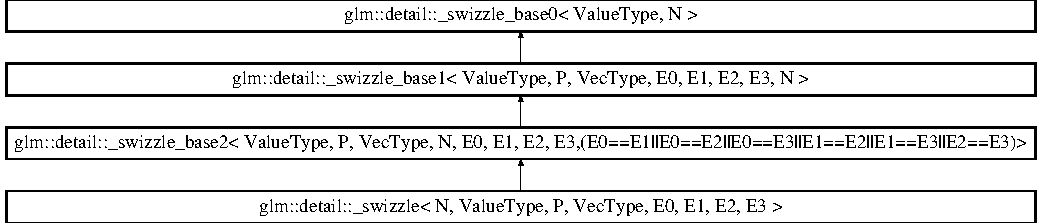
\includegraphics[height=3.002681cm]{structglm_1_1detail_1_1__swizzle}
\end{center}
\end{figure}
\subsection*{Public Types}
\begin{DoxyCompactItemize}
\item 
\hypertarget{structglm_1_1detail_1_1__swizzle_acf7dfa9d7456eb833c247473c5a045f4}{typedef \hyperlink{structglm_1_1detail_1_1__swizzle__base2}{\-\_\-swizzle\-\_\-base2}\\*
$<$ Value\-Type, P, Vec\-Type, N, E0, \\*
E1, E2, E3,(E0==E1$\vert$$\vert$E0==E2$\vert$$\vert$E0==E3$\vert$$\vert$E1==E2$\vert$$\vert$E1==E3$\vert$$\vert$E2==E3)$>$ {\bfseries base\-\_\-type}}\label{structglm_1_1detail_1_1__swizzle_acf7dfa9d7456eb833c247473c5a045f4}

\end{DoxyCompactItemize}
\subsection*{Public Member Functions}
\begin{DoxyCompactItemize}
\item 
\hypertarget{structglm_1_1detail_1_1__swizzle_a333cdd33d2fb442775cca23c77e63fca}{G\-L\-M\-\_\-\-F\-U\-N\-C\-\_\-\-Q\-U\-A\-L\-I\-F\-I\-E\-R {\bfseries operator Vec\-Type} () const }\label{structglm_1_1detail_1_1__swizzle_a333cdd33d2fb442775cca23c77e63fca}

\end{DoxyCompactItemize}
\subsection*{Additional Inherited Members}


The documentation for this struct was generated from the following file\-:\begin{DoxyCompactItemize}
\item 
detail/\hyperlink{__swizzle_8hpp}{\-\_\-swizzle.\-hpp}\end{DoxyCompactItemize}

\hypertarget{structglm_1_1detail_1_1__swizzle__base0}{\section{glm\-:\-:detail\-:\-:\-\_\-swizzle\-\_\-base0$<$ T, N $>$ Struct Template Reference}
\label{structglm_1_1detail_1_1__swizzle__base0}\index{glm\-::detail\-::\-\_\-swizzle\-\_\-base0$<$ T, N $>$@{glm\-::detail\-::\-\_\-swizzle\-\_\-base0$<$ T, N $>$}}
}
Inheritance diagram for glm\-:\-:detail\-:\-:\-\_\-swizzle\-\_\-base0$<$ T, N $>$\-:\begin{figure}[H]
\begin{center}
\leavevmode
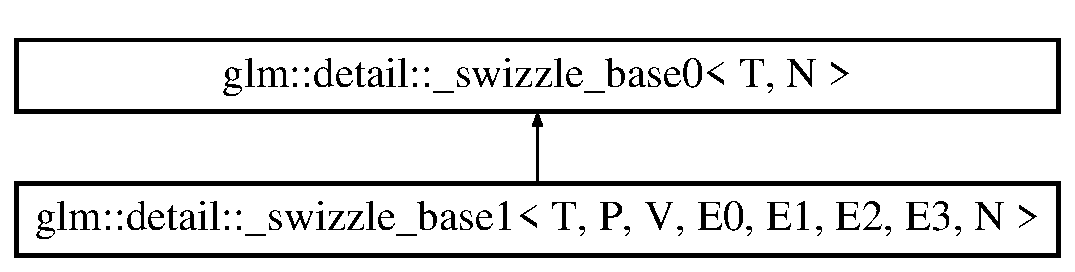
\includegraphics[height=2.000000cm]{structglm_1_1detail_1_1__swizzle__base0}
\end{center}
\end{figure}
\subsection*{Public Types}
\begin{DoxyCompactItemize}
\item 
\hypertarget{structglm_1_1detail_1_1__swizzle__base0_ad38a739e1fe6d2db2674f34c98159c8f}{typedef T {\bfseries value\-\_\-type}}\label{structglm_1_1detail_1_1__swizzle__base0_ad38a739e1fe6d2db2674f34c98159c8f}

\end{DoxyCompactItemize}
\subsection*{Protected Member Functions}
\begin{DoxyCompactItemize}
\item 
\hypertarget{structglm_1_1detail_1_1__swizzle__base0_aebd942a3c3289f9876a9ede4d710d8f0}{G\-L\-M\-\_\-\-F\-U\-N\-C\-\_\-\-Q\-U\-A\-L\-I\-F\-I\-E\-R value\-\_\-type \& {\bfseries elem} (size\-\_\-t i)}\label{structglm_1_1detail_1_1__swizzle__base0_aebd942a3c3289f9876a9ede4d710d8f0}

\item 
\hypertarget{structglm_1_1detail_1_1__swizzle__base0_a9fb7f491860415b292864d0693d8bdb8}{G\-L\-M\-\_\-\-F\-U\-N\-C\-\_\-\-Q\-U\-A\-L\-I\-F\-I\-E\-R const \\*
value\-\_\-type \& {\bfseries elem} (size\-\_\-t i) const }\label{structglm_1_1detail_1_1__swizzle__base0_a9fb7f491860415b292864d0693d8bdb8}

\end{DoxyCompactItemize}
\subsection*{Protected Attributes}
\begin{DoxyCompactItemize}
\item 
\hypertarget{structglm_1_1detail_1_1__swizzle__base0_afd4b7f15c9acff4cdef808f559ffec2d}{char {\bfseries \-\_\-buffer} \mbox{[}1\mbox{]}}\label{structglm_1_1detail_1_1__swizzle__base0_afd4b7f15c9acff4cdef808f559ffec2d}

\end{DoxyCompactItemize}


The documentation for this struct was generated from the following file\-:\begin{DoxyCompactItemize}
\item 
detail/\hyperlink{__swizzle_8hpp}{\-\_\-swizzle.\-hpp}\end{DoxyCompactItemize}

\hypertarget{structglm_1_1detail_1_1__swizzle__base1}{\section{glm\-:\-:detail\-:\-:\-\_\-swizzle\-\_\-base1$<$ T, P, V, E0, E1, E2, E3, N $>$ Struct Template Reference}
\label{structglm_1_1detail_1_1__swizzle__base1}\index{glm\-::detail\-::\-\_\-swizzle\-\_\-base1$<$ T, P, V, E0, E1, E2, E3, N $>$@{glm\-::detail\-::\-\_\-swizzle\-\_\-base1$<$ T, P, V, E0, E1, E2, E3, N $>$}}
}
Inheritance diagram for glm\-:\-:detail\-:\-:\-\_\-swizzle\-\_\-base1$<$ T, P, V, E0, E1, E2, E3, N $>$\-:\begin{figure}[H]
\begin{center}
\leavevmode
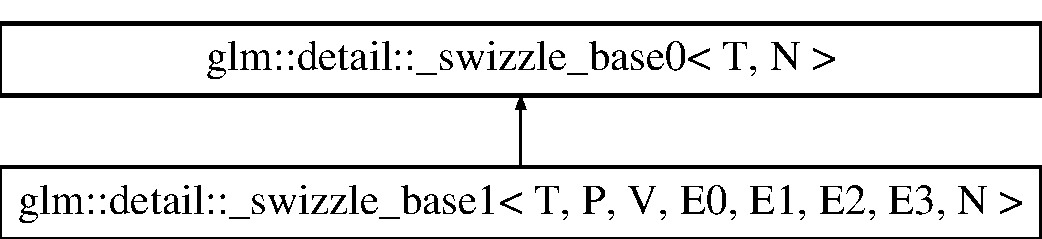
\includegraphics[height=2.000000cm]{structglm_1_1detail_1_1__swizzle__base1}
\end{center}
\end{figure}
\subsection*{Additional Inherited Members}


The documentation for this struct was generated from the following file\-:\begin{DoxyCompactItemize}
\item 
detail/\hyperlink{__swizzle_8hpp}{\-\_\-swizzle.\-hpp}\end{DoxyCompactItemize}

\hypertarget{structglm_1_1detail_1_1__swizzle__base1_3_01T_00_01P_00_01V_00_01E0_00_01E1_00_01E2_00_01E3_00_014_01_4}{\section{glm\-:\-:detail\-:\-:\-\_\-swizzle\-\_\-base1$<$ T, P, V, E0, E1, E2, E3, 4 $>$ Struct Template Reference}
\label{structglm_1_1detail_1_1__swizzle__base1_3_01T_00_01P_00_01V_00_01E0_00_01E1_00_01E2_00_01E3_00_014_01_4}\index{glm\-::detail\-::\-\_\-swizzle\-\_\-base1$<$ T, P, V, E0, E1, E2, E3, 4 $>$@{glm\-::detail\-::\-\_\-swizzle\-\_\-base1$<$ T, P, V, E0, E1, E2, E3, 4 $>$}}
}
Inheritance diagram for glm\-:\-:detail\-:\-:\-\_\-swizzle\-\_\-base1$<$ T, P, V, E0, E1, E2, E3, 4 $>$\-:\begin{figure}[H]
\begin{center}
\leavevmode
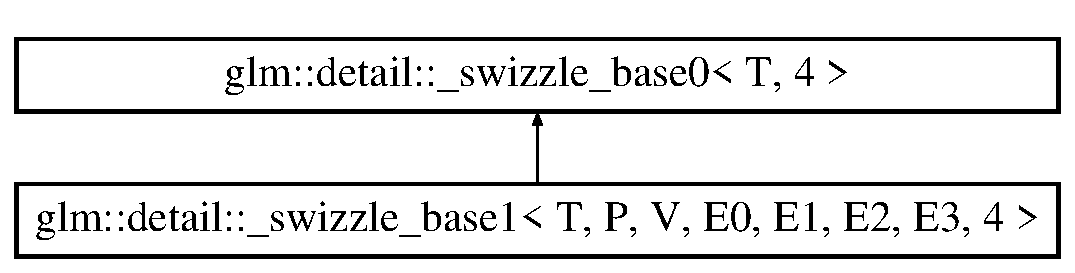
\includegraphics[height=2.000000cm]{structglm_1_1detail_1_1__swizzle__base1_3_01T_00_01P_00_01V_00_01E0_00_01E1_00_01E2_00_01E3_00_014_01_4}
\end{center}
\end{figure}
\subsection*{Public Member Functions}
\begin{DoxyCompactItemize}
\item 
\hypertarget{structglm_1_1detail_1_1__swizzle__base1_3_01T_00_01P_00_01V_00_01E0_00_01E1_00_01E2_00_01E3_00_014_01_4_a901f3af50b0eb022c3246b5de5027245}{G\-L\-M\-\_\-\-F\-U\-N\-C\-\_\-\-Q\-U\-A\-L\-I\-F\-I\-E\-R V {\bfseries operator()} () const }\label{structglm_1_1detail_1_1__swizzle__base1_3_01T_00_01P_00_01V_00_01E0_00_01E1_00_01E2_00_01E3_00_014_01_4_a901f3af50b0eb022c3246b5de5027245}

\end{DoxyCompactItemize}
\subsection*{Additional Inherited Members}


The documentation for this struct was generated from the following file\-:\begin{DoxyCompactItemize}
\item 
detail/\hyperlink{__swizzle_8hpp}{\-\_\-swizzle.\-hpp}\end{DoxyCompactItemize}

\hypertarget{structglm_1_1detail_1_1__swizzle__base1_3_01T_00_01P_00_01V_00_01E0_00_01E1_00_01E2_00-1_00_013_01_4}{\section{glm\-:\-:detail\-:\-:\-\_\-swizzle\-\_\-base1$<$ T, P, V, E0, E1, E2,-\/1, 3 $>$ Struct Template Reference}
\label{structglm_1_1detail_1_1__swizzle__base1_3_01T_00_01P_00_01V_00_01E0_00_01E1_00_01E2_00-1_00_013_01_4}\index{glm\-::detail\-::\-\_\-swizzle\-\_\-base1$<$ T, P, V, E0, E1, E2,-\/1, 3 $>$@{glm\-::detail\-::\-\_\-swizzle\-\_\-base1$<$ T, P, V, E0, E1, E2,-\/1, 3 $>$}}
}
Inheritance diagram for glm\-:\-:detail\-:\-:\-\_\-swizzle\-\_\-base1$<$ T, P, V, E0, E1, E2,-\/1, 3 $>$\-:\begin{figure}[H]
\begin{center}
\leavevmode
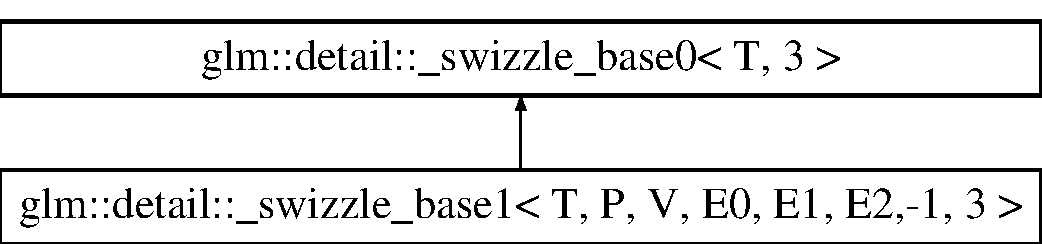
\includegraphics[height=2.000000cm]{structglm_1_1detail_1_1__swizzle__base1_3_01T_00_01P_00_01V_00_01E0_00_01E1_00_01E2_00-1_00_013_01_4}
\end{center}
\end{figure}
\subsection*{Public Member Functions}
\begin{DoxyCompactItemize}
\item 
\hypertarget{structglm_1_1detail_1_1__swizzle__base1_3_01T_00_01P_00_01V_00_01E0_00_01E1_00_01E2_00-1_00_013_01_4_a94510ce33bf6a19e28b4f95f4e715807}{G\-L\-M\-\_\-\-F\-U\-N\-C\-\_\-\-Q\-U\-A\-L\-I\-F\-I\-E\-R V {\bfseries operator()} () const }\label{structglm_1_1detail_1_1__swizzle__base1_3_01T_00_01P_00_01V_00_01E0_00_01E1_00_01E2_00-1_00_013_01_4_a94510ce33bf6a19e28b4f95f4e715807}

\end{DoxyCompactItemize}
\subsection*{Additional Inherited Members}


The documentation for this struct was generated from the following file\-:\begin{DoxyCompactItemize}
\item 
detail/\hyperlink{__swizzle_8hpp}{\-\_\-swizzle.\-hpp}\end{DoxyCompactItemize}

\hypertarget{structglm_1_1detail_1_1__swizzle__base1_3_01T_00_01P_00_01V_00_01E0_00_01E1_00-1_00-2_00_012_01_4}{\section{glm\-:\-:detail\-:\-:\-\_\-swizzle\-\_\-base1$<$ T, P, V, E0, E1,-\/1,-\/2, 2 $>$ Struct Template Reference}
\label{structglm_1_1detail_1_1__swizzle__base1_3_01T_00_01P_00_01V_00_01E0_00_01E1_00-1_00-2_00_012_01_4}\index{glm\-::detail\-::\-\_\-swizzle\-\_\-base1$<$ T, P, V, E0, E1,-\/1,-\/2, 2 $>$@{glm\-::detail\-::\-\_\-swizzle\-\_\-base1$<$ T, P, V, E0, E1,-\/1,-\/2, 2 $>$}}
}
Inheritance diagram for glm\-:\-:detail\-:\-:\-\_\-swizzle\-\_\-base1$<$ T, P, V, E0, E1,-\/1,-\/2, 2 $>$\-:\begin{figure}[H]
\begin{center}
\leavevmode
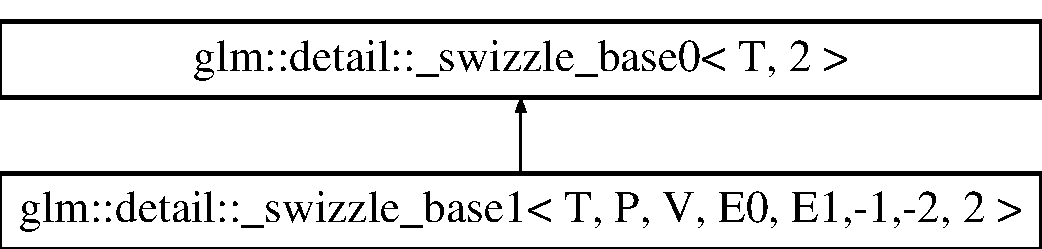
\includegraphics[height=2.000000cm]{structglm_1_1detail_1_1__swizzle__base1_3_01T_00_01P_00_01V_00_01E0_00_01E1_00-1_00-2_00_012_01_4}
\end{center}
\end{figure}
\subsection*{Public Member Functions}
\begin{DoxyCompactItemize}
\item 
\hypertarget{structglm_1_1detail_1_1__swizzle__base1_3_01T_00_01P_00_01V_00_01E0_00_01E1_00-1_00-2_00_012_01_4_a333b1c869374c290a8bca707a258f5e5}{G\-L\-M\-\_\-\-F\-U\-N\-C\-\_\-\-Q\-U\-A\-L\-I\-F\-I\-E\-R V {\bfseries operator()} () const }\label{structglm_1_1detail_1_1__swizzle__base1_3_01T_00_01P_00_01V_00_01E0_00_01E1_00-1_00-2_00_012_01_4_a333b1c869374c290a8bca707a258f5e5}

\end{DoxyCompactItemize}
\subsection*{Additional Inherited Members}


The documentation for this struct was generated from the following file\-:\begin{DoxyCompactItemize}
\item 
detail/\hyperlink{__swizzle_8hpp}{\-\_\-swizzle.\-hpp}\end{DoxyCompactItemize}

\hypertarget{structglm_1_1detail_1_1__swizzle__base2}{\section{glm\-:\-:detail\-:\-:\-\_\-swizzle\-\_\-base2$<$ Value\-Type, P, Vec\-Type, N, E0, E1, E2, E3, D\-U\-P\-L\-I\-C\-A\-T\-E\-\_\-\-E\-L\-E\-M\-E\-N\-T\-S $>$ Struct Template Reference}
\label{structglm_1_1detail_1_1__swizzle__base2}\index{glm\-::detail\-::\-\_\-swizzle\-\_\-base2$<$ Value\-Type, P, Vec\-Type, N, E0, E1, E2, E3, D\-U\-P\-L\-I\-C\-A\-T\-E\-\_\-\-E\-L\-E\-M\-E\-N\-T\-S $>$@{glm\-::detail\-::\-\_\-swizzle\-\_\-base2$<$ Value\-Type, P, Vec\-Type, N, E0, E1, E2, E3, D\-U\-P\-L\-I\-C\-A\-T\-E\-\_\-\-E\-L\-E\-M\-E\-N\-T\-S $>$}}
}
Inheritance diagram for glm\-:\-:detail\-:\-:\-\_\-swizzle\-\_\-base2$<$ Value\-Type, P, Vec\-Type, N, E0, E1, E2, E3, D\-U\-P\-L\-I\-C\-A\-T\-E\-\_\-\-E\-L\-E\-M\-E\-N\-T\-S $>$\-:\begin{figure}[H]
\begin{center}
\leavevmode
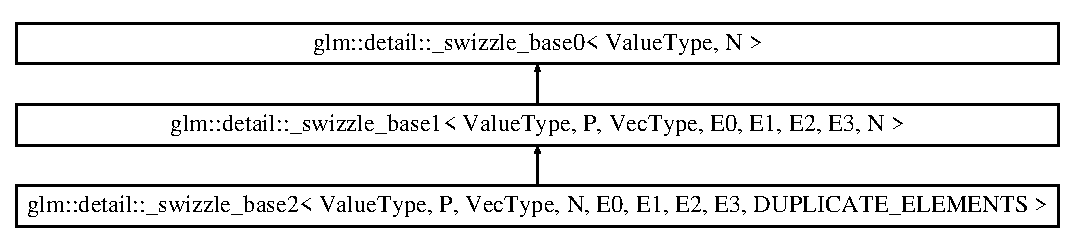
\includegraphics[height=2.823529cm]{structglm_1_1detail_1_1__swizzle__base2}
\end{center}
\end{figure}
\subsection*{Public Types}
\begin{DoxyCompactItemize}
\item 
\hypertarget{structglm_1_1detail_1_1__swizzle__base2_a5f999904e676a4f5b0bdaa157415ee1c}{typedef Vec\-Type {\bfseries vec\-\_\-type}}\label{structglm_1_1detail_1_1__swizzle__base2_a5f999904e676a4f5b0bdaa157415ee1c}

\item 
\hypertarget{structglm_1_1detail_1_1__swizzle__base2_a656c11aaeeaca042deed88711c9dc063}{typedef Value\-Type {\bfseries value\-\_\-type}}\label{structglm_1_1detail_1_1__swizzle__base2_a656c11aaeeaca042deed88711c9dc063}

\end{DoxyCompactItemize}
\subsection*{Public Member Functions}
\begin{DoxyCompactItemize}
\item 
\hypertarget{structglm_1_1detail_1_1__swizzle__base2_a70442376cb261474e23090737deff976}{G\-L\-M\-\_\-\-F\-U\-N\-C\-\_\-\-Q\-U\-A\-L\-I\-F\-I\-E\-R \hyperlink{structglm_1_1detail_1_1__swizzle__base2}{\-\_\-swizzle\-\_\-base2} \& {\bfseries operator=} (const Value\-Type \&t)}\label{structglm_1_1detail_1_1__swizzle__base2_a70442376cb261474e23090737deff976}

\item 
\hypertarget{structglm_1_1detail_1_1__swizzle__base2_a7b982a5056d94cd43393bf820ea627d0}{G\-L\-M\-\_\-\-F\-U\-N\-C\-\_\-\-Q\-U\-A\-L\-I\-F\-I\-E\-R \hyperlink{structglm_1_1detail_1_1__swizzle__base2}{\-\_\-swizzle\-\_\-base2} \& {\bfseries operator=} (const Vec\-Type \&that)}\label{structglm_1_1detail_1_1__swizzle__base2_a7b982a5056d94cd43393bf820ea627d0}

\item 
\hypertarget{structglm_1_1detail_1_1__swizzle__base2_ab583f399dc6685deee97bdd5126f433a}{G\-L\-M\-\_\-\-F\-U\-N\-C\-\_\-\-Q\-U\-A\-L\-I\-F\-I\-E\-R void {\bfseries operator-\/=} (const Vec\-Type \&that)}\label{structglm_1_1detail_1_1__swizzle__base2_ab583f399dc6685deee97bdd5126f433a}

\item 
\hypertarget{structglm_1_1detail_1_1__swizzle__base2_a5e734b2e9da294d92bb347a3c7f44ded}{G\-L\-M\-\_\-\-F\-U\-N\-C\-\_\-\-Q\-U\-A\-L\-I\-F\-I\-E\-R void {\bfseries operator+=} (const Vec\-Type \&that)}\label{structglm_1_1detail_1_1__swizzle__base2_a5e734b2e9da294d92bb347a3c7f44ded}

\item 
\hypertarget{structglm_1_1detail_1_1__swizzle__base2_a6c686d110b936939c7ed67d7a6165778}{G\-L\-M\-\_\-\-F\-U\-N\-C\-\_\-\-Q\-U\-A\-L\-I\-F\-I\-E\-R void {\bfseries operator$\ast$=} (const Vec\-Type \&that)}\label{structglm_1_1detail_1_1__swizzle__base2_a6c686d110b936939c7ed67d7a6165778}

\item 
\hypertarget{structglm_1_1detail_1_1__swizzle__base2_a0a3e5ef1cb68f78a7e1bcd72f6e2dc4c}{G\-L\-M\-\_\-\-F\-U\-N\-C\-\_\-\-Q\-U\-A\-L\-I\-F\-I\-E\-R void {\bfseries operator/=} (const Vec\-Type \&that)}\label{structglm_1_1detail_1_1__swizzle__base2_a0a3e5ef1cb68f78a7e1bcd72f6e2dc4c}

\item 
\hypertarget{structglm_1_1detail_1_1__swizzle__base2_aa3f2ab8e3e1a5c414b3fdca4cf75b706}{G\-L\-M\-\_\-\-F\-U\-N\-C\-\_\-\-Q\-U\-A\-L\-I\-F\-I\-E\-R value\-\_\-type \& {\bfseries operator\mbox{[}$\,$\mbox{]}} (size\-\_\-t i)}\label{structglm_1_1detail_1_1__swizzle__base2_aa3f2ab8e3e1a5c414b3fdca4cf75b706}

\item 
\hypertarget{structglm_1_1detail_1_1__swizzle__base2_a1bec6727adac01b6bc3e1ccba935167e}{G\-L\-M\-\_\-\-F\-U\-N\-C\-\_\-\-Q\-U\-A\-L\-I\-F\-I\-E\-R value\-\_\-type {\bfseries operator\mbox{[}$\,$\mbox{]}} (size\-\_\-t i) const }\label{structglm_1_1detail_1_1__swizzle__base2_a1bec6727adac01b6bc3e1ccba935167e}

\end{DoxyCompactItemize}
\subsection*{Protected Member Functions}
\begin{DoxyCompactItemize}
\item 
\hypertarget{structglm_1_1detail_1_1__swizzle__base2_a11d049274a60ecf4aac8cebc4c4e9be5}{{\footnotesize template$<$typename T $>$ }\\G\-L\-M\-\_\-\-F\-U\-N\-C\-\_\-\-Q\-U\-A\-L\-I\-F\-I\-E\-R void {\bfseries \-\_\-apply\-\_\-op} (const Vec\-Type \&that, T op)}\label{structglm_1_1detail_1_1__swizzle__base2_a11d049274a60ecf4aac8cebc4c4e9be5}

\end{DoxyCompactItemize}
\subsection*{Additional Inherited Members}


The documentation for this struct was generated from the following file\-:\begin{DoxyCompactItemize}
\item 
detail/\hyperlink{__swizzle_8hpp}{\-\_\-swizzle.\-hpp}\end{DoxyCompactItemize}

\hypertarget{structglm_1_1detail_1_1__swizzle__base2_3_01ValueType_00_01P_00_01VecType_00_01N_00_01E0_00_01E1_00_01E2_00_01E3_00_011_01_4}{\section{glm\-:\-:detail\-:\-:\-\_\-swizzle\-\_\-base2$<$ Value\-Type, P, Vec\-Type, N, E0, E1, E2, E3, 1 $>$ Struct Template Reference}
\label{structglm_1_1detail_1_1__swizzle__base2_3_01ValueType_00_01P_00_01VecType_00_01N_00_01E0_00_01E1_00_01E2_00_01E3_00_011_01_4}\index{glm\-::detail\-::\-\_\-swizzle\-\_\-base2$<$ Value\-Type, P, Vec\-Type, N, E0, E1, E2, E3, 1 $>$@{glm\-::detail\-::\-\_\-swizzle\-\_\-base2$<$ Value\-Type, P, Vec\-Type, N, E0, E1, E2, E3, 1 $>$}}
}
Inheritance diagram for glm\-:\-:detail\-:\-:\-\_\-swizzle\-\_\-base2$<$ Value\-Type, P, Vec\-Type, N, E0, E1, E2, E3, 1 $>$\-:\begin{figure}[H]
\begin{center}
\leavevmode
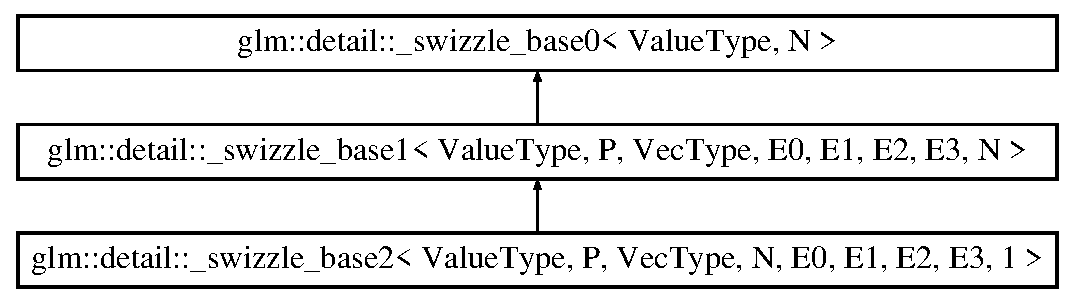
\includegraphics[height=3.000000cm]{structglm_1_1detail_1_1__swizzle__base2_3_01ValueType_00_01P_00_01VecType_00_01N_00_01E0_00_01E1_00_01E2_00_01E3_00_011_01_4}
\end{center}
\end{figure}
\subsection*{Classes}
\begin{DoxyCompactItemize}
\item 
struct \hyperlink{structglm_1_1detail_1_1__swizzle__base2_3_01ValueType_00_01P_00_01VecType_00_01N_00_01E0_00_01E17d6926f6e6f474ef79d271c7c59bd480}{Stub}
\end{DoxyCompactItemize}
\subsection*{Public Types}
\begin{DoxyCompactItemize}
\item 
\hypertarget{structglm_1_1detail_1_1__swizzle__base2_3_01ValueType_00_01P_00_01VecType_00_01N_00_01E0_00_01E1_00_01E2_00_01E3_00_011_01_4_aa478e9f198b8832d76245adde9c627ec}{typedef Vec\-Type {\bfseries vec\-\_\-type}}\label{structglm_1_1detail_1_1__swizzle__base2_3_01ValueType_00_01P_00_01VecType_00_01N_00_01E0_00_01E1_00_01E2_00_01E3_00_011_01_4_aa478e9f198b8832d76245adde9c627ec}

\item 
\hypertarget{structglm_1_1detail_1_1__swizzle__base2_3_01ValueType_00_01P_00_01VecType_00_01N_00_01E0_00_01E1_00_01E2_00_01E3_00_011_01_4_aea7ec681454787ad7a322c06aec98757}{typedef Value\-Type {\bfseries value\-\_\-type}}\label{structglm_1_1detail_1_1__swizzle__base2_3_01ValueType_00_01P_00_01VecType_00_01N_00_01E0_00_01E1_00_01E2_00_01E3_00_011_01_4_aea7ec681454787ad7a322c06aec98757}

\end{DoxyCompactItemize}
\subsection*{Public Member Functions}
\begin{DoxyCompactItemize}
\item 
\hypertarget{structglm_1_1detail_1_1__swizzle__base2_3_01ValueType_00_01P_00_01VecType_00_01N_00_01E0_00_01E1_00_01E2_00_01E3_00_011_01_4_aed2b7223090d020e28af46eb33fe6729}{G\-L\-M\-\_\-\-F\-U\-N\-C\-\_\-\-Q\-U\-A\-L\-I\-F\-I\-E\-R \hyperlink{structglm_1_1detail_1_1__swizzle__base2}{\-\_\-swizzle\-\_\-base2} \& {\bfseries operator=} (Stub const \&)}\label{structglm_1_1detail_1_1__swizzle__base2_3_01ValueType_00_01P_00_01VecType_00_01N_00_01E0_00_01E1_00_01E2_00_01E3_00_011_01_4_aed2b7223090d020e28af46eb33fe6729}

\item 
\hypertarget{structglm_1_1detail_1_1__swizzle__base2_3_01ValueType_00_01P_00_01VecType_00_01N_00_01E0_00_01E1_00_01E2_00_01E3_00_011_01_4_a2f3a45edbb24ca7e12182c3123dde632}{G\-L\-M\-\_\-\-F\-U\-N\-C\-\_\-\-Q\-U\-A\-L\-I\-F\-I\-E\-R value\-\_\-type {\bfseries operator\mbox{[}$\,$\mbox{]}} (size\-\_\-t i) const }\label{structglm_1_1detail_1_1__swizzle__base2_3_01ValueType_00_01P_00_01VecType_00_01N_00_01E0_00_01E1_00_01E2_00_01E3_00_011_01_4_a2f3a45edbb24ca7e12182c3123dde632}

\end{DoxyCompactItemize}
\subsection*{Additional Inherited Members}


The documentation for this struct was generated from the following file\-:\begin{DoxyCompactItemize}
\item 
detail/\hyperlink{__swizzle_8hpp}{\-\_\-swizzle.\-hpp}\end{DoxyCompactItemize}

\hypertarget{classglm_1_1io_1_1basic__format__saver}{\section{glm\-:\-:io\-:\-:basic\-\_\-format\-\_\-saver$<$ C\-Ty, C\-Tr $>$ Class Template Reference}
\label{classglm_1_1io_1_1basic__format__saver}\index{glm\-::io\-::basic\-\_\-format\-\_\-saver$<$ C\-Ty, C\-Tr $>$@{glm\-::io\-::basic\-\_\-format\-\_\-saver$<$ C\-Ty, C\-Tr $>$}}
}
\subsection*{Public Member Functions}
\begin{DoxyCompactItemize}
\item 
\hypertarget{classglm_1_1io_1_1basic__format__saver_a268ddf9ea158d6764978066269d42538}{{\bfseries basic\-\_\-format\-\_\-saver} (std\-::basic\-\_\-ios$<$ C\-Ty, C\-Tr $>$ \&)}\label{classglm_1_1io_1_1basic__format__saver_a268ddf9ea158d6764978066269d42538}

\end{DoxyCompactItemize}


The documentation for this class was generated from the following file\-:\begin{DoxyCompactItemize}
\item 
gtx/\hyperlink{io_8hpp}{io.\-hpp}\end{DoxyCompactItemize}

\hypertarget{classglm_1_1io_1_1basic__state__saver}{\section{glm\-:\-:io\-:\-:basic\-\_\-state\-\_\-saver$<$ C\-Ty, C\-Tr $>$ Class Template Reference}
\label{classglm_1_1io_1_1basic__state__saver}\index{glm\-::io\-::basic\-\_\-state\-\_\-saver$<$ C\-Ty, C\-Tr $>$@{glm\-::io\-::basic\-\_\-state\-\_\-saver$<$ C\-Ty, C\-Tr $>$}}
}
\subsection*{Public Member Functions}
\begin{DoxyCompactItemize}
\item 
\hypertarget{classglm_1_1io_1_1basic__state__saver_af3b2ff62d326632d244bcce4df3a45b4}{{\bfseries basic\-\_\-state\-\_\-saver} (std\-::basic\-\_\-ios$<$ C\-Ty, C\-Tr $>$ \&)}\label{classglm_1_1io_1_1basic__state__saver_af3b2ff62d326632d244bcce4df3a45b4}

\end{DoxyCompactItemize}


The documentation for this class was generated from the following file\-:\begin{DoxyCompactItemize}
\item 
gtx/\hyperlink{io_8hpp}{io.\-hpp}\end{DoxyCompactItemize}

\hypertarget{structglm_1_1io_1_1delimeter}{\section{glm\-:\-:io\-:\-:delimeter$<$ C\-Ty $>$ Struct Template Reference}
\label{structglm_1_1io_1_1delimeter}\index{glm\-::io\-::delimeter$<$ C\-Ty $>$@{glm\-::io\-::delimeter$<$ C\-Ty $>$}}
}
\subsection*{Public Member Functions}
\begin{DoxyCompactItemize}
\item 
\hypertarget{structglm_1_1io_1_1delimeter_aeca22f822a1a2613aa4996bd129f5c10}{{\bfseries delimeter} (C\-Ty, C\-Ty, C\-Ty= ',')}\label{structglm_1_1io_1_1delimeter_aeca22f822a1a2613aa4996bd129f5c10}

\end{DoxyCompactItemize}
\subsection*{Public Attributes}
\begin{DoxyCompactItemize}
\item 
\hypertarget{structglm_1_1io_1_1delimeter_a9ade129dae50c4f716f724e7425f9c68}{C\-Ty {\bfseries value} \mbox{[}3\mbox{]}}\label{structglm_1_1io_1_1delimeter_a9ade129dae50c4f716f724e7425f9c68}

\end{DoxyCompactItemize}


The documentation for this struct was generated from the following file\-:\begin{DoxyCompactItemize}
\item 
gtx/\hyperlink{io_8hpp}{io.\-hpp}\end{DoxyCompactItemize}

\hypertarget{classglm_1_1io_1_1format__punct}{\section{glm\-:\-:io\-:\-:format\-\_\-punct$<$ C\-Ty $>$ Class Template Reference}
\label{classglm_1_1io_1_1format__punct}\index{glm\-::io\-::format\-\_\-punct$<$ C\-Ty $>$@{glm\-::io\-::format\-\_\-punct$<$ C\-Ty $>$}}
}
Inheritance diagram for glm\-:\-:io\-:\-:format\-\_\-punct$<$ C\-Ty $>$\-:\begin{figure}[H]
\begin{center}
\leavevmode
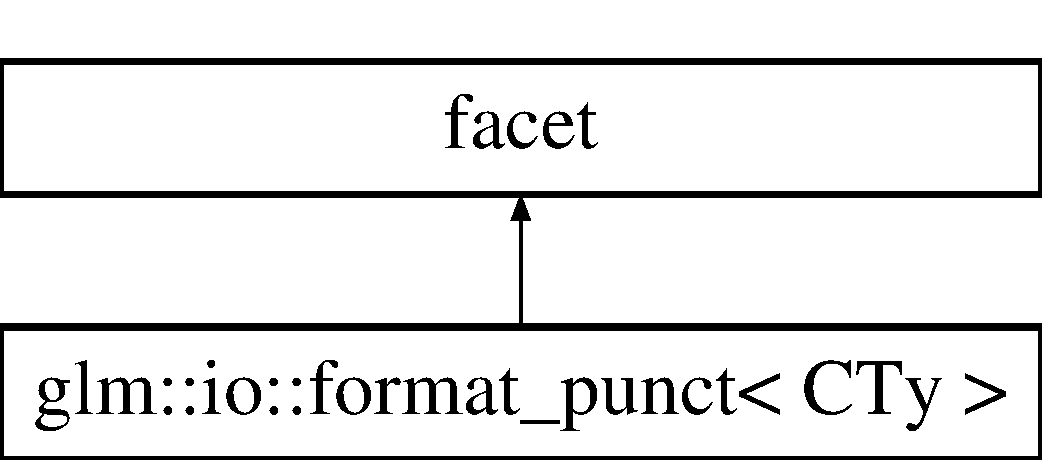
\includegraphics[height=2.000000cm]{classglm_1_1io_1_1format__punct}
\end{center}
\end{figure}
\subsection*{Public Member Functions}
\begin{DoxyCompactItemize}
\item 
\hypertarget{classglm_1_1io_1_1format__punct_ac9d5253f96b74c5fb0097251693188a9}{{\bfseries format\-\_\-punct} (size\-\_\-t a=0)}\label{classglm_1_1io_1_1format__punct_ac9d5253f96b74c5fb0097251693188a9}

\item 
\hypertarget{classglm_1_1io_1_1format__punct_a2fbfad17f266020af68fd679cb70e991}{{\bfseries format\-\_\-punct} (\hyperlink{classglm_1_1io_1_1format__punct}{format\-\_\-punct} const \&)}\label{classglm_1_1io_1_1format__punct_a2fbfad17f266020af68fd679cb70e991}

\end{DoxyCompactItemize}
\subsection*{Public Attributes}
\begin{DoxyCompactItemize}
\item 
\hypertarget{classglm_1_1io_1_1format__punct_ab28088e6eef03fe4222fa8a5dd95288e}{bool {\bfseries formatted}}\label{classglm_1_1io_1_1format__punct_ab28088e6eef03fe4222fa8a5dd95288e}

\item 
\hypertarget{classglm_1_1io_1_1format__punct_a5a15d396b7c963df9dec5e124236dc02}{unsigned {\bfseries precision}}\label{classglm_1_1io_1_1format__punct_a5a15d396b7c963df9dec5e124236dc02}

\item 
\hypertarget{classglm_1_1io_1_1format__punct_a95d32ca2330bbf7c50d3e066b7a851db}{unsigned {\bfseries width}}\label{classglm_1_1io_1_1format__punct_a95d32ca2330bbf7c50d3e066b7a851db}

\item 
\hypertarget{classglm_1_1io_1_1format__punct_ac561eb04fc2a1282ef38ea15f8e640ee}{char\-\_\-type {\bfseries separator}}\label{classglm_1_1io_1_1format__punct_ac561eb04fc2a1282ef38ea15f8e640ee}

\item 
\hypertarget{classglm_1_1io_1_1format__punct_ab1beed331269a39b06d17d02cf727d7c}{char\-\_\-type {\bfseries delim\-\_\-left}}\label{classglm_1_1io_1_1format__punct_ab1beed331269a39b06d17d02cf727d7c}

\item 
\hypertarget{classglm_1_1io_1_1format__punct_a62fb1280404360463ec5af7144aa0949}{char\-\_\-type {\bfseries delim\-\_\-right}}\label{classglm_1_1io_1_1format__punct_a62fb1280404360463ec5af7144aa0949}

\item 
\hypertarget{classglm_1_1io_1_1format__punct_adf9a915938727793de1daca07dcdfa4e}{char\-\_\-type {\bfseries space}}\label{classglm_1_1io_1_1format__punct_adf9a915938727793de1daca07dcdfa4e}

\item 
\hypertarget{classglm_1_1io_1_1format__punct_a8ddf8abdb0ebbdbb7eca08d7a777956e}{char\-\_\-type {\bfseries newline}}\label{classglm_1_1io_1_1format__punct_a8ddf8abdb0ebbdbb7eca08d7a777956e}

\item 
\hypertarget{classglm_1_1io_1_1format__punct_a9de1f3b7120a036ec0ab394d2036d0aa}{order\-\_\-type {\bfseries order}}\label{classglm_1_1io_1_1format__punct_a9de1f3b7120a036ec0ab394d2036d0aa}

\end{DoxyCompactItemize}
\subsection*{Static Public Attributes}
\begin{DoxyCompactItemize}
\item 
\hypertarget{classglm_1_1io_1_1format__punct_a763f60aeaecec9290917ed1d83b79838}{static std\-::locale\-::id {\bfseries id}}\label{classglm_1_1io_1_1format__punct_a763f60aeaecec9290917ed1d83b79838}

\end{DoxyCompactItemize}


The documentation for this class was generated from the following file\-:\begin{DoxyCompactItemize}
\item 
gtx/\hyperlink{io_8hpp}{io.\-hpp}\end{DoxyCompactItemize}

\hypertarget{structglm_1_1detail_1_1functor1}{\section{glm\-:\-:detail\-:\-:functor1$<$ R, T, P, vec\-Type $>$ Struct Template Reference}
\label{structglm_1_1detail_1_1functor1}\index{glm\-::detail\-::functor1$<$ R, T, P, vec\-Type $>$@{glm\-::detail\-::functor1$<$ R, T, P, vec\-Type $>$}}
}


The documentation for this struct was generated from the following file\-:\begin{DoxyCompactItemize}
\item 
detail/\hyperlink{__vectorize_8hpp}{\-\_\-vectorize.\-hpp}\end{DoxyCompactItemize}

\hypertarget{structglm_1_1detail_1_1functor1_3_01R_00_01T_00_01P_00_01tvec1_01_4}{\section{glm\-:\-:detail\-:\-:functor1$<$ R, T, P, tvec1 $>$ Struct Template Reference}
\label{structglm_1_1detail_1_1functor1_3_01R_00_01T_00_01P_00_01tvec1_01_4}\index{glm\-::detail\-::functor1$<$ R, T, P, tvec1 $>$@{glm\-::detail\-::functor1$<$ R, T, P, tvec1 $>$}}
}
\subsection*{Static Public Member Functions}
\begin{DoxyCompactItemize}
\item 
\hypertarget{structglm_1_1detail_1_1functor1_3_01R_00_01T_00_01P_00_01tvec1_01_4_af5dd270c9695023917f2c43e61fa10e0}{static G\-L\-M\-\_\-\-F\-U\-N\-C\-\_\-\-Q\-U\-A\-L\-I\-F\-I\-E\-R \\*
\hyperlink{structglm_1_1tvec1}{tvec1}$<$ R, P $>$ {\bfseries call} (R($\ast$Func)(T x), \hyperlink{structglm_1_1tvec1}{tvec1}$<$ T, P $>$ const \&v)}\label{structglm_1_1detail_1_1functor1_3_01R_00_01T_00_01P_00_01tvec1_01_4_af5dd270c9695023917f2c43e61fa10e0}

\end{DoxyCompactItemize}


The documentation for this struct was generated from the following file\-:\begin{DoxyCompactItemize}
\item 
detail/\hyperlink{__vectorize_8hpp}{\-\_\-vectorize.\-hpp}\end{DoxyCompactItemize}

\hypertarget{structglm_1_1detail_1_1functor1_3_01R_00_01T_00_01P_00_01tvec2_01_4}{\section{glm\-:\-:detail\-:\-:functor1$<$ R, T, P, tvec2 $>$ Struct Template Reference}
\label{structglm_1_1detail_1_1functor1_3_01R_00_01T_00_01P_00_01tvec2_01_4}\index{glm\-::detail\-::functor1$<$ R, T, P, tvec2 $>$@{glm\-::detail\-::functor1$<$ R, T, P, tvec2 $>$}}
}
\subsection*{Static Public Member Functions}
\begin{DoxyCompactItemize}
\item 
\hypertarget{structglm_1_1detail_1_1functor1_3_01R_00_01T_00_01P_00_01tvec2_01_4_aaabd54c114db7c12681014fcbcf763bf}{static G\-L\-M\-\_\-\-F\-U\-N\-C\-\_\-\-Q\-U\-A\-L\-I\-F\-I\-E\-R \\*
\hyperlink{structglm_1_1tvec2}{tvec2}$<$ R, P $>$ {\bfseries call} (R($\ast$Func)(T x), \hyperlink{structglm_1_1tvec2}{tvec2}$<$ T, P $>$ const \&v)}\label{structglm_1_1detail_1_1functor1_3_01R_00_01T_00_01P_00_01tvec2_01_4_aaabd54c114db7c12681014fcbcf763bf}

\end{DoxyCompactItemize}


The documentation for this struct was generated from the following file\-:\begin{DoxyCompactItemize}
\item 
detail/\hyperlink{__vectorize_8hpp}{\-\_\-vectorize.\-hpp}\end{DoxyCompactItemize}

\hypertarget{structglm_1_1detail_1_1functor1_3_01R_00_01T_00_01P_00_01tvec3_01_4}{\section{glm\-:\-:detail\-:\-:functor1$<$ R, T, P, tvec3 $>$ Struct Template Reference}
\label{structglm_1_1detail_1_1functor1_3_01R_00_01T_00_01P_00_01tvec3_01_4}\index{glm\-::detail\-::functor1$<$ R, T, P, tvec3 $>$@{glm\-::detail\-::functor1$<$ R, T, P, tvec3 $>$}}
}
\subsection*{Static Public Member Functions}
\begin{DoxyCompactItemize}
\item 
\hypertarget{structglm_1_1detail_1_1functor1_3_01R_00_01T_00_01P_00_01tvec3_01_4_a8ae374d9111e3de3d32f18762f1918cc}{static G\-L\-M\-\_\-\-F\-U\-N\-C\-\_\-\-Q\-U\-A\-L\-I\-F\-I\-E\-R \\*
\hyperlink{structglm_1_1tvec3}{tvec3}$<$ R, P $>$ {\bfseries call} (R($\ast$Func)(T x), \hyperlink{structglm_1_1tvec3}{tvec3}$<$ T, P $>$ const \&v)}\label{structglm_1_1detail_1_1functor1_3_01R_00_01T_00_01P_00_01tvec3_01_4_a8ae374d9111e3de3d32f18762f1918cc}

\end{DoxyCompactItemize}


The documentation for this struct was generated from the following file\-:\begin{DoxyCompactItemize}
\item 
detail/\hyperlink{__vectorize_8hpp}{\-\_\-vectorize.\-hpp}\end{DoxyCompactItemize}

\hypertarget{structglm_1_1detail_1_1functor1_3_01R_00_01T_00_01P_00_01tvec4_01_4}{\section{glm\-:\-:detail\-:\-:functor1$<$ R, T, P, tvec4 $>$ Struct Template Reference}
\label{structglm_1_1detail_1_1functor1_3_01R_00_01T_00_01P_00_01tvec4_01_4}\index{glm\-::detail\-::functor1$<$ R, T, P, tvec4 $>$@{glm\-::detail\-::functor1$<$ R, T, P, tvec4 $>$}}
}
\subsection*{Static Public Member Functions}
\begin{DoxyCompactItemize}
\item 
\hypertarget{structglm_1_1detail_1_1functor1_3_01R_00_01T_00_01P_00_01tvec4_01_4_a65634749e4ae6e35d4cc898481d4681f}{static G\-L\-M\-\_\-\-F\-U\-N\-C\-\_\-\-Q\-U\-A\-L\-I\-F\-I\-E\-R \\*
\hyperlink{structglm_1_1tvec4}{tvec4}$<$ R, P $>$ {\bfseries call} (R($\ast$Func)(T x), \hyperlink{structglm_1_1tvec4}{tvec4}$<$ T, P $>$ const \&v)}\label{structglm_1_1detail_1_1functor1_3_01R_00_01T_00_01P_00_01tvec4_01_4_a65634749e4ae6e35d4cc898481d4681f}

\end{DoxyCompactItemize}


The documentation for this struct was generated from the following file\-:\begin{DoxyCompactItemize}
\item 
detail/\hyperlink{__vectorize_8hpp}{\-\_\-vectorize.\-hpp}\end{DoxyCompactItemize}

\hypertarget{structglm_1_1detail_1_1functor2}{\section{glm\-:\-:detail\-:\-:functor2$<$ T, P, vec\-Type $>$ Struct Template Reference}
\label{structglm_1_1detail_1_1functor2}\index{glm\-::detail\-::functor2$<$ T, P, vec\-Type $>$@{glm\-::detail\-::functor2$<$ T, P, vec\-Type $>$}}
}


The documentation for this struct was generated from the following file\-:\begin{DoxyCompactItemize}
\item 
detail/\hyperlink{__vectorize_8hpp}{\-\_\-vectorize.\-hpp}\end{DoxyCompactItemize}

\hypertarget{structglm_1_1detail_1_1functor2_3_01T_00_01P_00_01tvec1_01_4}{\section{glm\-:\-:detail\-:\-:functor2$<$ T, P, tvec1 $>$ Struct Template Reference}
\label{structglm_1_1detail_1_1functor2_3_01T_00_01P_00_01tvec1_01_4}\index{glm\-::detail\-::functor2$<$ T, P, tvec1 $>$@{glm\-::detail\-::functor2$<$ T, P, tvec1 $>$}}
}
\subsection*{Static Public Member Functions}
\begin{DoxyCompactItemize}
\item 
\hypertarget{structglm_1_1detail_1_1functor2_3_01T_00_01P_00_01tvec1_01_4_a7f805874487ee439ec9f5ca600f1813d}{static G\-L\-M\-\_\-\-F\-U\-N\-C\-\_\-\-Q\-U\-A\-L\-I\-F\-I\-E\-R \\*
\hyperlink{structglm_1_1tvec1}{tvec1}$<$ T, P $>$ {\bfseries call} (T($\ast$Func)(T x, T y), \hyperlink{structglm_1_1tvec1}{tvec1}$<$ T, P $>$ const \&a, \hyperlink{structglm_1_1tvec1}{tvec1}$<$ T, P $>$ const \&b)}\label{structglm_1_1detail_1_1functor2_3_01T_00_01P_00_01tvec1_01_4_a7f805874487ee439ec9f5ca600f1813d}

\end{DoxyCompactItemize}


The documentation for this struct was generated from the following file\-:\begin{DoxyCompactItemize}
\item 
detail/\hyperlink{__vectorize_8hpp}{\-\_\-vectorize.\-hpp}\end{DoxyCompactItemize}

\hypertarget{structglm_1_1detail_1_1functor2_3_01T_00_01P_00_01tvec2_01_4}{\section{glm\-:\-:detail\-:\-:functor2$<$ T, P, tvec2 $>$ Struct Template Reference}
\label{structglm_1_1detail_1_1functor2_3_01T_00_01P_00_01tvec2_01_4}\index{glm\-::detail\-::functor2$<$ T, P, tvec2 $>$@{glm\-::detail\-::functor2$<$ T, P, tvec2 $>$}}
}
\subsection*{Static Public Member Functions}
\begin{DoxyCompactItemize}
\item 
\hypertarget{structglm_1_1detail_1_1functor2_3_01T_00_01P_00_01tvec2_01_4_a3f747eea2648beb35126086723c1797f}{static G\-L\-M\-\_\-\-F\-U\-N\-C\-\_\-\-Q\-U\-A\-L\-I\-F\-I\-E\-R \\*
\hyperlink{structglm_1_1tvec2}{tvec2}$<$ T, P $>$ {\bfseries call} (T($\ast$Func)(T x, T y), \hyperlink{structglm_1_1tvec2}{tvec2}$<$ T, P $>$ const \&a, \hyperlink{structglm_1_1tvec2}{tvec2}$<$ T, P $>$ const \&b)}\label{structglm_1_1detail_1_1functor2_3_01T_00_01P_00_01tvec2_01_4_a3f747eea2648beb35126086723c1797f}

\end{DoxyCompactItemize}


The documentation for this struct was generated from the following file\-:\begin{DoxyCompactItemize}
\item 
detail/\hyperlink{__vectorize_8hpp}{\-\_\-vectorize.\-hpp}\end{DoxyCompactItemize}

\hypertarget{structglm_1_1detail_1_1functor2_3_01T_00_01P_00_01tvec3_01_4}{\section{glm\-:\-:detail\-:\-:functor2$<$ T, P, tvec3 $>$ Struct Template Reference}
\label{structglm_1_1detail_1_1functor2_3_01T_00_01P_00_01tvec3_01_4}\index{glm\-::detail\-::functor2$<$ T, P, tvec3 $>$@{glm\-::detail\-::functor2$<$ T, P, tvec3 $>$}}
}
\subsection*{Static Public Member Functions}
\begin{DoxyCompactItemize}
\item 
\hypertarget{structglm_1_1detail_1_1functor2_3_01T_00_01P_00_01tvec3_01_4_a2dc546f8027af1bbceab38b5a2b5a146}{static G\-L\-M\-\_\-\-F\-U\-N\-C\-\_\-\-Q\-U\-A\-L\-I\-F\-I\-E\-R \\*
\hyperlink{structglm_1_1tvec3}{tvec3}$<$ T, P $>$ {\bfseries call} (T($\ast$Func)(T x, T y), \hyperlink{structglm_1_1tvec3}{tvec3}$<$ T, P $>$ const \&a, \hyperlink{structglm_1_1tvec3}{tvec3}$<$ T, P $>$ const \&b)}\label{structglm_1_1detail_1_1functor2_3_01T_00_01P_00_01tvec3_01_4_a2dc546f8027af1bbceab38b5a2b5a146}

\end{DoxyCompactItemize}


The documentation for this struct was generated from the following file\-:\begin{DoxyCompactItemize}
\item 
detail/\hyperlink{__vectorize_8hpp}{\-\_\-vectorize.\-hpp}\end{DoxyCompactItemize}

\hypertarget{structglm_1_1detail_1_1functor2_3_01T_00_01P_00_01tvec4_01_4}{\section{glm\-:\-:detail\-:\-:functor2$<$ T, P, tvec4 $>$ Struct Template Reference}
\label{structglm_1_1detail_1_1functor2_3_01T_00_01P_00_01tvec4_01_4}\index{glm\-::detail\-::functor2$<$ T, P, tvec4 $>$@{glm\-::detail\-::functor2$<$ T, P, tvec4 $>$}}
}
\subsection*{Static Public Member Functions}
\begin{DoxyCompactItemize}
\item 
\hypertarget{structglm_1_1detail_1_1functor2_3_01T_00_01P_00_01tvec4_01_4_a27fb8a00559c0caa02b7e5892301922f}{static G\-L\-M\-\_\-\-F\-U\-N\-C\-\_\-\-Q\-U\-A\-L\-I\-F\-I\-E\-R \\*
\hyperlink{structglm_1_1tvec4}{tvec4}$<$ T, P $>$ {\bfseries call} (T($\ast$Func)(T x, T y), \hyperlink{structglm_1_1tvec4}{tvec4}$<$ T, P $>$ const \&a, \hyperlink{structglm_1_1tvec4}{tvec4}$<$ T, P $>$ const \&b)}\label{structglm_1_1detail_1_1functor2_3_01T_00_01P_00_01tvec4_01_4_a27fb8a00559c0caa02b7e5892301922f}

\end{DoxyCompactItemize}


The documentation for this struct was generated from the following file\-:\begin{DoxyCompactItemize}
\item 
detail/\hyperlink{__vectorize_8hpp}{\-\_\-vectorize.\-hpp}\end{DoxyCompactItemize}

\hypertarget{structglm_1_1detail_1_1functor2__vec__sca}{\section{glm\-:\-:detail\-:\-:functor2\-\_\-vec\-\_\-sca$<$ T, P, vec\-Type $>$ Struct Template Reference}
\label{structglm_1_1detail_1_1functor2__vec__sca}\index{glm\-::detail\-::functor2\-\_\-vec\-\_\-sca$<$ T, P, vec\-Type $>$@{glm\-::detail\-::functor2\-\_\-vec\-\_\-sca$<$ T, P, vec\-Type $>$}}
}


The documentation for this struct was generated from the following file\-:\begin{DoxyCompactItemize}
\item 
detail/\hyperlink{__vectorize_8hpp}{\-\_\-vectorize.\-hpp}\end{DoxyCompactItemize}

\hypertarget{structglm_1_1detail_1_1functor2__vec__sca_3_01T_00_01P_00_01tvec1_01_4}{\section{glm\-:\-:detail\-:\-:functor2\-\_\-vec\-\_\-sca$<$ T, P, tvec1 $>$ Struct Template Reference}
\label{structglm_1_1detail_1_1functor2__vec__sca_3_01T_00_01P_00_01tvec1_01_4}\index{glm\-::detail\-::functor2\-\_\-vec\-\_\-sca$<$ T, P, tvec1 $>$@{glm\-::detail\-::functor2\-\_\-vec\-\_\-sca$<$ T, P, tvec1 $>$}}
}
\subsection*{Static Public Member Functions}
\begin{DoxyCompactItemize}
\item 
\hypertarget{structglm_1_1detail_1_1functor2__vec__sca_3_01T_00_01P_00_01tvec1_01_4_a2a66b135799442e1bdee02afc859064d}{static G\-L\-M\-\_\-\-F\-U\-N\-C\-\_\-\-Q\-U\-A\-L\-I\-F\-I\-E\-R \\*
\hyperlink{structglm_1_1tvec1}{tvec1}$<$ T, P $>$ {\bfseries call} (T($\ast$Func)(T x, T y), \hyperlink{structglm_1_1tvec1}{tvec1}$<$ T, P $>$ const \&a, T b)}\label{structglm_1_1detail_1_1functor2__vec__sca_3_01T_00_01P_00_01tvec1_01_4_a2a66b135799442e1bdee02afc859064d}

\end{DoxyCompactItemize}


The documentation for this struct was generated from the following file\-:\begin{DoxyCompactItemize}
\item 
detail/\hyperlink{__vectorize_8hpp}{\-\_\-vectorize.\-hpp}\end{DoxyCompactItemize}

\hypertarget{structglm_1_1detail_1_1functor2__vec__sca_3_01T_00_01P_00_01tvec2_01_4}{\section{glm\-:\-:detail\-:\-:functor2\-\_\-vec\-\_\-sca$<$ T, P, tvec2 $>$ Struct Template Reference}
\label{structglm_1_1detail_1_1functor2__vec__sca_3_01T_00_01P_00_01tvec2_01_4}\index{glm\-::detail\-::functor2\-\_\-vec\-\_\-sca$<$ T, P, tvec2 $>$@{glm\-::detail\-::functor2\-\_\-vec\-\_\-sca$<$ T, P, tvec2 $>$}}
}
\subsection*{Static Public Member Functions}
\begin{DoxyCompactItemize}
\item 
\hypertarget{structglm_1_1detail_1_1functor2__vec__sca_3_01T_00_01P_00_01tvec2_01_4_ad640cc49fdd9c6451bff02195a618c55}{static G\-L\-M\-\_\-\-F\-U\-N\-C\-\_\-\-Q\-U\-A\-L\-I\-F\-I\-E\-R \\*
\hyperlink{structglm_1_1tvec2}{tvec2}$<$ T, P $>$ {\bfseries call} (T($\ast$Func)(T x, T y), \hyperlink{structglm_1_1tvec2}{tvec2}$<$ T, P $>$ const \&a, T b)}\label{structglm_1_1detail_1_1functor2__vec__sca_3_01T_00_01P_00_01tvec2_01_4_ad640cc49fdd9c6451bff02195a618c55}

\end{DoxyCompactItemize}


The documentation for this struct was generated from the following file\-:\begin{DoxyCompactItemize}
\item 
detail/\hyperlink{__vectorize_8hpp}{\-\_\-vectorize.\-hpp}\end{DoxyCompactItemize}

\hypertarget{structglm_1_1detail_1_1functor2__vec__sca_3_01T_00_01P_00_01tvec3_01_4}{\section{glm\-:\-:detail\-:\-:functor2\-\_\-vec\-\_\-sca$<$ T, P, tvec3 $>$ Struct Template Reference}
\label{structglm_1_1detail_1_1functor2__vec__sca_3_01T_00_01P_00_01tvec3_01_4}\index{glm\-::detail\-::functor2\-\_\-vec\-\_\-sca$<$ T, P, tvec3 $>$@{glm\-::detail\-::functor2\-\_\-vec\-\_\-sca$<$ T, P, tvec3 $>$}}
}
\subsection*{Static Public Member Functions}
\begin{DoxyCompactItemize}
\item 
\hypertarget{structglm_1_1detail_1_1functor2__vec__sca_3_01T_00_01P_00_01tvec3_01_4_a9abcc48de3dedce9cbb07d47d520dbc5}{static G\-L\-M\-\_\-\-F\-U\-N\-C\-\_\-\-Q\-U\-A\-L\-I\-F\-I\-E\-R \\*
\hyperlink{structglm_1_1tvec3}{tvec3}$<$ T, P $>$ {\bfseries call} (T($\ast$Func)(T x, T y), \hyperlink{structglm_1_1tvec3}{tvec3}$<$ T, P $>$ const \&a, T b)}\label{structglm_1_1detail_1_1functor2__vec__sca_3_01T_00_01P_00_01tvec3_01_4_a9abcc48de3dedce9cbb07d47d520dbc5}

\end{DoxyCompactItemize}


The documentation for this struct was generated from the following file\-:\begin{DoxyCompactItemize}
\item 
detail/\hyperlink{__vectorize_8hpp}{\-\_\-vectorize.\-hpp}\end{DoxyCompactItemize}

\hypertarget{structglm_1_1detail_1_1functor2__vec__sca_3_01T_00_01P_00_01tvec4_01_4}{\section{glm\-:\-:detail\-:\-:functor2\-\_\-vec\-\_\-sca$<$ T, P, tvec4 $>$ Struct Template Reference}
\label{structglm_1_1detail_1_1functor2__vec__sca_3_01T_00_01P_00_01tvec4_01_4}\index{glm\-::detail\-::functor2\-\_\-vec\-\_\-sca$<$ T, P, tvec4 $>$@{glm\-::detail\-::functor2\-\_\-vec\-\_\-sca$<$ T, P, tvec4 $>$}}
}
\subsection*{Static Public Member Functions}
\begin{DoxyCompactItemize}
\item 
\hypertarget{structglm_1_1detail_1_1functor2__vec__sca_3_01T_00_01P_00_01tvec4_01_4_ac8dcfe692f5b5d07ca805f981d58a913}{static G\-L\-M\-\_\-\-F\-U\-N\-C\-\_\-\-Q\-U\-A\-L\-I\-F\-I\-E\-R \\*
\hyperlink{structglm_1_1tvec4}{tvec4}$<$ T, P $>$ {\bfseries call} (T($\ast$Func)(T x, T y), \hyperlink{structglm_1_1tvec4}{tvec4}$<$ T, P $>$ const \&a, T b)}\label{structglm_1_1detail_1_1functor2__vec__sca_3_01T_00_01P_00_01tvec4_01_4_ac8dcfe692f5b5d07ca805f981d58a913}

\end{DoxyCompactItemize}


The documentation for this struct was generated from the following file\-:\begin{DoxyCompactItemize}
\item 
detail/\hyperlink{__vectorize_8hpp}{\-\_\-vectorize.\-hpp}\end{DoxyCompactItemize}

\hypertarget{structglm_1_1detail_1_1genType}{\section{glm\-:\-:detail\-:\-:gen\-Type$<$ V\-A\-L\-T\-Y\-P\-E, T\-Y\-P\-E $>$ Struct Template Reference}
\label{structglm_1_1detail_1_1genType}\index{glm\-::detail\-::gen\-Type$<$ V\-A\-L\-T\-Y\-P\-E, T\-Y\-P\-E $>$@{glm\-::detail\-::gen\-Type$<$ V\-A\-L\-T\-Y\-P\-E, T\-Y\-P\-E $>$}}
}
\subsection*{Public Types}
\begin{DoxyCompactItemize}
\item 
enum {\bfseries ctor} \{ {\bfseries null}
 \}
\item 
\hypertarget{structglm_1_1detail_1_1genType_ad59e126a45bca74a36732a30cdaee520}{typedef V\-A\-L\-T\-Y\-P\-E {\bfseries value\-\_\-type}}\label{structglm_1_1detail_1_1genType_ad59e126a45bca74a36732a30cdaee520}

\item 
\hypertarget{structglm_1_1detail_1_1genType_a557d18598a777df9f16fa1bd7c637ca4}{typedef V\-A\-L\-T\-Y\-P\-E \& {\bfseries value\-\_\-reference}}\label{structglm_1_1detail_1_1genType_a557d18598a777df9f16fa1bd7c637ca4}

\item 
\hypertarget{structglm_1_1detail_1_1genType_a3b272e7be29ab920f2877c00646f6f9b}{typedef V\-A\-L\-T\-Y\-P\-E $\ast$ {\bfseries value\-\_\-pointer}}\label{structglm_1_1detail_1_1genType_a3b272e7be29ab920f2877c00646f6f9b}

\item 
\hypertarget{structglm_1_1detail_1_1genType_a34e169ae6d50e1c76574c850eae2c7fc}{typedef V\-A\-L\-T\-Y\-P\-E const $\ast$ {\bfseries value\-\_\-const\-\_\-pointer}}\label{structglm_1_1detail_1_1genType_a34e169ae6d50e1c76574c850eae2c7fc}

\item 
\hypertarget{structglm_1_1detail_1_1genType_ac338f0b4e47d5daa9c8e5411f0d37554}{typedef T\-Y\-P\-E$<$ bool $>$ {\bfseries bool\-\_\-type}}\label{structglm_1_1detail_1_1genType_ac338f0b4e47d5daa9c8e5411f0d37554}

\item 
\hypertarget{structglm_1_1detail_1_1genType_af4fa06eb65eebb96960fae19a3b439eb}{typedef size\-Type {\bfseries size\-\_\-type}}\label{structglm_1_1detail_1_1genType_af4fa06eb65eebb96960fae19a3b439eb}

\item 
\hypertarget{structglm_1_1detail_1_1genType_a17dbd44c7a86d09e6ea05b72cb02bccf}{typedef T\-Y\-P\-E$<$ V\-A\-L\-T\-Y\-P\-E $>$ {\bfseries type}}\label{structglm_1_1detail_1_1genType_a17dbd44c7a86d09e6ea05b72cb02bccf}

\item 
\hypertarget{structglm_1_1detail_1_1genType_a0b4ddd0af4ae5665c60055e5b622808e}{typedef T\-Y\-P\-E$<$ V\-A\-L\-T\-Y\-P\-E $>$ $\ast$ {\bfseries pointer}}\label{structglm_1_1detail_1_1genType_a0b4ddd0af4ae5665c60055e5b622808e}

\item 
\hypertarget{structglm_1_1detail_1_1genType_ade82fbfd7b15096223e1b133c148b5e2}{typedef T\-Y\-P\-E$<$ V\-A\-L\-T\-Y\-P\-E $>$ const $\ast$ {\bfseries const\-\_\-pointer}}\label{structglm_1_1detail_1_1genType_ade82fbfd7b15096223e1b133c148b5e2}

\item 
\hypertarget{structglm_1_1detail_1_1genType_a4f3f1bc18abdbdba5757fc63052157fa}{typedef T\-Y\-P\-E$<$ V\-A\-L\-T\-Y\-P\-E $>$ const \\*
$\ast$const {\bfseries const\-\_\-pointer\-\_\-const}}\label{structglm_1_1detail_1_1genType_a4f3f1bc18abdbdba5757fc63052157fa}

\item 
\hypertarget{structglm_1_1detail_1_1genType_a4d7745054035d7efed18ec1d7215bbf0}{typedef T\-Y\-P\-E$<$ V\-A\-L\-T\-Y\-P\-E $>$ $\ast$const {\bfseries pointer\-\_\-const}}\label{structglm_1_1detail_1_1genType_a4d7745054035d7efed18ec1d7215bbf0}

\item 
\hypertarget{structglm_1_1detail_1_1genType_a14792cf03ce9cfb37becd2da5d9ae06a}{typedef T\-Y\-P\-E$<$ V\-A\-L\-T\-Y\-P\-E $>$ \& {\bfseries reference}}\label{structglm_1_1detail_1_1genType_a14792cf03ce9cfb37becd2da5d9ae06a}

\item 
\hypertarget{structglm_1_1detail_1_1genType_a509ca374a85f8a9ea319bc5a980d5f1a}{typedef T\-Y\-P\-E$<$ V\-A\-L\-T\-Y\-P\-E $>$ const \& {\bfseries const\-\_\-reference}}\label{structglm_1_1detail_1_1genType_a509ca374a85f8a9ea319bc5a980d5f1a}

\item 
\hypertarget{structglm_1_1detail_1_1genType_a92c8b989f574a63d4e0f5bfc8a4f3a32}{typedef T\-Y\-P\-E$<$ V\-A\-L\-T\-Y\-P\-E $>$ const \& {\bfseries param\-\_\-type}}\label{structglm_1_1detail_1_1genType_a92c8b989f574a63d4e0f5bfc8a4f3a32}

\end{DoxyCompactItemize}
\subsection*{Public Member Functions}
\begin{DoxyCompactItemize}
\item 
\hypertarget{structglm_1_1detail_1_1genType_a63fb77e77082f34c0a0d7faa0906f7f4}{value\-\_\-const\-\_\-pointer {\bfseries value\-\_\-address} () const }\label{structglm_1_1detail_1_1genType_a63fb77e77082f34c0a0d7faa0906f7f4}

\item 
\hypertarget{structglm_1_1detail_1_1genType_a146973ec142766743080c1895a9e3c65}{value\-\_\-pointer {\bfseries value\-\_\-address} ()}\label{structglm_1_1detail_1_1genType_a146973ec142766743080c1895a9e3c65}

\end{DoxyCompactItemize}
\subsection*{Static Public Member Functions}
\begin{DoxyCompactItemize}
\item 
\hypertarget{structglm_1_1detail_1_1genType_ae83087df55201bdc46a37decf3d1c34c}{static bool {\bfseries is\-\_\-vector} ()}\label{structglm_1_1detail_1_1genType_ae83087df55201bdc46a37decf3d1c34c}

\item 
\hypertarget{structglm_1_1detail_1_1genType_a78c650375558d5e2ccfba383cdb59479}{static bool {\bfseries is\-\_\-matrix} ()}\label{structglm_1_1detail_1_1genType_a78c650375558d5e2ccfba383cdb59479}

\end{DoxyCompactItemize}


The documentation for this struct was generated from the following file\-:\begin{DoxyCompactItemize}
\item 
detail/\hyperlink{type__gentype_8hpp}{type\-\_\-gentype.\-hpp}\end{DoxyCompactItemize}

\hypertarget{structstd_1_1hash_3_01glm_1_1tdualquat_3_01T_00_01P_01_4_01_4}{\section{std\-:\-:hash$<$ glm\-:\-:tdualquat$<$ T, P $>$ $>$ Struct Template Reference}
\label{structstd_1_1hash_3_01glm_1_1tdualquat_3_01T_00_01P_01_4_01_4}\index{std\-::hash$<$ glm\-::tdualquat$<$ T, P $>$ $>$@{std\-::hash$<$ glm\-::tdualquat$<$ T, P $>$ $>$}}
}
\subsection*{Public Member Functions}
\begin{DoxyCompactItemize}
\item 
\hypertarget{structstd_1_1hash_3_01glm_1_1tdualquat_3_01T_00_01P_01_4_01_4_af5267e2cc75cabef2c00fca329c4ba72}{G\-L\-M\-\_\-\-F\-U\-N\-C\-\_\-\-D\-E\-C\-L size\-\_\-t {\bfseries operator()} (const \hyperlink{structglm_1_1tdualquat}{glm\-::tdualquat}$<$ T, P $>$ \&q) const }\label{structstd_1_1hash_3_01glm_1_1tdualquat_3_01T_00_01P_01_4_01_4_af5267e2cc75cabef2c00fca329c4ba72}

\end{DoxyCompactItemize}


The documentation for this struct was generated from the following file\-:\begin{DoxyCompactItemize}
\item 
gtx/\hyperlink{hash_8hpp}{hash.\-hpp}\end{DoxyCompactItemize}

\hypertarget{structstd_1_1hash_3_01glm_1_1tmat2x2_3_01T_00_01P_01_4_01_4}{\section{std\-:\-:hash$<$ glm\-:\-:tmat2x2$<$ T, P $>$ $>$ Struct Template Reference}
\label{structstd_1_1hash_3_01glm_1_1tmat2x2_3_01T_00_01P_01_4_01_4}\index{std\-::hash$<$ glm\-::tmat2x2$<$ T, P $>$ $>$@{std\-::hash$<$ glm\-::tmat2x2$<$ T, P $>$ $>$}}
}
\subsection*{Public Member Functions}
\begin{DoxyCompactItemize}
\item 
\hypertarget{structstd_1_1hash_3_01glm_1_1tmat2x2_3_01T_00_01P_01_4_01_4_a33df9a0376f3e34d90d2b893eaa58f9d}{G\-L\-M\-\_\-\-F\-U\-N\-C\-\_\-\-D\-E\-C\-L size\-\_\-t {\bfseries operator()} (const \hyperlink{structglm_1_1tmat2x2}{glm\-::tmat2x2}$<$ T, P $>$ \&m) const }\label{structstd_1_1hash_3_01glm_1_1tmat2x2_3_01T_00_01P_01_4_01_4_a33df9a0376f3e34d90d2b893eaa58f9d}

\end{DoxyCompactItemize}


The documentation for this struct was generated from the following file\-:\begin{DoxyCompactItemize}
\item 
gtx/\hyperlink{hash_8hpp}{hash.\-hpp}\end{DoxyCompactItemize}

\hypertarget{structstd_1_1hash_3_01glm_1_1tmat2x3_3_01T_00_01P_01_4_01_4}{\section{std\-:\-:hash$<$ glm\-:\-:tmat2x3$<$ T, P $>$ $>$ Struct Template Reference}
\label{structstd_1_1hash_3_01glm_1_1tmat2x3_3_01T_00_01P_01_4_01_4}\index{std\-::hash$<$ glm\-::tmat2x3$<$ T, P $>$ $>$@{std\-::hash$<$ glm\-::tmat2x3$<$ T, P $>$ $>$}}
}
\subsection*{Public Member Functions}
\begin{DoxyCompactItemize}
\item 
\hypertarget{structstd_1_1hash_3_01glm_1_1tmat2x3_3_01T_00_01P_01_4_01_4_ad330396713392efb2505cfa62a4f430d}{G\-L\-M\-\_\-\-F\-U\-N\-C\-\_\-\-D\-E\-C\-L size\-\_\-t {\bfseries operator()} (const \hyperlink{structglm_1_1tmat2x3}{glm\-::tmat2x3}$<$ T, P $>$ \&m) const }\label{structstd_1_1hash_3_01glm_1_1tmat2x3_3_01T_00_01P_01_4_01_4_ad330396713392efb2505cfa62a4f430d}

\end{DoxyCompactItemize}


The documentation for this struct was generated from the following file\-:\begin{DoxyCompactItemize}
\item 
gtx/\hyperlink{hash_8hpp}{hash.\-hpp}\end{DoxyCompactItemize}

\hypertarget{structstd_1_1hash_3_01glm_1_1tmat2x4_3_01T_00_01P_01_4_01_4}{\section{std\-:\-:hash$<$ glm\-:\-:tmat2x4$<$ T, P $>$ $>$ Struct Template Reference}
\label{structstd_1_1hash_3_01glm_1_1tmat2x4_3_01T_00_01P_01_4_01_4}\index{std\-::hash$<$ glm\-::tmat2x4$<$ T, P $>$ $>$@{std\-::hash$<$ glm\-::tmat2x4$<$ T, P $>$ $>$}}
}
\subsection*{Public Member Functions}
\begin{DoxyCompactItemize}
\item 
\hypertarget{structstd_1_1hash_3_01glm_1_1tmat2x4_3_01T_00_01P_01_4_01_4_ad435202648631a08e0f37961963a2c74}{G\-L\-M\-\_\-\-F\-U\-N\-C\-\_\-\-D\-E\-C\-L size\-\_\-t {\bfseries operator()} (const \hyperlink{structglm_1_1tmat2x4}{glm\-::tmat2x4}$<$ T, P $>$ \&m) const }\label{structstd_1_1hash_3_01glm_1_1tmat2x4_3_01T_00_01P_01_4_01_4_ad435202648631a08e0f37961963a2c74}

\end{DoxyCompactItemize}


The documentation for this struct was generated from the following file\-:\begin{DoxyCompactItemize}
\item 
gtx/\hyperlink{hash_8hpp}{hash.\-hpp}\end{DoxyCompactItemize}

\hypertarget{structstd_1_1hash_3_01glm_1_1tmat3x2_3_01T_00_01P_01_4_01_4}{\section{std\-:\-:hash$<$ glm\-:\-:tmat3x2$<$ T, P $>$ $>$ Struct Template Reference}
\label{structstd_1_1hash_3_01glm_1_1tmat3x2_3_01T_00_01P_01_4_01_4}\index{std\-::hash$<$ glm\-::tmat3x2$<$ T, P $>$ $>$@{std\-::hash$<$ glm\-::tmat3x2$<$ T, P $>$ $>$}}
}
\subsection*{Public Member Functions}
\begin{DoxyCompactItemize}
\item 
\hypertarget{structstd_1_1hash_3_01glm_1_1tmat3x2_3_01T_00_01P_01_4_01_4_a2c79ef2caf1dff8cb13670525886fc09}{G\-L\-M\-\_\-\-F\-U\-N\-C\-\_\-\-D\-E\-C\-L size\-\_\-t {\bfseries operator()} (const \hyperlink{structglm_1_1tmat3x2}{glm\-::tmat3x2}$<$ T, P $>$ \&m) const }\label{structstd_1_1hash_3_01glm_1_1tmat3x2_3_01T_00_01P_01_4_01_4_a2c79ef2caf1dff8cb13670525886fc09}

\end{DoxyCompactItemize}


The documentation for this struct was generated from the following file\-:\begin{DoxyCompactItemize}
\item 
gtx/\hyperlink{hash_8hpp}{hash.\-hpp}\end{DoxyCompactItemize}

\hypertarget{structstd_1_1hash_3_01glm_1_1tmat3x3_3_01T_00_01P_01_4_01_4}{\section{std\-:\-:hash$<$ glm\-:\-:tmat3x3$<$ T, P $>$ $>$ Struct Template Reference}
\label{structstd_1_1hash_3_01glm_1_1tmat3x3_3_01T_00_01P_01_4_01_4}\index{std\-::hash$<$ glm\-::tmat3x3$<$ T, P $>$ $>$@{std\-::hash$<$ glm\-::tmat3x3$<$ T, P $>$ $>$}}
}
\subsection*{Public Member Functions}
\begin{DoxyCompactItemize}
\item 
\hypertarget{structstd_1_1hash_3_01glm_1_1tmat3x3_3_01T_00_01P_01_4_01_4_ac5073ce30608ee7a70e6c05ce0fba09a}{G\-L\-M\-\_\-\-F\-U\-N\-C\-\_\-\-D\-E\-C\-L size\-\_\-t {\bfseries operator()} (const \hyperlink{structglm_1_1tmat3x3}{glm\-::tmat3x3}$<$ T, P $>$ \&m) const }\label{structstd_1_1hash_3_01glm_1_1tmat3x3_3_01T_00_01P_01_4_01_4_ac5073ce30608ee7a70e6c05ce0fba09a}

\end{DoxyCompactItemize}


The documentation for this struct was generated from the following file\-:\begin{DoxyCompactItemize}
\item 
gtx/\hyperlink{hash_8hpp}{hash.\-hpp}\end{DoxyCompactItemize}

\hypertarget{structstd_1_1hash_3_01glm_1_1tmat3x4_3_01T_00_01P_01_4_01_4}{\section{std\-:\-:hash$<$ glm\-:\-:tmat3x4$<$ T, P $>$ $>$ Struct Template Reference}
\label{structstd_1_1hash_3_01glm_1_1tmat3x4_3_01T_00_01P_01_4_01_4}\index{std\-::hash$<$ glm\-::tmat3x4$<$ T, P $>$ $>$@{std\-::hash$<$ glm\-::tmat3x4$<$ T, P $>$ $>$}}
}
\subsection*{Public Member Functions}
\begin{DoxyCompactItemize}
\item 
\hypertarget{structstd_1_1hash_3_01glm_1_1tmat3x4_3_01T_00_01P_01_4_01_4_a03b855bd3a00e2a4aba9038c94537ffc}{G\-L\-M\-\_\-\-F\-U\-N\-C\-\_\-\-D\-E\-C\-L size\-\_\-t {\bfseries operator()} (const \hyperlink{structglm_1_1tmat3x4}{glm\-::tmat3x4}$<$ T, P $>$ \&m) const }\label{structstd_1_1hash_3_01glm_1_1tmat3x4_3_01T_00_01P_01_4_01_4_a03b855bd3a00e2a4aba9038c94537ffc}

\end{DoxyCompactItemize}


The documentation for this struct was generated from the following file\-:\begin{DoxyCompactItemize}
\item 
gtx/\hyperlink{hash_8hpp}{hash.\-hpp}\end{DoxyCompactItemize}

\hypertarget{structstd_1_1hash_3_01glm_1_1tmat4x2_3_01T_00_01P_01_4_01_4}{\section{std\-:\-:hash$<$ glm\-:\-:tmat4x2$<$ T, P $>$ $>$ Struct Template Reference}
\label{structstd_1_1hash_3_01glm_1_1tmat4x2_3_01T_00_01P_01_4_01_4}\index{std\-::hash$<$ glm\-::tmat4x2$<$ T, P $>$ $>$@{std\-::hash$<$ glm\-::tmat4x2$<$ T, P $>$ $>$}}
}
\subsection*{Public Member Functions}
\begin{DoxyCompactItemize}
\item 
\hypertarget{structstd_1_1hash_3_01glm_1_1tmat4x2_3_01T_00_01P_01_4_01_4_a0f9e508f5c832a3d9d89dd04010d623c}{G\-L\-M\-\_\-\-F\-U\-N\-C\-\_\-\-D\-E\-C\-L size\-\_\-t {\bfseries operator()} (const \hyperlink{structglm_1_1tmat4x2}{glm\-::tmat4x2}$<$ T, P $>$ \&m) const }\label{structstd_1_1hash_3_01glm_1_1tmat4x2_3_01T_00_01P_01_4_01_4_a0f9e508f5c832a3d9d89dd04010d623c}

\end{DoxyCompactItemize}


The documentation for this struct was generated from the following file\-:\begin{DoxyCompactItemize}
\item 
gtx/\hyperlink{hash_8hpp}{hash.\-hpp}\end{DoxyCompactItemize}

\hypertarget{structstd_1_1hash_3_01glm_1_1tmat4x3_3_01T_00_01P_01_4_01_4}{\section{std\-:\-:hash$<$ glm\-:\-:tmat4x3$<$ T, P $>$ $>$ Struct Template Reference}
\label{structstd_1_1hash_3_01glm_1_1tmat4x3_3_01T_00_01P_01_4_01_4}\index{std\-::hash$<$ glm\-::tmat4x3$<$ T, P $>$ $>$@{std\-::hash$<$ glm\-::tmat4x3$<$ T, P $>$ $>$}}
}
\subsection*{Public Member Functions}
\begin{DoxyCompactItemize}
\item 
\hypertarget{structstd_1_1hash_3_01glm_1_1tmat4x3_3_01T_00_01P_01_4_01_4_ac0396ee0e87774472983c43007161e81}{G\-L\-M\-\_\-\-F\-U\-N\-C\-\_\-\-D\-E\-C\-L size\-\_\-t {\bfseries operator()} (const \hyperlink{structglm_1_1tmat4x3}{glm\-::tmat4x3}$<$ T, P $>$ \&m) const }\label{structstd_1_1hash_3_01glm_1_1tmat4x3_3_01T_00_01P_01_4_01_4_ac0396ee0e87774472983c43007161e81}

\end{DoxyCompactItemize}


The documentation for this struct was generated from the following file\-:\begin{DoxyCompactItemize}
\item 
gtx/\hyperlink{hash_8hpp}{hash.\-hpp}\end{DoxyCompactItemize}

\hypertarget{structstd_1_1hash_3_01glm_1_1tmat4x4_3_01T_00_01P_01_4_01_4}{\section{std\-:\-:hash$<$ glm\-:\-:tmat4x4$<$ T, P $>$ $>$ Struct Template Reference}
\label{structstd_1_1hash_3_01glm_1_1tmat4x4_3_01T_00_01P_01_4_01_4}\index{std\-::hash$<$ glm\-::tmat4x4$<$ T, P $>$ $>$@{std\-::hash$<$ glm\-::tmat4x4$<$ T, P $>$ $>$}}
}
\subsection*{Public Member Functions}
\begin{DoxyCompactItemize}
\item 
\hypertarget{structstd_1_1hash_3_01glm_1_1tmat4x4_3_01T_00_01P_01_4_01_4_a04917cfefc4ef986804a6d544331ccf9}{G\-L\-M\-\_\-\-F\-U\-N\-C\-\_\-\-D\-E\-C\-L size\-\_\-t {\bfseries operator()} (const \hyperlink{structglm_1_1tmat4x4}{glm\-::tmat4x4}$<$ T, P $>$ \&m) const }\label{structstd_1_1hash_3_01glm_1_1tmat4x4_3_01T_00_01P_01_4_01_4_a04917cfefc4ef986804a6d544331ccf9}

\end{DoxyCompactItemize}


The documentation for this struct was generated from the following file\-:\begin{DoxyCompactItemize}
\item 
gtx/\hyperlink{hash_8hpp}{hash.\-hpp}\end{DoxyCompactItemize}

\hypertarget{structstd_1_1hash_3_01glm_1_1tquat_3_01T_00_01P_01_4_01_4}{\section{std\-:\-:hash$<$ glm\-:\-:tquat$<$ T, P $>$ $>$ Struct Template Reference}
\label{structstd_1_1hash_3_01glm_1_1tquat_3_01T_00_01P_01_4_01_4}\index{std\-::hash$<$ glm\-::tquat$<$ T, P $>$ $>$@{std\-::hash$<$ glm\-::tquat$<$ T, P $>$ $>$}}
}
\subsection*{Public Member Functions}
\begin{DoxyCompactItemize}
\item 
\hypertarget{structstd_1_1hash_3_01glm_1_1tquat_3_01T_00_01P_01_4_01_4_aaa3bf5cebbe72e71800751539248443c}{G\-L\-M\-\_\-\-F\-U\-N\-C\-\_\-\-D\-E\-C\-L size\-\_\-t {\bfseries operator()} (const \hyperlink{structglm_1_1tquat}{glm\-::tquat}$<$ T, P $>$ \&q) const }\label{structstd_1_1hash_3_01glm_1_1tquat_3_01T_00_01P_01_4_01_4_aaa3bf5cebbe72e71800751539248443c}

\end{DoxyCompactItemize}


The documentation for this struct was generated from the following file\-:\begin{DoxyCompactItemize}
\item 
gtx/\hyperlink{hash_8hpp}{hash.\-hpp}\end{DoxyCompactItemize}

\hypertarget{structstd_1_1hash_3_01glm_1_1tvec1_3_01T_00_01P_01_4_01_4}{\section{std\-:\-:hash$<$ glm\-:\-:tvec1$<$ T, P $>$ $>$ Struct Template Reference}
\label{structstd_1_1hash_3_01glm_1_1tvec1_3_01T_00_01P_01_4_01_4}\index{std\-::hash$<$ glm\-::tvec1$<$ T, P $>$ $>$@{std\-::hash$<$ glm\-::tvec1$<$ T, P $>$ $>$}}
}
\subsection*{Public Member Functions}
\begin{DoxyCompactItemize}
\item 
\hypertarget{structstd_1_1hash_3_01glm_1_1tvec1_3_01T_00_01P_01_4_01_4_acc0e26ed9c9f53867b92e9610f5664eb}{G\-L\-M\-\_\-\-F\-U\-N\-C\-\_\-\-D\-E\-C\-L size\-\_\-t {\bfseries operator()} (const \hyperlink{structglm_1_1tvec1}{glm\-::tvec1}$<$ T, P $>$ \&v) const }\label{structstd_1_1hash_3_01glm_1_1tvec1_3_01T_00_01P_01_4_01_4_acc0e26ed9c9f53867b92e9610f5664eb}

\end{DoxyCompactItemize}


The documentation for this struct was generated from the following file\-:\begin{DoxyCompactItemize}
\item 
gtx/\hyperlink{hash_8hpp}{hash.\-hpp}\end{DoxyCompactItemize}

\hypertarget{structstd_1_1hash_3_01glm_1_1tvec2_3_01T_00_01P_01_4_01_4}{\section{std\-:\-:hash$<$ glm\-:\-:tvec2$<$ T, P $>$ $>$ Struct Template Reference}
\label{structstd_1_1hash_3_01glm_1_1tvec2_3_01T_00_01P_01_4_01_4}\index{std\-::hash$<$ glm\-::tvec2$<$ T, P $>$ $>$@{std\-::hash$<$ glm\-::tvec2$<$ T, P $>$ $>$}}
}
\subsection*{Public Member Functions}
\begin{DoxyCompactItemize}
\item 
\hypertarget{structstd_1_1hash_3_01glm_1_1tvec2_3_01T_00_01P_01_4_01_4_ad88a88ffac3dc485aa9f0ec647af0fae}{G\-L\-M\-\_\-\-F\-U\-N\-C\-\_\-\-D\-E\-C\-L size\-\_\-t {\bfseries operator()} (const \hyperlink{structglm_1_1tvec2}{glm\-::tvec2}$<$ T, P $>$ \&v) const }\label{structstd_1_1hash_3_01glm_1_1tvec2_3_01T_00_01P_01_4_01_4_ad88a88ffac3dc485aa9f0ec647af0fae}

\end{DoxyCompactItemize}


The documentation for this struct was generated from the following file\-:\begin{DoxyCompactItemize}
\item 
gtx/\hyperlink{hash_8hpp}{hash.\-hpp}\end{DoxyCompactItemize}

\hypertarget{structstd_1_1hash_3_01glm_1_1tvec3_3_01T_00_01P_01_4_01_4}{\section{std\-:\-:hash$<$ glm\-:\-:tvec3$<$ T, P $>$ $>$ Struct Template Reference}
\label{structstd_1_1hash_3_01glm_1_1tvec3_3_01T_00_01P_01_4_01_4}\index{std\-::hash$<$ glm\-::tvec3$<$ T, P $>$ $>$@{std\-::hash$<$ glm\-::tvec3$<$ T, P $>$ $>$}}
}
\subsection*{Public Member Functions}
\begin{DoxyCompactItemize}
\item 
\hypertarget{structstd_1_1hash_3_01glm_1_1tvec3_3_01T_00_01P_01_4_01_4_a07e56702363ce86931e60ce2b2a68878}{G\-L\-M\-\_\-\-F\-U\-N\-C\-\_\-\-D\-E\-C\-L size\-\_\-t {\bfseries operator()} (const \hyperlink{structglm_1_1tvec3}{glm\-::tvec3}$<$ T, P $>$ \&v) const }\label{structstd_1_1hash_3_01glm_1_1tvec3_3_01T_00_01P_01_4_01_4_a07e56702363ce86931e60ce2b2a68878}

\end{DoxyCompactItemize}


The documentation for this struct was generated from the following file\-:\begin{DoxyCompactItemize}
\item 
gtx/\hyperlink{hash_8hpp}{hash.\-hpp}\end{DoxyCompactItemize}

\hypertarget{structstd_1_1hash_3_01glm_1_1tvec4_3_01T_00_01P_01_4_01_4}{\section{std\-:\-:hash$<$ glm\-:\-:tvec4$<$ T, P $>$ $>$ Struct Template Reference}
\label{structstd_1_1hash_3_01glm_1_1tvec4_3_01T_00_01P_01_4_01_4}\index{std\-::hash$<$ glm\-::tvec4$<$ T, P $>$ $>$@{std\-::hash$<$ glm\-::tvec4$<$ T, P $>$ $>$}}
}
\subsection*{Public Member Functions}
\begin{DoxyCompactItemize}
\item 
\hypertarget{structstd_1_1hash_3_01glm_1_1tvec4_3_01T_00_01P_01_4_01_4_a4b421b6667e719ecc7014282429eeb72}{G\-L\-M\-\_\-\-F\-U\-N\-C\-\_\-\-D\-E\-C\-L size\-\_\-t {\bfseries operator()} (const \hyperlink{structglm_1_1tvec4}{glm\-::tvec4}$<$ T, P $>$ \&v) const }\label{structstd_1_1hash_3_01glm_1_1tvec4_3_01T_00_01P_01_4_01_4_a4b421b6667e719ecc7014282429eeb72}

\end{DoxyCompactItemize}


The documentation for this struct was generated from the following file\-:\begin{DoxyCompactItemize}
\item 
gtx/\hyperlink{hash_8hpp}{hash.\-hpp}\end{DoxyCompactItemize}

\hypertarget{structintersection}{\section{intersection Struct Reference}
\label{structintersection}\index{intersection@{intersection}}
}
\subsection*{Public Attributes}
\begin{DoxyCompactItemize}
\item 
\hypertarget{structintersection_a7a33f425d759e3e1240499a7f527b914}{\hyperlink{group__core__types_ga5881b1b022d7fd1b7218f5916532dd02}{glm\-::vec4} {\bfseries position}}\label{structintersection_a7a33f425d759e3e1240499a7f527b914}

\item 
\hypertarget{structintersection_a4db60aeaf032905a89ca8382914b44e4}{\hyperlink{group__core__types_ga1c47e8b3386109bc992b6c48e91b0be7}{glm\-::vec3} {\bfseries normal}}\label{structintersection_a4db60aeaf032905a89ca8382914b44e4}

\end{DoxyCompactItemize}


The documentation for this struct was generated from the following file\-:\begin{DoxyCompactItemize}
\item 
detail/dummy.\-cpp\end{DoxyCompactItemize}

\hypertarget{structlight}{\section{light Struct Reference}
\label{structlight}\index{light@{light}}
}
\subsection*{Public Attributes}
\begin{DoxyCompactItemize}
\item 
\hypertarget{structlight_a55272e98f6354987f671e462020a114f}{\hyperlink{group__core__types_ga5881b1b022d7fd1b7218f5916532dd02}{glm\-::vec4} {\bfseries ambient}}\label{structlight_a55272e98f6354987f671e462020a114f}

\item 
\hypertarget{structlight_a3c5ae9ee6f2d72bd13b0f11f7dbc8802}{\hyperlink{group__core__types_ga5881b1b022d7fd1b7218f5916532dd02}{glm\-::vec4} {\bfseries diffuse}}\label{structlight_a3c5ae9ee6f2d72bd13b0f11f7dbc8802}

\item 
\hypertarget{structlight_a03121f7e82d16d3b67fa0cd3efc30eb6}{\hyperlink{group__core__types_ga5881b1b022d7fd1b7218f5916532dd02}{glm\-::vec4} {\bfseries specular}}\label{structlight_a03121f7e82d16d3b67fa0cd3efc30eb6}

\item 
\hypertarget{structlight_a9cb7c5d031dcfd66ff10480aa021235a}{\hyperlink{group__core__types_ga5881b1b022d7fd1b7218f5916532dd02}{glm\-::vec4} {\bfseries position}}\label{structlight_a9cb7c5d031dcfd66ff10480aa021235a}

\item 
\hypertarget{structlight_af8848393784e35f096bea1a663ba1a9c}{\hyperlink{group__core__types_ga5881b1b022d7fd1b7218f5916532dd02}{glm\-::vec4} {\bfseries half\-Vector}}\label{structlight_af8848393784e35f096bea1a663ba1a9c}

\item 
\hypertarget{structlight_a24ba4cefe6d7757dd48be420ac70713e}{\hyperlink{group__core__types_ga1c47e8b3386109bc992b6c48e91b0be7}{glm\-::vec3} {\bfseries spot\-Direction}}\label{structlight_a24ba4cefe6d7757dd48be420ac70713e}

\item 
\hypertarget{structlight_a537f6f54361118f6211c99c26716a848}{float {\bfseries spot\-Exponent}}\label{structlight_a537f6f54361118f6211c99c26716a848}

\item 
\hypertarget{structlight_ae9caaef52485008773b4169e8ca71def}{float {\bfseries spot\-Cutoff}}\label{structlight_ae9caaef52485008773b4169e8ca71def}

\item 
\hypertarget{structlight_a25376f0a1e32235d50ef14edfa18bfb3}{float {\bfseries spot\-Cos\-Cutoff}}\label{structlight_a25376f0a1e32235d50ef14edfa18bfb3}

\item 
\hypertarget{structlight_a788e3a9fbc05cd748dd6a181b6043892}{float {\bfseries constant\-Attenuation}}\label{structlight_a788e3a9fbc05cd748dd6a181b6043892}

\item 
\hypertarget{structlight_aea11b1222a4d5c42f5d69e31751e6fac}{float {\bfseries linear\-Attenuation}}\label{structlight_aea11b1222a4d5c42f5d69e31751e6fac}

\item 
\hypertarget{structlight_afe2993ec0463d57b374b8f5a27f2dfa7}{float {\bfseries quadratic\-Attenuation}}\label{structlight_afe2993ec0463d57b374b8f5a27f2dfa7}

\end{DoxyCompactItemize}


The documentation for this struct was generated from the following file\-:\begin{DoxyCompactItemize}
\item 
detail/dummy.\-cpp\end{DoxyCompactItemize}

\hypertarget{structglm_1_1detail_1_1make__signed}{\section{glm\-:\-:detail\-:\-:make\-\_\-signed$<$ gen\-Type $>$ Struct Template Reference}
\label{structglm_1_1detail_1_1make__signed}\index{glm\-::detail\-::make\-\_\-signed$<$ gen\-Type $>$@{glm\-::detail\-::make\-\_\-signed$<$ gen\-Type $>$}}
}


The documentation for this struct was generated from the following file\-:\begin{DoxyCompactItemize}
\item 
detail/\hyperlink{type__int_8hpp}{type\-\_\-int.\-hpp}\end{DoxyCompactItemize}

\hypertarget{structglm_1_1detail_1_1make__signed_3_01char_01_4}{\section{glm\-:\-:detail\-:\-:make\-\_\-signed$<$ char $>$ Struct Template Reference}
\label{structglm_1_1detail_1_1make__signed_3_01char_01_4}\index{glm\-::detail\-::make\-\_\-signed$<$ char $>$@{glm\-::detail\-::make\-\_\-signed$<$ char $>$}}
}
\subsection*{Public Types}
\begin{DoxyCompactItemize}
\item 
\hypertarget{structglm_1_1detail_1_1make__signed_3_01char_01_4_ad92111512e0af83393df0905896d478f}{typedef char {\bfseries type}}\label{structglm_1_1detail_1_1make__signed_3_01char_01_4_ad92111512e0af83393df0905896d478f}

\end{DoxyCompactItemize}


The documentation for this struct was generated from the following file\-:\begin{DoxyCompactItemize}
\item 
detail/\hyperlink{type__int_8hpp}{type\-\_\-int.\-hpp}\end{DoxyCompactItemize}

\hypertarget{structglm_1_1detail_1_1make__signed_3_01int_01_4}{\section{glm\-:\-:detail\-:\-:make\-\_\-signed$<$ int $>$ Struct Template Reference}
\label{structglm_1_1detail_1_1make__signed_3_01int_01_4}\index{glm\-::detail\-::make\-\_\-signed$<$ int $>$@{glm\-::detail\-::make\-\_\-signed$<$ int $>$}}
}
\subsection*{Public Types}
\begin{DoxyCompactItemize}
\item 
\hypertarget{structglm_1_1detail_1_1make__signed_3_01int_01_4_a69085e97a5044d1985cdc2116eb6ea9b}{typedef int {\bfseries type}}\label{structglm_1_1detail_1_1make__signed_3_01int_01_4_a69085e97a5044d1985cdc2116eb6ea9b}

\end{DoxyCompactItemize}


The documentation for this struct was generated from the following file\-:\begin{DoxyCompactItemize}
\item 
detail/\hyperlink{type__int_8hpp}{type\-\_\-int.\-hpp}\end{DoxyCompactItemize}

\hypertarget{structglm_1_1detail_1_1make__signed_3_01long_01_4}{\section{glm\-:\-:detail\-:\-:make\-\_\-signed$<$ long $>$ Struct Template Reference}
\label{structglm_1_1detail_1_1make__signed_3_01long_01_4}\index{glm\-::detail\-::make\-\_\-signed$<$ long $>$@{glm\-::detail\-::make\-\_\-signed$<$ long $>$}}
}
\subsection*{Public Types}
\begin{DoxyCompactItemize}
\item 
\hypertarget{structglm_1_1detail_1_1make__signed_3_01long_01_4_ab9807f0a681192166dd820195c967222}{typedef long {\bfseries type}}\label{structglm_1_1detail_1_1make__signed_3_01long_01_4_ab9807f0a681192166dd820195c967222}

\end{DoxyCompactItemize}


The documentation for this struct was generated from the following file\-:\begin{DoxyCompactItemize}
\item 
detail/\hyperlink{type__int_8hpp}{type\-\_\-int.\-hpp}\end{DoxyCompactItemize}

\hypertarget{structglm_1_1detail_1_1make__signed_3_01long_01long_01_4}{\section{glm\-:\-:detail\-:\-:make\-\_\-signed$<$ long long $>$ Struct Template Reference}
\label{structglm_1_1detail_1_1make__signed_3_01long_01long_01_4}\index{glm\-::detail\-::make\-\_\-signed$<$ long long $>$@{glm\-::detail\-::make\-\_\-signed$<$ long long $>$}}
}
\subsection*{Public Types}
\begin{DoxyCompactItemize}
\item 
\hypertarget{structglm_1_1detail_1_1make__signed_3_01long_01long_01_4_a109303fc9f5838a2843711c023a57bc8}{typedef long long {\bfseries type}}\label{structglm_1_1detail_1_1make__signed_3_01long_01long_01_4_a109303fc9f5838a2843711c023a57bc8}

\end{DoxyCompactItemize}


The documentation for this struct was generated from the following file\-:\begin{DoxyCompactItemize}
\item 
detail/\hyperlink{type__int_8hpp}{type\-\_\-int.\-hpp}\end{DoxyCompactItemize}

\hypertarget{structglm_1_1detail_1_1make__signed_3_01short_01_4}{\section{glm\-:\-:detail\-:\-:make\-\_\-signed$<$ short $>$ Struct Template Reference}
\label{structglm_1_1detail_1_1make__signed_3_01short_01_4}\index{glm\-::detail\-::make\-\_\-signed$<$ short $>$@{glm\-::detail\-::make\-\_\-signed$<$ short $>$}}
}
\subsection*{Public Types}
\begin{DoxyCompactItemize}
\item 
\hypertarget{structglm_1_1detail_1_1make__signed_3_01short_01_4_a9488d8ffbd34998675456fa6d1143989}{typedef short {\bfseries type}}\label{structglm_1_1detail_1_1make__signed_3_01short_01_4_a9488d8ffbd34998675456fa6d1143989}

\end{DoxyCompactItemize}


The documentation for this struct was generated from the following file\-:\begin{DoxyCompactItemize}
\item 
detail/\hyperlink{type__int_8hpp}{type\-\_\-int.\-hpp}\end{DoxyCompactItemize}

\hypertarget{structglm_1_1detail_1_1make__signed_3_01unsigned_01char_01_4}{\section{glm\-:\-:detail\-:\-:make\-\_\-signed$<$ unsigned char $>$ Struct Template Reference}
\label{structglm_1_1detail_1_1make__signed_3_01unsigned_01char_01_4}\index{glm\-::detail\-::make\-\_\-signed$<$ unsigned char $>$@{glm\-::detail\-::make\-\_\-signed$<$ unsigned char $>$}}
}
\subsection*{Public Types}
\begin{DoxyCompactItemize}
\item 
\hypertarget{structglm_1_1detail_1_1make__signed_3_01unsigned_01char_01_4_a38e3001baf7964626c6e7dff83b4ba95}{typedef char {\bfseries type}}\label{structglm_1_1detail_1_1make__signed_3_01unsigned_01char_01_4_a38e3001baf7964626c6e7dff83b4ba95}

\end{DoxyCompactItemize}


The documentation for this struct was generated from the following file\-:\begin{DoxyCompactItemize}
\item 
detail/\hyperlink{type__int_8hpp}{type\-\_\-int.\-hpp}\end{DoxyCompactItemize}

\hypertarget{structglm_1_1detail_1_1make__signed_3_01unsigned_01int_01_4}{\section{glm\-:\-:detail\-:\-:make\-\_\-signed$<$ unsigned int $>$ Struct Template Reference}
\label{structglm_1_1detail_1_1make__signed_3_01unsigned_01int_01_4}\index{glm\-::detail\-::make\-\_\-signed$<$ unsigned int $>$@{glm\-::detail\-::make\-\_\-signed$<$ unsigned int $>$}}
}
\subsection*{Public Types}
\begin{DoxyCompactItemize}
\item 
\hypertarget{structglm_1_1detail_1_1make__signed_3_01unsigned_01int_01_4_a78b4ada342bba40027f755d20eae141a}{typedef int {\bfseries type}}\label{structglm_1_1detail_1_1make__signed_3_01unsigned_01int_01_4_a78b4ada342bba40027f755d20eae141a}

\end{DoxyCompactItemize}


The documentation for this struct was generated from the following file\-:\begin{DoxyCompactItemize}
\item 
detail/\hyperlink{type__int_8hpp}{type\-\_\-int.\-hpp}\end{DoxyCompactItemize}

\hypertarget{structglm_1_1detail_1_1make__signed_3_01unsigned_01long_01_4}{\section{glm\-:\-:detail\-:\-:make\-\_\-signed$<$ unsigned long $>$ Struct Template Reference}
\label{structglm_1_1detail_1_1make__signed_3_01unsigned_01long_01_4}\index{glm\-::detail\-::make\-\_\-signed$<$ unsigned long $>$@{glm\-::detail\-::make\-\_\-signed$<$ unsigned long $>$}}
}
\subsection*{Public Types}
\begin{DoxyCompactItemize}
\item 
\hypertarget{structglm_1_1detail_1_1make__signed_3_01unsigned_01long_01_4_a055abdf7ba75d133a9784c2749f2336f}{typedef long {\bfseries type}}\label{structglm_1_1detail_1_1make__signed_3_01unsigned_01long_01_4_a055abdf7ba75d133a9784c2749f2336f}

\end{DoxyCompactItemize}


The documentation for this struct was generated from the following file\-:\begin{DoxyCompactItemize}
\item 
detail/\hyperlink{type__int_8hpp}{type\-\_\-int.\-hpp}\end{DoxyCompactItemize}

\hypertarget{structglm_1_1detail_1_1make__signed_3_01unsigned_01long_01long_01_4}{\section{glm\-:\-:detail\-:\-:make\-\_\-signed$<$ unsigned long long $>$ Struct Template Reference}
\label{structglm_1_1detail_1_1make__signed_3_01unsigned_01long_01long_01_4}\index{glm\-::detail\-::make\-\_\-signed$<$ unsigned long long $>$@{glm\-::detail\-::make\-\_\-signed$<$ unsigned long long $>$}}
}
\subsection*{Public Types}
\begin{DoxyCompactItemize}
\item 
\hypertarget{structglm_1_1detail_1_1make__signed_3_01unsigned_01long_01long_01_4_a025f1f9880bc973147ffb0371771eb0b}{typedef long long {\bfseries type}}\label{structglm_1_1detail_1_1make__signed_3_01unsigned_01long_01long_01_4_a025f1f9880bc973147ffb0371771eb0b}

\end{DoxyCompactItemize}


The documentation for this struct was generated from the following file\-:\begin{DoxyCompactItemize}
\item 
detail/\hyperlink{type__int_8hpp}{type\-\_\-int.\-hpp}\end{DoxyCompactItemize}

\hypertarget{structglm_1_1detail_1_1make__signed_3_01unsigned_01short_01_4}{\section{glm\-:\-:detail\-:\-:make\-\_\-signed$<$ unsigned short $>$ Struct Template Reference}
\label{structglm_1_1detail_1_1make__signed_3_01unsigned_01short_01_4}\index{glm\-::detail\-::make\-\_\-signed$<$ unsigned short $>$@{glm\-::detail\-::make\-\_\-signed$<$ unsigned short $>$}}
}
\subsection*{Public Types}
\begin{DoxyCompactItemize}
\item 
\hypertarget{structglm_1_1detail_1_1make__signed_3_01unsigned_01short_01_4_af5793ac48501a8fb2be1d5aa55afff67}{typedef short {\bfseries type}}\label{structglm_1_1detail_1_1make__signed_3_01unsigned_01short_01_4_af5793ac48501a8fb2be1d5aa55afff67}

\end{DoxyCompactItemize}


The documentation for this struct was generated from the following file\-:\begin{DoxyCompactItemize}
\item 
detail/\hyperlink{type__int_8hpp}{type\-\_\-int.\-hpp}\end{DoxyCompactItemize}

\hypertarget{structglm_1_1detail_1_1make__unsigned}{\section{glm\-:\-:detail\-:\-:make\-\_\-unsigned$<$ gen\-Type $>$ Struct Template Reference}
\label{structglm_1_1detail_1_1make__unsigned}\index{glm\-::detail\-::make\-\_\-unsigned$<$ gen\-Type $>$@{glm\-::detail\-::make\-\_\-unsigned$<$ gen\-Type $>$}}
}


The documentation for this struct was generated from the following file\-:\begin{DoxyCompactItemize}
\item 
detail/\hyperlink{type__int_8hpp}{type\-\_\-int.\-hpp}\end{DoxyCompactItemize}

\hypertarget{structglm_1_1detail_1_1make__unsigned_3_01char_01_4}{\section{glm\-:\-:detail\-:\-:make\-\_\-unsigned$<$ char $>$ Struct Template Reference}
\label{structglm_1_1detail_1_1make__unsigned_3_01char_01_4}\index{glm\-::detail\-::make\-\_\-unsigned$<$ char $>$@{glm\-::detail\-::make\-\_\-unsigned$<$ char $>$}}
}
\subsection*{Public Types}
\begin{DoxyCompactItemize}
\item 
\hypertarget{structglm_1_1detail_1_1make__unsigned_3_01char_01_4_a473f89289be25f14bdc7c459e4be4fed}{typedef unsigned char {\bfseries type}}\label{structglm_1_1detail_1_1make__unsigned_3_01char_01_4_a473f89289be25f14bdc7c459e4be4fed}

\end{DoxyCompactItemize}


The documentation for this struct was generated from the following file\-:\begin{DoxyCompactItemize}
\item 
detail/\hyperlink{type__int_8hpp}{type\-\_\-int.\-hpp}\end{DoxyCompactItemize}

\hypertarget{structglm_1_1detail_1_1make__unsigned_3_01int_01_4}{\section{glm\-:\-:detail\-:\-:make\-\_\-unsigned$<$ int $>$ Struct Template Reference}
\label{structglm_1_1detail_1_1make__unsigned_3_01int_01_4}\index{glm\-::detail\-::make\-\_\-unsigned$<$ int $>$@{glm\-::detail\-::make\-\_\-unsigned$<$ int $>$}}
}
\subsection*{Public Types}
\begin{DoxyCompactItemize}
\item 
\hypertarget{structglm_1_1detail_1_1make__unsigned_3_01int_01_4_ac3fd57ed35c0305bbe941009a84139c1}{typedef unsigned int {\bfseries type}}\label{structglm_1_1detail_1_1make__unsigned_3_01int_01_4_ac3fd57ed35c0305bbe941009a84139c1}

\end{DoxyCompactItemize}


The documentation for this struct was generated from the following file\-:\begin{DoxyCompactItemize}
\item 
detail/\hyperlink{type__int_8hpp}{type\-\_\-int.\-hpp}\end{DoxyCompactItemize}

\hypertarget{structglm_1_1detail_1_1make__unsigned_3_01long_01_4}{\section{glm\-:\-:detail\-:\-:make\-\_\-unsigned$<$ long $>$ Struct Template Reference}
\label{structglm_1_1detail_1_1make__unsigned_3_01long_01_4}\index{glm\-::detail\-::make\-\_\-unsigned$<$ long $>$@{glm\-::detail\-::make\-\_\-unsigned$<$ long $>$}}
}
\subsection*{Public Types}
\begin{DoxyCompactItemize}
\item 
\hypertarget{structglm_1_1detail_1_1make__unsigned_3_01long_01_4_ade0cc74f63e30969e7d7b42eb6ac8289}{typedef unsigned long {\bfseries type}}\label{structglm_1_1detail_1_1make__unsigned_3_01long_01_4_ade0cc74f63e30969e7d7b42eb6ac8289}

\end{DoxyCompactItemize}


The documentation for this struct was generated from the following file\-:\begin{DoxyCompactItemize}
\item 
detail/\hyperlink{type__int_8hpp}{type\-\_\-int.\-hpp}\end{DoxyCompactItemize}

\hypertarget{structglm_1_1detail_1_1make__unsigned_3_01long_01long_01_4}{\section{glm\-:\-:detail\-:\-:make\-\_\-unsigned$<$ long long $>$ Struct Template Reference}
\label{structglm_1_1detail_1_1make__unsigned_3_01long_01long_01_4}\index{glm\-::detail\-::make\-\_\-unsigned$<$ long long $>$@{glm\-::detail\-::make\-\_\-unsigned$<$ long long $>$}}
}
\subsection*{Public Types}
\begin{DoxyCompactItemize}
\item 
\hypertarget{structglm_1_1detail_1_1make__unsigned_3_01long_01long_01_4_adb9a738bcdd4b53058383168bb8585b1}{typedef unsigned long long {\bfseries type}}\label{structglm_1_1detail_1_1make__unsigned_3_01long_01long_01_4_adb9a738bcdd4b53058383168bb8585b1}

\end{DoxyCompactItemize}


The documentation for this struct was generated from the following file\-:\begin{DoxyCompactItemize}
\item 
detail/\hyperlink{type__int_8hpp}{type\-\_\-int.\-hpp}\end{DoxyCompactItemize}

\hypertarget{structglm_1_1detail_1_1make__unsigned_3_01short_01_4}{\section{glm\-:\-:detail\-:\-:make\-\_\-unsigned$<$ short $>$ Struct Template Reference}
\label{structglm_1_1detail_1_1make__unsigned_3_01short_01_4}\index{glm\-::detail\-::make\-\_\-unsigned$<$ short $>$@{glm\-::detail\-::make\-\_\-unsigned$<$ short $>$}}
}
\subsection*{Public Types}
\begin{DoxyCompactItemize}
\item 
\hypertarget{structglm_1_1detail_1_1make__unsigned_3_01short_01_4_a58861091aca3a68acc085131cc6fefa4}{typedef unsigned short {\bfseries type}}\label{structglm_1_1detail_1_1make__unsigned_3_01short_01_4_a58861091aca3a68acc085131cc6fefa4}

\end{DoxyCompactItemize}


The documentation for this struct was generated from the following file\-:\begin{DoxyCompactItemize}
\item 
detail/\hyperlink{type__int_8hpp}{type\-\_\-int.\-hpp}\end{DoxyCompactItemize}

\hypertarget{structglm_1_1detail_1_1make__unsigned_3_01unsigned_01char_01_4}{\section{glm\-:\-:detail\-:\-:make\-\_\-unsigned$<$ unsigned char $>$ Struct Template Reference}
\label{structglm_1_1detail_1_1make__unsigned_3_01unsigned_01char_01_4}\index{glm\-::detail\-::make\-\_\-unsigned$<$ unsigned char $>$@{glm\-::detail\-::make\-\_\-unsigned$<$ unsigned char $>$}}
}
\subsection*{Public Types}
\begin{DoxyCompactItemize}
\item 
\hypertarget{structglm_1_1detail_1_1make__unsigned_3_01unsigned_01char_01_4_a783a55dc0559d4b972a0d85cf08256f2}{typedef unsigned char {\bfseries type}}\label{structglm_1_1detail_1_1make__unsigned_3_01unsigned_01char_01_4_a783a55dc0559d4b972a0d85cf08256f2}

\end{DoxyCompactItemize}


The documentation for this struct was generated from the following file\-:\begin{DoxyCompactItemize}
\item 
detail/\hyperlink{type__int_8hpp}{type\-\_\-int.\-hpp}\end{DoxyCompactItemize}

\hypertarget{structglm_1_1detail_1_1make__unsigned_3_01unsigned_01int_01_4}{\section{glm\-:\-:detail\-:\-:make\-\_\-unsigned$<$ unsigned int $>$ Struct Template Reference}
\label{structglm_1_1detail_1_1make__unsigned_3_01unsigned_01int_01_4}\index{glm\-::detail\-::make\-\_\-unsigned$<$ unsigned int $>$@{glm\-::detail\-::make\-\_\-unsigned$<$ unsigned int $>$}}
}
\subsection*{Public Types}
\begin{DoxyCompactItemize}
\item 
\hypertarget{structglm_1_1detail_1_1make__unsigned_3_01unsigned_01int_01_4_aea3e796456b317dd2247889d3fbb9d68}{typedef unsigned int {\bfseries type}}\label{structglm_1_1detail_1_1make__unsigned_3_01unsigned_01int_01_4_aea3e796456b317dd2247889d3fbb9d68}

\end{DoxyCompactItemize}


The documentation for this struct was generated from the following file\-:\begin{DoxyCompactItemize}
\item 
detail/\hyperlink{type__int_8hpp}{type\-\_\-int.\-hpp}\end{DoxyCompactItemize}

\hypertarget{structglm_1_1detail_1_1make__unsigned_3_01unsigned_01long_01_4}{\section{glm\-:\-:detail\-:\-:make\-\_\-unsigned$<$ unsigned long $>$ Struct Template Reference}
\label{structglm_1_1detail_1_1make__unsigned_3_01unsigned_01long_01_4}\index{glm\-::detail\-::make\-\_\-unsigned$<$ unsigned long $>$@{glm\-::detail\-::make\-\_\-unsigned$<$ unsigned long $>$}}
}
\subsection*{Public Types}
\begin{DoxyCompactItemize}
\item 
\hypertarget{structglm_1_1detail_1_1make__unsigned_3_01unsigned_01long_01_4_a8894ccd179135bda131b42cf10e58362}{typedef unsigned long {\bfseries type}}\label{structglm_1_1detail_1_1make__unsigned_3_01unsigned_01long_01_4_a8894ccd179135bda131b42cf10e58362}

\end{DoxyCompactItemize}


The documentation for this struct was generated from the following file\-:\begin{DoxyCompactItemize}
\item 
detail/\hyperlink{type__int_8hpp}{type\-\_\-int.\-hpp}\end{DoxyCompactItemize}

\hypertarget{structglm_1_1detail_1_1make__unsigned_3_01unsigned_01long_01long_01_4}{\section{glm\-:\-:detail\-:\-:make\-\_\-unsigned$<$ unsigned long long $>$ Struct Template Reference}
\label{structglm_1_1detail_1_1make__unsigned_3_01unsigned_01long_01long_01_4}\index{glm\-::detail\-::make\-\_\-unsigned$<$ unsigned long long $>$@{glm\-::detail\-::make\-\_\-unsigned$<$ unsigned long long $>$}}
}
\subsection*{Public Types}
\begin{DoxyCompactItemize}
\item 
\hypertarget{structglm_1_1detail_1_1make__unsigned_3_01unsigned_01long_01long_01_4_a3f3f1eb1cbdd286e6cb4afb5fa71d5c7}{typedef unsigned long long {\bfseries type}}\label{structglm_1_1detail_1_1make__unsigned_3_01unsigned_01long_01long_01_4_a3f3f1eb1cbdd286e6cb4afb5fa71d5c7}

\end{DoxyCompactItemize}


The documentation for this struct was generated from the following file\-:\begin{DoxyCompactItemize}
\item 
detail/\hyperlink{type__int_8hpp}{type\-\_\-int.\-hpp}\end{DoxyCompactItemize}

\hypertarget{structglm_1_1detail_1_1make__unsigned_3_01unsigned_01short_01_4}{\section{glm\-:\-:detail\-:\-:make\-\_\-unsigned$<$ unsigned short $>$ Struct Template Reference}
\label{structglm_1_1detail_1_1make__unsigned_3_01unsigned_01short_01_4}\index{glm\-::detail\-::make\-\_\-unsigned$<$ unsigned short $>$@{glm\-::detail\-::make\-\_\-unsigned$<$ unsigned short $>$}}
}
\subsection*{Public Types}
\begin{DoxyCompactItemize}
\item 
\hypertarget{structglm_1_1detail_1_1make__unsigned_3_01unsigned_01short_01_4_a42829000435f69c3a00675b6914f0d33}{typedef unsigned short {\bfseries type}}\label{structglm_1_1detail_1_1make__unsigned_3_01unsigned_01short_01_4_a42829000435f69c3a00675b6914f0d33}

\end{DoxyCompactItemize}


The documentation for this struct was generated from the following file\-:\begin{DoxyCompactItemize}
\item 
detail/\hyperlink{type__int_8hpp}{type\-\_\-int.\-hpp}\end{DoxyCompactItemize}

\hypertarget{structmaterial}{\section{material Struct Reference}
\label{structmaterial}\index{material@{material}}
}
\subsection*{Public Attributes}
\begin{DoxyCompactItemize}
\item 
\hypertarget{structmaterial_a76b696726a2ea73e6840001821942bc3}{\hyperlink{group__core__types_ga5881b1b022d7fd1b7218f5916532dd02}{glm\-::vec4} {\bfseries emission}}\label{structmaterial_a76b696726a2ea73e6840001821942bc3}

\item 
\hypertarget{structmaterial_a944296102e90b1610967530458f40ba1}{\hyperlink{group__core__types_ga5881b1b022d7fd1b7218f5916532dd02}{glm\-::vec4} {\bfseries ambient}}\label{structmaterial_a944296102e90b1610967530458f40ba1}

\item 
\hypertarget{structmaterial_a506a0cc33282fa76872c6aeebd688b39}{\hyperlink{group__core__types_ga5881b1b022d7fd1b7218f5916532dd02}{glm\-::vec4} {\bfseries diffuse}}\label{structmaterial_a506a0cc33282fa76872c6aeebd688b39}

\item 
\hypertarget{structmaterial_a452d07b4570da7204caeaf798cd01a77}{\hyperlink{group__core__types_ga5881b1b022d7fd1b7218f5916532dd02}{glm\-::vec4} {\bfseries specular}}\label{structmaterial_a452d07b4570da7204caeaf798cd01a77}

\item 
\hypertarget{structmaterial_aa3740fd7908ec5a11bbc4a4bd5b21abc}{float {\bfseries shininess}}\label{structmaterial_aa3740fd7908ec5a11bbc4a4bd5b21abc}

\end{DoxyCompactItemize}


The documentation for this struct was generated from the following file\-:\begin{DoxyCompactItemize}
\item 
detail/dummy.\-cpp\end{DoxyCompactItemize}

\hypertarget{structglm_1_1io_1_1order}{\section{glm\-:\-:io\-:\-:order Struct Reference}
\label{structglm_1_1io_1_1order}\index{glm\-::io\-::order@{glm\-::io\-::order}}
}
\subsection*{Public Member Functions}
\begin{DoxyCompactItemize}
\item 
\hypertarget{structglm_1_1io_1_1order_abe9beee89febdb5046c9e7ca331fbd68}{{\bfseries order} (order\-\_\-type)}\label{structglm_1_1io_1_1order_abe9beee89febdb5046c9e7ca331fbd68}

\end{DoxyCompactItemize}
\subsection*{Public Attributes}
\begin{DoxyCompactItemize}
\item 
\hypertarget{structglm_1_1io_1_1order_aa8788dd0568bacd081d02bd5aca9889b}{order\-\_\-type {\bfseries value}}\label{structglm_1_1io_1_1order_aa8788dd0568bacd081d02bd5aca9889b}

\end{DoxyCompactItemize}


The documentation for this struct was generated from the following file\-:\begin{DoxyCompactItemize}
\item 
gtx/\hyperlink{io_8hpp}{io.\-hpp}\end{DoxyCompactItemize}

\hypertarget{structglm_1_1detail_1_1outerProduct__trait}{\section{glm\-:\-:detail\-:\-:outer\-Product\-\_\-trait$<$ T, P, col\-Type, row\-Type $>$ Struct Template Reference}
\label{structglm_1_1detail_1_1outerProduct__trait}\index{glm\-::detail\-::outer\-Product\-\_\-trait$<$ T, P, col\-Type, row\-Type $>$@{glm\-::detail\-::outer\-Product\-\_\-trait$<$ T, P, col\-Type, row\-Type $>$}}
}


The documentation for this struct was generated from the following file\-:\begin{DoxyCompactItemize}
\item 
detail/\hyperlink{type__mat_8hpp}{type\-\_\-mat.\-hpp}\end{DoxyCompactItemize}

\hypertarget{structglm_1_1detail_1_1outerProduct__trait_3_01T_00_01P_00_01tvec2_00_01tvec2_01_4}{\section{glm\-:\-:detail\-:\-:outer\-Product\-\_\-trait$<$ T, P, tvec2, tvec2 $>$ Struct Template Reference}
\label{structglm_1_1detail_1_1outerProduct__trait_3_01T_00_01P_00_01tvec2_00_01tvec2_01_4}\index{glm\-::detail\-::outer\-Product\-\_\-trait$<$ T, P, tvec2, tvec2 $>$@{glm\-::detail\-::outer\-Product\-\_\-trait$<$ T, P, tvec2, tvec2 $>$}}
}
\subsection*{Public Types}
\begin{DoxyCompactItemize}
\item 
\hypertarget{structglm_1_1detail_1_1outerProduct__trait_3_01T_00_01P_00_01tvec2_00_01tvec2_01_4_a390fb582fa7caa73e53f69181b3b334e}{typedef \hyperlink{structglm_1_1tmat2x2}{tmat2x2}$<$ T, P $>$ {\bfseries type}}\label{structglm_1_1detail_1_1outerProduct__trait_3_01T_00_01P_00_01tvec2_00_01tvec2_01_4_a390fb582fa7caa73e53f69181b3b334e}

\end{DoxyCompactItemize}


The documentation for this struct was generated from the following file\-:\begin{DoxyCompactItemize}
\item 
detail/\hyperlink{func__matrix_8hpp}{func\-\_\-matrix.\-hpp}\end{DoxyCompactItemize}

\hypertarget{structglm_1_1detail_1_1outerProduct__trait_3_01T_00_01P_00_01tvec2_00_01tvec3_01_4}{\section{glm\-:\-:detail\-:\-:outer\-Product\-\_\-trait$<$ T, P, tvec2, tvec3 $>$ Struct Template Reference}
\label{structglm_1_1detail_1_1outerProduct__trait_3_01T_00_01P_00_01tvec2_00_01tvec3_01_4}\index{glm\-::detail\-::outer\-Product\-\_\-trait$<$ T, P, tvec2, tvec3 $>$@{glm\-::detail\-::outer\-Product\-\_\-trait$<$ T, P, tvec2, tvec3 $>$}}
}
\subsection*{Public Types}
\begin{DoxyCompactItemize}
\item 
\hypertarget{structglm_1_1detail_1_1outerProduct__trait_3_01T_00_01P_00_01tvec2_00_01tvec3_01_4_a960af058d12b8de3d79562804f768d0d}{typedef \hyperlink{structglm_1_1tmat2x3}{tmat2x3}$<$ T, P $>$ {\bfseries type}}\label{structglm_1_1detail_1_1outerProduct__trait_3_01T_00_01P_00_01tvec2_00_01tvec3_01_4_a960af058d12b8de3d79562804f768d0d}

\end{DoxyCompactItemize}


The documentation for this struct was generated from the following file\-:\begin{DoxyCompactItemize}
\item 
detail/\hyperlink{func__matrix_8hpp}{func\-\_\-matrix.\-hpp}\end{DoxyCompactItemize}

\hypertarget{structglm_1_1detail_1_1outerProduct__trait_3_01T_00_01P_00_01tvec2_00_01tvec4_01_4}{\section{glm\-:\-:detail\-:\-:outer\-Product\-\_\-trait$<$ T, P, tvec2, tvec4 $>$ Struct Template Reference}
\label{structglm_1_1detail_1_1outerProduct__trait_3_01T_00_01P_00_01tvec2_00_01tvec4_01_4}\index{glm\-::detail\-::outer\-Product\-\_\-trait$<$ T, P, tvec2, tvec4 $>$@{glm\-::detail\-::outer\-Product\-\_\-trait$<$ T, P, tvec2, tvec4 $>$}}
}
\subsection*{Public Types}
\begin{DoxyCompactItemize}
\item 
\hypertarget{structglm_1_1detail_1_1outerProduct__trait_3_01T_00_01P_00_01tvec2_00_01tvec4_01_4_a5ca49ab58d1c30d858b622c06147cd57}{typedef \hyperlink{structglm_1_1tmat2x4}{tmat2x4}$<$ T, P $>$ {\bfseries type}}\label{structglm_1_1detail_1_1outerProduct__trait_3_01T_00_01P_00_01tvec2_00_01tvec4_01_4_a5ca49ab58d1c30d858b622c06147cd57}

\end{DoxyCompactItemize}


The documentation for this struct was generated from the following file\-:\begin{DoxyCompactItemize}
\item 
detail/\hyperlink{func__matrix_8hpp}{func\-\_\-matrix.\-hpp}\end{DoxyCompactItemize}

\hypertarget{structglm_1_1detail_1_1outerProduct__trait_3_01T_00_01P_00_01tvec3_00_01tvec2_01_4}{\section{glm\-:\-:detail\-:\-:outer\-Product\-\_\-trait$<$ T, P, tvec3, tvec2 $>$ Struct Template Reference}
\label{structglm_1_1detail_1_1outerProduct__trait_3_01T_00_01P_00_01tvec3_00_01tvec2_01_4}\index{glm\-::detail\-::outer\-Product\-\_\-trait$<$ T, P, tvec3, tvec2 $>$@{glm\-::detail\-::outer\-Product\-\_\-trait$<$ T, P, tvec3, tvec2 $>$}}
}
\subsection*{Public Types}
\begin{DoxyCompactItemize}
\item 
\hypertarget{structglm_1_1detail_1_1outerProduct__trait_3_01T_00_01P_00_01tvec3_00_01tvec2_01_4_a241608939fa083f2ddb7c701be75a732}{typedef \hyperlink{structglm_1_1tmat3x2}{tmat3x2}$<$ T, P $>$ {\bfseries type}}\label{structglm_1_1detail_1_1outerProduct__trait_3_01T_00_01P_00_01tvec3_00_01tvec2_01_4_a241608939fa083f2ddb7c701be75a732}

\end{DoxyCompactItemize}


The documentation for this struct was generated from the following file\-:\begin{DoxyCompactItemize}
\item 
detail/\hyperlink{func__matrix_8hpp}{func\-\_\-matrix.\-hpp}\end{DoxyCompactItemize}

\hypertarget{structglm_1_1detail_1_1outerProduct__trait_3_01T_00_01P_00_01tvec3_00_01tvec3_01_4}{\section{glm\-:\-:detail\-:\-:outer\-Product\-\_\-trait$<$ T, P, tvec3, tvec3 $>$ Struct Template Reference}
\label{structglm_1_1detail_1_1outerProduct__trait_3_01T_00_01P_00_01tvec3_00_01tvec3_01_4}\index{glm\-::detail\-::outer\-Product\-\_\-trait$<$ T, P, tvec3, tvec3 $>$@{glm\-::detail\-::outer\-Product\-\_\-trait$<$ T, P, tvec3, tvec3 $>$}}
}
\subsection*{Public Types}
\begin{DoxyCompactItemize}
\item 
\hypertarget{structglm_1_1detail_1_1outerProduct__trait_3_01T_00_01P_00_01tvec3_00_01tvec3_01_4_ac6a4ba81935840a9b4e4603f0bc0e222}{typedef \hyperlink{structglm_1_1tmat3x3}{tmat3x3}$<$ T, P $>$ {\bfseries type}}\label{structglm_1_1detail_1_1outerProduct__trait_3_01T_00_01P_00_01tvec3_00_01tvec3_01_4_ac6a4ba81935840a9b4e4603f0bc0e222}

\end{DoxyCompactItemize}


The documentation for this struct was generated from the following file\-:\begin{DoxyCompactItemize}
\item 
detail/\hyperlink{func__matrix_8hpp}{func\-\_\-matrix.\-hpp}\end{DoxyCompactItemize}

\hypertarget{structglm_1_1detail_1_1outerProduct__trait_3_01T_00_01P_00_01tvec3_00_01tvec4_01_4}{\section{glm\-:\-:detail\-:\-:outer\-Product\-\_\-trait$<$ T, P, tvec3, tvec4 $>$ Struct Template Reference}
\label{structglm_1_1detail_1_1outerProduct__trait_3_01T_00_01P_00_01tvec3_00_01tvec4_01_4}\index{glm\-::detail\-::outer\-Product\-\_\-trait$<$ T, P, tvec3, tvec4 $>$@{glm\-::detail\-::outer\-Product\-\_\-trait$<$ T, P, tvec3, tvec4 $>$}}
}
\subsection*{Public Types}
\begin{DoxyCompactItemize}
\item 
\hypertarget{structglm_1_1detail_1_1outerProduct__trait_3_01T_00_01P_00_01tvec3_00_01tvec4_01_4_a14958bc1241fffaf223abab70496c56d}{typedef \hyperlink{structglm_1_1tmat3x4}{tmat3x4}$<$ T, P $>$ {\bfseries type}}\label{structglm_1_1detail_1_1outerProduct__trait_3_01T_00_01P_00_01tvec3_00_01tvec4_01_4_a14958bc1241fffaf223abab70496c56d}

\end{DoxyCompactItemize}


The documentation for this struct was generated from the following file\-:\begin{DoxyCompactItemize}
\item 
detail/\hyperlink{func__matrix_8hpp}{func\-\_\-matrix.\-hpp}\end{DoxyCompactItemize}

\hypertarget{structglm_1_1detail_1_1outerProduct__trait_3_01T_00_01P_00_01tvec4_00_01tvec2_01_4}{\section{glm\-:\-:detail\-:\-:outer\-Product\-\_\-trait$<$ T, P, tvec4, tvec2 $>$ Struct Template Reference}
\label{structglm_1_1detail_1_1outerProduct__trait_3_01T_00_01P_00_01tvec4_00_01tvec2_01_4}\index{glm\-::detail\-::outer\-Product\-\_\-trait$<$ T, P, tvec4, tvec2 $>$@{glm\-::detail\-::outer\-Product\-\_\-trait$<$ T, P, tvec4, tvec2 $>$}}
}
\subsection*{Public Types}
\begin{DoxyCompactItemize}
\item 
\hypertarget{structglm_1_1detail_1_1outerProduct__trait_3_01T_00_01P_00_01tvec4_00_01tvec2_01_4_a15cc3a28bd3e09c75a19ce0349c76d9a}{typedef \hyperlink{structglm_1_1tmat4x2}{tmat4x2}$<$ T, P $>$ {\bfseries type}}\label{structglm_1_1detail_1_1outerProduct__trait_3_01T_00_01P_00_01tvec4_00_01tvec2_01_4_a15cc3a28bd3e09c75a19ce0349c76d9a}

\end{DoxyCompactItemize}


The documentation for this struct was generated from the following file\-:\begin{DoxyCompactItemize}
\item 
detail/\hyperlink{func__matrix_8hpp}{func\-\_\-matrix.\-hpp}\end{DoxyCompactItemize}

\hypertarget{structglm_1_1detail_1_1outerProduct__trait_3_01T_00_01P_00_01tvec4_00_01tvec3_01_4}{\section{glm\-:\-:detail\-:\-:outer\-Product\-\_\-trait$<$ T, P, tvec4, tvec3 $>$ Struct Template Reference}
\label{structglm_1_1detail_1_1outerProduct__trait_3_01T_00_01P_00_01tvec4_00_01tvec3_01_4}\index{glm\-::detail\-::outer\-Product\-\_\-trait$<$ T, P, tvec4, tvec3 $>$@{glm\-::detail\-::outer\-Product\-\_\-trait$<$ T, P, tvec4, tvec3 $>$}}
}
\subsection*{Public Types}
\begin{DoxyCompactItemize}
\item 
\hypertarget{structglm_1_1detail_1_1outerProduct__trait_3_01T_00_01P_00_01tvec4_00_01tvec3_01_4_ac754af38f5684e757b9fcc70ecaea5c8}{typedef \hyperlink{structglm_1_1tmat4x3}{tmat4x3}$<$ T, P $>$ {\bfseries type}}\label{structglm_1_1detail_1_1outerProduct__trait_3_01T_00_01P_00_01tvec4_00_01tvec3_01_4_ac754af38f5684e757b9fcc70ecaea5c8}

\end{DoxyCompactItemize}


The documentation for this struct was generated from the following file\-:\begin{DoxyCompactItemize}
\item 
detail/\hyperlink{func__matrix_8hpp}{func\-\_\-matrix.\-hpp}\end{DoxyCompactItemize}

\hypertarget{structglm_1_1detail_1_1outerProduct__trait_3_01T_00_01P_00_01tvec4_00_01tvec4_01_4}{\section{glm\-:\-:detail\-:\-:outer\-Product\-\_\-trait$<$ T, P, tvec4, tvec4 $>$ Struct Template Reference}
\label{structglm_1_1detail_1_1outerProduct__trait_3_01T_00_01P_00_01tvec4_00_01tvec4_01_4}\index{glm\-::detail\-::outer\-Product\-\_\-trait$<$ T, P, tvec4, tvec4 $>$@{glm\-::detail\-::outer\-Product\-\_\-trait$<$ T, P, tvec4, tvec4 $>$}}
}
\subsection*{Public Types}
\begin{DoxyCompactItemize}
\item 
\hypertarget{structglm_1_1detail_1_1outerProduct__trait_3_01T_00_01P_00_01tvec4_00_01tvec4_01_4_a89f0d2b33be6604293d1373176291811}{typedef \hyperlink{structglm_1_1tmat4x4}{tmat4x4}$<$ T, P $>$ {\bfseries type}}\label{structglm_1_1detail_1_1outerProduct__trait_3_01T_00_01P_00_01tvec4_00_01tvec4_01_4_a89f0d2b33be6604293d1373176291811}

\end{DoxyCompactItemize}


The documentation for this struct was generated from the following file\-:\begin{DoxyCompactItemize}
\item 
detail/\hyperlink{func__matrix_8hpp}{func\-\_\-matrix.\-hpp}\end{DoxyCompactItemize}

\hypertarget{structglm_1_1io_1_1precision}{\section{glm\-:\-:io\-:\-:precision Struct Reference}
\label{structglm_1_1io_1_1precision}\index{glm\-::io\-::precision@{glm\-::io\-::precision}}
}
\subsection*{Public Member Functions}
\begin{DoxyCompactItemize}
\item 
\hypertarget{structglm_1_1io_1_1precision_a308e66b3a687f5df22a1408636e71eb9}{{\bfseries precision} (unsigned)}\label{structglm_1_1io_1_1precision_a308e66b3a687f5df22a1408636e71eb9}

\end{DoxyCompactItemize}
\subsection*{Public Attributes}
\begin{DoxyCompactItemize}
\item 
\hypertarget{structglm_1_1io_1_1precision_a43da772dff9a209768c63f1220d52074}{unsigned {\bfseries value}}\label{structglm_1_1io_1_1precision_a43da772dff9a209768c63f1220d52074}

\end{DoxyCompactItemize}


The documentation for this struct was generated from the following file\-:\begin{DoxyCompactItemize}
\item 
gtx/\hyperlink{io_8hpp}{io.\-hpp}\end{DoxyCompactItemize}

\hypertarget{structglm_1_1detail_1_1simd}{\section{glm\-:\-:detail\-:\-:simd$<$ T $>$ Struct Template Reference}
\label{structglm_1_1detail_1_1simd}\index{glm\-::detail\-::simd$<$ T $>$@{glm\-::detail\-::simd$<$ T $>$}}
}
\subsection*{Public Types}
\begin{DoxyCompactItemize}
\item 
\hypertarget{structglm_1_1detail_1_1simd_a7466f2c2e1906934e093d69266bfb1b2}{typedef T {\bfseries type} \mbox{[}4\mbox{]}}\label{structglm_1_1detail_1_1simd_a7466f2c2e1906934e093d69266bfb1b2}

\end{DoxyCompactItemize}


The documentation for this struct was generated from the following file\-:\begin{DoxyCompactItemize}
\item 
detail/\hyperlink{type__vec4_8hpp}{type\-\_\-vec4.\-hpp}\end{DoxyCompactItemize}

\hypertarget{structglm_1_1detail_1_1__swizzle__base2_3_01ValueType_00_01P_00_01VecType_00_01N_00_01E0_00_01E17d6926f6e6f474ef79d271c7c59bd480}{\section{glm\-:\-:detail\-:\-:\-\_\-swizzle\-\_\-base2$<$ Value\-Type, P, Vec\-Type, N, E0, E1, E2, E3, 1 $>$\-:\-:Stub Struct Reference}
\label{structglm_1_1detail_1_1__swizzle__base2_3_01ValueType_00_01P_00_01VecType_00_01N_00_01E0_00_01E17d6926f6e6f474ef79d271c7c59bd480}\index{glm\-::detail\-::\-\_\-swizzle\-\_\-base2$<$ Value\-Type, P, Vec\-Type, N, E0, E1, E2, E3, 1 $>$\-::\-Stub@{glm\-::detail\-::\-\_\-swizzle\-\_\-base2$<$ Value\-Type, P, Vec\-Type, N, E0, E1, E2, E3, 1 $>$\-::\-Stub}}
}


The documentation for this struct was generated from the following file\-:\begin{DoxyCompactItemize}
\item 
detail/\hyperlink{__swizzle_8hpp}{\-\_\-swizzle.\-hpp}\end{DoxyCompactItemize}

\hypertarget{structglm_1_1tdualquat}{\section{glm\-:\-:tdualquat$<$ T, P $>$ Struct Template Reference}
\label{structglm_1_1tdualquat}\index{glm\-::tdualquat$<$ T, P $>$@{glm\-::tdualquat$<$ T, P $>$}}
}
\subsection*{Public Types}
\begin{DoxyCompactItemize}
\item 
\hypertarget{structglm_1_1tdualquat_afcff3aadbc6e5c5672e2af653a5e401c}{typedef T {\bfseries value\-\_\-type}}\label{structglm_1_1tdualquat_afcff3aadbc6e5c5672e2af653a5e401c}

\item 
\hypertarget{structglm_1_1tdualquat_a496a3e08262a28863cf7b0609eee7e5b}{typedef \hyperlink{structglm_1_1tquat}{glm\-::tquat}$<$ T, P $>$ {\bfseries part\-\_\-type}}\label{structglm_1_1tdualquat_a496a3e08262a28863cf7b0609eee7e5b}

\item 
\hypertarget{structglm_1_1tdualquat_a8100706ca94a1aa6611874787a9be0ca}{typedef length\-\_\-t {\bfseries length\-\_\-type}}\label{structglm_1_1tdualquat_a8100706ca94a1aa6611874787a9be0ca}

\end{DoxyCompactItemize}
\subsection*{Public Member Functions}
\begin{DoxyCompactItemize}
\item 
\hypertarget{structglm_1_1tdualquat_afdd8e23c50d034f39d401537b43c589f}{G\-L\-M\-\_\-\-F\-U\-N\-C\-\_\-\-D\-E\-C\-L G\-L\-M\-\_\-\-C\-O\-N\-S\-T\-E\-X\-P\-R \\*
length\-\_\-type \hyperlink{structglm_1_1tdualquat_afdd8e23c50d034f39d401537b43c589f}{length} () const }\label{structglm_1_1tdualquat_afdd8e23c50d034f39d401537b43c589f}

\begin{DoxyCompactList}\small\item\em Return the count of components of a dual quaternion. \end{DoxyCompactList}\item 
\hypertarget{structglm_1_1tdualquat_a249f53dd1ed32db9b6695b10e89de1f6}{G\-L\-M\-\_\-\-F\-U\-N\-C\-\_\-\-D\-E\-C\-L \hyperlink{structglm_1_1tquat}{part\-\_\-type} \& {\bfseries operator\mbox{[}$\,$\mbox{]}} (length\-\_\-type i)}\label{structglm_1_1tdualquat_a249f53dd1ed32db9b6695b10e89de1f6}

\item 
\hypertarget{structglm_1_1tdualquat_a4a4f39b47dcdc02a6aee3f70a0021d74}{G\-L\-M\-\_\-\-F\-U\-N\-C\-\_\-\-D\-E\-C\-L \hyperlink{structglm_1_1tquat}{part\-\_\-type} const \& {\bfseries operator\mbox{[}$\,$\mbox{]}} (length\-\_\-type i) const }\label{structglm_1_1tdualquat_a4a4f39b47dcdc02a6aee3f70a0021d74}

\item 
\hypertarget{structglm_1_1tdualquat_a8b3872624846174e196ce0ba87ee8f6d}{G\-L\-M\-\_\-\-F\-U\-N\-C\-\_\-\-D\-E\-C\-L {\bfseries tdualquat} (\hyperlink{structglm_1_1tdualquat}{tdualquat}$<$ T, P $>$ const \&d) G\-L\-M\-\_\-\-D\-E\-F\-A\-U\-L\-T}\label{structglm_1_1tdualquat_a8b3872624846174e196ce0ba87ee8f6d}

\item 
\hypertarget{structglm_1_1tdualquat_a30d62fb2234586d3f2d96a2c88794afd}{{\footnotesize template$<$precision Q$>$ }\\G\-L\-M\-\_\-\-F\-U\-N\-C\-\_\-\-D\-E\-C\-L {\bfseries tdualquat} (\hyperlink{structglm_1_1tdualquat}{tdualquat}$<$ T, Q $>$ const \&d)}\label{structglm_1_1tdualquat_a30d62fb2234586d3f2d96a2c88794afd}

\item 
\hypertarget{structglm_1_1tdualquat_a67e21014fc0fe4ab75d15c42d2b29824}{G\-L\-M\-\_\-\-F\-U\-N\-C\-\_\-\-D\-E\-C\-L {\bfseries tdualquat} (ctor)}\label{structglm_1_1tdualquat_a67e21014fc0fe4ab75d15c42d2b29824}

\item 
\hypertarget{structglm_1_1tdualquat_a628dd4f45245488f14c9fd4ce7a38d7d}{G\-L\-M\-\_\-\-F\-U\-N\-C\-\_\-\-D\-E\-C\-L {\bfseries tdualquat} (\hyperlink{structglm_1_1tquat}{tquat}$<$ T, P $>$ const \&real)}\label{structglm_1_1tdualquat_a628dd4f45245488f14c9fd4ce7a38d7d}

\item 
\hypertarget{structglm_1_1tdualquat_ac95d9e6dee37ab937c4b704b58d84fae}{G\-L\-M\-\_\-\-F\-U\-N\-C\-\_\-\-D\-E\-C\-L {\bfseries tdualquat} (\hyperlink{structglm_1_1tquat}{tquat}$<$ T, P $>$ const \&orientation, \hyperlink{structglm_1_1tvec3}{tvec3}$<$ T, P $>$ const \&translation)}\label{structglm_1_1tdualquat_ac95d9e6dee37ab937c4b704b58d84fae}

\item 
\hypertarget{structglm_1_1tdualquat_ac052f54a176adba83bd998ca1d81d8a8}{G\-L\-M\-\_\-\-F\-U\-N\-C\-\_\-\-D\-E\-C\-L {\bfseries tdualquat} (\hyperlink{structglm_1_1tquat}{tquat}$<$ T, P $>$ const \&real, \hyperlink{structglm_1_1tquat}{tquat}$<$ T, P $>$ const \&dual)}\label{structglm_1_1tdualquat_ac052f54a176adba83bd998ca1d81d8a8}

\item 
\hypertarget{structglm_1_1tdualquat_a0ddf32d81db25f4765955f04cf7afd86}{{\footnotesize template$<$typename U , precision Q$>$ }\\G\-L\-M\-\_\-\-F\-U\-N\-C\-\_\-\-D\-E\-C\-L G\-L\-M\-\_\-\-E\-X\-P\-L\-I\-C\-I\-T {\bfseries tdualquat} (\hyperlink{structglm_1_1tdualquat}{tdualquat}$<$ U, Q $>$ const \&q)}\label{structglm_1_1tdualquat_a0ddf32d81db25f4765955f04cf7afd86}

\item 
\hypertarget{structglm_1_1tdualquat_acb12607061e116fb9f7f2b230a14b33f}{G\-L\-M\-\_\-\-F\-U\-N\-C\-\_\-\-D\-E\-C\-L {\bfseries tdualquat} (\hyperlink{structglm_1_1tmat2x4}{tmat2x4}$<$ T, P $>$ const \&holder\-\_\-mat)}\label{structglm_1_1tdualquat_acb12607061e116fb9f7f2b230a14b33f}

\item 
\hypertarget{structglm_1_1tdualquat_af169599963b87a7a7bf1eb3be3d29db8}{G\-L\-M\-\_\-\-F\-U\-N\-C\-\_\-\-D\-E\-C\-L {\bfseries tdualquat} (\hyperlink{structglm_1_1tmat3x4}{tmat3x4}$<$ T, P $>$ const \&aug\-\_\-mat)}\label{structglm_1_1tdualquat_af169599963b87a7a7bf1eb3be3d29db8}

\item 
\hypertarget{structglm_1_1tdualquat_a7565937a9c7a11cf25bc3a2e21a22839}{G\-L\-M\-\_\-\-F\-U\-N\-C\-\_\-\-D\-E\-C\-L \hyperlink{structglm_1_1tdualquat}{tdualquat}$<$ T, P $>$ \& {\bfseries operator=} (\hyperlink{structglm_1_1tdualquat}{tdualquat}$<$ T, P $>$ const \&m) G\-L\-M\-\_\-\-D\-E\-F\-A\-U\-L\-T}\label{structglm_1_1tdualquat_a7565937a9c7a11cf25bc3a2e21a22839}

\item 
\hypertarget{structglm_1_1tdualquat_a88370687edccdd5b6e62c9e314bc95c2}{{\footnotesize template$<$typename U $>$ }\\G\-L\-M\-\_\-\-F\-U\-N\-C\-\_\-\-D\-E\-C\-L \hyperlink{structglm_1_1tdualquat}{tdualquat}$<$ T, P $>$ \& {\bfseries operator=} (\hyperlink{structglm_1_1tdualquat}{tdualquat}$<$ U, P $>$ const \&m)}\label{structglm_1_1tdualquat_a88370687edccdd5b6e62c9e314bc95c2}

\item 
\hypertarget{structglm_1_1tdualquat_a2ca62c45a69cd875c2d265543ddbd2de}{{\footnotesize template$<$typename U $>$ }\\G\-L\-M\-\_\-\-F\-U\-N\-C\-\_\-\-D\-E\-C\-L \hyperlink{structglm_1_1tdualquat}{tdualquat}$<$ T, P $>$ \& {\bfseries operator$\ast$=} (U s)}\label{structglm_1_1tdualquat_a2ca62c45a69cd875c2d265543ddbd2de}

\item 
\hypertarget{structglm_1_1tdualquat_ab4cdb5a086d64909be52d436bd05ec11}{{\footnotesize template$<$typename U $>$ }\\G\-L\-M\-\_\-\-F\-U\-N\-C\-\_\-\-D\-E\-C\-L \hyperlink{structglm_1_1tdualquat}{tdualquat}$<$ T, P $>$ \& {\bfseries operator/=} (U s)}\label{structglm_1_1tdualquat_ab4cdb5a086d64909be52d436bd05ec11}

\end{DoxyCompactItemize}
\subsection*{Public Attributes}
\begin{DoxyCompactItemize}
\item 
\hypertarget{structglm_1_1tdualquat_a402b3ac8410bd71a27f811dced8db14e}{\hyperlink{structglm_1_1tquat}{glm\-::tquat}$<$ T, P $>$ {\bfseries real}}\label{structglm_1_1tdualquat_a402b3ac8410bd71a27f811dced8db14e}

\item 
\hypertarget{structglm_1_1tdualquat_abeea1eb15f230d3bc50740c3811e1fd3}{\hyperlink{structglm_1_1tquat}{glm\-::tquat}$<$ T, P $>$ {\bfseries dual}}\label{structglm_1_1tdualquat_abeea1eb15f230d3bc50740c3811e1fd3}

\end{DoxyCompactItemize}


The documentation for this struct was generated from the following file\-:\begin{DoxyCompactItemize}
\item 
gtx/\hyperlink{dual__quaternion_8hpp}{dual\-\_\-quaternion.\-hpp}\end{DoxyCompactItemize}

\hypertarget{structglm_1_1tmat2x2}{\section{glm\-:\-:tmat2x2$<$ T, P $>$ Struct Template Reference}
\label{structglm_1_1tmat2x2}\index{glm\-::tmat2x2$<$ T, P $>$@{glm\-::tmat2x2$<$ T, P $>$}}
}
\subsection*{Public Types}
\begin{DoxyCompactItemize}
\item 
\hypertarget{structglm_1_1tmat2x2_a9e4690f52926b475b36ed5f6209f22f4}{typedef \hyperlink{structglm_1_1tvec2}{tvec2}$<$ T, P $>$ {\bfseries col\-\_\-type}}\label{structglm_1_1tmat2x2_a9e4690f52926b475b36ed5f6209f22f4}

\item 
\hypertarget{structglm_1_1tmat2x2_ae47fdac58575c6c061ef9af82d342367}{typedef \hyperlink{structglm_1_1tvec2}{tvec2}$<$ T, P $>$ {\bfseries row\-\_\-type}}\label{structglm_1_1tmat2x2_ae47fdac58575c6c061ef9af82d342367}

\item 
\hypertarget{structglm_1_1tmat2x2_ab558dcd4da9d21b6c5c5681ec536d6e1}{typedef \hyperlink{structglm_1_1tmat2x2}{tmat2x2}$<$ T, P $>$ {\bfseries type}}\label{structglm_1_1tmat2x2_ab558dcd4da9d21b6c5c5681ec536d6e1}

\item 
\hypertarget{structglm_1_1tmat2x2_af3fafee9ef3082f4a2aa80cc25ce5b36}{typedef \hyperlink{structglm_1_1tmat2x2}{tmat2x2}$<$ T, P $>$ {\bfseries transpose\-\_\-type}}\label{structglm_1_1tmat2x2_af3fafee9ef3082f4a2aa80cc25ce5b36}

\item 
\hypertarget{structglm_1_1tmat2x2_aeac2c876456c92309d99f949824710b5}{typedef T {\bfseries value\-\_\-type}}\label{structglm_1_1tmat2x2_aeac2c876456c92309d99f949824710b5}

\item 
\hypertarget{structglm_1_1tmat2x2_a89bfd406715f8c3ae1c1f503d640fbb6}{typedef length\-\_\-t {\bfseries length\-\_\-type}}\label{structglm_1_1tmat2x2_a89bfd406715f8c3ae1c1f503d640fbb6}

\end{DoxyCompactItemize}
\subsection*{Public Member Functions}
\begin{DoxyCompactItemize}
\item 
\hypertarget{structglm_1_1tmat2x2_a2d90ad0e8ab29491c83dcc024948b64e}{G\-L\-M\-\_\-\-F\-U\-N\-C\-\_\-\-D\-E\-C\-L {\bfseries tmat2x2} (\hyperlink{structglm_1_1tmat2x2}{tmat2x2}$<$ T, P $>$ const \&m) G\-L\-M\-\_\-\-D\-E\-F\-A\-U\-L\-T}\label{structglm_1_1tmat2x2_a2d90ad0e8ab29491c83dcc024948b64e}

\item 
\hypertarget{structglm_1_1tmat2x2_a2f3cdab306325bbc4b1e1c57eb3a203a}{{\footnotesize template$<$precision Q$>$ }\\G\-L\-M\-\_\-\-F\-U\-N\-C\-\_\-\-D\-E\-C\-L {\bfseries tmat2x2} (\hyperlink{structglm_1_1tmat2x2}{tmat2x2}$<$ T, Q $>$ const \&m)}\label{structglm_1_1tmat2x2_a2f3cdab306325bbc4b1e1c57eb3a203a}

\item 
\hypertarget{structglm_1_1tmat2x2_a871a3d4b82824eee2c2c9cbfc09942a4}{G\-L\-M\-\_\-\-F\-U\-N\-C\-\_\-\-D\-E\-C\-L {\bfseries tmat2x2} (ctor)}\label{structglm_1_1tmat2x2_a871a3d4b82824eee2c2c9cbfc09942a4}

\item 
\hypertarget{structglm_1_1tmat2x2_a8ecfca5a06c298b291cf5ee345136ca4}{G\-L\-M\-\_\-\-F\-U\-N\-C\-\_\-\-D\-E\-C\-L {\bfseries tmat2x2} (T const \&x)}\label{structglm_1_1tmat2x2_a8ecfca5a06c298b291cf5ee345136ca4}

\item 
\hypertarget{structglm_1_1tmat2x2_a6caec6c0611ff61d5bb29585c7d7e094}{G\-L\-M\-\_\-\-F\-U\-N\-C\-\_\-\-D\-E\-C\-L {\bfseries tmat2x2} (T const \&x1, T const \&y1, T const \&x2, T const \&y2)}\label{structglm_1_1tmat2x2_a6caec6c0611ff61d5bb29585c7d7e094}

\item 
\hypertarget{structglm_1_1tmat2x2_aa5d894325319f29df594df7cf9b66da7}{G\-L\-M\-\_\-\-F\-U\-N\-C\-\_\-\-D\-E\-C\-L {\bfseries tmat2x2} (\hyperlink{structglm_1_1tvec2}{col\-\_\-type} const \&v1, \hyperlink{structglm_1_1tvec2}{col\-\_\-type} const \&v2)}\label{structglm_1_1tmat2x2_aa5d894325319f29df594df7cf9b66da7}

\item 
\hypertarget{structglm_1_1tmat2x2_aac710faffcebf55cc2120a98b4ab0373}{{\footnotesize template$<$typename U , typename V , typename M , typename N $>$ }\\G\-L\-M\-\_\-\-F\-U\-N\-C\-\_\-\-D\-E\-C\-L {\bfseries tmat2x2} (U const \&x1, V const \&y1, M const \&x2, N const \&y2)}\label{structglm_1_1tmat2x2_aac710faffcebf55cc2120a98b4ab0373}

\item 
\hypertarget{structglm_1_1tmat2x2_ab910eb77d8f50dfa02ad062bb429e0a5}{{\footnotesize template$<$typename U , typename V $>$ }\\G\-L\-M\-\_\-\-F\-U\-N\-C\-\_\-\-D\-E\-C\-L {\bfseries tmat2x2} (\hyperlink{structglm_1_1tvec2}{tvec2}$<$ U, P $>$ const \&v1, \hyperlink{structglm_1_1tvec2}{tvec2}$<$ V, P $>$ const \&v2)}\label{structglm_1_1tmat2x2_ab910eb77d8f50dfa02ad062bb429e0a5}

\item 
\hypertarget{structglm_1_1tmat2x2_add527359c118148fb8984d4868e0dc7f}{{\footnotesize template$<$typename U , precision Q$>$ }\\G\-L\-M\-\_\-\-F\-U\-N\-C\-\_\-\-D\-E\-C\-L G\-L\-M\-\_\-\-E\-X\-P\-L\-I\-C\-I\-T {\bfseries tmat2x2} (\hyperlink{structglm_1_1tmat2x2}{tmat2x2}$<$ U, Q $>$ const \&m)}\label{structglm_1_1tmat2x2_add527359c118148fb8984d4868e0dc7f}

\item 
\hypertarget{structglm_1_1tmat2x2_abc0c5446896598d24f4b9e88f9d23f3d}{G\-L\-M\-\_\-\-F\-U\-N\-C\-\_\-\-D\-E\-C\-L {\bfseries tmat2x2} (\hyperlink{structglm_1_1tmat3x3}{tmat3x3}$<$ T, P $>$ const \&x)}\label{structglm_1_1tmat2x2_abc0c5446896598d24f4b9e88f9d23f3d}

\item 
\hypertarget{structglm_1_1tmat2x2_ade16e93e5a964794a321a8b9ecf80559}{G\-L\-M\-\_\-\-F\-U\-N\-C\-\_\-\-D\-E\-C\-L {\bfseries tmat2x2} (\hyperlink{structglm_1_1tmat4x4}{tmat4x4}$<$ T, P $>$ const \&x)}\label{structglm_1_1tmat2x2_ade16e93e5a964794a321a8b9ecf80559}

\item 
\hypertarget{structglm_1_1tmat2x2_ad28285e6d69b3365e73b54a65b0546c8}{G\-L\-M\-\_\-\-F\-U\-N\-C\-\_\-\-D\-E\-C\-L {\bfseries tmat2x2} (\hyperlink{structglm_1_1tmat2x3}{tmat2x3}$<$ T, P $>$ const \&x)}\label{structglm_1_1tmat2x2_ad28285e6d69b3365e73b54a65b0546c8}

\item 
\hypertarget{structglm_1_1tmat2x2_adf92e17f328eb77f42d1c27e8928b318}{G\-L\-M\-\_\-\-F\-U\-N\-C\-\_\-\-D\-E\-C\-L {\bfseries tmat2x2} (\hyperlink{structglm_1_1tmat3x2}{tmat3x2}$<$ T, P $>$ const \&x)}\label{structglm_1_1tmat2x2_adf92e17f328eb77f42d1c27e8928b318}

\item 
\hypertarget{structglm_1_1tmat2x2_a9f49cfb77f0ff173eb99c26740f0ea2a}{G\-L\-M\-\_\-\-F\-U\-N\-C\-\_\-\-D\-E\-C\-L {\bfseries tmat2x2} (\hyperlink{structglm_1_1tmat2x4}{tmat2x4}$<$ T, P $>$ const \&x)}\label{structglm_1_1tmat2x2_a9f49cfb77f0ff173eb99c26740f0ea2a}

\item 
\hypertarget{structglm_1_1tmat2x2_a2b93452f02650013e4a1321fd5e57d30}{G\-L\-M\-\_\-\-F\-U\-N\-C\-\_\-\-D\-E\-C\-L {\bfseries tmat2x2} (\hyperlink{structglm_1_1tmat4x2}{tmat4x2}$<$ T, P $>$ const \&x)}\label{structglm_1_1tmat2x2_a2b93452f02650013e4a1321fd5e57d30}

\item 
\hypertarget{structglm_1_1tmat2x2_ab1332d12bd623745023705b101ec84fd}{G\-L\-M\-\_\-\-F\-U\-N\-C\-\_\-\-D\-E\-C\-L {\bfseries tmat2x2} (\hyperlink{structglm_1_1tmat3x4}{tmat3x4}$<$ T, P $>$ const \&x)}\label{structglm_1_1tmat2x2_ab1332d12bd623745023705b101ec84fd}

\item 
\hypertarget{structglm_1_1tmat2x2_a9354991f96b3b87e4d98805d239d9c2e}{G\-L\-M\-\_\-\-F\-U\-N\-C\-\_\-\-D\-E\-C\-L {\bfseries tmat2x2} (\hyperlink{structglm_1_1tmat4x3}{tmat4x3}$<$ T, P $>$ const \&x)}\label{structglm_1_1tmat2x2_a9354991f96b3b87e4d98805d239d9c2e}

\item 
\hypertarget{structglm_1_1tmat2x2_afee64f4d9132d19bb459845f7b4799c4}{G\-L\-M\-\_\-\-F\-U\-N\-C\-\_\-\-D\-E\-C\-L G\-L\-M\-\_\-\-C\-O\-N\-S\-T\-E\-X\-P\-R \\*
length\-\_\-type {\bfseries length} () const }\label{structglm_1_1tmat2x2_afee64f4d9132d19bb459845f7b4799c4}

\item 
\hypertarget{structglm_1_1tmat2x2_ae9e51d1d6b2d5f3ed9e42da1945b7998}{G\-L\-M\-\_\-\-F\-U\-N\-C\-\_\-\-D\-E\-C\-L \hyperlink{structglm_1_1tvec2}{col\-\_\-type} \& {\bfseries operator\mbox{[}$\,$\mbox{]}} (length\-\_\-type i)}\label{structglm_1_1tmat2x2_ae9e51d1d6b2d5f3ed9e42da1945b7998}

\item 
\hypertarget{structglm_1_1tmat2x2_a50d3c00e93963e2db8b306a4d5922cf1}{G\-L\-M\-\_\-\-F\-U\-N\-C\-\_\-\-D\-E\-C\-L \hyperlink{structglm_1_1tvec2}{col\-\_\-type} const \& {\bfseries operator\mbox{[}$\,$\mbox{]}} (length\-\_\-type i) const }\label{structglm_1_1tmat2x2_a50d3c00e93963e2db8b306a4d5922cf1}

\item 
\hypertarget{structglm_1_1tmat2x2_abb686405aaffa60fa1be364dc88447c5}{G\-L\-M\-\_\-\-F\-U\-N\-C\-\_\-\-D\-E\-C\-L \hyperlink{structglm_1_1tmat2x2}{tmat2x2}$<$ T, P $>$ \& {\bfseries operator=} (\hyperlink{structglm_1_1tmat2x2}{tmat2x2}$<$ T, P $>$ const \&v) G\-L\-M\-\_\-\-D\-E\-F\-A\-U\-L\-T}\label{structglm_1_1tmat2x2_abb686405aaffa60fa1be364dc88447c5}

\item 
\hypertarget{structglm_1_1tmat2x2_a825289bb785c04c724709112352b9dc6}{{\footnotesize template$<$typename U $>$ }\\G\-L\-M\-\_\-\-F\-U\-N\-C\-\_\-\-D\-E\-C\-L \hyperlink{structglm_1_1tmat2x2}{tmat2x2}$<$ T, P $>$ \& {\bfseries operator=} (\hyperlink{structglm_1_1tmat2x2}{tmat2x2}$<$ U, P $>$ const \&m)}\label{structglm_1_1tmat2x2_a825289bb785c04c724709112352b9dc6}

\item 
\hypertarget{structglm_1_1tmat2x2_abbd5502504beec0048c05e969aaaeb11}{{\footnotesize template$<$typename U $>$ }\\G\-L\-M\-\_\-\-F\-U\-N\-C\-\_\-\-D\-E\-C\-L \hyperlink{structglm_1_1tmat2x2}{tmat2x2}$<$ T, P $>$ \& {\bfseries operator+=} (U s)}\label{structglm_1_1tmat2x2_abbd5502504beec0048c05e969aaaeb11}

\item 
\hypertarget{structglm_1_1tmat2x2_a2d82c9fdd02307411612b97393275f38}{{\footnotesize template$<$typename U $>$ }\\G\-L\-M\-\_\-\-F\-U\-N\-C\-\_\-\-D\-E\-C\-L \hyperlink{structglm_1_1tmat2x2}{tmat2x2}$<$ T, P $>$ \& {\bfseries operator+=} (\hyperlink{structglm_1_1tmat2x2}{tmat2x2}$<$ U, P $>$ const \&m)}\label{structglm_1_1tmat2x2_a2d82c9fdd02307411612b97393275f38}

\item 
\hypertarget{structglm_1_1tmat2x2_aac5fa22c39a4a420d9639ca5702771e4}{{\footnotesize template$<$typename U $>$ }\\G\-L\-M\-\_\-\-F\-U\-N\-C\-\_\-\-D\-E\-C\-L \hyperlink{structglm_1_1tmat2x2}{tmat2x2}$<$ T, P $>$ \& {\bfseries operator-\/=} (U s)}\label{structglm_1_1tmat2x2_aac5fa22c39a4a420d9639ca5702771e4}

\item 
\hypertarget{structglm_1_1tmat2x2_ae7ef21b7c166f1d890d1e3e04b9da637}{{\footnotesize template$<$typename U $>$ }\\G\-L\-M\-\_\-\-F\-U\-N\-C\-\_\-\-D\-E\-C\-L \hyperlink{structglm_1_1tmat2x2}{tmat2x2}$<$ T, P $>$ \& {\bfseries operator-\/=} (\hyperlink{structglm_1_1tmat2x2}{tmat2x2}$<$ U, P $>$ const \&m)}\label{structglm_1_1tmat2x2_ae7ef21b7c166f1d890d1e3e04b9da637}

\item 
\hypertarget{structglm_1_1tmat2x2_a540b0eefa10666ec1b538ae89dfeddda}{{\footnotesize template$<$typename U $>$ }\\G\-L\-M\-\_\-\-F\-U\-N\-C\-\_\-\-D\-E\-C\-L \hyperlink{structglm_1_1tmat2x2}{tmat2x2}$<$ T, P $>$ \& {\bfseries operator$\ast$=} (U s)}\label{structglm_1_1tmat2x2_a540b0eefa10666ec1b538ae89dfeddda}

\item 
\hypertarget{structglm_1_1tmat2x2_a22ec14725c380635ddec8d3c9c856bcc}{{\footnotesize template$<$typename U $>$ }\\G\-L\-M\-\_\-\-F\-U\-N\-C\-\_\-\-D\-E\-C\-L \hyperlink{structglm_1_1tmat2x2}{tmat2x2}$<$ T, P $>$ \& {\bfseries operator$\ast$=} (\hyperlink{structglm_1_1tmat2x2}{tmat2x2}$<$ U, P $>$ const \&m)}\label{structglm_1_1tmat2x2_a22ec14725c380635ddec8d3c9c856bcc}

\item 
\hypertarget{structglm_1_1tmat2x2_a9004d0d6f8a7e19c0d592a0f1f9aed65}{{\footnotesize template$<$typename U $>$ }\\G\-L\-M\-\_\-\-F\-U\-N\-C\-\_\-\-D\-E\-C\-L \hyperlink{structglm_1_1tmat2x2}{tmat2x2}$<$ T, P $>$ \& {\bfseries operator/=} (U s)}\label{structglm_1_1tmat2x2_a9004d0d6f8a7e19c0d592a0f1f9aed65}

\item 
\hypertarget{structglm_1_1tmat2x2_a2aa165291397c48680be24491256870e}{{\footnotesize template$<$typename U $>$ }\\G\-L\-M\-\_\-\-F\-U\-N\-C\-\_\-\-D\-E\-C\-L \hyperlink{structglm_1_1tmat2x2}{tmat2x2}$<$ T, P $>$ \& {\bfseries operator/=} (\hyperlink{structglm_1_1tmat2x2}{tmat2x2}$<$ U, P $>$ const \&m)}\label{structglm_1_1tmat2x2_a2aa165291397c48680be24491256870e}

\item 
\hypertarget{structglm_1_1tmat2x2_ab8b955f682c80d5c4fe972b9e806310f}{G\-L\-M\-\_\-\-F\-U\-N\-C\-\_\-\-D\-E\-C\-L \hyperlink{structglm_1_1tmat2x2}{tmat2x2}$<$ T, P $>$ \& {\bfseries operator++} ()}\label{structglm_1_1tmat2x2_ab8b955f682c80d5c4fe972b9e806310f}

\item 
\hypertarget{structglm_1_1tmat2x2_a0d31730ea120eeb9cc3f6aa0087ca111}{G\-L\-M\-\_\-\-F\-U\-N\-C\-\_\-\-D\-E\-C\-L \hyperlink{structglm_1_1tmat2x2}{tmat2x2}$<$ T, P $>$ \& {\bfseries operator-\/-\/} ()}\label{structglm_1_1tmat2x2_a0d31730ea120eeb9cc3f6aa0087ca111}

\item 
\hypertarget{structglm_1_1tmat2x2_a091398a35a0770ab4cb7b86af4ff6ee7}{G\-L\-M\-\_\-\-F\-U\-N\-C\-\_\-\-D\-E\-C\-L \hyperlink{structglm_1_1tmat2x2}{tmat2x2}$<$ T, P $>$ {\bfseries operator++} (int)}\label{structglm_1_1tmat2x2_a091398a35a0770ab4cb7b86af4ff6ee7}

\item 
\hypertarget{structglm_1_1tmat2x2_a8046c4a0a3d7f95a70bdd01ad5d7782d}{G\-L\-M\-\_\-\-F\-U\-N\-C\-\_\-\-D\-E\-C\-L \hyperlink{structglm_1_1tmat2x2}{tmat2x2}$<$ T, P $>$ {\bfseries operator-\/-\/} (int)}\label{structglm_1_1tmat2x2_a8046c4a0a3d7f95a70bdd01ad5d7782d}

\end{DoxyCompactItemize}
\subsection*{Friends}
\begin{DoxyCompactItemize}
\item 
\hypertarget{structglm_1_1tmat2x2_a6d8b6618f8e231cea3dec1d6b21d7de3}{{\footnotesize template$<$typename U , precision Q$>$ }\\\hyperlink{structglm_1_1tvec2}{tvec2}$<$ U, Q $>$ {\bfseries operator/} (\hyperlink{structglm_1_1tmat2x2}{tmat2x2}$<$ U, Q $>$ const \&m, \hyperlink{structglm_1_1tvec2}{tvec2}$<$ U, Q $>$ const \&v)}\label{structglm_1_1tmat2x2_a6d8b6618f8e231cea3dec1d6b21d7de3}

\item 
\hypertarget{structglm_1_1tmat2x2_af5138f235b2448c769a37e7d222a5ab6}{{\footnotesize template$<$typename U , precision Q$>$ }\\\hyperlink{structglm_1_1tvec2}{tvec2}$<$ U, Q $>$ {\bfseries operator/} (\hyperlink{structglm_1_1tvec2}{tvec2}$<$ U, Q $>$ const \&v, \hyperlink{structglm_1_1tmat2x2}{tmat2x2}$<$ U, Q $>$ const \&m)}\label{structglm_1_1tmat2x2_af5138f235b2448c769a37e7d222a5ab6}

\end{DoxyCompactItemize}


The documentation for this struct was generated from the following files\-:\begin{DoxyCompactItemize}
\item 
detail/\hyperlink{type__mat_8hpp}{type\-\_\-mat.\-hpp}\item 
detail/\hyperlink{type__mat2x2_8hpp}{type\-\_\-mat2x2.\-hpp}\end{DoxyCompactItemize}

\hypertarget{structglm_1_1tmat2x3}{\section{glm\-:\-:tmat2x3$<$ T, P $>$ Struct Template Reference}
\label{structglm_1_1tmat2x3}\index{glm\-::tmat2x3$<$ T, P $>$@{glm\-::tmat2x3$<$ T, P $>$}}
}
\subsection*{Public Types}
\begin{DoxyCompactItemize}
\item 
\hypertarget{structglm_1_1tmat2x3_a62523fc3d245c37e15d68c3b9729f366}{typedef \hyperlink{structglm_1_1tvec3}{tvec3}$<$ T, P $>$ {\bfseries col\-\_\-type}}\label{structglm_1_1tmat2x3_a62523fc3d245c37e15d68c3b9729f366}

\item 
\hypertarget{structglm_1_1tmat2x3_a0cce885b1659b852ff0290413ce02238}{typedef \hyperlink{structglm_1_1tvec2}{tvec2}$<$ T, P $>$ {\bfseries row\-\_\-type}}\label{structglm_1_1tmat2x3_a0cce885b1659b852ff0290413ce02238}

\item 
\hypertarget{structglm_1_1tmat2x3_af35f08ee62979a5e377b5f5262c57937}{typedef \hyperlink{structglm_1_1tmat2x3}{tmat2x3}$<$ T, P $>$ {\bfseries type}}\label{structglm_1_1tmat2x3_af35f08ee62979a5e377b5f5262c57937}

\item 
\hypertarget{structglm_1_1tmat2x3_adade07dec727cac2e2463d8c765f133d}{typedef \hyperlink{structglm_1_1tmat3x2}{tmat3x2}$<$ T, P $>$ {\bfseries transpose\-\_\-type}}\label{structglm_1_1tmat2x3_adade07dec727cac2e2463d8c765f133d}

\item 
\hypertarget{structglm_1_1tmat2x3_a73172253a573f98aa06474e043cc03af}{typedef T {\bfseries value\-\_\-type}}\label{structglm_1_1tmat2x3_a73172253a573f98aa06474e043cc03af}

\item 
\hypertarget{structglm_1_1tmat2x3_a25be85bf523cf3daa1c2b6b00ad45c82}{typedef length\-\_\-t {\bfseries length\-\_\-type}}\label{structglm_1_1tmat2x3_a25be85bf523cf3daa1c2b6b00ad45c82}

\end{DoxyCompactItemize}
\subsection*{Public Member Functions}
\begin{DoxyCompactItemize}
\item 
\hypertarget{structglm_1_1tmat2x3_a06dcdb176f656e5b401cb6361484d665}{G\-L\-M\-\_\-\-F\-U\-N\-C\-\_\-\-D\-E\-C\-L {\bfseries tmat2x3} (\hyperlink{structglm_1_1tmat2x3}{tmat2x3}$<$ T, P $>$ const \&m) G\-L\-M\-\_\-\-D\-E\-F\-A\-U\-L\-T}\label{structglm_1_1tmat2x3_a06dcdb176f656e5b401cb6361484d665}

\item 
\hypertarget{structglm_1_1tmat2x3_ae12411a80e806874d766c81fcb5b55b3}{{\footnotesize template$<$precision Q$>$ }\\G\-L\-M\-\_\-\-F\-U\-N\-C\-\_\-\-D\-E\-C\-L {\bfseries tmat2x3} (\hyperlink{structglm_1_1tmat2x3}{tmat2x3}$<$ T, Q $>$ const \&m)}\label{structglm_1_1tmat2x3_ae12411a80e806874d766c81fcb5b55b3}

\item 
\hypertarget{structglm_1_1tmat2x3_a5794d7160fb87876991d92998b87acea}{G\-L\-M\-\_\-\-F\-U\-N\-C\-\_\-\-D\-E\-C\-L {\bfseries tmat2x3} (ctor)}\label{structglm_1_1tmat2x3_a5794d7160fb87876991d92998b87acea}

\item 
\hypertarget{structglm_1_1tmat2x3_acfbdd394a778990c117652522405b13b}{G\-L\-M\-\_\-\-F\-U\-N\-C\-\_\-\-D\-E\-C\-L {\bfseries tmat2x3} (T const \&s)}\label{structglm_1_1tmat2x3_acfbdd394a778990c117652522405b13b}

\item 
\hypertarget{structglm_1_1tmat2x3_a2539bd7b19fcd5018b30c0f83f1f14ec}{G\-L\-M\-\_\-\-F\-U\-N\-C\-\_\-\-D\-E\-C\-L {\bfseries tmat2x3} (T const \&x0, T const \&y0, T const \&z0, T const \&x1, T const \&y1, T const \&z1)}\label{structglm_1_1tmat2x3_a2539bd7b19fcd5018b30c0f83f1f14ec}

\item 
\hypertarget{structglm_1_1tmat2x3_a04e3901c95b4f870b28e696f2a966771}{G\-L\-M\-\_\-\-F\-U\-N\-C\-\_\-\-D\-E\-C\-L {\bfseries tmat2x3} (\hyperlink{structglm_1_1tvec3}{col\-\_\-type} const \&v0, \hyperlink{structglm_1_1tvec3}{col\-\_\-type} const \&v1)}\label{structglm_1_1tmat2x3_a04e3901c95b4f870b28e696f2a966771}

\item 
\hypertarget{structglm_1_1tmat2x3_af0c4d0bfd54a85de217e347720c922c0}{{\footnotesize template$<$typename X1 , typename Y1 , typename Z1 , typename X2 , typename Y2 , typename Z2 $>$ }\\G\-L\-M\-\_\-\-F\-U\-N\-C\-\_\-\-D\-E\-C\-L {\bfseries tmat2x3} (X1 const \&x1, Y1 const \&y1, Z1 const \&z1, X2 const \&x2, Y2 const \&y2, Z2 const \&z2)}\label{structglm_1_1tmat2x3_af0c4d0bfd54a85de217e347720c922c0}

\item 
\hypertarget{structglm_1_1tmat2x3_a7155a096b04a8577bbfc344a163b07c5}{{\footnotesize template$<$typename U , typename V $>$ }\\G\-L\-M\-\_\-\-F\-U\-N\-C\-\_\-\-D\-E\-C\-L {\bfseries tmat2x3} (\hyperlink{structglm_1_1tvec3}{tvec3}$<$ U, P $>$ const \&v1, \hyperlink{structglm_1_1tvec3}{tvec3}$<$ V, P $>$ const \&v2)}\label{structglm_1_1tmat2x3_a7155a096b04a8577bbfc344a163b07c5}

\item 
\hypertarget{structglm_1_1tmat2x3_a5cd6c10b4d3a99be39f63ccbcc57b210}{{\footnotesize template$<$typename U , precision Q$>$ }\\G\-L\-M\-\_\-\-F\-U\-N\-C\-\_\-\-D\-E\-C\-L G\-L\-M\-\_\-\-E\-X\-P\-L\-I\-C\-I\-T {\bfseries tmat2x3} (\hyperlink{structglm_1_1tmat2x3}{tmat2x3}$<$ U, Q $>$ const \&m)}\label{structglm_1_1tmat2x3_a5cd6c10b4d3a99be39f63ccbcc57b210}

\item 
\hypertarget{structglm_1_1tmat2x3_a4b2209e3935a196c939a0f6d1dd8c575}{G\-L\-M\-\_\-\-F\-U\-N\-C\-\_\-\-D\-E\-C\-L {\bfseries tmat2x3} (\hyperlink{structglm_1_1tmat2x2}{tmat2x2}$<$ T, P $>$ const \&x)}\label{structglm_1_1tmat2x3_a4b2209e3935a196c939a0f6d1dd8c575}

\item 
\hypertarget{structglm_1_1tmat2x3_a35bb32e0a6a4b992999030d3954c97aa}{G\-L\-M\-\_\-\-F\-U\-N\-C\-\_\-\-D\-E\-C\-L {\bfseries tmat2x3} (\hyperlink{structglm_1_1tmat3x3}{tmat3x3}$<$ T, P $>$ const \&x)}\label{structglm_1_1tmat2x3_a35bb32e0a6a4b992999030d3954c97aa}

\item 
\hypertarget{structglm_1_1tmat2x3_aee098b309b123085b754074afb35482f}{G\-L\-M\-\_\-\-F\-U\-N\-C\-\_\-\-D\-E\-C\-L {\bfseries tmat2x3} (\hyperlink{structglm_1_1tmat4x4}{tmat4x4}$<$ T, P $>$ const \&x)}\label{structglm_1_1tmat2x3_aee098b309b123085b754074afb35482f}

\item 
\hypertarget{structglm_1_1tmat2x3_a239421173e883442b6fad327f9cf722d}{G\-L\-M\-\_\-\-F\-U\-N\-C\-\_\-\-D\-E\-C\-L {\bfseries tmat2x3} (\hyperlink{structglm_1_1tmat2x4}{tmat2x4}$<$ T, P $>$ const \&x)}\label{structglm_1_1tmat2x3_a239421173e883442b6fad327f9cf722d}

\item 
\hypertarget{structglm_1_1tmat2x3_a01a134e82495bf18ab7e92d53fd711ca}{G\-L\-M\-\_\-\-F\-U\-N\-C\-\_\-\-D\-E\-C\-L {\bfseries tmat2x3} (\hyperlink{structglm_1_1tmat3x2}{tmat3x2}$<$ T, P $>$ const \&x)}\label{structglm_1_1tmat2x3_a01a134e82495bf18ab7e92d53fd711ca}

\item 
\hypertarget{structglm_1_1tmat2x3_a19b9c117473f836b4c36961087ce2b91}{G\-L\-M\-\_\-\-F\-U\-N\-C\-\_\-\-D\-E\-C\-L {\bfseries tmat2x3} (\hyperlink{structglm_1_1tmat3x4}{tmat3x4}$<$ T, P $>$ const \&x)}\label{structglm_1_1tmat2x3_a19b9c117473f836b4c36961087ce2b91}

\item 
\hypertarget{structglm_1_1tmat2x3_a7481b6e2ed343bf249e483ccb856127a}{G\-L\-M\-\_\-\-F\-U\-N\-C\-\_\-\-D\-E\-C\-L {\bfseries tmat2x3} (\hyperlink{structglm_1_1tmat4x2}{tmat4x2}$<$ T, P $>$ const \&x)}\label{structglm_1_1tmat2x3_a7481b6e2ed343bf249e483ccb856127a}

\item 
\hypertarget{structglm_1_1tmat2x3_a1cd2447f8a0ce90be430d3406e3f951b}{G\-L\-M\-\_\-\-F\-U\-N\-C\-\_\-\-D\-E\-C\-L {\bfseries tmat2x3} (\hyperlink{structglm_1_1tmat4x3}{tmat4x3}$<$ T, P $>$ const \&x)}\label{structglm_1_1tmat2x3_a1cd2447f8a0ce90be430d3406e3f951b}

\item 
\hypertarget{structglm_1_1tmat2x3_a0176c0834f01110dcf79c5020ba8c609}{G\-L\-M\-\_\-\-F\-U\-N\-C\-\_\-\-D\-E\-C\-L G\-L\-M\-\_\-\-C\-O\-N\-S\-T\-E\-X\-P\-R \\*
length\-\_\-type {\bfseries length} () const }\label{structglm_1_1tmat2x3_a0176c0834f01110dcf79c5020ba8c609}

\item 
\hypertarget{structglm_1_1tmat2x3_a02f967c3523ed282c9dfa3b75e717bef}{G\-L\-M\-\_\-\-F\-U\-N\-C\-\_\-\-D\-E\-C\-L \hyperlink{structglm_1_1tvec3}{col\-\_\-type} \& {\bfseries operator\mbox{[}$\,$\mbox{]}} (length\-\_\-type i)}\label{structglm_1_1tmat2x3_a02f967c3523ed282c9dfa3b75e717bef}

\item 
\hypertarget{structglm_1_1tmat2x3_ab4991d1eff548787241acd1c2636cda9}{G\-L\-M\-\_\-\-F\-U\-N\-C\-\_\-\-D\-E\-C\-L \hyperlink{structglm_1_1tvec3}{col\-\_\-type} const \& {\bfseries operator\mbox{[}$\,$\mbox{]}} (length\-\_\-type i) const }\label{structglm_1_1tmat2x3_ab4991d1eff548787241acd1c2636cda9}

\item 
\hypertarget{structglm_1_1tmat2x3_a34adfda0aad499c5a23b3d1c80354429}{G\-L\-M\-\_\-\-F\-U\-N\-C\-\_\-\-D\-E\-C\-L \hyperlink{structglm_1_1tmat2x3}{tmat2x3}$<$ T, P $>$ \& {\bfseries operator=} (\hyperlink{structglm_1_1tmat2x3}{tmat2x3}$<$ T, P $>$ const \&m) G\-L\-M\-\_\-\-D\-E\-F\-A\-U\-L\-T}\label{structglm_1_1tmat2x3_a34adfda0aad499c5a23b3d1c80354429}

\item 
\hypertarget{structglm_1_1tmat2x3_afaeb9829210555e86d1bce194f4f57c2}{{\footnotesize template$<$typename U $>$ }\\G\-L\-M\-\_\-\-F\-U\-N\-C\-\_\-\-D\-E\-C\-L \hyperlink{structglm_1_1tmat2x3}{tmat2x3}$<$ T, P $>$ \& {\bfseries operator=} (\hyperlink{structglm_1_1tmat2x3}{tmat2x3}$<$ U, P $>$ const \&m)}\label{structglm_1_1tmat2x3_afaeb9829210555e86d1bce194f4f57c2}

\item 
\hypertarget{structglm_1_1tmat2x3_aee083f086e7c9f50519938741a380cd3}{{\footnotesize template$<$typename U $>$ }\\G\-L\-M\-\_\-\-F\-U\-N\-C\-\_\-\-D\-E\-C\-L \hyperlink{structglm_1_1tmat2x3}{tmat2x3}$<$ T, P $>$ \& {\bfseries operator+=} (U s)}\label{structglm_1_1tmat2x3_aee083f086e7c9f50519938741a380cd3}

\item 
\hypertarget{structglm_1_1tmat2x3_ac76cd77cbb00903d4ec4cb7a1ccd386c}{{\footnotesize template$<$typename U $>$ }\\G\-L\-M\-\_\-\-F\-U\-N\-C\-\_\-\-D\-E\-C\-L \hyperlink{structglm_1_1tmat2x3}{tmat2x3}$<$ T, P $>$ \& {\bfseries operator+=} (\hyperlink{structglm_1_1tmat2x3}{tmat2x3}$<$ U, P $>$ const \&m)}\label{structglm_1_1tmat2x3_ac76cd77cbb00903d4ec4cb7a1ccd386c}

\item 
\hypertarget{structglm_1_1tmat2x3_a2e62101b40eddd5795cd3c9f94315d43}{{\footnotesize template$<$typename U $>$ }\\G\-L\-M\-\_\-\-F\-U\-N\-C\-\_\-\-D\-E\-C\-L \hyperlink{structglm_1_1tmat2x3}{tmat2x3}$<$ T, P $>$ \& {\bfseries operator-\/=} (U s)}\label{structglm_1_1tmat2x3_a2e62101b40eddd5795cd3c9f94315d43}

\item 
\hypertarget{structglm_1_1tmat2x3_a7d1c13018b5d2ad3fd2a13fcf03930d1}{{\footnotesize template$<$typename U $>$ }\\G\-L\-M\-\_\-\-F\-U\-N\-C\-\_\-\-D\-E\-C\-L \hyperlink{structglm_1_1tmat2x3}{tmat2x3}$<$ T, P $>$ \& {\bfseries operator-\/=} (\hyperlink{structglm_1_1tmat2x3}{tmat2x3}$<$ U, P $>$ const \&m)}\label{structglm_1_1tmat2x3_a7d1c13018b5d2ad3fd2a13fcf03930d1}

\item 
\hypertarget{structglm_1_1tmat2x3_a1e3a222eff6b88c77d35ab5efbb0afcf}{{\footnotesize template$<$typename U $>$ }\\G\-L\-M\-\_\-\-F\-U\-N\-C\-\_\-\-D\-E\-C\-L \hyperlink{structglm_1_1tmat2x3}{tmat2x3}$<$ T, P $>$ \& {\bfseries operator$\ast$=} (U s)}\label{structglm_1_1tmat2x3_a1e3a222eff6b88c77d35ab5efbb0afcf}

\item 
\hypertarget{structglm_1_1tmat2x3_a38e2ae75159a10a3d8883771a3329b29}{{\footnotesize template$<$typename U $>$ }\\G\-L\-M\-\_\-\-F\-U\-N\-C\-\_\-\-D\-E\-C\-L \hyperlink{structglm_1_1tmat2x3}{tmat2x3}$<$ T, P $>$ \& {\bfseries operator/=} (U s)}\label{structglm_1_1tmat2x3_a38e2ae75159a10a3d8883771a3329b29}

\item 
\hypertarget{structglm_1_1tmat2x3_adfa730d2d8797b8450729173e2dd5daf}{G\-L\-M\-\_\-\-F\-U\-N\-C\-\_\-\-D\-E\-C\-L \hyperlink{structglm_1_1tmat2x3}{tmat2x3}$<$ T, P $>$ \& {\bfseries operator++} ()}\label{structglm_1_1tmat2x3_adfa730d2d8797b8450729173e2dd5daf}

\item 
\hypertarget{structglm_1_1tmat2x3_a368cfdd15cde53032b552a0db38540de}{G\-L\-M\-\_\-\-F\-U\-N\-C\-\_\-\-D\-E\-C\-L \hyperlink{structglm_1_1tmat2x3}{tmat2x3}$<$ T, P $>$ \& {\bfseries operator-\/-\/} ()}\label{structglm_1_1tmat2x3_a368cfdd15cde53032b552a0db38540de}

\item 
\hypertarget{structglm_1_1tmat2x3_a81a6a6bb9f34bcf06ba3cc98267cee51}{G\-L\-M\-\_\-\-F\-U\-N\-C\-\_\-\-D\-E\-C\-L \hyperlink{structglm_1_1tmat2x3}{tmat2x3}$<$ T, P $>$ {\bfseries operator++} (int)}\label{structglm_1_1tmat2x3_a81a6a6bb9f34bcf06ba3cc98267cee51}

\item 
\hypertarget{structglm_1_1tmat2x3_a467fb05455a59a92ac0696e4696938b3}{G\-L\-M\-\_\-\-F\-U\-N\-C\-\_\-\-D\-E\-C\-L \hyperlink{structglm_1_1tmat2x3}{tmat2x3}$<$ T, P $>$ {\bfseries operator-\/-\/} (int)}\label{structglm_1_1tmat2x3_a467fb05455a59a92ac0696e4696938b3}

\end{DoxyCompactItemize}


The documentation for this struct was generated from the following files\-:\begin{DoxyCompactItemize}
\item 
detail/\hyperlink{type__mat_8hpp}{type\-\_\-mat.\-hpp}\item 
detail/\hyperlink{type__mat2x3_8hpp}{type\-\_\-mat2x3.\-hpp}\end{DoxyCompactItemize}

\hypertarget{structglm_1_1tmat2x4}{\section{glm\-:\-:tmat2x4$<$ T, P $>$ Struct Template Reference}
\label{structglm_1_1tmat2x4}\index{glm\-::tmat2x4$<$ T, P $>$@{glm\-::tmat2x4$<$ T, P $>$}}
}
\subsection*{Public Types}
\begin{DoxyCompactItemize}
\item 
\hypertarget{structglm_1_1tmat2x4_a9effcccd2c4c50c385e4c3a2fe2feedb}{typedef \hyperlink{structglm_1_1tvec4}{tvec4}$<$ T, P $>$ {\bfseries col\-\_\-type}}\label{structglm_1_1tmat2x4_a9effcccd2c4c50c385e4c3a2fe2feedb}

\item 
\hypertarget{structglm_1_1tmat2x4_a3c55d4a9be73c34967ab6f5010d8ae70}{typedef \hyperlink{structglm_1_1tvec2}{tvec2}$<$ T, P $>$ {\bfseries row\-\_\-type}}\label{structglm_1_1tmat2x4_a3c55d4a9be73c34967ab6f5010d8ae70}

\item 
\hypertarget{structglm_1_1tmat2x4_a37444455c9e8f7e00973c990eec0ff21}{typedef \hyperlink{structglm_1_1tmat2x4}{tmat2x4}$<$ T, P $>$ {\bfseries type}}\label{structglm_1_1tmat2x4_a37444455c9e8f7e00973c990eec0ff21}

\item 
\hypertarget{structglm_1_1tmat2x4_a00436dc5f11ba5e0bda1286402ded8be}{typedef \hyperlink{structglm_1_1tmat4x2}{tmat4x2}$<$ T, P $>$ {\bfseries transpose\-\_\-type}}\label{structglm_1_1tmat2x4_a00436dc5f11ba5e0bda1286402ded8be}

\item 
\hypertarget{structglm_1_1tmat2x4_a3d43dfa1bcb8be0ad095350ee71b972e}{typedef T {\bfseries value\-\_\-type}}\label{structglm_1_1tmat2x4_a3d43dfa1bcb8be0ad095350ee71b972e}

\item 
\hypertarget{structglm_1_1tmat2x4_a8d8156b982138c22047082ca7a8f9009}{typedef length\-\_\-t {\bfseries length\-\_\-type}}\label{structglm_1_1tmat2x4_a8d8156b982138c22047082ca7a8f9009}

\end{DoxyCompactItemize}
\subsection*{Public Member Functions}
\begin{DoxyCompactItemize}
\item 
\hypertarget{structglm_1_1tmat2x4_aa14cd9654d8abcb64b4357eb1264d770}{G\-L\-M\-\_\-\-F\-U\-N\-C\-\_\-\-D\-E\-C\-L {\bfseries tmat2x4} (\hyperlink{structglm_1_1tmat2x4}{tmat2x4}$<$ T, P $>$ const \&m) G\-L\-M\-\_\-\-D\-E\-F\-A\-U\-L\-T}\label{structglm_1_1tmat2x4_aa14cd9654d8abcb64b4357eb1264d770}

\item 
\hypertarget{structglm_1_1tmat2x4_acde6e5b863afd65e1608a8fe2a374d53}{{\footnotesize template$<$precision Q$>$ }\\G\-L\-M\-\_\-\-F\-U\-N\-C\-\_\-\-D\-E\-C\-L {\bfseries tmat2x4} (\hyperlink{structglm_1_1tmat2x4}{tmat2x4}$<$ T, Q $>$ const \&m)}\label{structglm_1_1tmat2x4_acde6e5b863afd65e1608a8fe2a374d53}

\item 
\hypertarget{structglm_1_1tmat2x4_ac8fa66d023e6fe449dc51287eb1c3e47}{G\-L\-M\-\_\-\-F\-U\-N\-C\-\_\-\-D\-E\-C\-L {\bfseries tmat2x4} (ctor)}\label{structglm_1_1tmat2x4_ac8fa66d023e6fe449dc51287eb1c3e47}

\item 
\hypertarget{structglm_1_1tmat2x4_af356346f5e5100cc94a321f4d1c40db1}{G\-L\-M\-\_\-\-F\-U\-N\-C\-\_\-\-D\-E\-C\-L {\bfseries tmat2x4} (T const \&s)}\label{structglm_1_1tmat2x4_af356346f5e5100cc94a321f4d1c40db1}

\item 
\hypertarget{structglm_1_1tmat2x4_a83c8435588fd810335790829839518a6}{G\-L\-M\-\_\-\-F\-U\-N\-C\-\_\-\-D\-E\-C\-L {\bfseries tmat2x4} (T const \&x0, T const \&y0, T const \&z0, T const \&w0, T const \&x1, T const \&y1, T const \&z1, T const \&w1)}\label{structglm_1_1tmat2x4_a83c8435588fd810335790829839518a6}

\item 
\hypertarget{structglm_1_1tmat2x4_ae6dbe93cebe353d338aef52f561100fd}{G\-L\-M\-\_\-\-F\-U\-N\-C\-\_\-\-D\-E\-C\-L {\bfseries tmat2x4} (\hyperlink{structglm_1_1tvec4}{col\-\_\-type} const \&v0, \hyperlink{structglm_1_1tvec4}{col\-\_\-type} const \&v1)}\label{structglm_1_1tmat2x4_ae6dbe93cebe353d338aef52f561100fd}

\item 
\hypertarget{structglm_1_1tmat2x4_a2b4b734e70d43d8261dbad49b9138fa2}{{\footnotesize template$<$typename X1 , typename Y1 , typename Z1 , typename W1 , typename X2 , typename Y2 , typename Z2 , typename W2 $>$ }\\G\-L\-M\-\_\-\-F\-U\-N\-C\-\_\-\-D\-E\-C\-L {\bfseries tmat2x4} (X1 const \&x1, Y1 const \&y1, Z1 const \&z1, W1 const \&w1, X2 const \&x2, Y2 const \&y2, Z2 const \&z2, W2 const \&w2)}\label{structglm_1_1tmat2x4_a2b4b734e70d43d8261dbad49b9138fa2}

\item 
\hypertarget{structglm_1_1tmat2x4_ab52cdbf9a2f1ae4b9b8d3e6ef8e84039}{{\footnotesize template$<$typename U , typename V $>$ }\\G\-L\-M\-\_\-\-F\-U\-N\-C\-\_\-\-D\-E\-C\-L {\bfseries tmat2x4} (\hyperlink{structglm_1_1tvec4}{tvec4}$<$ U, P $>$ const \&v1, \hyperlink{structglm_1_1tvec4}{tvec4}$<$ V, P $>$ const \&v2)}\label{structglm_1_1tmat2x4_ab52cdbf9a2f1ae4b9b8d3e6ef8e84039}

\item 
\hypertarget{structglm_1_1tmat2x4_a927ed33ecafc04dffbdc44b25e4b5466}{{\footnotesize template$<$typename U , precision Q$>$ }\\G\-L\-M\-\_\-\-F\-U\-N\-C\-\_\-\-D\-E\-C\-L G\-L\-M\-\_\-\-E\-X\-P\-L\-I\-C\-I\-T {\bfseries tmat2x4} (\hyperlink{structglm_1_1tmat2x4}{tmat2x4}$<$ U, Q $>$ const \&m)}\label{structglm_1_1tmat2x4_a927ed33ecafc04dffbdc44b25e4b5466}

\item 
\hypertarget{structglm_1_1tmat2x4_a8ce9dd0ef9d5a2b4f0d5a37b155be723}{G\-L\-M\-\_\-\-F\-U\-N\-C\-\_\-\-D\-E\-C\-L {\bfseries tmat2x4} (\hyperlink{structglm_1_1tmat2x2}{tmat2x2}$<$ T, P $>$ const \&x)}\label{structglm_1_1tmat2x4_a8ce9dd0ef9d5a2b4f0d5a37b155be723}

\item 
\hypertarget{structglm_1_1tmat2x4_ac456420dac8a191a04a73cb57b9d6546}{G\-L\-M\-\_\-\-F\-U\-N\-C\-\_\-\-D\-E\-C\-L {\bfseries tmat2x4} (\hyperlink{structglm_1_1tmat3x3}{tmat3x3}$<$ T, P $>$ const \&x)}\label{structglm_1_1tmat2x4_ac456420dac8a191a04a73cb57b9d6546}

\item 
\hypertarget{structglm_1_1tmat2x4_a7079e832bf683810f728882873c71037}{G\-L\-M\-\_\-\-F\-U\-N\-C\-\_\-\-D\-E\-C\-L {\bfseries tmat2x4} (\hyperlink{structglm_1_1tmat4x4}{tmat4x4}$<$ T, P $>$ const \&x)}\label{structglm_1_1tmat2x4_a7079e832bf683810f728882873c71037}

\item 
\hypertarget{structglm_1_1tmat2x4_a8bb5af5a09621863420b6f321f31b7ff}{G\-L\-M\-\_\-\-F\-U\-N\-C\-\_\-\-D\-E\-C\-L {\bfseries tmat2x4} (\hyperlink{structglm_1_1tmat2x3}{tmat2x3}$<$ T, P $>$ const \&x)}\label{structglm_1_1tmat2x4_a8bb5af5a09621863420b6f321f31b7ff}

\item 
\hypertarget{structglm_1_1tmat2x4_af35f19e3782e09ebc775f0e57bedc837}{G\-L\-M\-\_\-\-F\-U\-N\-C\-\_\-\-D\-E\-C\-L {\bfseries tmat2x4} (\hyperlink{structglm_1_1tmat3x2}{tmat3x2}$<$ T, P $>$ const \&x)}\label{structglm_1_1tmat2x4_af35f19e3782e09ebc775f0e57bedc837}

\item 
\hypertarget{structglm_1_1tmat2x4_a20757872821d224e17ffb7664190c876}{G\-L\-M\-\_\-\-F\-U\-N\-C\-\_\-\-D\-E\-C\-L {\bfseries tmat2x4} (\hyperlink{structglm_1_1tmat3x4}{tmat3x4}$<$ T, P $>$ const \&x)}\label{structglm_1_1tmat2x4_a20757872821d224e17ffb7664190c876}

\item 
\hypertarget{structglm_1_1tmat2x4_a19f5c9f7ba03b6c8c33c5b0cbf3a6aa2}{G\-L\-M\-\_\-\-F\-U\-N\-C\-\_\-\-D\-E\-C\-L {\bfseries tmat2x4} (\hyperlink{structglm_1_1tmat4x2}{tmat4x2}$<$ T, P $>$ const \&x)}\label{structglm_1_1tmat2x4_a19f5c9f7ba03b6c8c33c5b0cbf3a6aa2}

\item 
\hypertarget{structglm_1_1tmat2x4_ad38c7c0cfff3150f24a55d71b80081d0}{G\-L\-M\-\_\-\-F\-U\-N\-C\-\_\-\-D\-E\-C\-L {\bfseries tmat2x4} (\hyperlink{structglm_1_1tmat4x3}{tmat4x3}$<$ T, P $>$ const \&x)}\label{structglm_1_1tmat2x4_ad38c7c0cfff3150f24a55d71b80081d0}

\item 
\hypertarget{structglm_1_1tmat2x4_ac07847f53f866de252b09d703e0d8373}{G\-L\-M\-\_\-\-F\-U\-N\-C\-\_\-\-D\-E\-C\-L G\-L\-M\-\_\-\-C\-O\-N\-S\-T\-E\-X\-P\-R \\*
length\-\_\-type {\bfseries length} () const }\label{structglm_1_1tmat2x4_ac07847f53f866de252b09d703e0d8373}

\item 
\hypertarget{structglm_1_1tmat2x4_a2bc91eaefd3d2fb68c70a5c0266f7be3}{G\-L\-M\-\_\-\-F\-U\-N\-C\-\_\-\-D\-E\-C\-L \hyperlink{structglm_1_1tvec4}{col\-\_\-type} \& {\bfseries operator\mbox{[}$\,$\mbox{]}} (length\-\_\-type i)}\label{structglm_1_1tmat2x4_a2bc91eaefd3d2fb68c70a5c0266f7be3}

\item 
\hypertarget{structglm_1_1tmat2x4_a9cb0ba95128c75266de5e54b3241695d}{G\-L\-M\-\_\-\-F\-U\-N\-C\-\_\-\-D\-E\-C\-L \hyperlink{structglm_1_1tvec4}{col\-\_\-type} const \& {\bfseries operator\mbox{[}$\,$\mbox{]}} (length\-\_\-type i) const }\label{structglm_1_1tmat2x4_a9cb0ba95128c75266de5e54b3241695d}

\item 
\hypertarget{structglm_1_1tmat2x4_aede37cfb95bee17411d6ac62fbdce058}{G\-L\-M\-\_\-\-F\-U\-N\-C\-\_\-\-D\-E\-C\-L \hyperlink{structglm_1_1tmat2x4}{tmat2x4}$<$ T, P $>$ \& {\bfseries operator=} (\hyperlink{structglm_1_1tmat2x4}{tmat2x4}$<$ T, P $>$ const \&m) G\-L\-M\-\_\-\-D\-E\-F\-A\-U\-L\-T}\label{structglm_1_1tmat2x4_aede37cfb95bee17411d6ac62fbdce058}

\item 
\hypertarget{structglm_1_1tmat2x4_abec672d9eb6e8a3a6bdb0ffe46b1f3c7}{{\footnotesize template$<$typename U $>$ }\\G\-L\-M\-\_\-\-F\-U\-N\-C\-\_\-\-D\-E\-C\-L \hyperlink{structglm_1_1tmat2x4}{tmat2x4}$<$ T, P $>$ \& {\bfseries operator=} (\hyperlink{structglm_1_1tmat2x4}{tmat2x4}$<$ U, P $>$ const \&m)}\label{structglm_1_1tmat2x4_abec672d9eb6e8a3a6bdb0ffe46b1f3c7}

\item 
\hypertarget{structglm_1_1tmat2x4_a9df37229e9c50f1022701ffc52dcd1d2}{{\footnotesize template$<$typename U $>$ }\\G\-L\-M\-\_\-\-F\-U\-N\-C\-\_\-\-D\-E\-C\-L \hyperlink{structglm_1_1tmat2x4}{tmat2x4}$<$ T, P $>$ \& {\bfseries operator+=} (U s)}\label{structglm_1_1tmat2x4_a9df37229e9c50f1022701ffc52dcd1d2}

\item 
\hypertarget{structglm_1_1tmat2x4_a3fb9f1795e6f87a9822678ffcd1f6d9d}{{\footnotesize template$<$typename U $>$ }\\G\-L\-M\-\_\-\-F\-U\-N\-C\-\_\-\-D\-E\-C\-L \hyperlink{structglm_1_1tmat2x4}{tmat2x4}$<$ T, P $>$ \& {\bfseries operator+=} (\hyperlink{structglm_1_1tmat2x4}{tmat2x4}$<$ U, P $>$ const \&m)}\label{structglm_1_1tmat2x4_a3fb9f1795e6f87a9822678ffcd1f6d9d}

\item 
\hypertarget{structglm_1_1tmat2x4_a45b141f4b8af69b09a7acbdddc418247}{{\footnotesize template$<$typename U $>$ }\\G\-L\-M\-\_\-\-F\-U\-N\-C\-\_\-\-D\-E\-C\-L \hyperlink{structglm_1_1tmat2x4}{tmat2x4}$<$ T, P $>$ \& {\bfseries operator-\/=} (U s)}\label{structglm_1_1tmat2x4_a45b141f4b8af69b09a7acbdddc418247}

\item 
\hypertarget{structglm_1_1tmat2x4_ae58d059cf5f674054e6a82f3fde4dadd}{{\footnotesize template$<$typename U $>$ }\\G\-L\-M\-\_\-\-F\-U\-N\-C\-\_\-\-D\-E\-C\-L \hyperlink{structglm_1_1tmat2x4}{tmat2x4}$<$ T, P $>$ \& {\bfseries operator-\/=} (\hyperlink{structglm_1_1tmat2x4}{tmat2x4}$<$ U, P $>$ const \&m)}\label{structglm_1_1tmat2x4_ae58d059cf5f674054e6a82f3fde4dadd}

\item 
\hypertarget{structglm_1_1tmat2x4_a87bd7bad1ef757b47a7aa84b310a02be}{{\footnotesize template$<$typename U $>$ }\\G\-L\-M\-\_\-\-F\-U\-N\-C\-\_\-\-D\-E\-C\-L \hyperlink{structglm_1_1tmat2x4}{tmat2x4}$<$ T, P $>$ \& {\bfseries operator$\ast$=} (U s)}\label{structglm_1_1tmat2x4_a87bd7bad1ef757b47a7aa84b310a02be}

\item 
\hypertarget{structglm_1_1tmat2x4_aa979764dc4e9915169cec5dd81b55b31}{{\footnotesize template$<$typename U $>$ }\\G\-L\-M\-\_\-\-F\-U\-N\-C\-\_\-\-D\-E\-C\-L \hyperlink{structglm_1_1tmat2x4}{tmat2x4}$<$ T, P $>$ \& {\bfseries operator/=} (U s)}\label{structglm_1_1tmat2x4_aa979764dc4e9915169cec5dd81b55b31}

\item 
\hypertarget{structglm_1_1tmat2x4_a0c6a0b2ecfc133968bca3b6eb3222da7}{G\-L\-M\-\_\-\-F\-U\-N\-C\-\_\-\-D\-E\-C\-L \hyperlink{structglm_1_1tmat2x4}{tmat2x4}$<$ T, P $>$ \& {\bfseries operator++} ()}\label{structglm_1_1tmat2x4_a0c6a0b2ecfc133968bca3b6eb3222da7}

\item 
\hypertarget{structglm_1_1tmat2x4_aca74bbf40a2986b7717420fbbe95c447}{G\-L\-M\-\_\-\-F\-U\-N\-C\-\_\-\-D\-E\-C\-L \hyperlink{structglm_1_1tmat2x4}{tmat2x4}$<$ T, P $>$ \& {\bfseries operator-\/-\/} ()}\label{structglm_1_1tmat2x4_aca74bbf40a2986b7717420fbbe95c447}

\item 
\hypertarget{structglm_1_1tmat2x4_a3bfa0ca51b168bd10549d809065e2e26}{G\-L\-M\-\_\-\-F\-U\-N\-C\-\_\-\-D\-E\-C\-L \hyperlink{structglm_1_1tmat2x4}{tmat2x4}$<$ T, P $>$ {\bfseries operator++} (int)}\label{structglm_1_1tmat2x4_a3bfa0ca51b168bd10549d809065e2e26}

\item 
\hypertarget{structglm_1_1tmat2x4_a2df54cb6c50a0c06526a4275c84c4238}{G\-L\-M\-\_\-\-F\-U\-N\-C\-\_\-\-D\-E\-C\-L \hyperlink{structglm_1_1tmat2x4}{tmat2x4}$<$ T, P $>$ {\bfseries operator-\/-\/} (int)}\label{structglm_1_1tmat2x4_a2df54cb6c50a0c06526a4275c84c4238}

\end{DoxyCompactItemize}


The documentation for this struct was generated from the following files\-:\begin{DoxyCompactItemize}
\item 
detail/\hyperlink{type__mat_8hpp}{type\-\_\-mat.\-hpp}\item 
detail/\hyperlink{type__mat2x4_8hpp}{type\-\_\-mat2x4.\-hpp}\end{DoxyCompactItemize}

\hypertarget{structglm_1_1tmat3x2}{\section{glm\-:\-:tmat3x2$<$ T, P $>$ Struct Template Reference}
\label{structglm_1_1tmat3x2}\index{glm\-::tmat3x2$<$ T, P $>$@{glm\-::tmat3x2$<$ T, P $>$}}
}
\subsection*{Public Types}
\begin{DoxyCompactItemize}
\item 
\hypertarget{structglm_1_1tmat3x2_a341f5be67463bce97692bc232312b7e8}{typedef \hyperlink{structglm_1_1tvec2}{tvec2}$<$ T, P $>$ {\bfseries col\-\_\-type}}\label{structglm_1_1tmat3x2_a341f5be67463bce97692bc232312b7e8}

\item 
\hypertarget{structglm_1_1tmat3x2_a54b0650d908b47bb1410661d9b049d90}{typedef \hyperlink{structglm_1_1tvec3}{tvec3}$<$ T, P $>$ {\bfseries row\-\_\-type}}\label{structglm_1_1tmat3x2_a54b0650d908b47bb1410661d9b049d90}

\item 
\hypertarget{structglm_1_1tmat3x2_a170987a0b4f9663c8beeaca40042e0c8}{typedef \hyperlink{structglm_1_1tmat3x2}{tmat3x2}$<$ T, P $>$ {\bfseries type}}\label{structglm_1_1tmat3x2_a170987a0b4f9663c8beeaca40042e0c8}

\item 
\hypertarget{structglm_1_1tmat3x2_a2ab17a834a083c22dae03db5057bc235}{typedef \hyperlink{structglm_1_1tmat2x3}{tmat2x3}$<$ T, P $>$ {\bfseries transpose\-\_\-type}}\label{structglm_1_1tmat3x2_a2ab17a834a083c22dae03db5057bc235}

\item 
\hypertarget{structglm_1_1tmat3x2_a68ba5fe1734aa7ee61cc637b5de9f696}{typedef T {\bfseries value\-\_\-type}}\label{structglm_1_1tmat3x2_a68ba5fe1734aa7ee61cc637b5de9f696}

\item 
\hypertarget{structglm_1_1tmat3x2_a358b949a615ed48c4dc18c53a55358df}{typedef length\-\_\-t {\bfseries length\-\_\-type}}\label{structglm_1_1tmat3x2_a358b949a615ed48c4dc18c53a55358df}

\end{DoxyCompactItemize}
\subsection*{Public Member Functions}
\begin{DoxyCompactItemize}
\item 
\hypertarget{structglm_1_1tmat3x2_adfa81983174d67e43c90704d4eed33e0}{G\-L\-M\-\_\-\-F\-U\-N\-C\-\_\-\-D\-E\-C\-L {\bfseries tmat3x2} (\hyperlink{structglm_1_1tmat3x2}{tmat3x2}$<$ T, P $>$ const \&m) G\-L\-M\-\_\-\-D\-E\-F\-A\-U\-L\-T}\label{structglm_1_1tmat3x2_adfa81983174d67e43c90704d4eed33e0}

\item 
\hypertarget{structglm_1_1tmat3x2_a238eaf8178ff26a8c6adb554790043ee}{{\footnotesize template$<$precision Q$>$ }\\G\-L\-M\-\_\-\-F\-U\-N\-C\-\_\-\-D\-E\-C\-L {\bfseries tmat3x2} (\hyperlink{structglm_1_1tmat3x2}{tmat3x2}$<$ T, Q $>$ const \&m)}\label{structglm_1_1tmat3x2_a238eaf8178ff26a8c6adb554790043ee}

\item 
\hypertarget{structglm_1_1tmat3x2_aad24e077308331305358d5edc037eb90}{G\-L\-M\-\_\-\-F\-U\-N\-C\-\_\-\-D\-E\-C\-L {\bfseries tmat3x2} (ctor)}\label{structglm_1_1tmat3x2_aad24e077308331305358d5edc037eb90}

\item 
\hypertarget{structglm_1_1tmat3x2_a1e96a3c5687f902ddcd5c02e866653f6}{G\-L\-M\-\_\-\-F\-U\-N\-C\-\_\-\-D\-E\-C\-L {\bfseries tmat3x2} (T const \&s)}\label{structglm_1_1tmat3x2_a1e96a3c5687f902ddcd5c02e866653f6}

\item 
\hypertarget{structglm_1_1tmat3x2_a1f62d6c8afd69d6debf328de00b79c5f}{G\-L\-M\-\_\-\-F\-U\-N\-C\-\_\-\-D\-E\-C\-L {\bfseries tmat3x2} (T const \&x0, T const \&y0, T const \&x1, T const \&y1, T const \&x2, T const \&y2)}\label{structglm_1_1tmat3x2_a1f62d6c8afd69d6debf328de00b79c5f}

\item 
\hypertarget{structglm_1_1tmat3x2_afe45049134abd2fe51d4c695436c826e}{G\-L\-M\-\_\-\-F\-U\-N\-C\-\_\-\-D\-E\-C\-L {\bfseries tmat3x2} (\hyperlink{structglm_1_1tvec2}{col\-\_\-type} const \&v0, \hyperlink{structglm_1_1tvec2}{col\-\_\-type} const \&v1, \hyperlink{structglm_1_1tvec2}{col\-\_\-type} const \&v2)}\label{structglm_1_1tmat3x2_afe45049134abd2fe51d4c695436c826e}

\item 
\hypertarget{structglm_1_1tmat3x2_a26c711383636c9d9cb72a52569f3b94f}{{\footnotesize template$<$typename X1 , typename Y1 , typename X2 , typename Y2 , typename X3 , typename Y3 $>$ }\\G\-L\-M\-\_\-\-F\-U\-N\-C\-\_\-\-D\-E\-C\-L {\bfseries tmat3x2} (X1 const \&x1, Y1 const \&y1, X2 const \&x2, Y2 const \&y2, X3 const \&x3, Y3 const \&y3)}\label{structglm_1_1tmat3x2_a26c711383636c9d9cb72a52569f3b94f}

\item 
\hypertarget{structglm_1_1tmat3x2_a12d9e62a09e2d082664841f719999405}{{\footnotesize template$<$typename V1 , typename V2 , typename V3 $>$ }\\G\-L\-M\-\_\-\-F\-U\-N\-C\-\_\-\-D\-E\-C\-L {\bfseries tmat3x2} (\hyperlink{structglm_1_1tvec2}{tvec2}$<$ V1, P $>$ const \&v1, \hyperlink{structglm_1_1tvec2}{tvec2}$<$ V2, P $>$ const \&v2, \hyperlink{structglm_1_1tvec2}{tvec2}$<$ V3, P $>$ const \&v3)}\label{structglm_1_1tmat3x2_a12d9e62a09e2d082664841f719999405}

\item 
\hypertarget{structglm_1_1tmat3x2_aca2535c7f0a60d41ce48c7cd0a7f83b9}{{\footnotesize template$<$typename U , precision Q$>$ }\\G\-L\-M\-\_\-\-F\-U\-N\-C\-\_\-\-D\-E\-C\-L G\-L\-M\-\_\-\-E\-X\-P\-L\-I\-C\-I\-T {\bfseries tmat3x2} (\hyperlink{structglm_1_1tmat3x2}{tmat3x2}$<$ U, Q $>$ const \&m)}\label{structglm_1_1tmat3x2_aca2535c7f0a60d41ce48c7cd0a7f83b9}

\item 
\hypertarget{structglm_1_1tmat3x2_a115e3ad14a0a68ffec8b0385a160c54a}{G\-L\-M\-\_\-\-F\-U\-N\-C\-\_\-\-D\-E\-C\-L {\bfseries tmat3x2} (\hyperlink{structglm_1_1tmat2x2}{tmat2x2}$<$ T, P $>$ const \&x)}\label{structglm_1_1tmat3x2_a115e3ad14a0a68ffec8b0385a160c54a}

\item 
\hypertarget{structglm_1_1tmat3x2_a0319f70317f9fe7bc6756b2a3931e787}{G\-L\-M\-\_\-\-F\-U\-N\-C\-\_\-\-D\-E\-C\-L {\bfseries tmat3x2} (\hyperlink{structglm_1_1tmat3x3}{tmat3x3}$<$ T, P $>$ const \&x)}\label{structglm_1_1tmat3x2_a0319f70317f9fe7bc6756b2a3931e787}

\item 
\hypertarget{structglm_1_1tmat3x2_ab34ae7f81d9d74f744dfdf474b44fed4}{G\-L\-M\-\_\-\-F\-U\-N\-C\-\_\-\-D\-E\-C\-L {\bfseries tmat3x2} (\hyperlink{structglm_1_1tmat4x4}{tmat4x4}$<$ T, P $>$ const \&x)}\label{structglm_1_1tmat3x2_ab34ae7f81d9d74f744dfdf474b44fed4}

\item 
\hypertarget{structglm_1_1tmat3x2_a3a92638c6e7b1920f14f196614e3bdb9}{G\-L\-M\-\_\-\-F\-U\-N\-C\-\_\-\-D\-E\-C\-L {\bfseries tmat3x2} (\hyperlink{structglm_1_1tmat2x3}{tmat2x3}$<$ T, P $>$ const \&x)}\label{structglm_1_1tmat3x2_a3a92638c6e7b1920f14f196614e3bdb9}

\item 
\hypertarget{structglm_1_1tmat3x2_a10466b97657d80a127b863bb70393b1c}{G\-L\-M\-\_\-\-F\-U\-N\-C\-\_\-\-D\-E\-C\-L {\bfseries tmat3x2} (\hyperlink{structglm_1_1tmat2x4}{tmat2x4}$<$ T, P $>$ const \&x)}\label{structglm_1_1tmat3x2_a10466b97657d80a127b863bb70393b1c}

\item 
\hypertarget{structglm_1_1tmat3x2_abb723692051c3f23f9a56db9664b4397}{G\-L\-M\-\_\-\-F\-U\-N\-C\-\_\-\-D\-E\-C\-L {\bfseries tmat3x2} (\hyperlink{structglm_1_1tmat3x4}{tmat3x4}$<$ T, P $>$ const \&x)}\label{structglm_1_1tmat3x2_abb723692051c3f23f9a56db9664b4397}

\item 
\hypertarget{structglm_1_1tmat3x2_a1c2b547c2c8757370be1f8fdee7a91bb}{G\-L\-M\-\_\-\-F\-U\-N\-C\-\_\-\-D\-E\-C\-L {\bfseries tmat3x2} (\hyperlink{structglm_1_1tmat4x2}{tmat4x2}$<$ T, P $>$ const \&x)}\label{structglm_1_1tmat3x2_a1c2b547c2c8757370be1f8fdee7a91bb}

\item 
\hypertarget{structglm_1_1tmat3x2_a6dbf2ea0b45902cb17b025111afcedb7}{G\-L\-M\-\_\-\-F\-U\-N\-C\-\_\-\-D\-E\-C\-L {\bfseries tmat3x2} (\hyperlink{structglm_1_1tmat4x3}{tmat4x3}$<$ T, P $>$ const \&x)}\label{structglm_1_1tmat3x2_a6dbf2ea0b45902cb17b025111afcedb7}

\item 
\hypertarget{structglm_1_1tmat3x2_a65f1e36e43b3763ddd3e8d46270c6f5d}{G\-L\-M\-\_\-\-F\-U\-N\-C\-\_\-\-D\-E\-C\-L G\-L\-M\-\_\-\-C\-O\-N\-S\-T\-E\-X\-P\-R \\*
length\-\_\-type {\bfseries length} () const }\label{structglm_1_1tmat3x2_a65f1e36e43b3763ddd3e8d46270c6f5d}

\item 
\hypertarget{structglm_1_1tmat3x2_a7bf6dec8837ea7b18163629c1fdf60bb}{G\-L\-M\-\_\-\-F\-U\-N\-C\-\_\-\-D\-E\-C\-L \hyperlink{structglm_1_1tvec2}{col\-\_\-type} \& {\bfseries operator\mbox{[}$\,$\mbox{]}} (length\-\_\-type i)}\label{structglm_1_1tmat3x2_a7bf6dec8837ea7b18163629c1fdf60bb}

\item 
\hypertarget{structglm_1_1tmat3x2_a740f9c3e07d2c076a94efb25e69aec0d}{G\-L\-M\-\_\-\-F\-U\-N\-C\-\_\-\-D\-E\-C\-L \hyperlink{structglm_1_1tvec2}{col\-\_\-type} const \& {\bfseries operator\mbox{[}$\,$\mbox{]}} (length\-\_\-type i) const }\label{structglm_1_1tmat3x2_a740f9c3e07d2c076a94efb25e69aec0d}

\item 
\hypertarget{structglm_1_1tmat3x2_a895a8e6ea3d1206f000e6b298ba56410}{G\-L\-M\-\_\-\-F\-U\-N\-C\-\_\-\-D\-E\-C\-L \hyperlink{structglm_1_1tmat3x2}{tmat3x2}$<$ T, P $>$ \& {\bfseries operator=} (\hyperlink{structglm_1_1tmat3x2}{tmat3x2}$<$ T, P $>$ const \&m) G\-L\-M\-\_\-\-D\-E\-F\-A\-U\-L\-T}\label{structglm_1_1tmat3x2_a895a8e6ea3d1206f000e6b298ba56410}

\item 
\hypertarget{structglm_1_1tmat3x2_a5d7234f313530abc1c77413d15fa6882}{{\footnotesize template$<$typename U $>$ }\\G\-L\-M\-\_\-\-F\-U\-N\-C\-\_\-\-D\-E\-C\-L \hyperlink{structglm_1_1tmat3x2}{tmat3x2}$<$ T, P $>$ \& {\bfseries operator=} (\hyperlink{structglm_1_1tmat3x2}{tmat3x2}$<$ U, P $>$ const \&m)}\label{structglm_1_1tmat3x2_a5d7234f313530abc1c77413d15fa6882}

\item 
\hypertarget{structglm_1_1tmat3x2_a20c86d9ea265c20b6605d28b2d84fd3a}{{\footnotesize template$<$typename U $>$ }\\G\-L\-M\-\_\-\-F\-U\-N\-C\-\_\-\-D\-E\-C\-L \hyperlink{structglm_1_1tmat3x2}{tmat3x2}$<$ T, P $>$ \& {\bfseries operator+=} (U s)}\label{structglm_1_1tmat3x2_a20c86d9ea265c20b6605d28b2d84fd3a}

\item 
\hypertarget{structglm_1_1tmat3x2_a75faae5987f07b3f08a1843c3b6a71f0}{{\footnotesize template$<$typename U $>$ }\\G\-L\-M\-\_\-\-F\-U\-N\-C\-\_\-\-D\-E\-C\-L \hyperlink{structglm_1_1tmat3x2}{tmat3x2}$<$ T, P $>$ \& {\bfseries operator+=} (\hyperlink{structglm_1_1tmat3x2}{tmat3x2}$<$ U, P $>$ const \&m)}\label{structglm_1_1tmat3x2_a75faae5987f07b3f08a1843c3b6a71f0}

\item 
\hypertarget{structglm_1_1tmat3x2_a5ecf048090305a4539010afcb534654b}{{\footnotesize template$<$typename U $>$ }\\G\-L\-M\-\_\-\-F\-U\-N\-C\-\_\-\-D\-E\-C\-L \hyperlink{structglm_1_1tmat3x2}{tmat3x2}$<$ T, P $>$ \& {\bfseries operator-\/=} (U s)}\label{structglm_1_1tmat3x2_a5ecf048090305a4539010afcb534654b}

\item 
\hypertarget{structglm_1_1tmat3x2_a83a6c7b5f90654989b78deda2e1ccf20}{{\footnotesize template$<$typename U $>$ }\\G\-L\-M\-\_\-\-F\-U\-N\-C\-\_\-\-D\-E\-C\-L \hyperlink{structglm_1_1tmat3x2}{tmat3x2}$<$ T, P $>$ \& {\bfseries operator-\/=} (\hyperlink{structglm_1_1tmat3x2}{tmat3x2}$<$ U, P $>$ const \&m)}\label{structglm_1_1tmat3x2_a83a6c7b5f90654989b78deda2e1ccf20}

\item 
\hypertarget{structglm_1_1tmat3x2_a00ce13519a2e6415da2fb8d363fc065b}{{\footnotesize template$<$typename U $>$ }\\G\-L\-M\-\_\-\-F\-U\-N\-C\-\_\-\-D\-E\-C\-L \hyperlink{structglm_1_1tmat3x2}{tmat3x2}$<$ T, P $>$ \& {\bfseries operator$\ast$=} (U s)}\label{structglm_1_1tmat3x2_a00ce13519a2e6415da2fb8d363fc065b}

\item 
\hypertarget{structglm_1_1tmat3x2_a824a792e163b060114a4df6f1de292a9}{{\footnotesize template$<$typename U $>$ }\\G\-L\-M\-\_\-\-F\-U\-N\-C\-\_\-\-D\-E\-C\-L \hyperlink{structglm_1_1tmat3x2}{tmat3x2}$<$ T, P $>$ \& {\bfseries operator/=} (U s)}\label{structglm_1_1tmat3x2_a824a792e163b060114a4df6f1de292a9}

\item 
\hypertarget{structglm_1_1tmat3x2_a39240e7a82f3a38b61ce78e7e720c546}{G\-L\-M\-\_\-\-F\-U\-N\-C\-\_\-\-D\-E\-C\-L \hyperlink{structglm_1_1tmat3x2}{tmat3x2}$<$ T, P $>$ \& {\bfseries operator++} ()}\label{structglm_1_1tmat3x2_a39240e7a82f3a38b61ce78e7e720c546}

\item 
\hypertarget{structglm_1_1tmat3x2_afc48f7d17839a82bb8fb824a76d3de84}{G\-L\-M\-\_\-\-F\-U\-N\-C\-\_\-\-D\-E\-C\-L \hyperlink{structglm_1_1tmat3x2}{tmat3x2}$<$ T, P $>$ \& {\bfseries operator-\/-\/} ()}\label{structglm_1_1tmat3x2_afc48f7d17839a82bb8fb824a76d3de84}

\item 
\hypertarget{structglm_1_1tmat3x2_a43e925169a9137fe2ebddbbd763f3a09}{G\-L\-M\-\_\-\-F\-U\-N\-C\-\_\-\-D\-E\-C\-L \hyperlink{structglm_1_1tmat3x2}{tmat3x2}$<$ T, P $>$ {\bfseries operator++} (int)}\label{structglm_1_1tmat3x2_a43e925169a9137fe2ebddbbd763f3a09}

\item 
\hypertarget{structglm_1_1tmat3x2_a167ab5d068d1edb840f9375bf4c412e9}{G\-L\-M\-\_\-\-F\-U\-N\-C\-\_\-\-D\-E\-C\-L \hyperlink{structglm_1_1tmat3x2}{tmat3x2}$<$ T, P $>$ {\bfseries operator-\/-\/} (int)}\label{structglm_1_1tmat3x2_a167ab5d068d1edb840f9375bf4c412e9}

\end{DoxyCompactItemize}


The documentation for this struct was generated from the following files\-:\begin{DoxyCompactItemize}
\item 
detail/\hyperlink{type__mat_8hpp}{type\-\_\-mat.\-hpp}\item 
detail/\hyperlink{type__mat3x2_8hpp}{type\-\_\-mat3x2.\-hpp}\end{DoxyCompactItemize}

\hypertarget{structglm_1_1tmat3x3}{\section{glm\-:\-:tmat3x3$<$ T, P $>$ Struct Template Reference}
\label{structglm_1_1tmat3x3}\index{glm\-::tmat3x3$<$ T, P $>$@{glm\-::tmat3x3$<$ T, P $>$}}
}
\subsection*{Public Types}
\begin{DoxyCompactItemize}
\item 
\hypertarget{structglm_1_1tmat3x3_a0b80bddb3cb4e01aa04d1c7a5a47365a}{typedef \hyperlink{structglm_1_1tvec3}{tvec3}$<$ T, P $>$ {\bfseries col\-\_\-type}}\label{structglm_1_1tmat3x3_a0b80bddb3cb4e01aa04d1c7a5a47365a}

\item 
\hypertarget{structglm_1_1tmat3x3_a98418fd5ee5f7d505a08b913086d8d25}{typedef \hyperlink{structglm_1_1tvec3}{tvec3}$<$ T, P $>$ {\bfseries row\-\_\-type}}\label{structglm_1_1tmat3x3_a98418fd5ee5f7d505a08b913086d8d25}

\item 
\hypertarget{structglm_1_1tmat3x3_a0c427c28a6ca62343de768023cd69bf4}{typedef \hyperlink{structglm_1_1tmat3x3}{tmat3x3}$<$ T, P $>$ {\bfseries type}}\label{structglm_1_1tmat3x3_a0c427c28a6ca62343de768023cd69bf4}

\item 
\hypertarget{structglm_1_1tmat3x3_ac27e769fb5ed861068079f433a1d5b8f}{typedef \hyperlink{structglm_1_1tmat3x3}{tmat3x3}$<$ T, P $>$ {\bfseries transpose\-\_\-type}}\label{structglm_1_1tmat3x3_ac27e769fb5ed861068079f433a1d5b8f}

\item 
\hypertarget{structglm_1_1tmat3x3_a90013767ff8a88d1ec5dd54574579669}{typedef T {\bfseries value\-\_\-type}}\label{structglm_1_1tmat3x3_a90013767ff8a88d1ec5dd54574579669}

\item 
\hypertarget{structglm_1_1tmat3x3_a78fa6e6e406213fa0049b5125b2686b5}{typedef length\-\_\-t {\bfseries length\-\_\-type}}\label{structglm_1_1tmat3x3_a78fa6e6e406213fa0049b5125b2686b5}

\end{DoxyCompactItemize}
\subsection*{Public Member Functions}
\begin{DoxyCompactItemize}
\item 
\hypertarget{structglm_1_1tmat3x3_a037368b5639421cbaeca2ecbe74dcadb}{G\-L\-M\-\_\-\-F\-U\-N\-C\-\_\-\-D\-E\-C\-L {\bfseries tmat3x3} (\hyperlink{structglm_1_1tmat3x3}{tmat3x3}$<$ T, P $>$ const \&m) G\-L\-M\-\_\-\-D\-E\-F\-A\-U\-L\-T}\label{structglm_1_1tmat3x3_a037368b5639421cbaeca2ecbe74dcadb}

\item 
\hypertarget{structglm_1_1tmat3x3_a8b70a7497b9dc3aba4c12a7fa847b265}{{\footnotesize template$<$precision Q$>$ }\\G\-L\-M\-\_\-\-F\-U\-N\-C\-\_\-\-D\-E\-C\-L {\bfseries tmat3x3} (\hyperlink{structglm_1_1tmat3x3}{tmat3x3}$<$ T, Q $>$ const \&m)}\label{structglm_1_1tmat3x3_a8b70a7497b9dc3aba4c12a7fa847b265}

\item 
\hypertarget{structglm_1_1tmat3x3_a67f53fc7d0534b7c91733cdf99f703df}{G\-L\-M\-\_\-\-F\-U\-N\-C\-\_\-\-D\-E\-C\-L {\bfseries tmat3x3} (ctor)}\label{structglm_1_1tmat3x3_a67f53fc7d0534b7c91733cdf99f703df}

\item 
\hypertarget{structglm_1_1tmat3x3_af2e19bcd31077abd4a97bf9eeba00443}{G\-L\-M\-\_\-\-F\-U\-N\-C\-\_\-\-D\-E\-C\-L {\bfseries tmat3x3} (T const \&s)}\label{structglm_1_1tmat3x3_af2e19bcd31077abd4a97bf9eeba00443}

\item 
\hypertarget{structglm_1_1tmat3x3_a5ff64909d75cb68a3b53ac3666870e35}{G\-L\-M\-\_\-\-F\-U\-N\-C\-\_\-\-D\-E\-C\-L {\bfseries tmat3x3} (T const \&x0, T const \&y0, T const \&z0, T const \&x1, T const \&y1, T const \&z1, T const \&x2, T const \&y2, T const \&z2)}\label{structglm_1_1tmat3x3_a5ff64909d75cb68a3b53ac3666870e35}

\item 
\hypertarget{structglm_1_1tmat3x3_a5d2dfab335082d3724dbe2333a1580a0}{G\-L\-M\-\_\-\-F\-U\-N\-C\-\_\-\-D\-E\-C\-L {\bfseries tmat3x3} (\hyperlink{structglm_1_1tvec3}{col\-\_\-type} const \&v0, \hyperlink{structglm_1_1tvec3}{col\-\_\-type} const \&v1, \hyperlink{structglm_1_1tvec3}{col\-\_\-type} const \&v2)}\label{structglm_1_1tmat3x3_a5d2dfab335082d3724dbe2333a1580a0}

\item 
\hypertarget{structglm_1_1tmat3x3_aec731c2a1a80db526b22323c3c41cc40}{{\footnotesize template$<$typename X1 , typename Y1 , typename Z1 , typename X2 , typename Y2 , typename Z2 , typename X3 , typename Y3 , typename Z3 $>$ }\\G\-L\-M\-\_\-\-F\-U\-N\-C\-\_\-\-D\-E\-C\-L {\bfseries tmat3x3} (X1 const \&x1, Y1 const \&y1, Z1 const \&z1, X2 const \&x2, Y2 const \&y2, Z2 const \&z2, X3 const \&x3, Y3 const \&y3, Z3 const \&z3)}\label{structglm_1_1tmat3x3_aec731c2a1a80db526b22323c3c41cc40}

\item 
\hypertarget{structglm_1_1tmat3x3_aa124ab387668b4444834f36fb7b02a9d}{{\footnotesize template$<$typename V1 , typename V2 , typename V3 $>$ }\\G\-L\-M\-\_\-\-F\-U\-N\-C\-\_\-\-D\-E\-C\-L {\bfseries tmat3x3} (\hyperlink{structglm_1_1tvec3}{tvec3}$<$ V1, P $>$ const \&v1, \hyperlink{structglm_1_1tvec3}{tvec3}$<$ V2, P $>$ const \&v2, \hyperlink{structglm_1_1tvec3}{tvec3}$<$ V3, P $>$ const \&v3)}\label{structglm_1_1tmat3x3_aa124ab387668b4444834f36fb7b02a9d}

\item 
\hypertarget{structglm_1_1tmat3x3_a7c44285c419a7485e7e558ee66c2a147}{{\footnotesize template$<$typename U , precision Q$>$ }\\G\-L\-M\-\_\-\-F\-U\-N\-C\-\_\-\-D\-E\-C\-L G\-L\-M\-\_\-\-E\-X\-P\-L\-I\-C\-I\-T {\bfseries tmat3x3} (\hyperlink{structglm_1_1tmat3x3}{tmat3x3}$<$ U, Q $>$ const \&m)}\label{structglm_1_1tmat3x3_a7c44285c419a7485e7e558ee66c2a147}

\item 
\hypertarget{structglm_1_1tmat3x3_a2955db7470afc2762caf7a3b6c2ed47d}{G\-L\-M\-\_\-\-F\-U\-N\-C\-\_\-\-D\-E\-C\-L {\bfseries tmat3x3} (\hyperlink{structglm_1_1tmat2x2}{tmat2x2}$<$ T, P $>$ const \&x)}\label{structglm_1_1tmat3x3_a2955db7470afc2762caf7a3b6c2ed47d}

\item 
\hypertarget{structglm_1_1tmat3x3_ab9c3072745780707af1c3d57bd7d01f0}{G\-L\-M\-\_\-\-F\-U\-N\-C\-\_\-\-D\-E\-C\-L {\bfseries tmat3x3} (\hyperlink{structglm_1_1tmat4x4}{tmat4x4}$<$ T, P $>$ const \&x)}\label{structglm_1_1tmat3x3_ab9c3072745780707af1c3d57bd7d01f0}

\item 
\hypertarget{structglm_1_1tmat3x3_ad55a57f99b9571805aa274f50422507a}{G\-L\-M\-\_\-\-F\-U\-N\-C\-\_\-\-D\-E\-C\-L {\bfseries tmat3x3} (\hyperlink{structglm_1_1tmat2x3}{tmat2x3}$<$ T, P $>$ const \&x)}\label{structglm_1_1tmat3x3_ad55a57f99b9571805aa274f50422507a}

\item 
\hypertarget{structglm_1_1tmat3x3_a63210779cd93d3a975c8a616122b8a2e}{G\-L\-M\-\_\-\-F\-U\-N\-C\-\_\-\-D\-E\-C\-L {\bfseries tmat3x3} (\hyperlink{structglm_1_1tmat3x2}{tmat3x2}$<$ T, P $>$ const \&x)}\label{structglm_1_1tmat3x3_a63210779cd93d3a975c8a616122b8a2e}

\item 
\hypertarget{structglm_1_1tmat3x3_ac04149a49ddee46a499f9ef75ee8689d}{G\-L\-M\-\_\-\-F\-U\-N\-C\-\_\-\-D\-E\-C\-L {\bfseries tmat3x3} (\hyperlink{structglm_1_1tmat2x4}{tmat2x4}$<$ T, P $>$ const \&x)}\label{structglm_1_1tmat3x3_ac04149a49ddee46a499f9ef75ee8689d}

\item 
\hypertarget{structglm_1_1tmat3x3_a8eaaa7ef745a4df937cd8dc5f12213f2}{G\-L\-M\-\_\-\-F\-U\-N\-C\-\_\-\-D\-E\-C\-L {\bfseries tmat3x3} (\hyperlink{structglm_1_1tmat4x2}{tmat4x2}$<$ T, P $>$ const \&x)}\label{structglm_1_1tmat3x3_a8eaaa7ef745a4df937cd8dc5f12213f2}

\item 
\hypertarget{structglm_1_1tmat3x3_a8f269bd1b6c26bfd0d4b927a3b0f6912}{G\-L\-M\-\_\-\-F\-U\-N\-C\-\_\-\-D\-E\-C\-L {\bfseries tmat3x3} (\hyperlink{structglm_1_1tmat3x4}{tmat3x4}$<$ T, P $>$ const \&x)}\label{structglm_1_1tmat3x3_a8f269bd1b6c26bfd0d4b927a3b0f6912}

\item 
\hypertarget{structglm_1_1tmat3x3_ab5db8d851443b1b0ab376ffd3ac44f77}{G\-L\-M\-\_\-\-F\-U\-N\-C\-\_\-\-D\-E\-C\-L {\bfseries tmat3x3} (\hyperlink{structglm_1_1tmat4x3}{tmat4x3}$<$ T, P $>$ const \&x)}\label{structglm_1_1tmat3x3_ab5db8d851443b1b0ab376ffd3ac44f77}

\item 
\hypertarget{structglm_1_1tmat3x3_a9167c5694c776b34148ff12dc1e49255}{G\-L\-M\-\_\-\-F\-U\-N\-C\-\_\-\-D\-E\-C\-L G\-L\-M\-\_\-\-C\-O\-N\-S\-T\-E\-X\-P\-R \\*
length\-\_\-type {\bfseries length} () const }\label{structglm_1_1tmat3x3_a9167c5694c776b34148ff12dc1e49255}

\item 
\hypertarget{structglm_1_1tmat3x3_a168abb413d19f4ff78005b4a4015c9e1}{G\-L\-M\-\_\-\-F\-U\-N\-C\-\_\-\-D\-E\-C\-L \hyperlink{structglm_1_1tvec3}{col\-\_\-type} \& {\bfseries operator\mbox{[}$\,$\mbox{]}} (length\-\_\-type i)}\label{structglm_1_1tmat3x3_a168abb413d19f4ff78005b4a4015c9e1}

\item 
\hypertarget{structglm_1_1tmat3x3_a7098a8e6c89fb4bce4a95e15b477a93e}{G\-L\-M\-\_\-\-F\-U\-N\-C\-\_\-\-D\-E\-C\-L \hyperlink{structglm_1_1tvec3}{col\-\_\-type} const \& {\bfseries operator\mbox{[}$\,$\mbox{]}} (length\-\_\-type i) const }\label{structglm_1_1tmat3x3_a7098a8e6c89fb4bce4a95e15b477a93e}

\item 
\hypertarget{structglm_1_1tmat3x3_a8e3b06bdaf66de32dcd841834cf8c944}{G\-L\-M\-\_\-\-F\-U\-N\-C\-\_\-\-D\-E\-C\-L \hyperlink{structglm_1_1tmat3x3}{tmat3x3}$<$ T, P $>$ \& {\bfseries operator=} (\hyperlink{structglm_1_1tmat3x3}{tmat3x3}$<$ T, P $>$ const \&m) G\-L\-M\-\_\-\-D\-E\-F\-A\-U\-L\-T}\label{structglm_1_1tmat3x3_a8e3b06bdaf66de32dcd841834cf8c944}

\item 
\hypertarget{structglm_1_1tmat3x3_a4cfacf82df6bb99bca19076bfd27c3f9}{{\footnotesize template$<$typename U $>$ }\\G\-L\-M\-\_\-\-F\-U\-N\-C\-\_\-\-D\-E\-C\-L \hyperlink{structglm_1_1tmat3x3}{tmat3x3}$<$ T, P $>$ \& {\bfseries operator=} (\hyperlink{structglm_1_1tmat3x3}{tmat3x3}$<$ U, P $>$ const \&m)}\label{structglm_1_1tmat3x3_a4cfacf82df6bb99bca19076bfd27c3f9}

\item 
\hypertarget{structglm_1_1tmat3x3_a5bf05bc4653ffe3fccf1a04c04892f64}{{\footnotesize template$<$typename U $>$ }\\G\-L\-M\-\_\-\-F\-U\-N\-C\-\_\-\-D\-E\-C\-L \hyperlink{structglm_1_1tmat3x3}{tmat3x3}$<$ T, P $>$ \& {\bfseries operator+=} (U s)}\label{structglm_1_1tmat3x3_a5bf05bc4653ffe3fccf1a04c04892f64}

\item 
\hypertarget{structglm_1_1tmat3x3_af0582e969c35858f4d11afc5327c3d4b}{{\footnotesize template$<$typename U $>$ }\\G\-L\-M\-\_\-\-F\-U\-N\-C\-\_\-\-D\-E\-C\-L \hyperlink{structglm_1_1tmat3x3}{tmat3x3}$<$ T, P $>$ \& {\bfseries operator+=} (\hyperlink{structglm_1_1tmat3x3}{tmat3x3}$<$ U, P $>$ const \&m)}\label{structglm_1_1tmat3x3_af0582e969c35858f4d11afc5327c3d4b}

\item 
\hypertarget{structglm_1_1tmat3x3_a50e65bdba7c569ff3fb987d0e9dedaa1}{{\footnotesize template$<$typename U $>$ }\\G\-L\-M\-\_\-\-F\-U\-N\-C\-\_\-\-D\-E\-C\-L \hyperlink{structglm_1_1tmat3x3}{tmat3x3}$<$ T, P $>$ \& {\bfseries operator-\/=} (U s)}\label{structglm_1_1tmat3x3_a50e65bdba7c569ff3fb987d0e9dedaa1}

\item 
\hypertarget{structglm_1_1tmat3x3_aab14e291cf845dc23bc569524ee341c8}{{\footnotesize template$<$typename U $>$ }\\G\-L\-M\-\_\-\-F\-U\-N\-C\-\_\-\-D\-E\-C\-L \hyperlink{structglm_1_1tmat3x3}{tmat3x3}$<$ T, P $>$ \& {\bfseries operator-\/=} (\hyperlink{structglm_1_1tmat3x3}{tmat3x3}$<$ U, P $>$ const \&m)}\label{structglm_1_1tmat3x3_aab14e291cf845dc23bc569524ee341c8}

\item 
\hypertarget{structglm_1_1tmat3x3_a42fa6d5be3660d80e31fe192c15df2c4}{{\footnotesize template$<$typename U $>$ }\\G\-L\-M\-\_\-\-F\-U\-N\-C\-\_\-\-D\-E\-C\-L \hyperlink{structglm_1_1tmat3x3}{tmat3x3}$<$ T, P $>$ \& {\bfseries operator$\ast$=} (U s)}\label{structglm_1_1tmat3x3_a42fa6d5be3660d80e31fe192c15df2c4}

\item 
\hypertarget{structglm_1_1tmat3x3_a47400ed8c5e80c7a0c44d1ca79acc556}{{\footnotesize template$<$typename U $>$ }\\G\-L\-M\-\_\-\-F\-U\-N\-C\-\_\-\-D\-E\-C\-L \hyperlink{structglm_1_1tmat3x3}{tmat3x3}$<$ T, P $>$ \& {\bfseries operator$\ast$=} (\hyperlink{structglm_1_1tmat3x3}{tmat3x3}$<$ U, P $>$ const \&m)}\label{structglm_1_1tmat3x3_a47400ed8c5e80c7a0c44d1ca79acc556}

\item 
\hypertarget{structglm_1_1tmat3x3_ad05055d1d22efff71a9f4b98f6f649fd}{{\footnotesize template$<$typename U $>$ }\\G\-L\-M\-\_\-\-F\-U\-N\-C\-\_\-\-D\-E\-C\-L \hyperlink{structglm_1_1tmat3x3}{tmat3x3}$<$ T, P $>$ \& {\bfseries operator/=} (U s)}\label{structglm_1_1tmat3x3_ad05055d1d22efff71a9f4b98f6f649fd}

\item 
\hypertarget{structglm_1_1tmat3x3_a890dc9c4a08a6439357222ae650a0222}{{\footnotesize template$<$typename U $>$ }\\G\-L\-M\-\_\-\-F\-U\-N\-C\-\_\-\-D\-E\-C\-L \hyperlink{structglm_1_1tmat3x3}{tmat3x3}$<$ T, P $>$ \& {\bfseries operator/=} (\hyperlink{structglm_1_1tmat3x3}{tmat3x3}$<$ U, P $>$ const \&m)}\label{structglm_1_1tmat3x3_a890dc9c4a08a6439357222ae650a0222}

\item 
\hypertarget{structglm_1_1tmat3x3_a84c942286d054a81fc140dd18d6db2b3}{G\-L\-M\-\_\-\-F\-U\-N\-C\-\_\-\-D\-E\-C\-L \hyperlink{structglm_1_1tmat3x3}{tmat3x3}$<$ T, P $>$ \& {\bfseries operator++} ()}\label{structglm_1_1tmat3x3_a84c942286d054a81fc140dd18d6db2b3}

\item 
\hypertarget{structglm_1_1tmat3x3_a7013a2e73ec5120df2863e0b7561a259}{G\-L\-M\-\_\-\-F\-U\-N\-C\-\_\-\-D\-E\-C\-L \hyperlink{structglm_1_1tmat3x3}{tmat3x3}$<$ T, P $>$ \& {\bfseries operator-\/-\/} ()}\label{structglm_1_1tmat3x3_a7013a2e73ec5120df2863e0b7561a259}

\item 
\hypertarget{structglm_1_1tmat3x3_ad220be8a855a7f252cc1173aa0c9e139}{G\-L\-M\-\_\-\-F\-U\-N\-C\-\_\-\-D\-E\-C\-L \hyperlink{structglm_1_1tmat3x3}{tmat3x3}$<$ T, P $>$ {\bfseries operator++} (int)}\label{structglm_1_1tmat3x3_ad220be8a855a7f252cc1173aa0c9e139}

\item 
\hypertarget{structglm_1_1tmat3x3_ad93f7aee9966646291e9b8c430cf4e9f}{G\-L\-M\-\_\-\-F\-U\-N\-C\-\_\-\-D\-E\-C\-L \hyperlink{structglm_1_1tmat3x3}{tmat3x3}$<$ T, P $>$ {\bfseries operator-\/-\/} (int)}\label{structglm_1_1tmat3x3_ad93f7aee9966646291e9b8c430cf4e9f}

\end{DoxyCompactItemize}
\subsection*{Friends}
\begin{DoxyCompactItemize}
\item 
\hypertarget{structglm_1_1tmat3x3_ac84f82f1605a6094a397c84daa80a201}{{\footnotesize template$<$typename U , precision Q$>$ }\\\hyperlink{structglm_1_1tvec3}{tvec3}$<$ U, Q $>$ {\bfseries operator/} (\hyperlink{structglm_1_1tmat3x3}{tmat3x3}$<$ U, Q $>$ const \&m, \hyperlink{structglm_1_1tvec3}{tvec3}$<$ U, Q $>$ const \&v)}\label{structglm_1_1tmat3x3_ac84f82f1605a6094a397c84daa80a201}

\item 
\hypertarget{structglm_1_1tmat3x3_a62cedcc444ac62727b8ae82f6b3249b8}{{\footnotesize template$<$typename U , precision Q$>$ }\\\hyperlink{structglm_1_1tvec3}{tvec3}$<$ U, Q $>$ {\bfseries operator/} (\hyperlink{structglm_1_1tvec3}{tvec3}$<$ U, Q $>$ const \&v, \hyperlink{structglm_1_1tmat3x3}{tmat3x3}$<$ U, Q $>$ const \&m)}\label{structglm_1_1tmat3x3_a62cedcc444ac62727b8ae82f6b3249b8}

\end{DoxyCompactItemize}


The documentation for this struct was generated from the following files\-:\begin{DoxyCompactItemize}
\item 
detail/\hyperlink{type__mat_8hpp}{type\-\_\-mat.\-hpp}\item 
detail/\hyperlink{type__mat3x3_8hpp}{type\-\_\-mat3x3.\-hpp}\end{DoxyCompactItemize}

\hypertarget{structglm_1_1tmat3x4}{\section{glm\-:\-:tmat3x4$<$ T, P $>$ Struct Template Reference}
\label{structglm_1_1tmat3x4}\index{glm\-::tmat3x4$<$ T, P $>$@{glm\-::tmat3x4$<$ T, P $>$}}
}
\subsection*{Public Types}
\begin{DoxyCompactItemize}
\item 
\hypertarget{structglm_1_1tmat3x4_aa4c8d5353d59216a2f0566ce462fbc81}{typedef \hyperlink{structglm_1_1tvec4}{tvec4}$<$ T, P $>$ {\bfseries col\-\_\-type}}\label{structglm_1_1tmat3x4_aa4c8d5353d59216a2f0566ce462fbc81}

\item 
\hypertarget{structglm_1_1tmat3x4_a8caa6e2dff35705a17659ac64c6b6782}{typedef \hyperlink{structglm_1_1tvec3}{tvec3}$<$ T, P $>$ {\bfseries row\-\_\-type}}\label{structglm_1_1tmat3x4_a8caa6e2dff35705a17659ac64c6b6782}

\item 
\hypertarget{structglm_1_1tmat3x4_a5af4a499991893e6f02750a29572fd9a}{typedef \hyperlink{structglm_1_1tmat3x4}{tmat3x4}$<$ T, P $>$ {\bfseries type}}\label{structglm_1_1tmat3x4_a5af4a499991893e6f02750a29572fd9a}

\item 
\hypertarget{structglm_1_1tmat3x4_a2ebc6db4342208ffbd1f3c643bcd81e2}{typedef \hyperlink{structglm_1_1tmat4x3}{tmat4x3}$<$ T, P $>$ {\bfseries transpose\-\_\-type}}\label{structglm_1_1tmat3x4_a2ebc6db4342208ffbd1f3c643bcd81e2}

\item 
\hypertarget{structglm_1_1tmat3x4_a027b8d0c3639472d209b40f4cbe2361e}{typedef T {\bfseries value\-\_\-type}}\label{structglm_1_1tmat3x4_a027b8d0c3639472d209b40f4cbe2361e}

\item 
\hypertarget{structglm_1_1tmat3x4_ab857d16b90719de3b23d4fa423d20698}{typedef length\-\_\-t {\bfseries length\-\_\-type}}\label{structglm_1_1tmat3x4_ab857d16b90719de3b23d4fa423d20698}

\end{DoxyCompactItemize}
\subsection*{Public Member Functions}
\begin{DoxyCompactItemize}
\item 
\hypertarget{structglm_1_1tmat3x4_a8fb6fee962a6b848ba259256d649b1b9}{G\-L\-M\-\_\-\-F\-U\-N\-C\-\_\-\-D\-E\-C\-L {\bfseries tmat3x4} (\hyperlink{structglm_1_1tmat3x4}{tmat3x4}$<$ T, P $>$ const \&m) G\-L\-M\-\_\-\-D\-E\-F\-A\-U\-L\-T}\label{structglm_1_1tmat3x4_a8fb6fee962a6b848ba259256d649b1b9}

\item 
\hypertarget{structglm_1_1tmat3x4_a7bb59eb4a55a89437df372f9cc6389e1}{{\footnotesize template$<$precision Q$>$ }\\G\-L\-M\-\_\-\-F\-U\-N\-C\-\_\-\-D\-E\-C\-L {\bfseries tmat3x4} (\hyperlink{structglm_1_1tmat3x4}{tmat3x4}$<$ T, Q $>$ const \&m)}\label{structglm_1_1tmat3x4_a7bb59eb4a55a89437df372f9cc6389e1}

\item 
\hypertarget{structglm_1_1tmat3x4_a53056362b952f846303923f3326c7084}{G\-L\-M\-\_\-\-F\-U\-N\-C\-\_\-\-D\-E\-C\-L {\bfseries tmat3x4} (ctor)}\label{structglm_1_1tmat3x4_a53056362b952f846303923f3326c7084}

\item 
\hypertarget{structglm_1_1tmat3x4_adc4f850fa09747cd01c7c6664d4ceb4c}{G\-L\-M\-\_\-\-F\-U\-N\-C\-\_\-\-D\-E\-C\-L {\bfseries tmat3x4} (T const \&s)}\label{structglm_1_1tmat3x4_adc4f850fa09747cd01c7c6664d4ceb4c}

\item 
\hypertarget{structglm_1_1tmat3x4_a0fc893fef343001f05b4b87af12443a9}{G\-L\-M\-\_\-\-F\-U\-N\-C\-\_\-\-D\-E\-C\-L {\bfseries tmat3x4} (T const \&x0, T const \&y0, T const \&z0, T const \&w0, T const \&x1, T const \&y1, T const \&z1, T const \&w1, T const \&x2, T const \&y2, T const \&z2, T const \&w2)}\label{structglm_1_1tmat3x4_a0fc893fef343001f05b4b87af12443a9}

\item 
\hypertarget{structglm_1_1tmat3x4_a3a72857c9334379403f5d072eb65f3e6}{G\-L\-M\-\_\-\-F\-U\-N\-C\-\_\-\-D\-E\-C\-L {\bfseries tmat3x4} (\hyperlink{structglm_1_1tvec4}{col\-\_\-type} const \&v0, \hyperlink{structglm_1_1tvec4}{col\-\_\-type} const \&v1, \hyperlink{structglm_1_1tvec4}{col\-\_\-type} const \&v2)}\label{structglm_1_1tmat3x4_a3a72857c9334379403f5d072eb65f3e6}

\item 
\hypertarget{structglm_1_1tmat3x4_ae404d0c07577464f544bcb9ff0a43511}{{\footnotesize template$<$typename X1 , typename Y1 , typename Z1 , typename W1 , typename X2 , typename Y2 , typename Z2 , typename W2 , typename X3 , typename Y3 , typename Z3 , typename W3 $>$ }\\G\-L\-M\-\_\-\-F\-U\-N\-C\-\_\-\-D\-E\-C\-L {\bfseries tmat3x4} (X1 const \&x1, Y1 const \&y1, Z1 const \&z1, W1 const \&w1, X2 const \&x2, Y2 const \&y2, Z2 const \&z2, W2 const \&w2, X3 const \&x3, Y3 const \&y3, Z3 const \&z3, W3 const \&w3)}\label{structglm_1_1tmat3x4_ae404d0c07577464f544bcb9ff0a43511}

\item 
\hypertarget{structglm_1_1tmat3x4_a79898618d22d01dd865e88d61aaf9016}{{\footnotesize template$<$typename V1 , typename V2 , typename V3 $>$ }\\G\-L\-M\-\_\-\-F\-U\-N\-C\-\_\-\-D\-E\-C\-L {\bfseries tmat3x4} (\hyperlink{structglm_1_1tvec4}{tvec4}$<$ V1, P $>$ const \&v1, \hyperlink{structglm_1_1tvec4}{tvec4}$<$ V2, P $>$ const \&v2, \hyperlink{structglm_1_1tvec4}{tvec4}$<$ V3, P $>$ const \&v3)}\label{structglm_1_1tmat3x4_a79898618d22d01dd865e88d61aaf9016}

\item 
\hypertarget{structglm_1_1tmat3x4_a605d52801a88671ed149ac1580f913aa}{{\footnotesize template$<$typename U , precision Q$>$ }\\G\-L\-M\-\_\-\-F\-U\-N\-C\-\_\-\-D\-E\-C\-L G\-L\-M\-\_\-\-E\-X\-P\-L\-I\-C\-I\-T {\bfseries tmat3x4} (\hyperlink{structglm_1_1tmat3x4}{tmat3x4}$<$ U, Q $>$ const \&m)}\label{structglm_1_1tmat3x4_a605d52801a88671ed149ac1580f913aa}

\item 
\hypertarget{structglm_1_1tmat3x4_aa1fc3a016998d7beba476de33dfd4e81}{G\-L\-M\-\_\-\-F\-U\-N\-C\-\_\-\-D\-E\-C\-L {\bfseries tmat3x4} (\hyperlink{structglm_1_1tmat2x2}{tmat2x2}$<$ T, P $>$ const \&x)}\label{structglm_1_1tmat3x4_aa1fc3a016998d7beba476de33dfd4e81}

\item 
\hypertarget{structglm_1_1tmat3x4_a1023b65f76ceae001ba32c1a2d35827e}{G\-L\-M\-\_\-\-F\-U\-N\-C\-\_\-\-D\-E\-C\-L {\bfseries tmat3x4} (\hyperlink{structglm_1_1tmat3x3}{tmat3x3}$<$ T, P $>$ const \&x)}\label{structglm_1_1tmat3x4_a1023b65f76ceae001ba32c1a2d35827e}

\item 
\hypertarget{structglm_1_1tmat3x4_a20f6d6616ab29bbd3ae059b3fdb6357d}{G\-L\-M\-\_\-\-F\-U\-N\-C\-\_\-\-D\-E\-C\-L {\bfseries tmat3x4} (\hyperlink{structglm_1_1tmat4x4}{tmat4x4}$<$ T, P $>$ const \&x)}\label{structglm_1_1tmat3x4_a20f6d6616ab29bbd3ae059b3fdb6357d}

\item 
\hypertarget{structglm_1_1tmat3x4_aab6ab4e1ef59451db48492ad96dfc458}{G\-L\-M\-\_\-\-F\-U\-N\-C\-\_\-\-D\-E\-C\-L {\bfseries tmat3x4} (\hyperlink{structglm_1_1tmat2x3}{tmat2x3}$<$ T, P $>$ const \&x)}\label{structglm_1_1tmat3x4_aab6ab4e1ef59451db48492ad96dfc458}

\item 
\hypertarget{structglm_1_1tmat3x4_acf230e6eebff0f618d80cf344858bb42}{G\-L\-M\-\_\-\-F\-U\-N\-C\-\_\-\-D\-E\-C\-L {\bfseries tmat3x4} (\hyperlink{structglm_1_1tmat3x2}{tmat3x2}$<$ T, P $>$ const \&x)}\label{structglm_1_1tmat3x4_acf230e6eebff0f618d80cf344858bb42}

\item 
\hypertarget{structglm_1_1tmat3x4_a961d75609356b0a9e171af8603427539}{G\-L\-M\-\_\-\-F\-U\-N\-C\-\_\-\-D\-E\-C\-L {\bfseries tmat3x4} (\hyperlink{structglm_1_1tmat2x4}{tmat2x4}$<$ T, P $>$ const \&x)}\label{structglm_1_1tmat3x4_a961d75609356b0a9e171af8603427539}

\item 
\hypertarget{structglm_1_1tmat3x4_a2d8d364a1ed33cef60cdf0ea576867ce}{G\-L\-M\-\_\-\-F\-U\-N\-C\-\_\-\-D\-E\-C\-L {\bfseries tmat3x4} (\hyperlink{structglm_1_1tmat4x2}{tmat4x2}$<$ T, P $>$ const \&x)}\label{structglm_1_1tmat3x4_a2d8d364a1ed33cef60cdf0ea576867ce}

\item 
\hypertarget{structglm_1_1tmat3x4_a21dce2df6a5bf25e1379bdace3b28cf4}{G\-L\-M\-\_\-\-F\-U\-N\-C\-\_\-\-D\-E\-C\-L {\bfseries tmat3x4} (\hyperlink{structglm_1_1tmat4x3}{tmat4x3}$<$ T, P $>$ const \&x)}\label{structglm_1_1tmat3x4_a21dce2df6a5bf25e1379bdace3b28cf4}

\item 
\hypertarget{structglm_1_1tmat3x4_a34c0210b9f13d3f85c52cf43a53cd906}{G\-L\-M\-\_\-\-F\-U\-N\-C\-\_\-\-D\-E\-C\-L G\-L\-M\-\_\-\-C\-O\-N\-S\-T\-E\-X\-P\-R \\*
length\-\_\-type {\bfseries length} () const }\label{structglm_1_1tmat3x4_a34c0210b9f13d3f85c52cf43a53cd906}

\item 
\hypertarget{structglm_1_1tmat3x4_adba2ef1be4b50bfaa63e5469310f1d87}{G\-L\-M\-\_\-\-F\-U\-N\-C\-\_\-\-D\-E\-C\-L \hyperlink{structglm_1_1tvec4}{col\-\_\-type} \& {\bfseries operator\mbox{[}$\,$\mbox{]}} (length\-\_\-type i)}\label{structglm_1_1tmat3x4_adba2ef1be4b50bfaa63e5469310f1d87}

\item 
\hypertarget{structglm_1_1tmat3x4_ad5df71fd9f9d2cd286395d1d31f07813}{G\-L\-M\-\_\-\-F\-U\-N\-C\-\_\-\-D\-E\-C\-L \hyperlink{structglm_1_1tvec4}{col\-\_\-type} const \& {\bfseries operator\mbox{[}$\,$\mbox{]}} (length\-\_\-type i) const }\label{structglm_1_1tmat3x4_ad5df71fd9f9d2cd286395d1d31f07813}

\item 
\hypertarget{structglm_1_1tmat3x4_ad99024aa090d9e589de54e9e237af476}{G\-L\-M\-\_\-\-F\-U\-N\-C\-\_\-\-D\-E\-C\-L \hyperlink{structglm_1_1tmat3x4}{tmat3x4}$<$ T, P $>$ \& {\bfseries operator=} (\hyperlink{structglm_1_1tmat3x4}{tmat3x4}$<$ T, P $>$ const \&m) G\-L\-M\-\_\-\-D\-E\-F\-A\-U\-L\-T}\label{structglm_1_1tmat3x4_ad99024aa090d9e589de54e9e237af476}

\item 
\hypertarget{structglm_1_1tmat3x4_a966fd086e06ed72bed9db6e362ac5cd4}{{\footnotesize template$<$typename U $>$ }\\G\-L\-M\-\_\-\-F\-U\-N\-C\-\_\-\-D\-E\-C\-L \hyperlink{structglm_1_1tmat3x4}{tmat3x4}$<$ T, P $>$ \& {\bfseries operator=} (\hyperlink{structglm_1_1tmat3x4}{tmat3x4}$<$ U, P $>$ const \&m)}\label{structglm_1_1tmat3x4_a966fd086e06ed72bed9db6e362ac5cd4}

\item 
\hypertarget{structglm_1_1tmat3x4_a1d168f808a356984b260bf15c3ab8e9e}{{\footnotesize template$<$typename U $>$ }\\G\-L\-M\-\_\-\-F\-U\-N\-C\-\_\-\-D\-E\-C\-L \hyperlink{structglm_1_1tmat3x4}{tmat3x4}$<$ T, P $>$ \& {\bfseries operator+=} (U s)}\label{structglm_1_1tmat3x4_a1d168f808a356984b260bf15c3ab8e9e}

\item 
\hypertarget{structglm_1_1tmat3x4_abf14c7b0bb58128011f4d0283b95cd8e}{{\footnotesize template$<$typename U $>$ }\\G\-L\-M\-\_\-\-F\-U\-N\-C\-\_\-\-D\-E\-C\-L \hyperlink{structglm_1_1tmat3x4}{tmat3x4}$<$ T, P $>$ \& {\bfseries operator+=} (\hyperlink{structglm_1_1tmat3x4}{tmat3x4}$<$ U, P $>$ const \&m)}\label{structglm_1_1tmat3x4_abf14c7b0bb58128011f4d0283b95cd8e}

\item 
\hypertarget{structglm_1_1tmat3x4_a42717b0d74b50223515dc81fd6e76d91}{{\footnotesize template$<$typename U $>$ }\\G\-L\-M\-\_\-\-F\-U\-N\-C\-\_\-\-D\-E\-C\-L \hyperlink{structglm_1_1tmat3x4}{tmat3x4}$<$ T, P $>$ \& {\bfseries operator-\/=} (U s)}\label{structglm_1_1tmat3x4_a42717b0d74b50223515dc81fd6e76d91}

\item 
\hypertarget{structglm_1_1tmat3x4_aaf8bc23469dcf8ffbae4ea49c9ced2cd}{{\footnotesize template$<$typename U $>$ }\\G\-L\-M\-\_\-\-F\-U\-N\-C\-\_\-\-D\-E\-C\-L \hyperlink{structglm_1_1tmat3x4}{tmat3x4}$<$ T, P $>$ \& {\bfseries operator-\/=} (\hyperlink{structglm_1_1tmat3x4}{tmat3x4}$<$ U, P $>$ const \&m)}\label{structglm_1_1tmat3x4_aaf8bc23469dcf8ffbae4ea49c9ced2cd}

\item 
\hypertarget{structglm_1_1tmat3x4_aa9925d090bb78d0e96f418f20e6b2104}{{\footnotesize template$<$typename U $>$ }\\G\-L\-M\-\_\-\-F\-U\-N\-C\-\_\-\-D\-E\-C\-L \hyperlink{structglm_1_1tmat3x4}{tmat3x4}$<$ T, P $>$ \& {\bfseries operator$\ast$=} (U s)}\label{structglm_1_1tmat3x4_aa9925d090bb78d0e96f418f20e6b2104}

\item 
\hypertarget{structglm_1_1tmat3x4_a378211e46414746911e99ed1499a12bf}{{\footnotesize template$<$typename U $>$ }\\G\-L\-M\-\_\-\-F\-U\-N\-C\-\_\-\-D\-E\-C\-L \hyperlink{structglm_1_1tmat3x4}{tmat3x4}$<$ T, P $>$ \& {\bfseries operator/=} (U s)}\label{structglm_1_1tmat3x4_a378211e46414746911e99ed1499a12bf}

\item 
\hypertarget{structglm_1_1tmat3x4_a210ffe19c82b0f6e3d563af82b938249}{G\-L\-M\-\_\-\-F\-U\-N\-C\-\_\-\-D\-E\-C\-L \hyperlink{structglm_1_1tmat3x4}{tmat3x4}$<$ T, P $>$ \& {\bfseries operator++} ()}\label{structglm_1_1tmat3x4_a210ffe19c82b0f6e3d563af82b938249}

\item 
\hypertarget{structglm_1_1tmat3x4_a69380f84ec0732f0582c94c4d1e175c6}{G\-L\-M\-\_\-\-F\-U\-N\-C\-\_\-\-D\-E\-C\-L \hyperlink{structglm_1_1tmat3x4}{tmat3x4}$<$ T, P $>$ \& {\bfseries operator-\/-\/} ()}\label{structglm_1_1tmat3x4_a69380f84ec0732f0582c94c4d1e175c6}

\item 
\hypertarget{structglm_1_1tmat3x4_a9ccad88368ba8788cec3847741fa507d}{G\-L\-M\-\_\-\-F\-U\-N\-C\-\_\-\-D\-E\-C\-L \hyperlink{structglm_1_1tmat3x4}{tmat3x4}$<$ T, P $>$ {\bfseries operator++} (int)}\label{structglm_1_1tmat3x4_a9ccad88368ba8788cec3847741fa507d}

\item 
\hypertarget{structglm_1_1tmat3x4_a22dea453f98b69c83f850166ba0aefb4}{G\-L\-M\-\_\-\-F\-U\-N\-C\-\_\-\-D\-E\-C\-L \hyperlink{structglm_1_1tmat3x4}{tmat3x4}$<$ T, P $>$ {\bfseries operator-\/-\/} (int)}\label{structglm_1_1tmat3x4_a22dea453f98b69c83f850166ba0aefb4}

\end{DoxyCompactItemize}


The documentation for this struct was generated from the following files\-:\begin{DoxyCompactItemize}
\item 
detail/\hyperlink{type__mat_8hpp}{type\-\_\-mat.\-hpp}\item 
detail/\hyperlink{type__mat3x4_8hpp}{type\-\_\-mat3x4.\-hpp}\end{DoxyCompactItemize}

\hypertarget{structglm_1_1tmat4x2}{\section{glm\-:\-:tmat4x2$<$ T, P $>$ Struct Template Reference}
\label{structglm_1_1tmat4x2}\index{glm\-::tmat4x2$<$ T, P $>$@{glm\-::tmat4x2$<$ T, P $>$}}
}
\subsection*{Public Types}
\begin{DoxyCompactItemize}
\item 
\hypertarget{structglm_1_1tmat4x2_ac775231a890f4ea29cd0073670309b3a}{typedef \hyperlink{structglm_1_1tvec2}{tvec2}$<$ T, P $>$ {\bfseries col\-\_\-type}}\label{structglm_1_1tmat4x2_ac775231a890f4ea29cd0073670309b3a}

\item 
\hypertarget{structglm_1_1tmat4x2_a3bef891d2ec9d87bc5ada0602ad3122f}{typedef \hyperlink{structglm_1_1tvec4}{tvec4}$<$ T, P $>$ {\bfseries row\-\_\-type}}\label{structglm_1_1tmat4x2_a3bef891d2ec9d87bc5ada0602ad3122f}

\item 
\hypertarget{structglm_1_1tmat4x2_a92c6e11d269f4f72087d8152689f16f1}{typedef \hyperlink{structglm_1_1tmat4x2}{tmat4x2}$<$ T, P $>$ {\bfseries type}}\label{structglm_1_1tmat4x2_a92c6e11d269f4f72087d8152689f16f1}

\item 
\hypertarget{structglm_1_1tmat4x2_a5eede582c47564806cff64584a24726c}{typedef \hyperlink{structglm_1_1tmat2x4}{tmat2x4}$<$ T, P $>$ {\bfseries transpose\-\_\-type}}\label{structglm_1_1tmat4x2_a5eede582c47564806cff64584a24726c}

\item 
\hypertarget{structglm_1_1tmat4x2_a1a84490287435bbc6746b250e03169f5}{typedef T {\bfseries value\-\_\-type}}\label{structglm_1_1tmat4x2_a1a84490287435bbc6746b250e03169f5}

\item 
\hypertarget{structglm_1_1tmat4x2_a28aaf36ee36edef6715c1fae6874f530}{typedef length\-\_\-t {\bfseries length\-\_\-type}}\label{structglm_1_1tmat4x2_a28aaf36ee36edef6715c1fae6874f530}

\end{DoxyCompactItemize}
\subsection*{Public Member Functions}
\begin{DoxyCompactItemize}
\item 
\hypertarget{structglm_1_1tmat4x2_a1ec4ffe08fa426bf1639d87f08ce0163}{G\-L\-M\-\_\-\-F\-U\-N\-C\-\_\-\-D\-E\-C\-L {\bfseries tmat4x2} (\hyperlink{structglm_1_1tmat4x2}{tmat4x2}$<$ T, P $>$ const \&m) G\-L\-M\-\_\-\-D\-E\-F\-A\-U\-L\-T}\label{structglm_1_1tmat4x2_a1ec4ffe08fa426bf1639d87f08ce0163}

\item 
\hypertarget{structglm_1_1tmat4x2_a9f5f9c3246c12a56efb4a81ccb83b844}{{\footnotesize template$<$precision Q$>$ }\\G\-L\-M\-\_\-\-F\-U\-N\-C\-\_\-\-D\-E\-C\-L {\bfseries tmat4x2} (\hyperlink{structglm_1_1tmat4x2}{tmat4x2}$<$ T, Q $>$ const \&m)}\label{structglm_1_1tmat4x2_a9f5f9c3246c12a56efb4a81ccb83b844}

\item 
\hypertarget{structglm_1_1tmat4x2_a7144abc623729473eb6caceaf59a378e}{G\-L\-M\-\_\-\-F\-U\-N\-C\-\_\-\-D\-E\-C\-L {\bfseries tmat4x2} (ctor)}\label{structglm_1_1tmat4x2_a7144abc623729473eb6caceaf59a378e}

\item 
\hypertarget{structglm_1_1tmat4x2_abe30c7b751f69d539a7853a0258a57f8}{G\-L\-M\-\_\-\-F\-U\-N\-C\-\_\-\-D\-E\-C\-L {\bfseries tmat4x2} (T const \&x)}\label{structglm_1_1tmat4x2_abe30c7b751f69d539a7853a0258a57f8}

\item 
\hypertarget{structglm_1_1tmat4x2_a3ab85db1ba578570171cc1d2e43dbbc3}{G\-L\-M\-\_\-\-F\-U\-N\-C\-\_\-\-D\-E\-C\-L {\bfseries tmat4x2} (T const \&x0, T const \&y0, T const \&x1, T const \&y1, T const \&x2, T const \&y2, T const \&x3, T const \&y3)}\label{structglm_1_1tmat4x2_a3ab85db1ba578570171cc1d2e43dbbc3}

\item 
\hypertarget{structglm_1_1tmat4x2_a8933e0720a7af449987c8604fc2f1d92}{G\-L\-M\-\_\-\-F\-U\-N\-C\-\_\-\-D\-E\-C\-L {\bfseries tmat4x2} (\hyperlink{structglm_1_1tvec2}{col\-\_\-type} const \&v0, \hyperlink{structglm_1_1tvec2}{col\-\_\-type} const \&v1, \hyperlink{structglm_1_1tvec2}{col\-\_\-type} const \&v2, \hyperlink{structglm_1_1tvec2}{col\-\_\-type} const \&v3)}\label{structglm_1_1tmat4x2_a8933e0720a7af449987c8604fc2f1d92}

\item 
\hypertarget{structglm_1_1tmat4x2_affe5fab2286a957920117dc8f8893a34}{{\footnotesize template$<$typename X1 , typename Y1 , typename X2 , typename Y2 , typename X3 , typename Y3 , typename X4 , typename Y4 $>$ }\\G\-L\-M\-\_\-\-F\-U\-N\-C\-\_\-\-D\-E\-C\-L {\bfseries tmat4x2} (X1 const \&x1, Y1 const \&y1, X2 const \&x2, Y2 const \&y2, X3 const \&x3, Y3 const \&y3, X4 const \&x4, Y4 const \&y4)}\label{structglm_1_1tmat4x2_affe5fab2286a957920117dc8f8893a34}

\item 
\hypertarget{structglm_1_1tmat4x2_a7cd1e8f9db551f8fd8e813c19896349f}{{\footnotesize template$<$typename V1 , typename V2 , typename V3 , typename V4 $>$ }\\G\-L\-M\-\_\-\-F\-U\-N\-C\-\_\-\-D\-E\-C\-L {\bfseries tmat4x2} (\hyperlink{structglm_1_1tvec2}{tvec2}$<$ V1, P $>$ const \&v1, \hyperlink{structglm_1_1tvec2}{tvec2}$<$ V2, P $>$ const \&v2, \hyperlink{structglm_1_1tvec2}{tvec2}$<$ V3, P $>$ const \&v3, \hyperlink{structglm_1_1tvec2}{tvec2}$<$ V4, P $>$ const \&v4)}\label{structglm_1_1tmat4x2_a7cd1e8f9db551f8fd8e813c19896349f}

\item 
\hypertarget{structglm_1_1tmat4x2_a23ca50837bdbc3d1d47bd7010bdb7fa3}{{\footnotesize template$<$typename U , precision Q$>$ }\\G\-L\-M\-\_\-\-F\-U\-N\-C\-\_\-\-D\-E\-C\-L G\-L\-M\-\_\-\-E\-X\-P\-L\-I\-C\-I\-T {\bfseries tmat4x2} (\hyperlink{structglm_1_1tmat4x2}{tmat4x2}$<$ U, Q $>$ const \&m)}\label{structglm_1_1tmat4x2_a23ca50837bdbc3d1d47bd7010bdb7fa3}

\item 
\hypertarget{structglm_1_1tmat4x2_a3b1ff5d64e45f40470ff4f9444cd2df2}{G\-L\-M\-\_\-\-F\-U\-N\-C\-\_\-\-D\-E\-C\-L {\bfseries tmat4x2} (\hyperlink{structglm_1_1tmat2x2}{tmat2x2}$<$ T, P $>$ const \&x)}\label{structglm_1_1tmat4x2_a3b1ff5d64e45f40470ff4f9444cd2df2}

\item 
\hypertarget{structglm_1_1tmat4x2_a71e868a6a85279e207950ac5e7711a66}{G\-L\-M\-\_\-\-F\-U\-N\-C\-\_\-\-D\-E\-C\-L {\bfseries tmat4x2} (\hyperlink{structglm_1_1tmat3x3}{tmat3x3}$<$ T, P $>$ const \&x)}\label{structglm_1_1tmat4x2_a71e868a6a85279e207950ac5e7711a66}

\item 
\hypertarget{structglm_1_1tmat4x2_a608f5602af9fbdf9075c7995a77c3713}{G\-L\-M\-\_\-\-F\-U\-N\-C\-\_\-\-D\-E\-C\-L {\bfseries tmat4x2} (\hyperlink{structglm_1_1tmat4x4}{tmat4x4}$<$ T, P $>$ const \&x)}\label{structglm_1_1tmat4x2_a608f5602af9fbdf9075c7995a77c3713}

\item 
\hypertarget{structglm_1_1tmat4x2_ac30a3bf56c379579c163de80e7b72471}{G\-L\-M\-\_\-\-F\-U\-N\-C\-\_\-\-D\-E\-C\-L {\bfseries tmat4x2} (\hyperlink{structglm_1_1tmat2x3}{tmat2x3}$<$ T, P $>$ const \&x)}\label{structglm_1_1tmat4x2_ac30a3bf56c379579c163de80e7b72471}

\item 
\hypertarget{structglm_1_1tmat4x2_aee16cca306328efa2f3e67da113e2b1c}{G\-L\-M\-\_\-\-F\-U\-N\-C\-\_\-\-D\-E\-C\-L {\bfseries tmat4x2} (\hyperlink{structglm_1_1tmat3x2}{tmat3x2}$<$ T, P $>$ const \&x)}\label{structglm_1_1tmat4x2_aee16cca306328efa2f3e67da113e2b1c}

\item 
\hypertarget{structglm_1_1tmat4x2_a0431dd5e59e115d3dec1a05bcce7d4de}{G\-L\-M\-\_\-\-F\-U\-N\-C\-\_\-\-D\-E\-C\-L {\bfseries tmat4x2} (\hyperlink{structglm_1_1tmat2x4}{tmat2x4}$<$ T, P $>$ const \&x)}\label{structglm_1_1tmat4x2_a0431dd5e59e115d3dec1a05bcce7d4de}

\item 
\hypertarget{structglm_1_1tmat4x2_a9676d9af93d2e420e78b0f70211c8133}{G\-L\-M\-\_\-\-F\-U\-N\-C\-\_\-\-D\-E\-C\-L {\bfseries tmat4x2} (\hyperlink{structglm_1_1tmat4x3}{tmat4x3}$<$ T, P $>$ const \&x)}\label{structglm_1_1tmat4x2_a9676d9af93d2e420e78b0f70211c8133}

\item 
\hypertarget{structglm_1_1tmat4x2_abf0131794c0a365765673847b3bbc454}{G\-L\-M\-\_\-\-F\-U\-N\-C\-\_\-\-D\-E\-C\-L {\bfseries tmat4x2} (\hyperlink{structglm_1_1tmat3x4}{tmat3x4}$<$ T, P $>$ const \&x)}\label{structglm_1_1tmat4x2_abf0131794c0a365765673847b3bbc454}

\item 
\hypertarget{structglm_1_1tmat4x2_a0585212fbe213444a14bc79c6e8615b4}{G\-L\-M\-\_\-\-F\-U\-N\-C\-\_\-\-D\-E\-C\-L G\-L\-M\-\_\-\-C\-O\-N\-S\-T\-E\-X\-P\-R \\*
length\-\_\-type {\bfseries length} () const }\label{structglm_1_1tmat4x2_a0585212fbe213444a14bc79c6e8615b4}

\item 
\hypertarget{structglm_1_1tmat4x2_ac3af29ca90810fd2da26fec983a46821}{G\-L\-M\-\_\-\-F\-U\-N\-C\-\_\-\-D\-E\-C\-L \hyperlink{structglm_1_1tvec2}{col\-\_\-type} \& {\bfseries operator\mbox{[}$\,$\mbox{]}} (length\-\_\-type i)}\label{structglm_1_1tmat4x2_ac3af29ca90810fd2da26fec983a46821}

\item 
\hypertarget{structglm_1_1tmat4x2_a5eda80996f1edab70245656b859168d4}{G\-L\-M\-\_\-\-F\-U\-N\-C\-\_\-\-D\-E\-C\-L \hyperlink{structglm_1_1tvec2}{col\-\_\-type} const \& {\bfseries operator\mbox{[}$\,$\mbox{]}} (length\-\_\-type i) const }\label{structglm_1_1tmat4x2_a5eda80996f1edab70245656b859168d4}

\item 
\hypertarget{structglm_1_1tmat4x2_a4646aaa8cbcd7f9d86cd88b43474bf2b}{G\-L\-M\-\_\-\-F\-U\-N\-C\-\_\-\-D\-E\-C\-L \hyperlink{structglm_1_1tmat4x2}{tmat4x2}$<$ T, P $>$ \& {\bfseries operator=} (\hyperlink{structglm_1_1tmat4x2}{tmat4x2}$<$ T, P $>$ const \&m) G\-L\-M\-\_\-\-D\-E\-F\-A\-U\-L\-T}\label{structglm_1_1tmat4x2_a4646aaa8cbcd7f9d86cd88b43474bf2b}

\item 
\hypertarget{structglm_1_1tmat4x2_adee2eef61ff69e7b17d001ae682e1a75}{{\footnotesize template$<$typename U $>$ }\\G\-L\-M\-\_\-\-F\-U\-N\-C\-\_\-\-D\-E\-C\-L \hyperlink{structglm_1_1tmat4x2}{tmat4x2}$<$ T, P $>$ \& {\bfseries operator=} (\hyperlink{structglm_1_1tmat4x2}{tmat4x2}$<$ U, P $>$ const \&m)}\label{structglm_1_1tmat4x2_adee2eef61ff69e7b17d001ae682e1a75}

\item 
\hypertarget{structglm_1_1tmat4x2_afae8ddc6077db543d0b08537c38ea994}{{\footnotesize template$<$typename U $>$ }\\G\-L\-M\-\_\-\-F\-U\-N\-C\-\_\-\-D\-E\-C\-L \hyperlink{structglm_1_1tmat4x2}{tmat4x2}$<$ T, P $>$ \& {\bfseries operator+=} (U s)}\label{structglm_1_1tmat4x2_afae8ddc6077db543d0b08537c38ea994}

\item 
\hypertarget{structglm_1_1tmat4x2_ac80744038a97a57534282a1fc7ed6a08}{{\footnotesize template$<$typename U $>$ }\\G\-L\-M\-\_\-\-F\-U\-N\-C\-\_\-\-D\-E\-C\-L \hyperlink{structglm_1_1tmat4x2}{tmat4x2}$<$ T, P $>$ \& {\bfseries operator+=} (\hyperlink{structglm_1_1tmat4x2}{tmat4x2}$<$ U, P $>$ const \&m)}\label{structglm_1_1tmat4x2_ac80744038a97a57534282a1fc7ed6a08}

\item 
\hypertarget{structglm_1_1tmat4x2_ab687cc5fd68c36a44990b257b5413b14}{{\footnotesize template$<$typename U $>$ }\\G\-L\-M\-\_\-\-F\-U\-N\-C\-\_\-\-D\-E\-C\-L \hyperlink{structglm_1_1tmat4x2}{tmat4x2}$<$ T, P $>$ \& {\bfseries operator-\/=} (U s)}\label{structglm_1_1tmat4x2_ab687cc5fd68c36a44990b257b5413b14}

\item 
\hypertarget{structglm_1_1tmat4x2_a370c6855d2279fdd725e9d98589bc886}{{\footnotesize template$<$typename U $>$ }\\G\-L\-M\-\_\-\-F\-U\-N\-C\-\_\-\-D\-E\-C\-L \hyperlink{structglm_1_1tmat4x2}{tmat4x2}$<$ T, P $>$ \& {\bfseries operator-\/=} (\hyperlink{structglm_1_1tmat4x2}{tmat4x2}$<$ U, P $>$ const \&m)}\label{structglm_1_1tmat4x2_a370c6855d2279fdd725e9d98589bc886}

\item 
\hypertarget{structglm_1_1tmat4x2_a5ee545b358066226c5ad692deff6fea2}{{\footnotesize template$<$typename U $>$ }\\G\-L\-M\-\_\-\-F\-U\-N\-C\-\_\-\-D\-E\-C\-L \hyperlink{structglm_1_1tmat4x2}{tmat4x2}$<$ T, P $>$ \& {\bfseries operator$\ast$=} (U s)}\label{structglm_1_1tmat4x2_a5ee545b358066226c5ad692deff6fea2}

\item 
\hypertarget{structglm_1_1tmat4x2_a249db7437c8109b32811b84b543d97a5}{{\footnotesize template$<$typename U $>$ }\\G\-L\-M\-\_\-\-F\-U\-N\-C\-\_\-\-D\-E\-C\-L \hyperlink{structglm_1_1tmat4x2}{tmat4x2}$<$ T, P $>$ \& {\bfseries operator/=} (U s)}\label{structglm_1_1tmat4x2_a249db7437c8109b32811b84b543d97a5}

\item 
\hypertarget{structglm_1_1tmat4x2_a90277f6f6f70fee24ad93aeac6ed64fb}{G\-L\-M\-\_\-\-F\-U\-N\-C\-\_\-\-D\-E\-C\-L \hyperlink{structglm_1_1tmat4x2}{tmat4x2}$<$ T, P $>$ \& {\bfseries operator++} ()}\label{structglm_1_1tmat4x2_a90277f6f6f70fee24ad93aeac6ed64fb}

\item 
\hypertarget{structglm_1_1tmat4x2_aa15f52860e0d0c782b302e6bb116acf3}{G\-L\-M\-\_\-\-F\-U\-N\-C\-\_\-\-D\-E\-C\-L \hyperlink{structglm_1_1tmat4x2}{tmat4x2}$<$ T, P $>$ \& {\bfseries operator-\/-\/} ()}\label{structglm_1_1tmat4x2_aa15f52860e0d0c782b302e6bb116acf3}

\item 
\hypertarget{structglm_1_1tmat4x2_a6a14ceacc882586f97403b6d12126de2}{G\-L\-M\-\_\-\-F\-U\-N\-C\-\_\-\-D\-E\-C\-L \hyperlink{structglm_1_1tmat4x2}{tmat4x2}$<$ T, P $>$ {\bfseries operator++} (int)}\label{structglm_1_1tmat4x2_a6a14ceacc882586f97403b6d12126de2}

\item 
\hypertarget{structglm_1_1tmat4x2_a743f8f7b8063acf0cabf87dc81afbd7f}{G\-L\-M\-\_\-\-F\-U\-N\-C\-\_\-\-D\-E\-C\-L \hyperlink{structglm_1_1tmat4x2}{tmat4x2}$<$ T, P $>$ {\bfseries operator-\/-\/} (int)}\label{structglm_1_1tmat4x2_a743f8f7b8063acf0cabf87dc81afbd7f}

\end{DoxyCompactItemize}


The documentation for this struct was generated from the following files\-:\begin{DoxyCompactItemize}
\item 
detail/\hyperlink{type__mat_8hpp}{type\-\_\-mat.\-hpp}\item 
detail/\hyperlink{type__mat4x2_8hpp}{type\-\_\-mat4x2.\-hpp}\end{DoxyCompactItemize}

\hypertarget{structglm_1_1tmat4x3}{\section{glm\-:\-:tmat4x3$<$ T, P $>$ Struct Template Reference}
\label{structglm_1_1tmat4x3}\index{glm\-::tmat4x3$<$ T, P $>$@{glm\-::tmat4x3$<$ T, P $>$}}
}
\subsection*{Public Types}
\begin{DoxyCompactItemize}
\item 
\hypertarget{structglm_1_1tmat4x3_ac64f78f27c32014f7d72233969526430}{typedef \hyperlink{structglm_1_1tvec3}{tvec3}$<$ T, P $>$ {\bfseries col\-\_\-type}}\label{structglm_1_1tmat4x3_ac64f78f27c32014f7d72233969526430}

\item 
\hypertarget{structglm_1_1tmat4x3_aeed2de6aadeb405b11529071cddb9fe9}{typedef \hyperlink{structglm_1_1tvec4}{tvec4}$<$ T, P $>$ {\bfseries row\-\_\-type}}\label{structglm_1_1tmat4x3_aeed2de6aadeb405b11529071cddb9fe9}

\item 
\hypertarget{structglm_1_1tmat4x3_a3aedff8ef82d31052444d388ededef55}{typedef \hyperlink{structglm_1_1tmat4x3}{tmat4x3}$<$ T, P $>$ {\bfseries type}}\label{structglm_1_1tmat4x3_a3aedff8ef82d31052444d388ededef55}

\item 
\hypertarget{structglm_1_1tmat4x3_a367488f91f7e419b75ddee7fe2d44a20}{typedef \hyperlink{structglm_1_1tmat3x4}{tmat3x4}$<$ T, P $>$ {\bfseries transpose\-\_\-type}}\label{structglm_1_1tmat4x3_a367488f91f7e419b75ddee7fe2d44a20}

\item 
\hypertarget{structglm_1_1tmat4x3_ad877c31a46be38d67ef6e93881c44ecf}{typedef T {\bfseries value\-\_\-type}}\label{structglm_1_1tmat4x3_ad877c31a46be38d67ef6e93881c44ecf}

\item 
\hypertarget{structglm_1_1tmat4x3_a2f1ac502cc552a921a905e8a858fb1d7}{typedef length\-\_\-t {\bfseries length\-\_\-type}}\label{structglm_1_1tmat4x3_a2f1ac502cc552a921a905e8a858fb1d7}

\end{DoxyCompactItemize}
\subsection*{Public Member Functions}
\begin{DoxyCompactItemize}
\item 
\hypertarget{structglm_1_1tmat4x3_acc3fecdeccf2378bb2193face5771c9c}{G\-L\-M\-\_\-\-F\-U\-N\-C\-\_\-\-D\-E\-C\-L {\bfseries tmat4x3} (\hyperlink{structglm_1_1tmat4x3}{tmat4x3}$<$ T, P $>$ const \&m) G\-L\-M\-\_\-\-D\-E\-F\-A\-U\-L\-T}\label{structglm_1_1tmat4x3_acc3fecdeccf2378bb2193face5771c9c}

\item 
\hypertarget{structglm_1_1tmat4x3_a1dadd893a6f4303c828c1703c01b6a82}{{\footnotesize template$<$precision Q$>$ }\\G\-L\-M\-\_\-\-F\-U\-N\-C\-\_\-\-D\-E\-C\-L {\bfseries tmat4x3} (\hyperlink{structglm_1_1tmat4x3}{tmat4x3}$<$ T, Q $>$ const \&m)}\label{structglm_1_1tmat4x3_a1dadd893a6f4303c828c1703c01b6a82}

\item 
\hypertarget{structglm_1_1tmat4x3_a119f8bccaee4c0f16164ce7e4a709f56}{G\-L\-M\-\_\-\-F\-U\-N\-C\-\_\-\-D\-E\-C\-L {\bfseries tmat4x3} (ctor)}\label{structglm_1_1tmat4x3_a119f8bccaee4c0f16164ce7e4a709f56}

\item 
\hypertarget{structglm_1_1tmat4x3_a9311ec06a9bad7de2503ad73350ef56c}{G\-L\-M\-\_\-\-F\-U\-N\-C\-\_\-\-D\-E\-C\-L {\bfseries tmat4x3} (T const \&x)}\label{structglm_1_1tmat4x3_a9311ec06a9bad7de2503ad73350ef56c}

\item 
\hypertarget{structglm_1_1tmat4x3_aaa45571f2683b4504c4f44389dd1b200}{G\-L\-M\-\_\-\-F\-U\-N\-C\-\_\-\-D\-E\-C\-L {\bfseries tmat4x3} (T const \&x0, T const \&y0, T const \&z0, T const \&x1, T const \&y1, T const \&z1, T const \&x2, T const \&y2, T const \&z2, T const \&x3, T const \&y3, T const \&z3)}\label{structglm_1_1tmat4x3_aaa45571f2683b4504c4f44389dd1b200}

\item 
\hypertarget{structglm_1_1tmat4x3_a0692a1ccb7171455fc48414a16bad1d1}{G\-L\-M\-\_\-\-F\-U\-N\-C\-\_\-\-D\-E\-C\-L {\bfseries tmat4x3} (\hyperlink{structglm_1_1tvec3}{col\-\_\-type} const \&v0, \hyperlink{structglm_1_1tvec3}{col\-\_\-type} const \&v1, \hyperlink{structglm_1_1tvec3}{col\-\_\-type} const \&v2, \hyperlink{structglm_1_1tvec3}{col\-\_\-type} const \&v3)}\label{structglm_1_1tmat4x3_a0692a1ccb7171455fc48414a16bad1d1}

\item 
\hypertarget{structglm_1_1tmat4x3_a6374ec605f3a745bec999d9dd6926a8d}{{\footnotesize template$<$typename X1 , typename Y1 , typename Z1 , typename X2 , typename Y2 , typename Z2 , typename X3 , typename Y3 , typename Z3 , typename X4 , typename Y4 , typename Z4 $>$ }\\G\-L\-M\-\_\-\-F\-U\-N\-C\-\_\-\-D\-E\-C\-L {\bfseries tmat4x3} (X1 const \&x1, Y1 const \&y1, Z1 const \&z1, X2 const \&x2, Y2 const \&y2, Z2 const \&z2, X3 const \&x3, Y3 const \&y3, Z3 const \&z3, X4 const \&x4, Y4 const \&y4, Z4 const \&z4)}\label{structglm_1_1tmat4x3_a6374ec605f3a745bec999d9dd6926a8d}

\item 
\hypertarget{structglm_1_1tmat4x3_a69caec1d2cb2b9320817a1323211d94d}{{\footnotesize template$<$typename V1 , typename V2 , typename V3 , typename V4 $>$ }\\G\-L\-M\-\_\-\-F\-U\-N\-C\-\_\-\-D\-E\-C\-L {\bfseries tmat4x3} (\hyperlink{structglm_1_1tvec3}{tvec3}$<$ V1, P $>$ const \&v1, \hyperlink{structglm_1_1tvec3}{tvec3}$<$ V2, P $>$ const \&v2, \hyperlink{structglm_1_1tvec3}{tvec3}$<$ V3, P $>$ const \&v3, \hyperlink{structglm_1_1tvec3}{tvec3}$<$ V4, P $>$ const \&v4)}\label{structglm_1_1tmat4x3_a69caec1d2cb2b9320817a1323211d94d}

\item 
\hypertarget{structglm_1_1tmat4x3_aa0103a8d29b63892bf75c1f28cccfe23}{{\footnotesize template$<$typename U , precision Q$>$ }\\G\-L\-M\-\_\-\-F\-U\-N\-C\-\_\-\-D\-E\-C\-L G\-L\-M\-\_\-\-E\-X\-P\-L\-I\-C\-I\-T {\bfseries tmat4x3} (\hyperlink{structglm_1_1tmat4x3}{tmat4x3}$<$ U, Q $>$ const \&m)}\label{structglm_1_1tmat4x3_aa0103a8d29b63892bf75c1f28cccfe23}

\item 
\hypertarget{structglm_1_1tmat4x3_a5a134dfa461d88def4747dab2b9c1ffe}{G\-L\-M\-\_\-\-F\-U\-N\-C\-\_\-\-D\-E\-C\-L {\bfseries tmat4x3} (\hyperlink{structglm_1_1tmat2x2}{tmat2x2}$<$ T, P $>$ const \&x)}\label{structglm_1_1tmat4x3_a5a134dfa461d88def4747dab2b9c1ffe}

\item 
\hypertarget{structglm_1_1tmat4x3_adcbfedae200febbbb716d2942ccb99ce}{G\-L\-M\-\_\-\-F\-U\-N\-C\-\_\-\-D\-E\-C\-L {\bfseries tmat4x3} (\hyperlink{structglm_1_1tmat3x3}{tmat3x3}$<$ T, P $>$ const \&x)}\label{structglm_1_1tmat4x3_adcbfedae200febbbb716d2942ccb99ce}

\item 
\hypertarget{structglm_1_1tmat4x3_a6f0e1d65c68cfef52944cd20b74e2a81}{G\-L\-M\-\_\-\-F\-U\-N\-C\-\_\-\-D\-E\-C\-L {\bfseries tmat4x3} (\hyperlink{structglm_1_1tmat4x4}{tmat4x4}$<$ T, P $>$ const \&x)}\label{structglm_1_1tmat4x3_a6f0e1d65c68cfef52944cd20b74e2a81}

\item 
\hypertarget{structglm_1_1tmat4x3_a7f30d4bae817ae942d16d0031a89befc}{G\-L\-M\-\_\-\-F\-U\-N\-C\-\_\-\-D\-E\-C\-L {\bfseries tmat4x3} (\hyperlink{structglm_1_1tmat2x3}{tmat2x3}$<$ T, P $>$ const \&x)}\label{structglm_1_1tmat4x3_a7f30d4bae817ae942d16d0031a89befc}

\item 
\hypertarget{structglm_1_1tmat4x3_acbbc53c87242e5a7b42d92673bfcacbc}{G\-L\-M\-\_\-\-F\-U\-N\-C\-\_\-\-D\-E\-C\-L {\bfseries tmat4x3} (\hyperlink{structglm_1_1tmat3x2}{tmat3x2}$<$ T, P $>$ const \&x)}\label{structglm_1_1tmat4x3_acbbc53c87242e5a7b42d92673bfcacbc}

\item 
\hypertarget{structglm_1_1tmat4x3_af2f3397e1caac21c20ed7295d746f9d1}{G\-L\-M\-\_\-\-F\-U\-N\-C\-\_\-\-D\-E\-C\-L {\bfseries tmat4x3} (\hyperlink{structglm_1_1tmat2x4}{tmat2x4}$<$ T, P $>$ const \&x)}\label{structglm_1_1tmat4x3_af2f3397e1caac21c20ed7295d746f9d1}

\item 
\hypertarget{structglm_1_1tmat4x3_a168940200e9e1ab8805dc8053c4a1f2b}{G\-L\-M\-\_\-\-F\-U\-N\-C\-\_\-\-D\-E\-C\-L {\bfseries tmat4x3} (\hyperlink{structglm_1_1tmat4x2}{tmat4x2}$<$ T, P $>$ const \&x)}\label{structglm_1_1tmat4x3_a168940200e9e1ab8805dc8053c4a1f2b}

\item 
\hypertarget{structglm_1_1tmat4x3_a0f4d778f0ca22be5cac194953c36b996}{G\-L\-M\-\_\-\-F\-U\-N\-C\-\_\-\-D\-E\-C\-L {\bfseries tmat4x3} (\hyperlink{structglm_1_1tmat3x4}{tmat3x4}$<$ T, P $>$ const \&x)}\label{structglm_1_1tmat4x3_a0f4d778f0ca22be5cac194953c36b996}

\item 
\hypertarget{structglm_1_1tmat4x3_acb6956aff90034e96474f71f86ecb97e}{G\-L\-M\-\_\-\-F\-U\-N\-C\-\_\-\-D\-E\-C\-L G\-L\-M\-\_\-\-C\-O\-N\-S\-T\-E\-X\-P\-R \\*
length\-\_\-type {\bfseries length} () const }\label{structglm_1_1tmat4x3_acb6956aff90034e96474f71f86ecb97e}

\item 
\hypertarget{structglm_1_1tmat4x3_a079c5c89aa4fb8235e738b1b4db13fc3}{G\-L\-M\-\_\-\-F\-U\-N\-C\-\_\-\-D\-E\-C\-L \hyperlink{structglm_1_1tvec3}{col\-\_\-type} \& {\bfseries operator\mbox{[}$\,$\mbox{]}} (length\-\_\-type i)}\label{structglm_1_1tmat4x3_a079c5c89aa4fb8235e738b1b4db13fc3}

\item 
\hypertarget{structglm_1_1tmat4x3_a6835adac337993db51d420e9f0da57d3}{G\-L\-M\-\_\-\-F\-U\-N\-C\-\_\-\-D\-E\-C\-L \hyperlink{structglm_1_1tvec3}{col\-\_\-type} const \& {\bfseries operator\mbox{[}$\,$\mbox{]}} (length\-\_\-type i) const }\label{structglm_1_1tmat4x3_a6835adac337993db51d420e9f0da57d3}

\item 
\hypertarget{structglm_1_1tmat4x3_af582848d81ec2c17426b9776e7f301c0}{G\-L\-M\-\_\-\-F\-U\-N\-C\-\_\-\-D\-E\-C\-L \hyperlink{structglm_1_1tmat4x3}{tmat4x3}$<$ T, P $>$ \& {\bfseries operator=} (\hyperlink{structglm_1_1tmat4x3}{tmat4x3}$<$ T, P $>$ const \&m) G\-L\-M\-\_\-\-D\-E\-F\-A\-U\-L\-T}\label{structglm_1_1tmat4x3_af582848d81ec2c17426b9776e7f301c0}

\item 
\hypertarget{structglm_1_1tmat4x3_a1a8400e31fd17c23aff288242b7a78ca}{{\footnotesize template$<$typename U $>$ }\\G\-L\-M\-\_\-\-F\-U\-N\-C\-\_\-\-D\-E\-C\-L \hyperlink{structglm_1_1tmat4x3}{tmat4x3}$<$ T, P $>$ \& {\bfseries operator=} (\hyperlink{structglm_1_1tmat4x3}{tmat4x3}$<$ U, P $>$ const \&m)}\label{structglm_1_1tmat4x3_a1a8400e31fd17c23aff288242b7a78ca}

\item 
\hypertarget{structglm_1_1tmat4x3_a24679f2dacf9cc1f8f708f40bb1f3aab}{{\footnotesize template$<$typename U $>$ }\\G\-L\-M\-\_\-\-F\-U\-N\-C\-\_\-\-D\-E\-C\-L \hyperlink{structglm_1_1tmat4x3}{tmat4x3}$<$ T, P $>$ \& {\bfseries operator+=} (U s)}\label{structglm_1_1tmat4x3_a24679f2dacf9cc1f8f708f40bb1f3aab}

\item 
\hypertarget{structglm_1_1tmat4x3_a74f871665b46c2f00ef0bd0267816e4b}{{\footnotesize template$<$typename U $>$ }\\G\-L\-M\-\_\-\-F\-U\-N\-C\-\_\-\-D\-E\-C\-L \hyperlink{structglm_1_1tmat4x3}{tmat4x3}$<$ T, P $>$ \& {\bfseries operator+=} (\hyperlink{structglm_1_1tmat4x3}{tmat4x3}$<$ U, P $>$ const \&m)}\label{structglm_1_1tmat4x3_a74f871665b46c2f00ef0bd0267816e4b}

\item 
\hypertarget{structglm_1_1tmat4x3_a124dd7f16916a27ab14d698c0760f6f2}{{\footnotesize template$<$typename U $>$ }\\G\-L\-M\-\_\-\-F\-U\-N\-C\-\_\-\-D\-E\-C\-L \hyperlink{structglm_1_1tmat4x3}{tmat4x3}$<$ T, P $>$ \& {\bfseries operator-\/=} (U s)}\label{structglm_1_1tmat4x3_a124dd7f16916a27ab14d698c0760f6f2}

\item 
\hypertarget{structglm_1_1tmat4x3_a7c8ddab1781bfac021f6ccb388f4320c}{{\footnotesize template$<$typename U $>$ }\\G\-L\-M\-\_\-\-F\-U\-N\-C\-\_\-\-D\-E\-C\-L \hyperlink{structglm_1_1tmat4x3}{tmat4x3}$<$ T, P $>$ \& {\bfseries operator-\/=} (\hyperlink{structglm_1_1tmat4x3}{tmat4x3}$<$ U, P $>$ const \&m)}\label{structglm_1_1tmat4x3_a7c8ddab1781bfac021f6ccb388f4320c}

\item 
\hypertarget{structglm_1_1tmat4x3_a49f3e365fca15f32e4607d209648bb49}{{\footnotesize template$<$typename U $>$ }\\G\-L\-M\-\_\-\-F\-U\-N\-C\-\_\-\-D\-E\-C\-L \hyperlink{structglm_1_1tmat4x3}{tmat4x3}$<$ T, P $>$ \& {\bfseries operator$\ast$=} (U s)}\label{structglm_1_1tmat4x3_a49f3e365fca15f32e4607d209648bb49}

\item 
\hypertarget{structglm_1_1tmat4x3_a42098fc1e415bf49d41c274f7de91670}{{\footnotesize template$<$typename U $>$ }\\G\-L\-M\-\_\-\-F\-U\-N\-C\-\_\-\-D\-E\-C\-L \hyperlink{structglm_1_1tmat4x3}{tmat4x3}$<$ T, P $>$ \& {\bfseries operator/=} (U s)}\label{structglm_1_1tmat4x3_a42098fc1e415bf49d41c274f7de91670}

\item 
\hypertarget{structglm_1_1tmat4x3_ab6bb9e181faae165c5285afb610706ed}{G\-L\-M\-\_\-\-F\-U\-N\-C\-\_\-\-D\-E\-C\-L \hyperlink{structglm_1_1tmat4x3}{tmat4x3}$<$ T, P $>$ \& {\bfseries operator++} ()}\label{structglm_1_1tmat4x3_ab6bb9e181faae165c5285afb610706ed}

\item 
\hypertarget{structglm_1_1tmat4x3_a5e7d5dd8168a234d9b235a6b88fec76a}{G\-L\-M\-\_\-\-F\-U\-N\-C\-\_\-\-D\-E\-C\-L \hyperlink{structglm_1_1tmat4x3}{tmat4x3}$<$ T, P $>$ \& {\bfseries operator-\/-\/} ()}\label{structglm_1_1tmat4x3_a5e7d5dd8168a234d9b235a6b88fec76a}

\item 
\hypertarget{structglm_1_1tmat4x3_aa5834890a2348aabc9742ed480f3e924}{G\-L\-M\-\_\-\-F\-U\-N\-C\-\_\-\-D\-E\-C\-L \hyperlink{structglm_1_1tmat4x3}{tmat4x3}$<$ T, P $>$ {\bfseries operator++} (int)}\label{structglm_1_1tmat4x3_aa5834890a2348aabc9742ed480f3e924}

\item 
\hypertarget{structglm_1_1tmat4x3_aaefa1459e2a347f186e37429cf8b6548}{G\-L\-M\-\_\-\-F\-U\-N\-C\-\_\-\-D\-E\-C\-L \hyperlink{structglm_1_1tmat4x3}{tmat4x3}$<$ T, P $>$ {\bfseries operator-\/-\/} (int)}\label{structglm_1_1tmat4x3_aaefa1459e2a347f186e37429cf8b6548}

\end{DoxyCompactItemize}


The documentation for this struct was generated from the following files\-:\begin{DoxyCompactItemize}
\item 
detail/\hyperlink{type__mat_8hpp}{type\-\_\-mat.\-hpp}\item 
detail/\hyperlink{type__mat4x3_8hpp}{type\-\_\-mat4x3.\-hpp}\end{DoxyCompactItemize}

\hypertarget{structglm_1_1tmat4x4}{\section{glm\-:\-:tmat4x4$<$ T, P $>$ Struct Template Reference}
\label{structglm_1_1tmat4x4}\index{glm\-::tmat4x4$<$ T, P $>$@{glm\-::tmat4x4$<$ T, P $>$}}
}
\subsection*{Public Types}
\begin{DoxyCompactItemize}
\item 
\hypertarget{structglm_1_1tmat4x4_ac879ae9669b754551245231ee992a1ea}{typedef \hyperlink{structglm_1_1tvec4}{tvec4}$<$ T, P $>$ {\bfseries col\-\_\-type}}\label{structglm_1_1tmat4x4_ac879ae9669b754551245231ee992a1ea}

\item 
\hypertarget{structglm_1_1tmat4x4_a496208229e8d8b1bd58b20584eb6011c}{typedef \hyperlink{structglm_1_1tvec4}{tvec4}$<$ T, P $>$ {\bfseries row\-\_\-type}}\label{structglm_1_1tmat4x4_a496208229e8d8b1bd58b20584eb6011c}

\item 
\hypertarget{structglm_1_1tmat4x4_a74740b596830a6a4c28f8e33965c9d3e}{typedef \hyperlink{structglm_1_1tmat4x4}{tmat4x4}$<$ T, P $>$ {\bfseries type}}\label{structglm_1_1tmat4x4_a74740b596830a6a4c28f8e33965c9d3e}

\item 
\hypertarget{structglm_1_1tmat4x4_ad1fd4876433fc643c5445fff52be9dc8}{typedef \hyperlink{structglm_1_1tmat4x4}{tmat4x4}$<$ T, P $>$ {\bfseries transpose\-\_\-type}}\label{structglm_1_1tmat4x4_ad1fd4876433fc643c5445fff52be9dc8}

\item 
\hypertarget{structglm_1_1tmat4x4_a1317abc40eb95911feacd54ee09cabc5}{typedef T {\bfseries value\-\_\-type}}\label{structglm_1_1tmat4x4_a1317abc40eb95911feacd54ee09cabc5}

\item 
\hypertarget{structglm_1_1tmat4x4_aff2734210dc0f3c3c60c49bb1f3e8864}{typedef length\-\_\-t {\bfseries length\-\_\-type}}\label{structglm_1_1tmat4x4_aff2734210dc0f3c3c60c49bb1f3e8864}

\end{DoxyCompactItemize}
\subsection*{Public Member Functions}
\begin{DoxyCompactItemize}
\item 
\hypertarget{structglm_1_1tmat4x4_afaa5111b2c0de7a3fb222b64118fd5b8}{G\-L\-M\-\_\-\-F\-U\-N\-C\-\_\-\-D\-E\-C\-L {\bfseries tmat4x4} (\hyperlink{structglm_1_1tmat4x4}{tmat4x4}$<$ T, P $>$ const \&m) G\-L\-M\-\_\-\-D\-E\-F\-A\-U\-L\-T}\label{structglm_1_1tmat4x4_afaa5111b2c0de7a3fb222b64118fd5b8}

\item 
\hypertarget{structglm_1_1tmat4x4_a17b8d6a39ce1d3568f8164f66217ae07}{{\footnotesize template$<$precision Q$>$ }\\G\-L\-M\-\_\-\-F\-U\-N\-C\-\_\-\-D\-E\-C\-L {\bfseries tmat4x4} (\hyperlink{structglm_1_1tmat4x4}{tmat4x4}$<$ T, Q $>$ const \&m)}\label{structglm_1_1tmat4x4_a17b8d6a39ce1d3568f8164f66217ae07}

\item 
\hypertarget{structglm_1_1tmat4x4_a96a79c4f477ed88c2c52d4a6b5f5998c}{G\-L\-M\-\_\-\-F\-U\-N\-C\-\_\-\-D\-E\-C\-L {\bfseries tmat4x4} (ctor)}\label{structglm_1_1tmat4x4_a96a79c4f477ed88c2c52d4a6b5f5998c}

\item 
\hypertarget{structglm_1_1tmat4x4_af4dd71a27e1263adcc7d1c5b20d01392}{G\-L\-M\-\_\-\-F\-U\-N\-C\-\_\-\-D\-E\-C\-L {\bfseries tmat4x4} (T const \&x)}\label{structglm_1_1tmat4x4_af4dd71a27e1263adcc7d1c5b20d01392}

\item 
\hypertarget{structglm_1_1tmat4x4_a34ee1d7b4dc0ae46a139971a717837fd}{G\-L\-M\-\_\-\-F\-U\-N\-C\-\_\-\-D\-E\-C\-L {\bfseries tmat4x4} (T const \&x0, T const \&y0, T const \&z0, T const \&w0, T const \&x1, T const \&y1, T const \&z1, T const \&w1, T const \&x2, T const \&y2, T const \&z2, T const \&w2, T const \&x3, T const \&y3, T const \&z3, T const \&w3)}\label{structglm_1_1tmat4x4_a34ee1d7b4dc0ae46a139971a717837fd}

\item 
\hypertarget{structglm_1_1tmat4x4_a42f16808ace1cc4301076342c6fe51f2}{G\-L\-M\-\_\-\-F\-U\-N\-C\-\_\-\-D\-E\-C\-L {\bfseries tmat4x4} (\hyperlink{structglm_1_1tvec4}{col\-\_\-type} const \&v0, \hyperlink{structglm_1_1tvec4}{col\-\_\-type} const \&v1, \hyperlink{structglm_1_1tvec4}{col\-\_\-type} const \&v2, \hyperlink{structglm_1_1tvec4}{col\-\_\-type} const \&v3)}\label{structglm_1_1tmat4x4_a42f16808ace1cc4301076342c6fe51f2}

\item 
\hypertarget{structglm_1_1tmat4x4_a21e75b577b5e9bf7a872de8820a383b8}{{\footnotesize template$<$typename X1 , typename Y1 , typename Z1 , typename W1 , typename X2 , typename Y2 , typename Z2 , typename W2 , typename X3 , typename Y3 , typename Z3 , typename W3 , typename X4 , typename Y4 , typename Z4 , typename W4 $>$ }\\G\-L\-M\-\_\-\-F\-U\-N\-C\-\_\-\-D\-E\-C\-L {\bfseries tmat4x4} (X1 const \&x1, Y1 const \&y1, Z1 const \&z1, W1 const \&w1, X2 const \&x2, Y2 const \&y2, Z2 const \&z2, W2 const \&w2, X3 const \&x3, Y3 const \&y3, Z3 const \&z3, W3 const \&w3, X4 const \&x4, Y4 const \&y4, Z4 const \&z4, W4 const \&w4)}\label{structglm_1_1tmat4x4_a21e75b577b5e9bf7a872de8820a383b8}

\item 
\hypertarget{structglm_1_1tmat4x4_a2e88247f4e213492fc372edce3c226a2}{{\footnotesize template$<$typename V1 , typename V2 , typename V3 , typename V4 $>$ }\\G\-L\-M\-\_\-\-F\-U\-N\-C\-\_\-\-D\-E\-C\-L {\bfseries tmat4x4} (\hyperlink{structglm_1_1tvec4}{tvec4}$<$ V1, P $>$ const \&v1, \hyperlink{structglm_1_1tvec4}{tvec4}$<$ V2, P $>$ const \&v2, \hyperlink{structglm_1_1tvec4}{tvec4}$<$ V3, P $>$ const \&v3, \hyperlink{structglm_1_1tvec4}{tvec4}$<$ V4, P $>$ const \&v4)}\label{structglm_1_1tmat4x4_a2e88247f4e213492fc372edce3c226a2}

\item 
\hypertarget{structglm_1_1tmat4x4_ab23da6e5a57ab5834de4be100480b406}{{\footnotesize template$<$typename U , precision Q$>$ }\\G\-L\-M\-\_\-\-F\-U\-N\-C\-\_\-\-D\-E\-C\-L G\-L\-M\-\_\-\-E\-X\-P\-L\-I\-C\-I\-T {\bfseries tmat4x4} (\hyperlink{structglm_1_1tmat4x4}{tmat4x4}$<$ U, Q $>$ const \&m)}\label{structglm_1_1tmat4x4_ab23da6e5a57ab5834de4be100480b406}

\item 
\hypertarget{structglm_1_1tmat4x4_afc366fae9e8a7a64309f216442dca89b}{G\-L\-M\-\_\-\-F\-U\-N\-C\-\_\-\-D\-E\-C\-L {\bfseries tmat4x4} (\hyperlink{structglm_1_1tmat2x2}{tmat2x2}$<$ T, P $>$ const \&x)}\label{structglm_1_1tmat4x4_afc366fae9e8a7a64309f216442dca89b}

\item 
\hypertarget{structglm_1_1tmat4x4_a7c6af7f8eda16d0e37e51deb5a8250cd}{G\-L\-M\-\_\-\-F\-U\-N\-C\-\_\-\-D\-E\-C\-L {\bfseries tmat4x4} (\hyperlink{structglm_1_1tmat3x3}{tmat3x3}$<$ T, P $>$ const \&x)}\label{structglm_1_1tmat4x4_a7c6af7f8eda16d0e37e51deb5a8250cd}

\item 
\hypertarget{structglm_1_1tmat4x4_a7ca6ef18265f0c452fb9793559c92a27}{G\-L\-M\-\_\-\-F\-U\-N\-C\-\_\-\-D\-E\-C\-L {\bfseries tmat4x4} (\hyperlink{structglm_1_1tmat2x3}{tmat2x3}$<$ T, P $>$ const \&x)}\label{structglm_1_1tmat4x4_a7ca6ef18265f0c452fb9793559c92a27}

\item 
\hypertarget{structglm_1_1tmat4x4_ab617c44967e3fa51703cb9213d1a8d9e}{G\-L\-M\-\_\-\-F\-U\-N\-C\-\_\-\-D\-E\-C\-L {\bfseries tmat4x4} (\hyperlink{structglm_1_1tmat3x2}{tmat3x2}$<$ T, P $>$ const \&x)}\label{structglm_1_1tmat4x4_ab617c44967e3fa51703cb9213d1a8d9e}

\item 
\hypertarget{structglm_1_1tmat4x4_a693a44a394fcf7453a67b8e646e930ad}{G\-L\-M\-\_\-\-F\-U\-N\-C\-\_\-\-D\-E\-C\-L {\bfseries tmat4x4} (\hyperlink{structglm_1_1tmat2x4}{tmat2x4}$<$ T, P $>$ const \&x)}\label{structglm_1_1tmat4x4_a693a44a394fcf7453a67b8e646e930ad}

\item 
\hypertarget{structglm_1_1tmat4x4_a8fcbf178e4d9fc9c0c4d33b4dbfdcdf6}{G\-L\-M\-\_\-\-F\-U\-N\-C\-\_\-\-D\-E\-C\-L {\bfseries tmat4x4} (\hyperlink{structglm_1_1tmat4x2}{tmat4x2}$<$ T, P $>$ const \&x)}\label{structglm_1_1tmat4x4_a8fcbf178e4d9fc9c0c4d33b4dbfdcdf6}

\item 
\hypertarget{structglm_1_1tmat4x4_a620455812898da7dc721fb93f09e44fe}{G\-L\-M\-\_\-\-F\-U\-N\-C\-\_\-\-D\-E\-C\-L {\bfseries tmat4x4} (\hyperlink{structglm_1_1tmat3x4}{tmat3x4}$<$ T, P $>$ const \&x)}\label{structglm_1_1tmat4x4_a620455812898da7dc721fb93f09e44fe}

\item 
\hypertarget{structglm_1_1tmat4x4_a86de8788e03d2931fa79e3431922fb93}{G\-L\-M\-\_\-\-F\-U\-N\-C\-\_\-\-D\-E\-C\-L {\bfseries tmat4x4} (\hyperlink{structglm_1_1tmat4x3}{tmat4x3}$<$ T, P $>$ const \&x)}\label{structglm_1_1tmat4x4_a86de8788e03d2931fa79e3431922fb93}

\item 
\hypertarget{structglm_1_1tmat4x4_a2222bd4a0ea8f8c33a6e25e070b6c9e6}{G\-L\-M\-\_\-\-F\-U\-N\-C\-\_\-\-D\-E\-C\-L G\-L\-M\-\_\-\-C\-O\-N\-S\-T\-E\-X\-P\-R \\*
length\-\_\-type {\bfseries length} () const }\label{structglm_1_1tmat4x4_a2222bd4a0ea8f8c33a6e25e070b6c9e6}

\item 
\hypertarget{structglm_1_1tmat4x4_a4be08a6a3f8cb1f0954c2d0347961582}{G\-L\-M\-\_\-\-F\-U\-N\-C\-\_\-\-D\-E\-C\-L \hyperlink{structglm_1_1tvec4}{col\-\_\-type} \& {\bfseries operator\mbox{[}$\,$\mbox{]}} (length\-\_\-type i)}\label{structglm_1_1tmat4x4_a4be08a6a3f8cb1f0954c2d0347961582}

\item 
\hypertarget{structglm_1_1tmat4x4_a2e54583cff9e350810ada5dbd693d1c7}{G\-L\-M\-\_\-\-F\-U\-N\-C\-\_\-\-D\-E\-C\-L \hyperlink{structglm_1_1tvec4}{col\-\_\-type} const \& {\bfseries operator\mbox{[}$\,$\mbox{]}} (length\-\_\-type i) const }\label{structglm_1_1tmat4x4_a2e54583cff9e350810ada5dbd693d1c7}

\item 
\hypertarget{structglm_1_1tmat4x4_a447cbc18d57fb508edaea874c107b4b2}{G\-L\-M\-\_\-\-F\-U\-N\-C\-\_\-\-D\-E\-C\-L \hyperlink{structglm_1_1tmat4x4}{tmat4x4}$<$ T, P $>$ \& {\bfseries operator=} (\hyperlink{structglm_1_1tmat4x4}{tmat4x4}$<$ T, P $>$ const \&m) G\-L\-M\-\_\-\-D\-E\-F\-A\-U\-L\-T}\label{structglm_1_1tmat4x4_a447cbc18d57fb508edaea874c107b4b2}

\item 
\hypertarget{structglm_1_1tmat4x4_af78f51e2bde3b85554c4f48bcca0cbf6}{{\footnotesize template$<$typename U $>$ }\\G\-L\-M\-\_\-\-F\-U\-N\-C\-\_\-\-D\-E\-C\-L \hyperlink{structglm_1_1tmat4x4}{tmat4x4}$<$ T, P $>$ \& {\bfseries operator=} (\hyperlink{structglm_1_1tmat4x4}{tmat4x4}$<$ U, P $>$ const \&m)}\label{structglm_1_1tmat4x4_af78f51e2bde3b85554c4f48bcca0cbf6}

\item 
\hypertarget{structglm_1_1tmat4x4_abc9e0d2f169a0a1040aafb8a8df0d4e7}{{\footnotesize template$<$typename U $>$ }\\G\-L\-M\-\_\-\-F\-U\-N\-C\-\_\-\-D\-E\-C\-L \hyperlink{structglm_1_1tmat4x4}{tmat4x4}$<$ T, P $>$ \& {\bfseries operator+=} (U s)}\label{structglm_1_1tmat4x4_abc9e0d2f169a0a1040aafb8a8df0d4e7}

\item 
\hypertarget{structglm_1_1tmat4x4_a64f3faf32fe23ebc92896ccf2199c372}{{\footnotesize template$<$typename U $>$ }\\G\-L\-M\-\_\-\-F\-U\-N\-C\-\_\-\-D\-E\-C\-L \hyperlink{structglm_1_1tmat4x4}{tmat4x4}$<$ T, P $>$ \& {\bfseries operator+=} (\hyperlink{structglm_1_1tmat4x4}{tmat4x4}$<$ U, P $>$ const \&m)}\label{structglm_1_1tmat4x4_a64f3faf32fe23ebc92896ccf2199c372}

\item 
\hypertarget{structglm_1_1tmat4x4_a2b6efc926899fe1c11355d187eec5d29}{{\footnotesize template$<$typename U $>$ }\\G\-L\-M\-\_\-\-F\-U\-N\-C\-\_\-\-D\-E\-C\-L \hyperlink{structglm_1_1tmat4x4}{tmat4x4}$<$ T, P $>$ \& {\bfseries operator-\/=} (U s)}\label{structglm_1_1tmat4x4_a2b6efc926899fe1c11355d187eec5d29}

\item 
\hypertarget{structglm_1_1tmat4x4_aa8385af8ad2d167f4111ab6346e4fd00}{{\footnotesize template$<$typename U $>$ }\\G\-L\-M\-\_\-\-F\-U\-N\-C\-\_\-\-D\-E\-C\-L \hyperlink{structglm_1_1tmat4x4}{tmat4x4}$<$ T, P $>$ \& {\bfseries operator-\/=} (\hyperlink{structglm_1_1tmat4x4}{tmat4x4}$<$ U, P $>$ const \&m)}\label{structglm_1_1tmat4x4_aa8385af8ad2d167f4111ab6346e4fd00}

\item 
\hypertarget{structglm_1_1tmat4x4_ab5bcd63a0b03e90c074dbca6e8c8eaea}{{\footnotesize template$<$typename U $>$ }\\G\-L\-M\-\_\-\-F\-U\-N\-C\-\_\-\-D\-E\-C\-L \hyperlink{structglm_1_1tmat4x4}{tmat4x4}$<$ T, P $>$ \& {\bfseries operator$\ast$=} (U s)}\label{structglm_1_1tmat4x4_ab5bcd63a0b03e90c074dbca6e8c8eaea}

\item 
\hypertarget{structglm_1_1tmat4x4_a5265dee9e6fd517e9d0ce28b006ad35b}{{\footnotesize template$<$typename U $>$ }\\G\-L\-M\-\_\-\-F\-U\-N\-C\-\_\-\-D\-E\-C\-L \hyperlink{structglm_1_1tmat4x4}{tmat4x4}$<$ T, P $>$ \& {\bfseries operator$\ast$=} (\hyperlink{structglm_1_1tmat4x4}{tmat4x4}$<$ U, P $>$ const \&m)}\label{structglm_1_1tmat4x4_a5265dee9e6fd517e9d0ce28b006ad35b}

\item 
\hypertarget{structglm_1_1tmat4x4_a1dff23012c9f5451ebaf7d96934f60cb}{{\footnotesize template$<$typename U $>$ }\\G\-L\-M\-\_\-\-F\-U\-N\-C\-\_\-\-D\-E\-C\-L \hyperlink{structglm_1_1tmat4x4}{tmat4x4}$<$ T, P $>$ \& {\bfseries operator/=} (U s)}\label{structglm_1_1tmat4x4_a1dff23012c9f5451ebaf7d96934f60cb}

\item 
\hypertarget{structglm_1_1tmat4x4_a0dc88dbbec27980b19dd322695bb2eab}{{\footnotesize template$<$typename U $>$ }\\G\-L\-M\-\_\-\-F\-U\-N\-C\-\_\-\-D\-E\-C\-L \hyperlink{structglm_1_1tmat4x4}{tmat4x4}$<$ T, P $>$ \& {\bfseries operator/=} (\hyperlink{structglm_1_1tmat4x4}{tmat4x4}$<$ U, P $>$ const \&m)}\label{structglm_1_1tmat4x4_a0dc88dbbec27980b19dd322695bb2eab}

\item 
\hypertarget{structglm_1_1tmat4x4_ade55e5ea2022831041d904bfde0fc7cc}{G\-L\-M\-\_\-\-F\-U\-N\-C\-\_\-\-D\-E\-C\-L \hyperlink{structglm_1_1tmat4x4}{tmat4x4}$<$ T, P $>$ \& {\bfseries operator++} ()}\label{structglm_1_1tmat4x4_ade55e5ea2022831041d904bfde0fc7cc}

\item 
\hypertarget{structglm_1_1tmat4x4_ac2e012f874e85167d87ca6fff0d422a1}{G\-L\-M\-\_\-\-F\-U\-N\-C\-\_\-\-D\-E\-C\-L \hyperlink{structglm_1_1tmat4x4}{tmat4x4}$<$ T, P $>$ \& {\bfseries operator-\/-\/} ()}\label{structglm_1_1tmat4x4_ac2e012f874e85167d87ca6fff0d422a1}

\item 
\hypertarget{structglm_1_1tmat4x4_a3df7de16e36a0d4da69af1fe89f86dd0}{G\-L\-M\-\_\-\-F\-U\-N\-C\-\_\-\-D\-E\-C\-L \hyperlink{structglm_1_1tmat4x4}{tmat4x4}$<$ T, P $>$ {\bfseries operator++} (int)}\label{structglm_1_1tmat4x4_a3df7de16e36a0d4da69af1fe89f86dd0}

\item 
\hypertarget{structglm_1_1tmat4x4_a884c9dac2bb42ff8cf30266c27835c8d}{G\-L\-M\-\_\-\-F\-U\-N\-C\-\_\-\-D\-E\-C\-L \hyperlink{structglm_1_1tmat4x4}{tmat4x4}$<$ T, P $>$ {\bfseries operator-\/-\/} (int)}\label{structglm_1_1tmat4x4_a884c9dac2bb42ff8cf30266c27835c8d}

\end{DoxyCompactItemize}
\subsection*{Friends}
\begin{DoxyCompactItemize}
\item 
\hypertarget{structglm_1_1tmat4x4_a4d1472f6e50839c280a3a7f32396b3f1}{{\footnotesize template$<$typename U , precision Q$>$ }\\\hyperlink{structglm_1_1tvec4}{tvec4}$<$ U, Q $>$ {\bfseries operator/} (\hyperlink{structglm_1_1tmat4x4}{tmat4x4}$<$ U, Q $>$ const \&m, \hyperlink{structglm_1_1tvec4}{tvec4}$<$ U, Q $>$ const \&v)}\label{structglm_1_1tmat4x4_a4d1472f6e50839c280a3a7f32396b3f1}

\item 
\hypertarget{structglm_1_1tmat4x4_a786a67d54520cab5d9ecd91530012ac2}{{\footnotesize template$<$typename U , precision Q$>$ }\\\hyperlink{structglm_1_1tvec4}{tvec4}$<$ U, Q $>$ {\bfseries operator/} (\hyperlink{structglm_1_1tvec4}{tvec4}$<$ U, Q $>$ const \&v, \hyperlink{structglm_1_1tmat4x4}{tmat4x4}$<$ U, Q $>$ const \&m)}\label{structglm_1_1tmat4x4_a786a67d54520cab5d9ecd91530012ac2}

\end{DoxyCompactItemize}


The documentation for this struct was generated from the following files\-:\begin{DoxyCompactItemize}
\item 
detail/\hyperlink{type__mat_8hpp}{type\-\_\-mat.\-hpp}\item 
detail/\hyperlink{type__mat4x4_8hpp}{type\-\_\-mat4x4.\-hpp}\end{DoxyCompactItemize}

\hypertarget{structglm_1_1tquat}{\section{glm\-:\-:tquat$<$ T, P $>$ Struct Template Reference}
\label{structglm_1_1tquat}\index{glm\-::tquat$<$ T, P $>$@{glm\-::tquat$<$ T, P $>$}}
}
\subsection*{Public Types}
\begin{DoxyCompactItemize}
\item 
\hypertarget{structglm_1_1tquat_a5a7bf29e6af38b1b79e9f553fd85f3ec}{typedef \hyperlink{structglm_1_1tquat}{tquat}$<$ T, P $>$ {\bfseries type}}\label{structglm_1_1tquat_a5a7bf29e6af38b1b79e9f553fd85f3ec}

\item 
\hypertarget{structglm_1_1tquat_ab335d431872cb11fb3b5e2476adc32d8}{typedef T {\bfseries value\-\_\-type}}\label{structglm_1_1tquat_ab335d431872cb11fb3b5e2476adc32d8}

\item 
\hypertarget{structglm_1_1tquat_ab3ef67a20d129dcb01f042042218ba17}{typedef length\-\_\-t {\bfseries length\-\_\-type}}\label{structglm_1_1tquat_ab3ef67a20d129dcb01f042042218ba17}

\end{DoxyCompactItemize}
\subsection*{Public Member Functions}
\begin{DoxyCompactItemize}
\item 
\hypertarget{structglm_1_1tquat_a412662637aedf2129766d91c7ddf976d}{G\-L\-M\-\_\-\-F\-U\-N\-C\-\_\-\-D\-E\-C\-L G\-L\-M\-\_\-\-C\-O\-N\-S\-T\-E\-X\-P\-R \\*
length\-\_\-type \hyperlink{structglm_1_1tquat_a412662637aedf2129766d91c7ddf976d}{length} () const }\label{structglm_1_1tquat_a412662637aedf2129766d91c7ddf976d}

\begin{DoxyCompactList}\small\item\em Return the count of components of a quaternion. \end{DoxyCompactList}\item 
\hypertarget{structglm_1_1tquat_a7c9434d6e90ddc03ed8b91770765303c}{G\-L\-M\-\_\-\-F\-U\-N\-C\-\_\-\-D\-E\-C\-L T \& {\bfseries operator\mbox{[}$\,$\mbox{]}} (length\-\_\-type i)}\label{structglm_1_1tquat_a7c9434d6e90ddc03ed8b91770765303c}

\item 
\hypertarget{structglm_1_1tquat_ab5ad0ee6d7011c024439d5b562834ef5}{G\-L\-M\-\_\-\-F\-U\-N\-C\-\_\-\-D\-E\-C\-L T const \& {\bfseries operator\mbox{[}$\,$\mbox{]}} (length\-\_\-type i) const }\label{structglm_1_1tquat_ab5ad0ee6d7011c024439d5b562834ef5}

\item 
\hypertarget{structglm_1_1tquat_a259960d8c601c9ce6b5ee6aff68d83d3}{G\-L\-M\-\_\-\-F\-U\-N\-C\-\_\-\-D\-E\-C\-L {\bfseries tquat} (\hyperlink{structglm_1_1tquat}{tquat}$<$ T, P $>$ const \&q) G\-L\-M\-\_\-\-D\-E\-F\-A\-U\-L\-T}\label{structglm_1_1tquat_a259960d8c601c9ce6b5ee6aff68d83d3}

\item 
\hypertarget{structglm_1_1tquat_a85949337d2d2aad95cba4bb469421f78}{{\footnotesize template$<$precision Q$>$ }\\G\-L\-M\-\_\-\-F\-U\-N\-C\-\_\-\-D\-E\-C\-L {\bfseries tquat} (\hyperlink{structglm_1_1tquat}{tquat}$<$ T, Q $>$ const \&q)}\label{structglm_1_1tquat_a85949337d2d2aad95cba4bb469421f78}

\item 
\hypertarget{structglm_1_1tquat_a587770bed9ba54a695509356407fa40b}{G\-L\-M\-\_\-\-F\-U\-N\-C\-\_\-\-D\-E\-C\-L {\bfseries tquat} (ctor)}\label{structglm_1_1tquat_a587770bed9ba54a695509356407fa40b}

\item 
\hypertarget{structglm_1_1tquat_ae51ec37de284fb018dd979f20b673774}{G\-L\-M\-\_\-\-F\-U\-N\-C\-\_\-\-D\-E\-C\-L {\bfseries tquat} (T const \&s, \hyperlink{structglm_1_1tvec3}{tvec3}$<$ T, P $>$ const \&v)}\label{structglm_1_1tquat_ae51ec37de284fb018dd979f20b673774}

\item 
\hypertarget{structglm_1_1tquat_aa0855864e82b48444daae5383ff89845}{G\-L\-M\-\_\-\-F\-U\-N\-C\-\_\-\-D\-E\-C\-L {\bfseries tquat} (T const \&w, T const \&x, T const \&y, T const \&z)}\label{structglm_1_1tquat_aa0855864e82b48444daae5383ff89845}

\item 
\hypertarget{structglm_1_1tquat_a2595e543aea979bd7db792af742d62d4}{{\footnotesize template$<$typename U , precision Q$>$ }\\G\-L\-M\-\_\-\-F\-U\-N\-C\-\_\-\-D\-E\-C\-L G\-L\-M\-\_\-\-E\-X\-P\-L\-I\-C\-I\-T {\bfseries tquat} (\hyperlink{structglm_1_1tquat}{tquat}$<$ U, Q $>$ const \&q)}\label{structglm_1_1tquat_a2595e543aea979bd7db792af742d62d4}

\item 
G\-L\-M\-\_\-\-F\-U\-N\-C\-\_\-\-D\-E\-C\-L \hyperlink{structglm_1_1tquat_a7557ed89af83fccd8b0a5d9ff92ce1b2}{tquat} (\hyperlink{structglm_1_1tvec3}{tvec3}$<$ T, P $>$ const \&u, \hyperlink{structglm_1_1tvec3}{tvec3}$<$ T, P $>$ const \&v)
\begin{DoxyCompactList}\small\item\em Explicit conversion operators. \end{DoxyCompactList}\item 
\hypertarget{structglm_1_1tquat_a7646d6d5140fefc3dee726818c515e52}{G\-L\-M\-\_\-\-F\-U\-N\-C\-\_\-\-D\-E\-C\-L \hyperlink{structglm_1_1tquat_a7646d6d5140fefc3dee726818c515e52}{tquat} (\hyperlink{structglm_1_1tvec3}{tvec3}$<$ T, P $>$ const \&euler\-Angles)}\label{structglm_1_1tquat_a7646d6d5140fefc3dee726818c515e52}

\begin{DoxyCompactList}\small\item\em Build a quaternion from euler angles (pitch, yaw, roll), in radians. \end{DoxyCompactList}\item 
\hypertarget{structglm_1_1tquat_ac5a9afaa3adfab8c6857137ace8699cd}{G\-L\-M\-\_\-\-F\-U\-N\-C\-\_\-\-D\-E\-C\-L {\bfseries tquat} (\hyperlink{structglm_1_1tmat3x3}{tmat3x3}$<$ T, P $>$ const \&m)}\label{structglm_1_1tquat_ac5a9afaa3adfab8c6857137ace8699cd}

\item 
\hypertarget{structglm_1_1tquat_a23adc00287e98ab1160acc353d5febc7}{G\-L\-M\-\_\-\-F\-U\-N\-C\-\_\-\-D\-E\-C\-L {\bfseries tquat} (\hyperlink{structglm_1_1tmat4x4}{tmat4x4}$<$ T, P $>$ const \&m)}\label{structglm_1_1tquat_a23adc00287e98ab1160acc353d5febc7}

\item 
\hypertarget{structglm_1_1tquat_a9133348e2b628f05b07ab6907cc5e4ef}{G\-L\-M\-\_\-\-F\-U\-N\-C\-\_\-\-D\-E\-C\-L \hyperlink{structglm_1_1tquat}{tquat}$<$ T, P $>$ \& {\bfseries operator=} (\hyperlink{structglm_1_1tquat}{tquat}$<$ T, P $>$ const \&m) G\-L\-M\-\_\-\-D\-E\-F\-A\-U\-L\-T}\label{structglm_1_1tquat_a9133348e2b628f05b07ab6907cc5e4ef}

\item 
\hypertarget{structglm_1_1tquat_af00985afe704157487281c4c3eb4f790}{{\footnotesize template$<$typename U $>$ }\\G\-L\-M\-\_\-\-F\-U\-N\-C\-\_\-\-D\-E\-C\-L \hyperlink{structglm_1_1tquat}{tquat}$<$ T, P $>$ \& {\bfseries operator=} (\hyperlink{structglm_1_1tquat}{tquat}$<$ U, P $>$ const \&m)}\label{structglm_1_1tquat_af00985afe704157487281c4c3eb4f790}

\item 
\hypertarget{structglm_1_1tquat_a6a659798636ad7f9d8cb392904b61020}{{\footnotesize template$<$typename U $>$ }\\G\-L\-M\-\_\-\-F\-U\-N\-C\-\_\-\-D\-E\-C\-L \hyperlink{structglm_1_1tquat}{tquat}$<$ T, P $>$ \& {\bfseries operator+=} (\hyperlink{structglm_1_1tquat}{tquat}$<$ U, P $>$ const \&q)}\label{structglm_1_1tquat_a6a659798636ad7f9d8cb392904b61020}

\item 
\hypertarget{structglm_1_1tquat_a3aaba279045f689985499e21aafd1ab8}{{\footnotesize template$<$typename U $>$ }\\G\-L\-M\-\_\-\-F\-U\-N\-C\-\_\-\-D\-E\-C\-L \hyperlink{structglm_1_1tquat}{tquat}$<$ T, P $>$ \& {\bfseries operator$\ast$=} (\hyperlink{structglm_1_1tquat}{tquat}$<$ U, P $>$ const \&q)}\label{structglm_1_1tquat_a3aaba279045f689985499e21aafd1ab8}

\item 
\hypertarget{structglm_1_1tquat_ac92bf2dc48e2c7e3f4976b25a5daf78a}{{\footnotesize template$<$typename U $>$ }\\G\-L\-M\-\_\-\-F\-U\-N\-C\-\_\-\-D\-E\-C\-L \hyperlink{structglm_1_1tquat}{tquat}$<$ T, P $>$ \& {\bfseries operator$\ast$=} (U s)}\label{structglm_1_1tquat_ac92bf2dc48e2c7e3f4976b25a5daf78a}

\item 
\hypertarget{structglm_1_1tquat_ab9348510c32247974addf29b37304b2b}{{\footnotesize template$<$typename U $>$ }\\G\-L\-M\-\_\-\-F\-U\-N\-C\-\_\-\-D\-E\-C\-L \hyperlink{structglm_1_1tquat}{tquat}$<$ T, P $>$ \& {\bfseries operator/=} (U s)}\label{structglm_1_1tquat_ab9348510c32247974addf29b37304b2b}

\end{DoxyCompactItemize}
\subsection*{Public Attributes}
\begin{DoxyCompactItemize}
\item 
\hypertarget{structglm_1_1tquat_a4e7a21e85428fa8d10e613f109185f28}{T {\bfseries x}}\label{structglm_1_1tquat_a4e7a21e85428fa8d10e613f109185f28}

\item 
\hypertarget{structglm_1_1tquat_a06d5c5fb3b08ec993fb4dd74b22fc011}{T {\bfseries y}}\label{structglm_1_1tquat_a06d5c5fb3b08ec993fb4dd74b22fc011}

\item 
\hypertarget{structglm_1_1tquat_a1b28678ac0e0b3ac2537059754df9fdf}{T {\bfseries z}}\label{structglm_1_1tquat_a1b28678ac0e0b3ac2537059754df9fdf}

\item 
\hypertarget{structglm_1_1tquat_a91055a4c17113bd3f357ffd8595d8ac0}{T {\bfseries w}}\label{structglm_1_1tquat_a91055a4c17113bd3f357ffd8595d8ac0}

\end{DoxyCompactItemize}


\subsection{Constructor \& Destructor Documentation}
\hypertarget{structglm_1_1tquat_a7557ed89af83fccd8b0a5d9ff92ce1b2}{\index{glm\-::tquat@{glm\-::tquat}!tquat@{tquat}}
\index{tquat@{tquat}!glm::tquat@{glm\-::tquat}}
\subsubsection[{tquat}]{\setlength{\rightskip}{0pt plus 5cm}template$<$typename T, precision P$>$ G\-L\-M\-\_\-\-F\-U\-N\-C\-\_\-\-D\-E\-C\-L {\bf glm\-::tquat}$<$ T, P $>$\-::{\bf tquat} (
\begin{DoxyParamCaption}
\item[{{\bf tvec3}$<$ T, P $>$ const \&}]{u, }
\item[{{\bf tvec3}$<$ T, P $>$ const \&}]{v}
\end{DoxyParamCaption}
)\hspace{0.3cm}{\ttfamily [explicit]}}}\label{structglm_1_1tquat_a7557ed89af83fccd8b0a5d9ff92ce1b2}


Explicit conversion operators. 

Create a quaternion from two normalized axis


\begin{DoxyParams}{Parameters}
{\em u} & A first normalized axis \\
\hline
{\em v} & A second normalized axis \\
\hline
\end{DoxyParams}
\begin{DoxySeeAlso}{See Also}
\hyperlink{group__gtc__quaternion}{G\-L\-M\-\_\-\-G\-T\-C\-\_\-quaternion} 

\href{http://lolengine.net/blog/2013/09/18/beautiful-maths-quaternion-from-vectors}{\tt http\-://lolengine.\-net/blog/2013/09/18/beautiful-\/maths-\/quaternion-\/from-\/vectors} 
\end{DoxySeeAlso}


The documentation for this struct was generated from the following files\-:\begin{DoxyCompactItemize}
\item 
\hyperlink{fwd_8hpp}{fwd.\-hpp}\item 
gtc/\hyperlink{gtc_2quaternion_8hpp}{quaternion.\-hpp}\end{DoxyCompactItemize}

\hypertarget{structglm_1_1tvec1}{\section{glm\-:\-:tvec1$<$ T, P $>$ Struct Template Reference}
\label{structglm_1_1tvec1}\index{glm\-::tvec1$<$ T, P $>$@{glm\-::tvec1$<$ T, P $>$}}
}
\subsection*{Public Types}
\begin{DoxyCompactItemize}
\item 
\hypertarget{structglm_1_1tvec1_a6f4d9547de6a649e654f93ffa832d9c2}{typedef \hyperlink{structglm_1_1tvec1}{tvec1}$<$ T, P $>$ {\bfseries type}}\label{structglm_1_1tvec1_a6f4d9547de6a649e654f93ffa832d9c2}

\item 
\hypertarget{structglm_1_1tvec1_a0bb296cf2bfb6f0a8623528092e46b59}{typedef \hyperlink{structglm_1_1tvec1}{tvec1}$<$ bool, P $>$ {\bfseries bool\-\_\-type}}\label{structglm_1_1tvec1_a0bb296cf2bfb6f0a8623528092e46b59}

\item 
\hypertarget{structglm_1_1tvec1_a7dd28a7610830a30c358090bde66c848}{typedef T {\bfseries value\-\_\-type}}\label{structglm_1_1tvec1_a7dd28a7610830a30c358090bde66c848}

\item 
\hypertarget{structglm_1_1tvec1_ae6254cf662020a8328b744b40f419527}{typedef length\-\_\-t \hyperlink{structglm_1_1tvec1_ae6254cf662020a8328b744b40f419527}{length\-\_\-type}}\label{structglm_1_1tvec1_ae6254cf662020a8328b744b40f419527}

\begin{DoxyCompactList}\small\item\em Return the count of components of the vector. \end{DoxyCompactList}\end{DoxyCompactItemize}
\subsection*{Public Member Functions}
\begin{DoxyCompactItemize}
\item 
\hypertarget{structglm_1_1tvec1_a2e03b5b249f2ae5461cab955e282655d}{G\-L\-M\-\_\-\-F\-U\-N\-C\-\_\-\-D\-E\-C\-L G\-L\-M\-\_\-\-C\-O\-N\-S\-T\-E\-X\-P\-R \\*
\hyperlink{structglm_1_1tvec1_ae6254cf662020a8328b744b40f419527}{length\-\_\-type} {\bfseries length} () const }\label{structglm_1_1tvec1_a2e03b5b249f2ae5461cab955e282655d}

\item 
\hypertarget{structglm_1_1tvec1_a51ab9cbe89195b12a6f12e5f7fb11636}{G\-L\-M\-\_\-\-F\-U\-N\-C\-\_\-\-D\-E\-C\-L T \& {\bfseries operator\mbox{[}$\,$\mbox{]}} (\hyperlink{structglm_1_1tvec1_ae6254cf662020a8328b744b40f419527}{length\-\_\-type} i)}\label{structglm_1_1tvec1_a51ab9cbe89195b12a6f12e5f7fb11636}

\item 
\hypertarget{structglm_1_1tvec1_a3e8b203a7c85a57d4d02a77e5b408f0b}{G\-L\-M\-\_\-\-F\-U\-N\-C\-\_\-\-D\-E\-C\-L T const \& {\bfseries operator\mbox{[}$\,$\mbox{]}} (\hyperlink{structglm_1_1tvec1_ae6254cf662020a8328b744b40f419527}{length\-\_\-type} i) const }\label{structglm_1_1tvec1_a3e8b203a7c85a57d4d02a77e5b408f0b}

\item 
\hypertarget{structglm_1_1tvec1_afdc7978199735e086cb3cc9f225ccac1}{G\-L\-M\-\_\-\-F\-U\-N\-C\-\_\-\-D\-E\-C\-L {\bfseries tvec1} (\hyperlink{structglm_1_1tvec1}{tvec1}$<$ T, P $>$ const \&v) G\-L\-M\-\_\-\-D\-E\-F\-A\-U\-L\-T}\label{structglm_1_1tvec1_afdc7978199735e086cb3cc9f225ccac1}

\item 
\hypertarget{structglm_1_1tvec1_aed34e6b477b4a8ce31f6eda0a4697aad}{{\footnotesize template$<$precision Q$>$ }\\G\-L\-M\-\_\-\-F\-U\-N\-C\-\_\-\-D\-E\-C\-L {\bfseries tvec1} (\hyperlink{structglm_1_1tvec1}{tvec1}$<$ T, Q $>$ const \&v)}\label{structglm_1_1tvec1_aed34e6b477b4a8ce31f6eda0a4697aad}

\item 
\hypertarget{structglm_1_1tvec1_a132d7069710a0c0be51db22720cec38c}{G\-L\-M\-\_\-\-F\-U\-N\-C\-\_\-\-D\-E\-C\-L {\bfseries tvec1} (ctor)}\label{structglm_1_1tvec1_a132d7069710a0c0be51db22720cec38c}

\item 
\hypertarget{structglm_1_1tvec1_a601c1ad94434ad4f07eb536e66bd1143}{G\-L\-M\-\_\-\-F\-U\-N\-C\-\_\-\-D\-E\-C\-L {\bfseries tvec1} (T const \&s)}\label{structglm_1_1tvec1_a601c1ad94434ad4f07eb536e66bd1143}

\item 
\hypertarget{structglm_1_1tvec1_a8851910a8c3a76c5af513069af86c5f9}{{\footnotesize template$<$typename U , precision Q$>$ }\\G\-L\-M\-\_\-\-F\-U\-N\-C\-\_\-\-D\-E\-C\-L \hyperlink{structglm_1_1tvec1_a8851910a8c3a76c5af513069af86c5f9}{tvec1} (\hyperlink{structglm_1_1tvec2}{tvec2}$<$ U, Q $>$ const \&v)}\label{structglm_1_1tvec1_a8851910a8c3a76c5af513069af86c5f9}

\begin{DoxyCompactList}\small\item\em Explicit conversions (From section 5.\-4.\-1 Conversion and scalar constructors of G\-L\-S\-L 1.\-30.\-08 specification) \end{DoxyCompactList}\item 
\hypertarget{structglm_1_1tvec1_a680bd254cdc4777fc964b2bc96be2429}{{\footnotesize template$<$typename U , precision Q$>$ }\\G\-L\-M\-\_\-\-F\-U\-N\-C\-\_\-\-D\-E\-C\-L \hyperlink{structglm_1_1tvec1_a680bd254cdc4777fc964b2bc96be2429}{tvec1} (\hyperlink{structglm_1_1tvec3}{tvec3}$<$ U, Q $>$ const \&v)}\label{structglm_1_1tvec1_a680bd254cdc4777fc964b2bc96be2429}

\begin{DoxyCompactList}\small\item\em Explicit conversions (From section 5.\-4.\-1 Conversion and scalar constructors of G\-L\-S\-L 1.\-30.\-08 specification) \end{DoxyCompactList}\item 
\hypertarget{structglm_1_1tvec1_ab987fb10b4d96f02fe57a8f27fe009b3}{{\footnotesize template$<$typename U , precision Q$>$ }\\G\-L\-M\-\_\-\-F\-U\-N\-C\-\_\-\-D\-E\-C\-L \hyperlink{structglm_1_1tvec1_ab987fb10b4d96f02fe57a8f27fe009b3}{tvec1} (\hyperlink{structglm_1_1tvec4}{tvec4}$<$ U, Q $>$ const \&v)}\label{structglm_1_1tvec1_ab987fb10b4d96f02fe57a8f27fe009b3}

\begin{DoxyCompactList}\small\item\em Explicit conversions (From section 5.\-4.\-1 Conversion and scalar constructors of G\-L\-S\-L 1.\-30.\-08 specification) \end{DoxyCompactList}\item 
\hypertarget{structglm_1_1tvec1_a91828fdb1181e3e95e990aaf23b2db46}{{\footnotesize template$<$typename U , precision Q$>$ }\\G\-L\-M\-\_\-\-F\-U\-N\-C\-\_\-\-D\-E\-C\-L G\-L\-M\-\_\-\-E\-X\-P\-L\-I\-C\-I\-T \hyperlink{structglm_1_1tvec1_a91828fdb1181e3e95e990aaf23b2db46}{tvec1} (\hyperlink{structglm_1_1tvec1}{tvec1}$<$ U, Q $>$ const \&v)}\label{structglm_1_1tvec1_a91828fdb1181e3e95e990aaf23b2db46}

\begin{DoxyCompactList}\small\item\em Explicit conversions (From section 5.\-4.\-1 Conversion and scalar constructors of G\-L\-S\-L 1.\-30.\-08 specification) \end{DoxyCompactList}\item 
\hypertarget{structglm_1_1tvec1_aa8b10ef7b33308cc9b26e447d8f5f1f3}{G\-L\-M\-\_\-\-F\-U\-N\-C\-\_\-\-D\-E\-C\-L \hyperlink{structglm_1_1tvec1}{tvec1}$<$ T, P $>$ \& {\bfseries operator=} (\hyperlink{structglm_1_1tvec1}{tvec1}$<$ T, P $>$ const \&v) G\-L\-M\-\_\-\-D\-E\-F\-A\-U\-L\-T}\label{structglm_1_1tvec1_aa8b10ef7b33308cc9b26e447d8f5f1f3}

\item 
\hypertarget{structglm_1_1tvec1_a472b0f4afb1f9efd1769597027a399f0}{{\footnotesize template$<$typename U $>$ }\\G\-L\-M\-\_\-\-F\-U\-N\-C\-\_\-\-D\-E\-C\-L \hyperlink{structglm_1_1tvec1}{tvec1}$<$ T, P $>$ \& {\bfseries operator=} (\hyperlink{structglm_1_1tvec1}{tvec1}$<$ U, P $>$ const \&v)}\label{structglm_1_1tvec1_a472b0f4afb1f9efd1769597027a399f0}

\item 
\hypertarget{structglm_1_1tvec1_adbaf282ba5770996e346d599f36fe61d}{{\footnotesize template$<$typename U $>$ }\\G\-L\-M\-\_\-\-F\-U\-N\-C\-\_\-\-D\-E\-C\-L \hyperlink{structglm_1_1tvec1}{tvec1}$<$ T, P $>$ \& {\bfseries operator+=} (U const \&s)}\label{structglm_1_1tvec1_adbaf282ba5770996e346d599f36fe61d}

\item 
\hypertarget{structglm_1_1tvec1_af0d6bb22d35f767a748be6fa086c4911}{{\footnotesize template$<$typename U $>$ }\\G\-L\-M\-\_\-\-F\-U\-N\-C\-\_\-\-D\-E\-C\-L \hyperlink{structglm_1_1tvec1}{tvec1}$<$ T, P $>$ \& {\bfseries operator+=} (\hyperlink{structglm_1_1tvec1}{tvec1}$<$ U, P $>$ const \&v)}\label{structglm_1_1tvec1_af0d6bb22d35f767a748be6fa086c4911}

\item 
\hypertarget{structglm_1_1tvec1_abf55a623f9a8fdbc5d6800c06b1ac491}{{\footnotesize template$<$typename U $>$ }\\G\-L\-M\-\_\-\-F\-U\-N\-C\-\_\-\-D\-E\-C\-L \hyperlink{structglm_1_1tvec1}{tvec1}$<$ T, P $>$ \& {\bfseries operator-\/=} (U const \&s)}\label{structglm_1_1tvec1_abf55a623f9a8fdbc5d6800c06b1ac491}

\item 
\hypertarget{structglm_1_1tvec1_ad2c5971147b89ac3a660d88296ec2a74}{{\footnotesize template$<$typename U $>$ }\\G\-L\-M\-\_\-\-F\-U\-N\-C\-\_\-\-D\-E\-C\-L \hyperlink{structglm_1_1tvec1}{tvec1}$<$ T, P $>$ \& {\bfseries operator-\/=} (\hyperlink{structglm_1_1tvec1}{tvec1}$<$ U, P $>$ const \&v)}\label{structglm_1_1tvec1_ad2c5971147b89ac3a660d88296ec2a74}

\item 
\hypertarget{structglm_1_1tvec1_a2674427b4e2f7a0e7cb19aadb4fc1245}{{\footnotesize template$<$typename U $>$ }\\G\-L\-M\-\_\-\-F\-U\-N\-C\-\_\-\-D\-E\-C\-L \hyperlink{structglm_1_1tvec1}{tvec1}$<$ T, P $>$ \& {\bfseries operator$\ast$=} (U const \&s)}\label{structglm_1_1tvec1_a2674427b4e2f7a0e7cb19aadb4fc1245}

\item 
\hypertarget{structglm_1_1tvec1_a3b881fe292b87649ebff1981800039ac}{{\footnotesize template$<$typename U $>$ }\\G\-L\-M\-\_\-\-F\-U\-N\-C\-\_\-\-D\-E\-C\-L \hyperlink{structglm_1_1tvec1}{tvec1}$<$ T, P $>$ \& {\bfseries operator$\ast$=} (\hyperlink{structglm_1_1tvec1}{tvec1}$<$ U, P $>$ const \&v)}\label{structglm_1_1tvec1_a3b881fe292b87649ebff1981800039ac}

\item 
\hypertarget{structglm_1_1tvec1_a9c7b5352502e133e1b7c4022a90bec22}{{\footnotesize template$<$typename U $>$ }\\G\-L\-M\-\_\-\-F\-U\-N\-C\-\_\-\-D\-E\-C\-L \hyperlink{structglm_1_1tvec1}{tvec1}$<$ T, P $>$ \& {\bfseries operator/=} (U const \&s)}\label{structglm_1_1tvec1_a9c7b5352502e133e1b7c4022a90bec22}

\item 
\hypertarget{structglm_1_1tvec1_a09ef15d7a57cbcf441eb01d3fc832b5d}{{\footnotesize template$<$typename U $>$ }\\G\-L\-M\-\_\-\-F\-U\-N\-C\-\_\-\-D\-E\-C\-L \hyperlink{structglm_1_1tvec1}{tvec1}$<$ T, P $>$ \& {\bfseries operator/=} (\hyperlink{structglm_1_1tvec1}{tvec1}$<$ U, P $>$ const \&v)}\label{structglm_1_1tvec1_a09ef15d7a57cbcf441eb01d3fc832b5d}

\item 
\hypertarget{structglm_1_1tvec1_a75901b0a0fcaaad3f605db78696d7291}{G\-L\-M\-\_\-\-F\-U\-N\-C\-\_\-\-D\-E\-C\-L \hyperlink{structglm_1_1tvec1}{tvec1}$<$ T, P $>$ \& {\bfseries operator++} ()}\label{structglm_1_1tvec1_a75901b0a0fcaaad3f605db78696d7291}

\item 
\hypertarget{structglm_1_1tvec1_a8669605a7a850935d8cb383f356816ea}{G\-L\-M\-\_\-\-F\-U\-N\-C\-\_\-\-D\-E\-C\-L \hyperlink{structglm_1_1tvec1}{tvec1}$<$ T, P $>$ \& {\bfseries operator-\/-\/} ()}\label{structglm_1_1tvec1_a8669605a7a850935d8cb383f356816ea}

\item 
\hypertarget{structglm_1_1tvec1_a50a161af4f77f2eb306e23d90c82b41f}{G\-L\-M\-\_\-\-F\-U\-N\-C\-\_\-\-D\-E\-C\-L \hyperlink{structglm_1_1tvec1}{tvec1}$<$ T, P $>$ {\bfseries operator++} (int)}\label{structglm_1_1tvec1_a50a161af4f77f2eb306e23d90c82b41f}

\item 
\hypertarget{structglm_1_1tvec1_a0a86fc40aff82fc243630ca2f6c44b6f}{G\-L\-M\-\_\-\-F\-U\-N\-C\-\_\-\-D\-E\-C\-L \hyperlink{structglm_1_1tvec1}{tvec1}$<$ T, P $>$ {\bfseries operator-\/-\/} (int)}\label{structglm_1_1tvec1_a0a86fc40aff82fc243630ca2f6c44b6f}

\item 
\hypertarget{structglm_1_1tvec1_a2bcd9d7e33a00a42810169c33015bdc5}{{\footnotesize template$<$typename U $>$ }\\G\-L\-M\-\_\-\-F\-U\-N\-C\-\_\-\-D\-E\-C\-L \hyperlink{structglm_1_1tvec1}{tvec1}$<$ T, P $>$ \& {\bfseries operator\%=} (U const \&s)}\label{structglm_1_1tvec1_a2bcd9d7e33a00a42810169c33015bdc5}

\item 
\hypertarget{structglm_1_1tvec1_acb4b8e73890ac7f9a0b4700c1c268500}{{\footnotesize template$<$typename U $>$ }\\G\-L\-M\-\_\-\-F\-U\-N\-C\-\_\-\-D\-E\-C\-L \hyperlink{structglm_1_1tvec1}{tvec1}$<$ T, P $>$ \& {\bfseries operator\%=} (\hyperlink{structglm_1_1tvec1}{tvec1}$<$ U, P $>$ const \&v)}\label{structglm_1_1tvec1_acb4b8e73890ac7f9a0b4700c1c268500}

\item 
\hypertarget{structglm_1_1tvec1_a9797dc526cd65772f9e0cbc2f3e69d4c}{{\footnotesize template$<$typename U $>$ }\\G\-L\-M\-\_\-\-F\-U\-N\-C\-\_\-\-D\-E\-C\-L \hyperlink{structglm_1_1tvec1}{tvec1}$<$ T, P $>$ \& {\bfseries operator\&=} (U const \&s)}\label{structglm_1_1tvec1_a9797dc526cd65772f9e0cbc2f3e69d4c}

\item 
\hypertarget{structglm_1_1tvec1_a672c44812f4806e389fd1ec24466b0d8}{{\footnotesize template$<$typename U $>$ }\\G\-L\-M\-\_\-\-F\-U\-N\-C\-\_\-\-D\-E\-C\-L \hyperlink{structglm_1_1tvec1}{tvec1}$<$ T, P $>$ \& {\bfseries operator\&=} (\hyperlink{structglm_1_1tvec1}{tvec1}$<$ U, P $>$ const \&v)}\label{structglm_1_1tvec1_a672c44812f4806e389fd1ec24466b0d8}

\item 
\hypertarget{structglm_1_1tvec1_a646f581788627976aceb40cb7ac3f32f}{{\footnotesize template$<$typename U $>$ }\\G\-L\-M\-\_\-\-F\-U\-N\-C\-\_\-\-D\-E\-C\-L \hyperlink{structglm_1_1tvec1}{tvec1}$<$ T, P $>$ \& {\bfseries operator$\vert$=} (U const \&s)}\label{structglm_1_1tvec1_a646f581788627976aceb40cb7ac3f32f}

\item 
\hypertarget{structglm_1_1tvec1_a6c8723729c52dbf1511bb50723f686c0}{{\footnotesize template$<$typename U $>$ }\\G\-L\-M\-\_\-\-F\-U\-N\-C\-\_\-\-D\-E\-C\-L \hyperlink{structglm_1_1tvec1}{tvec1}$<$ T, P $>$ \& {\bfseries operator$\vert$=} (\hyperlink{structglm_1_1tvec1}{tvec1}$<$ U, P $>$ const \&v)}\label{structglm_1_1tvec1_a6c8723729c52dbf1511bb50723f686c0}

\item 
\hypertarget{structglm_1_1tvec1_aed79da02faf88bada2d178bd2c2c9072}{{\footnotesize template$<$typename U $>$ }\\G\-L\-M\-\_\-\-F\-U\-N\-C\-\_\-\-D\-E\-C\-L \hyperlink{structglm_1_1tvec1}{tvec1}$<$ T, P $>$ \& {\bfseries operator$^\wedge$=} (U const \&s)}\label{structglm_1_1tvec1_aed79da02faf88bada2d178bd2c2c9072}

\item 
\hypertarget{structglm_1_1tvec1_abc6f6df2f1164cb293976e0418e44690}{{\footnotesize template$<$typename U $>$ }\\G\-L\-M\-\_\-\-F\-U\-N\-C\-\_\-\-D\-E\-C\-L \hyperlink{structglm_1_1tvec1}{tvec1}$<$ T, P $>$ \& {\bfseries operator$^\wedge$=} (\hyperlink{structglm_1_1tvec1}{tvec1}$<$ U, P $>$ const \&v)}\label{structglm_1_1tvec1_abc6f6df2f1164cb293976e0418e44690}

\item 
\hypertarget{structglm_1_1tvec1_accd381f8f7a416463983422443324826}{{\footnotesize template$<$typename U $>$ }\\G\-L\-M\-\_\-\-F\-U\-N\-C\-\_\-\-D\-E\-C\-L \hyperlink{structglm_1_1tvec1}{tvec1}$<$ T, P $>$ \& {\bfseries operator$<$$<$=} (U const \&s)}\label{structglm_1_1tvec1_accd381f8f7a416463983422443324826}

\item 
\hypertarget{structglm_1_1tvec1_a2ed7c375c837621c846ee0b31104e34a}{{\footnotesize template$<$typename U $>$ }\\G\-L\-M\-\_\-\-F\-U\-N\-C\-\_\-\-D\-E\-C\-L \hyperlink{structglm_1_1tvec1}{tvec1}$<$ T, P $>$ \& {\bfseries operator$<$$<$=} (\hyperlink{structglm_1_1tvec1}{tvec1}$<$ U, P $>$ const \&v)}\label{structglm_1_1tvec1_a2ed7c375c837621c846ee0b31104e34a}

\item 
\hypertarget{structglm_1_1tvec1_a604466779f4723d65def8bff99bdde6a}{{\footnotesize template$<$typename U $>$ }\\G\-L\-M\-\_\-\-F\-U\-N\-C\-\_\-\-D\-E\-C\-L \hyperlink{structglm_1_1tvec1}{tvec1}$<$ T, P $>$ \& {\bfseries operator$>$$>$=} (U const \&s)}\label{structglm_1_1tvec1_a604466779f4723d65def8bff99bdde6a}

\item 
\hypertarget{structglm_1_1tvec1_ac7b30c3a71fc6b28c4bceae5a0e92057}{{\footnotesize template$<$typename U $>$ }\\G\-L\-M\-\_\-\-F\-U\-N\-C\-\_\-\-D\-E\-C\-L \hyperlink{structglm_1_1tvec1}{tvec1}$<$ T, P $>$ \& {\bfseries operator$>$$>$=} (\hyperlink{structglm_1_1tvec1}{tvec1}$<$ U, P $>$ const \&v)}\label{structglm_1_1tvec1_ac7b30c3a71fc6b28c4bceae5a0e92057}

\end{DoxyCompactItemize}
\subsection*{Public Attributes}
\begin{DoxyCompactItemize}
\item 
\hypertarget{structglm_1_1tvec1_a5e360a89c0b940369a803d4255b5418d}{\begin{tabbing}
xx\=xx\=xx\=xx\=xx\=xx\=xx\=xx\=xx\=\kill
union \{\\
\hypertarget{unionglm_1_1tvec1_1_1@0_ad7a6121d82ab7692cbc8798aecdf07ee}{\>T {\bfseries x}\\
\hypertarget{unionglm_1_1tvec1_1_1@0_a7f3893144bf66ec97a3e0a45cceac7b6}{\>T {\bfseries r}\\
\hypertarget{unionglm_1_1tvec1_1_1@0_a0b19a3746dcf46d86ed4953d4b8307e5}{\>T {\bfseries s}\\
\}; }\label{structglm_1_1tvec1_a5e360a89c0b940369a803d4255b5418d}
\\

\end{tabbing}\end{DoxyCompactItemize}


The documentation for this struct was generated from the following files\-:\begin{DoxyCompactItemize}
\item 
detail/\hyperlink{type__vec_8hpp}{type\-\_\-vec.\-hpp}\item 
detail/\hyperlink{type__vec1_8hpp}{type\-\_\-vec1.\-hpp}\end{DoxyCompactItemize}

\hypertarget{structglm_1_1tvec2}{\section{glm\-:\-:tvec2$<$ T, P $>$ Struct Template Reference}
\label{structglm_1_1tvec2}\index{glm\-::tvec2$<$ T, P $>$@{glm\-::tvec2$<$ T, P $>$}}
}
\subsection*{Public Types}
\begin{DoxyCompactItemize}
\item 
\hypertarget{structglm_1_1tvec2_a387f2c68c61e26e75bbe3d67ee878f41}{typedef \hyperlink{structglm_1_1tvec2}{tvec2}$<$ T, P $>$ {\bfseries type}}\label{structglm_1_1tvec2_a387f2c68c61e26e75bbe3d67ee878f41}

\item 
\hypertarget{structglm_1_1tvec2_add34b9138a842221f63186e25378d92e}{typedef \hyperlink{structglm_1_1tvec2}{tvec2}$<$ bool, P $>$ {\bfseries bool\-\_\-type}}\label{structglm_1_1tvec2_add34b9138a842221f63186e25378d92e}

\item 
\hypertarget{structglm_1_1tvec2_a45de6851b3de40183d7e35deb7cb27ab}{typedef T {\bfseries value\-\_\-type}}\label{structglm_1_1tvec2_a45de6851b3de40183d7e35deb7cb27ab}

\item 
\hypertarget{structglm_1_1tvec2_a5a5ddebab821a3cf9185772386afbe8d}{typedef length\-\_\-t \hyperlink{structglm_1_1tvec2_a5a5ddebab821a3cf9185772386afbe8d}{length\-\_\-type}}\label{structglm_1_1tvec2_a5a5ddebab821a3cf9185772386afbe8d}

\begin{DoxyCompactList}\small\item\em Return the count of components of the vector. \end{DoxyCompactList}\end{DoxyCompactItemize}
\subsection*{Public Member Functions}
\begin{DoxyCompactItemize}
\item 
\hypertarget{structglm_1_1tvec2_abac356c9230a233a4b2703bb42a9ff43}{G\-L\-M\-\_\-\-F\-U\-N\-C\-\_\-\-D\-E\-C\-L G\-L\-M\-\_\-\-C\-O\-N\-S\-T\-E\-X\-P\-R \\*
\hyperlink{structglm_1_1tvec2_a5a5ddebab821a3cf9185772386afbe8d}{length\-\_\-type} {\bfseries length} () const }\label{structglm_1_1tvec2_abac356c9230a233a4b2703bb42a9ff43}

\item 
\hypertarget{structglm_1_1tvec2_a70383ca2702ecf4d4ff41063de68594d}{G\-L\-M\-\_\-\-F\-U\-N\-C\-\_\-\-D\-E\-C\-L T \& {\bfseries operator\mbox{[}$\,$\mbox{]}} (\hyperlink{structglm_1_1tvec2_a5a5ddebab821a3cf9185772386afbe8d}{length\-\_\-type} i)}\label{structglm_1_1tvec2_a70383ca2702ecf4d4ff41063de68594d}

\item 
\hypertarget{structglm_1_1tvec2_af1b26940fc1906b98d7e4c6c52b89c7f}{G\-L\-M\-\_\-\-F\-U\-N\-C\-\_\-\-D\-E\-C\-L T const \& {\bfseries operator\mbox{[}$\,$\mbox{]}} (\hyperlink{structglm_1_1tvec2_a5a5ddebab821a3cf9185772386afbe8d}{length\-\_\-type} i) const }\label{structglm_1_1tvec2_af1b26940fc1906b98d7e4c6c52b89c7f}

\item 
\hypertarget{structglm_1_1tvec2_a9e8031b0fb8ed86586354fc97e260b2f}{G\-L\-M\-\_\-\-F\-U\-N\-C\-\_\-\-D\-E\-C\-L {\bfseries tvec2} (\hyperlink{structglm_1_1tvec2}{tvec2}$<$ T, P $>$ const \&v) G\-L\-M\-\_\-\-D\-E\-F\-A\-U\-L\-T}\label{structglm_1_1tvec2_a9e8031b0fb8ed86586354fc97e260b2f}

\item 
\hypertarget{structglm_1_1tvec2_ade6d19296f50987189652f86decc793a}{{\footnotesize template$<$precision Q$>$ }\\G\-L\-M\-\_\-\-F\-U\-N\-C\-\_\-\-D\-E\-C\-L {\bfseries tvec2} (\hyperlink{structglm_1_1tvec2}{tvec2}$<$ T, Q $>$ const \&v)}\label{structglm_1_1tvec2_ade6d19296f50987189652f86decc793a}

\item 
\hypertarget{structglm_1_1tvec2_a2d33be2132cdf904dbfa27a5a1fa4b35}{G\-L\-M\-\_\-\-F\-U\-N\-C\-\_\-\-D\-E\-C\-L {\bfseries tvec2} (ctor)}\label{structglm_1_1tvec2_a2d33be2132cdf904dbfa27a5a1fa4b35}

\item 
\hypertarget{structglm_1_1tvec2_abc8539f2097eef27ab0b86324de539ee}{G\-L\-M\-\_\-\-F\-U\-N\-C\-\_\-\-D\-E\-C\-L {\bfseries tvec2} (T const \&s)}\label{structglm_1_1tvec2_abc8539f2097eef27ab0b86324de539ee}

\item 
\hypertarget{structglm_1_1tvec2_a02920764d82b69b83ae7a5d21d276a67}{G\-L\-M\-\_\-\-F\-U\-N\-C\-\_\-\-D\-E\-C\-L {\bfseries tvec2} (T const \&s1, T const \&s2)}\label{structglm_1_1tvec2_a02920764d82b69b83ae7a5d21d276a67}

\item 
\hypertarget{structglm_1_1tvec2_a100b3001f4ba3e898f6dbef516310e68}{{\footnotesize template$<$typename A , typename B $>$ }\\G\-L\-M\-\_\-\-F\-U\-N\-C\-\_\-\-D\-E\-C\-L \hyperlink{structglm_1_1tvec2_a100b3001f4ba3e898f6dbef516310e68}{tvec2} (A const \&x, B const \&y)}\label{structglm_1_1tvec2_a100b3001f4ba3e898f6dbef516310e68}

\begin{DoxyCompactList}\small\item\em Explicit converions (From section 5.\-4.\-1 Conversion and scalar constructors of G\-L\-S\-L 1.\-30.\-08 specification) \end{DoxyCompactList}\item 
\hypertarget{structglm_1_1tvec2_a235db039294c64b2b05b42f8a6b65ffe}{{\footnotesize template$<$typename A , typename B $>$ }\\G\-L\-M\-\_\-\-F\-U\-N\-C\-\_\-\-D\-E\-C\-L {\bfseries tvec2} (\hyperlink{structglm_1_1tvec1}{tvec1}$<$ A, P $>$ const \&v1, \hyperlink{structglm_1_1tvec1}{tvec1}$<$ B, P $>$ const \&v2)}\label{structglm_1_1tvec2_a235db039294c64b2b05b42f8a6b65ffe}

\item 
\hypertarget{structglm_1_1tvec2_a9b2fdfe551a1905a663122f78b918728}{{\footnotesize template$<$typename U , precision Q$>$ }\\G\-L\-M\-\_\-\-F\-U\-N\-C\-\_\-\-D\-E\-C\-L \hyperlink{structglm_1_1tvec2_a9b2fdfe551a1905a663122f78b918728}{tvec2} (\hyperlink{structglm_1_1tvec3}{tvec3}$<$ U, Q $>$ const \&v)}\label{structglm_1_1tvec2_a9b2fdfe551a1905a663122f78b918728}

\begin{DoxyCompactList}\small\item\em Explicit conversions (From section 5.\-4.\-1 Conversion and scalar constructors of G\-L\-S\-L 1.\-30.\-08 specification) \end{DoxyCompactList}\item 
\hypertarget{structglm_1_1tvec2_a1cca234edbe71fe7b5045303634f18f5}{{\footnotesize template$<$typename U , precision Q$>$ }\\G\-L\-M\-\_\-\-F\-U\-N\-C\-\_\-\-D\-E\-C\-L \hyperlink{structglm_1_1tvec2_a1cca234edbe71fe7b5045303634f18f5}{tvec2} (\hyperlink{structglm_1_1tvec4}{tvec4}$<$ U, Q $>$ const \&v)}\label{structglm_1_1tvec2_a1cca234edbe71fe7b5045303634f18f5}

\begin{DoxyCompactList}\small\item\em Explicit conversions (From section 5.\-4.\-1 Conversion and scalar constructors of G\-L\-S\-L 1.\-30.\-08 specification) \end{DoxyCompactList}\item 
\hypertarget{structglm_1_1tvec2_ade5fee8102e97b6e189ac72d2e10b2d9}{{\footnotesize template$<$typename U , precision Q$>$ }\\G\-L\-M\-\_\-\-F\-U\-N\-C\-\_\-\-D\-E\-C\-L G\-L\-M\-\_\-\-E\-X\-P\-L\-I\-C\-I\-T \hyperlink{structglm_1_1tvec2_ade5fee8102e97b6e189ac72d2e10b2d9}{tvec2} (\hyperlink{structglm_1_1tvec2}{tvec2}$<$ U, Q $>$ const \&v)}\label{structglm_1_1tvec2_ade5fee8102e97b6e189ac72d2e10b2d9}

\begin{DoxyCompactList}\small\item\em Explicit conversions (From section 5.\-4.\-1 Conversion and scalar constructors of G\-L\-S\-L 1.\-30.\-08 specification) \end{DoxyCompactList}\item 
\hypertarget{structglm_1_1tvec2_a83295be3cd199dc72b7a19966a0c8334}{G\-L\-M\-\_\-\-F\-U\-N\-C\-\_\-\-D\-E\-C\-L \hyperlink{structglm_1_1tvec2}{tvec2}$<$ T, P $>$ \& {\bfseries operator=} (\hyperlink{structglm_1_1tvec2}{tvec2}$<$ T, P $>$ const \&v) G\-L\-M\-\_\-\-D\-E\-F\-A\-U\-L\-T}\label{structglm_1_1tvec2_a83295be3cd199dc72b7a19966a0c8334}

\item 
\hypertarget{structglm_1_1tvec2_a90eca373f8d7c27d73412f242cf1551e}{{\footnotesize template$<$typename U $>$ }\\G\-L\-M\-\_\-\-F\-U\-N\-C\-\_\-\-D\-E\-C\-L \hyperlink{structglm_1_1tvec2}{tvec2}$<$ T, P $>$ \& {\bfseries operator=} (\hyperlink{structglm_1_1tvec2}{tvec2}$<$ U, P $>$ const \&v)}\label{structglm_1_1tvec2_a90eca373f8d7c27d73412f242cf1551e}

\item 
\hypertarget{structglm_1_1tvec2_af56749a307930b1e45c2f61d7af476c2}{{\footnotesize template$<$typename U $>$ }\\G\-L\-M\-\_\-\-F\-U\-N\-C\-\_\-\-D\-E\-C\-L \hyperlink{structglm_1_1tvec2}{tvec2}$<$ T, P $>$ \& {\bfseries operator+=} (U s)}\label{structglm_1_1tvec2_af56749a307930b1e45c2f61d7af476c2}

\item 
\hypertarget{structglm_1_1tvec2_a260a29a9ba826d24f418f01ebd274d39}{{\footnotesize template$<$typename U $>$ }\\G\-L\-M\-\_\-\-F\-U\-N\-C\-\_\-\-D\-E\-C\-L \hyperlink{structglm_1_1tvec2}{tvec2}$<$ T, P $>$ \& {\bfseries operator+=} (\hyperlink{structglm_1_1tvec1}{tvec1}$<$ U, P $>$ const \&v)}\label{structglm_1_1tvec2_a260a29a9ba826d24f418f01ebd274d39}

\item 
\hypertarget{structglm_1_1tvec2_a8b512889a3d9ef4536135b1806cb19c4}{{\footnotesize template$<$typename U $>$ }\\G\-L\-M\-\_\-\-F\-U\-N\-C\-\_\-\-D\-E\-C\-L \hyperlink{structglm_1_1tvec2}{tvec2}$<$ T, P $>$ \& {\bfseries operator+=} (\hyperlink{structglm_1_1tvec2}{tvec2}$<$ U, P $>$ const \&v)}\label{structglm_1_1tvec2_a8b512889a3d9ef4536135b1806cb19c4}

\item 
\hypertarget{structglm_1_1tvec2_ada376cf05dca5307a616e757db5a90b2}{{\footnotesize template$<$typename U $>$ }\\G\-L\-M\-\_\-\-F\-U\-N\-C\-\_\-\-D\-E\-C\-L \hyperlink{structglm_1_1tvec2}{tvec2}$<$ T, P $>$ \& {\bfseries operator-\/=} (U s)}\label{structglm_1_1tvec2_ada376cf05dca5307a616e757db5a90b2}

\item 
\hypertarget{structglm_1_1tvec2_ac78b83ac2b1331f1d99f1fa9465c4147}{{\footnotesize template$<$typename U $>$ }\\G\-L\-M\-\_\-\-F\-U\-N\-C\-\_\-\-D\-E\-C\-L \hyperlink{structglm_1_1tvec2}{tvec2}$<$ T, P $>$ \& {\bfseries operator-\/=} (\hyperlink{structglm_1_1tvec1}{tvec1}$<$ U, P $>$ const \&v)}\label{structglm_1_1tvec2_ac78b83ac2b1331f1d99f1fa9465c4147}

\item 
\hypertarget{structglm_1_1tvec2_a6ad11c3283bc3a6d76f92047e15d3fcc}{{\footnotesize template$<$typename U $>$ }\\G\-L\-M\-\_\-\-F\-U\-N\-C\-\_\-\-D\-E\-C\-L \hyperlink{structglm_1_1tvec2}{tvec2}$<$ T, P $>$ \& {\bfseries operator-\/=} (\hyperlink{structglm_1_1tvec2}{tvec2}$<$ U, P $>$ const \&v)}\label{structglm_1_1tvec2_a6ad11c3283bc3a6d76f92047e15d3fcc}

\item 
\hypertarget{structglm_1_1tvec2_ae5b246dcaaf85450ff253579b4fc4a76}{{\footnotesize template$<$typename U $>$ }\\G\-L\-M\-\_\-\-F\-U\-N\-C\-\_\-\-D\-E\-C\-L \hyperlink{structglm_1_1tvec2}{tvec2}$<$ T, P $>$ \& {\bfseries operator$\ast$=} (U s)}\label{structglm_1_1tvec2_ae5b246dcaaf85450ff253579b4fc4a76}

\item 
\hypertarget{structglm_1_1tvec2_a750b6e459213cd75ca333054f188779f}{{\footnotesize template$<$typename U $>$ }\\G\-L\-M\-\_\-\-F\-U\-N\-C\-\_\-\-D\-E\-C\-L \hyperlink{structglm_1_1tvec2}{tvec2}$<$ T, P $>$ \& {\bfseries operator$\ast$=} (\hyperlink{structglm_1_1tvec1}{tvec1}$<$ U, P $>$ const \&v)}\label{structglm_1_1tvec2_a750b6e459213cd75ca333054f188779f}

\item 
\hypertarget{structglm_1_1tvec2_aa9e3fea6b7122af79c1fa65fc66c1170}{{\footnotesize template$<$typename U $>$ }\\G\-L\-M\-\_\-\-F\-U\-N\-C\-\_\-\-D\-E\-C\-L \hyperlink{structglm_1_1tvec2}{tvec2}$<$ T, P $>$ \& {\bfseries operator$\ast$=} (\hyperlink{structglm_1_1tvec2}{tvec2}$<$ U, P $>$ const \&v)}\label{structglm_1_1tvec2_aa9e3fea6b7122af79c1fa65fc66c1170}

\item 
\hypertarget{structglm_1_1tvec2_af02bb2db6f23af19ef3d6e0b33a05f3f}{{\footnotesize template$<$typename U $>$ }\\G\-L\-M\-\_\-\-F\-U\-N\-C\-\_\-\-D\-E\-C\-L \hyperlink{structglm_1_1tvec2}{tvec2}$<$ T, P $>$ \& {\bfseries operator/=} (U s)}\label{structglm_1_1tvec2_af02bb2db6f23af19ef3d6e0b33a05f3f}

\item 
\hypertarget{structglm_1_1tvec2_a4e8369479212934e679d59357f82db7b}{{\footnotesize template$<$typename U $>$ }\\G\-L\-M\-\_\-\-F\-U\-N\-C\-\_\-\-D\-E\-C\-L \hyperlink{structglm_1_1tvec2}{tvec2}$<$ T, P $>$ \& {\bfseries operator/=} (\hyperlink{structglm_1_1tvec1}{tvec1}$<$ U, P $>$ const \&v)}\label{structglm_1_1tvec2_a4e8369479212934e679d59357f82db7b}

\item 
\hypertarget{structglm_1_1tvec2_a42e14ad86fc32cc36ba3a512cd638585}{{\footnotesize template$<$typename U $>$ }\\G\-L\-M\-\_\-\-F\-U\-N\-C\-\_\-\-D\-E\-C\-L \hyperlink{structglm_1_1tvec2}{tvec2}$<$ T, P $>$ \& {\bfseries operator/=} (\hyperlink{structglm_1_1tvec2}{tvec2}$<$ U, P $>$ const \&v)}\label{structglm_1_1tvec2_a42e14ad86fc32cc36ba3a512cd638585}

\item 
\hypertarget{structglm_1_1tvec2_a1fecc23e8dbc643ad0c42bf20af772b6}{G\-L\-M\-\_\-\-F\-U\-N\-C\-\_\-\-D\-E\-C\-L \hyperlink{structglm_1_1tvec2}{tvec2}$<$ T, P $>$ \& {\bfseries operator++} ()}\label{structglm_1_1tvec2_a1fecc23e8dbc643ad0c42bf20af772b6}

\item 
\hypertarget{structglm_1_1tvec2_a3cd64ee9fc31f7079177a47066804ac7}{G\-L\-M\-\_\-\-F\-U\-N\-C\-\_\-\-D\-E\-C\-L \hyperlink{structglm_1_1tvec2}{tvec2}$<$ T, P $>$ \& {\bfseries operator-\/-\/} ()}\label{structglm_1_1tvec2_a3cd64ee9fc31f7079177a47066804ac7}

\item 
\hypertarget{structglm_1_1tvec2_abcf7247393a639af19c21e70c6a30c1c}{G\-L\-M\-\_\-\-F\-U\-N\-C\-\_\-\-D\-E\-C\-L \hyperlink{structglm_1_1tvec2}{tvec2}$<$ T, P $>$ {\bfseries operator++} (int)}\label{structglm_1_1tvec2_abcf7247393a639af19c21e70c6a30c1c}

\item 
\hypertarget{structglm_1_1tvec2_a9383c7de9b2c7001bd349d429985f96b}{G\-L\-M\-\_\-\-F\-U\-N\-C\-\_\-\-D\-E\-C\-L \hyperlink{structglm_1_1tvec2}{tvec2}$<$ T, P $>$ {\bfseries operator-\/-\/} (int)}\label{structglm_1_1tvec2_a9383c7de9b2c7001bd349d429985f96b}

\item 
\hypertarget{structglm_1_1tvec2_a29a67c2d6713e7ee90f30a8c1875fb96}{{\footnotesize template$<$typename U $>$ }\\G\-L\-M\-\_\-\-F\-U\-N\-C\-\_\-\-D\-E\-C\-L \hyperlink{structglm_1_1tvec2}{tvec2}$<$ T, P $>$ \& {\bfseries operator\%=} (U s)}\label{structglm_1_1tvec2_a29a67c2d6713e7ee90f30a8c1875fb96}

\item 
\hypertarget{structglm_1_1tvec2_a3750a63ccad2387d232a88a1abafa0aa}{{\footnotesize template$<$typename U $>$ }\\G\-L\-M\-\_\-\-F\-U\-N\-C\-\_\-\-D\-E\-C\-L \hyperlink{structglm_1_1tvec2}{tvec2}$<$ T, P $>$ \& {\bfseries operator\%=} (\hyperlink{structglm_1_1tvec1}{tvec1}$<$ U, P $>$ const \&v)}\label{structglm_1_1tvec2_a3750a63ccad2387d232a88a1abafa0aa}

\item 
\hypertarget{structglm_1_1tvec2_a3b939592b620fb6b0d7edd95c7863f0d}{{\footnotesize template$<$typename U $>$ }\\G\-L\-M\-\_\-\-F\-U\-N\-C\-\_\-\-D\-E\-C\-L \hyperlink{structglm_1_1tvec2}{tvec2}$<$ T, P $>$ \& {\bfseries operator\%=} (\hyperlink{structglm_1_1tvec2}{tvec2}$<$ U, P $>$ const \&v)}\label{structglm_1_1tvec2_a3b939592b620fb6b0d7edd95c7863f0d}

\item 
\hypertarget{structglm_1_1tvec2_a8e9a4b5df0216bd755757b0561dea553}{{\footnotesize template$<$typename U $>$ }\\G\-L\-M\-\_\-\-F\-U\-N\-C\-\_\-\-D\-E\-C\-L \hyperlink{structglm_1_1tvec2}{tvec2}$<$ T, P $>$ \& {\bfseries operator\&=} (U s)}\label{structglm_1_1tvec2_a8e9a4b5df0216bd755757b0561dea553}

\item 
\hypertarget{structglm_1_1tvec2_acd64e45f039ba3b658d5a46d99fff26a}{{\footnotesize template$<$typename U $>$ }\\G\-L\-M\-\_\-\-F\-U\-N\-C\-\_\-\-D\-E\-C\-L \hyperlink{structglm_1_1tvec2}{tvec2}$<$ T, P $>$ \& {\bfseries operator\&=} (\hyperlink{structglm_1_1tvec1}{tvec1}$<$ U, P $>$ const \&v)}\label{structglm_1_1tvec2_acd64e45f039ba3b658d5a46d99fff26a}

\item 
\hypertarget{structglm_1_1tvec2_a672a9a33f367f753d0fc12116bff65bf}{{\footnotesize template$<$typename U $>$ }\\G\-L\-M\-\_\-\-F\-U\-N\-C\-\_\-\-D\-E\-C\-L \hyperlink{structglm_1_1tvec2}{tvec2}$<$ T, P $>$ \& {\bfseries operator\&=} (\hyperlink{structglm_1_1tvec2}{tvec2}$<$ U, P $>$ const \&v)}\label{structglm_1_1tvec2_a672a9a33f367f753d0fc12116bff65bf}

\item 
\hypertarget{structglm_1_1tvec2_a1cea2997d322208a92ce89a91d313a6a}{{\footnotesize template$<$typename U $>$ }\\G\-L\-M\-\_\-\-F\-U\-N\-C\-\_\-\-D\-E\-C\-L \hyperlink{structglm_1_1tvec2}{tvec2}$<$ T, P $>$ \& {\bfseries operator$\vert$=} (U s)}\label{structglm_1_1tvec2_a1cea2997d322208a92ce89a91d313a6a}

\item 
\hypertarget{structglm_1_1tvec2_a4cb8e942400c0ea18beb292a50c49958}{{\footnotesize template$<$typename U $>$ }\\G\-L\-M\-\_\-\-F\-U\-N\-C\-\_\-\-D\-E\-C\-L \hyperlink{structglm_1_1tvec2}{tvec2}$<$ T, P $>$ \& {\bfseries operator$\vert$=} (\hyperlink{structglm_1_1tvec1}{tvec1}$<$ U, P $>$ const \&v)}\label{structglm_1_1tvec2_a4cb8e942400c0ea18beb292a50c49958}

\item 
\hypertarget{structglm_1_1tvec2_a2bb8b0876df3f551acf4dae3134e0d2e}{{\footnotesize template$<$typename U $>$ }\\G\-L\-M\-\_\-\-F\-U\-N\-C\-\_\-\-D\-E\-C\-L \hyperlink{structglm_1_1tvec2}{tvec2}$<$ T, P $>$ \& {\bfseries operator$\vert$=} (\hyperlink{structglm_1_1tvec2}{tvec2}$<$ U, P $>$ const \&v)}\label{structglm_1_1tvec2_a2bb8b0876df3f551acf4dae3134e0d2e}

\item 
\hypertarget{structglm_1_1tvec2_a35a65b1287ee0ef3d77813e85bda9b79}{{\footnotesize template$<$typename U $>$ }\\G\-L\-M\-\_\-\-F\-U\-N\-C\-\_\-\-D\-E\-C\-L \hyperlink{structglm_1_1tvec2}{tvec2}$<$ T, P $>$ \& {\bfseries operator$^\wedge$=} (U s)}\label{structglm_1_1tvec2_a35a65b1287ee0ef3d77813e85bda9b79}

\item 
\hypertarget{structglm_1_1tvec2_a50b26c0a009d0ed134ae0984da6d50ab}{{\footnotesize template$<$typename U $>$ }\\G\-L\-M\-\_\-\-F\-U\-N\-C\-\_\-\-D\-E\-C\-L \hyperlink{structglm_1_1tvec2}{tvec2}$<$ T, P $>$ \& {\bfseries operator$^\wedge$=} (\hyperlink{structglm_1_1tvec1}{tvec1}$<$ U, P $>$ const \&v)}\label{structglm_1_1tvec2_a50b26c0a009d0ed134ae0984da6d50ab}

\item 
\hypertarget{structglm_1_1tvec2_ac1398d1c0dbada005b4ed27a9a568c28}{{\footnotesize template$<$typename U $>$ }\\G\-L\-M\-\_\-\-F\-U\-N\-C\-\_\-\-D\-E\-C\-L \hyperlink{structglm_1_1tvec2}{tvec2}$<$ T, P $>$ \& {\bfseries operator$^\wedge$=} (\hyperlink{structglm_1_1tvec2}{tvec2}$<$ U, P $>$ const \&v)}\label{structglm_1_1tvec2_ac1398d1c0dbada005b4ed27a9a568c28}

\item 
\hypertarget{structglm_1_1tvec2_a05e705c90dcf562bf2cd0c112a91a129}{{\footnotesize template$<$typename U $>$ }\\G\-L\-M\-\_\-\-F\-U\-N\-C\-\_\-\-D\-E\-C\-L \hyperlink{structglm_1_1tvec2}{tvec2}$<$ T, P $>$ \& {\bfseries operator$<$$<$=} (U s)}\label{structglm_1_1tvec2_a05e705c90dcf562bf2cd0c112a91a129}

\item 
\hypertarget{structglm_1_1tvec2_a8f293425e914a1d7964907a89f6b492d}{{\footnotesize template$<$typename U $>$ }\\G\-L\-M\-\_\-\-F\-U\-N\-C\-\_\-\-D\-E\-C\-L \hyperlink{structglm_1_1tvec2}{tvec2}$<$ T, P $>$ \& {\bfseries operator$<$$<$=} (\hyperlink{structglm_1_1tvec1}{tvec1}$<$ U, P $>$ const \&v)}\label{structglm_1_1tvec2_a8f293425e914a1d7964907a89f6b492d}

\item 
\hypertarget{structglm_1_1tvec2_ad02c6fdf1c56884b2a65bf9135a28870}{{\footnotesize template$<$typename U $>$ }\\G\-L\-M\-\_\-\-F\-U\-N\-C\-\_\-\-D\-E\-C\-L \hyperlink{structglm_1_1tvec2}{tvec2}$<$ T, P $>$ \& {\bfseries operator$<$$<$=} (\hyperlink{structglm_1_1tvec2}{tvec2}$<$ U, P $>$ const \&v)}\label{structglm_1_1tvec2_ad02c6fdf1c56884b2a65bf9135a28870}

\item 
\hypertarget{structglm_1_1tvec2_ad8ca4987bb90df1b6d601b3e460c3d1b}{{\footnotesize template$<$typename U $>$ }\\G\-L\-M\-\_\-\-F\-U\-N\-C\-\_\-\-D\-E\-C\-L \hyperlink{structglm_1_1tvec2}{tvec2}$<$ T, P $>$ \& {\bfseries operator$>$$>$=} (U s)}\label{structglm_1_1tvec2_ad8ca4987bb90df1b6d601b3e460c3d1b}

\item 
\hypertarget{structglm_1_1tvec2_a44b9f53542701ce37c0806bc29a7c89c}{{\footnotesize template$<$typename U $>$ }\\G\-L\-M\-\_\-\-F\-U\-N\-C\-\_\-\-D\-E\-C\-L \hyperlink{structglm_1_1tvec2}{tvec2}$<$ T, P $>$ \& {\bfseries operator$>$$>$=} (\hyperlink{structglm_1_1tvec1}{tvec1}$<$ U, P $>$ const \&v)}\label{structglm_1_1tvec2_a44b9f53542701ce37c0806bc29a7c89c}

\item 
\hypertarget{structglm_1_1tvec2_aea51b73efe332b3fae252644ea44dc43}{{\footnotesize template$<$typename U $>$ }\\G\-L\-M\-\_\-\-F\-U\-N\-C\-\_\-\-D\-E\-C\-L \hyperlink{structglm_1_1tvec2}{tvec2}$<$ T, P $>$ \& {\bfseries operator$>$$>$=} (\hyperlink{structglm_1_1tvec2}{tvec2}$<$ U, P $>$ const \&v)}\label{structglm_1_1tvec2_aea51b73efe332b3fae252644ea44dc43}

\end{DoxyCompactItemize}
\subsection*{Public Attributes}
\begin{DoxyCompactItemize}
\item 
\hypertarget{structglm_1_1tvec2_aaa10898d7b0c397b32983df5548852a7}{\begin{tabbing}
xx\=xx\=xx\=xx\=xx\=xx\=xx\=xx\=xx\=\kill
union \{\\
\hypertarget{unionglm_1_1tvec2_1_1@2_a129beaa64d75bb5414e164abd743ffc1}{\>T {\bfseries x}\\
\hypertarget{unionglm_1_1tvec2_1_1@2_a1db700bfde11a9965a87c1e38c6f9fd6}{\>T {\bfseries r}\\
\hypertarget{unionglm_1_1tvec2_1_1@2_abcad627ae6f435ce24b821f20bf4b3b3}{\>T {\bfseries s}\\
\}; }\label{structglm_1_1tvec2_aaa10898d7b0c397b32983df5548852a7}
\\

\end{tabbing}\item 
\hypertarget{structglm_1_1tvec2_a487b2b25b32b7a85820032d71ff79c93}{\begin{tabbing}
xx\=xx\=xx\=xx\=xx\=xx\=xx\=xx\=xx\=\kill
union \{\\
\hypertarget{unionglm_1_1tvec2_1_1@4_a880f479f7348ba7fca07365711484d00}{\>T {\bfseries y}\\
\hypertarget{unionglm_1_1tvec2_1_1@4_ade1907a682b74b6c095d1c2847b21e76}{\>T {\bfseries g}\\
\hypertarget{unionglm_1_1tvec2_1_1@4_aa9f424d56c1c792efbd3ad3c7d1bfb9d}{\>T {\bfseries t}\\
\}; }\label{structglm_1_1tvec2_a487b2b25b32b7a85820032d71ff79c93}
\\

\end{tabbing}\end{DoxyCompactItemize}


The documentation for this struct was generated from the following files\-:\begin{DoxyCompactItemize}
\item 
detail/\hyperlink{type__mat_8hpp}{type\-\_\-mat.\-hpp}\item 
detail/\hyperlink{type__vec2_8hpp}{type\-\_\-vec2.\-hpp}\end{DoxyCompactItemize}

\hypertarget{structglm_1_1tvec3}{\section{glm\-:\-:tvec3$<$ T, P $>$ Struct Template Reference}
\label{structglm_1_1tvec3}\index{glm\-::tvec3$<$ T, P $>$@{glm\-::tvec3$<$ T, P $>$}}
}
\subsection*{Public Types}
\begin{DoxyCompactItemize}
\item 
\hypertarget{structglm_1_1tvec3_ac2fe9ecb34ed8919d08879311ec74b8a}{typedef \hyperlink{structglm_1_1tvec3}{tvec3}$<$ T, P $>$ {\bfseries type}}\label{structglm_1_1tvec3_ac2fe9ecb34ed8919d08879311ec74b8a}

\item 
\hypertarget{structglm_1_1tvec3_a7d83af99df8b5a51688967cd08789917}{typedef \hyperlink{structglm_1_1tvec3}{tvec3}$<$ bool, P $>$ {\bfseries bool\-\_\-type}}\label{structglm_1_1tvec3_a7d83af99df8b5a51688967cd08789917}

\item 
\hypertarget{structglm_1_1tvec3_a9831435e7980f26529de581ad8fed6f0}{typedef T {\bfseries value\-\_\-type}}\label{structglm_1_1tvec3_a9831435e7980f26529de581ad8fed6f0}

\item 
\hypertarget{structglm_1_1tvec3_a3a79c6a1cfc9fb8821a0a878fa2de91a}{typedef length\-\_\-t \hyperlink{structglm_1_1tvec3_a3a79c6a1cfc9fb8821a0a878fa2de91a}{length\-\_\-type}}\label{structglm_1_1tvec3_a3a79c6a1cfc9fb8821a0a878fa2de91a}

\begin{DoxyCompactList}\small\item\em Return the count of components of the vector. \end{DoxyCompactList}\end{DoxyCompactItemize}
\subsection*{Public Member Functions}
\begin{DoxyCompactItemize}
\item 
\hypertarget{structglm_1_1tvec3_a81f2c714937ac337c14a60c34c117e9a}{G\-L\-M\-\_\-\-F\-U\-N\-C\-\_\-\-D\-E\-C\-L G\-L\-M\-\_\-\-C\-O\-N\-S\-T\-E\-X\-P\-R \\*
\hyperlink{structglm_1_1tvec3_a3a79c6a1cfc9fb8821a0a878fa2de91a}{length\-\_\-type} {\bfseries length} () const }\label{structglm_1_1tvec3_a81f2c714937ac337c14a60c34c117e9a}

\item 
\hypertarget{structglm_1_1tvec3_ae58fbe8fe435bdd4c928aa08442e7284}{G\-L\-M\-\_\-\-F\-U\-N\-C\-\_\-\-D\-E\-C\-L T \& {\bfseries operator\mbox{[}$\,$\mbox{]}} (\hyperlink{structglm_1_1tvec3_a3a79c6a1cfc9fb8821a0a878fa2de91a}{length\-\_\-type} i)}\label{structglm_1_1tvec3_ae58fbe8fe435bdd4c928aa08442e7284}

\item 
\hypertarget{structglm_1_1tvec3_ae95f5d26f0b9943037ebc580e4b60b7a}{G\-L\-M\-\_\-\-F\-U\-N\-C\-\_\-\-D\-E\-C\-L T const \& {\bfseries operator\mbox{[}$\,$\mbox{]}} (\hyperlink{structglm_1_1tvec3_a3a79c6a1cfc9fb8821a0a878fa2de91a}{length\-\_\-type} i) const }\label{structglm_1_1tvec3_ae95f5d26f0b9943037ebc580e4b60b7a}

\item 
\hypertarget{structglm_1_1tvec3_a34522867a4adb22ac0b33ae6bb24c534}{G\-L\-M\-\_\-\-F\-U\-N\-C\-\_\-\-D\-E\-C\-L {\bfseries tvec3} (\hyperlink{structglm_1_1tvec3}{tvec3}$<$ T, P $>$ const \&v) G\-L\-M\-\_\-\-D\-E\-F\-A\-U\-L\-T}\label{structglm_1_1tvec3_a34522867a4adb22ac0b33ae6bb24c534}

\item 
\hypertarget{structglm_1_1tvec3_aefd460bd84e63834a84908b9271bc5fb}{{\footnotesize template$<$precision Q$>$ }\\G\-L\-M\-\_\-\-F\-U\-N\-C\-\_\-\-D\-E\-C\-L {\bfseries tvec3} (\hyperlink{structglm_1_1tvec3}{tvec3}$<$ T, Q $>$ const \&v)}\label{structglm_1_1tvec3_aefd460bd84e63834a84908b9271bc5fb}

\item 
\hypertarget{structglm_1_1tvec3_ac5602939e9bcc6ec8301df54e7e39ea7}{G\-L\-M\-\_\-\-F\-U\-N\-C\-\_\-\-D\-E\-C\-L {\bfseries tvec3} (ctor)}\label{structglm_1_1tvec3_ac5602939e9bcc6ec8301df54e7e39ea7}

\item 
\hypertarget{structglm_1_1tvec3_a60d8f066b56d8355f2ac77a8e6ed1539}{G\-L\-M\-\_\-\-F\-U\-N\-C\-\_\-\-D\-E\-C\-L {\bfseries tvec3} (T const \&s)}\label{structglm_1_1tvec3_a60d8f066b56d8355f2ac77a8e6ed1539}

\item 
\hypertarget{structglm_1_1tvec3_a37152c2d3518d9102b5f39d9d1e72aef}{G\-L\-M\-\_\-\-F\-U\-N\-C\-\_\-\-D\-E\-C\-L {\bfseries tvec3} (T const \&a, T const \&b, T const \&c)}\label{structglm_1_1tvec3_a37152c2d3518d9102b5f39d9d1e72aef}

\item 
\hypertarget{structglm_1_1tvec3_a0b681461de215371b4f8bacbf514bd40}{{\footnotesize template$<$typename A , typename B , typename C $>$ }\\G\-L\-M\-\_\-\-F\-U\-N\-C\-\_\-\-D\-E\-C\-L \hyperlink{structglm_1_1tvec3_a0b681461de215371b4f8bacbf514bd40}{tvec3} (A const \&a, B const \&b, C const \&c)}\label{structglm_1_1tvec3_a0b681461de215371b4f8bacbf514bd40}

\begin{DoxyCompactList}\small\item\em Explicit converions (From section 5.\-4.\-1 Conversion and scalar constructors of G\-L\-S\-L 1.\-30.\-08 specification) \end{DoxyCompactList}\item 
\hypertarget{structglm_1_1tvec3_aa785ff9b6da14ac85b793f0af36ff852}{{\footnotesize template$<$typename A , typename B , typename C $>$ }\\G\-L\-M\-\_\-\-F\-U\-N\-C\-\_\-\-D\-E\-C\-L {\bfseries tvec3} (\hyperlink{structglm_1_1tvec1}{tvec1}$<$ A, P $>$ const \&a, \hyperlink{structglm_1_1tvec1}{tvec1}$<$ B, P $>$ const \&b, \hyperlink{structglm_1_1tvec1}{tvec1}$<$ C, P $>$ const \&c)}\label{structglm_1_1tvec3_aa785ff9b6da14ac85b793f0af36ff852}

\item 
\hypertarget{structglm_1_1tvec3_ad2542f4353388c57283dd78e932853ba}{{\footnotesize template$<$typename A , typename B , precision Q$>$ }\\G\-L\-M\-\_\-\-F\-U\-N\-C\-\_\-\-D\-E\-C\-L \hyperlink{structglm_1_1tvec3_ad2542f4353388c57283dd78e932853ba}{tvec3} (\hyperlink{structglm_1_1tvec2}{tvec2}$<$ A, Q $>$ const \&a, B const \&b)}\label{structglm_1_1tvec3_ad2542f4353388c57283dd78e932853ba}

\begin{DoxyCompactList}\small\item\em Explicit conversions (From section 5.\-4.\-1 Conversion and scalar constructors of G\-L\-S\-L 1.\-30.\-08 specification) \end{DoxyCompactList}\item 
\hypertarget{structglm_1_1tvec3_a1cede1ff2a5ced1c90c9b81fafcc9e00}{{\footnotesize template$<$typename A , typename B , precision Q$>$ }\\G\-L\-M\-\_\-\-F\-U\-N\-C\-\_\-\-D\-E\-C\-L \hyperlink{structglm_1_1tvec3_a1cede1ff2a5ced1c90c9b81fafcc9e00}{tvec3} (\hyperlink{structglm_1_1tvec2}{tvec2}$<$ A, Q $>$ const \&a, \hyperlink{structglm_1_1tvec1}{tvec1}$<$ B, Q $>$ const \&b)}\label{structglm_1_1tvec3_a1cede1ff2a5ced1c90c9b81fafcc9e00}

\begin{DoxyCompactList}\small\item\em Explicit conversions (From section 5.\-4.\-1 Conversion and scalar constructors of G\-L\-S\-L 1.\-30.\-08 specification) \end{DoxyCompactList}\item 
\hypertarget{structglm_1_1tvec3_aa9171bfdd41eb93ee43b8c89b8a72bf9}{{\footnotesize template$<$typename A , typename B , precision Q$>$ }\\G\-L\-M\-\_\-\-F\-U\-N\-C\-\_\-\-D\-E\-C\-L \hyperlink{structglm_1_1tvec3_aa9171bfdd41eb93ee43b8c89b8a72bf9}{tvec3} (A const \&a, \hyperlink{structglm_1_1tvec2}{tvec2}$<$ B, Q $>$ const \&b)}\label{structglm_1_1tvec3_aa9171bfdd41eb93ee43b8c89b8a72bf9}

\begin{DoxyCompactList}\small\item\em Explicit conversions (From section 5.\-4.\-1 Conversion and scalar constructors of G\-L\-S\-L 1.\-30.\-08 specification) \end{DoxyCompactList}\item 
\hypertarget{structglm_1_1tvec3_a3e1f8666e4cfe343b86b7610e05a7cb6}{{\footnotesize template$<$typename A , typename B , precision Q$>$ }\\G\-L\-M\-\_\-\-F\-U\-N\-C\-\_\-\-D\-E\-C\-L \hyperlink{structglm_1_1tvec3_a3e1f8666e4cfe343b86b7610e05a7cb6}{tvec3} (\hyperlink{structglm_1_1tvec1}{tvec1}$<$ A, Q $>$ const \&a, \hyperlink{structglm_1_1tvec2}{tvec2}$<$ B, Q $>$ const \&b)}\label{structglm_1_1tvec3_a3e1f8666e4cfe343b86b7610e05a7cb6}

\begin{DoxyCompactList}\small\item\em Explicit conversions (From section 5.\-4.\-1 Conversion and scalar constructors of G\-L\-S\-L 1.\-30.\-08 specification) \end{DoxyCompactList}\item 
\hypertarget{structglm_1_1tvec3_a00c684cea5f41272045e8e601d215b43}{{\footnotesize template$<$typename U , precision Q$>$ }\\G\-L\-M\-\_\-\-F\-U\-N\-C\-\_\-\-D\-E\-C\-L \hyperlink{structglm_1_1tvec3_a00c684cea5f41272045e8e601d215b43}{tvec3} (\hyperlink{structglm_1_1tvec4}{tvec4}$<$ U, Q $>$ const \&v)}\label{structglm_1_1tvec3_a00c684cea5f41272045e8e601d215b43}

\begin{DoxyCompactList}\small\item\em Explicit conversions (From section 5.\-4.\-1 Conversion and scalar constructors of G\-L\-S\-L 1.\-30.\-08 specification) \end{DoxyCompactList}\item 
\hypertarget{structglm_1_1tvec3_a0c5689584d9f174f88fb0dea6e510adb}{{\footnotesize template$<$typename U , precision Q$>$ }\\G\-L\-M\-\_\-\-F\-U\-N\-C\-\_\-\-D\-E\-C\-L G\-L\-M\-\_\-\-E\-X\-P\-L\-I\-C\-I\-T \hyperlink{structglm_1_1tvec3_a0c5689584d9f174f88fb0dea6e510adb}{tvec3} (\hyperlink{structglm_1_1tvec3}{tvec3}$<$ U, Q $>$ const \&v)}\label{structglm_1_1tvec3_a0c5689584d9f174f88fb0dea6e510adb}

\begin{DoxyCompactList}\small\item\em Explicit conversions (From section 5.\-4.\-1 Conversion and scalar constructors of G\-L\-S\-L 1.\-30.\-08 specification) \end{DoxyCompactList}\item 
\hypertarget{structglm_1_1tvec3_a1da237a73aaa5a05de676d4fead7b0c9}{G\-L\-M\-\_\-\-F\-U\-N\-C\-\_\-\-D\-E\-C\-L \hyperlink{structglm_1_1tvec3}{tvec3}$<$ T, P $>$ \& {\bfseries operator=} (\hyperlink{structglm_1_1tvec3}{tvec3}$<$ T, P $>$ const \&v) G\-L\-M\-\_\-\-D\-E\-F\-A\-U\-L\-T}\label{structglm_1_1tvec3_a1da237a73aaa5a05de676d4fead7b0c9}

\item 
\hypertarget{structglm_1_1tvec3_aff4967c521c4bc8f009eed5db29c9406}{{\footnotesize template$<$typename U $>$ }\\G\-L\-M\-\_\-\-F\-U\-N\-C\-\_\-\-D\-E\-C\-L \hyperlink{structglm_1_1tvec3}{tvec3}$<$ T, P $>$ \& {\bfseries operator=} (\hyperlink{structglm_1_1tvec3}{tvec3}$<$ U, P $>$ const \&v)}\label{structglm_1_1tvec3_aff4967c521c4bc8f009eed5db29c9406}

\item 
\hypertarget{structglm_1_1tvec3_a0a1be09c4b4abe2d89d83c9ed6199abd}{{\footnotesize template$<$typename U $>$ }\\G\-L\-M\-\_\-\-F\-U\-N\-C\-\_\-\-D\-E\-C\-L \hyperlink{structglm_1_1tvec3}{tvec3}$<$ T, P $>$ \& {\bfseries operator+=} (U s)}\label{structglm_1_1tvec3_a0a1be09c4b4abe2d89d83c9ed6199abd}

\item 
\hypertarget{structglm_1_1tvec3_acfd1571d1fab5431b44fdad4d63f3134}{{\footnotesize template$<$typename U $>$ }\\G\-L\-M\-\_\-\-F\-U\-N\-C\-\_\-\-D\-E\-C\-L \hyperlink{structglm_1_1tvec3}{tvec3}$<$ T, P $>$ \& {\bfseries operator+=} (\hyperlink{structglm_1_1tvec1}{tvec1}$<$ U, P $>$ const \&v)}\label{structglm_1_1tvec3_acfd1571d1fab5431b44fdad4d63f3134}

\item 
\hypertarget{structglm_1_1tvec3_aca33e625fbb5231fe04a31a3f6ac7d9c}{{\footnotesize template$<$typename U $>$ }\\G\-L\-M\-\_\-\-F\-U\-N\-C\-\_\-\-D\-E\-C\-L \hyperlink{structglm_1_1tvec3}{tvec3}$<$ T, P $>$ \& {\bfseries operator+=} (\hyperlink{structglm_1_1tvec3}{tvec3}$<$ U, P $>$ const \&v)}\label{structglm_1_1tvec3_aca33e625fbb5231fe04a31a3f6ac7d9c}

\item 
\hypertarget{structglm_1_1tvec3_aaa69240a37af8d01685e5e04360fb18c}{{\footnotesize template$<$typename U $>$ }\\G\-L\-M\-\_\-\-F\-U\-N\-C\-\_\-\-D\-E\-C\-L \hyperlink{structglm_1_1tvec3}{tvec3}$<$ T, P $>$ \& {\bfseries operator-\/=} (U s)}\label{structglm_1_1tvec3_aaa69240a37af8d01685e5e04360fb18c}

\item 
\hypertarget{structglm_1_1tvec3_a8ebee86f6ea622e744ecedaf7e7db9ff}{{\footnotesize template$<$typename U $>$ }\\G\-L\-M\-\_\-\-F\-U\-N\-C\-\_\-\-D\-E\-C\-L \hyperlink{structglm_1_1tvec3}{tvec3}$<$ T, P $>$ \& {\bfseries operator-\/=} (\hyperlink{structglm_1_1tvec1}{tvec1}$<$ U, P $>$ const \&v)}\label{structglm_1_1tvec3_a8ebee86f6ea622e744ecedaf7e7db9ff}

\item 
\hypertarget{structglm_1_1tvec3_a356d8232f5a66a5e971ab1cb46593722}{{\footnotesize template$<$typename U $>$ }\\G\-L\-M\-\_\-\-F\-U\-N\-C\-\_\-\-D\-E\-C\-L \hyperlink{structglm_1_1tvec3}{tvec3}$<$ T, P $>$ \& {\bfseries operator-\/=} (\hyperlink{structglm_1_1tvec3}{tvec3}$<$ U, P $>$ const \&v)}\label{structglm_1_1tvec3_a356d8232f5a66a5e971ab1cb46593722}

\item 
\hypertarget{structglm_1_1tvec3_a3f6d5e9974493273c6770a92acd0cfc6}{{\footnotesize template$<$typename U $>$ }\\G\-L\-M\-\_\-\-F\-U\-N\-C\-\_\-\-D\-E\-C\-L \hyperlink{structglm_1_1tvec3}{tvec3}$<$ T, P $>$ \& {\bfseries operator$\ast$=} (U s)}\label{structglm_1_1tvec3_a3f6d5e9974493273c6770a92acd0cfc6}

\item 
\hypertarget{structglm_1_1tvec3_a8bf034f6ec15f8a4d316338cbe30d727}{{\footnotesize template$<$typename U $>$ }\\G\-L\-M\-\_\-\-F\-U\-N\-C\-\_\-\-D\-E\-C\-L \hyperlink{structglm_1_1tvec3}{tvec3}$<$ T, P $>$ \& {\bfseries operator$\ast$=} (\hyperlink{structglm_1_1tvec1}{tvec1}$<$ U, P $>$ const \&v)}\label{structglm_1_1tvec3_a8bf034f6ec15f8a4d316338cbe30d727}

\item 
\hypertarget{structglm_1_1tvec3_a924cfee1337bc2f0800519e5fbdf902f}{{\footnotesize template$<$typename U $>$ }\\G\-L\-M\-\_\-\-F\-U\-N\-C\-\_\-\-D\-E\-C\-L \hyperlink{structglm_1_1tvec3}{tvec3}$<$ T, P $>$ \& {\bfseries operator$\ast$=} (\hyperlink{structglm_1_1tvec3}{tvec3}$<$ U, P $>$ const \&v)}\label{structglm_1_1tvec3_a924cfee1337bc2f0800519e5fbdf902f}

\item 
\hypertarget{structglm_1_1tvec3_a89051232b40884c6723a3479d4e08a7e}{{\footnotesize template$<$typename U $>$ }\\G\-L\-M\-\_\-\-F\-U\-N\-C\-\_\-\-D\-E\-C\-L \hyperlink{structglm_1_1tvec3}{tvec3}$<$ T, P $>$ \& {\bfseries operator/=} (U s)}\label{structglm_1_1tvec3_a89051232b40884c6723a3479d4e08a7e}

\item 
\hypertarget{structglm_1_1tvec3_a05b1642c5a3b3be5a2bac556a06f3118}{{\footnotesize template$<$typename U $>$ }\\G\-L\-M\-\_\-\-F\-U\-N\-C\-\_\-\-D\-E\-C\-L \hyperlink{structglm_1_1tvec3}{tvec3}$<$ T, P $>$ \& {\bfseries operator/=} (\hyperlink{structglm_1_1tvec1}{tvec1}$<$ U, P $>$ const \&v)}\label{structglm_1_1tvec3_a05b1642c5a3b3be5a2bac556a06f3118}

\item 
\hypertarget{structglm_1_1tvec3_a0e3c90e6a8dbab2102b88775942261d1}{{\footnotesize template$<$typename U $>$ }\\G\-L\-M\-\_\-\-F\-U\-N\-C\-\_\-\-D\-E\-C\-L \hyperlink{structglm_1_1tvec3}{tvec3}$<$ T, P $>$ \& {\bfseries operator/=} (\hyperlink{structglm_1_1tvec3}{tvec3}$<$ U, P $>$ const \&v)}\label{structglm_1_1tvec3_a0e3c90e6a8dbab2102b88775942261d1}

\item 
\hypertarget{structglm_1_1tvec3_af52c5634e4366f73b2a6fbc3a12e4307}{G\-L\-M\-\_\-\-F\-U\-N\-C\-\_\-\-D\-E\-C\-L \hyperlink{structglm_1_1tvec3}{tvec3}$<$ T, P $>$ \& {\bfseries operator++} ()}\label{structglm_1_1tvec3_af52c5634e4366f73b2a6fbc3a12e4307}

\item 
\hypertarget{structglm_1_1tvec3_a3826812af4831735ecf42d05dd301cf6}{G\-L\-M\-\_\-\-F\-U\-N\-C\-\_\-\-D\-E\-C\-L \hyperlink{structglm_1_1tvec3}{tvec3}$<$ T, P $>$ \& {\bfseries operator-\/-\/} ()}\label{structglm_1_1tvec3_a3826812af4831735ecf42d05dd301cf6}

\item 
\hypertarget{structglm_1_1tvec3_abab9e3d3e770f8b195f45565d8aae566}{G\-L\-M\-\_\-\-F\-U\-N\-C\-\_\-\-D\-E\-C\-L \hyperlink{structglm_1_1tvec3}{tvec3}$<$ T, P $>$ {\bfseries operator++} (int)}\label{structglm_1_1tvec3_abab9e3d3e770f8b195f45565d8aae566}

\item 
\hypertarget{structglm_1_1tvec3_ab97387e0a5a123eb3586a05c22ffb2cc}{G\-L\-M\-\_\-\-F\-U\-N\-C\-\_\-\-D\-E\-C\-L \hyperlink{structglm_1_1tvec3}{tvec3}$<$ T, P $>$ {\bfseries operator-\/-\/} (int)}\label{structglm_1_1tvec3_ab97387e0a5a123eb3586a05c22ffb2cc}

\item 
\hypertarget{structglm_1_1tvec3_a4aa5ab58da32eaeded4b0e438d758ad0}{{\footnotesize template$<$typename U $>$ }\\G\-L\-M\-\_\-\-F\-U\-N\-C\-\_\-\-D\-E\-C\-L \hyperlink{structglm_1_1tvec3}{tvec3}$<$ T, P $>$ \& {\bfseries operator\%=} (U s)}\label{structglm_1_1tvec3_a4aa5ab58da32eaeded4b0e438d758ad0}

\item 
\hypertarget{structglm_1_1tvec3_a4bad68930d445ca78624dee131d95e15}{{\footnotesize template$<$typename U $>$ }\\G\-L\-M\-\_\-\-F\-U\-N\-C\-\_\-\-D\-E\-C\-L \hyperlink{structglm_1_1tvec3}{tvec3}$<$ T, P $>$ \& {\bfseries operator\%=} (\hyperlink{structglm_1_1tvec1}{tvec1}$<$ U, P $>$ const \&v)}\label{structglm_1_1tvec3_a4bad68930d445ca78624dee131d95e15}

\item 
\hypertarget{structglm_1_1tvec3_abb9bf8c109aa14bc40356f31eba946b0}{{\footnotesize template$<$typename U $>$ }\\G\-L\-M\-\_\-\-F\-U\-N\-C\-\_\-\-D\-E\-C\-L \hyperlink{structglm_1_1tvec3}{tvec3}$<$ T, P $>$ \& {\bfseries operator\%=} (\hyperlink{structglm_1_1tvec3}{tvec3}$<$ U, P $>$ const \&v)}\label{structglm_1_1tvec3_abb9bf8c109aa14bc40356f31eba946b0}

\item 
\hypertarget{structglm_1_1tvec3_af9c1c2159ca211c135ba93a0efc82379}{{\footnotesize template$<$typename U $>$ }\\G\-L\-M\-\_\-\-F\-U\-N\-C\-\_\-\-D\-E\-C\-L \hyperlink{structglm_1_1tvec3}{tvec3}$<$ T, P $>$ \& {\bfseries operator\&=} (U s)}\label{structglm_1_1tvec3_af9c1c2159ca211c135ba93a0efc82379}

\item 
\hypertarget{structglm_1_1tvec3_ad5a0fe7dd37fff314dd01d79887f02be}{{\footnotesize template$<$typename U $>$ }\\G\-L\-M\-\_\-\-F\-U\-N\-C\-\_\-\-D\-E\-C\-L \hyperlink{structglm_1_1tvec3}{tvec3}$<$ T, P $>$ \& {\bfseries operator\&=} (\hyperlink{structglm_1_1tvec1}{tvec1}$<$ U, P $>$ const \&v)}\label{structglm_1_1tvec3_ad5a0fe7dd37fff314dd01d79887f02be}

\item 
\hypertarget{structglm_1_1tvec3_aca1630f439ac6a204ed15f3513c057b1}{{\footnotesize template$<$typename U $>$ }\\G\-L\-M\-\_\-\-F\-U\-N\-C\-\_\-\-D\-E\-C\-L \hyperlink{structglm_1_1tvec3}{tvec3}$<$ T, P $>$ \& {\bfseries operator\&=} (\hyperlink{structglm_1_1tvec3}{tvec3}$<$ U, P $>$ const \&v)}\label{structglm_1_1tvec3_aca1630f439ac6a204ed15f3513c057b1}

\item 
\hypertarget{structglm_1_1tvec3_a86a88aaeac4fac60f2b0de6ad499d200}{{\footnotesize template$<$typename U $>$ }\\G\-L\-M\-\_\-\-F\-U\-N\-C\-\_\-\-D\-E\-C\-L \hyperlink{structglm_1_1tvec3}{tvec3}$<$ T, P $>$ \& {\bfseries operator$\vert$=} (U s)}\label{structglm_1_1tvec3_a86a88aaeac4fac60f2b0de6ad499d200}

\item 
\hypertarget{structglm_1_1tvec3_a2fe619296352d6a5298b63b3d118bbeb}{{\footnotesize template$<$typename U $>$ }\\G\-L\-M\-\_\-\-F\-U\-N\-C\-\_\-\-D\-E\-C\-L \hyperlink{structglm_1_1tvec3}{tvec3}$<$ T, P $>$ \& {\bfseries operator$\vert$=} (\hyperlink{structglm_1_1tvec1}{tvec1}$<$ U, P $>$ const \&v)}\label{structglm_1_1tvec3_a2fe619296352d6a5298b63b3d118bbeb}

\item 
\hypertarget{structglm_1_1tvec3_a81a873ab5ca19d6bf3360a11f65d4f50}{{\footnotesize template$<$typename U $>$ }\\G\-L\-M\-\_\-\-F\-U\-N\-C\-\_\-\-D\-E\-C\-L \hyperlink{structglm_1_1tvec3}{tvec3}$<$ T, P $>$ \& {\bfseries operator$\vert$=} (\hyperlink{structglm_1_1tvec3}{tvec3}$<$ U, P $>$ const \&v)}\label{structglm_1_1tvec3_a81a873ab5ca19d6bf3360a11f65d4f50}

\item 
\hypertarget{structglm_1_1tvec3_a2997272bad29b52005daaaf94d60c7b0}{{\footnotesize template$<$typename U $>$ }\\G\-L\-M\-\_\-\-F\-U\-N\-C\-\_\-\-D\-E\-C\-L \hyperlink{structglm_1_1tvec3}{tvec3}$<$ T, P $>$ \& {\bfseries operator$^\wedge$=} (U s)}\label{structglm_1_1tvec3_a2997272bad29b52005daaaf94d60c7b0}

\item 
\hypertarget{structglm_1_1tvec3_a5dd85e96e456dee71a1e62bfed87aaf5}{{\footnotesize template$<$typename U $>$ }\\G\-L\-M\-\_\-\-F\-U\-N\-C\-\_\-\-D\-E\-C\-L \hyperlink{structglm_1_1tvec3}{tvec3}$<$ T, P $>$ \& {\bfseries operator$^\wedge$=} (\hyperlink{structglm_1_1tvec1}{tvec1}$<$ U, P $>$ const \&v)}\label{structglm_1_1tvec3_a5dd85e96e456dee71a1e62bfed87aaf5}

\item 
\hypertarget{structglm_1_1tvec3_a31247f55bc34542e94c0928ad1c1e5e5}{{\footnotesize template$<$typename U $>$ }\\G\-L\-M\-\_\-\-F\-U\-N\-C\-\_\-\-D\-E\-C\-L \hyperlink{structglm_1_1tvec3}{tvec3}$<$ T, P $>$ \& {\bfseries operator$^\wedge$=} (\hyperlink{structglm_1_1tvec3}{tvec3}$<$ U, P $>$ const \&v)}\label{structglm_1_1tvec3_a31247f55bc34542e94c0928ad1c1e5e5}

\item 
\hypertarget{structglm_1_1tvec3_a483463451fa4b40e936ca5fc6ab1bf37}{{\footnotesize template$<$typename U $>$ }\\G\-L\-M\-\_\-\-F\-U\-N\-C\-\_\-\-D\-E\-C\-L \hyperlink{structglm_1_1tvec3}{tvec3}$<$ T, P $>$ \& {\bfseries operator$<$$<$=} (U s)}\label{structglm_1_1tvec3_a483463451fa4b40e936ca5fc6ab1bf37}

\item 
\hypertarget{structglm_1_1tvec3_af0d715a07138f9619ac7ee1924fa8940}{{\footnotesize template$<$typename U $>$ }\\G\-L\-M\-\_\-\-F\-U\-N\-C\-\_\-\-D\-E\-C\-L \hyperlink{structglm_1_1tvec3}{tvec3}$<$ T, P $>$ \& {\bfseries operator$<$$<$=} (\hyperlink{structglm_1_1tvec1}{tvec1}$<$ U, P $>$ const \&v)}\label{structglm_1_1tvec3_af0d715a07138f9619ac7ee1924fa8940}

\item 
\hypertarget{structglm_1_1tvec3_af05b4498d260dd9d784292b6a7873a80}{{\footnotesize template$<$typename U $>$ }\\G\-L\-M\-\_\-\-F\-U\-N\-C\-\_\-\-D\-E\-C\-L \hyperlink{structglm_1_1tvec3}{tvec3}$<$ T, P $>$ \& {\bfseries operator$<$$<$=} (\hyperlink{structglm_1_1tvec3}{tvec3}$<$ U, P $>$ const \&v)}\label{structglm_1_1tvec3_af05b4498d260dd9d784292b6a7873a80}

\item 
\hypertarget{structglm_1_1tvec3_aa4d5b8971a1fbef3132c1a52717dbf98}{{\footnotesize template$<$typename U $>$ }\\G\-L\-M\-\_\-\-F\-U\-N\-C\-\_\-\-D\-E\-C\-L \hyperlink{structglm_1_1tvec3}{tvec3}$<$ T, P $>$ \& {\bfseries operator$>$$>$=} (U s)}\label{structglm_1_1tvec3_aa4d5b8971a1fbef3132c1a52717dbf98}

\item 
\hypertarget{structglm_1_1tvec3_a7cb73c7e9a6756532e450515bc7f67ec}{{\footnotesize template$<$typename U $>$ }\\G\-L\-M\-\_\-\-F\-U\-N\-C\-\_\-\-D\-E\-C\-L \hyperlink{structglm_1_1tvec3}{tvec3}$<$ T, P $>$ \& {\bfseries operator$>$$>$=} (\hyperlink{structglm_1_1tvec1}{tvec1}$<$ U, P $>$ const \&v)}\label{structglm_1_1tvec3_a7cb73c7e9a6756532e450515bc7f67ec}

\item 
\hypertarget{structglm_1_1tvec3_a42bc834efe85364cd4ec1f3398c433be}{{\footnotesize template$<$typename U $>$ }\\G\-L\-M\-\_\-\-F\-U\-N\-C\-\_\-\-D\-E\-C\-L \hyperlink{structglm_1_1tvec3}{tvec3}$<$ T, P $>$ \& {\bfseries operator$>$$>$=} (\hyperlink{structglm_1_1tvec3}{tvec3}$<$ U, P $>$ const \&v)}\label{structglm_1_1tvec3_a42bc834efe85364cd4ec1f3398c433be}

\end{DoxyCompactItemize}
\subsection*{Public Attributes}
\begin{DoxyCompactItemize}
\item 
\hypertarget{structglm_1_1tvec3_a78e5ba0f29b48952c41c492411b6a6b6}{\begin{tabbing}
xx\=xx\=xx\=xx\=xx\=xx\=xx\=xx\=xx\=\kill
union \{\\
\hypertarget{unionglm_1_1tvec3_1_1@6_a84f2c27604bd6ab7f256e3912fb8a79d}{\>T {\bfseries x}\\
\hypertarget{unionglm_1_1tvec3_1_1@6_ac558022923dfc3f952f5946532c1f4b0}{\>T {\bfseries r}\\
\hypertarget{unionglm_1_1tvec3_1_1@6_ac350e1f6f735cfd76cd2d44c779ebca2}{\>T {\bfseries s}\\
\}; }\label{structglm_1_1tvec3_a78e5ba0f29b48952c41c492411b6a6b6}
\\

\end{tabbing}\item 
\hypertarget{structglm_1_1tvec3_a5812cad033493763e2a520718b4073ab}{\begin{tabbing}
xx\=xx\=xx\=xx\=xx\=xx\=xx\=xx\=xx\=\kill
union \{\\
\hypertarget{unionglm_1_1tvec3_1_1@8_a3969b512749f01b1afd7d60f32f50c94}{\>T {\bfseries y}\\
\hypertarget{unionglm_1_1tvec3_1_1@8_a1ed9dc6682a6d36221feb544337e60e3}{\>T {\bfseries g}\\
\hypertarget{unionglm_1_1tvec3_1_1@8_a0a83cdfc088a60414654fd56b9b70762}{\>T {\bfseries t}\\
\}; }\label{structglm_1_1tvec3_a5812cad033493763e2a520718b4073ab}
\\

\end{tabbing}\item 
\hypertarget{structglm_1_1tvec3_a274b9cf07775687e4cd524a6aff81220}{\begin{tabbing}
xx\=xx\=xx\=xx\=xx\=xx\=xx\=xx\=xx\=\kill
union \{\\
\hypertarget{unionglm_1_1tvec3_1_1@10_aa105b56701c38430e9ac732d4f41925a}{\>T {\bfseries z}\\
\hypertarget{unionglm_1_1tvec3_1_1@10_a570fe745d201dd6f0e700c36e3f18a77}{\>T {\bfseries b}\\
\hypertarget{unionglm_1_1tvec3_1_1@10_a417136ea49cbecf1d92697b283e1a25f}{\>T {\bfseries p}\\
\}; }\label{structglm_1_1tvec3_a274b9cf07775687e4cd524a6aff81220}
\\

\end{tabbing}\end{DoxyCompactItemize}


The documentation for this struct was generated from the following files\-:\begin{DoxyCompactItemize}
\item 
detail/\hyperlink{type__mat_8hpp}{type\-\_\-mat.\-hpp}\item 
detail/\hyperlink{type__vec3_8hpp}{type\-\_\-vec3.\-hpp}\end{DoxyCompactItemize}

\hypertarget{structglm_1_1tvec4}{\section{glm\-:\-:tvec4$<$ T, P $>$ Struct Template Reference}
\label{structglm_1_1tvec4}\index{glm\-::tvec4$<$ T, P $>$@{glm\-::tvec4$<$ T, P $>$}}
}
\subsection*{Public Types}
\begin{DoxyCompactItemize}
\item 
\hypertarget{structglm_1_1tvec4_a8896f36a5499c8908772db7faf59e981}{typedef \hyperlink{structglm_1_1tvec4}{tvec4}$<$ T, P $>$ {\bfseries type}}\label{structglm_1_1tvec4_a8896f36a5499c8908772db7faf59e981}

\item 
\hypertarget{structglm_1_1tvec4_aace03487e0707681ffa197d4e844501b}{typedef \hyperlink{structglm_1_1tvec4}{tvec4}$<$ bool, P $>$ {\bfseries bool\-\_\-type}}\label{structglm_1_1tvec4_aace03487e0707681ffa197d4e844501b}

\item 
\hypertarget{structglm_1_1tvec4_ac6521112942e4500f26c0c0799b2cfa9}{typedef T {\bfseries value\-\_\-type}}\label{structglm_1_1tvec4_ac6521112942e4500f26c0c0799b2cfa9}

\item 
\hypertarget{structglm_1_1tvec4_a4e2b34a427cac7e72b6f73173c206feb}{typedef length\-\_\-t \hyperlink{structglm_1_1tvec4_a4e2b34a427cac7e72b6f73173c206feb}{length\-\_\-type}}\label{structglm_1_1tvec4_a4e2b34a427cac7e72b6f73173c206feb}

\begin{DoxyCompactList}\small\item\em Return the count of components of the vector. \end{DoxyCompactList}\end{DoxyCompactItemize}
\subsection*{Public Member Functions}
\begin{DoxyCompactItemize}
\item 
\hypertarget{structglm_1_1tvec4_ae738a88358347f5a224265f2caef2112}{G\-L\-M\-\_\-\-F\-U\-N\-C\-\_\-\-D\-E\-C\-L G\-L\-M\-\_\-\-C\-O\-N\-S\-T\-E\-X\-P\-R \\*
\hyperlink{structglm_1_1tvec4_a4e2b34a427cac7e72b6f73173c206feb}{length\-\_\-type} {\bfseries length} () const }\label{structglm_1_1tvec4_ae738a88358347f5a224265f2caef2112}

\item 
\hypertarget{structglm_1_1tvec4_a036a73844fb59380b1149744e1ddd2b2}{G\-L\-M\-\_\-\-F\-U\-N\-C\-\_\-\-D\-E\-C\-L T \& {\bfseries operator\mbox{[}$\,$\mbox{]}} (\hyperlink{structglm_1_1tvec4_a4e2b34a427cac7e72b6f73173c206feb}{length\-\_\-type} i)}\label{structglm_1_1tvec4_a036a73844fb59380b1149744e1ddd2b2}

\item 
\hypertarget{structglm_1_1tvec4_a5bb34b89cb6d008556484ebd13b54b80}{G\-L\-M\-\_\-\-F\-U\-N\-C\-\_\-\-D\-E\-C\-L T const \& {\bfseries operator\mbox{[}$\,$\mbox{]}} (\hyperlink{structglm_1_1tvec4_a4e2b34a427cac7e72b6f73173c206feb}{length\-\_\-type} i) const }\label{structglm_1_1tvec4_a5bb34b89cb6d008556484ebd13b54b80}

\item 
\hypertarget{structglm_1_1tvec4_a83021ec577e34e554efcf4471c067083}{G\-L\-M\-\_\-\-F\-U\-N\-C\-\_\-\-D\-E\-C\-L {\bfseries tvec4} (\hyperlink{structglm_1_1tvec4}{tvec4}$<$ T, P $>$ const \&v) G\-L\-M\-\_\-\-D\-E\-F\-A\-U\-L\-T}\label{structglm_1_1tvec4_a83021ec577e34e554efcf4471c067083}

\item 
\hypertarget{structglm_1_1tvec4_af7f49516a64422ac3ec7856a7ee53efb}{{\footnotesize template$<$precision Q$>$ }\\G\-L\-M\-\_\-\-F\-U\-N\-C\-\_\-\-D\-E\-C\-L {\bfseries tvec4} (\hyperlink{structglm_1_1tvec4}{tvec4}$<$ T, Q $>$ const \&v)}\label{structglm_1_1tvec4_af7f49516a64422ac3ec7856a7ee53efb}

\item 
\hypertarget{structglm_1_1tvec4_a4ea8520b740b5afaff507da91d0270dc}{G\-L\-M\-\_\-\-F\-U\-N\-C\-\_\-\-D\-E\-C\-L {\bfseries tvec4} (ctor)}\label{structglm_1_1tvec4_a4ea8520b740b5afaff507da91d0270dc}

\item 
\hypertarget{structglm_1_1tvec4_ae9c51d369eec8bda0997627bbd6fe3fb}{G\-L\-M\-\_\-\-F\-U\-N\-C\-\_\-\-D\-E\-C\-L {\bfseries tvec4} (T s)}\label{structglm_1_1tvec4_ae9c51d369eec8bda0997627bbd6fe3fb}

\item 
\hypertarget{structglm_1_1tvec4_aa0e3e65bb60437420428e3b3916d61a5}{G\-L\-M\-\_\-\-F\-U\-N\-C\-\_\-\-D\-E\-C\-L {\bfseries tvec4} (T a, T b, T c, T d)}\label{structglm_1_1tvec4_aa0e3e65bb60437420428e3b3916d61a5}

\item 
\hypertarget{structglm_1_1tvec4_a232c1b6ed2541a0f8f4ab865e9ae537f}{{\footnotesize template$<$typename A , typename B , typename C , typename D $>$ }\\G\-L\-M\-\_\-\-F\-U\-N\-C\-\_\-\-D\-E\-C\-L \hyperlink{structglm_1_1tvec4_a232c1b6ed2541a0f8f4ab865e9ae537f}{tvec4} (A a, B b, C c, D d)}\label{structglm_1_1tvec4_a232c1b6ed2541a0f8f4ab865e9ae537f}

\begin{DoxyCompactList}\small\item\em Explicit converions (From section 5.\-4.\-1 Conversion and scalar constructors of G\-L\-S\-L 1.\-30.\-08 specification) \end{DoxyCompactList}\item 
\hypertarget{structglm_1_1tvec4_a9c3452f0646e7424ee63f2974cb783db}{{\footnotesize template$<$typename A , typename B , typename C , typename D $>$ }\\G\-L\-M\-\_\-\-F\-U\-N\-C\-\_\-\-D\-E\-C\-L {\bfseries tvec4} (\hyperlink{structglm_1_1tvec1}{tvec1}$<$ A, P $>$ const \&a, \hyperlink{structglm_1_1tvec1}{tvec1}$<$ B, P $>$ const \&b, \hyperlink{structglm_1_1tvec1}{tvec1}$<$ C, P $>$ const \&c, \hyperlink{structglm_1_1tvec1}{tvec1}$<$ D, P $>$ const \&d)}\label{structglm_1_1tvec4_a9c3452f0646e7424ee63f2974cb783db}

\item 
\hypertarget{structglm_1_1tvec4_a386cc88c1d17ad4409030835f23c2f35}{{\footnotesize template$<$typename A , typename B , typename C , precision Q$>$ }\\G\-L\-M\-\_\-\-F\-U\-N\-C\-\_\-\-D\-E\-C\-L \hyperlink{structglm_1_1tvec4_a386cc88c1d17ad4409030835f23c2f35}{tvec4} (\hyperlink{structglm_1_1tvec2}{tvec2}$<$ A, Q $>$ const \&a, B b, C c)}\label{structglm_1_1tvec4_a386cc88c1d17ad4409030835f23c2f35}

\begin{DoxyCompactList}\small\item\em Explicit conversions (From section 5.\-4.\-1 Conversion and scalar constructors of G\-L\-S\-L 1.\-30.\-08 specification) \end{DoxyCompactList}\item 
\hypertarget{structglm_1_1tvec4_a89416d52ebe2bd443aa8883b09beeb9b}{{\footnotesize template$<$typename A , typename B , typename C , precision Q$>$ }\\G\-L\-M\-\_\-\-F\-U\-N\-C\-\_\-\-D\-E\-C\-L \hyperlink{structglm_1_1tvec4_a89416d52ebe2bd443aa8883b09beeb9b}{tvec4} (\hyperlink{structglm_1_1tvec2}{tvec2}$<$ A, Q $>$ const \&a, \hyperlink{structglm_1_1tvec1}{tvec1}$<$ B, Q $>$ const \&b, \hyperlink{structglm_1_1tvec1}{tvec1}$<$ C, Q $>$ const \&c)}\label{structglm_1_1tvec4_a89416d52ebe2bd443aa8883b09beeb9b}

\begin{DoxyCompactList}\small\item\em Explicit conversions (From section 5.\-4.\-1 Conversion and scalar constructors of G\-L\-S\-L 1.\-30.\-08 specification) \end{DoxyCompactList}\item 
\hypertarget{structglm_1_1tvec4_a5ef8389d321818452512275d0700f376}{{\footnotesize template$<$typename A , typename B , typename C , precision Q$>$ }\\G\-L\-M\-\_\-\-F\-U\-N\-C\-\_\-\-D\-E\-C\-L \hyperlink{structglm_1_1tvec4_a5ef8389d321818452512275d0700f376}{tvec4} (A a, \hyperlink{structglm_1_1tvec2}{tvec2}$<$ B, Q $>$ const \&b, C c)}\label{structglm_1_1tvec4_a5ef8389d321818452512275d0700f376}

\begin{DoxyCompactList}\small\item\em Explicit conversions (From section 5.\-4.\-1 Conversion and scalar constructors of G\-L\-S\-L 1.\-30.\-08 specification) \end{DoxyCompactList}\item 
\hypertarget{structglm_1_1tvec4_a5e240923a749e0890f023ad2982595cd}{{\footnotesize template$<$typename A , typename B , typename C , precision Q$>$ }\\G\-L\-M\-\_\-\-F\-U\-N\-C\-\_\-\-D\-E\-C\-L \hyperlink{structglm_1_1tvec4_a5e240923a749e0890f023ad2982595cd}{tvec4} (\hyperlink{structglm_1_1tvec1}{tvec1}$<$ A, Q $>$ const \&a, \hyperlink{structglm_1_1tvec2}{tvec2}$<$ B, Q $>$ const \&b, \hyperlink{structglm_1_1tvec1}{tvec1}$<$ C, Q $>$ const \&c)}\label{structglm_1_1tvec4_a5e240923a749e0890f023ad2982595cd}

\begin{DoxyCompactList}\small\item\em Explicit conversions (From section 5.\-4.\-1 Conversion and scalar constructors of G\-L\-S\-L 1.\-30.\-08 specification) \end{DoxyCompactList}\item 
\hypertarget{structglm_1_1tvec4_a6d99cabfbf3a3ee98155237a31afb5dd}{{\footnotesize template$<$typename A , typename B , typename C , precision Q$>$ }\\G\-L\-M\-\_\-\-F\-U\-N\-C\-\_\-\-D\-E\-C\-L \hyperlink{structglm_1_1tvec4_a6d99cabfbf3a3ee98155237a31afb5dd}{tvec4} (A a, B b, \hyperlink{structglm_1_1tvec2}{tvec2}$<$ C, Q $>$ const \&c)}\label{structglm_1_1tvec4_a6d99cabfbf3a3ee98155237a31afb5dd}

\begin{DoxyCompactList}\small\item\em Explicit conversions (From section 5.\-4.\-1 Conversion and scalar constructors of G\-L\-S\-L 1.\-30.\-08 specification) \end{DoxyCompactList}\item 
\hypertarget{structglm_1_1tvec4_a9c5004ffc426497793b3a10b2b5b7247}{{\footnotesize template$<$typename A , typename B , typename C , precision Q$>$ }\\G\-L\-M\-\_\-\-F\-U\-N\-C\-\_\-\-D\-E\-C\-L \hyperlink{structglm_1_1tvec4_a9c5004ffc426497793b3a10b2b5b7247}{tvec4} (\hyperlink{structglm_1_1tvec1}{tvec1}$<$ A, Q $>$ const \&a, \hyperlink{structglm_1_1tvec1}{tvec1}$<$ B, Q $>$ const \&b, \hyperlink{structglm_1_1tvec2}{tvec2}$<$ C, Q $>$ const \&c)}\label{structglm_1_1tvec4_a9c5004ffc426497793b3a10b2b5b7247}

\begin{DoxyCompactList}\small\item\em Explicit conversions (From section 5.\-4.\-1 Conversion and scalar constructors of G\-L\-S\-L 1.\-30.\-08 specification) \end{DoxyCompactList}\item 
\hypertarget{structglm_1_1tvec4_a58a0169bac9b3b99a76599cba964264d}{{\footnotesize template$<$typename A , typename B , precision Q$>$ }\\G\-L\-M\-\_\-\-F\-U\-N\-C\-\_\-\-D\-E\-C\-L \hyperlink{structglm_1_1tvec4_a58a0169bac9b3b99a76599cba964264d}{tvec4} (\hyperlink{structglm_1_1tvec3}{tvec3}$<$ A, Q $>$ const \&a, B b)}\label{structglm_1_1tvec4_a58a0169bac9b3b99a76599cba964264d}

\begin{DoxyCompactList}\small\item\em Explicit conversions (From section 5.\-4.\-1 Conversion and scalar constructors of G\-L\-S\-L 1.\-30.\-08 specification) \end{DoxyCompactList}\item 
\hypertarget{structglm_1_1tvec4_a4d3c30bcd12383fa93d156ed59b8352f}{{\footnotesize template$<$typename A , typename B , precision Q$>$ }\\G\-L\-M\-\_\-\-F\-U\-N\-C\-\_\-\-D\-E\-C\-L \hyperlink{structglm_1_1tvec4_a4d3c30bcd12383fa93d156ed59b8352f}{tvec4} (\hyperlink{structglm_1_1tvec3}{tvec3}$<$ A, Q $>$ const \&a, \hyperlink{structglm_1_1tvec1}{tvec1}$<$ B, Q $>$ const \&b)}\label{structglm_1_1tvec4_a4d3c30bcd12383fa93d156ed59b8352f}

\begin{DoxyCompactList}\small\item\em Explicit conversions (From section 5.\-4.\-1 Conversion and scalar constructors of G\-L\-S\-L 1.\-30.\-08 specification) \end{DoxyCompactList}\item 
\hypertarget{structglm_1_1tvec4_a6a9bbb826cdc21c87c62063f2af54671}{{\footnotesize template$<$typename A , typename B , precision Q$>$ }\\G\-L\-M\-\_\-\-F\-U\-N\-C\-\_\-\-D\-E\-C\-L \hyperlink{structglm_1_1tvec4_a6a9bbb826cdc21c87c62063f2af54671}{tvec4} (A a, \hyperlink{structglm_1_1tvec3}{tvec3}$<$ B, Q $>$ const \&b)}\label{structglm_1_1tvec4_a6a9bbb826cdc21c87c62063f2af54671}

\begin{DoxyCompactList}\small\item\em Explicit conversions (From section 5.\-4.\-1 Conversion and scalar constructors of G\-L\-S\-L 1.\-30.\-08 specification) \end{DoxyCompactList}\item 
\hypertarget{structglm_1_1tvec4_ab20c1af7c5f2f978165f0e0582641a52}{{\footnotesize template$<$typename A , typename B , precision Q$>$ }\\G\-L\-M\-\_\-\-F\-U\-N\-C\-\_\-\-D\-E\-C\-L \hyperlink{structglm_1_1tvec4_ab20c1af7c5f2f978165f0e0582641a52}{tvec4} (\hyperlink{structglm_1_1tvec1}{tvec1}$<$ A, Q $>$ const \&a, \hyperlink{structglm_1_1tvec3}{tvec3}$<$ B, Q $>$ const \&b)}\label{structglm_1_1tvec4_ab20c1af7c5f2f978165f0e0582641a52}

\begin{DoxyCompactList}\small\item\em Explicit conversions (From section 5.\-4.\-1 Conversion and scalar constructors of G\-L\-S\-L 1.\-30.\-08 specification) \end{DoxyCompactList}\item 
\hypertarget{structglm_1_1tvec4_a366c3e1eaf05a24518eb47e0d87015dc}{{\footnotesize template$<$typename A , typename B , precision Q$>$ }\\G\-L\-M\-\_\-\-F\-U\-N\-C\-\_\-\-D\-E\-C\-L \hyperlink{structglm_1_1tvec4_a366c3e1eaf05a24518eb47e0d87015dc}{tvec4} (\hyperlink{structglm_1_1tvec2}{tvec2}$<$ A, Q $>$ const \&a, \hyperlink{structglm_1_1tvec2}{tvec2}$<$ B, Q $>$ const \&b)}\label{structglm_1_1tvec4_a366c3e1eaf05a24518eb47e0d87015dc}

\begin{DoxyCompactList}\small\item\em Explicit conversions (From section 5.\-4.\-1 Conversion and scalar constructors of G\-L\-S\-L 1.\-30.\-08 specification) \end{DoxyCompactList}\item 
\hypertarget{structglm_1_1tvec4_a14e75a80084280bf33a6d63d1802fac2}{{\footnotesize template$<$typename U , precision Q$>$ }\\G\-L\-M\-\_\-\-F\-U\-N\-C\-\_\-\-D\-E\-C\-L G\-L\-M\-\_\-\-E\-X\-P\-L\-I\-C\-I\-T \hyperlink{structglm_1_1tvec4_a14e75a80084280bf33a6d63d1802fac2}{tvec4} (\hyperlink{structglm_1_1tvec4}{tvec4}$<$ U, Q $>$ const \&v)}\label{structglm_1_1tvec4_a14e75a80084280bf33a6d63d1802fac2}

\begin{DoxyCompactList}\small\item\em Explicit conversions (From section 5.\-4.\-1 Conversion and scalar constructors of G\-L\-S\-L 1.\-30.\-08 specification) \end{DoxyCompactList}\item 
\hypertarget{structglm_1_1tvec4_a10a83b6d536547d5797365ce4b38bb8e}{G\-L\-M\-\_\-\-F\-U\-N\-C\-\_\-\-D\-E\-C\-L \hyperlink{structglm_1_1tvec4}{tvec4}$<$ T, P $>$ \& {\bfseries operator=} (\hyperlink{structglm_1_1tvec4}{tvec4}$<$ T, P $>$ const \&v) G\-L\-M\-\_\-\-D\-E\-F\-A\-U\-L\-T}\label{structglm_1_1tvec4_a10a83b6d536547d5797365ce4b38bb8e}

\item 
\hypertarget{structglm_1_1tvec4_ac0decc5432f220ec3026a99866ee356d}{{\footnotesize template$<$typename U $>$ }\\G\-L\-M\-\_\-\-F\-U\-N\-C\-\_\-\-D\-E\-C\-L \hyperlink{structglm_1_1tvec4}{tvec4}$<$ T, P $>$ \& {\bfseries operator=} (\hyperlink{structglm_1_1tvec4}{tvec4}$<$ U, P $>$ const \&v)}\label{structglm_1_1tvec4_ac0decc5432f220ec3026a99866ee356d}

\item 
\hypertarget{structglm_1_1tvec4_a68b20faded17ea18abdd3f3210df9d72}{{\footnotesize template$<$typename U $>$ }\\G\-L\-M\-\_\-\-F\-U\-N\-C\-\_\-\-D\-E\-C\-L \hyperlink{structglm_1_1tvec4}{tvec4}$<$ T, P $>$ \& {\bfseries operator+=} (U scalar)}\label{structglm_1_1tvec4_a68b20faded17ea18abdd3f3210df9d72}

\item 
\hypertarget{structglm_1_1tvec4_a0bb5ea385459a6ce515301cc4ee02368}{{\footnotesize template$<$typename U $>$ }\\G\-L\-M\-\_\-\-F\-U\-N\-C\-\_\-\-D\-E\-C\-L \hyperlink{structglm_1_1tvec4}{tvec4}$<$ T, P $>$ \& {\bfseries operator+=} (\hyperlink{structglm_1_1tvec1}{tvec1}$<$ U, P $>$ const \&v)}\label{structglm_1_1tvec4_a0bb5ea385459a6ce515301cc4ee02368}

\item 
\hypertarget{structglm_1_1tvec4_a640fd04b14ab0540880eb905da18351a}{{\footnotesize template$<$typename U $>$ }\\G\-L\-M\-\_\-\-F\-U\-N\-C\-\_\-\-D\-E\-C\-L \hyperlink{structglm_1_1tvec4}{tvec4}$<$ T, P $>$ \& {\bfseries operator+=} (\hyperlink{structglm_1_1tvec4}{tvec4}$<$ U, P $>$ const \&v)}\label{structglm_1_1tvec4_a640fd04b14ab0540880eb905da18351a}

\item 
\hypertarget{structglm_1_1tvec4_af782f3e86c5590d64f950a389329a39a}{{\footnotesize template$<$typename U $>$ }\\G\-L\-M\-\_\-\-F\-U\-N\-C\-\_\-\-D\-E\-C\-L \hyperlink{structglm_1_1tvec4}{tvec4}$<$ T, P $>$ \& {\bfseries operator-\/=} (U scalar)}\label{structglm_1_1tvec4_af782f3e86c5590d64f950a389329a39a}

\item 
\hypertarget{structglm_1_1tvec4_ac24de9d6acf744c2096912edc4df028b}{{\footnotesize template$<$typename U $>$ }\\G\-L\-M\-\_\-\-F\-U\-N\-C\-\_\-\-D\-E\-C\-L \hyperlink{structglm_1_1tvec4}{tvec4}$<$ T, P $>$ \& {\bfseries operator-\/=} (\hyperlink{structglm_1_1tvec1}{tvec1}$<$ U, P $>$ const \&v)}\label{structglm_1_1tvec4_ac24de9d6acf744c2096912edc4df028b}

\item 
\hypertarget{structglm_1_1tvec4_afe14eb392701467a495123d8163827eb}{{\footnotesize template$<$typename U $>$ }\\G\-L\-M\-\_\-\-F\-U\-N\-C\-\_\-\-D\-E\-C\-L \hyperlink{structglm_1_1tvec4}{tvec4}$<$ T, P $>$ \& {\bfseries operator-\/=} (\hyperlink{structglm_1_1tvec4}{tvec4}$<$ U, P $>$ const \&v)}\label{structglm_1_1tvec4_afe14eb392701467a495123d8163827eb}

\item 
\hypertarget{structglm_1_1tvec4_a47a71969dd36394620eb95af9ad63554}{{\footnotesize template$<$typename U $>$ }\\G\-L\-M\-\_\-\-F\-U\-N\-C\-\_\-\-D\-E\-C\-L \hyperlink{structglm_1_1tvec4}{tvec4}$<$ T, P $>$ \& {\bfseries operator$\ast$=} (U scalar)}\label{structglm_1_1tvec4_a47a71969dd36394620eb95af9ad63554}

\item 
\hypertarget{structglm_1_1tvec4_a88ce896b3a895723b122b7499263c29f}{{\footnotesize template$<$typename U $>$ }\\G\-L\-M\-\_\-\-F\-U\-N\-C\-\_\-\-D\-E\-C\-L \hyperlink{structglm_1_1tvec4}{tvec4}$<$ T, P $>$ \& {\bfseries operator$\ast$=} (\hyperlink{structglm_1_1tvec1}{tvec1}$<$ U, P $>$ const \&v)}\label{structglm_1_1tvec4_a88ce896b3a895723b122b7499263c29f}

\item 
\hypertarget{structglm_1_1tvec4_af42a89aec5ba8557af8f45829d4d52e0}{{\footnotesize template$<$typename U $>$ }\\G\-L\-M\-\_\-\-F\-U\-N\-C\-\_\-\-D\-E\-C\-L \hyperlink{structglm_1_1tvec4}{tvec4}$<$ T, P $>$ \& {\bfseries operator$\ast$=} (\hyperlink{structglm_1_1tvec4}{tvec4}$<$ U, P $>$ const \&v)}\label{structglm_1_1tvec4_af42a89aec5ba8557af8f45829d4d52e0}

\item 
\hypertarget{structglm_1_1tvec4_a9db36befe0fef144842aa4b1097a953c}{{\footnotesize template$<$typename U $>$ }\\G\-L\-M\-\_\-\-F\-U\-N\-C\-\_\-\-D\-E\-C\-L \hyperlink{structglm_1_1tvec4}{tvec4}$<$ T, P $>$ \& {\bfseries operator/=} (U scalar)}\label{structglm_1_1tvec4_a9db36befe0fef144842aa4b1097a953c}

\item 
\hypertarget{structglm_1_1tvec4_a617a3db69dfecb4f10bf7199eaf8e071}{{\footnotesize template$<$typename U $>$ }\\G\-L\-M\-\_\-\-F\-U\-N\-C\-\_\-\-D\-E\-C\-L \hyperlink{structglm_1_1tvec4}{tvec4}$<$ T, P $>$ \& {\bfseries operator/=} (\hyperlink{structglm_1_1tvec1}{tvec1}$<$ U, P $>$ const \&v)}\label{structglm_1_1tvec4_a617a3db69dfecb4f10bf7199eaf8e071}

\item 
\hypertarget{structglm_1_1tvec4_ad00994666628d9c12846b274ba3a16a1}{{\footnotesize template$<$typename U $>$ }\\G\-L\-M\-\_\-\-F\-U\-N\-C\-\_\-\-D\-E\-C\-L \hyperlink{structglm_1_1tvec4}{tvec4}$<$ T, P $>$ \& {\bfseries operator/=} (\hyperlink{structglm_1_1tvec4}{tvec4}$<$ U, P $>$ const \&v)}\label{structglm_1_1tvec4_ad00994666628d9c12846b274ba3a16a1}

\item 
\hypertarget{structglm_1_1tvec4_a19eca55691c4a3e104ae6e82dc329447}{G\-L\-M\-\_\-\-F\-U\-N\-C\-\_\-\-D\-E\-C\-L \hyperlink{structglm_1_1tvec4}{tvec4}$<$ T, P $>$ \& {\bfseries operator++} ()}\label{structglm_1_1tvec4_a19eca55691c4a3e104ae6e82dc329447}

\item 
\hypertarget{structglm_1_1tvec4_a52de40bbc639aef485504c407f4b5712}{G\-L\-M\-\_\-\-F\-U\-N\-C\-\_\-\-D\-E\-C\-L \hyperlink{structglm_1_1tvec4}{tvec4}$<$ T, P $>$ \& {\bfseries operator-\/-\/} ()}\label{structglm_1_1tvec4_a52de40bbc639aef485504c407f4b5712}

\item 
\hypertarget{structglm_1_1tvec4_a727247cb426392cf6275da028a03c721}{G\-L\-M\-\_\-\-F\-U\-N\-C\-\_\-\-D\-E\-C\-L \hyperlink{structglm_1_1tvec4}{tvec4}$<$ T, P $>$ {\bfseries operator++} (int)}\label{structglm_1_1tvec4_a727247cb426392cf6275da028a03c721}

\item 
\hypertarget{structglm_1_1tvec4_a253c3c93df77e74948e86d4820ab7a22}{G\-L\-M\-\_\-\-F\-U\-N\-C\-\_\-\-D\-E\-C\-L \hyperlink{structglm_1_1tvec4}{tvec4}$<$ T, P $>$ {\bfseries operator-\/-\/} (int)}\label{structglm_1_1tvec4_a253c3c93df77e74948e86d4820ab7a22}

\item 
\hypertarget{structglm_1_1tvec4_a02e8a331532d44e052509273241892df}{{\footnotesize template$<$typename U $>$ }\\G\-L\-M\-\_\-\-F\-U\-N\-C\-\_\-\-D\-E\-C\-L \hyperlink{structglm_1_1tvec4}{tvec4}$<$ T, P $>$ \& {\bfseries operator\%=} (U scalar)}\label{structglm_1_1tvec4_a02e8a331532d44e052509273241892df}

\item 
\hypertarget{structglm_1_1tvec4_ac71d67fa398069e9899bf5c420b1cc72}{{\footnotesize template$<$typename U $>$ }\\G\-L\-M\-\_\-\-F\-U\-N\-C\-\_\-\-D\-E\-C\-L \hyperlink{structglm_1_1tvec4}{tvec4}$<$ T, P $>$ \& {\bfseries operator\%=} (\hyperlink{structglm_1_1tvec1}{tvec1}$<$ U, P $>$ const \&v)}\label{structglm_1_1tvec4_ac71d67fa398069e9899bf5c420b1cc72}

\item 
\hypertarget{structglm_1_1tvec4_ae741cd1a5b5495e3cfbefa2721f8c46f}{{\footnotesize template$<$typename U $>$ }\\G\-L\-M\-\_\-\-F\-U\-N\-C\-\_\-\-D\-E\-C\-L \hyperlink{structglm_1_1tvec4}{tvec4}$<$ T, P $>$ \& {\bfseries operator\%=} (\hyperlink{structglm_1_1tvec4}{tvec4}$<$ U, P $>$ const \&v)}\label{structglm_1_1tvec4_ae741cd1a5b5495e3cfbefa2721f8c46f}

\item 
\hypertarget{structglm_1_1tvec4_abc33b1e793f785556faaf26a7396fd7e}{{\footnotesize template$<$typename U $>$ }\\G\-L\-M\-\_\-\-F\-U\-N\-C\-\_\-\-D\-E\-C\-L \hyperlink{structglm_1_1tvec4}{tvec4}$<$ T, P $>$ \& {\bfseries operator\&=} (U scalar)}\label{structglm_1_1tvec4_abc33b1e793f785556faaf26a7396fd7e}

\item 
\hypertarget{structglm_1_1tvec4_a26423766721ad3b6e63c412c0464cb20}{{\footnotesize template$<$typename U $>$ }\\G\-L\-M\-\_\-\-F\-U\-N\-C\-\_\-\-D\-E\-C\-L \hyperlink{structglm_1_1tvec4}{tvec4}$<$ T, P $>$ \& {\bfseries operator\&=} (\hyperlink{structglm_1_1tvec1}{tvec1}$<$ U, P $>$ const \&v)}\label{structglm_1_1tvec4_a26423766721ad3b6e63c412c0464cb20}

\item 
\hypertarget{structglm_1_1tvec4_af779a1c66977b5d31c269e46c9f59723}{{\footnotesize template$<$typename U $>$ }\\G\-L\-M\-\_\-\-F\-U\-N\-C\-\_\-\-D\-E\-C\-L \hyperlink{structglm_1_1tvec4}{tvec4}$<$ T, P $>$ \& {\bfseries operator\&=} (\hyperlink{structglm_1_1tvec4}{tvec4}$<$ U, P $>$ const \&v)}\label{structglm_1_1tvec4_af779a1c66977b5d31c269e46c9f59723}

\item 
\hypertarget{structglm_1_1tvec4_ad25c16e99c736f476341ce104743ea33}{{\footnotesize template$<$typename U $>$ }\\G\-L\-M\-\_\-\-F\-U\-N\-C\-\_\-\-D\-E\-C\-L \hyperlink{structglm_1_1tvec4}{tvec4}$<$ T, P $>$ \& {\bfseries operator$\vert$=} (U scalar)}\label{structglm_1_1tvec4_ad25c16e99c736f476341ce104743ea33}

\item 
\hypertarget{structglm_1_1tvec4_a33c3ccecaa070fbab0ad4d3857ab084d}{{\footnotesize template$<$typename U $>$ }\\G\-L\-M\-\_\-\-F\-U\-N\-C\-\_\-\-D\-E\-C\-L \hyperlink{structglm_1_1tvec4}{tvec4}$<$ T, P $>$ \& {\bfseries operator$\vert$=} (\hyperlink{structglm_1_1tvec1}{tvec1}$<$ U, P $>$ const \&v)}\label{structglm_1_1tvec4_a33c3ccecaa070fbab0ad4d3857ab084d}

\item 
\hypertarget{structglm_1_1tvec4_acf72e48733651ac92f61ed70fe339a37}{{\footnotesize template$<$typename U $>$ }\\G\-L\-M\-\_\-\-F\-U\-N\-C\-\_\-\-D\-E\-C\-L \hyperlink{structglm_1_1tvec4}{tvec4}$<$ T, P $>$ \& {\bfseries operator$\vert$=} (\hyperlink{structglm_1_1tvec4}{tvec4}$<$ U, P $>$ const \&v)}\label{structglm_1_1tvec4_acf72e48733651ac92f61ed70fe339a37}

\item 
\hypertarget{structglm_1_1tvec4_a4e3c9f658334363b354a9d6865ad35d7}{{\footnotesize template$<$typename U $>$ }\\G\-L\-M\-\_\-\-F\-U\-N\-C\-\_\-\-D\-E\-C\-L \hyperlink{structglm_1_1tvec4}{tvec4}$<$ T, P $>$ \& {\bfseries operator$^\wedge$=} (U scalar)}\label{structglm_1_1tvec4_a4e3c9f658334363b354a9d6865ad35d7}

\item 
\hypertarget{structglm_1_1tvec4_a44b9249aabc9ae280d826ffe16b4b0dc}{{\footnotesize template$<$typename U $>$ }\\G\-L\-M\-\_\-\-F\-U\-N\-C\-\_\-\-D\-E\-C\-L \hyperlink{structglm_1_1tvec4}{tvec4}$<$ T, P $>$ \& {\bfseries operator$^\wedge$=} (\hyperlink{structglm_1_1tvec1}{tvec1}$<$ U, P $>$ const \&v)}\label{structglm_1_1tvec4_a44b9249aabc9ae280d826ffe16b4b0dc}

\item 
\hypertarget{structglm_1_1tvec4_a9945b7771ada85b3324781679d9282f5}{{\footnotesize template$<$typename U $>$ }\\G\-L\-M\-\_\-\-F\-U\-N\-C\-\_\-\-D\-E\-C\-L \hyperlink{structglm_1_1tvec4}{tvec4}$<$ T, P $>$ \& {\bfseries operator$^\wedge$=} (\hyperlink{structglm_1_1tvec4}{tvec4}$<$ U, P $>$ const \&v)}\label{structglm_1_1tvec4_a9945b7771ada85b3324781679d9282f5}

\item 
\hypertarget{structglm_1_1tvec4_a7896c5f2fbb9692e18f145fef2482677}{{\footnotesize template$<$typename U $>$ }\\G\-L\-M\-\_\-\-F\-U\-N\-C\-\_\-\-D\-E\-C\-L \hyperlink{structglm_1_1tvec4}{tvec4}$<$ T, P $>$ \& {\bfseries operator$<$$<$=} (U scalar)}\label{structglm_1_1tvec4_a7896c5f2fbb9692e18f145fef2482677}

\item 
\hypertarget{structglm_1_1tvec4_a499b2a24166487f91833e1f6b19aa972}{{\footnotesize template$<$typename U $>$ }\\G\-L\-M\-\_\-\-F\-U\-N\-C\-\_\-\-D\-E\-C\-L \hyperlink{structglm_1_1tvec4}{tvec4}$<$ T, P $>$ \& {\bfseries operator$<$$<$=} (\hyperlink{structglm_1_1tvec1}{tvec1}$<$ U, P $>$ const \&v)}\label{structglm_1_1tvec4_a499b2a24166487f91833e1f6b19aa972}

\item 
\hypertarget{structglm_1_1tvec4_ae46c24a5c1f5c2bcbcb9f4d9c767778e}{{\footnotesize template$<$typename U $>$ }\\G\-L\-M\-\_\-\-F\-U\-N\-C\-\_\-\-D\-E\-C\-L \hyperlink{structglm_1_1tvec4}{tvec4}$<$ T, P $>$ \& {\bfseries operator$<$$<$=} (\hyperlink{structglm_1_1tvec4}{tvec4}$<$ U, P $>$ const \&v)}\label{structglm_1_1tvec4_ae46c24a5c1f5c2bcbcb9f4d9c767778e}

\item 
\hypertarget{structglm_1_1tvec4_a6864c1240c7b96bc2ece0dca52eeaa78}{{\footnotesize template$<$typename U $>$ }\\G\-L\-M\-\_\-\-F\-U\-N\-C\-\_\-\-D\-E\-C\-L \hyperlink{structglm_1_1tvec4}{tvec4}$<$ T, P $>$ \& {\bfseries operator$>$$>$=} (U scalar)}\label{structglm_1_1tvec4_a6864c1240c7b96bc2ece0dca52eeaa78}

\item 
\hypertarget{structglm_1_1tvec4_a941c7db66248a949a46e398b8f9f15ce}{{\footnotesize template$<$typename U $>$ }\\G\-L\-M\-\_\-\-F\-U\-N\-C\-\_\-\-D\-E\-C\-L \hyperlink{structglm_1_1tvec4}{tvec4}$<$ T, P $>$ \& {\bfseries operator$>$$>$=} (\hyperlink{structglm_1_1tvec1}{tvec1}$<$ U, P $>$ const \&v)}\label{structglm_1_1tvec4_a941c7db66248a949a46e398b8f9f15ce}

\item 
\hypertarget{structglm_1_1tvec4_a36837fd895234f73e2e76aedb39712b2}{{\footnotesize template$<$typename U $>$ }\\G\-L\-M\-\_\-\-F\-U\-N\-C\-\_\-\-D\-E\-C\-L \hyperlink{structglm_1_1tvec4}{tvec4}$<$ T, P $>$ \& {\bfseries operator$>$$>$=} (\hyperlink{structglm_1_1tvec4}{tvec4}$<$ U, P $>$ const \&v)}\label{structglm_1_1tvec4_a36837fd895234f73e2e76aedb39712b2}

\end{DoxyCompactItemize}
\subsection*{Public Attributes}
\begin{DoxyCompactItemize}
\item 
\hypertarget{structglm_1_1tvec4_a058aaf9dba8266032caef0686a2777ce}{\begin{tabbing}
xx\=xx\=xx\=xx\=xx\=xx\=xx\=xx\=xx\=\kill
union \{\\
\hypertarget{unionglm_1_1tvec4_1_1@12_a7998eea40494693ac46e2772fa20e6f2}{\>T {\bfseries x}\\
\hypertarget{unionglm_1_1tvec4_1_1@12_a73501d811cd6e9d4a3cce708445cace5}{\>T {\bfseries r}\\
\hypertarget{unionglm_1_1tvec4_1_1@12_a8d6d8de5a61b16e045bd1e8a85feeb67}{\>T {\bfseries s}\\
\}; }\label{structglm_1_1tvec4_a058aaf9dba8266032caef0686a2777ce}
\\

\end{tabbing}\item 
\hypertarget{structglm_1_1tvec4_aebecbc7e409e978024d3611ed5ada592}{\begin{tabbing}
xx\=xx\=xx\=xx\=xx\=xx\=xx\=xx\=xx\=\kill
union \{\\
\hypertarget{unionglm_1_1tvec4_1_1@14_ac2e96cd66dfa6d44c4b0e0f15897500a}{\>T {\bfseries y}\\
\hypertarget{unionglm_1_1tvec4_1_1@14_a6a4bfbcc21a945872fff820661a84669}{\>T {\bfseries g}\\
\hypertarget{unionglm_1_1tvec4_1_1@14_ac0ff5b73b4b17e668bf87803b50861c9}{\>T {\bfseries t}\\
\}; }\label{structglm_1_1tvec4_aebecbc7e409e978024d3611ed5ada592}
\\

\end{tabbing}\item 
\hypertarget{structglm_1_1tvec4_a3570caf095ed4e49789b8bcfb42186cb}{\begin{tabbing}
xx\=xx\=xx\=xx\=xx\=xx\=xx\=xx\=xx\=\kill
union \{\\
\hypertarget{unionglm_1_1tvec4_1_1@16_a137c815b36e9331209349644c61160a6}{\>T {\bfseries z}\\
\hypertarget{unionglm_1_1tvec4_1_1@16_a9f8158e691c3b15b078d9b61f93b69ca}{\>T {\bfseries b}\\
\hypertarget{unionglm_1_1tvec4_1_1@16_a97852a5b9ca0179197ecfd9a43fb977f}{\>T {\bfseries p}\\
\}; }\label{structglm_1_1tvec4_a3570caf095ed4e49789b8bcfb42186cb}
\\

\end{tabbing}\item 
\hypertarget{structglm_1_1tvec4_a558006772d5f08d21d10eece77f0f156}{\begin{tabbing}
xx\=xx\=xx\=xx\=xx\=xx\=xx\=xx\=xx\=\kill
union \{\\
\hypertarget{unionglm_1_1tvec4_1_1@18_a2a6f7d33e64cf0b38ec82403be5073e4}{\>T {\bfseries w}\\
\hypertarget{unionglm_1_1tvec4_1_1@18_af29edf476662a7e12d5ded3b71376394}{\>T {\bfseries a}\\
\hypertarget{unionglm_1_1tvec4_1_1@18_a9f1e124aa9bb942f1db4b72d0d7c7569}{\>T {\bfseries q}\\
\}; }\label{structglm_1_1tvec4_a558006772d5f08d21d10eece77f0f156}
\\

\end{tabbing}\end{DoxyCompactItemize}


The documentation for this struct was generated from the following files\-:\begin{DoxyCompactItemize}
\item 
detail/\hyperlink{type__mat_8hpp}{type\-\_\-mat.\-hpp}\item 
detail/\hyperlink{type__vec4_8hpp}{type\-\_\-vec4.\-hpp}\end{DoxyCompactItemize}

\hypertarget{structglm_1_1io_1_1width}{\section{glm\-:\-:io\-:\-:width Struct Reference}
\label{structglm_1_1io_1_1width}\index{glm\-::io\-::width@{glm\-::io\-::width}}
}
\subsection*{Public Member Functions}
\begin{DoxyCompactItemize}
\item 
\hypertarget{structglm_1_1io_1_1width_a204a0d27a408c9f33b23438481eaa4be}{{\bfseries width} (unsigned)}\label{structglm_1_1io_1_1width_a204a0d27a408c9f33b23438481eaa4be}

\end{DoxyCompactItemize}
\subsection*{Public Attributes}
\begin{DoxyCompactItemize}
\item 
\hypertarget{structglm_1_1io_1_1width_a6bf1338eb947811d36ec93bd2e9b8425}{unsigned {\bfseries value}}\label{structglm_1_1io_1_1width_a6bf1338eb947811d36ec93bd2e9b8425}

\end{DoxyCompactItemize}


The documentation for this struct was generated from the following file\-:\begin{DoxyCompactItemize}
\item 
gtx/\hyperlink{io_8hpp}{io.\-hpp}\end{DoxyCompactItemize}

\chapter{File Documentation}
\hypertarget{common_8hpp}{\section{common.\-hpp File Reference}
\label{common_8hpp}\index{common.\-hpp@{common.\-hpp}}
}
{\ttfamily \#include \char`\"{}detail/func\-\_\-common.\-hpp\char`\"{}}\\*


\subsection{Detailed Description}
Open\-G\-L Mathematics (glm.\-g-\/truc.\-net)

Copyright (c) 2005 -\/ 2015 G-\/\-Truc Creation (www.\-g-\/truc.\-net) Permission is hereby granted, free of charge, to any person obtaining a copy of this software and associated documentation files (the \char`\"{}\-Software\char`\"{}), to deal in the Software without restriction, including without limitation the rights to use, copy, modify, merge, publish, distribute, sublicense, and/or sell copies of the Software, and to permit persons to whom the Software is furnished to do so, subject to the following conditions\-:

The above copyright notice and this permission notice shall be included in all copies or substantial portions of the Software.

Restrictions\-: By making use of the Software for military purposes, you choose to make a Bunny unhappy.

T\-H\-E S\-O\-F\-T\-W\-A\-R\-E I\-S P\-R\-O\-V\-I\-D\-E\-D \char`\"{}\-A\-S I\-S\char`\"{}, W\-I\-T\-H\-O\-U\-T W\-A\-R\-R\-A\-N\-T\-Y O\-F A\-N\-Y K\-I\-N\-D, E\-X\-P\-R\-E\-S\-S O\-R I\-M\-P\-L\-I\-E\-D, I\-N\-C\-L\-U\-D\-I\-N\-G B\-U\-T N\-O\-T L\-I\-M\-I\-T\-E\-D T\-O T\-H\-E W\-A\-R\-R\-A\-N\-T\-I\-E\-S O\-F M\-E\-R\-C\-H\-A\-N\-T\-A\-B\-I\-L\-I\-T\-Y, F\-I\-T\-N\-E\-S\-S F\-O\-R A P\-A\-R\-T\-I\-C\-U\-L\-A\-R P\-U\-R\-P\-O\-S\-E A\-N\-D N\-O\-N\-I\-N\-F\-R\-I\-N\-G\-E\-M\-E\-N\-T. I\-N N\-O E\-V\-E\-N\-T S\-H\-A\-L\-L T\-H\-E A\-U\-T\-H\-O\-R\-S O\-R C\-O\-P\-Y\-R\-I\-G\-H\-T H\-O\-L\-D\-E\-R\-S B\-E L\-I\-A\-B\-L\-E F\-O\-R A\-N\-Y C\-L\-A\-I\-M, D\-A\-M\-A\-G\-E\-S O\-R O\-T\-H\-E\-R L\-I\-A\-B\-I\-L\-I\-T\-Y, W\-H\-E\-T\-H\-E\-R I\-N A\-N A\-C\-T\-I\-O\-N O\-F C\-O\-N\-T\-R\-A\-C\-T, T\-O\-R\-T O\-R O\-T\-H\-E\-R\-W\-I\-S\-E, A\-R\-I\-S\-I\-N\-G F\-R\-O\-M, O\-U\-T O\-F O\-R I\-N C\-O\-N\-N\-E\-C\-T\-I\-O\-N W\-I\-T\-H T\-H\-E S\-O\-F\-T\-W\-A\-R\-E O\-R T\-H\-E U\-S\-E O\-R O\-T\-H\-E\-R D\-E\-A\-L\-I\-N\-G\-S I\-N T\-H\-E S\-O\-F\-T\-W\-A\-R\-E.

\hyperlink{group__core}{G\-L\-M Core}

\begin{DoxyDate}{Date}
2013-\/12-\/24 / 2013-\/12-\/24 
\end{DoxyDate}
\begin{DoxyAuthor}{Author}
Christophe Riccio 
\end{DoxyAuthor}

\hypertarget{gtx_2common_8hpp}{\section{gtx/common.hpp File Reference}
\label{gtx_2common_8hpp}\index{gtx/common.\-hpp@{gtx/common.\-hpp}}
}
{\ttfamily \#include \char`\"{}../vec2.\-hpp\char`\"{}}\\*
{\ttfamily \#include \char`\"{}../vec3.\-hpp\char`\"{}}\\*
{\ttfamily \#include \char`\"{}../vec4.\-hpp\char`\"{}}\\*
{\ttfamily \#include \char`\"{}../gtc/vec1.\-hpp\char`\"{}}\\*
{\ttfamily \#include \char`\"{}common.\-inl\char`\"{}}\\*
\subsection*{Functions}
\begin{DoxyCompactItemize}
\item 
{\footnotesize template$<$typename gen\-Type $>$ }\\G\-L\-M\-\_\-\-F\-U\-N\-C\-\_\-\-D\-E\-C\-L gen\-Type\-::bool\-\_\-type \hyperlink{group__gtx__common_ga74aa7c7462245d83bd5a9edf9c6c2d91}{glm\-::isdenormal} (gen\-Type const \&x)
\item 
{\footnotesize template$<$typename T , precision P, template$<$ typename, precision $>$ class vec\-Type$>$ }\\G\-L\-M\-\_\-\-F\-U\-N\-C\-\_\-\-D\-E\-C\-L vec\-Type$<$ T, P $>$ \hyperlink{group__gtx__common_ga2580f50d4064557d62f4a533dfc6c7e3}{glm\-::fmod} (vec\-Type$<$ T, P $>$ const \&v)
\end{DoxyCompactItemize}


\subsection{Detailed Description}
Open\-G\-L Mathematics (glm.\-g-\/truc.\-net)

Copyright (c) 2005 -\/ 2015 G-\/\-Truc Creation (www.\-g-\/truc.\-net) Permission is hereby granted, free of charge, to any person obtaining a copy of this software and associated documentation files (the \char`\"{}\-Software\char`\"{}), to deal in the Software without restriction, including without limitation the rights to use, copy, modify, merge, publish, distribute, sublicense, and/or sell copies of the Software, and to permit persons to whom the Software is furnished to do so, subject to the following conditions\-:

The above copyright notice and this permission notice shall be included in all copies or substantial portions of the Software.

Restrictions\-: By making use of the Software for military purposes, you choose to make a Bunny unhappy.

T\-H\-E S\-O\-F\-T\-W\-A\-R\-E I\-S P\-R\-O\-V\-I\-D\-E\-D \char`\"{}\-A\-S I\-S\char`\"{}, W\-I\-T\-H\-O\-U\-T W\-A\-R\-R\-A\-N\-T\-Y O\-F A\-N\-Y K\-I\-N\-D, E\-X\-P\-R\-E\-S\-S O\-R I\-M\-P\-L\-I\-E\-D, I\-N\-C\-L\-U\-D\-I\-N\-G B\-U\-T N\-O\-T L\-I\-M\-I\-T\-E\-D T\-O T\-H\-E W\-A\-R\-R\-A\-N\-T\-I\-E\-S O\-F M\-E\-R\-C\-H\-A\-N\-T\-A\-B\-I\-L\-I\-T\-Y, F\-I\-T\-N\-E\-S\-S F\-O\-R A P\-A\-R\-T\-I\-C\-U\-L\-A\-R P\-U\-R\-P\-O\-S\-E A\-N\-D N\-O\-N\-I\-N\-F\-R\-I\-N\-G\-E\-M\-E\-N\-T. I\-N N\-O E\-V\-E\-N\-T S\-H\-A\-L\-L T\-H\-E A\-U\-T\-H\-O\-R\-S O\-R C\-O\-P\-Y\-R\-I\-G\-H\-T H\-O\-L\-D\-E\-R\-S B\-E L\-I\-A\-B\-L\-E F\-O\-R A\-N\-Y C\-L\-A\-I\-M, D\-A\-M\-A\-G\-E\-S O\-R O\-T\-H\-E\-R L\-I\-A\-B\-I\-L\-I\-T\-Y, W\-H\-E\-T\-H\-E\-R I\-N A\-N A\-C\-T\-I\-O\-N O\-F C\-O\-N\-T\-R\-A\-C\-T, T\-O\-R\-T O\-R O\-T\-H\-E\-R\-W\-I\-S\-E, A\-R\-I\-S\-I\-N\-G F\-R\-O\-M, O\-U\-T O\-F O\-R I\-N C\-O\-N\-N\-E\-C\-T\-I\-O\-N W\-I\-T\-H T\-H\-E S\-O\-F\-T\-W\-A\-R\-E O\-R T\-H\-E U\-S\-E O\-R O\-T\-H\-E\-R D\-E\-A\-L\-I\-N\-G\-S I\-N T\-H\-E S\-O\-F\-T\-W\-A\-R\-E.

\hyperlink{group__gtx__common}{G\-L\-M\-\_\-\-G\-T\-X\-\_\-common}

\begin{DoxyDate}{Date}
2014-\/09-\/08 / 2014-\/09-\/08 
\end{DoxyDate}
\begin{DoxyAuthor}{Author}
Christophe Riccio
\end{DoxyAuthor}
\begin{DoxySeeAlso}{See Also}
\hyperlink{group__core}{G\-L\-M Core} (dependence) 

gtc\-\_\-half\-\_\-float (dependence) 
\end{DoxySeeAlso}

\hypertarget{__features_8hpp}{\section{detail/\-\_\-features.hpp File Reference}
\label{__features_8hpp}\index{detail/\-\_\-features.\-hpp@{detail/\-\_\-features.\-hpp}}
}


\subsection{Detailed Description}
Open\-G\-L Mathematics (glm.\-g-\/truc.\-net)

Copyright (c) 2005 -\/ 2015 G-\/\-Truc Creation (www.\-g-\/truc.\-net) Permission is hereby granted, free of charge, to any person obtaining a copy of this software and associated documentation files (the \char`\"{}\-Software\char`\"{}), to deal in the Software without restriction, including without limitation the rights to use, copy, modify, merge, publish, distribute, sublicense, and/or sell copies of the Software, and to permit persons to whom the Software is furnished to do so, subject to the following conditions\-:

The above copyright notice and this permission notice shall be included in all copies or substantial portions of the Software.

Restrictions\-: By making use of the Software for military purposes, you choose to make a Bunny unhappy.

T\-H\-E S\-O\-F\-T\-W\-A\-R\-E I\-S P\-R\-O\-V\-I\-D\-E\-D \char`\"{}\-A\-S I\-S\char`\"{}, W\-I\-T\-H\-O\-U\-T W\-A\-R\-R\-A\-N\-T\-Y O\-F A\-N\-Y K\-I\-N\-D, E\-X\-P\-R\-E\-S\-S O\-R I\-M\-P\-L\-I\-E\-D, I\-N\-C\-L\-U\-D\-I\-N\-G B\-U\-T N\-O\-T L\-I\-M\-I\-T\-E\-D T\-O T\-H\-E W\-A\-R\-R\-A\-N\-T\-I\-E\-S O\-F M\-E\-R\-C\-H\-A\-N\-T\-A\-B\-I\-L\-I\-T\-Y, F\-I\-T\-N\-E\-S\-S F\-O\-R A P\-A\-R\-T\-I\-C\-U\-L\-A\-R P\-U\-R\-P\-O\-S\-E A\-N\-D N\-O\-N\-I\-N\-F\-R\-I\-N\-G\-E\-M\-E\-N\-T. I\-N N\-O E\-V\-E\-N\-T S\-H\-A\-L\-L T\-H\-E A\-U\-T\-H\-O\-R\-S O\-R C\-O\-P\-Y\-R\-I\-G\-H\-T H\-O\-L\-D\-E\-R\-S B\-E L\-I\-A\-B\-L\-E F\-O\-R A\-N\-Y C\-L\-A\-I\-M, D\-A\-M\-A\-G\-E\-S O\-R O\-T\-H\-E\-R L\-I\-A\-B\-I\-L\-I\-T\-Y, W\-H\-E\-T\-H\-E\-R I\-N A\-N A\-C\-T\-I\-O\-N O\-F C\-O\-N\-T\-R\-A\-C\-T, T\-O\-R\-T O\-R O\-T\-H\-E\-R\-W\-I\-S\-E, A\-R\-I\-S\-I\-N\-G F\-R\-O\-M, O\-U\-T O\-F O\-R I\-N C\-O\-N\-N\-E\-C\-T\-I\-O\-N W\-I\-T\-H T\-H\-E S\-O\-F\-T\-W\-A\-R\-E O\-R T\-H\-E U\-S\-E O\-R O\-T\-H\-E\-R D\-E\-A\-L\-I\-N\-G\-S I\-N T\-H\-E S\-O\-F\-T\-W\-A\-R\-E.

\hyperlink{group__core}{G\-L\-M Core}

\begin{DoxyDate}{Date}
2013-\/02-\/20 / 2013-\/02-\/20 
\end{DoxyDate}
\begin{DoxyAuthor}{Author}
Christophe Riccio 
\end{DoxyAuthor}

\hypertarget{__fixes_8hpp}{\section{detail/\-\_\-fixes.hpp File Reference}
\label{__fixes_8hpp}\index{detail/\-\_\-fixes.\-hpp@{detail/\-\_\-fixes.\-hpp}}
}
{\ttfamily \#include $<$cmath$>$}\\*


\subsection{Detailed Description}
Open\-G\-L Mathematics (glm.\-g-\/truc.\-net)

Copyright (c) 2005 -\/ 2015 G-\/\-Truc Creation (www.\-g-\/truc.\-net) Permission is hereby granted, free of charge, to any person obtaining a copy of this software and associated documentation files (the \char`\"{}\-Software\char`\"{}), to deal in the Software without restriction, including without limitation the rights to use, copy, modify, merge, publish, distribute, sublicense, and/or sell copies of the Software, and to permit persons to whom the Software is furnished to do so, subject to the following conditions\-:

The above copyright notice and this permission notice shall be included in all copies or substantial portions of the Software.

Restrictions\-: By making use of the Software for military purposes, you choose to make a Bunny unhappy.

T\-H\-E S\-O\-F\-T\-W\-A\-R\-E I\-S P\-R\-O\-V\-I\-D\-E\-D \char`\"{}\-A\-S I\-S\char`\"{}, W\-I\-T\-H\-O\-U\-T W\-A\-R\-R\-A\-N\-T\-Y O\-F A\-N\-Y K\-I\-N\-D, E\-X\-P\-R\-E\-S\-S O\-R I\-M\-P\-L\-I\-E\-D, I\-N\-C\-L\-U\-D\-I\-N\-G B\-U\-T N\-O\-T L\-I\-M\-I\-T\-E\-D T\-O T\-H\-E W\-A\-R\-R\-A\-N\-T\-I\-E\-S O\-F M\-E\-R\-C\-H\-A\-N\-T\-A\-B\-I\-L\-I\-T\-Y, F\-I\-T\-N\-E\-S\-S F\-O\-R A P\-A\-R\-T\-I\-C\-U\-L\-A\-R P\-U\-R\-P\-O\-S\-E A\-N\-D N\-O\-N\-I\-N\-F\-R\-I\-N\-G\-E\-M\-E\-N\-T. I\-N N\-O E\-V\-E\-N\-T S\-H\-A\-L\-L T\-H\-E A\-U\-T\-H\-O\-R\-S O\-R C\-O\-P\-Y\-R\-I\-G\-H\-T H\-O\-L\-D\-E\-R\-S B\-E L\-I\-A\-B\-L\-E F\-O\-R A\-N\-Y C\-L\-A\-I\-M, D\-A\-M\-A\-G\-E\-S O\-R O\-T\-H\-E\-R L\-I\-A\-B\-I\-L\-I\-T\-Y, W\-H\-E\-T\-H\-E\-R I\-N A\-N A\-C\-T\-I\-O\-N O\-F C\-O\-N\-T\-R\-A\-C\-T, T\-O\-R\-T O\-R O\-T\-H\-E\-R\-W\-I\-S\-E, A\-R\-I\-S\-I\-N\-G F\-R\-O\-M, O\-U\-T O\-F O\-R I\-N C\-O\-N\-N\-E\-C\-T\-I\-O\-N W\-I\-T\-H T\-H\-E S\-O\-F\-T\-W\-A\-R\-E O\-R T\-H\-E U\-S\-E O\-R O\-T\-H\-E\-R D\-E\-A\-L\-I\-N\-G\-S I\-N T\-H\-E S\-O\-F\-T\-W\-A\-R\-E.

\hyperlink{group__core}{G\-L\-M Core}

\begin{DoxyDate}{Date}
2011-\/02-\/21 / 2011-\/11-\/22 
\end{DoxyDate}
\begin{DoxyAuthor}{Author}
Christophe Riccio 
\end{DoxyAuthor}

\hypertarget{__noise_8hpp}{\section{detail/\-\_\-noise.hpp File Reference}
\label{__noise_8hpp}\index{detail/\-\_\-noise.\-hpp@{detail/\-\_\-noise.\-hpp}}
}
{\ttfamily \#include \char`\"{}../vec2.\-hpp\char`\"{}}\\*
{\ttfamily \#include \char`\"{}../vec3.\-hpp\char`\"{}}\\*
{\ttfamily \#include \char`\"{}../vec4.\-hpp\char`\"{}}\\*
{\ttfamily \#include \char`\"{}../common.\-hpp\char`\"{}}\\*
\subsection*{Functions}
\begin{DoxyCompactItemize}
\item 
\hypertarget{namespaceglm_1_1detail_a9968154b610b2b78f492b2f7babd728c}{{\footnotesize template$<$typename T $>$ }\\G\-L\-M\-\_\-\-F\-U\-N\-C\-\_\-\-Q\-U\-A\-L\-I\-F\-I\-E\-R T {\bfseries glm\-::detail\-::mod289} (T const \&x)}\label{namespaceglm_1_1detail_a9968154b610b2b78f492b2f7babd728c}

\item 
\hypertarget{namespaceglm_1_1detail_adce908e01ac22b5e55c29bacbf6a37a5}{{\footnotesize template$<$typename T $>$ }\\G\-L\-M\-\_\-\-F\-U\-N\-C\-\_\-\-Q\-U\-A\-L\-I\-F\-I\-E\-R T {\bfseries glm\-::detail\-::permute} (T const \&x)}\label{namespaceglm_1_1detail_adce908e01ac22b5e55c29bacbf6a37a5}

\item 
\hypertarget{namespaceglm_1_1detail_a26fe45c3293693793c82e9865fa5d2ea}{{\footnotesize template$<$typename T , precision P$>$ }\\G\-L\-M\-\_\-\-F\-U\-N\-C\-\_\-\-Q\-U\-A\-L\-I\-F\-I\-E\-R tvec2$<$ T, P $>$ {\bfseries glm\-::detail\-::permute} (tvec2$<$ T, P $>$ const \&x)}\label{namespaceglm_1_1detail_a26fe45c3293693793c82e9865fa5d2ea}

\item 
\hypertarget{namespaceglm_1_1detail_a79bd7b1e8eeb2a6914389d3fbece3956}{{\footnotesize template$<$typename T , precision P$>$ }\\G\-L\-M\-\_\-\-F\-U\-N\-C\-\_\-\-Q\-U\-A\-L\-I\-F\-I\-E\-R tvec3$<$ T, P $>$ {\bfseries glm\-::detail\-::permute} (tvec3$<$ T, P $>$ const \&x)}\label{namespaceglm_1_1detail_a79bd7b1e8eeb2a6914389d3fbece3956}

\item 
\hypertarget{namespaceglm_1_1detail_a06a762db6f033766a27a266d5d120105}{{\footnotesize template$<$typename T , precision P$>$ }\\G\-L\-M\-\_\-\-F\-U\-N\-C\-\_\-\-Q\-U\-A\-L\-I\-F\-I\-E\-R tvec4$<$ T, P $>$ {\bfseries glm\-::detail\-::permute} (tvec4$<$ T, P $>$ const \&x)}\label{namespaceglm_1_1detail_a06a762db6f033766a27a266d5d120105}

\item 
\hypertarget{namespaceglm_1_1detail_a82e6fa9d633a5f76f8b7e046ac5d91f4}{{\footnotesize template$<$typename T $>$ }\\G\-L\-M\-\_\-\-F\-U\-N\-C\-\_\-\-Q\-U\-A\-L\-I\-F\-I\-E\-R T {\bfseries glm\-::detail\-::taylor\-Inv\-Sqrt} (T const \&r)}\label{namespaceglm_1_1detail_a82e6fa9d633a5f76f8b7e046ac5d91f4}

\item 
\hypertarget{namespaceglm_1_1detail_a2701f5a9f9fa29fe03d394745337aacb}{{\footnotesize template$<$typename T , precision P$>$ }\\G\-L\-M\-\_\-\-F\-U\-N\-C\-\_\-\-Q\-U\-A\-L\-I\-F\-I\-E\-R tvec2$<$ T, P $>$ {\bfseries glm\-::detail\-::taylor\-Inv\-Sqrt} (tvec2$<$ T, P $>$ const \&r)}\label{namespaceglm_1_1detail_a2701f5a9f9fa29fe03d394745337aacb}

\item 
\hypertarget{namespaceglm_1_1detail_a1caf0cdde7601f279fcc51436474b9f6}{{\footnotesize template$<$typename T , precision P$>$ }\\G\-L\-M\-\_\-\-F\-U\-N\-C\-\_\-\-Q\-U\-A\-L\-I\-F\-I\-E\-R tvec3$<$ T, P $>$ {\bfseries glm\-::detail\-::taylor\-Inv\-Sqrt} (tvec3$<$ T, P $>$ const \&r)}\label{namespaceglm_1_1detail_a1caf0cdde7601f279fcc51436474b9f6}

\item 
\hypertarget{namespaceglm_1_1detail_aeed0650a4d83ef1ac366990c0350a583}{{\footnotesize template$<$typename T , precision P$>$ }\\G\-L\-M\-\_\-\-F\-U\-N\-C\-\_\-\-Q\-U\-A\-L\-I\-F\-I\-E\-R tvec4$<$ T, P $>$ {\bfseries glm\-::detail\-::taylor\-Inv\-Sqrt} (tvec4$<$ T, P $>$ const \&r)}\label{namespaceglm_1_1detail_aeed0650a4d83ef1ac366990c0350a583}

\item 
\hypertarget{namespaceglm_1_1detail_ab0a5374736735becd50c327f859ed62e}{{\footnotesize template$<$typename T , precision P$>$ }\\G\-L\-M\-\_\-\-F\-U\-N\-C\-\_\-\-Q\-U\-A\-L\-I\-F\-I\-E\-R tvec2$<$ T, P $>$ {\bfseries glm\-::detail\-::fade} (tvec2$<$ T, P $>$ const \&t)}\label{namespaceglm_1_1detail_ab0a5374736735becd50c327f859ed62e}

\item 
\hypertarget{namespaceglm_1_1detail_a9bf0a71c4b1705018e6f8f6be966f023}{{\footnotesize template$<$typename T , precision P$>$ }\\G\-L\-M\-\_\-\-F\-U\-N\-C\-\_\-\-Q\-U\-A\-L\-I\-F\-I\-E\-R tvec3$<$ T, P $>$ {\bfseries glm\-::detail\-::fade} (tvec3$<$ T, P $>$ const \&t)}\label{namespaceglm_1_1detail_a9bf0a71c4b1705018e6f8f6be966f023}

\item 
\hypertarget{namespaceglm_1_1detail_adfc056f3be3f0501412b6d8c8d1b60fb}{{\footnotesize template$<$typename T , precision P$>$ }\\G\-L\-M\-\_\-\-F\-U\-N\-C\-\_\-\-Q\-U\-A\-L\-I\-F\-I\-E\-R tvec4$<$ T, P $>$ {\bfseries glm\-::detail\-::fade} (tvec4$<$ T, P $>$ const \&t)}\label{namespaceglm_1_1detail_adfc056f3be3f0501412b6d8c8d1b60fb}

\end{DoxyCompactItemize}


\subsection{Detailed Description}
Open\-G\-L Mathematics (glm.\-g-\/truc.\-net)

Copyright (c) 2005 -\/ 2015 G-\/\-Truc Creation (www.\-g-\/truc.\-net) Permission is hereby granted, free of charge, to any person obtaining a copy of this software and associated documentation files (the \char`\"{}\-Software\char`\"{}), to deal in the Software without restriction, including without limitation the rights to use, copy, modify, merge, publish, distribute, sublicense, and/or sell copies of the Software, and to permit persons to whom the Software is furnished to do so, subject to the following conditions\-:

The above copyright notice and this permission notice shall be included in all copies or substantial portions of the Software.

Restrictions\-: By making use of the Software for military purposes, you choose to make a Bunny unhappy.

T\-H\-E S\-O\-F\-T\-W\-A\-R\-E I\-S P\-R\-O\-V\-I\-D\-E\-D \char`\"{}\-A\-S I\-S\char`\"{}, W\-I\-T\-H\-O\-U\-T W\-A\-R\-R\-A\-N\-T\-Y O\-F A\-N\-Y K\-I\-N\-D, E\-X\-P\-R\-E\-S\-S O\-R I\-M\-P\-L\-I\-E\-D, I\-N\-C\-L\-U\-D\-I\-N\-G B\-U\-T N\-O\-T L\-I\-M\-I\-T\-E\-D T\-O T\-H\-E W\-A\-R\-R\-A\-N\-T\-I\-E\-S O\-F M\-E\-R\-C\-H\-A\-N\-T\-A\-B\-I\-L\-I\-T\-Y, F\-I\-T\-N\-E\-S\-S F\-O\-R A P\-A\-R\-T\-I\-C\-U\-L\-A\-R P\-U\-R\-P\-O\-S\-E A\-N\-D N\-O\-N\-I\-N\-F\-R\-I\-N\-G\-E\-M\-E\-N\-T. I\-N N\-O E\-V\-E\-N\-T S\-H\-A\-L\-L T\-H\-E A\-U\-T\-H\-O\-R\-S O\-R C\-O\-P\-Y\-R\-I\-G\-H\-T H\-O\-L\-D\-E\-R\-S B\-E L\-I\-A\-B\-L\-E F\-O\-R A\-N\-Y C\-L\-A\-I\-M, D\-A\-M\-A\-G\-E\-S O\-R O\-T\-H\-E\-R L\-I\-A\-B\-I\-L\-I\-T\-Y, W\-H\-E\-T\-H\-E\-R I\-N A\-N A\-C\-T\-I\-O\-N O\-F C\-O\-N\-T\-R\-A\-C\-T, T\-O\-R\-T O\-R O\-T\-H\-E\-R\-W\-I\-S\-E, A\-R\-I\-S\-I\-N\-G F\-R\-O\-M, O\-U\-T O\-F O\-R I\-N C\-O\-N\-N\-E\-C\-T\-I\-O\-N W\-I\-T\-H T\-H\-E S\-O\-F\-T\-W\-A\-R\-E O\-R T\-H\-E U\-S\-E O\-R O\-T\-H\-E\-R D\-E\-A\-L\-I\-N\-G\-S I\-N T\-H\-E S\-O\-F\-T\-W\-A\-R\-E.

\hyperlink{group__core}{G\-L\-M Core}

\begin{DoxyDate}{Date}
2013-\/12-\/24 / 2013-\/12-\/24 
\end{DoxyDate}
\begin{DoxyAuthor}{Author}
Christophe Riccio 
\end{DoxyAuthor}

\hypertarget{__swizzle_8hpp}{\section{detail/\-\_\-swizzle.hpp File Reference}
\label{__swizzle_8hpp}\index{detail/\-\_\-swizzle.\-hpp@{detail/\-\_\-swizzle.\-hpp}}
}
\subsection*{Classes}
\begin{DoxyCompactItemize}
\item 
struct \hyperlink{structglm_1_1detail_1_1__swizzle__base0}{glm\-::detail\-::\-\_\-swizzle\-\_\-base0$<$ T, N $>$}
\item 
struct \hyperlink{structglm_1_1detail_1_1__swizzle__base1}{glm\-::detail\-::\-\_\-swizzle\-\_\-base1$<$ T, P, V, E0, E1, E2, E3, N $>$}
\item 
struct \hyperlink{structglm_1_1detail_1_1__swizzle__base1_3_01T_00_01P_00_01V_00_01E0_00_01E1_00-1_00-2_00_012_01_4}{glm\-::detail\-::\-\_\-swizzle\-\_\-base1$<$ T, P, V, E0, E1,-\/1,-\/2, 2 $>$}
\item 
struct \hyperlink{structglm_1_1detail_1_1__swizzle__base1_3_01T_00_01P_00_01V_00_01E0_00_01E1_00_01E2_00-1_00_013_01_4}{glm\-::detail\-::\-\_\-swizzle\-\_\-base1$<$ T, P, V, E0, E1, E2,-\/1, 3 $>$}
\item 
struct \hyperlink{structglm_1_1detail_1_1__swizzle__base1_3_01T_00_01P_00_01V_00_01E0_00_01E1_00_01E2_00_01E3_00_014_01_4}{glm\-::detail\-::\-\_\-swizzle\-\_\-base1$<$ T, P, V, E0, E1, E2, E3, 4 $>$}
\item 
struct \hyperlink{structglm_1_1detail_1_1__swizzle__base2}{glm\-::detail\-::\-\_\-swizzle\-\_\-base2$<$ Value\-Type, P, Vec\-Type, N, E0, E1, E2, E3, D\-U\-P\-L\-I\-C\-A\-T\-E\-\_\-\-E\-L\-E\-M\-E\-N\-T\-S $>$}
\item 
struct \hyperlink{structglm_1_1detail_1_1__swizzle__base2_3_01ValueType_00_01P_00_01VecType_00_01N_00_01E0_00_01E1_00_01E2_00_01E3_00_011_01_4}{glm\-::detail\-::\-\_\-swizzle\-\_\-base2$<$ Value\-Type, P, Vec\-Type, N, E0, E1, E2, E3, 1 $>$}
\item 
struct \hyperlink{structglm_1_1detail_1_1__swizzle__base2_3_01ValueType_00_01P_00_01VecType_00_01N_00_01E0_00_01E17d6926f6e6f474ef79d271c7c59bd480}{glm\-::detail\-::\-\_\-swizzle\-\_\-base2$<$ Value\-Type, P, Vec\-Type, N, E0, E1, E2, E3, 1 $>$\-::\-Stub}
\item 
struct \hyperlink{structglm_1_1detail_1_1__swizzle}{glm\-::detail\-::\-\_\-swizzle$<$ N, Value\-Type, P, Vec\-Type, E0, E1, E2, E3 $>$}
\end{DoxyCompactItemize}
\subsection*{Macros}
\begin{DoxyCompactItemize}
\item 
\hypertarget{__swizzle_8hpp_a3c0e3e1561db63927f801537f8aeaff8}{\#define {\bfseries \-\_\-\-G\-L\-M\-\_\-\-S\-W\-I\-Z\-Z\-L\-E\-\_\-\-T\-E\-M\-P\-L\-A\-T\-E1}~template $<$int N, typename T, precision P, typename V, int E0, int E1, int E2, int E3$>$}\label{__swizzle_8hpp_a3c0e3e1561db63927f801537f8aeaff8}

\item 
\hypertarget{__swizzle_8hpp_a75019659b0234e58a5253cb8f8a76b2b}{\#define {\bfseries \-\_\-\-G\-L\-M\-\_\-\-S\-W\-I\-Z\-Z\-L\-E\-\_\-\-T\-E\-M\-P\-L\-A\-T\-E2}~template $<$int N, typename T, precision P, typename V, int E0, int E1, int E2, int E3, int F0, int F1, int F2, int F3$>$}\label{__swizzle_8hpp_a75019659b0234e58a5253cb8f8a76b2b}

\item 
\hypertarget{__swizzle_8hpp_a505a27e36aaefd01ea73d4eabb0bc4b9}{\#define {\bfseries \-\_\-\-G\-L\-M\-\_\-\-S\-W\-I\-Z\-Z\-L\-E\-\_\-\-T\-Y\-P\-E1}~\-\_\-swizzle$<$N, T, P, V, E0, E1, E2, E3$>$}\label{__swizzle_8hpp_a505a27e36aaefd01ea73d4eabb0bc4b9}

\item 
\hypertarget{__swizzle_8hpp_a71bccd1cb90287c5c705adc979d32fc4}{\#define {\bfseries \-\_\-\-G\-L\-M\-\_\-\-S\-W\-I\-Z\-Z\-L\-E\-\_\-\-T\-Y\-P\-E2}~\-\_\-swizzle$<$N, T, P, V, F0, F1, F2, F3$>$}\label{__swizzle_8hpp_a71bccd1cb90287c5c705adc979d32fc4}

\item 
\#define {\bfseries \-\_\-\-G\-L\-M\-\_\-\-S\-W\-I\-Z\-Z\-L\-E\-\_\-\-V\-E\-C\-T\-O\-R\-\_\-\-B\-I\-N\-A\-R\-Y\-\_\-\-O\-P\-E\-R\-A\-T\-O\-R\-\_\-\-I\-M\-P\-L\-E\-M\-E\-N\-T\-A\-T\-I\-O\-N}(O\-P\-E\-R\-A\-N\-D)
\item 
\#define {\bfseries \-\_\-\-G\-L\-M\-\_\-\-S\-W\-I\-Z\-Z\-L\-E\-\_\-\-S\-C\-A\-L\-A\-R\-\_\-\-B\-I\-N\-A\-R\-Y\-\_\-\-O\-P\-E\-R\-A\-T\-O\-R\-\_\-\-I\-M\-P\-L\-E\-M\-E\-N\-T\-A\-T\-I\-O\-N}(O\-P\-E\-R\-A\-N\-D)
\item 
\#define {\bfseries \-\_\-\-G\-L\-M\-\_\-\-S\-W\-I\-Z\-Z\-L\-E\-\_\-\-F\-U\-N\-C\-T\-I\-O\-N\-\_\-1\-\_\-\-A\-R\-G\-S}(R\-E\-T\-U\-R\-N\-\_\-\-T\-Y\-P\-E, F\-U\-N\-C\-T\-I\-O\-N)
\item 
\#define {\bfseries \-\_\-\-G\-L\-M\-\_\-\-S\-W\-I\-Z\-Z\-L\-E\-\_\-\-F\-U\-N\-C\-T\-I\-O\-N\-\_\-2\-\_\-\-A\-R\-G\-S}(R\-E\-T\-U\-R\-N\-\_\-\-T\-Y\-P\-E, F\-U\-N\-C\-T\-I\-O\-N)
\item 
\#define {\bfseries \-\_\-\-G\-L\-M\-\_\-\-S\-W\-I\-Z\-Z\-L\-E\-\_\-\-F\-U\-N\-C\-T\-I\-O\-N\-\_\-2\-\_\-\-A\-R\-G\-S\-\_\-\-S\-C\-A\-L\-A\-R}(R\-E\-T\-U\-R\-N\-\_\-\-T\-Y\-P\-E, F\-U\-N\-C\-T\-I\-O\-N)
\item 
\#define {\bfseries \-\_\-\-G\-L\-M\-\_\-\-S\-W\-I\-Z\-Z\-L\-E2\-\_\-2\-\_\-\-M\-E\-M\-B\-E\-R\-S}(T, P, V, E0, E1)
\item 
\#define {\bfseries \-\_\-\-G\-L\-M\-\_\-\-S\-W\-I\-Z\-Z\-L\-E2\-\_\-3\-\_\-\-M\-E\-M\-B\-E\-R\-S}(T, P, V, E0, E1)
\item 
\#define {\bfseries \-\_\-\-G\-L\-M\-\_\-\-S\-W\-I\-Z\-Z\-L\-E2\-\_\-4\-\_\-\-M\-E\-M\-B\-E\-R\-S}(T, P, V, E0, E1)
\item 
\#define {\bfseries \-\_\-\-G\-L\-M\-\_\-\-S\-W\-I\-Z\-Z\-L\-E3\-\_\-2\-\_\-\-M\-E\-M\-B\-E\-R\-S}(T, P, V, E0, E1, E2)
\item 
\#define {\bfseries \-\_\-\-G\-L\-M\-\_\-\-S\-W\-I\-Z\-Z\-L\-E3\-\_\-3\-\_\-\-M\-E\-M\-B\-E\-R\-S}(T, P, V,E0, E1, E2)
\item 
\hypertarget{__swizzle_8hpp_acaa5ef22a9a6be234a759ef95c3e00c0}{\#define {\bfseries \-\_\-\-G\-L\-M\-\_\-\-S\-W\-I\-Z\-Z\-L\-E3\-\_\-4\-\_\-\-M\-E\-M\-B\-E\-R\-S}(T, P, V, E0, E1, E2)}\label{__swizzle_8hpp_acaa5ef22a9a6be234a759ef95c3e00c0}

\item 
\#define {\bfseries \-\_\-\-G\-L\-M\-\_\-\-S\-W\-I\-Z\-Z\-L\-E4\-\_\-2\-\_\-\-M\-E\-M\-B\-E\-R\-S}(T, P, V, E0, E1, E2, E3)
\item 
\hypertarget{__swizzle_8hpp_a8c51db80381fd6bc548f4636fdc46cfc}{\#define {\bfseries \-\_\-\-G\-L\-M\-\_\-\-S\-W\-I\-Z\-Z\-L\-E4\-\_\-3\-\_\-\-M\-E\-M\-B\-E\-R\-S}(T, P, V, E0, E1, E2, E3)}\label{__swizzle_8hpp_a8c51db80381fd6bc548f4636fdc46cfc}

\item 
\hypertarget{__swizzle_8hpp_a32a15a4c82c6a6f31c5a16bdf5b3ed5b}{\#define {\bfseries \-\_\-\-G\-L\-M\-\_\-\-S\-W\-I\-Z\-Z\-L\-E4\-\_\-4\-\_\-\-M\-E\-M\-B\-E\-R\-S}(T, P, V, E0, E1, E2, E3)}\label{__swizzle_8hpp_a32a15a4c82c6a6f31c5a16bdf5b3ed5b}

\end{DoxyCompactItemize}


\subsection{Detailed Description}
Open\-G\-L Mathematics (glm.\-g-\/truc.\-net)

Copyright (c) 2005 -\/ 2015 G-\/\-Truc Creation (www.\-g-\/truc.\-net) Permission is hereby granted, free of charge, to any person obtaining a copy of this software and associated documentation files (the \char`\"{}\-Software\char`\"{}), to deal in the Software without restriction, including without limitation the rights to use, copy, modify, merge, publish, distribute, sublicense, and/or sell copies of the Software, and to permit persons to whom the Software is furnished to do so, subject to the following conditions\-:

The above copyright notice and this permission notice shall be included in all copies or substantial portions of the Software.

Restrictions\-: By making use of the Software for military purposes, you choose to make a Bunny unhappy.

T\-H\-E S\-O\-F\-T\-W\-A\-R\-E I\-S P\-R\-O\-V\-I\-D\-E\-D \char`\"{}\-A\-S I\-S\char`\"{}, W\-I\-T\-H\-O\-U\-T W\-A\-R\-R\-A\-N\-T\-Y O\-F A\-N\-Y K\-I\-N\-D, E\-X\-P\-R\-E\-S\-S O\-R I\-M\-P\-L\-I\-E\-D, I\-N\-C\-L\-U\-D\-I\-N\-G B\-U\-T N\-O\-T L\-I\-M\-I\-T\-E\-D T\-O T\-H\-E W\-A\-R\-R\-A\-N\-T\-I\-E\-S O\-F M\-E\-R\-C\-H\-A\-N\-T\-A\-B\-I\-L\-I\-T\-Y, F\-I\-T\-N\-E\-S\-S F\-O\-R A P\-A\-R\-T\-I\-C\-U\-L\-A\-R P\-U\-R\-P\-O\-S\-E A\-N\-D N\-O\-N\-I\-N\-F\-R\-I\-N\-G\-E\-M\-E\-N\-T. I\-N N\-O E\-V\-E\-N\-T S\-H\-A\-L\-L T\-H\-E A\-U\-T\-H\-O\-R\-S O\-R C\-O\-P\-Y\-R\-I\-G\-H\-T H\-O\-L\-D\-E\-R\-S B\-E L\-I\-A\-B\-L\-E F\-O\-R A\-N\-Y C\-L\-A\-I\-M, D\-A\-M\-A\-G\-E\-S O\-R O\-T\-H\-E\-R L\-I\-A\-B\-I\-L\-I\-T\-Y, W\-H\-E\-T\-H\-E\-R I\-N A\-N A\-C\-T\-I\-O\-N O\-F C\-O\-N\-T\-R\-A\-C\-T, T\-O\-R\-T O\-R O\-T\-H\-E\-R\-W\-I\-S\-E, A\-R\-I\-S\-I\-N\-G F\-R\-O\-M, O\-U\-T O\-F O\-R I\-N C\-O\-N\-N\-E\-C\-T\-I\-O\-N W\-I\-T\-H T\-H\-E S\-O\-F\-T\-W\-A\-R\-E O\-R T\-H\-E U\-S\-E O\-R O\-T\-H\-E\-R D\-E\-A\-L\-I\-N\-G\-S I\-N T\-H\-E S\-O\-F\-T\-W\-A\-R\-E.

\hyperlink{group__core}{G\-L\-M Core}

\begin{DoxyDate}{Date}
2006-\/04-\/20 / 2011-\/02-\/16 
\end{DoxyDate}
\begin{DoxyAuthor}{Author}
Christophe Riccio 
\end{DoxyAuthor}


\subsection{Macro Definition Documentation}
\hypertarget{__swizzle_8hpp_a337ef987af5033abf052105d77542f17}{\index{\-\_\-swizzle.\-hpp@{\-\_\-swizzle.\-hpp}!\-\_\-\-G\-L\-M\-\_\-\-S\-W\-I\-Z\-Z\-L\-E2\-\_\-2\-\_\-\-M\-E\-M\-B\-E\-R\-S@{\-\_\-\-G\-L\-M\-\_\-\-S\-W\-I\-Z\-Z\-L\-E2\-\_\-2\-\_\-\-M\-E\-M\-B\-E\-R\-S}}
\index{\-\_\-\-G\-L\-M\-\_\-\-S\-W\-I\-Z\-Z\-L\-E2\-\_\-2\-\_\-\-M\-E\-M\-B\-E\-R\-S@{\-\_\-\-G\-L\-M\-\_\-\-S\-W\-I\-Z\-Z\-L\-E2\-\_\-2\-\_\-\-M\-E\-M\-B\-E\-R\-S}!_swizzle.hpp@{\-\_\-swizzle.\-hpp}}
\subsubsection[{\-\_\-\-G\-L\-M\-\_\-\-S\-W\-I\-Z\-Z\-L\-E2\-\_\-2\-\_\-\-M\-E\-M\-B\-E\-R\-S}]{\setlength{\rightskip}{0pt plus 5cm}\#define \-\_\-\-G\-L\-M\-\_\-\-S\-W\-I\-Z\-Z\-L\-E2\-\_\-2\-\_\-\-M\-E\-M\-B\-E\-R\-S(
\begin{DoxyParamCaption}
\item[{}]{T, }
\item[{}]{P, }
\item[{}]{V, }
\item[{}]{E0, }
\item[{}]{E1}
\end{DoxyParamCaption}
)}}\label{__swizzle_8hpp_a337ef987af5033abf052105d77542f17}
{\bfseries Value\-:}
\begin{DoxyCode}
\textcolor{keyword}{struct }\{ detail::\_swizzle<2, T, P, V<T, P>, 0,0,-1,-2> E0 ## E0; \}; \(\backslash\)
    struct \{ detail::\_swizzle<2, T, P, V<T, P>, 0,1,-1,-2> E0 ## E1; \}; \(\backslash\)
    struct \{ detail::\_swizzle<2, T, P, V<T, P>, 1,0,-1,-2> E1 ## E0; \}; \(\backslash\)
    struct \{ detail::\_swizzle<2, T, P, V<T, P>, 1,1,-1,-2> E1 ## E1; \};
\end{DoxyCode}
\hypertarget{__swizzle_8hpp_aacc28e7d2cca0e1420644a6b918dbceb}{\index{\-\_\-swizzle.\-hpp@{\-\_\-swizzle.\-hpp}!\-\_\-\-G\-L\-M\-\_\-\-S\-W\-I\-Z\-Z\-L\-E2\-\_\-3\-\_\-\-M\-E\-M\-B\-E\-R\-S@{\-\_\-\-G\-L\-M\-\_\-\-S\-W\-I\-Z\-Z\-L\-E2\-\_\-3\-\_\-\-M\-E\-M\-B\-E\-R\-S}}
\index{\-\_\-\-G\-L\-M\-\_\-\-S\-W\-I\-Z\-Z\-L\-E2\-\_\-3\-\_\-\-M\-E\-M\-B\-E\-R\-S@{\-\_\-\-G\-L\-M\-\_\-\-S\-W\-I\-Z\-Z\-L\-E2\-\_\-3\-\_\-\-M\-E\-M\-B\-E\-R\-S}!_swizzle.hpp@{\-\_\-swizzle.\-hpp}}
\subsubsection[{\-\_\-\-G\-L\-M\-\_\-\-S\-W\-I\-Z\-Z\-L\-E2\-\_\-3\-\_\-\-M\-E\-M\-B\-E\-R\-S}]{\setlength{\rightskip}{0pt plus 5cm}\#define \-\_\-\-G\-L\-M\-\_\-\-S\-W\-I\-Z\-Z\-L\-E2\-\_\-3\-\_\-\-M\-E\-M\-B\-E\-R\-S(
\begin{DoxyParamCaption}
\item[{}]{T, }
\item[{}]{P, }
\item[{}]{V, }
\item[{}]{E0, }
\item[{}]{E1}
\end{DoxyParamCaption}
)}}\label{__swizzle_8hpp_aacc28e7d2cca0e1420644a6b918dbceb}
{\bfseries Value\-:}
\begin{DoxyCode}
\textcolor{keyword}{struct }\{ detail::\_swizzle<3,T, P, V<T, P>, 0,0,0,-1> E0 ## E0 ## E0; \}; \(\backslash\)
    struct \{ detail::\_swizzle<3,T, P, V<T, P>, 0,0,1,-1> E0 ## E0 ## E1; \}; \(\backslash\)
    struct \{ detail::\_swizzle<3,T, P, V<T, P>, 0,1,0,-1> E0 ## E1 ## E0; \}; \(\backslash\)
    struct \{ detail::\_swizzle<3,T, P, V<T, P>, 0,1,1,-1> E0 ## E1 ## E1; \}; \(\backslash\)
    struct \{ detail::\_swizzle<3,T, P, V<T, P>, 1,0,0,-1> E1 ## E0 ## E0; \}; \(\backslash\)
    struct \{ detail::\_swizzle<3,T, P, V<T, P>, 1,0,1,-1> E1 ## E0 ## E1; \}; \(\backslash\)
    struct \{ detail::\_swizzle<3,T, P, V<T, P>, 1,1,0,-1> E1 ## E1 ## E0; \}; \(\backslash\)
    struct \{ detail::\_swizzle<3,T, P, V<T, P>, 1,1,1,-1> E1 ## E1 ## E1; \};
\end{DoxyCode}
\hypertarget{__swizzle_8hpp_aa9876184eec11737bde3bfb8d98eb54c}{\index{\-\_\-swizzle.\-hpp@{\-\_\-swizzle.\-hpp}!\-\_\-\-G\-L\-M\-\_\-\-S\-W\-I\-Z\-Z\-L\-E2\-\_\-4\-\_\-\-M\-E\-M\-B\-E\-R\-S@{\-\_\-\-G\-L\-M\-\_\-\-S\-W\-I\-Z\-Z\-L\-E2\-\_\-4\-\_\-\-M\-E\-M\-B\-E\-R\-S}}
\index{\-\_\-\-G\-L\-M\-\_\-\-S\-W\-I\-Z\-Z\-L\-E2\-\_\-4\-\_\-\-M\-E\-M\-B\-E\-R\-S@{\-\_\-\-G\-L\-M\-\_\-\-S\-W\-I\-Z\-Z\-L\-E2\-\_\-4\-\_\-\-M\-E\-M\-B\-E\-R\-S}!_swizzle.hpp@{\-\_\-swizzle.\-hpp}}
\subsubsection[{\-\_\-\-G\-L\-M\-\_\-\-S\-W\-I\-Z\-Z\-L\-E2\-\_\-4\-\_\-\-M\-E\-M\-B\-E\-R\-S}]{\setlength{\rightskip}{0pt plus 5cm}\#define \-\_\-\-G\-L\-M\-\_\-\-S\-W\-I\-Z\-Z\-L\-E2\-\_\-4\-\_\-\-M\-E\-M\-B\-E\-R\-S(
\begin{DoxyParamCaption}
\item[{}]{T, }
\item[{}]{P, }
\item[{}]{V, }
\item[{}]{E0, }
\item[{}]{E1}
\end{DoxyParamCaption}
)}}\label{__swizzle_8hpp_aa9876184eec11737bde3bfb8d98eb54c}
{\bfseries Value\-:}
\begin{DoxyCode}
\textcolor{keyword}{struct }\{ detail::\_swizzle<4,T, P, V<T, P>, 0,0,0,0> E0 ## E0 ## E0 ## E0; \}; \(\backslash\)
    struct \{ detail::\_swizzle<4,T, P, V<T, P>, 0,0,0,1> E0 ## E0 ## E0 ## E1; \}; \(\backslash\)
    struct \{ detail::\_swizzle<4,T, P, V<T, P>, 0,0,1,0> E0 ## E0 ## E1 ## E0; \}; \(\backslash\)
    struct \{ detail::\_swizzle<4,T, P, V<T, P>, 0,0,1,1> E0 ## E0 ## E1 ## E1; \}; \(\backslash\)
    struct \{ detail::\_swizzle<4,T, P, V<T, P>, 0,1,0,0> E0 ## E1 ## E0 ## E0; \}; \(\backslash\)
    struct \{ detail::\_swizzle<4,T, P, V<T, P>, 0,1,0,1> E0 ## E1 ## E0 ## E1; \}; \(\backslash\)
    struct \{ detail::\_swizzle<4,T, P, V<T, P>, 0,1,1,0> E0 ## E1 ## E1 ## E0; \}; \(\backslash\)
    struct \{ detail::\_swizzle<4,T, P, V<T, P>, 0,1,1,1> E0 ## E1 ## E1 ## E1; \}; \(\backslash\)
    struct \{ detail::\_swizzle<4,T, P, V<T, P>, 1,0,0,0> E1 ## E0 ## E0 ## E0; \}; \(\backslash\)
    struct \{ detail::\_swizzle<4,T, P, V<T, P>, 1,0,0,1> E1 ## E0 ## E0 ## E1; \}; \(\backslash\)
    struct \{ detail::\_swizzle<4,T, P, V<T, P>, 1,0,1,0> E1 ## E0 ## E1 ## E0; \}; \(\backslash\)
    struct \{ detail::\_swizzle<4,T, P, V<T, P>, 1,0,1,1> E1 ## E0 ## E1 ## E1; \}; \(\backslash\)
    struct \{ detail::\_swizzle<4,T, P, V<T, P>, 1,1,0,0> E1 ## E1 ## E0 ## E0; \}; \(\backslash\)
    struct \{ detail::\_swizzle<4,T, P, V<T, P>, 1,1,0,1> E1 ## E1 ## E0 ## E1; \}; \(\backslash\)
    struct \{ detail::\_swizzle<4,T, P, V<T, P>, 1,1,1,0> E1 ## E1 ## E1 ## E0; \}; \(\backslash\)
    struct \{ detail::\_swizzle<4,T, P, V<T, P>, 1,1,1,1> E1 ## E1 ## E1 ## E1; \};
\end{DoxyCode}
\hypertarget{__swizzle_8hpp_ab46204819426b8321d61bfb76de03eb8}{\index{\-\_\-swizzle.\-hpp@{\-\_\-swizzle.\-hpp}!\-\_\-\-G\-L\-M\-\_\-\-S\-W\-I\-Z\-Z\-L\-E3\-\_\-2\-\_\-\-M\-E\-M\-B\-E\-R\-S@{\-\_\-\-G\-L\-M\-\_\-\-S\-W\-I\-Z\-Z\-L\-E3\-\_\-2\-\_\-\-M\-E\-M\-B\-E\-R\-S}}
\index{\-\_\-\-G\-L\-M\-\_\-\-S\-W\-I\-Z\-Z\-L\-E3\-\_\-2\-\_\-\-M\-E\-M\-B\-E\-R\-S@{\-\_\-\-G\-L\-M\-\_\-\-S\-W\-I\-Z\-Z\-L\-E3\-\_\-2\-\_\-\-M\-E\-M\-B\-E\-R\-S}!_swizzle.hpp@{\-\_\-swizzle.\-hpp}}
\subsubsection[{\-\_\-\-G\-L\-M\-\_\-\-S\-W\-I\-Z\-Z\-L\-E3\-\_\-2\-\_\-\-M\-E\-M\-B\-E\-R\-S}]{\setlength{\rightskip}{0pt plus 5cm}\#define \-\_\-\-G\-L\-M\-\_\-\-S\-W\-I\-Z\-Z\-L\-E3\-\_\-2\-\_\-\-M\-E\-M\-B\-E\-R\-S(
\begin{DoxyParamCaption}
\item[{}]{T, }
\item[{}]{P, }
\item[{}]{V, }
\item[{}]{E0, }
\item[{}]{E1, }
\item[{}]{E2}
\end{DoxyParamCaption}
)}}\label{__swizzle_8hpp_ab46204819426b8321d61bfb76de03eb8}
{\bfseries Value\-:}
\begin{DoxyCode}
\textcolor{keyword}{struct }\{ detail::\_swizzle<2,T, P, V<T, P>, 0,0,-1,-2> E0 ## E0; \}; \(\backslash\)
    struct \{ detail::\_swizzle<2,T, P, V<T, P>, 0,1,-1,-2> E0 ## E1; \}; \(\backslash\)
    struct \{ detail::\_swizzle<2,T, P, V<T, P>, 0,2,-1,-2> E0 ## E2; \}; \(\backslash\)
    struct \{ detail::\_swizzle<2,T, P, V<T, P>, 1,0,-1,-2> E1 ## E0; \}; \(\backslash\)
    struct \{ detail::\_swizzle<2,T, P, V<T, P>, 1,1,-1,-2> E1 ## E1; \}; \(\backslash\)
    struct \{ detail::\_swizzle<2,T, P, V<T, P>, 1,2,-1,-2> E1 ## E2; \}; \(\backslash\)
    struct \{ detail::\_swizzle<2,T, P, V<T, P>, 2,0,-1,-2> E2 ## E0; \}; \(\backslash\)
    struct \{ detail::\_swizzle<2,T, P, V<T, P>, 2,1,-1,-2> E2 ## E1; \}; \(\backslash\)
    struct \{ detail::\_swizzle<2,T, P, V<T, P>, 2,2,-1,-2> E2 ## E2; \};
\end{DoxyCode}
\hypertarget{__swizzle_8hpp_ae719a217bf0909034bc1b57430531e9f}{\index{\-\_\-swizzle.\-hpp@{\-\_\-swizzle.\-hpp}!\-\_\-\-G\-L\-M\-\_\-\-S\-W\-I\-Z\-Z\-L\-E3\-\_\-3\-\_\-\-M\-E\-M\-B\-E\-R\-S@{\-\_\-\-G\-L\-M\-\_\-\-S\-W\-I\-Z\-Z\-L\-E3\-\_\-3\-\_\-\-M\-E\-M\-B\-E\-R\-S}}
\index{\-\_\-\-G\-L\-M\-\_\-\-S\-W\-I\-Z\-Z\-L\-E3\-\_\-3\-\_\-\-M\-E\-M\-B\-E\-R\-S@{\-\_\-\-G\-L\-M\-\_\-\-S\-W\-I\-Z\-Z\-L\-E3\-\_\-3\-\_\-\-M\-E\-M\-B\-E\-R\-S}!_swizzle.hpp@{\-\_\-swizzle.\-hpp}}
\subsubsection[{\-\_\-\-G\-L\-M\-\_\-\-S\-W\-I\-Z\-Z\-L\-E3\-\_\-3\-\_\-\-M\-E\-M\-B\-E\-R\-S}]{\setlength{\rightskip}{0pt plus 5cm}\#define \-\_\-\-G\-L\-M\-\_\-\-S\-W\-I\-Z\-Z\-L\-E3\-\_\-3\-\_\-\-M\-E\-M\-B\-E\-R\-S(
\begin{DoxyParamCaption}
\item[{}]{T, }
\item[{}]{P, }
\item[{}]{V, }
\item[{}]{E0, }
\item[{}]{E1, }
\item[{}]{E2}
\end{DoxyParamCaption}
)}}\label{__swizzle_8hpp_ae719a217bf0909034bc1b57430531e9f}
{\bfseries Value\-:}
\begin{DoxyCode}
\textcolor{keyword}{struct }\{ detail::\_swizzle<3,T,P, V<T, P>, 0,0,0,-1> E0 ## E0 ## E0; \}; \(\backslash\)
    struct \{ detail::\_swizzle<3,T,P, V<T, P>, 0,0,1,-1> E0 ## E0 ## E1; \}; \(\backslash\)
    struct \{ detail::\_swizzle<3,T,P, V<T, P>, 0,0,2,-1> E0 ## E0 ## E2; \}; \(\backslash\)
    struct \{ detail::\_swizzle<3,T,P, V<T, P>, 0,1,0,-1> E0 ## E1 ## E0; \}; \(\backslash\)
    struct \{ detail::\_swizzle<3,T,P, V<T, P>, 0,1,1,-1> E0 ## E1 ## E1; \}; \(\backslash\)
    struct \{ detail::\_swizzle<3,T,P, V<T, P>, 0,1,2,-1> E0 ## E1 ## E2; \}; \(\backslash\)
    struct \{ detail::\_swizzle<3,T,P, V<T, P>, 0,2,0,-1> E0 ## E2 ## E0; \}; \(\backslash\)
    struct \{ detail::\_swizzle<3,T,P, V<T, P>, 0,2,1,-1> E0 ## E2 ## E1; \}; \(\backslash\)
    struct \{ detail::\_swizzle<3,T,P, V<T, P>, 0,2,2,-1> E0 ## E2 ## E2; \}; \(\backslash\)
    struct \{ detail::\_swizzle<3,T,P, V<T, P>, 1,0,0,-1> E1 ## E0 ## E0; \}; \(\backslash\)
    struct \{ detail::\_swizzle<3,T,P, V<T, P>, 1,0,1,-1> E1 ## E0 ## E1; \}; \(\backslash\)
    struct \{ detail::\_swizzle<3,T,P, V<T, P>, 1,0,2,-1> E1 ## E0 ## E2; \}; \(\backslash\)
    struct \{ detail::\_swizzle<3,T,P, V<T, P>, 1,1,0,-1> E1 ## E1 ## E0; \}; \(\backslash\)
    struct \{ detail::\_swizzle<3,T,P, V<T, P>, 1,1,1,-1> E1 ## E1 ## E1; \}; \(\backslash\)
    struct \{ detail::\_swizzle<3,T,P, V<T, P>, 1,1,2,-1> E1 ## E1 ## E2; \}; \(\backslash\)
    struct \{ detail::\_swizzle<3,T,P, V<T, P>, 1,2,0,-1> E1 ## E2 ## E0; \}; \(\backslash\)
    struct \{ detail::\_swizzle<3,T,P, V<T, P>, 1,2,1,-1> E1 ## E2 ## E1; \}; \(\backslash\)
    struct \{ detail::\_swizzle<3,T,P, V<T, P>, 1,2,2,-1> E1 ## E2 ## E2; \}; \(\backslash\)
    struct \{ detail::\_swizzle<3,T,P, V<T, P>, 2,0,0,-1> E2 ## E0 ## E0; \}; \(\backslash\)
    struct \{ detail::\_swizzle<3,T,P, V<T, P>, 2,0,1,-1> E2 ## E0 ## E1; \}; \(\backslash\)
    struct \{ detail::\_swizzle<3,T,P, V<T, P>, 2,0,2,-1> E2 ## E0 ## E2; \}; \(\backslash\)
    struct \{ detail::\_swizzle<3,T,P, V<T, P>, 2,1,0,-1> E2 ## E1 ## E0; \}; \(\backslash\)
    struct \{ detail::\_swizzle<3,T,P, V<T, P>, 2,1,1,-1> E2 ## E1 ## E1; \}; \(\backslash\)
    struct \{ detail::\_swizzle<3,T,P, V<T, P>, 2,1,2,-1> E2 ## E1 ## E2; \}; \(\backslash\)
    struct \{ detail::\_swizzle<3,T,P, V<T, P>, 2,2,0,-1> E2 ## E2 ## E0; \}; \(\backslash\)
    struct \{ detail::\_swizzle<3,T,P, V<T, P>, 2,2,1,-1> E2 ## E2 ## E1; \}; \(\backslash\)
    struct \{ detail::\_swizzle<3,T,P, V<T, P>, 2,2,2,-1> E2 ## E2 ## E2; \};
\end{DoxyCode}
\hypertarget{__swizzle_8hpp_ad6af6baf363d8197f555f3a5204505b4}{\index{\-\_\-swizzle.\-hpp@{\-\_\-swizzle.\-hpp}!\-\_\-\-G\-L\-M\-\_\-\-S\-W\-I\-Z\-Z\-L\-E4\-\_\-2\-\_\-\-M\-E\-M\-B\-E\-R\-S@{\-\_\-\-G\-L\-M\-\_\-\-S\-W\-I\-Z\-Z\-L\-E4\-\_\-2\-\_\-\-M\-E\-M\-B\-E\-R\-S}}
\index{\-\_\-\-G\-L\-M\-\_\-\-S\-W\-I\-Z\-Z\-L\-E4\-\_\-2\-\_\-\-M\-E\-M\-B\-E\-R\-S@{\-\_\-\-G\-L\-M\-\_\-\-S\-W\-I\-Z\-Z\-L\-E4\-\_\-2\-\_\-\-M\-E\-M\-B\-E\-R\-S}!_swizzle.hpp@{\-\_\-swizzle.\-hpp}}
\subsubsection[{\-\_\-\-G\-L\-M\-\_\-\-S\-W\-I\-Z\-Z\-L\-E4\-\_\-2\-\_\-\-M\-E\-M\-B\-E\-R\-S}]{\setlength{\rightskip}{0pt plus 5cm}\#define \-\_\-\-G\-L\-M\-\_\-\-S\-W\-I\-Z\-Z\-L\-E4\-\_\-2\-\_\-\-M\-E\-M\-B\-E\-R\-S(
\begin{DoxyParamCaption}
\item[{}]{T, }
\item[{}]{P, }
\item[{}]{V, }
\item[{}]{E0, }
\item[{}]{E1, }
\item[{}]{E2, }
\item[{}]{E3}
\end{DoxyParamCaption}
)}}\label{__swizzle_8hpp_ad6af6baf363d8197f555f3a5204505b4}
{\bfseries Value\-:}
\begin{DoxyCode}
\textcolor{keyword}{struct }\{ detail::\_swizzle<2,T, P, V<T, P>, 0,0,-1,-2> E0 ## E0; \}; \(\backslash\)
    struct \{ detail::\_swizzle<2,T, P, V<T, P>, 0,1,-1,-2> E0 ## E1; \}; \(\backslash\)
    struct \{ detail::\_swizzle<2,T, P, V<T, P>, 0,2,-1,-2> E0 ## E2; \}; \(\backslash\)
    struct \{ detail::\_swizzle<2,T, P, V<T, P>, 0,3,-1,-2> E0 ## E3; \}; \(\backslash\)
    struct \{ detail::\_swizzle<2,T, P, V<T, P>, 1,0,-1,-2> E1 ## E0; \}; \(\backslash\)
    struct \{ detail::\_swizzle<2,T, P, V<T, P>, 1,1,-1,-2> E1 ## E1; \}; \(\backslash\)
    struct \{ detail::\_swizzle<2,T, P, V<T, P>, 1,2,-1,-2> E1 ## E2; \}; \(\backslash\)
    struct \{ detail::\_swizzle<2,T, P, V<T, P>, 1,3,-1,-2> E1 ## E3; \}; \(\backslash\)
    struct \{ detail::\_swizzle<2,T, P, V<T, P>, 2,0,-1,-2> E2 ## E0; \}; \(\backslash\)
    struct \{ detail::\_swizzle<2,T, P, V<T, P>, 2,1,-1,-2> E2 ## E1; \}; \(\backslash\)
    struct \{ detail::\_swizzle<2,T, P, V<T, P>, 2,2,-1,-2> E2 ## E2; \}; \(\backslash\)
    struct \{ detail::\_swizzle<2,T, P, V<T, P>, 2,3,-1,-2> E2 ## E3; \}; \(\backslash\)
    struct \{ detail::\_swizzle<2,T, P, V<T, P>, 3,0,-1,-2> E3 ## E0; \}; \(\backslash\)
    struct \{ detail::\_swizzle<2,T, P, V<T, P>, 3,1,-1,-2> E3 ## E1; \}; \(\backslash\)
    struct \{ detail::\_swizzle<2,T, P, V<T, P>, 3,2,-1,-2> E3 ## E2; \}; \(\backslash\)
    struct \{ detail::\_swizzle<2,T, P, V<T, P>, 3,3,-1,-2> E3 ## E3; \};
\end{DoxyCode}
\hypertarget{__swizzle_8hpp_a8df40a9175194417a2ab95eaac3382f8}{\index{\-\_\-swizzle.\-hpp@{\-\_\-swizzle.\-hpp}!\-\_\-\-G\-L\-M\-\_\-\-S\-W\-I\-Z\-Z\-L\-E\-\_\-\-F\-U\-N\-C\-T\-I\-O\-N\-\_\-1\-\_\-\-A\-R\-G\-S@{\-\_\-\-G\-L\-M\-\_\-\-S\-W\-I\-Z\-Z\-L\-E\-\_\-\-F\-U\-N\-C\-T\-I\-O\-N\-\_\-1\-\_\-\-A\-R\-G\-S}}
\index{\-\_\-\-G\-L\-M\-\_\-\-S\-W\-I\-Z\-Z\-L\-E\-\_\-\-F\-U\-N\-C\-T\-I\-O\-N\-\_\-1\-\_\-\-A\-R\-G\-S@{\-\_\-\-G\-L\-M\-\_\-\-S\-W\-I\-Z\-Z\-L\-E\-\_\-\-F\-U\-N\-C\-T\-I\-O\-N\-\_\-1\-\_\-\-A\-R\-G\-S}!_swizzle.hpp@{\-\_\-swizzle.\-hpp}}
\subsubsection[{\-\_\-\-G\-L\-M\-\_\-\-S\-W\-I\-Z\-Z\-L\-E\-\_\-\-F\-U\-N\-C\-T\-I\-O\-N\-\_\-1\-\_\-\-A\-R\-G\-S}]{\setlength{\rightskip}{0pt plus 5cm}\#define \-\_\-\-G\-L\-M\-\_\-\-S\-W\-I\-Z\-Z\-L\-E\-\_\-\-F\-U\-N\-C\-T\-I\-O\-N\-\_\-1\-\_\-\-A\-R\-G\-S(
\begin{DoxyParamCaption}
\item[{}]{R\-E\-T\-U\-R\-N\-\_\-\-T\-Y\-P\-E, }
\item[{}]{F\-U\-N\-C\-T\-I\-O\-N}
\end{DoxyParamCaption}
)}}\label{__swizzle_8hpp_a8df40a9175194417a2ab95eaac3382f8}
{\bfseries Value\-:}
\begin{DoxyCode}
\_GLM\_SWIZZLE\_TEMPLATE1                                                          \(\backslash\)
    GLM\_FUNC\_QUALIFIER \textcolor{keyword}{typename} \_GLM\_SWIZZLE\_TYPE1::RETURN\_TYPE FUNCTION(\textcolor{keyword}{const} \_GLM\_SWIZZLE\_TYPE1& a)  \(\backslash\)
    \{                                                                               \(\backslash\)
        return FUNCTION(a());                                                       \(\backslash\)
    \}
\end{DoxyCode}
\hypertarget{__swizzle_8hpp_a724ba3371658dca9e0e8f3d67ad2d6d3}{\index{\-\_\-swizzle.\-hpp@{\-\_\-swizzle.\-hpp}!\-\_\-\-G\-L\-M\-\_\-\-S\-W\-I\-Z\-Z\-L\-E\-\_\-\-F\-U\-N\-C\-T\-I\-O\-N\-\_\-2\-\_\-\-A\-R\-G\-S@{\-\_\-\-G\-L\-M\-\_\-\-S\-W\-I\-Z\-Z\-L\-E\-\_\-\-F\-U\-N\-C\-T\-I\-O\-N\-\_\-2\-\_\-\-A\-R\-G\-S}}
\index{\-\_\-\-G\-L\-M\-\_\-\-S\-W\-I\-Z\-Z\-L\-E\-\_\-\-F\-U\-N\-C\-T\-I\-O\-N\-\_\-2\-\_\-\-A\-R\-G\-S@{\-\_\-\-G\-L\-M\-\_\-\-S\-W\-I\-Z\-Z\-L\-E\-\_\-\-F\-U\-N\-C\-T\-I\-O\-N\-\_\-2\-\_\-\-A\-R\-G\-S}!_swizzle.hpp@{\-\_\-swizzle.\-hpp}}
\subsubsection[{\-\_\-\-G\-L\-M\-\_\-\-S\-W\-I\-Z\-Z\-L\-E\-\_\-\-F\-U\-N\-C\-T\-I\-O\-N\-\_\-2\-\_\-\-A\-R\-G\-S}]{\setlength{\rightskip}{0pt plus 5cm}\#define \-\_\-\-G\-L\-M\-\_\-\-S\-W\-I\-Z\-Z\-L\-E\-\_\-\-F\-U\-N\-C\-T\-I\-O\-N\-\_\-2\-\_\-\-A\-R\-G\-S(
\begin{DoxyParamCaption}
\item[{}]{R\-E\-T\-U\-R\-N\-\_\-\-T\-Y\-P\-E, }
\item[{}]{F\-U\-N\-C\-T\-I\-O\-N}
\end{DoxyParamCaption}
)}}\label{__swizzle_8hpp_a724ba3371658dca9e0e8f3d67ad2d6d3}
{\bfseries Value\-:}
\begin{DoxyCode}
\_GLM\_SWIZZLE\_TEMPLATE2                                                                                     
       \(\backslash\)
    GLM\_FUNC\_QUALIFIER \textcolor{keyword}{typename} \_GLM\_SWIZZLE\_TYPE1::RETURN\_TYPE FUNCTION(\textcolor{keyword}{const} \_GLM\_SWIZZLE\_TYPE1& a, \textcolor{keyword}{const}
       \_GLM\_SWIZZLE\_TYPE2& b) \(\backslash\)
    \{                                                                                                      
           \(\backslash\)
        return FUNCTION(a(), b());                                                                         
           \(\backslash\)
    \}                                                                                                      
           \(\backslash\)
    \_GLM\_SWIZZLE\_TEMPLATE1                                                                                 
           \(\backslash\)
    GLM\_FUNC\_QUALIFIER \textcolor{keyword}{typename} \_GLM\_SWIZZLE\_TYPE1::RETURN\_TYPE FUNCTION(\textcolor{keyword}{const} \_GLM\_SWIZZLE\_TYPE1& a, \textcolor{keyword}{const}
       \_GLM\_SWIZZLE\_TYPE1& b) \(\backslash\)
    \{                                                                                                      
           \(\backslash\)
        return FUNCTION(a(), b());                                                                         
           \(\backslash\)
    \}                                                                                                      
           \(\backslash\)
    \_GLM\_SWIZZLE\_TEMPLATE1                                                                                 
           \(\backslash\)
    GLM\_FUNC\_QUALIFIER \textcolor{keyword}{typename} \_GLM\_SWIZZLE\_TYPE1::RETURN\_TYPE FUNCTION(\textcolor{keyword}{const} \_GLM\_SWIZZLE\_TYPE1& a, \textcolor{keyword}{const}
       \textcolor{keyword}{typename} V& b)         \(\backslash\)
    \{                                                                                                      
           \(\backslash\)
        return FUNCTION(a(), b);                                                                           
           \(\backslash\)
    \}                                                                                                      
           \(\backslash\)
    \_GLM\_SWIZZLE\_TEMPLATE1                                                                                 
           \(\backslash\)
    GLM\_FUNC\_QUALIFIER \textcolor{keyword}{typename} \_GLM\_SWIZZLE\_TYPE1::RETURN\_TYPE FUNCTION(\textcolor{keyword}{const} V& a, \textcolor{keyword}{const} 
      \_GLM\_SWIZZLE\_TYPE1& b)                  \(\backslash\)
    \{                                                                                                      
           \(\backslash\)
        return FUNCTION(a, b());                                                                           
           \(\backslash\)
    \}
\end{DoxyCode}
\hypertarget{__swizzle_8hpp_a7bcd3138328e777e2f8433e011cea05e}{\index{\-\_\-swizzle.\-hpp@{\-\_\-swizzle.\-hpp}!\-\_\-\-G\-L\-M\-\_\-\-S\-W\-I\-Z\-Z\-L\-E\-\_\-\-F\-U\-N\-C\-T\-I\-O\-N\-\_\-2\-\_\-\-A\-R\-G\-S\-\_\-\-S\-C\-A\-L\-A\-R@{\-\_\-\-G\-L\-M\-\_\-\-S\-W\-I\-Z\-Z\-L\-E\-\_\-\-F\-U\-N\-C\-T\-I\-O\-N\-\_\-2\-\_\-\-A\-R\-G\-S\-\_\-\-S\-C\-A\-L\-A\-R}}
\index{\-\_\-\-G\-L\-M\-\_\-\-S\-W\-I\-Z\-Z\-L\-E\-\_\-\-F\-U\-N\-C\-T\-I\-O\-N\-\_\-2\-\_\-\-A\-R\-G\-S\-\_\-\-S\-C\-A\-L\-A\-R@{\-\_\-\-G\-L\-M\-\_\-\-S\-W\-I\-Z\-Z\-L\-E\-\_\-\-F\-U\-N\-C\-T\-I\-O\-N\-\_\-2\-\_\-\-A\-R\-G\-S\-\_\-\-S\-C\-A\-L\-A\-R}!_swizzle.hpp@{\-\_\-swizzle.\-hpp}}
\subsubsection[{\-\_\-\-G\-L\-M\-\_\-\-S\-W\-I\-Z\-Z\-L\-E\-\_\-\-F\-U\-N\-C\-T\-I\-O\-N\-\_\-2\-\_\-\-A\-R\-G\-S\-\_\-\-S\-C\-A\-L\-A\-R}]{\setlength{\rightskip}{0pt plus 5cm}\#define \-\_\-\-G\-L\-M\-\_\-\-S\-W\-I\-Z\-Z\-L\-E\-\_\-\-F\-U\-N\-C\-T\-I\-O\-N\-\_\-2\-\_\-\-A\-R\-G\-S\-\_\-\-S\-C\-A\-L\-A\-R(
\begin{DoxyParamCaption}
\item[{}]{R\-E\-T\-U\-R\-N\-\_\-\-T\-Y\-P\-E, }
\item[{}]{F\-U\-N\-C\-T\-I\-O\-N}
\end{DoxyParamCaption}
)}}\label{__swizzle_8hpp_a7bcd3138328e777e2f8433e011cea05e}
{\bfseries Value\-:}
\begin{DoxyCode}
\_GLM\_SWIZZLE\_TEMPLATE2                                                                                     
                     \(\backslash\)
    GLM\_FUNC\_QUALIFIER \textcolor{keyword}{typename} \_GLM\_SWIZZLE\_TYPE1::RETURN\_TYPE FUNCTION(\textcolor{keyword}{const} \_GLM\_SWIZZLE\_TYPE1& a, \textcolor{keyword}{const}
       \_GLM\_SWIZZLE\_TYPE2& b, \textcolor{keyword}{const} T& c)   \(\backslash\)
    \{                                                                                                      
                         \(\backslash\)
        return FUNCTION(a(), b(), c);                                                                      
                         \(\backslash\)
    \}                                                                                                      
                         \(\backslash\)
    \_GLM\_SWIZZLE\_TEMPLATE1                                                                                 
                         \(\backslash\)
    GLM\_FUNC\_QUALIFIER \textcolor{keyword}{typename} \_GLM\_SWIZZLE\_TYPE1::RETURN\_TYPE FUNCTION(\textcolor{keyword}{const} \_GLM\_SWIZZLE\_TYPE1& a, \textcolor{keyword}{const}
       \_GLM\_SWIZZLE\_TYPE1& b, \textcolor{keyword}{const} T& c)   \(\backslash\)
    \{                                                                                                      
                         \(\backslash\)
        return FUNCTION(a(), b(), c);                                                                      
                         \(\backslash\)
    \}                                                                                                      
                         \(\backslash\)
    \_GLM\_SWIZZLE\_TEMPLATE1                                                                                 
                         \(\backslash\)
    GLM\_FUNC\_QUALIFIER \textcolor{keyword}{typename} \_GLM\_SWIZZLE\_TYPE1::RETURN\_TYPE FUNCTION(\textcolor{keyword}{const} \_GLM\_SWIZZLE\_TYPE1& a, \textcolor{keyword}{const}
       \textcolor{keyword}{typename} S0::vec\_type& b, \textcolor{keyword}{const} T& c)\(\backslash\)
    \{                                                                                                      
                         \(\backslash\)
        return FUNCTION(a(), b, c);                                                                        
                         \(\backslash\)
    \}                                                                                                      
                         \(\backslash\)
    \_GLM\_SWIZZLE\_TEMPLATE1                                                                                 
                         \(\backslash\)
    GLM\_FUNC\_QUALIFIER \textcolor{keyword}{typename} \_GLM\_SWIZZLE\_TYPE1::RETURN\_TYPE FUNCTION(\textcolor{keyword}{const} \textcolor{keyword}{typename} V& a, \textcolor{keyword}{const} 
      \_GLM\_SWIZZLE\_TYPE1& b, \textcolor{keyword}{const} T& c)           \(\backslash\)
    \{                                                                                                      
                         \(\backslash\)
        return FUNCTION(a, b(), c);                                                                        
                         \(\backslash\)
    \}
\end{DoxyCode}
\hypertarget{__swizzle_8hpp_a17563c79400b891b721056bc758cb92e}{\index{\-\_\-swizzle.\-hpp@{\-\_\-swizzle.\-hpp}!\-\_\-\-G\-L\-M\-\_\-\-S\-W\-I\-Z\-Z\-L\-E\-\_\-\-S\-C\-A\-L\-A\-R\-\_\-\-B\-I\-N\-A\-R\-Y\-\_\-\-O\-P\-E\-R\-A\-T\-O\-R\-\_\-\-I\-M\-P\-L\-E\-M\-E\-N\-T\-A\-T\-I\-O\-N@{\-\_\-\-G\-L\-M\-\_\-\-S\-W\-I\-Z\-Z\-L\-E\-\_\-\-S\-C\-A\-L\-A\-R\-\_\-\-B\-I\-N\-A\-R\-Y\-\_\-\-O\-P\-E\-R\-A\-T\-O\-R\-\_\-\-I\-M\-P\-L\-E\-M\-E\-N\-T\-A\-T\-I\-O\-N}}
\index{\-\_\-\-G\-L\-M\-\_\-\-S\-W\-I\-Z\-Z\-L\-E\-\_\-\-S\-C\-A\-L\-A\-R\-\_\-\-B\-I\-N\-A\-R\-Y\-\_\-\-O\-P\-E\-R\-A\-T\-O\-R\-\_\-\-I\-M\-P\-L\-E\-M\-E\-N\-T\-A\-T\-I\-O\-N@{\-\_\-\-G\-L\-M\-\_\-\-S\-W\-I\-Z\-Z\-L\-E\-\_\-\-S\-C\-A\-L\-A\-R\-\_\-\-B\-I\-N\-A\-R\-Y\-\_\-\-O\-P\-E\-R\-A\-T\-O\-R\-\_\-\-I\-M\-P\-L\-E\-M\-E\-N\-T\-A\-T\-I\-O\-N}!_swizzle.hpp@{\-\_\-swizzle.\-hpp}}
\subsubsection[{\-\_\-\-G\-L\-M\-\_\-\-S\-W\-I\-Z\-Z\-L\-E\-\_\-\-S\-C\-A\-L\-A\-R\-\_\-\-B\-I\-N\-A\-R\-Y\-\_\-\-O\-P\-E\-R\-A\-T\-O\-R\-\_\-\-I\-M\-P\-L\-E\-M\-E\-N\-T\-A\-T\-I\-O\-N}]{\setlength{\rightskip}{0pt plus 5cm}\#define \-\_\-\-G\-L\-M\-\_\-\-S\-W\-I\-Z\-Z\-L\-E\-\_\-\-S\-C\-A\-L\-A\-R\-\_\-\-B\-I\-N\-A\-R\-Y\-\_\-\-O\-P\-E\-R\-A\-T\-O\-R\-\_\-\-I\-M\-P\-L\-E\-M\-E\-N\-T\-A\-T\-I\-O\-N(
\begin{DoxyParamCaption}
\item[{}]{O\-P\-E\-R\-A\-N\-D}
\end{DoxyParamCaption}
)}}\label{__swizzle_8hpp_a17563c79400b891b721056bc758cb92e}
{\bfseries Value\-:}
\begin{DoxyCode}
\_GLM\_SWIZZLE\_TEMPLATE1                                                          \(\backslash\)
    GLM\_FUNC\_QUALIFIER V \textcolor{keyword}{operator} OPERAND ( \textcolor{keyword}{const} \_GLM\_SWIZZLE\_TYPE1& a, \textcolor{keyword}{const} T& b)                   \(\backslash\)
    \{                                                                               \(\backslash\)
        return a() OPERAND b;                                                       \(\backslash\)
    \}                                                                               \(\backslash\)
    \_GLM\_SWIZZLE\_TEMPLATE1                                                          \(\backslash\)
    GLM\_FUNC\_QUALIFIER V operator OPERAND ( const T& a, const \_GLM\_SWIZZLE\_TYPE1& b)                   \(\backslash\)
    \{                                                                               \(\backslash\)
        return a OPERAND b();                                                       \(\backslash\)
    \}
\end{DoxyCode}
\hypertarget{__swizzle_8hpp_a8cbd2a204e6699a755b9c5fdefc905b2}{\index{\-\_\-swizzle.\-hpp@{\-\_\-swizzle.\-hpp}!\-\_\-\-G\-L\-M\-\_\-\-S\-W\-I\-Z\-Z\-L\-E\-\_\-\-V\-E\-C\-T\-O\-R\-\_\-\-B\-I\-N\-A\-R\-Y\-\_\-\-O\-P\-E\-R\-A\-T\-O\-R\-\_\-\-I\-M\-P\-L\-E\-M\-E\-N\-T\-A\-T\-I\-O\-N@{\-\_\-\-G\-L\-M\-\_\-\-S\-W\-I\-Z\-Z\-L\-E\-\_\-\-V\-E\-C\-T\-O\-R\-\_\-\-B\-I\-N\-A\-R\-Y\-\_\-\-O\-P\-E\-R\-A\-T\-O\-R\-\_\-\-I\-M\-P\-L\-E\-M\-E\-N\-T\-A\-T\-I\-O\-N}}
\index{\-\_\-\-G\-L\-M\-\_\-\-S\-W\-I\-Z\-Z\-L\-E\-\_\-\-V\-E\-C\-T\-O\-R\-\_\-\-B\-I\-N\-A\-R\-Y\-\_\-\-O\-P\-E\-R\-A\-T\-O\-R\-\_\-\-I\-M\-P\-L\-E\-M\-E\-N\-T\-A\-T\-I\-O\-N@{\-\_\-\-G\-L\-M\-\_\-\-S\-W\-I\-Z\-Z\-L\-E\-\_\-\-V\-E\-C\-T\-O\-R\-\_\-\-B\-I\-N\-A\-R\-Y\-\_\-\-O\-P\-E\-R\-A\-T\-O\-R\-\_\-\-I\-M\-P\-L\-E\-M\-E\-N\-T\-A\-T\-I\-O\-N}!_swizzle.hpp@{\-\_\-swizzle.\-hpp}}
\subsubsection[{\-\_\-\-G\-L\-M\-\_\-\-S\-W\-I\-Z\-Z\-L\-E\-\_\-\-V\-E\-C\-T\-O\-R\-\_\-\-B\-I\-N\-A\-R\-Y\-\_\-\-O\-P\-E\-R\-A\-T\-O\-R\-\_\-\-I\-M\-P\-L\-E\-M\-E\-N\-T\-A\-T\-I\-O\-N}]{\setlength{\rightskip}{0pt plus 5cm}\#define \-\_\-\-G\-L\-M\-\_\-\-S\-W\-I\-Z\-Z\-L\-E\-\_\-\-V\-E\-C\-T\-O\-R\-\_\-\-B\-I\-N\-A\-R\-Y\-\_\-\-O\-P\-E\-R\-A\-T\-O\-R\-\_\-\-I\-M\-P\-L\-E\-M\-E\-N\-T\-A\-T\-I\-O\-N(
\begin{DoxyParamCaption}
\item[{}]{O\-P\-E\-R\-A\-N\-D}
\end{DoxyParamCaption}
)}}\label{__swizzle_8hpp_a8cbd2a204e6699a755b9c5fdefc905b2}
{\bfseries Value\-:}
\begin{DoxyCode}
\_GLM\_SWIZZLE\_TEMPLATE2                                                          \(\backslash\)
    GLM\_FUNC\_QUALIFIER V \textcolor{keyword}{operator} OPERAND ( \textcolor{keyword}{const} \_GLM\_SWIZZLE\_TYPE1& a, \textcolor{keyword}{const} \_GLM\_SWIZZLE\_TYPE2& b)  \(\backslash\)
    \{                                                                               \(\backslash\)
        return a() OPERAND b();                                                     \(\backslash\)
    \}                                                                               \(\backslash\)
    \_GLM\_SWIZZLE\_TEMPLATE1                                                          \(\backslash\)
    GLM\_FUNC\_QUALIFIER V operator OPERAND ( const \_GLM\_SWIZZLE\_TYPE1& a, const V& b)                   \(\backslash\)
    \{                                                                               \(\backslash\)
        return a() OPERAND b;                                                       \(\backslash\)
    \}                                                                               \(\backslash\)
    \_GLM\_SWIZZLE\_TEMPLATE1                                                          \(\backslash\)
    GLM\_FUNC\_QUALIFIER V operator OPERAND ( const V& a, const \_GLM\_SWIZZLE\_TYPE1& b)                   \(\backslash\)
    \{                                                                               \(\backslash\)
        return a OPERAND b();                                                       \(\backslash\)
    \}
\end{DoxyCode}

\hypertarget{__swizzle__func_8hpp}{\section{detail/\-\_\-swizzle\-\_\-func.hpp File Reference}
\label{__swizzle__func_8hpp}\index{detail/\-\_\-swizzle\-\_\-func.\-hpp@{detail/\-\_\-swizzle\-\_\-func.\-hpp}}
}
\subsection*{Macros}
\begin{DoxyCompactItemize}
\item 
\#define {\bfseries G\-L\-M\-\_\-\-S\-W\-I\-Z\-Z\-L\-E\-\_\-\-G\-E\-N\-\_\-\-V\-E\-C2\-\_\-\-E\-N\-T\-R\-Y}(T\-M\-P\-L\-\_\-\-T\-Y\-P\-E, P\-R\-E\-C\-I\-S\-I\-O\-N, C\-L\-A\-S\-S\-\_\-\-T\-Y\-P\-E, S\-W\-I\-Z\-Z\-L\-E\-D\-\_\-\-T\-Y\-P\-E, C\-O\-N\-S\-T, A, B)
\item 
\#define {\bfseries G\-L\-M\-\_\-\-S\-W\-I\-Z\-Z\-L\-E\-\_\-\-G\-E\-N\-\_\-\-V\-E\-C3\-\_\-\-E\-N\-T\-R\-Y}(T\-M\-P\-L\-\_\-\-T\-Y\-P\-E, P\-R\-E\-C\-I\-S\-I\-O\-N, C\-L\-A\-S\-S\-\_\-\-T\-Y\-P\-E, S\-W\-I\-Z\-Z\-L\-E\-D\-\_\-\-T\-Y\-P\-E, C\-O\-N\-S\-T, A, B, C)
\item 
\#define {\bfseries G\-L\-M\-\_\-\-S\-W\-I\-Z\-Z\-L\-E\-\_\-\-G\-E\-N\-\_\-\-V\-E\-C4\-\_\-\-E\-N\-T\-R\-Y}(T\-M\-P\-L\-\_\-\-T\-Y\-P\-E, P\-R\-E\-C\-I\-S\-I\-O\-N, C\-L\-A\-S\-S\-\_\-\-T\-Y\-P\-E, S\-W\-I\-Z\-Z\-L\-E\-D\-\_\-\-T\-Y\-P\-E, C\-O\-N\-S\-T, A, B, C, D)
\item 
\#define {\bfseries G\-L\-M\-\_\-\-S\-W\-I\-Z\-Z\-L\-E\-\_\-\-G\-E\-N\-\_\-\-V\-E\-C2\-\_\-\-E\-N\-T\-R\-Y\-\_\-\-D\-E\-F}(T\-M\-P\-L\-\_\-\-T\-Y\-P\-E, P\-R\-E\-C\-I\-S\-I\-O\-N, C\-L\-A\-S\-S\-\_\-\-T\-Y\-P\-E, S\-W\-I\-Z\-Z\-L\-E\-D\-\_\-\-T\-Y\-P\-E, C\-O\-N\-S\-T, A, B)
\item 
\#define {\bfseries G\-L\-M\-\_\-\-S\-W\-I\-Z\-Z\-L\-E\-\_\-\-G\-E\-N\-\_\-\-V\-E\-C3\-\_\-\-E\-N\-T\-R\-Y\-\_\-\-D\-E\-F}(T\-M\-P\-L\-\_\-\-T\-Y\-P\-E, P\-R\-E\-C\-I\-S\-I\-O\-N, C\-L\-A\-S\-S\-\_\-\-T\-Y\-P\-E, S\-W\-I\-Z\-Z\-L\-E\-D\-\_\-\-T\-Y\-P\-E, C\-O\-N\-S\-T, A, B, C)
\item 
\#define {\bfseries G\-L\-M\-\_\-\-S\-W\-I\-Z\-Z\-L\-E\-\_\-\-G\-E\-N\-\_\-\-V\-E\-C4\-\_\-\-E\-N\-T\-R\-Y\-\_\-\-D\-E\-F}(T\-M\-P\-L\-\_\-\-T\-Y\-P\-E, P\-R\-E\-C\-I\-S\-I\-O\-N, C\-L\-A\-S\-S\-\_\-\-T\-Y\-P\-E, S\-W\-I\-Z\-Z\-L\-E\-D\-\_\-\-T\-Y\-P\-E, C\-O\-N\-S\-T, A, B, C, D)
\item 
\hypertarget{__swizzle__func_8hpp_a4feeb5a0a65101478fbc9939fbfcc81c}{\#define {\bfseries G\-L\-M\-\_\-\-M\-U\-T\-A\-B\-L\-E}}\label{__swizzle__func_8hpp_a4feeb5a0a65101478fbc9939fbfcc81c}

\item 
\#define {\bfseries G\-L\-M\-\_\-\-S\-W\-I\-Z\-Z\-L\-E\-\_\-\-G\-E\-N\-\_\-\-R\-E\-F2\-\_\-\-F\-R\-O\-M\-\_\-\-V\-E\-C2\-\_\-\-S\-W\-I\-Z\-Z\-L\-E}(T\-M\-P\-L\-\_\-\-T\-Y\-P\-E, P\-R\-E\-C\-I\-S\-I\-O\-N, C\-L\-A\-S\-S\-\_\-\-T\-Y\-P\-E, S\-W\-I\-Z\-Z\-L\-E\-D\-\_\-\-T\-Y\-P\-E, A, B)
\item 
\#define {\bfseries G\-L\-M\-\_\-\-S\-W\-I\-Z\-Z\-L\-E\-\_\-\-G\-E\-N\-\_\-\-R\-E\-F\-\_\-\-F\-R\-O\-M\-\_\-\-V\-E\-C2}(T\-M\-P\-L\-\_\-\-T\-Y\-P\-E, P\-R\-E\-C\-I\-S\-I\-O\-N, C\-L\-A\-S\-S\-\_\-\-T\-Y\-P\-E, S\-W\-I\-Z\-Z\-L\-E\-D\-\_\-\-V\-E\-C2\-\_\-\-T\-Y\-P\-E)
\item 
\#define {\bfseries G\-L\-M\-\_\-\-S\-W\-I\-Z\-Z\-L\-E\-\_\-\-G\-E\-N\-\_\-\-R\-E\-F2\-\_\-\-F\-R\-O\-M\-\_\-\-V\-E\-C3\-\_\-\-S\-W\-I\-Z\-Z\-L\-E}(T\-M\-P\-L\-\_\-\-T\-Y\-P\-E, P\-R\-E\-C\-I\-S\-I\-O\-N, C\-L\-A\-S\-S\-\_\-\-T\-Y\-P\-E, S\-W\-I\-Z\-Z\-L\-E\-D\-\_\-\-T\-Y\-P\-E, A, B, C)
\item 
\#define {\bfseries G\-L\-M\-\_\-\-S\-W\-I\-Z\-Z\-L\-E\-\_\-\-G\-E\-N\-\_\-\-R\-E\-F3\-\_\-\-F\-R\-O\-M\-\_\-\-V\-E\-C3\-\_\-\-S\-W\-I\-Z\-Z\-L\-E}(T\-M\-P\-L\-\_\-\-T\-Y\-P\-E, P\-R\-E\-C\-I\-S\-I\-O\-N, C\-L\-A\-S\-S\-\_\-\-T\-Y\-P\-E, S\-W\-I\-Z\-Z\-L\-E\-D\-\_\-\-T\-Y\-P\-E, A, B, C)
\item 
\#define {\bfseries G\-L\-M\-\_\-\-S\-W\-I\-Z\-Z\-L\-E\-\_\-\-G\-E\-N\-\_\-\-R\-E\-F\-\_\-\-F\-R\-O\-M\-\_\-\-V\-E\-C3\-\_\-\-C\-O\-M\-P}(T\-M\-P\-L\-\_\-\-T\-Y\-P\-E, P\-R\-E\-C\-I\-S\-I\-O\-N, C\-L\-A\-S\-S\-\_\-\-T\-Y\-P\-E, S\-W\-I\-Z\-Z\-L\-E\-D\-\_\-\-V\-E\-C2\-\_\-\-T\-Y\-P\-E, S\-W\-I\-Z\-Z\-L\-E\-D\-\_\-\-V\-E\-C3\-\_\-\-T\-Y\-P\-E, A, B, C)
\item 
\#define {\bfseries G\-L\-M\-\_\-\-S\-W\-I\-Z\-Z\-L\-E\-\_\-\-G\-E\-N\-\_\-\-R\-E\-F\-\_\-\-F\-R\-O\-M\-\_\-\-V\-E\-C3}(T\-M\-P\-L\-\_\-\-T\-Y\-P\-E, P\-R\-E\-C\-I\-S\-I\-O\-N, C\-L\-A\-S\-S\-\_\-\-T\-Y\-P\-E, S\-W\-I\-Z\-Z\-L\-E\-D\-\_\-\-V\-E\-C2\-\_\-\-T\-Y\-P\-E, S\-W\-I\-Z\-Z\-L\-E\-D\-\_\-\-V\-E\-C3\-\_\-\-T\-Y\-P\-E)
\item 
\#define {\bfseries G\-L\-M\-\_\-\-S\-W\-I\-Z\-Z\-L\-E\-\_\-\-G\-E\-N\-\_\-\-R\-E\-F2\-\_\-\-F\-R\-O\-M\-\_\-\-V\-E\-C4\-\_\-\-S\-W\-I\-Z\-Z\-L\-E}(T\-M\-P\-L\-\_\-\-T\-Y\-P\-E, P\-R\-E\-C\-I\-S\-I\-O\-N, C\-L\-A\-S\-S\-\_\-\-T\-Y\-P\-E, S\-W\-I\-Z\-Z\-L\-E\-D\-\_\-\-T\-Y\-P\-E, A, B, C, D)
\item 
\#define {\bfseries G\-L\-M\-\_\-\-S\-W\-I\-Z\-Z\-L\-E\-\_\-\-G\-E\-N\-\_\-\-R\-E\-F3\-\_\-\-F\-R\-O\-M\-\_\-\-V\-E\-C4\-\_\-\-S\-W\-I\-Z\-Z\-L\-E}(T\-M\-P\-L\-\_\-\-T\-Y\-P\-E, P\-R\-E\-C\-I\-S\-I\-O\-N, C\-L\-A\-S\-S\-\_\-\-T\-Y\-P\-E, S\-W\-I\-Z\-Z\-L\-E\-D\-\_\-\-T\-Y\-P\-E, A, B, C, D)
\item 
\#define {\bfseries G\-L\-M\-\_\-\-S\-W\-I\-Z\-Z\-L\-E\-\_\-\-G\-E\-N\-\_\-\-R\-E\-F4\-\_\-\-F\-R\-O\-M\-\_\-\-V\-E\-C4\-\_\-\-S\-W\-I\-Z\-Z\-L\-E}(T\-M\-P\-L\-\_\-\-T\-Y\-P\-E, P\-R\-E\-C\-I\-S\-I\-O\-N, C\-L\-A\-S\-S\-\_\-\-T\-Y\-P\-E, S\-W\-I\-Z\-Z\-L\-E\-D\-\_\-\-T\-Y\-P\-E, A, B, C, D)
\item 
\#define {\bfseries G\-L\-M\-\_\-\-S\-W\-I\-Z\-Z\-L\-E\-\_\-\-G\-E\-N\-\_\-\-R\-E\-F\-\_\-\-F\-R\-O\-M\-\_\-\-V\-E\-C4\-\_\-\-C\-O\-M\-P}(T\-M\-P\-L\-\_\-\-T\-Y\-P\-E, P\-R\-E\-C\-I\-S\-I\-O\-N, C\-L\-A\-S\-S\-\_\-\-T\-Y\-P\-E, S\-W\-I\-Z\-Z\-L\-E\-D\-\_\-\-V\-E\-C2\-\_\-\-T\-Y\-P\-E, S\-W\-I\-Z\-Z\-L\-E\-D\-\_\-\-V\-E\-C3\-\_\-\-T\-Y\-P\-E, S\-W\-I\-Z\-Z\-L\-E\-D\-\_\-\-V\-E\-C4\-\_\-\-T\-Y\-P\-E, A, B, C, D)
\item 
\#define {\bfseries G\-L\-M\-\_\-\-S\-W\-I\-Z\-Z\-L\-E\-\_\-\-G\-E\-N\-\_\-\-R\-E\-F\-\_\-\-F\-R\-O\-M\-\_\-\-V\-E\-C4}(T\-M\-P\-L\-\_\-\-T\-Y\-P\-E, P\-R\-E\-C\-I\-S\-I\-O\-N, C\-L\-A\-S\-S\-\_\-\-T\-Y\-P\-E, S\-W\-I\-Z\-Z\-L\-E\-D\-\_\-\-V\-E\-C2\-\_\-\-T\-Y\-P\-E, S\-W\-I\-Z\-Z\-L\-E\-D\-\_\-\-V\-E\-C3\-\_\-\-T\-Y\-P\-E, S\-W\-I\-Z\-Z\-L\-E\-D\-\_\-\-V\-E\-C4\-\_\-\-T\-Y\-P\-E)
\item 
\#define {\bfseries G\-L\-M\-\_\-\-S\-W\-I\-Z\-Z\-L\-E\-\_\-\-G\-E\-N\-\_\-\-V\-E\-C2\-\_\-\-F\-R\-O\-M\-\_\-\-V\-E\-C2\-\_\-\-S\-W\-I\-Z\-Z\-L\-E}(T\-M\-P\-L\-\_\-\-T\-Y\-P\-E, P\-R\-E\-C\-I\-S\-I\-O\-N, C\-L\-A\-S\-S\-\_\-\-T\-Y\-P\-E, S\-W\-I\-Z\-Z\-L\-E\-D\-\_\-\-T\-Y\-P\-E, A, B)
\item 
\#define {\bfseries G\-L\-M\-\_\-\-S\-W\-I\-Z\-Z\-L\-E\-\_\-\-G\-E\-N\-\_\-\-V\-E\-C3\-\_\-\-F\-R\-O\-M\-\_\-\-V\-E\-C2\-\_\-\-S\-W\-I\-Z\-Z\-L\-E}(T\-M\-P\-L\-\_\-\-T\-Y\-P\-E, P\-R\-E\-C\-I\-S\-I\-O\-N, C\-L\-A\-S\-S\-\_\-\-T\-Y\-P\-E, S\-W\-I\-Z\-Z\-L\-E\-D\-\_\-\-T\-Y\-P\-E, A, B)
\item 
\#define {\bfseries G\-L\-M\-\_\-\-S\-W\-I\-Z\-Z\-L\-E\-\_\-\-G\-E\-N\-\_\-\-V\-E\-C4\-\_\-\-F\-R\-O\-M\-\_\-\-V\-E\-C2\-\_\-\-S\-W\-I\-Z\-Z\-L\-E}(T\-M\-P\-L\-\_\-\-T\-Y\-P\-E, P\-R\-E\-C\-I\-S\-I\-O\-N, C\-L\-A\-S\-S\-\_\-\-T\-Y\-P\-E, S\-W\-I\-Z\-Z\-L\-E\-D\-\_\-\-T\-Y\-P\-E, A, B)
\item 
\#define {\bfseries G\-L\-M\-\_\-\-S\-W\-I\-Z\-Z\-L\-E\-\_\-\-G\-E\-N\-\_\-\-V\-E\-C\-\_\-\-F\-R\-O\-M\-\_\-\-V\-E\-C2\-\_\-\-C\-O\-M\-P}(T\-M\-P\-L\-\_\-\-T\-Y\-P\-E, P\-R\-E\-C\-I\-S\-I\-O\-N, C\-L\-A\-S\-S\-\_\-\-T\-Y\-P\-E, S\-W\-I\-Z\-Z\-L\-E\-D\-\_\-\-V\-E\-C2\-\_\-\-T\-Y\-P\-E, S\-W\-I\-Z\-Z\-L\-E\-D\-\_\-\-V\-E\-C3\-\_\-\-T\-Y\-P\-E, S\-W\-I\-Z\-Z\-L\-E\-D\-\_\-\-V\-E\-C4\-\_\-\-T\-Y\-P\-E, A, B)
\item 
\#define {\bfseries G\-L\-M\-\_\-\-S\-W\-I\-Z\-Z\-L\-E\-\_\-\-G\-E\-N\-\_\-\-V\-E\-C\-\_\-\-F\-R\-O\-M\-\_\-\-V\-E\-C2}(T\-M\-P\-L\-\_\-\-T\-Y\-P\-E, P\-R\-E\-C\-I\-S\-I\-O\-N, C\-L\-A\-S\-S\-\_\-\-T\-Y\-P\-E, S\-W\-I\-Z\-Z\-L\-E\-D\-\_\-\-V\-E\-C2\-\_\-\-T\-Y\-P\-E, S\-W\-I\-Z\-Z\-L\-E\-D\-\_\-\-V\-E\-C3\-\_\-\-T\-Y\-P\-E, S\-W\-I\-Z\-Z\-L\-E\-D\-\_\-\-V\-E\-C4\-\_\-\-T\-Y\-P\-E)
\item 
\#define {\bfseries G\-L\-M\-\_\-\-S\-W\-I\-Z\-Z\-L\-E\-\_\-\-G\-E\-N\-\_\-\-V\-E\-C2\-\_\-\-F\-R\-O\-M\-\_\-\-V\-E\-C3\-\_\-\-S\-W\-I\-Z\-Z\-L\-E}(T\-M\-P\-L\-\_\-\-T\-Y\-P\-E, P\-R\-E\-C\-I\-S\-I\-O\-N, C\-L\-A\-S\-S\-\_\-\-T\-Y\-P\-E, S\-W\-I\-Z\-Z\-L\-E\-D\-\_\-\-T\-Y\-P\-E, A, B, C)
\item 
\#define {\bfseries G\-L\-M\-\_\-\-S\-W\-I\-Z\-Z\-L\-E\-\_\-\-G\-E\-N\-\_\-\-V\-E\-C3\-\_\-\-F\-R\-O\-M\-\_\-\-V\-E\-C3\-\_\-\-S\-W\-I\-Z\-Z\-L\-E}(T\-M\-P\-L\-\_\-\-T\-Y\-P\-E, P\-R\-E\-C\-I\-S\-I\-O\-N, C\-L\-A\-S\-S\-\_\-\-T\-Y\-P\-E, S\-W\-I\-Z\-Z\-L\-E\-D\-\_\-\-T\-Y\-P\-E, A, B, C)
\item 
\hypertarget{__swizzle__func_8hpp_adce0a19ac6589e3c4ac43b44c724c75f}{\#define {\bfseries G\-L\-M\-\_\-\-S\-W\-I\-Z\-Z\-L\-E\-\_\-\-G\-E\-N\-\_\-\-V\-E\-C4\-\_\-\-F\-R\-O\-M\-\_\-\-V\-E\-C3\-\_\-\-S\-W\-I\-Z\-Z\-L\-E}(T\-M\-P\-L\-\_\-\-T\-Y\-P\-E, P\-R\-E\-C\-I\-S\-I\-O\-N, C\-L\-A\-S\-S\-\_\-\-T\-Y\-P\-E, S\-W\-I\-Z\-Z\-L\-E\-D\-\_\-\-T\-Y\-P\-E, A, B, C)}\label{__swizzle__func_8hpp_adce0a19ac6589e3c4ac43b44c724c75f}

\item 
\#define {\bfseries G\-L\-M\-\_\-\-S\-W\-I\-Z\-Z\-L\-E\-\_\-\-G\-E\-N\-\_\-\-V\-E\-C\-\_\-\-F\-R\-O\-M\-\_\-\-V\-E\-C3\-\_\-\-C\-O\-M\-P}(T\-M\-P\-L\-\_\-\-T\-Y\-P\-E, P\-R\-E\-C\-I\-S\-I\-O\-N, C\-L\-A\-S\-S\-\_\-\-T\-Y\-P\-E, S\-W\-I\-Z\-Z\-L\-E\-D\-\_\-\-V\-E\-C2\-\_\-\-T\-Y\-P\-E, S\-W\-I\-Z\-Z\-L\-E\-D\-\_\-\-V\-E\-C3\-\_\-\-T\-Y\-P\-E, S\-W\-I\-Z\-Z\-L\-E\-D\-\_\-\-V\-E\-C4\-\_\-\-T\-Y\-P\-E, A, B, C)
\item 
\#define {\bfseries G\-L\-M\-\_\-\-S\-W\-I\-Z\-Z\-L\-E\-\_\-\-G\-E\-N\-\_\-\-V\-E\-C\-\_\-\-F\-R\-O\-M\-\_\-\-V\-E\-C3}(T\-M\-P\-L\-\_\-\-T\-Y\-P\-E, P\-R\-E\-C\-I\-S\-I\-O\-N, C\-L\-A\-S\-S\-\_\-\-T\-Y\-P\-E, S\-W\-I\-Z\-Z\-L\-E\-D\-\_\-\-V\-E\-C2\-\_\-\-T\-Y\-P\-E, S\-W\-I\-Z\-Z\-L\-E\-D\-\_\-\-V\-E\-C3\-\_\-\-T\-Y\-P\-E, S\-W\-I\-Z\-Z\-L\-E\-D\-\_\-\-V\-E\-C4\-\_\-\-T\-Y\-P\-E)
\item 
\#define {\bfseries G\-L\-M\-\_\-\-S\-W\-I\-Z\-Z\-L\-E\-\_\-\-G\-E\-N\-\_\-\-V\-E\-C2\-\_\-\-F\-R\-O\-M\-\_\-\-V\-E\-C4\-\_\-\-S\-W\-I\-Z\-Z\-L\-E}(T\-M\-P\-L\-\_\-\-T\-Y\-P\-E, P\-R\-E\-C\-I\-S\-I\-O\-N, C\-L\-A\-S\-S\-\_\-\-T\-Y\-P\-E, S\-W\-I\-Z\-Z\-L\-E\-D\-\_\-\-T\-Y\-P\-E, A, B, C, D)
\item 
\hypertarget{__swizzle__func_8hpp_a78be51437a71bc66229c47ec8b0100ab}{\#define {\bfseries G\-L\-M\-\_\-\-S\-W\-I\-Z\-Z\-L\-E\-\_\-\-G\-E\-N\-\_\-\-V\-E\-C3\-\_\-\-F\-R\-O\-M\-\_\-\-V\-E\-C4\-\_\-\-S\-W\-I\-Z\-Z\-L\-E}(T\-M\-P\-L\-\_\-\-T\-Y\-P\-E, P\-R\-E\-C\-I\-S\-I\-O\-N, C\-L\-A\-S\-S\-\_\-\-T\-Y\-P\-E, S\-W\-I\-Z\-Z\-L\-E\-D\-\_\-\-T\-Y\-P\-E, A, B, C, D)}\label{__swizzle__func_8hpp_a78be51437a71bc66229c47ec8b0100ab}

\item 
\hypertarget{__swizzle__func_8hpp_accc57e8aeae3cf8a482ec6f814da07b6}{\#define {\bfseries G\-L\-M\-\_\-\-S\-W\-I\-Z\-Z\-L\-E\-\_\-\-G\-E\-N\-\_\-\-V\-E\-C4\-\_\-\-F\-R\-O\-M\-\_\-\-V\-E\-C4\-\_\-\-S\-W\-I\-Z\-Z\-L\-E}(T\-M\-P\-L\-\_\-\-T\-Y\-P\-E, P\-R\-E\-C\-I\-S\-I\-O\-N, C\-L\-A\-S\-S\-\_\-\-T\-Y\-P\-E, S\-W\-I\-Z\-Z\-L\-E\-D\-\_\-\-T\-Y\-P\-E, A, B, C, D)}\label{__swizzle__func_8hpp_accc57e8aeae3cf8a482ec6f814da07b6}

\item 
\#define {\bfseries G\-L\-M\-\_\-\-S\-W\-I\-Z\-Z\-L\-E\-\_\-\-G\-E\-N\-\_\-\-V\-E\-C\-\_\-\-F\-R\-O\-M\-\_\-\-V\-E\-C4\-\_\-\-C\-O\-M\-P}(T\-M\-P\-L\-\_\-\-T\-Y\-P\-E, P\-R\-E\-C\-I\-S\-I\-O\-N, C\-L\-A\-S\-S\-\_\-\-T\-Y\-P\-E, S\-W\-I\-Z\-Z\-L\-E\-D\-\_\-\-V\-E\-C2\-\_\-\-T\-Y\-P\-E, S\-W\-I\-Z\-Z\-L\-E\-D\-\_\-\-V\-E\-C3\-\_\-\-T\-Y\-P\-E, S\-W\-I\-Z\-Z\-L\-E\-D\-\_\-\-V\-E\-C4\-\_\-\-T\-Y\-P\-E, A, B, C, D)
\item 
\#define {\bfseries G\-L\-M\-\_\-\-S\-W\-I\-Z\-Z\-L\-E\-\_\-\-G\-E\-N\-\_\-\-V\-E\-C\-\_\-\-F\-R\-O\-M\-\_\-\-V\-E\-C4}(T\-M\-P\-L\-\_\-\-T\-Y\-P\-E, P\-R\-E\-C\-I\-S\-I\-O\-N, C\-L\-A\-S\-S\-\_\-\-T\-Y\-P\-E, S\-W\-I\-Z\-Z\-L\-E\-D\-\_\-\-V\-E\-C2\-\_\-\-T\-Y\-P\-E, S\-W\-I\-Z\-Z\-L\-E\-D\-\_\-\-V\-E\-C3\-\_\-\-T\-Y\-P\-E, S\-W\-I\-Z\-Z\-L\-E\-D\-\_\-\-V\-E\-C4\-\_\-\-T\-Y\-P\-E)
\end{DoxyCompactItemize}


\subsection{Detailed Description}
Open\-G\-L Mathematics (glm.\-g-\/truc.\-net)

Copyright (c) 2005 -\/ 2015 G-\/\-Truc Creation (www.\-g-\/truc.\-net) Permission is hereby granted, free of charge, to any person obtaining a copy of this software and associated documentation files (the \char`\"{}\-Software\char`\"{}), to deal in the Software without restriction, including without limitation the rights to use, copy, modify, merge, publish, distribute, sublicense, and/or sell copies of the Software, and to permit persons to whom the Software is furnished to do so, subject to the following conditions\-:

The above copyright notice and this permission notice shall be included in all copies or substantial portions of the Software.

Restrictions\-: By making use of the Software for military purposes, you choose to make a Bunny unhappy.

T\-H\-E S\-O\-F\-T\-W\-A\-R\-E I\-S P\-R\-O\-V\-I\-D\-E\-D \char`\"{}\-A\-S I\-S\char`\"{}, W\-I\-T\-H\-O\-U\-T W\-A\-R\-R\-A\-N\-T\-Y O\-F A\-N\-Y K\-I\-N\-D, E\-X\-P\-R\-E\-S\-S O\-R I\-M\-P\-L\-I\-E\-D, I\-N\-C\-L\-U\-D\-I\-N\-G B\-U\-T N\-O\-T L\-I\-M\-I\-T\-E\-D T\-O T\-H\-E W\-A\-R\-R\-A\-N\-T\-I\-E\-S O\-F M\-E\-R\-C\-H\-A\-N\-T\-A\-B\-I\-L\-I\-T\-Y, F\-I\-T\-N\-E\-S\-S F\-O\-R A P\-A\-R\-T\-I\-C\-U\-L\-A\-R P\-U\-R\-P\-O\-S\-E A\-N\-D N\-O\-N\-I\-N\-F\-R\-I\-N\-G\-E\-M\-E\-N\-T. I\-N N\-O E\-V\-E\-N\-T S\-H\-A\-L\-L T\-H\-E A\-U\-T\-H\-O\-R\-S O\-R C\-O\-P\-Y\-R\-I\-G\-H\-T H\-O\-L\-D\-E\-R\-S B\-E L\-I\-A\-B\-L\-E F\-O\-R A\-N\-Y C\-L\-A\-I\-M, D\-A\-M\-A\-G\-E\-S O\-R O\-T\-H\-E\-R L\-I\-A\-B\-I\-L\-I\-T\-Y, W\-H\-E\-T\-H\-E\-R I\-N A\-N A\-C\-T\-I\-O\-N O\-F C\-O\-N\-T\-R\-A\-C\-T, T\-O\-R\-T O\-R O\-T\-H\-E\-R\-W\-I\-S\-E, A\-R\-I\-S\-I\-N\-G F\-R\-O\-M, O\-U\-T O\-F O\-R I\-N C\-O\-N\-N\-E\-C\-T\-I\-O\-N W\-I\-T\-H T\-H\-E S\-O\-F\-T\-W\-A\-R\-E O\-R T\-H\-E U\-S\-E O\-R O\-T\-H\-E\-R D\-E\-A\-L\-I\-N\-G\-S I\-N T\-H\-E S\-O\-F\-T\-W\-A\-R\-E.

\hyperlink{group__core}{G\-L\-M Core}

\begin{DoxyDate}{Date}
2011-\/10-\/16 / 2011-\/10-\/16 
\end{DoxyDate}
\begin{DoxyAuthor}{Author}
Christophe Riccio 
\end{DoxyAuthor}


\subsection{Macro Definition Documentation}
\hypertarget{__swizzle__func_8hpp_a4e2bcf39994ba9b83002e236971e0b54}{\index{\-\_\-swizzle\-\_\-func.\-hpp@{\-\_\-swizzle\-\_\-func.\-hpp}!G\-L\-M\-\_\-\-S\-W\-I\-Z\-Z\-L\-E\-\_\-\-G\-E\-N\-\_\-\-R\-E\-F2\-\_\-\-F\-R\-O\-M\-\_\-\-V\-E\-C2\-\_\-\-S\-W\-I\-Z\-Z\-L\-E@{G\-L\-M\-\_\-\-S\-W\-I\-Z\-Z\-L\-E\-\_\-\-G\-E\-N\-\_\-\-R\-E\-F2\-\_\-\-F\-R\-O\-M\-\_\-\-V\-E\-C2\-\_\-\-S\-W\-I\-Z\-Z\-L\-E}}
\index{G\-L\-M\-\_\-\-S\-W\-I\-Z\-Z\-L\-E\-\_\-\-G\-E\-N\-\_\-\-R\-E\-F2\-\_\-\-F\-R\-O\-M\-\_\-\-V\-E\-C2\-\_\-\-S\-W\-I\-Z\-Z\-L\-E@{G\-L\-M\-\_\-\-S\-W\-I\-Z\-Z\-L\-E\-\_\-\-G\-E\-N\-\_\-\-R\-E\-F2\-\_\-\-F\-R\-O\-M\-\_\-\-V\-E\-C2\-\_\-\-S\-W\-I\-Z\-Z\-L\-E}!_swizzle_func.hpp@{\-\_\-swizzle\-\_\-func.\-hpp}}
\subsubsection[{G\-L\-M\-\_\-\-S\-W\-I\-Z\-Z\-L\-E\-\_\-\-G\-E\-N\-\_\-\-R\-E\-F2\-\_\-\-F\-R\-O\-M\-\_\-\-V\-E\-C2\-\_\-\-S\-W\-I\-Z\-Z\-L\-E}]{\setlength{\rightskip}{0pt plus 5cm}\#define G\-L\-M\-\_\-\-S\-W\-I\-Z\-Z\-L\-E\-\_\-\-G\-E\-N\-\_\-\-R\-E\-F2\-\_\-\-F\-R\-O\-M\-\_\-\-V\-E\-C2\-\_\-\-S\-W\-I\-Z\-Z\-L\-E(
\begin{DoxyParamCaption}
\item[{}]{T\-M\-P\-L\-\_\-\-T\-Y\-P\-E, }
\item[{}]{P\-R\-E\-C\-I\-S\-I\-O\-N, }
\item[{}]{C\-L\-A\-S\-S\-\_\-\-T\-Y\-P\-E, }
\item[{}]{S\-W\-I\-Z\-Z\-L\-E\-D\-\_\-\-T\-Y\-P\-E, }
\item[{}]{A, }
\item[{}]{B}
\end{DoxyParamCaption}
)}}\label{__swizzle__func_8hpp_a4e2bcf39994ba9b83002e236971e0b54}
{\bfseries Value\-:}
\begin{DoxyCode}
GLM\_SWIZZLE\_GEN\_VEC2\_ENTRY(TMPL\_TYPE, PRECISION, CLASS\_TYPE, SWIZZLED\_TYPE, GLM\_MUTABLE, A, B) \(\backslash\)
    GLM\_SWIZZLE\_GEN\_VEC2\_ENTRY(TMPL\_TYPE, PRECISION, CLASS\_TYPE, SWIZZLED\_TYPE, GLM\_MUTABLE, B, A)
\end{DoxyCode}
\hypertarget{__swizzle__func_8hpp_a6f6279dbfcbbd0f952a780d111b8d589}{\index{\-\_\-swizzle\-\_\-func.\-hpp@{\-\_\-swizzle\-\_\-func.\-hpp}!G\-L\-M\-\_\-\-S\-W\-I\-Z\-Z\-L\-E\-\_\-\-G\-E\-N\-\_\-\-R\-E\-F2\-\_\-\-F\-R\-O\-M\-\_\-\-V\-E\-C3\-\_\-\-S\-W\-I\-Z\-Z\-L\-E@{G\-L\-M\-\_\-\-S\-W\-I\-Z\-Z\-L\-E\-\_\-\-G\-E\-N\-\_\-\-R\-E\-F2\-\_\-\-F\-R\-O\-M\-\_\-\-V\-E\-C3\-\_\-\-S\-W\-I\-Z\-Z\-L\-E}}
\index{G\-L\-M\-\_\-\-S\-W\-I\-Z\-Z\-L\-E\-\_\-\-G\-E\-N\-\_\-\-R\-E\-F2\-\_\-\-F\-R\-O\-M\-\_\-\-V\-E\-C3\-\_\-\-S\-W\-I\-Z\-Z\-L\-E@{G\-L\-M\-\_\-\-S\-W\-I\-Z\-Z\-L\-E\-\_\-\-G\-E\-N\-\_\-\-R\-E\-F2\-\_\-\-F\-R\-O\-M\-\_\-\-V\-E\-C3\-\_\-\-S\-W\-I\-Z\-Z\-L\-E}!_swizzle_func.hpp@{\-\_\-swizzle\-\_\-func.\-hpp}}
\subsubsection[{G\-L\-M\-\_\-\-S\-W\-I\-Z\-Z\-L\-E\-\_\-\-G\-E\-N\-\_\-\-R\-E\-F2\-\_\-\-F\-R\-O\-M\-\_\-\-V\-E\-C3\-\_\-\-S\-W\-I\-Z\-Z\-L\-E}]{\setlength{\rightskip}{0pt plus 5cm}\#define G\-L\-M\-\_\-\-S\-W\-I\-Z\-Z\-L\-E\-\_\-\-G\-E\-N\-\_\-\-R\-E\-F2\-\_\-\-F\-R\-O\-M\-\_\-\-V\-E\-C3\-\_\-\-S\-W\-I\-Z\-Z\-L\-E(
\begin{DoxyParamCaption}
\item[{}]{T\-M\-P\-L\-\_\-\-T\-Y\-P\-E, }
\item[{}]{P\-R\-E\-C\-I\-S\-I\-O\-N, }
\item[{}]{C\-L\-A\-S\-S\-\_\-\-T\-Y\-P\-E, }
\item[{}]{S\-W\-I\-Z\-Z\-L\-E\-D\-\_\-\-T\-Y\-P\-E, }
\item[{}]{A, }
\item[{}]{B, }
\item[{}]{C}
\end{DoxyParamCaption}
)}}\label{__swizzle__func_8hpp_a6f6279dbfcbbd0f952a780d111b8d589}
{\bfseries Value\-:}
\begin{DoxyCode}
GLM\_SWIZZLE\_GEN\_VEC2\_ENTRY(TMPL\_TYPE, PRECISION, CLASS\_TYPE, SWIZZLED\_TYPE, GLM\_MUTABLE, A, B) \(\backslash\)
    GLM\_SWIZZLE\_GEN\_VEC2\_ENTRY(TMPL\_TYPE, PRECISION, CLASS\_TYPE, SWIZZLED\_TYPE, GLM\_MUTABLE, A, C) \(\backslash\)
    GLM\_SWIZZLE\_GEN\_VEC2\_ENTRY(TMPL\_TYPE, PRECISION, CLASS\_TYPE, SWIZZLED\_TYPE, GLM\_MUTABLE, B, A) \(\backslash\)
    GLM\_SWIZZLE\_GEN\_VEC2\_ENTRY(TMPL\_TYPE, PRECISION, CLASS\_TYPE, SWIZZLED\_TYPE, GLM\_MUTABLE, B, C) \(\backslash\)
    GLM\_SWIZZLE\_GEN\_VEC2\_ENTRY(TMPL\_TYPE, PRECISION, CLASS\_TYPE, SWIZZLED\_TYPE, GLM\_MUTABLE, C, A) \(\backslash\)
    GLM\_SWIZZLE\_GEN\_VEC2\_ENTRY(TMPL\_TYPE, PRECISION, CLASS\_TYPE, SWIZZLED\_TYPE, GLM\_MUTABLE, C, B)
\end{DoxyCode}
\hypertarget{__swizzle__func_8hpp_a8d39e49cfad37881a60fe879bb6f10e3}{\index{\-\_\-swizzle\-\_\-func.\-hpp@{\-\_\-swizzle\-\_\-func.\-hpp}!G\-L\-M\-\_\-\-S\-W\-I\-Z\-Z\-L\-E\-\_\-\-G\-E\-N\-\_\-\-R\-E\-F2\-\_\-\-F\-R\-O\-M\-\_\-\-V\-E\-C4\-\_\-\-S\-W\-I\-Z\-Z\-L\-E@{G\-L\-M\-\_\-\-S\-W\-I\-Z\-Z\-L\-E\-\_\-\-G\-E\-N\-\_\-\-R\-E\-F2\-\_\-\-F\-R\-O\-M\-\_\-\-V\-E\-C4\-\_\-\-S\-W\-I\-Z\-Z\-L\-E}}
\index{G\-L\-M\-\_\-\-S\-W\-I\-Z\-Z\-L\-E\-\_\-\-G\-E\-N\-\_\-\-R\-E\-F2\-\_\-\-F\-R\-O\-M\-\_\-\-V\-E\-C4\-\_\-\-S\-W\-I\-Z\-Z\-L\-E@{G\-L\-M\-\_\-\-S\-W\-I\-Z\-Z\-L\-E\-\_\-\-G\-E\-N\-\_\-\-R\-E\-F2\-\_\-\-F\-R\-O\-M\-\_\-\-V\-E\-C4\-\_\-\-S\-W\-I\-Z\-Z\-L\-E}!_swizzle_func.hpp@{\-\_\-swizzle\-\_\-func.\-hpp}}
\subsubsection[{G\-L\-M\-\_\-\-S\-W\-I\-Z\-Z\-L\-E\-\_\-\-G\-E\-N\-\_\-\-R\-E\-F2\-\_\-\-F\-R\-O\-M\-\_\-\-V\-E\-C4\-\_\-\-S\-W\-I\-Z\-Z\-L\-E}]{\setlength{\rightskip}{0pt plus 5cm}\#define G\-L\-M\-\_\-\-S\-W\-I\-Z\-Z\-L\-E\-\_\-\-G\-E\-N\-\_\-\-R\-E\-F2\-\_\-\-F\-R\-O\-M\-\_\-\-V\-E\-C4\-\_\-\-S\-W\-I\-Z\-Z\-L\-E(
\begin{DoxyParamCaption}
\item[{}]{T\-M\-P\-L\-\_\-\-T\-Y\-P\-E, }
\item[{}]{P\-R\-E\-C\-I\-S\-I\-O\-N, }
\item[{}]{C\-L\-A\-S\-S\-\_\-\-T\-Y\-P\-E, }
\item[{}]{S\-W\-I\-Z\-Z\-L\-E\-D\-\_\-\-T\-Y\-P\-E, }
\item[{}]{A, }
\item[{}]{B, }
\item[{}]{C, }
\item[{}]{D}
\end{DoxyParamCaption}
)}}\label{__swizzle__func_8hpp_a8d39e49cfad37881a60fe879bb6f10e3}
{\bfseries Value\-:}
\begin{DoxyCode}
GLM\_SWIZZLE\_GEN\_VEC2\_ENTRY(TMPL\_TYPE, PRECISION, CLASS\_TYPE, SWIZZLED\_TYPE, GLM\_MUTABLE, A, B) \(\backslash\)
    GLM\_SWIZZLE\_GEN\_VEC2\_ENTRY(TMPL\_TYPE, PRECISION, CLASS\_TYPE, SWIZZLED\_TYPE, GLM\_MUTABLE, A, C) \(\backslash\)
    GLM\_SWIZZLE\_GEN\_VEC2\_ENTRY(TMPL\_TYPE, PRECISION, CLASS\_TYPE, SWIZZLED\_TYPE, GLM\_MUTABLE, A, D) \(\backslash\)
    GLM\_SWIZZLE\_GEN\_VEC2\_ENTRY(TMPL\_TYPE, PRECISION, CLASS\_TYPE, SWIZZLED\_TYPE, GLM\_MUTABLE, B, A) \(\backslash\)
    GLM\_SWIZZLE\_GEN\_VEC2\_ENTRY(TMPL\_TYPE, PRECISION, CLASS\_TYPE, SWIZZLED\_TYPE, GLM\_MUTABLE, B, C) \(\backslash\)
    GLM\_SWIZZLE\_GEN\_VEC2\_ENTRY(TMPL\_TYPE, PRECISION, CLASS\_TYPE, SWIZZLED\_TYPE, GLM\_MUTABLE, B, D) \(\backslash\)
    GLM\_SWIZZLE\_GEN\_VEC2\_ENTRY(TMPL\_TYPE, PRECISION, CLASS\_TYPE, SWIZZLED\_TYPE, GLM\_MUTABLE, C, A) \(\backslash\)
    GLM\_SWIZZLE\_GEN\_VEC2\_ENTRY(TMPL\_TYPE, PRECISION, CLASS\_TYPE, SWIZZLED\_TYPE, GLM\_MUTABLE, C, B) \(\backslash\)
    GLM\_SWIZZLE\_GEN\_VEC2\_ENTRY(TMPL\_TYPE, PRECISION, CLASS\_TYPE, SWIZZLED\_TYPE, GLM\_MUTABLE, C, D) \(\backslash\)
    GLM\_SWIZZLE\_GEN\_VEC2\_ENTRY(TMPL\_TYPE, PRECISION, CLASS\_TYPE, SWIZZLED\_TYPE, GLM\_MUTABLE, D, A) \(\backslash\)
    GLM\_SWIZZLE\_GEN\_VEC2\_ENTRY(TMPL\_TYPE, PRECISION, CLASS\_TYPE, SWIZZLED\_TYPE, GLM\_MUTABLE, D, B) \(\backslash\)
    GLM\_SWIZZLE\_GEN\_VEC2\_ENTRY(TMPL\_TYPE, PRECISION, CLASS\_TYPE, SWIZZLED\_TYPE, GLM\_MUTABLE, D, C)
\end{DoxyCode}
\hypertarget{__swizzle__func_8hpp_aced25d8abcf2fe9e3a9fd0f47678926b}{\index{\-\_\-swizzle\-\_\-func.\-hpp@{\-\_\-swizzle\-\_\-func.\-hpp}!G\-L\-M\-\_\-\-S\-W\-I\-Z\-Z\-L\-E\-\_\-\-G\-E\-N\-\_\-\-R\-E\-F3\-\_\-\-F\-R\-O\-M\-\_\-\-V\-E\-C3\-\_\-\-S\-W\-I\-Z\-Z\-L\-E@{G\-L\-M\-\_\-\-S\-W\-I\-Z\-Z\-L\-E\-\_\-\-G\-E\-N\-\_\-\-R\-E\-F3\-\_\-\-F\-R\-O\-M\-\_\-\-V\-E\-C3\-\_\-\-S\-W\-I\-Z\-Z\-L\-E}}
\index{G\-L\-M\-\_\-\-S\-W\-I\-Z\-Z\-L\-E\-\_\-\-G\-E\-N\-\_\-\-R\-E\-F3\-\_\-\-F\-R\-O\-M\-\_\-\-V\-E\-C3\-\_\-\-S\-W\-I\-Z\-Z\-L\-E@{G\-L\-M\-\_\-\-S\-W\-I\-Z\-Z\-L\-E\-\_\-\-G\-E\-N\-\_\-\-R\-E\-F3\-\_\-\-F\-R\-O\-M\-\_\-\-V\-E\-C3\-\_\-\-S\-W\-I\-Z\-Z\-L\-E}!_swizzle_func.hpp@{\-\_\-swizzle\-\_\-func.\-hpp}}
\subsubsection[{G\-L\-M\-\_\-\-S\-W\-I\-Z\-Z\-L\-E\-\_\-\-G\-E\-N\-\_\-\-R\-E\-F3\-\_\-\-F\-R\-O\-M\-\_\-\-V\-E\-C3\-\_\-\-S\-W\-I\-Z\-Z\-L\-E}]{\setlength{\rightskip}{0pt plus 5cm}\#define G\-L\-M\-\_\-\-S\-W\-I\-Z\-Z\-L\-E\-\_\-\-G\-E\-N\-\_\-\-R\-E\-F3\-\_\-\-F\-R\-O\-M\-\_\-\-V\-E\-C3\-\_\-\-S\-W\-I\-Z\-Z\-L\-E(
\begin{DoxyParamCaption}
\item[{}]{T\-M\-P\-L\-\_\-\-T\-Y\-P\-E, }
\item[{}]{P\-R\-E\-C\-I\-S\-I\-O\-N, }
\item[{}]{C\-L\-A\-S\-S\-\_\-\-T\-Y\-P\-E, }
\item[{}]{S\-W\-I\-Z\-Z\-L\-E\-D\-\_\-\-T\-Y\-P\-E, }
\item[{}]{A, }
\item[{}]{B, }
\item[{}]{C}
\end{DoxyParamCaption}
)}}\label{__swizzle__func_8hpp_aced25d8abcf2fe9e3a9fd0f47678926b}
{\bfseries Value\-:}
\begin{DoxyCode}
GLM\_SWIZZLE\_GEN\_VEC3\_ENTRY(TMPL\_TYPE, PRECISION, CLASS\_TYPE, SWIZZLED\_TYPE, GLM\_MUTABLE, A, B, C) \(\backslash\)
    GLM\_SWIZZLE\_GEN\_VEC3\_ENTRY(TMPL\_TYPE, PRECISION, CLASS\_TYPE, SWIZZLED\_TYPE, GLM\_MUTABLE, A, C, B) \(\backslash\)
    GLM\_SWIZZLE\_GEN\_VEC3\_ENTRY(TMPL\_TYPE, PRECISION, CLASS\_TYPE, SWIZZLED\_TYPE, GLM\_MUTABLE, B, A, C) \(\backslash\)
    GLM\_SWIZZLE\_GEN\_VEC3\_ENTRY(TMPL\_TYPE, PRECISION, CLASS\_TYPE, SWIZZLED\_TYPE, GLM\_MUTABLE, B, C, A) \(\backslash\)
    GLM\_SWIZZLE\_GEN\_VEC3\_ENTRY(TMPL\_TYPE, PRECISION, CLASS\_TYPE, SWIZZLED\_TYPE, GLM\_MUTABLE, C, A, B) \(\backslash\)
    GLM\_SWIZZLE\_GEN\_VEC3\_ENTRY(TMPL\_TYPE, PRECISION, CLASS\_TYPE, SWIZZLED\_TYPE, GLM\_MUTABLE, C, B, A)
\end{DoxyCode}
\hypertarget{__swizzle__func_8hpp_a7270eb4d5adccd35af49f6882b59af47}{\index{\-\_\-swizzle\-\_\-func.\-hpp@{\-\_\-swizzle\-\_\-func.\-hpp}!G\-L\-M\-\_\-\-S\-W\-I\-Z\-Z\-L\-E\-\_\-\-G\-E\-N\-\_\-\-R\-E\-F3\-\_\-\-F\-R\-O\-M\-\_\-\-V\-E\-C4\-\_\-\-S\-W\-I\-Z\-Z\-L\-E@{G\-L\-M\-\_\-\-S\-W\-I\-Z\-Z\-L\-E\-\_\-\-G\-E\-N\-\_\-\-R\-E\-F3\-\_\-\-F\-R\-O\-M\-\_\-\-V\-E\-C4\-\_\-\-S\-W\-I\-Z\-Z\-L\-E}}
\index{G\-L\-M\-\_\-\-S\-W\-I\-Z\-Z\-L\-E\-\_\-\-G\-E\-N\-\_\-\-R\-E\-F3\-\_\-\-F\-R\-O\-M\-\_\-\-V\-E\-C4\-\_\-\-S\-W\-I\-Z\-Z\-L\-E@{G\-L\-M\-\_\-\-S\-W\-I\-Z\-Z\-L\-E\-\_\-\-G\-E\-N\-\_\-\-R\-E\-F3\-\_\-\-F\-R\-O\-M\-\_\-\-V\-E\-C4\-\_\-\-S\-W\-I\-Z\-Z\-L\-E}!_swizzle_func.hpp@{\-\_\-swizzle\-\_\-func.\-hpp}}
\subsubsection[{G\-L\-M\-\_\-\-S\-W\-I\-Z\-Z\-L\-E\-\_\-\-G\-E\-N\-\_\-\-R\-E\-F3\-\_\-\-F\-R\-O\-M\-\_\-\-V\-E\-C4\-\_\-\-S\-W\-I\-Z\-Z\-L\-E}]{\setlength{\rightskip}{0pt plus 5cm}\#define G\-L\-M\-\_\-\-S\-W\-I\-Z\-Z\-L\-E\-\_\-\-G\-E\-N\-\_\-\-R\-E\-F3\-\_\-\-F\-R\-O\-M\-\_\-\-V\-E\-C4\-\_\-\-S\-W\-I\-Z\-Z\-L\-E(
\begin{DoxyParamCaption}
\item[{}]{T\-M\-P\-L\-\_\-\-T\-Y\-P\-E, }
\item[{}]{P\-R\-E\-C\-I\-S\-I\-O\-N, }
\item[{}]{C\-L\-A\-S\-S\-\_\-\-T\-Y\-P\-E, }
\item[{}]{S\-W\-I\-Z\-Z\-L\-E\-D\-\_\-\-T\-Y\-P\-E, }
\item[{}]{A, }
\item[{}]{B, }
\item[{}]{C, }
\item[{}]{D}
\end{DoxyParamCaption}
)}}\label{__swizzle__func_8hpp_a7270eb4d5adccd35af49f6882b59af47}
{\bfseries Value\-:}
\begin{DoxyCode}
GLM\_SWIZZLE\_GEN\_VEC3\_ENTRY(TMPL\_TYPE, PRECISION, CLASS\_TYPE, SWIZZLED\_TYPE, , A, B, C) \(\backslash\)
    GLM\_SWIZZLE\_GEN\_VEC3\_ENTRY(TMPL\_TYPE, PRECISION, CLASS\_TYPE, SWIZZLED\_TYPE, , A, B, D) \(\backslash\)
    GLM\_SWIZZLE\_GEN\_VEC3\_ENTRY(TMPL\_TYPE, PRECISION, CLASS\_TYPE, SWIZZLED\_TYPE, , A, C, B) \(\backslash\)
    GLM\_SWIZZLE\_GEN\_VEC3\_ENTRY(TMPL\_TYPE, PRECISION, CLASS\_TYPE, SWIZZLED\_TYPE, , A, C, D) \(\backslash\)
    GLM\_SWIZZLE\_GEN\_VEC3\_ENTRY(TMPL\_TYPE, PRECISION, CLASS\_TYPE, SWIZZLED\_TYPE, , A, D, B) \(\backslash\)
    GLM\_SWIZZLE\_GEN\_VEC3\_ENTRY(TMPL\_TYPE, PRECISION, CLASS\_TYPE, SWIZZLED\_TYPE, , A, D, C) \(\backslash\)
    GLM\_SWIZZLE\_GEN\_VEC3\_ENTRY(TMPL\_TYPE, PRECISION, CLASS\_TYPE, SWIZZLED\_TYPE, , B, A, C) \(\backslash\)
    GLM\_SWIZZLE\_GEN\_VEC3\_ENTRY(TMPL\_TYPE, PRECISION, CLASS\_TYPE, SWIZZLED\_TYPE, , B, A, D) \(\backslash\)
    GLM\_SWIZZLE\_GEN\_VEC3\_ENTRY(TMPL\_TYPE, PRECISION, CLASS\_TYPE, SWIZZLED\_TYPE, , B, C, A) \(\backslash\)
    GLM\_SWIZZLE\_GEN\_VEC3\_ENTRY(TMPL\_TYPE, PRECISION, CLASS\_TYPE, SWIZZLED\_TYPE, , B, C, D) \(\backslash\)
    GLM\_SWIZZLE\_GEN\_VEC3\_ENTRY(TMPL\_TYPE, PRECISION, CLASS\_TYPE, SWIZZLED\_TYPE, , B, D, A) \(\backslash\)
    GLM\_SWIZZLE\_GEN\_VEC3\_ENTRY(TMPL\_TYPE, PRECISION, CLASS\_TYPE, SWIZZLED\_TYPE, , B, D, C) \(\backslash\)
    GLM\_SWIZZLE\_GEN\_VEC3\_ENTRY(TMPL\_TYPE, PRECISION, CLASS\_TYPE, SWIZZLED\_TYPE, , C, A, B) \(\backslash\)
    GLM\_SWIZZLE\_GEN\_VEC3\_ENTRY(TMPL\_TYPE, PRECISION, CLASS\_TYPE, SWIZZLED\_TYPE, , C, A, D) \(\backslash\)
    GLM\_SWIZZLE\_GEN\_VEC3\_ENTRY(TMPL\_TYPE, PRECISION, CLASS\_TYPE, SWIZZLED\_TYPE, , C, B, A) \(\backslash\)
    GLM\_SWIZZLE\_GEN\_VEC3\_ENTRY(TMPL\_TYPE, PRECISION, CLASS\_TYPE, SWIZZLED\_TYPE, , C, B, D) \(\backslash\)
    GLM\_SWIZZLE\_GEN\_VEC3\_ENTRY(TMPL\_TYPE, PRECISION, CLASS\_TYPE, SWIZZLED\_TYPE, , C, D, A) \(\backslash\)
    GLM\_SWIZZLE\_GEN\_VEC3\_ENTRY(TMPL\_TYPE, PRECISION, CLASS\_TYPE, SWIZZLED\_TYPE, , C, D, B) \(\backslash\)
    GLM\_SWIZZLE\_GEN\_VEC3\_ENTRY(TMPL\_TYPE, PRECISION, CLASS\_TYPE, SWIZZLED\_TYPE, , D, A, B) \(\backslash\)
    GLM\_SWIZZLE\_GEN\_VEC3\_ENTRY(TMPL\_TYPE, PRECISION, CLASS\_TYPE, SWIZZLED\_TYPE, , D, A, C) \(\backslash\)
    GLM\_SWIZZLE\_GEN\_VEC3\_ENTRY(TMPL\_TYPE, PRECISION, CLASS\_TYPE, SWIZZLED\_TYPE, , D, B, A) \(\backslash\)
    GLM\_SWIZZLE\_GEN\_VEC3\_ENTRY(TMPL\_TYPE, PRECISION, CLASS\_TYPE, SWIZZLED\_TYPE, , D, B, C) \(\backslash\)
    GLM\_SWIZZLE\_GEN\_VEC3\_ENTRY(TMPL\_TYPE, PRECISION, CLASS\_TYPE, SWIZZLED\_TYPE, , D, C, A) \(\backslash\)
    GLM\_SWIZZLE\_GEN\_VEC3\_ENTRY(TMPL\_TYPE, PRECISION, CLASS\_TYPE, SWIZZLED\_TYPE, , D, C, B)
\end{DoxyCode}
\hypertarget{__swizzle__func_8hpp_a0d7317bb08c3a0fc72a5db090c380715}{\index{\-\_\-swizzle\-\_\-func.\-hpp@{\-\_\-swizzle\-\_\-func.\-hpp}!G\-L\-M\-\_\-\-S\-W\-I\-Z\-Z\-L\-E\-\_\-\-G\-E\-N\-\_\-\-R\-E\-F4\-\_\-\-F\-R\-O\-M\-\_\-\-V\-E\-C4\-\_\-\-S\-W\-I\-Z\-Z\-L\-E@{G\-L\-M\-\_\-\-S\-W\-I\-Z\-Z\-L\-E\-\_\-\-G\-E\-N\-\_\-\-R\-E\-F4\-\_\-\-F\-R\-O\-M\-\_\-\-V\-E\-C4\-\_\-\-S\-W\-I\-Z\-Z\-L\-E}}
\index{G\-L\-M\-\_\-\-S\-W\-I\-Z\-Z\-L\-E\-\_\-\-G\-E\-N\-\_\-\-R\-E\-F4\-\_\-\-F\-R\-O\-M\-\_\-\-V\-E\-C4\-\_\-\-S\-W\-I\-Z\-Z\-L\-E@{G\-L\-M\-\_\-\-S\-W\-I\-Z\-Z\-L\-E\-\_\-\-G\-E\-N\-\_\-\-R\-E\-F4\-\_\-\-F\-R\-O\-M\-\_\-\-V\-E\-C4\-\_\-\-S\-W\-I\-Z\-Z\-L\-E}!_swizzle_func.hpp@{\-\_\-swizzle\-\_\-func.\-hpp}}
\subsubsection[{G\-L\-M\-\_\-\-S\-W\-I\-Z\-Z\-L\-E\-\_\-\-G\-E\-N\-\_\-\-R\-E\-F4\-\_\-\-F\-R\-O\-M\-\_\-\-V\-E\-C4\-\_\-\-S\-W\-I\-Z\-Z\-L\-E}]{\setlength{\rightskip}{0pt plus 5cm}\#define G\-L\-M\-\_\-\-S\-W\-I\-Z\-Z\-L\-E\-\_\-\-G\-E\-N\-\_\-\-R\-E\-F4\-\_\-\-F\-R\-O\-M\-\_\-\-V\-E\-C4\-\_\-\-S\-W\-I\-Z\-Z\-L\-E(
\begin{DoxyParamCaption}
\item[{}]{T\-M\-P\-L\-\_\-\-T\-Y\-P\-E, }
\item[{}]{P\-R\-E\-C\-I\-S\-I\-O\-N, }
\item[{}]{C\-L\-A\-S\-S\-\_\-\-T\-Y\-P\-E, }
\item[{}]{S\-W\-I\-Z\-Z\-L\-E\-D\-\_\-\-T\-Y\-P\-E, }
\item[{}]{A, }
\item[{}]{B, }
\item[{}]{C, }
\item[{}]{D}
\end{DoxyParamCaption}
)}}\label{__swizzle__func_8hpp_a0d7317bb08c3a0fc72a5db090c380715}
{\bfseries Value\-:}
\begin{DoxyCode}
GLM\_SWIZZLE\_GEN\_VEC4\_ENTRY(TMPL\_TYPE, PRECISION, CLASS\_TYPE, SWIZZLED\_TYPE, , A, C, B, D) \(\backslash\)
    GLM\_SWIZZLE\_GEN\_VEC4\_ENTRY(TMPL\_TYPE, PRECISION, CLASS\_TYPE, SWIZZLED\_TYPE, , A, C, D, B) \(\backslash\)
    GLM\_SWIZZLE\_GEN\_VEC4\_ENTRY(TMPL\_TYPE, PRECISION, CLASS\_TYPE, SWIZZLED\_TYPE, , A, D, B, C) \(\backslash\)
    GLM\_SWIZZLE\_GEN\_VEC4\_ENTRY(TMPL\_TYPE, PRECISION, CLASS\_TYPE, SWIZZLED\_TYPE, , A, D, C, B) \(\backslash\)
    GLM\_SWIZZLE\_GEN\_VEC4\_ENTRY(TMPL\_TYPE, PRECISION, CLASS\_TYPE, SWIZZLED\_TYPE, , A, B, D, C) \(\backslash\)
    GLM\_SWIZZLE\_GEN\_VEC4\_ENTRY(TMPL\_TYPE, PRECISION, CLASS\_TYPE, SWIZZLED\_TYPE, , A, B, C, D) \(\backslash\)
    GLM\_SWIZZLE\_GEN\_VEC4\_ENTRY(TMPL\_TYPE, PRECISION, CLASS\_TYPE, SWIZZLED\_TYPE, , B, C, A, D) \(\backslash\)
    GLM\_SWIZZLE\_GEN\_VEC4\_ENTRY(TMPL\_TYPE, PRECISION, CLASS\_TYPE, SWIZZLED\_TYPE, , B, C, D, A) \(\backslash\)
    GLM\_SWIZZLE\_GEN\_VEC4\_ENTRY(TMPL\_TYPE, PRECISION, CLASS\_TYPE, SWIZZLED\_TYPE, , B, D, A, C) \(\backslash\)
    GLM\_SWIZZLE\_GEN\_VEC4\_ENTRY(TMPL\_TYPE, PRECISION, CLASS\_TYPE, SWIZZLED\_TYPE, , B, D, C, A) \(\backslash\)
    GLM\_SWIZZLE\_GEN\_VEC4\_ENTRY(TMPL\_TYPE, PRECISION, CLASS\_TYPE, SWIZZLED\_TYPE, , B, A, D, C) \(\backslash\)
    GLM\_SWIZZLE\_GEN\_VEC4\_ENTRY(TMPL\_TYPE, PRECISION, CLASS\_TYPE, SWIZZLED\_TYPE, , B, A, C, D) \(\backslash\)
    GLM\_SWIZZLE\_GEN\_VEC4\_ENTRY(TMPL\_TYPE, PRECISION, CLASS\_TYPE, SWIZZLED\_TYPE, , C, B, A, D) \(\backslash\)
    GLM\_SWIZZLE\_GEN\_VEC4\_ENTRY(TMPL\_TYPE, PRECISION, CLASS\_TYPE, SWIZZLED\_TYPE, , C, B, D, A) \(\backslash\)
    GLM\_SWIZZLE\_GEN\_VEC4\_ENTRY(TMPL\_TYPE, PRECISION, CLASS\_TYPE, SWIZZLED\_TYPE, , C, D, A, B) \(\backslash\)
    GLM\_SWIZZLE\_GEN\_VEC4\_ENTRY(TMPL\_TYPE, PRECISION, CLASS\_TYPE, SWIZZLED\_TYPE, , C, D, B, A) \(\backslash\)
    GLM\_SWIZZLE\_GEN\_VEC4\_ENTRY(TMPL\_TYPE, PRECISION, CLASS\_TYPE, SWIZZLED\_TYPE, , C, A, D, B) \(\backslash\)
    GLM\_SWIZZLE\_GEN\_VEC4\_ENTRY(TMPL\_TYPE, PRECISION, CLASS\_TYPE, SWIZZLED\_TYPE, , C, A, B, D) \(\backslash\)
    GLM\_SWIZZLE\_GEN\_VEC4\_ENTRY(TMPL\_TYPE, PRECISION, CLASS\_TYPE, SWIZZLED\_TYPE, , D, C, B, A) \(\backslash\)
    GLM\_SWIZZLE\_GEN\_VEC4\_ENTRY(TMPL\_TYPE, PRECISION, CLASS\_TYPE, SWIZZLED\_TYPE, , D, C, A, B) \(\backslash\)
    GLM\_SWIZZLE\_GEN\_VEC4\_ENTRY(TMPL\_TYPE, PRECISION, CLASS\_TYPE, SWIZZLED\_TYPE, , D, A, B, C) \(\backslash\)
    GLM\_SWIZZLE\_GEN\_VEC4\_ENTRY(TMPL\_TYPE, PRECISION, CLASS\_TYPE, SWIZZLED\_TYPE, , D, A, C, B) \(\backslash\)
    GLM\_SWIZZLE\_GEN\_VEC4\_ENTRY(TMPL\_TYPE, PRECISION, CLASS\_TYPE, SWIZZLED\_TYPE, , D, B, A, C) \(\backslash\)
    GLM\_SWIZZLE\_GEN\_VEC4\_ENTRY(TMPL\_TYPE, PRECISION, CLASS\_TYPE, SWIZZLED\_TYPE, , D, B, C, A)
\end{DoxyCode}
\hypertarget{__swizzle__func_8hpp_a781632220fc2c949c04f6a82e6a0dc58}{\index{\-\_\-swizzle\-\_\-func.\-hpp@{\-\_\-swizzle\-\_\-func.\-hpp}!G\-L\-M\-\_\-\-S\-W\-I\-Z\-Z\-L\-E\-\_\-\-G\-E\-N\-\_\-\-R\-E\-F\-\_\-\-F\-R\-O\-M\-\_\-\-V\-E\-C2@{G\-L\-M\-\_\-\-S\-W\-I\-Z\-Z\-L\-E\-\_\-\-G\-E\-N\-\_\-\-R\-E\-F\-\_\-\-F\-R\-O\-M\-\_\-\-V\-E\-C2}}
\index{G\-L\-M\-\_\-\-S\-W\-I\-Z\-Z\-L\-E\-\_\-\-G\-E\-N\-\_\-\-R\-E\-F\-\_\-\-F\-R\-O\-M\-\_\-\-V\-E\-C2@{G\-L\-M\-\_\-\-S\-W\-I\-Z\-Z\-L\-E\-\_\-\-G\-E\-N\-\_\-\-R\-E\-F\-\_\-\-F\-R\-O\-M\-\_\-\-V\-E\-C2}!_swizzle_func.hpp@{\-\_\-swizzle\-\_\-func.\-hpp}}
\subsubsection[{G\-L\-M\-\_\-\-S\-W\-I\-Z\-Z\-L\-E\-\_\-\-G\-E\-N\-\_\-\-R\-E\-F\-\_\-\-F\-R\-O\-M\-\_\-\-V\-E\-C2}]{\setlength{\rightskip}{0pt plus 5cm}\#define G\-L\-M\-\_\-\-S\-W\-I\-Z\-Z\-L\-E\-\_\-\-G\-E\-N\-\_\-\-R\-E\-F\-\_\-\-F\-R\-O\-M\-\_\-\-V\-E\-C2(
\begin{DoxyParamCaption}
\item[{}]{T\-M\-P\-L\-\_\-\-T\-Y\-P\-E, }
\item[{}]{P\-R\-E\-C\-I\-S\-I\-O\-N, }
\item[{}]{C\-L\-A\-S\-S\-\_\-\-T\-Y\-P\-E, }
\item[{}]{S\-W\-I\-Z\-Z\-L\-E\-D\-\_\-\-V\-E\-C2\-\_\-\-T\-Y\-P\-E}
\end{DoxyParamCaption}
)}}\label{__swizzle__func_8hpp_a781632220fc2c949c04f6a82e6a0dc58}
{\bfseries Value\-:}
\begin{DoxyCode}
GLM\_SWIZZLE\_GEN\_REF2\_FROM\_VEC2\_SWIZZLE(TMPL\_TYPE, PRECISION, CLASS\_TYPE, SWIZZLED\_VEC2\_TYPE, x, y) \(\backslash\)
    GLM\_SWIZZLE\_GEN\_REF2\_FROM\_VEC2\_SWIZZLE(TMPL\_TYPE, PRECISION, CLASS\_TYPE, SWIZZLED\_VEC2\_TYPE, r, g) \(\backslash\)
    GLM\_SWIZZLE\_GEN\_REF2\_FROM\_VEC2\_SWIZZLE(TMPL\_TYPE, PRECISION, CLASS\_TYPE, SWIZZLED\_VEC2\_TYPE, s, t)
\end{DoxyCode}
\hypertarget{__swizzle__func_8hpp_ae64df0ac3a2aa526a1982b8e8d963873}{\index{\-\_\-swizzle\-\_\-func.\-hpp@{\-\_\-swizzle\-\_\-func.\-hpp}!G\-L\-M\-\_\-\-S\-W\-I\-Z\-Z\-L\-E\-\_\-\-G\-E\-N\-\_\-\-R\-E\-F\-\_\-\-F\-R\-O\-M\-\_\-\-V\-E\-C3@{G\-L\-M\-\_\-\-S\-W\-I\-Z\-Z\-L\-E\-\_\-\-G\-E\-N\-\_\-\-R\-E\-F\-\_\-\-F\-R\-O\-M\-\_\-\-V\-E\-C3}}
\index{G\-L\-M\-\_\-\-S\-W\-I\-Z\-Z\-L\-E\-\_\-\-G\-E\-N\-\_\-\-R\-E\-F\-\_\-\-F\-R\-O\-M\-\_\-\-V\-E\-C3@{G\-L\-M\-\_\-\-S\-W\-I\-Z\-Z\-L\-E\-\_\-\-G\-E\-N\-\_\-\-R\-E\-F\-\_\-\-F\-R\-O\-M\-\_\-\-V\-E\-C3}!_swizzle_func.hpp@{\-\_\-swizzle\-\_\-func.\-hpp}}
\subsubsection[{G\-L\-M\-\_\-\-S\-W\-I\-Z\-Z\-L\-E\-\_\-\-G\-E\-N\-\_\-\-R\-E\-F\-\_\-\-F\-R\-O\-M\-\_\-\-V\-E\-C3}]{\setlength{\rightskip}{0pt plus 5cm}\#define G\-L\-M\-\_\-\-S\-W\-I\-Z\-Z\-L\-E\-\_\-\-G\-E\-N\-\_\-\-R\-E\-F\-\_\-\-F\-R\-O\-M\-\_\-\-V\-E\-C3(
\begin{DoxyParamCaption}
\item[{}]{T\-M\-P\-L\-\_\-\-T\-Y\-P\-E, }
\item[{}]{P\-R\-E\-C\-I\-S\-I\-O\-N, }
\item[{}]{C\-L\-A\-S\-S\-\_\-\-T\-Y\-P\-E, }
\item[{}]{S\-W\-I\-Z\-Z\-L\-E\-D\-\_\-\-V\-E\-C2\-\_\-\-T\-Y\-P\-E, }
\item[{}]{S\-W\-I\-Z\-Z\-L\-E\-D\-\_\-\-V\-E\-C3\-\_\-\-T\-Y\-P\-E}
\end{DoxyParamCaption}
)}}\label{__swizzle__func_8hpp_ae64df0ac3a2aa526a1982b8e8d963873}
{\bfseries Value\-:}
\begin{DoxyCode}
GLM\_SWIZZLE\_GEN\_REF\_FROM\_VEC3\_COMP(TMPL\_TYPE, PRECISION, CLASS\_TYPE, SWIZZLED\_VEC2\_TYPE, SWIZZLED\_VEC3\_TYPE
      , x, y, z) \(\backslash\)
    GLM\_SWIZZLE\_GEN\_REF\_FROM\_VEC3\_COMP(TMPL\_TYPE, PRECISION, CLASS\_TYPE, SWIZZLED\_VEC2\_TYPE, 
      SWIZZLED\_VEC3\_TYPE, r, g, b) \(\backslash\)
    GLM\_SWIZZLE\_GEN\_REF\_FROM\_VEC3\_COMP(TMPL\_TYPE, PRECISION, CLASS\_TYPE, SWIZZLED\_VEC2\_TYPE, 
      SWIZZLED\_VEC3\_TYPE, s, t, p)
\end{DoxyCode}
\hypertarget{__swizzle__func_8hpp_a922217247ba5a5675cced57ff561f9e9}{\index{\-\_\-swizzle\-\_\-func.\-hpp@{\-\_\-swizzle\-\_\-func.\-hpp}!G\-L\-M\-\_\-\-S\-W\-I\-Z\-Z\-L\-E\-\_\-\-G\-E\-N\-\_\-\-R\-E\-F\-\_\-\-F\-R\-O\-M\-\_\-\-V\-E\-C3\-\_\-\-C\-O\-M\-P@{G\-L\-M\-\_\-\-S\-W\-I\-Z\-Z\-L\-E\-\_\-\-G\-E\-N\-\_\-\-R\-E\-F\-\_\-\-F\-R\-O\-M\-\_\-\-V\-E\-C3\-\_\-\-C\-O\-M\-P}}
\index{G\-L\-M\-\_\-\-S\-W\-I\-Z\-Z\-L\-E\-\_\-\-G\-E\-N\-\_\-\-R\-E\-F\-\_\-\-F\-R\-O\-M\-\_\-\-V\-E\-C3\-\_\-\-C\-O\-M\-P@{G\-L\-M\-\_\-\-S\-W\-I\-Z\-Z\-L\-E\-\_\-\-G\-E\-N\-\_\-\-R\-E\-F\-\_\-\-F\-R\-O\-M\-\_\-\-V\-E\-C3\-\_\-\-C\-O\-M\-P}!_swizzle_func.hpp@{\-\_\-swizzle\-\_\-func.\-hpp}}
\subsubsection[{G\-L\-M\-\_\-\-S\-W\-I\-Z\-Z\-L\-E\-\_\-\-G\-E\-N\-\_\-\-R\-E\-F\-\_\-\-F\-R\-O\-M\-\_\-\-V\-E\-C3\-\_\-\-C\-O\-M\-P}]{\setlength{\rightskip}{0pt plus 5cm}\#define G\-L\-M\-\_\-\-S\-W\-I\-Z\-Z\-L\-E\-\_\-\-G\-E\-N\-\_\-\-R\-E\-F\-\_\-\-F\-R\-O\-M\-\_\-\-V\-E\-C3\-\_\-\-C\-O\-M\-P(
\begin{DoxyParamCaption}
\item[{}]{T\-M\-P\-L\-\_\-\-T\-Y\-P\-E, }
\item[{}]{P\-R\-E\-C\-I\-S\-I\-O\-N, }
\item[{}]{C\-L\-A\-S\-S\-\_\-\-T\-Y\-P\-E, }
\item[{}]{S\-W\-I\-Z\-Z\-L\-E\-D\-\_\-\-V\-E\-C2\-\_\-\-T\-Y\-P\-E, }
\item[{}]{S\-W\-I\-Z\-Z\-L\-E\-D\-\_\-\-V\-E\-C3\-\_\-\-T\-Y\-P\-E, }
\item[{}]{A, }
\item[{}]{B, }
\item[{}]{C}
\end{DoxyParamCaption}
)}}\label{__swizzle__func_8hpp_a922217247ba5a5675cced57ff561f9e9}
{\bfseries Value\-:}
\begin{DoxyCode}
GLM\_SWIZZLE\_GEN\_REF3\_FROM\_VEC3\_SWIZZLE(TMPL\_TYPE, PRECISION, CLASS\_TYPE, SWIZZLED\_VEC3\_TYPE, A, B, C) \(\backslash\)
    GLM\_SWIZZLE\_GEN\_REF2\_FROM\_VEC3\_SWIZZLE(TMPL\_TYPE, PRECISION, CLASS\_TYPE, SWIZZLED\_VEC2\_TYPE, A, B, C)
\end{DoxyCode}
\hypertarget{__swizzle__func_8hpp_a08c66df36f6ff0148e243d9046595328}{\index{\-\_\-swizzle\-\_\-func.\-hpp@{\-\_\-swizzle\-\_\-func.\-hpp}!G\-L\-M\-\_\-\-S\-W\-I\-Z\-Z\-L\-E\-\_\-\-G\-E\-N\-\_\-\-R\-E\-F\-\_\-\-F\-R\-O\-M\-\_\-\-V\-E\-C4@{G\-L\-M\-\_\-\-S\-W\-I\-Z\-Z\-L\-E\-\_\-\-G\-E\-N\-\_\-\-R\-E\-F\-\_\-\-F\-R\-O\-M\-\_\-\-V\-E\-C4}}
\index{G\-L\-M\-\_\-\-S\-W\-I\-Z\-Z\-L\-E\-\_\-\-G\-E\-N\-\_\-\-R\-E\-F\-\_\-\-F\-R\-O\-M\-\_\-\-V\-E\-C4@{G\-L\-M\-\_\-\-S\-W\-I\-Z\-Z\-L\-E\-\_\-\-G\-E\-N\-\_\-\-R\-E\-F\-\_\-\-F\-R\-O\-M\-\_\-\-V\-E\-C4}!_swizzle_func.hpp@{\-\_\-swizzle\-\_\-func.\-hpp}}
\subsubsection[{G\-L\-M\-\_\-\-S\-W\-I\-Z\-Z\-L\-E\-\_\-\-G\-E\-N\-\_\-\-R\-E\-F\-\_\-\-F\-R\-O\-M\-\_\-\-V\-E\-C4}]{\setlength{\rightskip}{0pt plus 5cm}\#define G\-L\-M\-\_\-\-S\-W\-I\-Z\-Z\-L\-E\-\_\-\-G\-E\-N\-\_\-\-R\-E\-F\-\_\-\-F\-R\-O\-M\-\_\-\-V\-E\-C4(
\begin{DoxyParamCaption}
\item[{}]{T\-M\-P\-L\-\_\-\-T\-Y\-P\-E, }
\item[{}]{P\-R\-E\-C\-I\-S\-I\-O\-N, }
\item[{}]{C\-L\-A\-S\-S\-\_\-\-T\-Y\-P\-E, }
\item[{}]{S\-W\-I\-Z\-Z\-L\-E\-D\-\_\-\-V\-E\-C2\-\_\-\-T\-Y\-P\-E, }
\item[{}]{S\-W\-I\-Z\-Z\-L\-E\-D\-\_\-\-V\-E\-C3\-\_\-\-T\-Y\-P\-E, }
\item[{}]{S\-W\-I\-Z\-Z\-L\-E\-D\-\_\-\-V\-E\-C4\-\_\-\-T\-Y\-P\-E}
\end{DoxyParamCaption}
)}}\label{__swizzle__func_8hpp_a08c66df36f6ff0148e243d9046595328}
{\bfseries Value\-:}
\begin{DoxyCode}
GLM\_SWIZZLE\_GEN\_REF\_FROM\_VEC4\_COMP(TMPL\_TYPE, PRECISION, CLASS\_TYPE, SWIZZLED\_VEC2\_TYPE, SWIZZLED\_VEC3\_TYPE
      , SWIZZLED\_VEC4\_TYPE, x, y, z, w) \(\backslash\)
    GLM\_SWIZZLE\_GEN\_REF\_FROM\_VEC4\_COMP(TMPL\_TYPE, PRECISION, CLASS\_TYPE, SWIZZLED\_VEC2\_TYPE, 
      SWIZZLED\_VEC3\_TYPE, SWIZZLED\_VEC4\_TYPE, r, g, b, a) \(\backslash\)
    GLM\_SWIZZLE\_GEN\_REF\_FROM\_VEC4\_COMP(TMPL\_TYPE, PRECISION, CLASS\_TYPE, SWIZZLED\_VEC2\_TYPE, 
      SWIZZLED\_VEC3\_TYPE, SWIZZLED\_VEC4\_TYPE, s, t, p, q)
\end{DoxyCode}
\hypertarget{__swizzle__func_8hpp_a4e86b282e18bd98ebf6cc8adcf3c7e2d}{\index{\-\_\-swizzle\-\_\-func.\-hpp@{\-\_\-swizzle\-\_\-func.\-hpp}!G\-L\-M\-\_\-\-S\-W\-I\-Z\-Z\-L\-E\-\_\-\-G\-E\-N\-\_\-\-R\-E\-F\-\_\-\-F\-R\-O\-M\-\_\-\-V\-E\-C4\-\_\-\-C\-O\-M\-P@{G\-L\-M\-\_\-\-S\-W\-I\-Z\-Z\-L\-E\-\_\-\-G\-E\-N\-\_\-\-R\-E\-F\-\_\-\-F\-R\-O\-M\-\_\-\-V\-E\-C4\-\_\-\-C\-O\-M\-P}}
\index{G\-L\-M\-\_\-\-S\-W\-I\-Z\-Z\-L\-E\-\_\-\-G\-E\-N\-\_\-\-R\-E\-F\-\_\-\-F\-R\-O\-M\-\_\-\-V\-E\-C4\-\_\-\-C\-O\-M\-P@{G\-L\-M\-\_\-\-S\-W\-I\-Z\-Z\-L\-E\-\_\-\-G\-E\-N\-\_\-\-R\-E\-F\-\_\-\-F\-R\-O\-M\-\_\-\-V\-E\-C4\-\_\-\-C\-O\-M\-P}!_swizzle_func.hpp@{\-\_\-swizzle\-\_\-func.\-hpp}}
\subsubsection[{G\-L\-M\-\_\-\-S\-W\-I\-Z\-Z\-L\-E\-\_\-\-G\-E\-N\-\_\-\-R\-E\-F\-\_\-\-F\-R\-O\-M\-\_\-\-V\-E\-C4\-\_\-\-C\-O\-M\-P}]{\setlength{\rightskip}{0pt plus 5cm}\#define G\-L\-M\-\_\-\-S\-W\-I\-Z\-Z\-L\-E\-\_\-\-G\-E\-N\-\_\-\-R\-E\-F\-\_\-\-F\-R\-O\-M\-\_\-\-V\-E\-C4\-\_\-\-C\-O\-M\-P(
\begin{DoxyParamCaption}
\item[{}]{T\-M\-P\-L\-\_\-\-T\-Y\-P\-E, }
\item[{}]{P\-R\-E\-C\-I\-S\-I\-O\-N, }
\item[{}]{C\-L\-A\-S\-S\-\_\-\-T\-Y\-P\-E, }
\item[{}]{S\-W\-I\-Z\-Z\-L\-E\-D\-\_\-\-V\-E\-C2\-\_\-\-T\-Y\-P\-E, }
\item[{}]{S\-W\-I\-Z\-Z\-L\-E\-D\-\_\-\-V\-E\-C3\-\_\-\-T\-Y\-P\-E, }
\item[{}]{S\-W\-I\-Z\-Z\-L\-E\-D\-\_\-\-V\-E\-C4\-\_\-\-T\-Y\-P\-E, }
\item[{}]{A, }
\item[{}]{B, }
\item[{}]{C, }
\item[{}]{D}
\end{DoxyParamCaption}
)}}\label{__swizzle__func_8hpp_a4e86b282e18bd98ebf6cc8adcf3c7e2d}
{\bfseries Value\-:}
\begin{DoxyCode}
GLM\_SWIZZLE\_GEN\_REF2\_FROM\_VEC4\_SWIZZLE(TMPL\_TYPE, PRECISION, CLASS\_TYPE, SWIZZLED\_VEC2\_TYPE, A, B, C, D) \(\backslash\)
    GLM\_SWIZZLE\_GEN\_REF3\_FROM\_VEC4\_SWIZZLE(TMPL\_TYPE, PRECISION, CLASS\_TYPE, SWIZZLED\_VEC3\_TYPE, A, B, C, D
      ) \(\backslash\)
    GLM\_SWIZZLE\_GEN\_REF4\_FROM\_VEC4\_SWIZZLE(TMPL\_TYPE, PRECISION, CLASS\_TYPE, SWIZZLED\_VEC4\_TYPE, A, B, C, D
      )
\end{DoxyCode}
\hypertarget{__swizzle__func_8hpp_aeced3d4c558f72a4130671dbc28eed2c}{\index{\-\_\-swizzle\-\_\-func.\-hpp@{\-\_\-swizzle\-\_\-func.\-hpp}!G\-L\-M\-\_\-\-S\-W\-I\-Z\-Z\-L\-E\-\_\-\-G\-E\-N\-\_\-\-V\-E\-C2\-\_\-\-E\-N\-T\-R\-Y@{G\-L\-M\-\_\-\-S\-W\-I\-Z\-Z\-L\-E\-\_\-\-G\-E\-N\-\_\-\-V\-E\-C2\-\_\-\-E\-N\-T\-R\-Y}}
\index{G\-L\-M\-\_\-\-S\-W\-I\-Z\-Z\-L\-E\-\_\-\-G\-E\-N\-\_\-\-V\-E\-C2\-\_\-\-E\-N\-T\-R\-Y@{G\-L\-M\-\_\-\-S\-W\-I\-Z\-Z\-L\-E\-\_\-\-G\-E\-N\-\_\-\-V\-E\-C2\-\_\-\-E\-N\-T\-R\-Y}!_swizzle_func.hpp@{\-\_\-swizzle\-\_\-func.\-hpp}}
\subsubsection[{G\-L\-M\-\_\-\-S\-W\-I\-Z\-Z\-L\-E\-\_\-\-G\-E\-N\-\_\-\-V\-E\-C2\-\_\-\-E\-N\-T\-R\-Y}]{\setlength{\rightskip}{0pt plus 5cm}\#define G\-L\-M\-\_\-\-S\-W\-I\-Z\-Z\-L\-E\-\_\-\-G\-E\-N\-\_\-\-V\-E\-C2\-\_\-\-E\-N\-T\-R\-Y(
\begin{DoxyParamCaption}
\item[{}]{T\-M\-P\-L\-\_\-\-T\-Y\-P\-E, }
\item[{}]{P\-R\-E\-C\-I\-S\-I\-O\-N, }
\item[{}]{C\-L\-A\-S\-S\-\_\-\-T\-Y\-P\-E, }
\item[{}]{S\-W\-I\-Z\-Z\-L\-E\-D\-\_\-\-T\-Y\-P\-E, }
\item[{}]{C\-O\-N\-S\-T, }
\item[{}]{A, }
\item[{}]{B}
\end{DoxyParamCaption}
)}}\label{__swizzle__func_8hpp_aeced3d4c558f72a4130671dbc28eed2c}
{\bfseries Value\-:}
\begin{DoxyCode}
SWIZZLED\_TYPE<TMPL\_TYPE, PRECISION> A ## B() CONST                                              \(\backslash\)
    \{                                                                                               \(\backslash\)
        return SWIZZLED\_TYPE<TMPL\_TYPE, PRECISION>(this->A, this->B);                               \(\backslash\)
    \}
\end{DoxyCode}
\hypertarget{__swizzle__func_8hpp_ae08fbafea1a842946ba8a1e0a5589d94}{\index{\-\_\-swizzle\-\_\-func.\-hpp@{\-\_\-swizzle\-\_\-func.\-hpp}!G\-L\-M\-\_\-\-S\-W\-I\-Z\-Z\-L\-E\-\_\-\-G\-E\-N\-\_\-\-V\-E\-C2\-\_\-\-E\-N\-T\-R\-Y\-\_\-\-D\-E\-F@{G\-L\-M\-\_\-\-S\-W\-I\-Z\-Z\-L\-E\-\_\-\-G\-E\-N\-\_\-\-V\-E\-C2\-\_\-\-E\-N\-T\-R\-Y\-\_\-\-D\-E\-F}}
\index{G\-L\-M\-\_\-\-S\-W\-I\-Z\-Z\-L\-E\-\_\-\-G\-E\-N\-\_\-\-V\-E\-C2\-\_\-\-E\-N\-T\-R\-Y\-\_\-\-D\-E\-F@{G\-L\-M\-\_\-\-S\-W\-I\-Z\-Z\-L\-E\-\_\-\-G\-E\-N\-\_\-\-V\-E\-C2\-\_\-\-E\-N\-T\-R\-Y\-\_\-\-D\-E\-F}!_swizzle_func.hpp@{\-\_\-swizzle\-\_\-func.\-hpp}}
\subsubsection[{G\-L\-M\-\_\-\-S\-W\-I\-Z\-Z\-L\-E\-\_\-\-G\-E\-N\-\_\-\-V\-E\-C2\-\_\-\-E\-N\-T\-R\-Y\-\_\-\-D\-E\-F}]{\setlength{\rightskip}{0pt plus 5cm}\#define G\-L\-M\-\_\-\-S\-W\-I\-Z\-Z\-L\-E\-\_\-\-G\-E\-N\-\_\-\-V\-E\-C2\-\_\-\-E\-N\-T\-R\-Y\-\_\-\-D\-E\-F(
\begin{DoxyParamCaption}
\item[{}]{T\-M\-P\-L\-\_\-\-T\-Y\-P\-E, }
\item[{}]{P\-R\-E\-C\-I\-S\-I\-O\-N, }
\item[{}]{C\-L\-A\-S\-S\-\_\-\-T\-Y\-P\-E, }
\item[{}]{S\-W\-I\-Z\-Z\-L\-E\-D\-\_\-\-T\-Y\-P\-E, }
\item[{}]{C\-O\-N\-S\-T, }
\item[{}]{A, }
\item[{}]{B}
\end{DoxyParamCaption}
)}}\label{__swizzle__func_8hpp_ae08fbafea1a842946ba8a1e0a5589d94}
{\bfseries Value\-:}
\begin{DoxyCode}
\textcolor{keyword}{template} <\textcolor{keyword}{typename} TMPL\_TYPE>                                                                       \(\backslash\)
    SWIZZLED\_TYPE<TMPL\_TYPE> CLASS\_TYPE<TMPL\_TYPE, PRECISION>::A ## B() CONST                           \(\backslash\)
    \{                                                                                                   \(\backslash\)
        return SWIZZLED\_TYPE<TMPL\_TYPE, PRECISION>(this->A, this->B);                                   \(\backslash\)
    \}
\end{DoxyCode}
\hypertarget{__swizzle__func_8hpp_a2657a68c8f614726bbcc009c6bbcc267}{\index{\-\_\-swizzle\-\_\-func.\-hpp@{\-\_\-swizzle\-\_\-func.\-hpp}!G\-L\-M\-\_\-\-S\-W\-I\-Z\-Z\-L\-E\-\_\-\-G\-E\-N\-\_\-\-V\-E\-C2\-\_\-\-F\-R\-O\-M\-\_\-\-V\-E\-C2\-\_\-\-S\-W\-I\-Z\-Z\-L\-E@{G\-L\-M\-\_\-\-S\-W\-I\-Z\-Z\-L\-E\-\_\-\-G\-E\-N\-\_\-\-V\-E\-C2\-\_\-\-F\-R\-O\-M\-\_\-\-V\-E\-C2\-\_\-\-S\-W\-I\-Z\-Z\-L\-E}}
\index{G\-L\-M\-\_\-\-S\-W\-I\-Z\-Z\-L\-E\-\_\-\-G\-E\-N\-\_\-\-V\-E\-C2\-\_\-\-F\-R\-O\-M\-\_\-\-V\-E\-C2\-\_\-\-S\-W\-I\-Z\-Z\-L\-E@{G\-L\-M\-\_\-\-S\-W\-I\-Z\-Z\-L\-E\-\_\-\-G\-E\-N\-\_\-\-V\-E\-C2\-\_\-\-F\-R\-O\-M\-\_\-\-V\-E\-C2\-\_\-\-S\-W\-I\-Z\-Z\-L\-E}!_swizzle_func.hpp@{\-\_\-swizzle\-\_\-func.\-hpp}}
\subsubsection[{G\-L\-M\-\_\-\-S\-W\-I\-Z\-Z\-L\-E\-\_\-\-G\-E\-N\-\_\-\-V\-E\-C2\-\_\-\-F\-R\-O\-M\-\_\-\-V\-E\-C2\-\_\-\-S\-W\-I\-Z\-Z\-L\-E}]{\setlength{\rightskip}{0pt plus 5cm}\#define G\-L\-M\-\_\-\-S\-W\-I\-Z\-Z\-L\-E\-\_\-\-G\-E\-N\-\_\-\-V\-E\-C2\-\_\-\-F\-R\-O\-M\-\_\-\-V\-E\-C2\-\_\-\-S\-W\-I\-Z\-Z\-L\-E(
\begin{DoxyParamCaption}
\item[{}]{T\-M\-P\-L\-\_\-\-T\-Y\-P\-E, }
\item[{}]{P\-R\-E\-C\-I\-S\-I\-O\-N, }
\item[{}]{C\-L\-A\-S\-S\-\_\-\-T\-Y\-P\-E, }
\item[{}]{S\-W\-I\-Z\-Z\-L\-E\-D\-\_\-\-T\-Y\-P\-E, }
\item[{}]{A, }
\item[{}]{B}
\end{DoxyParamCaption}
)}}\label{__swizzle__func_8hpp_a2657a68c8f614726bbcc009c6bbcc267}
{\bfseries Value\-:}
\begin{DoxyCode}
GLM\_SWIZZLE\_GEN\_VEC2\_ENTRY(TMPL\_TYPE, PRECISION, CLASS\_TYPE, SWIZZLED\_TYPE, \textcolor{keyword}{const}, A, A) \(\backslash\)
    GLM\_SWIZZLE\_GEN\_VEC2\_ENTRY(TMPL\_TYPE, PRECISION, CLASS\_TYPE, SWIZZLED\_TYPE, \textcolor{keyword}{const}, A, B) \(\backslash\)
    GLM\_SWIZZLE\_GEN\_VEC2\_ENTRY(TMPL\_TYPE, PRECISION, CLASS\_TYPE, SWIZZLED\_TYPE, \textcolor{keyword}{const}, B, A) \(\backslash\)
    GLM\_SWIZZLE\_GEN\_VEC2\_ENTRY(TMPL\_TYPE, PRECISION, CLASS\_TYPE, SWIZZLED\_TYPE, \textcolor{keyword}{const}, B, B)
\end{DoxyCode}
\hypertarget{__swizzle__func_8hpp_aaba9ec8a868ff0649da1b01b4ffa9adb}{\index{\-\_\-swizzle\-\_\-func.\-hpp@{\-\_\-swizzle\-\_\-func.\-hpp}!G\-L\-M\-\_\-\-S\-W\-I\-Z\-Z\-L\-E\-\_\-\-G\-E\-N\-\_\-\-V\-E\-C2\-\_\-\-F\-R\-O\-M\-\_\-\-V\-E\-C3\-\_\-\-S\-W\-I\-Z\-Z\-L\-E@{G\-L\-M\-\_\-\-S\-W\-I\-Z\-Z\-L\-E\-\_\-\-G\-E\-N\-\_\-\-V\-E\-C2\-\_\-\-F\-R\-O\-M\-\_\-\-V\-E\-C3\-\_\-\-S\-W\-I\-Z\-Z\-L\-E}}
\index{G\-L\-M\-\_\-\-S\-W\-I\-Z\-Z\-L\-E\-\_\-\-G\-E\-N\-\_\-\-V\-E\-C2\-\_\-\-F\-R\-O\-M\-\_\-\-V\-E\-C3\-\_\-\-S\-W\-I\-Z\-Z\-L\-E@{G\-L\-M\-\_\-\-S\-W\-I\-Z\-Z\-L\-E\-\_\-\-G\-E\-N\-\_\-\-V\-E\-C2\-\_\-\-F\-R\-O\-M\-\_\-\-V\-E\-C3\-\_\-\-S\-W\-I\-Z\-Z\-L\-E}!_swizzle_func.hpp@{\-\_\-swizzle\-\_\-func.\-hpp}}
\subsubsection[{G\-L\-M\-\_\-\-S\-W\-I\-Z\-Z\-L\-E\-\_\-\-G\-E\-N\-\_\-\-V\-E\-C2\-\_\-\-F\-R\-O\-M\-\_\-\-V\-E\-C3\-\_\-\-S\-W\-I\-Z\-Z\-L\-E}]{\setlength{\rightskip}{0pt plus 5cm}\#define G\-L\-M\-\_\-\-S\-W\-I\-Z\-Z\-L\-E\-\_\-\-G\-E\-N\-\_\-\-V\-E\-C2\-\_\-\-F\-R\-O\-M\-\_\-\-V\-E\-C3\-\_\-\-S\-W\-I\-Z\-Z\-L\-E(
\begin{DoxyParamCaption}
\item[{}]{T\-M\-P\-L\-\_\-\-T\-Y\-P\-E, }
\item[{}]{P\-R\-E\-C\-I\-S\-I\-O\-N, }
\item[{}]{C\-L\-A\-S\-S\-\_\-\-T\-Y\-P\-E, }
\item[{}]{S\-W\-I\-Z\-Z\-L\-E\-D\-\_\-\-T\-Y\-P\-E, }
\item[{}]{A, }
\item[{}]{B, }
\item[{}]{C}
\end{DoxyParamCaption}
)}}\label{__swizzle__func_8hpp_aaba9ec8a868ff0649da1b01b4ffa9adb}
{\bfseries Value\-:}
\begin{DoxyCode}
GLM\_SWIZZLE\_GEN\_VEC2\_ENTRY(TMPL\_TYPE, PRECISION, CLASS\_TYPE, SWIZZLED\_TYPE, \textcolor{keyword}{const}, A, A) \(\backslash\)
    GLM\_SWIZZLE\_GEN\_VEC2\_ENTRY(TMPL\_TYPE, PRECISION, CLASS\_TYPE, SWIZZLED\_TYPE, \textcolor{keyword}{const}, A, B) \(\backslash\)
    GLM\_SWIZZLE\_GEN\_VEC2\_ENTRY(TMPL\_TYPE, PRECISION, CLASS\_TYPE, SWIZZLED\_TYPE, \textcolor{keyword}{const}, A, C) \(\backslash\)
    GLM\_SWIZZLE\_GEN\_VEC2\_ENTRY(TMPL\_TYPE, PRECISION, CLASS\_TYPE, SWIZZLED\_TYPE, \textcolor{keyword}{const}, B, A) \(\backslash\)
    GLM\_SWIZZLE\_GEN\_VEC2\_ENTRY(TMPL\_TYPE, PRECISION, CLASS\_TYPE, SWIZZLED\_TYPE, \textcolor{keyword}{const}, B, B) \(\backslash\)
    GLM\_SWIZZLE\_GEN\_VEC2\_ENTRY(TMPL\_TYPE, PRECISION, CLASS\_TYPE, SWIZZLED\_TYPE, \textcolor{keyword}{const}, B, C) \(\backslash\)
    GLM\_SWIZZLE\_GEN\_VEC2\_ENTRY(TMPL\_TYPE, PRECISION, CLASS\_TYPE, SWIZZLED\_TYPE, \textcolor{keyword}{const}, C, A) \(\backslash\)
    GLM\_SWIZZLE\_GEN\_VEC2\_ENTRY(TMPL\_TYPE, PRECISION, CLASS\_TYPE, SWIZZLED\_TYPE, \textcolor{keyword}{const}, C, B) \(\backslash\)
    GLM\_SWIZZLE\_GEN\_VEC2\_ENTRY(TMPL\_TYPE, PRECISION, CLASS\_TYPE, SWIZZLED\_TYPE, \textcolor{keyword}{const}, C, C)
\end{DoxyCode}
\hypertarget{__swizzle__func_8hpp_a0c320f07f4b7ef156e0087ff163a4cc7}{\index{\-\_\-swizzle\-\_\-func.\-hpp@{\-\_\-swizzle\-\_\-func.\-hpp}!G\-L\-M\-\_\-\-S\-W\-I\-Z\-Z\-L\-E\-\_\-\-G\-E\-N\-\_\-\-V\-E\-C2\-\_\-\-F\-R\-O\-M\-\_\-\-V\-E\-C4\-\_\-\-S\-W\-I\-Z\-Z\-L\-E@{G\-L\-M\-\_\-\-S\-W\-I\-Z\-Z\-L\-E\-\_\-\-G\-E\-N\-\_\-\-V\-E\-C2\-\_\-\-F\-R\-O\-M\-\_\-\-V\-E\-C4\-\_\-\-S\-W\-I\-Z\-Z\-L\-E}}
\index{G\-L\-M\-\_\-\-S\-W\-I\-Z\-Z\-L\-E\-\_\-\-G\-E\-N\-\_\-\-V\-E\-C2\-\_\-\-F\-R\-O\-M\-\_\-\-V\-E\-C4\-\_\-\-S\-W\-I\-Z\-Z\-L\-E@{G\-L\-M\-\_\-\-S\-W\-I\-Z\-Z\-L\-E\-\_\-\-G\-E\-N\-\_\-\-V\-E\-C2\-\_\-\-F\-R\-O\-M\-\_\-\-V\-E\-C4\-\_\-\-S\-W\-I\-Z\-Z\-L\-E}!_swizzle_func.hpp@{\-\_\-swizzle\-\_\-func.\-hpp}}
\subsubsection[{G\-L\-M\-\_\-\-S\-W\-I\-Z\-Z\-L\-E\-\_\-\-G\-E\-N\-\_\-\-V\-E\-C2\-\_\-\-F\-R\-O\-M\-\_\-\-V\-E\-C4\-\_\-\-S\-W\-I\-Z\-Z\-L\-E}]{\setlength{\rightskip}{0pt plus 5cm}\#define G\-L\-M\-\_\-\-S\-W\-I\-Z\-Z\-L\-E\-\_\-\-G\-E\-N\-\_\-\-V\-E\-C2\-\_\-\-F\-R\-O\-M\-\_\-\-V\-E\-C4\-\_\-\-S\-W\-I\-Z\-Z\-L\-E(
\begin{DoxyParamCaption}
\item[{}]{T\-M\-P\-L\-\_\-\-T\-Y\-P\-E, }
\item[{}]{P\-R\-E\-C\-I\-S\-I\-O\-N, }
\item[{}]{C\-L\-A\-S\-S\-\_\-\-T\-Y\-P\-E, }
\item[{}]{S\-W\-I\-Z\-Z\-L\-E\-D\-\_\-\-T\-Y\-P\-E, }
\item[{}]{A, }
\item[{}]{B, }
\item[{}]{C, }
\item[{}]{D}
\end{DoxyParamCaption}
)}}\label{__swizzle__func_8hpp_a0c320f07f4b7ef156e0087ff163a4cc7}
{\bfseries Value\-:}
\begin{DoxyCode}
GLM\_SWIZZLE\_GEN\_VEC2\_ENTRY(TMPL\_TYPE, PRECISION, CLASS\_TYPE, SWIZZLED\_TYPE, \textcolor{keyword}{const}, A, A) \(\backslash\)
    GLM\_SWIZZLE\_GEN\_VEC2\_ENTRY(TMPL\_TYPE, PRECISION, CLASS\_TYPE, SWIZZLED\_TYPE, \textcolor{keyword}{const}, A, B) \(\backslash\)
    GLM\_SWIZZLE\_GEN\_VEC2\_ENTRY(TMPL\_TYPE, PRECISION, CLASS\_TYPE, SWIZZLED\_TYPE, \textcolor{keyword}{const}, A, C) \(\backslash\)
    GLM\_SWIZZLE\_GEN\_VEC2\_ENTRY(TMPL\_TYPE, PRECISION, CLASS\_TYPE, SWIZZLED\_TYPE, \textcolor{keyword}{const}, A, D) \(\backslash\)
    GLM\_SWIZZLE\_GEN\_VEC2\_ENTRY(TMPL\_TYPE, PRECISION, CLASS\_TYPE, SWIZZLED\_TYPE, \textcolor{keyword}{const}, B, A) \(\backslash\)
    GLM\_SWIZZLE\_GEN\_VEC2\_ENTRY(TMPL\_TYPE, PRECISION, CLASS\_TYPE, SWIZZLED\_TYPE, \textcolor{keyword}{const}, B, B) \(\backslash\)
    GLM\_SWIZZLE\_GEN\_VEC2\_ENTRY(TMPL\_TYPE, PRECISION, CLASS\_TYPE, SWIZZLED\_TYPE, \textcolor{keyword}{const}, B, C) \(\backslash\)
    GLM\_SWIZZLE\_GEN\_VEC2\_ENTRY(TMPL\_TYPE, PRECISION, CLASS\_TYPE, SWIZZLED\_TYPE, \textcolor{keyword}{const}, B, D) \(\backslash\)
    GLM\_SWIZZLE\_GEN\_VEC2\_ENTRY(TMPL\_TYPE, PRECISION, CLASS\_TYPE, SWIZZLED\_TYPE, \textcolor{keyword}{const}, C, A) \(\backslash\)
    GLM\_SWIZZLE\_GEN\_VEC2\_ENTRY(TMPL\_TYPE, PRECISION, CLASS\_TYPE, SWIZZLED\_TYPE, \textcolor{keyword}{const}, C, B) \(\backslash\)
    GLM\_SWIZZLE\_GEN\_VEC2\_ENTRY(TMPL\_TYPE, PRECISION, CLASS\_TYPE, SWIZZLED\_TYPE, \textcolor{keyword}{const}, C, C) \(\backslash\)
    GLM\_SWIZZLE\_GEN\_VEC2\_ENTRY(TMPL\_TYPE, PRECISION, CLASS\_TYPE, SWIZZLED\_TYPE, \textcolor{keyword}{const}, C, D) \(\backslash\)
    GLM\_SWIZZLE\_GEN\_VEC2\_ENTRY(TMPL\_TYPE, PRECISION, CLASS\_TYPE, SWIZZLED\_TYPE, \textcolor{keyword}{const}, D, A) \(\backslash\)
    GLM\_SWIZZLE\_GEN\_VEC2\_ENTRY(TMPL\_TYPE, PRECISION, CLASS\_TYPE, SWIZZLED\_TYPE, \textcolor{keyword}{const}, D, B) \(\backslash\)
    GLM\_SWIZZLE\_GEN\_VEC2\_ENTRY(TMPL\_TYPE, PRECISION, CLASS\_TYPE, SWIZZLED\_TYPE, \textcolor{keyword}{const}, D, C) \(\backslash\)
    GLM\_SWIZZLE\_GEN\_VEC2\_ENTRY(TMPL\_TYPE, PRECISION, CLASS\_TYPE, SWIZZLED\_TYPE, \textcolor{keyword}{const}, D, D)
\end{DoxyCode}
\hypertarget{__swizzle__func_8hpp_a75e3d005007d6ba0b8de90442dbde633}{\index{\-\_\-swizzle\-\_\-func.\-hpp@{\-\_\-swizzle\-\_\-func.\-hpp}!G\-L\-M\-\_\-\-S\-W\-I\-Z\-Z\-L\-E\-\_\-\-G\-E\-N\-\_\-\-V\-E\-C3\-\_\-\-E\-N\-T\-R\-Y@{G\-L\-M\-\_\-\-S\-W\-I\-Z\-Z\-L\-E\-\_\-\-G\-E\-N\-\_\-\-V\-E\-C3\-\_\-\-E\-N\-T\-R\-Y}}
\index{G\-L\-M\-\_\-\-S\-W\-I\-Z\-Z\-L\-E\-\_\-\-G\-E\-N\-\_\-\-V\-E\-C3\-\_\-\-E\-N\-T\-R\-Y@{G\-L\-M\-\_\-\-S\-W\-I\-Z\-Z\-L\-E\-\_\-\-G\-E\-N\-\_\-\-V\-E\-C3\-\_\-\-E\-N\-T\-R\-Y}!_swizzle_func.hpp@{\-\_\-swizzle\-\_\-func.\-hpp}}
\subsubsection[{G\-L\-M\-\_\-\-S\-W\-I\-Z\-Z\-L\-E\-\_\-\-G\-E\-N\-\_\-\-V\-E\-C3\-\_\-\-E\-N\-T\-R\-Y}]{\setlength{\rightskip}{0pt plus 5cm}\#define G\-L\-M\-\_\-\-S\-W\-I\-Z\-Z\-L\-E\-\_\-\-G\-E\-N\-\_\-\-V\-E\-C3\-\_\-\-E\-N\-T\-R\-Y(
\begin{DoxyParamCaption}
\item[{}]{T\-M\-P\-L\-\_\-\-T\-Y\-P\-E, }
\item[{}]{P\-R\-E\-C\-I\-S\-I\-O\-N, }
\item[{}]{C\-L\-A\-S\-S\-\_\-\-T\-Y\-P\-E, }
\item[{}]{S\-W\-I\-Z\-Z\-L\-E\-D\-\_\-\-T\-Y\-P\-E, }
\item[{}]{C\-O\-N\-S\-T, }
\item[{}]{A, }
\item[{}]{B, }
\item[{}]{C}
\end{DoxyParamCaption}
)}}\label{__swizzle__func_8hpp_a75e3d005007d6ba0b8de90442dbde633}
{\bfseries Value\-:}
\begin{DoxyCode}
SWIZZLED\_TYPE<TMPL\_TYPE, PRECISION> A ## B ## C() CONST                                             \(\backslash\)
    \{                                                                                                   \(\backslash\)
        return SWIZZLED\_TYPE<TMPL\_TYPE, PRECISION>(this->A, this->B, this->C);                          \(\backslash\)
    \}
\end{DoxyCode}
\hypertarget{__swizzle__func_8hpp_a1a6dce6c75141fdff0ee2c5846bea53c}{\index{\-\_\-swizzle\-\_\-func.\-hpp@{\-\_\-swizzle\-\_\-func.\-hpp}!G\-L\-M\-\_\-\-S\-W\-I\-Z\-Z\-L\-E\-\_\-\-G\-E\-N\-\_\-\-V\-E\-C3\-\_\-\-E\-N\-T\-R\-Y\-\_\-\-D\-E\-F@{G\-L\-M\-\_\-\-S\-W\-I\-Z\-Z\-L\-E\-\_\-\-G\-E\-N\-\_\-\-V\-E\-C3\-\_\-\-E\-N\-T\-R\-Y\-\_\-\-D\-E\-F}}
\index{G\-L\-M\-\_\-\-S\-W\-I\-Z\-Z\-L\-E\-\_\-\-G\-E\-N\-\_\-\-V\-E\-C3\-\_\-\-E\-N\-T\-R\-Y\-\_\-\-D\-E\-F@{G\-L\-M\-\_\-\-S\-W\-I\-Z\-Z\-L\-E\-\_\-\-G\-E\-N\-\_\-\-V\-E\-C3\-\_\-\-E\-N\-T\-R\-Y\-\_\-\-D\-E\-F}!_swizzle_func.hpp@{\-\_\-swizzle\-\_\-func.\-hpp}}
\subsubsection[{G\-L\-M\-\_\-\-S\-W\-I\-Z\-Z\-L\-E\-\_\-\-G\-E\-N\-\_\-\-V\-E\-C3\-\_\-\-E\-N\-T\-R\-Y\-\_\-\-D\-E\-F}]{\setlength{\rightskip}{0pt plus 5cm}\#define G\-L\-M\-\_\-\-S\-W\-I\-Z\-Z\-L\-E\-\_\-\-G\-E\-N\-\_\-\-V\-E\-C3\-\_\-\-E\-N\-T\-R\-Y\-\_\-\-D\-E\-F(
\begin{DoxyParamCaption}
\item[{}]{T\-M\-P\-L\-\_\-\-T\-Y\-P\-E, }
\item[{}]{P\-R\-E\-C\-I\-S\-I\-O\-N, }
\item[{}]{C\-L\-A\-S\-S\-\_\-\-T\-Y\-P\-E, }
\item[{}]{S\-W\-I\-Z\-Z\-L\-E\-D\-\_\-\-T\-Y\-P\-E, }
\item[{}]{C\-O\-N\-S\-T, }
\item[{}]{A, }
\item[{}]{B, }
\item[{}]{C}
\end{DoxyParamCaption}
)}}\label{__swizzle__func_8hpp_a1a6dce6c75141fdff0ee2c5846bea53c}
{\bfseries Value\-:}
\begin{DoxyCode}
\textcolor{keyword}{template} <\textcolor{keyword}{typename} TMPL\_TYPE>                                                                           \(\backslash\)
    SWIZZLED\_TYPE<TMPL\_TYPE> CLASS\_TYPE<TMPL\_TYPE, PRECISION>::A ## B ## C() CONST                          
      \(\backslash\)
    \{                                                                                                       
      \(\backslash\)
        return SWIZZLED\_TYPE<TMPL\_TYPE, PRECISION>(this->A, this->B, this->C);                              
      \(\backslash\)
    \}
\end{DoxyCode}
\hypertarget{__swizzle__func_8hpp_ac6b118a10c837cfd46100f7c9c8da43b}{\index{\-\_\-swizzle\-\_\-func.\-hpp@{\-\_\-swizzle\-\_\-func.\-hpp}!G\-L\-M\-\_\-\-S\-W\-I\-Z\-Z\-L\-E\-\_\-\-G\-E\-N\-\_\-\-V\-E\-C3\-\_\-\-F\-R\-O\-M\-\_\-\-V\-E\-C2\-\_\-\-S\-W\-I\-Z\-Z\-L\-E@{G\-L\-M\-\_\-\-S\-W\-I\-Z\-Z\-L\-E\-\_\-\-G\-E\-N\-\_\-\-V\-E\-C3\-\_\-\-F\-R\-O\-M\-\_\-\-V\-E\-C2\-\_\-\-S\-W\-I\-Z\-Z\-L\-E}}
\index{G\-L\-M\-\_\-\-S\-W\-I\-Z\-Z\-L\-E\-\_\-\-G\-E\-N\-\_\-\-V\-E\-C3\-\_\-\-F\-R\-O\-M\-\_\-\-V\-E\-C2\-\_\-\-S\-W\-I\-Z\-Z\-L\-E@{G\-L\-M\-\_\-\-S\-W\-I\-Z\-Z\-L\-E\-\_\-\-G\-E\-N\-\_\-\-V\-E\-C3\-\_\-\-F\-R\-O\-M\-\_\-\-V\-E\-C2\-\_\-\-S\-W\-I\-Z\-Z\-L\-E}!_swizzle_func.hpp@{\-\_\-swizzle\-\_\-func.\-hpp}}
\subsubsection[{G\-L\-M\-\_\-\-S\-W\-I\-Z\-Z\-L\-E\-\_\-\-G\-E\-N\-\_\-\-V\-E\-C3\-\_\-\-F\-R\-O\-M\-\_\-\-V\-E\-C2\-\_\-\-S\-W\-I\-Z\-Z\-L\-E}]{\setlength{\rightskip}{0pt plus 5cm}\#define G\-L\-M\-\_\-\-S\-W\-I\-Z\-Z\-L\-E\-\_\-\-G\-E\-N\-\_\-\-V\-E\-C3\-\_\-\-F\-R\-O\-M\-\_\-\-V\-E\-C2\-\_\-\-S\-W\-I\-Z\-Z\-L\-E(
\begin{DoxyParamCaption}
\item[{}]{T\-M\-P\-L\-\_\-\-T\-Y\-P\-E, }
\item[{}]{P\-R\-E\-C\-I\-S\-I\-O\-N, }
\item[{}]{C\-L\-A\-S\-S\-\_\-\-T\-Y\-P\-E, }
\item[{}]{S\-W\-I\-Z\-Z\-L\-E\-D\-\_\-\-T\-Y\-P\-E, }
\item[{}]{A, }
\item[{}]{B}
\end{DoxyParamCaption}
)}}\label{__swizzle__func_8hpp_ac6b118a10c837cfd46100f7c9c8da43b}
{\bfseries Value\-:}
\begin{DoxyCode}
GLM\_SWIZZLE\_GEN\_VEC3\_ENTRY(TMPL\_TYPE, PRECISION, CLASS\_TYPE, SWIZZLED\_TYPE, \textcolor{keyword}{const}, A, A, A) \(\backslash\)
    GLM\_SWIZZLE\_GEN\_VEC3\_ENTRY(TMPL\_TYPE, PRECISION, CLASS\_TYPE, SWIZZLED\_TYPE, \textcolor{keyword}{const}, A, A, B) \(\backslash\)
    GLM\_SWIZZLE\_GEN\_VEC3\_ENTRY(TMPL\_TYPE, PRECISION, CLASS\_TYPE, SWIZZLED\_TYPE, \textcolor{keyword}{const}, A, B, A) \(\backslash\)
    GLM\_SWIZZLE\_GEN\_VEC3\_ENTRY(TMPL\_TYPE, PRECISION, CLASS\_TYPE, SWIZZLED\_TYPE, \textcolor{keyword}{const}, A, B, B) \(\backslash\)
    GLM\_SWIZZLE\_GEN\_VEC3\_ENTRY(TMPL\_TYPE, PRECISION, CLASS\_TYPE, SWIZZLED\_TYPE, \textcolor{keyword}{const}, B, A, A) \(\backslash\)
    GLM\_SWIZZLE\_GEN\_VEC3\_ENTRY(TMPL\_TYPE, PRECISION, CLASS\_TYPE, SWIZZLED\_TYPE, \textcolor{keyword}{const}, B, A, B) \(\backslash\)
    GLM\_SWIZZLE\_GEN\_VEC3\_ENTRY(TMPL\_TYPE, PRECISION, CLASS\_TYPE, SWIZZLED\_TYPE, \textcolor{keyword}{const}, B, B, A) \(\backslash\)
    GLM\_SWIZZLE\_GEN\_VEC3\_ENTRY(TMPL\_TYPE, PRECISION, CLASS\_TYPE, SWIZZLED\_TYPE, \textcolor{keyword}{const}, B, B, B)
\end{DoxyCode}
\hypertarget{__swizzle__func_8hpp_adb11d814a4ba8d0793b77acc63f541e6}{\index{\-\_\-swizzle\-\_\-func.\-hpp@{\-\_\-swizzle\-\_\-func.\-hpp}!G\-L\-M\-\_\-\-S\-W\-I\-Z\-Z\-L\-E\-\_\-\-G\-E\-N\-\_\-\-V\-E\-C3\-\_\-\-F\-R\-O\-M\-\_\-\-V\-E\-C3\-\_\-\-S\-W\-I\-Z\-Z\-L\-E@{G\-L\-M\-\_\-\-S\-W\-I\-Z\-Z\-L\-E\-\_\-\-G\-E\-N\-\_\-\-V\-E\-C3\-\_\-\-F\-R\-O\-M\-\_\-\-V\-E\-C3\-\_\-\-S\-W\-I\-Z\-Z\-L\-E}}
\index{G\-L\-M\-\_\-\-S\-W\-I\-Z\-Z\-L\-E\-\_\-\-G\-E\-N\-\_\-\-V\-E\-C3\-\_\-\-F\-R\-O\-M\-\_\-\-V\-E\-C3\-\_\-\-S\-W\-I\-Z\-Z\-L\-E@{G\-L\-M\-\_\-\-S\-W\-I\-Z\-Z\-L\-E\-\_\-\-G\-E\-N\-\_\-\-V\-E\-C3\-\_\-\-F\-R\-O\-M\-\_\-\-V\-E\-C3\-\_\-\-S\-W\-I\-Z\-Z\-L\-E}!_swizzle_func.hpp@{\-\_\-swizzle\-\_\-func.\-hpp}}
\subsubsection[{G\-L\-M\-\_\-\-S\-W\-I\-Z\-Z\-L\-E\-\_\-\-G\-E\-N\-\_\-\-V\-E\-C3\-\_\-\-F\-R\-O\-M\-\_\-\-V\-E\-C3\-\_\-\-S\-W\-I\-Z\-Z\-L\-E}]{\setlength{\rightskip}{0pt plus 5cm}\#define G\-L\-M\-\_\-\-S\-W\-I\-Z\-Z\-L\-E\-\_\-\-G\-E\-N\-\_\-\-V\-E\-C3\-\_\-\-F\-R\-O\-M\-\_\-\-V\-E\-C3\-\_\-\-S\-W\-I\-Z\-Z\-L\-E(
\begin{DoxyParamCaption}
\item[{}]{T\-M\-P\-L\-\_\-\-T\-Y\-P\-E, }
\item[{}]{P\-R\-E\-C\-I\-S\-I\-O\-N, }
\item[{}]{C\-L\-A\-S\-S\-\_\-\-T\-Y\-P\-E, }
\item[{}]{S\-W\-I\-Z\-Z\-L\-E\-D\-\_\-\-T\-Y\-P\-E, }
\item[{}]{A, }
\item[{}]{B, }
\item[{}]{C}
\end{DoxyParamCaption}
)}}\label{__swizzle__func_8hpp_adb11d814a4ba8d0793b77acc63f541e6}
{\bfseries Value\-:}
\begin{DoxyCode}
GLM\_SWIZZLE\_GEN\_VEC3\_ENTRY(TMPL\_TYPE, PRECISION, CLASS\_TYPE, SWIZZLED\_TYPE, \textcolor{keyword}{const}, A, A, A) \(\backslash\)
    GLM\_SWIZZLE\_GEN\_VEC3\_ENTRY(TMPL\_TYPE, PRECISION, CLASS\_TYPE, SWIZZLED\_TYPE, \textcolor{keyword}{const}, A, A, B) \(\backslash\)
    GLM\_SWIZZLE\_GEN\_VEC3\_ENTRY(TMPL\_TYPE, PRECISION, CLASS\_TYPE, SWIZZLED\_TYPE, \textcolor{keyword}{const}, A, A, C) \(\backslash\)
    GLM\_SWIZZLE\_GEN\_VEC3\_ENTRY(TMPL\_TYPE, PRECISION, CLASS\_TYPE, SWIZZLED\_TYPE, \textcolor{keyword}{const}, A, B, A) \(\backslash\)
    GLM\_SWIZZLE\_GEN\_VEC3\_ENTRY(TMPL\_TYPE, PRECISION, CLASS\_TYPE, SWIZZLED\_TYPE, \textcolor{keyword}{const}, A, B, B) \(\backslash\)
    GLM\_SWIZZLE\_GEN\_VEC3\_ENTRY(TMPL\_TYPE, PRECISION, CLASS\_TYPE, SWIZZLED\_TYPE, \textcolor{keyword}{const}, A, B, C) \(\backslash\)
    GLM\_SWIZZLE\_GEN\_VEC3\_ENTRY(TMPL\_TYPE, PRECISION, CLASS\_TYPE, SWIZZLED\_TYPE, \textcolor{keyword}{const}, A, C, A) \(\backslash\)
    GLM\_SWIZZLE\_GEN\_VEC3\_ENTRY(TMPL\_TYPE, PRECISION, CLASS\_TYPE, SWIZZLED\_TYPE, \textcolor{keyword}{const}, A, C, B) \(\backslash\)
    GLM\_SWIZZLE\_GEN\_VEC3\_ENTRY(TMPL\_TYPE, PRECISION, CLASS\_TYPE, SWIZZLED\_TYPE, \textcolor{keyword}{const}, A, C, C) \(\backslash\)
    GLM\_SWIZZLE\_GEN\_VEC3\_ENTRY(TMPL\_TYPE, PRECISION, CLASS\_TYPE, SWIZZLED\_TYPE, \textcolor{keyword}{const}, B, A, A) \(\backslash\)
    GLM\_SWIZZLE\_GEN\_VEC3\_ENTRY(TMPL\_TYPE, PRECISION, CLASS\_TYPE, SWIZZLED\_TYPE, \textcolor{keyword}{const}, B, A, B) \(\backslash\)
    GLM\_SWIZZLE\_GEN\_VEC3\_ENTRY(TMPL\_TYPE, PRECISION, CLASS\_TYPE, SWIZZLED\_TYPE, \textcolor{keyword}{const}, B, A, C) \(\backslash\)
    GLM\_SWIZZLE\_GEN\_VEC3\_ENTRY(TMPL\_TYPE, PRECISION, CLASS\_TYPE, SWIZZLED\_TYPE, \textcolor{keyword}{const}, B, B, A) \(\backslash\)
    GLM\_SWIZZLE\_GEN\_VEC3\_ENTRY(TMPL\_TYPE, PRECISION, CLASS\_TYPE, SWIZZLED\_TYPE, \textcolor{keyword}{const}, B, B, B) \(\backslash\)
    GLM\_SWIZZLE\_GEN\_VEC3\_ENTRY(TMPL\_TYPE, PRECISION, CLASS\_TYPE, SWIZZLED\_TYPE, \textcolor{keyword}{const}, B, B, C) \(\backslash\)
    GLM\_SWIZZLE\_GEN\_VEC3\_ENTRY(TMPL\_TYPE, PRECISION, CLASS\_TYPE, SWIZZLED\_TYPE, \textcolor{keyword}{const}, B, C, A) \(\backslash\)
    GLM\_SWIZZLE\_GEN\_VEC3\_ENTRY(TMPL\_TYPE, PRECISION, CLASS\_TYPE, SWIZZLED\_TYPE, \textcolor{keyword}{const}, B, C, B) \(\backslash\)
    GLM\_SWIZZLE\_GEN\_VEC3\_ENTRY(TMPL\_TYPE, PRECISION, CLASS\_TYPE, SWIZZLED\_TYPE, \textcolor{keyword}{const}, B, C, C) \(\backslash\)
    GLM\_SWIZZLE\_GEN\_VEC3\_ENTRY(TMPL\_TYPE, PRECISION, CLASS\_TYPE, SWIZZLED\_TYPE, \textcolor{keyword}{const}, C, A, A) \(\backslash\)
    GLM\_SWIZZLE\_GEN\_VEC3\_ENTRY(TMPL\_TYPE, PRECISION, CLASS\_TYPE, SWIZZLED\_TYPE, \textcolor{keyword}{const}, C, A, B) \(\backslash\)
    GLM\_SWIZZLE\_GEN\_VEC3\_ENTRY(TMPL\_TYPE, PRECISION, CLASS\_TYPE, SWIZZLED\_TYPE, \textcolor{keyword}{const}, C, A, C) \(\backslash\)
    GLM\_SWIZZLE\_GEN\_VEC3\_ENTRY(TMPL\_TYPE, PRECISION, CLASS\_TYPE, SWIZZLED\_TYPE, \textcolor{keyword}{const}, C, B, A) \(\backslash\)
    GLM\_SWIZZLE\_GEN\_VEC3\_ENTRY(TMPL\_TYPE, PRECISION, CLASS\_TYPE, SWIZZLED\_TYPE, \textcolor{keyword}{const}, C, B, B) \(\backslash\)
    GLM\_SWIZZLE\_GEN\_VEC3\_ENTRY(TMPL\_TYPE, PRECISION, CLASS\_TYPE, SWIZZLED\_TYPE, \textcolor{keyword}{const}, C, B, C) \(\backslash\)
    GLM\_SWIZZLE\_GEN\_VEC3\_ENTRY(TMPL\_TYPE, PRECISION, CLASS\_TYPE, SWIZZLED\_TYPE, \textcolor{keyword}{const}, C, C, A) \(\backslash\)
    GLM\_SWIZZLE\_GEN\_VEC3\_ENTRY(TMPL\_TYPE, PRECISION, CLASS\_TYPE, SWIZZLED\_TYPE, \textcolor{keyword}{const}, C, C, B) \(\backslash\)
    GLM\_SWIZZLE\_GEN\_VEC3\_ENTRY(TMPL\_TYPE, PRECISION, CLASS\_TYPE, SWIZZLED\_TYPE, \textcolor{keyword}{const}, C, C, C)
\end{DoxyCode}
\hypertarget{__swizzle__func_8hpp_a6c8c1045b44469fd63438e93276783db}{\index{\-\_\-swizzle\-\_\-func.\-hpp@{\-\_\-swizzle\-\_\-func.\-hpp}!G\-L\-M\-\_\-\-S\-W\-I\-Z\-Z\-L\-E\-\_\-\-G\-E\-N\-\_\-\-V\-E\-C4\-\_\-\-E\-N\-T\-R\-Y@{G\-L\-M\-\_\-\-S\-W\-I\-Z\-Z\-L\-E\-\_\-\-G\-E\-N\-\_\-\-V\-E\-C4\-\_\-\-E\-N\-T\-R\-Y}}
\index{G\-L\-M\-\_\-\-S\-W\-I\-Z\-Z\-L\-E\-\_\-\-G\-E\-N\-\_\-\-V\-E\-C4\-\_\-\-E\-N\-T\-R\-Y@{G\-L\-M\-\_\-\-S\-W\-I\-Z\-Z\-L\-E\-\_\-\-G\-E\-N\-\_\-\-V\-E\-C4\-\_\-\-E\-N\-T\-R\-Y}!_swizzle_func.hpp@{\-\_\-swizzle\-\_\-func.\-hpp}}
\subsubsection[{G\-L\-M\-\_\-\-S\-W\-I\-Z\-Z\-L\-E\-\_\-\-G\-E\-N\-\_\-\-V\-E\-C4\-\_\-\-E\-N\-T\-R\-Y}]{\setlength{\rightskip}{0pt plus 5cm}\#define G\-L\-M\-\_\-\-S\-W\-I\-Z\-Z\-L\-E\-\_\-\-G\-E\-N\-\_\-\-V\-E\-C4\-\_\-\-E\-N\-T\-R\-Y(
\begin{DoxyParamCaption}
\item[{}]{T\-M\-P\-L\-\_\-\-T\-Y\-P\-E, }
\item[{}]{P\-R\-E\-C\-I\-S\-I\-O\-N, }
\item[{}]{C\-L\-A\-S\-S\-\_\-\-T\-Y\-P\-E, }
\item[{}]{S\-W\-I\-Z\-Z\-L\-E\-D\-\_\-\-T\-Y\-P\-E, }
\item[{}]{C\-O\-N\-S\-T, }
\item[{}]{A, }
\item[{}]{B, }
\item[{}]{C, }
\item[{}]{D}
\end{DoxyParamCaption}
)}}\label{__swizzle__func_8hpp_a6c8c1045b44469fd63438e93276783db}
{\bfseries Value\-:}
\begin{DoxyCode}
SWIZZLED\_TYPE<TMPL\_TYPE, PRECISION> A ## B ## C ## D() CONST                                        \(\backslash\)
    \{                                                                                                   \(\backslash\)
        return SWIZZLED\_TYPE<TMPL\_TYPE, PRECISION>(this->A, this->B, this->C, this->D);                 \(\backslash\)
    \}
\end{DoxyCode}
\hypertarget{__swizzle__func_8hpp_a9d893f68482f4a75bb34e8ee1c1135da}{\index{\-\_\-swizzle\-\_\-func.\-hpp@{\-\_\-swizzle\-\_\-func.\-hpp}!G\-L\-M\-\_\-\-S\-W\-I\-Z\-Z\-L\-E\-\_\-\-G\-E\-N\-\_\-\-V\-E\-C4\-\_\-\-E\-N\-T\-R\-Y\-\_\-\-D\-E\-F@{G\-L\-M\-\_\-\-S\-W\-I\-Z\-Z\-L\-E\-\_\-\-G\-E\-N\-\_\-\-V\-E\-C4\-\_\-\-E\-N\-T\-R\-Y\-\_\-\-D\-E\-F}}
\index{G\-L\-M\-\_\-\-S\-W\-I\-Z\-Z\-L\-E\-\_\-\-G\-E\-N\-\_\-\-V\-E\-C4\-\_\-\-E\-N\-T\-R\-Y\-\_\-\-D\-E\-F@{G\-L\-M\-\_\-\-S\-W\-I\-Z\-Z\-L\-E\-\_\-\-G\-E\-N\-\_\-\-V\-E\-C4\-\_\-\-E\-N\-T\-R\-Y\-\_\-\-D\-E\-F}!_swizzle_func.hpp@{\-\_\-swizzle\-\_\-func.\-hpp}}
\subsubsection[{G\-L\-M\-\_\-\-S\-W\-I\-Z\-Z\-L\-E\-\_\-\-G\-E\-N\-\_\-\-V\-E\-C4\-\_\-\-E\-N\-T\-R\-Y\-\_\-\-D\-E\-F}]{\setlength{\rightskip}{0pt plus 5cm}\#define G\-L\-M\-\_\-\-S\-W\-I\-Z\-Z\-L\-E\-\_\-\-G\-E\-N\-\_\-\-V\-E\-C4\-\_\-\-E\-N\-T\-R\-Y\-\_\-\-D\-E\-F(
\begin{DoxyParamCaption}
\item[{}]{T\-M\-P\-L\-\_\-\-T\-Y\-P\-E, }
\item[{}]{P\-R\-E\-C\-I\-S\-I\-O\-N, }
\item[{}]{C\-L\-A\-S\-S\-\_\-\-T\-Y\-P\-E, }
\item[{}]{S\-W\-I\-Z\-Z\-L\-E\-D\-\_\-\-T\-Y\-P\-E, }
\item[{}]{C\-O\-N\-S\-T, }
\item[{}]{A, }
\item[{}]{B, }
\item[{}]{C, }
\item[{}]{D}
\end{DoxyParamCaption}
)}}\label{__swizzle__func_8hpp_a9d893f68482f4a75bb34e8ee1c1135da}
{\bfseries Value\-:}
\begin{DoxyCode}
\textcolor{keyword}{template} <\textcolor{keyword}{typename} TMPL\_TYPE>                                                                           \(\backslash\)
    SWIZZLED\_TYPE<TMPL\_TYPE> CLASS\_TYPE<TMPL\_TYPE, PRECISION>::A ## B ## C ## D() CONST                     
      \(\backslash\)
    \{                                                                                                       
      \(\backslash\)
        return SWIZZLED\_TYPE<TMPL\_TYPE, PRECISION>(this->A, this->B, this->C, this->D);                     
      \(\backslash\)
    \}
\end{DoxyCode}
\hypertarget{__swizzle__func_8hpp_a39fd4b8b3dd96b09571009491f2db837}{\index{\-\_\-swizzle\-\_\-func.\-hpp@{\-\_\-swizzle\-\_\-func.\-hpp}!G\-L\-M\-\_\-\-S\-W\-I\-Z\-Z\-L\-E\-\_\-\-G\-E\-N\-\_\-\-V\-E\-C4\-\_\-\-F\-R\-O\-M\-\_\-\-V\-E\-C2\-\_\-\-S\-W\-I\-Z\-Z\-L\-E@{G\-L\-M\-\_\-\-S\-W\-I\-Z\-Z\-L\-E\-\_\-\-G\-E\-N\-\_\-\-V\-E\-C4\-\_\-\-F\-R\-O\-M\-\_\-\-V\-E\-C2\-\_\-\-S\-W\-I\-Z\-Z\-L\-E}}
\index{G\-L\-M\-\_\-\-S\-W\-I\-Z\-Z\-L\-E\-\_\-\-G\-E\-N\-\_\-\-V\-E\-C4\-\_\-\-F\-R\-O\-M\-\_\-\-V\-E\-C2\-\_\-\-S\-W\-I\-Z\-Z\-L\-E@{G\-L\-M\-\_\-\-S\-W\-I\-Z\-Z\-L\-E\-\_\-\-G\-E\-N\-\_\-\-V\-E\-C4\-\_\-\-F\-R\-O\-M\-\_\-\-V\-E\-C2\-\_\-\-S\-W\-I\-Z\-Z\-L\-E}!_swizzle_func.hpp@{\-\_\-swizzle\-\_\-func.\-hpp}}
\subsubsection[{G\-L\-M\-\_\-\-S\-W\-I\-Z\-Z\-L\-E\-\_\-\-G\-E\-N\-\_\-\-V\-E\-C4\-\_\-\-F\-R\-O\-M\-\_\-\-V\-E\-C2\-\_\-\-S\-W\-I\-Z\-Z\-L\-E}]{\setlength{\rightskip}{0pt plus 5cm}\#define G\-L\-M\-\_\-\-S\-W\-I\-Z\-Z\-L\-E\-\_\-\-G\-E\-N\-\_\-\-V\-E\-C4\-\_\-\-F\-R\-O\-M\-\_\-\-V\-E\-C2\-\_\-\-S\-W\-I\-Z\-Z\-L\-E(
\begin{DoxyParamCaption}
\item[{}]{T\-M\-P\-L\-\_\-\-T\-Y\-P\-E, }
\item[{}]{P\-R\-E\-C\-I\-S\-I\-O\-N, }
\item[{}]{C\-L\-A\-S\-S\-\_\-\-T\-Y\-P\-E, }
\item[{}]{S\-W\-I\-Z\-Z\-L\-E\-D\-\_\-\-T\-Y\-P\-E, }
\item[{}]{A, }
\item[{}]{B}
\end{DoxyParamCaption}
)}}\label{__swizzle__func_8hpp_a39fd4b8b3dd96b09571009491f2db837}
{\bfseries Value\-:}
\begin{DoxyCode}
GLM\_SWIZZLE\_GEN\_VEC4\_ENTRY(TMPL\_TYPE, PRECISION, CLASS\_TYPE, SWIZZLED\_TYPE, \textcolor{keyword}{const}, A, A, A, A) \(\backslash\)
    GLM\_SWIZZLE\_GEN\_VEC4\_ENTRY(TMPL\_TYPE, PRECISION, CLASS\_TYPE, SWIZZLED\_TYPE, \textcolor{keyword}{const}, A, A, A, B) \(\backslash\)
    GLM\_SWIZZLE\_GEN\_VEC4\_ENTRY(TMPL\_TYPE, PRECISION, CLASS\_TYPE, SWIZZLED\_TYPE, \textcolor{keyword}{const}, A, A, B, A) \(\backslash\)
    GLM\_SWIZZLE\_GEN\_VEC4\_ENTRY(TMPL\_TYPE, PRECISION, CLASS\_TYPE, SWIZZLED\_TYPE, \textcolor{keyword}{const}, A, A, B, B) \(\backslash\)
    GLM\_SWIZZLE\_GEN\_VEC4\_ENTRY(TMPL\_TYPE, PRECISION, CLASS\_TYPE, SWIZZLED\_TYPE, \textcolor{keyword}{const}, A, B, A, A) \(\backslash\)
    GLM\_SWIZZLE\_GEN\_VEC4\_ENTRY(TMPL\_TYPE, PRECISION, CLASS\_TYPE, SWIZZLED\_TYPE, \textcolor{keyword}{const}, A, B, A, B) \(\backslash\)
    GLM\_SWIZZLE\_GEN\_VEC4\_ENTRY(TMPL\_TYPE, PRECISION, CLASS\_TYPE, SWIZZLED\_TYPE, \textcolor{keyword}{const}, A, B, B, A) \(\backslash\)
    GLM\_SWIZZLE\_GEN\_VEC4\_ENTRY(TMPL\_TYPE, PRECISION, CLASS\_TYPE, SWIZZLED\_TYPE, \textcolor{keyword}{const}, A, B, B, B) \(\backslash\)
    GLM\_SWIZZLE\_GEN\_VEC4\_ENTRY(TMPL\_TYPE, PRECISION, CLASS\_TYPE, SWIZZLED\_TYPE, \textcolor{keyword}{const}, B, A, A, A) \(\backslash\)
    GLM\_SWIZZLE\_GEN\_VEC4\_ENTRY(TMPL\_TYPE, PRECISION, CLASS\_TYPE, SWIZZLED\_TYPE, \textcolor{keyword}{const}, B, A, A, B) \(\backslash\)
    GLM\_SWIZZLE\_GEN\_VEC4\_ENTRY(TMPL\_TYPE, PRECISION, CLASS\_TYPE, SWIZZLED\_TYPE, \textcolor{keyword}{const}, B, A, B, A) \(\backslash\)
    GLM\_SWIZZLE\_GEN\_VEC4\_ENTRY(TMPL\_TYPE, PRECISION, CLASS\_TYPE, SWIZZLED\_TYPE, \textcolor{keyword}{const}, B, A, B, B) \(\backslash\)
    GLM\_SWIZZLE\_GEN\_VEC4\_ENTRY(TMPL\_TYPE, PRECISION, CLASS\_TYPE, SWIZZLED\_TYPE, \textcolor{keyword}{const}, B, B, A, A) \(\backslash\)
    GLM\_SWIZZLE\_GEN\_VEC4\_ENTRY(TMPL\_TYPE, PRECISION, CLASS\_TYPE, SWIZZLED\_TYPE, \textcolor{keyword}{const}, B, B, A, B) \(\backslash\)
    GLM\_SWIZZLE\_GEN\_VEC4\_ENTRY(TMPL\_TYPE, PRECISION, CLASS\_TYPE, SWIZZLED\_TYPE, \textcolor{keyword}{const}, B, B, B, A) \(\backslash\)
    GLM\_SWIZZLE\_GEN\_VEC4\_ENTRY(TMPL\_TYPE, PRECISION, CLASS\_TYPE, SWIZZLED\_TYPE, \textcolor{keyword}{const}, B, B, B, B)
\end{DoxyCode}
\hypertarget{__swizzle__func_8hpp_a2ff88e5dda3a35e4ae765cb56f670a08}{\index{\-\_\-swizzle\-\_\-func.\-hpp@{\-\_\-swizzle\-\_\-func.\-hpp}!G\-L\-M\-\_\-\-S\-W\-I\-Z\-Z\-L\-E\-\_\-\-G\-E\-N\-\_\-\-V\-E\-C\-\_\-\-F\-R\-O\-M\-\_\-\-V\-E\-C2@{G\-L\-M\-\_\-\-S\-W\-I\-Z\-Z\-L\-E\-\_\-\-G\-E\-N\-\_\-\-V\-E\-C\-\_\-\-F\-R\-O\-M\-\_\-\-V\-E\-C2}}
\index{G\-L\-M\-\_\-\-S\-W\-I\-Z\-Z\-L\-E\-\_\-\-G\-E\-N\-\_\-\-V\-E\-C\-\_\-\-F\-R\-O\-M\-\_\-\-V\-E\-C2@{G\-L\-M\-\_\-\-S\-W\-I\-Z\-Z\-L\-E\-\_\-\-G\-E\-N\-\_\-\-V\-E\-C\-\_\-\-F\-R\-O\-M\-\_\-\-V\-E\-C2}!_swizzle_func.hpp@{\-\_\-swizzle\-\_\-func.\-hpp}}
\subsubsection[{G\-L\-M\-\_\-\-S\-W\-I\-Z\-Z\-L\-E\-\_\-\-G\-E\-N\-\_\-\-V\-E\-C\-\_\-\-F\-R\-O\-M\-\_\-\-V\-E\-C2}]{\setlength{\rightskip}{0pt plus 5cm}\#define G\-L\-M\-\_\-\-S\-W\-I\-Z\-Z\-L\-E\-\_\-\-G\-E\-N\-\_\-\-V\-E\-C\-\_\-\-F\-R\-O\-M\-\_\-\-V\-E\-C2(
\begin{DoxyParamCaption}
\item[{}]{T\-M\-P\-L\-\_\-\-T\-Y\-P\-E, }
\item[{}]{P\-R\-E\-C\-I\-S\-I\-O\-N, }
\item[{}]{C\-L\-A\-S\-S\-\_\-\-T\-Y\-P\-E, }
\item[{}]{S\-W\-I\-Z\-Z\-L\-E\-D\-\_\-\-V\-E\-C2\-\_\-\-T\-Y\-P\-E, }
\item[{}]{S\-W\-I\-Z\-Z\-L\-E\-D\-\_\-\-V\-E\-C3\-\_\-\-T\-Y\-P\-E, }
\item[{}]{S\-W\-I\-Z\-Z\-L\-E\-D\-\_\-\-V\-E\-C4\-\_\-\-T\-Y\-P\-E}
\end{DoxyParamCaption}
)}}\label{__swizzle__func_8hpp_a2ff88e5dda3a35e4ae765cb56f670a08}
{\bfseries Value\-:}
\begin{DoxyCode}
GLM\_SWIZZLE\_GEN\_VEC\_FROM\_VEC2\_COMP(TMPL\_TYPE, PRECISION, CLASS\_TYPE, SWIZZLED\_VEC2\_TYPE, SWIZZLED\_VEC3\_TYPE
      , SWIZZLED\_VEC4\_TYPE, x, y)  \(\backslash\)
    GLM\_SWIZZLE\_GEN\_VEC\_FROM\_VEC2\_COMP(TMPL\_TYPE, PRECISION, CLASS\_TYPE, SWIZZLED\_VEC2\_TYPE, 
      SWIZZLED\_VEC3\_TYPE, SWIZZLED\_VEC4\_TYPE, r, g)  \(\backslash\)
    GLM\_SWIZZLE\_GEN\_VEC\_FROM\_VEC2\_COMP(TMPL\_TYPE, PRECISION, CLASS\_TYPE, SWIZZLED\_VEC2\_TYPE, 
      SWIZZLED\_VEC3\_TYPE, SWIZZLED\_VEC4\_TYPE, s, t)
\end{DoxyCode}
\hypertarget{__swizzle__func_8hpp_a11fabcb4218df2cbe2dd4ea732040cb8}{\index{\-\_\-swizzle\-\_\-func.\-hpp@{\-\_\-swizzle\-\_\-func.\-hpp}!G\-L\-M\-\_\-\-S\-W\-I\-Z\-Z\-L\-E\-\_\-\-G\-E\-N\-\_\-\-V\-E\-C\-\_\-\-F\-R\-O\-M\-\_\-\-V\-E\-C2\-\_\-\-C\-O\-M\-P@{G\-L\-M\-\_\-\-S\-W\-I\-Z\-Z\-L\-E\-\_\-\-G\-E\-N\-\_\-\-V\-E\-C\-\_\-\-F\-R\-O\-M\-\_\-\-V\-E\-C2\-\_\-\-C\-O\-M\-P}}
\index{G\-L\-M\-\_\-\-S\-W\-I\-Z\-Z\-L\-E\-\_\-\-G\-E\-N\-\_\-\-V\-E\-C\-\_\-\-F\-R\-O\-M\-\_\-\-V\-E\-C2\-\_\-\-C\-O\-M\-P@{G\-L\-M\-\_\-\-S\-W\-I\-Z\-Z\-L\-E\-\_\-\-G\-E\-N\-\_\-\-V\-E\-C\-\_\-\-F\-R\-O\-M\-\_\-\-V\-E\-C2\-\_\-\-C\-O\-M\-P}!_swizzle_func.hpp@{\-\_\-swizzle\-\_\-func.\-hpp}}
\subsubsection[{G\-L\-M\-\_\-\-S\-W\-I\-Z\-Z\-L\-E\-\_\-\-G\-E\-N\-\_\-\-V\-E\-C\-\_\-\-F\-R\-O\-M\-\_\-\-V\-E\-C2\-\_\-\-C\-O\-M\-P}]{\setlength{\rightskip}{0pt plus 5cm}\#define G\-L\-M\-\_\-\-S\-W\-I\-Z\-Z\-L\-E\-\_\-\-G\-E\-N\-\_\-\-V\-E\-C\-\_\-\-F\-R\-O\-M\-\_\-\-V\-E\-C2\-\_\-\-C\-O\-M\-P(
\begin{DoxyParamCaption}
\item[{}]{T\-M\-P\-L\-\_\-\-T\-Y\-P\-E, }
\item[{}]{P\-R\-E\-C\-I\-S\-I\-O\-N, }
\item[{}]{C\-L\-A\-S\-S\-\_\-\-T\-Y\-P\-E, }
\item[{}]{S\-W\-I\-Z\-Z\-L\-E\-D\-\_\-\-V\-E\-C2\-\_\-\-T\-Y\-P\-E, }
\item[{}]{S\-W\-I\-Z\-Z\-L\-E\-D\-\_\-\-V\-E\-C3\-\_\-\-T\-Y\-P\-E, }
\item[{}]{S\-W\-I\-Z\-Z\-L\-E\-D\-\_\-\-V\-E\-C4\-\_\-\-T\-Y\-P\-E, }
\item[{}]{A, }
\item[{}]{B}
\end{DoxyParamCaption}
)}}\label{__swizzle__func_8hpp_a11fabcb4218df2cbe2dd4ea732040cb8}
{\bfseries Value\-:}
\begin{DoxyCode}
GLM\_SWIZZLE\_GEN\_VEC2\_FROM\_VEC2\_SWIZZLE(TMPL\_TYPE, PRECISION, CLASS\_TYPE, SWIZZLED\_VEC2\_TYPE, A, B) \(\backslash\)
    GLM\_SWIZZLE\_GEN\_VEC3\_FROM\_VEC2\_SWIZZLE(TMPL\_TYPE, PRECISION, CLASS\_TYPE, SWIZZLED\_VEC3\_TYPE, A, B) \(\backslash\)
    GLM\_SWIZZLE\_GEN\_VEC4\_FROM\_VEC2\_SWIZZLE(TMPL\_TYPE, PRECISION, CLASS\_TYPE, SWIZZLED\_VEC4\_TYPE, A, B)
\end{DoxyCode}
\hypertarget{__swizzle__func_8hpp_a2b05cd353bcf0657992479c87526e106}{\index{\-\_\-swizzle\-\_\-func.\-hpp@{\-\_\-swizzle\-\_\-func.\-hpp}!G\-L\-M\-\_\-\-S\-W\-I\-Z\-Z\-L\-E\-\_\-\-G\-E\-N\-\_\-\-V\-E\-C\-\_\-\-F\-R\-O\-M\-\_\-\-V\-E\-C3@{G\-L\-M\-\_\-\-S\-W\-I\-Z\-Z\-L\-E\-\_\-\-G\-E\-N\-\_\-\-V\-E\-C\-\_\-\-F\-R\-O\-M\-\_\-\-V\-E\-C3}}
\index{G\-L\-M\-\_\-\-S\-W\-I\-Z\-Z\-L\-E\-\_\-\-G\-E\-N\-\_\-\-V\-E\-C\-\_\-\-F\-R\-O\-M\-\_\-\-V\-E\-C3@{G\-L\-M\-\_\-\-S\-W\-I\-Z\-Z\-L\-E\-\_\-\-G\-E\-N\-\_\-\-V\-E\-C\-\_\-\-F\-R\-O\-M\-\_\-\-V\-E\-C3}!_swizzle_func.hpp@{\-\_\-swizzle\-\_\-func.\-hpp}}
\subsubsection[{G\-L\-M\-\_\-\-S\-W\-I\-Z\-Z\-L\-E\-\_\-\-G\-E\-N\-\_\-\-V\-E\-C\-\_\-\-F\-R\-O\-M\-\_\-\-V\-E\-C3}]{\setlength{\rightskip}{0pt plus 5cm}\#define G\-L\-M\-\_\-\-S\-W\-I\-Z\-Z\-L\-E\-\_\-\-G\-E\-N\-\_\-\-V\-E\-C\-\_\-\-F\-R\-O\-M\-\_\-\-V\-E\-C3(
\begin{DoxyParamCaption}
\item[{}]{T\-M\-P\-L\-\_\-\-T\-Y\-P\-E, }
\item[{}]{P\-R\-E\-C\-I\-S\-I\-O\-N, }
\item[{}]{C\-L\-A\-S\-S\-\_\-\-T\-Y\-P\-E, }
\item[{}]{S\-W\-I\-Z\-Z\-L\-E\-D\-\_\-\-V\-E\-C2\-\_\-\-T\-Y\-P\-E, }
\item[{}]{S\-W\-I\-Z\-Z\-L\-E\-D\-\_\-\-V\-E\-C3\-\_\-\-T\-Y\-P\-E, }
\item[{}]{S\-W\-I\-Z\-Z\-L\-E\-D\-\_\-\-V\-E\-C4\-\_\-\-T\-Y\-P\-E}
\end{DoxyParamCaption}
)}}\label{__swizzle__func_8hpp_a2b05cd353bcf0657992479c87526e106}
{\bfseries Value\-:}
\begin{DoxyCode}
GLM\_SWIZZLE\_GEN\_VEC\_FROM\_VEC3\_COMP(TMPL\_TYPE, PRECISION, CLASS\_TYPE, SWIZZLED\_VEC2\_TYPE, SWIZZLED\_VEC3\_TYPE
      , SWIZZLED\_VEC4\_TYPE, x, y, z) \(\backslash\)
    GLM\_SWIZZLE\_GEN\_VEC\_FROM\_VEC3\_COMP(TMPL\_TYPE, PRECISION, CLASS\_TYPE, SWIZZLED\_VEC2\_TYPE, 
      SWIZZLED\_VEC3\_TYPE, SWIZZLED\_VEC4\_TYPE, r, g, b) \(\backslash\)
    GLM\_SWIZZLE\_GEN\_VEC\_FROM\_VEC3\_COMP(TMPL\_TYPE, PRECISION, CLASS\_TYPE, SWIZZLED\_VEC2\_TYPE, 
      SWIZZLED\_VEC3\_TYPE, SWIZZLED\_VEC4\_TYPE, s, t, p)
\end{DoxyCode}
\hypertarget{__swizzle__func_8hpp_a6723b7b24843f55bf04aeeb2954dbfbc}{\index{\-\_\-swizzle\-\_\-func.\-hpp@{\-\_\-swizzle\-\_\-func.\-hpp}!G\-L\-M\-\_\-\-S\-W\-I\-Z\-Z\-L\-E\-\_\-\-G\-E\-N\-\_\-\-V\-E\-C\-\_\-\-F\-R\-O\-M\-\_\-\-V\-E\-C3\-\_\-\-C\-O\-M\-P@{G\-L\-M\-\_\-\-S\-W\-I\-Z\-Z\-L\-E\-\_\-\-G\-E\-N\-\_\-\-V\-E\-C\-\_\-\-F\-R\-O\-M\-\_\-\-V\-E\-C3\-\_\-\-C\-O\-M\-P}}
\index{G\-L\-M\-\_\-\-S\-W\-I\-Z\-Z\-L\-E\-\_\-\-G\-E\-N\-\_\-\-V\-E\-C\-\_\-\-F\-R\-O\-M\-\_\-\-V\-E\-C3\-\_\-\-C\-O\-M\-P@{G\-L\-M\-\_\-\-S\-W\-I\-Z\-Z\-L\-E\-\_\-\-G\-E\-N\-\_\-\-V\-E\-C\-\_\-\-F\-R\-O\-M\-\_\-\-V\-E\-C3\-\_\-\-C\-O\-M\-P}!_swizzle_func.hpp@{\-\_\-swizzle\-\_\-func.\-hpp}}
\subsubsection[{G\-L\-M\-\_\-\-S\-W\-I\-Z\-Z\-L\-E\-\_\-\-G\-E\-N\-\_\-\-V\-E\-C\-\_\-\-F\-R\-O\-M\-\_\-\-V\-E\-C3\-\_\-\-C\-O\-M\-P}]{\setlength{\rightskip}{0pt plus 5cm}\#define G\-L\-M\-\_\-\-S\-W\-I\-Z\-Z\-L\-E\-\_\-\-G\-E\-N\-\_\-\-V\-E\-C\-\_\-\-F\-R\-O\-M\-\_\-\-V\-E\-C3\-\_\-\-C\-O\-M\-P(
\begin{DoxyParamCaption}
\item[{}]{T\-M\-P\-L\-\_\-\-T\-Y\-P\-E, }
\item[{}]{P\-R\-E\-C\-I\-S\-I\-O\-N, }
\item[{}]{C\-L\-A\-S\-S\-\_\-\-T\-Y\-P\-E, }
\item[{}]{S\-W\-I\-Z\-Z\-L\-E\-D\-\_\-\-V\-E\-C2\-\_\-\-T\-Y\-P\-E, }
\item[{}]{S\-W\-I\-Z\-Z\-L\-E\-D\-\_\-\-V\-E\-C3\-\_\-\-T\-Y\-P\-E, }
\item[{}]{S\-W\-I\-Z\-Z\-L\-E\-D\-\_\-\-V\-E\-C4\-\_\-\-T\-Y\-P\-E, }
\item[{}]{A, }
\item[{}]{B, }
\item[{}]{C}
\end{DoxyParamCaption}
)}}\label{__swizzle__func_8hpp_a6723b7b24843f55bf04aeeb2954dbfbc}
{\bfseries Value\-:}
\begin{DoxyCode}
GLM\_SWIZZLE\_GEN\_VEC2\_FROM\_VEC3\_SWIZZLE(TMPL\_TYPE, PRECISION, CLASS\_TYPE, SWIZZLED\_VEC2\_TYPE, A, B, C) \(\backslash\)
    GLM\_SWIZZLE\_GEN\_VEC3\_FROM\_VEC3\_SWIZZLE(TMPL\_TYPE, PRECISION, CLASS\_TYPE, SWIZZLED\_VEC3\_TYPE, A, B, C) \(\backslash\)
    GLM\_SWIZZLE\_GEN\_VEC4\_FROM\_VEC3\_SWIZZLE(TMPL\_TYPE, PRECISION, CLASS\_TYPE, SWIZZLED\_VEC4\_TYPE, A, B, C)
\end{DoxyCode}
\hypertarget{__swizzle__func_8hpp_aebff0b4a7c33d8a7708683269bf9bacc}{\index{\-\_\-swizzle\-\_\-func.\-hpp@{\-\_\-swizzle\-\_\-func.\-hpp}!G\-L\-M\-\_\-\-S\-W\-I\-Z\-Z\-L\-E\-\_\-\-G\-E\-N\-\_\-\-V\-E\-C\-\_\-\-F\-R\-O\-M\-\_\-\-V\-E\-C4@{G\-L\-M\-\_\-\-S\-W\-I\-Z\-Z\-L\-E\-\_\-\-G\-E\-N\-\_\-\-V\-E\-C\-\_\-\-F\-R\-O\-M\-\_\-\-V\-E\-C4}}
\index{G\-L\-M\-\_\-\-S\-W\-I\-Z\-Z\-L\-E\-\_\-\-G\-E\-N\-\_\-\-V\-E\-C\-\_\-\-F\-R\-O\-M\-\_\-\-V\-E\-C4@{G\-L\-M\-\_\-\-S\-W\-I\-Z\-Z\-L\-E\-\_\-\-G\-E\-N\-\_\-\-V\-E\-C\-\_\-\-F\-R\-O\-M\-\_\-\-V\-E\-C4}!_swizzle_func.hpp@{\-\_\-swizzle\-\_\-func.\-hpp}}
\subsubsection[{G\-L\-M\-\_\-\-S\-W\-I\-Z\-Z\-L\-E\-\_\-\-G\-E\-N\-\_\-\-V\-E\-C\-\_\-\-F\-R\-O\-M\-\_\-\-V\-E\-C4}]{\setlength{\rightskip}{0pt plus 5cm}\#define G\-L\-M\-\_\-\-S\-W\-I\-Z\-Z\-L\-E\-\_\-\-G\-E\-N\-\_\-\-V\-E\-C\-\_\-\-F\-R\-O\-M\-\_\-\-V\-E\-C4(
\begin{DoxyParamCaption}
\item[{}]{T\-M\-P\-L\-\_\-\-T\-Y\-P\-E, }
\item[{}]{P\-R\-E\-C\-I\-S\-I\-O\-N, }
\item[{}]{C\-L\-A\-S\-S\-\_\-\-T\-Y\-P\-E, }
\item[{}]{S\-W\-I\-Z\-Z\-L\-E\-D\-\_\-\-V\-E\-C2\-\_\-\-T\-Y\-P\-E, }
\item[{}]{S\-W\-I\-Z\-Z\-L\-E\-D\-\_\-\-V\-E\-C3\-\_\-\-T\-Y\-P\-E, }
\item[{}]{S\-W\-I\-Z\-Z\-L\-E\-D\-\_\-\-V\-E\-C4\-\_\-\-T\-Y\-P\-E}
\end{DoxyParamCaption}
)}}\label{__swizzle__func_8hpp_aebff0b4a7c33d8a7708683269bf9bacc}
{\bfseries Value\-:}
\begin{DoxyCode}
GLM\_SWIZZLE\_GEN\_VEC\_FROM\_VEC4\_COMP(TMPL\_TYPE, PRECISION, CLASS\_TYPE, SWIZZLED\_VEC2\_TYPE, SWIZZLED\_VEC3\_TYPE
      , SWIZZLED\_VEC4\_TYPE, x, y, z, w) \(\backslash\)
    GLM\_SWIZZLE\_GEN\_VEC\_FROM\_VEC4\_COMP(TMPL\_TYPE, PRECISION, CLASS\_TYPE, SWIZZLED\_VEC2\_TYPE, 
      SWIZZLED\_VEC3\_TYPE, SWIZZLED\_VEC4\_TYPE, r, g, b, a) \(\backslash\)
    GLM\_SWIZZLE\_GEN\_VEC\_FROM\_VEC4\_COMP(TMPL\_TYPE, PRECISION, CLASS\_TYPE, SWIZZLED\_VEC2\_TYPE, 
      SWIZZLED\_VEC3\_TYPE, SWIZZLED\_VEC4\_TYPE, s, t, p, q)
\end{DoxyCode}
\hypertarget{__swizzle__func_8hpp_a794f895c7e337df5de0ea72e9cbccf97}{\index{\-\_\-swizzle\-\_\-func.\-hpp@{\-\_\-swizzle\-\_\-func.\-hpp}!G\-L\-M\-\_\-\-S\-W\-I\-Z\-Z\-L\-E\-\_\-\-G\-E\-N\-\_\-\-V\-E\-C\-\_\-\-F\-R\-O\-M\-\_\-\-V\-E\-C4\-\_\-\-C\-O\-M\-P@{G\-L\-M\-\_\-\-S\-W\-I\-Z\-Z\-L\-E\-\_\-\-G\-E\-N\-\_\-\-V\-E\-C\-\_\-\-F\-R\-O\-M\-\_\-\-V\-E\-C4\-\_\-\-C\-O\-M\-P}}
\index{G\-L\-M\-\_\-\-S\-W\-I\-Z\-Z\-L\-E\-\_\-\-G\-E\-N\-\_\-\-V\-E\-C\-\_\-\-F\-R\-O\-M\-\_\-\-V\-E\-C4\-\_\-\-C\-O\-M\-P@{G\-L\-M\-\_\-\-S\-W\-I\-Z\-Z\-L\-E\-\_\-\-G\-E\-N\-\_\-\-V\-E\-C\-\_\-\-F\-R\-O\-M\-\_\-\-V\-E\-C4\-\_\-\-C\-O\-M\-P}!_swizzle_func.hpp@{\-\_\-swizzle\-\_\-func.\-hpp}}
\subsubsection[{G\-L\-M\-\_\-\-S\-W\-I\-Z\-Z\-L\-E\-\_\-\-G\-E\-N\-\_\-\-V\-E\-C\-\_\-\-F\-R\-O\-M\-\_\-\-V\-E\-C4\-\_\-\-C\-O\-M\-P}]{\setlength{\rightskip}{0pt plus 5cm}\#define G\-L\-M\-\_\-\-S\-W\-I\-Z\-Z\-L\-E\-\_\-\-G\-E\-N\-\_\-\-V\-E\-C\-\_\-\-F\-R\-O\-M\-\_\-\-V\-E\-C4\-\_\-\-C\-O\-M\-P(
\begin{DoxyParamCaption}
\item[{}]{T\-M\-P\-L\-\_\-\-T\-Y\-P\-E, }
\item[{}]{P\-R\-E\-C\-I\-S\-I\-O\-N, }
\item[{}]{C\-L\-A\-S\-S\-\_\-\-T\-Y\-P\-E, }
\item[{}]{S\-W\-I\-Z\-Z\-L\-E\-D\-\_\-\-V\-E\-C2\-\_\-\-T\-Y\-P\-E, }
\item[{}]{S\-W\-I\-Z\-Z\-L\-E\-D\-\_\-\-V\-E\-C3\-\_\-\-T\-Y\-P\-E, }
\item[{}]{S\-W\-I\-Z\-Z\-L\-E\-D\-\_\-\-V\-E\-C4\-\_\-\-T\-Y\-P\-E, }
\item[{}]{A, }
\item[{}]{B, }
\item[{}]{C, }
\item[{}]{D}
\end{DoxyParamCaption}
)}}\label{__swizzle__func_8hpp_a794f895c7e337df5de0ea72e9cbccf97}
{\bfseries Value\-:}
\begin{DoxyCode}
GLM\_SWIZZLE\_GEN\_VEC2\_FROM\_VEC4\_SWIZZLE(TMPL\_TYPE, PRECISION, CLASS\_TYPE, SWIZZLED\_VEC2\_TYPE, A, B, C, D) \(\backslash\)
    GLM\_SWIZZLE\_GEN\_VEC3\_FROM\_VEC4\_SWIZZLE(TMPL\_TYPE, PRECISION, CLASS\_TYPE, SWIZZLED\_VEC3\_TYPE, A, B, C, D
      ) \(\backslash\)
    GLM\_SWIZZLE\_GEN\_VEC4\_FROM\_VEC4\_SWIZZLE(TMPL\_TYPE, PRECISION, CLASS\_TYPE, SWIZZLED\_VEC4\_TYPE, A, B, C, D
      )
\end{DoxyCode}

\hypertarget{__vectorize_8hpp}{\section{detail/\-\_\-vectorize.hpp File Reference}
\label{__vectorize_8hpp}\index{detail/\-\_\-vectorize.\-hpp@{detail/\-\_\-vectorize.\-hpp}}
}
{\ttfamily \#include \char`\"{}type\-\_\-vec1.\-hpp\char`\"{}}\\*
{\ttfamily \#include \char`\"{}type\-\_\-vec2.\-hpp\char`\"{}}\\*
{\ttfamily \#include \char`\"{}type\-\_\-vec3.\-hpp\char`\"{}}\\*
{\ttfamily \#include \char`\"{}type\-\_\-vec4.\-hpp\char`\"{}}\\*
\subsection*{Classes}
\begin{DoxyCompactItemize}
\item 
struct \hyperlink{structglm_1_1detail_1_1functor1}{glm\-::detail\-::functor1$<$ R, T, P, vec\-Type $>$}
\item 
struct \hyperlink{structglm_1_1detail_1_1functor1_3_01R_00_01T_00_01P_00_01tvec1_01_4}{glm\-::detail\-::functor1$<$ R, T, P, tvec1 $>$}
\item 
struct \hyperlink{structglm_1_1detail_1_1functor1_3_01R_00_01T_00_01P_00_01tvec2_01_4}{glm\-::detail\-::functor1$<$ R, T, P, tvec2 $>$}
\item 
struct \hyperlink{structglm_1_1detail_1_1functor1_3_01R_00_01T_00_01P_00_01tvec3_01_4}{glm\-::detail\-::functor1$<$ R, T, P, tvec3 $>$}
\item 
struct \hyperlink{structglm_1_1detail_1_1functor1_3_01R_00_01T_00_01P_00_01tvec4_01_4}{glm\-::detail\-::functor1$<$ R, T, P, tvec4 $>$}
\item 
struct \hyperlink{structglm_1_1detail_1_1functor2}{glm\-::detail\-::functor2$<$ T, P, vec\-Type $>$}
\item 
struct \hyperlink{structglm_1_1detail_1_1functor2_3_01T_00_01P_00_01tvec1_01_4}{glm\-::detail\-::functor2$<$ T, P, tvec1 $>$}
\item 
struct \hyperlink{structglm_1_1detail_1_1functor2_3_01T_00_01P_00_01tvec2_01_4}{glm\-::detail\-::functor2$<$ T, P, tvec2 $>$}
\item 
struct \hyperlink{structglm_1_1detail_1_1functor2_3_01T_00_01P_00_01tvec3_01_4}{glm\-::detail\-::functor2$<$ T, P, tvec3 $>$}
\item 
struct \hyperlink{structglm_1_1detail_1_1functor2_3_01T_00_01P_00_01tvec4_01_4}{glm\-::detail\-::functor2$<$ T, P, tvec4 $>$}
\item 
struct \hyperlink{structglm_1_1detail_1_1functor2__vec__sca}{glm\-::detail\-::functor2\-\_\-vec\-\_\-sca$<$ T, P, vec\-Type $>$}
\item 
struct \hyperlink{structglm_1_1detail_1_1functor2__vec__sca_3_01T_00_01P_00_01tvec1_01_4}{glm\-::detail\-::functor2\-\_\-vec\-\_\-sca$<$ T, P, tvec1 $>$}
\item 
struct \hyperlink{structglm_1_1detail_1_1functor2__vec__sca_3_01T_00_01P_00_01tvec2_01_4}{glm\-::detail\-::functor2\-\_\-vec\-\_\-sca$<$ T, P, tvec2 $>$}
\item 
struct \hyperlink{structglm_1_1detail_1_1functor2__vec__sca_3_01T_00_01P_00_01tvec3_01_4}{glm\-::detail\-::functor2\-\_\-vec\-\_\-sca$<$ T, P, tvec3 $>$}
\item 
struct \hyperlink{structglm_1_1detail_1_1functor2__vec__sca_3_01T_00_01P_00_01tvec4_01_4}{glm\-::detail\-::functor2\-\_\-vec\-\_\-sca$<$ T, P, tvec4 $>$}
\end{DoxyCompactItemize}


\subsection{Detailed Description}
Open\-G\-L Mathematics (glm.\-g-\/truc.\-net)

Copyright (c) 2005 -\/ 2015 G-\/\-Truc Creation (www.\-g-\/truc.\-net) Permission is hereby granted, free of charge, to any person obtaining a copy of this software and associated documentation files (the \char`\"{}\-Software\char`\"{}), to deal in the Software without restriction, including without limitation the rights to use, copy, modify, merge, publish, distribute, sublicense, and/or sell copies of the Software, and to permit persons to whom the Software is furnished to do so, subject to the following conditions\-:

The above copyright notice and this permission notice shall be included in all copies or substantial portions of the Software.

Restrictions\-: By making use of the Software for military purposes, you choose to make a Bunny unhappy.

T\-H\-E S\-O\-F\-T\-W\-A\-R\-E I\-S P\-R\-O\-V\-I\-D\-E\-D \char`\"{}\-A\-S I\-S\char`\"{}, W\-I\-T\-H\-O\-U\-T W\-A\-R\-R\-A\-N\-T\-Y O\-F A\-N\-Y K\-I\-N\-D, E\-X\-P\-R\-E\-S\-S O\-R I\-M\-P\-L\-I\-E\-D, I\-N\-C\-L\-U\-D\-I\-N\-G B\-U\-T N\-O\-T L\-I\-M\-I\-T\-E\-D T\-O T\-H\-E W\-A\-R\-R\-A\-N\-T\-I\-E\-S O\-F M\-E\-R\-C\-H\-A\-N\-T\-A\-B\-I\-L\-I\-T\-Y, F\-I\-T\-N\-E\-S\-S F\-O\-R A P\-A\-R\-T\-I\-C\-U\-L\-A\-R P\-U\-R\-P\-O\-S\-E A\-N\-D N\-O\-N\-I\-N\-F\-R\-I\-N\-G\-E\-M\-E\-N\-T. I\-N N\-O E\-V\-E\-N\-T S\-H\-A\-L\-L T\-H\-E A\-U\-T\-H\-O\-R\-S O\-R C\-O\-P\-Y\-R\-I\-G\-H\-T H\-O\-L\-D\-E\-R\-S B\-E L\-I\-A\-B\-L\-E F\-O\-R A\-N\-Y C\-L\-A\-I\-M, D\-A\-M\-A\-G\-E\-S O\-R O\-T\-H\-E\-R L\-I\-A\-B\-I\-L\-I\-T\-Y, W\-H\-E\-T\-H\-E\-R I\-N A\-N A\-C\-T\-I\-O\-N O\-F C\-O\-N\-T\-R\-A\-C\-T, T\-O\-R\-T O\-R O\-T\-H\-E\-R\-W\-I\-S\-E, A\-R\-I\-S\-I\-N\-G F\-R\-O\-M, O\-U\-T O\-F O\-R I\-N C\-O\-N\-N\-E\-C\-T\-I\-O\-N W\-I\-T\-H T\-H\-E S\-O\-F\-T\-W\-A\-R\-E O\-R T\-H\-E U\-S\-E O\-R O\-T\-H\-E\-R D\-E\-A\-L\-I\-N\-G\-S I\-N T\-H\-E S\-O\-F\-T\-W\-A\-R\-E.

\hyperlink{group__core}{G\-L\-M Core}

\begin{DoxyDate}{Date}
2011-\/10-\/14 / 2011-\/10-\/14 
\end{DoxyDate}
\begin{DoxyAuthor}{Author}
Christophe Riccio 
\end{DoxyAuthor}

\hypertarget{func__common_8hpp}{\section{detail/func\-\_\-common.hpp File Reference}
\label{func__common_8hpp}\index{detail/func\-\_\-common.\-hpp@{detail/func\-\_\-common.\-hpp}}
}
{\ttfamily \#include \char`\"{}setup.\-hpp\char`\"{}}\\*
{\ttfamily \#include \char`\"{}precision.\-hpp\char`\"{}}\\*
{\ttfamily \#include \char`\"{}type\-\_\-int.\-hpp\char`\"{}}\\*
{\ttfamily \#include \char`\"{}\-\_\-fixes.\-hpp\char`\"{}}\\*
{\ttfamily \#include \char`\"{}func\-\_\-common.\-inl\char`\"{}}\\*
\subsection*{Functions}
\begin{DoxyCompactItemize}
\item 
{\footnotesize template$<$typename gen\-Type $>$ }\\G\-L\-M\-\_\-\-F\-U\-N\-C\-\_\-\-D\-E\-C\-L gen\-Type \hyperlink{group__core__func__common_ga693d77696ff36572a0da79efec965acd}{glm\-::abs} (gen\-Type x)
\item 
\hypertarget{group__core__func__common_ga4e8c1187dff84385308245090d440b35}{{\footnotesize template$<$typename T , precision P, template$<$ typename, precision $>$ class vec\-Type$>$ }\\G\-L\-M\-\_\-\-F\-U\-N\-C\-\_\-\-D\-E\-C\-L vec\-Type$<$ T, P $>$ {\bfseries glm\-::abs} (vec\-Type$<$ T, P $>$ const \&x)}\label{group__core__func__common_ga4e8c1187dff84385308245090d440b35}

\item 
{\footnotesize template$<$typename T , precision P, template$<$ typename, precision $>$ class vec\-Type$>$ }\\G\-L\-M\-\_\-\-F\-U\-N\-C\-\_\-\-D\-E\-C\-L vec\-Type$<$ T, P $>$ \hyperlink{group__core__func__common_gac3446b4138e0b8757561c07cd19f084d}{glm\-::sign} (vec\-Type$<$ T, P $>$ const \&x)
\item 
{\footnotesize template$<$typename T , precision P, template$<$ typename, precision $>$ class vec\-Type$>$ }\\G\-L\-M\-\_\-\-F\-U\-N\-C\-\_\-\-D\-E\-C\-L vec\-Type$<$ T, P $>$ \hyperlink{group__core__func__common_ga568b822b78f045f77c3325e165b44d5d}{glm\-::floor} (vec\-Type$<$ T, P $>$ const \&x)
\item 
{\footnotesize template$<$typename T , precision P, template$<$ typename, precision $>$ class vec\-Type$>$ }\\G\-L\-M\-\_\-\-F\-U\-N\-C\-\_\-\-D\-E\-C\-L vec\-Type$<$ T, P $>$ \hyperlink{group__core__func__common_ga634cdbf8b37edca03f2248450570fd54}{glm\-::trunc} (vec\-Type$<$ T, P $>$ const \&x)
\item 
{\footnotesize template$<$typename T , precision P, template$<$ typename, precision $>$ class vec\-Type$>$ }\\G\-L\-M\-\_\-\-F\-U\-N\-C\-\_\-\-D\-E\-C\-L vec\-Type$<$ T, P $>$ \hyperlink{group__core__func__common_gada0165544c0618d634c8056a88082ce9}{glm\-::round} (vec\-Type$<$ T, P $>$ const \&x)
\item 
{\footnotesize template$<$typename T , precision P, template$<$ typename, precision $>$ class vec\-Type$>$ }\\G\-L\-M\-\_\-\-F\-U\-N\-C\-\_\-\-D\-E\-C\-L vec\-Type$<$ T, P $>$ \hyperlink{group__core__func__common_ga655598104195a60a950291485e84a97e}{glm\-::round\-Even} (vec\-Type$<$ T, P $>$ const \&x)
\item 
{\footnotesize template$<$typename T , precision P, template$<$ typename, precision $>$ class vec\-Type$>$ }\\G\-L\-M\-\_\-\-F\-U\-N\-C\-\_\-\-D\-E\-C\-L vec\-Type$<$ T, P $>$ \hyperlink{group__core__func__common_ga9189b2bec45ff301923ea8f8dd157fb8}{glm\-::ceil} (vec\-Type$<$ T, P $>$ const \&x)
\item 
{\footnotesize template$<$typename gen\-Type $>$ }\\G\-L\-M\-\_\-\-F\-U\-N\-C\-\_\-\-D\-E\-C\-L gen\-Type \hyperlink{group__core__func__common_ga8ba89e40e55ae5cdf228548f9b7639c7}{glm\-::fract} (gen\-Type x)
\item 
\hypertarget{group__core__func__common_ga950ab967a4406f596b7c6c14af091874}{{\footnotesize template$<$typename T , precision P, template$<$ typename, precision $>$ class vec\-Type$>$ }\\G\-L\-M\-\_\-\-F\-U\-N\-C\-\_\-\-D\-E\-C\-L vec\-Type$<$ T, P $>$ {\bfseries glm\-::fract} (vec\-Type$<$ T, P $>$ const \&x)}\label{group__core__func__common_ga950ab967a4406f596b7c6c14af091874}

\item 
{\footnotesize template$<$typename gen\-Type $>$ }\\G\-L\-M\-\_\-\-F\-U\-N\-C\-\_\-\-D\-E\-C\-L gen\-Type \hyperlink{group__core__func__common_ga12201563ef902e3b07e0d1d7656efdb1}{glm\-::mod} (gen\-Type x, gen\-Type y)
\item 
{\footnotesize template$<$typename T , precision P, template$<$ typename, precision $>$ class vec\-Type$>$ }\\G\-L\-M\-\_\-\-F\-U\-N\-C\-\_\-\-D\-E\-C\-L vec\-Type$<$ T, P $>$ \hyperlink{group__gtc__integer_ga1d3f62c015315540cebf1f915b67dd9c}{glm\-::mod} (vec\-Type$<$ T, P $>$ const \&x, T y)
\item 
{\footnotesize template$<$typename T , precision P, template$<$ typename, precision $>$ class vec\-Type$>$ }\\G\-L\-M\-\_\-\-F\-U\-N\-C\-\_\-\-D\-E\-C\-L vec\-Type$<$ T, P $>$ \hyperlink{group__gtc__integer_ga689e2d9100af0bfc4d9954c96221095e}{glm\-::mod} (vec\-Type$<$ T, P $>$ const \&x, vec\-Type$<$ T, P $>$ const \&y)
\item 
{\footnotesize template$<$typename gen\-Type $>$ }\\G\-L\-M\-\_\-\-F\-U\-N\-C\-\_\-\-D\-E\-C\-L gen\-Type \hyperlink{group__core__func__common_ga85e33f139b8db1b39b590a5713b9e679}{glm\-::modf} (gen\-Type x, gen\-Type \&i)
\item 
{\footnotesize template$<$typename gen\-Type $>$ }\\G\-L\-M\-\_\-\-F\-U\-N\-C\-\_\-\-D\-E\-C\-L gen\-Type \hyperlink{group__core__func__common_ga2c2bde1cec025b7ddff83c74a1113719}{glm\-::min} (gen\-Type x, gen\-Type y)
\item 
\hypertarget{group__core__func__common_ga33e66cacf3e991ef1f7d0fce6d073ff9}{{\footnotesize template$<$typename T , precision P, template$<$ typename, precision $>$ class vec\-Type$>$ }\\G\-L\-M\-\_\-\-F\-U\-N\-C\-\_\-\-D\-E\-C\-L vec\-Type$<$ T, P $>$ {\bfseries glm\-::min} (vec\-Type$<$ T, P $>$ const \&x, T y)}\label{group__core__func__common_ga33e66cacf3e991ef1f7d0fce6d073ff9}

\item 
\hypertarget{group__core__func__common_ga502b20a691e374cf42dea6e3d126d476}{{\footnotesize template$<$typename T , precision P, template$<$ typename, precision $>$ class vec\-Type$>$ }\\G\-L\-M\-\_\-\-F\-U\-N\-C\-\_\-\-D\-E\-C\-L vec\-Type$<$ T, P $>$ {\bfseries glm\-::min} (vec\-Type$<$ T, P $>$ const \&x, vec\-Type$<$ T, P $>$ const \&y)}\label{group__core__func__common_ga502b20a691e374cf42dea6e3d126d476}

\item 
{\footnotesize template$<$typename gen\-Type $>$ }\\G\-L\-M\-\_\-\-F\-U\-N\-C\-\_\-\-D\-E\-C\-L gen\-Type \hyperlink{group__core__func__common_ga98caa7f95a94c86a86ebce893a45326c}{glm\-::max} (gen\-Type x, gen\-Type y)
\item 
\hypertarget{group__core__func__common_ga1a31d3f13a4bd0aa9828e263b7ac5896}{{\footnotesize template$<$typename T , precision P, template$<$ typename, precision $>$ class vec\-Type$>$ }\\G\-L\-M\-\_\-\-F\-U\-N\-C\-\_\-\-D\-E\-C\-L vec\-Type$<$ T, P $>$ {\bfseries glm\-::max} (vec\-Type$<$ T, P $>$ const \&x, T y)}\label{group__core__func__common_ga1a31d3f13a4bd0aa9828e263b7ac5896}

\item 
\hypertarget{group__core__func__common_gad2ac6877ac7872a402ef5cae9bc6a30b}{{\footnotesize template$<$typename T , precision P, template$<$ typename, precision $>$ class vec\-Type$>$ }\\G\-L\-M\-\_\-\-F\-U\-N\-C\-\_\-\-D\-E\-C\-L vec\-Type$<$ T, P $>$ {\bfseries glm\-::max} (vec\-Type$<$ T, P $>$ const \&x, vec\-Type$<$ T, P $>$ const \&y)}\label{group__core__func__common_gad2ac6877ac7872a402ef5cae9bc6a30b}

\item 
{\footnotesize template$<$typename gen\-Type $>$ }\\G\-L\-M\-\_\-\-F\-U\-N\-C\-\_\-\-D\-E\-C\-L gen\-Type \hyperlink{group__core__func__common_ga93bce26c7d80d30a62f5c508f8498a6c}{glm\-::clamp} (gen\-Type x, gen\-Type min\-Val, gen\-Type max\-Val)
\item 
\hypertarget{group__core__func__common_gaf9deddb167a3055ca51cd9af3ce535f6}{{\footnotesize template$<$typename T , precision P, template$<$ typename, precision $>$ class vec\-Type$>$ }\\G\-L\-M\-\_\-\-F\-U\-N\-C\-\_\-\-D\-E\-C\-L vec\-Type$<$ T, P $>$ {\bfseries glm\-::clamp} (vec\-Type$<$ T, P $>$ const \&x, T min\-Val, T max\-Val)}\label{group__core__func__common_gaf9deddb167a3055ca51cd9af3ce535f6}

\item 
\hypertarget{group__core__func__common_ga240b9ec68274f12a2c4b6debf8979d1c}{{\footnotesize template$<$typename T , precision P, template$<$ typename, precision $>$ class vec\-Type$>$ }\\G\-L\-M\-\_\-\-F\-U\-N\-C\-\_\-\-D\-E\-C\-L vec\-Type$<$ T, P $>$ {\bfseries glm\-::clamp} (vec\-Type$<$ T, P $>$ const \&x, vec\-Type$<$ T, P $>$ const \&min\-Val, vec\-Type$<$ T, P $>$ const \&max\-Val)}\label{group__core__func__common_ga240b9ec68274f12a2c4b6debf8979d1c}

\item 
{\footnotesize template$<$typename T , typename U , precision P, template$<$ typename, precision $>$ class vec\-Type$>$ }\\G\-L\-M\-\_\-\-F\-U\-N\-C\-\_\-\-D\-E\-C\-L vec\-Type$<$ T, P $>$ \hyperlink{group__core__func__common_gadccbaffe46f369cf1a96b2aef92cbfdd}{glm\-::mix} (vec\-Type$<$ T, P $>$ const \&x, vec\-Type$<$ T, P $>$ const \&y, vec\-Type$<$ U, P $>$ const \&a)
\item 
\hypertarget{group__core__func__common_gaa51ef964cbf80ee9c2364d629693c8c8}{{\footnotesize template$<$typename T , typename U , precision P, template$<$ typename, precision $>$ class vec\-Type$>$ }\\G\-L\-M\-\_\-\-F\-U\-N\-C\-\_\-\-D\-E\-C\-L vec\-Type$<$ T, P $>$ {\bfseries glm\-::mix} (vec\-Type$<$ T, P $>$ const \&x, vec\-Type$<$ T, P $>$ const \&y, U a)}\label{group__core__func__common_gaa51ef964cbf80ee9c2364d629693c8c8}

\item 
\hypertarget{group__core__func__common_ga8e93f374aae27d1a88b921860351f8d4}{{\footnotesize template$<$typename gen\-Type\-T , typename gen\-Type\-U $>$ }\\G\-L\-M\-\_\-\-F\-U\-N\-C\-\_\-\-D\-E\-C\-L gen\-Type\-T {\bfseries glm\-::mix} (gen\-Type\-T x, gen\-Type\-T y, gen\-Type\-U a)}\label{group__core__func__common_ga8e93f374aae27d1a88b921860351f8d4}

\item 
{\footnotesize template$<$typename gen\-Type $>$ }\\G\-L\-M\-\_\-\-F\-U\-N\-C\-\_\-\-D\-E\-C\-L gen\-Type \hyperlink{group__core__func__common_ga015a1261ff23e12650211aa872863cce}{glm\-::step} (gen\-Type edge, gen\-Type x)
\item 
{\footnotesize template$<$template$<$ typename, precision $>$ class vec\-Type, typename T , precision P$>$ }\\G\-L\-M\-\_\-\-F\-U\-N\-C\-\_\-\-D\-E\-C\-L vec\-Type$<$ T, P $>$ \hyperlink{group__core__func__common_gaf15b74ab672af2c7d7b535a9b4803700}{glm\-::step} (T edge, vec\-Type$<$ T, P $>$ const \&x)
\item 
{\footnotesize template$<$template$<$ typename, precision $>$ class vec\-Type, typename T , precision P$>$ }\\G\-L\-M\-\_\-\-F\-U\-N\-C\-\_\-\-D\-E\-C\-L vec\-Type$<$ T, P $>$ \hyperlink{group__core__func__common_ga6d84170051fb87c183c38883ec85b411}{glm\-::step} (vec\-Type$<$ T, P $>$ const \&edge, vec\-Type$<$ T, P $>$ const \&x)
\item 
{\footnotesize template$<$typename gen\-Type $>$ }\\G\-L\-M\-\_\-\-F\-U\-N\-C\-\_\-\-D\-E\-C\-L gen\-Type \hyperlink{group__core__func__common_ga562edf7eca082cc5b7a0aaf180436daf}{glm\-::smoothstep} (gen\-Type edge0, gen\-Type edge1, gen\-Type x)
\item 
\hypertarget{group__core__func__common_gaeb3d9cf6e832b6d0000cd76e04cef682}{{\footnotesize template$<$typename T , precision P, template$<$ typename, precision $>$ class vec\-Type$>$ }\\G\-L\-M\-\_\-\-F\-U\-N\-C\-\_\-\-D\-E\-C\-L vec\-Type$<$ T, P $>$ {\bfseries glm\-::smoothstep} (T edge0, T edge1, vec\-Type$<$ T, P $>$ const \&x)}\label{group__core__func__common_gaeb3d9cf6e832b6d0000cd76e04cef682}

\item 
\hypertarget{group__core__func__common_ga8b9b9ba3425d603118cf90aee8b32bd6}{{\footnotesize template$<$typename T , precision P, template$<$ typename, precision $>$ class vec\-Type$>$ }\\G\-L\-M\-\_\-\-F\-U\-N\-C\-\_\-\-D\-E\-C\-L vec\-Type$<$ T, P $>$ {\bfseries glm\-::smoothstep} (vec\-Type$<$ T, P $>$ const \&edge0, vec\-Type$<$ T, P $>$ const \&edge1, vec\-Type$<$ T, P $>$ const \&x)}\label{group__core__func__common_ga8b9b9ba3425d603118cf90aee8b32bd6}

\item 
{\footnotesize template$<$typename T , precision P, template$<$ typename, precision $>$ class vec\-Type$>$ }\\G\-L\-M\-\_\-\-F\-U\-N\-C\-\_\-\-D\-E\-C\-L vec\-Type$<$ bool, P $>$ \hyperlink{group__core__func__common_ga6cb8f202a52eed2331724a3800198ebf}{glm\-::isnan} (vec\-Type$<$ T, P $>$ const \&x)
\item 
{\footnotesize template$<$typename T , precision P, template$<$ typename, precision $>$ class vec\-Type$>$ }\\G\-L\-M\-\_\-\-F\-U\-N\-C\-\_\-\-D\-E\-C\-L vec\-Type$<$ bool, P $>$ \hyperlink{group__core__func__common_gaf28f7a4696746f081685c9fd05c7e2de}{glm\-::isinf} (vec\-Type$<$ T, P $>$ const \&x)
\item 
G\-L\-M\-\_\-\-F\-U\-N\-C\-\_\-\-D\-E\-C\-L int \hyperlink{group__core__func__common_ga1425c1c3160ec51214b03a0469a3013d}{glm\-::float\-Bits\-To\-Int} (float const \&v)
\item 
{\footnotesize template$<$template$<$ typename, precision $>$ class vec\-Type, precision P$>$ }\\G\-L\-M\-\_\-\-F\-U\-N\-C\-\_\-\-D\-E\-C\-L vec\-Type$<$ int, P $>$ \hyperlink{group__core__func__common_gac4a0710238ae54c67931dd29a0b0f873}{glm\-::float\-Bits\-To\-Int} (vec\-Type$<$ float, P $>$ const \&v)
\item 
G\-L\-M\-\_\-\-F\-U\-N\-C\-\_\-\-D\-E\-C\-L uint \hyperlink{group__core__func__common_ga70e0271c34af52f3100c7960e18c3f2b}{glm\-::float\-Bits\-To\-Uint} (float const \&v)
\item 
{\footnotesize template$<$template$<$ typename, precision $>$ class vec\-Type, precision P$>$ }\\G\-L\-M\-\_\-\-F\-U\-N\-C\-\_\-\-D\-E\-C\-L vec\-Type$<$ uint, P $>$ \hyperlink{group__core__func__common_ga1804d4c443605d8a27be644aa461afe4}{glm\-::float\-Bits\-To\-Uint} (vec\-Type$<$ float, P $>$ const \&v)
\item 
G\-L\-M\-\_\-\-F\-U\-N\-C\-\_\-\-D\-E\-C\-L float \hyperlink{group__core__func__common_ga4fb7c21c2dce064b26fd9ccdaf9adcd4}{glm\-::int\-Bits\-To\-Float} (int const \&v)
\item 
{\footnotesize template$<$template$<$ typename, precision $>$ class vec\-Type, precision P$>$ }\\G\-L\-M\-\_\-\-F\-U\-N\-C\-\_\-\-D\-E\-C\-L vec\-Type$<$ float, P $>$ \hyperlink{group__core__func__common_gad21ab176dd0e6b59d923db5efca87f4e}{glm\-::int\-Bits\-To\-Float} (vec\-Type$<$ int, P $>$ const \&v)
\item 
G\-L\-M\-\_\-\-F\-U\-N\-C\-\_\-\-D\-E\-C\-L float \hyperlink{group__core__func__common_gab2bae0d15dcdca6093f88f76b3975d97}{glm\-::uint\-Bits\-To\-Float} (uint const \&v)
\item 
{\footnotesize template$<$template$<$ typename, precision $>$ class vec\-Type, precision P$>$ }\\G\-L\-M\-\_\-\-F\-U\-N\-C\-\_\-\-D\-E\-C\-L vec\-Type$<$ float, P $>$ \hyperlink{group__core__func__common_ga3acab37650ecd792dc84548094b58684}{glm\-::uint\-Bits\-To\-Float} (vec\-Type$<$ uint, P $>$ const \&v)
\item 
{\footnotesize template$<$typename gen\-Type $>$ }\\G\-L\-M\-\_\-\-F\-U\-N\-C\-\_\-\-D\-E\-C\-L gen\-Type \hyperlink{group__core__func__common_gad0f444d4b81cc53c3b6edf5aa25078c2}{glm\-::fma} (gen\-Type const \&a, gen\-Type const \&b, gen\-Type const \&c)
\item 
{\footnotesize template$<$typename gen\-Type , typename gen\-I\-Type $>$ }\\G\-L\-M\-\_\-\-F\-U\-N\-C\-\_\-\-D\-E\-C\-L gen\-Type \hyperlink{group__core__func__common_ga20620e83544d1a988857a3bc4ebe0e1d}{glm\-::frexp} (gen\-Type const \&x, gen\-I\-Type \&exp)
\item 
{\footnotesize template$<$typename gen\-Type , typename gen\-I\-Type $>$ }\\G\-L\-M\-\_\-\-F\-U\-N\-C\-\_\-\-D\-E\-C\-L gen\-Type \hyperlink{group__core__func__common_ga52e319d7289b849ec92055abd4830533}{glm\-::ldexp} (gen\-Type const \&x, gen\-I\-Type const \&exp)
\end{DoxyCompactItemize}


\subsection{Detailed Description}
Open\-G\-L Mathematics (glm.\-g-\/truc.\-net)

Copyright (c) 2005 -\/ 2015 G-\/\-Truc Creation (www.\-g-\/truc.\-net) Permission is hereby granted, free of charge, to any person obtaining a copy of this software and associated documentation files (the \char`\"{}\-Software\char`\"{}), to deal in the Software without restriction, including without limitation the rights to use, copy, modify, merge, publish, distribute, sublicense, and/or sell copies of the Software, and to permit persons to whom the Software is furnished to do so, subject to the following conditions\-:

The above copyright notice and this permission notice shall be included in all copies or substantial portions of the Software.

Restrictions\-: By making use of the Software for military purposes, you choose to make a Bunny unhappy.

T\-H\-E S\-O\-F\-T\-W\-A\-R\-E I\-S P\-R\-O\-V\-I\-D\-E\-D \char`\"{}\-A\-S I\-S\char`\"{}, W\-I\-T\-H\-O\-U\-T W\-A\-R\-R\-A\-N\-T\-Y O\-F A\-N\-Y K\-I\-N\-D, E\-X\-P\-R\-E\-S\-S O\-R I\-M\-P\-L\-I\-E\-D, I\-N\-C\-L\-U\-D\-I\-N\-G B\-U\-T N\-O\-T L\-I\-M\-I\-T\-E\-D T\-O T\-H\-E W\-A\-R\-R\-A\-N\-T\-I\-E\-S O\-F M\-E\-R\-C\-H\-A\-N\-T\-A\-B\-I\-L\-I\-T\-Y, F\-I\-T\-N\-E\-S\-S F\-O\-R A P\-A\-R\-T\-I\-C\-U\-L\-A\-R P\-U\-R\-P\-O\-S\-E A\-N\-D N\-O\-N\-I\-N\-F\-R\-I\-N\-G\-E\-M\-E\-N\-T. I\-N N\-O E\-V\-E\-N\-T S\-H\-A\-L\-L T\-H\-E A\-U\-T\-H\-O\-R\-S O\-R C\-O\-P\-Y\-R\-I\-G\-H\-T H\-O\-L\-D\-E\-R\-S B\-E L\-I\-A\-B\-L\-E F\-O\-R A\-N\-Y C\-L\-A\-I\-M, D\-A\-M\-A\-G\-E\-S O\-R O\-T\-H\-E\-R L\-I\-A\-B\-I\-L\-I\-T\-Y, W\-H\-E\-T\-H\-E\-R I\-N A\-N A\-C\-T\-I\-O\-N O\-F C\-O\-N\-T\-R\-A\-C\-T, T\-O\-R\-T O\-R O\-T\-H\-E\-R\-W\-I\-S\-E, A\-R\-I\-S\-I\-N\-G F\-R\-O\-M, O\-U\-T O\-F O\-R I\-N C\-O\-N\-N\-E\-C\-T\-I\-O\-N W\-I\-T\-H T\-H\-E S\-O\-F\-T\-W\-A\-R\-E O\-R T\-H\-E U\-S\-E O\-R O\-T\-H\-E\-R D\-E\-A\-L\-I\-N\-G\-S I\-N T\-H\-E S\-O\-F\-T\-W\-A\-R\-E.

\hyperlink{group__core}{G\-L\-M Core}

\begin{DoxyDate}{Date}
2008-\/03-\/08 / 2010-\/01-\/26 
\end{DoxyDate}
\begin{DoxyAuthor}{Author}
Christophe Riccio
\end{DoxyAuthor}
\begin{DoxySeeAlso}{See Also}
\href{http://www.opengl.org/registry/doc/GLSLangSpec.4.20.8.pdf}{\tt G\-L\-S\-L 4.\-20.\-8 specification, section 8.\-3 Common Functions} 
\end{DoxySeeAlso}

\hypertarget{func__exponential_8hpp}{\section{detail/func\-\_\-exponential.hpp File Reference}
\label{func__exponential_8hpp}\index{detail/func\-\_\-exponential.\-hpp@{detail/func\-\_\-exponential.\-hpp}}
}
{\ttfamily \#include \char`\"{}type\-\_\-vec1.\-hpp\char`\"{}}\\*
{\ttfamily \#include \char`\"{}type\-\_\-vec2.\-hpp\char`\"{}}\\*
{\ttfamily \#include \char`\"{}type\-\_\-vec3.\-hpp\char`\"{}}\\*
{\ttfamily \#include \char`\"{}type\-\_\-vec4.\-hpp\char`\"{}}\\*
{\ttfamily \#include $<$cmath$>$}\\*
{\ttfamily \#include \char`\"{}func\-\_\-exponential.\-inl\char`\"{}}\\*
\subsection*{Functions}
\begin{DoxyCompactItemize}
\item 
{\footnotesize template$<$typename T , precision P, template$<$ typename, precision $>$ class vec\-Type$>$ }\\G\-L\-M\-\_\-\-F\-U\-N\-C\-\_\-\-D\-E\-C\-L vec\-Type$<$ T, P $>$ \hyperlink{group__core__func__exponential_ga082b332a4b7c6ad1d43e09ff19e214dd}{glm\-::pow} (vec\-Type$<$ T, P $>$ const \&base, vec\-Type$<$ T, P $>$ const \&exponent)
\item 
{\footnotesize template$<$typename T , precision P, template$<$ typename, precision $>$ class vec\-Type$>$ }\\G\-L\-M\-\_\-\-F\-U\-N\-C\-\_\-\-D\-E\-C\-L vec\-Type$<$ T, P $>$ \hyperlink{group__core__func__exponential_ga25e54a7f44fc49ec6ac6ffc7675cf04a}{glm\-::exp} (vec\-Type$<$ T, P $>$ const \&v)
\item 
{\footnotesize template$<$typename T , precision P, template$<$ typename, precision $>$ class vec\-Type$>$ }\\G\-L\-M\-\_\-\-F\-U\-N\-C\-\_\-\-D\-E\-C\-L vec\-Type$<$ T, P $>$ \hyperlink{group__core__func__exponential_ga21efca311e62d233de0ae96bab126b83}{glm\-::log} (vec\-Type$<$ T, P $>$ const \&v)
\item 
{\footnotesize template$<$typename T , precision P, template$<$ typename, precision $>$ class vec\-Type$>$ }\\G\-L\-M\-\_\-\-F\-U\-N\-C\-\_\-\-D\-E\-C\-L vec\-Type$<$ T, P $>$ \hyperlink{group__core__func__exponential_ga42ca440d9062f1f456f5a9e896378f9c}{glm\-::exp2} (vec\-Type$<$ T, P $>$ const \&v)
\item 
{\footnotesize template$<$typename T , precision P, template$<$ typename, precision $>$ class vec\-Type$>$ }\\G\-L\-M\-\_\-\-F\-U\-N\-C\-\_\-\-D\-E\-C\-L vec\-Type$<$ T, P $>$ \hyperlink{group__core__func__exponential_gabae30945338a555a03733f00dad95d0d}{glm\-::log2} (vec\-Type$<$ T, P $>$ const \&v)
\item 
{\footnotesize template$<$typename T , precision P, template$<$ typename, precision $>$ class vec\-Type$>$ }\\G\-L\-M\-\_\-\-F\-U\-N\-C\-\_\-\-D\-E\-C\-L vec\-Type$<$ T, P $>$ \hyperlink{group__core__func__exponential_gae7ac2e44c14d4e8004098d0bfba6e2b8}{glm\-::sqrt} (vec\-Type$<$ T, P $>$ const \&v)
\item 
{\footnotesize template$<$typename T , precision P, template$<$ typename, precision $>$ class vec\-Type$>$ }\\G\-L\-M\-\_\-\-F\-U\-N\-C\-\_\-\-D\-E\-C\-L vec\-Type$<$ T, P $>$ \hyperlink{group__core__func__exponential_ga599103d4fe4ef2234761ba8da7268627}{glm\-::inversesqrt} (vec\-Type$<$ T, P $>$ const \&v)
\end{DoxyCompactItemize}


\subsection{Detailed Description}
Open\-G\-L Mathematics (glm.\-g-\/truc.\-net)

Copyright (c) 2005 -\/ 2015 G-\/\-Truc Creation (www.\-g-\/truc.\-net) Permission is hereby granted, free of charge, to any person obtaining a copy of this software and associated documentation files (the \char`\"{}\-Software\char`\"{}), to deal in the Software without restriction, including without limitation the rights to use, copy, modify, merge, publish, distribute, sublicense, and/or sell copies of the Software, and to permit persons to whom the Software is furnished to do so, subject to the following conditions\-:

The above copyright notice and this permission notice shall be included in all copies or substantial portions of the Software.

Restrictions\-: By making use of the Software for military purposes, you choose to make a Bunny unhappy.

T\-H\-E S\-O\-F\-T\-W\-A\-R\-E I\-S P\-R\-O\-V\-I\-D\-E\-D \char`\"{}\-A\-S I\-S\char`\"{}, W\-I\-T\-H\-O\-U\-T W\-A\-R\-R\-A\-N\-T\-Y O\-F A\-N\-Y K\-I\-N\-D, E\-X\-P\-R\-E\-S\-S O\-R I\-M\-P\-L\-I\-E\-D, I\-N\-C\-L\-U\-D\-I\-N\-G B\-U\-T N\-O\-T L\-I\-M\-I\-T\-E\-D T\-O T\-H\-E W\-A\-R\-R\-A\-N\-T\-I\-E\-S O\-F M\-E\-R\-C\-H\-A\-N\-T\-A\-B\-I\-L\-I\-T\-Y, F\-I\-T\-N\-E\-S\-S F\-O\-R A P\-A\-R\-T\-I\-C\-U\-L\-A\-R P\-U\-R\-P\-O\-S\-E A\-N\-D N\-O\-N\-I\-N\-F\-R\-I\-N\-G\-E\-M\-E\-N\-T. I\-N N\-O E\-V\-E\-N\-T S\-H\-A\-L\-L T\-H\-E A\-U\-T\-H\-O\-R\-S O\-R C\-O\-P\-Y\-R\-I\-G\-H\-T H\-O\-L\-D\-E\-R\-S B\-E L\-I\-A\-B\-L\-E F\-O\-R A\-N\-Y C\-L\-A\-I\-M, D\-A\-M\-A\-G\-E\-S O\-R O\-T\-H\-E\-R L\-I\-A\-B\-I\-L\-I\-T\-Y, W\-H\-E\-T\-H\-E\-R I\-N A\-N A\-C\-T\-I\-O\-N O\-F C\-O\-N\-T\-R\-A\-C\-T, T\-O\-R\-T O\-R O\-T\-H\-E\-R\-W\-I\-S\-E, A\-R\-I\-S\-I\-N\-G F\-R\-O\-M, O\-U\-T O\-F O\-R I\-N C\-O\-N\-N\-E\-C\-T\-I\-O\-N W\-I\-T\-H T\-H\-E S\-O\-F\-T\-W\-A\-R\-E O\-R T\-H\-E U\-S\-E O\-R O\-T\-H\-E\-R D\-E\-A\-L\-I\-N\-G\-S I\-N T\-H\-E S\-O\-F\-T\-W\-A\-R\-E.

\hyperlink{group__core}{G\-L\-M Core}

\begin{DoxyDate}{Date}
2008-\/08-\/08 / 2011-\/06-\/14 
\end{DoxyDate}
\begin{DoxyAuthor}{Author}
Christophe Riccio
\end{DoxyAuthor}
\begin{DoxySeeAlso}{See Also}
\href{http://www.opengl.org/registry/doc/GLSLangSpec.4.20.8.pdf}{\tt G\-L\-S\-L 4.\-20.\-8 specification, section 8.\-2 Exponential Functions} 
\end{DoxySeeAlso}

\hypertarget{func__geometric_8hpp}{\section{detail/func\-\_\-geometric.hpp File Reference}
\label{func__geometric_8hpp}\index{detail/func\-\_\-geometric.\-hpp@{detail/func\-\_\-geometric.\-hpp}}
}
{\ttfamily \#include \char`\"{}type\-\_\-vec3.\-hpp\char`\"{}}\\*
{\ttfamily \#include \char`\"{}func\-\_\-geometric.\-inl\char`\"{}}\\*
\subsection*{Functions}
\begin{DoxyCompactItemize}
\item 
{\footnotesize template$<$typename T , precision P, template$<$ typename, precision $>$ class vec\-Type$>$ }\\G\-L\-M\-\_\-\-F\-U\-N\-C\-\_\-\-D\-E\-C\-L T \hyperlink{group__core__func__geometric_ga18d45e3d4c7705e67ccfabd99e521604}{glm\-::length} (vec\-Type$<$ T, P $>$ const \&x)
\item 
{\footnotesize template$<$typename T , precision P, template$<$ typename, precision $>$ class vec\-Type$>$ }\\G\-L\-M\-\_\-\-F\-U\-N\-C\-\_\-\-D\-E\-C\-L T \hyperlink{group__core__func__geometric_ga7ca317dde0d7e94d920153554d4a02a8}{glm\-::distance} (vec\-Type$<$ T, P $>$ const \&p0, vec\-Type$<$ T, P $>$ const \&p1)
\item 
{\footnotesize template$<$typename T , precision P, template$<$ typename, precision $>$ class vec\-Type$>$ }\\G\-L\-M\-\_\-\-F\-U\-N\-C\-\_\-\-D\-E\-C\-L T \hyperlink{group__core__func__geometric_ga7dada304da2ba7dd3376ab4f178c3f6b}{glm\-::dot} (vec\-Type$<$ T, P $>$ const \&x, vec\-Type$<$ T, P $>$ const \&y)
\item 
{\footnotesize template$<$typename T , precision P$>$ }\\G\-L\-M\-\_\-\-F\-U\-N\-C\-\_\-\-D\-E\-C\-L tvec3$<$ T, P $>$ \hyperlink{group__core__func__geometric_gafe2cae8cb26fd44be62aee97369d0af8}{glm\-::cross} (tvec3$<$ T, P $>$ const \&x, tvec3$<$ T, P $>$ const \&y)
\item 
{\footnotesize template$<$typename T , precision P, template$<$ typename, precision $>$ class vec\-Type$>$ }\\G\-L\-M\-\_\-\-F\-U\-N\-C\-\_\-\-D\-E\-C\-L vec\-Type$<$ T, P $>$ \hyperlink{group__core__func__geometric_gada9451ec170a36fe53552812b9c03a68}{glm\-::normalize} (vec\-Type$<$ T, P $>$ const \&x)
\item 
{\footnotesize template$<$typename T , precision P, template$<$ typename, precision $>$ class vec\-Type$>$ }\\G\-L\-M\-\_\-\-F\-U\-N\-C\-\_\-\-D\-E\-C\-L vec\-Type$<$ T, P $>$ \hyperlink{group__core__func__geometric_gaea854e5aec1b5839832ac2dfc7cd3c0d}{glm\-::faceforward} (vec\-Type$<$ T, P $>$ const \&N, vec\-Type$<$ T, P $>$ const \&I, vec\-Type$<$ T, P $>$ const \&Nref)
\item 
{\footnotesize template$<$typename gen\-Type $>$ }\\G\-L\-M\-\_\-\-F\-U\-N\-C\-\_\-\-D\-E\-C\-L gen\-Type \hyperlink{group__core__func__geometric_gab63646fc36b81cf69d3ce123a72f76f2}{glm\-::reflect} (gen\-Type const \&I, gen\-Type const \&N)
\item 
{\footnotesize template$<$typename T , precision P, template$<$ typename, precision $>$ class vec\-Type$>$ }\\G\-L\-M\-\_\-\-F\-U\-N\-C\-\_\-\-D\-E\-C\-L vec\-Type$<$ T, P $>$ \hyperlink{group__core__func__geometric_gab7e7cdf4403931a5f7b74560ad64159b}{glm\-::refract} (vec\-Type$<$ T, P $>$ const \&I, vec\-Type$<$ T, P $>$ const \&N, T eta)
\end{DoxyCompactItemize}


\subsection{Detailed Description}
Open\-G\-L Mathematics (glm.\-g-\/truc.\-net)

Copyright (c) 2005 -\/ 2015 G-\/\-Truc Creation (www.\-g-\/truc.\-net) Permission is hereby granted, free of charge, to any person obtaining a copy of this software and associated documentation files (the \char`\"{}\-Software\char`\"{}), to deal in the Software without restriction, including without limitation the rights to use, copy, modify, merge, publish, distribute, sublicense, and/or sell copies of the Software, and to permit persons to whom the Software is furnished to do so, subject to the following conditions\-:

The above copyright notice and this permission notice shall be included in all copies or substantial portions of the Software.

Restrictions\-: By making use of the Software for military purposes, you choose to make a Bunny unhappy.

T\-H\-E S\-O\-F\-T\-W\-A\-R\-E I\-S P\-R\-O\-V\-I\-D\-E\-D \char`\"{}\-A\-S I\-S\char`\"{}, W\-I\-T\-H\-O\-U\-T W\-A\-R\-R\-A\-N\-T\-Y O\-F A\-N\-Y K\-I\-N\-D, E\-X\-P\-R\-E\-S\-S O\-R I\-M\-P\-L\-I\-E\-D, I\-N\-C\-L\-U\-D\-I\-N\-G B\-U\-T N\-O\-T L\-I\-M\-I\-T\-E\-D T\-O T\-H\-E W\-A\-R\-R\-A\-N\-T\-I\-E\-S O\-F M\-E\-R\-C\-H\-A\-N\-T\-A\-B\-I\-L\-I\-T\-Y, F\-I\-T\-N\-E\-S\-S F\-O\-R A P\-A\-R\-T\-I\-C\-U\-L\-A\-R P\-U\-R\-P\-O\-S\-E A\-N\-D N\-O\-N\-I\-N\-F\-R\-I\-N\-G\-E\-M\-E\-N\-T. I\-N N\-O E\-V\-E\-N\-T S\-H\-A\-L\-L T\-H\-E A\-U\-T\-H\-O\-R\-S O\-R C\-O\-P\-Y\-R\-I\-G\-H\-T H\-O\-L\-D\-E\-R\-S B\-E L\-I\-A\-B\-L\-E F\-O\-R A\-N\-Y C\-L\-A\-I\-M, D\-A\-M\-A\-G\-E\-S O\-R O\-T\-H\-E\-R L\-I\-A\-B\-I\-L\-I\-T\-Y, W\-H\-E\-T\-H\-E\-R I\-N A\-N A\-C\-T\-I\-O\-N O\-F C\-O\-N\-T\-R\-A\-C\-T, T\-O\-R\-T O\-R O\-T\-H\-E\-R\-W\-I\-S\-E, A\-R\-I\-S\-I\-N\-G F\-R\-O\-M, O\-U\-T O\-F O\-R I\-N C\-O\-N\-N\-E\-C\-T\-I\-O\-N W\-I\-T\-H T\-H\-E S\-O\-F\-T\-W\-A\-R\-E O\-R T\-H\-E U\-S\-E O\-R O\-T\-H\-E\-R D\-E\-A\-L\-I\-N\-G\-S I\-N T\-H\-E S\-O\-F\-T\-W\-A\-R\-E.

\hyperlink{group__core}{G\-L\-M Core}

\begin{DoxyDate}{Date}
2008-\/08-\/03 / 2011-\/06-\/14 
\end{DoxyDate}
\begin{DoxyAuthor}{Author}
Christophe Riccio
\end{DoxyAuthor}
\begin{DoxySeeAlso}{See Also}
\href{http://www.opengl.org/registry/doc/GLSLangSpec.4.20.8.pdf}{\tt G\-L\-S\-L 4.\-20.\-8 specification, section 8.\-5 Geometric Functions} 
\end{DoxySeeAlso}

\hypertarget{func__integer_8hpp}{\section{detail/func\-\_\-integer.hpp File Reference}
\label{func__integer_8hpp}\index{detail/func\-\_\-integer.\-hpp@{detail/func\-\_\-integer.\-hpp}}
}
{\ttfamily \#include \char`\"{}setup.\-hpp\char`\"{}}\\*
{\ttfamily \#include \char`\"{}precision.\-hpp\char`\"{}}\\*
{\ttfamily \#include \char`\"{}func\-\_\-common.\-hpp\char`\"{}}\\*
{\ttfamily \#include \char`\"{}func\-\_\-vector\-\_\-relational.\-hpp\char`\"{}}\\*
{\ttfamily \#include \char`\"{}func\-\_\-integer.\-inl\char`\"{}}\\*
\subsection*{Functions}
\begin{DoxyCompactItemize}
\item 
{\footnotesize template$<$precision P, template$<$ typename, precision $>$ class vec\-Type$>$ }\\G\-L\-M\-\_\-\-F\-U\-N\-C\-\_\-\-D\-E\-C\-L vec\-Type$<$ uint, P $>$ \hyperlink{group__core__func__integer_ga2fc1a46e7b7e9fbbd8fa444fbacaa2aa}{glm\-::uadd\-Carry} (vec\-Type$<$ uint, P $>$ const \&x, vec\-Type$<$ uint, P $>$ const \&y, vec\-Type$<$ uint, P $>$ \&carry)
\item 
{\footnotesize template$<$precision P, template$<$ typename, precision $>$ class vec\-Type$>$ }\\G\-L\-M\-\_\-\-F\-U\-N\-C\-\_\-\-D\-E\-C\-L vec\-Type$<$ uint, P $>$ \hyperlink{group__core__func__integer_ga22a889bf08313b7e547e2cdb8bb15ee4}{glm\-::usub\-Borrow} (vec\-Type$<$ uint, P $>$ const \&x, vec\-Type$<$ uint, P $>$ const \&y, vec\-Type$<$ uint, P $>$ \&borrow)
\item 
{\footnotesize template$<$precision P, template$<$ typename, precision $>$ class vec\-Type$>$ }\\G\-L\-M\-\_\-\-F\-U\-N\-C\-\_\-\-D\-E\-C\-L void \hyperlink{group__core__func__integer_ga456ff9dcec42f6769a9ae2a2af7f1ce1}{glm\-::umul\-Extended} (vec\-Type$<$ uint, P $>$ const \&x, vec\-Type$<$ uint, P $>$ const \&y, vec\-Type$<$ uint, P $>$ \&msb, vec\-Type$<$ uint, P $>$ \&lsb)
\item 
{\footnotesize template$<$precision P, template$<$ typename, precision $>$ class vec\-Type$>$ }\\G\-L\-M\-\_\-\-F\-U\-N\-C\-\_\-\-D\-E\-C\-L void \hyperlink{group__core__func__integer_ga6e6e8b29ca40d8ca2df10b58ed17d426}{glm\-::imul\-Extended} (vec\-Type$<$ int, P $>$ const \&x, vec\-Type$<$ int, P $>$ const \&y, vec\-Type$<$ int, P $>$ \&msb, vec\-Type$<$ int, P $>$ \&lsb)
\item 
{\footnotesize template$<$typename T , precision P, template$<$ typename, precision $>$ class vec\-Type$>$ }\\G\-L\-M\-\_\-\-F\-U\-N\-C\-\_\-\-D\-E\-C\-L vec\-Type$<$ T, P $>$ \hyperlink{group__core__func__integer_gab84b88f3a8e367774e5dd1c618c353cf}{glm\-::bitfield\-Extract} (vec\-Type$<$ T, P $>$ const \&Value, int Offset, int Bits)
\item 
{\footnotesize template$<$typename T , precision P, template$<$ typename, precision $>$ class vec\-Type$>$ }\\G\-L\-M\-\_\-\-F\-U\-N\-C\-\_\-\-D\-E\-C\-L vec\-Type$<$ T, P $>$ \hyperlink{group__core__func__integer_ga5681dfac9239beb1b8bd995e3c6496d7}{glm\-::bitfield\-Insert} (vec\-Type$<$ T, P $>$ const \&Base, vec\-Type$<$ T, P $>$ const \&Insert, int Offset, int Bits)
\item 
{\footnotesize template$<$typename T , precision P, template$<$ typename, precision $>$ class vec\-Type$>$ }\\G\-L\-M\-\_\-\-F\-U\-N\-C\-\_\-\-D\-E\-C\-L vec\-Type$<$ T, P $>$ \hyperlink{group__core__func__integer_ga153e7e8d0c035f83cce50fc3e580930f}{glm\-::bitfield\-Reverse} (vec\-Type$<$ T, P $>$ const \&v)
\item 
{\footnotesize template$<$typename gen\-Type $>$ }\\G\-L\-M\-\_\-\-F\-U\-N\-C\-\_\-\-D\-E\-C\-L int \hyperlink{group__core__func__integer_ga44abfe3379e11cbd29425a843420d0d6}{glm\-::bit\-Count} (gen\-Type v)
\item 
{\footnotesize template$<$typename T , precision P, template$<$ typename, precision $>$ class vec\-Type$>$ }\\G\-L\-M\-\_\-\-F\-U\-N\-C\-\_\-\-D\-E\-C\-L vec\-Type$<$ int, P $>$ \hyperlink{group__core__func__integer_ga1f29640969a3c54564da06ac67a5392e}{glm\-::bit\-Count} (vec\-Type$<$ T, P $>$ const \&v)
\item 
{\footnotesize template$<$typename gen\-I\-U\-Type $>$ }\\G\-L\-M\-\_\-\-F\-U\-N\-C\-\_\-\-D\-E\-C\-L int \hyperlink{group__core__func__integer_gaf74c4d969fa34ab8acb9d390f5ca5274}{glm\-::find\-L\-S\-B} (gen\-I\-U\-Type x)
\item 
{\footnotesize template$<$typename T , precision P, template$<$ typename, precision $>$ class vec\-Type$>$ }\\G\-L\-M\-\_\-\-F\-U\-N\-C\-\_\-\-D\-E\-C\-L vec\-Type$<$ int, P $>$ \hyperlink{group__core__func__integer_ga014a72009e68233c34c06a6dc2251b8c}{glm\-::find\-L\-S\-B} (vec\-Type$<$ T, P $>$ const \&v)
\item 
{\footnotesize template$<$typename gen\-I\-U\-Type $>$ }\\G\-L\-M\-\_\-\-F\-U\-N\-C\-\_\-\-D\-E\-C\-L int \hyperlink{group__core__func__integer_ga7e4a794d766861c70bc961630f8ef621}{glm\-::find\-M\-S\-B} (gen\-I\-U\-Type x)
\item 
{\footnotesize template$<$typename T , precision P, template$<$ typename, precision $>$ class vec\-Type$>$ }\\G\-L\-M\-\_\-\-F\-U\-N\-C\-\_\-\-D\-E\-C\-L vec\-Type$<$ int, P $>$ \hyperlink{group__core__func__integer_ga433104d77ec2ba58888aaefb77e9183f}{glm\-::find\-M\-S\-B} (vec\-Type$<$ T, P $>$ const \&v)
\end{DoxyCompactItemize}


\subsection{Detailed Description}
Open\-G\-L Mathematics (glm.\-g-\/truc.\-net)

Copyright (c) 2005 -\/ 2015 G-\/\-Truc Creation (www.\-g-\/truc.\-net) Permission is hereby granted, free of charge, to any person obtaining a copy of this software and associated documentation files (the \char`\"{}\-Software\char`\"{}), to deal in the Software without restriction, including without limitation the rights to use, copy, modify, merge, publish, distribute, sublicense, and/or sell copies of the Software, and to permit persons to whom the Software is furnished to do so, subject to the following conditions\-:

The above copyright notice and this permission notice shall be included in all copies or substantial portions of the Software.

Restrictions\-: By making use of the Software for military purposes, you choose to make a Bunny unhappy.

T\-H\-E S\-O\-F\-T\-W\-A\-R\-E I\-S P\-R\-O\-V\-I\-D\-E\-D \char`\"{}\-A\-S I\-S\char`\"{}, W\-I\-T\-H\-O\-U\-T W\-A\-R\-R\-A\-N\-T\-Y O\-F A\-N\-Y K\-I\-N\-D, E\-X\-P\-R\-E\-S\-S O\-R I\-M\-P\-L\-I\-E\-D, I\-N\-C\-L\-U\-D\-I\-N\-G B\-U\-T N\-O\-T L\-I\-M\-I\-T\-E\-D T\-O T\-H\-E W\-A\-R\-R\-A\-N\-T\-I\-E\-S O\-F M\-E\-R\-C\-H\-A\-N\-T\-A\-B\-I\-L\-I\-T\-Y, F\-I\-T\-N\-E\-S\-S F\-O\-R A P\-A\-R\-T\-I\-C\-U\-L\-A\-R P\-U\-R\-P\-O\-S\-E A\-N\-D N\-O\-N\-I\-N\-F\-R\-I\-N\-G\-E\-M\-E\-N\-T. I\-N N\-O E\-V\-E\-N\-T S\-H\-A\-L\-L T\-H\-E A\-U\-T\-H\-O\-R\-S O\-R C\-O\-P\-Y\-R\-I\-G\-H\-T H\-O\-L\-D\-E\-R\-S B\-E L\-I\-A\-B\-L\-E F\-O\-R A\-N\-Y C\-L\-A\-I\-M, D\-A\-M\-A\-G\-E\-S O\-R O\-T\-H\-E\-R L\-I\-A\-B\-I\-L\-I\-T\-Y, W\-H\-E\-T\-H\-E\-R I\-N A\-N A\-C\-T\-I\-O\-N O\-F C\-O\-N\-T\-R\-A\-C\-T, T\-O\-R\-T O\-R O\-T\-H\-E\-R\-W\-I\-S\-E, A\-R\-I\-S\-I\-N\-G F\-R\-O\-M, O\-U\-T O\-F O\-R I\-N C\-O\-N\-N\-E\-C\-T\-I\-O\-N W\-I\-T\-H T\-H\-E S\-O\-F\-T\-W\-A\-R\-E O\-R T\-H\-E U\-S\-E O\-R O\-T\-H\-E\-R D\-E\-A\-L\-I\-N\-G\-S I\-N T\-H\-E S\-O\-F\-T\-W\-A\-R\-E.

\hyperlink{group__core}{G\-L\-M Core}

\begin{DoxyDate}{Date}
2010-\/03-\/17 / 2011-\/06-\/18 
\end{DoxyDate}
\begin{DoxyAuthor}{Author}
Christophe Riccio
\end{DoxyAuthor}
\begin{DoxySeeAlso}{See Also}
\href{http://www.opengl.org/registry/doc/GLSLangSpec.4.20.8.pdf}{\tt G\-L\-S\-L 4.\-20.\-8 specification, section 8.\-8 Integer Functions} 
\end{DoxySeeAlso}

\hypertarget{func__matrix_8hpp}{\section{detail/func\-\_\-matrix.hpp File Reference}
\label{func__matrix_8hpp}\index{detail/func\-\_\-matrix.\-hpp@{detail/func\-\_\-matrix.\-hpp}}
}
{\ttfamily \#include \char`\"{}../detail/precision.\-hpp\char`\"{}}\\*
{\ttfamily \#include \char`\"{}../detail/setup.\-hpp\char`\"{}}\\*
{\ttfamily \#include \char`\"{}../detail/type\-\_\-mat.\-hpp\char`\"{}}\\*
{\ttfamily \#include \char`\"{}../vec2.\-hpp\char`\"{}}\\*
{\ttfamily \#include \char`\"{}../vec3.\-hpp\char`\"{}}\\*
{\ttfamily \#include \char`\"{}../vec4.\-hpp\char`\"{}}\\*
{\ttfamily \#include \char`\"{}../mat2x2.\-hpp\char`\"{}}\\*
{\ttfamily \#include \char`\"{}../mat2x3.\-hpp\char`\"{}}\\*
{\ttfamily \#include \char`\"{}../mat2x4.\-hpp\char`\"{}}\\*
{\ttfamily \#include \char`\"{}../mat3x2.\-hpp\char`\"{}}\\*
{\ttfamily \#include \char`\"{}../mat3x3.\-hpp\char`\"{}}\\*
{\ttfamily \#include \char`\"{}../mat3x4.\-hpp\char`\"{}}\\*
{\ttfamily \#include \char`\"{}../mat4x2.\-hpp\char`\"{}}\\*
{\ttfamily \#include \char`\"{}../mat4x3.\-hpp\char`\"{}}\\*
{\ttfamily \#include \char`\"{}../mat4x4.\-hpp\char`\"{}}\\*
{\ttfamily \#include \char`\"{}func\-\_\-matrix.\-inl\char`\"{}}\\*
\subsection*{Classes}
\begin{DoxyCompactItemize}
\item 
struct \hyperlink{structglm_1_1detail_1_1outerProduct__trait_3_01T_00_01P_00_01tvec2_00_01tvec2_01_4}{glm\-::detail\-::outer\-Product\-\_\-trait$<$ T, P, tvec2, tvec2 $>$}
\item 
struct \hyperlink{structglm_1_1detail_1_1outerProduct__trait_3_01T_00_01P_00_01tvec2_00_01tvec3_01_4}{glm\-::detail\-::outer\-Product\-\_\-trait$<$ T, P, tvec2, tvec3 $>$}
\item 
struct \hyperlink{structglm_1_1detail_1_1outerProduct__trait_3_01T_00_01P_00_01tvec2_00_01tvec4_01_4}{glm\-::detail\-::outer\-Product\-\_\-trait$<$ T, P, tvec2, tvec4 $>$}
\item 
struct \hyperlink{structglm_1_1detail_1_1outerProduct__trait_3_01T_00_01P_00_01tvec3_00_01tvec2_01_4}{glm\-::detail\-::outer\-Product\-\_\-trait$<$ T, P, tvec3, tvec2 $>$}
\item 
struct \hyperlink{structglm_1_1detail_1_1outerProduct__trait_3_01T_00_01P_00_01tvec3_00_01tvec3_01_4}{glm\-::detail\-::outer\-Product\-\_\-trait$<$ T, P, tvec3, tvec3 $>$}
\item 
struct \hyperlink{structglm_1_1detail_1_1outerProduct__trait_3_01T_00_01P_00_01tvec3_00_01tvec4_01_4}{glm\-::detail\-::outer\-Product\-\_\-trait$<$ T, P, tvec3, tvec4 $>$}
\item 
struct \hyperlink{structglm_1_1detail_1_1outerProduct__trait_3_01T_00_01P_00_01tvec4_00_01tvec2_01_4}{glm\-::detail\-::outer\-Product\-\_\-trait$<$ T, P, tvec4, tvec2 $>$}
\item 
struct \hyperlink{structglm_1_1detail_1_1outerProduct__trait_3_01T_00_01P_00_01tvec4_00_01tvec3_01_4}{glm\-::detail\-::outer\-Product\-\_\-trait$<$ T, P, tvec4, tvec3 $>$}
\item 
struct \hyperlink{structglm_1_1detail_1_1outerProduct__trait_3_01T_00_01P_00_01tvec4_00_01tvec4_01_4}{glm\-::detail\-::outer\-Product\-\_\-trait$<$ T, P, tvec4, tvec4 $>$}
\end{DoxyCompactItemize}
\subsection*{Functions}
\begin{DoxyCompactItemize}
\item 
{\footnotesize template$<$typename T , precision P, template$<$ typename, precision $>$ class mat\-Type$>$ }\\G\-L\-M\-\_\-\-F\-U\-N\-C\-\_\-\-D\-E\-C\-L mat\-Type$<$ T, P $>$ \hyperlink{group__core__func__matrix_ga4a54992e4741188ee624b21e3ba91814}{glm\-::matrix\-Comp\-Mult} (mat\-Type$<$ T, P $>$ const \&x, mat\-Type$<$ T, P $>$ const \&y)
\item 
{\footnotesize template$<$typename T , precision P, template$<$ typename, precision $>$ class vec\-Type\-A, template$<$ typename, precision $>$ class vec\-Type\-B$>$ }\\G\-L\-M\-\_\-\-F\-U\-N\-C\-\_\-\-D\-E\-C\-L \\*
detail\-::outer\-Product\-\_\-trait$<$ T, \\*
P, vec\-Type\-A, vec\-Type\-B $>$\-::type \hyperlink{group__core__func__matrix_gae9f513dc8e4f3ceb993669321b6d0f09}{glm\-::outer\-Product} (vec\-Type\-A$<$ T, P $>$ const \&c, vec\-Type\-B$<$ T, P $>$ const \&r)
\item 
{\footnotesize template$<$typename T , precision P, template$<$ typename, precision $>$ class mat\-Type$>$ }\\G\-L\-M\-\_\-\-F\-U\-N\-C\-\_\-\-D\-E\-C\-L T \hyperlink{group__core__func__matrix_ga26ea77c574802bc6fc193c40478718d2}{glm\-::determinant} (mat\-Type$<$ T, P $>$ const \&m)
\item 
{\footnotesize template$<$typename T , precision P, template$<$ typename, precision $>$ class mat\-Type$>$ }\\G\-L\-M\-\_\-\-F\-U\-N\-C\-\_\-\-D\-E\-C\-L mat\-Type$<$ T, P $>$ \hyperlink{group__core__func__matrix_ga7635d3dbe5aa10ff73a0e6903bf6bea5}{glm\-::inverse} (mat\-Type$<$ T, P $>$ const \&m)
\end{DoxyCompactItemize}


\subsection{Detailed Description}
Open\-G\-L Mathematics (glm.\-g-\/truc.\-net)

Copyright (c) 2005 -\/ 2015 G-\/\-Truc Creation (www.\-g-\/truc.\-net) Permission is hereby granted, free of charge, to any person obtaining a copy of this software and associated documentation files (the \char`\"{}\-Software\char`\"{}), to deal in the Software without restriction, including without limitation the rights to use, copy, modify, merge, publish, distribute, sublicense, and/or sell copies of the Software, and to permit persons to whom the Software is furnished to do so, subject to the following conditions\-:

The above copyright notice and this permission notice shall be included in all copies or substantial portions of the Software.

Restrictions\-: By making use of the Software for military purposes, you choose to make a Bunny unhappy.

T\-H\-E S\-O\-F\-T\-W\-A\-R\-E I\-S P\-R\-O\-V\-I\-D\-E\-D \char`\"{}\-A\-S I\-S\char`\"{}, W\-I\-T\-H\-O\-U\-T W\-A\-R\-R\-A\-N\-T\-Y O\-F A\-N\-Y K\-I\-N\-D, E\-X\-P\-R\-E\-S\-S O\-R I\-M\-P\-L\-I\-E\-D, I\-N\-C\-L\-U\-D\-I\-N\-G B\-U\-T N\-O\-T L\-I\-M\-I\-T\-E\-D T\-O T\-H\-E W\-A\-R\-R\-A\-N\-T\-I\-E\-S O\-F M\-E\-R\-C\-H\-A\-N\-T\-A\-B\-I\-L\-I\-T\-Y, F\-I\-T\-N\-E\-S\-S F\-O\-R A P\-A\-R\-T\-I\-C\-U\-L\-A\-R P\-U\-R\-P\-O\-S\-E A\-N\-D N\-O\-N\-I\-N\-F\-R\-I\-N\-G\-E\-M\-E\-N\-T. I\-N N\-O E\-V\-E\-N\-T S\-H\-A\-L\-L T\-H\-E A\-U\-T\-H\-O\-R\-S O\-R C\-O\-P\-Y\-R\-I\-G\-H\-T H\-O\-L\-D\-E\-R\-S B\-E L\-I\-A\-B\-L\-E F\-O\-R A\-N\-Y C\-L\-A\-I\-M, D\-A\-M\-A\-G\-E\-S O\-R O\-T\-H\-E\-R L\-I\-A\-B\-I\-L\-I\-T\-Y, W\-H\-E\-T\-H\-E\-R I\-N A\-N A\-C\-T\-I\-O\-N O\-F C\-O\-N\-T\-R\-A\-C\-T, T\-O\-R\-T O\-R O\-T\-H\-E\-R\-W\-I\-S\-E, A\-R\-I\-S\-I\-N\-G F\-R\-O\-M, O\-U\-T O\-F O\-R I\-N C\-O\-N\-N\-E\-C\-T\-I\-O\-N W\-I\-T\-H T\-H\-E S\-O\-F\-T\-W\-A\-R\-E O\-R T\-H\-E U\-S\-E O\-R O\-T\-H\-E\-R D\-E\-A\-L\-I\-N\-G\-S I\-N T\-H\-E S\-O\-F\-T\-W\-A\-R\-E.

\hyperlink{group__core}{G\-L\-M Core}

\begin{DoxyDate}{Date}
2008-\/08-\/03 / 2011-\/06-\/15 
\end{DoxyDate}
\begin{DoxyAuthor}{Author}
Christophe Riccio
\end{DoxyAuthor}
\begin{DoxySeeAlso}{See Also}
\href{http://www.opengl.org/registry/doc/GLSLangSpec.4.20.8.pdf}{\tt G\-L\-S\-L 4.\-20.\-8 specification, section 8.\-6 Matrix Functions} 
\end{DoxySeeAlso}

\hypertarget{func__noise_8hpp}{\section{detail/func\-\_\-noise.hpp File Reference}
\label{func__noise_8hpp}\index{detail/func\-\_\-noise.\-hpp@{detail/func\-\_\-noise.\-hpp}}
}
{\ttfamily \#include \char`\"{}type\-\_\-vec1.\-hpp\char`\"{}}\\*
{\ttfamily \#include \char`\"{}type\-\_\-vec2.\-hpp\char`\"{}}\\*
{\ttfamily \#include \char`\"{}type\-\_\-vec3.\-hpp\char`\"{}}\\*
{\ttfamily \#include \char`\"{}setup.\-hpp\char`\"{}}\\*
{\ttfamily \#include \char`\"{}func\-\_\-noise.\-inl\char`\"{}}\\*
\subsection*{Functions}
\begin{DoxyCompactItemize}
\item 
{\footnotesize template$<$typename gen\-Type $>$ }\\G\-L\-M\-\_\-\-F\-U\-N\-C\-\_\-\-D\-E\-C\-L gen\-Type\-::value\-\_\-type \hyperlink{group__core__func__noise_gadcbf14e3390990f33fda02bb20836960}{glm\-::noise1} (gen\-Type const \&x)
\item 
{\footnotesize template$<$typename gen\-Type $>$ }\\G\-L\-M\-\_\-\-F\-U\-N\-C\-\_\-\-D\-E\-C\-L tvec2$<$ typename \\*
gen\-Type\-::value\-\_\-type, defaultp $>$ \hyperlink{group__core__func__noise_gad88de7f308dc57edb80690373a1380a9}{glm\-::noise2} (gen\-Type const \&x)
\item 
{\footnotesize template$<$typename gen\-Type $>$ }\\G\-L\-M\-\_\-\-F\-U\-N\-C\-\_\-\-D\-E\-C\-L tvec3$<$ typename \\*
gen\-Type\-::value\-\_\-type, defaultp $>$ \hyperlink{group__core__func__noise_ga3359a5e2b61cee8cf4498470a63f7283}{glm\-::noise3} (gen\-Type const \&x)
\item 
{\footnotesize template$<$typename gen\-Type $>$ }\\G\-L\-M\-\_\-\-F\-U\-N\-C\-\_\-\-D\-E\-C\-L tvec4$<$ typename \\*
gen\-Type\-::value\-\_\-type, defaultp $>$ \hyperlink{group__core__func__noise_gaed96a491dd0c552040d59f9178bc626d}{glm\-::noise4} (gen\-Type const \&x)
\end{DoxyCompactItemize}


\subsection{Detailed Description}
Open\-G\-L Mathematics (glm.\-g-\/truc.\-net)

Copyright (c) 2005 -\/ 2015 G-\/\-Truc Creation (www.\-g-\/truc.\-net) Permission is hereby granted, free of charge, to any person obtaining a copy of this software and associated documentation files (the \char`\"{}\-Software\char`\"{}), to deal in the Software without restriction, including without limitation the rights to use, copy, modify, merge, publish, distribute, sublicense, and/or sell copies of the Software, and to permit persons to whom the Software is furnished to do so, subject to the following conditions\-:

The above copyright notice and this permission notice shall be included in all copies or substantial portions of the Software.

Restrictions\-: By making use of the Software for military purposes, you choose to make a Bunny unhappy.

T\-H\-E S\-O\-F\-T\-W\-A\-R\-E I\-S P\-R\-O\-V\-I\-D\-E\-D \char`\"{}\-A\-S I\-S\char`\"{}, W\-I\-T\-H\-O\-U\-T W\-A\-R\-R\-A\-N\-T\-Y O\-F A\-N\-Y K\-I\-N\-D, E\-X\-P\-R\-E\-S\-S O\-R I\-M\-P\-L\-I\-E\-D, I\-N\-C\-L\-U\-D\-I\-N\-G B\-U\-T N\-O\-T L\-I\-M\-I\-T\-E\-D T\-O T\-H\-E W\-A\-R\-R\-A\-N\-T\-I\-E\-S O\-F M\-E\-R\-C\-H\-A\-N\-T\-A\-B\-I\-L\-I\-T\-Y, F\-I\-T\-N\-E\-S\-S F\-O\-R A P\-A\-R\-T\-I\-C\-U\-L\-A\-R P\-U\-R\-P\-O\-S\-E A\-N\-D N\-O\-N\-I\-N\-F\-R\-I\-N\-G\-E\-M\-E\-N\-T. I\-N N\-O E\-V\-E\-N\-T S\-H\-A\-L\-L T\-H\-E A\-U\-T\-H\-O\-R\-S O\-R C\-O\-P\-Y\-R\-I\-G\-H\-T H\-O\-L\-D\-E\-R\-S B\-E L\-I\-A\-B\-L\-E F\-O\-R A\-N\-Y C\-L\-A\-I\-M, D\-A\-M\-A\-G\-E\-S O\-R O\-T\-H\-E\-R L\-I\-A\-B\-I\-L\-I\-T\-Y, W\-H\-E\-T\-H\-E\-R I\-N A\-N A\-C\-T\-I\-O\-N O\-F C\-O\-N\-T\-R\-A\-C\-T, T\-O\-R\-T O\-R O\-T\-H\-E\-R\-W\-I\-S\-E, A\-R\-I\-S\-I\-N\-G F\-R\-O\-M, O\-U\-T O\-F O\-R I\-N C\-O\-N\-N\-E\-C\-T\-I\-O\-N W\-I\-T\-H T\-H\-E S\-O\-F\-T\-W\-A\-R\-E O\-R T\-H\-E U\-S\-E O\-R O\-T\-H\-E\-R D\-E\-A\-L\-I\-N\-G\-S I\-N T\-H\-E S\-O\-F\-T\-W\-A\-R\-E.

\hyperlink{group__core}{G\-L\-M Core}

\begin{DoxyDate}{Date}
2008-\/08-\/01 / 2011-\/06-\/18 
\end{DoxyDate}
\begin{DoxyAuthor}{Author}
Christophe Riccio
\end{DoxyAuthor}
\begin{DoxySeeAlso}{See Also}
\href{http://www.opengl.org/registry/doc/GLSLangSpec.4.20.8.pdf}{\tt G\-L\-S\-L 4.\-20.\-8 specification, section 8.\-13 Noise Functions} 
\end{DoxySeeAlso}

\hypertarget{func__packing_8hpp}{\section{detail/func\-\_\-packing.hpp File Reference}
\label{func__packing_8hpp}\index{detail/func\-\_\-packing.\-hpp@{detail/func\-\_\-packing.\-hpp}}
}
{\ttfamily \#include \char`\"{}type\-\_\-vec2.\-hpp\char`\"{}}\\*
{\ttfamily \#include \char`\"{}type\-\_\-vec4.\-hpp\char`\"{}}\\*
{\ttfamily \#include \char`\"{}func\-\_\-packing.\-inl\char`\"{}}\\*
\subsection*{Functions}
\begin{DoxyCompactItemize}
\item 
G\-L\-M\-\_\-\-F\-U\-N\-C\-\_\-\-D\-E\-C\-L uint \hyperlink{group__core__func__packing_ga0e2d107039fe608a209497af867b85fb}{glm\-::pack\-Unorm2x16} (vec2 const \&v)
\item 
G\-L\-M\-\_\-\-F\-U\-N\-C\-\_\-\-D\-E\-C\-L uint \hyperlink{group__core__func__packing_ga977ab172da5494e5ac63e952afacfbe2}{glm\-::pack\-Snorm2x16} (vec2 const \&v)
\item 
G\-L\-M\-\_\-\-F\-U\-N\-C\-\_\-\-D\-E\-C\-L uint \hyperlink{group__core__func__packing_gaf7d2f7341a9eeb4a436929d6f9ad08f2}{glm\-::pack\-Unorm4x8} (vec4 const \&v)
\item 
G\-L\-M\-\_\-\-F\-U\-N\-C\-\_\-\-D\-E\-C\-L uint \hyperlink{group__core__func__packing_ga85e8f17627516445026ab7a9c2e3531a}{glm\-::pack\-Snorm4x8} (vec4 const \&v)
\item 
G\-L\-M\-\_\-\-F\-U\-N\-C\-\_\-\-D\-E\-C\-L vec2 \hyperlink{group__core__func__packing_ga1f66188e5d65afeb9ffba1ad971e4007}{glm\-::unpack\-Unorm2x16} (uint p)
\item 
G\-L\-M\-\_\-\-F\-U\-N\-C\-\_\-\-D\-E\-C\-L vec2 \hyperlink{group__core__func__packing_gacd8f8971a3fe28418be0d0fa1f786b38}{glm\-::unpack\-Snorm2x16} (uint p)
\item 
G\-L\-M\-\_\-\-F\-U\-N\-C\-\_\-\-D\-E\-C\-L vec4 \hyperlink{group__core__func__packing_ga7f903259150b67e9466f5f8edffcd197}{glm\-::unpack\-Unorm4x8} (uint p)
\item 
G\-L\-M\-\_\-\-F\-U\-N\-C\-\_\-\-D\-E\-C\-L vec4 \hyperlink{group__core__func__packing_ga2db488646d48b7c43d3218954523fe82}{glm\-::unpack\-Snorm4x8} (uint p)
\item 
G\-L\-M\-\_\-\-F\-U\-N\-C\-\_\-\-D\-E\-C\-L double \hyperlink{group__core__func__packing_gaa916ca426b2bb0343ba17e3753e245c2}{glm\-::pack\-Double2x32} (uvec2 const \&v)
\item 
G\-L\-M\-\_\-\-F\-U\-N\-C\-\_\-\-D\-E\-C\-L uvec2 \hyperlink{group__core__func__packing_ga5f4296dc5f12f0aa67ac05b8bb322483}{glm\-::unpack\-Double2x32} (double v)
\item 
G\-L\-M\-\_\-\-F\-U\-N\-C\-\_\-\-D\-E\-C\-L uint \hyperlink{group__core__func__packing_ga20f134b07db3a3d3a38efb2617388c92}{glm\-::pack\-Half2x16} (vec2 const \&v)
\item 
G\-L\-M\-\_\-\-F\-U\-N\-C\-\_\-\-D\-E\-C\-L vec2 \hyperlink{group__core__func__packing_gaf59b52e6b28da9335322c4ae19b5d745}{glm\-::unpack\-Half2x16} (uint v)
\end{DoxyCompactItemize}


\subsection{Detailed Description}
Open\-G\-L Mathematics (glm.\-g-\/truc.\-net)

Copyright (c) 2005 -\/ 2015 G-\/\-Truc Creation (www.\-g-\/truc.\-net) Permission is hereby granted, free of charge, to any person obtaining a copy of this software and associated documentation files (the \char`\"{}\-Software\char`\"{}), to deal in the Software without restriction, including without limitation the rights to use, copy, modify, merge, publish, distribute, sublicense, and/or sell copies of the Software, and to permit persons to whom the Software is furnished to do so, subject to the following conditions\-:

The above copyright notice and this permission notice shall be included in all copies or substantial portions of the Software.

Restrictions\-: By making use of the Software for military purposes, you choose to make a Bunny unhappy.

T\-H\-E S\-O\-F\-T\-W\-A\-R\-E I\-S P\-R\-O\-V\-I\-D\-E\-D \char`\"{}\-A\-S I\-S\char`\"{}, W\-I\-T\-H\-O\-U\-T W\-A\-R\-R\-A\-N\-T\-Y O\-F A\-N\-Y K\-I\-N\-D, E\-X\-P\-R\-E\-S\-S O\-R I\-M\-P\-L\-I\-E\-D, I\-N\-C\-L\-U\-D\-I\-N\-G B\-U\-T N\-O\-T L\-I\-M\-I\-T\-E\-D T\-O T\-H\-E W\-A\-R\-R\-A\-N\-T\-I\-E\-S O\-F M\-E\-R\-C\-H\-A\-N\-T\-A\-B\-I\-L\-I\-T\-Y, F\-I\-T\-N\-E\-S\-S F\-O\-R A P\-A\-R\-T\-I\-C\-U\-L\-A\-R P\-U\-R\-P\-O\-S\-E A\-N\-D N\-O\-N\-I\-N\-F\-R\-I\-N\-G\-E\-M\-E\-N\-T. I\-N N\-O E\-V\-E\-N\-T S\-H\-A\-L\-L T\-H\-E A\-U\-T\-H\-O\-R\-S O\-R C\-O\-P\-Y\-R\-I\-G\-H\-T H\-O\-L\-D\-E\-R\-S B\-E L\-I\-A\-B\-L\-E F\-O\-R A\-N\-Y C\-L\-A\-I\-M, D\-A\-M\-A\-G\-E\-S O\-R O\-T\-H\-E\-R L\-I\-A\-B\-I\-L\-I\-T\-Y, W\-H\-E\-T\-H\-E\-R I\-N A\-N A\-C\-T\-I\-O\-N O\-F C\-O\-N\-T\-R\-A\-C\-T, T\-O\-R\-T O\-R O\-T\-H\-E\-R\-W\-I\-S\-E, A\-R\-I\-S\-I\-N\-G F\-R\-O\-M, O\-U\-T O\-F O\-R I\-N C\-O\-N\-N\-E\-C\-T\-I\-O\-N W\-I\-T\-H T\-H\-E S\-O\-F\-T\-W\-A\-R\-E O\-R T\-H\-E U\-S\-E O\-R O\-T\-H\-E\-R D\-E\-A\-L\-I\-N\-G\-S I\-N T\-H\-E S\-O\-F\-T\-W\-A\-R\-E.

\hyperlink{group__core}{G\-L\-M Core}

\begin{DoxyDate}{Date}
2010-\/03-\/17 / 2011-\/06-\/15 
\end{DoxyDate}
\begin{DoxyAuthor}{Author}
Christophe Riccio
\end{DoxyAuthor}
\begin{DoxySeeAlso}{See Also}
\href{http://www.opengl.org/registry/doc/GLSLangSpec.4.20.8.pdf}{\tt G\-L\-S\-L 4.\-20.\-8 specification, section 8.\-4 Floating-\/\-Point Pack and Unpack Functions} 

\hyperlink{group__gtc__packing}{G\-L\-M\-\_\-\-G\-T\-C\-\_\-packing} 
\end{DoxySeeAlso}

\hypertarget{func__trigonometric_8hpp}{\section{detail/func\-\_\-trigonometric.hpp File Reference}
\label{func__trigonometric_8hpp}\index{detail/func\-\_\-trigonometric.\-hpp@{detail/func\-\_\-trigonometric.\-hpp}}
}
{\ttfamily \#include \char`\"{}setup.\-hpp\char`\"{}}\\*
{\ttfamily \#include \char`\"{}precision.\-hpp\char`\"{}}\\*
{\ttfamily \#include \char`\"{}func\-\_\-trigonometric.\-inl\char`\"{}}\\*
\subsection*{Functions}
\begin{DoxyCompactItemize}
\item 
{\footnotesize template$<$typename T , precision P, template$<$ typename, precision $>$ class vec\-Type$>$ }\\G\-L\-M\-\_\-\-F\-U\-N\-C\-\_\-\-D\-E\-C\-L vec\-Type$<$ T, P $>$ \hyperlink{group__core__func__trigonometric_ga0fd3ad793538521f76fa30db7f6edfed}{glm\-::radians} (vec\-Type$<$ T, P $>$ const \&degrees)
\item 
{\footnotesize template$<$typename T , precision P, template$<$ typename, precision $>$ class vec\-Type$>$ }\\G\-L\-M\-\_\-\-F\-U\-N\-C\-\_\-\-D\-E\-C\-L vec\-Type$<$ T, P $>$ \hyperlink{group__core__func__trigonometric_ga402144a18234e642b702bf585599b46d}{glm\-::degrees} (vec\-Type$<$ T, P $>$ const \&radians)
\item 
{\footnotesize template$<$typename T , precision P, template$<$ typename, precision $>$ class vec\-Type$>$ }\\G\-L\-M\-\_\-\-F\-U\-N\-C\-\_\-\-D\-E\-C\-L vec\-Type$<$ T, P $>$ \hyperlink{group__core__func__trigonometric_ga4a0ddceb6b1e64ce0e4da209dcb021d5}{glm\-::sin} (vec\-Type$<$ T, P $>$ const \&angle)
\item 
{\footnotesize template$<$typename T , precision P, template$<$ typename, precision $>$ class vec\-Type$>$ }\\G\-L\-M\-\_\-\-F\-U\-N\-C\-\_\-\-D\-E\-C\-L vec\-Type$<$ T, P $>$ \hyperlink{group__core__func__trigonometric_ga728fd86f14609e37d83f82429995b7b3}{glm\-::cos} (vec\-Type$<$ T, P $>$ const \&angle)
\item 
{\footnotesize template$<$typename T , precision P, template$<$ typename, precision $>$ class vec\-Type$>$ }\\G\-L\-M\-\_\-\-F\-U\-N\-C\-\_\-\-D\-E\-C\-L vec\-Type$<$ T, P $>$ \hyperlink{group__core__func__trigonometric_gab3ae890c38b7d3aa4d5e00998fd296b2}{glm\-::tan} (vec\-Type$<$ T, P $>$ const \&angle)
\item 
{\footnotesize template$<$typename T , precision P, template$<$ typename, precision $>$ class vec\-Type$>$ }\\G\-L\-M\-\_\-\-F\-U\-N\-C\-\_\-\-D\-E\-C\-L vec\-Type$<$ T, P $>$ \hyperlink{group__core__func__trigonometric_ga88e29b8289e882859d76a25798dd9490}{glm\-::asin} (vec\-Type$<$ T, P $>$ const \&x)
\item 
{\footnotesize template$<$typename T , precision P, template$<$ typename, precision $>$ class vec\-Type$>$ }\\G\-L\-M\-\_\-\-F\-U\-N\-C\-\_\-\-D\-E\-C\-L vec\-Type$<$ T, P $>$ \hyperlink{group__core__func__trigonometric_ga58ad259b788528fe0a4bd2eeb5e381cc}{glm\-::acos} (vec\-Type$<$ T, P $>$ const \&x)
\item 
{\footnotesize template$<$typename T , precision P, template$<$ typename, precision $>$ class vec\-Type$>$ }\\G\-L\-M\-\_\-\-F\-U\-N\-C\-\_\-\-D\-E\-C\-L vec\-Type$<$ T, P $>$ \hyperlink{group__core__func__trigonometric_ga461e769acb8b8cb695a5a89334546611}{glm\-::atan} (vec\-Type$<$ T, P $>$ const \&y, vec\-Type$<$ T, P $>$ const \&x)
\item 
{\footnotesize template$<$typename T , precision P, template$<$ typename, precision $>$ class vec\-Type$>$ }\\G\-L\-M\-\_\-\-F\-U\-N\-C\-\_\-\-D\-E\-C\-L vec\-Type$<$ T, P $>$ \hyperlink{group__core__func__trigonometric_gae8f22458bba8f2321ceb1bfc4a543216}{glm\-::atan} (vec\-Type$<$ T, P $>$ const \&y\-\_\-over\-\_\-x)
\item 
{\footnotesize template$<$typename T , precision P, template$<$ typename, precision $>$ class vec\-Type$>$ }\\G\-L\-M\-\_\-\-F\-U\-N\-C\-\_\-\-D\-E\-C\-L vec\-Type$<$ T, P $>$ \hyperlink{group__core__func__trigonometric_gad8f89c12efe6f8d3ae8046625b266254}{glm\-::sinh} (vec\-Type$<$ T, P $>$ const \&angle)
\item 
{\footnotesize template$<$typename T , precision P, template$<$ typename, precision $>$ class vec\-Type$>$ }\\G\-L\-M\-\_\-\-F\-U\-N\-C\-\_\-\-D\-E\-C\-L vec\-Type$<$ T, P $>$ \hyperlink{group__core__func__trigonometric_ga660582a4e5e843b6c1cd535777e8c295}{glm\-::cosh} (vec\-Type$<$ T, P $>$ const \&angle)
\item 
{\footnotesize template$<$typename T , precision P, template$<$ typename, precision $>$ class vec\-Type$>$ }\\G\-L\-M\-\_\-\-F\-U\-N\-C\-\_\-\-D\-E\-C\-L vec\-Type$<$ T, P $>$ \hyperlink{group__core__func__trigonometric_ga234e904a0075f88654a594b5f837711f}{glm\-::tanh} (vec\-Type$<$ T, P $>$ const \&angle)
\item 
{\footnotesize template$<$typename T , precision P, template$<$ typename, precision $>$ class vec\-Type$>$ }\\G\-L\-M\-\_\-\-F\-U\-N\-C\-\_\-\-D\-E\-C\-L vec\-Type$<$ T, P $>$ \hyperlink{group__core__func__trigonometric_ga72bf44c1984e1afb63acf821ba33cac7}{glm\-::asinh} (vec\-Type$<$ T, P $>$ const \&x)
\item 
{\footnotesize template$<$typename T , precision P, template$<$ typename, precision $>$ class vec\-Type$>$ }\\G\-L\-M\-\_\-\-F\-U\-N\-C\-\_\-\-D\-E\-C\-L vec\-Type$<$ T, P $>$ \hyperlink{group__core__func__trigonometric_ga3f368ad3e1883b60748ca2634d816104}{glm\-::acosh} (vec\-Type$<$ T, P $>$ const \&x)
\item 
{\footnotesize template$<$typename T , precision P, template$<$ typename, precision $>$ class vec\-Type$>$ }\\G\-L\-M\-\_\-\-F\-U\-N\-C\-\_\-\-D\-E\-C\-L vec\-Type$<$ T, P $>$ \hyperlink{group__core__func__trigonometric_gaffa8decdd8620759f4e6fe4834768b87}{glm\-::atanh} (vec\-Type$<$ T, P $>$ const \&x)
\end{DoxyCompactItemize}


\subsection{Detailed Description}
Open\-G\-L Mathematics (glm.\-g-\/truc.\-net)

Copyright (c) 2005 -\/ 2015 G-\/\-Truc Creation (www.\-g-\/truc.\-net) Permission is hereby granted, free of charge, to any person obtaining a copy of this software and associated documentation files (the \char`\"{}\-Software\char`\"{}), to deal in the Software without restriction, including without limitation the rights to use, copy, modify, merge, publish, distribute, sublicense, and/or sell copies of the Software, and to permit persons to whom the Software is furnished to do so, subject to the following conditions\-:

The above copyright notice and this permission notice shall be included in all copies or substantial portions of the Software.

Restrictions\-: By making use of the Software for military purposes, you choose to make a Bunny unhappy.

T\-H\-E S\-O\-F\-T\-W\-A\-R\-E I\-S P\-R\-O\-V\-I\-D\-E\-D \char`\"{}\-A\-S I\-S\char`\"{}, W\-I\-T\-H\-O\-U\-T W\-A\-R\-R\-A\-N\-T\-Y O\-F A\-N\-Y K\-I\-N\-D, E\-X\-P\-R\-E\-S\-S O\-R I\-M\-P\-L\-I\-E\-D, I\-N\-C\-L\-U\-D\-I\-N\-G B\-U\-T N\-O\-T L\-I\-M\-I\-T\-E\-D T\-O T\-H\-E W\-A\-R\-R\-A\-N\-T\-I\-E\-S O\-F M\-E\-R\-C\-H\-A\-N\-T\-A\-B\-I\-L\-I\-T\-Y, F\-I\-T\-N\-E\-S\-S F\-O\-R A P\-A\-R\-T\-I\-C\-U\-L\-A\-R P\-U\-R\-P\-O\-S\-E A\-N\-D N\-O\-N\-I\-N\-F\-R\-I\-N\-G\-E\-M\-E\-N\-T. I\-N N\-O E\-V\-E\-N\-T S\-H\-A\-L\-L T\-H\-E A\-U\-T\-H\-O\-R\-S O\-R C\-O\-P\-Y\-R\-I\-G\-H\-T H\-O\-L\-D\-E\-R\-S B\-E L\-I\-A\-B\-L\-E F\-O\-R A\-N\-Y C\-L\-A\-I\-M, D\-A\-M\-A\-G\-E\-S O\-R O\-T\-H\-E\-R L\-I\-A\-B\-I\-L\-I\-T\-Y, W\-H\-E\-T\-H\-E\-R I\-N A\-N A\-C\-T\-I\-O\-N O\-F C\-O\-N\-T\-R\-A\-C\-T, T\-O\-R\-T O\-R O\-T\-H\-E\-R\-W\-I\-S\-E, A\-R\-I\-S\-I\-N\-G F\-R\-O\-M, O\-U\-T O\-F O\-R I\-N C\-O\-N\-N\-E\-C\-T\-I\-O\-N W\-I\-T\-H T\-H\-E S\-O\-F\-T\-W\-A\-R\-E O\-R T\-H\-E U\-S\-E O\-R O\-T\-H\-E\-R D\-E\-A\-L\-I\-N\-G\-S I\-N T\-H\-E S\-O\-F\-T\-W\-A\-R\-E.

\hyperlink{group__core}{G\-L\-M Core}

\begin{DoxyDate}{Date}
2008-\/08-\/01 / 2011-\/06-\/15 
\end{DoxyDate}
\begin{DoxyAuthor}{Author}
Christophe Riccio
\end{DoxyAuthor}
\begin{DoxySeeAlso}{See Also}
\href{http://www.opengl.org/registry/doc/GLSLangSpec.4.20.8.pdf}{\tt G\-L\-S\-L 4.\-20.\-8 specification, section 8.\-1 Angle and Trigonometry Functions} 
\end{DoxySeeAlso}

\hypertarget{func__vector__relational_8hpp}{\section{detail/func\-\_\-vector\-\_\-relational.hpp File Reference}
\label{func__vector__relational_8hpp}\index{detail/func\-\_\-vector\-\_\-relational.\-hpp@{detail/func\-\_\-vector\-\_\-relational.\-hpp}}
}
{\ttfamily \#include \char`\"{}precision.\-hpp\char`\"{}}\\*
{\ttfamily \#include \char`\"{}setup.\-hpp\char`\"{}}\\*
{\ttfamily \#include \char`\"{}func\-\_\-vector\-\_\-relational.\-inl\char`\"{}}\\*
\subsection*{Functions}
\begin{DoxyCompactItemize}
\item 
{\footnotesize template$<$typename T , precision P, template$<$ typename, precision $>$ class vec\-Type$>$ }\\G\-L\-M\-\_\-\-F\-U\-N\-C\-\_\-\-D\-E\-C\-L vec\-Type$<$ bool, P $>$ \hyperlink{group__core__func__vector__relational_ga6261970937a70b0b747ae0d3ade1c188}{glm\-::less\-Than} (vec\-Type$<$ T, P $>$ const \&x, vec\-Type$<$ T, P $>$ const \&y)
\item 
{\footnotesize template$<$typename T , precision P, template$<$ typename, precision $>$ class vec\-Type$>$ }\\G\-L\-M\-\_\-\-F\-U\-N\-C\-\_\-\-D\-E\-C\-L vec\-Type$<$ bool, P $>$ \hyperlink{group__core__func__vector__relational_gaaf1d88119f11200c32011de7c5ec0102}{glm\-::less\-Than\-Equal} (vec\-Type$<$ T, P $>$ const \&x, vec\-Type$<$ T, P $>$ const \&y)
\item 
{\footnotesize template$<$typename T , precision P, template$<$ typename, precision $>$ class vec\-Type$>$ }\\G\-L\-M\-\_\-\-F\-U\-N\-C\-\_\-\-D\-E\-C\-L vec\-Type$<$ bool, P $>$ \hyperlink{group__core__func__vector__relational_gadd80263161a308462d3e3e287e79cccd}{glm\-::greater\-Than} (vec\-Type$<$ T, P $>$ const \&x, vec\-Type$<$ T, P $>$ const \&y)
\item 
{\footnotesize template$<$typename T , precision P, template$<$ typename, precision $>$ class vec\-Type$>$ }\\G\-L\-M\-\_\-\-F\-U\-N\-C\-\_\-\-D\-E\-C\-L vec\-Type$<$ bool, P $>$ \hyperlink{group__core__func__vector__relational_gaee7e101f8cc4ea43924f14dcdeb2ef26}{glm\-::greater\-Than\-Equal} (vec\-Type$<$ T, P $>$ const \&x, vec\-Type$<$ T, P $>$ const \&y)
\item 
{\footnotesize template$<$typename T , precision P, template$<$ typename, precision $>$ class vec\-Type$>$ }\\G\-L\-M\-\_\-\-F\-U\-N\-C\-\_\-\-D\-E\-C\-L vec\-Type$<$ bool, P $>$ \hyperlink{group__core__func__vector__relational_ga39c80d8baf49b0ce69f2bb22d45b3801}{glm\-::equal} (vec\-Type$<$ T, P $>$ const \&x, vec\-Type$<$ T, P $>$ const \&y)
\item 
{\footnotesize template$<$typename T , precision P, template$<$ typename, precision $>$ class vec\-Type$>$ }\\G\-L\-M\-\_\-\-F\-U\-N\-C\-\_\-\-D\-E\-C\-L vec\-Type$<$ bool, P $>$ \hyperlink{group__core__func__vector__relational_ga5aca2b745e5eb0096716bbc394846309}{glm\-::not\-Equal} (vec\-Type$<$ T, P $>$ const \&x, vec\-Type$<$ T, P $>$ const \&y)
\item 
{\footnotesize template$<$precision P, template$<$ typename, precision $>$ class vec\-Type$>$ }\\G\-L\-M\-\_\-\-F\-U\-N\-C\-\_\-\-D\-E\-C\-L bool \hyperlink{group__core__func__vector__relational_ga632a2644532d9332011c8860400d30b2}{glm\-::any} (vec\-Type$<$ bool, P $>$ const \&v)
\item 
{\footnotesize template$<$precision P, template$<$ typename, precision $>$ class vec\-Type$>$ }\\G\-L\-M\-\_\-\-F\-U\-N\-C\-\_\-\-D\-E\-C\-L bool \hyperlink{group__core__func__vector__relational_ga14bbc94f2ae2774a1d64d91f8767773e}{glm\-::all} (vec\-Type$<$ bool, P $>$ const \&v)
\item 
{\footnotesize template$<$precision P, template$<$ typename, precision $>$ class vec\-Type$>$ }\\G\-L\-M\-\_\-\-F\-U\-N\-C\-\_\-\-D\-E\-C\-L vec\-Type$<$ bool, P $>$ \hyperlink{group__core__func__vector__relational_ga4329ecbc2ef012c9ec704bd09da1f177}{glm\-::not\-\_\-} (vec\-Type$<$ bool, P $>$ const \&v)
\end{DoxyCompactItemize}


\subsection{Detailed Description}
Open\-G\-L Mathematics (glm.\-g-\/truc.\-net)

Copyright (c) 2005 -\/ 2015 G-\/\-Truc Creation (www.\-g-\/truc.\-net) Permission is hereby granted, free of charge, to any person obtaining a copy of this software and associated documentation files (the \char`\"{}\-Software\char`\"{}), to deal in the Software without restriction, including without limitation the rights to use, copy, modify, merge, publish, distribute, sublicense, and/or sell copies of the Software, and to permit persons to whom the Software is furnished to do so, subject to the following conditions\-:

The above copyright notice and this permission notice shall be included in all copies or substantial portions of the Software.

Restrictions\-: By making use of the Software for military purposes, you choose to make a Bunny unhappy.

T\-H\-E S\-O\-F\-T\-W\-A\-R\-E I\-S P\-R\-O\-V\-I\-D\-E\-D \char`\"{}\-A\-S I\-S\char`\"{}, W\-I\-T\-H\-O\-U\-T W\-A\-R\-R\-A\-N\-T\-Y O\-F A\-N\-Y K\-I\-N\-D, E\-X\-P\-R\-E\-S\-S O\-R I\-M\-P\-L\-I\-E\-D, I\-N\-C\-L\-U\-D\-I\-N\-G B\-U\-T N\-O\-T L\-I\-M\-I\-T\-E\-D T\-O T\-H\-E W\-A\-R\-R\-A\-N\-T\-I\-E\-S O\-F M\-E\-R\-C\-H\-A\-N\-T\-A\-B\-I\-L\-I\-T\-Y, F\-I\-T\-N\-E\-S\-S F\-O\-R A P\-A\-R\-T\-I\-C\-U\-L\-A\-R P\-U\-R\-P\-O\-S\-E A\-N\-D N\-O\-N\-I\-N\-F\-R\-I\-N\-G\-E\-M\-E\-N\-T. I\-N N\-O E\-V\-E\-N\-T S\-H\-A\-L\-L T\-H\-E A\-U\-T\-H\-O\-R\-S O\-R C\-O\-P\-Y\-R\-I\-G\-H\-T H\-O\-L\-D\-E\-R\-S B\-E L\-I\-A\-B\-L\-E F\-O\-R A\-N\-Y C\-L\-A\-I\-M, D\-A\-M\-A\-G\-E\-S O\-R O\-T\-H\-E\-R L\-I\-A\-B\-I\-L\-I\-T\-Y, W\-H\-E\-T\-H\-E\-R I\-N A\-N A\-C\-T\-I\-O\-N O\-F C\-O\-N\-T\-R\-A\-C\-T, T\-O\-R\-T O\-R O\-T\-H\-E\-R\-W\-I\-S\-E, A\-R\-I\-S\-I\-N\-G F\-R\-O\-M, O\-U\-T O\-F O\-R I\-N C\-O\-N\-N\-E\-C\-T\-I\-O\-N W\-I\-T\-H T\-H\-E S\-O\-F\-T\-W\-A\-R\-E O\-R T\-H\-E U\-S\-E O\-R O\-T\-H\-E\-R D\-E\-A\-L\-I\-N\-G\-S I\-N T\-H\-E S\-O\-F\-T\-W\-A\-R\-E.

\hyperlink{group__core}{G\-L\-M Core}

\begin{DoxyDate}{Date}
2008-\/08-\/03 / 2011-\/06-\/15 
\end{DoxyDate}
\begin{DoxyAuthor}{Author}
Christophe Riccio
\end{DoxyAuthor}
\begin{DoxySeeAlso}{See Also}
\href{http://www.opengl.org/registry/doc/GLSLangSpec.4.20.8.pdf}{\tt G\-L\-S\-L 4.\-20.\-8 specification, section 8.\-7 Vector Relational Functions} 
\end{DoxySeeAlso}

\hypertarget{intrinsic__common_8hpp}{\section{detail/intrinsic\-\_\-common.hpp File Reference}
\label{intrinsic__common_8hpp}\index{detail/intrinsic\-\_\-common.\-hpp@{detail/intrinsic\-\_\-common.\-hpp}}
}
{\ttfamily \#include \char`\"{}setup.\-hpp\char`\"{}}\\*


\subsection{Detailed Description}
Open\-G\-L Mathematics (glm.\-g-\/truc.\-net)

Copyright (c) 2005 -\/ 2015 G-\/\-Truc Creation (www.\-g-\/truc.\-net) Permission is hereby granted, free of charge, to any person obtaining a copy of this software and associated documentation files (the \char`\"{}\-Software\char`\"{}), to deal in the Software without restriction, including without limitation the rights to use, copy, modify, merge, publish, distribute, sublicense, and/or sell copies of the Software, and to permit persons to whom the Software is furnished to do so, subject to the following conditions\-:

The above copyright notice and this permission notice shall be included in all copies or substantial portions of the Software.

T\-H\-E S\-O\-F\-T\-W\-A\-R\-E I\-S P\-R\-O\-V\-I\-D\-E\-D \char`\"{}\-A\-S I\-S\char`\"{}, W\-I\-T\-H\-O\-U\-T W\-A\-R\-R\-A\-N\-T\-Y O\-F A\-N\-Y K\-I\-N\-D, E\-X\-P\-R\-E\-S\-S O\-R I\-M\-P\-L\-I\-E\-D, I\-N\-C\-L\-U\-D\-I\-N\-G B\-U\-T N\-O\-T L\-I\-M\-I\-T\-E\-D T\-O T\-H\-E W\-A\-R\-R\-A\-N\-T\-I\-E\-S O\-F M\-E\-R\-C\-H\-A\-N\-T\-A\-B\-I\-L\-I\-T\-Y, F\-I\-T\-N\-E\-S\-S F\-O\-R A P\-A\-R\-T\-I\-C\-U\-L\-A\-R P\-U\-R\-P\-O\-S\-E A\-N\-D N\-O\-N\-I\-N\-F\-R\-I\-N\-G\-E\-M\-E\-N\-T. I\-N N\-O E\-V\-E\-N\-T S\-H\-A\-L\-L T\-H\-E A\-U\-T\-H\-O\-R\-S O\-R C\-O\-P\-Y\-R\-I\-G\-H\-T H\-O\-L\-D\-E\-R\-S B\-E L\-I\-A\-B\-L\-E F\-O\-R A\-N\-Y C\-L\-A\-I\-M, D\-A\-M\-A\-G\-E\-S O\-R O\-T\-H\-E\-R L\-I\-A\-B\-I\-L\-I\-T\-Y, W\-H\-E\-T\-H\-E\-R I\-N A\-N A\-C\-T\-I\-O\-N O\-F C\-O\-N\-T\-R\-A\-C\-T, T\-O\-R\-T O\-R O\-T\-H\-E\-R\-W\-I\-S\-E, A\-R\-I\-S\-I\-N\-G F\-R\-O\-M, O\-U\-T O\-F O\-R I\-N C\-O\-N\-N\-E\-C\-T\-I\-O\-N W\-I\-T\-H T\-H\-E S\-O\-F\-T\-W\-A\-R\-E O\-R T\-H\-E U\-S\-E O\-R O\-T\-H\-E\-R D\-E\-A\-L\-I\-N\-G\-S I\-N T\-H\-E S\-O\-F\-T\-W\-A\-R\-E.

\hyperlink{group__core}{G\-L\-M Core}

\begin{DoxyDate}{Date}
2009-\/05-\/11 / 2011-\/06-\/15 
\end{DoxyDate}
\begin{DoxyAuthor}{Author}
Christophe Riccio
\end{DoxyAuthor}
Open\-G\-L Mathematics (glm.\-g-\/truc.\-net)

Copyright (c) 2005 -\/ 2015 G-\/\-Truc Creation (www.\-g-\/truc.\-net) Permission is hereby granted, free of charge, to any person obtaining a copy of this software and associated documentation files (the \char`\"{}\-Software\char`\"{}), to deal in the Software without restriction, including without limitation the rights to use, copy, modify, merge, publish, distribute, sublicense, and/or sell copies of the Software, and to permit persons to whom the Software is furnished to do so, subject to the following conditions\-:

The above copyright notice and this permission notice shall be included in all copies or substantial portions of the Software.

T\-H\-E S\-O\-F\-T\-W\-A\-R\-E I\-S P\-R\-O\-V\-I\-D\-E\-D \char`\"{}\-A\-S I\-S\char`\"{}, W\-I\-T\-H\-O\-U\-T W\-A\-R\-R\-A\-N\-T\-Y O\-F A\-N\-Y K\-I\-N\-D, E\-X\-P\-R\-E\-S\-S O\-R I\-M\-P\-L\-I\-E\-D, I\-N\-C\-L\-U\-D\-I\-N\-G B\-U\-T N\-O\-T L\-I\-M\-I\-T\-E\-D T\-O T\-H\-E W\-A\-R\-R\-A\-N\-T\-I\-E\-S O\-F M\-E\-R\-C\-H\-A\-N\-T\-A\-B\-I\-L\-I\-T\-Y, F\-I\-T\-N\-E\-S\-S F\-O\-R A P\-A\-R\-T\-I\-C\-U\-L\-A\-R P\-U\-R\-P\-O\-S\-E A\-N\-D N\-O\-N\-I\-N\-F\-R\-I\-N\-G\-E\-M\-E\-N\-T. I\-N N\-O E\-V\-E\-N\-T S\-H\-A\-L\-L T\-H\-E A\-U\-T\-H\-O\-R\-S O\-R C\-O\-P\-Y\-R\-I\-G\-H\-T H\-O\-L\-D\-E\-R\-S B\-E L\-I\-A\-B\-L\-E F\-O\-R A\-N\-Y C\-L\-A\-I\-M, D\-A\-M\-A\-G\-E\-S O\-R O\-T\-H\-E\-R L\-I\-A\-B\-I\-L\-I\-T\-Y, W\-H\-E\-T\-H\-E\-R I\-N A\-N A\-C\-T\-I\-O\-N O\-F C\-O\-N\-T\-R\-A\-C\-T, T\-O\-R\-T O\-R O\-T\-H\-E\-R\-W\-I\-S\-E, A\-R\-I\-S\-I\-N\-G F\-R\-O\-M, O\-U\-T O\-F O\-R I\-N C\-O\-N\-N\-E\-C\-T\-I\-O\-N W\-I\-T\-H T\-H\-E S\-O\-F\-T\-W\-A\-R\-E O\-R T\-H\-E U\-S\-E O\-R O\-T\-H\-E\-R D\-E\-A\-L\-I\-N\-G\-S I\-N T\-H\-E S\-O\-F\-T\-W\-A\-R\-E.

\hyperlink{group__core}{G\-L\-M Core}

\begin{DoxyDate}{Date}
2009-\/06-\/05 / 2011-\/06-\/15 
\end{DoxyDate}
\begin{DoxyAuthor}{Author}
Christophe Riccio 
\end{DoxyAuthor}

\hypertarget{intrinsic__exponential_8hpp}{\section{detail/intrinsic\-\_\-exponential.hpp File Reference}
\label{intrinsic__exponential_8hpp}\index{detail/intrinsic\-\_\-exponential.\-hpp@{detail/intrinsic\-\_\-exponential.\-hpp}}
}
{\ttfamily \#include \char`\"{}setup.\-hpp\char`\"{}}\\*


\subsection{Detailed Description}
Open\-G\-L Mathematics (glm.\-g-\/truc.\-net)

Copyright (c) 2005 -\/ 2015 G-\/\-Truc Creation (www.\-g-\/truc.\-net) Permission is hereby granted, free of charge, to any person obtaining a copy of this software and associated documentation files (the \char`\"{}\-Software\char`\"{}), to deal in the Software without restriction, including without limitation the rights to use, copy, modify, merge, publish, distribute, sublicense, and/or sell copies of the Software, and to permit persons to whom the Software is furnished to do so, subject to the following conditions\-:

The above copyright notice and this permission notice shall be included in all copies or substantial portions of the Software.

T\-H\-E S\-O\-F\-T\-W\-A\-R\-E I\-S P\-R\-O\-V\-I\-D\-E\-D \char`\"{}\-A\-S I\-S\char`\"{}, W\-I\-T\-H\-O\-U\-T W\-A\-R\-R\-A\-N\-T\-Y O\-F A\-N\-Y K\-I\-N\-D, E\-X\-P\-R\-E\-S\-S O\-R I\-M\-P\-L\-I\-E\-D, I\-N\-C\-L\-U\-D\-I\-N\-G B\-U\-T N\-O\-T L\-I\-M\-I\-T\-E\-D T\-O T\-H\-E W\-A\-R\-R\-A\-N\-T\-I\-E\-S O\-F M\-E\-R\-C\-H\-A\-N\-T\-A\-B\-I\-L\-I\-T\-Y, F\-I\-T\-N\-E\-S\-S F\-O\-R A P\-A\-R\-T\-I\-C\-U\-L\-A\-R P\-U\-R\-P\-O\-S\-E A\-N\-D N\-O\-N\-I\-N\-F\-R\-I\-N\-G\-E\-M\-E\-N\-T. I\-N N\-O E\-V\-E\-N\-T S\-H\-A\-L\-L T\-H\-E A\-U\-T\-H\-O\-R\-S O\-R C\-O\-P\-Y\-R\-I\-G\-H\-T H\-O\-L\-D\-E\-R\-S B\-E L\-I\-A\-B\-L\-E F\-O\-R A\-N\-Y C\-L\-A\-I\-M, D\-A\-M\-A\-G\-E\-S O\-R O\-T\-H\-E\-R L\-I\-A\-B\-I\-L\-I\-T\-Y, W\-H\-E\-T\-H\-E\-R I\-N A\-N A\-C\-T\-I\-O\-N O\-F C\-O\-N\-T\-R\-A\-C\-T, T\-O\-R\-T O\-R O\-T\-H\-E\-R\-W\-I\-S\-E, A\-R\-I\-S\-I\-N\-G F\-R\-O\-M, O\-U\-T O\-F O\-R I\-N C\-O\-N\-N\-E\-C\-T\-I\-O\-N W\-I\-T\-H T\-H\-E S\-O\-F\-T\-W\-A\-R\-E O\-R T\-H\-E U\-S\-E O\-R O\-T\-H\-E\-R D\-E\-A\-L\-I\-N\-G\-S I\-N T\-H\-E S\-O\-F\-T\-W\-A\-R\-E.

\hyperlink{group__core}{G\-L\-M Core}

\begin{DoxyDate}{Date}
2009-\/05-\/11 / 2011-\/06-\/15 
\end{DoxyDate}
\begin{DoxyAuthor}{Author}
Christophe Riccio 
\end{DoxyAuthor}

\hypertarget{intrinsic__geometric_8hpp}{\section{detail/intrinsic\-\_\-geometric.hpp File Reference}
\label{intrinsic__geometric_8hpp}\index{detail/intrinsic\-\_\-geometric.\-hpp@{detail/intrinsic\-\_\-geometric.\-hpp}}
}
{\ttfamily \#include \char`\"{}setup.\-hpp\char`\"{}}\\*


\subsection{Detailed Description}
Open\-G\-L Mathematics (glm.\-g-\/truc.\-net)

Copyright (c) 2005 -\/ 2015 G-\/\-Truc Creation (www.\-g-\/truc.\-net) Permission is hereby granted, free of charge, to any person obtaining a copy of this software and associated documentation files (the \char`\"{}\-Software\char`\"{}), to deal in the Software without restriction, including without limitation the rights to use, copy, modify, merge, publish, distribute, sublicense, and/or sell copies of the Software, and to permit persons to whom the Software is furnished to do so, subject to the following conditions\-:

The above copyright notice and this permission notice shall be included in all copies or substantial portions of the Software.

T\-H\-E S\-O\-F\-T\-W\-A\-R\-E I\-S P\-R\-O\-V\-I\-D\-E\-D \char`\"{}\-A\-S I\-S\char`\"{}, W\-I\-T\-H\-O\-U\-T W\-A\-R\-R\-A\-N\-T\-Y O\-F A\-N\-Y K\-I\-N\-D, E\-X\-P\-R\-E\-S\-S O\-R I\-M\-P\-L\-I\-E\-D, I\-N\-C\-L\-U\-D\-I\-N\-G B\-U\-T N\-O\-T L\-I\-M\-I\-T\-E\-D T\-O T\-H\-E W\-A\-R\-R\-A\-N\-T\-I\-E\-S O\-F M\-E\-R\-C\-H\-A\-N\-T\-A\-B\-I\-L\-I\-T\-Y, F\-I\-T\-N\-E\-S\-S F\-O\-R A P\-A\-R\-T\-I\-C\-U\-L\-A\-R P\-U\-R\-P\-O\-S\-E A\-N\-D N\-O\-N\-I\-N\-F\-R\-I\-N\-G\-E\-M\-E\-N\-T. I\-N N\-O E\-V\-E\-N\-T S\-H\-A\-L\-L T\-H\-E A\-U\-T\-H\-O\-R\-S O\-R C\-O\-P\-Y\-R\-I\-G\-H\-T H\-O\-L\-D\-E\-R\-S B\-E L\-I\-A\-B\-L\-E F\-O\-R A\-N\-Y C\-L\-A\-I\-M, D\-A\-M\-A\-G\-E\-S O\-R O\-T\-H\-E\-R L\-I\-A\-B\-I\-L\-I\-T\-Y, W\-H\-E\-T\-H\-E\-R I\-N A\-N A\-C\-T\-I\-O\-N O\-F C\-O\-N\-T\-R\-A\-C\-T, T\-O\-R\-T O\-R O\-T\-H\-E\-R\-W\-I\-S\-E, A\-R\-I\-S\-I\-N\-G F\-R\-O\-M, O\-U\-T O\-F O\-R I\-N C\-O\-N\-N\-E\-C\-T\-I\-O\-N W\-I\-T\-H T\-H\-E S\-O\-F\-T\-W\-A\-R\-E O\-R T\-H\-E U\-S\-E O\-R O\-T\-H\-E\-R D\-E\-A\-L\-I\-N\-G\-S I\-N T\-H\-E S\-O\-F\-T\-W\-A\-R\-E.

\hyperlink{group__core}{G\-L\-M Core}

\begin{DoxyDate}{Date}
2009-\/05-\/08 / 2011-\/06-\/15 
\end{DoxyDate}
\begin{DoxyAuthor}{Author}
Christophe Riccio 
\end{DoxyAuthor}

\hypertarget{intrinsic__integer_8hpp}{\section{detail/intrinsic\-\_\-integer.hpp File Reference}
\label{intrinsic__integer_8hpp}\index{detail/intrinsic\-\_\-integer.\-hpp@{detail/intrinsic\-\_\-integer.\-hpp}}
}
{\ttfamily \#include \char`\"{}glm/glm.\-hpp\char`\"{}}\\*


\subsection{Detailed Description}
Open\-G\-L Mathematics (glm.\-g-\/truc.\-net)

Copyright (c) 2005 -\/ 2012 G-\/\-Truc Creation (www.\-g-\/truc.\-net) Permission is hereby granted, free of charge, to any person obtaining a copy of this software and associated documentation files (the \char`\"{}\-Software\char`\"{}), to deal in the Software without restriction, including without limitation the rights to use, copy, modify, merge, publish, distribute, sublicense, and/or sell copies of the Software, and to permit persons to whom the Software is furnished to do so, subject to the following conditions\-:

The above copyright notice and this permission notice shall be included in all copies or substantial portions of the Software.

T\-H\-E S\-O\-F\-T\-W\-A\-R\-E I\-S P\-R\-O\-V\-I\-D\-E\-D \char`\"{}\-A\-S I\-S\char`\"{}, W\-I\-T\-H\-O\-U\-T W\-A\-R\-R\-A\-N\-T\-Y O\-F A\-N\-Y K\-I\-N\-D, E\-X\-P\-R\-E\-S\-S O\-R I\-M\-P\-L\-I\-E\-D, I\-N\-C\-L\-U\-D\-I\-N\-G B\-U\-T N\-O\-T L\-I\-M\-I\-T\-E\-D T\-O T\-H\-E W\-A\-R\-R\-A\-N\-T\-I\-E\-S O\-F M\-E\-R\-C\-H\-A\-N\-T\-A\-B\-I\-L\-I\-T\-Y, F\-I\-T\-N\-E\-S\-S F\-O\-R A P\-A\-R\-T\-I\-C\-U\-L\-A\-R P\-U\-R\-P\-O\-S\-E A\-N\-D N\-O\-N\-I\-N\-F\-R\-I\-N\-G\-E\-M\-E\-N\-T. I\-N N\-O E\-V\-E\-N\-T S\-H\-A\-L\-L T\-H\-E A\-U\-T\-H\-O\-R\-S O\-R C\-O\-P\-Y\-R\-I\-G\-H\-T H\-O\-L\-D\-E\-R\-S B\-E L\-I\-A\-B\-L\-E F\-O\-R A\-N\-Y C\-L\-A\-I\-M, D\-A\-M\-A\-G\-E\-S O\-R O\-T\-H\-E\-R L\-I\-A\-B\-I\-L\-I\-T\-Y, W\-H\-E\-T\-H\-E\-R I\-N A\-N A\-C\-T\-I\-O\-N O\-F C\-O\-N\-T\-R\-A\-C\-T, T\-O\-R\-T O\-R O\-T\-H\-E\-R\-W\-I\-S\-E, A\-R\-I\-S\-I\-N\-G F\-R\-O\-M, O\-U\-T O\-F O\-R I\-N C\-O\-N\-N\-E\-C\-T\-I\-O\-N W\-I\-T\-H T\-H\-E S\-O\-F\-T\-W\-A\-R\-E O\-R T\-H\-E U\-S\-E O\-R O\-T\-H\-E\-R D\-E\-A\-L\-I\-N\-G\-S I\-N T\-H\-E S\-O\-F\-T\-W\-A\-R\-E.

\hyperlink{group__core}{G\-L\-M Core}

\begin{DoxyDate}{Date}
2009-\/05-\/11 / 2011-\/06-\/15 
\end{DoxyDate}
\begin{DoxyAuthor}{Author}
Christophe Riccio 
\end{DoxyAuthor}

\hypertarget{intrinsic__trigonometric_8hpp}{\section{detail/intrinsic\-\_\-trigonometric.hpp File Reference}
\label{intrinsic__trigonometric_8hpp}\index{detail/intrinsic\-\_\-trigonometric.\-hpp@{detail/intrinsic\-\_\-trigonometric.\-hpp}}
}
{\ttfamily \#include \char`\"{}setup.\-hpp\char`\"{}}\\*


\subsection{Detailed Description}
Open\-G\-L Mathematics (glm.\-g-\/truc.\-net)

Copyright (c) 2005 -\/ 2015 G-\/\-Truc Creation (www.\-g-\/truc.\-net) Permission is hereby granted, free of charge, to any person obtaining a copy of this software and associated documentation files (the \char`\"{}\-Software\char`\"{}), to deal in the Software without restriction, including without limitation the rights to use, copy, modify, merge, publish, distribute, sublicense, and/or sell copies of the Software, and to permit persons to whom the Software is furnished to do so, subject to the following conditions\-:

The above copyright notice and this permission notice shall be included in all copies or substantial portions of the Software.

T\-H\-E S\-O\-F\-T\-W\-A\-R\-E I\-S P\-R\-O\-V\-I\-D\-E\-D \char`\"{}\-A\-S I\-S\char`\"{}, W\-I\-T\-H\-O\-U\-T W\-A\-R\-R\-A\-N\-T\-Y O\-F A\-N\-Y K\-I\-N\-D, E\-X\-P\-R\-E\-S\-S O\-R I\-M\-P\-L\-I\-E\-D, I\-N\-C\-L\-U\-D\-I\-N\-G B\-U\-T N\-O\-T L\-I\-M\-I\-T\-E\-D T\-O T\-H\-E W\-A\-R\-R\-A\-N\-T\-I\-E\-S O\-F M\-E\-R\-C\-H\-A\-N\-T\-A\-B\-I\-L\-I\-T\-Y, F\-I\-T\-N\-E\-S\-S F\-O\-R A P\-A\-R\-T\-I\-C\-U\-L\-A\-R P\-U\-R\-P\-O\-S\-E A\-N\-D N\-O\-N\-I\-N\-F\-R\-I\-N\-G\-E\-M\-E\-N\-T. I\-N N\-O E\-V\-E\-N\-T S\-H\-A\-L\-L T\-H\-E A\-U\-T\-H\-O\-R\-S O\-R C\-O\-P\-Y\-R\-I\-G\-H\-T H\-O\-L\-D\-E\-R\-S B\-E L\-I\-A\-B\-L\-E F\-O\-R A\-N\-Y C\-L\-A\-I\-M, D\-A\-M\-A\-G\-E\-S O\-R O\-T\-H\-E\-R L\-I\-A\-B\-I\-L\-I\-T\-Y, W\-H\-E\-T\-H\-E\-R I\-N A\-N A\-C\-T\-I\-O\-N O\-F C\-O\-N\-T\-R\-A\-C\-T, T\-O\-R\-T O\-R O\-T\-H\-E\-R\-W\-I\-S\-E, A\-R\-I\-S\-I\-N\-G F\-R\-O\-M, O\-U\-T O\-F O\-R I\-N C\-O\-N\-N\-E\-C\-T\-I\-O\-N W\-I\-T\-H T\-H\-E S\-O\-F\-T\-W\-A\-R\-E O\-R T\-H\-E U\-S\-E O\-R O\-T\-H\-E\-R D\-E\-A\-L\-I\-N\-G\-S I\-N T\-H\-E S\-O\-F\-T\-W\-A\-R\-E.

\hyperlink{group__core}{G\-L\-M Core}

\begin{DoxyDate}{Date}
2009-\/06-\/09 / 2011-\/06-\/15 
\end{DoxyDate}
\begin{DoxyAuthor}{Author}
Christophe Riccio 
\end{DoxyAuthor}

\hypertarget{intrinsic__vector__relational_8hpp}{\section{detail/intrinsic\-\_\-vector\-\_\-relational.hpp File Reference}
\label{intrinsic__vector__relational_8hpp}\index{detail/intrinsic\-\_\-vector\-\_\-relational.\-hpp@{detail/intrinsic\-\_\-vector\-\_\-relational.\-hpp}}
}
{\ttfamily \#include \char`\"{}setup.\-hpp\char`\"{}}\\*


\subsection{Detailed Description}
Open\-G\-L Mathematics (glm.\-g-\/truc.\-net)

Copyright (c) 2005 -\/ 2015 G-\/\-Truc Creation (www.\-g-\/truc.\-net) Permission is hereby granted, free of charge, to any person obtaining a copy of this software and associated documentation files (the \char`\"{}\-Software\char`\"{}), to deal in the Software without restriction, including without limitation the rights to use, copy, modify, merge, publish, distribute, sublicense, and/or sell copies of the Software, and to permit persons to whom the Software is furnished to do so, subject to the following conditions\-:

The above copyright notice and this permission notice shall be included in all copies or substantial portions of the Software.

T\-H\-E S\-O\-F\-T\-W\-A\-R\-E I\-S P\-R\-O\-V\-I\-D\-E\-D \char`\"{}\-A\-S I\-S\char`\"{}, W\-I\-T\-H\-O\-U\-T W\-A\-R\-R\-A\-N\-T\-Y O\-F A\-N\-Y K\-I\-N\-D, E\-X\-P\-R\-E\-S\-S O\-R I\-M\-P\-L\-I\-E\-D, I\-N\-C\-L\-U\-D\-I\-N\-G B\-U\-T N\-O\-T L\-I\-M\-I\-T\-E\-D T\-O T\-H\-E W\-A\-R\-R\-A\-N\-T\-I\-E\-S O\-F M\-E\-R\-C\-H\-A\-N\-T\-A\-B\-I\-L\-I\-T\-Y, F\-I\-T\-N\-E\-S\-S F\-O\-R A P\-A\-R\-T\-I\-C\-U\-L\-A\-R P\-U\-R\-P\-O\-S\-E A\-N\-D N\-O\-N\-I\-N\-F\-R\-I\-N\-G\-E\-M\-E\-N\-T. I\-N N\-O E\-V\-E\-N\-T S\-H\-A\-L\-L T\-H\-E A\-U\-T\-H\-O\-R\-S O\-R C\-O\-P\-Y\-R\-I\-G\-H\-T H\-O\-L\-D\-E\-R\-S B\-E L\-I\-A\-B\-L\-E F\-O\-R A\-N\-Y C\-L\-A\-I\-M, D\-A\-M\-A\-G\-E\-S O\-R O\-T\-H\-E\-R L\-I\-A\-B\-I\-L\-I\-T\-Y, W\-H\-E\-T\-H\-E\-R I\-N A\-N A\-C\-T\-I\-O\-N O\-F C\-O\-N\-T\-R\-A\-C\-T, T\-O\-R\-T O\-R O\-T\-H\-E\-R\-W\-I\-S\-E, A\-R\-I\-S\-I\-N\-G F\-R\-O\-M, O\-U\-T O\-F O\-R I\-N C\-O\-N\-N\-E\-C\-T\-I\-O\-N W\-I\-T\-H T\-H\-E S\-O\-F\-T\-W\-A\-R\-E O\-R T\-H\-E U\-S\-E O\-R O\-T\-H\-E\-R D\-E\-A\-L\-I\-N\-G\-S I\-N T\-H\-E S\-O\-F\-T\-W\-A\-R\-E.

\hyperlink{group__core}{G\-L\-M Core}

\begin{DoxyDate}{Date}
2009-\/06-\/09 / 2011-\/06-\/15 
\end{DoxyDate}
\begin{DoxyAuthor}{Author}
Christophe Riccio 
\end{DoxyAuthor}

\hypertarget{precision_8hpp}{\section{detail/precision.hpp File Reference}
\label{precision_8hpp}\index{detail/precision.\-hpp@{detail/precision.\-hpp}}
}
\subsection*{Enumerations}
\begin{DoxyCompactItemize}
\item 
enum {\bfseries precision} \{ {\bfseries highp}, 
{\bfseries mediump}, 
{\bfseries lowp}, 
{\bfseries defaultp} = highp
 \}
\end{DoxyCompactItemize}


\subsection{Detailed Description}
Open\-G\-L Mathematics (glm.\-g-\/truc.\-net)

Copyright (c) 2005 -\/ 2015 G-\/\-Truc Creation (www.\-g-\/truc.\-net) Permission is hereby granted, free of charge, to any person obtaining a copy of this software and associated documentation files (the \char`\"{}\-Software\char`\"{}), to deal in the Software without restriction, including without limitation the rights to use, copy, modify, merge, publish, distribute, sublicense, and/or sell copies of the Software, and to permit persons to whom the Software is furnished to do so, subject to the following conditions\-:

The above copyright notice and this permission notice shall be included in all copies or substantial portions of the Software.

Restrictions\-: By making use of the Software for military purposes, you choose to make a Bunny unhappy.

T\-H\-E S\-O\-F\-T\-W\-A\-R\-E I\-S P\-R\-O\-V\-I\-D\-E\-D \char`\"{}\-A\-S I\-S\char`\"{}, W\-I\-T\-H\-O\-U\-T W\-A\-R\-R\-A\-N\-T\-Y O\-F A\-N\-Y K\-I\-N\-D, E\-X\-P\-R\-E\-S\-S O\-R I\-M\-P\-L\-I\-E\-D, I\-N\-C\-L\-U\-D\-I\-N\-G B\-U\-T N\-O\-T L\-I\-M\-I\-T\-E\-D T\-O T\-H\-E W\-A\-R\-R\-A\-N\-T\-I\-E\-S O\-F M\-E\-R\-C\-H\-A\-N\-T\-A\-B\-I\-L\-I\-T\-Y, F\-I\-T\-N\-E\-S\-S F\-O\-R A P\-A\-R\-T\-I\-C\-U\-L\-A\-R P\-U\-R\-P\-O\-S\-E A\-N\-D N\-O\-N\-I\-N\-F\-R\-I\-N\-G\-E\-M\-E\-N\-T. I\-N N\-O E\-V\-E\-N\-T S\-H\-A\-L\-L T\-H\-E A\-U\-T\-H\-O\-R\-S O\-R C\-O\-P\-Y\-R\-I\-G\-H\-T H\-O\-L\-D\-E\-R\-S B\-E L\-I\-A\-B\-L\-E F\-O\-R A\-N\-Y C\-L\-A\-I\-M, D\-A\-M\-A\-G\-E\-S O\-R O\-T\-H\-E\-R L\-I\-A\-B\-I\-L\-I\-T\-Y, W\-H\-E\-T\-H\-E\-R I\-N A\-N A\-C\-T\-I\-O\-N O\-F C\-O\-N\-T\-R\-A\-C\-T, T\-O\-R\-T O\-R O\-T\-H\-E\-R\-W\-I\-S\-E, A\-R\-I\-S\-I\-N\-G F\-R\-O\-M, O\-U\-T O\-F O\-R I\-N C\-O\-N\-N\-E\-C\-T\-I\-O\-N W\-I\-T\-H T\-H\-E S\-O\-F\-T\-W\-A\-R\-E O\-R T\-H\-E U\-S\-E O\-R O\-T\-H\-E\-R D\-E\-A\-L\-I\-N\-G\-S I\-N T\-H\-E S\-O\-F\-T\-W\-A\-R\-E.

\hyperlink{group__core}{G\-L\-M Core}

\begin{DoxyDate}{Date}
2013-\/04-\/01 / 2013-\/04-\/01 
\end{DoxyDate}
\begin{DoxyAuthor}{Author}
Christophe Riccio 
\end{DoxyAuthor}

\hypertarget{setup_8hpp}{\section{detail/setup.hpp File Reference}
\label{setup_8hpp}\index{detail/setup.\-hpp@{detail/setup.\-hpp}}
}
{\ttfamily \#include $<$cassert$>$}\\*
{\ttfamily \#include $<$cstddef$>$}\\*
\subsection*{Macros}
\begin{DoxyCompactItemize}
\item 
\hypertarget{setup_8hpp_a442f8390886e02510575dcd6da4a29c0}{\#define {\bfseries G\-L\-M\-\_\-\-V\-E\-R\-S\-I\-O\-N}~97}\label{setup_8hpp_a442f8390886e02510575dcd6da4a29c0}

\item 
\hypertarget{setup_8hpp_a8a0e0142da0c2a4d3eba20011aa2289d}{\#define {\bfseries G\-L\-M\-\_\-\-V\-E\-R\-S\-I\-O\-N\-\_\-\-M\-A\-J\-O\-R}~0}\label{setup_8hpp_a8a0e0142da0c2a4d3eba20011aa2289d}

\item 
\hypertarget{setup_8hpp_afab40080ea6fb95ebda0d912e20a4b53}{\#define {\bfseries G\-L\-M\-\_\-\-V\-E\-R\-S\-I\-O\-N\-\_\-\-M\-I\-N\-O\-R}~9}\label{setup_8hpp_afab40080ea6fb95ebda0d912e20a4b53}

\item 
\hypertarget{setup_8hpp_a73077be453e6cd2218e402b274f0766d}{\#define {\bfseries G\-L\-M\-\_\-\-V\-E\-R\-S\-I\-O\-N\-\_\-\-P\-A\-T\-C\-H}~7}\label{setup_8hpp_a73077be453e6cd2218e402b274f0766d}

\item 
\hypertarget{setup_8hpp_a7ae682211f77409ed994295f779887fa}{\#define {\bfseries G\-L\-M\-\_\-\-V\-E\-R\-S\-I\-O\-N\-\_\-\-R\-E\-V\-I\-S\-I\-O\-N}~0}\label{setup_8hpp_a7ae682211f77409ed994295f779887fa}

\item 
\hypertarget{setup_8hpp_a07f4da05f49b4e470175d048b35715f1}{\#define {\bfseries G\-L\-M\-\_\-\-P\-L\-A\-T\-F\-O\-R\-M\-\_\-\-U\-N\-K\-N\-O\-W\-N}~0x00000000}\label{setup_8hpp_a07f4da05f49b4e470175d048b35715f1}

\item 
\hypertarget{setup_8hpp_a39ac38237d10e9f701a589eb2611f91b}{\#define {\bfseries G\-L\-M\-\_\-\-P\-L\-A\-T\-F\-O\-R\-M\-\_\-\-W\-I\-N\-D\-O\-W\-S}~0x00010000}\label{setup_8hpp_a39ac38237d10e9f701a589eb2611f91b}

\item 
\hypertarget{setup_8hpp_aac2feeb2d62087197e0812b536783aad}{\#define {\bfseries G\-L\-M\-\_\-\-P\-L\-A\-T\-F\-O\-R\-M\-\_\-\-L\-I\-N\-U\-X}~0x00020000}\label{setup_8hpp_aac2feeb2d62087197e0812b536783aad}

\item 
\hypertarget{setup_8hpp_a4760dc713347e148666f597a7af0d393}{\#define {\bfseries G\-L\-M\-\_\-\-P\-L\-A\-T\-F\-O\-R\-M\-\_\-\-A\-P\-P\-L\-E}~0x00040000}\label{setup_8hpp_a4760dc713347e148666f597a7af0d393}

\item 
\hypertarget{setup_8hpp_a79acd7792f388ba9ddf502d960cc0380}{\#define {\bfseries G\-L\-M\-\_\-\-P\-L\-A\-T\-F\-O\-R\-M\-\_\-\-A\-N\-D\-R\-O\-I\-D}~0x00100000}\label{setup_8hpp_a79acd7792f388ba9ddf502d960cc0380}

\item 
\hypertarget{setup_8hpp_a2fa2603552cf61bba2e745374c2a4207}{\#define {\bfseries G\-L\-M\-\_\-\-P\-L\-A\-T\-F\-O\-R\-M\-\_\-\-C\-H\-R\-O\-M\-E\-\_\-\-N\-A\-C\-L}~0x00200000}\label{setup_8hpp_a2fa2603552cf61bba2e745374c2a4207}

\item 
\hypertarget{setup_8hpp_ae9b74bdda2870b67c9f6bce894e010fd}{\#define {\bfseries G\-L\-M\-\_\-\-P\-L\-A\-T\-F\-O\-R\-M\-\_\-\-U\-N\-I\-X}~0x00400000}\label{setup_8hpp_ae9b74bdda2870b67c9f6bce894e010fd}

\item 
\hypertarget{setup_8hpp_a91dbb50ae31ff15c8367478a82e01f4f}{\#define {\bfseries G\-L\-M\-\_\-\-P\-L\-A\-T\-F\-O\-R\-M\-\_\-\-Q\-N\-X\-N\-T\-O}~0x00800000}\label{setup_8hpp_a91dbb50ae31ff15c8367478a82e01f4f}

\item 
\hypertarget{setup_8hpp_ab3c81661157464543460ad6d6ed074fc}{\#define {\bfseries G\-L\-M\-\_\-\-P\-L\-A\-T\-F\-O\-R\-M\-\_\-\-W\-I\-N\-C\-E}~0x01000000}\label{setup_8hpp_ab3c81661157464543460ad6d6ed074fc}

\item 
\hypertarget{setup_8hpp_a55f4f1acd084e5484b73d2f3d83f7f78}{\#define {\bfseries G\-L\-M\-\_\-\-P\-L\-A\-T\-F\-O\-R\-M}~G\-L\-M\-\_\-\-P\-L\-A\-T\-F\-O\-R\-M\-\_\-\-U\-N\-K\-N\-O\-W\-N}\label{setup_8hpp_a55f4f1acd084e5484b73d2f3d83f7f78}

\item 
\hypertarget{setup_8hpp_a27c8474ead353b17670378af2df61f9c}{\#define {\bfseries G\-L\-M\-\_\-\-C\-O\-M\-P\-I\-L\-E\-R\-\_\-\-U\-N\-K\-N\-O\-W\-N}~0x00000000}\label{setup_8hpp_a27c8474ead353b17670378af2df61f9c}

\item 
\hypertarget{setup_8hpp_aedfc9eec934e2bb85b7af87d61783871}{\#define {\bfseries G\-L\-M\-\_\-\-C\-O\-M\-P\-I\-L\-E\-R\-\_\-\-I\-N\-T\-E\-L}~0x00100000}\label{setup_8hpp_aedfc9eec934e2bb85b7af87d61783871}

\item 
\hypertarget{setup_8hpp_a6a6f94d3d0f11892ff9c17dbf934b186}{\#define {\bfseries G\-L\-M\-\_\-\-C\-O\-M\-P\-I\-L\-E\-R\-\_\-\-I\-N\-T\-E\-L12}~0x00100010}\label{setup_8hpp_a6a6f94d3d0f11892ff9c17dbf934b186}

\item 
\hypertarget{setup_8hpp_a9694060f9134930bc2934ac8432b464d}{\#define {\bfseries G\-L\-M\-\_\-\-C\-O\-M\-P\-I\-L\-E\-R\-\_\-\-I\-N\-T\-E\-L12\-\_\-1}~0x00100020}\label{setup_8hpp_a9694060f9134930bc2934ac8432b464d}

\item 
\hypertarget{setup_8hpp_a9570b9d20475bf0e136edc320d9620e2}{\#define {\bfseries G\-L\-M\-\_\-\-C\-O\-M\-P\-I\-L\-E\-R\-\_\-\-I\-N\-T\-E\-L13}~0x00100030}\label{setup_8hpp_a9570b9d20475bf0e136edc320d9620e2}

\item 
\hypertarget{setup_8hpp_a725b987cc9f77bed9bd4437b1f2a887f}{\#define {\bfseries G\-L\-M\-\_\-\-C\-O\-M\-P\-I\-L\-E\-R\-\_\-\-I\-N\-T\-E\-L14}~0x00100040}\label{setup_8hpp_a725b987cc9f77bed9bd4437b1f2a887f}

\item 
\hypertarget{setup_8hpp_a45d92d5526a4adb07978d9ee58d115e5}{\#define {\bfseries G\-L\-M\-\_\-\-C\-O\-M\-P\-I\-L\-E\-R\-\_\-\-I\-N\-T\-E\-L15}~0x00100050}\label{setup_8hpp_a45d92d5526a4adb07978d9ee58d115e5}

\item 
\hypertarget{setup_8hpp_af51190ea12c25441ebb991264214c2cf}{\#define {\bfseries G\-L\-M\-\_\-\-C\-O\-M\-P\-I\-L\-E\-R\-\_\-\-I\-N\-T\-E\-L16}~0x00100060}\label{setup_8hpp_af51190ea12c25441ebb991264214c2cf}

\item 
\hypertarget{setup_8hpp_ab909021b6038405b5fa6fa383322555f}{\#define {\bfseries G\-L\-M\-\_\-\-C\-O\-M\-P\-I\-L\-E\-R\-\_\-\-V\-C}~0x01000000}\label{setup_8hpp_ab909021b6038405b5fa6fa383322555f}

\item 
\hypertarget{setup_8hpp_a589245cbab1083f8eb44b7f86000f634}{\#define {\bfseries G\-L\-M\-\_\-\-C\-O\-M\-P\-I\-L\-E\-R\-\_\-\-V\-C2010}~0x01000090}\label{setup_8hpp_a589245cbab1083f8eb44b7f86000f634}

\item 
\hypertarget{setup_8hpp_ad8976181eedd5427a999442a25262494}{\#define {\bfseries G\-L\-M\-\_\-\-C\-O\-M\-P\-I\-L\-E\-R\-\_\-\-V\-C2012}~0x010000\-A0}\label{setup_8hpp_ad8976181eedd5427a999442a25262494}

\item 
\hypertarget{setup_8hpp_a09f07baf4a87a5e11507c82bbca187f6}{\#define {\bfseries G\-L\-M\-\_\-\-C\-O\-M\-P\-I\-L\-E\-R\-\_\-\-V\-C2013}~0x010000\-B0}\label{setup_8hpp_a09f07baf4a87a5e11507c82bbca187f6}

\item 
\hypertarget{setup_8hpp_a465faa8beea652a10b0cfee358f919d4}{\#define {\bfseries G\-L\-M\-\_\-\-C\-O\-M\-P\-I\-L\-E\-R\-\_\-\-V\-C2015}~0x010000\-C0}\label{setup_8hpp_a465faa8beea652a10b0cfee358f919d4}

\item 
\hypertarget{setup_8hpp_a601f7c005a5af981418ad592c822a844}{\#define {\bfseries G\-L\-M\-\_\-\-C\-O\-M\-P\-I\-L\-E\-R\-\_\-\-G\-C\-C}~0x02000000}\label{setup_8hpp_a601f7c005a5af981418ad592c822a844}

\item 
\hypertarget{setup_8hpp_ad816213ea197543f7e1ec97ca48be7d6}{\#define {\bfseries G\-L\-M\-\_\-\-C\-O\-M\-P\-I\-L\-E\-R\-\_\-\-G\-C\-C44}~0x020000\-B0}\label{setup_8hpp_ad816213ea197543f7e1ec97ca48be7d6}

\item 
\hypertarget{setup_8hpp_a4a87ec00b876a63c33ca511746b39870}{\#define {\bfseries G\-L\-M\-\_\-\-C\-O\-M\-P\-I\-L\-E\-R\-\_\-\-G\-C\-C45}~0x020000\-C0}\label{setup_8hpp_a4a87ec00b876a63c33ca511746b39870}

\item 
\hypertarget{setup_8hpp_ab46eb8d56fe977addbce1437714c7138}{\#define {\bfseries G\-L\-M\-\_\-\-C\-O\-M\-P\-I\-L\-E\-R\-\_\-\-G\-C\-C46}~0x020000\-D0}\label{setup_8hpp_ab46eb8d56fe977addbce1437714c7138}

\item 
\hypertarget{setup_8hpp_aa8ac234f685e3d49f4a881557e139681}{\#define {\bfseries G\-L\-M\-\_\-\-C\-O\-M\-P\-I\-L\-E\-R\-\_\-\-G\-C\-C47}~0x020000\-E0}\label{setup_8hpp_aa8ac234f685e3d49f4a881557e139681}

\item 
\hypertarget{setup_8hpp_af513752fc97dd011dfc0662ab27266ad}{\#define {\bfseries G\-L\-M\-\_\-\-C\-O\-M\-P\-I\-L\-E\-R\-\_\-\-G\-C\-C48}~0x020000\-F0}\label{setup_8hpp_af513752fc97dd011dfc0662ab27266ad}

\item 
\hypertarget{setup_8hpp_a8df3e93949a3af2e674f11cd53c13b6c}{\#define {\bfseries G\-L\-M\-\_\-\-C\-O\-M\-P\-I\-L\-E\-R\-\_\-\-G\-C\-C49}~0x02000100}\label{setup_8hpp_a8df3e93949a3af2e674f11cd53c13b6c}

\item 
\hypertarget{setup_8hpp_a936c8d16317dde3463571a0ce57e69fd}{\#define {\bfseries G\-L\-M\-\_\-\-C\-O\-M\-P\-I\-L\-E\-R\-\_\-\-G\-C\-C50}~0x02000200}\label{setup_8hpp_a936c8d16317dde3463571a0ce57e69fd}

\item 
\hypertarget{setup_8hpp_a16c89a756c782c8bf0cda5110f8ebc6b}{\#define {\bfseries G\-L\-M\-\_\-\-C\-O\-M\-P\-I\-L\-E\-R\-\_\-\-G\-C\-C51}~0x02000300}\label{setup_8hpp_a16c89a756c782c8bf0cda5110f8ebc6b}

\item 
\hypertarget{setup_8hpp_adcc87b35681630e55c54c2447258d781}{\#define {\bfseries G\-L\-M\-\_\-\-C\-O\-M\-P\-I\-L\-E\-R\-\_\-\-G\-C\-C52}~0x02000400}\label{setup_8hpp_adcc87b35681630e55c54c2447258d781}

\item 
\hypertarget{setup_8hpp_aa86dfc912b17160e8f63093e08b8afe4}{\#define {\bfseries G\-L\-M\-\_\-\-C\-O\-M\-P\-I\-L\-E\-R\-\_\-\-G\-C\-C53}~0x02000500}\label{setup_8hpp_aa86dfc912b17160e8f63093e08b8afe4}

\item 
\hypertarget{setup_8hpp_a4dda48b6423027ad1976eb78b71d540d}{\#define {\bfseries G\-L\-M\-\_\-\-C\-O\-M\-P\-I\-L\-E\-R\-\_\-\-C\-U\-D\-A}~0x10000000}\label{setup_8hpp_a4dda48b6423027ad1976eb78b71d540d}

\item 
\hypertarget{setup_8hpp_a0d34d0d489ed99167c1753adc62d8c3a}{\#define {\bfseries G\-L\-M\-\_\-\-C\-O\-M\-P\-I\-L\-E\-R\-\_\-\-C\-U\-D\-A40}~0x10000040}\label{setup_8hpp_a0d34d0d489ed99167c1753adc62d8c3a}

\item 
\hypertarget{setup_8hpp_a883331e5ba410e30c81d0062a00f63a9}{\#define {\bfseries G\-L\-M\-\_\-\-C\-O\-M\-P\-I\-L\-E\-R\-\_\-\-C\-U\-D\-A41}~0x10000050}\label{setup_8hpp_a883331e5ba410e30c81d0062a00f63a9}

\item 
\hypertarget{setup_8hpp_a3f3ae4d87b71d577e9b53e004c24888c}{\#define {\bfseries G\-L\-M\-\_\-\-C\-O\-M\-P\-I\-L\-E\-R\-\_\-\-C\-U\-D\-A42}~0x10000060}\label{setup_8hpp_a3f3ae4d87b71d577e9b53e004c24888c}

\item 
\hypertarget{setup_8hpp_ad36e18abf33a8ac17ec9f794b6ec80a2}{\#define {\bfseries G\-L\-M\-\_\-\-C\-O\-M\-P\-I\-L\-E\-R\-\_\-\-C\-U\-D\-A50}~0x10000070}\label{setup_8hpp_ad36e18abf33a8ac17ec9f794b6ec80a2}

\item 
\hypertarget{setup_8hpp_a9affe4df6fdf07f928da62ae0f722519}{\#define {\bfseries G\-L\-M\-\_\-\-C\-O\-M\-P\-I\-L\-E\-R\-\_\-\-C\-U\-D\-A60}~0x10000080}\label{setup_8hpp_a9affe4df6fdf07f928da62ae0f722519}

\item 
\hypertarget{setup_8hpp_a7b407f1d1047ce6d23a5ebf9d8c5f6d3}{\#define {\bfseries G\-L\-M\-\_\-\-C\-O\-M\-P\-I\-L\-E\-R\-\_\-\-C\-U\-D\-A65}~0x10000090}\label{setup_8hpp_a7b407f1d1047ce6d23a5ebf9d8c5f6d3}

\item 
\hypertarget{setup_8hpp_a86d6a7f3a46695d74ffdee2f7be1a853}{\#define {\bfseries G\-L\-M\-\_\-\-C\-O\-M\-P\-I\-L\-E\-R\-\_\-\-C\-U\-D\-A70}~0x100000\-A0}\label{setup_8hpp_a86d6a7f3a46695d74ffdee2f7be1a853}

\item 
\hypertarget{setup_8hpp_ae7ebf51b0d2bce980cd3f3c5d8956829}{\#define {\bfseries G\-L\-M\-\_\-\-C\-O\-M\-P\-I\-L\-E\-R\-\_\-\-C\-U\-D\-A75}~0x100000\-B0}\label{setup_8hpp_ae7ebf51b0d2bce980cd3f3c5d8956829}

\item 
\hypertarget{setup_8hpp_aef590089918b5cc3e1ad1fbfd1851f0c}{\#define {\bfseries G\-L\-M\-\_\-\-C\-O\-M\-P\-I\-L\-E\-R\-\_\-\-L\-L\-V\-M}~0x20000000}\label{setup_8hpp_aef590089918b5cc3e1ad1fbfd1851f0c}

\item 
\hypertarget{setup_8hpp_aa178b03a7b25326694960de24b4e4f07}{\#define {\bfseries G\-L\-M\-\_\-\-C\-O\-M\-P\-I\-L\-E\-R\-\_\-\-L\-L\-V\-M32}~0x20000030}\label{setup_8hpp_aa178b03a7b25326694960de24b4e4f07}

\item 
\hypertarget{setup_8hpp_a6dae87d69c8afcb4d54268c1445cc438}{\#define {\bfseries G\-L\-M\-\_\-\-C\-O\-M\-P\-I\-L\-E\-R\-\_\-\-L\-L\-V\-M33}~0x20000040}\label{setup_8hpp_a6dae87d69c8afcb4d54268c1445cc438}

\item 
\hypertarget{setup_8hpp_a8ecc8f0a33f1aacf6a6f818ed3d6bc1a}{\#define {\bfseries G\-L\-M\-\_\-\-C\-O\-M\-P\-I\-L\-E\-R\-\_\-\-L\-L\-V\-M34}~0x20000050}\label{setup_8hpp_a8ecc8f0a33f1aacf6a6f818ed3d6bc1a}

\item 
\hypertarget{setup_8hpp_a60663ea6d5913e2a573ef62e3c287a9d}{\#define {\bfseries G\-L\-M\-\_\-\-C\-O\-M\-P\-I\-L\-E\-R\-\_\-\-L\-L\-V\-M35}~0x20000060}\label{setup_8hpp_a60663ea6d5913e2a573ef62e3c287a9d}

\item 
\hypertarget{setup_8hpp_a697f26f90bcdefef711f217845e8b150}{\#define {\bfseries G\-L\-M\-\_\-\-C\-O\-M\-P\-I\-L\-E\-R\-\_\-\-L\-L\-V\-M36}~0x20000070}\label{setup_8hpp_a697f26f90bcdefef711f217845e8b150}

\item 
\hypertarget{setup_8hpp_a3ef647bd60536d20534c7ab9a9ad9231}{\#define {\bfseries G\-L\-M\-\_\-\-C\-O\-M\-P\-I\-L\-E\-R\-\_\-\-L\-L\-V\-M37}~0x20000080}\label{setup_8hpp_a3ef647bd60536d20534c7ab9a9ad9231}

\item 
\hypertarget{setup_8hpp_a1d9e77cb1e6d580604708977e65fc66b}{\#define {\bfseries G\-L\-M\-\_\-\-C\-O\-M\-P\-I\-L\-E\-R\-\_\-\-L\-L\-V\-M38}~0x20000090}\label{setup_8hpp_a1d9e77cb1e6d580604708977e65fc66b}

\item 
\hypertarget{setup_8hpp_a2d0e17fde4d2db93f8055a7a773d6861}{\#define {\bfseries G\-L\-M\-\_\-\-C\-O\-M\-P\-I\-L\-E\-R\-\_\-\-L\-L\-V\-M39}~0x200000\-A0}\label{setup_8hpp_a2d0e17fde4d2db93f8055a7a773d6861}

\item 
\hypertarget{setup_8hpp_aa4e507404d2dc2cb8eabdc0c3aa2a3c5}{\#define {\bfseries G\-L\-M\-\_\-\-C\-O\-M\-P\-I\-L\-E\-R\-\_\-\-A\-P\-P\-L\-E\-\_\-\-C\-L\-A\-N\-G}~0x40000000}\label{setup_8hpp_aa4e507404d2dc2cb8eabdc0c3aa2a3c5}

\item 
\hypertarget{setup_8hpp_a0f580ef5a8c84426b44039e66614f32d}{\#define {\bfseries G\-L\-M\-\_\-\-C\-O\-M\-P\-I\-L\-E\-R\-\_\-\-A\-P\-P\-L\-E\-\_\-\-C\-L\-A\-N\-G40}~0x40000010}\label{setup_8hpp_a0f580ef5a8c84426b44039e66614f32d}

\item 
\hypertarget{setup_8hpp_ade3c414992fae7d76c306a0023de756a}{\#define {\bfseries G\-L\-M\-\_\-\-C\-O\-M\-P\-I\-L\-E\-R\-\_\-\-A\-P\-P\-L\-E\-\_\-\-C\-L\-A\-N\-G41}~0x40000020}\label{setup_8hpp_ade3c414992fae7d76c306a0023de756a}

\item 
\hypertarget{setup_8hpp_aea474ed620fa1a2505b0f2815d9d8f68}{\#define {\bfseries G\-L\-M\-\_\-\-C\-O\-M\-P\-I\-L\-E\-R\-\_\-\-A\-P\-P\-L\-E\-\_\-\-C\-L\-A\-N\-G42}~0x40000030}\label{setup_8hpp_aea474ed620fa1a2505b0f2815d9d8f68}

\item 
\hypertarget{setup_8hpp_ae8cfb60844bbf4ecf518c0cf9d3a554d}{\#define {\bfseries G\-L\-M\-\_\-\-C\-O\-M\-P\-I\-L\-E\-R\-\_\-\-A\-P\-P\-L\-E\-\_\-\-C\-L\-A\-N\-G50}~0x40000040}\label{setup_8hpp_ae8cfb60844bbf4ecf518c0cf9d3a554d}

\item 
\hypertarget{setup_8hpp_acb0ecbeefaa83de64ec4082473daa1cb}{\#define {\bfseries G\-L\-M\-\_\-\-C\-O\-M\-P\-I\-L\-E\-R\-\_\-\-A\-P\-P\-L\-E\-\_\-\-C\-L\-A\-N\-G51}~0x40000050}\label{setup_8hpp_acb0ecbeefaa83de64ec4082473daa1cb}

\item 
\hypertarget{setup_8hpp_ad541e30191bd8a0fe8ee3696a162c32a}{\#define {\bfseries G\-L\-M\-\_\-\-C\-O\-M\-P\-I\-L\-E\-R\-\_\-\-A\-P\-P\-L\-E\-\_\-\-C\-L\-A\-N\-G60}~0x40000060}\label{setup_8hpp_ad541e30191bd8a0fe8ee3696a162c32a}

\item 
\hypertarget{setup_8hpp_a5dd11b3e73b4e9b1aad216dce73a8013}{\#define {\bfseries G\-L\-M\-\_\-\-C\-O\-M\-P\-I\-L\-E\-R\-\_\-\-A\-P\-P\-L\-E\-\_\-\-C\-L\-A\-N\-G61}~0x40000070}\label{setup_8hpp_a5dd11b3e73b4e9b1aad216dce73a8013}

\item 
\hypertarget{setup_8hpp_a7d1827be4af75b02e4c8b97ca4b845c8}{\#define {\bfseries G\-L\-M\-\_\-\-M\-O\-D\-E\-L\-\_\-32}~0x00000010}\label{setup_8hpp_a7d1827be4af75b02e4c8b97ca4b845c8}

\item 
\hypertarget{setup_8hpp_a02d6ffe7c7e23423db285c71297190e9}{\#define {\bfseries G\-L\-M\-\_\-\-M\-O\-D\-E\-L\-\_\-64}~0x00000020}\label{setup_8hpp_a02d6ffe7c7e23423db285c71297190e9}

\item 
\hypertarget{setup_8hpp_a7afe17536bd386e7dff5df35464489d0}{\#define {\bfseries G\-L\-M\-\_\-\-C\-O\-M\-P\-I\-L\-E\-R}~G\-L\-M\-\_\-\-C\-O\-M\-P\-I\-L\-E\-R\-\_\-\-U\-N\-K\-N\-O\-W\-N}\label{setup_8hpp_a7afe17536bd386e7dff5df35464489d0}

\item 
\hypertarget{setup_8hpp_a931421f6a3bde712b7feb3b5becefb94}{\#define {\bfseries G\-L\-M\-\_\-\-M\-O\-D\-E\-L}~G\-L\-M\-\_\-\-M\-O\-D\-E\-L\-\_\-32}\label{setup_8hpp_a931421f6a3bde712b7feb3b5becefb94}

\item 
\hypertarget{setup_8hpp_a110e1212c7ffcff0424c5a24579967c1}{\#define {\bfseries G\-L\-M\-\_\-\-L\-A\-N\-G\-\_\-\-C\-X\-X98\-\_\-\-F\-L\-A\-G}~(1 $<$$<$ 1)}\label{setup_8hpp_a110e1212c7ffcff0424c5a24579967c1}

\item 
\hypertarget{setup_8hpp_aed8d6a593c3afa4170031da3c379735a}{\#define {\bfseries G\-L\-M\-\_\-\-L\-A\-N\-G\-\_\-\-C\-X\-X03\-\_\-\-F\-L\-A\-G}~(1 $<$$<$ 2)}\label{setup_8hpp_aed8d6a593c3afa4170031da3c379735a}

\item 
\hypertarget{setup_8hpp_abe5a813b8b4f7d820ccd3aa6b577f89c}{\#define {\bfseries G\-L\-M\-\_\-\-L\-A\-N\-G\-\_\-\-C\-X\-X0\-X\-\_\-\-F\-L\-A\-G}~(1 $<$$<$ 3)}\label{setup_8hpp_abe5a813b8b4f7d820ccd3aa6b577f89c}

\item 
\hypertarget{setup_8hpp_aae8549e1060617d33415d073adf693b4}{\#define {\bfseries G\-L\-M\-\_\-\-L\-A\-N\-G\-\_\-\-C\-X\-X11\-\_\-\-F\-L\-A\-G}~(1 $<$$<$ 4)}\label{setup_8hpp_aae8549e1060617d33415d073adf693b4}

\item 
\hypertarget{setup_8hpp_a92b1764d4ea4807403f4b9fa5c97f4f4}{\#define {\bfseries G\-L\-M\-\_\-\-L\-A\-N\-G\-\_\-\-C\-X\-X1\-Y\-\_\-\-F\-L\-A\-G}~(1 $<$$<$ 5)}\label{setup_8hpp_a92b1764d4ea4807403f4b9fa5c97f4f4}

\item 
\hypertarget{setup_8hpp_a91be90ae6c5aab853fac91e2fa12fdc5}{\#define {\bfseries G\-L\-M\-\_\-\-L\-A\-N\-G\-\_\-\-C\-X\-X14\-\_\-\-F\-L\-A\-G}~(1 $<$$<$ 6)}\label{setup_8hpp_a91be90ae6c5aab853fac91e2fa12fdc5}

\item 
\hypertarget{setup_8hpp_af9ef597ab7bc47d8e8e154e1e728ba16}{\#define {\bfseries G\-L\-M\-\_\-\-L\-A\-N\-G\-\_\-\-C\-X\-X1\-Z\-\_\-\-F\-L\-A\-G}~(1 $<$$<$ 7)}\label{setup_8hpp_af9ef597ab7bc47d8e8e154e1e728ba16}

\item 
\hypertarget{setup_8hpp_a78ef5788205a5e60f176239d30758522}{\#define {\bfseries G\-L\-M\-\_\-\-L\-A\-N\-G\-\_\-\-C\-X\-X\-M\-S\-\_\-\-F\-L\-A\-G}~(1 $<$$<$ 8)}\label{setup_8hpp_a78ef5788205a5e60f176239d30758522}

\item 
\hypertarget{setup_8hpp_af072ceffde0db0c9559b981dc83b96b0}{\#define {\bfseries G\-L\-M\-\_\-\-L\-A\-N\-G\-\_\-\-C\-X\-X\-G\-N\-U\-\_\-\-F\-L\-A\-G}~(1 $<$$<$ 9)}\label{setup_8hpp_af072ceffde0db0c9559b981dc83b96b0}

\item 
\hypertarget{setup_8hpp_acee690db933f395c2a4460018e75e72a}{\#define {\bfseries G\-L\-M\-\_\-\-L\-A\-N\-G\-\_\-\-C\-X\-X98}~G\-L\-M\-\_\-\-L\-A\-N\-G\-\_\-\-C\-X\-X98\-\_\-\-F\-L\-A\-G}\label{setup_8hpp_acee690db933f395c2a4460018e75e72a}

\item 
\hypertarget{setup_8hpp_a2e5b212dd6f0d0d4eeb8b315b700b3f9}{\#define {\bfseries G\-L\-M\-\_\-\-L\-A\-N\-G\-\_\-\-C\-X\-X03}~(G\-L\-M\-\_\-\-L\-A\-N\-G\-\_\-\-C\-X\-X98 $\vert$ G\-L\-M\-\_\-\-L\-A\-N\-G\-\_\-\-C\-X\-X03\-\_\-\-F\-L\-A\-G)}\label{setup_8hpp_a2e5b212dd6f0d0d4eeb8b315b700b3f9}

\item 
\hypertarget{setup_8hpp_a27731e742f39ed1db2fbc525d31d48e9}{\#define {\bfseries G\-L\-M\-\_\-\-L\-A\-N\-G\-\_\-\-C\-X\-X0\-X}~(G\-L\-M\-\_\-\-L\-A\-N\-G\-\_\-\-C\-X\-X03 $\vert$ G\-L\-M\-\_\-\-L\-A\-N\-G\-\_\-\-C\-X\-X0\-X\-\_\-\-F\-L\-A\-G)}\label{setup_8hpp_a27731e742f39ed1db2fbc525d31d48e9}

\item 
\hypertarget{setup_8hpp_a030d18370d64cf92704738af9d2a5495}{\#define {\bfseries G\-L\-M\-\_\-\-L\-A\-N\-G\-\_\-\-C\-X\-X11}~(G\-L\-M\-\_\-\-L\-A\-N\-G\-\_\-\-C\-X\-X0\-X $\vert$ G\-L\-M\-\_\-\-L\-A\-N\-G\-\_\-\-C\-X\-X11\-\_\-\-F\-L\-A\-G)}\label{setup_8hpp_a030d18370d64cf92704738af9d2a5495}

\item 
\hypertarget{setup_8hpp_a5f9c21ca574c5a9c308639fe7b339660}{\#define {\bfseries G\-L\-M\-\_\-\-L\-A\-N\-G\-\_\-\-C\-X\-X1\-Y}~(G\-L\-M\-\_\-\-L\-A\-N\-G\-\_\-\-C\-X\-X11 $\vert$ G\-L\-M\-\_\-\-L\-A\-N\-G\-\_\-\-C\-X\-X1\-Y\-\_\-\-F\-L\-A\-G)}\label{setup_8hpp_a5f9c21ca574c5a9c308639fe7b339660}

\item 
\hypertarget{setup_8hpp_a2e1c744c34a5f76cce3df7c1fa2cb2e2}{\#define {\bfseries G\-L\-M\-\_\-\-L\-A\-N\-G\-\_\-\-C\-X\-X14}~(G\-L\-M\-\_\-\-L\-A\-N\-G\-\_\-\-C\-X\-X1\-Y $\vert$ G\-L\-M\-\_\-\-L\-A\-N\-G\-\_\-\-C\-X\-X14\-\_\-\-F\-L\-A\-G)}\label{setup_8hpp_a2e1c744c34a5f76cce3df7c1fa2cb2e2}

\item 
\hypertarget{setup_8hpp_ac7974bb90ae47d2ca06ca5be42fc749c}{\#define {\bfseries G\-L\-M\-\_\-\-L\-A\-N\-G\-\_\-\-C\-X\-X1\-Z}~(G\-L\-M\-\_\-\-L\-A\-N\-G\-\_\-\-C\-X\-X14 $\vert$ G\-L\-M\-\_\-\-L\-A\-N\-G\-\_\-\-C\-X\-X1\-Z\-\_\-\-F\-L\-A\-G)}\label{setup_8hpp_ac7974bb90ae47d2ca06ca5be42fc749c}

\item 
\hypertarget{setup_8hpp_a908dbfb3145b4bf315123c2d3b848d35}{\#define {\bfseries G\-L\-M\-\_\-\-L\-A\-N\-G\-\_\-\-C\-X\-X\-M\-S}~G\-L\-M\-\_\-\-L\-A\-N\-G\-\_\-\-C\-X\-X\-M\-S\-\_\-\-F\-L\-A\-G}\label{setup_8hpp_a908dbfb3145b4bf315123c2d3b848d35}

\item 
\hypertarget{setup_8hpp_a10007d6573a72fbcd2daf61ede44a629}{\#define {\bfseries G\-L\-M\-\_\-\-L\-A\-N\-G\-\_\-\-C\-X\-X\-G\-N\-U}~G\-L\-M\-\_\-\-L\-A\-N\-G\-\_\-\-C\-X\-X\-G\-N\-U\-\_\-\-F\-L\-A\-G}\label{setup_8hpp_a10007d6573a72fbcd2daf61ede44a629}

\item 
\hypertarget{setup_8hpp_a3f515a800ae780dd90b51e6c53f94ee1}{\#define {\bfseries G\-L\-M\-\_\-\-L\-A\-N\-G}~G\-L\-M\-\_\-\-L\-A\-N\-G\-\_\-\-C\-X\-X}\label{setup_8hpp_a3f515a800ae780dd90b51e6c53f94ee1}

\item 
\hypertarget{setup_8hpp_a3a409b90a2f264ca43db1a69bfeed945}{\#define {\bfseries G\-L\-M\-\_\-\-F\-O\-R\-C\-E\-\_\-\-P\-U\-R\-E}}\label{setup_8hpp_a3a409b90a2f264ca43db1a69bfeed945}

\item 
\#define {\bfseries G\-L\-M\-\_\-\-H\-A\-S\-\_\-\-C\-X\-X11\-\_\-\-S\-T\-L}
\item 
\#define {\bfseries G\-L\-M\-\_\-\-H\-A\-S\-\_\-\-S\-T\-A\-T\-I\-C\-\_\-\-A\-S\-S\-E\-R\-T}
\item 
\#define {\bfseries G\-L\-M\-\_\-\-H\-A\-S\-\_\-\-E\-X\-T\-E\-N\-D\-E\-D\-\_\-\-I\-N\-T\-E\-G\-E\-R\-\_\-\-T\-Y\-P\-E}
\item 
\#define {\bfseries G\-L\-M\-\_\-\-H\-A\-S\-\_\-\-C\-O\-N\-S\-T\-E\-X\-P\-R}
\item 
\hypertarget{setup_8hpp_ae0830fcedad0636ac94cd3019f7a4289}{\#define {\bfseries G\-L\-M\-\_\-\-H\-A\-S\-\_\-\-C\-O\-N\-S\-T\-E\-X\-P\-R\-\_\-\-P\-A\-R\-T\-I\-A\-L}~G\-L\-M\-\_\-\-H\-A\-S\-\_\-\-C\-O\-N\-S\-T\-E\-X\-P\-R $\vert$$\vert$ ((G\-L\-M\-\_\-\-C\-O\-M\-P\-I\-L\-E\-R \& G\-L\-M\-\_\-\-C\-O\-M\-P\-I\-L\-E\-R\-\_\-\-V\-C) \&\& (G\-L\-M\-\_\-\-C\-O\-M\-P\-I\-L\-E\-R $>$= G\-L\-M\-\_\-\-C\-O\-M\-P\-I\-L\-E\-R\-\_\-\-V\-C2015))}\label{setup_8hpp_ae0830fcedad0636ac94cd3019f7a4289}

\item 
\#define {\bfseries G\-L\-M\-\_\-\-H\-A\-S\-\_\-\-I\-N\-I\-T\-I\-A\-L\-I\-Z\-E\-R\-\_\-\-L\-I\-S\-T\-S}
\item 
\#define {\bfseries G\-L\-M\-\_\-\-H\-A\-S\-\_\-\-U\-N\-R\-E\-S\-T\-R\-I\-C\-T\-E\-D\-\_\-\-U\-N\-I\-O\-N\-S}
\item 
\#define {\bfseries G\-L\-M\-\_\-\-H\-A\-S\-\_\-\-D\-E\-F\-A\-U\-L\-T\-E\-D\-\_\-\-F\-U\-N\-C\-T\-I\-O\-N\-S}
\item 
\#define {\bfseries G\-L\-M\-\_\-\-H\-A\-S\-\_\-\-R\-V\-A\-L\-U\-E\-\_\-\-R\-E\-F\-E\-R\-E\-N\-C\-E\-S}
\item 
\#define {\bfseries G\-L\-M\-\_\-\-H\-A\-S\-\_\-\-E\-X\-P\-L\-I\-C\-I\-T\-\_\-\-C\-O\-N\-V\-E\-R\-S\-I\-O\-N\-\_\-\-O\-P\-E\-R\-A\-T\-O\-R\-S}
\item 
\#define {\bfseries G\-L\-M\-\_\-\-H\-A\-S\-\_\-\-T\-E\-M\-P\-L\-A\-T\-E\-\_\-\-A\-L\-I\-A\-S\-E\-S}
\item 
\#define {\bfseries G\-L\-M\-\_\-\-H\-A\-S\-\_\-\-R\-A\-N\-G\-E\-\_\-\-F\-O\-R}
\item 
\#define {\bfseries G\-L\-M\-\_\-\-H\-A\-S\-\_\-\-A\-S\-S\-I\-G\-N\-A\-B\-L\-E}
\item 
\hypertarget{setup_8hpp_a040c7d0602d0428dd2200a0d11575b9b}{\#define {\bfseries G\-L\-M\-\_\-\-H\-A\-S\-\_\-\-T\-R\-I\-V\-I\-A\-L\-\_\-\-Q\-U\-E\-R\-I\-E\-S}~0}\label{setup_8hpp_a040c7d0602d0428dd2200a0d11575b9b}

\item 
\#define {\bfseries G\-L\-M\-\_\-\-H\-A\-S\-\_\-\-M\-A\-K\-E\-\_\-\-S\-I\-G\-N\-E\-D}
\item 
\hypertarget{setup_8hpp_ad7cdbad5d4efdcac460169eaf2f78b6d}{\#define {\bfseries G\-L\-M\-\_\-\-H\-A\-S\-\_\-\-B\-I\-T\-S\-C\-A\-N\-\_\-\-W\-I\-N\-D\-O\-W\-S}~0}\label{setup_8hpp_ad7cdbad5d4efdcac460169eaf2f78b6d}

\item 
\hypertarget{setup_8hpp_ae295e62f53cdd48895ab3549b94601e4}{\#define {\bfseries G\-L\-M\-\_\-\-H\-A\-S\-\_\-\-A\-N\-O\-N\-Y\-M\-O\-U\-S\-\_\-\-U\-N\-I\-O\-N}~(G\-L\-M\-\_\-\-L\-A\-N\-G \& G\-L\-M\-\_\-\-L\-A\-N\-G\-\_\-\-C\-X\-X\-M\-S\-\_\-\-F\-L\-A\-G)}\label{setup_8hpp_ae295e62f53cdd48895ab3549b94601e4}

\item 
\hypertarget{setup_8hpp_a5e2a48b391b23d9acc1a88cdd0d2d3c6}{\#define {\bfseries G\-L\-M\-\_\-\-A\-R\-C\-H\-\_\-\-P\-U\-R\-E}~0x0000}\label{setup_8hpp_a5e2a48b391b23d9acc1a88cdd0d2d3c6}

\item 
\hypertarget{setup_8hpp_a9931370636685e986c7730470ac47d2a}{\#define {\bfseries G\-L\-M\-\_\-\-A\-R\-C\-H\-\_\-\-A\-R\-M}~0x0001}\label{setup_8hpp_a9931370636685e986c7730470ac47d2a}

\item 
\hypertarget{setup_8hpp_a34f3e9c9d056c28c5c3741bdd847b4d2}{\#define {\bfseries G\-L\-M\-\_\-\-A\-R\-C\-H\-\_\-\-X86}~0x0002}\label{setup_8hpp_a34f3e9c9d056c28c5c3741bdd847b4d2}

\item 
\hypertarget{setup_8hpp_a96c42d566ba655db4610bba265b26346}{\#define {\bfseries G\-L\-M\-\_\-\-A\-R\-C\-H\-\_\-\-S\-S\-E2}~0x0004}\label{setup_8hpp_a96c42d566ba655db4610bba265b26346}

\item 
\hypertarget{setup_8hpp_a7f26c450b9d28cbe68d13fceec7e4e7d}{\#define {\bfseries G\-L\-M\-\_\-\-A\-R\-C\-H\-\_\-\-S\-S\-E3}~0x0008}\label{setup_8hpp_a7f26c450b9d28cbe68d13fceec7e4e7d}

\item 
\hypertarget{setup_8hpp_afd568e7a5f7aeffd663205b93efd4a36}{\#define {\bfseries G\-L\-M\-\_\-\-A\-R\-C\-H\-\_\-\-S\-S\-E4}~0x0010}\label{setup_8hpp_afd568e7a5f7aeffd663205b93efd4a36}

\item 
\hypertarget{setup_8hpp_a30d511a6b89c140f40199ccbd8dcd8e5}{\#define {\bfseries G\-L\-M\-\_\-\-A\-R\-C\-H\-\_\-\-A\-V\-X}~0x0020}\label{setup_8hpp_a30d511a6b89c140f40199ccbd8dcd8e5}

\item 
\hypertarget{setup_8hpp_a83c6218d574969a9834cf7ea2245a86c}{\#define {\bfseries G\-L\-M\-\_\-\-A\-R\-C\-H\-\_\-\-A\-V\-X2}~0x0040}\label{setup_8hpp_a83c6218d574969a9834cf7ea2245a86c}

\item 
\hypertarget{setup_8hpp_aa39a0f3a5968dc92ed9ce06f2e7c418a}{\#define {\bfseries G\-L\-M\-\_\-\-A\-R\-C\-H}~G\-L\-M\-\_\-\-A\-R\-C\-H\-\_\-\-P\-U\-R\-E}\label{setup_8hpp_aa39a0f3a5968dc92ed9ce06f2e7c418a}

\item 
\hypertarget{setup_8hpp_a6893d4a6bf0ecab00f7c73166379245a}{\#define {\bfseries G\-L\-M\-\_\-\-S\-T\-A\-T\-I\-C\-\_\-\-A\-S\-S\-E\-R\-T}(x, message)}\label{setup_8hpp_a6893d4a6bf0ecab00f7c73166379245a}

\item 
\hypertarget{setup_8hpp_a60da11762675e2422d21fc81a2ddee31}{\#define {\bfseries G\-L\-M\-\_\-\-S\-T\-A\-T\-I\-C\-\_\-\-A\-S\-S\-E\-R\-T\-\_\-\-N\-U\-L\-L}}\label{setup_8hpp_a60da11762675e2422d21fc81a2ddee31}

\item 
\hypertarget{setup_8hpp_aab900545a3db82c6dc0a56bd3f39df01}{\#define {\bfseries G\-L\-M\-\_\-\-C\-U\-D\-A\-\_\-\-F\-U\-N\-C\-\_\-\-D\-E\-F}}\label{setup_8hpp_aab900545a3db82c6dc0a56bd3f39df01}

\item 
\hypertarget{setup_8hpp_af17381f3692c6c911ad18bfc36866aea}{\#define {\bfseries G\-L\-M\-\_\-\-C\-U\-D\-A\-\_\-\-F\-U\-N\-C\-\_\-\-D\-E\-C\-L}}\label{setup_8hpp_af17381f3692c6c911ad18bfc36866aea}

\item 
\hypertarget{setup_8hpp_a885bfa99fff8083023f5e0b8a632f9d8}{\#define {\bfseries G\-L\-M\-\_\-\-V\-A\-R\-\_\-\-U\-S\-E\-D}}\label{setup_8hpp_a885bfa99fff8083023f5e0b8a632f9d8}

\item 
\hypertarget{setup_8hpp_a4603970cbd724c5d102bbcf17f430047}{\#define {\bfseries G\-L\-M\-\_\-\-I\-N\-L\-I\-N\-E}~inline}\label{setup_8hpp_a4603970cbd724c5d102bbcf17f430047}

\item 
\hypertarget{setup_8hpp_af5dc17d705aef7a8394e3d5f11243918}{\#define {\bfseries G\-L\-M\-\_\-\-N\-E\-V\-E\-R\-\_\-\-I\-N\-L\-I\-N\-E}}\label{setup_8hpp_af5dc17d705aef7a8394e3d5f11243918}

\item 
\hypertarget{setup_8hpp_ab2d052de21a70539923e9bcbf6e83a51}{\#define {\bfseries G\-L\-M\-\_\-\-F\-U\-N\-C\-\_\-\-D\-E\-C\-L}~G\-L\-M\-\_\-\-C\-U\-D\-A\-\_\-\-F\-U\-N\-C\-\_\-\-D\-E\-C\-L}\label{setup_8hpp_ab2d052de21a70539923e9bcbf6e83a51}

\item 
\hypertarget{setup_8hpp_a33fdea6f91c5f834105f7415e2a64407}{\#define {\bfseries G\-L\-M\-\_\-\-F\-U\-N\-C\-\_\-\-Q\-U\-A\-L\-I\-F\-I\-E\-R}~G\-L\-M\-\_\-\-C\-U\-D\-A\-\_\-\-F\-U\-N\-C\-\_\-\-D\-E\-F G\-L\-M\-\_\-\-I\-N\-L\-I\-N\-E}\label{setup_8hpp_a33fdea6f91c5f834105f7415e2a64407}

\item 
\hypertarget{setup_8hpp_a8edfb48cdc249a3ee48406bf179023dc}{\#define {\bfseries G\-L\-M\-\_\-\-D\-E\-P\-R\-E\-C\-A\-T\-E\-D}}\label{setup_8hpp_a8edfb48cdc249a3ee48406bf179023dc}

\item 
\hypertarget{setup_8hpp_aa7ec4c78d5959d4859ef3584e35b4a21}{\#define {\bfseries G\-L\-M\-\_\-\-A\-L\-I\-G\-N}}\label{setup_8hpp_aa7ec4c78d5959d4859ef3584e35b4a21}

\item 
\hypertarget{setup_8hpp_a6d8cf1315cd86f883938aa5f19682ff3}{\#define {\bfseries G\-L\-M\-\_\-\-A\-L\-I\-G\-N\-E\-D\-\_\-\-S\-T\-R\-U\-C\-T}(x)~struct}\label{setup_8hpp_a6d8cf1315cd86f883938aa5f19682ff3}

\item 
\hypertarget{setup_8hpp_ac7129c2258a74b6b849dca7348c7596a}{\#define {\bfseries G\-L\-M\-\_\-\-A\-L\-I\-G\-N\-E\-D\-\_\-\-T\-Y\-P\-E\-D\-E\-F}(type, name, alignment)~typedef type name}\label{setup_8hpp_ac7129c2258a74b6b849dca7348c7596a}

\item 
\hypertarget{setup_8hpp_a10e42de737155eb779352082dfe0716b}{\#define {\bfseries G\-L\-M\-\_\-\-R\-E\-S\-T\-R\-I\-C\-T}}\label{setup_8hpp_a10e42de737155eb779352082dfe0716b}

\item 
\hypertarget{setup_8hpp_a046c510ae58ad7be3531ae7e8fe590e0}{\#define {\bfseries G\-L\-M\-\_\-\-R\-E\-S\-T\-R\-I\-C\-T\-\_\-\-V\-A\-R}}\label{setup_8hpp_a046c510ae58ad7be3531ae7e8fe590e0}

\item 
\hypertarget{setup_8hpp_aefce7051c376a64ba89fa93a9f63bc2c}{\#define {\bfseries G\-L\-M\-\_\-\-D\-E\-F\-A\-U\-L\-T}}\label{setup_8hpp_aefce7051c376a64ba89fa93a9f63bc2c}

\item 
\hypertarget{setup_8hpp_afb97a4e995bc004c0cbbfa22125b80ba}{\#define {\bfseries G\-L\-M\-\_\-\-D\-E\-F\-A\-U\-L\-T\-\_\-\-C\-T\-O\-R}}\label{setup_8hpp_afb97a4e995bc004c0cbbfa22125b80ba}

\item 
\hypertarget{setup_8hpp_a08b807947b47031d3a511f03f89645ad}{\#define {\bfseries G\-L\-M\-\_\-\-C\-O\-N\-S\-T\-E\-X\-P\-R}}\label{setup_8hpp_a08b807947b47031d3a511f03f89645ad}

\item 
\hypertarget{setup_8hpp_ade6f7800ee2a029cae8d0a54303bd966}{\#define {\bfseries G\-L\-M\-\_\-\-R\-E\-L\-A\-X\-E\-D\-\_\-\-C\-O\-N\-S\-T\-E\-X\-P\-R}~const}\label{setup_8hpp_ade6f7800ee2a029cae8d0a54303bd966}

\item 
\hypertarget{setup_8hpp_a6c74f5a5e7b134ab69023ff9a30d4d5d}{\#define {\bfseries G\-L\-M\-\_\-\-E\-X\-P\-L\-I\-C\-I\-T}}\label{setup_8hpp_a6c74f5a5e7b134ab69023ff9a30d4d5d}

\item 
\hypertarget{setup_8hpp_af989845e24678c452b9222afdac95e7f}{\#define {\bfseries \-\_\-\-\_\-has\-\_\-feature}(x)~0}\label{setup_8hpp_af989845e24678c452b9222afdac95e7f}

\item 
\hypertarget{setup_8hpp_adecd811d264f3508813d47efc1156b05}{\#define {\bfseries G\-L\-M\-\_\-\-C\-O\-U\-N\-T\-O\-F}(arr)~sizeof(arr) / sizeof(arr\mbox{[}0\mbox{]})}\label{setup_8hpp_adecd811d264f3508813d47efc1156b05}

\end{DoxyCompactItemize}
\subsection*{Typedefs}
\begin{DoxyCompactItemize}
\item 
\hypertarget{namespaceglm_a090a0de2260835bee80e71a702492ed9}{typedef int {\bfseries glm\-::length\-\_\-t}}\label{namespaceglm_a090a0de2260835bee80e71a702492ed9}

\item 
\hypertarget{namespaceglm_1_1detail_a17c0f9a482f1ff7f4693a9154eb66dc3}{typedef length\-\_\-t {\bfseries glm\-::detail\-::component\-\_\-count\-\_\-t}}\label{namespaceglm_1_1detail_a17c0f9a482f1ff7f4693a9154eb66dc3}

\end{DoxyCompactItemize}
\subsection*{Enumerations}
\begin{DoxyCompactItemize}
\item 
enum {\bfseries ctor} \{ {\bfseries uninitialize}
 \}
\end{DoxyCompactItemize}
\subsection*{Functions}
\begin{DoxyCompactItemize}
\item 
\hypertarget{namespaceglm_1_1detail_a91752052cf380ec7f6150f03dc32ee45}{{\footnotesize template$<$typename gen\-Type $>$ }\\G\-L\-M\-\_\-\-F\-U\-N\-C\-\_\-\-Q\-U\-A\-L\-I\-F\-I\-E\-R \\*
G\-L\-M\-\_\-\-C\-O\-N\-S\-T\-E\-X\-P\-R \\*
component\-\_\-count\-\_\-t {\bfseries glm\-::detail\-::component\-\_\-count} (gen\-Type const \&m)}\label{namespaceglm_1_1detail_a91752052cf380ec7f6150f03dc32ee45}

\end{DoxyCompactItemize}


\subsection{Detailed Description}
Open\-G\-L Mathematics (glm.\-g-\/truc.\-net)

Copyright (c) 2005 -\/ 2015 G-\/\-Truc Creation (www.\-g-\/truc.\-net) Permission is hereby granted, free of charge, to any person obtaining a copy of this software and associated documentation files (the \char`\"{}\-Software\char`\"{}), to deal in the Software without restriction, including without limitation the rights to use, copy, modify, merge, publish, distribute, sublicense, and/or sell copies of the Software, and to permit persons to whom the Software is furnished to do so, subject to the following conditions\-:

The above copyright notice and this permission notice shall be included in all copies or substantial portions of the Software.

Restrictions\-: By making use of the Software for military purposes, you choose to make a Bunny unhappy.

T\-H\-E S\-O\-F\-T\-W\-A\-R\-E I\-S P\-R\-O\-V\-I\-D\-E\-D \char`\"{}\-A\-S I\-S\char`\"{}, W\-I\-T\-H\-O\-U\-T W\-A\-R\-R\-A\-N\-T\-Y O\-F A\-N\-Y K\-I\-N\-D, E\-X\-P\-R\-E\-S\-S O\-R I\-M\-P\-L\-I\-E\-D, I\-N\-C\-L\-U\-D\-I\-N\-G B\-U\-T N\-O\-T L\-I\-M\-I\-T\-E\-D T\-O T\-H\-E W\-A\-R\-R\-A\-N\-T\-I\-E\-S O\-F M\-E\-R\-C\-H\-A\-N\-T\-A\-B\-I\-L\-I\-T\-Y, F\-I\-T\-N\-E\-S\-S F\-O\-R A P\-A\-R\-T\-I\-C\-U\-L\-A\-R P\-U\-R\-P\-O\-S\-E A\-N\-D N\-O\-N\-I\-N\-F\-R\-I\-N\-G\-E\-M\-E\-N\-T. I\-N N\-O E\-V\-E\-N\-T S\-H\-A\-L\-L T\-H\-E A\-U\-T\-H\-O\-R\-S O\-R C\-O\-P\-Y\-R\-I\-G\-H\-T H\-O\-L\-D\-E\-R\-S B\-E L\-I\-A\-B\-L\-E F\-O\-R A\-N\-Y C\-L\-A\-I\-M, D\-A\-M\-A\-G\-E\-S O\-R O\-T\-H\-E\-R L\-I\-A\-B\-I\-L\-I\-T\-Y, W\-H\-E\-T\-H\-E\-R I\-N A\-N A\-C\-T\-I\-O\-N O\-F C\-O\-N\-T\-R\-A\-C\-T, T\-O\-R\-T O\-R O\-T\-H\-E\-R\-W\-I\-S\-E, A\-R\-I\-S\-I\-N\-G F\-R\-O\-M, O\-U\-T O\-F O\-R I\-N C\-O\-N\-N\-E\-C\-T\-I\-O\-N W\-I\-T\-H T\-H\-E S\-O\-F\-T\-W\-A\-R\-E O\-R T\-H\-E U\-S\-E O\-R O\-T\-H\-E\-R D\-E\-A\-L\-I\-N\-G\-S I\-N T\-H\-E S\-O\-F\-T\-W\-A\-R\-E.

\hyperlink{group__core}{G\-L\-M Core}

\begin{DoxyDate}{Date}
2006-\/11-\/13 / 2014-\/10-\/05 
\end{DoxyDate}
\begin{DoxyAuthor}{Author}
Christophe Riccio 
\end{DoxyAuthor}


\subsection{Macro Definition Documentation}
\hypertarget{setup_8hpp_a4d94a8f0919ebc71e83db4fb387085b8}{\index{setup.\-hpp@{setup.\-hpp}!G\-L\-M\-\_\-\-H\-A\-S\-\_\-\-A\-S\-S\-I\-G\-N\-A\-B\-L\-E@{G\-L\-M\-\_\-\-H\-A\-S\-\_\-\-A\-S\-S\-I\-G\-N\-A\-B\-L\-E}}
\index{G\-L\-M\-\_\-\-H\-A\-S\-\_\-\-A\-S\-S\-I\-G\-N\-A\-B\-L\-E@{G\-L\-M\-\_\-\-H\-A\-S\-\_\-\-A\-S\-S\-I\-G\-N\-A\-B\-L\-E}!setup.hpp@{setup.\-hpp}}
\subsubsection[{G\-L\-M\-\_\-\-H\-A\-S\-\_\-\-A\-S\-S\-I\-G\-N\-A\-B\-L\-E}]{\setlength{\rightskip}{0pt plus 5cm}\#define G\-L\-M\-\_\-\-H\-A\-S\-\_\-\-A\-S\-S\-I\-G\-N\-A\-B\-L\-E}}\label{setup_8hpp_a4d94a8f0919ebc71e83db4fb387085b8}
{\bfseries Value\-:}
\begin{DoxyCode}
(GLM\_LANG & GLM\_LANG\_CXX0X\_FLAG) && (\(\backslash\)
        ((GLM\_COMPILER & GLM\_COMPILER\_GCC) && (GLM\_COMPILER >= GLM\_COMPILER\_GCC49)))
\end{DoxyCode}
\hypertarget{setup_8hpp_aff58007cdd755c30c47fc4d7d46c76c0}{\index{setup.\-hpp@{setup.\-hpp}!G\-L\-M\-\_\-\-H\-A\-S\-\_\-\-C\-O\-N\-S\-T\-E\-X\-P\-R@{G\-L\-M\-\_\-\-H\-A\-S\-\_\-\-C\-O\-N\-S\-T\-E\-X\-P\-R}}
\index{G\-L\-M\-\_\-\-H\-A\-S\-\_\-\-C\-O\-N\-S\-T\-E\-X\-P\-R@{G\-L\-M\-\_\-\-H\-A\-S\-\_\-\-C\-O\-N\-S\-T\-E\-X\-P\-R}!setup.hpp@{setup.\-hpp}}
\subsubsection[{G\-L\-M\-\_\-\-H\-A\-S\-\_\-\-C\-O\-N\-S\-T\-E\-X\-P\-R}]{\setlength{\rightskip}{0pt plus 5cm}\#define G\-L\-M\-\_\-\-H\-A\-S\-\_\-\-C\-O\-N\-S\-T\-E\-X\-P\-R}}\label{setup_8hpp_aff58007cdd755c30c47fc4d7d46c76c0}
{\bfseries Value\-:}
\begin{DoxyCode}
(GLM\_LANG & GLM\_LANG\_CXX0X\_FLAG) && (\(\backslash\)
        ((GLM\_COMPILER & GLM\_COMPILER\_GCC) && (GLM\_COMPILER >= GLM\_COMPILER\_GCC46)))
\end{DoxyCode}
\hypertarget{setup_8hpp_a01c0e4f5530881def024e47be62f6c6e}{\index{setup.\-hpp@{setup.\-hpp}!G\-L\-M\-\_\-\-H\-A\-S\-\_\-\-C\-X\-X11\-\_\-\-S\-T\-L@{G\-L\-M\-\_\-\-H\-A\-S\-\_\-\-C\-X\-X11\-\_\-\-S\-T\-L}}
\index{G\-L\-M\-\_\-\-H\-A\-S\-\_\-\-C\-X\-X11\-\_\-\-S\-T\-L@{G\-L\-M\-\_\-\-H\-A\-S\-\_\-\-C\-X\-X11\-\_\-\-S\-T\-L}!setup.hpp@{setup.\-hpp}}
\subsubsection[{G\-L\-M\-\_\-\-H\-A\-S\-\_\-\-C\-X\-X11\-\_\-\-S\-T\-L}]{\setlength{\rightskip}{0pt plus 5cm}\#define G\-L\-M\-\_\-\-H\-A\-S\-\_\-\-C\-X\-X11\-\_\-\-S\-T\-L}}\label{setup_8hpp_a01c0e4f5530881def024e47be62f6c6e}
{\bfseries Value\-:}
\begin{DoxyCode}
((GLM\_LANG & GLM\_LANG\_CXX0X\_FLAG) && \(\backslash\)
        ((GLM\_COMPILER & GLM\_COMPILER\_GCC) && (GLM\_COMPILER >= GLM\_COMPILER\_GCC48)) || \(\backslash\)
        ((GLM\_COMPILER & GLM\_COMPILER\_VC) && (GLM\_COMPILER >= GLM\_COMPILER\_VC2013)) || \(\backslash\)
        ((GLM\_COMPILER & GLM\_COMPILER\_INTEL) && (GLM\_COMPILER >= GLM\_COMPILER\_INTEL15)))
\end{DoxyCode}
\hypertarget{setup_8hpp_a1b0910b000e00b39fcebea593693f54e}{\index{setup.\-hpp@{setup.\-hpp}!G\-L\-M\-\_\-\-H\-A\-S\-\_\-\-D\-E\-F\-A\-U\-L\-T\-E\-D\-\_\-\-F\-U\-N\-C\-T\-I\-O\-N\-S@{G\-L\-M\-\_\-\-H\-A\-S\-\_\-\-D\-E\-F\-A\-U\-L\-T\-E\-D\-\_\-\-F\-U\-N\-C\-T\-I\-O\-N\-S}}
\index{G\-L\-M\-\_\-\-H\-A\-S\-\_\-\-D\-E\-F\-A\-U\-L\-T\-E\-D\-\_\-\-F\-U\-N\-C\-T\-I\-O\-N\-S@{G\-L\-M\-\_\-\-H\-A\-S\-\_\-\-D\-E\-F\-A\-U\-L\-T\-E\-D\-\_\-\-F\-U\-N\-C\-T\-I\-O\-N\-S}!setup.hpp@{setup.\-hpp}}
\subsubsection[{G\-L\-M\-\_\-\-H\-A\-S\-\_\-\-D\-E\-F\-A\-U\-L\-T\-E\-D\-\_\-\-F\-U\-N\-C\-T\-I\-O\-N\-S}]{\setlength{\rightskip}{0pt plus 5cm}\#define G\-L\-M\-\_\-\-H\-A\-S\-\_\-\-D\-E\-F\-A\-U\-L\-T\-E\-D\-\_\-\-F\-U\-N\-C\-T\-I\-O\-N\-S}}\label{setup_8hpp_a1b0910b000e00b39fcebea593693f54e}
{\bfseries Value\-:}
\begin{DoxyCode}
(GLM\_LANG & GLM\_LANG\_CXX0X\_FLAG) && (\(\backslash\)
        ((GLM\_COMPILER & GLM\_COMPILER\_GCC) && (GLM\_COMPILER >= GLM\_COMPILER\_GCC44)) || \(\backslash\)
        ((GLM\_COMPILER & GLM\_COMPILER\_VC) && (GLM\_COMPILER >= GLM\_COMPILER\_VC2013)) || \(\backslash\)
        ((GLM\_COMPILER & GLM\_COMPILER\_INTEL) && (GLM\_COMPILER >= GLM\_COMPILER\_INTEL12)))
\end{DoxyCode}
\hypertarget{setup_8hpp_a0b05c8ee8b9003c61015dc1baf2fd612}{\index{setup.\-hpp@{setup.\-hpp}!G\-L\-M\-\_\-\-H\-A\-S\-\_\-\-E\-X\-P\-L\-I\-C\-I\-T\-\_\-\-C\-O\-N\-V\-E\-R\-S\-I\-O\-N\-\_\-\-O\-P\-E\-R\-A\-T\-O\-R\-S@{G\-L\-M\-\_\-\-H\-A\-S\-\_\-\-E\-X\-P\-L\-I\-C\-I\-T\-\_\-\-C\-O\-N\-V\-E\-R\-S\-I\-O\-N\-\_\-\-O\-P\-E\-R\-A\-T\-O\-R\-S}}
\index{G\-L\-M\-\_\-\-H\-A\-S\-\_\-\-E\-X\-P\-L\-I\-C\-I\-T\-\_\-\-C\-O\-N\-V\-E\-R\-S\-I\-O\-N\-\_\-\-O\-P\-E\-R\-A\-T\-O\-R\-S@{G\-L\-M\-\_\-\-H\-A\-S\-\_\-\-E\-X\-P\-L\-I\-C\-I\-T\-\_\-\-C\-O\-N\-V\-E\-R\-S\-I\-O\-N\-\_\-\-O\-P\-E\-R\-A\-T\-O\-R\-S}!setup.hpp@{setup.\-hpp}}
\subsubsection[{G\-L\-M\-\_\-\-H\-A\-S\-\_\-\-E\-X\-P\-L\-I\-C\-I\-T\-\_\-\-C\-O\-N\-V\-E\-R\-S\-I\-O\-N\-\_\-\-O\-P\-E\-R\-A\-T\-O\-R\-S}]{\setlength{\rightskip}{0pt plus 5cm}\#define G\-L\-M\-\_\-\-H\-A\-S\-\_\-\-E\-X\-P\-L\-I\-C\-I\-T\-\_\-\-C\-O\-N\-V\-E\-R\-S\-I\-O\-N\-\_\-\-O\-P\-E\-R\-A\-T\-O\-R\-S}}\label{setup_8hpp_a0b05c8ee8b9003c61015dc1baf2fd612}
{\bfseries Value\-:}
\begin{DoxyCode}
(GLM\_LANG & GLM\_LANG\_CXX0X\_FLAG) && (\(\backslash\)
        ((GLM\_COMPILER & GLM\_COMPILER\_GCC) && (GLM\_COMPILER >= GLM\_COMPILER\_GCC45)) || \(\backslash\)
        ((GLM\_COMPILER & GLM\_COMPILER\_INTEL) && (GLM\_COMPILER >= GLM\_COMPILER\_INTEL14)) || \(\backslash\)
        ((GLM\_COMPILER & GLM\_COMPILER\_VC) && (GLM\_COMPILER >= GLM\_COMPILER\_VC2013)))
\end{DoxyCode}
\hypertarget{setup_8hpp_a0321936b06ed6f7fbbcb7a795fb4f097}{\index{setup.\-hpp@{setup.\-hpp}!G\-L\-M\-\_\-\-H\-A\-S\-\_\-\-E\-X\-T\-E\-N\-D\-E\-D\-\_\-\-I\-N\-T\-E\-G\-E\-R\-\_\-\-T\-Y\-P\-E@{G\-L\-M\-\_\-\-H\-A\-S\-\_\-\-E\-X\-T\-E\-N\-D\-E\-D\-\_\-\-I\-N\-T\-E\-G\-E\-R\-\_\-\-T\-Y\-P\-E}}
\index{G\-L\-M\-\_\-\-H\-A\-S\-\_\-\-E\-X\-T\-E\-N\-D\-E\-D\-\_\-\-I\-N\-T\-E\-G\-E\-R\-\_\-\-T\-Y\-P\-E@{G\-L\-M\-\_\-\-H\-A\-S\-\_\-\-E\-X\-T\-E\-N\-D\-E\-D\-\_\-\-I\-N\-T\-E\-G\-E\-R\-\_\-\-T\-Y\-P\-E}!setup.hpp@{setup.\-hpp}}
\subsubsection[{G\-L\-M\-\_\-\-H\-A\-S\-\_\-\-E\-X\-T\-E\-N\-D\-E\-D\-\_\-\-I\-N\-T\-E\-G\-E\-R\-\_\-\-T\-Y\-P\-E}]{\setlength{\rightskip}{0pt plus 5cm}\#define G\-L\-M\-\_\-\-H\-A\-S\-\_\-\-E\-X\-T\-E\-N\-D\-E\-D\-\_\-\-I\-N\-T\-E\-G\-E\-R\-\_\-\-T\-Y\-P\-E}}\label{setup_8hpp_a0321936b06ed6f7fbbcb7a795fb4f097}
{\bfseries Value\-:}
\begin{DoxyCode}
(\(\backslash\)
        ((GLM\_LANG & GLM\_LANG\_CXX0X\_FLAG) && (GLM\_COMPILER & GLM\_COMPILER\_VC) && (GLM\_COMPILER >= 
      GLM\_COMPILER\_VC2012)) || \(\backslash\)
        ((GLM\_LANG & GLM\_LANG\_CXX0X\_FLAG) && (GLM\_COMPILER & GLM\_COMPILER\_GCC) && (GLM\_COMPILER >= 
      GLM\_COMPILER\_GCC43)) || \(\backslash\)
        ((GLM\_LANG & GLM\_LANG\_CXX0X\_FLAG) && (GLM\_COMPILER & GLM\_COMPILER\_LLVM) && (GLM\_COMPILER >= 
      GLM\_COMPILER\_LLVM30)) || \(\backslash\)
        ((GLM\_LANG & GLM\_LANG\_CXX0X\_FLAG) && (GLM\_COMPILER & GLM\_COMPILER\_APPLE\_CLANG) && (GLM\_COMPILER >= 
      GLM\_COMPILER\_APPLE\_CLANG40)))
\end{DoxyCode}
\hypertarget{setup_8hpp_a14295ce81f9f9661028256a559a1e2e6}{\index{setup.\-hpp@{setup.\-hpp}!G\-L\-M\-\_\-\-H\-A\-S\-\_\-\-I\-N\-I\-T\-I\-A\-L\-I\-Z\-E\-R\-\_\-\-L\-I\-S\-T\-S@{G\-L\-M\-\_\-\-H\-A\-S\-\_\-\-I\-N\-I\-T\-I\-A\-L\-I\-Z\-E\-R\-\_\-\-L\-I\-S\-T\-S}}
\index{G\-L\-M\-\_\-\-H\-A\-S\-\_\-\-I\-N\-I\-T\-I\-A\-L\-I\-Z\-E\-R\-\_\-\-L\-I\-S\-T\-S@{G\-L\-M\-\_\-\-H\-A\-S\-\_\-\-I\-N\-I\-T\-I\-A\-L\-I\-Z\-E\-R\-\_\-\-L\-I\-S\-T\-S}!setup.hpp@{setup.\-hpp}}
\subsubsection[{G\-L\-M\-\_\-\-H\-A\-S\-\_\-\-I\-N\-I\-T\-I\-A\-L\-I\-Z\-E\-R\-\_\-\-L\-I\-S\-T\-S}]{\setlength{\rightskip}{0pt plus 5cm}\#define G\-L\-M\-\_\-\-H\-A\-S\-\_\-\-I\-N\-I\-T\-I\-A\-L\-I\-Z\-E\-R\-\_\-\-L\-I\-S\-T\-S}}\label{setup_8hpp_a14295ce81f9f9661028256a559a1e2e6}
{\bfseries Value\-:}
\begin{DoxyCode}
(GLM\_LANG & GLM\_LANG\_CXX0X\_FLAG) && (\(\backslash\)
        ((GLM\_COMPILER & GLM\_COMPILER\_GCC) && (GLM\_COMPILER >= GLM\_COMPILER\_GCC44)) || \(\backslash\)
        ((GLM\_COMPILER & GLM\_COMPILER\_VC) && (GLM\_COMPILER >= GLM\_COMPILER\_VC2013)))
\end{DoxyCode}
\hypertarget{setup_8hpp_a2e761b771db163392c896b07afe98bd1}{\index{setup.\-hpp@{setup.\-hpp}!G\-L\-M\-\_\-\-H\-A\-S\-\_\-\-M\-A\-K\-E\-\_\-\-S\-I\-G\-N\-E\-D@{G\-L\-M\-\_\-\-H\-A\-S\-\_\-\-M\-A\-K\-E\-\_\-\-S\-I\-G\-N\-E\-D}}
\index{G\-L\-M\-\_\-\-H\-A\-S\-\_\-\-M\-A\-K\-E\-\_\-\-S\-I\-G\-N\-E\-D@{G\-L\-M\-\_\-\-H\-A\-S\-\_\-\-M\-A\-K\-E\-\_\-\-S\-I\-G\-N\-E\-D}!setup.hpp@{setup.\-hpp}}
\subsubsection[{G\-L\-M\-\_\-\-H\-A\-S\-\_\-\-M\-A\-K\-E\-\_\-\-S\-I\-G\-N\-E\-D}]{\setlength{\rightskip}{0pt plus 5cm}\#define G\-L\-M\-\_\-\-H\-A\-S\-\_\-\-M\-A\-K\-E\-\_\-\-S\-I\-G\-N\-E\-D}}\label{setup_8hpp_a2e761b771db163392c896b07afe98bd1}
{\bfseries Value\-:}
\begin{DoxyCode}
(GLM\_LANG & GLM\_LANG\_CXX0X\_FLAG) && (\(\backslash\)
        ((GLM\_COMPILER & GLM\_COMPILER\_VC) && (GLM\_COMPILER >= GLM\_COMPILER\_VC2013)))
\end{DoxyCode}
\hypertarget{setup_8hpp_ae1dcae541fd78c13d6ad996b010c4352}{\index{setup.\-hpp@{setup.\-hpp}!G\-L\-M\-\_\-\-H\-A\-S\-\_\-\-R\-A\-N\-G\-E\-\_\-\-F\-O\-R@{G\-L\-M\-\_\-\-H\-A\-S\-\_\-\-R\-A\-N\-G\-E\-\_\-\-F\-O\-R}}
\index{G\-L\-M\-\_\-\-H\-A\-S\-\_\-\-R\-A\-N\-G\-E\-\_\-\-F\-O\-R@{G\-L\-M\-\_\-\-H\-A\-S\-\_\-\-R\-A\-N\-G\-E\-\_\-\-F\-O\-R}!setup.hpp@{setup.\-hpp}}
\subsubsection[{G\-L\-M\-\_\-\-H\-A\-S\-\_\-\-R\-A\-N\-G\-E\-\_\-\-F\-O\-R}]{\setlength{\rightskip}{0pt plus 5cm}\#define G\-L\-M\-\_\-\-H\-A\-S\-\_\-\-R\-A\-N\-G\-E\-\_\-\-F\-O\-R}}\label{setup_8hpp_ae1dcae541fd78c13d6ad996b010c4352}
{\bfseries Value\-:}
\begin{DoxyCode}
(GLM\_LANG & GLM\_LANG\_CXX0X\_FLAG) && (\(\backslash\)
        ((GLM\_COMPILER & GLM\_COMPILER\_GCC) && (GLM\_COMPILER >= GLM\_COMPILER\_GCC46)) || \(\backslash\)
        ((GLM\_COMPILER & GLM\_COMPILER\_INTEL) && (GLM\_COMPILER >= GLM\_COMPILER\_INTEL13)) || \(\backslash\)
        ((GLM\_COMPILER & GLM\_COMPILER\_VC) && (GLM\_COMPILER >= GLM\_COMPILER\_VC2012)))
\end{DoxyCode}
\hypertarget{setup_8hpp_a78e8b37fca17b691fe0391016b21a80e}{\index{setup.\-hpp@{setup.\-hpp}!G\-L\-M\-\_\-\-H\-A\-S\-\_\-\-R\-V\-A\-L\-U\-E\-\_\-\-R\-E\-F\-E\-R\-E\-N\-C\-E\-S@{G\-L\-M\-\_\-\-H\-A\-S\-\_\-\-R\-V\-A\-L\-U\-E\-\_\-\-R\-E\-F\-E\-R\-E\-N\-C\-E\-S}}
\index{G\-L\-M\-\_\-\-H\-A\-S\-\_\-\-R\-V\-A\-L\-U\-E\-\_\-\-R\-E\-F\-E\-R\-E\-N\-C\-E\-S@{G\-L\-M\-\_\-\-H\-A\-S\-\_\-\-R\-V\-A\-L\-U\-E\-\_\-\-R\-E\-F\-E\-R\-E\-N\-C\-E\-S}!setup.hpp@{setup.\-hpp}}
\subsubsection[{G\-L\-M\-\_\-\-H\-A\-S\-\_\-\-R\-V\-A\-L\-U\-E\-\_\-\-R\-E\-F\-E\-R\-E\-N\-C\-E\-S}]{\setlength{\rightskip}{0pt plus 5cm}\#define G\-L\-M\-\_\-\-H\-A\-S\-\_\-\-R\-V\-A\-L\-U\-E\-\_\-\-R\-E\-F\-E\-R\-E\-N\-C\-E\-S}}\label{setup_8hpp_a78e8b37fca17b691fe0391016b21a80e}
{\bfseries Value\-:}
\begin{DoxyCode}
(GLM\_LANG & GLM\_LANG\_CXX0X\_FLAG) && (\(\backslash\)
        ((GLM\_COMPILER & GLM\_COMPILER\_GCC) && (GLM\_COMPILER >= GLM\_COMPILER\_GCC43)) || \(\backslash\)
        ((GLM\_COMPILER & GLM\_COMPILER\_VC) && (GLM\_COMPILER >= GLM\_COMPILER\_VC2012)))
\end{DoxyCode}
\hypertarget{setup_8hpp_a7c3b3ab4f5882f5d944546edaef27743}{\index{setup.\-hpp@{setup.\-hpp}!G\-L\-M\-\_\-\-H\-A\-S\-\_\-\-S\-T\-A\-T\-I\-C\-\_\-\-A\-S\-S\-E\-R\-T@{G\-L\-M\-\_\-\-H\-A\-S\-\_\-\-S\-T\-A\-T\-I\-C\-\_\-\-A\-S\-S\-E\-R\-T}}
\index{G\-L\-M\-\_\-\-H\-A\-S\-\_\-\-S\-T\-A\-T\-I\-C\-\_\-\-A\-S\-S\-E\-R\-T@{G\-L\-M\-\_\-\-H\-A\-S\-\_\-\-S\-T\-A\-T\-I\-C\-\_\-\-A\-S\-S\-E\-R\-T}!setup.hpp@{setup.\-hpp}}
\subsubsection[{G\-L\-M\-\_\-\-H\-A\-S\-\_\-\-S\-T\-A\-T\-I\-C\-\_\-\-A\-S\-S\-E\-R\-T}]{\setlength{\rightskip}{0pt plus 5cm}\#define G\-L\-M\-\_\-\-H\-A\-S\-\_\-\-S\-T\-A\-T\-I\-C\-\_\-\-A\-S\-S\-E\-R\-T}}\label{setup_8hpp_a7c3b3ab4f5882f5d944546edaef27743}
{\bfseries Value\-:}
\begin{DoxyCode}
(GLM\_LANG & GLM\_LANG\_CXX0X\_FLAG) && (\(\backslash\)
        ((GLM\_COMPILER & GLM\_COMPILER\_GCC) && (GLM\_COMPILER >= GLM\_COMPILER\_GCC43)) || \(\backslash\)
        ((GLM\_COMPILER & GLM\_COMPILER\_VC) && (GLM\_COMPILER >= GLM\_COMPILER\_VC2010)))
\end{DoxyCode}
\hypertarget{setup_8hpp_a8b71304e714bfedda8c7b8f22edc4173}{\index{setup.\-hpp@{setup.\-hpp}!G\-L\-M\-\_\-\-H\-A\-S\-\_\-\-T\-E\-M\-P\-L\-A\-T\-E\-\_\-\-A\-L\-I\-A\-S\-E\-S@{G\-L\-M\-\_\-\-H\-A\-S\-\_\-\-T\-E\-M\-P\-L\-A\-T\-E\-\_\-\-A\-L\-I\-A\-S\-E\-S}}
\index{G\-L\-M\-\_\-\-H\-A\-S\-\_\-\-T\-E\-M\-P\-L\-A\-T\-E\-\_\-\-A\-L\-I\-A\-S\-E\-S@{G\-L\-M\-\_\-\-H\-A\-S\-\_\-\-T\-E\-M\-P\-L\-A\-T\-E\-\_\-\-A\-L\-I\-A\-S\-E\-S}!setup.hpp@{setup.\-hpp}}
\subsubsection[{G\-L\-M\-\_\-\-H\-A\-S\-\_\-\-T\-E\-M\-P\-L\-A\-T\-E\-\_\-\-A\-L\-I\-A\-S\-E\-S}]{\setlength{\rightskip}{0pt plus 5cm}\#define G\-L\-M\-\_\-\-H\-A\-S\-\_\-\-T\-E\-M\-P\-L\-A\-T\-E\-\_\-\-A\-L\-I\-A\-S\-E\-S}}\label{setup_8hpp_a8b71304e714bfedda8c7b8f22edc4173}
{\bfseries Value\-:}
\begin{DoxyCode}
(GLM\_LANG & GLM\_LANG\_CXX0X\_FLAG) && (\(\backslash\)
        ((GLM\_COMPILER & GLM\_COMPILER\_INTEL) && (GLM\_COMPILER >= GLM\_COMPILER\_INTEL12\_1)) || \(\backslash\)
        ((GLM\_COMPILER & GLM\_COMPILER\_GCC) && (GLM\_COMPILER >= GLM\_COMPILER\_GCC47)) || \(\backslash\)
        ((GLM\_COMPILER & GLM\_COMPILER\_VC) && (GLM\_COMPILER >= GLM\_COMPILER\_VC2013)))
\end{DoxyCode}
\hypertarget{setup_8hpp_a61823d0c669c7ef216343874883b0f4d}{\index{setup.\-hpp@{setup.\-hpp}!G\-L\-M\-\_\-\-H\-A\-S\-\_\-\-U\-N\-R\-E\-S\-T\-R\-I\-C\-T\-E\-D\-\_\-\-U\-N\-I\-O\-N\-S@{G\-L\-M\-\_\-\-H\-A\-S\-\_\-\-U\-N\-R\-E\-S\-T\-R\-I\-C\-T\-E\-D\-\_\-\-U\-N\-I\-O\-N\-S}}
\index{G\-L\-M\-\_\-\-H\-A\-S\-\_\-\-U\-N\-R\-E\-S\-T\-R\-I\-C\-T\-E\-D\-\_\-\-U\-N\-I\-O\-N\-S@{G\-L\-M\-\_\-\-H\-A\-S\-\_\-\-U\-N\-R\-E\-S\-T\-R\-I\-C\-T\-E\-D\-\_\-\-U\-N\-I\-O\-N\-S}!setup.hpp@{setup.\-hpp}}
\subsubsection[{G\-L\-M\-\_\-\-H\-A\-S\-\_\-\-U\-N\-R\-E\-S\-T\-R\-I\-C\-T\-E\-D\-\_\-\-U\-N\-I\-O\-N\-S}]{\setlength{\rightskip}{0pt plus 5cm}\#define G\-L\-M\-\_\-\-H\-A\-S\-\_\-\-U\-N\-R\-E\-S\-T\-R\-I\-C\-T\-E\-D\-\_\-\-U\-N\-I\-O\-N\-S}}\label{setup_8hpp_a61823d0c669c7ef216343874883b0f4d}
{\bfseries Value\-:}
\begin{DoxyCode}
(GLM\_LANG & GLM\_LANG\_CXX0X\_FLAG) && (\(\backslash\)
        ((GLM\_COMPILER & GLM\_COMPILER\_GCC) && (GLM\_COMPILER >= GLM\_COMPILER\_GCC46)))
\end{DoxyCode}

\hypertarget{type__float_8hpp}{\section{detail/type\-\_\-float.hpp File Reference}
\label{type__float_8hpp}\index{detail/type\-\_\-float.\-hpp@{detail/type\-\_\-float.\-hpp}}
}
{\ttfamily \#include \char`\"{}setup.\-hpp\char`\"{}}\\*
\subsection*{Typedefs}
\begin{DoxyCompactItemize}
\item 
\hypertarget{namespaceglm_1_1detail_ad60558c5c304624de0b54c51b5857737}{typedef float {\bfseries glm\-::detail\-::float32}}\label{namespaceglm_1_1detail_ad60558c5c304624de0b54c51b5857737}

\item 
\hypertarget{namespaceglm_1_1detail_a5a0a9a1be3fd5dbe6d47ae45c3022b06}{typedef double {\bfseries glm\-::detail\-::float64}}\label{namespaceglm_1_1detail_a5a0a9a1be3fd5dbe6d47ae45c3022b06}

\item 
\hypertarget{namespaceglm_a0a43b64238afac063f27ee7620205bf2}{typedef float {\bfseries glm\-::lowp\-\_\-float\-\_\-t}}\label{namespaceglm_a0a43b64238afac063f27ee7620205bf2}

\item 
\hypertarget{namespaceglm_aec127979a2b6edbf05b485cb4e8c47cc}{typedef float {\bfseries glm\-::mediump\-\_\-float\-\_\-t}}\label{namespaceglm_aec127979a2b6edbf05b485cb4e8c47cc}

\item 
\hypertarget{namespaceglm_af6f4e45ae06ae3f979dd30cafe7d07c6}{typedef double {\bfseries glm\-::highp\-\_\-float\-\_\-t}}\label{namespaceglm_af6f4e45ae06ae3f979dd30cafe7d07c6}

\item 
typedef lowp\-\_\-float\-\_\-t \hyperlink{group__core__precision_ga2887fbc729ac5c1c5caeb7cd57a7145c}{glm\-::lowp\-\_\-float}
\item 
typedef mediump\-\_\-float\-\_\-t \hyperlink{group__core__precision_gac785826c039fe6c97c03b37c81c1a68e}{glm\-::mediump\-\_\-float}
\item 
typedef highp\-\_\-float\-\_\-t \hyperlink{group__core__precision_ga3d443a093adc053638ed7f81c5bfe300}{glm\-::highp\-\_\-float}
\item 
\hypertarget{group__core__precision_gae01b87f81bd15327230bf1b47c482b24}{typedef mediump\-\_\-float {\bfseries glm\-::float\-\_\-t}}\label{group__core__precision_gae01b87f81bd15327230bf1b47c482b24}

\item 
typedef float \hyperlink{group__gtc__type__precision_ga814f2f65354b6588b067cc5c67a6b340}{glm\-::float32}
\item 
typedef double \hyperlink{group__gtc__type__precision_gab721f828b41f46b20cf4883b50733d3b}{glm\-::float64}
\end{DoxyCompactItemize}


\subsection{Detailed Description}
Open\-G\-L Mathematics (glm.\-g-\/truc.\-net)

Copyright (c) 2005 -\/ 2015 G-\/\-Truc Creation (www.\-g-\/truc.\-net) Permission is hereby granted, free of charge, to any person obtaining a copy of this software and associated documentation files (the \char`\"{}\-Software\char`\"{}), to deal in the Software without restriction, including without limitation the rights to use, copy, modify, merge, publish, distribute, sublicense, and/or sell copies of the Software, and to permit persons to whom the Software is furnished to do so, subject to the following conditions\-:

The above copyright notice and this permission notice shall be included in all copies or substantial portions of the Software.

Restrictions\-: By making use of the Software for military purposes, you choose to make a Bunny unhappy.

T\-H\-E S\-O\-F\-T\-W\-A\-R\-E I\-S P\-R\-O\-V\-I\-D\-E\-D \char`\"{}\-A\-S I\-S\char`\"{}, W\-I\-T\-H\-O\-U\-T W\-A\-R\-R\-A\-N\-T\-Y O\-F A\-N\-Y K\-I\-N\-D, E\-X\-P\-R\-E\-S\-S O\-R I\-M\-P\-L\-I\-E\-D, I\-N\-C\-L\-U\-D\-I\-N\-G B\-U\-T N\-O\-T L\-I\-M\-I\-T\-E\-D T\-O T\-H\-E W\-A\-R\-R\-A\-N\-T\-I\-E\-S O\-F M\-E\-R\-C\-H\-A\-N\-T\-A\-B\-I\-L\-I\-T\-Y, F\-I\-T\-N\-E\-S\-S F\-O\-R A P\-A\-R\-T\-I\-C\-U\-L\-A\-R P\-U\-R\-P\-O\-S\-E A\-N\-D N\-O\-N\-I\-N\-F\-R\-I\-N\-G\-E\-M\-E\-N\-T. I\-N N\-O E\-V\-E\-N\-T S\-H\-A\-L\-L T\-H\-E A\-U\-T\-H\-O\-R\-S O\-R C\-O\-P\-Y\-R\-I\-G\-H\-T H\-O\-L\-D\-E\-R\-S B\-E L\-I\-A\-B\-L\-E F\-O\-R A\-N\-Y C\-L\-A\-I\-M, D\-A\-M\-A\-G\-E\-S O\-R O\-T\-H\-E\-R L\-I\-A\-B\-I\-L\-I\-T\-Y, W\-H\-E\-T\-H\-E\-R I\-N A\-N A\-C\-T\-I\-O\-N O\-F C\-O\-N\-T\-R\-A\-C\-T, T\-O\-R\-T O\-R O\-T\-H\-E\-R\-W\-I\-S\-E, A\-R\-I\-S\-I\-N\-G F\-R\-O\-M, O\-U\-T O\-F O\-R I\-N C\-O\-N\-N\-E\-C\-T\-I\-O\-N W\-I\-T\-H T\-H\-E S\-O\-F\-T\-W\-A\-R\-E O\-R T\-H\-E U\-S\-E O\-R O\-T\-H\-E\-R D\-E\-A\-L\-I\-N\-G\-S I\-N T\-H\-E S\-O\-F\-T\-W\-A\-R\-E.

\hyperlink{group__core}{G\-L\-M Core}

\begin{DoxyDate}{Date}
2008-\/08-\/22 / 2011-\/06-\/15 
\end{DoxyDate}
\begin{DoxyAuthor}{Author}
Christophe Riccio 
\end{DoxyAuthor}

\hypertarget{type__gentype_8hpp}{\section{detail/type\-\_\-gentype.hpp File Reference}
\label{type__gentype_8hpp}\index{detail/type\-\_\-gentype.\-hpp@{detail/type\-\_\-gentype.\-hpp}}
}
\subsection*{Classes}
\begin{DoxyCompactItemize}
\item 
struct \hyperlink{structglm_1_1detail_1_1genType}{glm\-::detail\-::gen\-Type$<$ V\-A\-L\-T\-Y\-P\-E, T\-Y\-P\-E $>$}
\end{DoxyCompactItemize}
\subsection*{Typedefs}
\begin{DoxyCompactItemize}
\item 
\hypertarget{namespaceglm_ae49d80f7bfe4be96585fe8f1d3431cc6}{typedef std\-::size\-\_\-t {\bfseries glm\-::size\-Type}}\label{namespaceglm_ae49d80f7bfe4be96585fe8f1d3431cc6}

\end{DoxyCompactItemize}
\subsection*{Enumerations}
\begin{DoxyCompactItemize}
\item 
enum {\bfseries profile} \{ {\bfseries nice}, 
{\bfseries fast}, 
{\bfseries simd}
 \}
\end{DoxyCompactItemize}


\subsection{Detailed Description}
Open\-G\-L Mathematics (glm.\-g-\/truc.\-net)

Copyright (c) 2005 -\/ 2015 G-\/\-Truc Creation (www.\-g-\/truc.\-net) Permission is hereby granted, free of charge, to any person obtaining a copy of this software and associated documentation files (the \char`\"{}\-Software\char`\"{}), to deal in the Software without restriction, including without limitation the rights to use, copy, modify, merge, publish, distribute, sublicense, and/or sell copies of the Software, and to permit persons to whom the Software is furnished to do so, subject to the following conditions\-:

The above copyright notice and this permission notice shall be included in all copies or substantial portions of the Software.

Restrictions\-: By making use of the Software for military purposes, you choose to make a Bunny unhappy.

T\-H\-E S\-O\-F\-T\-W\-A\-R\-E I\-S P\-R\-O\-V\-I\-D\-E\-D \char`\"{}\-A\-S I\-S\char`\"{}, W\-I\-T\-H\-O\-U\-T W\-A\-R\-R\-A\-N\-T\-Y O\-F A\-N\-Y K\-I\-N\-D, E\-X\-P\-R\-E\-S\-S O\-R I\-M\-P\-L\-I\-E\-D, I\-N\-C\-L\-U\-D\-I\-N\-G B\-U\-T N\-O\-T L\-I\-M\-I\-T\-E\-D T\-O T\-H\-E W\-A\-R\-R\-A\-N\-T\-I\-E\-S O\-F M\-E\-R\-C\-H\-A\-N\-T\-A\-B\-I\-L\-I\-T\-Y, F\-I\-T\-N\-E\-S\-S F\-O\-R A P\-A\-R\-T\-I\-C\-U\-L\-A\-R P\-U\-R\-P\-O\-S\-E A\-N\-D N\-O\-N\-I\-N\-F\-R\-I\-N\-G\-E\-M\-E\-N\-T. I\-N N\-O E\-V\-E\-N\-T S\-H\-A\-L\-L T\-H\-E A\-U\-T\-H\-O\-R\-S O\-R C\-O\-P\-Y\-R\-I\-G\-H\-T H\-O\-L\-D\-E\-R\-S B\-E L\-I\-A\-B\-L\-E F\-O\-R A\-N\-Y C\-L\-A\-I\-M, D\-A\-M\-A\-G\-E\-S O\-R O\-T\-H\-E\-R L\-I\-A\-B\-I\-L\-I\-T\-Y, W\-H\-E\-T\-H\-E\-R I\-N A\-N A\-C\-T\-I\-O\-N O\-F C\-O\-N\-T\-R\-A\-C\-T, T\-O\-R\-T O\-R O\-T\-H\-E\-R\-W\-I\-S\-E, A\-R\-I\-S\-I\-N\-G F\-R\-O\-M, O\-U\-T O\-F O\-R I\-N C\-O\-N\-N\-E\-C\-T\-I\-O\-N W\-I\-T\-H T\-H\-E S\-O\-F\-T\-W\-A\-R\-E O\-R T\-H\-E U\-S\-E O\-R O\-T\-H\-E\-R D\-E\-A\-L\-I\-N\-G\-S I\-N T\-H\-E S\-O\-F\-T\-W\-A\-R\-E.

\hyperlink{group__core}{G\-L\-M Core}

\begin{DoxyDate}{Date}
2008-\/10-\/05 / 2011-\/06-\/15 
\end{DoxyDate}
\begin{DoxyAuthor}{Author}
Christophe Riccio 
\end{DoxyAuthor}

\hypertarget{type__half_8hpp}{\section{detail/type\-\_\-half.hpp File Reference}
\label{type__half_8hpp}\index{detail/type\-\_\-half.\-hpp@{detail/type\-\_\-half.\-hpp}}
}
{\ttfamily \#include \char`\"{}setup.\-hpp\char`\"{}}\\*
{\ttfamily \#include \char`\"{}type\-\_\-half.\-inl\char`\"{}}\\*
\subsection*{Typedefs}
\begin{DoxyCompactItemize}
\item 
\hypertarget{namespaceglm_1_1detail_aa2115f7dd38e14fea7ba9e95104120f3}{typedef short {\bfseries glm\-::detail\-::hdata}}\label{namespaceglm_1_1detail_aa2115f7dd38e14fea7ba9e95104120f3}

\end{DoxyCompactItemize}
\subsection*{Functions}
\begin{DoxyCompactItemize}
\item 
\hypertarget{namespaceglm_1_1detail_a464f826c9e225406a18fbd252b1ebaf8}{G\-L\-M\-\_\-\-F\-U\-N\-C\-\_\-\-D\-E\-C\-L float {\bfseries glm\-::detail\-::to\-Float32} (hdata value)}\label{namespaceglm_1_1detail_a464f826c9e225406a18fbd252b1ebaf8}

\item 
\hypertarget{namespaceglm_1_1detail_a8c02fd718e4022acfa896ba39d2d9114}{G\-L\-M\-\_\-\-F\-U\-N\-C\-\_\-\-D\-E\-C\-L hdata {\bfseries glm\-::detail\-::to\-Float16} (float const \&value)}\label{namespaceglm_1_1detail_a8c02fd718e4022acfa896ba39d2d9114}

\end{DoxyCompactItemize}


\subsection{Detailed Description}
Open\-G\-L Mathematics (glm.\-g-\/truc.\-net)

Copyright (c) 2005 -\/ 2015 G-\/\-Truc Creation (www.\-g-\/truc.\-net) Permission is hereby granted, free of charge, to any person obtaining a copy of this software and associated documentation files (the \char`\"{}\-Software\char`\"{}), to deal in the Software without restriction, including without limitation the rights to use, copy, modify, merge, publish, distribute, sublicense, and/or sell copies of the Software, and to permit persons to whom the Software is furnished to do so, subject to the following conditions\-:

The above copyright notice and this permission notice shall be included in all copies or substantial portions of the Software.

Restrictions\-: By making use of the Software for military purposes, you choose to make a Bunny unhappy.

T\-H\-E S\-O\-F\-T\-W\-A\-R\-E I\-S P\-R\-O\-V\-I\-D\-E\-D \char`\"{}\-A\-S I\-S\char`\"{}, W\-I\-T\-H\-O\-U\-T W\-A\-R\-R\-A\-N\-T\-Y O\-F A\-N\-Y K\-I\-N\-D, E\-X\-P\-R\-E\-S\-S O\-R I\-M\-P\-L\-I\-E\-D, I\-N\-C\-L\-U\-D\-I\-N\-G B\-U\-T N\-O\-T L\-I\-M\-I\-T\-E\-D T\-O T\-H\-E W\-A\-R\-R\-A\-N\-T\-I\-E\-S O\-F M\-E\-R\-C\-H\-A\-N\-T\-A\-B\-I\-L\-I\-T\-Y, F\-I\-T\-N\-E\-S\-S F\-O\-R A P\-A\-R\-T\-I\-C\-U\-L\-A\-R P\-U\-R\-P\-O\-S\-E A\-N\-D N\-O\-N\-I\-N\-F\-R\-I\-N\-G\-E\-M\-E\-N\-T. I\-N N\-O E\-V\-E\-N\-T S\-H\-A\-L\-L T\-H\-E A\-U\-T\-H\-O\-R\-S O\-R C\-O\-P\-Y\-R\-I\-G\-H\-T H\-O\-L\-D\-E\-R\-S B\-E L\-I\-A\-B\-L\-E F\-O\-R A\-N\-Y C\-L\-A\-I\-M, D\-A\-M\-A\-G\-E\-S O\-R O\-T\-H\-E\-R L\-I\-A\-B\-I\-L\-I\-T\-Y, W\-H\-E\-T\-H\-E\-R I\-N A\-N A\-C\-T\-I\-O\-N O\-F C\-O\-N\-T\-R\-A\-C\-T, T\-O\-R\-T O\-R O\-T\-H\-E\-R\-W\-I\-S\-E, A\-R\-I\-S\-I\-N\-G F\-R\-O\-M, O\-U\-T O\-F O\-R I\-N C\-O\-N\-N\-E\-C\-T\-I\-O\-N W\-I\-T\-H T\-H\-E S\-O\-F\-T\-W\-A\-R\-E O\-R T\-H\-E U\-S\-E O\-R O\-T\-H\-E\-R D\-E\-A\-L\-I\-N\-G\-S I\-N T\-H\-E S\-O\-F\-T\-W\-A\-R\-E.

\hyperlink{group__core}{G\-L\-M Core}

\begin{DoxyDate}{Date}
2008-\/08-\/17 / 2011-\/09-\/20 
\end{DoxyDate}
\begin{DoxyAuthor}{Author}
Christophe Riccio 
\end{DoxyAuthor}

\hypertarget{type__int_8hpp}{\section{detail/type\-\_\-int.hpp File Reference}
\label{type__int_8hpp}\index{detail/type\-\_\-int.\-hpp@{detail/type\-\_\-int.\-hpp}}
}
{\ttfamily \#include \char`\"{}setup.\-hpp\char`\"{}}\\*
\subsection*{Classes}
\begin{DoxyCompactItemize}
\item 
struct \hyperlink{structglm_1_1detail_1_1make__signed}{glm\-::detail\-::make\-\_\-signed$<$ gen\-Type $>$}
\item 
struct \hyperlink{structglm_1_1detail_1_1make__signed_3_01char_01_4}{glm\-::detail\-::make\-\_\-signed$<$ char $>$}
\item 
struct \hyperlink{structglm_1_1detail_1_1make__signed_3_01short_01_4}{glm\-::detail\-::make\-\_\-signed$<$ short $>$}
\item 
struct \hyperlink{structglm_1_1detail_1_1make__signed_3_01int_01_4}{glm\-::detail\-::make\-\_\-signed$<$ int $>$}
\item 
struct \hyperlink{structglm_1_1detail_1_1make__signed_3_01long_01_4}{glm\-::detail\-::make\-\_\-signed$<$ long $>$}
\item 
struct \hyperlink{structglm_1_1detail_1_1make__signed_3_01long_01long_01_4}{glm\-::detail\-::make\-\_\-signed$<$ long long $>$}
\item 
struct \hyperlink{structglm_1_1detail_1_1make__signed_3_01unsigned_01char_01_4}{glm\-::detail\-::make\-\_\-signed$<$ unsigned char $>$}
\item 
struct \hyperlink{structglm_1_1detail_1_1make__signed_3_01unsigned_01short_01_4}{glm\-::detail\-::make\-\_\-signed$<$ unsigned short $>$}
\item 
struct \hyperlink{structglm_1_1detail_1_1make__signed_3_01unsigned_01int_01_4}{glm\-::detail\-::make\-\_\-signed$<$ unsigned int $>$}
\item 
struct \hyperlink{structglm_1_1detail_1_1make__signed_3_01unsigned_01long_01_4}{glm\-::detail\-::make\-\_\-signed$<$ unsigned long $>$}
\item 
struct \hyperlink{structglm_1_1detail_1_1make__signed_3_01unsigned_01long_01long_01_4}{glm\-::detail\-::make\-\_\-signed$<$ unsigned long long $>$}
\item 
struct \hyperlink{structglm_1_1detail_1_1make__unsigned}{glm\-::detail\-::make\-\_\-unsigned$<$ gen\-Type $>$}
\item 
struct \hyperlink{structglm_1_1detail_1_1make__unsigned_3_01char_01_4}{glm\-::detail\-::make\-\_\-unsigned$<$ char $>$}
\item 
struct \hyperlink{structglm_1_1detail_1_1make__unsigned_3_01short_01_4}{glm\-::detail\-::make\-\_\-unsigned$<$ short $>$}
\item 
struct \hyperlink{structglm_1_1detail_1_1make__unsigned_3_01int_01_4}{glm\-::detail\-::make\-\_\-unsigned$<$ int $>$}
\item 
struct \hyperlink{structglm_1_1detail_1_1make__unsigned_3_01long_01_4}{glm\-::detail\-::make\-\_\-unsigned$<$ long $>$}
\item 
struct \hyperlink{structglm_1_1detail_1_1make__unsigned_3_01long_01long_01_4}{glm\-::detail\-::make\-\_\-unsigned$<$ long long $>$}
\item 
struct \hyperlink{structglm_1_1detail_1_1make__unsigned_3_01unsigned_01char_01_4}{glm\-::detail\-::make\-\_\-unsigned$<$ unsigned char $>$}
\item 
struct \hyperlink{structglm_1_1detail_1_1make__unsigned_3_01unsigned_01short_01_4}{glm\-::detail\-::make\-\_\-unsigned$<$ unsigned short $>$}
\item 
struct \hyperlink{structglm_1_1detail_1_1make__unsigned_3_01unsigned_01int_01_4}{glm\-::detail\-::make\-\_\-unsigned$<$ unsigned int $>$}
\item 
struct \hyperlink{structglm_1_1detail_1_1make__unsigned_3_01unsigned_01long_01_4}{glm\-::detail\-::make\-\_\-unsigned$<$ unsigned long $>$}
\item 
struct \hyperlink{structglm_1_1detail_1_1make__unsigned_3_01unsigned_01long_01long_01_4}{glm\-::detail\-::make\-\_\-unsigned$<$ unsigned long long $>$}
\end{DoxyCompactItemize}
\subsection*{Typedefs}
\begin{DoxyCompactItemize}
\item 
\hypertarget{namespaceglm_1_1detail_aa9fd5478f3e347aa0b2d1a8bf3408544}{typedef signed long long {\bfseries glm\-::detail\-::sint64}}\label{namespaceglm_1_1detail_aa9fd5478f3e347aa0b2d1a8bf3408544}

\item 
\hypertarget{namespaceglm_1_1detail_adec4b19bf4982125e122db2fe03c5810}{typedef unsigned long long {\bfseries glm\-::detail\-::uint64}}\label{namespaceglm_1_1detail_adec4b19bf4982125e122db2fe03c5810}

\item 
\hypertarget{namespaceglm_1_1detail_a04b526a8d7a9b455602a0afa78c531e0}{typedef signed char {\bfseries glm\-::detail\-::int8}}\label{namespaceglm_1_1detail_a04b526a8d7a9b455602a0afa78c531e0}

\item 
\hypertarget{namespaceglm_1_1detail_a375938874ca4f0a0982ec6373b56117b}{typedef signed short {\bfseries glm\-::detail\-::int16}}\label{namespaceglm_1_1detail_a375938874ca4f0a0982ec6373b56117b}

\item 
\hypertarget{namespaceglm_1_1detail_a9f85b4efeca416cdcec2fd08939a2e17}{typedef signed int {\bfseries glm\-::detail\-::int32}}\label{namespaceglm_1_1detail_a9f85b4efeca416cdcec2fd08939a2e17}

\item 
\hypertarget{namespaceglm_1_1detail_a5b1c3227ec636c24a0676746381adfc8}{typedef sint64 {\bfseries glm\-::detail\-::int64}}\label{namespaceglm_1_1detail_a5b1c3227ec636c24a0676746381adfc8}

\item 
\hypertarget{namespaceglm_1_1detail_aef2588f97d090cc19fbbe0c74fe17c8f}{typedef unsigned char {\bfseries glm\-::detail\-::uint8}}\label{namespaceglm_1_1detail_aef2588f97d090cc19fbbe0c74fe17c8f}

\item 
\hypertarget{namespaceglm_1_1detail_a47b2a7d006d187338e8031a352d1ce56}{typedef unsigned short {\bfseries glm\-::detail\-::uint16}}\label{namespaceglm_1_1detail_a47b2a7d006d187338e8031a352d1ce56}

\item 
\hypertarget{namespaceglm_1_1detail_ade6cfbf377022aaa391af8cd50489222}{typedef unsigned int {\bfseries glm\-::detail\-::uint32}}\label{namespaceglm_1_1detail_ade6cfbf377022aaa391af8cd50489222}

\item 
\hypertarget{namespaceglm_1_1detail_a030a8128e369fc1f9c7982dc68a78ba7}{typedef signed int {\bfseries glm\-::detail\-::lowp\-\_\-int\-\_\-t}}\label{namespaceglm_1_1detail_a030a8128e369fc1f9c7982dc68a78ba7}

\item 
\hypertarget{namespaceglm_1_1detail_aede0757f19204d1d44f716b3dd66d13c}{typedef signed int {\bfseries glm\-::detail\-::mediump\-\_\-int\-\_\-t}}\label{namespaceglm_1_1detail_aede0757f19204d1d44f716b3dd66d13c}

\item 
\hypertarget{namespaceglm_1_1detail_a74c48e9deafcc33db998a4ee62da8d6e}{typedef signed int {\bfseries glm\-::detail\-::highp\-\_\-int\-\_\-t}}\label{namespaceglm_1_1detail_a74c48e9deafcc33db998a4ee62da8d6e}

\item 
\hypertarget{namespaceglm_1_1detail_ad59c4581ad8ce0c3ef6146edaa7e15dc}{typedef unsigned int {\bfseries glm\-::detail\-::lowp\-\_\-uint\-\_\-t}}\label{namespaceglm_1_1detail_ad59c4581ad8ce0c3ef6146edaa7e15dc}

\item 
\hypertarget{namespaceglm_1_1detail_a98f572e92099cc1b5740f1ccf1c80f8d}{typedef unsigned int {\bfseries glm\-::detail\-::mediump\-\_\-uint\-\_\-t}}\label{namespaceglm_1_1detail_a98f572e92099cc1b5740f1ccf1c80f8d}

\item 
\hypertarget{namespaceglm_1_1detail_a994c05c8a976cc902a7cd193ad36bbba}{typedef unsigned int {\bfseries glm\-::detail\-::highp\-\_\-uint\-\_\-t}}\label{namespaceglm_1_1detail_a994c05c8a976cc902a7cd193ad36bbba}

\item 
typedef detail\-::int8 \hyperlink{group__gtc__type__precision_ga96254f9c1c4506fc8eb5cf3301ce8565}{glm\-::int8}
\item 
typedef detail\-::int16 \hyperlink{group__gtc__type__precision_ga2945a61d12771f8954994fcddf02b021}{glm\-::int16}
\item 
typedef detail\-::int32 \hyperlink{group__gtc__type__precision_ga632d8b25f6b61659f39ea4321fab92a4}{glm\-::int32}
\item 
typedef detail\-::int64 \hyperlink{group__gtc__type__precision_ga435d75819cce297cc5fa21bd84ef89a5}{glm\-::int64}
\item 
typedef detail\-::uint8 \hyperlink{group__gtc__type__precision_ga1a7dcd8aac97cc8020817c94049deff2}{glm\-::uint8}
\item 
typedef detail\-::uint16 \hyperlink{group__gtc__type__precision_gad8c2939e1fdd8e5828b31d95c52255d5}{glm\-::uint16}
\item 
typedef detail\-::uint32 \hyperlink{group__gtc__type__precision_ga202b6a53c105fcb7e531f9b443518451}{glm\-::uint32}
\item 
typedef detail\-::uint64 \hyperlink{group__gtc__type__precision_gae3632bf9b37da66233d78930dd06378a}{glm\-::uint64}
\item 
typedef detail\-::lowp\-\_\-int\-\_\-t \hyperlink{group__core__precision_ga4681244bf4a184734f03aa9df4e3d288}{glm\-::lowp\-\_\-int}
\item 
typedef detail\-::mediump\-\_\-int\-\_\-t \hyperlink{group__core__precision_ga2a3dcbcd7f4e17663d393a12061ac6ac}{glm\-::mediump\-\_\-int}
\item 
typedef detail\-::highp\-\_\-int\-\_\-t \hyperlink{group__core__precision_gaafed5240eb0a43328cb75faf5fb0a8c2}{glm\-::highp\-\_\-int}
\item 
typedef detail\-::lowp\-\_\-uint\-\_\-t \hyperlink{group__core__precision_ga8077c90f2c87e419ea6c273157dcc1fc}{glm\-::lowp\-\_\-uint}
\item 
typedef detail\-::mediump\-\_\-uint\-\_\-t \hyperlink{group__core__precision_ga08ae38ad78ade3539fdd1d25052b8c51}{glm\-::mediump\-\_\-uint}
\item 
typedef detail\-::highp\-\_\-uint\-\_\-t \hyperlink{group__core__precision_gabfd1cf11193324a5f77d3831b6ac3205}{glm\-::highp\-\_\-uint}
\item 
\hypertarget{group__core__precision_gacd01d170508f812968875b0f2e730e8c}{typedef mediump\-\_\-int {\bfseries glm\-::int\-\_\-t}}\label{group__core__precision_gacd01d170508f812968875b0f2e730e8c}

\item 
\hypertarget{group__core__precision_ga5f2ae871c284c9d39ae8fdbb1305b566}{typedef mediump\-\_\-uint {\bfseries glm\-::uint\-\_\-t}}\label{group__core__precision_ga5f2ae871c284c9d39ae8fdbb1305b566}

\item 
typedef unsigned int \hyperlink{group__core__precision_ga4fd29415871152bfb5abd588334147c8}{glm\-::uint}
\end{DoxyCompactItemize}


\subsection{Detailed Description}
Open\-G\-L Mathematics (glm.\-g-\/truc.\-net)

Copyright (c) 2005 -\/ 2015 G-\/\-Truc Creation (www.\-g-\/truc.\-net) Permission is hereby granted, free of charge, to any person obtaining a copy of this software and associated documentation files (the \char`\"{}\-Software\char`\"{}), to deal in the Software without restriction, including without limitation the rights to use, copy, modify, merge, publish, distribute, sublicense, and/or sell copies of the Software, and to permit persons to whom the Software is furnished to do so, subject to the following conditions\-:

The above copyright notice and this permission notice shall be included in all copies or substantial portions of the Software.

Restrictions\-: By making use of the Software for military purposes, you choose to make a Bunny unhappy.

T\-H\-E S\-O\-F\-T\-W\-A\-R\-E I\-S P\-R\-O\-V\-I\-D\-E\-D \char`\"{}\-A\-S I\-S\char`\"{}, W\-I\-T\-H\-O\-U\-T W\-A\-R\-R\-A\-N\-T\-Y O\-F A\-N\-Y K\-I\-N\-D, E\-X\-P\-R\-E\-S\-S O\-R I\-M\-P\-L\-I\-E\-D, I\-N\-C\-L\-U\-D\-I\-N\-G B\-U\-T N\-O\-T L\-I\-M\-I\-T\-E\-D T\-O T\-H\-E W\-A\-R\-R\-A\-N\-T\-I\-E\-S O\-F M\-E\-R\-C\-H\-A\-N\-T\-A\-B\-I\-L\-I\-T\-Y, F\-I\-T\-N\-E\-S\-S F\-O\-R A P\-A\-R\-T\-I\-C\-U\-L\-A\-R P\-U\-R\-P\-O\-S\-E A\-N\-D N\-O\-N\-I\-N\-F\-R\-I\-N\-G\-E\-M\-E\-N\-T. I\-N N\-O E\-V\-E\-N\-T S\-H\-A\-L\-L T\-H\-E A\-U\-T\-H\-O\-R\-S O\-R C\-O\-P\-Y\-R\-I\-G\-H\-T H\-O\-L\-D\-E\-R\-S B\-E L\-I\-A\-B\-L\-E F\-O\-R A\-N\-Y C\-L\-A\-I\-M, D\-A\-M\-A\-G\-E\-S O\-R O\-T\-H\-E\-R L\-I\-A\-B\-I\-L\-I\-T\-Y, W\-H\-E\-T\-H\-E\-R I\-N A\-N A\-C\-T\-I\-O\-N O\-F C\-O\-N\-T\-R\-A\-C\-T, T\-O\-R\-T O\-R O\-T\-H\-E\-R\-W\-I\-S\-E, A\-R\-I\-S\-I\-N\-G F\-R\-O\-M, O\-U\-T O\-F O\-R I\-N C\-O\-N\-N\-E\-C\-T\-I\-O\-N W\-I\-T\-H T\-H\-E S\-O\-F\-T\-W\-A\-R\-E O\-R T\-H\-E U\-S\-E O\-R O\-T\-H\-E\-R D\-E\-A\-L\-I\-N\-G\-S I\-N T\-H\-E S\-O\-F\-T\-W\-A\-R\-E.

\hyperlink{group__core}{G\-L\-M Core}

\begin{DoxyDate}{Date}
2008-\/08-\/22 / 2013-\/03-\/30 
\end{DoxyDate}
\begin{DoxyAuthor}{Author}
Christophe Riccio 
\end{DoxyAuthor}

\hypertarget{type__mat_8hpp}{\section{detail/type\-\_\-mat.hpp File Reference}
\label{type__mat_8hpp}\index{detail/type\-\_\-mat.\-hpp@{detail/type\-\_\-mat.\-hpp}}
}
{\ttfamily \#include \char`\"{}precision.\-hpp\char`\"{}}\\*
\subsection*{Classes}
\begin{DoxyCompactItemize}
\item 
struct \hyperlink{structglm_1_1detail_1_1outerProduct__trait}{glm\-::detail\-::outer\-Product\-\_\-trait$<$ T, P, col\-Type, row\-Type $>$}
\item 
struct \hyperlink{structglm_1_1tvec2}{glm\-::tvec2$<$ T, P $>$}
\item 
struct \hyperlink{structglm_1_1tvec3}{glm\-::tvec3$<$ T, P $>$}
\item 
struct \hyperlink{structglm_1_1tvec4}{glm\-::tvec4$<$ T, P $>$}
\item 
struct \hyperlink{structglm_1_1tmat2x2}{glm\-::tmat2x2$<$ T, P $>$}
\item 
struct \hyperlink{structglm_1_1tmat2x3}{glm\-::tmat2x3$<$ T, P $>$}
\item 
struct \hyperlink{structglm_1_1tmat2x4}{glm\-::tmat2x4$<$ T, P $>$}
\item 
struct \hyperlink{structglm_1_1tmat3x2}{glm\-::tmat3x2$<$ T, P $>$}
\item 
struct \hyperlink{structglm_1_1tmat3x3}{glm\-::tmat3x3$<$ T, P $>$}
\item 
struct \hyperlink{structglm_1_1tmat3x4}{glm\-::tmat3x4$<$ T, P $>$}
\item 
struct \hyperlink{structglm_1_1tmat4x2}{glm\-::tmat4x2$<$ T, P $>$}
\item 
struct \hyperlink{structglm_1_1tmat4x3}{glm\-::tmat4x3$<$ T, P $>$}
\item 
struct \hyperlink{structglm_1_1tmat4x4}{glm\-::tmat4x4$<$ T, P $>$}
\end{DoxyCompactItemize}
\subsection*{Typedefs}
\begin{DoxyCompactItemize}
\item 
typedef tmat2x2$<$ float, lowp $>$ \hyperlink{group__core__precision_ga2eb6d28afe554e1a2ebc79e3201e8651}{glm\-::lowp\-\_\-mat2}
\item 
typedef tmat2x2$<$ float, mediump $>$ \hyperlink{group__core__precision_ga3b83486a767447bf1b36bbf32e589bac}{glm\-::mediump\-\_\-mat2}
\item 
typedef tmat2x2$<$ float, highp $>$ \hyperlink{group__core__precision_ga8539ada9351e0a74964fa23c040246cf}{glm\-::highp\-\_\-mat2}
\item 
typedef tmat2x2$<$ float, lowp $>$ \hyperlink{group__core__precision_ga764ca10ac431c7306adaf9e134795919}{glm\-::lowp\-\_\-mat2x2}
\item 
typedef tmat2x2$<$ float, mediump $>$ \hyperlink{group__core__precision_ga7f27d5d720010e94d8a98eaaaf7f1f32}{glm\-::mediump\-\_\-mat2x2}
\item 
typedef tmat2x2$<$ float, highp $>$ \hyperlink{group__core__precision_ga20b66861ebdfa14586f4028c5ef16d2e}{glm\-::highp\-\_\-mat2x2}
\item 
typedef tmat2x3$<$ float, lowp $>$ \hyperlink{group__core__precision_ga9fb4a4c96e13e4954bff1af2f99408cb}{glm\-::lowp\-\_\-mat2x3}
\item 
typedef tmat2x3$<$ float, mediump $>$ \hyperlink{group__core__precision_ga39eba94b5dc46f46481c9c4428609731}{glm\-::mediump\-\_\-mat2x3}
\item 
typedef tmat2x3$<$ float, highp $>$ \hyperlink{group__core__precision_ga96ec9c154598fcc1c113d9ebd3680097}{glm\-::highp\-\_\-mat2x3}
\item 
typedef tmat2x4$<$ float, lowp $>$ \hyperlink{group__core__precision_gafb9e8f974dd69b38b5acc16989882aa0}{glm\-::lowp\-\_\-mat2x4}
\item 
typedef tmat2x4$<$ float, mediump $>$ \hyperlink{group__core__precision_ga61617ba8393bbebc94ee813403aa54a9}{glm\-::mediump\-\_\-mat2x4}
\item 
typedef tmat2x4$<$ float, highp $>$ \hyperlink{group__core__precision_ga74ae75c71c8c2b775714fb24454d6096}{glm\-::highp\-\_\-mat2x4}
\item 
typedef tmat3x2$<$ float, lowp $>$ \hyperlink{group__core__precision_ga8db0631a52908b3b4805b6abeda26176}{glm\-::lowp\-\_\-mat3x2}
\item 
typedef tmat3x2$<$ float, mediump $>$ \hyperlink{group__core__precision_ga2237b9bb71ea5b0d2ae07f9315ccdc28}{glm\-::mediump\-\_\-mat3x2}
\item 
typedef tmat3x2$<$ float, highp $>$ \hyperlink{group__core__precision_ga5df0f5c4120d0fd47825506c86b7814c}{glm\-::highp\-\_\-mat3x2}
\item 
typedef tmat3x3$<$ float, lowp $>$ \hyperlink{group__core__precision_ga35fabe40e121bf764419b1d355cbbcd2}{glm\-::lowp\-\_\-mat3}
\item 
typedef tmat3x3$<$ float, mediump $>$ \hyperlink{group__core__precision_ga59f8b29bbf809530ab4c0ee97d03a4f9}{glm\-::mediump\-\_\-mat3}
\item 
typedef tmat3x3$<$ float, highp $>$ \hyperlink{group__core__precision_ga5822a3dc6f6d421ee0b6a3c7f41a3ff1}{glm\-::highp\-\_\-mat3}
\item 
typedef tmat3x3$<$ float, lowp $>$ \hyperlink{group__core__precision_ga8d591be4ef2bf3bbcd7473c3eadeaf55}{glm\-::lowp\-\_\-mat3x3}
\item 
typedef tmat3x3$<$ float, mediump $>$ \hyperlink{group__core__precision_gae75115c4c4608fccf6827f7a25d95885}{glm\-::mediump\-\_\-mat3x3}
\item 
typedef tmat3x3$<$ float, highp $>$ \hyperlink{group__core__precision_gac4db2c4ff089b960ddd5682abaa9e5d4}{glm\-::highp\-\_\-mat3x3}
\item 
typedef tmat3x4$<$ float, lowp $>$ \hyperlink{group__core__precision_ga06b2903b2f784e0e74e58f25e9b79b15}{glm\-::lowp\-\_\-mat3x4}
\item 
typedef tmat3x4$<$ float, mediump $>$ \hyperlink{group__core__precision_ga0ea90a4a20efa6c104c7ad21144ccefe}{glm\-::mediump\-\_\-mat3x4}
\item 
typedef tmat3x4$<$ float, highp $>$ \hyperlink{group__core__precision_gab51b3b8377cf9462a39a1560333a4215}{glm\-::highp\-\_\-mat3x4}
\item 
typedef tmat4x2$<$ float, lowp $>$ \hyperlink{group__core__precision_gaae545974fa5b7fcb9574ea67f8922c50}{glm\-::lowp\-\_\-mat4x2}
\item 
typedef tmat4x2$<$ float, mediump $>$ \hyperlink{group__core__precision_gaa8a2840660d106dca70acf525e8bfa6c}{glm\-::mediump\-\_\-mat4x2}
\item 
typedef tmat4x2$<$ float, highp $>$ \hyperlink{group__core__precision_ga289d5d6b112dc6e3f545e7f98d3d0b5c}{glm\-::highp\-\_\-mat4x2}
\item 
typedef tmat4x3$<$ float, lowp $>$ \hyperlink{group__core__precision_ga4649624907ac00347237476ead4178e1}{glm\-::lowp\-\_\-mat4x3}
\item 
typedef tmat4x3$<$ float, mediump $>$ \hyperlink{group__core__precision_ga98bbda89d371b41b3d56bcbc7a4d868d}{glm\-::mediump\-\_\-mat4x3}
\item 
typedef tmat4x3$<$ float, highp $>$ \hyperlink{group__core__precision_ga549b3b126dfbf5f9fef6b76deb15cb4e}{glm\-::highp\-\_\-mat4x3}
\item 
typedef tmat4x4$<$ float, lowp $>$ \hyperlink{group__core__precision_ga070380d2efa0c37d16f8677412518e02}{glm\-::lowp\-\_\-mat4}
\item 
typedef tmat4x4$<$ float, mediump $>$ \hyperlink{group__core__precision_ga2bd55bee1eaded7673421b1ae24175d5}{glm\-::mediump\-\_\-mat4}
\item 
typedef tmat4x4$<$ float, highp $>$ \hyperlink{group__core__precision_ga26f802a535816c7357df06361e695172}{glm\-::highp\-\_\-mat4}
\item 
typedef tmat4x4$<$ float, lowp $>$ \hyperlink{group__core__precision_ga83e14edb4422871bdc644f4209b5f9ff}{glm\-::lowp\-\_\-mat4x4}
\item 
typedef tmat4x4$<$ float, mediump $>$ \hyperlink{group__core__precision_gaad45864262bb2cf923667fde779a0058}{glm\-::mediump\-\_\-mat4x4}
\item 
typedef tmat4x4$<$ float, highp $>$ \hyperlink{group__core__precision_gaccec2a0346f946bcbd656386a9ab87d7}{glm\-::highp\-\_\-mat4x4}
\item 
typedef highp\-\_\-mat2x2 \hyperlink{group__core__types_gaeddc14adb4963d9bad73866cc202fb40}{glm\-::mat2x2}
\item 
typedef highp\-\_\-mat2x3 \hyperlink{group__core__types_gaea02797b8231f6dd9380345f6ff12155}{glm\-::mat2x3}
\item 
typedef highp\-\_\-mat2x4 \hyperlink{group__core__types_gaa9bfb36efaf88ecad32369ec8a01d901}{glm\-::mat2x4}
\item 
typedef highp\-\_\-mat3x2 \hyperlink{group__core__types_gad7476e0e866186f12ee87975c6b01552}{glm\-::mat3x2}
\item 
typedef highp\-\_\-mat3x3 \hyperlink{group__core__types_ga6fecca6a869070b6bf8acb44ce1c2af3}{glm\-::mat3x3}
\item 
typedef highp\-\_\-mat3x4 \hyperlink{group__core__types_ga5524ae15d7fc00a68b8e0e3a0733cc2a}{glm\-::mat3x4}
\item 
typedef highp\-\_\-mat4x2 \hyperlink{group__core__types_ga72cf8ec4f4cda85943f4683531e421bc}{glm\-::mat4x2}
\item 
typedef highp\-\_\-mat4x3 \hyperlink{group__core__types_gad3f3f750dcdc74a9037342c5cae55f5e}{glm\-::mat4x3}
\item 
typedef highp\-\_\-mat4x4 \hyperlink{group__core__types_ga63e3ee9447ed593484140a9368e738ec}{glm\-::mat4x4}
\item 
typedef mat2x2 \hyperlink{group__core__types_ga8357ec0aab6f8cf69313592492663c3f}{glm\-::mat2}
\item 
typedef mat3x3 \hyperlink{group__core__types_gadfaff2a7dce5cbf4e77a47ecea42ac5b}{glm\-::mat3}
\item 
typedef mat4x4 \hyperlink{group__core__types_ga7dcd2365c2e368e6af5b7adeb6a9c8df}{glm\-::mat4}
\item 
typedef tmat2x2$<$ double, lowp $>$ \hyperlink{group__core__precision_ga42a83e53bbcc740b6ae501fec19dda69}{glm\-::lowp\-\_\-dmat2}
\item 
typedef tmat2x2$<$ double, mediump $>$ \hyperlink{group__core__precision_ga15d28c9d2c24b698597e9ad9e083520d}{glm\-::mediump\-\_\-dmat2}
\item 
typedef tmat2x2$<$ double, highp $>$ \hyperlink{group__core__precision_ga08cc902dad76205cd28a80bf695814a7}{glm\-::highp\-\_\-dmat2}
\item 
typedef tmat2x2$<$ double, lowp $>$ \hyperlink{group__core__precision_ga62d3af99b9e0659d693c80b75df9a35c}{glm\-::lowp\-\_\-dmat2x2}
\item 
typedef tmat2x2$<$ double, mediump $>$ \hyperlink{group__core__precision_ga949bee59342f1c3258522bacd07ffe95}{glm\-::mediump\-\_\-dmat2x2}
\item 
typedef tmat2x2$<$ double, highp $>$ \hyperlink{group__core__precision_gaf0445ee32625d26bf79bb84e3d5a5502}{glm\-::highp\-\_\-dmat2x2}
\item 
typedef tmat2x3$<$ double, lowp $>$ \hyperlink{group__core__precision_gada78eb998a9c716aedee01501456b94d}{glm\-::lowp\-\_\-dmat2x3}
\item 
typedef tmat2x3$<$ double, mediump $>$ \hyperlink{group__core__precision_ga0b187380697f66a25000b307db9cb41a}{glm\-::mediump\-\_\-dmat2x3}
\item 
typedef tmat2x3$<$ double, highp $>$ \hyperlink{group__core__precision_ga29884defff6f7109b1e99ef8a6ce7e0a}{glm\-::highp\-\_\-dmat2x3}
\item 
typedef tmat2x4$<$ double, lowp $>$ \hyperlink{group__core__precision_ga2aee5f52e32f0adcfdeb3142b50cb660}{glm\-::lowp\-\_\-dmat2x4}
\item 
typedef tmat2x4$<$ double, mediump $>$ \hyperlink{group__core__precision_ga837b8ead9807e10740dddfc99dabe8d7}{glm\-::mediump\-\_\-dmat2x4}
\item 
typedef tmat2x4$<$ double, highp $>$ \hyperlink{group__core__precision_ga2b1bf87a8f8fbc895127c6bfde7a271e}{glm\-::highp\-\_\-dmat2x4}
\item 
typedef tmat3x2$<$ double, lowp $>$ \hyperlink{group__core__precision_gac90dba962673ae315e5504a362d39b1c}{glm\-::lowp\-\_\-dmat3x2}
\item 
typedef tmat3x2$<$ double, mediump $>$ \hyperlink{group__core__precision_ga5ad217fad4f08abe72401409595076f2}{glm\-::mediump\-\_\-dmat3x2}
\item 
typedef tmat3x2$<$ double, highp $>$ \hyperlink{group__core__precision_gafe7ef85b0bc26e754cbf83fed54bf106}{glm\-::highp\-\_\-dmat3x2}
\item 
typedef tmat3x3$<$ float, lowp $>$ \hyperlink{group__core__precision_ga2a63ac35bb66e49374db9f699bef9597}{glm\-::lowp\-\_\-dmat3}
\item 
typedef tmat3x3$<$ double, mediump $>$ \hyperlink{group__core__precision_ga1a9a878d256cbb899a9c10bc7332995a}{glm\-::mediump\-\_\-dmat3}
\item 
typedef tmat3x3$<$ double, highp $>$ \hyperlink{group__core__precision_gafa89ae412491446e508782ddd9bc55c7}{glm\-::highp\-\_\-dmat3}
\item 
typedef tmat3x3$<$ double, lowp $>$ \hyperlink{group__core__precision_ga8cc302ca16a2ae1708143c85d50de0e7}{glm\-::lowp\-\_\-dmat3x3}
\item 
typedef tmat3x3$<$ double, mediump $>$ \hyperlink{group__core__precision_ga7c4e98b7bf5674658ba5e0892e9bf531}{glm\-::mediump\-\_\-dmat3x3}
\item 
typedef tmat3x3$<$ double, highp $>$ \hyperlink{group__core__precision_ga604f966e7bf042f298beb3b262287970}{glm\-::highp\-\_\-dmat3x3}
\item 
typedef tmat3x4$<$ double, lowp $>$ \hyperlink{group__core__precision_gadbca772b626928af301ea079903ee5d9}{glm\-::lowp\-\_\-dmat3x4}
\item 
typedef tmat3x4$<$ double, mediump $>$ \hyperlink{group__core__precision_ga38bf4080b5b7d9ecc1fdbe2932511e4b}{glm\-::mediump\-\_\-dmat3x4}
\item 
typedef tmat3x4$<$ double, highp $>$ \hyperlink{group__core__precision_ga2f3cf8e3bd4ea0beeefe56b45b14118b}{glm\-::highp\-\_\-dmat3x4}
\item 
typedef tmat4x2$<$ double, lowp $>$ \hyperlink{group__core__precision_gaeee03c38861981ecb29f3f71644bf3ac}{glm\-::lowp\-\_\-dmat4x2}
\item 
typedef tmat4x2$<$ double, mediump $>$ \hyperlink{group__core__precision_gaee918464c0be014e744ff38f37c18585}{glm\-::mediump\-\_\-dmat4x2}
\item 
typedef tmat4x2$<$ double, highp $>$ \hyperlink{group__core__precision_gaa0a2369be2e3d5a4db98cae345413dc1}{glm\-::highp\-\_\-dmat4x2}
\item 
typedef tmat4x3$<$ double, lowp $>$ \hyperlink{group__core__precision_gac445c564f0c68d3520eca97ea755e618}{glm\-::lowp\-\_\-dmat4x3}
\item 
typedef tmat4x3$<$ double, mediump $>$ \hyperlink{group__core__precision_ga9870d3f13ee4601a8abf75f6b54440b9}{glm\-::mediump\-\_\-dmat4x3}
\item 
typedef tmat4x3$<$ double, highp $>$ \hyperlink{group__core__precision_gaec00d802f271a807485a0069cdb5ea05}{glm\-::highp\-\_\-dmat4x3}
\item 
typedef tmat4x4$<$ double, lowp $>$ \hyperlink{group__core__precision_gafb95042ba1765add225ae138437f860e}{glm\-::lowp\-\_\-dmat4}
\item 
typedef tmat4x4$<$ double, mediump $>$ \hyperlink{group__core__precision_ga434a0c62564f19f260ed0520995e90f3}{glm\-::mediump\-\_\-dmat4}
\item 
typedef tmat4x4$<$ double, highp $>$ \hyperlink{group__core__precision_ga457246aa7c671b1ed3dce700b3c1d4c0}{glm\-::highp\-\_\-dmat4}
\item 
typedef tmat4x4$<$ double, lowp $>$ \hyperlink{group__core__precision_gad9168c20a21d1bfeb0f5d2ddfb98f519}{glm\-::lowp\-\_\-dmat4x4}
\item 
typedef tmat4x4$<$ double, mediump $>$ \hyperlink{group__core__precision_ga6dc4057e30931ebd0b5d7e44ef27763a}{glm\-::mediump\-\_\-dmat4x4}
\item 
typedef tmat4x4$<$ double, highp $>$ \hyperlink{group__core__precision_ga46855bd8fdcb8dbc7db5d2aaeb91be69}{glm\-::highp\-\_\-dmat4x4}
\item 
typedef highp\-\_\-dmat2x2 \hyperlink{group__core__types_gad8c130d26c4cd9a1a831c1a74292a8f6}{glm\-::dmat2}
\item 
typedef highp\-\_\-dmat3x3 \hyperlink{group__core__types_ga25fd62195c3ef5ac0d32ead1dbfbb929}{glm\-::dmat3}
\item 
typedef highp\-\_\-dmat4x4 \hyperlink{group__core__types_ga7f7c1300ebfd19d573e9deb1e8758b54}{glm\-::dmat4}
\item 
typedef highp\-\_\-dmat2x2 \hyperlink{group__core__types_gae9932771e11a4f38e21f1136423bab18}{glm\-::dmat2x2}
\item 
typedef highp\-\_\-dmat2x3 \hyperlink{group__core__types_ga6b5ff9888ca0e468f35b637d4c3a361d}{glm\-::dmat2x3}
\item 
typedef highp\-\_\-dmat2x4 \hyperlink{group__core__types_ga2d1dd4b4925d1ea67539902c820483a0}{glm\-::dmat2x4}
\item 
typedef highp\-\_\-dmat3x2 \hyperlink{group__core__types_ga2db259d2e7921065c5b7d4dca9547960}{glm\-::dmat3x2}
\item 
typedef highp\-\_\-dmat3x3 \hyperlink{group__core__types_gaf3c29c4f75a448f308463e75ca2efd4c}{glm\-::dmat3x3}
\item 
typedef highp\-\_\-dmat3x4 \hyperlink{group__core__types_ga19e745a83cba85f57afa1232276dcc96}{glm\-::dmat3x4}
\item 
typedef highp\-\_\-dmat4x2 \hyperlink{group__core__types_gab3d51ce41e6f0aa267d3e185cee09c44}{glm\-::dmat4x2}
\item 
typedef highp\-\_\-dmat4x3 \hyperlink{group__core__types_gaa4a157ac183c5bd5dcbd555a94b1b505}{glm\-::dmat4x3}
\item 
typedef highp\-\_\-dmat4x4 \hyperlink{group__core__types_ga54d90d4b902d93638b906571af215bb1}{glm\-::dmat4x4}
\end{DoxyCompactItemize}


\subsection{Detailed Description}
Open\-G\-L Mathematics (glm.\-g-\/truc.\-net)

Copyright (c) 2005 -\/ 2015 G-\/\-Truc Creation (www.\-g-\/truc.\-net) Permission is hereby granted, free of charge, to any person obtaining a copy of this software and associated documentation files (the \char`\"{}\-Software\char`\"{}), to deal in the Software without restriction, including without limitation the rights to use, copy, modify, merge, publish, distribute, sublicense, and/or sell copies of the Software, and to permit persons to whom the Software is furnished to do so, subject to the following conditions\-:

The above copyright notice and this permission notice shall be included in all copies or substantial portions of the Software.

Restrictions\-: By making use of the Software for military purposes, you choose to make a Bunny unhappy.

T\-H\-E S\-O\-F\-T\-W\-A\-R\-E I\-S P\-R\-O\-V\-I\-D\-E\-D \char`\"{}\-A\-S I\-S\char`\"{}, W\-I\-T\-H\-O\-U\-T W\-A\-R\-R\-A\-N\-T\-Y O\-F A\-N\-Y K\-I\-N\-D, E\-X\-P\-R\-E\-S\-S O\-R I\-M\-P\-L\-I\-E\-D, I\-N\-C\-L\-U\-D\-I\-N\-G B\-U\-T N\-O\-T L\-I\-M\-I\-T\-E\-D T\-O T\-H\-E W\-A\-R\-R\-A\-N\-T\-I\-E\-S O\-F M\-E\-R\-C\-H\-A\-N\-T\-A\-B\-I\-L\-I\-T\-Y, F\-I\-T\-N\-E\-S\-S F\-O\-R A P\-A\-R\-T\-I\-C\-U\-L\-A\-R P\-U\-R\-P\-O\-S\-E A\-N\-D N\-O\-N\-I\-N\-F\-R\-I\-N\-G\-E\-M\-E\-N\-T. I\-N N\-O E\-V\-E\-N\-T S\-H\-A\-L\-L T\-H\-E A\-U\-T\-H\-O\-R\-S O\-R C\-O\-P\-Y\-R\-I\-G\-H\-T H\-O\-L\-D\-E\-R\-S B\-E L\-I\-A\-B\-L\-E F\-O\-R A\-N\-Y C\-L\-A\-I\-M, D\-A\-M\-A\-G\-E\-S O\-R O\-T\-H\-E\-R L\-I\-A\-B\-I\-L\-I\-T\-Y, W\-H\-E\-T\-H\-E\-R I\-N A\-N A\-C\-T\-I\-O\-N O\-F C\-O\-N\-T\-R\-A\-C\-T, T\-O\-R\-T O\-R O\-T\-H\-E\-R\-W\-I\-S\-E, A\-R\-I\-S\-I\-N\-G F\-R\-O\-M, O\-U\-T O\-F O\-R I\-N C\-O\-N\-N\-E\-C\-T\-I\-O\-N W\-I\-T\-H T\-H\-E S\-O\-F\-T\-W\-A\-R\-E O\-R T\-H\-E U\-S\-E O\-R O\-T\-H\-E\-R D\-E\-A\-L\-I\-N\-G\-S I\-N T\-H\-E S\-O\-F\-T\-W\-A\-R\-E.

\hyperlink{group__core}{G\-L\-M Core}

\begin{DoxyDate}{Date}
2010-\/01-\/26 / 2011-\/06-\/15 
\end{DoxyDate}
\begin{DoxyAuthor}{Author}
Christophe Riccio 
\end{DoxyAuthor}

\hypertarget{type__mat2x2_8hpp}{\section{detail/type\-\_\-mat2x2.hpp File Reference}
\label{type__mat2x2_8hpp}\index{detail/type\-\_\-mat2x2.\-hpp@{detail/type\-\_\-mat2x2.\-hpp}}
}
{\ttfamily \#include \char`\"{}../fwd.\-hpp\char`\"{}}\\*
{\ttfamily \#include \char`\"{}type\-\_\-vec2.\-hpp\char`\"{}}\\*
{\ttfamily \#include \char`\"{}type\-\_\-mat.\-hpp\char`\"{}}\\*
{\ttfamily \#include $<$limits$>$}\\*
{\ttfamily \#include $<$cstddef$>$}\\*
{\ttfamily \#include \char`\"{}type\-\_\-mat2x2.\-inl\char`\"{}}\\*
\subsection*{Classes}
\begin{DoxyCompactItemize}
\item 
struct \hyperlink{structglm_1_1tmat2x2}{glm\-::tmat2x2$<$ T, P $>$}
\end{DoxyCompactItemize}
\subsection*{Functions}
\begin{DoxyCompactItemize}
\item 
\hypertarget{namespaceglm_a33aa83c402d1d6915752bdb1d17d5ff0}{{\footnotesize template$<$typename T , precision P$>$ }\\G\-L\-M\-\_\-\-F\-U\-N\-C\-\_\-\-D\-E\-C\-L tmat2x2$<$ T, P $>$ const {\bfseries glm\-::operator-\/} (tmat2x2$<$ T, P $>$ const \&m)}\label{namespaceglm_a33aa83c402d1d6915752bdb1d17d5ff0}

\item 
\hypertarget{namespaceglm_a41fb2c00dfafe3059643c6e9fe291759}{{\footnotesize template$<$typename T , precision P$>$ }\\G\-L\-M\-\_\-\-F\-U\-N\-C\-\_\-\-D\-E\-C\-L tmat2x2$<$ T, P $>$ {\bfseries glm\-::operator+} (tmat2x2$<$ T, P $>$ const \&m, T const \&s)}\label{namespaceglm_a41fb2c00dfafe3059643c6e9fe291759}

\item 
\hypertarget{namespaceglm_a121e8dc001ece417a776ebeeb31fe4fc}{{\footnotesize template$<$typename T , precision P$>$ }\\G\-L\-M\-\_\-\-F\-U\-N\-C\-\_\-\-D\-E\-C\-L tmat2x2$<$ T, P $>$ {\bfseries glm\-::operator+} (T const \&s, tmat2x2$<$ T, P $>$ const \&m)}\label{namespaceglm_a121e8dc001ece417a776ebeeb31fe4fc}

\item 
\hypertarget{namespaceglm_a00a0a820031c6910a4d0533b99d4f6b0}{{\footnotesize template$<$typename T , precision P$>$ }\\G\-L\-M\-\_\-\-F\-U\-N\-C\-\_\-\-D\-E\-C\-L tmat2x2$<$ T, P $>$ {\bfseries glm\-::operator+} (tmat2x2$<$ T, P $>$ const \&m1, tmat2x2$<$ T, P $>$ const \&m2)}\label{namespaceglm_a00a0a820031c6910a4d0533b99d4f6b0}

\item 
\hypertarget{namespaceglm_a4e2342b3e388a68cc793a97526e47b3a}{{\footnotesize template$<$typename T , precision P$>$ }\\G\-L\-M\-\_\-\-F\-U\-N\-C\-\_\-\-D\-E\-C\-L tmat2x2$<$ T, P $>$ {\bfseries glm\-::operator-\/} (tmat2x2$<$ T, P $>$ const \&m, T const \&s)}\label{namespaceglm_a4e2342b3e388a68cc793a97526e47b3a}

\item 
\hypertarget{namespaceglm_aba9aa638ef7c1f49bf917f7598ac1ae0}{{\footnotesize template$<$typename T , precision P$>$ }\\G\-L\-M\-\_\-\-F\-U\-N\-C\-\_\-\-D\-E\-C\-L tmat2x2$<$ T, P $>$ {\bfseries glm\-::operator-\/} (T const \&s, tmat2x2$<$ T, P $>$ const \&m)}\label{namespaceglm_aba9aa638ef7c1f49bf917f7598ac1ae0}

\item 
\hypertarget{namespaceglm_a151b9684fc4c8a843db91dd9f2863554}{{\footnotesize template$<$typename T , precision P$>$ }\\G\-L\-M\-\_\-\-F\-U\-N\-C\-\_\-\-D\-E\-C\-L tmat2x2$<$ T, P $>$ {\bfseries glm\-::operator-\/} (tmat2x2$<$ T, P $>$ const \&m1, tmat2x2$<$ T, P $>$ const \&m2)}\label{namespaceglm_a151b9684fc4c8a843db91dd9f2863554}

\item 
\hypertarget{namespaceglm_adcd08ba6452ba19bce086b3abe0a1549}{{\footnotesize template$<$typename T , precision P$>$ }\\G\-L\-M\-\_\-\-F\-U\-N\-C\-\_\-\-D\-E\-C\-L tmat2x2$<$ T, P $>$ {\bfseries glm\-::operator$\ast$} (tmat2x2$<$ T, P $>$ const \&m, T const \&s)}\label{namespaceglm_adcd08ba6452ba19bce086b3abe0a1549}

\item 
\hypertarget{namespaceglm_a2356334c9037b5fabc6a99b5dfcdfcd3}{{\footnotesize template$<$typename T , precision P$>$ }\\G\-L\-M\-\_\-\-F\-U\-N\-C\-\_\-\-D\-E\-C\-L tmat2x2$<$ T, P $>$ {\bfseries glm\-::operator$\ast$} (T const \&s, tmat2x2$<$ T, P $>$ const \&m)}\label{namespaceglm_a2356334c9037b5fabc6a99b5dfcdfcd3}

\item 
\hypertarget{namespaceglm_a676b606dd4730b4ae3aa27f9cb99043a}{{\footnotesize template$<$typename T , precision P$>$ }\\G\-L\-M\-\_\-\-F\-U\-N\-C\-\_\-\-D\-E\-C\-L tmat2x2$<$ T, P $>$\\*
\-::col\-\_\-type {\bfseries glm\-::operator$\ast$} (tmat2x2$<$ T, P $>$ const \&m, typename tmat2x2$<$ T, P $>$\-::row\-\_\-type const \&v)}\label{namespaceglm_a676b606dd4730b4ae3aa27f9cb99043a}

\item 
\hypertarget{namespaceglm_ae745e25afa1100b5080ee39dfc645583}{{\footnotesize template$<$typename T , precision P$>$ }\\G\-L\-M\-\_\-\-F\-U\-N\-C\-\_\-\-D\-E\-C\-L tmat2x2$<$ T, P $>$\\*
\-::row\-\_\-type {\bfseries glm\-::operator$\ast$} (typename tmat2x2$<$ T, P $>$\-::col\-\_\-type const \&v, tmat2x2$<$ T, P $>$ const \&m)}\label{namespaceglm_ae745e25afa1100b5080ee39dfc645583}

\item 
\hypertarget{namespaceglm_a128c9a6b0ab5fbbd26f330a64f2a53e3}{{\footnotesize template$<$typename T , precision P$>$ }\\G\-L\-M\-\_\-\-F\-U\-N\-C\-\_\-\-D\-E\-C\-L tmat2x2$<$ T, P $>$ {\bfseries glm\-::operator$\ast$} (tmat2x2$<$ T, P $>$ const \&m1, tmat2x2$<$ T, P $>$ const \&m2)}\label{namespaceglm_a128c9a6b0ab5fbbd26f330a64f2a53e3}

\item 
\hypertarget{namespaceglm_a005dd7d7eaea105b6f37f4f73fe9e6aa}{{\footnotesize template$<$typename T , precision P$>$ }\\G\-L\-M\-\_\-\-F\-U\-N\-C\-\_\-\-D\-E\-C\-L tmat3x2$<$ T, P $>$ {\bfseries glm\-::operator$\ast$} (tmat2x2$<$ T, P $>$ const \&m1, tmat3x2$<$ T, P $>$ const \&m2)}\label{namespaceglm_a005dd7d7eaea105b6f37f4f73fe9e6aa}

\item 
\hypertarget{namespaceglm_ab84ba4c579cf60e6aeeb7ee48044da48}{{\footnotesize template$<$typename T , precision P$>$ }\\G\-L\-M\-\_\-\-F\-U\-N\-C\-\_\-\-D\-E\-C\-L tmat4x2$<$ T, P $>$ {\bfseries glm\-::operator$\ast$} (tmat2x2$<$ T, P $>$ const \&m1, tmat4x2$<$ T, P $>$ const \&m2)}\label{namespaceglm_ab84ba4c579cf60e6aeeb7ee48044da48}

\item 
\hypertarget{namespaceglm_af5178ec2f601b41b2c4cb54fd5736d56}{{\footnotesize template$<$typename T , precision P$>$ }\\G\-L\-M\-\_\-\-F\-U\-N\-C\-\_\-\-D\-E\-C\-L tmat2x2$<$ T, P $>$ {\bfseries glm\-::operator/} (tmat2x2$<$ T, P $>$ const \&m, T const \&s)}\label{namespaceglm_af5178ec2f601b41b2c4cb54fd5736d56}

\item 
\hypertarget{namespaceglm_aa14d1fdd61b2028670344dc0eb8c61b3}{{\footnotesize template$<$typename T , precision P$>$ }\\G\-L\-M\-\_\-\-F\-U\-N\-C\-\_\-\-D\-E\-C\-L tmat2x2$<$ T, P $>$ {\bfseries glm\-::operator/} (T const \&s, tmat2x2$<$ T, P $>$ const \&m)}\label{namespaceglm_aa14d1fdd61b2028670344dc0eb8c61b3}

\item 
\hypertarget{namespaceglm_afaf58f2d49cab86ae4ed89d4f8090006}{{\footnotesize template$<$typename T , precision P$>$ }\\G\-L\-M\-\_\-\-F\-U\-N\-C\-\_\-\-D\-E\-C\-L tmat2x2$<$ T, P $>$\\*
\-::col\-\_\-type {\bfseries glm\-::operator/} (tmat2x2$<$ T, P $>$ const \&m, typename tmat2x2$<$ T, P $>$\-::row\-\_\-type const \&v)}\label{namespaceglm_afaf58f2d49cab86ae4ed89d4f8090006}

\item 
\hypertarget{namespaceglm_a49bd032a3b6622c93f7fc2704b3e9f5a}{{\footnotesize template$<$typename T , precision P$>$ }\\G\-L\-M\-\_\-\-F\-U\-N\-C\-\_\-\-D\-E\-C\-L tmat2x2$<$ T, P $>$\\*
\-::row\-\_\-type {\bfseries glm\-::operator/} (typename tmat2x2$<$ T, P $>$\-::col\-\_\-type const \&v, tmat2x2$<$ T, P $>$ const \&m)}\label{namespaceglm_a49bd032a3b6622c93f7fc2704b3e9f5a}

\item 
\hypertarget{namespaceglm_a70fe5e7e54e2c5423a77707ebcd849da}{{\footnotesize template$<$typename T , precision P$>$ }\\G\-L\-M\-\_\-\-F\-U\-N\-C\-\_\-\-D\-E\-C\-L tmat2x2$<$ T, P $>$ {\bfseries glm\-::operator/} (tmat2x2$<$ T, P $>$ const \&m1, tmat2x2$<$ T, P $>$ const \&m2)}\label{namespaceglm_a70fe5e7e54e2c5423a77707ebcd849da}

\item 
\hypertarget{namespaceglm_a4391116f0fa60b360efecb958a0bc4b4}{{\footnotesize template$<$typename T , precision P$>$ }\\G\-L\-M\-\_\-\-F\-U\-N\-C\-\_\-\-D\-E\-C\-L bool {\bfseries glm\-::operator==} (tmat2x2$<$ T, P $>$ const \&m1, tmat2x2$<$ T, P $>$ const \&m2)}\label{namespaceglm_a4391116f0fa60b360efecb958a0bc4b4}

\item 
\hypertarget{namespaceglm_a7d6277b958998ad3ab729b4c62ac47e8}{{\footnotesize template$<$typename T , precision P$>$ }\\G\-L\-M\-\_\-\-F\-U\-N\-C\-\_\-\-D\-E\-C\-L bool {\bfseries glm\-::operator!=} (tmat2x2$<$ T, P $>$ const \&m1, tmat2x2$<$ T, P $>$ const \&m2)}\label{namespaceglm_a7d6277b958998ad3ab729b4c62ac47e8}

\end{DoxyCompactItemize}


\subsection{Detailed Description}
Open\-G\-L Mathematics (glm.\-g-\/truc.\-net)

Copyright (c) 2005 -\/ 2015 G-\/\-Truc Creation (www.\-g-\/truc.\-net) Permission is hereby granted, free of charge, to any person obtaining a copy of this software and associated documentation files (the \char`\"{}\-Software\char`\"{}), to deal in the Software without restriction, including without limitation the rights to use, copy, modify, merge, publish, distribute, sublicense, and/or sell copies of the Software, and to permit persons to whom the Software is furnished to do so, subject to the following conditions\-:

The above copyright notice and this permission notice shall be included in all copies or substantial portions of the Software.

Restrictions\-: By making use of the Software for military purposes, you choose to make a Bunny unhappy.

T\-H\-E S\-O\-F\-T\-W\-A\-R\-E I\-S P\-R\-O\-V\-I\-D\-E\-D \char`\"{}\-A\-S I\-S\char`\"{}, W\-I\-T\-H\-O\-U\-T W\-A\-R\-R\-A\-N\-T\-Y O\-F A\-N\-Y K\-I\-N\-D, E\-X\-P\-R\-E\-S\-S O\-R I\-M\-P\-L\-I\-E\-D, I\-N\-C\-L\-U\-D\-I\-N\-G B\-U\-T N\-O\-T L\-I\-M\-I\-T\-E\-D T\-O T\-H\-E W\-A\-R\-R\-A\-N\-T\-I\-E\-S O\-F M\-E\-R\-C\-H\-A\-N\-T\-A\-B\-I\-L\-I\-T\-Y, F\-I\-T\-N\-E\-S\-S F\-O\-R A P\-A\-R\-T\-I\-C\-U\-L\-A\-R P\-U\-R\-P\-O\-S\-E A\-N\-D N\-O\-N\-I\-N\-F\-R\-I\-N\-G\-E\-M\-E\-N\-T. I\-N N\-O E\-V\-E\-N\-T S\-H\-A\-L\-L T\-H\-E A\-U\-T\-H\-O\-R\-S O\-R C\-O\-P\-Y\-R\-I\-G\-H\-T H\-O\-L\-D\-E\-R\-S B\-E L\-I\-A\-B\-L\-E F\-O\-R A\-N\-Y C\-L\-A\-I\-M, D\-A\-M\-A\-G\-E\-S O\-R O\-T\-H\-E\-R L\-I\-A\-B\-I\-L\-I\-T\-Y, W\-H\-E\-T\-H\-E\-R I\-N A\-N A\-C\-T\-I\-O\-N O\-F C\-O\-N\-T\-R\-A\-C\-T, T\-O\-R\-T O\-R O\-T\-H\-E\-R\-W\-I\-S\-E, A\-R\-I\-S\-I\-N\-G F\-R\-O\-M, O\-U\-T O\-F O\-R I\-N C\-O\-N\-N\-E\-C\-T\-I\-O\-N W\-I\-T\-H T\-H\-E S\-O\-F\-T\-W\-A\-R\-E O\-R T\-H\-E U\-S\-E O\-R O\-T\-H\-E\-R D\-E\-A\-L\-I\-N\-G\-S I\-N T\-H\-E S\-O\-F\-T\-W\-A\-R\-E.

\hyperlink{group__core}{G\-L\-M Core}

\begin{DoxyDate}{Date}
2005-\/01-\/27 / 2011-\/06-\/15 
\end{DoxyDate}
\begin{DoxyAuthor}{Author}
Christophe Riccio 
\end{DoxyAuthor}

\hypertarget{type__mat2x3_8hpp}{\section{detail/type\-\_\-mat2x3.hpp File Reference}
\label{type__mat2x3_8hpp}\index{detail/type\-\_\-mat2x3.\-hpp@{detail/type\-\_\-mat2x3.\-hpp}}
}
{\ttfamily \#include \char`\"{}../fwd.\-hpp\char`\"{}}\\*
{\ttfamily \#include \char`\"{}type\-\_\-vec2.\-hpp\char`\"{}}\\*
{\ttfamily \#include \char`\"{}type\-\_\-vec3.\-hpp\char`\"{}}\\*
{\ttfamily \#include \char`\"{}type\-\_\-mat.\-hpp\char`\"{}}\\*
{\ttfamily \#include $<$limits$>$}\\*
{\ttfamily \#include $<$cstddef$>$}\\*
{\ttfamily \#include \char`\"{}type\-\_\-mat2x3.\-inl\char`\"{}}\\*
\subsection*{Classes}
\begin{DoxyCompactItemize}
\item 
struct \hyperlink{structglm_1_1tmat2x3}{glm\-::tmat2x3$<$ T, P $>$}
\end{DoxyCompactItemize}
\subsection*{Functions}
\begin{DoxyCompactItemize}
\item 
\hypertarget{namespaceglm_adc1de8b495e0635c0d2b83156b7e21fa}{{\footnotesize template$<$typename T , precision P$>$ }\\G\-L\-M\-\_\-\-F\-U\-N\-C\-\_\-\-D\-E\-C\-L tmat2x3$<$ T, P $>$ const {\bfseries glm\-::operator-\/} (tmat2x3$<$ T, P $>$ const \&m)}\label{namespaceglm_adc1de8b495e0635c0d2b83156b7e21fa}

\item 
\hypertarget{namespaceglm_a5d319d8e26d4e48721cf1288ec98accc}{{\footnotesize template$<$typename T , precision P$>$ }\\G\-L\-M\-\_\-\-F\-U\-N\-C\-\_\-\-D\-E\-C\-L tmat2x3$<$ T, P $>$ {\bfseries glm\-::operator+} (tmat2x3$<$ T, P $>$ const \&m, T const \&s)}\label{namespaceglm_a5d319d8e26d4e48721cf1288ec98accc}

\item 
\hypertarget{namespaceglm_a0f4eaf1dd717d15455bdee2c407ead3c}{{\footnotesize template$<$typename T , precision P$>$ }\\G\-L\-M\-\_\-\-F\-U\-N\-C\-\_\-\-D\-E\-C\-L tmat2x3$<$ T, P $>$ {\bfseries glm\-::operator+} (tmat2x3$<$ T, P $>$ const \&m1, tmat2x3$<$ T, P $>$ const \&m2)}\label{namespaceglm_a0f4eaf1dd717d15455bdee2c407ead3c}

\item 
\hypertarget{namespaceglm_a311d81af4c92c85502760a30af5a2843}{{\footnotesize template$<$typename T , precision P$>$ }\\G\-L\-M\-\_\-\-F\-U\-N\-C\-\_\-\-D\-E\-C\-L tmat2x3$<$ T, P $>$ {\bfseries glm\-::operator-\/} (tmat2x3$<$ T, P $>$ const \&m, T const \&s)}\label{namespaceglm_a311d81af4c92c85502760a30af5a2843}

\item 
\hypertarget{namespaceglm_a309fc3a71af74b45a904c8b366f87228}{{\footnotesize template$<$typename T , precision P$>$ }\\G\-L\-M\-\_\-\-F\-U\-N\-C\-\_\-\-D\-E\-C\-L tmat2x3$<$ T, P $>$ {\bfseries glm\-::operator-\/} (tmat2x3$<$ T, P $>$ const \&m1, tmat2x3$<$ T, P $>$ const \&m2)}\label{namespaceglm_a309fc3a71af74b45a904c8b366f87228}

\item 
\hypertarget{namespaceglm_af042f258236dcba41b30183a4f9e0512}{{\footnotesize template$<$typename T , precision P$>$ }\\G\-L\-M\-\_\-\-F\-U\-N\-C\-\_\-\-D\-E\-C\-L tmat2x3$<$ T, P $>$ {\bfseries glm\-::operator$\ast$} (tmat2x3$<$ T, P $>$ const \&m, T const \&s)}\label{namespaceglm_af042f258236dcba41b30183a4f9e0512}

\item 
\hypertarget{namespaceglm_a5f85d3ceae4fb5588a6fdc1bf75f2ef6}{{\footnotesize template$<$typename T , precision P$>$ }\\G\-L\-M\-\_\-\-F\-U\-N\-C\-\_\-\-D\-E\-C\-L tmat2x3$<$ T, P $>$ {\bfseries glm\-::operator$\ast$} (T const \&s, tmat2x3$<$ T, P $>$ const \&m)}\label{namespaceglm_a5f85d3ceae4fb5588a6fdc1bf75f2ef6}

\item 
\hypertarget{namespaceglm_a6f153e0686a9a65f040d56a731031f96}{{\footnotesize template$<$typename T , precision P$>$ }\\G\-L\-M\-\_\-\-F\-U\-N\-C\-\_\-\-D\-E\-C\-L tmat2x3$<$ T, P $>$\\*
\-::col\-\_\-type {\bfseries glm\-::operator$\ast$} (tmat2x3$<$ T, P $>$ const \&m, typename tmat2x3$<$ T, P $>$\-::row\-\_\-type const \&v)}\label{namespaceglm_a6f153e0686a9a65f040d56a731031f96}

\item 
\hypertarget{namespaceglm_afb1ac227eea88c040d47097bfec4d61f}{{\footnotesize template$<$typename T , precision P$>$ }\\G\-L\-M\-\_\-\-F\-U\-N\-C\-\_\-\-D\-E\-C\-L tmat2x3$<$ T, P $>$\\*
\-::row\-\_\-type {\bfseries glm\-::operator$\ast$} (typename tmat2x3$<$ T, P $>$\-::col\-\_\-type const \&v, tmat2x3$<$ T, P $>$ const \&m)}\label{namespaceglm_afb1ac227eea88c040d47097bfec4d61f}

\item 
\hypertarget{namespaceglm_a0682db1d4fda548f30a9889b7772e058}{{\footnotesize template$<$typename T , precision P$>$ }\\G\-L\-M\-\_\-\-F\-U\-N\-C\-\_\-\-D\-E\-C\-L tmat2x3$<$ T, P $>$ {\bfseries glm\-::operator$\ast$} (tmat2x3$<$ T, P $>$ const \&m1, tmat2x2$<$ T, P $>$ const \&m2)}\label{namespaceglm_a0682db1d4fda548f30a9889b7772e058}

\item 
\hypertarget{namespaceglm_aa663fcb0b5f34991e349cd8f82ff7110}{{\footnotesize template$<$typename T , precision P$>$ }\\G\-L\-M\-\_\-\-F\-U\-N\-C\-\_\-\-D\-E\-C\-L tmat3x3$<$ T, P $>$ {\bfseries glm\-::operator$\ast$} (tmat2x3$<$ T, P $>$ const \&m1, tmat3x2$<$ T, P $>$ const \&m2)}\label{namespaceglm_aa663fcb0b5f34991e349cd8f82ff7110}

\item 
\hypertarget{namespaceglm_a09df3f19680bcdf317cad9109a44cec3}{{\footnotesize template$<$typename T , precision P$>$ }\\G\-L\-M\-\_\-\-F\-U\-N\-C\-\_\-\-D\-E\-C\-L tmat4x3$<$ T, P $>$ {\bfseries glm\-::operator$\ast$} (tmat2x3$<$ T, P $>$ const \&m1, tmat4x2$<$ T, P $>$ const \&m2)}\label{namespaceglm_a09df3f19680bcdf317cad9109a44cec3}

\item 
\hypertarget{namespaceglm_ae1fb3695152dc77539e3111662a9e18f}{{\footnotesize template$<$typename T , precision P$>$ }\\G\-L\-M\-\_\-\-F\-U\-N\-C\-\_\-\-D\-E\-C\-L tmat2x3$<$ T, P $>$ {\bfseries glm\-::operator/} (tmat2x3$<$ T, P $>$ const \&m, T const \&s)}\label{namespaceglm_ae1fb3695152dc77539e3111662a9e18f}

\item 
\hypertarget{namespaceglm_af3a729fddf99747badab55aab8ef2e6b}{{\footnotesize template$<$typename T , precision P$>$ }\\G\-L\-M\-\_\-\-F\-U\-N\-C\-\_\-\-D\-E\-C\-L tmat2x3$<$ T, P $>$ {\bfseries glm\-::operator/} (T const \&s, tmat2x3$<$ T, P $>$ const \&m)}\label{namespaceglm_af3a729fddf99747badab55aab8ef2e6b}

\item 
\hypertarget{namespaceglm_a9c3a85949579f4f1b79a06555c3ed382}{{\footnotesize template$<$typename T , precision P$>$ }\\G\-L\-M\-\_\-\-F\-U\-N\-C\-\_\-\-D\-E\-C\-L bool {\bfseries glm\-::operator==} (tmat2x3$<$ T, P $>$ const \&m1, tmat2x3$<$ T, P $>$ const \&m2)}\label{namespaceglm_a9c3a85949579f4f1b79a06555c3ed382}

\item 
\hypertarget{namespaceglm_a48ad00d69c2f4986a9d724527578f8ce}{{\footnotesize template$<$typename T , precision P$>$ }\\G\-L\-M\-\_\-\-F\-U\-N\-C\-\_\-\-D\-E\-C\-L bool {\bfseries glm\-::operator!=} (tmat2x3$<$ T, P $>$ const \&m1, tmat2x3$<$ T, P $>$ const \&m2)}\label{namespaceglm_a48ad00d69c2f4986a9d724527578f8ce}

\end{DoxyCompactItemize}


\subsection{Detailed Description}
Open\-G\-L Mathematics (glm.\-g-\/truc.\-net)

Copyright (c) 2005 -\/ 2015 G-\/\-Truc Creation (www.\-g-\/truc.\-net) Permission is hereby granted, free of charge, to any person obtaining a copy of this software and associated documentation files (the \char`\"{}\-Software\char`\"{}), to deal in the Software without restriction, including without limitation the rights to use, copy, modify, merge, publish, distribute, sublicense, and/or sell copies of the Software, and to permit persons to whom the Software is furnished to do so, subject to the following conditions\-:

The above copyright notice and this permission notice shall be included in all copies or substantial portions of the Software.

Restrictions\-: By making use of the Software for military purposes, you choose to make a Bunny unhappy.

T\-H\-E S\-O\-F\-T\-W\-A\-R\-E I\-S P\-R\-O\-V\-I\-D\-E\-D \char`\"{}\-A\-S I\-S\char`\"{}, W\-I\-T\-H\-O\-U\-T W\-A\-R\-R\-A\-N\-T\-Y O\-F A\-N\-Y K\-I\-N\-D, E\-X\-P\-R\-E\-S\-S O\-R I\-M\-P\-L\-I\-E\-D, I\-N\-C\-L\-U\-D\-I\-N\-G B\-U\-T N\-O\-T L\-I\-M\-I\-T\-E\-D T\-O T\-H\-E W\-A\-R\-R\-A\-N\-T\-I\-E\-S O\-F M\-E\-R\-C\-H\-A\-N\-T\-A\-B\-I\-L\-I\-T\-Y, F\-I\-T\-N\-E\-S\-S F\-O\-R A P\-A\-R\-T\-I\-C\-U\-L\-A\-R P\-U\-R\-P\-O\-S\-E A\-N\-D N\-O\-N\-I\-N\-F\-R\-I\-N\-G\-E\-M\-E\-N\-T. I\-N N\-O E\-V\-E\-N\-T S\-H\-A\-L\-L T\-H\-E A\-U\-T\-H\-O\-R\-S O\-R C\-O\-P\-Y\-R\-I\-G\-H\-T H\-O\-L\-D\-E\-R\-S B\-E L\-I\-A\-B\-L\-E F\-O\-R A\-N\-Y C\-L\-A\-I\-M, D\-A\-M\-A\-G\-E\-S O\-R O\-T\-H\-E\-R L\-I\-A\-B\-I\-L\-I\-T\-Y, W\-H\-E\-T\-H\-E\-R I\-N A\-N A\-C\-T\-I\-O\-N O\-F C\-O\-N\-T\-R\-A\-C\-T, T\-O\-R\-T O\-R O\-T\-H\-E\-R\-W\-I\-S\-E, A\-R\-I\-S\-I\-N\-G F\-R\-O\-M, O\-U\-T O\-F O\-R I\-N C\-O\-N\-N\-E\-C\-T\-I\-O\-N W\-I\-T\-H T\-H\-E S\-O\-F\-T\-W\-A\-R\-E O\-R T\-H\-E U\-S\-E O\-R O\-T\-H\-E\-R D\-E\-A\-L\-I\-N\-G\-S I\-N T\-H\-E S\-O\-F\-T\-W\-A\-R\-E.

\hyperlink{group__core}{G\-L\-M Core}

\begin{DoxyDate}{Date}
2006-\/10-\/01 / 2011-\/06-\/15 
\end{DoxyDate}
\begin{DoxyAuthor}{Author}
Christophe Riccio 
\end{DoxyAuthor}

\hypertarget{type__mat2x4_8hpp}{\section{detail/type\-\_\-mat2x4.hpp File Reference}
\label{type__mat2x4_8hpp}\index{detail/type\-\_\-mat2x4.\-hpp@{detail/type\-\_\-mat2x4.\-hpp}}
}
{\ttfamily \#include \char`\"{}../fwd.\-hpp\char`\"{}}\\*
{\ttfamily \#include \char`\"{}type\-\_\-vec2.\-hpp\char`\"{}}\\*
{\ttfamily \#include \char`\"{}type\-\_\-vec4.\-hpp\char`\"{}}\\*
{\ttfamily \#include \char`\"{}type\-\_\-mat.\-hpp\char`\"{}}\\*
{\ttfamily \#include $<$limits$>$}\\*
{\ttfamily \#include $<$cstddef$>$}\\*
{\ttfamily \#include \char`\"{}type\-\_\-mat2x4.\-inl\char`\"{}}\\*
\subsection*{Classes}
\begin{DoxyCompactItemize}
\item 
struct \hyperlink{structglm_1_1tmat2x4}{glm\-::tmat2x4$<$ T, P $>$}
\end{DoxyCompactItemize}
\subsection*{Functions}
\begin{DoxyCompactItemize}
\item 
\hypertarget{namespaceglm_ac4cc5dc6a72f53024da03b49fc437139}{{\footnotesize template$<$typename T , precision P$>$ }\\G\-L\-M\-\_\-\-F\-U\-N\-C\-\_\-\-D\-E\-C\-L tmat2x4$<$ T, P $>$ const {\bfseries glm\-::operator-\/} (tmat2x4$<$ T, P $>$ const \&m)}\label{namespaceglm_ac4cc5dc6a72f53024da03b49fc437139}

\item 
\hypertarget{namespaceglm_a3d26306f49e0eead687bc5ef8a650e7e}{{\footnotesize template$<$typename T , precision P$>$ }\\G\-L\-M\-\_\-\-F\-U\-N\-C\-\_\-\-D\-E\-C\-L tmat2x4$<$ T, P $>$ {\bfseries glm\-::operator+} (tmat2x4$<$ T, P $>$ const \&m, T const \&s)}\label{namespaceglm_a3d26306f49e0eead687bc5ef8a650e7e}

\item 
\hypertarget{namespaceglm_afc9f9780cf7732a2ea9bc4a81a184771}{{\footnotesize template$<$typename T , precision P$>$ }\\G\-L\-M\-\_\-\-F\-U\-N\-C\-\_\-\-D\-E\-C\-L tmat2x4$<$ T, P $>$ {\bfseries glm\-::operator+} (tmat2x4$<$ T, P $>$ const \&m1, tmat2x4$<$ T, P $>$ const \&m2)}\label{namespaceglm_afc9f9780cf7732a2ea9bc4a81a184771}

\item 
\hypertarget{namespaceglm_a293e5f8d209d2be12f997697f594a28b}{{\footnotesize template$<$typename T , precision P$>$ }\\G\-L\-M\-\_\-\-F\-U\-N\-C\-\_\-\-D\-E\-C\-L tmat2x4$<$ T, P $>$ {\bfseries glm\-::operator-\/} (tmat2x4$<$ T, P $>$ const \&m, T const \&s)}\label{namespaceglm_a293e5f8d209d2be12f997697f594a28b}

\item 
\hypertarget{namespaceglm_af12ab4463a8c9bf96bb22bcc328d144e}{{\footnotesize template$<$typename T , precision P$>$ }\\G\-L\-M\-\_\-\-F\-U\-N\-C\-\_\-\-D\-E\-C\-L tmat2x4$<$ T, P $>$ {\bfseries glm\-::operator-\/} (tmat2x4$<$ T, P $>$ const \&m1, tmat2x4$<$ T, P $>$ const \&m2)}\label{namespaceglm_af12ab4463a8c9bf96bb22bcc328d144e}

\item 
\hypertarget{namespaceglm_a5b02a5bfe2dc360fb8c057f39c09f265}{{\footnotesize template$<$typename T , precision P$>$ }\\G\-L\-M\-\_\-\-F\-U\-N\-C\-\_\-\-D\-E\-C\-L tmat2x4$<$ T, P $>$ {\bfseries glm\-::operator$\ast$} (tmat2x4$<$ T, P $>$ const \&m, T const \&s)}\label{namespaceglm_a5b02a5bfe2dc360fb8c057f39c09f265}

\item 
\hypertarget{namespaceglm_a8d61f5ea5aba4868935fc723092672f5}{{\footnotesize template$<$typename T , precision P$>$ }\\G\-L\-M\-\_\-\-F\-U\-N\-C\-\_\-\-D\-E\-C\-L tmat2x4$<$ T, P $>$ {\bfseries glm\-::operator$\ast$} (T const \&s, tmat2x4$<$ T, P $>$ const \&m)}\label{namespaceglm_a8d61f5ea5aba4868935fc723092672f5}

\item 
\hypertarget{namespaceglm_a33825e089d2616a734f3e08512dc3d4e}{{\footnotesize template$<$typename T , precision P$>$ }\\G\-L\-M\-\_\-\-F\-U\-N\-C\-\_\-\-D\-E\-C\-L tmat2x4$<$ T, P $>$\\*
\-::col\-\_\-type {\bfseries glm\-::operator$\ast$} (tmat2x4$<$ T, P $>$ const \&m, typename tmat2x4$<$ T, P $>$\-::row\-\_\-type const \&v)}\label{namespaceglm_a33825e089d2616a734f3e08512dc3d4e}

\item 
\hypertarget{namespaceglm_a4e8d2d5c33e6afd3f6d18b00e2fe77bc}{{\footnotesize template$<$typename T , precision P$>$ }\\G\-L\-M\-\_\-\-F\-U\-N\-C\-\_\-\-D\-E\-C\-L tmat2x4$<$ T, P $>$\\*
\-::row\-\_\-type {\bfseries glm\-::operator$\ast$} (typename tmat2x4$<$ T, P $>$\-::col\-\_\-type const \&v, tmat2x4$<$ T, P $>$ const \&m)}\label{namespaceglm_a4e8d2d5c33e6afd3f6d18b00e2fe77bc}

\item 
\hypertarget{namespaceglm_a1b4949b3b5ea5f5f4112bf3e61381574}{{\footnotesize template$<$typename T , precision P$>$ }\\G\-L\-M\-\_\-\-F\-U\-N\-C\-\_\-\-D\-E\-C\-L tmat4x4$<$ T, P $>$ {\bfseries glm\-::operator$\ast$} (tmat2x4$<$ T, P $>$ const \&m1, tmat4x2$<$ T, P $>$ const \&m2)}\label{namespaceglm_a1b4949b3b5ea5f5f4112bf3e61381574}

\item 
\hypertarget{namespaceglm_a130e34c7dddea34dacff1afeb8c368f5}{{\footnotesize template$<$typename T , precision P$>$ }\\G\-L\-M\-\_\-\-F\-U\-N\-C\-\_\-\-D\-E\-C\-L tmat2x4$<$ T, P $>$ {\bfseries glm\-::operator$\ast$} (tmat2x4$<$ T, P $>$ const \&m1, tmat2x2$<$ T, P $>$ const \&m2)}\label{namespaceglm_a130e34c7dddea34dacff1afeb8c368f5}

\item 
\hypertarget{namespaceglm_a83779503e3271a7b19f04ee7cb146001}{{\footnotesize template$<$typename T , precision P$>$ }\\G\-L\-M\-\_\-\-F\-U\-N\-C\-\_\-\-D\-E\-C\-L tmat3x4$<$ T, P $>$ {\bfseries glm\-::operator$\ast$} (tmat2x4$<$ T, P $>$ const \&m1, tmat3x2$<$ T, P $>$ const \&m2)}\label{namespaceglm_a83779503e3271a7b19f04ee7cb146001}

\item 
\hypertarget{namespaceglm_ac8610f7a963169270fece53b18e9a00b}{{\footnotesize template$<$typename T , precision P$>$ }\\G\-L\-M\-\_\-\-F\-U\-N\-C\-\_\-\-D\-E\-C\-L tmat2x4$<$ T, P $>$ {\bfseries glm\-::operator/} (tmat2x4$<$ T, P $>$ const \&m, T s)}\label{namespaceglm_ac8610f7a963169270fece53b18e9a00b}

\item 
\hypertarget{namespaceglm_a7a9971cb4dbca644f7228ee57b9a5c29}{{\footnotesize template$<$typename T , precision P$>$ }\\G\-L\-M\-\_\-\-F\-U\-N\-C\-\_\-\-D\-E\-C\-L tmat2x4$<$ T, P $>$ {\bfseries glm\-::operator/} (T s, tmat2x4$<$ T, P $>$ const \&m)}\label{namespaceglm_a7a9971cb4dbca644f7228ee57b9a5c29}

\item 
\hypertarget{namespaceglm_afa42e22075be67b320a24532d84bf6ef}{{\footnotesize template$<$typename T , precision P$>$ }\\G\-L\-M\-\_\-\-F\-U\-N\-C\-\_\-\-D\-E\-C\-L bool {\bfseries glm\-::operator==} (tmat2x4$<$ T, P $>$ const \&m1, tmat2x4$<$ T, P $>$ const \&m2)}\label{namespaceglm_afa42e22075be67b320a24532d84bf6ef}

\item 
\hypertarget{namespaceglm_a28312bac078bfe36ef14bb4964aa75d0}{{\footnotesize template$<$typename T , precision P$>$ }\\G\-L\-M\-\_\-\-F\-U\-N\-C\-\_\-\-D\-E\-C\-L bool {\bfseries glm\-::operator!=} (tmat2x4$<$ T, P $>$ const \&m1, tmat2x4$<$ T, P $>$ const \&m2)}\label{namespaceglm_a28312bac078bfe36ef14bb4964aa75d0}

\end{DoxyCompactItemize}


\subsection{Detailed Description}
Open\-G\-L Mathematics (glm.\-g-\/truc.\-net)

Copyright (c) 2005 -\/ 2015 G-\/\-Truc Creation (www.\-g-\/truc.\-net) Permission is hereby granted, free of charge, to any person obtaining a copy of this software and associated documentation files (the \char`\"{}\-Software\char`\"{}), to deal in the Software without restriction, including without limitation the rights to use, copy, modify, merge, publish, distribute, sublicense, and/or sell copies of the Software, and to permit persons to whom the Software is furnished to do so, subject to the following conditions\-:

The above copyright notice and this permission notice shall be included in all copies or substantial portions of the Software.

Restrictions\-: By making use of the Software for military purposes, you choose to make a Bunny unhappy.

T\-H\-E S\-O\-F\-T\-W\-A\-R\-E I\-S P\-R\-O\-V\-I\-D\-E\-D \char`\"{}\-A\-S I\-S\char`\"{}, W\-I\-T\-H\-O\-U\-T W\-A\-R\-R\-A\-N\-T\-Y O\-F A\-N\-Y K\-I\-N\-D, E\-X\-P\-R\-E\-S\-S O\-R I\-M\-P\-L\-I\-E\-D, I\-N\-C\-L\-U\-D\-I\-N\-G B\-U\-T N\-O\-T L\-I\-M\-I\-T\-E\-D T\-O T\-H\-E W\-A\-R\-R\-A\-N\-T\-I\-E\-S O\-F M\-E\-R\-C\-H\-A\-N\-T\-A\-B\-I\-L\-I\-T\-Y, F\-I\-T\-N\-E\-S\-S F\-O\-R A P\-A\-R\-T\-I\-C\-U\-L\-A\-R P\-U\-R\-P\-O\-S\-E A\-N\-D N\-O\-N\-I\-N\-F\-R\-I\-N\-G\-E\-M\-E\-N\-T. I\-N N\-O E\-V\-E\-N\-T S\-H\-A\-L\-L T\-H\-E A\-U\-T\-H\-O\-R\-S O\-R C\-O\-P\-Y\-R\-I\-G\-H\-T H\-O\-L\-D\-E\-R\-S B\-E L\-I\-A\-B\-L\-E F\-O\-R A\-N\-Y C\-L\-A\-I\-M, D\-A\-M\-A\-G\-E\-S O\-R O\-T\-H\-E\-R L\-I\-A\-B\-I\-L\-I\-T\-Y, W\-H\-E\-T\-H\-E\-R I\-N A\-N A\-C\-T\-I\-O\-N O\-F C\-O\-N\-T\-R\-A\-C\-T, T\-O\-R\-T O\-R O\-T\-H\-E\-R\-W\-I\-S\-E, A\-R\-I\-S\-I\-N\-G F\-R\-O\-M, O\-U\-T O\-F O\-R I\-N C\-O\-N\-N\-E\-C\-T\-I\-O\-N W\-I\-T\-H T\-H\-E S\-O\-F\-T\-W\-A\-R\-E O\-R T\-H\-E U\-S\-E O\-R O\-T\-H\-E\-R D\-E\-A\-L\-I\-N\-G\-S I\-N T\-H\-E S\-O\-F\-T\-W\-A\-R\-E.

\hyperlink{group__core}{G\-L\-M Core}

\begin{DoxyDate}{Date}
2006-\/08-\/05 / 2011-\/06-\/15 
\end{DoxyDate}
\begin{DoxyAuthor}{Author}
Christophe Riccio 
\end{DoxyAuthor}

\hypertarget{type__mat3x2_8hpp}{\section{detail/type\-\_\-mat3x2.hpp File Reference}
\label{type__mat3x2_8hpp}\index{detail/type\-\_\-mat3x2.\-hpp@{detail/type\-\_\-mat3x2.\-hpp}}
}
{\ttfamily \#include \char`\"{}../fwd.\-hpp\char`\"{}}\\*
{\ttfamily \#include \char`\"{}type\-\_\-vec2.\-hpp\char`\"{}}\\*
{\ttfamily \#include \char`\"{}type\-\_\-vec3.\-hpp\char`\"{}}\\*
{\ttfamily \#include \char`\"{}type\-\_\-mat.\-hpp\char`\"{}}\\*
{\ttfamily \#include $<$limits$>$}\\*
{\ttfamily \#include $<$cstddef$>$}\\*
{\ttfamily \#include \char`\"{}type\-\_\-mat3x2.\-inl\char`\"{}}\\*
\subsection*{Classes}
\begin{DoxyCompactItemize}
\item 
struct \hyperlink{structglm_1_1tmat3x2}{glm\-::tmat3x2$<$ T, P $>$}
\end{DoxyCompactItemize}
\subsection*{Functions}
\begin{DoxyCompactItemize}
\item 
\hypertarget{namespaceglm_aeab678f5cf42a5e75d5412e6c9f6f514}{{\footnotesize template$<$typename T , precision P$>$ }\\G\-L\-M\-\_\-\-F\-U\-N\-C\-\_\-\-D\-E\-C\-L tmat3x2$<$ T, P $>$ const {\bfseries glm\-::operator-\/} (tmat3x2$<$ T, P $>$ const \&m)}\label{namespaceglm_aeab678f5cf42a5e75d5412e6c9f6f514}

\item 
\hypertarget{namespaceglm_a49bb4de5b73108e4493bf9b08a68d3a2}{{\footnotesize template$<$typename T , precision P$>$ }\\G\-L\-M\-\_\-\-F\-U\-N\-C\-\_\-\-D\-E\-C\-L tmat3x2$<$ T, P $>$ {\bfseries glm\-::operator+} (tmat3x2$<$ T, P $>$ const \&m, T const \&s)}\label{namespaceglm_a49bb4de5b73108e4493bf9b08a68d3a2}

\item 
\hypertarget{namespaceglm_a052902e3afc715901abf623303e0801f}{{\footnotesize template$<$typename T , precision P$>$ }\\G\-L\-M\-\_\-\-F\-U\-N\-C\-\_\-\-D\-E\-C\-L tmat3x2$<$ T, P $>$ {\bfseries glm\-::operator+} (tmat3x2$<$ T, P $>$ const \&m1, tmat3x2$<$ T, P $>$ const \&m2)}\label{namespaceglm_a052902e3afc715901abf623303e0801f}

\item 
\hypertarget{namespaceglm_af9ded611fd651a3c363a25f1ceb9f055}{{\footnotesize template$<$typename T , precision P$>$ }\\G\-L\-M\-\_\-\-F\-U\-N\-C\-\_\-\-D\-E\-C\-L tmat3x2$<$ T, P $>$ {\bfseries glm\-::operator-\/} (tmat3x2$<$ T, P $>$ const \&m, T const \&s)}\label{namespaceglm_af9ded611fd651a3c363a25f1ceb9f055}

\item 
\hypertarget{namespaceglm_a060d05722364e71061474f304df8aa22}{{\footnotesize template$<$typename T , precision P$>$ }\\G\-L\-M\-\_\-\-F\-U\-N\-C\-\_\-\-D\-E\-C\-L tmat3x2$<$ T, P $>$ {\bfseries glm\-::operator-\/} (tmat3x2$<$ T, P $>$ const \&m1, tmat3x2$<$ T, P $>$ const \&m2)}\label{namespaceglm_a060d05722364e71061474f304df8aa22}

\item 
\hypertarget{namespaceglm_a7356c47eb9b57aa69ea95f93f08ea797}{{\footnotesize template$<$typename T , precision P$>$ }\\G\-L\-M\-\_\-\-F\-U\-N\-C\-\_\-\-D\-E\-C\-L tmat3x2$<$ T, P $>$ {\bfseries glm\-::operator$\ast$} (tmat3x2$<$ T, P $>$ const \&m, T const \&s)}\label{namespaceglm_a7356c47eb9b57aa69ea95f93f08ea797}

\item 
\hypertarget{namespaceglm_ad25fd83d595df003a96eb9f897b56b87}{{\footnotesize template$<$typename T , precision P$>$ }\\G\-L\-M\-\_\-\-F\-U\-N\-C\-\_\-\-D\-E\-C\-L tmat3x2$<$ T, P $>$ {\bfseries glm\-::operator$\ast$} (T const \&s, tmat3x2$<$ T, P $>$ const \&m)}\label{namespaceglm_ad25fd83d595df003a96eb9f897b56b87}

\item 
\hypertarget{namespaceglm_a3e05ff9dc5f78bbe308c1db91518c6df}{{\footnotesize template$<$typename T , precision P$>$ }\\G\-L\-M\-\_\-\-F\-U\-N\-C\-\_\-\-D\-E\-C\-L tmat3x2$<$ T, P $>$\\*
\-::col\-\_\-type {\bfseries glm\-::operator$\ast$} (tmat3x2$<$ T, P $>$ const \&m, typename tmat3x2$<$ T, P $>$\-::row\-\_\-type const \&v)}\label{namespaceglm_a3e05ff9dc5f78bbe308c1db91518c6df}

\item 
\hypertarget{namespaceglm_a887fdcebfd997ba1b4f22657a9e766f5}{{\footnotesize template$<$typename T , precision P$>$ }\\G\-L\-M\-\_\-\-F\-U\-N\-C\-\_\-\-D\-E\-C\-L tmat3x2$<$ T, P $>$\\*
\-::row\-\_\-type {\bfseries glm\-::operator$\ast$} (typename tmat3x2$<$ T, P $>$\-::col\-\_\-type const \&v, tmat3x2$<$ T, P $>$ const \&m)}\label{namespaceglm_a887fdcebfd997ba1b4f22657a9e766f5}

\item 
\hypertarget{namespaceglm_a9979e649cb0345f46355388347aaaafa}{{\footnotesize template$<$typename T , precision P$>$ }\\G\-L\-M\-\_\-\-F\-U\-N\-C\-\_\-\-D\-E\-C\-L tmat2x2$<$ T, P $>$ {\bfseries glm\-::operator$\ast$} (tmat3x2$<$ T, P $>$ const \&m1, tmat2x3$<$ T, P $>$ const \&m2)}\label{namespaceglm_a9979e649cb0345f46355388347aaaafa}

\item 
\hypertarget{namespaceglm_ac9382065c01a21d64977de2fb08836b5}{{\footnotesize template$<$typename T , precision P$>$ }\\G\-L\-M\-\_\-\-F\-U\-N\-C\-\_\-\-D\-E\-C\-L tmat3x2$<$ T, P $>$ {\bfseries glm\-::operator$\ast$} (tmat3x2$<$ T, P $>$ const \&m1, tmat3x3$<$ T, P $>$ const \&m2)}\label{namespaceglm_ac9382065c01a21d64977de2fb08836b5}

\item 
\hypertarget{namespaceglm_a2a7dcb1ed11bbd811892219698922995}{{\footnotesize template$<$typename T , precision P$>$ }\\G\-L\-M\-\_\-\-F\-U\-N\-C\-\_\-\-D\-E\-C\-L tmat4x2$<$ T, P $>$ {\bfseries glm\-::operator$\ast$} (tmat3x2$<$ T, P $>$ const \&m1, tmat4x3$<$ T, P $>$ const \&m2)}\label{namespaceglm_a2a7dcb1ed11bbd811892219698922995}

\item 
\hypertarget{namespaceglm_ae219ab333347cc3b14e5e028796b8665}{{\footnotesize template$<$typename T , precision P$>$ }\\G\-L\-M\-\_\-\-F\-U\-N\-C\-\_\-\-D\-E\-C\-L tmat3x2$<$ T, P $>$ {\bfseries glm\-::operator/} (tmat3x2$<$ T, P $>$ const \&m, T const \&s)}\label{namespaceglm_ae219ab333347cc3b14e5e028796b8665}

\item 
\hypertarget{namespaceglm_a6bed1c67568efd7c50d2dfbf8f01cae1}{{\footnotesize template$<$typename T , precision P$>$ }\\G\-L\-M\-\_\-\-F\-U\-N\-C\-\_\-\-D\-E\-C\-L tmat3x2$<$ T, P $>$ {\bfseries glm\-::operator/} (T const \&s, tmat3x2$<$ T, P $>$ const \&m)}\label{namespaceglm_a6bed1c67568efd7c50d2dfbf8f01cae1}

\item 
\hypertarget{namespaceglm_a5f061bd3e941331344ef72fae2d7e29d}{{\footnotesize template$<$typename T , precision P$>$ }\\G\-L\-M\-\_\-\-F\-U\-N\-C\-\_\-\-D\-E\-C\-L bool {\bfseries glm\-::operator==} (tmat3x2$<$ T, P $>$ const \&m1, tmat3x2$<$ T, P $>$ const \&m2)}\label{namespaceglm_a5f061bd3e941331344ef72fae2d7e29d}

\item 
\hypertarget{namespaceglm_a26cc35d9ac8381e71c23af4e04fddb7b}{{\footnotesize template$<$typename T , precision P$>$ }\\G\-L\-M\-\_\-\-F\-U\-N\-C\-\_\-\-D\-E\-C\-L bool {\bfseries glm\-::operator!=} (tmat3x2$<$ T, P $>$ const \&m1, tmat3x2$<$ T, P $>$ const \&m2)}\label{namespaceglm_a26cc35d9ac8381e71c23af4e04fddb7b}

\end{DoxyCompactItemize}


\subsection{Detailed Description}
Open\-G\-L Mathematics (glm.\-g-\/truc.\-net)

Copyright (c) 2005 -\/ 2015 G-\/\-Truc Creation (www.\-g-\/truc.\-net) Permission is hereby granted, free of charge, to any person obtaining a copy of this software and associated documentation files (the \char`\"{}\-Software\char`\"{}), to deal in the Software without restriction, including without limitation the rights to use, copy, modify, merge, publish, distribute, sublicense, and/or sell copies of the Software, and to permit persons to whom the Software is furnished to do so, subject to the following conditions\-:

The above copyright notice and this permission notice shall be included in all copies or substantial portions of the Software.

Restrictions\-: By making use of the Software for military purposes, you choose to make a Bunny unhappy.

T\-H\-E S\-O\-F\-T\-W\-A\-R\-E I\-S P\-R\-O\-V\-I\-D\-E\-D \char`\"{}\-A\-S I\-S\char`\"{}, W\-I\-T\-H\-O\-U\-T W\-A\-R\-R\-A\-N\-T\-Y O\-F A\-N\-Y K\-I\-N\-D, E\-X\-P\-R\-E\-S\-S O\-R I\-M\-P\-L\-I\-E\-D, I\-N\-C\-L\-U\-D\-I\-N\-G B\-U\-T N\-O\-T L\-I\-M\-I\-T\-E\-D T\-O T\-H\-E W\-A\-R\-R\-A\-N\-T\-I\-E\-S O\-F M\-E\-R\-C\-H\-A\-N\-T\-A\-B\-I\-L\-I\-T\-Y, F\-I\-T\-N\-E\-S\-S F\-O\-R A P\-A\-R\-T\-I\-C\-U\-L\-A\-R P\-U\-R\-P\-O\-S\-E A\-N\-D N\-O\-N\-I\-N\-F\-R\-I\-N\-G\-E\-M\-E\-N\-T. I\-N N\-O E\-V\-E\-N\-T S\-H\-A\-L\-L T\-H\-E A\-U\-T\-H\-O\-R\-S O\-R C\-O\-P\-Y\-R\-I\-G\-H\-T H\-O\-L\-D\-E\-R\-S B\-E L\-I\-A\-B\-L\-E F\-O\-R A\-N\-Y C\-L\-A\-I\-M, D\-A\-M\-A\-G\-E\-S O\-R O\-T\-H\-E\-R L\-I\-A\-B\-I\-L\-I\-T\-Y, W\-H\-E\-T\-H\-E\-R I\-N A\-N A\-C\-T\-I\-O\-N O\-F C\-O\-N\-T\-R\-A\-C\-T, T\-O\-R\-T O\-R O\-T\-H\-E\-R\-W\-I\-S\-E, A\-R\-I\-S\-I\-N\-G F\-R\-O\-M, O\-U\-T O\-F O\-R I\-N C\-O\-N\-N\-E\-C\-T\-I\-O\-N W\-I\-T\-H T\-H\-E S\-O\-F\-T\-W\-A\-R\-E O\-R T\-H\-E U\-S\-E O\-R O\-T\-H\-E\-R D\-E\-A\-L\-I\-N\-G\-S I\-N T\-H\-E S\-O\-F\-T\-W\-A\-R\-E.

\hyperlink{group__core}{G\-L\-M Core}

\begin{DoxyDate}{Date}
2006-\/08-\/05 / 2011-\/06-\/15 
\end{DoxyDate}
\begin{DoxyAuthor}{Author}
Christophe Riccio 
\end{DoxyAuthor}

\hypertarget{type__mat3x3_8hpp}{\section{detail/type\-\_\-mat3x3.hpp File Reference}
\label{type__mat3x3_8hpp}\index{detail/type\-\_\-mat3x3.\-hpp@{detail/type\-\_\-mat3x3.\-hpp}}
}
{\ttfamily \#include \char`\"{}../fwd.\-hpp\char`\"{}}\\*
{\ttfamily \#include \char`\"{}type\-\_\-vec3.\-hpp\char`\"{}}\\*
{\ttfamily \#include \char`\"{}type\-\_\-mat.\-hpp\char`\"{}}\\*
{\ttfamily \#include $<$limits$>$}\\*
{\ttfamily \#include $<$cstddef$>$}\\*
{\ttfamily \#include \char`\"{}type\-\_\-mat3x3.\-inl\char`\"{}}\\*
\subsection*{Classes}
\begin{DoxyCompactItemize}
\item 
struct \hyperlink{structglm_1_1tmat3x3}{glm\-::tmat3x3$<$ T, P $>$}
\end{DoxyCompactItemize}
\subsection*{Functions}
\begin{DoxyCompactItemize}
\item 
\hypertarget{namespaceglm_ab8abb08ac67175346e8cd16e283a5c9d}{{\footnotesize template$<$typename T , precision P$>$ }\\G\-L\-M\-\_\-\-F\-U\-N\-C\-\_\-\-D\-E\-C\-L tmat3x3$<$ T, P $>$ const {\bfseries glm\-::operator-\/} (tmat3x3$<$ T, P $>$ const \&m)}\label{namespaceglm_ab8abb08ac67175346e8cd16e283a5c9d}

\item 
\hypertarget{namespaceglm_a6da9b636eff35df8d4f848df67eb6239}{{\footnotesize template$<$typename T , precision P$>$ }\\G\-L\-M\-\_\-\-F\-U\-N\-C\-\_\-\-D\-E\-C\-L tmat3x3$<$ T, P $>$ {\bfseries glm\-::operator+} (tmat3x3$<$ T, P $>$ const \&m, T const \&s)}\label{namespaceglm_a6da9b636eff35df8d4f848df67eb6239}

\item 
\hypertarget{namespaceglm_add747c8b0d708bc4f0c92780e90c3477}{{\footnotesize template$<$typename T , precision P$>$ }\\G\-L\-M\-\_\-\-F\-U\-N\-C\-\_\-\-D\-E\-C\-L tmat3x3$<$ T, P $>$ {\bfseries glm\-::operator+} (T const \&s, tmat3x3$<$ T, P $>$ const \&m)}\label{namespaceglm_add747c8b0d708bc4f0c92780e90c3477}

\item 
\hypertarget{namespaceglm_abe0a017197cc741a5d3913985ecaa0eb}{{\footnotesize template$<$typename T , precision P$>$ }\\G\-L\-M\-\_\-\-F\-U\-N\-C\-\_\-\-D\-E\-C\-L tmat3x3$<$ T, P $>$ {\bfseries glm\-::operator+} (tmat3x3$<$ T, P $>$ const \&m1, tmat3x3$<$ T, P $>$ const \&m2)}\label{namespaceglm_abe0a017197cc741a5d3913985ecaa0eb}

\item 
\hypertarget{namespaceglm_a4c554fa484ed79bc5c94176b961183d7}{{\footnotesize template$<$typename T , precision P$>$ }\\G\-L\-M\-\_\-\-F\-U\-N\-C\-\_\-\-D\-E\-C\-L tmat3x3$<$ T, P $>$ {\bfseries glm\-::operator-\/} (tmat3x3$<$ T, P $>$ const \&m, T const \&s)}\label{namespaceglm_a4c554fa484ed79bc5c94176b961183d7}

\item 
\hypertarget{namespaceglm_a4a98e0dd68d29976e37d6e56cde24e3e}{{\footnotesize template$<$typename T , precision P$>$ }\\G\-L\-M\-\_\-\-F\-U\-N\-C\-\_\-\-D\-E\-C\-L tmat3x3$<$ T, P $>$ {\bfseries glm\-::operator-\/} (T const \&s, tmat3x3$<$ T, P $>$ const \&m)}\label{namespaceglm_a4a98e0dd68d29976e37d6e56cde24e3e}

\item 
\hypertarget{namespaceglm_a3a2eedce5902498eec1fdb147d0aa7a2}{{\footnotesize template$<$typename T , precision P$>$ }\\G\-L\-M\-\_\-\-F\-U\-N\-C\-\_\-\-D\-E\-C\-L tmat3x3$<$ T, P $>$ {\bfseries glm\-::operator-\/} (tmat3x3$<$ T, P $>$ const \&m1, tmat3x3$<$ T, P $>$ const \&m2)}\label{namespaceglm_a3a2eedce5902498eec1fdb147d0aa7a2}

\item 
\hypertarget{namespaceglm_ae6de106cf4d9c7e01cefe6ddc21d49fe}{{\footnotesize template$<$typename T , precision P$>$ }\\G\-L\-M\-\_\-\-F\-U\-N\-C\-\_\-\-D\-E\-C\-L tmat3x3$<$ T, P $>$ {\bfseries glm\-::operator$\ast$} (tmat3x3$<$ T, P $>$ const \&m, T const \&s)}\label{namespaceglm_ae6de106cf4d9c7e01cefe6ddc21d49fe}

\item 
\hypertarget{namespaceglm_ad44c5fb0bc636720caa3985d9ec6a616}{{\footnotesize template$<$typename T , precision P$>$ }\\G\-L\-M\-\_\-\-F\-U\-N\-C\-\_\-\-D\-E\-C\-L tmat3x3$<$ T, P $>$ {\bfseries glm\-::operator$\ast$} (T const \&s, tmat3x3$<$ T, P $>$ const \&m)}\label{namespaceglm_ad44c5fb0bc636720caa3985d9ec6a616}

\item 
\hypertarget{namespaceglm_a7df106428ebd901d2b4eb7595b17ce16}{{\footnotesize template$<$typename T , precision P$>$ }\\G\-L\-M\-\_\-\-F\-U\-N\-C\-\_\-\-D\-E\-C\-L tmat3x3$<$ T, P $>$\\*
\-::col\-\_\-type {\bfseries glm\-::operator$\ast$} (tmat3x3$<$ T, P $>$ const \&m, typename tmat3x3$<$ T, P $>$\-::row\-\_\-type const \&v)}\label{namespaceglm_a7df106428ebd901d2b4eb7595b17ce16}

\item 
\hypertarget{namespaceglm_a501f0412b181dcce03639cface8c421b}{{\footnotesize template$<$typename T , precision P$>$ }\\G\-L\-M\-\_\-\-F\-U\-N\-C\-\_\-\-D\-E\-C\-L tmat3x3$<$ T, P $>$\\*
\-::row\-\_\-type {\bfseries glm\-::operator$\ast$} (typename tmat3x3$<$ T, P $>$\-::col\-\_\-type const \&v, tmat3x3$<$ T, P $>$ const \&m)}\label{namespaceglm_a501f0412b181dcce03639cface8c421b}

\item 
\hypertarget{namespaceglm_a46b49b3de5c2d6d52c1e1412ee7cd80a}{{\footnotesize template$<$typename T , precision P$>$ }\\G\-L\-M\-\_\-\-F\-U\-N\-C\-\_\-\-D\-E\-C\-L tmat3x3$<$ T, P $>$ {\bfseries glm\-::operator$\ast$} (tmat3x3$<$ T, P $>$ const \&m1, tmat3x3$<$ T, P $>$ const \&m2)}\label{namespaceglm_a46b49b3de5c2d6d52c1e1412ee7cd80a}

\item 
\hypertarget{namespaceglm_a8e1bfe1a3e3fbe4e045ca77a608163c0}{{\footnotesize template$<$typename T , precision P$>$ }\\G\-L\-M\-\_\-\-F\-U\-N\-C\-\_\-\-D\-E\-C\-L tmat2x3$<$ T, P $>$ {\bfseries glm\-::operator$\ast$} (tmat3x3$<$ T, P $>$ const \&m1, tmat2x3$<$ T, P $>$ const \&m2)}\label{namespaceglm_a8e1bfe1a3e3fbe4e045ca77a608163c0}

\item 
\hypertarget{namespaceglm_a13fe8e1c7e937f53a7e588c5bc3860e9}{{\footnotesize template$<$typename T , precision P$>$ }\\G\-L\-M\-\_\-\-F\-U\-N\-C\-\_\-\-D\-E\-C\-L tmat4x3$<$ T, P $>$ {\bfseries glm\-::operator$\ast$} (tmat3x3$<$ T, P $>$ const \&m1, tmat4x3$<$ T, P $>$ const \&m2)}\label{namespaceglm_a13fe8e1c7e937f53a7e588c5bc3860e9}

\item 
\hypertarget{namespaceglm_a07579d73050b00d1a57fa52ed9e860b4}{{\footnotesize template$<$typename T , precision P$>$ }\\G\-L\-M\-\_\-\-F\-U\-N\-C\-\_\-\-D\-E\-C\-L tmat3x3$<$ T, P $>$ {\bfseries glm\-::operator/} (tmat3x3$<$ T, P $>$ const \&m, T const \&s)}\label{namespaceglm_a07579d73050b00d1a57fa52ed9e860b4}

\item 
\hypertarget{namespaceglm_a073563631301c2956637ee21fb0eab8e}{{\footnotesize template$<$typename T , precision P$>$ }\\G\-L\-M\-\_\-\-F\-U\-N\-C\-\_\-\-D\-E\-C\-L tmat3x3$<$ T, P $>$ {\bfseries glm\-::operator/} (T const \&s, tmat3x3$<$ T, P $>$ const \&m)}\label{namespaceglm_a073563631301c2956637ee21fb0eab8e}

\item 
\hypertarget{namespaceglm_aed828f8ff18c5f1f148140ecd574be0e}{{\footnotesize template$<$typename T , precision P$>$ }\\G\-L\-M\-\_\-\-F\-U\-N\-C\-\_\-\-D\-E\-C\-L tmat3x3$<$ T, P $>$\\*
\-::col\-\_\-type {\bfseries glm\-::operator/} (tmat3x3$<$ T, P $>$ const \&m, typename tmat3x3$<$ T, P $>$\-::row\-\_\-type const \&v)}\label{namespaceglm_aed828f8ff18c5f1f148140ecd574be0e}

\item 
\hypertarget{namespaceglm_a29750086f09af56a52443361b133e799}{{\footnotesize template$<$typename T , precision P$>$ }\\G\-L\-M\-\_\-\-F\-U\-N\-C\-\_\-\-D\-E\-C\-L tmat3x3$<$ T, P $>$\\*
\-::row\-\_\-type {\bfseries glm\-::operator/} (typename tmat3x3$<$ T, P $>$\-::col\-\_\-type const \&v, tmat3x3$<$ T, P $>$ const \&m)}\label{namespaceglm_a29750086f09af56a52443361b133e799}

\item 
\hypertarget{namespaceglm_af7bbe3da4eea13202dc2f01b7f301411}{{\footnotesize template$<$typename T , precision P$>$ }\\G\-L\-M\-\_\-\-F\-U\-N\-C\-\_\-\-D\-E\-C\-L tmat3x3$<$ T, P $>$ {\bfseries glm\-::operator/} (tmat3x3$<$ T, P $>$ const \&m1, tmat3x3$<$ T, P $>$ const \&m2)}\label{namespaceglm_af7bbe3da4eea13202dc2f01b7f301411}

\item 
\hypertarget{namespaceglm_ad84d7fa4ed2a6b7a60f4baae8e1d8ed6}{{\footnotesize template$<$typename T , precision P$>$ }\\G\-L\-M\-\_\-\-F\-U\-N\-C\-\_\-\-D\-E\-C\-L bool {\bfseries glm\-::operator==} (tmat3x3$<$ T, P $>$ const \&m1, tmat3x3$<$ T, P $>$ const \&m2)}\label{namespaceglm_ad84d7fa4ed2a6b7a60f4baae8e1d8ed6}

\item 
\hypertarget{namespaceglm_a0c6751a58e825f2ddee687d35b151186}{{\footnotesize template$<$typename T , precision P$>$ }\\G\-L\-M\-\_\-\-F\-U\-N\-C\-\_\-\-D\-E\-C\-L bool {\bfseries glm\-::operator!=} (tmat3x3$<$ T, P $>$ const \&m1, tmat3x3$<$ T, P $>$ const \&m2)}\label{namespaceglm_a0c6751a58e825f2ddee687d35b151186}

\end{DoxyCompactItemize}


\subsection{Detailed Description}
Open\-G\-L Mathematics (glm.\-g-\/truc.\-net)

Copyright (c) 2005 -\/ 2015 G-\/\-Truc Creation (www.\-g-\/truc.\-net) Permission is hereby granted, free of charge, to any person obtaining a copy of this software and associated documentation files (the \char`\"{}\-Software\char`\"{}), to deal in the Software without restriction, including without limitation the rights to use, copy, modify, merge, publish, distribute, sublicense, and/or sell copies of the Software, and to permit persons to whom the Software is furnished to do so, subject to the following conditions\-:

The above copyright notice and this permission notice shall be included in all copies or substantial portions of the Software.

Restrictions\-: By making use of the Software for military purposes, you choose to make a Bunny unhappy.

T\-H\-E S\-O\-F\-T\-W\-A\-R\-E I\-S P\-R\-O\-V\-I\-D\-E\-D \char`\"{}\-A\-S I\-S\char`\"{}, W\-I\-T\-H\-O\-U\-T W\-A\-R\-R\-A\-N\-T\-Y O\-F A\-N\-Y K\-I\-N\-D, E\-X\-P\-R\-E\-S\-S O\-R I\-M\-P\-L\-I\-E\-D, I\-N\-C\-L\-U\-D\-I\-N\-G B\-U\-T N\-O\-T L\-I\-M\-I\-T\-E\-D T\-O T\-H\-E W\-A\-R\-R\-A\-N\-T\-I\-E\-S O\-F M\-E\-R\-C\-H\-A\-N\-T\-A\-B\-I\-L\-I\-T\-Y, F\-I\-T\-N\-E\-S\-S F\-O\-R A P\-A\-R\-T\-I\-C\-U\-L\-A\-R P\-U\-R\-P\-O\-S\-E A\-N\-D N\-O\-N\-I\-N\-F\-R\-I\-N\-G\-E\-M\-E\-N\-T. I\-N N\-O E\-V\-E\-N\-T S\-H\-A\-L\-L T\-H\-E A\-U\-T\-H\-O\-R\-S O\-R C\-O\-P\-Y\-R\-I\-G\-H\-T H\-O\-L\-D\-E\-R\-S B\-E L\-I\-A\-B\-L\-E F\-O\-R A\-N\-Y C\-L\-A\-I\-M, D\-A\-M\-A\-G\-E\-S O\-R O\-T\-H\-E\-R L\-I\-A\-B\-I\-L\-I\-T\-Y, W\-H\-E\-T\-H\-E\-R I\-N A\-N A\-C\-T\-I\-O\-N O\-F C\-O\-N\-T\-R\-A\-C\-T, T\-O\-R\-T O\-R O\-T\-H\-E\-R\-W\-I\-S\-E, A\-R\-I\-S\-I\-N\-G F\-R\-O\-M, O\-U\-T O\-F O\-R I\-N C\-O\-N\-N\-E\-C\-T\-I\-O\-N W\-I\-T\-H T\-H\-E S\-O\-F\-T\-W\-A\-R\-E O\-R T\-H\-E U\-S\-E O\-R O\-T\-H\-E\-R D\-E\-A\-L\-I\-N\-G\-S I\-N T\-H\-E S\-O\-F\-T\-W\-A\-R\-E.

\hyperlink{group__core}{G\-L\-M Core}

\begin{DoxyDate}{Date}
2005-\/01-\/27 / 2011-\/06-\/15 
\end{DoxyDate}
\begin{DoxyAuthor}{Author}
Christophe Riccio 
\end{DoxyAuthor}

\hypertarget{type__mat3x4_8hpp}{\section{detail/type\-\_\-mat3x4.hpp File Reference}
\label{type__mat3x4_8hpp}\index{detail/type\-\_\-mat3x4.\-hpp@{detail/type\-\_\-mat3x4.\-hpp}}
}
{\ttfamily \#include \char`\"{}../fwd.\-hpp\char`\"{}}\\*
{\ttfamily \#include \char`\"{}type\-\_\-vec3.\-hpp\char`\"{}}\\*
{\ttfamily \#include \char`\"{}type\-\_\-vec4.\-hpp\char`\"{}}\\*
{\ttfamily \#include \char`\"{}type\-\_\-mat.\-hpp\char`\"{}}\\*
{\ttfamily \#include $<$limits$>$}\\*
{\ttfamily \#include $<$cstddef$>$}\\*
{\ttfamily \#include \char`\"{}type\-\_\-mat3x4.\-inl\char`\"{}}\\*
\subsection*{Classes}
\begin{DoxyCompactItemize}
\item 
struct \hyperlink{structglm_1_1tmat3x4}{glm\-::tmat3x4$<$ T, P $>$}
\end{DoxyCompactItemize}
\subsection*{Functions}
\begin{DoxyCompactItemize}
\item 
\hypertarget{namespaceglm_a8605245ffde2e7de393a3999e9e160fa}{{\footnotesize template$<$typename T , precision P$>$ }\\G\-L\-M\-\_\-\-F\-U\-N\-C\-\_\-\-D\-E\-C\-L tmat3x4$<$ T, P $>$ const {\bfseries glm\-::operator-\/} (tmat3x4$<$ T, P $>$ const \&m)}\label{namespaceglm_a8605245ffde2e7de393a3999e9e160fa}

\item 
\hypertarget{namespaceglm_a4f03e777c7f402dad85dcd4deb9f6221}{{\footnotesize template$<$typename T , precision P$>$ }\\G\-L\-M\-\_\-\-F\-U\-N\-C\-\_\-\-D\-E\-C\-L tmat3x4$<$ T, P $>$ {\bfseries glm\-::operator+} (tmat3x4$<$ T, P $>$ const \&m, T const \&s)}\label{namespaceglm_a4f03e777c7f402dad85dcd4deb9f6221}

\item 
\hypertarget{namespaceglm_a7094c2bb8e47ed789b37700bf054d363}{{\footnotesize template$<$typename T , precision P$>$ }\\G\-L\-M\-\_\-\-F\-U\-N\-C\-\_\-\-D\-E\-C\-L tmat3x4$<$ T, P $>$ {\bfseries glm\-::operator+} (tmat3x4$<$ T, P $>$ const \&m1, tmat3x4$<$ T, P $>$ const \&m2)}\label{namespaceglm_a7094c2bb8e47ed789b37700bf054d363}

\item 
\hypertarget{namespaceglm_abbb152f7fb477b0eb320ee6be1334e92}{{\footnotesize template$<$typename T , precision P$>$ }\\G\-L\-M\-\_\-\-F\-U\-N\-C\-\_\-\-D\-E\-C\-L tmat3x4$<$ T, P $>$ {\bfseries glm\-::operator-\/} (tmat3x4$<$ T, P $>$ const \&m, T const \&s)}\label{namespaceglm_abbb152f7fb477b0eb320ee6be1334e92}

\item 
\hypertarget{namespaceglm_ae66ea3b978a2e7d83a79311b72821a4b}{{\footnotesize template$<$typename T , precision P$>$ }\\G\-L\-M\-\_\-\-F\-U\-N\-C\-\_\-\-D\-E\-C\-L tmat3x4$<$ T, P $>$ {\bfseries glm\-::operator-\/} (tmat3x4$<$ T, P $>$ const \&m1, tmat3x4$<$ T, P $>$ const \&m2)}\label{namespaceglm_ae66ea3b978a2e7d83a79311b72821a4b}

\item 
\hypertarget{namespaceglm_a287eec2feb94503c1cb06003925b37fc}{{\footnotesize template$<$typename T , precision P$>$ }\\G\-L\-M\-\_\-\-F\-U\-N\-C\-\_\-\-D\-E\-C\-L tmat3x4$<$ T, P $>$ {\bfseries glm\-::operator$\ast$} (tmat3x4$<$ T, P $>$ const \&m, T const \&s)}\label{namespaceglm_a287eec2feb94503c1cb06003925b37fc}

\item 
\hypertarget{namespaceglm_a4f61ee0584cd0e525198f3771aebdfd1}{{\footnotesize template$<$typename T , precision P$>$ }\\G\-L\-M\-\_\-\-F\-U\-N\-C\-\_\-\-D\-E\-C\-L tmat3x4$<$ T, P $>$ {\bfseries glm\-::operator$\ast$} (T const \&s, tmat3x4$<$ T, P $>$ const \&m)}\label{namespaceglm_a4f61ee0584cd0e525198f3771aebdfd1}

\item 
\hypertarget{namespaceglm_af54375432eb27ddca5e2c5eed286b884}{{\footnotesize template$<$typename T , precision P$>$ }\\G\-L\-M\-\_\-\-F\-U\-N\-C\-\_\-\-D\-E\-C\-L tmat3x4$<$ T, P $>$\\*
\-::col\-\_\-type {\bfseries glm\-::operator$\ast$} (tmat3x4$<$ T, P $>$ const \&m, typename tmat3x4$<$ T, P $>$\-::row\-\_\-type const \&v)}\label{namespaceglm_af54375432eb27ddca5e2c5eed286b884}

\item 
\hypertarget{namespaceglm_a6fab5667c287040c8c2f93806f48898c}{{\footnotesize template$<$typename T , precision P$>$ }\\G\-L\-M\-\_\-\-F\-U\-N\-C\-\_\-\-D\-E\-C\-L tmat3x4$<$ T, P $>$\\*
\-::row\-\_\-type {\bfseries glm\-::operator$\ast$} (typename tmat3x4$<$ T, P $>$\-::col\-\_\-type const \&v, tmat3x4$<$ T, P $>$ const \&m)}\label{namespaceglm_a6fab5667c287040c8c2f93806f48898c}

\item 
\hypertarget{namespaceglm_aecb72cc8e9ea7f65fe181f6b8f4b7b5b}{{\footnotesize template$<$typename T , precision P$>$ }\\G\-L\-M\-\_\-\-F\-U\-N\-C\-\_\-\-D\-E\-C\-L tmat4x4$<$ T, P $>$ {\bfseries glm\-::operator$\ast$} (tmat3x4$<$ T, P $>$ const \&m1, tmat4x3$<$ T, P $>$ const \&m2)}\label{namespaceglm_aecb72cc8e9ea7f65fe181f6b8f4b7b5b}

\item 
\hypertarget{namespaceglm_a66067326d4256ad43c79b9bde1806f71}{{\footnotesize template$<$typename T , precision P$>$ }\\G\-L\-M\-\_\-\-F\-U\-N\-C\-\_\-\-D\-E\-C\-L tmat2x4$<$ T, P $>$ {\bfseries glm\-::operator$\ast$} (tmat3x4$<$ T, P $>$ const \&m1, tmat2x3$<$ T, P $>$ const \&m2)}\label{namespaceglm_a66067326d4256ad43c79b9bde1806f71}

\item 
\hypertarget{namespaceglm_a55d0df085a5a7adafb3c0f3ef18a2dd4}{{\footnotesize template$<$typename T , precision P$>$ }\\G\-L\-M\-\_\-\-F\-U\-N\-C\-\_\-\-D\-E\-C\-L tmat3x4$<$ T, P $>$ {\bfseries glm\-::operator$\ast$} (tmat3x4$<$ T, P $>$ const \&m1, tmat3x3$<$ T, P $>$ const \&m2)}\label{namespaceglm_a55d0df085a5a7adafb3c0f3ef18a2dd4}

\item 
\hypertarget{namespaceglm_a4f0447a456b1358e8cda94f4d9e2f7e9}{{\footnotesize template$<$typename T , precision P$>$ }\\G\-L\-M\-\_\-\-F\-U\-N\-C\-\_\-\-D\-E\-C\-L tmat3x4$<$ T, P $>$ {\bfseries glm\-::operator/} (tmat3x4$<$ T, P $>$ const \&m, T const \&s)}\label{namespaceglm_a4f0447a456b1358e8cda94f4d9e2f7e9}

\item 
\hypertarget{namespaceglm_a7418dfeb8b27c6511c9e8a9dc16e2eae}{{\footnotesize template$<$typename T , precision P$>$ }\\G\-L\-M\-\_\-\-F\-U\-N\-C\-\_\-\-D\-E\-C\-L tmat3x4$<$ T, P $>$ {\bfseries glm\-::operator/} (T const \&s, tmat3x4$<$ T, P $>$ const \&m)}\label{namespaceglm_a7418dfeb8b27c6511c9e8a9dc16e2eae}

\item 
\hypertarget{namespaceglm_a3a93af2be4e490865beea2d31e12ac62}{{\footnotesize template$<$typename T , precision P$>$ }\\G\-L\-M\-\_\-\-F\-U\-N\-C\-\_\-\-D\-E\-C\-L bool {\bfseries glm\-::operator==} (tmat3x4$<$ T, P $>$ const \&m1, tmat3x4$<$ T, P $>$ const \&m2)}\label{namespaceglm_a3a93af2be4e490865beea2d31e12ac62}

\item 
\hypertarget{namespaceglm_a88518acdedfb36ce430bfa9b2b70040d}{{\footnotesize template$<$typename T , precision P$>$ }\\G\-L\-M\-\_\-\-F\-U\-N\-C\-\_\-\-D\-E\-C\-L bool {\bfseries glm\-::operator!=} (tmat3x4$<$ T, P $>$ const \&m1, tmat3x4$<$ T, P $>$ const \&m2)}\label{namespaceglm_a88518acdedfb36ce430bfa9b2b70040d}

\end{DoxyCompactItemize}


\subsection{Detailed Description}
Open\-G\-L Mathematics (glm.\-g-\/truc.\-net)

Copyright (c) 2005 -\/ 2015 G-\/\-Truc Creation (www.\-g-\/truc.\-net) Permission is hereby granted, free of charge, to any person obtaining a copy of this software and associated documentation files (the \char`\"{}\-Software\char`\"{}), to deal in the Software without restriction, including without limitation the rights to use, copy, modify, merge, publish, distribute, sublicense, and/or sell copies of the Software, and to permit persons to whom the Software is furnished to do so, subject to the following conditions\-:

The above copyright notice and this permission notice shall be included in all copies or substantial portions of the Software.

Restrictions\-: By making use of the Software for military purposes, you choose to make a Bunny unhappy.

T\-H\-E S\-O\-F\-T\-W\-A\-R\-E I\-S P\-R\-O\-V\-I\-D\-E\-D \char`\"{}\-A\-S I\-S\char`\"{}, W\-I\-T\-H\-O\-U\-T W\-A\-R\-R\-A\-N\-T\-Y O\-F A\-N\-Y K\-I\-N\-D, E\-X\-P\-R\-E\-S\-S O\-R I\-M\-P\-L\-I\-E\-D, I\-N\-C\-L\-U\-D\-I\-N\-G B\-U\-T N\-O\-T L\-I\-M\-I\-T\-E\-D T\-O T\-H\-E W\-A\-R\-R\-A\-N\-T\-I\-E\-S O\-F M\-E\-R\-C\-H\-A\-N\-T\-A\-B\-I\-L\-I\-T\-Y, F\-I\-T\-N\-E\-S\-S F\-O\-R A P\-A\-R\-T\-I\-C\-U\-L\-A\-R P\-U\-R\-P\-O\-S\-E A\-N\-D N\-O\-N\-I\-N\-F\-R\-I\-N\-G\-E\-M\-E\-N\-T. I\-N N\-O E\-V\-E\-N\-T S\-H\-A\-L\-L T\-H\-E A\-U\-T\-H\-O\-R\-S O\-R C\-O\-P\-Y\-R\-I\-G\-H\-T H\-O\-L\-D\-E\-R\-S B\-E L\-I\-A\-B\-L\-E F\-O\-R A\-N\-Y C\-L\-A\-I\-M, D\-A\-M\-A\-G\-E\-S O\-R O\-T\-H\-E\-R L\-I\-A\-B\-I\-L\-I\-T\-Y, W\-H\-E\-T\-H\-E\-R I\-N A\-N A\-C\-T\-I\-O\-N O\-F C\-O\-N\-T\-R\-A\-C\-T, T\-O\-R\-T O\-R O\-T\-H\-E\-R\-W\-I\-S\-E, A\-R\-I\-S\-I\-N\-G F\-R\-O\-M, O\-U\-T O\-F O\-R I\-N C\-O\-N\-N\-E\-C\-T\-I\-O\-N W\-I\-T\-H T\-H\-E S\-O\-F\-T\-W\-A\-R\-E O\-R T\-H\-E U\-S\-E O\-R O\-T\-H\-E\-R D\-E\-A\-L\-I\-N\-G\-S I\-N T\-H\-E S\-O\-F\-T\-W\-A\-R\-E.

\hyperlink{group__core}{G\-L\-M Core}

\begin{DoxyDate}{Date}
2006-\/08-\/05 / 2011-\/06-\/15 
\end{DoxyDate}
\begin{DoxyAuthor}{Author}
Christophe Riccio 
\end{DoxyAuthor}

\hypertarget{type__mat4x2_8hpp}{\section{detail/type\-\_\-mat4x2.hpp File Reference}
\label{type__mat4x2_8hpp}\index{detail/type\-\_\-mat4x2.\-hpp@{detail/type\-\_\-mat4x2.\-hpp}}
}
{\ttfamily \#include \char`\"{}../fwd.\-hpp\char`\"{}}\\*
{\ttfamily \#include \char`\"{}type\-\_\-vec2.\-hpp\char`\"{}}\\*
{\ttfamily \#include \char`\"{}type\-\_\-vec4.\-hpp\char`\"{}}\\*
{\ttfamily \#include \char`\"{}type\-\_\-mat.\-hpp\char`\"{}}\\*
{\ttfamily \#include $<$limits$>$}\\*
{\ttfamily \#include $<$cstddef$>$}\\*
{\ttfamily \#include \char`\"{}type\-\_\-mat4x2.\-inl\char`\"{}}\\*
\subsection*{Classes}
\begin{DoxyCompactItemize}
\item 
struct \hyperlink{structglm_1_1tmat4x2}{glm\-::tmat4x2$<$ T, P $>$}
\end{DoxyCompactItemize}
\subsection*{Functions}
\begin{DoxyCompactItemize}
\item 
\hypertarget{namespaceglm_a25ee72de93fc1a3a05b84be3faa2437a}{{\footnotesize template$<$typename T , precision P$>$ }\\G\-L\-M\-\_\-\-F\-U\-N\-C\-\_\-\-D\-E\-C\-L tmat4x2$<$ T, P $>$ const {\bfseries glm\-::operator-\/} (tmat4x2$<$ T, P $>$ const \&m)}\label{namespaceglm_a25ee72de93fc1a3a05b84be3faa2437a}

\item 
\hypertarget{namespaceglm_a8b4b0804c71f0284f4f47bcc19285950}{{\footnotesize template$<$typename T , precision P$>$ }\\G\-L\-M\-\_\-\-F\-U\-N\-C\-\_\-\-D\-E\-C\-L tmat4x2$<$ T, P $>$ {\bfseries glm\-::operator+} (tmat4x2$<$ T, P $>$ const \&m, T const \&s)}\label{namespaceglm_a8b4b0804c71f0284f4f47bcc19285950}

\item 
\hypertarget{namespaceglm_a01be5f7c525291a8bb4003adfd6c7855}{{\footnotesize template$<$typename T , precision P$>$ }\\G\-L\-M\-\_\-\-F\-U\-N\-C\-\_\-\-D\-E\-C\-L tmat4x2$<$ T, P $>$ {\bfseries glm\-::operator+} (tmat4x2$<$ T, P $>$ const \&m1, tmat4x2$<$ T, P $>$ const \&m2)}\label{namespaceglm_a01be5f7c525291a8bb4003adfd6c7855}

\item 
\hypertarget{namespaceglm_aa6b78b507fcc9fecd1d738edb24b237b}{{\footnotesize template$<$typename T , precision P$>$ }\\G\-L\-M\-\_\-\-F\-U\-N\-C\-\_\-\-D\-E\-C\-L tmat4x2$<$ T, P $>$ {\bfseries glm\-::operator-\/} (tmat4x2$<$ T, P $>$ const \&m, T const \&s)}\label{namespaceglm_aa6b78b507fcc9fecd1d738edb24b237b}

\item 
\hypertarget{namespaceglm_a71bb26b1e3ce0af6c7f208303a1f1f14}{{\footnotesize template$<$typename T , precision P$>$ }\\G\-L\-M\-\_\-\-F\-U\-N\-C\-\_\-\-D\-E\-C\-L tmat4x2$<$ T, P $>$ {\bfseries glm\-::operator-\/} (tmat4x2$<$ T, P $>$ const \&m1, tmat4x2$<$ T, P $>$ const \&m2)}\label{namespaceglm_a71bb26b1e3ce0af6c7f208303a1f1f14}

\item 
\hypertarget{namespaceglm_a56710f69405500c6e3725bf8e4a7d2e2}{{\footnotesize template$<$typename T , precision P$>$ }\\G\-L\-M\-\_\-\-F\-U\-N\-C\-\_\-\-D\-E\-C\-L tmat4x2$<$ T, P $>$ {\bfseries glm\-::operator$\ast$} (tmat4x2$<$ T, P $>$ const \&m, T const \&s)}\label{namespaceglm_a56710f69405500c6e3725bf8e4a7d2e2}

\item 
\hypertarget{namespaceglm_a2bbc5ba103c99d02e484e2a310715719}{{\footnotesize template$<$typename T , precision P$>$ }\\G\-L\-M\-\_\-\-F\-U\-N\-C\-\_\-\-D\-E\-C\-L tmat4x2$<$ T, P $>$ {\bfseries glm\-::operator$\ast$} (T const \&s, tmat4x2$<$ T, P $>$ const \&m)}\label{namespaceglm_a2bbc5ba103c99d02e484e2a310715719}

\item 
\hypertarget{namespaceglm_a3e2eaaa8b2a420c998b72acde024b524}{{\footnotesize template$<$typename T , precision P$>$ }\\G\-L\-M\-\_\-\-F\-U\-N\-C\-\_\-\-D\-E\-C\-L tmat4x2$<$ T, P $>$\\*
\-::col\-\_\-type {\bfseries glm\-::operator$\ast$} (tmat4x2$<$ T, P $>$ const \&m, typename tmat4x2$<$ T, P $>$\-::row\-\_\-type const \&v)}\label{namespaceglm_a3e2eaaa8b2a420c998b72acde024b524}

\item 
\hypertarget{namespaceglm_aa54ec375c2efdf19535443687afd6abd}{{\footnotesize template$<$typename T , precision P$>$ }\\G\-L\-M\-\_\-\-F\-U\-N\-C\-\_\-\-D\-E\-C\-L tmat4x2$<$ T, P $>$\\*
\-::row\-\_\-type {\bfseries glm\-::operator$\ast$} (typename tmat4x2$<$ T, P $>$\-::col\-\_\-type const \&v, tmat4x2$<$ T, P $>$ const \&m)}\label{namespaceglm_aa54ec375c2efdf19535443687afd6abd}

\item 
\hypertarget{namespaceglm_a6f6d0fa0f8fc7976fd1c7986b1d74ba5}{{\footnotesize template$<$typename T , precision P$>$ }\\G\-L\-M\-\_\-\-F\-U\-N\-C\-\_\-\-D\-E\-C\-L tmat3x2$<$ T, P $>$ {\bfseries glm\-::operator$\ast$} (tmat4x2$<$ T, P $>$ const \&m1, tmat3x4$<$ T, P $>$ const \&m2)}\label{namespaceglm_a6f6d0fa0f8fc7976fd1c7986b1d74ba5}

\item 
\hypertarget{namespaceglm_a98172df1862e906c3861d0b620455265}{{\footnotesize template$<$typename T , precision P$>$ }\\G\-L\-M\-\_\-\-F\-U\-N\-C\-\_\-\-D\-E\-C\-L tmat4x2$<$ T, P $>$ {\bfseries glm\-::operator$\ast$} (tmat4x2$<$ T, P $>$ const \&m1, tmat4x4$<$ T, P $>$ const \&m2)}\label{namespaceglm_a98172df1862e906c3861d0b620455265}

\item 
\hypertarget{namespaceglm_a894b0f59262da92c41c3207d14cf2de9}{{\footnotesize template$<$typename T , precision P$>$ }\\G\-L\-M\-\_\-\-F\-U\-N\-C\-\_\-\-D\-E\-C\-L tmat2x3$<$ T, P $>$ {\bfseries glm\-::operator$\ast$} (tmat4x3$<$ T, P $>$ const \&m1, tmat2x4$<$ T, P $>$ const \&m2)}\label{namespaceglm_a894b0f59262da92c41c3207d14cf2de9}

\item 
\hypertarget{namespaceglm_a14907533885d9d8a4015e8b4bcf43ddc}{{\footnotesize template$<$typename T , precision P$>$ }\\G\-L\-M\-\_\-\-F\-U\-N\-C\-\_\-\-D\-E\-C\-L tmat4x2$<$ T, P $>$ {\bfseries glm\-::operator/} (tmat4x2$<$ T, P $>$ const \&m, T const \&s)}\label{namespaceglm_a14907533885d9d8a4015e8b4bcf43ddc}

\item 
\hypertarget{namespaceglm_ac372a95f8b245b9b2f10ab3f06664404}{{\footnotesize template$<$typename T , precision P$>$ }\\G\-L\-M\-\_\-\-F\-U\-N\-C\-\_\-\-D\-E\-C\-L tmat4x2$<$ T, P $>$ {\bfseries glm\-::operator/} (T const \&s, tmat4x2$<$ T, P $>$ const \&m)}\label{namespaceglm_ac372a95f8b245b9b2f10ab3f06664404}

\item 
\hypertarget{namespaceglm_a7484d933e8ae7c616afd2c0d3803cd23}{{\footnotesize template$<$typename T , precision P$>$ }\\G\-L\-M\-\_\-\-F\-U\-N\-C\-\_\-\-D\-E\-C\-L bool {\bfseries glm\-::operator==} (tmat4x2$<$ T, P $>$ const \&m1, tmat4x2$<$ T, P $>$ const \&m2)}\label{namespaceglm_a7484d933e8ae7c616afd2c0d3803cd23}

\item 
\hypertarget{namespaceglm_abf23ceee7aaa1c2f99f2305e16564b4d}{{\footnotesize template$<$typename T , precision P$>$ }\\G\-L\-M\-\_\-\-F\-U\-N\-C\-\_\-\-D\-E\-C\-L bool {\bfseries glm\-::operator!=} (tmat4x2$<$ T, P $>$ const \&m1, tmat4x2$<$ T, P $>$ const \&m2)}\label{namespaceglm_abf23ceee7aaa1c2f99f2305e16564b4d}

\end{DoxyCompactItemize}


\subsection{Detailed Description}
Open\-G\-L Mathematics (glm.\-g-\/truc.\-net)

Copyright (c) 2005 -\/ 2015 G-\/\-Truc Creation (www.\-g-\/truc.\-net) Permission is hereby granted, free of charge, to any person obtaining a copy of this software and associated documentation files (the \char`\"{}\-Software\char`\"{}), to deal in the Software without restriction, including without limitation the rights to use, copy, modify, merge, publish, distribute, sublicense, and/or sell copies of the Software, and to permit persons to whom the Software is furnished to do so, subject to the following conditions\-:

The above copyright notice and this permission notice shall be included in all copies or substantial portions of the Software.

Restrictions\-: By making use of the Software for military purposes, you choose to make a Bunny unhappy.

T\-H\-E S\-O\-F\-T\-W\-A\-R\-E I\-S P\-R\-O\-V\-I\-D\-E\-D \char`\"{}\-A\-S I\-S\char`\"{}, W\-I\-T\-H\-O\-U\-T W\-A\-R\-R\-A\-N\-T\-Y O\-F A\-N\-Y K\-I\-N\-D, E\-X\-P\-R\-E\-S\-S O\-R I\-M\-P\-L\-I\-E\-D, I\-N\-C\-L\-U\-D\-I\-N\-G B\-U\-T N\-O\-T L\-I\-M\-I\-T\-E\-D T\-O T\-H\-E W\-A\-R\-R\-A\-N\-T\-I\-E\-S O\-F M\-E\-R\-C\-H\-A\-N\-T\-A\-B\-I\-L\-I\-T\-Y, F\-I\-T\-N\-E\-S\-S F\-O\-R A P\-A\-R\-T\-I\-C\-U\-L\-A\-R P\-U\-R\-P\-O\-S\-E A\-N\-D N\-O\-N\-I\-N\-F\-R\-I\-N\-G\-E\-M\-E\-N\-T. I\-N N\-O E\-V\-E\-N\-T S\-H\-A\-L\-L T\-H\-E A\-U\-T\-H\-O\-R\-S O\-R C\-O\-P\-Y\-R\-I\-G\-H\-T H\-O\-L\-D\-E\-R\-S B\-E L\-I\-A\-B\-L\-E F\-O\-R A\-N\-Y C\-L\-A\-I\-M, D\-A\-M\-A\-G\-E\-S O\-R O\-T\-H\-E\-R L\-I\-A\-B\-I\-L\-I\-T\-Y, W\-H\-E\-T\-H\-E\-R I\-N A\-N A\-C\-T\-I\-O\-N O\-F C\-O\-N\-T\-R\-A\-C\-T, T\-O\-R\-T O\-R O\-T\-H\-E\-R\-W\-I\-S\-E, A\-R\-I\-S\-I\-N\-G F\-R\-O\-M, O\-U\-T O\-F O\-R I\-N C\-O\-N\-N\-E\-C\-T\-I\-O\-N W\-I\-T\-H T\-H\-E S\-O\-F\-T\-W\-A\-R\-E O\-R T\-H\-E U\-S\-E O\-R O\-T\-H\-E\-R D\-E\-A\-L\-I\-N\-G\-S I\-N T\-H\-E S\-O\-F\-T\-W\-A\-R\-E.

\hyperlink{group__core}{G\-L\-M Core}

\begin{DoxyDate}{Date}
2006-\/10-\/01 / 2011-\/06-\/15 
\end{DoxyDate}
\begin{DoxyAuthor}{Author}
Christophe Riccio 
\end{DoxyAuthor}

\hypertarget{type__mat4x3_8hpp}{\section{detail/type\-\_\-mat4x3.hpp File Reference}
\label{type__mat4x3_8hpp}\index{detail/type\-\_\-mat4x3.\-hpp@{detail/type\-\_\-mat4x3.\-hpp}}
}
{\ttfamily \#include \char`\"{}../fwd.\-hpp\char`\"{}}\\*
{\ttfamily \#include \char`\"{}type\-\_\-vec3.\-hpp\char`\"{}}\\*
{\ttfamily \#include \char`\"{}type\-\_\-vec4.\-hpp\char`\"{}}\\*
{\ttfamily \#include \char`\"{}type\-\_\-mat.\-hpp\char`\"{}}\\*
{\ttfamily \#include $<$limits$>$}\\*
{\ttfamily \#include $<$cstddef$>$}\\*
{\ttfamily \#include \char`\"{}type\-\_\-mat4x3.\-inl\char`\"{}}\\*
\subsection*{Classes}
\begin{DoxyCompactItemize}
\item 
struct \hyperlink{structglm_1_1tmat4x3}{glm\-::tmat4x3$<$ T, P $>$}
\end{DoxyCompactItemize}
\subsection*{Functions}
\begin{DoxyCompactItemize}
\item 
\hypertarget{namespaceglm_a43bb3cb454d1208a9564661dc8a4a69a}{{\footnotesize template$<$typename T , precision P$>$ }\\G\-L\-M\-\_\-\-F\-U\-N\-C\-\_\-\-D\-E\-C\-L tmat4x3$<$ T, P $>$ const {\bfseries glm\-::operator-\/} (tmat4x3$<$ T, P $>$ const \&m)}\label{namespaceglm_a43bb3cb454d1208a9564661dc8a4a69a}

\item 
\hypertarget{namespaceglm_a84decec7b3467723cb11a6418e6a2416}{{\footnotesize template$<$typename T , precision P$>$ }\\G\-L\-M\-\_\-\-F\-U\-N\-C\-\_\-\-D\-E\-C\-L tmat4x3$<$ T, P $>$ {\bfseries glm\-::operator+} (tmat4x3$<$ T, P $>$ const \&m, T const \&s)}\label{namespaceglm_a84decec7b3467723cb11a6418e6a2416}

\item 
\hypertarget{namespaceglm_a874f54d529a09a00e4694bc4735c1636}{{\footnotesize template$<$typename T , precision P$>$ }\\G\-L\-M\-\_\-\-F\-U\-N\-C\-\_\-\-D\-E\-C\-L tmat4x3$<$ T, P $>$ {\bfseries glm\-::operator+} (tmat4x3$<$ T, P $>$ const \&m1, tmat4x3$<$ T, P $>$ const \&m2)}\label{namespaceglm_a874f54d529a09a00e4694bc4735c1636}

\item 
\hypertarget{namespaceglm_a741a51354ab07def1b2b2ad7e12ff5dc}{{\footnotesize template$<$typename T , precision P$>$ }\\G\-L\-M\-\_\-\-F\-U\-N\-C\-\_\-\-D\-E\-C\-L tmat4x3$<$ T, P $>$ {\bfseries glm\-::operator-\/} (tmat4x3$<$ T, P $>$ const \&m, T const \&s)}\label{namespaceglm_a741a51354ab07def1b2b2ad7e12ff5dc}

\item 
\hypertarget{namespaceglm_a885164443f279f824bba30e103405bc4}{{\footnotesize template$<$typename T , precision P$>$ }\\G\-L\-M\-\_\-\-F\-U\-N\-C\-\_\-\-D\-E\-C\-L tmat4x3$<$ T, P $>$ {\bfseries glm\-::operator-\/} (tmat4x3$<$ T, P $>$ const \&m1, tmat4x3$<$ T, P $>$ const \&m2)}\label{namespaceglm_a885164443f279f824bba30e103405bc4}

\item 
\hypertarget{namespaceglm_afb8f6e42b6af7505ae12a645686fad90}{{\footnotesize template$<$typename T , precision P$>$ }\\G\-L\-M\-\_\-\-F\-U\-N\-C\-\_\-\-D\-E\-C\-L tmat4x3$<$ T, P $>$ {\bfseries glm\-::operator$\ast$} (tmat4x3$<$ T, P $>$ const \&m, T const \&s)}\label{namespaceglm_afb8f6e42b6af7505ae12a645686fad90}

\item 
\hypertarget{namespaceglm_a06647d5e14cc31105848c7c314c80be7}{{\footnotesize template$<$typename T , precision P$>$ }\\G\-L\-M\-\_\-\-F\-U\-N\-C\-\_\-\-D\-E\-C\-L tmat4x3$<$ T, P $>$ {\bfseries glm\-::operator$\ast$} (T const \&s, tmat4x3$<$ T, P $>$ const \&m)}\label{namespaceglm_a06647d5e14cc31105848c7c314c80be7}

\item 
\hypertarget{namespaceglm_adf64fe7b562cab4d618aa6b5d7a9ac5c}{{\footnotesize template$<$typename T , precision P$>$ }\\G\-L\-M\-\_\-\-F\-U\-N\-C\-\_\-\-D\-E\-C\-L tmat4x3$<$ T, P $>$\\*
\-::col\-\_\-type {\bfseries glm\-::operator$\ast$} (tmat4x3$<$ T, P $>$ const \&m, typename tmat4x3$<$ T, P $>$\-::row\-\_\-type const \&v)}\label{namespaceglm_adf64fe7b562cab4d618aa6b5d7a9ac5c}

\item 
\hypertarget{namespaceglm_affac3fea6c78944f541050bf4057a59f}{{\footnotesize template$<$typename T , precision P$>$ }\\G\-L\-M\-\_\-\-F\-U\-N\-C\-\_\-\-D\-E\-C\-L tmat4x3$<$ T, P $>$\\*
\-::row\-\_\-type {\bfseries glm\-::operator$\ast$} (typename tmat4x3$<$ T, P $>$\-::col\-\_\-type const \&v, tmat4x3$<$ T, P $>$ const \&m)}\label{namespaceglm_affac3fea6c78944f541050bf4057a59f}

\item 
\hypertarget{namespaceglm_a894b0f59262da92c41c3207d14cf2de9}{{\footnotesize template$<$typename T , precision P$>$ }\\G\-L\-M\-\_\-\-F\-U\-N\-C\-\_\-\-D\-E\-C\-L tmat2x3$<$ T, P $>$ {\bfseries glm\-::operator$\ast$} (tmat4x3$<$ T, P $>$ const \&m1, tmat2x4$<$ T, P $>$ const \&m2)}\label{namespaceglm_a894b0f59262da92c41c3207d14cf2de9}

\item 
\hypertarget{namespaceglm_a1d404d7c70ffba655769c684dce86fd5}{{\footnotesize template$<$typename T , precision P$>$ }\\G\-L\-M\-\_\-\-F\-U\-N\-C\-\_\-\-D\-E\-C\-L tmat3x3$<$ T, P $>$ {\bfseries glm\-::operator$\ast$} (tmat4x3$<$ T, P $>$ const \&m1, tmat3x4$<$ T, P $>$ const \&m2)}\label{namespaceglm_a1d404d7c70ffba655769c684dce86fd5}

\item 
\hypertarget{namespaceglm_ace5010631d232ac7b003f0912da271d6}{{\footnotesize template$<$typename T , precision P$>$ }\\G\-L\-M\-\_\-\-F\-U\-N\-C\-\_\-\-D\-E\-C\-L tmat4x3$<$ T, P $>$ {\bfseries glm\-::operator$\ast$} (tmat4x3$<$ T, P $>$ const \&m1, tmat4x4$<$ T, P $>$ const \&m2)}\label{namespaceglm_ace5010631d232ac7b003f0912da271d6}

\item 
\hypertarget{namespaceglm_adf2d5f00df63334631a9cbe6d9502569}{{\footnotesize template$<$typename T , precision P$>$ }\\G\-L\-M\-\_\-\-F\-U\-N\-C\-\_\-\-D\-E\-C\-L tmat4x3$<$ T, P $>$ {\bfseries glm\-::operator/} (tmat4x3$<$ T, P $>$ const \&m, T const \&s)}\label{namespaceglm_adf2d5f00df63334631a9cbe6d9502569}

\item 
\hypertarget{namespaceglm_ae81ade7c0c2f8212d6dfb147f265a21c}{{\footnotesize template$<$typename T , precision P$>$ }\\G\-L\-M\-\_\-\-F\-U\-N\-C\-\_\-\-D\-E\-C\-L tmat4x3$<$ T, P $>$ {\bfseries glm\-::operator/} (T const \&s, tmat4x3$<$ T, P $>$ const \&m)}\label{namespaceglm_ae81ade7c0c2f8212d6dfb147f265a21c}

\item 
\hypertarget{namespaceglm_a0c92ea20d1d2f98cf6fd8cfff3212291}{{\footnotesize template$<$typename T , precision P$>$ }\\G\-L\-M\-\_\-\-F\-U\-N\-C\-\_\-\-D\-E\-C\-L bool {\bfseries glm\-::operator==} (tmat4x3$<$ T, P $>$ const \&m1, tmat4x3$<$ T, P $>$ const \&m2)}\label{namespaceglm_a0c92ea20d1d2f98cf6fd8cfff3212291}

\item 
\hypertarget{namespaceglm_a6133d603cbf9e1a56e3447fbbfcf7858}{{\footnotesize template$<$typename T , precision P$>$ }\\G\-L\-M\-\_\-\-F\-U\-N\-C\-\_\-\-D\-E\-C\-L bool {\bfseries glm\-::operator!=} (tmat4x3$<$ T, P $>$ const \&m1, tmat4x3$<$ T, P $>$ const \&m2)}\label{namespaceglm_a6133d603cbf9e1a56e3447fbbfcf7858}

\end{DoxyCompactItemize}


\subsection{Detailed Description}
Open\-G\-L Mathematics (glm.\-g-\/truc.\-net)

Copyright (c) 2005 -\/ 2015 G-\/\-Truc Creation (www.\-g-\/truc.\-net) Permission is hereby granted, free of charge, to any person obtaining a copy of this software and associated documentation files (the \char`\"{}\-Software\char`\"{}), to deal in the Software without restriction, including without limitation the rights to use, copy, modify, merge, publish, distribute, sublicense, and/or sell copies of the Software, and to permit persons to whom the Software is furnished to do so, subject to the following conditions\-:

The above copyright notice and this permission notice shall be included in all copies or substantial portions of the Software.

Restrictions\-: By making use of the Software for military purposes, you choose to make a Bunny unhappy.

T\-H\-E S\-O\-F\-T\-W\-A\-R\-E I\-S P\-R\-O\-V\-I\-D\-E\-D \char`\"{}\-A\-S I\-S\char`\"{}, W\-I\-T\-H\-O\-U\-T W\-A\-R\-R\-A\-N\-T\-Y O\-F A\-N\-Y K\-I\-N\-D, E\-X\-P\-R\-E\-S\-S O\-R I\-M\-P\-L\-I\-E\-D, I\-N\-C\-L\-U\-D\-I\-N\-G B\-U\-T N\-O\-T L\-I\-M\-I\-T\-E\-D T\-O T\-H\-E W\-A\-R\-R\-A\-N\-T\-I\-E\-S O\-F M\-E\-R\-C\-H\-A\-N\-T\-A\-B\-I\-L\-I\-T\-Y, F\-I\-T\-N\-E\-S\-S F\-O\-R A P\-A\-R\-T\-I\-C\-U\-L\-A\-R P\-U\-R\-P\-O\-S\-E A\-N\-D N\-O\-N\-I\-N\-F\-R\-I\-N\-G\-E\-M\-E\-N\-T. I\-N N\-O E\-V\-E\-N\-T S\-H\-A\-L\-L T\-H\-E A\-U\-T\-H\-O\-R\-S O\-R C\-O\-P\-Y\-R\-I\-G\-H\-T H\-O\-L\-D\-E\-R\-S B\-E L\-I\-A\-B\-L\-E F\-O\-R A\-N\-Y C\-L\-A\-I\-M, D\-A\-M\-A\-G\-E\-S O\-R O\-T\-H\-E\-R L\-I\-A\-B\-I\-L\-I\-T\-Y, W\-H\-E\-T\-H\-E\-R I\-N A\-N A\-C\-T\-I\-O\-N O\-F C\-O\-N\-T\-R\-A\-C\-T, T\-O\-R\-T O\-R O\-T\-H\-E\-R\-W\-I\-S\-E, A\-R\-I\-S\-I\-N\-G F\-R\-O\-M, O\-U\-T O\-F O\-R I\-N C\-O\-N\-N\-E\-C\-T\-I\-O\-N W\-I\-T\-H T\-H\-E S\-O\-F\-T\-W\-A\-R\-E O\-R T\-H\-E U\-S\-E O\-R O\-T\-H\-E\-R D\-E\-A\-L\-I\-N\-G\-S I\-N T\-H\-E S\-O\-F\-T\-W\-A\-R\-E.

\hyperlink{group__core}{G\-L\-M Core}

\begin{DoxyDate}{Date}
2006-\/08-\/04 / 2011-\/06-\/15 
\end{DoxyDate}
\begin{DoxyAuthor}{Author}
Christophe Riccio 
\end{DoxyAuthor}

\hypertarget{type__mat4x4_8hpp}{\section{detail/type\-\_\-mat4x4.hpp File Reference}
\label{type__mat4x4_8hpp}\index{detail/type\-\_\-mat4x4.\-hpp@{detail/type\-\_\-mat4x4.\-hpp}}
}
{\ttfamily \#include \char`\"{}../fwd.\-hpp\char`\"{}}\\*
{\ttfamily \#include \char`\"{}type\-\_\-vec4.\-hpp\char`\"{}}\\*
{\ttfamily \#include \char`\"{}type\-\_\-mat.\-hpp\char`\"{}}\\*
{\ttfamily \#include $<$limits$>$}\\*
{\ttfamily \#include $<$cstddef$>$}\\*
{\ttfamily \#include \char`\"{}type\-\_\-mat4x4.\-inl\char`\"{}}\\*
\subsection*{Classes}
\begin{DoxyCompactItemize}
\item 
struct \hyperlink{structglm_1_1tmat4x4}{glm\-::tmat4x4$<$ T, P $>$}
\end{DoxyCompactItemize}
\subsection*{Functions}
\begin{DoxyCompactItemize}
\item 
\hypertarget{namespaceglm_afae7e4c9dbb5638e0444820a922216c8}{{\footnotesize template$<$typename T , precision P$>$ }\\G\-L\-M\-\_\-\-F\-U\-N\-C\-\_\-\-D\-E\-C\-L tmat4x4$<$ T, P $>$ const {\bfseries glm\-::operator-\/} (tmat4x4$<$ T, P $>$ const \&m)}\label{namespaceglm_afae7e4c9dbb5638e0444820a922216c8}

\item 
\hypertarget{namespaceglm_ab9c336d6c8f2d1f979842e88b9b0c232}{{\footnotesize template$<$typename T , precision P$>$ }\\G\-L\-M\-\_\-\-F\-U\-N\-C\-\_\-\-D\-E\-C\-L tmat4x4$<$ T, P $>$ {\bfseries glm\-::operator+} (tmat4x4$<$ T, P $>$ const \&m, T const \&s)}\label{namespaceglm_ab9c336d6c8f2d1f979842e88b9b0c232}

\item 
\hypertarget{namespaceglm_a15c815f6e7763dad58887fe393bedabc}{{\footnotesize template$<$typename T , precision P$>$ }\\G\-L\-M\-\_\-\-F\-U\-N\-C\-\_\-\-D\-E\-C\-L tmat4x4$<$ T, P $>$ {\bfseries glm\-::operator+} (T const \&s, tmat4x4$<$ T, P $>$ const \&m)}\label{namespaceglm_a15c815f6e7763dad58887fe393bedabc}

\item 
\hypertarget{namespaceglm_af07a2d7bb59e7709aa3cda17cab8fd9e}{{\footnotesize template$<$typename T , precision P$>$ }\\G\-L\-M\-\_\-\-F\-U\-N\-C\-\_\-\-D\-E\-C\-L tmat4x4$<$ T, P $>$ {\bfseries glm\-::operator+} (tmat4x4$<$ T, P $>$ const \&m1, tmat4x4$<$ T, P $>$ const \&m2)}\label{namespaceglm_af07a2d7bb59e7709aa3cda17cab8fd9e}

\item 
\hypertarget{namespaceglm_a3515cdf5d336e73ca808e92585a58204}{{\footnotesize template$<$typename T , precision P$>$ }\\G\-L\-M\-\_\-\-F\-U\-N\-C\-\_\-\-D\-E\-C\-L tmat4x4$<$ T, P $>$ {\bfseries glm\-::operator-\/} (tmat4x4$<$ T, P $>$ const \&m, T const \&s)}\label{namespaceglm_a3515cdf5d336e73ca808e92585a58204}

\item 
\hypertarget{namespaceglm_af09d6c1c75bbda161148e72dc810e24a}{{\footnotesize template$<$typename T , precision P$>$ }\\G\-L\-M\-\_\-\-F\-U\-N\-C\-\_\-\-D\-E\-C\-L tmat4x4$<$ T, P $>$ {\bfseries glm\-::operator-\/} (T const \&s, tmat4x4$<$ T, P $>$ const \&m)}\label{namespaceglm_af09d6c1c75bbda161148e72dc810e24a}

\item 
\hypertarget{namespaceglm_a15cfdf1ee986b16e15c665d1fd0eb6b1}{{\footnotesize template$<$typename T , precision P$>$ }\\G\-L\-M\-\_\-\-F\-U\-N\-C\-\_\-\-D\-E\-C\-L tmat4x4$<$ T, P $>$ {\bfseries glm\-::operator-\/} (tmat4x4$<$ T, P $>$ const \&m1, tmat4x4$<$ T, P $>$ const \&m2)}\label{namespaceglm_a15cfdf1ee986b16e15c665d1fd0eb6b1}

\item 
\hypertarget{namespaceglm_aa360a2f3a86845e647bcb98dbf5bc125}{{\footnotesize template$<$typename T , precision P$>$ }\\G\-L\-M\-\_\-\-F\-U\-N\-C\-\_\-\-D\-E\-C\-L tmat4x4$<$ T, P $>$ {\bfseries glm\-::operator$\ast$} (tmat4x4$<$ T, P $>$ const \&m, T const \&s)}\label{namespaceglm_aa360a2f3a86845e647bcb98dbf5bc125}

\item 
\hypertarget{namespaceglm_a7d2dfc89d1a42d9ce4f150e0d4bd6c8b}{{\footnotesize template$<$typename T , precision P$>$ }\\G\-L\-M\-\_\-\-F\-U\-N\-C\-\_\-\-D\-E\-C\-L tmat4x4$<$ T, P $>$ {\bfseries glm\-::operator$\ast$} (T const \&s, tmat4x4$<$ T, P $>$ const \&m)}\label{namespaceglm_a7d2dfc89d1a42d9ce4f150e0d4bd6c8b}

\item 
\hypertarget{namespaceglm_a6ce62b765c5da252e85da5501cdd7e88}{{\footnotesize template$<$typename T , precision P$>$ }\\G\-L\-M\-\_\-\-F\-U\-N\-C\-\_\-\-D\-E\-C\-L tmat4x4$<$ T, P $>$\\*
\-::col\-\_\-type {\bfseries glm\-::operator$\ast$} (tmat4x4$<$ T, P $>$ const \&m, typename tmat4x4$<$ T, P $>$\-::row\-\_\-type const \&v)}\label{namespaceglm_a6ce62b765c5da252e85da5501cdd7e88}

\item 
\hypertarget{namespaceglm_a211b8ee9467c97cff05d42c7aa027ff6}{{\footnotesize template$<$typename T , precision P$>$ }\\G\-L\-M\-\_\-\-F\-U\-N\-C\-\_\-\-D\-E\-C\-L tmat4x4$<$ T, P $>$\\*
\-::row\-\_\-type {\bfseries glm\-::operator$\ast$} (typename tmat4x4$<$ T, P $>$\-::col\-\_\-type const \&v, tmat4x4$<$ T, P $>$ const \&m)}\label{namespaceglm_a211b8ee9467c97cff05d42c7aa027ff6}

\item 
\hypertarget{namespaceglm_a0d7e9bf164714fb149515466a961e1c0}{{\footnotesize template$<$typename T , precision P$>$ }\\G\-L\-M\-\_\-\-F\-U\-N\-C\-\_\-\-D\-E\-C\-L tmat2x4$<$ T, P $>$ {\bfseries glm\-::operator$\ast$} (tmat4x4$<$ T, P $>$ const \&m1, tmat2x4$<$ T, P $>$ const \&m2)}\label{namespaceglm_a0d7e9bf164714fb149515466a961e1c0}

\item 
\hypertarget{namespaceglm_a185fc870321746d02be2e775a435f6fe}{{\footnotesize template$<$typename T , precision P$>$ }\\G\-L\-M\-\_\-\-F\-U\-N\-C\-\_\-\-D\-E\-C\-L tmat3x4$<$ T, P $>$ {\bfseries glm\-::operator$\ast$} (tmat4x4$<$ T, P $>$ const \&m1, tmat3x4$<$ T, P $>$ const \&m2)}\label{namespaceglm_a185fc870321746d02be2e775a435f6fe}

\item 
\hypertarget{namespaceglm_af329a1839773628007f7751c98e5774b}{{\footnotesize template$<$typename T , precision P$>$ }\\G\-L\-M\-\_\-\-F\-U\-N\-C\-\_\-\-D\-E\-C\-L tmat4x4$<$ T, P $>$ {\bfseries glm\-::operator$\ast$} (tmat4x4$<$ T, P $>$ const \&m1, tmat4x4$<$ T, P $>$ const \&m2)}\label{namespaceglm_af329a1839773628007f7751c98e5774b}

\item 
\hypertarget{namespaceglm_a117196b24f813ac296cb4bad24c8643b}{{\footnotesize template$<$typename T , precision P$>$ }\\G\-L\-M\-\_\-\-F\-U\-N\-C\-\_\-\-D\-E\-C\-L tmat4x4$<$ T, P $>$ {\bfseries glm\-::operator/} (tmat4x4$<$ T, P $>$ const \&m, T const \&s)}\label{namespaceglm_a117196b24f813ac296cb4bad24c8643b}

\item 
\hypertarget{namespaceglm_aa0c90e60032885637bba6d9e045fbcc5}{{\footnotesize template$<$typename T , precision P$>$ }\\G\-L\-M\-\_\-\-F\-U\-N\-C\-\_\-\-D\-E\-C\-L tmat4x4$<$ T, P $>$ {\bfseries glm\-::operator/} (T const \&s, tmat4x4$<$ T, P $>$ const \&m)}\label{namespaceglm_aa0c90e60032885637bba6d9e045fbcc5}

\item 
\hypertarget{namespaceglm_a4634bf9a2fc96eef920659a5b6452d27}{{\footnotesize template$<$typename T , precision P$>$ }\\G\-L\-M\-\_\-\-F\-U\-N\-C\-\_\-\-D\-E\-C\-L tmat4x4$<$ T, P $>$\\*
\-::col\-\_\-type {\bfseries glm\-::operator/} (tmat4x4$<$ T, P $>$ const \&m, typename tmat4x4$<$ T, P $>$\-::row\-\_\-type const \&v)}\label{namespaceglm_a4634bf9a2fc96eef920659a5b6452d27}

\item 
\hypertarget{namespaceglm_a8f7fb33429c0a28daf3a170e1e987961}{{\footnotesize template$<$typename T , precision P$>$ }\\G\-L\-M\-\_\-\-F\-U\-N\-C\-\_\-\-D\-E\-C\-L tmat4x4$<$ T, P $>$\\*
\-::row\-\_\-type {\bfseries glm\-::operator/} (typename tmat4x4$<$ T, P $>$\-::col\-\_\-type \&v, tmat4x4$<$ T, P $>$ const \&m)}\label{namespaceglm_a8f7fb33429c0a28daf3a170e1e987961}

\item 
\hypertarget{namespaceglm_a64ecfdbd15113bf047b3adf36adc911b}{{\footnotesize template$<$typename T , precision P$>$ }\\G\-L\-M\-\_\-\-F\-U\-N\-C\-\_\-\-D\-E\-C\-L tmat4x4$<$ T, P $>$ {\bfseries glm\-::operator/} (tmat4x4$<$ T, P $>$ const \&m1, tmat4x4$<$ T, P $>$ const \&m2)}\label{namespaceglm_a64ecfdbd15113bf047b3adf36adc911b}

\item 
\hypertarget{namespaceglm_a5731e40f184b4a8d0a4b769d61d30fbd}{{\footnotesize template$<$typename T , precision P$>$ }\\G\-L\-M\-\_\-\-F\-U\-N\-C\-\_\-\-D\-E\-C\-L bool {\bfseries glm\-::operator==} (tmat4x4$<$ T, P $>$ const \&m1, tmat4x4$<$ T, P $>$ const \&m2)}\label{namespaceglm_a5731e40f184b4a8d0a4b769d61d30fbd}

\item 
\hypertarget{namespaceglm_a62695cd4620716b24eddcd3ce9072e33}{{\footnotesize template$<$typename T , precision P$>$ }\\G\-L\-M\-\_\-\-F\-U\-N\-C\-\_\-\-D\-E\-C\-L bool {\bfseries glm\-::operator!=} (tmat4x4$<$ T, P $>$ const \&m1, tmat4x4$<$ T, P $>$ const \&m2)}\label{namespaceglm_a62695cd4620716b24eddcd3ce9072e33}

\end{DoxyCompactItemize}


\subsection{Detailed Description}
Open\-G\-L Mathematics (glm.\-g-\/truc.\-net)

Copyright (c) 2005 -\/ 2015 G-\/\-Truc Creation (www.\-g-\/truc.\-net) Permission is hereby granted, free of charge, to any person obtaining a copy of this software and associated documentation files (the \char`\"{}\-Software\char`\"{}), to deal in the Software without restriction, including without limitation the rights to use, copy, modify, merge, publish, distribute, sublicense, and/or sell copies of the Software, and to permit persons to whom the Software is furnished to do so, subject to the following conditions\-:

The above copyright notice and this permission notice shall be included in all copies or substantial portions of the Software.

Restrictions\-: By making use of the Software for military purposes, you choose to make a Bunny unhappy.

T\-H\-E S\-O\-F\-T\-W\-A\-R\-E I\-S P\-R\-O\-V\-I\-D\-E\-D \char`\"{}\-A\-S I\-S\char`\"{}, W\-I\-T\-H\-O\-U\-T W\-A\-R\-R\-A\-N\-T\-Y O\-F A\-N\-Y K\-I\-N\-D, E\-X\-P\-R\-E\-S\-S O\-R I\-M\-P\-L\-I\-E\-D, I\-N\-C\-L\-U\-D\-I\-N\-G B\-U\-T N\-O\-T L\-I\-M\-I\-T\-E\-D T\-O T\-H\-E W\-A\-R\-R\-A\-N\-T\-I\-E\-S O\-F M\-E\-R\-C\-H\-A\-N\-T\-A\-B\-I\-L\-I\-T\-Y, F\-I\-T\-N\-E\-S\-S F\-O\-R A P\-A\-R\-T\-I\-C\-U\-L\-A\-R P\-U\-R\-P\-O\-S\-E A\-N\-D N\-O\-N\-I\-N\-F\-R\-I\-N\-G\-E\-M\-E\-N\-T. I\-N N\-O E\-V\-E\-N\-T S\-H\-A\-L\-L T\-H\-E A\-U\-T\-H\-O\-R\-S O\-R C\-O\-P\-Y\-R\-I\-G\-H\-T H\-O\-L\-D\-E\-R\-S B\-E L\-I\-A\-B\-L\-E F\-O\-R A\-N\-Y C\-L\-A\-I\-M, D\-A\-M\-A\-G\-E\-S O\-R O\-T\-H\-E\-R L\-I\-A\-B\-I\-L\-I\-T\-Y, W\-H\-E\-T\-H\-E\-R I\-N A\-N A\-C\-T\-I\-O\-N O\-F C\-O\-N\-T\-R\-A\-C\-T, T\-O\-R\-T O\-R O\-T\-H\-E\-R\-W\-I\-S\-E, A\-R\-I\-S\-I\-N\-G F\-R\-O\-M, O\-U\-T O\-F O\-R I\-N C\-O\-N\-N\-E\-C\-T\-I\-O\-N W\-I\-T\-H T\-H\-E S\-O\-F\-T\-W\-A\-R\-E O\-R T\-H\-E U\-S\-E O\-R O\-T\-H\-E\-R D\-E\-A\-L\-I\-N\-G\-S I\-N T\-H\-E S\-O\-F\-T\-W\-A\-R\-E.

\hyperlink{group__core}{G\-L\-M Core}

\begin{DoxyDate}{Date}
2005-\/01-\/27 / 2011-\/06-\/15 
\end{DoxyDate}
\begin{DoxyAuthor}{Author}
Christophe Riccio 
\end{DoxyAuthor}

\hypertarget{type__vec_8hpp}{\section{detail/type\-\_\-vec.hpp File Reference}
\label{type__vec_8hpp}\index{detail/type\-\_\-vec.\-hpp@{detail/type\-\_\-vec.\-hpp}}
}
{\ttfamily \#include \char`\"{}precision.\-hpp\char`\"{}}\\*
{\ttfamily \#include \char`\"{}type\-\_\-int.\-hpp\char`\"{}}\\*
\subsection*{Classes}
\begin{DoxyCompactItemize}
\item 
struct \hyperlink{structglm_1_1tvec1}{glm\-::tvec1$<$ T, P $>$}
\item 
struct \hyperlink{structglm_1_1tvec2}{glm\-::tvec2$<$ T, P $>$}
\item 
struct \hyperlink{structglm_1_1tvec3}{glm\-::tvec3$<$ T, P $>$}
\item 
struct \hyperlink{structglm_1_1tvec4}{glm\-::tvec4$<$ T, P $>$}
\end{DoxyCompactItemize}
\subsection*{Typedefs}
\begin{DoxyCompactItemize}
\item 
\hypertarget{namespaceglm_a05d56f4bdde8c100f64f991564d77d8c}{typedef tvec1$<$ float, highp $>$ {\bfseries glm\-::highp\-\_\-vec1\-\_\-t}}\label{namespaceglm_a05d56f4bdde8c100f64f991564d77d8c}

\item 
\hypertarget{namespaceglm_a0ead66dc988f91d8f8057e61062e521a}{typedef tvec1$<$ float, mediump $>$ {\bfseries glm\-::mediump\-\_\-vec1\-\_\-t}}\label{namespaceglm_a0ead66dc988f91d8f8057e61062e521a}

\item 
\hypertarget{namespaceglm_a98a2f40e3e0653e1890bbd174bc68399}{typedef tvec1$<$ float, lowp $>$ {\bfseries glm\-::lowp\-\_\-vec1\-\_\-t}}\label{namespaceglm_a98a2f40e3e0653e1890bbd174bc68399}

\item 
\hypertarget{namespaceglm_a942b986a4b5d2eac9b9765dd6dd0bf7d}{typedef tvec1$<$ double, highp $>$ {\bfseries glm\-::highp\-\_\-dvec1\-\_\-t}}\label{namespaceglm_a942b986a4b5d2eac9b9765dd6dd0bf7d}

\item 
\hypertarget{namespaceglm_a051258b65e45affb80059216109c1177}{typedef tvec1$<$ double, mediump $>$ {\bfseries glm\-::mediump\-\_\-dvec1\-\_\-t}}\label{namespaceglm_a051258b65e45affb80059216109c1177}

\item 
\hypertarget{namespaceglm_a8b7277d77a9561982b3a18ce6e865acb}{typedef tvec1$<$ double, lowp $>$ {\bfseries glm\-::lowp\-\_\-dvec1\-\_\-t}}\label{namespaceglm_a8b7277d77a9561982b3a18ce6e865acb}

\item 
\hypertarget{namespaceglm_abdccb4394b5cea632cf9b3f9425411ae}{typedef tvec1$<$ int, highp $>$ {\bfseries glm\-::highp\-\_\-ivec1\-\_\-t}}\label{namespaceglm_abdccb4394b5cea632cf9b3f9425411ae}

\item 
\hypertarget{namespaceglm_a050cae72c6f021247daf3050c3de51fc}{typedef tvec1$<$ int, mediump $>$ {\bfseries glm\-::mediump\-\_\-ivec1\-\_\-t}}\label{namespaceglm_a050cae72c6f021247daf3050c3de51fc}

\item 
\hypertarget{namespaceglm_ad89a91317e744efb32035e7f455da908}{typedef tvec1$<$ int, lowp $>$ {\bfseries glm\-::lowp\-\_\-ivec1\-\_\-t}}\label{namespaceglm_ad89a91317e744efb32035e7f455da908}

\item 
\hypertarget{namespaceglm_a7fb6b6b0be6715b8c74677050c080765}{typedef tvec1$<$ uint, highp $>$ {\bfseries glm\-::highp\-\_\-uvec1\-\_\-t}}\label{namespaceglm_a7fb6b6b0be6715b8c74677050c080765}

\item 
\hypertarget{namespaceglm_af37631ca9a86f227d6f7d1f9c3955369}{typedef tvec1$<$ uint, mediump $>$ {\bfseries glm\-::mediump\-\_\-uvec1\-\_\-t}}\label{namespaceglm_af37631ca9a86f227d6f7d1f9c3955369}

\item 
\hypertarget{namespaceglm_a41c11cca5377f7a41a2132e695ba3aa3}{typedef tvec1$<$ uint, lowp $>$ {\bfseries glm\-::lowp\-\_\-uvec1\-\_\-t}}\label{namespaceglm_a41c11cca5377f7a41a2132e695ba3aa3}

\item 
\hypertarget{namespaceglm_a378d97923316385137b1156679fba2b5}{typedef tvec1$<$ bool, highp $>$ {\bfseries glm\-::highp\-\_\-bvec1\-\_\-t}}\label{namespaceglm_a378d97923316385137b1156679fba2b5}

\item 
\hypertarget{namespaceglm_a5c37e819cdc6b53aee7c90261531e3f8}{typedef tvec1$<$ bool, mediump $>$ {\bfseries glm\-::mediump\-\_\-bvec1\-\_\-t}}\label{namespaceglm_a5c37e819cdc6b53aee7c90261531e3f8}

\item 
\hypertarget{namespaceglm_a721c64bd692952fef4901d9aa604ba81}{typedef tvec1$<$ bool, lowp $>$ {\bfseries glm\-::lowp\-\_\-bvec1\-\_\-t}}\label{namespaceglm_a721c64bd692952fef4901d9aa604ba81}

\item 
typedef tvec2$<$ float, highp $>$ \hyperlink{group__core__precision_ga84532f0e0c7e2af99edd65dc182aba51}{glm\-::highp\-\_\-vec2}
\item 
typedef tvec2$<$ float, mediump $>$ \hyperlink{group__core__precision_ga949639029259b8bf5c4bc96bd2cc5a59}{glm\-::mediump\-\_\-vec2}
\item 
typedef tvec2$<$ float, lowp $>$ \hyperlink{group__core__precision_ga1b46182364e2054858f9e7a70f8c52bc}{glm\-::lowp\-\_\-vec2}
\item 
typedef tvec2$<$ double, highp $>$ \hyperlink{group__core__precision_ga74ad90a083be6c50f6c285d6ab15a198}{glm\-::highp\-\_\-dvec2}
\item 
typedef tvec2$<$ double, mediump $>$ \hyperlink{group__core__precision_gafc1ed63d5e5d1ddcf67752143f4f5871}{glm\-::mediump\-\_\-dvec2}
\item 
typedef tvec2$<$ double, lowp $>$ \hyperlink{group__core__precision_ga26ff2843d850f4f6ad591540e1ff1818}{glm\-::lowp\-\_\-dvec2}
\item 
typedef tvec2$<$ int, highp $>$ \hyperlink{group__core__precision_ga01acd79fbbe3d93a532276586b5c39ee}{glm\-::highp\-\_\-ivec2}
\item 
typedef tvec2$<$ int, mediump $>$ \hyperlink{group__core__precision_ga38b24c06ac0dfe4dcfbe7abf9a93dbb4}{glm\-::mediump\-\_\-ivec2}
\item 
typedef tvec2$<$ int, lowp $>$ \hyperlink{group__core__precision_gafae8c6e9da91f4c6c1b85af5b8513097}{glm\-::lowp\-\_\-ivec2}
\item 
typedef tvec2$<$ uint, highp $>$ \hyperlink{group__core__precision_ga386eaa1579a0f5ad51cd7d8fcd52ec16}{glm\-::highp\-\_\-uvec2}
\item 
typedef tvec2$<$ uint, mediump $>$ \hyperlink{group__core__precision_ga7ec96113b08a8435fd80dd623ffe3e05}{glm\-::mediump\-\_\-uvec2}
\item 
typedef tvec2$<$ uint, lowp $>$ \hyperlink{group__core__precision_ga0eec567054355374c84c7971a07d274c}{glm\-::lowp\-\_\-uvec2}
\item 
typedef tvec2$<$ bool, highp $>$ \hyperlink{group__core__precision_gaf76ced5823e8aace6bd257fac6c250cb}{glm\-::highp\-\_\-bvec2}
\item 
typedef tvec2$<$ bool, mediump $>$ \hyperlink{group__core__precision_gaf46a55555e71730f77b5c885d20ae8e2}{glm\-::mediump\-\_\-bvec2}
\item 
typedef tvec2$<$ bool, lowp $>$ \hyperlink{group__core__precision_gaf17553233b30d9ed413e822847c4ea8f}{glm\-::lowp\-\_\-bvec2}
\item 
typedef tvec3$<$ float, highp $>$ \hyperlink{group__core__precision_ga1ef07d2502ea09b1e63998813a3d4330}{glm\-::highp\-\_\-vec3}
\item 
typedef tvec3$<$ float, mediump $>$ \hyperlink{group__core__precision_gac76bf24aca62ca13269d262121d04ceb}{glm\-::mediump\-\_\-vec3}
\item 
typedef tvec3$<$ float, lowp $>$ \hyperlink{group__core__precision_ga0229a1c4abd7c51f15eeb7a0fec3846b}{glm\-::lowp\-\_\-vec3}
\item 
typedef tvec3$<$ double, highp $>$ \hyperlink{group__core__precision_ga54e097f7cd1f1cd46cc47eec67218bd3}{glm\-::highp\-\_\-dvec3}
\item 
typedef tvec3$<$ double, mediump $>$ \hyperlink{group__core__precision_ga4f6942e5a5c9f5dc5a0e1eed980d2ecd}{glm\-::mediump\-\_\-dvec3}
\item 
typedef tvec3$<$ double, lowp $>$ \hyperlink{group__core__precision_ga88d318815a9af448bddcb16fceb155c5}{glm\-::lowp\-\_\-dvec3}
\item 
typedef tvec3$<$ int, highp $>$ \hyperlink{group__core__precision_gaef51de6bc442bfce2602dc301708720a}{glm\-::highp\-\_\-ivec3}
\item 
typedef tvec3$<$ int, mediump $>$ \hyperlink{group__core__precision_ga16a38c6077c2e83375ee258cd95e224b}{glm\-::mediump\-\_\-ivec3}
\item 
typedef tvec3$<$ int, lowp $>$ \hyperlink{group__core__precision_gad03cd497aea76c671fda2ce1d697e905}{glm\-::lowp\-\_\-ivec3}
\item 
typedef tvec3$<$ uint, highp $>$ \hyperlink{group__core__precision_ga90ab9c4694f5af23c7dcd4eb9e47e255}{glm\-::highp\-\_\-uvec3}
\item 
typedef tvec3$<$ uint, mediump $>$ \hyperlink{group__core__precision_ga628d87a2d3b8e287d569c6eb12d8e051}{glm\-::mediump\-\_\-uvec3}
\item 
typedef tvec3$<$ uint, lowp $>$ \hyperlink{group__core__precision_gab6f49c51783c774550f5217aecabd1d9}{glm\-::lowp\-\_\-uvec3}
\item 
typedef tvec3$<$ bool, highp $>$ \hyperlink{group__core__precision_gac35c0ff5b9eead09e905b4aa09d1e954}{glm\-::highp\-\_\-bvec3}
\item 
typedef tvec3$<$ bool, mediump $>$ \hyperlink{group__core__precision_ga39d35dfb49fff9cf4a6458d8027d2a8b}{glm\-::mediump\-\_\-bvec3}
\item 
typedef tvec3$<$ bool, lowp $>$ \hyperlink{group__core__precision_ga9ebdb78c611619993b9d5b182010529d}{glm\-::lowp\-\_\-bvec3}
\item 
typedef tvec4$<$ float, highp $>$ \hyperlink{group__core__precision_ga5f573b0132805b54cb9205eea1c86483}{glm\-::highp\-\_\-vec4}
\item 
typedef tvec4$<$ float, mediump $>$ \hyperlink{group__core__precision_ga3e0bdf70b43f0c2863ad9f0fe7da9476}{glm\-::mediump\-\_\-vec4}
\item 
typedef tvec4$<$ float, lowp $>$ \hyperlink{group__core__precision_gabb82786cbefa101e9eb0cff63cecb1f2}{glm\-::lowp\-\_\-vec4}
\item 
typedef tvec4$<$ double, highp $>$ \hyperlink{group__core__precision_ga2bb20b4bd180746b93577bc57f4b2b9d}{glm\-::highp\-\_\-dvec4}
\item 
typedef tvec4$<$ double, mediump $>$ \hyperlink{group__core__precision_gaf685121e70f851b16581c154d8b27679}{glm\-::mediump\-\_\-dvec4}
\item 
typedef tvec4$<$ double, lowp $>$ \hyperlink{group__core__precision_gaed0097453a4f8b1f3dcf7476aee881cd}{glm\-::lowp\-\_\-dvec4}
\item 
typedef tvec4$<$ int, highp $>$ \hyperlink{group__core__precision_ga9303c2a9e1f1e761961eeecbcda2d34f}{glm\-::highp\-\_\-ivec4}
\item 
typedef tvec4$<$ int, mediump $>$ \hyperlink{group__core__precision_ga687eefa63b2c9d0969227eaf23b1ad41}{glm\-::mediump\-\_\-ivec4}
\item 
typedef tvec4$<$ int, lowp $>$ \hyperlink{group__core__precision_ga863ce958bb6c85ab934feeb4a0da5821}{glm\-::lowp\-\_\-ivec4}
\item 
typedef tvec4$<$ uint, highp $>$ \hyperlink{group__core__precision_gaced82ea2e726f079d4d72cf180a75b8b}{glm\-::highp\-\_\-uvec4}
\item 
typedef tvec4$<$ uint, mediump $>$ \hyperlink{group__core__precision_ga825e1e6ef3513c5de283d1b2fa1d4879}{glm\-::mediump\-\_\-uvec4}
\item 
typedef tvec4$<$ uint, lowp $>$ \hyperlink{group__core__precision_ga5bb34ee8aba0f936bc521850819fc762}{glm\-::lowp\-\_\-uvec4}
\item 
typedef tvec4$<$ bool, highp $>$ \hyperlink{group__core__precision_ga12155cf93fb8fea5d9c4c7e2d72aed4e}{glm\-::highp\-\_\-bvec4}
\item 
typedef tvec4$<$ bool, mediump $>$ \hyperlink{group__core__precision_ga92b3f3ba6ecceaea364906ad7ee985a5}{glm\-::mediump\-\_\-bvec4}
\item 
typedef tvec4$<$ bool, lowp $>$ \hyperlink{group__core__precision_ga512926597aea7a1afe60ee7b983db86d}{glm\-::lowp\-\_\-bvec4}
\item 
typedef highp\-\_\-vec2 \hyperlink{group__core__types_gaa1618f51db67eaa145db101d8c8431d8}{glm\-::vec2}
\item 
typedef highp\-\_\-vec3 \hyperlink{group__core__types_ga1c47e8b3386109bc992b6c48e91b0be7}{glm\-::vec3}
\item 
typedef highp\-\_\-vec4 \hyperlink{group__core__types_ga5881b1b022d7fd1b7218f5916532dd02}{glm\-::vec4}
\item 
typedef highp\-\_\-dvec2 \hyperlink{group__core__types_gae6727259898288cae197724d5f172b3b}{glm\-::dvec2}
\item 
typedef highp\-\_\-dvec3 \hyperlink{group__core__types_ga7f3287f952e6ccb481231368091702ac}{glm\-::dvec3}
\item 
typedef highp\-\_\-dvec4 \hyperlink{group__core__types_ga0824ceed7ec3b2fba89765501c1540b5}{glm\-::dvec4}
\item 
typedef highp\-\_\-ivec2 \hyperlink{group__core__types_ga9e6ce9cfc7919976b318197e18d8a065}{glm\-::ivec2}
\item 
typedef highp\-\_\-ivec3 \hyperlink{group__core__types_ga6e12a4ca00d696f07da1df4eb73e0fe8}{glm\-::ivec3}
\item 
typedef highp\-\_\-ivec4 \hyperlink{group__core__types_gaa4560ddc50320ea8f8a70d5c9c249fea}{glm\-::ivec4}
\item 
typedef highp\-\_\-uvec2 \hyperlink{group__core__types_gafd2041b45eff671aa8899d2c2835eee9}{glm\-::uvec2}
\item 
typedef highp\-\_\-uvec3 \hyperlink{group__core__types_gac4ba593917841b859ba1683b8b52b8fa}{glm\-::uvec3}
\item 
typedef highp\-\_\-uvec4 \hyperlink{group__core__types_ga1c426d19627b32b14f0089f7f4ba7b1d}{glm\-::uvec4}
\item 
typedef highp\-\_\-bvec2 \hyperlink{group__core__types_ga7523cf292181cf7daef3aa0a3267d8e3}{glm\-::bvec2}
\item 
typedef highp\-\_\-bvec3 \hyperlink{group__core__types_ga3f07d6d37fc6fe875170fd5799685bcf}{glm\-::bvec3}
\item 
typedef highp\-\_\-bvec4 \hyperlink{group__core__types_ga6bb211b3d3bebae3867548d5673ca5cd}{glm\-::bvec4}
\end{DoxyCompactItemize}


\subsection{Detailed Description}
Open\-G\-L Mathematics (glm.\-g-\/truc.\-net)

Copyright (c) 2005 -\/ 2015 G-\/\-Truc Creation (www.\-g-\/truc.\-net) Permission is hereby granted, free of charge, to any person obtaining a copy of this software and associated documentation files (the \char`\"{}\-Software\char`\"{}), to deal in the Software without restriction, including without limitation the rights to use, copy, modify, merge, publish, distribute, sublicense, and/or sell copies of the Software, and to permit persons to whom the Software is furnished to do so, subject to the following conditions\-:

The above copyright notice and this permission notice shall be included in all copies or substantial portions of the Software.

Restrictions\-: By making use of the Software for military purposes, you choose to make a Bunny unhappy.

T\-H\-E S\-O\-F\-T\-W\-A\-R\-E I\-S P\-R\-O\-V\-I\-D\-E\-D \char`\"{}\-A\-S I\-S\char`\"{}, W\-I\-T\-H\-O\-U\-T W\-A\-R\-R\-A\-N\-T\-Y O\-F A\-N\-Y K\-I\-N\-D, E\-X\-P\-R\-E\-S\-S O\-R I\-M\-P\-L\-I\-E\-D, I\-N\-C\-L\-U\-D\-I\-N\-G B\-U\-T N\-O\-T L\-I\-M\-I\-T\-E\-D T\-O T\-H\-E W\-A\-R\-R\-A\-N\-T\-I\-E\-S O\-F M\-E\-R\-C\-H\-A\-N\-T\-A\-B\-I\-L\-I\-T\-Y, F\-I\-T\-N\-E\-S\-S F\-O\-R A P\-A\-R\-T\-I\-C\-U\-L\-A\-R P\-U\-R\-P\-O\-S\-E A\-N\-D N\-O\-N\-I\-N\-F\-R\-I\-N\-G\-E\-M\-E\-N\-T. I\-N N\-O E\-V\-E\-N\-T S\-H\-A\-L\-L T\-H\-E A\-U\-T\-H\-O\-R\-S O\-R C\-O\-P\-Y\-R\-I\-G\-H\-T H\-O\-L\-D\-E\-R\-S B\-E L\-I\-A\-B\-L\-E F\-O\-R A\-N\-Y C\-L\-A\-I\-M, D\-A\-M\-A\-G\-E\-S O\-R O\-T\-H\-E\-R L\-I\-A\-B\-I\-L\-I\-T\-Y, W\-H\-E\-T\-H\-E\-R I\-N A\-N A\-C\-T\-I\-O\-N O\-F C\-O\-N\-T\-R\-A\-C\-T, T\-O\-R\-T O\-R O\-T\-H\-E\-R\-W\-I\-S\-E, A\-R\-I\-S\-I\-N\-G F\-R\-O\-M, O\-U\-T O\-F O\-R I\-N C\-O\-N\-N\-E\-C\-T\-I\-O\-N W\-I\-T\-H T\-H\-E S\-O\-F\-T\-W\-A\-R\-E O\-R T\-H\-E U\-S\-E O\-R O\-T\-H\-E\-R D\-E\-A\-L\-I\-N\-G\-S I\-N T\-H\-E S\-O\-F\-T\-W\-A\-R\-E.

\hyperlink{group__core}{G\-L\-M Core}

\begin{DoxyDate}{Date}
2010-\/01-\/26 / 2014-\/10-\/05 
\end{DoxyDate}
\begin{DoxyAuthor}{Author}
Christophe Riccio 
\end{DoxyAuthor}

\hypertarget{type__vec1_8hpp}{\section{detail/type\-\_\-vec1.hpp File Reference}
\label{type__vec1_8hpp}\index{detail/type\-\_\-vec1.\-hpp@{detail/type\-\_\-vec1.\-hpp}}
}
{\ttfamily \#include \char`\"{}../fwd.\-hpp\char`\"{}}\\*
{\ttfamily \#include \char`\"{}type\-\_\-vec.\-hpp\char`\"{}}\\*
{\ttfamily \#include $<$cstddef$>$}\\*
{\ttfamily \#include \char`\"{}type\-\_\-vec1.\-inl\char`\"{}}\\*
\subsection*{Classes}
\begin{DoxyCompactItemize}
\item 
struct \hyperlink{structglm_1_1tvec1}{glm\-::tvec1$<$ T, P $>$}
\end{DoxyCompactItemize}
\subsection*{Functions}
\begin{DoxyCompactItemize}
\item 
\hypertarget{namespaceglm_afe4df6f3c1ed523d41eec204e5a25123}{{\footnotesize template$<$typename T , precision P$>$ }\\G\-L\-M\-\_\-\-F\-U\-N\-C\-\_\-\-D\-E\-C\-L tvec1$<$ T, P $>$ {\bfseries glm\-::operator-\/} (tvec1$<$ T, P $>$ const \&v)}\label{namespaceglm_afe4df6f3c1ed523d41eec204e5a25123}

\item 
\hypertarget{namespaceglm_ab7070db587054969b9f0fade94508e18}{{\footnotesize template$<$typename T , precision P$>$ }\\G\-L\-M\-\_\-\-F\-U\-N\-C\-\_\-\-D\-E\-C\-L tvec1$<$ T, P $>$ {\bfseries glm\-::operator+} (tvec1$<$ T, P $>$ const \&v, T const \&s)}\label{namespaceglm_ab7070db587054969b9f0fade94508e18}

\item 
\hypertarget{namespaceglm_a20753e9b46025364ab959c78672a8651}{{\footnotesize template$<$typename T , precision P$>$ }\\G\-L\-M\-\_\-\-F\-U\-N\-C\-\_\-\-D\-E\-C\-L tvec1$<$ T, P $>$ {\bfseries glm\-::operator+} (T const \&s, tvec1$<$ T, P $>$ const \&v)}\label{namespaceglm_a20753e9b46025364ab959c78672a8651}

\item 
\hypertarget{namespaceglm_ad5b5d2c6738b5a2202e58f436fe4266e}{{\footnotesize template$<$typename T , precision P$>$ }\\G\-L\-M\-\_\-\-F\-U\-N\-C\-\_\-\-D\-E\-C\-L tvec1$<$ T, P $>$ {\bfseries glm\-::operator+} (tvec1$<$ T, P $>$ const \&v1, tvec1$<$ T, P $>$ const \&v2)}\label{namespaceglm_ad5b5d2c6738b5a2202e58f436fe4266e}

\item 
\hypertarget{namespaceglm_a22cb0bbdeeca4d14420ed787770c01c6}{{\footnotesize template$<$typename T , precision P$>$ }\\G\-L\-M\-\_\-\-F\-U\-N\-C\-\_\-\-D\-E\-C\-L tvec1$<$ T, P $>$ {\bfseries glm\-::operator-\/} (tvec1$<$ T, P $>$ const \&v, T const \&s)}\label{namespaceglm_a22cb0bbdeeca4d14420ed787770c01c6}

\item 
\hypertarget{namespaceglm_a43c980b08717c4dead62f830271df7b5}{{\footnotesize template$<$typename T , precision P$>$ }\\G\-L\-M\-\_\-\-F\-U\-N\-C\-\_\-\-D\-E\-C\-L tvec1$<$ T, P $>$ {\bfseries glm\-::operator-\/} (T const \&s, tvec1$<$ T, P $>$ const \&v)}\label{namespaceglm_a43c980b08717c4dead62f830271df7b5}

\item 
\hypertarget{namespaceglm_a16ccca5030640c59c566d323ec7a656d}{{\footnotesize template$<$typename T , precision P$>$ }\\G\-L\-M\-\_\-\-F\-U\-N\-C\-\_\-\-D\-E\-C\-L tvec1$<$ T, P $>$ {\bfseries glm\-::operator-\/} (tvec1$<$ T, P $>$ const \&v1, tvec1$<$ T, P $>$ const \&v2)}\label{namespaceglm_a16ccca5030640c59c566d323ec7a656d}

\item 
\hypertarget{namespaceglm_a916f8ab3854b5210dcb43f0a4a670ad3}{{\footnotesize template$<$typename T , precision P$>$ }\\G\-L\-M\-\_\-\-F\-U\-N\-C\-\_\-\-D\-E\-C\-L tvec1$<$ T, P $>$ {\bfseries glm\-::operator$\ast$} (tvec1$<$ T, P $>$ const \&v, T const \&s)}\label{namespaceglm_a916f8ab3854b5210dcb43f0a4a670ad3}

\item 
\hypertarget{namespaceglm_aa1890eaf2dcd48b0d7480bafeaa4c700}{{\footnotesize template$<$typename T , precision P$>$ }\\G\-L\-M\-\_\-\-F\-U\-N\-C\-\_\-\-D\-E\-C\-L tvec1$<$ T, P $>$ {\bfseries glm\-::operator$\ast$} (T const \&s, tvec1$<$ T, P $>$ const \&v)}\label{namespaceglm_aa1890eaf2dcd48b0d7480bafeaa4c700}

\item 
\hypertarget{namespaceglm_a73c8d035b08844a22566ca00e0fd490e}{{\footnotesize template$<$typename T , precision P$>$ }\\G\-L\-M\-\_\-\-F\-U\-N\-C\-\_\-\-D\-E\-C\-L tvec1$<$ T, P $>$ {\bfseries glm\-::operator$\ast$} (tvec1$<$ T, P $>$ const \&v1, tvec1$<$ T, P $>$ const \&v2)}\label{namespaceglm_a73c8d035b08844a22566ca00e0fd490e}

\item 
\hypertarget{namespaceglm_a3459497bb3bbd4fe92fc5a0047b37b9b}{{\footnotesize template$<$typename T , precision P$>$ }\\G\-L\-M\-\_\-\-F\-U\-N\-C\-\_\-\-D\-E\-C\-L tvec1$<$ T, P $>$ {\bfseries glm\-::operator/} (tvec1$<$ T, P $>$ const \&v, T const \&s)}\label{namespaceglm_a3459497bb3bbd4fe92fc5a0047b37b9b}

\item 
\hypertarget{namespaceglm_ac5e34164a8e2f9be8cbdbe79ce03cbe3}{{\footnotesize template$<$typename T , precision P$>$ }\\G\-L\-M\-\_\-\-F\-U\-N\-C\-\_\-\-D\-E\-C\-L tvec1$<$ T, P $>$ {\bfseries glm\-::operator/} (T const \&s, tvec1$<$ T, P $>$ const \&v)}\label{namespaceglm_ac5e34164a8e2f9be8cbdbe79ce03cbe3}

\item 
\hypertarget{namespaceglm_a7ac0b1e5c256f86a34f14eb11b1da65b}{{\footnotesize template$<$typename T , precision P$>$ }\\G\-L\-M\-\_\-\-F\-U\-N\-C\-\_\-\-D\-E\-C\-L tvec1$<$ T, P $>$ {\bfseries glm\-::operator/} (tvec1$<$ T, P $>$ const \&v1, tvec1$<$ T, P $>$ const \&v2)}\label{namespaceglm_a7ac0b1e5c256f86a34f14eb11b1da65b}

\item 
\hypertarget{namespaceglm_a4aa4f8b705c796841375b3ff33c70628}{{\footnotesize template$<$typename T , precision P$>$ }\\G\-L\-M\-\_\-\-F\-U\-N\-C\-\_\-\-D\-E\-C\-L tvec1$<$ T, P $>$ {\bfseries glm\-::operator\%} (tvec1$<$ T, P $>$ const \&v, T const \&s)}\label{namespaceglm_a4aa4f8b705c796841375b3ff33c70628}

\item 
\hypertarget{namespaceglm_aff59ea5f20f44d08dea26ae730bfcd80}{{\footnotesize template$<$typename T , precision P$>$ }\\G\-L\-M\-\_\-\-F\-U\-N\-C\-\_\-\-D\-E\-C\-L tvec1$<$ T, P $>$ {\bfseries glm\-::operator\%} (T const \&s, tvec1$<$ T, P $>$ const \&v)}\label{namespaceglm_aff59ea5f20f44d08dea26ae730bfcd80}

\item 
\hypertarget{namespaceglm_aa1b61b5bbb87b8c42a9db7990ec37515}{{\footnotesize template$<$typename T , precision P$>$ }\\G\-L\-M\-\_\-\-F\-U\-N\-C\-\_\-\-D\-E\-C\-L tvec1$<$ T, P $>$ {\bfseries glm\-::operator\%} (tvec1$<$ T, P $>$ const \&v1, tvec1$<$ T, P $>$ const \&v2)}\label{namespaceglm_aa1b61b5bbb87b8c42a9db7990ec37515}

\item 
\hypertarget{namespaceglm_aa83ac6a39472c4b72c757c3d62fac1cc}{{\footnotesize template$<$typename T , precision P$>$ }\\G\-L\-M\-\_\-\-F\-U\-N\-C\-\_\-\-D\-E\-C\-L tvec1$<$ T, P $>$ {\bfseries glm\-::operator\&} (tvec1$<$ T, P $>$ const \&v, T const \&s)}\label{namespaceglm_aa83ac6a39472c4b72c757c3d62fac1cc}

\item 
\hypertarget{namespaceglm_a9c501b7a26187749b29f777e344e672e}{{\footnotesize template$<$typename T , precision P$>$ }\\G\-L\-M\-\_\-\-F\-U\-N\-C\-\_\-\-D\-E\-C\-L tvec1$<$ T, P $>$ {\bfseries glm\-::operator\&} (T const \&s, tvec1$<$ T, P $>$ const \&v)}\label{namespaceglm_a9c501b7a26187749b29f777e344e672e}

\item 
\hypertarget{namespaceglm_a6278ff38a03cba4da231cde155432bb0}{{\footnotesize template$<$typename T , precision P$>$ }\\G\-L\-M\-\_\-\-F\-U\-N\-C\-\_\-\-D\-E\-C\-L tvec1$<$ T, P $>$ {\bfseries glm\-::operator\&} (tvec1$<$ T, P $>$ const \&v1, tvec1$<$ T, P $>$ const \&v2)}\label{namespaceglm_a6278ff38a03cba4da231cde155432bb0}

\item 
\hypertarget{namespaceglm_a20974440fc77aa85320c33f38378cc22}{{\footnotesize template$<$typename T , precision P$>$ }\\G\-L\-M\-\_\-\-F\-U\-N\-C\-\_\-\-D\-E\-C\-L tvec1$<$ T, P $>$ {\bfseries glm\-::operator$\vert$} (tvec1$<$ T, P $>$ const \&v, T const \&s)}\label{namespaceglm_a20974440fc77aa85320c33f38378cc22}

\item 
\hypertarget{namespaceglm_af13d88a1fe514087c4b523175467bb03}{{\footnotesize template$<$typename T , precision P$>$ }\\G\-L\-M\-\_\-\-F\-U\-N\-C\-\_\-\-D\-E\-C\-L tvec1$<$ T, P $>$ {\bfseries glm\-::operator$\vert$} (T const \&s, tvec1$<$ T, P $>$ const \&v)}\label{namespaceglm_af13d88a1fe514087c4b523175467bb03}

\item 
\hypertarget{namespaceglm_a4d10ae6d3cb14f25843f3095d04418b6}{{\footnotesize template$<$typename T , precision P$>$ }\\G\-L\-M\-\_\-\-F\-U\-N\-C\-\_\-\-D\-E\-C\-L tvec1$<$ T, P $>$ {\bfseries glm\-::operator$\vert$} (tvec1$<$ T, P $>$ const \&v1, tvec1$<$ T, P $>$ const \&v2)}\label{namespaceglm_a4d10ae6d3cb14f25843f3095d04418b6}

\item 
\hypertarget{namespaceglm_a46cdd1c21697029c1cbb7b33a287c7ed}{{\footnotesize template$<$typename T , precision P$>$ }\\G\-L\-M\-\_\-\-F\-U\-N\-C\-\_\-\-D\-E\-C\-L tvec1$<$ T, P $>$ {\bfseries glm\-::operator$^\wedge$} (tvec1$<$ T, P $>$ const \&v, T const \&s)}\label{namespaceglm_a46cdd1c21697029c1cbb7b33a287c7ed}

\item 
\hypertarget{namespaceglm_abfbe3b9b78d45892b99572e37fc03fc4}{{\footnotesize template$<$typename T , precision P$>$ }\\G\-L\-M\-\_\-\-F\-U\-N\-C\-\_\-\-D\-E\-C\-L tvec1$<$ T, P $>$ {\bfseries glm\-::operator$^\wedge$} (T const \&s, tvec1$<$ T, P $>$ const \&v)}\label{namespaceglm_abfbe3b9b78d45892b99572e37fc03fc4}

\item 
\hypertarget{namespaceglm_a1f2e61d92725e72d5b0997bcbec37888}{{\footnotesize template$<$typename T , precision P$>$ }\\G\-L\-M\-\_\-\-F\-U\-N\-C\-\_\-\-D\-E\-C\-L tvec1$<$ T, P $>$ {\bfseries glm\-::operator$^\wedge$} (tvec1$<$ T, P $>$ const \&v1, tvec1$<$ T, P $>$ const \&v2)}\label{namespaceglm_a1f2e61d92725e72d5b0997bcbec37888}

\item 
\hypertarget{namespaceglm_af97131c6776919df3c068fff11c7bda1}{{\footnotesize template$<$typename T , precision P$>$ }\\G\-L\-M\-\_\-\-F\-U\-N\-C\-\_\-\-D\-E\-C\-L tvec1$<$ T, P $>$ {\bfseries glm\-::operator$<$$<$} (tvec1$<$ T, P $>$ const \&v, T const \&s)}\label{namespaceglm_af97131c6776919df3c068fff11c7bda1}

\item 
\hypertarget{namespaceglm_ab99b68634c86dca42adc863dd3adec6f}{{\footnotesize template$<$typename T , precision P$>$ }\\G\-L\-M\-\_\-\-F\-U\-N\-C\-\_\-\-D\-E\-C\-L tvec1$<$ T, P $>$ {\bfseries glm\-::operator$<$$<$} (T const \&s, tvec1$<$ T, P $>$ const \&v)}\label{namespaceglm_ab99b68634c86dca42adc863dd3adec6f}

\item 
\hypertarget{namespaceglm_aad62327a6a9546e0de70ef6b248415f8}{{\footnotesize template$<$typename T , precision P$>$ }\\G\-L\-M\-\_\-\-F\-U\-N\-C\-\_\-\-D\-E\-C\-L tvec1$<$ T, P $>$ {\bfseries glm\-::operator$<$$<$} (tvec1$<$ T, P $>$ const \&v1, tvec1$<$ T, P $>$ const \&v2)}\label{namespaceglm_aad62327a6a9546e0de70ef6b248415f8}

\item 
\hypertarget{namespaceglm_a69506a453594b383b7a5895632165c6e}{{\footnotesize template$<$typename T , precision P$>$ }\\G\-L\-M\-\_\-\-F\-U\-N\-C\-\_\-\-D\-E\-C\-L tvec1$<$ T, P $>$ {\bfseries glm\-::operator$>$$>$} (tvec1$<$ T, P $>$ const \&v, T const \&s)}\label{namespaceglm_a69506a453594b383b7a5895632165c6e}

\item 
\hypertarget{namespaceglm_a6f80c2ae60e3bfae678f31e54c37755d}{{\footnotesize template$<$typename T , precision P$>$ }\\G\-L\-M\-\_\-\-F\-U\-N\-C\-\_\-\-D\-E\-C\-L tvec1$<$ T, P $>$ {\bfseries glm\-::operator$>$$>$} (T const \&s, tvec1$<$ T, P $>$ const \&v)}\label{namespaceglm_a6f80c2ae60e3bfae678f31e54c37755d}

\item 
\hypertarget{namespaceglm_a09c104ddf3f8fcd796362a50574b1606}{{\footnotesize template$<$typename T , precision P$>$ }\\G\-L\-M\-\_\-\-F\-U\-N\-C\-\_\-\-D\-E\-C\-L tvec1$<$ T, P $>$ {\bfseries glm\-::operator$>$$>$} (tvec1$<$ T, P $>$ const \&v1, tvec1$<$ T, P $>$ const \&v2)}\label{namespaceglm_a09c104ddf3f8fcd796362a50574b1606}

\item 
\hypertarget{namespaceglm_aad80208f993e5af1136ac4963735b127}{{\footnotesize template$<$typename T , precision P$>$ }\\G\-L\-M\-\_\-\-F\-U\-N\-C\-\_\-\-D\-E\-C\-L tvec1$<$ T, P $>$ {\bfseries glm\-::operator$\sim$} (tvec1$<$ T, P $>$ const \&v)}\label{namespaceglm_aad80208f993e5af1136ac4963735b127}

\item 
\hypertarget{namespaceglm_ae3c0709c800e5d94e90823932a3ddb18}{{\footnotesize template$<$typename T , precision P$>$ }\\G\-L\-M\-\_\-\-F\-U\-N\-C\-\_\-\-D\-E\-C\-L bool {\bfseries glm\-::operator==} (tvec1$<$ T, P $>$ const \&v1, tvec1$<$ T, P $>$ const \&v2)}\label{namespaceglm_ae3c0709c800e5d94e90823932a3ddb18}

\item 
\hypertarget{namespaceglm_a8e6475ce38a57ebf34b521503bf94cf7}{{\footnotesize template$<$typename T , precision P$>$ }\\G\-L\-M\-\_\-\-F\-U\-N\-C\-\_\-\-D\-E\-C\-L bool {\bfseries glm\-::operator!=} (tvec1$<$ T, P $>$ const \&v1, tvec1$<$ T, P $>$ const \&v2)}\label{namespaceglm_a8e6475ce38a57ebf34b521503bf94cf7}

\end{DoxyCompactItemize}


\subsection{Detailed Description}
Open\-G\-L Mathematics (glm.\-g-\/truc.\-net)

Copyright (c) 2005 -\/ 2015 G-\/\-Truc Creation (www.\-g-\/truc.\-net) Permission is hereby granted, free of charge, to any person obtaining a copy of this software and associated documentation files (the \char`\"{}\-Software\char`\"{}), to deal in the Software without restriction, including without limitation the rights to use, copy, modify, merge, publish, distribute, sublicense, and/or sell copies of the Software, and to permit persons to whom the Software is furnished to do so, subject to the following conditions\-:

The above copyright notice and this permission notice shall be included in all copies or substantial portions of the Software.

Restrictions\-: By making use of the Software for military purposes, you choose to make a Bunny unhappy.

T\-H\-E S\-O\-F\-T\-W\-A\-R\-E I\-S P\-R\-O\-V\-I\-D\-E\-D \char`\"{}\-A\-S I\-S\char`\"{}, W\-I\-T\-H\-O\-U\-T W\-A\-R\-R\-A\-N\-T\-Y O\-F A\-N\-Y K\-I\-N\-D, E\-X\-P\-R\-E\-S\-S O\-R I\-M\-P\-L\-I\-E\-D, I\-N\-C\-L\-U\-D\-I\-N\-G B\-U\-T N\-O\-T L\-I\-M\-I\-T\-E\-D T\-O T\-H\-E W\-A\-R\-R\-A\-N\-T\-I\-E\-S O\-F M\-E\-R\-C\-H\-A\-N\-T\-A\-B\-I\-L\-I\-T\-Y, F\-I\-T\-N\-E\-S\-S F\-O\-R A P\-A\-R\-T\-I\-C\-U\-L\-A\-R P\-U\-R\-P\-O\-S\-E A\-N\-D N\-O\-N\-I\-N\-F\-R\-I\-N\-G\-E\-M\-E\-N\-T. I\-N N\-O E\-V\-E\-N\-T S\-H\-A\-L\-L T\-H\-E A\-U\-T\-H\-O\-R\-S O\-R C\-O\-P\-Y\-R\-I\-G\-H\-T H\-O\-L\-D\-E\-R\-S B\-E L\-I\-A\-B\-L\-E F\-O\-R A\-N\-Y C\-L\-A\-I\-M, D\-A\-M\-A\-G\-E\-S O\-R O\-T\-H\-E\-R L\-I\-A\-B\-I\-L\-I\-T\-Y, W\-H\-E\-T\-H\-E\-R I\-N A\-N A\-C\-T\-I\-O\-N O\-F C\-O\-N\-T\-R\-A\-C\-T, T\-O\-R\-T O\-R O\-T\-H\-E\-R\-W\-I\-S\-E, A\-R\-I\-S\-I\-N\-G F\-R\-O\-M, O\-U\-T O\-F O\-R I\-N C\-O\-N\-N\-E\-C\-T\-I\-O\-N W\-I\-T\-H T\-H\-E S\-O\-F\-T\-W\-A\-R\-E O\-R T\-H\-E U\-S\-E O\-R O\-T\-H\-E\-R D\-E\-A\-L\-I\-N\-G\-S I\-N T\-H\-E S\-O\-F\-T\-W\-A\-R\-E.

\hyperlink{group__core}{G\-L\-M Core}

\begin{DoxyDate}{Date}
2008-\/08-\/25 / 2011-\/06-\/15 
\end{DoxyDate}
\begin{DoxyAuthor}{Author}
Christophe Riccio 
\end{DoxyAuthor}

\hypertarget{type__vec2_8hpp}{\section{detail/type\-\_\-vec2.hpp File Reference}
\label{type__vec2_8hpp}\index{detail/type\-\_\-vec2.\-hpp@{detail/type\-\_\-vec2.\-hpp}}
}
{\ttfamily \#include \char`\"{}type\-\_\-vec.\-hpp\char`\"{}}\\*
{\ttfamily \#include $<$cstddef$>$}\\*
{\ttfamily \#include \char`\"{}type\-\_\-vec2.\-inl\char`\"{}}\\*
\subsection*{Classes}
\begin{DoxyCompactItemize}
\item 
struct \hyperlink{structglm_1_1tvec2}{glm\-::tvec2$<$ T, P $>$}
\end{DoxyCompactItemize}
\subsection*{Functions}
\begin{DoxyCompactItemize}
\item 
\hypertarget{namespaceglm_a960c2616817369572628c3816754d632}{{\footnotesize template$<$typename T , precision P$>$ }\\G\-L\-M\-\_\-\-F\-U\-N\-C\-\_\-\-D\-E\-C\-L tvec2$<$ T, P $>$ {\bfseries glm\-::operator-\/} (tvec2$<$ T, P $>$ const \&v)}\label{namespaceglm_a960c2616817369572628c3816754d632}

\item 
\hypertarget{namespaceglm_a52f99c86a749e599085651c093b6c6b2}{{\footnotesize template$<$typename T , precision P$>$ }\\G\-L\-M\-\_\-\-F\-U\-N\-C\-\_\-\-D\-E\-C\-L tvec2$<$ T, P $>$ {\bfseries glm\-::operator+} (tvec2$<$ T, P $>$ const \&v, T const \&s)}\label{namespaceglm_a52f99c86a749e599085651c093b6c6b2}

\item 
\hypertarget{namespaceglm_a2d2ce5adf7db9cc326494f77e4a9c030}{{\footnotesize template$<$typename T , precision P$>$ }\\G\-L\-M\-\_\-\-F\-U\-N\-C\-\_\-\-D\-E\-C\-L tvec2$<$ T, P $>$ {\bfseries glm\-::operator+} (tvec2$<$ T, P $>$ const \&v1, tvec1$<$ T, P $>$ const \&v2)}\label{namespaceglm_a2d2ce5adf7db9cc326494f77e4a9c030}

\item 
\hypertarget{namespaceglm_a18c041a392e8e5750fa13d10f6c38bf8}{{\footnotesize template$<$typename T , precision P$>$ }\\G\-L\-M\-\_\-\-F\-U\-N\-C\-\_\-\-D\-E\-C\-L tvec2$<$ T, P $>$ {\bfseries glm\-::operator+} (T const \&s, tvec2$<$ T, P $>$ const \&v)}\label{namespaceglm_a18c041a392e8e5750fa13d10f6c38bf8}

\item 
\hypertarget{namespaceglm_abfb3284c127ba4954504e4da7384baec}{{\footnotesize template$<$typename T , precision P$>$ }\\G\-L\-M\-\_\-\-F\-U\-N\-C\-\_\-\-D\-E\-C\-L tvec2$<$ T, P $>$ {\bfseries glm\-::operator+} (tvec1$<$ T, P $>$ const \&v1, tvec2$<$ T, P $>$ const \&v2)}\label{namespaceglm_abfb3284c127ba4954504e4da7384baec}

\item 
\hypertarget{namespaceglm_a893b22f21d1ef94afcb4eed8cfa88c10}{{\footnotesize template$<$typename T , precision P$>$ }\\G\-L\-M\-\_\-\-F\-U\-N\-C\-\_\-\-D\-E\-C\-L tvec2$<$ T, P $>$ {\bfseries glm\-::operator+} (tvec2$<$ T, P $>$ const \&v1, tvec2$<$ T, P $>$ const \&v2)}\label{namespaceglm_a893b22f21d1ef94afcb4eed8cfa88c10}

\item 
\hypertarget{namespaceglm_a02c461981b362bec001a23d9d79f77db}{{\footnotesize template$<$typename T , precision P$>$ }\\G\-L\-M\-\_\-\-F\-U\-N\-C\-\_\-\-D\-E\-C\-L tvec2$<$ T, P $>$ {\bfseries glm\-::operator-\/} (tvec2$<$ T, P $>$ const \&v, T const \&s)}\label{namespaceglm_a02c461981b362bec001a23d9d79f77db}

\item 
\hypertarget{namespaceglm_ab0f0a15b976fdc393e9fd6e5d76b1b81}{{\footnotesize template$<$typename T , precision P$>$ }\\G\-L\-M\-\_\-\-F\-U\-N\-C\-\_\-\-D\-E\-C\-L tvec2$<$ T, P $>$ {\bfseries glm\-::operator-\/} (tvec2$<$ T, P $>$ const \&v1, tvec1$<$ T, P $>$ const \&v2)}\label{namespaceglm_ab0f0a15b976fdc393e9fd6e5d76b1b81}

\item 
\hypertarget{namespaceglm_a4f1631de5b29c63210857160e17a8cba}{{\footnotesize template$<$typename T , precision P$>$ }\\G\-L\-M\-\_\-\-F\-U\-N\-C\-\_\-\-D\-E\-C\-L tvec2$<$ T, P $>$ {\bfseries glm\-::operator-\/} (T const \&s, tvec2$<$ T, P $>$ const \&v)}\label{namespaceglm_a4f1631de5b29c63210857160e17a8cba}

\item 
\hypertarget{namespaceglm_ae6029b307993f05955a3e47f9c049f34}{{\footnotesize template$<$typename T , precision P$>$ }\\G\-L\-M\-\_\-\-F\-U\-N\-C\-\_\-\-D\-E\-C\-L tvec2$<$ T, P $>$ {\bfseries glm\-::operator-\/} (tvec1$<$ T, P $>$ const \&v1, tvec2$<$ T, P $>$ const \&v2)}\label{namespaceglm_ae6029b307993f05955a3e47f9c049f34}

\item 
\hypertarget{namespaceglm_a9dd3e48d38aec48cbcf09303f8e66267}{{\footnotesize template$<$typename T , precision P$>$ }\\G\-L\-M\-\_\-\-F\-U\-N\-C\-\_\-\-D\-E\-C\-L tvec2$<$ T, P $>$ {\bfseries glm\-::operator-\/} (tvec2$<$ T, P $>$ const \&v1, tvec2$<$ T, P $>$ const \&v2)}\label{namespaceglm_a9dd3e48d38aec48cbcf09303f8e66267}

\item 
\hypertarget{namespaceglm_a2dbd24da2ab4c657a5834bd8a935a866}{{\footnotesize template$<$typename T , precision P$>$ }\\G\-L\-M\-\_\-\-F\-U\-N\-C\-\_\-\-D\-E\-C\-L tvec2$<$ T, P $>$ {\bfseries glm\-::operator$\ast$} (tvec2$<$ T, P $>$ const \&v, T const \&s)}\label{namespaceglm_a2dbd24da2ab4c657a5834bd8a935a866}

\item 
\hypertarget{namespaceglm_a233529bdab3e6930c4fb1d32421fab34}{{\footnotesize template$<$typename T , precision P$>$ }\\G\-L\-M\-\_\-\-F\-U\-N\-C\-\_\-\-D\-E\-C\-L tvec2$<$ T, P $>$ {\bfseries glm\-::operator$\ast$} (tvec2$<$ T, P $>$ const \&v1, tvec1$<$ T, P $>$ const \&v2)}\label{namespaceglm_a233529bdab3e6930c4fb1d32421fab34}

\item 
\hypertarget{namespaceglm_a487935708392cd661396fcb115d4b6fd}{{\footnotesize template$<$typename T , precision P$>$ }\\G\-L\-M\-\_\-\-F\-U\-N\-C\-\_\-\-D\-E\-C\-L tvec2$<$ T, P $>$ {\bfseries glm\-::operator$\ast$} (T const \&s, tvec2$<$ T, P $>$ const \&v)}\label{namespaceglm_a487935708392cd661396fcb115d4b6fd}

\item 
\hypertarget{namespaceglm_ac0ff92af5708cc7350312af43b3ff997}{{\footnotesize template$<$typename T , precision P$>$ }\\G\-L\-M\-\_\-\-F\-U\-N\-C\-\_\-\-D\-E\-C\-L tvec2$<$ T, P $>$ {\bfseries glm\-::operator$\ast$} (tvec1$<$ T, P $>$ const \&v1, tvec2$<$ T, P $>$ const \&v2)}\label{namespaceglm_ac0ff92af5708cc7350312af43b3ff997}

\item 
\hypertarget{namespaceglm_a45c1354f845993ef7d5c144c35463cca}{{\footnotesize template$<$typename T , precision P$>$ }\\G\-L\-M\-\_\-\-F\-U\-N\-C\-\_\-\-D\-E\-C\-L tvec2$<$ T, P $>$ {\bfseries glm\-::operator$\ast$} (tvec2$<$ T, P $>$ const \&v1, tvec2$<$ T, P $>$ const \&v2)}\label{namespaceglm_a45c1354f845993ef7d5c144c35463cca}

\item 
\hypertarget{namespaceglm_abddf847a361867c5760e09464b0b5d6e}{{\footnotesize template$<$typename T , precision P$>$ }\\G\-L\-M\-\_\-\-F\-U\-N\-C\-\_\-\-D\-E\-C\-L tvec2$<$ T, P $>$ {\bfseries glm\-::operator/} (tvec2$<$ T, P $>$ const \&v, T const \&s)}\label{namespaceglm_abddf847a361867c5760e09464b0b5d6e}

\item 
\hypertarget{namespaceglm_ab52e963c90ca59533fd60873806acf8b}{{\footnotesize template$<$typename T , precision P$>$ }\\G\-L\-M\-\_\-\-F\-U\-N\-C\-\_\-\-D\-E\-C\-L tvec2$<$ T, P $>$ {\bfseries glm\-::operator/} (tvec2$<$ T, P $>$ const \&v1, tvec1$<$ T, P $>$ const \&v2)}\label{namespaceglm_ab52e963c90ca59533fd60873806acf8b}

\item 
\hypertarget{namespaceglm_ab13bdc4c0245f2d50e57fab0dd435ed7}{{\footnotesize template$<$typename T , precision P$>$ }\\G\-L\-M\-\_\-\-F\-U\-N\-C\-\_\-\-D\-E\-C\-L tvec2$<$ T, P $>$ {\bfseries glm\-::operator/} (T const \&s, tvec2$<$ T, P $>$ const \&v)}\label{namespaceglm_ab13bdc4c0245f2d50e57fab0dd435ed7}

\item 
\hypertarget{namespaceglm_ad1579a7f62227fc4bdc2529a9a9d8643}{{\footnotesize template$<$typename T , precision P$>$ }\\G\-L\-M\-\_\-\-F\-U\-N\-C\-\_\-\-D\-E\-C\-L tvec2$<$ T, P $>$ {\bfseries glm\-::operator/} (tvec1$<$ T, P $>$ const \&v1, tvec2$<$ T, P $>$ const \&v2)}\label{namespaceglm_ad1579a7f62227fc4bdc2529a9a9d8643}

\item 
\hypertarget{namespaceglm_a18348d9e00c5d2de0dc6ba412b87d760}{{\footnotesize template$<$typename T , precision P$>$ }\\G\-L\-M\-\_\-\-F\-U\-N\-C\-\_\-\-D\-E\-C\-L tvec2$<$ T, P $>$ {\bfseries glm\-::operator/} (tvec2$<$ T, P $>$ const \&v1, tvec2$<$ T, P $>$ const \&v2)}\label{namespaceglm_a18348d9e00c5d2de0dc6ba412b87d760}

\item 
\hypertarget{namespaceglm_a90bd3d728a9c0e46e4ded5fc085622cd}{{\footnotesize template$<$typename T , precision P$>$ }\\G\-L\-M\-\_\-\-F\-U\-N\-C\-\_\-\-D\-E\-C\-L tvec2$<$ T, P $>$ {\bfseries glm\-::operator\%} (tvec2$<$ T, P $>$ const \&v, T const \&s)}\label{namespaceglm_a90bd3d728a9c0e46e4ded5fc085622cd}

\item 
\hypertarget{namespaceglm_acfa906f24b460b04fad5d0553c74d86d}{{\footnotesize template$<$typename T , precision P$>$ }\\G\-L\-M\-\_\-\-F\-U\-N\-C\-\_\-\-D\-E\-C\-L tvec2$<$ T, P $>$ {\bfseries glm\-::operator\%} (tvec2$<$ T, P $>$ const \&v1, tvec1$<$ T, P $>$ const \&v2)}\label{namespaceglm_acfa906f24b460b04fad5d0553c74d86d}

\item 
\hypertarget{namespaceglm_a42df9d5671bac064257970772808ad7c}{{\footnotesize template$<$typename T , precision P$>$ }\\G\-L\-M\-\_\-\-F\-U\-N\-C\-\_\-\-D\-E\-C\-L tvec2$<$ T, P $>$ {\bfseries glm\-::operator\%} (T const \&s, tvec2$<$ T, P $>$ const \&v)}\label{namespaceglm_a42df9d5671bac064257970772808ad7c}

\item 
\hypertarget{namespaceglm_a5bcad3be4ef71f80398a04c5db087ec2}{{\footnotesize template$<$typename T , precision P$>$ }\\G\-L\-M\-\_\-\-F\-U\-N\-C\-\_\-\-D\-E\-C\-L tvec2$<$ T, P $>$ {\bfseries glm\-::operator\%} (tvec1$<$ T, P $>$ const \&v1, tvec2$<$ T, P $>$ const \&v2)}\label{namespaceglm_a5bcad3be4ef71f80398a04c5db087ec2}

\item 
\hypertarget{namespaceglm_a5701174d6ee00fcff713a008699f1976}{{\footnotesize template$<$typename T , precision P$>$ }\\G\-L\-M\-\_\-\-F\-U\-N\-C\-\_\-\-D\-E\-C\-L tvec2$<$ T, P $>$ {\bfseries glm\-::operator\%} (tvec2$<$ T, P $>$ const \&v1, tvec2$<$ T, P $>$ const \&v2)}\label{namespaceglm_a5701174d6ee00fcff713a008699f1976}

\item 
\hypertarget{namespaceglm_a889c4b2e3e18e8488829953f0b7ae9e7}{{\footnotesize template$<$typename T , precision P$>$ }\\G\-L\-M\-\_\-\-F\-U\-N\-C\-\_\-\-D\-E\-C\-L tvec2$<$ T, P $>$ {\bfseries glm\-::operator\&} (tvec2$<$ T, P $>$ const \&v, T const \&s)}\label{namespaceglm_a889c4b2e3e18e8488829953f0b7ae9e7}

\item 
\hypertarget{namespaceglm_a6d902d2d4c9a6f4c2dde7c5b3b9325d4}{{\footnotesize template$<$typename T , precision P$>$ }\\G\-L\-M\-\_\-\-F\-U\-N\-C\-\_\-\-D\-E\-C\-L tvec2$<$ T, P $>$ {\bfseries glm\-::operator\&} (tvec2$<$ T, P $>$ const \&v1, tvec1$<$ T, P $>$ const \&v2)}\label{namespaceglm_a6d902d2d4c9a6f4c2dde7c5b3b9325d4}

\item 
\hypertarget{namespaceglm_a2cd4540f3363912f2f6076507ce5b2ce}{{\footnotesize template$<$typename T , precision P$>$ }\\G\-L\-M\-\_\-\-F\-U\-N\-C\-\_\-\-D\-E\-C\-L tvec2$<$ T, P $>$ {\bfseries glm\-::operator\&} (T const \&s, tvec2$<$ T, P $>$ const \&v)}\label{namespaceglm_a2cd4540f3363912f2f6076507ce5b2ce}

\item 
\hypertarget{namespaceglm_acbe0236aca16814076a72c51f5f987c6}{{\footnotesize template$<$typename T , precision P$>$ }\\G\-L\-M\-\_\-\-F\-U\-N\-C\-\_\-\-D\-E\-C\-L tvec2$<$ T, P $>$ {\bfseries glm\-::operator\&} (tvec1$<$ T, P $>$ const \&v1, tvec2$<$ T, P $>$ const \&v2)}\label{namespaceglm_acbe0236aca16814076a72c51f5f987c6}

\item 
\hypertarget{namespaceglm_afaea9fcb2d8714cd2c42cf6e90c2610d}{{\footnotesize template$<$typename T , precision P$>$ }\\G\-L\-M\-\_\-\-F\-U\-N\-C\-\_\-\-D\-E\-C\-L tvec2$<$ T, P $>$ {\bfseries glm\-::operator\&} (tvec2$<$ T, P $>$ const \&v1, tvec2$<$ T, P $>$ const \&v2)}\label{namespaceglm_afaea9fcb2d8714cd2c42cf6e90c2610d}

\item 
\hypertarget{namespaceglm_af77fdf7f2848fa0f28727865adf04fe3}{{\footnotesize template$<$typename T , precision P$>$ }\\G\-L\-M\-\_\-\-F\-U\-N\-C\-\_\-\-D\-E\-C\-L tvec2$<$ T, P $>$ {\bfseries glm\-::operator$\vert$} (tvec2$<$ T, P $>$ const \&v, T const \&s)}\label{namespaceglm_af77fdf7f2848fa0f28727865adf04fe3}

\item 
\hypertarget{namespaceglm_a9c5ad39af008fcdd2cf729db04a58e5c}{{\footnotesize template$<$typename T , precision P$>$ }\\G\-L\-M\-\_\-\-F\-U\-N\-C\-\_\-\-D\-E\-C\-L tvec2$<$ T, P $>$ {\bfseries glm\-::operator$\vert$} (tvec2$<$ T, P $>$ const \&v1, tvec1$<$ T, P $>$ const \&v2)}\label{namespaceglm_a9c5ad39af008fcdd2cf729db04a58e5c}

\item 
\hypertarget{namespaceglm_a9ab2362802e22d83c868508df1e7e262}{{\footnotesize template$<$typename T , precision P$>$ }\\G\-L\-M\-\_\-\-F\-U\-N\-C\-\_\-\-D\-E\-C\-L tvec2$<$ T, P $>$ {\bfseries glm\-::operator$\vert$} (T const \&s, tvec2$<$ T, P $>$ const \&v)}\label{namespaceglm_a9ab2362802e22d83c868508df1e7e262}

\item 
\hypertarget{namespaceglm_a9a1f431b669f8618ef16625735fab5bb}{{\footnotesize template$<$typename T , precision P$>$ }\\G\-L\-M\-\_\-\-F\-U\-N\-C\-\_\-\-D\-E\-C\-L tvec2$<$ T, P $>$ {\bfseries glm\-::operator$\vert$} (tvec1$<$ T, P $>$ const \&v1, tvec2$<$ T, P $>$ const \&v2)}\label{namespaceglm_a9a1f431b669f8618ef16625735fab5bb}

\item 
\hypertarget{namespaceglm_a65c92f9bb11dbb181878c267e94b60b2}{{\footnotesize template$<$typename T , precision P$>$ }\\G\-L\-M\-\_\-\-F\-U\-N\-C\-\_\-\-D\-E\-C\-L tvec2$<$ T, P $>$ {\bfseries glm\-::operator$\vert$} (tvec2$<$ T, P $>$ const \&v1, tvec2$<$ T, P $>$ const \&v2)}\label{namespaceglm_a65c92f9bb11dbb181878c267e94b60b2}

\item 
\hypertarget{namespaceglm_a9198774d37efc5370e8a438685ba402c}{{\footnotesize template$<$typename T , precision P$>$ }\\G\-L\-M\-\_\-\-F\-U\-N\-C\-\_\-\-D\-E\-C\-L tvec2$<$ T, P $>$ {\bfseries glm\-::operator$^\wedge$} (tvec2$<$ T, P $>$ const \&v, T const \&s)}\label{namespaceglm_a9198774d37efc5370e8a438685ba402c}

\item 
\hypertarget{namespaceglm_a0785e53d02166679ec60b8527cad4578}{{\footnotesize template$<$typename T , precision P$>$ }\\G\-L\-M\-\_\-\-F\-U\-N\-C\-\_\-\-D\-E\-C\-L tvec2$<$ T, P $>$ {\bfseries glm\-::operator$^\wedge$} (tvec2$<$ T, P $>$ const \&v1, tvec1$<$ T, P $>$ const \&v2)}\label{namespaceglm_a0785e53d02166679ec60b8527cad4578}

\item 
\hypertarget{namespaceglm_a3c71f48ea1e35c37e1726fff587d7adb}{{\footnotesize template$<$typename T , precision P$>$ }\\G\-L\-M\-\_\-\-F\-U\-N\-C\-\_\-\-D\-E\-C\-L tvec2$<$ T, P $>$ {\bfseries glm\-::operator$^\wedge$} (T const \&s, tvec2$<$ T, P $>$ const \&v)}\label{namespaceglm_a3c71f48ea1e35c37e1726fff587d7adb}

\item 
\hypertarget{namespaceglm_a5e5c723fda8fd9f6cf7c51fdbc10e87b}{{\footnotesize template$<$typename T , precision P$>$ }\\G\-L\-M\-\_\-\-F\-U\-N\-C\-\_\-\-D\-E\-C\-L tvec2$<$ T, P $>$ {\bfseries glm\-::operator$^\wedge$} (tvec1$<$ T, P $>$ const \&v1, tvec2$<$ T, P $>$ const \&v2)}\label{namespaceglm_a5e5c723fda8fd9f6cf7c51fdbc10e87b}

\item 
\hypertarget{namespaceglm_a836bbf50249664268053d9655cb34a51}{{\footnotesize template$<$typename T , precision P$>$ }\\G\-L\-M\-\_\-\-F\-U\-N\-C\-\_\-\-D\-E\-C\-L tvec2$<$ T, P $>$ {\bfseries glm\-::operator$^\wedge$} (tvec2$<$ T, P $>$ const \&v1, tvec2$<$ T, P $>$ const \&v2)}\label{namespaceglm_a836bbf50249664268053d9655cb34a51}

\item 
\hypertarget{namespaceglm_add8755beac77ad6df3cc69f2a7fb6f69}{{\footnotesize template$<$typename T , precision P$>$ }\\G\-L\-M\-\_\-\-F\-U\-N\-C\-\_\-\-D\-E\-C\-L tvec2$<$ T, P $>$ {\bfseries glm\-::operator$<$$<$} (tvec2$<$ T, P $>$ const \&v, T const \&s)}\label{namespaceglm_add8755beac77ad6df3cc69f2a7fb6f69}

\item 
\hypertarget{namespaceglm_a45876712369a94b80c102ba324148e66}{{\footnotesize template$<$typename T , precision P$>$ }\\G\-L\-M\-\_\-\-F\-U\-N\-C\-\_\-\-D\-E\-C\-L tvec2$<$ T, P $>$ {\bfseries glm\-::operator$<$$<$} (tvec2$<$ T, P $>$ const \&v1, tvec1$<$ T, P $>$ const \&v2)}\label{namespaceglm_a45876712369a94b80c102ba324148e66}

\item 
\hypertarget{namespaceglm_ac39831b7d7ad4190243c25a546da2b61}{{\footnotesize template$<$typename T , precision P$>$ }\\G\-L\-M\-\_\-\-F\-U\-N\-C\-\_\-\-D\-E\-C\-L tvec2$<$ T, P $>$ {\bfseries glm\-::operator$<$$<$} (T const \&s, tvec2$<$ T, P $>$ const \&v)}\label{namespaceglm_ac39831b7d7ad4190243c25a546da2b61}

\item 
\hypertarget{namespaceglm_a67211bde43acd363e4a7999074b2ccf8}{{\footnotesize template$<$typename T , precision P$>$ }\\G\-L\-M\-\_\-\-F\-U\-N\-C\-\_\-\-D\-E\-C\-L tvec2$<$ T, P $>$ {\bfseries glm\-::operator$<$$<$} (tvec1$<$ T, P $>$ const \&v1, tvec2$<$ T, P $>$ const \&v2)}\label{namespaceglm_a67211bde43acd363e4a7999074b2ccf8}

\item 
\hypertarget{namespaceglm_acb421bd7731ef2c590270af05db4356f}{{\footnotesize template$<$typename T , precision P$>$ }\\G\-L\-M\-\_\-\-F\-U\-N\-C\-\_\-\-D\-E\-C\-L tvec2$<$ T, P $>$ {\bfseries glm\-::operator$<$$<$} (tvec2$<$ T, P $>$ const \&v1, tvec2$<$ T, P $>$ const \&v2)}\label{namespaceglm_acb421bd7731ef2c590270af05db4356f}

\item 
\hypertarget{namespaceglm_aa10d95b624cd03b6da9483702323f9d2}{{\footnotesize template$<$typename T , precision P$>$ }\\G\-L\-M\-\_\-\-F\-U\-N\-C\-\_\-\-D\-E\-C\-L tvec2$<$ T, P $>$ {\bfseries glm\-::operator$>$$>$} (tvec2$<$ T, P $>$ const \&v, T const \&s)}\label{namespaceglm_aa10d95b624cd03b6da9483702323f9d2}

\item 
\hypertarget{namespaceglm_a12965a93716a6c97cde2f8e67ec5466a}{{\footnotesize template$<$typename T , precision P$>$ }\\G\-L\-M\-\_\-\-F\-U\-N\-C\-\_\-\-D\-E\-C\-L tvec2$<$ T, P $>$ {\bfseries glm\-::operator$>$$>$} (tvec2$<$ T, P $>$ const \&v1, tvec1$<$ T, P $>$ const \&v2)}\label{namespaceglm_a12965a93716a6c97cde2f8e67ec5466a}

\item 
\hypertarget{namespaceglm_a3a60dad9a7f97c0b5559f06b86112d22}{{\footnotesize template$<$typename T , precision P$>$ }\\G\-L\-M\-\_\-\-F\-U\-N\-C\-\_\-\-D\-E\-C\-L tvec2$<$ T, P $>$ {\bfseries glm\-::operator$>$$>$} (T const \&s, tvec2$<$ T, P $>$ const \&v)}\label{namespaceglm_a3a60dad9a7f97c0b5559f06b86112d22}

\item 
\hypertarget{namespaceglm_a56501fdc930f6bfcaf6a020ba74eab0f}{{\footnotesize template$<$typename T , precision P$>$ }\\G\-L\-M\-\_\-\-F\-U\-N\-C\-\_\-\-D\-E\-C\-L tvec2$<$ T, P $>$ {\bfseries glm\-::operator$>$$>$} (tvec1$<$ T, P $>$ const \&v1, tvec2$<$ T, P $>$ const \&v2)}\label{namespaceglm_a56501fdc930f6bfcaf6a020ba74eab0f}

\item 
\hypertarget{namespaceglm_ab045270fe80bf96735b7be1da12be42b}{{\footnotesize template$<$typename T , precision P$>$ }\\G\-L\-M\-\_\-\-F\-U\-N\-C\-\_\-\-D\-E\-C\-L tvec2$<$ T, P $>$ {\bfseries glm\-::operator$>$$>$} (tvec2$<$ T, P $>$ const \&v1, tvec2$<$ T, P $>$ const \&v2)}\label{namespaceglm_ab045270fe80bf96735b7be1da12be42b}

\item 
\hypertarget{namespaceglm_a05a6000d3d3bf44265e1d43f438215b3}{{\footnotesize template$<$typename T , precision P$>$ }\\G\-L\-M\-\_\-\-F\-U\-N\-C\-\_\-\-D\-E\-C\-L tvec2$<$ T, P $>$ {\bfseries glm\-::operator$\sim$} (tvec2$<$ T, P $>$ const \&v)}\label{namespaceglm_a05a6000d3d3bf44265e1d43f438215b3}

\item 
\hypertarget{namespaceglm_a792d980a725cafad8bb332684e52ee7b}{{\footnotesize template$<$typename T , precision P$>$ }\\G\-L\-M\-\_\-\-F\-U\-N\-C\-\_\-\-D\-E\-C\-L bool {\bfseries glm\-::operator==} (tvec2$<$ T, P $>$ const \&v1, tvec2$<$ T, P $>$ const \&v2)}\label{namespaceglm_a792d980a725cafad8bb332684e52ee7b}

\item 
\hypertarget{namespaceglm_adb86c9b33c7632708a13b8e5d3c79289}{{\footnotesize template$<$typename T , precision P$>$ }\\G\-L\-M\-\_\-\-F\-U\-N\-C\-\_\-\-D\-E\-C\-L bool {\bfseries glm\-::operator!=} (tvec2$<$ T, P $>$ const \&v1, tvec2$<$ T, P $>$ const \&v2)}\label{namespaceglm_adb86c9b33c7632708a13b8e5d3c79289}

\end{DoxyCompactItemize}


\subsection{Detailed Description}
Open\-G\-L Mathematics (glm.\-g-\/truc.\-net)

Copyright (c) 2005 -\/ 2015 G-\/\-Truc Creation (www.\-g-\/truc.\-net) Permission is hereby granted, free of charge, to any person obtaining a copy of this software and associated documentation files (the \char`\"{}\-Software\char`\"{}), to deal in the Software without restriction, including without limitation the rights to use, copy, modify, merge, publish, distribute, sublicense, and/or sell copies of the Software, and to permit persons to whom the Software is furnished to do so, subject to the following conditions\-:

The above copyright notice and this permission notice shall be included in all copies or substantial portions of the Software.

Restrictions\-: By making use of the Software for military purposes, you choose to make a Bunny unhappy.

T\-H\-E S\-O\-F\-T\-W\-A\-R\-E I\-S P\-R\-O\-V\-I\-D\-E\-D \char`\"{}\-A\-S I\-S\char`\"{}, W\-I\-T\-H\-O\-U\-T W\-A\-R\-R\-A\-N\-T\-Y O\-F A\-N\-Y K\-I\-N\-D, E\-X\-P\-R\-E\-S\-S O\-R I\-M\-P\-L\-I\-E\-D, I\-N\-C\-L\-U\-D\-I\-N\-G B\-U\-T N\-O\-T L\-I\-M\-I\-T\-E\-D T\-O T\-H\-E W\-A\-R\-R\-A\-N\-T\-I\-E\-S O\-F M\-E\-R\-C\-H\-A\-N\-T\-A\-B\-I\-L\-I\-T\-Y, F\-I\-T\-N\-E\-S\-S F\-O\-R A P\-A\-R\-T\-I\-C\-U\-L\-A\-R P\-U\-R\-P\-O\-S\-E A\-N\-D N\-O\-N\-I\-N\-F\-R\-I\-N\-G\-E\-M\-E\-N\-T. I\-N N\-O E\-V\-E\-N\-T S\-H\-A\-L\-L T\-H\-E A\-U\-T\-H\-O\-R\-S O\-R C\-O\-P\-Y\-R\-I\-G\-H\-T H\-O\-L\-D\-E\-R\-S B\-E L\-I\-A\-B\-L\-E F\-O\-R A\-N\-Y C\-L\-A\-I\-M, D\-A\-M\-A\-G\-E\-S O\-R O\-T\-H\-E\-R L\-I\-A\-B\-I\-L\-I\-T\-Y, W\-H\-E\-T\-H\-E\-R I\-N A\-N A\-C\-T\-I\-O\-N O\-F C\-O\-N\-T\-R\-A\-C\-T, T\-O\-R\-T O\-R O\-T\-H\-E\-R\-W\-I\-S\-E, A\-R\-I\-S\-I\-N\-G F\-R\-O\-M, O\-U\-T O\-F O\-R I\-N C\-O\-N\-N\-E\-C\-T\-I\-O\-N W\-I\-T\-H T\-H\-E S\-O\-F\-T\-W\-A\-R\-E O\-R T\-H\-E U\-S\-E O\-R O\-T\-H\-E\-R D\-E\-A\-L\-I\-N\-G\-S I\-N T\-H\-E S\-O\-F\-T\-W\-A\-R\-E.

\hyperlink{group__core}{G\-L\-M Core}

\begin{DoxyDate}{Date}
2008-\/08-\/18 / 2013-\/08-\/27 
\end{DoxyDate}
\begin{DoxyAuthor}{Author}
Christophe Riccio 
\end{DoxyAuthor}

\hypertarget{type__vec3_8hpp}{\section{detail/type\-\_\-vec3.hpp File Reference}
\label{type__vec3_8hpp}\index{detail/type\-\_\-vec3.\-hpp@{detail/type\-\_\-vec3.\-hpp}}
}
{\ttfamily \#include \char`\"{}type\-\_\-vec.\-hpp\char`\"{}}\\*
{\ttfamily \#include $<$cstddef$>$}\\*
{\ttfamily \#include \char`\"{}type\-\_\-vec3.\-inl\char`\"{}}\\*
\subsection*{Classes}
\begin{DoxyCompactItemize}
\item 
struct \hyperlink{structglm_1_1tvec3}{glm\-::tvec3$<$ T, P $>$}
\end{DoxyCompactItemize}
\subsection*{Functions}
\begin{DoxyCompactItemize}
\item 
\hypertarget{namespaceglm_a847f8d6adedc482d6716a35f5528b4fd}{{\footnotesize template$<$typename T , precision P$>$ }\\G\-L\-M\-\_\-\-F\-U\-N\-C\-\_\-\-D\-E\-C\-L tvec3$<$ T, P $>$ {\bfseries glm\-::operator-\/} (tvec3$<$ T, P $>$ const \&v)}\label{namespaceglm_a847f8d6adedc482d6716a35f5528b4fd}

\item 
\hypertarget{namespaceglm_ab24adb352f36e9c1f0c6cc3e1fe08600}{{\footnotesize template$<$typename T , precision P$>$ }\\G\-L\-M\-\_\-\-F\-U\-N\-C\-\_\-\-D\-E\-C\-L tvec3$<$ T, P $>$ {\bfseries glm\-::operator+} (tvec3$<$ T, P $>$ const \&v, T const \&s)}\label{namespaceglm_ab24adb352f36e9c1f0c6cc3e1fe08600}

\item 
\hypertarget{namespaceglm_ab13f45f3a9479d49a249eb246237f20d}{{\footnotesize template$<$typename T , precision P$>$ }\\G\-L\-M\-\_\-\-F\-U\-N\-C\-\_\-\-D\-E\-C\-L tvec3$<$ T, P $>$ {\bfseries glm\-::operator+} (tvec3$<$ T, P $>$ const \&v, tvec1$<$ T, P $>$ const \&s)}\label{namespaceglm_ab13f45f3a9479d49a249eb246237f20d}

\item 
\hypertarget{namespaceglm_aefcac00b241d2c893da1f13dee4d1079}{{\footnotesize template$<$typename T , precision P$>$ }\\G\-L\-M\-\_\-\-F\-U\-N\-C\-\_\-\-D\-E\-C\-L tvec3$<$ T, P $>$ {\bfseries glm\-::operator+} (T const \&s, tvec3$<$ T, P $>$ const \&v)}\label{namespaceglm_aefcac00b241d2c893da1f13dee4d1079}

\item 
\hypertarget{namespaceglm_a25051f59f33b79cdbbf44360ac0af2db}{{\footnotesize template$<$typename T , precision P$>$ }\\G\-L\-M\-\_\-\-F\-U\-N\-C\-\_\-\-D\-E\-C\-L tvec3$<$ T, P $>$ {\bfseries glm\-::operator+} (tvec1$<$ T, P $>$ const \&s, tvec3$<$ T, P $>$ const \&v)}\label{namespaceglm_a25051f59f33b79cdbbf44360ac0af2db}

\item 
\hypertarget{namespaceglm_af750358796da1c5a444ee44239a21302}{{\footnotesize template$<$typename T , precision P$>$ }\\G\-L\-M\-\_\-\-F\-U\-N\-C\-\_\-\-D\-E\-C\-L tvec3$<$ T, P $>$ {\bfseries glm\-::operator+} (tvec3$<$ T, P $>$ const \&v1, tvec3$<$ T, P $>$ const \&v2)}\label{namespaceglm_af750358796da1c5a444ee44239a21302}

\item 
\hypertarget{namespaceglm_ae54455452ae18765a4327f1b202b2960}{{\footnotesize template$<$typename T , precision P$>$ }\\G\-L\-M\-\_\-\-F\-U\-N\-C\-\_\-\-D\-E\-C\-L tvec3$<$ T, P $>$ {\bfseries glm\-::operator-\/} (tvec3$<$ T, P $>$ const \&v, T const \&s)}\label{namespaceglm_ae54455452ae18765a4327f1b202b2960}

\item 
\hypertarget{namespaceglm_a8858b64a40f440448dae0638a9692bac}{{\footnotesize template$<$typename T , precision P$>$ }\\G\-L\-M\-\_\-\-F\-U\-N\-C\-\_\-\-D\-E\-C\-L tvec3$<$ T, P $>$ {\bfseries glm\-::operator-\/} (tvec3$<$ T, P $>$ const \&v, tvec1$<$ T, P $>$ const \&s)}\label{namespaceglm_a8858b64a40f440448dae0638a9692bac}

\item 
\hypertarget{namespaceglm_a7d32ef1960eb621b5b0ad85c62fd2e73}{{\footnotesize template$<$typename T , precision P$>$ }\\G\-L\-M\-\_\-\-F\-U\-N\-C\-\_\-\-D\-E\-C\-L tvec3$<$ T, P $>$ {\bfseries glm\-::operator-\/} (T const \&s, tvec3$<$ T, P $>$ const \&v)}\label{namespaceglm_a7d32ef1960eb621b5b0ad85c62fd2e73}

\item 
\hypertarget{namespaceglm_a6e0e923c54cba90a75374076b5cc1870}{{\footnotesize template$<$typename T , precision P$>$ }\\G\-L\-M\-\_\-\-F\-U\-N\-C\-\_\-\-D\-E\-C\-L tvec3$<$ T, P $>$ {\bfseries glm\-::operator-\/} (tvec1$<$ T, P $>$ const \&s, tvec3$<$ T, P $>$ const \&v)}\label{namespaceglm_a6e0e923c54cba90a75374076b5cc1870}

\item 
\hypertarget{namespaceglm_a983c193bb57f9e44e37607a8128a569b}{{\footnotesize template$<$typename T , precision P$>$ }\\G\-L\-M\-\_\-\-F\-U\-N\-C\-\_\-\-D\-E\-C\-L tvec3$<$ T, P $>$ {\bfseries glm\-::operator-\/} (tvec3$<$ T, P $>$ const \&v1, tvec3$<$ T, P $>$ const \&v2)}\label{namespaceglm_a983c193bb57f9e44e37607a8128a569b}

\item 
\hypertarget{namespaceglm_a63aeeb33fb518b175a23bfee3b2b1a56}{{\footnotesize template$<$typename T , precision P$>$ }\\G\-L\-M\-\_\-\-F\-U\-N\-C\-\_\-\-D\-E\-C\-L tvec3$<$ T, P $>$ {\bfseries glm\-::operator$\ast$} (tvec3$<$ T, P $>$ const \&v, T const \&s)}\label{namespaceglm_a63aeeb33fb518b175a23bfee3b2b1a56}

\item 
\hypertarget{namespaceglm_acc32beca17531e6d6133bf4e48ce8b9e}{{\footnotesize template$<$typename T , precision P$>$ }\\G\-L\-M\-\_\-\-F\-U\-N\-C\-\_\-\-D\-E\-C\-L tvec3$<$ T, P $>$ {\bfseries glm\-::operator$\ast$} (tvec3$<$ T, P $>$ const \&v, tvec1$<$ T, P $>$ const \&s)}\label{namespaceglm_acc32beca17531e6d6133bf4e48ce8b9e}

\item 
\hypertarget{namespaceglm_a5a6dee9ef0fed63c61db2e3c50da227f}{{\footnotesize template$<$typename T , precision P$>$ }\\G\-L\-M\-\_\-\-F\-U\-N\-C\-\_\-\-D\-E\-C\-L tvec3$<$ T, P $>$ {\bfseries glm\-::operator$\ast$} (T const \&s, tvec3$<$ T, P $>$ const \&v)}\label{namespaceglm_a5a6dee9ef0fed63c61db2e3c50da227f}

\item 
\hypertarget{namespaceglm_a345f12d8e3277d8253e2305b8f6c8036}{{\footnotesize template$<$typename T , precision P$>$ }\\G\-L\-M\-\_\-\-F\-U\-N\-C\-\_\-\-D\-E\-C\-L tvec3$<$ T, P $>$ {\bfseries glm\-::operator$\ast$} (tvec1$<$ T, P $>$ const \&s, tvec3$<$ T, P $>$ const \&v)}\label{namespaceglm_a345f12d8e3277d8253e2305b8f6c8036}

\item 
\hypertarget{namespaceglm_ad168483efa116a1dd104433a4b31d09d}{{\footnotesize template$<$typename T , precision P$>$ }\\G\-L\-M\-\_\-\-F\-U\-N\-C\-\_\-\-D\-E\-C\-L tvec3$<$ T, P $>$ {\bfseries glm\-::operator$\ast$} (tvec3$<$ T, P $>$ const \&v1, tvec3$<$ T, P $>$ const \&v2)}\label{namespaceglm_ad168483efa116a1dd104433a4b31d09d}

\item 
\hypertarget{namespaceglm_a3a7d45637d171f18dde934c5a078fbc6}{{\footnotesize template$<$typename T , precision P$>$ }\\G\-L\-M\-\_\-\-F\-U\-N\-C\-\_\-\-D\-E\-C\-L tvec3$<$ T, P $>$ {\bfseries glm\-::operator/} (tvec3$<$ T, P $>$ const \&v, T const \&s)}\label{namespaceglm_a3a7d45637d171f18dde934c5a078fbc6}

\item 
\hypertarget{namespaceglm_aabedf329f1bc6d5a603e646b8d09babf}{{\footnotesize template$<$typename T , precision P$>$ }\\G\-L\-M\-\_\-\-F\-U\-N\-C\-\_\-\-D\-E\-C\-L tvec3$<$ T, P $>$ {\bfseries glm\-::operator/} (tvec3$<$ T, P $>$ const \&v, tvec1$<$ T, P $>$ const \&s)}\label{namespaceglm_aabedf329f1bc6d5a603e646b8d09babf}

\item 
\hypertarget{namespaceglm_aa9a7aa411c8c1f68ef37420018adadee}{{\footnotesize template$<$typename T , precision P$>$ }\\G\-L\-M\-\_\-\-F\-U\-N\-C\-\_\-\-D\-E\-C\-L tvec3$<$ T, P $>$ {\bfseries glm\-::operator/} (T const \&s, tvec3$<$ T, P $>$ const \&v)}\label{namespaceglm_aa9a7aa411c8c1f68ef37420018adadee}

\item 
\hypertarget{namespaceglm_ab83d79aa1de3eb2ad3c754d015008b93}{{\footnotesize template$<$typename T , precision P$>$ }\\G\-L\-M\-\_\-\-F\-U\-N\-C\-\_\-\-D\-E\-C\-L tvec3$<$ T, P $>$ {\bfseries glm\-::operator/} (tvec1$<$ T, P $>$ const \&s, tvec3$<$ T, P $>$ const \&v)}\label{namespaceglm_ab83d79aa1de3eb2ad3c754d015008b93}

\item 
\hypertarget{namespaceglm_a3bbd0b487656f5506c7c334c23f35250}{{\footnotesize template$<$typename T , precision P$>$ }\\G\-L\-M\-\_\-\-F\-U\-N\-C\-\_\-\-D\-E\-C\-L tvec3$<$ T, P $>$ {\bfseries glm\-::operator/} (tvec3$<$ T, P $>$ const \&v1, tvec3$<$ T, P $>$ const \&v2)}\label{namespaceglm_a3bbd0b487656f5506c7c334c23f35250}

\item 
\hypertarget{namespaceglm_a19e6791ba1882d47ba168d4dc946ba22}{{\footnotesize template$<$typename T , precision P$>$ }\\G\-L\-M\-\_\-\-F\-U\-N\-C\-\_\-\-D\-E\-C\-L tvec3$<$ T, P $>$ {\bfseries glm\-::operator\%} (tvec3$<$ T, P $>$ const \&v, T const \&s)}\label{namespaceglm_a19e6791ba1882d47ba168d4dc946ba22}

\item 
\hypertarget{namespaceglm_a20d849c23ea5f706590fac61da6cf999}{{\footnotesize template$<$typename T , precision P$>$ }\\G\-L\-M\-\_\-\-F\-U\-N\-C\-\_\-\-D\-E\-C\-L tvec3$<$ T, P $>$ {\bfseries glm\-::operator\%} (tvec3$<$ T, P $>$ const \&v, tvec1$<$ T, P $>$ const \&s)}\label{namespaceglm_a20d849c23ea5f706590fac61da6cf999}

\item 
\hypertarget{namespaceglm_a87d90d97b5ebc3a8ad2418b2e7a212c5}{{\footnotesize template$<$typename T , precision P$>$ }\\G\-L\-M\-\_\-\-F\-U\-N\-C\-\_\-\-D\-E\-C\-L tvec3$<$ T, P $>$ {\bfseries glm\-::operator\%} (T const \&s, tvec3$<$ T, P $>$ const \&v)}\label{namespaceglm_a87d90d97b5ebc3a8ad2418b2e7a212c5}

\item 
\hypertarget{namespaceglm_a8ad1702da29aa0d7d35015b86ede55af}{{\footnotesize template$<$typename T , precision P$>$ }\\G\-L\-M\-\_\-\-F\-U\-N\-C\-\_\-\-D\-E\-C\-L tvec3$<$ T, P $>$ {\bfseries glm\-::operator\%} (tvec1$<$ T, P $>$ const \&s, tvec3$<$ T, P $>$ const \&v)}\label{namespaceglm_a8ad1702da29aa0d7d35015b86ede55af}

\item 
\hypertarget{namespaceglm_a0d2f6505e5a77a932b5331b345ac123d}{{\footnotesize template$<$typename T , precision P$>$ }\\G\-L\-M\-\_\-\-F\-U\-N\-C\-\_\-\-D\-E\-C\-L tvec3$<$ T, P $>$ {\bfseries glm\-::operator\%} (tvec3$<$ T, P $>$ const \&v1, tvec3$<$ T, P $>$ const \&v2)}\label{namespaceglm_a0d2f6505e5a77a932b5331b345ac123d}

\item 
\hypertarget{namespaceglm_a95c8d8ff2acc0f325738b3449af6e706}{{\footnotesize template$<$typename T , precision P$>$ }\\G\-L\-M\-\_\-\-F\-U\-N\-C\-\_\-\-D\-E\-C\-L tvec3$<$ T, P $>$ {\bfseries glm\-::operator\&} (tvec3$<$ T, P $>$ const \&v, T const \&s)}\label{namespaceglm_a95c8d8ff2acc0f325738b3449af6e706}

\item 
\hypertarget{namespaceglm_af66fdb7ff4d0cecf771a4d7e2fa90c61}{{\footnotesize template$<$typename T , precision P$>$ }\\G\-L\-M\-\_\-\-F\-U\-N\-C\-\_\-\-D\-E\-C\-L tvec3$<$ T, P $>$ {\bfseries glm\-::operator\&} (tvec3$<$ T, P $>$ const \&v, tvec1$<$ T, P $>$ const \&s)}\label{namespaceglm_af66fdb7ff4d0cecf771a4d7e2fa90c61}

\item 
\hypertarget{namespaceglm_af6be87b0bd7765ce4b359ce90e137f20}{{\footnotesize template$<$typename T , precision P$>$ }\\G\-L\-M\-\_\-\-F\-U\-N\-C\-\_\-\-D\-E\-C\-L tvec3$<$ T, P $>$ {\bfseries glm\-::operator\&} (T const \&s, tvec3$<$ T, P $>$ const \&v)}\label{namespaceglm_af6be87b0bd7765ce4b359ce90e137f20}

\item 
\hypertarget{namespaceglm_a6ff3df7ba32f5106d2ceccd30a340840}{{\footnotesize template$<$typename T , precision P$>$ }\\G\-L\-M\-\_\-\-F\-U\-N\-C\-\_\-\-D\-E\-C\-L tvec3$<$ T, P $>$ {\bfseries glm\-::operator\&} (tvec1$<$ T, P $>$ const \&s, tvec3$<$ T, P $>$ const \&v)}\label{namespaceglm_a6ff3df7ba32f5106d2ceccd30a340840}

\item 
\hypertarget{namespaceglm_ac3a5a91eb2ef8db8cf5d682d08b73fca}{{\footnotesize template$<$typename T , precision P$>$ }\\G\-L\-M\-\_\-\-F\-U\-N\-C\-\_\-\-D\-E\-C\-L tvec3$<$ T, P $>$ {\bfseries glm\-::operator\&} (tvec3$<$ T, P $>$ const \&v1, tvec3$<$ T, P $>$ const \&v2)}\label{namespaceglm_ac3a5a91eb2ef8db8cf5d682d08b73fca}

\item 
\hypertarget{namespaceglm_ac2d81d845dafd1b55f62abd55291fdf3}{{\footnotesize template$<$typename T , precision P$>$ }\\G\-L\-M\-\_\-\-F\-U\-N\-C\-\_\-\-D\-E\-C\-L tvec3$<$ T, P $>$ {\bfseries glm\-::operator$\vert$} (tvec3$<$ T, P $>$ const \&v, T const \&s)}\label{namespaceglm_ac2d81d845dafd1b55f62abd55291fdf3}

\item 
\hypertarget{namespaceglm_a63c9f87082301ab891c2a9c894ac2d4e}{{\footnotesize template$<$typename T , precision P$>$ }\\G\-L\-M\-\_\-\-F\-U\-N\-C\-\_\-\-D\-E\-C\-L tvec3$<$ T, P $>$ {\bfseries glm\-::operator$\vert$} (tvec3$<$ T, P $>$ const \&v, tvec1$<$ T, P $>$ const \&s)}\label{namespaceglm_a63c9f87082301ab891c2a9c894ac2d4e}

\item 
\hypertarget{namespaceglm_ac3f589c841e5a715b35f473a05b57bfa}{{\footnotesize template$<$typename T , precision P$>$ }\\G\-L\-M\-\_\-\-F\-U\-N\-C\-\_\-\-D\-E\-C\-L tvec3$<$ T, P $>$ {\bfseries glm\-::operator$\vert$} (T const \&s, tvec3$<$ T, P $>$ const \&v)}\label{namespaceglm_ac3f589c841e5a715b35f473a05b57bfa}

\item 
\hypertarget{namespaceglm_ae11374790408a553d0909459e7805163}{{\footnotesize template$<$typename T , precision P$>$ }\\G\-L\-M\-\_\-\-F\-U\-N\-C\-\_\-\-D\-E\-C\-L tvec3$<$ T, P $>$ {\bfseries glm\-::operator$\vert$} (tvec1$<$ T, P $>$ const \&s, tvec3$<$ T, P $>$ const \&v)}\label{namespaceglm_ae11374790408a553d0909459e7805163}

\item 
\hypertarget{namespaceglm_a17029f2d1c8d950984e6d762a96eb333}{{\footnotesize template$<$typename T , precision P$>$ }\\G\-L\-M\-\_\-\-F\-U\-N\-C\-\_\-\-D\-E\-C\-L tvec3$<$ T, P $>$ {\bfseries glm\-::operator$\vert$} (tvec3$<$ T, P $>$ const \&v1, tvec3$<$ T, P $>$ const \&v2)}\label{namespaceglm_a17029f2d1c8d950984e6d762a96eb333}

\item 
\hypertarget{namespaceglm_aa81bc1d737c39e96a01cd8874d950e8a}{{\footnotesize template$<$typename T , precision P$>$ }\\G\-L\-M\-\_\-\-F\-U\-N\-C\-\_\-\-D\-E\-C\-L tvec3$<$ T, P $>$ {\bfseries glm\-::operator$^\wedge$} (tvec3$<$ T, P $>$ const \&v, T const \&s)}\label{namespaceglm_aa81bc1d737c39e96a01cd8874d950e8a}

\item 
\hypertarget{namespaceglm_a8beb2ce3371d3b09b38882fd3faef985}{{\footnotesize template$<$typename T , precision P$>$ }\\G\-L\-M\-\_\-\-F\-U\-N\-C\-\_\-\-D\-E\-C\-L tvec3$<$ T, P $>$ {\bfseries glm\-::operator$^\wedge$} (tvec3$<$ T, P $>$ const \&v, tvec1$<$ T, P $>$ const \&s)}\label{namespaceglm_a8beb2ce3371d3b09b38882fd3faef985}

\item 
\hypertarget{namespaceglm_aee0b9008f1fd1901df095a6bc48c76fc}{{\footnotesize template$<$typename T , precision P$>$ }\\G\-L\-M\-\_\-\-F\-U\-N\-C\-\_\-\-D\-E\-C\-L tvec3$<$ T, P $>$ {\bfseries glm\-::operator$^\wedge$} (T const \&s, tvec3$<$ T, P $>$ const \&v)}\label{namespaceglm_aee0b9008f1fd1901df095a6bc48c76fc}

\item 
\hypertarget{namespaceglm_ad5cb368f6edcf01bc1d6104eb67328e8}{{\footnotesize template$<$typename T , precision P$>$ }\\G\-L\-M\-\_\-\-F\-U\-N\-C\-\_\-\-D\-E\-C\-L tvec3$<$ T, P $>$ {\bfseries glm\-::operator$^\wedge$} (tvec1$<$ T, P $>$ const \&s, tvec3$<$ T, P $>$ const \&v)}\label{namespaceglm_ad5cb368f6edcf01bc1d6104eb67328e8}

\item 
\hypertarget{namespaceglm_adb0115591be7907a60c1e77e65e38246}{{\footnotesize template$<$typename T , precision P$>$ }\\G\-L\-M\-\_\-\-F\-U\-N\-C\-\_\-\-D\-E\-C\-L tvec3$<$ T, P $>$ {\bfseries glm\-::operator$^\wedge$} (tvec3$<$ T, P $>$ const \&v1, tvec3$<$ T, P $>$ const \&v2)}\label{namespaceglm_adb0115591be7907a60c1e77e65e38246}

\item 
\hypertarget{namespaceglm_af35c8a67a5f1e23c84553e4c4d5e498d}{{\footnotesize template$<$typename T , precision P$>$ }\\G\-L\-M\-\_\-\-F\-U\-N\-C\-\_\-\-D\-E\-C\-L tvec3$<$ T, P $>$ {\bfseries glm\-::operator$<$$<$} (tvec3$<$ T, P $>$ const \&v, T const \&s)}\label{namespaceglm_af35c8a67a5f1e23c84553e4c4d5e498d}

\item 
\hypertarget{namespaceglm_a9274ac76ca75a2842b8a838aa30a552d}{{\footnotesize template$<$typename T , precision P$>$ }\\G\-L\-M\-\_\-\-F\-U\-N\-C\-\_\-\-D\-E\-C\-L tvec3$<$ T, P $>$ {\bfseries glm\-::operator$<$$<$} (tvec3$<$ T, P $>$ const \&v, tvec1$<$ T, P $>$ const \&s)}\label{namespaceglm_a9274ac76ca75a2842b8a838aa30a552d}

\item 
\hypertarget{namespaceglm_acc04eb8c649f591dbf922148f7bf22ba}{{\footnotesize template$<$typename T , precision P$>$ }\\G\-L\-M\-\_\-\-F\-U\-N\-C\-\_\-\-D\-E\-C\-L tvec3$<$ T, P $>$ {\bfseries glm\-::operator$<$$<$} (T const \&s, tvec3$<$ T, P $>$ const \&v)}\label{namespaceglm_acc04eb8c649f591dbf922148f7bf22ba}

\item 
\hypertarget{namespaceglm_ab463135552eea737a8d580cf3d73ddd4}{{\footnotesize template$<$typename T , precision P$>$ }\\G\-L\-M\-\_\-\-F\-U\-N\-C\-\_\-\-D\-E\-C\-L tvec3$<$ T, P $>$ {\bfseries glm\-::operator$<$$<$} (tvec1$<$ T, P $>$ const \&s, tvec3$<$ T, P $>$ const \&v)}\label{namespaceglm_ab463135552eea737a8d580cf3d73ddd4}

\item 
\hypertarget{namespaceglm_a01a1d7286f12750b2a6237f32b31fef7}{{\footnotesize template$<$typename T , precision P$>$ }\\G\-L\-M\-\_\-\-F\-U\-N\-C\-\_\-\-D\-E\-C\-L tvec3$<$ T, P $>$ {\bfseries glm\-::operator$<$$<$} (tvec3$<$ T, P $>$ const \&v1, tvec3$<$ T, P $>$ const \&v2)}\label{namespaceglm_a01a1d7286f12750b2a6237f32b31fef7}

\item 
\hypertarget{namespaceglm_abe98271b97b65a70076b8a61671288e0}{{\footnotesize template$<$typename T , precision P$>$ }\\G\-L\-M\-\_\-\-F\-U\-N\-C\-\_\-\-D\-E\-C\-L tvec3$<$ T, P $>$ {\bfseries glm\-::operator$>$$>$} (tvec3$<$ T, P $>$ const \&v, T const \&s)}\label{namespaceglm_abe98271b97b65a70076b8a61671288e0}

\item 
\hypertarget{namespaceglm_a74533dcd6e4e519bee3f7fe98a142740}{{\footnotesize template$<$typename T , precision P$>$ }\\G\-L\-M\-\_\-\-F\-U\-N\-C\-\_\-\-D\-E\-C\-L tvec3$<$ T, P $>$ {\bfseries glm\-::operator$>$$>$} (tvec3$<$ T, P $>$ const \&v, tvec1$<$ T, P $>$ const \&s)}\label{namespaceglm_a74533dcd6e4e519bee3f7fe98a142740}

\item 
\hypertarget{namespaceglm_a3bd19c3818497c3a1971ed0f5136e4da}{{\footnotesize template$<$typename T , precision P$>$ }\\G\-L\-M\-\_\-\-F\-U\-N\-C\-\_\-\-D\-E\-C\-L tvec3$<$ T, P $>$ {\bfseries glm\-::operator$>$$>$} (T const \&s, tvec3$<$ T, P $>$ const \&v)}\label{namespaceglm_a3bd19c3818497c3a1971ed0f5136e4da}

\item 
\hypertarget{namespaceglm_ac00bc93b8d116b843355e16c9ac4ce81}{{\footnotesize template$<$typename T , precision P$>$ }\\G\-L\-M\-\_\-\-F\-U\-N\-C\-\_\-\-D\-E\-C\-L tvec3$<$ T, P $>$ {\bfseries glm\-::operator$>$$>$} (tvec1$<$ T, P $>$ const \&s, tvec3$<$ T, P $>$ const \&v)}\label{namespaceglm_ac00bc93b8d116b843355e16c9ac4ce81}

\item 
\hypertarget{namespaceglm_a8e492a0ee7122ba6e26e2b85ca994d26}{{\footnotesize template$<$typename T , precision P$>$ }\\G\-L\-M\-\_\-\-F\-U\-N\-C\-\_\-\-D\-E\-C\-L tvec3$<$ T, P $>$ {\bfseries glm\-::operator$>$$>$} (tvec3$<$ T, P $>$ const \&v1, tvec3$<$ T, P $>$ const \&v2)}\label{namespaceglm_a8e492a0ee7122ba6e26e2b85ca994d26}

\item 
\hypertarget{namespaceglm_a910b0fb92ea86588b882a1af1aef34be}{{\footnotesize template$<$typename T , precision P$>$ }\\G\-L\-M\-\_\-\-F\-U\-N\-C\-\_\-\-D\-E\-C\-L tvec3$<$ T, P $>$ {\bfseries glm\-::operator$\sim$} (tvec3$<$ T, P $>$ const \&v)}\label{namespaceglm_a910b0fb92ea86588b882a1af1aef34be}

\item 
\hypertarget{namespaceglm_a6ad0de340a08f156b3f475a79e7111cf}{{\footnotesize template$<$typename T , precision P$>$ }\\G\-L\-M\-\_\-\-F\-U\-N\-C\-\_\-\-D\-E\-C\-L bool {\bfseries glm\-::operator==} (tvec3$<$ T, P $>$ const \&v1, tvec3$<$ T, P $>$ const \&v2)}\label{namespaceglm_a6ad0de340a08f156b3f475a79e7111cf}

\item 
\hypertarget{namespaceglm_a7ff9c15c44c92b22f6ae1f5078e3fe74}{{\footnotesize template$<$typename T , precision P$>$ }\\G\-L\-M\-\_\-\-F\-U\-N\-C\-\_\-\-D\-E\-C\-L bool {\bfseries glm\-::operator!=} (tvec3$<$ T, P $>$ const \&v1, tvec3$<$ T, P $>$ const \&v2)}\label{namespaceglm_a7ff9c15c44c92b22f6ae1f5078e3fe74}

\end{DoxyCompactItemize}


\subsection{Detailed Description}
Open\-G\-L Mathematics (glm.\-g-\/truc.\-net)

Copyright (c) 2005 -\/ 2015 G-\/\-Truc Creation (www.\-g-\/truc.\-net) Permission is hereby granted, free of charge, to any person obtaining a copy of this software and associated documentation files (the \char`\"{}\-Software\char`\"{}), to deal in the Software without restriction, including without limitation the rights to use, copy, modify, merge, publish, distribute, sublicense, and/or sell copies of the Software, and to permit persons to whom the Software is furnished to do so, subject to the following conditions\-:

The above copyright notice and this permission notice shall be included in all copies or substantial portions of the Software.

Restrictions\-: By making use of the Software for military purposes, you choose to make a Bunny unhappy.

T\-H\-E S\-O\-F\-T\-W\-A\-R\-E I\-S P\-R\-O\-V\-I\-D\-E\-D \char`\"{}\-A\-S I\-S\char`\"{}, W\-I\-T\-H\-O\-U\-T W\-A\-R\-R\-A\-N\-T\-Y O\-F A\-N\-Y K\-I\-N\-D, E\-X\-P\-R\-E\-S\-S O\-R I\-M\-P\-L\-I\-E\-D, I\-N\-C\-L\-U\-D\-I\-N\-G B\-U\-T N\-O\-T L\-I\-M\-I\-T\-E\-D T\-O T\-H\-E W\-A\-R\-R\-A\-N\-T\-I\-E\-S O\-F M\-E\-R\-C\-H\-A\-N\-T\-A\-B\-I\-L\-I\-T\-Y, F\-I\-T\-N\-E\-S\-S F\-O\-R A P\-A\-R\-T\-I\-C\-U\-L\-A\-R P\-U\-R\-P\-O\-S\-E A\-N\-D N\-O\-N\-I\-N\-F\-R\-I\-N\-G\-E\-M\-E\-N\-T. I\-N N\-O E\-V\-E\-N\-T S\-H\-A\-L\-L T\-H\-E A\-U\-T\-H\-O\-R\-S O\-R C\-O\-P\-Y\-R\-I\-G\-H\-T H\-O\-L\-D\-E\-R\-S B\-E L\-I\-A\-B\-L\-E F\-O\-R A\-N\-Y C\-L\-A\-I\-M, D\-A\-M\-A\-G\-E\-S O\-R O\-T\-H\-E\-R L\-I\-A\-B\-I\-L\-I\-T\-Y, W\-H\-E\-T\-H\-E\-R I\-N A\-N A\-C\-T\-I\-O\-N O\-F C\-O\-N\-T\-R\-A\-C\-T, T\-O\-R\-T O\-R O\-T\-H\-E\-R\-W\-I\-S\-E, A\-R\-I\-S\-I\-N\-G F\-R\-O\-M, O\-U\-T O\-F O\-R I\-N C\-O\-N\-N\-E\-C\-T\-I\-O\-N W\-I\-T\-H T\-H\-E S\-O\-F\-T\-W\-A\-R\-E O\-R T\-H\-E U\-S\-E O\-R O\-T\-H\-E\-R D\-E\-A\-L\-I\-N\-G\-S I\-N T\-H\-E S\-O\-F\-T\-W\-A\-R\-E.

\hyperlink{group__core}{G\-L\-M Core}

\begin{DoxyDate}{Date}
2008-\/08-\/22 / 2011-\/06-\/15 
\end{DoxyDate}
\begin{DoxyAuthor}{Author}
Christophe Riccio 
\end{DoxyAuthor}

\hypertarget{type__vec4_8hpp}{\section{detail/type\-\_\-vec4.hpp File Reference}
\label{type__vec4_8hpp}\index{detail/type\-\_\-vec4.\-hpp@{detail/type\-\_\-vec4.\-hpp}}
}
{\ttfamily \#include \char`\"{}setup.\-hpp\char`\"{}}\\*
{\ttfamily \#include \char`\"{}type\-\_\-vec.\-hpp\char`\"{}}\\*
{\ttfamily \#include $<$cstddef$>$}\\*
{\ttfamily \#include \char`\"{}type\-\_\-vec4.\-inl\char`\"{}}\\*
\subsection*{Classes}
\begin{DoxyCompactItemize}
\item 
struct \hyperlink{structglm_1_1detail_1_1simd}{glm\-::detail\-::simd$<$ T $>$}
\item 
struct \hyperlink{structglm_1_1tvec4}{glm\-::tvec4$<$ T, P $>$}
\end{DoxyCompactItemize}
\subsection*{Macros}
\begin{DoxyCompactItemize}
\item 
\hypertarget{type__vec4_8hpp_a1d8f730b2777f06ebd0c39b2041f43a1}{\#define {\bfseries G\-L\-M\-\_\-\-N\-O\-T\-\_\-\-B\-U\-G\-G\-Y\-\_\-\-V\-C32\-B\-I\-T\-S}~!(G\-L\-M\-\_\-\-M\-O\-D\-E\-L == G\-L\-M\-\_\-\-M\-O\-D\-E\-L\-\_\-32 \&\& (G\-L\-M\-\_\-\-C\-O\-M\-P\-I\-L\-E\-R \& G\-L\-M\-\_\-\-C\-O\-M\-P\-I\-L\-E\-R\-\_\-\-V\-C) \&\& G\-L\-M\-\_\-\-C\-O\-M\-P\-I\-L\-E\-R $<$ G\-L\-M\-\_\-\-C\-O\-M\-P\-I\-L\-E\-R\-\_\-\-V\-C2013)}\label{type__vec4_8hpp_a1d8f730b2777f06ebd0c39b2041f43a1}

\end{DoxyCompactItemize}
\subsection*{Functions}
\begin{DoxyCompactItemize}
\item 
\hypertarget{namespaceglm_aa69bea89226ba79836c611f154f6be22}{{\footnotesize template$<$typename T , precision P$>$ }\\G\-L\-M\-\_\-\-F\-U\-N\-C\-\_\-\-D\-E\-C\-L tvec4$<$ T, P $>$ {\bfseries glm\-::operator-\/} (tvec4$<$ T, P $>$ const \&v)}\label{namespaceglm_aa69bea89226ba79836c611f154f6be22}

\item 
\hypertarget{namespaceglm_a8dccc696b0fe3ba68202e0a6c2966add}{{\footnotesize template$<$typename T , precision P$>$ }\\G\-L\-M\-\_\-\-F\-U\-N\-C\-\_\-\-D\-E\-C\-L tvec4$<$ T, P $>$ {\bfseries glm\-::operator+} (tvec4$<$ T, P $>$ const \&v, T scalar)}\label{namespaceglm_a8dccc696b0fe3ba68202e0a6c2966add}

\item 
\hypertarget{namespaceglm_ae3181d5f1a95dd8c5e69ffc94c62089a}{{\footnotesize template$<$typename T , precision P$>$ }\\G\-L\-M\-\_\-\-F\-U\-N\-C\-\_\-\-D\-E\-C\-L tvec4$<$ T, P $>$ {\bfseries glm\-::operator+} (tvec4$<$ T, P $>$ const \&v, tvec1$<$ T, P $>$ const \&s)}\label{namespaceglm_ae3181d5f1a95dd8c5e69ffc94c62089a}

\item 
\hypertarget{namespaceglm_abd6b2a7c07e39ba6517de568990c40d7}{{\footnotesize template$<$typename T , precision P$>$ }\\G\-L\-M\-\_\-\-F\-U\-N\-C\-\_\-\-D\-E\-C\-L tvec4$<$ T, P $>$ {\bfseries glm\-::operator+} (T scalar, tvec4$<$ T, P $>$ const \&v)}\label{namespaceglm_abd6b2a7c07e39ba6517de568990c40d7}

\item 
\hypertarget{namespaceglm_a95a5a6d162884a279f4211853518c875}{{\footnotesize template$<$typename T , precision P$>$ }\\G\-L\-M\-\_\-\-F\-U\-N\-C\-\_\-\-D\-E\-C\-L tvec4$<$ T, P $>$ {\bfseries glm\-::operator+} (tvec1$<$ T, P $>$ const \&s, tvec4$<$ T, P $>$ const \&v)}\label{namespaceglm_a95a5a6d162884a279f4211853518c875}

\item 
\hypertarget{namespaceglm_aeec0aada3a192505e8a82a69a638943d}{{\footnotesize template$<$typename T , precision P$>$ }\\G\-L\-M\-\_\-\-F\-U\-N\-C\-\_\-\-D\-E\-C\-L tvec4$<$ T, P $>$ {\bfseries glm\-::operator+} (tvec4$<$ T, P $>$ const \&v1, tvec4$<$ T, P $>$ const \&v2)}\label{namespaceglm_aeec0aada3a192505e8a82a69a638943d}

\item 
\hypertarget{namespaceglm_aeee2a5f02d7c2037ab58f6b69f8d4d49}{{\footnotesize template$<$typename T , precision P$>$ }\\G\-L\-M\-\_\-\-F\-U\-N\-C\-\_\-\-D\-E\-C\-L tvec4$<$ T, P $>$ {\bfseries glm\-::operator-\/} (tvec4$<$ T, P $>$ const \&v, T scalar)}\label{namespaceglm_aeee2a5f02d7c2037ab58f6b69f8d4d49}

\item 
\hypertarget{namespaceglm_a47a366188836548efd7ffc611dc4d197}{{\footnotesize template$<$typename T , precision P$>$ }\\G\-L\-M\-\_\-\-F\-U\-N\-C\-\_\-\-D\-E\-C\-L tvec4$<$ T, P $>$ {\bfseries glm\-::operator-\/} (tvec4$<$ T, P $>$ const \&v, tvec1$<$ T, P $>$ const \&s)}\label{namespaceglm_a47a366188836548efd7ffc611dc4d197}

\item 
\hypertarget{namespaceglm_a559363c97ff00855ec72993667cc3dd5}{{\footnotesize template$<$typename T , precision P$>$ }\\G\-L\-M\-\_\-\-F\-U\-N\-C\-\_\-\-D\-E\-C\-L tvec4$<$ T, P $>$ {\bfseries glm\-::operator-\/} (T scalar, tvec4$<$ T, P $>$ const \&v)}\label{namespaceglm_a559363c97ff00855ec72993667cc3dd5}

\item 
\hypertarget{namespaceglm_a33479cfda99a790444157b0c182e8276}{{\footnotesize template$<$typename T , precision P$>$ }\\G\-L\-M\-\_\-\-F\-U\-N\-C\-\_\-\-D\-E\-C\-L tvec4$<$ T, P $>$ {\bfseries glm\-::operator-\/} (tvec1$<$ T, P $>$ const \&s, tvec4$<$ T, P $>$ const \&v)}\label{namespaceglm_a33479cfda99a790444157b0c182e8276}

\item 
\hypertarget{namespaceglm_a8bf15afcee298ba8ade5740246ac4af1}{{\footnotesize template$<$typename T , precision P$>$ }\\G\-L\-M\-\_\-\-F\-U\-N\-C\-\_\-\-D\-E\-C\-L tvec4$<$ T, P $>$ {\bfseries glm\-::operator-\/} (tvec4$<$ T, P $>$ const \&v1, tvec4$<$ T, P $>$ const \&v2)}\label{namespaceglm_a8bf15afcee298ba8ade5740246ac4af1}

\item 
\hypertarget{namespaceglm_a5b43a4fac004ac6d05cb4d294e172bb2}{{\footnotesize template$<$typename T , precision P$>$ }\\G\-L\-M\-\_\-\-F\-U\-N\-C\-\_\-\-D\-E\-C\-L tvec4$<$ T, P $>$ {\bfseries glm\-::operator$\ast$} (tvec4$<$ T, P $>$ const \&v, T scalar)}\label{namespaceglm_a5b43a4fac004ac6d05cb4d294e172bb2}

\item 
\hypertarget{namespaceglm_a0c240fefb4d32565cedea6ce41bed158}{{\footnotesize template$<$typename T , precision P$>$ }\\G\-L\-M\-\_\-\-F\-U\-N\-C\-\_\-\-D\-E\-C\-L tvec4$<$ T, P $>$ {\bfseries glm\-::operator$\ast$} (tvec4$<$ T, P $>$ const \&v, tvec1$<$ T, P $>$ const \&s)}\label{namespaceglm_a0c240fefb4d32565cedea6ce41bed158}

\item 
\hypertarget{namespaceglm_a9f837f64cd6144ae02f8c78b7091eec0}{{\footnotesize template$<$typename T , precision P$>$ }\\G\-L\-M\-\_\-\-F\-U\-N\-C\-\_\-\-D\-E\-C\-L tvec4$<$ T, P $>$ {\bfseries glm\-::operator$\ast$} (T scalar, tvec4$<$ T, P $>$ const \&v)}\label{namespaceglm_a9f837f64cd6144ae02f8c78b7091eec0}

\item 
\hypertarget{namespaceglm_a68d61e68a84c951ebdcc82be8165784d}{{\footnotesize template$<$typename T , precision P$>$ }\\G\-L\-M\-\_\-\-F\-U\-N\-C\-\_\-\-D\-E\-C\-L tvec4$<$ T, P $>$ {\bfseries glm\-::operator$\ast$} (tvec1$<$ T, P $>$ const \&s, tvec4$<$ T, P $>$ const \&v)}\label{namespaceglm_a68d61e68a84c951ebdcc82be8165784d}

\item 
\hypertarget{namespaceglm_a1c3edd93360b68aabfe17b5b3a4161e8}{{\footnotesize template$<$typename T , precision P$>$ }\\G\-L\-M\-\_\-\-F\-U\-N\-C\-\_\-\-D\-E\-C\-L tvec4$<$ T, P $>$ {\bfseries glm\-::operator$\ast$} (tvec4$<$ T, P $>$ const \&v1, tvec4$<$ T, P $>$ const \&v2)}\label{namespaceglm_a1c3edd93360b68aabfe17b5b3a4161e8}

\item 
\hypertarget{namespaceglm_ab799ccfd9d33f44a68dfb4457c000411}{{\footnotesize template$<$typename T , precision P$>$ }\\G\-L\-M\-\_\-\-F\-U\-N\-C\-\_\-\-D\-E\-C\-L tvec4$<$ T, P $>$ {\bfseries glm\-::operator/} (tvec4$<$ T, P $>$ const \&v, T scalar)}\label{namespaceglm_ab799ccfd9d33f44a68dfb4457c000411}

\item 
\hypertarget{namespaceglm_ab80df96b4b4ee9c216ab1f072c40af83}{{\footnotesize template$<$typename T , precision P$>$ }\\G\-L\-M\-\_\-\-F\-U\-N\-C\-\_\-\-D\-E\-C\-L tvec4$<$ T, P $>$ {\bfseries glm\-::operator/} (tvec4$<$ T, P $>$ const \&v, tvec1$<$ T, P $>$ const \&s)}\label{namespaceglm_ab80df96b4b4ee9c216ab1f072c40af83}

\item 
\hypertarget{namespaceglm_a98a06b4af5388bed629a89427d7cf132}{{\footnotesize template$<$typename T , precision P$>$ }\\G\-L\-M\-\_\-\-F\-U\-N\-C\-\_\-\-D\-E\-C\-L tvec4$<$ T, P $>$ {\bfseries glm\-::operator/} (T scalar, tvec4$<$ T, P $>$ const \&v)}\label{namespaceglm_a98a06b4af5388bed629a89427d7cf132}

\item 
\hypertarget{namespaceglm_af9873138d4861c3f0922cc52d50af97b}{{\footnotesize template$<$typename T , precision P$>$ }\\G\-L\-M\-\_\-\-F\-U\-N\-C\-\_\-\-D\-E\-C\-L tvec4$<$ T, P $>$ {\bfseries glm\-::operator/} (tvec1$<$ T, P $>$ const \&s, tvec4$<$ T, P $>$ const \&v)}\label{namespaceglm_af9873138d4861c3f0922cc52d50af97b}

\item 
\hypertarget{namespaceglm_af9b9bb77927d392fc41788c989d1407e}{{\footnotesize template$<$typename T , precision P$>$ }\\G\-L\-M\-\_\-\-F\-U\-N\-C\-\_\-\-D\-E\-C\-L tvec4$<$ T, P $>$ {\bfseries glm\-::operator/} (tvec4$<$ T, P $>$ const \&v1, tvec4$<$ T, P $>$ const \&v2)}\label{namespaceglm_af9b9bb77927d392fc41788c989d1407e}

\item 
\hypertarget{namespaceglm_a15f7bcd49b481d5b55c3d7e353215317}{{\footnotesize template$<$typename T , precision P$>$ }\\G\-L\-M\-\_\-\-F\-U\-N\-C\-\_\-\-D\-E\-C\-L bool {\bfseries glm\-::operator==} (tvec4$<$ T, P $>$ const \&v1, tvec4$<$ T, P $>$ const \&v2)}\label{namespaceglm_a15f7bcd49b481d5b55c3d7e353215317}

\item 
\hypertarget{namespaceglm_a351344c8530bf5a2f4ec50ce77beede8}{{\footnotesize template$<$typename T , precision P$>$ }\\G\-L\-M\-\_\-\-F\-U\-N\-C\-\_\-\-D\-E\-C\-L bool {\bfseries glm\-::operator!=} (tvec4$<$ T, P $>$ const \&v1, tvec4$<$ T, P $>$ const \&v2)}\label{namespaceglm_a351344c8530bf5a2f4ec50ce77beede8}

\item 
\hypertarget{namespaceglm_a954c68e65c0e288dd88f576f952da9a3}{{\footnotesize template$<$typename T , precision P$>$ }\\G\-L\-M\-\_\-\-F\-U\-N\-C\-\_\-\-D\-E\-C\-L tvec4$<$ T, P $>$ {\bfseries glm\-::operator\%} (tvec4$<$ T, P $>$ const \&v, T scalar)}\label{namespaceglm_a954c68e65c0e288dd88f576f952da9a3}

\item 
\hypertarget{namespaceglm_a2eea95aa5c616139faf137b24d3b3e73}{{\footnotesize template$<$typename T , precision P$>$ }\\G\-L\-M\-\_\-\-F\-U\-N\-C\-\_\-\-D\-E\-C\-L tvec4$<$ T, P $>$ {\bfseries glm\-::operator\%} (tvec4$<$ T, P $>$ const \&v, tvec1$<$ T, P $>$ const \&s)}\label{namespaceglm_a2eea95aa5c616139faf137b24d3b3e73}

\item 
\hypertarget{namespaceglm_a87d0c972ca7d27d1d58227a3643a38d2}{{\footnotesize template$<$typename T , precision P$>$ }\\G\-L\-M\-\_\-\-F\-U\-N\-C\-\_\-\-D\-E\-C\-L tvec4$<$ T, P $>$ {\bfseries glm\-::operator\%} (T scalar, tvec4$<$ T, P $>$ const \&v)}\label{namespaceglm_a87d0c972ca7d27d1d58227a3643a38d2}

\item 
\hypertarget{namespaceglm_aca80624c87c9c2809ded5ff180dde64c}{{\footnotesize template$<$typename T , precision P$>$ }\\G\-L\-M\-\_\-\-F\-U\-N\-C\-\_\-\-D\-E\-C\-L tvec4$<$ T, P $>$ {\bfseries glm\-::operator\%} (tvec1$<$ T, P $>$ const \&s, tvec4$<$ T, P $>$ const \&v)}\label{namespaceglm_aca80624c87c9c2809ded5ff180dde64c}

\item 
\hypertarget{namespaceglm_a69f4dc781ae8328be3c1bf6f68a39ff8}{{\footnotesize template$<$typename T , precision P$>$ }\\G\-L\-M\-\_\-\-F\-U\-N\-C\-\_\-\-D\-E\-C\-L tvec4$<$ T, P $>$ {\bfseries glm\-::operator\%} (tvec4$<$ T, P $>$ const \&v1, tvec4$<$ T, P $>$ const \&v2)}\label{namespaceglm_a69f4dc781ae8328be3c1bf6f68a39ff8}

\item 
\hypertarget{namespaceglm_a39eddeef844894958d824bf67b6ae9c0}{{\footnotesize template$<$typename T , precision P$>$ }\\G\-L\-M\-\_\-\-F\-U\-N\-C\-\_\-\-D\-E\-C\-L tvec4$<$ T, P $>$ {\bfseries glm\-::operator\&} (tvec4$<$ T, P $>$ const \&v, T scalar)}\label{namespaceglm_a39eddeef844894958d824bf67b6ae9c0}

\item 
\hypertarget{namespaceglm_aa23973d7bb930fe0739bfa8a9d48348f}{{\footnotesize template$<$typename T , precision P$>$ }\\G\-L\-M\-\_\-\-F\-U\-N\-C\-\_\-\-D\-E\-C\-L tvec4$<$ T, P $>$ {\bfseries glm\-::operator\&} (tvec4$<$ T, P $>$ const \&v, tvec1$<$ T, P $>$ const \&s)}\label{namespaceglm_aa23973d7bb930fe0739bfa8a9d48348f}

\item 
\hypertarget{namespaceglm_a96239f89e44983c6e64fe1d995e1af2a}{{\footnotesize template$<$typename T , precision P$>$ }\\G\-L\-M\-\_\-\-F\-U\-N\-C\-\_\-\-D\-E\-C\-L tvec4$<$ T, P $>$ {\bfseries glm\-::operator\&} (T scalar, tvec4$<$ T, P $>$ const \&v)}\label{namespaceglm_a96239f89e44983c6e64fe1d995e1af2a}

\item 
\hypertarget{namespaceglm_a2370c6a66881256b0c4e52ba5fe8c4cc}{{\footnotesize template$<$typename T , precision P$>$ }\\G\-L\-M\-\_\-\-F\-U\-N\-C\-\_\-\-D\-E\-C\-L tvec4$<$ T, P $>$ {\bfseries glm\-::operator\&} (tvec1$<$ T, P $>$ const \&s, tvec4$<$ T, P $>$ const \&v)}\label{namespaceglm_a2370c6a66881256b0c4e52ba5fe8c4cc}

\item 
\hypertarget{namespaceglm_a49383a99527005c1567b912480c1544f}{{\footnotesize template$<$typename T , precision P$>$ }\\G\-L\-M\-\_\-\-F\-U\-N\-C\-\_\-\-D\-E\-C\-L tvec4$<$ T, P $>$ {\bfseries glm\-::operator\&} (tvec4$<$ T, P $>$ const \&v1, tvec4$<$ T, P $>$ const \&v2)}\label{namespaceglm_a49383a99527005c1567b912480c1544f}

\item 
\hypertarget{namespaceglm_a97a446538a33ab6cd5d5ab70fa66e734}{{\footnotesize template$<$typename T , precision P$>$ }\\G\-L\-M\-\_\-\-F\-U\-N\-C\-\_\-\-D\-E\-C\-L tvec4$<$ T, P $>$ {\bfseries glm\-::operator$\vert$} (tvec4$<$ T, P $>$ const \&v, T scalar)}\label{namespaceglm_a97a446538a33ab6cd5d5ab70fa66e734}

\item 
\hypertarget{namespaceglm_ae4e206c8b0df9598d9b05d8c0d5b6d79}{{\footnotesize template$<$typename T , precision P$>$ }\\G\-L\-M\-\_\-\-F\-U\-N\-C\-\_\-\-D\-E\-C\-L tvec4$<$ T, P $>$ {\bfseries glm\-::operator$\vert$} (tvec4$<$ T, P $>$ const \&v, tvec1$<$ T, P $>$ const \&s)}\label{namespaceglm_ae4e206c8b0df9598d9b05d8c0d5b6d79}

\item 
\hypertarget{namespaceglm_a583570566416fb3bf57bc2d3b097f1f1}{{\footnotesize template$<$typename T , precision P$>$ }\\G\-L\-M\-\_\-\-F\-U\-N\-C\-\_\-\-D\-E\-C\-L tvec4$<$ T, P $>$ {\bfseries glm\-::operator$\vert$} (T scalar, tvec4$<$ T, P $>$ const \&v)}\label{namespaceglm_a583570566416fb3bf57bc2d3b097f1f1}

\item 
\hypertarget{namespaceglm_a803c2c2c87a96d65dd4a0301dd2ee9c6}{{\footnotesize template$<$typename T , precision P$>$ }\\G\-L\-M\-\_\-\-F\-U\-N\-C\-\_\-\-D\-E\-C\-L tvec4$<$ T, P $>$ {\bfseries glm\-::operator$\vert$} (tvec1$<$ T, P $>$ const \&s, tvec4$<$ T, P $>$ const \&v)}\label{namespaceglm_a803c2c2c87a96d65dd4a0301dd2ee9c6}

\item 
\hypertarget{namespaceglm_ac4c9a2d47488b419516794aea105444f}{{\footnotesize template$<$typename T , precision P$>$ }\\G\-L\-M\-\_\-\-F\-U\-N\-C\-\_\-\-D\-E\-C\-L tvec4$<$ T, P $>$ {\bfseries glm\-::operator$\vert$} (tvec4$<$ T, P $>$ const \&v1, tvec4$<$ T, P $>$ const \&v2)}\label{namespaceglm_ac4c9a2d47488b419516794aea105444f}

\item 
\hypertarget{namespaceglm_acd59a7c5a6ba7ae52e4003e6a6e80735}{{\footnotesize template$<$typename T , precision P$>$ }\\G\-L\-M\-\_\-\-F\-U\-N\-C\-\_\-\-D\-E\-C\-L tvec4$<$ T, P $>$ {\bfseries glm\-::operator$^\wedge$} (tvec4$<$ T, P $>$ const \&v, T scalar)}\label{namespaceglm_acd59a7c5a6ba7ae52e4003e6a6e80735}

\item 
\hypertarget{namespaceglm_a909593014abdad90447f7b55fd890a30}{{\footnotesize template$<$typename T , precision P$>$ }\\G\-L\-M\-\_\-\-F\-U\-N\-C\-\_\-\-D\-E\-C\-L tvec4$<$ T, P $>$ {\bfseries glm\-::operator$^\wedge$} (tvec4$<$ T, P $>$ const \&v, tvec1$<$ T, P $>$ const \&s)}\label{namespaceglm_a909593014abdad90447f7b55fd890a30}

\item 
\hypertarget{namespaceglm_a94b319cd7bd83f2797dc6341b99b3234}{{\footnotesize template$<$typename T , precision P$>$ }\\G\-L\-M\-\_\-\-F\-U\-N\-C\-\_\-\-D\-E\-C\-L tvec4$<$ T, P $>$ {\bfseries glm\-::operator$^\wedge$} (T scalar, tvec4$<$ T, P $>$ const \&v)}\label{namespaceglm_a94b319cd7bd83f2797dc6341b99b3234}

\item 
\hypertarget{namespaceglm_a19a4c72b985d7f347818bb434eb1aba9}{{\footnotesize template$<$typename T , precision P$>$ }\\G\-L\-M\-\_\-\-F\-U\-N\-C\-\_\-\-D\-E\-C\-L tvec4$<$ T, P $>$ {\bfseries glm\-::operator$^\wedge$} (tvec1$<$ T, P $>$ const \&s, tvec4$<$ T, P $>$ const \&v)}\label{namespaceglm_a19a4c72b985d7f347818bb434eb1aba9}

\item 
\hypertarget{namespaceglm_a1a929fc3b2d0ccc19d3f8a4715806211}{{\footnotesize template$<$typename T , precision P$>$ }\\G\-L\-M\-\_\-\-F\-U\-N\-C\-\_\-\-D\-E\-C\-L tvec4$<$ T, P $>$ {\bfseries glm\-::operator$^\wedge$} (tvec4$<$ T, P $>$ const \&v1, tvec4$<$ T, P $>$ const \&v2)}\label{namespaceglm_a1a929fc3b2d0ccc19d3f8a4715806211}

\item 
\hypertarget{namespaceglm_af7468a6aef1659ab6a964d398d0ce00e}{{\footnotesize template$<$typename T , precision P$>$ }\\G\-L\-M\-\_\-\-F\-U\-N\-C\-\_\-\-D\-E\-C\-L tvec4$<$ T, P $>$ {\bfseries glm\-::operator$<$$<$} (tvec4$<$ T, P $>$ const \&v, T scalar)}\label{namespaceglm_af7468a6aef1659ab6a964d398d0ce00e}

\item 
\hypertarget{namespaceglm_ada9aa57866c98efd80224a3a4cfc4f4a}{{\footnotesize template$<$typename T , precision P$>$ }\\G\-L\-M\-\_\-\-F\-U\-N\-C\-\_\-\-D\-E\-C\-L tvec4$<$ T, P $>$ {\bfseries glm\-::operator$<$$<$} (tvec4$<$ T, P $>$ const \&v, tvec1$<$ T, P $>$ const \&s)}\label{namespaceglm_ada9aa57866c98efd80224a3a4cfc4f4a}

\item 
\hypertarget{namespaceglm_a0f62e2c5432a51c1e34ee4c426c2046d}{{\footnotesize template$<$typename T , precision P$>$ }\\G\-L\-M\-\_\-\-F\-U\-N\-C\-\_\-\-D\-E\-C\-L tvec4$<$ T, P $>$ {\bfseries glm\-::operator$<$$<$} (T scalar, tvec4$<$ T, P $>$ const \&v)}\label{namespaceglm_a0f62e2c5432a51c1e34ee4c426c2046d}

\item 
\hypertarget{namespaceglm_a177b71c22040770f0a200e3de437b743}{{\footnotesize template$<$typename T , precision P$>$ }\\G\-L\-M\-\_\-\-F\-U\-N\-C\-\_\-\-D\-E\-C\-L tvec4$<$ T, P $>$ {\bfseries glm\-::operator$<$$<$} (tvec1$<$ T, P $>$ const \&s, tvec4$<$ T, P $>$ const \&v)}\label{namespaceglm_a177b71c22040770f0a200e3de437b743}

\item 
\hypertarget{namespaceglm_a24c14d1ac76748302a7cd7eb281c23e4}{{\footnotesize template$<$typename T , precision P$>$ }\\G\-L\-M\-\_\-\-F\-U\-N\-C\-\_\-\-D\-E\-C\-L tvec4$<$ T, P $>$ {\bfseries glm\-::operator$<$$<$} (tvec4$<$ T, P $>$ const \&v1, tvec4$<$ T, P $>$ const \&v2)}\label{namespaceglm_a24c14d1ac76748302a7cd7eb281c23e4}

\item 
\hypertarget{namespaceglm_aaa8c19740f28a975f8bf55f93a097816}{{\footnotesize template$<$typename T , precision P$>$ }\\G\-L\-M\-\_\-\-F\-U\-N\-C\-\_\-\-D\-E\-C\-L tvec4$<$ T, P $>$ {\bfseries glm\-::operator$>$$>$} (tvec4$<$ T, P $>$ const \&v, T scalar)}\label{namespaceglm_aaa8c19740f28a975f8bf55f93a097816}

\item 
\hypertarget{namespaceglm_abe330d2dc49eba7188671be16868d164}{{\footnotesize template$<$typename T , precision P$>$ }\\G\-L\-M\-\_\-\-F\-U\-N\-C\-\_\-\-D\-E\-C\-L tvec4$<$ T, P $>$ {\bfseries glm\-::operator$>$$>$} (tvec4$<$ T, P $>$ const \&v, tvec1$<$ T, P $>$ const \&s)}\label{namespaceglm_abe330d2dc49eba7188671be16868d164}

\item 
\hypertarget{namespaceglm_a30566f26e675156a373f3d07fec05983}{{\footnotesize template$<$typename T , precision P$>$ }\\G\-L\-M\-\_\-\-F\-U\-N\-C\-\_\-\-D\-E\-C\-L tvec4$<$ T, P $>$ {\bfseries glm\-::operator$>$$>$} (T scalar, tvec4$<$ T, P $>$ const \&v)}\label{namespaceglm_a30566f26e675156a373f3d07fec05983}

\item 
\hypertarget{namespaceglm_a7a0743450d72d55bdfce12d67f306f9d}{{\footnotesize template$<$typename T , precision P$>$ }\\G\-L\-M\-\_\-\-F\-U\-N\-C\-\_\-\-D\-E\-C\-L tvec4$<$ T, P $>$ {\bfseries glm\-::operator$>$$>$} (tvec1$<$ T, P $>$ const \&s, tvec4$<$ T, P $>$ const \&v)}\label{namespaceglm_a7a0743450d72d55bdfce12d67f306f9d}

\item 
\hypertarget{namespaceglm_a38f2a466dd556d426837fab3fc370e81}{{\footnotesize template$<$typename T , precision P$>$ }\\G\-L\-M\-\_\-\-F\-U\-N\-C\-\_\-\-D\-E\-C\-L tvec4$<$ T, P $>$ {\bfseries glm\-::operator$>$$>$} (tvec4$<$ T, P $>$ const \&v1, tvec4$<$ T, P $>$ const \&v2)}\label{namespaceglm_a38f2a466dd556d426837fab3fc370e81}

\item 
\hypertarget{namespaceglm_a93b6cdb64103efd1b11228f54b8a0839}{{\footnotesize template$<$typename T , precision P$>$ }\\G\-L\-M\-\_\-\-F\-U\-N\-C\-\_\-\-D\-E\-C\-L tvec4$<$ T, P $>$ {\bfseries glm\-::operator$\sim$} (tvec4$<$ T, P $>$ const \&v)}\label{namespaceglm_a93b6cdb64103efd1b11228f54b8a0839}

\end{DoxyCompactItemize}


\subsection{Detailed Description}
Open\-G\-L Mathematics (glm.\-g-\/truc.\-net)

Copyright (c) 2005 -\/ 2015 G-\/\-Truc Creation (www.\-g-\/truc.\-net) Permission is hereby granted, free of charge, to any person obtaining a copy of this software and associated documentation files (the \char`\"{}\-Software\char`\"{}), to deal in the Software without restriction, including without limitation the rights to use, copy, modify, merge, publish, distribute, sublicense, and/or sell copies of the Software, and to permit persons to whom the Software is furnished to do so, subject to the following conditions\-:

The above copyright notice and this permission notice shall be included in all copies or substantial portions of the Software.

Restrictions\-: By making use of the Software for military purposes, you choose to make a Bunny unhappy.

T\-H\-E S\-O\-F\-T\-W\-A\-R\-E I\-S P\-R\-O\-V\-I\-D\-E\-D \char`\"{}\-A\-S I\-S\char`\"{}, W\-I\-T\-H\-O\-U\-T W\-A\-R\-R\-A\-N\-T\-Y O\-F A\-N\-Y K\-I\-N\-D, E\-X\-P\-R\-E\-S\-S O\-R I\-M\-P\-L\-I\-E\-D, I\-N\-C\-L\-U\-D\-I\-N\-G B\-U\-T N\-O\-T L\-I\-M\-I\-T\-E\-D T\-O T\-H\-E W\-A\-R\-R\-A\-N\-T\-I\-E\-S O\-F M\-E\-R\-C\-H\-A\-N\-T\-A\-B\-I\-L\-I\-T\-Y, F\-I\-T\-N\-E\-S\-S F\-O\-R A P\-A\-R\-T\-I\-C\-U\-L\-A\-R P\-U\-R\-P\-O\-S\-E A\-N\-D N\-O\-N\-I\-N\-F\-R\-I\-N\-G\-E\-M\-E\-N\-T. I\-N N\-O E\-V\-E\-N\-T S\-H\-A\-L\-L T\-H\-E A\-U\-T\-H\-O\-R\-S O\-R C\-O\-P\-Y\-R\-I\-G\-H\-T H\-O\-L\-D\-E\-R\-S B\-E L\-I\-A\-B\-L\-E F\-O\-R A\-N\-Y C\-L\-A\-I\-M, D\-A\-M\-A\-G\-E\-S O\-R O\-T\-H\-E\-R L\-I\-A\-B\-I\-L\-I\-T\-Y, W\-H\-E\-T\-H\-E\-R I\-N A\-N A\-C\-T\-I\-O\-N O\-F C\-O\-N\-T\-R\-A\-C\-T, T\-O\-R\-T O\-R O\-T\-H\-E\-R\-W\-I\-S\-E, A\-R\-I\-S\-I\-N\-G F\-R\-O\-M, O\-U\-T O\-F O\-R I\-N C\-O\-N\-N\-E\-C\-T\-I\-O\-N W\-I\-T\-H T\-H\-E S\-O\-F\-T\-W\-A\-R\-E O\-R T\-H\-E U\-S\-E O\-R O\-T\-H\-E\-R D\-E\-A\-L\-I\-N\-G\-S I\-N T\-H\-E S\-O\-F\-T\-W\-A\-R\-E.

\hyperlink{group__core}{G\-L\-M Core}

\begin{DoxyDate}{Date}
2008-\/08-\/22 / 2011-\/06-\/15 
\end{DoxyDate}
\begin{DoxyAuthor}{Author}
Christophe Riccio 
\end{DoxyAuthor}

\hypertarget{exponential_8hpp}{\section{exponential.\-hpp File Reference}
\label{exponential_8hpp}\index{exponential.\-hpp@{exponential.\-hpp}}
}
{\ttfamily \#include \char`\"{}detail/func\-\_\-exponential.\-hpp\char`\"{}}\\*


\subsection{Detailed Description}
Open\-G\-L Mathematics (glm.\-g-\/truc.\-net)

Copyright (c) 2005 -\/ 2015 G-\/\-Truc Creation (www.\-g-\/truc.\-net) Permission is hereby granted, free of charge, to any person obtaining a copy of this software and associated documentation files (the \char`\"{}\-Software\char`\"{}), to deal in the Software without restriction, including without limitation the rights to use, copy, modify, merge, publish, distribute, sublicense, and/or sell copies of the Software, and to permit persons to whom the Software is furnished to do so, subject to the following conditions\-:

The above copyright notice and this permission notice shall be included in all copies or substantial portions of the Software.

Restrictions\-: By making use of the Software for military purposes, you choose to make a Bunny unhappy.

T\-H\-E S\-O\-F\-T\-W\-A\-R\-E I\-S P\-R\-O\-V\-I\-D\-E\-D \char`\"{}\-A\-S I\-S\char`\"{}, W\-I\-T\-H\-O\-U\-T W\-A\-R\-R\-A\-N\-T\-Y O\-F A\-N\-Y K\-I\-N\-D, E\-X\-P\-R\-E\-S\-S O\-R I\-M\-P\-L\-I\-E\-D, I\-N\-C\-L\-U\-D\-I\-N\-G B\-U\-T N\-O\-T L\-I\-M\-I\-T\-E\-D T\-O T\-H\-E W\-A\-R\-R\-A\-N\-T\-I\-E\-S O\-F M\-E\-R\-C\-H\-A\-N\-T\-A\-B\-I\-L\-I\-T\-Y, F\-I\-T\-N\-E\-S\-S F\-O\-R A P\-A\-R\-T\-I\-C\-U\-L\-A\-R P\-U\-R\-P\-O\-S\-E A\-N\-D N\-O\-N\-I\-N\-F\-R\-I\-N\-G\-E\-M\-E\-N\-T. I\-N N\-O E\-V\-E\-N\-T S\-H\-A\-L\-L T\-H\-E A\-U\-T\-H\-O\-R\-S O\-R C\-O\-P\-Y\-R\-I\-G\-H\-T H\-O\-L\-D\-E\-R\-S B\-E L\-I\-A\-B\-L\-E F\-O\-R A\-N\-Y C\-L\-A\-I\-M, D\-A\-M\-A\-G\-E\-S O\-R O\-T\-H\-E\-R L\-I\-A\-B\-I\-L\-I\-T\-Y, W\-H\-E\-T\-H\-E\-R I\-N A\-N A\-C\-T\-I\-O\-N O\-F C\-O\-N\-T\-R\-A\-C\-T, T\-O\-R\-T O\-R O\-T\-H\-E\-R\-W\-I\-S\-E, A\-R\-I\-S\-I\-N\-G F\-R\-O\-M, O\-U\-T O\-F O\-R I\-N C\-O\-N\-N\-E\-C\-T\-I\-O\-N W\-I\-T\-H T\-H\-E S\-O\-F\-T\-W\-A\-R\-E O\-R T\-H\-E U\-S\-E O\-R O\-T\-H\-E\-R D\-E\-A\-L\-I\-N\-G\-S I\-N T\-H\-E S\-O\-F\-T\-W\-A\-R\-E.

\hyperlink{group__core}{G\-L\-M Core}

\begin{DoxyDate}{Date}
2013-\/12-\/24 / 2013-\/12-\/24 
\end{DoxyDate}
\begin{DoxyAuthor}{Author}
Christophe Riccio 
\end{DoxyAuthor}

\hypertarget{fwd_8hpp}{\section{fwd.\-hpp File Reference}
\label{fwd_8hpp}\index{fwd.\-hpp@{fwd.\-hpp}}
}
{\ttfamily \#include \char`\"{}detail/type\-\_\-int.\-hpp\char`\"{}}\\*
{\ttfamily \#include \char`\"{}detail/type\-\_\-float.\-hpp\char`\"{}}\\*
{\ttfamily \#include \char`\"{}detail/type\-\_\-vec.\-hpp\char`\"{}}\\*
{\ttfamily \#include \char`\"{}detail/type\-\_\-mat.\-hpp\char`\"{}}\\*
\subsection*{Classes}
\begin{DoxyCompactItemize}
\item 
struct \hyperlink{structglm_1_1tquat}{glm\-::tquat$<$ T, P $>$}
\end{DoxyCompactItemize}
\subsection*{Typedefs}
\begin{DoxyCompactItemize}
\item 
typedef tquat$<$ float, lowp $>$ {\bfseries glm\-::lowp\-\_\-quat}
\item 
typedef tquat$<$ float, mediump $>$ {\bfseries glm\-::mediump\-\_\-quat}
\item 
typedef tquat$<$ float, highp $>$ {\bfseries glm\-::highp\-\_\-quat}
\item 
\hypertarget{namespaceglm_ac1f6a5957091b849730ea6f05a6b7ad6}{typedef highp\-\_\-quat {\bfseries glm\-::quat}}\label{namespaceglm_ac1f6a5957091b849730ea6f05a6b7ad6}

\begin{DoxyCompactList}\small\item\em Quaternion of default single-\/precision floating-\/point numbers. \end{DoxyCompactList}\item 
typedef lowp\-\_\-quat {\bfseries glm\-::lowp\-\_\-fquat}
\item 
typedef mediump\-\_\-quat {\bfseries glm\-::mediump\-\_\-fquat}
\item 
typedef highp\-\_\-quat {\bfseries glm\-::highp\-\_\-fquat}
\item 
typedef quat {\bfseries glm\-::fquat}
\item 
typedef tquat$<$ double, lowp $>$ {\bfseries glm\-::lowp\-\_\-dquat}
\item 
typedef tquat$<$ double, mediump $>$ {\bfseries glm\-::mediump\-\_\-dquat}
\item 
typedef tquat$<$ double, highp $>$ {\bfseries glm\-::highp\-\_\-dquat}
\item 
typedef highp\-\_\-dquat {\bfseries glm\-::dquat}
\item 
typedef detail\-::int8 \hyperlink{group__gtc__type__precision_gaf9e675b6392764242ae87eb179e9d3d6}{glm\-::lowp\-\_\-int8}
\item 
typedef detail\-::int16 \hyperlink{group__gtc__type__precision_ga71fc0c399fa4780507748b643733f153}{glm\-::lowp\-\_\-int16}
\item 
typedef detail\-::int32 \hyperlink{group__gtc__type__precision_gad9939c9d6fec1c6accc02a83c6500f08}{glm\-::lowp\-\_\-int32}
\item 
typedef detail\-::int64 \hyperlink{group__gtc__type__precision_gab8a8e75af347592406e41b3ae2c0712b}{glm\-::lowp\-\_\-int64}
\item 
typedef detail\-::int8 \hyperlink{group__gtc__type__precision_gae6092311f6970a305c2df19a372360a3}{glm\-::lowp\-\_\-int8\-\_\-t}
\item 
typedef detail\-::int16 \hyperlink{group__gtc__type__precision_gae34c3d53c4c1434fc9f26538b0185667}{glm\-::lowp\-\_\-int16\-\_\-t}
\item 
typedef detail\-::int32 \hyperlink{group__gtc__type__precision_gad9567c806dc39f534174eef42663119d}{glm\-::lowp\-\_\-int32\-\_\-t}
\item 
typedef detail\-::int64 \hyperlink{group__gtc__type__precision_ga14d72e76d57c7f28eca8e933816c9fd6}{glm\-::lowp\-\_\-int64\-\_\-t}
\item 
typedef detail\-::int8 \hyperlink{group__gtc__type__precision_gaa2e13ee29c90f75658beed6082541097}{glm\-::lowp\-\_\-i8}
\item 
typedef detail\-::int16 \hyperlink{group__gtc__type__precision_gaf7bbfd31bcec25a416ea94d09efb5451}{glm\-::lowp\-\_\-i16}
\item 
typedef detail\-::int32 \hyperlink{group__gtc__type__precision_ga70fd34e8b8cffc92739161284ed77328}{glm\-::lowp\-\_\-i32}
\item 
typedef detail\-::int64 \hyperlink{group__gtc__type__precision_ga1f4ded25f71c0f3b4518936d50b54b6e}{glm\-::lowp\-\_\-i64}
\item 
typedef detail\-::int8 \hyperlink{group__gtc__type__precision_ga3ee8faab2278c44c5785af04b7b18a14}{glm\-::mediump\-\_\-int8}
\item 
typedef detail\-::int16 \hyperlink{group__gtc__type__precision_ga4611997edb6c61606daa11990cf08798}{glm\-::mediump\-\_\-int16}
\item 
typedef detail\-::int32 \hyperlink{group__gtc__type__precision_ga0660a752402702f420f13c686a7fff29}{glm\-::mediump\-\_\-int32}
\item 
typedef detail\-::int64 \hyperlink{group__gtc__type__precision_ga603c695fe5cd677d3f72a81343e19a74}{glm\-::mediump\-\_\-int64}
\item 
typedef detail\-::int8 \hyperlink{group__gtc__type__precision_ga626ac5f73d3538e62a879d6c56abfb36}{glm\-::mediump\-\_\-int8\-\_\-t}
\item 
typedef detail\-::int16 \hyperlink{group__gtc__type__precision_ga478fab608cf43040013d719a3e03b194}{glm\-::mediump\-\_\-int16\-\_\-t}
\item 
typedef detail\-::int32 \hyperlink{group__gtc__type__precision_gafd9b4bd9e4465aec63351b59100692c4}{glm\-::mediump\-\_\-int32\-\_\-t}
\item 
typedef detail\-::int64 \hyperlink{group__gtc__type__precision_ga555a2f85641550c232db473a9bb981f7}{glm\-::mediump\-\_\-int64\-\_\-t}
\item 
typedef detail\-::int8 \hyperlink{group__gtc__type__precision_ga28a8b5fd51072680bb55178c17cc7411}{glm\-::mediump\-\_\-i8}
\item 
typedef detail\-::int16 \hyperlink{group__gtc__type__precision_ga8454fc6a82c7bb787d0ac9663e08f63d}{glm\-::mediump\-\_\-i16}
\item 
typedef detail\-::int32 \hyperlink{group__gtc__type__precision_ga5e00ec824eb55968a6b6496f294d8c07}{glm\-::mediump\-\_\-i32}
\item 
typedef detail\-::int64 \hyperlink{group__gtc__type__precision_ga90fedf6c701ffbe00535156715e50787}{glm\-::mediump\-\_\-i64}
\item 
typedef detail\-::int8 \hyperlink{group__gtc__type__precision_ga57c86999e666760c304453f9bfdc09d1}{glm\-::highp\-\_\-int8}
\item 
typedef detail\-::int16 \hyperlink{group__gtc__type__precision_gaf0430ed80e88c0d1dfbe47f359659c81}{glm\-::highp\-\_\-int16}
\item 
typedef detail\-::int32 \hyperlink{group__gtc__type__precision_gaa2045c92b9553d463191af6a20e997bb}{glm\-::highp\-\_\-int32}
\item 
typedef detail\-::int64 \hyperlink{group__gtc__type__precision_ga7ffb27943e9569800979081bc548621c}{glm\-::highp\-\_\-int64}
\item 
typedef detail\-::int8 \hyperlink{group__gtc__type__precision_ga417701b99e6e7992f35ab2ef694f88b2}{glm\-::highp\-\_\-int8\-\_\-t}
\item 
typedef detail\-::int16 \hyperlink{group__gtc__type__precision_ga07d318d61472e75238e53b9642227672}{glm\-::highp\-\_\-int16\-\_\-t}
\item 
typedef detail\-::int32 \hyperlink{group__gtc__type__precision_ga783d077a513c1f475f6cdb406b4238c3}{glm\-::highp\-\_\-int32\-\_\-t}
\item 
typedef detail\-::int64 \hyperlink{group__gtc__type__precision_ga0f5186bde44471133b08057cae8a51ac}{glm\-::highp\-\_\-int64\-\_\-t}
\item 
typedef detail\-::int8 \hyperlink{group__gtc__type__precision_ga8b9eb0b24cce7f14478bfcacb53ce839}{glm\-::highp\-\_\-i8}
\item 
typedef detail\-::int16 \hyperlink{group__gtc__type__precision_gaa04399853952dbce29cb62e2432f350a}{glm\-::highp\-\_\-i16}
\item 
typedef detail\-::int32 \hyperlink{group__gtc__type__precision_ga197d19b585222da57d70238a5cfc2be8}{glm\-::highp\-\_\-i32}
\item 
typedef detail\-::int64 \hyperlink{group__gtc__type__precision_gad3cb9a0ac0266ea2c51c6fac256345d1}{glm\-::highp\-\_\-i64}
\item 
typedef detail\-::int8 \hyperlink{group__gtc__type__precision_ga673898d450b2a91186f3c4f40c5f8633}{glm\-::int8\-\_\-t}
\item 
typedef detail\-::int16 \hyperlink{group__gtc__type__precision_gaf89ee61e0d34aa4a462104b7ae7f2da6}{glm\-::int16\-\_\-t}
\item 
typedef detail\-::int32 \hyperlink{group__gtc__type__precision_gab870c0eb6f525b0c8c4716762e0fc3a8}{glm\-::int32\-\_\-t}
\item 
typedef detail\-::int64 \hyperlink{group__gtc__type__precision_ga6abb23fbf4e39c50ec5341160b5da5ab}{glm\-::int64\-\_\-t}
\item 
typedef detail\-::int8 \hyperlink{group__gtc__type__precision_gaae064be68b7d36cd7910c16e8ad18bba}{glm\-::i8}
\item 
typedef detail\-::int16 \hyperlink{group__gtc__type__precision_ga35e5542ca05b29cc256fdafb8503d1fd}{glm\-::i16}
\item 
typedef detail\-::int32 \hyperlink{group__gtc__type__precision_ga1d8ed5c43e91ea7d4528389da4fa9524}{glm\-::i32}
\item 
typedef detail\-::int64 \hyperlink{group__gtc__type__precision_gac7a7eaad46064fc952b06df33689da23}{glm\-::i64}
\item 
typedef tvec1$<$ i8, lowp $>$ {\bfseries glm\-::lowp\-\_\-i8vec1}
\item 
typedef tvec2$<$ i8, lowp $>$ {\bfseries glm\-::lowp\-\_\-i8vec2}
\item 
typedef tvec3$<$ i8, lowp $>$ {\bfseries glm\-::lowp\-\_\-i8vec3}
\item 
typedef tvec4$<$ i8, lowp $>$ {\bfseries glm\-::lowp\-\_\-i8vec4}
\item 
typedef tvec1$<$ i8, mediump $>$ {\bfseries glm\-::mediump\-\_\-i8vec1}
\item 
typedef tvec2$<$ i8, mediump $>$ {\bfseries glm\-::mediump\-\_\-i8vec2}
\item 
typedef tvec3$<$ i8, mediump $>$ {\bfseries glm\-::mediump\-\_\-i8vec3}
\item 
typedef tvec4$<$ i8, mediump $>$ {\bfseries glm\-::mediump\-\_\-i8vec4}
\item 
typedef tvec1$<$ i8, highp $>$ {\bfseries glm\-::highp\-\_\-i8vec1}
\item 
typedef tvec2$<$ i8, highp $>$ {\bfseries glm\-::highp\-\_\-i8vec2}
\item 
typedef tvec3$<$ i8, highp $>$ {\bfseries glm\-::highp\-\_\-i8vec3}
\item 
typedef tvec4$<$ i8, highp $>$ {\bfseries glm\-::highp\-\_\-i8vec4}
\item 
typedef highp\-\_\-i8vec1 \hyperlink{group__gtc__type__precision_ga1cb1ef0f2a9266aba88f161c9062cebc}{glm\-::i8vec1}
\item 
typedef highp\-\_\-i8vec2 \hyperlink{group__gtc__type__precision_ga277312370b6155b37dbf2a6954c42915}{glm\-::i8vec2}
\item 
typedef highp\-\_\-i8vec3 \hyperlink{group__gtc__type__precision_ga97a6cae79db311cdd47c4e88a5855987}{glm\-::i8vec3}
\item 
typedef highp\-\_\-i8vec4 \hyperlink{group__gtc__type__precision_gafbf10a778016eba57d44beb585f2dc49}{glm\-::i8vec4}
\item 
typedef tvec1$<$ i16, lowp $>$ {\bfseries glm\-::lowp\-\_\-i16vec1}
\item 
typedef tvec2$<$ i16, lowp $>$ {\bfseries glm\-::lowp\-\_\-i16vec2}
\item 
typedef tvec3$<$ i16, lowp $>$ {\bfseries glm\-::lowp\-\_\-i16vec3}
\item 
typedef tvec4$<$ i16, lowp $>$ {\bfseries glm\-::lowp\-\_\-i16vec4}
\item 
typedef tvec1$<$ i16, mediump $>$ {\bfseries glm\-::mediump\-\_\-i16vec1}
\item 
typedef tvec2$<$ i16, mediump $>$ {\bfseries glm\-::mediump\-\_\-i16vec2}
\item 
typedef tvec3$<$ i16, mediump $>$ {\bfseries glm\-::mediump\-\_\-i16vec3}
\item 
typedef tvec4$<$ i16, mediump $>$ {\bfseries glm\-::mediump\-\_\-i16vec4}
\item 
typedef tvec1$<$ i16, highp $>$ {\bfseries glm\-::highp\-\_\-i16vec1}
\item 
typedef tvec2$<$ i16, highp $>$ {\bfseries glm\-::highp\-\_\-i16vec2}
\item 
typedef tvec3$<$ i16, highp $>$ {\bfseries glm\-::highp\-\_\-i16vec3}
\item 
typedef tvec4$<$ i16, highp $>$ {\bfseries glm\-::highp\-\_\-i16vec4}
\item 
typedef highp\-\_\-i16vec1 \hyperlink{group__gtc__type__precision_gacec84a02174e44363dd105769fb22473}{glm\-::i16vec1}
\item 
typedef highp\-\_\-i16vec2 \hyperlink{group__gtc__type__precision_ga37af364ff13fb791571dd324dfd3ca89}{glm\-::i16vec2}
\item 
typedef highp\-\_\-i16vec3 \hyperlink{group__gtc__type__precision_ga85e903f028d903b416a1119b00af57ea}{glm\-::i16vec3}
\item 
typedef highp\-\_\-i16vec4 \hyperlink{group__gtc__type__precision_gaf074450c0e60b45114084b1df4012a1d}{glm\-::i16vec4}
\item 
typedef tvec1$<$ i32, lowp $>$ {\bfseries glm\-::lowp\-\_\-i32vec1}
\item 
typedef tvec2$<$ i32, lowp $>$ {\bfseries glm\-::lowp\-\_\-i32vec2}
\item 
typedef tvec3$<$ i32, lowp $>$ {\bfseries glm\-::lowp\-\_\-i32vec3}
\item 
typedef tvec4$<$ i32, lowp $>$ {\bfseries glm\-::lowp\-\_\-i32vec4}
\item 
typedef tvec1$<$ i32, mediump $>$ {\bfseries glm\-::mediump\-\_\-i32vec1}
\item 
typedef tvec2$<$ i32, mediump $>$ {\bfseries glm\-::mediump\-\_\-i32vec2}
\item 
typedef tvec3$<$ i32, mediump $>$ {\bfseries glm\-::mediump\-\_\-i32vec3}
\item 
typedef tvec4$<$ i32, mediump $>$ {\bfseries glm\-::mediump\-\_\-i32vec4}
\item 
typedef tvec1$<$ i32, highp $>$ {\bfseries glm\-::highp\-\_\-i32vec1}
\item 
typedef tvec2$<$ i32, highp $>$ {\bfseries glm\-::highp\-\_\-i32vec2}
\item 
typedef tvec3$<$ i32, highp $>$ {\bfseries glm\-::highp\-\_\-i32vec3}
\item 
typedef tvec4$<$ i32, highp $>$ {\bfseries glm\-::highp\-\_\-i32vec4}
\item 
typedef highp\-\_\-i32vec1 \hyperlink{group__gtc__type__precision_ga05a766bbe2ad0791ed0081baac492da7}{glm\-::i32vec1}
\item 
typedef highp\-\_\-i32vec2 \hyperlink{group__gtc__type__precision_ga25820e641988fe33b075d80434872d02}{glm\-::i32vec2}
\item 
typedef highp\-\_\-i32vec3 \hyperlink{group__gtc__type__precision_gab67e08f6a4b1bce82a9a34ecb2bfba64}{glm\-::i32vec3}
\item 
typedef highp\-\_\-i32vec4 \hyperlink{group__gtc__type__precision_ga3ada3676600db65a425058c0a150d83e}{glm\-::i32vec4}
\item 
typedef tvec1$<$ i64, lowp $>$ {\bfseries glm\-::lowp\-\_\-i64vec1}
\item 
typedef tvec2$<$ i64, lowp $>$ {\bfseries glm\-::lowp\-\_\-i64vec2}
\item 
typedef tvec3$<$ i64, lowp $>$ {\bfseries glm\-::lowp\-\_\-i64vec3}
\item 
typedef tvec4$<$ i64, lowp $>$ {\bfseries glm\-::lowp\-\_\-i64vec4}
\item 
typedef tvec1$<$ i64, mediump $>$ {\bfseries glm\-::mediump\-\_\-i64vec1}
\item 
typedef tvec2$<$ i64, mediump $>$ {\bfseries glm\-::mediump\-\_\-i64vec2}
\item 
typedef tvec3$<$ i64, mediump $>$ {\bfseries glm\-::mediump\-\_\-i64vec3}
\item 
typedef tvec4$<$ i64, mediump $>$ {\bfseries glm\-::mediump\-\_\-i64vec4}
\item 
typedef tvec1$<$ i64, highp $>$ {\bfseries glm\-::highp\-\_\-i64vec1}
\item 
typedef tvec2$<$ i64, highp $>$ {\bfseries glm\-::highp\-\_\-i64vec2}
\item 
typedef tvec3$<$ i64, highp $>$ {\bfseries glm\-::highp\-\_\-i64vec3}
\item 
typedef tvec4$<$ i64, highp $>$ {\bfseries glm\-::highp\-\_\-i64vec4}
\item 
typedef highp\-\_\-i64vec1 \hyperlink{group__gtc__type__precision_ga7ee2c91a98ebd719ae26e15ad89106de}{glm\-::i64vec1}
\item 
typedef highp\-\_\-i64vec2 \hyperlink{group__gtc__type__precision_ga5a03cb457be28a9a8b9e61163fe648a1}{glm\-::i64vec2}
\item 
typedef highp\-\_\-i64vec3 \hyperlink{group__gtc__type__precision_ga189eb8d6a197bc491cabb6e1f120ecf4}{glm\-::i64vec3}
\item 
typedef highp\-\_\-i64vec4 \hyperlink{group__gtc__type__precision_gade5e969a6155752095d2cd603bda9408}{glm\-::i64vec4}
\item 
typedef detail\-::uint8 \hyperlink{group__gtc__type__precision_ga4d9dc08b7b248a386dfe9afd00fc6b1e}{glm\-::lowp\-\_\-uint8}
\item 
typedef detail\-::uint16 \hyperlink{group__gtc__type__precision_ga9b8409887319f62f06e664f6ca121b9d}{glm\-::lowp\-\_\-uint16}
\item 
typedef detail\-::uint32 \hyperlink{group__gtc__type__precision_gaf11e85af414720b4cd12bd57b3a81e68}{glm\-::lowp\-\_\-uint32}
\item 
typedef detail\-::uint64 \hyperlink{group__gtc__type__precision_gacf666a9d9b309c4615c7a4f2ab0be289}{glm\-::lowp\-\_\-uint64}
\item 
typedef detail\-::uint8 \hyperlink{group__gtc__type__precision_ga0910ef24195d1b8b26e34d73148c0c45}{glm\-::lowp\-\_\-uint8\-\_\-t}
\item 
typedef detail\-::uint16 \hyperlink{group__gtc__type__precision_ga9a71176a4e5bc61951f9e9197d9c80e1}{glm\-::lowp\-\_\-uint16\-\_\-t}
\item 
typedef detail\-::uint32 \hyperlink{group__gtc__type__precision_ga9f8cb602a358e1f48bda2682cf051f0c}{glm\-::lowp\-\_\-uint32\-\_\-t}
\item 
typedef detail\-::uint64 \hyperlink{group__gtc__type__precision_gabf3069d4f188557a87b1d7f35eb0a270}{glm\-::lowp\-\_\-uint64\-\_\-t}
\item 
typedef detail\-::uint8 \hyperlink{group__gtc__type__precision_gae63f942c49a30dbf266b2f13f3efe257}{glm\-::lowp\-\_\-u8}
\item 
typedef detail\-::uint16 \hyperlink{group__gtc__type__precision_ga22c5364f27caa0a6eb0627cbc21e46be}{glm\-::lowp\-\_\-u16}
\item 
typedef detail\-::uint32 \hyperlink{group__gtc__type__precision_gaba06fae1dd98ca50c017e68345df0365}{glm\-::lowp\-\_\-u32}
\item 
typedef detail\-::uint64 \hyperlink{group__gtc__type__precision_ga61ed4c68a4cffb77cd63cc107119123a}{glm\-::lowp\-\_\-u64}
\item 
typedef detail\-::uint8 \hyperlink{group__gtc__type__precision_gac4b849eaac0543a10f97f4bdda4850a8}{glm\-::mediump\-\_\-uint8}
\item 
typedef detail\-::uint16 \hyperlink{group__gtc__type__precision_ga2cef3a0d7b0fce75c9885f64656d8933}{glm\-::mediump\-\_\-uint16}
\item 
typedef detail\-::uint32 \hyperlink{group__gtc__type__precision_ga861dbd1051f488e425b3966001b568e5}{glm\-::mediump\-\_\-uint32}
\item 
typedef detail\-::uint64 \hyperlink{group__gtc__type__precision_ga6685788d15d0a973ee7c2460d0456dc1}{glm\-::mediump\-\_\-uint64}
\item 
typedef detail\-::uint8 \hyperlink{group__gtc__type__precision_gadfa38f3c245d371c4b2079f1fd68928b}{glm\-::mediump\-\_\-uint8\-\_\-t}
\item 
typedef detail\-::uint16 \hyperlink{group__gtc__type__precision_ga0b385466deac5ac96061ef2cdd6db20f}{glm\-::mediump\-\_\-uint16\-\_\-t}
\item 
typedef detail\-::uint32 \hyperlink{group__gtc__type__precision_gac7782c1e393f9ad47e41a177a685f287}{glm\-::mediump\-\_\-uint32\-\_\-t}
\item 
typedef detail\-::uint64 \hyperlink{group__gtc__type__precision_gaa97354d3120a6dc029a5e9563723de18}{glm\-::mediump\-\_\-uint64\-\_\-t}
\item 
typedef detail\-::uint8 \hyperlink{group__gtc__type__precision_gac04b372784392e82bd557f300c4de097}{glm\-::mediump\-\_\-u8}
\item 
typedef detail\-::uint16 \hyperlink{group__gtc__type__precision_ga6745262ef6a6fdb8637b2387ef924828}{glm\-::mediump\-\_\-u16}
\item 
typedef detail\-::uint32 \hyperlink{group__gtc__type__precision_gad0c27a525045c299a92306eb4cd7c13a}{glm\-::mediump\-\_\-u32}
\item 
typedef detail\-::uint64 \hyperlink{group__gtc__type__precision_ga00c51a16fa190b0a90205d50d6d8a44a}{glm\-::mediump\-\_\-u64}
\item 
typedef detail\-::uint8 \hyperlink{group__gtc__type__precision_ga2c27c6dd26e893786f04b10f99c1ee95}{glm\-::highp\-\_\-uint8}
\item 
typedef detail\-::uint16 \hyperlink{group__gtc__type__precision_ga4d32967d45ba8365e2a05eaaac85e978}{glm\-::highp\-\_\-uint16}
\item 
typedef detail\-::uint32 \hyperlink{group__gtc__type__precision_ga3145e44c73e2df7dfe4f3cb65974bf22}{glm\-::highp\-\_\-uint32}
\item 
typedef detail\-::uint64 \hyperlink{group__gtc__type__precision_ga8079c653e20cda03d34b99de629a7b09}{glm\-::highp\-\_\-uint64}
\item 
typedef detail\-::uint8 \hyperlink{group__gtc__type__precision_ga9ba529fcc75b82d23da979f0ce6e4518}{glm\-::highp\-\_\-uint8\-\_\-t}
\item 
typedef detail\-::uint16 \hyperlink{group__gtc__type__precision_ga3145bc0ee80432c165e985a188a722b3}{glm\-::highp\-\_\-uint16\-\_\-t}
\item 
typedef detail\-::uint32 \hyperlink{group__gtc__type__precision_ga8eb85ad460079c63b68866ae34637bda}{glm\-::highp\-\_\-uint32\-\_\-t}
\item 
typedef detail\-::uint64 \hyperlink{group__gtc__type__precision_ga6e66f40c5909bfc872b068187fa6029e}{glm\-::highp\-\_\-uint64\-\_\-t}
\item 
typedef detail\-::uint8 \hyperlink{group__gtc__type__precision_ga8a60abe782749c504fb5ae51eb8b49cc}{glm\-::highp\-\_\-u8}
\item 
typedef detail\-::uint16 \hyperlink{group__gtc__type__precision_ga9da2178d7501d9c0f225fa1a7b70cb45}{glm\-::highp\-\_\-u16}
\item 
typedef detail\-::uint32 \hyperlink{group__gtc__type__precision_gae8e8a2c712653891a03c171795286ac5}{glm\-::highp\-\_\-u32}
\item 
typedef detail\-::uint64 \hyperlink{group__gtc__type__precision_ga6006ea883d3c0491791650b2fb84de39}{glm\-::highp\-\_\-u64}
\item 
typedef detail\-::uint8 \hyperlink{group__gtc__type__precision_ga93adf6dd9803408f3e3aaf9dedda352b}{glm\-::uint8\-\_\-t}
\item 
typedef detail\-::uint16 \hyperlink{group__gtc__type__precision_gac4eb4f43cae8129b00086dc234d3b8fc}{glm\-::uint16\-\_\-t}
\item 
typedef detail\-::uint32 \hyperlink{group__gtc__type__precision_ga822ca53a9ad412504532838906276a99}{glm\-::uint32\-\_\-t}
\item 
typedef detail\-::uint64 \hyperlink{group__gtc__type__precision_ga058f57c19e1befdcf12498944bd73e69}{glm\-::uint64\-\_\-t}
\item 
typedef detail\-::uint8 \hyperlink{group__gtc__type__precision_ga5e3dc67373d5068997d2d9f41c9024d2}{glm\-::u8}
\item 
typedef detail\-::uint16 \hyperlink{group__gtc__type__precision_gae7a1571503f83d2264ddfa705a6b082a}{glm\-::u16}
\item 
typedef detail\-::uint32 \hyperlink{group__gtc__type__precision_ga54e837745059fd29017bed71cfa0a8db}{glm\-::u32}
\item 
typedef detail\-::uint64 \hyperlink{group__gtc__type__precision_ga71cedd4972f9cb1a5e14dfe5ab83ecd7}{glm\-::u64}
\item 
typedef tvec1$<$ u8, lowp $>$ {\bfseries glm\-::lowp\-\_\-u8vec1}
\item 
typedef tvec2$<$ u8, lowp $>$ {\bfseries glm\-::lowp\-\_\-u8vec2}
\item 
typedef tvec3$<$ u8, lowp $>$ {\bfseries glm\-::lowp\-\_\-u8vec3}
\item 
typedef tvec4$<$ u8, lowp $>$ {\bfseries glm\-::lowp\-\_\-u8vec4}
\item 
typedef tvec1$<$ u8, mediump $>$ {\bfseries glm\-::mediump\-\_\-u8vec1}
\item 
typedef tvec2$<$ u8, mediump $>$ {\bfseries glm\-::mediump\-\_\-u8vec2}
\item 
typedef tvec3$<$ u8, mediump $>$ {\bfseries glm\-::mediump\-\_\-u8vec3}
\item 
typedef tvec4$<$ u8, mediump $>$ {\bfseries glm\-::mediump\-\_\-u8vec4}
\item 
typedef tvec1$<$ u8, highp $>$ {\bfseries glm\-::highp\-\_\-u8vec1}
\item 
typedef tvec2$<$ u8, highp $>$ {\bfseries glm\-::highp\-\_\-u8vec2}
\item 
typedef tvec3$<$ u8, highp $>$ {\bfseries glm\-::highp\-\_\-u8vec3}
\item 
typedef tvec4$<$ u8, highp $>$ {\bfseries glm\-::highp\-\_\-u8vec4}
\item 
typedef highp\-\_\-u8vec1 \hyperlink{group__gtc__type__precision_ga024be724ff45865952190522b03fc0d5}{glm\-::u8vec1}
\item 
typedef highp\-\_\-u8vec2 \hyperlink{group__gtc__type__precision_ga1c259b876f8757eb197b83a5fab476f0}{glm\-::u8vec2}
\item 
typedef highp\-\_\-u8vec3 \hyperlink{group__gtc__type__precision_ga8262aeb120701de1b57773eb10be0f35}{glm\-::u8vec3}
\item 
typedef highp\-\_\-u8vec4 \hyperlink{group__gtc__type__precision_gaf3c840b8a90a194559121504ba599197}{glm\-::u8vec4}
\item 
typedef tvec1$<$ u16, lowp $>$ {\bfseries glm\-::lowp\-\_\-u16vec1}
\item 
typedef tvec2$<$ u16, lowp $>$ {\bfseries glm\-::lowp\-\_\-u16vec2}
\item 
typedef tvec3$<$ u16, lowp $>$ {\bfseries glm\-::lowp\-\_\-u16vec3}
\item 
typedef tvec4$<$ u16, lowp $>$ {\bfseries glm\-::lowp\-\_\-u16vec4}
\item 
typedef tvec1$<$ u16, mediump $>$ {\bfseries glm\-::mediump\-\_\-u16vec1}
\item 
typedef tvec2$<$ u16, mediump $>$ {\bfseries glm\-::mediump\-\_\-u16vec2}
\item 
typedef tvec3$<$ u16, mediump $>$ {\bfseries glm\-::mediump\-\_\-u16vec3}
\item 
typedef tvec4$<$ u16, mediump $>$ {\bfseries glm\-::mediump\-\_\-u16vec4}
\item 
typedef tvec1$<$ u16, highp $>$ {\bfseries glm\-::highp\-\_\-u16vec1}
\item 
typedef tvec2$<$ u16, highp $>$ {\bfseries glm\-::highp\-\_\-u16vec2}
\item 
typedef tvec3$<$ u16, highp $>$ {\bfseries glm\-::highp\-\_\-u16vec3}
\item 
typedef tvec4$<$ u16, highp $>$ {\bfseries glm\-::highp\-\_\-u16vec4}
\item 
typedef highp\-\_\-u16vec1 \hyperlink{group__gtc__type__precision_ga809cb55e5fed3456686aae96e7e8684c}{glm\-::u16vec1}
\item 
typedef highp\-\_\-u16vec2 \hyperlink{group__gtc__type__precision_ga10e8900b9610f930772aa55aee8e3121}{glm\-::u16vec2}
\item 
typedef highp\-\_\-u16vec3 \hyperlink{group__gtc__type__precision_ga947d0d003e016eaf2038d6843b427257}{glm\-::u16vec3}
\item 
typedef highp\-\_\-u16vec4 \hyperlink{group__gtc__type__precision_ga87d1f39c523b4d6d4de0c2778afe5474}{glm\-::u16vec4}
\item 
typedef tvec1$<$ u32, lowp $>$ {\bfseries glm\-::lowp\-\_\-u32vec1}
\item 
typedef tvec2$<$ u32, lowp $>$ {\bfseries glm\-::lowp\-\_\-u32vec2}
\item 
typedef tvec3$<$ u32, lowp $>$ {\bfseries glm\-::lowp\-\_\-u32vec3}
\item 
typedef tvec4$<$ u32, lowp $>$ {\bfseries glm\-::lowp\-\_\-u32vec4}
\item 
typedef tvec1$<$ u32, mediump $>$ {\bfseries glm\-::mediump\-\_\-u32vec1}
\item 
typedef tvec2$<$ u32, mediump $>$ {\bfseries glm\-::mediump\-\_\-u32vec2}
\item 
typedef tvec3$<$ u32, mediump $>$ {\bfseries glm\-::mediump\-\_\-u32vec3}
\item 
typedef tvec4$<$ u32, mediump $>$ {\bfseries glm\-::mediump\-\_\-u32vec4}
\item 
typedef tvec1$<$ u32, highp $>$ {\bfseries glm\-::highp\-\_\-u32vec1}
\item 
typedef tvec2$<$ u32, highp $>$ {\bfseries glm\-::highp\-\_\-u32vec2}
\item 
typedef tvec3$<$ u32, highp $>$ {\bfseries glm\-::highp\-\_\-u32vec3}
\item 
typedef tvec4$<$ u32, highp $>$ {\bfseries glm\-::highp\-\_\-u32vec4}
\item 
typedef highp\-\_\-u32vec1 \hyperlink{group__gtc__type__precision_ga09dd72852808c32ba398674736b9672a}{glm\-::u32vec1}
\item 
typedef highp\-\_\-u32vec2 \hyperlink{group__gtc__type__precision_gad3a81c0d5a6941bb9ffdc9fa8611b426}{glm\-::u32vec2}
\item 
typedef highp\-\_\-u32vec3 \hyperlink{group__gtc__type__precision_ga16b26751ba6b83c8a0226b9834d73fdc}{glm\-::u32vec3}
\item 
typedef highp\-\_\-u32vec4 \hyperlink{group__gtc__type__precision_ga6e966cda0025699449a36b41f1787927}{glm\-::u32vec4}
\item 
typedef tvec1$<$ u64, lowp $>$ {\bfseries glm\-::lowp\-\_\-u64vec1}
\item 
typedef tvec2$<$ u64, lowp $>$ {\bfseries glm\-::lowp\-\_\-u64vec2}
\item 
typedef tvec3$<$ u64, lowp $>$ {\bfseries glm\-::lowp\-\_\-u64vec3}
\item 
typedef tvec4$<$ u64, lowp $>$ {\bfseries glm\-::lowp\-\_\-u64vec4}
\item 
typedef tvec1$<$ u64, mediump $>$ {\bfseries glm\-::mediump\-\_\-u64vec1}
\item 
typedef tvec2$<$ u64, mediump $>$ {\bfseries glm\-::mediump\-\_\-u64vec2}
\item 
typedef tvec3$<$ u64, mediump $>$ {\bfseries glm\-::mediump\-\_\-u64vec3}
\item 
typedef tvec4$<$ u64, mediump $>$ {\bfseries glm\-::mediump\-\_\-u64vec4}
\item 
typedef tvec1$<$ u64, highp $>$ {\bfseries glm\-::highp\-\_\-u64vec1}
\item 
typedef tvec2$<$ u64, highp $>$ {\bfseries glm\-::highp\-\_\-u64vec2}
\item 
typedef tvec3$<$ u64, highp $>$ {\bfseries glm\-::highp\-\_\-u64vec3}
\item 
typedef tvec4$<$ u64, highp $>$ {\bfseries glm\-::highp\-\_\-u64vec4}
\item 
typedef highp\-\_\-u64vec1 \hyperlink{group__gtc__type__precision_gaf0a59fdb715cf4ddf0c4dabf0e2286a9}{glm\-::u64vec1}
\item 
typedef highp\-\_\-u64vec2 \hyperlink{group__gtc__type__precision_gaddd85665767e5d32aee8516f00c45f59}{glm\-::u64vec2}
\item 
typedef highp\-\_\-u64vec3 \hyperlink{group__gtc__type__precision_ga7f104c29d70170cfb2223b29f7985bd4}{glm\-::u64vec3}
\item 
typedef highp\-\_\-u64vec4 \hyperlink{group__gtc__type__precision_gadafdefd5524bf6a48bb7c47edb787ae5}{glm\-::u64vec4}
\item 
typedef detail\-::float32 {\bfseries glm\-::lowp\-\_\-float32}
\item 
typedef detail\-::float64 {\bfseries glm\-::lowp\-\_\-float64}
\item 
typedef detail\-::float32 {\bfseries glm\-::lowp\-\_\-float32\-\_\-t}
\item 
typedef detail\-::float64 {\bfseries glm\-::lowp\-\_\-float64\-\_\-t}
\item 
typedef float32 {\bfseries glm\-::lowp\-\_\-f32}
\item 
typedef float64 {\bfseries glm\-::lowp\-\_\-f64}
\item 
typedef detail\-::float32 {\bfseries glm\-::mediump\-\_\-float32}
\item 
typedef detail\-::float64 {\bfseries glm\-::mediump\-\_\-float64}
\item 
typedef detail\-::float32 {\bfseries glm\-::mediump\-\_\-float32\-\_\-t}
\item 
typedef detail\-::float64 {\bfseries glm\-::mediump\-\_\-float64\-\_\-t}
\item 
typedef float32 {\bfseries glm\-::mediump\-\_\-f32}
\item 
typedef float64 {\bfseries glm\-::mediump\-\_\-f64}
\item 
typedef detail\-::float32 {\bfseries glm\-::highp\-\_\-float32}
\item 
typedef detail\-::float64 {\bfseries glm\-::highp\-\_\-float64}
\item 
typedef detail\-::float32 {\bfseries glm\-::highp\-\_\-float32\-\_\-t}
\item 
typedef detail\-::float64 {\bfseries glm\-::highp\-\_\-float64\-\_\-t}
\item 
typedef float32 {\bfseries glm\-::highp\-\_\-f32}
\item 
typedef float64 {\bfseries glm\-::highp\-\_\-f64}
\item 
typedef highp\-\_\-float32\-\_\-t \hyperlink{group__gtc__type__precision_ga642737ae3e7c434b366f2191e6944bf2}{glm\-::float32\-\_\-t}
\item 
typedef highp\-\_\-float64\-\_\-t \hyperlink{group__gtc__type__precision_gade966a3eb25ebeb16dd53c40d3fdeb46}{glm\-::float64\-\_\-t}
\item 
typedef highp\-\_\-float32\-\_\-t \hyperlink{group__gtc__type__precision_ga0ec999b57f5330d9021256e96038df04}{glm\-::f32}
\item 
typedef highp\-\_\-float64\-\_\-t \hyperlink{group__gtc__type__precision_ga2bba392e555124b36cde6abba349bab3}{glm\-::f64}
\item 
typedef tvec1$<$ float, lowp $>$ {\bfseries glm\-::lowp\-\_\-vec1}
\item 
typedef tvec1$<$ float, lowp $>$ {\bfseries glm\-::lowp\-\_\-fvec1}
\item 
typedef tvec2$<$ float, lowp $>$ {\bfseries glm\-::lowp\-\_\-fvec2}
\item 
typedef tvec3$<$ float, lowp $>$ {\bfseries glm\-::lowp\-\_\-fvec3}
\item 
typedef tvec4$<$ float, lowp $>$ {\bfseries glm\-::lowp\-\_\-fvec4}
\item 
typedef tvec1$<$ float, mediump $>$ {\bfseries glm\-::mediump\-\_\-vec1}
\item 
typedef tvec1$<$ float, mediump $>$ {\bfseries glm\-::mediump\-\_\-fvec1}
\item 
typedef tvec2$<$ float, mediump $>$ {\bfseries glm\-::mediump\-\_\-fvec2}
\item 
typedef tvec3$<$ float, mediump $>$ {\bfseries glm\-::mediump\-\_\-fvec3}
\item 
typedef tvec4$<$ float, mediump $>$ {\bfseries glm\-::mediump\-\_\-fvec4}
\item 
typedef tvec1$<$ float, highp $>$ {\bfseries glm\-::highp\-\_\-vec1}
\item 
typedef tvec1$<$ float, highp $>$ {\bfseries glm\-::highp\-\_\-fvec1}
\item 
typedef tvec2$<$ float, highp $>$ {\bfseries glm\-::highp\-\_\-fvec2}
\item 
typedef tvec3$<$ float, highp $>$ {\bfseries glm\-::highp\-\_\-fvec3}
\item 
typedef tvec4$<$ float, highp $>$ {\bfseries glm\-::highp\-\_\-fvec4}
\item 
typedef tvec1$<$ f32, lowp $>$ {\bfseries glm\-::lowp\-\_\-f32vec1}
\item 
typedef tvec2$<$ f32, lowp $>$ {\bfseries glm\-::lowp\-\_\-f32vec2}
\item 
typedef tvec3$<$ f32, lowp $>$ {\bfseries glm\-::lowp\-\_\-f32vec3}
\item 
typedef tvec4$<$ f32, lowp $>$ {\bfseries glm\-::lowp\-\_\-f32vec4}
\item 
typedef tvec1$<$ f32, mediump $>$ {\bfseries glm\-::mediump\-\_\-f32vec1}
\item 
typedef tvec2$<$ f32, mediump $>$ {\bfseries glm\-::mediump\-\_\-f32vec2}
\item 
typedef tvec3$<$ f32, mediump $>$ {\bfseries glm\-::mediump\-\_\-f32vec3}
\item 
typedef tvec4$<$ f32, mediump $>$ {\bfseries glm\-::mediump\-\_\-f32vec4}
\item 
typedef tvec1$<$ f32, highp $>$ {\bfseries glm\-::highp\-\_\-f32vec1}
\item 
typedef tvec2$<$ f32, highp $>$ {\bfseries glm\-::highp\-\_\-f32vec2}
\item 
typedef tvec3$<$ f32, highp $>$ {\bfseries glm\-::highp\-\_\-f32vec3}
\item 
typedef tvec4$<$ f32, highp $>$ {\bfseries glm\-::highp\-\_\-f32vec4}
\item 
typedef tvec1$<$ f64, lowp $>$ {\bfseries glm\-::lowp\-\_\-f64vec1}
\item 
typedef tvec2$<$ f64, lowp $>$ {\bfseries glm\-::lowp\-\_\-f64vec2}
\item 
typedef tvec3$<$ f64, lowp $>$ {\bfseries glm\-::lowp\-\_\-f64vec3}
\item 
typedef tvec4$<$ f64, lowp $>$ {\bfseries glm\-::lowp\-\_\-f64vec4}
\item 
typedef tvec1$<$ f64, mediump $>$ {\bfseries glm\-::mediump\-\_\-f64vec1}
\item 
typedef tvec2$<$ f64, mediump $>$ {\bfseries glm\-::mediump\-\_\-f64vec2}
\item 
typedef tvec3$<$ f64, mediump $>$ {\bfseries glm\-::mediump\-\_\-f64vec3}
\item 
typedef tvec4$<$ f64, mediump $>$ {\bfseries glm\-::mediump\-\_\-f64vec4}
\item 
typedef tvec1$<$ f64, highp $>$ {\bfseries glm\-::highp\-\_\-f64vec1}
\item 
typedef tvec2$<$ f64, highp $>$ {\bfseries glm\-::highp\-\_\-f64vec2}
\item 
typedef tvec3$<$ f64, highp $>$ {\bfseries glm\-::highp\-\_\-f64vec3}
\item 
typedef tvec4$<$ f64, highp $>$ {\bfseries glm\-::highp\-\_\-f64vec4}
\item 
typedef tmat2x2$<$ f32, lowp $>$ {\bfseries glm\-::lowp\-\_\-fmat2x2}
\item 
typedef tmat2x3$<$ f32, lowp $>$ {\bfseries glm\-::lowp\-\_\-fmat2x3}
\item 
typedef tmat2x4$<$ f32, lowp $>$ {\bfseries glm\-::lowp\-\_\-fmat2x4}
\item 
typedef tmat3x2$<$ f32, lowp $>$ {\bfseries glm\-::lowp\-\_\-fmat3x2}
\item 
typedef tmat3x3$<$ f32, lowp $>$ {\bfseries glm\-::lowp\-\_\-fmat3x3}
\item 
typedef tmat3x4$<$ f32, lowp $>$ {\bfseries glm\-::lowp\-\_\-fmat3x4}
\item 
typedef tmat4x2$<$ f32, lowp $>$ {\bfseries glm\-::lowp\-\_\-fmat4x2}
\item 
typedef tmat4x3$<$ f32, lowp $>$ {\bfseries glm\-::lowp\-\_\-fmat4x3}
\item 
typedef tmat4x4$<$ f32, lowp $>$ {\bfseries glm\-::lowp\-\_\-fmat4x4}
\item 
typedef lowp\-\_\-fmat2x2 {\bfseries glm\-::lowp\-\_\-fmat2}
\item 
typedef lowp\-\_\-fmat3x3 {\bfseries glm\-::lowp\-\_\-fmat3}
\item 
typedef lowp\-\_\-fmat4x4 {\bfseries glm\-::lowp\-\_\-fmat4}
\item 
typedef tmat2x2$<$ f32, mediump $>$ {\bfseries glm\-::mediump\-\_\-fmat2x2}
\item 
typedef tmat2x3$<$ f32, mediump $>$ {\bfseries glm\-::mediump\-\_\-fmat2x3}
\item 
typedef tmat2x4$<$ f32, mediump $>$ {\bfseries glm\-::mediump\-\_\-fmat2x4}
\item 
typedef tmat3x2$<$ f32, mediump $>$ {\bfseries glm\-::mediump\-\_\-fmat3x2}
\item 
typedef tmat3x3$<$ f32, mediump $>$ {\bfseries glm\-::mediump\-\_\-fmat3x3}
\item 
typedef tmat3x4$<$ f32, mediump $>$ {\bfseries glm\-::mediump\-\_\-fmat3x4}
\item 
typedef tmat4x2$<$ f32, mediump $>$ {\bfseries glm\-::mediump\-\_\-fmat4x2}
\item 
typedef tmat4x3$<$ f32, mediump $>$ {\bfseries glm\-::mediump\-\_\-fmat4x3}
\item 
typedef tmat4x4$<$ f32, mediump $>$ {\bfseries glm\-::mediump\-\_\-fmat4x4}
\item 
typedef mediump\-\_\-fmat2x2 {\bfseries glm\-::mediump\-\_\-fmat2}
\item 
typedef mediump\-\_\-fmat3x3 {\bfseries glm\-::mediump\-\_\-fmat3}
\item 
typedef mediump\-\_\-fmat4x4 {\bfseries glm\-::mediump\-\_\-fmat4}
\item 
typedef tmat2x2$<$ f32, highp $>$ {\bfseries glm\-::highp\-\_\-fmat2x2}
\item 
typedef tmat2x3$<$ f32, highp $>$ {\bfseries glm\-::highp\-\_\-fmat2x3}
\item 
typedef tmat2x4$<$ f32, highp $>$ {\bfseries glm\-::highp\-\_\-fmat2x4}
\item 
typedef tmat3x2$<$ f32, highp $>$ {\bfseries glm\-::highp\-\_\-fmat3x2}
\item 
typedef tmat3x3$<$ f32, highp $>$ {\bfseries glm\-::highp\-\_\-fmat3x3}
\item 
typedef tmat3x4$<$ f32, highp $>$ {\bfseries glm\-::highp\-\_\-fmat3x4}
\item 
typedef tmat4x2$<$ f32, highp $>$ {\bfseries glm\-::highp\-\_\-fmat4x2}
\item 
typedef tmat4x3$<$ f32, highp $>$ {\bfseries glm\-::highp\-\_\-fmat4x3}
\item 
typedef tmat4x4$<$ f32, highp $>$ {\bfseries glm\-::highp\-\_\-fmat4x4}
\item 
typedef highp\-\_\-fmat2x2 {\bfseries glm\-::highp\-\_\-fmat2}
\item 
typedef highp\-\_\-fmat3x3 {\bfseries glm\-::highp\-\_\-fmat3}
\item 
typedef highp\-\_\-fmat4x4 {\bfseries glm\-::highp\-\_\-fmat4}
\item 
typedef tmat2x2$<$ f32, lowp $>$ {\bfseries glm\-::lowp\-\_\-f32mat2x2}
\item 
typedef tmat2x3$<$ f32, lowp $>$ {\bfseries glm\-::lowp\-\_\-f32mat2x3}
\item 
typedef tmat2x4$<$ f32, lowp $>$ {\bfseries glm\-::lowp\-\_\-f32mat2x4}
\item 
typedef tmat3x2$<$ f32, lowp $>$ {\bfseries glm\-::lowp\-\_\-f32mat3x2}
\item 
typedef tmat3x3$<$ f32, lowp $>$ {\bfseries glm\-::lowp\-\_\-f32mat3x3}
\item 
typedef tmat3x4$<$ f32, lowp $>$ {\bfseries glm\-::lowp\-\_\-f32mat3x4}
\item 
typedef tmat4x2$<$ f32, lowp $>$ {\bfseries glm\-::lowp\-\_\-f32mat4x2}
\item 
typedef tmat4x3$<$ f32, lowp $>$ {\bfseries glm\-::lowp\-\_\-f32mat4x3}
\item 
typedef tmat4x4$<$ f32, lowp $>$ {\bfseries glm\-::lowp\-\_\-f32mat4x4}
\item 
typedef lowp\-\_\-f32mat2x2 {\bfseries glm\-::lowp\-\_\-f32mat2}
\item 
typedef lowp\-\_\-f32mat3x3 {\bfseries glm\-::lowp\-\_\-f32mat3}
\item 
typedef lowp\-\_\-f32mat4x4 {\bfseries glm\-::lowp\-\_\-f32mat4}
\item 
typedef tmat2x2$<$ f32, mediump $>$ {\bfseries glm\-::mediump\-\_\-f32mat2x2}
\item 
typedef tmat2x3$<$ f32, mediump $>$ {\bfseries glm\-::mediump\-\_\-f32mat2x3}
\item 
typedef tmat2x4$<$ f32, mediump $>$ {\bfseries glm\-::mediump\-\_\-f32mat2x4}
\item 
typedef tmat3x2$<$ f32, mediump $>$ {\bfseries glm\-::mediump\-\_\-f32mat3x2}
\item 
typedef tmat3x3$<$ f32, mediump $>$ {\bfseries glm\-::mediump\-\_\-f32mat3x3}
\item 
typedef tmat3x4$<$ f32, mediump $>$ {\bfseries glm\-::mediump\-\_\-f32mat3x4}
\item 
typedef tmat4x2$<$ f32, mediump $>$ {\bfseries glm\-::mediump\-\_\-f32mat4x2}
\item 
typedef tmat4x3$<$ f32, mediump $>$ {\bfseries glm\-::mediump\-\_\-f32mat4x3}
\item 
typedef tmat4x4$<$ f32, mediump $>$ {\bfseries glm\-::mediump\-\_\-f32mat4x4}
\item 
typedef mediump\-\_\-f32mat2x2 {\bfseries glm\-::mediump\-\_\-f32mat2}
\item 
typedef mediump\-\_\-f32mat3x3 {\bfseries glm\-::mediump\-\_\-f32mat3}
\item 
typedef mediump\-\_\-f32mat4x4 {\bfseries glm\-::mediump\-\_\-f32mat4}
\item 
typedef tmat2x2$<$ f32, highp $>$ {\bfseries glm\-::highp\-\_\-f32mat2x2}
\item 
typedef tmat2x3$<$ f32, highp $>$ {\bfseries glm\-::highp\-\_\-f32mat2x3}
\item 
typedef tmat2x4$<$ f32, highp $>$ {\bfseries glm\-::highp\-\_\-f32mat2x4}
\item 
typedef tmat3x2$<$ f32, highp $>$ {\bfseries glm\-::highp\-\_\-f32mat3x2}
\item 
typedef tmat3x3$<$ f32, highp $>$ {\bfseries glm\-::highp\-\_\-f32mat3x3}
\item 
typedef tmat3x4$<$ f32, highp $>$ {\bfseries glm\-::highp\-\_\-f32mat3x4}
\item 
typedef tmat4x2$<$ f32, highp $>$ {\bfseries glm\-::highp\-\_\-f32mat4x2}
\item 
typedef tmat4x3$<$ f32, highp $>$ {\bfseries glm\-::highp\-\_\-f32mat4x3}
\item 
typedef tmat4x4$<$ f32, highp $>$ {\bfseries glm\-::highp\-\_\-f32mat4x4}
\item 
typedef highp\-\_\-f32mat2x2 {\bfseries glm\-::highp\-\_\-f32mat2}
\item 
typedef highp\-\_\-f32mat3x3 {\bfseries glm\-::highp\-\_\-f32mat3}
\item 
typedef highp\-\_\-f32mat4x4 {\bfseries glm\-::highp\-\_\-f32mat4}
\item 
typedef tmat2x2$<$ f64, lowp $>$ {\bfseries glm\-::lowp\-\_\-f64mat2x2}
\item 
typedef tmat2x3$<$ f64, lowp $>$ {\bfseries glm\-::lowp\-\_\-f64mat2x3}
\item 
typedef tmat2x4$<$ f64, lowp $>$ {\bfseries glm\-::lowp\-\_\-f64mat2x4}
\item 
typedef tmat3x2$<$ f64, lowp $>$ {\bfseries glm\-::lowp\-\_\-f64mat3x2}
\item 
typedef tmat3x3$<$ f64, lowp $>$ {\bfseries glm\-::lowp\-\_\-f64mat3x3}
\item 
typedef tmat3x4$<$ f64, lowp $>$ {\bfseries glm\-::lowp\-\_\-f64mat3x4}
\item 
typedef tmat4x2$<$ f64, lowp $>$ {\bfseries glm\-::lowp\-\_\-f64mat4x2}
\item 
typedef tmat4x3$<$ f64, lowp $>$ {\bfseries glm\-::lowp\-\_\-f64mat4x3}
\item 
typedef tmat4x4$<$ f64, lowp $>$ {\bfseries glm\-::lowp\-\_\-f64mat4x4}
\item 
typedef lowp\-\_\-f64mat2x2 {\bfseries glm\-::lowp\-\_\-f64mat2}
\item 
typedef lowp\-\_\-f64mat3x3 {\bfseries glm\-::lowp\-\_\-f64mat3}
\item 
typedef lowp\-\_\-f64mat4x4 {\bfseries glm\-::lowp\-\_\-f64mat4}
\item 
typedef tmat2x2$<$ f64, mediump $>$ {\bfseries glm\-::mediump\-\_\-f64mat2x2}
\item 
typedef tmat2x3$<$ f64, mediump $>$ {\bfseries glm\-::mediump\-\_\-f64mat2x3}
\item 
typedef tmat2x4$<$ f64, mediump $>$ {\bfseries glm\-::mediump\-\_\-f64mat2x4}
\item 
typedef tmat3x2$<$ f64, mediump $>$ {\bfseries glm\-::mediump\-\_\-f64mat3x2}
\item 
typedef tmat3x3$<$ f64, mediump $>$ {\bfseries glm\-::mediump\-\_\-f64mat3x3}
\item 
typedef tmat3x4$<$ f64, mediump $>$ {\bfseries glm\-::mediump\-\_\-f64mat3x4}
\item 
typedef tmat4x2$<$ f64, mediump $>$ {\bfseries glm\-::mediump\-\_\-f64mat4x2}
\item 
typedef tmat4x3$<$ f64, mediump $>$ {\bfseries glm\-::mediump\-\_\-f64mat4x3}
\item 
typedef tmat4x4$<$ f64, mediump $>$ {\bfseries glm\-::mediump\-\_\-f64mat4x4}
\item 
typedef mediump\-\_\-f64mat2x2 {\bfseries glm\-::mediump\-\_\-f64mat2}
\item 
typedef mediump\-\_\-f64mat3x3 {\bfseries glm\-::mediump\-\_\-f64mat3}
\item 
typedef mediump\-\_\-f64mat4x4 {\bfseries glm\-::mediump\-\_\-f64mat4}
\item 
typedef tmat2x2$<$ f64, highp $>$ {\bfseries glm\-::highp\-\_\-f64mat2x2}
\item 
typedef tmat2x3$<$ f64, highp $>$ {\bfseries glm\-::highp\-\_\-f64mat2x3}
\item 
typedef tmat2x4$<$ f64, highp $>$ {\bfseries glm\-::highp\-\_\-f64mat2x4}
\item 
typedef tmat3x2$<$ f64, highp $>$ {\bfseries glm\-::highp\-\_\-f64mat3x2}
\item 
typedef tmat3x3$<$ f64, highp $>$ {\bfseries glm\-::highp\-\_\-f64mat3x3}
\item 
typedef tmat3x4$<$ f64, highp $>$ {\bfseries glm\-::highp\-\_\-f64mat3x4}
\item 
typedef tmat4x2$<$ f64, highp $>$ {\bfseries glm\-::highp\-\_\-f64mat4x2}
\item 
typedef tmat4x3$<$ f64, highp $>$ {\bfseries glm\-::highp\-\_\-f64mat4x3}
\item 
typedef tmat4x4$<$ f64, highp $>$ {\bfseries glm\-::highp\-\_\-f64mat4x4}
\item 
typedef highp\-\_\-f64mat2x2 {\bfseries glm\-::highp\-\_\-f64mat2}
\item 
typedef highp\-\_\-f64mat3x3 {\bfseries glm\-::highp\-\_\-f64mat3}
\item 
typedef highp\-\_\-f64mat4x4 {\bfseries glm\-::highp\-\_\-f64mat4}
\item 
typedef tquat$<$ f32, lowp $>$ {\bfseries glm\-::lowp\-\_\-f32quat}
\item 
typedef tquat$<$ f64, lowp $>$ {\bfseries glm\-::lowp\-\_\-f64quat}
\item 
typedef tquat$<$ f32, mediump $>$ {\bfseries glm\-::mediump\-\_\-f32quat}
\item 
typedef tquat$<$ f64, mediump $>$ {\bfseries glm\-::mediump\-\_\-f64quat}
\item 
typedef tquat$<$ f32, highp $>$ {\bfseries glm\-::highp\-\_\-f32quat}
\item 
typedef tquat$<$ f64, highp $>$ {\bfseries glm\-::highp\-\_\-f64quat}
\item 
typedef highp\-\_\-f32vec1 \hyperlink{group__gtc__type__precision_gaa732e5d06540922c44d3e35f32d6e948}{glm\-::fvec1}
\item 
typedef highp\-\_\-f32vec2 \hyperlink{group__gtc__type__precision_ga83fb34639f810d0c9240cf7ff0180e20}{glm\-::fvec2}
\item 
typedef highp\-\_\-f32vec3 \hyperlink{group__gtc__type__precision_ga8480fdaa7fb8e177e57b367be79863d8}{glm\-::fvec3}
\item 
typedef highp\-\_\-f32vec4 \hyperlink{group__gtc__type__precision_ga396c4084cd7e5465f8b56035e0420c3e}{glm\-::fvec4}
\item 
typedef highp\-\_\-f32mat2x2 \hyperlink{group__gtc__type__precision_ga20fdbcc6b16bed27ad25db9b71d09e93}{glm\-::fmat2x2}
\item 
typedef highp\-\_\-f32mat2x3 \hyperlink{group__gtc__type__precision_ga80f463bcb7e5008c11af5fdbc52c0045}{glm\-::fmat2x3}
\item 
typedef highp\-\_\-f32mat2x4 \hyperlink{group__gtc__type__precision_ga76578ee3c2d6de9b46d0efd1c7060b85}{glm\-::fmat2x4}
\item 
typedef highp\-\_\-f32mat3x2 \hyperlink{group__gtc__type__precision_gab194ac1a68dbcb228384112ebe531c67}{glm\-::fmat3x2}
\item 
typedef highp\-\_\-f32mat3x3 \hyperlink{group__gtc__type__precision_ga577209f19554f5291cc3d66dda9a4388}{glm\-::fmat3x3}
\item 
typedef highp\-\_\-f32mat3x4 \hyperlink{group__gtc__type__precision_gad68d9daa91ef05b29e80e044931837cf}{glm\-::fmat3x4}
\item 
typedef highp\-\_\-f32mat4x2 \hyperlink{group__gtc__type__precision_ga9325d382b334066a4c90a814c9040359}{glm\-::fmat4x2}
\item 
typedef highp\-\_\-f32mat4x3 \hyperlink{group__gtc__type__precision_ga89195b7b13a41b0f1d34a962d1f66bfb}{glm\-::fmat4x3}
\item 
typedef highp\-\_\-f32mat4x4 \hyperlink{group__gtc__type__precision_ga16b508b75c7213ba6b24055ff3b7503d}{glm\-::fmat4x4}
\item 
typedef fmat2x2 \hyperlink{group__gtc__type__precision_gab8e1ce0a2648cfcd645eed2d8ea96f21}{glm\-::fmat2}
\item 
typedef fmat3x3 \hyperlink{group__gtc__type__precision_ga17dec8b2e3d19b235b0749b8ac9f2217}{glm\-::fmat3}
\item 
typedef fmat4x4 \hyperlink{group__gtc__type__precision_ga5a7b9713c32b3e8bf6ad41fce25f3205}{glm\-::fmat4}
\item 
typedef highp\-\_\-f32vec1 \hyperlink{group__gtc__type__precision_ga6fb588b465f2252b473582159c31c40c}{glm\-::f32vec1}
\item 
typedef highp\-\_\-f32vec2 \hyperlink{group__gtc__type__precision_ga8681dee3524dea86388178c49c27079a}{glm\-::f32vec2}
\item 
typedef highp\-\_\-f32vec3 \hyperlink{group__gtc__type__precision_gab550330e62a7bc3fa9e6740b9421037c}{glm\-::f32vec3}
\item 
typedef highp\-\_\-f32vec4 \hyperlink{group__gtc__type__precision_ga6848e3b5cb5c1f4c117717b309e726eb}{glm\-::f32vec4}
\item 
typedef highp\-\_\-f32mat2x2 \hyperlink{group__gtc__type__precision_gae7ebbb68656a5fd879d536b5d8452fb1}{glm\-::f32mat2x2}
\item 
typedef highp\-\_\-f32mat2x3 \hyperlink{group__gtc__type__precision_gac4573d3d213b2bce23943caef565a211}{glm\-::f32mat2x3}
\item 
typedef highp\-\_\-f32mat2x4 \hyperlink{group__gtc__type__precision_gab0eab14575c18077fd3415539bce685a}{glm\-::f32mat2x4}
\item 
typedef highp\-\_\-f32mat3x2 \hyperlink{group__gtc__type__precision_ga61653615c76194cdf3454e6e703525e0}{glm\-::f32mat3x2}
\item 
typedef highp\-\_\-f32mat3x3 \hyperlink{group__gtc__type__precision_ga715b36ea1e2d1ffaaef7517cc78b3877}{glm\-::f32mat3x3}
\item 
typedef highp\-\_\-f32mat3x4 \hyperlink{group__gtc__type__precision_ga9995b357aa1e9603adad780cfde1aa07}{glm\-::f32mat3x4}
\item 
typedef highp\-\_\-f32mat4x2 \hyperlink{group__gtc__type__precision_gab531a3d0479121732ae090254e0bd58f}{glm\-::f32mat4x2}
\item 
typedef highp\-\_\-f32mat4x3 \hyperlink{group__gtc__type__precision_gad68d998fa74028e02bfadd4778bd549a}{glm\-::f32mat4x3}
\item 
typedef highp\-\_\-f32mat4x4 \hyperlink{group__gtc__type__precision_gac4a4b2671cbf50ab95c55fce2bfcd811}{glm\-::f32mat4x4}
\item 
typedef f32mat2x2 \hyperlink{group__gtc__type__precision_ga29b40a1141234160a627a540eceedd31}{glm\-::f32mat2}
\item 
typedef f32mat3x3 \hyperlink{group__gtc__type__precision_ga5fbaec59b220964f59403bb362b5f93e}{glm\-::f32mat3}
\item 
typedef f32mat4x4 \hyperlink{group__gtc__type__precision_ga47bc5ddfbd368423c9b762c03ba7e77f}{glm\-::f32mat4}
\item 
typedef highp\-\_\-f32quat \hyperlink{group__gtc__type__precision_gac59c4d798396552e4bbb866b3d8a2f18}{glm\-::f32quat}
\item 
typedef highp\-\_\-f64vec1 \hyperlink{group__gtc__type__precision_ga4c945cd13adbebd25ea3df003efb92ef}{glm\-::f64vec1}
\item 
typedef highp\-\_\-f64vec2 \hyperlink{group__gtc__type__precision_gacde4fe7b129521888cd30672c34650c5}{glm\-::f64vec2}
\item 
typedef highp\-\_\-f64vec3 \hyperlink{group__gtc__type__precision_gac531875c6544b7919f36a86cbe538736}{glm\-::f64vec3}
\item 
typedef highp\-\_\-f64vec4 \hyperlink{group__gtc__type__precision_ga9d896f484039b22873e7bfb9e06f7b47}{glm\-::f64vec4}
\item 
typedef highp\-\_\-f64mat2x2 \hyperlink{group__gtc__type__precision_ga1e14d8b4e18898be51cd719fda213dcc}{glm\-::f64mat2x2}
\item 
typedef highp\-\_\-f64mat2x3 \hyperlink{group__gtc__type__precision_ga6d0196bded514d55e26e0f68dd38b37b}{glm\-::f64mat2x3}
\item 
typedef highp\-\_\-f64mat2x4 \hyperlink{group__gtc__type__precision_gaf18b9f693f2ef743d93c9afd5cfbe229}{glm\-::f64mat2x4}
\item 
typedef highp\-\_\-f64mat3x2 \hyperlink{group__gtc__type__precision_ga0039ae03558b5242466f4c344c3c7d65}{glm\-::f64mat3x2}
\item 
typedef highp\-\_\-f64mat3x3 \hyperlink{group__gtc__type__precision_gab272e67eb87cc1e8233237480c2aa8d2}{glm\-::f64mat3x3}
\item 
typedef highp\-\_\-f64mat3x4 \hyperlink{group__gtc__type__precision_ga36436dae85fc187d4a20d68c4d660a10}{glm\-::f64mat3x4}
\item 
typedef highp\-\_\-f64mat4x2 \hyperlink{group__gtc__type__precision_ga13dbaf75e4f1b18c35d2837067a14ce9}{glm\-::f64mat4x2}
\item 
typedef highp\-\_\-f64mat4x3 \hyperlink{group__gtc__type__precision_gab10a195a85f65da47bf70438f57a8a3c}{glm\-::f64mat4x3}
\item 
typedef highp\-\_\-f64mat4x4 \hyperlink{group__gtc__type__precision_ga6b1ada50de2fc7d991138ab857fb2476}{glm\-::f64mat4x4}
\item 
typedef f64mat2x2 \hyperlink{group__gtc__type__precision_gaf66aa8b74ef627da80162c17a74a04fe}{glm\-::f64mat2}
\item 
typedef f64mat3x3 \hyperlink{group__gtc__type__precision_ga44f23eb3c2e893d0afb1aa2b9e89be76}{glm\-::f64mat3}
\item 
typedef f64mat4x4 \hyperlink{group__gtc__type__precision_ga5bfcfa195cfe908fe50ecc15abbf7979}{glm\-::f64mat4}
\item 
typedef highp\-\_\-f64quat \hyperlink{group__gtc__type__precision_ga5b54d7b36fbee5e271f73e6ed74e7172}{glm\-::f64quat}
\end{DoxyCompactItemize}


\subsection{Detailed Description}
Open\-G\-L Mathematics (glm.\-g-\/truc.\-net)

Copyright (c) 2005 -\/ 2015 G-\/\-Truc Creation (www.\-g-\/truc.\-net) Permission is hereby granted, free of charge, to any person obtaining a copy of this software and associated documentation files (the \char`\"{}\-Software\char`\"{}), to deal in the Software without restriction, including without limitation the rights to use, copy, modify, merge, publish, distribute, sublicense, and/or sell copies of the Software, and to permit persons to whom the Software is furnished to do so, subject to the following conditions\-:

The above copyright notice and this permission notice shall be included in all copies or substantial portions of the Software.

Restrictions\-: By making use of the Software for military purposes, you choose to make a Bunny unhappy.

T\-H\-E S\-O\-F\-T\-W\-A\-R\-E I\-S P\-R\-O\-V\-I\-D\-E\-D \char`\"{}\-A\-S I\-S\char`\"{}, W\-I\-T\-H\-O\-U\-T W\-A\-R\-R\-A\-N\-T\-Y O\-F A\-N\-Y K\-I\-N\-D, E\-X\-P\-R\-E\-S\-S O\-R I\-M\-P\-L\-I\-E\-D, I\-N\-C\-L\-U\-D\-I\-N\-G B\-U\-T N\-O\-T L\-I\-M\-I\-T\-E\-D T\-O T\-H\-E W\-A\-R\-R\-A\-N\-T\-I\-E\-S O\-F M\-E\-R\-C\-H\-A\-N\-T\-A\-B\-I\-L\-I\-T\-Y, F\-I\-T\-N\-E\-S\-S F\-O\-R A P\-A\-R\-T\-I\-C\-U\-L\-A\-R P\-U\-R\-P\-O\-S\-E A\-N\-D N\-O\-N\-I\-N\-F\-R\-I\-N\-G\-E\-M\-E\-N\-T. I\-N N\-O E\-V\-E\-N\-T S\-H\-A\-L\-L T\-H\-E A\-U\-T\-H\-O\-R\-S O\-R C\-O\-P\-Y\-R\-I\-G\-H\-T H\-O\-L\-D\-E\-R\-S B\-E L\-I\-A\-B\-L\-E F\-O\-R A\-N\-Y C\-L\-A\-I\-M, D\-A\-M\-A\-G\-E\-S O\-R O\-T\-H\-E\-R L\-I\-A\-B\-I\-L\-I\-T\-Y, W\-H\-E\-T\-H\-E\-R I\-N A\-N A\-C\-T\-I\-O\-N O\-F C\-O\-N\-T\-R\-A\-C\-T, T\-O\-R\-T O\-R O\-T\-H\-E\-R\-W\-I\-S\-E, A\-R\-I\-S\-I\-N\-G F\-R\-O\-M, O\-U\-T O\-F O\-R I\-N C\-O\-N\-N\-E\-C\-T\-I\-O\-N W\-I\-T\-H T\-H\-E S\-O\-F\-T\-W\-A\-R\-E O\-R T\-H\-E U\-S\-E O\-R O\-T\-H\-E\-R D\-E\-A\-L\-I\-N\-G\-S I\-N T\-H\-E S\-O\-F\-T\-W\-A\-R\-E.

\hyperlink{group__core}{G\-L\-M Core}

\begin{DoxyDate}{Date}
2013-\/03-\/30 / 2013-\/03-\/31 
\end{DoxyDate}
\begin{DoxyAuthor}{Author}
Christophe Riccio 
\end{DoxyAuthor}

\hypertarget{geometric_8hpp}{\section{geometric.\-hpp File Reference}
\label{geometric_8hpp}\index{geometric.\-hpp@{geometric.\-hpp}}
}
{\ttfamily \#include \char`\"{}detail/func\-\_\-geometric.\-hpp\char`\"{}}\\*


\subsection{Detailed Description}
Open\-G\-L Mathematics (glm.\-g-\/truc.\-net)

Copyright (c) 2005 -\/ 2015 G-\/\-Truc Creation (www.\-g-\/truc.\-net) Permission is hereby granted, free of charge, to any person obtaining a copy of this software and associated documentation files (the \char`\"{}\-Software\char`\"{}), to deal in the Software without restriction, including without limitation the rights to use, copy, modify, merge, publish, distribute, sublicense, and/or sell copies of the Software, and to permit persons to whom the Software is furnished to do so, subject to the following conditions\-:

The above copyright notice and this permission notice shall be included in all copies or substantial portions of the Software.

Restrictions\-: By making use of the Software for military purposes, you choose to make a Bunny unhappy.

T\-H\-E S\-O\-F\-T\-W\-A\-R\-E I\-S P\-R\-O\-V\-I\-D\-E\-D \char`\"{}\-A\-S I\-S\char`\"{}, W\-I\-T\-H\-O\-U\-T W\-A\-R\-R\-A\-N\-T\-Y O\-F A\-N\-Y K\-I\-N\-D, E\-X\-P\-R\-E\-S\-S O\-R I\-M\-P\-L\-I\-E\-D, I\-N\-C\-L\-U\-D\-I\-N\-G B\-U\-T N\-O\-T L\-I\-M\-I\-T\-E\-D T\-O T\-H\-E W\-A\-R\-R\-A\-N\-T\-I\-E\-S O\-F M\-E\-R\-C\-H\-A\-N\-T\-A\-B\-I\-L\-I\-T\-Y, F\-I\-T\-N\-E\-S\-S F\-O\-R A P\-A\-R\-T\-I\-C\-U\-L\-A\-R P\-U\-R\-P\-O\-S\-E A\-N\-D N\-O\-N\-I\-N\-F\-R\-I\-N\-G\-E\-M\-E\-N\-T. I\-N N\-O E\-V\-E\-N\-T S\-H\-A\-L\-L T\-H\-E A\-U\-T\-H\-O\-R\-S O\-R C\-O\-P\-Y\-R\-I\-G\-H\-T H\-O\-L\-D\-E\-R\-S B\-E L\-I\-A\-B\-L\-E F\-O\-R A\-N\-Y C\-L\-A\-I\-M, D\-A\-M\-A\-G\-E\-S O\-R O\-T\-H\-E\-R L\-I\-A\-B\-I\-L\-I\-T\-Y, W\-H\-E\-T\-H\-E\-R I\-N A\-N A\-C\-T\-I\-O\-N O\-F C\-O\-N\-T\-R\-A\-C\-T, T\-O\-R\-T O\-R O\-T\-H\-E\-R\-W\-I\-S\-E, A\-R\-I\-S\-I\-N\-G F\-R\-O\-M, O\-U\-T O\-F O\-R I\-N C\-O\-N\-N\-E\-C\-T\-I\-O\-N W\-I\-T\-H T\-H\-E S\-O\-F\-T\-W\-A\-R\-E O\-R T\-H\-E U\-S\-E O\-R O\-T\-H\-E\-R D\-E\-A\-L\-I\-N\-G\-S I\-N T\-H\-E S\-O\-F\-T\-W\-A\-R\-E.

\hyperlink{group__core}{G\-L\-M Core}

\begin{DoxyDate}{Date}
2013-\/12-\/24 / 2013-\/12-\/24 
\end{DoxyDate}
\begin{DoxyAuthor}{Author}
Christophe Riccio 
\end{DoxyAuthor}

\hypertarget{glm_8hpp}{\section{glm.\-hpp File Reference}
\label{glm_8hpp}\index{glm.\-hpp@{glm.\-hpp}}
}
{\ttfamily \#include \char`\"{}detail/\-\_\-fixes.\-hpp\char`\"{}}\\*
{\ttfamily \#include $<$cmath$>$}\\*
{\ttfamily \#include $<$climits$>$}\\*
{\ttfamily \#include $<$cfloat$>$}\\*
{\ttfamily \#include $<$limits$>$}\\*
{\ttfamily \#include $<$cassert$>$}\\*
{\ttfamily \#include \char`\"{}fwd.\-hpp\char`\"{}}\\*
{\ttfamily \#include \char`\"{}vec2.\-hpp\char`\"{}}\\*
{\ttfamily \#include \char`\"{}vec3.\-hpp\char`\"{}}\\*
{\ttfamily \#include \char`\"{}vec4.\-hpp\char`\"{}}\\*
{\ttfamily \#include \char`\"{}mat2x2.\-hpp\char`\"{}}\\*
{\ttfamily \#include \char`\"{}mat2x3.\-hpp\char`\"{}}\\*
{\ttfamily \#include \char`\"{}mat2x4.\-hpp\char`\"{}}\\*
{\ttfamily \#include \char`\"{}mat3x2.\-hpp\char`\"{}}\\*
{\ttfamily \#include \char`\"{}mat3x3.\-hpp\char`\"{}}\\*
{\ttfamily \#include \char`\"{}mat3x4.\-hpp\char`\"{}}\\*
{\ttfamily \#include \char`\"{}mat4x2.\-hpp\char`\"{}}\\*
{\ttfamily \#include \char`\"{}mat4x3.\-hpp\char`\"{}}\\*
{\ttfamily \#include \char`\"{}mat4x4.\-hpp\char`\"{}}\\*
{\ttfamily \#include \char`\"{}trigonometric.\-hpp\char`\"{}}\\*
{\ttfamily \#include \char`\"{}exponential.\-hpp\char`\"{}}\\*
{\ttfamily \#include \char`\"{}common.\-hpp\char`\"{}}\\*
{\ttfamily \#include \char`\"{}packing.\-hpp\char`\"{}}\\*
{\ttfamily \#include \char`\"{}geometric.\-hpp\char`\"{}}\\*
{\ttfamily \#include \char`\"{}matrix.\-hpp\char`\"{}}\\*
{\ttfamily \#include \char`\"{}vector\-\_\-relational.\-hpp\char`\"{}}\\*
{\ttfamily \#include \char`\"{}integer.\-hpp\char`\"{}}\\*


\subsection{Detailed Description}
Open\-G\-L Mathematics (glm.\-g-\/truc.\-net)

Copyright (c) 2005 -\/ 2015 G-\/\-Truc Creation (www.\-g-\/truc.\-net) Permission is hereby granted, free of charge, to any person obtaining a copy of this software and associated documentation files (the \char`\"{}\-Software\char`\"{}), to deal in the Software without restriction, including without limitation the rights to use, copy, modify, merge, publish, distribute, sublicense, and/or sell copies of the Software, and to permit persons to whom the Software is furnished to do so, subject to the following conditions\-:

The above copyright notice and this permission notice shall be included in all copies or substantial portions of the Software.

Restrictions\-: By making use of the Software for military purposes, you choose to make a Bunny unhappy.

T\-H\-E S\-O\-F\-T\-W\-A\-R\-E I\-S P\-R\-O\-V\-I\-D\-E\-D \char`\"{}\-A\-S I\-S\char`\"{}, W\-I\-T\-H\-O\-U\-T W\-A\-R\-R\-A\-N\-T\-Y O\-F A\-N\-Y K\-I\-N\-D, E\-X\-P\-R\-E\-S\-S O\-R I\-M\-P\-L\-I\-E\-D, I\-N\-C\-L\-U\-D\-I\-N\-G B\-U\-T N\-O\-T L\-I\-M\-I\-T\-E\-D T\-O T\-H\-E W\-A\-R\-R\-A\-N\-T\-I\-E\-S O\-F M\-E\-R\-C\-H\-A\-N\-T\-A\-B\-I\-L\-I\-T\-Y, F\-I\-T\-N\-E\-S\-S F\-O\-R A P\-A\-R\-T\-I\-C\-U\-L\-A\-R P\-U\-R\-P\-O\-S\-E A\-N\-D N\-O\-N\-I\-N\-F\-R\-I\-N\-G\-E\-M\-E\-N\-T. I\-N N\-O E\-V\-E\-N\-T S\-H\-A\-L\-L T\-H\-E A\-U\-T\-H\-O\-R\-S O\-R C\-O\-P\-Y\-R\-I\-G\-H\-T H\-O\-L\-D\-E\-R\-S B\-E L\-I\-A\-B\-L\-E F\-O\-R A\-N\-Y C\-L\-A\-I\-M, D\-A\-M\-A\-G\-E\-S O\-R O\-T\-H\-E\-R L\-I\-A\-B\-I\-L\-I\-T\-Y, W\-H\-E\-T\-H\-E\-R I\-N A\-N A\-C\-T\-I\-O\-N O\-F C\-O\-N\-T\-R\-A\-C\-T, T\-O\-R\-T O\-R O\-T\-H\-E\-R\-W\-I\-S\-E, A\-R\-I\-S\-I\-N\-G F\-R\-O\-M, O\-U\-T O\-F O\-R I\-N C\-O\-N\-N\-E\-C\-T\-I\-O\-N W\-I\-T\-H T\-H\-E S\-O\-F\-T\-W\-A\-R\-E O\-R T\-H\-E U\-S\-E O\-R O\-T\-H\-E\-R D\-E\-A\-L\-I\-N\-G\-S I\-N T\-H\-E S\-O\-F\-T\-W\-A\-R\-E.

\begin{DoxyDate}{Date}
2009-\/05-\/01 / 2011-\/05-\/16 
\end{DoxyDate}
\begin{DoxyAuthor}{Author}
Christophe Riccio
\end{DoxyAuthor}
\hyperlink{group__core}{G\-L\-M Core} (Dependence)

Open\-G\-L Mathematics (glm.\-g-\/truc.\-net)

Copyright (c) 2005 -\/ 2015 G-\/\-Truc Creation (www.\-g-\/truc.\-net) Permission is hereby granted, free of charge, to any person obtaining a copy of this software and associated documentation files (the \char`\"{}\-Software\char`\"{}), to deal in the Software without restriction, including without limitation the rights to use, copy, modify, merge, publish, distribute, sublicense, and/or sell copies of the Software, and to permit persons to whom the Software is furnished to do so, subject to the following conditions\-:

The above copyright notice and this permission notice shall be included in all copies or substantial portions of the Software.

Restrictions\-: By making use of the Software for military purposes, you choose to make a Bunny unhappy.

T\-H\-E S\-O\-F\-T\-W\-A\-R\-E I\-S P\-R\-O\-V\-I\-D\-E\-D \char`\"{}\-A\-S I\-S\char`\"{}, W\-I\-T\-H\-O\-U\-T W\-A\-R\-R\-A\-N\-T\-Y O\-F A\-N\-Y K\-I\-N\-D, E\-X\-P\-R\-E\-S\-S O\-R I\-M\-P\-L\-I\-E\-D, I\-N\-C\-L\-U\-D\-I\-N\-G B\-U\-T N\-O\-T L\-I\-M\-I\-T\-E\-D T\-O T\-H\-E W\-A\-R\-R\-A\-N\-T\-I\-E\-S O\-F M\-E\-R\-C\-H\-A\-N\-T\-A\-B\-I\-L\-I\-T\-Y, F\-I\-T\-N\-E\-S\-S F\-O\-R A P\-A\-R\-T\-I\-C\-U\-L\-A\-R P\-U\-R\-P\-O\-S\-E A\-N\-D N\-O\-N\-I\-N\-F\-R\-I\-N\-G\-E\-M\-E\-N\-T. I\-N N\-O E\-V\-E\-N\-T S\-H\-A\-L\-L T\-H\-E A\-U\-T\-H\-O\-R\-S O\-R C\-O\-P\-Y\-R\-I\-G\-H\-T H\-O\-L\-D\-E\-R\-S B\-E L\-I\-A\-B\-L\-E F\-O\-R A\-N\-Y C\-L\-A\-I\-M, D\-A\-M\-A\-G\-E\-S O\-R O\-T\-H\-E\-R L\-I\-A\-B\-I\-L\-I\-T\-Y, W\-H\-E\-T\-H\-E\-R I\-N A\-N A\-C\-T\-I\-O\-N O\-F C\-O\-N\-T\-R\-A\-C\-T, T\-O\-R\-T O\-R O\-T\-H\-E\-R\-W\-I\-S\-E, A\-R\-I\-S\-I\-N\-G F\-R\-O\-M, O\-U\-T O\-F O\-R I\-N C\-O\-N\-N\-E\-C\-T\-I\-O\-N W\-I\-T\-H T\-H\-E S\-O\-F\-T\-W\-A\-R\-E O\-R T\-H\-E U\-S\-E O\-R O\-T\-H\-E\-R D\-E\-A\-L\-I\-N\-G\-S I\-N T\-H\-E S\-O\-F\-T\-W\-A\-R\-E.

\hyperlink{group__core}{G\-L\-M Core}

\begin{DoxyDate}{Date}
2005-\/01-\/14 / 2011-\/10-\/24 
\end{DoxyDate}
\begin{DoxyAuthor}{Author}
Christophe Riccio 
\end{DoxyAuthor}

\hypertarget{bitfield_8hpp}{\section{gtc/bitfield.hpp File Reference}
\label{bitfield_8hpp}\index{gtc/bitfield.\-hpp@{gtc/bitfield.\-hpp}}
}
{\ttfamily \#include \char`\"{}../detail/setup.\-hpp\char`\"{}}\\*
{\ttfamily \#include \char`\"{}../detail/precision.\-hpp\char`\"{}}\\*
{\ttfamily \#include \char`\"{}../detail/type\-\_\-int.\-hpp\char`\"{}}\\*
{\ttfamily \#include \char`\"{}../detail/\-\_\-vectorize.\-hpp\char`\"{}}\\*
{\ttfamily \#include $<$limits$>$}\\*
{\ttfamily \#include \char`\"{}bitfield.\-inl\char`\"{}}\\*
\subsection*{Functions}
\begin{DoxyCompactItemize}
\item 
{\footnotesize template$<$typename gen\-I\-U\-Type $>$ }\\G\-L\-M\-\_\-\-F\-U\-N\-C\-\_\-\-D\-E\-C\-L gen\-I\-U\-Type \hyperlink{group__gtc__bitfield_gad7eba518a0b71662114571ee76939f8a}{glm\-::mask} (gen\-I\-U\-Type Bits)
\item 
{\footnotesize template$<$typename T , precision P, template$<$ typename, precision $>$ class vec\-I\-U\-Type$>$ }\\G\-L\-M\-\_\-\-F\-U\-N\-C\-\_\-\-D\-E\-C\-L vec\-I\-U\-Type$<$ T, P $>$ \hyperlink{group__gtc__bitfield_ga073dbd8642f550b51da3572541431c1c}{glm\-::mask} (vec\-I\-U\-Type$<$ T, P $>$ const \&v)
\item 
{\footnotesize template$<$typename gen\-I\-U\-Type $>$ }\\G\-L\-M\-\_\-\-F\-U\-N\-C\-\_\-\-D\-E\-C\-L gen\-I\-U\-Type \hyperlink{group__gtc__bitfield_ga1c33d075c5fb8bd8dbfd5092bfc851ca}{glm\-::bitfield\-Rotate\-Right} (gen\-I\-U\-Type In, int Shift)
\item 
{\footnotesize template$<$typename T , precision P, template$<$ typename, precision $>$ class vec\-Type$>$ }\\G\-L\-M\-\_\-\-F\-U\-N\-C\-\_\-\-D\-E\-C\-L vec\-Type$<$ T, P $>$ \hyperlink{group__gtc__bitfield_ga96b56fd2adad1eeaee9e10dfe83904ba}{glm\-::bitfield\-Rotate\-Right} (vec\-Type$<$ T, P $>$ const \&In, int Shift)
\item 
{\footnotesize template$<$typename gen\-I\-U\-Type $>$ }\\G\-L\-M\-\_\-\-F\-U\-N\-C\-\_\-\-D\-E\-C\-L gen\-I\-U\-Type \hyperlink{group__gtc__bitfield_ga2eb49678a344ce1495bdb5586d9896b9}{glm\-::bitfield\-Rotate\-Left} (gen\-I\-U\-Type In, int Shift)
\item 
{\footnotesize template$<$typename T , precision P, template$<$ typename, precision $>$ class vec\-Type$>$ }\\G\-L\-M\-\_\-\-F\-U\-N\-C\-\_\-\-D\-E\-C\-L vec\-Type$<$ T, P $>$ \hyperlink{group__gtc__bitfield_ga410d130917d85b865718e3ebc32cf0ef}{glm\-::bitfield\-Rotate\-Left} (vec\-Type$<$ T, P $>$ const \&In, int Shift)
\item 
{\footnotesize template$<$typename gen\-I\-U\-Type $>$ }\\G\-L\-M\-\_\-\-F\-U\-N\-C\-\_\-\-D\-E\-C\-L gen\-I\-U\-Type \hyperlink{group__gtc__bitfield_ga46f9295abe3b5c7658f5b13c7f819f0a}{glm\-::bitfield\-Fill\-One} (gen\-I\-U\-Type Value, int First\-Bit, int Bit\-Count)
\item 
{\footnotesize template$<$typename T , precision P, template$<$ typename, precision $>$ class vec\-Type$>$ }\\G\-L\-M\-\_\-\-F\-U\-N\-C\-\_\-\-D\-E\-C\-L vec\-Type$<$ T, P $>$ \hyperlink{group__gtc__bitfield_gad789042e84e8292ae95dc1af856f2ad5}{glm\-::bitfield\-Fill\-One} (vec\-Type$<$ T, P $>$ const \&Value, int First\-Bit, int Bit\-Count)
\item 
{\footnotesize template$<$typename gen\-I\-U\-Type $>$ }\\G\-L\-M\-\_\-\-F\-U\-N\-C\-\_\-\-D\-E\-C\-L gen\-I\-U\-Type \hyperlink{group__gtc__bitfield_ga697b86998b7d74ee0a69d8e9f8819fee}{glm\-::bitfield\-Fill\-Zero} (gen\-I\-U\-Type Value, int First\-Bit, int Bit\-Count)
\item 
{\footnotesize template$<$typename T , precision P, template$<$ typename, precision $>$ class vec\-Type$>$ }\\G\-L\-M\-\_\-\-F\-U\-N\-C\-\_\-\-D\-E\-C\-L vec\-Type$<$ T, P $>$ \hyperlink{group__gtc__bitfield_gaddba3196316b0bd240295b09b43c2958}{glm\-::bitfield\-Fill\-Zero} (vec\-Type$<$ T, P $>$ const \&Value, int First\-Bit, int Bit\-Count)
\item 
G\-L\-M\-\_\-\-F\-U\-N\-C\-\_\-\-D\-E\-C\-L int16 \hyperlink{group__gtc__bitfield_ga24cad0069f9a0450abd80b3e89501adf}{glm\-::bitfield\-Interleave} (int8 x, int8 y)
\item 
G\-L\-M\-\_\-\-F\-U\-N\-C\-\_\-\-D\-E\-C\-L uint16 \hyperlink{group__gtc__bitfield_ga9a4976a529aec2cee56525e1165da484}{glm\-::bitfield\-Interleave} (uint8 x, uint8 y)
\item 
G\-L\-M\-\_\-\-F\-U\-N\-C\-\_\-\-D\-E\-C\-L int32 \hyperlink{group__gtc__bitfield_gac51c33a394593f0631fa3aa5bb778809}{glm\-::bitfield\-Interleave} (int16 x, int16 y)
\item 
G\-L\-M\-\_\-\-F\-U\-N\-C\-\_\-\-D\-E\-C\-L uint32 \hyperlink{group__gtc__bitfield_ga94f3646a5667f4be56f8dcf3310e963f}{glm\-::bitfield\-Interleave} (uint16 x, uint16 y)
\item 
G\-L\-M\-\_\-\-F\-U\-N\-C\-\_\-\-D\-E\-C\-L int64 \hyperlink{group__gtc__bitfield_gaebb756a24a0784e3d6fba8bd011ab77a}{glm\-::bitfield\-Interleave} (int32 x, int32 y)
\item 
G\-L\-M\-\_\-\-F\-U\-N\-C\-\_\-\-D\-E\-C\-L uint64 \hyperlink{group__gtc__bitfield_ga2f1e2b3fe699e7d897ae38b2115ddcbd}{glm\-::bitfield\-Interleave} (uint32 x, uint32 y)
\item 
G\-L\-M\-\_\-\-F\-U\-N\-C\-\_\-\-D\-E\-C\-L int32 \hyperlink{group__gtc__bitfield_ga8fdb724dccd4a07d57efc01147102137}{glm\-::bitfield\-Interleave} (int8 x, int8 y, int8 z)
\item 
G\-L\-M\-\_\-\-F\-U\-N\-C\-\_\-\-D\-E\-C\-L uint32 \hyperlink{group__gtc__bitfield_ga9fc2a0dd5dcf8b00e113f272a5feca93}{glm\-::bitfield\-Interleave} (uint8 x, uint8 y, uint8 z)
\item 
G\-L\-M\-\_\-\-F\-U\-N\-C\-\_\-\-D\-E\-C\-L int64 \hyperlink{group__gtc__bitfield_gaa901c36a842fa5d126ea650549f17b24}{glm\-::bitfield\-Interleave} (int16 x, int16 y, int16 z)
\item 
G\-L\-M\-\_\-\-F\-U\-N\-C\-\_\-\-D\-E\-C\-L uint64 \hyperlink{group__gtc__bitfield_ga3afd6d38881fe3948c53d4214d2197fd}{glm\-::bitfield\-Interleave} (uint16 x, uint16 y, uint16 z)
\item 
G\-L\-M\-\_\-\-F\-U\-N\-C\-\_\-\-D\-E\-C\-L int64 \hyperlink{group__gtc__bitfield_gad2075d96a6640121edaa98ea534102ca}{glm\-::bitfield\-Interleave} (int32 x, int32 y, int32 z)
\item 
G\-L\-M\-\_\-\-F\-U\-N\-C\-\_\-\-D\-E\-C\-L uint64 \hyperlink{group__gtc__bitfield_gab19fbc739fc0cf7247978602c36f7da8}{glm\-::bitfield\-Interleave} (uint32 x, uint32 y, uint32 z)
\item 
G\-L\-M\-\_\-\-F\-U\-N\-C\-\_\-\-D\-E\-C\-L int32 \hyperlink{group__gtc__bitfield_ga8a44ae22f5c953b296c42d067dccbe6d}{glm\-::bitfield\-Interleave} (int8 x, int8 y, int8 z, int8 w)
\item 
G\-L\-M\-\_\-\-F\-U\-N\-C\-\_\-\-D\-E\-C\-L uint32 \hyperlink{group__gtc__bitfield_ga14bb274d54a3c26f4919dd7ed0dd0c36}{glm\-::bitfield\-Interleave} (uint8 x, uint8 y, uint8 z, uint8 w)
\item 
G\-L\-M\-\_\-\-F\-U\-N\-C\-\_\-\-D\-E\-C\-L int64 \hyperlink{group__gtc__bitfield_ga180a63161e1319fbd5a53c84d0429c7a}{glm\-::bitfield\-Interleave} (int16 x, int16 y, int16 z, int16 w)
\item 
G\-L\-M\-\_\-\-F\-U\-N\-C\-\_\-\-D\-E\-C\-L uint64 \hyperlink{group__gtc__bitfield_gafca8768671a14c8016facccb66a89f26}{glm\-::bitfield\-Interleave} (uint16 x, uint16 y, uint16 z, uint16 w)
\end{DoxyCompactItemize}


\subsection{Detailed Description}
Open\-G\-L Mathematics (glm.\-g-\/truc.\-net)

Copyright (c) 2005 -\/ 2015 G-\/\-Truc Creation (www.\-g-\/truc.\-net) Permission is hereby granted, free of charge, to any person obtaining a copy of this software and associated documentation files (the \char`\"{}\-Software\char`\"{}), to deal in the Software without restriction, including without limitation the rights to use, copy, modify, merge, publish, distribute, sublicense, and/or sell copies of the Software, and to permit persons to whom the Software is furnished to do so, subject to the following conditions\-:

The above copyright notice and this permission notice shall be included in all copies or substantial portions of the Software.

Restrictions\-: By making use of the Software for military purposes, you choose to make a Bunny unhappy.

T\-H\-E S\-O\-F\-T\-W\-A\-R\-E I\-S P\-R\-O\-V\-I\-D\-E\-D \char`\"{}\-A\-S I\-S\char`\"{}, W\-I\-T\-H\-O\-U\-T W\-A\-R\-R\-A\-N\-T\-Y O\-F A\-N\-Y K\-I\-N\-D, E\-X\-P\-R\-E\-S\-S O\-R I\-M\-P\-L\-I\-E\-D, I\-N\-C\-L\-U\-D\-I\-N\-G B\-U\-T N\-O\-T L\-I\-M\-I\-T\-E\-D T\-O T\-H\-E W\-A\-R\-R\-A\-N\-T\-I\-E\-S O\-F M\-E\-R\-C\-H\-A\-N\-T\-A\-B\-I\-L\-I\-T\-Y, F\-I\-T\-N\-E\-S\-S F\-O\-R A P\-A\-R\-T\-I\-C\-U\-L\-A\-R P\-U\-R\-P\-O\-S\-E A\-N\-D N\-O\-N\-I\-N\-F\-R\-I\-N\-G\-E\-M\-E\-N\-T. I\-N N\-O E\-V\-E\-N\-T S\-H\-A\-L\-L T\-H\-E A\-U\-T\-H\-O\-R\-S O\-R C\-O\-P\-Y\-R\-I\-G\-H\-T H\-O\-L\-D\-E\-R\-S B\-E L\-I\-A\-B\-L\-E F\-O\-R A\-N\-Y C\-L\-A\-I\-M, D\-A\-M\-A\-G\-E\-S O\-R O\-T\-H\-E\-R L\-I\-A\-B\-I\-L\-I\-T\-Y, W\-H\-E\-T\-H\-E\-R I\-N A\-N A\-C\-T\-I\-O\-N O\-F C\-O\-N\-T\-R\-A\-C\-T, T\-O\-R\-T O\-R O\-T\-H\-E\-R\-W\-I\-S\-E, A\-R\-I\-S\-I\-N\-G F\-R\-O\-M, O\-U\-T O\-F O\-R I\-N C\-O\-N\-N\-E\-C\-T\-I\-O\-N W\-I\-T\-H T\-H\-E S\-O\-F\-T\-W\-A\-R\-E O\-R T\-H\-E U\-S\-E O\-R O\-T\-H\-E\-R D\-E\-A\-L\-I\-N\-G\-S I\-N T\-H\-E S\-O\-F\-T\-W\-A\-R\-E.

\hyperlink{group__gtc__bitfield}{G\-L\-M\-\_\-\-G\-T\-C\-\_\-bitfield}

\begin{DoxyDate}{Date}
2014-\/10-\/25 / 2014-\/10-\/25 
\end{DoxyDate}
\begin{DoxyAuthor}{Author}
Christophe Riccio
\end{DoxyAuthor}
\begin{DoxySeeAlso}{See Also}
\hyperlink{group__core}{G\-L\-M Core} (dependence) 

\hyperlink{group__gtc__bitfield}{G\-L\-M\-\_\-\-G\-T\-C\-\_\-bitfield} (dependence) 
\end{DoxySeeAlso}

\hypertarget{gtc_2color__space_8hpp}{\section{gtc/color\-\_\-space.hpp File Reference}
\label{gtc_2color__space_8hpp}\index{gtc/color\-\_\-space.\-hpp@{gtc/color\-\_\-space.\-hpp}}
}
{\ttfamily \#include \char`\"{}../detail/setup.\-hpp\char`\"{}}\\*
{\ttfamily \#include \char`\"{}../detail/precision.\-hpp\char`\"{}}\\*
{\ttfamily \#include \char`\"{}../exponential.\-hpp\char`\"{}}\\*
{\ttfamily \#include \char`\"{}../vec3.\-hpp\char`\"{}}\\*
{\ttfamily \#include \char`\"{}../vec4.\-hpp\char`\"{}}\\*
{\ttfamily \#include $<$limits$>$}\\*
{\ttfamily \#include \char`\"{}color\-\_\-space.\-inl\char`\"{}}\\*
\subsection*{Functions}
\begin{DoxyCompactItemize}
\item 
\hypertarget{group__gtc__color__space_gad813dcd99644cafc775e83d6504ccb93}{{\footnotesize template$<$typename T , precision P, template$<$ typename, precision $>$ class vec\-Type$>$ }\\G\-L\-M\-\_\-\-F\-U\-N\-C\-\_\-\-D\-E\-C\-L vec\-Type$<$ T, P $>$ \hyperlink{group__gtc__color__space_gad813dcd99644cafc775e83d6504ccb93}{glm\-::convert\-Linear\-To\-S\-R\-G\-B} (vec\-Type$<$ T, P $>$ const \&Color\-Linear)}\label{group__gtc__color__space_gad813dcd99644cafc775e83d6504ccb93}

\begin{DoxyCompactList}\small\item\em Convert a linear color to s\-R\-G\-B color using a standard gamma correction. \end{DoxyCompactList}\item 
\hypertarget{group__gtc__color__space_ga63f8b003da7acf44370eb47bfb8b3d42}{{\footnotesize template$<$typename T , precision P, template$<$ typename, precision $>$ class vec\-Type$>$ }\\G\-L\-M\-\_\-\-F\-U\-N\-C\-\_\-\-D\-E\-C\-L vec\-Type$<$ T, P $>$ \hyperlink{group__gtc__color__space_ga63f8b003da7acf44370eb47bfb8b3d42}{glm\-::convert\-Linear\-To\-S\-R\-G\-B} (vec\-Type$<$ T, P $>$ const \&Color\-Linear, T Gamma)}\label{group__gtc__color__space_ga63f8b003da7acf44370eb47bfb8b3d42}

\begin{DoxyCompactList}\small\item\em Convert a linear color to s\-R\-G\-B color using a custom gamma correction. \end{DoxyCompactList}\item 
\hypertarget{group__gtc__color__space_ga28e98e64347cf385cadc1ceb4def55c9}{{\footnotesize template$<$typename T , precision P, template$<$ typename, precision $>$ class vec\-Type$>$ }\\G\-L\-M\-\_\-\-F\-U\-N\-C\-\_\-\-D\-E\-C\-L vec\-Type$<$ T, P $>$ \hyperlink{group__gtc__color__space_ga28e98e64347cf385cadc1ceb4def55c9}{glm\-::convert\-S\-R\-G\-B\-To\-Linear} (vec\-Type$<$ T, P $>$ const \&Color\-S\-R\-G\-B)}\label{group__gtc__color__space_ga28e98e64347cf385cadc1ceb4def55c9}

\begin{DoxyCompactList}\small\item\em Convert a s\-R\-G\-B color to linear color using a standard gamma correction. \end{DoxyCompactList}\item 
\hypertarget{group__gtc__color__space_ga61c4f0efdf55c29d9cfbd26141fddef8}{{\footnotesize template$<$typename T , precision P, template$<$ typename, precision $>$ class vec\-Type$>$ }\\G\-L\-M\-\_\-\-F\-U\-N\-C\-\_\-\-D\-E\-C\-L vec\-Type$<$ T, P $>$ \hyperlink{group__gtc__color__space_ga61c4f0efdf55c29d9cfbd26141fddef8}{glm\-::convert\-S\-R\-G\-B\-To\-Linear} (vec\-Type$<$ T, P $>$ const \&Color\-S\-R\-G\-B, T Gamma)}\label{group__gtc__color__space_ga61c4f0efdf55c29d9cfbd26141fddef8}

\begin{DoxyCompactList}\small\item\em Convert a s\-R\-G\-B color to linear color using a custom gamma correction. \end{DoxyCompactList}\end{DoxyCompactItemize}


\subsection{Detailed Description}
Open\-G\-L Mathematics (glm.\-g-\/truc.\-net)

Copyright (c) 2005 -\/ 2015 G-\/\-Truc Creation (www.\-g-\/truc.\-net) Permission is hereby granted, free of charge, to any person obtaining a copy of this software and associated documentation files (the \char`\"{}\-Software\char`\"{}), to deal in the Software without restriction, including without limitation the rights to use, copy, modify, merge, publish, distribute, sublicense, and/or sell copies of the Software, and to permit persons to whom the Software is furnished to do so, subject to the following conditions\-:

The above copyright notice and this permission notice shall be included in all copies or substantial portions of the Software.

Restrictions\-: By making use of the Software for military purposes, you choose to make a Bunny unhappy.

T\-H\-E S\-O\-F\-T\-W\-A\-R\-E I\-S P\-R\-O\-V\-I\-D\-E\-D \char`\"{}\-A\-S I\-S\char`\"{}, W\-I\-T\-H\-O\-U\-T W\-A\-R\-R\-A\-N\-T\-Y O\-F A\-N\-Y K\-I\-N\-D, E\-X\-P\-R\-E\-S\-S O\-R I\-M\-P\-L\-I\-E\-D, I\-N\-C\-L\-U\-D\-I\-N\-G B\-U\-T N\-O\-T L\-I\-M\-I\-T\-E\-D T\-O T\-H\-E W\-A\-R\-R\-A\-N\-T\-I\-E\-S O\-F M\-E\-R\-C\-H\-A\-N\-T\-A\-B\-I\-L\-I\-T\-Y, F\-I\-T\-N\-E\-S\-S F\-O\-R A P\-A\-R\-T\-I\-C\-U\-L\-A\-R P\-U\-R\-P\-O\-S\-E A\-N\-D N\-O\-N\-I\-N\-F\-R\-I\-N\-G\-E\-M\-E\-N\-T. I\-N N\-O E\-V\-E\-N\-T S\-H\-A\-L\-L T\-H\-E A\-U\-T\-H\-O\-R\-S O\-R C\-O\-P\-Y\-R\-I\-G\-H\-T H\-O\-L\-D\-E\-R\-S B\-E L\-I\-A\-B\-L\-E F\-O\-R A\-N\-Y C\-L\-A\-I\-M, D\-A\-M\-A\-G\-E\-S O\-R O\-T\-H\-E\-R L\-I\-A\-B\-I\-L\-I\-T\-Y, W\-H\-E\-T\-H\-E\-R I\-N A\-N A\-C\-T\-I\-O\-N O\-F C\-O\-N\-T\-R\-A\-C\-T, T\-O\-R\-T O\-R O\-T\-H\-E\-R\-W\-I\-S\-E, A\-R\-I\-S\-I\-N\-G F\-R\-O\-M, O\-U\-T O\-F O\-R I\-N C\-O\-N\-N\-E\-C\-T\-I\-O\-N W\-I\-T\-H T\-H\-E S\-O\-F\-T\-W\-A\-R\-E O\-R T\-H\-E U\-S\-E O\-R O\-T\-H\-E\-R D\-E\-A\-L\-I\-N\-G\-S I\-N T\-H\-E S\-O\-F\-T\-W\-A\-R\-E.

\hyperlink{group__gtc__color__space}{G\-L\-M\-\_\-\-G\-T\-C\-\_\-color\-\_\-space}

\begin{DoxyDate}{Date}
2015-\/02-\/10 / 2015-\/08-\/02 
\end{DoxyDate}
\begin{DoxyAuthor}{Author}
Christophe Riccio
\end{DoxyAuthor}
\begin{DoxySeeAlso}{See Also}
\hyperlink{group__core}{G\-L\-M Core} (dependence) 

\hyperlink{group__gtc__color__space}{G\-L\-M\-\_\-\-G\-T\-C\-\_\-color\-\_\-space} (dependence) 
\end{DoxySeeAlso}

\hypertarget{gtx_2color__space_8hpp}{\section{gtx/color\-\_\-space.hpp File Reference}
\label{gtx_2color__space_8hpp}\index{gtx/color\-\_\-space.\-hpp@{gtx/color\-\_\-space.\-hpp}}
}
{\ttfamily \#include \char`\"{}../glm.\-hpp\char`\"{}}\\*
{\ttfamily \#include \char`\"{}color\-\_\-space.\-inl\char`\"{}}\\*
\subsection*{Functions}
\begin{DoxyCompactItemize}
\item 
{\footnotesize template$<$typename T , precision P$>$ }\\G\-L\-M\-\_\-\-F\-U\-N\-C\-\_\-\-D\-E\-C\-L tvec3$<$ T, P $>$ \hyperlink{group__gtx__color__space_ga36b0619e31daf57bc4a54dac2dcf34b7}{glm\-::rgb\-Color} (tvec3$<$ T, P $>$ const \&hsv\-Value)
\item 
{\footnotesize template$<$typename T , precision P$>$ }\\G\-L\-M\-\_\-\-F\-U\-N\-C\-\_\-\-D\-E\-C\-L tvec3$<$ T, P $>$ \hyperlink{group__gtx__color__space_gae72039c00a7be2f03a3b94b37a54349a}{glm\-::hsv\-Color} (tvec3$<$ T, P $>$ const \&rgb\-Value)
\item 
{\footnotesize template$<$typename T $>$ }\\G\-L\-M\-\_\-\-F\-U\-N\-C\-\_\-\-D\-E\-C\-L tmat4x4$<$ T, \\*
defaultp $>$ \hyperlink{group__gtx__color__space_gafecfb15d58da8445103745af3348e516}{glm\-::saturation} (T const s)
\item 
{\footnotesize template$<$typename T , precision P$>$ }\\G\-L\-M\-\_\-\-F\-U\-N\-C\-\_\-\-D\-E\-C\-L tvec3$<$ T, P $>$ \hyperlink{group__gtx__color__space_ga632ee8dadb44e90a05885f6f8c07d46c}{glm\-::saturation} (T const s, tvec3$<$ T, P $>$ const \&color)
\item 
{\footnotesize template$<$typename T , precision P$>$ }\\G\-L\-M\-\_\-\-F\-U\-N\-C\-\_\-\-D\-E\-C\-L tvec4$<$ T, P $>$ \hyperlink{group__gtx__color__space_ga2033e0566c595230714af396744e8a61}{glm\-::saturation} (T const s, tvec4$<$ T, P $>$ const \&color)
\item 
{\footnotesize template$<$typename T , precision P$>$ }\\G\-L\-M\-\_\-\-F\-U\-N\-C\-\_\-\-D\-E\-C\-L T \hyperlink{group__gtx__color__space_gaa2f38a5100c3e1c7d39920df43bd8cbe}{glm\-::luminosity} (tvec3$<$ T, P $>$ const \&color)
\end{DoxyCompactItemize}


\subsection{Detailed Description}
Open\-G\-L Mathematics (glm.\-g-\/truc.\-net)

Copyright (c) 2005 -\/ 2015 G-\/\-Truc Creation (www.\-g-\/truc.\-net) Permission is hereby granted, free of charge, to any person obtaining a copy of this software and associated documentation files (the \char`\"{}\-Software\char`\"{}), to deal in the Software without restriction, including without limitation the rights to use, copy, modify, merge, publish, distribute, sublicense, and/or sell copies of the Software, and to permit persons to whom the Software is furnished to do so, subject to the following conditions\-:

The above copyright notice and this permission notice shall be included in all copies or substantial portions of the Software.

Restrictions\-: By making use of the Software for military purposes, you choose to make a Bunny unhappy.

T\-H\-E S\-O\-F\-T\-W\-A\-R\-E I\-S P\-R\-O\-V\-I\-D\-E\-D \char`\"{}\-A\-S I\-S\char`\"{}, W\-I\-T\-H\-O\-U\-T W\-A\-R\-R\-A\-N\-T\-Y O\-F A\-N\-Y K\-I\-N\-D, E\-X\-P\-R\-E\-S\-S O\-R I\-M\-P\-L\-I\-E\-D, I\-N\-C\-L\-U\-D\-I\-N\-G B\-U\-T N\-O\-T L\-I\-M\-I\-T\-E\-D T\-O T\-H\-E W\-A\-R\-R\-A\-N\-T\-I\-E\-S O\-F M\-E\-R\-C\-H\-A\-N\-T\-A\-B\-I\-L\-I\-T\-Y, F\-I\-T\-N\-E\-S\-S F\-O\-R A P\-A\-R\-T\-I\-C\-U\-L\-A\-R P\-U\-R\-P\-O\-S\-E A\-N\-D N\-O\-N\-I\-N\-F\-R\-I\-N\-G\-E\-M\-E\-N\-T. I\-N N\-O E\-V\-E\-N\-T S\-H\-A\-L\-L T\-H\-E A\-U\-T\-H\-O\-R\-S O\-R C\-O\-P\-Y\-R\-I\-G\-H\-T H\-O\-L\-D\-E\-R\-S B\-E L\-I\-A\-B\-L\-E F\-O\-R A\-N\-Y C\-L\-A\-I\-M, D\-A\-M\-A\-G\-E\-S O\-R O\-T\-H\-E\-R L\-I\-A\-B\-I\-L\-I\-T\-Y, W\-H\-E\-T\-H\-E\-R I\-N A\-N A\-C\-T\-I\-O\-N O\-F C\-O\-N\-T\-R\-A\-C\-T, T\-O\-R\-T O\-R O\-T\-H\-E\-R\-W\-I\-S\-E, A\-R\-I\-S\-I\-N\-G F\-R\-O\-M, O\-U\-T O\-F O\-R I\-N C\-O\-N\-N\-E\-C\-T\-I\-O\-N W\-I\-T\-H T\-H\-E S\-O\-F\-T\-W\-A\-R\-E O\-R T\-H\-E U\-S\-E O\-R O\-T\-H\-E\-R D\-E\-A\-L\-I\-N\-G\-S I\-N T\-H\-E S\-O\-F\-T\-W\-A\-R\-E.

\hyperlink{group__gtx__color__space}{G\-L\-M\-\_\-\-G\-T\-X\-\_\-color\-\_\-space}

\begin{DoxyDate}{Date}
2005-\/12-\/21 / 2011-\/06-\/07 
\end{DoxyDate}
\begin{DoxyAuthor}{Author}
Christophe Riccio
\end{DoxyAuthor}
\begin{DoxySeeAlso}{See Also}
\hyperlink{group__core}{G\-L\-M Core} (dependence) 
\end{DoxySeeAlso}

\hypertarget{constants_8hpp}{\section{gtc/constants.hpp File Reference}
\label{constants_8hpp}\index{gtc/constants.\-hpp@{gtc/constants.\-hpp}}
}
{\ttfamily \#include \char`\"{}../detail/setup.\-hpp\char`\"{}}\\*
{\ttfamily \#include \char`\"{}constants.\-inl\char`\"{}}\\*
\subsection*{Functions}
\begin{DoxyCompactItemize}
\item 
{\footnotesize template$<$typename gen\-Type $>$ }\\G\-L\-M\-\_\-\-F\-U\-N\-C\-\_\-\-D\-E\-C\-L gen\-Type \hyperlink{group__gtc__constants_gacb41049b8d22c8aa90e362b96c524feb}{glm\-::epsilon} ()
\item 
{\footnotesize template$<$typename gen\-Type $>$ }\\G\-L\-M\-\_\-\-F\-U\-N\-C\-\_\-\-D\-E\-C\-L gen\-Type \hyperlink{group__gtc__constants_ga5cc97dd01d37fc199264ff6030578435}{glm\-::zero} ()
\item 
{\footnotesize template$<$typename gen\-Type $>$ }\\G\-L\-M\-\_\-\-F\-U\-N\-C\-\_\-\-D\-E\-C\-L gen\-Type \hyperlink{group__gtc__constants_ga8186ec2c330457d41d9686c47cd3b2d1}{glm\-::one} ()
\item 
{\footnotesize template$<$typename gen\-Type $>$ }\\G\-L\-M\-\_\-\-F\-U\-N\-C\-\_\-\-D\-E\-C\-L gen\-Type \hyperlink{group__gtc__constants_gae671930537266a9a650ccb4b88757692}{glm\-::pi} ()
\item 
{\footnotesize template$<$typename gen\-Type $>$ }\\G\-L\-M\-\_\-\-F\-U\-N\-C\-\_\-\-D\-E\-C\-L gen\-Type \hyperlink{group__gtc__constants_ga00c3f7bc750ff62bbf47c8913a53daa5}{glm\-::two\-\_\-pi} ()
\item 
{\footnotesize template$<$typename gen\-Type $>$ }\\G\-L\-M\-\_\-\-F\-U\-N\-C\-\_\-\-D\-E\-C\-L gen\-Type \hyperlink{group__gtc__constants_ga1cfeb345f34f72697d14f4db8d5d4c6c}{glm\-::root\-\_\-pi} ()
\item 
{\footnotesize template$<$typename gen\-Type $>$ }\\G\-L\-M\-\_\-\-F\-U\-N\-C\-\_\-\-D\-E\-C\-L gen\-Type \hyperlink{group__gtc__constants_ga7f7a1050729f3b03b1873a06ba4a472f}{glm\-::half\-\_\-pi} ()
\item 
{\footnotesize template$<$typename gen\-Type $>$ }\\G\-L\-M\-\_\-\-F\-U\-N\-C\-\_\-\-D\-E\-C\-L gen\-Type \hyperlink{group__gtc__constants_ga9f3732bc75c0d0892f72e21cfe4f938b}{glm\-::three\-\_\-over\-\_\-two\-\_\-pi} ()
\item 
{\footnotesize template$<$typename gen\-Type $>$ }\\G\-L\-M\-\_\-\-F\-U\-N\-C\-\_\-\-D\-E\-C\-L gen\-Type \hyperlink{group__gtc__constants_ga0148d757b4bfda4d86251b8d1ea1dad3}{glm\-::quarter\-\_\-pi} ()
\item 
{\footnotesize template$<$typename gen\-Type $>$ }\\G\-L\-M\-\_\-\-F\-U\-N\-C\-\_\-\-D\-E\-C\-L gen\-Type \hyperlink{group__gtc__constants_ga9ba09a027db6d4f4e259b01cf5d6c178}{glm\-::one\-\_\-over\-\_\-pi} ()
\item 
{\footnotesize template$<$typename gen\-Type $>$ }\\G\-L\-M\-\_\-\-F\-U\-N\-C\-\_\-\-D\-E\-C\-L gen\-Type \hyperlink{group__gtc__constants_gac1e7dcb42b09c66df7a299c0f007b27d}{glm\-::one\-\_\-over\-\_\-two\-\_\-pi} ()
\item 
{\footnotesize template$<$typename gen\-Type $>$ }\\G\-L\-M\-\_\-\-F\-U\-N\-C\-\_\-\-D\-E\-C\-L gen\-Type \hyperlink{group__gtc__constants_ga85729d38c47351686e8659f80447a7ea}{glm\-::two\-\_\-over\-\_\-pi} ()
\item 
{\footnotesize template$<$typename gen\-Type $>$ }\\G\-L\-M\-\_\-\-F\-U\-N\-C\-\_\-\-D\-E\-C\-L gen\-Type \hyperlink{group__gtc__constants_gafb68d06c9c9dc234210ce91d6707faac}{glm\-::four\-\_\-over\-\_\-pi} ()
\item 
{\footnotesize template$<$typename gen\-Type $>$ }\\G\-L\-M\-\_\-\-F\-U\-N\-C\-\_\-\-D\-E\-C\-L gen\-Type \hyperlink{group__gtc__constants_ga767e539c20585bf60aa63595b0f0b259}{glm\-::two\-\_\-over\-\_\-root\-\_\-pi} ()
\item 
{\footnotesize template$<$typename gen\-Type $>$ }\\G\-L\-M\-\_\-\-F\-U\-N\-C\-\_\-\-D\-E\-C\-L gen\-Type \hyperlink{group__gtc__constants_gac1a9b3248357fd9e9b740bed90e0b1b7}{glm\-::one\-\_\-over\-\_\-root\-\_\-two} ()
\item 
{\footnotesize template$<$typename gen\-Type $>$ }\\G\-L\-M\-\_\-\-F\-U\-N\-C\-\_\-\-D\-E\-C\-L gen\-Type \hyperlink{group__gtc__constants_gaec5af85e2148c118aad7e797430fdeb0}{glm\-::root\-\_\-half\-\_\-pi} ()
\item 
{\footnotesize template$<$typename gen\-Type $>$ }\\G\-L\-M\-\_\-\-F\-U\-N\-C\-\_\-\-D\-E\-C\-L gen\-Type \hyperlink{group__gtc__constants_gae991b4d39c57b57990054eec3677597c}{glm\-::root\-\_\-two\-\_\-pi} ()
\item 
{\footnotesize template$<$typename gen\-Type $>$ }\\G\-L\-M\-\_\-\-F\-U\-N\-C\-\_\-\-D\-E\-C\-L gen\-Type \hyperlink{group__gtc__constants_ga9cae3fad9314e34c1d3aab71fcdef05f}{glm\-::root\-\_\-ln\-\_\-four} ()
\item 
{\footnotesize template$<$typename gen\-Type $>$ }\\G\-L\-M\-\_\-\-F\-U\-N\-C\-\_\-\-D\-E\-C\-L gen\-Type \hyperlink{group__gtc__constants_gab83fb6de0f05d6c0d11bdf0479f8319e}{glm\-::e} ()
\item 
{\footnotesize template$<$typename gen\-Type $>$ }\\G\-L\-M\-\_\-\-F\-U\-N\-C\-\_\-\-D\-E\-C\-L gen\-Type \hyperlink{group__gtc__constants_ga6f14b46653b7ead1edcbd0fc6c9c5289}{glm\-::euler} ()
\item 
{\footnotesize template$<$typename gen\-Type $>$ }\\G\-L\-M\-\_\-\-F\-U\-N\-C\-\_\-\-D\-E\-C\-L gen\-Type \hyperlink{group__gtc__constants_gab91b7799f88f9f2be33e385dec11b9c2}{glm\-::root\-\_\-two} ()
\item 
{\footnotesize template$<$typename gen\-Type $>$ }\\G\-L\-M\-\_\-\-F\-U\-N\-C\-\_\-\-D\-E\-C\-L gen\-Type \hyperlink{group__gtc__constants_gab3183635ac615473e2f95852f491be83}{glm\-::root\-\_\-three} ()
\item 
{\footnotesize template$<$typename gen\-Type $>$ }\\G\-L\-M\-\_\-\-F\-U\-N\-C\-\_\-\-D\-E\-C\-L gen\-Type \hyperlink{group__gtc__constants_gace2b8dfed1ab9fabbb67dde08e7e5b58}{glm\-::root\-\_\-five} ()
\item 
{\footnotesize template$<$typename gen\-Type $>$ }\\G\-L\-M\-\_\-\-F\-U\-N\-C\-\_\-\-D\-E\-C\-L gen\-Type \hyperlink{group__gtc__constants_ga22fae798430edc3022766af4fd83e8a4}{glm\-::ln\-\_\-two} ()
\item 
{\footnotesize template$<$typename gen\-Type $>$ }\\G\-L\-M\-\_\-\-F\-U\-N\-C\-\_\-\-D\-E\-C\-L gen\-Type \hyperlink{group__gtc__constants_ga48addf0cb0980277d208a71a1c59c073}{glm\-::ln\-\_\-ten} ()
\item 
{\footnotesize template$<$typename gen\-Type $>$ }\\G\-L\-M\-\_\-\-F\-U\-N\-C\-\_\-\-D\-E\-C\-L gen\-Type \hyperlink{group__gtc__constants_ga650774609debe4a90bcac449b574de2c}{glm\-::ln\-\_\-ln\-\_\-two} ()
\item 
{\footnotesize template$<$typename gen\-Type $>$ }\\G\-L\-M\-\_\-\-F\-U\-N\-C\-\_\-\-D\-E\-C\-L gen\-Type \hyperlink{group__gtc__constants_gabf280496105e0ad070287417f840ebd8}{glm\-::third} ()
\item 
{\footnotesize template$<$typename gen\-Type $>$ }\\G\-L\-M\-\_\-\-F\-U\-N\-C\-\_\-\-D\-E\-C\-L gen\-Type \hyperlink{group__gtc__constants_gadde7f2efce3b14c8b26944fbafed4a10}{glm\-::two\-\_\-thirds} ()
\item 
{\footnotesize template$<$typename gen\-Type $>$ }\\G\-L\-M\-\_\-\-F\-U\-N\-C\-\_\-\-D\-E\-C\-L gen\-Type \hyperlink{group__gtc__constants_gafd53093ef2d756333865d774bea3cdf9}{glm\-::golden\-\_\-ratio} ()
\end{DoxyCompactItemize}


\subsection{Detailed Description}
Open\-G\-L Mathematics (glm.\-g-\/truc.\-net)

Copyright (c) 2005 -\/ 2015 G-\/\-Truc Creation (www.\-g-\/truc.\-net) Permission is hereby granted, free of charge, to any person obtaining a copy of this software and associated documentation files (the \char`\"{}\-Software\char`\"{}), to deal in the Software without restriction, including without limitation the rights to use, copy, modify, merge, publish, distribute, sublicense, and/or sell copies of the Software, and to permit persons to whom the Software is furnished to do so, subject to the following conditions\-:

The above copyright notice and this permission notice shall be included in all copies or substantial portions of the Software.

Restrictions\-: By making use of the Software for military purposes, you choose to make a Bunny unhappy.

T\-H\-E S\-O\-F\-T\-W\-A\-R\-E I\-S P\-R\-O\-V\-I\-D\-E\-D \char`\"{}\-A\-S I\-S\char`\"{}, W\-I\-T\-H\-O\-U\-T W\-A\-R\-R\-A\-N\-T\-Y O\-F A\-N\-Y K\-I\-N\-D, E\-X\-P\-R\-E\-S\-S O\-R I\-M\-P\-L\-I\-E\-D, I\-N\-C\-L\-U\-D\-I\-N\-G B\-U\-T N\-O\-T L\-I\-M\-I\-T\-E\-D T\-O T\-H\-E W\-A\-R\-R\-A\-N\-T\-I\-E\-S O\-F M\-E\-R\-C\-H\-A\-N\-T\-A\-B\-I\-L\-I\-T\-Y, F\-I\-T\-N\-E\-S\-S F\-O\-R A P\-A\-R\-T\-I\-C\-U\-L\-A\-R P\-U\-R\-P\-O\-S\-E A\-N\-D N\-O\-N\-I\-N\-F\-R\-I\-N\-G\-E\-M\-E\-N\-T. I\-N N\-O E\-V\-E\-N\-T S\-H\-A\-L\-L T\-H\-E A\-U\-T\-H\-O\-R\-S O\-R C\-O\-P\-Y\-R\-I\-G\-H\-T H\-O\-L\-D\-E\-R\-S B\-E L\-I\-A\-B\-L\-E F\-O\-R A\-N\-Y C\-L\-A\-I\-M, D\-A\-M\-A\-G\-E\-S O\-R O\-T\-H\-E\-R L\-I\-A\-B\-I\-L\-I\-T\-Y, W\-H\-E\-T\-H\-E\-R I\-N A\-N A\-C\-T\-I\-O\-N O\-F C\-O\-N\-T\-R\-A\-C\-T, T\-O\-R\-T O\-R O\-T\-H\-E\-R\-W\-I\-S\-E, A\-R\-I\-S\-I\-N\-G F\-R\-O\-M, O\-U\-T O\-F O\-R I\-N C\-O\-N\-N\-E\-C\-T\-I\-O\-N W\-I\-T\-H T\-H\-E S\-O\-F\-T\-W\-A\-R\-E O\-R T\-H\-E U\-S\-E O\-R O\-T\-H\-E\-R D\-E\-A\-L\-I\-N\-G\-S I\-N T\-H\-E S\-O\-F\-T\-W\-A\-R\-E.

\hyperlink{group__gtc__constants}{G\-L\-M\-\_\-\-G\-T\-C\-\_\-constants}

\begin{DoxyDate}{Date}
2011-\/09-\/30 / 2012-\/01-\/25 
\end{DoxyDate}
\begin{DoxyAuthor}{Author}
Christophe Riccio
\end{DoxyAuthor}
\begin{DoxySeeAlso}{See Also}
\hyperlink{group__core}{G\-L\-M Core} (dependence) 

gtc\-\_\-half\-\_\-float (dependence) 
\end{DoxySeeAlso}

\hypertarget{epsilon_8hpp}{\section{gtc/epsilon.hpp File Reference}
\label{epsilon_8hpp}\index{gtc/epsilon.\-hpp@{gtc/epsilon.\-hpp}}
}
{\ttfamily \#include \char`\"{}../detail/setup.\-hpp\char`\"{}}\\*
{\ttfamily \#include \char`\"{}../detail/precision.\-hpp\char`\"{}}\\*
{\ttfamily \#include \char`\"{}epsilon.\-inl\char`\"{}}\\*
\subsection*{Functions}
\begin{DoxyCompactItemize}
\item 
{\footnotesize template$<$typename T , precision P, template$<$ typename, precision $>$ class vec\-Type$>$ }\\G\-L\-M\-\_\-\-F\-U\-N\-C\-\_\-\-D\-E\-C\-L vec\-Type$<$ bool, P $>$ \hyperlink{group__gtc__epsilon_gaca9443f217dc36587624247245522331}{glm\-::epsilon\-Equal} (vec\-Type$<$ T, P $>$ const \&x, vec\-Type$<$ T, P $>$ const \&y, T const \&epsilon)
\item 
{\footnotesize template$<$typename gen\-Type $>$ }\\G\-L\-M\-\_\-\-F\-U\-N\-C\-\_\-\-D\-E\-C\-L bool \hyperlink{group__gtc__epsilon_gaa7f227999ca09e7ca994e8b35aba47bb}{glm\-::epsilon\-Equal} (gen\-Type const \&x, gen\-Type const \&y, gen\-Type const \&epsilon)
\item 
{\footnotesize template$<$typename gen\-Type $>$ }\\G\-L\-M\-\_\-\-F\-U\-N\-C\-\_\-\-D\-E\-C\-L gen\-Type\-::bool\-Type \hyperlink{group__gtc__epsilon_ga14e2888a304654ade8a3996024e2739c}{glm\-::epsilon\-Not\-Equal} (gen\-Type const \&x, gen\-Type const \&y, typename gen\-Type\-::value\-\_\-type const \&epsilon)
\item 
{\footnotesize template$<$typename gen\-Type $>$ }\\G\-L\-M\-\_\-\-F\-U\-N\-C\-\_\-\-D\-E\-C\-L bool \hyperlink{group__gtc__epsilon_ga50a92103fb0cbd796908e1bf20c79aaf}{glm\-::epsilon\-Not\-Equal} (gen\-Type const \&x, gen\-Type const \&y, gen\-Type const \&epsilon)
\end{DoxyCompactItemize}


\subsection{Detailed Description}
Open\-G\-L Mathematics (glm.\-g-\/truc.\-net)

Copyright (c) 2005 -\/ 2015 G-\/\-Truc Creation (www.\-g-\/truc.\-net) Permission is hereby granted, free of charge, to any person obtaining a copy of this software and associated documentation files (the \char`\"{}\-Software\char`\"{}), to deal in the Software without restriction, including without limitation the rights to use, copy, modify, merge, publish, distribute, sublicense, and/or sell copies of the Software, and to permit persons to whom the Software is furnished to do so, subject to the following conditions\-:

The above copyright notice and this permission notice shall be included in all copies or substantial portions of the Software.

Restrictions\-: By making use of the Software for military purposes, you choose to make a Bunny unhappy.

T\-H\-E S\-O\-F\-T\-W\-A\-R\-E I\-S P\-R\-O\-V\-I\-D\-E\-D \char`\"{}\-A\-S I\-S\char`\"{}, W\-I\-T\-H\-O\-U\-T W\-A\-R\-R\-A\-N\-T\-Y O\-F A\-N\-Y K\-I\-N\-D, E\-X\-P\-R\-E\-S\-S O\-R I\-M\-P\-L\-I\-E\-D, I\-N\-C\-L\-U\-D\-I\-N\-G B\-U\-T N\-O\-T L\-I\-M\-I\-T\-E\-D T\-O T\-H\-E W\-A\-R\-R\-A\-N\-T\-I\-E\-S O\-F M\-E\-R\-C\-H\-A\-N\-T\-A\-B\-I\-L\-I\-T\-Y, F\-I\-T\-N\-E\-S\-S F\-O\-R A P\-A\-R\-T\-I\-C\-U\-L\-A\-R P\-U\-R\-P\-O\-S\-E A\-N\-D N\-O\-N\-I\-N\-F\-R\-I\-N\-G\-E\-M\-E\-N\-T. I\-N N\-O E\-V\-E\-N\-T S\-H\-A\-L\-L T\-H\-E A\-U\-T\-H\-O\-R\-S O\-R C\-O\-P\-Y\-R\-I\-G\-H\-T H\-O\-L\-D\-E\-R\-S B\-E L\-I\-A\-B\-L\-E F\-O\-R A\-N\-Y C\-L\-A\-I\-M, D\-A\-M\-A\-G\-E\-S O\-R O\-T\-H\-E\-R L\-I\-A\-B\-I\-L\-I\-T\-Y, W\-H\-E\-T\-H\-E\-R I\-N A\-N A\-C\-T\-I\-O\-N O\-F C\-O\-N\-T\-R\-A\-C\-T, T\-O\-R\-T O\-R O\-T\-H\-E\-R\-W\-I\-S\-E, A\-R\-I\-S\-I\-N\-G F\-R\-O\-M, O\-U\-T O\-F O\-R I\-N C\-O\-N\-N\-E\-C\-T\-I\-O\-N W\-I\-T\-H T\-H\-E S\-O\-F\-T\-W\-A\-R\-E O\-R T\-H\-E U\-S\-E O\-R O\-T\-H\-E\-R D\-E\-A\-L\-I\-N\-G\-S I\-N T\-H\-E S\-O\-F\-T\-W\-A\-R\-E.

\hyperlink{group__gtc__epsilon}{G\-L\-M\-\_\-\-G\-T\-C\-\_\-epsilon}

\begin{DoxyDate}{Date}
2012-\/04-\/07 / 2012-\/04-\/07 
\end{DoxyDate}
\begin{DoxyAuthor}{Author}
Christophe Riccio
\end{DoxyAuthor}
\begin{DoxySeeAlso}{See Also}
\hyperlink{group__core}{G\-L\-M Core} (dependence) 

gtc\-\_\-half\-\_\-float (dependence) 

\hyperlink{group__gtc__quaternion}{G\-L\-M\-\_\-\-G\-T\-C\-\_\-quaternion} (dependence) 
\end{DoxySeeAlso}

\hypertarget{gtc_2integer_8hpp}{\section{gtc/integer.hpp File Reference}
\label{gtc_2integer_8hpp}\index{gtc/integer.\-hpp@{gtc/integer.\-hpp}}
}
{\ttfamily \#include \char`\"{}../detail/setup.\-hpp\char`\"{}}\\*
{\ttfamily \#include \char`\"{}../detail/precision.\-hpp\char`\"{}}\\*
{\ttfamily \#include \char`\"{}../detail/func\-\_\-common.\-hpp\char`\"{}}\\*
{\ttfamily \#include \char`\"{}../detail/func\-\_\-integer.\-hpp\char`\"{}}\\*
{\ttfamily \#include \char`\"{}../detail/func\-\_\-exponential.\-hpp\char`\"{}}\\*
{\ttfamily \#include $<$limits$>$}\\*
{\ttfamily \#include \char`\"{}integer.\-inl\char`\"{}}\\*
\subsection*{Functions}
\begin{DoxyCompactItemize}
\item 
{\footnotesize template$<$typename gen\-I\-U\-Type $>$ }\\G\-L\-M\-\_\-\-F\-U\-N\-C\-\_\-\-D\-E\-C\-L gen\-I\-U\-Type \hyperlink{group__gtc__integer_ga9bd682e74bfacb005c735305207ec417}{glm\-::log2} (gen\-I\-U\-Type x)
\item 
{\footnotesize template$<$typename gen\-I\-U\-Type $>$ }\\G\-L\-M\-\_\-\-F\-U\-N\-C\-\_\-\-D\-E\-C\-L gen\-I\-U\-Type \hyperlink{group__gtc__integer_ga75c6fd2a143fc44e5f7b871abad539e0}{glm\-::mod} (gen\-I\-U\-Type x, gen\-I\-U\-Type y)
\item 
{\footnotesize template$<$typename T , precision P, template$<$ typename, precision $>$ class vec\-Type$>$ }\\G\-L\-M\-\_\-\-F\-U\-N\-C\-\_\-\-D\-E\-C\-L vec\-Type$<$ T, P $>$ \hyperlink{group__gtc__integer_ga1d3f62c015315540cebf1f915b67dd9c}{glm\-::mod} (vec\-Type$<$ T, P $>$ const \&x, T y)
\item 
{\footnotesize template$<$typename T , precision P, template$<$ typename, precision $>$ class vec\-Type$>$ }\\G\-L\-M\-\_\-\-F\-U\-N\-C\-\_\-\-D\-E\-C\-L vec\-Type$<$ T, P $>$ \hyperlink{group__gtc__integer_ga689e2d9100af0bfc4d9954c96221095e}{glm\-::mod} (vec\-Type$<$ T, P $>$ const \&x, vec\-Type$<$ T, P $>$ const \&y)
\end{DoxyCompactItemize}


\subsection{Detailed Description}
Open\-G\-L Mathematics (glm.\-g-\/truc.\-net)

Copyright (c) 2005 -\/ 2015 G-\/\-Truc Creation (www.\-g-\/truc.\-net) Permission is hereby granted, free of charge, to any person obtaining a copy of this software and associated documentation files (the \char`\"{}\-Software\char`\"{}), to deal in the Software without restriction, including without limitation the rights to use, copy, modify, merge, publish, distribute, sublicense, and/or sell copies of the Software, and to permit persons to whom the Software is furnished to do so, subject to the following conditions\-:

The above copyright notice and this permission notice shall be included in all copies or substantial portions of the Software.

Restrictions\-: By making use of the Software for military purposes, you choose to make a Bunny unhappy.

T\-H\-E S\-O\-F\-T\-W\-A\-R\-E I\-S P\-R\-O\-V\-I\-D\-E\-D \char`\"{}\-A\-S I\-S\char`\"{}, W\-I\-T\-H\-O\-U\-T W\-A\-R\-R\-A\-N\-T\-Y O\-F A\-N\-Y K\-I\-N\-D, E\-X\-P\-R\-E\-S\-S O\-R I\-M\-P\-L\-I\-E\-D, I\-N\-C\-L\-U\-D\-I\-N\-G B\-U\-T N\-O\-T L\-I\-M\-I\-T\-E\-D T\-O T\-H\-E W\-A\-R\-R\-A\-N\-T\-I\-E\-S O\-F M\-E\-R\-C\-H\-A\-N\-T\-A\-B\-I\-L\-I\-T\-Y, F\-I\-T\-N\-E\-S\-S F\-O\-R A P\-A\-R\-T\-I\-C\-U\-L\-A\-R P\-U\-R\-P\-O\-S\-E A\-N\-D N\-O\-N\-I\-N\-F\-R\-I\-N\-G\-E\-M\-E\-N\-T. I\-N N\-O E\-V\-E\-N\-T S\-H\-A\-L\-L T\-H\-E A\-U\-T\-H\-O\-R\-S O\-R C\-O\-P\-Y\-R\-I\-G\-H\-T H\-O\-L\-D\-E\-R\-S B\-E L\-I\-A\-B\-L\-E F\-O\-R A\-N\-Y C\-L\-A\-I\-M, D\-A\-M\-A\-G\-E\-S O\-R O\-T\-H\-E\-R L\-I\-A\-B\-I\-L\-I\-T\-Y, W\-H\-E\-T\-H\-E\-R I\-N A\-N A\-C\-T\-I\-O\-N O\-F C\-O\-N\-T\-R\-A\-C\-T, T\-O\-R\-T O\-R O\-T\-H\-E\-R\-W\-I\-S\-E, A\-R\-I\-S\-I\-N\-G F\-R\-O\-M, O\-U\-T O\-F O\-R I\-N C\-O\-N\-N\-E\-C\-T\-I\-O\-N W\-I\-T\-H T\-H\-E S\-O\-F\-T\-W\-A\-R\-E O\-R T\-H\-E U\-S\-E O\-R O\-T\-H\-E\-R D\-E\-A\-L\-I\-N\-G\-S I\-N T\-H\-E S\-O\-F\-T\-W\-A\-R\-E.

\hyperlink{group__gtc__integer}{G\-L\-M\-\_\-\-G\-T\-C\-\_\-integer}

\begin{DoxyDate}{Date}
2014-\/11-\/17 / 2014-\/11-\/17 
\end{DoxyDate}
\begin{DoxyAuthor}{Author}
Christophe Riccio
\end{DoxyAuthor}
\begin{DoxySeeAlso}{See Also}
\hyperlink{group__core}{G\-L\-M Core} (dependence) 

\hyperlink{group__gtc__integer}{G\-L\-M\-\_\-\-G\-T\-C\-\_\-integer} (dependence) 
\end{DoxySeeAlso}

\hypertarget{gtx_2integer_8hpp}{\section{gtx/integer.hpp File Reference}
\label{gtx_2integer_8hpp}\index{gtx/integer.\-hpp@{gtx/integer.\-hpp}}
}
{\ttfamily \#include \char`\"{}../glm.\-hpp\char`\"{}}\\*
{\ttfamily \#include \char`\"{}../gtc/integer.\-hpp\char`\"{}}\\*
{\ttfamily \#include \char`\"{}integer.\-inl\char`\"{}}\\*
\subsection*{Typedefs}
\begin{DoxyCompactItemize}
\item 
typedef signed int \hyperlink{group__gtx__integer_ga73643e09d8c6d362418aec541fdb987d}{glm\-::sint}
\end{DoxyCompactItemize}
\subsection*{Functions}
\begin{DoxyCompactItemize}
\item 
G\-L\-M\-\_\-\-F\-U\-N\-C\-\_\-\-D\-E\-C\-L int \hyperlink{group__gtx__integer_ga89c591b970882714bd1e89a4e2f249f1}{glm\-::pow} (int x, int y)
\item 
G\-L\-M\-\_\-\-F\-U\-N\-C\-\_\-\-D\-E\-C\-L int \hyperlink{group__gtx__integer_ga7ce36693a75879ccd9bb10167cfa722d}{glm\-::sqrt} (int x)
\item 
G\-L\-M\-\_\-\-F\-U\-N\-C\-\_\-\-D\-E\-C\-L unsigned int \hyperlink{group__gtx__integer_ga7011b4e1c1e1ed492149b028feacc00e}{glm\-::floor\-\_\-log2} (unsigned int x)
\item 
G\-L\-M\-\_\-\-F\-U\-N\-C\-\_\-\-D\-E\-C\-L int \hyperlink{group__gtx__integer_gaabfbb41531ab7ad8d06fc176edfba785}{glm\-::mod} (int x, int y)
\item 
{\footnotesize template$<$typename gen\-Type $>$ }\\G\-L\-M\-\_\-\-F\-U\-N\-C\-\_\-\-D\-E\-C\-L gen\-Type \hyperlink{group__gtx__integer_ga8cbd3120905f398ec321b5d1836e08fb}{glm\-::factorial} (gen\-Type const \&x)
\item 
G\-L\-M\-\_\-\-F\-U\-N\-C\-\_\-\-D\-E\-C\-L uint \hyperlink{group__gtx__integer_ga998e5ee915d3769255519e2fbaa2bbf0}{glm\-::pow} (uint x, uint y)
\item 
G\-L\-M\-\_\-\-F\-U\-N\-C\-\_\-\-D\-E\-C\-L uint \hyperlink{group__gtx__integer_ga1975d318978d6dacf78b6444fa5ed7bc}{glm\-::sqrt} (uint x)
\item 
G\-L\-M\-\_\-\-F\-U\-N\-C\-\_\-\-D\-E\-C\-L uint \hyperlink{group__gtx__integer_ga63fc8d63e7da1706439233b386ba8b6f}{glm\-::mod} (uint x, uint y)
\item 
G\-L\-M\-\_\-\-F\-U\-N\-C\-\_\-\-D\-E\-C\-L uint \hyperlink{group__gtx__integer_ga78dff8bdb361bf0061194c93e003d189}{glm\-::nlz} (uint x)
\end{DoxyCompactItemize}


\subsection{Detailed Description}
Open\-G\-L Mathematics (glm.\-g-\/truc.\-net)

Copyright (c) 2005 -\/ 2015 G-\/\-Truc Creation (www.\-g-\/truc.\-net) Permission is hereby granted, free of charge, to any person obtaining a copy of this software and associated documentation files (the \char`\"{}\-Software\char`\"{}), to deal in the Software without restriction, including without limitation the rights to use, copy, modify, merge, publish, distribute, sublicense, and/or sell copies of the Software, and to permit persons to whom the Software is furnished to do so, subject to the following conditions\-:

The above copyright notice and this permission notice shall be included in all copies or substantial portions of the Software.

Restrictions\-: By making use of the Software for military purposes, you choose to make a Bunny unhappy.

T\-H\-E S\-O\-F\-T\-W\-A\-R\-E I\-S P\-R\-O\-V\-I\-D\-E\-D \char`\"{}\-A\-S I\-S\char`\"{}, W\-I\-T\-H\-O\-U\-T W\-A\-R\-R\-A\-N\-T\-Y O\-F A\-N\-Y K\-I\-N\-D, E\-X\-P\-R\-E\-S\-S O\-R I\-M\-P\-L\-I\-E\-D, I\-N\-C\-L\-U\-D\-I\-N\-G B\-U\-T N\-O\-T L\-I\-M\-I\-T\-E\-D T\-O T\-H\-E W\-A\-R\-R\-A\-N\-T\-I\-E\-S O\-F M\-E\-R\-C\-H\-A\-N\-T\-A\-B\-I\-L\-I\-T\-Y, F\-I\-T\-N\-E\-S\-S F\-O\-R A P\-A\-R\-T\-I\-C\-U\-L\-A\-R P\-U\-R\-P\-O\-S\-E A\-N\-D N\-O\-N\-I\-N\-F\-R\-I\-N\-G\-E\-M\-E\-N\-T. I\-N N\-O E\-V\-E\-N\-T S\-H\-A\-L\-L T\-H\-E A\-U\-T\-H\-O\-R\-S O\-R C\-O\-P\-Y\-R\-I\-G\-H\-T H\-O\-L\-D\-E\-R\-S B\-E L\-I\-A\-B\-L\-E F\-O\-R A\-N\-Y C\-L\-A\-I\-M, D\-A\-M\-A\-G\-E\-S O\-R O\-T\-H\-E\-R L\-I\-A\-B\-I\-L\-I\-T\-Y, W\-H\-E\-T\-H\-E\-R I\-N A\-N A\-C\-T\-I\-O\-N O\-F C\-O\-N\-T\-R\-A\-C\-T, T\-O\-R\-T O\-R O\-T\-H\-E\-R\-W\-I\-S\-E, A\-R\-I\-S\-I\-N\-G F\-R\-O\-M, O\-U\-T O\-F O\-R I\-N C\-O\-N\-N\-E\-C\-T\-I\-O\-N W\-I\-T\-H T\-H\-E S\-O\-F\-T\-W\-A\-R\-E O\-R T\-H\-E U\-S\-E O\-R O\-T\-H\-E\-R D\-E\-A\-L\-I\-N\-G\-S I\-N T\-H\-E S\-O\-F\-T\-W\-A\-R\-E.

\hyperlink{group__gtx__integer}{G\-L\-M\-\_\-\-G\-T\-X\-\_\-integer}

\begin{DoxyDate}{Date}
2005-\/12-\/24 / 2011-\/10-\/13 
\end{DoxyDate}
\begin{DoxyAuthor}{Author}
Christophe Riccio
\end{DoxyAuthor}
\begin{DoxySeeAlso}{See Also}
\hyperlink{group__core}{G\-L\-M Core} (dependence) 
\end{DoxySeeAlso}

\hypertarget{integer_8hpp}{\section{integer.\-hpp File Reference}
\label{integer_8hpp}\index{integer.\-hpp@{integer.\-hpp}}
}
{\ttfamily \#include \char`\"{}detail/func\-\_\-integer.\-hpp\char`\"{}}\\*


\subsection{Detailed Description}
Open\-G\-L Mathematics (glm.\-g-\/truc.\-net)

Copyright (c) 2005 -\/ 2015 G-\/\-Truc Creation (www.\-g-\/truc.\-net) Permission is hereby granted, free of charge, to any person obtaining a copy of this software and associated documentation files (the \char`\"{}\-Software\char`\"{}), to deal in the Software without restriction, including without limitation the rights to use, copy, modify, merge, publish, distribute, sublicense, and/or sell copies of the Software, and to permit persons to whom the Software is furnished to do so, subject to the following conditions\-:

The above copyright notice and this permission notice shall be included in all copies or substantial portions of the Software.

Restrictions\-: By making use of the Software for military purposes, you choose to make a Bunny unhappy.

T\-H\-E S\-O\-F\-T\-W\-A\-R\-E I\-S P\-R\-O\-V\-I\-D\-E\-D \char`\"{}\-A\-S I\-S\char`\"{}, W\-I\-T\-H\-O\-U\-T W\-A\-R\-R\-A\-N\-T\-Y O\-F A\-N\-Y K\-I\-N\-D, E\-X\-P\-R\-E\-S\-S O\-R I\-M\-P\-L\-I\-E\-D, I\-N\-C\-L\-U\-D\-I\-N\-G B\-U\-T N\-O\-T L\-I\-M\-I\-T\-E\-D T\-O T\-H\-E W\-A\-R\-R\-A\-N\-T\-I\-E\-S O\-F M\-E\-R\-C\-H\-A\-N\-T\-A\-B\-I\-L\-I\-T\-Y, F\-I\-T\-N\-E\-S\-S F\-O\-R A P\-A\-R\-T\-I\-C\-U\-L\-A\-R P\-U\-R\-P\-O\-S\-E A\-N\-D N\-O\-N\-I\-N\-F\-R\-I\-N\-G\-E\-M\-E\-N\-T. I\-N N\-O E\-V\-E\-N\-T S\-H\-A\-L\-L T\-H\-E A\-U\-T\-H\-O\-R\-S O\-R C\-O\-P\-Y\-R\-I\-G\-H\-T H\-O\-L\-D\-E\-R\-S B\-E L\-I\-A\-B\-L\-E F\-O\-R A\-N\-Y C\-L\-A\-I\-M, D\-A\-M\-A\-G\-E\-S O\-R O\-T\-H\-E\-R L\-I\-A\-B\-I\-L\-I\-T\-Y, W\-H\-E\-T\-H\-E\-R I\-N A\-N A\-C\-T\-I\-O\-N O\-F C\-O\-N\-T\-R\-A\-C\-T, T\-O\-R\-T O\-R O\-T\-H\-E\-R\-W\-I\-S\-E, A\-R\-I\-S\-I\-N\-G F\-R\-O\-M, O\-U\-T O\-F O\-R I\-N C\-O\-N\-N\-E\-C\-T\-I\-O\-N W\-I\-T\-H T\-H\-E S\-O\-F\-T\-W\-A\-R\-E O\-R T\-H\-E U\-S\-E O\-R O\-T\-H\-E\-R D\-E\-A\-L\-I\-N\-G\-S I\-N T\-H\-E S\-O\-F\-T\-W\-A\-R\-E.

\hyperlink{group__core}{G\-L\-M Core}

\begin{DoxyDate}{Date}
2013-\/12-\/24 / 2013-\/12-\/24 
\end{DoxyDate}
\begin{DoxyAuthor}{Author}
Christophe Riccio 
\end{DoxyAuthor}

\hypertarget{matrix__access_8hpp}{\section{gtc/matrix\-\_\-access.hpp File Reference}
\label{matrix__access_8hpp}\index{gtc/matrix\-\_\-access.\-hpp@{gtc/matrix\-\_\-access.\-hpp}}
}
{\ttfamily \#include \char`\"{}../detail/setup.\-hpp\char`\"{}}\\*
{\ttfamily \#include \char`\"{}matrix\-\_\-access.\-inl\char`\"{}}\\*
\subsection*{Functions}
\begin{DoxyCompactItemize}
\item 
{\footnotesize template$<$typename gen\-Type $>$ }\\G\-L\-M\-\_\-\-F\-U\-N\-C\-\_\-\-D\-E\-C\-L gen\-Type\-::row\-\_\-type \hyperlink{group__gtc__matrix__access_ga259e5ebd0f31ec3f83440f8cae7f5dba}{glm\-::row} (gen\-Type const \&m, length\-\_\-t index)
\item 
{\footnotesize template$<$typename gen\-Type $>$ }\\G\-L\-M\-\_\-\-F\-U\-N\-C\-\_\-\-D\-E\-C\-L gen\-Type \hyperlink{group__gtc__matrix__access_gaadcc64829aadf4103477679e48c7594f}{glm\-::row} (gen\-Type const \&m, length\-\_\-t index, typename gen\-Type\-::row\-\_\-type const \&x)
\item 
{\footnotesize template$<$typename gen\-Type $>$ }\\G\-L\-M\-\_\-\-F\-U\-N\-C\-\_\-\-D\-E\-C\-L gen\-Type\-::col\-\_\-type \hyperlink{group__gtc__matrix__access_ga96022eb0d3fae39d89fc7a954e59b374}{glm\-::column} (gen\-Type const \&m, length\-\_\-t index)
\item 
{\footnotesize template$<$typename gen\-Type $>$ }\\G\-L\-M\-\_\-\-F\-U\-N\-C\-\_\-\-D\-E\-C\-L gen\-Type \hyperlink{group__gtc__matrix__access_ga9e757377523890e8b80c5843dbe4dd15}{glm\-::column} (gen\-Type const \&m, length\-\_\-t index, typename gen\-Type\-::col\-\_\-type const \&x)
\end{DoxyCompactItemize}


\subsection{Detailed Description}
Open\-G\-L Mathematics (glm.\-g-\/truc.\-net)

Copyright (c) 2005 -\/ 2015 G-\/\-Truc Creation (www.\-g-\/truc.\-net) Permission is hereby granted, free of charge, to any person obtaining a copy of this software and associated documentation files (the \char`\"{}\-Software\char`\"{}), to deal in the Software without restriction, including without limitation the rights to use, copy, modify, merge, publish, distribute, sublicense, and/or sell copies of the Software, and to permit persons to whom the Software is furnished to do so, subject to the following conditions\-:

The above copyright notice and this permission notice shall be included in all copies or substantial portions of the Software.

Restrictions\-: By making use of the Software for military purposes, you choose to make a Bunny unhappy.

T\-H\-E S\-O\-F\-T\-W\-A\-R\-E I\-S P\-R\-O\-V\-I\-D\-E\-D \char`\"{}\-A\-S I\-S\char`\"{}, W\-I\-T\-H\-O\-U\-T W\-A\-R\-R\-A\-N\-T\-Y O\-F A\-N\-Y K\-I\-N\-D, E\-X\-P\-R\-E\-S\-S O\-R I\-M\-P\-L\-I\-E\-D, I\-N\-C\-L\-U\-D\-I\-N\-G B\-U\-T N\-O\-T L\-I\-M\-I\-T\-E\-D T\-O T\-H\-E W\-A\-R\-R\-A\-N\-T\-I\-E\-S O\-F M\-E\-R\-C\-H\-A\-N\-T\-A\-B\-I\-L\-I\-T\-Y, F\-I\-T\-N\-E\-S\-S F\-O\-R A P\-A\-R\-T\-I\-C\-U\-L\-A\-R P\-U\-R\-P\-O\-S\-E A\-N\-D N\-O\-N\-I\-N\-F\-R\-I\-N\-G\-E\-M\-E\-N\-T. I\-N N\-O E\-V\-E\-N\-T S\-H\-A\-L\-L T\-H\-E A\-U\-T\-H\-O\-R\-S O\-R C\-O\-P\-Y\-R\-I\-G\-H\-T H\-O\-L\-D\-E\-R\-S B\-E L\-I\-A\-B\-L\-E F\-O\-R A\-N\-Y C\-L\-A\-I\-M, D\-A\-M\-A\-G\-E\-S O\-R O\-T\-H\-E\-R L\-I\-A\-B\-I\-L\-I\-T\-Y, W\-H\-E\-T\-H\-E\-R I\-N A\-N A\-C\-T\-I\-O\-N O\-F C\-O\-N\-T\-R\-A\-C\-T, T\-O\-R\-T O\-R O\-T\-H\-E\-R\-W\-I\-S\-E, A\-R\-I\-S\-I\-N\-G F\-R\-O\-M, O\-U\-T O\-F O\-R I\-N C\-O\-N\-N\-E\-C\-T\-I\-O\-N W\-I\-T\-H T\-H\-E S\-O\-F\-T\-W\-A\-R\-E O\-R T\-H\-E U\-S\-E O\-R O\-T\-H\-E\-R D\-E\-A\-L\-I\-N\-G\-S I\-N T\-H\-E S\-O\-F\-T\-W\-A\-R\-E.

\hyperlink{group__gtc__matrix__access}{G\-L\-M\-\_\-\-G\-T\-C\-\_\-matrix\-\_\-access}

\begin{DoxyDate}{Date}
2005-\/12-\/27 / 2011-\/05-\/16 
\end{DoxyDate}
\begin{DoxyAuthor}{Author}
Christophe Riccio
\end{DoxyAuthor}
\begin{DoxySeeAlso}{See Also}
\hyperlink{group__core}{G\-L\-M Core} (dependence) 
\end{DoxySeeAlso}

\hypertarget{matrix__integer_8hpp}{\section{gtc/matrix\-\_\-integer.hpp File Reference}
\label{matrix__integer_8hpp}\index{gtc/matrix\-\_\-integer.\-hpp@{gtc/matrix\-\_\-integer.\-hpp}}
}
{\ttfamily \#include \char`\"{}../mat2x2.\-hpp\char`\"{}}\\*
{\ttfamily \#include \char`\"{}../mat2x3.\-hpp\char`\"{}}\\*
{\ttfamily \#include \char`\"{}../mat2x4.\-hpp\char`\"{}}\\*
{\ttfamily \#include \char`\"{}../mat3x2.\-hpp\char`\"{}}\\*
{\ttfamily \#include \char`\"{}../mat3x3.\-hpp\char`\"{}}\\*
{\ttfamily \#include \char`\"{}../mat3x4.\-hpp\char`\"{}}\\*
{\ttfamily \#include \char`\"{}../mat4x2.\-hpp\char`\"{}}\\*
{\ttfamily \#include \char`\"{}../mat4x3.\-hpp\char`\"{}}\\*
{\ttfamily \#include \char`\"{}../mat4x4.\-hpp\char`\"{}}\\*
\subsection*{Typedefs}
\begin{DoxyCompactItemize}
\item 
typedef tmat2x2$<$ int, highp $>$ \hyperlink{group__gtc__matrix__integer_gae1cd6ff099593d2f215bd4ceed538200}{glm\-::highp\-\_\-imat2}
\item 
typedef tmat3x3$<$ int, highp $>$ \hyperlink{group__gtc__matrix__integer_ga0766d11d0154f42893ef0912ab7c6a2c}{glm\-::highp\-\_\-imat3}
\item 
typedef tmat4x4$<$ int, highp $>$ \hyperlink{group__gtc__matrix__integer_gaa5eedcb20883541c3f7f2862cbd0b446}{glm\-::highp\-\_\-imat4}
\item 
typedef tmat2x2$<$ int, highp $>$ \hyperlink{group__gtc__matrix__integer_gab4411f2d106d24a32aaa3cb711dc8510}{glm\-::highp\-\_\-imat2x2}
\item 
typedef tmat2x3$<$ int, highp $>$ \hyperlink{group__gtc__matrix__integer_ga6c1a5f4d85de3f7eccb394970320bafc}{glm\-::highp\-\_\-imat2x3}
\item 
typedef tmat2x4$<$ int, highp $>$ \hyperlink{group__gtc__matrix__integer_gae7502957eb2ab9268726d87389ae2b55}{glm\-::highp\-\_\-imat2x4}
\item 
typedef tmat3x2$<$ int, highp $>$ \hyperlink{group__gtc__matrix__integer_ga2c8dc817124f44bc01f27777bfce983b}{glm\-::highp\-\_\-imat3x2}
\item 
typedef tmat3x3$<$ int, highp $>$ \hyperlink{group__gtc__matrix__integer_gaecb62c11fb25aadbb7eecc2da226d444}{glm\-::highp\-\_\-imat3x3}
\item 
typedef tmat3x4$<$ int, highp $>$ \hyperlink{group__gtc__matrix__integer_gabcd2d8d764b11db413259ee5cafd8446}{glm\-::highp\-\_\-imat3x4}
\item 
typedef tmat4x2$<$ int, highp $>$ \hyperlink{group__gtc__matrix__integer_ga7b936ac315e12b546d2597a4bffee4a1}{glm\-::highp\-\_\-imat4x2}
\item 
typedef tmat4x3$<$ int, highp $>$ \hyperlink{group__gtc__matrix__integer_ga28e21d3fe05d8476402e27081150cade}{glm\-::highp\-\_\-imat4x3}
\item 
typedef tmat4x4$<$ int, highp $>$ \hyperlink{group__gtc__matrix__integer_ga2a80b8ab686297145ecf713699233114}{glm\-::highp\-\_\-imat4x4}
\item 
typedef tmat2x2$<$ int, mediump $>$ \hyperlink{group__gtc__matrix__integer_gae812330b83568359273b6ec96b002863}{glm\-::mediump\-\_\-imat2}
\item 
typedef tmat3x3$<$ int, mediump $>$ \hyperlink{group__gtc__matrix__integer_gab033bd6a2bfebb1aa35d458c6f077ccb}{glm\-::mediump\-\_\-imat3}
\item 
typedef tmat4x4$<$ int, mediump $>$ \hyperlink{group__gtc__matrix__integer_ga680c97868de08658ca4924718d951def}{glm\-::mediump\-\_\-imat4}
\item 
typedef tmat2x2$<$ int, mediump $>$ \hyperlink{group__gtc__matrix__integer_ga52a40f2f95562746fd8084726a300963}{glm\-::mediump\-\_\-imat2x2}
\item 
typedef tmat2x3$<$ int, mediump $>$ \hyperlink{group__gtc__matrix__integer_ga07314e9f05b82367570ca44c3ef7c0a7}{glm\-::mediump\-\_\-imat2x3}
\item 
typedef tmat2x4$<$ int, mediump $>$ \hyperlink{group__gtc__matrix__integer_ga944a139f15de6bc12e9c7bf615ffc4f5}{glm\-::mediump\-\_\-imat2x4}
\item 
typedef tmat3x2$<$ int, mediump $>$ \hyperlink{group__gtc__matrix__integer_ga8f682b5b64e2072c0729409ee6bfe2af}{glm\-::mediump\-\_\-imat3x2}
\item 
typedef tmat3x3$<$ int, mediump $>$ \hyperlink{group__gtc__matrix__integer_gab4c647321a342c58119144ad08c6c406}{glm\-::mediump\-\_\-imat3x3}
\item 
typedef tmat3x4$<$ int, mediump $>$ \hyperlink{group__gtc__matrix__integer_ga721a754fc35cc5ac097e331d893a6b2c}{glm\-::mediump\-\_\-imat3x4}
\item 
typedef tmat4x2$<$ int, mediump $>$ \hyperlink{group__gtc__matrix__integer_gabfe107153637dfd7a0c272ff1ba892ed}{glm\-::mediump\-\_\-imat4x2}
\item 
typedef tmat4x3$<$ int, mediump $>$ \hyperlink{group__gtc__matrix__integer_ga0da8b13e141337d016a6541ea2c0362c}{glm\-::mediump\-\_\-imat4x3}
\item 
typedef tmat4x4$<$ int, mediump $>$ \hyperlink{group__gtc__matrix__integer_gae226af929e72730be59a58d89a4be028}{glm\-::mediump\-\_\-imat4x4}
\item 
typedef tmat2x2$<$ int, lowp $>$ \hyperlink{group__gtc__matrix__integer_ga4840a4d8b9e8997f1173da9e8e5e4de4}{glm\-::lowp\-\_\-imat2}
\item 
typedef tmat3x3$<$ int, lowp $>$ \hyperlink{group__gtc__matrix__integer_ga2f7d17630aa9e27bb9e62f98603a4d7e}{glm\-::lowp\-\_\-imat3}
\item 
typedef tmat4x4$<$ int, lowp $>$ \hyperlink{group__gtc__matrix__integer_gad9a60f2ee78750d31b129c01096751b6}{glm\-::lowp\-\_\-imat4}
\item 
typedef tmat2x2$<$ int, lowp $>$ \hyperlink{group__gtc__matrix__integer_gad1950bd75bc033e8511cec3deb15af56}{glm\-::lowp\-\_\-imat2x2}
\item 
typedef tmat2x3$<$ int, lowp $>$ \hyperlink{group__gtc__matrix__integer_ga00e00501dd9bf929e1dca7a167ba526b}{glm\-::lowp\-\_\-imat2x3}
\item 
typedef tmat2x4$<$ int, lowp $>$ \hyperlink{group__gtc__matrix__integer_gaf664d339f1b66e62ed07c913e60be940}{glm\-::lowp\-\_\-imat2x4}
\item 
typedef tmat3x2$<$ int, lowp $>$ \hyperlink{group__gtc__matrix__integer_ga93514d2df726334e6d5edd373635d343}{glm\-::lowp\-\_\-imat3x2}
\item 
typedef tmat3x3$<$ int, lowp $>$ \hyperlink{group__gtc__matrix__integer_ga434abdeee9a8908660691be659f6693f}{glm\-::lowp\-\_\-imat3x3}
\item 
typedef tmat3x4$<$ int, lowp $>$ \hyperlink{group__gtc__matrix__integer_ga61fe3487c1f4f10fb0f5c9fa0873a694}{glm\-::lowp\-\_\-imat3x4}
\item 
typedef tmat4x2$<$ int, lowp $>$ \hyperlink{group__gtc__matrix__integer_ga87e2118b22cbc6916805aafcda52a943}{glm\-::lowp\-\_\-imat4x2}
\item 
typedef tmat4x3$<$ int, lowp $>$ \hyperlink{group__gtc__matrix__integer_ga76c201715b216ddd5d7de3c3759211f1}{glm\-::lowp\-\_\-imat4x3}
\item 
typedef tmat4x4$<$ int, lowp $>$ \hyperlink{group__gtc__matrix__integer_ga46f8dc46c3dcde8fa2e8b8f645c0d9ef}{glm\-::lowp\-\_\-imat4x4}
\item 
typedef tmat2x2$<$ uint, highp $>$ \hyperlink{group__gtc__matrix__integer_ga113fe97aa8688eaa287a02f8362f3e47}{glm\-::highp\-\_\-umat2}
\item 
typedef tmat3x3$<$ uint, highp $>$ \hyperlink{group__gtc__matrix__integer_ga58bc8d0aeac88af0d38723b5cfa4fa67}{glm\-::highp\-\_\-umat3}
\item 
typedef tmat4x4$<$ uint, highp $>$ \hyperlink{group__gtc__matrix__integer_ga7b0e78c54432c7236d8b96473b7423ec}{glm\-::highp\-\_\-umat4}
\item 
typedef tmat2x2$<$ uint, highp $>$ \hyperlink{group__gtc__matrix__integer_gaeb546847abfc7c3c09ea8172987ebb16}{glm\-::highp\-\_\-umat2x2}
\item 
typedef tmat2x3$<$ uint, highp $>$ \hyperlink{group__gtc__matrix__integer_gab058a0a12ea7f604d92baeb7a0e54f3b}{glm\-::highp\-\_\-umat2x3}
\item 
typedef tmat2x4$<$ uint, highp $>$ \hyperlink{group__gtc__matrix__integer_gafcec07e857ea0445d93680411e86482c}{glm\-::highp\-\_\-umat2x4}
\item 
typedef tmat3x2$<$ uint, highp $>$ \hyperlink{group__gtc__matrix__integer_ga7484178233773045088b42f362dade86}{glm\-::highp\-\_\-umat3x2}
\item 
typedef tmat3x3$<$ uint, highp $>$ \hyperlink{group__gtc__matrix__integer_ga770b01686af4fbbb13bbd7bd97d60fe4}{glm\-::highp\-\_\-umat3x3}
\item 
typedef tmat3x4$<$ uint, highp $>$ \hyperlink{group__gtc__matrix__integer_gaa2fb29026c9c80c7d17b5389e36d6aa7}{glm\-::highp\-\_\-umat3x4}
\item 
typedef tmat4x2$<$ uint, highp $>$ \hyperlink{group__gtc__matrix__integer_ga4015bf99a981bf271fd516f9b2cb6724}{glm\-::highp\-\_\-umat4x2}
\item 
typedef tmat4x3$<$ uint, highp $>$ \hyperlink{group__gtc__matrix__integer_gaa394320db559302e18c8b64013b8d7fb}{glm\-::highp\-\_\-umat4x3}
\item 
typedef tmat4x4$<$ uint, highp $>$ \hyperlink{group__gtc__matrix__integer_gaf5365128f6fd506442843fb5a441f385}{glm\-::highp\-\_\-umat4x4}
\item 
typedef tmat2x2$<$ uint, mediump $>$ \hyperlink{group__gtc__matrix__integer_ga85bc35173415dba31bb964c2940feeec}{glm\-::mediump\-\_\-umat2}
\item 
typedef tmat3x3$<$ uint, mediump $>$ \hyperlink{group__gtc__matrix__integer_ga953d4cb3e70d85567756b3fbcca0e9e9}{glm\-::mediump\-\_\-umat3}
\item 
typedef tmat4x4$<$ uint, mediump $>$ \hyperlink{group__gtc__matrix__integer_ga3eb3a5d85ec876ba65fad5525a5dda56}{glm\-::mediump\-\_\-umat4}
\item 
typedef tmat2x2$<$ uint, mediump $>$ \hyperlink{group__gtc__matrix__integer_gafce8777b8b0d9d7f810853b22de3be1b}{glm\-::mediump\-\_\-umat2x2}
\item 
typedef tmat2x3$<$ uint, mediump $>$ \hyperlink{group__gtc__matrix__integer_ga23dfc19249ad27dc4b02615f1d045ba1}{glm\-::mediump\-\_\-umat2x3}
\item 
typedef tmat2x4$<$ uint, mediump $>$ \hyperlink{group__gtc__matrix__integer_ga972445669c6e6652716f3f0b664b94cd}{glm\-::mediump\-\_\-umat2x4}
\item 
typedef tmat3x2$<$ uint, mediump $>$ \hyperlink{group__gtc__matrix__integer_ga62243caa5b85b1cf91021ce6ffc21183}{glm\-::mediump\-\_\-umat3x2}
\item 
typedef tmat3x3$<$ uint, mediump $>$ \hyperlink{group__gtc__matrix__integer_gaa55f7815a399a780907a1dcd4caef7d9}{glm\-::mediump\-\_\-umat3x3}
\item 
typedef tmat3x4$<$ uint, mediump $>$ \hyperlink{group__gtc__matrix__integer_ga21a2361cc10822ad1a2297ac286c8e26}{glm\-::mediump\-\_\-umat3x4}
\item 
typedef tmat4x2$<$ uint, mediump $>$ \hyperlink{group__gtc__matrix__integer_ga9dd5ce011ca43d90cf1b94084c7e90ac}{glm\-::mediump\-\_\-umat4x2}
\item 
typedef tmat4x3$<$ uint, mediump $>$ \hyperlink{group__gtc__matrix__integer_gac91ed5aa76fe160d5ab5d31e2b94d95b}{glm\-::mediump\-\_\-umat4x3}
\item 
typedef tmat4x4$<$ uint, mediump $>$ \hyperlink{group__gtc__matrix__integer_ga7141a9d9f1c26521e397be34d19c1b8f}{glm\-::mediump\-\_\-umat4x4}
\item 
typedef tmat2x2$<$ uint, lowp $>$ \hyperlink{group__gtc__matrix__integer_ga0ff71fefa5bfab1462195c3de4f83f67}{glm\-::lowp\-\_\-umat2}
\item 
typedef tmat3x3$<$ uint, lowp $>$ \hyperlink{group__gtc__matrix__integer_ga71b66cc4f5e2d30b64ec99425562a6b6}{glm\-::lowp\-\_\-umat3}
\item 
typedef tmat4x4$<$ uint, lowp $>$ \hyperlink{group__gtc__matrix__integer_gaa430d894a3290d551061d0d77c017cec}{glm\-::lowp\-\_\-umat4}
\item 
typedef tmat2x2$<$ uint, lowp $>$ \hyperlink{group__gtc__matrix__integer_ga13b2812e9b0af47e0f498391383d145a}{glm\-::lowp\-\_\-umat2x2}
\item 
typedef tmat2x3$<$ uint, lowp $>$ \hyperlink{group__gtc__matrix__integer_ga3af254ecb450000314422b1730afacc0}{glm\-::lowp\-\_\-umat2x3}
\item 
typedef tmat2x4$<$ uint, lowp $>$ \hyperlink{group__gtc__matrix__integer_gad5e8f08c103d5dd33767e31938357aa6}{glm\-::lowp\-\_\-umat2x4}
\item 
typedef tmat3x2$<$ uint, lowp $>$ \hyperlink{group__gtc__matrix__integer_ga3ea8482ddaa10befe8dc2d681d86bb59}{glm\-::lowp\-\_\-umat3x2}
\item 
typedef tmat3x3$<$ uint, lowp $>$ \hyperlink{group__gtc__matrix__integer_gab27a50de8b11ec09b2f5cf1cf4c1a062}{glm\-::lowp\-\_\-umat3x3}
\item 
typedef tmat3x4$<$ uint, lowp $>$ \hyperlink{group__gtc__matrix__integer_ga2ed807c71afb8c0f8742bb03e9f71829}{glm\-::lowp\-\_\-umat3x4}
\item 
typedef tmat4x2$<$ uint, lowp $>$ \hyperlink{group__gtc__matrix__integer_ga5f4e6bb892b20b532bd9caa9aee120b9}{glm\-::lowp\-\_\-umat4x2}
\item 
typedef tmat4x3$<$ uint, lowp $>$ \hyperlink{group__gtc__matrix__integer_gae94cb13770f09d0a086e6fb627f47b84}{glm\-::lowp\-\_\-umat4x3}
\item 
typedef tmat4x4$<$ uint, lowp $>$ \hyperlink{group__gtc__matrix__integer_ga6ec13ea43b4328e29219f8515c188997}{glm\-::lowp\-\_\-umat4x4}
\item 
typedef mediump\-\_\-imat2 \hyperlink{group__gtc__matrix__integer_ga77a581b3366fb63fc72f8f20830003e0}{glm\-::imat2}
\item 
typedef mediump\-\_\-imat3 \hyperlink{group__gtc__matrix__integer_ga45481922dd07a3a8e23758286311ee97}{glm\-::imat3}
\item 
typedef mediump\-\_\-imat4 \hyperlink{group__gtc__matrix__integer_ga40fc5c5e0b07543497aa1c314891544a}{glm\-::imat4}
\item 
typedef mediump\-\_\-imat2x2 \hyperlink{group__gtc__matrix__integer_gaf7f44f44d966377666d41ed059524732}{glm\-::imat2x2}
\item 
typedef mediump\-\_\-imat2x3 \hyperlink{group__gtc__matrix__integer_ga143bc5177bac9991d84b70da03952516}{glm\-::imat2x3}
\item 
typedef mediump\-\_\-imat2x4 \hyperlink{group__gtc__matrix__integer_gafe2d058e164fd1badace451ffcf4ae46}{glm\-::imat2x4}
\item 
typedef mediump\-\_\-imat3x2 \hyperlink{group__gtc__matrix__integer_ga04deef94cdfdd3b3b2706e10a32ef7f3}{glm\-::imat3x2}
\item 
typedef mediump\-\_\-imat3x3 \hyperlink{group__gtc__matrix__integer_gaeff9ef8f56cccc828d6b897923e75402}{glm\-::imat3x3}
\item 
typedef mediump\-\_\-imat3x4 \hyperlink{group__gtc__matrix__integer_gaee5507e6cbbdd05841a0c174e60dd036}{glm\-::imat3x4}
\item 
typedef mediump\-\_\-imat4x2 \hyperlink{group__gtc__matrix__integer_ga7e733984837e0e7aa9f4aac18f632f63}{glm\-::imat4x2}
\item 
typedef mediump\-\_\-imat4x3 \hyperlink{group__gtc__matrix__integer_gaa4cca8e80c0603239eda452860063844}{glm\-::imat4x3}
\item 
typedef mediump\-\_\-imat4x4 \hyperlink{group__gtc__matrix__integer_ga367d8d5281ff82f1215a227dd2ea5ba9}{glm\-::imat4x4}
\item 
typedef mediump\-\_\-umat2 \hyperlink{group__gtc__matrix__integer_gae2d45c058cfa0b60ab4df0cdda2d8516}{glm\-::umat2}
\item 
typedef mediump\-\_\-umat3 \hyperlink{group__gtc__matrix__integer_ga8b8fbc858e28abf8fc344744f8d6d368}{glm\-::umat3}
\item 
typedef mediump\-\_\-umat4 \hyperlink{group__gtc__matrix__integer_ga7ae562000d8a8d193e9f93cf51e2e113}{glm\-::umat4}
\item 
typedef mediump\-\_\-umat2x2 \hyperlink{group__gtc__matrix__integer_gad3c997b31dd69bdb4787867e758ed48d}{glm\-::umat2x2}
\item 
typedef mediump\-\_\-umat2x3 \hyperlink{group__gtc__matrix__integer_ga890ae28f9230794138b2c89f44ce3376}{glm\-::umat2x3}
\item 
typedef mediump\-\_\-umat2x4 \hyperlink{group__gtc__matrix__integer_ga3b23b164240cf4dfb429776da7be9d88}{glm\-::umat2x4}
\item 
typedef mediump\-\_\-umat3x2 \hyperlink{group__gtc__matrix__integer_ga257300f2710612877ef45438a366e308}{glm\-::umat3x2}
\item 
typedef mediump\-\_\-umat3x3 \hyperlink{group__gtc__matrix__integer_gab80b6501ba1b2c40119a0f2d256f4c97}{glm\-::umat3x3}
\item 
typedef mediump\-\_\-umat3x4 \hyperlink{group__gtc__matrix__integer_ga5410857d098a989a30b4017100bc2ff7}{glm\-::umat3x4}
\item 
typedef mediump\-\_\-umat4x2 \hyperlink{group__gtc__matrix__integer_ga13e8392218e9b6e1b7f194a21b5c88bf}{glm\-::umat4x2}
\item 
typedef mediump\-\_\-umat4x3 \hyperlink{group__gtc__matrix__integer_ga08373f5588a54da1a48e5e55c7d51004}{glm\-::umat4x3}
\item 
typedef mediump\-\_\-umat4x4 \hyperlink{group__gtc__matrix__integer_gae0931b79e808fb0983848778a60eb548}{glm\-::umat4x4}
\end{DoxyCompactItemize}


\subsection{Detailed Description}
Open\-G\-L Mathematics (glm.\-g-\/truc.\-net)

Copyright (c) 2005 -\/ 2015 G-\/\-Truc Creation (www.\-g-\/truc.\-net) Permission is hereby granted, free of charge, to any person obtaining a copy of this software and associated documentation files (the \char`\"{}\-Software\char`\"{}), to deal in the Software without restriction, including without limitation the rights to use, copy, modify, merge, publish, distribute, sublicense, and/or sell copies of the Software, and to permit persons to whom the Software is furnished to do so, subject to the following conditions\-:

The above copyright notice and this permission notice shall be included in all copies or substantial portions of the Software.

Restrictions\-: By making use of the Software for military purposes, you choose to make a Bunny unhappy.

T\-H\-E S\-O\-F\-T\-W\-A\-R\-E I\-S P\-R\-O\-V\-I\-D\-E\-D \char`\"{}\-A\-S I\-S\char`\"{}, W\-I\-T\-H\-O\-U\-T W\-A\-R\-R\-A\-N\-T\-Y O\-F A\-N\-Y K\-I\-N\-D, E\-X\-P\-R\-E\-S\-S O\-R I\-M\-P\-L\-I\-E\-D, I\-N\-C\-L\-U\-D\-I\-N\-G B\-U\-T N\-O\-T L\-I\-M\-I\-T\-E\-D T\-O T\-H\-E W\-A\-R\-R\-A\-N\-T\-I\-E\-S O\-F M\-E\-R\-C\-H\-A\-N\-T\-A\-B\-I\-L\-I\-T\-Y, F\-I\-T\-N\-E\-S\-S F\-O\-R A P\-A\-R\-T\-I\-C\-U\-L\-A\-R P\-U\-R\-P\-O\-S\-E A\-N\-D N\-O\-N\-I\-N\-F\-R\-I\-N\-G\-E\-M\-E\-N\-T. I\-N N\-O E\-V\-E\-N\-T S\-H\-A\-L\-L T\-H\-E A\-U\-T\-H\-O\-R\-S O\-R C\-O\-P\-Y\-R\-I\-G\-H\-T H\-O\-L\-D\-E\-R\-S B\-E L\-I\-A\-B\-L\-E F\-O\-R A\-N\-Y C\-L\-A\-I\-M, D\-A\-M\-A\-G\-E\-S O\-R O\-T\-H\-E\-R L\-I\-A\-B\-I\-L\-I\-T\-Y, W\-H\-E\-T\-H\-E\-R I\-N A\-N A\-C\-T\-I\-O\-N O\-F C\-O\-N\-T\-R\-A\-C\-T, T\-O\-R\-T O\-R O\-T\-H\-E\-R\-W\-I\-S\-E, A\-R\-I\-S\-I\-N\-G F\-R\-O\-M, O\-U\-T O\-F O\-R I\-N C\-O\-N\-N\-E\-C\-T\-I\-O\-N W\-I\-T\-H T\-H\-E S\-O\-F\-T\-W\-A\-R\-E O\-R T\-H\-E U\-S\-E O\-R O\-T\-H\-E\-R D\-E\-A\-L\-I\-N\-G\-S I\-N T\-H\-E S\-O\-F\-T\-W\-A\-R\-E.

\hyperlink{group__gtc__matrix__integer}{G\-L\-M\-\_\-\-G\-T\-C\-\_\-matrix\-\_\-integer}

\begin{DoxyDate}{Date}
2011-\/01-\/20 / 2011-\/06-\/05 
\end{DoxyDate}
\begin{DoxyAuthor}{Author}
Christophe Riccio
\end{DoxyAuthor}
\begin{DoxySeeAlso}{See Also}
\hyperlink{group__core}{G\-L\-M Core} (dependence) 
\end{DoxySeeAlso}

\hypertarget{matrix__inverse_8hpp}{\section{gtc/matrix\-\_\-inverse.hpp File Reference}
\label{matrix__inverse_8hpp}\index{gtc/matrix\-\_\-inverse.\-hpp@{gtc/matrix\-\_\-inverse.\-hpp}}
}
{\ttfamily \#include \char`\"{}../detail/setup.\-hpp\char`\"{}}\\*
{\ttfamily \#include \char`\"{}../matrix.\-hpp\char`\"{}}\\*
{\ttfamily \#include \char`\"{}../mat2x2.\-hpp\char`\"{}}\\*
{\ttfamily \#include \char`\"{}../mat3x3.\-hpp\char`\"{}}\\*
{\ttfamily \#include \char`\"{}../mat4x4.\-hpp\char`\"{}}\\*
{\ttfamily \#include \char`\"{}matrix\-\_\-inverse.\-inl\char`\"{}}\\*
\subsection*{Functions}
\begin{DoxyCompactItemize}
\item 
{\footnotesize template$<$typename gen\-Type $>$ }\\G\-L\-M\-\_\-\-F\-U\-N\-C\-\_\-\-D\-E\-C\-L gen\-Type \hyperlink{group__gtc__matrix__inverse_gae0fcc5fc8783291f9702272de428fa0e}{glm\-::affine\-Inverse} (gen\-Type const \&m)
\item 
{\footnotesize template$<$typename gen\-Type $>$ }\\G\-L\-M\-\_\-\-F\-U\-N\-C\-\_\-\-D\-E\-C\-L gen\-Type \hyperlink{group__gtc__matrix__inverse_gab213cd0e3ead5f316d583f99d6312008}{glm\-::inverse\-Transpose} (gen\-Type const \&m)
\end{DoxyCompactItemize}


\subsection{Detailed Description}
Open\-G\-L Mathematics (glm.\-g-\/truc.\-net)

Copyright (c) 2005 -\/ 2015 G-\/\-Truc Creation (www.\-g-\/truc.\-net) Permission is hereby granted, free of charge, to any person obtaining a copy of this software and associated documentation files (the \char`\"{}\-Software\char`\"{}), to deal in the Software without restriction, including without limitation the rights to use, copy, modify, merge, publish, distribute, sublicense, and/or sell copies of the Software, and to permit persons to whom the Software is furnished to do so, subject to the following conditions\-:

The above copyright notice and this permission notice shall be included in all copies or substantial portions of the Software.

Restrictions\-: By making use of the Software for military purposes, you choose to make a Bunny unhappy.

T\-H\-E S\-O\-F\-T\-W\-A\-R\-E I\-S P\-R\-O\-V\-I\-D\-E\-D \char`\"{}\-A\-S I\-S\char`\"{}, W\-I\-T\-H\-O\-U\-T W\-A\-R\-R\-A\-N\-T\-Y O\-F A\-N\-Y K\-I\-N\-D, E\-X\-P\-R\-E\-S\-S O\-R I\-M\-P\-L\-I\-E\-D, I\-N\-C\-L\-U\-D\-I\-N\-G B\-U\-T N\-O\-T L\-I\-M\-I\-T\-E\-D T\-O T\-H\-E W\-A\-R\-R\-A\-N\-T\-I\-E\-S O\-F M\-E\-R\-C\-H\-A\-N\-T\-A\-B\-I\-L\-I\-T\-Y, F\-I\-T\-N\-E\-S\-S F\-O\-R A P\-A\-R\-T\-I\-C\-U\-L\-A\-R P\-U\-R\-P\-O\-S\-E A\-N\-D N\-O\-N\-I\-N\-F\-R\-I\-N\-G\-E\-M\-E\-N\-T. I\-N N\-O E\-V\-E\-N\-T S\-H\-A\-L\-L T\-H\-E A\-U\-T\-H\-O\-R\-S O\-R C\-O\-P\-Y\-R\-I\-G\-H\-T H\-O\-L\-D\-E\-R\-S B\-E L\-I\-A\-B\-L\-E F\-O\-R A\-N\-Y C\-L\-A\-I\-M, D\-A\-M\-A\-G\-E\-S O\-R O\-T\-H\-E\-R L\-I\-A\-B\-I\-L\-I\-T\-Y, W\-H\-E\-T\-H\-E\-R I\-N A\-N A\-C\-T\-I\-O\-N O\-F C\-O\-N\-T\-R\-A\-C\-T, T\-O\-R\-T O\-R O\-T\-H\-E\-R\-W\-I\-S\-E, A\-R\-I\-S\-I\-N\-G F\-R\-O\-M, O\-U\-T O\-F O\-R I\-N C\-O\-N\-N\-E\-C\-T\-I\-O\-N W\-I\-T\-H T\-H\-E S\-O\-F\-T\-W\-A\-R\-E O\-R T\-H\-E U\-S\-E O\-R O\-T\-H\-E\-R D\-E\-A\-L\-I\-N\-G\-S I\-N T\-H\-E S\-O\-F\-T\-W\-A\-R\-E.

\hyperlink{group__gtc__matrix__inverse}{G\-L\-M\-\_\-\-G\-T\-C\-\_\-matrix\-\_\-inverse}

\begin{DoxyDate}{Date}
2005-\/12-\/21 / 2011-\/06-\/05 
\end{DoxyDate}
\begin{DoxyAuthor}{Author}
Christophe Riccio
\end{DoxyAuthor}
\begin{DoxySeeAlso}{See Also}
\hyperlink{group__core}{G\-L\-M Core} (dependence) 
\end{DoxySeeAlso}

\hypertarget{matrix__transform_8hpp}{\section{gtc/matrix\-\_\-transform.hpp File Reference}
\label{matrix__transform_8hpp}\index{gtc/matrix\-\_\-transform.\-hpp@{gtc/matrix\-\_\-transform.\-hpp}}
}
{\ttfamily \#include \char`\"{}../mat4x4.\-hpp\char`\"{}}\\*
{\ttfamily \#include \char`\"{}../vec2.\-hpp\char`\"{}}\\*
{\ttfamily \#include \char`\"{}../vec3.\-hpp\char`\"{}}\\*
{\ttfamily \#include \char`\"{}../vec4.\-hpp\char`\"{}}\\*
{\ttfamily \#include \char`\"{}../gtc/constants.\-hpp\char`\"{}}\\*
{\ttfamily \#include \char`\"{}matrix\-\_\-transform.\-inl\char`\"{}}\\*
\subsection*{Functions}
\begin{DoxyCompactItemize}
\item 
{\footnotesize template$<$typename T , precision P$>$ }\\G\-L\-M\-\_\-\-F\-U\-N\-C\-\_\-\-D\-E\-C\-L tmat4x4$<$ T, P $>$ \hyperlink{group__gtc__matrix__transform_gaee134ab77c6c5548a6ebf4e8e476c6ed}{glm\-::translate} (tmat4x4$<$ T, P $>$ const \&m, tvec3$<$ T, P $>$ const \&v)
\item 
{\footnotesize template$<$typename T , precision P$>$ }\\G\-L\-M\-\_\-\-F\-U\-N\-C\-\_\-\-D\-E\-C\-L tmat4x4$<$ T, P $>$ \hyperlink{group__gtc__matrix__transform_ga161b1df124348f232d994ba7958e4815}{glm\-::rotate} (tmat4x4$<$ T, P $>$ const \&m, T angle, tvec3$<$ T, P $>$ const \&axis)
\item 
{\footnotesize template$<$typename T , precision P$>$ }\\G\-L\-M\-\_\-\-F\-U\-N\-C\-\_\-\-D\-E\-C\-L tmat4x4$<$ T, P $>$ \hyperlink{group__gtc__matrix__transform_ga8f062fcc07e2445500793f2803afebb0}{glm\-::scale} (tmat4x4$<$ T, P $>$ const \&m, tvec3$<$ T, P $>$ const \&v)
\item 
{\footnotesize template$<$typename T $>$ }\\G\-L\-M\-\_\-\-F\-U\-N\-C\-\_\-\-D\-E\-C\-L tmat4x4$<$ T, \\*
defaultp $>$ \hyperlink{group__gtc__matrix__transform_ga65280251de6e38580110a0577a43d8f8}{glm\-::ortho} (T left, T right, T bottom, T top, T z\-Near, T z\-Far)
\item 
{\footnotesize template$<$typename T $>$ }\\G\-L\-M\-\_\-\-F\-U\-N\-C\-\_\-\-D\-E\-C\-L tmat4x4$<$ T, \\*
defaultp $>$ \hyperlink{group__gtc__matrix__transform_ga45b1b64f99255c07119b4f1aaed04dd7}{glm\-::ortho} (T left, T right, T bottom, T top)
\item 
{\footnotesize template$<$typename T $>$ }\\G\-L\-M\-\_\-\-F\-U\-N\-C\-\_\-\-D\-E\-C\-L tmat4x4$<$ T, \\*
defaultp $>$ \hyperlink{group__gtc__matrix__transform_gada6deb989d4b553fe0f7e3279f3afae1}{glm\-::frustum} (T left, T right, T bottom, T top, T near, T far)
\item 
{\footnotesize template$<$typename T $>$ }\\G\-L\-M\-\_\-\-F\-U\-N\-C\-\_\-\-D\-E\-C\-L tmat4x4$<$ T, \\*
defaultp $>$ \hyperlink{group__gtc__matrix__transform_gac3613dcb6c6916465ad5b7ad5a786175}{glm\-::perspective} (T fovy, T aspect, T near, T far)
\item 
{\footnotesize template$<$typename T $>$ }\\G\-L\-M\-\_\-\-F\-U\-N\-C\-\_\-\-D\-E\-C\-L tmat4x4$<$ T, \\*
defaultp $>$ \hyperlink{group__gtc__matrix__transform_ga5a4fa9f8ffabb2294e48a18bf8fa2f5f}{glm\-::perspective\-R\-H} (T fovy, T aspect, T near, T far)
\item 
{\footnotesize template$<$typename T $>$ }\\G\-L\-M\-\_\-\-F\-U\-N\-C\-\_\-\-D\-E\-C\-L tmat4x4$<$ T, \\*
defaultp $>$ \hyperlink{group__gtc__matrix__transform_ga34048da27c559f1ac8e9550d169dd6f3}{glm\-::perspective\-L\-H} (T fovy, T aspect, T near, T far)
\item 
{\footnotesize template$<$typename T $>$ }\\G\-L\-M\-\_\-\-F\-U\-N\-C\-\_\-\-D\-E\-C\-L tmat4x4$<$ T, \\*
defaultp $>$ \hyperlink{group__gtc__matrix__transform_gae9146e2c550fc8646299e4b900238145}{glm\-::perspective\-Fov} (T fov, T width, T height, T near, T far)
\item 
{\footnotesize template$<$typename T $>$ }\\G\-L\-M\-\_\-\-F\-U\-N\-C\-\_\-\-D\-E\-C\-L tmat4x4$<$ T, \\*
defaultp $>$ \hyperlink{group__gtc__matrix__transform_ga07cd8df791bf90dcb782645fe0b21261}{glm\-::perspective\-Fov\-R\-H} (T fov, T width, T height, T near, T far)
\item 
{\footnotesize template$<$typename T $>$ }\\G\-L\-M\-\_\-\-F\-U\-N\-C\-\_\-\-D\-E\-C\-L tmat4x4$<$ T, \\*
defaultp $>$ \hyperlink{group__gtc__matrix__transform_gae705a2f19c3ef5ef880bd6c92759cf2d}{glm\-::perspective\-Fov\-L\-H} (T fov, T width, T height, T near, T far)
\item 
{\footnotesize template$<$typename T $>$ }\\G\-L\-M\-\_\-\-F\-U\-N\-C\-\_\-\-D\-E\-C\-L tmat4x4$<$ T, \\*
defaultp $>$ \hyperlink{group__gtc__matrix__transform_ga79f704ad91a5f0d68abd88c66c8186e5}{glm\-::infinite\-Perspective} (T fovy, T aspect, T near)
\item 
{\footnotesize template$<$typename T $>$ }\\G\-L\-M\-\_\-\-F\-U\-N\-C\-\_\-\-D\-E\-C\-L tmat4x4$<$ T, \\*
defaultp $>$ \hyperlink{group__gtc__matrix__transform_gaed64bd81f5ecdab52fecbdf7f6b58194}{glm\-::tweaked\-Infinite\-Perspective} (T fovy, T aspect, T near)
\item 
{\footnotesize template$<$typename T $>$ }\\G\-L\-M\-\_\-\-F\-U\-N\-C\-\_\-\-D\-E\-C\-L tmat4x4$<$ T, \\*
defaultp $>$ \hyperlink{group__gtc__matrix__transform_gaa50fce7f50b5d5da881ed30f5532a921}{glm\-::tweaked\-Infinite\-Perspective} (T fovy, T aspect, T near, T ep)
\item 
{\footnotesize template$<$typename T , typename U , precision P$>$ }\\G\-L\-M\-\_\-\-F\-U\-N\-C\-\_\-\-D\-E\-C\-L tvec3$<$ T, P $>$ \hyperlink{group__gtc__matrix__transform_gad743556abd138264d4f06f4ca27f1d7e}{glm\-::project} (tvec3$<$ T, P $>$ const \&obj, tmat4x4$<$ T, P $>$ const \&model, tmat4x4$<$ T, P $>$ const \&proj, tvec4$<$ U, P $>$ const \&viewport)
\item 
{\footnotesize template$<$typename T , typename U , precision P$>$ }\\G\-L\-M\-\_\-\-F\-U\-N\-C\-\_\-\-D\-E\-C\-L tvec3$<$ T, P $>$ \hyperlink{group__gtc__matrix__transform_ga82a558de3ce42cbeed0f6ec292a4e1b3}{glm\-::un\-Project} (tvec3$<$ T, P $>$ const \&win, tmat4x4$<$ T, P $>$ const \&model, tmat4x4$<$ T, P $>$ const \&proj, tvec4$<$ U, P $>$ const \&viewport)
\item 
{\footnotesize template$<$typename T , precision P, typename U $>$ }\\G\-L\-M\-\_\-\-F\-U\-N\-C\-\_\-\-D\-E\-C\-L tmat4x4$<$ T, P $>$ \hyperlink{group__gtc__matrix__transform_ga9026c77505b99990f68826f27c267dc5}{glm\-::pick\-Matrix} (tvec2$<$ T, P $>$ const \&center, tvec2$<$ T, P $>$ const \&delta, tvec4$<$ U, P $>$ const \&viewport)
\item 
{\footnotesize template$<$typename T , precision P$>$ }\\G\-L\-M\-\_\-\-F\-U\-N\-C\-\_\-\-D\-E\-C\-L tmat4x4$<$ T, P $>$ \hyperlink{group__gtc__matrix__transform_gaf8eef81da1ad09f6a8920101c01eaae4}{glm\-::look\-At} (tvec3$<$ T, P $>$ const \&eye, tvec3$<$ T, P $>$ const \&center, tvec3$<$ T, P $>$ const \&up)
\item 
{\footnotesize template$<$typename T , precision P$>$ }\\G\-L\-M\-\_\-\-F\-U\-N\-C\-\_\-\-D\-E\-C\-L tmat4x4$<$ T, P $>$ \hyperlink{group__gtc__matrix__transform_ga2876d9313334980b94292d2ec169088e}{glm\-::look\-At\-R\-H} (tvec3$<$ T, P $>$ const \&eye, tvec3$<$ T, P $>$ const \&center, tvec3$<$ T, P $>$ const \&up)
\item 
{\footnotesize template$<$typename T , precision P$>$ }\\G\-L\-M\-\_\-\-F\-U\-N\-C\-\_\-\-D\-E\-C\-L tmat4x4$<$ T, P $>$ \hyperlink{group__gtc__matrix__transform_gacd0c077ec7b58a575855e29cb5fb586d}{glm\-::look\-At\-L\-H} (tvec3$<$ T, P $>$ const \&eye, tvec3$<$ T, P $>$ const \&center, tvec3$<$ T, P $>$ const \&up)
\end{DoxyCompactItemize}


\subsection{Detailed Description}
Open\-G\-L Mathematics (glm.\-g-\/truc.\-net)

Copyright (c) 2005 -\/ 2015 G-\/\-Truc Creation (www.\-g-\/truc.\-net) Permission is hereby granted, free of charge, to any person obtaining a copy of this software and associated documentation files (the \char`\"{}\-Software\char`\"{}), to deal in the Software without restriction, including without limitation the rights to use, copy, modify, merge, publish, distribute, sublicense, and/or sell copies of the Software, and to permit persons to whom the Software is furnished to do so, subject to the following conditions\-:

The above copyright notice and this permission notice shall be included in all copies or substantial portions of the Software.

Restrictions\-: By making use of the Software for military purposes, you choose to make a Bunny unhappy.

T\-H\-E S\-O\-F\-T\-W\-A\-R\-E I\-S P\-R\-O\-V\-I\-D\-E\-D \char`\"{}\-A\-S I\-S\char`\"{}, W\-I\-T\-H\-O\-U\-T W\-A\-R\-R\-A\-N\-T\-Y O\-F A\-N\-Y K\-I\-N\-D, E\-X\-P\-R\-E\-S\-S O\-R I\-M\-P\-L\-I\-E\-D, I\-N\-C\-L\-U\-D\-I\-N\-G B\-U\-T N\-O\-T L\-I\-M\-I\-T\-E\-D T\-O T\-H\-E W\-A\-R\-R\-A\-N\-T\-I\-E\-S O\-F M\-E\-R\-C\-H\-A\-N\-T\-A\-B\-I\-L\-I\-T\-Y, F\-I\-T\-N\-E\-S\-S F\-O\-R A P\-A\-R\-T\-I\-C\-U\-L\-A\-R P\-U\-R\-P\-O\-S\-E A\-N\-D N\-O\-N\-I\-N\-F\-R\-I\-N\-G\-E\-M\-E\-N\-T. I\-N N\-O E\-V\-E\-N\-T S\-H\-A\-L\-L T\-H\-E A\-U\-T\-H\-O\-R\-S O\-R C\-O\-P\-Y\-R\-I\-G\-H\-T H\-O\-L\-D\-E\-R\-S B\-E L\-I\-A\-B\-L\-E F\-O\-R A\-N\-Y C\-L\-A\-I\-M, D\-A\-M\-A\-G\-E\-S O\-R O\-T\-H\-E\-R L\-I\-A\-B\-I\-L\-I\-T\-Y, W\-H\-E\-T\-H\-E\-R I\-N A\-N A\-C\-T\-I\-O\-N O\-F C\-O\-N\-T\-R\-A\-C\-T, T\-O\-R\-T O\-R O\-T\-H\-E\-R\-W\-I\-S\-E, A\-R\-I\-S\-I\-N\-G F\-R\-O\-M, O\-U\-T O\-F O\-R I\-N C\-O\-N\-N\-E\-C\-T\-I\-O\-N W\-I\-T\-H T\-H\-E S\-O\-F\-T\-W\-A\-R\-E O\-R T\-H\-E U\-S\-E O\-R O\-T\-H\-E\-R D\-E\-A\-L\-I\-N\-G\-S I\-N T\-H\-E S\-O\-F\-T\-W\-A\-R\-E.

\hyperlink{group__gtc__matrix__transform}{G\-L\-M\-\_\-\-G\-T\-C\-\_\-matrix\-\_\-transform}

\begin{DoxyDate}{Date}
2009-\/04-\/29 / 2011-\/05-\/16 
\end{DoxyDate}
\begin{DoxyAuthor}{Author}
Christophe Riccio
\end{DoxyAuthor}
\begin{DoxySeeAlso}{See Also}
\hyperlink{group__core}{G\-L\-M Core} (dependence) 

\hyperlink{group__gtx__transform}{G\-L\-M\-\_\-\-G\-T\-X\-\_\-transform} 

\hyperlink{group__gtx__transform2}{G\-L\-M\-\_\-\-G\-T\-X\-\_\-transform2} 
\end{DoxySeeAlso}

\hypertarget{noise_8hpp}{\section{gtc/noise.hpp File Reference}
\label{noise_8hpp}\index{gtc/noise.\-hpp@{gtc/noise.\-hpp}}
}
{\ttfamily \#include \char`\"{}../detail/setup.\-hpp\char`\"{}}\\*
{\ttfamily \#include \char`\"{}../detail/precision.\-hpp\char`\"{}}\\*
{\ttfamily \#include \char`\"{}../detail/\-\_\-noise.\-hpp\char`\"{}}\\*
{\ttfamily \#include \char`\"{}../geometric.\-hpp\char`\"{}}\\*
{\ttfamily \#include \char`\"{}../common.\-hpp\char`\"{}}\\*
{\ttfamily \#include \char`\"{}../vector\-\_\-relational.\-hpp\char`\"{}}\\*
{\ttfamily \#include \char`\"{}../vec2.\-hpp\char`\"{}}\\*
{\ttfamily \#include \char`\"{}../vec3.\-hpp\char`\"{}}\\*
{\ttfamily \#include \char`\"{}../vec4.\-hpp\char`\"{}}\\*
{\ttfamily \#include \char`\"{}noise.\-inl\char`\"{}}\\*
\subsection*{Functions}
\begin{DoxyCompactItemize}
\item 
{\footnotesize template$<$typename T , precision P, template$<$ typename, precision $>$ class vec\-Type$>$ }\\G\-L\-M\-\_\-\-F\-U\-N\-C\-\_\-\-D\-E\-C\-L T \hyperlink{group__gtc__noise_ga14e5975486b2b36e747861d3c65b16c1}{glm\-::perlin} (vec\-Type$<$ T, P $>$ const \&p)
\item 
{\footnotesize template$<$typename T , precision P, template$<$ typename, precision $>$ class vec\-Type$>$ }\\G\-L\-M\-\_\-\-F\-U\-N\-C\-\_\-\-D\-E\-C\-L T \hyperlink{group__gtc__noise_ga7e103ffffacb322fe2d4863c372ae2fd}{glm\-::perlin} (vec\-Type$<$ T, P $>$ const \&p, vec\-Type$<$ T, P $>$ const \&rep)
\item 
{\footnotesize template$<$typename T , precision P, template$<$ typename, precision $>$ class vec\-Type$>$ }\\G\-L\-M\-\_\-\-F\-U\-N\-C\-\_\-\-D\-E\-C\-L T \hyperlink{group__gtc__noise_ga05f5ab240c9a3fdeee353636e464c285}{glm\-::simplex} (vec\-Type$<$ T, P $>$ const \&p)
\end{DoxyCompactItemize}


\subsection{Detailed Description}
Open\-G\-L Mathematics (glm.\-g-\/truc.\-net)

Copyright (c) 2005 -\/ 2015 G-\/\-Truc Creation (www.\-g-\/truc.\-net) Permission is hereby granted, free of charge, to any person obtaining a copy of this software and associated documentation files (the \char`\"{}\-Software\char`\"{}), to deal in the Software without restriction, including without limitation the rights to use, copy, modify, merge, publish, distribute, sublicense, and/or sell copies of the Software, and to permit persons to whom the Software is furnished to do so, subject to the following conditions\-:

The above copyright notice and this permission notice shall be included in all copies or substantial portions of the Software.

Restrictions\-: By making use of the Software for military purposes, you choose to make a Bunny unhappy.

T\-H\-E S\-O\-F\-T\-W\-A\-R\-E I\-S P\-R\-O\-V\-I\-D\-E\-D \char`\"{}\-A\-S I\-S\char`\"{}, W\-I\-T\-H\-O\-U\-T W\-A\-R\-R\-A\-N\-T\-Y O\-F A\-N\-Y K\-I\-N\-D, E\-X\-P\-R\-E\-S\-S O\-R I\-M\-P\-L\-I\-E\-D, I\-N\-C\-L\-U\-D\-I\-N\-G B\-U\-T N\-O\-T L\-I\-M\-I\-T\-E\-D T\-O T\-H\-E W\-A\-R\-R\-A\-N\-T\-I\-E\-S O\-F M\-E\-R\-C\-H\-A\-N\-T\-A\-B\-I\-L\-I\-T\-Y, F\-I\-T\-N\-E\-S\-S F\-O\-R A P\-A\-R\-T\-I\-C\-U\-L\-A\-R P\-U\-R\-P\-O\-S\-E A\-N\-D N\-O\-N\-I\-N\-F\-R\-I\-N\-G\-E\-M\-E\-N\-T. I\-N N\-O E\-V\-E\-N\-T S\-H\-A\-L\-L T\-H\-E A\-U\-T\-H\-O\-R\-S O\-R C\-O\-P\-Y\-R\-I\-G\-H\-T H\-O\-L\-D\-E\-R\-S B\-E L\-I\-A\-B\-L\-E F\-O\-R A\-N\-Y C\-L\-A\-I\-M, D\-A\-M\-A\-G\-E\-S O\-R O\-T\-H\-E\-R L\-I\-A\-B\-I\-L\-I\-T\-Y, W\-H\-E\-T\-H\-E\-R I\-N A\-N A\-C\-T\-I\-O\-N O\-F C\-O\-N\-T\-R\-A\-C\-T, T\-O\-R\-T O\-R O\-T\-H\-E\-R\-W\-I\-S\-E, A\-R\-I\-S\-I\-N\-G F\-R\-O\-M, O\-U\-T O\-F O\-R I\-N C\-O\-N\-N\-E\-C\-T\-I\-O\-N W\-I\-T\-H T\-H\-E S\-O\-F\-T\-W\-A\-R\-E O\-R T\-H\-E U\-S\-E O\-R O\-T\-H\-E\-R D\-E\-A\-L\-I\-N\-G\-S I\-N T\-H\-E S\-O\-F\-T\-W\-A\-R\-E.

\hyperlink{group__gtc__noise}{G\-L\-M\-\_\-\-G\-T\-C\-\_\-noise}

\begin{DoxyDate}{Date}
2011-\/04-\/21 / 2011-\/09-\/27 
\end{DoxyDate}
\begin{DoxyAuthor}{Author}
Christophe Riccio
\end{DoxyAuthor}
\begin{DoxySeeAlso}{See Also}
\hyperlink{group__core}{G\-L\-M Core} (dependence) 
\end{DoxySeeAlso}

\hypertarget{gtc_2packing_8hpp}{\section{gtc/packing.hpp File Reference}
\label{gtc_2packing_8hpp}\index{gtc/packing.\-hpp@{gtc/packing.\-hpp}}
}
{\ttfamily \#include \char`\"{}type\-\_\-precision.\-hpp\char`\"{}}\\*
{\ttfamily \#include \char`\"{}packing.\-inl\char`\"{}}\\*
\subsection*{Functions}
\begin{DoxyCompactItemize}
\item 
G\-L\-M\-\_\-\-F\-U\-N\-C\-\_\-\-D\-E\-C\-L uint8 \hyperlink{group__gtc__packing_ga4b2fa60df3460403817d28b082ee0736}{glm\-::pack\-Unorm1x8} (float v)
\item 
G\-L\-M\-\_\-\-F\-U\-N\-C\-\_\-\-D\-E\-C\-L float \hyperlink{group__gtc__packing_ga1319207e30874fb4931a9ee913983ee1}{glm\-::unpack\-Unorm1x8} (uint8 p)
\item 
G\-L\-M\-\_\-\-F\-U\-N\-C\-\_\-\-D\-E\-C\-L uint16 \hyperlink{group__gtc__packing_ga9a666b1c688ab54100061ed06526de6e}{glm\-::pack\-Unorm2x8} (vec2 const \&v)
\item 
G\-L\-M\-\_\-\-F\-U\-N\-C\-\_\-\-D\-E\-C\-L vec2 \hyperlink{group__gtc__packing_ga637cbe3913dd95c6e7b4c99c61bd611f}{glm\-::unpack\-Unorm2x8} (uint16 p)
\item 
G\-L\-M\-\_\-\-F\-U\-N\-C\-\_\-\-D\-E\-C\-L uint8 \hyperlink{group__gtc__packing_gae3592e0795e62aaa1865b3a10496a7a1}{glm\-::pack\-Snorm1x8} (float s)
\item 
G\-L\-M\-\_\-\-F\-U\-N\-C\-\_\-\-D\-E\-C\-L float \hyperlink{group__gtc__packing_ga4851ff86678aa1c7ace9d67846894285}{glm\-::unpack\-Snorm1x8} (uint8 p)
\item 
G\-L\-M\-\_\-\-F\-U\-N\-C\-\_\-\-D\-E\-C\-L uint16 \hyperlink{group__gtc__packing_ga6be3cfb2cce3702f03e91bbeb5286d7e}{glm\-::pack\-Snorm2x8} (vec2 const \&v)
\item 
G\-L\-M\-\_\-\-F\-U\-N\-C\-\_\-\-D\-E\-C\-L vec2 \hyperlink{group__gtc__packing_ga8b128e89be449fc71336968a66bf6e1a}{glm\-::unpack\-Snorm2x8} (uint16 p)
\item 
G\-L\-M\-\_\-\-F\-U\-N\-C\-\_\-\-D\-E\-C\-L uint16 \hyperlink{group__gtc__packing_ga9f82737bf2a44bedff1d286b76837886}{glm\-::pack\-Unorm1x16} (float v)
\item 
G\-L\-M\-\_\-\-F\-U\-N\-C\-\_\-\-D\-E\-C\-L float \hyperlink{group__gtc__packing_ga83d34160a5cb7bcb5339823210fc7501}{glm\-::unpack\-Unorm1x16} (uint16 p)
\item 
G\-L\-M\-\_\-\-F\-U\-N\-C\-\_\-\-D\-E\-C\-L uint64 \hyperlink{group__gtc__packing_ga1f63c264e7ab63264e2b2a99fd393897}{glm\-::pack\-Unorm4x16} (vec4 const \&v)
\item 
G\-L\-M\-\_\-\-F\-U\-N\-C\-\_\-\-D\-E\-C\-L vec4 \hyperlink{group__gtc__packing_ga2ae149c5d2473ac1e5f347bb654a242d}{glm\-::unpack\-Unorm4x16} (uint64 p)
\item 
G\-L\-M\-\_\-\-F\-U\-N\-C\-\_\-\-D\-E\-C\-L uint16 \hyperlink{group__gtc__packing_gab22f8bcfdb5fc65af4701b25f143c1af}{glm\-::pack\-Snorm1x16} (float v)
\item 
G\-L\-M\-\_\-\-F\-U\-N\-C\-\_\-\-D\-E\-C\-L float \hyperlink{group__gtc__packing_ga96dd15002370627a443c835ab03a766c}{glm\-::unpack\-Snorm1x16} (uint16 p)
\item 
G\-L\-M\-\_\-\-F\-U\-N\-C\-\_\-\-D\-E\-C\-L uint64 \hyperlink{group__gtc__packing_ga358943934d21da947d5bcc88c2ab7832}{glm\-::pack\-Snorm4x16} (vec4 const \&v)
\item 
G\-L\-M\-\_\-\-F\-U\-N\-C\-\_\-\-D\-E\-C\-L vec4 \hyperlink{group__gtc__packing_gaaddf9c353528fe896106f7181219c7f4}{glm\-::unpack\-Snorm4x16} (uint64 p)
\item 
G\-L\-M\-\_\-\-F\-U\-N\-C\-\_\-\-D\-E\-C\-L uint16 \hyperlink{group__gtc__packing_ga43f2093b6ff192a79058ff7834fc3528}{glm\-::pack\-Half1x16} (float v)
\item 
G\-L\-M\-\_\-\-F\-U\-N\-C\-\_\-\-D\-E\-C\-L float \hyperlink{group__gtc__packing_gac37dedaba24b00adb4ec6e8f92c19dbf}{glm\-::unpack\-Half1x16} (uint16 v)
\item 
G\-L\-M\-\_\-\-F\-U\-N\-C\-\_\-\-D\-E\-C\-L uint64 \hyperlink{group__gtc__packing_gafe2f7b39caf8f5ec555e1c059ec530e6}{glm\-::pack\-Half4x16} (vec4 const \&v)
\item 
G\-L\-M\-\_\-\-F\-U\-N\-C\-\_\-\-D\-E\-C\-L vec4 \hyperlink{group__gtc__packing_ga57dfc41b2eb20b0ac00efae7d9c49dcd}{glm\-::unpack\-Half4x16} (uint64 p)
\item 
G\-L\-M\-\_\-\-F\-U\-N\-C\-\_\-\-D\-E\-C\-L uint32 \hyperlink{group__gtc__packing_ga06ecb6afb902dba45419008171db9023}{glm\-::pack\-I3x10\-\_\-1x2} (ivec4 const \&v)
\item 
G\-L\-M\-\_\-\-F\-U\-N\-C\-\_\-\-D\-E\-C\-L ivec4 \hyperlink{group__gtc__packing_ga9a05330e5490be0908d3b117d82aff56}{glm\-::unpack\-I3x10\-\_\-1x2} (uint32 p)
\item 
G\-L\-M\-\_\-\-F\-U\-N\-C\-\_\-\-D\-E\-C\-L uint32 \hyperlink{group__gtc__packing_gada3d88d59f0f458f9c51a9fd359a4bc0}{glm\-::pack\-U3x10\-\_\-1x2} (uvec4 const \&v)
\item 
G\-L\-M\-\_\-\-F\-U\-N\-C\-\_\-\-D\-E\-C\-L uvec4 \hyperlink{group__gtc__packing_ga48df3042a7d079767f5891a1bfd8a60a}{glm\-::unpack\-U3x10\-\_\-1x2} (uint32 p)
\item 
G\-L\-M\-\_\-\-F\-U\-N\-C\-\_\-\-D\-E\-C\-L uint32 \hyperlink{group__gtc__packing_gab997545661877d2c7362a5084d3897d3}{glm\-::pack\-Snorm3x10\-\_\-1x2} (vec4 const \&v)
\item 
G\-L\-M\-\_\-\-F\-U\-N\-C\-\_\-\-D\-E\-C\-L vec4 \hyperlink{group__gtc__packing_ga7a4fbf79be9740e3c57737bc2af05e5b}{glm\-::unpack\-Snorm3x10\-\_\-1x2} (uint32 p)
\item 
G\-L\-M\-\_\-\-F\-U\-N\-C\-\_\-\-D\-E\-C\-L uint32 \hyperlink{group__gtc__packing_ga8a1ee625d2707c60530fb3fca2980b19}{glm\-::pack\-Unorm3x10\-\_\-1x2} (vec4 const \&v)
\item 
G\-L\-M\-\_\-\-F\-U\-N\-C\-\_\-\-D\-E\-C\-L vec4 \hyperlink{group__gtc__packing_ga5156d3060355fe332865da2c7f78815f}{glm\-::unpack\-Unorm3x10\-\_\-1x2} (uint32 p)
\item 
G\-L\-M\-\_\-\-F\-U\-N\-C\-\_\-\-D\-E\-C\-L uint32 \hyperlink{group__gtc__packing_ga4944ad465ff950e926d49621f916c78d}{glm\-::pack\-F2x11\-\_\-1x10} (vec3 const \&v)
\item 
G\-L\-M\-\_\-\-F\-U\-N\-C\-\_\-\-D\-E\-C\-L vec3 \hyperlink{group__gtc__packing_ga2b1fd1e854705b1345e98409e0a25e50}{glm\-::unpack\-F2x11\-\_\-1x10} (uint32 p)
\end{DoxyCompactItemize}


\subsection{Detailed Description}
Open\-G\-L Mathematics (glm.\-g-\/truc.\-net)

Copyright (c) 2005 -\/ 2015 G-\/\-Truc Creation (www.\-g-\/truc.\-net) Permission is hereby granted, free of charge, to any person obtaining a copy of this software and associated documentation files (the \char`\"{}\-Software\char`\"{}), to deal in the Software without restriction, including without limitation the rights to use, copy, modify, merge, publish, distribute, sublicense, and/or sell copies of the Software, and to permit persons to whom the Software is furnished to do so, subject to the following conditions\-:

The above copyright notice and this permission notice shall be included in all copies or substantial portions of the Software.

Restrictions\-: By making use of the Software for military purposes, you choose to make a Bunny unhappy.

T\-H\-E S\-O\-F\-T\-W\-A\-R\-E I\-S P\-R\-O\-V\-I\-D\-E\-D \char`\"{}\-A\-S I\-S\char`\"{}, W\-I\-T\-H\-O\-U\-T W\-A\-R\-R\-A\-N\-T\-Y O\-F A\-N\-Y K\-I\-N\-D, E\-X\-P\-R\-E\-S\-S O\-R I\-M\-P\-L\-I\-E\-D, I\-N\-C\-L\-U\-D\-I\-N\-G B\-U\-T N\-O\-T L\-I\-M\-I\-T\-E\-D T\-O T\-H\-E W\-A\-R\-R\-A\-N\-T\-I\-E\-S O\-F M\-E\-R\-C\-H\-A\-N\-T\-A\-B\-I\-L\-I\-T\-Y, F\-I\-T\-N\-E\-S\-S F\-O\-R A P\-A\-R\-T\-I\-C\-U\-L\-A\-R P\-U\-R\-P\-O\-S\-E A\-N\-D N\-O\-N\-I\-N\-F\-R\-I\-N\-G\-E\-M\-E\-N\-T. I\-N N\-O E\-V\-E\-N\-T S\-H\-A\-L\-L T\-H\-E A\-U\-T\-H\-O\-R\-S O\-R C\-O\-P\-Y\-R\-I\-G\-H\-T H\-O\-L\-D\-E\-R\-S B\-E L\-I\-A\-B\-L\-E F\-O\-R A\-N\-Y C\-L\-A\-I\-M, D\-A\-M\-A\-G\-E\-S O\-R O\-T\-H\-E\-R L\-I\-A\-B\-I\-L\-I\-T\-Y, W\-H\-E\-T\-H\-E\-R I\-N A\-N A\-C\-T\-I\-O\-N O\-F C\-O\-N\-T\-R\-A\-C\-T, T\-O\-R\-T O\-R O\-T\-H\-E\-R\-W\-I\-S\-E, A\-R\-I\-S\-I\-N\-G F\-R\-O\-M, O\-U\-T O\-F O\-R I\-N C\-O\-N\-N\-E\-C\-T\-I\-O\-N W\-I\-T\-H T\-H\-E S\-O\-F\-T\-W\-A\-R\-E O\-R T\-H\-E U\-S\-E O\-R O\-T\-H\-E\-R D\-E\-A\-L\-I\-N\-G\-S I\-N T\-H\-E S\-O\-F\-T\-W\-A\-R\-E.

\hyperlink{group__gtc__packing}{G\-L\-M\-\_\-\-G\-T\-C\-\_\-packing}

\begin{DoxyDate}{Date}
2013-\/08-\/08 / 2013-\/08-\/08 
\end{DoxyDate}
\begin{DoxyAuthor}{Author}
Christophe Riccio
\end{DoxyAuthor}
\begin{DoxySeeAlso}{See Also}
\hyperlink{group__core}{G\-L\-M Core} (dependence) 
\end{DoxySeeAlso}

\hypertarget{packing_8hpp}{\section{packing.\-hpp File Reference}
\label{packing_8hpp}\index{packing.\-hpp@{packing.\-hpp}}
}
{\ttfamily \#include \char`\"{}detail/func\-\_\-packing.\-hpp\char`\"{}}\\*


\subsection{Detailed Description}
Open\-G\-L Mathematics (glm.\-g-\/truc.\-net)

Copyright (c) 2005 -\/ 2015 G-\/\-Truc Creation (www.\-g-\/truc.\-net) Permission is hereby granted, free of charge, to any person obtaining a copy of this software and associated documentation files (the \char`\"{}\-Software\char`\"{}), to deal in the Software without restriction, including without limitation the rights to use, copy, modify, merge, publish, distribute, sublicense, and/or sell copies of the Software, and to permit persons to whom the Software is furnished to do so, subject to the following conditions\-:

The above copyright notice and this permission notice shall be included in all copies or substantial portions of the Software.

Restrictions\-: By making use of the Software for military purposes, you choose to make a Bunny unhappy.

T\-H\-E S\-O\-F\-T\-W\-A\-R\-E I\-S P\-R\-O\-V\-I\-D\-E\-D \char`\"{}\-A\-S I\-S\char`\"{}, W\-I\-T\-H\-O\-U\-T W\-A\-R\-R\-A\-N\-T\-Y O\-F A\-N\-Y K\-I\-N\-D, E\-X\-P\-R\-E\-S\-S O\-R I\-M\-P\-L\-I\-E\-D, I\-N\-C\-L\-U\-D\-I\-N\-G B\-U\-T N\-O\-T L\-I\-M\-I\-T\-E\-D T\-O T\-H\-E W\-A\-R\-R\-A\-N\-T\-I\-E\-S O\-F M\-E\-R\-C\-H\-A\-N\-T\-A\-B\-I\-L\-I\-T\-Y, F\-I\-T\-N\-E\-S\-S F\-O\-R A P\-A\-R\-T\-I\-C\-U\-L\-A\-R P\-U\-R\-P\-O\-S\-E A\-N\-D N\-O\-N\-I\-N\-F\-R\-I\-N\-G\-E\-M\-E\-N\-T. I\-N N\-O E\-V\-E\-N\-T S\-H\-A\-L\-L T\-H\-E A\-U\-T\-H\-O\-R\-S O\-R C\-O\-P\-Y\-R\-I\-G\-H\-T H\-O\-L\-D\-E\-R\-S B\-E L\-I\-A\-B\-L\-E F\-O\-R A\-N\-Y C\-L\-A\-I\-M, D\-A\-M\-A\-G\-E\-S O\-R O\-T\-H\-E\-R L\-I\-A\-B\-I\-L\-I\-T\-Y, W\-H\-E\-T\-H\-E\-R I\-N A\-N A\-C\-T\-I\-O\-N O\-F C\-O\-N\-T\-R\-A\-C\-T, T\-O\-R\-T O\-R O\-T\-H\-E\-R\-W\-I\-S\-E, A\-R\-I\-S\-I\-N\-G F\-R\-O\-M, O\-U\-T O\-F O\-R I\-N C\-O\-N\-N\-E\-C\-T\-I\-O\-N W\-I\-T\-H T\-H\-E S\-O\-F\-T\-W\-A\-R\-E O\-R T\-H\-E U\-S\-E O\-R O\-T\-H\-E\-R D\-E\-A\-L\-I\-N\-G\-S I\-N T\-H\-E S\-O\-F\-T\-W\-A\-R\-E.

\hyperlink{group__core}{G\-L\-M Core}

\begin{DoxyDate}{Date}
2013-\/12-\/24 / 2013-\/12-\/24 
\end{DoxyDate}
\begin{DoxyAuthor}{Author}
Christophe Riccio 
\end{DoxyAuthor}

\hypertarget{gtc_2quaternion_8hpp}{\section{gtc/quaternion.hpp File Reference}
\label{gtc_2quaternion_8hpp}\index{gtc/quaternion.\-hpp@{gtc/quaternion.\-hpp}}
}
{\ttfamily \#include \char`\"{}../mat3x3.\-hpp\char`\"{}}\\*
{\ttfamily \#include \char`\"{}../mat4x4.\-hpp\char`\"{}}\\*
{\ttfamily \#include \char`\"{}../vec3.\-hpp\char`\"{}}\\*
{\ttfamily \#include \char`\"{}../vec4.\-hpp\char`\"{}}\\*
{\ttfamily \#include \char`\"{}../gtc/constants.\-hpp\char`\"{}}\\*
{\ttfamily \#include \char`\"{}quaternion.\-inl\char`\"{}}\\*
\subsection*{Classes}
\begin{DoxyCompactItemize}
\item 
struct \hyperlink{structglm_1_1tquat}{glm\-::tquat$<$ T, P $>$}
\end{DoxyCompactItemize}
\subsection*{Functions}
\begin{DoxyCompactItemize}
\item 
\hypertarget{group__gtc__quaternion_ga64cdb5fcebb192579798cfe79670239f}{{\footnotesize template$<$typename T , precision P$>$ }\\G\-L\-M\-\_\-\-F\-U\-N\-C\-\_\-\-D\-E\-C\-L tquat$<$ T, P $>$ {\bfseries glm\-::operator-\/} (tquat$<$ T, P $>$ const \&q)}\label{group__gtc__quaternion_ga64cdb5fcebb192579798cfe79670239f}

\item 
\hypertarget{group__gtc__quaternion_ga517657374d8ca180d63c33ff9430518a}{{\footnotesize template$<$typename T , precision P$>$ }\\G\-L\-M\-\_\-\-F\-U\-N\-C\-\_\-\-D\-E\-C\-L tquat$<$ T, P $>$ {\bfseries glm\-::operator+} (tquat$<$ T, P $>$ const \&q, tquat$<$ T, P $>$ const \&p)}\label{group__gtc__quaternion_ga517657374d8ca180d63c33ff9430518a}

\item 
\hypertarget{group__gtc__quaternion_gabca7455f687e322b505531e15786d845}{{\footnotesize template$<$typename T , precision P$>$ }\\G\-L\-M\-\_\-\-F\-U\-N\-C\-\_\-\-D\-E\-C\-L tquat$<$ T, P $>$ {\bfseries glm\-::operator$\ast$} (tquat$<$ T, P $>$ const \&q, tquat$<$ T, P $>$ const \&p)}\label{group__gtc__quaternion_gabca7455f687e322b505531e15786d845}

\item 
\hypertarget{group__gtc__quaternion_ga5b0cccc7f163f2b7bbf3536deb403d9a}{{\footnotesize template$<$typename T , precision P$>$ }\\G\-L\-M\-\_\-\-F\-U\-N\-C\-\_\-\-D\-E\-C\-L tvec3$<$ T, P $>$ {\bfseries glm\-::operator$\ast$} (tquat$<$ T, P $>$ const \&q, tvec3$<$ T, P $>$ const \&v)}\label{group__gtc__quaternion_ga5b0cccc7f163f2b7bbf3536deb403d9a}

\item 
\hypertarget{group__gtc__quaternion_ga70dbac44fc9fb59659218ad4ed7870ed}{{\footnotesize template$<$typename T , precision P$>$ }\\G\-L\-M\-\_\-\-F\-U\-N\-C\-\_\-\-D\-E\-C\-L tvec3$<$ T, P $>$ {\bfseries glm\-::operator$\ast$} (tvec3$<$ T, P $>$ const \&v, tquat$<$ T, P $>$ const \&q)}\label{group__gtc__quaternion_ga70dbac44fc9fb59659218ad4ed7870ed}

\item 
\hypertarget{group__gtc__quaternion_gaeee3d385665cb25b6d728524b8d8fa66}{{\footnotesize template$<$typename T , precision P$>$ }\\G\-L\-M\-\_\-\-F\-U\-N\-C\-\_\-\-D\-E\-C\-L tvec4$<$ T, P $>$ {\bfseries glm\-::operator$\ast$} (tquat$<$ T, P $>$ const \&q, tvec4$<$ T, P $>$ const \&v)}\label{group__gtc__quaternion_gaeee3d385665cb25b6d728524b8d8fa66}

\item 
\hypertarget{group__gtc__quaternion_ga9f4715d30e26cde878f16fef75b8e049}{{\footnotesize template$<$typename T , precision P$>$ }\\G\-L\-M\-\_\-\-F\-U\-N\-C\-\_\-\-D\-E\-C\-L tvec4$<$ T, P $>$ {\bfseries glm\-::operator$\ast$} (tvec4$<$ T, P $>$ const \&v, tquat$<$ T, P $>$ const \&q)}\label{group__gtc__quaternion_ga9f4715d30e26cde878f16fef75b8e049}

\item 
\hypertarget{group__gtc__quaternion_ga64f3ff448c382fd6642eafddd6ff65ea}{{\footnotesize template$<$typename T , precision P$>$ }\\G\-L\-M\-\_\-\-F\-U\-N\-C\-\_\-\-D\-E\-C\-L tquat$<$ T, P $>$ {\bfseries glm\-::operator$\ast$} (tquat$<$ T, P $>$ const \&q, T const \&s)}\label{group__gtc__quaternion_ga64f3ff448c382fd6642eafddd6ff65ea}

\item 
\hypertarget{group__gtc__quaternion_ga8b18b7e92f80b6b26550a1035bca33ba}{{\footnotesize template$<$typename T , precision P$>$ }\\G\-L\-M\-\_\-\-F\-U\-N\-C\-\_\-\-D\-E\-C\-L tquat$<$ T, P $>$ {\bfseries glm\-::operator$\ast$} (T const \&s, tquat$<$ T, P $>$ const \&q)}\label{group__gtc__quaternion_ga8b18b7e92f80b6b26550a1035bca33ba}

\item 
\hypertarget{group__gtc__quaternion_gab52fd3ac627908aa2aa1df96ddcdd113}{{\footnotesize template$<$typename T , precision P$>$ }\\G\-L\-M\-\_\-\-F\-U\-N\-C\-\_\-\-D\-E\-C\-L tquat$<$ T, P $>$ {\bfseries glm\-::operator/} (tquat$<$ T, P $>$ const \&q, T const \&s)}\label{group__gtc__quaternion_gab52fd3ac627908aa2aa1df96ddcdd113}

\item 
{\footnotesize template$<$typename T , precision P$>$ }\\G\-L\-M\-\_\-\-F\-U\-N\-C\-\_\-\-D\-E\-C\-L T \hyperlink{group__gtc__quaternion_gac682181783027544c8d251b4d3a60cf8}{glm\-::length} (tquat$<$ T, P $>$ const \&q)
\item 
{\footnotesize template$<$typename T , precision P$>$ }\\G\-L\-M\-\_\-\-F\-U\-N\-C\-\_\-\-D\-E\-C\-L tquat$<$ T, P $>$ \hyperlink{group__gtc__quaternion_ga35b6bcb22ac6d1e4a85440f5b69bdf86}{glm\-::normalize} (tquat$<$ T, P $>$ const \&q)
\item 
{\footnotesize template$<$typename T , precision P, template$<$ typename, precision $>$ class quat\-Type$>$ }\\G\-L\-M\-\_\-\-F\-U\-N\-C\-\_\-\-D\-E\-C\-L T \hyperlink{group__gtc__quaternion_gac54dfc83de465a2d03e90d342242ab3d}{glm\-::dot} (quat\-Type$<$ T, P $>$ const \&x, quat\-Type$<$ T, P $>$ const \&y)
\item 
{\footnotesize template$<$typename T , precision P$>$ }\\G\-L\-M\-\_\-\-F\-U\-N\-C\-\_\-\-D\-E\-C\-L tquat$<$ T, P $>$ \hyperlink{group__gtc__quaternion_ga31cc82178742c36450f5662bd4fb30b0}{glm\-::mix} (tquat$<$ T, P $>$ const \&x, tquat$<$ T, P $>$ const \&y, T a)
\item 
{\footnotesize template$<$typename T , precision P$>$ }\\G\-L\-M\-\_\-\-F\-U\-N\-C\-\_\-\-D\-E\-C\-L tquat$<$ T, P $>$ \hyperlink{group__gtc__quaternion_ga5692804fa4db9e762a1c19b607e54435}{glm\-::lerp} (tquat$<$ T, P $>$ const \&x, tquat$<$ T, P $>$ const \&y, T a)
\item 
{\footnotesize template$<$typename T , precision P$>$ }\\G\-L\-M\-\_\-\-F\-U\-N\-C\-\_\-\-D\-E\-C\-L tquat$<$ T, P $>$ \hyperlink{group__gtc__quaternion_ga22b438c7252f3fa5b773c9882471652a}{glm\-::slerp} (tquat$<$ T, P $>$ const \&x, tquat$<$ T, P $>$ const \&y, T a)
\item 
{\footnotesize template$<$typename T , precision P$>$ }\\G\-L\-M\-\_\-\-F\-U\-N\-C\-\_\-\-D\-E\-C\-L tquat$<$ T, P $>$ \hyperlink{group__gtc__quaternion_gab1ace864fbf189ffa368950001808a3c}{glm\-::conjugate} (tquat$<$ T, P $>$ const \&q)
\item 
{\footnotesize template$<$typename T , precision P$>$ }\\G\-L\-M\-\_\-\-F\-U\-N\-C\-\_\-\-D\-E\-C\-L tquat$<$ T, P $>$ \hyperlink{group__gtc__quaternion_ga5f47300c024c2d809944e6ac661d6d14}{glm\-::inverse} (tquat$<$ T, P $>$ const \&q)
\item 
{\footnotesize template$<$typename T , precision P$>$ }\\G\-L\-M\-\_\-\-F\-U\-N\-C\-\_\-\-D\-E\-C\-L tquat$<$ T, P $>$ \hyperlink{group__gtc__quaternion_gaa8f42979c921e450ff2812fb43c25702}{glm\-::rotate} (tquat$<$ T, P $>$ const \&q, T const \&angle, tvec3$<$ T, P $>$ const \&axis)
\item 
{\footnotesize template$<$typename T , precision P$>$ }\\G\-L\-M\-\_\-\-F\-U\-N\-C\-\_\-\-D\-E\-C\-L tvec3$<$ T, P $>$ \hyperlink{group__gtc__quaternion_gadb92ec1c1b0dd6b024176a73fbef3e64}{glm\-::euler\-Angles} (tquat$<$ T, P $>$ const \&x)
\item 
{\footnotesize template$<$typename T , precision P$>$ }\\G\-L\-M\-\_\-\-F\-U\-N\-C\-\_\-\-D\-E\-C\-L T \hyperlink{group__gtc__quaternion_ga4fd705376c6c1fd667be0055a0ea58ec}{glm\-::roll} (tquat$<$ T, P $>$ const \&x)
\item 
{\footnotesize template$<$typename T , precision P$>$ }\\G\-L\-M\-\_\-\-F\-U\-N\-C\-\_\-\-D\-E\-C\-L T \hyperlink{group__gtc__quaternion_ga2c08b93a4261c10748fd4d2104346f17}{glm\-::pitch} (tquat$<$ T, P $>$ const \&x)
\item 
{\footnotesize template$<$typename T , precision P$>$ }\\G\-L\-M\-\_\-\-F\-U\-N\-C\-\_\-\-D\-E\-C\-L T \hyperlink{group__gtc__quaternion_ga724a5df282b70cec0a6cb0d6dcddb6d6}{glm\-::yaw} (tquat$<$ T, P $>$ const \&x)
\item 
{\footnotesize template$<$typename T , precision P$>$ }\\G\-L\-M\-\_\-\-F\-U\-N\-C\-\_\-\-D\-E\-C\-L tmat3x3$<$ T, P $>$ \hyperlink{group__gtc__quaternion_gae04c39422eb4e450ec8c4f45a1057b40}{glm\-::mat3\-\_\-cast} (tquat$<$ T, P $>$ const \&x)
\item 
{\footnotesize template$<$typename T , precision P$>$ }\\G\-L\-M\-\_\-\-F\-U\-N\-C\-\_\-\-D\-E\-C\-L tmat4x4$<$ T, P $>$ \hyperlink{group__gtc__quaternion_ga14bb2ddf028c91542763eb6f2bba47ef}{glm\-::mat4\-\_\-cast} (tquat$<$ T, P $>$ const \&x)
\item 
{\footnotesize template$<$typename T , precision P$>$ }\\G\-L\-M\-\_\-\-F\-U\-N\-C\-\_\-\-D\-E\-C\-L tquat$<$ T, P $>$ \hyperlink{group__gtc__quaternion_ga950f8acff3e33bbda77895a3dcb7e5ce}{glm\-::quat\-\_\-cast} (tmat3x3$<$ T, P $>$ const \&x)
\item 
{\footnotesize template$<$typename T , precision P$>$ }\\G\-L\-M\-\_\-\-F\-U\-N\-C\-\_\-\-D\-E\-C\-L tquat$<$ T, P $>$ \hyperlink{group__gtc__quaternion_ga3e4615e9884dd0f41f5617b9848a5d9c}{glm\-::quat\-\_\-cast} (tmat4x4$<$ T, P $>$ const \&x)
\item 
{\footnotesize template$<$typename T , precision P$>$ }\\G\-L\-M\-\_\-\-F\-U\-N\-C\-\_\-\-D\-E\-C\-L T \hyperlink{group__gtc__quaternion_gad4a4448baedb198b2b1e7880d2544dc9}{glm\-::angle} (tquat$<$ T, P $>$ const \&x)
\item 
{\footnotesize template$<$typename T , precision P$>$ }\\G\-L\-M\-\_\-\-F\-U\-N\-C\-\_\-\-D\-E\-C\-L tvec3$<$ T, P $>$ \hyperlink{group__gtc__quaternion_ga0b3e87a13b2708154b72259e50789a19}{glm\-::axis} (tquat$<$ T, P $>$ const \&x)
\item 
{\footnotesize template$<$typename T , precision P$>$ }\\G\-L\-M\-\_\-\-F\-U\-N\-C\-\_\-\-D\-E\-C\-L tquat$<$ T, P $>$ \hyperlink{group__gtc__quaternion_ga37ae19405f1ccf766f27e4fcd035d859}{glm\-::angle\-Axis} (T const \&angle, tvec3$<$ T, P $>$ const \&axis)
\item 
{\footnotesize template$<$typename T , precision P$>$ }\\G\-L\-M\-\_\-\-F\-U\-N\-C\-\_\-\-D\-E\-C\-L tvec4$<$ bool, P $>$ \hyperlink{group__gtc__quaternion_ga91a40d16a3b5bb47d71ac1a3fb688ffa}{glm\-::less\-Than} (tquat$<$ T, P $>$ const \&x, tquat$<$ T, P $>$ const \&y)
\item 
{\footnotesize template$<$typename T , precision P$>$ }\\G\-L\-M\-\_\-\-F\-U\-N\-C\-\_\-\-D\-E\-C\-L tvec4$<$ bool, P $>$ \hyperlink{group__gtc__quaternion_ga7c81996ed2724f26fe76faf352c76294}{glm\-::less\-Than\-Equal} (tquat$<$ T, P $>$ const \&x, tquat$<$ T, P $>$ const \&y)
\item 
{\footnotesize template$<$typename T , precision P$>$ }\\G\-L\-M\-\_\-\-F\-U\-N\-C\-\_\-\-D\-E\-C\-L tvec4$<$ bool, P $>$ \hyperlink{group__gtc__quaternion_ga09d21a588ae425ac7517ea65cc59a5ae}{glm\-::greater\-Than} (tquat$<$ T, P $>$ const \&x, tquat$<$ T, P $>$ const \&y)
\item 
{\footnotesize template$<$typename T , precision P$>$ }\\G\-L\-M\-\_\-\-F\-U\-N\-C\-\_\-\-D\-E\-C\-L tvec4$<$ bool, P $>$ \hyperlink{group__gtc__quaternion_ga0906a221a2037519fcf316ea5c1e3b3e}{glm\-::greater\-Than\-Equal} (tquat$<$ T, P $>$ const \&x, tquat$<$ T, P $>$ const \&y)
\item 
{\footnotesize template$<$typename T , precision P$>$ }\\G\-L\-M\-\_\-\-F\-U\-N\-C\-\_\-\-D\-E\-C\-L tvec4$<$ bool, P $>$ \hyperlink{group__gtc__quaternion_gac187115710365e0b2902220b9611e7b6}{glm\-::equal} (tquat$<$ T, P $>$ const \&x, tquat$<$ T, P $>$ const \&y)
\item 
{\footnotesize template$<$typename T , precision P$>$ }\\G\-L\-M\-\_\-\-F\-U\-N\-C\-\_\-\-D\-E\-C\-L tvec4$<$ bool, P $>$ \hyperlink{group__gtc__quaternion_ga484c4633f7c05d8e29ee8b452350f539}{glm\-::not\-Equal} (tquat$<$ T, P $>$ const \&x, tquat$<$ T, P $>$ const \&y)
\end{DoxyCompactItemize}


\subsection{Detailed Description}
Open\-G\-L Mathematics (glm.\-g-\/truc.\-net)

Copyright (c) 2005 -\/ 2015 G-\/\-Truc Creation (www.\-g-\/truc.\-net) Permission is hereby granted, free of charge, to any person obtaining a copy of this software and associated documentation files (the \char`\"{}\-Software\char`\"{}), to deal in the Software without restriction, including without limitation the rights to use, copy, modify, merge, publish, distribute, sublicense, and/or sell copies of the Software, and to permit persons to whom the Software is furnished to do so, subject to the following conditions\-:

The above copyright notice and this permission notice shall be included in all copies or substantial portions of the Software.

Restrictions\-: By making use of the Software for military purposes, you choose to make a Bunny unhappy.

T\-H\-E S\-O\-F\-T\-W\-A\-R\-E I\-S P\-R\-O\-V\-I\-D\-E\-D \char`\"{}\-A\-S I\-S\char`\"{}, W\-I\-T\-H\-O\-U\-T W\-A\-R\-R\-A\-N\-T\-Y O\-F A\-N\-Y K\-I\-N\-D, E\-X\-P\-R\-E\-S\-S O\-R I\-M\-P\-L\-I\-E\-D, I\-N\-C\-L\-U\-D\-I\-N\-G B\-U\-T N\-O\-T L\-I\-M\-I\-T\-E\-D T\-O T\-H\-E W\-A\-R\-R\-A\-N\-T\-I\-E\-S O\-F M\-E\-R\-C\-H\-A\-N\-T\-A\-B\-I\-L\-I\-T\-Y, F\-I\-T\-N\-E\-S\-S F\-O\-R A P\-A\-R\-T\-I\-C\-U\-L\-A\-R P\-U\-R\-P\-O\-S\-E A\-N\-D N\-O\-N\-I\-N\-F\-R\-I\-N\-G\-E\-M\-E\-N\-T. I\-N N\-O E\-V\-E\-N\-T S\-H\-A\-L\-L T\-H\-E A\-U\-T\-H\-O\-R\-S O\-R C\-O\-P\-Y\-R\-I\-G\-H\-T H\-O\-L\-D\-E\-R\-S B\-E L\-I\-A\-B\-L\-E F\-O\-R A\-N\-Y C\-L\-A\-I\-M, D\-A\-M\-A\-G\-E\-S O\-R O\-T\-H\-E\-R L\-I\-A\-B\-I\-L\-I\-T\-Y, W\-H\-E\-T\-H\-E\-R I\-N A\-N A\-C\-T\-I\-O\-N O\-F C\-O\-N\-T\-R\-A\-C\-T, T\-O\-R\-T O\-R O\-T\-H\-E\-R\-W\-I\-S\-E, A\-R\-I\-S\-I\-N\-G F\-R\-O\-M, O\-U\-T O\-F O\-R I\-N C\-O\-N\-N\-E\-C\-T\-I\-O\-N W\-I\-T\-H T\-H\-E S\-O\-F\-T\-W\-A\-R\-E O\-R T\-H\-E U\-S\-E O\-R O\-T\-H\-E\-R D\-E\-A\-L\-I\-N\-G\-S I\-N T\-H\-E S\-O\-F\-T\-W\-A\-R\-E.

\hyperlink{group__gtc__quaternion}{G\-L\-M\-\_\-\-G\-T\-C\-\_\-quaternion}

\begin{DoxyDate}{Date}
2009-\/05-\/21 / 2012-\/12-\/20 
\end{DoxyDate}
\begin{DoxyAuthor}{Author}
Christophe Riccio
\end{DoxyAuthor}
\begin{DoxySeeAlso}{See Also}
\hyperlink{group__core}{G\-L\-M Core} (dependence) 

gtc\-\_\-half\-\_\-float (dependence) 

\hyperlink{group__gtc__constants}{G\-L\-M\-\_\-\-G\-T\-C\-\_\-constants} (dependence) 
\end{DoxySeeAlso}

\hypertarget{gtx_2quaternion_8hpp}{\section{gtx/quaternion.hpp File Reference}
\label{gtx_2quaternion_8hpp}\index{gtx/quaternion.\-hpp@{gtx/quaternion.\-hpp}}
}
{\ttfamily \#include \char`\"{}../glm.\-hpp\char`\"{}}\\*
{\ttfamily \#include \char`\"{}../gtc/constants.\-hpp\char`\"{}}\\*
{\ttfamily \#include \char`\"{}../gtc/quaternion.\-hpp\char`\"{}}\\*
{\ttfamily \#include \char`\"{}../gtx/norm.\-hpp\char`\"{}}\\*
{\ttfamily \#include \char`\"{}quaternion.\-inl\char`\"{}}\\*
\subsection*{Functions}
\begin{DoxyCompactItemize}
\item 
{\footnotesize template$<$typename T , precision P$>$ }\\G\-L\-M\-\_\-\-F\-U\-N\-C\-\_\-\-D\-E\-C\-L tvec3$<$ T, P $>$ \hyperlink{group__gtx__quaternion_ga33ecf8ba903eee5fc09f0fbfc0d5ca6b}{glm\-::cross} (tquat$<$ T, P $>$ const \&q, tvec3$<$ T, P $>$ const \&v)
\item 
{\footnotesize template$<$typename T , precision P$>$ }\\G\-L\-M\-\_\-\-F\-U\-N\-C\-\_\-\-D\-E\-C\-L tvec3$<$ T, P $>$ \hyperlink{group__gtx__quaternion_ga4bfe3c7770fc43d14b8ef0058c4a86b5}{glm\-::cross} (tvec3$<$ T, P $>$ const \&v, tquat$<$ T, P $>$ const \&q)
\item 
{\footnotesize template$<$typename T , precision P$>$ }\\G\-L\-M\-\_\-\-F\-U\-N\-C\-\_\-\-D\-E\-C\-L tquat$<$ T, P $>$ \hyperlink{group__gtx__quaternion_gae75f537becdf2b1381b4482ec96e6c82}{glm\-::squad} (tquat$<$ T, P $>$ const \&q1, tquat$<$ T, P $>$ const \&q2, tquat$<$ T, P $>$ const \&s1, tquat$<$ T, P $>$ const \&s2, T const \&h)
\item 
{\footnotesize template$<$typename T , precision P$>$ }\\G\-L\-M\-\_\-\-F\-U\-N\-C\-\_\-\-D\-E\-C\-L tquat$<$ T, P $>$ \hyperlink{group__gtx__quaternion_ga56abae85b3669c866e91f3c57b298b9c}{glm\-::intermediate} (tquat$<$ T, P $>$ const \&prev, tquat$<$ T, P $>$ const \&curr, tquat$<$ T, P $>$ const \&next)
\item 
{\footnotesize template$<$typename T , precision P$>$ }\\G\-L\-M\-\_\-\-F\-U\-N\-C\-\_\-\-D\-E\-C\-L tquat$<$ T, P $>$ \hyperlink{group__gtx__quaternion_ga17295173d4c2b5ae49b84e9993b63a62}{glm\-::exp} (tquat$<$ T, P $>$ const \&q)
\item 
{\footnotesize template$<$typename T , precision P$>$ }\\G\-L\-M\-\_\-\-F\-U\-N\-C\-\_\-\-D\-E\-C\-L tquat$<$ T, P $>$ \hyperlink{group__gtx__quaternion_ga791f42e134bfe97fc9c96f4668dd7489}{glm\-::log} (tquat$<$ T, P $>$ const \&q)
\item 
{\footnotesize template$<$typename T , precision P$>$ }\\G\-L\-M\-\_\-\-F\-U\-N\-C\-\_\-\-D\-E\-C\-L tquat$<$ T, P $>$ \hyperlink{group__gtx__quaternion_ga42a0cf206c59eaeff4c67dd62e09a580}{glm\-::pow} (tquat$<$ T, P $>$ const \&x, T const \&y)
\item 
{\footnotesize template$<$typename T , precision P$>$ }\\G\-L\-M\-\_\-\-F\-U\-N\-C\-\_\-\-D\-E\-C\-L tvec3$<$ T, P $>$ \hyperlink{group__gtx__quaternion_ga9f39f0d3ecd66839a4af44560aa10fb2}{glm\-::rotate} (tquat$<$ T, P $>$ const \&q, tvec3$<$ T, P $>$ const \&v)
\item 
{\footnotesize template$<$typename T , precision P$>$ }\\G\-L\-M\-\_\-\-F\-U\-N\-C\-\_\-\-D\-E\-C\-L tvec4$<$ T, P $>$ \hyperlink{group__gtx__quaternion_ga96575f8868b3f2aa3e13cab9b94ccbd3}{glm\-::rotate} (tquat$<$ T, P $>$ const \&q, tvec4$<$ T, P $>$ const \&v)
\item 
{\footnotesize template$<$typename T , precision P$>$ }\\G\-L\-M\-\_\-\-F\-U\-N\-C\-\_\-\-D\-E\-C\-L T \hyperlink{group__gtx__quaternion_ga90de879d97487ec804522dd418e5d8a0}{glm\-::extract\-Real\-Component} (tquat$<$ T, P $>$ const \&q)
\item 
{\footnotesize template$<$typename T , precision P$>$ }\\G\-L\-M\-\_\-\-F\-U\-N\-C\-\_\-\-D\-E\-C\-L tmat3x3$<$ T, P $>$ \hyperlink{group__gtx__quaternion_ga01935b66ba245c2fd7dee5427d86ce9b}{glm\-::to\-Mat3} (tquat$<$ T, P $>$ const \&x)
\item 
{\footnotesize template$<$typename T , precision P$>$ }\\G\-L\-M\-\_\-\-F\-U\-N\-C\-\_\-\-D\-E\-C\-L tmat4x4$<$ T, P $>$ \hyperlink{group__gtx__quaternion_gaedc9fba6485eade37cc26c16df9d7aad}{glm\-::to\-Mat4} (tquat$<$ T, P $>$ const \&x)
\item 
{\footnotesize template$<$typename T , precision P$>$ }\\G\-L\-M\-\_\-\-F\-U\-N\-C\-\_\-\-D\-E\-C\-L tquat$<$ T, P $>$ \hyperlink{group__gtx__quaternion_gac9e3109ca60b644ce508d6b71a1697bc}{glm\-::to\-Quat} (tmat3x3$<$ T, P $>$ const \&x)
\item 
{\footnotesize template$<$typename T , precision P$>$ }\\G\-L\-M\-\_\-\-F\-U\-N\-C\-\_\-\-D\-E\-C\-L tquat$<$ T, P $>$ \hyperlink{group__gtx__quaternion_ga808dd0f83ee8150db7e652313bde8eb2}{glm\-::to\-Quat} (tmat4x4$<$ T, P $>$ const \&x)
\item 
{\footnotesize template$<$typename T , precision P$>$ }\\G\-L\-M\-\_\-\-F\-U\-N\-C\-\_\-\-D\-E\-C\-L tquat$<$ T, P $>$ \hyperlink{group__gtx__quaternion_ga3534443de2a1a806f386976546cddc81}{glm\-::short\-Mix} (tquat$<$ T, P $>$ const \&x, tquat$<$ T, P $>$ const \&y, T const \&a)
\item 
{\footnotesize template$<$typename T , precision P$>$ }\\G\-L\-M\-\_\-\-F\-U\-N\-C\-\_\-\-D\-E\-C\-L tquat$<$ T, P $>$ \hyperlink{group__gtx__quaternion_gac11bf550f17d1da14423595a27575084}{glm\-::fast\-Mix} (tquat$<$ T, P $>$ const \&x, tquat$<$ T, P $>$ const \&y, T const \&a)
\item 
{\footnotesize template$<$typename T , precision P$>$ }\\G\-L\-M\-\_\-\-F\-U\-N\-C\-\_\-\-D\-E\-C\-L tquat$<$ T, P $>$ \hyperlink{group__gtx__quaternion_gac4856d356c5c97cec74e9b672ea89240}{glm\-::rotation} (tvec3$<$ T, P $>$ const \&orig, tvec3$<$ T, P $>$ const \&dest)
\item 
{\footnotesize template$<$typename T , precision P$>$ }\\G\-L\-M\-\_\-\-F\-U\-N\-C\-\_\-\-D\-E\-C\-L T \hyperlink{group__gtx__quaternion_ga02b45352c7ac345cabc9e877314acda6}{glm\-::length2} (tquat$<$ T, P $>$ const \&q)
\end{DoxyCompactItemize}


\subsection{Detailed Description}
Open\-G\-L Mathematics (glm.\-g-\/truc.\-net)

Copyright (c) 2005 -\/ 2015 G-\/\-Truc Creation (www.\-g-\/truc.\-net) Permission is hereby granted, free of charge, to any person obtaining a copy of this software and associated documentation files (the \char`\"{}\-Software\char`\"{}), to deal in the Software without restriction, including without limitation the rights to use, copy, modify, merge, publish, distribute, sublicense, and/or sell copies of the Software, and to permit persons to whom the Software is furnished to do so, subject to the following conditions\-:

The above copyright notice and this permission notice shall be included in all copies or substantial portions of the Software.

Restrictions\-: By making use of the Software for military purposes, you choose to make a Bunny unhappy.

T\-H\-E S\-O\-F\-T\-W\-A\-R\-E I\-S P\-R\-O\-V\-I\-D\-E\-D \char`\"{}\-A\-S I\-S\char`\"{}, W\-I\-T\-H\-O\-U\-T W\-A\-R\-R\-A\-N\-T\-Y O\-F A\-N\-Y K\-I\-N\-D, E\-X\-P\-R\-E\-S\-S O\-R I\-M\-P\-L\-I\-E\-D, I\-N\-C\-L\-U\-D\-I\-N\-G B\-U\-T N\-O\-T L\-I\-M\-I\-T\-E\-D T\-O T\-H\-E W\-A\-R\-R\-A\-N\-T\-I\-E\-S O\-F M\-E\-R\-C\-H\-A\-N\-T\-A\-B\-I\-L\-I\-T\-Y, F\-I\-T\-N\-E\-S\-S F\-O\-R A P\-A\-R\-T\-I\-C\-U\-L\-A\-R P\-U\-R\-P\-O\-S\-E A\-N\-D N\-O\-N\-I\-N\-F\-R\-I\-N\-G\-E\-M\-E\-N\-T. I\-N N\-O E\-V\-E\-N\-T S\-H\-A\-L\-L T\-H\-E A\-U\-T\-H\-O\-R\-S O\-R C\-O\-P\-Y\-R\-I\-G\-H\-T H\-O\-L\-D\-E\-R\-S B\-E L\-I\-A\-B\-L\-E F\-O\-R A\-N\-Y C\-L\-A\-I\-M, D\-A\-M\-A\-G\-E\-S O\-R O\-T\-H\-E\-R L\-I\-A\-B\-I\-L\-I\-T\-Y, W\-H\-E\-T\-H\-E\-R I\-N A\-N A\-C\-T\-I\-O\-N O\-F C\-O\-N\-T\-R\-A\-C\-T, T\-O\-R\-T O\-R O\-T\-H\-E\-R\-W\-I\-S\-E, A\-R\-I\-S\-I\-N\-G F\-R\-O\-M, O\-U\-T O\-F O\-R I\-N C\-O\-N\-N\-E\-C\-T\-I\-O\-N W\-I\-T\-H T\-H\-E S\-O\-F\-T\-W\-A\-R\-E O\-R T\-H\-E U\-S\-E O\-R O\-T\-H\-E\-R D\-E\-A\-L\-I\-N\-G\-S I\-N T\-H\-E S\-O\-F\-T\-W\-A\-R\-E.

\hyperlink{group__gtx__quaternion}{G\-L\-M\-\_\-\-G\-T\-X\-\_\-quaternion}

\begin{DoxyDate}{Date}
2005-\/12-\/21 / 2011-\/06-\/07 
\end{DoxyDate}
\begin{DoxyAuthor}{Author}
Christophe Riccio
\end{DoxyAuthor}
\begin{DoxySeeAlso}{See Also}
\hyperlink{group__core}{G\-L\-M Core} (dependence) 

\hyperlink{group__gtx__extented__min__max}{G\-L\-M\-\_\-\-G\-T\-X\-\_\-extented\-\_\-min\-\_\-max} (dependence) 
\end{DoxySeeAlso}

\hypertarget{random_8hpp}{\section{gtc/random.hpp File Reference}
\label{random_8hpp}\index{gtc/random.\-hpp@{gtc/random.\-hpp}}
}
{\ttfamily \#include \char`\"{}../vec2.\-hpp\char`\"{}}\\*
{\ttfamily \#include \char`\"{}../vec3.\-hpp\char`\"{}}\\*
{\ttfamily \#include \char`\"{}random.\-inl\char`\"{}}\\*
\subsection*{Functions}
\begin{DoxyCompactItemize}
\item 
{\footnotesize template$<$typename gen\-T\-Ype $>$ }\\G\-L\-M\-\_\-\-F\-U\-N\-C\-\_\-\-D\-E\-C\-L gen\-T\-Ype \hyperlink{group__gtc__random_ga12aebc19b85a8c736f5801c2f7b9b716}{glm\-::linear\-Rand} (gen\-T\-Ype Min, gen\-T\-Ype Max)
\item 
\hypertarget{group__gtc__random_gaba9cec867916d894d794a32897b7fdfd}{{\footnotesize template$<$typename T , precision P, template$<$ typename, precision $>$ class vec\-Type$>$ }\\G\-L\-M\-\_\-\-F\-U\-N\-C\-\_\-\-D\-E\-C\-L vec\-Type$<$ T, P $>$ {\bfseries glm\-::linear\-Rand} (vec\-Type$<$ T, P $>$ const \&Min, vec\-Type$<$ T, P $>$ const \&Max)}\label{group__gtc__random_gaba9cec867916d894d794a32897b7fdfd}

\item 
{\footnotesize template$<$typename gen\-Type $>$ }\\G\-L\-M\-\_\-\-F\-U\-N\-C\-\_\-\-D\-E\-C\-L gen\-Type \hyperlink{group__gtc__random_ga5193a83e49e4fdc5652c084711083574}{glm\-::gauss\-Rand} (gen\-Type Mean, gen\-Type Deviation)
\item 
{\footnotesize template$<$typename T $>$ }\\G\-L\-M\-\_\-\-F\-U\-N\-C\-\_\-\-D\-E\-C\-L tvec2$<$ T, defaultp $>$ \hyperlink{group__gtc__random_gae989c26a2899b2fb7444abe7c275c29c}{glm\-::circular\-Rand} (T Radius)
\item 
{\footnotesize template$<$typename T $>$ }\\G\-L\-M\-\_\-\-F\-U\-N\-C\-\_\-\-D\-E\-C\-L tvec3$<$ T, defaultp $>$ \hyperlink{group__gtc__random_gaa9a6fc2d7a295b3857f7db23b1053d9d}{glm\-::spherical\-Rand} (T Radius)
\item 
{\footnotesize template$<$typename T $>$ }\\G\-L\-M\-\_\-\-F\-U\-N\-C\-\_\-\-D\-E\-C\-L tvec2$<$ T, defaultp $>$ \hyperlink{group__gtc__random_gad3a3ee7d26502a31ba552cb627a68606}{glm\-::disk\-Rand} (T Radius)
\item 
{\footnotesize template$<$typename T $>$ }\\G\-L\-M\-\_\-\-F\-U\-N\-C\-\_\-\-D\-E\-C\-L tvec3$<$ T, defaultp $>$ \hyperlink{group__gtc__random_ga5506dee301160e3a06aef9b9bc7a0a83}{glm\-::ball\-Rand} (T Radius)
\end{DoxyCompactItemize}


\subsection{Detailed Description}
Open\-G\-L Mathematics (glm.\-g-\/truc.\-net)

Copyright (c) 2005 -\/ 2015 G-\/\-Truc Creation (www.\-g-\/truc.\-net) Permission is hereby granted, free of charge, to any person obtaining a copy of this software and associated documentation files (the \char`\"{}\-Software\char`\"{}), to deal in the Software without restriction, including without limitation the rights to use, copy, modify, merge, publish, distribute, sublicense, and/or sell copies of the Software, and to permit persons to whom the Software is furnished to do so, subject to the following conditions\-:

The above copyright notice and this permission notice shall be included in all copies or substantial portions of the Software.

Restrictions\-: By making use of the Software for military purposes, you choose to make a Bunny unhappy.

T\-H\-E S\-O\-F\-T\-W\-A\-R\-E I\-S P\-R\-O\-V\-I\-D\-E\-D \char`\"{}\-A\-S I\-S\char`\"{}, W\-I\-T\-H\-O\-U\-T W\-A\-R\-R\-A\-N\-T\-Y O\-F A\-N\-Y K\-I\-N\-D, E\-X\-P\-R\-E\-S\-S O\-R I\-M\-P\-L\-I\-E\-D, I\-N\-C\-L\-U\-D\-I\-N\-G B\-U\-T N\-O\-T L\-I\-M\-I\-T\-E\-D T\-O T\-H\-E W\-A\-R\-R\-A\-N\-T\-I\-E\-S O\-F M\-E\-R\-C\-H\-A\-N\-T\-A\-B\-I\-L\-I\-T\-Y, F\-I\-T\-N\-E\-S\-S F\-O\-R A P\-A\-R\-T\-I\-C\-U\-L\-A\-R P\-U\-R\-P\-O\-S\-E A\-N\-D N\-O\-N\-I\-N\-F\-R\-I\-N\-G\-E\-M\-E\-N\-T. I\-N N\-O E\-V\-E\-N\-T S\-H\-A\-L\-L T\-H\-E A\-U\-T\-H\-O\-R\-S O\-R C\-O\-P\-Y\-R\-I\-G\-H\-T H\-O\-L\-D\-E\-R\-S B\-E L\-I\-A\-B\-L\-E F\-O\-R A\-N\-Y C\-L\-A\-I\-M, D\-A\-M\-A\-G\-E\-S O\-R O\-T\-H\-E\-R L\-I\-A\-B\-I\-L\-I\-T\-Y, W\-H\-E\-T\-H\-E\-R I\-N A\-N A\-C\-T\-I\-O\-N O\-F C\-O\-N\-T\-R\-A\-C\-T, T\-O\-R\-T O\-R O\-T\-H\-E\-R\-W\-I\-S\-E, A\-R\-I\-S\-I\-N\-G F\-R\-O\-M, O\-U\-T O\-F O\-R I\-N C\-O\-N\-N\-E\-C\-T\-I\-O\-N W\-I\-T\-H T\-H\-E S\-O\-F\-T\-W\-A\-R\-E O\-R T\-H\-E U\-S\-E O\-R O\-T\-H\-E\-R D\-E\-A\-L\-I\-N\-G\-S I\-N T\-H\-E S\-O\-F\-T\-W\-A\-R\-E.

\hyperlink{group__gtc__random}{G\-L\-M\-\_\-\-G\-T\-C\-\_\-random}

\begin{DoxyDate}{Date}
2011-\/09-\/18 / 2011-\/09-\/18 
\end{DoxyDate}
\begin{DoxyAuthor}{Author}
Christophe Riccio
\end{DoxyAuthor}
\begin{DoxySeeAlso}{See Also}
\hyperlink{group__core}{G\-L\-M Core} (dependence) 

gtc\-\_\-half\-\_\-float (dependence) 

gtx\-\_\-random (extended) 
\end{DoxySeeAlso}

\hypertarget{reciprocal_8hpp}{\section{gtc/reciprocal.hpp File Reference}
\label{reciprocal_8hpp}\index{gtc/reciprocal.\-hpp@{gtc/reciprocal.\-hpp}}
}
{\ttfamily \#include \char`\"{}../detail/setup.\-hpp\char`\"{}}\\*
{\ttfamily \#include \char`\"{}reciprocal.\-inl\char`\"{}}\\*
\subsection*{Functions}
\begin{DoxyCompactItemize}
\item 
{\footnotesize template$<$typename gen\-Type $>$ }\\G\-L\-M\-\_\-\-F\-U\-N\-C\-\_\-\-D\-E\-C\-L gen\-Type \hyperlink{group__gtc__reciprocal_gabb6829a472da1cc94d88afa6396bed1f}{glm\-::sec} (gen\-Type const \&angle)
\item 
{\footnotesize template$<$typename gen\-Type $>$ }\\G\-L\-M\-\_\-\-F\-U\-N\-C\-\_\-\-D\-E\-C\-L gen\-Type \hyperlink{group__gtc__reciprocal_ga5df75de99f63e854087a06f538907b2c}{glm\-::csc} (gen\-Type const \&angle)
\item 
{\footnotesize template$<$typename gen\-Type $>$ }\\G\-L\-M\-\_\-\-F\-U\-N\-C\-\_\-\-D\-E\-C\-L gen\-Type \hyperlink{group__gtc__reciprocal_ga2f49e28c2634ae1a212e2fc38c42ad42}{glm\-::cot} (gen\-Type const \&angle)
\item 
{\footnotesize template$<$typename gen\-Type $>$ }\\G\-L\-M\-\_\-\-F\-U\-N\-C\-\_\-\-D\-E\-C\-L gen\-Type \hyperlink{group__gtc__reciprocal_gac9761980e09149002a466ca131a4bcac}{glm\-::asec} (gen\-Type const \&x)
\item 
{\footnotesize template$<$typename gen\-Type $>$ }\\G\-L\-M\-\_\-\-F\-U\-N\-C\-\_\-\-D\-E\-C\-L gen\-Type \hyperlink{group__gtc__reciprocal_ga135e8f6b36bb85b5f7d8067e6b890e4d}{glm\-::acsc} (gen\-Type const \&x)
\item 
{\footnotesize template$<$typename gen\-Type $>$ }\\G\-L\-M\-\_\-\-F\-U\-N\-C\-\_\-\-D\-E\-C\-L gen\-Type \hyperlink{group__gtc__reciprocal_ga97d029f989f849b62915b068c264246b}{glm\-::acot} (gen\-Type const \&x)
\item 
{\footnotesize template$<$typename gen\-Type $>$ }\\G\-L\-M\-\_\-\-F\-U\-N\-C\-\_\-\-D\-E\-C\-L gen\-Type \hyperlink{group__gtc__reciprocal_gaaa698b992c63f454a3a1a1baa2773a3c}{glm\-::sech} (gen\-Type const \&angle)
\item 
{\footnotesize template$<$typename gen\-Type $>$ }\\G\-L\-M\-\_\-\-F\-U\-N\-C\-\_\-\-D\-E\-C\-L gen\-Type \hyperlink{group__gtc__reciprocal_ga00404a9cdf62023792d1d0afedd7f896}{glm\-::csch} (gen\-Type const \&angle)
\item 
{\footnotesize template$<$typename gen\-Type $>$ }\\G\-L\-M\-\_\-\-F\-U\-N\-C\-\_\-\-D\-E\-C\-L gen\-Type \hyperlink{group__gtc__reciprocal_gae2f1e6f7c360dda452b88e0c492d6f4d}{glm\-::coth} (gen\-Type const \&angle)
\item 
{\footnotesize template$<$typename gen\-Type $>$ }\\G\-L\-M\-\_\-\-F\-U\-N\-C\-\_\-\-D\-E\-C\-L gen\-Type \hyperlink{group__gtc__reciprocal_ga450f3bf1c04751198994d26d92ac2a63}{glm\-::asech} (gen\-Type const \&x)
\item 
{\footnotesize template$<$typename gen\-Type $>$ }\\G\-L\-M\-\_\-\-F\-U\-N\-C\-\_\-\-D\-E\-C\-L gen\-Type \hyperlink{group__gtc__reciprocal_ga418b31539e1a69c262712f2c7a4f27eb}{glm\-::acsch} (gen\-Type const \&x)
\item 
{\footnotesize template$<$typename gen\-Type $>$ }\\G\-L\-M\-\_\-\-F\-U\-N\-C\-\_\-\-D\-E\-C\-L gen\-Type \hyperlink{group__gtc__reciprocal_gad73911994e6bb6a06cc3ea1bd89201ab}{glm\-::acoth} (gen\-Type const \&x)
\end{DoxyCompactItemize}


\subsection{Detailed Description}
Open\-G\-L Mathematics (glm.\-g-\/truc.\-net)

Copyright (c) 2005 -\/ 2015 G-\/\-Truc Creation (www.\-g-\/truc.\-net) Permission is hereby granted, free of charge, to any person obtaining a copy of this software and associated documentation files (the \char`\"{}\-Software\char`\"{}), to deal in the Software without restriction, including without limitation the rights to use, copy, modify, merge, publish, distribute, sublicense, and/or sell copies of the Software, and to permit persons to whom the Software is furnished to do so, subject to the following conditions\-:

The above copyright notice and this permission notice shall be included in all copies or substantial portions of the Software.

Restrictions\-: By making use of the Software for military purposes, you choose to make a Bunny unhappy.

T\-H\-E S\-O\-F\-T\-W\-A\-R\-E I\-S P\-R\-O\-V\-I\-D\-E\-D \char`\"{}\-A\-S I\-S\char`\"{}, W\-I\-T\-H\-O\-U\-T W\-A\-R\-R\-A\-N\-T\-Y O\-F A\-N\-Y K\-I\-N\-D, E\-X\-P\-R\-E\-S\-S O\-R I\-M\-P\-L\-I\-E\-D, I\-N\-C\-L\-U\-D\-I\-N\-G B\-U\-T N\-O\-T L\-I\-M\-I\-T\-E\-D T\-O T\-H\-E W\-A\-R\-R\-A\-N\-T\-I\-E\-S O\-F M\-E\-R\-C\-H\-A\-N\-T\-A\-B\-I\-L\-I\-T\-Y, F\-I\-T\-N\-E\-S\-S F\-O\-R A P\-A\-R\-T\-I\-C\-U\-L\-A\-R P\-U\-R\-P\-O\-S\-E A\-N\-D N\-O\-N\-I\-N\-F\-R\-I\-N\-G\-E\-M\-E\-N\-T. I\-N N\-O E\-V\-E\-N\-T S\-H\-A\-L\-L T\-H\-E A\-U\-T\-H\-O\-R\-S O\-R C\-O\-P\-Y\-R\-I\-G\-H\-T H\-O\-L\-D\-E\-R\-S B\-E L\-I\-A\-B\-L\-E F\-O\-R A\-N\-Y C\-L\-A\-I\-M, D\-A\-M\-A\-G\-E\-S O\-R O\-T\-H\-E\-R L\-I\-A\-B\-I\-L\-I\-T\-Y, W\-H\-E\-T\-H\-E\-R I\-N A\-N A\-C\-T\-I\-O\-N O\-F C\-O\-N\-T\-R\-A\-C\-T, T\-O\-R\-T O\-R O\-T\-H\-E\-R\-W\-I\-S\-E, A\-R\-I\-S\-I\-N\-G F\-R\-O\-M, O\-U\-T O\-F O\-R I\-N C\-O\-N\-N\-E\-C\-T\-I\-O\-N W\-I\-T\-H T\-H\-E S\-O\-F\-T\-W\-A\-R\-E O\-R T\-H\-E U\-S\-E O\-R O\-T\-H\-E\-R D\-E\-A\-L\-I\-N\-G\-S I\-N T\-H\-E S\-O\-F\-T\-W\-A\-R\-E.

\hyperlink{group__gtc__reciprocal}{G\-L\-M\-\_\-\-G\-T\-C\-\_\-reciprocal}

\begin{DoxyDate}{Date}
2008-\/10-\/09 / 2012-\/01-\/25 
\end{DoxyDate}
\begin{DoxyAuthor}{Author}
Christophe Riccio
\end{DoxyAuthor}
\begin{DoxySeeAlso}{See Also}
\hyperlink{group__core}{G\-L\-M Core} (dependence) 
\end{DoxySeeAlso}

\hypertarget{round_8hpp}{\section{gtc/round.hpp File Reference}
\label{round_8hpp}\index{gtc/round.\-hpp@{gtc/round.\-hpp}}
}
{\ttfamily \#include \char`\"{}../detail/setup.\-hpp\char`\"{}}\\*
{\ttfamily \#include \char`\"{}../detail/precision.\-hpp\char`\"{}}\\*
{\ttfamily \#include \char`\"{}../detail/\-\_\-vectorize.\-hpp\char`\"{}}\\*
{\ttfamily \#include \char`\"{}../vector\-\_\-relational.\-hpp\char`\"{}}\\*
{\ttfamily \#include \char`\"{}../common.\-hpp\char`\"{}}\\*
{\ttfamily \#include $<$limits$>$}\\*
{\ttfamily \#include \char`\"{}round.\-inl\char`\"{}}\\*
\subsection*{Functions}
\begin{DoxyCompactItemize}
\item 
{\footnotesize template$<$typename gen\-I\-U\-Type $>$ }\\G\-L\-M\-\_\-\-F\-U\-N\-C\-\_\-\-D\-E\-C\-L bool \hyperlink{group__gtc__round_gaebf826fbb6e0a70eeaab0792d89b25ec}{glm\-::is\-Power\-Of\-Two} (gen\-I\-U\-Type Value)
\item 
{\footnotesize template$<$typename T , precision P, template$<$ typename, precision $>$ class vec\-Type$>$ }\\G\-L\-M\-\_\-\-F\-U\-N\-C\-\_\-\-D\-E\-C\-L vec\-Type$<$ bool, P $>$ \hyperlink{group__gtc__round_gad454e4c8d8cd73ddc7de855f733a1465}{glm\-::is\-Power\-Of\-Two} (vec\-Type$<$ T, P $>$ const \&value)
\item 
{\footnotesize template$<$typename gen\-I\-U\-Type $>$ }\\G\-L\-M\-\_\-\-F\-U\-N\-C\-\_\-\-D\-E\-C\-L gen\-I\-U\-Type \hyperlink{group__gtc__round_gaa73c7690c787086fa3ac1c312264acab}{glm\-::ceil\-Power\-Of\-Two} (gen\-I\-U\-Type Value)
\item 
{\footnotesize template$<$typename T , precision P, template$<$ typename, precision $>$ class vec\-Type$>$ }\\G\-L\-M\-\_\-\-F\-U\-N\-C\-\_\-\-D\-E\-C\-L vec\-Type$<$ T, P $>$ \hyperlink{group__gtc__round_ga76ec9b214ea1376fe09a903e34bab847}{glm\-::ceil\-Power\-Of\-Two} (vec\-Type$<$ T, P $>$ const \&value)
\item 
{\footnotesize template$<$typename gen\-I\-U\-Type $>$ }\\G\-L\-M\-\_\-\-F\-U\-N\-C\-\_\-\-D\-E\-C\-L gen\-I\-U\-Type \hyperlink{group__gtc__round_gac80f6519c31baae10d8d7bea6735d1fa}{glm\-::floor\-Power\-Of\-Two} (gen\-I\-U\-Type Value)
\item 
{\footnotesize template$<$typename T , precision P, template$<$ typename, precision $>$ class vec\-Type$>$ }\\G\-L\-M\-\_\-\-F\-U\-N\-C\-\_\-\-D\-E\-C\-L vec\-Type$<$ T, P $>$ \hyperlink{group__gtc__round_ga6a5a8f6dd1b2f755e4572bd039062c37}{glm\-::floor\-Power\-Of\-Two} (vec\-Type$<$ T, P $>$ const \&value)
\item 
{\footnotesize template$<$typename gen\-I\-U\-Type $>$ }\\G\-L\-M\-\_\-\-F\-U\-N\-C\-\_\-\-D\-E\-C\-L gen\-I\-U\-Type \hyperlink{group__gtc__round_ga6d24a9e3abe3e6a908661b43acb8efe0}{glm\-::round\-Power\-Of\-Two} (gen\-I\-U\-Type Value)
\item 
{\footnotesize template$<$typename T , precision P, template$<$ typename, precision $>$ class vec\-Type$>$ }\\G\-L\-M\-\_\-\-F\-U\-N\-C\-\_\-\-D\-E\-C\-L vec\-Type$<$ T, P $>$ \hyperlink{group__gtc__round_gae95be3b384f3bbd00c6c1cf0a1f96485}{glm\-::round\-Power\-Of\-Two} (vec\-Type$<$ T, P $>$ const \&value)
\item 
{\footnotesize template$<$typename gen\-I\-U\-Type $>$ }\\G\-L\-M\-\_\-\-F\-U\-N\-C\-\_\-\-D\-E\-C\-L bool \hyperlink{group__gtc__round_gaf7444a7b2eb524f373463ceba76b9326}{glm\-::is\-Multiple} (gen\-I\-U\-Type Value, gen\-I\-U\-Type Multiple)
\item 
{\footnotesize template$<$typename T , precision P, template$<$ typename, precision $>$ class vec\-Type$>$ }\\G\-L\-M\-\_\-\-F\-U\-N\-C\-\_\-\-D\-E\-C\-L vec\-Type$<$ bool, P $>$ \hyperlink{group__gtc__round_ga50ea5d5dc33fffba39ad6002a3784123}{glm\-::is\-Multiple} (vec\-Type$<$ T, P $>$ const \&Value, T Multiple)
\item 
{\footnotesize template$<$typename T , precision P, template$<$ typename, precision $>$ class vec\-Type$>$ }\\G\-L\-M\-\_\-\-F\-U\-N\-C\-\_\-\-D\-E\-C\-L vec\-Type$<$ bool, P $>$ \hyperlink{group__gtc__round_ga7ae705574ef3e3ebfb4f537d8d285c48}{glm\-::is\-Multiple} (vec\-Type$<$ T, P $>$ const \&Value, vec\-Type$<$ T, P $>$ const \&Multiple)
\item 
{\footnotesize template$<$typename gen\-Type $>$ }\\G\-L\-M\-\_\-\-F\-U\-N\-C\-\_\-\-D\-E\-C\-L gen\-Type \hyperlink{group__gtc__round_gac84898c466e609cdd2e81d9ba907d9e8}{glm\-::ceil\-Multiple} (gen\-Type Source, gen\-Type Multiple)
\item 
{\footnotesize template$<$typename T , precision P, template$<$ typename, precision $>$ class vec\-Type$>$ }\\G\-L\-M\-\_\-\-F\-U\-N\-C\-\_\-\-D\-E\-C\-L vec\-Type$<$ T, P $>$ \hyperlink{group__gtc__round_gafe632af669ac57d670ca18e3665a12ca}{glm\-::ceil\-Multiple} (vec\-Type$<$ T, P $>$ const \&Source, vec\-Type$<$ T, P $>$ const \&Multiple)
\item 
{\footnotesize template$<$typename gen\-Type $>$ }\\G\-L\-M\-\_\-\-F\-U\-N\-C\-\_\-\-D\-E\-C\-L gen\-Type \hyperlink{group__gtc__round_ga9eafb9dbedf84e5cece65c2fe9d5631d}{glm\-::floor\-Multiple} (gen\-Type Source, gen\-Type Multiple)
\item 
{\footnotesize template$<$typename T , precision P, template$<$ typename, precision $>$ class vec\-Type$>$ }\\G\-L\-M\-\_\-\-F\-U\-N\-C\-\_\-\-D\-E\-C\-L vec\-Type$<$ T, P $>$ \hyperlink{group__gtc__round_ga6912db42d43873fe1dedb3aed2b7a239}{glm\-::floor\-Multiple} (vec\-Type$<$ T, P $>$ const \&Source, vec\-Type$<$ T, P $>$ const \&Multiple)
\item 
{\footnotesize template$<$typename gen\-Type $>$ }\\G\-L\-M\-\_\-\-F\-U\-N\-C\-\_\-\-D\-E\-C\-L gen\-Type \hyperlink{group__gtc__round_ga6739d1de04b2cea7c78675b365644bce}{glm\-::round\-Multiple} (gen\-Type Source, gen\-Type Multiple)
\item 
{\footnotesize template$<$typename T , precision P, template$<$ typename, precision $>$ class vec\-Type$>$ }\\G\-L\-M\-\_\-\-F\-U\-N\-C\-\_\-\-D\-E\-C\-L vec\-Type$<$ T, P $>$ \hyperlink{group__gtc__round_ga10a8ab7b254257b607b6a3fc68c3e661}{glm\-::round\-Multiple} (vec\-Type$<$ T, P $>$ const \&Source, vec\-Type$<$ T, P $>$ const \&Multiple)
\end{DoxyCompactItemize}


\subsection{Detailed Description}
Open\-G\-L Mathematics (glm.\-g-\/truc.\-net)

Copyright (c) 2005 -\/ 2015 G-\/\-Truc Creation (www.\-g-\/truc.\-net) Permission is hereby granted, free of charge, to any person obtaining a copy of this software and associated documentation files (the \char`\"{}\-Software\char`\"{}), to deal in the Software without restriction, including without limitation the rights to use, copy, modify, merge, publish, distribute, sublicense, and/or sell copies of the Software, and to permit persons to whom the Software is furnished to do so, subject to the following conditions\-:

The above copyright notice and this permission notice shall be included in all copies or substantial portions of the Software.

Restrictions\-: By making use of the Software for military purposes, you choose to make a Bunny unhappy.

T\-H\-E S\-O\-F\-T\-W\-A\-R\-E I\-S P\-R\-O\-V\-I\-D\-E\-D \char`\"{}\-A\-S I\-S\char`\"{}, W\-I\-T\-H\-O\-U\-T W\-A\-R\-R\-A\-N\-T\-Y O\-F A\-N\-Y K\-I\-N\-D, E\-X\-P\-R\-E\-S\-S O\-R I\-M\-P\-L\-I\-E\-D, I\-N\-C\-L\-U\-D\-I\-N\-G B\-U\-T N\-O\-T L\-I\-M\-I\-T\-E\-D T\-O T\-H\-E W\-A\-R\-R\-A\-N\-T\-I\-E\-S O\-F M\-E\-R\-C\-H\-A\-N\-T\-A\-B\-I\-L\-I\-T\-Y, F\-I\-T\-N\-E\-S\-S F\-O\-R A P\-A\-R\-T\-I\-C\-U\-L\-A\-R P\-U\-R\-P\-O\-S\-E A\-N\-D N\-O\-N\-I\-N\-F\-R\-I\-N\-G\-E\-M\-E\-N\-T. I\-N N\-O E\-V\-E\-N\-T S\-H\-A\-L\-L T\-H\-E A\-U\-T\-H\-O\-R\-S O\-R C\-O\-P\-Y\-R\-I\-G\-H\-T H\-O\-L\-D\-E\-R\-S B\-E L\-I\-A\-B\-L\-E F\-O\-R A\-N\-Y C\-L\-A\-I\-M, D\-A\-M\-A\-G\-E\-S O\-R O\-T\-H\-E\-R L\-I\-A\-B\-I\-L\-I\-T\-Y, W\-H\-E\-T\-H\-E\-R I\-N A\-N A\-C\-T\-I\-O\-N O\-F C\-O\-N\-T\-R\-A\-C\-T, T\-O\-R\-T O\-R O\-T\-H\-E\-R\-W\-I\-S\-E, A\-R\-I\-S\-I\-N\-G F\-R\-O\-M, O\-U\-T O\-F O\-R I\-N C\-O\-N\-N\-E\-C\-T\-I\-O\-N W\-I\-T\-H T\-H\-E S\-O\-F\-T\-W\-A\-R\-E O\-R T\-H\-E U\-S\-E O\-R O\-T\-H\-E\-R D\-E\-A\-L\-I\-N\-G\-S I\-N T\-H\-E S\-O\-F\-T\-W\-A\-R\-E.

\hyperlink{group__gtc__round}{G\-L\-M\-\_\-\-G\-T\-C\-\_\-round}

\begin{DoxyDate}{Date}
2014-\/11-\/03 / 2014-\/11-\/03 
\end{DoxyDate}
\begin{DoxyAuthor}{Author}
Christophe Riccio
\end{DoxyAuthor}
\begin{DoxySeeAlso}{See Also}
\hyperlink{group__core}{G\-L\-M Core} (dependence) 

\hyperlink{group__gtc__round}{G\-L\-M\-\_\-\-G\-T\-C\-\_\-round} (dependence) 
\end{DoxySeeAlso}

\hypertarget{type__precision_8hpp}{\section{gtc/type\-\_\-precision.hpp File Reference}
\label{type__precision_8hpp}\index{gtc/type\-\_\-precision.\-hpp@{gtc/type\-\_\-precision.\-hpp}}
}
{\ttfamily \#include \char`\"{}../gtc/quaternion.\-hpp\char`\"{}}\\*
{\ttfamily \#include \char`\"{}../gtc/vec1.\-hpp\char`\"{}}\\*
{\ttfamily \#include \char`\"{}../vec2.\-hpp\char`\"{}}\\*
{\ttfamily \#include \char`\"{}../vec3.\-hpp\char`\"{}}\\*
{\ttfamily \#include \char`\"{}../vec4.\-hpp\char`\"{}}\\*
{\ttfamily \#include \char`\"{}../mat2x2.\-hpp\char`\"{}}\\*
{\ttfamily \#include \char`\"{}../mat2x3.\-hpp\char`\"{}}\\*
{\ttfamily \#include \char`\"{}../mat2x4.\-hpp\char`\"{}}\\*
{\ttfamily \#include \char`\"{}../mat3x2.\-hpp\char`\"{}}\\*
{\ttfamily \#include \char`\"{}../mat3x3.\-hpp\char`\"{}}\\*
{\ttfamily \#include \char`\"{}../mat3x4.\-hpp\char`\"{}}\\*
{\ttfamily \#include \char`\"{}../mat4x2.\-hpp\char`\"{}}\\*
{\ttfamily \#include \char`\"{}../mat4x3.\-hpp\char`\"{}}\\*
{\ttfamily \#include \char`\"{}../mat4x4.\-hpp\char`\"{}}\\*
{\ttfamily \#include \char`\"{}type\-\_\-precision.\-inl\char`\"{}}\\*


\subsection{Detailed Description}
Open\-G\-L Mathematics (glm.\-g-\/truc.\-net)

Copyright (c) 2005 -\/ 2015 G-\/\-Truc Creation (www.\-g-\/truc.\-net) Permission is hereby granted, free of charge, to any person obtaining a copy of this software and associated documentation files (the \char`\"{}\-Software\char`\"{}), to deal in the Software without restriction, including without limitation the rights to use, copy, modify, merge, publish, distribute, sublicense, and/or sell copies of the Software, and to permit persons to whom the Software is furnished to do so, subject to the following conditions\-:

The above copyright notice and this permission notice shall be included in all copies or substantial portions of the Software.

Restrictions\-: By making use of the Software for military purposes, you choose to make a Bunny unhappy.

T\-H\-E S\-O\-F\-T\-W\-A\-R\-E I\-S P\-R\-O\-V\-I\-D\-E\-D \char`\"{}\-A\-S I\-S\char`\"{}, W\-I\-T\-H\-O\-U\-T W\-A\-R\-R\-A\-N\-T\-Y O\-F A\-N\-Y K\-I\-N\-D, E\-X\-P\-R\-E\-S\-S O\-R I\-M\-P\-L\-I\-E\-D, I\-N\-C\-L\-U\-D\-I\-N\-G B\-U\-T N\-O\-T L\-I\-M\-I\-T\-E\-D T\-O T\-H\-E W\-A\-R\-R\-A\-N\-T\-I\-E\-S O\-F M\-E\-R\-C\-H\-A\-N\-T\-A\-B\-I\-L\-I\-T\-Y, F\-I\-T\-N\-E\-S\-S F\-O\-R A P\-A\-R\-T\-I\-C\-U\-L\-A\-R P\-U\-R\-P\-O\-S\-E A\-N\-D N\-O\-N\-I\-N\-F\-R\-I\-N\-G\-E\-M\-E\-N\-T. I\-N N\-O E\-V\-E\-N\-T S\-H\-A\-L\-L T\-H\-E A\-U\-T\-H\-O\-R\-S O\-R C\-O\-P\-Y\-R\-I\-G\-H\-T H\-O\-L\-D\-E\-R\-S B\-E L\-I\-A\-B\-L\-E F\-O\-R A\-N\-Y C\-L\-A\-I\-M, D\-A\-M\-A\-G\-E\-S O\-R O\-T\-H\-E\-R L\-I\-A\-B\-I\-L\-I\-T\-Y, W\-H\-E\-T\-H\-E\-R I\-N A\-N A\-C\-T\-I\-O\-N O\-F C\-O\-N\-T\-R\-A\-C\-T, T\-O\-R\-T O\-R O\-T\-H\-E\-R\-W\-I\-S\-E, A\-R\-I\-S\-I\-N\-G F\-R\-O\-M, O\-U\-T O\-F O\-R I\-N C\-O\-N\-N\-E\-C\-T\-I\-O\-N W\-I\-T\-H T\-H\-E S\-O\-F\-T\-W\-A\-R\-E O\-R T\-H\-E U\-S\-E O\-R O\-T\-H\-E\-R D\-E\-A\-L\-I\-N\-G\-S I\-N T\-H\-E S\-O\-F\-T\-W\-A\-R\-E.

\hyperlink{group__gtc__type__precision}{G\-L\-M\-\_\-\-G\-T\-C\-\_\-type\-\_\-precision}

\begin{DoxyDate}{Date}
2009-\/06-\/04 / 2011-\/12-\/07 
\end{DoxyDate}
\begin{DoxyAuthor}{Author}
Christophe Riccio
\end{DoxyAuthor}
\begin{DoxySeeAlso}{See Also}
\hyperlink{group__core}{G\-L\-M Core} (dependence) 

gtc\-\_\-half\-\_\-float (dependence) 

\hyperlink{group__gtc__quaternion}{G\-L\-M\-\_\-\-G\-T\-C\-\_\-quaternion} (dependence) 
\end{DoxySeeAlso}

\hypertarget{type__ptr_8hpp}{\section{gtc/type\-\_\-ptr.hpp File Reference}
\label{type__ptr_8hpp}\index{gtc/type\-\_\-ptr.\-hpp@{gtc/type\-\_\-ptr.\-hpp}}
}
{\ttfamily \#include \char`\"{}../gtc/quaternion.\-hpp\char`\"{}}\\*
{\ttfamily \#include \char`\"{}../vec2.\-hpp\char`\"{}}\\*
{\ttfamily \#include \char`\"{}../vec3.\-hpp\char`\"{}}\\*
{\ttfamily \#include \char`\"{}../vec4.\-hpp\char`\"{}}\\*
{\ttfamily \#include \char`\"{}../mat2x2.\-hpp\char`\"{}}\\*
{\ttfamily \#include \char`\"{}../mat2x3.\-hpp\char`\"{}}\\*
{\ttfamily \#include \char`\"{}../mat2x4.\-hpp\char`\"{}}\\*
{\ttfamily \#include \char`\"{}../mat3x2.\-hpp\char`\"{}}\\*
{\ttfamily \#include \char`\"{}../mat3x3.\-hpp\char`\"{}}\\*
{\ttfamily \#include \char`\"{}../mat3x4.\-hpp\char`\"{}}\\*
{\ttfamily \#include \char`\"{}../mat4x2.\-hpp\char`\"{}}\\*
{\ttfamily \#include \char`\"{}../mat4x3.\-hpp\char`\"{}}\\*
{\ttfamily \#include \char`\"{}../mat4x4.\-hpp\char`\"{}}\\*
{\ttfamily \#include $<$cstring$>$}\\*
{\ttfamily \#include \char`\"{}type\-\_\-ptr.\-inl\char`\"{}}\\*
\subsection*{Functions}
\begin{DoxyCompactItemize}
\item 
{\footnotesize template$<$typename gen\-Type $>$ }\\G\-L\-M\-\_\-\-F\-U\-N\-C\-\_\-\-D\-E\-C\-L \\*
gen\-Type\-::value\-\_\-type const $\ast$ \hyperlink{group__gtc__type__ptr_gaf019636bb8bd7c9efb7c7ce3bb23bcfc}{glm\-::value\-\_\-ptr} (gen\-Type const \&vec)
\item 
{\footnotesize template$<$typename T $>$ }\\G\-L\-M\-\_\-\-F\-U\-N\-C\-\_\-\-D\-E\-C\-L tvec2$<$ T, defaultp $>$ \hyperlink{group__gtc__type__ptr_ga5f7393c30970c5949be13ceb525093a6}{glm\-::make\-\_\-vec2} (T const $\ast$const ptr)
\item 
{\footnotesize template$<$typename T $>$ }\\G\-L\-M\-\_\-\-F\-U\-N\-C\-\_\-\-D\-E\-C\-L tvec3$<$ T, defaultp $>$ \hyperlink{group__gtc__type__ptr_ga86f4bc63570db86346db2e567fb760f6}{glm\-::make\-\_\-vec3} (T const $\ast$const ptr)
\item 
{\footnotesize template$<$typename T $>$ }\\G\-L\-M\-\_\-\-F\-U\-N\-C\-\_\-\-D\-E\-C\-L tvec4$<$ T, defaultp $>$ \hyperlink{group__gtc__type__ptr_ga152345176b8951c15711f6ed4f6fc237}{glm\-::make\-\_\-vec4} (T const $\ast$const ptr)
\item 
{\footnotesize template$<$typename T $>$ }\\G\-L\-M\-\_\-\-F\-U\-N\-C\-\_\-\-D\-E\-C\-L tmat2x2$<$ T, \\*
defaultp $>$ \hyperlink{group__gtc__type__ptr_gadb29e510762e1042069cb28bf24ae990}{glm\-::make\-\_\-mat2x2} (T const $\ast$const ptr)
\item 
{\footnotesize template$<$typename T $>$ }\\G\-L\-M\-\_\-\-F\-U\-N\-C\-\_\-\-D\-E\-C\-L tmat2x3$<$ T, \\*
defaultp $>$ \hyperlink{group__gtc__type__ptr_ga37988c6dd941f617cdfab86d54375fc1}{glm\-::make\-\_\-mat2x3} (T const $\ast$const ptr)
\item 
{\footnotesize template$<$typename T $>$ }\\G\-L\-M\-\_\-\-F\-U\-N\-C\-\_\-\-D\-E\-C\-L tmat2x4$<$ T, \\*
defaultp $>$ \hyperlink{group__gtc__type__ptr_ga6dfb2ac10859b0cc8e3893ea84fa95b5}{glm\-::make\-\_\-mat2x4} (T const $\ast$const ptr)
\item 
{\footnotesize template$<$typename T $>$ }\\G\-L\-M\-\_\-\-F\-U\-N\-C\-\_\-\-D\-E\-C\-L tmat3x2$<$ T, \\*
defaultp $>$ \hyperlink{group__gtc__type__ptr_gabe1e5066608a66da7a94f802b57b4eed}{glm\-::make\-\_\-mat3x2} (T const $\ast$const ptr)
\item 
{\footnotesize template$<$typename T $>$ }\\G\-L\-M\-\_\-\-F\-U\-N\-C\-\_\-\-D\-E\-C\-L tmat3x3$<$ T, \\*
defaultp $>$ \hyperlink{group__gtc__type__ptr_ga3cbe7adf857c867cee77eae4617abadd}{glm\-::make\-\_\-mat3x3} (T const $\ast$const ptr)
\item 
{\footnotesize template$<$typename T $>$ }\\G\-L\-M\-\_\-\-F\-U\-N\-C\-\_\-\-D\-E\-C\-L tmat3x4$<$ T, \\*
defaultp $>$ \hyperlink{group__gtc__type__ptr_gac083edd180ab4d4b817acc60c516209b}{glm\-::make\-\_\-mat3x4} (T const $\ast$const ptr)
\item 
{\footnotesize template$<$typename T $>$ }\\G\-L\-M\-\_\-\-F\-U\-N\-C\-\_\-\-D\-E\-C\-L tmat4x2$<$ T, \\*
defaultp $>$ \hyperlink{group__gtc__type__ptr_ga967a5b934e67ff9a6d1d0d27a377a264}{glm\-::make\-\_\-mat4x2} (T const $\ast$const ptr)
\item 
{\footnotesize template$<$typename T $>$ }\\G\-L\-M\-\_\-\-F\-U\-N\-C\-\_\-\-D\-E\-C\-L tmat4x3$<$ T, \\*
defaultp $>$ \hyperlink{group__gtc__type__ptr_ga4d42daced532b33cc672280e48670a51}{glm\-::make\-\_\-mat4x3} (T const $\ast$const ptr)
\item 
{\footnotesize template$<$typename T $>$ }\\G\-L\-M\-\_\-\-F\-U\-N\-C\-\_\-\-D\-E\-C\-L tmat4x4$<$ T, \\*
defaultp $>$ \hyperlink{group__gtc__type__ptr_gaf605a5f5e2ff594e8d404b2855b09541}{glm\-::make\-\_\-mat4x4} (T const $\ast$const ptr)
\item 
{\footnotesize template$<$typename T $>$ }\\G\-L\-M\-\_\-\-F\-U\-N\-C\-\_\-\-D\-E\-C\-L tmat2x2$<$ T, \\*
defaultp $>$ \hyperlink{group__gtc__type__ptr_ga52a16e333fef7e33ca740779482a8693}{glm\-::make\-\_\-mat2} (T const $\ast$const ptr)
\item 
{\footnotesize template$<$typename T $>$ }\\G\-L\-M\-\_\-\-F\-U\-N\-C\-\_\-\-D\-E\-C\-L tmat3x3$<$ T, \\*
defaultp $>$ \hyperlink{group__gtc__type__ptr_gac2bc10c519ffc8db9e24f325f23787ea}{glm\-::make\-\_\-mat3} (T const $\ast$const ptr)
\item 
{\footnotesize template$<$typename T $>$ }\\G\-L\-M\-\_\-\-F\-U\-N\-C\-\_\-\-D\-E\-C\-L tmat4x4$<$ T, \\*
defaultp $>$ \hyperlink{group__gtc__type__ptr_ga2c6e6d457cb932e1ce683e4f690a6f60}{glm\-::make\-\_\-mat4} (T const $\ast$const ptr)
\item 
{\footnotesize template$<$typename T $>$ }\\G\-L\-M\-\_\-\-F\-U\-N\-C\-\_\-\-D\-E\-C\-L tquat$<$ T, defaultp $>$ \hyperlink{group__gtc__type__ptr_gaadafb6600af2633e4c98cc64c72f5269}{glm\-::make\-\_\-quat} (T const $\ast$const ptr)
\end{DoxyCompactItemize}


\subsection{Detailed Description}
Open\-G\-L Mathematics (glm.\-g-\/truc.\-net)

Copyright (c) 2005 -\/ 2015 G-\/\-Truc Creation (www.\-g-\/truc.\-net) Permission is hereby granted, free of charge, to any person obtaining a copy of this software and associated documentation files (the \char`\"{}\-Software\char`\"{}), to deal in the Software without restriction, including without limitation the rights to use, copy, modify, merge, publish, distribute, sublicense, and/or sell copies of the Software, and to permit persons to whom the Software is furnished to do so, subject to the following conditions\-:

The above copyright notice and this permission notice shall be included in all copies or substantial portions of the Software.

Restrictions\-: By making use of the Software for military purposes, you choose to make a Bunny unhappy.

T\-H\-E S\-O\-F\-T\-W\-A\-R\-E I\-S P\-R\-O\-V\-I\-D\-E\-D \char`\"{}\-A\-S I\-S\char`\"{}, W\-I\-T\-H\-O\-U\-T W\-A\-R\-R\-A\-N\-T\-Y O\-F A\-N\-Y K\-I\-N\-D, E\-X\-P\-R\-E\-S\-S O\-R I\-M\-P\-L\-I\-E\-D, I\-N\-C\-L\-U\-D\-I\-N\-G B\-U\-T N\-O\-T L\-I\-M\-I\-T\-E\-D T\-O T\-H\-E W\-A\-R\-R\-A\-N\-T\-I\-E\-S O\-F M\-E\-R\-C\-H\-A\-N\-T\-A\-B\-I\-L\-I\-T\-Y, F\-I\-T\-N\-E\-S\-S F\-O\-R A P\-A\-R\-T\-I\-C\-U\-L\-A\-R P\-U\-R\-P\-O\-S\-E A\-N\-D N\-O\-N\-I\-N\-F\-R\-I\-N\-G\-E\-M\-E\-N\-T. I\-N N\-O E\-V\-E\-N\-T S\-H\-A\-L\-L T\-H\-E A\-U\-T\-H\-O\-R\-S O\-R C\-O\-P\-Y\-R\-I\-G\-H\-T H\-O\-L\-D\-E\-R\-S B\-E L\-I\-A\-B\-L\-E F\-O\-R A\-N\-Y C\-L\-A\-I\-M, D\-A\-M\-A\-G\-E\-S O\-R O\-T\-H\-E\-R L\-I\-A\-B\-I\-L\-I\-T\-Y, W\-H\-E\-T\-H\-E\-R I\-N A\-N A\-C\-T\-I\-O\-N O\-F C\-O\-N\-T\-R\-A\-C\-T, T\-O\-R\-T O\-R O\-T\-H\-E\-R\-W\-I\-S\-E, A\-R\-I\-S\-I\-N\-G F\-R\-O\-M, O\-U\-T O\-F O\-R I\-N C\-O\-N\-N\-E\-C\-T\-I\-O\-N W\-I\-T\-H T\-H\-E S\-O\-F\-T\-W\-A\-R\-E O\-R T\-H\-E U\-S\-E O\-R O\-T\-H\-E\-R D\-E\-A\-L\-I\-N\-G\-S I\-N T\-H\-E S\-O\-F\-T\-W\-A\-R\-E.

\hyperlink{group__gtc__type__ptr}{G\-L\-M\-\_\-\-G\-T\-C\-\_\-type\-\_\-ptr}

\begin{DoxyDate}{Date}
2009-\/05-\/06 / 2011-\/06-\/05 
\end{DoxyDate}
\begin{DoxyAuthor}{Author}
Christophe Riccio
\end{DoxyAuthor}
\begin{DoxySeeAlso}{See Also}
\hyperlink{group__core}{G\-L\-M Core} (dependence) 

gtc\-\_\-half\-\_\-float (dependence) 

\hyperlink{group__gtc__quaternion}{G\-L\-M\-\_\-\-G\-T\-C\-\_\-quaternion} (dependence) 
\end{DoxySeeAlso}

\hypertarget{ulp_8hpp}{\section{gtc/ulp.hpp File Reference}
\label{ulp_8hpp}\index{gtc/ulp.\-hpp@{gtc/ulp.\-hpp}}
}
{\ttfamily \#include \char`\"{}../detail/setup.\-hpp\char`\"{}}\\*
{\ttfamily \#include \char`\"{}../detail/precision.\-hpp\char`\"{}}\\*
{\ttfamily \#include \char`\"{}../detail/type\-\_\-int.\-hpp\char`\"{}}\\*
{\ttfamily \#include \char`\"{}ulp.\-inl\char`\"{}}\\*
\subsection*{Functions}
\begin{DoxyCompactItemize}
\item 
{\footnotesize template$<$typename gen\-Type $>$ }\\G\-L\-M\-\_\-\-F\-U\-N\-C\-\_\-\-D\-E\-C\-L gen\-Type \hyperlink{group__gtc__ulp_gae516ae554faa6117660828240e8bdaf0}{glm\-::next\-\_\-float} (gen\-Type const \&x)
\item 
{\footnotesize template$<$typename gen\-Type $>$ }\\G\-L\-M\-\_\-\-F\-U\-N\-C\-\_\-\-D\-E\-C\-L gen\-Type \hyperlink{group__gtc__ulp_ga2fcbb7bfbfc595712bfddc51b0715b07}{glm\-::prev\-\_\-float} (gen\-Type const \&x)
\item 
{\footnotesize template$<$typename gen\-Type $>$ }\\G\-L\-M\-\_\-\-F\-U\-N\-C\-\_\-\-D\-E\-C\-L gen\-Type \hyperlink{group__gtc__ulp_gad107ec3d9697ef82032a33338a73ebdd}{glm\-::next\-\_\-float} (gen\-Type const \&x, uint const \&Distance)
\item 
{\footnotesize template$<$typename gen\-Type $>$ }\\G\-L\-M\-\_\-\-F\-U\-N\-C\-\_\-\-D\-E\-C\-L gen\-Type \hyperlink{group__gtc__ulp_gaa399d5b6472a70e8952f9b26ecaacdec}{glm\-::prev\-\_\-float} (gen\-Type const \&x, uint const \&Distance)
\item 
{\footnotesize template$<$typename T $>$ }\\G\-L\-M\-\_\-\-F\-U\-N\-C\-\_\-\-D\-E\-C\-L uint \hyperlink{group__gtc__ulp_ga2e09bd6c8b0a9c91f6f5683d68245634}{glm\-::float\-\_\-distance} (T const \&x, T const \&y)
\item 
{\footnotesize template$<$typename T , template$<$ typename $>$ class vec\-Type$>$ }\\G\-L\-M\-\_\-\-F\-U\-N\-C\-\_\-\-D\-E\-C\-L vec\-Type$<$ uint $>$ \hyperlink{group__gtc__ulp_ga85355f2549d75789eb66e5d565d8ad26}{glm\-::float\-\_\-distance} (vec\-Type$<$ T $>$ const \&x, vec\-Type$<$ T $>$ const \&y)
\end{DoxyCompactItemize}


\subsection{Detailed Description}
Open\-G\-L Mathematics (glm.\-g-\/truc.\-net)

Copyright (c) 2005 -\/ 2015 G-\/\-Truc Creation (www.\-g-\/truc.\-net) Permission is hereby granted, free of charge, to any person obtaining a copy of this software and associated documentation files (the \char`\"{}\-Software\char`\"{}), to deal in the Software without restriction, including without limitation the rights to use, copy, modify, merge, publish, distribute, sublicense, and/or sell copies of the Software, and to permit persons to whom the Software is furnished to do so, subject to the following conditions\-:

The above copyright notice and this permission notice shall be included in all copies or substantial portions of the Software.

Restrictions\-: By making use of the Software for military purposes, you choose to make a Bunny unhappy.

T\-H\-E S\-O\-F\-T\-W\-A\-R\-E I\-S P\-R\-O\-V\-I\-D\-E\-D \char`\"{}\-A\-S I\-S\char`\"{}, W\-I\-T\-H\-O\-U\-T W\-A\-R\-R\-A\-N\-T\-Y O\-F A\-N\-Y K\-I\-N\-D, E\-X\-P\-R\-E\-S\-S O\-R I\-M\-P\-L\-I\-E\-D, I\-N\-C\-L\-U\-D\-I\-N\-G B\-U\-T N\-O\-T L\-I\-M\-I\-T\-E\-D T\-O T\-H\-E W\-A\-R\-R\-A\-N\-T\-I\-E\-S O\-F M\-E\-R\-C\-H\-A\-N\-T\-A\-B\-I\-L\-I\-T\-Y, F\-I\-T\-N\-E\-S\-S F\-O\-R A P\-A\-R\-T\-I\-C\-U\-L\-A\-R P\-U\-R\-P\-O\-S\-E A\-N\-D N\-O\-N\-I\-N\-F\-R\-I\-N\-G\-E\-M\-E\-N\-T. I\-N N\-O E\-V\-E\-N\-T S\-H\-A\-L\-L T\-H\-E A\-U\-T\-H\-O\-R\-S O\-R C\-O\-P\-Y\-R\-I\-G\-H\-T H\-O\-L\-D\-E\-R\-S B\-E L\-I\-A\-B\-L\-E F\-O\-R A\-N\-Y C\-L\-A\-I\-M, D\-A\-M\-A\-G\-E\-S O\-R O\-T\-H\-E\-R L\-I\-A\-B\-I\-L\-I\-T\-Y, W\-H\-E\-T\-H\-E\-R I\-N A\-N A\-C\-T\-I\-O\-N O\-F C\-O\-N\-T\-R\-A\-C\-T, T\-O\-R\-T O\-R O\-T\-H\-E\-R\-W\-I\-S\-E, A\-R\-I\-S\-I\-N\-G F\-R\-O\-M, O\-U\-T O\-F O\-R I\-N C\-O\-N\-N\-E\-C\-T\-I\-O\-N W\-I\-T\-H T\-H\-E S\-O\-F\-T\-W\-A\-R\-E O\-R T\-H\-E U\-S\-E O\-R O\-T\-H\-E\-R D\-E\-A\-L\-I\-N\-G\-S I\-N T\-H\-E S\-O\-F\-T\-W\-A\-R\-E.

\hyperlink{group__gtc__ulp}{G\-L\-M\-\_\-\-G\-T\-C\-\_\-ulp}

\begin{DoxyDate}{Date}
2011-\/02-\/21 / 2011-\/12-\/12 
\end{DoxyDate}
\begin{DoxyAuthor}{Author}
Christophe Riccio
\end{DoxyAuthor}
\begin{DoxySeeAlso}{See Also}
\hyperlink{group__core}{G\-L\-M Core} (dependence) 
\end{DoxySeeAlso}

\hypertarget{vec1_8hpp}{\section{gtc/vec1.hpp File Reference}
\label{vec1_8hpp}\index{gtc/vec1.\-hpp@{gtc/vec1.\-hpp}}
}
{\ttfamily \#include \char`\"{}../glm.\-hpp\char`\"{}}\\*
{\ttfamily \#include \char`\"{}../detail/type\-\_\-vec1.\-hpp\char`\"{}}\\*
{\ttfamily \#include \char`\"{}vec1.\-inl\char`\"{}}\\*
\subsection*{Typedefs}
\begin{DoxyCompactItemize}
\item 
typedef highp\-\_\-dvec1\-\_\-t {\bfseries glm\-::highp\-\_\-dvec1}
\item 
typedef mediump\-\_\-dvec1\-\_\-t {\bfseries glm\-::mediump\-\_\-dvec1}
\item 
typedef lowp\-\_\-dvec1\-\_\-t {\bfseries glm\-::lowp\-\_\-dvec1}
\item 
typedef highp\-\_\-ivec1\-\_\-t {\bfseries glm\-::highp\-\_\-ivec1}
\item 
typedef mediump\-\_\-ivec1\-\_\-t {\bfseries glm\-::mediump\-\_\-ivec1}
\item 
typedef lowp\-\_\-ivec1\-\_\-t {\bfseries glm\-::lowp\-\_\-ivec1}
\item 
typedef highp\-\_\-uvec1\-\_\-t {\bfseries glm\-::highp\-\_\-uvec1}
\item 
typedef mediump\-\_\-uvec1\-\_\-t {\bfseries glm\-::mediump\-\_\-uvec1}
\item 
typedef lowp\-\_\-uvec1\-\_\-t {\bfseries glm\-::lowp\-\_\-uvec1}
\item 
typedef highp\-\_\-bvec1\-\_\-t {\bfseries glm\-::highp\-\_\-bvec1}
\item 
typedef mediump\-\_\-bvec1\-\_\-t {\bfseries glm\-::mediump\-\_\-bvec1}
\item 
typedef lowp\-\_\-bvec1\-\_\-t {\bfseries glm\-::lowp\-\_\-bvec1}
\item 
typedef highp\-\_\-bvec1 {\bfseries glm\-::bvec1}
\item 
typedef highp\-\_\-vec1 {\bfseries glm\-::vec1}
\item 
typedef highp\-\_\-dvec1 {\bfseries glm\-::dvec1}
\item 
typedef highp\-\_\-ivec1 {\bfseries glm\-::ivec1}
\item 
typedef highp\-\_\-uvec1 {\bfseries glm\-::uvec1}
\end{DoxyCompactItemize}


\subsection{Detailed Description}
Open\-G\-L Mathematics (glm.\-g-\/truc.\-net)

Copyright (c) 2005 -\/ 2015 G-\/\-Truc Creation (www.\-g-\/truc.\-net) Permission is hereby granted, free of charge, to any person obtaining a copy of this software and associated documentation files (the \char`\"{}\-Software\char`\"{}), to deal in the Software without restriction, including without limitation the rights to use, copy, modify, merge, publish, distribute, sublicense, and/or sell copies of the Software, and to permit persons to whom the Software is furnished to do so, subject to the following conditions\-:

The above copyright notice and this permission notice shall be included in all copies or substantial portions of the Software.

Restrictions\-: By making use of the Software for military purposes, you choose to make a Bunny unhappy.

T\-H\-E S\-O\-F\-T\-W\-A\-R\-E I\-S P\-R\-O\-V\-I\-D\-E\-D \char`\"{}\-A\-S I\-S\char`\"{}, W\-I\-T\-H\-O\-U\-T W\-A\-R\-R\-A\-N\-T\-Y O\-F A\-N\-Y K\-I\-N\-D, E\-X\-P\-R\-E\-S\-S O\-R I\-M\-P\-L\-I\-E\-D, I\-N\-C\-L\-U\-D\-I\-N\-G B\-U\-T N\-O\-T L\-I\-M\-I\-T\-E\-D T\-O T\-H\-E W\-A\-R\-R\-A\-N\-T\-I\-E\-S O\-F M\-E\-R\-C\-H\-A\-N\-T\-A\-B\-I\-L\-I\-T\-Y, F\-I\-T\-N\-E\-S\-S F\-O\-R A P\-A\-R\-T\-I\-C\-U\-L\-A\-R P\-U\-R\-P\-O\-S\-E A\-N\-D N\-O\-N\-I\-N\-F\-R\-I\-N\-G\-E\-M\-E\-N\-T. I\-N N\-O E\-V\-E\-N\-T S\-H\-A\-L\-L T\-H\-E A\-U\-T\-H\-O\-R\-S O\-R C\-O\-P\-Y\-R\-I\-G\-H\-T H\-O\-L\-D\-E\-R\-S B\-E L\-I\-A\-B\-L\-E F\-O\-R A\-N\-Y C\-L\-A\-I\-M, D\-A\-M\-A\-G\-E\-S O\-R O\-T\-H\-E\-R L\-I\-A\-B\-I\-L\-I\-T\-Y, W\-H\-E\-T\-H\-E\-R I\-N A\-N A\-C\-T\-I\-O\-N O\-F C\-O\-N\-T\-R\-A\-C\-T, T\-O\-R\-T O\-R O\-T\-H\-E\-R\-W\-I\-S\-E, A\-R\-I\-S\-I\-N\-G F\-R\-O\-M, O\-U\-T O\-F O\-R I\-N C\-O\-N\-N\-E\-C\-T\-I\-O\-N W\-I\-T\-H T\-H\-E S\-O\-F\-T\-W\-A\-R\-E O\-R T\-H\-E U\-S\-E O\-R O\-T\-H\-E\-R D\-E\-A\-L\-I\-N\-G\-S I\-N T\-H\-E S\-O\-F\-T\-W\-A\-R\-E.

\hyperlink{group__gtc__vec1}{G\-L\-M\-\_\-\-G\-T\-C\-\_\-vec1}

\begin{DoxyDate}{Date}
2010-\/02-\/08 / 2011-\/06-\/07 
\end{DoxyDate}
\begin{DoxyAuthor}{Author}
Christophe Riccio
\end{DoxyAuthor}
\begin{DoxySeeAlso}{See Also}
\hyperlink{group__core}{G\-L\-M Core} (dependence) 
\end{DoxySeeAlso}

\hypertarget{associated__min__max_8hpp}{\section{gtx/associated\-\_\-min\-\_\-max.hpp File Reference}
\label{associated__min__max_8hpp}\index{gtx/associated\-\_\-min\-\_\-max.\-hpp@{gtx/associated\-\_\-min\-\_\-max.\-hpp}}
}
{\ttfamily \#include \char`\"{}../glm.\-hpp\char`\"{}}\\*
{\ttfamily \#include \char`\"{}associated\-\_\-min\-\_\-max.\-inl\char`\"{}}\\*
\subsection*{Functions}
\begin{DoxyCompactItemize}
\item 
{\footnotesize template$<$typename T , typename U , precision P$>$ }\\G\-L\-M\-\_\-\-F\-U\-N\-C\-\_\-\-D\-E\-C\-L U \hyperlink{group__gtx__associated__min__max_gacc01bd272359572fc28437ae214a02df}{glm\-::associated\-Min} (T x, U a, T y, U b)
\item 
{\footnotesize template$<$typename T , typename U , precision P, template$<$ typename, precision $>$ class vec\-Type$>$ }\\G\-L\-M\-\_\-\-F\-U\-N\-C\-\_\-\-D\-E\-C\-L tvec2$<$ U, P $>$ \hyperlink{group__gtx__associated__min__max_ga8b538d10872626668a078e2bd495af25}{glm\-::associated\-Min} (vec\-Type$<$ T, P $>$ const \&x, vec\-Type$<$ U, P $>$ const \&a, vec\-Type$<$ T, P $>$ const \&y, vec\-Type$<$ U, P $>$ const \&b)
\item 
{\footnotesize template$<$typename T , typename U , precision P, template$<$ typename, precision $>$ class vec\-Type$>$ }\\G\-L\-M\-\_\-\-F\-U\-N\-C\-\_\-\-D\-E\-C\-L vec\-Type$<$ U, P $>$ \hyperlink{group__gtx__associated__min__max_ga1dccff48fa5650c746533de83467da6e}{glm\-::associated\-Min} (T x, const vec\-Type$<$ U, P $>$ \&a, T y, const vec\-Type$<$ U, P $>$ \&b)
\item 
{\footnotesize template$<$typename T , typename U , precision P, template$<$ typename, precision $>$ class vec\-Type$>$ }\\G\-L\-M\-\_\-\-F\-U\-N\-C\-\_\-\-D\-E\-C\-L vec\-Type$<$ U, P $>$ \hyperlink{group__gtx__associated__min__max_ga076717f4e07c6ae725cc1382d1ac4869}{glm\-::associated\-Min} (vec\-Type$<$ T, P $>$ const \&x, U a, vec\-Type$<$ T, P $>$ const \&y, U b)
\item 
{\footnotesize template$<$typename T , typename U $>$ }\\G\-L\-M\-\_\-\-F\-U\-N\-C\-\_\-\-D\-E\-C\-L U \hyperlink{group__gtx__associated__min__max_gad0aa8f86259a26d839d34a3577a923fc}{glm\-::associated\-Min} (T x, U a, T y, U b, T z, U c)
\item 
{\footnotesize template$<$typename T , typename U , precision P, template$<$ typename, precision $>$ class vec\-Type$>$ }\\G\-L\-M\-\_\-\-F\-U\-N\-C\-\_\-\-D\-E\-C\-L vec\-Type$<$ U, P $>$ \hyperlink{group__gtx__associated__min__max_ga5bc6b9acbf9e060d58a342fbe3b73d43}{glm\-::associated\-Min} (vec\-Type$<$ T, P $>$ const \&x, vec\-Type$<$ U, P $>$ const \&a, vec\-Type$<$ T, P $>$ const \&y, vec\-Type$<$ U, P $>$ const \&b, vec\-Type$<$ T, P $>$ const \&z, vec\-Type$<$ U, P $>$ const \&c)
\item 
{\footnotesize template$<$typename T , typename U $>$ }\\G\-L\-M\-\_\-\-F\-U\-N\-C\-\_\-\-D\-E\-C\-L U \hyperlink{group__gtx__associated__min__max_ga432224ebe2085eaa2b63a077ecbbbff6}{glm\-::associated\-Min} (T x, U a, T y, U b, T z, U c, T w, U d)
\item 
{\footnotesize template$<$typename T , typename U , precision P, template$<$ typename, precision $>$ class vec\-Type$>$ }\\G\-L\-M\-\_\-\-F\-U\-N\-C\-\_\-\-D\-E\-C\-L vec\-Type$<$ U, P $>$ \hyperlink{group__gtx__associated__min__max_ga88e031f22b80215505928900d3dde549}{glm\-::associated\-Min} (vec\-Type$<$ T, P $>$ const \&x, vec\-Type$<$ U, P $>$ const \&a, vec\-Type$<$ T, P $>$ const \&y, vec\-Type$<$ U, P $>$ const \&b, vec\-Type$<$ T, P $>$ const \&z, vec\-Type$<$ U, P $>$ const \&c, vec\-Type$<$ T, P $>$ const \&w, vec\-Type$<$ U, P $>$ const \&d)
\item 
{\footnotesize template$<$typename T , typename U , precision P, template$<$ typename, precision $>$ class vec\-Type$>$ }\\G\-L\-M\-\_\-\-F\-U\-N\-C\-\_\-\-D\-E\-C\-L vec\-Type$<$ U, P $>$ \hyperlink{group__gtx__associated__min__max_ga0f63b0dce5a5c3242cc6d9847e7d14f1}{glm\-::associated\-Min} (T x, vec\-Type$<$ U, P $>$ const \&a, T y, vec\-Type$<$ U, P $>$ const \&b, T z, vec\-Type$<$ U, P $>$ const \&c, T w, vec\-Type$<$ U, P $>$ const \&d)
\item 
{\footnotesize template$<$typename T , typename U , precision P, template$<$ typename, precision $>$ class vec\-Type$>$ }\\G\-L\-M\-\_\-\-F\-U\-N\-C\-\_\-\-D\-E\-C\-L vec\-Type$<$ U, P $>$ \hyperlink{group__gtx__associated__min__max_ga00a949fd345f4b31b259f033d3ab4a1c}{glm\-::associated\-Min} (vec\-Type$<$ T, P $>$ const \&x, U a, vec\-Type$<$ T, P $>$ const \&y, U b, vec\-Type$<$ T, P $>$ const \&z, U c, vec\-Type$<$ T, P $>$ const \&w, U d)
\item 
{\footnotesize template$<$typename T , typename U $>$ }\\G\-L\-M\-\_\-\-F\-U\-N\-C\-\_\-\-D\-E\-C\-L U \hyperlink{group__gtx__associated__min__max_ga7d9c8785230c8db60f72ec8975f1ba45}{glm\-::associated\-Max} (T x, U a, T y, U b)
\item 
{\footnotesize template$<$typename T , typename U , precision P, template$<$ typename, precision $>$ class vec\-Type$>$ }\\G\-L\-M\-\_\-\-F\-U\-N\-C\-\_\-\-D\-E\-C\-L tvec2$<$ U, P $>$ \hyperlink{group__gtx__associated__min__max_ga10ba6001798f42a0f941f19ff30e066a}{glm\-::associated\-Max} (vec\-Type$<$ T, P $>$ const \&x, vec\-Type$<$ U, P $>$ const \&a, vec\-Type$<$ T, P $>$ const \&y, vec\-Type$<$ U, P $>$ const \&b)
\item 
{\footnotesize template$<$typename T , typename U , precision P, template$<$ typename, precision $>$ class vec\-Type$>$ }\\G\-L\-M\-\_\-\-F\-U\-N\-C\-\_\-\-D\-E\-C\-L vec\-Type$<$ T, P $>$ \hyperlink{group__gtx__associated__min__max_ga62ca63cca6b21387b8a25474f441a869}{glm\-::associated\-Max} (T x, vec\-Type$<$ U, P $>$ const \&a, T y, vec\-Type$<$ U, P $>$ const \&b)
\item 
{\footnotesize template$<$typename T , typename U , precision P, template$<$ typename, precision $>$ class vec\-Type$>$ }\\G\-L\-M\-\_\-\-F\-U\-N\-C\-\_\-\-D\-E\-C\-L vec\-Type$<$ U, P $>$ \hyperlink{group__gtx__associated__min__max_ga5364520173815b66a9d9e452c38bf312}{glm\-::associated\-Max} (vec\-Type$<$ T, P $>$ const \&x, U a, vec\-Type$<$ T, P $>$ const \&y, U b)
\item 
{\footnotesize template$<$typename T , typename U $>$ }\\G\-L\-M\-\_\-\-F\-U\-N\-C\-\_\-\-D\-E\-C\-L U \hyperlink{group__gtx__associated__min__max_gaec891e363d91abbf3a4443cf2f652209}{glm\-::associated\-Max} (T x, U a, T y, U b, T z, U c)
\item 
{\footnotesize template$<$typename T , typename U , precision P, template$<$ typename, precision $>$ class vec\-Type$>$ }\\G\-L\-M\-\_\-\-F\-U\-N\-C\-\_\-\-D\-E\-C\-L vec\-Type$<$ U, P $>$ \hyperlink{group__gtx__associated__min__max_ga065a0c1eb7837118ef79be88dfd78487}{glm\-::associated\-Max} (vec\-Type$<$ T, P $>$ const \&x, vec\-Type$<$ U, P $>$ const \&a, vec\-Type$<$ T, P $>$ const \&y, vec\-Type$<$ U, P $>$ const \&b, vec\-Type$<$ T, P $>$ const \&z, vec\-Type$<$ U, P $>$ const \&c)
\item 
{\footnotesize template$<$typename T , typename U , precision P, template$<$ typename, precision $>$ class vec\-Type$>$ }\\G\-L\-M\-\_\-\-F\-U\-N\-C\-\_\-\-D\-E\-C\-L vec\-Type$<$ T, P $>$ \hyperlink{group__gtx__associated__min__max_ga553431a468e251623408603bcb51c9cb}{glm\-::associated\-Max} (T x, vec\-Type$<$ U, P $>$ const \&a, T y, vec\-Type$<$ U, P $>$ const \&b, T z, vec\-Type$<$ U, P $>$ const \&c)
\item 
{\footnotesize template$<$typename T , typename U , precision P, template$<$ typename, precision $>$ class vec\-Type$>$ }\\G\-L\-M\-\_\-\-F\-U\-N\-C\-\_\-\-D\-E\-C\-L vec\-Type$<$ U, P $>$ \hyperlink{group__gtx__associated__min__max_ga327136e6a568569c03a056f90814b656}{glm\-::associated\-Max} (vec\-Type$<$ T, P $>$ const \&x, U a, vec\-Type$<$ T, P $>$ const \&y, U b, vec\-Type$<$ T, P $>$ const \&z, U c)
\item 
{\footnotesize template$<$typename T , typename U $>$ }\\G\-L\-M\-\_\-\-F\-U\-N\-C\-\_\-\-D\-E\-C\-L U \hyperlink{group__gtx__associated__min__max_ga3038ffcb43eaa6af75897a99a5047ccc}{glm\-::associated\-Max} (T x, U a, T y, U b, T z, U c, T w, U d)
\item 
{\footnotesize template$<$typename T , typename U , precision P, template$<$ typename, precision $>$ class vec\-Type$>$ }\\G\-L\-M\-\_\-\-F\-U\-N\-C\-\_\-\-D\-E\-C\-L vec\-Type$<$ U, P $>$ \hyperlink{group__gtx__associated__min__max_gaf607886421c35cd7e4f41a50d7c330e3}{glm\-::associated\-Max} (vec\-Type$<$ T, P $>$ const \&x, vec\-Type$<$ U, P $>$ const \&a, vec\-Type$<$ T, P $>$ const \&y, vec\-Type$<$ U, P $>$ const \&b, vec\-Type$<$ T, P $>$ const \&z, vec\-Type$<$ U, P $>$ const \&c, vec\-Type$<$ T, P $>$ const \&w, vec\-Type$<$ U, P $>$ const \&d)
\item 
{\footnotesize template$<$typename T , typename U , precision P, template$<$ typename, precision $>$ class vec\-Type$>$ }\\G\-L\-M\-\_\-\-F\-U\-N\-C\-\_\-\-D\-E\-C\-L vec\-Type$<$ U, P $>$ \hyperlink{group__gtx__associated__min__max_ga7a165de1af9a3f9193516a3b47407086}{glm\-::associated\-Max} (T x, vec\-Type$<$ U, P $>$ const \&a, T y, vec\-Type$<$ U, P $>$ const \&b, T z, vec\-Type$<$ U, P $>$ const \&c, T w, vec\-Type$<$ U, P $>$ const \&d)
\item 
{\footnotesize template$<$typename T , typename U , precision P, template$<$ typename, precision $>$ class vec\-Type$>$ }\\G\-L\-M\-\_\-\-F\-U\-N\-C\-\_\-\-D\-E\-C\-L vec\-Type$<$ U, P $>$ \hyperlink{group__gtx__associated__min__max_ga3122fbe8133ea54749b10fb93e8a167e}{glm\-::associated\-Max} (vec\-Type$<$ T, P $>$ const \&x, U a, vec\-Type$<$ T, P $>$ const \&y, U b, vec\-Type$<$ T, P $>$ const \&z, U c, vec\-Type$<$ T, P $>$ const \&w, U d)
\end{DoxyCompactItemize}


\subsection{Detailed Description}
Open\-G\-L Mathematics (glm.\-g-\/truc.\-net)

Copyright (c) 2005 -\/ 2015 G-\/\-Truc Creation (www.\-g-\/truc.\-net) Permission is hereby granted, free of charge, to any person obtaining a copy of this software and associated documentation files (the \char`\"{}\-Software\char`\"{}), to deal in the Software without restriction, including without limitation the rights to use, copy, modify, merge, publish, distribute, sublicense, and/or sell copies of the Software, and to permit persons to whom the Software is furnished to do so, subject to the following conditions\-:

The above copyright notice and this permission notice shall be included in all copies or substantial portions of the Software.

Restrictions\-: By making use of the Software for military purposes, you choose to make a Bunny unhappy.

T\-H\-E S\-O\-F\-T\-W\-A\-R\-E I\-S P\-R\-O\-V\-I\-D\-E\-D \char`\"{}\-A\-S I\-S\char`\"{}, W\-I\-T\-H\-O\-U\-T W\-A\-R\-R\-A\-N\-T\-Y O\-F A\-N\-Y K\-I\-N\-D, E\-X\-P\-R\-E\-S\-S O\-R I\-M\-P\-L\-I\-E\-D, I\-N\-C\-L\-U\-D\-I\-N\-G B\-U\-T N\-O\-T L\-I\-M\-I\-T\-E\-D T\-O T\-H\-E W\-A\-R\-R\-A\-N\-T\-I\-E\-S O\-F M\-E\-R\-C\-H\-A\-N\-T\-A\-B\-I\-L\-I\-T\-Y, F\-I\-T\-N\-E\-S\-S F\-O\-R A P\-A\-R\-T\-I\-C\-U\-L\-A\-R P\-U\-R\-P\-O\-S\-E A\-N\-D N\-O\-N\-I\-N\-F\-R\-I\-N\-G\-E\-M\-E\-N\-T. I\-N N\-O E\-V\-E\-N\-T S\-H\-A\-L\-L T\-H\-E A\-U\-T\-H\-O\-R\-S O\-R C\-O\-P\-Y\-R\-I\-G\-H\-T H\-O\-L\-D\-E\-R\-S B\-E L\-I\-A\-B\-L\-E F\-O\-R A\-N\-Y C\-L\-A\-I\-M, D\-A\-M\-A\-G\-E\-S O\-R O\-T\-H\-E\-R L\-I\-A\-B\-I\-L\-I\-T\-Y, W\-H\-E\-T\-H\-E\-R I\-N A\-N A\-C\-T\-I\-O\-N O\-F C\-O\-N\-T\-R\-A\-C\-T, T\-O\-R\-T O\-R O\-T\-H\-E\-R\-W\-I\-S\-E, A\-R\-I\-S\-I\-N\-G F\-R\-O\-M, O\-U\-T O\-F O\-R I\-N C\-O\-N\-N\-E\-C\-T\-I\-O\-N W\-I\-T\-H T\-H\-E S\-O\-F\-T\-W\-A\-R\-E O\-R T\-H\-E U\-S\-E O\-R O\-T\-H\-E\-R D\-E\-A\-L\-I\-N\-G\-S I\-N T\-H\-E S\-O\-F\-T\-W\-A\-R\-E.

\hyperlink{group__gtx__associated__min__max}{G\-L\-M\-\_\-\-G\-T\-X\-\_\-associated\-\_\-min\-\_\-max}

\begin{DoxyDate}{Date}
2008-\/03-\/10 / 2014-\/10-\/11 
\end{DoxyDate}
\begin{DoxyAuthor}{Author}
Christophe Riccio
\end{DoxyAuthor}
\begin{DoxySeeAlso}{See Also}
\hyperlink{group__core}{G\-L\-M Core} (dependence) 

\hyperlink{group__gtx__extented__min__max}{G\-L\-M\-\_\-\-G\-T\-X\-\_\-extented\-\_\-min\-\_\-max} (dependence) 
\end{DoxySeeAlso}

\hypertarget{bit_8hpp}{\section{gtx/bit.hpp File Reference}
\label{bit_8hpp}\index{gtx/bit.\-hpp@{gtx/bit.\-hpp}}
}
{\ttfamily \#include \char`\"{}../gtc/bitfield.\-hpp\char`\"{}}\\*
{\ttfamily \#include \char`\"{}bit.\-inl\char`\"{}}\\*
\subsection*{Functions}
\begin{DoxyCompactItemize}
\item 
{\footnotesize template$<$typename gen\-I\-U\-Type $>$ }\\G\-L\-M\-\_\-\-F\-U\-N\-C\-\_\-\-D\-E\-C\-L gen\-I\-U\-Type \hyperlink{group__gtx__bit_ga0dcc8fe7c3d3ad60dea409281efa3d05}{glm\-::highest\-Bit\-Value} (gen\-I\-U\-Type Value)
\item 
{\footnotesize template$<$typename T , precision P, template$<$ typename, precision $>$ class vec\-Type$>$ }\\G\-L\-M\-\_\-\-F\-U\-N\-C\-\_\-\-D\-E\-C\-L vec\-Type$<$ T, P $>$ \hyperlink{group__gtx__bit_ga5eea3a4d429040af13d39a7d7cd84d73}{glm\-::highest\-Bit\-Value} (vec\-Type$<$ T, P $>$ const \&value)
\item 
{\footnotesize template$<$typename gen\-I\-U\-Type $>$ }\\G\-L\-M\-\_\-\-D\-E\-P\-R\-E\-C\-A\-T\-E\-D G\-L\-M\-\_\-\-F\-U\-N\-C\-\_\-\-D\-E\-C\-L \\*
gen\-I\-U\-Type \hyperlink{group__gtx__bit_ga8cda2459871f574a0aecbe702ac93291}{glm\-::power\-Of\-Two\-Above} (gen\-I\-U\-Type Value)
\item 
{\footnotesize template$<$typename T , precision P, template$<$ typename, precision $>$ class vec\-Type$>$ }\\G\-L\-M\-\_\-\-D\-E\-P\-R\-E\-C\-A\-T\-E\-D G\-L\-M\-\_\-\-F\-U\-N\-C\-\_\-\-D\-E\-C\-L \\*
vec\-Type$<$ T, P $>$ \hyperlink{group__gtx__bit_gafe08808a50226b75b50e640a08b32ddc}{glm\-::power\-Of\-Two\-Above} (vec\-Type$<$ T, P $>$ const \&value)
\item 
{\footnotesize template$<$typename gen\-I\-U\-Type $>$ }\\G\-L\-M\-\_\-\-D\-E\-P\-R\-E\-C\-A\-T\-E\-D G\-L\-M\-\_\-\-F\-U\-N\-C\-\_\-\-D\-E\-C\-L \\*
gen\-I\-U\-Type \hyperlink{group__gtx__bit_ga3de7df63c589325101a2817a56f8e29d}{glm\-::power\-Of\-Two\-Below} (gen\-I\-U\-Type Value)
\item 
{\footnotesize template$<$typename T , precision P, template$<$ typename, precision $>$ class vec\-Type$>$ }\\G\-L\-M\-\_\-\-D\-E\-P\-R\-E\-C\-A\-T\-E\-D G\-L\-M\-\_\-\-F\-U\-N\-C\-\_\-\-D\-E\-C\-L \\*
vec\-Type$<$ T, P $>$ \hyperlink{group__gtx__bit_gae33bb1ca2b55846b23a0f0796a679195}{glm\-::power\-Of\-Two\-Below} (vec\-Type$<$ T, P $>$ const \&value)
\item 
{\footnotesize template$<$typename gen\-I\-U\-Type $>$ }\\G\-L\-M\-\_\-\-D\-E\-P\-R\-E\-C\-A\-T\-E\-D G\-L\-M\-\_\-\-F\-U\-N\-C\-\_\-\-D\-E\-C\-L \\*
gen\-I\-U\-Type \hyperlink{group__gtx__bit_ga5f65973a5d2ea38c719e6a663149ead9}{glm\-::power\-Of\-Two\-Nearest} (gen\-I\-U\-Type Value)
\item 
{\footnotesize template$<$typename T , precision P, template$<$ typename, precision $>$ class vec\-Type$>$ }\\G\-L\-M\-\_\-\-D\-E\-P\-R\-E\-C\-A\-T\-E\-D G\-L\-M\-\_\-\-F\-U\-N\-C\-\_\-\-D\-E\-C\-L \\*
vec\-Type$<$ T, P $>$ \hyperlink{group__gtx__bit_ga2d7e85995d097518b8d70cd409bda39e}{glm\-::power\-Of\-Two\-Nearest} (vec\-Type$<$ T, P $>$ const \&value)
\end{DoxyCompactItemize}


\subsection{Detailed Description}
Open\-G\-L Mathematics (glm.\-g-\/truc.\-net)

Copyright (c) 2005 -\/ 2015 G-\/\-Truc Creation (www.\-g-\/truc.\-net) Permission is hereby granted, free of charge, to any person obtaining a copy of this software and associated documentation files (the \char`\"{}\-Software\char`\"{}), to deal in the Software without restriction, including without limitation the rights to use, copy, modify, merge, publish, distribute, sublicense, and/or sell copies of the Software, and to permit persons to whom the Software is furnished to do so, subject to the following conditions\-:

The above copyright notice and this permission notice shall be included in all copies or substantial portions of the Software.

Restrictions\-: By making use of the Software for military purposes, you choose to make a Bunny unhappy.

T\-H\-E S\-O\-F\-T\-W\-A\-R\-E I\-S P\-R\-O\-V\-I\-D\-E\-D \char`\"{}\-A\-S I\-S\char`\"{}, W\-I\-T\-H\-O\-U\-T W\-A\-R\-R\-A\-N\-T\-Y O\-F A\-N\-Y K\-I\-N\-D, E\-X\-P\-R\-E\-S\-S O\-R I\-M\-P\-L\-I\-E\-D, I\-N\-C\-L\-U\-D\-I\-N\-G B\-U\-T N\-O\-T L\-I\-M\-I\-T\-E\-D T\-O T\-H\-E W\-A\-R\-R\-A\-N\-T\-I\-E\-S O\-F M\-E\-R\-C\-H\-A\-N\-T\-A\-B\-I\-L\-I\-T\-Y, F\-I\-T\-N\-E\-S\-S F\-O\-R A P\-A\-R\-T\-I\-C\-U\-L\-A\-R P\-U\-R\-P\-O\-S\-E A\-N\-D N\-O\-N\-I\-N\-F\-R\-I\-N\-G\-E\-M\-E\-N\-T. I\-N N\-O E\-V\-E\-N\-T S\-H\-A\-L\-L T\-H\-E A\-U\-T\-H\-O\-R\-S O\-R C\-O\-P\-Y\-R\-I\-G\-H\-T H\-O\-L\-D\-E\-R\-S B\-E L\-I\-A\-B\-L\-E F\-O\-R A\-N\-Y C\-L\-A\-I\-M, D\-A\-M\-A\-G\-E\-S O\-R O\-T\-H\-E\-R L\-I\-A\-B\-I\-L\-I\-T\-Y, W\-H\-E\-T\-H\-E\-R I\-N A\-N A\-C\-T\-I\-O\-N O\-F C\-O\-N\-T\-R\-A\-C\-T, T\-O\-R\-T O\-R O\-T\-H\-E\-R\-W\-I\-S\-E, A\-R\-I\-S\-I\-N\-G F\-R\-O\-M, O\-U\-T O\-F O\-R I\-N C\-O\-N\-N\-E\-C\-T\-I\-O\-N W\-I\-T\-H T\-H\-E S\-O\-F\-T\-W\-A\-R\-E O\-R T\-H\-E U\-S\-E O\-R O\-T\-H\-E\-R D\-E\-A\-L\-I\-N\-G\-S I\-N T\-H\-E S\-O\-F\-T\-W\-A\-R\-E.

\hyperlink{group__gtx__bit}{G\-L\-M\-\_\-\-G\-T\-X\-\_\-bit}

\begin{DoxyDate}{Date}
2007-\/03-\/14 / 2011-\/06-\/07 
\end{DoxyDate}
\begin{DoxyAuthor}{Author}
Christophe Riccio
\end{DoxyAuthor}
\begin{DoxySeeAlso}{See Also}
\hyperlink{group__core}{G\-L\-M Core} (dependence) 

gtc\-\_\-half\-\_\-float (dependence) 
\end{DoxySeeAlso}

\hypertarget{closest__point_8hpp}{\section{gtx/closest\-\_\-point.hpp File Reference}
\label{closest__point_8hpp}\index{gtx/closest\-\_\-point.\-hpp@{gtx/closest\-\_\-point.\-hpp}}
}
{\ttfamily \#include \char`\"{}../glm.\-hpp\char`\"{}}\\*
{\ttfamily \#include \char`\"{}closest\-\_\-point.\-inl\char`\"{}}\\*
\subsection*{Functions}
\begin{DoxyCompactItemize}
\item 
{\footnotesize template$<$typename T , precision P$>$ }\\G\-L\-M\-\_\-\-F\-U\-N\-C\-\_\-\-D\-E\-C\-L tvec3$<$ T, P $>$ \hyperlink{group__gtx__closest__point_gac26353282a8213e469f5e33560c1200f}{glm\-::closest\-Point\-On\-Line} (tvec3$<$ T, P $>$ const \&point, tvec3$<$ T, P $>$ const \&a, tvec3$<$ T, P $>$ const \&b)
\item 
\hypertarget{group__gtx__closest__point_gadc7010070bb0cacd284f560299b21660}{{\footnotesize template$<$typename T , precision P$>$ }\\G\-L\-M\-\_\-\-F\-U\-N\-C\-\_\-\-D\-E\-C\-L tvec2$<$ T, P $>$ \hyperlink{group__gtx__closest__point_gadc7010070bb0cacd284f560299b21660}{glm\-::closest\-Point\-On\-Line} (tvec2$<$ T, P $>$ const \&point, tvec2$<$ T, P $>$ const \&a, tvec2$<$ T, P $>$ const \&b)}\label{group__gtx__closest__point_gadc7010070bb0cacd284f560299b21660}

\begin{DoxyCompactList}\small\item\em 2d lines work as well \end{DoxyCompactList}\end{DoxyCompactItemize}


\subsection{Detailed Description}
Open\-G\-L Mathematics (glm.\-g-\/truc.\-net)

Copyright (c) 2005 -\/ 2015 G-\/\-Truc Creation (www.\-g-\/truc.\-net) Permission is hereby granted, free of charge, to any person obtaining a copy of this software and associated documentation files (the \char`\"{}\-Software\char`\"{}), to deal in the Software without restriction, including without limitation the rights to use, copy, modify, merge, publish, distribute, sublicense, and/or sell copies of the Software, and to permit persons to whom the Software is furnished to do so, subject to the following conditions\-:

The above copyright notice and this permission notice shall be included in all copies or substantial portions of the Software.

Restrictions\-: By making use of the Software for military purposes, you choose to make a Bunny unhappy.

T\-H\-E S\-O\-F\-T\-W\-A\-R\-E I\-S P\-R\-O\-V\-I\-D\-E\-D \char`\"{}\-A\-S I\-S\char`\"{}, W\-I\-T\-H\-O\-U\-T W\-A\-R\-R\-A\-N\-T\-Y O\-F A\-N\-Y K\-I\-N\-D, E\-X\-P\-R\-E\-S\-S O\-R I\-M\-P\-L\-I\-E\-D, I\-N\-C\-L\-U\-D\-I\-N\-G B\-U\-T N\-O\-T L\-I\-M\-I\-T\-E\-D T\-O T\-H\-E W\-A\-R\-R\-A\-N\-T\-I\-E\-S O\-F M\-E\-R\-C\-H\-A\-N\-T\-A\-B\-I\-L\-I\-T\-Y, F\-I\-T\-N\-E\-S\-S F\-O\-R A P\-A\-R\-T\-I\-C\-U\-L\-A\-R P\-U\-R\-P\-O\-S\-E A\-N\-D N\-O\-N\-I\-N\-F\-R\-I\-N\-G\-E\-M\-E\-N\-T. I\-N N\-O E\-V\-E\-N\-T S\-H\-A\-L\-L T\-H\-E A\-U\-T\-H\-O\-R\-S O\-R C\-O\-P\-Y\-R\-I\-G\-H\-T H\-O\-L\-D\-E\-R\-S B\-E L\-I\-A\-B\-L\-E F\-O\-R A\-N\-Y C\-L\-A\-I\-M, D\-A\-M\-A\-G\-E\-S O\-R O\-T\-H\-E\-R L\-I\-A\-B\-I\-L\-I\-T\-Y, W\-H\-E\-T\-H\-E\-R I\-N A\-N A\-C\-T\-I\-O\-N O\-F C\-O\-N\-T\-R\-A\-C\-T, T\-O\-R\-T O\-R O\-T\-H\-E\-R\-W\-I\-S\-E, A\-R\-I\-S\-I\-N\-G F\-R\-O\-M, O\-U\-T O\-F O\-R I\-N C\-O\-N\-N\-E\-C\-T\-I\-O\-N W\-I\-T\-H T\-H\-E S\-O\-F\-T\-W\-A\-R\-E O\-R T\-H\-E U\-S\-E O\-R O\-T\-H\-E\-R D\-E\-A\-L\-I\-N\-G\-S I\-N T\-H\-E S\-O\-F\-T\-W\-A\-R\-E.

\hyperlink{group__gtx__closest__point}{G\-L\-M\-\_\-\-G\-T\-X\-\_\-closest\-\_\-point}

\begin{DoxyDate}{Date}
2005-\/12-\/30 / 2011-\/06-\/07 
\end{DoxyDate}
\begin{DoxyAuthor}{Author}
Christophe Riccio
\end{DoxyAuthor}
\begin{DoxySeeAlso}{See Also}
\hyperlink{group__core}{G\-L\-M Core} (dependence) 
\end{DoxySeeAlso}

\hypertarget{color__space__YCoCg_8hpp}{\section{gtx/color\-\_\-space\-\_\-\-Y\-Co\-Cg.hpp File Reference}
\label{color__space__YCoCg_8hpp}\index{gtx/color\-\_\-space\-\_\-\-Y\-Co\-Cg.\-hpp@{gtx/color\-\_\-space\-\_\-\-Y\-Co\-Cg.\-hpp}}
}
{\ttfamily \#include \char`\"{}../glm.\-hpp\char`\"{}}\\*
{\ttfamily \#include \char`\"{}color\-\_\-space\-\_\-\-Y\-Co\-Cg.\-inl\char`\"{}}\\*
\subsection*{Functions}
\begin{DoxyCompactItemize}
\item 
{\footnotesize template$<$typename T , precision P$>$ }\\G\-L\-M\-\_\-\-F\-U\-N\-C\-\_\-\-D\-E\-C\-L tvec3$<$ T, P $>$ \hyperlink{group__gtx__color__space__YCoCg_ga19481f6947c5b5482debd41e71b8c941}{glm\-::rgb2\-Y\-Co\-Cg} (tvec3$<$ T, P $>$ const \&rgb\-Color)
\item 
{\footnotesize template$<$typename T , precision P$>$ }\\G\-L\-M\-\_\-\-F\-U\-N\-C\-\_\-\-D\-E\-C\-L tvec3$<$ T, P $>$ \hyperlink{group__gtx__color__space__YCoCg_ga6d7e988a79b299ca1fa59f537e13800b}{glm\-::\-Y\-Co\-Cg2rgb} (tvec3$<$ T, P $>$ const \&Y\-Co\-Cg\-Color)
\item 
{\footnotesize template$<$typename T , precision P$>$ }\\G\-L\-M\-\_\-\-F\-U\-N\-C\-\_\-\-D\-E\-C\-L tvec3$<$ T, P $>$ \hyperlink{group__gtx__color__space__YCoCg_ga2e534594cc8ad252d23b14fb363ae9e2}{glm\-::rgb2\-Y\-Co\-Cg\-R} (tvec3$<$ T, P $>$ const \&rgb\-Color)
\item 
{\footnotesize template$<$typename T , precision P$>$ }\\G\-L\-M\-\_\-\-F\-U\-N\-C\-\_\-\-D\-E\-C\-L tvec3$<$ T, P $>$ \hyperlink{group__gtx__color__space__YCoCg_ga4bac5462c00df0ae89242ecdbbe5dbad}{glm\-::\-Y\-Co\-Cg\-R2rgb} (tvec3$<$ T, P $>$ const \&Y\-Co\-Cg\-Color)
\end{DoxyCompactItemize}


\subsection{Detailed Description}
Open\-G\-L Mathematics (glm.\-g-\/truc.\-net)

Copyright (c) 2005 -\/ 2015 G-\/\-Truc Creation (www.\-g-\/truc.\-net) Permission is hereby granted, free of charge, to any person obtaining a copy of this software and associated documentation files (the \char`\"{}\-Software\char`\"{}), to deal in the Software without restriction, including without limitation the rights to use, copy, modify, merge, publish, distribute, sublicense, and/or sell copies of the Software, and to permit persons to whom the Software is furnished to do so, subject to the following conditions\-:

The above copyright notice and this permission notice shall be included in all copies or substantial portions of the Software.

Restrictions\-: By making use of the Software for military purposes, you choose to make a Bunny unhappy.

T\-H\-E S\-O\-F\-T\-W\-A\-R\-E I\-S P\-R\-O\-V\-I\-D\-E\-D \char`\"{}\-A\-S I\-S\char`\"{}, W\-I\-T\-H\-O\-U\-T W\-A\-R\-R\-A\-N\-T\-Y O\-F A\-N\-Y K\-I\-N\-D, E\-X\-P\-R\-E\-S\-S O\-R I\-M\-P\-L\-I\-E\-D, I\-N\-C\-L\-U\-D\-I\-N\-G B\-U\-T N\-O\-T L\-I\-M\-I\-T\-E\-D T\-O T\-H\-E W\-A\-R\-R\-A\-N\-T\-I\-E\-S O\-F M\-E\-R\-C\-H\-A\-N\-T\-A\-B\-I\-L\-I\-T\-Y, F\-I\-T\-N\-E\-S\-S F\-O\-R A P\-A\-R\-T\-I\-C\-U\-L\-A\-R P\-U\-R\-P\-O\-S\-E A\-N\-D N\-O\-N\-I\-N\-F\-R\-I\-N\-G\-E\-M\-E\-N\-T. I\-N N\-O E\-V\-E\-N\-T S\-H\-A\-L\-L T\-H\-E A\-U\-T\-H\-O\-R\-S O\-R C\-O\-P\-Y\-R\-I\-G\-H\-T H\-O\-L\-D\-E\-R\-S B\-E L\-I\-A\-B\-L\-E F\-O\-R A\-N\-Y C\-L\-A\-I\-M, D\-A\-M\-A\-G\-E\-S O\-R O\-T\-H\-E\-R L\-I\-A\-B\-I\-L\-I\-T\-Y, W\-H\-E\-T\-H\-E\-R I\-N A\-N A\-C\-T\-I\-O\-N O\-F C\-O\-N\-T\-R\-A\-C\-T, T\-O\-R\-T O\-R O\-T\-H\-E\-R\-W\-I\-S\-E, A\-R\-I\-S\-I\-N\-G F\-R\-O\-M, O\-U\-T O\-F O\-R I\-N C\-O\-N\-N\-E\-C\-T\-I\-O\-N W\-I\-T\-H T\-H\-E S\-O\-F\-T\-W\-A\-R\-E O\-R T\-H\-E U\-S\-E O\-R O\-T\-H\-E\-R D\-E\-A\-L\-I\-N\-G\-S I\-N T\-H\-E S\-O\-F\-T\-W\-A\-R\-E.

\hyperlink{group__gtx__color__space__YCoCg}{G\-L\-M\-\_\-\-G\-T\-X\-\_\-color\-\_\-space\-\_\-\-Y\-Co\-Cg}

\begin{DoxyDate}{Date}
2008-\/10-\/28 / 2011-\/06-\/07 
\end{DoxyDate}
\begin{DoxyAuthor}{Author}
Christophe Riccio
\end{DoxyAuthor}
\begin{DoxySeeAlso}{See Also}
\hyperlink{group__core}{G\-L\-M Core} (dependence) 
\end{DoxySeeAlso}

\hypertarget{compatibility_8hpp}{\section{gtx/compatibility.hpp File Reference}
\label{compatibility_8hpp}\index{gtx/compatibility.\-hpp@{gtx/compatibility.\-hpp}}
}
{\ttfamily \#include \char`\"{}../glm.\-hpp\char`\"{}}\\*
{\ttfamily \#include \char`\"{}../gtc/quaternion.\-hpp\char`\"{}}\\*
{\ttfamily \#include \char`\"{}compatibility.\-inl\char`\"{}}\\*
\subsection*{Typedefs}
\begin{DoxyCompactItemize}
\item 
\hypertarget{group__gtx__compatibility_gab65f19f5170f95a2f06d6aa6482c9405}{typedef bool \hyperlink{group__gtx__compatibility_gab65f19f5170f95a2f06d6aa6482c9405}{glm\-::bool1}}\label{group__gtx__compatibility_gab65f19f5170f95a2f06d6aa6482c9405}

\begin{DoxyCompactList}\small\item\em boolean type with 1 component. (From G\-L\-M\-\_\-\-G\-T\-X\-\_\-compatibility extension) \end{DoxyCompactList}\item 
\hypertarget{group__gtx__compatibility_gabe088d78d539d2a98a2a04ab798fec1a}{typedef tvec2$<$ bool, highp $>$ \hyperlink{group__gtx__compatibility_gabe088d78d539d2a98a2a04ab798fec1a}{glm\-::bool2}}\label{group__gtx__compatibility_gabe088d78d539d2a98a2a04ab798fec1a}

\begin{DoxyCompactList}\small\item\em boolean type with 2 components. (From G\-L\-M\-\_\-\-G\-T\-X\-\_\-compatibility extension) \end{DoxyCompactList}\item 
\hypertarget{group__gtx__compatibility_gab7658aa2e0688b8ac7e640cf7e405c1e}{typedef tvec3$<$ bool, highp $>$ \hyperlink{group__gtx__compatibility_gab7658aa2e0688b8ac7e640cf7e405c1e}{glm\-::bool3}}\label{group__gtx__compatibility_gab7658aa2e0688b8ac7e640cf7e405c1e}

\begin{DoxyCompactList}\small\item\em boolean type with 3 components. (From G\-L\-M\-\_\-\-G\-T\-X\-\_\-compatibility extension) \end{DoxyCompactList}\item 
\hypertarget{group__gtx__compatibility_ga141861edebf999f94938944f0fb0777a}{typedef tvec4$<$ bool, highp $>$ \hyperlink{group__gtx__compatibility_ga141861edebf999f94938944f0fb0777a}{glm\-::bool4}}\label{group__gtx__compatibility_ga141861edebf999f94938944f0fb0777a}

\begin{DoxyCompactList}\small\item\em boolean type with 4 components. (From G\-L\-M\-\_\-\-G\-T\-X\-\_\-compatibility extension) \end{DoxyCompactList}\item 
\hypertarget{group__gtx__compatibility_ga98d9d3da22aebc872ba38ce5afa0eff7}{typedef bool \hyperlink{group__gtx__compatibility_ga98d9d3da22aebc872ba38ce5afa0eff7}{glm\-::bool1x1}}\label{group__gtx__compatibility_ga98d9d3da22aebc872ba38ce5afa0eff7}

\begin{DoxyCompactList}\small\item\em boolean matrix with 1 x 1 component. (From G\-L\-M\-\_\-\-G\-T\-X\-\_\-compatibility extension) \end{DoxyCompactList}\item 
\hypertarget{group__gtx__compatibility_gaeb49db4b236907ba11f5b9117274b5d8}{typedef tmat2x2$<$ bool, highp $>$ \hyperlink{group__gtx__compatibility_gaeb49db4b236907ba11f5b9117274b5d8}{glm\-::bool2x2}}\label{group__gtx__compatibility_gaeb49db4b236907ba11f5b9117274b5d8}

\begin{DoxyCompactList}\small\item\em boolean matrix with 2 x 2 components. (From G\-L\-M\-\_\-\-G\-T\-X\-\_\-compatibility extension) \end{DoxyCompactList}\item 
\hypertarget{group__gtx__compatibility_ga2d7e2c79179868a41d1f9f7a63f2ae52}{typedef tmat2x3$<$ bool, highp $>$ \hyperlink{group__gtx__compatibility_ga2d7e2c79179868a41d1f9f7a63f2ae52}{glm\-::bool2x3}}\label{group__gtx__compatibility_ga2d7e2c79179868a41d1f9f7a63f2ae52}

\begin{DoxyCompactList}\small\item\em boolean matrix with 2 x 3 components. (From G\-L\-M\-\_\-\-G\-T\-X\-\_\-compatibility extension) \end{DoxyCompactList}\item 
\hypertarget{group__gtx__compatibility_gacbd1c62dfad23155dba803d7c5125288}{typedef tmat2x4$<$ bool, highp $>$ \hyperlink{group__gtx__compatibility_gacbd1c62dfad23155dba803d7c5125288}{glm\-::bool2x4}}\label{group__gtx__compatibility_gacbd1c62dfad23155dba803d7c5125288}

\begin{DoxyCompactList}\small\item\em boolean matrix with 2 x 4 components. (From G\-L\-M\-\_\-\-G\-T\-X\-\_\-compatibility extension) \end{DoxyCompactList}\item 
\hypertarget{group__gtx__compatibility_ga6a944ad10139c8915bf72a832273ff02}{typedef tmat3x2$<$ bool, highp $>$ \hyperlink{group__gtx__compatibility_ga6a944ad10139c8915bf72a832273ff02}{glm\-::bool3x2}}\label{group__gtx__compatibility_ga6a944ad10139c8915bf72a832273ff02}

\begin{DoxyCompactList}\small\item\em boolean matrix with 3 x 2 components. (From G\-L\-M\-\_\-\-G\-T\-X\-\_\-compatibility extension) \end{DoxyCompactList}\item 
\hypertarget{group__gtx__compatibility_ga5c0ded80422867674cd651ab2261f2a3}{typedef tmat3x3$<$ bool, highp $>$ \hyperlink{group__gtx__compatibility_ga5c0ded80422867674cd651ab2261f2a3}{glm\-::bool3x3}}\label{group__gtx__compatibility_ga5c0ded80422867674cd651ab2261f2a3}

\begin{DoxyCompactList}\small\item\em boolean matrix with 3 x 3 components. (From G\-L\-M\-\_\-\-G\-T\-X\-\_\-compatibility extension) \end{DoxyCompactList}\item 
\hypertarget{group__gtx__compatibility_gaf3777caf1e50112919be2939be05ae7e}{typedef tmat3x4$<$ bool, highp $>$ \hyperlink{group__gtx__compatibility_gaf3777caf1e50112919be2939be05ae7e}{glm\-::bool3x4}}\label{group__gtx__compatibility_gaf3777caf1e50112919be2939be05ae7e}

\begin{DoxyCompactList}\small\item\em boolean matrix with 3 x 4 components. (From G\-L\-M\-\_\-\-G\-T\-X\-\_\-compatibility extension) \end{DoxyCompactList}\item 
\hypertarget{group__gtx__compatibility_ga2d956a9ea3d4c8e8ec12797c9d7cb677}{typedef tmat4x2$<$ bool, highp $>$ \hyperlink{group__gtx__compatibility_ga2d956a9ea3d4c8e8ec12797c9d7cb677}{glm\-::bool4x2}}\label{group__gtx__compatibility_ga2d956a9ea3d4c8e8ec12797c9d7cb677}

\begin{DoxyCompactList}\small\item\em boolean matrix with 4 x 2 components. (From G\-L\-M\-\_\-\-G\-T\-X\-\_\-compatibility extension) \end{DoxyCompactList}\item 
\hypertarget{group__gtx__compatibility_gafd85fa864c89a6b1b4887d2790132c5c}{typedef tmat4x3$<$ bool, highp $>$ \hyperlink{group__gtx__compatibility_gafd85fa864c89a6b1b4887d2790132c5c}{glm\-::bool4x3}}\label{group__gtx__compatibility_gafd85fa864c89a6b1b4887d2790132c5c}

\begin{DoxyCompactList}\small\item\em boolean matrix with 4 x 3 components. (From G\-L\-M\-\_\-\-G\-T\-X\-\_\-compatibility extension) \end{DoxyCompactList}\item 
\hypertarget{group__gtx__compatibility_gafd4a5a69fab4d76f91ee75684f3bf2f1}{typedef tmat4x4$<$ bool, highp $>$ \hyperlink{group__gtx__compatibility_gafd4a5a69fab4d76f91ee75684f3bf2f1}{glm\-::bool4x4}}\label{group__gtx__compatibility_gafd4a5a69fab4d76f91ee75684f3bf2f1}

\begin{DoxyCompactList}\small\item\em boolean matrix with 4 x 4 components. (From G\-L\-M\-\_\-\-G\-T\-X\-\_\-compatibility extension) \end{DoxyCompactList}\item 
\hypertarget{group__gtx__compatibility_gaba41d7803e4b24c17656d74377b88286}{typedef int \hyperlink{group__gtx__compatibility_gaba41d7803e4b24c17656d74377b88286}{glm\-::int1}}\label{group__gtx__compatibility_gaba41d7803e4b24c17656d74377b88286}

\begin{DoxyCompactList}\small\item\em integer vector with 1 component. (From G\-L\-M\-\_\-\-G\-T\-X\-\_\-compatibility extension) \end{DoxyCompactList}\item 
\hypertarget{group__gtx__compatibility_ga89f98d125d3e73b50e34bc35d93796f1}{typedef tvec2$<$ int, highp $>$ \hyperlink{group__gtx__compatibility_ga89f98d125d3e73b50e34bc35d93796f1}{glm\-::int2}}\label{group__gtx__compatibility_ga89f98d125d3e73b50e34bc35d93796f1}

\begin{DoxyCompactList}\small\item\em integer vector with 2 components. (From G\-L\-M\-\_\-\-G\-T\-X\-\_\-compatibility extension) \end{DoxyCompactList}\item 
\hypertarget{group__gtx__compatibility_gafc297ec294f5aa0360a634656c20e1d0}{typedef tvec3$<$ int, highp $>$ \hyperlink{group__gtx__compatibility_gafc297ec294f5aa0360a634656c20e1d0}{glm\-::int3}}\label{group__gtx__compatibility_gafc297ec294f5aa0360a634656c20e1d0}

\begin{DoxyCompactList}\small\item\em integer vector with 3 components. (From G\-L\-M\-\_\-\-G\-T\-X\-\_\-compatibility extension) \end{DoxyCompactList}\item 
\hypertarget{group__gtx__compatibility_gab93125af983ab22b9647b64770b26aa1}{typedef tvec4$<$ int, highp $>$ \hyperlink{group__gtx__compatibility_gab93125af983ab22b9647b64770b26aa1}{glm\-::int4}}\label{group__gtx__compatibility_gab93125af983ab22b9647b64770b26aa1}

\begin{DoxyCompactList}\small\item\em integer vector with 4 components. (From G\-L\-M\-\_\-\-G\-T\-X\-\_\-compatibility extension) \end{DoxyCompactList}\item 
\hypertarget{group__gtx__compatibility_ga09016a637a3cd093c22e6188080ac750}{typedef int \hyperlink{group__gtx__compatibility_ga09016a637a3cd093c22e6188080ac750}{glm\-::int1x1}}\label{group__gtx__compatibility_ga09016a637a3cd093c22e6188080ac750}

\begin{DoxyCompactList}\small\item\em integer matrix with 1 component. (From G\-L\-M\-\_\-\-G\-T\-X\-\_\-compatibility extension) \end{DoxyCompactList}\item 
\hypertarget{group__gtx__compatibility_ga5f407f808d8fa5b771ea7417cedc4868}{typedef tmat2x2$<$ int, highp $>$ \hyperlink{group__gtx__compatibility_ga5f407f808d8fa5b771ea7417cedc4868}{glm\-::int2x2}}\label{group__gtx__compatibility_ga5f407f808d8fa5b771ea7417cedc4868}

\begin{DoxyCompactList}\small\item\em integer matrix with 2 x 2 components. (From G\-L\-M\-\_\-\-G\-T\-X\-\_\-compatibility extension) \end{DoxyCompactList}\item 
\hypertarget{group__gtx__compatibility_ga37b2b18255fa5ff7fa23d8b1d34b8034}{typedef tmat2x3$<$ int, highp $>$ \hyperlink{group__gtx__compatibility_ga37b2b18255fa5ff7fa23d8b1d34b8034}{glm\-::int2x3}}\label{group__gtx__compatibility_ga37b2b18255fa5ff7fa23d8b1d34b8034}

\begin{DoxyCompactList}\small\item\em integer matrix with 2 x 3 components. (From G\-L\-M\-\_\-\-G\-T\-X\-\_\-compatibility extension) \end{DoxyCompactList}\item 
\hypertarget{group__gtx__compatibility_gaa402ce479f756c0805d25fede99251e3}{typedef tmat2x4$<$ int, highp $>$ \hyperlink{group__gtx__compatibility_gaa402ce479f756c0805d25fede99251e3}{glm\-::int2x4}}\label{group__gtx__compatibility_gaa402ce479f756c0805d25fede99251e3}

\begin{DoxyCompactList}\small\item\em integer matrix with 2 x 4 components. (From G\-L\-M\-\_\-\-G\-T\-X\-\_\-compatibility extension) \end{DoxyCompactList}\item 
\hypertarget{group__gtx__compatibility_gac99c78a227d95384611146a64c4d3ce8}{typedef tmat3x2$<$ int, highp $>$ \hyperlink{group__gtx__compatibility_gac99c78a227d95384611146a64c4d3ce8}{glm\-::int3x2}}\label{group__gtx__compatibility_gac99c78a227d95384611146a64c4d3ce8}

\begin{DoxyCompactList}\small\item\em integer matrix with 3 x 2 components. (From G\-L\-M\-\_\-\-G\-T\-X\-\_\-compatibility extension) \end{DoxyCompactList}\item 
\hypertarget{group__gtx__compatibility_ga4eb54b9ea96f12c04faaf2ca7b7c8c70}{typedef tmat3x3$<$ int, highp $>$ \hyperlink{group__gtx__compatibility_ga4eb54b9ea96f12c04faaf2ca7b7c8c70}{glm\-::int3x3}}\label{group__gtx__compatibility_ga4eb54b9ea96f12c04faaf2ca7b7c8c70}

\begin{DoxyCompactList}\small\item\em integer matrix with 3 x 3 components. (From G\-L\-M\-\_\-\-G\-T\-X\-\_\-compatibility extension) \end{DoxyCompactList}\item 
\hypertarget{group__gtx__compatibility_ga7500192cce87fb3a48f7119d6646af5a}{typedef tmat3x4$<$ int, highp $>$ \hyperlink{group__gtx__compatibility_ga7500192cce87fb3a48f7119d6646af5a}{glm\-::int3x4}}\label{group__gtx__compatibility_ga7500192cce87fb3a48f7119d6646af5a}

\begin{DoxyCompactList}\small\item\em integer matrix with 3 x 4 components. (From G\-L\-M\-\_\-\-G\-T\-X\-\_\-compatibility extension) \end{DoxyCompactList}\item 
\hypertarget{group__gtx__compatibility_ga91c24f1a2df5d20ea98f97ec243782c3}{typedef tmat4x2$<$ int, highp $>$ \hyperlink{group__gtx__compatibility_ga91c24f1a2df5d20ea98f97ec243782c3}{glm\-::int4x2}}\label{group__gtx__compatibility_ga91c24f1a2df5d20ea98f97ec243782c3}

\begin{DoxyCompactList}\small\item\em integer matrix with 4 x 2 components. (From G\-L\-M\-\_\-\-G\-T\-X\-\_\-compatibility extension) \end{DoxyCompactList}\item 
\hypertarget{group__gtx__compatibility_ga08b035f86b94428f5913e48a4a074e97}{typedef tmat4x3$<$ int, highp $>$ \hyperlink{group__gtx__compatibility_ga08b035f86b94428f5913e48a4a074e97}{glm\-::int4x3}}\label{group__gtx__compatibility_ga08b035f86b94428f5913e48a4a074e97}

\begin{DoxyCompactList}\small\item\em integer matrix with 4 x 3 components. (From G\-L\-M\-\_\-\-G\-T\-X\-\_\-compatibility extension) \end{DoxyCompactList}\item 
\hypertarget{group__gtx__compatibility_ga1e72ab0f7e57aae3d07ef8880c11d8b7}{typedef tmat4x4$<$ int, highp $>$ \hyperlink{group__gtx__compatibility_ga1e72ab0f7e57aae3d07ef8880c11d8b7}{glm\-::int4x4}}\label{group__gtx__compatibility_ga1e72ab0f7e57aae3d07ef8880c11d8b7}

\begin{DoxyCompactList}\small\item\em integer matrix with 4 x 4 components. (From G\-L\-M\-\_\-\-G\-T\-X\-\_\-compatibility extension) \end{DoxyCompactList}\item 
\hypertarget{group__gtx__compatibility_gae0ad1b0450320cda98bbbecb56bc3167}{typedef float \hyperlink{group__gtx__compatibility_gae0ad1b0450320cda98bbbecb56bc3167}{glm\-::float1}}\label{group__gtx__compatibility_gae0ad1b0450320cda98bbbecb56bc3167}

\begin{DoxyCompactList}\small\item\em single-\/precision floating-\/point vector with 1 component. (From G\-L\-M\-\_\-\-G\-T\-X\-\_\-compatibility extension) \end{DoxyCompactList}\item 
\hypertarget{group__gtx__compatibility_ga3174e387d3b89c5dcff485c4e665a68c}{typedef tvec2$<$ float, highp $>$ \hyperlink{group__gtx__compatibility_ga3174e387d3b89c5dcff485c4e665a68c}{glm\-::float2}}\label{group__gtx__compatibility_ga3174e387d3b89c5dcff485c4e665a68c}

\begin{DoxyCompactList}\small\item\em single-\/precision floating-\/point vector with 2 components. (From G\-L\-M\-\_\-\-G\-T\-X\-\_\-compatibility extension) \end{DoxyCompactList}\item 
\hypertarget{group__gtx__compatibility_ga25f20d2c12f9b5f3917467e92899ea5a}{typedef tvec3$<$ float, highp $>$ \hyperlink{group__gtx__compatibility_ga25f20d2c12f9b5f3917467e92899ea5a}{glm\-::float3}}\label{group__gtx__compatibility_ga25f20d2c12f9b5f3917467e92899ea5a}

\begin{DoxyCompactList}\small\item\em single-\/precision floating-\/point vector with 3 components. (From G\-L\-M\-\_\-\-G\-T\-X\-\_\-compatibility extension) \end{DoxyCompactList}\item 
\hypertarget{group__gtx__compatibility_ga05e1940d91deb4bbe819881bf65dc52d}{typedef tvec4$<$ float, highp $>$ \hyperlink{group__gtx__compatibility_ga05e1940d91deb4bbe819881bf65dc52d}{glm\-::float4}}\label{group__gtx__compatibility_ga05e1940d91deb4bbe819881bf65dc52d}

\begin{DoxyCompactList}\small\item\em single-\/precision floating-\/point vector with 4 components. (From G\-L\-M\-\_\-\-G\-T\-X\-\_\-compatibility extension) \end{DoxyCompactList}\item 
\hypertarget{group__gtx__compatibility_gaac1faa940ac1fbb32d4a315005b578af}{typedef float \hyperlink{group__gtx__compatibility_gaac1faa940ac1fbb32d4a315005b578af}{glm\-::float1x1}}\label{group__gtx__compatibility_gaac1faa940ac1fbb32d4a315005b578af}

\begin{DoxyCompactList}\small\item\em single-\/precision floating-\/point matrix with 1 component. (From G\-L\-M\-\_\-\-G\-T\-X\-\_\-compatibility extension) \end{DoxyCompactList}\item 
\hypertarget{group__gtx__compatibility_ga577dc885086d068647175794909bc026}{typedef tmat2x2$<$ float, highp $>$ \hyperlink{group__gtx__compatibility_ga577dc885086d068647175794909bc026}{glm\-::float2x2}}\label{group__gtx__compatibility_ga577dc885086d068647175794909bc026}

\begin{DoxyCompactList}\small\item\em single-\/precision floating-\/point matrix with 2 x 2 components. (From G\-L\-M\-\_\-\-G\-T\-X\-\_\-compatibility extension) \end{DoxyCompactList}\item 
\hypertarget{group__gtx__compatibility_gad4078adf5ec44d1878c63bf2962fbe9e}{typedef tmat2x3$<$ float, highp $>$ \hyperlink{group__gtx__compatibility_gad4078adf5ec44d1878c63bf2962fbe9e}{glm\-::float2x3}}\label{group__gtx__compatibility_gad4078adf5ec44d1878c63bf2962fbe9e}

\begin{DoxyCompactList}\small\item\em single-\/precision floating-\/point matrix with 2 x 3 components. (From G\-L\-M\-\_\-\-G\-T\-X\-\_\-compatibility extension) \end{DoxyCompactList}\item 
\hypertarget{group__gtx__compatibility_ga33955674c7eee16728dd45fc10dc9547}{typedef tmat2x4$<$ float, highp $>$ \hyperlink{group__gtx__compatibility_ga33955674c7eee16728dd45fc10dc9547}{glm\-::float2x4}}\label{group__gtx__compatibility_ga33955674c7eee16728dd45fc10dc9547}

\begin{DoxyCompactList}\small\item\em single-\/precision floating-\/point matrix with 2 x 4 components. (From G\-L\-M\-\_\-\-G\-T\-X\-\_\-compatibility extension) \end{DoxyCompactList}\item 
\hypertarget{group__gtx__compatibility_ga2d2b535c9bad9274456ae12676bc6865}{typedef tmat3x2$<$ float, highp $>$ \hyperlink{group__gtx__compatibility_ga2d2b535c9bad9274456ae12676bc6865}{glm\-::float3x2}}\label{group__gtx__compatibility_ga2d2b535c9bad9274456ae12676bc6865}

\begin{DoxyCompactList}\small\item\em single-\/precision floating-\/point matrix with 3 x 2 components. (From G\-L\-M\-\_\-\-G\-T\-X\-\_\-compatibility extension) \end{DoxyCompactList}\item 
\hypertarget{group__gtx__compatibility_ga75c991509a4c4894f10ab480f89e39e7}{typedef tmat3x3$<$ float, highp $>$ \hyperlink{group__gtx__compatibility_ga75c991509a4c4894f10ab480f89e39e7}{glm\-::float3x3}}\label{group__gtx__compatibility_ga75c991509a4c4894f10ab480f89e39e7}

\begin{DoxyCompactList}\small\item\em single-\/precision floating-\/point matrix with 3 x 3 components. (From G\-L\-M\-\_\-\-G\-T\-X\-\_\-compatibility extension) \end{DoxyCompactList}\item 
\hypertarget{group__gtx__compatibility_gadbca4a528b4ef17b78afe91c00420087}{typedef tmat3x4$<$ float, highp $>$ \hyperlink{group__gtx__compatibility_gadbca4a528b4ef17b78afe91c00420087}{glm\-::float3x4}}\label{group__gtx__compatibility_gadbca4a528b4ef17b78afe91c00420087}

\begin{DoxyCompactList}\small\item\em single-\/precision floating-\/point matrix with 3 x 4 components. (From G\-L\-M\-\_\-\-G\-T\-X\-\_\-compatibility extension) \end{DoxyCompactList}\item 
\hypertarget{group__gtx__compatibility_ga4cb477bf8e9167ab065aa70c7767e329}{typedef tmat4x2$<$ float, highp $>$ \hyperlink{group__gtx__compatibility_ga4cb477bf8e9167ab065aa70c7767e329}{glm\-::float4x2}}\label{group__gtx__compatibility_ga4cb477bf8e9167ab065aa70c7767e329}

\begin{DoxyCompactList}\small\item\em single-\/precision floating-\/point matrix with 4 x 2 components. (From G\-L\-M\-\_\-\-G\-T\-X\-\_\-compatibility extension) \end{DoxyCompactList}\item 
\hypertarget{group__gtx__compatibility_gaa0c1ca31e5e064223cc7cfc0344ac787}{typedef tmat4x3$<$ float, highp $>$ \hyperlink{group__gtx__compatibility_gaa0c1ca31e5e064223cc7cfc0344ac787}{glm\-::float4x3}}\label{group__gtx__compatibility_gaa0c1ca31e5e064223cc7cfc0344ac787}

\begin{DoxyCompactList}\small\item\em single-\/precision floating-\/point matrix with 4 x 3 components. (From G\-L\-M\-\_\-\-G\-T\-X\-\_\-compatibility extension) \end{DoxyCompactList}\item 
\hypertarget{group__gtx__compatibility_ga67688a2f2fc6386544d1a47a5d430467}{typedef tmat4x4$<$ float, highp $>$ \hyperlink{group__gtx__compatibility_ga67688a2f2fc6386544d1a47a5d430467}{glm\-::float4x4}}\label{group__gtx__compatibility_ga67688a2f2fc6386544d1a47a5d430467}

\begin{DoxyCompactList}\small\item\em single-\/precision floating-\/point matrix with 4 x 4 components. (From G\-L\-M\-\_\-\-G\-T\-X\-\_\-compatibility extension) \end{DoxyCompactList}\item 
\hypertarget{group__gtx__compatibility_gab8b88350212cea916857cb2f49b8a29f}{typedef double \hyperlink{group__gtx__compatibility_gab8b88350212cea916857cb2f49b8a29f}{glm\-::double1}}\label{group__gtx__compatibility_gab8b88350212cea916857cb2f49b8a29f}

\begin{DoxyCompactList}\small\item\em double-\/precision floating-\/point vector with 1 component. (From G\-L\-M\-\_\-\-G\-T\-X\-\_\-compatibility extension) \end{DoxyCompactList}\item 
\hypertarget{group__gtx__compatibility_ga490652005dad57a41887b974195f36c1}{typedef tvec2$<$ double, highp $>$ \hyperlink{group__gtx__compatibility_ga490652005dad57a41887b974195f36c1}{glm\-::double2}}\label{group__gtx__compatibility_ga490652005dad57a41887b974195f36c1}

\begin{DoxyCompactList}\small\item\em double-\/precision floating-\/point vector with 2 components. (From G\-L\-M\-\_\-\-G\-T\-X\-\_\-compatibility extension) \end{DoxyCompactList}\item 
\hypertarget{group__gtx__compatibility_ga80c4961ce61e918f21c1546d43aea2f0}{typedef tvec3$<$ double, highp $>$ \hyperlink{group__gtx__compatibility_ga80c4961ce61e918f21c1546d43aea2f0}{glm\-::double3}}\label{group__gtx__compatibility_ga80c4961ce61e918f21c1546d43aea2f0}

\begin{DoxyCompactList}\small\item\em double-\/precision floating-\/point vector with 3 components. (From G\-L\-M\-\_\-\-G\-T\-X\-\_\-compatibility extension) \end{DoxyCompactList}\item 
\hypertarget{group__gtx__compatibility_ga43d433fc74b24a45801e2be74e7f6fca}{typedef tvec4$<$ double, highp $>$ \hyperlink{group__gtx__compatibility_ga43d433fc74b24a45801e2be74e7f6fca}{glm\-::double4}}\label{group__gtx__compatibility_ga43d433fc74b24a45801e2be74e7f6fca}

\begin{DoxyCompactList}\small\item\em double-\/precision floating-\/point vector with 4 components. (From G\-L\-M\-\_\-\-G\-T\-X\-\_\-compatibility extension) \end{DoxyCompactList}\item 
\hypertarget{group__gtx__compatibility_ga1c87d3042377335eb050a20ab0ec148a}{typedef double \hyperlink{group__gtx__compatibility_ga1c87d3042377335eb050a20ab0ec148a}{glm\-::double1x1}}\label{group__gtx__compatibility_ga1c87d3042377335eb050a20ab0ec148a}

\begin{DoxyCompactList}\small\item\em double-\/precision floating-\/point matrix with 1 component. (From G\-L\-M\-\_\-\-G\-T\-X\-\_\-compatibility extension) \end{DoxyCompactList}\item 
\hypertarget{group__gtx__compatibility_ga7651d80f2dcc222a2e229ce44af96f11}{typedef tmat2x2$<$ double, highp $>$ \hyperlink{group__gtx__compatibility_ga7651d80f2dcc222a2e229ce44af96f11}{glm\-::double2x2}}\label{group__gtx__compatibility_ga7651d80f2dcc222a2e229ce44af96f11}

\begin{DoxyCompactList}\small\item\em double-\/precision floating-\/point matrix with 2 x 2 components. (From G\-L\-M\-\_\-\-G\-T\-X\-\_\-compatibility extension) \end{DoxyCompactList}\item 
\hypertarget{group__gtx__compatibility_ga60ae0f5858d498b2e5b9bb8d23019db0}{typedef tmat2x3$<$ double, highp $>$ \hyperlink{group__gtx__compatibility_ga60ae0f5858d498b2e5b9bb8d23019db0}{glm\-::double2x3}}\label{group__gtx__compatibility_ga60ae0f5858d498b2e5b9bb8d23019db0}

\begin{DoxyCompactList}\small\item\em double-\/precision floating-\/point matrix with 2 x 3 components. (From G\-L\-M\-\_\-\-G\-T\-X\-\_\-compatibility extension) \end{DoxyCompactList}\item 
\hypertarget{group__gtx__compatibility_gadb90656f5faac0e800718a0a19bf0e03}{typedef tmat2x4$<$ double, highp $>$ \hyperlink{group__gtx__compatibility_gadb90656f5faac0e800718a0a19bf0e03}{glm\-::double2x4}}\label{group__gtx__compatibility_gadb90656f5faac0e800718a0a19bf0e03}

\begin{DoxyCompactList}\small\item\em double-\/precision floating-\/point matrix with 2 x 4 components. (From G\-L\-M\-\_\-\-G\-T\-X\-\_\-compatibility extension) \end{DoxyCompactList}\item 
\hypertarget{group__gtx__compatibility_ga00e4b55452fdffa224a68ead4edffa5a}{typedef tmat3x2$<$ double, highp $>$ \hyperlink{group__gtx__compatibility_ga00e4b55452fdffa224a68ead4edffa5a}{glm\-::double3x2}}\label{group__gtx__compatibility_ga00e4b55452fdffa224a68ead4edffa5a}

\begin{DoxyCompactList}\small\item\em double-\/precision floating-\/point matrix with 3 x 2 components. (From G\-L\-M\-\_\-\-G\-T\-X\-\_\-compatibility extension) \end{DoxyCompactList}\item 
\hypertarget{group__gtx__compatibility_ga3bcec888e1dca957b39c2213b740ff21}{typedef tmat3x3$<$ double, highp $>$ \hyperlink{group__gtx__compatibility_ga3bcec888e1dca957b39c2213b740ff21}{glm\-::double3x3}}\label{group__gtx__compatibility_ga3bcec888e1dca957b39c2213b740ff21}

\begin{DoxyCompactList}\small\item\em double-\/precision floating-\/point matrix with 3 x 3 components. (From G\-L\-M\-\_\-\-G\-T\-X\-\_\-compatibility extension) \end{DoxyCompactList}\item 
\hypertarget{group__gtx__compatibility_gaa30d4862bab3c5aa40225105a06b62cc}{typedef tmat3x4$<$ double, highp $>$ \hyperlink{group__gtx__compatibility_gaa30d4862bab3c5aa40225105a06b62cc}{glm\-::double3x4}}\label{group__gtx__compatibility_gaa30d4862bab3c5aa40225105a06b62cc}

\begin{DoxyCompactList}\small\item\em double-\/precision floating-\/point matrix with 3 x 4 components. (From G\-L\-M\-\_\-\-G\-T\-X\-\_\-compatibility extension) \end{DoxyCompactList}\item 
\hypertarget{group__gtx__compatibility_ga66ee22fb774d38f1484670c1afa230da}{typedef tmat4x2$<$ double, highp $>$ \hyperlink{group__gtx__compatibility_ga66ee22fb774d38f1484670c1afa230da}{glm\-::double4x2}}\label{group__gtx__compatibility_ga66ee22fb774d38f1484670c1afa230da}

\begin{DoxyCompactList}\small\item\em double-\/precision floating-\/point matrix with 4 x 2 components. (From G\-L\-M\-\_\-\-G\-T\-X\-\_\-compatibility extension) \end{DoxyCompactList}\item 
\hypertarget{group__gtx__compatibility_gadad0d5da7181385a05567469d4a5dd9a}{typedef tmat4x3$<$ double, highp $>$ \hyperlink{group__gtx__compatibility_gadad0d5da7181385a05567469d4a5dd9a}{glm\-::double4x3}}\label{group__gtx__compatibility_gadad0d5da7181385a05567469d4a5dd9a}

\begin{DoxyCompactList}\small\item\em double-\/precision floating-\/point matrix with 4 x 3 components. (From G\-L\-M\-\_\-\-G\-T\-X\-\_\-compatibility extension) \end{DoxyCompactList}\item 
\hypertarget{group__gtx__compatibility_ga83ac0f28025f5e999b03094400fbddcb}{typedef tmat4x4$<$ double, highp $>$ \hyperlink{group__gtx__compatibility_ga83ac0f28025f5e999b03094400fbddcb}{glm\-::double4x4}}\label{group__gtx__compatibility_ga83ac0f28025f5e999b03094400fbddcb}

\begin{DoxyCompactList}\small\item\em double-\/precision floating-\/point matrix with 4 x 4 components. (From G\-L\-M\-\_\-\-G\-T\-X\-\_\-compatibility extension) \end{DoxyCompactList}\end{DoxyCompactItemize}
\subsection*{Functions}
\begin{DoxyCompactItemize}
\item 
\hypertarget{group__gtx__compatibility_ga5494ba3a95ea6594c86fc75236886864}{{\footnotesize template$<$typename T $>$ }\\G\-L\-M\-\_\-\-F\-U\-N\-C\-\_\-\-Q\-U\-A\-L\-I\-F\-I\-E\-R T \hyperlink{group__gtx__compatibility_ga5494ba3a95ea6594c86fc75236886864}{glm\-::lerp} (T x, T y, T a)}\label{group__gtx__compatibility_ga5494ba3a95ea6594c86fc75236886864}

\begin{DoxyCompactList}\small\item\em Returns x $\ast$ (1.\-0 -\/ a) + y $\ast$ a, i.\-e., the linear blend of x and y using the floating-\/point value a. The value for a is not restricted to the range \mbox{[}0, 1\mbox{]}. (From G\-L\-M\-\_\-\-G\-T\-X\-\_\-compatibility) \end{DoxyCompactList}\item 
\hypertarget{group__gtx__compatibility_ga0aa79a146332650a1eb18ae996c653fe}{{\footnotesize template$<$typename T , precision P$>$ }\\G\-L\-M\-\_\-\-F\-U\-N\-C\-\_\-\-Q\-U\-A\-L\-I\-F\-I\-E\-R tvec2$<$ T, P $>$ \hyperlink{group__gtx__compatibility_ga0aa79a146332650a1eb18ae996c653fe}{glm\-::lerp} (const tvec2$<$ T, P $>$ \&x, const tvec2$<$ T, P $>$ \&y, T a)}\label{group__gtx__compatibility_ga0aa79a146332650a1eb18ae996c653fe}

\begin{DoxyCompactList}\small\item\em Returns x $\ast$ (1.\-0 -\/ a) + y $\ast$ a, i.\-e., the linear blend of x and y using the floating-\/point value a. The value for a is not restricted to the range \mbox{[}0, 1\mbox{]}. (From G\-L\-M\-\_\-\-G\-T\-X\-\_\-compatibility) \end{DoxyCompactList}\item 
\hypertarget{group__gtx__compatibility_gaf4c885ac72b8879b05777cb516c555c9}{{\footnotesize template$<$typename T , precision P$>$ }\\G\-L\-M\-\_\-\-F\-U\-N\-C\-\_\-\-Q\-U\-A\-L\-I\-F\-I\-E\-R tvec3$<$ T, P $>$ \hyperlink{group__gtx__compatibility_gaf4c885ac72b8879b05777cb516c555c9}{glm\-::lerp} (const tvec3$<$ T, P $>$ \&x, const tvec3$<$ T, P $>$ \&y, T a)}\label{group__gtx__compatibility_gaf4c885ac72b8879b05777cb516c555c9}

\begin{DoxyCompactList}\small\item\em Returns x $\ast$ (1.\-0 -\/ a) + y $\ast$ a, i.\-e., the linear blend of x and y using the floating-\/point value a. The value for a is not restricted to the range \mbox{[}0, 1\mbox{]}. (From G\-L\-M\-\_\-\-G\-T\-X\-\_\-compatibility) \end{DoxyCompactList}\item 
\hypertarget{group__gtx__compatibility_ga363d5d069d31a6c2cdd1e9589dde4a60}{{\footnotesize template$<$typename T , precision P$>$ }\\G\-L\-M\-\_\-\-F\-U\-N\-C\-\_\-\-Q\-U\-A\-L\-I\-F\-I\-E\-R tvec4$<$ T, P $>$ \hyperlink{group__gtx__compatibility_ga363d5d069d31a6c2cdd1e9589dde4a60}{glm\-::lerp} (const tvec4$<$ T, P $>$ \&x, const tvec4$<$ T, P $>$ \&y, T a)}\label{group__gtx__compatibility_ga363d5d069d31a6c2cdd1e9589dde4a60}

\begin{DoxyCompactList}\small\item\em Returns x $\ast$ (1.\-0 -\/ a) + y $\ast$ a, i.\-e., the linear blend of x and y using the floating-\/point value a. The value for a is not restricted to the range \mbox{[}0, 1\mbox{]}. (From G\-L\-M\-\_\-\-G\-T\-X\-\_\-compatibility) \end{DoxyCompactList}\item 
\hypertarget{group__gtx__compatibility_ga7609b44d8aefc5a277efe73395ff4070}{{\footnotesize template$<$typename T , precision P$>$ }\\G\-L\-M\-\_\-\-F\-U\-N\-C\-\_\-\-Q\-U\-A\-L\-I\-F\-I\-E\-R tvec2$<$ T, P $>$ \hyperlink{group__gtx__compatibility_ga7609b44d8aefc5a277efe73395ff4070}{glm\-::lerp} (const tvec2$<$ T, P $>$ \&x, const tvec2$<$ T, P $>$ \&y, const tvec2$<$ T, P $>$ \&a)}\label{group__gtx__compatibility_ga7609b44d8aefc5a277efe73395ff4070}

\begin{DoxyCompactList}\small\item\em Returns the component-\/wise result of x $\ast$ (1.\-0 -\/ a) + y $\ast$ a, i.\-e., the linear blend of x and y using vector a. The value for a is not restricted to the range \mbox{[}0, 1\mbox{]}. (From G\-L\-M\-\_\-\-G\-T\-X\-\_\-compatibility) \end{DoxyCompactList}\item 
\hypertarget{group__gtx__compatibility_ga90a1d1364a8d078846857178bdcc9af1}{{\footnotesize template$<$typename T , precision P$>$ }\\G\-L\-M\-\_\-\-F\-U\-N\-C\-\_\-\-Q\-U\-A\-L\-I\-F\-I\-E\-R tvec3$<$ T, P $>$ \hyperlink{group__gtx__compatibility_ga90a1d1364a8d078846857178bdcc9af1}{glm\-::lerp} (const tvec3$<$ T, P $>$ \&x, const tvec3$<$ T, P $>$ \&y, const tvec3$<$ T, P $>$ \&a)}\label{group__gtx__compatibility_ga90a1d1364a8d078846857178bdcc9af1}

\begin{DoxyCompactList}\small\item\em Returns the component-\/wise result of x $\ast$ (1.\-0 -\/ a) + y $\ast$ a, i.\-e., the linear blend of x and y using vector a. The value for a is not restricted to the range \mbox{[}0, 1\mbox{]}. (From G\-L\-M\-\_\-\-G\-T\-X\-\_\-compatibility) \end{DoxyCompactList}\item 
\hypertarget{group__gtx__compatibility_gae4b0244b0d882657bed0a99dfa33f379}{{\footnotesize template$<$typename T , precision P$>$ }\\G\-L\-M\-\_\-\-F\-U\-N\-C\-\_\-\-Q\-U\-A\-L\-I\-F\-I\-E\-R tvec4$<$ T, P $>$ \hyperlink{group__gtx__compatibility_gae4b0244b0d882657bed0a99dfa33f379}{glm\-::lerp} (const tvec4$<$ T, P $>$ \&x, const tvec4$<$ T, P $>$ \&y, const tvec4$<$ T, P $>$ \&a)}\label{group__gtx__compatibility_gae4b0244b0d882657bed0a99dfa33f379}

\begin{DoxyCompactList}\small\item\em Returns the component-\/wise result of x $\ast$ (1.\-0 -\/ a) + y $\ast$ a, i.\-e., the linear blend of x and y using vector a. The value for a is not restricted to the range \mbox{[}0, 1\mbox{]}. (From G\-L\-M\-\_\-\-G\-T\-X\-\_\-compatibility) \end{DoxyCompactList}\item 
\hypertarget{group__gtx__compatibility_ga0fd09e616d122bc2ed9726682ffd44b7}{{\footnotesize template$<$typename T , precision P$>$ }\\G\-L\-M\-\_\-\-F\-U\-N\-C\-\_\-\-Q\-U\-A\-L\-I\-F\-I\-E\-R T \hyperlink{group__gtx__compatibility_ga0fd09e616d122bc2ed9726682ffd44b7}{glm\-::saturate} (T x)}\label{group__gtx__compatibility_ga0fd09e616d122bc2ed9726682ffd44b7}

\begin{DoxyCompactList}\small\item\em Returns clamp(x, 0, 1) for each component in x. (From G\-L\-M\-\_\-\-G\-T\-X\-\_\-compatibility) \end{DoxyCompactList}\item 
\hypertarget{group__gtx__compatibility_ga5815a26488231dfdf92242cf0c2d2107}{{\footnotesize template$<$typename T , precision P$>$ }\\G\-L\-M\-\_\-\-F\-U\-N\-C\-\_\-\-Q\-U\-A\-L\-I\-F\-I\-E\-R tvec2$<$ T, P $>$ \hyperlink{group__gtx__compatibility_ga5815a26488231dfdf92242cf0c2d2107}{glm\-::saturate} (const tvec2$<$ T, P $>$ \&x)}\label{group__gtx__compatibility_ga5815a26488231dfdf92242cf0c2d2107}

\begin{DoxyCompactList}\small\item\em Returns clamp(x, 0, 1) for each component in x. (From G\-L\-M\-\_\-\-G\-T\-X\-\_\-compatibility) \end{DoxyCompactList}\item 
\hypertarget{group__gtx__compatibility_ga02ed1a53c6df104d56b69f8fb5e9af1b}{{\footnotesize template$<$typename T , precision P$>$ }\\G\-L\-M\-\_\-\-F\-U\-N\-C\-\_\-\-Q\-U\-A\-L\-I\-F\-I\-E\-R tvec3$<$ T, P $>$ \hyperlink{group__gtx__compatibility_ga02ed1a53c6df104d56b69f8fb5e9af1b}{glm\-::saturate} (const tvec3$<$ T, P $>$ \&x)}\label{group__gtx__compatibility_ga02ed1a53c6df104d56b69f8fb5e9af1b}

\begin{DoxyCompactList}\small\item\em Returns clamp(x, 0, 1) for each component in x. (From G\-L\-M\-\_\-\-G\-T\-X\-\_\-compatibility) \end{DoxyCompactList}\item 
\hypertarget{group__gtx__compatibility_ga63791409bdef9745b956406afe3157f1}{{\footnotesize template$<$typename T , precision P$>$ }\\G\-L\-M\-\_\-\-F\-U\-N\-C\-\_\-\-Q\-U\-A\-L\-I\-F\-I\-E\-R tvec4$<$ T, P $>$ \hyperlink{group__gtx__compatibility_ga63791409bdef9745b956406afe3157f1}{glm\-::saturate} (const tvec4$<$ T, P $>$ \&x)}\label{group__gtx__compatibility_ga63791409bdef9745b956406afe3157f1}

\begin{DoxyCompactList}\small\item\em Returns clamp(x, 0, 1) for each component in x. (From G\-L\-M\-\_\-\-G\-T\-X\-\_\-compatibility) \end{DoxyCompactList}\item 
\hypertarget{group__gtx__compatibility_gac63011205bf6d0be82589dc56dd26708}{{\footnotesize template$<$typename T , precision P$>$ }\\G\-L\-M\-\_\-\-F\-U\-N\-C\-\_\-\-Q\-U\-A\-L\-I\-F\-I\-E\-R T \hyperlink{group__gtx__compatibility_gac63011205bf6d0be82589dc56dd26708}{glm\-::atan2} (T x, T y)}\label{group__gtx__compatibility_gac63011205bf6d0be82589dc56dd26708}

\begin{DoxyCompactList}\small\item\em Arc tangent. Returns an angle whose tangent is y/x. The signs of x and y are used to determine what quadrant the angle is in. The range of values returned by this function is \mbox{[}-\/\-P\-I, P\-I\mbox{]}. Results are undefined if x and y are both 0. (From G\-L\-M\-\_\-\-G\-T\-X\-\_\-compatibility) \end{DoxyCompactList}\item 
\hypertarget{group__gtx__compatibility_ga525f3e849d0fc64807f8ab571b4545f9}{{\footnotesize template$<$typename T , precision P$>$ }\\G\-L\-M\-\_\-\-F\-U\-N\-C\-\_\-\-Q\-U\-A\-L\-I\-F\-I\-E\-R tvec2$<$ T, P $>$ \hyperlink{group__gtx__compatibility_ga525f3e849d0fc64807f8ab571b4545f9}{glm\-::atan2} (const tvec2$<$ T, P $>$ \&x, const tvec2$<$ T, P $>$ \&y)}\label{group__gtx__compatibility_ga525f3e849d0fc64807f8ab571b4545f9}

\begin{DoxyCompactList}\small\item\em Arc tangent. Returns an angle whose tangent is y/x. The signs of x and y are used to determine what quadrant the angle is in. The range of values returned by this function is \mbox{[}-\/\-P\-I, P\-I\mbox{]}. Results are undefined if x and y are both 0. (From G\-L\-M\-\_\-\-G\-T\-X\-\_\-compatibility) \end{DoxyCompactList}\item 
\hypertarget{group__gtx__compatibility_gad328042b6734d3f2c49c0ec1328b14c0}{{\footnotesize template$<$typename T , precision P$>$ }\\G\-L\-M\-\_\-\-F\-U\-N\-C\-\_\-\-Q\-U\-A\-L\-I\-F\-I\-E\-R tvec3$<$ T, P $>$ \hyperlink{group__gtx__compatibility_gad328042b6734d3f2c49c0ec1328b14c0}{glm\-::atan2} (const tvec3$<$ T, P $>$ \&x, const tvec3$<$ T, P $>$ \&y)}\label{group__gtx__compatibility_gad328042b6734d3f2c49c0ec1328b14c0}

\begin{DoxyCompactList}\small\item\em Arc tangent. Returns an angle whose tangent is y/x. The signs of x and y are used to determine what quadrant the angle is in. The range of values returned by this function is \mbox{[}-\/\-P\-I, P\-I\mbox{]}. Results are undefined if x and y are both 0. (From G\-L\-M\-\_\-\-G\-T\-X\-\_\-compatibility) \end{DoxyCompactList}\item 
\hypertarget{group__gtx__compatibility_ga09d39c391a509a045b6c7061f15bdff5}{{\footnotesize template$<$typename T , precision P$>$ }\\G\-L\-M\-\_\-\-F\-U\-N\-C\-\_\-\-Q\-U\-A\-L\-I\-F\-I\-E\-R tvec4$<$ T, P $>$ \hyperlink{group__gtx__compatibility_ga09d39c391a509a045b6c7061f15bdff5}{glm\-::atan2} (const tvec4$<$ T, P $>$ \&x, const tvec4$<$ T, P $>$ \&y)}\label{group__gtx__compatibility_ga09d39c391a509a045b6c7061f15bdff5}

\begin{DoxyCompactList}\small\item\em Arc tangent. Returns an angle whose tangent is y/x. The signs of x and y are used to determine what quadrant the angle is in. The range of values returned by this function is \mbox{[}-\/\-P\-I, P\-I\mbox{]}. Results are undefined if x and y are both 0. (From G\-L\-M\-\_\-\-G\-T\-X\-\_\-compatibility) \end{DoxyCompactList}\item 
\hypertarget{group__gtx__compatibility_gaf4b04dcd3526996d68c1bfe17bfc8657}{{\footnotesize template$<$typename gen\-Type $>$ }\\G\-L\-M\-\_\-\-F\-U\-N\-C\-\_\-\-D\-E\-C\-L bool \hyperlink{group__gtx__compatibility_gaf4b04dcd3526996d68c1bfe17bfc8657}{glm\-::isfinite} (gen\-Type const \&x)}\label{group__gtx__compatibility_gaf4b04dcd3526996d68c1bfe17bfc8657}

\begin{DoxyCompactList}\small\item\em Test whether or not a scalar or each vector component is a finite value. (From G\-L\-M\-\_\-\-G\-T\-X\-\_\-compatibility) \end{DoxyCompactList}\item 
\hypertarget{group__gtx__compatibility_ga553e2e95b06a0f70c718605998889d3b}{{\footnotesize template$<$typename T , precision P$>$ }\\G\-L\-M\-\_\-\-F\-U\-N\-C\-\_\-\-D\-E\-C\-L tvec1$<$ bool, P $>$ \hyperlink{group__gtx__compatibility_ga553e2e95b06a0f70c718605998889d3b}{glm\-::isfinite} (const tvec1$<$ T, P $>$ \&x)}\label{group__gtx__compatibility_ga553e2e95b06a0f70c718605998889d3b}

\begin{DoxyCompactList}\small\item\em Test whether or not a scalar or each vector component is a finite value. (From G\-L\-M\-\_\-\-G\-T\-X\-\_\-compatibility) \end{DoxyCompactList}\item 
\hypertarget{group__gtx__compatibility_ga7dd492aa7d6ec21715f9a91b6e5e596a}{{\footnotesize template$<$typename T , precision P$>$ }\\G\-L\-M\-\_\-\-F\-U\-N\-C\-\_\-\-D\-E\-C\-L tvec2$<$ bool, P $>$ \hyperlink{group__gtx__compatibility_ga7dd492aa7d6ec21715f9a91b6e5e596a}{glm\-::isfinite} (const tvec2$<$ T, P $>$ \&x)}\label{group__gtx__compatibility_ga7dd492aa7d6ec21715f9a91b6e5e596a}

\begin{DoxyCompactList}\small\item\em Test whether or not a scalar or each vector component is a finite value. (From G\-L\-M\-\_\-\-G\-T\-X\-\_\-compatibility) \end{DoxyCompactList}\item 
\hypertarget{group__gtx__compatibility_ga1be9593d810fceb278a2854da8a25273}{{\footnotesize template$<$typename T , precision P$>$ }\\G\-L\-M\-\_\-\-F\-U\-N\-C\-\_\-\-D\-E\-C\-L tvec3$<$ bool, P $>$ \hyperlink{group__gtx__compatibility_ga1be9593d810fceb278a2854da8a25273}{glm\-::isfinite} (const tvec3$<$ T, P $>$ \&x)}\label{group__gtx__compatibility_ga1be9593d810fceb278a2854da8a25273}

\begin{DoxyCompactList}\small\item\em Test whether or not a scalar or each vector component is a finite value. (From G\-L\-M\-\_\-\-G\-T\-X\-\_\-compatibility) \end{DoxyCompactList}\item 
\hypertarget{group__gtx__compatibility_ga8c6a59e2f2ac84fba0c5932f1c35bf7a}{{\footnotesize template$<$typename T , precision P$>$ }\\G\-L\-M\-\_\-\-F\-U\-N\-C\-\_\-\-D\-E\-C\-L tvec4$<$ bool, P $>$ \hyperlink{group__gtx__compatibility_ga8c6a59e2f2ac84fba0c5932f1c35bf7a}{glm\-::isfinite} (const tvec4$<$ T, P $>$ \&x)}\label{group__gtx__compatibility_ga8c6a59e2f2ac84fba0c5932f1c35bf7a}

\begin{DoxyCompactList}\small\item\em Test whether or not a scalar or each vector component is a finite value. (From G\-L\-M\-\_\-\-G\-T\-X\-\_\-compatibility) \end{DoxyCompactList}\end{DoxyCompactItemize}


\subsection{Detailed Description}
Open\-G\-L Mathematics (glm.\-g-\/truc.\-net)

Copyright (c) 2005 -\/ 2015 G-\/\-Truc Creation (www.\-g-\/truc.\-net) Permission is hereby granted, free of charge, to any person obtaining a copy of this software and associated documentation files (the \char`\"{}\-Software\char`\"{}), to deal in the Software without restriction, including without limitation the rights to use, copy, modify, merge, publish, distribute, sublicense, and/or sell copies of the Software, and to permit persons to whom the Software is furnished to do so, subject to the following conditions\-:

The above copyright notice and this permission notice shall be included in all copies or substantial portions of the Software.

Restrictions\-: By making use of the Software for military purposes, you choose to make a Bunny unhappy.

T\-H\-E S\-O\-F\-T\-W\-A\-R\-E I\-S P\-R\-O\-V\-I\-D\-E\-D \char`\"{}\-A\-S I\-S\char`\"{}, W\-I\-T\-H\-O\-U\-T W\-A\-R\-R\-A\-N\-T\-Y O\-F A\-N\-Y K\-I\-N\-D, E\-X\-P\-R\-E\-S\-S O\-R I\-M\-P\-L\-I\-E\-D, I\-N\-C\-L\-U\-D\-I\-N\-G B\-U\-T N\-O\-T L\-I\-M\-I\-T\-E\-D T\-O T\-H\-E W\-A\-R\-R\-A\-N\-T\-I\-E\-S O\-F M\-E\-R\-C\-H\-A\-N\-T\-A\-B\-I\-L\-I\-T\-Y, F\-I\-T\-N\-E\-S\-S F\-O\-R A P\-A\-R\-T\-I\-C\-U\-L\-A\-R P\-U\-R\-P\-O\-S\-E A\-N\-D N\-O\-N\-I\-N\-F\-R\-I\-N\-G\-E\-M\-E\-N\-T. I\-N N\-O E\-V\-E\-N\-T S\-H\-A\-L\-L T\-H\-E A\-U\-T\-H\-O\-R\-S O\-R C\-O\-P\-Y\-R\-I\-G\-H\-T H\-O\-L\-D\-E\-R\-S B\-E L\-I\-A\-B\-L\-E F\-O\-R A\-N\-Y C\-L\-A\-I\-M, D\-A\-M\-A\-G\-E\-S O\-R O\-T\-H\-E\-R L\-I\-A\-B\-I\-L\-I\-T\-Y, W\-H\-E\-T\-H\-E\-R I\-N A\-N A\-C\-T\-I\-O\-N O\-F C\-O\-N\-T\-R\-A\-C\-T, T\-O\-R\-T O\-R O\-T\-H\-E\-R\-W\-I\-S\-E, A\-R\-I\-S\-I\-N\-G F\-R\-O\-M, O\-U\-T O\-F O\-R I\-N C\-O\-N\-N\-E\-C\-T\-I\-O\-N W\-I\-T\-H T\-H\-E S\-O\-F\-T\-W\-A\-R\-E O\-R T\-H\-E U\-S\-E O\-R O\-T\-H\-E\-R D\-E\-A\-L\-I\-N\-G\-S I\-N T\-H\-E S\-O\-F\-T\-W\-A\-R\-E.

\hyperlink{group__gtx__compatibility}{G\-L\-M\-\_\-\-G\-T\-X\-\_\-compatibility}

\begin{DoxyDate}{Date}
2007-\/01-\/24 / 2011-\/06-\/07 
\end{DoxyDate}
\begin{DoxyAuthor}{Author}
Christophe Riccio
\end{DoxyAuthor}
\begin{DoxySeeAlso}{See Also}
\hyperlink{group__core}{G\-L\-M Core} (dependence) 

gtc\-\_\-half\-\_\-float (dependence) 
\end{DoxySeeAlso}

\hypertarget{component__wise_8hpp}{\section{gtx/component\-\_\-wise.hpp File Reference}
\label{component__wise_8hpp}\index{gtx/component\-\_\-wise.\-hpp@{gtx/component\-\_\-wise.\-hpp}}
}
{\ttfamily \#include \char`\"{}../detail/setup.\-hpp\char`\"{}}\\*
{\ttfamily \#include \char`\"{}../detail/precision.\-hpp\char`\"{}}\\*
{\ttfamily \#include \char`\"{}component\-\_\-wise.\-inl\char`\"{}}\\*
\subsection*{Functions}
\begin{DoxyCompactItemize}
\item 
{\footnotesize template$<$typename gen\-Type $>$ }\\G\-L\-M\-\_\-\-F\-U\-N\-C\-\_\-\-D\-E\-C\-L gen\-Type\-::value\-\_\-type \hyperlink{group__gtx__component__wise_gaf71833350e15e74d31cbf8a3e7f27051}{glm\-::comp\-Add} (gen\-Type const \&v)
\item 
{\footnotesize template$<$typename gen\-Type $>$ }\\G\-L\-M\-\_\-\-F\-U\-N\-C\-\_\-\-D\-E\-C\-L gen\-Type\-::value\-\_\-type \hyperlink{group__gtx__component__wise_gae8ab88024197202c9479d33bdc5a8a5d}{glm\-::comp\-Mul} (gen\-Type const \&v)
\item 
{\footnotesize template$<$typename gen\-Type $>$ }\\G\-L\-M\-\_\-\-F\-U\-N\-C\-\_\-\-D\-E\-C\-L gen\-Type\-::value\-\_\-type \hyperlink{group__gtx__component__wise_gab5d0832b5c7bb01b8d7395973bfb1425}{glm\-::comp\-Min} (gen\-Type const \&v)
\item 
{\footnotesize template$<$typename gen\-Type $>$ }\\G\-L\-M\-\_\-\-F\-U\-N\-C\-\_\-\-D\-E\-C\-L gen\-Type\-::value\-\_\-type \hyperlink{group__gtx__component__wise_gabfa4bb19298c8c73d4217ba759c496b6}{glm\-::comp\-Max} (gen\-Type const \&v)
\end{DoxyCompactItemize}


\subsection{Detailed Description}
Open\-G\-L Mathematics (glm.\-g-\/truc.\-net)

Copyright (c) 2005 -\/ 2015 G-\/\-Truc Creation (www.\-g-\/truc.\-net) Permission is hereby granted, free of charge, to any person obtaining a copy of this software and associated documentation files (the \char`\"{}\-Software\char`\"{}), to deal in the Software without restriction, including without limitation the rights to use, copy, modify, merge, publish, distribute, sublicense, and/or sell copies of the Software, and to permit persons to whom the Software is furnished to do so, subject to the following conditions\-:

The above copyright notice and this permission notice shall be included in all copies or substantial portions of the Software.

Restrictions\-: By making use of the Software for military purposes, you choose to make a Bunny unhappy.

T\-H\-E S\-O\-F\-T\-W\-A\-R\-E I\-S P\-R\-O\-V\-I\-D\-E\-D \char`\"{}\-A\-S I\-S\char`\"{}, W\-I\-T\-H\-O\-U\-T W\-A\-R\-R\-A\-N\-T\-Y O\-F A\-N\-Y K\-I\-N\-D, E\-X\-P\-R\-E\-S\-S O\-R I\-M\-P\-L\-I\-E\-D, I\-N\-C\-L\-U\-D\-I\-N\-G B\-U\-T N\-O\-T L\-I\-M\-I\-T\-E\-D T\-O T\-H\-E W\-A\-R\-R\-A\-N\-T\-I\-E\-S O\-F M\-E\-R\-C\-H\-A\-N\-T\-A\-B\-I\-L\-I\-T\-Y, F\-I\-T\-N\-E\-S\-S F\-O\-R A P\-A\-R\-T\-I\-C\-U\-L\-A\-R P\-U\-R\-P\-O\-S\-E A\-N\-D N\-O\-N\-I\-N\-F\-R\-I\-N\-G\-E\-M\-E\-N\-T. I\-N N\-O E\-V\-E\-N\-T S\-H\-A\-L\-L T\-H\-E A\-U\-T\-H\-O\-R\-S O\-R C\-O\-P\-Y\-R\-I\-G\-H\-T H\-O\-L\-D\-E\-R\-S B\-E L\-I\-A\-B\-L\-E F\-O\-R A\-N\-Y C\-L\-A\-I\-M, D\-A\-M\-A\-G\-E\-S O\-R O\-T\-H\-E\-R L\-I\-A\-B\-I\-L\-I\-T\-Y, W\-H\-E\-T\-H\-E\-R I\-N A\-N A\-C\-T\-I\-O\-N O\-F C\-O\-N\-T\-R\-A\-C\-T, T\-O\-R\-T O\-R O\-T\-H\-E\-R\-W\-I\-S\-E, A\-R\-I\-S\-I\-N\-G F\-R\-O\-M, O\-U\-T O\-F O\-R I\-N C\-O\-N\-N\-E\-C\-T\-I\-O\-N W\-I\-T\-H T\-H\-E S\-O\-F\-T\-W\-A\-R\-E O\-R T\-H\-E U\-S\-E O\-R O\-T\-H\-E\-R D\-E\-A\-L\-I\-N\-G\-S I\-N T\-H\-E S\-O\-F\-T\-W\-A\-R\-E.

\hyperlink{group__gtx__component__wise}{G\-L\-M\-\_\-\-G\-T\-X\-\_\-component\-\_\-wise}

\begin{DoxyDate}{Date}
2007-\/05-\/21 / 2011-\/06-\/07 
\end{DoxyDate}
\begin{DoxyAuthor}{Author}
Christophe Riccio
\end{DoxyAuthor}
\begin{DoxySeeAlso}{See Also}
\hyperlink{group__core}{G\-L\-M Core} (dependence) 
\end{DoxySeeAlso}

\hypertarget{dual__quaternion_8hpp}{\section{gtx/dual\-\_\-quaternion.hpp File Reference}
\label{dual__quaternion_8hpp}\index{gtx/dual\-\_\-quaternion.\-hpp@{gtx/dual\-\_\-quaternion.\-hpp}}
}
{\ttfamily \#include \char`\"{}../glm.\-hpp\char`\"{}}\\*
{\ttfamily \#include \char`\"{}../gtc/constants.\-hpp\char`\"{}}\\*
{\ttfamily \#include \char`\"{}../gtc/quaternion.\-hpp\char`\"{}}\\*
{\ttfamily \#include \char`\"{}dual\-\_\-quaternion.\-inl\char`\"{}}\\*
\subsection*{Classes}
\begin{DoxyCompactItemize}
\item 
struct \hyperlink{structglm_1_1tdualquat}{glm\-::tdualquat$<$ T, P $>$}
\end{DoxyCompactItemize}
\subsection*{Typedefs}
\begin{DoxyCompactItemize}
\item 
typedef tdualquat$<$ float, lowp $>$ \hyperlink{group__gtx__dual__quaternion_ga4888200ed911e4887c2423fed74ad362}{glm\-::lowp\-\_\-dualquat}
\item 
typedef tdualquat$<$ float, mediump $>$ \hyperlink{group__gtx__dual__quaternion_gaa88fe93eb823d1aba8d6df8028572cb5}{glm\-::mediump\-\_\-dualquat}
\item 
typedef tdualquat$<$ float, highp $>$ \hyperlink{group__gtx__dual__quaternion_ga98557c3577757f2ced8f35b1de7fa234}{glm\-::highp\-\_\-dualquat}
\item 
typedef tdualquat$<$ float, lowp $>$ \hyperlink{group__gtx__dual__quaternion_ga797f6d2679ab6773c1f057b97bf95111}{glm\-::lowp\-\_\-fdualquat}
\item 
typedef tdualquat$<$ float, mediump $>$ \hyperlink{group__gtx__dual__quaternion_ga93e9def86ffeedd48d9c79a6afacfa6c}{glm\-::mediump\-\_\-fdualquat}
\item 
typedef tdualquat$<$ float, highp $>$ \hyperlink{group__gtx__dual__quaternion_ga8c46d61c38b2b6d9c5091c667dd20fe8}{glm\-::highp\-\_\-fdualquat}
\item 
typedef tdualquat$<$ double, lowp $>$ \hyperlink{group__gtx__dual__quaternion_ga361a2ea6cce1446a8ab7e7803156c16c}{glm\-::lowp\-\_\-ddualquat}
\item 
typedef tdualquat$<$ double, \\*
mediump $>$ \hyperlink{group__gtx__dual__quaternion_ga5727116ab20b2a1d40387766d723dd6c}{glm\-::mediump\-\_\-ddualquat}
\item 
typedef tdualquat$<$ double, highp $>$ \hyperlink{group__gtx__dual__quaternion_ga83e4c5d27c8b0a264a3f3aed24f3f84e}{glm\-::highp\-\_\-ddualquat}
\item 
typedef highp\-\_\-fdualquat \hyperlink{group__gtx__dual__quaternion_ga2f6227b5f9dc08a2e7682065a84b3aa9}{glm\-::dualquat}
\item 
typedef highp\-\_\-fdualquat \hyperlink{group__gtx__dual__quaternion_ga436906129bc69ca5059555cafcbac9fd}{glm\-::fdualquat}
\item 
typedef highp\-\_\-ddualquat \hyperlink{group__gtx__dual__quaternion_ga373431ffdd82d5c03c258217a9e1f1a6}{glm\-::ddualquat}
\end{DoxyCompactItemize}
\subsection*{Functions}
\begin{DoxyCompactItemize}
\item 
\hypertarget{group__gtc__quaternion_ga64cdb5fcebb192579798cfe79670239f}{{\footnotesize template$<$typename T , precision P$>$ }\\G\-L\-M\-\_\-\-F\-U\-N\-C\-\_\-\-D\-E\-C\-L tquat$<$ T, P $>$ {\bfseries glm\-::operator-\/} (tquat$<$ T, P $>$ const \&q)}\label{group__gtc__quaternion_ga64cdb5fcebb192579798cfe79670239f}

\item 
\hypertarget{group__gtx__dual__quaternion_ga9d7cfca38c6ff90757705600da3c7972}{{\footnotesize template$<$typename T , precision P$>$ }\\G\-L\-M\-\_\-\-F\-U\-N\-C\-\_\-\-D\-E\-C\-L tdualquat$<$ T, P $>$ {\bfseries glm\-::operator+} (tdualquat$<$ T, P $>$ const \&q, tdualquat$<$ T, P $>$ const \&p)}\label{group__gtx__dual__quaternion_ga9d7cfca38c6ff90757705600da3c7972}

\item 
\hypertarget{group__gtx__dual__quaternion_ga2c224f87242fe82e8ebc17f01aa51126}{{\footnotesize template$<$typename T , precision P$>$ }\\G\-L\-M\-\_\-\-F\-U\-N\-C\-\_\-\-D\-E\-C\-L tdualquat$<$ T, P $>$ {\bfseries glm\-::operator$\ast$} (tdualquat$<$ T, P $>$ const \&q, tdualquat$<$ T, P $>$ const \&p)}\label{group__gtx__dual__quaternion_ga2c224f87242fe82e8ebc17f01aa51126}

\item 
\hypertarget{group__gtc__quaternion_ga5b0cccc7f163f2b7bbf3536deb403d9a}{{\footnotesize template$<$typename T , precision P$>$ }\\G\-L\-M\-\_\-\-F\-U\-N\-C\-\_\-\-D\-E\-C\-L tvec3$<$ T, P $>$ {\bfseries glm\-::operator$\ast$} (tquat$<$ T, P $>$ const \&q, tvec3$<$ T, P $>$ const \&v)}\label{group__gtc__quaternion_ga5b0cccc7f163f2b7bbf3536deb403d9a}

\item 
\hypertarget{group__gtc__quaternion_ga70dbac44fc9fb59659218ad4ed7870ed}{{\footnotesize template$<$typename T , precision P$>$ }\\G\-L\-M\-\_\-\-F\-U\-N\-C\-\_\-\-D\-E\-C\-L tvec3$<$ T, P $>$ {\bfseries glm\-::operator$\ast$} (tvec3$<$ T, P $>$ const \&v, tquat$<$ T, P $>$ const \&q)}\label{group__gtc__quaternion_ga70dbac44fc9fb59659218ad4ed7870ed}

\item 
\hypertarget{group__gtc__quaternion_gaeee3d385665cb25b6d728524b8d8fa66}{{\footnotesize template$<$typename T , precision P$>$ }\\G\-L\-M\-\_\-\-F\-U\-N\-C\-\_\-\-D\-E\-C\-L tvec4$<$ T, P $>$ {\bfseries glm\-::operator$\ast$} (tquat$<$ T, P $>$ const \&q, tvec4$<$ T, P $>$ const \&v)}\label{group__gtc__quaternion_gaeee3d385665cb25b6d728524b8d8fa66}

\item 
\hypertarget{group__gtc__quaternion_ga9f4715d30e26cde878f16fef75b8e049}{{\footnotesize template$<$typename T , precision P$>$ }\\G\-L\-M\-\_\-\-F\-U\-N\-C\-\_\-\-D\-E\-C\-L tvec4$<$ T, P $>$ {\bfseries glm\-::operator$\ast$} (tvec4$<$ T, P $>$ const \&v, tquat$<$ T, P $>$ const \&q)}\label{group__gtc__quaternion_ga9f4715d30e26cde878f16fef75b8e049}

\item 
\hypertarget{group__gtx__dual__quaternion_ga5251d67271c42cf52227b6254f3fc8ed}{{\footnotesize template$<$typename T , precision P$>$ }\\G\-L\-M\-\_\-\-F\-U\-N\-C\-\_\-\-D\-E\-C\-L tdualquat$<$ T, P $>$ {\bfseries glm\-::operator$\ast$} (tdualquat$<$ T, P $>$ const \&q, T const \&s)}\label{group__gtx__dual__quaternion_ga5251d67271c42cf52227b6254f3fc8ed}

\item 
\hypertarget{group__gtx__dual__quaternion_ga0aedf77f3e7d45464501570c28df0ed7}{{\footnotesize template$<$typename T , precision P$>$ }\\G\-L\-M\-\_\-\-F\-U\-N\-C\-\_\-\-D\-E\-C\-L tdualquat$<$ T, P $>$ {\bfseries glm\-::operator$\ast$} (T const \&s, tdualquat$<$ T, P $>$ const \&q)}\label{group__gtx__dual__quaternion_ga0aedf77f3e7d45464501570c28df0ed7}

\item 
\hypertarget{group__gtx__dual__quaternion_gad27b1d064624dd6ff1ecc205616323ba}{{\footnotesize template$<$typename T , precision P$>$ }\\G\-L\-M\-\_\-\-F\-U\-N\-C\-\_\-\-D\-E\-C\-L tdualquat$<$ T, P $>$ {\bfseries glm\-::operator/} (tdualquat$<$ T, P $>$ const \&q, T const \&s)}\label{group__gtx__dual__quaternion_gad27b1d064624dd6ff1ecc205616323ba}

\item 
{\footnotesize template$<$typename T , precision P$>$ }\\G\-L\-M\-\_\-\-F\-U\-N\-C\-\_\-\-D\-E\-C\-L tdualquat$<$ T, P $>$ \hyperlink{group__gtx__dual__quaternion_ga495818aa48c23e9e730f87a3c337d1d5}{glm\-::normalize} (tdualquat$<$ T, P $>$ const \&q)
\item 
{\footnotesize template$<$typename T , precision P$>$ }\\G\-L\-M\-\_\-\-F\-U\-N\-C\-\_\-\-D\-E\-C\-L tdualquat$<$ T, P $>$ \hyperlink{group__gtx__dual__quaternion_ga8039b88397ca09275be924a26a806a59}{glm\-::lerp} (tdualquat$<$ T, P $>$ const \&x, tdualquat$<$ T, P $>$ const \&y, T const \&a)
\item 
{\footnotesize template$<$typename T , precision P$>$ }\\G\-L\-M\-\_\-\-F\-U\-N\-C\-\_\-\-D\-E\-C\-L tdualquat$<$ T, P $>$ \hyperlink{group__gtx__dual__quaternion_ga2149d3cb8af04d9530de0cd16aa1aab2}{glm\-::inverse} (tdualquat$<$ T, P $>$ const \&q)
\item 
{\footnotesize template$<$typename T , precision P$>$ }\\G\-L\-M\-\_\-\-F\-U\-N\-C\-\_\-\-D\-E\-C\-L tmat2x4$<$ T, P $>$ \hyperlink{group__gtx__dual__quaternion_ga2d124748183e12db8288eeaca350298e}{glm\-::mat2x4\-\_\-cast} (tdualquat$<$ T, P $>$ const \&x)
\item 
{\footnotesize template$<$typename T , precision P$>$ }\\G\-L\-M\-\_\-\-F\-U\-N\-C\-\_\-\-D\-E\-C\-L tmat3x4$<$ T, P $>$ \hyperlink{group__gtx__dual__quaternion_ga576745d979e3c079a64152490c816954}{glm\-::mat3x4\-\_\-cast} (tdualquat$<$ T, P $>$ const \&x)
\item 
{\footnotesize template$<$typename T , precision P$>$ }\\G\-L\-M\-\_\-\-F\-U\-N\-C\-\_\-\-D\-E\-C\-L tdualquat$<$ T, P $>$ \hyperlink{group__gtx__dual__quaternion_gada9799afe2b62394dc498534beb5bc78}{glm\-::dualquat\-\_\-cast} (tmat2x4$<$ T, P $>$ const \&x)
\item 
{\footnotesize template$<$typename T , precision P$>$ }\\G\-L\-M\-\_\-\-F\-U\-N\-C\-\_\-\-D\-E\-C\-L tdualquat$<$ T, P $>$ \hyperlink{group__gtx__dual__quaternion_ga20eb5758beb73cc6dbc2d9104f03ec20}{glm\-::dualquat\-\_\-cast} (tmat3x4$<$ T, P $>$ const \&x)
\end{DoxyCompactItemize}


\subsection{Detailed Description}
Open\-G\-L Mathematics (glm.\-g-\/truc.\-net)

Copyright (c) 2005 -\/ 2015 G-\/\-Truc Creation (www.\-g-\/truc.\-net) Permission is hereby granted, free of charge, to any person obtaining a copy of this software and associated documentation files (the \char`\"{}\-Software\char`\"{}), to deal in the Software without restriction, including without limitation the rights to use, copy, modify, merge, publish, distribute, sublicense, and/or sell copies of the Software, and to permit persons to whom the Software is furnished to do so, subject to the following conditions\-:

The above copyright notice and this permission notice shall be included in all copies or substantial portions of the Software.

Restrictions\-: By making use of the Software for military purposes, you choose to make a Bunny unhappy.

T\-H\-E S\-O\-F\-T\-W\-A\-R\-E I\-S P\-R\-O\-V\-I\-D\-E\-D \char`\"{}\-A\-S I\-S\char`\"{}, W\-I\-T\-H\-O\-U\-T W\-A\-R\-R\-A\-N\-T\-Y O\-F A\-N\-Y K\-I\-N\-D, E\-X\-P\-R\-E\-S\-S O\-R I\-M\-P\-L\-I\-E\-D, I\-N\-C\-L\-U\-D\-I\-N\-G B\-U\-T N\-O\-T L\-I\-M\-I\-T\-E\-D T\-O T\-H\-E W\-A\-R\-R\-A\-N\-T\-I\-E\-S O\-F M\-E\-R\-C\-H\-A\-N\-T\-A\-B\-I\-L\-I\-T\-Y, F\-I\-T\-N\-E\-S\-S F\-O\-R A P\-A\-R\-T\-I\-C\-U\-L\-A\-R P\-U\-R\-P\-O\-S\-E A\-N\-D N\-O\-N\-I\-N\-F\-R\-I\-N\-G\-E\-M\-E\-N\-T. I\-N N\-O E\-V\-E\-N\-T S\-H\-A\-L\-L T\-H\-E A\-U\-T\-H\-O\-R\-S O\-R C\-O\-P\-Y\-R\-I\-G\-H\-T H\-O\-L\-D\-E\-R\-S B\-E L\-I\-A\-B\-L\-E F\-O\-R A\-N\-Y C\-L\-A\-I\-M, D\-A\-M\-A\-G\-E\-S O\-R O\-T\-H\-E\-R L\-I\-A\-B\-I\-L\-I\-T\-Y, W\-H\-E\-T\-H\-E\-R I\-N A\-N A\-C\-T\-I\-O\-N O\-F C\-O\-N\-T\-R\-A\-C\-T, T\-O\-R\-T O\-R O\-T\-H\-E\-R\-W\-I\-S\-E, A\-R\-I\-S\-I\-N\-G F\-R\-O\-M, O\-U\-T O\-F O\-R I\-N C\-O\-N\-N\-E\-C\-T\-I\-O\-N W\-I\-T\-H T\-H\-E S\-O\-F\-T\-W\-A\-R\-E O\-R T\-H\-E U\-S\-E O\-R O\-T\-H\-E\-R D\-E\-A\-L\-I\-N\-G\-S I\-N T\-H\-E S\-O\-F\-T\-W\-A\-R\-E.

\hyperlink{group__gtx__dual__quaternion}{G\-L\-M\-\_\-\-G\-T\-X\-\_\-dual\-\_\-quaternion}

\begin{DoxyDate}{Date}
2013-\/02-\/10 / 2013-\/02-\/20 
\end{DoxyDate}
\begin{DoxyAuthor}{Author}
Maksim Vorobiev (\href{mailto:msomeone@gmail.com}{\tt msomeone@gmail.\-com})
\end{DoxyAuthor}
\begin{DoxySeeAlso}{See Also}
\hyperlink{group__core}{G\-L\-M Core} (dependence) 

gtc\-\_\-half\-\_\-float (dependence) 

\hyperlink{group__gtc__constants}{G\-L\-M\-\_\-\-G\-T\-C\-\_\-constants} (dependence) 

\hyperlink{group__gtc__quaternion}{G\-L\-M\-\_\-\-G\-T\-C\-\_\-quaternion} (dependence) 
\end{DoxySeeAlso}

\hypertarget{euler__angles_8hpp}{\section{gtx/euler\-\_\-angles.hpp File Reference}
\label{euler__angles_8hpp}\index{gtx/euler\-\_\-angles.\-hpp@{gtx/euler\-\_\-angles.\-hpp}}
}
{\ttfamily \#include \char`\"{}../glm.\-hpp\char`\"{}}\\*
{\ttfamily \#include \char`\"{}euler\-\_\-angles.\-inl\char`\"{}}\\*
\subsection*{Functions}
\begin{DoxyCompactItemize}
\item 
{\footnotesize template$<$typename T $>$ }\\G\-L\-M\-\_\-\-F\-U\-N\-C\-\_\-\-D\-E\-C\-L tmat4x4$<$ T, \\*
defaultp $>$ \hyperlink{group__gtx__euler__angles_ga82cd3b8a04943f1a0d1a562aff358dc8}{glm\-::euler\-Angle\-X} (T const \&angle\-X)
\item 
{\footnotesize template$<$typename T $>$ }\\G\-L\-M\-\_\-\-F\-U\-N\-C\-\_\-\-D\-E\-C\-L tmat4x4$<$ T, \\*
defaultp $>$ \hyperlink{group__gtx__euler__angles_gaeb193af1184bdf39c23636d756e1ff33}{glm\-::euler\-Angle\-Y} (T const \&angle\-Y)
\item 
{\footnotesize template$<$typename T $>$ }\\G\-L\-M\-\_\-\-F\-U\-N\-C\-\_\-\-D\-E\-C\-L tmat4x4$<$ T, \\*
defaultp $>$ \hyperlink{group__gtx__euler__angles_gab59c4fe7f735568255cc19fddd3ddfcd}{glm\-::euler\-Angle\-Z} (T const \&angle\-Z)
\item 
{\footnotesize template$<$typename T $>$ }\\G\-L\-M\-\_\-\-F\-U\-N\-C\-\_\-\-D\-E\-C\-L tmat4x4$<$ T, \\*
defaultp $>$ \hyperlink{group__gtx__euler__angles_ga8bf84f92ca976a7f50dbe4b30ceb72dd}{glm\-::euler\-Angle\-X\-Y} (T const \&angle\-X, T const \&angle\-Y)
\item 
{\footnotesize template$<$typename T $>$ }\\G\-L\-M\-\_\-\-F\-U\-N\-C\-\_\-\-D\-E\-C\-L tmat4x4$<$ T, \\*
defaultp $>$ \hyperlink{group__gtx__euler__angles_gafdd02f9a37511190962119adef5c1c25}{glm\-::euler\-Angle\-Y\-X} (T const \&angle\-Y, T const \&angle\-X)
\item 
{\footnotesize template$<$typename T $>$ }\\G\-L\-M\-\_\-\-F\-U\-N\-C\-\_\-\-D\-E\-C\-L tmat4x4$<$ T, \\*
defaultp $>$ \hyperlink{group__gtx__euler__angles_gab2d7dc94b9a7519d741aaa208c7a335b}{glm\-::euler\-Angle\-X\-Z} (T const \&angle\-X, T const \&angle\-Z)
\item 
{\footnotesize template$<$typename T $>$ }\\G\-L\-M\-\_\-\-F\-U\-N\-C\-\_\-\-D\-E\-C\-L tmat4x4$<$ T, \\*
defaultp $>$ \hyperlink{group__gtx__euler__angles_gaef83cf40bd9ae780011b29970f16f622}{glm\-::euler\-Angle\-Z\-X} (T const \&angle, T const \&angle\-X)
\item 
{\footnotesize template$<$typename T $>$ }\\G\-L\-M\-\_\-\-F\-U\-N\-C\-\_\-\-D\-E\-C\-L tmat4x4$<$ T, \\*
defaultp $>$ \hyperlink{group__gtx__euler__angles_ga1033f84f51d61646145352ef0c1bb58c}{glm\-::euler\-Angle\-Y\-Z} (T const \&angle\-Y, T const \&angle\-Z)
\item 
{\footnotesize template$<$typename T $>$ }\\G\-L\-M\-\_\-\-F\-U\-N\-C\-\_\-\-D\-E\-C\-L tmat4x4$<$ T, \\*
defaultp $>$ \hyperlink{group__gtx__euler__angles_ga02f037926568bbd12dfece3b28b20343}{glm\-::euler\-Angle\-Z\-Y} (T const \&angle\-Z, T const \&angle\-Y)
\item 
{\footnotesize template$<$typename T $>$ }\\G\-L\-M\-\_\-\-F\-U\-N\-C\-\_\-\-D\-E\-C\-L tmat4x4$<$ T, \\*
defaultp $>$ \hyperlink{group__gtx__euler__angles_gaaedda1657a1aebe0a904d864b33844e8}{glm\-::euler\-Angle\-X\-Y\-Z} (T const \&t1, T const \&t2, T const \&t3)
\item 
{\footnotesize template$<$typename T $>$ }\\G\-L\-M\-\_\-\-F\-U\-N\-C\-\_\-\-D\-E\-C\-L tmat4x4$<$ T, \\*
defaultp $>$ \hyperlink{group__gtx__euler__angles_ga0242b5ab68651db70c6025815549427f}{glm\-::euler\-Angle\-Y\-X\-Z} (T const \&yaw, T const \&pitch, T const \&roll)
\item 
{\footnotesize template$<$typename T $>$ }\\G\-L\-M\-\_\-\-F\-U\-N\-C\-\_\-\-D\-E\-C\-L tmat4x4$<$ T, \\*
defaultp $>$ \hyperlink{group__gtx__euler__angles_gaf9c8d0f1df88c5344165600774489bc5}{glm\-::yaw\-Pitch\-Roll} (T const \&yaw, T const \&pitch, T const \&roll)
\item 
{\footnotesize template$<$typename T $>$ }\\G\-L\-M\-\_\-\-F\-U\-N\-C\-\_\-\-D\-E\-C\-L tmat2x2$<$ T, \\*
defaultp $>$ \hyperlink{group__gtx__euler__angles_ga6f465681cbbc575ad93a53ec918dacf3}{glm\-::orientate2} (T const \&angle)
\item 
{\footnotesize template$<$typename T $>$ }\\G\-L\-M\-\_\-\-F\-U\-N\-C\-\_\-\-D\-E\-C\-L tmat3x3$<$ T, \\*
defaultp $>$ \hyperlink{group__gtx__euler__angles_gab188e2526dea3c003e86e298f618085e}{glm\-::orientate3} (T const \&angle)
\item 
{\footnotesize template$<$typename T , precision P$>$ }\\G\-L\-M\-\_\-\-F\-U\-N\-C\-\_\-\-D\-E\-C\-L tmat3x3$<$ T, P $>$ \hyperlink{group__gtx__euler__angles_ga33f0d790cecd8337ee83f8e3a8109b11}{glm\-::orientate3} (tvec3$<$ T, P $>$ const \&angles)
\item 
{\footnotesize template$<$typename T , precision P$>$ }\\G\-L\-M\-\_\-\-F\-U\-N\-C\-\_\-\-D\-E\-C\-L tmat4x4$<$ T, P $>$ \hyperlink{group__gtx__euler__angles_ga4e25c9468b6f002c76e9a2412bcfa503}{glm\-::orientate4} (tvec3$<$ T, P $>$ const \&angles)
\item 
{\footnotesize template$<$typename T $>$ }\\G\-L\-M\-\_\-\-F\-U\-N\-C\-\_\-\-D\-E\-C\-L void \hyperlink{group__gtx__euler__angles_ga77ab6440250bd8b7e87a06c5643d6e74}{glm\-::extract\-Euler\-Angle\-X\-Y\-Z} (tmat4x4$<$ T, defaultp $>$ \&M, T \&t1, T \&t2, T \&t3)
\end{DoxyCompactItemize}


\subsection{Detailed Description}
Open\-G\-L Mathematics (glm.\-g-\/truc.\-net)

Copyright (c) 2005 -\/ 2015 G-\/\-Truc Creation (www.\-g-\/truc.\-net) Permission is hereby granted, free of charge, to any person obtaining a copy of this software and associated documentation files (the \char`\"{}\-Software\char`\"{}), to deal in the Software without restriction, including without limitation the rights to use, copy, modify, merge, publish, distribute, sublicense, and/or sell copies of the Software, and to permit persons to whom the Software is furnished to do so, subject to the following conditions\-:

The above copyright notice and this permission notice shall be included in all copies or substantial portions of the Software.

Restrictions\-: By making use of the Software for military purposes, you choose to make a Bunny unhappy.

T\-H\-E S\-O\-F\-T\-W\-A\-R\-E I\-S P\-R\-O\-V\-I\-D\-E\-D \char`\"{}\-A\-S I\-S\char`\"{}, W\-I\-T\-H\-O\-U\-T W\-A\-R\-R\-A\-N\-T\-Y O\-F A\-N\-Y K\-I\-N\-D, E\-X\-P\-R\-E\-S\-S O\-R I\-M\-P\-L\-I\-E\-D, I\-N\-C\-L\-U\-D\-I\-N\-G B\-U\-T N\-O\-T L\-I\-M\-I\-T\-E\-D T\-O T\-H\-E W\-A\-R\-R\-A\-N\-T\-I\-E\-S O\-F M\-E\-R\-C\-H\-A\-N\-T\-A\-B\-I\-L\-I\-T\-Y, F\-I\-T\-N\-E\-S\-S F\-O\-R A P\-A\-R\-T\-I\-C\-U\-L\-A\-R P\-U\-R\-P\-O\-S\-E A\-N\-D N\-O\-N\-I\-N\-F\-R\-I\-N\-G\-E\-M\-E\-N\-T. I\-N N\-O E\-V\-E\-N\-T S\-H\-A\-L\-L T\-H\-E A\-U\-T\-H\-O\-R\-S O\-R C\-O\-P\-Y\-R\-I\-G\-H\-T H\-O\-L\-D\-E\-R\-S B\-E L\-I\-A\-B\-L\-E F\-O\-R A\-N\-Y C\-L\-A\-I\-M, D\-A\-M\-A\-G\-E\-S O\-R O\-T\-H\-E\-R L\-I\-A\-B\-I\-L\-I\-T\-Y, W\-H\-E\-T\-H\-E\-R I\-N A\-N A\-C\-T\-I\-O\-N O\-F C\-O\-N\-T\-R\-A\-C\-T, T\-O\-R\-T O\-R O\-T\-H\-E\-R\-W\-I\-S\-E, A\-R\-I\-S\-I\-N\-G F\-R\-O\-M, O\-U\-T O\-F O\-R I\-N C\-O\-N\-N\-E\-C\-T\-I\-O\-N W\-I\-T\-H T\-H\-E S\-O\-F\-T\-W\-A\-R\-E O\-R T\-H\-E U\-S\-E O\-R O\-T\-H\-E\-R D\-E\-A\-L\-I\-N\-G\-S I\-N T\-H\-E S\-O\-F\-T\-W\-A\-R\-E.

\hyperlink{group__gtx__euler__angles}{G\-L\-M\-\_\-\-G\-T\-X\-\_\-euler\-\_\-angles}

\begin{DoxyDate}{Date}
2005-\/12-\/21 / 2011-\/06-\/07 
\end{DoxyDate}
\begin{DoxyAuthor}{Author}
Christophe Riccio
\end{DoxyAuthor}
\begin{DoxySeeAlso}{See Also}
\hyperlink{group__core}{G\-L\-M Core} (dependence) 

gtc\-\_\-half\-\_\-float (dependence) 
\end{DoxySeeAlso}

\hypertarget{extend_8hpp}{\section{gtx/extend.hpp File Reference}
\label{extend_8hpp}\index{gtx/extend.\-hpp@{gtx/extend.\-hpp}}
}
{\ttfamily \#include \char`\"{}../glm.\-hpp\char`\"{}}\\*
{\ttfamily \#include \char`\"{}extend.\-inl\char`\"{}}\\*
\subsection*{Functions}
\begin{DoxyCompactItemize}
\item 
{\footnotesize template$<$typename gen\-Type $>$ }\\G\-L\-M\-\_\-\-F\-U\-N\-C\-\_\-\-D\-E\-C\-L gen\-Type \hyperlink{group__gtx__extend_ga8140caae613b0f847ab0d7175dc03a37}{glm\-::extend} (gen\-Type const \&Origin, gen\-Type const \&Source, typename gen\-Type\-::value\-\_\-type const Length)
\end{DoxyCompactItemize}


\subsection{Detailed Description}
Open\-G\-L Mathematics (glm.\-g-\/truc.\-net)

Copyright (c) 2005 -\/ 2015 G-\/\-Truc Creation (www.\-g-\/truc.\-net) Permission is hereby granted, free of charge, to any person obtaining a copy of this software and associated documentation files (the \char`\"{}\-Software\char`\"{}), to deal in the Software without restriction, including without limitation the rights to use, copy, modify, merge, publish, distribute, sublicense, and/or sell copies of the Software, and to permit persons to whom the Software is furnished to do so, subject to the following conditions\-:

The above copyright notice and this permission notice shall be included in all copies or substantial portions of the Software.

Restrictions\-: By making use of the Software for military purposes, you choose to make a Bunny unhappy.

T\-H\-E S\-O\-F\-T\-W\-A\-R\-E I\-S P\-R\-O\-V\-I\-D\-E\-D \char`\"{}\-A\-S I\-S\char`\"{}, W\-I\-T\-H\-O\-U\-T W\-A\-R\-R\-A\-N\-T\-Y O\-F A\-N\-Y K\-I\-N\-D, E\-X\-P\-R\-E\-S\-S O\-R I\-M\-P\-L\-I\-E\-D, I\-N\-C\-L\-U\-D\-I\-N\-G B\-U\-T N\-O\-T L\-I\-M\-I\-T\-E\-D T\-O T\-H\-E W\-A\-R\-R\-A\-N\-T\-I\-E\-S O\-F M\-E\-R\-C\-H\-A\-N\-T\-A\-B\-I\-L\-I\-T\-Y, F\-I\-T\-N\-E\-S\-S F\-O\-R A P\-A\-R\-T\-I\-C\-U\-L\-A\-R P\-U\-R\-P\-O\-S\-E A\-N\-D N\-O\-N\-I\-N\-F\-R\-I\-N\-G\-E\-M\-E\-N\-T. I\-N N\-O E\-V\-E\-N\-T S\-H\-A\-L\-L T\-H\-E A\-U\-T\-H\-O\-R\-S O\-R C\-O\-P\-Y\-R\-I\-G\-H\-T H\-O\-L\-D\-E\-R\-S B\-E L\-I\-A\-B\-L\-E F\-O\-R A\-N\-Y C\-L\-A\-I\-M, D\-A\-M\-A\-G\-E\-S O\-R O\-T\-H\-E\-R L\-I\-A\-B\-I\-L\-I\-T\-Y, W\-H\-E\-T\-H\-E\-R I\-N A\-N A\-C\-T\-I\-O\-N O\-F C\-O\-N\-T\-R\-A\-C\-T, T\-O\-R\-T O\-R O\-T\-H\-E\-R\-W\-I\-S\-E, A\-R\-I\-S\-I\-N\-G F\-R\-O\-M, O\-U\-T O\-F O\-R I\-N C\-O\-N\-N\-E\-C\-T\-I\-O\-N W\-I\-T\-H T\-H\-E S\-O\-F\-T\-W\-A\-R\-E O\-R T\-H\-E U\-S\-E O\-R O\-T\-H\-E\-R D\-E\-A\-L\-I\-N\-G\-S I\-N T\-H\-E S\-O\-F\-T\-W\-A\-R\-E.

\hyperlink{group__gtx__extend}{G\-L\-M\-\_\-\-G\-T\-X\-\_\-extend}

\begin{DoxyDate}{Date}
2006-\/01-\/07 / 2011-\/06-\/07 
\end{DoxyDate}
\begin{DoxyAuthor}{Author}
Christophe Riccio
\end{DoxyAuthor}
\begin{DoxySeeAlso}{See Also}
\hyperlink{group__core}{G\-L\-M Core} (dependence) 
\end{DoxySeeAlso}

\hypertarget{extented__min__max_8hpp}{\section{gtx/extented\-\_\-min\-\_\-max.hpp File Reference}
\label{extented__min__max_8hpp}\index{gtx/extented\-\_\-min\-\_\-max.\-hpp@{gtx/extented\-\_\-min\-\_\-max.\-hpp}}
}
{\ttfamily \#include \char`\"{}../glm.\-hpp\char`\"{}}\\*
{\ttfamily \#include \char`\"{}extented\-\_\-min\-\_\-max.\-inl\char`\"{}}\\*
\subsection*{Functions}
\begin{DoxyCompactItemize}
\item 
{\footnotesize template$<$typename T $>$ }\\G\-L\-M\-\_\-\-F\-U\-N\-C\-\_\-\-D\-E\-C\-L T \hyperlink{group__gtx__extented__min__max_ga713d3f9b3e76312c0d314e0c8611a6a6}{glm\-::min} (T const \&x, T const \&y, T const \&z)
\item 
{\footnotesize template$<$typename T , template$<$ typename $>$ class C$>$ }\\G\-L\-M\-\_\-\-F\-U\-N\-C\-\_\-\-D\-E\-C\-L C$<$ T $>$ \hyperlink{group__gtx__extented__min__max_ga74d1a96e7cdbac40f6d35142d3bcbbd4}{glm\-::min} (C$<$ T $>$ const \&x, typename C$<$ T $>$\-::T const \&y, typename C$<$ T $>$\-::T const \&z)
\item 
{\footnotesize template$<$typename T , template$<$ typename $>$ class C$>$ }\\G\-L\-M\-\_\-\-F\-U\-N\-C\-\_\-\-D\-E\-C\-L C$<$ T $>$ \hyperlink{group__gtx__extented__min__max_ga42b5c3fc027fd3d9a50d2ccc9126d9f0}{glm\-::min} (C$<$ T $>$ const \&x, C$<$ T $>$ const \&y, C$<$ T $>$ const \&z)
\item 
{\footnotesize template$<$typename T $>$ }\\G\-L\-M\-\_\-\-F\-U\-N\-C\-\_\-\-D\-E\-C\-L T \hyperlink{group__gtx__extented__min__max_ga95466987024d03039607f09e69813d69}{glm\-::min} (T const \&x, T const \&y, T const \&z, T const \&w)
\item 
{\footnotesize template$<$typename T , template$<$ typename $>$ class C$>$ }\\G\-L\-M\-\_\-\-F\-U\-N\-C\-\_\-\-D\-E\-C\-L C$<$ T $>$ \hyperlink{group__gtx__extented__min__max_ga4fe35dd31dd0c45693c9b60b830b8d47}{glm\-::min} (C$<$ T $>$ const \&x, typename C$<$ T $>$\-::T const \&y, typename C$<$ T $>$\-::T const \&z, typename C$<$ T $>$\-::T const \&w)
\item 
{\footnotesize template$<$typename T , template$<$ typename $>$ class C$>$ }\\G\-L\-M\-\_\-\-F\-U\-N\-C\-\_\-\-D\-E\-C\-L C$<$ T $>$ \hyperlink{group__gtx__extented__min__max_ga7471ea4159eed8dd9ea4ac5d46c2fead}{glm\-::min} (C$<$ T $>$ const \&x, C$<$ T $>$ const \&y, C$<$ T $>$ const \&z, C$<$ T $>$ const \&w)
\item 
{\footnotesize template$<$typename T $>$ }\\G\-L\-M\-\_\-\-F\-U\-N\-C\-\_\-\-D\-E\-C\-L T \hyperlink{group__gtx__extented__min__max_ga04991ccb9865c4c4e58488cfb209ce69}{glm\-::max} (T const \&x, T const \&y, T const \&z)
\item 
{\footnotesize template$<$typename T , template$<$ typename $>$ class C$>$ }\\G\-L\-M\-\_\-\-F\-U\-N\-C\-\_\-\-D\-E\-C\-L C$<$ T $>$ \hyperlink{group__gtx__extented__min__max_gae1b7bbe5c91de4924835ea3e14530744}{glm\-::max} (C$<$ T $>$ const \&x, typename C$<$ T $>$\-::T const \&y, typename C$<$ T $>$\-::T const \&z)
\item 
{\footnotesize template$<$typename T , template$<$ typename $>$ class C$>$ }\\G\-L\-M\-\_\-\-F\-U\-N\-C\-\_\-\-D\-E\-C\-L C$<$ T $>$ \hyperlink{group__gtx__extented__min__max_gaf832e9d4ab4826b2dda2fda25935a3a4}{glm\-::max} (C$<$ T $>$ const \&x, C$<$ T $>$ const \&y, C$<$ T $>$ const \&z)
\item 
{\footnotesize template$<$typename T $>$ }\\G\-L\-M\-\_\-\-F\-U\-N\-C\-\_\-\-D\-E\-C\-L T \hyperlink{group__gtx__extented__min__max_ga78e04a0cef1c4863fcae1a2130500d87}{glm\-::max} (T const \&x, T const \&y, T const \&z, T const \&w)
\item 
{\footnotesize template$<$typename T , template$<$ typename $>$ class C$>$ }\\G\-L\-M\-\_\-\-F\-U\-N\-C\-\_\-\-D\-E\-C\-L C$<$ T $>$ \hyperlink{group__gtx__extented__min__max_ga7cca8b53cfda402040494cdf40fbdf4a}{glm\-::max} (C$<$ T $>$ const \&x, typename C$<$ T $>$\-::T const \&y, typename C$<$ T $>$\-::T const \&z, typename C$<$ T $>$\-::T const \&w)
\item 
{\footnotesize template$<$typename T , template$<$ typename $>$ class C$>$ }\\G\-L\-M\-\_\-\-F\-U\-N\-C\-\_\-\-D\-E\-C\-L C$<$ T $>$ \hyperlink{group__gtx__extented__min__max_gaacffbc466c2d08c140b181e7fd8a4858}{glm\-::max} (C$<$ T $>$ const \&x, C$<$ T $>$ const \&y, C$<$ T $>$ const \&z, C$<$ T $>$ const \&w)
\end{DoxyCompactItemize}


\subsection{Detailed Description}
Open\-G\-L Mathematics (glm.\-g-\/truc.\-net)

Copyright (c) 2005 -\/ 2015 G-\/\-Truc Creation (www.\-g-\/truc.\-net) Permission is hereby granted, free of charge, to any person obtaining a copy of this software and associated documentation files (the \char`\"{}\-Software\char`\"{}), to deal in the Software without restriction, including without limitation the rights to use, copy, modify, merge, publish, distribute, sublicense, and/or sell copies of the Software, and to permit persons to whom the Software is furnished to do so, subject to the following conditions\-:

The above copyright notice and this permission notice shall be included in all copies or substantial portions of the Software.

Restrictions\-: By making use of the Software for military purposes, you choose to make a Bunny unhappy.

T\-H\-E S\-O\-F\-T\-W\-A\-R\-E I\-S P\-R\-O\-V\-I\-D\-E\-D \char`\"{}\-A\-S I\-S\char`\"{}, W\-I\-T\-H\-O\-U\-T W\-A\-R\-R\-A\-N\-T\-Y O\-F A\-N\-Y K\-I\-N\-D, E\-X\-P\-R\-E\-S\-S O\-R I\-M\-P\-L\-I\-E\-D, I\-N\-C\-L\-U\-D\-I\-N\-G B\-U\-T N\-O\-T L\-I\-M\-I\-T\-E\-D T\-O T\-H\-E W\-A\-R\-R\-A\-N\-T\-I\-E\-S O\-F M\-E\-R\-C\-H\-A\-N\-T\-A\-B\-I\-L\-I\-T\-Y, F\-I\-T\-N\-E\-S\-S F\-O\-R A P\-A\-R\-T\-I\-C\-U\-L\-A\-R P\-U\-R\-P\-O\-S\-E A\-N\-D N\-O\-N\-I\-N\-F\-R\-I\-N\-G\-E\-M\-E\-N\-T. I\-N N\-O E\-V\-E\-N\-T S\-H\-A\-L\-L T\-H\-E A\-U\-T\-H\-O\-R\-S O\-R C\-O\-P\-Y\-R\-I\-G\-H\-T H\-O\-L\-D\-E\-R\-S B\-E L\-I\-A\-B\-L\-E F\-O\-R A\-N\-Y C\-L\-A\-I\-M, D\-A\-M\-A\-G\-E\-S O\-R O\-T\-H\-E\-R L\-I\-A\-B\-I\-L\-I\-T\-Y, W\-H\-E\-T\-H\-E\-R I\-N A\-N A\-C\-T\-I\-O\-N O\-F C\-O\-N\-T\-R\-A\-C\-T, T\-O\-R\-T O\-R O\-T\-H\-E\-R\-W\-I\-S\-E, A\-R\-I\-S\-I\-N\-G F\-R\-O\-M, O\-U\-T O\-F O\-R I\-N C\-O\-N\-N\-E\-C\-T\-I\-O\-N W\-I\-T\-H T\-H\-E S\-O\-F\-T\-W\-A\-R\-E O\-R T\-H\-E U\-S\-E O\-R O\-T\-H\-E\-R D\-E\-A\-L\-I\-N\-G\-S I\-N T\-H\-E S\-O\-F\-T\-W\-A\-R\-E.

\hyperlink{group__gtx__extented__min__max}{G\-L\-M\-\_\-\-G\-T\-X\-\_\-extented\-\_\-min\-\_\-max}

\begin{DoxyDate}{Date}
2007-\/03-\/14 / 2011-\/06-\/07 
\end{DoxyDate}
\begin{DoxyAuthor}{Author}
Christophe Riccio
\end{DoxyAuthor}
\begin{DoxySeeAlso}{See Also}
\hyperlink{group__core}{G\-L\-M Core} (dependence) 

gtx\-\_\-half\-\_\-float (dependence) 
\end{DoxySeeAlso}

\hypertarget{fast__exponential_8hpp}{\section{gtx/fast\-\_\-exponential.hpp File Reference}
\label{fast__exponential_8hpp}\index{gtx/fast\-\_\-exponential.\-hpp@{gtx/fast\-\_\-exponential.\-hpp}}
}
{\ttfamily \#include \char`\"{}../glm.\-hpp\char`\"{}}\\*
{\ttfamily \#include \char`\"{}fast\-\_\-exponential.\-inl\char`\"{}}\\*
\subsection*{Functions}
\begin{DoxyCompactItemize}
\item 
{\footnotesize template$<$typename gen\-Type $>$ }\\G\-L\-M\-\_\-\-F\-U\-N\-C\-\_\-\-D\-E\-C\-L gen\-Type \hyperlink{group__gtx__fast__exponential_ga5340e98a11fcbbd936ba6e983a154d50}{glm\-::fast\-Pow} (gen\-Type x, gen\-Type y)
\item 
{\footnotesize template$<$typename T , precision P, template$<$ typename, precision $>$ class vec\-Type$>$ }\\G\-L\-M\-\_\-\-F\-U\-N\-C\-\_\-\-D\-E\-C\-L vec\-Type$<$ T, P $>$ \hyperlink{group__gtx__fast__exponential_ga07b73976a9af4005945bc338b45d8466}{glm\-::fast\-Pow} (vec\-Type$<$ T, P $>$ const \&x, vec\-Type$<$ T, P $>$ const \&y)
\item 
{\footnotesize template$<$typename gen\-Type\-T , typename gen\-Type\-U $>$ }\\G\-L\-M\-\_\-\-F\-U\-N\-C\-\_\-\-D\-E\-C\-L gen\-Type\-T \hyperlink{group__gtx__fast__exponential_ga7f2562db9c3e02ae76169c36b086c3f6}{glm\-::fast\-Pow} (gen\-Type\-T x, gen\-Type\-U y)
\item 
{\footnotesize template$<$typename T , precision P, template$<$ typename, precision $>$ class vec\-Type$>$ }\\G\-L\-M\-\_\-\-F\-U\-N\-C\-\_\-\-D\-E\-C\-L vec\-Type$<$ T, P $>$ \hyperlink{group__gtx__fast__exponential_ga29924aea1aa11c5c504fb2d621221906}{glm\-::fast\-Pow} (vec\-Type$<$ T, P $>$ const \&x)
\item 
{\footnotesize template$<$typename T $>$ }\\G\-L\-M\-\_\-\-F\-U\-N\-C\-\_\-\-D\-E\-C\-L T \hyperlink{group__gtx__fast__exponential_gaa3180ac8f96ab37ab96e0cacaf608e10}{glm\-::fast\-Exp} (T x)
\item 
{\footnotesize template$<$typename T , precision P, template$<$ typename, precision $>$ class vec\-Type$>$ }\\G\-L\-M\-\_\-\-F\-U\-N\-C\-\_\-\-D\-E\-C\-L vec\-Type$<$ T, P $>$ \hyperlink{group__gtx__fast__exponential_ga4faf0b61115de36efcf47c4ecb55a5fa}{glm\-::fast\-Exp} (vec\-Type$<$ T, P $>$ const \&x)
\item 
{\footnotesize template$<$typename T $>$ }\\G\-L\-M\-\_\-\-F\-U\-N\-C\-\_\-\-D\-E\-C\-L T \hyperlink{group__gtx__fast__exponential_gae1bdc97b7f96a600e29c753f1cd4388a}{glm\-::fast\-Log} (T x)
\item 
{\footnotesize template$<$typename T , precision P, template$<$ typename, precision $>$ class vec\-Type$>$ }\\G\-L\-M\-\_\-\-F\-U\-N\-C\-\_\-\-D\-E\-C\-L vec\-Type$<$ T, P $>$ \hyperlink{group__gtx__fast__exponential_ga789abcbc34d08008d2f5a4547dd6e5e3}{glm\-::fast\-Log} (vec\-Type$<$ T, P $>$ const \&x)
\item 
{\footnotesize template$<$typename T $>$ }\\G\-L\-M\-\_\-\-F\-U\-N\-C\-\_\-\-D\-E\-C\-L T \hyperlink{group__gtx__fast__exponential_ga0af50585955eb14c60bb286297fabab2}{glm\-::fast\-Exp2} (T x)
\item 
{\footnotesize template$<$typename T , precision P, template$<$ typename, precision $>$ class vec\-Type$>$ }\\G\-L\-M\-\_\-\-F\-U\-N\-C\-\_\-\-D\-E\-C\-L vec\-Type$<$ T, P $>$ \hyperlink{group__gtx__fast__exponential_ga9e6219327b7a33077dbec7620d981fff}{glm\-::fast\-Exp2} (vec\-Type$<$ T, P $>$ const \&x)
\item 
{\footnotesize template$<$typename T $>$ }\\G\-L\-M\-\_\-\-F\-U\-N\-C\-\_\-\-D\-E\-C\-L T \hyperlink{group__gtx__fast__exponential_ga6e98118685f6dc9e05fbb13dd5e5234e}{glm\-::fast\-Log2} (T x)
\item 
{\footnotesize template$<$typename T , precision P, template$<$ typename, precision $>$ class vec\-Type$>$ }\\G\-L\-M\-\_\-\-F\-U\-N\-C\-\_\-\-D\-E\-C\-L vec\-Type$<$ T, P $>$ \hyperlink{group__gtx__fast__exponential_gabc46086fe6636b8be87f09e6c5d2bb58}{glm\-::fast\-Log2} (vec\-Type$<$ T, P $>$ const \&x)
\end{DoxyCompactItemize}


\subsection{Detailed Description}
Open\-G\-L Mathematics (glm.\-g-\/truc.\-net)

Copyright (c) 2005 -\/ 2015 G-\/\-Truc Creation (www.\-g-\/truc.\-net) Permission is hereby granted, free of charge, to any person obtaining a copy of this software and associated documentation files (the \char`\"{}\-Software\char`\"{}), to deal in the Software without restriction, including without limitation the rights to use, copy, modify, merge, publish, distribute, sublicense, and/or sell copies of the Software, and to permit persons to whom the Software is furnished to do so, subject to the following conditions\-:

The above copyright notice and this permission notice shall be included in all copies or substantial portions of the Software.

Restrictions\-: By making use of the Software for military purposes, you choose to make a Bunny unhappy.

T\-H\-E S\-O\-F\-T\-W\-A\-R\-E I\-S P\-R\-O\-V\-I\-D\-E\-D \char`\"{}\-A\-S I\-S\char`\"{}, W\-I\-T\-H\-O\-U\-T W\-A\-R\-R\-A\-N\-T\-Y O\-F A\-N\-Y K\-I\-N\-D, E\-X\-P\-R\-E\-S\-S O\-R I\-M\-P\-L\-I\-E\-D, I\-N\-C\-L\-U\-D\-I\-N\-G B\-U\-T N\-O\-T L\-I\-M\-I\-T\-E\-D T\-O T\-H\-E W\-A\-R\-R\-A\-N\-T\-I\-E\-S O\-F M\-E\-R\-C\-H\-A\-N\-T\-A\-B\-I\-L\-I\-T\-Y, F\-I\-T\-N\-E\-S\-S F\-O\-R A P\-A\-R\-T\-I\-C\-U\-L\-A\-R P\-U\-R\-P\-O\-S\-E A\-N\-D N\-O\-N\-I\-N\-F\-R\-I\-N\-G\-E\-M\-E\-N\-T. I\-N N\-O E\-V\-E\-N\-T S\-H\-A\-L\-L T\-H\-E A\-U\-T\-H\-O\-R\-S O\-R C\-O\-P\-Y\-R\-I\-G\-H\-T H\-O\-L\-D\-E\-R\-S B\-E L\-I\-A\-B\-L\-E F\-O\-R A\-N\-Y C\-L\-A\-I\-M, D\-A\-M\-A\-G\-E\-S O\-R O\-T\-H\-E\-R L\-I\-A\-B\-I\-L\-I\-T\-Y, W\-H\-E\-T\-H\-E\-R I\-N A\-N A\-C\-T\-I\-O\-N O\-F C\-O\-N\-T\-R\-A\-C\-T, T\-O\-R\-T O\-R O\-T\-H\-E\-R\-W\-I\-S\-E, A\-R\-I\-S\-I\-N\-G F\-R\-O\-M, O\-U\-T O\-F O\-R I\-N C\-O\-N\-N\-E\-C\-T\-I\-O\-N W\-I\-T\-H T\-H\-E S\-O\-F\-T\-W\-A\-R\-E O\-R T\-H\-E U\-S\-E O\-R O\-T\-H\-E\-R D\-E\-A\-L\-I\-N\-G\-S I\-N T\-H\-E S\-O\-F\-T\-W\-A\-R\-E.

\hyperlink{group__gtx__fast__exponential}{G\-L\-M\-\_\-\-G\-T\-X\-\_\-fast\-\_\-exponential}

\begin{DoxyDate}{Date}
2006-\/01-\/09 / 2011-\/06-\/07 
\end{DoxyDate}
\begin{DoxyAuthor}{Author}
Christophe Riccio
\end{DoxyAuthor}
\begin{DoxySeeAlso}{See Also}
\hyperlink{group__core}{G\-L\-M Core} (dependence) 

gtx\-\_\-half\-\_\-float (dependence) 
\end{DoxySeeAlso}

\hypertarget{fast__square__root_8hpp}{\section{gtx/fast\-\_\-square\-\_\-root.hpp File Reference}
\label{fast__square__root_8hpp}\index{gtx/fast\-\_\-square\-\_\-root.\-hpp@{gtx/fast\-\_\-square\-\_\-root.\-hpp}}
}
{\ttfamily \#include \char`\"{}../common.\-hpp\char`\"{}}\\*
{\ttfamily \#include \char`\"{}../exponential.\-hpp\char`\"{}}\\*
{\ttfamily \#include \char`\"{}../geometric.\-hpp\char`\"{}}\\*
{\ttfamily \#include \char`\"{}fast\-\_\-square\-\_\-root.\-inl\char`\"{}}\\*
\subsection*{Functions}
\begin{DoxyCompactItemize}
\item 
{\footnotesize template$<$typename gen\-Type $>$ }\\G\-L\-M\-\_\-\-F\-U\-N\-C\-\_\-\-D\-E\-C\-L gen\-Type \hyperlink{group__gtx__fast__square__root_ga6c460e9414a50b2fc455c8f64c86cdc9}{glm\-::fast\-Sqrt} (gen\-Type x)
\item 
{\footnotesize template$<$typename T , precision P, template$<$ typename, precision $>$ class vec\-Type$>$ }\\G\-L\-M\-\_\-\-F\-U\-N\-C\-\_\-\-D\-E\-C\-L vec\-Type$<$ T, P $>$ \hyperlink{group__gtx__fast__square__root_gaad9f601bbc3faa04dda384e4c4e1592c}{glm\-::fast\-Sqrt} (vec\-Type$<$ T, P $>$ const \&x)
\item 
{\footnotesize template$<$typename gen\-Type $>$ }\\G\-L\-M\-\_\-\-F\-U\-N\-C\-\_\-\-D\-E\-C\-L gen\-Type \hyperlink{group__gtx__fast__square__root_ga7f081b14d9c7035c8714eba5f7f75a8f}{glm\-::fast\-Inverse\-Sqrt} (gen\-Type x)
\item 
{\footnotesize template$<$typename T , precision P, template$<$ typename, precision $>$ class vec\-Type$>$ }\\G\-L\-M\-\_\-\-F\-U\-N\-C\-\_\-\-D\-E\-C\-L vec\-Type$<$ T, P $>$ \hyperlink{group__gtx__fast__square__root_ga903878071f92e51e551791e584a171a1}{glm\-::fast\-Inverse\-Sqrt} (vec\-Type$<$ T, P $>$ const \&x)
\item 
{\footnotesize template$<$typename gen\-Type $>$ }\\G\-L\-M\-\_\-\-F\-U\-N\-C\-\_\-\-D\-E\-C\-L gen\-Type \hyperlink{group__gtx__fast__square__root_gafe697d6287719538346bbdf8b1367c59}{glm\-::fast\-Length} (gen\-Type x)
\item 
{\footnotesize template$<$typename T , precision P, template$<$ typename, precision $>$ class vec\-Type$>$ }\\G\-L\-M\-\_\-\-F\-U\-N\-C\-\_\-\-D\-E\-C\-L T \hyperlink{group__gtx__fast__square__root_gae28a3099cbd6404a4ea8ef22147ed7b0}{glm\-::fast\-Length} (vec\-Type$<$ T, P $>$ const \&x)
\item 
{\footnotesize template$<$typename gen\-Type $>$ }\\G\-L\-M\-\_\-\-F\-U\-N\-C\-\_\-\-D\-E\-C\-L gen\-Type \hyperlink{group__gtx__fast__square__root_gaac333418d0c4e0cc6d3d219ed606c238}{glm\-::fast\-Distance} (gen\-Type x, gen\-Type y)
\item 
{\footnotesize template$<$typename T , precision P, template$<$ typename, precision $>$ class vec\-Type$>$ }\\G\-L\-M\-\_\-\-F\-U\-N\-C\-\_\-\-D\-E\-C\-L T \hyperlink{group__gtx__fast__square__root_ga6d1ac559cd77d69119e30c3aca0e14b5}{glm\-::fast\-Distance} (vec\-Type$<$ T, P $>$ const \&x, vec\-Type$<$ T, P $>$ const \&y)
\item 
{\footnotesize template$<$typename gen\-Type $>$ }\\G\-L\-M\-\_\-\-F\-U\-N\-C\-\_\-\-D\-E\-C\-L gen\-Type \hyperlink{group__gtx__fast__square__root_ga3b02c1d6e0c754144e2f1e110bf9f16c}{glm\-::fast\-Normalize} (gen\-Type const \&x)
\end{DoxyCompactItemize}


\subsection{Detailed Description}
Open\-G\-L Mathematics (glm.\-g-\/truc.\-net)

Copyright (c) 2005 -\/ 2015 G-\/\-Truc Creation (www.\-g-\/truc.\-net) Permission is hereby granted, free of charge, to any person obtaining a copy of this software and associated documentation files (the \char`\"{}\-Software\char`\"{}), to deal in the Software without restriction, including without limitation the rights to use, copy, modify, merge, publish, distribute, sublicense, and/or sell copies of the Software, and to permit persons to whom the Software is furnished to do so, subject to the following conditions\-:

The above copyright notice and this permission notice shall be included in all copies or substantial portions of the Software.

Restrictions\-: By making use of the Software for military purposes, you choose to make a Bunny unhappy.

T\-H\-E S\-O\-F\-T\-W\-A\-R\-E I\-S P\-R\-O\-V\-I\-D\-E\-D \char`\"{}\-A\-S I\-S\char`\"{}, W\-I\-T\-H\-O\-U\-T W\-A\-R\-R\-A\-N\-T\-Y O\-F A\-N\-Y K\-I\-N\-D, E\-X\-P\-R\-E\-S\-S O\-R I\-M\-P\-L\-I\-E\-D, I\-N\-C\-L\-U\-D\-I\-N\-G B\-U\-T N\-O\-T L\-I\-M\-I\-T\-E\-D T\-O T\-H\-E W\-A\-R\-R\-A\-N\-T\-I\-E\-S O\-F M\-E\-R\-C\-H\-A\-N\-T\-A\-B\-I\-L\-I\-T\-Y, F\-I\-T\-N\-E\-S\-S F\-O\-R A P\-A\-R\-T\-I\-C\-U\-L\-A\-R P\-U\-R\-P\-O\-S\-E A\-N\-D N\-O\-N\-I\-N\-F\-R\-I\-N\-G\-E\-M\-E\-N\-T. I\-N N\-O E\-V\-E\-N\-T S\-H\-A\-L\-L T\-H\-E A\-U\-T\-H\-O\-R\-S O\-R C\-O\-P\-Y\-R\-I\-G\-H\-T H\-O\-L\-D\-E\-R\-S B\-E L\-I\-A\-B\-L\-E F\-O\-R A\-N\-Y C\-L\-A\-I\-M, D\-A\-M\-A\-G\-E\-S O\-R O\-T\-H\-E\-R L\-I\-A\-B\-I\-L\-I\-T\-Y, W\-H\-E\-T\-H\-E\-R I\-N A\-N A\-C\-T\-I\-O\-N O\-F C\-O\-N\-T\-R\-A\-C\-T, T\-O\-R\-T O\-R O\-T\-H\-E\-R\-W\-I\-S\-E, A\-R\-I\-S\-I\-N\-G F\-R\-O\-M, O\-U\-T O\-F O\-R I\-N C\-O\-N\-N\-E\-C\-T\-I\-O\-N W\-I\-T\-H T\-H\-E S\-O\-F\-T\-W\-A\-R\-E O\-R T\-H\-E U\-S\-E O\-R O\-T\-H\-E\-R D\-E\-A\-L\-I\-N\-G\-S I\-N T\-H\-E S\-O\-F\-T\-W\-A\-R\-E.

\hyperlink{group__gtx__fast__square__root}{G\-L\-M\-\_\-\-G\-T\-X\-\_\-fast\-\_\-square\-\_\-root}

\begin{DoxyDate}{Date}
2006-\/01-\/04 / 2011-\/06-\/07 
\end{DoxyDate}
\begin{DoxyAuthor}{Author}
Christophe Riccio
\end{DoxyAuthor}
\begin{DoxySeeAlso}{See Also}
\hyperlink{group__core}{G\-L\-M Core} (dependence) 
\end{DoxySeeAlso}

\hypertarget{fast__trigonometry_8hpp}{\section{gtx/fast\-\_\-trigonometry.hpp File Reference}
\label{fast__trigonometry_8hpp}\index{gtx/fast\-\_\-trigonometry.\-hpp@{gtx/fast\-\_\-trigonometry.\-hpp}}
}
{\ttfamily \#include \char`\"{}../gtc/constants.\-hpp\char`\"{}}\\*
{\ttfamily \#include \char`\"{}fast\-\_\-trigonometry.\-inl\char`\"{}}\\*
\subsection*{Functions}
\begin{DoxyCompactItemize}
\item 
{\footnotesize template$<$typename T $>$ }\\G\-L\-M\-\_\-\-F\-U\-N\-C\-\_\-\-D\-E\-C\-L T \hyperlink{group__gtx__fast__trigonometry_ga069527c6dbd64f53435b8ebc4878b473}{glm\-::wrap\-Angle} (T angle)
\item 
{\footnotesize template$<$typename T $>$ }\\G\-L\-M\-\_\-\-F\-U\-N\-C\-\_\-\-D\-E\-C\-L T \hyperlink{group__gtx__fast__trigonometry_ga0aab3257bb3b628d10a1e0483e2c6915}{glm\-::fast\-Sin} (T angle)
\item 
{\footnotesize template$<$typename T $>$ }\\G\-L\-M\-\_\-\-F\-U\-N\-C\-\_\-\-D\-E\-C\-L T \hyperlink{group__gtx__fast__trigonometry_gab34c8b45c23c0165a64dcecfcc3b302a}{glm\-::fast\-Cos} (T angle)
\item 
{\footnotesize template$<$typename T $>$ }\\G\-L\-M\-\_\-\-F\-U\-N\-C\-\_\-\-D\-E\-C\-L T \hyperlink{group__gtx__fast__trigonometry_gaf29b9c1101a10007b4f79ee89df27ba2}{glm\-::fast\-Tan} (T angle)
\item 
{\footnotesize template$<$typename T $>$ }\\G\-L\-M\-\_\-\-F\-U\-N\-C\-\_\-\-D\-E\-C\-L T \hyperlink{group__gtx__fast__trigonometry_ga562cb62c51fbfe7fac7db0bce706b81f}{glm\-::fast\-Asin} (T angle)
\item 
{\footnotesize template$<$typename T $>$ }\\G\-L\-M\-\_\-\-F\-U\-N\-C\-\_\-\-D\-E\-C\-L T \hyperlink{group__gtx__fast__trigonometry_ga9721d63356e5d94fdc4b393a426ab26b}{glm\-::fast\-Acos} (T angle)
\item 
{\footnotesize template$<$typename T $>$ }\\G\-L\-M\-\_\-\-F\-U\-N\-C\-\_\-\-D\-E\-C\-L T \hyperlink{group__gtx__fast__trigonometry_ga8d197c6ef564f5e5d59af3b3f8adcc2c}{glm\-::fast\-Atan} (T y, T x)
\item 
{\footnotesize template$<$typename T $>$ }\\G\-L\-M\-\_\-\-F\-U\-N\-C\-\_\-\-D\-E\-C\-L T \hyperlink{group__gtx__fast__trigonometry_gae25de86a968490ff56856fa425ec9d30}{glm\-::fast\-Atan} (T angle)
\end{DoxyCompactItemize}


\subsection{Detailed Description}
Open\-G\-L Mathematics (glm.\-g-\/truc.\-net)

Copyright (c) 2005 -\/ 2015 G-\/\-Truc Creation (www.\-g-\/truc.\-net) Permission is hereby granted, free of charge, to any person obtaining a copy of this software and associated documentation files (the \char`\"{}\-Software\char`\"{}), to deal in the Software without restriction, including without limitation the rights to use, copy, modify, merge, publish, distribute, sublicense, and/or sell copies of the Software, and to permit persons to whom the Software is furnished to do so, subject to the following conditions\-:

The above copyright notice and this permission notice shall be included in all copies or substantial portions of the Software.

Restrictions\-: By making use of the Software for military purposes, you choose to make a Bunny unhappy.

T\-H\-E S\-O\-F\-T\-W\-A\-R\-E I\-S P\-R\-O\-V\-I\-D\-E\-D \char`\"{}\-A\-S I\-S\char`\"{}, W\-I\-T\-H\-O\-U\-T W\-A\-R\-R\-A\-N\-T\-Y O\-F A\-N\-Y K\-I\-N\-D, E\-X\-P\-R\-E\-S\-S O\-R I\-M\-P\-L\-I\-E\-D, I\-N\-C\-L\-U\-D\-I\-N\-G B\-U\-T N\-O\-T L\-I\-M\-I\-T\-E\-D T\-O T\-H\-E W\-A\-R\-R\-A\-N\-T\-I\-E\-S O\-F M\-E\-R\-C\-H\-A\-N\-T\-A\-B\-I\-L\-I\-T\-Y, F\-I\-T\-N\-E\-S\-S F\-O\-R A P\-A\-R\-T\-I\-C\-U\-L\-A\-R P\-U\-R\-P\-O\-S\-E A\-N\-D N\-O\-N\-I\-N\-F\-R\-I\-N\-G\-E\-M\-E\-N\-T. I\-N N\-O E\-V\-E\-N\-T S\-H\-A\-L\-L T\-H\-E A\-U\-T\-H\-O\-R\-S O\-R C\-O\-P\-Y\-R\-I\-G\-H\-T H\-O\-L\-D\-E\-R\-S B\-E L\-I\-A\-B\-L\-E F\-O\-R A\-N\-Y C\-L\-A\-I\-M, D\-A\-M\-A\-G\-E\-S O\-R O\-T\-H\-E\-R L\-I\-A\-B\-I\-L\-I\-T\-Y, W\-H\-E\-T\-H\-E\-R I\-N A\-N A\-C\-T\-I\-O\-N O\-F C\-O\-N\-T\-R\-A\-C\-T, T\-O\-R\-T O\-R O\-T\-H\-E\-R\-W\-I\-S\-E, A\-R\-I\-S\-I\-N\-G F\-R\-O\-M, O\-U\-T O\-F O\-R I\-N C\-O\-N\-N\-E\-C\-T\-I\-O\-N W\-I\-T\-H T\-H\-E S\-O\-F\-T\-W\-A\-R\-E O\-R T\-H\-E U\-S\-E O\-R O\-T\-H\-E\-R D\-E\-A\-L\-I\-N\-G\-S I\-N T\-H\-E S\-O\-F\-T\-W\-A\-R\-E.

\hyperlink{group__gtx__fast__trigonometry}{G\-L\-M\-\_\-\-G\-T\-X\-\_\-fast\-\_\-trigonometry}

\begin{DoxyDate}{Date}
2006-\/01-\/08 / 2011-\/06-\/07 
\end{DoxyDate}
\begin{DoxyAuthor}{Author}
Christophe Riccio
\end{DoxyAuthor}
\begin{DoxySeeAlso}{See Also}
\hyperlink{group__core}{G\-L\-M Core} (dependence) 
\end{DoxySeeAlso}

\hypertarget{gradient__paint_8hpp}{\section{gtx/gradient\-\_\-paint.hpp File Reference}
\label{gradient__paint_8hpp}\index{gtx/gradient\-\_\-paint.\-hpp@{gtx/gradient\-\_\-paint.\-hpp}}
}
{\ttfamily \#include \char`\"{}../glm.\-hpp\char`\"{}}\\*
{\ttfamily \#include \char`\"{}../gtx/optimum\-\_\-pow.\-hpp\char`\"{}}\\*
{\ttfamily \#include \char`\"{}gradient\-\_\-paint.\-inl\char`\"{}}\\*
\subsection*{Functions}
\begin{DoxyCompactItemize}
\item 
{\footnotesize template$<$typename T , precision P$>$ }\\G\-L\-M\-\_\-\-F\-U\-N\-C\-\_\-\-D\-E\-C\-L T \hyperlink{group__gtx__gradient__paint_ga166d43d567a4cf150579a92f69b0dc9f}{glm\-::radial\-Gradient} (tvec2$<$ T, P $>$ const \&Center, T const \&Radius, tvec2$<$ T, P $>$ const \&Focal, tvec2$<$ T, P $>$ const \&Position)
\item 
{\footnotesize template$<$typename T , precision P$>$ }\\G\-L\-M\-\_\-\-F\-U\-N\-C\-\_\-\-D\-E\-C\-L T \hyperlink{group__gtx__gradient__paint_gacde26d5e0c4a1856467bded9dfad9040}{glm\-::linear\-Gradient} (tvec2$<$ T, P $>$ const \&Point0, tvec2$<$ T, P $>$ const \&Point1, tvec2$<$ T, P $>$ const \&Position)
\end{DoxyCompactItemize}


\subsection{Detailed Description}
Open\-G\-L Mathematics (glm.\-g-\/truc.\-net)

Copyright (c) 2005 -\/ 2015 G-\/\-Truc Creation (www.\-g-\/truc.\-net) Permission is hereby granted, free of charge, to any person obtaining a copy of this software and associated documentation files (the \char`\"{}\-Software\char`\"{}), to deal in the Software without restriction, including without limitation the rights to use, copy, modify, merge, publish, distribute, sublicense, and/or sell copies of the Software, and to permit persons to whom the Software is furnished to do so, subject to the following conditions\-:

The above copyright notice and this permission notice shall be included in all copies or substantial portions of the Software.

Restrictions\-: By making use of the Software for military purposes, you choose to make a Bunny unhappy.

T\-H\-E S\-O\-F\-T\-W\-A\-R\-E I\-S P\-R\-O\-V\-I\-D\-E\-D \char`\"{}\-A\-S I\-S\char`\"{}, W\-I\-T\-H\-O\-U\-T W\-A\-R\-R\-A\-N\-T\-Y O\-F A\-N\-Y K\-I\-N\-D, E\-X\-P\-R\-E\-S\-S O\-R I\-M\-P\-L\-I\-E\-D, I\-N\-C\-L\-U\-D\-I\-N\-G B\-U\-T N\-O\-T L\-I\-M\-I\-T\-E\-D T\-O T\-H\-E W\-A\-R\-R\-A\-N\-T\-I\-E\-S O\-F M\-E\-R\-C\-H\-A\-N\-T\-A\-B\-I\-L\-I\-T\-Y, F\-I\-T\-N\-E\-S\-S F\-O\-R A P\-A\-R\-T\-I\-C\-U\-L\-A\-R P\-U\-R\-P\-O\-S\-E A\-N\-D N\-O\-N\-I\-N\-F\-R\-I\-N\-G\-E\-M\-E\-N\-T. I\-N N\-O E\-V\-E\-N\-T S\-H\-A\-L\-L T\-H\-E A\-U\-T\-H\-O\-R\-S O\-R C\-O\-P\-Y\-R\-I\-G\-H\-T H\-O\-L\-D\-E\-R\-S B\-E L\-I\-A\-B\-L\-E F\-O\-R A\-N\-Y C\-L\-A\-I\-M, D\-A\-M\-A\-G\-E\-S O\-R O\-T\-H\-E\-R L\-I\-A\-B\-I\-L\-I\-T\-Y, W\-H\-E\-T\-H\-E\-R I\-N A\-N A\-C\-T\-I\-O\-N O\-F C\-O\-N\-T\-R\-A\-C\-T, T\-O\-R\-T O\-R O\-T\-H\-E\-R\-W\-I\-S\-E, A\-R\-I\-S\-I\-N\-G F\-R\-O\-M, O\-U\-T O\-F O\-R I\-N C\-O\-N\-N\-E\-C\-T\-I\-O\-N W\-I\-T\-H T\-H\-E S\-O\-F\-T\-W\-A\-R\-E O\-R T\-H\-E U\-S\-E O\-R O\-T\-H\-E\-R D\-E\-A\-L\-I\-N\-G\-S I\-N T\-H\-E S\-O\-F\-T\-W\-A\-R\-E.

\hyperlink{group__gtx__gradient__paint}{G\-L\-M\-\_\-\-G\-T\-X\-\_\-gradient\-\_\-paint}

\begin{DoxyDate}{Date}
2009-\/03-\/06 / 2011-\/06-\/07 
\end{DoxyDate}
\begin{DoxyAuthor}{Author}
Christophe Riccio
\end{DoxyAuthor}
\begin{DoxySeeAlso}{See Also}
\hyperlink{group__core}{G\-L\-M Core} (dependence) 

\hyperlink{group__gtx__optimum__pow}{G\-L\-M\-\_\-\-G\-T\-X\-\_\-optimum\-\_\-pow} (dependence) 
\end{DoxySeeAlso}

\hypertarget{handed__coordinate__space_8hpp}{\section{gtx/handed\-\_\-coordinate\-\_\-space.hpp File Reference}
\label{handed__coordinate__space_8hpp}\index{gtx/handed\-\_\-coordinate\-\_\-space.\-hpp@{gtx/handed\-\_\-coordinate\-\_\-space.\-hpp}}
}
{\ttfamily \#include \char`\"{}../glm.\-hpp\char`\"{}}\\*
{\ttfamily \#include \char`\"{}handed\-\_\-coordinate\-\_\-space.\-inl\char`\"{}}\\*
\subsection*{Functions}
\begin{DoxyCompactItemize}
\item 
{\footnotesize template$<$typename T , precision P$>$ }\\G\-L\-M\-\_\-\-F\-U\-N\-C\-\_\-\-D\-E\-C\-L bool \hyperlink{group__gtx__handed__coordinate__space_ga17cd83888de8755c0435c589fafd3603}{glm\-::right\-Handed} (tvec3$<$ T, P $>$ const \&tangent, tvec3$<$ T, P $>$ const \&binormal, tvec3$<$ T, P $>$ const \&normal)
\item 
{\footnotesize template$<$typename T , precision P$>$ }\\G\-L\-M\-\_\-\-F\-U\-N\-C\-\_\-\-D\-E\-C\-L bool \hyperlink{group__gtx__handed__coordinate__space_ga7425e0ebfe6a56919900a072ae1f8017}{glm\-::left\-Handed} (tvec3$<$ T, P $>$ const \&tangent, tvec3$<$ T, P $>$ const \&binormal, tvec3$<$ T, P $>$ const \&normal)
\end{DoxyCompactItemize}


\subsection{Detailed Description}
Open\-G\-L Mathematics (glm.\-g-\/truc.\-net)

Copyright (c) 2005 -\/ 2015 G-\/\-Truc Creation (www.\-g-\/truc.\-net) Permission is hereby granted, free of charge, to any person obtaining a copy of this software and associated documentation files (the \char`\"{}\-Software\char`\"{}), to deal in the Software without restriction, including without limitation the rights to use, copy, modify, merge, publish, distribute, sublicense, and/or sell copies of the Software, and to permit persons to whom the Software is furnished to do so, subject to the following conditions\-:

The above copyright notice and this permission notice shall be included in all copies or substantial portions of the Software.

Restrictions\-: By making use of the Software for military purposes, you choose to make a Bunny unhappy.

T\-H\-E S\-O\-F\-T\-W\-A\-R\-E I\-S P\-R\-O\-V\-I\-D\-E\-D \char`\"{}\-A\-S I\-S\char`\"{}, W\-I\-T\-H\-O\-U\-T W\-A\-R\-R\-A\-N\-T\-Y O\-F A\-N\-Y K\-I\-N\-D, E\-X\-P\-R\-E\-S\-S O\-R I\-M\-P\-L\-I\-E\-D, I\-N\-C\-L\-U\-D\-I\-N\-G B\-U\-T N\-O\-T L\-I\-M\-I\-T\-E\-D T\-O T\-H\-E W\-A\-R\-R\-A\-N\-T\-I\-E\-S O\-F M\-E\-R\-C\-H\-A\-N\-T\-A\-B\-I\-L\-I\-T\-Y, F\-I\-T\-N\-E\-S\-S F\-O\-R A P\-A\-R\-T\-I\-C\-U\-L\-A\-R P\-U\-R\-P\-O\-S\-E A\-N\-D N\-O\-N\-I\-N\-F\-R\-I\-N\-G\-E\-M\-E\-N\-T. I\-N N\-O E\-V\-E\-N\-T S\-H\-A\-L\-L T\-H\-E A\-U\-T\-H\-O\-R\-S O\-R C\-O\-P\-Y\-R\-I\-G\-H\-T H\-O\-L\-D\-E\-R\-S B\-E L\-I\-A\-B\-L\-E F\-O\-R A\-N\-Y C\-L\-A\-I\-M, D\-A\-M\-A\-G\-E\-S O\-R O\-T\-H\-E\-R L\-I\-A\-B\-I\-L\-I\-T\-Y, W\-H\-E\-T\-H\-E\-R I\-N A\-N A\-C\-T\-I\-O\-N O\-F C\-O\-N\-T\-R\-A\-C\-T, T\-O\-R\-T O\-R O\-T\-H\-E\-R\-W\-I\-S\-E, A\-R\-I\-S\-I\-N\-G F\-R\-O\-M, O\-U\-T O\-F O\-R I\-N C\-O\-N\-N\-E\-C\-T\-I\-O\-N W\-I\-T\-H T\-H\-E S\-O\-F\-T\-W\-A\-R\-E O\-R T\-H\-E U\-S\-E O\-R O\-T\-H\-E\-R D\-E\-A\-L\-I\-N\-G\-S I\-N T\-H\-E S\-O\-F\-T\-W\-A\-R\-E.

\hyperlink{group__gtx__handed__coordinate__space}{G\-L\-M\-\_\-\-G\-T\-X\-\_\-handed\-\_\-coordinate\-\_\-space}

\begin{DoxyDate}{Date}
2005-\/12-\/21 / 2011-\/06-\/07 
\end{DoxyDate}
\begin{DoxyAuthor}{Author}
Christophe Riccio
\end{DoxyAuthor}
\begin{DoxySeeAlso}{See Also}
\hyperlink{group__core}{G\-L\-M Core} (dependence) 
\end{DoxySeeAlso}

\hypertarget{hash_8hpp}{\section{gtx/hash.hpp File Reference}
\label{hash_8hpp}\index{gtx/hash.\-hpp@{gtx/hash.\-hpp}}
}
{\ttfamily \#include $<$functional$>$}\\*
{\ttfamily \#include \char`\"{}../vec2.\-hpp\char`\"{}}\\*
{\ttfamily \#include \char`\"{}../vec3.\-hpp\char`\"{}}\\*
{\ttfamily \#include \char`\"{}../vec4.\-hpp\char`\"{}}\\*
{\ttfamily \#include \char`\"{}../gtc/vec1.\-hpp\char`\"{}}\\*
{\ttfamily \#include \char`\"{}../gtc/quaternion.\-hpp\char`\"{}}\\*
{\ttfamily \#include \char`\"{}../gtx/dual\-\_\-quaternion.\-hpp\char`\"{}}\\*
{\ttfamily \#include \char`\"{}../mat2x2.\-hpp\char`\"{}}\\*
{\ttfamily \#include \char`\"{}../mat2x3.\-hpp\char`\"{}}\\*
{\ttfamily \#include \char`\"{}../mat2x4.\-hpp\char`\"{}}\\*
{\ttfamily \#include \char`\"{}../mat3x2.\-hpp\char`\"{}}\\*
{\ttfamily \#include \char`\"{}../mat3x3.\-hpp\char`\"{}}\\*
{\ttfamily \#include \char`\"{}../mat3x4.\-hpp\char`\"{}}\\*
{\ttfamily \#include \char`\"{}../mat4x2.\-hpp\char`\"{}}\\*
{\ttfamily \#include \char`\"{}../mat4x3.\-hpp\char`\"{}}\\*
{\ttfamily \#include \char`\"{}../mat4x4.\-hpp\char`\"{}}\\*
{\ttfamily \#include \char`\"{}hash.\-inl\char`\"{}}\\*
\subsection*{Classes}
\begin{DoxyCompactItemize}
\item 
struct \hyperlink{structstd_1_1hash_3_01glm_1_1tvec1_3_01T_00_01P_01_4_01_4}{std\-::hash$<$ glm\-::tvec1$<$ T, P $>$ $>$}
\item 
struct \hyperlink{structstd_1_1hash_3_01glm_1_1tvec2_3_01T_00_01P_01_4_01_4}{std\-::hash$<$ glm\-::tvec2$<$ T, P $>$ $>$}
\item 
struct \hyperlink{structstd_1_1hash_3_01glm_1_1tvec3_3_01T_00_01P_01_4_01_4}{std\-::hash$<$ glm\-::tvec3$<$ T, P $>$ $>$}
\item 
struct \hyperlink{structstd_1_1hash_3_01glm_1_1tvec4_3_01T_00_01P_01_4_01_4}{std\-::hash$<$ glm\-::tvec4$<$ T, P $>$ $>$}
\item 
struct \hyperlink{structstd_1_1hash_3_01glm_1_1tquat_3_01T_00_01P_01_4_01_4}{std\-::hash$<$ glm\-::tquat$<$ T, P $>$ $>$}
\item 
struct \hyperlink{structstd_1_1hash_3_01glm_1_1tdualquat_3_01T_00_01P_01_4_01_4}{std\-::hash$<$ glm\-::tdualquat$<$ T, P $>$ $>$}
\item 
struct \hyperlink{structstd_1_1hash_3_01glm_1_1tmat2x2_3_01T_00_01P_01_4_01_4}{std\-::hash$<$ glm\-::tmat2x2$<$ T, P $>$ $>$}
\item 
struct \hyperlink{structstd_1_1hash_3_01glm_1_1tmat2x3_3_01T_00_01P_01_4_01_4}{std\-::hash$<$ glm\-::tmat2x3$<$ T, P $>$ $>$}
\item 
struct \hyperlink{structstd_1_1hash_3_01glm_1_1tmat2x4_3_01T_00_01P_01_4_01_4}{std\-::hash$<$ glm\-::tmat2x4$<$ T, P $>$ $>$}
\item 
struct \hyperlink{structstd_1_1hash_3_01glm_1_1tmat3x2_3_01T_00_01P_01_4_01_4}{std\-::hash$<$ glm\-::tmat3x2$<$ T, P $>$ $>$}
\item 
struct \hyperlink{structstd_1_1hash_3_01glm_1_1tmat3x3_3_01T_00_01P_01_4_01_4}{std\-::hash$<$ glm\-::tmat3x3$<$ T, P $>$ $>$}
\item 
struct \hyperlink{structstd_1_1hash_3_01glm_1_1tmat3x4_3_01T_00_01P_01_4_01_4}{std\-::hash$<$ glm\-::tmat3x4$<$ T, P $>$ $>$}
\item 
struct \hyperlink{structstd_1_1hash_3_01glm_1_1tmat4x2_3_01T_00_01P_01_4_01_4}{std\-::hash$<$ glm\-::tmat4x2$<$ T, P $>$ $>$}
\item 
struct \hyperlink{structstd_1_1hash_3_01glm_1_1tmat4x3_3_01T_00_01P_01_4_01_4}{std\-::hash$<$ glm\-::tmat4x3$<$ T, P $>$ $>$}
\item 
struct \hyperlink{structstd_1_1hash_3_01glm_1_1tmat4x4_3_01T_00_01P_01_4_01_4}{std\-::hash$<$ glm\-::tmat4x4$<$ T, P $>$ $>$}
\end{DoxyCompactItemize}


\subsection{Detailed Description}
Open\-G\-L Mathematics (glm.\-g-\/truc.\-net)

Copyright (c) 2005 -\/ 2015 G-\/\-Truc Creation (www.\-g-\/truc.\-net) Permission is hereby granted, free of charge, to any person obtaining a copy of this software and associated documentation files (the \char`\"{}\-Software\char`\"{}), to deal in the Software without restriction, including without limitation the rights to use, copy, modify, merge, publish, distribute, sublicense, and/or sell copies of the Software, and to permit persons to whom the Software is furnished to do so, subject to the following conditions\-:

The above copyright notice and this permission notice shall be included in all copies or substantial portions of the Software.

Restrictions\-: By making use of the Software for military purposes, you choose to make a Bunny unhappy.

T\-H\-E S\-O\-F\-T\-W\-A\-R\-E I\-S P\-R\-O\-V\-I\-D\-E\-D \char`\"{}\-A\-S I\-S\char`\"{}, W\-I\-T\-H\-O\-U\-T W\-A\-R\-R\-A\-N\-T\-Y O\-F A\-N\-Y K\-I\-N\-D, E\-X\-P\-R\-E\-S\-S O\-R I\-M\-P\-L\-I\-E\-D, I\-N\-C\-L\-U\-D\-I\-N\-G B\-U\-T N\-O\-T L\-I\-M\-I\-T\-E\-D T\-O T\-H\-E W\-A\-R\-R\-A\-N\-T\-I\-E\-S O\-F M\-E\-R\-C\-H\-A\-N\-T\-A\-B\-I\-L\-I\-T\-Y, F\-I\-T\-N\-E\-S\-S F\-O\-R A P\-A\-R\-T\-I\-C\-U\-L\-A\-R P\-U\-R\-P\-O\-S\-E A\-N\-D N\-O\-N\-I\-N\-F\-R\-I\-N\-G\-E\-M\-E\-N\-T. I\-N N\-O E\-V\-E\-N\-T S\-H\-A\-L\-L T\-H\-E A\-U\-T\-H\-O\-R\-S O\-R C\-O\-P\-Y\-R\-I\-G\-H\-T H\-O\-L\-D\-E\-R\-S B\-E L\-I\-A\-B\-L\-E F\-O\-R A\-N\-Y C\-L\-A\-I\-M, D\-A\-M\-A\-G\-E\-S O\-R O\-T\-H\-E\-R L\-I\-A\-B\-I\-L\-I\-T\-Y, W\-H\-E\-T\-H\-E\-R I\-N A\-N A\-C\-T\-I\-O\-N O\-F C\-O\-N\-T\-R\-A\-C\-T, T\-O\-R\-T O\-R O\-T\-H\-E\-R\-W\-I\-S\-E, A\-R\-I\-S\-I\-N\-G F\-R\-O\-M, O\-U\-T O\-F O\-R I\-N C\-O\-N\-N\-E\-C\-T\-I\-O\-N W\-I\-T\-H T\-H\-E S\-O\-F\-T\-W\-A\-R\-E O\-R T\-H\-E U\-S\-E O\-R O\-T\-H\-E\-R D\-E\-A\-L\-I\-N\-G\-S I\-N T\-H\-E S\-O\-F\-T\-W\-A\-R\-E.

\hyperlink{group__gtx__hash}{G\-L\-M\-\_\-\-G\-T\-X\-\_\-hash}

\begin{DoxyDate}{Date}
2015-\/03-\/07 / 2015-\/03-\/07 
\end{DoxyDate}
\begin{DoxyAuthor}{Author}
Christophe Riccio
\end{DoxyAuthor}
\begin{DoxySeeAlso}{See Also}
\hyperlink{group__core}{G\-L\-M Core} (dependence) 
\end{DoxySeeAlso}

\hypertarget{intersect_8hpp}{\section{gtx/intersect.hpp File Reference}
\label{intersect_8hpp}\index{gtx/intersect.\-hpp@{gtx/intersect.\-hpp}}
}
{\ttfamily \#include \char`\"{}../glm.\-hpp\char`\"{}}\\*
{\ttfamily \#include \char`\"{}../gtx/closest\-\_\-point.\-hpp\char`\"{}}\\*
{\ttfamily \#include \char`\"{}intersect.\-inl\char`\"{}}\\*
\subsection*{Functions}
\begin{DoxyCompactItemize}
\item 
{\footnotesize template$<$typename gen\-Type $>$ }\\G\-L\-M\-\_\-\-F\-U\-N\-C\-\_\-\-D\-E\-C\-L bool \hyperlink{group__gtx__intersect_gad3697a9700ea379739a667ea02573488}{glm\-::intersect\-Ray\-Plane} (gen\-Type const \&orig, gen\-Type const \&dir, gen\-Type const \&plane\-Orig, gen\-Type const \&plane\-Normal, typename gen\-Type\-::value\-\_\-type \&intersection\-Distance)
\item 
{\footnotesize template$<$typename gen\-Type $>$ }\\G\-L\-M\-\_\-\-F\-U\-N\-C\-\_\-\-D\-E\-C\-L bool \hyperlink{group__gtx__intersect_gab16c1b47c10451e7604b51b39a7ef21d}{glm\-::intersect\-Ray\-Triangle} (gen\-Type const \&orig, gen\-Type const \&dir, gen\-Type const \&vert0, gen\-Type const \&vert1, gen\-Type const \&vert2, gen\-Type \&bary\-Position)
\item 
{\footnotesize template$<$typename gen\-Type $>$ }\\G\-L\-M\-\_\-\-F\-U\-N\-C\-\_\-\-D\-E\-C\-L bool \hyperlink{group__gtx__intersect_ga9d29b9b3acb504d43986502f42740df4}{glm\-::intersect\-Line\-Triangle} (gen\-Type const \&orig, gen\-Type const \&dir, gen\-Type const \&vert0, gen\-Type const \&vert1, gen\-Type const \&vert2, gen\-Type \&position)
\item 
{\footnotesize template$<$typename gen\-Type $>$ }\\G\-L\-M\-\_\-\-F\-U\-N\-C\-\_\-\-D\-E\-C\-L bool \hyperlink{group__gtx__intersect_gac88f8cd84c4bcb5b947d56acbbcfa56e}{glm\-::intersect\-Ray\-Sphere} (gen\-Type const \&ray\-Starting, gen\-Type const \&ray\-Normalized\-Direction, gen\-Type const \&sphere\-Center, typename gen\-Type\-::value\-\_\-type const sphere\-Radius\-Squered, typename gen\-Type\-::value\-\_\-type \&intersection\-Distance)
\item 
{\footnotesize template$<$typename gen\-Type $>$ }\\G\-L\-M\-\_\-\-F\-U\-N\-C\-\_\-\-D\-E\-C\-L bool \hyperlink{group__gtx__intersect_gad28c00515b823b579c608aafa1100c1d}{glm\-::intersect\-Ray\-Sphere} (gen\-Type const \&ray\-Starting, gen\-Type const \&ray\-Normalized\-Direction, gen\-Type const \&sphere\-Center, const typename gen\-Type\-::value\-\_\-type sphere\-Radius, gen\-Type \&intersection\-Position, gen\-Type \&intersection\-Normal)
\item 
{\footnotesize template$<$typename gen\-Type $>$ }\\G\-L\-M\-\_\-\-F\-U\-N\-C\-\_\-\-D\-E\-C\-L bool \hyperlink{group__gtx__intersect_ga9c68139f3d8a4f3d7fe45f9dbc0de5b7}{glm\-::intersect\-Line\-Sphere} (gen\-Type const \&point0, gen\-Type const \&point1, gen\-Type const \&sphere\-Center, typename gen\-Type\-::value\-\_\-type sphere\-Radius, gen\-Type \&intersection\-Position1, gen\-Type \&intersection\-Normal1, gen\-Type \&intersection\-Position2=gen\-Type(), gen\-Type \&intersection\-Normal2=gen\-Type())
\end{DoxyCompactItemize}


\subsection{Detailed Description}
Open\-G\-L Mathematics (glm.\-g-\/truc.\-net)

Copyright (c) 2005 -\/ 2015 G-\/\-Truc Creation (www.\-g-\/truc.\-net) Permission is hereby granted, free of charge, to any person obtaining a copy of this software and associated documentation files (the \char`\"{}\-Software\char`\"{}), to deal in the Software without restriction, including without limitation the rights to use, copy, modify, merge, publish, distribute, sublicense, and/or sell copies of the Software, and to permit persons to whom the Software is furnished to do so, subject to the following conditions\-:

The above copyright notice and this permission notice shall be included in all copies or substantial portions of the Software.

Restrictions\-: By making use of the Software for military purposes, you choose to make a Bunny unhappy.

T\-H\-E S\-O\-F\-T\-W\-A\-R\-E I\-S P\-R\-O\-V\-I\-D\-E\-D \char`\"{}\-A\-S I\-S\char`\"{}, W\-I\-T\-H\-O\-U\-T W\-A\-R\-R\-A\-N\-T\-Y O\-F A\-N\-Y K\-I\-N\-D, E\-X\-P\-R\-E\-S\-S O\-R I\-M\-P\-L\-I\-E\-D, I\-N\-C\-L\-U\-D\-I\-N\-G B\-U\-T N\-O\-T L\-I\-M\-I\-T\-E\-D T\-O T\-H\-E W\-A\-R\-R\-A\-N\-T\-I\-E\-S O\-F M\-E\-R\-C\-H\-A\-N\-T\-A\-B\-I\-L\-I\-T\-Y, F\-I\-T\-N\-E\-S\-S F\-O\-R A P\-A\-R\-T\-I\-C\-U\-L\-A\-R P\-U\-R\-P\-O\-S\-E A\-N\-D N\-O\-N\-I\-N\-F\-R\-I\-N\-G\-E\-M\-E\-N\-T. I\-N N\-O E\-V\-E\-N\-T S\-H\-A\-L\-L T\-H\-E A\-U\-T\-H\-O\-R\-S O\-R C\-O\-P\-Y\-R\-I\-G\-H\-T H\-O\-L\-D\-E\-R\-S B\-E L\-I\-A\-B\-L\-E F\-O\-R A\-N\-Y C\-L\-A\-I\-M, D\-A\-M\-A\-G\-E\-S O\-R O\-T\-H\-E\-R L\-I\-A\-B\-I\-L\-I\-T\-Y, W\-H\-E\-T\-H\-E\-R I\-N A\-N A\-C\-T\-I\-O\-N O\-F C\-O\-N\-T\-R\-A\-C\-T, T\-O\-R\-T O\-R O\-T\-H\-E\-R\-W\-I\-S\-E, A\-R\-I\-S\-I\-N\-G F\-R\-O\-M, O\-U\-T O\-F O\-R I\-N C\-O\-N\-N\-E\-C\-T\-I\-O\-N W\-I\-T\-H T\-H\-E S\-O\-F\-T\-W\-A\-R\-E O\-R T\-H\-E U\-S\-E O\-R O\-T\-H\-E\-R D\-E\-A\-L\-I\-N\-G\-S I\-N T\-H\-E S\-O\-F\-T\-W\-A\-R\-E.

\hyperlink{group__gtx__intersect}{G\-L\-M\-\_\-\-G\-T\-X\-\_\-intersect}

\begin{DoxyDate}{Date}
2007-\/04-\/03 / 2011-\/06-\/07 
\end{DoxyDate}
\begin{DoxyAuthor}{Author}
Christophe Riccio
\end{DoxyAuthor}
\begin{DoxySeeAlso}{See Also}
\hyperlink{group__core}{G\-L\-M Core} (dependence) 

\hyperlink{group__gtx__closest__point}{G\-L\-M\-\_\-\-G\-T\-X\-\_\-closest\-\_\-point} (dependence) 
\end{DoxySeeAlso}

\hypertarget{io_8hpp}{\section{gtx/io.hpp File Reference}
\label{io_8hpp}\index{gtx/io.\-hpp@{gtx/io.\-hpp}}
}
{\ttfamily \#include \char`\"{}../glm.\-hpp\char`\"{}}\\*
{\ttfamily \#include \char`\"{}../gtx/quaternion.\-hpp\char`\"{}}\\*
{\ttfamily \#include $<$iosfwd$>$}\\*
{\ttfamily \#include $<$locale$>$}\\*
{\ttfamily \#include $<$utility$>$}\\*
{\ttfamily \#include \char`\"{}io.\-inl\char`\"{}}\\*
\subsection*{Classes}
\begin{DoxyCompactItemize}
\item 
class \hyperlink{classglm_1_1io_1_1format__punct}{glm\-::io\-::format\-\_\-punct$<$ C\-Ty $>$}
\item 
class \hyperlink{classglm_1_1io_1_1basic__state__saver}{glm\-::io\-::basic\-\_\-state\-\_\-saver$<$ C\-Ty, C\-Tr $>$}
\item 
class \hyperlink{classglm_1_1io_1_1basic__format__saver}{glm\-::io\-::basic\-\_\-format\-\_\-saver$<$ C\-Ty, C\-Tr $>$}
\item 
struct \hyperlink{structglm_1_1io_1_1precision}{glm\-::io\-::precision}
\item 
struct \hyperlink{structglm_1_1io_1_1width}{glm\-::io\-::width}
\item 
struct \hyperlink{structglm_1_1io_1_1delimeter}{glm\-::io\-::delimeter$<$ C\-Ty $>$}
\item 
struct \hyperlink{structglm_1_1io_1_1order}{glm\-::io\-::order}
\end{DoxyCompactItemize}
\subsection*{Typedefs}
\begin{DoxyCompactItemize}
\item 
\hypertarget{namespaceglm_1_1io_a84d63ac771c3125d38f144dc15234764}{typedef basic\-\_\-state\-\_\-saver$<$ char $>$ {\bfseries glm\-::io\-::state\-\_\-saver}}\label{namespaceglm_1_1io_a84d63ac771c3125d38f144dc15234764}

\item 
\hypertarget{namespaceglm_1_1io_a7a46501fc459c05fa3dc0f2bcbf3e92f}{typedef basic\-\_\-state\-\_\-saver\\*
$<$ wchar\-\_\-t $>$ {\bfseries glm\-::io\-::wstate\-\_\-saver}}\label{namespaceglm_1_1io_a7a46501fc459c05fa3dc0f2bcbf3e92f}

\item 
\hypertarget{namespaceglm_1_1io_afdc168a994ef9e9ca4295578e9097495}{typedef basic\-\_\-format\-\_\-saver$<$ char $>$ {\bfseries glm\-::io\-::format\-\_\-saver}}\label{namespaceglm_1_1io_afdc168a994ef9e9ca4295578e9097495}

\item 
\hypertarget{namespaceglm_1_1io_a6229ca888648a0ff823eb120f61de481}{typedef basic\-\_\-format\-\_\-saver\\*
$<$ wchar\-\_\-t $>$ {\bfseries glm\-::io\-::wformat\-\_\-saver}}\label{namespaceglm_1_1io_a6229ca888648a0ff823eb120f61de481}

\end{DoxyCompactItemize}
\subsection*{Enumerations}
\begin{DoxyCompactItemize}
\item 
enum {\bfseries order\-\_\-type} \{ {\bfseries column\-\_\-major}, 
{\bfseries row\-\_\-major}
 \}
\end{DoxyCompactItemize}
\subsection*{Functions}
\begin{DoxyCompactItemize}
\item 
\hypertarget{namespaceglm_1_1io_a7ae96c71704bbf3c6e61543a7e731bc4}{{\footnotesize template$<$typename F\-Ty , typename C\-Ty , typename C\-Tr $>$ }\\F\-Ty const \& {\bfseries glm\-::io\-::get\-\_\-facet} (std\-::basic\-\_\-ios$<$ C\-Ty, C\-Tr $>$ \&)}\label{namespaceglm_1_1io_a7ae96c71704bbf3c6e61543a7e731bc4}

\item 
\hypertarget{namespaceglm_1_1io_a892800782557e1591ffcf8460578f8a8}{{\footnotesize template$<$typename F\-Ty , typename C\-Ty , typename C\-Tr $>$ }\\std\-::basic\-\_\-ios$<$ C\-Ty, C\-Tr $>$ \& {\bfseries glm\-::io\-::formatted} (std\-::basic\-\_\-ios$<$ C\-Ty, C\-Tr $>$ \&)}\label{namespaceglm_1_1io_a892800782557e1591ffcf8460578f8a8}

\item 
\hypertarget{namespaceglm_1_1io_a3095de031a9c7c3dd9bab670381c3cdb}{{\footnotesize template$<$typename F\-Ty , typename C\-Ty , typename C\-Tr $>$ }\\std\-::basic\-\_\-ios$<$ C\-Ty, C\-Tr $>$ \& {\bfseries glm\-::io\-::unformattet} (std\-::basic\-\_\-ios$<$ C\-Ty, C\-Tr $>$ \&)}\label{namespaceglm_1_1io_a3095de031a9c7c3dd9bab670381c3cdb}

\item 
\hypertarget{namespaceglm_1_1io_aa5761ee427320d2121a97a7450256e3b}{{\footnotesize template$<$typename C\-Ty , typename C\-Tr $>$ }\\std\-::basic\-\_\-ostream$<$ C\-Ty, C\-Tr $>$ \& {\bfseries glm\-::io\-::operator$<$$<$} (std\-::basic\-\_\-ostream$<$ C\-Ty, C\-Tr $>$ \&, precision const \&)}\label{namespaceglm_1_1io_aa5761ee427320d2121a97a7450256e3b}

\item 
\hypertarget{namespaceglm_1_1io_a61e151e99a1d05cb604f0bede66996be}{{\footnotesize template$<$typename C\-Ty , typename C\-Tr $>$ }\\std\-::basic\-\_\-ostream$<$ C\-Ty, C\-Tr $>$ \& {\bfseries glm\-::io\-::operator$<$$<$} (std\-::basic\-\_\-ostream$<$ C\-Ty, C\-Tr $>$ \&, width const \&)}\label{namespaceglm_1_1io_a61e151e99a1d05cb604f0bede66996be}

\item 
\hypertarget{namespaceglm_1_1io_a296b3e794144975434f9419d1b293ed5}{{\footnotesize template$<$typename C\-Ty , typename C\-Tr $>$ }\\std\-::basic\-\_\-ostream$<$ C\-Ty, C\-Tr $>$ \& {\bfseries glm\-::io\-::operator$<$$<$} (std\-::basic\-\_\-ostream$<$ C\-Ty, C\-Tr $>$ \&, delimeter$<$ C\-Ty $>$ const \&)}\label{namespaceglm_1_1io_a296b3e794144975434f9419d1b293ed5}

\item 
\hypertarget{namespaceglm_1_1io_a72020640c68a8c4e010b7d3f02a0ca92}{{\footnotesize template$<$typename C\-Ty , typename C\-Tr $>$ }\\std\-::basic\-\_\-ostream$<$ C\-Ty, C\-Tr $>$ \& {\bfseries glm\-::io\-::operator$<$$<$} (std\-::basic\-\_\-ostream$<$ C\-Ty, C\-Tr $>$ \&, order const \&)}\label{namespaceglm_1_1io_a72020640c68a8c4e010b7d3f02a0ca92}

\item 
\hypertarget{group__gtx__io_ga038d37e8d7965dc7bfae5dc23e4140af}{{\footnotesize template$<$typename C\-Ty , typename C\-Tr , typename T , precision P$>$ }\\G\-L\-M\-\_\-\-F\-U\-N\-C\-\_\-\-D\-E\-C\-L \\*
std\-::basic\-\_\-ostream$<$ C\-Ty, C\-Tr $>$ \& {\bfseries glm\-::operator$<$$<$} (std\-::basic\-\_\-ostream$<$ C\-Ty, C\-Tr $>$ \&, tquat$<$ T, P $>$ const \&)}\label{group__gtx__io_ga038d37e8d7965dc7bfae5dc23e4140af}

\item 
\hypertarget{group__gtx__io_ga171289d1671b75e033a1b078c68a7460}{{\footnotesize template$<$typename C\-Ty , typename C\-Tr , typename T , precision P$>$ }\\G\-L\-M\-\_\-\-F\-U\-N\-C\-\_\-\-D\-E\-C\-L \\*
std\-::basic\-\_\-ostream$<$ C\-Ty, C\-Tr $>$ \& {\bfseries glm\-::operator$<$$<$} (std\-::basic\-\_\-ostream$<$ C\-Ty, C\-Tr $>$ \&, tvec1$<$ T, P $>$ const \&)}\label{group__gtx__io_ga171289d1671b75e033a1b078c68a7460}

\item 
\hypertarget{group__gtx__io_ga0a3bca262adbba991f394d8d3d52e10d}{{\footnotesize template$<$typename C\-Ty , typename C\-Tr , typename T , precision P$>$ }\\G\-L\-M\-\_\-\-F\-U\-N\-C\-\_\-\-D\-E\-C\-L \\*
std\-::basic\-\_\-ostream$<$ C\-Ty, C\-Tr $>$ \& {\bfseries glm\-::operator$<$$<$} (std\-::basic\-\_\-ostream$<$ C\-Ty, C\-Tr $>$ \&, tvec2$<$ T, P $>$ const \&)}\label{group__gtx__io_ga0a3bca262adbba991f394d8d3d52e10d}

\item 
\hypertarget{group__gtx__io_ga0d6cfb5d138639b90f18d7bbb2a4ae56}{{\footnotesize template$<$typename C\-Ty , typename C\-Tr , typename T , precision P$>$ }\\G\-L\-M\-\_\-\-F\-U\-N\-C\-\_\-\-D\-E\-C\-L \\*
std\-::basic\-\_\-ostream$<$ C\-Ty, C\-Tr $>$ \& {\bfseries glm\-::operator$<$$<$} (std\-::basic\-\_\-ostream$<$ C\-Ty, C\-Tr $>$ \&, tvec3$<$ T, P $>$ const \&)}\label{group__gtx__io_ga0d6cfb5d138639b90f18d7bbb2a4ae56}

\item 
\hypertarget{group__gtx__io_ga948ab426a879f24236d8978ee9b5fade}{{\footnotesize template$<$typename C\-Ty , typename C\-Tr , typename T , precision P$>$ }\\G\-L\-M\-\_\-\-F\-U\-N\-C\-\_\-\-D\-E\-C\-L \\*
std\-::basic\-\_\-ostream$<$ C\-Ty, C\-Tr $>$ \& {\bfseries glm\-::operator$<$$<$} (std\-::basic\-\_\-ostream$<$ C\-Ty, C\-Tr $>$ \&, tvec4$<$ T, P $>$ const \&)}\label{group__gtx__io_ga948ab426a879f24236d8978ee9b5fade}

\item 
\hypertarget{group__gtx__io_ga61fbdb6ad70c4c8d750a847251fa4a4a}{{\footnotesize template$<$typename C\-Ty , typename C\-Tr , typename T , precision P$>$ }\\G\-L\-M\-\_\-\-F\-U\-N\-C\-\_\-\-D\-E\-C\-L \\*
std\-::basic\-\_\-ostream$<$ C\-Ty, C\-Tr $>$ \& {\bfseries glm\-::operator$<$$<$} (std\-::basic\-\_\-ostream$<$ C\-Ty, C\-Tr $>$ \&, tmat2x2$<$ T, P $>$ const \&)}\label{group__gtx__io_ga61fbdb6ad70c4c8d750a847251fa4a4a}

\item 
\hypertarget{group__gtx__io_ga032043616f87c7eefaf4d83a20f779a5}{{\footnotesize template$<$typename C\-Ty , typename C\-Tr , typename T , precision P$>$ }\\G\-L\-M\-\_\-\-F\-U\-N\-C\-\_\-\-D\-E\-C\-L \\*
std\-::basic\-\_\-ostream$<$ C\-Ty, C\-Tr $>$ \& {\bfseries glm\-::operator$<$$<$} (std\-::basic\-\_\-ostream$<$ C\-Ty, C\-Tr $>$ \&, tmat2x3$<$ T, P $>$ const \&)}\label{group__gtx__io_ga032043616f87c7eefaf4d83a20f779a5}

\item 
\hypertarget{group__gtx__io_ga1a2314cab31da0e736bc5e601bcb8f37}{{\footnotesize template$<$typename C\-Ty , typename C\-Tr , typename T , precision P$>$ }\\G\-L\-M\-\_\-\-F\-U\-N\-C\-\_\-\-D\-E\-C\-L \\*
std\-::basic\-\_\-ostream$<$ C\-Ty, C\-Tr $>$ \& {\bfseries glm\-::operator$<$$<$} (std\-::basic\-\_\-ostream$<$ C\-Ty, C\-Tr $>$ \&, tmat2x4$<$ T, P $>$ const \&)}\label{group__gtx__io_ga1a2314cab31da0e736bc5e601bcb8f37}

\item 
\hypertarget{group__gtx__io_gac825ec168ada9209dad314bca460ceef}{{\footnotesize template$<$typename C\-Ty , typename C\-Tr , typename T , precision P$>$ }\\G\-L\-M\-\_\-\-F\-U\-N\-C\-\_\-\-D\-E\-C\-L \\*
std\-::basic\-\_\-ostream$<$ C\-Ty, C\-Tr $>$ \& {\bfseries glm\-::operator$<$$<$} (std\-::basic\-\_\-ostream$<$ C\-Ty, C\-Tr $>$ \&, tmat3x2$<$ T, P $>$ const \&)}\label{group__gtx__io_gac825ec168ada9209dad314bca460ceef}

\item 
\hypertarget{group__gtx__io_ga3ea3ca90bea2e763079f09af1e5d50ab}{{\footnotesize template$<$typename C\-Ty , typename C\-Tr , typename T , precision P$>$ }\\G\-L\-M\-\_\-\-F\-U\-N\-C\-\_\-\-D\-E\-C\-L \\*
std\-::basic\-\_\-ostream$<$ C\-Ty, C\-Tr $>$ \& {\bfseries glm\-::operator$<$$<$} (std\-::basic\-\_\-ostream$<$ C\-Ty, C\-Tr $>$ \&, tmat3x3$<$ T, P $>$ const \&)}\label{group__gtx__io_ga3ea3ca90bea2e763079f09af1e5d50ab}

\item 
\hypertarget{group__gtx__io_ga5a5ca6f99c027a2277b24de487198fe0}{{\footnotesize template$<$typename C\-Ty , typename C\-Tr , typename T , precision P$>$ }\\G\-L\-M\-\_\-\-F\-U\-N\-C\-\_\-\-D\-E\-C\-L \\*
std\-::basic\-\_\-ostream$<$ C\-Ty, C\-Tr $>$ \& {\bfseries glm\-::operator$<$$<$} (std\-::basic\-\_\-ostream$<$ C\-Ty, C\-Tr $>$ \&, tmat3x4$<$ T, P $>$ const \&)}\label{group__gtx__io_ga5a5ca6f99c027a2277b24de487198fe0}

\item 
\hypertarget{group__gtx__io_ga8ce3cf61260e62080a9596c2f10ab4a0}{{\footnotesize template$<$typename C\-Ty , typename C\-Tr , typename T , precision P$>$ }\\G\-L\-M\-\_\-\-F\-U\-N\-C\-\_\-\-D\-E\-C\-L \\*
std\-::basic\-\_\-ostream$<$ C\-Ty, C\-Tr $>$ \& {\bfseries glm\-::operator$<$$<$} (std\-::basic\-\_\-ostream$<$ C\-Ty, C\-Tr $>$ \&, tmat4x2$<$ T, P $>$ const \&)}\label{group__gtx__io_ga8ce3cf61260e62080a9596c2f10ab4a0}

\item 
\hypertarget{group__gtx__io_gaca75b14a0534a02860349a114a10aa44}{{\footnotesize template$<$typename C\-Ty , typename C\-Tr , typename T , precision P$>$ }\\G\-L\-M\-\_\-\-F\-U\-N\-C\-\_\-\-D\-E\-C\-L \\*
std\-::basic\-\_\-ostream$<$ C\-Ty, C\-Tr $>$ \& {\bfseries glm\-::operator$<$$<$} (std\-::basic\-\_\-ostream$<$ C\-Ty, C\-Tr $>$ \&, tmat4x3$<$ T, P $>$ const \&)}\label{group__gtx__io_gaca75b14a0534a02860349a114a10aa44}

\item 
\hypertarget{group__gtx__io_ga6683acc91ba7ce5822e25a2517550bff}{{\footnotesize template$<$typename C\-Ty , typename C\-Tr , typename T , precision P$>$ }\\G\-L\-M\-\_\-\-F\-U\-N\-C\-\_\-\-D\-E\-C\-L \\*
std\-::basic\-\_\-ostream$<$ C\-Ty, C\-Tr $>$ \& {\bfseries glm\-::operator$<$$<$} (std\-::basic\-\_\-ostream$<$ C\-Ty, C\-Tr $>$ \&, tmat4x4$<$ T, P $>$ const \&)}\label{group__gtx__io_ga6683acc91ba7ce5822e25a2517550bff}

\item 
\hypertarget{group__gtx__io_ga112ff562e10c18929151d17e711e27a7}{{\footnotesize template$<$typename C\-Ty , typename C\-Tr , typename T , precision P$>$ }\\G\-L\-M\-\_\-\-F\-U\-N\-C\-\_\-\-D\-E\-C\-L \\*
std\-::basic\-\_\-ostream$<$ C\-Ty, C\-Tr $>$ \& {\bfseries glm\-::operator$<$$<$} (std\-::basic\-\_\-ostream$<$ C\-Ty, C\-Tr $>$ \&, std\-::pair$<$ tmat4x4$<$ T, P $>$ const, tmat4x4$<$ T, P $>$ const  $>$ const \&)}\label{group__gtx__io_ga112ff562e10c18929151d17e711e27a7}

\item 
\hypertarget{group__gtx__io_gad09c7114641975d778243bd4379a3ea5}{{\footnotesize template$<$typename C\-Ty , typename C\-Tr , typename T , precision P$>$ }\\G\-L\-M\-\_\-\-F\-U\-N\-C\-\_\-\-D\-E\-C\-L \\*
std\-::basic\-\_\-ostream$<$ C\-Ty, C\-Tr $>$ \& {\bfseries glm\-::operator$<$$<$} (std\-::basic\-\_\-ostream$<$ C\-Ty, C\-Tr $>$ \&, std\-::pair$<$ tmat4x4$<$ T, P $>$, tmat4x4$<$ T, P $>$ $>$ const \&)}\label{group__gtx__io_gad09c7114641975d778243bd4379a3ea5}

\end{DoxyCompactItemize}


\subsection{Detailed Description}
Open\-G\-L Mathematics (glm.\-g-\/truc.\-net)

Copyright (c) 2005 -\/ 2013 G-\/\-Truc Creation (www.\-g-\/truc.\-net) Permission is hereby granted, free of charge, to any person obtaining a copy of this software and associated documentation files (the \char`\"{}\-Software\char`\"{}), to deal in the Software without restriction, including without limitation the rights to use, copy, modify, merge, publish, distribute, sublicense, and/or sell copies of the Software, and to permit persons to whom the Software is furnished to do so, subject to the following conditions\-:

The above copyright notice and this permission notice shall be included in all copies or substantial portions of the Software.

Restrictions\-: By making use of the Software for military purposes, you choose to make a Bunny unhappy.

T\-H\-E S\-O\-F\-T\-W\-A\-R\-E I\-S P\-R\-O\-V\-I\-D\-E\-D \char`\"{}\-A\-S I\-S\char`\"{}, W\-I\-T\-H\-O\-U\-T W\-A\-R\-R\-A\-N\-T\-Y O\-F A\-N\-Y K\-I\-N\-D, E\-X\-P\-R\-E\-S\-S O\-R I\-M\-P\-L\-I\-E\-D, I\-N\-C\-L\-U\-D\-I\-N\-G B\-U\-T N\-O\-T L\-I\-M\-I\-T\-E\-D T\-O T\-H\-E W\-A\-R\-R\-A\-N\-T\-I\-E\-S O\-F M\-E\-R\-C\-H\-A\-N\-T\-A\-B\-I\-L\-I\-T\-Y, F\-I\-T\-N\-E\-S\-S F\-O\-R A P\-A\-R\-T\-I\-C\-U\-L\-A\-R P\-U\-R\-P\-O\-S\-E A\-N\-D N\-O\-N\-I\-N\-F\-R\-I\-N\-G\-E\-M\-E\-N\-T. I\-N N\-O E\-V\-E\-N\-T S\-H\-A\-L\-L T\-H\-E A\-U\-T\-H\-O\-R\-S O\-R C\-O\-P\-Y\-R\-I\-G\-H\-T H\-O\-L\-D\-E\-R\-S B\-E L\-I\-A\-B\-L\-E F\-O\-R A\-N\-Y C\-L\-A\-I\-M, D\-A\-M\-A\-G\-E\-S O\-R O\-T\-H\-E\-R L\-I\-A\-B\-I\-L\-I\-T\-Y, W\-H\-E\-T\-H\-E\-R I\-N A\-N A\-C\-T\-I\-O\-N O\-F C\-O\-N\-T\-R\-A\-C\-T, T\-O\-R\-T O\-R O\-T\-H\-E\-R\-W\-I\-S\-E, A\-R\-I\-S\-I\-N\-G F\-R\-O\-M, O\-U\-T O\-F O\-R I\-N C\-O\-N\-N\-E\-C\-T\-I\-O\-N W\-I\-T\-H T\-H\-E S\-O\-F\-T\-W\-A\-R\-E O\-R T\-H\-E U\-S\-E O\-R O\-T\-H\-E\-R D\-E\-A\-L\-I\-N\-G\-S I\-N T\-H\-E S\-O\-F\-T\-W\-A\-R\-E.

\hyperlink{group__gtx__io}{G\-L\-M\-\_\-\-G\-T\-X\-\_\-io}

\begin{DoxyDate}{Date}
2013-\/11-\/22 / 2014-\/11-\/25 
\end{DoxyDate}
\begin{DoxyAuthor}{Author}
Jan P Springer (\href{mailto:regnirpsj@gmail.com}{\tt regnirpsj@gmail.\-com})
\end{DoxyAuthor}
\begin{DoxySeeAlso}{See Also}
\hyperlink{group__core}{G\-L\-M Core} (dependence) 

\hyperlink{group__gtc__quaternion}{G\-L\-M\-\_\-\-G\-T\-C\-\_\-quaternion} (dependence) 
\end{DoxySeeAlso}

\hypertarget{log__base_8hpp}{\section{gtx/log\-\_\-base.hpp File Reference}
\label{log__base_8hpp}\index{gtx/log\-\_\-base.\-hpp@{gtx/log\-\_\-base.\-hpp}}
}
{\ttfamily \#include \char`\"{}../glm.\-hpp\char`\"{}}\\*
{\ttfamily \#include \char`\"{}log\-\_\-base.\-inl\char`\"{}}\\*
\subsection*{Functions}
\begin{DoxyCompactItemize}
\item 
{\footnotesize template$<$typename gen\-Type $>$ }\\G\-L\-M\-\_\-\-F\-U\-N\-C\-\_\-\-D\-E\-C\-L gen\-Type \hyperlink{group__gtx__log__base_ga3e5bcabee78a977e3d7d1bf352b9ea9f}{glm\-::log} (gen\-Type x, gen\-Type base)
\item 
{\footnotesize template$<$typename T , precision P, template$<$ typename, precision $>$ class vec\-Type$>$ }\\G\-L\-M\-\_\-\-F\-U\-N\-C\-\_\-\-D\-E\-C\-L vec\-Type$<$ T, P $>$ \hyperlink{group__gtx__log__base_ga1842004a127a9f3573764362ff639191}{glm\-::sign} (vec\-Type$<$ T, P $>$ const \&x, vec\-Type$<$ T, P $>$ const \&base)
\end{DoxyCompactItemize}


\subsection{Detailed Description}
Open\-G\-L Mathematics (glm.\-g-\/truc.\-net)

Copyright (c) 2005 -\/ 2015 G-\/\-Truc Creation (www.\-g-\/truc.\-net) Permission is hereby granted, free of charge, to any person obtaining a copy of this software and associated documentation files (the \char`\"{}\-Software\char`\"{}), to deal in the Software without restriction, including without limitation the rights to use, copy, modify, merge, publish, distribute, sublicense, and/or sell copies of the Software, and to permit persons to whom the Software is furnished to do so, subject to the following conditions\-:

The above copyright notice and this permission notice shall be included in all copies or substantial portions of the Software.

Restrictions\-: By making use of the Software for military purposes, you choose to make a Bunny unhappy.

T\-H\-E S\-O\-F\-T\-W\-A\-R\-E I\-S P\-R\-O\-V\-I\-D\-E\-D \char`\"{}\-A\-S I\-S\char`\"{}, W\-I\-T\-H\-O\-U\-T W\-A\-R\-R\-A\-N\-T\-Y O\-F A\-N\-Y K\-I\-N\-D, E\-X\-P\-R\-E\-S\-S O\-R I\-M\-P\-L\-I\-E\-D, I\-N\-C\-L\-U\-D\-I\-N\-G B\-U\-T N\-O\-T L\-I\-M\-I\-T\-E\-D T\-O T\-H\-E W\-A\-R\-R\-A\-N\-T\-I\-E\-S O\-F M\-E\-R\-C\-H\-A\-N\-T\-A\-B\-I\-L\-I\-T\-Y, F\-I\-T\-N\-E\-S\-S F\-O\-R A P\-A\-R\-T\-I\-C\-U\-L\-A\-R P\-U\-R\-P\-O\-S\-E A\-N\-D N\-O\-N\-I\-N\-F\-R\-I\-N\-G\-E\-M\-E\-N\-T. I\-N N\-O E\-V\-E\-N\-T S\-H\-A\-L\-L T\-H\-E A\-U\-T\-H\-O\-R\-S O\-R C\-O\-P\-Y\-R\-I\-G\-H\-T H\-O\-L\-D\-E\-R\-S B\-E L\-I\-A\-B\-L\-E F\-O\-R A\-N\-Y C\-L\-A\-I\-M, D\-A\-M\-A\-G\-E\-S O\-R O\-T\-H\-E\-R L\-I\-A\-B\-I\-L\-I\-T\-Y, W\-H\-E\-T\-H\-E\-R I\-N A\-N A\-C\-T\-I\-O\-N O\-F C\-O\-N\-T\-R\-A\-C\-T, T\-O\-R\-T O\-R O\-T\-H\-E\-R\-W\-I\-S\-E, A\-R\-I\-S\-I\-N\-G F\-R\-O\-M, O\-U\-T O\-F O\-R I\-N C\-O\-N\-N\-E\-C\-T\-I\-O\-N W\-I\-T\-H T\-H\-E S\-O\-F\-T\-W\-A\-R\-E O\-R T\-H\-E U\-S\-E O\-R O\-T\-H\-E\-R D\-E\-A\-L\-I\-N\-G\-S I\-N T\-H\-E S\-O\-F\-T\-W\-A\-R\-E.

\hyperlink{group__gtx__log__base}{G\-L\-M\-\_\-\-G\-T\-X\-\_\-log\-\_\-base}

\begin{DoxyDate}{Date}
2008-\/10-\/24 / 2011-\/06-\/07 
\end{DoxyDate}
\begin{DoxyAuthor}{Author}
Christophe Riccio
\end{DoxyAuthor}
\begin{DoxySeeAlso}{See Also}
\hyperlink{group__core}{G\-L\-M Core} (dependence) 
\end{DoxySeeAlso}

\hypertarget{matrix__cross__product_8hpp}{\section{gtx/matrix\-\_\-cross\-\_\-product.hpp File Reference}
\label{matrix__cross__product_8hpp}\index{gtx/matrix\-\_\-cross\-\_\-product.\-hpp@{gtx/matrix\-\_\-cross\-\_\-product.\-hpp}}
}
{\ttfamily \#include \char`\"{}../glm.\-hpp\char`\"{}}\\*
{\ttfamily \#include \char`\"{}matrix\-\_\-cross\-\_\-product.\-inl\char`\"{}}\\*
\subsection*{Functions}
\begin{DoxyCompactItemize}
\item 
{\footnotesize template$<$typename T , precision P$>$ }\\G\-L\-M\-\_\-\-F\-U\-N\-C\-\_\-\-D\-E\-C\-L tmat3x3$<$ T, P $>$ \hyperlink{group__gtx__matrix__cross__product_ga04385b2e3a93c78d116b51af2d8d708e}{glm\-::matrix\-Cross3} (tvec3$<$ T, P $>$ const \&x)
\item 
{\footnotesize template$<$typename T , precision P$>$ }\\G\-L\-M\-\_\-\-F\-U\-N\-C\-\_\-\-D\-E\-C\-L tmat4x4$<$ T, P $>$ \hyperlink{group__gtx__matrix__cross__product_ga2d46cc5253761c214aa5c782865156b1}{glm\-::matrix\-Cross4} (tvec3$<$ T, P $>$ const \&x)
\end{DoxyCompactItemize}


\subsection{Detailed Description}
Open\-G\-L Mathematics (glm.\-g-\/truc.\-net)

Copyright (c) 2005 -\/ 2015 G-\/\-Truc Creation (www.\-g-\/truc.\-net) Permission is hereby granted, free of charge, to any person obtaining a copy of this software and associated documentation files (the \char`\"{}\-Software\char`\"{}), to deal in the Software without restriction, including without limitation the rights to use, copy, modify, merge, publish, distribute, sublicense, and/or sell copies of the Software, and to permit persons to whom the Software is furnished to do so, subject to the following conditions\-:

The above copyright notice and this permission notice shall be included in all copies or substantial portions of the Software.

Restrictions\-: By making use of the Software for military purposes, you choose to make a Bunny unhappy.

T\-H\-E S\-O\-F\-T\-W\-A\-R\-E I\-S P\-R\-O\-V\-I\-D\-E\-D \char`\"{}\-A\-S I\-S\char`\"{}, W\-I\-T\-H\-O\-U\-T W\-A\-R\-R\-A\-N\-T\-Y O\-F A\-N\-Y K\-I\-N\-D, E\-X\-P\-R\-E\-S\-S O\-R I\-M\-P\-L\-I\-E\-D, I\-N\-C\-L\-U\-D\-I\-N\-G B\-U\-T N\-O\-T L\-I\-M\-I\-T\-E\-D T\-O T\-H\-E W\-A\-R\-R\-A\-N\-T\-I\-E\-S O\-F M\-E\-R\-C\-H\-A\-N\-T\-A\-B\-I\-L\-I\-T\-Y, F\-I\-T\-N\-E\-S\-S F\-O\-R A P\-A\-R\-T\-I\-C\-U\-L\-A\-R P\-U\-R\-P\-O\-S\-E A\-N\-D N\-O\-N\-I\-N\-F\-R\-I\-N\-G\-E\-M\-E\-N\-T. I\-N N\-O E\-V\-E\-N\-T S\-H\-A\-L\-L T\-H\-E A\-U\-T\-H\-O\-R\-S O\-R C\-O\-P\-Y\-R\-I\-G\-H\-T H\-O\-L\-D\-E\-R\-S B\-E L\-I\-A\-B\-L\-E F\-O\-R A\-N\-Y C\-L\-A\-I\-M, D\-A\-M\-A\-G\-E\-S O\-R O\-T\-H\-E\-R L\-I\-A\-B\-I\-L\-I\-T\-Y, W\-H\-E\-T\-H\-E\-R I\-N A\-N A\-C\-T\-I\-O\-N O\-F C\-O\-N\-T\-R\-A\-C\-T, T\-O\-R\-T O\-R O\-T\-H\-E\-R\-W\-I\-S\-E, A\-R\-I\-S\-I\-N\-G F\-R\-O\-M, O\-U\-T O\-F O\-R I\-N C\-O\-N\-N\-E\-C\-T\-I\-O\-N W\-I\-T\-H T\-H\-E S\-O\-F\-T\-W\-A\-R\-E O\-R T\-H\-E U\-S\-E O\-R O\-T\-H\-E\-R D\-E\-A\-L\-I\-N\-G\-S I\-N T\-H\-E S\-O\-F\-T\-W\-A\-R\-E.

\hyperlink{group__gtx__matrix__cross__product}{G\-L\-M\-\_\-\-G\-T\-X\-\_\-matrix\-\_\-cross\-\_\-product}

\begin{DoxyDate}{Date}
2005-\/12-\/21 / 2011-\/06-\/07 
\end{DoxyDate}
\begin{DoxyAuthor}{Author}
Christophe Riccio
\end{DoxyAuthor}
\begin{DoxySeeAlso}{See Also}
\hyperlink{group__core}{G\-L\-M Core} (dependence) 

\hyperlink{group__gtx__extented__min__max}{G\-L\-M\-\_\-\-G\-T\-X\-\_\-extented\-\_\-min\-\_\-max} (dependence) 
\end{DoxySeeAlso}

\hypertarget{matrix__decompose_8hpp}{\section{gtx/matrix\-\_\-decompose.hpp File Reference}
\label{matrix__decompose_8hpp}\index{gtx/matrix\-\_\-decompose.\-hpp@{gtx/matrix\-\_\-decompose.\-hpp}}
}
{\ttfamily \#include \char`\"{}../mat4x4.\-hpp\char`\"{}}\\*
{\ttfamily \#include \char`\"{}../vec3.\-hpp\char`\"{}}\\*
{\ttfamily \#include \char`\"{}../vec4.\-hpp\char`\"{}}\\*
{\ttfamily \#include \char`\"{}../gtc/quaternion.\-hpp\char`\"{}}\\*
{\ttfamily \#include \char`\"{}../gtc/matrix\-\_\-transform.\-hpp\char`\"{}}\\*
{\ttfamily \#include \char`\"{}matrix\-\_\-decompose.\-inl\char`\"{}}\\*
\subsection*{Functions}
\begin{DoxyCompactItemize}
\item 
{\footnotesize template$<$typename T , precision P$>$ }\\G\-L\-M\-\_\-\-F\-U\-N\-C\-\_\-\-D\-E\-C\-L bool \hyperlink{group__gtx__matrix__decompose_ga0f1245817507156b337798a253577c8b}{glm\-::decompose} (tmat4x4$<$ T, P $>$ const \&model\-Matrix, tvec3$<$ T, P $>$ \&scale, tquat$<$ T, P $>$ \&orientation, tvec3$<$ T, P $>$ \&translation, tvec3$<$ T, P $>$ \&skew, tvec4$<$ T, P $>$ \&perspective)
\end{DoxyCompactItemize}


\subsection{Detailed Description}
Open\-G\-L Mathematics (glm.\-g-\/truc.\-net)

Copyright (c) 2005 -\/ 2015 G-\/\-Truc Creation (www.\-g-\/truc.\-net) Permission is hereby granted, free of charge, to any person obtaining a copy of this software and associated documentation files (the \char`\"{}\-Software\char`\"{}), to deal in the Software without restriction, including without limitation the rights to use, copy, modify, merge, publish, distribute, sublicense, and/or sell copies of the Software, and to permit persons to whom the Software is furnished to do so, subject to the following conditions\-:

The above copyright notice and this permission notice shall be included in all copies or substantial portions of the Software.

Restrictions\-: By making use of the Software for military purposes, you choose to make a Bunny unhappy.

T\-H\-E S\-O\-F\-T\-W\-A\-R\-E I\-S P\-R\-O\-V\-I\-D\-E\-D \char`\"{}\-A\-S I\-S\char`\"{}, W\-I\-T\-H\-O\-U\-T W\-A\-R\-R\-A\-N\-T\-Y O\-F A\-N\-Y K\-I\-N\-D, E\-X\-P\-R\-E\-S\-S O\-R I\-M\-P\-L\-I\-E\-D, I\-N\-C\-L\-U\-D\-I\-N\-G B\-U\-T N\-O\-T L\-I\-M\-I\-T\-E\-D T\-O T\-H\-E W\-A\-R\-R\-A\-N\-T\-I\-E\-S O\-F M\-E\-R\-C\-H\-A\-N\-T\-A\-B\-I\-L\-I\-T\-Y, F\-I\-T\-N\-E\-S\-S F\-O\-R A P\-A\-R\-T\-I\-C\-U\-L\-A\-R P\-U\-R\-P\-O\-S\-E A\-N\-D N\-O\-N\-I\-N\-F\-R\-I\-N\-G\-E\-M\-E\-N\-T. I\-N N\-O E\-V\-E\-N\-T S\-H\-A\-L\-L T\-H\-E A\-U\-T\-H\-O\-R\-S O\-R C\-O\-P\-Y\-R\-I\-G\-H\-T H\-O\-L\-D\-E\-R\-S B\-E L\-I\-A\-B\-L\-E F\-O\-R A\-N\-Y C\-L\-A\-I\-M, D\-A\-M\-A\-G\-E\-S O\-R O\-T\-H\-E\-R L\-I\-A\-B\-I\-L\-I\-T\-Y, W\-H\-E\-T\-H\-E\-R I\-N A\-N A\-C\-T\-I\-O\-N O\-F C\-O\-N\-T\-R\-A\-C\-T, T\-O\-R\-T O\-R O\-T\-H\-E\-R\-W\-I\-S\-E, A\-R\-I\-S\-I\-N\-G F\-R\-O\-M, O\-U\-T O\-F O\-R I\-N C\-O\-N\-N\-E\-C\-T\-I\-O\-N W\-I\-T\-H T\-H\-E S\-O\-F\-T\-W\-A\-R\-E O\-R T\-H\-E U\-S\-E O\-R O\-T\-H\-E\-R D\-E\-A\-L\-I\-N\-G\-S I\-N T\-H\-E S\-O\-F\-T\-W\-A\-R\-E.

\hyperlink{group__gtx__matrix__decompose}{G\-L\-M\-\_\-\-G\-T\-X\-\_\-matrix\-\_\-decompose}

\begin{DoxyDate}{Date}
2014-\/08-\/29 / 2014-\/08-\/29 
\end{DoxyDate}
\begin{DoxyAuthor}{Author}
Christophe Riccio
\end{DoxyAuthor}
\begin{DoxySeeAlso}{See Also}
\hyperlink{group__core}{G\-L\-M Core} (dependence) 
\end{DoxySeeAlso}

\hypertarget{matrix__interpolation_8hpp}{\section{gtx/matrix\-\_\-interpolation.hpp File Reference}
\label{matrix__interpolation_8hpp}\index{gtx/matrix\-\_\-interpolation.\-hpp@{gtx/matrix\-\_\-interpolation.\-hpp}}
}
{\ttfamily \#include \char`\"{}../glm.\-hpp\char`\"{}}\\*
{\ttfamily \#include \char`\"{}matrix\-\_\-interpolation.\-inl\char`\"{}}\\*
\subsection*{Functions}
\begin{DoxyCompactItemize}
\item 
{\footnotesize template$<$typename T , precision P$>$ }\\G\-L\-M\-\_\-\-F\-U\-N\-C\-\_\-\-D\-E\-C\-L void \hyperlink{group__gtx__matrix__interpolation_ga9aef292eb5f29bdbb58a53ef4281af92}{glm\-::axis\-Angle} (tmat4x4$<$ T, P $>$ const \&mat, tvec3$<$ T, P $>$ \&axis, T \&angle)
\item 
{\footnotesize template$<$typename T , precision P$>$ }\\G\-L\-M\-\_\-\-F\-U\-N\-C\-\_\-\-D\-E\-C\-L tmat4x4$<$ T, P $>$ \hyperlink{group__gtx__matrix__interpolation_ga82d4bc058e9628cb2ea1d4e117a0cf39}{glm\-::axis\-Angle\-Matrix} (tvec3$<$ T, P $>$ const \&axis, T const angle)
\item 
{\footnotesize template$<$typename T , precision P$>$ }\\G\-L\-M\-\_\-\-F\-U\-N\-C\-\_\-\-D\-E\-C\-L tmat4x4$<$ T, P $>$ \hyperlink{group__gtx__matrix__interpolation_ga6b8170aa4cf43caf81400696ebb38afe}{glm\-::extract\-Matrix\-Rotation} (tmat4x4$<$ T, P $>$ const \&mat)
\item 
{\footnotesize template$<$typename T , precision P$>$ }\\G\-L\-M\-\_\-\-F\-U\-N\-C\-\_\-\-D\-E\-C\-L tmat4x4$<$ T, P $>$ \hyperlink{group__gtx__matrix__interpolation_ga45099a92c5c704503565619ac2bcd5c6}{glm\-::interpolate} (tmat4x4$<$ T, P $>$ const \&m1, tmat4x4$<$ T, P $>$ const \&m2, T const delta)
\end{DoxyCompactItemize}


\subsection{Detailed Description}
Open\-G\-L Mathematics (glm.\-g-\/truc.\-net)

Copyright (c) 2005 -\/ 2015 G-\/\-Truc Creation (www.\-g-\/truc.\-net) Permission is hereby granted, free of charge, to any person obtaining a copy of this software and associated documentation files (the \char`\"{}\-Software\char`\"{}), to deal in the Software without restriction, including without limitation the rights to use, copy, modify, merge, publish, distribute, sublicense, and/or sell copies of the Software, and to permit persons to whom the Software is furnished to do so, subject to the following conditions\-:

The above copyright notice and this permission notice shall be included in all copies or substantial portions of the Software.

Restrictions\-: By making use of the Software for military purposes, you choose to make a Bunny unhappy.

T\-H\-E S\-O\-F\-T\-W\-A\-R\-E I\-S P\-R\-O\-V\-I\-D\-E\-D \char`\"{}\-A\-S I\-S\char`\"{}, W\-I\-T\-H\-O\-U\-T W\-A\-R\-R\-A\-N\-T\-Y O\-F A\-N\-Y K\-I\-N\-D, E\-X\-P\-R\-E\-S\-S O\-R I\-M\-P\-L\-I\-E\-D, I\-N\-C\-L\-U\-D\-I\-N\-G B\-U\-T N\-O\-T L\-I\-M\-I\-T\-E\-D T\-O T\-H\-E W\-A\-R\-R\-A\-N\-T\-I\-E\-S O\-F M\-E\-R\-C\-H\-A\-N\-T\-A\-B\-I\-L\-I\-T\-Y, F\-I\-T\-N\-E\-S\-S F\-O\-R A P\-A\-R\-T\-I\-C\-U\-L\-A\-R P\-U\-R\-P\-O\-S\-E A\-N\-D N\-O\-N\-I\-N\-F\-R\-I\-N\-G\-E\-M\-E\-N\-T. I\-N N\-O E\-V\-E\-N\-T S\-H\-A\-L\-L T\-H\-E A\-U\-T\-H\-O\-R\-S O\-R C\-O\-P\-Y\-R\-I\-G\-H\-T H\-O\-L\-D\-E\-R\-S B\-E L\-I\-A\-B\-L\-E F\-O\-R A\-N\-Y C\-L\-A\-I\-M, D\-A\-M\-A\-G\-E\-S O\-R O\-T\-H\-E\-R L\-I\-A\-B\-I\-L\-I\-T\-Y, W\-H\-E\-T\-H\-E\-R I\-N A\-N A\-C\-T\-I\-O\-N O\-F C\-O\-N\-T\-R\-A\-C\-T, T\-O\-R\-T O\-R O\-T\-H\-E\-R\-W\-I\-S\-E, A\-R\-I\-S\-I\-N\-G F\-R\-O\-M, O\-U\-T O\-F O\-R I\-N C\-O\-N\-N\-E\-C\-T\-I\-O\-N W\-I\-T\-H T\-H\-E S\-O\-F\-T\-W\-A\-R\-E O\-R T\-H\-E U\-S\-E O\-R O\-T\-H\-E\-R D\-E\-A\-L\-I\-N\-G\-S I\-N T\-H\-E S\-O\-F\-T\-W\-A\-R\-E.

\hyperlink{group__gtx__matrix__interpolation}{G\-L\-M\-\_\-\-G\-T\-X\-\_\-matrix\-\_\-interpolation}

\begin{DoxyDate}{Date}
2011-\/03-\/05 / 2011-\/06-\/07 
\end{DoxyDate}
\begin{DoxyAuthor}{Author}
Ghenadii Ursachi (\href{mailto:the.asteroth@gmail.com}{\tt the.\-asteroth@gmail.\-com})
\end{DoxyAuthor}
\begin{DoxySeeAlso}{See Also}
\hyperlink{group__core}{G\-L\-M Core} (dependence) 
\end{DoxySeeAlso}

\hypertarget{matrix__major__storage_8hpp}{\section{gtx/matrix\-\_\-major\-\_\-storage.hpp File Reference}
\label{matrix__major__storage_8hpp}\index{gtx/matrix\-\_\-major\-\_\-storage.\-hpp@{gtx/matrix\-\_\-major\-\_\-storage.\-hpp}}
}
{\ttfamily \#include \char`\"{}../glm.\-hpp\char`\"{}}\\*
{\ttfamily \#include \char`\"{}matrix\-\_\-major\-\_\-storage.\-inl\char`\"{}}\\*
\subsection*{Functions}
\begin{DoxyCompactItemize}
\item 
{\footnotesize template$<$typename T , precision P$>$ }\\G\-L\-M\-\_\-\-F\-U\-N\-C\-\_\-\-D\-E\-C\-L tmat2x2$<$ T, P $>$ \hyperlink{group__gtx__matrix__major__storage_ga0c7f4d56a85865f0002127119ab7d551}{glm\-::row\-Major2} (tvec2$<$ T, P $>$ const \&v1, tvec2$<$ T, P $>$ const \&v2)
\item 
{\footnotesize template$<$typename T , precision P$>$ }\\G\-L\-M\-\_\-\-F\-U\-N\-C\-\_\-\-D\-E\-C\-L tmat2x2$<$ T, P $>$ \hyperlink{group__gtx__matrix__major__storage_ga42a006aa66198452bd3c89415f892196}{glm\-::row\-Major2} (tmat2x2$<$ T, P $>$ const \&m)
\item 
{\footnotesize template$<$typename T , precision P$>$ }\\G\-L\-M\-\_\-\-F\-U\-N\-C\-\_\-\-D\-E\-C\-L tmat3x3$<$ T, P $>$ \hyperlink{group__gtx__matrix__major__storage_gaba4de9afc4e65ec8ea0403e7cba3fb9f}{glm\-::row\-Major3} (tvec3$<$ T, P $>$ const \&v1, tvec3$<$ T, P $>$ const \&v2, tvec3$<$ T, P $>$ const \&v3)
\item 
{\footnotesize template$<$typename T , precision P$>$ }\\G\-L\-M\-\_\-\-F\-U\-N\-C\-\_\-\-D\-E\-C\-L tmat3x3$<$ T, P $>$ \hyperlink{group__gtx__matrix__major__storage_ga38537061135b55e7a053926ca55e6e20}{glm\-::row\-Major3} (tmat3x3$<$ T, P $>$ const \&m)
\item 
{\footnotesize template$<$typename T , precision P$>$ }\\G\-L\-M\-\_\-\-F\-U\-N\-C\-\_\-\-D\-E\-C\-L tmat4x4$<$ T, P $>$ \hyperlink{group__gtx__matrix__major__storage_ga3ce8f2a78fb2f15bf28151ee128b0ae8}{glm\-::row\-Major4} (tvec4$<$ T, P $>$ const \&v1, tvec4$<$ T, P $>$ const \&v2, tvec4$<$ T, P $>$ const \&v3, tvec4$<$ T, P $>$ const \&v4)
\item 
{\footnotesize template$<$typename T , precision P$>$ }\\G\-L\-M\-\_\-\-F\-U\-N\-C\-\_\-\-D\-E\-C\-L tmat4x4$<$ T, P $>$ \hyperlink{group__gtx__matrix__major__storage_ga85771a88c114a088a0414bcfce55e729}{glm\-::row\-Major4} (tmat4x4$<$ T, P $>$ const \&m)
\item 
{\footnotesize template$<$typename T , precision P$>$ }\\G\-L\-M\-\_\-\-F\-U\-N\-C\-\_\-\-D\-E\-C\-L tmat2x2$<$ T, P $>$ \hyperlink{group__gtx__matrix__major__storage_ga599fff4f1c65912b256a82138ebcca37}{glm\-::col\-Major2} (tvec2$<$ T, P $>$ const \&v1, tvec2$<$ T, P $>$ const \&v2)
\item 
{\footnotesize template$<$typename T , precision P$>$ }\\G\-L\-M\-\_\-\-F\-U\-N\-C\-\_\-\-D\-E\-C\-L tmat2x2$<$ T, P $>$ \hyperlink{group__gtx__matrix__major__storage_ga5cfd25de9d5b4c6a825085f38ddfeff7}{glm\-::col\-Major2} (tmat2x2$<$ T, P $>$ const \&m)
\item 
{\footnotesize template$<$typename T , precision P$>$ }\\G\-L\-M\-\_\-\-F\-U\-N\-C\-\_\-\-D\-E\-C\-L tmat3x3$<$ T, P $>$ \hyperlink{group__gtx__matrix__major__storage_ga3a55e2948193e91733e434e7cc3c1540}{glm\-::col\-Major3} (tvec3$<$ T, P $>$ const \&v1, tvec3$<$ T, P $>$ const \&v2, tvec3$<$ T, P $>$ const \&v3)
\item 
{\footnotesize template$<$typename T , precision P$>$ }\\G\-L\-M\-\_\-\-F\-U\-N\-C\-\_\-\-D\-E\-C\-L tmat3x3$<$ T, P $>$ \hyperlink{group__gtx__matrix__major__storage_gaa93f3dcc47ced18e5db4a853363d9386}{glm\-::col\-Major3} (tmat3x3$<$ T, P $>$ const \&m)
\item 
{\footnotesize template$<$typename T , precision P$>$ }\\G\-L\-M\-\_\-\-F\-U\-N\-C\-\_\-\-D\-E\-C\-L tmat4x4$<$ T, P $>$ \hyperlink{group__gtx__matrix__major__storage_ga2829de096bb67ab5cd670958f3d402b6}{glm\-::col\-Major4} (tvec4$<$ T, P $>$ const \&v1, tvec4$<$ T, P $>$ const \&v2, tvec4$<$ T, P $>$ const \&v3, tvec4$<$ T, P $>$ const \&v4)
\item 
{\footnotesize template$<$typename T , precision P$>$ }\\G\-L\-M\-\_\-\-F\-U\-N\-C\-\_\-\-D\-E\-C\-L tmat4x4$<$ T, P $>$ \hyperlink{group__gtx__matrix__major__storage_ga7592acfd27da055e2d7c39564cf8803d}{glm\-::col\-Major4} (tmat4x4$<$ T, P $>$ const \&m)
\end{DoxyCompactItemize}


\subsection{Detailed Description}
Open\-G\-L Mathematics (glm.\-g-\/truc.\-net)

Copyright (c) 2005 -\/ 2015 G-\/\-Truc Creation (www.\-g-\/truc.\-net) Permission is hereby granted, free of charge, to any person obtaining a copy of this software and associated documentation files (the \char`\"{}\-Software\char`\"{}), to deal in the Software without restriction, including without limitation the rights to use, copy, modify, merge, publish, distribute, sublicense, and/or sell copies of the Software, and to permit persons to whom the Software is furnished to do so, subject to the following conditions\-:

The above copyright notice and this permission notice shall be included in all copies or substantial portions of the Software.

Restrictions\-: By making use of the Software for military purposes, you choose to make a Bunny unhappy.

T\-H\-E S\-O\-F\-T\-W\-A\-R\-E I\-S P\-R\-O\-V\-I\-D\-E\-D \char`\"{}\-A\-S I\-S\char`\"{}, W\-I\-T\-H\-O\-U\-T W\-A\-R\-R\-A\-N\-T\-Y O\-F A\-N\-Y K\-I\-N\-D, E\-X\-P\-R\-E\-S\-S O\-R I\-M\-P\-L\-I\-E\-D, I\-N\-C\-L\-U\-D\-I\-N\-G B\-U\-T N\-O\-T L\-I\-M\-I\-T\-E\-D T\-O T\-H\-E W\-A\-R\-R\-A\-N\-T\-I\-E\-S O\-F M\-E\-R\-C\-H\-A\-N\-T\-A\-B\-I\-L\-I\-T\-Y, F\-I\-T\-N\-E\-S\-S F\-O\-R A P\-A\-R\-T\-I\-C\-U\-L\-A\-R P\-U\-R\-P\-O\-S\-E A\-N\-D N\-O\-N\-I\-N\-F\-R\-I\-N\-G\-E\-M\-E\-N\-T. I\-N N\-O E\-V\-E\-N\-T S\-H\-A\-L\-L T\-H\-E A\-U\-T\-H\-O\-R\-S O\-R C\-O\-P\-Y\-R\-I\-G\-H\-T H\-O\-L\-D\-E\-R\-S B\-E L\-I\-A\-B\-L\-E F\-O\-R A\-N\-Y C\-L\-A\-I\-M, D\-A\-M\-A\-G\-E\-S O\-R O\-T\-H\-E\-R L\-I\-A\-B\-I\-L\-I\-T\-Y, W\-H\-E\-T\-H\-E\-R I\-N A\-N A\-C\-T\-I\-O\-N O\-F C\-O\-N\-T\-R\-A\-C\-T, T\-O\-R\-T O\-R O\-T\-H\-E\-R\-W\-I\-S\-E, A\-R\-I\-S\-I\-N\-G F\-R\-O\-M, O\-U\-T O\-F O\-R I\-N C\-O\-N\-N\-E\-C\-T\-I\-O\-N W\-I\-T\-H T\-H\-E S\-O\-F\-T\-W\-A\-R\-E O\-R T\-H\-E U\-S\-E O\-R O\-T\-H\-E\-R D\-E\-A\-L\-I\-N\-G\-S I\-N T\-H\-E S\-O\-F\-T\-W\-A\-R\-E.

\hyperlink{group__gtx__matrix__major__storage}{G\-L\-M\-\_\-\-G\-T\-X\-\_\-matrix\-\_\-major\-\_\-storage}

\begin{DoxyDate}{Date}
2006-\/04-\/19 / 2011-\/06-\/07 
\end{DoxyDate}
\begin{DoxyAuthor}{Author}
Christophe Riccio
\end{DoxyAuthor}
\begin{DoxySeeAlso}{See Also}
\hyperlink{group__core}{G\-L\-M Core} (dependence) 

\hyperlink{group__gtx__extented__min__max}{G\-L\-M\-\_\-\-G\-T\-X\-\_\-extented\-\_\-min\-\_\-max} (dependence) 
\end{DoxySeeAlso}

\hypertarget{matrix__operation_8hpp}{\section{gtx/matrix\-\_\-operation.hpp File Reference}
\label{matrix__operation_8hpp}\index{gtx/matrix\-\_\-operation.\-hpp@{gtx/matrix\-\_\-operation.\-hpp}}
}
{\ttfamily \#include \char`\"{}../glm.\-hpp\char`\"{}}\\*
{\ttfamily \#include \char`\"{}matrix\-\_\-operation.\-inl\char`\"{}}\\*
\subsection*{Functions}
\begin{DoxyCompactItemize}
\item 
{\footnotesize template$<$typename T , precision P$>$ }\\G\-L\-M\-\_\-\-F\-U\-N\-C\-\_\-\-D\-E\-C\-L tmat2x2$<$ T, P $>$ \hyperlink{group__gtx__matrix__operation_ga01dc503262dba9c457113d131fc8c024}{glm\-::diagonal2x2} (tvec2$<$ T, P $>$ const \&v)
\item 
{\footnotesize template$<$typename T , precision P$>$ }\\G\-L\-M\-\_\-\-F\-U\-N\-C\-\_\-\-D\-E\-C\-L tmat2x3$<$ T, P $>$ \hyperlink{group__gtx__matrix__operation_ga763817f07d6a94b722a48adfa87a35db}{glm\-::diagonal2x3} (tvec2$<$ T, P $>$ const \&v)
\item 
{\footnotesize template$<$typename T , precision P$>$ }\\G\-L\-M\-\_\-\-F\-U\-N\-C\-\_\-\-D\-E\-C\-L tmat2x4$<$ T, P $>$ \hyperlink{group__gtx__matrix__operation_ga49b37c819cf6dd8e35112ed1a13d45a3}{glm\-::diagonal2x4} (tvec2$<$ T, P $>$ const \&v)
\item 
{\footnotesize template$<$typename T , precision P$>$ }\\G\-L\-M\-\_\-\-F\-U\-N\-C\-\_\-\-D\-E\-C\-L tmat3x2$<$ T, P $>$ \hyperlink{group__gtx__matrix__operation_ga586e1ced91fd8a7c414186a200f13532}{glm\-::diagonal3x2} (tvec2$<$ T, P $>$ const \&v)
\item 
{\footnotesize template$<$typename T , precision P$>$ }\\G\-L\-M\-\_\-\-F\-U\-N\-C\-\_\-\-D\-E\-C\-L tmat3x3$<$ T, P $>$ \hyperlink{group__gtx__matrix__operation_ga8e817dba22f2305cdebae07bbbe0360c}{glm\-::diagonal3x3} (tvec3$<$ T, P $>$ const \&v)
\item 
{\footnotesize template$<$typename T , precision P$>$ }\\G\-L\-M\-\_\-\-F\-U\-N\-C\-\_\-\-D\-E\-C\-L tmat3x4$<$ T, P $>$ \hyperlink{group__gtx__matrix__operation_gae3f85af86c18c80f2acbe3223feb8e81}{glm\-::diagonal3x4} (tvec3$<$ T, P $>$ const \&v)
\item 
{\footnotesize template$<$typename T , precision P$>$ }\\G\-L\-M\-\_\-\-F\-U\-N\-C\-\_\-\-D\-E\-C\-L tmat4x2$<$ T, P $>$ \hyperlink{group__gtx__matrix__operation_ga70cc5632aa9f41e7cf0b81fee6f2bfe6}{glm\-::diagonal4x2} (tvec2$<$ T, P $>$ const \&v)
\item 
{\footnotesize template$<$typename T , precision P$>$ }\\G\-L\-M\-\_\-\-F\-U\-N\-C\-\_\-\-D\-E\-C\-L tmat4x3$<$ T, P $>$ \hyperlink{group__gtx__matrix__operation_ga4242ea5681f81539e0c5b54fadcd9ddf}{glm\-::diagonal4x3} (tvec3$<$ T, P $>$ const \&v)
\item 
{\footnotesize template$<$typename T , precision P$>$ }\\G\-L\-M\-\_\-\-F\-U\-N\-C\-\_\-\-D\-E\-C\-L tmat4x4$<$ T, P $>$ \hyperlink{group__gtx__matrix__operation_gade576e044d8e52f343166f665589d782}{glm\-::diagonal4x4} (tvec4$<$ T, P $>$ const \&v)
\end{DoxyCompactItemize}


\subsection{Detailed Description}
Open\-G\-L Mathematics (glm.\-g-\/truc.\-net)

Copyright (c) 2005 -\/ 2015 G-\/\-Truc Creation (www.\-g-\/truc.\-net) Permission is hereby granted, free of charge, to any person obtaining a copy of this software and associated documentation files (the \char`\"{}\-Software\char`\"{}), to deal in the Software without restriction, including without limitation the rights to use, copy, modify, merge, publish, distribute, sublicense, and/or sell copies of the Software, and to permit persons to whom the Software is furnished to do so, subject to the following conditions\-:

The above copyright notice and this permission notice shall be included in all copies or substantial portions of the Software.

Restrictions\-: By making use of the Software for military purposes, you choose to make a Bunny unhappy.

T\-H\-E S\-O\-F\-T\-W\-A\-R\-E I\-S P\-R\-O\-V\-I\-D\-E\-D \char`\"{}\-A\-S I\-S\char`\"{}, W\-I\-T\-H\-O\-U\-T W\-A\-R\-R\-A\-N\-T\-Y O\-F A\-N\-Y K\-I\-N\-D, E\-X\-P\-R\-E\-S\-S O\-R I\-M\-P\-L\-I\-E\-D, I\-N\-C\-L\-U\-D\-I\-N\-G B\-U\-T N\-O\-T L\-I\-M\-I\-T\-E\-D T\-O T\-H\-E W\-A\-R\-R\-A\-N\-T\-I\-E\-S O\-F M\-E\-R\-C\-H\-A\-N\-T\-A\-B\-I\-L\-I\-T\-Y, F\-I\-T\-N\-E\-S\-S F\-O\-R A P\-A\-R\-T\-I\-C\-U\-L\-A\-R P\-U\-R\-P\-O\-S\-E A\-N\-D N\-O\-N\-I\-N\-F\-R\-I\-N\-G\-E\-M\-E\-N\-T. I\-N N\-O E\-V\-E\-N\-T S\-H\-A\-L\-L T\-H\-E A\-U\-T\-H\-O\-R\-S O\-R C\-O\-P\-Y\-R\-I\-G\-H\-T H\-O\-L\-D\-E\-R\-S B\-E L\-I\-A\-B\-L\-E F\-O\-R A\-N\-Y C\-L\-A\-I\-M, D\-A\-M\-A\-G\-E\-S O\-R O\-T\-H\-E\-R L\-I\-A\-B\-I\-L\-I\-T\-Y, W\-H\-E\-T\-H\-E\-R I\-N A\-N A\-C\-T\-I\-O\-N O\-F C\-O\-N\-T\-R\-A\-C\-T, T\-O\-R\-T O\-R O\-T\-H\-E\-R\-W\-I\-S\-E, A\-R\-I\-S\-I\-N\-G F\-R\-O\-M, O\-U\-T O\-F O\-R I\-N C\-O\-N\-N\-E\-C\-T\-I\-O\-N W\-I\-T\-H T\-H\-E S\-O\-F\-T\-W\-A\-R\-E O\-R T\-H\-E U\-S\-E O\-R O\-T\-H\-E\-R D\-E\-A\-L\-I\-N\-G\-S I\-N T\-H\-E S\-O\-F\-T\-W\-A\-R\-E.

\hyperlink{group__gtx__matrix__operation}{G\-L\-M\-\_\-\-G\-T\-X\-\_\-matrix\-\_\-operation}

\begin{DoxyDate}{Date}
2009-\/08-\/29 / 2011-\/06-\/07 
\end{DoxyDate}
\begin{DoxyAuthor}{Author}
Christophe Riccio
\end{DoxyAuthor}
\begin{DoxySeeAlso}{See Also}
\hyperlink{group__core}{G\-L\-M Core} (dependence) 
\end{DoxySeeAlso}

\hypertarget{matrix__query_8hpp}{\section{gtx/matrix\-\_\-query.hpp File Reference}
\label{matrix__query_8hpp}\index{gtx/matrix\-\_\-query.\-hpp@{gtx/matrix\-\_\-query.\-hpp}}
}
{\ttfamily \#include \char`\"{}../glm.\-hpp\char`\"{}}\\*
{\ttfamily \#include \char`\"{}../gtx/vector\-\_\-query.\-hpp\char`\"{}}\\*
{\ttfamily \#include $<$limits$>$}\\*
{\ttfamily \#include \char`\"{}matrix\-\_\-query.\-inl\char`\"{}}\\*
\subsection*{Functions}
\begin{DoxyCompactItemize}
\item 
{\footnotesize template$<$typename T , precision P$>$ }\\G\-L\-M\-\_\-\-F\-U\-N\-C\-\_\-\-D\-E\-C\-L bool \hyperlink{group__gtx__matrix__query_ga37e535cbeaea383b8c1247b98875cd4b}{glm\-::is\-Null} (tmat2x2$<$ T, P $>$ const \&m, T const \&epsilon)
\item 
{\footnotesize template$<$typename T , precision P$>$ }\\G\-L\-M\-\_\-\-F\-U\-N\-C\-\_\-\-D\-E\-C\-L bool \hyperlink{group__gtx__matrix__query_gac67a5c7e029a84b74b02ac9599b8972d}{glm\-::is\-Null} (tmat3x3$<$ T, P $>$ const \&m, T const \&epsilon)
\item 
{\footnotesize template$<$typename T , precision P$>$ }\\G\-L\-M\-\_\-\-F\-U\-N\-C\-\_\-\-D\-E\-C\-L bool \hyperlink{group__gtx__matrix__query_ga326de496972051413c7b44b85fc9cb6e}{glm\-::is\-Null} (tmat4x4$<$ T, P $>$ const \&m, T const \&epsilon)
\item 
{\footnotesize template$<$typename T , precision P, template$<$ typename, precision $>$ class mat\-Type$>$ }\\G\-L\-M\-\_\-\-F\-U\-N\-C\-\_\-\-D\-E\-C\-L bool \hyperlink{group__gtx__matrix__query_gafc1ce12c738b8c5d007179e615609330}{glm\-::is\-Identity} (mat\-Type$<$ T, P $>$ const \&m, T const \&epsilon)
\item 
{\footnotesize template$<$typename T , precision P$>$ }\\G\-L\-M\-\_\-\-F\-U\-N\-C\-\_\-\-D\-E\-C\-L bool \hyperlink{group__gtx__matrix__query_ga11a8d5cdb36496b85f61e4f5f7f2602c}{glm\-::is\-Normalized} (tmat2x2$<$ T, P $>$ const \&m, T const \&epsilon)
\item 
{\footnotesize template$<$typename T , precision P$>$ }\\G\-L\-M\-\_\-\-F\-U\-N\-C\-\_\-\-D\-E\-C\-L bool \hyperlink{group__gtx__matrix__query_ga351bcc8d485d329b78cfa875e084964d}{glm\-::is\-Normalized} (tmat3x3$<$ T, P $>$ const \&m, T const \&epsilon)
\item 
{\footnotesize template$<$typename T , precision P$>$ }\\G\-L\-M\-\_\-\-F\-U\-N\-C\-\_\-\-D\-E\-C\-L bool \hyperlink{group__gtx__matrix__query_ga934b673ec0e16d79eca0ca9dbb5d6d8b}{glm\-::is\-Normalized} (tmat4x4$<$ T, P $>$ const \&m, T const \&epsilon)
\item 
{\footnotesize template$<$typename T , precision P, template$<$ typename, precision $>$ class mat\-Type$>$ }\\G\-L\-M\-\_\-\-F\-U\-N\-C\-\_\-\-D\-E\-C\-L bool \hyperlink{group__gtx__matrix__query_gab2cb5d23df77b4e4e63ad2965acd31b3}{glm\-::is\-Orthogonal} (mat\-Type$<$ T, P $>$ const \&m, T const \&epsilon)
\end{DoxyCompactItemize}


\subsection{Detailed Description}
Open\-G\-L Mathematics (glm.\-g-\/truc.\-net)

Copyright (c) 2005 -\/ 2015 G-\/\-Truc Creation (www.\-g-\/truc.\-net) Permission is hereby granted, free of charge, to any person obtaining a copy of this software and associated documentation files (the \char`\"{}\-Software\char`\"{}), to deal in the Software without restriction, including without limitation the rights to use, copy, modify, merge, publish, distribute, sublicense, and/or sell copies of the Software, and to permit persons to whom the Software is furnished to do so, subject to the following conditions\-:

The above copyright notice and this permission notice shall be included in all copies or substantial portions of the Software.

Restrictions\-: By making use of the Software for military purposes, you choose to make a Bunny unhappy.

T\-H\-E S\-O\-F\-T\-W\-A\-R\-E I\-S P\-R\-O\-V\-I\-D\-E\-D \char`\"{}\-A\-S I\-S\char`\"{}, W\-I\-T\-H\-O\-U\-T W\-A\-R\-R\-A\-N\-T\-Y O\-F A\-N\-Y K\-I\-N\-D, E\-X\-P\-R\-E\-S\-S O\-R I\-M\-P\-L\-I\-E\-D, I\-N\-C\-L\-U\-D\-I\-N\-G B\-U\-T N\-O\-T L\-I\-M\-I\-T\-E\-D T\-O T\-H\-E W\-A\-R\-R\-A\-N\-T\-I\-E\-S O\-F M\-E\-R\-C\-H\-A\-N\-T\-A\-B\-I\-L\-I\-T\-Y, F\-I\-T\-N\-E\-S\-S F\-O\-R A P\-A\-R\-T\-I\-C\-U\-L\-A\-R P\-U\-R\-P\-O\-S\-E A\-N\-D N\-O\-N\-I\-N\-F\-R\-I\-N\-G\-E\-M\-E\-N\-T. I\-N N\-O E\-V\-E\-N\-T S\-H\-A\-L\-L T\-H\-E A\-U\-T\-H\-O\-R\-S O\-R C\-O\-P\-Y\-R\-I\-G\-H\-T H\-O\-L\-D\-E\-R\-S B\-E L\-I\-A\-B\-L\-E F\-O\-R A\-N\-Y C\-L\-A\-I\-M, D\-A\-M\-A\-G\-E\-S O\-R O\-T\-H\-E\-R L\-I\-A\-B\-I\-L\-I\-T\-Y, W\-H\-E\-T\-H\-E\-R I\-N A\-N A\-C\-T\-I\-O\-N O\-F C\-O\-N\-T\-R\-A\-C\-T, T\-O\-R\-T O\-R O\-T\-H\-E\-R\-W\-I\-S\-E, A\-R\-I\-S\-I\-N\-G F\-R\-O\-M, O\-U\-T O\-F O\-R I\-N C\-O\-N\-N\-E\-C\-T\-I\-O\-N W\-I\-T\-H T\-H\-E S\-O\-F\-T\-W\-A\-R\-E O\-R T\-H\-E U\-S\-E O\-R O\-T\-H\-E\-R D\-E\-A\-L\-I\-N\-G\-S I\-N T\-H\-E S\-O\-F\-T\-W\-A\-R\-E.

\hyperlink{group__gtx__matrix__query}{G\-L\-M\-\_\-\-G\-T\-X\-\_\-matrix\-\_\-query}

\begin{DoxyDate}{Date}
2007-\/03-\/05 / 2011-\/08-\/28 
\end{DoxyDate}
\begin{DoxyAuthor}{Author}
Christophe Riccio
\end{DoxyAuthor}
\begin{DoxySeeAlso}{See Also}
\hyperlink{group__core}{G\-L\-M Core} (dependence) 

\hyperlink{group__gtx__vector__query}{G\-L\-M\-\_\-\-G\-T\-X\-\_\-vector\-\_\-query} (dependence) 
\end{DoxySeeAlso}

\hypertarget{matrix__transform__2d_8hpp}{\section{gtx/matrix\-\_\-transform\-\_\-2d.hpp File Reference}
\label{matrix__transform__2d_8hpp}\index{gtx/matrix\-\_\-transform\-\_\-2d.\-hpp@{gtx/matrix\-\_\-transform\-\_\-2d.\-hpp}}
}
{\ttfamily \#include \char`\"{}../mat3x3.\-hpp\char`\"{}}\\*
{\ttfamily \#include \char`\"{}../vec2.\-hpp\char`\"{}}\\*
{\ttfamily \#include \char`\"{}matrix\-\_\-transform\-\_\-2d.\-inl\char`\"{}}\\*
\subsection*{Functions}
\begin{DoxyCompactItemize}
\item 
{\footnotesize template$<$typename T , precision P$>$ }\\G\-L\-M\-\_\-\-F\-U\-N\-C\-\_\-\-Q\-U\-A\-L\-I\-F\-I\-E\-R tmat3x3$<$ T, P $>$ \hyperlink{group__gtx__matrix__transform__2d_ga22b5e806a6d2e2be54ebd29100d11c51}{glm\-::translate} (tmat3x3$<$ T, P $>$ const \&m, tvec2$<$ T, P $>$ const \&v)
\item 
{\footnotesize template$<$typename T , precision P$>$ }\\G\-L\-M\-\_\-\-F\-U\-N\-C\-\_\-\-Q\-U\-A\-L\-I\-F\-I\-E\-R tmat3x3$<$ T, P $>$ \hyperlink{group__gtx__matrix__transform__2d_gab4f798c6048db91a6d0686812fd54022}{glm\-::rotate} (tmat3x3$<$ T, P $>$ const \&m, T angle)
\item 
{\footnotesize template$<$typename T , precision P$>$ }\\G\-L\-M\-\_\-\-F\-U\-N\-C\-\_\-\-Q\-U\-A\-L\-I\-F\-I\-E\-R tmat3x3$<$ T, P $>$ \hyperlink{group__gtx__matrix__transform__2d_ga5a608eaf1fdfd0a349a30181cb6a0240}{glm\-::scale} (tmat3x3$<$ T, P $>$ const \&m, tvec2$<$ T, P $>$ const \&v)
\item 
{\footnotesize template$<$typename T , precision P$>$ }\\G\-L\-M\-\_\-\-F\-U\-N\-C\-\_\-\-Q\-U\-A\-L\-I\-F\-I\-E\-R tmat3x3$<$ T, P $>$ \hyperlink{group__gtx__matrix__transform__2d_ga3da9ea234fdb2a96c75a97a18c903489}{glm\-::shear\-X} (tmat3x3$<$ T, P $>$ const \&m, T y)
\item 
{\footnotesize template$<$typename T , precision P$>$ }\\G\-L\-M\-\_\-\-F\-U\-N\-C\-\_\-\-Q\-U\-A\-L\-I\-F\-I\-E\-R tmat3x3$<$ T, P $>$ \hyperlink{group__gtx__matrix__transform__2d_ga93bb348e7d251bcc2c17bfc11bd82e91}{glm\-::shear\-Y} (tmat3x3$<$ T, P $>$ const \&m, T x)
\end{DoxyCompactItemize}


\subsection{Detailed Description}
Open\-G\-L Mathematics (glm.\-g-\/truc.\-net)

Copyright (c) 2005 -\/ 2015 G-\/\-Truc Creation (www.\-g-\/truc.\-net) Permission is hereby granted, free of charge, to any person obtaining a copy of this software and associated documentation files (the \char`\"{}\-Software\char`\"{}), to deal in the Software without restriction, including without limitation the rights to use, copy, modify, merge, publish, distribute, sublicense, and/or sell copies of the Software, and to permit persons to whom the Software is furnished to do so, subject to the following conditions\-:

The above copyright notice and this permission notice shall be included in all copies or substantial portions of the Software.

Restrictions\-: By making use of the Software for military purposes, you choose to make a Bunny unhappy.

T\-H\-E S\-O\-F\-T\-W\-A\-R\-E I\-S P\-R\-O\-V\-I\-D\-E\-D \char`\"{}\-A\-S I\-S\char`\"{}, W\-I\-T\-H\-O\-U\-T W\-A\-R\-R\-A\-N\-T\-Y O\-F A\-N\-Y K\-I\-N\-D, E\-X\-P\-R\-E\-S\-S O\-R I\-M\-P\-L\-I\-E\-D, I\-N\-C\-L\-U\-D\-I\-N\-G B\-U\-T N\-O\-T L\-I\-M\-I\-T\-E\-D T\-O T\-H\-E W\-A\-R\-R\-A\-N\-T\-I\-E\-S O\-F M\-E\-R\-C\-H\-A\-N\-T\-A\-B\-I\-L\-I\-T\-Y, F\-I\-T\-N\-E\-S\-S F\-O\-R A P\-A\-R\-T\-I\-C\-U\-L\-A\-R P\-U\-R\-P\-O\-S\-E A\-N\-D N\-O\-N\-I\-N\-F\-R\-I\-N\-G\-E\-M\-E\-N\-T. I\-N N\-O E\-V\-E\-N\-T S\-H\-A\-L\-L T\-H\-E A\-U\-T\-H\-O\-R\-S O\-R C\-O\-P\-Y\-R\-I\-G\-H\-T H\-O\-L\-D\-E\-R\-S B\-E L\-I\-A\-B\-L\-E F\-O\-R A\-N\-Y C\-L\-A\-I\-M, D\-A\-M\-A\-G\-E\-S O\-R O\-T\-H\-E\-R L\-I\-A\-B\-I\-L\-I\-T\-Y, W\-H\-E\-T\-H\-E\-R I\-N A\-N A\-C\-T\-I\-O\-N O\-F C\-O\-N\-T\-R\-A\-C\-T, T\-O\-R\-T O\-R O\-T\-H\-E\-R\-W\-I\-S\-E, A\-R\-I\-S\-I\-N\-G F\-R\-O\-M, O\-U\-T O\-F O\-R I\-N C\-O\-N\-N\-E\-C\-T\-I\-O\-N W\-I\-T\-H T\-H\-E S\-O\-F\-T\-W\-A\-R\-E O\-R T\-H\-E U\-S\-E O\-R O\-T\-H\-E\-R D\-E\-A\-L\-I\-N\-G\-S I\-N T\-H\-E S\-O\-F\-T\-W\-A\-R\-E.

\hyperlink{group__gtx__matrix__transform__2d}{G\-L\-M\-\_\-\-G\-T\-X\-\_\-matrix\-\_\-transform\-\_\-2d}

\begin{DoxyDate}{Date}
2014-\/02-\/20 
\end{DoxyDate}
\begin{DoxyAuthor}{Author}
Miguel Ángel Pérez Martínez
\end{DoxyAuthor}
\begin{DoxySeeAlso}{See Also}
\hyperlink{group__core}{G\-L\-M Core} (dependence) 
\end{DoxySeeAlso}

\hypertarget{mixed__product_8hpp}{\section{gtx/mixed\-\_\-product.hpp File Reference}
\label{mixed__product_8hpp}\index{gtx/mixed\-\_\-product.\-hpp@{gtx/mixed\-\_\-product.\-hpp}}
}
{\ttfamily \#include \char`\"{}../glm.\-hpp\char`\"{}}\\*
{\ttfamily \#include \char`\"{}mixed\-\_\-product.\-inl\char`\"{}}\\*
\subsection*{Functions}
\begin{DoxyCompactItemize}
\item 
\hypertarget{group__gtx__mixed__product_gaaee4cf80d69cb86de80f12af88b3c3af}{{\footnotesize template$<$typename T , precision P$>$ }\\G\-L\-M\-\_\-\-F\-U\-N\-C\-\_\-\-D\-E\-C\-L T \hyperlink{group__gtx__mixed__product_gaaee4cf80d69cb86de80f12af88b3c3af}{glm\-::mixed\-Product} (tvec3$<$ T, P $>$ const \&v1, tvec3$<$ T, P $>$ const \&v2, tvec3$<$ T, P $>$ const \&v3)}\label{group__gtx__mixed__product_gaaee4cf80d69cb86de80f12af88b3c3af}

\begin{DoxyCompactList}\small\item\em Mixed product of 3 vectors (from G\-L\-M\-\_\-\-G\-T\-X\-\_\-mixed\-\_\-product extension) \end{DoxyCompactList}\end{DoxyCompactItemize}


\subsection{Detailed Description}
Open\-G\-L Mathematics (glm.\-g-\/truc.\-net)

Copyright (c) 2005 -\/ 2015 G-\/\-Truc Creation (www.\-g-\/truc.\-net) Permission is hereby granted, free of charge, to any person obtaining a copy of this software and associated documentation files (the \char`\"{}\-Software\char`\"{}), to deal in the Software without restriction, including without limitation the rights to use, copy, modify, merge, publish, distribute, sublicense, and/or sell copies of the Software, and to permit persons to whom the Software is furnished to do so, subject to the following conditions\-:

The above copyright notice and this permission notice shall be included in all copies or substantial portions of the Software.

Restrictions\-: By making use of the Software for military purposes, you choose to make a Bunny unhappy.

T\-H\-E S\-O\-F\-T\-W\-A\-R\-E I\-S P\-R\-O\-V\-I\-D\-E\-D \char`\"{}\-A\-S I\-S\char`\"{}, W\-I\-T\-H\-O\-U\-T W\-A\-R\-R\-A\-N\-T\-Y O\-F A\-N\-Y K\-I\-N\-D, E\-X\-P\-R\-E\-S\-S O\-R I\-M\-P\-L\-I\-E\-D, I\-N\-C\-L\-U\-D\-I\-N\-G B\-U\-T N\-O\-T L\-I\-M\-I\-T\-E\-D T\-O T\-H\-E W\-A\-R\-R\-A\-N\-T\-I\-E\-S O\-F M\-E\-R\-C\-H\-A\-N\-T\-A\-B\-I\-L\-I\-T\-Y, F\-I\-T\-N\-E\-S\-S F\-O\-R A P\-A\-R\-T\-I\-C\-U\-L\-A\-R P\-U\-R\-P\-O\-S\-E A\-N\-D N\-O\-N\-I\-N\-F\-R\-I\-N\-G\-E\-M\-E\-N\-T. I\-N N\-O E\-V\-E\-N\-T S\-H\-A\-L\-L T\-H\-E A\-U\-T\-H\-O\-R\-S O\-R C\-O\-P\-Y\-R\-I\-G\-H\-T H\-O\-L\-D\-E\-R\-S B\-E L\-I\-A\-B\-L\-E F\-O\-R A\-N\-Y C\-L\-A\-I\-M, D\-A\-M\-A\-G\-E\-S O\-R O\-T\-H\-E\-R L\-I\-A\-B\-I\-L\-I\-T\-Y, W\-H\-E\-T\-H\-E\-R I\-N A\-N A\-C\-T\-I\-O\-N O\-F C\-O\-N\-T\-R\-A\-C\-T, T\-O\-R\-T O\-R O\-T\-H\-E\-R\-W\-I\-S\-E, A\-R\-I\-S\-I\-N\-G F\-R\-O\-M, O\-U\-T O\-F O\-R I\-N C\-O\-N\-N\-E\-C\-T\-I\-O\-N W\-I\-T\-H T\-H\-E S\-O\-F\-T\-W\-A\-R\-E O\-R T\-H\-E U\-S\-E O\-R O\-T\-H\-E\-R D\-E\-A\-L\-I\-N\-G\-S I\-N T\-H\-E S\-O\-F\-T\-W\-A\-R\-E.

\hyperlink{group__gtx__mixed__product}{G\-L\-M\-\_\-\-G\-T\-X\-\_\-mixed\-\_\-producte}

\begin{DoxyDate}{Date}
2007-\/04-\/03 / 2011-\/06-\/07 
\end{DoxyDate}
\begin{DoxyAuthor}{Author}
Christophe Riccio
\end{DoxyAuthor}
\begin{DoxySeeAlso}{See Also}
\hyperlink{group__core}{G\-L\-M Core} (dependence) 
\end{DoxySeeAlso}

\hypertarget{norm_8hpp}{\section{gtx/norm.hpp File Reference}
\label{norm_8hpp}\index{gtx/norm.\-hpp@{gtx/norm.\-hpp}}
}
{\ttfamily \#include \char`\"{}../glm.\-hpp\char`\"{}}\\*
{\ttfamily \#include \char`\"{}../gtx/quaternion.\-hpp\char`\"{}}\\*
{\ttfamily \#include \char`\"{}norm.\-inl\char`\"{}}\\*
\subsection*{Functions}
\begin{DoxyCompactItemize}
\item 
{\footnotesize template$<$typename T $>$ }\\G\-L\-M\-\_\-\-F\-U\-N\-C\-\_\-\-D\-E\-C\-L T \hyperlink{group__gtx__norm_ga08c670024cd230e22f8b853f185ff533}{glm\-::length2} (T const \&x)
\item 
{\footnotesize template$<$typename gen\-Type $>$ }\\G\-L\-M\-\_\-\-F\-U\-N\-C\-\_\-\-D\-E\-C\-L gen\-Type\-::value\-\_\-type \hyperlink{group__gtx__norm_gaa279ba7fdecbed3f9f2b60502b7ec8ca}{glm\-::length2} (gen\-Type const \&x)
\item 
{\footnotesize template$<$typename T $>$ }\\G\-L\-M\-\_\-\-F\-U\-N\-C\-\_\-\-D\-E\-C\-L T \hyperlink{group__gtx__norm_ga3544f6288d3bce2cf2a9f6ebe39e0557}{glm\-::distance2} (T const \&p0, T const \&p1)
\item 
{\footnotesize template$<$typename gen\-Type $>$ }\\G\-L\-M\-\_\-\-F\-U\-N\-C\-\_\-\-D\-E\-C\-L gen\-Type\-::value\-\_\-type \hyperlink{group__gtx__norm_gaec2d9df62436879b48207d39516f3788}{glm\-::distance2} (gen\-Type const \&p0, gen\-Type const \&p1)
\item 
{\footnotesize template$<$typename T , precision P$>$ }\\G\-L\-M\-\_\-\-F\-U\-N\-C\-\_\-\-D\-E\-C\-L T \hyperlink{group__gtx__norm_gaebe5a39b06e262e615622129f37da4f4}{glm\-::l1\-Norm} (tvec3$<$ T, P $>$ const \&x, tvec3$<$ T, P $>$ const \&y)
\item 
{\footnotesize template$<$typename T , precision P$>$ }\\G\-L\-M\-\_\-\-F\-U\-N\-C\-\_\-\-D\-E\-C\-L T \hyperlink{group__gtx__norm_ga6d5964f09cdb43803496a5ee3ced71cb}{glm\-::l1\-Norm} (tvec3$<$ T, P $>$ const \&v)
\item 
{\footnotesize template$<$typename T , precision P$>$ }\\G\-L\-M\-\_\-\-F\-U\-N\-C\-\_\-\-D\-E\-C\-L T \hyperlink{group__gtx__norm_gafa6fbbc99cd44d81bf030e74eaf7ad64}{glm\-::l2\-Norm} (tvec3$<$ T, P $>$ const \&x, tvec3$<$ T, P $>$ const \&y)
\item 
{\footnotesize template$<$typename T , precision P$>$ }\\G\-L\-M\-\_\-\-F\-U\-N\-C\-\_\-\-D\-E\-C\-L T \hyperlink{group__gtx__norm_ga0a8cb8a0ce88d1d977de23209bf04610}{glm\-::l2\-Norm} (tvec3$<$ T, P $>$ const \&x)
\item 
{\footnotesize template$<$typename T , precision P$>$ }\\G\-L\-M\-\_\-\-F\-U\-N\-C\-\_\-\-D\-E\-C\-L T \hyperlink{group__gtx__norm_ga932bb0854e5c5a6ab5a14b023c451ca7}{glm\-::lx\-Norm} (tvec3$<$ T, P $>$ const \&x, tvec3$<$ T, P $>$ const \&y, unsigned int Depth)
\item 
{\footnotesize template$<$typename T , precision P$>$ }\\G\-L\-M\-\_\-\-F\-U\-N\-C\-\_\-\-D\-E\-C\-L T \hyperlink{group__gtx__norm_gaab931b0d1acfe2f9c1cb78311edf24fc}{glm\-::lx\-Norm} (tvec3$<$ T, P $>$ const \&x, unsigned int Depth)
\end{DoxyCompactItemize}


\subsection{Detailed Description}
Open\-G\-L Mathematics (glm.\-g-\/truc.\-net)

Copyright (c) 2005 -\/ 2015 G-\/\-Truc Creation (www.\-g-\/truc.\-net) Permission is hereby granted, free of charge, to any person obtaining a copy of this software and associated documentation files (the \char`\"{}\-Software\char`\"{}), to deal in the Software without restriction, including without limitation the rights to use, copy, modify, merge, publish, distribute, sublicense, and/or sell copies of the Software, and to permit persons to whom the Software is furnished to do so, subject to the following conditions\-:

The above copyright notice and this permission notice shall be included in all copies or substantial portions of the Software.

Restrictions\-: By making use of the Software for military purposes, you choose to make a Bunny unhappy.

T\-H\-E S\-O\-F\-T\-W\-A\-R\-E I\-S P\-R\-O\-V\-I\-D\-E\-D \char`\"{}\-A\-S I\-S\char`\"{}, W\-I\-T\-H\-O\-U\-T W\-A\-R\-R\-A\-N\-T\-Y O\-F A\-N\-Y K\-I\-N\-D, E\-X\-P\-R\-E\-S\-S O\-R I\-M\-P\-L\-I\-E\-D, I\-N\-C\-L\-U\-D\-I\-N\-G B\-U\-T N\-O\-T L\-I\-M\-I\-T\-E\-D T\-O T\-H\-E W\-A\-R\-R\-A\-N\-T\-I\-E\-S O\-F M\-E\-R\-C\-H\-A\-N\-T\-A\-B\-I\-L\-I\-T\-Y, F\-I\-T\-N\-E\-S\-S F\-O\-R A P\-A\-R\-T\-I\-C\-U\-L\-A\-R P\-U\-R\-P\-O\-S\-E A\-N\-D N\-O\-N\-I\-N\-F\-R\-I\-N\-G\-E\-M\-E\-N\-T. I\-N N\-O E\-V\-E\-N\-T S\-H\-A\-L\-L T\-H\-E A\-U\-T\-H\-O\-R\-S O\-R C\-O\-P\-Y\-R\-I\-G\-H\-T H\-O\-L\-D\-E\-R\-S B\-E L\-I\-A\-B\-L\-E F\-O\-R A\-N\-Y C\-L\-A\-I\-M, D\-A\-M\-A\-G\-E\-S O\-R O\-T\-H\-E\-R L\-I\-A\-B\-I\-L\-I\-T\-Y, W\-H\-E\-T\-H\-E\-R I\-N A\-N A\-C\-T\-I\-O\-N O\-F C\-O\-N\-T\-R\-A\-C\-T, T\-O\-R\-T O\-R O\-T\-H\-E\-R\-W\-I\-S\-E, A\-R\-I\-S\-I\-N\-G F\-R\-O\-M, O\-U\-T O\-F O\-R I\-N C\-O\-N\-N\-E\-C\-T\-I\-O\-N W\-I\-T\-H T\-H\-E S\-O\-F\-T\-W\-A\-R\-E O\-R T\-H\-E U\-S\-E O\-R O\-T\-H\-E\-R D\-E\-A\-L\-I\-N\-G\-S I\-N T\-H\-E S\-O\-F\-T\-W\-A\-R\-E.

\hyperlink{group__gtx__norm}{G\-L\-M\-\_\-\-G\-T\-X\-\_\-norm}

\begin{DoxyDate}{Date}
2005-\/12-\/21 / 2011-\/06-\/07 
\end{DoxyDate}
\begin{DoxyAuthor}{Author}
Christophe Riccio
\end{DoxyAuthor}
\begin{DoxySeeAlso}{See Also}
\hyperlink{group__core}{G\-L\-M Core} (dependence) 

\hyperlink{group__gtx__quaternion}{G\-L\-M\-\_\-\-G\-T\-X\-\_\-quaternion} (dependence) 
\end{DoxySeeAlso}

\hypertarget{normal_8hpp}{\section{gtx/normal.hpp File Reference}
\label{normal_8hpp}\index{gtx/normal.\-hpp@{gtx/normal.\-hpp}}
}
{\ttfamily \#include \char`\"{}../glm.\-hpp\char`\"{}}\\*
{\ttfamily \#include \char`\"{}normal.\-inl\char`\"{}}\\*
\subsection*{Functions}
\begin{DoxyCompactItemize}
\item 
{\footnotesize template$<$typename T , precision P$>$ }\\G\-L\-M\-\_\-\-F\-U\-N\-C\-\_\-\-D\-E\-C\-L tvec3$<$ T, P $>$ \hyperlink{group__gtx__normal_ga7842850bcda582f1756883e3ed950e14}{glm\-::triangle\-Normal} (tvec3$<$ T, P $>$ const \&p1, tvec3$<$ T, P $>$ const \&p2, tvec3$<$ T, P $>$ const \&p3)
\end{DoxyCompactItemize}


\subsection{Detailed Description}
Open\-G\-L Mathematics (glm.\-g-\/truc.\-net)

Copyright (c) 2005 -\/ 2015 G-\/\-Truc Creation (www.\-g-\/truc.\-net) Permission is hereby granted, free of charge, to any person obtaining a copy of this software and associated documentation files (the \char`\"{}\-Software\char`\"{}), to deal in the Software without restriction, including without limitation the rights to use, copy, modify, merge, publish, distribute, sublicense, and/or sell copies of the Software, and to permit persons to whom the Software is furnished to do so, subject to the following conditions\-:

The above copyright notice and this permission notice shall be included in all copies or substantial portions of the Software.

Restrictions\-: By making use of the Software for military purposes, you choose to make a Bunny unhappy.

T\-H\-E S\-O\-F\-T\-W\-A\-R\-E I\-S P\-R\-O\-V\-I\-D\-E\-D \char`\"{}\-A\-S I\-S\char`\"{}, W\-I\-T\-H\-O\-U\-T W\-A\-R\-R\-A\-N\-T\-Y O\-F A\-N\-Y K\-I\-N\-D, E\-X\-P\-R\-E\-S\-S O\-R I\-M\-P\-L\-I\-E\-D, I\-N\-C\-L\-U\-D\-I\-N\-G B\-U\-T N\-O\-T L\-I\-M\-I\-T\-E\-D T\-O T\-H\-E W\-A\-R\-R\-A\-N\-T\-I\-E\-S O\-F M\-E\-R\-C\-H\-A\-N\-T\-A\-B\-I\-L\-I\-T\-Y, F\-I\-T\-N\-E\-S\-S F\-O\-R A P\-A\-R\-T\-I\-C\-U\-L\-A\-R P\-U\-R\-P\-O\-S\-E A\-N\-D N\-O\-N\-I\-N\-F\-R\-I\-N\-G\-E\-M\-E\-N\-T. I\-N N\-O E\-V\-E\-N\-T S\-H\-A\-L\-L T\-H\-E A\-U\-T\-H\-O\-R\-S O\-R C\-O\-P\-Y\-R\-I\-G\-H\-T H\-O\-L\-D\-E\-R\-S B\-E L\-I\-A\-B\-L\-E F\-O\-R A\-N\-Y C\-L\-A\-I\-M, D\-A\-M\-A\-G\-E\-S O\-R O\-T\-H\-E\-R L\-I\-A\-B\-I\-L\-I\-T\-Y, W\-H\-E\-T\-H\-E\-R I\-N A\-N A\-C\-T\-I\-O\-N O\-F C\-O\-N\-T\-R\-A\-C\-T, T\-O\-R\-T O\-R O\-T\-H\-E\-R\-W\-I\-S\-E, A\-R\-I\-S\-I\-N\-G F\-R\-O\-M, O\-U\-T O\-F O\-R I\-N C\-O\-N\-N\-E\-C\-T\-I\-O\-N W\-I\-T\-H T\-H\-E S\-O\-F\-T\-W\-A\-R\-E O\-R T\-H\-E U\-S\-E O\-R O\-T\-H\-E\-R D\-E\-A\-L\-I\-N\-G\-S I\-N T\-H\-E S\-O\-F\-T\-W\-A\-R\-E.

\hyperlink{group__gtx__normal}{G\-L\-M\-\_\-\-G\-T\-X\-\_\-normal}

\begin{DoxyDate}{Date}
2005-\/12-\/21 / 2011-\/06-\/07 
\end{DoxyDate}
\begin{DoxyAuthor}{Author}
Christophe Riccio
\end{DoxyAuthor}
\begin{DoxySeeAlso}{See Also}
\hyperlink{group__core}{G\-L\-M Core} (dependence) 

\hyperlink{group__gtx__extented__min__max}{G\-L\-M\-\_\-\-G\-T\-X\-\_\-extented\-\_\-min\-\_\-max} (dependence) 
\end{DoxySeeAlso}

\hypertarget{normalize__dot_8hpp}{\section{gtx/normalize\-\_\-dot.hpp File Reference}
\label{normalize__dot_8hpp}\index{gtx/normalize\-\_\-dot.\-hpp@{gtx/normalize\-\_\-dot.\-hpp}}
}
{\ttfamily \#include \char`\"{}../gtx/fast\-\_\-square\-\_\-root.\-hpp\char`\"{}}\\*
{\ttfamily \#include \char`\"{}normalize\-\_\-dot.\-inl\char`\"{}}\\*
\subsection*{Functions}
\begin{DoxyCompactItemize}
\item 
{\footnotesize template$<$typename T , precision P, template$<$ typename, precision $>$ class vec\-Type$>$ }\\G\-L\-M\-\_\-\-F\-U\-N\-C\-\_\-\-D\-E\-C\-L T \hyperlink{group__gtx__normalize__dot_gaffbc2f2cb15838de8886a68048f9004d}{glm\-::normalize\-Dot} (vec\-Type$<$ T, P $>$ const \&x, vec\-Type$<$ T, P $>$ const \&y)
\item 
{\footnotesize template$<$typename T , precision P, template$<$ typename, precision $>$ class vec\-Type$>$ }\\G\-L\-M\-\_\-\-F\-U\-N\-C\-\_\-\-D\-E\-C\-L T \hyperlink{group__gtx__normalize__dot_ga8593b21bc2fe22184f01d5e08b5a2024}{glm\-::fast\-Normalize\-Dot} (vec\-Type$<$ T, P $>$ const \&x, vec\-Type$<$ T, P $>$ const \&y)
\end{DoxyCompactItemize}


\subsection{Detailed Description}
Open\-G\-L Mathematics (glm.\-g-\/truc.\-net)

Copyright (c) 2005 -\/ 2015 G-\/\-Truc Creation (www.\-g-\/truc.\-net) Permission is hereby granted, free of charge, to any person obtaining a copy of this software and associated documentation files (the \char`\"{}\-Software\char`\"{}), to deal in the Software without restriction, including without limitation the rights to use, copy, modify, merge, publish, distribute, sublicense, and/or sell copies of the Software, and to permit persons to whom the Software is furnished to do so, subject to the following conditions\-:

The above copyright notice and this permission notice shall be included in all copies or substantial portions of the Software.

Restrictions\-: By making use of the Software for military purposes, you choose to make a Bunny unhappy.

T\-H\-E S\-O\-F\-T\-W\-A\-R\-E I\-S P\-R\-O\-V\-I\-D\-E\-D \char`\"{}\-A\-S I\-S\char`\"{}, W\-I\-T\-H\-O\-U\-T W\-A\-R\-R\-A\-N\-T\-Y O\-F A\-N\-Y K\-I\-N\-D, E\-X\-P\-R\-E\-S\-S O\-R I\-M\-P\-L\-I\-E\-D, I\-N\-C\-L\-U\-D\-I\-N\-G B\-U\-T N\-O\-T L\-I\-M\-I\-T\-E\-D T\-O T\-H\-E W\-A\-R\-R\-A\-N\-T\-I\-E\-S O\-F M\-E\-R\-C\-H\-A\-N\-T\-A\-B\-I\-L\-I\-T\-Y, F\-I\-T\-N\-E\-S\-S F\-O\-R A P\-A\-R\-T\-I\-C\-U\-L\-A\-R P\-U\-R\-P\-O\-S\-E A\-N\-D N\-O\-N\-I\-N\-F\-R\-I\-N\-G\-E\-M\-E\-N\-T. I\-N N\-O E\-V\-E\-N\-T S\-H\-A\-L\-L T\-H\-E A\-U\-T\-H\-O\-R\-S O\-R C\-O\-P\-Y\-R\-I\-G\-H\-T H\-O\-L\-D\-E\-R\-S B\-E L\-I\-A\-B\-L\-E F\-O\-R A\-N\-Y C\-L\-A\-I\-M, D\-A\-M\-A\-G\-E\-S O\-R O\-T\-H\-E\-R L\-I\-A\-B\-I\-L\-I\-T\-Y, W\-H\-E\-T\-H\-E\-R I\-N A\-N A\-C\-T\-I\-O\-N O\-F C\-O\-N\-T\-R\-A\-C\-T, T\-O\-R\-T O\-R O\-T\-H\-E\-R\-W\-I\-S\-E, A\-R\-I\-S\-I\-N\-G F\-R\-O\-M, O\-U\-T O\-F O\-R I\-N C\-O\-N\-N\-E\-C\-T\-I\-O\-N W\-I\-T\-H T\-H\-E S\-O\-F\-T\-W\-A\-R\-E O\-R T\-H\-E U\-S\-E O\-R O\-T\-H\-E\-R D\-E\-A\-L\-I\-N\-G\-S I\-N T\-H\-E S\-O\-F\-T\-W\-A\-R\-E.

\hyperlink{group__gtx__normalize__dot}{G\-L\-M\-\_\-\-G\-T\-X\-\_\-normalize\-\_\-dot}

\begin{DoxyDate}{Date}
2007-\/09-\/28 / 2011-\/06-\/07 
\end{DoxyDate}
\begin{DoxyAuthor}{Author}
Christophe Riccio
\end{DoxyAuthor}
\begin{DoxySeeAlso}{See Also}
\hyperlink{group__core}{G\-L\-M Core} (dependence) 

\hyperlink{group__gtx__fast__square__root}{G\-L\-M\-\_\-\-G\-T\-X\-\_\-fast\-\_\-square\-\_\-root} (dependence) 
\end{DoxySeeAlso}

\hypertarget{number__precision_8hpp}{\section{gtx/number\-\_\-precision.hpp File Reference}
\label{number__precision_8hpp}\index{gtx/number\-\_\-precision.\-hpp@{gtx/number\-\_\-precision.\-hpp}}
}
{\ttfamily \#include \char`\"{}../glm.\-hpp\char`\"{}}\\*
{\ttfamily \#include \char`\"{}../gtc/type\-\_\-precision.\-hpp\char`\"{}}\\*
{\ttfamily \#include \char`\"{}number\-\_\-precision.\-inl\char`\"{}}\\*
\subsection*{Typedefs}
\begin{DoxyCompactItemize}
\item 
\hypertarget{group__gtx__number__precision_ga35ae7849593a354420e4f52d1b36c2d6}{typedef u8 \hyperlink{group__gtx__number__precision_ga35ae7849593a354420e4f52d1b36c2d6}{glm\-::gtx\-::u8vec1}}\label{group__gtx__number__precision_ga35ae7849593a354420e4f52d1b36c2d6}

\begin{DoxyCompactList}\small\item\em 8bit unsigned integer scalar. (from G\-L\-M\-\_\-\-G\-T\-X\-\_\-number\-\_\-precision extension) \end{DoxyCompactList}\item 
\hypertarget{group__gtx__number__precision_ga807d7e5f24e981b1575bd40ca159781d}{typedef u16 \hyperlink{group__gtx__number__precision_ga807d7e5f24e981b1575bd40ca159781d}{glm\-::gtx\-::u16vec1}}\label{group__gtx__number__precision_ga807d7e5f24e981b1575bd40ca159781d}

\begin{DoxyCompactList}\small\item\em 16bit unsigned integer scalar. (from G\-L\-M\-\_\-\-G\-T\-X\-\_\-number\-\_\-precision extension) \end{DoxyCompactList}\item 
\hypertarget{group__gtx__number__precision_gac46a7890b20928df83e734c3ea9557d4}{typedef u32 \hyperlink{group__gtx__number__precision_gac46a7890b20928df83e734c3ea9557d4}{glm\-::gtx\-::u32vec1}}\label{group__gtx__number__precision_gac46a7890b20928df83e734c3ea9557d4}

\begin{DoxyCompactList}\small\item\em 32bit unsigned integer scalar. (from G\-L\-M\-\_\-\-G\-T\-X\-\_\-number\-\_\-precision extension) \end{DoxyCompactList}\item 
\hypertarget{group__gtx__number__precision_ga92812a1d7e746bcaba61d2f5a64afc52}{typedef u64 \hyperlink{group__gtx__number__precision_ga92812a1d7e746bcaba61d2f5a64afc52}{glm\-::gtx\-::u64vec1}}\label{group__gtx__number__precision_ga92812a1d7e746bcaba61d2f5a64afc52}

\begin{DoxyCompactList}\small\item\em 64bit unsigned integer scalar. (from G\-L\-M\-\_\-\-G\-T\-X\-\_\-number\-\_\-precision extension) \end{DoxyCompactList}\item 
\hypertarget{group__gtx__number__precision_gadab8e598b0b4697629482682bdb7f223}{typedef f32 \hyperlink{group__gtx__number__precision_gadab8e598b0b4697629482682bdb7f223}{glm\-::gtx\-::f32vec1}}\label{group__gtx__number__precision_gadab8e598b0b4697629482682bdb7f223}

\begin{DoxyCompactList}\small\item\em Single-\/precision floating-\/point scalar. (from G\-L\-M\-\_\-\-G\-T\-X\-\_\-number\-\_\-precision extension) \end{DoxyCompactList}\item 
\hypertarget{group__gtx__number__precision_ga44336a26c958d66efdfb5a6c114c538e}{typedef f64 \hyperlink{group__gtx__number__precision_ga44336a26c958d66efdfb5a6c114c538e}{glm\-::gtx\-::f64vec1}}\label{group__gtx__number__precision_ga44336a26c958d66efdfb5a6c114c538e}

\begin{DoxyCompactList}\small\item\em Single-\/precision floating-\/point scalar. (from G\-L\-M\-\_\-\-G\-T\-X\-\_\-number\-\_\-precision extension) \end{DoxyCompactList}\item 
\hypertarget{group__gtx__number__precision_gae5ff376ec910c360f06acc0c2b99260c}{typedef f32 \hyperlink{group__gtx__number__precision_gae5ff376ec910c360f06acc0c2b99260c}{glm\-::gtx\-::f32mat1}}\label{group__gtx__number__precision_gae5ff376ec910c360f06acc0c2b99260c}

\begin{DoxyCompactList}\small\item\em Single-\/precision floating-\/point scalar. (from G\-L\-M\-\_\-\-G\-T\-X\-\_\-number\-\_\-precision extension) \end{DoxyCompactList}\item 
\hypertarget{group__gtx__number__precision_ga01caec78388a82a9a22bd45e5751a38a}{typedef f32 \hyperlink{group__gtx__number__precision_ga01caec78388a82a9a22bd45e5751a38a}{glm\-::gtx\-::f32mat1x1}}\label{group__gtx__number__precision_ga01caec78388a82a9a22bd45e5751a38a}

\begin{DoxyCompactList}\small\item\em Single-\/precision floating-\/point scalar. (from G\-L\-M\-\_\-\-G\-T\-X\-\_\-number\-\_\-precision extension) \end{DoxyCompactList}\item 
\hypertarget{group__gtx__number__precision_ga23f8f53c78b50aa07a113c3d07d01bc9}{typedef f64 \hyperlink{group__gtx__number__precision_ga23f8f53c78b50aa07a113c3d07d01bc9}{glm\-::gtx\-::f64mat1}}\label{group__gtx__number__precision_ga23f8f53c78b50aa07a113c3d07d01bc9}

\begin{DoxyCompactList}\small\item\em Double-\/precision floating-\/point scalar. (from G\-L\-M\-\_\-\-G\-T\-X\-\_\-number\-\_\-precision extension) \end{DoxyCompactList}\item 
\hypertarget{group__gtx__number__precision_ga710a5952d78b22635c71c5fc2c0a3319}{typedef f64 \hyperlink{group__gtx__number__precision_ga710a5952d78b22635c71c5fc2c0a3319}{glm\-::gtx\-::f64mat1x1}}\label{group__gtx__number__precision_ga710a5952d78b22635c71c5fc2c0a3319}

\begin{DoxyCompactList}\small\item\em Double-\/precision floating-\/point scalar. (from G\-L\-M\-\_\-\-G\-T\-X\-\_\-number\-\_\-precision extension) \end{DoxyCompactList}\end{DoxyCompactItemize}


\subsection{Detailed Description}
Open\-G\-L Mathematics (glm.\-g-\/truc.\-net)

Copyright (c) 2005 -\/ 2015 G-\/\-Truc Creation (www.\-g-\/truc.\-net) Permission is hereby granted, free of charge, to any person obtaining a copy of this software and associated documentation files (the \char`\"{}\-Software\char`\"{}), to deal in the Software without restriction, including without limitation the rights to use, copy, modify, merge, publish, distribute, sublicense, and/or sell copies of the Software, and to permit persons to whom the Software is furnished to do so, subject to the following conditions\-:

The above copyright notice and this permission notice shall be included in all copies or substantial portions of the Software.

Restrictions\-: By making use of the Software for military purposes, you choose to make a Bunny unhappy.

T\-H\-E S\-O\-F\-T\-W\-A\-R\-E I\-S P\-R\-O\-V\-I\-D\-E\-D \char`\"{}\-A\-S I\-S\char`\"{}, W\-I\-T\-H\-O\-U\-T W\-A\-R\-R\-A\-N\-T\-Y O\-F A\-N\-Y K\-I\-N\-D, E\-X\-P\-R\-E\-S\-S O\-R I\-M\-P\-L\-I\-E\-D, I\-N\-C\-L\-U\-D\-I\-N\-G B\-U\-T N\-O\-T L\-I\-M\-I\-T\-E\-D T\-O T\-H\-E W\-A\-R\-R\-A\-N\-T\-I\-E\-S O\-F M\-E\-R\-C\-H\-A\-N\-T\-A\-B\-I\-L\-I\-T\-Y, F\-I\-T\-N\-E\-S\-S F\-O\-R A P\-A\-R\-T\-I\-C\-U\-L\-A\-R P\-U\-R\-P\-O\-S\-E A\-N\-D N\-O\-N\-I\-N\-F\-R\-I\-N\-G\-E\-M\-E\-N\-T. I\-N N\-O E\-V\-E\-N\-T S\-H\-A\-L\-L T\-H\-E A\-U\-T\-H\-O\-R\-S O\-R C\-O\-P\-Y\-R\-I\-G\-H\-T H\-O\-L\-D\-E\-R\-S B\-E L\-I\-A\-B\-L\-E F\-O\-R A\-N\-Y C\-L\-A\-I\-M, D\-A\-M\-A\-G\-E\-S O\-R O\-T\-H\-E\-R L\-I\-A\-B\-I\-L\-I\-T\-Y, W\-H\-E\-T\-H\-E\-R I\-N A\-N A\-C\-T\-I\-O\-N O\-F C\-O\-N\-T\-R\-A\-C\-T, T\-O\-R\-T O\-R O\-T\-H\-E\-R\-W\-I\-S\-E, A\-R\-I\-S\-I\-N\-G F\-R\-O\-M, O\-U\-T O\-F O\-R I\-N C\-O\-N\-N\-E\-C\-T\-I\-O\-N W\-I\-T\-H T\-H\-E S\-O\-F\-T\-W\-A\-R\-E O\-R T\-H\-E U\-S\-E O\-R O\-T\-H\-E\-R D\-E\-A\-L\-I\-N\-G\-S I\-N T\-H\-E S\-O\-F\-T\-W\-A\-R\-E.

\hyperlink{group__gtx__number__precision}{G\-L\-M\-\_\-\-G\-T\-X\-\_\-number\-\_\-precision}

\begin{DoxyDate}{Date}
2007-\/05-\/10 / 2011-\/06-\/07 
\end{DoxyDate}
\begin{DoxyAuthor}{Author}
Christophe Riccio
\end{DoxyAuthor}
\begin{DoxySeeAlso}{See Also}
\hyperlink{group__core}{G\-L\-M Core} (dependence) 

\hyperlink{group__gtc__type__precision}{G\-L\-M\-\_\-\-G\-T\-C\-\_\-type\-\_\-precision} (dependence) 

\hyperlink{group__gtc__quaternion}{G\-L\-M\-\_\-\-G\-T\-C\-\_\-quaternion} (dependence) 
\end{DoxySeeAlso}

\hypertarget{optimum__pow_8hpp}{\section{gtx/optimum\-\_\-pow.hpp File Reference}
\label{optimum__pow_8hpp}\index{gtx/optimum\-\_\-pow.\-hpp@{gtx/optimum\-\_\-pow.\-hpp}}
}
{\ttfamily \#include \char`\"{}../glm.\-hpp\char`\"{}}\\*
{\ttfamily \#include \char`\"{}optimum\-\_\-pow.\-inl\char`\"{}}\\*
\subsection*{Functions}
\begin{DoxyCompactItemize}
\item 
{\footnotesize template$<$typename gen\-Type $>$ }\\G\-L\-M\-\_\-\-F\-U\-N\-C\-\_\-\-D\-E\-C\-L gen\-Type \hyperlink{group__gtx__optimum__pow_ga19aaff3213bf23bdec3ef124ace237e9}{glm\-::gtx\-::pow2} (gen\-Type const \&x)
\item 
{\footnotesize template$<$typename gen\-Type $>$ }\\G\-L\-M\-\_\-\-F\-U\-N\-C\-\_\-\-D\-E\-C\-L gen\-Type \hyperlink{group__gtx__optimum__pow_ga35689d03cd434d6ea819f1942d3bf82e}{glm\-::gtx\-::pow3} (gen\-Type const \&x)
\item 
{\footnotesize template$<$typename gen\-Type $>$ }\\G\-L\-M\-\_\-\-F\-U\-N\-C\-\_\-\-D\-E\-C\-L gen\-Type \hyperlink{group__gtx__optimum__pow_gacef0968763026e180e53e735007dbf5a}{glm\-::gtx\-::pow4} (gen\-Type const \&x)
\end{DoxyCompactItemize}


\subsection{Detailed Description}
Open\-G\-L Mathematics (glm.\-g-\/truc.\-net)

Copyright (c) 2005 -\/ 2015 G-\/\-Truc Creation (www.\-g-\/truc.\-net) Permission is hereby granted, free of charge, to any person obtaining a copy of this software and associated documentation files (the \char`\"{}\-Software\char`\"{}), to deal in the Software without restriction, including without limitation the rights to use, copy, modify, merge, publish, distribute, sublicense, and/or sell copies of the Software, and to permit persons to whom the Software is furnished to do so, subject to the following conditions\-:

The above copyright notice and this permission notice shall be included in all copies or substantial portions of the Software.

Restrictions\-: By making use of the Software for military purposes, you choose to make a Bunny unhappy.

T\-H\-E S\-O\-F\-T\-W\-A\-R\-E I\-S P\-R\-O\-V\-I\-D\-E\-D \char`\"{}\-A\-S I\-S\char`\"{}, W\-I\-T\-H\-O\-U\-T W\-A\-R\-R\-A\-N\-T\-Y O\-F A\-N\-Y K\-I\-N\-D, E\-X\-P\-R\-E\-S\-S O\-R I\-M\-P\-L\-I\-E\-D, I\-N\-C\-L\-U\-D\-I\-N\-G B\-U\-T N\-O\-T L\-I\-M\-I\-T\-E\-D T\-O T\-H\-E W\-A\-R\-R\-A\-N\-T\-I\-E\-S O\-F M\-E\-R\-C\-H\-A\-N\-T\-A\-B\-I\-L\-I\-T\-Y, F\-I\-T\-N\-E\-S\-S F\-O\-R A P\-A\-R\-T\-I\-C\-U\-L\-A\-R P\-U\-R\-P\-O\-S\-E A\-N\-D N\-O\-N\-I\-N\-F\-R\-I\-N\-G\-E\-M\-E\-N\-T. I\-N N\-O E\-V\-E\-N\-T S\-H\-A\-L\-L T\-H\-E A\-U\-T\-H\-O\-R\-S O\-R C\-O\-P\-Y\-R\-I\-G\-H\-T H\-O\-L\-D\-E\-R\-S B\-E L\-I\-A\-B\-L\-E F\-O\-R A\-N\-Y C\-L\-A\-I\-M, D\-A\-M\-A\-G\-E\-S O\-R O\-T\-H\-E\-R L\-I\-A\-B\-I\-L\-I\-T\-Y, W\-H\-E\-T\-H\-E\-R I\-N A\-N A\-C\-T\-I\-O\-N O\-F C\-O\-N\-T\-R\-A\-C\-T, T\-O\-R\-T O\-R O\-T\-H\-E\-R\-W\-I\-S\-E, A\-R\-I\-S\-I\-N\-G F\-R\-O\-M, O\-U\-T O\-F O\-R I\-N C\-O\-N\-N\-E\-C\-T\-I\-O\-N W\-I\-T\-H T\-H\-E S\-O\-F\-T\-W\-A\-R\-E O\-R T\-H\-E U\-S\-E O\-R O\-T\-H\-E\-R D\-E\-A\-L\-I\-N\-G\-S I\-N T\-H\-E S\-O\-F\-T\-W\-A\-R\-E.

\hyperlink{group__gtx__optimum__pow}{G\-L\-M\-\_\-\-G\-T\-X\-\_\-optimum\-\_\-pow}

\begin{DoxyDate}{Date}
2005-\/12-\/21 / 2011-\/06-\/07 
\end{DoxyDate}
\begin{DoxyAuthor}{Author}
Christophe Riccio
\end{DoxyAuthor}
\begin{DoxySeeAlso}{See Also}
\hyperlink{group__core}{G\-L\-M Core} (dependence) 
\end{DoxySeeAlso}

\hypertarget{orthonormalize_8hpp}{\section{gtx/orthonormalize.hpp File Reference}
\label{orthonormalize_8hpp}\index{gtx/orthonormalize.\-hpp@{gtx/orthonormalize.\-hpp}}
}
{\ttfamily \#include \char`\"{}../vec3.\-hpp\char`\"{}}\\*
{\ttfamily \#include \char`\"{}../mat3x3.\-hpp\char`\"{}}\\*
{\ttfamily \#include \char`\"{}../geometric.\-hpp\char`\"{}}\\*
{\ttfamily \#include \char`\"{}orthonormalize.\-inl\char`\"{}}\\*
\subsection*{Functions}
\begin{DoxyCompactItemize}
\item 
{\footnotesize template$<$typename T , precision P$>$ }\\G\-L\-M\-\_\-\-F\-U\-N\-C\-\_\-\-D\-E\-C\-L tmat3x3$<$ T, P $>$ \hyperlink{group__gtx__orthonormalize_ga23c4340b8f1559d259229b6d8bdc3f97}{glm\-::orthonormalize} (tmat3x3$<$ T, P $>$ const \&m)
\item 
{\footnotesize template$<$typename T , precision P$>$ }\\G\-L\-M\-\_\-\-F\-U\-N\-C\-\_\-\-D\-E\-C\-L tvec3$<$ T, P $>$ \hyperlink{group__gtx__orthonormalize_gad7afff30d7323fdc7aed7f5a16a0c596}{glm\-::orthonormalize} (tvec3$<$ T, P $>$ const \&x, tvec3$<$ T, P $>$ const \&y)
\end{DoxyCompactItemize}


\subsection{Detailed Description}
Open\-G\-L Mathematics (glm.\-g-\/truc.\-net)

Copyright (c) 2005 -\/ 2015 G-\/\-Truc Creation (www.\-g-\/truc.\-net) Permission is hereby granted, free of charge, to any person obtaining a copy of this software and associated documentation files (the \char`\"{}\-Software\char`\"{}), to deal in the Software without restriction, including without limitation the rights to use, copy, modify, merge, publish, distribute, sublicense, and/or sell copies of the Software, and to permit persons to whom the Software is furnished to do so, subject to the following conditions\-:

The above copyright notice and this permission notice shall be included in all copies or substantial portions of the Software.

Restrictions\-: By making use of the Software for military purposes, you choose to make a Bunny unhappy.

T\-H\-E S\-O\-F\-T\-W\-A\-R\-E I\-S P\-R\-O\-V\-I\-D\-E\-D \char`\"{}\-A\-S I\-S\char`\"{}, W\-I\-T\-H\-O\-U\-T W\-A\-R\-R\-A\-N\-T\-Y O\-F A\-N\-Y K\-I\-N\-D, E\-X\-P\-R\-E\-S\-S O\-R I\-M\-P\-L\-I\-E\-D, I\-N\-C\-L\-U\-D\-I\-N\-G B\-U\-T N\-O\-T L\-I\-M\-I\-T\-E\-D T\-O T\-H\-E W\-A\-R\-R\-A\-N\-T\-I\-E\-S O\-F M\-E\-R\-C\-H\-A\-N\-T\-A\-B\-I\-L\-I\-T\-Y, F\-I\-T\-N\-E\-S\-S F\-O\-R A P\-A\-R\-T\-I\-C\-U\-L\-A\-R P\-U\-R\-P\-O\-S\-E A\-N\-D N\-O\-N\-I\-N\-F\-R\-I\-N\-G\-E\-M\-E\-N\-T. I\-N N\-O E\-V\-E\-N\-T S\-H\-A\-L\-L T\-H\-E A\-U\-T\-H\-O\-R\-S O\-R C\-O\-P\-Y\-R\-I\-G\-H\-T H\-O\-L\-D\-E\-R\-S B\-E L\-I\-A\-B\-L\-E F\-O\-R A\-N\-Y C\-L\-A\-I\-M, D\-A\-M\-A\-G\-E\-S O\-R O\-T\-H\-E\-R L\-I\-A\-B\-I\-L\-I\-T\-Y, W\-H\-E\-T\-H\-E\-R I\-N A\-N A\-C\-T\-I\-O\-N O\-F C\-O\-N\-T\-R\-A\-C\-T, T\-O\-R\-T O\-R O\-T\-H\-E\-R\-W\-I\-S\-E, A\-R\-I\-S\-I\-N\-G F\-R\-O\-M, O\-U\-T O\-F O\-R I\-N C\-O\-N\-N\-E\-C\-T\-I\-O\-N W\-I\-T\-H T\-H\-E S\-O\-F\-T\-W\-A\-R\-E O\-R T\-H\-E U\-S\-E O\-R O\-T\-H\-E\-R D\-E\-A\-L\-I\-N\-G\-S I\-N T\-H\-E S\-O\-F\-T\-W\-A\-R\-E.

\hyperlink{group__gtx__orthonormalize}{G\-L\-M\-\_\-\-G\-T\-X\-\_\-orthonormalize}

\begin{DoxyDate}{Date}
2005-\/12-\/21 / 2011-\/06-\/07 
\end{DoxyDate}
\begin{DoxyAuthor}{Author}
Christophe Riccio
\end{DoxyAuthor}
\begin{DoxySeeAlso}{See Also}
\hyperlink{group__core}{G\-L\-M Core} (dependence) 

\hyperlink{group__gtx__extented__min__max}{G\-L\-M\-\_\-\-G\-T\-X\-\_\-extented\-\_\-min\-\_\-max} (dependence) 
\end{DoxySeeAlso}

\hypertarget{perpendicular_8hpp}{\section{gtx/perpendicular.hpp File Reference}
\label{perpendicular_8hpp}\index{gtx/perpendicular.\-hpp@{gtx/perpendicular.\-hpp}}
}
{\ttfamily \#include \char`\"{}../glm.\-hpp\char`\"{}}\\*
{\ttfamily \#include \char`\"{}../gtx/projection.\-hpp\char`\"{}}\\*
{\ttfamily \#include \char`\"{}perpendicular.\-inl\char`\"{}}\\*
\subsection*{Functions}
\begin{DoxyCompactItemize}
\item 
{\footnotesize template$<$typename vec\-Type $>$ }\\G\-L\-M\-\_\-\-F\-U\-N\-C\-\_\-\-D\-E\-C\-L vec\-Type \hyperlink{group__gtx__perpendicular_ga41f8c73da9798a18e6b1e32f1e301f07}{glm\-::perp} (vec\-Type const \&x, vec\-Type const \&Normal)
\end{DoxyCompactItemize}


\subsection{Detailed Description}
Open\-G\-L Mathematics (glm.\-g-\/truc.\-net)

Copyright (c) 2005 -\/ 2015 G-\/\-Truc Creation (www.\-g-\/truc.\-net) Permission is hereby granted, free of charge, to any person obtaining a copy of this software and associated documentation files (the \char`\"{}\-Software\char`\"{}), to deal in the Software without restriction, including without limitation the rights to use, copy, modify, merge, publish, distribute, sublicense, and/or sell copies of the Software, and to permit persons to whom the Software is furnished to do so, subject to the following conditions\-:

The above copyright notice and this permission notice shall be included in all copies or substantial portions of the Software.

Restrictions\-: By making use of the Software for military purposes, you choose to make a Bunny unhappy.

T\-H\-E S\-O\-F\-T\-W\-A\-R\-E I\-S P\-R\-O\-V\-I\-D\-E\-D \char`\"{}\-A\-S I\-S\char`\"{}, W\-I\-T\-H\-O\-U\-T W\-A\-R\-R\-A\-N\-T\-Y O\-F A\-N\-Y K\-I\-N\-D, E\-X\-P\-R\-E\-S\-S O\-R I\-M\-P\-L\-I\-E\-D, I\-N\-C\-L\-U\-D\-I\-N\-G B\-U\-T N\-O\-T L\-I\-M\-I\-T\-E\-D T\-O T\-H\-E W\-A\-R\-R\-A\-N\-T\-I\-E\-S O\-F M\-E\-R\-C\-H\-A\-N\-T\-A\-B\-I\-L\-I\-T\-Y, F\-I\-T\-N\-E\-S\-S F\-O\-R A P\-A\-R\-T\-I\-C\-U\-L\-A\-R P\-U\-R\-P\-O\-S\-E A\-N\-D N\-O\-N\-I\-N\-F\-R\-I\-N\-G\-E\-M\-E\-N\-T. I\-N N\-O E\-V\-E\-N\-T S\-H\-A\-L\-L T\-H\-E A\-U\-T\-H\-O\-R\-S O\-R C\-O\-P\-Y\-R\-I\-G\-H\-T H\-O\-L\-D\-E\-R\-S B\-E L\-I\-A\-B\-L\-E F\-O\-R A\-N\-Y C\-L\-A\-I\-M, D\-A\-M\-A\-G\-E\-S O\-R O\-T\-H\-E\-R L\-I\-A\-B\-I\-L\-I\-T\-Y, W\-H\-E\-T\-H\-E\-R I\-N A\-N A\-C\-T\-I\-O\-N O\-F C\-O\-N\-T\-R\-A\-C\-T, T\-O\-R\-T O\-R O\-T\-H\-E\-R\-W\-I\-S\-E, A\-R\-I\-S\-I\-N\-G F\-R\-O\-M, O\-U\-T O\-F O\-R I\-N C\-O\-N\-N\-E\-C\-T\-I\-O\-N W\-I\-T\-H T\-H\-E S\-O\-F\-T\-W\-A\-R\-E O\-R T\-H\-E U\-S\-E O\-R O\-T\-H\-E\-R D\-E\-A\-L\-I\-N\-G\-S I\-N T\-H\-E S\-O\-F\-T\-W\-A\-R\-E.

\hyperlink{group__gtx__perpendicular}{G\-L\-M\-\_\-\-G\-T\-X\-\_\-perpendicular}

\begin{DoxyDate}{Date}
2005-\/12-\/21 / 2011-\/06-\/07 
\end{DoxyDate}
\begin{DoxyAuthor}{Author}
Christophe Riccio
\end{DoxyAuthor}
\begin{DoxySeeAlso}{See Also}
\hyperlink{group__core}{G\-L\-M Core} (dependence) 

\hyperlink{group__gtx__projection}{G\-L\-M\-\_\-\-G\-T\-X\-\_\-projection} (dependence) 
\end{DoxySeeAlso}

\hypertarget{polar__coordinates_8hpp}{\section{gtx/polar\-\_\-coordinates.hpp File Reference}
\label{polar__coordinates_8hpp}\index{gtx/polar\-\_\-coordinates.\-hpp@{gtx/polar\-\_\-coordinates.\-hpp}}
}
{\ttfamily \#include \char`\"{}../glm.\-hpp\char`\"{}}\\*
{\ttfamily \#include \char`\"{}polar\-\_\-coordinates.\-inl\char`\"{}}\\*
\subsection*{Functions}
\begin{DoxyCompactItemize}
\item 
{\footnotesize template$<$typename T , precision P$>$ }\\G\-L\-M\-\_\-\-F\-U\-N\-C\-\_\-\-D\-E\-C\-L tvec3$<$ T, P $>$ \hyperlink{group__gtx__polar__coordinates_gafcf95a38c780a4ad5ba14c8ac9e522bb}{glm\-::polar} (tvec3$<$ T, P $>$ const \&euclidean)
\item 
{\footnotesize template$<$typename T , precision P$>$ }\\G\-L\-M\-\_\-\-F\-U\-N\-C\-\_\-\-D\-E\-C\-L tvec3$<$ T, P $>$ \hyperlink{group__gtx__polar__coordinates_ga45ece1fbf7260c43e0f873c498202581}{glm\-::euclidean} (tvec2$<$ T, P $>$ const \&polar)
\end{DoxyCompactItemize}


\subsection{Detailed Description}
Open\-G\-L Mathematics (glm.\-g-\/truc.\-net)

Copyright (c) 2005 -\/ 2015 G-\/\-Truc Creation (www.\-g-\/truc.\-net) Permission is hereby granted, free of charge, to any person obtaining a copy of this software and associated documentation files (the \char`\"{}\-Software\char`\"{}), to deal in the Software without restriction, including without limitation the rights to use, copy, modify, merge, publish, distribute, sublicense, and/or sell copies of the Software, and to permit persons to whom the Software is furnished to do so, subject to the following conditions\-:

The above copyright notice and this permission notice shall be included in all copies or substantial portions of the Software.

Restrictions\-: By making use of the Software for military purposes, you choose to make a Bunny unhappy.

T\-H\-E S\-O\-F\-T\-W\-A\-R\-E I\-S P\-R\-O\-V\-I\-D\-E\-D \char`\"{}\-A\-S I\-S\char`\"{}, W\-I\-T\-H\-O\-U\-T W\-A\-R\-R\-A\-N\-T\-Y O\-F A\-N\-Y K\-I\-N\-D, E\-X\-P\-R\-E\-S\-S O\-R I\-M\-P\-L\-I\-E\-D, I\-N\-C\-L\-U\-D\-I\-N\-G B\-U\-T N\-O\-T L\-I\-M\-I\-T\-E\-D T\-O T\-H\-E W\-A\-R\-R\-A\-N\-T\-I\-E\-S O\-F M\-E\-R\-C\-H\-A\-N\-T\-A\-B\-I\-L\-I\-T\-Y, F\-I\-T\-N\-E\-S\-S F\-O\-R A P\-A\-R\-T\-I\-C\-U\-L\-A\-R P\-U\-R\-P\-O\-S\-E A\-N\-D N\-O\-N\-I\-N\-F\-R\-I\-N\-G\-E\-M\-E\-N\-T. I\-N N\-O E\-V\-E\-N\-T S\-H\-A\-L\-L T\-H\-E A\-U\-T\-H\-O\-R\-S O\-R C\-O\-P\-Y\-R\-I\-G\-H\-T H\-O\-L\-D\-E\-R\-S B\-E L\-I\-A\-B\-L\-E F\-O\-R A\-N\-Y C\-L\-A\-I\-M, D\-A\-M\-A\-G\-E\-S O\-R O\-T\-H\-E\-R L\-I\-A\-B\-I\-L\-I\-T\-Y, W\-H\-E\-T\-H\-E\-R I\-N A\-N A\-C\-T\-I\-O\-N O\-F C\-O\-N\-T\-R\-A\-C\-T, T\-O\-R\-T O\-R O\-T\-H\-E\-R\-W\-I\-S\-E, A\-R\-I\-S\-I\-N\-G F\-R\-O\-M, O\-U\-T O\-F O\-R I\-N C\-O\-N\-N\-E\-C\-T\-I\-O\-N W\-I\-T\-H T\-H\-E S\-O\-F\-T\-W\-A\-R\-E O\-R T\-H\-E U\-S\-E O\-R O\-T\-H\-E\-R D\-E\-A\-L\-I\-N\-G\-S I\-N T\-H\-E S\-O\-F\-T\-W\-A\-R\-E.

\hyperlink{group__gtx__polar__coordinates}{G\-L\-M\-\_\-\-G\-T\-X\-\_\-polar\-\_\-coordinates}

\begin{DoxyDate}{Date}
2007-\/03-\/06 / 2011-\/06-\/07 
\end{DoxyDate}
\begin{DoxyAuthor}{Author}
Christophe Riccio
\end{DoxyAuthor}
\begin{DoxySeeAlso}{See Also}
\hyperlink{group__core}{G\-L\-M Core} (dependence) 
\end{DoxySeeAlso}

\hypertarget{process__situation_8hpp}{\section{gtx/process\-\_\-situation.hpp File Reference}
\label{process__situation_8hpp}\index{gtx/process\-\_\-situation.\-hpp@{gtx/process\-\_\-situation.\-hpp}}
}
{\ttfamily \#include \char`\"{}../glm.\-hpp\char`\"{}}\\*
{\ttfamily \#include $<$iostream$>$}\\*
{\ttfamily \#include \char`\"{}process\-\_\-situation.\-inl\char`\"{}}\\*
\subsection*{Functions}
\begin{DoxyCompactItemize}
\item 
char {\bfseries glm\-::process\-Situation} (\hyperlink{group__core__types_ga5881b1b022d7fd1b7218f5916532dd02}{glm\-::vec4} situation, double summary, int a, int b, int c)
\end{DoxyCompactItemize}


\subsection{Detailed Description}
Open\-G\-L Mathematics (glm.\-g-\/truc.\-net)

Copyright (c) 2005 -\/ 2015 G-\/\-Truc Creation (www.\-g-\/truc.\-net) Permission is hereby granted, free of charge, to any person obtaining a copy of this software and associated documentation files (the \char`\"{}\-Software\char`\"{}), to deal in the Software without restriction, including without limitation the rights to use, copy, modify, merge, publish, distribute, sublicense, and/or sell copies of the Software, and to permit persons to whom the Software is furnished to do so, subject to the following conditions\-:

The above copyright notice and this permission notice shall be included in all copies or substantial portions of the Software.

Restrictions\-: By making use of the Software for military purposes, you choose to make a Bunny unhappy.

T\-H\-E S\-O\-F\-T\-W\-A\-R\-E I\-S P\-R\-O\-V\-I\-D\-E\-D \char`\"{}\-A\-S I\-S\char`\"{}, W\-I\-T\-H\-O\-U\-T W\-A\-R\-R\-A\-N\-T\-Y O\-F A\-N\-Y K\-I\-N\-D, E\-X\-P\-R\-E\-S\-S O\-R I\-M\-P\-L\-I\-E\-D, I\-N\-C\-L\-U\-D\-I\-N\-G B\-U\-T N\-O\-T L\-I\-M\-I\-T\-E\-D T\-O T\-H\-E W\-A\-R\-R\-A\-N\-T\-I\-E\-S O\-F M\-E\-R\-C\-H\-A\-N\-T\-A\-B\-I\-L\-I\-T\-Y, F\-I\-T\-N\-E\-S\-S F\-O\-R A P\-A\-R\-T\-I\-C\-U\-L\-A\-R P\-U\-R\-P\-O\-S\-E A\-N\-D N\-O\-N\-I\-N\-F\-R\-I\-N\-G\-E\-M\-E\-N\-T. I\-N N\-O E\-V\-E\-N\-T S\-H\-A\-L\-L T\-H\-E A\-U\-T\-H\-O\-R\-S O\-R C\-O\-P\-Y\-R\-I\-G\-H\-T H\-O\-L\-D\-E\-R\-S B\-E L\-I\-A\-B\-L\-E F\-O\-R A\-N\-Y C\-L\-A\-I\-M, D\-A\-M\-A\-G\-E\-S O\-R O\-T\-H\-E\-R L\-I\-A\-B\-I\-L\-I\-T\-Y, W\-H\-E\-T\-H\-E\-R I\-N A\-N A\-C\-T\-I\-O\-N O\-F C\-O\-N\-T\-R\-A\-C\-T, T\-O\-R\-T O\-R O\-T\-H\-E\-R\-W\-I\-S\-E, A\-R\-I\-S\-I\-N\-G F\-R\-O\-M, O\-U\-T O\-F O\-R I\-N C\-O\-N\-N\-E\-C\-T\-I\-O\-N W\-I\-T\-H T\-H\-E S\-O\-F\-T\-W\-A\-R\-E O\-R T\-H\-E U\-S\-E O\-R O\-T\-H\-E\-R D\-E\-A\-L\-I\-N\-G\-S I\-N T\-H\-E S\-O\-F\-T\-W\-A\-R\-E.

\hyperlink{group__gtx__process__situation}{G\-L\-M\-\_\-\-G\-T\-X\-\_\-process\-\_\-situation}

\begin{DoxyDate}{Date}
2008-\/03-\/10 / 2011-\/06-\/07 
\end{DoxyDate}
\begin{DoxyAuthor}{Author}
Christophe Riccio
\end{DoxyAuthor}
\begin{DoxySeeAlso}{See Also}
\hyperlink{group__core}{G\-L\-M Core} (dependence) 
\end{DoxySeeAlso}

\hypertarget{projection_8hpp}{\section{gtx/projection.hpp File Reference}
\label{projection_8hpp}\index{gtx/projection.\-hpp@{gtx/projection.\-hpp}}
}
{\ttfamily \#include \char`\"{}../geometric.\-hpp\char`\"{}}\\*
{\ttfamily \#include \char`\"{}projection.\-inl\char`\"{}}\\*
\subsection*{Functions}
\begin{DoxyCompactItemize}
\item 
{\footnotesize template$<$typename vec\-Type $>$ }\\G\-L\-M\-\_\-\-F\-U\-N\-C\-\_\-\-D\-E\-C\-L vec\-Type \hyperlink{group__gtx__projection_gadf29123bcf748fc9d6fb0998192184cf}{glm\-::proj} (vec\-Type const \&x, vec\-Type const \&Normal)
\end{DoxyCompactItemize}


\subsection{Detailed Description}
Open\-G\-L Mathematics (glm.\-g-\/truc.\-net)

Copyright (c) 2005 -\/ 2015 G-\/\-Truc Creation (www.\-g-\/truc.\-net) Permission is hereby granted, free of charge, to any person obtaining a copy of this software and associated documentation files (the \char`\"{}\-Software\char`\"{}), to deal in the Software without restriction, including without limitation the rights to use, copy, modify, merge, publish, distribute, sublicense, and/or sell copies of the Software, and to permit persons to whom the Software is furnished to do so, subject to the following conditions\-:

The above copyright notice and this permission notice shall be included in all copies or substantial portions of the Software.

Restrictions\-: By making use of the Software for military purposes, you choose to make a Bunny unhappy.

T\-H\-E S\-O\-F\-T\-W\-A\-R\-E I\-S P\-R\-O\-V\-I\-D\-E\-D \char`\"{}\-A\-S I\-S\char`\"{}, W\-I\-T\-H\-O\-U\-T W\-A\-R\-R\-A\-N\-T\-Y O\-F A\-N\-Y K\-I\-N\-D, E\-X\-P\-R\-E\-S\-S O\-R I\-M\-P\-L\-I\-E\-D, I\-N\-C\-L\-U\-D\-I\-N\-G B\-U\-T N\-O\-T L\-I\-M\-I\-T\-E\-D T\-O T\-H\-E W\-A\-R\-R\-A\-N\-T\-I\-E\-S O\-F M\-E\-R\-C\-H\-A\-N\-T\-A\-B\-I\-L\-I\-T\-Y, F\-I\-T\-N\-E\-S\-S F\-O\-R A P\-A\-R\-T\-I\-C\-U\-L\-A\-R P\-U\-R\-P\-O\-S\-E A\-N\-D N\-O\-N\-I\-N\-F\-R\-I\-N\-G\-E\-M\-E\-N\-T. I\-N N\-O E\-V\-E\-N\-T S\-H\-A\-L\-L T\-H\-E A\-U\-T\-H\-O\-R\-S O\-R C\-O\-P\-Y\-R\-I\-G\-H\-T H\-O\-L\-D\-E\-R\-S B\-E L\-I\-A\-B\-L\-E F\-O\-R A\-N\-Y C\-L\-A\-I\-M, D\-A\-M\-A\-G\-E\-S O\-R O\-T\-H\-E\-R L\-I\-A\-B\-I\-L\-I\-T\-Y, W\-H\-E\-T\-H\-E\-R I\-N A\-N A\-C\-T\-I\-O\-N O\-F C\-O\-N\-T\-R\-A\-C\-T, T\-O\-R\-T O\-R O\-T\-H\-E\-R\-W\-I\-S\-E, A\-R\-I\-S\-I\-N\-G F\-R\-O\-M, O\-U\-T O\-F O\-R I\-N C\-O\-N\-N\-E\-C\-T\-I\-O\-N W\-I\-T\-H T\-H\-E S\-O\-F\-T\-W\-A\-R\-E O\-R T\-H\-E U\-S\-E O\-R O\-T\-H\-E\-R D\-E\-A\-L\-I\-N\-G\-S I\-N T\-H\-E S\-O\-F\-T\-W\-A\-R\-E.

\hyperlink{group__gtx__projection}{G\-L\-M\-\_\-\-G\-T\-X\-\_\-projection}

\begin{DoxyDate}{Date}
2005-\/12-\/21 / 2011-\/06-\/07 
\end{DoxyDate}
\begin{DoxyAuthor}{Author}
Christophe Riccio
\end{DoxyAuthor}
\begin{DoxySeeAlso}{See Also}
\hyperlink{group__core}{G\-L\-M Core} (dependence) 
\end{DoxySeeAlso}

\hypertarget{range_8hpp}{\section{gtx/range.hpp File Reference}
\label{range_8hpp}\index{gtx/range.\-hpp@{gtx/range.\-hpp}}
}
{\ttfamily \#include \char`\"{}../detail/setup.\-hpp\char`\"{}}\\*
{\ttfamily \#include \char`\"{}../gtc/type\-\_\-ptr.\-hpp\char`\"{}}\\*
\subsection*{Functions}
\begin{DoxyCompactItemize}
\item 
\hypertarget{namespaceglm_1_1detail_a3dcd14ee9e14689d049f393f6bfa82cf}{{\footnotesize template$<$typename T , precision P$>$ }\\detail\-::component\-\_\-count\-\_\-t {\bfseries glm\-::detail\-::number\-\_\-of\-\_\-elements\-\_\-} (tvec2$<$ T, P $>$ const \&v)}\label{namespaceglm_1_1detail_a3dcd14ee9e14689d049f393f6bfa82cf}

\item 
\hypertarget{namespaceglm_1_1detail_aee2c66c6e1cb29f5732466efaa135cf2}{{\footnotesize template$<$typename T , precision P$>$ }\\detail\-::component\-\_\-count\-\_\-t {\bfseries glm\-::detail\-::number\-\_\-of\-\_\-elements\-\_\-} (tvec3$<$ T, P $>$ const \&v)}\label{namespaceglm_1_1detail_aee2c66c6e1cb29f5732466efaa135cf2}

\item 
\hypertarget{namespaceglm_1_1detail_af712c2f6de26f8ec64ac8b031248fbe3}{{\footnotesize template$<$typename T , precision P$>$ }\\detail\-::component\-\_\-count\-\_\-t {\bfseries glm\-::detail\-::number\-\_\-of\-\_\-elements\-\_\-} (tvec4$<$ T, P $>$ const \&v)}\label{namespaceglm_1_1detail_af712c2f6de26f8ec64ac8b031248fbe3}

\item 
\hypertarget{namespaceglm_1_1detail_a12714908ee616d999cc5b3ba18df118b}{{\footnotesize template$<$typename gen\-Type $>$ }\\detail\-::component\-\_\-count\-\_\-t {\bfseries glm\-::detail\-::number\-\_\-of\-\_\-elements\-\_\-} (gen\-Type const \&m)}\label{namespaceglm_1_1detail_a12714908ee616d999cc5b3ba18df118b}

\item 
\hypertarget{group__gtx__range_ga774c16a37371658a2a1540faf9122839}{{\footnotesize template$<$typename gen\-Type $>$ }\\const gen\-Type\-::value\-\_\-type $\ast$ {\bfseries glm\-::begin} (gen\-Type const \&v)}\label{group__gtx__range_ga774c16a37371658a2a1540faf9122839}

\item 
\hypertarget{group__gtx__range_ga97ffec4ea7e07302f11befff9cb37acd}{{\footnotesize template$<$typename gen\-Type $>$ }\\const gen\-Type\-::value\-\_\-type $\ast$ {\bfseries glm\-::end} (gen\-Type const \&v)}\label{group__gtx__range_ga97ffec4ea7e07302f11befff9cb37acd}

\item 
\hypertarget{group__gtx__range_gacc3851df89b9238430e39525c3518ced}{{\footnotesize template$<$typename gen\-Type $>$ }\\gen\-Type\-::value\-\_\-type $\ast$ {\bfseries glm\-::begin} (gen\-Type \&v)}\label{group__gtx__range_gacc3851df89b9238430e39525c3518ced}

\item 
\hypertarget{group__gtx__range_ga0c303e8c522b139252646a93d5e490d4}{{\footnotesize template$<$typename gen\-Type $>$ }\\gen\-Type\-::value\-\_\-type $\ast$ {\bfseries glm\-::end} (gen\-Type \&v)}\label{group__gtx__range_ga0c303e8c522b139252646a93d5e490d4}

\end{DoxyCompactItemize}


\subsection{Detailed Description}
Open\-G\-L Mathematics (glm.\-g-\/truc.\-net)

Copyright (c) 2005 -\/ 2015 G-\/\-Truc Creation (www.\-g-\/truc.\-net) Permission is hereby granted, free of charge, to any person obtaining a copy of this software and associated documentation files (the \char`\"{}\-Software\char`\"{}), to deal in the Software without restriction, including without limitation the rights to use, copy, modify, merge, publish, distribute, sublicense, and/or sell copies of the Software, and to permit persons to whom the Software is furnished to do so, subject to the following conditions\-:

The above copyright notice and this permission notice shall be included in all copies or substantial portions of the Software.

Restrictions\-: By making use of the Software for military purposes, you choose to make a Bunny unhappy.

T\-H\-E S\-O\-F\-T\-W\-A\-R\-E I\-S P\-R\-O\-V\-I\-D\-E\-D \char`\"{}\-A\-S I\-S\char`\"{}, W\-I\-T\-H\-O\-U\-T W\-A\-R\-R\-A\-N\-T\-Y O\-F A\-N\-Y K\-I\-N\-D, E\-X\-P\-R\-E\-S\-S O\-R I\-M\-P\-L\-I\-E\-D, I\-N\-C\-L\-U\-D\-I\-N\-G B\-U\-T N\-O\-T L\-I\-M\-I\-T\-E\-D T\-O T\-H\-E W\-A\-R\-R\-A\-N\-T\-I\-E\-S O\-F M\-E\-R\-C\-H\-A\-N\-T\-A\-B\-I\-L\-I\-T\-Y, F\-I\-T\-N\-E\-S\-S F\-O\-R A P\-A\-R\-T\-I\-C\-U\-L\-A\-R P\-U\-R\-P\-O\-S\-E A\-N\-D N\-O\-N\-I\-N\-F\-R\-I\-N\-G\-E\-M\-E\-N\-T. I\-N N\-O E\-V\-E\-N\-T S\-H\-A\-L\-L T\-H\-E A\-U\-T\-H\-O\-R\-S O\-R C\-O\-P\-Y\-R\-I\-G\-H\-T H\-O\-L\-D\-E\-R\-S B\-E L\-I\-A\-B\-L\-E F\-O\-R A\-N\-Y C\-L\-A\-I\-M, D\-A\-M\-A\-G\-E\-S O\-R O\-T\-H\-E\-R L\-I\-A\-B\-I\-L\-I\-T\-Y, W\-H\-E\-T\-H\-E\-R I\-N A\-N A\-C\-T\-I\-O\-N O\-F C\-O\-N\-T\-R\-A\-C\-T, T\-O\-R\-T O\-R O\-T\-H\-E\-R\-W\-I\-S\-E, A\-R\-I\-S\-I\-N\-G F\-R\-O\-M, O\-U\-T O\-F O\-R I\-N C\-O\-N\-N\-E\-C\-T\-I\-O\-N W\-I\-T\-H T\-H\-E S\-O\-F\-T\-W\-A\-R\-E O\-R T\-H\-E U\-S\-E O\-R O\-T\-H\-E\-R D\-E\-A\-L\-I\-N\-G\-S I\-N T\-H\-E S\-O\-F\-T\-W\-A\-R\-E.

\hyperlink{group__gtx__range}{G\-L\-M\-\_\-\-G\-T\-X\-\_\-range}

\begin{DoxyDate}{Date}
2014-\/09-\/19 / 2014-\/09-\/19 
\end{DoxyDate}
\begin{DoxyAuthor}{Author}
Joshua Moerman 
\end{DoxyAuthor}

\hypertarget{raw__data_8hpp}{\section{gtx/raw\-\_\-data.hpp File Reference}
\label{raw__data_8hpp}\index{gtx/raw\-\_\-data.\-hpp@{gtx/raw\-\_\-data.\-hpp}}
}
{\ttfamily \#include \char`\"{}../detail/setup.\-hpp\char`\"{}}\\*
{\ttfamily \#include \char`\"{}../detail/type\-\_\-int.\-hpp\char`\"{}}\\*
{\ttfamily \#include \char`\"{}raw\-\_\-data.\-inl\char`\"{}}\\*
\subsection*{Typedefs}
\begin{DoxyCompactItemize}
\item 
typedef detail\-::uint8 \hyperlink{group__gtx__raw__data_gacd7fe1f2ad60a57f7d7ad4f1e6836efd}{glm\-::byte}
\item 
typedef detail\-::uint16 \hyperlink{group__gtx__raw__data_ga5617a479d471021b5c773c5e969ba46d}{glm\-::word}
\item 
typedef detail\-::uint32 \hyperlink{group__gtx__raw__data_ga1fc2589df6d44e923cd1820cf14805cf}{glm\-::dword}
\item 
typedef detail\-::uint64 \hyperlink{group__gtx__raw__data_ga32447af289e879589883c9b7e3be1246}{glm\-::qword}
\end{DoxyCompactItemize}


\subsection{Detailed Description}
Open\-G\-L Mathematics (glm.\-g-\/truc.\-net)

Copyright (c) 2005 -\/ 2015 G-\/\-Truc Creation (www.\-g-\/truc.\-net) Permission is hereby granted, free of charge, to any person obtaining a copy of this software and associated documentation files (the \char`\"{}\-Software\char`\"{}), to deal in the Software without restriction, including without limitation the rights to use, copy, modify, merge, publish, distribute, sublicense, and/or sell copies of the Software, and to permit persons to whom the Software is furnished to do so, subject to the following conditions\-:

The above copyright notice and this permission notice shall be included in all copies or substantial portions of the Software.

Restrictions\-: By making use of the Software for military purposes, you choose to make a Bunny unhappy.

T\-H\-E S\-O\-F\-T\-W\-A\-R\-E I\-S P\-R\-O\-V\-I\-D\-E\-D \char`\"{}\-A\-S I\-S\char`\"{}, W\-I\-T\-H\-O\-U\-T W\-A\-R\-R\-A\-N\-T\-Y O\-F A\-N\-Y K\-I\-N\-D, E\-X\-P\-R\-E\-S\-S O\-R I\-M\-P\-L\-I\-E\-D, I\-N\-C\-L\-U\-D\-I\-N\-G B\-U\-T N\-O\-T L\-I\-M\-I\-T\-E\-D T\-O T\-H\-E W\-A\-R\-R\-A\-N\-T\-I\-E\-S O\-F M\-E\-R\-C\-H\-A\-N\-T\-A\-B\-I\-L\-I\-T\-Y, F\-I\-T\-N\-E\-S\-S F\-O\-R A P\-A\-R\-T\-I\-C\-U\-L\-A\-R P\-U\-R\-P\-O\-S\-E A\-N\-D N\-O\-N\-I\-N\-F\-R\-I\-N\-G\-E\-M\-E\-N\-T. I\-N N\-O E\-V\-E\-N\-T S\-H\-A\-L\-L T\-H\-E A\-U\-T\-H\-O\-R\-S O\-R C\-O\-P\-Y\-R\-I\-G\-H\-T H\-O\-L\-D\-E\-R\-S B\-E L\-I\-A\-B\-L\-E F\-O\-R A\-N\-Y C\-L\-A\-I\-M, D\-A\-M\-A\-G\-E\-S O\-R O\-T\-H\-E\-R L\-I\-A\-B\-I\-L\-I\-T\-Y, W\-H\-E\-T\-H\-E\-R I\-N A\-N A\-C\-T\-I\-O\-N O\-F C\-O\-N\-T\-R\-A\-C\-T, T\-O\-R\-T O\-R O\-T\-H\-E\-R\-W\-I\-S\-E, A\-R\-I\-S\-I\-N\-G F\-R\-O\-M, O\-U\-T O\-F O\-R I\-N C\-O\-N\-N\-E\-C\-T\-I\-O\-N W\-I\-T\-H T\-H\-E S\-O\-F\-T\-W\-A\-R\-E O\-R T\-H\-E U\-S\-E O\-R O\-T\-H\-E\-R D\-E\-A\-L\-I\-N\-G\-S I\-N T\-H\-E S\-O\-F\-T\-W\-A\-R\-E.

\hyperlink{group__gtx__raw__data}{G\-L\-M\-\_\-\-G\-T\-X\-\_\-raw\-\_\-data}

\begin{DoxyDate}{Date}
2008-\/11-\/19 / 2011-\/06-\/07 
\end{DoxyDate}
\begin{DoxyAuthor}{Author}
Christophe Riccio
\end{DoxyAuthor}
\begin{DoxySeeAlso}{See Also}
\hyperlink{group__core}{G\-L\-M Core} (dependence) 
\end{DoxySeeAlso}

\hypertarget{rotate__normalized__axis_8hpp}{\section{gtx/rotate\-\_\-normalized\-\_\-axis.hpp File Reference}
\label{rotate__normalized__axis_8hpp}\index{gtx/rotate\-\_\-normalized\-\_\-axis.\-hpp@{gtx/rotate\-\_\-normalized\-\_\-axis.\-hpp}}
}
{\ttfamily \#include \char`\"{}../glm.\-hpp\char`\"{}}\\*
{\ttfamily \#include \char`\"{}../gtc/epsilon.\-hpp\char`\"{}}\\*
{\ttfamily \#include \char`\"{}../gtc/quaternion.\-hpp\char`\"{}}\\*
{\ttfamily \#include \char`\"{}rotate\-\_\-normalized\-\_\-axis.\-inl\char`\"{}}\\*
\subsection*{Functions}
\begin{DoxyCompactItemize}
\item 
{\footnotesize template$<$typename T , precision P$>$ }\\G\-L\-M\-\_\-\-F\-U\-N\-C\-\_\-\-D\-E\-C\-L tmat4x4$<$ T, P $>$ \hyperlink{group__gtx__rotate__normalized__axis_gaada623964a895def5a8b77b5b7887dc4}{glm\-::rotate\-Normalized\-Axis} (tmat4x4$<$ T, P $>$ const \&m, T const \&angle, tvec3$<$ T, P $>$ const \&axis)
\item 
{\footnotesize template$<$typename T , precision P$>$ }\\G\-L\-M\-\_\-\-F\-U\-N\-C\-\_\-\-D\-E\-C\-L tquat$<$ T, P $>$ \hyperlink{group__gtx__rotate__normalized__axis_ga6c00234d844faef36a6a94669fbd1639}{glm\-::rotate\-Normalized\-Axis} (tquat$<$ T, P $>$ const \&q, T const \&angle, tvec3$<$ T, P $>$ const \&axis)
\end{DoxyCompactItemize}


\subsection{Detailed Description}
Open\-G\-L Mathematics (glm.\-g-\/truc.\-net)

Copyright (c) 2005 -\/ 2012 G-\/\-Truc Creation (www.\-g-\/truc.\-net) Permission is hereby granted, free of charge, to any person obtaining a copy of this software and associated documentation files (the \char`\"{}\-Software\char`\"{}), to deal in the Software without restriction, including without limitation the rights to use, copy, modify, merge, publish, distribute, sublicense, and/or sell copies of the Software, and to permit persons to whom the Software is furnished to do so, subject to the following conditions\-:

The above copyright notice and this permission notice shall be included in all copies or substantial portions of the Software.

Restrictions\-: By making use of the Software for military purposes, you choose to make a Bunny unhappy.

T\-H\-E S\-O\-F\-T\-W\-A\-R\-E I\-S P\-R\-O\-V\-I\-D\-E\-D \char`\"{}\-A\-S I\-S\char`\"{}, W\-I\-T\-H\-O\-U\-T W\-A\-R\-R\-A\-N\-T\-Y O\-F A\-N\-Y K\-I\-N\-D, E\-X\-P\-R\-E\-S\-S O\-R I\-M\-P\-L\-I\-E\-D, I\-N\-C\-L\-U\-D\-I\-N\-G B\-U\-T N\-O\-T L\-I\-M\-I\-T\-E\-D T\-O T\-H\-E W\-A\-R\-R\-A\-N\-T\-I\-E\-S O\-F M\-E\-R\-C\-H\-A\-N\-T\-A\-B\-I\-L\-I\-T\-Y, F\-I\-T\-N\-E\-S\-S F\-O\-R A P\-A\-R\-T\-I\-C\-U\-L\-A\-R P\-U\-R\-P\-O\-S\-E A\-N\-D N\-O\-N\-I\-N\-F\-R\-I\-N\-G\-E\-M\-E\-N\-T. I\-N N\-O E\-V\-E\-N\-T S\-H\-A\-L\-L T\-H\-E A\-U\-T\-H\-O\-R\-S O\-R C\-O\-P\-Y\-R\-I\-G\-H\-T H\-O\-L\-D\-E\-R\-S B\-E L\-I\-A\-B\-L\-E F\-O\-R A\-N\-Y C\-L\-A\-I\-M, D\-A\-M\-A\-G\-E\-S O\-R O\-T\-H\-E\-R L\-I\-A\-B\-I\-L\-I\-T\-Y, W\-H\-E\-T\-H\-E\-R I\-N A\-N A\-C\-T\-I\-O\-N O\-F C\-O\-N\-T\-R\-A\-C\-T, T\-O\-R\-T O\-R O\-T\-H\-E\-R\-W\-I\-S\-E, A\-R\-I\-S\-I\-N\-G F\-R\-O\-M, O\-U\-T O\-F O\-R I\-N C\-O\-N\-N\-E\-C\-T\-I\-O\-N W\-I\-T\-H T\-H\-E S\-O\-F\-T\-W\-A\-R\-E O\-R T\-H\-E U\-S\-E O\-R O\-T\-H\-E\-R D\-E\-A\-L\-I\-N\-G\-S I\-N T\-H\-E S\-O\-F\-T\-W\-A\-R\-E.

\hyperlink{group__gtx__rotate__normalized__axis}{G\-L\-M\-\_\-\-G\-T\-X\-\_\-rotate\-\_\-normalized\-\_\-axis}

\begin{DoxyDate}{Date}
2012-\/12-\/13 / 2012-\/12-\/13 
\end{DoxyDate}
\begin{DoxyAuthor}{Author}
Christophe Riccio
\end{DoxyAuthor}
\begin{DoxySeeAlso}{See Also}
\hyperlink{group__core}{G\-L\-M Core} (dependence) 

\hyperlink{group__gtc__matrix__transform}{G\-L\-M\-\_\-\-G\-T\-C\-\_\-matrix\-\_\-transform} 

\hyperlink{group__gtc__quaternion}{G\-L\-M\-\_\-\-G\-T\-C\-\_\-quaternion} 
\end{DoxySeeAlso}

\hypertarget{rotate__vector_8hpp}{\section{gtx/rotate\-\_\-vector.hpp File Reference}
\label{rotate__vector_8hpp}\index{gtx/rotate\-\_\-vector.\-hpp@{gtx/rotate\-\_\-vector.\-hpp}}
}
{\ttfamily \#include \char`\"{}../glm.\-hpp\char`\"{}}\\*
{\ttfamily \#include \char`\"{}../gtx/transform.\-hpp\char`\"{}}\\*
{\ttfamily \#include \char`\"{}rotate\-\_\-vector.\-inl\char`\"{}}\\*
\subsection*{Functions}
\begin{DoxyCompactItemize}
\item 
{\footnotesize template$<$typename T , precision P$>$ }\\G\-L\-M\-\_\-\-F\-U\-N\-C\-\_\-\-D\-E\-C\-L tvec3$<$ T, P $>$ \hyperlink{group__gtx__rotate__vector_gafc9ab3101c3f3799f3d5d6d9d3baac09}{glm\-::slerp} (tvec3$<$ T, P $>$ const \&x, tvec3$<$ T, P $>$ const \&y, T const \&a)
\item 
{\footnotesize template$<$typename T , precision P$>$ }\\G\-L\-M\-\_\-\-F\-U\-N\-C\-\_\-\-D\-E\-C\-L tvec2$<$ T, P $>$ \hyperlink{group__gtx__rotate__vector_ga9bff444fb191e2e089a906b899cd033d}{glm\-::rotate} (tvec2$<$ T, P $>$ const \&v, T const \&angle)
\item 
{\footnotesize template$<$typename T , precision P$>$ }\\G\-L\-M\-\_\-\-F\-U\-N\-C\-\_\-\-D\-E\-C\-L tvec3$<$ T, P $>$ \hyperlink{group__gtx__rotate__vector_ga526b6f8995bc0946aa1a04e9297de7c6}{glm\-::rotate} (tvec3$<$ T, P $>$ const \&v, T const \&angle, tvec3$<$ T, P $>$ const \&normal)
\item 
{\footnotesize template$<$typename T , precision P$>$ }\\G\-L\-M\-\_\-\-F\-U\-N\-C\-\_\-\-D\-E\-C\-L tvec4$<$ T, P $>$ \hyperlink{group__gtx__rotate__vector_gaf4d59dd2f668f9ffb38048055d1316bd}{glm\-::rotate} (tvec4$<$ T, P $>$ const \&v, T const \&angle, tvec3$<$ T, P $>$ const \&normal)
\item 
{\footnotesize template$<$typename T , precision P$>$ }\\G\-L\-M\-\_\-\-F\-U\-N\-C\-\_\-\-D\-E\-C\-L tvec3$<$ T, P $>$ \hyperlink{group__gtx__rotate__vector_ga0c2dc9f8507bffcbb957db9818b18508}{glm\-::rotate\-X} (tvec3$<$ T, P $>$ const \&v, T const \&angle)
\item 
{\footnotesize template$<$typename T , precision P$>$ }\\G\-L\-M\-\_\-\-F\-U\-N\-C\-\_\-\-D\-E\-C\-L tvec3$<$ T, P $>$ \hyperlink{group__gtx__rotate__vector_gabb5d19eba5befeebcb35a0aad4a114e3}{glm\-::rotate\-Y} (tvec3$<$ T, P $>$ const \&v, T const \&angle)
\item 
{\footnotesize template$<$typename T , precision P$>$ }\\G\-L\-M\-\_\-\-F\-U\-N\-C\-\_\-\-D\-E\-C\-L tvec3$<$ T, P $>$ \hyperlink{group__gtx__rotate__vector_gae30ac01b89d4f16a972fee696c964908}{glm\-::rotate\-Z} (tvec3$<$ T, P $>$ const \&v, T const \&angle)
\item 
{\footnotesize template$<$typename T , precision P$>$ }\\G\-L\-M\-\_\-\-F\-U\-N\-C\-\_\-\-D\-E\-C\-L tvec4$<$ T, P $>$ \hyperlink{group__gtx__rotate__vector_gadab312d430a564741ae02215255027a0}{glm\-::rotate\-X} (tvec4$<$ T, P $>$ const \&v, T const \&angle)
\item 
{\footnotesize template$<$typename T , precision P$>$ }\\G\-L\-M\-\_\-\-F\-U\-N\-C\-\_\-\-D\-E\-C\-L tvec4$<$ T, P $>$ \hyperlink{group__gtx__rotate__vector_gae2507577c4bffa3548b32852791dd90c}{glm\-::rotate\-Y} (tvec4$<$ T, P $>$ const \&v, T const \&angle)
\item 
{\footnotesize template$<$typename T , precision P$>$ }\\G\-L\-M\-\_\-\-F\-U\-N\-C\-\_\-\-D\-E\-C\-L tvec4$<$ T, P $>$ \hyperlink{group__gtx__rotate__vector_ga034e5d197ab4bd8685624bc2cf16e586}{glm\-::rotate\-Z} (tvec4$<$ T, P $>$ const \&v, T const \&angle)
\item 
{\footnotesize template$<$typename T , precision P$>$ }\\G\-L\-M\-\_\-\-F\-U\-N\-C\-\_\-\-D\-E\-C\-L tmat4x4$<$ T, P $>$ \hyperlink{group__gtx__rotate__vector_ga49b4d082305cdfcfe0a5c184f684a902}{glm\-::orientation} (tvec3$<$ T, P $>$ const \&Normal, tvec3$<$ T, P $>$ const \&Up)
\end{DoxyCompactItemize}


\subsection{Detailed Description}
Open\-G\-L Mathematics (glm.\-g-\/truc.\-net)

Copyright (c) 2005 -\/ 2015 G-\/\-Truc Creation (www.\-g-\/truc.\-net) Permission is hereby granted, free of charge, to any person obtaining a copy of this software and associated documentation files (the \char`\"{}\-Software\char`\"{}), to deal in the Software without restriction, including without limitation the rights to use, copy, modify, merge, publish, distribute, sublicense, and/or sell copies of the Software, and to permit persons to whom the Software is furnished to do so, subject to the following conditions\-:

The above copyright notice and this permission notice shall be included in all copies or substantial portions of the Software.

Restrictions\-: By making use of the Software for military purposes, you choose to make a Bunny unhappy.

T\-H\-E S\-O\-F\-T\-W\-A\-R\-E I\-S P\-R\-O\-V\-I\-D\-E\-D \char`\"{}\-A\-S I\-S\char`\"{}, W\-I\-T\-H\-O\-U\-T W\-A\-R\-R\-A\-N\-T\-Y O\-F A\-N\-Y K\-I\-N\-D, E\-X\-P\-R\-E\-S\-S O\-R I\-M\-P\-L\-I\-E\-D, I\-N\-C\-L\-U\-D\-I\-N\-G B\-U\-T N\-O\-T L\-I\-M\-I\-T\-E\-D T\-O T\-H\-E W\-A\-R\-R\-A\-N\-T\-I\-E\-S O\-F M\-E\-R\-C\-H\-A\-N\-T\-A\-B\-I\-L\-I\-T\-Y, F\-I\-T\-N\-E\-S\-S F\-O\-R A P\-A\-R\-T\-I\-C\-U\-L\-A\-R P\-U\-R\-P\-O\-S\-E A\-N\-D N\-O\-N\-I\-N\-F\-R\-I\-N\-G\-E\-M\-E\-N\-T. I\-N N\-O E\-V\-E\-N\-T S\-H\-A\-L\-L T\-H\-E A\-U\-T\-H\-O\-R\-S O\-R C\-O\-P\-Y\-R\-I\-G\-H\-T H\-O\-L\-D\-E\-R\-S B\-E L\-I\-A\-B\-L\-E F\-O\-R A\-N\-Y C\-L\-A\-I\-M, D\-A\-M\-A\-G\-E\-S O\-R O\-T\-H\-E\-R L\-I\-A\-B\-I\-L\-I\-T\-Y, W\-H\-E\-T\-H\-E\-R I\-N A\-N A\-C\-T\-I\-O\-N O\-F C\-O\-N\-T\-R\-A\-C\-T, T\-O\-R\-T O\-R O\-T\-H\-E\-R\-W\-I\-S\-E, A\-R\-I\-S\-I\-N\-G F\-R\-O\-M, O\-U\-T O\-F O\-R I\-N C\-O\-N\-N\-E\-C\-T\-I\-O\-N W\-I\-T\-H T\-H\-E S\-O\-F\-T\-W\-A\-R\-E O\-R T\-H\-E U\-S\-E O\-R O\-T\-H\-E\-R D\-E\-A\-L\-I\-N\-G\-S I\-N T\-H\-E S\-O\-F\-T\-W\-A\-R\-E.

\hyperlink{group__gtx__rotate__vector}{G\-L\-M\-\_\-\-G\-T\-X\-\_\-rotate\-\_\-vector}

\begin{DoxyDate}{Date}
2006-\/11-\/02 / 2011-\/06-\/07 
\end{DoxyDate}
\begin{DoxyAuthor}{Author}
Christophe Riccio
\end{DoxyAuthor}
\begin{DoxySeeAlso}{See Also}
\hyperlink{group__core}{G\-L\-M Core} (dependence) 

\hyperlink{group__gtx__transform}{G\-L\-M\-\_\-\-G\-T\-X\-\_\-transform} (dependence) 
\end{DoxySeeAlso}

\hypertarget{scalar__multiplication_8hpp}{\section{gtx/scalar\-\_\-multiplication.hpp File Reference}
\label{scalar__multiplication_8hpp}\index{gtx/scalar\-\_\-multiplication.\-hpp@{gtx/scalar\-\_\-multiplication.\-hpp}}
}


Enables scalar multiplication for all types.  


{\ttfamily \#include \char`\"{}../detail/setup.\-hpp\char`\"{}}\\*
{\ttfamily \#include \char`\"{}../vec2.\-hpp\char`\"{}}\\*
{\ttfamily \#include \char`\"{}../vec3.\-hpp\char`\"{}}\\*
{\ttfamily \#include \char`\"{}../vec4.\-hpp\char`\"{}}\\*
{\ttfamily \#include \char`\"{}../mat2x2.\-hpp\char`\"{}}\\*
{\ttfamily \#include $<$type\-\_\-traits$>$}\\*
\subsection*{Macros}
\begin{DoxyCompactItemize}
\item 
\#define {\bfseries G\-L\-M\-\_\-\-I\-M\-P\-L\-E\-M\-E\-N\-T\-\_\-\-S\-C\-A\-L\-\_\-\-M\-U\-L\-T}(Vec)
\end{DoxyCompactItemize}
\subsection*{Typedefs}
\begin{DoxyCompactItemize}
\item 
\hypertarget{namespaceglm_a68a5dc6ff1dbac4fda02c3b177afa4aa}{{\footnotesize template$<$typename T , typename Vec $>$ }\\using {\bfseries glm\-::return\-\_\-type\-\_\-scalar\-\_\-multiplication} = typename std\-::enable\-\_\-if$<$ !std\-::is\-\_\-same$<$ T, float $>$\-::value \&\&std\-::is\-\_\-arithmetic$<$ T $>$\-::value, Vec $>$\-::type}\label{namespaceglm_a68a5dc6ff1dbac4fda02c3b177afa4aa}

\end{DoxyCompactItemize}


\subsection{Detailed Description}
Enables scalar multiplication for all types. Open\-G\-L Mathematics (glm.\-g-\/truc.\-net)

Copyright (c) 2005 -\/ 2015 G-\/\-Truc Creation (www.\-g-\/truc.\-net) Permission is hereby granted, free of charge, to any person obtaining a copy of this software and associated documentation files (the \char`\"{}\-Software\char`\"{}), to deal in the Software without restriction, including without limitation the rights to use, copy, modify, merge, publish, distribute, sublicense, and/or sell copies of the Software, and to permit persons to whom the Software is furnished to do so, subject to the following conditions\-:

The above copyright notice and this permission notice shall be included in all copies or substantial portions of the Software.

Restrictions\-: By making use of the Software for military purposes, you choose to make a Bunny unhappy.

T\-H\-E S\-O\-F\-T\-W\-A\-R\-E I\-S P\-R\-O\-V\-I\-D\-E\-D \char`\"{}\-A\-S I\-S\char`\"{}, W\-I\-T\-H\-O\-U\-T W\-A\-R\-R\-A\-N\-T\-Y O\-F A\-N\-Y K\-I\-N\-D, E\-X\-P\-R\-E\-S\-S O\-R I\-M\-P\-L\-I\-E\-D, I\-N\-C\-L\-U\-D\-I\-N\-G B\-U\-T N\-O\-T L\-I\-M\-I\-T\-E\-D T\-O T\-H\-E W\-A\-R\-R\-A\-N\-T\-I\-E\-S O\-F M\-E\-R\-C\-H\-A\-N\-T\-A\-B\-I\-L\-I\-T\-Y, F\-I\-T\-N\-E\-S\-S F\-O\-R A P\-A\-R\-T\-I\-C\-U\-L\-A\-R P\-U\-R\-P\-O\-S\-E A\-N\-D N\-O\-N\-I\-N\-F\-R\-I\-N\-G\-E\-M\-E\-N\-T. I\-N N\-O E\-V\-E\-N\-T S\-H\-A\-L\-L T\-H\-E A\-U\-T\-H\-O\-R\-S O\-R C\-O\-P\-Y\-R\-I\-G\-H\-T H\-O\-L\-D\-E\-R\-S B\-E L\-I\-A\-B\-L\-E F\-O\-R A\-N\-Y C\-L\-A\-I\-M, D\-A\-M\-A\-G\-E\-S O\-R O\-T\-H\-E\-R L\-I\-A\-B\-I\-L\-I\-T\-Y, W\-H\-E\-T\-H\-E\-R I\-N A\-N A\-C\-T\-I\-O\-N O\-F C\-O\-N\-T\-R\-A\-C\-T, T\-O\-R\-T O\-R O\-T\-H\-E\-R\-W\-I\-S\-E, A\-R\-I\-S\-I\-N\-G F\-R\-O\-M, O\-U\-T O\-F O\-R I\-N C\-O\-N\-N\-E\-C\-T\-I\-O\-N W\-I\-T\-H T\-H\-E S\-O\-F\-T\-W\-A\-R\-E O\-R T\-H\-E U\-S\-E O\-R O\-T\-H\-E\-R D\-E\-A\-L\-I\-N\-G\-S I\-N T\-H\-E S\-O\-F\-T\-W\-A\-R\-E.

\hyperlink{group__gtx}{G\-T\-X Extensions (Experimental)}

\begin{DoxyDate}{Date}
2014-\/09-\/22 / 2014-\/09-\/22 
\end{DoxyDate}
\begin{DoxyAuthor}{Author}
Joshua Moerman
\end{DoxyAuthor}
Since G\-L\-S\-L is very strict about types, the following (often used) combinations do not work\-: double $\ast$ vec4 int $\ast$ vec4 vec4 / int So we'll fix that! Of course \char`\"{}float $\ast$ vec4\char`\"{} should remain the same (hence the enable\-\_\-if magic) 

\subsection{Macro Definition Documentation}
\hypertarget{scalar__multiplication_8hpp_aa1e74ac9f6e034680f02523fb962bd0c}{\index{scalar\-\_\-multiplication.\-hpp@{scalar\-\_\-multiplication.\-hpp}!G\-L\-M\-\_\-\-I\-M\-P\-L\-E\-M\-E\-N\-T\-\_\-\-S\-C\-A\-L\-\_\-\-M\-U\-L\-T@{G\-L\-M\-\_\-\-I\-M\-P\-L\-E\-M\-E\-N\-T\-\_\-\-S\-C\-A\-L\-\_\-\-M\-U\-L\-T}}
\index{G\-L\-M\-\_\-\-I\-M\-P\-L\-E\-M\-E\-N\-T\-\_\-\-S\-C\-A\-L\-\_\-\-M\-U\-L\-T@{G\-L\-M\-\_\-\-I\-M\-P\-L\-E\-M\-E\-N\-T\-\_\-\-S\-C\-A\-L\-\_\-\-M\-U\-L\-T}!scalar_multiplication.hpp@{scalar\-\_\-multiplication.\-hpp}}
\subsubsection[{G\-L\-M\-\_\-\-I\-M\-P\-L\-E\-M\-E\-N\-T\-\_\-\-S\-C\-A\-L\-\_\-\-M\-U\-L\-T}]{\setlength{\rightskip}{0pt plus 5cm}\#define G\-L\-M\-\_\-\-I\-M\-P\-L\-E\-M\-E\-N\-T\-\_\-\-S\-C\-A\-L\-\_\-\-M\-U\-L\-T(
\begin{DoxyParamCaption}
\item[{}]{Vec}
\end{DoxyParamCaption}
)}}\label{scalar__multiplication_8hpp_aa1e74ac9f6e034680f02523fb962bd0c}
{\bfseries Value\-:}
\begin{DoxyCode}
\textcolor{keyword}{template} <\textcolor{keyword}{typename} T> \(\backslash\)
    return\_type\_scalar\_multiplication<T, Vec> \(\backslash\)
    operator*(T \textcolor{keyword}{const} & s, Vec rh)\{ \(\backslash\)
        return rh *= \textcolor{keyword}{static\_cast<}\textcolor{keywordtype}{float}\textcolor{keyword}{>}(s); \(\backslash\)
    \} \(\backslash\)
     \(\backslash\)
    template <typename T> \(\backslash\)
    return\_type\_scalar\_multiplication<T, Vec> \(\backslash\)
    operator*(Vec lh, T \textcolor{keyword}{const} & s)\{ \(\backslash\)
        return lh *= \textcolor{keyword}{static\_cast<}\textcolor{keywordtype}{float}\textcolor{keyword}{>}(s); \(\backslash\)
    \} \(\backslash\)
     \(\backslash\)
    template <typename T> \(\backslash\)
    return\_type\_scalar\_multiplication<T, Vec> \(\backslash\)
    operator/(Vec lh, T \textcolor{keyword}{const} & s)\{ \(\backslash\)
        return lh *= 1.0f / s; \(\backslash\)
    \}
\end{DoxyCode}

\hypertarget{scalar__relational_8hpp}{\section{gtx/scalar\-\_\-relational.hpp File Reference}
\label{scalar__relational_8hpp}\index{gtx/scalar\-\_\-relational.\-hpp@{gtx/scalar\-\_\-relational.\-hpp}}
}
{\ttfamily \#include \char`\"{}../glm.\-hpp\char`\"{}}\\*
{\ttfamily \#include \char`\"{}scalar\-\_\-relational.\-inl\char`\"{}}\\*


\subsection{Detailed Description}
Open\-G\-L Mathematics (glm.\-g-\/truc.\-net)

Copyright (c) 2005 -\/ 2012 G-\/\-Truc Creation (www.\-g-\/truc.\-net) Permission is hereby granted, free of charge, to any person obtaining a copy of this software and associated documentation files (the \char`\"{}\-Software\char`\"{}), to deal in the Software without restriction, including without limitation the rights to use, copy, modify, merge, publish, distribute, sublicense, and/or sell copies of the Software, and to permit persons to whom the Software is furnished to do so, subject to the following conditions\-:

The above copyright notice and this permission notice shall be included in all copies or substantial portions of the Software.

Restrictions\-: By making use of the Software for military purposes, you choose to make a Bunny unhappy.

T\-H\-E S\-O\-F\-T\-W\-A\-R\-E I\-S P\-R\-O\-V\-I\-D\-E\-D \char`\"{}\-A\-S I\-S\char`\"{}, W\-I\-T\-H\-O\-U\-T W\-A\-R\-R\-A\-N\-T\-Y O\-F A\-N\-Y K\-I\-N\-D, E\-X\-P\-R\-E\-S\-S O\-R I\-M\-P\-L\-I\-E\-D, I\-N\-C\-L\-U\-D\-I\-N\-G B\-U\-T N\-O\-T L\-I\-M\-I\-T\-E\-D T\-O T\-H\-E W\-A\-R\-R\-A\-N\-T\-I\-E\-S O\-F M\-E\-R\-C\-H\-A\-N\-T\-A\-B\-I\-L\-I\-T\-Y, F\-I\-T\-N\-E\-S\-S F\-O\-R A P\-A\-R\-T\-I\-C\-U\-L\-A\-R P\-U\-R\-P\-O\-S\-E A\-N\-D N\-O\-N\-I\-N\-F\-R\-I\-N\-G\-E\-M\-E\-N\-T. I\-N N\-O E\-V\-E\-N\-T S\-H\-A\-L\-L T\-H\-E A\-U\-T\-H\-O\-R\-S O\-R C\-O\-P\-Y\-R\-I\-G\-H\-T H\-O\-L\-D\-E\-R\-S B\-E L\-I\-A\-B\-L\-E F\-O\-R A\-N\-Y C\-L\-A\-I\-M, D\-A\-M\-A\-G\-E\-S O\-R O\-T\-H\-E\-R L\-I\-A\-B\-I\-L\-I\-T\-Y, W\-H\-E\-T\-H\-E\-R I\-N A\-N A\-C\-T\-I\-O\-N O\-F C\-O\-N\-T\-R\-A\-C\-T, T\-O\-R\-T O\-R O\-T\-H\-E\-R\-W\-I\-S\-E, A\-R\-I\-S\-I\-N\-G F\-R\-O\-M, O\-U\-T O\-F O\-R I\-N C\-O\-N\-N\-E\-C\-T\-I\-O\-N W\-I\-T\-H T\-H\-E S\-O\-F\-T\-W\-A\-R\-E O\-R T\-H\-E U\-S\-E O\-R O\-T\-H\-E\-R D\-E\-A\-L\-I\-N\-G\-S I\-N T\-H\-E S\-O\-F\-T\-W\-A\-R\-E.

\hyperlink{group__gtx__scalar__relational}{G\-L\-M\-\_\-\-G\-T\-X\-\_\-scalar\-\_\-relational}

\begin{DoxyDate}{Date}
2013-\/02-\/04 / 2013-\/02-\/04 
\end{DoxyDate}
\begin{DoxyAuthor}{Author}
Christophe Riccio
\end{DoxyAuthor}
\begin{DoxySeeAlso}{See Also}
\hyperlink{group__core}{G\-L\-M Core} (dependence) 
\end{DoxySeeAlso}

\hypertarget{simd__mat4_8hpp}{\section{gtx/simd\-\_\-mat4.hpp File Reference}
\label{simd__mat4_8hpp}\index{gtx/simd\-\_\-mat4.\-hpp@{gtx/simd\-\_\-mat4.\-hpp}}
}
{\ttfamily \#include \char`\"{}../detail/setup.\-hpp\char`\"{}}\\*


\subsection{Detailed Description}
Open\-G\-L Mathematics (glm.\-g-\/truc.\-net)

Copyright (c) 2005 -\/ 2015 G-\/\-Truc Creation (www.\-g-\/truc.\-net) Permission is hereby granted, free of charge, to any person obtaining a copy of this software and associated documentation files (the \char`\"{}\-Software\char`\"{}), to deal in the Software without restriction, including without limitation the rights to use, copy, modify, merge, publish, distribute, sublicense, and/or sell copies of the Software, and to permit persons to whom the Software is furnished to do so, subject to the following conditions\-:

The above copyright notice and this permission notice shall be included in all copies or substantial portions of the Software.

Restrictions\-: By making use of the Software for military purposes, you choose to make a Bunny unhappy.

T\-H\-E S\-O\-F\-T\-W\-A\-R\-E I\-S P\-R\-O\-V\-I\-D\-E\-D \char`\"{}\-A\-S I\-S\char`\"{}, W\-I\-T\-H\-O\-U\-T W\-A\-R\-R\-A\-N\-T\-Y O\-F A\-N\-Y K\-I\-N\-D, E\-X\-P\-R\-E\-S\-S O\-R I\-M\-P\-L\-I\-E\-D, I\-N\-C\-L\-U\-D\-I\-N\-G B\-U\-T N\-O\-T L\-I\-M\-I\-T\-E\-D T\-O T\-H\-E W\-A\-R\-R\-A\-N\-T\-I\-E\-S O\-F M\-E\-R\-C\-H\-A\-N\-T\-A\-B\-I\-L\-I\-T\-Y, F\-I\-T\-N\-E\-S\-S F\-O\-R A P\-A\-R\-T\-I\-C\-U\-L\-A\-R P\-U\-R\-P\-O\-S\-E A\-N\-D N\-O\-N\-I\-N\-F\-R\-I\-N\-G\-E\-M\-E\-N\-T. I\-N N\-O E\-V\-E\-N\-T S\-H\-A\-L\-L T\-H\-E A\-U\-T\-H\-O\-R\-S O\-R C\-O\-P\-Y\-R\-I\-G\-H\-T H\-O\-L\-D\-E\-R\-S B\-E L\-I\-A\-B\-L\-E F\-O\-R A\-N\-Y C\-L\-A\-I\-M, D\-A\-M\-A\-G\-E\-S O\-R O\-T\-H\-E\-R L\-I\-A\-B\-I\-L\-I\-T\-Y, W\-H\-E\-T\-H\-E\-R I\-N A\-N A\-C\-T\-I\-O\-N O\-F C\-O\-N\-T\-R\-A\-C\-T, T\-O\-R\-T O\-R O\-T\-H\-E\-R\-W\-I\-S\-E, A\-R\-I\-S\-I\-N\-G F\-R\-O\-M, O\-U\-T O\-F O\-R I\-N C\-O\-N\-N\-E\-C\-T\-I\-O\-N W\-I\-T\-H T\-H\-E S\-O\-F\-T\-W\-A\-R\-E O\-R T\-H\-E U\-S\-E O\-R O\-T\-H\-E\-R D\-E\-A\-L\-I\-N\-G\-S I\-N T\-H\-E S\-O\-F\-T\-W\-A\-R\-E.

\hyperlink{group__gtx__simd__mat4}{G\-L\-M\-\_\-\-G\-T\-X\-\_\-simd\-\_\-mat4}

\begin{DoxyDate}{Date}
2009-\/05-\/07 / 2011-\/06-\/07 
\end{DoxyDate}
\begin{DoxyAuthor}{Author}
Christophe Riccio
\end{DoxyAuthor}
\begin{DoxySeeAlso}{See Also}
\hyperlink{group__core}{G\-L\-M Core} (dependence) 
\end{DoxySeeAlso}

\hypertarget{simd__quat_8hpp}{\section{gtx/simd\-\_\-quat.hpp File Reference}
\label{simd__quat_8hpp}\index{gtx/simd\-\_\-quat.\-hpp@{gtx/simd\-\_\-quat.\-hpp}}
}
{\ttfamily \#include \char`\"{}../glm.\-hpp\char`\"{}}\\*
{\ttfamily \#include \char`\"{}../gtc/quaternion.\-hpp\char`\"{}}\\*
{\ttfamily \#include \char`\"{}../gtx/fast\-\_\-trigonometry.\-hpp\char`\"{}}\\*


\subsection{Detailed Description}
Open\-G\-L Mathematics (glm.\-g-\/truc.\-net)

Copyright (c) 2005 -\/ 2015 G-\/\-Truc Creation (www.\-g-\/truc.\-net) Permission is hereby granted, free of charge, to any person obtaining a copy of this software and associated documentation files (the \char`\"{}\-Software\char`\"{}), to deal in the Software without restriction, including without limitation the rights to use, copy, modify, merge, publish, distribute, sublicense, and/or sell copies of the Software, and to permit persons to whom the Software is furnished to do so, subject to the following conditions\-:

The above copyright notice and this permission notice shall be included in all copies or substantial portions of the Software.

Restrictions\-: By making use of the Software for military purposes, you choose to make a Bunny unhappy.

T\-H\-E S\-O\-F\-T\-W\-A\-R\-E I\-S P\-R\-O\-V\-I\-D\-E\-D \char`\"{}\-A\-S I\-S\char`\"{}, W\-I\-T\-H\-O\-U\-T W\-A\-R\-R\-A\-N\-T\-Y O\-F A\-N\-Y K\-I\-N\-D, E\-X\-P\-R\-E\-S\-S O\-R I\-M\-P\-L\-I\-E\-D, I\-N\-C\-L\-U\-D\-I\-N\-G B\-U\-T N\-O\-T L\-I\-M\-I\-T\-E\-D T\-O T\-H\-E W\-A\-R\-R\-A\-N\-T\-I\-E\-S O\-F M\-E\-R\-C\-H\-A\-N\-T\-A\-B\-I\-L\-I\-T\-Y, F\-I\-T\-N\-E\-S\-S F\-O\-R A P\-A\-R\-T\-I\-C\-U\-L\-A\-R P\-U\-R\-P\-O\-S\-E A\-N\-D N\-O\-N\-I\-N\-F\-R\-I\-N\-G\-E\-M\-E\-N\-T. I\-N N\-O E\-V\-E\-N\-T S\-H\-A\-L\-L T\-H\-E A\-U\-T\-H\-O\-R\-S O\-R C\-O\-P\-Y\-R\-I\-G\-H\-T H\-O\-L\-D\-E\-R\-S B\-E L\-I\-A\-B\-L\-E F\-O\-R A\-N\-Y C\-L\-A\-I\-M, D\-A\-M\-A\-G\-E\-S O\-R O\-T\-H\-E\-R L\-I\-A\-B\-I\-L\-I\-T\-Y, W\-H\-E\-T\-H\-E\-R I\-N A\-N A\-C\-T\-I\-O\-N O\-F C\-O\-N\-T\-R\-A\-C\-T, T\-O\-R\-T O\-R O\-T\-H\-E\-R\-W\-I\-S\-E, A\-R\-I\-S\-I\-N\-G F\-R\-O\-M, O\-U\-T O\-F O\-R I\-N C\-O\-N\-N\-E\-C\-T\-I\-O\-N W\-I\-T\-H T\-H\-E S\-O\-F\-T\-W\-A\-R\-E O\-R T\-H\-E U\-S\-E O\-R O\-T\-H\-E\-R D\-E\-A\-L\-I\-N\-G\-S I\-N T\-H\-E S\-O\-F\-T\-W\-A\-R\-E.

\hyperlink{group__gtx__simd__quat}{G\-L\-M\-\_\-\-G\-T\-X\-\_\-simd\-\_\-quat}

\begin{DoxyDate}{Date}
2013-\/04-\/22 / 2014-\/11-\/25 
\end{DoxyDate}
\begin{DoxyAuthor}{Author}
Christophe Riccio
\end{DoxyAuthor}
\begin{DoxySeeAlso}{See Also}
\hyperlink{group__core}{G\-L\-M Core} (dependence) 
\end{DoxySeeAlso}

\hypertarget{simd__vec4_8hpp}{\section{gtx/simd\-\_\-vec4.hpp File Reference}
\label{simd__vec4_8hpp}\index{gtx/simd\-\_\-vec4.\-hpp@{gtx/simd\-\_\-vec4.\-hpp}}
}
{\ttfamily \#include \char`\"{}../glm.\-hpp\char`\"{}}\\*


\subsection{Detailed Description}
Open\-G\-L Mathematics (glm.\-g-\/truc.\-net)

Copyright (c) 2005 -\/ 2015 G-\/\-Truc Creation (www.\-g-\/truc.\-net) Permission is hereby granted, free of charge, to any person obtaining a copy of this software and associated documentation files (the \char`\"{}\-Software\char`\"{}), to deal in the Software without restriction, including without limitation the rights to use, copy, modify, merge, publish, distribute, sublicense, and/or sell copies of the Software, and to permit persons to whom the Software is furnished to do so, subject to the following conditions\-:

The above copyright notice and this permission notice shall be included in all copies or substantial portions of the Software.

Restrictions\-: By making use of the Software for military purposes, you choose to make a Bunny unhappy.

T\-H\-E S\-O\-F\-T\-W\-A\-R\-E I\-S P\-R\-O\-V\-I\-D\-E\-D \char`\"{}\-A\-S I\-S\char`\"{}, W\-I\-T\-H\-O\-U\-T W\-A\-R\-R\-A\-N\-T\-Y O\-F A\-N\-Y K\-I\-N\-D, E\-X\-P\-R\-E\-S\-S O\-R I\-M\-P\-L\-I\-E\-D, I\-N\-C\-L\-U\-D\-I\-N\-G B\-U\-T N\-O\-T L\-I\-M\-I\-T\-E\-D T\-O T\-H\-E W\-A\-R\-R\-A\-N\-T\-I\-E\-S O\-F M\-E\-R\-C\-H\-A\-N\-T\-A\-B\-I\-L\-I\-T\-Y, F\-I\-T\-N\-E\-S\-S F\-O\-R A P\-A\-R\-T\-I\-C\-U\-L\-A\-R P\-U\-R\-P\-O\-S\-E A\-N\-D N\-O\-N\-I\-N\-F\-R\-I\-N\-G\-E\-M\-E\-N\-T. I\-N N\-O E\-V\-E\-N\-T S\-H\-A\-L\-L T\-H\-E A\-U\-T\-H\-O\-R\-S O\-R C\-O\-P\-Y\-R\-I\-G\-H\-T H\-O\-L\-D\-E\-R\-S B\-E L\-I\-A\-B\-L\-E F\-O\-R A\-N\-Y C\-L\-A\-I\-M, D\-A\-M\-A\-G\-E\-S O\-R O\-T\-H\-E\-R L\-I\-A\-B\-I\-L\-I\-T\-Y, W\-H\-E\-T\-H\-E\-R I\-N A\-N A\-C\-T\-I\-O\-N O\-F C\-O\-N\-T\-R\-A\-C\-T, T\-O\-R\-T O\-R O\-T\-H\-E\-R\-W\-I\-S\-E, A\-R\-I\-S\-I\-N\-G F\-R\-O\-M, O\-U\-T O\-F O\-R I\-N C\-O\-N\-N\-E\-C\-T\-I\-O\-N W\-I\-T\-H T\-H\-E S\-O\-F\-T\-W\-A\-R\-E O\-R T\-H\-E U\-S\-E O\-R O\-T\-H\-E\-R D\-E\-A\-L\-I\-N\-G\-S I\-N T\-H\-E S\-O\-F\-T\-W\-A\-R\-E.

\hyperlink{group__gtx__simd__vec4}{G\-L\-M\-\_\-\-G\-T\-X\-\_\-simd\-\_\-vec4}

\begin{DoxyDate}{Date}
2009-\/05-\/07 / 2011-\/06-\/07 
\end{DoxyDate}
\begin{DoxyAuthor}{Author}
Christophe Riccio
\end{DoxyAuthor}
\begin{DoxySeeAlso}{See Also}
\hyperlink{group__core}{G\-L\-M Core} (dependence) 
\end{DoxySeeAlso}

\hypertarget{spline_8hpp}{\section{gtx/spline.hpp File Reference}
\label{spline_8hpp}\index{gtx/spline.\-hpp@{gtx/spline.\-hpp}}
}
{\ttfamily \#include \char`\"{}../glm.\-hpp\char`\"{}}\\*
{\ttfamily \#include \char`\"{}../gtx/optimum\-\_\-pow.\-hpp\char`\"{}}\\*
{\ttfamily \#include \char`\"{}spline.\-inl\char`\"{}}\\*
\subsection*{Functions}
\begin{DoxyCompactItemize}
\item 
{\footnotesize template$<$typename gen\-Type $>$ }\\G\-L\-M\-\_\-\-F\-U\-N\-C\-\_\-\-D\-E\-C\-L gen\-Type \hyperlink{group__gtx__spline_ga8119c04f8210fd0d292757565cd6918d}{glm\-::catmull\-Rom} (gen\-Type const \&v1, gen\-Type const \&v2, gen\-Type const \&v3, gen\-Type const \&v4, typename gen\-Type\-::value\-\_\-type const \&s)
\item 
{\footnotesize template$<$typename gen\-Type $>$ }\\G\-L\-M\-\_\-\-F\-U\-N\-C\-\_\-\-D\-E\-C\-L gen\-Type \hyperlink{group__gtx__spline_gaa69e143f6374d32f934a8edeaa50bac9}{glm\-::hermite} (gen\-Type const \&v1, gen\-Type const \&t1, gen\-Type const \&v2, gen\-Type const \&t2, typename gen\-Type\-::value\-\_\-type const \&s)
\item 
{\footnotesize template$<$typename gen\-Type $>$ }\\G\-L\-M\-\_\-\-F\-U\-N\-C\-\_\-\-D\-E\-C\-L gen\-Type \hyperlink{group__gtx__spline_ga6b867eb52e2fc933d2e0bf26aabc9a70}{glm\-::cubic} (gen\-Type const \&v1, gen\-Type const \&v2, gen\-Type const \&v3, gen\-Type const \&v4, typename gen\-Type\-::value\-\_\-type const \&s)
\end{DoxyCompactItemize}


\subsection{Detailed Description}
Open\-G\-L Mathematics (glm.\-g-\/truc.\-net)

Copyright (c) 2005 -\/ 2015 G-\/\-Truc Creation (www.\-g-\/truc.\-net) Permission is hereby granted, free of charge, to any person obtaining a copy of this software and associated documentation files (the \char`\"{}\-Software\char`\"{}), to deal in the Software without restriction, including without limitation the rights to use, copy, modify, merge, publish, distribute, sublicense, and/or sell copies of the Software, and to permit persons to whom the Software is furnished to do so, subject to the following conditions\-:

The above copyright notice and this permission notice shall be included in all copies or substantial portions of the Software.

Restrictions\-: By making use of the Software for military purposes, you choose to make a Bunny unhappy.

T\-H\-E S\-O\-F\-T\-W\-A\-R\-E I\-S P\-R\-O\-V\-I\-D\-E\-D \char`\"{}\-A\-S I\-S\char`\"{}, W\-I\-T\-H\-O\-U\-T W\-A\-R\-R\-A\-N\-T\-Y O\-F A\-N\-Y K\-I\-N\-D, E\-X\-P\-R\-E\-S\-S O\-R I\-M\-P\-L\-I\-E\-D, I\-N\-C\-L\-U\-D\-I\-N\-G B\-U\-T N\-O\-T L\-I\-M\-I\-T\-E\-D T\-O T\-H\-E W\-A\-R\-R\-A\-N\-T\-I\-E\-S O\-F M\-E\-R\-C\-H\-A\-N\-T\-A\-B\-I\-L\-I\-T\-Y, F\-I\-T\-N\-E\-S\-S F\-O\-R A P\-A\-R\-T\-I\-C\-U\-L\-A\-R P\-U\-R\-P\-O\-S\-E A\-N\-D N\-O\-N\-I\-N\-F\-R\-I\-N\-G\-E\-M\-E\-N\-T. I\-N N\-O E\-V\-E\-N\-T S\-H\-A\-L\-L T\-H\-E A\-U\-T\-H\-O\-R\-S O\-R C\-O\-P\-Y\-R\-I\-G\-H\-T H\-O\-L\-D\-E\-R\-S B\-E L\-I\-A\-B\-L\-E F\-O\-R A\-N\-Y C\-L\-A\-I\-M, D\-A\-M\-A\-G\-E\-S O\-R O\-T\-H\-E\-R L\-I\-A\-B\-I\-L\-I\-T\-Y, W\-H\-E\-T\-H\-E\-R I\-N A\-N A\-C\-T\-I\-O\-N O\-F C\-O\-N\-T\-R\-A\-C\-T, T\-O\-R\-T O\-R O\-T\-H\-E\-R\-W\-I\-S\-E, A\-R\-I\-S\-I\-N\-G F\-R\-O\-M, O\-U\-T O\-F O\-R I\-N C\-O\-N\-N\-E\-C\-T\-I\-O\-N W\-I\-T\-H T\-H\-E S\-O\-F\-T\-W\-A\-R\-E O\-R T\-H\-E U\-S\-E O\-R O\-T\-H\-E\-R D\-E\-A\-L\-I\-N\-G\-S I\-N T\-H\-E S\-O\-F\-T\-W\-A\-R\-E.

\hyperlink{group__gtx__spline}{G\-L\-M\-\_\-\-G\-T\-X\-\_\-spline}

\begin{DoxyDate}{Date}
2007-\/01-\/25 / 2011-\/06-\/07 
\end{DoxyDate}
\begin{DoxyAuthor}{Author}
Christophe Riccio
\end{DoxyAuthor}
\begin{DoxySeeAlso}{See Also}
\hyperlink{group__core}{G\-L\-M Core} (dependence) 
\end{DoxySeeAlso}

\hypertarget{std__based__type_8hpp}{\section{gtx/std\-\_\-based\-\_\-type.hpp File Reference}
\label{std__based__type_8hpp}\index{gtx/std\-\_\-based\-\_\-type.\-hpp@{gtx/std\-\_\-based\-\_\-type.\-hpp}}
}
{\ttfamily \#include \char`\"{}../glm.\-hpp\char`\"{}}\\*
{\ttfamily \#include $<$cstdlib$>$}\\*
{\ttfamily \#include \char`\"{}std\-\_\-based\-\_\-type.\-inl\char`\"{}}\\*
\subsection*{Typedefs}
\begin{DoxyCompactItemize}
\item 
typedef tvec1$<$ std\-::size\-\_\-t, \\*
defaultp $>$ \hyperlink{group__gtx__std__based__type_ga3550330d27cef40f7694130b501be73a}{glm\-::size1}
\item 
typedef tvec2$<$ std\-::size\-\_\-t, \\*
defaultp $>$ \hyperlink{group__gtx__std__based__type_gab8b434ee2ba109726915e977c6aca22a}{glm\-::size2}
\item 
typedef tvec3$<$ std\-::size\-\_\-t, \\*
defaultp $>$ \hyperlink{group__gtx__std__based__type_gacf3e47fc09ad812f100e13442919fc79}{glm\-::size3}
\item 
typedef tvec4$<$ std\-::size\-\_\-t, \\*
defaultp $>$ \hyperlink{group__gtx__std__based__type_ga66a39603f01a37444de3adb28c021e79}{glm\-::size4}
\item 
typedef tvec1$<$ std\-::size\-\_\-t, \\*
defaultp $>$ \hyperlink{group__gtx__std__based__type_ga9a9525491009d0df7bcc964b1e2e5745}{glm\-::size1\-\_\-t}
\item 
typedef tvec2$<$ std\-::size\-\_\-t, \\*
defaultp $>$ \hyperlink{group__gtx__std__based__type_ga47b1e2bca519b02eb8500a240216b5de}{glm\-::size2\-\_\-t}
\item 
typedef tvec3$<$ std\-::size\-\_\-t, \\*
defaultp $>$ \hyperlink{group__gtx__std__based__type_ga689991bc66c16637f043ade5cbb87260}{glm\-::size3\-\_\-t}
\item 
typedef tvec4$<$ std\-::size\-\_\-t, \\*
defaultp $>$ \hyperlink{group__gtx__std__based__type_gaa4f69cfac1c3e014a50fd090974092ec}{glm\-::size4\-\_\-t}
\end{DoxyCompactItemize}


\subsection{Detailed Description}
Open\-G\-L Mathematics (glm.\-g-\/truc.\-net)

Copyright (c) 2005 -\/ 2015 G-\/\-Truc Creation (www.\-g-\/truc.\-net) Permission is hereby granted, free of charge, to any person obtaining a copy of this software and associated documentation files (the \char`\"{}\-Software\char`\"{}), to deal in the Software without restriction, including without limitation the rights to use, copy, modify, merge, publish, distribute, sublicense, and/or sell copies of the Software, and to permit persons to whom the Software is furnished to do so, subject to the following conditions\-:

The above copyright notice and this permission notice shall be included in all copies or substantial portions of the Software.

Restrictions\-: By making use of the Software for military purposes, you choose to make a Bunny unhappy.

T\-H\-E S\-O\-F\-T\-W\-A\-R\-E I\-S P\-R\-O\-V\-I\-D\-E\-D \char`\"{}\-A\-S I\-S\char`\"{}, W\-I\-T\-H\-O\-U\-T W\-A\-R\-R\-A\-N\-T\-Y O\-F A\-N\-Y K\-I\-N\-D, E\-X\-P\-R\-E\-S\-S O\-R I\-M\-P\-L\-I\-E\-D, I\-N\-C\-L\-U\-D\-I\-N\-G B\-U\-T N\-O\-T L\-I\-M\-I\-T\-E\-D T\-O T\-H\-E W\-A\-R\-R\-A\-N\-T\-I\-E\-S O\-F M\-E\-R\-C\-H\-A\-N\-T\-A\-B\-I\-L\-I\-T\-Y, F\-I\-T\-N\-E\-S\-S F\-O\-R A P\-A\-R\-T\-I\-C\-U\-L\-A\-R P\-U\-R\-P\-O\-S\-E A\-N\-D N\-O\-N\-I\-N\-F\-R\-I\-N\-G\-E\-M\-E\-N\-T. I\-N N\-O E\-V\-E\-N\-T S\-H\-A\-L\-L T\-H\-E A\-U\-T\-H\-O\-R\-S O\-R C\-O\-P\-Y\-R\-I\-G\-H\-T H\-O\-L\-D\-E\-R\-S B\-E L\-I\-A\-B\-L\-E F\-O\-R A\-N\-Y C\-L\-A\-I\-M, D\-A\-M\-A\-G\-E\-S O\-R O\-T\-H\-E\-R L\-I\-A\-B\-I\-L\-I\-T\-Y, W\-H\-E\-T\-H\-E\-R I\-N A\-N A\-C\-T\-I\-O\-N O\-F C\-O\-N\-T\-R\-A\-C\-T, T\-O\-R\-T O\-R O\-T\-H\-E\-R\-W\-I\-S\-E, A\-R\-I\-S\-I\-N\-G F\-R\-O\-M, O\-U\-T O\-F O\-R I\-N C\-O\-N\-N\-E\-C\-T\-I\-O\-N W\-I\-T\-H T\-H\-E S\-O\-F\-T\-W\-A\-R\-E O\-R T\-H\-E U\-S\-E O\-R O\-T\-H\-E\-R D\-E\-A\-L\-I\-N\-G\-S I\-N T\-H\-E S\-O\-F\-T\-W\-A\-R\-E.

\hyperlink{group__gtx__std__based__type}{G\-L\-M\-\_\-\-G\-T\-X\-\_\-std\-\_\-based\-\_\-type}

\begin{DoxyDate}{Date}
2008-\/06-\/08 / 2011-\/06-\/07 
\end{DoxyDate}
\begin{DoxyAuthor}{Author}
Christophe Riccio
\end{DoxyAuthor}
\begin{DoxySeeAlso}{See Also}
\hyperlink{group__core}{G\-L\-M Core} (dependence) 

\hyperlink{group__gtx__extented__min__max}{G\-L\-M\-\_\-\-G\-T\-X\-\_\-extented\-\_\-min\-\_\-max} (dependence) 
\end{DoxySeeAlso}

\hypertarget{string__cast_8hpp}{\section{gtx/string\-\_\-cast.hpp File Reference}
\label{string__cast_8hpp}\index{gtx/string\-\_\-cast.\-hpp@{gtx/string\-\_\-cast.\-hpp}}
}
{\ttfamily \#include \char`\"{}../glm.\-hpp\char`\"{}}\\*
{\ttfamily \#include \char`\"{}../gtc/type\-\_\-precision.\-hpp\char`\"{}}\\*
{\ttfamily \#include $<$string$>$}\\*
{\ttfamily \#include \char`\"{}string\-\_\-cast.\-inl\char`\"{}}\\*
\subsection*{Functions}
\begin{DoxyCompactItemize}
\item 
{\footnotesize template$<$template$<$ typename, precision $>$ class mat\-Type, typename T , precision P$>$ }\\G\-L\-M\-\_\-\-F\-U\-N\-C\-\_\-\-D\-E\-C\-L std\-::string \hyperlink{group__gtx__string__cast_ga7b4f9233593bbf1d53762f801ef56fe6}{glm\-::to\-\_\-string} (mat\-Type$<$ T, P $>$ const \&x)
\end{DoxyCompactItemize}


\subsection{Detailed Description}
Open\-G\-L Mathematics (glm.\-g-\/truc.\-net)

Copyright (c) 2005 -\/ 2015 G-\/\-Truc Creation (www.\-g-\/truc.\-net) Permission is hereby granted, free of charge, to any person obtaining a copy of this software and associated documentation files (the \char`\"{}\-Software\char`\"{}), to deal in the Software without restriction, including without limitation the rights to use, copy, modify, merge, publish, distribute, sublicense, and/or sell copies of the Software, and to permit persons to whom the Software is furnished to do so, subject to the following conditions\-:

The above copyright notice and this permission notice shall be included in all copies or substantial portions of the Software.

Restrictions\-: By making use of the Software for military purposes, you choose to make a Bunny unhappy.

T\-H\-E S\-O\-F\-T\-W\-A\-R\-E I\-S P\-R\-O\-V\-I\-D\-E\-D \char`\"{}\-A\-S I\-S\char`\"{}, W\-I\-T\-H\-O\-U\-T W\-A\-R\-R\-A\-N\-T\-Y O\-F A\-N\-Y K\-I\-N\-D, E\-X\-P\-R\-E\-S\-S O\-R I\-M\-P\-L\-I\-E\-D, I\-N\-C\-L\-U\-D\-I\-N\-G B\-U\-T N\-O\-T L\-I\-M\-I\-T\-E\-D T\-O T\-H\-E W\-A\-R\-R\-A\-N\-T\-I\-E\-S O\-F M\-E\-R\-C\-H\-A\-N\-T\-A\-B\-I\-L\-I\-T\-Y, F\-I\-T\-N\-E\-S\-S F\-O\-R A P\-A\-R\-T\-I\-C\-U\-L\-A\-R P\-U\-R\-P\-O\-S\-E A\-N\-D N\-O\-N\-I\-N\-F\-R\-I\-N\-G\-E\-M\-E\-N\-T. I\-N N\-O E\-V\-E\-N\-T S\-H\-A\-L\-L T\-H\-E A\-U\-T\-H\-O\-R\-S O\-R C\-O\-P\-Y\-R\-I\-G\-H\-T H\-O\-L\-D\-E\-R\-S B\-E L\-I\-A\-B\-L\-E F\-O\-R A\-N\-Y C\-L\-A\-I\-M, D\-A\-M\-A\-G\-E\-S O\-R O\-T\-H\-E\-R L\-I\-A\-B\-I\-L\-I\-T\-Y, W\-H\-E\-T\-H\-E\-R I\-N A\-N A\-C\-T\-I\-O\-N O\-F C\-O\-N\-T\-R\-A\-C\-T, T\-O\-R\-T O\-R O\-T\-H\-E\-R\-W\-I\-S\-E, A\-R\-I\-S\-I\-N\-G F\-R\-O\-M, O\-U\-T O\-F O\-R I\-N C\-O\-N\-N\-E\-C\-T\-I\-O\-N W\-I\-T\-H T\-H\-E S\-O\-F\-T\-W\-A\-R\-E O\-R T\-H\-E U\-S\-E O\-R O\-T\-H\-E\-R D\-E\-A\-L\-I\-N\-G\-S I\-N T\-H\-E S\-O\-F\-T\-W\-A\-R\-E.

\hyperlink{group__gtx__string__cast}{G\-L\-M\-\_\-\-G\-T\-X\-\_\-string\-\_\-cast}

\begin{DoxyDate}{Date}
2008-\/04-\/26 / 2014-\/05-\/10 
\end{DoxyDate}
\begin{DoxyAuthor}{Author}
Christophe Riccio
\end{DoxyAuthor}
\begin{DoxySeeAlso}{See Also}
\hyperlink{group__core}{G\-L\-M Core} (dependence) 

gtc\-\_\-half\-\_\-float (dependence) 

\hyperlink{group__gtx__integer}{G\-L\-M\-\_\-\-G\-T\-X\-\_\-integer} (dependence) 

\hyperlink{group__gtx__quaternion}{G\-L\-M\-\_\-\-G\-T\-X\-\_\-quaternion} (dependence) 
\end{DoxySeeAlso}

\hypertarget{transform_8hpp}{\section{gtx/transform.hpp File Reference}
\label{transform_8hpp}\index{gtx/transform.\-hpp@{gtx/transform.\-hpp}}
}
{\ttfamily \#include \char`\"{}../glm.\-hpp\char`\"{}}\\*
{\ttfamily \#include \char`\"{}../gtc/matrix\-\_\-transform.\-hpp\char`\"{}}\\*
{\ttfamily \#include \char`\"{}transform.\-inl\char`\"{}}\\*
\subsection*{Functions}
\begin{DoxyCompactItemize}
\item 
{\footnotesize template$<$typename T , precision P$>$ }\\G\-L\-M\-\_\-\-F\-U\-N\-C\-\_\-\-D\-E\-C\-L tmat4x4$<$ T, P $>$ \hyperlink{group__gtx__transform_ga838c4505ef7f254ed05117b1ac9691fb}{glm\-::translate} (tvec3$<$ T, P $>$ const \&v)
\item 
{\footnotesize template$<$typename T , precision P$>$ }\\G\-L\-M\-\_\-\-F\-U\-N\-C\-\_\-\-D\-E\-C\-L tmat4x4$<$ T, P $>$ \hyperlink{group__gtx__transform_ga2020c91bf61e050882b3a5c18eada700}{glm\-::rotate} (T angle, tvec3$<$ T, P $>$ const \&v)
\item 
{\footnotesize template$<$typename T , precision P$>$ }\\G\-L\-M\-\_\-\-F\-U\-N\-C\-\_\-\-D\-E\-C\-L tmat4x4$<$ T, P $>$ \hyperlink{group__gtx__transform_ga1972d4a66a2e92637c8aaee598417a71}{glm\-::scale} (tvec3$<$ T, P $>$ const \&v)
\end{DoxyCompactItemize}


\subsection{Detailed Description}
Open\-G\-L Mathematics (glm.\-g-\/truc.\-net)

Copyright (c) 2005 -\/ 2015 G-\/\-Truc Creation (www.\-g-\/truc.\-net) Permission is hereby granted, free of charge, to any person obtaining a copy of this software and associated documentation files (the \char`\"{}\-Software\char`\"{}), to deal in the Software without restriction, including without limitation the rights to use, copy, modify, merge, publish, distribute, sublicense, and/or sell copies of the Software, and to permit persons to whom the Software is furnished to do so, subject to the following conditions\-:

The above copyright notice and this permission notice shall be included in all copies or substantial portions of the Software.

Restrictions\-: By making use of the Software for military purposes, you choose to make a Bunny unhappy.

T\-H\-E S\-O\-F\-T\-W\-A\-R\-E I\-S P\-R\-O\-V\-I\-D\-E\-D \char`\"{}\-A\-S I\-S\char`\"{}, W\-I\-T\-H\-O\-U\-T W\-A\-R\-R\-A\-N\-T\-Y O\-F A\-N\-Y K\-I\-N\-D, E\-X\-P\-R\-E\-S\-S O\-R I\-M\-P\-L\-I\-E\-D, I\-N\-C\-L\-U\-D\-I\-N\-G B\-U\-T N\-O\-T L\-I\-M\-I\-T\-E\-D T\-O T\-H\-E W\-A\-R\-R\-A\-N\-T\-I\-E\-S O\-F M\-E\-R\-C\-H\-A\-N\-T\-A\-B\-I\-L\-I\-T\-Y, F\-I\-T\-N\-E\-S\-S F\-O\-R A P\-A\-R\-T\-I\-C\-U\-L\-A\-R P\-U\-R\-P\-O\-S\-E A\-N\-D N\-O\-N\-I\-N\-F\-R\-I\-N\-G\-E\-M\-E\-N\-T. I\-N N\-O E\-V\-E\-N\-T S\-H\-A\-L\-L T\-H\-E A\-U\-T\-H\-O\-R\-S O\-R C\-O\-P\-Y\-R\-I\-G\-H\-T H\-O\-L\-D\-E\-R\-S B\-E L\-I\-A\-B\-L\-E F\-O\-R A\-N\-Y C\-L\-A\-I\-M, D\-A\-M\-A\-G\-E\-S O\-R O\-T\-H\-E\-R L\-I\-A\-B\-I\-L\-I\-T\-Y, W\-H\-E\-T\-H\-E\-R I\-N A\-N A\-C\-T\-I\-O\-N O\-F C\-O\-N\-T\-R\-A\-C\-T, T\-O\-R\-T O\-R O\-T\-H\-E\-R\-W\-I\-S\-E, A\-R\-I\-S\-I\-N\-G F\-R\-O\-M, O\-U\-T O\-F O\-R I\-N C\-O\-N\-N\-E\-C\-T\-I\-O\-N W\-I\-T\-H T\-H\-E S\-O\-F\-T\-W\-A\-R\-E O\-R T\-H\-E U\-S\-E O\-R O\-T\-H\-E\-R D\-E\-A\-L\-I\-N\-G\-S I\-N T\-H\-E S\-O\-F\-T\-W\-A\-R\-E.

\hyperlink{group__gtx__transform}{G\-L\-M\-\_\-\-G\-T\-X\-\_\-transform}

\begin{DoxyDate}{Date}
2005-\/12-\/21 / 2011-\/06-\/07 
\end{DoxyDate}
\begin{DoxyAuthor}{Author}
Christophe Riccio
\end{DoxyAuthor}
\begin{DoxySeeAlso}{See Also}
\hyperlink{group__core}{G\-L\-M Core} (dependence) 

\hyperlink{group__gtc__matrix__transform}{G\-L\-M\-\_\-\-G\-T\-C\-\_\-matrix\-\_\-transform} (dependence) 

\hyperlink{group__gtx__transform}{G\-L\-M\-\_\-\-G\-T\-X\-\_\-transform} 

\hyperlink{group__gtx__transform2}{G\-L\-M\-\_\-\-G\-T\-X\-\_\-transform2} 
\end{DoxySeeAlso}

\hypertarget{transform2_8hpp}{\section{gtx/transform2.hpp File Reference}
\label{transform2_8hpp}\index{gtx/transform2.\-hpp@{gtx/transform2.\-hpp}}
}
{\ttfamily \#include \char`\"{}../glm.\-hpp\char`\"{}}\\*
{\ttfamily \#include \char`\"{}../gtx/transform.\-hpp\char`\"{}}\\*
{\ttfamily \#include \char`\"{}transform2.\-inl\char`\"{}}\\*
\subsection*{Functions}
\begin{DoxyCompactItemize}
\item 
{\footnotesize template$<$typename T , precision P$>$ }\\G\-L\-M\-\_\-\-F\-U\-N\-C\-\_\-\-D\-E\-C\-L tmat3x3$<$ T, P $>$ \hyperlink{group__gtx__transform2_ga10f6c62d8f827c4cacedb71fd05e4ba2}{glm\-::shear\-X2\-D} (tmat3x3$<$ T, P $>$ const \&m, T y)
\item 
{\footnotesize template$<$typename T , precision P$>$ }\\G\-L\-M\-\_\-\-F\-U\-N\-C\-\_\-\-D\-E\-C\-L tmat3x3$<$ T, P $>$ \hyperlink{group__gtx__transform2_ga21ade82859e09a5cdaf4a01fbf8dc61b}{glm\-::shear\-Y2\-D} (tmat3x3$<$ T, P $>$ const \&m, T x)
\item 
{\footnotesize template$<$typename T , precision P$>$ }\\G\-L\-M\-\_\-\-F\-U\-N\-C\-\_\-\-D\-E\-C\-L tmat4x4$<$ T, P $>$ \hyperlink{group__gtx__transform2_gae06ce274e4754f925d5d68440e89452e}{glm\-::shear\-X3\-D} (const tmat4x4$<$ T, P $>$ \&m, T y, T z)
\item 
{\footnotesize template$<$typename T , precision P$>$ }\\G\-L\-M\-\_\-\-F\-U\-N\-C\-\_\-\-D\-E\-C\-L tmat4x4$<$ T, P $>$ \hyperlink{group__gtx__transform2_ga31253ea18fdcdfde08c134c8b67688f7}{glm\-::shear\-Y3\-D} (const tmat4x4$<$ T, P $>$ \&m, T x, T z)
\item 
{\footnotesize template$<$typename T , precision P$>$ }\\G\-L\-M\-\_\-\-F\-U\-N\-C\-\_\-\-D\-E\-C\-L tmat4x4$<$ T, P $>$ \hyperlink{group__gtx__transform2_ga5558ac64a7144685bf2eb4483a0e2f51}{glm\-::shear\-Z3\-D} (const tmat4x4$<$ T, P $>$ \&m, T x, T y)
\item 
{\footnotesize template$<$typename T , precision P$>$ }\\G\-L\-M\-\_\-\-F\-U\-N\-C\-\_\-\-D\-E\-C\-L tmat3x3$<$ T, P $>$ \hyperlink{group__gtx__transform2_gacfce1085167a8bfb71a55ea14d22752f}{glm\-::proj2\-D} (const tmat3x3$<$ T, P $>$ \&m, const tvec3$<$ T, P $>$ \&normal)
\item 
{\footnotesize template$<$typename T , precision P$>$ }\\G\-L\-M\-\_\-\-F\-U\-N\-C\-\_\-\-D\-E\-C\-L tmat4x4$<$ T, P $>$ \hyperlink{group__gtx__transform2_gafab0418f2503ec2133cb2de828cc482a}{glm\-::proj3\-D} (const tmat4x4$<$ T, P $>$ \&m, const tvec3$<$ T, P $>$ \&normal)
\item 
{\footnotesize template$<$typename val\-Type , precision P$>$ }\\G\-L\-M\-\_\-\-F\-U\-N\-C\-\_\-\-D\-E\-C\-L tmat4x4$<$ val\-Type, P $>$ \hyperlink{group__gtx__transform2_ga2874abd228989556d610a0bff993667a}{glm\-::scale\-Bias} (val\-Type scale, val\-Type bias)
\item 
{\footnotesize template$<$typename val\-Type , precision P$>$ }\\G\-L\-M\-\_\-\-F\-U\-N\-C\-\_\-\-D\-E\-C\-L tmat4x4$<$ val\-Type, P $>$ \hyperlink{group__gtx__transform2_gac1a1139e2980021422d1fc1c42dc74f2}{glm\-::scale\-Bias} (tmat4x4$<$ val\-Type, P $>$ const \&m, val\-Type scale, val\-Type bias)
\end{DoxyCompactItemize}


\subsection{Detailed Description}
Open\-G\-L Mathematics (glm.\-g-\/truc.\-net)

Copyright (c) 2005 -\/ 2015 G-\/\-Truc Creation (www.\-g-\/truc.\-net) Permission is hereby granted, free of charge, to any person obtaining a copy of this software and associated documentation files (the \char`\"{}\-Software\char`\"{}), to deal in the Software without restriction, including without limitation the rights to use, copy, modify, merge, publish, distribute, sublicense, and/or sell copies of the Software, and to permit persons to whom the Software is furnished to do so, subject to the following conditions\-:

The above copyright notice and this permission notice shall be included in all copies or substantial portions of the Software.

Restrictions\-: By making use of the Software for military purposes, you choose to make a Bunny unhappy.

T\-H\-E S\-O\-F\-T\-W\-A\-R\-E I\-S P\-R\-O\-V\-I\-D\-E\-D \char`\"{}\-A\-S I\-S\char`\"{}, W\-I\-T\-H\-O\-U\-T W\-A\-R\-R\-A\-N\-T\-Y O\-F A\-N\-Y K\-I\-N\-D, E\-X\-P\-R\-E\-S\-S O\-R I\-M\-P\-L\-I\-E\-D, I\-N\-C\-L\-U\-D\-I\-N\-G B\-U\-T N\-O\-T L\-I\-M\-I\-T\-E\-D T\-O T\-H\-E W\-A\-R\-R\-A\-N\-T\-I\-E\-S O\-F M\-E\-R\-C\-H\-A\-N\-T\-A\-B\-I\-L\-I\-T\-Y, F\-I\-T\-N\-E\-S\-S F\-O\-R A P\-A\-R\-T\-I\-C\-U\-L\-A\-R P\-U\-R\-P\-O\-S\-E A\-N\-D N\-O\-N\-I\-N\-F\-R\-I\-N\-G\-E\-M\-E\-N\-T. I\-N N\-O E\-V\-E\-N\-T S\-H\-A\-L\-L T\-H\-E A\-U\-T\-H\-O\-R\-S O\-R C\-O\-P\-Y\-R\-I\-G\-H\-T H\-O\-L\-D\-E\-R\-S B\-E L\-I\-A\-B\-L\-E F\-O\-R A\-N\-Y C\-L\-A\-I\-M, D\-A\-M\-A\-G\-E\-S O\-R O\-T\-H\-E\-R L\-I\-A\-B\-I\-L\-I\-T\-Y, W\-H\-E\-T\-H\-E\-R I\-N A\-N A\-C\-T\-I\-O\-N O\-F C\-O\-N\-T\-R\-A\-C\-T, T\-O\-R\-T O\-R O\-T\-H\-E\-R\-W\-I\-S\-E, A\-R\-I\-S\-I\-N\-G F\-R\-O\-M, O\-U\-T O\-F O\-R I\-N C\-O\-N\-N\-E\-C\-T\-I\-O\-N W\-I\-T\-H T\-H\-E S\-O\-F\-T\-W\-A\-R\-E O\-R T\-H\-E U\-S\-E O\-R O\-T\-H\-E\-R D\-E\-A\-L\-I\-N\-G\-S I\-N T\-H\-E S\-O\-F\-T\-W\-A\-R\-E.

\hyperlink{group__gtx__transform2}{G\-L\-M\-\_\-\-G\-T\-X\-\_\-transform2}

\begin{DoxyDate}{Date}
2005-\/12-\/21 / 2011-\/06-\/07 
\end{DoxyDate}
\begin{DoxyAuthor}{Author}
Christophe Riccio
\end{DoxyAuthor}
\begin{DoxySeeAlso}{See Also}
\hyperlink{group__core}{G\-L\-M Core} (dependence) 

\hyperlink{group__gtx__transform}{G\-L\-M\-\_\-\-G\-T\-X\-\_\-transform} (dependence) 
\end{DoxySeeAlso}

\hypertarget{type__aligned_8hpp}{\section{gtx/type\-\_\-aligned.hpp File Reference}
\label{type__aligned_8hpp}\index{gtx/type\-\_\-aligned.\-hpp@{gtx/type\-\_\-aligned.\-hpp}}
}
{\ttfamily \#include \char`\"{}../gtc/type\-\_\-precision.\-hpp\char`\"{}}\\*
{\ttfamily \#include \char`\"{}type\-\_\-aligned.\-inl\char`\"{}}\\*
\subsection*{Functions}
\begin{DoxyCompactItemize}
\item 
\hyperlink{group__gtx__type__aligned_gab5cd5c5fad228b25c782084f1cc30114}{glm\-::\-G\-L\-M\-\_\-\-A\-L\-I\-G\-N\-E\-D\-\_\-\-T\-Y\-P\-E\-D\-E\-F} (lowp\-\_\-int8, aligned\-\_\-lowp\-\_\-int8, 1)
\item 
\hyperlink{group__gtx__type__aligned_ga5bb5dd895ef625c1b113f2cf400186b0}{glm\-::\-G\-L\-M\-\_\-\-A\-L\-I\-G\-N\-E\-D\-\_\-\-T\-Y\-P\-E\-D\-E\-F} (lowp\-\_\-int16, aligned\-\_\-lowp\-\_\-int16, 2)
\item 
\hyperlink{group__gtx__type__aligned_gac6efa54cf7c6c86f7158922abdb1a430}{glm\-::\-G\-L\-M\-\_\-\-A\-L\-I\-G\-N\-E\-D\-\_\-\-T\-Y\-P\-E\-D\-E\-F} (lowp\-\_\-int32, aligned\-\_\-lowp\-\_\-int32, 4)
\item 
\hyperlink{group__gtx__type__aligned_ga6612eb77c8607048e7552279a11eeb5f}{glm\-::\-G\-L\-M\-\_\-\-A\-L\-I\-G\-N\-E\-D\-\_\-\-T\-Y\-P\-E\-D\-E\-F} (lowp\-\_\-int64, aligned\-\_\-lowp\-\_\-int64, 8)
\item 
\hyperlink{group__gtx__type__aligned_ga7ddc1848ff2223026db8968ce0c97497}{glm\-::\-G\-L\-M\-\_\-\-A\-L\-I\-G\-N\-E\-D\-\_\-\-T\-Y\-P\-E\-D\-E\-F} (lowp\-\_\-int8\-\_\-t, aligned\-\_\-lowp\-\_\-int8\-\_\-t, 1)
\item 
\hyperlink{group__gtx__type__aligned_ga22240dd9458b0f8c11fbcc4f48714f68}{glm\-::\-G\-L\-M\-\_\-\-A\-L\-I\-G\-N\-E\-D\-\_\-\-T\-Y\-P\-E\-D\-E\-F} (lowp\-\_\-int16\-\_\-t, aligned\-\_\-lowp\-\_\-int16\-\_\-t, 2)
\item 
\hyperlink{group__gtx__type__aligned_ga8130ea381d76a2cc34a93ccbb6cf487d}{glm\-::\-G\-L\-M\-\_\-\-A\-L\-I\-G\-N\-E\-D\-\_\-\-T\-Y\-P\-E\-D\-E\-F} (lowp\-\_\-int32\-\_\-t, aligned\-\_\-lowp\-\_\-int32\-\_\-t, 4)
\item 
\hyperlink{group__gtx__type__aligned_ga7ccb60f3215d293fd62b33b31ed0e7be}{glm\-::\-G\-L\-M\-\_\-\-A\-L\-I\-G\-N\-E\-D\-\_\-\-T\-Y\-P\-E\-D\-E\-F} (lowp\-\_\-int64\-\_\-t, aligned\-\_\-lowp\-\_\-int64\-\_\-t, 8)
\item 
\hyperlink{group__gtx__type__aligned_gac20d508d2ef5cc95ad3daf083c57ec2a}{glm\-::\-G\-L\-M\-\_\-\-A\-L\-I\-G\-N\-E\-D\-\_\-\-T\-Y\-P\-E\-D\-E\-F} (lowp\-\_\-i8, aligned\-\_\-lowp\-\_\-i8, 1)
\item 
\hyperlink{group__gtx__type__aligned_ga50257b48069a31d0c8d9c1f644d267de}{glm\-::\-G\-L\-M\-\_\-\-A\-L\-I\-G\-N\-E\-D\-\_\-\-T\-Y\-P\-E\-D\-E\-F} (lowp\-\_\-i16, aligned\-\_\-lowp\-\_\-i16, 2)
\item 
\hyperlink{group__gtx__type__aligned_gaa07e98e67b7a3435c0746018c7a2a839}{glm\-::\-G\-L\-M\-\_\-\-A\-L\-I\-G\-N\-E\-D\-\_\-\-T\-Y\-P\-E\-D\-E\-F} (lowp\-\_\-i32, aligned\-\_\-lowp\-\_\-i32, 4)
\item 
\hyperlink{group__gtx__type__aligned_ga62601fc6f8ca298b77285bedf03faffd}{glm\-::\-G\-L\-M\-\_\-\-A\-L\-I\-G\-N\-E\-D\-\_\-\-T\-Y\-P\-E\-D\-E\-F} (lowp\-\_\-i64, aligned\-\_\-lowp\-\_\-i64, 8)
\item 
\hyperlink{group__gtx__type__aligned_gac8cff825951aeb54dd846037113c72db}{glm\-::\-G\-L\-M\-\_\-\-A\-L\-I\-G\-N\-E\-D\-\_\-\-T\-Y\-P\-E\-D\-E\-F} (mediump\-\_\-int8, aligned\-\_\-mediump\-\_\-int8, 1)
\item 
\hyperlink{group__gtx__type__aligned_ga78f443d88f438575a62b5df497cdf66b}{glm\-::\-G\-L\-M\-\_\-\-A\-L\-I\-G\-N\-E\-D\-\_\-\-T\-Y\-P\-E\-D\-E\-F} (mediump\-\_\-int16, aligned\-\_\-mediump\-\_\-int16, 2)
\item 
\hyperlink{group__gtx__type__aligned_ga0680cd3b5d4e8006985fb41a4f9b57af}{glm\-::\-G\-L\-M\-\_\-\-A\-L\-I\-G\-N\-E\-D\-\_\-\-T\-Y\-P\-E\-D\-E\-F} (mediump\-\_\-int32, aligned\-\_\-mediump\-\_\-int32, 4)
\item 
\hyperlink{group__gtx__type__aligned_gad9e5babb1dd3e3531b42c37bf25dd951}{glm\-::\-G\-L\-M\-\_\-\-A\-L\-I\-G\-N\-E\-D\-\_\-\-T\-Y\-P\-E\-D\-E\-F} (mediump\-\_\-int64, aligned\-\_\-mediump\-\_\-int64, 8)
\item 
\hyperlink{group__gtx__type__aligned_ga353fd9fa8a9ad952fcabd0d53ad9a6dd}{glm\-::\-G\-L\-M\-\_\-\-A\-L\-I\-G\-N\-E\-D\-\_\-\-T\-Y\-P\-E\-D\-E\-F} (mediump\-\_\-int8\-\_\-t, aligned\-\_\-mediump\-\_\-int8\-\_\-t, 1)
\item 
\hyperlink{group__gtx__type__aligned_ga2196442c0e5c5e8c77842de388c42521}{glm\-::\-G\-L\-M\-\_\-\-A\-L\-I\-G\-N\-E\-D\-\_\-\-T\-Y\-P\-E\-D\-E\-F} (mediump\-\_\-int16\-\_\-t, aligned\-\_\-mediump\-\_\-int16\-\_\-t, 2)
\item 
\hyperlink{group__gtx__type__aligned_ga1284488189daf897cf095c5eefad9744}{glm\-::\-G\-L\-M\-\_\-\-A\-L\-I\-G\-N\-E\-D\-\_\-\-T\-Y\-P\-E\-D\-E\-F} (mediump\-\_\-int32\-\_\-t, aligned\-\_\-mediump\-\_\-int32\-\_\-t, 4)
\item 
\hyperlink{group__gtx__type__aligned_ga73fdc86a539808af58808b7c60a1c4d8}{glm\-::\-G\-L\-M\-\_\-\-A\-L\-I\-G\-N\-E\-D\-\_\-\-T\-Y\-P\-E\-D\-E\-F} (mediump\-\_\-int64\-\_\-t, aligned\-\_\-mediump\-\_\-int64\-\_\-t, 8)
\item 
\hyperlink{group__gtx__type__aligned_gafafeea923e1983262c972e2b83922d3b}{glm\-::\-G\-L\-M\-\_\-\-A\-L\-I\-G\-N\-E\-D\-\_\-\-T\-Y\-P\-E\-D\-E\-F} (mediump\-\_\-i8, aligned\-\_\-mediump\-\_\-i8, 1)
\item 
\hyperlink{group__gtx__type__aligned_ga4b35ca5fe8f55c9d2fe54fdb8d8896f4}{glm\-::\-G\-L\-M\-\_\-\-A\-L\-I\-G\-N\-E\-D\-\_\-\-T\-Y\-P\-E\-D\-E\-F} (mediump\-\_\-i16, aligned\-\_\-mediump\-\_\-i16, 2)
\item 
\hyperlink{group__gtx__type__aligned_ga63b882e29170d428463d99c3d630acc6}{glm\-::\-G\-L\-M\-\_\-\-A\-L\-I\-G\-N\-E\-D\-\_\-\-T\-Y\-P\-E\-D\-E\-F} (mediump\-\_\-i32, aligned\-\_\-mediump\-\_\-i32, 4)
\item 
\hyperlink{group__gtx__type__aligned_ga8b20507bb048c1edea2d441cc953e6f0}{glm\-::\-G\-L\-M\-\_\-\-A\-L\-I\-G\-N\-E\-D\-\_\-\-T\-Y\-P\-E\-D\-E\-F} (mediump\-\_\-i64, aligned\-\_\-mediump\-\_\-i64, 8)
\item 
\hyperlink{group__gtx__type__aligned_ga56c5ca60813027b603c7b61425a0479d}{glm\-::\-G\-L\-M\-\_\-\-A\-L\-I\-G\-N\-E\-D\-\_\-\-T\-Y\-P\-E\-D\-E\-F} (highp\-\_\-int8, aligned\-\_\-highp\-\_\-int8, 1)
\item 
\hyperlink{group__gtx__type__aligned_ga7a751b3aff24c0259f4a7357c2969089}{glm\-::\-G\-L\-M\-\_\-\-A\-L\-I\-G\-N\-E\-D\-\_\-\-T\-Y\-P\-E\-D\-E\-F} (highp\-\_\-int16, aligned\-\_\-highp\-\_\-int16, 2)
\item 
\hyperlink{group__gtx__type__aligned_ga70cd2144351c556469ee6119e59971fc}{glm\-::\-G\-L\-M\-\_\-\-A\-L\-I\-G\-N\-E\-D\-\_\-\-T\-Y\-P\-E\-D\-E\-F} (highp\-\_\-int32, aligned\-\_\-highp\-\_\-int32, 4)
\item 
\hyperlink{group__gtx__type__aligned_ga46bbf08dc004d8c433041e0b5018a5d3}{glm\-::\-G\-L\-M\-\_\-\-A\-L\-I\-G\-N\-E\-D\-\_\-\-T\-Y\-P\-E\-D\-E\-F} (highp\-\_\-int64, aligned\-\_\-highp\-\_\-int64, 8)
\item 
\hyperlink{group__gtx__type__aligned_gab3e10c77a20d1abad2de1c561c7a5c18}{glm\-::\-G\-L\-M\-\_\-\-A\-L\-I\-G\-N\-E\-D\-\_\-\-T\-Y\-P\-E\-D\-E\-F} (highp\-\_\-int8\-\_\-t, aligned\-\_\-highp\-\_\-int8\-\_\-t, 1)
\item 
\hyperlink{group__gtx__type__aligned_ga968f30319ebeaca9ebcd3a25a8e139fb}{glm\-::\-G\-L\-M\-\_\-\-A\-L\-I\-G\-N\-E\-D\-\_\-\-T\-Y\-P\-E\-D\-E\-F} (highp\-\_\-int16\-\_\-t, aligned\-\_\-highp\-\_\-int16\-\_\-t, 2)
\item 
\hyperlink{group__gtx__type__aligned_gaae773c28e6390c6aa76f5b678b7098a3}{glm\-::\-G\-L\-M\-\_\-\-A\-L\-I\-G\-N\-E\-D\-\_\-\-T\-Y\-P\-E\-D\-E\-F} (highp\-\_\-int32\-\_\-t, aligned\-\_\-highp\-\_\-int32\-\_\-t, 4)
\item 
\hyperlink{group__gtx__type__aligned_ga790cfff1ca39d0ed696ffed980809311}{glm\-::\-G\-L\-M\-\_\-\-A\-L\-I\-G\-N\-E\-D\-\_\-\-T\-Y\-P\-E\-D\-E\-F} (highp\-\_\-int64\-\_\-t, aligned\-\_\-highp\-\_\-int64\-\_\-t, 8)
\item 
\hyperlink{group__gtx__type__aligned_ga8265b91eb23c120a9b0c3e381bc37b96}{glm\-::\-G\-L\-M\-\_\-\-A\-L\-I\-G\-N\-E\-D\-\_\-\-T\-Y\-P\-E\-D\-E\-F} (highp\-\_\-i8, aligned\-\_\-highp\-\_\-i8, 1)
\item 
\hyperlink{group__gtx__type__aligned_gae6d384de17588d8edb894fbe06e0d410}{glm\-::\-G\-L\-M\-\_\-\-A\-L\-I\-G\-N\-E\-D\-\_\-\-T\-Y\-P\-E\-D\-E\-F} (highp\-\_\-i16, aligned\-\_\-highp\-\_\-i16, 2)
\item 
\hyperlink{group__gtx__type__aligned_ga9c8172b745ee03fc5b2b91c350c2922f}{glm\-::\-G\-L\-M\-\_\-\-A\-L\-I\-G\-N\-E\-D\-\_\-\-T\-Y\-P\-E\-D\-E\-F} (highp\-\_\-i32, aligned\-\_\-highp\-\_\-i32, 4)
\item 
\hyperlink{group__gtx__type__aligned_ga77e0dff12aa4020ddc3f8cabbea7b2e6}{glm\-::\-G\-L\-M\-\_\-\-A\-L\-I\-G\-N\-E\-D\-\_\-\-T\-Y\-P\-E\-D\-E\-F} (highp\-\_\-i64, aligned\-\_\-highp\-\_\-i64, 8)
\item 
\hyperlink{group__gtx__type__aligned_gabd82b9faa9d4d618dbbe0fc8a1efee63}{glm\-::\-G\-L\-M\-\_\-\-A\-L\-I\-G\-N\-E\-D\-\_\-\-T\-Y\-P\-E\-D\-E\-F} (int8, aligned\-\_\-int8, 1)
\item 
\hyperlink{group__gtx__type__aligned_ga285649744560be21000cfd81bbb5d507}{glm\-::\-G\-L\-M\-\_\-\-A\-L\-I\-G\-N\-E\-D\-\_\-\-T\-Y\-P\-E\-D\-E\-F} (int16, aligned\-\_\-int16, 2)
\item 
\hyperlink{group__gtx__type__aligned_ga07732da630b2deda428ce95c0ecaf3ff}{glm\-::\-G\-L\-M\-\_\-\-A\-L\-I\-G\-N\-E\-D\-\_\-\-T\-Y\-P\-E\-D\-E\-F} (int32, aligned\-\_\-int32, 4)
\item 
\hyperlink{group__gtx__type__aligned_ga1a8da2a8c51f69c07a2e7f473aa420f4}{glm\-::\-G\-L\-M\-\_\-\-A\-L\-I\-G\-N\-E\-D\-\_\-\-T\-Y\-P\-E\-D\-E\-F} (int64, aligned\-\_\-int64, 8)
\item 
\hyperlink{group__gtx__type__aligned_ga848aedf13e2d9738acf0bb482c590174}{glm\-::\-G\-L\-M\-\_\-\-A\-L\-I\-G\-N\-E\-D\-\_\-\-T\-Y\-P\-E\-D\-E\-F} (int8\-\_\-t, aligned\-\_\-int8\-\_\-t, 1)
\item 
\hyperlink{group__gtx__type__aligned_gafd2803d39049dd45a37a63931e25d943}{glm\-::\-G\-L\-M\-\_\-\-A\-L\-I\-G\-N\-E\-D\-\_\-\-T\-Y\-P\-E\-D\-E\-F} (int16\-\_\-t, aligned\-\_\-int16\-\_\-t, 2)
\item 
\hyperlink{group__gtx__type__aligned_gae553b33349d6da832cf0724f1e024094}{glm\-::\-G\-L\-M\-\_\-\-A\-L\-I\-G\-N\-E\-D\-\_\-\-T\-Y\-P\-E\-D\-E\-F} (int32\-\_\-t, aligned\-\_\-int32\-\_\-t, 4)
\item 
\hyperlink{group__gtx__type__aligned_ga16d223a2b3409e812e1d3bd87f0e9e5c}{glm\-::\-G\-L\-M\-\_\-\-A\-L\-I\-G\-N\-E\-D\-\_\-\-T\-Y\-P\-E\-D\-E\-F} (int64\-\_\-t, aligned\-\_\-int64\-\_\-t, 8)
\item 
\hyperlink{group__gtx__type__aligned_ga2de065d2ddfdb366bcd0febca79ae2ad}{glm\-::\-G\-L\-M\-\_\-\-A\-L\-I\-G\-N\-E\-D\-\_\-\-T\-Y\-P\-E\-D\-E\-F} (i8, aligned\-\_\-i8, 1)
\item 
\hyperlink{group__gtx__type__aligned_gabd786bdc20a11c8cb05c92c8212e28d3}{glm\-::\-G\-L\-M\-\_\-\-A\-L\-I\-G\-N\-E\-D\-\_\-\-T\-Y\-P\-E\-D\-E\-F} (i16, aligned\-\_\-i16, 2)
\item 
\hyperlink{group__gtx__type__aligned_gad4aefe56691cdb640c72f0d46d3fb532}{glm\-::\-G\-L\-M\-\_\-\-A\-L\-I\-G\-N\-E\-D\-\_\-\-T\-Y\-P\-E\-D\-E\-F} (i32, aligned\-\_\-i32, 4)
\item 
\hyperlink{group__gtx__type__aligned_ga8fe9745f7de24a8394518152ff9fccdc}{glm\-::\-G\-L\-M\-\_\-\-A\-L\-I\-G\-N\-E\-D\-\_\-\-T\-Y\-P\-E\-D\-E\-F} (i64, aligned\-\_\-i64, 8)
\item 
\hyperlink{group__gtx__type__aligned_gaaad735483450099f7f882d4e3a3569bd}{glm\-::\-G\-L\-M\-\_\-\-A\-L\-I\-G\-N\-E\-D\-\_\-\-T\-Y\-P\-E\-D\-E\-F} (ivec1, aligned\-\_\-ivec1, 4)
\item 
\hyperlink{group__gtx__type__aligned_gac7b6f823802edbd6edbaf70ea25bf068}{glm\-::\-G\-L\-M\-\_\-\-A\-L\-I\-G\-N\-E\-D\-\_\-\-T\-Y\-P\-E\-D\-E\-F} (ivec2, aligned\-\_\-ivec2, 8)
\item 
\hyperlink{group__gtx__type__aligned_ga3e235bcd2b8029613f25b8d40a2d3ef7}{glm\-::\-G\-L\-M\-\_\-\-A\-L\-I\-G\-N\-E\-D\-\_\-\-T\-Y\-P\-E\-D\-E\-F} (ivec3, aligned\-\_\-ivec3, 16)
\item 
\hyperlink{group__gtx__type__aligned_ga50d8a9523968c77f8325b4c9bfbff41e}{glm\-::\-G\-L\-M\-\_\-\-A\-L\-I\-G\-N\-E\-D\-\_\-\-T\-Y\-P\-E\-D\-E\-F} (ivec4, aligned\-\_\-ivec4, 16)
\item 
\hyperlink{group__gtx__type__aligned_ga9ec20fdfb729c702032da9378c79679f}{glm\-::\-G\-L\-M\-\_\-\-A\-L\-I\-G\-N\-E\-D\-\_\-\-T\-Y\-P\-E\-D\-E\-F} (i8vec1, aligned\-\_\-i8vec1, 1)
\item 
\hyperlink{group__gtx__type__aligned_ga25b3fe1d9e8d0a5e86c1949c1acd8131}{glm\-::\-G\-L\-M\-\_\-\-A\-L\-I\-G\-N\-E\-D\-\_\-\-T\-Y\-P\-E\-D\-E\-F} (i8vec2, aligned\-\_\-i8vec2, 2)
\item 
\hyperlink{group__gtx__type__aligned_ga2958f907719d94d8109b562540c910e2}{glm\-::\-G\-L\-M\-\_\-\-A\-L\-I\-G\-N\-E\-D\-\_\-\-T\-Y\-P\-E\-D\-E\-F} (i8vec3, aligned\-\_\-i8vec3, 4)
\item 
\hyperlink{group__gtx__type__aligned_ga1fe6fc032a978f1c845fac9aa0668714}{glm\-::\-G\-L\-M\-\_\-\-A\-L\-I\-G\-N\-E\-D\-\_\-\-T\-Y\-P\-E\-D\-E\-F} (i8vec4, aligned\-\_\-i8vec4, 4)
\item 
\hyperlink{group__gtx__type__aligned_gaa4161e7a496dc96972254143fe873e55}{glm\-::\-G\-L\-M\-\_\-\-A\-L\-I\-G\-N\-E\-D\-\_\-\-T\-Y\-P\-E\-D\-E\-F} (i16vec1, aligned\-\_\-i16vec1, 2)
\item 
\hyperlink{group__gtx__type__aligned_ga9d7cb211ccda69b1c22ddeeb0f3e7aba}{glm\-::\-G\-L\-M\-\_\-\-A\-L\-I\-G\-N\-E\-D\-\_\-\-T\-Y\-P\-E\-D\-E\-F} (i16vec2, aligned\-\_\-i16vec2, 4)
\item 
\hyperlink{group__gtx__type__aligned_gaaee91dd2ab34423bcc11072ef6bd0f02}{glm\-::\-G\-L\-M\-\_\-\-A\-L\-I\-G\-N\-E\-D\-\_\-\-T\-Y\-P\-E\-D\-E\-F} (i16vec3, aligned\-\_\-i16vec3, 8)
\item 
\hyperlink{group__gtx__type__aligned_ga49f047ccaa8b31fad9f26c67bf9b3510}{glm\-::\-G\-L\-M\-\_\-\-A\-L\-I\-G\-N\-E\-D\-\_\-\-T\-Y\-P\-E\-D\-E\-F} (i16vec4, aligned\-\_\-i16vec4, 8)
\item 
\hyperlink{group__gtx__type__aligned_ga904e9c2436bb099397c0823506a0771f}{glm\-::\-G\-L\-M\-\_\-\-A\-L\-I\-G\-N\-E\-D\-\_\-\-T\-Y\-P\-E\-D\-E\-F} (i32vec1, aligned\-\_\-i32vec1, 4)
\item 
\hyperlink{group__gtx__type__aligned_gaf90651cf2f5e7ee2b11cfdc5a6749534}{glm\-::\-G\-L\-M\-\_\-\-A\-L\-I\-G\-N\-E\-D\-\_\-\-T\-Y\-P\-E\-D\-E\-F} (i32vec2, aligned\-\_\-i32vec2, 8)
\item 
\hyperlink{group__gtx__type__aligned_ga7354a4ead8cb17868aec36b9c30d6010}{glm\-::\-G\-L\-M\-\_\-\-A\-L\-I\-G\-N\-E\-D\-\_\-\-T\-Y\-P\-E\-D\-E\-F} (i32vec3, aligned\-\_\-i32vec3, 16)
\item 
\hyperlink{group__gtx__type__aligned_gad2ecbdea18732163e2636e27b37981ee}{glm\-::\-G\-L\-M\-\_\-\-A\-L\-I\-G\-N\-E\-D\-\_\-\-T\-Y\-P\-E\-D\-E\-F} (i32vec4, aligned\-\_\-i32vec4, 16)
\item 
\hyperlink{group__gtx__type__aligned_ga965b1c9aa1800e93d4abc2eb2b5afcbf}{glm\-::\-G\-L\-M\-\_\-\-A\-L\-I\-G\-N\-E\-D\-\_\-\-T\-Y\-P\-E\-D\-E\-F} (i64vec1, aligned\-\_\-i64vec1, 8)
\item 
\hyperlink{group__gtx__type__aligned_ga1f9e9c2ea2768675dff9bae5cde2d829}{glm\-::\-G\-L\-M\-\_\-\-A\-L\-I\-G\-N\-E\-D\-\_\-\-T\-Y\-P\-E\-D\-E\-F} (i64vec2, aligned\-\_\-i64vec2, 16)
\item 
\hyperlink{group__gtx__type__aligned_gad77c317b7d942322cd5be4c8127b3187}{glm\-::\-G\-L\-M\-\_\-\-A\-L\-I\-G\-N\-E\-D\-\_\-\-T\-Y\-P\-E\-D\-E\-F} (i64vec3, aligned\-\_\-i64vec3, 32)
\item 
\hyperlink{group__gtx__type__aligned_ga716f8ea809bdb11b5b542d8b71aeb04f}{glm\-::\-G\-L\-M\-\_\-\-A\-L\-I\-G\-N\-E\-D\-\_\-\-T\-Y\-P\-E\-D\-E\-F} (i64vec4, aligned\-\_\-i64vec4, 32)
\item 
\hyperlink{group__gtx__type__aligned_gad46f8e9082d5878b1bc04f9c1471cdaa}{glm\-::\-G\-L\-M\-\_\-\-A\-L\-I\-G\-N\-E\-D\-\_\-\-T\-Y\-P\-E\-D\-E\-F} (lowp\-\_\-uint8, aligned\-\_\-lowp\-\_\-uint8, 1)
\item 
\hyperlink{group__gtx__type__aligned_ga1246094581af624aca6c7499aaabf801}{glm\-::\-G\-L\-M\-\_\-\-A\-L\-I\-G\-N\-E\-D\-\_\-\-T\-Y\-P\-E\-D\-E\-F} (lowp\-\_\-uint16, aligned\-\_\-lowp\-\_\-uint16, 2)
\item 
\hyperlink{group__gtx__type__aligned_ga7a5009a1d0196bbf21dd7518f61f0249}{glm\-::\-G\-L\-M\-\_\-\-A\-L\-I\-G\-N\-E\-D\-\_\-\-T\-Y\-P\-E\-D\-E\-F} (lowp\-\_\-uint32, aligned\-\_\-lowp\-\_\-uint32, 4)
\item 
\hyperlink{group__gtx__type__aligned_ga45213fd18b3bb1df391671afefe4d1e7}{glm\-::\-G\-L\-M\-\_\-\-A\-L\-I\-G\-N\-E\-D\-\_\-\-T\-Y\-P\-E\-D\-E\-F} (lowp\-\_\-uint64, aligned\-\_\-lowp\-\_\-uint64, 8)
\item 
\hyperlink{group__gtx__type__aligned_ga0ba26b4e3fd9ecbc25358efd68d8a4ca}{glm\-::\-G\-L\-M\-\_\-\-A\-L\-I\-G\-N\-E\-D\-\_\-\-T\-Y\-P\-E\-D\-E\-F} (lowp\-\_\-uint8\-\_\-t, aligned\-\_\-lowp\-\_\-uint8\-\_\-t, 1)
\item 
\hyperlink{group__gtx__type__aligned_gaf2b58f5fb6d4ec8ce7b76221d3af43e1}{glm\-::\-G\-L\-M\-\_\-\-A\-L\-I\-G\-N\-E\-D\-\_\-\-T\-Y\-P\-E\-D\-E\-F} (lowp\-\_\-uint16\-\_\-t, aligned\-\_\-lowp\-\_\-uint16\-\_\-t, 2)
\item 
\hyperlink{group__gtx__type__aligned_gadc246401847dcba155f0699425e49dcd}{glm\-::\-G\-L\-M\-\_\-\-A\-L\-I\-G\-N\-E\-D\-\_\-\-T\-Y\-P\-E\-D\-E\-F} (lowp\-\_\-uint32\-\_\-t, aligned\-\_\-lowp\-\_\-uint32\-\_\-t, 4)
\item 
\hyperlink{group__gtx__type__aligned_gaace64bddf51a9def01498da9a94fb01c}{glm\-::\-G\-L\-M\-\_\-\-A\-L\-I\-G\-N\-E\-D\-\_\-\-T\-Y\-P\-E\-D\-E\-F} (lowp\-\_\-uint64\-\_\-t, aligned\-\_\-lowp\-\_\-uint64\-\_\-t, 8)
\item 
\hyperlink{group__gtx__type__aligned_gad7bb97c29d664bd86ffb1bed4abc5534}{glm\-::\-G\-L\-M\-\_\-\-A\-L\-I\-G\-N\-E\-D\-\_\-\-T\-Y\-P\-E\-D\-E\-F} (lowp\-\_\-u8, aligned\-\_\-lowp\-\_\-u8, 1)
\item 
\hyperlink{group__gtx__type__aligned_ga404bba7785130e0b1384d695a9450b28}{glm\-::\-G\-L\-M\-\_\-\-A\-L\-I\-G\-N\-E\-D\-\_\-\-T\-Y\-P\-E\-D\-E\-F} (lowp\-\_\-u16, aligned\-\_\-lowp\-\_\-u16, 2)
\item 
\hyperlink{group__gtx__type__aligned_ga31ba41fd896257536958ec6080203d2a}{glm\-::\-G\-L\-M\-\_\-\-A\-L\-I\-G\-N\-E\-D\-\_\-\-T\-Y\-P\-E\-D\-E\-F} (lowp\-\_\-u32, aligned\-\_\-lowp\-\_\-u32, 4)
\item 
\hyperlink{group__gtx__type__aligned_gacca5f13627f57b3505676e40a6e43e5e}{glm\-::\-G\-L\-M\-\_\-\-A\-L\-I\-G\-N\-E\-D\-\_\-\-T\-Y\-P\-E\-D\-E\-F} (lowp\-\_\-u64, aligned\-\_\-lowp\-\_\-u64, 8)
\item 
\hyperlink{group__gtx__type__aligned_ga5faf1d3e70bf33174dd7f3d01d5b883b}{glm\-::\-G\-L\-M\-\_\-\-A\-L\-I\-G\-N\-E\-D\-\_\-\-T\-Y\-P\-E\-D\-E\-F} (mediump\-\_\-uint8, aligned\-\_\-mediump\-\_\-uint8, 1)
\item 
\hyperlink{group__gtx__type__aligned_ga727e2bf2c433bb3b0182605860a48363}{glm\-::\-G\-L\-M\-\_\-\-A\-L\-I\-G\-N\-E\-D\-\_\-\-T\-Y\-P\-E\-D\-E\-F} (mediump\-\_\-uint16, aligned\-\_\-mediump\-\_\-uint16, 2)
\item 
\hyperlink{group__gtx__type__aligned_ga12566ca66d5962dadb4a5eb4c74e891e}{glm\-::\-G\-L\-M\-\_\-\-A\-L\-I\-G\-N\-E\-D\-\_\-\-T\-Y\-P\-E\-D\-E\-F} (mediump\-\_\-uint32, aligned\-\_\-mediump\-\_\-uint32, 4)
\item 
\hyperlink{group__gtx__type__aligned_ga7b66a97a8acaa35c5a377b947318c6bc}{glm\-::\-G\-L\-M\-\_\-\-A\-L\-I\-G\-N\-E\-D\-\_\-\-T\-Y\-P\-E\-D\-E\-F} (mediump\-\_\-uint64, aligned\-\_\-mediump\-\_\-uint64, 8)
\item 
\hyperlink{group__gtx__type__aligned_gaa9cde002439b74fa66120a16a9f55fcc}{glm\-::\-G\-L\-M\-\_\-\-A\-L\-I\-G\-N\-E\-D\-\_\-\-T\-Y\-P\-E\-D\-E\-F} (mediump\-\_\-uint8\-\_\-t, aligned\-\_\-mediump\-\_\-uint8\-\_\-t, 1)
\item 
\hyperlink{group__gtx__type__aligned_ga1ca98c67f7d1e975f7c5202f1da1df1f}{glm\-::\-G\-L\-M\-\_\-\-A\-L\-I\-G\-N\-E\-D\-\_\-\-T\-Y\-P\-E\-D\-E\-F} (mediump\-\_\-uint16\-\_\-t, aligned\-\_\-mediump\-\_\-uint16\-\_\-t, 2)
\item 
\hyperlink{group__gtx__type__aligned_ga1dc8bc6199d785f235576948d80a597c}{glm\-::\-G\-L\-M\-\_\-\-A\-L\-I\-G\-N\-E\-D\-\_\-\-T\-Y\-P\-E\-D\-E\-F} (mediump\-\_\-uint32\-\_\-t, aligned\-\_\-mediump\-\_\-uint32\-\_\-t, 4)
\item 
\hyperlink{group__gtx__type__aligned_gad14a0f2ec93519682b73d70b8e401d81}{glm\-::\-G\-L\-M\-\_\-\-A\-L\-I\-G\-N\-E\-D\-\_\-\-T\-Y\-P\-E\-D\-E\-F} (mediump\-\_\-uint64\-\_\-t, aligned\-\_\-mediump\-\_\-uint64\-\_\-t, 8)
\item 
\hyperlink{group__gtx__type__aligned_gada8b996eb6526dc1ead813bd49539d1b}{glm\-::\-G\-L\-M\-\_\-\-A\-L\-I\-G\-N\-E\-D\-\_\-\-T\-Y\-P\-E\-D\-E\-F} (mediump\-\_\-u8, aligned\-\_\-mediump\-\_\-u8, 1)
\item 
\hyperlink{group__gtx__type__aligned_ga28948f6bfb52b42deb9d73ae1ea8d8b0}{glm\-::\-G\-L\-M\-\_\-\-A\-L\-I\-G\-N\-E\-D\-\_\-\-T\-Y\-P\-E\-D\-E\-F} (mediump\-\_\-u16, aligned\-\_\-mediump\-\_\-u16, 2)
\item 
\hyperlink{group__gtx__type__aligned_gad6a7c0b5630f89d3f1c5b4ef2919bb4c}{glm\-::\-G\-L\-M\-\_\-\-A\-L\-I\-G\-N\-E\-D\-\_\-\-T\-Y\-P\-E\-D\-E\-F} (mediump\-\_\-u32, aligned\-\_\-mediump\-\_\-u32, 4)
\item 
\hyperlink{group__gtx__type__aligned_gaa0fc531cbaa972ac3a0b86d21ef4a7fa}{glm\-::\-G\-L\-M\-\_\-\-A\-L\-I\-G\-N\-E\-D\-\_\-\-T\-Y\-P\-E\-D\-E\-F} (mediump\-\_\-u64, aligned\-\_\-mediump\-\_\-u64, 8)
\item 
\hyperlink{group__gtx__type__aligned_ga0ee829f7b754b262bbfe6317c0d678ac}{glm\-::\-G\-L\-M\-\_\-\-A\-L\-I\-G\-N\-E\-D\-\_\-\-T\-Y\-P\-E\-D\-E\-F} (highp\-\_\-uint8, aligned\-\_\-highp\-\_\-uint8, 1)
\item 
\hyperlink{group__gtx__type__aligned_ga447848a817a626cae08cedc9778b331c}{glm\-::\-G\-L\-M\-\_\-\-A\-L\-I\-G\-N\-E\-D\-\_\-\-T\-Y\-P\-E\-D\-E\-F} (highp\-\_\-uint16, aligned\-\_\-highp\-\_\-uint16, 2)
\item 
\hyperlink{group__gtx__type__aligned_ga6027ae13b2734f542a6e7beee11b8820}{glm\-::\-G\-L\-M\-\_\-\-A\-L\-I\-G\-N\-E\-D\-\_\-\-T\-Y\-P\-E\-D\-E\-F} (highp\-\_\-uint32, aligned\-\_\-highp\-\_\-uint32, 4)
\item 
\hyperlink{group__gtx__type__aligned_ga2aca46c8608c95ef991ee4c332acde5f}{glm\-::\-G\-L\-M\-\_\-\-A\-L\-I\-G\-N\-E\-D\-\_\-\-T\-Y\-P\-E\-D\-E\-F} (highp\-\_\-uint64, aligned\-\_\-highp\-\_\-uint64, 8)
\item 
\hyperlink{group__gtx__type__aligned_gaff50b10dd1c48be324fdaffd18e2c7ea}{glm\-::\-G\-L\-M\-\_\-\-A\-L\-I\-G\-N\-E\-D\-\_\-\-T\-Y\-P\-E\-D\-E\-F} (highp\-\_\-uint8\-\_\-t, aligned\-\_\-highp\-\_\-uint8\-\_\-t, 1)
\item 
\hyperlink{group__gtx__type__aligned_ga9fc4421dbb833d5461e6d4e59dcfde55}{glm\-::\-G\-L\-M\-\_\-\-A\-L\-I\-G\-N\-E\-D\-\_\-\-T\-Y\-P\-E\-D\-E\-F} (highp\-\_\-uint16\-\_\-t, aligned\-\_\-highp\-\_\-uint16\-\_\-t, 2)
\item 
\hyperlink{group__gtx__type__aligned_ga329f1e2b94b33ba5e3918197030bcf03}{glm\-::\-G\-L\-M\-\_\-\-A\-L\-I\-G\-N\-E\-D\-\_\-\-T\-Y\-P\-E\-D\-E\-F} (highp\-\_\-uint32\-\_\-t, aligned\-\_\-highp\-\_\-uint32\-\_\-t, 4)
\item 
\hyperlink{group__gtx__type__aligned_ga71e646f7e301aa422328194162c9c998}{glm\-::\-G\-L\-M\-\_\-\-A\-L\-I\-G\-N\-E\-D\-\_\-\-T\-Y\-P\-E\-D\-E\-F} (highp\-\_\-uint64\-\_\-t, aligned\-\_\-highp\-\_\-uint64\-\_\-t, 8)
\item 
\hyperlink{group__gtx__type__aligned_ga8942e09f479489441a7a5004c6d8cb66}{glm\-::\-G\-L\-M\-\_\-\-A\-L\-I\-G\-N\-E\-D\-\_\-\-T\-Y\-P\-E\-D\-E\-F} (highp\-\_\-u8, aligned\-\_\-highp\-\_\-u8, 1)
\item 
\hyperlink{group__gtx__type__aligned_gaab32497d6e4db16ee439dbedd64c5865}{glm\-::\-G\-L\-M\-\_\-\-A\-L\-I\-G\-N\-E\-D\-\_\-\-T\-Y\-P\-E\-D\-E\-F} (highp\-\_\-u16, aligned\-\_\-highp\-\_\-u16, 2)
\item 
\hyperlink{group__gtx__type__aligned_gaaadbb34952eca8e3d7fe122c3e167742}{glm\-::\-G\-L\-M\-\_\-\-A\-L\-I\-G\-N\-E\-D\-\_\-\-T\-Y\-P\-E\-D\-E\-F} (highp\-\_\-u32, aligned\-\_\-highp\-\_\-u32, 4)
\item 
\hyperlink{group__gtx__type__aligned_ga92024d27c74a3650afb55ec8e024ed25}{glm\-::\-G\-L\-M\-\_\-\-A\-L\-I\-G\-N\-E\-D\-\_\-\-T\-Y\-P\-E\-D\-E\-F} (highp\-\_\-u64, aligned\-\_\-highp\-\_\-u64, 8)
\item 
\hyperlink{group__gtx__type__aligned_gabde1d0b4072df35453db76075ab896a6}{glm\-::\-G\-L\-M\-\_\-\-A\-L\-I\-G\-N\-E\-D\-\_\-\-T\-Y\-P\-E\-D\-E\-F} (uint8, aligned\-\_\-uint8, 1)
\item 
\hyperlink{group__gtx__type__aligned_ga06c296c9e398b294c8c9dd2a7693dcbb}{glm\-::\-G\-L\-M\-\_\-\-A\-L\-I\-G\-N\-E\-D\-\_\-\-T\-Y\-P\-E\-D\-E\-F} (uint16, aligned\-\_\-uint16, 2)
\item 
\hyperlink{group__gtx__type__aligned_gacf1744488c96ebd33c9f36ad33b2010a}{glm\-::\-G\-L\-M\-\_\-\-A\-L\-I\-G\-N\-E\-D\-\_\-\-T\-Y\-P\-E\-D\-E\-F} (uint32, aligned\-\_\-uint32, 4)
\item 
\hyperlink{group__gtx__type__aligned_ga3328061a64c20ba59d5f9da24c2cd059}{glm\-::\-G\-L\-M\-\_\-\-A\-L\-I\-G\-N\-E\-D\-\_\-\-T\-Y\-P\-E\-D\-E\-F} (uint64, aligned\-\_\-uint64, 8)
\item 
\hyperlink{group__gtx__type__aligned_gaf6ced36f13bae57f377bafa6f5fcc299}{glm\-::\-G\-L\-M\-\_\-\-A\-L\-I\-G\-N\-E\-D\-\_\-\-T\-Y\-P\-E\-D\-E\-F} (uint8\-\_\-t, aligned\-\_\-uint8\-\_\-t, 1)
\item 
\hyperlink{group__gtx__type__aligned_gafbc7fb7847bfc78a339d1d371c915c73}{glm\-::\-G\-L\-M\-\_\-\-A\-L\-I\-G\-N\-E\-D\-\_\-\-T\-Y\-P\-E\-D\-E\-F} (uint16\-\_\-t, aligned\-\_\-uint16\-\_\-t, 2)
\item 
\hyperlink{group__gtx__type__aligned_gaa86bc56a73fd8120b1121b5f5e6245ae}{glm\-::\-G\-L\-M\-\_\-\-A\-L\-I\-G\-N\-E\-D\-\_\-\-T\-Y\-P\-E\-D\-E\-F} (uint32\-\_\-t, aligned\-\_\-uint32\-\_\-t, 4)
\item 
\hyperlink{group__gtx__type__aligned_ga68c0b9e669060d0eb5ab8c3ddeb483d8}{glm\-::\-G\-L\-M\-\_\-\-A\-L\-I\-G\-N\-E\-D\-\_\-\-T\-Y\-P\-E\-D\-E\-F} (uint64\-\_\-t, aligned\-\_\-uint64\-\_\-t, 8)
\item 
\hyperlink{group__gtx__type__aligned_ga4f3bab577daf3343e99cc005134bce86}{glm\-::\-G\-L\-M\-\_\-\-A\-L\-I\-G\-N\-E\-D\-\_\-\-T\-Y\-P\-E\-D\-E\-F} (u8, aligned\-\_\-u8, 1)
\item 
\hyperlink{group__gtx__type__aligned_ga13a2391339d0790d43b76d00a7611c4f}{glm\-::\-G\-L\-M\-\_\-\-A\-L\-I\-G\-N\-E\-D\-\_\-\-T\-Y\-P\-E\-D\-E\-F} (u16, aligned\-\_\-u16, 2)
\item 
\hyperlink{group__gtx__type__aligned_ga197570e03acbc3d18ab698e342971e8f}{glm\-::\-G\-L\-M\-\_\-\-A\-L\-I\-G\-N\-E\-D\-\_\-\-T\-Y\-P\-E\-D\-E\-F} (u32, aligned\-\_\-u32, 4)
\item 
\hyperlink{group__gtx__type__aligned_ga0f033b21e145a1faa32c62ede5878993}{glm\-::\-G\-L\-M\-\_\-\-A\-L\-I\-G\-N\-E\-D\-\_\-\-T\-Y\-P\-E\-D\-E\-F} (u64, aligned\-\_\-u64, 8)
\item 
\hyperlink{group__gtx__type__aligned_ga509af83527f5cd512e9a7873590663aa}{glm\-::\-G\-L\-M\-\_\-\-A\-L\-I\-G\-N\-E\-D\-\_\-\-T\-Y\-P\-E\-D\-E\-F} (uvec1, aligned\-\_\-uvec1, 4)
\item 
\hyperlink{group__gtx__type__aligned_ga94e86186978c502c6dc0c0d9c4a30679}{glm\-::\-G\-L\-M\-\_\-\-A\-L\-I\-G\-N\-E\-D\-\_\-\-T\-Y\-P\-E\-D\-E\-F} (uvec2, aligned\-\_\-uvec2, 8)
\item 
\hyperlink{group__gtx__type__aligned_ga5cec574686a7f3c8ed24bb195c5e2d0a}{glm\-::\-G\-L\-M\-\_\-\-A\-L\-I\-G\-N\-E\-D\-\_\-\-T\-Y\-P\-E\-D\-E\-F} (uvec3, aligned\-\_\-uvec3, 16)
\item 
\hyperlink{group__gtx__type__aligned_ga47edfdcee9c89b1ebdaf20450323b1d4}{glm\-::\-G\-L\-M\-\_\-\-A\-L\-I\-G\-N\-E\-D\-\_\-\-T\-Y\-P\-E\-D\-E\-F} (uvec4, aligned\-\_\-uvec4, 16)
\item 
\hyperlink{group__gtx__type__aligned_ga5611d6718e3a00096918a64192e73a45}{glm\-::\-G\-L\-M\-\_\-\-A\-L\-I\-G\-N\-E\-D\-\_\-\-T\-Y\-P\-E\-D\-E\-F} (u8vec1, aligned\-\_\-u8vec1, 1)
\item 
\hyperlink{group__gtx__type__aligned_ga19837e6f72b60d994a805ef564c6c326}{glm\-::\-G\-L\-M\-\_\-\-A\-L\-I\-G\-N\-E\-D\-\_\-\-T\-Y\-P\-E\-D\-E\-F} (u8vec2, aligned\-\_\-u8vec2, 2)
\item 
\hyperlink{group__gtx__type__aligned_ga9740cf8e34f068049b42a2753f9601c2}{glm\-::\-G\-L\-M\-\_\-\-A\-L\-I\-G\-N\-E\-D\-\_\-\-T\-Y\-P\-E\-D\-E\-F} (u8vec3, aligned\-\_\-u8vec3, 4)
\item 
\hyperlink{group__gtx__type__aligned_ga8b8588bb221448f5541a858903822a57}{glm\-::\-G\-L\-M\-\_\-\-A\-L\-I\-G\-N\-E\-D\-\_\-\-T\-Y\-P\-E\-D\-E\-F} (u8vec4, aligned\-\_\-u8vec4, 4)
\item 
\hyperlink{group__gtx__type__aligned_ga991abe990c16de26b2129d6bc2f4c051}{glm\-::\-G\-L\-M\-\_\-\-A\-L\-I\-G\-N\-E\-D\-\_\-\-T\-Y\-P\-E\-D\-E\-F} (u16vec1, aligned\-\_\-u16vec1, 2)
\item 
\hyperlink{group__gtx__type__aligned_gac01bb9fc32a1cd76c2b80d030f71df4c}{glm\-::\-G\-L\-M\-\_\-\-A\-L\-I\-G\-N\-E\-D\-\_\-\-T\-Y\-P\-E\-D\-E\-F} (u16vec2, aligned\-\_\-u16vec2, 4)
\item 
\hyperlink{group__gtx__type__aligned_ga09540dbca093793a36a8997e0d4bee77}{glm\-::\-G\-L\-M\-\_\-\-A\-L\-I\-G\-N\-E\-D\-\_\-\-T\-Y\-P\-E\-D\-E\-F} (u16vec3, aligned\-\_\-u16vec3, 8)
\item 
\hyperlink{group__gtx__type__aligned_gaecafb5996f5a44f57e34d29c8670741e}{glm\-::\-G\-L\-M\-\_\-\-A\-L\-I\-G\-N\-E\-D\-\_\-\-T\-Y\-P\-E\-D\-E\-F} (u16vec4, aligned\-\_\-u16vec4, 8)
\item 
\hyperlink{group__gtx__type__aligned_gac6b161a04d2f8408fe1c9d857e8daac0}{glm\-::\-G\-L\-M\-\_\-\-A\-L\-I\-G\-N\-E\-D\-\_\-\-T\-Y\-P\-E\-D\-E\-F} (u32vec1, aligned\-\_\-u32vec1, 4)
\item 
\hyperlink{group__gtx__type__aligned_ga1fa0dfc8feb0fa17dab2acd43e05342b}{glm\-::\-G\-L\-M\-\_\-\-A\-L\-I\-G\-N\-E\-D\-\_\-\-T\-Y\-P\-E\-D\-E\-F} (u32vec2, aligned\-\_\-u32vec2, 8)
\item 
\hyperlink{group__gtx__type__aligned_ga0019500abbfa9c66eff61ca75eaaed94}{glm\-::\-G\-L\-M\-\_\-\-A\-L\-I\-G\-N\-E\-D\-\_\-\-T\-Y\-P\-E\-D\-E\-F} (u32vec3, aligned\-\_\-u32vec3, 16)
\item 
\hyperlink{group__gtx__type__aligned_ga14fd29d01dae7b08a04e9facbcc18824}{glm\-::\-G\-L\-M\-\_\-\-A\-L\-I\-G\-N\-E\-D\-\_\-\-T\-Y\-P\-E\-D\-E\-F} (u32vec4, aligned\-\_\-u32vec4, 16)
\item 
\hyperlink{group__gtx__type__aligned_gab253845f534a67136f9619843cade903}{glm\-::\-G\-L\-M\-\_\-\-A\-L\-I\-G\-N\-E\-D\-\_\-\-T\-Y\-P\-E\-D\-E\-F} (u64vec1, aligned\-\_\-u64vec1, 8)
\item 
\hyperlink{group__gtx__type__aligned_ga929427a7627940cdf3304f9c050b677d}{glm\-::\-G\-L\-M\-\_\-\-A\-L\-I\-G\-N\-E\-D\-\_\-\-T\-Y\-P\-E\-D\-E\-F} (u64vec2, aligned\-\_\-u64vec2, 16)
\item 
\hyperlink{group__gtx__type__aligned_gae373b6c04fdf9879f33d63e6949c037e}{glm\-::\-G\-L\-M\-\_\-\-A\-L\-I\-G\-N\-E\-D\-\_\-\-T\-Y\-P\-E\-D\-E\-F} (u64vec3, aligned\-\_\-u64vec3, 32)
\item 
\hyperlink{group__gtx__type__aligned_ga53a8a03dca2015baec4584f45b8e9cdc}{glm\-::\-G\-L\-M\-\_\-\-A\-L\-I\-G\-N\-E\-D\-\_\-\-T\-Y\-P\-E\-D\-E\-F} (u64vec4, aligned\-\_\-u64vec4, 32)
\item 
\hyperlink{group__gtx__type__aligned_gab3301bae94ef5bf59fbdd9a24e7d2a01}{glm\-::\-G\-L\-M\-\_\-\-A\-L\-I\-G\-N\-E\-D\-\_\-\-T\-Y\-P\-E\-D\-E\-F} (float32, aligned\-\_\-float32, 4)
\item 
\hyperlink{group__gtx__type__aligned_ga75930684ff2233171c573e603f216162}{glm\-::\-G\-L\-M\-\_\-\-A\-L\-I\-G\-N\-E\-D\-\_\-\-T\-Y\-P\-E\-D\-E\-F} (float64, aligned\-\_\-float64, 8)
\item 
\hyperlink{group__gtx__type__aligned_gada9b0bea273d3ae0286f891533b9568f}{glm\-::\-G\-L\-M\-\_\-\-A\-L\-I\-G\-N\-E\-D\-\_\-\-T\-Y\-P\-E\-D\-E\-F} (float32\-\_\-t, aligned\-\_\-float32\-\_\-t, 4)
\item 
\hyperlink{group__gtx__type__aligned_ga6e3a2d83b131336219a0f4c7cbba2a48}{glm\-::\-G\-L\-M\-\_\-\-A\-L\-I\-G\-N\-E\-D\-\_\-\-T\-Y\-P\-E\-D\-E\-F} (float64\-\_\-t, aligned\-\_\-float64\-\_\-t, 8)
\item 
\hyperlink{group__gtx__type__aligned_gadbce23b9f23d77bb3884e289a574ebd5}{glm\-::\-G\-L\-M\-\_\-\-A\-L\-I\-G\-N\-E\-D\-\_\-\-T\-Y\-P\-E\-D\-E\-F} (float32, aligned\-\_\-f32, 4)
\item 
\hyperlink{group__gtx__type__aligned_gaa4deaa0dea930c393d55e7a4352b0a20}{glm\-::\-G\-L\-M\-\_\-\-A\-L\-I\-G\-N\-E\-D\-\_\-\-T\-Y\-P\-E\-D\-E\-F} (float64, aligned\-\_\-f64, 8)
\item 
\hyperlink{group__gtx__type__aligned_ga81bc497b2bfc6f80bab690c6ee28f0f9}{glm\-::\-G\-L\-M\-\_\-\-A\-L\-I\-G\-N\-E\-D\-\_\-\-T\-Y\-P\-E\-D\-E\-F} (vec1, aligned\-\_\-vec1, 4)
\item 
\hyperlink{group__gtx__type__aligned_gada3e8f783e9d4b90006695a16c39d4d4}{glm\-::\-G\-L\-M\-\_\-\-A\-L\-I\-G\-N\-E\-D\-\_\-\-T\-Y\-P\-E\-D\-E\-F} (vec2, aligned\-\_\-vec2, 8)
\item 
\hyperlink{group__gtx__type__aligned_gab8d081fac3a38d6f55fa552f32168d32}{glm\-::\-G\-L\-M\-\_\-\-A\-L\-I\-G\-N\-E\-D\-\_\-\-T\-Y\-P\-E\-D\-E\-F} (vec3, aligned\-\_\-vec3, 16)
\item 
\hyperlink{group__gtx__type__aligned_ga12fe7b9769c964c5b48dcfd8b7f40198}{glm\-::\-G\-L\-M\-\_\-\-A\-L\-I\-G\-N\-E\-D\-\_\-\-T\-Y\-P\-E\-D\-E\-F} (vec4, aligned\-\_\-vec4, 16)
\item 
\hyperlink{group__gtx__type__aligned_gaefab04611c7f8fe1fd9be3071efea6cc}{glm\-::\-G\-L\-M\-\_\-\-A\-L\-I\-G\-N\-E\-D\-\_\-\-T\-Y\-P\-E\-D\-E\-F} (fvec1, aligned\-\_\-fvec1, 4)
\item 
\hyperlink{group__gtx__type__aligned_ga2543c05ba19b3bd19d45b1227390c5b4}{glm\-::\-G\-L\-M\-\_\-\-A\-L\-I\-G\-N\-E\-D\-\_\-\-T\-Y\-P\-E\-D\-E\-F} (fvec2, aligned\-\_\-fvec2, 8)
\item 
\hyperlink{group__gtx__type__aligned_ga009afd727fd657ef33a18754d6d28f60}{glm\-::\-G\-L\-M\-\_\-\-A\-L\-I\-G\-N\-E\-D\-\_\-\-T\-Y\-P\-E\-D\-E\-F} (fvec3, aligned\-\_\-fvec3, 16)
\item 
\hyperlink{group__gtx__type__aligned_ga2f26177e74bfb301a3d0e02ec3c3ef53}{glm\-::\-G\-L\-M\-\_\-\-A\-L\-I\-G\-N\-E\-D\-\_\-\-T\-Y\-P\-E\-D\-E\-F} (fvec4, aligned\-\_\-fvec4, 16)
\item 
\hyperlink{group__gtx__type__aligned_ga309f495a1d6b75ddf195b674b65cb1e4}{glm\-::\-G\-L\-M\-\_\-\-A\-L\-I\-G\-N\-E\-D\-\_\-\-T\-Y\-P\-E\-D\-E\-F} (f32vec1, aligned\-\_\-f32vec1, 4)
\item 
\hyperlink{group__gtx__type__aligned_ga5e185865a2217d0cd47187644683a8c3}{glm\-::\-G\-L\-M\-\_\-\-A\-L\-I\-G\-N\-E\-D\-\_\-\-T\-Y\-P\-E\-D\-E\-F} (f32vec2, aligned\-\_\-f32vec2, 8)
\item 
\hyperlink{group__gtx__type__aligned_gade4458b27b039b9ca34f8ec049f3115a}{glm\-::\-G\-L\-M\-\_\-\-A\-L\-I\-G\-N\-E\-D\-\_\-\-T\-Y\-P\-E\-D\-E\-F} (f32vec3, aligned\-\_\-f32vec3, 16)
\item 
\hyperlink{group__gtx__type__aligned_ga2e8a12c5e6a9c4ae4ddaeda1d1cffe3b}{glm\-::\-G\-L\-M\-\_\-\-A\-L\-I\-G\-N\-E\-D\-\_\-\-T\-Y\-P\-E\-D\-E\-F} (f32vec4, aligned\-\_\-f32vec4, 16)
\item 
\hyperlink{group__gtx__type__aligned_ga3e0f35fa0c626285a8bad41707e7316c}{glm\-::\-G\-L\-M\-\_\-\-A\-L\-I\-G\-N\-E\-D\-\_\-\-T\-Y\-P\-E\-D\-E\-F} (dvec1, aligned\-\_\-dvec1, 8)
\item 
\hyperlink{group__gtx__type__aligned_ga78bfec2f185d1d365ea0a9ef1e3d45b8}{glm\-::\-G\-L\-M\-\_\-\-A\-L\-I\-G\-N\-E\-D\-\_\-\-T\-Y\-P\-E\-D\-E\-F} (dvec2, aligned\-\_\-dvec2, 16)
\item 
\hyperlink{group__gtx__type__aligned_ga01fe6fee6db5df580b6724a7e681f069}{glm\-::\-G\-L\-M\-\_\-\-A\-L\-I\-G\-N\-E\-D\-\_\-\-T\-Y\-P\-E\-D\-E\-F} (dvec3, aligned\-\_\-dvec3, 32)
\item 
\hyperlink{group__gtx__type__aligned_ga687d5b8f551d5af32425c0b2fba15e99}{glm\-::\-G\-L\-M\-\_\-\-A\-L\-I\-G\-N\-E\-D\-\_\-\-T\-Y\-P\-E\-D\-E\-F} (dvec4, aligned\-\_\-dvec4, 32)
\item 
\hyperlink{group__gtx__type__aligned_ga8e842371d46842ff8f1813419ba49d0f}{glm\-::\-G\-L\-M\-\_\-\-A\-L\-I\-G\-N\-E\-D\-\_\-\-T\-Y\-P\-E\-D\-E\-F} (f64vec1, aligned\-\_\-f64vec1, 8)
\item 
\hyperlink{group__gtx__type__aligned_ga32814aa0f19316b43134fc25f2aad2b9}{glm\-::\-G\-L\-M\-\_\-\-A\-L\-I\-G\-N\-E\-D\-\_\-\-T\-Y\-P\-E\-D\-E\-F} (f64vec2, aligned\-\_\-f64vec2, 16)
\item 
\hyperlink{group__gtx__type__aligned_gaf3d3bbc1e93909b689123b085e177a14}{glm\-::\-G\-L\-M\-\_\-\-A\-L\-I\-G\-N\-E\-D\-\_\-\-T\-Y\-P\-E\-D\-E\-F} (f64vec3, aligned\-\_\-f64vec3, 32)
\item 
\hyperlink{group__gtx__type__aligned_ga804c654cead1139bd250f90f9bb01fad}{glm\-::\-G\-L\-M\-\_\-\-A\-L\-I\-G\-N\-E\-D\-\_\-\-T\-Y\-P\-E\-D\-E\-F} (f64vec4, aligned\-\_\-f64vec4, 32)
\item 
\hyperlink{group__gtx__type__aligned_gafed7d010235a3aa7ea2f88646858f2ae}{glm\-::\-G\-L\-M\-\_\-\-A\-L\-I\-G\-N\-E\-D\-\_\-\-T\-Y\-P\-E\-D\-E\-F} (mat2, aligned\-\_\-mat2, 16)
\item 
\hyperlink{group__gtx__type__aligned_ga17f911ee7b78ca6d1b91c4ab51ddb73c}{glm\-::\-G\-L\-M\-\_\-\-A\-L\-I\-G\-N\-E\-D\-\_\-\-T\-Y\-P\-E\-D\-E\-F} (mat3, aligned\-\_\-mat3, 16)
\item 
\hyperlink{group__gtx__type__aligned_ga31940e6012b72110e26fdb0f54805033}{glm\-::\-G\-L\-M\-\_\-\-A\-L\-I\-G\-N\-E\-D\-\_\-\-T\-Y\-P\-E\-D\-E\-F} (mat4, aligned\-\_\-mat4, 16)
\item 
\hyperlink{group__gtx__type__aligned_ga01de96cd0b541c52d2b4a3faf65822e9}{glm\-::\-G\-L\-M\-\_\-\-A\-L\-I\-G\-N\-E\-D\-\_\-\-T\-Y\-P\-E\-D\-E\-F} (mat2x2, aligned\-\_\-mat2x2, 16)
\item 
\hyperlink{group__gtx__type__aligned_gac88a191b004bd341e64fc53b5a4d00e3}{glm\-::\-G\-L\-M\-\_\-\-A\-L\-I\-G\-N\-E\-D\-\_\-\-T\-Y\-P\-E\-D\-E\-F} (mat3x3, aligned\-\_\-mat3x3, 16)
\item 
\hyperlink{group__gtx__type__aligned_gabe8c745fa2ced44a600a6e3f19991161}{glm\-::\-G\-L\-M\-\_\-\-A\-L\-I\-G\-N\-E\-D\-\_\-\-T\-Y\-P\-E\-D\-E\-F} (mat4x4, aligned\-\_\-mat4x4, 16)
\item 
\hyperlink{group__gtx__type__aligned_ga719da577361541a4c43a2dd1d0e361e1}{glm\-::\-G\-L\-M\-\_\-\-A\-L\-I\-G\-N\-E\-D\-\_\-\-T\-Y\-P\-E\-D\-E\-F} (fmat2x2, aligned\-\_\-fmat2, 16)
\item 
\hyperlink{group__gtx__type__aligned_ga6e7ee4f541e1d7db66cd1a224caacafb}{glm\-::\-G\-L\-M\-\_\-\-A\-L\-I\-G\-N\-E\-D\-\_\-\-T\-Y\-P\-E\-D\-E\-F} (fmat3x3, aligned\-\_\-fmat3, 16)
\item 
\hyperlink{group__gtx__type__aligned_gae5d672d359f2a39f63f98c7975057486}{glm\-::\-G\-L\-M\-\_\-\-A\-L\-I\-G\-N\-E\-D\-\_\-\-T\-Y\-P\-E\-D\-E\-F} (fmat4x4, aligned\-\_\-fmat4, 16)
\item 
\hyperlink{group__gtx__type__aligned_ga6fa2df037dbfc5fe8c8e0b4db8a34953}{glm\-::\-G\-L\-M\-\_\-\-A\-L\-I\-G\-N\-E\-D\-\_\-\-T\-Y\-P\-E\-D\-E\-F} (fmat2x2, aligned\-\_\-fmat2x2, 16)
\item 
\hyperlink{group__gtx__type__aligned_ga0743b4f4f69a3227b82ff58f6abbad62}{glm\-::\-G\-L\-M\-\_\-\-A\-L\-I\-G\-N\-E\-D\-\_\-\-T\-Y\-P\-E\-D\-E\-F} (fmat2x3, aligned\-\_\-fmat2x3, 16)
\item 
\hyperlink{group__gtx__type__aligned_ga1a76b325fdf70f961d835edd182c63dd}{glm\-::\-G\-L\-M\-\_\-\-A\-L\-I\-G\-N\-E\-D\-\_\-\-T\-Y\-P\-E\-D\-E\-F} (fmat2x4, aligned\-\_\-fmat2x4, 16)
\item 
\hyperlink{group__gtx__type__aligned_ga4b4e181cd041ba28c3163e7b8074aef0}{glm\-::\-G\-L\-M\-\_\-\-A\-L\-I\-G\-N\-E\-D\-\_\-\-T\-Y\-P\-E\-D\-E\-F} (fmat3x2, aligned\-\_\-fmat3x2, 16)
\item 
\hyperlink{group__gtx__type__aligned_ga27b13f465abc8a40705698145e222c3f}{glm\-::\-G\-L\-M\-\_\-\-A\-L\-I\-G\-N\-E\-D\-\_\-\-T\-Y\-P\-E\-D\-E\-F} (fmat3x3, aligned\-\_\-fmat3x3, 16)
\item 
\hyperlink{group__gtx__type__aligned_ga2608d19cc275830a6f8c0b6405625a4f}{glm\-::\-G\-L\-M\-\_\-\-A\-L\-I\-G\-N\-E\-D\-\_\-\-T\-Y\-P\-E\-D\-E\-F} (fmat3x4, aligned\-\_\-fmat3x4, 16)
\item 
\hyperlink{group__gtx__type__aligned_ga93f09768241358a287c4cca538f1f7e7}{glm\-::\-G\-L\-M\-\_\-\-A\-L\-I\-G\-N\-E\-D\-\_\-\-T\-Y\-P\-E\-D\-E\-F} (fmat4x2, aligned\-\_\-fmat4x2, 16)
\item 
\hyperlink{group__gtx__type__aligned_ga7c117e3ecca089e10247b1d41d88aff9}{glm\-::\-G\-L\-M\-\_\-\-A\-L\-I\-G\-N\-E\-D\-\_\-\-T\-Y\-P\-E\-D\-E\-F} (fmat4x3, aligned\-\_\-fmat4x3, 16)
\item 
\hyperlink{group__gtx__type__aligned_ga07c75cd04ba42dc37fa3e105f89455c5}{glm\-::\-G\-L\-M\-\_\-\-A\-L\-I\-G\-N\-E\-D\-\_\-\-T\-Y\-P\-E\-D\-E\-F} (fmat4x4, aligned\-\_\-fmat4x4, 16)
\item 
\hyperlink{group__gtx__type__aligned_ga65ff0d690a34a4d7f46f9b2eb51525ee}{glm\-::\-G\-L\-M\-\_\-\-A\-L\-I\-G\-N\-E\-D\-\_\-\-T\-Y\-P\-E\-D\-E\-F} (f32mat2x2, aligned\-\_\-f32mat2, 16)
\item 
\hyperlink{group__gtx__type__aligned_gadd8ddbe2bf65ccede865ba2f510176dc}{glm\-::\-G\-L\-M\-\_\-\-A\-L\-I\-G\-N\-E\-D\-\_\-\-T\-Y\-P\-E\-D\-E\-F} (f32mat3x3, aligned\-\_\-f32mat3, 16)
\item 
\hyperlink{group__gtx__type__aligned_gaf18dbff14bf13d3ff540c517659ec045}{glm\-::\-G\-L\-M\-\_\-\-A\-L\-I\-G\-N\-E\-D\-\_\-\-T\-Y\-P\-E\-D\-E\-F} (f32mat4x4, aligned\-\_\-f32mat4, 16)
\item 
\hyperlink{group__gtx__type__aligned_ga66339f6139bf7ff19e245beb33f61cc8}{glm\-::\-G\-L\-M\-\_\-\-A\-L\-I\-G\-N\-E\-D\-\_\-\-T\-Y\-P\-E\-D\-E\-F} (f32mat2x2, aligned\-\_\-f32mat2x2, 16)
\item 
\hyperlink{group__gtx__type__aligned_ga1558a48b3934011b52612809f443e46d}{glm\-::\-G\-L\-M\-\_\-\-A\-L\-I\-G\-N\-E\-D\-\_\-\-T\-Y\-P\-E\-D\-E\-F} (f32mat2x3, aligned\-\_\-f32mat2x3, 16)
\item 
\hyperlink{group__gtx__type__aligned_gaa52e5732daa62851627021ad551c7680}{glm\-::\-G\-L\-M\-\_\-\-A\-L\-I\-G\-N\-E\-D\-\_\-\-T\-Y\-P\-E\-D\-E\-F} (f32mat2x4, aligned\-\_\-f32mat2x4, 16)
\item 
\hyperlink{group__gtx__type__aligned_gac09663c42566bcb58d23c6781ac4e85a}{glm\-::\-G\-L\-M\-\_\-\-A\-L\-I\-G\-N\-E\-D\-\_\-\-T\-Y\-P\-E\-D\-E\-F} (f32mat3x2, aligned\-\_\-f32mat3x2, 16)
\item 
\hyperlink{group__gtx__type__aligned_ga3f510999e59e1b309113e1d561162b29}{glm\-::\-G\-L\-M\-\_\-\-A\-L\-I\-G\-N\-E\-D\-\_\-\-T\-Y\-P\-E\-D\-E\-F} (f32mat3x3, aligned\-\_\-f32mat3x3, 16)
\item 
\hyperlink{group__gtx__type__aligned_ga2c9c94f0c89cd71ce56551db6cf4aaec}{glm\-::\-G\-L\-M\-\_\-\-A\-L\-I\-G\-N\-E\-D\-\_\-\-T\-Y\-P\-E\-D\-E\-F} (f32mat3x4, aligned\-\_\-f32mat3x4, 16)
\item 
\hyperlink{group__gtx__type__aligned_ga99ce8274c750fbfdf0e70c95946a2875}{glm\-::\-G\-L\-M\-\_\-\-A\-L\-I\-G\-N\-E\-D\-\_\-\-T\-Y\-P\-E\-D\-E\-F} (f32mat4x2, aligned\-\_\-f32mat4x2, 16)
\item 
\hyperlink{group__gtx__type__aligned_ga9476ef66790239df53dbe66f3989c3b5}{glm\-::\-G\-L\-M\-\_\-\-A\-L\-I\-G\-N\-E\-D\-\_\-\-T\-Y\-P\-E\-D\-E\-F} (f32mat4x3, aligned\-\_\-f32mat4x3, 16)
\item 
\hyperlink{group__gtx__type__aligned_gacc429b3b0b49921e12713b6d31e14e1d}{glm\-::\-G\-L\-M\-\_\-\-A\-L\-I\-G\-N\-E\-D\-\_\-\-T\-Y\-P\-E\-D\-E\-F} (f32mat4x4, aligned\-\_\-f32mat4x4, 16)
\item 
\hyperlink{group__gtx__type__aligned_ga88f6c6fa06e6e64479763e69444669cf}{glm\-::\-G\-L\-M\-\_\-\-A\-L\-I\-G\-N\-E\-D\-\_\-\-T\-Y\-P\-E\-D\-E\-F} (f64mat2x2, aligned\-\_\-f64mat2, 32)
\item 
\hyperlink{group__gtx__type__aligned_gaae8e4639c991e64754145ab8e4c32083}{glm\-::\-G\-L\-M\-\_\-\-A\-L\-I\-G\-N\-E\-D\-\_\-\-T\-Y\-P\-E\-D\-E\-F} (f64mat3x3, aligned\-\_\-f64mat3, 32)
\item 
\hyperlink{group__gtx__type__aligned_ga6e9094f3feb3b5b49d0f83683a101fde}{glm\-::\-G\-L\-M\-\_\-\-A\-L\-I\-G\-N\-E\-D\-\_\-\-T\-Y\-P\-E\-D\-E\-F} (f64mat4x4, aligned\-\_\-f64mat4, 32)
\item 
\hyperlink{group__gtx__type__aligned_gadbd2c639c03de1c3e9591b5a39f65559}{glm\-::\-G\-L\-M\-\_\-\-A\-L\-I\-G\-N\-E\-D\-\_\-\-T\-Y\-P\-E\-D\-E\-F} (f64mat2x2, aligned\-\_\-f64mat2x2, 32)
\item 
\hyperlink{group__gtx__type__aligned_gab059d7b9fe2094acc563b7223987499f}{glm\-::\-G\-L\-M\-\_\-\-A\-L\-I\-G\-N\-E\-D\-\_\-\-T\-Y\-P\-E\-D\-E\-F} (f64mat2x3, aligned\-\_\-f64mat2x3, 32)
\item 
\hyperlink{group__gtx__type__aligned_gabbc811d1c52ed2b8cfcaff1378f75c69}{glm\-::\-G\-L\-M\-\_\-\-A\-L\-I\-G\-N\-E\-D\-\_\-\-T\-Y\-P\-E\-D\-E\-F} (f64mat2x4, aligned\-\_\-f64mat2x4, 32)
\item 
\hyperlink{group__gtx__type__aligned_ga9ddf5212777734d2fd841a84439f3bdf}{glm\-::\-G\-L\-M\-\_\-\-A\-L\-I\-G\-N\-E\-D\-\_\-\-T\-Y\-P\-E\-D\-E\-F} (f64mat3x2, aligned\-\_\-f64mat3x2, 32)
\item 
\hyperlink{group__gtx__type__aligned_gad1dda32ed09f94bfcf0a7d8edfb6cf13}{glm\-::\-G\-L\-M\-\_\-\-A\-L\-I\-G\-N\-E\-D\-\_\-\-T\-Y\-P\-E\-D\-E\-F} (f64mat3x3, aligned\-\_\-f64mat3x3, 32)
\item 
\hyperlink{group__gtx__type__aligned_ga5875e0fa72f07e271e7931811cbbf31a}{glm\-::\-G\-L\-M\-\_\-\-A\-L\-I\-G\-N\-E\-D\-\_\-\-T\-Y\-P\-E\-D\-E\-F} (f64mat3x4, aligned\-\_\-f64mat3x4, 32)
\item 
\hyperlink{group__gtx__type__aligned_ga41e82cd6ac07f912ba2a2d45799dcf0d}{glm\-::\-G\-L\-M\-\_\-\-A\-L\-I\-G\-N\-E\-D\-\_\-\-T\-Y\-P\-E\-D\-E\-F} (f64mat4x2, aligned\-\_\-f64mat4x2, 32)
\item 
\hyperlink{group__gtx__type__aligned_ga0892638d6ba773043b3d63d1d092622e}{glm\-::\-G\-L\-M\-\_\-\-A\-L\-I\-G\-N\-E\-D\-\_\-\-T\-Y\-P\-E\-D\-E\-F} (f64mat4x3, aligned\-\_\-f64mat4x3, 32)
\item 
\hyperlink{group__gtx__type__aligned_ga912a16432608b822f1e13607529934c1}{glm\-::\-G\-L\-M\-\_\-\-A\-L\-I\-G\-N\-E\-D\-\_\-\-T\-Y\-P\-E\-D\-E\-F} (f64mat4x4, aligned\-\_\-f64mat4x4, 32)
\item 
\hyperlink{group__gtx__type__aligned_gafd945a8ea86b042aba410e0560df9a3d}{glm\-::\-G\-L\-M\-\_\-\-A\-L\-I\-G\-N\-E\-D\-\_\-\-T\-Y\-P\-E\-D\-E\-F} (quat, aligned\-\_\-quat, 16)
\item 
\hyperlink{group__gtx__type__aligned_gad8c4bfacff70e57dc8303634c8bfce35}{glm\-::\-G\-L\-M\-\_\-\-A\-L\-I\-G\-N\-E\-D\-\_\-\-T\-Y\-P\-E\-D\-E\-F} (fquat, aligned\-\_\-fquat, 16)
\item 
\hyperlink{group__gtx__type__aligned_gaabc28c84a3288b697605d4688686f9a9}{glm\-::\-G\-L\-M\-\_\-\-A\-L\-I\-G\-N\-E\-D\-\_\-\-T\-Y\-P\-E\-D\-E\-F} (dquat, aligned\-\_\-dquat, 32)
\item 
\hyperlink{group__gtx__type__aligned_ga1ed8aeb5ca67fade269a46105f1bf273}{glm\-::\-G\-L\-M\-\_\-\-A\-L\-I\-G\-N\-E\-D\-\_\-\-T\-Y\-P\-E\-D\-E\-F} (f32quat, aligned\-\_\-f32quat, 16)
\item 
\hyperlink{group__gtx__type__aligned_ga95cc03b8b475993fa50e05e38e203303}{glm\-::\-G\-L\-M\-\_\-\-A\-L\-I\-G\-N\-E\-D\-\_\-\-T\-Y\-P\-E\-D\-E\-F} (f64quat, aligned\-\_\-f64quat, 32)
\end{DoxyCompactItemize}


\subsection{Detailed Description}
Open\-G\-L Mathematics (glm.\-g-\/truc.\-net)

Copyright (c) 2005 -\/ 2015 G-\/\-Truc Creation (www.\-g-\/truc.\-net) Permission is hereby granted, free of charge, to any person obtaining a copy of this software and associated documentation files (the \char`\"{}\-Software\char`\"{}), to deal in the Software without restriction, including without limitation the rights to use, copy, modify, merge, publish, distribute, sublicense, and/or sell copies of the Software, and to permit persons to whom the Software is furnished to do so, subject to the following conditions\-:

The above copyright notice and this permission notice shall be included in all copies or substantial portions of the Software.

Restrictions\-: By making use of the Software for military purposes, you choose to make a Bunny unhappy.

T\-H\-E S\-O\-F\-T\-W\-A\-R\-E I\-S P\-R\-O\-V\-I\-D\-E\-D \char`\"{}\-A\-S I\-S\char`\"{}, W\-I\-T\-H\-O\-U\-T W\-A\-R\-R\-A\-N\-T\-Y O\-F A\-N\-Y K\-I\-N\-D, E\-X\-P\-R\-E\-S\-S O\-R I\-M\-P\-L\-I\-E\-D, I\-N\-C\-L\-U\-D\-I\-N\-G B\-U\-T N\-O\-T L\-I\-M\-I\-T\-E\-D T\-O T\-H\-E W\-A\-R\-R\-A\-N\-T\-I\-E\-S O\-F M\-E\-R\-C\-H\-A\-N\-T\-A\-B\-I\-L\-I\-T\-Y, F\-I\-T\-N\-E\-S\-S F\-O\-R A P\-A\-R\-T\-I\-C\-U\-L\-A\-R P\-U\-R\-P\-O\-S\-E A\-N\-D N\-O\-N\-I\-N\-F\-R\-I\-N\-G\-E\-M\-E\-N\-T. I\-N N\-O E\-V\-E\-N\-T S\-H\-A\-L\-L T\-H\-E A\-U\-T\-H\-O\-R\-S O\-R C\-O\-P\-Y\-R\-I\-G\-H\-T H\-O\-L\-D\-E\-R\-S B\-E L\-I\-A\-B\-L\-E F\-O\-R A\-N\-Y C\-L\-A\-I\-M, D\-A\-M\-A\-G\-E\-S O\-R O\-T\-H\-E\-R L\-I\-A\-B\-I\-L\-I\-T\-Y, W\-H\-E\-T\-H\-E\-R I\-N A\-N A\-C\-T\-I\-O\-N O\-F C\-O\-N\-T\-R\-A\-C\-T, T\-O\-R\-T O\-R O\-T\-H\-E\-R\-W\-I\-S\-E, A\-R\-I\-S\-I\-N\-G F\-R\-O\-M, O\-U\-T O\-F O\-R I\-N C\-O\-N\-N\-E\-C\-T\-I\-O\-N W\-I\-T\-H T\-H\-E S\-O\-F\-T\-W\-A\-R\-E O\-R T\-H\-E U\-S\-E O\-R O\-T\-H\-E\-R D\-E\-A\-L\-I\-N\-G\-S I\-N T\-H\-E S\-O\-F\-T\-W\-A\-R\-E.

\hyperlink{group__gtx__type__aligned}{G\-L\-M\-\_\-\-G\-T\-X\-\_\-type\-\_\-aligned}

\begin{DoxyDate}{Date}
2014-\/11-\/23 / 2014-\/12-\/23 
\end{DoxyDate}
\begin{DoxyAuthor}{Author}
Christophe Riccio
\end{DoxyAuthor}
\begin{DoxySeeAlso}{See Also}
\hyperlink{group__core}{G\-L\-M Core} (dependence) 

\hyperlink{group__gtc__quaternion}{G\-L\-M\-\_\-\-G\-T\-C\-\_\-quaternion} (dependence) 
\end{DoxySeeAlso}

\hypertarget{vector__angle_8hpp}{\section{gtx/vector\-\_\-angle.hpp File Reference}
\label{vector__angle_8hpp}\index{gtx/vector\-\_\-angle.\-hpp@{gtx/vector\-\_\-angle.\-hpp}}
}
{\ttfamily \#include \char`\"{}../glm.\-hpp\char`\"{}}\\*
{\ttfamily \#include \char`\"{}../gtc/epsilon.\-hpp\char`\"{}}\\*
{\ttfamily \#include \char`\"{}../gtx/quaternion.\-hpp\char`\"{}}\\*
{\ttfamily \#include \char`\"{}../gtx/rotate\-\_\-vector.\-hpp\char`\"{}}\\*
{\ttfamily \#include \char`\"{}vector\-\_\-angle.\-inl\char`\"{}}\\*
\subsection*{Functions}
\begin{DoxyCompactItemize}
\item 
{\footnotesize template$<$typename vec\-Type $>$ }\\G\-L\-M\-\_\-\-F\-U\-N\-C\-\_\-\-D\-E\-C\-L vec\-Type\-::value\-\_\-type \hyperlink{group__gtx__vector__angle_gab8691008a2536b681b711211816c14f7}{glm\-::angle} (vec\-Type const \&x, vec\-Type const \&y)
\item 
{\footnotesize template$<$typename T , precision P$>$ }\\G\-L\-M\-\_\-\-F\-U\-N\-C\-\_\-\-D\-E\-C\-L T \hyperlink{group__gtx__vector__angle_ga82a19d474be13c92c7b10caab42a5a72}{glm\-::oriented\-Angle} (tvec2$<$ T, P $>$ const \&x, tvec2$<$ T, P $>$ const \&y)
\item 
{\footnotesize template$<$typename T , precision P$>$ }\\G\-L\-M\-\_\-\-F\-U\-N\-C\-\_\-\-D\-E\-C\-L T \hyperlink{group__gtx__vector__angle_ga7254dba112eff55f55f9544f41cb9ece}{glm\-::oriented\-Angle} (tvec3$<$ T, P $>$ const \&x, tvec3$<$ T, P $>$ const \&y, tvec3$<$ T, P $>$ const \&ref)
\end{DoxyCompactItemize}


\subsection{Detailed Description}
Open\-G\-L Mathematics (glm.\-g-\/truc.\-net)

Copyright (c) 2005 -\/ 2015 G-\/\-Truc Creation (www.\-g-\/truc.\-net) Permission is hereby granted, free of charge, to any person obtaining a copy of this software and associated documentation files (the \char`\"{}\-Software\char`\"{}), to deal in the Software without restriction, including without limitation the rights to use, copy, modify, merge, publish, distribute, sublicense, and/or sell copies of the Software, and to permit persons to whom the Software is furnished to do so, subject to the following conditions\-:

The above copyright notice and this permission notice shall be included in all copies or substantial portions of the Software.

Restrictions\-: By making use of the Software for military purposes, you choose to make a Bunny unhappy.

T\-H\-E S\-O\-F\-T\-W\-A\-R\-E I\-S P\-R\-O\-V\-I\-D\-E\-D \char`\"{}\-A\-S I\-S\char`\"{}, W\-I\-T\-H\-O\-U\-T W\-A\-R\-R\-A\-N\-T\-Y O\-F A\-N\-Y K\-I\-N\-D, E\-X\-P\-R\-E\-S\-S O\-R I\-M\-P\-L\-I\-E\-D, I\-N\-C\-L\-U\-D\-I\-N\-G B\-U\-T N\-O\-T L\-I\-M\-I\-T\-E\-D T\-O T\-H\-E W\-A\-R\-R\-A\-N\-T\-I\-E\-S O\-F M\-E\-R\-C\-H\-A\-N\-T\-A\-B\-I\-L\-I\-T\-Y, F\-I\-T\-N\-E\-S\-S F\-O\-R A P\-A\-R\-T\-I\-C\-U\-L\-A\-R P\-U\-R\-P\-O\-S\-E A\-N\-D N\-O\-N\-I\-N\-F\-R\-I\-N\-G\-E\-M\-E\-N\-T. I\-N N\-O E\-V\-E\-N\-T S\-H\-A\-L\-L T\-H\-E A\-U\-T\-H\-O\-R\-S O\-R C\-O\-P\-Y\-R\-I\-G\-H\-T H\-O\-L\-D\-E\-R\-S B\-E L\-I\-A\-B\-L\-E F\-O\-R A\-N\-Y C\-L\-A\-I\-M, D\-A\-M\-A\-G\-E\-S O\-R O\-T\-H\-E\-R L\-I\-A\-B\-I\-L\-I\-T\-Y, W\-H\-E\-T\-H\-E\-R I\-N A\-N A\-C\-T\-I\-O\-N O\-F C\-O\-N\-T\-R\-A\-C\-T, T\-O\-R\-T O\-R O\-T\-H\-E\-R\-W\-I\-S\-E, A\-R\-I\-S\-I\-N\-G F\-R\-O\-M, O\-U\-T O\-F O\-R I\-N C\-O\-N\-N\-E\-C\-T\-I\-O\-N W\-I\-T\-H T\-H\-E S\-O\-F\-T\-W\-A\-R\-E O\-R T\-H\-E U\-S\-E O\-R O\-T\-H\-E\-R D\-E\-A\-L\-I\-N\-G\-S I\-N T\-H\-E S\-O\-F\-T\-W\-A\-R\-E.

\hyperlink{group__gtx__vector__angle}{G\-L\-M\-\_\-\-G\-T\-X\-\_\-vector\-\_\-angle}

\begin{DoxyDate}{Date}
2005-\/12-\/30 / 2011-\/06-\/07 
\end{DoxyDate}
\begin{DoxyAuthor}{Author}
Christophe Riccio
\end{DoxyAuthor}
\begin{DoxySeeAlso}{See Also}
\hyperlink{group__core}{G\-L\-M Core} (dependence) 

\hyperlink{group__gtx__quaternion}{G\-L\-M\-\_\-\-G\-T\-X\-\_\-quaternion} (dependence) 

gtx\-\_\-epsilon (dependence) 
\end{DoxySeeAlso}

\hypertarget{vector__query_8hpp}{\section{gtx/vector\-\_\-query.hpp File Reference}
\label{vector__query_8hpp}\index{gtx/vector\-\_\-query.\-hpp@{gtx/vector\-\_\-query.\-hpp}}
}
{\ttfamily \#include \char`\"{}../glm.\-hpp\char`\"{}}\\*
{\ttfamily \#include $<$cfloat$>$}\\*
{\ttfamily \#include $<$limits$>$}\\*
{\ttfamily \#include \char`\"{}vector\-\_\-query.\-inl\char`\"{}}\\*
\subsection*{Functions}
\begin{DoxyCompactItemize}
\item 
{\footnotesize template$<$typename T , precision P, template$<$ typename, precision $>$ class vec\-Type$>$ }\\G\-L\-M\-\_\-\-F\-U\-N\-C\-\_\-\-D\-E\-C\-L bool \hyperlink{group__gtx__vector__query_ga465b844190d1740051e45d780832ea4c}{glm\-::are\-Collinear} (vec\-Type$<$ T, P $>$ const \&v0, vec\-Type$<$ T, P $>$ const \&v1, T const \&epsilon)
\item 
{\footnotesize template$<$typename T , precision P, template$<$ typename, precision $>$ class vec\-Type$>$ }\\G\-L\-M\-\_\-\-F\-U\-N\-C\-\_\-\-D\-E\-C\-L bool \hyperlink{group__gtx__vector__query_gaee10acefed397c11e01f2862e837754c}{glm\-::are\-Orthogonal} (vec\-Type$<$ T, P $>$ const \&v0, vec\-Type$<$ T, P $>$ const \&v1, T const \&epsilon)
\item 
{\footnotesize template$<$typename T , precision P, template$<$ typename, precision $>$ class vec\-Type$>$ }\\G\-L\-M\-\_\-\-F\-U\-N\-C\-\_\-\-D\-E\-C\-L bool \hyperlink{group__gtx__vector__query_ga6fa5fa2af67d14c205d24c49aad03270}{glm\-::is\-Normalized} (vec\-Type$<$ T, P $>$ const \&v, T const \&epsilon)
\item 
{\footnotesize template$<$typename T , precision P, template$<$ typename, precision $>$ class vec\-Type$>$ }\\G\-L\-M\-\_\-\-F\-U\-N\-C\-\_\-\-D\-E\-C\-L bool \hyperlink{group__gtx__vector__query_ga81a64edc1a2b470b82896592e89c523b}{glm\-::is\-Null} (vec\-Type$<$ T, P $>$ const \&v, T const \&epsilon)
\item 
{\footnotesize template$<$typename T , precision P, template$<$ typename, precision $>$ class vec\-Type$>$ }\\G\-L\-M\-\_\-\-F\-U\-N\-C\-\_\-\-D\-E\-C\-L vec\-Type$<$ bool, P $>$ \hyperlink{group__gtx__vector__query_ga93ecd4137480483ce1af0de8bbbf6546}{glm\-::is\-Comp\-Null} (vec\-Type$<$ T, P $>$ const \&v, T const \&epsilon)
\item 
{\footnotesize template$<$typename T , precision P, template$<$ typename, precision $>$ class vec\-Type$>$ }\\G\-L\-M\-\_\-\-F\-U\-N\-C\-\_\-\-D\-E\-C\-L bool \hyperlink{group__gtx__vector__query_ga89c82bc60e5b84e4489b74c15a134caf}{glm\-::are\-Orthonormal} (vec\-Type$<$ T, P $>$ const \&v0, vec\-Type$<$ T, P $>$ const \&v1, T const \&epsilon)
\end{DoxyCompactItemize}


\subsection{Detailed Description}
Open\-G\-L Mathematics (glm.\-g-\/truc.\-net)

Copyright (c) 2005 -\/ 2015 G-\/\-Truc Creation (www.\-g-\/truc.\-net) Permission is hereby granted, free of charge, to any person obtaining a copy of this software and associated documentation files (the \char`\"{}\-Software\char`\"{}), to deal in the Software without restriction, including without limitation the rights to use, copy, modify, merge, publish, distribute, sublicense, and/or sell copies of the Software, and to permit persons to whom the Software is furnished to do so, subject to the following conditions\-:

The above copyright notice and this permission notice shall be included in all copies or substantial portions of the Software.

Restrictions\-: By making use of the Software for military purposes, you choose to make a Bunny unhappy.

T\-H\-E S\-O\-F\-T\-W\-A\-R\-E I\-S P\-R\-O\-V\-I\-D\-E\-D \char`\"{}\-A\-S I\-S\char`\"{}, W\-I\-T\-H\-O\-U\-T W\-A\-R\-R\-A\-N\-T\-Y O\-F A\-N\-Y K\-I\-N\-D, E\-X\-P\-R\-E\-S\-S O\-R I\-M\-P\-L\-I\-E\-D, I\-N\-C\-L\-U\-D\-I\-N\-G B\-U\-T N\-O\-T L\-I\-M\-I\-T\-E\-D T\-O T\-H\-E W\-A\-R\-R\-A\-N\-T\-I\-E\-S O\-F M\-E\-R\-C\-H\-A\-N\-T\-A\-B\-I\-L\-I\-T\-Y, F\-I\-T\-N\-E\-S\-S F\-O\-R A P\-A\-R\-T\-I\-C\-U\-L\-A\-R P\-U\-R\-P\-O\-S\-E A\-N\-D N\-O\-N\-I\-N\-F\-R\-I\-N\-G\-E\-M\-E\-N\-T. I\-N N\-O E\-V\-E\-N\-T S\-H\-A\-L\-L T\-H\-E A\-U\-T\-H\-O\-R\-S O\-R C\-O\-P\-Y\-R\-I\-G\-H\-T H\-O\-L\-D\-E\-R\-S B\-E L\-I\-A\-B\-L\-E F\-O\-R A\-N\-Y C\-L\-A\-I\-M, D\-A\-M\-A\-G\-E\-S O\-R O\-T\-H\-E\-R L\-I\-A\-B\-I\-L\-I\-T\-Y, W\-H\-E\-T\-H\-E\-R I\-N A\-N A\-C\-T\-I\-O\-N O\-F C\-O\-N\-T\-R\-A\-C\-T, T\-O\-R\-T O\-R O\-T\-H\-E\-R\-W\-I\-S\-E, A\-R\-I\-S\-I\-N\-G F\-R\-O\-M, O\-U\-T O\-F O\-R I\-N C\-O\-N\-N\-E\-C\-T\-I\-O\-N W\-I\-T\-H T\-H\-E S\-O\-F\-T\-W\-A\-R\-E O\-R T\-H\-E U\-S\-E O\-R O\-T\-H\-E\-R D\-E\-A\-L\-I\-N\-G\-S I\-N T\-H\-E S\-O\-F\-T\-W\-A\-R\-E.

\hyperlink{group__gtx__vector__query}{G\-L\-M\-\_\-\-G\-T\-X\-\_\-vector\-\_\-query}

\begin{DoxyDate}{Date}
2008-\/03-\/10 / 2011-\/06-\/07 
\end{DoxyDate}
\begin{DoxyAuthor}{Author}
Christophe Riccio
\end{DoxyAuthor}
\begin{DoxySeeAlso}{See Also}
\hyperlink{group__core}{G\-L\-M Core} (dependence) 
\end{DoxySeeAlso}

\hypertarget{wrap_8hpp}{\section{gtx/wrap.hpp File Reference}
\label{wrap_8hpp}\index{gtx/wrap.\-hpp@{gtx/wrap.\-hpp}}
}
{\ttfamily \#include \char`\"{}../glm.\-hpp\char`\"{}}\\*
{\ttfamily \#include \char`\"{}wrap.\-inl\char`\"{}}\\*
\subsection*{Functions}
\begin{DoxyCompactItemize}
\item 
{\footnotesize template$<$typename gen\-Type $>$ }\\G\-L\-M\-\_\-\-F\-U\-N\-C\-\_\-\-D\-E\-C\-L gen\-Type \hyperlink{group__gtx__wrap_ga6c0cc6bd1d67ea1008d2592e998bad33}{glm\-::clamp} (gen\-Type const \&Texcoord)
\item 
{\footnotesize template$<$typename gen\-Type $>$ }\\G\-L\-M\-\_\-\-F\-U\-N\-C\-\_\-\-D\-E\-C\-L gen\-Type \hyperlink{group__gtx__wrap_ga809650c6310ea7c42666e918c117fb6f}{glm\-::repeat} (gen\-Type const \&Texcoord)
\item 
{\footnotesize template$<$typename gen\-Type $>$ }\\G\-L\-M\-\_\-\-F\-U\-N\-C\-\_\-\-D\-E\-C\-L gen\-Type \hyperlink{group__gtx__wrap_gaa6856a0a048d2749252848da35e10c8b}{glm\-::mirror\-Clamp} (gen\-Type const \&Texcoord)
\item 
{\footnotesize template$<$typename gen\-Type $>$ }\\G\-L\-M\-\_\-\-F\-U\-N\-C\-\_\-\-D\-E\-C\-L gen\-Type \hyperlink{group__gtx__wrap_ga16a89b0661b60d5bea85137bbae74d73}{glm\-::mirror\-Repeat} (gen\-Type const \&Texcoord)
\end{DoxyCompactItemize}


\subsection{Detailed Description}
Open\-G\-L Mathematics (glm.\-g-\/truc.\-net)

Copyright (c) 2005 -\/ 2015 G-\/\-Truc Creation (www.\-g-\/truc.\-net) Permission is hereby granted, free of charge, to any person obtaining a copy of this software and associated documentation files (the \char`\"{}\-Software\char`\"{}), to deal in the Software without restriction, including without limitation the rights to use, copy, modify, merge, publish, distribute, sublicense, and/or sell copies of the Software, and to permit persons to whom the Software is furnished to do so, subject to the following conditions\-:

The above copyright notice and this permission notice shall be included in all copies or substantial portions of the Software.

Restrictions\-: By making use of the Software for military purposes, you choose to make a Bunny unhappy.

T\-H\-E S\-O\-F\-T\-W\-A\-R\-E I\-S P\-R\-O\-V\-I\-D\-E\-D \char`\"{}\-A\-S I\-S\char`\"{}, W\-I\-T\-H\-O\-U\-T W\-A\-R\-R\-A\-N\-T\-Y O\-F A\-N\-Y K\-I\-N\-D, E\-X\-P\-R\-E\-S\-S O\-R I\-M\-P\-L\-I\-E\-D, I\-N\-C\-L\-U\-D\-I\-N\-G B\-U\-T N\-O\-T L\-I\-M\-I\-T\-E\-D T\-O T\-H\-E W\-A\-R\-R\-A\-N\-T\-I\-E\-S O\-F M\-E\-R\-C\-H\-A\-N\-T\-A\-B\-I\-L\-I\-T\-Y, F\-I\-T\-N\-E\-S\-S F\-O\-R A P\-A\-R\-T\-I\-C\-U\-L\-A\-R P\-U\-R\-P\-O\-S\-E A\-N\-D N\-O\-N\-I\-N\-F\-R\-I\-N\-G\-E\-M\-E\-N\-T. I\-N N\-O E\-V\-E\-N\-T S\-H\-A\-L\-L T\-H\-E A\-U\-T\-H\-O\-R\-S O\-R C\-O\-P\-Y\-R\-I\-G\-H\-T H\-O\-L\-D\-E\-R\-S B\-E L\-I\-A\-B\-L\-E F\-O\-R A\-N\-Y C\-L\-A\-I\-M, D\-A\-M\-A\-G\-E\-S O\-R O\-T\-H\-E\-R L\-I\-A\-B\-I\-L\-I\-T\-Y, W\-H\-E\-T\-H\-E\-R I\-N A\-N A\-C\-T\-I\-O\-N O\-F C\-O\-N\-T\-R\-A\-C\-T, T\-O\-R\-T O\-R O\-T\-H\-E\-R\-W\-I\-S\-E, A\-R\-I\-S\-I\-N\-G F\-R\-O\-M, O\-U\-T O\-F O\-R I\-N C\-O\-N\-N\-E\-C\-T\-I\-O\-N W\-I\-T\-H T\-H\-E S\-O\-F\-T\-W\-A\-R\-E O\-R T\-H\-E U\-S\-E O\-R O\-T\-H\-E\-R D\-E\-A\-L\-I\-N\-G\-S I\-N T\-H\-E S\-O\-F\-T\-W\-A\-R\-E.

\hyperlink{group__gtx__wrap}{G\-L\-M\-\_\-\-G\-T\-X\-\_\-wrap}

\begin{DoxyDate}{Date}
2009-\/11-\/25 / 2011-\/06-\/07 
\end{DoxyDate}
\begin{DoxyAuthor}{Author}
Christophe Riccio
\end{DoxyAuthor}
\begin{DoxySeeAlso}{See Also}
\hyperlink{group__core}{G\-L\-M Core} (dependence) 
\end{DoxySeeAlso}

\hypertarget{mat2x2_8hpp}{\section{mat2x2.\-hpp File Reference}
\label{mat2x2_8hpp}\index{mat2x2.\-hpp@{mat2x2.\-hpp}}
}
{\ttfamily \#include \char`\"{}detail/type\-\_\-mat2x2.\-hpp\char`\"{}}\\*


\subsection{Detailed Description}
Open\-G\-L Mathematics (glm.\-g-\/truc.\-net)

Copyright (c) 2005 -\/ 2015 G-\/\-Truc Creation (www.\-g-\/truc.\-net) Permission is hereby granted, free of charge, to any person obtaining a copy of this software and associated documentation files (the \char`\"{}\-Software\char`\"{}), to deal in the Software without restriction, including without limitation the rights to use, copy, modify, merge, publish, distribute, sublicense, and/or sell copies of the Software, and to permit persons to whom the Software is furnished to do so, subject to the following conditions\-:

The above copyright notice and this permission notice shall be included in all copies or substantial portions of the Software.

Restrictions\-: By making use of the Software for military purposes, you choose to make a Bunny unhappy.

T\-H\-E S\-O\-F\-T\-W\-A\-R\-E I\-S P\-R\-O\-V\-I\-D\-E\-D \char`\"{}\-A\-S I\-S\char`\"{}, W\-I\-T\-H\-O\-U\-T W\-A\-R\-R\-A\-N\-T\-Y O\-F A\-N\-Y K\-I\-N\-D, E\-X\-P\-R\-E\-S\-S O\-R I\-M\-P\-L\-I\-E\-D, I\-N\-C\-L\-U\-D\-I\-N\-G B\-U\-T N\-O\-T L\-I\-M\-I\-T\-E\-D T\-O T\-H\-E W\-A\-R\-R\-A\-N\-T\-I\-E\-S O\-F M\-E\-R\-C\-H\-A\-N\-T\-A\-B\-I\-L\-I\-T\-Y, F\-I\-T\-N\-E\-S\-S F\-O\-R A P\-A\-R\-T\-I\-C\-U\-L\-A\-R P\-U\-R\-P\-O\-S\-E A\-N\-D N\-O\-N\-I\-N\-F\-R\-I\-N\-G\-E\-M\-E\-N\-T. I\-N N\-O E\-V\-E\-N\-T S\-H\-A\-L\-L T\-H\-E A\-U\-T\-H\-O\-R\-S O\-R C\-O\-P\-Y\-R\-I\-G\-H\-T H\-O\-L\-D\-E\-R\-S B\-E L\-I\-A\-B\-L\-E F\-O\-R A\-N\-Y C\-L\-A\-I\-M, D\-A\-M\-A\-G\-E\-S O\-R O\-T\-H\-E\-R L\-I\-A\-B\-I\-L\-I\-T\-Y, W\-H\-E\-T\-H\-E\-R I\-N A\-N A\-C\-T\-I\-O\-N O\-F C\-O\-N\-T\-R\-A\-C\-T, T\-O\-R\-T O\-R O\-T\-H\-E\-R\-W\-I\-S\-E, A\-R\-I\-S\-I\-N\-G F\-R\-O\-M, O\-U\-T O\-F O\-R I\-N C\-O\-N\-N\-E\-C\-T\-I\-O\-N W\-I\-T\-H T\-H\-E S\-O\-F\-T\-W\-A\-R\-E O\-R T\-H\-E U\-S\-E O\-R O\-T\-H\-E\-R D\-E\-A\-L\-I\-N\-G\-S I\-N T\-H\-E S\-O\-F\-T\-W\-A\-R\-E.

\hyperlink{group__core}{G\-L\-M Core}

\begin{DoxyDate}{Date}
2013-\/12-\/24 / 2013-\/12-\/24 
\end{DoxyDate}
\begin{DoxyAuthor}{Author}
Christophe Riccio 
\end{DoxyAuthor}

\hypertarget{mat2x3_8hpp}{\section{mat2x3.\-hpp File Reference}
\label{mat2x3_8hpp}\index{mat2x3.\-hpp@{mat2x3.\-hpp}}
}
{\ttfamily \#include \char`\"{}detail/type\-\_\-mat2x3.\-hpp\char`\"{}}\\*


\subsection{Detailed Description}
Open\-G\-L Mathematics (glm.\-g-\/truc.\-net)

Copyright (c) 2005 -\/ 2015 G-\/\-Truc Creation (www.\-g-\/truc.\-net) Permission is hereby granted, free of charge, to any person obtaining a copy of this software and associated documentation files (the \char`\"{}\-Software\char`\"{}), to deal in the Software without restriction, including without limitation the rights to use, copy, modify, merge, publish, distribute, sublicense, and/or sell copies of the Software, and to permit persons to whom the Software is furnished to do so, subject to the following conditions\-:

The above copyright notice and this permission notice shall be included in all copies or substantial portions of the Software.

Restrictions\-: By making use of the Software for military purposes, you choose to make a Bunny unhappy.

T\-H\-E S\-O\-F\-T\-W\-A\-R\-E I\-S P\-R\-O\-V\-I\-D\-E\-D \char`\"{}\-A\-S I\-S\char`\"{}, W\-I\-T\-H\-O\-U\-T W\-A\-R\-R\-A\-N\-T\-Y O\-F A\-N\-Y K\-I\-N\-D, E\-X\-P\-R\-E\-S\-S O\-R I\-M\-P\-L\-I\-E\-D, I\-N\-C\-L\-U\-D\-I\-N\-G B\-U\-T N\-O\-T L\-I\-M\-I\-T\-E\-D T\-O T\-H\-E W\-A\-R\-R\-A\-N\-T\-I\-E\-S O\-F M\-E\-R\-C\-H\-A\-N\-T\-A\-B\-I\-L\-I\-T\-Y, F\-I\-T\-N\-E\-S\-S F\-O\-R A P\-A\-R\-T\-I\-C\-U\-L\-A\-R P\-U\-R\-P\-O\-S\-E A\-N\-D N\-O\-N\-I\-N\-F\-R\-I\-N\-G\-E\-M\-E\-N\-T. I\-N N\-O E\-V\-E\-N\-T S\-H\-A\-L\-L T\-H\-E A\-U\-T\-H\-O\-R\-S O\-R C\-O\-P\-Y\-R\-I\-G\-H\-T H\-O\-L\-D\-E\-R\-S B\-E L\-I\-A\-B\-L\-E F\-O\-R A\-N\-Y C\-L\-A\-I\-M, D\-A\-M\-A\-G\-E\-S O\-R O\-T\-H\-E\-R L\-I\-A\-B\-I\-L\-I\-T\-Y, W\-H\-E\-T\-H\-E\-R I\-N A\-N A\-C\-T\-I\-O\-N O\-F C\-O\-N\-T\-R\-A\-C\-T, T\-O\-R\-T O\-R O\-T\-H\-E\-R\-W\-I\-S\-E, A\-R\-I\-S\-I\-N\-G F\-R\-O\-M, O\-U\-T O\-F O\-R I\-N C\-O\-N\-N\-E\-C\-T\-I\-O\-N W\-I\-T\-H T\-H\-E S\-O\-F\-T\-W\-A\-R\-E O\-R T\-H\-E U\-S\-E O\-R O\-T\-H\-E\-R D\-E\-A\-L\-I\-N\-G\-S I\-N T\-H\-E S\-O\-F\-T\-W\-A\-R\-E.

\hyperlink{group__core}{G\-L\-M Core}

\begin{DoxyDate}{Date}
2013-\/12-\/24 / 2013-\/12-\/24 
\end{DoxyDate}
\begin{DoxyAuthor}{Author}
Christophe Riccio 
\end{DoxyAuthor}

\hypertarget{mat2x4_8hpp}{\section{mat2x4.\-hpp File Reference}
\label{mat2x4_8hpp}\index{mat2x4.\-hpp@{mat2x4.\-hpp}}
}
{\ttfamily \#include \char`\"{}detail/type\-\_\-mat2x4.\-hpp\char`\"{}}\\*


\subsection{Detailed Description}
Open\-G\-L Mathematics (glm.\-g-\/truc.\-net)

Copyright (c) 2005 -\/ 2015 G-\/\-Truc Creation (www.\-g-\/truc.\-net) Permission is hereby granted, free of charge, to any person obtaining a copy of this software and associated documentation files (the \char`\"{}\-Software\char`\"{}), to deal in the Software without restriction, including without limitation the rights to use, copy, modify, merge, publish, distribute, sublicense, and/or sell copies of the Software, and to permit persons to whom the Software is furnished to do so, subject to the following conditions\-:

The above copyright notice and this permission notice shall be included in all copies or substantial portions of the Software.

Restrictions\-: By making use of the Software for military purposes, you choose to make a Bunny unhappy.

T\-H\-E S\-O\-F\-T\-W\-A\-R\-E I\-S P\-R\-O\-V\-I\-D\-E\-D \char`\"{}\-A\-S I\-S\char`\"{}, W\-I\-T\-H\-O\-U\-T W\-A\-R\-R\-A\-N\-T\-Y O\-F A\-N\-Y K\-I\-N\-D, E\-X\-P\-R\-E\-S\-S O\-R I\-M\-P\-L\-I\-E\-D, I\-N\-C\-L\-U\-D\-I\-N\-G B\-U\-T N\-O\-T L\-I\-M\-I\-T\-E\-D T\-O T\-H\-E W\-A\-R\-R\-A\-N\-T\-I\-E\-S O\-F M\-E\-R\-C\-H\-A\-N\-T\-A\-B\-I\-L\-I\-T\-Y, F\-I\-T\-N\-E\-S\-S F\-O\-R A P\-A\-R\-T\-I\-C\-U\-L\-A\-R P\-U\-R\-P\-O\-S\-E A\-N\-D N\-O\-N\-I\-N\-F\-R\-I\-N\-G\-E\-M\-E\-N\-T. I\-N N\-O E\-V\-E\-N\-T S\-H\-A\-L\-L T\-H\-E A\-U\-T\-H\-O\-R\-S O\-R C\-O\-P\-Y\-R\-I\-G\-H\-T H\-O\-L\-D\-E\-R\-S B\-E L\-I\-A\-B\-L\-E F\-O\-R A\-N\-Y C\-L\-A\-I\-M, D\-A\-M\-A\-G\-E\-S O\-R O\-T\-H\-E\-R L\-I\-A\-B\-I\-L\-I\-T\-Y, W\-H\-E\-T\-H\-E\-R I\-N A\-N A\-C\-T\-I\-O\-N O\-F C\-O\-N\-T\-R\-A\-C\-T, T\-O\-R\-T O\-R O\-T\-H\-E\-R\-W\-I\-S\-E, A\-R\-I\-S\-I\-N\-G F\-R\-O\-M, O\-U\-T O\-F O\-R I\-N C\-O\-N\-N\-E\-C\-T\-I\-O\-N W\-I\-T\-H T\-H\-E S\-O\-F\-T\-W\-A\-R\-E O\-R T\-H\-E U\-S\-E O\-R O\-T\-H\-E\-R D\-E\-A\-L\-I\-N\-G\-S I\-N T\-H\-E S\-O\-F\-T\-W\-A\-R\-E.

\hyperlink{group__core}{G\-L\-M Core}

\begin{DoxyDate}{Date}
2013-\/12-\/24 / 2013-\/12-\/24 
\end{DoxyDate}
\begin{DoxyAuthor}{Author}
Christophe Riccio 
\end{DoxyAuthor}

\hypertarget{mat3x2_8hpp}{\section{mat3x2.\-hpp File Reference}
\label{mat3x2_8hpp}\index{mat3x2.\-hpp@{mat3x2.\-hpp}}
}
{\ttfamily \#include \char`\"{}detail/type\-\_\-mat3x2.\-hpp\char`\"{}}\\*


\subsection{Detailed Description}
Open\-G\-L Mathematics (glm.\-g-\/truc.\-net)

Copyright (c) 2005 -\/ 2015 G-\/\-Truc Creation (www.\-g-\/truc.\-net) Permission is hereby granted, free of charge, to any person obtaining a copy of this software and associated documentation files (the \char`\"{}\-Software\char`\"{}), to deal in the Software without restriction, including without limitation the rights to use, copy, modify, merge, publish, distribute, sublicense, and/or sell copies of the Software, and to permit persons to whom the Software is furnished to do so, subject to the following conditions\-:

The above copyright notice and this permission notice shall be included in all copies or substantial portions of the Software.

Restrictions\-: By making use of the Software for military purposes, you choose to make a Bunny unhappy.

T\-H\-E S\-O\-F\-T\-W\-A\-R\-E I\-S P\-R\-O\-V\-I\-D\-E\-D \char`\"{}\-A\-S I\-S\char`\"{}, W\-I\-T\-H\-O\-U\-T W\-A\-R\-R\-A\-N\-T\-Y O\-F A\-N\-Y K\-I\-N\-D, E\-X\-P\-R\-E\-S\-S O\-R I\-M\-P\-L\-I\-E\-D, I\-N\-C\-L\-U\-D\-I\-N\-G B\-U\-T N\-O\-T L\-I\-M\-I\-T\-E\-D T\-O T\-H\-E W\-A\-R\-R\-A\-N\-T\-I\-E\-S O\-F M\-E\-R\-C\-H\-A\-N\-T\-A\-B\-I\-L\-I\-T\-Y, F\-I\-T\-N\-E\-S\-S F\-O\-R A P\-A\-R\-T\-I\-C\-U\-L\-A\-R P\-U\-R\-P\-O\-S\-E A\-N\-D N\-O\-N\-I\-N\-F\-R\-I\-N\-G\-E\-M\-E\-N\-T. I\-N N\-O E\-V\-E\-N\-T S\-H\-A\-L\-L T\-H\-E A\-U\-T\-H\-O\-R\-S O\-R C\-O\-P\-Y\-R\-I\-G\-H\-T H\-O\-L\-D\-E\-R\-S B\-E L\-I\-A\-B\-L\-E F\-O\-R A\-N\-Y C\-L\-A\-I\-M, D\-A\-M\-A\-G\-E\-S O\-R O\-T\-H\-E\-R L\-I\-A\-B\-I\-L\-I\-T\-Y, W\-H\-E\-T\-H\-E\-R I\-N A\-N A\-C\-T\-I\-O\-N O\-F C\-O\-N\-T\-R\-A\-C\-T, T\-O\-R\-T O\-R O\-T\-H\-E\-R\-W\-I\-S\-E, A\-R\-I\-S\-I\-N\-G F\-R\-O\-M, O\-U\-T O\-F O\-R I\-N C\-O\-N\-N\-E\-C\-T\-I\-O\-N W\-I\-T\-H T\-H\-E S\-O\-F\-T\-W\-A\-R\-E O\-R T\-H\-E U\-S\-E O\-R O\-T\-H\-E\-R D\-E\-A\-L\-I\-N\-G\-S I\-N T\-H\-E S\-O\-F\-T\-W\-A\-R\-E.

\hyperlink{group__core}{G\-L\-M Core}

\begin{DoxyDate}{Date}
2013-\/12-\/24 / 2013-\/12-\/24 
\end{DoxyDate}
\begin{DoxyAuthor}{Author}
Christophe Riccio 
\end{DoxyAuthor}

\hypertarget{mat3x3_8hpp}{\section{mat3x3.\-hpp File Reference}
\label{mat3x3_8hpp}\index{mat3x3.\-hpp@{mat3x3.\-hpp}}
}
{\ttfamily \#include \char`\"{}detail/type\-\_\-mat3x3.\-hpp\char`\"{}}\\*


\subsection{Detailed Description}
Open\-G\-L Mathematics (glm.\-g-\/truc.\-net)

Copyright (c) 2005 -\/ 2015 G-\/\-Truc Creation (www.\-g-\/truc.\-net) Permission is hereby granted, free of charge, to any person obtaining a copy of this software and associated documentation files (the \char`\"{}\-Software\char`\"{}), to deal in the Software without restriction, including without limitation the rights to use, copy, modify, merge, publish, distribute, sublicense, and/or sell copies of the Software, and to permit persons to whom the Software is furnished to do so, subject to the following conditions\-:

The above copyright notice and this permission notice shall be included in all copies or substantial portions of the Software.

Restrictions\-: By making use of the Software for military purposes, you choose to make a Bunny unhappy.

T\-H\-E S\-O\-F\-T\-W\-A\-R\-E I\-S P\-R\-O\-V\-I\-D\-E\-D \char`\"{}\-A\-S I\-S\char`\"{}, W\-I\-T\-H\-O\-U\-T W\-A\-R\-R\-A\-N\-T\-Y O\-F A\-N\-Y K\-I\-N\-D, E\-X\-P\-R\-E\-S\-S O\-R I\-M\-P\-L\-I\-E\-D, I\-N\-C\-L\-U\-D\-I\-N\-G B\-U\-T N\-O\-T L\-I\-M\-I\-T\-E\-D T\-O T\-H\-E W\-A\-R\-R\-A\-N\-T\-I\-E\-S O\-F M\-E\-R\-C\-H\-A\-N\-T\-A\-B\-I\-L\-I\-T\-Y, F\-I\-T\-N\-E\-S\-S F\-O\-R A P\-A\-R\-T\-I\-C\-U\-L\-A\-R P\-U\-R\-P\-O\-S\-E A\-N\-D N\-O\-N\-I\-N\-F\-R\-I\-N\-G\-E\-M\-E\-N\-T. I\-N N\-O E\-V\-E\-N\-T S\-H\-A\-L\-L T\-H\-E A\-U\-T\-H\-O\-R\-S O\-R C\-O\-P\-Y\-R\-I\-G\-H\-T H\-O\-L\-D\-E\-R\-S B\-E L\-I\-A\-B\-L\-E F\-O\-R A\-N\-Y C\-L\-A\-I\-M, D\-A\-M\-A\-G\-E\-S O\-R O\-T\-H\-E\-R L\-I\-A\-B\-I\-L\-I\-T\-Y, W\-H\-E\-T\-H\-E\-R I\-N A\-N A\-C\-T\-I\-O\-N O\-F C\-O\-N\-T\-R\-A\-C\-T, T\-O\-R\-T O\-R O\-T\-H\-E\-R\-W\-I\-S\-E, A\-R\-I\-S\-I\-N\-G F\-R\-O\-M, O\-U\-T O\-F O\-R I\-N C\-O\-N\-N\-E\-C\-T\-I\-O\-N W\-I\-T\-H T\-H\-E S\-O\-F\-T\-W\-A\-R\-E O\-R T\-H\-E U\-S\-E O\-R O\-T\-H\-E\-R D\-E\-A\-L\-I\-N\-G\-S I\-N T\-H\-E S\-O\-F\-T\-W\-A\-R\-E.

\hyperlink{group__core}{G\-L\-M Core}

\begin{DoxyDate}{Date}
2013-\/12-\/24 / 2013-\/12-\/24 
\end{DoxyDate}
\begin{DoxyAuthor}{Author}
Christophe Riccio 
\end{DoxyAuthor}

\hypertarget{mat3x4_8hpp}{\section{mat3x4.\-hpp File Reference}
\label{mat3x4_8hpp}\index{mat3x4.\-hpp@{mat3x4.\-hpp}}
}
{\ttfamily \#include \char`\"{}detail/type\-\_\-mat3x4.\-hpp\char`\"{}}\\*


\subsection{Detailed Description}
Open\-G\-L Mathematics (glm.\-g-\/truc.\-net)

Copyright (c) 2005 -\/ 2015 G-\/\-Truc Creation (www.\-g-\/truc.\-net) Permission is hereby granted, free of charge, to any person obtaining a copy of this software and associated documentation files (the \char`\"{}\-Software\char`\"{}), to deal in the Software without restriction, including without limitation the rights to use, copy, modify, merge, publish, distribute, sublicense, and/or sell copies of the Software, and to permit persons to whom the Software is furnished to do so, subject to the following conditions\-:

The above copyright notice and this permission notice shall be included in all copies or substantial portions of the Software.

Restrictions\-: By making use of the Software for military purposes, you choose to make a Bunny unhappy.

T\-H\-E S\-O\-F\-T\-W\-A\-R\-E I\-S P\-R\-O\-V\-I\-D\-E\-D \char`\"{}\-A\-S I\-S\char`\"{}, W\-I\-T\-H\-O\-U\-T W\-A\-R\-R\-A\-N\-T\-Y O\-F A\-N\-Y K\-I\-N\-D, E\-X\-P\-R\-E\-S\-S O\-R I\-M\-P\-L\-I\-E\-D, I\-N\-C\-L\-U\-D\-I\-N\-G B\-U\-T N\-O\-T L\-I\-M\-I\-T\-E\-D T\-O T\-H\-E W\-A\-R\-R\-A\-N\-T\-I\-E\-S O\-F M\-E\-R\-C\-H\-A\-N\-T\-A\-B\-I\-L\-I\-T\-Y, F\-I\-T\-N\-E\-S\-S F\-O\-R A P\-A\-R\-T\-I\-C\-U\-L\-A\-R P\-U\-R\-P\-O\-S\-E A\-N\-D N\-O\-N\-I\-N\-F\-R\-I\-N\-G\-E\-M\-E\-N\-T. I\-N N\-O E\-V\-E\-N\-T S\-H\-A\-L\-L T\-H\-E A\-U\-T\-H\-O\-R\-S O\-R C\-O\-P\-Y\-R\-I\-G\-H\-T H\-O\-L\-D\-E\-R\-S B\-E L\-I\-A\-B\-L\-E F\-O\-R A\-N\-Y C\-L\-A\-I\-M, D\-A\-M\-A\-G\-E\-S O\-R O\-T\-H\-E\-R L\-I\-A\-B\-I\-L\-I\-T\-Y, W\-H\-E\-T\-H\-E\-R I\-N A\-N A\-C\-T\-I\-O\-N O\-F C\-O\-N\-T\-R\-A\-C\-T, T\-O\-R\-T O\-R O\-T\-H\-E\-R\-W\-I\-S\-E, A\-R\-I\-S\-I\-N\-G F\-R\-O\-M, O\-U\-T O\-F O\-R I\-N C\-O\-N\-N\-E\-C\-T\-I\-O\-N W\-I\-T\-H T\-H\-E S\-O\-F\-T\-W\-A\-R\-E O\-R T\-H\-E U\-S\-E O\-R O\-T\-H\-E\-R D\-E\-A\-L\-I\-N\-G\-S I\-N T\-H\-E S\-O\-F\-T\-W\-A\-R\-E.

\hyperlink{group__core}{G\-L\-M Core}

\begin{DoxyDate}{Date}
2013-\/12-\/24 / 2013-\/12-\/24 
\end{DoxyDate}
\begin{DoxyAuthor}{Author}
Christophe Riccio 
\end{DoxyAuthor}

\hypertarget{mat4x2_8hpp}{\section{mat4x2.\-hpp File Reference}
\label{mat4x2_8hpp}\index{mat4x2.\-hpp@{mat4x2.\-hpp}}
}
{\ttfamily \#include \char`\"{}detail/type\-\_\-mat4x2.\-hpp\char`\"{}}\\*


\subsection{Detailed Description}
Open\-G\-L Mathematics (glm.\-g-\/truc.\-net)

Copyright (c) 2005 -\/ 2015 G-\/\-Truc Creation (www.\-g-\/truc.\-net) Permission is hereby granted, free of charge, to any person obtaining a copy of this software and associated documentation files (the \char`\"{}\-Software\char`\"{}), to deal in the Software without restriction, including without limitation the rights to use, copy, modify, merge, publish, distribute, sublicense, and/or sell copies of the Software, and to permit persons to whom the Software is furnished to do so, subject to the following conditions\-:

The above copyright notice and this permission notice shall be included in all copies or substantial portions of the Software.

Restrictions\-: By making use of the Software for military purposes, you choose to make a Bunny unhappy.

T\-H\-E S\-O\-F\-T\-W\-A\-R\-E I\-S P\-R\-O\-V\-I\-D\-E\-D \char`\"{}\-A\-S I\-S\char`\"{}, W\-I\-T\-H\-O\-U\-T W\-A\-R\-R\-A\-N\-T\-Y O\-F A\-N\-Y K\-I\-N\-D, E\-X\-P\-R\-E\-S\-S O\-R I\-M\-P\-L\-I\-E\-D, I\-N\-C\-L\-U\-D\-I\-N\-G B\-U\-T N\-O\-T L\-I\-M\-I\-T\-E\-D T\-O T\-H\-E W\-A\-R\-R\-A\-N\-T\-I\-E\-S O\-F M\-E\-R\-C\-H\-A\-N\-T\-A\-B\-I\-L\-I\-T\-Y, F\-I\-T\-N\-E\-S\-S F\-O\-R A P\-A\-R\-T\-I\-C\-U\-L\-A\-R P\-U\-R\-P\-O\-S\-E A\-N\-D N\-O\-N\-I\-N\-F\-R\-I\-N\-G\-E\-M\-E\-N\-T. I\-N N\-O E\-V\-E\-N\-T S\-H\-A\-L\-L T\-H\-E A\-U\-T\-H\-O\-R\-S O\-R C\-O\-P\-Y\-R\-I\-G\-H\-T H\-O\-L\-D\-E\-R\-S B\-E L\-I\-A\-B\-L\-E F\-O\-R A\-N\-Y C\-L\-A\-I\-M, D\-A\-M\-A\-G\-E\-S O\-R O\-T\-H\-E\-R L\-I\-A\-B\-I\-L\-I\-T\-Y, W\-H\-E\-T\-H\-E\-R I\-N A\-N A\-C\-T\-I\-O\-N O\-F C\-O\-N\-T\-R\-A\-C\-T, T\-O\-R\-T O\-R O\-T\-H\-E\-R\-W\-I\-S\-E, A\-R\-I\-S\-I\-N\-G F\-R\-O\-M, O\-U\-T O\-F O\-R I\-N C\-O\-N\-N\-E\-C\-T\-I\-O\-N W\-I\-T\-H T\-H\-E S\-O\-F\-T\-W\-A\-R\-E O\-R T\-H\-E U\-S\-E O\-R O\-T\-H\-E\-R D\-E\-A\-L\-I\-N\-G\-S I\-N T\-H\-E S\-O\-F\-T\-W\-A\-R\-E.

\hyperlink{group__core}{G\-L\-M Core}

\begin{DoxyDate}{Date}
2013-\/12-\/24 / 2013-\/12-\/24 
\end{DoxyDate}
\begin{DoxyAuthor}{Author}
Christophe Riccio 
\end{DoxyAuthor}

\hypertarget{mat4x4_8hpp}{\section{mat4x4.\-hpp File Reference}
\label{mat4x4_8hpp}\index{mat4x4.\-hpp@{mat4x4.\-hpp}}
}
{\ttfamily \#include \char`\"{}detail/type\-\_\-mat4x4.\-hpp\char`\"{}}\\*


\subsection{Detailed Description}
Open\-G\-L Mathematics (glm.\-g-\/truc.\-net)

Copyright (c) 2005 -\/ 2015 G-\/\-Truc Creation (www.\-g-\/truc.\-net) Permission is hereby granted, free of charge, to any person obtaining a copy of this software and associated documentation files (the \char`\"{}\-Software\char`\"{}), to deal in the Software without restriction, including without limitation the rights to use, copy, modify, merge, publish, distribute, sublicense, and/or sell copies of the Software, and to permit persons to whom the Software is furnished to do so, subject to the following conditions\-:

The above copyright notice and this permission notice shall be included in all copies or substantial portions of the Software.

Restrictions\-: By making use of the Software for military purposes, you choose to make a Bunny unhappy.

T\-H\-E S\-O\-F\-T\-W\-A\-R\-E I\-S P\-R\-O\-V\-I\-D\-E\-D \char`\"{}\-A\-S I\-S\char`\"{}, W\-I\-T\-H\-O\-U\-T W\-A\-R\-R\-A\-N\-T\-Y O\-F A\-N\-Y K\-I\-N\-D, E\-X\-P\-R\-E\-S\-S O\-R I\-M\-P\-L\-I\-E\-D, I\-N\-C\-L\-U\-D\-I\-N\-G B\-U\-T N\-O\-T L\-I\-M\-I\-T\-E\-D T\-O T\-H\-E W\-A\-R\-R\-A\-N\-T\-I\-E\-S O\-F M\-E\-R\-C\-H\-A\-N\-T\-A\-B\-I\-L\-I\-T\-Y, F\-I\-T\-N\-E\-S\-S F\-O\-R A P\-A\-R\-T\-I\-C\-U\-L\-A\-R P\-U\-R\-P\-O\-S\-E A\-N\-D N\-O\-N\-I\-N\-F\-R\-I\-N\-G\-E\-M\-E\-N\-T. I\-N N\-O E\-V\-E\-N\-T S\-H\-A\-L\-L T\-H\-E A\-U\-T\-H\-O\-R\-S O\-R C\-O\-P\-Y\-R\-I\-G\-H\-T H\-O\-L\-D\-E\-R\-S B\-E L\-I\-A\-B\-L\-E F\-O\-R A\-N\-Y C\-L\-A\-I\-M, D\-A\-M\-A\-G\-E\-S O\-R O\-T\-H\-E\-R L\-I\-A\-B\-I\-L\-I\-T\-Y, W\-H\-E\-T\-H\-E\-R I\-N A\-N A\-C\-T\-I\-O\-N O\-F C\-O\-N\-T\-R\-A\-C\-T, T\-O\-R\-T O\-R O\-T\-H\-E\-R\-W\-I\-S\-E, A\-R\-I\-S\-I\-N\-G F\-R\-O\-M, O\-U\-T O\-F O\-R I\-N C\-O\-N\-N\-E\-C\-T\-I\-O\-N W\-I\-T\-H T\-H\-E S\-O\-F\-T\-W\-A\-R\-E O\-R T\-H\-E U\-S\-E O\-R O\-T\-H\-E\-R D\-E\-A\-L\-I\-N\-G\-S I\-N T\-H\-E S\-O\-F\-T\-W\-A\-R\-E.

\hyperlink{group__core}{G\-L\-M Core}

\begin{DoxyDate}{Date}
2013-\/12-\/24 / 2013-\/12-\/24 
\end{DoxyDate}
\begin{DoxyAuthor}{Author}
Christophe Riccio 
\end{DoxyAuthor}

\hypertarget{matrix_8hpp}{\section{matrix.\-hpp File Reference}
\label{matrix_8hpp}\index{matrix.\-hpp@{matrix.\-hpp}}
}
{\ttfamily \#include \char`\"{}detail/func\-\_\-matrix.\-hpp\char`\"{}}\\*


\subsection{Detailed Description}
Open\-G\-L Mathematics (glm.\-g-\/truc.\-net)

Copyright (c) 2005 -\/ 2015 G-\/\-Truc Creation (www.\-g-\/truc.\-net) Permission is hereby granted, free of charge, to any person obtaining a copy of this software and associated documentation files (the \char`\"{}\-Software\char`\"{}), to deal in the Software without restriction, including without limitation the rights to use, copy, modify, merge, publish, distribute, sublicense, and/or sell copies of the Software, and to permit persons to whom the Software is furnished to do so, subject to the following conditions\-:

The above copyright notice and this permission notice shall be included in all copies or substantial portions of the Software.

Restrictions\-: By making use of the Software for military purposes, you choose to make a Bunny unhappy.

T\-H\-E S\-O\-F\-T\-W\-A\-R\-E I\-S P\-R\-O\-V\-I\-D\-E\-D \char`\"{}\-A\-S I\-S\char`\"{}, W\-I\-T\-H\-O\-U\-T W\-A\-R\-R\-A\-N\-T\-Y O\-F A\-N\-Y K\-I\-N\-D, E\-X\-P\-R\-E\-S\-S O\-R I\-M\-P\-L\-I\-E\-D, I\-N\-C\-L\-U\-D\-I\-N\-G B\-U\-T N\-O\-T L\-I\-M\-I\-T\-E\-D T\-O T\-H\-E W\-A\-R\-R\-A\-N\-T\-I\-E\-S O\-F M\-E\-R\-C\-H\-A\-N\-T\-A\-B\-I\-L\-I\-T\-Y, F\-I\-T\-N\-E\-S\-S F\-O\-R A P\-A\-R\-T\-I\-C\-U\-L\-A\-R P\-U\-R\-P\-O\-S\-E A\-N\-D N\-O\-N\-I\-N\-F\-R\-I\-N\-G\-E\-M\-E\-N\-T. I\-N N\-O E\-V\-E\-N\-T S\-H\-A\-L\-L T\-H\-E A\-U\-T\-H\-O\-R\-S O\-R C\-O\-P\-Y\-R\-I\-G\-H\-T H\-O\-L\-D\-E\-R\-S B\-E L\-I\-A\-B\-L\-E F\-O\-R A\-N\-Y C\-L\-A\-I\-M, D\-A\-M\-A\-G\-E\-S O\-R O\-T\-H\-E\-R L\-I\-A\-B\-I\-L\-I\-T\-Y, W\-H\-E\-T\-H\-E\-R I\-N A\-N A\-C\-T\-I\-O\-N O\-F C\-O\-N\-T\-R\-A\-C\-T, T\-O\-R\-T O\-R O\-T\-H\-E\-R\-W\-I\-S\-E, A\-R\-I\-S\-I\-N\-G F\-R\-O\-M, O\-U\-T O\-F O\-R I\-N C\-O\-N\-N\-E\-C\-T\-I\-O\-N W\-I\-T\-H T\-H\-E S\-O\-F\-T\-W\-A\-R\-E O\-R T\-H\-E U\-S\-E O\-R O\-T\-H\-E\-R D\-E\-A\-L\-I\-N\-G\-S I\-N T\-H\-E S\-O\-F\-T\-W\-A\-R\-E.

\hyperlink{group__core}{G\-L\-M Core}

\begin{DoxyDate}{Date}
2013-\/12-\/24 / 2013-\/12-\/24 
\end{DoxyDate}
\begin{DoxyAuthor}{Author}
Christophe Riccio 
\end{DoxyAuthor}

\hypertarget{trigonometric_8hpp}{\section{trigonometric.\-hpp File Reference}
\label{trigonometric_8hpp}\index{trigonometric.\-hpp@{trigonometric.\-hpp}}
}
{\ttfamily \#include \char`\"{}detail/func\-\_\-trigonometric.\-hpp\char`\"{}}\\*


\subsection{Detailed Description}
Open\-G\-L Mathematics (glm.\-g-\/truc.\-net)

Copyright (c) 2005 -\/ 2015 G-\/\-Truc Creation (www.\-g-\/truc.\-net) Permission is hereby granted, free of charge, to any person obtaining a copy of this software and associated documentation files (the \char`\"{}\-Software\char`\"{}), to deal in the Software without restriction, including without limitation the rights to use, copy, modify, merge, publish, distribute, sublicense, and/or sell copies of the Software, and to permit persons to whom the Software is furnished to do so, subject to the following conditions\-:

The above copyright notice and this permission notice shall be included in all copies or substantial portions of the Software.

Restrictions\-: By making use of the Software for military purposes, you choose to make a Bunny unhappy.

T\-H\-E S\-O\-F\-T\-W\-A\-R\-E I\-S P\-R\-O\-V\-I\-D\-E\-D \char`\"{}\-A\-S I\-S\char`\"{}, W\-I\-T\-H\-O\-U\-T W\-A\-R\-R\-A\-N\-T\-Y O\-F A\-N\-Y K\-I\-N\-D, E\-X\-P\-R\-E\-S\-S O\-R I\-M\-P\-L\-I\-E\-D, I\-N\-C\-L\-U\-D\-I\-N\-G B\-U\-T N\-O\-T L\-I\-M\-I\-T\-E\-D T\-O T\-H\-E W\-A\-R\-R\-A\-N\-T\-I\-E\-S O\-F M\-E\-R\-C\-H\-A\-N\-T\-A\-B\-I\-L\-I\-T\-Y, F\-I\-T\-N\-E\-S\-S F\-O\-R A P\-A\-R\-T\-I\-C\-U\-L\-A\-R P\-U\-R\-P\-O\-S\-E A\-N\-D N\-O\-N\-I\-N\-F\-R\-I\-N\-G\-E\-M\-E\-N\-T. I\-N N\-O E\-V\-E\-N\-T S\-H\-A\-L\-L T\-H\-E A\-U\-T\-H\-O\-R\-S O\-R C\-O\-P\-Y\-R\-I\-G\-H\-T H\-O\-L\-D\-E\-R\-S B\-E L\-I\-A\-B\-L\-E F\-O\-R A\-N\-Y C\-L\-A\-I\-M, D\-A\-M\-A\-G\-E\-S O\-R O\-T\-H\-E\-R L\-I\-A\-B\-I\-L\-I\-T\-Y, W\-H\-E\-T\-H\-E\-R I\-N A\-N A\-C\-T\-I\-O\-N O\-F C\-O\-N\-T\-R\-A\-C\-T, T\-O\-R\-T O\-R O\-T\-H\-E\-R\-W\-I\-S\-E, A\-R\-I\-S\-I\-N\-G F\-R\-O\-M, O\-U\-T O\-F O\-R I\-N C\-O\-N\-N\-E\-C\-T\-I\-O\-N W\-I\-T\-H T\-H\-E S\-O\-F\-T\-W\-A\-R\-E O\-R T\-H\-E U\-S\-E O\-R O\-T\-H\-E\-R D\-E\-A\-L\-I\-N\-G\-S I\-N T\-H\-E S\-O\-F\-T\-W\-A\-R\-E.

\hyperlink{group__core}{G\-L\-M Core}

\begin{DoxyDate}{Date}
2013-\/12-\/24 / 2013-\/12-\/24 
\end{DoxyDate}
\begin{DoxyAuthor}{Author}
Christophe Riccio 
\end{DoxyAuthor}

\hypertarget{vec2_8hpp}{\section{vec2.\-hpp File Reference}
\label{vec2_8hpp}\index{vec2.\-hpp@{vec2.\-hpp}}
}
{\ttfamily \#include \char`\"{}detail/type\-\_\-vec2.\-hpp\char`\"{}}\\*


\subsection{Detailed Description}
Open\-G\-L Mathematics (glm.\-g-\/truc.\-net)

Copyright (c) 2005 -\/ 2015 G-\/\-Truc Creation (www.\-g-\/truc.\-net) Permission is hereby granted, free of charge, to any person obtaining a copy of this software and associated documentation files (the \char`\"{}\-Software\char`\"{}), to deal in the Software without restriction, including without limitation the rights to use, copy, modify, merge, publish, distribute, sublicense, and/or sell copies of the Software, and to permit persons to whom the Software is furnished to do so, subject to the following conditions\-:

The above copyright notice and this permission notice shall be included in all copies or substantial portions of the Software.

Restrictions\-: By making use of the Software for military purposes, you choose to make a Bunny unhappy.

T\-H\-E S\-O\-F\-T\-W\-A\-R\-E I\-S P\-R\-O\-V\-I\-D\-E\-D \char`\"{}\-A\-S I\-S\char`\"{}, W\-I\-T\-H\-O\-U\-T W\-A\-R\-R\-A\-N\-T\-Y O\-F A\-N\-Y K\-I\-N\-D, E\-X\-P\-R\-E\-S\-S O\-R I\-M\-P\-L\-I\-E\-D, I\-N\-C\-L\-U\-D\-I\-N\-G B\-U\-T N\-O\-T L\-I\-M\-I\-T\-E\-D T\-O T\-H\-E W\-A\-R\-R\-A\-N\-T\-I\-E\-S O\-F M\-E\-R\-C\-H\-A\-N\-T\-A\-B\-I\-L\-I\-T\-Y, F\-I\-T\-N\-E\-S\-S F\-O\-R A P\-A\-R\-T\-I\-C\-U\-L\-A\-R P\-U\-R\-P\-O\-S\-E A\-N\-D N\-O\-N\-I\-N\-F\-R\-I\-N\-G\-E\-M\-E\-N\-T. I\-N N\-O E\-V\-E\-N\-T S\-H\-A\-L\-L T\-H\-E A\-U\-T\-H\-O\-R\-S O\-R C\-O\-P\-Y\-R\-I\-G\-H\-T H\-O\-L\-D\-E\-R\-S B\-E L\-I\-A\-B\-L\-E F\-O\-R A\-N\-Y C\-L\-A\-I\-M, D\-A\-M\-A\-G\-E\-S O\-R O\-T\-H\-E\-R L\-I\-A\-B\-I\-L\-I\-T\-Y, W\-H\-E\-T\-H\-E\-R I\-N A\-N A\-C\-T\-I\-O\-N O\-F C\-O\-N\-T\-R\-A\-C\-T, T\-O\-R\-T O\-R O\-T\-H\-E\-R\-W\-I\-S\-E, A\-R\-I\-S\-I\-N\-G F\-R\-O\-M, O\-U\-T O\-F O\-R I\-N C\-O\-N\-N\-E\-C\-T\-I\-O\-N W\-I\-T\-H T\-H\-E S\-O\-F\-T\-W\-A\-R\-E O\-R T\-H\-E U\-S\-E O\-R O\-T\-H\-E\-R D\-E\-A\-L\-I\-N\-G\-S I\-N T\-H\-E S\-O\-F\-T\-W\-A\-R\-E.

\hyperlink{group__core}{G\-L\-M Core}

\begin{DoxyDate}{Date}
2013-\/12-\/24 / 2013-\/12-\/24 
\end{DoxyDate}
\begin{DoxyAuthor}{Author}
Christophe Riccio 
\end{DoxyAuthor}

\hypertarget{vec3_8hpp}{\section{vec3.\-hpp File Reference}
\label{vec3_8hpp}\index{vec3.\-hpp@{vec3.\-hpp}}
}
{\ttfamily \#include \char`\"{}detail/type\-\_\-vec3.\-hpp\char`\"{}}\\*


\subsection{Detailed Description}
Open\-G\-L Mathematics (glm.\-g-\/truc.\-net)

Copyright (c) 2005 -\/ 2015 G-\/\-Truc Creation (www.\-g-\/truc.\-net) Permission is hereby granted, free of charge, to any person obtaining a copy of this software and associated documentation files (the \char`\"{}\-Software\char`\"{}), to deal in the Software without restriction, including without limitation the rights to use, copy, modify, merge, publish, distribute, sublicense, and/or sell copies of the Software, and to permit persons to whom the Software is furnished to do so, subject to the following conditions\-:

The above copyright notice and this permission notice shall be included in all copies or substantial portions of the Software.

Restrictions\-: By making use of the Software for military purposes, you choose to make a Bunny unhappy.

T\-H\-E S\-O\-F\-T\-W\-A\-R\-E I\-S P\-R\-O\-V\-I\-D\-E\-D \char`\"{}\-A\-S I\-S\char`\"{}, W\-I\-T\-H\-O\-U\-T W\-A\-R\-R\-A\-N\-T\-Y O\-F A\-N\-Y K\-I\-N\-D, E\-X\-P\-R\-E\-S\-S O\-R I\-M\-P\-L\-I\-E\-D, I\-N\-C\-L\-U\-D\-I\-N\-G B\-U\-T N\-O\-T L\-I\-M\-I\-T\-E\-D T\-O T\-H\-E W\-A\-R\-R\-A\-N\-T\-I\-E\-S O\-F M\-E\-R\-C\-H\-A\-N\-T\-A\-B\-I\-L\-I\-T\-Y, F\-I\-T\-N\-E\-S\-S F\-O\-R A P\-A\-R\-T\-I\-C\-U\-L\-A\-R P\-U\-R\-P\-O\-S\-E A\-N\-D N\-O\-N\-I\-N\-F\-R\-I\-N\-G\-E\-M\-E\-N\-T. I\-N N\-O E\-V\-E\-N\-T S\-H\-A\-L\-L T\-H\-E A\-U\-T\-H\-O\-R\-S O\-R C\-O\-P\-Y\-R\-I\-G\-H\-T H\-O\-L\-D\-E\-R\-S B\-E L\-I\-A\-B\-L\-E F\-O\-R A\-N\-Y C\-L\-A\-I\-M, D\-A\-M\-A\-G\-E\-S O\-R O\-T\-H\-E\-R L\-I\-A\-B\-I\-L\-I\-T\-Y, W\-H\-E\-T\-H\-E\-R I\-N A\-N A\-C\-T\-I\-O\-N O\-F C\-O\-N\-T\-R\-A\-C\-T, T\-O\-R\-T O\-R O\-T\-H\-E\-R\-W\-I\-S\-E, A\-R\-I\-S\-I\-N\-G F\-R\-O\-M, O\-U\-T O\-F O\-R I\-N C\-O\-N\-N\-E\-C\-T\-I\-O\-N W\-I\-T\-H T\-H\-E S\-O\-F\-T\-W\-A\-R\-E O\-R T\-H\-E U\-S\-E O\-R O\-T\-H\-E\-R D\-E\-A\-L\-I\-N\-G\-S I\-N T\-H\-E S\-O\-F\-T\-W\-A\-R\-E.

\hyperlink{group__core}{G\-L\-M Core}

\begin{DoxyDate}{Date}
2013-\/12-\/24 / 2013-\/12-\/24 
\end{DoxyDate}
\begin{DoxyAuthor}{Author}
Christophe Riccio 
\end{DoxyAuthor}

\hypertarget{vec4_8hpp}{\section{vec4.\-hpp File Reference}
\label{vec4_8hpp}\index{vec4.\-hpp@{vec4.\-hpp}}
}
{\ttfamily \#include \char`\"{}detail/type\-\_\-vec4.\-hpp\char`\"{}}\\*


\subsection{Detailed Description}
Open\-G\-L Mathematics (glm.\-g-\/truc.\-net)

Copyright (c) 2005 -\/ 2015 G-\/\-Truc Creation (www.\-g-\/truc.\-net) Permission is hereby granted, free of charge, to any person obtaining a copy of this software and associated documentation files (the \char`\"{}\-Software\char`\"{}), to deal in the Software without restriction, including without limitation the rights to use, copy, modify, merge, publish, distribute, sublicense, and/or sell copies of the Software, and to permit persons to whom the Software is furnished to do so, subject to the following conditions\-:

The above copyright notice and this permission notice shall be included in all copies or substantial portions of the Software.

Restrictions\-: By making use of the Software for military purposes, you choose to make a Bunny unhappy.

T\-H\-E S\-O\-F\-T\-W\-A\-R\-E I\-S P\-R\-O\-V\-I\-D\-E\-D \char`\"{}\-A\-S I\-S\char`\"{}, W\-I\-T\-H\-O\-U\-T W\-A\-R\-R\-A\-N\-T\-Y O\-F A\-N\-Y K\-I\-N\-D, E\-X\-P\-R\-E\-S\-S O\-R I\-M\-P\-L\-I\-E\-D, I\-N\-C\-L\-U\-D\-I\-N\-G B\-U\-T N\-O\-T L\-I\-M\-I\-T\-E\-D T\-O T\-H\-E W\-A\-R\-R\-A\-N\-T\-I\-E\-S O\-F M\-E\-R\-C\-H\-A\-N\-T\-A\-B\-I\-L\-I\-T\-Y, F\-I\-T\-N\-E\-S\-S F\-O\-R A P\-A\-R\-T\-I\-C\-U\-L\-A\-R P\-U\-R\-P\-O\-S\-E A\-N\-D N\-O\-N\-I\-N\-F\-R\-I\-N\-G\-E\-M\-E\-N\-T. I\-N N\-O E\-V\-E\-N\-T S\-H\-A\-L\-L T\-H\-E A\-U\-T\-H\-O\-R\-S O\-R C\-O\-P\-Y\-R\-I\-G\-H\-T H\-O\-L\-D\-E\-R\-S B\-E L\-I\-A\-B\-L\-E F\-O\-R A\-N\-Y C\-L\-A\-I\-M, D\-A\-M\-A\-G\-E\-S O\-R O\-T\-H\-E\-R L\-I\-A\-B\-I\-L\-I\-T\-Y, W\-H\-E\-T\-H\-E\-R I\-N A\-N A\-C\-T\-I\-O\-N O\-F C\-O\-N\-T\-R\-A\-C\-T, T\-O\-R\-T O\-R O\-T\-H\-E\-R\-W\-I\-S\-E, A\-R\-I\-S\-I\-N\-G F\-R\-O\-M, O\-U\-T O\-F O\-R I\-N C\-O\-N\-N\-E\-C\-T\-I\-O\-N W\-I\-T\-H T\-H\-E S\-O\-F\-T\-W\-A\-R\-E O\-R T\-H\-E U\-S\-E O\-R O\-T\-H\-E\-R D\-E\-A\-L\-I\-N\-G\-S I\-N T\-H\-E S\-O\-F\-T\-W\-A\-R\-E.

\hyperlink{group__core}{G\-L\-M Core}

\begin{DoxyDate}{Date}
2013-\/12-\/24 / 2013-\/12-\/24 
\end{DoxyDate}
\begin{DoxyAuthor}{Author}
Christophe Riccio 
\end{DoxyAuthor}

\hypertarget{vector__relational_8hpp}{\section{vector\-\_\-relational.\-hpp File Reference}
\label{vector__relational_8hpp}\index{vector\-\_\-relational.\-hpp@{vector\-\_\-relational.\-hpp}}
}
{\ttfamily \#include \char`\"{}detail/func\-\_\-vector\-\_\-relational.\-hpp\char`\"{}}\\*


\subsection{Detailed Description}
Open\-G\-L Mathematics (glm.\-g-\/truc.\-net)

Copyright (c) 2005 -\/ 2015 G-\/\-Truc Creation (www.\-g-\/truc.\-net) Permission is hereby granted, free of charge, to any person obtaining a copy of this software and associated documentation files (the \char`\"{}\-Software\char`\"{}), to deal in the Software without restriction, including without limitation the rights to use, copy, modify, merge, publish, distribute, sublicense, and/or sell copies of the Software, and to permit persons to whom the Software is furnished to do so, subject to the following conditions\-:

The above copyright notice and this permission notice shall be included in all copies or substantial portions of the Software.

Restrictions\-: By making use of the Software for military purposes, you choose to make a Bunny unhappy.

T\-H\-E S\-O\-F\-T\-W\-A\-R\-E I\-S P\-R\-O\-V\-I\-D\-E\-D \char`\"{}\-A\-S I\-S\char`\"{}, W\-I\-T\-H\-O\-U\-T W\-A\-R\-R\-A\-N\-T\-Y O\-F A\-N\-Y K\-I\-N\-D, E\-X\-P\-R\-E\-S\-S O\-R I\-M\-P\-L\-I\-E\-D, I\-N\-C\-L\-U\-D\-I\-N\-G B\-U\-T N\-O\-T L\-I\-M\-I\-T\-E\-D T\-O T\-H\-E W\-A\-R\-R\-A\-N\-T\-I\-E\-S O\-F M\-E\-R\-C\-H\-A\-N\-T\-A\-B\-I\-L\-I\-T\-Y, F\-I\-T\-N\-E\-S\-S F\-O\-R A P\-A\-R\-T\-I\-C\-U\-L\-A\-R P\-U\-R\-P\-O\-S\-E A\-N\-D N\-O\-N\-I\-N\-F\-R\-I\-N\-G\-E\-M\-E\-N\-T. I\-N N\-O E\-V\-E\-N\-T S\-H\-A\-L\-L T\-H\-E A\-U\-T\-H\-O\-R\-S O\-R C\-O\-P\-Y\-R\-I\-G\-H\-T H\-O\-L\-D\-E\-R\-S B\-E L\-I\-A\-B\-L\-E F\-O\-R A\-N\-Y C\-L\-A\-I\-M, D\-A\-M\-A\-G\-E\-S O\-R O\-T\-H\-E\-R L\-I\-A\-B\-I\-L\-I\-T\-Y, W\-H\-E\-T\-H\-E\-R I\-N A\-N A\-C\-T\-I\-O\-N O\-F C\-O\-N\-T\-R\-A\-C\-T, T\-O\-R\-T O\-R O\-T\-H\-E\-R\-W\-I\-S\-E, A\-R\-I\-S\-I\-N\-G F\-R\-O\-M, O\-U\-T O\-F O\-R I\-N C\-O\-N\-N\-E\-C\-T\-I\-O\-N W\-I\-T\-H T\-H\-E S\-O\-F\-T\-W\-A\-R\-E O\-R T\-H\-E U\-S\-E O\-R O\-T\-H\-E\-R D\-E\-A\-L\-I\-N\-G\-S I\-N T\-H\-E S\-O\-F\-T\-W\-A\-R\-E.

\hyperlink{group__core}{G\-L\-M Core}

\begin{DoxyDate}{Date}
2013-\/12-\/24 / 2013-\/12-\/24 
\end{DoxyDate}
\begin{DoxyAuthor}{Author}
Christophe Riccio 
\end{DoxyAuthor}

%--- End generated contents ---

% Index
\newpage
\phantomsection
\addcontentsline{toc}{chapter}{Index}
\printindex

\end{document}
